\documentclass{article}
\usepackage[a4paper, total={6in, 9in}]{geometry}
\usepackage[thinlines]{easytable}
\usepackage{array}
\usepackage{hyperref}
\usepackage{float}
\usepackage{amssymb}
\usepackage{mathtools}
\usepackage{commath}
\usepackage{pgfplots}
\usepackage{amssymb}
\usepackage{graphicx}
\usepackage{pgf}
\usetikzlibrary{math}

\pgfplotsset{width=10cm,compat=1.9}
% \usepgfplotslibrary{external}
% \tikzexternalize

\title{ENEL422 Communications Baseband Processing Assignment}
\author{Josiah Craw\\35046080}

\begin{document}
\begin{center}
    {\huge ASSIGNMENT COVER SHEET}
\end{center}

\vspace{3em}

\begin{center}
    \renewcommand*{\arraystretch}{1.2}
    \begin{tabular} { | m{5cm} | m{4cm} | }
        \hline
        {\large Name} & {\large Jos Craw}\\
        \hline
        {\large Student Number} & {\large 35046080}\\
        \hline
        {\large Student Email} & {\large jcr124@uclive.ac.nz}\\
        \hline
        {\large Date of Submission} & {\large 20/05/2020}\\
        \hline
    \end{tabular}
\end{center}

\vspace{5em}

\begin{center}
    \renewcommand*{\arraystretch}{1.4}
    \begin{tabular} { | m{3cm} | m{3cm} | m{5cm} | }
        \hline
        {\large Question} & {\large Max [\%]} & {\large Mark [\%]} \\
        \hline
        {\large Transmitter} & {\large /20} & {\large }\\
        \hline
        {\large a} & {\large 5} & {\large}\\
        \hline
        {\large b} & {\large 5} & {\large}\\
        \hline
        {\large c} & {\large 5} & {\large}\\
        \hline
        {\large d} & {\large 5} & {\large}\\
        \hline
        {\large Receiver} & {\large /40} & {\large }\\
        \hline
        {\large e} & {\large 10} & {\large}\\
        \hline
        {\large f} & {\large 10} & {\large}\\
        \hline
        {\large g} & {\large 20} & {\large}\\
        \hline
        {\large Equaliser} & {\large /40} & {\large }\\
        \hline
        {\large h} & {\large 20} & {\large}\\
        \hline
        {\large i} & {\large 10} & {\large}\\
        \hline
        {\large j} & {\large 10} & {\large}\\
        \hline
        {\large \textbf{TOTAL}} & {\large 100} & {\large}\\
        \hline
    \end{tabular}
\end{center}

\vspace{1em}

\begin{center}
    {\huge ASIDE: Running the code}

    The source code for this document as well as my code can be found at:

    \url{https://git.sys-io.net/scm/enel422/assignment-1} 

    This will also have all of the fully rendered README files
\end{center}

\newpage

\maketitle

\tableofcontents

\newpage

\section{Transmitter and pulse shaping}
\subsection{Real World Feasibility}

\subsubsection{Binary Polar Signalling}
Binary polar signalling is a very robust signalling method as is has a much higher noise tolerance. 
However, it has a much lower throughput compared to other options such as 4-PAM and 8-PAM. The noise
tolerance makes binary polar signalling suitable for wireless communications as this environment can have
much more noise over a much further distance.


\subsubsection{4-PAM}
4-PAM is also a reasonably robust signalling method as there is still some noise tolerance as the different levels
are reasonably well defined. This signaling method also allows double the data rate when compared to binary polar signalling.
These properties make this method well suited to wired communication as noise is less noticeable in the signal as the medium
can be controlled.

% 4-PAM is still usable in the real world, especially within a wired communication system. This is because the signal can be easily affected by noise as the amplitude
% spacing between `00' and `01' is smaller than the difference between binary polar signaling, assuming that the highest and lowest amplitudes are the same for both signals.
% However, 4-PAM provided greater data rates when compared to binary polar encoding as twice the number of bit can be sent in the same bandwidth.

\subsubsection{8-PAM}
8-PAM however, has comparatively poor noise performance, which could require significant error correction with large overhead which could negate the
improved throughput compared to other methods.

\subsubsection{Recommedation}
Overall, I would recommend using 4-PAM as it has a strong balance between data through put and noise tolerance. As 8-PAM has only 50\% more
throughput but half the separation between signals of 4-PAM. Overall the double throughput of 4-PAM to binary signalling is worth
the decreased noise resilience.

\subsection{Power Spectral Density of 4-PAM (Rectangular Pulse Shaping)}

With a rectangular pulse shaping the PSD of a 4-PAM signal is shown in (\ref{eqn:PSD-4-PAM-rect}) and the values for $S_x$ 
and $R_n$ can be found in (\ref{eqn:sx}) and (\ref{eqn:r0}, \ref{eqn:rn}) respectively.

\begin{equation}
    \label{eqn:rn}
    R_n=\lim_{N\to\infty} \frac{1}{N} \sum_{k}a_k a_{k-n}
\end{equation}

Assuming that the data is random:

\begin{equation}
    \label{eqn:ak-dist}
    P_{a_k} = 
    \begin{dcases}
        \frac{1}{4} \quad a_k = 3 \\
        \frac{1}{4} \quad a_k = 1 \\
        \frac{1}{4} \quad a_k = -1 \\
        \frac{1}{4} \quad a_k = -3
    \end{dcases}
    \quad \textrm{Therefore,} \quad R_n = 0
\end{equation}

As in the previous equation the probabilities are equal for all $a_k$,
\begin{equation}
    \label{eqn:r0}
    R_0 = \lim_{N\to\infty} \frac{1}{N} \sum_{k} {a_{k}}^2 \quad \textrm{With,} \quad P_{{a_{k}}^2} = 
    \begin{dcases}
        \frac{1}{2} \quad a_k^2 = 9 \\
        \frac{1}{2} \quad a_k^2 = 1
    \end{dcases}
\end{equation}

\newpage

Therefore,
\begin{equation}
    \label{eqn:r0-value}
    R_0 = 5
\end{equation}

\begin{equation}
    \label{eqn:sx}
     S_x(f) = \frac{1}{T_s}[R_0 + 2 \sum_{n=1}^{\infty}{R_n \cos 2 \pi n f T_s}]
\end{equation}

As,
\begin{equation}
    \label{eqn:ts}
    T_b = \frac{1}{R_b} \quad \textrm{Therefore with a bitrate of 1Mbps,} \quad T_b = \frac{1}{1 \times 10^6}
\end{equation}

As 4-PAM has two bits per pulse $T_s = 2 T_b$ so $T_s = 2 \mu$s Therefore,
\begin{equation}
    \label{eqn:sx-real}
    S_x(f) = \frac{1}{T_s} [5 + 0] \quad \textrm{For $T_s = 2\mu$s} \quad S_x=2500000
\end{equation}

The equation for PSD is,
\begin{equation}
    \label{eqn:PSD-4-PAM-rect}
    S_y(f) = \abs{\frac{T_s}{2} \textrm{sinc}( \frac{f \pi T_s}{2} )}^2 S_x(f)
\end{equation}

So,
\begin{equation}
    \label{eqn:sy-value}
    S_y(f) = \abs{\frac{T_s}{2} \textrm{sinc}({\frac{f \pi T_s}{2}})}^2 (2500000)
\end{equation}
    
This results in the following PSD,
\begin{figure}[h]
    \begin{center}
        \begin{tikzpicture}
    \begin{axis}[
        axis lines = left,
        xlabel = $f$,
        ylabel = {$S_y(f)$},
    ]
    \addplot [
        domain=-0:500000000, 
        samples=2000, 
        color=red,
    ]
    {(abs(0.000001*(sin((x*pi*0.000002)/2)/((x*pi*0.000002)/2)))^2)*2500000)};
    \addlegendentry{$S_y$}

    \addplot [
        color=blue,
    ]
    coordinates {(50000000, 0.0000000005) (50000000, 0)};
    \addlegendentry{$B_f$}
    
    \end{axis}
\end{tikzpicture}
        \caption{PSD of a 4-PAM Signal with rectangular pulse shaping}
    \end{center}
\end{figure}

\subsection{Power Spectral Density of 4-PAM (Nyquist Pulse Shaping)}
The for the design of a Niquist pulse a roll off factor of $\alpha = 1$ was used as there is adequite bandwidth
for the signal and the high roll off causes the tail oscillations of the pulse to fade more quickly, reducing the
chance of intersymbol interference (ISI)

The $S_x$ value is the same as above, using a root raised cosine pulse shaping the pulse is:

\begin{equation}
    \label{eqn:pf-w-niquist}
    P(f) =
    \begin{dcases}
        \frac{1}{4W} [1+\textrm{cos}(\frac{\pi f}{2W})] \quad \textrm{when} \quad 0<|f|<2W \\
        0 \quad \quad \textrm{when} |f| \geq 2W
    \end{dcases}
\end{equation}

Therefore $|P(f)|^2$ is,

\begin{equation}
    \label{eqn-pf2-nyquist}
    |P(f)|^2 =
    \begin{dcases}
        \frac{1}{16W^2}[1+\textrm{cos}(\frac{\pi f}{2W})]^2 \quad \textrm{when} \quad 0<|f|<2W \\
        0 \quad \textrm{when} \quad |f| \geq 2W
    \end{dcases}
\end{equation}

As $2W = \frac{1}{T_s}$,

\begin{equation}
    \label{eqn-pf2-nyquist-ts}
    |P(f)|^2 =
    \begin{dcases}
        \frac{T_s^2}{4}[1+\textrm{cos}(\pi f T_s)]^2 \quad \textrm{when} \quad 0<|f|<\frac{1}{T_s} \\
        0 \quad \textrm{when} \quad |f| \geq \frac{1}{T_s}
    \end{dcases}
\end{equation}

Therefore the power spectral density is,

\begin{equation}
    \label{eqn:psd-nyquist}
    S_y(f) = \frac{5T_s}{4}[1+\textrm{cos}(\pi f T_s)]^2
\end{equation}

This results in the following plot,

\begin{figure}[h]
    \begin{center}
        \begin{tikzpicture}
    \begin{axis}[
        axis lines = left,
        xlabel = $f$,
        ylabel = {$S_y$},
    ]
    \addplot [
        domain=-25000000:25000000,
        samples=2000,
        color=red,
    ]
    {(5*0.000002)/4*(1 + cos(pi*x*0.000002))^2};
    \addlegendentry{$S_y$}
    \end{axis}
\end{tikzpicture}

        \caption{The PSD of a RRCOS pulse shaped 4-PAM Signal}
    \end{center}
\end{figure}

\subsection{Pulse shaping a signal with a Nyquist pulse}

\begin{figure}[h]
    \begin{center}
        %% Creator: Matplotlib, PGF backend
%%
%% To include the figure in your LaTeX document, write
%%   \input{<filename>.pgf}
%%
%% Make sure the required packages are loaded in your preamble
%%   \usepackage{pgf}
%%
%% and, on pdftex
%%   \usepackage[utf8]{inputenc}\DeclareUnicodeCharacter{2212}{-}
%%
%% or, on luatex and xetex
%%   \usepackage{unicode-math}
%%
%% Figures using additional raster images can only be included by \input if
%% they are in the same directory as the main LaTeX file. For loading figures
%% from other directories you can use the `import` package
%%   \usepackage{import}
%%
%% and then include the figures with
%%   \import{<path to file>}{<filename>.pgf}
%%
%% Matplotlib used the following preamble
%%
\begingroup%
\makeatletter%
\begin{pgfpicture}%
\pgfpathrectangle{\pgfpointorigin}{\pgfqpoint{6.400000in}{4.800000in}}%
\pgfusepath{use as bounding box, clip}%
\begin{pgfscope}%
\pgfsetbuttcap%
\pgfsetmiterjoin%
\definecolor{currentfill}{rgb}{1.000000,1.000000,1.000000}%
\pgfsetfillcolor{currentfill}%
\pgfsetlinewidth{0.000000pt}%
\definecolor{currentstroke}{rgb}{1.000000,1.000000,1.000000}%
\pgfsetstrokecolor{currentstroke}%
\pgfsetdash{}{0pt}%
\pgfpathmoveto{\pgfqpoint{0.000000in}{0.000000in}}%
\pgfpathlineto{\pgfqpoint{6.400000in}{0.000000in}}%
\pgfpathlineto{\pgfqpoint{6.400000in}{4.800000in}}%
\pgfpathlineto{\pgfqpoint{0.000000in}{4.800000in}}%
\pgfpathclose%
\pgfusepath{fill}%
\end{pgfscope}%
\begin{pgfscope}%
\pgfsetbuttcap%
\pgfsetmiterjoin%
\definecolor{currentfill}{rgb}{1.000000,1.000000,1.000000}%
\pgfsetfillcolor{currentfill}%
\pgfsetlinewidth{0.000000pt}%
\definecolor{currentstroke}{rgb}{0.000000,0.000000,0.000000}%
\pgfsetstrokecolor{currentstroke}%
\pgfsetstrokeopacity{0.000000}%
\pgfsetdash{}{0pt}%
\pgfpathmoveto{\pgfqpoint{0.800000in}{0.528000in}}%
\pgfpathlineto{\pgfqpoint{5.760000in}{0.528000in}}%
\pgfpathlineto{\pgfqpoint{5.760000in}{4.224000in}}%
\pgfpathlineto{\pgfqpoint{0.800000in}{4.224000in}}%
\pgfpathclose%
\pgfusepath{fill}%
\end{pgfscope}%
\begin{pgfscope}%
\pgfsetbuttcap%
\pgfsetroundjoin%
\definecolor{currentfill}{rgb}{0.000000,0.000000,0.000000}%
\pgfsetfillcolor{currentfill}%
\pgfsetlinewidth{0.803000pt}%
\definecolor{currentstroke}{rgb}{0.000000,0.000000,0.000000}%
\pgfsetstrokecolor{currentstroke}%
\pgfsetdash{}{0pt}%
\pgfsys@defobject{currentmarker}{\pgfqpoint{0.000000in}{-0.048611in}}{\pgfqpoint{0.000000in}{0.000000in}}{%
\pgfpathmoveto{\pgfqpoint{0.000000in}{0.000000in}}%
\pgfpathlineto{\pgfqpoint{0.000000in}{-0.048611in}}%
\pgfusepath{stroke,fill}%
}%
\begin{pgfscope}%
\pgfsys@transformshift{1.025455in}{0.528000in}%
\pgfsys@useobject{currentmarker}{}%
\end{pgfscope}%
\end{pgfscope}%
\begin{pgfscope}%
\definecolor{textcolor}{rgb}{0.000000,0.000000,0.000000}%
\pgfsetstrokecolor{textcolor}%
\pgfsetfillcolor{textcolor}%
\pgftext[x=1.025455in,y=0.430778in,,top]{\color{textcolor}\rmfamily\fontsize{10.000000}{12.000000}\selectfont \(\displaystyle 0.0000\)}%
\end{pgfscope}%
\begin{pgfscope}%
\pgfsetbuttcap%
\pgfsetroundjoin%
\definecolor{currentfill}{rgb}{0.000000,0.000000,0.000000}%
\pgfsetfillcolor{currentfill}%
\pgfsetlinewidth{0.803000pt}%
\definecolor{currentstroke}{rgb}{0.000000,0.000000,0.000000}%
\pgfsetstrokecolor{currentstroke}%
\pgfsetdash{}{0pt}%
\pgfsys@defobject{currentmarker}{\pgfqpoint{0.000000in}{-0.048611in}}{\pgfqpoint{0.000000in}{0.000000in}}{%
\pgfpathmoveto{\pgfqpoint{0.000000in}{0.000000in}}%
\pgfpathlineto{\pgfqpoint{0.000000in}{-0.048611in}}%
\pgfusepath{stroke,fill}%
}%
\begin{pgfscope}%
\pgfsys@transformshift{1.596226in}{0.528000in}%
\pgfsys@useobject{currentmarker}{}%
\end{pgfscope}%
\end{pgfscope}%
\begin{pgfscope}%
\definecolor{textcolor}{rgb}{0.000000,0.000000,0.000000}%
\pgfsetstrokecolor{textcolor}%
\pgfsetfillcolor{textcolor}%
\pgftext[x=1.596226in,y=0.430778in,,top]{\color{textcolor}\rmfamily\fontsize{10.000000}{12.000000}\selectfont \(\displaystyle 0.0025\)}%
\end{pgfscope}%
\begin{pgfscope}%
\pgfsetbuttcap%
\pgfsetroundjoin%
\definecolor{currentfill}{rgb}{0.000000,0.000000,0.000000}%
\pgfsetfillcolor{currentfill}%
\pgfsetlinewidth{0.803000pt}%
\definecolor{currentstroke}{rgb}{0.000000,0.000000,0.000000}%
\pgfsetstrokecolor{currentstroke}%
\pgfsetdash{}{0pt}%
\pgfsys@defobject{currentmarker}{\pgfqpoint{0.000000in}{-0.048611in}}{\pgfqpoint{0.000000in}{0.000000in}}{%
\pgfpathmoveto{\pgfqpoint{0.000000in}{0.000000in}}%
\pgfpathlineto{\pgfqpoint{0.000000in}{-0.048611in}}%
\pgfusepath{stroke,fill}%
}%
\begin{pgfscope}%
\pgfsys@transformshift{2.166996in}{0.528000in}%
\pgfsys@useobject{currentmarker}{}%
\end{pgfscope}%
\end{pgfscope}%
\begin{pgfscope}%
\definecolor{textcolor}{rgb}{0.000000,0.000000,0.000000}%
\pgfsetstrokecolor{textcolor}%
\pgfsetfillcolor{textcolor}%
\pgftext[x=2.166996in,y=0.430778in,,top]{\color{textcolor}\rmfamily\fontsize{10.000000}{12.000000}\selectfont \(\displaystyle 0.0050\)}%
\end{pgfscope}%
\begin{pgfscope}%
\pgfsetbuttcap%
\pgfsetroundjoin%
\definecolor{currentfill}{rgb}{0.000000,0.000000,0.000000}%
\pgfsetfillcolor{currentfill}%
\pgfsetlinewidth{0.803000pt}%
\definecolor{currentstroke}{rgb}{0.000000,0.000000,0.000000}%
\pgfsetstrokecolor{currentstroke}%
\pgfsetdash{}{0pt}%
\pgfsys@defobject{currentmarker}{\pgfqpoint{0.000000in}{-0.048611in}}{\pgfqpoint{0.000000in}{0.000000in}}{%
\pgfpathmoveto{\pgfqpoint{0.000000in}{0.000000in}}%
\pgfpathlineto{\pgfqpoint{0.000000in}{-0.048611in}}%
\pgfusepath{stroke,fill}%
}%
\begin{pgfscope}%
\pgfsys@transformshift{2.737767in}{0.528000in}%
\pgfsys@useobject{currentmarker}{}%
\end{pgfscope}%
\end{pgfscope}%
\begin{pgfscope}%
\definecolor{textcolor}{rgb}{0.000000,0.000000,0.000000}%
\pgfsetstrokecolor{textcolor}%
\pgfsetfillcolor{textcolor}%
\pgftext[x=2.737767in,y=0.430778in,,top]{\color{textcolor}\rmfamily\fontsize{10.000000}{12.000000}\selectfont \(\displaystyle 0.0075\)}%
\end{pgfscope}%
\begin{pgfscope}%
\pgfsetbuttcap%
\pgfsetroundjoin%
\definecolor{currentfill}{rgb}{0.000000,0.000000,0.000000}%
\pgfsetfillcolor{currentfill}%
\pgfsetlinewidth{0.803000pt}%
\definecolor{currentstroke}{rgb}{0.000000,0.000000,0.000000}%
\pgfsetstrokecolor{currentstroke}%
\pgfsetdash{}{0pt}%
\pgfsys@defobject{currentmarker}{\pgfqpoint{0.000000in}{-0.048611in}}{\pgfqpoint{0.000000in}{0.000000in}}{%
\pgfpathmoveto{\pgfqpoint{0.000000in}{0.000000in}}%
\pgfpathlineto{\pgfqpoint{0.000000in}{-0.048611in}}%
\pgfusepath{stroke,fill}%
}%
\begin{pgfscope}%
\pgfsys@transformshift{3.308538in}{0.528000in}%
\pgfsys@useobject{currentmarker}{}%
\end{pgfscope}%
\end{pgfscope}%
\begin{pgfscope}%
\definecolor{textcolor}{rgb}{0.000000,0.000000,0.000000}%
\pgfsetstrokecolor{textcolor}%
\pgfsetfillcolor{textcolor}%
\pgftext[x=3.308538in,y=0.430778in,,top]{\color{textcolor}\rmfamily\fontsize{10.000000}{12.000000}\selectfont \(\displaystyle 0.0100\)}%
\end{pgfscope}%
\begin{pgfscope}%
\pgfsetbuttcap%
\pgfsetroundjoin%
\definecolor{currentfill}{rgb}{0.000000,0.000000,0.000000}%
\pgfsetfillcolor{currentfill}%
\pgfsetlinewidth{0.803000pt}%
\definecolor{currentstroke}{rgb}{0.000000,0.000000,0.000000}%
\pgfsetstrokecolor{currentstroke}%
\pgfsetdash{}{0pt}%
\pgfsys@defobject{currentmarker}{\pgfqpoint{0.000000in}{-0.048611in}}{\pgfqpoint{0.000000in}{0.000000in}}{%
\pgfpathmoveto{\pgfqpoint{0.000000in}{0.000000in}}%
\pgfpathlineto{\pgfqpoint{0.000000in}{-0.048611in}}%
\pgfusepath{stroke,fill}%
}%
\begin{pgfscope}%
\pgfsys@transformshift{3.879309in}{0.528000in}%
\pgfsys@useobject{currentmarker}{}%
\end{pgfscope}%
\end{pgfscope}%
\begin{pgfscope}%
\definecolor{textcolor}{rgb}{0.000000,0.000000,0.000000}%
\pgfsetstrokecolor{textcolor}%
\pgfsetfillcolor{textcolor}%
\pgftext[x=3.879309in,y=0.430778in,,top]{\color{textcolor}\rmfamily\fontsize{10.000000}{12.000000}\selectfont \(\displaystyle 0.0125\)}%
\end{pgfscope}%
\begin{pgfscope}%
\pgfsetbuttcap%
\pgfsetroundjoin%
\definecolor{currentfill}{rgb}{0.000000,0.000000,0.000000}%
\pgfsetfillcolor{currentfill}%
\pgfsetlinewidth{0.803000pt}%
\definecolor{currentstroke}{rgb}{0.000000,0.000000,0.000000}%
\pgfsetstrokecolor{currentstroke}%
\pgfsetdash{}{0pt}%
\pgfsys@defobject{currentmarker}{\pgfqpoint{0.000000in}{-0.048611in}}{\pgfqpoint{0.000000in}{0.000000in}}{%
\pgfpathmoveto{\pgfqpoint{0.000000in}{0.000000in}}%
\pgfpathlineto{\pgfqpoint{0.000000in}{-0.048611in}}%
\pgfusepath{stroke,fill}%
}%
\begin{pgfscope}%
\pgfsys@transformshift{4.450080in}{0.528000in}%
\pgfsys@useobject{currentmarker}{}%
\end{pgfscope}%
\end{pgfscope}%
\begin{pgfscope}%
\definecolor{textcolor}{rgb}{0.000000,0.000000,0.000000}%
\pgfsetstrokecolor{textcolor}%
\pgfsetfillcolor{textcolor}%
\pgftext[x=4.450080in,y=0.430778in,,top]{\color{textcolor}\rmfamily\fontsize{10.000000}{12.000000}\selectfont \(\displaystyle 0.0150\)}%
\end{pgfscope}%
\begin{pgfscope}%
\pgfsetbuttcap%
\pgfsetroundjoin%
\definecolor{currentfill}{rgb}{0.000000,0.000000,0.000000}%
\pgfsetfillcolor{currentfill}%
\pgfsetlinewidth{0.803000pt}%
\definecolor{currentstroke}{rgb}{0.000000,0.000000,0.000000}%
\pgfsetstrokecolor{currentstroke}%
\pgfsetdash{}{0pt}%
\pgfsys@defobject{currentmarker}{\pgfqpoint{0.000000in}{-0.048611in}}{\pgfqpoint{0.000000in}{0.000000in}}{%
\pgfpathmoveto{\pgfqpoint{0.000000in}{0.000000in}}%
\pgfpathlineto{\pgfqpoint{0.000000in}{-0.048611in}}%
\pgfusepath{stroke,fill}%
}%
\begin{pgfscope}%
\pgfsys@transformshift{5.020851in}{0.528000in}%
\pgfsys@useobject{currentmarker}{}%
\end{pgfscope}%
\end{pgfscope}%
\begin{pgfscope}%
\definecolor{textcolor}{rgb}{0.000000,0.000000,0.000000}%
\pgfsetstrokecolor{textcolor}%
\pgfsetfillcolor{textcolor}%
\pgftext[x=5.020851in,y=0.430778in,,top]{\color{textcolor}\rmfamily\fontsize{10.000000}{12.000000}\selectfont \(\displaystyle 0.0175\)}%
\end{pgfscope}%
\begin{pgfscope}%
\pgfsetbuttcap%
\pgfsetroundjoin%
\definecolor{currentfill}{rgb}{0.000000,0.000000,0.000000}%
\pgfsetfillcolor{currentfill}%
\pgfsetlinewidth{0.803000pt}%
\definecolor{currentstroke}{rgb}{0.000000,0.000000,0.000000}%
\pgfsetstrokecolor{currentstroke}%
\pgfsetdash{}{0pt}%
\pgfsys@defobject{currentmarker}{\pgfqpoint{0.000000in}{-0.048611in}}{\pgfqpoint{0.000000in}{0.000000in}}{%
\pgfpathmoveto{\pgfqpoint{0.000000in}{0.000000in}}%
\pgfpathlineto{\pgfqpoint{0.000000in}{-0.048611in}}%
\pgfusepath{stroke,fill}%
}%
\begin{pgfscope}%
\pgfsys@transformshift{5.591622in}{0.528000in}%
\pgfsys@useobject{currentmarker}{}%
\end{pgfscope}%
\end{pgfscope}%
\begin{pgfscope}%
\definecolor{textcolor}{rgb}{0.000000,0.000000,0.000000}%
\pgfsetstrokecolor{textcolor}%
\pgfsetfillcolor{textcolor}%
\pgftext[x=5.591622in,y=0.430778in,,top]{\color{textcolor}\rmfamily\fontsize{10.000000}{12.000000}\selectfont \(\displaystyle 0.0200\)}%
\end{pgfscope}%
\begin{pgfscope}%
\definecolor{textcolor}{rgb}{0.000000,0.000000,0.000000}%
\pgfsetstrokecolor{textcolor}%
\pgfsetfillcolor{textcolor}%
\pgftext[x=3.280000in,y=0.251766in,,top]{\color{textcolor}\rmfamily\fontsize{10.000000}{12.000000}\selectfont Time (s)}%
\end{pgfscope}%
\begin{pgfscope}%
\pgfsetbuttcap%
\pgfsetroundjoin%
\definecolor{currentfill}{rgb}{0.000000,0.000000,0.000000}%
\pgfsetfillcolor{currentfill}%
\pgfsetlinewidth{0.803000pt}%
\definecolor{currentstroke}{rgb}{0.000000,0.000000,0.000000}%
\pgfsetstrokecolor{currentstroke}%
\pgfsetdash{}{0pt}%
\pgfsys@defobject{currentmarker}{\pgfqpoint{-0.048611in}{0.000000in}}{\pgfqpoint{0.000000in}{0.000000in}}{%
\pgfpathmoveto{\pgfqpoint{0.000000in}{0.000000in}}%
\pgfpathlineto{\pgfqpoint{-0.048611in}{0.000000in}}%
\pgfusepath{stroke,fill}%
}%
\begin{pgfscope}%
\pgfsys@transformshift{0.800000in}{0.696000in}%
\pgfsys@useobject{currentmarker}{}%
\end{pgfscope}%
\end{pgfscope}%
\begin{pgfscope}%
\definecolor{textcolor}{rgb}{0.000000,0.000000,0.000000}%
\pgfsetstrokecolor{textcolor}%
\pgfsetfillcolor{textcolor}%
\pgftext[x=0.525308in, y=0.647775in, left, base]{\color{textcolor}\rmfamily\fontsize{10.000000}{12.000000}\selectfont \(\displaystyle -3\)}%
\end{pgfscope}%
\begin{pgfscope}%
\pgfsetbuttcap%
\pgfsetroundjoin%
\definecolor{currentfill}{rgb}{0.000000,0.000000,0.000000}%
\pgfsetfillcolor{currentfill}%
\pgfsetlinewidth{0.803000pt}%
\definecolor{currentstroke}{rgb}{0.000000,0.000000,0.000000}%
\pgfsetstrokecolor{currentstroke}%
\pgfsetdash{}{0pt}%
\pgfsys@defobject{currentmarker}{\pgfqpoint{-0.048611in}{0.000000in}}{\pgfqpoint{0.000000in}{0.000000in}}{%
\pgfpathmoveto{\pgfqpoint{0.000000in}{0.000000in}}%
\pgfpathlineto{\pgfqpoint{-0.048611in}{0.000000in}}%
\pgfusepath{stroke,fill}%
}%
\begin{pgfscope}%
\pgfsys@transformshift{0.800000in}{1.256000in}%
\pgfsys@useobject{currentmarker}{}%
\end{pgfscope}%
\end{pgfscope}%
\begin{pgfscope}%
\definecolor{textcolor}{rgb}{0.000000,0.000000,0.000000}%
\pgfsetstrokecolor{textcolor}%
\pgfsetfillcolor{textcolor}%
\pgftext[x=0.525308in, y=1.207775in, left, base]{\color{textcolor}\rmfamily\fontsize{10.000000}{12.000000}\selectfont \(\displaystyle -2\)}%
\end{pgfscope}%
\begin{pgfscope}%
\pgfsetbuttcap%
\pgfsetroundjoin%
\definecolor{currentfill}{rgb}{0.000000,0.000000,0.000000}%
\pgfsetfillcolor{currentfill}%
\pgfsetlinewidth{0.803000pt}%
\definecolor{currentstroke}{rgb}{0.000000,0.000000,0.000000}%
\pgfsetstrokecolor{currentstroke}%
\pgfsetdash{}{0pt}%
\pgfsys@defobject{currentmarker}{\pgfqpoint{-0.048611in}{0.000000in}}{\pgfqpoint{0.000000in}{0.000000in}}{%
\pgfpathmoveto{\pgfqpoint{0.000000in}{0.000000in}}%
\pgfpathlineto{\pgfqpoint{-0.048611in}{0.000000in}}%
\pgfusepath{stroke,fill}%
}%
\begin{pgfscope}%
\pgfsys@transformshift{0.800000in}{1.816000in}%
\pgfsys@useobject{currentmarker}{}%
\end{pgfscope}%
\end{pgfscope}%
\begin{pgfscope}%
\definecolor{textcolor}{rgb}{0.000000,0.000000,0.000000}%
\pgfsetstrokecolor{textcolor}%
\pgfsetfillcolor{textcolor}%
\pgftext[x=0.525308in, y=1.767775in, left, base]{\color{textcolor}\rmfamily\fontsize{10.000000}{12.000000}\selectfont \(\displaystyle -1\)}%
\end{pgfscope}%
\begin{pgfscope}%
\pgfsetbuttcap%
\pgfsetroundjoin%
\definecolor{currentfill}{rgb}{0.000000,0.000000,0.000000}%
\pgfsetfillcolor{currentfill}%
\pgfsetlinewidth{0.803000pt}%
\definecolor{currentstroke}{rgb}{0.000000,0.000000,0.000000}%
\pgfsetstrokecolor{currentstroke}%
\pgfsetdash{}{0pt}%
\pgfsys@defobject{currentmarker}{\pgfqpoint{-0.048611in}{0.000000in}}{\pgfqpoint{0.000000in}{0.000000in}}{%
\pgfpathmoveto{\pgfqpoint{0.000000in}{0.000000in}}%
\pgfpathlineto{\pgfqpoint{-0.048611in}{0.000000in}}%
\pgfusepath{stroke,fill}%
}%
\begin{pgfscope}%
\pgfsys@transformshift{0.800000in}{2.376000in}%
\pgfsys@useobject{currentmarker}{}%
\end{pgfscope}%
\end{pgfscope}%
\begin{pgfscope}%
\definecolor{textcolor}{rgb}{0.000000,0.000000,0.000000}%
\pgfsetstrokecolor{textcolor}%
\pgfsetfillcolor{textcolor}%
\pgftext[x=0.633333in, y=2.327775in, left, base]{\color{textcolor}\rmfamily\fontsize{10.000000}{12.000000}\selectfont \(\displaystyle 0\)}%
\end{pgfscope}%
\begin{pgfscope}%
\pgfsetbuttcap%
\pgfsetroundjoin%
\definecolor{currentfill}{rgb}{0.000000,0.000000,0.000000}%
\pgfsetfillcolor{currentfill}%
\pgfsetlinewidth{0.803000pt}%
\definecolor{currentstroke}{rgb}{0.000000,0.000000,0.000000}%
\pgfsetstrokecolor{currentstroke}%
\pgfsetdash{}{0pt}%
\pgfsys@defobject{currentmarker}{\pgfqpoint{-0.048611in}{0.000000in}}{\pgfqpoint{0.000000in}{0.000000in}}{%
\pgfpathmoveto{\pgfqpoint{0.000000in}{0.000000in}}%
\pgfpathlineto{\pgfqpoint{-0.048611in}{0.000000in}}%
\pgfusepath{stroke,fill}%
}%
\begin{pgfscope}%
\pgfsys@transformshift{0.800000in}{2.936000in}%
\pgfsys@useobject{currentmarker}{}%
\end{pgfscope}%
\end{pgfscope}%
\begin{pgfscope}%
\definecolor{textcolor}{rgb}{0.000000,0.000000,0.000000}%
\pgfsetstrokecolor{textcolor}%
\pgfsetfillcolor{textcolor}%
\pgftext[x=0.633333in, y=2.887775in, left, base]{\color{textcolor}\rmfamily\fontsize{10.000000}{12.000000}\selectfont \(\displaystyle 1\)}%
\end{pgfscope}%
\begin{pgfscope}%
\pgfsetbuttcap%
\pgfsetroundjoin%
\definecolor{currentfill}{rgb}{0.000000,0.000000,0.000000}%
\pgfsetfillcolor{currentfill}%
\pgfsetlinewidth{0.803000pt}%
\definecolor{currentstroke}{rgb}{0.000000,0.000000,0.000000}%
\pgfsetstrokecolor{currentstroke}%
\pgfsetdash{}{0pt}%
\pgfsys@defobject{currentmarker}{\pgfqpoint{-0.048611in}{0.000000in}}{\pgfqpoint{0.000000in}{0.000000in}}{%
\pgfpathmoveto{\pgfqpoint{0.000000in}{0.000000in}}%
\pgfpathlineto{\pgfqpoint{-0.048611in}{0.000000in}}%
\pgfusepath{stroke,fill}%
}%
\begin{pgfscope}%
\pgfsys@transformshift{0.800000in}{3.496000in}%
\pgfsys@useobject{currentmarker}{}%
\end{pgfscope}%
\end{pgfscope}%
\begin{pgfscope}%
\definecolor{textcolor}{rgb}{0.000000,0.000000,0.000000}%
\pgfsetstrokecolor{textcolor}%
\pgfsetfillcolor{textcolor}%
\pgftext[x=0.633333in, y=3.447775in, left, base]{\color{textcolor}\rmfamily\fontsize{10.000000}{12.000000}\selectfont \(\displaystyle 2\)}%
\end{pgfscope}%
\begin{pgfscope}%
\pgfsetbuttcap%
\pgfsetroundjoin%
\definecolor{currentfill}{rgb}{0.000000,0.000000,0.000000}%
\pgfsetfillcolor{currentfill}%
\pgfsetlinewidth{0.803000pt}%
\definecolor{currentstroke}{rgb}{0.000000,0.000000,0.000000}%
\pgfsetstrokecolor{currentstroke}%
\pgfsetdash{}{0pt}%
\pgfsys@defobject{currentmarker}{\pgfqpoint{-0.048611in}{0.000000in}}{\pgfqpoint{0.000000in}{0.000000in}}{%
\pgfpathmoveto{\pgfqpoint{0.000000in}{0.000000in}}%
\pgfpathlineto{\pgfqpoint{-0.048611in}{0.000000in}}%
\pgfusepath{stroke,fill}%
}%
\begin{pgfscope}%
\pgfsys@transformshift{0.800000in}{4.056000in}%
\pgfsys@useobject{currentmarker}{}%
\end{pgfscope}%
\end{pgfscope}%
\begin{pgfscope}%
\definecolor{textcolor}{rgb}{0.000000,0.000000,0.000000}%
\pgfsetstrokecolor{textcolor}%
\pgfsetfillcolor{textcolor}%
\pgftext[x=0.633333in, y=4.007775in, left, base]{\color{textcolor}\rmfamily\fontsize{10.000000}{12.000000}\selectfont \(\displaystyle 3\)}%
\end{pgfscope}%
\begin{pgfscope}%
\definecolor{textcolor}{rgb}{0.000000,0.000000,0.000000}%
\pgfsetstrokecolor{textcolor}%
\pgfsetfillcolor{textcolor}%
\pgftext[x=0.469752in,y=2.376000in,,bottom,rotate=90.000000]{\color{textcolor}\rmfamily\fontsize{10.000000}{12.000000}\selectfont Amplitude}%
\end{pgfscope}%
\begin{pgfscope}%
\pgfpathrectangle{\pgfqpoint{0.800000in}{0.528000in}}{\pgfqpoint{4.960000in}{3.696000in}}%
\pgfusepath{clip}%
\pgfsetrectcap%
\pgfsetroundjoin%
\pgfsetlinewidth{1.505625pt}%
\definecolor{currentstroke}{rgb}{0.121569,0.466667,0.705882}%
\pgfsetstrokecolor{currentstroke}%
\pgfsetdash{}{0pt}%
\pgfpathmoveto{\pgfqpoint{1.025455in}{2.377844in}}%
\pgfpathlineto{\pgfqpoint{1.082532in}{2.381239in}}%
\pgfpathlineto{\pgfqpoint{1.139609in}{2.382225in}}%
\pgfpathlineto{\pgfqpoint{1.196686in}{2.379098in}}%
\pgfpathlineto{\pgfqpoint{1.253763in}{2.372232in}}%
\pgfpathlineto{\pgfqpoint{1.310840in}{2.364774in}}%
\pgfpathlineto{\pgfqpoint{1.367917in}{2.361912in}}%
\pgfpathlineto{\pgfqpoint{1.424994in}{2.368529in}}%
\pgfpathlineto{\pgfqpoint{1.482071in}{2.385182in}}%
\pgfpathlineto{\pgfqpoint{1.539148in}{2.406205in}}%
\pgfpathlineto{\pgfqpoint{1.596226in}{2.418751in}}%
\pgfpathlineto{\pgfqpoint{1.653303in}{2.402360in}}%
\pgfpathlineto{\pgfqpoint{1.710380in}{2.333870in}}%
\pgfpathlineto{\pgfqpoint{1.767457in}{2.194426in}}%
\pgfpathlineto{\pgfqpoint{1.824534in}{1.977258in}}%
\pgfpathlineto{\pgfqpoint{1.881611in}{1.693668in}}%
\pgfpathlineto{\pgfqpoint{1.938688in}{1.373007in}}%
\pgfpathlineto{\pgfqpoint{1.995765in}{1.062901in}}%
\pgfpathlineto{\pgfqpoint{2.052842in}{0.821767in}}%
\pgfpathlineto{\pgfqpoint{2.109919in}{0.700633in}}%
\pgfpathlineto{\pgfqpoint{2.166996in}{0.731091in}}%
\pgfpathlineto{\pgfqpoint{2.224074in}{0.915932in}}%
\pgfpathlineto{\pgfqpoint{2.281151in}{1.227358in}}%
\pgfpathlineto{\pgfqpoint{2.338228in}{1.613862in}}%
\pgfpathlineto{\pgfqpoint{2.395305in}{2.014624in}}%
\pgfpathlineto{\pgfqpoint{2.452382in}{2.374760in}}%
\pgfpathlineto{\pgfqpoint{2.509459in}{2.658955in}}%
\pgfpathlineto{\pgfqpoint{2.566536in}{2.860633in}}%
\pgfpathlineto{\pgfqpoint{2.623613in}{2.999903in}}%
\pgfpathlineto{\pgfqpoint{2.680690in}{3.113422in}}%
\pgfpathlineto{\pgfqpoint{2.737767in}{3.239096in}}%
\pgfpathlineto{\pgfqpoint{2.794845in}{3.400756in}}%
\pgfpathlineto{\pgfqpoint{2.851922in}{3.596108in}}%
\pgfpathlineto{\pgfqpoint{2.908999in}{3.799012in}}%
\pgfpathlineto{\pgfqpoint{2.966076in}{3.968329in}}%
\pgfpathlineto{\pgfqpoint{3.023153in}{4.055866in}}%
\pgfpathlineto{\pgfqpoint{3.080230in}{4.022411in}}%
\pgfpathlineto{\pgfqpoint{3.137307in}{3.849803in}}%
\pgfpathlineto{\pgfqpoint{3.194384in}{3.547407in}}%
\pgfpathlineto{\pgfqpoint{3.251461in}{3.151658in}}%
\pgfpathlineto{\pgfqpoint{3.308538in}{2.720887in}}%
\pgfpathlineto{\pgfqpoint{3.365616in}{2.319780in}}%
\pgfpathlineto{\pgfqpoint{3.422693in}{2.009209in}}%
\pgfpathlineto{\pgfqpoint{3.479770in}{1.838870in}}%
\pgfpathlineto{\pgfqpoint{3.536847in}{1.836581in}}%
\pgfpathlineto{\pgfqpoint{3.593924in}{2.003392in}}%
\pgfpathlineto{\pgfqpoint{3.651001in}{2.313338in}}%
\pgfpathlineto{\pgfqpoint{3.708078in}{2.717783in}}%
\pgfpathlineto{\pgfqpoint{3.765155in}{3.153080in}}%
\pgfpathlineto{\pgfqpoint{3.822232in}{3.552818in}}%
\pgfpathlineto{\pgfqpoint{3.879309in}{3.858520in}}%
\pgfpathlineto{\pgfqpoint{3.936386in}{4.028445in}}%
\pgfpathlineto{\pgfqpoint{3.993464in}{4.045172in}}%
\pgfpathlineto{\pgfqpoint{4.050541in}{3.917783in}}%
\pgfpathlineto{\pgfqpoint{4.107618in}{3.678621in}}%
\pgfpathlineto{\pgfqpoint{4.164695in}{3.375305in}}%
\pgfpathlineto{\pgfqpoint{4.221772in}{3.058332in}}%
\pgfpathlineto{\pgfqpoint{4.278849in}{2.774742in}}%
\pgfpathlineto{\pgfqpoint{4.335926in}{2.557574in}}%
\pgfpathlineto{\pgfqpoint{4.393003in}{2.418130in}}%
\pgfpathlineto{\pgfqpoint{4.450080in}{2.349640in}}%
\pgfpathlineto{\pgfqpoint{4.507158in}{2.333249in}}%
\pgfpathlineto{\pgfqpoint{4.564235in}{2.345795in}}%
\pgfpathlineto{\pgfqpoint{4.621312in}{2.366818in}}%
\pgfpathlineto{\pgfqpoint{4.678389in}{2.383471in}}%
\pgfpathlineto{\pgfqpoint{4.735466in}{2.390088in}}%
\pgfpathlineto{\pgfqpoint{4.792543in}{2.387226in}}%
\pgfpathlineto{\pgfqpoint{4.849620in}{2.379768in}}%
\pgfpathlineto{\pgfqpoint{4.906697in}{2.372902in}}%
\pgfpathlineto{\pgfqpoint{4.963774in}{2.369775in}}%
\pgfpathlineto{\pgfqpoint{5.020851in}{2.370761in}}%
\pgfpathlineto{\pgfqpoint{5.077929in}{2.374156in}}%
\pgfpathlineto{\pgfqpoint{5.135005in}{2.376000in}}%
\pgfpathlineto{\pgfqpoint{5.192083in}{2.376000in}}%
\pgfpathlineto{\pgfqpoint{5.249160in}{2.376000in}}%
\pgfpathlineto{\pgfqpoint{5.306237in}{2.376000in}}%
\pgfpathlineto{\pgfqpoint{5.363314in}{2.376000in}}%
\pgfpathlineto{\pgfqpoint{5.420391in}{2.376000in}}%
\pgfpathlineto{\pgfqpoint{5.477468in}{2.376000in}}%
\pgfpathlineto{\pgfqpoint{5.534545in}{2.376000in}}%
\pgfusepath{stroke}%
\end{pgfscope}%
\begin{pgfscope}%
\pgfpathrectangle{\pgfqpoint{0.800000in}{0.528000in}}{\pgfqpoint{4.960000in}{3.696000in}}%
\pgfusepath{clip}%
\pgfsetrectcap%
\pgfsetroundjoin%
\pgfsetlinewidth{1.505625pt}%
\definecolor{currentstroke}{rgb}{0.000000,0.000000,1.000000}%
\pgfsetstrokecolor{currentstroke}%
\pgfsetdash{}{0pt}%
\pgfpathmoveto{\pgfqpoint{1.025455in}{2.377844in}}%
\pgfpathlineto{\pgfqpoint{1.082532in}{2.381239in}}%
\pgfpathlineto{\pgfqpoint{1.139609in}{2.382225in}}%
\pgfpathlineto{\pgfqpoint{1.196686in}{2.379098in}}%
\pgfpathlineto{\pgfqpoint{1.253763in}{2.372232in}}%
\pgfpathlineto{\pgfqpoint{1.310840in}{2.364774in}}%
\pgfpathlineto{\pgfqpoint{1.367917in}{2.361912in}}%
\pgfpathlineto{\pgfqpoint{1.424994in}{2.368529in}}%
\pgfpathlineto{\pgfqpoint{1.482071in}{2.385182in}}%
\pgfpathlineto{\pgfqpoint{1.539148in}{2.406205in}}%
\pgfpathlineto{\pgfqpoint{1.596226in}{2.418751in}}%
\pgfpathlineto{\pgfqpoint{1.653303in}{2.402360in}}%
\pgfpathlineto{\pgfqpoint{1.710380in}{2.333870in}}%
\pgfpathlineto{\pgfqpoint{1.767457in}{2.194426in}}%
\pgfpathlineto{\pgfqpoint{1.824534in}{1.977258in}}%
\pgfpathlineto{\pgfqpoint{1.881611in}{1.693668in}}%
\pgfpathlineto{\pgfqpoint{1.938688in}{1.373007in}}%
\pgfpathlineto{\pgfqpoint{1.995765in}{1.062901in}}%
\pgfpathlineto{\pgfqpoint{2.052842in}{0.821767in}}%
\pgfpathlineto{\pgfqpoint{2.109919in}{0.700633in}}%
\pgfpathlineto{\pgfqpoint{2.166996in}{0.731091in}}%
\pgfpathlineto{\pgfqpoint{2.224074in}{0.915932in}}%
\pgfpathlineto{\pgfqpoint{2.281151in}{1.227358in}}%
\pgfpathlineto{\pgfqpoint{2.338228in}{1.613862in}}%
\pgfpathlineto{\pgfqpoint{2.395305in}{2.014624in}}%
\pgfpathlineto{\pgfqpoint{2.452382in}{2.374760in}}%
\pgfpathlineto{\pgfqpoint{2.509459in}{2.658955in}}%
\pgfpathlineto{\pgfqpoint{2.566536in}{2.860633in}}%
\pgfpathlineto{\pgfqpoint{2.623613in}{2.999903in}}%
\pgfpathlineto{\pgfqpoint{2.680690in}{3.113422in}}%
\pgfpathlineto{\pgfqpoint{2.737767in}{3.239096in}}%
\pgfpathlineto{\pgfqpoint{2.794845in}{3.400756in}}%
\pgfpathlineto{\pgfqpoint{2.851922in}{3.596108in}}%
\pgfpathlineto{\pgfqpoint{2.908999in}{3.799012in}}%
\pgfpathlineto{\pgfqpoint{2.966076in}{3.968329in}}%
\pgfpathlineto{\pgfqpoint{3.023153in}{4.055866in}}%
\pgfpathlineto{\pgfqpoint{3.080230in}{4.022411in}}%
\pgfpathlineto{\pgfqpoint{3.137307in}{3.849803in}}%
\pgfpathlineto{\pgfqpoint{3.194384in}{3.547407in}}%
\pgfpathlineto{\pgfqpoint{3.251461in}{3.151658in}}%
\pgfpathlineto{\pgfqpoint{3.308538in}{2.720887in}}%
\pgfpathlineto{\pgfqpoint{3.365616in}{2.319780in}}%
\pgfpathlineto{\pgfqpoint{3.422693in}{2.009209in}}%
\pgfpathlineto{\pgfqpoint{3.479770in}{1.838870in}}%
\pgfpathlineto{\pgfqpoint{3.536847in}{1.836581in}}%
\pgfpathlineto{\pgfqpoint{3.593924in}{2.003392in}}%
\pgfpathlineto{\pgfqpoint{3.651001in}{2.313338in}}%
\pgfpathlineto{\pgfqpoint{3.708078in}{2.717783in}}%
\pgfpathlineto{\pgfqpoint{3.765155in}{3.153080in}}%
\pgfpathlineto{\pgfqpoint{3.822232in}{3.552818in}}%
\pgfpathlineto{\pgfqpoint{3.879309in}{3.858520in}}%
\pgfpathlineto{\pgfqpoint{3.936386in}{4.028445in}}%
\pgfpathlineto{\pgfqpoint{3.993464in}{4.045172in}}%
\pgfpathlineto{\pgfqpoint{4.050541in}{3.917783in}}%
\pgfpathlineto{\pgfqpoint{4.107618in}{3.678621in}}%
\pgfpathlineto{\pgfqpoint{4.164695in}{3.375305in}}%
\pgfpathlineto{\pgfqpoint{4.221772in}{3.058332in}}%
\pgfpathlineto{\pgfqpoint{4.278849in}{2.774742in}}%
\pgfpathlineto{\pgfqpoint{4.335926in}{2.557574in}}%
\pgfpathlineto{\pgfqpoint{4.393003in}{2.418130in}}%
\pgfpathlineto{\pgfqpoint{4.450080in}{2.349640in}}%
\pgfpathlineto{\pgfqpoint{4.507158in}{2.333249in}}%
\pgfpathlineto{\pgfqpoint{4.564235in}{2.345795in}}%
\pgfpathlineto{\pgfqpoint{4.621312in}{2.366818in}}%
\pgfpathlineto{\pgfqpoint{4.678389in}{2.383471in}}%
\pgfpathlineto{\pgfqpoint{4.735466in}{2.390088in}}%
\pgfpathlineto{\pgfqpoint{4.792543in}{2.387226in}}%
\pgfpathlineto{\pgfqpoint{4.849620in}{2.379768in}}%
\pgfpathlineto{\pgfqpoint{4.906697in}{2.372902in}}%
\pgfpathlineto{\pgfqpoint{4.963774in}{2.369775in}}%
\pgfpathlineto{\pgfqpoint{5.020851in}{2.370761in}}%
\pgfpathlineto{\pgfqpoint{5.077929in}{2.374156in}}%
\pgfpathlineto{\pgfqpoint{5.135005in}{2.376000in}}%
\pgfpathlineto{\pgfqpoint{5.192083in}{2.376000in}}%
\pgfpathlineto{\pgfqpoint{5.249160in}{2.376000in}}%
\pgfpathlineto{\pgfqpoint{5.306237in}{2.376000in}}%
\pgfpathlineto{\pgfqpoint{5.363314in}{2.376000in}}%
\pgfpathlineto{\pgfqpoint{5.420391in}{2.376000in}}%
\pgfpathlineto{\pgfqpoint{5.477468in}{2.376000in}}%
\pgfpathlineto{\pgfqpoint{5.534545in}{2.376000in}}%
\pgfusepath{stroke}%
\end{pgfscope}%
\begin{pgfscope}%
\pgfpathrectangle{\pgfqpoint{0.800000in}{0.528000in}}{\pgfqpoint{4.960000in}{3.696000in}}%
\pgfusepath{clip}%
\pgfsetbuttcap%
\pgfsetroundjoin%
\pgfsetlinewidth{1.505625pt}%
\definecolor{currentstroke}{rgb}{1.000000,0.000000,0.000000}%
\pgfsetstrokecolor{currentstroke}%
\pgfsetdash{{5.550000pt}{2.400000pt}}{0.000000pt}%
\pgfpathmoveto{\pgfqpoint{1.025455in}{2.376000in}}%
\pgfpathlineto{\pgfqpoint{1.082532in}{2.376000in}}%
\pgfpathlineto{\pgfqpoint{1.139609in}{2.376000in}}%
\pgfpathlineto{\pgfqpoint{1.196686in}{2.376000in}}%
\pgfpathlineto{\pgfqpoint{1.253763in}{2.376000in}}%
\pgfpathlineto{\pgfqpoint{1.310840in}{2.376000in}}%
\pgfpathlineto{\pgfqpoint{1.367917in}{2.376000in}}%
\pgfpathlineto{\pgfqpoint{1.424994in}{2.376000in}}%
\pgfpathlineto{\pgfqpoint{1.482071in}{2.376000in}}%
\pgfpathlineto{\pgfqpoint{1.539148in}{2.376000in}}%
\pgfpathlineto{\pgfqpoint{1.596226in}{2.376000in}}%
\pgfpathlineto{\pgfqpoint{1.653303in}{2.376000in}}%
\pgfpathlineto{\pgfqpoint{1.710380in}{2.376000in}}%
\pgfpathlineto{\pgfqpoint{1.767457in}{2.376000in}}%
\pgfpathlineto{\pgfqpoint{1.824534in}{2.376000in}}%
\pgfpathlineto{\pgfqpoint{1.881611in}{2.376000in}}%
\pgfpathlineto{\pgfqpoint{1.938688in}{2.376000in}}%
\pgfpathlineto{\pgfqpoint{1.995765in}{2.376000in}}%
\pgfpathlineto{\pgfqpoint{2.052842in}{2.376000in}}%
\pgfpathlineto{\pgfqpoint{2.109919in}{2.376000in}}%
\pgfpathlineto{\pgfqpoint{2.166996in}{0.696000in}}%
\pgfpathlineto{\pgfqpoint{2.224074in}{0.696000in}}%
\pgfpathlineto{\pgfqpoint{2.281151in}{0.696000in}}%
\pgfpathlineto{\pgfqpoint{2.338228in}{0.696000in}}%
\pgfpathlineto{\pgfqpoint{2.395305in}{0.696000in}}%
\pgfpathlineto{\pgfqpoint{2.452382in}{0.696000in}}%
\pgfpathlineto{\pgfqpoint{2.509459in}{0.696000in}}%
\pgfpathlineto{\pgfqpoint{2.566536in}{0.696000in}}%
\pgfpathlineto{\pgfqpoint{2.623613in}{2.936000in}}%
\pgfpathlineto{\pgfqpoint{2.680690in}{2.936000in}}%
\pgfpathlineto{\pgfqpoint{2.737767in}{2.936000in}}%
\pgfpathlineto{\pgfqpoint{2.794845in}{2.936000in}}%
\pgfpathlineto{\pgfqpoint{2.851922in}{2.936000in}}%
\pgfpathlineto{\pgfqpoint{2.908999in}{2.936000in}}%
\pgfpathlineto{\pgfqpoint{2.966076in}{2.936000in}}%
\pgfpathlineto{\pgfqpoint{3.023153in}{2.936000in}}%
\pgfpathlineto{\pgfqpoint{3.080230in}{4.056000in}}%
\pgfpathlineto{\pgfqpoint{3.137307in}{4.056000in}}%
\pgfpathlineto{\pgfqpoint{3.194384in}{4.056000in}}%
\pgfpathlineto{\pgfqpoint{3.251461in}{4.056000in}}%
\pgfpathlineto{\pgfqpoint{3.308538in}{4.056000in}}%
\pgfpathlineto{\pgfqpoint{3.365616in}{4.056000in}}%
\pgfpathlineto{\pgfqpoint{3.422693in}{4.056000in}}%
\pgfpathlineto{\pgfqpoint{3.479770in}{4.056000in}}%
\pgfpathlineto{\pgfqpoint{3.536847in}{1.816000in}}%
\pgfpathlineto{\pgfqpoint{3.593924in}{1.816000in}}%
\pgfpathlineto{\pgfqpoint{3.651001in}{1.816000in}}%
\pgfpathlineto{\pgfqpoint{3.708078in}{1.816000in}}%
\pgfpathlineto{\pgfqpoint{3.765155in}{1.816000in}}%
\pgfpathlineto{\pgfqpoint{3.822232in}{1.816000in}}%
\pgfpathlineto{\pgfqpoint{3.879309in}{1.816000in}}%
\pgfpathlineto{\pgfqpoint{3.936386in}{1.816000in}}%
\pgfpathlineto{\pgfqpoint{3.993464in}{4.056000in}}%
\pgfpathlineto{\pgfqpoint{4.050541in}{4.056000in}}%
\pgfpathlineto{\pgfqpoint{4.107618in}{4.056000in}}%
\pgfpathlineto{\pgfqpoint{4.164695in}{4.056000in}}%
\pgfpathlineto{\pgfqpoint{4.221772in}{4.056000in}}%
\pgfpathlineto{\pgfqpoint{4.278849in}{4.056000in}}%
\pgfpathlineto{\pgfqpoint{4.335926in}{4.056000in}}%
\pgfpathlineto{\pgfqpoint{4.393003in}{4.056000in}}%
\pgfpathlineto{\pgfqpoint{4.450080in}{2.376000in}}%
\pgfpathlineto{\pgfqpoint{4.507158in}{2.376000in}}%
\pgfpathlineto{\pgfqpoint{4.564235in}{2.376000in}}%
\pgfpathlineto{\pgfqpoint{4.621312in}{2.376000in}}%
\pgfpathlineto{\pgfqpoint{4.678389in}{2.376000in}}%
\pgfpathlineto{\pgfqpoint{4.735466in}{2.376000in}}%
\pgfpathlineto{\pgfqpoint{4.792543in}{2.376000in}}%
\pgfpathlineto{\pgfqpoint{4.849620in}{2.376000in}}%
\pgfpathlineto{\pgfqpoint{4.906697in}{2.376000in}}%
\pgfpathlineto{\pgfqpoint{4.963774in}{2.376000in}}%
\pgfpathlineto{\pgfqpoint{5.020851in}{2.376000in}}%
\pgfpathlineto{\pgfqpoint{5.077929in}{2.376000in}}%
\pgfpathlineto{\pgfqpoint{5.135005in}{2.376000in}}%
\pgfpathlineto{\pgfqpoint{5.192083in}{2.376000in}}%
\pgfpathlineto{\pgfqpoint{5.249160in}{2.376000in}}%
\pgfpathlineto{\pgfqpoint{5.306237in}{2.376000in}}%
\pgfpathlineto{\pgfqpoint{5.363314in}{2.376000in}}%
\pgfpathlineto{\pgfqpoint{5.420391in}{2.376000in}}%
\pgfpathlineto{\pgfqpoint{5.477468in}{2.376000in}}%
\pgfpathlineto{\pgfqpoint{5.534545in}{2.376000in}}%
\pgfusepath{stroke}%
\end{pgfscope}%
\begin{pgfscope}%
\pgfsetrectcap%
\pgfsetmiterjoin%
\pgfsetlinewidth{0.803000pt}%
\definecolor{currentstroke}{rgb}{0.000000,0.000000,0.000000}%
\pgfsetstrokecolor{currentstroke}%
\pgfsetdash{}{0pt}%
\pgfpathmoveto{\pgfqpoint{0.800000in}{0.528000in}}%
\pgfpathlineto{\pgfqpoint{0.800000in}{4.224000in}}%
\pgfusepath{stroke}%
\end{pgfscope}%
\begin{pgfscope}%
\pgfsetrectcap%
\pgfsetmiterjoin%
\pgfsetlinewidth{0.803000pt}%
\definecolor{currentstroke}{rgb}{0.000000,0.000000,0.000000}%
\pgfsetstrokecolor{currentstroke}%
\pgfsetdash{}{0pt}%
\pgfpathmoveto{\pgfqpoint{5.760000in}{0.528000in}}%
\pgfpathlineto{\pgfqpoint{5.760000in}{4.224000in}}%
\pgfusepath{stroke}%
\end{pgfscope}%
\begin{pgfscope}%
\pgfsetrectcap%
\pgfsetmiterjoin%
\pgfsetlinewidth{0.803000pt}%
\definecolor{currentstroke}{rgb}{0.000000,0.000000,0.000000}%
\pgfsetstrokecolor{currentstroke}%
\pgfsetdash{}{0pt}%
\pgfpathmoveto{\pgfqpoint{0.800000in}{0.528000in}}%
\pgfpathlineto{\pgfqpoint{5.760000in}{0.528000in}}%
\pgfusepath{stroke}%
\end{pgfscope}%
\begin{pgfscope}%
\pgfsetrectcap%
\pgfsetmiterjoin%
\pgfsetlinewidth{0.803000pt}%
\definecolor{currentstroke}{rgb}{0.000000,0.000000,0.000000}%
\pgfsetstrokecolor{currentstroke}%
\pgfsetdash{}{0pt}%
\pgfpathmoveto{\pgfqpoint{0.800000in}{4.224000in}}%
\pgfpathlineto{\pgfqpoint{5.760000in}{4.224000in}}%
\pgfusepath{stroke}%
\end{pgfscope}%
\begin{pgfscope}%
\definecolor{textcolor}{rgb}{0.000000,0.000000,0.000000}%
\pgfsetstrokecolor{textcolor}%
\pgfsetfillcolor{textcolor}%
\pgftext[x=3.280000in,y=4.307333in,,base]{\color{textcolor}\rmfamily\fontsize{12.000000}{14.400000}\selectfont Nyquist Pulse shaped Signal}%
\end{pgfscope}%
\end{pgfpicture}%
\makeatother%
\endgroup%

    \end{center}
    \caption{A Nyquist Pulse Shaped Signal carrying the data `0010110111'}
\end{figure}


    


\section{Receiver}
\subsection{Matched Reciever Eye Diagram}

\begin{figure}[h]
    \begin{center}
        %% Creator: Matplotlib, PGF backend
%%
%% To include the figure in your LaTeX document, write
%%   \input{<filename>.pgf}
%%
%% Make sure the required packages are loaded in your preamble
%%   \usepackage{pgf}
%%
%% and, on pdftex
%%   \usepackage[utf8]{inputenc}\DeclareUnicodeCharacter{2212}{-}
%%
%% or, on luatex and xetex
%%   \usepackage{unicode-math}
%%
%% Figures using additional raster images can only be included by \input if
%% they are in the same directory as the main LaTeX file. For loading figures
%% from other directories you can use the `import` package
%%   \usepackage{import}
%%
%% and then include the figures with
%%   \import{<path to file>}{<filename>.pgf}
%%
%% Matplotlib used the following preamble
%%
\begingroup%
\makeatletter%
\begin{pgfpicture}%
\pgfpathrectangle{\pgfpointorigin}{\pgfqpoint{6.400000in}{4.800000in}}%
\pgfusepath{use as bounding box, clip}%
\begin{pgfscope}%
\pgfsetbuttcap%
\pgfsetmiterjoin%
\definecolor{currentfill}{rgb}{1.000000,1.000000,1.000000}%
\pgfsetfillcolor{currentfill}%
\pgfsetlinewidth{0.000000pt}%
\definecolor{currentstroke}{rgb}{1.000000,1.000000,1.000000}%
\pgfsetstrokecolor{currentstroke}%
\pgfsetdash{}{0pt}%
\pgfpathmoveto{\pgfqpoint{0.000000in}{0.000000in}}%
\pgfpathlineto{\pgfqpoint{6.400000in}{0.000000in}}%
\pgfpathlineto{\pgfqpoint{6.400000in}{4.800000in}}%
\pgfpathlineto{\pgfqpoint{0.000000in}{4.800000in}}%
\pgfpathclose%
\pgfusepath{fill}%
\end{pgfscope}%
\begin{pgfscope}%
\pgfsetbuttcap%
\pgfsetmiterjoin%
\definecolor{currentfill}{rgb}{1.000000,1.000000,1.000000}%
\pgfsetfillcolor{currentfill}%
\pgfsetlinewidth{0.000000pt}%
\definecolor{currentstroke}{rgb}{0.000000,0.000000,0.000000}%
\pgfsetstrokecolor{currentstroke}%
\pgfsetstrokeopacity{0.000000}%
\pgfsetdash{}{0pt}%
\pgfpathmoveto{\pgfqpoint{0.800000in}{0.528000in}}%
\pgfpathlineto{\pgfqpoint{5.760000in}{0.528000in}}%
\pgfpathlineto{\pgfqpoint{5.760000in}{4.224000in}}%
\pgfpathlineto{\pgfqpoint{0.800000in}{4.224000in}}%
\pgfpathclose%
\pgfusepath{fill}%
\end{pgfscope}%
\begin{pgfscope}%
\pgfsetbuttcap%
\pgfsetroundjoin%
\definecolor{currentfill}{rgb}{0.000000,0.000000,0.000000}%
\pgfsetfillcolor{currentfill}%
\pgfsetlinewidth{0.803000pt}%
\definecolor{currentstroke}{rgb}{0.000000,0.000000,0.000000}%
\pgfsetstrokecolor{currentstroke}%
\pgfsetdash{}{0pt}%
\pgfsys@defobject{currentmarker}{\pgfqpoint{0.000000in}{-0.048611in}}{\pgfqpoint{0.000000in}{0.000000in}}{%
\pgfpathmoveto{\pgfqpoint{0.000000in}{0.000000in}}%
\pgfpathlineto{\pgfqpoint{0.000000in}{-0.048611in}}%
\pgfusepath{stroke,fill}%
}%
\begin{pgfscope}%
\pgfsys@transformshift{1.025455in}{0.528000in}%
\pgfsys@useobject{currentmarker}{}%
\end{pgfscope}%
\end{pgfscope}%
\begin{pgfscope}%
\definecolor{textcolor}{rgb}{0.000000,0.000000,0.000000}%
\pgfsetstrokecolor{textcolor}%
\pgfsetfillcolor{textcolor}%
\pgftext[x=1.025455in,y=0.430778in,,top]{\color{textcolor}\rmfamily\fontsize{10.000000}{12.000000}\selectfont \(\displaystyle 0\)}%
\end{pgfscope}%
\begin{pgfscope}%
\pgfsetbuttcap%
\pgfsetroundjoin%
\definecolor{currentfill}{rgb}{0.000000,0.000000,0.000000}%
\pgfsetfillcolor{currentfill}%
\pgfsetlinewidth{0.803000pt}%
\definecolor{currentstroke}{rgb}{0.000000,0.000000,0.000000}%
\pgfsetstrokecolor{currentstroke}%
\pgfsetdash{}{0pt}%
\pgfsys@defobject{currentmarker}{\pgfqpoint{0.000000in}{-0.048611in}}{\pgfqpoint{0.000000in}{0.000000in}}{%
\pgfpathmoveto{\pgfqpoint{0.000000in}{0.000000in}}%
\pgfpathlineto{\pgfqpoint{0.000000in}{-0.048611in}}%
\pgfusepath{stroke,fill}%
}%
\begin{pgfscope}%
\pgfsys@transformshift{1.809654in}{0.528000in}%
\pgfsys@useobject{currentmarker}{}%
\end{pgfscope}%
\end{pgfscope}%
\begin{pgfscope}%
\definecolor{textcolor}{rgb}{0.000000,0.000000,0.000000}%
\pgfsetstrokecolor{textcolor}%
\pgfsetfillcolor{textcolor}%
\pgftext[x=1.809654in,y=0.430778in,,top]{\color{textcolor}\rmfamily\fontsize{10.000000}{12.000000}\selectfont \(\displaystyle 1\)}%
\end{pgfscope}%
\begin{pgfscope}%
\pgfsetbuttcap%
\pgfsetroundjoin%
\definecolor{currentfill}{rgb}{0.000000,0.000000,0.000000}%
\pgfsetfillcolor{currentfill}%
\pgfsetlinewidth{0.803000pt}%
\definecolor{currentstroke}{rgb}{0.000000,0.000000,0.000000}%
\pgfsetstrokecolor{currentstroke}%
\pgfsetdash{}{0pt}%
\pgfsys@defobject{currentmarker}{\pgfqpoint{0.000000in}{-0.048611in}}{\pgfqpoint{0.000000in}{0.000000in}}{%
\pgfpathmoveto{\pgfqpoint{0.000000in}{0.000000in}}%
\pgfpathlineto{\pgfqpoint{0.000000in}{-0.048611in}}%
\pgfusepath{stroke,fill}%
}%
\begin{pgfscope}%
\pgfsys@transformshift{2.593854in}{0.528000in}%
\pgfsys@useobject{currentmarker}{}%
\end{pgfscope}%
\end{pgfscope}%
\begin{pgfscope}%
\definecolor{textcolor}{rgb}{0.000000,0.000000,0.000000}%
\pgfsetstrokecolor{textcolor}%
\pgfsetfillcolor{textcolor}%
\pgftext[x=2.593854in,y=0.430778in,,top]{\color{textcolor}\rmfamily\fontsize{10.000000}{12.000000}\selectfont \(\displaystyle 2\)}%
\end{pgfscope}%
\begin{pgfscope}%
\pgfsetbuttcap%
\pgfsetroundjoin%
\definecolor{currentfill}{rgb}{0.000000,0.000000,0.000000}%
\pgfsetfillcolor{currentfill}%
\pgfsetlinewidth{0.803000pt}%
\definecolor{currentstroke}{rgb}{0.000000,0.000000,0.000000}%
\pgfsetstrokecolor{currentstroke}%
\pgfsetdash{}{0pt}%
\pgfsys@defobject{currentmarker}{\pgfqpoint{0.000000in}{-0.048611in}}{\pgfqpoint{0.000000in}{0.000000in}}{%
\pgfpathmoveto{\pgfqpoint{0.000000in}{0.000000in}}%
\pgfpathlineto{\pgfqpoint{0.000000in}{-0.048611in}}%
\pgfusepath{stroke,fill}%
}%
\begin{pgfscope}%
\pgfsys@transformshift{3.378053in}{0.528000in}%
\pgfsys@useobject{currentmarker}{}%
\end{pgfscope}%
\end{pgfscope}%
\begin{pgfscope}%
\definecolor{textcolor}{rgb}{0.000000,0.000000,0.000000}%
\pgfsetstrokecolor{textcolor}%
\pgfsetfillcolor{textcolor}%
\pgftext[x=3.378053in,y=0.430778in,,top]{\color{textcolor}\rmfamily\fontsize{10.000000}{12.000000}\selectfont \(\displaystyle 3\)}%
\end{pgfscope}%
\begin{pgfscope}%
\pgfsetbuttcap%
\pgfsetroundjoin%
\definecolor{currentfill}{rgb}{0.000000,0.000000,0.000000}%
\pgfsetfillcolor{currentfill}%
\pgfsetlinewidth{0.803000pt}%
\definecolor{currentstroke}{rgb}{0.000000,0.000000,0.000000}%
\pgfsetstrokecolor{currentstroke}%
\pgfsetdash{}{0pt}%
\pgfsys@defobject{currentmarker}{\pgfqpoint{0.000000in}{-0.048611in}}{\pgfqpoint{0.000000in}{0.000000in}}{%
\pgfpathmoveto{\pgfqpoint{0.000000in}{0.000000in}}%
\pgfpathlineto{\pgfqpoint{0.000000in}{-0.048611in}}%
\pgfusepath{stroke,fill}%
}%
\begin{pgfscope}%
\pgfsys@transformshift{4.162253in}{0.528000in}%
\pgfsys@useobject{currentmarker}{}%
\end{pgfscope}%
\end{pgfscope}%
\begin{pgfscope}%
\definecolor{textcolor}{rgb}{0.000000,0.000000,0.000000}%
\pgfsetstrokecolor{textcolor}%
\pgfsetfillcolor{textcolor}%
\pgftext[x=4.162253in,y=0.430778in,,top]{\color{textcolor}\rmfamily\fontsize{10.000000}{12.000000}\selectfont \(\displaystyle 4\)}%
\end{pgfscope}%
\begin{pgfscope}%
\pgfsetbuttcap%
\pgfsetroundjoin%
\definecolor{currentfill}{rgb}{0.000000,0.000000,0.000000}%
\pgfsetfillcolor{currentfill}%
\pgfsetlinewidth{0.803000pt}%
\definecolor{currentstroke}{rgb}{0.000000,0.000000,0.000000}%
\pgfsetstrokecolor{currentstroke}%
\pgfsetdash{}{0pt}%
\pgfsys@defobject{currentmarker}{\pgfqpoint{0.000000in}{-0.048611in}}{\pgfqpoint{0.000000in}{0.000000in}}{%
\pgfpathmoveto{\pgfqpoint{0.000000in}{0.000000in}}%
\pgfpathlineto{\pgfqpoint{0.000000in}{-0.048611in}}%
\pgfusepath{stroke,fill}%
}%
\begin{pgfscope}%
\pgfsys@transformshift{4.946452in}{0.528000in}%
\pgfsys@useobject{currentmarker}{}%
\end{pgfscope}%
\end{pgfscope}%
\begin{pgfscope}%
\definecolor{textcolor}{rgb}{0.000000,0.000000,0.000000}%
\pgfsetstrokecolor{textcolor}%
\pgfsetfillcolor{textcolor}%
\pgftext[x=4.946452in,y=0.430778in,,top]{\color{textcolor}\rmfamily\fontsize{10.000000}{12.000000}\selectfont \(\displaystyle 5\)}%
\end{pgfscope}%
\begin{pgfscope}%
\pgfsetbuttcap%
\pgfsetroundjoin%
\definecolor{currentfill}{rgb}{0.000000,0.000000,0.000000}%
\pgfsetfillcolor{currentfill}%
\pgfsetlinewidth{0.803000pt}%
\definecolor{currentstroke}{rgb}{0.000000,0.000000,0.000000}%
\pgfsetstrokecolor{currentstroke}%
\pgfsetdash{}{0pt}%
\pgfsys@defobject{currentmarker}{\pgfqpoint{0.000000in}{-0.048611in}}{\pgfqpoint{0.000000in}{0.000000in}}{%
\pgfpathmoveto{\pgfqpoint{0.000000in}{0.000000in}}%
\pgfpathlineto{\pgfqpoint{0.000000in}{-0.048611in}}%
\pgfusepath{stroke,fill}%
}%
\begin{pgfscope}%
\pgfsys@transformshift{5.730652in}{0.528000in}%
\pgfsys@useobject{currentmarker}{}%
\end{pgfscope}%
\end{pgfscope}%
\begin{pgfscope}%
\definecolor{textcolor}{rgb}{0.000000,0.000000,0.000000}%
\pgfsetstrokecolor{textcolor}%
\pgfsetfillcolor{textcolor}%
\pgftext[x=5.730652in,y=0.430778in,,top]{\color{textcolor}\rmfamily\fontsize{10.000000}{12.000000}\selectfont \(\displaystyle 6\)}%
\end{pgfscope}%
\begin{pgfscope}%
\definecolor{textcolor}{rgb}{0.000000,0.000000,0.000000}%
\pgfsetstrokecolor{textcolor}%
\pgfsetfillcolor{textcolor}%
\pgftext[x=3.280000in,y=0.251766in,,top]{\color{textcolor}\rmfamily\fontsize{10.000000}{12.000000}\selectfont Time}%
\end{pgfscope}%
\begin{pgfscope}%
\pgfsetbuttcap%
\pgfsetroundjoin%
\definecolor{currentfill}{rgb}{0.000000,0.000000,0.000000}%
\pgfsetfillcolor{currentfill}%
\pgfsetlinewidth{0.803000pt}%
\definecolor{currentstroke}{rgb}{0.000000,0.000000,0.000000}%
\pgfsetstrokecolor{currentstroke}%
\pgfsetdash{}{0pt}%
\pgfsys@defobject{currentmarker}{\pgfqpoint{-0.048611in}{0.000000in}}{\pgfqpoint{0.000000in}{0.000000in}}{%
\pgfpathmoveto{\pgfqpoint{0.000000in}{0.000000in}}%
\pgfpathlineto{\pgfqpoint{-0.048611in}{0.000000in}}%
\pgfusepath{stroke,fill}%
}%
\begin{pgfscope}%
\pgfsys@transformshift{0.800000in}{0.786168in}%
\pgfsys@useobject{currentmarker}{}%
\end{pgfscope}%
\end{pgfscope}%
\begin{pgfscope}%
\definecolor{textcolor}{rgb}{0.000000,0.000000,0.000000}%
\pgfsetstrokecolor{textcolor}%
\pgfsetfillcolor{textcolor}%
\pgftext[x=0.525308in, y=0.737942in, left, base]{\color{textcolor}\rmfamily\fontsize{10.000000}{12.000000}\selectfont \(\displaystyle -3\)}%
\end{pgfscope}%
\begin{pgfscope}%
\pgfsetbuttcap%
\pgfsetroundjoin%
\definecolor{currentfill}{rgb}{0.000000,0.000000,0.000000}%
\pgfsetfillcolor{currentfill}%
\pgfsetlinewidth{0.803000pt}%
\definecolor{currentstroke}{rgb}{0.000000,0.000000,0.000000}%
\pgfsetstrokecolor{currentstroke}%
\pgfsetdash{}{0pt}%
\pgfsys@defobject{currentmarker}{\pgfqpoint{-0.048611in}{0.000000in}}{\pgfqpoint{0.000000in}{0.000000in}}{%
\pgfpathmoveto{\pgfqpoint{0.000000in}{0.000000in}}%
\pgfpathlineto{\pgfqpoint{-0.048611in}{0.000000in}}%
\pgfusepath{stroke,fill}%
}%
\begin{pgfscope}%
\pgfsys@transformshift{0.800000in}{1.316022in}%
\pgfsys@useobject{currentmarker}{}%
\end{pgfscope}%
\end{pgfscope}%
\begin{pgfscope}%
\definecolor{textcolor}{rgb}{0.000000,0.000000,0.000000}%
\pgfsetstrokecolor{textcolor}%
\pgfsetfillcolor{textcolor}%
\pgftext[x=0.525308in, y=1.267797in, left, base]{\color{textcolor}\rmfamily\fontsize{10.000000}{12.000000}\selectfont \(\displaystyle -2\)}%
\end{pgfscope}%
\begin{pgfscope}%
\pgfsetbuttcap%
\pgfsetroundjoin%
\definecolor{currentfill}{rgb}{0.000000,0.000000,0.000000}%
\pgfsetfillcolor{currentfill}%
\pgfsetlinewidth{0.803000pt}%
\definecolor{currentstroke}{rgb}{0.000000,0.000000,0.000000}%
\pgfsetstrokecolor{currentstroke}%
\pgfsetdash{}{0pt}%
\pgfsys@defobject{currentmarker}{\pgfqpoint{-0.048611in}{0.000000in}}{\pgfqpoint{0.000000in}{0.000000in}}{%
\pgfpathmoveto{\pgfqpoint{0.000000in}{0.000000in}}%
\pgfpathlineto{\pgfqpoint{-0.048611in}{0.000000in}}%
\pgfusepath{stroke,fill}%
}%
\begin{pgfscope}%
\pgfsys@transformshift{0.800000in}{1.845876in}%
\pgfsys@useobject{currentmarker}{}%
\end{pgfscope}%
\end{pgfscope}%
\begin{pgfscope}%
\definecolor{textcolor}{rgb}{0.000000,0.000000,0.000000}%
\pgfsetstrokecolor{textcolor}%
\pgfsetfillcolor{textcolor}%
\pgftext[x=0.525308in, y=1.797651in, left, base]{\color{textcolor}\rmfamily\fontsize{10.000000}{12.000000}\selectfont \(\displaystyle -1\)}%
\end{pgfscope}%
\begin{pgfscope}%
\pgfsetbuttcap%
\pgfsetroundjoin%
\definecolor{currentfill}{rgb}{0.000000,0.000000,0.000000}%
\pgfsetfillcolor{currentfill}%
\pgfsetlinewidth{0.803000pt}%
\definecolor{currentstroke}{rgb}{0.000000,0.000000,0.000000}%
\pgfsetstrokecolor{currentstroke}%
\pgfsetdash{}{0pt}%
\pgfsys@defobject{currentmarker}{\pgfqpoint{-0.048611in}{0.000000in}}{\pgfqpoint{0.000000in}{0.000000in}}{%
\pgfpathmoveto{\pgfqpoint{0.000000in}{0.000000in}}%
\pgfpathlineto{\pgfqpoint{-0.048611in}{0.000000in}}%
\pgfusepath{stroke,fill}%
}%
\begin{pgfscope}%
\pgfsys@transformshift{0.800000in}{2.375730in}%
\pgfsys@useobject{currentmarker}{}%
\end{pgfscope}%
\end{pgfscope}%
\begin{pgfscope}%
\definecolor{textcolor}{rgb}{0.000000,0.000000,0.000000}%
\pgfsetstrokecolor{textcolor}%
\pgfsetfillcolor{textcolor}%
\pgftext[x=0.633333in, y=2.327505in, left, base]{\color{textcolor}\rmfamily\fontsize{10.000000}{12.000000}\selectfont \(\displaystyle 0\)}%
\end{pgfscope}%
\begin{pgfscope}%
\pgfsetbuttcap%
\pgfsetroundjoin%
\definecolor{currentfill}{rgb}{0.000000,0.000000,0.000000}%
\pgfsetfillcolor{currentfill}%
\pgfsetlinewidth{0.803000pt}%
\definecolor{currentstroke}{rgb}{0.000000,0.000000,0.000000}%
\pgfsetstrokecolor{currentstroke}%
\pgfsetdash{}{0pt}%
\pgfsys@defobject{currentmarker}{\pgfqpoint{-0.048611in}{0.000000in}}{\pgfqpoint{0.000000in}{0.000000in}}{%
\pgfpathmoveto{\pgfqpoint{0.000000in}{0.000000in}}%
\pgfpathlineto{\pgfqpoint{-0.048611in}{0.000000in}}%
\pgfusepath{stroke,fill}%
}%
\begin{pgfscope}%
\pgfsys@transformshift{0.800000in}{2.905584in}%
\pgfsys@useobject{currentmarker}{}%
\end{pgfscope}%
\end{pgfscope}%
\begin{pgfscope}%
\definecolor{textcolor}{rgb}{0.000000,0.000000,0.000000}%
\pgfsetstrokecolor{textcolor}%
\pgfsetfillcolor{textcolor}%
\pgftext[x=0.633333in, y=2.857359in, left, base]{\color{textcolor}\rmfamily\fontsize{10.000000}{12.000000}\selectfont \(\displaystyle 1\)}%
\end{pgfscope}%
\begin{pgfscope}%
\pgfsetbuttcap%
\pgfsetroundjoin%
\definecolor{currentfill}{rgb}{0.000000,0.000000,0.000000}%
\pgfsetfillcolor{currentfill}%
\pgfsetlinewidth{0.803000pt}%
\definecolor{currentstroke}{rgb}{0.000000,0.000000,0.000000}%
\pgfsetstrokecolor{currentstroke}%
\pgfsetdash{}{0pt}%
\pgfsys@defobject{currentmarker}{\pgfqpoint{-0.048611in}{0.000000in}}{\pgfqpoint{0.000000in}{0.000000in}}{%
\pgfpathmoveto{\pgfqpoint{0.000000in}{0.000000in}}%
\pgfpathlineto{\pgfqpoint{-0.048611in}{0.000000in}}%
\pgfusepath{stroke,fill}%
}%
\begin{pgfscope}%
\pgfsys@transformshift{0.800000in}{3.435438in}%
\pgfsys@useobject{currentmarker}{}%
\end{pgfscope}%
\end{pgfscope}%
\begin{pgfscope}%
\definecolor{textcolor}{rgb}{0.000000,0.000000,0.000000}%
\pgfsetstrokecolor{textcolor}%
\pgfsetfillcolor{textcolor}%
\pgftext[x=0.633333in, y=3.387213in, left, base]{\color{textcolor}\rmfamily\fontsize{10.000000}{12.000000}\selectfont \(\displaystyle 2\)}%
\end{pgfscope}%
\begin{pgfscope}%
\pgfsetbuttcap%
\pgfsetroundjoin%
\definecolor{currentfill}{rgb}{0.000000,0.000000,0.000000}%
\pgfsetfillcolor{currentfill}%
\pgfsetlinewidth{0.803000pt}%
\definecolor{currentstroke}{rgb}{0.000000,0.000000,0.000000}%
\pgfsetstrokecolor{currentstroke}%
\pgfsetdash{}{0pt}%
\pgfsys@defobject{currentmarker}{\pgfqpoint{-0.048611in}{0.000000in}}{\pgfqpoint{0.000000in}{0.000000in}}{%
\pgfpathmoveto{\pgfqpoint{0.000000in}{0.000000in}}%
\pgfpathlineto{\pgfqpoint{-0.048611in}{0.000000in}}%
\pgfusepath{stroke,fill}%
}%
\begin{pgfscope}%
\pgfsys@transformshift{0.800000in}{3.965292in}%
\pgfsys@useobject{currentmarker}{}%
\end{pgfscope}%
\end{pgfscope}%
\begin{pgfscope}%
\definecolor{textcolor}{rgb}{0.000000,0.000000,0.000000}%
\pgfsetstrokecolor{textcolor}%
\pgfsetfillcolor{textcolor}%
\pgftext[x=0.633333in, y=3.917067in, left, base]{\color{textcolor}\rmfamily\fontsize{10.000000}{12.000000}\selectfont \(\displaystyle 3\)}%
\end{pgfscope}%
\begin{pgfscope}%
\definecolor{textcolor}{rgb}{0.000000,0.000000,0.000000}%
\pgfsetstrokecolor{textcolor}%
\pgfsetfillcolor{textcolor}%
\pgftext[x=0.469752in,y=2.376000in,,bottom,rotate=90.000000]{\color{textcolor}\rmfamily\fontsize{10.000000}{12.000000}\selectfont Amplitude}%
\end{pgfscope}%
\begin{pgfscope}%
\pgfpathrectangle{\pgfqpoint{0.800000in}{0.528000in}}{\pgfqpoint{4.960000in}{3.696000in}}%
\pgfusepath{clip}%
\pgfsetbuttcap%
\pgfsetroundjoin%
\pgfsetlinewidth{1.505625pt}%
\definecolor{currentstroke}{rgb}{1.000000,0.000000,0.000000}%
\pgfsetstrokecolor{currentstroke}%
\pgfsetdash{{5.550000pt}{2.400000pt}}{0.000000pt}%
\pgfpathmoveto{\pgfqpoint{2.593834in}{0.528000in}}%
\pgfpathlineto{\pgfqpoint{2.593834in}{4.224000in}}%
\pgfusepath{stroke}%
\end{pgfscope}%
\begin{pgfscope}%
\pgfpathrectangle{\pgfqpoint{0.800000in}{0.528000in}}{\pgfqpoint{4.960000in}{3.696000in}}%
\pgfusepath{clip}%
\pgfsetbuttcap%
\pgfsetroundjoin%
\pgfsetlinewidth{1.505625pt}%
\definecolor{currentstroke}{rgb}{1.000000,0.000000,0.000000}%
\pgfsetstrokecolor{currentstroke}%
\pgfsetdash{{5.550000pt}{2.400000pt}}{0.000000pt}%
\pgfpathmoveto{\pgfqpoint{4.162213in}{0.528000in}}%
\pgfpathlineto{\pgfqpoint{4.162213in}{4.224000in}}%
\pgfusepath{stroke}%
\end{pgfscope}%
\begin{pgfscope}%
\pgfpathrectangle{\pgfqpoint{0.800000in}{0.528000in}}{\pgfqpoint{4.960000in}{3.696000in}}%
\pgfusepath{clip}%
\pgfsetrectcap%
\pgfsetroundjoin%
\pgfsetlinewidth{1.505625pt}%
\definecolor{currentstroke}{rgb}{0.121569,0.466667,0.705882}%
\pgfsetstrokecolor{currentstroke}%
\pgfsetdash{}{0pt}%
\pgfpathmoveto{\pgfqpoint{1.025455in}{3.965292in}}%
\pgfpathlineto{\pgfqpoint{1.221502in}{3.996950in}}%
\pgfpathlineto{\pgfqpoint{1.417549in}{3.986611in}}%
\pgfpathlineto{\pgfqpoint{1.613597in}{3.967142in}}%
\pgfpathlineto{\pgfqpoint{1.809644in}{3.965292in}}%
\pgfpathlineto{\pgfqpoint{2.005692in}{3.989845in}}%
\pgfpathlineto{\pgfqpoint{2.201739in}{4.025301in}}%
\pgfpathlineto{\pgfqpoint{2.397787in}{4.033788in}}%
\pgfpathlineto{\pgfqpoint{2.593834in}{3.965292in}}%
\pgfpathlineto{\pgfqpoint{2.789881in}{3.773576in}}%
\pgfpathlineto{\pgfqpoint{2.985929in}{3.433137in}}%
\pgfpathlineto{\pgfqpoint{3.181976in}{2.951948in}}%
\pgfpathlineto{\pgfqpoint{3.378024in}{2.375730in}}%
\pgfpathlineto{\pgfqpoint{3.574071in}{1.781849in}}%
\pgfpathlineto{\pgfqpoint{3.770119in}{1.263913in}}%
\pgfpathlineto{\pgfqpoint{3.966166in}{0.910876in}}%
\pgfpathlineto{\pgfqpoint{4.162213in}{0.786168in}}%
\pgfpathlineto{\pgfqpoint{4.358261in}{0.912457in}}%
\pgfpathlineto{\pgfqpoint{4.554308in}{1.266217in}}%
\pgfpathlineto{\pgfqpoint{4.750356in}{1.783562in}}%
\pgfpathlineto{\pgfqpoint{4.946403in}{2.375730in}}%
\pgfpathlineto{\pgfqpoint{5.142451in}{2.949942in}}%
\pgfpathlineto{\pgfqpoint{5.338498in}{3.429980in}}%
\pgfpathlineto{\pgfqpoint{5.534545in}{3.771047in}}%
\pgfusepath{stroke}%
\end{pgfscope}%
\begin{pgfscope}%
\pgfpathrectangle{\pgfqpoint{0.800000in}{0.528000in}}{\pgfqpoint{4.960000in}{3.696000in}}%
\pgfusepath{clip}%
\pgfsetrectcap%
\pgfsetroundjoin%
\pgfsetlinewidth{1.505625pt}%
\definecolor{currentstroke}{rgb}{1.000000,0.498039,0.054902}%
\pgfsetstrokecolor{currentstroke}%
\pgfsetdash{}{0pt}%
\pgfpathmoveto{\pgfqpoint{1.025455in}{3.965292in}}%
\pgfpathlineto{\pgfqpoint{1.221502in}{4.037219in}}%
\pgfpathlineto{\pgfqpoint{1.417549in}{4.031116in}}%
\pgfpathlineto{\pgfqpoint{1.613597in}{3.994878in}}%
\pgfpathlineto{\pgfqpoint{1.809644in}{3.965292in}}%
\pgfpathlineto{\pgfqpoint{2.005692in}{3.959009in}}%
\pgfpathlineto{\pgfqpoint{2.201739in}{3.971273in}}%
\pgfpathlineto{\pgfqpoint{2.397787in}{3.981844in}}%
\pgfpathlineto{\pgfqpoint{2.593834in}{3.965292in}}%
\pgfpathlineto{\pgfqpoint{2.789881in}{3.901744in}}%
\pgfpathlineto{\pgfqpoint{2.985929in}{3.784453in}}%
\pgfpathlineto{\pgfqpoint{3.181976in}{3.622057in}}%
\pgfpathlineto{\pgfqpoint{3.378024in}{3.435438in}}%
\pgfpathlineto{\pgfqpoint{3.574071in}{3.250916in}}%
\pgfpathlineto{\pgfqpoint{3.770119in}{3.092500in}}%
\pgfpathlineto{\pgfqpoint{3.966166in}{2.975851in}}%
\pgfpathlineto{\pgfqpoint{4.162213in}{2.905584in}}%
\pgfpathlineto{\pgfqpoint{4.358261in}{2.876175in}}%
\pgfpathlineto{\pgfqpoint{4.554308in}{2.875497in}}%
\pgfpathlineto{\pgfqpoint{4.750356in}{2.889378in}}%
\pgfpathlineto{\pgfqpoint{4.946403in}{2.905584in}}%
\pgfpathlineto{\pgfqpoint{5.142451in}{2.916259in}}%
\pgfpathlineto{\pgfqpoint{5.338498in}{2.918542in}}%
\pgfpathlineto{\pgfqpoint{5.534545in}{2.913726in}}%
\pgfusepath{stroke}%
\end{pgfscope}%
\begin{pgfscope}%
\pgfpathrectangle{\pgfqpoint{0.800000in}{0.528000in}}{\pgfqpoint{4.960000in}{3.696000in}}%
\pgfusepath{clip}%
\pgfsetrectcap%
\pgfsetroundjoin%
\pgfsetlinewidth{1.505625pt}%
\definecolor{currentstroke}{rgb}{0.172549,0.627451,0.172549}%
\pgfsetstrokecolor{currentstroke}%
\pgfsetdash{}{0pt}%
\pgfpathmoveto{\pgfqpoint{1.025455in}{2.905584in}}%
\pgfpathlineto{\pgfqpoint{1.221502in}{2.898490in}}%
\pgfpathlineto{\pgfqpoint{1.417549in}{2.895770in}}%
\pgfpathlineto{\pgfqpoint{1.613597in}{2.898595in}}%
\pgfpathlineto{\pgfqpoint{1.809644in}{2.905584in}}%
\pgfpathlineto{\pgfqpoint{2.005692in}{2.913272in}}%
\pgfpathlineto{\pgfqpoint{2.201739in}{2.917422in}}%
\pgfpathlineto{\pgfqpoint{2.397787in}{2.914913in}}%
\pgfpathlineto{\pgfqpoint{2.593834in}{2.905584in}}%
\pgfpathlineto{\pgfqpoint{2.789881in}{2.893189in}}%
\pgfpathlineto{\pgfqpoint{2.985929in}{2.884677in}}%
\pgfpathlineto{\pgfqpoint{3.181976in}{2.887518in}}%
\pgfpathlineto{\pgfqpoint{3.378024in}{2.905584in}}%
\pgfpathlineto{\pgfqpoint{3.574071in}{2.934945in}}%
\pgfpathlineto{\pgfqpoint{3.770119in}{2.961359in}}%
\pgfpathlineto{\pgfqpoint{3.966166in}{2.961078in}}%
\pgfpathlineto{\pgfqpoint{4.162213in}{2.905584in}}%
\pgfpathlineto{\pgfqpoint{4.358261in}{2.769521in}}%
\pgfpathlineto{\pgfqpoint{4.554308in}{2.539701in}}%
\pgfpathlineto{\pgfqpoint{4.750356in}{2.222342in}}%
\pgfpathlineto{\pgfqpoint{4.946403in}{1.845876in}}%
\pgfpathlineto{\pgfqpoint{5.142451in}{1.457901in}}%
\pgfpathlineto{\pgfqpoint{5.338498in}{1.116568in}}%
\pgfpathlineto{\pgfqpoint{5.534545in}{0.878472in}}%
\pgfusepath{stroke}%
\end{pgfscope}%
\begin{pgfscope}%
\pgfpathrectangle{\pgfqpoint{0.800000in}{0.528000in}}{\pgfqpoint{4.960000in}{3.696000in}}%
\pgfusepath{clip}%
\pgfsetrectcap%
\pgfsetroundjoin%
\pgfsetlinewidth{1.505625pt}%
\definecolor{currentstroke}{rgb}{0.839216,0.152941,0.156863}%
\pgfsetstrokecolor{currentstroke}%
\pgfsetdash{}{0pt}%
\pgfpathmoveto{\pgfqpoint{1.025455in}{0.786168in}}%
\pgfpathlineto{\pgfqpoint{1.221502in}{0.858558in}}%
\pgfpathlineto{\pgfqpoint{1.417549in}{1.086449in}}%
\pgfpathlineto{\pgfqpoint{1.613597in}{1.434082in}}%
\pgfpathlineto{\pgfqpoint{1.809644in}{1.845876in}}%
\pgfpathlineto{\pgfqpoint{2.005692in}{2.256486in}}%
\pgfpathlineto{\pgfqpoint{2.201739in}{2.601888in}}%
\pgfpathlineto{\pgfqpoint{2.397787in}{2.829448in}}%
\pgfpathlineto{\pgfqpoint{2.593834in}{2.905584in}}%
\pgfpathlineto{\pgfqpoint{2.789881in}{2.820256in}}%
\pgfpathlineto{\pgfqpoint{2.985929in}{2.588012in}}%
\pgfpathlineto{\pgfqpoint{3.181976in}{2.245539in}}%
\pgfpathlineto{\pgfqpoint{3.378024in}{1.845876in}}%
\pgfpathlineto{\pgfqpoint{3.574071in}{1.449739in}}%
\pgfpathlineto{\pgfqpoint{3.770119in}{1.115024in}}%
\pgfpathlineto{\pgfqpoint{3.966166in}{0.886243in}}%
\pgfpathlineto{\pgfqpoint{4.162213in}{0.786168in}}%
\pgfpathlineto{\pgfqpoint{4.358261in}{0.811955in}}%
\pgfpathlineto{\pgfqpoint{4.554308in}{0.937247in}}%
\pgfpathlineto{\pgfqpoint{4.750356in}{1.120254in}}%
\pgfpathlineto{\pgfqpoint{4.946403in}{1.316022in}}%
\pgfpathlineto{\pgfqpoint{5.142451in}{1.489610in}}%
\pgfpathlineto{\pgfqpoint{5.338498in}{1.626258in}}%
\pgfpathlineto{\pgfqpoint{5.534545in}{1.735241in}}%
\pgfusepath{stroke}%
\end{pgfscope}%
\begin{pgfscope}%
\pgfpathrectangle{\pgfqpoint{0.800000in}{0.528000in}}{\pgfqpoint{4.960000in}{3.696000in}}%
\pgfusepath{clip}%
\pgfsetrectcap%
\pgfsetroundjoin%
\pgfsetlinewidth{1.505625pt}%
\definecolor{currentstroke}{rgb}{0.580392,0.403922,0.741176}%
\pgfsetstrokecolor{currentstroke}%
\pgfsetdash{}{0pt}%
\pgfpathmoveto{\pgfqpoint{1.025455in}{1.845876in}}%
\pgfpathlineto{\pgfqpoint{1.221502in}{1.996528in}}%
\pgfpathlineto{\pgfqpoint{1.417549in}{2.219769in}}%
\pgfpathlineto{\pgfqpoint{1.613597in}{2.528216in}}%
\pgfpathlineto{\pgfqpoint{1.809644in}{2.905584in}}%
\pgfpathlineto{\pgfqpoint{2.005692in}{3.306054in}}%
\pgfpathlineto{\pgfqpoint{2.201739in}{3.662633in}}%
\pgfpathlineto{\pgfqpoint{2.397787in}{3.902508in}}%
\pgfpathlineto{\pgfqpoint{2.593834in}{3.965292in}}%
\pgfpathlineto{\pgfqpoint{2.789881in}{3.819182in}}%
\pgfpathlineto{\pgfqpoint{2.985929in}{3.470575in}}%
\pgfpathlineto{\pgfqpoint{3.181976in}{2.964508in}}%
\pgfpathlineto{\pgfqpoint{3.378024in}{2.375730in}}%
\pgfpathlineto{\pgfqpoint{3.574071in}{1.792705in}}%
\pgfpathlineto{\pgfqpoint{3.770119in}{1.298622in}}%
\pgfpathlineto{\pgfqpoint{3.966166in}{0.954151in}}%
\pgfpathlineto{\pgfqpoint{4.162213in}{0.786168in}}%
\pgfpathlineto{\pgfqpoint{4.358261in}{0.785037in}}%
\pgfpathlineto{\pgfqpoint{4.554308in}{0.910864in}}%
\pgfpathlineto{\pgfqpoint{4.750356in}{1.106843in}}%
\pgfpathlineto{\pgfqpoint{4.946403in}{1.316022in}}%
\pgfpathlineto{\pgfqpoint{5.142451in}{1.496944in}}%
\pgfpathlineto{\pgfqpoint{5.338498in}{1.633918in}}%
\pgfpathlineto{\pgfqpoint{5.534545in}{1.739110in}}%
\pgfusepath{stroke}%
\end{pgfscope}%
\begin{pgfscope}%
\pgfpathrectangle{\pgfqpoint{0.800000in}{0.528000in}}{\pgfqpoint{4.960000in}{3.696000in}}%
\pgfusepath{clip}%
\pgfsetrectcap%
\pgfsetroundjoin%
\pgfsetlinewidth{1.505625pt}%
\definecolor{currentstroke}{rgb}{0.549020,0.337255,0.294118}%
\pgfsetstrokecolor{currentstroke}%
\pgfsetdash{}{0pt}%
\pgfpathmoveto{\pgfqpoint{1.025455in}{1.845876in}}%
\pgfpathlineto{\pgfqpoint{1.221502in}{1.995308in}}%
\pgfpathlineto{\pgfqpoint{1.417549in}{2.219995in}}%
\pgfpathlineto{\pgfqpoint{1.613597in}{2.530002in}}%
\pgfpathlineto{\pgfqpoint{1.809644in}{2.905584in}}%
\pgfpathlineto{\pgfqpoint{2.005692in}{3.299213in}}%
\pgfpathlineto{\pgfqpoint{2.201739in}{3.646665in}}%
\pgfpathlineto{\pgfqpoint{2.397787in}{3.884007in}}%
\pgfpathlineto{\pgfqpoint{2.593834in}{3.965292in}}%
\pgfpathlineto{\pgfqpoint{2.789881in}{3.875440in}}%
\pgfpathlineto{\pgfqpoint{2.985929in}{3.634198in}}%
\pgfpathlineto{\pgfqpoint{3.181976in}{3.289968in}}%
\pgfpathlineto{\pgfqpoint{3.378024in}{2.905584in}}%
\pgfpathlineto{\pgfqpoint{3.574071in}{2.540756in}}%
\pgfpathlineto{\pgfqpoint{3.770119in}{2.236863in}}%
\pgfpathlineto{\pgfqpoint{3.966166in}{2.008788in}}%
\pgfpathlineto{\pgfqpoint{4.162213in}{1.845876in}}%
\pgfpathlineto{\pgfqpoint{4.358261in}{1.720862in}}%
\pgfpathlineto{\pgfqpoint{4.554308in}{1.602945in}}%
\pgfpathlineto{\pgfqpoint{4.750356in}{1.470046in}}%
\pgfpathlineto{\pgfqpoint{4.946403in}{1.316022in}}%
\pgfpathlineto{\pgfqpoint{5.142451in}{1.150867in}}%
\pgfpathlineto{\pgfqpoint{5.338498in}{0.994699in}}%
\pgfpathlineto{\pgfqpoint{5.534545in}{0.868595in}}%
\pgfusepath{stroke}%
\end{pgfscope}%
\begin{pgfscope}%
\pgfpathrectangle{\pgfqpoint{0.800000in}{0.528000in}}{\pgfqpoint{4.960000in}{3.696000in}}%
\pgfusepath{clip}%
\pgfsetrectcap%
\pgfsetroundjoin%
\pgfsetlinewidth{1.505625pt}%
\definecolor{currentstroke}{rgb}{0.890196,0.466667,0.760784}%
\pgfsetstrokecolor{currentstroke}%
\pgfsetdash{}{0pt}%
\pgfpathmoveto{\pgfqpoint{1.025455in}{0.786168in}}%
\pgfpathlineto{\pgfqpoint{1.221502in}{0.749049in}}%
\pgfpathlineto{\pgfqpoint{1.417549in}{0.747517in}}%
\pgfpathlineto{\pgfqpoint{1.613597in}{0.765315in}}%
\pgfpathlineto{\pgfqpoint{1.809644in}{0.786168in}}%
\pgfpathlineto{\pgfqpoint{2.005692in}{0.799146in}}%
\pgfpathlineto{\pgfqpoint{2.201739in}{0.800929in}}%
\pgfpathlineto{\pgfqpoint{2.397787in}{0.794604in}}%
\pgfpathlineto{\pgfqpoint{2.593834in}{0.786168in}}%
\pgfpathlineto{\pgfqpoint{2.789881in}{0.780724in}}%
\pgfpathlineto{\pgfqpoint{2.985929in}{0.780139in}}%
\pgfpathlineto{\pgfqpoint{3.181976in}{0.782961in}}%
\pgfpathlineto{\pgfqpoint{3.378024in}{0.786168in}}%
\pgfpathlineto{\pgfqpoint{3.574071in}{0.787449in}}%
\pgfpathlineto{\pgfqpoint{3.770119in}{0.786633in}}%
\pgfpathlineto{\pgfqpoint{3.966166in}{0.785494in}}%
\pgfpathlineto{\pgfqpoint{4.162213in}{0.786168in}}%
\pgfpathlineto{\pgfqpoint{4.358261in}{0.789222in}}%
\pgfpathlineto{\pgfqpoint{4.554308in}{0.792666in}}%
\pgfpathlineto{\pgfqpoint{4.750356in}{0.792712in}}%
\pgfpathlineto{\pgfqpoint{4.946403in}{0.786168in}}%
\pgfpathlineto{\pgfqpoint{5.142451in}{0.773456in}}%
\pgfpathlineto{\pgfqpoint{5.338498in}{0.760748in}}%
\pgfpathlineto{\pgfqpoint{5.534545in}{0.759962in}}%
\pgfusepath{stroke}%
\end{pgfscope}%
\begin{pgfscope}%
\pgfpathrectangle{\pgfqpoint{0.800000in}{0.528000in}}{\pgfqpoint{4.960000in}{3.696000in}}%
\pgfusepath{clip}%
\pgfsetrectcap%
\pgfsetroundjoin%
\pgfsetlinewidth{1.505625pt}%
\definecolor{currentstroke}{rgb}{0.498039,0.498039,0.498039}%
\pgfsetstrokecolor{currentstroke}%
\pgfsetdash{}{0pt}%
\pgfpathmoveto{\pgfqpoint{1.025455in}{0.786168in}}%
\pgfpathlineto{\pgfqpoint{1.221502in}{0.853017in}}%
\pgfpathlineto{\pgfqpoint{1.417549in}{0.967664in}}%
\pgfpathlineto{\pgfqpoint{1.613597in}{1.126917in}}%
\pgfpathlineto{\pgfqpoint{1.809644in}{1.316022in}}%
\pgfpathlineto{\pgfqpoint{2.005692in}{1.510607in}}%
\pgfpathlineto{\pgfqpoint{2.201739in}{1.681341in}}%
\pgfpathlineto{\pgfqpoint{2.397787in}{1.800074in}}%
\pgfpathlineto{\pgfqpoint{2.593834in}{1.845876in}}%
\pgfpathlineto{\pgfqpoint{2.789881in}{1.809556in}}%
\pgfpathlineto{\pgfqpoint{2.985929in}{1.695705in}}%
\pgfpathlineto{\pgfqpoint{3.181976in}{1.521994in}}%
\pgfpathlineto{\pgfqpoint{3.378024in}{1.316022in}}%
\pgfpathlineto{\pgfqpoint{3.574071in}{1.110479in}}%
\pgfpathlineto{\pgfqpoint{3.770119in}{0.937599in}}%
\pgfpathlineto{\pgfqpoint{3.966166in}{0.823909in}}%
\pgfpathlineto{\pgfqpoint{4.162213in}{0.786168in}}%
\pgfpathlineto{\pgfqpoint{4.358261in}{0.829088in}}%
\pgfpathlineto{\pgfqpoint{4.554308in}{0.945097in}}%
\pgfpathlineto{\pgfqpoint{4.750356in}{1.115994in}}%
\pgfpathlineto{\pgfqpoint{4.946403in}{1.316022in}}%
\pgfpathlineto{\pgfqpoint{5.142451in}{1.515744in}}%
\pgfpathlineto{\pgfqpoint{5.338498in}{1.686071in}}%
\pgfpathlineto{\pgfqpoint{5.534545in}{1.802013in}}%
\pgfusepath{stroke}%
\end{pgfscope}%
\begin{pgfscope}%
\pgfpathrectangle{\pgfqpoint{0.800000in}{0.528000in}}{\pgfqpoint{4.960000in}{3.696000in}}%
\pgfusepath{clip}%
\pgfsetrectcap%
\pgfsetroundjoin%
\pgfsetlinewidth{1.505625pt}%
\definecolor{currentstroke}{rgb}{0.737255,0.741176,0.133333}%
\pgfsetstrokecolor{currentstroke}%
\pgfsetdash{}{0pt}%
\pgfpathmoveto{\pgfqpoint{1.025455in}{1.845876in}}%
\pgfpathlineto{\pgfqpoint{1.221502in}{1.809793in}}%
\pgfpathlineto{\pgfqpoint{1.417549in}{1.697366in}}%
\pgfpathlineto{\pgfqpoint{1.613597in}{1.524086in}}%
\pgfpathlineto{\pgfqpoint{1.809644in}{1.316022in}}%
\pgfpathlineto{\pgfqpoint{2.005692in}{1.106411in}}%
\pgfpathlineto{\pgfqpoint{2.201739in}{0.930194in}}%
\pgfpathlineto{\pgfqpoint{2.397787in}{0.817297in}}%
\pgfpathlineto{\pgfqpoint{2.593834in}{0.786168in}}%
\pgfpathlineto{\pgfqpoint{2.789881in}{0.839481in}}%
\pgfpathlineto{\pgfqpoint{2.985929in}{0.963646in}}%
\pgfpathlineto{\pgfqpoint{3.181976in}{1.132733in}}%
\pgfpathlineto{\pgfqpoint{3.378024in}{1.316022in}}%
\pgfpathlineto{\pgfqpoint{3.574071in}{1.486918in}}%
\pgfpathlineto{\pgfqpoint{3.770119in}{1.630333in}}%
\pgfpathlineto{\pgfqpoint{3.966166in}{1.745903in}}%
\pgfpathlineto{\pgfqpoint{4.162213in}{1.845876in}}%
\pgfpathlineto{\pgfqpoint{4.358261in}{1.948442in}}%
\pgfpathlineto{\pgfqpoint{4.554308in}{2.069132in}}%
\pgfpathlineto{\pgfqpoint{4.750356in}{2.213740in}}%
\pgfpathlineto{\pgfqpoint{4.946403in}{2.375730in}}%
\pgfpathlineto{\pgfqpoint{5.142451in}{2.539294in}}%
\pgfpathlineto{\pgfqpoint{5.338498in}{2.686885in}}%
\pgfpathlineto{\pgfqpoint{5.534545in}{2.808046in}}%
\pgfusepath{stroke}%
\end{pgfscope}%
\begin{pgfscope}%
\pgfpathrectangle{\pgfqpoint{0.800000in}{0.528000in}}{\pgfqpoint{4.960000in}{3.696000in}}%
\pgfusepath{clip}%
\pgfsetrectcap%
\pgfsetroundjoin%
\pgfsetlinewidth{1.505625pt}%
\definecolor{currentstroke}{rgb}{0.090196,0.745098,0.811765}%
\pgfsetstrokecolor{currentstroke}%
\pgfsetdash{}{0pt}%
\pgfpathmoveto{\pgfqpoint{1.025455in}{2.905584in}}%
\pgfpathlineto{\pgfqpoint{1.221502in}{2.996003in}}%
\pgfpathlineto{\pgfqpoint{1.417549in}{3.103305in}}%
\pgfpathlineto{\pgfqpoint{1.613597in}{3.248014in}}%
\pgfpathlineto{\pgfqpoint{1.809644in}{3.435438in}}%
\pgfpathlineto{\pgfqpoint{2.005692in}{3.647864in}}%
\pgfpathlineto{\pgfqpoint{2.201739in}{3.844296in}}%
\pgfpathlineto{\pgfqpoint{2.397787in}{3.968781in}}%
\pgfpathlineto{\pgfqpoint{2.593834in}{3.965292in}}%
\pgfpathlineto{\pgfqpoint{2.789881in}{3.794723in}}%
\pgfpathlineto{\pgfqpoint{2.985929in}{3.448610in}}%
\pgfpathlineto{\pgfqpoint{3.181976in}{2.955185in}}%
\pgfpathlineto{\pgfqpoint{3.378024in}{2.375730in}}%
\pgfpathlineto{\pgfqpoint{3.574071in}{1.792275in}}%
\pgfpathlineto{\pgfqpoint{3.770119in}{1.290180in}}%
\pgfpathlineto{\pgfqpoint{3.966166in}{0.940441in}}%
\pgfpathlineto{\pgfqpoint{4.162213in}{0.786168in}}%
\pgfpathlineto{\pgfqpoint{4.358261in}{0.836088in}}%
\pgfpathlineto{\pgfqpoint{4.554308in}{1.065639in}}%
\pgfpathlineto{\pgfqpoint{4.750356in}{1.424209in}}%
\pgfpathlineto{\pgfqpoint{4.946403in}{1.845876in}}%
\pgfpathlineto{\pgfqpoint{5.142451in}{2.260877in}}%
\pgfpathlineto{\pgfqpoint{5.338498in}{2.605709in}}%
\pgfpathlineto{\pgfqpoint{5.534545in}{2.830802in}}%
\pgfusepath{stroke}%
\end{pgfscope}%
\begin{pgfscope}%
\pgfpathrectangle{\pgfqpoint{0.800000in}{0.528000in}}{\pgfqpoint{4.960000in}{3.696000in}}%
\pgfusepath{clip}%
\pgfsetrectcap%
\pgfsetroundjoin%
\pgfsetlinewidth{1.505625pt}%
\definecolor{currentstroke}{rgb}{0.121569,0.466667,0.705882}%
\pgfsetstrokecolor{currentstroke}%
\pgfsetdash{}{0pt}%
\pgfpathmoveto{\pgfqpoint{1.025455in}{2.905584in}}%
\pgfpathlineto{\pgfqpoint{1.221502in}{2.821194in}}%
\pgfpathlineto{\pgfqpoint{1.417549in}{2.591035in}}%
\pgfpathlineto{\pgfqpoint{1.613597in}{2.249107in}}%
\pgfpathlineto{\pgfqpoint{1.809644in}{1.845876in}}%
\pgfpathlineto{\pgfqpoint{2.005692in}{1.441623in}}%
\pgfpathlineto{\pgfqpoint{2.201739in}{1.097767in}}%
\pgfpathlineto{\pgfqpoint{2.397787in}{0.867315in}}%
\pgfpathlineto{\pgfqpoint{2.593834in}{0.786168in}}%
\pgfpathlineto{\pgfqpoint{2.789881in}{0.867037in}}%
\pgfpathlineto{\pgfqpoint{2.985929in}{1.097297in}}%
\pgfpathlineto{\pgfqpoint{3.181976in}{1.441196in}}%
\pgfpathlineto{\pgfqpoint{3.378024in}{1.845876in}}%
\pgfpathlineto{\pgfqpoint{3.574071in}{2.249877in}}%
\pgfpathlineto{\pgfqpoint{3.770119in}{2.592511in}}%
\pgfpathlineto{\pgfqpoint{3.966166in}{2.822609in}}%
\pgfpathlineto{\pgfqpoint{4.162213in}{2.905584in}}%
\pgfpathlineto{\pgfqpoint{4.358261in}{2.828195in}}%
\pgfpathlineto{\pgfqpoint{4.554308in}{2.600675in}}%
\pgfpathlineto{\pgfqpoint{4.750356in}{2.255975in}}%
\pgfpathlineto{\pgfqpoint{4.946403in}{1.845876in}}%
\pgfpathlineto{\pgfqpoint{5.142451in}{1.433942in}}%
\pgfpathlineto{\pgfqpoint{5.338498in}{1.085747in}}%
\pgfpathlineto{\pgfqpoint{5.534545in}{0.857647in}}%
\pgfusepath{stroke}%
\end{pgfscope}%
\begin{pgfscope}%
\pgfpathrectangle{\pgfqpoint{0.800000in}{0.528000in}}{\pgfqpoint{4.960000in}{3.696000in}}%
\pgfusepath{clip}%
\pgfsetrectcap%
\pgfsetroundjoin%
\pgfsetlinewidth{1.505625pt}%
\definecolor{currentstroke}{rgb}{1.000000,0.498039,0.054902}%
\pgfsetstrokecolor{currentstroke}%
\pgfsetdash{}{0pt}%
\pgfpathmoveto{\pgfqpoint{1.025455in}{0.786168in}}%
\pgfpathlineto{\pgfqpoint{1.221502in}{0.880554in}}%
\pgfpathlineto{\pgfqpoint{1.417549in}{1.120767in}}%
\pgfpathlineto{\pgfqpoint{1.613597in}{1.462104in}}%
\pgfpathlineto{\pgfqpoint{1.809644in}{1.845876in}}%
\pgfpathlineto{\pgfqpoint{2.005692in}{2.213685in}}%
\pgfpathlineto{\pgfqpoint{2.201739in}{2.521536in}}%
\pgfpathlineto{\pgfqpoint{2.397787in}{2.749736in}}%
\pgfpathlineto{\pgfqpoint{2.593834in}{2.905584in}}%
\pgfpathlineto{\pgfqpoint{2.789881in}{3.017911in}}%
\pgfpathlineto{\pgfqpoint{2.985929in}{3.125017in}}%
\pgfpathlineto{\pgfqpoint{3.181976in}{3.259619in}}%
\pgfpathlineto{\pgfqpoint{3.378024in}{3.435438in}}%
\pgfpathlineto{\pgfqpoint{3.574071in}{3.639599in}}%
\pgfpathlineto{\pgfqpoint{3.770119in}{3.833334in}}%
\pgfpathlineto{\pgfqpoint{3.966166in}{3.961042in}}%
\pgfpathlineto{\pgfqpoint{4.162213in}{3.965292in}}%
\pgfpathlineto{\pgfqpoint{4.358261in}{3.803720in}}%
\pgfpathlineto{\pgfqpoint{4.554308in}{3.463195in}}%
\pgfpathlineto{\pgfqpoint{4.750356in}{2.967408in}}%
\pgfpathlineto{\pgfqpoint{4.946403in}{2.375730in}}%
\pgfpathlineto{\pgfqpoint{5.142451in}{1.773409in}}%
\pgfpathlineto{\pgfqpoint{5.338498in}{1.255283in}}%
\pgfpathlineto{\pgfqpoint{5.534545in}{0.906726in}}%
\pgfusepath{stroke}%
\end{pgfscope}%
\begin{pgfscope}%
\pgfpathrectangle{\pgfqpoint{0.800000in}{0.528000in}}{\pgfqpoint{4.960000in}{3.696000in}}%
\pgfusepath{clip}%
\pgfsetrectcap%
\pgfsetroundjoin%
\pgfsetlinewidth{1.505625pt}%
\definecolor{currentstroke}{rgb}{0.172549,0.627451,0.172549}%
\pgfsetstrokecolor{currentstroke}%
\pgfsetdash{}{0pt}%
\pgfpathmoveto{\pgfqpoint{1.025455in}{0.786168in}}%
\pgfpathlineto{\pgfqpoint{1.221502in}{0.913165in}}%
\pgfpathlineto{\pgfqpoint{1.417549in}{1.264692in}}%
\pgfpathlineto{\pgfqpoint{1.613597in}{1.780434in}}%
\pgfpathlineto{\pgfqpoint{1.809644in}{2.375730in}}%
\pgfpathlineto{\pgfqpoint{2.005692in}{2.959067in}}%
\pgfpathlineto{\pgfqpoint{2.201739in}{3.449939in}}%
\pgfpathlineto{\pgfqpoint{2.397787in}{3.792972in}}%
\pgfpathlineto{\pgfqpoint{2.593834in}{3.965292in}}%
\pgfpathlineto{\pgfqpoint{2.789881in}{3.976066in}}%
\pgfpathlineto{\pgfqpoint{2.985929in}{3.859274in}}%
\pgfpathlineto{\pgfqpoint{3.181976in}{3.662525in}}%
\pgfpathlineto{\pgfqpoint{3.378024in}{3.435438in}}%
\pgfpathlineto{\pgfqpoint{3.574071in}{3.220710in}}%
\pgfpathlineto{\pgfqpoint{3.770119in}{3.049541in}}%
\pgfpathlineto{\pgfqpoint{3.966166in}{2.941277in}}%
\pgfpathlineto{\pgfqpoint{4.162213in}{2.905584in}}%
\pgfpathlineto{\pgfqpoint{4.358261in}{2.944902in}}%
\pgfpathlineto{\pgfqpoint{4.554308in}{3.055366in}}%
\pgfpathlineto{\pgfqpoint{4.750356in}{3.225747in}}%
\pgfpathlineto{\pgfqpoint{4.946403in}{3.435438in}}%
\pgfpathlineto{\pgfqpoint{5.142451in}{3.653535in}}%
\pgfpathlineto{\pgfqpoint{5.338498in}{3.840943in}}%
\pgfpathlineto{\pgfqpoint{5.534545in}{3.956375in}}%
\pgfusepath{stroke}%
\end{pgfscope}%
\begin{pgfscope}%
\pgfpathrectangle{\pgfqpoint{0.800000in}{0.528000in}}{\pgfqpoint{4.960000in}{3.696000in}}%
\pgfusepath{clip}%
\pgfsetrectcap%
\pgfsetroundjoin%
\pgfsetlinewidth{1.505625pt}%
\definecolor{currentstroke}{rgb}{0.839216,0.152941,0.156863}%
\pgfsetstrokecolor{currentstroke}%
\pgfsetdash{}{0pt}%
\pgfpathmoveto{\pgfqpoint{1.025455in}{3.965292in}}%
\pgfpathlineto{\pgfqpoint{1.221502in}{3.849258in}}%
\pgfpathlineto{\pgfqpoint{1.417549in}{3.612445in}}%
\pgfpathlineto{\pgfqpoint{1.613597in}{3.282614in}}%
\pgfpathlineto{\pgfqpoint{1.809644in}{2.905584in}}%
\pgfpathlineto{\pgfqpoint{2.005692in}{2.534485in}}%
\pgfpathlineto{\pgfqpoint{2.201739in}{2.216971in}}%
\pgfpathlineto{\pgfqpoint{2.397787in}{1.984340in}}%
\pgfpathlineto{\pgfqpoint{2.593834in}{1.845876in}}%
\pgfpathlineto{\pgfqpoint{2.789881in}{1.789865in}}%
\pgfpathlineto{\pgfqpoint{2.985929in}{1.790434in}}%
\pgfpathlineto{\pgfqpoint{3.181976in}{1.817447in}}%
\pgfpathlineto{\pgfqpoint{3.378024in}{1.845876in}}%
\pgfpathlineto{\pgfqpoint{3.574071in}{1.861637in}}%
\pgfpathlineto{\pgfqpoint{3.770119in}{1.862462in}}%
\pgfpathlineto{\pgfqpoint{3.966166in}{1.854371in}}%
\pgfpathlineto{\pgfqpoint{4.162213in}{1.845876in}}%
\pgfpathlineto{\pgfqpoint{4.358261in}{1.842644in}}%
\pgfpathlineto{\pgfqpoint{4.554308in}{1.844807in}}%
\pgfpathlineto{\pgfqpoint{4.750356in}{1.847780in}}%
\pgfpathlineto{\pgfqpoint{4.946403in}{1.845876in}}%
\pgfpathlineto{\pgfqpoint{5.142451in}{1.836858in}}%
\pgfpathlineto{\pgfqpoint{5.338498in}{1.825259in}}%
\pgfpathlineto{\pgfqpoint{5.534545in}{1.822859in}}%
\pgfusepath{stroke}%
\end{pgfscope}%
\begin{pgfscope}%
\pgfpathrectangle{\pgfqpoint{0.800000in}{0.528000in}}{\pgfqpoint{4.960000in}{3.696000in}}%
\pgfusepath{clip}%
\pgfsetrectcap%
\pgfsetroundjoin%
\pgfsetlinewidth{1.505625pt}%
\definecolor{currentstroke}{rgb}{0.580392,0.403922,0.741176}%
\pgfsetstrokecolor{currentstroke}%
\pgfsetdash{}{0pt}%
\pgfpathmoveto{\pgfqpoint{1.025455in}{1.845876in}}%
\pgfpathlineto{\pgfqpoint{1.221502in}{1.909722in}}%
\pgfpathlineto{\pgfqpoint{1.417549in}{2.023107in}}%
\pgfpathlineto{\pgfqpoint{1.613597in}{2.183528in}}%
\pgfpathlineto{\pgfqpoint{1.809644in}{2.375730in}}%
\pgfpathlineto{\pgfqpoint{2.005692in}{2.573809in}}%
\pgfpathlineto{\pgfqpoint{2.201739in}{2.746473in}}%
\pgfpathlineto{\pgfqpoint{2.397787in}{2.864084in}}%
\pgfpathlineto{\pgfqpoint{2.593834in}{2.905584in}}%
\pgfpathlineto{\pgfqpoint{2.789881in}{2.863486in}}%
\pgfpathlineto{\pgfqpoint{2.985929in}{2.745618in}}%
\pgfpathlineto{\pgfqpoint{3.181976in}{2.573191in}}%
\pgfpathlineto{\pgfqpoint{3.378024in}{2.375730in}}%
\pgfpathlineto{\pgfqpoint{3.574071in}{2.184187in}}%
\pgfpathlineto{\pgfqpoint{3.770119in}{2.024081in}}%
\pgfpathlineto{\pgfqpoint{3.966166in}{1.910447in}}%
\pgfpathlineto{\pgfqpoint{4.162213in}{1.845876in}}%
\pgfpathlineto{\pgfqpoint{4.358261in}{1.822038in}}%
\pgfpathlineto{\pgfqpoint{4.554308in}{1.824009in}}%
\pgfpathlineto{\pgfqpoint{4.750356in}{1.835901in}}%
\pgfpathlineto{\pgfqpoint{4.946403in}{1.845876in}}%
\pgfpathlineto{\pgfqpoint{5.142451in}{1.848925in}}%
\pgfpathlineto{\pgfqpoint{5.338498in}{1.846596in}}%
\pgfpathlineto{\pgfqpoint{5.534545in}{1.844050in}}%
\pgfusepath{stroke}%
\end{pgfscope}%
\begin{pgfscope}%
\pgfpathrectangle{\pgfqpoint{0.800000in}{0.528000in}}{\pgfqpoint{4.960000in}{3.696000in}}%
\pgfusepath{clip}%
\pgfsetrectcap%
\pgfsetroundjoin%
\pgfsetlinewidth{1.505625pt}%
\definecolor{currentstroke}{rgb}{0.549020,0.337255,0.294118}%
\pgfsetstrokecolor{currentstroke}%
\pgfsetdash{}{0pt}%
\pgfpathmoveto{\pgfqpoint{1.025455in}{1.845876in}}%
\pgfpathlineto{\pgfqpoint{1.221502in}{1.852597in}}%
\pgfpathlineto{\pgfqpoint{1.417549in}{1.859615in}}%
\pgfpathlineto{\pgfqpoint{1.613597in}{1.859336in}}%
\pgfpathlineto{\pgfqpoint{1.809644in}{1.845876in}}%
\pgfpathlineto{\pgfqpoint{2.005692in}{1.820526in}}%
\pgfpathlineto{\pgfqpoint{2.201739in}{1.795538in}}%
\pgfpathlineto{\pgfqpoint{2.397787in}{1.794137in}}%
\pgfpathlineto{\pgfqpoint{2.593834in}{1.845876in}}%
\pgfpathlineto{\pgfqpoint{2.789881in}{1.978141in}}%
\pgfpathlineto{\pgfqpoint{2.985929in}{2.206191in}}%
\pgfpathlineto{\pgfqpoint{3.181976in}{2.524953in}}%
\pgfpathlineto{\pgfqpoint{3.378024in}{2.905584in}}%
\pgfpathlineto{\pgfqpoint{3.574071in}{3.298521in}}%
\pgfpathlineto{\pgfqpoint{3.770119in}{3.642794in}}%
\pgfpathlineto{\pgfqpoint{3.966166in}{3.879415in}}%
\pgfpathlineto{\pgfqpoint{4.162213in}{3.965292in}}%
\pgfpathlineto{\pgfqpoint{4.358261in}{3.883833in}}%
\pgfpathlineto{\pgfqpoint{4.554308in}{3.649249in}}%
\pgfpathlineto{\pgfqpoint{4.750356in}{3.303339in}}%
\pgfpathlineto{\pgfqpoint{4.946403in}{2.905584in}}%
\pgfpathlineto{\pgfqpoint{5.142451in}{2.519239in}}%
\pgfpathlineto{\pgfqpoint{5.338498in}{2.197118in}}%
\pgfpathlineto{\pgfqpoint{5.534545in}{1.970794in}}%
\pgfusepath{stroke}%
\end{pgfscope}%
\begin{pgfscope}%
\pgfpathrectangle{\pgfqpoint{0.800000in}{0.528000in}}{\pgfqpoint{4.960000in}{3.696000in}}%
\pgfusepath{clip}%
\pgfsetrectcap%
\pgfsetroundjoin%
\pgfsetlinewidth{1.505625pt}%
\definecolor{currentstroke}{rgb}{0.890196,0.466667,0.760784}%
\pgfsetstrokecolor{currentstroke}%
\pgfsetdash{}{0pt}%
\pgfpathmoveto{\pgfqpoint{1.025455in}{1.845876in}}%
\pgfpathlineto{\pgfqpoint{1.221502in}{1.804371in}}%
\pgfpathlineto{\pgfqpoint{1.417549in}{1.813170in}}%
\pgfpathlineto{\pgfqpoint{1.613597in}{1.836072in}}%
\pgfpathlineto{\pgfqpoint{1.809644in}{1.845876in}}%
\pgfpathlineto{\pgfqpoint{2.005692in}{1.833092in}}%
\pgfpathlineto{\pgfqpoint{2.201739in}{1.808845in}}%
\pgfpathlineto{\pgfqpoint{2.397787in}{1.801179in}}%
\pgfpathlineto{\pgfqpoint{2.593834in}{1.845876in}}%
\pgfpathlineto{\pgfqpoint{2.789881in}{1.974446in}}%
\pgfpathlineto{\pgfqpoint{2.985929in}{2.202771in}}%
\pgfpathlineto{\pgfqpoint{3.181976in}{2.523678in}}%
\pgfpathlineto{\pgfqpoint{3.378024in}{2.905584in}}%
\pgfpathlineto{\pgfqpoint{3.574071in}{3.297626in}}%
\pgfpathlineto{\pgfqpoint{3.770119in}{3.639893in}}%
\pgfpathlineto{\pgfqpoint{3.966166in}{3.876064in}}%
\pgfpathlineto{\pgfqpoint{4.162213in}{3.965292in}}%
\pgfpathlineto{\pgfqpoint{4.358261in}{3.890613in}}%
\pgfpathlineto{\pgfqpoint{4.554308in}{3.662280in}}%
\pgfpathlineto{\pgfqpoint{4.750356in}{3.315800in}}%
\pgfpathlineto{\pgfqpoint{4.946403in}{2.905584in}}%
\pgfpathlineto{\pgfqpoint{5.142451in}{2.495795in}}%
\pgfpathlineto{\pgfqpoint{5.338498in}{2.150106in}}%
\pgfpathlineto{\pgfqpoint{5.534545in}{1.921866in}}%
\pgfusepath{stroke}%
\end{pgfscope}%
\begin{pgfscope}%
\pgfpathrectangle{\pgfqpoint{0.800000in}{0.528000in}}{\pgfqpoint{4.960000in}{3.696000in}}%
\pgfusepath{clip}%
\pgfsetrectcap%
\pgfsetroundjoin%
\pgfsetlinewidth{1.505625pt}%
\definecolor{currentstroke}{rgb}{0.498039,0.498039,0.498039}%
\pgfsetstrokecolor{currentstroke}%
\pgfsetdash{}{0pt}%
\pgfpathmoveto{\pgfqpoint{1.025455in}{1.845876in}}%
\pgfpathlineto{\pgfqpoint{1.221502in}{1.932812in}}%
\pgfpathlineto{\pgfqpoint{1.417549in}{2.167250in}}%
\pgfpathlineto{\pgfqpoint{1.613597in}{2.510082in}}%
\pgfpathlineto{\pgfqpoint{1.809644in}{2.905584in}}%
\pgfpathlineto{\pgfqpoint{2.005692in}{3.292430in}}%
\pgfpathlineto{\pgfqpoint{2.201739in}{3.616680in}}%
\pgfpathlineto{\pgfqpoint{2.397787in}{3.843663in}}%
\pgfpathlineto{\pgfqpoint{2.593834in}{3.965292in}}%
\pgfpathlineto{\pgfqpoint{2.789881in}{4.000148in}}%
\pgfpathlineto{\pgfqpoint{2.985929in}{3.985578in}}%
\pgfpathlineto{\pgfqpoint{3.181976in}{3.963672in}}%
\pgfpathlineto{\pgfqpoint{3.378024in}{3.965292in}}%
\pgfpathlineto{\pgfqpoint{3.574071in}{3.997496in}}%
\pgfpathlineto{\pgfqpoint{3.770119in}{4.038979in}}%
\pgfpathlineto{\pgfqpoint{3.966166in}{4.045693in}}%
\pgfpathlineto{\pgfqpoint{4.162213in}{3.965292in}}%
\pgfpathlineto{\pgfqpoint{4.358261in}{3.755806in}}%
\pgfpathlineto{\pgfqpoint{4.554308in}{3.402144in}}%
\pgfpathlineto{\pgfqpoint{4.750356in}{2.924545in}}%
\pgfpathlineto{\pgfqpoint{4.946403in}{2.375730in}}%
\pgfpathlineto{\pgfqpoint{5.142451in}{1.827454in}}%
\pgfpathlineto{\pgfqpoint{5.338498in}{1.350883in}}%
\pgfpathlineto{\pgfqpoint{5.534545in}{0.997397in}}%
\pgfusepath{stroke}%
\end{pgfscope}%
\begin{pgfscope}%
\pgfpathrectangle{\pgfqpoint{0.800000in}{0.528000in}}{\pgfqpoint{4.960000in}{3.696000in}}%
\pgfusepath{clip}%
\pgfsetrectcap%
\pgfsetroundjoin%
\pgfsetlinewidth{1.505625pt}%
\definecolor{currentstroke}{rgb}{0.737255,0.741176,0.133333}%
\pgfsetstrokecolor{currentstroke}%
\pgfsetdash{}{0pt}%
\pgfpathmoveto{\pgfqpoint{1.025455in}{0.786168in}}%
\pgfpathlineto{\pgfqpoint{1.221502in}{0.702367in}}%
\pgfpathlineto{\pgfqpoint{1.417549in}{0.706023in}}%
\pgfpathlineto{\pgfqpoint{1.613597in}{0.747846in}}%
\pgfpathlineto{\pgfqpoint{1.809644in}{0.786168in}}%
\pgfpathlineto{\pgfqpoint{2.005692in}{0.799153in}}%
\pgfpathlineto{\pgfqpoint{2.201739in}{0.788604in}}%
\pgfpathlineto{\pgfqpoint{2.397787in}{0.774946in}}%
\pgfpathlineto{\pgfqpoint{2.593834in}{0.786168in}}%
\pgfpathlineto{\pgfqpoint{2.789881in}{0.845338in}}%
\pgfpathlineto{\pgfqpoint{2.985929in}{0.961335in}}%
\pgfpathlineto{\pgfqpoint{3.181976in}{1.125703in}}%
\pgfpathlineto{\pgfqpoint{3.378024in}{1.316022in}}%
\pgfpathlineto{\pgfqpoint{3.574071in}{1.503756in}}%
\pgfpathlineto{\pgfqpoint{3.770119in}{1.663227in}}%
\pgfpathlineto{\pgfqpoint{3.966166in}{1.778458in}}%
\pgfpathlineto{\pgfqpoint{4.162213in}{1.845876in}}%
\pgfpathlineto{\pgfqpoint{4.358261in}{1.872719in}}%
\pgfpathlineto{\pgfqpoint{4.554308in}{1.872509in}}%
\pgfpathlineto{\pgfqpoint{4.750356in}{1.859761in}}%
\pgfpathlineto{\pgfqpoint{4.946403in}{1.845876in}}%
\pgfpathlineto{\pgfqpoint{5.142451in}{1.837254in}}%
\pgfpathlineto{\pgfqpoint{5.338498in}{1.835582in}}%
\pgfpathlineto{\pgfqpoint{5.534545in}{1.839400in}}%
\pgfusepath{stroke}%
\end{pgfscope}%
\begin{pgfscope}%
\pgfpathrectangle{\pgfqpoint{0.800000in}{0.528000in}}{\pgfqpoint{4.960000in}{3.696000in}}%
\pgfusepath{clip}%
\pgfsetrectcap%
\pgfsetroundjoin%
\pgfsetlinewidth{1.505625pt}%
\definecolor{currentstroke}{rgb}{0.090196,0.745098,0.811765}%
\pgfsetstrokecolor{currentstroke}%
\pgfsetdash{}{0pt}%
\pgfpathmoveto{\pgfqpoint{1.025455in}{1.845876in}}%
\pgfpathlineto{\pgfqpoint{1.221502in}{1.852014in}}%
\pgfpathlineto{\pgfqpoint{1.417549in}{1.855191in}}%
\pgfpathlineto{\pgfqpoint{1.613597in}{1.853414in}}%
\pgfpathlineto{\pgfqpoint{1.809644in}{1.845876in}}%
\pgfpathlineto{\pgfqpoint{2.005692in}{1.834061in}}%
\pgfpathlineto{\pgfqpoint{2.201739in}{1.823104in}}%
\pgfpathlineto{\pgfqpoint{2.397787in}{1.822598in}}%
\pgfpathlineto{\pgfqpoint{2.593834in}{1.845876in}}%
\pgfpathlineto{\pgfqpoint{2.789881in}{1.907215in}}%
\pgfpathlineto{\pgfqpoint{2.985929in}{2.017173in}}%
\pgfpathlineto{\pgfqpoint{3.181976in}{2.177256in}}%
\pgfpathlineto{\pgfqpoint{3.378024in}{2.375730in}}%
\pgfpathlineto{\pgfqpoint{3.574071in}{2.586461in}}%
\pgfpathlineto{\pgfqpoint{3.770119in}{2.771940in}}%
\pgfpathlineto{\pgfqpoint{3.966166in}{2.890413in}}%
\pgfpathlineto{\pgfqpoint{4.162213in}{2.905584in}}%
\pgfpathlineto{\pgfqpoint{4.358261in}{2.796331in}}%
\pgfpathlineto{\pgfqpoint{4.554308in}{2.563549in}}%
\pgfpathlineto{\pgfqpoint{4.750356in}{2.231929in}}%
\pgfpathlineto{\pgfqpoint{4.946403in}{1.845876in}}%
\pgfpathlineto{\pgfqpoint{5.142451in}{1.460527in}}%
\pgfpathlineto{\pgfqpoint{5.338498in}{1.130247in}}%
\pgfpathlineto{\pgfqpoint{5.534545in}{0.897687in}}%
\pgfusepath{stroke}%
\end{pgfscope}%
\begin{pgfscope}%
\pgfpathrectangle{\pgfqpoint{0.800000in}{0.528000in}}{\pgfqpoint{4.960000in}{3.696000in}}%
\pgfusepath{clip}%
\pgfsetrectcap%
\pgfsetroundjoin%
\pgfsetlinewidth{1.505625pt}%
\definecolor{currentstroke}{rgb}{0.121569,0.466667,0.705882}%
\pgfsetstrokecolor{currentstroke}%
\pgfsetdash{}{0pt}%
\pgfpathmoveto{\pgfqpoint{1.025455in}{0.786168in}}%
\pgfpathlineto{\pgfqpoint{1.221502in}{0.796967in}}%
\pgfpathlineto{\pgfqpoint{1.417549in}{0.911577in}}%
\pgfpathlineto{\pgfqpoint{1.613597in}{1.097574in}}%
\pgfpathlineto{\pgfqpoint{1.809644in}{1.316022in}}%
\pgfpathlineto{\pgfqpoint{2.005692in}{1.528410in}}%
\pgfpathlineto{\pgfqpoint{2.201739in}{1.701854in}}%
\pgfpathlineto{\pgfqpoint{2.397787in}{1.812255in}}%
\pgfpathlineto{\pgfqpoint{2.593834in}{1.845876in}}%
\pgfpathlineto{\pgfqpoint{2.789881in}{1.799969in}}%
\pgfpathlineto{\pgfqpoint{2.985929in}{1.682787in}}%
\pgfpathlineto{\pgfqpoint{3.181976in}{1.512729in}}%
\pgfpathlineto{\pgfqpoint{3.378024in}{1.316022in}}%
\pgfpathlineto{\pgfqpoint{3.574071in}{1.122454in}}%
\pgfpathlineto{\pgfqpoint{3.770119in}{0.959431in}}%
\pgfpathlineto{\pgfqpoint{3.966166in}{0.845617in}}%
\pgfpathlineto{\pgfqpoint{4.162213in}{0.786168in}}%
\pgfpathlineto{\pgfqpoint{4.358261in}{0.771611in}}%
\pgfpathlineto{\pgfqpoint{4.554308in}{0.781463in}}%
\pgfpathlineto{\pgfqpoint{4.750356in}{0.792047in}}%
\pgfpathlineto{\pgfqpoint{4.946403in}{0.786168in}}%
\pgfpathlineto{\pgfqpoint{5.142451in}{0.761216in}}%
\pgfpathlineto{\pgfqpoint{5.338498in}{0.732389in}}%
\pgfpathlineto{\pgfqpoint{5.534545in}{0.729240in}}%
\pgfusepath{stroke}%
\end{pgfscope}%
\begin{pgfscope}%
\pgfpathrectangle{\pgfqpoint{0.800000in}{0.528000in}}{\pgfqpoint{4.960000in}{3.696000in}}%
\pgfusepath{clip}%
\pgfsetrectcap%
\pgfsetroundjoin%
\pgfsetlinewidth{1.505625pt}%
\definecolor{currentstroke}{rgb}{1.000000,0.498039,0.054902}%
\pgfsetstrokecolor{currentstroke}%
\pgfsetdash{}{0pt}%
\pgfpathmoveto{\pgfqpoint{1.025455in}{0.786168in}}%
\pgfpathlineto{\pgfqpoint{1.221502in}{0.929905in}}%
\pgfpathlineto{\pgfqpoint{1.417549in}{1.168501in}}%
\pgfpathlineto{\pgfqpoint{1.613597in}{1.486093in}}%
\pgfpathlineto{\pgfqpoint{1.809644in}{1.845876in}}%
\pgfpathlineto{\pgfqpoint{2.005692in}{2.200700in}}%
\pgfpathlineto{\pgfqpoint{2.201739in}{2.507815in}}%
\pgfpathlineto{\pgfqpoint{2.397787in}{2.742512in}}%
\pgfpathlineto{\pgfqpoint{2.593834in}{2.905584in}}%
\pgfpathlineto{\pgfqpoint{2.789881in}{3.021617in}}%
\pgfpathlineto{\pgfqpoint{2.985929in}{3.128366in}}%
\pgfpathlineto{\pgfqpoint{3.181976in}{3.260805in}}%
\pgfpathlineto{\pgfqpoint{3.378024in}{3.435438in}}%
\pgfpathlineto{\pgfqpoint{3.574071in}{3.640570in}}%
\pgfpathlineto{\pgfqpoint{3.770119in}{3.836243in}}%
\pgfpathlineto{\pgfqpoint{3.966166in}{3.964259in}}%
\pgfpathlineto{\pgfqpoint{4.162213in}{3.965292in}}%
\pgfpathlineto{\pgfqpoint{4.358261in}{3.797685in}}%
\pgfpathlineto{\pgfqpoint{4.554308in}{3.452049in}}%
\pgfpathlineto{\pgfqpoint{4.750356in}{2.957193in}}%
\pgfpathlineto{\pgfqpoint{4.946403in}{2.375730in}}%
\pgfpathlineto{\pgfqpoint{5.142451in}{1.790897in}}%
\pgfpathlineto{\pgfqpoint{5.338498in}{1.288578in}}%
\pgfpathlineto{\pgfqpoint{5.534545in}{0.939521in}}%
\pgfusepath{stroke}%
\end{pgfscope}%
\begin{pgfscope}%
\pgfpathrectangle{\pgfqpoint{0.800000in}{0.528000in}}{\pgfqpoint{4.960000in}{3.696000in}}%
\pgfusepath{clip}%
\pgfsetrectcap%
\pgfsetroundjoin%
\pgfsetlinewidth{1.505625pt}%
\definecolor{currentstroke}{rgb}{0.172549,0.627451,0.172549}%
\pgfsetstrokecolor{currentstroke}%
\pgfsetdash{}{0pt}%
\pgfpathmoveto{\pgfqpoint{1.025455in}{0.786168in}}%
\pgfpathlineto{\pgfqpoint{1.221502in}{0.836633in}}%
\pgfpathlineto{\pgfqpoint{1.417549in}{1.066157in}}%
\pgfpathlineto{\pgfqpoint{1.613597in}{1.424390in}}%
\pgfpathlineto{\pgfqpoint{1.809644in}{1.845876in}}%
\pgfpathlineto{\pgfqpoint{2.005692in}{2.261130in}}%
\pgfpathlineto{\pgfqpoint{2.201739in}{2.606460in}}%
\pgfpathlineto{\pgfqpoint{2.397787in}{2.831680in}}%
\pgfpathlineto{\pgfqpoint{2.593834in}{2.905584in}}%
\pgfpathlineto{\pgfqpoint{2.789881in}{2.819268in}}%
\pgfpathlineto{\pgfqpoint{2.985929in}{2.587147in}}%
\pgfpathlineto{\pgfqpoint{3.181976in}{2.245190in}}%
\pgfpathlineto{\pgfqpoint{3.378024in}{1.845876in}}%
\pgfpathlineto{\pgfqpoint{3.574071in}{1.449833in}}%
\pgfpathlineto{\pgfqpoint{3.770119in}{1.115156in}}%
\pgfpathlineto{\pgfqpoint{3.966166in}{0.886430in}}%
\pgfpathlineto{\pgfqpoint{4.162213in}{0.786168in}}%
\pgfpathlineto{\pgfqpoint{4.358261in}{0.811199in}}%
\pgfpathlineto{\pgfqpoint{4.554308in}{0.935360in}}%
\pgfpathlineto{\pgfqpoint{4.750356in}{1.118015in}}%
\pgfpathlineto{\pgfqpoint{4.946403in}{1.316022in}}%
\pgfpathlineto{\pgfqpoint{5.142451in}{1.495509in}}%
\pgfpathlineto{\pgfqpoint{5.338498in}{1.639809in}}%
\pgfpathlineto{\pgfqpoint{5.534545in}{1.751148in}}%
\pgfusepath{stroke}%
\end{pgfscope}%
\begin{pgfscope}%
\pgfpathrectangle{\pgfqpoint{0.800000in}{0.528000in}}{\pgfqpoint{4.960000in}{3.696000in}}%
\pgfusepath{clip}%
\pgfsetrectcap%
\pgfsetroundjoin%
\pgfsetlinewidth{1.505625pt}%
\definecolor{currentstroke}{rgb}{0.839216,0.152941,0.156863}%
\pgfsetstrokecolor{currentstroke}%
\pgfsetdash{}{0pt}%
\pgfpathmoveto{\pgfqpoint{1.025455in}{1.845876in}}%
\pgfpathlineto{\pgfqpoint{1.221502in}{1.945327in}}%
\pgfpathlineto{\pgfqpoint{1.417549in}{2.065902in}}%
\pgfpathlineto{\pgfqpoint{1.613597in}{2.212202in}}%
\pgfpathlineto{\pgfqpoint{1.809644in}{2.375730in}}%
\pgfpathlineto{\pgfqpoint{2.005692in}{2.539443in}}%
\pgfpathlineto{\pgfqpoint{2.201739in}{2.686090in}}%
\pgfpathlineto{\pgfqpoint{2.397787in}{2.806712in}}%
\pgfpathlineto{\pgfqpoint{2.593834in}{2.905584in}}%
\pgfpathlineto{\pgfqpoint{2.789881in}{2.999260in}}%
\pgfpathlineto{\pgfqpoint{2.985929in}{3.109752in}}%
\pgfpathlineto{\pgfqpoint{3.181976in}{3.254266in}}%
\pgfpathlineto{\pgfqpoint{3.378024in}{3.435438in}}%
\pgfpathlineto{\pgfqpoint{3.574071in}{3.636051in}}%
\pgfpathlineto{\pgfqpoint{3.770119in}{3.820686in}}%
\pgfpathlineto{\pgfqpoint{3.966166in}{3.944316in}}%
\pgfpathlineto{\pgfqpoint{4.162213in}{3.965292in}}%
\pgfpathlineto{\pgfqpoint{4.358261in}{3.858513in}}%
\pgfpathlineto{\pgfqpoint{4.554308in}{3.624389in}}%
\pgfpathlineto{\pgfqpoint{4.750356in}{3.290543in}}%
\pgfpathlineto{\pgfqpoint{4.946403in}{2.905584in}}%
\pgfpathlineto{\pgfqpoint{5.142451in}{2.526834in}}%
\pgfpathlineto{\pgfqpoint{5.338498in}{2.205823in}}%
\pgfpathlineto{\pgfqpoint{5.534545in}{1.975949in}}%
\pgfusepath{stroke}%
\end{pgfscope}%
\begin{pgfscope}%
\pgfpathrectangle{\pgfqpoint{0.800000in}{0.528000in}}{\pgfqpoint{4.960000in}{3.696000in}}%
\pgfusepath{clip}%
\pgfsetrectcap%
\pgfsetroundjoin%
\pgfsetlinewidth{1.505625pt}%
\definecolor{currentstroke}{rgb}{0.580392,0.403922,0.741176}%
\pgfsetstrokecolor{currentstroke}%
\pgfsetdash{}{0pt}%
\pgfpathmoveto{\pgfqpoint{1.025455in}{1.845876in}}%
\pgfpathlineto{\pgfqpoint{1.221502in}{1.800365in}}%
\pgfpathlineto{\pgfqpoint{1.417549in}{1.807898in}}%
\pgfpathlineto{\pgfqpoint{1.613597in}{1.832470in}}%
\pgfpathlineto{\pgfqpoint{1.809644in}{1.845876in}}%
\pgfpathlineto{\pgfqpoint{2.005692in}{1.836848in}}%
\pgfpathlineto{\pgfqpoint{2.201739in}{1.814560in}}%
\pgfpathlineto{\pgfqpoint{2.397787in}{1.805667in}}%
\pgfpathlineto{\pgfqpoint{2.593834in}{1.845876in}}%
\pgfpathlineto{\pgfqpoint{2.789881in}{1.968418in}}%
\pgfpathlineto{\pgfqpoint{2.985929in}{2.192496in}}%
\pgfpathlineto{\pgfqpoint{3.181976in}{2.514695in}}%
\pgfpathlineto{\pgfqpoint{3.378024in}{2.905584in}}%
\pgfpathlineto{\pgfqpoint{3.574071in}{3.312542in}}%
\pgfpathlineto{\pgfqpoint{3.770119in}{3.668450in}}%
\pgfpathlineto{\pgfqpoint{3.966166in}{3.904616in}}%
\pgfpathlineto{\pgfqpoint{4.162213in}{3.965292in}}%
\pgfpathlineto{\pgfqpoint{4.358261in}{3.820672in}}%
\pgfpathlineto{\pgfqpoint{4.554308in}{3.475353in}}%
\pgfpathlineto{\pgfqpoint{4.750356in}{2.970059in}}%
\pgfpathlineto{\pgfqpoint{4.946403in}{2.375730in}}%
\pgfpathlineto{\pgfqpoint{5.142451in}{1.780853in}}%
\pgfpathlineto{\pgfqpoint{5.338498in}{1.274535in}}%
\pgfpathlineto{\pgfqpoint{5.534545in}{0.929085in}}%
\pgfusepath{stroke}%
\end{pgfscope}%
\begin{pgfscope}%
\pgfpathrectangle{\pgfqpoint{0.800000in}{0.528000in}}{\pgfqpoint{4.960000in}{3.696000in}}%
\pgfusepath{clip}%
\pgfsetrectcap%
\pgfsetroundjoin%
\pgfsetlinewidth{1.505625pt}%
\definecolor{currentstroke}{rgb}{0.549020,0.337255,0.294118}%
\pgfsetstrokecolor{currentstroke}%
\pgfsetdash{}{0pt}%
\pgfpathmoveto{\pgfqpoint{1.025455in}{0.786168in}}%
\pgfpathlineto{\pgfqpoint{1.221502in}{0.849888in}}%
\pgfpathlineto{\pgfqpoint{1.417549in}{1.088432in}}%
\pgfpathlineto{\pgfqpoint{1.613597in}{1.443659in}}%
\pgfpathlineto{\pgfqpoint{1.809644in}{1.845876in}}%
\pgfpathlineto{\pgfqpoint{2.005692in}{2.229702in}}%
\pgfpathlineto{\pgfqpoint{2.201739in}{2.546813in}}%
\pgfpathlineto{\pgfqpoint{2.397787in}{2.772565in}}%
\pgfpathlineto{\pgfqpoint{2.593834in}{2.905584in}}%
\pgfpathlineto{\pgfqpoint{2.789881in}{2.961674in}}%
\pgfpathlineto{\pgfqpoint{2.985929in}{2.964977in}}%
\pgfpathlineto{\pgfqpoint{3.181976in}{2.939797in}}%
\pgfpathlineto{\pgfqpoint{3.378024in}{2.905584in}}%
\pgfpathlineto{\pgfqpoint{3.574071in}{2.875907in}}%
\pgfpathlineto{\pgfqpoint{3.770119in}{2.860386in}}%
\pgfpathlineto{\pgfqpoint{3.966166in}{2.867432in}}%
\pgfpathlineto{\pgfqpoint{4.162213in}{2.905584in}}%
\pgfpathlineto{\pgfqpoint{4.358261in}{2.982330in}}%
\pgfpathlineto{\pgfqpoint{4.554308in}{3.100855in}}%
\pgfpathlineto{\pgfqpoint{4.750356in}{3.256541in}}%
\pgfpathlineto{\pgfqpoint{4.946403in}{3.435438in}}%
\pgfpathlineto{\pgfqpoint{5.142451in}{3.616210in}}%
\pgfpathlineto{\pgfqpoint{5.338498in}{3.775436in}}%
\pgfpathlineto{\pgfqpoint{5.534545in}{3.894499in}}%
\pgfusepath{stroke}%
\end{pgfscope}%
\begin{pgfscope}%
\pgfpathrectangle{\pgfqpoint{0.800000in}{0.528000in}}{\pgfqpoint{4.960000in}{3.696000in}}%
\pgfusepath{clip}%
\pgfsetrectcap%
\pgfsetroundjoin%
\pgfsetlinewidth{1.505625pt}%
\definecolor{currentstroke}{rgb}{0.890196,0.466667,0.760784}%
\pgfsetstrokecolor{currentstroke}%
\pgfsetdash{}{0pt}%
\pgfpathmoveto{\pgfqpoint{1.025455in}{3.965292in}}%
\pgfpathlineto{\pgfqpoint{1.221502in}{3.992268in}}%
\pgfpathlineto{\pgfqpoint{1.417549in}{3.989810in}}%
\pgfpathlineto{\pgfqpoint{1.613597in}{3.975978in}}%
\pgfpathlineto{\pgfqpoint{1.809644in}{3.965292in}}%
\pgfpathlineto{\pgfqpoint{2.005692in}{3.963766in}}%
\pgfpathlineto{\pgfqpoint{2.201739in}{3.968368in}}%
\pgfpathlineto{\pgfqpoint{2.397787in}{3.971056in}}%
\pgfpathlineto{\pgfqpoint{2.593834in}{3.965292in}}%
\pgfpathlineto{\pgfqpoint{2.789881in}{3.951580in}}%
\pgfpathlineto{\pgfqpoint{2.985929in}{3.938857in}}%
\pgfpathlineto{\pgfqpoint{3.181976in}{3.940366in}}%
\pgfpathlineto{\pgfqpoint{3.378024in}{3.965292in}}%
\pgfpathlineto{\pgfqpoint{3.574071in}{4.009745in}}%
\pgfpathlineto{\pgfqpoint{3.770119in}{4.051509in}}%
\pgfpathlineto{\pgfqpoint{3.966166in}{4.051892in}}%
\pgfpathlineto{\pgfqpoint{4.162213in}{3.965292in}}%
\pgfpathlineto{\pgfqpoint{4.358261in}{3.753855in}}%
\pgfpathlineto{\pgfqpoint{4.554308in}{3.402212in}}%
\pgfpathlineto{\pgfqpoint{4.750356in}{2.926776in}}%
\pgfpathlineto{\pgfqpoint{4.946403in}{2.375730in}}%
\pgfpathlineto{\pgfqpoint{5.142451in}{1.819139in}}%
\pgfpathlineto{\pgfqpoint{5.338498in}{1.332105in}}%
\pgfpathlineto{\pgfqpoint{5.534545in}{0.976370in}}%
\pgfusepath{stroke}%
\end{pgfscope}%
\begin{pgfscope}%
\pgfpathrectangle{\pgfqpoint{0.800000in}{0.528000in}}{\pgfqpoint{4.960000in}{3.696000in}}%
\pgfusepath{clip}%
\pgfsetrectcap%
\pgfsetroundjoin%
\pgfsetlinewidth{1.505625pt}%
\definecolor{currentstroke}{rgb}{0.498039,0.498039,0.498039}%
\pgfsetstrokecolor{currentstroke}%
\pgfsetdash{}{0pt}%
\pgfpathmoveto{\pgfqpoint{1.025455in}{0.786168in}}%
\pgfpathlineto{\pgfqpoint{1.221502in}{0.762380in}}%
\pgfpathlineto{\pgfqpoint{1.417549in}{0.875992in}}%
\pgfpathlineto{\pgfqpoint{1.613597in}{1.078640in}}%
\pgfpathlineto{\pgfqpoint{1.809644in}{1.316022in}}%
\pgfpathlineto{\pgfqpoint{2.005692in}{1.539678in}}%
\pgfpathlineto{\pgfqpoint{2.201739in}{1.714143in}}%
\pgfpathlineto{\pgfqpoint{2.397787in}{1.818798in}}%
\pgfpathlineto{\pgfqpoint{2.593834in}{1.845876in}}%
\pgfpathlineto{\pgfqpoint{2.789881in}{1.797151in}}%
\pgfpathlineto{\pgfqpoint{2.985929in}{1.681461in}}%
\pgfpathlineto{\pgfqpoint{3.181976in}{1.513909in}}%
\pgfpathlineto{\pgfqpoint{3.378024in}{1.316022in}}%
\pgfpathlineto{\pgfqpoint{3.574071in}{1.115219in}}%
\pgfpathlineto{\pgfqpoint{3.770119in}{0.942157in}}%
\pgfpathlineto{\pgfqpoint{3.966166in}{0.825626in}}%
\pgfpathlineto{\pgfqpoint{4.162213in}{0.786168in}}%
\pgfpathlineto{\pgfqpoint{4.358261in}{0.830664in}}%
\pgfpathlineto{\pgfqpoint{4.554308in}{0.950141in}}%
\pgfpathlineto{\pgfqpoint{4.750356in}{1.121980in}}%
\pgfpathlineto{\pgfqpoint{4.946403in}{1.316022in}}%
\pgfpathlineto{\pgfqpoint{5.142451in}{1.502482in}}%
\pgfpathlineto{\pgfqpoint{5.338498in}{1.658879in}}%
\pgfpathlineto{\pgfqpoint{5.534545in}{1.773685in}}%
\pgfusepath{stroke}%
\end{pgfscope}%
\begin{pgfscope}%
\pgfpathrectangle{\pgfqpoint{0.800000in}{0.528000in}}{\pgfqpoint{4.960000in}{3.696000in}}%
\pgfusepath{clip}%
\pgfsetrectcap%
\pgfsetroundjoin%
\pgfsetlinewidth{1.505625pt}%
\definecolor{currentstroke}{rgb}{0.737255,0.741176,0.133333}%
\pgfsetstrokecolor{currentstroke}%
\pgfsetdash{}{0pt}%
\pgfpathmoveto{\pgfqpoint{1.025455in}{1.845876in}}%
\pgfpathlineto{\pgfqpoint{1.221502in}{1.881317in}}%
\pgfpathlineto{\pgfqpoint{1.417549in}{1.888234in}}%
\pgfpathlineto{\pgfqpoint{1.613597in}{1.874171in}}%
\pgfpathlineto{\pgfqpoint{1.809644in}{1.845876in}}%
\pgfpathlineto{\pgfqpoint{2.005692in}{1.811879in}}%
\pgfpathlineto{\pgfqpoint{2.201739in}{1.785930in}}%
\pgfpathlineto{\pgfqpoint{2.397787in}{1.788724in}}%
\pgfpathlineto{\pgfqpoint{2.593834in}{1.845876in}}%
\pgfpathlineto{\pgfqpoint{2.789881in}{1.981696in}}%
\pgfpathlineto{\pgfqpoint{2.985929in}{2.210329in}}%
\pgfpathlineto{\pgfqpoint{3.181976in}{2.527393in}}%
\pgfpathlineto{\pgfqpoint{3.378024in}{2.905584in}}%
\pgfpathlineto{\pgfqpoint{3.574071in}{3.296715in}}%
\pgfpathlineto{\pgfqpoint{3.770119in}{3.640472in}}%
\pgfpathlineto{\pgfqpoint{3.966166in}{3.877830in}}%
\pgfpathlineto{\pgfqpoint{4.162213in}{3.965292in}}%
\pgfpathlineto{\pgfqpoint{4.358261in}{3.885720in}}%
\pgfpathlineto{\pgfqpoint{4.554308in}{3.652565in}}%
\pgfpathlineto{\pgfqpoint{4.750356in}{3.306474in}}%
\pgfpathlineto{\pgfqpoint{4.946403in}{2.905584in}}%
\pgfpathlineto{\pgfqpoint{5.142451in}{2.512659in}}%
\pgfpathlineto{\pgfqpoint{5.338498in}{2.182749in}}%
\pgfpathlineto{\pgfqpoint{5.534545in}{1.954409in}}%
\pgfusepath{stroke}%
\end{pgfscope}%
\begin{pgfscope}%
\pgfpathrectangle{\pgfqpoint{0.800000in}{0.528000in}}{\pgfqpoint{4.960000in}{3.696000in}}%
\pgfusepath{clip}%
\pgfsetrectcap%
\pgfsetroundjoin%
\pgfsetlinewidth{1.505625pt}%
\definecolor{currentstroke}{rgb}{0.090196,0.745098,0.811765}%
\pgfsetstrokecolor{currentstroke}%
\pgfsetdash{}{0pt}%
\pgfpathmoveto{\pgfqpoint{1.025455in}{1.845876in}}%
\pgfpathlineto{\pgfqpoint{1.221502in}{1.855859in}}%
\pgfpathlineto{\pgfqpoint{1.417549in}{1.967314in}}%
\pgfpathlineto{\pgfqpoint{1.613597in}{2.152195in}}%
\pgfpathlineto{\pgfqpoint{1.809644in}{2.375730in}}%
\pgfpathlineto{\pgfqpoint{2.005692in}{2.599739in}}%
\pgfpathlineto{\pgfqpoint{2.201739in}{2.785502in}}%
\pgfpathlineto{\pgfqpoint{2.397787in}{2.897066in}}%
\pgfpathlineto{\pgfqpoint{2.593834in}{2.905584in}}%
\pgfpathlineto{\pgfqpoint{2.789881in}{2.794451in}}%
\pgfpathlineto{\pgfqpoint{2.985929in}{2.564101in}}%
\pgfpathlineto{\pgfqpoint{3.181976in}{2.234792in}}%
\pgfpathlineto{\pgfqpoint{3.378024in}{1.845876in}}%
\pgfpathlineto{\pgfqpoint{3.574071in}{1.450878in}}%
\pgfpathlineto{\pgfqpoint{3.770119in}{1.108949in}}%
\pgfpathlineto{\pgfqpoint{3.966166in}{0.874331in}}%
\pgfpathlineto{\pgfqpoint{4.162213in}{0.786168in}}%
\pgfpathlineto{\pgfqpoint{4.358261in}{0.860882in}}%
\pgfpathlineto{\pgfqpoint{4.554308in}{1.088718in}}%
\pgfpathlineto{\pgfqpoint{4.750356in}{1.435029in}}%
\pgfpathlineto{\pgfqpoint{4.946403in}{1.845876in}}%
\pgfpathlineto{\pgfqpoint{5.142451in}{2.256818in}}%
\pgfpathlineto{\pgfqpoint{5.338498in}{2.603330in}}%
\pgfpathlineto{\pgfqpoint{5.534545in}{2.831240in}}%
\pgfusepath{stroke}%
\end{pgfscope}%
\begin{pgfscope}%
\pgfpathrectangle{\pgfqpoint{0.800000in}{0.528000in}}{\pgfqpoint{4.960000in}{3.696000in}}%
\pgfusepath{clip}%
\pgfsetrectcap%
\pgfsetroundjoin%
\pgfsetlinewidth{1.505625pt}%
\definecolor{currentstroke}{rgb}{0.121569,0.466667,0.705882}%
\pgfsetstrokecolor{currentstroke}%
\pgfsetdash{}{0pt}%
\pgfpathmoveto{\pgfqpoint{1.025455in}{2.905584in}}%
\pgfpathlineto{\pgfqpoint{1.221502in}{2.816454in}}%
\pgfpathlineto{\pgfqpoint{1.417549in}{2.580655in}}%
\pgfpathlineto{\pgfqpoint{1.613597in}{2.238500in}}%
\pgfpathlineto{\pgfqpoint{1.809644in}{1.845876in}}%
\pgfpathlineto{\pgfqpoint{2.005692in}{1.462833in}}%
\pgfpathlineto{\pgfqpoint{2.201739in}{1.141008in}}%
\pgfpathlineto{\pgfqpoint{2.397787in}{0.912936in}}%
\pgfpathlineto{\pgfqpoint{2.593834in}{0.786168in}}%
\pgfpathlineto{\pgfqpoint{2.789881in}{0.744104in}}%
\pgfpathlineto{\pgfqpoint{2.985929in}{0.753577in}}%
\pgfpathlineto{\pgfqpoint{3.181976in}{0.777112in}}%
\pgfpathlineto{\pgfqpoint{3.378024in}{0.786168in}}%
\pgfpathlineto{\pgfqpoint{3.574071in}{0.771118in}}%
\pgfpathlineto{\pgfqpoint{3.770119in}{0.744626in}}%
\pgfpathlineto{\pgfqpoint{3.966166in}{0.737182in}}%
\pgfpathlineto{\pgfqpoint{4.162213in}{0.786168in}}%
\pgfpathlineto{\pgfqpoint{4.358261in}{0.922088in}}%
\pgfpathlineto{\pgfqpoint{4.554308in}{1.156618in}}%
\pgfpathlineto{\pgfqpoint{4.750356in}{1.476570in}}%
\pgfpathlineto{\pgfqpoint{4.946403in}{1.845876in}}%
\pgfpathlineto{\pgfqpoint{5.142451in}{2.214984in}}%
\pgfpathlineto{\pgfqpoint{5.338498in}{2.534572in}}%
\pgfpathlineto{\pgfqpoint{5.534545in}{2.769062in}}%
\pgfusepath{stroke}%
\end{pgfscope}%
\begin{pgfscope}%
\pgfpathrectangle{\pgfqpoint{0.800000in}{0.528000in}}{\pgfqpoint{4.960000in}{3.696000in}}%
\pgfusepath{clip}%
\pgfsetrectcap%
\pgfsetroundjoin%
\pgfsetlinewidth{1.505625pt}%
\definecolor{currentstroke}{rgb}{1.000000,0.498039,0.054902}%
\pgfsetstrokecolor{currentstroke}%
\pgfsetdash{}{0pt}%
\pgfpathmoveto{\pgfqpoint{1.025455in}{2.905584in}}%
\pgfpathlineto{\pgfqpoint{1.221502in}{2.955608in}}%
\pgfpathlineto{\pgfqpoint{1.417549in}{2.948931in}}%
\pgfpathlineto{\pgfqpoint{1.613597in}{2.922167in}}%
\pgfpathlineto{\pgfqpoint{1.809644in}{2.905584in}}%
\pgfpathlineto{\pgfqpoint{2.005692in}{2.912523in}}%
\pgfpathlineto{\pgfqpoint{2.201739in}{2.934699in}}%
\pgfpathlineto{\pgfqpoint{2.397787in}{2.944808in}}%
\pgfpathlineto{\pgfqpoint{2.593834in}{2.905584in}}%
\pgfpathlineto{\pgfqpoint{2.789881in}{2.782584in}}%
\pgfpathlineto{\pgfqpoint{2.985929in}{2.556885in}}%
\pgfpathlineto{\pgfqpoint{3.181976in}{2.233933in}}%
\pgfpathlineto{\pgfqpoint{3.378024in}{1.845876in}}%
\pgfpathlineto{\pgfqpoint{3.574071in}{1.446496in}}%
\pgfpathlineto{\pgfqpoint{3.770119in}{1.099914in}}%
\pgfpathlineto{\pgfqpoint{3.966166in}{0.865977in}}%
\pgfpathlineto{\pgfqpoint{4.162213in}{0.786168in}}%
\pgfpathlineto{\pgfqpoint{4.358261in}{0.873841in}}%
\pgfpathlineto{\pgfqpoint{4.554308in}{1.111385in}}%
\pgfpathlineto{\pgfqpoint{4.750356in}{1.455033in}}%
\pgfpathlineto{\pgfqpoint{4.946403in}{1.845876in}}%
\pgfpathlineto{\pgfqpoint{5.142451in}{2.223896in}}%
\pgfpathlineto{\pgfqpoint{5.338498in}{2.541039in}}%
\pgfpathlineto{\pgfqpoint{5.534545in}{2.769835in}}%
\pgfusepath{stroke}%
\end{pgfscope}%
\begin{pgfscope}%
\pgfpathrectangle{\pgfqpoint{0.800000in}{0.528000in}}{\pgfqpoint{4.960000in}{3.696000in}}%
\pgfusepath{clip}%
\pgfsetrectcap%
\pgfsetroundjoin%
\pgfsetlinewidth{1.505625pt}%
\definecolor{currentstroke}{rgb}{0.172549,0.627451,0.172549}%
\pgfsetstrokecolor{currentstroke}%
\pgfsetdash{}{0pt}%
\pgfpathmoveto{\pgfqpoint{1.025455in}{2.905584in}}%
\pgfpathlineto{\pgfqpoint{1.221502in}{2.962307in}}%
\pgfpathlineto{\pgfqpoint{1.417549in}{2.964597in}}%
\pgfpathlineto{\pgfqpoint{1.613597in}{2.938648in}}%
\pgfpathlineto{\pgfqpoint{1.809644in}{2.905584in}}%
\pgfpathlineto{\pgfqpoint{2.005692in}{2.878943in}}%
\pgfpathlineto{\pgfqpoint{2.201739in}{2.866248in}}%
\pgfpathlineto{\pgfqpoint{2.397787in}{2.872881in}}%
\pgfpathlineto{\pgfqpoint{2.593834in}{2.905584in}}%
\pgfpathlineto{\pgfqpoint{2.789881in}{2.973299in}}%
\pgfpathlineto{\pgfqpoint{2.985929in}{3.084429in}}%
\pgfpathlineto{\pgfqpoint{3.181976in}{3.241475in}}%
\pgfpathlineto{\pgfqpoint{3.378024in}{3.435438in}}%
\pgfpathlineto{\pgfqpoint{3.574071in}{3.642863in}}%
\pgfpathlineto{\pgfqpoint{3.770119in}{3.827597in}}%
\pgfpathlineto{\pgfqpoint{3.966166in}{3.947617in}}%
\pgfpathlineto{\pgfqpoint{4.162213in}{3.965292in}}%
\pgfpathlineto{\pgfqpoint{4.358261in}{3.858017in}}%
\pgfpathlineto{\pgfqpoint{4.554308in}{3.625804in}}%
\pgfpathlineto{\pgfqpoint{4.750356in}{3.293314in}}%
\pgfpathlineto{\pgfqpoint{4.946403in}{2.905584in}}%
\pgfpathlineto{\pgfqpoint{5.142451in}{2.518626in}}%
\pgfpathlineto{\pgfqpoint{5.338498in}{2.187573in}}%
\pgfpathlineto{\pgfqpoint{5.534545in}{1.955539in}}%
\pgfusepath{stroke}%
\end{pgfscope}%
\begin{pgfscope}%
\pgfpathrectangle{\pgfqpoint{0.800000in}{0.528000in}}{\pgfqpoint{4.960000in}{3.696000in}}%
\pgfusepath{clip}%
\pgfsetrectcap%
\pgfsetroundjoin%
\pgfsetlinewidth{1.505625pt}%
\definecolor{currentstroke}{rgb}{0.839216,0.152941,0.156863}%
\pgfsetstrokecolor{currentstroke}%
\pgfsetdash{}{0pt}%
\pgfpathmoveto{\pgfqpoint{1.025455in}{1.845876in}}%
\pgfpathlineto{\pgfqpoint{1.221502in}{1.859310in}}%
\pgfpathlineto{\pgfqpoint{1.417549in}{1.976046in}}%
\pgfpathlineto{\pgfqpoint{1.613597in}{2.161755in}}%
\pgfpathlineto{\pgfqpoint{1.809644in}{2.375730in}}%
\pgfpathlineto{\pgfqpoint{2.005692in}{2.579353in}}%
\pgfpathlineto{\pgfqpoint{2.201739in}{2.743265in}}%
\pgfpathlineto{\pgfqpoint{2.397787in}{2.852038in}}%
\pgfpathlineto{\pgfqpoint{2.593834in}{2.905584in}}%
\pgfpathlineto{\pgfqpoint{2.789881in}{2.917052in}}%
\pgfpathlineto{\pgfqpoint{2.985929in}{2.907571in}}%
\pgfpathlineto{\pgfqpoint{3.181976in}{2.898880in}}%
\pgfpathlineto{\pgfqpoint{3.378024in}{2.905584in}}%
\pgfpathlineto{\pgfqpoint{3.574071in}{2.929160in}}%
\pgfpathlineto{\pgfqpoint{3.770119in}{2.955699in}}%
\pgfpathlineto{\pgfqpoint{3.966166in}{2.958543in}}%
\pgfpathlineto{\pgfqpoint{4.162213in}{2.905584in}}%
\pgfpathlineto{\pgfqpoint{4.358261in}{2.769456in}}%
\pgfpathlineto{\pgfqpoint{4.554308in}{2.537637in}}%
\pgfpathlineto{\pgfqpoint{4.750356in}{2.219224in}}%
\pgfpathlineto{\pgfqpoint{4.946403in}{1.845876in}}%
\pgfpathlineto{\pgfqpoint{5.142451in}{1.466157in}}%
\pgfpathlineto{\pgfqpoint{5.338498in}{1.134582in}}%
\pgfpathlineto{\pgfqpoint{5.534545in}{0.898425in}}%
\pgfusepath{stroke}%
\end{pgfscope}%
\begin{pgfscope}%
\pgfpathrectangle{\pgfqpoint{0.800000in}{0.528000in}}{\pgfqpoint{4.960000in}{3.696000in}}%
\pgfusepath{clip}%
\pgfsetrectcap%
\pgfsetroundjoin%
\pgfsetlinewidth{1.505625pt}%
\definecolor{currentstroke}{rgb}{0.580392,0.403922,0.741176}%
\pgfsetstrokecolor{currentstroke}%
\pgfsetdash{}{0pt}%
\pgfpathmoveto{\pgfqpoint{1.025455in}{0.786168in}}%
\pgfpathlineto{\pgfqpoint{1.221502in}{0.801023in}}%
\pgfpathlineto{\pgfqpoint{1.417549in}{0.921412in}}%
\pgfpathlineto{\pgfqpoint{1.613597in}{1.108146in}}%
\pgfpathlineto{\pgfqpoint{1.809644in}{1.316022in}}%
\pgfpathlineto{\pgfqpoint{2.005692in}{1.506311in}}%
\pgfpathlineto{\pgfqpoint{2.201739in}{1.656456in}}%
\pgfpathlineto{\pgfqpoint{2.397787in}{1.764301in}}%
\pgfpathlineto{\pgfqpoint{2.593834in}{1.845876in}}%
\pgfpathlineto{\pgfqpoint{2.789881in}{1.927684in}}%
\pgfpathlineto{\pgfqpoint{2.985929in}{2.035960in}}%
\pgfpathlineto{\pgfqpoint{3.181976in}{2.186156in}}%
\pgfpathlineto{\pgfqpoint{3.378024in}{2.375730in}}%
\pgfpathlineto{\pgfqpoint{3.574071in}{2.582356in}}%
\pgfpathlineto{\pgfqpoint{3.770119in}{2.768144in}}%
\pgfpathlineto{\pgfqpoint{3.966166in}{2.888843in}}%
\pgfpathlineto{\pgfqpoint{4.162213in}{2.905584in}}%
\pgfpathlineto{\pgfqpoint{4.358261in}{2.796013in}}%
\pgfpathlineto{\pgfqpoint{4.554308in}{2.561663in}}%
\pgfpathlineto{\pgfqpoint{4.750356in}{2.229347in}}%
\pgfpathlineto{\pgfqpoint{4.946403in}{1.845876in}}%
\pgfpathlineto{\pgfqpoint{5.142451in}{1.467277in}}%
\pgfpathlineto{\pgfqpoint{5.338498in}{1.145278in}}%
\pgfpathlineto{\pgfqpoint{5.534545in}{0.914812in}}%
\pgfusepath{stroke}%
\end{pgfscope}%
\begin{pgfscope}%
\pgfpathrectangle{\pgfqpoint{0.800000in}{0.528000in}}{\pgfqpoint{4.960000in}{3.696000in}}%
\pgfusepath{clip}%
\pgfsetrectcap%
\pgfsetroundjoin%
\pgfsetlinewidth{1.505625pt}%
\definecolor{currentstroke}{rgb}{0.549020,0.337255,0.294118}%
\pgfsetstrokecolor{currentstroke}%
\pgfsetdash{}{0pt}%
\pgfpathmoveto{\pgfqpoint{1.025455in}{0.786168in}}%
\pgfpathlineto{\pgfqpoint{1.221502in}{0.744246in}}%
\pgfpathlineto{\pgfqpoint{1.417549in}{0.755363in}}%
\pgfpathlineto{\pgfqpoint{1.613597in}{0.779761in}}%
\pgfpathlineto{\pgfqpoint{1.809644in}{0.786168in}}%
\pgfpathlineto{\pgfqpoint{2.005692in}{0.763889in}}%
\pgfpathlineto{\pgfqpoint{2.201739in}{0.728490in}}%
\pgfpathlineto{\pgfqpoint{2.397787in}{0.718878in}}%
\pgfpathlineto{\pgfqpoint{2.593834in}{0.786168in}}%
\pgfpathlineto{\pgfqpoint{2.789881in}{0.977234in}}%
\pgfpathlineto{\pgfqpoint{2.985929in}{1.317656in}}%
\pgfpathlineto{\pgfqpoint{3.181976in}{1.799178in}}%
\pgfpathlineto{\pgfqpoint{3.378024in}{2.375730in}}%
\pgfpathlineto{\pgfqpoint{3.574071in}{2.969748in}}%
\pgfpathlineto{\pgfqpoint{3.770119in}{3.487637in}}%
\pgfpathlineto{\pgfqpoint{3.966166in}{3.840584in}}%
\pgfpathlineto{\pgfqpoint{4.162213in}{3.965292in}}%
\pgfpathlineto{\pgfqpoint{4.358261in}{3.839115in}}%
\pgfpathlineto{\pgfqpoint{4.554308in}{3.485476in}}%
\pgfpathlineto{\pgfqpoint{4.750356in}{2.968116in}}%
\pgfpathlineto{\pgfqpoint{4.946403in}{2.375730in}}%
\pgfpathlineto{\pgfqpoint{5.142451in}{1.801181in}}%
\pgfpathlineto{\pgfqpoint{5.338498in}{1.320904in}}%
\pgfpathlineto{\pgfqpoint{5.534545in}{0.979925in}}%
\pgfusepath{stroke}%
\end{pgfscope}%
\begin{pgfscope}%
\pgfpathrectangle{\pgfqpoint{0.800000in}{0.528000in}}{\pgfqpoint{4.960000in}{3.696000in}}%
\pgfusepath{clip}%
\pgfsetrectcap%
\pgfsetroundjoin%
\pgfsetlinewidth{1.505625pt}%
\definecolor{currentstroke}{rgb}{0.890196,0.466667,0.760784}%
\pgfsetstrokecolor{currentstroke}%
\pgfsetdash{}{0pt}%
\pgfpathmoveto{\pgfqpoint{1.025455in}{0.786168in}}%
\pgfpathlineto{\pgfqpoint{1.221502in}{0.714937in}}%
\pgfpathlineto{\pgfqpoint{1.417549in}{0.721521in}}%
\pgfpathlineto{\pgfqpoint{1.613597in}{0.757581in}}%
\pgfpathlineto{\pgfqpoint{1.809644in}{0.786168in}}%
\pgfpathlineto{\pgfqpoint{2.005692in}{0.790986in}}%
\pgfpathlineto{\pgfqpoint{2.201739in}{0.777649in}}%
\pgfpathlineto{\pgfqpoint{2.397787in}{0.767397in}}%
\pgfpathlineto{\pgfqpoint{2.593834in}{0.786168in}}%
\pgfpathlineto{\pgfqpoint{2.789881in}{0.853231in}}%
\pgfpathlineto{\pgfqpoint{2.985929in}{0.973401in}}%
\pgfpathlineto{\pgfqpoint{3.181976in}{1.135321in}}%
\pgfpathlineto{\pgfqpoint{3.378024in}{1.316022in}}%
\pgfpathlineto{\pgfqpoint{3.574071in}{1.489678in}}%
\pgfpathlineto{\pgfqpoint{3.770119in}{1.637158in}}%
\pgfpathlineto{\pgfqpoint{3.966166in}{1.752781in}}%
\pgfpathlineto{\pgfqpoint{4.162213in}{1.845876in}}%
\pgfpathlineto{\pgfqpoint{4.358261in}{1.936599in}}%
\pgfpathlineto{\pgfqpoint{4.554308in}{2.047521in}}%
\pgfpathlineto{\pgfqpoint{4.750356in}{2.193869in}}%
\pgfpathlineto{\pgfqpoint{4.946403in}{2.375730in}}%
\pgfpathlineto{\pgfqpoint{5.142451in}{2.574852in}}%
\pgfpathlineto{\pgfqpoint{5.338498in}{2.757186in}}%
\pgfpathlineto{\pgfqpoint{5.534545in}{2.880584in}}%
\pgfusepath{stroke}%
\end{pgfscope}%
\begin{pgfscope}%
\pgfpathrectangle{\pgfqpoint{0.800000in}{0.528000in}}{\pgfqpoint{4.960000in}{3.696000in}}%
\pgfusepath{clip}%
\pgfsetrectcap%
\pgfsetroundjoin%
\pgfsetlinewidth{1.505625pt}%
\definecolor{currentstroke}{rgb}{0.498039,0.498039,0.498039}%
\pgfsetstrokecolor{currentstroke}%
\pgfsetdash{}{0pt}%
\pgfpathmoveto{\pgfqpoint{1.025455in}{2.905584in}}%
\pgfpathlineto{\pgfqpoint{1.221502in}{2.806341in}}%
\pgfpathlineto{\pgfqpoint{1.417549in}{2.578815in}}%
\pgfpathlineto{\pgfqpoint{1.613597in}{2.244077in}}%
\pgfpathlineto{\pgfqpoint{1.809644in}{1.845876in}}%
\pgfpathlineto{\pgfqpoint{2.005692in}{1.443029in}}%
\pgfpathlineto{\pgfqpoint{2.201739in}{1.098424in}}%
\pgfpathlineto{\pgfqpoint{2.397787in}{0.867127in}}%
\pgfpathlineto{\pgfqpoint{2.593834in}{0.786168in}}%
\pgfpathlineto{\pgfqpoint{2.789881in}{0.868077in}}%
\pgfpathlineto{\pgfqpoint{2.985929in}{1.099216in}}%
\pgfpathlineto{\pgfqpoint{3.181976in}{1.442849in}}%
\pgfpathlineto{\pgfqpoint{3.378024in}{1.845876in}}%
\pgfpathlineto{\pgfqpoint{3.574071in}{2.247593in}}%
\pgfpathlineto{\pgfqpoint{3.770119in}{2.588731in}}%
\pgfpathlineto{\pgfqpoint{3.966166in}{2.819459in}}%
\pgfpathlineto{\pgfqpoint{4.162213in}{2.905584in}}%
\pgfpathlineto{\pgfqpoint{4.358261in}{2.832743in}}%
\pgfpathlineto{\pgfqpoint{4.554308in}{2.608609in}}%
\pgfpathlineto{\pgfqpoint{4.750356in}{2.263046in}}%
\pgfpathlineto{\pgfqpoint{4.946403in}{1.845876in}}%
\pgfpathlineto{\pgfqpoint{5.142451in}{1.421759in}}%
\pgfpathlineto{\pgfqpoint{5.338498in}{1.061933in}}%
\pgfpathlineto{\pgfqpoint{5.534545in}{0.833271in}}%
\pgfusepath{stroke}%
\end{pgfscope}%
\begin{pgfscope}%
\pgfpathrectangle{\pgfqpoint{0.800000in}{0.528000in}}{\pgfqpoint{4.960000in}{3.696000in}}%
\pgfusepath{clip}%
\pgfsetrectcap%
\pgfsetroundjoin%
\pgfsetlinewidth{1.505625pt}%
\definecolor{currentstroke}{rgb}{0.737255,0.741176,0.133333}%
\pgfsetstrokecolor{currentstroke}%
\pgfsetdash{}{0pt}%
\pgfpathmoveto{\pgfqpoint{1.025455in}{0.786168in}}%
\pgfpathlineto{\pgfqpoint{1.221502in}{0.943750in}}%
\pgfpathlineto{\pgfqpoint{1.417549in}{1.295300in}}%
\pgfpathlineto{\pgfqpoint{1.613597in}{1.796263in}}%
\pgfpathlineto{\pgfqpoint{1.809644in}{2.375730in}}%
\pgfpathlineto{\pgfqpoint{2.005692in}{2.950227in}}%
\pgfpathlineto{\pgfqpoint{2.201739in}{3.440688in}}%
\pgfpathlineto{\pgfqpoint{2.397787in}{3.788329in}}%
\pgfpathlineto{\pgfqpoint{2.593834in}{3.965292in}}%
\pgfpathlineto{\pgfqpoint{2.789881in}{3.977409in}}%
\pgfpathlineto{\pgfqpoint{2.985929in}{3.858776in}}%
\pgfpathlineto{\pgfqpoint{3.181976in}{3.660225in}}%
\pgfpathlineto{\pgfqpoint{3.378024in}{3.435438in}}%
\pgfpathlineto{\pgfqpoint{3.574071in}{3.228754in}}%
\pgfpathlineto{\pgfqpoint{3.770119in}{3.067756in}}%
\pgfpathlineto{\pgfqpoint{3.966166in}{2.961793in}}%
\pgfpathlineto{\pgfqpoint{4.162213in}{2.905584in}}%
\pgfpathlineto{\pgfqpoint{4.358261in}{2.885597in}}%
\pgfpathlineto{\pgfqpoint{4.554308in}{2.886530in}}%
\pgfpathlineto{\pgfqpoint{4.750356in}{2.895845in}}%
\pgfpathlineto{\pgfqpoint{4.946403in}{2.905584in}}%
\pgfpathlineto{\pgfqpoint{5.142451in}{2.911926in}}%
\pgfpathlineto{\pgfqpoint{5.338498in}{2.913724in}}%
\pgfpathlineto{\pgfqpoint{5.534545in}{2.911223in}}%
\pgfusepath{stroke}%
\end{pgfscope}%
\begin{pgfscope}%
\pgfpathrectangle{\pgfqpoint{0.800000in}{0.528000in}}{\pgfqpoint{4.960000in}{3.696000in}}%
\pgfusepath{clip}%
\pgfsetrectcap%
\pgfsetroundjoin%
\pgfsetlinewidth{1.505625pt}%
\definecolor{currentstroke}{rgb}{0.090196,0.745098,0.811765}%
\pgfsetstrokecolor{currentstroke}%
\pgfsetdash{}{0pt}%
\pgfpathmoveto{\pgfqpoint{1.025455in}{2.905584in}}%
\pgfpathlineto{\pgfqpoint{1.221502in}{2.899004in}}%
\pgfpathlineto{\pgfqpoint{1.417549in}{2.894739in}}%
\pgfpathlineto{\pgfqpoint{1.613597in}{2.896290in}}%
\pgfpathlineto{\pgfqpoint{1.809644in}{2.905584in}}%
\pgfpathlineto{\pgfqpoint{2.005692in}{2.920726in}}%
\pgfpathlineto{\pgfqpoint{2.201739in}{2.934434in}}%
\pgfpathlineto{\pgfqpoint{2.397787in}{2.934328in}}%
\pgfpathlineto{\pgfqpoint{2.593834in}{2.905584in}}%
\pgfpathlineto{\pgfqpoint{2.789881in}{2.835504in}}%
\pgfpathlineto{\pgfqpoint{2.985929in}{2.718539in}}%
\pgfpathlineto{\pgfqpoint{3.181976in}{2.559848in}}%
\pgfpathlineto{\pgfqpoint{3.378024in}{2.375730in}}%
\pgfpathlineto{\pgfqpoint{3.574071in}{2.190290in}}%
\pgfpathlineto{\pgfqpoint{3.770119in}{2.029083in}}%
\pgfpathlineto{\pgfqpoint{3.966166in}{1.911698in}}%
\pgfpathlineto{\pgfqpoint{4.162213in}{1.845876in}}%
\pgfpathlineto{\pgfqpoint{4.358261in}{1.825359in}}%
\pgfpathlineto{\pgfqpoint{4.554308in}{1.832541in}}%
\pgfpathlineto{\pgfqpoint{4.750356in}{1.845303in}}%
\pgfpathlineto{\pgfqpoint{4.946403in}{1.845876in}}%
\pgfpathlineto{\pgfqpoint{5.142451in}{1.828741in}}%
\pgfpathlineto{\pgfqpoint{5.338498in}{1.804685in}}%
\pgfpathlineto{\pgfqpoint{5.534545in}{1.799287in}}%
\pgfusepath{stroke}%
\end{pgfscope}%
\begin{pgfscope}%
\pgfpathrectangle{\pgfqpoint{0.800000in}{0.528000in}}{\pgfqpoint{4.960000in}{3.696000in}}%
\pgfusepath{clip}%
\pgfsetrectcap%
\pgfsetroundjoin%
\pgfsetlinewidth{1.505625pt}%
\definecolor{currentstroke}{rgb}{0.121569,0.466667,0.705882}%
\pgfsetstrokecolor{currentstroke}%
\pgfsetdash{}{0pt}%
\pgfpathmoveto{\pgfqpoint{1.025455in}{1.845876in}}%
\pgfpathlineto{\pgfqpoint{1.221502in}{1.974850in}}%
\pgfpathlineto{\pgfqpoint{1.417549in}{2.202519in}}%
\pgfpathlineto{\pgfqpoint{1.613597in}{2.522963in}}%
\pgfpathlineto{\pgfqpoint{1.809644in}{2.905584in}}%
\pgfpathlineto{\pgfqpoint{2.005692in}{3.299418in}}%
\pgfpathlineto{\pgfqpoint{2.201739in}{3.643283in}}%
\pgfpathlineto{\pgfqpoint{2.397787in}{3.879162in}}%
\pgfpathlineto{\pgfqpoint{2.593834in}{3.965292in}}%
\pgfpathlineto{\pgfqpoint{2.789881in}{3.885621in}}%
\pgfpathlineto{\pgfqpoint{2.985929in}{3.653303in}}%
\pgfpathlineto{\pgfqpoint{3.181976in}{3.307649in}}%
\pgfpathlineto{\pgfqpoint{3.378024in}{2.905584in}}%
\pgfpathlineto{\pgfqpoint{3.574071in}{2.509961in}}%
\pgfpathlineto{\pgfqpoint{3.770119in}{2.177602in}}%
\pgfpathlineto{\pgfqpoint{3.966166in}{1.949637in}}%
\pgfpathlineto{\pgfqpoint{4.162213in}{1.845876in}}%
\pgfpathlineto{\pgfqpoint{4.358261in}{1.863817in}}%
\pgfpathlineto{\pgfqpoint{4.554308in}{1.981873in}}%
\pgfpathlineto{\pgfqpoint{4.750356in}{2.165644in}}%
\pgfpathlineto{\pgfqpoint{4.946403in}{2.375730in}}%
\pgfpathlineto{\pgfqpoint{5.142451in}{2.575526in}}%
\pgfpathlineto{\pgfqpoint{5.338498in}{2.737619in}}%
\pgfpathlineto{\pgfqpoint{5.534545in}{2.847733in}}%
\pgfusepath{stroke}%
\end{pgfscope}%
\begin{pgfscope}%
\pgfpathrectangle{\pgfqpoint{0.800000in}{0.528000in}}{\pgfqpoint{4.960000in}{3.696000in}}%
\pgfusepath{clip}%
\pgfsetrectcap%
\pgfsetroundjoin%
\pgfsetlinewidth{1.505625pt}%
\definecolor{currentstroke}{rgb}{1.000000,0.498039,0.054902}%
\pgfsetstrokecolor{currentstroke}%
\pgfsetdash{}{0pt}%
\pgfpathmoveto{\pgfqpoint{1.025455in}{2.905584in}}%
\pgfpathlineto{\pgfqpoint{1.221502in}{2.922569in}}%
\pgfpathlineto{\pgfqpoint{1.417549in}{2.916825in}}%
\pgfpathlineto{\pgfqpoint{1.613597in}{2.906887in}}%
\pgfpathlineto{\pgfqpoint{1.809644in}{2.905584in}}%
\pgfpathlineto{\pgfqpoint{2.005692in}{2.915917in}}%
\pgfpathlineto{\pgfqpoint{2.201739in}{2.930190in}}%
\pgfpathlineto{\pgfqpoint{2.397787in}{2.932760in}}%
\pgfpathlineto{\pgfqpoint{2.593834in}{2.905584in}}%
\pgfpathlineto{\pgfqpoint{2.789881in}{2.834804in}}%
\pgfpathlineto{\pgfqpoint{2.985929in}{2.716121in}}%
\pgfpathlineto{\pgfqpoint{3.181976in}{2.557126in}}%
\pgfpathlineto{\pgfqpoint{3.378024in}{2.375730in}}%
\pgfpathlineto{\pgfqpoint{3.574071in}{2.195278in}}%
\pgfpathlineto{\pgfqpoint{3.770119in}{2.038095in}}%
\pgfpathlineto{\pgfqpoint{3.966166in}{1.919737in}}%
\pgfpathlineto{\pgfqpoint{4.162213in}{1.845876in}}%
\pgfpathlineto{\pgfqpoint{4.358261in}{1.812600in}}%
\pgfpathlineto{\pgfqpoint{4.554308in}{1.809569in}}%
\pgfpathlineto{\pgfqpoint{4.750356in}{1.824339in}}%
\pgfpathlineto{\pgfqpoint{4.946403in}{1.845876in}}%
\pgfpathlineto{\pgfqpoint{5.142451in}{1.865880in}}%
\pgfpathlineto{\pgfqpoint{5.338498in}{1.877745in}}%
\pgfpathlineto{\pgfqpoint{5.534545in}{1.874252in}}%
\pgfusepath{stroke}%
\end{pgfscope}%
\begin{pgfscope}%
\pgfpathrectangle{\pgfqpoint{0.800000in}{0.528000in}}{\pgfqpoint{4.960000in}{3.696000in}}%
\pgfusepath{clip}%
\pgfsetrectcap%
\pgfsetroundjoin%
\pgfsetlinewidth{1.505625pt}%
\definecolor{currentstroke}{rgb}{0.172549,0.627451,0.172549}%
\pgfsetstrokecolor{currentstroke}%
\pgfsetdash{}{0pt}%
\pgfpathmoveto{\pgfqpoint{1.025455in}{1.845876in}}%
\pgfpathlineto{\pgfqpoint{1.221502in}{1.781344in}}%
\pgfpathlineto{\pgfqpoint{1.417549in}{1.671084in}}%
\pgfpathlineto{\pgfqpoint{1.613597in}{1.512660in}}%
\pgfpathlineto{\pgfqpoint{1.809644in}{1.316022in}}%
\pgfpathlineto{\pgfqpoint{2.005692in}{1.105981in}}%
\pgfpathlineto{\pgfqpoint{2.201739in}{0.919977in}}%
\pgfpathlineto{\pgfqpoint{2.397787in}{0.800839in}}%
\pgfpathlineto{\pgfqpoint{2.593834in}{0.786168in}}%
\pgfpathlineto{\pgfqpoint{2.789881in}{0.897461in}}%
\pgfpathlineto{\pgfqpoint{2.985929in}{1.132586in}}%
\pgfpathlineto{\pgfqpoint{3.181976in}{1.464326in}}%
\pgfpathlineto{\pgfqpoint{3.378024in}{1.845876in}}%
\pgfpathlineto{\pgfqpoint{3.574071in}{2.221941in}}%
\pgfpathlineto{\pgfqpoint{3.770119in}{2.542226in}}%
\pgfpathlineto{\pgfqpoint{3.966166in}{2.773331in}}%
\pgfpathlineto{\pgfqpoint{4.162213in}{2.905584in}}%
\pgfpathlineto{\pgfqpoint{4.358261in}{2.952890in}}%
\pgfpathlineto{\pgfqpoint{4.554308in}{2.945858in}}%
\pgfpathlineto{\pgfqpoint{4.750356in}{2.920443in}}%
\pgfpathlineto{\pgfqpoint{4.946403in}{2.905584in}}%
\pgfpathlineto{\pgfqpoint{5.142451in}{2.913537in}}%
\pgfpathlineto{\pgfqpoint{5.338498in}{2.935716in}}%
\pgfpathlineto{\pgfqpoint{5.534545in}{2.945253in}}%
\pgfusepath{stroke}%
\end{pgfscope}%
\begin{pgfscope}%
\pgfpathrectangle{\pgfqpoint{0.800000in}{0.528000in}}{\pgfqpoint{4.960000in}{3.696000in}}%
\pgfusepath{clip}%
\pgfsetrectcap%
\pgfsetroundjoin%
\pgfsetlinewidth{1.505625pt}%
\definecolor{currentstroke}{rgb}{0.839216,0.152941,0.156863}%
\pgfsetstrokecolor{currentstroke}%
\pgfsetdash{}{0pt}%
\pgfpathmoveto{\pgfqpoint{1.025455in}{2.905584in}}%
\pgfpathlineto{\pgfqpoint{1.221502in}{2.782662in}}%
\pgfpathlineto{\pgfqpoint{1.417549in}{2.557375in}}%
\pgfpathlineto{\pgfqpoint{1.613597in}{2.234566in}}%
\pgfpathlineto{\pgfqpoint{1.809644in}{1.845876in}}%
\pgfpathlineto{\pgfqpoint{2.005692in}{1.445181in}}%
\pgfpathlineto{\pgfqpoint{2.201739in}{1.097449in}}%
\pgfpathlineto{\pgfqpoint{2.397787in}{0.863713in}}%
\pgfpathlineto{\pgfqpoint{2.593834in}{0.786168in}}%
\pgfpathlineto{\pgfqpoint{2.789881in}{0.877588in}}%
\pgfpathlineto{\pgfqpoint{2.985929in}{1.118238in}}%
\pgfpathlineto{\pgfqpoint{3.181976in}{1.461372in}}%
\pgfpathlineto{\pgfqpoint{3.378024in}{1.845876in}}%
\pgfpathlineto{\pgfqpoint{3.574071in}{2.212402in}}%
\pgfpathlineto{\pgfqpoint{3.770119in}{2.518191in}}%
\pgfpathlineto{\pgfqpoint{3.966166in}{2.746147in}}%
\pgfpathlineto{\pgfqpoint{4.162213in}{2.905584in}}%
\pgfpathlineto{\pgfqpoint{4.358261in}{3.024757in}}%
\pgfpathlineto{\pgfqpoint{4.554308in}{3.137990in}}%
\pgfpathlineto{\pgfqpoint{4.750356in}{3.271912in}}%
\pgfpathlineto{\pgfqpoint{4.946403in}{3.435438in}}%
\pgfpathlineto{\pgfqpoint{5.142451in}{3.616682in}}%
\pgfpathlineto{\pgfqpoint{5.338498in}{3.787434in}}%
\pgfpathlineto{\pgfqpoint{5.534545in}{3.913243in}}%
\pgfusepath{stroke}%
\end{pgfscope}%
\begin{pgfscope}%
\pgfpathrectangle{\pgfqpoint{0.800000in}{0.528000in}}{\pgfqpoint{4.960000in}{3.696000in}}%
\pgfusepath{clip}%
\pgfsetrectcap%
\pgfsetroundjoin%
\pgfsetlinewidth{1.505625pt}%
\definecolor{currentstroke}{rgb}{0.580392,0.403922,0.741176}%
\pgfsetstrokecolor{currentstroke}%
\pgfsetdash{}{0pt}%
\pgfpathmoveto{\pgfqpoint{1.025455in}{3.965292in}}%
\pgfpathlineto{\pgfqpoint{1.221502in}{3.929947in}}%
\pgfpathlineto{\pgfqpoint{1.417549in}{3.812910in}}%
\pgfpathlineto{\pgfqpoint{1.613597in}{3.637089in}}%
\pgfpathlineto{\pgfqpoint{1.809644in}{3.435438in}}%
\pgfpathlineto{\pgfqpoint{2.005692in}{3.241631in}}%
\pgfpathlineto{\pgfqpoint{2.201739in}{3.081766in}}%
\pgfpathlineto{\pgfqpoint{2.397787in}{2.969513in}}%
\pgfpathlineto{\pgfqpoint{2.593834in}{2.905584in}}%
\pgfpathlineto{\pgfqpoint{2.789881in}{2.880845in}}%
\pgfpathlineto{\pgfqpoint{2.985929in}{2.881308in}}%
\pgfpathlineto{\pgfqpoint{3.181976in}{2.893047in}}%
\pgfpathlineto{\pgfqpoint{3.378024in}{2.905584in}}%
\pgfpathlineto{\pgfqpoint{3.574071in}{2.913206in}}%
\pgfpathlineto{\pgfqpoint{3.770119in}{2.914521in}}%
\pgfpathlineto{\pgfqpoint{3.966166in}{2.911042in}}%
\pgfpathlineto{\pgfqpoint{4.162213in}{2.905584in}}%
\pgfpathlineto{\pgfqpoint{4.358261in}{2.900978in}}%
\pgfpathlineto{\pgfqpoint{4.554308in}{2.899227in}}%
\pgfpathlineto{\pgfqpoint{4.750356in}{2.901028in}}%
\pgfpathlineto{\pgfqpoint{4.946403in}{2.905584in}}%
\pgfpathlineto{\pgfqpoint{5.142451in}{2.910766in}}%
\pgfpathlineto{\pgfqpoint{5.338498in}{2.913756in}}%
\pgfpathlineto{\pgfqpoint{5.534545in}{2.912198in}}%
\pgfusepath{stroke}%
\end{pgfscope}%
\begin{pgfscope}%
\pgfpathrectangle{\pgfqpoint{0.800000in}{0.528000in}}{\pgfqpoint{4.960000in}{3.696000in}}%
\pgfusepath{clip}%
\pgfsetrectcap%
\pgfsetroundjoin%
\pgfsetlinewidth{1.505625pt}%
\definecolor{currentstroke}{rgb}{0.549020,0.337255,0.294118}%
\pgfsetstrokecolor{currentstroke}%
\pgfsetdash{}{0pt}%
\pgfpathmoveto{\pgfqpoint{1.025455in}{2.905584in}}%
\pgfpathlineto{\pgfqpoint{1.221502in}{2.896278in}}%
\pgfpathlineto{\pgfqpoint{1.417549in}{2.889419in}}%
\pgfpathlineto{\pgfqpoint{1.613597in}{2.891200in}}%
\pgfpathlineto{\pgfqpoint{1.809644in}{2.905584in}}%
\pgfpathlineto{\pgfqpoint{2.005692in}{2.930348in}}%
\pgfpathlineto{\pgfqpoint{2.201739in}{2.953969in}}%
\pgfpathlineto{\pgfqpoint{2.397787in}{2.955065in}}%
\pgfpathlineto{\pgfqpoint{2.593834in}{2.905584in}}%
\pgfpathlineto{\pgfqpoint{2.789881in}{2.777806in}}%
\pgfpathlineto{\pgfqpoint{2.985929in}{2.553762in}}%
\pgfpathlineto{\pgfqpoint{3.181976in}{2.234481in}}%
\pgfpathlineto{\pgfqpoint{3.378024in}{1.845876in}}%
\pgfpathlineto{\pgfqpoint{3.574071in}{1.438595in}}%
\pgfpathlineto{\pgfqpoint{3.770119in}{1.080639in}}%
\pgfpathlineto{\pgfqpoint{3.966166in}{0.843679in}}%
\pgfpathlineto{\pgfqpoint{4.162213in}{0.786168in}}%
\pgfpathlineto{\pgfqpoint{4.358261in}{0.937749in}}%
\pgfpathlineto{\pgfqpoint{4.554308in}{1.289653in}}%
\pgfpathlineto{\pgfqpoint{4.750356in}{1.794417in}}%
\pgfpathlineto{\pgfqpoint{4.946403in}{2.375730in}}%
\pgfpathlineto{\pgfqpoint{5.142451in}{2.946196in}}%
\pgfpathlineto{\pgfqpoint{5.338498in}{3.428217in}}%
\pgfpathlineto{\pgfqpoint{5.534545in}{3.771992in}}%
\pgfusepath{stroke}%
\end{pgfscope}%
\begin{pgfscope}%
\pgfpathrectangle{\pgfqpoint{0.800000in}{0.528000in}}{\pgfqpoint{4.960000in}{3.696000in}}%
\pgfusepath{clip}%
\pgfsetrectcap%
\pgfsetroundjoin%
\pgfsetlinewidth{1.505625pt}%
\definecolor{currentstroke}{rgb}{0.890196,0.466667,0.760784}%
\pgfsetstrokecolor{currentstroke}%
\pgfsetdash{}{0pt}%
\pgfpathmoveto{\pgfqpoint{1.025455in}{3.965292in}}%
\pgfpathlineto{\pgfqpoint{1.221502in}{4.032076in}}%
\pgfpathlineto{\pgfqpoint{1.417549in}{4.020549in}}%
\pgfpathlineto{\pgfqpoint{1.613597in}{3.984675in}}%
\pgfpathlineto{\pgfqpoint{1.809644in}{3.965292in}}%
\pgfpathlineto{\pgfqpoint{2.005692in}{3.977127in}}%
\pgfpathlineto{\pgfqpoint{2.201739in}{4.005846in}}%
\pgfpathlineto{\pgfqpoint{2.397787in}{4.015804in}}%
\pgfpathlineto{\pgfqpoint{2.593834in}{3.965292in}}%
\pgfpathlineto{\pgfqpoint{2.789881in}{3.823533in}}%
\pgfpathlineto{\pgfqpoint{2.985929in}{3.583163in}}%
\pgfpathlineto{\pgfqpoint{3.181976in}{3.263780in}}%
\pgfpathlineto{\pgfqpoint{3.378024in}{2.905584in}}%
\pgfpathlineto{\pgfqpoint{3.574071in}{2.555865in}}%
\pgfpathlineto{\pgfqpoint{3.770119in}{2.253647in}}%
\pgfpathlineto{\pgfqpoint{3.966166in}{2.018268in}}%
\pgfpathlineto{\pgfqpoint{4.162213in}{1.845876in}}%
\pgfpathlineto{\pgfqpoint{4.358261in}{1.714578in}}%
\pgfpathlineto{\pgfqpoint{4.554308in}{1.595607in}}%
\pgfpathlineto{\pgfqpoint{4.750356in}{1.465734in}}%
\pgfpathlineto{\pgfqpoint{4.946403in}{1.316022in}}%
\pgfpathlineto{\pgfqpoint{5.142451in}{1.153876in}}%
\pgfpathlineto{\pgfqpoint{5.338498in}{0.998256in}}%
\pgfpathlineto{\pgfqpoint{5.534545in}{0.870690in}}%
\pgfusepath{stroke}%
\end{pgfscope}%
\begin{pgfscope}%
\pgfpathrectangle{\pgfqpoint{0.800000in}{0.528000in}}{\pgfqpoint{4.960000in}{3.696000in}}%
\pgfusepath{clip}%
\pgfsetrectcap%
\pgfsetroundjoin%
\pgfsetlinewidth{1.505625pt}%
\definecolor{currentstroke}{rgb}{0.498039,0.498039,0.498039}%
\pgfsetstrokecolor{currentstroke}%
\pgfsetdash{}{0pt}%
\pgfpathmoveto{\pgfqpoint{1.025455in}{0.786168in}}%
\pgfpathlineto{\pgfqpoint{1.221502in}{0.747638in}}%
\pgfpathlineto{\pgfqpoint{1.417549in}{0.745924in}}%
\pgfpathlineto{\pgfqpoint{1.613597in}{0.764447in}}%
\pgfpathlineto{\pgfqpoint{1.809644in}{0.786168in}}%
\pgfpathlineto{\pgfqpoint{2.005692in}{0.799551in}}%
\pgfpathlineto{\pgfqpoint{2.201739in}{0.801196in}}%
\pgfpathlineto{\pgfqpoint{2.397787in}{0.794581in}}%
\pgfpathlineto{\pgfqpoint{2.593834in}{0.786168in}}%
\pgfpathlineto{\pgfqpoint{2.789881in}{0.781173in}}%
\pgfpathlineto{\pgfqpoint{2.985929in}{0.781089in}}%
\pgfpathlineto{\pgfqpoint{3.181976in}{0.783870in}}%
\pgfpathlineto{\pgfqpoint{3.378024in}{0.786168in}}%
\pgfpathlineto{\pgfqpoint{3.574071in}{0.786006in}}%
\pgfpathlineto{\pgfqpoint{3.770119in}{0.784152in}}%
\pgfpathlineto{\pgfqpoint{3.966166in}{0.783388in}}%
\pgfpathlineto{\pgfqpoint{4.162213in}{0.786168in}}%
\pgfpathlineto{\pgfqpoint{4.358261in}{0.792201in}}%
\pgfpathlineto{\pgfqpoint{4.554308in}{0.797661in}}%
\pgfpathlineto{\pgfqpoint{4.750356in}{0.796902in}}%
\pgfpathlineto{\pgfqpoint{4.946403in}{0.786168in}}%
\pgfpathlineto{\pgfqpoint{5.142451in}{0.767496in}}%
\pgfpathlineto{\pgfqpoint{5.338498in}{0.750608in}}%
\pgfpathlineto{\pgfqpoint{5.534545in}{0.751267in}}%
\pgfusepath{stroke}%
\end{pgfscope}%
\begin{pgfscope}%
\pgfpathrectangle{\pgfqpoint{0.800000in}{0.528000in}}{\pgfqpoint{4.960000in}{3.696000in}}%
\pgfusepath{clip}%
\pgfsetrectcap%
\pgfsetroundjoin%
\pgfsetlinewidth{1.505625pt}%
\definecolor{currentstroke}{rgb}{0.737255,0.741176,0.133333}%
\pgfsetstrokecolor{currentstroke}%
\pgfsetdash{}{0pt}%
\pgfpathmoveto{\pgfqpoint{1.025455in}{0.786168in}}%
\pgfpathlineto{\pgfqpoint{1.221502in}{0.866221in}}%
\pgfpathlineto{\pgfqpoint{1.417549in}{0.991153in}}%
\pgfpathlineto{\pgfqpoint{1.613597in}{1.148179in}}%
\pgfpathlineto{\pgfqpoint{1.809644in}{1.316022in}}%
\pgfpathlineto{\pgfqpoint{2.005692in}{1.473279in}}%
\pgfpathlineto{\pgfqpoint{2.201739in}{1.608083in}}%
\pgfpathlineto{\pgfqpoint{2.397787in}{1.725013in}}%
\pgfpathlineto{\pgfqpoint{2.593834in}{1.845876in}}%
\pgfpathlineto{\pgfqpoint{2.789881in}{2.003067in}}%
\pgfpathlineto{\pgfqpoint{2.985929in}{2.227078in}}%
\pgfpathlineto{\pgfqpoint{3.181976in}{2.532199in}}%
\pgfpathlineto{\pgfqpoint{3.378024in}{2.905584in}}%
\pgfpathlineto{\pgfqpoint{3.574071in}{3.304150in}}%
\pgfpathlineto{\pgfqpoint{3.770119in}{3.661360in}}%
\pgfpathlineto{\pgfqpoint{3.966166in}{3.902659in}}%
\pgfpathlineto{\pgfqpoint{4.162213in}{3.965292in}}%
\pgfpathlineto{\pgfqpoint{4.358261in}{3.816527in}}%
\pgfpathlineto{\pgfqpoint{4.554308in}{3.464507in}}%
\pgfpathlineto{\pgfqpoint{4.750356in}{2.958135in}}%
\pgfpathlineto{\pgfqpoint{4.946403in}{2.375730in}}%
\pgfpathlineto{\pgfqpoint{5.142451in}{1.805703in}}%
\pgfpathlineto{\pgfqpoint{5.338498in}{1.324977in}}%
\pgfpathlineto{\pgfqpoint{5.534545in}{0.981548in}}%
\pgfusepath{stroke}%
\end{pgfscope}%
\begin{pgfscope}%
\pgfpathrectangle{\pgfqpoint{0.800000in}{0.528000in}}{\pgfqpoint{4.960000in}{3.696000in}}%
\pgfusepath{clip}%
\pgfsetrectcap%
\pgfsetroundjoin%
\pgfsetlinewidth{1.505625pt}%
\definecolor{currentstroke}{rgb}{0.090196,0.745098,0.811765}%
\pgfsetstrokecolor{currentstroke}%
\pgfsetdash{}{0pt}%
\pgfpathmoveto{\pgfqpoint{1.025455in}{0.786168in}}%
\pgfpathlineto{\pgfqpoint{1.221502in}{0.715179in}}%
\pgfpathlineto{\pgfqpoint{1.417549in}{0.722940in}}%
\pgfpathlineto{\pgfqpoint{1.613597in}{0.759302in}}%
\pgfpathlineto{\pgfqpoint{1.809644in}{0.786168in}}%
\pgfpathlineto{\pgfqpoint{2.005692in}{0.787804in}}%
\pgfpathlineto{\pgfqpoint{2.201739in}{0.771991in}}%
\pgfpathlineto{\pgfqpoint{2.397787in}{0.762461in}}%
\pgfpathlineto{\pgfqpoint{2.593834in}{0.786168in}}%
\pgfpathlineto{\pgfqpoint{2.789881in}{0.860619in}}%
\pgfpathlineto{\pgfqpoint{2.985929in}{0.986247in}}%
\pgfpathlineto{\pgfqpoint{3.181976in}{1.146604in}}%
\pgfpathlineto{\pgfqpoint{3.378024in}{1.316022in}}%
\pgfpathlineto{\pgfqpoint{3.574071in}{1.471360in}}%
\pgfpathlineto{\pgfqpoint{3.770119in}{1.602844in}}%
\pgfpathlineto{\pgfqpoint{3.966166in}{1.719371in}}%
\pgfpathlineto{\pgfqpoint{4.162213in}{1.845876in}}%
\pgfpathlineto{\pgfqpoint{4.358261in}{2.013528in}}%
\pgfpathlineto{\pgfqpoint{4.554308in}{2.246450in}}%
\pgfpathlineto{\pgfqpoint{4.750356in}{2.550057in}}%
\pgfpathlineto{\pgfqpoint{4.946403in}{2.905584in}}%
\pgfpathlineto{\pgfqpoint{5.142451in}{3.272987in}}%
\pgfpathlineto{\pgfqpoint{5.338498in}{3.601273in}}%
\pgfpathlineto{\pgfqpoint{5.534545in}{3.842604in}}%
\pgfusepath{stroke}%
\end{pgfscope}%
\begin{pgfscope}%
\pgfpathrectangle{\pgfqpoint{0.800000in}{0.528000in}}{\pgfqpoint{4.960000in}{3.696000in}}%
\pgfusepath{clip}%
\pgfsetrectcap%
\pgfsetroundjoin%
\pgfsetlinewidth{1.505625pt}%
\definecolor{currentstroke}{rgb}{0.121569,0.466667,0.705882}%
\pgfsetstrokecolor{currentstroke}%
\pgfsetdash{}{0pt}%
\pgfpathmoveto{\pgfqpoint{1.025455in}{3.965292in}}%
\pgfpathlineto{\pgfqpoint{1.221502in}{3.961482in}}%
\pgfpathlineto{\pgfqpoint{1.417549in}{3.847548in}}%
\pgfpathlineto{\pgfqpoint{1.613597in}{3.657944in}}%
\pgfpathlineto{\pgfqpoint{1.809644in}{3.435438in}}%
\pgfpathlineto{\pgfqpoint{2.005692in}{3.221370in}}%
\pgfpathlineto{\pgfqpoint{2.201739in}{3.048831in}}%
\pgfpathlineto{\pgfqpoint{2.397787in}{2.939823in}}%
\pgfpathlineto{\pgfqpoint{2.593834in}{2.905584in}}%
\pgfpathlineto{\pgfqpoint{2.789881in}{2.948177in}}%
\pgfpathlineto{\pgfqpoint{2.985929in}{3.061567in}}%
\pgfpathlineto{\pgfqpoint{3.181976in}{3.231568in}}%
\pgfpathlineto{\pgfqpoint{3.378024in}{3.435438in}}%
\pgfpathlineto{\pgfqpoint{3.574071in}{3.642826in}}%
\pgfpathlineto{\pgfqpoint{3.770119in}{3.819483in}}%
\pgfpathlineto{\pgfqpoint{3.966166in}{3.933908in}}%
\pgfpathlineto{\pgfqpoint{4.162213in}{3.965292in}}%
\pgfpathlineto{\pgfqpoint{4.358261in}{3.909867in}}%
\pgfpathlineto{\pgfqpoint{4.554308in}{3.782671in}}%
\pgfpathlineto{\pgfqpoint{4.750356in}{3.613165in}}%
\pgfpathlineto{\pgfqpoint{4.946403in}{3.435438in}}%
\pgfpathlineto{\pgfqpoint{5.142451in}{3.276202in}}%
\pgfpathlineto{\pgfqpoint{5.338498in}{3.144994in}}%
\pgfpathlineto{\pgfqpoint{5.534545in}{3.030608in}}%
\pgfusepath{stroke}%
\end{pgfscope}%
\begin{pgfscope}%
\pgfpathrectangle{\pgfqpoint{0.800000in}{0.528000in}}{\pgfqpoint{4.960000in}{3.696000in}}%
\pgfusepath{clip}%
\pgfsetrectcap%
\pgfsetroundjoin%
\pgfsetlinewidth{1.505625pt}%
\definecolor{currentstroke}{rgb}{1.000000,0.498039,0.054902}%
\pgfsetstrokecolor{currentstroke}%
\pgfsetdash{}{0pt}%
\pgfpathmoveto{\pgfqpoint{1.025455in}{2.905584in}}%
\pgfpathlineto{\pgfqpoint{1.221502in}{2.737466in}}%
\pgfpathlineto{\pgfqpoint{1.417549in}{2.502794in}}%
\pgfpathlineto{\pgfqpoint{1.613597in}{2.198462in}}%
\pgfpathlineto{\pgfqpoint{1.809644in}{1.845876in}}%
\pgfpathlineto{\pgfqpoint{2.005692in}{1.485972in}}%
\pgfpathlineto{\pgfqpoint{2.201739in}{1.166683in}}%
\pgfpathlineto{\pgfqpoint{2.397787in}{0.927390in}}%
\pgfpathlineto{\pgfqpoint{2.593834in}{0.786168in}}%
\pgfpathlineto{\pgfqpoint{2.789881in}{0.734696in}}%
\pgfpathlineto{\pgfqpoint{2.985929in}{0.742801in}}%
\pgfpathlineto{\pgfqpoint{3.181976in}{0.770978in}}%
\pgfpathlineto{\pgfqpoint{3.378024in}{0.786168in}}%
\pgfpathlineto{\pgfqpoint{3.574071in}{0.774836in}}%
\pgfpathlineto{\pgfqpoint{3.770119in}{0.748377in}}%
\pgfpathlineto{\pgfqpoint{3.966166in}{0.738783in}}%
\pgfpathlineto{\pgfqpoint{4.162213in}{0.786168in}}%
\pgfpathlineto{\pgfqpoint{4.358261in}{0.922810in}}%
\pgfpathlineto{\pgfqpoint{4.554308in}{1.159683in}}%
\pgfpathlineto{\pgfqpoint{4.750356in}{1.480550in}}%
\pgfpathlineto{\pgfqpoint{4.946403in}{1.845876in}}%
\pgfpathlineto{\pgfqpoint{5.142451in}{2.205233in}}%
\pgfpathlineto{\pgfqpoint{5.338498in}{2.513713in}}%
\pgfpathlineto{\pgfqpoint{5.534545in}{2.746395in}}%
\pgfusepath{stroke}%
\end{pgfscope}%
\begin{pgfscope}%
\pgfpathrectangle{\pgfqpoint{0.800000in}{0.528000in}}{\pgfqpoint{4.960000in}{3.696000in}}%
\pgfusepath{clip}%
\pgfsetrectcap%
\pgfsetroundjoin%
\pgfsetlinewidth{1.505625pt}%
\definecolor{currentstroke}{rgb}{0.172549,0.627451,0.172549}%
\pgfsetstrokecolor{currentstroke}%
\pgfsetdash{}{0pt}%
\pgfpathmoveto{\pgfqpoint{1.025455in}{2.905584in}}%
\pgfpathlineto{\pgfqpoint{1.221502in}{3.018113in}}%
\pgfpathlineto{\pgfqpoint{1.417549in}{3.123555in}}%
\pgfpathlineto{\pgfqpoint{1.613597in}{3.257446in}}%
\pgfpathlineto{\pgfqpoint{1.809644in}{3.435438in}}%
\pgfpathlineto{\pgfqpoint{2.005692in}{3.644037in}}%
\pgfpathlineto{\pgfqpoint{2.201739in}{3.841387in}}%
\pgfpathlineto{\pgfqpoint{2.397787in}{3.968171in}}%
\pgfpathlineto{\pgfqpoint{2.593834in}{3.965292in}}%
\pgfpathlineto{\pgfqpoint{2.789881in}{3.792776in}}%
\pgfpathlineto{\pgfqpoint{2.985929in}{3.443912in}}%
\pgfpathlineto{\pgfqpoint{3.181976in}{2.950219in}}%
\pgfpathlineto{\pgfqpoint{3.378024in}{2.375730in}}%
\pgfpathlineto{\pgfqpoint{3.574071in}{1.802373in}}%
\pgfpathlineto{\pgfqpoint{3.770119in}{1.310816in}}%
\pgfpathlineto{\pgfqpoint{3.966166in}{0.962273in}}%
\pgfpathlineto{\pgfqpoint{4.162213in}{0.786168in}}%
\pgfpathlineto{\pgfqpoint{4.358261in}{0.776574in}}%
\pgfpathlineto{\pgfqpoint{4.554308in}{0.897689in}}%
\pgfpathlineto{\pgfqpoint{4.750356in}{1.096102in}}%
\pgfpathlineto{\pgfqpoint{4.946403in}{1.316022in}}%
\pgfpathlineto{\pgfqpoint{5.142451in}{1.513216in}}%
\pgfpathlineto{\pgfqpoint{5.338498in}{1.664198in}}%
\pgfpathlineto{\pgfqpoint{5.534545in}{1.768770in}}%
\pgfusepath{stroke}%
\end{pgfscope}%
\begin{pgfscope}%
\pgfpathrectangle{\pgfqpoint{0.800000in}{0.528000in}}{\pgfqpoint{4.960000in}{3.696000in}}%
\pgfusepath{clip}%
\pgfsetrectcap%
\pgfsetroundjoin%
\pgfsetlinewidth{1.505625pt}%
\definecolor{currentstroke}{rgb}{0.839216,0.152941,0.156863}%
\pgfsetstrokecolor{currentstroke}%
\pgfsetdash{}{0pt}%
\pgfpathmoveto{\pgfqpoint{1.025455in}{1.845876in}}%
\pgfpathlineto{\pgfqpoint{1.221502in}{1.924429in}}%
\pgfpathlineto{\pgfqpoint{1.417549in}{2.031844in}}%
\pgfpathlineto{\pgfqpoint{1.613597in}{2.183468in}}%
\pgfpathlineto{\pgfqpoint{1.809644in}{2.375730in}}%
\pgfpathlineto{\pgfqpoint{2.005692in}{2.584885in}}%
\pgfpathlineto{\pgfqpoint{2.201739in}{2.771781in}}%
\pgfpathlineto{\pgfqpoint{2.397787in}{2.891532in}}%
\pgfpathlineto{\pgfqpoint{2.593834in}{2.905584in}}%
\pgfpathlineto{\pgfqpoint{2.789881in}{2.792846in}}%
\pgfpathlineto{\pgfqpoint{2.985929in}{2.556647in}}%
\pgfpathlineto{\pgfqpoint{3.181976in}{2.225303in}}%
\pgfpathlineto{\pgfqpoint{3.378024in}{1.845876in}}%
\pgfpathlineto{\pgfqpoint{3.574071in}{1.472785in}}%
\pgfpathlineto{\pgfqpoint{3.770119in}{1.154565in}}%
\pgfpathlineto{\pgfqpoint{3.966166in}{0.922752in}}%
\pgfpathlineto{\pgfqpoint{4.162213in}{0.786168in}}%
\pgfpathlineto{\pgfqpoint{4.358261in}{0.732121in}}%
\pgfpathlineto{\pgfqpoint{4.554308in}{0.733648in}}%
\pgfpathlineto{\pgfqpoint{4.750356in}{0.759943in}}%
\pgfpathlineto{\pgfqpoint{4.946403in}{0.786168in}}%
\pgfpathlineto{\pgfqpoint{5.142451in}{0.799334in}}%
\pgfpathlineto{\pgfqpoint{5.338498in}{0.798720in}}%
\pgfpathlineto{\pgfqpoint{5.534545in}{0.791505in}}%
\pgfusepath{stroke}%
\end{pgfscope}%
\begin{pgfscope}%
\pgfpathrectangle{\pgfqpoint{0.800000in}{0.528000in}}{\pgfqpoint{4.960000in}{3.696000in}}%
\pgfusepath{clip}%
\pgfsetrectcap%
\pgfsetroundjoin%
\pgfsetlinewidth{1.505625pt}%
\definecolor{currentstroke}{rgb}{0.580392,0.403922,0.741176}%
\pgfsetstrokecolor{currentstroke}%
\pgfsetdash{}{0pt}%
\pgfpathmoveto{\pgfqpoint{1.025455in}{0.786168in}}%
\pgfpathlineto{\pgfqpoint{1.221502in}{0.786878in}}%
\pgfpathlineto{\pgfqpoint{1.417549in}{0.791386in}}%
\pgfpathlineto{\pgfqpoint{1.613597in}{0.793116in}}%
\pgfpathlineto{\pgfqpoint{1.809644in}{0.786168in}}%
\pgfpathlineto{\pgfqpoint{2.005692in}{0.770520in}}%
\pgfpathlineto{\pgfqpoint{2.201739in}{0.754675in}}%
\pgfpathlineto{\pgfqpoint{2.397787in}{0.754147in}}%
\pgfpathlineto{\pgfqpoint{2.593834in}{0.786168in}}%
\pgfpathlineto{\pgfqpoint{2.789881in}{0.862775in}}%
\pgfpathlineto{\pgfqpoint{2.985929in}{0.985334in}}%
\pgfpathlineto{\pgfqpoint{3.181976in}{1.143000in}}%
\pgfpathlineto{\pgfqpoint{3.378024in}{1.316022in}}%
\pgfpathlineto{\pgfqpoint{3.574071in}{1.482713in}}%
\pgfpathlineto{\pgfqpoint{3.770119in}{1.627319in}}%
\pgfpathlineto{\pgfqpoint{3.966166in}{1.745603in}}%
\pgfpathlineto{\pgfqpoint{4.162213in}{1.845876in}}%
\pgfpathlineto{\pgfqpoint{4.358261in}{1.945020in}}%
\pgfpathlineto{\pgfqpoint{4.554308in}{2.061054in}}%
\pgfpathlineto{\pgfqpoint{4.750356in}{2.205099in}}%
\pgfpathlineto{\pgfqpoint{4.946403in}{2.375730in}}%
\pgfpathlineto{\pgfqpoint{5.142451in}{2.557722in}}%
\pgfpathlineto{\pgfqpoint{5.338498in}{2.725466in}}%
\pgfpathlineto{\pgfqpoint{5.534545in}{2.849752in}}%
\pgfusepath{stroke}%
\end{pgfscope}%
\begin{pgfscope}%
\pgfpathrectangle{\pgfqpoint{0.800000in}{0.528000in}}{\pgfqpoint{4.960000in}{3.696000in}}%
\pgfusepath{clip}%
\pgfsetrectcap%
\pgfsetroundjoin%
\pgfsetlinewidth{1.505625pt}%
\definecolor{currentstroke}{rgb}{0.549020,0.337255,0.294118}%
\pgfsetstrokecolor{currentstroke}%
\pgfsetdash{}{0pt}%
\pgfpathmoveto{\pgfqpoint{1.025455in}{2.905584in}}%
\pgfpathlineto{\pgfqpoint{1.221502in}{2.878717in}}%
\pgfpathlineto{\pgfqpoint{1.417549in}{2.769345in}}%
\pgfpathlineto{\pgfqpoint{1.613597in}{2.592504in}}%
\pgfpathlineto{\pgfqpoint{1.809644in}{2.375730in}}%
\pgfpathlineto{\pgfqpoint{2.005692in}{2.154923in}}%
\pgfpathlineto{\pgfqpoint{2.201739in}{1.969358in}}%
\pgfpathlineto{\pgfqpoint{2.397787in}{1.856358in}}%
\pgfpathlineto{\pgfqpoint{2.593834in}{1.845876in}}%
\pgfpathlineto{\pgfqpoint{2.789881in}{1.955238in}}%
\pgfpathlineto{\pgfqpoint{2.985929in}{2.184643in}}%
\pgfpathlineto{\pgfqpoint{3.181976in}{2.514459in}}%
\pgfpathlineto{\pgfqpoint{3.378024in}{2.905584in}}%
\pgfpathlineto{\pgfqpoint{3.574071in}{3.303798in}}%
\pgfpathlineto{\pgfqpoint{3.770119in}{3.648137in}}%
\pgfpathlineto{\pgfqpoint{3.966166in}{3.882098in}}%
\pgfpathlineto{\pgfqpoint{4.162213in}{3.965292in}}%
\pgfpathlineto{\pgfqpoint{4.358261in}{3.882611in}}%
\pgfpathlineto{\pgfqpoint{4.554308in}{3.648242in}}%
\pgfpathlineto{\pgfqpoint{4.750356in}{3.303047in}}%
\pgfpathlineto{\pgfqpoint{4.946403in}{2.905584in}}%
\pgfpathlineto{\pgfqpoint{5.142451in}{2.518850in}}%
\pgfpathlineto{\pgfqpoint{5.338498in}{2.196148in}}%
\pgfpathlineto{\pgfqpoint{5.534545in}{1.969818in}}%
\pgfusepath{stroke}%
\end{pgfscope}%
\begin{pgfscope}%
\pgfpathrectangle{\pgfqpoint{0.800000in}{0.528000in}}{\pgfqpoint{4.960000in}{3.696000in}}%
\pgfusepath{clip}%
\pgfsetrectcap%
\pgfsetroundjoin%
\pgfsetlinewidth{1.505625pt}%
\definecolor{currentstroke}{rgb}{0.890196,0.466667,0.760784}%
\pgfsetstrokecolor{currentstroke}%
\pgfsetdash{}{0pt}%
\pgfpathmoveto{\pgfqpoint{1.025455in}{1.845876in}}%
\pgfpathlineto{\pgfqpoint{1.221502in}{1.805958in}}%
\pgfpathlineto{\pgfqpoint{1.417549in}{1.815905in}}%
\pgfpathlineto{\pgfqpoint{1.613597in}{1.838403in}}%
\pgfpathlineto{\pgfqpoint{1.809644in}{1.845876in}}%
\pgfpathlineto{\pgfqpoint{2.005692in}{1.829731in}}%
\pgfpathlineto{\pgfqpoint{2.201739in}{1.803105in}}%
\pgfpathlineto{\pgfqpoint{2.397787in}{1.796239in}}%
\pgfpathlineto{\pgfqpoint{2.593834in}{1.845876in}}%
\pgfpathlineto{\pgfqpoint{2.789881in}{1.982020in}}%
\pgfpathlineto{\pgfqpoint{2.985929in}{2.216339in}}%
\pgfpathlineto{\pgfqpoint{3.181976in}{2.536068in}}%
\pgfpathlineto{\pgfqpoint{3.378024in}{2.905584in}}%
\pgfpathlineto{\pgfqpoint{3.574071in}{3.275370in}}%
\pgfpathlineto{\pgfqpoint{3.770119in}{3.595600in}}%
\pgfpathlineto{\pgfqpoint{3.966166in}{3.829980in}}%
\pgfpathlineto{\pgfqpoint{4.162213in}{3.965292in}}%
\pgfpathlineto{\pgfqpoint{4.358261in}{4.013467in}}%
\pgfpathlineto{\pgfqpoint{4.554308in}{4.005486in}}%
\pgfpathlineto{\pgfqpoint{4.750356in}{3.979212in}}%
\pgfpathlineto{\pgfqpoint{4.946403in}{3.965292in}}%
\pgfpathlineto{\pgfqpoint{5.142451in}{3.975983in}}%
\pgfpathlineto{\pgfqpoint{5.338498in}{4.000704in}}%
\pgfpathlineto{\pgfqpoint{5.534545in}{4.009814in}}%
\pgfusepath{stroke}%
\end{pgfscope}%
\begin{pgfscope}%
\pgfpathrectangle{\pgfqpoint{0.800000in}{0.528000in}}{\pgfqpoint{4.960000in}{3.696000in}}%
\pgfusepath{clip}%
\pgfsetrectcap%
\pgfsetroundjoin%
\pgfsetlinewidth{1.505625pt}%
\definecolor{currentstroke}{rgb}{0.498039,0.498039,0.498039}%
\pgfsetstrokecolor{currentstroke}%
\pgfsetdash{}{0pt}%
\pgfpathmoveto{\pgfqpoint{1.025455in}{3.965292in}}%
\pgfpathlineto{\pgfqpoint{1.221502in}{3.834655in}}%
\pgfpathlineto{\pgfqpoint{1.417549in}{3.603442in}}%
\pgfpathlineto{\pgfqpoint{1.613597in}{3.282168in}}%
\pgfpathlineto{\pgfqpoint{1.809644in}{2.905584in}}%
\pgfpathlineto{\pgfqpoint{2.005692in}{2.524684in}}%
\pgfpathlineto{\pgfqpoint{2.201739in}{2.194153in}}%
\pgfpathlineto{\pgfqpoint{2.397787in}{1.959240in}}%
\pgfpathlineto{\pgfqpoint{2.593834in}{1.845876in}}%
\pgfpathlineto{\pgfqpoint{2.789881in}{1.856496in}}%
\pgfpathlineto{\pgfqpoint{2.985929in}{1.972012in}}%
\pgfpathlineto{\pgfqpoint{3.181976in}{2.158468in}}%
\pgfpathlineto{\pgfqpoint{3.378024in}{2.375730in}}%
\pgfpathlineto{\pgfqpoint{3.574071in}{2.585473in}}%
\pgfpathlineto{\pgfqpoint{3.770119in}{2.756573in}}%
\pgfpathlineto{\pgfqpoint{3.966166in}{2.867372in}}%
\pgfpathlineto{\pgfqpoint{4.162213in}{2.905584in}}%
\pgfpathlineto{\pgfqpoint{4.358261in}{2.867307in}}%
\pgfpathlineto{\pgfqpoint{4.554308in}{2.756491in}}%
\pgfpathlineto{\pgfqpoint{4.750356in}{2.585426in}}%
\pgfpathlineto{\pgfqpoint{4.946403in}{2.375730in}}%
\pgfpathlineto{\pgfqpoint{5.142451in}{2.158478in}}%
\pgfpathlineto{\pgfqpoint{5.338498in}{1.971983in}}%
\pgfpathlineto{\pgfqpoint{5.534545in}{1.856437in}}%
\pgfusepath{stroke}%
\end{pgfscope}%
\begin{pgfscope}%
\pgfpathrectangle{\pgfqpoint{0.800000in}{0.528000in}}{\pgfqpoint{4.960000in}{3.696000in}}%
\pgfusepath{clip}%
\pgfsetrectcap%
\pgfsetroundjoin%
\pgfsetlinewidth{1.505625pt}%
\definecolor{currentstroke}{rgb}{0.737255,0.741176,0.133333}%
\pgfsetstrokecolor{currentstroke}%
\pgfsetdash{}{0pt}%
\pgfpathmoveto{\pgfqpoint{1.025455in}{1.845876in}}%
\pgfpathlineto{\pgfqpoint{1.221502in}{1.959414in}}%
\pgfpathlineto{\pgfqpoint{1.417549in}{2.194519in}}%
\pgfpathlineto{\pgfqpoint{1.613597in}{2.525053in}}%
\pgfpathlineto{\pgfqpoint{1.809644in}{2.905584in}}%
\pgfpathlineto{\pgfqpoint{2.005692in}{3.281468in}}%
\pgfpathlineto{\pgfqpoint{2.201739in}{3.602099in}}%
\pgfpathlineto{\pgfqpoint{2.397787in}{3.833371in}}%
\pgfpathlineto{\pgfqpoint{2.593834in}{3.965292in}}%
\pgfpathlineto{\pgfqpoint{2.789881in}{4.012172in}}%
\pgfpathlineto{\pgfqpoint{2.985929in}{4.005268in}}%
\pgfpathlineto{\pgfqpoint{3.181976in}{3.980451in}}%
\pgfpathlineto{\pgfqpoint{3.378024in}{3.965292in}}%
\pgfpathlineto{\pgfqpoint{3.574071in}{3.970191in}}%
\pgfpathlineto{\pgfqpoint{3.770119in}{3.986646in}}%
\pgfpathlineto{\pgfqpoint{3.966166in}{3.993027in}}%
\pgfpathlineto{\pgfqpoint{4.162213in}{3.965292in}}%
\pgfpathlineto{\pgfqpoint{4.358261in}{3.888140in}}%
\pgfpathlineto{\pgfqpoint{4.554308in}{3.761989in}}%
\pgfpathlineto{\pgfqpoint{4.750356in}{3.602892in}}%
\pgfpathlineto{\pgfqpoint{4.946403in}{3.435438in}}%
\pgfpathlineto{\pgfqpoint{5.142451in}{3.281657in}}%
\pgfpathlineto{\pgfqpoint{5.338498in}{3.150643in}}%
\pgfpathlineto{\pgfqpoint{5.534545in}{3.033438in}}%
\pgfusepath{stroke}%
\end{pgfscope}%
\begin{pgfscope}%
\pgfpathrectangle{\pgfqpoint{0.800000in}{0.528000in}}{\pgfqpoint{4.960000in}{3.696000in}}%
\pgfusepath{clip}%
\pgfsetrectcap%
\pgfsetroundjoin%
\pgfsetlinewidth{1.505625pt}%
\definecolor{currentstroke}{rgb}{0.090196,0.745098,0.811765}%
\pgfsetstrokecolor{currentstroke}%
\pgfsetdash{}{0pt}%
\pgfpathmoveto{\pgfqpoint{1.025455in}{2.905584in}}%
\pgfpathlineto{\pgfqpoint{1.221502in}{2.736653in}}%
\pgfpathlineto{\pgfqpoint{1.417549in}{2.503193in}}%
\pgfpathlineto{\pgfqpoint{1.613597in}{2.200087in}}%
\pgfpathlineto{\pgfqpoint{1.809644in}{1.845876in}}%
\pgfpathlineto{\pgfqpoint{2.005692in}{1.479926in}}%
\pgfpathlineto{\pgfqpoint{2.201739in}{1.152394in}}%
\pgfpathlineto{\pgfqpoint{2.397787in}{0.910553in}}%
\pgfpathlineto{\pgfqpoint{2.593834in}{0.786168in}}%
\pgfpathlineto{\pgfqpoint{2.789881in}{0.787902in}}%
\pgfpathlineto{\pgfqpoint{2.985929in}{0.900618in}}%
\pgfpathlineto{\pgfqpoint{3.181976in}{1.090876in}}%
\pgfpathlineto{\pgfqpoint{3.378024in}{1.316022in}}%
\pgfpathlineto{\pgfqpoint{3.574071in}{1.533572in}}%
\pgfpathlineto{\pgfqpoint{3.770119in}{1.708365in}}%
\pgfpathlineto{\pgfqpoint{3.966166in}{1.816408in}}%
\pgfpathlineto{\pgfqpoint{4.162213in}{1.845876in}}%
\pgfpathlineto{\pgfqpoint{4.358261in}{1.796449in}}%
\pgfpathlineto{\pgfqpoint{4.554308in}{1.678091in}}%
\pgfpathlineto{\pgfqpoint{4.750356in}{1.509534in}}%
\pgfpathlineto{\pgfqpoint{4.946403in}{1.316022in}}%
\pgfpathlineto{\pgfqpoint{5.142451in}{1.125638in}}%
\pgfpathlineto{\pgfqpoint{5.338498in}{0.964125in}}%
\pgfpathlineto{\pgfqpoint{5.534545in}{0.849192in}}%
\pgfusepath{stroke}%
\end{pgfscope}%
\begin{pgfscope}%
\pgfpathrectangle{\pgfqpoint{0.800000in}{0.528000in}}{\pgfqpoint{4.960000in}{3.696000in}}%
\pgfusepath{clip}%
\pgfsetrectcap%
\pgfsetroundjoin%
\pgfsetlinewidth{1.505625pt}%
\definecolor{currentstroke}{rgb}{0.121569,0.466667,0.705882}%
\pgfsetstrokecolor{currentstroke}%
\pgfsetdash{}{0pt}%
\pgfpathmoveto{\pgfqpoint{1.025455in}{0.786168in}}%
\pgfpathlineto{\pgfqpoint{1.221502in}{0.767005in}}%
\pgfpathlineto{\pgfqpoint{1.417549in}{0.773664in}}%
\pgfpathlineto{\pgfqpoint{1.613597in}{0.785204in}}%
\pgfpathlineto{\pgfqpoint{1.809644in}{0.786168in}}%
\pgfpathlineto{\pgfqpoint{2.005692in}{0.772974in}}%
\pgfpathlineto{\pgfqpoint{2.201739in}{0.755531in}}%
\pgfpathlineto{\pgfqpoint{2.397787in}{0.753140in}}%
\pgfpathlineto{\pgfqpoint{2.593834in}{0.786168in}}%
\pgfpathlineto{\pgfqpoint{2.789881in}{0.866934in}}%
\pgfpathlineto{\pgfqpoint{2.985929in}{0.993787in}}%
\pgfpathlineto{\pgfqpoint{3.181976in}{1.151182in}}%
\pgfpathlineto{\pgfqpoint{3.378024in}{1.316022in}}%
\pgfpathlineto{\pgfqpoint{3.574071in}{1.467807in}}%
\pgfpathlineto{\pgfqpoint{3.770119in}{1.598300in}}%
\pgfpathlineto{\pgfqpoint{3.966166in}{1.716412in}}%
\pgfpathlineto{\pgfqpoint{4.162213in}{1.845876in}}%
\pgfpathlineto{\pgfqpoint{4.358261in}{2.016181in}}%
\pgfpathlineto{\pgfqpoint{4.554308in}{2.250100in}}%
\pgfpathlineto{\pgfqpoint{4.750356in}{2.552614in}}%
\pgfpathlineto{\pgfqpoint{4.946403in}{2.905584in}}%
\pgfpathlineto{\pgfqpoint{5.142451in}{3.270349in}}%
\pgfpathlineto{\pgfqpoint{5.338498in}{3.597395in}}%
\pgfpathlineto{\pgfqpoint{5.534545in}{3.839714in}}%
\pgfusepath{stroke}%
\end{pgfscope}%
\begin{pgfscope}%
\pgfpathrectangle{\pgfqpoint{0.800000in}{0.528000in}}{\pgfqpoint{4.960000in}{3.696000in}}%
\pgfusepath{clip}%
\pgfsetrectcap%
\pgfsetroundjoin%
\pgfsetlinewidth{1.505625pt}%
\definecolor{currentstroke}{rgb}{1.000000,0.498039,0.054902}%
\pgfsetstrokecolor{currentstroke}%
\pgfsetdash{}{0pt}%
\pgfpathmoveto{\pgfqpoint{1.025455in}{3.965292in}}%
\pgfpathlineto{\pgfqpoint{1.221502in}{3.964818in}}%
\pgfpathlineto{\pgfqpoint{1.417549in}{3.852703in}}%
\pgfpathlineto{\pgfqpoint{1.613597in}{3.661971in}}%
\pgfpathlineto{\pgfqpoint{1.809644in}{3.435438in}}%
\pgfpathlineto{\pgfqpoint{2.005692in}{3.216305in}}%
\pgfpathlineto{\pgfqpoint{2.201739in}{3.040674in}}%
\pgfpathlineto{\pgfqpoint{2.397787in}{2.933186in}}%
\pgfpathlineto{\pgfqpoint{2.593834in}{2.905584in}}%
\pgfpathlineto{\pgfqpoint{2.789881in}{2.957278in}}%
\pgfpathlineto{\pgfqpoint{2.985929in}{3.076942in}}%
\pgfpathlineto{\pgfqpoint{3.181976in}{3.244763in}}%
\pgfpathlineto{\pgfqpoint{3.378024in}{3.435438in}}%
\pgfpathlineto{\pgfqpoint{3.574071in}{3.622158in}}%
\pgfpathlineto{\pgfqpoint{3.770119in}{3.781367in}}%
\pgfpathlineto{\pgfqpoint{3.966166in}{3.897359in}}%
\pgfpathlineto{\pgfqpoint{4.162213in}{3.965292in}}%
\pgfpathlineto{\pgfqpoint{4.358261in}{3.991338in}}%
\pgfpathlineto{\pgfqpoint{4.554308in}{3.989566in}}%
\pgfpathlineto{\pgfqpoint{4.750356in}{3.976496in}}%
\pgfpathlineto{\pgfqpoint{4.946403in}{3.965292in}}%
\pgfpathlineto{\pgfqpoint{5.142451in}{3.961906in}}%
\pgfpathlineto{\pgfqpoint{5.338498in}{3.964712in}}%
\pgfpathlineto{\pgfqpoint{5.534545in}{3.967658in}}%
\pgfusepath{stroke}%
\end{pgfscope}%
\begin{pgfscope}%
\pgfpathrectangle{\pgfqpoint{0.800000in}{0.528000in}}{\pgfqpoint{4.960000in}{3.696000in}}%
\pgfusepath{clip}%
\pgfsetrectcap%
\pgfsetroundjoin%
\pgfsetlinewidth{1.505625pt}%
\definecolor{currentstroke}{rgb}{0.172549,0.627451,0.172549}%
\pgfsetstrokecolor{currentstroke}%
\pgfsetdash{}{0pt}%
\pgfpathmoveto{\pgfqpoint{1.025455in}{3.965292in}}%
\pgfpathlineto{\pgfqpoint{1.221502in}{3.957092in}}%
\pgfpathlineto{\pgfqpoint{1.417549in}{3.948727in}}%
\pgfpathlineto{\pgfqpoint{1.613597in}{3.949265in}}%
\pgfpathlineto{\pgfqpoint{1.809644in}{3.965292in}}%
\pgfpathlineto{\pgfqpoint{2.005692in}{3.994573in}}%
\pgfpathlineto{\pgfqpoint{2.201739in}{4.022383in}}%
\pgfpathlineto{\pgfqpoint{2.397787in}{4.022805in}}%
\pgfpathlineto{\pgfqpoint{2.593834in}{3.965292in}}%
\pgfpathlineto{\pgfqpoint{2.789881in}{3.824564in}}%
\pgfpathlineto{\pgfqpoint{2.985929in}{3.590363in}}%
\pgfpathlineto{\pgfqpoint{3.181976in}{3.273467in}}%
\pgfpathlineto{\pgfqpoint{3.378024in}{2.905584in}}%
\pgfpathlineto{\pgfqpoint{3.574071in}{2.533024in}}%
\pgfpathlineto{\pgfqpoint{3.770119in}{2.206171in}}%
\pgfpathlineto{\pgfqpoint{3.966166in}{1.968132in}}%
\pgfpathlineto{\pgfqpoint{4.162213in}{1.845876in}}%
\pgfpathlineto{\pgfqpoint{4.358261in}{1.845962in}}%
\pgfpathlineto{\pgfqpoint{4.554308in}{1.955144in}}%
\pgfpathlineto{\pgfqpoint{4.750356in}{2.144591in}}%
\pgfpathlineto{\pgfqpoint{4.946403in}{2.375730in}}%
\pgfpathlineto{\pgfqpoint{5.142451in}{2.606020in}}%
\pgfpathlineto{\pgfqpoint{5.338498in}{2.793859in}}%
\pgfpathlineto{\pgfqpoint{5.534545in}{2.902788in}}%
\pgfusepath{stroke}%
\end{pgfscope}%
\begin{pgfscope}%
\pgfpathrectangle{\pgfqpoint{0.800000in}{0.528000in}}{\pgfqpoint{4.960000in}{3.696000in}}%
\pgfusepath{clip}%
\pgfsetrectcap%
\pgfsetroundjoin%
\pgfsetlinewidth{1.505625pt}%
\definecolor{currentstroke}{rgb}{0.839216,0.152941,0.156863}%
\pgfsetstrokecolor{currentstroke}%
\pgfsetdash{}{0pt}%
\pgfpathmoveto{\pgfqpoint{1.025455in}{2.905584in}}%
\pgfpathlineto{\pgfqpoint{1.221502in}{2.788468in}}%
\pgfpathlineto{\pgfqpoint{1.417549in}{2.554861in}}%
\pgfpathlineto{\pgfqpoint{1.613597in}{2.227291in}}%
\pgfpathlineto{\pgfqpoint{1.809644in}{1.845876in}}%
\pgfpathlineto{\pgfqpoint{2.005692in}{1.462496in}}%
\pgfpathlineto{\pgfqpoint{2.201739in}{1.131214in}}%
\pgfpathlineto{\pgfqpoint{2.397787in}{0.897038in}}%
\pgfpathlineto{\pgfqpoint{2.593834in}{0.786168in}}%
\pgfpathlineto{\pgfqpoint{2.789881in}{0.800712in}}%
\pgfpathlineto{\pgfqpoint{2.985929in}{0.919649in}}%
\pgfpathlineto{\pgfqpoint{3.181976in}{1.105722in}}%
\pgfpathlineto{\pgfqpoint{3.378024in}{1.316022in}}%
\pgfpathlineto{\pgfqpoint{3.574071in}{1.512773in}}%
\pgfpathlineto{\pgfqpoint{3.770119in}{1.670994in}}%
\pgfpathlineto{\pgfqpoint{3.966166in}{1.781018in}}%
\pgfpathlineto{\pgfqpoint{4.162213in}{1.845876in}}%
\pgfpathlineto{\pgfqpoint{4.358261in}{1.875489in}}%
\pgfpathlineto{\pgfqpoint{4.554308in}{1.880573in}}%
\pgfpathlineto{\pgfqpoint{4.750356in}{1.868988in}}%
\pgfpathlineto{\pgfqpoint{4.946403in}{1.845876in}}%
\pgfpathlineto{\pgfqpoint{5.142451in}{1.817063in}}%
\pgfpathlineto{\pgfqpoint{5.338498in}{1.793597in}}%
\pgfpathlineto{\pgfqpoint{5.534545in}{1.794563in}}%
\pgfusepath{stroke}%
\end{pgfscope}%
\begin{pgfscope}%
\pgfpathrectangle{\pgfqpoint{0.800000in}{0.528000in}}{\pgfqpoint{4.960000in}{3.696000in}}%
\pgfusepath{clip}%
\pgfsetrectcap%
\pgfsetroundjoin%
\pgfsetlinewidth{1.505625pt}%
\definecolor{currentstroke}{rgb}{0.580392,0.403922,0.741176}%
\pgfsetstrokecolor{currentstroke}%
\pgfsetdash{}{0pt}%
\pgfpathmoveto{\pgfqpoint{1.025455in}{1.845876in}}%
\pgfpathlineto{\pgfqpoint{1.221502in}{1.974315in}}%
\pgfpathlineto{\pgfqpoint{1.417549in}{2.198092in}}%
\pgfpathlineto{\pgfqpoint{1.613597in}{2.516959in}}%
\pgfpathlineto{\pgfqpoint{1.809644in}{2.905584in}}%
\pgfpathlineto{\pgfqpoint{2.005692in}{3.313319in}}%
\pgfpathlineto{\pgfqpoint{2.201739in}{3.671696in}}%
\pgfpathlineto{\pgfqpoint{2.397787in}{3.908543in}}%
\pgfpathlineto{\pgfqpoint{2.593834in}{3.965292in}}%
\pgfpathlineto{\pgfqpoint{2.789881in}{3.812702in}}%
\pgfpathlineto{\pgfqpoint{2.985929in}{3.460218in}}%
\pgfpathlineto{\pgfqpoint{3.181976in}{2.955807in}}%
\pgfpathlineto{\pgfqpoint{3.378024in}{2.375730in}}%
\pgfpathlineto{\pgfqpoint{3.574071in}{1.806732in}}%
\pgfpathlineto{\pgfqpoint{3.770119in}{1.325497in}}%
\pgfpathlineto{\pgfqpoint{3.966166in}{0.981196in}}%
\pgfpathlineto{\pgfqpoint{4.162213in}{0.786168in}}%
\pgfpathlineto{\pgfqpoint{4.358261in}{0.717345in}}%
\pgfpathlineto{\pgfqpoint{4.554308in}{0.727767in}}%
\pgfpathlineto{\pgfqpoint{4.750356in}{0.764356in}}%
\pgfpathlineto{\pgfqpoint{4.946403in}{0.786168in}}%
\pgfpathlineto{\pgfqpoint{5.142451in}{0.777268in}}%
\pgfpathlineto{\pgfqpoint{5.338498in}{0.750203in}}%
\pgfpathlineto{\pgfqpoint{5.534545in}{0.739262in}}%
\pgfusepath{stroke}%
\end{pgfscope}%
\begin{pgfscope}%
\pgfpathrectangle{\pgfqpoint{0.800000in}{0.528000in}}{\pgfqpoint{4.960000in}{3.696000in}}%
\pgfusepath{clip}%
\pgfsetrectcap%
\pgfsetroundjoin%
\pgfsetlinewidth{1.505625pt}%
\definecolor{currentstroke}{rgb}{0.549020,0.337255,0.294118}%
\pgfsetstrokecolor{currentstroke}%
\pgfsetdash{}{0pt}%
\pgfpathmoveto{\pgfqpoint{1.025455in}{0.786168in}}%
\pgfpathlineto{\pgfqpoint{1.221502in}{0.923399in}}%
\pgfpathlineto{\pgfqpoint{1.417549in}{1.161053in}}%
\pgfpathlineto{\pgfqpoint{1.613597in}{1.481845in}}%
\pgfpathlineto{\pgfqpoint{1.809644in}{1.845876in}}%
\pgfpathlineto{\pgfqpoint{2.005692in}{2.203353in}}%
\pgfpathlineto{\pgfqpoint{2.201739in}{2.510642in}}%
\pgfpathlineto{\pgfqpoint{2.397787in}{2.743914in}}%
\pgfpathlineto{\pgfqpoint{2.593834in}{2.905584in}}%
\pgfpathlineto{\pgfqpoint{2.789881in}{3.021321in}}%
\pgfpathlineto{\pgfqpoint{2.985929in}{3.128724in}}%
\pgfpathlineto{\pgfqpoint{3.181976in}{3.261628in}}%
\pgfpathlineto{\pgfqpoint{3.378024in}{3.435438in}}%
\pgfpathlineto{\pgfqpoint{3.574071in}{3.638458in}}%
\pgfpathlineto{\pgfqpoint{3.770119in}{3.832161in}}%
\pgfpathlineto{\pgfqpoint{3.966166in}{3.960465in}}%
\pgfpathlineto{\pgfqpoint{4.162213in}{3.965292in}}%
\pgfpathlineto{\pgfqpoint{4.358261in}{3.803925in}}%
\pgfpathlineto{\pgfqpoint{4.554308in}{3.463300in}}%
\pgfpathlineto{\pgfqpoint{4.750356in}{2.967385in}}%
\pgfpathlineto{\pgfqpoint{4.946403in}{2.375730in}}%
\pgfpathlineto{\pgfqpoint{5.142451in}{1.773516in}}%
\pgfpathlineto{\pgfqpoint{5.338498in}{1.255395in}}%
\pgfpathlineto{\pgfqpoint{5.534545in}{0.906712in}}%
\pgfusepath{stroke}%
\end{pgfscope}%
\begin{pgfscope}%
\pgfpathrectangle{\pgfqpoint{0.800000in}{0.528000in}}{\pgfqpoint{4.960000in}{3.696000in}}%
\pgfusepath{clip}%
\pgfsetrectcap%
\pgfsetroundjoin%
\pgfsetlinewidth{1.505625pt}%
\definecolor{currentstroke}{rgb}{0.890196,0.466667,0.760784}%
\pgfsetstrokecolor{currentstroke}%
\pgfsetdash{}{0pt}%
\pgfpathmoveto{\pgfqpoint{1.025455in}{0.786168in}}%
\pgfpathlineto{\pgfqpoint{1.221502in}{0.913682in}}%
\pgfpathlineto{\pgfqpoint{1.417549in}{1.266154in}}%
\pgfpathlineto{\pgfqpoint{1.613597in}{1.782291in}}%
\pgfpathlineto{\pgfqpoint{1.809644in}{2.375730in}}%
\pgfpathlineto{\pgfqpoint{2.005692in}{2.953772in}}%
\pgfpathlineto{\pgfqpoint{2.201739in}{3.437447in}}%
\pgfpathlineto{\pgfqpoint{2.397787in}{3.777986in}}%
\pgfpathlineto{\pgfqpoint{2.593834in}{3.965292in}}%
\pgfpathlineto{\pgfqpoint{2.789881in}{4.025902in}}%
\pgfpathlineto{\pgfqpoint{2.985929in}{4.010807in}}%
\pgfpathlineto{\pgfqpoint{3.181976in}{3.976546in}}%
\pgfpathlineto{\pgfqpoint{3.378024in}{3.965292in}}%
\pgfpathlineto{\pgfqpoint{3.574071in}{3.990230in}}%
\pgfpathlineto{\pgfqpoint{3.770119in}{4.031071in}}%
\pgfpathlineto{\pgfqpoint{3.966166in}{4.041364in}}%
\pgfpathlineto{\pgfqpoint{4.162213in}{3.965292in}}%
\pgfpathlineto{\pgfqpoint{4.358261in}{3.758337in}}%
\pgfpathlineto{\pgfqpoint{4.554308in}{3.404751in}}%
\pgfpathlineto{\pgfqpoint{4.750356in}{2.925774in}}%
\pgfpathlineto{\pgfqpoint{4.946403in}{2.375730in}}%
\pgfpathlineto{\pgfqpoint{5.142451in}{1.827380in}}%
\pgfpathlineto{\pgfqpoint{5.338498in}{1.351640in}}%
\pgfpathlineto{\pgfqpoint{5.534545in}{0.998610in}}%
\pgfusepath{stroke}%
\end{pgfscope}%
\begin{pgfscope}%
\pgfpathrectangle{\pgfqpoint{0.800000in}{0.528000in}}{\pgfqpoint{4.960000in}{3.696000in}}%
\pgfusepath{clip}%
\pgfsetrectcap%
\pgfsetroundjoin%
\pgfsetlinewidth{1.505625pt}%
\definecolor{currentstroke}{rgb}{0.498039,0.498039,0.498039}%
\pgfsetstrokecolor{currentstroke}%
\pgfsetdash{}{0pt}%
\pgfpathmoveto{\pgfqpoint{1.025455in}{0.786168in}}%
\pgfpathlineto{\pgfqpoint{1.221502in}{0.699390in}}%
\pgfpathlineto{\pgfqpoint{1.417549in}{0.700056in}}%
\pgfpathlineto{\pgfqpoint{1.613597in}{0.741979in}}%
\pgfpathlineto{\pgfqpoint{1.809644in}{0.786168in}}%
\pgfpathlineto{\pgfqpoint{2.005692in}{0.810566in}}%
\pgfpathlineto{\pgfqpoint{2.201739in}{0.811718in}}%
\pgfpathlineto{\pgfqpoint{2.397787in}{0.799170in}}%
\pgfpathlineto{\pgfqpoint{2.593834in}{0.786168in}}%
\pgfpathlineto{\pgfqpoint{2.789881in}{0.781264in}}%
\pgfpathlineto{\pgfqpoint{2.985929in}{0.784412in}}%
\pgfpathlineto{\pgfqpoint{3.181976in}{0.788701in}}%
\pgfpathlineto{\pgfqpoint{3.378024in}{0.786168in}}%
\pgfpathlineto{\pgfqpoint{3.574071in}{0.774311in}}%
\pgfpathlineto{\pgfqpoint{3.770119in}{0.759859in}}%
\pgfpathlineto{\pgfqpoint{3.966166in}{0.757820in}}%
\pgfpathlineto{\pgfqpoint{4.162213in}{0.786168in}}%
\pgfpathlineto{\pgfqpoint{4.358261in}{0.858589in}}%
\pgfpathlineto{\pgfqpoint{4.554308in}{0.978547in}}%
\pgfpathlineto{\pgfqpoint{4.750356in}{1.137213in}}%
\pgfpathlineto{\pgfqpoint{4.946403in}{1.316022in}}%
\pgfpathlineto{\pgfqpoint{5.142451in}{1.492506in}}%
\pgfpathlineto{\pgfqpoint{5.338498in}{1.646790in}}%
\pgfpathlineto{\pgfqpoint{5.534545in}{1.766098in}}%
\pgfusepath{stroke}%
\end{pgfscope}%
\begin{pgfscope}%
\pgfpathrectangle{\pgfqpoint{0.800000in}{0.528000in}}{\pgfqpoint{4.960000in}{3.696000in}}%
\pgfusepath{clip}%
\pgfsetrectcap%
\pgfsetroundjoin%
\pgfsetlinewidth{1.505625pt}%
\definecolor{currentstroke}{rgb}{0.737255,0.741176,0.133333}%
\pgfsetstrokecolor{currentstroke}%
\pgfsetdash{}{0pt}%
\pgfpathmoveto{\pgfqpoint{1.025455in}{1.845876in}}%
\pgfpathlineto{\pgfqpoint{1.221502in}{1.887929in}}%
\pgfpathlineto{\pgfqpoint{1.417549in}{1.897393in}}%
\pgfpathlineto{\pgfqpoint{1.613597in}{1.880709in}}%
\pgfpathlineto{\pgfqpoint{1.809644in}{1.845876in}}%
\pgfpathlineto{\pgfqpoint{2.005692in}{1.804633in}}%
\pgfpathlineto{\pgfqpoint{2.201739in}{1.774712in}}%
\pgfpathlineto{\pgfqpoint{2.397787in}{1.779830in}}%
\pgfpathlineto{\pgfqpoint{2.593834in}{1.845876in}}%
\pgfpathlineto{\pgfqpoint{2.789881in}{1.993679in}}%
\pgfpathlineto{\pgfqpoint{2.985929in}{2.230689in}}%
\pgfpathlineto{\pgfqpoint{3.181976in}{2.545113in}}%
\pgfpathlineto{\pgfqpoint{3.378024in}{2.905584in}}%
\pgfpathlineto{\pgfqpoint{3.574071in}{3.267541in}}%
\pgfpathlineto{\pgfqpoint{3.770119in}{3.584758in}}%
\pgfpathlineto{\pgfqpoint{3.966166in}{3.822169in}}%
\pgfpathlineto{\pgfqpoint{4.162213in}{3.965292in}}%
\pgfpathlineto{\pgfqpoint{4.358261in}{4.022707in}}%
\pgfpathlineto{\pgfqpoint{4.554308in}{4.020696in}}%
\pgfpathlineto{\pgfqpoint{4.750356in}{3.992301in}}%
\pgfpathlineto{\pgfqpoint{4.946403in}{3.965292in}}%
\pgfpathlineto{\pgfqpoint{5.142451in}{3.953862in}}%
\pgfpathlineto{\pgfqpoint{5.338498in}{3.957153in}}%
\pgfpathlineto{\pgfqpoint{5.534545in}{3.964638in}}%
\pgfusepath{stroke}%
\end{pgfscope}%
\begin{pgfscope}%
\pgfpathrectangle{\pgfqpoint{0.800000in}{0.528000in}}{\pgfqpoint{4.960000in}{3.696000in}}%
\pgfusepath{clip}%
\pgfsetrectcap%
\pgfsetroundjoin%
\pgfsetlinewidth{1.505625pt}%
\definecolor{currentstroke}{rgb}{0.090196,0.745098,0.811765}%
\pgfsetstrokecolor{currentstroke}%
\pgfsetdash{}{0pt}%
\pgfpathmoveto{\pgfqpoint{1.025455in}{3.965292in}}%
\pgfpathlineto{\pgfqpoint{1.221502in}{3.955828in}}%
\pgfpathlineto{\pgfqpoint{1.417549in}{3.943701in}}%
\pgfpathlineto{\pgfqpoint{1.613597in}{3.943069in}}%
\pgfpathlineto{\pgfqpoint{1.809644in}{3.965292in}}%
\pgfpathlineto{\pgfqpoint{2.005692in}{4.008335in}}%
\pgfpathlineto{\pgfqpoint{2.201739in}{4.050420in}}%
\pgfpathlineto{\pgfqpoint{2.397787in}{4.051807in}}%
\pgfpathlineto{\pgfqpoint{2.593834in}{3.965292in}}%
\pgfpathlineto{\pgfqpoint{2.789881in}{3.752245in}}%
\pgfpathlineto{\pgfqpoint{2.985929in}{3.398300in}}%
\pgfpathlineto{\pgfqpoint{3.181976in}{2.922487in}}%
\pgfpathlineto{\pgfqpoint{3.378024in}{2.375730in}}%
\pgfpathlineto{\pgfqpoint{3.574071in}{1.828555in}}%
\pgfpathlineto{\pgfqpoint{3.770119in}{1.351936in}}%
\pgfpathlineto{\pgfqpoint{3.966166in}{0.997839in}}%
\pgfpathlineto{\pgfqpoint{4.162213in}{0.786168in}}%
\pgfpathlineto{\pgfqpoint{4.358261in}{0.702426in}}%
\pgfpathlineto{\pgfqpoint{4.554308in}{0.706415in}}%
\pgfpathlineto{\pgfqpoint{4.750356in}{0.748330in}}%
\pgfpathlineto{\pgfqpoint{4.946403in}{0.786168in}}%
\pgfpathlineto{\pgfqpoint{5.142451in}{0.798260in}}%
\pgfpathlineto{\pgfqpoint{5.338498in}{0.787037in}}%
\pgfpathlineto{\pgfqpoint{5.534545in}{0.773607in}}%
\pgfusepath{stroke}%
\end{pgfscope}%
\begin{pgfscope}%
\pgfpathrectangle{\pgfqpoint{0.800000in}{0.528000in}}{\pgfqpoint{4.960000in}{3.696000in}}%
\pgfusepath{clip}%
\pgfsetrectcap%
\pgfsetroundjoin%
\pgfsetlinewidth{1.505625pt}%
\definecolor{currentstroke}{rgb}{0.121569,0.466667,0.705882}%
\pgfsetstrokecolor{currentstroke}%
\pgfsetdash{}{0pt}%
\pgfpathmoveto{\pgfqpoint{1.025455in}{0.786168in}}%
\pgfpathlineto{\pgfqpoint{1.221502in}{0.847222in}}%
\pgfpathlineto{\pgfqpoint{1.417549in}{0.964470in}}%
\pgfpathlineto{\pgfqpoint{1.613597in}{1.128313in}}%
\pgfpathlineto{\pgfqpoint{1.809644in}{1.316022in}}%
\pgfpathlineto{\pgfqpoint{2.005692in}{1.500094in}}%
\pgfpathlineto{\pgfqpoint{2.201739in}{1.657033in}}%
\pgfpathlineto{\pgfqpoint{2.397787in}{1.773168in}}%
\pgfpathlineto{\pgfqpoint{2.593834in}{1.845876in}}%
\pgfpathlineto{\pgfqpoint{2.789881in}{1.880724in}}%
\pgfpathlineto{\pgfqpoint{2.985929in}{1.886762in}}%
\pgfpathlineto{\pgfqpoint{3.181976in}{1.872698in}}%
\pgfpathlineto{\pgfqpoint{3.378024in}{1.845876in}}%
\pgfpathlineto{\pgfqpoint{3.574071in}{1.814291in}}%
\pgfpathlineto{\pgfqpoint{3.770119in}{1.790144in}}%
\pgfpathlineto{\pgfqpoint{3.966166in}{1.792387in}}%
\pgfpathlineto{\pgfqpoint{4.162213in}{1.845876in}}%
\pgfpathlineto{\pgfqpoint{4.358261in}{1.976109in}}%
\pgfpathlineto{\pgfqpoint{4.554308in}{2.200440in}}%
\pgfpathlineto{\pgfqpoint{4.750356in}{2.518515in}}%
\pgfpathlineto{\pgfqpoint{4.946403in}{2.905584in}}%
\pgfpathlineto{\pgfqpoint{5.142451in}{3.311893in}}%
\pgfpathlineto{\pgfqpoint{5.338498in}{3.669723in}}%
\pgfpathlineto{\pgfqpoint{5.534545in}{3.907156in}}%
\pgfusepath{stroke}%
\end{pgfscope}%
\begin{pgfscope}%
\pgfpathrectangle{\pgfqpoint{0.800000in}{0.528000in}}{\pgfqpoint{4.960000in}{3.696000in}}%
\pgfusepath{clip}%
\pgfsetrectcap%
\pgfsetroundjoin%
\pgfsetlinewidth{1.505625pt}%
\definecolor{currentstroke}{rgb}{1.000000,0.498039,0.054902}%
\pgfsetstrokecolor{currentstroke}%
\pgfsetdash{}{0pt}%
\pgfpathmoveto{\pgfqpoint{1.025455in}{3.965292in}}%
\pgfpathlineto{\pgfqpoint{1.221502in}{3.814145in}}%
\pgfpathlineto{\pgfqpoint{1.417549in}{3.462356in}}%
\pgfpathlineto{\pgfqpoint{1.613597in}{2.957421in}}%
\pgfpathlineto{\pgfqpoint{1.809644in}{2.375730in}}%
\pgfpathlineto{\pgfqpoint{2.005692in}{1.804781in}}%
\pgfpathlineto{\pgfqpoint{2.201739in}{1.322369in}}%
\pgfpathlineto{\pgfqpoint{2.397787in}{0.978634in}}%
\pgfpathlineto{\pgfqpoint{2.593834in}{0.786168in}}%
\pgfpathlineto{\pgfqpoint{2.789881in}{0.721022in}}%
\pgfpathlineto{\pgfqpoint{2.985929in}{0.734227in}}%
\pgfpathlineto{\pgfqpoint{3.181976in}{0.770182in}}%
\pgfpathlineto{\pgfqpoint{3.378024in}{0.786168in}}%
\pgfpathlineto{\pgfqpoint{3.574071in}{0.766886in}}%
\pgfpathlineto{\pgfqpoint{3.770119in}{0.729483in}}%
\pgfpathlineto{\pgfqpoint{3.966166in}{0.717567in}}%
\pgfpathlineto{\pgfqpoint{4.162213in}{0.786168in}}%
\pgfpathlineto{\pgfqpoint{4.358261in}{0.982430in}}%
\pgfpathlineto{\pgfqpoint{4.554308in}{1.328095in}}%
\pgfpathlineto{\pgfqpoint{4.750356in}{1.809150in}}%
\pgfpathlineto{\pgfqpoint{4.946403in}{2.375730in}}%
\pgfpathlineto{\pgfqpoint{5.142451in}{2.952153in}}%
\pgfpathlineto{\pgfqpoint{5.338498in}{3.454029in}}%
\pgfpathlineto{\pgfqpoint{5.534545in}{3.807479in}}%
\pgfusepath{stroke}%
\end{pgfscope}%
\begin{pgfscope}%
\pgfpathrectangle{\pgfqpoint{0.800000in}{0.528000in}}{\pgfqpoint{4.960000in}{3.696000in}}%
\pgfusepath{clip}%
\pgfsetrectcap%
\pgfsetroundjoin%
\pgfsetlinewidth{1.505625pt}%
\definecolor{currentstroke}{rgb}{0.172549,0.627451,0.172549}%
\pgfsetstrokecolor{currentstroke}%
\pgfsetdash{}{0pt}%
\pgfpathmoveto{\pgfqpoint{1.025455in}{3.965292in}}%
\pgfpathlineto{\pgfqpoint{1.221502in}{3.916055in}}%
\pgfpathlineto{\pgfqpoint{1.417549in}{3.684607in}}%
\pgfpathlineto{\pgfqpoint{1.613597in}{3.324567in}}%
\pgfpathlineto{\pgfqpoint{1.809644in}{2.905584in}}%
\pgfpathlineto{\pgfqpoint{2.005692in}{2.498846in}}%
\pgfpathlineto{\pgfqpoint{2.201739in}{2.164203in}}%
\pgfpathlineto{\pgfqpoint{2.397787in}{1.941312in}}%
\pgfpathlineto{\pgfqpoint{2.593834in}{1.845876in}}%
\pgfpathlineto{\pgfqpoint{2.789881in}{1.870825in}}%
\pgfpathlineto{\pgfqpoint{2.985929in}{1.991349in}}%
\pgfpathlineto{\pgfqpoint{3.181976in}{2.172223in}}%
\pgfpathlineto{\pgfqpoint{3.378024in}{2.375730in}}%
\pgfpathlineto{\pgfqpoint{3.574071in}{2.568686in}}%
\pgfpathlineto{\pgfqpoint{3.770119in}{2.727395in}}%
\pgfpathlineto{\pgfqpoint{3.966166in}{2.839915in}}%
\pgfpathlineto{\pgfqpoint{4.162213in}{2.905584in}}%
\pgfpathlineto{\pgfqpoint{4.358261in}{2.932335in}}%
\pgfpathlineto{\pgfqpoint{4.554308in}{2.932783in}}%
\pgfpathlineto{\pgfqpoint{4.750356in}{2.920232in}}%
\pgfpathlineto{\pgfqpoint{4.946403in}{2.905584in}}%
\pgfpathlineto{\pgfqpoint{5.142451in}{2.895708in}}%
\pgfpathlineto{\pgfqpoint{5.338498in}{2.893258in}}%
\pgfpathlineto{\pgfqpoint{5.534545in}{2.897507in}}%
\pgfusepath{stroke}%
\end{pgfscope}%
\begin{pgfscope}%
\pgfpathrectangle{\pgfqpoint{0.800000in}{0.528000in}}{\pgfqpoint{4.960000in}{3.696000in}}%
\pgfusepath{clip}%
\pgfsetrectcap%
\pgfsetroundjoin%
\pgfsetlinewidth{1.505625pt}%
\definecolor{currentstroke}{rgb}{0.839216,0.152941,0.156863}%
\pgfsetstrokecolor{currentstroke}%
\pgfsetdash{}{0pt}%
\pgfpathmoveto{\pgfqpoint{1.025455in}{2.905584in}}%
\pgfpathlineto{\pgfqpoint{1.221502in}{2.913651in}}%
\pgfpathlineto{\pgfqpoint{1.417549in}{2.917891in}}%
\pgfpathlineto{\pgfqpoint{1.613597in}{2.915457in}}%
\pgfpathlineto{\pgfqpoint{1.809644in}{2.905584in}}%
\pgfpathlineto{\pgfqpoint{2.005692in}{2.890838in}}%
\pgfpathlineto{\pgfqpoint{2.201739in}{2.878078in}}%
\pgfpathlineto{\pgfqpoint{2.397787in}{2.878424in}}%
\pgfpathlineto{\pgfqpoint{2.593834in}{2.905584in}}%
\pgfpathlineto{\pgfqpoint{2.789881in}{2.972416in}}%
\pgfpathlineto{\pgfqpoint{2.985929in}{3.086388in}}%
\pgfpathlineto{\pgfqpoint{3.181976in}{3.245370in}}%
\pgfpathlineto{\pgfqpoint{3.378024in}{3.435438in}}%
\pgfpathlineto{\pgfqpoint{3.574071in}{3.631975in}}%
\pgfpathlineto{\pgfqpoint{3.770119in}{3.804271in}}%
\pgfpathlineto{\pgfqpoint{3.966166in}{3.922546in}}%
\pgfpathlineto{\pgfqpoint{4.162213in}{3.965292in}}%
\pgfpathlineto{\pgfqpoint{4.358261in}{3.924604in}}%
\pgfpathlineto{\pgfqpoint{4.554308in}{3.807852in}}%
\pgfpathlineto{\pgfqpoint{4.750356in}{3.635391in}}%
\pgfpathlineto{\pgfqpoint{4.946403in}{3.435438in}}%
\pgfpathlineto{\pgfqpoint{5.142451in}{3.238112in}}%
\pgfpathlineto{\pgfqpoint{5.338498in}{3.070622in}}%
\pgfpathlineto{\pgfqpoint{5.534545in}{2.954640in}}%
\pgfusepath{stroke}%
\end{pgfscope}%
\begin{pgfscope}%
\pgfpathrectangle{\pgfqpoint{0.800000in}{0.528000in}}{\pgfqpoint{4.960000in}{3.696000in}}%
\pgfusepath{clip}%
\pgfsetrectcap%
\pgfsetroundjoin%
\pgfsetlinewidth{1.505625pt}%
\definecolor{currentstroke}{rgb}{0.580392,0.403922,0.741176}%
\pgfsetstrokecolor{currentstroke}%
\pgfsetdash{}{0pt}%
\pgfpathmoveto{\pgfqpoint{1.025455in}{2.905584in}}%
\pgfpathlineto{\pgfqpoint{1.221502in}{2.932527in}}%
\pgfpathlineto{\pgfqpoint{1.417549in}{3.037252in}}%
\pgfpathlineto{\pgfqpoint{1.613597in}{3.211823in}}%
\pgfpathlineto{\pgfqpoint{1.809644in}{3.435438in}}%
\pgfpathlineto{\pgfqpoint{2.005692in}{3.672610in}}%
\pgfpathlineto{\pgfqpoint{2.201739in}{3.875048in}}%
\pgfpathlineto{\pgfqpoint{2.397787in}{3.988693in}}%
\pgfpathlineto{\pgfqpoint{2.593834in}{3.965292in}}%
\pgfpathlineto{\pgfqpoint{2.789881in}{3.775675in}}%
\pgfpathlineto{\pgfqpoint{2.985929in}{3.420339in}}%
\pgfpathlineto{\pgfqpoint{3.181976in}{2.933139in}}%
\pgfpathlineto{\pgfqpoint{3.378024in}{2.375730in}}%
\pgfpathlineto{\pgfqpoint{3.574071in}{1.823574in}}%
\pgfpathlineto{\pgfqpoint{3.770119in}{1.347425in}}%
\pgfpathlineto{\pgfqpoint{3.966166in}{0.996110in}}%
\pgfpathlineto{\pgfqpoint{4.162213in}{0.786168in}}%
\pgfpathlineto{\pgfqpoint{4.358261in}{0.701591in}}%
\pgfpathlineto{\pgfqpoint{4.554308in}{0.703297in}}%
\pgfpathlineto{\pgfqpoint{4.750356in}{0.744494in}}%
\pgfpathlineto{\pgfqpoint{4.946403in}{0.786168in}}%
\pgfpathlineto{\pgfqpoint{5.142451in}{0.807185in}}%
\pgfpathlineto{\pgfqpoint{5.338498in}{0.805967in}}%
\pgfpathlineto{\pgfqpoint{5.534545in}{0.794193in}}%
\pgfusepath{stroke}%
\end{pgfscope}%
\begin{pgfscope}%
\pgfpathrectangle{\pgfqpoint{0.800000in}{0.528000in}}{\pgfqpoint{4.960000in}{3.696000in}}%
\pgfusepath{clip}%
\pgfsetrectcap%
\pgfsetroundjoin%
\pgfsetlinewidth{1.505625pt}%
\definecolor{currentstroke}{rgb}{0.549020,0.337255,0.294118}%
\pgfsetstrokecolor{currentstroke}%
\pgfsetdash{}{0pt}%
\pgfpathmoveto{\pgfqpoint{1.025455in}{0.786168in}}%
\pgfpathlineto{\pgfqpoint{1.221502in}{0.789057in}}%
\pgfpathlineto{\pgfqpoint{1.417549in}{0.798519in}}%
\pgfpathlineto{\pgfqpoint{1.613597in}{0.801695in}}%
\pgfpathlineto{\pgfqpoint{1.809644in}{0.786168in}}%
\pgfpathlineto{\pgfqpoint{2.005692in}{0.750759in}}%
\pgfpathlineto{\pgfqpoint{2.201739in}{0.712993in}}%
\pgfpathlineto{\pgfqpoint{2.397787in}{0.709217in}}%
\pgfpathlineto{\pgfqpoint{2.593834in}{0.786168in}}%
\pgfpathlineto{\pgfqpoint{2.789881in}{0.986195in}}%
\pgfpathlineto{\pgfqpoint{2.985929in}{1.331007in}}%
\pgfpathlineto{\pgfqpoint{3.181976in}{1.809711in}}%
\pgfpathlineto{\pgfqpoint{3.378024in}{2.375730in}}%
\pgfpathlineto{\pgfqpoint{3.574071in}{2.954345in}}%
\pgfpathlineto{\pgfqpoint{3.770119in}{3.459133in}}%
\pgfpathlineto{\pgfqpoint{3.966166in}{3.812646in}}%
\pgfpathlineto{\pgfqpoint{4.162213in}{3.965292in}}%
\pgfpathlineto{\pgfqpoint{4.358261in}{3.906909in}}%
\pgfpathlineto{\pgfqpoint{4.554308in}{3.667790in}}%
\pgfpathlineto{\pgfqpoint{4.750356in}{3.309077in}}%
\pgfpathlineto{\pgfqpoint{4.946403in}{2.905584in}}%
\pgfpathlineto{\pgfqpoint{5.142451in}{2.526202in}}%
\pgfpathlineto{\pgfqpoint{5.338498in}{2.217558in}}%
\pgfpathlineto{\pgfqpoint{5.534545in}{1.995422in}}%
\pgfusepath{stroke}%
\end{pgfscope}%
\begin{pgfscope}%
\pgfpathrectangle{\pgfqpoint{0.800000in}{0.528000in}}{\pgfqpoint{4.960000in}{3.696000in}}%
\pgfusepath{clip}%
\pgfsetrectcap%
\pgfsetroundjoin%
\pgfsetlinewidth{1.505625pt}%
\definecolor{currentstroke}{rgb}{0.890196,0.466667,0.760784}%
\pgfsetstrokecolor{currentstroke}%
\pgfsetdash{}{0pt}%
\pgfpathmoveto{\pgfqpoint{1.025455in}{1.845876in}}%
\pgfpathlineto{\pgfqpoint{1.221502in}{1.735241in}}%
\pgfpathlineto{\pgfqpoint{1.417549in}{1.625163in}}%
\pgfpathlineto{\pgfqpoint{1.613597in}{1.487774in}}%
\pgfpathlineto{\pgfqpoint{1.809644in}{1.316022in}}%
\pgfpathlineto{\pgfqpoint{2.005692in}{1.125973in}}%
\pgfpathlineto{\pgfqpoint{2.201739in}{0.950647in}}%
\pgfpathlineto{\pgfqpoint{2.397787in}{0.827805in}}%
\pgfpathlineto{\pgfqpoint{2.593834in}{0.786168in}}%
\pgfpathlineto{\pgfqpoint{2.789881in}{0.835059in}}%
\pgfpathlineto{\pgfqpoint{2.985929in}{0.961196in}}%
\pgfpathlineto{\pgfqpoint{3.181976in}{1.133785in}}%
\pgfpathlineto{\pgfqpoint{3.378024in}{1.316022in}}%
\pgfpathlineto{\pgfqpoint{3.574071in}{1.478728in}}%
\pgfpathlineto{\pgfqpoint{3.770119in}{1.611025in}}%
\pgfpathlineto{\pgfqpoint{3.966166in}{1.723996in}}%
\pgfpathlineto{\pgfqpoint{4.162213in}{1.845876in}}%
\pgfpathlineto{\pgfqpoint{4.358261in}{2.010438in}}%
\pgfpathlineto{\pgfqpoint{4.554308in}{2.242810in}}%
\pgfpathlineto{\pgfqpoint{4.750356in}{2.547890in}}%
\pgfpathlineto{\pgfqpoint{4.946403in}{2.905584in}}%
\pgfpathlineto{\pgfqpoint{5.142451in}{3.274574in}}%
\pgfpathlineto{\pgfqpoint{5.338498in}{3.603227in}}%
\pgfpathlineto{\pgfqpoint{5.534545in}{3.843825in}}%
\pgfusepath{stroke}%
\end{pgfscope}%
\begin{pgfscope}%
\pgfpathrectangle{\pgfqpoint{0.800000in}{0.528000in}}{\pgfqpoint{4.960000in}{3.696000in}}%
\pgfusepath{clip}%
\pgfsetrectcap%
\pgfsetroundjoin%
\pgfsetlinewidth{1.505625pt}%
\definecolor{currentstroke}{rgb}{0.498039,0.498039,0.498039}%
\pgfsetstrokecolor{currentstroke}%
\pgfsetdash{}{0pt}%
\pgfpathmoveto{\pgfqpoint{1.025455in}{3.965292in}}%
\pgfpathlineto{\pgfqpoint{1.221502in}{3.960474in}}%
\pgfpathlineto{\pgfqpoint{1.417549in}{3.846200in}}%
\pgfpathlineto{\pgfqpoint{1.613597in}{3.657010in}}%
\pgfpathlineto{\pgfqpoint{1.809644in}{3.435438in}}%
\pgfpathlineto{\pgfqpoint{2.005692in}{3.222392in}}%
\pgfpathlineto{\pgfqpoint{2.201739in}{3.050458in}}%
\pgfpathlineto{\pgfqpoint{2.397787in}{2.941182in}}%
\pgfpathlineto{\pgfqpoint{2.593834in}{2.905584in}}%
\pgfpathlineto{\pgfqpoint{2.789881in}{2.946028in}}%
\pgfpathlineto{\pgfqpoint{2.985929in}{3.057538in}}%
\pgfpathlineto{\pgfqpoint{3.181976in}{3.227676in}}%
\pgfpathlineto{\pgfqpoint{3.378024in}{3.435438in}}%
\pgfpathlineto{\pgfqpoint{3.574071in}{3.650749in}}%
\pgfpathlineto{\pgfqpoint{3.770119in}{3.836265in}}%
\pgfpathlineto{\pgfqpoint{3.966166in}{3.952438in}}%
\pgfpathlineto{\pgfqpoint{4.162213in}{3.965292in}}%
\pgfpathlineto{\pgfqpoint{4.358261in}{3.854982in}}%
\pgfpathlineto{\pgfqpoint{4.554308in}{3.622402in}}%
\pgfpathlineto{\pgfqpoint{4.750356in}{3.291427in}}%
\pgfpathlineto{\pgfqpoint{4.946403in}{2.905584in}}%
\pgfpathlineto{\pgfqpoint{5.142451in}{2.519699in}}%
\pgfpathlineto{\pgfqpoint{5.338498in}{2.188614in}}%
\pgfpathlineto{\pgfqpoint{5.534545in}{1.955965in}}%
\pgfusepath{stroke}%
\end{pgfscope}%
\begin{pgfscope}%
\pgfpathrectangle{\pgfqpoint{0.800000in}{0.528000in}}{\pgfqpoint{4.960000in}{3.696000in}}%
\pgfusepath{clip}%
\pgfsetrectcap%
\pgfsetroundjoin%
\pgfsetlinewidth{1.505625pt}%
\definecolor{currentstroke}{rgb}{0.737255,0.741176,0.133333}%
\pgfsetstrokecolor{currentstroke}%
\pgfsetdash{}{0pt}%
\pgfpathmoveto{\pgfqpoint{1.025455in}{1.845876in}}%
\pgfpathlineto{\pgfqpoint{1.221502in}{1.859471in}}%
\pgfpathlineto{\pgfqpoint{1.417549in}{1.976695in}}%
\pgfpathlineto{\pgfqpoint{1.613597in}{2.162532in}}%
\pgfpathlineto{\pgfqpoint{1.809644in}{2.375730in}}%
\pgfpathlineto{\pgfqpoint{2.005692in}{2.577827in}}%
\pgfpathlineto{\pgfqpoint{2.201739in}{2.740446in}}%
\pgfpathlineto{\pgfqpoint{2.397787in}{2.849478in}}%
\pgfpathlineto{\pgfqpoint{2.593834in}{2.905584in}}%
\pgfpathlineto{\pgfqpoint{2.789881in}{2.921217in}}%
\pgfpathlineto{\pgfqpoint{2.985929in}{2.915133in}}%
\pgfpathlineto{\pgfqpoint{3.181976in}{2.905825in}}%
\pgfpathlineto{\pgfqpoint{3.378024in}{2.905584in}}%
\pgfpathlineto{\pgfqpoint{3.574071in}{2.916759in}}%
\pgfpathlineto{\pgfqpoint{3.770119in}{2.931252in}}%
\pgfpathlineto{\pgfqpoint{3.966166in}{2.933428in}}%
\pgfpathlineto{\pgfqpoint{4.162213in}{2.905584in}}%
\pgfpathlineto{\pgfqpoint{4.358261in}{2.834281in}}%
\pgfpathlineto{\pgfqpoint{4.554308in}{2.715476in}}%
\pgfpathlineto{\pgfqpoint{4.750356in}{2.556734in}}%
\pgfpathlineto{\pgfqpoint{4.946403in}{2.375730in}}%
\pgfpathlineto{\pgfqpoint{5.142451in}{2.195540in}}%
\pgfpathlineto{\pgfqpoint{5.338498in}{2.038368in}}%
\pgfpathlineto{\pgfqpoint{5.534545in}{1.919855in}}%
\pgfusepath{stroke}%
\end{pgfscope}%
\begin{pgfscope}%
\pgfpathrectangle{\pgfqpoint{0.800000in}{0.528000in}}{\pgfqpoint{4.960000in}{3.696000in}}%
\pgfusepath{clip}%
\pgfsetrectcap%
\pgfsetroundjoin%
\pgfsetlinewidth{1.505625pt}%
\definecolor{currentstroke}{rgb}{0.090196,0.745098,0.811765}%
\pgfsetstrokecolor{currentstroke}%
\pgfsetdash{}{0pt}%
\pgfpathmoveto{\pgfqpoint{1.025455in}{1.845876in}}%
\pgfpathlineto{\pgfqpoint{1.221502in}{1.812662in}}%
\pgfpathlineto{\pgfqpoint{1.417549in}{1.809818in}}%
\pgfpathlineto{\pgfqpoint{1.613597in}{1.824652in}}%
\pgfpathlineto{\pgfqpoint{1.809644in}{1.845876in}}%
\pgfpathlineto{\pgfqpoint{2.005692in}{1.865189in}}%
\pgfpathlineto{\pgfqpoint{2.201739in}{1.876385in}}%
\pgfpathlineto{\pgfqpoint{2.397787in}{1.872939in}}%
\pgfpathlineto{\pgfqpoint{2.593834in}{1.845876in}}%
\pgfpathlineto{\pgfqpoint{2.789881in}{1.783750in}}%
\pgfpathlineto{\pgfqpoint{2.985929in}{1.675715in}}%
\pgfpathlineto{\pgfqpoint{3.181976in}{1.517162in}}%
\pgfpathlineto{\pgfqpoint{3.378024in}{1.316022in}}%
\pgfpathlineto{\pgfqpoint{3.574071in}{1.097007in}}%
\pgfpathlineto{\pgfqpoint{3.770119in}{0.901327in}}%
\pgfpathlineto{\pgfqpoint{3.966166in}{0.780675in}}%
\pgfpathlineto{\pgfqpoint{4.162213in}{0.786168in}}%
\pgfpathlineto{\pgfqpoint{4.358261in}{0.954797in}}%
\pgfpathlineto{\pgfqpoint{4.554308in}{1.297086in}}%
\pgfpathlineto{\pgfqpoint{4.750356in}{1.789715in}}%
\pgfpathlineto{\pgfqpoint{4.946403in}{2.375730in}}%
\pgfpathlineto{\pgfqpoint{5.142451in}{2.972948in}}%
\pgfpathlineto{\pgfqpoint{5.338498in}{3.488986in}}%
\pgfpathlineto{\pgfqpoint{5.534545in}{3.839489in}}%
\pgfusepath{stroke}%
\end{pgfscope}%
\begin{pgfscope}%
\pgfpathrectangle{\pgfqpoint{0.800000in}{0.528000in}}{\pgfqpoint{4.960000in}{3.696000in}}%
\pgfusepath{clip}%
\pgfsetrectcap%
\pgfsetroundjoin%
\pgfsetlinewidth{1.505625pt}%
\definecolor{currentstroke}{rgb}{0.121569,0.466667,0.705882}%
\pgfsetstrokecolor{currentstroke}%
\pgfsetdash{}{0pt}%
\pgfpathmoveto{\pgfqpoint{1.025455in}{3.965292in}}%
\pgfpathlineto{\pgfqpoint{1.221502in}{3.844515in}}%
\pgfpathlineto{\pgfqpoint{1.417549in}{3.496887in}}%
\pgfpathlineto{\pgfqpoint{1.613597in}{2.979568in}}%
\pgfpathlineto{\pgfqpoint{1.809644in}{2.375730in}}%
\pgfpathlineto{\pgfqpoint{2.005692in}{1.778732in}}%
\pgfpathlineto{\pgfqpoint{2.201739in}{1.275478in}}%
\pgfpathlineto{\pgfqpoint{2.397787in}{0.932356in}}%
\pgfpathlineto{\pgfqpoint{2.593834in}{0.786168in}}%
\pgfpathlineto{\pgfqpoint{2.789881in}{0.841076in}}%
\pgfpathlineto{\pgfqpoint{2.985929in}{1.071168in}}%
\pgfpathlineto{\pgfqpoint{3.181976in}{1.427230in}}%
\pgfpathlineto{\pgfqpoint{3.378024in}{1.845876in}}%
\pgfpathlineto{\pgfqpoint{3.574071in}{2.259298in}}%
\pgfpathlineto{\pgfqpoint{3.770119in}{2.604389in}}%
\pgfpathlineto{\pgfqpoint{3.966166in}{2.830521in}}%
\pgfpathlineto{\pgfqpoint{4.162213in}{2.905584in}}%
\pgfpathlineto{\pgfqpoint{4.358261in}{2.819946in}}%
\pgfpathlineto{\pgfqpoint{4.554308in}{2.587828in}}%
\pgfpathlineto{\pgfqpoint{4.750356in}{2.245495in}}%
\pgfpathlineto{\pgfqpoint{4.946403in}{1.845876in}}%
\pgfpathlineto{\pgfqpoint{5.142451in}{1.449849in}}%
\pgfpathlineto{\pgfqpoint{5.338498in}{1.115397in}}%
\pgfpathlineto{\pgfqpoint{5.534545in}{0.886758in}}%
\pgfusepath{stroke}%
\end{pgfscope}%
\begin{pgfscope}%
\pgfpathrectangle{\pgfqpoint{0.800000in}{0.528000in}}{\pgfqpoint{4.960000in}{3.696000in}}%
\pgfusepath{clip}%
\pgfsetrectcap%
\pgfsetroundjoin%
\pgfsetlinewidth{1.505625pt}%
\definecolor{currentstroke}{rgb}{1.000000,0.498039,0.054902}%
\pgfsetstrokecolor{currentstroke}%
\pgfsetdash{}{0pt}%
\pgfpathmoveto{\pgfqpoint{1.025455in}{0.786168in}}%
\pgfpathlineto{\pgfqpoint{1.221502in}{0.810523in}}%
\pgfpathlineto{\pgfqpoint{1.417549in}{0.934116in}}%
\pgfpathlineto{\pgfqpoint{1.613597in}{1.116902in}}%
\pgfpathlineto{\pgfqpoint{1.809644in}{1.316022in}}%
\pgfpathlineto{\pgfqpoint{2.005692in}{1.497231in}}%
\pgfpathlineto{\pgfqpoint{2.201739in}{1.642821in}}%
\pgfpathlineto{\pgfqpoint{2.397787in}{1.753789in}}%
\pgfpathlineto{\pgfqpoint{2.593834in}{1.845876in}}%
\pgfpathlineto{\pgfqpoint{2.789881in}{1.941176in}}%
\pgfpathlineto{\pgfqpoint{2.985929in}{2.058420in}}%
\pgfpathlineto{\pgfqpoint{3.181976in}{2.205353in}}%
\pgfpathlineto{\pgfqpoint{3.378024in}{2.375730in}}%
\pgfpathlineto{\pgfqpoint{3.574071in}{2.551683in}}%
\pgfpathlineto{\pgfqpoint{3.770119in}{2.710273in}}%
\pgfpathlineto{\pgfqpoint{3.966166in}{2.831620in}}%
\pgfpathlineto{\pgfqpoint{4.162213in}{2.905584in}}%
\pgfpathlineto{\pgfqpoint{4.358261in}{2.934657in}}%
\pgfpathlineto{\pgfqpoint{4.554308in}{2.932213in}}%
\pgfpathlineto{\pgfqpoint{4.750356in}{2.916939in}}%
\pgfpathlineto{\pgfqpoint{4.946403in}{2.905584in}}%
\pgfpathlineto{\pgfqpoint{5.142451in}{2.906623in}}%
\pgfpathlineto{\pgfqpoint{5.338498in}{2.917025in}}%
\pgfpathlineto{\pgfqpoint{5.534545in}{2.923175in}}%
\pgfusepath{stroke}%
\end{pgfscope}%
\begin{pgfscope}%
\pgfpathrectangle{\pgfqpoint{0.800000in}{0.528000in}}{\pgfqpoint{4.960000in}{3.696000in}}%
\pgfusepath{clip}%
\pgfsetrectcap%
\pgfsetroundjoin%
\pgfsetlinewidth{1.505625pt}%
\definecolor{currentstroke}{rgb}{0.172549,0.627451,0.172549}%
\pgfsetstrokecolor{currentstroke}%
\pgfsetdash{}{0pt}%
\pgfpathmoveto{\pgfqpoint{1.025455in}{2.905584in}}%
\pgfpathlineto{\pgfqpoint{1.221502in}{2.845844in}}%
\pgfpathlineto{\pgfqpoint{1.417549in}{2.733596in}}%
\pgfpathlineto{\pgfqpoint{1.613597in}{2.571363in}}%
\pgfpathlineto{\pgfqpoint{1.809644in}{2.375730in}}%
\pgfpathlineto{\pgfqpoint{2.005692in}{2.174505in}}%
\pgfpathlineto{\pgfqpoint{2.201739in}{2.000586in}}%
\pgfpathlineto{\pgfqpoint{2.397787in}{1.884236in}}%
\pgfpathlineto{\pgfqpoint{2.593834in}{1.845876in}}%
\pgfpathlineto{\pgfqpoint{2.789881in}{1.891349in}}%
\pgfpathlineto{\pgfqpoint{2.985929in}{2.010915in}}%
\pgfpathlineto{\pgfqpoint{3.181976in}{2.182137in}}%
\pgfpathlineto{\pgfqpoint{3.378024in}{2.375730in}}%
\pgfpathlineto{\pgfqpoint{3.574071in}{2.562579in}}%
\pgfpathlineto{\pgfqpoint{3.770119in}{2.719917in}}%
\pgfpathlineto{\pgfqpoint{3.966166in}{2.835002in}}%
\pgfpathlineto{\pgfqpoint{4.162213in}{2.905584in}}%
\pgfpathlineto{\pgfqpoint{4.358261in}{2.937564in}}%
\pgfpathlineto{\pgfqpoint{4.554308in}{2.941172in}}%
\pgfpathlineto{\pgfqpoint{4.750356in}{2.927334in}}%
\pgfpathlineto{\pgfqpoint{4.946403in}{2.905584in}}%
\pgfpathlineto{\pgfqpoint{5.142451in}{2.883964in}}%
\pgfpathlineto{\pgfqpoint{5.338498in}{2.870367in}}%
\pgfpathlineto{\pgfqpoint{5.534545in}{2.874001in}}%
\pgfusepath{stroke}%
\end{pgfscope}%
\begin{pgfscope}%
\pgfpathrectangle{\pgfqpoint{0.800000in}{0.528000in}}{\pgfqpoint{4.960000in}{3.696000in}}%
\pgfusepath{clip}%
\pgfsetrectcap%
\pgfsetroundjoin%
\pgfsetlinewidth{1.505625pt}%
\definecolor{currentstroke}{rgb}{0.839216,0.152941,0.156863}%
\pgfsetstrokecolor{currentstroke}%
\pgfsetdash{}{0pt}%
\pgfpathmoveto{\pgfqpoint{1.025455in}{2.905584in}}%
\pgfpathlineto{\pgfqpoint{1.221502in}{2.975486in}}%
\pgfpathlineto{\pgfqpoint{1.417549in}{3.090072in}}%
\pgfpathlineto{\pgfqpoint{1.613597in}{3.247592in}}%
\pgfpathlineto{\pgfqpoint{1.809644in}{3.435438in}}%
\pgfpathlineto{\pgfqpoint{2.005692in}{3.630395in}}%
\pgfpathlineto{\pgfqpoint{2.201739in}{3.802479in}}%
\pgfpathlineto{\pgfqpoint{2.397787in}{3.921626in}}%
\pgfpathlineto{\pgfqpoint{2.593834in}{3.965292in}}%
\pgfpathlineto{\pgfqpoint{2.789881in}{3.924571in}}%
\pgfpathlineto{\pgfqpoint{2.985929in}{3.806768in}}%
\pgfpathlineto{\pgfqpoint{3.181976in}{3.633578in}}%
\pgfpathlineto{\pgfqpoint{3.378024in}{3.435438in}}%
\pgfpathlineto{\pgfqpoint{3.574071in}{3.243881in}}%
\pgfpathlineto{\pgfqpoint{3.770119in}{3.084244in}}%
\pgfpathlineto{\pgfqpoint{3.966166in}{2.970822in}}%
\pgfpathlineto{\pgfqpoint{4.162213in}{2.905584in}}%
\pgfpathlineto{\pgfqpoint{4.358261in}{2.880325in}}%
\pgfpathlineto{\pgfqpoint{4.554308in}{2.881106in}}%
\pgfpathlineto{\pgfqpoint{4.750356in}{2.893289in}}%
\pgfpathlineto{\pgfqpoint{4.946403in}{2.905584in}}%
\pgfpathlineto{\pgfqpoint{5.142451in}{2.912105in}}%
\pgfpathlineto{\pgfqpoint{5.338498in}{2.912236in}}%
\pgfpathlineto{\pgfqpoint{5.534545in}{2.908816in}}%
\pgfusepath{stroke}%
\end{pgfscope}%
\begin{pgfscope}%
\pgfpathrectangle{\pgfqpoint{0.800000in}{0.528000in}}{\pgfqpoint{4.960000in}{3.696000in}}%
\pgfusepath{clip}%
\pgfsetrectcap%
\pgfsetroundjoin%
\pgfsetlinewidth{1.505625pt}%
\definecolor{currentstroke}{rgb}{0.580392,0.403922,0.741176}%
\pgfsetstrokecolor{currentstroke}%
\pgfsetdash{}{0pt}%
\pgfpathmoveto{\pgfqpoint{1.025455in}{2.905584in}}%
\pgfpathlineto{\pgfqpoint{1.221502in}{2.904890in}}%
\pgfpathlineto{\pgfqpoint{1.417549in}{2.906488in}}%
\pgfpathlineto{\pgfqpoint{1.613597in}{2.907803in}}%
\pgfpathlineto{\pgfqpoint{1.809644in}{2.905584in}}%
\pgfpathlineto{\pgfqpoint{2.005692in}{2.898437in}}%
\pgfpathlineto{\pgfqpoint{2.201739in}{2.889326in}}%
\pgfpathlineto{\pgfqpoint{2.397787in}{2.887023in}}%
\pgfpathlineto{\pgfqpoint{2.593834in}{2.905584in}}%
\pgfpathlineto{\pgfqpoint{2.789881in}{2.961358in}}%
\pgfpathlineto{\pgfqpoint{2.985929in}{3.067812in}}%
\pgfpathlineto{\pgfqpoint{3.181976in}{3.229278in}}%
\pgfpathlineto{\pgfqpoint{3.378024in}{3.435438in}}%
\pgfpathlineto{\pgfqpoint{3.574071in}{3.658634in}}%
\pgfpathlineto{\pgfqpoint{3.770119in}{3.855635in}}%
\pgfpathlineto{\pgfqpoint{3.966166in}{3.974454in}}%
\pgfpathlineto{\pgfqpoint{4.162213in}{3.965292in}}%
\pgfpathlineto{\pgfqpoint{4.358261in}{3.793267in}}%
\pgfpathlineto{\pgfqpoint{4.554308in}{3.449656in}}%
\pgfpathlineto{\pgfqpoint{4.750356in}{2.958420in}}%
\pgfpathlineto{\pgfqpoint{4.946403in}{2.375730in}}%
\pgfpathlineto{\pgfqpoint{5.142451in}{1.781961in}}%
\pgfpathlineto{\pgfqpoint{5.338498in}{1.267552in}}%
\pgfpathlineto{\pgfqpoint{5.534545in}{0.915764in}}%
\pgfusepath{stroke}%
\end{pgfscope}%
\begin{pgfscope}%
\pgfpathrectangle{\pgfqpoint{0.800000in}{0.528000in}}{\pgfqpoint{4.960000in}{3.696000in}}%
\pgfusepath{clip}%
\pgfsetrectcap%
\pgfsetroundjoin%
\pgfsetlinewidth{1.505625pt}%
\definecolor{currentstroke}{rgb}{0.549020,0.337255,0.294118}%
\pgfsetstrokecolor{currentstroke}%
\pgfsetdash{}{0pt}%
\pgfpathmoveto{\pgfqpoint{1.025455in}{0.786168in}}%
\pgfpathlineto{\pgfqpoint{1.221502in}{0.902531in}}%
\pgfpathlineto{\pgfqpoint{1.417549in}{1.247696in}}%
\pgfpathlineto{\pgfqpoint{1.613597in}{1.766460in}}%
\pgfpathlineto{\pgfqpoint{1.809644in}{2.375730in}}%
\pgfpathlineto{\pgfqpoint{2.005692in}{2.979791in}}%
\pgfpathlineto{\pgfqpoint{2.201739in}{3.487611in}}%
\pgfpathlineto{\pgfqpoint{2.397787in}{3.828817in}}%
\pgfpathlineto{\pgfqpoint{2.593834in}{3.965292in}}%
\pgfpathlineto{\pgfqpoint{2.789881in}{3.896183in}}%
\pgfpathlineto{\pgfqpoint{2.985929in}{3.655363in}}%
\pgfpathlineto{\pgfqpoint{3.181976in}{3.301902in}}%
\pgfpathlineto{\pgfqpoint{3.378024in}{2.905584in}}%
\pgfpathlineto{\pgfqpoint{3.574071in}{2.530766in}}%
\pgfpathlineto{\pgfqpoint{3.770119in}{2.222397in}}%
\pgfpathlineto{\pgfqpoint{3.966166in}{1.997730in}}%
\pgfpathlineto{\pgfqpoint{4.162213in}{1.845876in}}%
\pgfpathlineto{\pgfqpoint{4.358261in}{1.735352in}}%
\pgfpathlineto{\pgfqpoint{4.554308in}{1.627414in}}%
\pgfpathlineto{\pgfqpoint{4.750356in}{1.491205in}}%
\pgfpathlineto{\pgfqpoint{4.946403in}{1.316022in}}%
\pgfpathlineto{\pgfqpoint{5.142451in}{1.116740in}}%
\pgfpathlineto{\pgfqpoint{5.338498in}{0.930516in}}%
\pgfpathlineto{\pgfqpoint{5.534545in}{0.805657in}}%
\pgfusepath{stroke}%
\end{pgfscope}%
\begin{pgfscope}%
\pgfpathrectangle{\pgfqpoint{0.800000in}{0.528000in}}{\pgfqpoint{4.960000in}{3.696000in}}%
\pgfusepath{clip}%
\pgfsetrectcap%
\pgfsetroundjoin%
\pgfsetlinewidth{1.505625pt}%
\definecolor{currentstroke}{rgb}{0.890196,0.466667,0.760784}%
\pgfsetstrokecolor{currentstroke}%
\pgfsetdash{}{0pt}%
\pgfpathmoveto{\pgfqpoint{1.025455in}{0.786168in}}%
\pgfpathlineto{\pgfqpoint{1.221502in}{0.897008in}}%
\pgfpathlineto{\pgfqpoint{1.417549in}{1.134984in}}%
\pgfpathlineto{\pgfqpoint{1.613597in}{1.468426in}}%
\pgfpathlineto{\pgfqpoint{1.809644in}{1.845876in}}%
\pgfpathlineto{\pgfqpoint{2.005692in}{2.211028in}}%
\pgfpathlineto{\pgfqpoint{2.201739in}{2.518975in}}%
\pgfpathlineto{\pgfqpoint{2.397787in}{2.748387in}}%
\pgfpathlineto{\pgfqpoint{2.593834in}{2.905584in}}%
\pgfpathlineto{\pgfqpoint{2.789881in}{3.019212in}}%
\pgfpathlineto{\pgfqpoint{2.985929in}{3.127439in}}%
\pgfpathlineto{\pgfqpoint{3.181976in}{3.262125in}}%
\pgfpathlineto{\pgfqpoint{3.378024in}{3.435438in}}%
\pgfpathlineto{\pgfqpoint{3.574071in}{3.633549in}}%
\pgfpathlineto{\pgfqpoint{3.770119in}{3.819605in}}%
\pgfpathlineto{\pgfqpoint{3.966166in}{3.945018in}}%
\pgfpathlineto{\pgfqpoint{4.162213in}{3.965292in}}%
\pgfpathlineto{\pgfqpoint{4.358261in}{3.855063in}}%
\pgfpathlineto{\pgfqpoint{4.554308in}{3.617308in}}%
\pgfpathlineto{\pgfqpoint{4.750356in}{3.283644in}}%
\pgfpathlineto{\pgfqpoint{4.946403in}{2.905584in}}%
\pgfpathlineto{\pgfqpoint{5.142451in}{2.539633in}}%
\pgfpathlineto{\pgfqpoint{5.338498in}{2.231089in}}%
\pgfpathlineto{\pgfqpoint{5.534545in}{2.001810in}}%
\pgfusepath{stroke}%
\end{pgfscope}%
\begin{pgfscope}%
\pgfpathrectangle{\pgfqpoint{0.800000in}{0.528000in}}{\pgfqpoint{4.960000in}{3.696000in}}%
\pgfusepath{clip}%
\pgfsetrectcap%
\pgfsetroundjoin%
\pgfsetlinewidth{1.505625pt}%
\definecolor{currentstroke}{rgb}{0.498039,0.498039,0.498039}%
\pgfsetstrokecolor{currentstroke}%
\pgfsetdash{}{0pt}%
\pgfpathmoveto{\pgfqpoint{1.025455in}{1.845876in}}%
\pgfpathlineto{\pgfqpoint{1.221502in}{1.734460in}}%
\pgfpathlineto{\pgfqpoint{1.417549in}{1.628272in}}%
\pgfpathlineto{\pgfqpoint{1.613597in}{1.493491in}}%
\pgfpathlineto{\pgfqpoint{1.809644in}{1.316022in}}%
\pgfpathlineto{\pgfqpoint{2.005692in}{1.109463in}}%
\pgfpathlineto{\pgfqpoint{2.201739in}{0.914102in}}%
\pgfpathlineto{\pgfqpoint{2.397787in}{0.787037in}}%
\pgfpathlineto{\pgfqpoint{2.593834in}{0.786168in}}%
\pgfpathlineto{\pgfqpoint{2.789881in}{0.952644in}}%
\pgfpathlineto{\pgfqpoint{2.985929in}{1.296799in}}%
\pgfpathlineto{\pgfqpoint{3.181976in}{1.791623in}}%
\pgfpathlineto{\pgfqpoint{3.378024in}{2.375730in}}%
\pgfpathlineto{\pgfqpoint{3.574071in}{2.965194in}}%
\pgfpathlineto{\pgfqpoint{3.770119in}{3.471263in}}%
\pgfpathlineto{\pgfqpoint{3.966166in}{3.819461in}}%
\pgfpathlineto{\pgfqpoint{4.162213in}{3.965292in}}%
\pgfpathlineto{\pgfqpoint{4.358261in}{3.902687in}}%
\pgfpathlineto{\pgfqpoint{4.554308in}{3.663263in}}%
\pgfpathlineto{\pgfqpoint{4.750356in}{3.306801in}}%
\pgfpathlineto{\pgfqpoint{4.946403in}{2.905584in}}%
\pgfpathlineto{\pgfqpoint{5.142451in}{2.526703in}}%
\pgfpathlineto{\pgfqpoint{5.338498in}{2.216920in}}%
\pgfpathlineto{\pgfqpoint{5.534545in}{1.993896in}}%
\pgfusepath{stroke}%
\end{pgfscope}%
\begin{pgfscope}%
\pgfpathrectangle{\pgfqpoint{0.800000in}{0.528000in}}{\pgfqpoint{4.960000in}{3.696000in}}%
\pgfusepath{clip}%
\pgfsetrectcap%
\pgfsetroundjoin%
\pgfsetlinewidth{1.505625pt}%
\definecolor{currentstroke}{rgb}{0.737255,0.741176,0.133333}%
\pgfsetstrokecolor{currentstroke}%
\pgfsetdash{}{0pt}%
\pgfpathmoveto{\pgfqpoint{1.025455in}{1.845876in}}%
\pgfpathlineto{\pgfqpoint{1.221502in}{1.739643in}}%
\pgfpathlineto{\pgfqpoint{1.417549in}{1.634329in}}%
\pgfpathlineto{\pgfqpoint{1.613597in}{1.497073in}}%
\pgfpathlineto{\pgfqpoint{1.809644in}{1.316022in}}%
\pgfpathlineto{\pgfqpoint{2.005692in}{1.106871in}}%
\pgfpathlineto{\pgfqpoint{2.201739in}{0.910935in}}%
\pgfpathlineto{\pgfqpoint{2.397787in}{0.785083in}}%
\pgfpathlineto{\pgfqpoint{2.593834in}{0.786168in}}%
\pgfpathlineto{\pgfqpoint{2.789881in}{0.954179in}}%
\pgfpathlineto{\pgfqpoint{2.985929in}{1.298752in}}%
\pgfpathlineto{\pgfqpoint{3.181976in}{1.792878in}}%
\pgfpathlineto{\pgfqpoint{3.378024in}{2.375730in}}%
\pgfpathlineto{\pgfqpoint{3.574071in}{2.964120in}}%
\pgfpathlineto{\pgfqpoint{3.770119in}{3.469833in}}%
\pgfpathlineto{\pgfqpoint{3.966166in}{3.818497in}}%
\pgfpathlineto{\pgfqpoint{4.162213in}{3.965292in}}%
\pgfpathlineto{\pgfqpoint{4.358261in}{3.903600in}}%
\pgfpathlineto{\pgfqpoint{4.554308in}{3.664546in}}%
\pgfpathlineto{\pgfqpoint{4.750356in}{3.307716in}}%
\pgfpathlineto{\pgfqpoint{4.946403in}{2.905584in}}%
\pgfpathlineto{\pgfqpoint{5.142451in}{2.525731in}}%
\pgfpathlineto{\pgfqpoint{5.338498in}{2.215472in}}%
\pgfpathlineto{\pgfqpoint{5.534545in}{1.992802in}}%
\pgfusepath{stroke}%
\end{pgfscope}%
\begin{pgfscope}%
\pgfpathrectangle{\pgfqpoint{0.800000in}{0.528000in}}{\pgfqpoint{4.960000in}{3.696000in}}%
\pgfusepath{clip}%
\pgfsetrectcap%
\pgfsetroundjoin%
\pgfsetlinewidth{1.505625pt}%
\definecolor{currentstroke}{rgb}{0.090196,0.745098,0.811765}%
\pgfsetstrokecolor{currentstroke}%
\pgfsetdash{}{0pt}%
\pgfpathmoveto{\pgfqpoint{1.025455in}{1.845876in}}%
\pgfpathlineto{\pgfqpoint{1.221502in}{1.740946in}}%
\pgfpathlineto{\pgfqpoint{1.417549in}{1.636381in}}%
\pgfpathlineto{\pgfqpoint{1.613597in}{1.498711in}}%
\pgfpathlineto{\pgfqpoint{1.809644in}{1.316022in}}%
\pgfpathlineto{\pgfqpoint{2.005692in}{1.104701in}}%
\pgfpathlineto{\pgfqpoint{2.201739in}{0.907330in}}%
\pgfpathlineto{\pgfqpoint{2.397787in}{0.782046in}}%
\pgfpathlineto{\pgfqpoint{2.593834in}{0.786168in}}%
\pgfpathlineto{\pgfqpoint{2.789881in}{0.958685in}}%
\pgfpathlineto{\pgfqpoint{2.985929in}{1.306717in}}%
\pgfpathlineto{\pgfqpoint{3.181976in}{1.800057in}}%
\pgfpathlineto{\pgfqpoint{3.378024in}{2.375730in}}%
\pgfpathlineto{\pgfqpoint{3.574071in}{2.951568in}}%
\pgfpathlineto{\pgfqpoint{3.770119in}{3.445217in}}%
\pgfpathlineto{\pgfqpoint{3.966166in}{3.793288in}}%
\pgfpathlineto{\pgfqpoint{4.162213in}{3.965292in}}%
\pgfpathlineto{\pgfqpoint{4.358261in}{3.968497in}}%
\pgfpathlineto{\pgfqpoint{4.554308in}{3.842497in}}%
\pgfpathlineto{\pgfqpoint{4.750356in}{3.645331in}}%
\pgfpathlineto{\pgfqpoint{4.946403in}{3.435438in}}%
\pgfpathlineto{\pgfqpoint{5.142451in}{3.254879in}}%
\pgfpathlineto{\pgfqpoint{5.338498in}{3.118747in}}%
\pgfpathlineto{\pgfqpoint{5.534545in}{3.013681in}}%
\pgfusepath{stroke}%
\end{pgfscope}%
\begin{pgfscope}%
\pgfpathrectangle{\pgfqpoint{0.800000in}{0.528000in}}{\pgfqpoint{4.960000in}{3.696000in}}%
\pgfusepath{clip}%
\pgfsetrectcap%
\pgfsetroundjoin%
\pgfsetlinewidth{1.505625pt}%
\definecolor{currentstroke}{rgb}{0.121569,0.466667,0.705882}%
\pgfsetstrokecolor{currentstroke}%
\pgfsetdash{}{0pt}%
\pgfpathmoveto{\pgfqpoint{1.025455in}{2.905584in}}%
\pgfpathlineto{\pgfqpoint{1.221502in}{2.753838in}}%
\pgfpathlineto{\pgfqpoint{1.417549in}{2.527437in}}%
\pgfpathlineto{\pgfqpoint{1.613597in}{2.218028in}}%
\pgfpathlineto{\pgfqpoint{1.809644in}{1.845876in}}%
\pgfpathlineto{\pgfqpoint{2.005692in}{1.457067in}}%
\pgfpathlineto{\pgfqpoint{2.201739in}{1.112827in}}%
\pgfpathlineto{\pgfqpoint{2.397787in}{0.874151in}}%
\pgfpathlineto{\pgfqpoint{2.593834in}{0.786168in}}%
\pgfpathlineto{\pgfqpoint{2.789881in}{0.866576in}}%
\pgfpathlineto{\pgfqpoint{2.985929in}{1.101208in}}%
\pgfpathlineto{\pgfqpoint{3.181976in}{1.447679in}}%
\pgfpathlineto{\pgfqpoint{3.378024in}{1.845876in}}%
\pgfpathlineto{\pgfqpoint{3.574071in}{2.232272in}}%
\pgfpathlineto{\pgfqpoint{3.770119in}{2.554199in}}%
\pgfpathlineto{\pgfqpoint{3.966166in}{2.780430in}}%
\pgfpathlineto{\pgfqpoint{4.162213in}{2.905584in}}%
\pgfpathlineto{\pgfqpoint{4.358261in}{2.947568in}}%
\pgfpathlineto{\pgfqpoint{4.554308in}{2.939135in}}%
\pgfpathlineto{\pgfqpoint{4.750356in}{2.916108in}}%
\pgfpathlineto{\pgfqpoint{4.946403in}{2.905584in}}%
\pgfpathlineto{\pgfqpoint{5.142451in}{2.917378in}}%
\pgfpathlineto{\pgfqpoint{5.338498in}{2.940993in}}%
\pgfpathlineto{\pgfqpoint{5.534545in}{2.948956in}}%
\pgfusepath{stroke}%
\end{pgfscope}%
\begin{pgfscope}%
\pgfpathrectangle{\pgfqpoint{0.800000in}{0.528000in}}{\pgfqpoint{4.960000in}{3.696000in}}%
\pgfusepath{clip}%
\pgfsetrectcap%
\pgfsetroundjoin%
\pgfsetlinewidth{1.505625pt}%
\definecolor{currentstroke}{rgb}{1.000000,0.498039,0.054902}%
\pgfsetstrokecolor{currentstroke}%
\pgfsetdash{}{0pt}%
\pgfpathmoveto{\pgfqpoint{1.025455in}{2.905584in}}%
\pgfpathlineto{\pgfqpoint{1.221502in}{2.778780in}}%
\pgfpathlineto{\pgfqpoint{1.417549in}{2.551581in}}%
\pgfpathlineto{\pgfqpoint{1.613597in}{2.230159in}}%
\pgfpathlineto{\pgfqpoint{1.809644in}{1.845876in}}%
\pgfpathlineto{\pgfqpoint{2.005692in}{1.450572in}}%
\pgfpathlineto{\pgfqpoint{2.201739in}{1.106111in}}%
\pgfpathlineto{\pgfqpoint{2.397787in}{0.870796in}}%
\pgfpathlineto{\pgfqpoint{2.593834in}{0.786168in}}%
\pgfpathlineto{\pgfqpoint{2.789881in}{0.867581in}}%
\pgfpathlineto{\pgfqpoint{2.985929in}{1.100913in}}%
\pgfpathlineto{\pgfqpoint{3.181976in}{1.446038in}}%
\pgfpathlineto{\pgfqpoint{3.378024in}{1.845876in}}%
\pgfpathlineto{\pgfqpoint{3.574071in}{2.238427in}}%
\pgfpathlineto{\pgfqpoint{3.770119in}{2.568634in}}%
\pgfpathlineto{\pgfqpoint{3.966166in}{2.797313in}}%
\pgfpathlineto{\pgfqpoint{4.162213in}{2.905584in}}%
\pgfpathlineto{\pgfqpoint{4.358261in}{2.894681in}}%
\pgfpathlineto{\pgfqpoint{4.554308in}{2.782338in}}%
\pgfpathlineto{\pgfqpoint{4.750356in}{2.597593in}}%
\pgfpathlineto{\pgfqpoint{4.946403in}{2.375730in}}%
\pgfpathlineto{\pgfqpoint{5.142451in}{2.154339in}}%
\pgfpathlineto{\pgfqpoint{5.338498in}{1.970498in}}%
\pgfpathlineto{\pgfqpoint{5.534545in}{1.858313in}}%
\pgfusepath{stroke}%
\end{pgfscope}%
\begin{pgfscope}%
\pgfpathrectangle{\pgfqpoint{0.800000in}{0.528000in}}{\pgfqpoint{4.960000in}{3.696000in}}%
\pgfusepath{clip}%
\pgfsetrectcap%
\pgfsetroundjoin%
\pgfsetlinewidth{1.505625pt}%
\definecolor{currentstroke}{rgb}{0.172549,0.627451,0.172549}%
\pgfsetstrokecolor{currentstroke}%
\pgfsetdash{}{0pt}%
\pgfpathmoveto{\pgfqpoint{1.025455in}{1.845876in}}%
\pgfpathlineto{\pgfqpoint{1.221502in}{1.951133in}}%
\pgfpathlineto{\pgfqpoint{1.417549in}{2.177070in}}%
\pgfpathlineto{\pgfqpoint{1.613597in}{2.507544in}}%
\pgfpathlineto{\pgfqpoint{1.809644in}{2.905584in}}%
\pgfpathlineto{\pgfqpoint{2.005692in}{3.315793in}}%
\pgfpathlineto{\pgfqpoint{2.201739in}{3.671496in}}%
\pgfpathlineto{\pgfqpoint{2.397787in}{3.905922in}}%
\pgfpathlineto{\pgfqpoint{2.593834in}{3.965292in}}%
\pgfpathlineto{\pgfqpoint{2.789881in}{3.820849in}}%
\pgfpathlineto{\pgfqpoint{2.985929in}{3.476828in}}%
\pgfpathlineto{\pgfqpoint{3.181976in}{2.972231in}}%
\pgfpathlineto{\pgfqpoint{3.378024in}{2.375730in}}%
\pgfpathlineto{\pgfqpoint{3.574071in}{1.774652in}}%
\pgfpathlineto{\pgfqpoint{3.770119in}{1.260290in}}%
\pgfpathlineto{\pgfqpoint{3.966166in}{0.912462in}}%
\pgfpathlineto{\pgfqpoint{4.162213in}{0.786168in}}%
\pgfpathlineto{\pgfqpoint{4.358261in}{0.902509in}}%
\pgfpathlineto{\pgfqpoint{4.554308in}{1.245149in}}%
\pgfpathlineto{\pgfqpoint{4.750356in}{1.762578in}}%
\pgfpathlineto{\pgfqpoint{4.946403in}{2.375730in}}%
\pgfpathlineto{\pgfqpoint{5.142451in}{2.989863in}}%
\pgfpathlineto{\pgfqpoint{5.338498in}{3.509171in}}%
\pgfpathlineto{\pgfqpoint{5.534545in}{3.852143in}}%
\pgfusepath{stroke}%
\end{pgfscope}%
\begin{pgfscope}%
\pgfpathrectangle{\pgfqpoint{0.800000in}{0.528000in}}{\pgfqpoint{4.960000in}{3.696000in}}%
\pgfusepath{clip}%
\pgfsetrectcap%
\pgfsetroundjoin%
\pgfsetlinewidth{1.505625pt}%
\definecolor{currentstroke}{rgb}{0.839216,0.152941,0.156863}%
\pgfsetstrokecolor{currentstroke}%
\pgfsetdash{}{0pt}%
\pgfpathmoveto{\pgfqpoint{1.025455in}{3.965292in}}%
\pgfpathlineto{\pgfqpoint{1.221502in}{3.832704in}}%
\pgfpathlineto{\pgfqpoint{1.417549in}{3.479133in}}%
\pgfpathlineto{\pgfqpoint{1.613597in}{2.965316in}}%
\pgfpathlineto{\pgfqpoint{1.809644in}{2.375730in}}%
\pgfpathlineto{\pgfqpoint{2.005692in}{1.800940in}}%
\pgfpathlineto{\pgfqpoint{2.201739in}{1.318410in}}%
\pgfpathlineto{\pgfqpoint{2.397787in}{0.976523in}}%
\pgfpathlineto{\pgfqpoint{2.593834in}{0.786168in}}%
\pgfpathlineto{\pgfqpoint{2.789881in}{0.722401in}}%
\pgfpathlineto{\pgfqpoint{2.985929in}{0.735960in}}%
\pgfpathlineto{\pgfqpoint{3.181976in}{0.771355in}}%
\pgfpathlineto{\pgfqpoint{3.378024in}{0.786168in}}%
\pgfpathlineto{\pgfqpoint{3.574071in}{0.765547in}}%
\pgfpathlineto{\pgfqpoint{3.770119in}{0.727276in}}%
\pgfpathlineto{\pgfqpoint{3.966166in}{0.715672in}}%
\pgfpathlineto{\pgfqpoint{4.162213in}{0.786168in}}%
\pgfpathlineto{\pgfqpoint{4.358261in}{0.985468in}}%
\pgfpathlineto{\pgfqpoint{4.554308in}{1.333714in}}%
\pgfpathlineto{\pgfqpoint{4.750356in}{1.814450in}}%
\pgfpathlineto{\pgfqpoint{4.946403in}{2.375730in}}%
\pgfpathlineto{\pgfqpoint{5.142451in}{2.942059in}}%
\pgfpathlineto{\pgfqpoint{5.338498in}{3.433443in}}%
\pgfpathlineto{\pgfqpoint{5.534545in}{3.785614in}}%
\pgfusepath{stroke}%
\end{pgfscope}%
\begin{pgfscope}%
\pgfpathrectangle{\pgfqpoint{0.800000in}{0.528000in}}{\pgfqpoint{4.960000in}{3.696000in}}%
\pgfusepath{clip}%
\pgfsetrectcap%
\pgfsetroundjoin%
\pgfsetlinewidth{1.505625pt}%
\definecolor{currentstroke}{rgb}{0.580392,0.403922,0.741176}%
\pgfsetstrokecolor{currentstroke}%
\pgfsetdash{}{0pt}%
\pgfpathmoveto{\pgfqpoint{1.025455in}{3.965292in}}%
\pgfpathlineto{\pgfqpoint{1.221502in}{3.976151in}}%
\pgfpathlineto{\pgfqpoint{1.417549in}{3.854211in}}%
\pgfpathlineto{\pgfqpoint{1.613597in}{3.654773in}}%
\pgfpathlineto{\pgfqpoint{1.809644in}{3.435438in}}%
\pgfpathlineto{\pgfqpoint{2.005692in}{3.240621in}}%
\pgfpathlineto{\pgfqpoint{2.201739in}{3.092005in}}%
\pgfpathlineto{\pgfqpoint{2.397787in}{2.987138in}}%
\pgfpathlineto{\pgfqpoint{2.593834in}{2.905584in}}%
\pgfpathlineto{\pgfqpoint{2.789881in}{2.819796in}}%
\pgfpathlineto{\pgfqpoint{2.985929in}{2.706721in}}%
\pgfpathlineto{\pgfqpoint{3.181976in}{2.556467in}}%
\pgfpathlineto{\pgfqpoint{3.378024in}{2.375730in}}%
\pgfpathlineto{\pgfqpoint{3.574071in}{2.185662in}}%
\pgfpathlineto{\pgfqpoint{3.770119in}{2.015570in}}%
\pgfpathlineto{\pgfqpoint{3.966166in}{1.894884in}}%
\pgfpathlineto{\pgfqpoint{4.162213in}{1.845876in}}%
\pgfpathlineto{\pgfqpoint{4.358261in}{1.878865in}}%
\pgfpathlineto{\pgfqpoint{4.554308in}{1.990521in}}%
\pgfpathlineto{\pgfqpoint{4.750356in}{2.164828in}}%
\pgfpathlineto{\pgfqpoint{4.946403in}{2.375730in}}%
\pgfpathlineto{\pgfqpoint{5.142451in}{2.590470in}}%
\pgfpathlineto{\pgfqpoint{5.338498in}{2.773111in}}%
\pgfpathlineto{\pgfqpoint{5.534545in}{2.888295in}}%
\pgfusepath{stroke}%
\end{pgfscope}%
\begin{pgfscope}%
\pgfpathrectangle{\pgfqpoint{0.800000in}{0.528000in}}{\pgfqpoint{4.960000in}{3.696000in}}%
\pgfusepath{clip}%
\pgfsetrectcap%
\pgfsetroundjoin%
\pgfsetlinewidth{1.505625pt}%
\definecolor{currentstroke}{rgb}{0.549020,0.337255,0.294118}%
\pgfsetstrokecolor{currentstroke}%
\pgfsetdash{}{0pt}%
\pgfpathmoveto{\pgfqpoint{1.025455in}{2.905584in}}%
\pgfpathlineto{\pgfqpoint{1.221502in}{2.804578in}}%
\pgfpathlineto{\pgfqpoint{1.417549in}{2.580401in}}%
\pgfpathlineto{\pgfqpoint{1.613597in}{2.248342in}}%
\pgfpathlineto{\pgfqpoint{1.809644in}{1.845876in}}%
\pgfpathlineto{\pgfqpoint{2.005692in}{1.430331in}}%
\pgfpathlineto{\pgfqpoint{2.201739in}{1.071292in}}%
\pgfpathlineto{\pgfqpoint{2.397787in}{0.838304in}}%
\pgfpathlineto{\pgfqpoint{2.593834in}{0.786168in}}%
\pgfpathlineto{\pgfqpoint{2.789881in}{0.941417in}}%
\pgfpathlineto{\pgfqpoint{2.985929in}{1.293959in}}%
\pgfpathlineto{\pgfqpoint{3.181976in}{1.796925in}}%
\pgfpathlineto{\pgfqpoint{3.378024in}{2.375730in}}%
\pgfpathlineto{\pgfqpoint{3.574071in}{2.944641in}}%
\pgfpathlineto{\pgfqpoint{3.770119in}{3.426692in}}%
\pgfpathlineto{\pgfqpoint{3.966166in}{3.771436in}}%
\pgfpathlineto{\pgfqpoint{4.162213in}{3.965292in}}%
\pgfpathlineto{\pgfqpoint{4.358261in}{4.031271in}}%
\pgfpathlineto{\pgfqpoint{4.554308in}{4.018026in}}%
\pgfpathlineto{\pgfqpoint{4.750356in}{3.981558in}}%
\pgfpathlineto{\pgfqpoint{4.946403in}{3.965292in}}%
\pgfpathlineto{\pgfqpoint{5.142451in}{3.984944in}}%
\pgfpathlineto{\pgfqpoint{5.338498in}{4.023067in}}%
\pgfpathlineto{\pgfqpoint{5.534545in}{4.035149in}}%
\pgfusepath{stroke}%
\end{pgfscope}%
\begin{pgfscope}%
\pgfpathrectangle{\pgfqpoint{0.800000in}{0.528000in}}{\pgfqpoint{4.960000in}{3.696000in}}%
\pgfusepath{clip}%
\pgfsetrectcap%
\pgfsetroundjoin%
\pgfsetlinewidth{1.505625pt}%
\definecolor{currentstroke}{rgb}{0.890196,0.466667,0.760784}%
\pgfsetstrokecolor{currentstroke}%
\pgfsetdash{}{0pt}%
\pgfpathmoveto{\pgfqpoint{1.025455in}{3.965292in}}%
\pgfpathlineto{\pgfqpoint{1.221502in}{3.766383in}}%
\pgfpathlineto{\pgfqpoint{1.417549in}{3.418149in}}%
\pgfpathlineto{\pgfqpoint{1.613597in}{2.937195in}}%
\pgfpathlineto{\pgfqpoint{1.809644in}{2.375730in}}%
\pgfpathlineto{\pgfqpoint{2.005692in}{1.809412in}}%
\pgfpathlineto{\pgfqpoint{2.201739in}{1.318178in}}%
\pgfpathlineto{\pgfqpoint{2.397787in}{0.966070in}}%
\pgfpathlineto{\pgfqpoint{2.593834in}{0.786168in}}%
\pgfpathlineto{\pgfqpoint{2.789881in}{0.774823in}}%
\pgfpathlineto{\pgfqpoint{2.985929in}{0.896333in}}%
\pgfpathlineto{\pgfqpoint{3.181976in}{1.095847in}}%
\pgfpathlineto{\pgfqpoint{3.378024in}{1.316022in}}%
\pgfpathlineto{\pgfqpoint{3.574071in}{1.512204in}}%
\pgfpathlineto{\pgfqpoint{3.770119in}{1.661898in}}%
\pgfpathlineto{\pgfqpoint{3.966166in}{1.766513in}}%
\pgfpathlineto{\pgfqpoint{4.162213in}{1.845876in}}%
\pgfpathlineto{\pgfqpoint{4.358261in}{1.928077in}}%
\pgfpathlineto{\pgfqpoint{4.554308in}{2.038146in}}%
\pgfpathlineto{\pgfqpoint{4.750356in}{2.188847in}}%
\pgfpathlineto{\pgfqpoint{4.946403in}{2.375730in}}%
\pgfpathlineto{\pgfqpoint{5.142451in}{2.577153in}}%
\pgfpathlineto{\pgfqpoint{5.338498in}{2.758662in}}%
\pgfpathlineto{\pgfqpoint{5.534545in}{2.880354in}}%
\pgfusepath{stroke}%
\end{pgfscope}%
\begin{pgfscope}%
\pgfpathrectangle{\pgfqpoint{0.800000in}{0.528000in}}{\pgfqpoint{4.960000in}{3.696000in}}%
\pgfusepath{clip}%
\pgfsetrectcap%
\pgfsetroundjoin%
\pgfsetlinewidth{1.505625pt}%
\definecolor{currentstroke}{rgb}{0.498039,0.498039,0.498039}%
\pgfsetstrokecolor{currentstroke}%
\pgfsetdash{}{0pt}%
\pgfpathmoveto{\pgfqpoint{1.025455in}{2.905584in}}%
\pgfpathlineto{\pgfqpoint{1.221502in}{2.809462in}}%
\pgfpathlineto{\pgfqpoint{1.417549in}{2.585793in}}%
\pgfpathlineto{\pgfqpoint{1.613597in}{2.251264in}}%
\pgfpathlineto{\pgfqpoint{1.809644in}{1.845876in}}%
\pgfpathlineto{\pgfqpoint{2.005692in}{1.428879in}}%
\pgfpathlineto{\pgfqpoint{2.201739in}{1.070193in}}%
\pgfpathlineto{\pgfqpoint{2.397787in}{0.838220in}}%
\pgfpathlineto{\pgfqpoint{2.593834in}{0.786168in}}%
\pgfpathlineto{\pgfqpoint{2.789881in}{0.939847in}}%
\pgfpathlineto{\pgfqpoint{2.985929in}{1.290164in}}%
\pgfpathlineto{\pgfqpoint{3.181976in}{1.792777in}}%
\pgfpathlineto{\pgfqpoint{3.378024in}{2.375730in}}%
\pgfpathlineto{\pgfqpoint{3.574071in}{2.953759in}}%
\pgfpathlineto{\pgfqpoint{3.770119in}{3.445960in}}%
\pgfpathlineto{\pgfqpoint{3.966166in}{3.792388in}}%
\pgfpathlineto{\pgfqpoint{4.162213in}{3.965292in}}%
\pgfpathlineto{\pgfqpoint{4.358261in}{3.972138in}}%
\pgfpathlineto{\pgfqpoint{4.554308in}{3.849885in}}%
\pgfpathlineto{\pgfqpoint{4.750356in}{3.652494in}}%
\pgfpathlineto{\pgfqpoint{4.946403in}{3.435438in}}%
\pgfpathlineto{\pgfqpoint{5.142451in}{3.241662in}}%
\pgfpathlineto{\pgfqpoint{5.338498in}{3.092733in}}%
\pgfpathlineto{\pgfqpoint{5.534545in}{2.987152in}}%
\pgfusepath{stroke}%
\end{pgfscope}%
\begin{pgfscope}%
\pgfpathrectangle{\pgfqpoint{0.800000in}{0.528000in}}{\pgfqpoint{4.960000in}{3.696000in}}%
\pgfusepath{clip}%
\pgfsetrectcap%
\pgfsetroundjoin%
\pgfsetlinewidth{1.505625pt}%
\definecolor{currentstroke}{rgb}{0.737255,0.741176,0.133333}%
\pgfsetstrokecolor{currentstroke}%
\pgfsetdash{}{0pt}%
\pgfpathmoveto{\pgfqpoint{1.025455in}{2.905584in}}%
\pgfpathlineto{\pgfqpoint{1.221502in}{2.820792in}}%
\pgfpathlineto{\pgfqpoint{1.417549in}{2.708916in}}%
\pgfpathlineto{\pgfqpoint{1.613597in}{2.558642in}}%
\pgfpathlineto{\pgfqpoint{1.809644in}{2.375730in}}%
\pgfpathlineto{\pgfqpoint{2.005692in}{2.181902in}}%
\pgfpathlineto{\pgfqpoint{2.201739in}{2.008756in}}%
\pgfpathlineto{\pgfqpoint{2.397787in}{1.888737in}}%
\pgfpathlineto{\pgfqpoint{2.593834in}{1.845876in}}%
\pgfpathlineto{\pgfqpoint{2.789881in}{1.888968in}}%
\pgfpathlineto{\pgfqpoint{2.985929in}{2.009092in}}%
\pgfpathlineto{\pgfqpoint{3.181976in}{2.182149in}}%
\pgfpathlineto{\pgfqpoint{3.378024in}{2.375730in}}%
\pgfpathlineto{\pgfqpoint{3.574071in}{2.558363in}}%
\pgfpathlineto{\pgfqpoint{3.770119in}{2.708490in}}%
\pgfpathlineto{\pgfqpoint{3.966166in}{2.820462in}}%
\pgfpathlineto{\pgfqpoint{4.162213in}{2.905584in}}%
\pgfpathlineto{\pgfqpoint{4.358261in}{2.987559in}}%
\pgfpathlineto{\pgfqpoint{4.554308in}{3.093378in}}%
\pgfpathlineto{\pgfqpoint{4.750356in}{3.242177in}}%
\pgfpathlineto{\pgfqpoint{4.946403in}{3.435438in}}%
\pgfpathlineto{\pgfqpoint{5.142451in}{3.651825in}}%
\pgfpathlineto{\pgfqpoint{5.338498in}{3.848797in}}%
\pgfpathlineto{\pgfqpoint{5.534545in}{3.971249in}}%
\pgfusepath{stroke}%
\end{pgfscope}%
\begin{pgfscope}%
\pgfpathrectangle{\pgfqpoint{0.800000in}{0.528000in}}{\pgfqpoint{4.960000in}{3.696000in}}%
\pgfusepath{clip}%
\pgfsetrectcap%
\pgfsetroundjoin%
\pgfsetlinewidth{1.505625pt}%
\definecolor{currentstroke}{rgb}{0.090196,0.745098,0.811765}%
\pgfsetstrokecolor{currentstroke}%
\pgfsetdash{}{0pt}%
\pgfpathmoveto{\pgfqpoint{1.025455in}{3.965292in}}%
\pgfpathlineto{\pgfqpoint{1.221502in}{3.793590in}}%
\pgfpathlineto{\pgfqpoint{1.417549in}{3.447955in}}%
\pgfpathlineto{\pgfqpoint{1.613597in}{2.955424in}}%
\pgfpathlineto{\pgfqpoint{1.809644in}{2.375730in}}%
\pgfpathlineto{\pgfqpoint{2.005692in}{1.790415in}}%
\pgfpathlineto{\pgfqpoint{2.201739in}{1.286141in}}%
\pgfpathlineto{\pgfqpoint{2.397787in}{0.936392in}}%
\pgfpathlineto{\pgfqpoint{2.593834in}{0.786168in}}%
\pgfpathlineto{\pgfqpoint{2.789881in}{0.843476in}}%
\pgfpathlineto{\pgfqpoint{2.985929in}{1.079535in}}%
\pgfpathlineto{\pgfqpoint{3.181976in}{1.437312in}}%
\pgfpathlineto{\pgfqpoint{3.378024in}{1.845876in}}%
\pgfpathlineto{\pgfqpoint{3.574071in}{2.236657in}}%
\pgfpathlineto{\pgfqpoint{3.770119in}{2.557452in}}%
\pgfpathlineto{\pgfqpoint{3.966166in}{2.780862in}}%
\pgfpathlineto{\pgfqpoint{4.162213in}{2.905584in}}%
\pgfpathlineto{\pgfqpoint{4.358261in}{2.951005in}}%
\pgfpathlineto{\pgfqpoint{4.554308in}{2.947390in}}%
\pgfpathlineto{\pgfqpoint{4.750356in}{2.925014in}}%
\pgfpathlineto{\pgfqpoint{4.946403in}{2.905584in}}%
\pgfpathlineto{\pgfqpoint{5.142451in}{2.898289in}}%
\pgfpathlineto{\pgfqpoint{5.338498in}{2.901080in}}%
\pgfpathlineto{\pgfqpoint{5.534545in}{2.905946in}}%
\pgfusepath{stroke}%
\end{pgfscope}%
\begin{pgfscope}%
\pgfpathrectangle{\pgfqpoint{0.800000in}{0.528000in}}{\pgfqpoint{4.960000in}{3.696000in}}%
\pgfusepath{clip}%
\pgfsetrectcap%
\pgfsetroundjoin%
\pgfsetlinewidth{1.505625pt}%
\definecolor{currentstroke}{rgb}{0.121569,0.466667,0.705882}%
\pgfsetstrokecolor{currentstroke}%
\pgfsetdash{}{0pt}%
\pgfpathmoveto{\pgfqpoint{1.025455in}{2.905584in}}%
\pgfpathlineto{\pgfqpoint{1.221502in}{2.898485in}}%
\pgfpathlineto{\pgfqpoint{1.417549in}{2.890199in}}%
\pgfpathlineto{\pgfqpoint{1.613597in}{2.890193in}}%
\pgfpathlineto{\pgfqpoint{1.809644in}{2.905584in}}%
\pgfpathlineto{\pgfqpoint{2.005692in}{2.934532in}}%
\pgfpathlineto{\pgfqpoint{2.201739in}{2.962418in}}%
\pgfpathlineto{\pgfqpoint{2.397787in}{2.963102in}}%
\pgfpathlineto{\pgfqpoint{2.593834in}{2.905584in}}%
\pgfpathlineto{\pgfqpoint{2.789881in}{2.764223in}}%
\pgfpathlineto{\pgfqpoint{2.985929in}{2.528973in}}%
\pgfpathlineto{\pgfqpoint{3.181976in}{2.211714in}}%
\pgfpathlineto{\pgfqpoint{3.378024in}{1.845876in}}%
\pgfpathlineto{\pgfqpoint{3.574071in}{1.478851in}}%
\pgfpathlineto{\pgfqpoint{3.770119in}{1.159331in}}%
\pgfpathlineto{\pgfqpoint{3.966166in}{0.923705in}}%
\pgfpathlineto{\pgfqpoint{4.162213in}{0.786168in}}%
\pgfpathlineto{\pgfqpoint{4.358261in}{0.736039in}}%
\pgfpathlineto{\pgfqpoint{4.554308in}{0.743280in}}%
\pgfpathlineto{\pgfqpoint{4.750356in}{0.770337in}}%
\pgfpathlineto{\pgfqpoint{4.946403in}{0.786168in}}%
\pgfpathlineto{\pgfqpoint{5.142451in}{0.777586in}}%
\pgfpathlineto{\pgfqpoint{5.338498in}{0.754043in}}%
\pgfpathlineto{\pgfqpoint{5.534545in}{0.744288in}}%
\pgfusepath{stroke}%
\end{pgfscope}%
\begin{pgfscope}%
\pgfpathrectangle{\pgfqpoint{0.800000in}{0.528000in}}{\pgfqpoint{4.960000in}{3.696000in}}%
\pgfusepath{clip}%
\pgfsetrectcap%
\pgfsetroundjoin%
\pgfsetlinewidth{1.505625pt}%
\definecolor{currentstroke}{rgb}{1.000000,0.498039,0.054902}%
\pgfsetstrokecolor{currentstroke}%
\pgfsetdash{}{0pt}%
\pgfpathmoveto{\pgfqpoint{1.025455in}{0.786168in}}%
\pgfpathlineto{\pgfqpoint{1.221502in}{0.913066in}}%
\pgfpathlineto{\pgfqpoint{1.417549in}{1.141447in}}%
\pgfpathlineto{\pgfqpoint{1.613597in}{1.463349in}}%
\pgfpathlineto{\pgfqpoint{1.809644in}{1.845876in}}%
\pgfpathlineto{\pgfqpoint{2.005692in}{2.237446in}}%
\pgfpathlineto{\pgfqpoint{2.201739in}{2.578651in}}%
\pgfpathlineto{\pgfqpoint{2.397787in}{2.814577in}}%
\pgfpathlineto{\pgfqpoint{2.593834in}{2.905584in}}%
\pgfpathlineto{\pgfqpoint{2.789881in}{2.834490in}}%
\pgfpathlineto{\pgfqpoint{2.985929in}{2.609416in}}%
\pgfpathlineto{\pgfqpoint{3.181976in}{2.262579in}}%
\pgfpathlineto{\pgfqpoint{3.378024in}{1.845876in}}%
\pgfpathlineto{\pgfqpoint{3.574071in}{1.424140in}}%
\pgfpathlineto{\pgfqpoint{3.770119in}{1.066686in}}%
\pgfpathlineto{\pgfqpoint{3.966166in}{0.837697in}}%
\pgfpathlineto{\pgfqpoint{4.162213in}{0.786168in}}%
\pgfpathlineto{\pgfqpoint{4.358261in}{0.936673in}}%
\pgfpathlineto{\pgfqpoint{4.554308in}{1.282785in}}%
\pgfpathlineto{\pgfqpoint{4.750356in}{1.785150in}}%
\pgfpathlineto{\pgfqpoint{4.946403in}{2.375730in}}%
\pgfpathlineto{\pgfqpoint{5.142451in}{2.968487in}}%
\pgfpathlineto{\pgfqpoint{5.338498in}{3.474989in}}%
\pgfpathlineto{\pgfqpoint{5.534545in}{3.821779in}}%
\pgfusepath{stroke}%
\end{pgfscope}%
\begin{pgfscope}%
\pgfpathrectangle{\pgfqpoint{0.800000in}{0.528000in}}{\pgfqpoint{4.960000in}{3.696000in}}%
\pgfusepath{clip}%
\pgfsetrectcap%
\pgfsetroundjoin%
\pgfsetlinewidth{1.505625pt}%
\definecolor{currentstroke}{rgb}{0.172549,0.627451,0.172549}%
\pgfsetstrokecolor{currentstroke}%
\pgfsetdash{}{0pt}%
\pgfpathmoveto{\pgfqpoint{1.025455in}{3.965292in}}%
\pgfpathlineto{\pgfqpoint{1.221502in}{3.900338in}}%
\pgfpathlineto{\pgfqpoint{1.417549in}{3.659560in}}%
\pgfpathlineto{\pgfqpoint{1.613597in}{3.303761in}}%
\pgfpathlineto{\pgfqpoint{1.809644in}{2.905584in}}%
\pgfpathlineto{\pgfqpoint{2.005692in}{2.531103in}}%
\pgfpathlineto{\pgfqpoint{2.201739in}{2.224571in}}%
\pgfpathlineto{\pgfqpoint{2.397787in}{2.000621in}}%
\pgfpathlineto{\pgfqpoint{2.593834in}{1.845876in}}%
\pgfpathlineto{\pgfqpoint{2.789881in}{1.728901in}}%
\pgfpathlineto{\pgfqpoint{2.985929in}{1.614745in}}%
\pgfpathlineto{\pgfqpoint{3.181976in}{1.478925in}}%
\pgfpathlineto{\pgfqpoint{3.378024in}{1.316022in}}%
\pgfpathlineto{\pgfqpoint{3.574071in}{1.140157in}}%
\pgfpathlineto{\pgfqpoint{3.770119in}{0.977602in}}%
\pgfpathlineto{\pgfqpoint{3.966166in}{0.854715in}}%
\pgfpathlineto{\pgfqpoint{4.162213in}{0.786168in}}%
\pgfpathlineto{\pgfqpoint{4.358261in}{0.768288in}}%
\pgfpathlineto{\pgfqpoint{4.554308in}{0.780413in}}%
\pgfpathlineto{\pgfqpoint{4.750356in}{0.794008in}}%
\pgfpathlineto{\pgfqpoint{4.946403in}{0.786168in}}%
\pgfpathlineto{\pgfqpoint{5.142451in}{0.752172in}}%
\pgfpathlineto{\pgfqpoint{5.338498in}{0.711814in}}%
\pgfpathlineto{\pgfqpoint{5.534545in}{0.706328in}}%
\pgfusepath{stroke}%
\end{pgfscope}%
\begin{pgfscope}%
\pgfpathrectangle{\pgfqpoint{0.800000in}{0.528000in}}{\pgfqpoint{4.960000in}{3.696000in}}%
\pgfusepath{clip}%
\pgfsetrectcap%
\pgfsetroundjoin%
\pgfsetlinewidth{1.505625pt}%
\definecolor{currentstroke}{rgb}{0.839216,0.152941,0.156863}%
\pgfsetstrokecolor{currentstroke}%
\pgfsetdash{}{0pt}%
\pgfpathmoveto{\pgfqpoint{1.025455in}{0.786168in}}%
\pgfpathlineto{\pgfqpoint{1.221502in}{0.993448in}}%
\pgfpathlineto{\pgfqpoint{1.417549in}{1.345129in}}%
\pgfpathlineto{\pgfqpoint{1.613597in}{1.823179in}}%
\pgfpathlineto{\pgfqpoint{1.809644in}{2.375730in}}%
\pgfpathlineto{\pgfqpoint{2.005692in}{2.929537in}}%
\pgfpathlineto{\pgfqpoint{2.201739in}{3.409979in}}%
\pgfpathlineto{\pgfqpoint{2.397787in}{3.762062in}}%
\pgfpathlineto{\pgfqpoint{2.593834in}{3.965292in}}%
\pgfpathlineto{\pgfqpoint{2.789881in}{4.037295in}}%
\pgfpathlineto{\pgfqpoint{2.985929in}{4.024843in}}%
\pgfpathlineto{\pgfqpoint{3.181976in}{3.985363in}}%
\pgfpathlineto{\pgfqpoint{3.378024in}{3.965292in}}%
\pgfpathlineto{\pgfqpoint{3.574071in}{3.982847in}}%
\pgfpathlineto{\pgfqpoint{3.770119in}{4.021225in}}%
\pgfpathlineto{\pgfqpoint{3.966166in}{4.034663in}}%
\pgfpathlineto{\pgfqpoint{4.162213in}{3.965292in}}%
\pgfpathlineto{\pgfqpoint{4.358261in}{3.764943in}}%
\pgfpathlineto{\pgfqpoint{4.554308in}{3.414316in}}%
\pgfpathlineto{\pgfqpoint{4.750356in}{2.932839in}}%
\pgfpathlineto{\pgfqpoint{4.946403in}{2.375730in}}%
\pgfpathlineto{\pgfqpoint{5.142451in}{1.819207in}}%
\pgfpathlineto{\pgfqpoint{5.338498in}{1.338849in}}%
\pgfpathlineto{\pgfqpoint{5.534545in}{0.988414in}}%
\pgfusepath{stroke}%
\end{pgfscope}%
\begin{pgfscope}%
\pgfpathrectangle{\pgfqpoint{0.800000in}{0.528000in}}{\pgfqpoint{4.960000in}{3.696000in}}%
\pgfusepath{clip}%
\pgfsetrectcap%
\pgfsetroundjoin%
\pgfsetlinewidth{1.505625pt}%
\definecolor{currentstroke}{rgb}{0.580392,0.403922,0.741176}%
\pgfsetstrokecolor{currentstroke}%
\pgfsetdash{}{0pt}%
\pgfpathmoveto{\pgfqpoint{1.025455in}{0.786168in}}%
\pgfpathlineto{\pgfqpoint{1.221502in}{0.713101in}}%
\pgfpathlineto{\pgfqpoint{1.417549in}{0.723222in}}%
\pgfpathlineto{\pgfqpoint{1.613597in}{0.761981in}}%
\pgfpathlineto{\pgfqpoint{1.809644in}{0.786168in}}%
\pgfpathlineto{\pgfqpoint{2.005692in}{0.778332in}}%
\pgfpathlineto{\pgfqpoint{2.201739in}{0.750942in}}%
\pgfpathlineto{\pgfqpoint{2.397787in}{0.739283in}}%
\pgfpathlineto{\pgfqpoint{2.593834in}{0.786168in}}%
\pgfpathlineto{\pgfqpoint{2.789881in}{0.924343in}}%
\pgfpathlineto{\pgfqpoint{2.985929in}{1.163100in}}%
\pgfpathlineto{\pgfqpoint{3.181976in}{1.483836in}}%
\pgfpathlineto{\pgfqpoint{3.378024in}{1.845876in}}%
\pgfpathlineto{\pgfqpoint{3.574071in}{2.200046in}}%
\pgfpathlineto{\pgfqpoint{3.770119in}{2.504773in}}%
\pgfpathlineto{\pgfqpoint{3.966166in}{2.738730in}}%
\pgfpathlineto{\pgfqpoint{4.162213in}{2.905584in}}%
\pgfpathlineto{\pgfqpoint{4.358261in}{3.029483in}}%
\pgfpathlineto{\pgfqpoint{4.554308in}{3.143411in}}%
\pgfpathlineto{\pgfqpoint{4.750356in}{3.275044in}}%
\pgfpathlineto{\pgfqpoint{4.946403in}{3.435438in}}%
\pgfpathlineto{\pgfqpoint{5.142451in}{3.614570in}}%
\pgfpathlineto{\pgfqpoint{5.338498in}{3.784988in}}%
\pgfpathlineto{\pgfqpoint{5.534545in}{3.911841in}}%
\pgfusepath{stroke}%
\end{pgfscope}%
\begin{pgfscope}%
\pgfpathrectangle{\pgfqpoint{0.800000in}{0.528000in}}{\pgfqpoint{4.960000in}{3.696000in}}%
\pgfusepath{clip}%
\pgfsetrectcap%
\pgfsetroundjoin%
\pgfsetlinewidth{1.505625pt}%
\definecolor{currentstroke}{rgb}{0.549020,0.337255,0.294118}%
\pgfsetstrokecolor{currentstroke}%
\pgfsetdash{}{0pt}%
\pgfpathmoveto{\pgfqpoint{1.025455in}{3.965292in}}%
\pgfpathlineto{\pgfqpoint{1.221502in}{3.930791in}}%
\pgfpathlineto{\pgfqpoint{1.417549in}{3.813743in}}%
\pgfpathlineto{\pgfqpoint{1.613597in}{3.637422in}}%
\pgfpathlineto{\pgfqpoint{1.809644in}{3.435438in}}%
\pgfpathlineto{\pgfqpoint{2.005692in}{3.241870in}}%
\pgfpathlineto{\pgfqpoint{2.201739in}{3.082598in}}%
\pgfpathlineto{\pgfqpoint{2.397787in}{2.970525in}}%
\pgfpathlineto{\pgfqpoint{2.593834in}{2.905584in}}%
\pgfpathlineto{\pgfqpoint{2.789881in}{2.878598in}}%
\pgfpathlineto{\pgfqpoint{2.985929in}{2.876799in}}%
\pgfpathlineto{\pgfqpoint{3.181976in}{2.888549in}}%
\pgfpathlineto{\pgfqpoint{3.378024in}{2.905584in}}%
\pgfpathlineto{\pgfqpoint{3.574071in}{2.922391in}}%
\pgfpathlineto{\pgfqpoint{3.770119in}{2.933685in}}%
\pgfpathlineto{\pgfqpoint{3.966166in}{2.931774in}}%
\pgfpathlineto{\pgfqpoint{4.162213in}{2.905584in}}%
\pgfpathlineto{\pgfqpoint{4.358261in}{2.842403in}}%
\pgfpathlineto{\pgfqpoint{4.554308in}{2.732170in}}%
\pgfpathlineto{\pgfqpoint{4.750356in}{2.572983in}}%
\pgfpathlineto{\pgfqpoint{4.946403in}{2.375730in}}%
\pgfpathlineto{\pgfqpoint{5.142451in}{2.165771in}}%
\pgfpathlineto{\pgfqpoint{5.338498in}{1.980295in}}%
\pgfpathlineto{\pgfqpoint{5.534545in}{1.861338in}}%
\pgfusepath{stroke}%
\end{pgfscope}%
\begin{pgfscope}%
\pgfpathrectangle{\pgfqpoint{0.800000in}{0.528000in}}{\pgfqpoint{4.960000in}{3.696000in}}%
\pgfusepath{clip}%
\pgfsetrectcap%
\pgfsetroundjoin%
\pgfsetlinewidth{1.505625pt}%
\definecolor{currentstroke}{rgb}{0.890196,0.466667,0.760784}%
\pgfsetstrokecolor{currentstroke}%
\pgfsetdash{}{0pt}%
\pgfpathmoveto{\pgfqpoint{1.025455in}{1.845876in}}%
\pgfpathlineto{\pgfqpoint{1.221502in}{1.955603in}}%
\pgfpathlineto{\pgfqpoint{1.417549in}{2.189466in}}%
\pgfpathlineto{\pgfqpoint{1.613597in}{2.521554in}}%
\pgfpathlineto{\pgfqpoint{1.809644in}{2.905584in}}%
\pgfpathlineto{\pgfqpoint{2.005692in}{3.285287in}}%
\pgfpathlineto{\pgfqpoint{2.201739in}{3.608096in}}%
\pgfpathlineto{\pgfqpoint{2.397787in}{3.838252in}}%
\pgfpathlineto{\pgfqpoint{2.593834in}{3.965292in}}%
\pgfpathlineto{\pgfqpoint{2.789881in}{4.005068in}}%
\pgfpathlineto{\pgfqpoint{2.985929in}{3.992622in}}%
\pgfpathlineto{\pgfqpoint{3.181976in}{3.968887in}}%
\pgfpathlineto{\pgfqpoint{3.378024in}{3.965292in}}%
\pgfpathlineto{\pgfqpoint{3.574071in}{3.991282in}}%
\pgfpathlineto{\pgfqpoint{3.770119in}{4.029045in}}%
\pgfpathlineto{\pgfqpoint{3.966166in}{4.037593in}}%
\pgfpathlineto{\pgfqpoint{4.162213in}{3.965292in}}%
\pgfpathlineto{\pgfqpoint{4.358261in}{3.767197in}}%
\pgfpathlineto{\pgfqpoint{4.554308in}{3.421798in}}%
\pgfpathlineto{\pgfqpoint{4.750356in}{2.941854in}}%
\pgfpathlineto{\pgfqpoint{4.946403in}{2.375730in}}%
\pgfpathlineto{\pgfqpoint{5.142451in}{1.798522in}}%
\pgfpathlineto{\pgfqpoint{5.338498in}{1.295396in}}%
\pgfpathlineto{\pgfqpoint{5.534545in}{0.941813in}}%
\pgfusepath{stroke}%
\end{pgfscope}%
\begin{pgfscope}%
\pgfpathrectangle{\pgfqpoint{0.800000in}{0.528000in}}{\pgfqpoint{4.960000in}{3.696000in}}%
\pgfusepath{clip}%
\pgfsetrectcap%
\pgfsetroundjoin%
\pgfsetlinewidth{1.505625pt}%
\definecolor{currentstroke}{rgb}{0.498039,0.498039,0.498039}%
\pgfsetstrokecolor{currentstroke}%
\pgfsetdash{}{0pt}%
\pgfpathmoveto{\pgfqpoint{1.025455in}{0.786168in}}%
\pgfpathlineto{\pgfqpoint{1.221502in}{0.839455in}}%
\pgfpathlineto{\pgfqpoint{1.417549in}{1.074431in}}%
\pgfpathlineto{\pgfqpoint{1.613597in}{1.433973in}}%
\pgfpathlineto{\pgfqpoint{1.809644in}{1.845876in}}%
\pgfpathlineto{\pgfqpoint{2.005692in}{2.239818in}}%
\pgfpathlineto{\pgfqpoint{2.201739in}{2.562047in}}%
\pgfpathlineto{\pgfqpoint{2.397787in}{2.784332in}}%
\pgfpathlineto{\pgfqpoint{2.593834in}{2.905584in}}%
\pgfpathlineto{\pgfqpoint{2.789881in}{2.946562in}}%
\pgfpathlineto{\pgfqpoint{2.985929in}{2.939872in}}%
\pgfpathlineto{\pgfqpoint{3.181976in}{2.918418in}}%
\pgfpathlineto{\pgfqpoint{3.378024in}{2.905584in}}%
\pgfpathlineto{\pgfqpoint{3.574071in}{2.909625in}}%
\pgfpathlineto{\pgfqpoint{3.770119in}{2.923410in}}%
\pgfpathlineto{\pgfqpoint{3.966166in}{2.929052in}}%
\pgfpathlineto{\pgfqpoint{4.162213in}{2.905584in}}%
\pgfpathlineto{\pgfqpoint{4.358261in}{2.837091in}}%
\pgfpathlineto{\pgfqpoint{4.554308in}{2.718683in}}%
\pgfpathlineto{\pgfqpoint{4.750356in}{2.558561in}}%
\pgfpathlineto{\pgfqpoint{4.946403in}{2.375730in}}%
\pgfpathlineto{\pgfqpoint{5.142451in}{2.194401in}}%
\pgfpathlineto{\pgfqpoint{5.338498in}{2.037159in}}%
\pgfpathlineto{\pgfqpoint{5.534545in}{1.919267in}}%
\pgfusepath{stroke}%
\end{pgfscope}%
\begin{pgfscope}%
\pgfpathrectangle{\pgfqpoint{0.800000in}{0.528000in}}{\pgfqpoint{4.960000in}{3.696000in}}%
\pgfusepath{clip}%
\pgfsetrectcap%
\pgfsetroundjoin%
\pgfsetlinewidth{1.505625pt}%
\definecolor{currentstroke}{rgb}{0.737255,0.741176,0.133333}%
\pgfsetstrokecolor{currentstroke}%
\pgfsetdash{}{0pt}%
\pgfpathmoveto{\pgfqpoint{1.025455in}{1.845876in}}%
\pgfpathlineto{\pgfqpoint{1.221502in}{1.812726in}}%
\pgfpathlineto{\pgfqpoint{1.417549in}{1.809504in}}%
\pgfpathlineto{\pgfqpoint{1.613597in}{1.824110in}}%
\pgfpathlineto{\pgfqpoint{1.809644in}{1.845876in}}%
\pgfpathlineto{\pgfqpoint{2.005692in}{1.866558in}}%
\pgfpathlineto{\pgfqpoint{2.201739in}{1.879121in}}%
\pgfpathlineto{\pgfqpoint{2.397787in}{1.875599in}}%
\pgfpathlineto{\pgfqpoint{2.593834in}{1.845876in}}%
\pgfpathlineto{\pgfqpoint{2.789881in}{1.778859in}}%
\pgfpathlineto{\pgfqpoint{2.985929in}{1.666307in}}%
\pgfpathlineto{\pgfqpoint{3.181976in}{1.508022in}}%
\pgfpathlineto{\pgfqpoint{3.378024in}{1.316022in}}%
\pgfpathlineto{\pgfqpoint{3.574071in}{1.115196in}}%
\pgfpathlineto{\pgfqpoint{3.770119in}{0.939096in}}%
\pgfpathlineto{\pgfqpoint{3.966166in}{0.821471in}}%
\pgfpathlineto{\pgfqpoint{4.162213in}{0.786168in}}%
\pgfpathlineto{\pgfqpoint{4.358261in}{0.839149in}}%
\pgfpathlineto{\pgfqpoint{4.554308in}{0.966044in}}%
\pgfpathlineto{\pgfqpoint{4.750356in}{1.136760in}}%
\pgfpathlineto{\pgfqpoint{4.946403in}{1.316022in}}%
\pgfpathlineto{\pgfqpoint{5.142451in}{1.476172in}}%
\pgfpathlineto{\pgfqpoint{5.338498in}{1.607401in}}%
\pgfpathlineto{\pgfqpoint{5.534545in}{1.721280in}}%
\pgfusepath{stroke}%
\end{pgfscope}%
\begin{pgfscope}%
\pgfpathrectangle{\pgfqpoint{0.800000in}{0.528000in}}{\pgfqpoint{4.960000in}{3.696000in}}%
\pgfusepath{clip}%
\pgfsetrectcap%
\pgfsetroundjoin%
\pgfsetlinewidth{1.505625pt}%
\definecolor{currentstroke}{rgb}{0.090196,0.745098,0.811765}%
\pgfsetstrokecolor{currentstroke}%
\pgfsetdash{}{0pt}%
\pgfpathmoveto{\pgfqpoint{1.025455in}{1.845876in}}%
\pgfpathlineto{\pgfqpoint{1.221502in}{2.014012in}}%
\pgfpathlineto{\pgfqpoint{1.417549in}{2.249023in}}%
\pgfpathlineto{\pgfqpoint{1.613597in}{2.553506in}}%
\pgfpathlineto{\pgfqpoint{1.809644in}{2.905584in}}%
\pgfpathlineto{\pgfqpoint{2.005692in}{3.264348in}}%
\pgfpathlineto{\pgfqpoint{2.201739in}{3.582580in}}%
\pgfpathlineto{\pgfqpoint{2.397787in}{3.822003in}}%
\pgfpathlineto{\pgfqpoint{2.593834in}{3.965292in}}%
\pgfpathlineto{\pgfqpoint{2.789881in}{4.020336in}}%
\pgfpathlineto{\pgfqpoint{2.985929in}{4.015315in}}%
\pgfpathlineto{\pgfqpoint{3.181976in}{3.986743in}}%
\pgfpathlineto{\pgfqpoint{3.378024in}{3.965292in}}%
\pgfpathlineto{\pgfqpoint{3.574071in}{3.964983in}}%
\pgfpathlineto{\pgfqpoint{3.770119in}{3.979750in}}%
\pgfpathlineto{\pgfqpoint{3.966166in}{3.988369in}}%
\pgfpathlineto{\pgfqpoint{4.162213in}{3.965292in}}%
\pgfpathlineto{\pgfqpoint{4.358261in}{3.892675in}}%
\pgfpathlineto{\pgfqpoint{4.554308in}{3.768535in}}%
\pgfpathlineto{\pgfqpoint{4.750356in}{3.607726in}}%
\pgfpathlineto{\pgfqpoint{4.946403in}{3.435438in}}%
\pgfpathlineto{\pgfqpoint{5.142451in}{3.276007in}}%
\pgfpathlineto{\pgfqpoint{5.338498in}{3.141707in}}%
\pgfpathlineto{\pgfqpoint{5.534545in}{3.026213in}}%
\pgfusepath{stroke}%
\end{pgfscope}%
\begin{pgfscope}%
\pgfpathrectangle{\pgfqpoint{0.800000in}{0.528000in}}{\pgfqpoint{4.960000in}{3.696000in}}%
\pgfusepath{clip}%
\pgfsetrectcap%
\pgfsetroundjoin%
\pgfsetlinewidth{1.505625pt}%
\definecolor{currentstroke}{rgb}{0.121569,0.466667,0.705882}%
\pgfsetstrokecolor{currentstroke}%
\pgfsetdash{}{0pt}%
\pgfpathmoveto{\pgfqpoint{1.025455in}{2.905584in}}%
\pgfpathlineto{\pgfqpoint{1.221502in}{2.746744in}}%
\pgfpathlineto{\pgfqpoint{1.417549in}{2.520635in}}%
\pgfpathlineto{\pgfqpoint{1.613597in}{2.215526in}}%
\pgfpathlineto{\pgfqpoint{1.809644in}{1.845876in}}%
\pgfpathlineto{\pgfqpoint{2.005692in}{1.453649in}}%
\pgfpathlineto{\pgfqpoint{2.201739in}{1.101384in}}%
\pgfpathlineto{\pgfqpoint{2.397787in}{0.858761in}}%
\pgfpathlineto{\pgfqpoint{2.593834in}{0.786168in}}%
\pgfpathlineto{\pgfqpoint{2.789881in}{0.919427in}}%
\pgfpathlineto{\pgfqpoint{2.985929in}{1.259333in}}%
\pgfpathlineto{\pgfqpoint{3.181976in}{1.768425in}}%
\pgfpathlineto{\pgfqpoint{3.378024in}{2.375730in}}%
\pgfpathlineto{\pgfqpoint{3.574071in}{2.988591in}}%
\pgfpathlineto{\pgfqpoint{3.770119in}{3.509297in}}%
\pgfpathlineto{\pgfqpoint{3.966166in}{3.853292in}}%
\pgfpathlineto{\pgfqpoint{4.162213in}{3.965292in}}%
\pgfpathlineto{\pgfqpoint{4.358261in}{3.829878in}}%
\pgfpathlineto{\pgfqpoint{4.554308in}{3.474056in}}%
\pgfpathlineto{\pgfqpoint{4.750356in}{2.960943in}}%
\pgfpathlineto{\pgfqpoint{4.946403in}{2.375730in}}%
\pgfpathlineto{\pgfqpoint{5.142451in}{1.807122in}}%
\pgfpathlineto{\pgfqpoint{5.338498in}{1.328745in}}%
\pgfpathlineto{\pgfqpoint{5.534545in}{0.985193in}}%
\pgfusepath{stroke}%
\end{pgfscope}%
\begin{pgfscope}%
\pgfpathrectangle{\pgfqpoint{0.800000in}{0.528000in}}{\pgfqpoint{4.960000in}{3.696000in}}%
\pgfusepath{clip}%
\pgfsetrectcap%
\pgfsetroundjoin%
\pgfsetlinewidth{1.505625pt}%
\definecolor{currentstroke}{rgb}{1.000000,0.498039,0.054902}%
\pgfsetstrokecolor{currentstroke}%
\pgfsetdash{}{0pt}%
\pgfpathmoveto{\pgfqpoint{1.025455in}{0.786168in}}%
\pgfpathlineto{\pgfqpoint{1.221502in}{0.709903in}}%
\pgfpathlineto{\pgfqpoint{1.417549in}{0.714349in}}%
\pgfpathlineto{\pgfqpoint{1.613597in}{0.752361in}}%
\pgfpathlineto{\pgfqpoint{1.809644in}{0.786168in}}%
\pgfpathlineto{\pgfqpoint{2.005692in}{0.796893in}}%
\pgfpathlineto{\pgfqpoint{2.201739in}{0.786841in}}%
\pgfpathlineto{\pgfqpoint{2.397787in}{0.774715in}}%
\pgfpathlineto{\pgfqpoint{2.593834in}{0.786168in}}%
\pgfpathlineto{\pgfqpoint{2.789881in}{0.843273in}}%
\pgfpathlineto{\pgfqpoint{2.985929in}{0.956356in}}%
\pgfpathlineto{\pgfqpoint{3.181976in}{1.120345in}}%
\pgfpathlineto{\pgfqpoint{3.378024in}{1.316022in}}%
\pgfpathlineto{\pgfqpoint{3.574071in}{1.514985in}}%
\pgfpathlineto{\pgfqpoint{3.770119in}{1.686287in}}%
\pgfpathlineto{\pgfqpoint{3.966166in}{1.802780in}}%
\pgfpathlineto{\pgfqpoint{4.162213in}{1.845876in}}%
\pgfpathlineto{\pgfqpoint{4.358261in}{1.808280in}}%
\pgfpathlineto{\pgfqpoint{4.554308in}{1.694881in}}%
\pgfpathlineto{\pgfqpoint{4.750356in}{1.522124in}}%
\pgfpathlineto{\pgfqpoint{4.946403in}{1.316022in}}%
\pgfpathlineto{\pgfqpoint{5.142451in}{1.108745in}}%
\pgfpathlineto{\pgfqpoint{5.338498in}{0.933774in}}%
\pgfpathlineto{\pgfqpoint{5.534545in}{0.820052in}}%
\pgfusepath{stroke}%
\end{pgfscope}%
\begin{pgfscope}%
\pgfpathrectangle{\pgfqpoint{0.800000in}{0.528000in}}{\pgfqpoint{4.960000in}{3.696000in}}%
\pgfusepath{clip}%
\pgfsetrectcap%
\pgfsetroundjoin%
\pgfsetlinewidth{1.505625pt}%
\definecolor{currentstroke}{rgb}{0.172549,0.627451,0.172549}%
\pgfsetstrokecolor{currentstroke}%
\pgfsetdash{}{0pt}%
\pgfpathmoveto{\pgfqpoint{1.025455in}{0.786168in}}%
\pgfpathlineto{\pgfqpoint{1.221502in}{0.836151in}}%
\pgfpathlineto{\pgfqpoint{1.417549in}{0.958391in}}%
\pgfpathlineto{\pgfqpoint{1.613597in}{1.128541in}}%
\pgfpathlineto{\pgfqpoint{1.809644in}{1.316022in}}%
\pgfpathlineto{\pgfqpoint{2.005692in}{1.492466in}}%
\pgfpathlineto{\pgfqpoint{2.201739in}{1.639549in}}%
\pgfpathlineto{\pgfqpoint{2.397787in}{1.753676in}}%
\pgfpathlineto{\pgfqpoint{2.593834in}{1.845876in}}%
\pgfpathlineto{\pgfqpoint{2.789881in}{1.936816in}}%
\pgfpathlineto{\pgfqpoint{2.985929in}{2.048451in}}%
\pgfpathlineto{\pgfqpoint{3.181976in}{2.194943in}}%
\pgfpathlineto{\pgfqpoint{3.378024in}{2.375730in}}%
\pgfpathlineto{\pgfqpoint{3.574071in}{2.572890in}}%
\pgfpathlineto{\pgfqpoint{3.770119in}{2.753661in}}%
\pgfpathlineto{\pgfqpoint{3.966166in}{2.877458in}}%
\pgfpathlineto{\pgfqpoint{4.162213in}{2.905584in}}%
\pgfpathlineto{\pgfqpoint{4.358261in}{2.811247in}}%
\pgfpathlineto{\pgfqpoint{4.554308in}{2.587600in}}%
\pgfpathlineto{\pgfqpoint{4.750356in}{2.252046in}}%
\pgfpathlineto{\pgfqpoint{4.946403in}{1.845876in}}%
\pgfpathlineto{\pgfqpoint{5.142451in}{1.429131in}}%
\pgfpathlineto{\pgfqpoint{5.338498in}{1.071367in}}%
\pgfpathlineto{\pgfqpoint{5.534545in}{0.839708in}}%
\pgfusepath{stroke}%
\end{pgfscope}%
\begin{pgfscope}%
\pgfpathrectangle{\pgfqpoint{0.800000in}{0.528000in}}{\pgfqpoint{4.960000in}{3.696000in}}%
\pgfusepath{clip}%
\pgfsetrectcap%
\pgfsetroundjoin%
\pgfsetlinewidth{1.505625pt}%
\definecolor{currentstroke}{rgb}{0.839216,0.152941,0.156863}%
\pgfsetstrokecolor{currentstroke}%
\pgfsetdash{}{0pt}%
\pgfpathmoveto{\pgfqpoint{1.025455in}{0.786168in}}%
\pgfpathlineto{\pgfqpoint{1.221502in}{0.936633in}}%
\pgfpathlineto{\pgfqpoint{1.417549in}{1.283910in}}%
\pgfpathlineto{\pgfqpoint{1.613597in}{1.786756in}}%
\pgfpathlineto{\pgfqpoint{1.809644in}{2.375730in}}%
\pgfpathlineto{\pgfqpoint{2.005692in}{2.965132in}}%
\pgfpathlineto{\pgfqpoint{2.201739in}{3.468773in}}%
\pgfpathlineto{\pgfqpoint{2.397787in}{3.816148in}}%
\pgfpathlineto{\pgfqpoint{2.593834in}{3.965292in}}%
\pgfpathlineto{\pgfqpoint{2.789881in}{3.909416in}}%
\pgfpathlineto{\pgfqpoint{2.985929in}{3.675959in}}%
\pgfpathlineto{\pgfqpoint{3.181976in}{3.318742in}}%
\pgfpathlineto{\pgfqpoint{3.378024in}{2.905584in}}%
\pgfpathlineto{\pgfqpoint{3.574071in}{2.504662in}}%
\pgfpathlineto{\pgfqpoint{3.770119in}{2.172796in}}%
\pgfpathlineto{\pgfqpoint{3.966166in}{1.947835in}}%
\pgfpathlineto{\pgfqpoint{4.162213in}{1.845876in}}%
\pgfpathlineto{\pgfqpoint{4.358261in}{1.862711in}}%
\pgfpathlineto{\pgfqpoint{4.554308in}{1.978068in}}%
\pgfpathlineto{\pgfqpoint{4.750356in}{2.161072in}}%
\pgfpathlineto{\pgfqpoint{4.946403in}{2.375730in}}%
\pgfpathlineto{\pgfqpoint{5.142451in}{2.585827in}}%
\pgfpathlineto{\pgfqpoint{5.338498in}{2.759090in}}%
\pgfpathlineto{\pgfqpoint{5.534545in}{2.870633in}}%
\pgfusepath{stroke}%
\end{pgfscope}%
\begin{pgfscope}%
\pgfpathrectangle{\pgfqpoint{0.800000in}{0.528000in}}{\pgfqpoint{4.960000in}{3.696000in}}%
\pgfusepath{clip}%
\pgfsetrectcap%
\pgfsetroundjoin%
\pgfsetlinewidth{1.505625pt}%
\definecolor{currentstroke}{rgb}{0.580392,0.403922,0.741176}%
\pgfsetstrokecolor{currentstroke}%
\pgfsetdash{}{0pt}%
\pgfpathmoveto{\pgfqpoint{1.025455in}{2.905584in}}%
\pgfpathlineto{\pgfqpoint{1.221502in}{2.860601in}}%
\pgfpathlineto{\pgfqpoint{1.417549in}{2.743932in}}%
\pgfpathlineto{\pgfqpoint{1.613597in}{2.573859in}}%
\pgfpathlineto{\pgfqpoint{1.809644in}{2.375730in}}%
\pgfpathlineto{\pgfqpoint{2.005692in}{2.178154in}}%
\pgfpathlineto{\pgfqpoint{2.201739in}{2.009112in}}%
\pgfpathlineto{\pgfqpoint{2.397787in}{1.892573in}}%
\pgfpathlineto{\pgfqpoint{2.593834in}{1.845876in}}%
\pgfpathlineto{\pgfqpoint{2.789881in}{1.877782in}}%
\pgfpathlineto{\pgfqpoint{2.985929in}{1.986964in}}%
\pgfpathlineto{\pgfqpoint{3.181976in}{2.160925in}}%
\pgfpathlineto{\pgfqpoint{3.378024in}{2.375730in}}%
\pgfpathlineto{\pgfqpoint{3.574071in}{2.597344in}}%
\pgfpathlineto{\pgfqpoint{3.770119in}{2.785305in}}%
\pgfpathlineto{\pgfqpoint{3.966166in}{2.898976in}}%
\pgfpathlineto{\pgfqpoint{4.162213in}{2.905584in}}%
\pgfpathlineto{\pgfqpoint{4.358261in}{2.788252in}}%
\pgfpathlineto{\pgfqpoint{4.554308in}{2.551575in}}%
\pgfpathlineto{\pgfqpoint{4.750356in}{2.222563in}}%
\pgfpathlineto{\pgfqpoint{4.946403in}{1.845876in}}%
\pgfpathlineto{\pgfqpoint{5.142451in}{1.474087in}}%
\pgfpathlineto{\pgfqpoint{5.338498in}{1.155441in}}%
\pgfpathlineto{\pgfqpoint{5.534545in}{0.922652in}}%
\pgfusepath{stroke}%
\end{pgfscope}%
\begin{pgfscope}%
\pgfpathrectangle{\pgfqpoint{0.800000in}{0.528000in}}{\pgfqpoint{4.960000in}{3.696000in}}%
\pgfusepath{clip}%
\pgfsetrectcap%
\pgfsetroundjoin%
\pgfsetlinewidth{1.505625pt}%
\definecolor{currentstroke}{rgb}{0.549020,0.337255,0.294118}%
\pgfsetstrokecolor{currentstroke}%
\pgfsetdash{}{0pt}%
\pgfpathmoveto{\pgfqpoint{1.025455in}{0.786168in}}%
\pgfpathlineto{\pgfqpoint{1.221502in}{0.733986in}}%
\pgfpathlineto{\pgfqpoint{1.417549in}{0.737989in}}%
\pgfpathlineto{\pgfqpoint{1.613597in}{0.764601in}}%
\pgfpathlineto{\pgfqpoint{1.809644in}{0.786168in}}%
\pgfpathlineto{\pgfqpoint{2.005692in}{0.789326in}}%
\pgfpathlineto{\pgfqpoint{2.201739in}{0.777792in}}%
\pgfpathlineto{\pgfqpoint{2.397787in}{0.769002in}}%
\pgfpathlineto{\pgfqpoint{2.593834in}{0.786168in}}%
\pgfpathlineto{\pgfqpoint{2.789881in}{0.848755in}}%
\pgfpathlineto{\pgfqpoint{2.985929in}{0.964745in}}%
\pgfpathlineto{\pgfqpoint{3.181976in}{1.127201in}}%
\pgfpathlineto{\pgfqpoint{3.378024in}{1.316022in}}%
\pgfpathlineto{\pgfqpoint{3.574071in}{1.503986in}}%
\pgfpathlineto{\pgfqpoint{3.770119in}{1.664822in}}%
\pgfpathlineto{\pgfqpoint{3.966166in}{1.780565in}}%
\pgfpathlineto{\pgfqpoint{4.162213in}{1.845876in}}%
\pgfpathlineto{\pgfqpoint{4.358261in}{1.868166in}}%
\pgfpathlineto{\pgfqpoint{4.554308in}{1.863749in}}%
\pgfpathlineto{\pgfqpoint{4.750356in}{1.851459in}}%
\pgfpathlineto{\pgfqpoint{4.946403in}{1.845876in}}%
\pgfpathlineto{\pgfqpoint{5.142451in}{1.852288in}}%
\pgfpathlineto{\pgfqpoint{5.338498in}{1.864932in}}%
\pgfpathlineto{\pgfqpoint{5.534545in}{1.869016in}}%
\pgfusepath{stroke}%
\end{pgfscope}%
\begin{pgfscope}%
\pgfpathrectangle{\pgfqpoint{0.800000in}{0.528000in}}{\pgfqpoint{4.960000in}{3.696000in}}%
\pgfusepath{clip}%
\pgfsetrectcap%
\pgfsetroundjoin%
\pgfsetlinewidth{1.505625pt}%
\definecolor{currentstroke}{rgb}{0.890196,0.466667,0.760784}%
\pgfsetstrokecolor{currentstroke}%
\pgfsetdash{}{0pt}%
\pgfpathmoveto{\pgfqpoint{1.025455in}{1.845876in}}%
\pgfpathlineto{\pgfqpoint{1.221502in}{1.779671in}}%
\pgfpathlineto{\pgfqpoint{1.417549in}{1.663512in}}%
\pgfpathlineto{\pgfqpoint{1.613597in}{1.503020in}}%
\pgfpathlineto{\pgfqpoint{1.809644in}{1.316022in}}%
\pgfpathlineto{\pgfqpoint{2.005692in}{1.128267in}}%
\pgfpathlineto{\pgfqpoint{2.201739in}{0.966343in}}%
\pgfpathlineto{\pgfqpoint{2.397787in}{0.849959in}}%
\pgfpathlineto{\pgfqpoint{2.593834in}{0.786168in}}%
\pgfpathlineto{\pgfqpoint{2.789881in}{0.767610in}}%
\pgfpathlineto{\pgfqpoint{2.985929in}{0.775658in}}%
\pgfpathlineto{\pgfqpoint{3.181976in}{0.787682in}}%
\pgfpathlineto{\pgfqpoint{3.378024in}{0.786168in}}%
\pgfpathlineto{\pgfqpoint{3.574071in}{0.766586in}}%
\pgfpathlineto{\pgfqpoint{3.770119in}{0.741099in}}%
\pgfpathlineto{\pgfqpoint{3.966166in}{0.736437in}}%
\pgfpathlineto{\pgfqpoint{4.162213in}{0.786168in}}%
\pgfpathlineto{\pgfqpoint{4.358261in}{0.919550in}}%
\pgfpathlineto{\pgfqpoint{4.554308in}{1.150458in}}%
\pgfpathlineto{\pgfqpoint{4.750356in}{1.470055in}}%
\pgfpathlineto{\pgfqpoint{4.946403in}{1.845876in}}%
\pgfpathlineto{\pgfqpoint{5.142451in}{2.227969in}}%
\pgfpathlineto{\pgfqpoint{5.338498in}{2.560546in}}%
\pgfpathlineto{\pgfqpoint{5.534545in}{2.795773in}}%
\pgfusepath{stroke}%
\end{pgfscope}%
\begin{pgfscope}%
\pgfpathrectangle{\pgfqpoint{0.800000in}{0.528000in}}{\pgfqpoint{4.960000in}{3.696000in}}%
\pgfusepath{clip}%
\pgfsetrectcap%
\pgfsetroundjoin%
\pgfsetlinewidth{1.505625pt}%
\definecolor{currentstroke}{rgb}{0.498039,0.498039,0.498039}%
\pgfsetstrokecolor{currentstroke}%
\pgfsetdash{}{0pt}%
\pgfpathmoveto{\pgfqpoint{1.025455in}{2.905584in}}%
\pgfpathlineto{\pgfqpoint{1.221502in}{2.888014in}}%
\pgfpathlineto{\pgfqpoint{1.417549in}{2.766179in}}%
\pgfpathlineto{\pgfqpoint{1.613597in}{2.580358in}}%
\pgfpathlineto{\pgfqpoint{1.809644in}{2.375730in}}%
\pgfpathlineto{\pgfqpoint{2.005692in}{2.189621in}}%
\pgfpathlineto{\pgfqpoint{2.201739in}{2.042183in}}%
\pgfpathlineto{\pgfqpoint{2.397787in}{1.933224in}}%
\pgfpathlineto{\pgfqpoint{2.593834in}{1.845876in}}%
\pgfpathlineto{\pgfqpoint{2.789881in}{1.755508in}}%
\pgfpathlineto{\pgfqpoint{2.985929in}{1.640625in}}%
\pgfpathlineto{\pgfqpoint{3.181976in}{1.491870in}}%
\pgfpathlineto{\pgfqpoint{3.378024in}{1.316022in}}%
\pgfpathlineto{\pgfqpoint{3.574071in}{1.133651in}}%
\pgfpathlineto{\pgfqpoint{3.770119in}{0.971453in}}%
\pgfpathlineto{\pgfqpoint{3.966166in}{0.852199in}}%
\pgfpathlineto{\pgfqpoint{4.162213in}{0.786168in}}%
\pgfpathlineto{\pgfqpoint{4.358261in}{0.767442in}}%
\pgfpathlineto{\pgfqpoint{4.554308in}{0.776632in}}%
\pgfpathlineto{\pgfqpoint{4.750356in}{0.789182in}}%
\pgfpathlineto{\pgfqpoint{4.946403in}{0.786168in}}%
\pgfpathlineto{\pgfqpoint{5.142451in}{0.763435in}}%
\pgfpathlineto{\pgfqpoint{5.338498in}{0.735342in}}%
\pgfpathlineto{\pgfqpoint{5.534545in}{0.731322in}}%
\pgfusepath{stroke}%
\end{pgfscope}%
\begin{pgfscope}%
\pgfpathrectangle{\pgfqpoint{0.800000in}{0.528000in}}{\pgfqpoint{4.960000in}{3.696000in}}%
\pgfusepath{clip}%
\pgfsetrectcap%
\pgfsetroundjoin%
\pgfsetlinewidth{1.505625pt}%
\definecolor{currentstroke}{rgb}{0.737255,0.741176,0.133333}%
\pgfsetstrokecolor{currentstroke}%
\pgfsetdash{}{0pt}%
\pgfpathmoveto{\pgfqpoint{1.025455in}{0.786168in}}%
\pgfpathlineto{\pgfqpoint{1.221502in}{0.927378in}}%
\pgfpathlineto{\pgfqpoint{1.417549in}{1.164154in}}%
\pgfpathlineto{\pgfqpoint{1.613597in}{1.482130in}}%
\pgfpathlineto{\pgfqpoint{1.809644in}{1.845876in}}%
\pgfpathlineto{\pgfqpoint{2.005692in}{2.208342in}}%
\pgfpathlineto{\pgfqpoint{2.201739in}{2.523877in}}%
\pgfpathlineto{\pgfqpoint{2.397787in}{2.760242in}}%
\pgfpathlineto{\pgfqpoint{2.593834in}{2.905584in}}%
\pgfpathlineto{\pgfqpoint{2.789881in}{2.968436in}}%
\pgfpathlineto{\pgfqpoint{2.985929in}{2.971542in}}%
\pgfpathlineto{\pgfqpoint{3.181976in}{2.942559in}}%
\pgfpathlineto{\pgfqpoint{3.378024in}{2.905584in}}%
\pgfpathlineto{\pgfqpoint{3.574071in}{2.876595in}}%
\pgfpathlineto{\pgfqpoint{3.770119in}{2.863832in}}%
\pgfpathlineto{\pgfqpoint{3.966166in}{2.871755in}}%
\pgfpathlineto{\pgfqpoint{4.162213in}{2.905584in}}%
\pgfpathlineto{\pgfqpoint{4.358261in}{2.973349in}}%
\pgfpathlineto{\pgfqpoint{4.554308in}{3.083750in}}%
\pgfpathlineto{\pgfqpoint{4.750356in}{3.240445in}}%
\pgfpathlineto{\pgfqpoint{4.946403in}{3.435438in}}%
\pgfpathlineto{\pgfqpoint{5.142451in}{3.645132in}}%
\pgfpathlineto{\pgfqpoint{5.338498in}{3.831853in}}%
\pgfpathlineto{\pgfqpoint{5.534545in}{3.951493in}}%
\pgfusepath{stroke}%
\end{pgfscope}%
\begin{pgfscope}%
\pgfpathrectangle{\pgfqpoint{0.800000in}{0.528000in}}{\pgfqpoint{4.960000in}{3.696000in}}%
\pgfusepath{clip}%
\pgfsetrectcap%
\pgfsetroundjoin%
\pgfsetlinewidth{1.505625pt}%
\definecolor{currentstroke}{rgb}{0.090196,0.745098,0.811765}%
\pgfsetstrokecolor{currentstroke}%
\pgfsetdash{}{0pt}%
\pgfpathmoveto{\pgfqpoint{1.025455in}{3.965292in}}%
\pgfpathlineto{\pgfqpoint{1.221502in}{3.851816in}}%
\pgfpathlineto{\pgfqpoint{1.417549in}{3.614729in}}%
\pgfpathlineto{\pgfqpoint{1.613597in}{3.283357in}}%
\pgfpathlineto{\pgfqpoint{1.809644in}{2.905584in}}%
\pgfpathlineto{\pgfqpoint{2.005692in}{2.535439in}}%
\pgfpathlineto{\pgfqpoint{2.201739in}{2.219597in}}%
\pgfpathlineto{\pgfqpoint{2.397787in}{1.987194in}}%
\pgfpathlineto{\pgfqpoint{2.593834in}{1.845876in}}%
\pgfpathlineto{\pgfqpoint{2.789881in}{1.784494in}}%
\pgfpathlineto{\pgfqpoint{2.985929in}{1.780441in}}%
\pgfpathlineto{\pgfqpoint{3.181976in}{1.808206in}}%
\pgfpathlineto{\pgfqpoint{3.378024in}{1.845876in}}%
\pgfpathlineto{\pgfqpoint{3.574071in}{1.877789in}}%
\pgfpathlineto{\pgfqpoint{3.770119in}{1.893559in}}%
\pgfpathlineto{\pgfqpoint{3.966166in}{1.885360in}}%
\pgfpathlineto{\pgfqpoint{4.162213in}{1.845876in}}%
\pgfpathlineto{\pgfqpoint{4.358261in}{1.768568in}}%
\pgfpathlineto{\pgfqpoint{4.554308in}{1.650349in}}%
\pgfpathlineto{\pgfqpoint{4.750356in}{1.495141in}}%
\pgfpathlineto{\pgfqpoint{4.946403in}{1.316022in}}%
\pgfpathlineto{\pgfqpoint{5.142451in}{1.134062in}}%
\pgfpathlineto{\pgfqpoint{5.338498in}{0.973460in}}%
\pgfpathlineto{\pgfqpoint{5.534545in}{0.854368in}}%
\pgfusepath{stroke}%
\end{pgfscope}%
\begin{pgfscope}%
\pgfpathrectangle{\pgfqpoint{0.800000in}{0.528000in}}{\pgfqpoint{4.960000in}{3.696000in}}%
\pgfusepath{clip}%
\pgfsetrectcap%
\pgfsetroundjoin%
\pgfsetlinewidth{1.505625pt}%
\definecolor{currentstroke}{rgb}{0.121569,0.466667,0.705882}%
\pgfsetstrokecolor{currentstroke}%
\pgfsetdash{}{0pt}%
\pgfpathmoveto{\pgfqpoint{1.025455in}{0.786168in}}%
\pgfpathlineto{\pgfqpoint{1.221502in}{0.764123in}}%
\pgfpathlineto{\pgfqpoint{1.417549in}{0.771187in}}%
\pgfpathlineto{\pgfqpoint{1.613597in}{0.784766in}}%
\pgfpathlineto{\pgfqpoint{1.809644in}{0.786168in}}%
\pgfpathlineto{\pgfqpoint{2.005692in}{0.769250in}}%
\pgfpathlineto{\pgfqpoint{2.201739in}{0.744875in}}%
\pgfpathlineto{\pgfqpoint{2.397787in}{0.739223in}}%
\pgfpathlineto{\pgfqpoint{2.593834in}{0.786168in}}%
\pgfpathlineto{\pgfqpoint{2.789881in}{0.916070in}}%
\pgfpathlineto{\pgfqpoint{2.985929in}{1.144546in}}%
\pgfpathlineto{\pgfqpoint{3.181976in}{1.464795in}}%
\pgfpathlineto{\pgfqpoint{3.378024in}{1.845876in}}%
\pgfpathlineto{\pgfqpoint{3.574071in}{2.237479in}}%
\pgfpathlineto{\pgfqpoint{3.770119in}{2.579867in}}%
\pgfpathlineto{\pgfqpoint{3.966166in}{2.816398in}}%
\pgfpathlineto{\pgfqpoint{4.162213in}{2.905584in}}%
\pgfpathlineto{\pgfqpoint{4.358261in}{2.830000in}}%
\pgfpathlineto{\pgfqpoint{4.554308in}{2.600264in}}%
\pgfpathlineto{\pgfqpoint{4.750356in}{2.253386in}}%
\pgfpathlineto{\pgfqpoint{4.946403in}{1.845876in}}%
\pgfpathlineto{\pgfqpoint{5.142451in}{1.442941in}}%
\pgfpathlineto{\pgfqpoint{5.338498in}{1.105827in}}%
\pgfpathlineto{\pgfqpoint{5.534545in}{0.879906in}}%
\pgfusepath{stroke}%
\end{pgfscope}%
\begin{pgfscope}%
\pgfpathrectangle{\pgfqpoint{0.800000in}{0.528000in}}{\pgfqpoint{4.960000in}{3.696000in}}%
\pgfusepath{clip}%
\pgfsetrectcap%
\pgfsetroundjoin%
\pgfsetlinewidth{1.505625pt}%
\definecolor{currentstroke}{rgb}{1.000000,0.498039,0.054902}%
\pgfsetstrokecolor{currentstroke}%
\pgfsetdash{}{0pt}%
\pgfpathmoveto{\pgfqpoint{1.025455in}{0.786168in}}%
\pgfpathlineto{\pgfqpoint{1.221502in}{0.818316in}}%
\pgfpathlineto{\pgfqpoint{1.417549in}{0.946514in}}%
\pgfpathlineto{\pgfqpoint{1.613597in}{1.127129in}}%
\pgfpathlineto{\pgfqpoint{1.809644in}{1.316022in}}%
\pgfpathlineto{\pgfqpoint{2.005692in}{1.481620in}}%
\pgfpathlineto{\pgfqpoint{2.201739in}{1.613743in}}%
\pgfpathlineto{\pgfqpoint{2.397787in}{1.725260in}}%
\pgfpathlineto{\pgfqpoint{2.593834in}{1.845876in}}%
\pgfpathlineto{\pgfqpoint{2.789881in}{2.009954in}}%
\pgfpathlineto{\pgfqpoint{2.985929in}{2.242460in}}%
\pgfpathlineto{\pgfqpoint{3.181976in}{2.547821in}}%
\pgfpathlineto{\pgfqpoint{3.378024in}{2.905584in}}%
\pgfpathlineto{\pgfqpoint{3.574071in}{3.274386in}}%
\pgfpathlineto{\pgfqpoint{3.770119in}{3.602813in}}%
\pgfpathlineto{\pgfqpoint{3.966166in}{3.843432in}}%
\pgfpathlineto{\pgfqpoint{4.162213in}{3.965292in}}%
\pgfpathlineto{\pgfqpoint{4.358261in}{3.961087in}}%
\pgfpathlineto{\pgfqpoint{4.554308in}{3.847256in}}%
\pgfpathlineto{\pgfqpoint{4.750356in}{3.657920in}}%
\pgfpathlineto{\pgfqpoint{4.946403in}{3.435438in}}%
\pgfpathlineto{\pgfqpoint{5.142451in}{3.221027in}}%
\pgfpathlineto{\pgfqpoint{5.338498in}{3.048065in}}%
\pgfpathlineto{\pgfqpoint{5.534545in}{2.939063in}}%
\pgfusepath{stroke}%
\end{pgfscope}%
\begin{pgfscope}%
\pgfpathrectangle{\pgfqpoint{0.800000in}{0.528000in}}{\pgfqpoint{4.960000in}{3.696000in}}%
\pgfusepath{clip}%
\pgfsetrectcap%
\pgfsetroundjoin%
\pgfsetlinewidth{1.505625pt}%
\definecolor{currentstroke}{rgb}{0.172549,0.627451,0.172549}%
\pgfsetstrokecolor{currentstroke}%
\pgfsetdash{}{0pt}%
\pgfpathmoveto{\pgfqpoint{1.025455in}{2.905584in}}%
\pgfpathlineto{\pgfqpoint{1.221502in}{2.949466in}}%
\pgfpathlineto{\pgfqpoint{1.417549in}{3.063861in}}%
\pgfpathlineto{\pgfqpoint{1.613597in}{3.233589in}}%
\pgfpathlineto{\pgfqpoint{1.809644in}{3.435438in}}%
\pgfpathlineto{\pgfqpoint{2.005692in}{3.639717in}}%
\pgfpathlineto{\pgfqpoint{2.201739in}{3.814020in}}%
\pgfpathlineto{\pgfqpoint{2.397787in}{3.929084in}}%
\pgfpathlineto{\pgfqpoint{2.593834in}{3.965292in}}%
\pgfpathlineto{\pgfqpoint{2.789881in}{3.917578in}}%
\pgfpathlineto{\pgfqpoint{2.985929in}{3.796702in}}%
\pgfpathlineto{\pgfqpoint{3.181976in}{3.626129in}}%
\pgfpathlineto{\pgfqpoint{3.378024in}{3.435438in}}%
\pgfpathlineto{\pgfqpoint{3.574071in}{3.252628in}}%
\pgfpathlineto{\pgfqpoint{3.770119in}{3.098049in}}%
\pgfpathlineto{\pgfqpoint{3.966166in}{2.981910in}}%
\pgfpathlineto{\pgfqpoint{4.162213in}{2.905584in}}%
\pgfpathlineto{\pgfqpoint{4.358261in}{2.865283in}}%
\pgfpathlineto{\pgfqpoint{4.554308in}{2.855675in}}%
\pgfpathlineto{\pgfqpoint{4.750356in}{2.871371in}}%
\pgfpathlineto{\pgfqpoint{4.946403in}{2.905584in}}%
\pgfpathlineto{\pgfqpoint{5.142451in}{2.947057in}}%
\pgfpathlineto{\pgfqpoint{5.338498in}{2.977594in}}%
\pgfpathlineto{\pgfqpoint{5.534545in}{2.972578in}}%
\pgfusepath{stroke}%
\end{pgfscope}%
\begin{pgfscope}%
\pgfpathrectangle{\pgfqpoint{0.800000in}{0.528000in}}{\pgfqpoint{4.960000in}{3.696000in}}%
\pgfusepath{clip}%
\pgfsetrectcap%
\pgfsetroundjoin%
\pgfsetlinewidth{1.505625pt}%
\definecolor{currentstroke}{rgb}{0.839216,0.152941,0.156863}%
\pgfsetstrokecolor{currentstroke}%
\pgfsetdash{}{0pt}%
\pgfpathmoveto{\pgfqpoint{1.025455in}{2.905584in}}%
\pgfpathlineto{\pgfqpoint{1.221502in}{2.756155in}}%
\pgfpathlineto{\pgfqpoint{1.417549in}{2.517979in}}%
\pgfpathlineto{\pgfqpoint{1.613597in}{2.204008in}}%
\pgfpathlineto{\pgfqpoint{1.809644in}{1.845876in}}%
\pgfpathlineto{\pgfqpoint{2.005692in}{1.487070in}}%
\pgfpathlineto{\pgfqpoint{2.201739in}{1.171819in}}%
\pgfpathlineto{\pgfqpoint{2.397787in}{0.933432in}}%
\pgfpathlineto{\pgfqpoint{2.593834in}{0.786168in}}%
\pgfpathlineto{\pgfqpoint{2.789881in}{0.723337in}}%
\pgfpathlineto{\pgfqpoint{2.985929in}{0.721985in}}%
\pgfpathlineto{\pgfqpoint{3.181976in}{0.752020in}}%
\pgfpathlineto{\pgfqpoint{3.378024in}{0.786168in}}%
\pgfpathlineto{\pgfqpoint{3.574071in}{0.807175in}}%
\pgfpathlineto{\pgfqpoint{3.770119in}{0.810147in}}%
\pgfpathlineto{\pgfqpoint{3.966166in}{0.800030in}}%
\pgfpathlineto{\pgfqpoint{4.162213in}{0.786168in}}%
\pgfpathlineto{\pgfqpoint{4.358261in}{0.776681in}}%
\pgfpathlineto{\pgfqpoint{4.554308in}{0.775019in}}%
\pgfpathlineto{\pgfqpoint{4.750356in}{0.779632in}}%
\pgfpathlineto{\pgfqpoint{4.946403in}{0.786168in}}%
\pgfpathlineto{\pgfqpoint{5.142451in}{0.790529in}}%
\pgfpathlineto{\pgfqpoint{5.338498in}{0.791039in}}%
\pgfpathlineto{\pgfqpoint{5.534545in}{0.788765in}}%
\pgfusepath{stroke}%
\end{pgfscope}%
\begin{pgfscope}%
\pgfpathrectangle{\pgfqpoint{0.800000in}{0.528000in}}{\pgfqpoint{4.960000in}{3.696000in}}%
\pgfusepath{clip}%
\pgfsetrectcap%
\pgfsetroundjoin%
\pgfsetlinewidth{1.505625pt}%
\definecolor{currentstroke}{rgb}{0.580392,0.403922,0.741176}%
\pgfsetstrokecolor{currentstroke}%
\pgfsetdash{}{0pt}%
\pgfpathmoveto{\pgfqpoint{1.025455in}{0.786168in}}%
\pgfpathlineto{\pgfqpoint{1.221502in}{0.785162in}}%
\pgfpathlineto{\pgfqpoint{1.417549in}{0.785867in}}%
\pgfpathlineto{\pgfqpoint{1.613597in}{0.786781in}}%
\pgfpathlineto{\pgfqpoint{1.809644in}{0.786168in}}%
\pgfpathlineto{\pgfqpoint{2.005692in}{0.783683in}}%
\pgfpathlineto{\pgfqpoint{2.201739in}{0.781063in}}%
\pgfpathlineto{\pgfqpoint{2.397787in}{0.781232in}}%
\pgfpathlineto{\pgfqpoint{2.593834in}{0.786168in}}%
\pgfpathlineto{\pgfqpoint{2.789881in}{0.794725in}}%
\pgfpathlineto{\pgfqpoint{2.985929in}{0.801931in}}%
\pgfpathlineto{\pgfqpoint{3.181976in}{0.800752in}}%
\pgfpathlineto{\pgfqpoint{3.378024in}{0.786168in}}%
\pgfpathlineto{\pgfqpoint{3.574071in}{0.760106in}}%
\pgfpathlineto{\pgfqpoint{3.770119in}{0.735019in}}%
\pgfpathlineto{\pgfqpoint{3.966166in}{0.733962in}}%
\pgfpathlineto{\pgfqpoint{4.162213in}{0.786168in}}%
\pgfpathlineto{\pgfqpoint{4.358261in}{0.918755in}}%
\pgfpathlineto{\pgfqpoint{4.554308in}{1.146871in}}%
\pgfpathlineto{\pgfqpoint{4.750356in}{1.465483in}}%
\pgfpathlineto{\pgfqpoint{4.946403in}{1.845876in}}%
\pgfpathlineto{\pgfqpoint{5.142451in}{2.238622in}}%
\pgfpathlineto{\pgfqpoint{5.338498in}{2.582835in}}%
\pgfpathlineto{\pgfqpoint{5.534545in}{2.819539in}}%
\pgfusepath{stroke}%
\end{pgfscope}%
\begin{pgfscope}%
\pgfpathrectangle{\pgfqpoint{0.800000in}{0.528000in}}{\pgfqpoint{4.960000in}{3.696000in}}%
\pgfusepath{clip}%
\pgfsetrectcap%
\pgfsetroundjoin%
\pgfsetlinewidth{1.505625pt}%
\definecolor{currentstroke}{rgb}{0.549020,0.337255,0.294118}%
\pgfsetstrokecolor{currentstroke}%
\pgfsetdash{}{0pt}%
\pgfpathmoveto{\pgfqpoint{1.025455in}{2.905584in}}%
\pgfpathlineto{\pgfqpoint{1.221502in}{2.824283in}}%
\pgfpathlineto{\pgfqpoint{1.417549in}{2.589764in}}%
\pgfpathlineto{\pgfqpoint{1.613597in}{2.243788in}}%
\pgfpathlineto{\pgfqpoint{1.809644in}{1.845876in}}%
\pgfpathlineto{\pgfqpoint{2.005692in}{1.459372in}}%
\pgfpathlineto{\pgfqpoint{2.201739in}{1.137187in}}%
\pgfpathlineto{\pgfqpoint{2.397787in}{0.910930in}}%
\pgfpathlineto{\pgfqpoint{2.593834in}{0.786168in}}%
\pgfpathlineto{\pgfqpoint{2.789881in}{0.744810in}}%
\pgfpathlineto{\pgfqpoint{2.985929in}{0.753655in}}%
\pgfpathlineto{\pgfqpoint{3.181976in}{0.776486in}}%
\pgfpathlineto{\pgfqpoint{3.378024in}{0.786168in}}%
\pgfpathlineto{\pgfqpoint{3.574071in}{0.773313in}}%
\pgfpathlineto{\pgfqpoint{3.770119in}{0.749092in}}%
\pgfpathlineto{\pgfqpoint{3.966166in}{0.741492in}}%
\pgfpathlineto{\pgfqpoint{4.162213in}{0.786168in}}%
\pgfpathlineto{\pgfqpoint{4.358261in}{0.914558in}}%
\pgfpathlineto{\pgfqpoint{4.554308in}{1.142643in}}%
\pgfpathlineto{\pgfqpoint{4.750356in}{1.463522in}}%
\pgfpathlineto{\pgfqpoint{4.946403in}{1.845876in}}%
\pgfpathlineto{\pgfqpoint{5.142451in}{2.238820in}}%
\pgfpathlineto{\pgfqpoint{5.338498in}{2.581936in}}%
\pgfpathlineto{\pgfqpoint{5.534545in}{2.818038in}}%
\pgfusepath{stroke}%
\end{pgfscope}%
\begin{pgfscope}%
\pgfpathrectangle{\pgfqpoint{0.800000in}{0.528000in}}{\pgfqpoint{4.960000in}{3.696000in}}%
\pgfusepath{clip}%
\pgfsetrectcap%
\pgfsetroundjoin%
\pgfsetlinewidth{1.505625pt}%
\definecolor{currentstroke}{rgb}{0.890196,0.466667,0.760784}%
\pgfsetstrokecolor{currentstroke}%
\pgfsetdash{}{0pt}%
\pgfpathmoveto{\pgfqpoint{1.025455in}{2.905584in}}%
\pgfpathlineto{\pgfqpoint{1.221502in}{2.827834in}}%
\pgfpathlineto{\pgfqpoint{1.417549in}{2.596685in}}%
\pgfpathlineto{\pgfqpoint{1.613597in}{2.250406in}}%
\pgfpathlineto{\pgfqpoint{1.809644in}{1.845876in}}%
\pgfpathlineto{\pgfqpoint{2.005692in}{1.447158in}}%
\pgfpathlineto{\pgfqpoint{2.201739in}{1.112999in}}%
\pgfpathlineto{\pgfqpoint{2.397787in}{0.886056in}}%
\pgfpathlineto{\pgfqpoint{2.593834in}{0.786168in}}%
\pgfpathlineto{\pgfqpoint{2.789881in}{0.808988in}}%
\pgfpathlineto{\pgfqpoint{2.985929in}{0.929946in}}%
\pgfpathlineto{\pgfqpoint{3.181976in}{1.112168in}}%
\pgfpathlineto{\pgfqpoint{3.378024in}{1.316022in}}%
\pgfpathlineto{\pgfqpoint{3.574071in}{1.507688in}}%
\pgfpathlineto{\pgfqpoint{3.770119in}{1.664645in}}%
\pgfpathlineto{\pgfqpoint{3.966166in}{1.777110in}}%
\pgfpathlineto{\pgfqpoint{4.162213in}{1.845876in}}%
\pgfpathlineto{\pgfqpoint{4.358261in}{1.878100in}}%
\pgfpathlineto{\pgfqpoint{4.554308in}{1.883075in}}%
\pgfpathlineto{\pgfqpoint{4.750356in}{1.869649in}}%
\pgfpathlineto{\pgfqpoint{4.946403in}{1.845876in}}%
\pgfpathlineto{\pgfqpoint{5.142451in}{1.820318in}}%
\pgfpathlineto{\pgfqpoint{5.338498in}{1.803483in}}%
\pgfpathlineto{\pgfqpoint{5.534545in}{1.807879in}}%
\pgfusepath{stroke}%
\end{pgfscope}%
\begin{pgfscope}%
\pgfpathrectangle{\pgfqpoint{0.800000in}{0.528000in}}{\pgfqpoint{4.960000in}{3.696000in}}%
\pgfusepath{clip}%
\pgfsetrectcap%
\pgfsetroundjoin%
\pgfsetlinewidth{1.505625pt}%
\definecolor{currentstroke}{rgb}{0.498039,0.498039,0.498039}%
\pgfsetstrokecolor{currentstroke}%
\pgfsetdash{}{0pt}%
\pgfpathmoveto{\pgfqpoint{1.025455in}{1.845876in}}%
\pgfpathlineto{\pgfqpoint{1.221502in}{1.925873in}}%
\pgfpathlineto{\pgfqpoint{1.417549in}{2.048390in}}%
\pgfpathlineto{\pgfqpoint{1.613597in}{2.204161in}}%
\pgfpathlineto{\pgfqpoint{1.809644in}{2.375730in}}%
\pgfpathlineto{\pgfqpoint{2.005692in}{2.542612in}}%
\pgfpathlineto{\pgfqpoint{2.201739in}{2.688408in}}%
\pgfpathlineto{\pgfqpoint{2.397787in}{2.807080in}}%
\pgfpathlineto{\pgfqpoint{2.593834in}{2.905584in}}%
\pgfpathlineto{\pgfqpoint{2.789881in}{3.001258in}}%
\pgfpathlineto{\pgfqpoint{2.985929in}{3.114499in}}%
\pgfpathlineto{\pgfqpoint{3.181976in}{3.259305in}}%
\pgfpathlineto{\pgfqpoint{3.378024in}{3.435438in}}%
\pgfpathlineto{\pgfqpoint{3.574071in}{3.625586in}}%
\pgfpathlineto{\pgfqpoint{3.770119in}{3.799113in}}%
\pgfpathlineto{\pgfqpoint{3.966166in}{3.921379in}}%
\pgfpathlineto{\pgfqpoint{4.162213in}{3.965292in}}%
\pgfpathlineto{\pgfqpoint{4.358261in}{3.920723in}}%
\pgfpathlineto{\pgfqpoint{4.554308in}{3.798106in}}%
\pgfpathlineto{\pgfqpoint{4.750356in}{3.624775in}}%
\pgfpathlineto{\pgfqpoint{4.946403in}{3.435438in}}%
\pgfpathlineto{\pgfqpoint{5.142451in}{3.260470in}}%
\pgfpathlineto{\pgfqpoint{5.338498in}{3.116546in}}%
\pgfpathlineto{\pgfqpoint{5.534545in}{3.003087in}}%
\pgfusepath{stroke}%
\end{pgfscope}%
\begin{pgfscope}%
\pgfpathrectangle{\pgfqpoint{0.800000in}{0.528000in}}{\pgfqpoint{4.960000in}{3.696000in}}%
\pgfusepath{clip}%
\pgfsetrectcap%
\pgfsetroundjoin%
\pgfsetlinewidth{1.505625pt}%
\definecolor{currentstroke}{rgb}{0.737255,0.741176,0.133333}%
\pgfsetstrokecolor{currentstroke}%
\pgfsetdash{}{0pt}%
\pgfpathmoveto{\pgfqpoint{1.025455in}{2.905584in}}%
\pgfpathlineto{\pgfqpoint{1.221502in}{2.804034in}}%
\pgfpathlineto{\pgfqpoint{1.417549in}{2.682731in}}%
\pgfpathlineto{\pgfqpoint{1.613597in}{2.537238in}}%
\pgfpathlineto{\pgfqpoint{1.809644in}{2.375730in}}%
\pgfpathlineto{\pgfqpoint{2.005692in}{2.214409in}}%
\pgfpathlineto{\pgfqpoint{2.201739in}{2.069263in}}%
\pgfpathlineto{\pgfqpoint{2.397787in}{1.948002in}}%
\pgfpathlineto{\pgfqpoint{2.593834in}{1.845876in}}%
\pgfpathlineto{\pgfqpoint{2.789881in}{1.747354in}}%
\pgfpathlineto{\pgfqpoint{2.985929in}{1.633111in}}%
\pgfpathlineto{\pgfqpoint{3.181976in}{1.489425in}}%
\pgfpathlineto{\pgfqpoint{3.378024in}{1.316022in}}%
\pgfpathlineto{\pgfqpoint{3.574071in}{1.128978in}}%
\pgfpathlineto{\pgfqpoint{3.770119in}{0.957263in}}%
\pgfpathlineto{\pgfqpoint{3.966166in}{0.834076in}}%
\pgfpathlineto{\pgfqpoint{4.162213in}{0.786168in}}%
\pgfpathlineto{\pgfqpoint{4.358261in}{0.825107in}}%
\pgfpathlineto{\pgfqpoint{4.554308in}{0.943617in}}%
\pgfpathlineto{\pgfqpoint{4.750356in}{1.118090in}}%
\pgfpathlineto{\pgfqpoint{4.946403in}{1.316022in}}%
\pgfpathlineto{\pgfqpoint{5.142451in}{1.505391in}}%
\pgfpathlineto{\pgfqpoint{5.338498in}{1.662541in}}%
\pgfpathlineto{\pgfqpoint{5.534545in}{1.776043in}}%
\pgfusepath{stroke}%
\end{pgfscope}%
\begin{pgfscope}%
\pgfpathrectangle{\pgfqpoint{0.800000in}{0.528000in}}{\pgfqpoint{4.960000in}{3.696000in}}%
\pgfusepath{clip}%
\pgfsetrectcap%
\pgfsetroundjoin%
\pgfsetlinewidth{1.505625pt}%
\definecolor{currentstroke}{rgb}{0.090196,0.745098,0.811765}%
\pgfsetstrokecolor{currentstroke}%
\pgfsetdash{}{0pt}%
\pgfpathmoveto{\pgfqpoint{1.025455in}{1.845876in}}%
\pgfpathlineto{\pgfqpoint{1.221502in}{1.879204in}}%
\pgfpathlineto{\pgfqpoint{1.417549in}{1.885278in}}%
\pgfpathlineto{\pgfqpoint{1.613597in}{1.872039in}}%
\pgfpathlineto{\pgfqpoint{1.809644in}{1.845876in}}%
\pgfpathlineto{\pgfqpoint{2.005692in}{1.814319in}}%
\pgfpathlineto{\pgfqpoint{2.201739in}{1.789789in}}%
\pgfpathlineto{\pgfqpoint{2.397787in}{1.791862in}}%
\pgfpathlineto{\pgfqpoint{2.593834in}{1.845876in}}%
\pgfpathlineto{\pgfqpoint{2.789881in}{1.977214in}}%
\pgfpathlineto{\pgfqpoint{2.985929in}{2.202474in}}%
\pgfpathlineto{\pgfqpoint{3.181976in}{2.520337in}}%
\pgfpathlineto{\pgfqpoint{3.378024in}{2.905584in}}%
\pgfpathlineto{\pgfqpoint{3.574071in}{3.309065in}}%
\pgfpathlineto{\pgfqpoint{3.770119in}{3.664753in}}%
\pgfpathlineto{\pgfqpoint{3.966166in}{3.902772in}}%
\pgfpathlineto{\pgfqpoint{4.162213in}{3.965292in}}%
\pgfpathlineto{\pgfqpoint{4.358261in}{3.821143in}}%
\pgfpathlineto{\pgfqpoint{4.554308in}{3.475097in}}%
\pgfpathlineto{\pgfqpoint{4.750356in}{2.969219in}}%
\pgfpathlineto{\pgfqpoint{4.946403in}{2.375730in}}%
\pgfpathlineto{\pgfqpoint{5.142451in}{1.783122in}}%
\pgfpathlineto{\pgfqpoint{5.338498in}{1.278915in}}%
\pgfpathlineto{\pgfqpoint{5.534545in}{0.933134in}}%
\pgfusepath{stroke}%
\end{pgfscope}%
\begin{pgfscope}%
\pgfpathrectangle{\pgfqpoint{0.800000in}{0.528000in}}{\pgfqpoint{4.960000in}{3.696000in}}%
\pgfusepath{clip}%
\pgfsetrectcap%
\pgfsetroundjoin%
\pgfsetlinewidth{1.505625pt}%
\definecolor{currentstroke}{rgb}{0.121569,0.466667,0.705882}%
\pgfsetstrokecolor{currentstroke}%
\pgfsetdash{}{0pt}%
\pgfpathmoveto{\pgfqpoint{1.025455in}{0.786168in}}%
\pgfpathlineto{\pgfqpoint{1.221502in}{0.843340in}}%
\pgfpathlineto{\pgfqpoint{1.417549in}{1.076740in}}%
\pgfpathlineto{\pgfqpoint{1.613597in}{1.433170in}}%
\pgfpathlineto{\pgfqpoint{1.809644in}{1.845876in}}%
\pgfpathlineto{\pgfqpoint{2.005692in}{2.247267in}}%
\pgfpathlineto{\pgfqpoint{2.201739in}{2.580083in}}%
\pgfpathlineto{\pgfqpoint{2.397787in}{2.805247in}}%
\pgfpathlineto{\pgfqpoint{2.593834in}{2.905584in}}%
\pgfpathlineto{\pgfqpoint{2.789881in}{2.885465in}}%
\pgfpathlineto{\pgfqpoint{2.985929in}{2.767075in}}%
\pgfpathlineto{\pgfqpoint{3.181976in}{2.584346in}}%
\pgfpathlineto{\pgfqpoint{3.378024in}{2.375730in}}%
\pgfpathlineto{\pgfqpoint{3.574071in}{2.176987in}}%
\pgfpathlineto{\pgfqpoint{3.770119in}{2.015131in}}%
\pgfpathlineto{\pgfqpoint{3.966166in}{1.904532in}}%
\pgfpathlineto{\pgfqpoint{4.162213in}{1.845876in}}%
\pgfpathlineto{\pgfqpoint{4.358261in}{1.828226in}}%
\pgfpathlineto{\pgfqpoint{4.554308in}{1.833749in}}%
\pgfpathlineto{\pgfqpoint{4.750356in}{1.843969in}}%
\pgfpathlineto{\pgfqpoint{4.946403in}{1.845876in}}%
\pgfpathlineto{\pgfqpoint{5.142451in}{1.836152in}}%
\pgfpathlineto{\pgfqpoint{5.338498in}{1.822166in}}%
\pgfpathlineto{\pgfqpoint{5.534545in}{1.819377in}}%
\pgfusepath{stroke}%
\end{pgfscope}%
\begin{pgfscope}%
\pgfpathrectangle{\pgfqpoint{0.800000in}{0.528000in}}{\pgfqpoint{4.960000in}{3.696000in}}%
\pgfusepath{clip}%
\pgfsetrectcap%
\pgfsetroundjoin%
\pgfsetlinewidth{1.505625pt}%
\definecolor{currentstroke}{rgb}{1.000000,0.498039,0.054902}%
\pgfsetstrokecolor{currentstroke}%
\pgfsetdash{}{0pt}%
\pgfpathmoveto{\pgfqpoint{1.025455in}{1.845876in}}%
\pgfpathlineto{\pgfqpoint{1.221502in}{1.915835in}}%
\pgfpathlineto{\pgfqpoint{1.417549in}{2.034021in}}%
\pgfpathlineto{\pgfqpoint{1.613597in}{2.193259in}}%
\pgfpathlineto{\pgfqpoint{1.809644in}{2.375730in}}%
\pgfpathlineto{\pgfqpoint{2.005692in}{2.557679in}}%
\pgfpathlineto{\pgfqpoint{2.201739in}{2.715918in}}%
\pgfpathlineto{\pgfqpoint{2.397787in}{2.833929in}}%
\pgfpathlineto{\pgfqpoint{2.593834in}{2.905584in}}%
\pgfpathlineto{\pgfqpoint{2.789881in}{2.935409in}}%
\pgfpathlineto{\pgfqpoint{2.985929in}{2.935632in}}%
\pgfpathlineto{\pgfqpoint{3.181976in}{2.921334in}}%
\pgfpathlineto{\pgfqpoint{3.378024in}{2.905584in}}%
\pgfpathlineto{\pgfqpoint{3.574071in}{2.896221in}}%
\pgfpathlineto{\pgfqpoint{3.770119in}{2.895112in}}%
\pgfpathlineto{\pgfqpoint{3.966166in}{2.899672in}}%
\pgfpathlineto{\pgfqpoint{4.162213in}{2.905584in}}%
\pgfpathlineto{\pgfqpoint{4.358261in}{2.909383in}}%
\pgfpathlineto{\pgfqpoint{4.554308in}{2.909855in}}%
\pgfpathlineto{\pgfqpoint{4.750356in}{2.907943in}}%
\pgfpathlineto{\pgfqpoint{4.946403in}{2.905584in}}%
\pgfpathlineto{\pgfqpoint{5.142451in}{2.904313in}}%
\pgfpathlineto{\pgfqpoint{5.338498in}{2.904454in}}%
\pgfpathlineto{\pgfqpoint{5.534545in}{2.905232in}}%
\pgfusepath{stroke}%
\end{pgfscope}%
\begin{pgfscope}%
\pgfpathrectangle{\pgfqpoint{0.800000in}{0.528000in}}{\pgfqpoint{4.960000in}{3.696000in}}%
\pgfusepath{clip}%
\pgfsetrectcap%
\pgfsetroundjoin%
\pgfsetlinewidth{1.505625pt}%
\definecolor{currentstroke}{rgb}{0.172549,0.627451,0.172549}%
\pgfsetstrokecolor{currentstroke}%
\pgfsetdash{}{0pt}%
\pgfpathmoveto{\pgfqpoint{1.025455in}{2.905584in}}%
\pgfpathlineto{\pgfqpoint{1.221502in}{2.905066in}}%
\pgfpathlineto{\pgfqpoint{1.417549in}{2.904215in}}%
\pgfpathlineto{\pgfqpoint{1.613597in}{2.904136in}}%
\pgfpathlineto{\pgfqpoint{1.809644in}{2.905584in}}%
\pgfpathlineto{\pgfqpoint{2.005692in}{2.908145in}}%
\pgfpathlineto{\pgfqpoint{2.201739in}{2.910165in}}%
\pgfpathlineto{\pgfqpoint{2.397787in}{2.909625in}}%
\pgfpathlineto{\pgfqpoint{2.593834in}{2.905584in}}%
\pgfpathlineto{\pgfqpoint{2.789881in}{2.899371in}}%
\pgfpathlineto{\pgfqpoint{2.985929in}{2.894633in}}%
\pgfpathlineto{\pgfqpoint{3.181976in}{2.895837in}}%
\pgfpathlineto{\pgfqpoint{3.378024in}{2.905584in}}%
\pgfpathlineto{\pgfqpoint{3.574071in}{2.921839in}}%
\pgfpathlineto{\pgfqpoint{3.770119in}{2.936456in}}%
\pgfpathlineto{\pgfqpoint{3.966166in}{2.936085in}}%
\pgfpathlineto{\pgfqpoint{4.162213in}{2.905584in}}%
\pgfpathlineto{\pgfqpoint{4.358261in}{2.833006in}}%
\pgfpathlineto{\pgfqpoint{4.554308in}{2.714379in}}%
\pgfpathlineto{\pgfqpoint{4.750356in}{2.556390in}}%
\pgfpathlineto{\pgfqpoint{4.946403in}{2.375730in}}%
\pgfpathlineto{\pgfqpoint{5.142451in}{2.195108in}}%
\pgfpathlineto{\pgfqpoint{5.338498in}{2.037190in}}%
\pgfpathlineto{\pgfqpoint{5.534545in}{1.918576in}}%
\pgfusepath{stroke}%
\end{pgfscope}%
\begin{pgfscope}%
\pgfpathrectangle{\pgfqpoint{0.800000in}{0.528000in}}{\pgfqpoint{4.960000in}{3.696000in}}%
\pgfusepath{clip}%
\pgfsetrectcap%
\pgfsetroundjoin%
\pgfsetlinewidth{1.505625pt}%
\definecolor{currentstroke}{rgb}{0.839216,0.152941,0.156863}%
\pgfsetstrokecolor{currentstroke}%
\pgfsetdash{}{0pt}%
\pgfpathmoveto{\pgfqpoint{1.025455in}{1.845876in}}%
\pgfpathlineto{\pgfqpoint{1.221502in}{1.815139in}}%
\pgfpathlineto{\pgfqpoint{1.417549in}{1.814559in}}%
\pgfpathlineto{\pgfqpoint{1.613597in}{1.829208in}}%
\pgfpathlineto{\pgfqpoint{1.809644in}{1.845876in}}%
\pgfpathlineto{\pgfqpoint{2.005692in}{1.856330in}}%
\pgfpathlineto{\pgfqpoint{2.201739in}{1.858137in}}%
\pgfpathlineto{\pgfqpoint{2.397787in}{1.853311in}}%
\pgfpathlineto{\pgfqpoint{2.593834in}{1.845876in}}%
\pgfpathlineto{\pgfqpoint{2.789881in}{1.839654in}}%
\pgfpathlineto{\pgfqpoint{2.985929in}{1.837100in}}%
\pgfpathlineto{\pgfqpoint{3.181976in}{1.839218in}}%
\pgfpathlineto{\pgfqpoint{3.378024in}{1.845876in}}%
\pgfpathlineto{\pgfqpoint{3.574071in}{1.855645in}}%
\pgfpathlineto{\pgfqpoint{3.770119in}{1.864746in}}%
\pgfpathlineto{\pgfqpoint{3.966166in}{1.865554in}}%
\pgfpathlineto{\pgfqpoint{4.162213in}{1.845876in}}%
\pgfpathlineto{\pgfqpoint{4.358261in}{1.790417in}}%
\pgfpathlineto{\pgfqpoint{4.554308in}{1.685162in}}%
\pgfpathlineto{\pgfqpoint{4.750356in}{1.524074in}}%
\pgfpathlineto{\pgfqpoint{4.946403in}{1.316022in}}%
\pgfpathlineto{\pgfqpoint{5.142451in}{1.088939in}}%
\pgfpathlineto{\pgfqpoint{5.338498in}{0.888518in}}%
\pgfpathlineto{\pgfqpoint{5.534545in}{0.770270in}}%
\pgfusepath{stroke}%
\end{pgfscope}%
\begin{pgfscope}%
\pgfpathrectangle{\pgfqpoint{0.800000in}{0.528000in}}{\pgfqpoint{4.960000in}{3.696000in}}%
\pgfusepath{clip}%
\pgfsetrectcap%
\pgfsetroundjoin%
\pgfsetlinewidth{1.505625pt}%
\definecolor{currentstroke}{rgb}{0.580392,0.403922,0.741176}%
\pgfsetstrokecolor{currentstroke}%
\pgfsetdash{}{0pt}%
\pgfpathmoveto{\pgfqpoint{1.025455in}{0.786168in}}%
\pgfpathlineto{\pgfqpoint{1.221502in}{0.969454in}}%
\pgfpathlineto{\pgfqpoint{1.417549in}{1.322507in}}%
\pgfpathlineto{\pgfqpoint{1.613597in}{1.812280in}}%
\pgfpathlineto{\pgfqpoint{1.809644in}{2.375730in}}%
\pgfpathlineto{\pgfqpoint{2.005692in}{2.934382in}}%
\pgfpathlineto{\pgfqpoint{2.201739in}{3.413975in}}%
\pgfpathlineto{\pgfqpoint{2.397787in}{3.763166in}}%
\pgfpathlineto{\pgfqpoint{2.593834in}{3.965292in}}%
\pgfpathlineto{\pgfqpoint{2.789881in}{4.039410in}}%
\pgfpathlineto{\pgfqpoint{2.985929in}{4.030369in}}%
\pgfpathlineto{\pgfqpoint{3.181976in}{3.991412in}}%
\pgfpathlineto{\pgfqpoint{3.378024in}{3.965292in}}%
\pgfpathlineto{\pgfqpoint{3.574071in}{3.970309in}}%
\pgfpathlineto{\pgfqpoint{3.770119in}{3.995799in}}%
\pgfpathlineto{\pgfqpoint{3.966166in}{4.008227in}}%
\pgfpathlineto{\pgfqpoint{4.162213in}{3.965292in}}%
\pgfpathlineto{\pgfqpoint{4.358261in}{3.832776in}}%
\pgfpathlineto{\pgfqpoint{4.554308in}{3.598126in}}%
\pgfpathlineto{\pgfqpoint{4.750356in}{3.276203in}}%
\pgfpathlineto{\pgfqpoint{4.946403in}{2.905584in}}%
\pgfpathlineto{\pgfqpoint{5.142451in}{2.537174in}}%
\pgfpathlineto{\pgfqpoint{5.338498in}{2.219445in}}%
\pgfpathlineto{\pgfqpoint{5.534545in}{1.985472in}}%
\pgfusepath{stroke}%
\end{pgfscope}%
\begin{pgfscope}%
\pgfpathrectangle{\pgfqpoint{0.800000in}{0.528000in}}{\pgfqpoint{4.960000in}{3.696000in}}%
\pgfusepath{clip}%
\pgfsetrectcap%
\pgfsetroundjoin%
\pgfsetlinewidth{1.505625pt}%
\definecolor{currentstroke}{rgb}{0.549020,0.337255,0.294118}%
\pgfsetstrokecolor{currentstroke}%
\pgfsetdash{}{0pt}%
\pgfpathmoveto{\pgfqpoint{1.025455in}{1.845876in}}%
\pgfpathlineto{\pgfqpoint{1.221502in}{1.789396in}}%
\pgfpathlineto{\pgfqpoint{1.417549in}{1.789985in}}%
\pgfpathlineto{\pgfqpoint{1.613597in}{1.817198in}}%
\pgfpathlineto{\pgfqpoint{1.809644in}{1.845876in}}%
\pgfpathlineto{\pgfqpoint{2.005692in}{1.861958in}}%
\pgfpathlineto{\pgfqpoint{2.201739in}{1.863118in}}%
\pgfpathlineto{\pgfqpoint{2.397787in}{1.855065in}}%
\pgfpathlineto{\pgfqpoint{2.593834in}{1.845876in}}%
\pgfpathlineto{\pgfqpoint{2.789881in}{1.841103in}}%
\pgfpathlineto{\pgfqpoint{2.985929in}{1.841595in}}%
\pgfpathlineto{\pgfqpoint{3.181976in}{1.844437in}}%
\pgfpathlineto{\pgfqpoint{3.378024in}{1.845876in}}%
\pgfpathlineto{\pgfqpoint{3.574071in}{1.844286in}}%
\pgfpathlineto{\pgfqpoint{3.770119in}{1.841375in}}%
\pgfpathlineto{\pgfqpoint{3.966166in}{1.840938in}}%
\pgfpathlineto{\pgfqpoint{4.162213in}{1.845876in}}%
\pgfpathlineto{\pgfqpoint{4.358261in}{1.855262in}}%
\pgfpathlineto{\pgfqpoint{4.554308in}{1.863428in}}%
\pgfpathlineto{\pgfqpoint{4.750356in}{1.862206in}}%
\pgfpathlineto{\pgfqpoint{4.946403in}{1.845876in}}%
\pgfpathlineto{\pgfqpoint{5.142451in}{1.816869in}}%
\pgfpathlineto{\pgfqpoint{5.338498in}{1.789443in}}%
\pgfpathlineto{\pgfqpoint{5.534545in}{1.788946in}}%
\pgfusepath{stroke}%
\end{pgfscope}%
\begin{pgfscope}%
\pgfpathrectangle{\pgfqpoint{0.800000in}{0.528000in}}{\pgfqpoint{4.960000in}{3.696000in}}%
\pgfusepath{clip}%
\pgfsetrectcap%
\pgfsetroundjoin%
\pgfsetlinewidth{1.505625pt}%
\definecolor{currentstroke}{rgb}{0.890196,0.466667,0.760784}%
\pgfsetstrokecolor{currentstroke}%
\pgfsetdash{}{0pt}%
\pgfpathmoveto{\pgfqpoint{1.025455in}{1.845876in}}%
\pgfpathlineto{\pgfqpoint{1.221502in}{1.986105in}}%
\pgfpathlineto{\pgfqpoint{1.417549in}{2.220516in}}%
\pgfpathlineto{\pgfqpoint{1.613597in}{2.538086in}}%
\pgfpathlineto{\pgfqpoint{1.809644in}{2.905584in}}%
\pgfpathlineto{\pgfqpoint{2.005692in}{3.274849in}}%
\pgfpathlineto{\pgfqpoint{2.201739in}{3.595763in}}%
\pgfpathlineto{\pgfqpoint{2.397787in}{3.830695in}}%
\pgfpathlineto{\pgfqpoint{2.593834in}{3.965292in}}%
\pgfpathlineto{\pgfqpoint{2.789881in}{4.011569in}}%
\pgfpathlineto{\pgfqpoint{2.985929in}{4.001919in}}%
\pgfpathlineto{\pgfqpoint{3.181976in}{3.976010in}}%
\pgfpathlineto{\pgfqpoint{3.378024in}{3.965292in}}%
\pgfpathlineto{\pgfqpoint{3.574071in}{3.980824in}}%
\pgfpathlineto{\pgfqpoint{3.770119in}{4.009016in}}%
\pgfpathlineto{\pgfqpoint{3.966166in}{4.016947in}}%
\pgfpathlineto{\pgfqpoint{4.162213in}{3.965292in}}%
\pgfpathlineto{\pgfqpoint{4.358261in}{3.823987in}}%
\pgfpathlineto{\pgfqpoint{4.554308in}{3.584713in}}%
\pgfpathlineto{\pgfqpoint{4.750356in}{3.265479in}}%
\pgfpathlineto{\pgfqpoint{4.946403in}{2.905584in}}%
\pgfpathlineto{\pgfqpoint{5.142451in}{2.552938in}}%
\pgfpathlineto{\pgfqpoint{5.338498in}{2.248525in}}%
\pgfpathlineto{\pgfqpoint{5.534545in}{2.013848in}}%
\pgfusepath{stroke}%
\end{pgfscope}%
\begin{pgfscope}%
\pgfpathrectangle{\pgfqpoint{0.800000in}{0.528000in}}{\pgfqpoint{4.960000in}{3.696000in}}%
\pgfusepath{clip}%
\pgfsetrectcap%
\pgfsetroundjoin%
\pgfsetlinewidth{1.505625pt}%
\definecolor{currentstroke}{rgb}{0.498039,0.498039,0.498039}%
\pgfsetstrokecolor{currentstroke}%
\pgfsetdash{}{0pt}%
\pgfpathmoveto{\pgfqpoint{1.025455in}{1.845876in}}%
\pgfpathlineto{\pgfqpoint{1.221502in}{1.721127in}}%
\pgfpathlineto{\pgfqpoint{1.417549in}{1.606985in}}%
\pgfpathlineto{\pgfqpoint{1.613597in}{1.475741in}}%
\pgfpathlineto{\pgfqpoint{1.809644in}{1.316022in}}%
\pgfpathlineto{\pgfqpoint{2.005692in}{1.137463in}}%
\pgfpathlineto{\pgfqpoint{2.201739in}{0.967243in}}%
\pgfpathlineto{\pgfqpoint{2.397787in}{0.840152in}}%
\pgfpathlineto{\pgfqpoint{2.593834in}{0.786168in}}%
\pgfpathlineto{\pgfqpoint{2.789881in}{0.820109in}}%
\pgfpathlineto{\pgfqpoint{2.985929in}{0.936861in}}%
\pgfpathlineto{\pgfqpoint{3.181976in}{1.113362in}}%
\pgfpathlineto{\pgfqpoint{3.378024in}{1.316022in}}%
\pgfpathlineto{\pgfqpoint{3.574071in}{1.510519in}}%
\pgfpathlineto{\pgfqpoint{3.770119in}{1.670465in}}%
\pgfpathlineto{\pgfqpoint{3.966166in}{1.782352in}}%
\pgfpathlineto{\pgfqpoint{4.162213in}{1.845876in}}%
\pgfpathlineto{\pgfqpoint{4.358261in}{1.870498in}}%
\pgfpathlineto{\pgfqpoint{4.554308in}{1.870212in}}%
\pgfpathlineto{\pgfqpoint{4.750356in}{1.858633in}}%
\pgfpathlineto{\pgfqpoint{4.946403in}{1.845876in}}%
\pgfpathlineto{\pgfqpoint{5.142451in}{1.837582in}}%
\pgfpathlineto{\pgfqpoint{5.338498in}{1.835559in}}%
\pgfpathlineto{\pgfqpoint{5.534545in}{1.839060in}}%
\pgfusepath{stroke}%
\end{pgfscope}%
\begin{pgfscope}%
\pgfpathrectangle{\pgfqpoint{0.800000in}{0.528000in}}{\pgfqpoint{4.960000in}{3.696000in}}%
\pgfusepath{clip}%
\pgfsetrectcap%
\pgfsetroundjoin%
\pgfsetlinewidth{1.505625pt}%
\definecolor{currentstroke}{rgb}{0.737255,0.741176,0.133333}%
\pgfsetstrokecolor{currentstroke}%
\pgfsetdash{}{0pt}%
\pgfpathmoveto{\pgfqpoint{1.025455in}{1.845876in}}%
\pgfpathlineto{\pgfqpoint{1.221502in}{1.852993in}}%
\pgfpathlineto{\pgfqpoint{1.417549in}{1.857052in}}%
\pgfpathlineto{\pgfqpoint{1.613597in}{1.855094in}}%
\pgfpathlineto{\pgfqpoint{1.809644in}{1.845876in}}%
\pgfpathlineto{\pgfqpoint{2.005692in}{1.831510in}}%
\pgfpathlineto{\pgfqpoint{2.201739in}{1.818725in}}%
\pgfpathlineto{\pgfqpoint{2.397787in}{1.818844in}}%
\pgfpathlineto{\pgfqpoint{2.593834in}{1.845876in}}%
\pgfpathlineto{\pgfqpoint{2.789881in}{1.912802in}}%
\pgfpathlineto{\pgfqpoint{2.985929in}{2.026947in}}%
\pgfpathlineto{\pgfqpoint{3.181976in}{2.185931in}}%
\pgfpathlineto{\pgfqpoint{3.378024in}{2.375730in}}%
\pgfpathlineto{\pgfqpoint{3.574071in}{2.571910in}}%
\pgfpathlineto{\pgfqpoint{3.770119in}{2.744076in}}%
\pgfpathlineto{\pgfqpoint{3.966166in}{2.862567in}}%
\pgfpathlineto{\pgfqpoint{4.162213in}{2.905584in}}%
\pgfpathlineto{\pgfqpoint{4.358261in}{2.864707in}}%
\pgfpathlineto{\pgfqpoint{4.554308in}{2.747171in}}%
\pgfpathlineto{\pgfqpoint{4.750356in}{2.574180in}}%
\pgfpathlineto{\pgfqpoint{4.946403in}{2.375730in}}%
\pgfpathlineto{\pgfqpoint{5.142451in}{2.183382in}}%
\pgfpathlineto{\pgfqpoint{5.338498in}{2.023052in}}%
\pgfpathlineto{\pgfqpoint{5.534545in}{1.909787in}}%
\pgfusepath{stroke}%
\end{pgfscope}%
\begin{pgfscope}%
\pgfpathrectangle{\pgfqpoint{0.800000in}{0.528000in}}{\pgfqpoint{4.960000in}{3.696000in}}%
\pgfusepath{clip}%
\pgfsetrectcap%
\pgfsetroundjoin%
\pgfsetlinewidth{1.505625pt}%
\definecolor{currentstroke}{rgb}{0.090196,0.745098,0.811765}%
\pgfsetstrokecolor{currentstroke}%
\pgfsetdash{}{0pt}%
\pgfpathmoveto{\pgfqpoint{1.025455in}{1.845876in}}%
\pgfpathlineto{\pgfqpoint{1.221502in}{1.822584in}}%
\pgfpathlineto{\pgfqpoint{1.417549in}{1.824717in}}%
\pgfpathlineto{\pgfqpoint{1.613597in}{1.836363in}}%
\pgfpathlineto{\pgfqpoint{1.809644in}{1.845876in}}%
\pgfpathlineto{\pgfqpoint{2.005692in}{1.848515in}}%
\pgfpathlineto{\pgfqpoint{2.201739in}{1.846034in}}%
\pgfpathlineto{\pgfqpoint{2.397787in}{1.843655in}}%
\pgfpathlineto{\pgfqpoint{2.593834in}{1.845876in}}%
\pgfpathlineto{\pgfqpoint{2.789881in}{1.853031in}}%
\pgfpathlineto{\pgfqpoint{2.985929in}{1.860297in}}%
\pgfpathlineto{\pgfqpoint{3.181976in}{1.859891in}}%
\pgfpathlineto{\pgfqpoint{3.378024in}{1.845876in}}%
\pgfpathlineto{\pgfqpoint{3.574071in}{1.819712in}}%
\pgfpathlineto{\pgfqpoint{3.770119in}{1.794086in}}%
\pgfpathlineto{\pgfqpoint{3.966166in}{1.792814in}}%
\pgfpathlineto{\pgfqpoint{4.162213in}{1.845876in}}%
\pgfpathlineto{\pgfqpoint{4.358261in}{1.980458in}}%
\pgfpathlineto{\pgfqpoint{4.554308in}{2.210635in}}%
\pgfpathlineto{\pgfqpoint{4.750356in}{2.529288in}}%
\pgfpathlineto{\pgfqpoint{4.946403in}{2.905584in}}%
\pgfpathlineto{\pgfqpoint{5.142451in}{3.289742in}}%
\pgfpathlineto{\pgfqpoint{5.338498in}{3.624386in}}%
\pgfpathlineto{\pgfqpoint{5.534545in}{3.859356in}}%
\pgfusepath{stroke}%
\end{pgfscope}%
\begin{pgfscope}%
\pgfpathrectangle{\pgfqpoint{0.800000in}{0.528000in}}{\pgfqpoint{4.960000in}{3.696000in}}%
\pgfusepath{clip}%
\pgfsetrectcap%
\pgfsetroundjoin%
\pgfsetlinewidth{1.505625pt}%
\definecolor{currentstroke}{rgb}{0.121569,0.466667,0.705882}%
\pgfsetstrokecolor{currentstroke}%
\pgfsetdash{}{0pt}%
\pgfpathmoveto{\pgfqpoint{1.025455in}{3.965292in}}%
\pgfpathlineto{\pgfqpoint{1.221502in}{3.941426in}}%
\pgfpathlineto{\pgfqpoint{1.417549in}{3.814668in}}%
\pgfpathlineto{\pgfqpoint{1.613597in}{3.630030in}}%
\pgfpathlineto{\pgfqpoint{1.809644in}{3.435438in}}%
\pgfpathlineto{\pgfqpoint{2.005692in}{3.266059in}}%
\pgfpathlineto{\pgfqpoint{2.201739in}{3.133564in}}%
\pgfpathlineto{\pgfqpoint{2.397787in}{3.024091in}}%
\pgfpathlineto{\pgfqpoint{2.593834in}{2.905584in}}%
\pgfpathlineto{\pgfqpoint{2.789881in}{2.741786in}}%
\pgfpathlineto{\pgfqpoint{2.985929in}{2.507773in}}%
\pgfpathlineto{\pgfqpoint{3.181976in}{2.201312in}}%
\pgfpathlineto{\pgfqpoint{3.378024in}{1.845876in}}%
\pgfpathlineto{\pgfqpoint{3.574071in}{1.484212in}}%
\pgfpathlineto{\pgfqpoint{3.770119in}{1.164856in}}%
\pgfpathlineto{\pgfqpoint{3.966166in}{0.926540in}}%
\pgfpathlineto{\pgfqpoint{4.162213in}{0.786168in}}%
\pgfpathlineto{\pgfqpoint{4.358261in}{0.734670in}}%
\pgfpathlineto{\pgfqpoint{4.554308in}{0.742106in}}%
\pgfpathlineto{\pgfqpoint{4.750356in}{0.769976in}}%
\pgfpathlineto{\pgfqpoint{4.946403in}{0.786168in}}%
\pgfpathlineto{\pgfqpoint{5.142451in}{0.777091in}}%
\pgfpathlineto{\pgfqpoint{5.338498in}{0.752714in}}%
\pgfpathlineto{\pgfqpoint{5.534545in}{0.742853in}}%
\pgfusepath{stroke}%
\end{pgfscope}%
\begin{pgfscope}%
\pgfpathrectangle{\pgfqpoint{0.800000in}{0.528000in}}{\pgfqpoint{4.960000in}{3.696000in}}%
\pgfusepath{clip}%
\pgfsetrectcap%
\pgfsetroundjoin%
\pgfsetlinewidth{1.505625pt}%
\definecolor{currentstroke}{rgb}{1.000000,0.498039,0.054902}%
\pgfsetstrokecolor{currentstroke}%
\pgfsetdash{}{0pt}%
\pgfpathmoveto{\pgfqpoint{1.025455in}{0.786168in}}%
\pgfpathlineto{\pgfqpoint{1.221502in}{0.915821in}}%
\pgfpathlineto{\pgfqpoint{1.417549in}{1.146697in}}%
\pgfpathlineto{\pgfqpoint{1.613597in}{1.468365in}}%
\pgfpathlineto{\pgfqpoint{1.809644in}{1.845876in}}%
\pgfpathlineto{\pgfqpoint{2.005692in}{2.227840in}}%
\pgfpathlineto{\pgfqpoint{2.201739in}{2.559048in}}%
\pgfpathlineto{\pgfqpoint{2.397787in}{2.793709in}}%
\pgfpathlineto{\pgfqpoint{2.593834in}{2.905584in}}%
\pgfpathlineto{\pgfqpoint{2.789881in}{2.892541in}}%
\pgfpathlineto{\pgfqpoint{2.985929in}{2.774884in}}%
\pgfpathlineto{\pgfqpoint{3.181976in}{2.588590in}}%
\pgfpathlineto{\pgfqpoint{3.378024in}{2.375730in}}%
\pgfpathlineto{\pgfqpoint{3.574071in}{2.174805in}}%
\pgfpathlineto{\pgfqpoint{3.770119in}{2.013335in}}%
\pgfpathlineto{\pgfqpoint{3.966166in}{1.904167in}}%
\pgfpathlineto{\pgfqpoint{4.162213in}{1.845876in}}%
\pgfpathlineto{\pgfqpoint{4.358261in}{1.826556in}}%
\pgfpathlineto{\pgfqpoint{4.554308in}{1.829558in}}%
\pgfpathlineto{\pgfqpoint{4.750356in}{1.839357in}}%
\pgfpathlineto{\pgfqpoint{4.946403in}{1.845876in}}%
\pgfpathlineto{\pgfqpoint{5.142451in}{1.846127in}}%
\pgfpathlineto{\pgfqpoint{5.338498in}{1.842959in}}%
\pgfpathlineto{\pgfqpoint{5.534545in}{1.841654in}}%
\pgfusepath{stroke}%
\end{pgfscope}%
\begin{pgfscope}%
\pgfpathrectangle{\pgfqpoint{0.800000in}{0.528000in}}{\pgfqpoint{4.960000in}{3.696000in}}%
\pgfusepath{clip}%
\pgfsetrectcap%
\pgfsetroundjoin%
\pgfsetlinewidth{1.505625pt}%
\definecolor{currentstroke}{rgb}{0.172549,0.627451,0.172549}%
\pgfsetstrokecolor{currentstroke}%
\pgfsetdash{}{0pt}%
\pgfpathmoveto{\pgfqpoint{1.025455in}{1.845876in}}%
\pgfpathlineto{\pgfqpoint{1.221502in}{1.854770in}}%
\pgfpathlineto{\pgfqpoint{1.417549in}{1.862608in}}%
\pgfpathlineto{\pgfqpoint{1.613597in}{1.861428in}}%
\pgfpathlineto{\pgfqpoint{1.809644in}{1.845876in}}%
\pgfpathlineto{\pgfqpoint{2.005692in}{1.818385in}}%
\pgfpathlineto{\pgfqpoint{2.201739in}{1.792403in}}%
\pgfpathlineto{\pgfqpoint{2.397787in}{1.791806in}}%
\pgfpathlineto{\pgfqpoint{2.593834in}{1.845876in}}%
\pgfpathlineto{\pgfqpoint{2.789881in}{1.980839in}}%
\pgfpathlineto{\pgfqpoint{2.985929in}{2.210387in}}%
\pgfpathlineto{\pgfqpoint{3.181976in}{2.528264in}}%
\pgfpathlineto{\pgfqpoint{3.378024in}{2.905584in}}%
\pgfpathlineto{\pgfqpoint{3.574071in}{3.294214in}}%
\pgfpathlineto{\pgfqpoint{3.770119in}{3.635692in}}%
\pgfpathlineto{\pgfqpoint{3.966166in}{3.873470in}}%
\pgfpathlineto{\pgfqpoint{4.162213in}{3.965292in}}%
\pgfpathlineto{\pgfqpoint{4.358261in}{3.892582in}}%
\pgfpathlineto{\pgfqpoint{4.554308in}{3.664675in}}%
\pgfpathlineto{\pgfqpoint{4.750356in}{3.317225in}}%
\pgfpathlineto{\pgfqpoint{4.946403in}{2.905584in}}%
\pgfpathlineto{\pgfqpoint{5.142451in}{2.494943in}}%
\pgfpathlineto{\pgfqpoint{5.338498in}{2.149381in}}%
\pgfpathlineto{\pgfqpoint{5.534545in}{1.921759in}}%
\pgfusepath{stroke}%
\end{pgfscope}%
\begin{pgfscope}%
\pgfpathrectangle{\pgfqpoint{0.800000in}{0.528000in}}{\pgfqpoint{4.960000in}{3.696000in}}%
\pgfusepath{clip}%
\pgfsetrectcap%
\pgfsetroundjoin%
\pgfsetlinewidth{1.505625pt}%
\definecolor{currentstroke}{rgb}{0.839216,0.152941,0.156863}%
\pgfsetstrokecolor{currentstroke}%
\pgfsetdash{}{0pt}%
\pgfpathmoveto{\pgfqpoint{1.025455in}{1.845876in}}%
\pgfpathlineto{\pgfqpoint{1.221502in}{1.931748in}}%
\pgfpathlineto{\pgfqpoint{1.417549in}{2.164478in}}%
\pgfpathlineto{\pgfqpoint{1.613597in}{2.506869in}}%
\pgfpathlineto{\pgfqpoint{1.809644in}{2.905584in}}%
\pgfpathlineto{\pgfqpoint{2.005692in}{3.300182in}}%
\pgfpathlineto{\pgfqpoint{2.201739in}{3.633683in}}%
\pgfpathlineto{\pgfqpoint{2.397787in}{3.862756in}}%
\pgfpathlineto{\pgfqpoint{2.593834in}{3.965292in}}%
\pgfpathlineto{\pgfqpoint{2.789881in}{3.943495in}}%
\pgfpathlineto{\pgfqpoint{2.985929in}{3.821490in}}%
\pgfpathlineto{\pgfqpoint{3.181976in}{3.637933in}}%
\pgfpathlineto{\pgfqpoint{3.378024in}{3.435438in}}%
\pgfpathlineto{\pgfqpoint{3.574071in}{3.249666in}}%
\pgfpathlineto{\pgfqpoint{3.770119in}{3.101032in}}%
\pgfpathlineto{\pgfqpoint{3.966166in}{2.991262in}}%
\pgfpathlineto{\pgfqpoint{4.162213in}{2.905584in}}%
\pgfpathlineto{\pgfqpoint{4.358261in}{2.819750in}}%
\pgfpathlineto{\pgfqpoint{4.554308in}{2.709697in}}%
\pgfpathlineto{\pgfqpoint{4.750356in}{2.561046in}}%
\pgfpathlineto{\pgfqpoint{4.946403in}{2.375730in}}%
\pgfpathlineto{\pgfqpoint{5.142451in}{2.173939in}}%
\pgfpathlineto{\pgfqpoint{5.338498in}{1.990789in}}%
\pgfpathlineto{\pgfqpoint{5.534545in}{1.868493in}}%
\pgfusepath{stroke}%
\end{pgfscope}%
\begin{pgfscope}%
\pgfpathrectangle{\pgfqpoint{0.800000in}{0.528000in}}{\pgfqpoint{4.960000in}{3.696000in}}%
\pgfusepath{clip}%
\pgfsetrectcap%
\pgfsetroundjoin%
\pgfsetlinewidth{1.505625pt}%
\definecolor{currentstroke}{rgb}{0.580392,0.403922,0.741176}%
\pgfsetstrokecolor{currentstroke}%
\pgfsetdash{}{0pt}%
\pgfpathmoveto{\pgfqpoint{1.025455in}{1.845876in}}%
\pgfpathlineto{\pgfqpoint{1.221502in}{1.947787in}}%
\pgfpathlineto{\pgfqpoint{1.417549in}{2.177068in}}%
\pgfpathlineto{\pgfqpoint{1.613597in}{2.511307in}}%
\pgfpathlineto{\pgfqpoint{1.809644in}{2.905584in}}%
\pgfpathlineto{\pgfqpoint{2.005692in}{3.301037in}}%
\pgfpathlineto{\pgfqpoint{2.201739in}{3.637493in}}%
\pgfpathlineto{\pgfqpoint{2.397787in}{3.867104in}}%
\pgfpathlineto{\pgfqpoint{2.593834in}{3.965292in}}%
\pgfpathlineto{\pgfqpoint{2.789881in}{3.935739in}}%
\pgfpathlineto{\pgfqpoint{2.985929in}{3.807619in}}%
\pgfpathlineto{\pgfqpoint{3.181976in}{3.625599in}}%
\pgfpathlineto{\pgfqpoint{3.378024in}{3.435438in}}%
\pgfpathlineto{\pgfqpoint{3.574071in}{3.269720in}}%
\pgfpathlineto{\pgfqpoint{3.770119in}{3.138380in}}%
\pgfpathlineto{\pgfqpoint{3.966166in}{3.027314in}}%
\pgfpathlineto{\pgfqpoint{4.162213in}{2.905584in}}%
\pgfpathlineto{\pgfqpoint{4.358261in}{2.738737in}}%
\pgfpathlineto{\pgfqpoint{4.554308in}{2.503453in}}%
\pgfpathlineto{\pgfqpoint{4.750356in}{2.198186in}}%
\pgfpathlineto{\pgfqpoint{4.946403in}{1.845876in}}%
\pgfpathlineto{\pgfqpoint{5.142451in}{1.487713in}}%
\pgfpathlineto{\pgfqpoint{5.338498in}{1.170281in}}%
\pgfpathlineto{\pgfqpoint{5.534545in}{0.930840in}}%
\pgfusepath{stroke}%
\end{pgfscope}%
\begin{pgfscope}%
\pgfpathrectangle{\pgfqpoint{0.800000in}{0.528000in}}{\pgfqpoint{4.960000in}{3.696000in}}%
\pgfusepath{clip}%
\pgfsetrectcap%
\pgfsetroundjoin%
\pgfsetlinewidth{1.505625pt}%
\definecolor{currentstroke}{rgb}{0.549020,0.337255,0.294118}%
\pgfsetstrokecolor{currentstroke}%
\pgfsetdash{}{0pt}%
\pgfpathmoveto{\pgfqpoint{1.025455in}{0.786168in}}%
\pgfpathlineto{\pgfqpoint{1.221502in}{0.728872in}}%
\pgfpathlineto{\pgfqpoint{1.417549in}{0.732235in}}%
\pgfpathlineto{\pgfqpoint{1.613597in}{0.761358in}}%
\pgfpathlineto{\pgfqpoint{1.809644in}{0.786168in}}%
\pgfpathlineto{\pgfqpoint{2.005692in}{0.791407in}}%
\pgfpathlineto{\pgfqpoint{2.201739in}{0.780193in}}%
\pgfpathlineto{\pgfqpoint{2.397787in}{0.770441in}}%
\pgfpathlineto{\pgfqpoint{2.593834in}{0.786168in}}%
\pgfpathlineto{\pgfqpoint{2.789881in}{0.847395in}}%
\pgfpathlineto{\pgfqpoint{2.985929in}{0.962446in}}%
\pgfpathlineto{\pgfqpoint{3.181976in}{1.124985in}}%
\pgfpathlineto{\pgfqpoint{3.378024in}{1.316022in}}%
\pgfpathlineto{\pgfqpoint{3.574071in}{1.509200in}}%
\pgfpathlineto{\pgfqpoint{3.770119in}{1.676894in}}%
\pgfpathlineto{\pgfqpoint{3.966166in}{1.795031in}}%
\pgfpathlineto{\pgfqpoint{4.162213in}{1.845876in}}%
\pgfpathlineto{\pgfqpoint{4.358261in}{1.819335in}}%
\pgfpathlineto{\pgfqpoint{4.554308in}{1.714029in}}%
\pgfpathlineto{\pgfqpoint{4.750356in}{1.539031in}}%
\pgfpathlineto{\pgfqpoint{4.946403in}{1.316022in}}%
\pgfpathlineto{\pgfqpoint{5.142451in}{1.080402in}}%
\pgfpathlineto{\pgfqpoint{5.338498in}{0.879351in}}%
\pgfpathlineto{\pgfqpoint{5.534545in}{0.765455in}}%
\pgfusepath{stroke}%
\end{pgfscope}%
\begin{pgfscope}%
\pgfpathrectangle{\pgfqpoint{0.800000in}{0.528000in}}{\pgfqpoint{4.960000in}{3.696000in}}%
\pgfusepath{clip}%
\pgfsetrectcap%
\pgfsetroundjoin%
\pgfsetlinewidth{1.505625pt}%
\definecolor{currentstroke}{rgb}{0.890196,0.466667,0.760784}%
\pgfsetstrokecolor{currentstroke}%
\pgfsetdash{}{0pt}%
\pgfpathmoveto{\pgfqpoint{1.025455in}{0.786168in}}%
\pgfpathlineto{\pgfqpoint{1.221502in}{0.971435in}}%
\pgfpathlineto{\pgfqpoint{1.417549in}{1.323265in}}%
\pgfpathlineto{\pgfqpoint{1.613597in}{1.811146in}}%
\pgfpathlineto{\pgfqpoint{1.809644in}{2.375730in}}%
\pgfpathlineto{\pgfqpoint{2.005692in}{2.940571in}}%
\pgfpathlineto{\pgfqpoint{2.201739in}{3.428933in}}%
\pgfpathlineto{\pgfqpoint{2.397787in}{3.780829in}}%
\pgfpathlineto{\pgfqpoint{2.593834in}{3.965292in}}%
\pgfpathlineto{\pgfqpoint{2.789881in}{3.984547in}}%
\pgfpathlineto{\pgfqpoint{2.985929in}{3.869484in}}%
\pgfpathlineto{\pgfqpoint{3.181976in}{3.668735in}}%
\pgfpathlineto{\pgfqpoint{3.378024in}{3.435438in}}%
\pgfpathlineto{\pgfqpoint{3.574071in}{3.215992in}}%
\pgfpathlineto{\pgfqpoint{3.770119in}{3.043663in}}%
\pgfpathlineto{\pgfqpoint{3.966166in}{2.937594in}}%
\pgfpathlineto{\pgfqpoint{4.162213in}{2.905584in}}%
\pgfpathlineto{\pgfqpoint{4.358261in}{2.947822in}}%
\pgfpathlineto{\pgfqpoint{4.554308in}{3.059041in}}%
\pgfpathlineto{\pgfqpoint{4.750356in}{3.228046in}}%
\pgfpathlineto{\pgfqpoint{4.946403in}{3.435438in}}%
\pgfpathlineto{\pgfqpoint{5.142451in}{3.651827in}}%
\pgfpathlineto{\pgfqpoint{5.338498in}{3.838988in}}%
\pgfpathlineto{\pgfqpoint{5.534545in}{3.955369in}}%
\pgfusepath{stroke}%
\end{pgfscope}%
\begin{pgfscope}%
\pgfpathrectangle{\pgfqpoint{0.800000in}{0.528000in}}{\pgfqpoint{4.960000in}{3.696000in}}%
\pgfusepath{clip}%
\pgfsetrectcap%
\pgfsetroundjoin%
\pgfsetlinewidth{1.505625pt}%
\definecolor{currentstroke}{rgb}{0.498039,0.498039,0.498039}%
\pgfsetstrokecolor{currentstroke}%
\pgfsetdash{}{0pt}%
\pgfpathmoveto{\pgfqpoint{1.025455in}{3.965292in}}%
\pgfpathlineto{\pgfqpoint{1.221502in}{3.849207in}}%
\pgfpathlineto{\pgfqpoint{1.417549in}{3.611237in}}%
\pgfpathlineto{\pgfqpoint{1.613597in}{3.280630in}}%
\pgfpathlineto{\pgfqpoint{1.809644in}{2.905584in}}%
\pgfpathlineto{\pgfqpoint{2.005692in}{2.540636in}}%
\pgfpathlineto{\pgfqpoint{2.201739in}{2.231320in}}%
\pgfpathlineto{\pgfqpoint{2.397787in}{2.001193in}}%
\pgfpathlineto{\pgfqpoint{2.593834in}{1.845876in}}%
\pgfpathlineto{\pgfqpoint{2.789881in}{1.736586in}}%
\pgfpathlineto{\pgfqpoint{2.985929in}{1.632388in}}%
\pgfpathlineto{\pgfqpoint{3.181976in}{1.497243in}}%
\pgfpathlineto{\pgfqpoint{3.378024in}{1.316022in}}%
\pgfpathlineto{\pgfqpoint{3.574071in}{1.103714in}}%
\pgfpathlineto{\pgfqpoint{3.770119in}{0.904209in}}%
\pgfpathlineto{\pgfqpoint{3.966166in}{0.778547in}}%
\pgfpathlineto{\pgfqpoint{4.162213in}{0.786168in}}%
\pgfpathlineto{\pgfqpoint{4.358261in}{0.965279in}}%
\pgfpathlineto{\pgfqpoint{4.554308in}{1.318871in}}%
\pgfpathlineto{\pgfqpoint{4.750356in}{1.811160in}}%
\pgfpathlineto{\pgfqpoint{4.946403in}{2.375730in}}%
\pgfpathlineto{\pgfqpoint{5.142451in}{2.932742in}}%
\pgfpathlineto{\pgfqpoint{5.338498in}{3.409603in}}%
\pgfpathlineto{\pgfqpoint{5.534545in}{3.758469in}}%
\pgfusepath{stroke}%
\end{pgfscope}%
\begin{pgfscope}%
\pgfpathrectangle{\pgfqpoint{0.800000in}{0.528000in}}{\pgfqpoint{4.960000in}{3.696000in}}%
\pgfusepath{clip}%
\pgfsetrectcap%
\pgfsetroundjoin%
\pgfsetlinewidth{1.505625pt}%
\definecolor{currentstroke}{rgb}{0.737255,0.741176,0.133333}%
\pgfsetstrokecolor{currentstroke}%
\pgfsetdash{}{0pt}%
\pgfpathmoveto{\pgfqpoint{1.025455in}{3.965292in}}%
\pgfpathlineto{\pgfqpoint{1.221502in}{4.048209in}}%
\pgfpathlineto{\pgfqpoint{1.417549in}{4.046798in}}%
\pgfpathlineto{\pgfqpoint{1.613597in}{4.006707in}}%
\pgfpathlineto{\pgfqpoint{1.809644in}{3.965292in}}%
\pgfpathlineto{\pgfqpoint{2.005692in}{3.942965in}}%
\pgfpathlineto{\pgfqpoint{2.201739in}{3.942312in}}%
\pgfpathlineto{\pgfqpoint{2.397787in}{3.953904in}}%
\pgfpathlineto{\pgfqpoint{2.593834in}{3.965292in}}%
\pgfpathlineto{\pgfqpoint{2.789881in}{3.968860in}}%
\pgfpathlineto{\pgfqpoint{2.985929in}{3.965272in}}%
\pgfpathlineto{\pgfqpoint{3.181976in}{3.961542in}}%
\pgfpathlineto{\pgfqpoint{3.378024in}{3.965292in}}%
\pgfpathlineto{\pgfqpoint{3.574071in}{3.978431in}}%
\pgfpathlineto{\pgfqpoint{3.770119in}{3.993587in}}%
\pgfpathlineto{\pgfqpoint{3.966166in}{3.995252in}}%
\pgfpathlineto{\pgfqpoint{4.162213in}{3.965292in}}%
\pgfpathlineto{\pgfqpoint{4.358261in}{3.890451in}}%
\pgfpathlineto{\pgfqpoint{4.554308in}{3.768475in}}%
\pgfpathlineto{\pgfqpoint{4.750356in}{3.610039in}}%
\pgfpathlineto{\pgfqpoint{4.946403in}{3.435438in}}%
\pgfpathlineto{\pgfqpoint{5.142451in}{3.267277in}}%
\pgfpathlineto{\pgfqpoint{5.338498in}{3.122105in}}%
\pgfpathlineto{\pgfqpoint{5.534545in}{3.004432in}}%
\pgfusepath{stroke}%
\end{pgfscope}%
\begin{pgfscope}%
\pgfpathrectangle{\pgfqpoint{0.800000in}{0.528000in}}{\pgfqpoint{4.960000in}{3.696000in}}%
\pgfusepath{clip}%
\pgfsetrectcap%
\pgfsetroundjoin%
\pgfsetlinewidth{1.505625pt}%
\definecolor{currentstroke}{rgb}{0.090196,0.745098,0.811765}%
\pgfsetstrokecolor{currentstroke}%
\pgfsetdash{}{0pt}%
\pgfpathmoveto{\pgfqpoint{1.025455in}{2.905584in}}%
\pgfpathlineto{\pgfqpoint{1.221502in}{2.807878in}}%
\pgfpathlineto{\pgfqpoint{1.417549in}{2.692477in}}%
\pgfpathlineto{\pgfqpoint{1.613597in}{2.547867in}}%
\pgfpathlineto{\pgfqpoint{1.809644in}{2.375730in}}%
\pgfpathlineto{\pgfqpoint{2.005692in}{2.192103in}}%
\pgfpathlineto{\pgfqpoint{2.201739in}{2.023550in}}%
\pgfpathlineto{\pgfqpoint{2.397787in}{1.899866in}}%
\pgfpathlineto{\pgfqpoint{2.593834in}{1.845876in}}%
\pgfpathlineto{\pgfqpoint{2.789881in}{1.874893in}}%
\pgfpathlineto{\pgfqpoint{2.985929in}{1.985445in}}%
\pgfpathlineto{\pgfqpoint{3.181976in}{2.161558in}}%
\pgfpathlineto{\pgfqpoint{3.378024in}{2.375730in}}%
\pgfpathlineto{\pgfqpoint{3.574071in}{2.593258in}}%
\pgfpathlineto{\pgfqpoint{3.770119in}{2.776810in}}%
\pgfpathlineto{\pgfqpoint{3.966166in}{2.890780in}}%
\pgfpathlineto{\pgfqpoint{4.162213in}{2.905584in}}%
\pgfpathlineto{\pgfqpoint{4.358261in}{2.802237in}}%
\pgfpathlineto{\pgfqpoint{4.554308in}{2.577102in}}%
\pgfpathlineto{\pgfqpoint{4.750356in}{2.245972in}}%
\pgfpathlineto{\pgfqpoint{4.946403in}{1.845876in}}%
\pgfpathlineto{\pgfqpoint{5.142451in}{1.432951in}}%
\pgfpathlineto{\pgfqpoint{5.338498in}{1.075334in}}%
\pgfpathlineto{\pgfqpoint{5.534545in}{0.841506in}}%
\pgfusepath{stroke}%
\end{pgfscope}%
\begin{pgfscope}%
\pgfpathrectangle{\pgfqpoint{0.800000in}{0.528000in}}{\pgfqpoint{4.960000in}{3.696000in}}%
\pgfusepath{clip}%
\pgfsetrectcap%
\pgfsetroundjoin%
\pgfsetlinewidth{1.505625pt}%
\definecolor{currentstroke}{rgb}{0.121569,0.466667,0.705882}%
\pgfsetstrokecolor{currentstroke}%
\pgfsetdash{}{0pt}%
\pgfpathmoveto{\pgfqpoint{1.025455in}{0.786168in}}%
\pgfpathlineto{\pgfqpoint{1.221502in}{0.937058in}}%
\pgfpathlineto{\pgfqpoint{1.417549in}{1.286454in}}%
\pgfpathlineto{\pgfqpoint{1.613597in}{1.790272in}}%
\pgfpathlineto{\pgfqpoint{1.809644in}{2.375730in}}%
\pgfpathlineto{\pgfqpoint{2.005692in}{2.956157in}}%
\pgfpathlineto{\pgfqpoint{2.201739in}{3.449366in}}%
\pgfpathlineto{\pgfqpoint{2.397787in}{3.794852in}}%
\pgfpathlineto{\pgfqpoint{2.593834in}{3.965292in}}%
\pgfpathlineto{\pgfqpoint{2.789881in}{3.969406in}}%
\pgfpathlineto{\pgfqpoint{2.985929in}{3.845699in}}%
\pgfpathlineto{\pgfqpoint{3.181976in}{3.649228in}}%
\pgfpathlineto{\pgfqpoint{3.378024in}{3.435438in}}%
\pgfpathlineto{\pgfqpoint{3.574071in}{3.245864in}}%
\pgfpathlineto{\pgfqpoint{3.770119in}{3.099655in}}%
\pgfpathlineto{\pgfqpoint{3.966166in}{2.992954in}}%
\pgfpathlineto{\pgfqpoint{4.162213in}{2.905584in}}%
\pgfpathlineto{\pgfqpoint{4.358261in}{2.812192in}}%
\pgfpathlineto{\pgfqpoint{4.554308in}{2.693681in}}%
\pgfpathlineto{\pgfqpoint{4.750356in}{2.544859in}}%
\pgfpathlineto{\pgfqpoint{4.946403in}{2.375730in}}%
\pgfpathlineto{\pgfqpoint{5.142451in}{2.206237in}}%
\pgfpathlineto{\pgfqpoint{5.338498in}{2.056738in}}%
\pgfpathlineto{\pgfqpoint{5.534545in}{1.938142in}}%
\pgfusepath{stroke}%
\end{pgfscope}%
\begin{pgfscope}%
\pgfpathrectangle{\pgfqpoint{0.800000in}{0.528000in}}{\pgfqpoint{4.960000in}{3.696000in}}%
\pgfusepath{clip}%
\pgfsetrectcap%
\pgfsetroundjoin%
\pgfsetlinewidth{1.505625pt}%
\definecolor{currentstroke}{rgb}{1.000000,0.498039,0.054902}%
\pgfsetstrokecolor{currentstroke}%
\pgfsetdash{}{0pt}%
\pgfpathmoveto{\pgfqpoint{1.025455in}{1.845876in}}%
\pgfpathlineto{\pgfqpoint{1.221502in}{1.760509in}}%
\pgfpathlineto{\pgfqpoint{1.417549in}{1.655362in}}%
\pgfpathlineto{\pgfqpoint{1.613597in}{1.508695in}}%
\pgfpathlineto{\pgfqpoint{1.809644in}{1.316022in}}%
\pgfpathlineto{\pgfqpoint{2.005692in}{1.097650in}}%
\pgfpathlineto{\pgfqpoint{2.201739in}{0.897909in}}%
\pgfpathlineto{\pgfqpoint{2.397787in}{0.775311in}}%
\pgfpathlineto{\pgfqpoint{2.593834in}{0.786168in}}%
\pgfpathlineto{\pgfqpoint{2.789881in}{0.966758in}}%
\pgfpathlineto{\pgfqpoint{2.985929in}{1.319991in}}%
\pgfpathlineto{\pgfqpoint{3.181976in}{1.811327in}}%
\pgfpathlineto{\pgfqpoint{3.378024in}{2.375730in}}%
\pgfpathlineto{\pgfqpoint{3.574071in}{2.933788in}}%
\pgfpathlineto{\pgfqpoint{3.770119in}{3.412009in}}%
\pgfpathlineto{\pgfqpoint{3.966166in}{3.760909in}}%
\pgfpathlineto{\pgfqpoint{4.162213in}{3.965292in}}%
\pgfpathlineto{\pgfqpoint{4.358261in}{4.043829in}}%
\pgfpathlineto{\pgfqpoint{4.554308in}{4.038677in}}%
\pgfpathlineto{\pgfqpoint{4.750356in}{3.999165in}}%
\pgfpathlineto{\pgfqpoint{4.946403in}{3.965292in}}%
\pgfpathlineto{\pgfqpoint{5.142451in}{3.956479in}}%
\pgfpathlineto{\pgfqpoint{5.338498in}{3.968825in}}%
\pgfpathlineto{\pgfqpoint{5.534545in}{3.980921in}}%
\pgfusepath{stroke}%
\end{pgfscope}%
\begin{pgfscope}%
\pgfpathrectangle{\pgfqpoint{0.800000in}{0.528000in}}{\pgfqpoint{4.960000in}{3.696000in}}%
\pgfusepath{clip}%
\pgfsetrectcap%
\pgfsetroundjoin%
\pgfsetlinewidth{1.505625pt}%
\definecolor{currentstroke}{rgb}{0.172549,0.627451,0.172549}%
\pgfsetstrokecolor{currentstroke}%
\pgfsetdash{}{0pt}%
\pgfpathmoveto{\pgfqpoint{1.025455in}{3.965292in}}%
\pgfpathlineto{\pgfqpoint{1.221502in}{3.900801in}}%
\pgfpathlineto{\pgfqpoint{1.417549in}{3.781402in}}%
\pgfpathlineto{\pgfqpoint{1.613597in}{3.618335in}}%
\pgfpathlineto{\pgfqpoint{1.809644in}{3.435438in}}%
\pgfpathlineto{\pgfqpoint{2.005692in}{3.259814in}}%
\pgfpathlineto{\pgfqpoint{2.201739in}{3.111615in}}%
\pgfpathlineto{\pgfqpoint{2.397787in}{2.996816in}}%
\pgfpathlineto{\pgfqpoint{2.593834in}{2.905584in}}%
\pgfpathlineto{\pgfqpoint{2.789881in}{2.816742in}}%
\pgfpathlineto{\pgfqpoint{2.985929in}{2.706686in}}%
\pgfpathlineto{\pgfqpoint{3.181976in}{2.559635in}}%
\pgfpathlineto{\pgfqpoint{3.378024in}{2.375730in}}%
\pgfpathlineto{\pgfqpoint{3.574071in}{2.174202in}}%
\pgfpathlineto{\pgfqpoint{3.770119in}{1.990466in}}%
\pgfpathlineto{\pgfqpoint{3.966166in}{1.867794in}}%
\pgfpathlineto{\pgfqpoint{4.162213in}{1.845876in}}%
\pgfpathlineto{\pgfqpoint{4.358261in}{1.949441in}}%
\pgfpathlineto{\pgfqpoint{4.554308in}{2.180147in}}%
\pgfpathlineto{\pgfqpoint{4.750356in}{2.514065in}}%
\pgfpathlineto{\pgfqpoint{4.946403in}{2.905584in}}%
\pgfpathlineto{\pgfqpoint{5.142451in}{3.296834in}}%
\pgfpathlineto{\pgfqpoint{5.338498in}{3.630222in}}%
\pgfpathlineto{\pgfqpoint{5.534545in}{3.860807in}}%
\pgfusepath{stroke}%
\end{pgfscope}%
\begin{pgfscope}%
\pgfpathrectangle{\pgfqpoint{0.800000in}{0.528000in}}{\pgfqpoint{4.960000in}{3.696000in}}%
\pgfusepath{clip}%
\pgfsetrectcap%
\pgfsetroundjoin%
\pgfsetlinewidth{1.505625pt}%
\definecolor{currentstroke}{rgb}{0.839216,0.152941,0.156863}%
\pgfsetstrokecolor{currentstroke}%
\pgfsetdash{}{0pt}%
\pgfpathmoveto{\pgfqpoint{1.025455in}{3.965292in}}%
\pgfpathlineto{\pgfqpoint{1.221502in}{3.945354in}}%
\pgfpathlineto{\pgfqpoint{1.417549in}{3.824689in}}%
\pgfpathlineto{\pgfqpoint{1.613597in}{3.640983in}}%
\pgfpathlineto{\pgfqpoint{1.809644in}{3.435438in}}%
\pgfpathlineto{\pgfqpoint{2.005692in}{3.243076in}}%
\pgfpathlineto{\pgfqpoint{2.201739in}{3.086541in}}%
\pgfpathlineto{\pgfqpoint{2.397787in}{2.974703in}}%
\pgfpathlineto{\pgfqpoint{2.593834in}{2.905584in}}%
\pgfpathlineto{\pgfqpoint{2.789881in}{2.871602in}}%
\pgfpathlineto{\pgfqpoint{2.985929in}{2.864492in}}%
\pgfpathlineto{\pgfqpoint{3.181976in}{2.877722in}}%
\pgfpathlineto{\pgfqpoint{3.378024in}{2.905584in}}%
\pgfpathlineto{\pgfqpoint{3.574071in}{2.939886in}}%
\pgfpathlineto{\pgfqpoint{3.770119in}{2.966407in}}%
\pgfpathlineto{\pgfqpoint{3.966166in}{2.963655in}}%
\pgfpathlineto{\pgfqpoint{4.162213in}{2.905584in}}%
\pgfpathlineto{\pgfqpoint{4.358261in}{2.768250in}}%
\pgfpathlineto{\pgfqpoint{4.554308in}{2.538534in}}%
\pgfpathlineto{\pgfqpoint{4.750356in}{2.221878in}}%
\pgfpathlineto{\pgfqpoint{4.946403in}{1.845876in}}%
\pgfpathlineto{\pgfqpoint{5.142451in}{1.457801in}}%
\pgfpathlineto{\pgfqpoint{5.338498in}{1.116093in}}%
\pgfpathlineto{\pgfqpoint{5.534545in}{0.877915in}}%
\pgfusepath{stroke}%
\end{pgfscope}%
\begin{pgfscope}%
\pgfpathrectangle{\pgfqpoint{0.800000in}{0.528000in}}{\pgfqpoint{4.960000in}{3.696000in}}%
\pgfusepath{clip}%
\pgfsetrectcap%
\pgfsetroundjoin%
\pgfsetlinewidth{1.505625pt}%
\definecolor{currentstroke}{rgb}{0.580392,0.403922,0.741176}%
\pgfsetstrokecolor{currentstroke}%
\pgfsetdash{}{0pt}%
\pgfpathmoveto{\pgfqpoint{1.025455in}{0.786168in}}%
\pgfpathlineto{\pgfqpoint{1.221502in}{0.859551in}}%
\pgfpathlineto{\pgfqpoint{1.417549in}{1.088181in}}%
\pgfpathlineto{\pgfqpoint{1.613597in}{1.435562in}}%
\pgfpathlineto{\pgfqpoint{1.809644in}{1.845876in}}%
\pgfpathlineto{\pgfqpoint{2.005692in}{2.254376in}}%
\pgfpathlineto{\pgfqpoint{2.201739in}{2.598325in}}%
\pgfpathlineto{\pgfqpoint{2.397787in}{2.826426in}}%
\pgfpathlineto{\pgfqpoint{2.593834in}{2.905584in}}%
\pgfpathlineto{\pgfqpoint{2.789881in}{2.824736in}}%
\pgfpathlineto{\pgfqpoint{2.985929in}{2.595889in}}%
\pgfpathlineto{\pgfqpoint{3.181976in}{2.252596in}}%
\pgfpathlineto{\pgfqpoint{3.378024in}{1.845876in}}%
\pgfpathlineto{\pgfqpoint{3.574071in}{1.437533in}}%
\pgfpathlineto{\pgfqpoint{3.770119in}{1.091169in}}%
\pgfpathlineto{\pgfqpoint{3.966166in}{0.861841in}}%
\pgfpathlineto{\pgfqpoint{4.162213in}{0.786168in}}%
\pgfpathlineto{\pgfqpoint{4.358261in}{0.875130in}}%
\pgfpathlineto{\pgfqpoint{4.554308in}{1.111677in}}%
\pgfpathlineto{\pgfqpoint{4.750356in}{1.454262in}}%
\pgfpathlineto{\pgfqpoint{4.946403in}{1.845876in}}%
\pgfpathlineto{\pgfqpoint{5.142451in}{2.226578in}}%
\pgfpathlineto{\pgfqpoint{5.338498in}{2.546329in}}%
\pgfpathlineto{\pgfqpoint{5.534545in}{2.774795in}}%
\pgfusepath{stroke}%
\end{pgfscope}%
\begin{pgfscope}%
\pgfpathrectangle{\pgfqpoint{0.800000in}{0.528000in}}{\pgfqpoint{4.960000in}{3.696000in}}%
\pgfusepath{clip}%
\pgfsetrectcap%
\pgfsetroundjoin%
\pgfsetlinewidth{1.505625pt}%
\definecolor{currentstroke}{rgb}{0.549020,0.337255,0.294118}%
\pgfsetstrokecolor{currentstroke}%
\pgfsetdash{}{0pt}%
\pgfpathmoveto{\pgfqpoint{1.025455in}{2.905584in}}%
\pgfpathlineto{\pgfqpoint{1.221502in}{2.954030in}}%
\pgfpathlineto{\pgfqpoint{1.417549in}{2.949496in}}%
\pgfpathlineto{\pgfqpoint{1.613597in}{2.924741in}}%
\pgfpathlineto{\pgfqpoint{1.809644in}{2.905584in}}%
\pgfpathlineto{\pgfqpoint{2.005692in}{2.903842in}}%
\pgfpathlineto{\pgfqpoint{2.201739in}{2.915360in}}%
\pgfpathlineto{\pgfqpoint{2.397787in}{2.923340in}}%
\pgfpathlineto{\pgfqpoint{2.593834in}{2.905584in}}%
\pgfpathlineto{\pgfqpoint{2.789881in}{2.843174in}}%
\pgfpathlineto{\pgfqpoint{2.985929in}{2.727808in}}%
\pgfpathlineto{\pgfqpoint{3.181976in}{2.565527in}}%
\pgfpathlineto{\pgfqpoint{3.378024in}{2.375730in}}%
\pgfpathlineto{\pgfqpoint{3.574071in}{2.185854in}}%
\pgfpathlineto{\pgfqpoint{3.770119in}{2.023427in}}%
\pgfpathlineto{\pgfqpoint{3.966166in}{1.908046in}}%
\pgfpathlineto{\pgfqpoint{4.162213in}{1.845876in}}%
\pgfpathlineto{\pgfqpoint{4.358261in}{1.828529in}}%
\pgfpathlineto{\pgfqpoint{4.554308in}{1.836804in}}%
\pgfpathlineto{\pgfqpoint{4.750356in}{1.848208in}}%
\pgfpathlineto{\pgfqpoint{4.946403in}{1.845876in}}%
\pgfpathlineto{\pgfqpoint{5.142451in}{1.825928in}}%
\pgfpathlineto{\pgfqpoint{5.338498in}{1.800691in}}%
\pgfpathlineto{\pgfqpoint{5.534545in}{1.796412in}}%
\pgfusepath{stroke}%
\end{pgfscope}%
\begin{pgfscope}%
\pgfpathrectangle{\pgfqpoint{0.800000in}{0.528000in}}{\pgfqpoint{4.960000in}{3.696000in}}%
\pgfusepath{clip}%
\pgfsetrectcap%
\pgfsetroundjoin%
\pgfsetlinewidth{1.505625pt}%
\definecolor{currentstroke}{rgb}{0.890196,0.466667,0.760784}%
\pgfsetstrokecolor{currentstroke}%
\pgfsetdash{}{0pt}%
\pgfpathmoveto{\pgfqpoint{1.025455in}{1.845876in}}%
\pgfpathlineto{\pgfqpoint{1.221502in}{1.977950in}}%
\pgfpathlineto{\pgfqpoint{1.417549in}{2.207162in}}%
\pgfpathlineto{\pgfqpoint{1.613597in}{2.526485in}}%
\pgfpathlineto{\pgfqpoint{1.809644in}{2.905584in}}%
\pgfpathlineto{\pgfqpoint{2.005692in}{3.295207in}}%
\pgfpathlineto{\pgfqpoint{2.201739in}{3.636642in}}%
\pgfpathlineto{\pgfqpoint{2.397787in}{3.873851in}}%
\pgfpathlineto{\pgfqpoint{2.593834in}{3.965292in}}%
\pgfpathlineto{\pgfqpoint{2.789881in}{3.892728in}}%
\pgfpathlineto{\pgfqpoint{2.985929in}{3.665234in}}%
\pgfpathlineto{\pgfqpoint{3.181976in}{3.317871in}}%
\pgfpathlineto{\pgfqpoint{3.378024in}{2.905584in}}%
\pgfpathlineto{\pgfqpoint{3.574071in}{2.493770in}}%
\pgfpathlineto{\pgfqpoint{3.770119in}{2.147313in}}%
\pgfpathlineto{\pgfqpoint{3.966166in}{1.919981in}}%
\pgfpathlineto{\pgfqpoint{4.162213in}{1.845876in}}%
\pgfpathlineto{\pgfqpoint{4.358261in}{1.934274in}}%
\pgfpathlineto{\pgfqpoint{4.554308in}{2.168696in}}%
\pgfpathlineto{\pgfqpoint{4.750356in}{2.510385in}}%
\pgfpathlineto{\pgfqpoint{4.946403in}{2.905584in}}%
\pgfpathlineto{\pgfqpoint{5.142451in}{3.295272in}}%
\pgfpathlineto{\pgfqpoint{5.338498in}{3.625426in}}%
\pgfpathlineto{\pgfqpoint{5.534545in}{3.855762in}}%
\pgfusepath{stroke}%
\end{pgfscope}%
\begin{pgfscope}%
\pgfpathrectangle{\pgfqpoint{0.800000in}{0.528000in}}{\pgfqpoint{4.960000in}{3.696000in}}%
\pgfusepath{clip}%
\pgfsetrectcap%
\pgfsetroundjoin%
\pgfsetlinewidth{1.505625pt}%
\definecolor{currentstroke}{rgb}{0.498039,0.498039,0.498039}%
\pgfsetstrokecolor{currentstroke}%
\pgfsetdash{}{0pt}%
\pgfpathmoveto{\pgfqpoint{1.025455in}{3.965292in}}%
\pgfpathlineto{\pgfqpoint{1.221502in}{3.953826in}}%
\pgfpathlineto{\pgfqpoint{1.417549in}{3.839600in}}%
\pgfpathlineto{\pgfqpoint{1.613597in}{3.654078in}}%
\pgfpathlineto{\pgfqpoint{1.809644in}{3.435438in}}%
\pgfpathlineto{\pgfqpoint{2.005692in}{3.222202in}}%
\pgfpathlineto{\pgfqpoint{2.201739in}{3.047984in}}%
\pgfpathlineto{\pgfqpoint{2.397787in}{2.937759in}}%
\pgfpathlineto{\pgfqpoint{2.593834in}{2.905584in}}%
\pgfpathlineto{\pgfqpoint{2.789881in}{2.953579in}}%
\pgfpathlineto{\pgfqpoint{2.985929in}{3.072146in}}%
\pgfpathlineto{\pgfqpoint{3.181976in}{3.241603in}}%
\pgfpathlineto{\pgfqpoint{3.378024in}{3.435438in}}%
\pgfpathlineto{\pgfqpoint{3.574071in}{3.625085in}}%
\pgfpathlineto{\pgfqpoint{3.770119in}{3.785518in}}%
\pgfpathlineto{\pgfqpoint{3.966166in}{3.900407in}}%
\pgfpathlineto{\pgfqpoint{4.162213in}{3.965292in}}%
\pgfpathlineto{\pgfqpoint{4.358261in}{3.987622in}}%
\pgfpathlineto{\pgfqpoint{4.554308in}{3.983365in}}%
\pgfpathlineto{\pgfqpoint{4.750356in}{3.971078in}}%
\pgfpathlineto{\pgfqpoint{4.946403in}{3.965292in}}%
\pgfpathlineto{\pgfqpoint{5.142451in}{3.971405in}}%
\pgfpathlineto{\pgfqpoint{5.338498in}{3.983813in}}%
\pgfpathlineto{\pgfqpoint{5.534545in}{3.987921in}}%
\pgfusepath{stroke}%
\end{pgfscope}%
\begin{pgfscope}%
\pgfpathrectangle{\pgfqpoint{0.800000in}{0.528000in}}{\pgfqpoint{4.960000in}{3.696000in}}%
\pgfusepath{clip}%
\pgfsetrectcap%
\pgfsetroundjoin%
\pgfsetlinewidth{1.505625pt}%
\definecolor{currentstroke}{rgb}{0.737255,0.741176,0.133333}%
\pgfsetstrokecolor{currentstroke}%
\pgfsetdash{}{0pt}%
\pgfpathmoveto{\pgfqpoint{1.025455in}{3.965292in}}%
\pgfpathlineto{\pgfqpoint{1.221502in}{3.900175in}}%
\pgfpathlineto{\pgfqpoint{1.417549in}{3.785266in}}%
\pgfpathlineto{\pgfqpoint{1.613597in}{3.624979in}}%
\pgfpathlineto{\pgfqpoint{1.809644in}{3.435438in}}%
\pgfpathlineto{\pgfqpoint{2.005692in}{3.241476in}}%
\pgfpathlineto{\pgfqpoint{2.201739in}{3.071708in}}%
\pgfpathlineto{\pgfqpoint{2.397787in}{2.953019in}}%
\pgfpathlineto{\pgfqpoint{2.593834in}{2.905584in}}%
\pgfpathlineto{\pgfqpoint{2.789881in}{2.939159in}}%
\pgfpathlineto{\pgfqpoint{2.985929in}{3.050957in}}%
\pgfpathlineto{\pgfqpoint{3.181976in}{3.225332in}}%
\pgfpathlineto{\pgfqpoint{3.378024in}{3.435438in}}%
\pgfpathlineto{\pgfqpoint{3.574071in}{3.647025in}}%
\pgfpathlineto{\pgfqpoint{3.770119in}{3.824207in}}%
\pgfpathlineto{\pgfqpoint{3.966166in}{3.936450in}}%
\pgfpathlineto{\pgfqpoint{4.162213in}{3.965292in}}%
\pgfpathlineto{\pgfqpoint{4.358261in}{3.908850in}}%
\pgfpathlineto{\pgfqpoint{4.554308in}{3.782341in}}%
\pgfpathlineto{\pgfqpoint{4.750356in}{3.613767in}}%
\pgfpathlineto{\pgfqpoint{4.946403in}{3.435438in}}%
\pgfpathlineto{\pgfqpoint{5.142451in}{3.273617in}}%
\pgfpathlineto{\pgfqpoint{5.338498in}{3.139570in}}%
\pgfpathlineto{\pgfqpoint{5.534545in}{3.025251in}}%
\pgfusepath{stroke}%
\end{pgfscope}%
\begin{pgfscope}%
\pgfpathrectangle{\pgfqpoint{0.800000in}{0.528000in}}{\pgfqpoint{4.960000in}{3.696000in}}%
\pgfusepath{clip}%
\pgfsetrectcap%
\pgfsetroundjoin%
\pgfsetlinewidth{1.505625pt}%
\definecolor{currentstroke}{rgb}{0.090196,0.745098,0.811765}%
\pgfsetstrokecolor{currentstroke}%
\pgfsetdash{}{0pt}%
\pgfpathmoveto{\pgfqpoint{1.025455in}{2.905584in}}%
\pgfpathlineto{\pgfqpoint{1.221502in}{2.747188in}}%
\pgfpathlineto{\pgfqpoint{1.417549in}{2.521146in}}%
\pgfpathlineto{\pgfqpoint{1.613597in}{2.215881in}}%
\pgfpathlineto{\pgfqpoint{1.809644in}{1.845876in}}%
\pgfpathlineto{\pgfqpoint{2.005692in}{1.453147in}}%
\pgfpathlineto{\pgfqpoint{2.201739in}{1.100480in}}%
\pgfpathlineto{\pgfqpoint{2.397787in}{0.857945in}}%
\pgfpathlineto{\pgfqpoint{2.593834in}{0.786168in}}%
\pgfpathlineto{\pgfqpoint{2.789881in}{0.920713in}}%
\pgfpathlineto{\pgfqpoint{2.985929in}{1.261580in}}%
\pgfpathlineto{\pgfqpoint{3.181976in}{1.770373in}}%
\pgfpathlineto{\pgfqpoint{3.378024in}{2.375730in}}%
\pgfpathlineto{\pgfqpoint{3.574071in}{2.985702in}}%
\pgfpathlineto{\pgfqpoint{3.770119in}{3.504333in}}%
\pgfpathlineto{\pgfqpoint{3.966166in}{3.849019in}}%
\pgfpathlineto{\pgfqpoint{4.162213in}{3.965292in}}%
\pgfpathlineto{\pgfqpoint{4.358261in}{3.836305in}}%
\pgfpathlineto{\pgfqpoint{4.554308in}{3.485346in}}%
\pgfpathlineto{\pgfqpoint{4.750356in}{2.970984in}}%
\pgfpathlineto{\pgfqpoint{4.946403in}{2.375730in}}%
\pgfpathlineto{\pgfqpoint{5.142451in}{1.790347in}}%
\pgfpathlineto{\pgfqpoint{5.338498in}{1.296857in}}%
\pgfpathlineto{\pgfqpoint{5.534545in}{0.953691in}}%
\pgfusepath{stroke}%
\end{pgfscope}%
\begin{pgfscope}%
\pgfpathrectangle{\pgfqpoint{0.800000in}{0.528000in}}{\pgfqpoint{4.960000in}{3.696000in}}%
\pgfusepath{clip}%
\pgfsetrectcap%
\pgfsetroundjoin%
\pgfsetlinewidth{1.505625pt}%
\definecolor{currentstroke}{rgb}{0.121569,0.466667,0.705882}%
\pgfsetstrokecolor{currentstroke}%
\pgfsetdash{}{0pt}%
\pgfpathmoveto{\pgfqpoint{1.025455in}{0.786168in}}%
\pgfpathlineto{\pgfqpoint{1.221502in}{0.784451in}}%
\pgfpathlineto{\pgfqpoint{1.417549in}{0.909489in}}%
\pgfpathlineto{\pgfqpoint{1.613597in}{1.105519in}}%
\pgfpathlineto{\pgfqpoint{1.809644in}{1.316022in}}%
\pgfpathlineto{\pgfqpoint{2.005692in}{1.498990in}}%
\pgfpathlineto{\pgfqpoint{2.201739in}{1.637416in}}%
\pgfpathlineto{\pgfqpoint{2.397787in}{1.742098in}}%
\pgfpathlineto{\pgfqpoint{2.593834in}{1.845876in}}%
\pgfpathlineto{\pgfqpoint{2.789881in}{1.990837in}}%
\pgfpathlineto{\pgfqpoint{2.985929in}{2.212092in}}%
\pgfpathlineto{\pgfqpoint{3.181976in}{2.522883in}}%
\pgfpathlineto{\pgfqpoint{3.378024in}{2.905584in}}%
\pgfpathlineto{\pgfqpoint{3.574071in}{3.311657in}}%
\pgfpathlineto{\pgfqpoint{3.770119in}{3.671086in}}%
\pgfpathlineto{\pgfqpoint{3.966166in}{3.909044in}}%
\pgfpathlineto{\pgfqpoint{4.162213in}{3.965292in}}%
\pgfpathlineto{\pgfqpoint{4.358261in}{3.810793in}}%
\pgfpathlineto{\pgfqpoint{4.554308in}{3.456662in}}%
\pgfpathlineto{\pgfqpoint{4.750356in}{2.952694in}}%
\pgfpathlineto{\pgfqpoint{4.946403in}{2.375730in}}%
\pgfpathlineto{\pgfqpoint{5.142451in}{1.811162in}}%
\pgfpathlineto{\pgfqpoint{5.338498in}{1.332876in}}%
\pgfpathlineto{\pgfqpoint{5.534545in}{0.987342in}}%
\pgfusepath{stroke}%
\end{pgfscope}%
\begin{pgfscope}%
\pgfpathrectangle{\pgfqpoint{0.800000in}{0.528000in}}{\pgfqpoint{4.960000in}{3.696000in}}%
\pgfusepath{clip}%
\pgfsetrectcap%
\pgfsetroundjoin%
\pgfsetlinewidth{1.505625pt}%
\definecolor{currentstroke}{rgb}{1.000000,0.498039,0.054902}%
\pgfsetstrokecolor{currentstroke}%
\pgfsetdash{}{0pt}%
\pgfpathmoveto{\pgfqpoint{1.025455in}{0.786168in}}%
\pgfpathlineto{\pgfqpoint{1.221502in}{0.708678in}}%
\pgfpathlineto{\pgfqpoint{1.417549in}{0.713002in}}%
\pgfpathlineto{\pgfqpoint{1.613597in}{0.751602in}}%
\pgfpathlineto{\pgfqpoint{1.809644in}{0.786168in}}%
\pgfpathlineto{\pgfqpoint{2.005692in}{0.797429in}}%
\pgfpathlineto{\pgfqpoint{2.201739in}{0.787525in}}%
\pgfpathlineto{\pgfqpoint{2.397787in}{0.775178in}}%
\pgfpathlineto{\pgfqpoint{2.593834in}{0.786168in}}%
\pgfpathlineto{\pgfqpoint{2.789881in}{0.842767in}}%
\pgfpathlineto{\pgfqpoint{2.985929in}{0.955549in}}%
\pgfpathlineto{\pgfqpoint{3.181976in}{1.119676in}}%
\pgfpathlineto{\pgfqpoint{3.378024in}{1.316022in}}%
\pgfpathlineto{\pgfqpoint{3.574071in}{1.515980in}}%
\pgfpathlineto{\pgfqpoint{3.770119in}{1.688054in}}%
\pgfpathlineto{\pgfqpoint{3.966166in}{1.804373in}}%
\pgfpathlineto{\pgfqpoint{4.162213in}{1.845876in}}%
\pgfpathlineto{\pgfqpoint{4.358261in}{1.805586in}}%
\pgfpathlineto{\pgfqpoint{4.554308in}{1.689816in}}%
\pgfpathlineto{\pgfqpoint{4.750356in}{1.517282in}}%
\pgfpathlineto{\pgfqpoint{4.946403in}{1.316022in}}%
\pgfpathlineto{\pgfqpoint{5.142451in}{1.118183in}}%
\pgfpathlineto{\pgfqpoint{5.338498in}{0.953239in}}%
\pgfpathlineto{\pgfqpoint{5.534545in}{0.840956in}}%
\pgfusepath{stroke}%
\end{pgfscope}%
\begin{pgfscope}%
\pgfpathrectangle{\pgfqpoint{0.800000in}{0.528000in}}{\pgfqpoint{4.960000in}{3.696000in}}%
\pgfusepath{clip}%
\pgfsetrectcap%
\pgfsetroundjoin%
\pgfsetlinewidth{1.505625pt}%
\definecolor{currentstroke}{rgb}{0.172549,0.627451,0.172549}%
\pgfsetstrokecolor{currentstroke}%
\pgfsetdash{}{0pt}%
\pgfpathmoveto{\pgfqpoint{1.025455in}{0.786168in}}%
\pgfpathlineto{\pgfqpoint{1.221502in}{0.777486in}}%
\pgfpathlineto{\pgfqpoint{1.417549in}{0.791270in}}%
\pgfpathlineto{\pgfqpoint{1.613597in}{0.800497in}}%
\pgfpathlineto{\pgfqpoint{1.809644in}{0.786168in}}%
\pgfpathlineto{\pgfqpoint{2.005692in}{0.747356in}}%
\pgfpathlineto{\pgfqpoint{2.201739in}{0.705827in}}%
\pgfpathlineto{\pgfqpoint{2.397787in}{0.702551in}}%
\pgfpathlineto{\pgfqpoint{2.593834in}{0.786168in}}%
\pgfpathlineto{\pgfqpoint{2.789881in}{0.996618in}}%
\pgfpathlineto{\pgfqpoint{2.985929in}{1.349369in}}%
\pgfpathlineto{\pgfqpoint{3.181976in}{1.826087in}}%
\pgfpathlineto{\pgfqpoint{3.378024in}{2.375730in}}%
\pgfpathlineto{\pgfqpoint{3.574071in}{2.926554in}}%
\pgfpathlineto{\pgfqpoint{3.770119in}{3.405498in}}%
\pgfpathlineto{\pgfqpoint{3.966166in}{3.758581in}}%
\pgfpathlineto{\pgfqpoint{4.162213in}{3.965292in}}%
\pgfpathlineto{\pgfqpoint{4.358261in}{4.041935in}}%
\pgfpathlineto{\pgfqpoint{4.554308in}{4.032795in}}%
\pgfpathlineto{\pgfqpoint{4.750356in}{3.992396in}}%
\pgfpathlineto{\pgfqpoint{4.946403in}{3.965292in}}%
\pgfpathlineto{\pgfqpoint{5.142451in}{3.970707in}}%
\pgfpathlineto{\pgfqpoint{5.338498in}{3.997381in}}%
\pgfpathlineto{\pgfqpoint{5.534545in}{4.010137in}}%
\pgfusepath{stroke}%
\end{pgfscope}%
\begin{pgfscope}%
\pgfpathrectangle{\pgfqpoint{0.800000in}{0.528000in}}{\pgfqpoint{4.960000in}{3.696000in}}%
\pgfusepath{clip}%
\pgfsetrectcap%
\pgfsetroundjoin%
\pgfsetlinewidth{1.505625pt}%
\definecolor{currentstroke}{rgb}{0.839216,0.152941,0.156863}%
\pgfsetstrokecolor{currentstroke}%
\pgfsetdash{}{0pt}%
\pgfpathmoveto{\pgfqpoint{1.025455in}{3.965292in}}%
\pgfpathlineto{\pgfqpoint{1.221502in}{3.828863in}}%
\pgfpathlineto{\pgfqpoint{1.417549in}{3.590657in}}%
\pgfpathlineto{\pgfqpoint{1.613597in}{3.269140in}}%
\pgfpathlineto{\pgfqpoint{1.809644in}{2.905584in}}%
\pgfpathlineto{\pgfqpoint{2.005692in}{2.550075in}}%
\pgfpathlineto{\pgfqpoint{2.201739in}{2.244896in}}%
\pgfpathlineto{\pgfqpoint{2.397787in}{2.011526in}}%
\pgfpathlineto{\pgfqpoint{2.593834in}{1.845876in}}%
\pgfpathlineto{\pgfqpoint{2.789881in}{1.723081in}}%
\pgfpathlineto{\pgfqpoint{2.985929in}{1.609557in}}%
\pgfpathlineto{\pgfqpoint{3.181976in}{1.477452in}}%
\pgfpathlineto{\pgfqpoint{3.378024in}{1.316022in}}%
\pgfpathlineto{\pgfqpoint{3.574071in}{1.135892in}}%
\pgfpathlineto{\pgfqpoint{3.770119in}{0.965070in}}%
\pgfpathlineto{\pgfqpoint{3.966166in}{0.838627in}}%
\pgfpathlineto{\pgfqpoint{4.162213in}{0.786168in}}%
\pgfpathlineto{\pgfqpoint{4.358261in}{0.821689in}}%
\pgfpathlineto{\pgfqpoint{4.554308in}{0.939199in}}%
\pgfpathlineto{\pgfqpoint{4.750356in}{1.115126in}}%
\pgfpathlineto{\pgfqpoint{4.946403in}{1.316022in}}%
\pgfpathlineto{\pgfqpoint{5.142451in}{1.508383in}}%
\pgfpathlineto{\pgfqpoint{5.338498in}{1.667035in}}%
\pgfpathlineto{\pgfqpoint{5.534545in}{1.779538in}}%
\pgfusepath{stroke}%
\end{pgfscope}%
\begin{pgfscope}%
\pgfpathrectangle{\pgfqpoint{0.800000in}{0.528000in}}{\pgfqpoint{4.960000in}{3.696000in}}%
\pgfusepath{clip}%
\pgfsetrectcap%
\pgfsetroundjoin%
\pgfsetlinewidth{1.505625pt}%
\definecolor{currentstroke}{rgb}{0.580392,0.403922,0.741176}%
\pgfsetstrokecolor{currentstroke}%
\pgfsetdash{}{0pt}%
\pgfpathmoveto{\pgfqpoint{1.025455in}{1.845876in}}%
\pgfpathlineto{\pgfqpoint{1.221502in}{1.874546in}}%
\pgfpathlineto{\pgfqpoint{1.417549in}{1.877318in}}%
\pgfpathlineto{\pgfqpoint{1.613597in}{1.865029in}}%
\pgfpathlineto{\pgfqpoint{1.809644in}{1.845876in}}%
\pgfpathlineto{\pgfqpoint{2.005692in}{1.826288in}}%
\pgfpathlineto{\pgfqpoint{2.201739in}{1.813188in}}%
\pgfpathlineto{\pgfqpoint{2.397787in}{1.815858in}}%
\pgfpathlineto{\pgfqpoint{2.593834in}{1.845876in}}%
\pgfpathlineto{\pgfqpoint{2.789881in}{1.914612in}}%
\pgfpathlineto{\pgfqpoint{2.985929in}{2.028977in}}%
\pgfpathlineto{\pgfqpoint{3.181976in}{2.187082in}}%
\pgfpathlineto{\pgfqpoint{3.378024in}{2.375730in}}%
\pgfpathlineto{\pgfqpoint{3.574071in}{2.571139in}}%
\pgfpathlineto{\pgfqpoint{3.770119in}{2.743160in}}%
\pgfpathlineto{\pgfqpoint{3.966166in}{2.862008in}}%
\pgfpathlineto{\pgfqpoint{4.162213in}{2.905584in}}%
\pgfpathlineto{\pgfqpoint{4.358261in}{2.865178in}}%
\pgfpathlineto{\pgfqpoint{4.554308in}{2.747833in}}%
\pgfpathlineto{\pgfqpoint{4.750356in}{2.574678in}}%
\pgfpathlineto{\pgfqpoint{4.946403in}{2.375730in}}%
\pgfpathlineto{\pgfqpoint{5.142451in}{2.182708in}}%
\pgfpathlineto{\pgfqpoint{5.338498in}{2.021861in}}%
\pgfpathlineto{\pgfqpoint{5.534545in}{1.908699in}}%
\pgfusepath{stroke}%
\end{pgfscope}%
\begin{pgfscope}%
\pgfpathrectangle{\pgfqpoint{0.800000in}{0.528000in}}{\pgfqpoint{4.960000in}{3.696000in}}%
\pgfusepath{clip}%
\pgfsetrectcap%
\pgfsetroundjoin%
\pgfsetlinewidth{1.505625pt}%
\definecolor{currentstroke}{rgb}{0.549020,0.337255,0.294118}%
\pgfsetstrokecolor{currentstroke}%
\pgfsetdash{}{0pt}%
\pgfpathmoveto{\pgfqpoint{1.025455in}{1.845876in}}%
\pgfpathlineto{\pgfqpoint{1.221502in}{1.824536in}}%
\pgfpathlineto{\pgfqpoint{1.417549in}{1.828519in}}%
\pgfpathlineto{\pgfqpoint{1.613597in}{1.840131in}}%
\pgfpathlineto{\pgfqpoint{1.809644in}{1.845876in}}%
\pgfpathlineto{\pgfqpoint{2.005692in}{1.840638in}}%
\pgfpathlineto{\pgfqpoint{2.201739in}{1.829255in}}%
\pgfpathlineto{\pgfqpoint{2.397787in}{1.825081in}}%
\pgfpathlineto{\pgfqpoint{2.593834in}{1.845876in}}%
\pgfpathlineto{\pgfqpoint{2.789881in}{1.908066in}}%
\pgfpathlineto{\pgfqpoint{2.985929in}{2.020868in}}%
\pgfpathlineto{\pgfqpoint{3.181976in}{2.181916in}}%
\pgfpathlineto{\pgfqpoint{3.378024in}{2.375730in}}%
\pgfpathlineto{\pgfqpoint{3.574071in}{2.575748in}}%
\pgfpathlineto{\pgfqpoint{3.770119in}{2.749642in}}%
\pgfpathlineto{\pgfqpoint{3.966166in}{2.866738in}}%
\pgfpathlineto{\pgfqpoint{4.162213in}{2.905584in}}%
\pgfpathlineto{\pgfqpoint{4.358261in}{2.859536in}}%
\pgfpathlineto{\pgfqpoint{4.554308in}{2.738610in}}%
\pgfpathlineto{\pgfqpoint{4.750356in}{2.566848in}}%
\pgfpathlineto{\pgfqpoint{4.946403in}{2.375730in}}%
\pgfpathlineto{\pgfqpoint{5.142451in}{2.195401in}}%
\pgfpathlineto{\pgfqpoint{5.338498in}{2.046244in}}%
\pgfpathlineto{\pgfqpoint{5.534545in}{1.933376in}}%
\pgfusepath{stroke}%
\end{pgfscope}%
\begin{pgfscope}%
\pgfpathrectangle{\pgfqpoint{0.800000in}{0.528000in}}{\pgfqpoint{4.960000in}{3.696000in}}%
\pgfusepath{clip}%
\pgfsetrectcap%
\pgfsetroundjoin%
\pgfsetlinewidth{1.505625pt}%
\definecolor{currentstroke}{rgb}{0.890196,0.466667,0.760784}%
\pgfsetstrokecolor{currentstroke}%
\pgfsetdash{}{0pt}%
\pgfpathmoveto{\pgfqpoint{1.025455in}{1.845876in}}%
\pgfpathlineto{\pgfqpoint{1.221502in}{1.761246in}}%
\pgfpathlineto{\pgfqpoint{1.417549in}{1.654018in}}%
\pgfpathlineto{\pgfqpoint{1.613597in}{1.506129in}}%
\pgfpathlineto{\pgfqpoint{1.809644in}{1.316022in}}%
\pgfpathlineto{\pgfqpoint{2.005692in}{1.103579in}}%
\pgfpathlineto{\pgfqpoint{2.201739in}{0.909013in}}%
\pgfpathlineto{\pgfqpoint{2.397787in}{0.785384in}}%
\pgfpathlineto{\pgfqpoint{2.593834in}{0.786168in}}%
\pgfpathlineto{\pgfqpoint{2.789881in}{0.950723in}}%
\pgfpathlineto{\pgfqpoint{2.985929in}{1.291355in}}%
\pgfpathlineto{\pgfqpoint{3.181976in}{1.785521in}}%
\pgfpathlineto{\pgfqpoint{3.378024in}{2.375730in}}%
\pgfpathlineto{\pgfqpoint{3.574071in}{2.977924in}}%
\pgfpathlineto{\pgfqpoint{3.770119in}{3.496977in}}%
\pgfpathlineto{\pgfqpoint{3.966166in}{3.846059in}}%
\pgfpathlineto{\pgfqpoint{4.162213in}{3.965292in}}%
\pgfpathlineto{\pgfqpoint{4.358261in}{3.835051in}}%
\pgfpathlineto{\pgfqpoint{4.554308in}{3.480320in}}%
\pgfpathlineto{\pgfqpoint{4.750356in}{2.964747in}}%
\pgfpathlineto{\pgfqpoint{4.946403in}{2.375730in}}%
\pgfpathlineto{\pgfqpoint{5.142451in}{1.804357in}}%
\pgfpathlineto{\pgfqpoint{5.338498in}{1.325507in}}%
\pgfpathlineto{\pgfqpoint{5.534545in}{0.983389in}}%
\pgfusepath{stroke}%
\end{pgfscope}%
\begin{pgfscope}%
\pgfpathrectangle{\pgfqpoint{0.800000in}{0.528000in}}{\pgfqpoint{4.960000in}{3.696000in}}%
\pgfusepath{clip}%
\pgfsetrectcap%
\pgfsetroundjoin%
\pgfsetlinewidth{1.505625pt}%
\definecolor{currentstroke}{rgb}{0.498039,0.498039,0.498039}%
\pgfsetstrokecolor{currentstroke}%
\pgfsetdash{}{0pt}%
\pgfpathmoveto{\pgfqpoint{1.025455in}{0.786168in}}%
\pgfpathlineto{\pgfqpoint{1.221502in}{0.710534in}}%
\pgfpathlineto{\pgfqpoint{1.417549in}{0.714092in}}%
\pgfpathlineto{\pgfqpoint{1.613597in}{0.751078in}}%
\pgfpathlineto{\pgfqpoint{1.809644in}{0.786168in}}%
\pgfpathlineto{\pgfqpoint{2.005692in}{0.802149in}}%
\pgfpathlineto{\pgfqpoint{2.201739in}{0.799656in}}%
\pgfpathlineto{\pgfqpoint{2.397787in}{0.790205in}}%
\pgfpathlineto{\pgfqpoint{2.593834in}{0.786168in}}%
\pgfpathlineto{\pgfqpoint{2.789881in}{0.792330in}}%
\pgfpathlineto{\pgfqpoint{2.985929in}{0.802774in}}%
\pgfpathlineto{\pgfqpoint{3.181976in}{0.804491in}}%
\pgfpathlineto{\pgfqpoint{3.378024in}{0.786168in}}%
\pgfpathlineto{\pgfqpoint{3.574071in}{0.748250in}}%
\pgfpathlineto{\pgfqpoint{3.770119in}{0.709555in}}%
\pgfpathlineto{\pgfqpoint{3.966166in}{0.706819in}}%
\pgfpathlineto{\pgfqpoint{4.162213in}{0.786168in}}%
\pgfpathlineto{\pgfqpoint{4.358261in}{0.988672in}}%
\pgfpathlineto{\pgfqpoint{4.554308in}{1.334689in}}%
\pgfpathlineto{\pgfqpoint{4.750356in}{1.812514in}}%
\pgfpathlineto{\pgfqpoint{4.946403in}{2.375730in}}%
\pgfpathlineto{\pgfqpoint{5.142451in}{2.950853in}}%
\pgfpathlineto{\pgfqpoint{5.338498in}{3.453418in}}%
\pgfpathlineto{\pgfqpoint{5.534545in}{3.807860in}}%
\pgfusepath{stroke}%
\end{pgfscope}%
\begin{pgfscope}%
\pgfpathrectangle{\pgfqpoint{0.800000in}{0.528000in}}{\pgfqpoint{4.960000in}{3.696000in}}%
\pgfusepath{clip}%
\pgfsetrectcap%
\pgfsetroundjoin%
\pgfsetlinewidth{1.505625pt}%
\definecolor{currentstroke}{rgb}{0.737255,0.741176,0.133333}%
\pgfsetstrokecolor{currentstroke}%
\pgfsetdash{}{0pt}%
\pgfpathmoveto{\pgfqpoint{1.025455in}{3.965292in}}%
\pgfpathlineto{\pgfqpoint{1.221502in}{3.914100in}}%
\pgfpathlineto{\pgfqpoint{1.417549in}{3.680684in}}%
\pgfpathlineto{\pgfqpoint{1.613597in}{3.320915in}}%
\pgfpathlineto{\pgfqpoint{1.809644in}{2.905584in}}%
\pgfpathlineto{\pgfqpoint{2.005692in}{2.504568in}}%
\pgfpathlineto{\pgfqpoint{2.201739in}{2.174110in}}%
\pgfpathlineto{\pgfqpoint{2.397787in}{1.949849in}}%
\pgfpathlineto{\pgfqpoint{2.593834in}{1.845876in}}%
\pgfpathlineto{\pgfqpoint{2.789881in}{1.858078in}}%
\pgfpathlineto{\pgfqpoint{2.985929in}{1.969080in}}%
\pgfpathlineto{\pgfqpoint{3.181976in}{2.152526in}}%
\pgfpathlineto{\pgfqpoint{3.378024in}{2.375730in}}%
\pgfpathlineto{\pgfqpoint{3.574071in}{2.601290in}}%
\pgfpathlineto{\pgfqpoint{3.770119in}{2.789207in}}%
\pgfpathlineto{\pgfqpoint{3.966166in}{2.900925in}}%
\pgfpathlineto{\pgfqpoint{4.162213in}{2.905584in}}%
\pgfpathlineto{\pgfqpoint{4.358261in}{2.787223in}}%
\pgfpathlineto{\pgfqpoint{4.554308in}{2.550447in}}%
\pgfpathlineto{\pgfqpoint{4.750356in}{2.221885in}}%
\pgfpathlineto{\pgfqpoint{4.946403in}{1.845876in}}%
\pgfpathlineto{\pgfqpoint{5.142451in}{1.474817in}}%
\pgfpathlineto{\pgfqpoint{5.338498in}{1.156718in}}%
\pgfpathlineto{\pgfqpoint{5.534545in}{0.923847in}}%
\pgfusepath{stroke}%
\end{pgfscope}%
\begin{pgfscope}%
\pgfpathrectangle{\pgfqpoint{0.800000in}{0.528000in}}{\pgfqpoint{4.960000in}{3.696000in}}%
\pgfusepath{clip}%
\pgfsetrectcap%
\pgfsetroundjoin%
\pgfsetlinewidth{1.505625pt}%
\definecolor{currentstroke}{rgb}{0.090196,0.745098,0.811765}%
\pgfsetstrokecolor{currentstroke}%
\pgfsetdash{}{0pt}%
\pgfpathmoveto{\pgfqpoint{1.025455in}{0.786168in}}%
\pgfpathlineto{\pgfqpoint{1.221502in}{0.731711in}}%
\pgfpathlineto{\pgfqpoint{1.417549in}{0.733475in}}%
\pgfpathlineto{\pgfqpoint{1.613597in}{0.760086in}}%
\pgfpathlineto{\pgfqpoint{1.809644in}{0.786168in}}%
\pgfpathlineto{\pgfqpoint{2.005692in}{0.798695in}}%
\pgfpathlineto{\pgfqpoint{2.201739in}{0.797469in}}%
\pgfpathlineto{\pgfqpoint{2.397787in}{0.790367in}}%
\pgfpathlineto{\pgfqpoint{2.593834in}{0.786168in}}%
\pgfpathlineto{\pgfqpoint{2.789881in}{0.788580in}}%
\pgfpathlineto{\pgfqpoint{2.985929in}{0.794254in}}%
\pgfpathlineto{\pgfqpoint{3.181976in}{0.795516in}}%
\pgfpathlineto{\pgfqpoint{3.378024in}{0.786168in}}%
\pgfpathlineto{\pgfqpoint{3.574071in}{0.767182in}}%
\pgfpathlineto{\pgfqpoint{3.770119in}{0.749093in}}%
\pgfpathlineto{\pgfqpoint{3.966166in}{0.749457in}}%
\pgfpathlineto{\pgfqpoint{4.162213in}{0.786168in}}%
\pgfpathlineto{\pgfqpoint{4.358261in}{0.869564in}}%
\pgfpathlineto{\pgfqpoint{4.554308in}{0.997080in}}%
\pgfpathlineto{\pgfqpoint{4.750356in}{1.153316in}}%
\pgfpathlineto{\pgfqpoint{4.946403in}{1.316022in}}%
\pgfpathlineto{\pgfqpoint{5.142451in}{1.465788in}}%
\pgfpathlineto{\pgfqpoint{5.338498in}{1.595334in}}%
\pgfpathlineto{\pgfqpoint{5.534545in}{1.714133in}}%
\pgfusepath{stroke}%
\end{pgfscope}%
\begin{pgfscope}%
\pgfpathrectangle{\pgfqpoint{0.800000in}{0.528000in}}{\pgfqpoint{4.960000in}{3.696000in}}%
\pgfusepath{clip}%
\pgfsetrectcap%
\pgfsetroundjoin%
\pgfsetlinewidth{1.505625pt}%
\definecolor{currentstroke}{rgb}{0.121569,0.466667,0.705882}%
\pgfsetstrokecolor{currentstroke}%
\pgfsetdash{}{0pt}%
\pgfpathmoveto{\pgfqpoint{1.025455in}{1.845876in}}%
\pgfpathlineto{\pgfqpoint{1.221502in}{2.019259in}}%
\pgfpathlineto{\pgfqpoint{1.417549in}{2.255488in}}%
\pgfpathlineto{\pgfqpoint{1.613597in}{2.557516in}}%
\pgfpathlineto{\pgfqpoint{1.809644in}{2.905584in}}%
\pgfpathlineto{\pgfqpoint{2.005692in}{3.261261in}}%
\pgfpathlineto{\pgfqpoint{2.201739in}{3.578809in}}%
\pgfpathlineto{\pgfqpoint{2.397787in}{3.819772in}}%
\pgfpathlineto{\pgfqpoint{2.593834in}{3.965292in}}%
\pgfpathlineto{\pgfqpoint{2.789881in}{4.021491in}}%
\pgfpathlineto{\pgfqpoint{2.985929in}{4.015865in}}%
\pgfpathlineto{\pgfqpoint{3.181976in}{3.986074in}}%
\pgfpathlineto{\pgfqpoint{3.378024in}{3.965292in}}%
\pgfpathlineto{\pgfqpoint{3.574071in}{3.969542in}}%
\pgfpathlineto{\pgfqpoint{3.770119in}{3.991528in}}%
\pgfpathlineto{\pgfqpoint{3.966166in}{4.003092in}}%
\pgfpathlineto{\pgfqpoint{4.162213in}{3.965292in}}%
\pgfpathlineto{\pgfqpoint{4.358261in}{3.842546in}}%
\pgfpathlineto{\pgfqpoint{4.554308in}{3.616115in}}%
\pgfpathlineto{\pgfqpoint{4.750356in}{3.292686in}}%
\pgfpathlineto{\pgfqpoint{4.946403in}{2.905584in}}%
\pgfpathlineto{\pgfqpoint{5.142451in}{2.508549in}}%
\pgfpathlineto{\pgfqpoint{5.338498in}{2.164105in}}%
\pgfpathlineto{\pgfqpoint{5.534545in}{1.929810in}}%
\pgfusepath{stroke}%
\end{pgfscope}%
\begin{pgfscope}%
\pgfpathrectangle{\pgfqpoint{0.800000in}{0.528000in}}{\pgfqpoint{4.960000in}{3.696000in}}%
\pgfusepath{clip}%
\pgfsetrectcap%
\pgfsetroundjoin%
\pgfsetlinewidth{1.505625pt}%
\definecolor{currentstroke}{rgb}{1.000000,0.498039,0.054902}%
\pgfsetstrokecolor{currentstroke}%
\pgfsetdash{}{0pt}%
\pgfpathmoveto{\pgfqpoint{1.025455in}{1.845876in}}%
\pgfpathlineto{\pgfqpoint{1.221502in}{1.926898in}}%
\pgfpathlineto{\pgfqpoint{1.417549in}{2.159225in}}%
\pgfpathlineto{\pgfqpoint{1.613597in}{2.504101in}}%
\pgfpathlineto{\pgfqpoint{1.809644in}{2.905584in}}%
\pgfpathlineto{\pgfqpoint{2.005692in}{3.301380in}}%
\pgfpathlineto{\pgfqpoint{2.201739in}{3.634364in}}%
\pgfpathlineto{\pgfqpoint{2.397787in}{3.862508in}}%
\pgfpathlineto{\pgfqpoint{2.593834in}{3.965292in}}%
\pgfpathlineto{\pgfqpoint{2.789881in}{3.945443in}}%
\pgfpathlineto{\pgfqpoint{2.985929in}{3.825829in}}%
\pgfpathlineto{\pgfqpoint{3.181976in}{3.642455in}}%
\pgfpathlineto{\pgfqpoint{3.378024in}{3.435438in}}%
\pgfpathlineto{\pgfqpoint{3.574071in}{3.240272in}}%
\pgfpathlineto{\pgfqpoint{3.770119in}{3.081531in}}%
\pgfpathlineto{\pgfqpoint{3.966166in}{2.970322in}}%
\pgfpathlineto{\pgfqpoint{4.162213in}{2.905584in}}%
\pgfpathlineto{\pgfqpoint{4.358261in}{2.878190in}}%
\pgfpathlineto{\pgfqpoint{4.554308in}{2.875981in}}%
\pgfpathlineto{\pgfqpoint{4.750356in}{2.887848in}}%
\pgfpathlineto{\pgfqpoint{4.946403in}{2.905584in}}%
\pgfpathlineto{\pgfqpoint{5.142451in}{2.923259in}}%
\pgfpathlineto{\pgfqpoint{5.338498in}{2.935010in}}%
\pgfpathlineto{\pgfqpoint{5.534545in}{2.932780in}}%
\pgfusepath{stroke}%
\end{pgfscope}%
\begin{pgfscope}%
\pgfpathrectangle{\pgfqpoint{0.800000in}{0.528000in}}{\pgfqpoint{4.960000in}{3.696000in}}%
\pgfusepath{clip}%
\pgfsetrectcap%
\pgfsetroundjoin%
\pgfsetlinewidth{1.505625pt}%
\definecolor{currentstroke}{rgb}{0.172549,0.627451,0.172549}%
\pgfsetstrokecolor{currentstroke}%
\pgfsetdash{}{0pt}%
\pgfpathmoveto{\pgfqpoint{1.025455in}{2.905584in}}%
\pgfpathlineto{\pgfqpoint{1.221502in}{2.841228in}}%
\pgfpathlineto{\pgfqpoint{1.417549in}{2.730350in}}%
\pgfpathlineto{\pgfqpoint{1.613597in}{2.571554in}}%
\pgfpathlineto{\pgfqpoint{1.809644in}{2.375730in}}%
\pgfpathlineto{\pgfqpoint{2.005692in}{2.167611in}}%
\pgfpathlineto{\pgfqpoint{2.201739in}{1.983323in}}%
\pgfpathlineto{\pgfqpoint{2.397787in}{1.863875in}}%
\pgfpathlineto{\pgfqpoint{2.593834in}{1.845876in}}%
\pgfpathlineto{\pgfqpoint{2.789881in}{1.951832in}}%
\pgfpathlineto{\pgfqpoint{2.985929in}{2.182759in}}%
\pgfpathlineto{\pgfqpoint{3.181976in}{2.515451in}}%
\pgfpathlineto{\pgfqpoint{3.378024in}{2.905584in}}%
\pgfpathlineto{\pgfqpoint{3.574071in}{3.296253in}}%
\pgfpathlineto{\pgfqpoint{3.770119in}{3.629967in}}%
\pgfpathlineto{\pgfqpoint{3.966166in}{3.861069in}}%
\pgfpathlineto{\pgfqpoint{4.162213in}{3.965292in}}%
\pgfpathlineto{\pgfqpoint{4.358261in}{3.943919in}}%
\pgfpathlineto{\pgfqpoint{4.554308in}{3.821440in}}%
\pgfpathlineto{\pgfqpoint{4.750356in}{3.637493in}}%
\pgfpathlineto{\pgfqpoint{4.946403in}{3.435438in}}%
\pgfpathlineto{\pgfqpoint{5.142451in}{3.250877in}}%
\pgfpathlineto{\pgfqpoint{5.338498in}{3.103344in}}%
\pgfpathlineto{\pgfqpoint{5.534545in}{2.993388in}}%
\pgfusepath{stroke}%
\end{pgfscope}%
\begin{pgfscope}%
\pgfpathrectangle{\pgfqpoint{0.800000in}{0.528000in}}{\pgfqpoint{4.960000in}{3.696000in}}%
\pgfusepath{clip}%
\pgfsetrectcap%
\pgfsetroundjoin%
\pgfsetlinewidth{1.505625pt}%
\definecolor{currentstroke}{rgb}{0.839216,0.152941,0.156863}%
\pgfsetstrokecolor{currentstroke}%
\pgfsetdash{}{0pt}%
\pgfpathmoveto{\pgfqpoint{1.025455in}{2.905584in}}%
\pgfpathlineto{\pgfqpoint{1.221502in}{2.816254in}}%
\pgfpathlineto{\pgfqpoint{1.417549in}{2.703313in}}%
\pgfpathlineto{\pgfqpoint{1.613597in}{2.555135in}}%
\pgfpathlineto{\pgfqpoint{1.809644in}{2.375730in}}%
\pgfpathlineto{\pgfqpoint{2.005692in}{2.184760in}}%
\pgfpathlineto{\pgfqpoint{2.201739in}{2.012476in}}%
\pgfpathlineto{\pgfqpoint{2.397787in}{1.891188in}}%
\pgfpathlineto{\pgfqpoint{2.593834in}{1.845876in}}%
\pgfpathlineto{\pgfqpoint{2.789881in}{1.886757in}}%
\pgfpathlineto{\pgfqpoint{2.985929in}{2.006063in}}%
\pgfpathlineto{\pgfqpoint{3.181976in}{2.180048in}}%
\pgfpathlineto{\pgfqpoint{3.378024in}{2.375730in}}%
\pgfpathlineto{\pgfqpoint{3.574071in}{2.560466in}}%
\pgfpathlineto{\pgfqpoint{3.770119in}{2.711525in}}%
\pgfpathlineto{\pgfqpoint{3.966166in}{2.822682in}}%
\pgfpathlineto{\pgfqpoint{4.162213in}{2.905584in}}%
\pgfpathlineto{\pgfqpoint{4.358261in}{2.985088in}}%
\pgfpathlineto{\pgfqpoint{4.554308in}{3.089619in}}%
\pgfpathlineto{\pgfqpoint{4.750356in}{3.239279in}}%
\pgfpathlineto{\pgfqpoint{4.946403in}{3.435438in}}%
\pgfpathlineto{\pgfqpoint{5.142451in}{3.655408in}}%
\pgfpathlineto{\pgfqpoint{5.338498in}{3.854547in}}%
\pgfpathlineto{\pgfqpoint{5.534545in}{3.975928in}}%
\pgfusepath{stroke}%
\end{pgfscope}%
\begin{pgfscope}%
\pgfpathrectangle{\pgfqpoint{0.800000in}{0.528000in}}{\pgfqpoint{4.960000in}{3.696000in}}%
\pgfusepath{clip}%
\pgfsetrectcap%
\pgfsetroundjoin%
\pgfsetlinewidth{1.505625pt}%
\definecolor{currentstroke}{rgb}{0.580392,0.403922,0.741176}%
\pgfsetstrokecolor{currentstroke}%
\pgfsetdash{}{0pt}%
\pgfpathmoveto{\pgfqpoint{1.025455in}{3.965292in}}%
\pgfpathlineto{\pgfqpoint{1.221502in}{3.787105in}}%
\pgfpathlineto{\pgfqpoint{1.417549in}{3.436878in}}%
\pgfpathlineto{\pgfqpoint{1.613597in}{2.945774in}}%
\pgfpathlineto{\pgfqpoint{1.809644in}{2.375730in}}%
\pgfpathlineto{\pgfqpoint{2.005692in}{1.806172in}}%
\pgfpathlineto{\pgfqpoint{2.201739in}{1.315999in}}%
\pgfpathlineto{\pgfqpoint{2.397787in}{0.965937in}}%
\pgfpathlineto{\pgfqpoint{2.593834in}{0.786168in}}%
\pgfpathlineto{\pgfqpoint{2.789881in}{0.772412in}}%
\pgfpathlineto{\pgfqpoint{2.985929in}{0.890942in}}%
\pgfpathlineto{\pgfqpoint{3.181976in}{1.090349in}}%
\pgfpathlineto{\pgfqpoint{3.378024in}{1.316022in}}%
\pgfpathlineto{\pgfqpoint{3.574071in}{1.522969in}}%
\pgfpathlineto{\pgfqpoint{3.770119in}{1.683612in}}%
\pgfpathlineto{\pgfqpoint{3.966166in}{1.789225in}}%
\pgfpathlineto{\pgfqpoint{4.162213in}{1.845876in}}%
\pgfpathlineto{\pgfqpoint{4.358261in}{1.867371in}}%
\pgfpathlineto{\pgfqpoint{4.554308in}{1.868219in}}%
\pgfpathlineto{\pgfqpoint{4.750356in}{1.859092in}}%
\pgfpathlineto{\pgfqpoint{4.946403in}{1.845876in}}%
\pgfpathlineto{\pgfqpoint{5.142451in}{1.831818in}}%
\pgfpathlineto{\pgfqpoint{5.338498in}{1.821097in}}%
\pgfpathlineto{\pgfqpoint{5.534545in}{1.821696in}}%
\pgfusepath{stroke}%
\end{pgfscope}%
\begin{pgfscope}%
\pgfpathrectangle{\pgfqpoint{0.800000in}{0.528000in}}{\pgfqpoint{4.960000in}{3.696000in}}%
\pgfusepath{clip}%
\pgfsetrectcap%
\pgfsetroundjoin%
\pgfsetlinewidth{1.505625pt}%
\definecolor{currentstroke}{rgb}{0.549020,0.337255,0.294118}%
\pgfsetstrokecolor{currentstroke}%
\pgfsetdash{}{0pt}%
\pgfpathmoveto{\pgfqpoint{1.025455in}{1.845876in}}%
\pgfpathlineto{\pgfqpoint{1.221502in}{1.907609in}}%
\pgfpathlineto{\pgfqpoint{1.417549in}{2.017595in}}%
\pgfpathlineto{\pgfqpoint{1.613597in}{2.177523in}}%
\pgfpathlineto{\pgfqpoint{1.809644in}{2.375730in}}%
\pgfpathlineto{\pgfqpoint{2.005692in}{2.586120in}}%
\pgfpathlineto{\pgfqpoint{2.201739in}{2.771332in}}%
\pgfpathlineto{\pgfqpoint{2.397787in}{2.889863in}}%
\pgfpathlineto{\pgfqpoint{2.593834in}{2.905584in}}%
\pgfpathlineto{\pgfqpoint{2.789881in}{2.797215in}}%
\pgfpathlineto{\pgfqpoint{2.985929in}{2.565111in}}%
\pgfpathlineto{\pgfqpoint{3.181976in}{2.233299in}}%
\pgfpathlineto{\pgfqpoint{3.378024in}{1.845876in}}%
\pgfpathlineto{\pgfqpoint{3.574071in}{1.458443in}}%
\pgfpathlineto{\pgfqpoint{3.770119in}{1.126616in}}%
\pgfpathlineto{\pgfqpoint{3.966166in}{0.894517in}}%
\pgfpathlineto{\pgfqpoint{4.162213in}{0.786168in}}%
\pgfpathlineto{\pgfqpoint{4.358261in}{0.801892in}}%
\pgfpathlineto{\pgfqpoint{4.554308in}{0.920384in}}%
\pgfpathlineto{\pgfqpoint{4.750356in}{1.105558in}}%
\pgfpathlineto{\pgfqpoint{4.946403in}{1.316022in}}%
\pgfpathlineto{\pgfqpoint{5.142451in}{1.514493in}}%
\pgfpathlineto{\pgfqpoint{5.338498in}{1.674766in}}%
\pgfpathlineto{\pgfqpoint{5.534545in}{1.784814in}}%
\pgfusepath{stroke}%
\end{pgfscope}%
\begin{pgfscope}%
\pgfpathrectangle{\pgfqpoint{0.800000in}{0.528000in}}{\pgfqpoint{4.960000in}{3.696000in}}%
\pgfusepath{clip}%
\pgfsetrectcap%
\pgfsetroundjoin%
\pgfsetlinewidth{1.505625pt}%
\definecolor{currentstroke}{rgb}{0.890196,0.466667,0.760784}%
\pgfsetstrokecolor{currentstroke}%
\pgfsetdash{}{0pt}%
\pgfpathmoveto{\pgfqpoint{1.025455in}{1.845876in}}%
\pgfpathlineto{\pgfqpoint{1.221502in}{1.868539in}}%
\pgfpathlineto{\pgfqpoint{1.417549in}{1.867482in}}%
\pgfpathlineto{\pgfqpoint{1.613597in}{1.856620in}}%
\pgfpathlineto{\pgfqpoint{1.809644in}{1.845876in}}%
\pgfpathlineto{\pgfqpoint{2.005692in}{1.840076in}}%
\pgfpathlineto{\pgfqpoint{2.201739in}{1.839665in}}%
\pgfpathlineto{\pgfqpoint{2.397787in}{1.842512in}}%
\pgfpathlineto{\pgfqpoint{2.593834in}{1.845876in}}%
\pgfpathlineto{\pgfqpoint{2.789881in}{1.847859in}}%
\pgfpathlineto{\pgfqpoint{2.985929in}{1.847981in}}%
\pgfpathlineto{\pgfqpoint{3.181976in}{1.846941in}}%
\pgfpathlineto{\pgfqpoint{3.378024in}{1.845876in}}%
\pgfpathlineto{\pgfqpoint{3.574071in}{1.845572in}}%
\pgfpathlineto{\pgfqpoint{3.770119in}{1.846003in}}%
\pgfpathlineto{\pgfqpoint{3.966166in}{1.846408in}}%
\pgfpathlineto{\pgfqpoint{4.162213in}{1.845876in}}%
\pgfpathlineto{\pgfqpoint{4.358261in}{1.844140in}}%
\pgfpathlineto{\pgfqpoint{4.554308in}{1.842158in}}%
\pgfpathlineto{\pgfqpoint{4.750356in}{1.842010in}}%
\pgfpathlineto{\pgfqpoint{4.946403in}{1.845876in}}%
\pgfpathlineto{\pgfqpoint{5.142451in}{1.854185in}}%
\pgfpathlineto{\pgfqpoint{5.338498in}{1.863532in}}%
\pgfpathlineto{\pgfqpoint{5.534545in}{1.865285in}}%
\pgfusepath{stroke}%
\end{pgfscope}%
\begin{pgfscope}%
\pgfpathrectangle{\pgfqpoint{0.800000in}{0.528000in}}{\pgfqpoint{4.960000in}{3.696000in}}%
\pgfusepath{clip}%
\pgfsetrectcap%
\pgfsetroundjoin%
\pgfsetlinewidth{1.505625pt}%
\definecolor{currentstroke}{rgb}{0.498039,0.498039,0.498039}%
\pgfsetstrokecolor{currentstroke}%
\pgfsetdash{}{0pt}%
\pgfpathmoveto{\pgfqpoint{1.025455in}{1.845876in}}%
\pgfpathlineto{\pgfqpoint{1.221502in}{1.789462in}}%
\pgfpathlineto{\pgfqpoint{1.417549in}{1.682850in}}%
\pgfpathlineto{\pgfqpoint{1.613597in}{1.521680in}}%
\pgfpathlineto{\pgfqpoint{1.809644in}{1.316022in}}%
\pgfpathlineto{\pgfqpoint{2.005692in}{1.093238in}}%
\pgfpathlineto{\pgfqpoint{2.201739in}{0.896364in}}%
\pgfpathlineto{\pgfqpoint{2.397787in}{0.777365in}}%
\pgfpathlineto{\pgfqpoint{2.593834in}{0.786168in}}%
\pgfpathlineto{\pgfqpoint{2.789881in}{0.957856in}}%
\pgfpathlineto{\pgfqpoint{2.985929in}{1.301326in}}%
\pgfpathlineto{\pgfqpoint{3.181976in}{1.792693in}}%
\pgfpathlineto{\pgfqpoint{3.378024in}{2.375730in}}%
\pgfpathlineto{\pgfqpoint{3.574071in}{2.969892in}}%
\pgfpathlineto{\pgfqpoint{3.770119in}{3.484520in}}%
\pgfpathlineto{\pgfqpoint{3.966166in}{3.836182in}}%
\pgfpathlineto{\pgfqpoint{4.162213in}{3.965292in}}%
\pgfpathlineto{\pgfqpoint{4.358261in}{3.848284in}}%
\pgfpathlineto{\pgfqpoint{4.554308in}{3.502688in}}%
\pgfpathlineto{\pgfqpoint{4.750356in}{2.984091in}}%
\pgfpathlineto{\pgfqpoint{4.946403in}{2.375730in}}%
\pgfpathlineto{\pgfqpoint{5.142451in}{1.773015in}}%
\pgfpathlineto{\pgfqpoint{5.338498in}{1.266203in}}%
\pgfpathlineto{\pgfqpoint{5.534545in}{0.924725in}}%
\pgfusepath{stroke}%
\end{pgfscope}%
\begin{pgfscope}%
\pgfpathrectangle{\pgfqpoint{0.800000in}{0.528000in}}{\pgfqpoint{4.960000in}{3.696000in}}%
\pgfusepath{clip}%
\pgfsetrectcap%
\pgfsetroundjoin%
\pgfsetlinewidth{1.505625pt}%
\definecolor{currentstroke}{rgb}{0.737255,0.741176,0.133333}%
\pgfsetstrokecolor{currentstroke}%
\pgfsetdash{}{0pt}%
\pgfpathmoveto{\pgfqpoint{1.025455in}{0.786168in}}%
\pgfpathlineto{\pgfqpoint{1.221502in}{0.851897in}}%
\pgfpathlineto{\pgfqpoint{1.417549in}{1.089876in}}%
\pgfpathlineto{\pgfqpoint{1.613597in}{1.443736in}}%
\pgfpathlineto{\pgfqpoint{1.809644in}{1.845876in}}%
\pgfpathlineto{\pgfqpoint{2.005692in}{2.231583in}}%
\pgfpathlineto{\pgfqpoint{2.201739in}{2.551052in}}%
\pgfpathlineto{\pgfqpoint{2.397787in}{2.776855in}}%
\pgfpathlineto{\pgfqpoint{2.593834in}{2.905584in}}%
\pgfpathlineto{\pgfqpoint{2.789881in}{2.953882in}}%
\pgfpathlineto{\pgfqpoint{2.985929in}{2.950411in}}%
\pgfpathlineto{\pgfqpoint{3.181976in}{2.926152in}}%
\pgfpathlineto{\pgfqpoint{3.378024in}{2.905584in}}%
\pgfpathlineto{\pgfqpoint{3.574071in}{2.900810in}}%
\pgfpathlineto{\pgfqpoint{3.770119in}{2.909722in}}%
\pgfpathlineto{\pgfqpoint{3.966166in}{2.918222in}}%
\pgfpathlineto{\pgfqpoint{4.162213in}{2.905584in}}%
\pgfpathlineto{\pgfqpoint{4.358261in}{2.851450in}}%
\pgfpathlineto{\pgfqpoint{4.554308in}{2.742790in}}%
\pgfpathlineto{\pgfqpoint{4.750356in}{2.579255in}}%
\pgfpathlineto{\pgfqpoint{4.946403in}{2.375730in}}%
\pgfpathlineto{\pgfqpoint{5.142451in}{2.161394in}}%
\pgfpathlineto{\pgfqpoint{5.338498in}{1.975206in}}%
\pgfpathlineto{\pgfqpoint{5.534545in}{1.858472in}}%
\pgfusepath{stroke}%
\end{pgfscope}%
\begin{pgfscope}%
\pgfpathrectangle{\pgfqpoint{0.800000in}{0.528000in}}{\pgfqpoint{4.960000in}{3.696000in}}%
\pgfusepath{clip}%
\pgfsetrectcap%
\pgfsetroundjoin%
\pgfsetlinewidth{1.505625pt}%
\definecolor{currentstroke}{rgb}{0.090196,0.745098,0.811765}%
\pgfsetstrokecolor{currentstroke}%
\pgfsetdash{}{0pt}%
\pgfpathmoveto{\pgfqpoint{1.025455in}{1.845876in}}%
\pgfpathlineto{\pgfqpoint{1.221502in}{1.956925in}}%
\pgfpathlineto{\pgfqpoint{1.417549in}{2.189986in}}%
\pgfpathlineto{\pgfqpoint{1.613597in}{2.520699in}}%
\pgfpathlineto{\pgfqpoint{1.809644in}{2.905584in}}%
\pgfpathlineto{\pgfqpoint{2.005692in}{3.290312in}}%
\pgfpathlineto{\pgfqpoint{2.201739in}{3.620701in}}%
\pgfpathlineto{\pgfqpoint{2.397787in}{3.853668in}}%
\pgfpathlineto{\pgfqpoint{2.593834in}{3.965292in}}%
\pgfpathlineto{\pgfqpoint{2.789881in}{3.954059in}}%
\pgfpathlineto{\pgfqpoint{2.985929in}{3.838851in}}%
\pgfpathlineto{\pgfqpoint{3.181976in}{3.652831in}}%
\pgfpathlineto{\pgfqpoint{3.378024in}{3.435438in}}%
\pgfpathlineto{\pgfqpoint{3.574071in}{3.224895in}}%
\pgfpathlineto{\pgfqpoint{3.770119in}{3.052924in}}%
\pgfpathlineto{\pgfqpoint{3.966166in}{2.942158in}}%
\pgfpathlineto{\pgfqpoint{4.162213in}{2.905584in}}%
\pgfpathlineto{\pgfqpoint{4.358261in}{2.946831in}}%
\pgfpathlineto{\pgfqpoint{4.554308in}{3.060323in}}%
\pgfpathlineto{\pgfqpoint{4.750356in}{3.231157in}}%
\pgfpathlineto{\pgfqpoint{4.946403in}{3.435438in}}%
\pgfpathlineto{\pgfqpoint{5.142451in}{3.642213in}}%
\pgfpathlineto{\pgfqpoint{5.338498in}{3.817768in}}%
\pgfpathlineto{\pgfqpoint{5.534545in}{3.931995in}}%
\pgfusepath{stroke}%
\end{pgfscope}%
\begin{pgfscope}%
\pgfpathrectangle{\pgfqpoint{0.800000in}{0.528000in}}{\pgfqpoint{4.960000in}{3.696000in}}%
\pgfusepath{clip}%
\pgfsetrectcap%
\pgfsetroundjoin%
\pgfsetlinewidth{1.505625pt}%
\definecolor{currentstroke}{rgb}{0.121569,0.466667,0.705882}%
\pgfsetstrokecolor{currentstroke}%
\pgfsetdash{}{0pt}%
\pgfpathmoveto{\pgfqpoint{1.025455in}{3.965292in}}%
\pgfpathlineto{\pgfqpoint{1.221502in}{3.913677in}}%
\pgfpathlineto{\pgfqpoint{1.417549in}{3.789974in}}%
\pgfpathlineto{\pgfqpoint{1.613597in}{3.620124in}}%
\pgfpathlineto{\pgfqpoint{1.809644in}{3.435438in}}%
\pgfpathlineto{\pgfqpoint{2.005692in}{3.263263in}}%
\pgfpathlineto{\pgfqpoint{2.201739in}{3.119276in}}%
\pgfpathlineto{\pgfqpoint{2.397787in}{3.004137in}}%
\pgfpathlineto{\pgfqpoint{2.593834in}{2.905584in}}%
\pgfpathlineto{\pgfqpoint{2.789881in}{2.805039in}}%
\pgfpathlineto{\pgfqpoint{2.985929in}{2.686042in}}%
\pgfpathlineto{\pgfqpoint{3.181976in}{2.541293in}}%
\pgfpathlineto{\pgfqpoint{3.378024in}{2.375730in}}%
\pgfpathlineto{\pgfqpoint{3.574071in}{2.204758in}}%
\pgfpathlineto{\pgfqpoint{3.770119in}{2.048663in}}%
\pgfpathlineto{\pgfqpoint{3.966166in}{1.925603in}}%
\pgfpathlineto{\pgfqpoint{4.162213in}{1.845876in}}%
\pgfpathlineto{\pgfqpoint{4.358261in}{1.809412in}}%
\pgfpathlineto{\pgfqpoint{4.554308in}{1.806960in}}%
\pgfpathlineto{\pgfqpoint{4.750356in}{1.824044in}}%
\pgfpathlineto{\pgfqpoint{4.946403in}{1.845876in}}%
\pgfpathlineto{\pgfqpoint{5.142451in}{1.861427in}}%
\pgfpathlineto{\pgfqpoint{5.338498in}{1.865517in}}%
\pgfpathlineto{\pgfqpoint{5.534545in}{1.858751in}}%
\pgfusepath{stroke}%
\end{pgfscope}%
\begin{pgfscope}%
\pgfpathrectangle{\pgfqpoint{0.800000in}{0.528000in}}{\pgfqpoint{4.960000in}{3.696000in}}%
\pgfusepath{clip}%
\pgfsetrectcap%
\pgfsetroundjoin%
\pgfsetlinewidth{1.505625pt}%
\definecolor{currentstroke}{rgb}{1.000000,0.498039,0.054902}%
\pgfsetstrokecolor{currentstroke}%
\pgfsetdash{}{0pt}%
\pgfpathmoveto{\pgfqpoint{1.025455in}{1.845876in}}%
\pgfpathlineto{\pgfqpoint{1.221502in}{1.833443in}}%
\pgfpathlineto{\pgfqpoint{1.417549in}{1.827503in}}%
\pgfpathlineto{\pgfqpoint{1.613597in}{1.831702in}}%
\pgfpathlineto{\pgfqpoint{1.809644in}{1.845876in}}%
\pgfpathlineto{\pgfqpoint{2.005692in}{1.865229in}}%
\pgfpathlineto{\pgfqpoint{2.201739in}{1.880347in}}%
\pgfpathlineto{\pgfqpoint{2.397787in}{1.878418in}}%
\pgfpathlineto{\pgfqpoint{2.593834in}{1.845876in}}%
\pgfpathlineto{\pgfqpoint{2.789881in}{1.772164in}}%
\pgfpathlineto{\pgfqpoint{2.985929in}{1.653668in}}%
\pgfpathlineto{\pgfqpoint{3.181976in}{1.496391in}}%
\pgfpathlineto{\pgfqpoint{3.378024in}{1.316022in}}%
\pgfpathlineto{\pgfqpoint{3.574071in}{1.134836in}}%
\pgfpathlineto{\pgfqpoint{3.770119in}{0.976041in}}%
\pgfpathlineto{\pgfqpoint{3.966166in}{0.857361in}}%
\pgfpathlineto{\pgfqpoint{4.162213in}{0.786168in}}%
\pgfpathlineto{\pgfqpoint{4.358261in}{0.758067in}}%
\pgfpathlineto{\pgfqpoint{4.554308in}{0.759536in}}%
\pgfpathlineto{\pgfqpoint{4.750356in}{0.773596in}}%
\pgfpathlineto{\pgfqpoint{4.946403in}{0.786168in}}%
\pgfpathlineto{\pgfqpoint{5.142451in}{0.790501in}}%
\pgfpathlineto{\pgfqpoint{5.338498in}{0.787869in}}%
\pgfpathlineto{\pgfqpoint{5.534545in}{0.784465in}}%
\pgfusepath{stroke}%
\end{pgfscope}%
\begin{pgfscope}%
\pgfpathrectangle{\pgfqpoint{0.800000in}{0.528000in}}{\pgfqpoint{4.960000in}{3.696000in}}%
\pgfusepath{clip}%
\pgfsetrectcap%
\pgfsetroundjoin%
\pgfsetlinewidth{1.505625pt}%
\definecolor{currentstroke}{rgb}{0.172549,0.627451,0.172549}%
\pgfsetstrokecolor{currentstroke}%
\pgfsetdash{}{0pt}%
\pgfpathmoveto{\pgfqpoint{1.025455in}{0.786168in}}%
\pgfpathlineto{\pgfqpoint{1.221502in}{0.793924in}}%
\pgfpathlineto{\pgfqpoint{1.417549in}{0.802251in}}%
\pgfpathlineto{\pgfqpoint{1.613597in}{0.801964in}}%
\pgfpathlineto{\pgfqpoint{1.809644in}{0.786168in}}%
\pgfpathlineto{\pgfqpoint{2.005692in}{0.756847in}}%
\pgfpathlineto{\pgfqpoint{2.201739in}{0.728756in}}%
\pgfpathlineto{\pgfqpoint{2.397787in}{0.728182in}}%
\pgfpathlineto{\pgfqpoint{2.593834in}{0.786168in}}%
\pgfpathlineto{\pgfqpoint{2.789881in}{0.928174in}}%
\pgfpathlineto{\pgfqpoint{2.985929in}{1.163851in}}%
\pgfpathlineto{\pgfqpoint{3.181976in}{1.480925in}}%
\pgfpathlineto{\pgfqpoint{3.378024in}{1.845876in}}%
\pgfpathlineto{\pgfqpoint{3.574071in}{2.211710in}}%
\pgfpathlineto{\pgfqpoint{3.770119in}{2.530485in}}%
\pgfpathlineto{\pgfqpoint{3.966166in}{2.766481in}}%
\pgfpathlineto{\pgfqpoint{4.162213in}{2.905584in}}%
\pgfpathlineto{\pgfqpoint{4.358261in}{2.957745in}}%
\pgfpathlineto{\pgfqpoint{4.554308in}{2.951734in}}%
\pgfpathlineto{\pgfqpoint{4.750356in}{2.924031in}}%
\pgfpathlineto{\pgfqpoint{4.946403in}{2.905584in}}%
\pgfpathlineto{\pgfqpoint{5.142451in}{2.910800in}}%
\pgfpathlineto{\pgfqpoint{5.338498in}{2.932300in}}%
\pgfpathlineto{\pgfqpoint{5.534545in}{2.943110in}}%
\pgfusepath{stroke}%
\end{pgfscope}%
\begin{pgfscope}%
\pgfpathrectangle{\pgfqpoint{0.800000in}{0.528000in}}{\pgfqpoint{4.960000in}{3.696000in}}%
\pgfusepath{clip}%
\pgfsetrectcap%
\pgfsetroundjoin%
\pgfsetlinewidth{1.505625pt}%
\definecolor{currentstroke}{rgb}{0.839216,0.152941,0.156863}%
\pgfsetstrokecolor{currentstroke}%
\pgfsetdash{}{0pt}%
\pgfpathmoveto{\pgfqpoint{1.025455in}{2.905584in}}%
\pgfpathlineto{\pgfqpoint{1.221502in}{2.784380in}}%
\pgfpathlineto{\pgfqpoint{1.417549in}{2.559568in}}%
\pgfpathlineto{\pgfqpoint{1.613597in}{2.235975in}}%
\pgfpathlineto{\pgfqpoint{1.809644in}{1.845876in}}%
\pgfpathlineto{\pgfqpoint{2.005692in}{1.443994in}}%
\pgfpathlineto{\pgfqpoint{2.201739in}{1.095886in}}%
\pgfpathlineto{\pgfqpoint{2.397787in}{0.862673in}}%
\pgfpathlineto{\pgfqpoint{2.593834in}{0.786168in}}%
\pgfpathlineto{\pgfqpoint{2.789881in}{0.878556in}}%
\pgfpathlineto{\pgfqpoint{2.985929in}{1.119601in}}%
\pgfpathlineto{\pgfqpoint{3.181976in}{1.462359in}}%
\pgfpathlineto{\pgfqpoint{3.378024in}{1.845876in}}%
\pgfpathlineto{\pgfqpoint{3.574071in}{2.211263in}}%
\pgfpathlineto{\pgfqpoint{3.770119in}{2.516362in}}%
\pgfpathlineto{\pgfqpoint{3.966166in}{2.744624in}}%
\pgfpathlineto{\pgfqpoint{4.162213in}{2.905584in}}%
\pgfpathlineto{\pgfqpoint{4.358261in}{3.027107in}}%
\pgfpathlineto{\pgfqpoint{4.554308in}{3.142326in}}%
\pgfpathlineto{\pgfqpoint{4.750356in}{3.276036in}}%
\pgfpathlineto{\pgfqpoint{4.946403in}{3.435438in}}%
\pgfpathlineto{\pgfqpoint{5.142451in}{3.608499in}}%
\pgfpathlineto{\pgfqpoint{5.338498in}{3.770265in}}%
\pgfpathlineto{\pgfqpoint{5.534545in}{3.894425in}}%
\pgfusepath{stroke}%
\end{pgfscope}%
\begin{pgfscope}%
\pgfpathrectangle{\pgfqpoint{0.800000in}{0.528000in}}{\pgfqpoint{4.960000in}{3.696000in}}%
\pgfusepath{clip}%
\pgfsetrectcap%
\pgfsetroundjoin%
\pgfsetlinewidth{1.505625pt}%
\definecolor{currentstroke}{rgb}{0.580392,0.403922,0.741176}%
\pgfsetstrokecolor{currentstroke}%
\pgfsetdash{}{0pt}%
\pgfpathmoveto{\pgfqpoint{1.025455in}{3.965292in}}%
\pgfpathlineto{\pgfqpoint{1.221502in}{3.985147in}}%
\pgfpathlineto{\pgfqpoint{1.417549in}{3.973647in}}%
\pgfpathlineto{\pgfqpoint{1.613597in}{3.959174in}}%
\pgfpathlineto{\pgfqpoint{1.809644in}{3.965292in}}%
\pgfpathlineto{\pgfqpoint{2.005692in}{3.997753in}}%
\pgfpathlineto{\pgfqpoint{2.201739in}{4.037580in}}%
\pgfpathlineto{\pgfqpoint{2.397787in}{4.043734in}}%
\pgfpathlineto{\pgfqpoint{2.593834in}{3.965292in}}%
\pgfpathlineto{\pgfqpoint{2.789881in}{3.759312in}}%
\pgfpathlineto{\pgfqpoint{2.985929in}{3.408114in}}%
\pgfpathlineto{\pgfqpoint{3.181976in}{2.929511in}}%
\pgfpathlineto{\pgfqpoint{3.378024in}{2.375730in}}%
\pgfpathlineto{\pgfqpoint{3.574071in}{1.820737in}}%
\pgfpathlineto{\pgfqpoint{3.770119in}{1.339823in}}%
\pgfpathlineto{\pgfqpoint{3.966166in}{0.988234in}}%
\pgfpathlineto{\pgfqpoint{4.162213in}{0.786168in}}%
\pgfpathlineto{\pgfqpoint{4.358261in}{0.715325in}}%
\pgfpathlineto{\pgfqpoint{4.554308in}{0.728262in}}%
\pgfpathlineto{\pgfqpoint{4.750356in}{0.767268in}}%
\pgfpathlineto{\pgfqpoint{4.946403in}{0.786168in}}%
\pgfpathlineto{\pgfqpoint{5.142451in}{0.767418in}}%
\pgfpathlineto{\pgfqpoint{5.338498in}{0.728525in}}%
\pgfpathlineto{\pgfqpoint{5.534545in}{0.715572in}}%
\pgfusepath{stroke}%
\end{pgfscope}%
\begin{pgfscope}%
\pgfpathrectangle{\pgfqpoint{0.800000in}{0.528000in}}{\pgfqpoint{4.960000in}{3.696000in}}%
\pgfusepath{clip}%
\pgfsetrectcap%
\pgfsetroundjoin%
\pgfsetlinewidth{1.505625pt}%
\definecolor{currentstroke}{rgb}{0.549020,0.337255,0.294118}%
\pgfsetstrokecolor{currentstroke}%
\pgfsetdash{}{0pt}%
\pgfpathmoveto{\pgfqpoint{1.025455in}{0.786168in}}%
\pgfpathlineto{\pgfqpoint{1.221502in}{0.987772in}}%
\pgfpathlineto{\pgfqpoint{1.417549in}{1.338930in}}%
\pgfpathlineto{\pgfqpoint{1.613597in}{1.819884in}}%
\pgfpathlineto{\pgfqpoint{1.809644in}{2.375730in}}%
\pgfpathlineto{\pgfqpoint{2.005692in}{2.931041in}}%
\pgfpathlineto{\pgfqpoint{2.201739in}{3.410997in}}%
\pgfpathlineto{\pgfqpoint{2.397787in}{3.762028in}}%
\pgfpathlineto{\pgfqpoint{2.593834in}{3.965292in}}%
\pgfpathlineto{\pgfqpoint{2.789881in}{4.038857in}}%
\pgfpathlineto{\pgfqpoint{2.985929in}{4.028225in}}%
\pgfpathlineto{\pgfqpoint{3.181976in}{3.988669in}}%
\pgfpathlineto{\pgfqpoint{3.378024in}{3.965292in}}%
\pgfpathlineto{\pgfqpoint{3.574071in}{3.977291in}}%
\pgfpathlineto{\pgfqpoint{3.770119in}{4.011317in}}%
\pgfpathlineto{\pgfqpoint{3.966166in}{4.025882in}}%
\pgfpathlineto{\pgfqpoint{4.162213in}{3.965292in}}%
\pgfpathlineto{\pgfqpoint{4.358261in}{3.778798in}}%
\pgfpathlineto{\pgfqpoint{4.554308in}{3.439204in}}%
\pgfpathlineto{\pgfqpoint{4.750356in}{2.955485in}}%
\pgfpathlineto{\pgfqpoint{4.946403in}{2.375730in}}%
\pgfpathlineto{\pgfqpoint{5.142451in}{1.779451in}}%
\pgfpathlineto{\pgfqpoint{5.338498in}{1.261147in}}%
\pgfpathlineto{\pgfqpoint{5.534545in}{0.909304in}}%
\pgfusepath{stroke}%
\end{pgfscope}%
\begin{pgfscope}%
\pgfpathrectangle{\pgfqpoint{0.800000in}{0.528000in}}{\pgfqpoint{4.960000in}{3.696000in}}%
\pgfusepath{clip}%
\pgfsetrectcap%
\pgfsetroundjoin%
\pgfsetlinewidth{1.505625pt}%
\definecolor{currentstroke}{rgb}{0.890196,0.466667,0.760784}%
\pgfsetstrokecolor{currentstroke}%
\pgfsetdash{}{0pt}%
\pgfpathmoveto{\pgfqpoint{1.025455in}{0.786168in}}%
\pgfpathlineto{\pgfqpoint{1.221502in}{0.913379in}}%
\pgfpathlineto{\pgfqpoint{1.417549in}{1.267116in}}%
\pgfpathlineto{\pgfqpoint{1.613597in}{1.783925in}}%
\pgfpathlineto{\pgfqpoint{1.809644in}{2.375730in}}%
\pgfpathlineto{\pgfqpoint{2.005692in}{2.950113in}}%
\pgfpathlineto{\pgfqpoint{2.201739in}{3.430613in}}%
\pgfpathlineto{\pgfqpoint{2.397787in}{3.771787in}}%
\pgfpathlineto{\pgfqpoint{2.593834in}{3.965292in}}%
\pgfpathlineto{\pgfqpoint{2.789881in}{4.035807in}}%
\pgfpathlineto{\pgfqpoint{2.985929in}{4.028550in}}%
\pgfpathlineto{\pgfqpoint{3.181976in}{3.992596in}}%
\pgfpathlineto{\pgfqpoint{3.378024in}{3.965292in}}%
\pgfpathlineto{\pgfqpoint{3.574071in}{3.962513in}}%
\pgfpathlineto{\pgfqpoint{3.770119in}{3.977390in}}%
\pgfpathlineto{\pgfqpoint{3.966166in}{3.987196in}}%
\pgfpathlineto{\pgfqpoint{4.162213in}{3.965292in}}%
\pgfpathlineto{\pgfqpoint{4.358261in}{3.893379in}}%
\pgfpathlineto{\pgfqpoint{4.554308in}{3.769416in}}%
\pgfpathlineto{\pgfqpoint{4.750356in}{3.608332in}}%
\pgfpathlineto{\pgfqpoint{4.946403in}{3.435438in}}%
\pgfpathlineto{\pgfqpoint{5.142451in}{3.275309in}}%
\pgfpathlineto{\pgfqpoint{5.338498in}{3.140588in}}%
\pgfpathlineto{\pgfqpoint{5.534545in}{3.025305in}}%
\pgfusepath{stroke}%
\end{pgfscope}%
\begin{pgfscope}%
\pgfpathrectangle{\pgfqpoint{0.800000in}{0.528000in}}{\pgfqpoint{4.960000in}{3.696000in}}%
\pgfusepath{clip}%
\pgfsetrectcap%
\pgfsetroundjoin%
\pgfsetlinewidth{1.505625pt}%
\definecolor{currentstroke}{rgb}{0.498039,0.498039,0.498039}%
\pgfsetstrokecolor{currentstroke}%
\pgfsetdash{}{0pt}%
\pgfpathmoveto{\pgfqpoint{1.025455in}{2.905584in}}%
\pgfpathlineto{\pgfqpoint{1.221502in}{2.747953in}}%
\pgfpathlineto{\pgfqpoint{1.417549in}{2.522608in}}%
\pgfpathlineto{\pgfqpoint{1.613597in}{2.217134in}}%
\pgfpathlineto{\pgfqpoint{1.809644in}{1.845876in}}%
\pgfpathlineto{\pgfqpoint{2.005692in}{1.451524in}}%
\pgfpathlineto{\pgfqpoint{2.201739in}{1.097929in}}%
\pgfpathlineto{\pgfqpoint{2.397787in}{0.855950in}}%
\pgfpathlineto{\pgfqpoint{2.593834in}{0.786168in}}%
\pgfpathlineto{\pgfqpoint{2.789881in}{0.923167in}}%
\pgfpathlineto{\pgfqpoint{2.985929in}{1.265463in}}%
\pgfpathlineto{\pgfqpoint{3.181976in}{1.773471in}}%
\pgfpathlineto{\pgfqpoint{3.378024in}{2.375730in}}%
\pgfpathlineto{\pgfqpoint{3.574071in}{2.981630in}}%
\pgfpathlineto{\pgfqpoint{3.770119in}{3.497607in}}%
\pgfpathlineto{\pgfqpoint{3.966166in}{3.843386in}}%
\pgfpathlineto{\pgfqpoint{4.162213in}{3.965292in}}%
\pgfpathlineto{\pgfqpoint{4.358261in}{3.844595in}}%
\pgfpathlineto{\pgfqpoint{4.554308in}{3.499968in}}%
\pgfpathlineto{\pgfqpoint{4.750356in}{2.984162in}}%
\pgfpathlineto{\pgfqpoint{4.946403in}{2.375730in}}%
\pgfpathlineto{\pgfqpoint{5.142451in}{1.767173in}}%
\pgfpathlineto{\pgfqpoint{5.338498in}{1.251131in}}%
\pgfpathlineto{\pgfqpoint{5.534545in}{0.906473in}}%
\pgfusepath{stroke}%
\end{pgfscope}%
\begin{pgfscope}%
\pgfpathrectangle{\pgfqpoint{0.800000in}{0.528000in}}{\pgfqpoint{4.960000in}{3.696000in}}%
\pgfusepath{clip}%
\pgfsetrectcap%
\pgfsetroundjoin%
\pgfsetlinewidth{1.505625pt}%
\definecolor{currentstroke}{rgb}{0.737255,0.741176,0.133333}%
\pgfsetstrokecolor{currentstroke}%
\pgfsetdash{}{0pt}%
\pgfpathmoveto{\pgfqpoint{1.025455in}{0.786168in}}%
\pgfpathlineto{\pgfqpoint{1.221502in}{0.908780in}}%
\pgfpathlineto{\pgfqpoint{1.417549in}{1.255119in}}%
\pgfpathlineto{\pgfqpoint{1.613597in}{1.770946in}}%
\pgfpathlineto{\pgfqpoint{1.809644in}{2.375730in}}%
\pgfpathlineto{\pgfqpoint{2.005692in}{2.976294in}}%
\pgfpathlineto{\pgfqpoint{2.201739in}{3.483046in}}%
\pgfpathlineto{\pgfqpoint{2.397787in}{3.825713in}}%
\pgfpathlineto{\pgfqpoint{2.593834in}{3.965292in}}%
\pgfpathlineto{\pgfqpoint{2.789881in}{3.899550in}}%
\pgfpathlineto{\pgfqpoint{2.985929in}{3.660810in}}%
\pgfpathlineto{\pgfqpoint{3.181976in}{3.306602in}}%
\pgfpathlineto{\pgfqpoint{3.378024in}{2.905584in}}%
\pgfpathlineto{\pgfqpoint{3.574071in}{2.522383in}}%
\pgfpathlineto{\pgfqpoint{3.770119in}{2.205200in}}%
\pgfpathlineto{\pgfqpoint{3.966166in}{1.979073in}}%
\pgfpathlineto{\pgfqpoint{4.162213in}{1.845876in}}%
\pgfpathlineto{\pgfqpoint{4.358261in}{1.790003in}}%
\pgfpathlineto{\pgfqpoint{4.554308in}{1.787063in}}%
\pgfpathlineto{\pgfqpoint{4.750356in}{1.812272in}}%
\pgfpathlineto{\pgfqpoint{4.946403in}{1.845876in}}%
\pgfpathlineto{\pgfqpoint{5.142451in}{1.874510in}}%
\pgfpathlineto{\pgfqpoint{5.338498in}{1.889246in}}%
\pgfpathlineto{\pgfqpoint{5.534545in}{1.882454in}}%
\pgfusepath{stroke}%
\end{pgfscope}%
\begin{pgfscope}%
\pgfpathrectangle{\pgfqpoint{0.800000in}{0.528000in}}{\pgfqpoint{4.960000in}{3.696000in}}%
\pgfusepath{clip}%
\pgfsetrectcap%
\pgfsetroundjoin%
\pgfsetlinewidth{1.505625pt}%
\definecolor{currentstroke}{rgb}{0.090196,0.745098,0.811765}%
\pgfsetstrokecolor{currentstroke}%
\pgfsetdash{}{0pt}%
\pgfpathmoveto{\pgfqpoint{1.025455in}{1.845876in}}%
\pgfpathlineto{\pgfqpoint{1.221502in}{1.771404in}}%
\pgfpathlineto{\pgfqpoint{1.417549in}{1.654453in}}%
\pgfpathlineto{\pgfqpoint{1.613597in}{1.498178in}}%
\pgfpathlineto{\pgfqpoint{1.809644in}{1.316022in}}%
\pgfpathlineto{\pgfqpoint{2.005692in}{1.130521in}}%
\pgfpathlineto{\pgfqpoint{2.201739in}{0.967890in}}%
\pgfpathlineto{\pgfqpoint{2.397787in}{0.849903in}}%
\pgfpathlineto{\pgfqpoint{2.593834in}{0.786168in}}%
\pgfpathlineto{\pgfqpoint{2.789881in}{0.770195in}}%
\pgfpathlineto{\pgfqpoint{2.985929in}{0.781506in}}%
\pgfpathlineto{\pgfqpoint{3.181976in}{0.793731in}}%
\pgfpathlineto{\pgfqpoint{3.378024in}{0.786168in}}%
\pgfpathlineto{\pgfqpoint{3.574071in}{0.754590in}}%
\pgfpathlineto{\pgfqpoint{3.770119in}{0.716987in}}%
\pgfpathlineto{\pgfqpoint{3.966166in}{0.711455in}}%
\pgfpathlineto{\pgfqpoint{4.162213in}{0.786168in}}%
\pgfpathlineto{\pgfqpoint{4.358261in}{0.984159in}}%
\pgfpathlineto{\pgfqpoint{4.554308in}{1.327591in}}%
\pgfpathlineto{\pgfqpoint{4.750356in}{1.806504in}}%
\pgfpathlineto{\pgfqpoint{4.946403in}{2.375730in}}%
\pgfpathlineto{\pgfqpoint{5.142451in}{2.961206in}}%
\pgfpathlineto{\pgfqpoint{5.338498in}{3.474198in}}%
\pgfpathlineto{\pgfqpoint{5.534545in}{3.829822in}}%
\pgfusepath{stroke}%
\end{pgfscope}%
\begin{pgfscope}%
\pgfpathrectangle{\pgfqpoint{0.800000in}{0.528000in}}{\pgfqpoint{4.960000in}{3.696000in}}%
\pgfusepath{clip}%
\pgfsetrectcap%
\pgfsetroundjoin%
\pgfsetlinewidth{1.505625pt}%
\definecolor{currentstroke}{rgb}{0.121569,0.466667,0.705882}%
\pgfsetstrokecolor{currentstroke}%
\pgfsetdash{}{0pt}%
\pgfpathmoveto{\pgfqpoint{1.025455in}{3.965292in}}%
\pgfpathlineto{\pgfqpoint{1.221502in}{3.853650in}}%
\pgfpathlineto{\pgfqpoint{1.417549in}{3.510015in}}%
\pgfpathlineto{\pgfqpoint{1.613597in}{2.989251in}}%
\pgfpathlineto{\pgfqpoint{1.809644in}{2.375730in}}%
\pgfpathlineto{\pgfqpoint{2.005692in}{1.767446in}}%
\pgfpathlineto{\pgfqpoint{2.201739in}{1.257707in}}%
\pgfpathlineto{\pgfqpoint{2.397787in}{0.918097in}}%
\pgfpathlineto{\pgfqpoint{2.593834in}{0.786168in}}%
\pgfpathlineto{\pgfqpoint{2.789881in}{0.860494in}}%
\pgfpathlineto{\pgfqpoint{2.985929in}{1.104159in}}%
\pgfpathlineto{\pgfqpoint{3.181976in}{1.455862in}}%
\pgfpathlineto{\pgfqpoint{3.378024in}{1.845876in}}%
\pgfpathlineto{\pgfqpoint{3.574071in}{2.212722in}}%
\pgfpathlineto{\pgfqpoint{3.770119in}{2.516173in}}%
\pgfpathlineto{\pgfqpoint{3.966166in}{2.743190in}}%
\pgfpathlineto{\pgfqpoint{4.162213in}{2.905584in}}%
\pgfpathlineto{\pgfqpoint{4.358261in}{3.030749in}}%
\pgfpathlineto{\pgfqpoint{4.554308in}{3.148987in}}%
\pgfpathlineto{\pgfqpoint{4.750356in}{3.281873in}}%
\pgfpathlineto{\pgfqpoint{4.946403in}{3.435438in}}%
\pgfpathlineto{\pgfqpoint{5.142451in}{3.599988in}}%
\pgfpathlineto{\pgfqpoint{5.338498in}{3.755845in}}%
\pgfpathlineto{\pgfqpoint{5.534545in}{3.882186in}}%
\pgfusepath{stroke}%
\end{pgfscope}%
\begin{pgfscope}%
\pgfpathrectangle{\pgfqpoint{0.800000in}{0.528000in}}{\pgfqpoint{4.960000in}{3.696000in}}%
\pgfusepath{clip}%
\pgfsetrectcap%
\pgfsetroundjoin%
\pgfsetlinewidth{1.505625pt}%
\definecolor{currentstroke}{rgb}{1.000000,0.498039,0.054902}%
\pgfsetstrokecolor{currentstroke}%
\pgfsetdash{}{0pt}%
\pgfpathmoveto{\pgfqpoint{1.025455in}{3.965292in}}%
\pgfpathlineto{\pgfqpoint{1.221502in}{4.003139in}}%
\pgfpathlineto{\pgfqpoint{1.417549in}{4.005006in}}%
\pgfpathlineto{\pgfqpoint{1.613597in}{3.986923in}}%
\pgfpathlineto{\pgfqpoint{1.809644in}{3.965292in}}%
\pgfpathlineto{\pgfqpoint{2.005692in}{3.951467in}}%
\pgfpathlineto{\pgfqpoint{2.201739in}{3.949264in}}%
\pgfpathlineto{\pgfqpoint{2.397787in}{3.955900in}}%
\pgfpathlineto{\pgfqpoint{2.593834in}{3.965292in}}%
\pgfpathlineto{\pgfqpoint{2.789881in}{3.971866in}}%
\pgfpathlineto{\pgfqpoint{2.985929in}{3.973091in}}%
\pgfpathlineto{\pgfqpoint{3.181976in}{3.969905in}}%
\pgfpathlineto{\pgfqpoint{3.378024in}{3.965292in}}%
\pgfpathlineto{\pgfqpoint{3.574071in}{3.962160in}}%
\pgfpathlineto{\pgfqpoint{3.770119in}{3.961753in}}%
\pgfpathlineto{\pgfqpoint{3.966166in}{3.963373in}}%
\pgfpathlineto{\pgfqpoint{4.162213in}{3.965292in}}%
\pgfpathlineto{\pgfqpoint{4.358261in}{3.966120in}}%
\pgfpathlineto{\pgfqpoint{4.554308in}{3.965704in}}%
\pgfpathlineto{\pgfqpoint{4.750356in}{3.965033in}}%
\pgfpathlineto{\pgfqpoint{4.946403in}{3.965292in}}%
\pgfpathlineto{\pgfqpoint{5.142451in}{3.966762in}}%
\pgfpathlineto{\pgfqpoint{5.338498in}{3.968366in}}%
\pgfpathlineto{\pgfqpoint{5.534545in}{3.968275in}}%
\pgfusepath{stroke}%
\end{pgfscope}%
\begin{pgfscope}%
\pgfpathrectangle{\pgfqpoint{0.800000in}{0.528000in}}{\pgfqpoint{4.960000in}{3.696000in}}%
\pgfusepath{clip}%
\pgfsetrectcap%
\pgfsetroundjoin%
\pgfsetlinewidth{1.505625pt}%
\definecolor{currentstroke}{rgb}{0.172549,0.627451,0.172549}%
\pgfsetstrokecolor{currentstroke}%
\pgfsetdash{}{0pt}%
\pgfpathmoveto{\pgfqpoint{1.025455in}{3.965292in}}%
\pgfpathlineto{\pgfqpoint{1.221502in}{3.960184in}}%
\pgfpathlineto{\pgfqpoint{1.417549in}{3.955991in}}%
\pgfpathlineto{\pgfqpoint{1.613597in}{3.956806in}}%
\pgfpathlineto{\pgfqpoint{1.809644in}{3.965292in}}%
\pgfpathlineto{\pgfqpoint{2.005692in}{3.979955in}}%
\pgfpathlineto{\pgfqpoint{2.201739in}{3.993540in}}%
\pgfpathlineto{\pgfqpoint{2.397787in}{3.993578in}}%
\pgfpathlineto{\pgfqpoint{2.593834in}{3.965292in}}%
\pgfpathlineto{\pgfqpoint{2.789881in}{3.896095in}}%
\pgfpathlineto{\pgfqpoint{2.985929in}{3.780196in}}%
\pgfpathlineto{\pgfqpoint{3.181976in}{3.621746in}}%
\pgfpathlineto{\pgfqpoint{3.378024in}{3.435438in}}%
\pgfpathlineto{\pgfqpoint{3.574071in}{3.244362in}}%
\pgfpathlineto{\pgfqpoint{3.770119in}{3.075786in}}%
\pgfpathlineto{\pgfqpoint{3.966166in}{2.956024in}}%
\pgfpathlineto{\pgfqpoint{4.162213in}{2.905584in}}%
\pgfpathlineto{\pgfqpoint{4.358261in}{2.935420in}}%
\pgfpathlineto{\pgfqpoint{4.554308in}{3.044644in}}%
\pgfpathlineto{\pgfqpoint{4.750356in}{3.219764in}}%
\pgfpathlineto{\pgfqpoint{4.946403in}{3.435438in}}%
\pgfpathlineto{\pgfqpoint{5.142451in}{3.656861in}}%
\pgfpathlineto{\pgfqpoint{5.338498in}{3.843958in}}%
\pgfpathlineto{\pgfqpoint{5.534545in}{3.957319in}}%
\pgfusepath{stroke}%
\end{pgfscope}%
\begin{pgfscope}%
\pgfpathrectangle{\pgfqpoint{0.800000in}{0.528000in}}{\pgfqpoint{4.960000in}{3.696000in}}%
\pgfusepath{clip}%
\pgfsetrectcap%
\pgfsetroundjoin%
\pgfsetlinewidth{1.505625pt}%
\definecolor{currentstroke}{rgb}{0.839216,0.152941,0.156863}%
\pgfsetstrokecolor{currentstroke}%
\pgfsetdash{}{0pt}%
\pgfpathmoveto{\pgfqpoint{1.025455in}{3.965292in}}%
\pgfpathlineto{\pgfqpoint{1.221502in}{3.850940in}}%
\pgfpathlineto{\pgfqpoint{1.417549in}{3.617111in}}%
\pgfpathlineto{\pgfqpoint{1.613597in}{3.287915in}}%
\pgfpathlineto{\pgfqpoint{1.809644in}{2.905584in}}%
\pgfpathlineto{\pgfqpoint{2.005692in}{2.522970in}}%
\pgfpathlineto{\pgfqpoint{2.201739in}{2.193243in}}%
\pgfpathlineto{\pgfqpoint{2.397787in}{1.959344in}}%
\pgfpathlineto{\pgfqpoint{2.593834in}{1.845876in}}%
\pgfpathlineto{\pgfqpoint{2.789881in}{1.855443in}}%
\pgfpathlineto{\pgfqpoint{2.985929in}{1.970066in}}%
\pgfpathlineto{\pgfqpoint{3.181976in}{2.156819in}}%
\pgfpathlineto{\pgfqpoint{3.378024in}{2.375730in}}%
\pgfpathlineto{\pgfqpoint{3.574071in}{2.587603in}}%
\pgfpathlineto{\pgfqpoint{3.770119in}{2.759925in}}%
\pgfpathlineto{\pgfqpoint{3.966166in}{2.870001in}}%
\pgfpathlineto{\pgfqpoint{4.162213in}{2.905584in}}%
\pgfpathlineto{\pgfqpoint{4.358261in}{2.864056in}}%
\pgfpathlineto{\pgfqpoint{4.554308in}{2.751336in}}%
\pgfpathlineto{\pgfqpoint{4.750356in}{2.581310in}}%
\pgfpathlineto{\pgfqpoint{4.946403in}{2.375730in}}%
\pgfpathlineto{\pgfqpoint{5.142451in}{2.163873in}}%
\pgfpathlineto{\pgfqpoint{5.338498in}{1.980861in}}%
\pgfpathlineto{\pgfqpoint{5.534545in}{1.863828in}}%
\pgfusepath{stroke}%
\end{pgfscope}%
\begin{pgfscope}%
\pgfpathrectangle{\pgfqpoint{0.800000in}{0.528000in}}{\pgfqpoint{4.960000in}{3.696000in}}%
\pgfusepath{clip}%
\pgfsetrectcap%
\pgfsetroundjoin%
\pgfsetlinewidth{1.505625pt}%
\definecolor{currentstroke}{rgb}{0.580392,0.403922,0.741176}%
\pgfsetstrokecolor{currentstroke}%
\pgfsetdash{}{0pt}%
\pgfpathmoveto{\pgfqpoint{1.025455in}{1.845876in}}%
\pgfpathlineto{\pgfqpoint{1.221502in}{1.948731in}}%
\pgfpathlineto{\pgfqpoint{1.417549in}{2.175910in}}%
\pgfpathlineto{\pgfqpoint{1.613597in}{2.508531in}}%
\pgfpathlineto{\pgfqpoint{1.809644in}{2.905584in}}%
\pgfpathlineto{\pgfqpoint{2.005692in}{3.309461in}}%
\pgfpathlineto{\pgfqpoint{2.201739in}{3.656115in}}%
\pgfpathlineto{\pgfqpoint{2.397787in}{3.887792in}}%
\pgfpathlineto{\pgfqpoint{2.593834in}{3.965292in}}%
\pgfpathlineto{\pgfqpoint{2.789881in}{3.876565in}}%
\pgfpathlineto{\pgfqpoint{2.985929in}{3.639243in}}%
\pgfpathlineto{\pgfqpoint{3.181976in}{3.296251in}}%
\pgfpathlineto{\pgfqpoint{3.378024in}{2.905584in}}%
\pgfpathlineto{\pgfqpoint{3.574071in}{2.526955in}}%
\pgfpathlineto{\pgfqpoint{3.770119in}{2.208955in}}%
\pgfpathlineto{\pgfqpoint{3.966166in}{1.980100in}}%
\pgfpathlineto{\pgfqpoint{4.162213in}{1.845876in}}%
\pgfpathlineto{\pgfqpoint{4.358261in}{1.792016in}}%
\pgfpathlineto{\pgfqpoint{4.554308in}{1.792300in}}%
\pgfpathlineto{\pgfqpoint{4.750356in}{1.817997in}}%
\pgfpathlineto{\pgfqpoint{4.946403in}{1.845876in}}%
\pgfpathlineto{\pgfqpoint{5.142451in}{1.862627in}}%
\pgfpathlineto{\pgfqpoint{5.338498in}{1.865087in}}%
\pgfpathlineto{\pgfqpoint{5.534545in}{1.857234in}}%
\pgfusepath{stroke}%
\end{pgfscope}%
\begin{pgfscope}%
\pgfpathrectangle{\pgfqpoint{0.800000in}{0.528000in}}{\pgfqpoint{4.960000in}{3.696000in}}%
\pgfusepath{clip}%
\pgfsetrectcap%
\pgfsetroundjoin%
\pgfsetlinewidth{1.505625pt}%
\definecolor{currentstroke}{rgb}{0.549020,0.337255,0.294118}%
\pgfsetstrokecolor{currentstroke}%
\pgfsetdash{}{0pt}%
\pgfpathmoveto{\pgfqpoint{1.025455in}{1.845876in}}%
\pgfpathlineto{\pgfqpoint{1.221502in}{1.836992in}}%
\pgfpathlineto{\pgfqpoint{1.417549in}{1.833903in}}%
\pgfpathlineto{\pgfqpoint{1.613597in}{1.837260in}}%
\pgfpathlineto{\pgfqpoint{1.809644in}{1.845876in}}%
\pgfpathlineto{\pgfqpoint{2.005692in}{1.857214in}}%
\pgfpathlineto{\pgfqpoint{2.201739in}{1.866804in}}%
\pgfpathlineto{\pgfqpoint{2.397787in}{1.866939in}}%
\pgfpathlineto{\pgfqpoint{2.593834in}{1.845876in}}%
\pgfpathlineto{\pgfqpoint{2.789881in}{1.789051in}}%
\pgfpathlineto{\pgfqpoint{2.985929in}{1.683157in}}%
\pgfpathlineto{\pgfqpoint{3.181976in}{1.522560in}}%
\pgfpathlineto{\pgfqpoint{3.378024in}{1.316022in}}%
\pgfpathlineto{\pgfqpoint{3.574071in}{1.090817in}}%
\pgfpathlineto{\pgfqpoint{3.770119in}{0.891592in}}%
\pgfpathlineto{\pgfqpoint{3.966166in}{0.772846in}}%
\pgfpathlineto{\pgfqpoint{4.162213in}{0.786168in}}%
\pgfpathlineto{\pgfqpoint{4.358261in}{0.965589in}}%
\pgfpathlineto{\pgfqpoint{4.554308in}{1.315590in}}%
\pgfpathlineto{\pgfqpoint{4.750356in}{1.805950in}}%
\pgfpathlineto{\pgfqpoint{4.946403in}{2.375730in}}%
\pgfpathlineto{\pgfqpoint{5.142451in}{2.945833in}}%
\pgfpathlineto{\pgfqpoint{5.338498in}{3.436822in}}%
\pgfpathlineto{\pgfqpoint{5.534545in}{3.786954in}}%
\pgfusepath{stroke}%
\end{pgfscope}%
\begin{pgfscope}%
\pgfpathrectangle{\pgfqpoint{0.800000in}{0.528000in}}{\pgfqpoint{4.960000in}{3.696000in}}%
\pgfusepath{clip}%
\pgfsetrectcap%
\pgfsetroundjoin%
\pgfsetlinewidth{1.505625pt}%
\definecolor{currentstroke}{rgb}{0.890196,0.466667,0.760784}%
\pgfsetstrokecolor{currentstroke}%
\pgfsetdash{}{0pt}%
\pgfpathmoveto{\pgfqpoint{1.025455in}{3.965292in}}%
\pgfpathlineto{\pgfqpoint{1.221502in}{3.976355in}}%
\pgfpathlineto{\pgfqpoint{1.417549in}{3.855397in}}%
\pgfpathlineto{\pgfqpoint{1.613597in}{3.656215in}}%
\pgfpathlineto{\pgfqpoint{1.809644in}{3.435438in}}%
\pgfpathlineto{\pgfqpoint{2.005692in}{3.237920in}}%
\pgfpathlineto{\pgfqpoint{2.201739in}{3.087165in}}%
\pgfpathlineto{\pgfqpoint{2.397787in}{2.982879in}}%
\pgfpathlineto{\pgfqpoint{2.593834in}{2.905584in}}%
\pgfpathlineto{\pgfqpoint{2.789881in}{2.826296in}}%
\pgfpathlineto{\pgfqpoint{2.985929in}{2.718143in}}%
\pgfpathlineto{\pgfqpoint{3.181976in}{2.566610in}}%
\pgfpathlineto{\pgfqpoint{3.378024in}{2.375730in}}%
\pgfpathlineto{\pgfqpoint{3.574071in}{2.168804in}}%
\pgfpathlineto{\pgfqpoint{3.770119in}{1.983600in}}%
\pgfpathlineto{\pgfqpoint{3.966166in}{1.863363in}}%
\pgfpathlineto{\pgfqpoint{4.162213in}{1.845876in}}%
\pgfpathlineto{\pgfqpoint{4.358261in}{1.953307in}}%
\pgfpathlineto{\pgfqpoint{4.554308in}{2.185379in}}%
\pgfpathlineto{\pgfqpoint{4.750356in}{2.517665in}}%
\pgfpathlineto{\pgfqpoint{4.946403in}{2.905584in}}%
\pgfpathlineto{\pgfqpoint{5.142451in}{3.293249in}}%
\pgfpathlineto{\pgfqpoint{5.338498in}{3.625032in}}%
\pgfpathlineto{\pgfqpoint{5.534545in}{3.856986in}}%
\pgfusepath{stroke}%
\end{pgfscope}%
\begin{pgfscope}%
\pgfpathrectangle{\pgfqpoint{0.800000in}{0.528000in}}{\pgfqpoint{4.960000in}{3.696000in}}%
\pgfusepath{clip}%
\pgfsetrectcap%
\pgfsetroundjoin%
\pgfsetlinewidth{1.505625pt}%
\definecolor{currentstroke}{rgb}{0.498039,0.498039,0.498039}%
\pgfsetstrokecolor{currentstroke}%
\pgfsetdash{}{0pt}%
\pgfpathmoveto{\pgfqpoint{1.025455in}{3.965292in}}%
\pgfpathlineto{\pgfqpoint{1.221502in}{3.949703in}}%
\pgfpathlineto{\pgfqpoint{1.417549in}{3.831410in}}%
\pgfpathlineto{\pgfqpoint{1.613597in}{3.646256in}}%
\pgfpathlineto{\pgfqpoint{1.809644in}{3.435438in}}%
\pgfpathlineto{\pgfqpoint{2.005692in}{3.236286in}}%
\pgfpathlineto{\pgfqpoint{2.201739in}{3.075395in}}%
\pgfpathlineto{\pgfqpoint{2.397787in}{2.965415in}}%
\pgfpathlineto{\pgfqpoint{2.593834in}{2.905584in}}%
\pgfpathlineto{\pgfqpoint{2.789881in}{2.885154in}}%
\pgfpathlineto{\pgfqpoint{2.985929in}{2.888283in}}%
\pgfpathlineto{\pgfqpoint{3.181976in}{2.899047in}}%
\pgfpathlineto{\pgfqpoint{3.378024in}{2.905584in}}%
\pgfpathlineto{\pgfqpoint{3.574071in}{2.902874in}}%
\pgfpathlineto{\pgfqpoint{3.770119in}{2.893951in}}%
\pgfpathlineto{\pgfqpoint{3.966166in}{2.889480in}}%
\pgfpathlineto{\pgfqpoint{4.162213in}{2.905584in}}%
\pgfpathlineto{\pgfqpoint{4.358261in}{2.959900in}}%
\pgfpathlineto{\pgfqpoint{4.554308in}{3.066187in}}%
\pgfpathlineto{\pgfqpoint{4.750356in}{3.228358in}}%
\pgfpathlineto{\pgfqpoint{4.946403in}{3.435438in}}%
\pgfpathlineto{\pgfqpoint{5.142451in}{3.659254in}}%
\pgfpathlineto{\pgfqpoint{5.338498in}{3.856374in}}%
\pgfpathlineto{\pgfqpoint{5.534545in}{3.974904in}}%
\pgfusepath{stroke}%
\end{pgfscope}%
\begin{pgfscope}%
\pgfpathrectangle{\pgfqpoint{0.800000in}{0.528000in}}{\pgfqpoint{4.960000in}{3.696000in}}%
\pgfusepath{clip}%
\pgfsetrectcap%
\pgfsetroundjoin%
\pgfsetlinewidth{1.505625pt}%
\definecolor{currentstroke}{rgb}{0.737255,0.741176,0.133333}%
\pgfsetstrokecolor{currentstroke}%
\pgfsetdash{}{0pt}%
\pgfpathmoveto{\pgfqpoint{1.025455in}{3.965292in}}%
\pgfpathlineto{\pgfqpoint{1.221502in}{3.792909in}}%
\pgfpathlineto{\pgfqpoint{1.417549in}{3.449187in}}%
\pgfpathlineto{\pgfqpoint{1.613597in}{2.958105in}}%
\pgfpathlineto{\pgfqpoint{1.809644in}{2.375730in}}%
\pgfpathlineto{\pgfqpoint{2.005692in}{1.782266in}}%
\pgfpathlineto{\pgfqpoint{2.201739in}{1.267991in}}%
\pgfpathlineto{\pgfqpoint{2.397787in}{0.916085in}}%
\pgfpathlineto{\pgfqpoint{2.593834in}{0.786168in}}%
\pgfpathlineto{\pgfqpoint{2.789881in}{0.902170in}}%
\pgfpathlineto{\pgfqpoint{2.985929in}{1.247146in}}%
\pgfpathlineto{\pgfqpoint{3.181976in}{1.766037in}}%
\pgfpathlineto{\pgfqpoint{3.378024in}{2.375730in}}%
\pgfpathlineto{\pgfqpoint{3.574071in}{2.980302in}}%
\pgfpathlineto{\pgfqpoint{3.770119in}{3.488413in}}%
\pgfpathlineto{\pgfqpoint{3.966166in}{3.829450in}}%
\pgfpathlineto{\pgfqpoint{4.162213in}{3.965292in}}%
\pgfpathlineto{\pgfqpoint{4.358261in}{3.895386in}}%
\pgfpathlineto{\pgfqpoint{4.554308in}{3.654089in}}%
\pgfpathlineto{\pgfqpoint{4.750356in}{3.300880in}}%
\pgfpathlineto{\pgfqpoint{4.946403in}{2.905584in}}%
\pgfpathlineto{\pgfqpoint{5.142451in}{2.532098in}}%
\pgfpathlineto{\pgfqpoint{5.338498in}{2.224563in}}%
\pgfpathlineto{\pgfqpoint{5.534545in}{1.999499in}}%
\pgfusepath{stroke}%
\end{pgfscope}%
\begin{pgfscope}%
\pgfpathrectangle{\pgfqpoint{0.800000in}{0.528000in}}{\pgfqpoint{4.960000in}{3.696000in}}%
\pgfusepath{clip}%
\pgfsetrectcap%
\pgfsetroundjoin%
\pgfsetlinewidth{1.505625pt}%
\definecolor{currentstroke}{rgb}{0.090196,0.745098,0.811765}%
\pgfsetstrokecolor{currentstroke}%
\pgfsetdash{}{0pt}%
\pgfpathmoveto{\pgfqpoint{1.025455in}{1.845876in}}%
\pgfpathlineto{\pgfqpoint{1.221502in}{1.732953in}}%
\pgfpathlineto{\pgfqpoint{1.417549in}{1.623426in}}%
\pgfpathlineto{\pgfqpoint{1.613597in}{1.487868in}}%
\pgfpathlineto{\pgfqpoint{1.809644in}{1.316022in}}%
\pgfpathlineto{\pgfqpoint{2.005692in}{1.121522in}}%
\pgfpathlineto{\pgfqpoint{2.201739in}{0.938722in}}%
\pgfpathlineto{\pgfqpoint{2.397787in}{0.812773in}}%
\pgfpathlineto{\pgfqpoint{2.593834in}{0.786168in}}%
\pgfpathlineto{\pgfqpoint{2.789881in}{0.885902in}}%
\pgfpathlineto{\pgfqpoint{2.985929in}{1.114918in}}%
\pgfpathlineto{\pgfqpoint{3.181976in}{1.449961in}}%
\pgfpathlineto{\pgfqpoint{3.378024in}{1.845876in}}%
\pgfpathlineto{\pgfqpoint{3.574071in}{2.244575in}}%
\pgfpathlineto{\pgfqpoint{3.770119in}{2.585968in}}%
\pgfpathlineto{\pgfqpoint{3.966166in}{2.818220in}}%
\pgfpathlineto{\pgfqpoint{4.162213in}{2.905584in}}%
\pgfpathlineto{\pgfqpoint{4.358261in}{2.833186in}}%
\pgfpathlineto{\pgfqpoint{4.554308in}{2.608958in}}%
\pgfpathlineto{\pgfqpoint{4.750356in}{2.263190in}}%
\pgfpathlineto{\pgfqpoint{4.946403in}{1.845876in}}%
\pgfpathlineto{\pgfqpoint{5.142451in}{1.421588in}}%
\pgfpathlineto{\pgfqpoint{5.338498in}{1.061507in}}%
\pgfpathlineto{\pgfqpoint{5.534545in}{0.832747in}}%
\pgfusepath{stroke}%
\end{pgfscope}%
\begin{pgfscope}%
\pgfpathrectangle{\pgfqpoint{0.800000in}{0.528000in}}{\pgfqpoint{4.960000in}{3.696000in}}%
\pgfusepath{clip}%
\pgfsetrectcap%
\pgfsetroundjoin%
\pgfsetlinewidth{1.505625pt}%
\definecolor{currentstroke}{rgb}{0.121569,0.466667,0.705882}%
\pgfsetstrokecolor{currentstroke}%
\pgfsetdash{}{0pt}%
\pgfpathmoveto{\pgfqpoint{1.025455in}{0.786168in}}%
\pgfpathlineto{\pgfqpoint{1.221502in}{0.945117in}}%
\pgfpathlineto{\pgfqpoint{1.417549in}{1.298270in}}%
\pgfpathlineto{\pgfqpoint{1.613597in}{1.799443in}}%
\pgfpathlineto{\pgfqpoint{1.809644in}{2.375730in}}%
\pgfpathlineto{\pgfqpoint{2.005692in}{2.942939in}}%
\pgfpathlineto{\pgfqpoint{2.201739in}{3.424747in}}%
\pgfpathlineto{\pgfqpoint{2.397787in}{3.770353in}}%
\pgfpathlineto{\pgfqpoint{2.593834in}{3.965292in}}%
\pgfpathlineto{\pgfqpoint{2.789881in}{4.031824in}}%
\pgfpathlineto{\pgfqpoint{2.985929in}{4.018444in}}%
\pgfpathlineto{\pgfqpoint{3.181976in}{3.981585in}}%
\pgfpathlineto{\pgfqpoint{3.378024in}{3.965292in}}%
\pgfpathlineto{\pgfqpoint{3.574071in}{3.985534in}}%
\pgfpathlineto{\pgfqpoint{3.770119in}{4.024445in}}%
\pgfpathlineto{\pgfqpoint{3.966166in}{4.036591in}}%
\pgfpathlineto{\pgfqpoint{4.162213in}{3.965292in}}%
\pgfpathlineto{\pgfqpoint{4.358261in}{3.763596in}}%
\pgfpathlineto{\pgfqpoint{4.554308in}{3.412776in}}%
\pgfpathlineto{\pgfqpoint{4.750356in}{2.932003in}}%
\pgfpathlineto{\pgfqpoint{4.946403in}{2.375730in}}%
\pgfpathlineto{\pgfqpoint{5.142451in}{1.819503in}}%
\pgfpathlineto{\pgfqpoint{5.338498in}{1.338815in}}%
\pgfpathlineto{\pgfqpoint{5.534545in}{0.988006in}}%
\pgfusepath{stroke}%
\end{pgfscope}%
\begin{pgfscope}%
\pgfpathrectangle{\pgfqpoint{0.800000in}{0.528000in}}{\pgfqpoint{4.960000in}{3.696000in}}%
\pgfusepath{clip}%
\pgfsetrectcap%
\pgfsetroundjoin%
\pgfsetlinewidth{1.505625pt}%
\definecolor{currentstroke}{rgb}{1.000000,0.498039,0.054902}%
\pgfsetstrokecolor{currentstroke}%
\pgfsetdash{}{0pt}%
\pgfpathmoveto{\pgfqpoint{1.025455in}{0.786168in}}%
\pgfpathlineto{\pgfqpoint{1.221502in}{0.714614in}}%
\pgfpathlineto{\pgfqpoint{1.417549in}{0.726560in}}%
\pgfpathlineto{\pgfqpoint{1.613597in}{0.765528in}}%
\pgfpathlineto{\pgfqpoint{1.809644in}{0.786168in}}%
\pgfpathlineto{\pgfqpoint{2.005692in}{0.770465in}}%
\pgfpathlineto{\pgfqpoint{2.201739in}{0.734024in}}%
\pgfpathlineto{\pgfqpoint{2.397787in}{0.720496in}}%
\pgfpathlineto{\pgfqpoint{2.593834in}{0.786168in}}%
\pgfpathlineto{\pgfqpoint{2.789881in}{0.979853in}}%
\pgfpathlineto{\pgfqpoint{2.985929in}{1.324565in}}%
\pgfpathlineto{\pgfqpoint{3.181976in}{1.806673in}}%
\pgfpathlineto{\pgfqpoint{3.378024in}{2.375730in}}%
\pgfpathlineto{\pgfqpoint{3.574071in}{2.954797in}}%
\pgfpathlineto{\pgfqpoint{3.770119in}{3.458062in}}%
\pgfpathlineto{\pgfqpoint{3.966166in}{3.810648in}}%
\pgfpathlineto{\pgfqpoint{4.162213in}{3.965292in}}%
\pgfpathlineto{\pgfqpoint{4.358261in}{3.911772in}}%
\pgfpathlineto{\pgfqpoint{4.554308in}{3.677240in}}%
\pgfpathlineto{\pgfqpoint{4.750356in}{3.318034in}}%
\pgfpathlineto{\pgfqpoint{4.946403in}{2.905584in}}%
\pgfpathlineto{\pgfqpoint{5.142451in}{2.510191in}}%
\pgfpathlineto{\pgfqpoint{5.338498in}{2.186589in}}%
\pgfpathlineto{\pgfqpoint{5.534545in}{1.964484in}}%
\pgfusepath{stroke}%
\end{pgfscope}%
\begin{pgfscope}%
\pgfpathrectangle{\pgfqpoint{0.800000in}{0.528000in}}{\pgfqpoint{4.960000in}{3.696000in}}%
\pgfusepath{clip}%
\pgfsetrectcap%
\pgfsetroundjoin%
\pgfsetlinewidth{1.505625pt}%
\definecolor{currentstroke}{rgb}{0.172549,0.627451,0.172549}%
\pgfsetstrokecolor{currentstroke}%
\pgfsetdash{}{0pt}%
\pgfpathmoveto{\pgfqpoint{1.025455in}{1.845876in}}%
\pgfpathlineto{\pgfqpoint{1.221502in}{1.809317in}}%
\pgfpathlineto{\pgfqpoint{1.417549in}{1.819642in}}%
\pgfpathlineto{\pgfqpoint{1.613597in}{1.840436in}}%
\pgfpathlineto{\pgfqpoint{1.809644in}{1.845876in}}%
\pgfpathlineto{\pgfqpoint{2.005692in}{1.828747in}}%
\pgfpathlineto{\pgfqpoint{2.201739in}{1.802429in}}%
\pgfpathlineto{\pgfqpoint{2.397787in}{1.796300in}}%
\pgfpathlineto{\pgfqpoint{2.593834in}{1.845876in}}%
\pgfpathlineto{\pgfqpoint{2.789881in}{1.980602in}}%
\pgfpathlineto{\pgfqpoint{2.985929in}{2.212985in}}%
\pgfpathlineto{\pgfqpoint{3.181976in}{2.532408in}}%
\pgfpathlineto{\pgfqpoint{3.378024in}{2.905584in}}%
\pgfpathlineto{\pgfqpoint{3.574071in}{3.283558in}}%
\pgfpathlineto{\pgfqpoint{3.770119in}{3.613131in}}%
\pgfpathlineto{\pgfqpoint{3.966166in}{3.849327in}}%
\pgfpathlineto{\pgfqpoint{4.162213in}{3.965292in}}%
\pgfpathlineto{\pgfqpoint{4.358261in}{3.957077in}}%
\pgfpathlineto{\pgfqpoint{4.554308in}{3.842481in}}%
\pgfpathlineto{\pgfqpoint{4.750356in}{3.655027in}}%
\pgfpathlineto{\pgfqpoint{4.946403in}{3.435438in}}%
\pgfpathlineto{\pgfqpoint{5.142451in}{3.223322in}}%
\pgfpathlineto{\pgfqpoint{5.338498in}{3.051132in}}%
\pgfpathlineto{\pgfqpoint{5.534545in}{2.941231in}}%
\pgfusepath{stroke}%
\end{pgfscope}%
\begin{pgfscope}%
\pgfpathrectangle{\pgfqpoint{0.800000in}{0.528000in}}{\pgfqpoint{4.960000in}{3.696000in}}%
\pgfusepath{clip}%
\pgfsetrectcap%
\pgfsetroundjoin%
\pgfsetlinewidth{1.505625pt}%
\definecolor{currentstroke}{rgb}{0.839216,0.152941,0.156863}%
\pgfsetstrokecolor{currentstroke}%
\pgfsetdash{}{0pt}%
\pgfpathmoveto{\pgfqpoint{1.025455in}{2.905584in}}%
\pgfpathlineto{\pgfqpoint{1.221502in}{2.946812in}}%
\pgfpathlineto{\pgfqpoint{1.417549in}{3.059260in}}%
\pgfpathlineto{\pgfqpoint{1.613597in}{3.229356in}}%
\pgfpathlineto{\pgfqpoint{1.809644in}{3.435438in}}%
\pgfpathlineto{\pgfqpoint{2.005692in}{3.647987in}}%
\pgfpathlineto{\pgfqpoint{2.201739in}{3.831420in}}%
\pgfpathlineto{\pgfqpoint{2.397787in}{3.948224in}}%
\pgfpathlineto{\pgfqpoint{2.593834in}{3.965292in}}%
\pgfpathlineto{\pgfqpoint{2.789881in}{3.861348in}}%
\pgfpathlineto{\pgfqpoint{2.985929in}{3.633560in}}%
\pgfpathlineto{\pgfqpoint{3.181976in}{3.301315in}}%
\pgfpathlineto{\pgfqpoint{3.378024in}{2.905584in}}%
\pgfpathlineto{\pgfqpoint{3.574071in}{2.503302in}}%
\pgfpathlineto{\pgfqpoint{3.770119in}{2.157530in}}%
\pgfpathlineto{\pgfqpoint{3.966166in}{1.925301in}}%
\pgfpathlineto{\pgfqpoint{4.162213in}{1.845876in}}%
\pgfpathlineto{\pgfqpoint{4.358261in}{1.932268in}}%
\pgfpathlineto{\pgfqpoint{4.554308in}{2.168278in}}%
\pgfpathlineto{\pgfqpoint{4.750356in}{2.512060in}}%
\pgfpathlineto{\pgfqpoint{4.946403in}{2.905584in}}%
\pgfpathlineto{\pgfqpoint{5.142451in}{3.287749in}}%
\pgfpathlineto{\pgfqpoint{5.338498in}{3.607805in}}%
\pgfpathlineto{\pgfqpoint{5.534545in}{3.835510in}}%
\pgfusepath{stroke}%
\end{pgfscope}%
\begin{pgfscope}%
\pgfpathrectangle{\pgfqpoint{0.800000in}{0.528000in}}{\pgfqpoint{4.960000in}{3.696000in}}%
\pgfusepath{clip}%
\pgfsetrectcap%
\pgfsetroundjoin%
\pgfsetlinewidth{1.505625pt}%
\definecolor{currentstroke}{rgb}{0.580392,0.403922,0.741176}%
\pgfsetstrokecolor{currentstroke}%
\pgfsetdash{}{0pt}%
\pgfpathmoveto{\pgfqpoint{1.025455in}{3.965292in}}%
\pgfpathlineto{\pgfqpoint{1.221502in}{4.013468in}}%
\pgfpathlineto{\pgfqpoint{1.417549in}{4.009699in}}%
\pgfpathlineto{\pgfqpoint{1.613597in}{3.985728in}}%
\pgfpathlineto{\pgfqpoint{1.809644in}{3.965292in}}%
\pgfpathlineto{\pgfqpoint{2.005692in}{3.958571in}}%
\pgfpathlineto{\pgfqpoint{2.201739in}{3.962761in}}%
\pgfpathlineto{\pgfqpoint{2.397787in}{3.967945in}}%
\pgfpathlineto{\pgfqpoint{2.593834in}{3.965292in}}%
\pgfpathlineto{\pgfqpoint{2.789881in}{3.953670in}}%
\pgfpathlineto{\pgfqpoint{2.985929in}{3.941392in}}%
\pgfpathlineto{\pgfqpoint{3.181976in}{3.941953in}}%
\pgfpathlineto{\pgfqpoint{3.378024in}{3.965292in}}%
\pgfpathlineto{\pgfqpoint{3.574071in}{4.008376in}}%
\pgfpathlineto{\pgfqpoint{3.770119in}{4.049627in}}%
\pgfpathlineto{\pgfqpoint{3.966166in}{4.050564in}}%
\pgfpathlineto{\pgfqpoint{4.162213in}{3.965292in}}%
\pgfpathlineto{\pgfqpoint{4.358261in}{3.755269in}}%
\pgfpathlineto{\pgfqpoint{4.554308in}{3.404332in}}%
\pgfpathlineto{\pgfqpoint{4.750356in}{2.928386in}}%
\pgfpathlineto{\pgfqpoint{4.946403in}{2.375730in}}%
\pgfpathlineto{\pgfqpoint{5.142451in}{1.817215in}}%
\pgfpathlineto{\pgfqpoint{5.338498in}{1.329090in}}%
\pgfpathlineto{\pgfqpoint{5.534545in}{0.973990in}}%
\pgfusepath{stroke}%
\end{pgfscope}%
\begin{pgfscope}%
\pgfpathrectangle{\pgfqpoint{0.800000in}{0.528000in}}{\pgfqpoint{4.960000in}{3.696000in}}%
\pgfusepath{clip}%
\pgfsetrectcap%
\pgfsetroundjoin%
\pgfsetlinewidth{1.505625pt}%
\definecolor{currentstroke}{rgb}{0.549020,0.337255,0.294118}%
\pgfsetstrokecolor{currentstroke}%
\pgfsetdash{}{0pt}%
\pgfpathmoveto{\pgfqpoint{1.025455in}{0.786168in}}%
\pgfpathlineto{\pgfqpoint{1.221502in}{0.765409in}}%
\pgfpathlineto{\pgfqpoint{1.417549in}{0.880873in}}%
\pgfpathlineto{\pgfqpoint{1.613597in}{1.082601in}}%
\pgfpathlineto{\pgfqpoint{1.809644in}{1.316022in}}%
\pgfpathlineto{\pgfqpoint{2.005692in}{1.534340in}}%
\pgfpathlineto{\pgfqpoint{2.201739in}{1.705267in}}%
\pgfpathlineto{\pgfqpoint{2.397787in}{1.811345in}}%
\pgfpathlineto{\pgfqpoint{2.593834in}{1.845876in}}%
\pgfpathlineto{\pgfqpoint{2.789881in}{1.808034in}}%
\pgfpathlineto{\pgfqpoint{2.985929in}{1.700461in}}%
\pgfpathlineto{\pgfqpoint{3.181976in}{1.530791in}}%
\pgfpathlineto{\pgfqpoint{3.378024in}{1.316022in}}%
\pgfpathlineto{\pgfqpoint{3.574071in}{1.086679in}}%
\pgfpathlineto{\pgfqpoint{3.770119in}{0.887222in}}%
\pgfpathlineto{\pgfqpoint{3.966166in}{0.770441in}}%
\pgfpathlineto{\pgfqpoint{4.162213in}{0.786168in}}%
\pgfpathlineto{\pgfqpoint{4.358261in}{0.967296in}}%
\pgfpathlineto{\pgfqpoint{4.554308in}{1.317828in}}%
\pgfpathlineto{\pgfqpoint{4.750356in}{1.807521in}}%
\pgfpathlineto{\pgfqpoint{4.946403in}{2.375730in}}%
\pgfpathlineto{\pgfqpoint{5.142451in}{2.943984in}}%
\pgfpathlineto{\pgfqpoint{5.338498in}{3.433785in}}%
\pgfpathlineto{\pgfqpoint{5.534545in}{3.784379in}}%
\pgfusepath{stroke}%
\end{pgfscope}%
\begin{pgfscope}%
\pgfpathrectangle{\pgfqpoint{0.800000in}{0.528000in}}{\pgfqpoint{4.960000in}{3.696000in}}%
\pgfusepath{clip}%
\pgfsetrectcap%
\pgfsetroundjoin%
\pgfsetlinewidth{1.505625pt}%
\definecolor{currentstroke}{rgb}{0.890196,0.466667,0.760784}%
\pgfsetstrokecolor{currentstroke}%
\pgfsetdash{}{0pt}%
\pgfpathmoveto{\pgfqpoint{1.025455in}{3.965292in}}%
\pgfpathlineto{\pgfqpoint{1.221502in}{3.980327in}}%
\pgfpathlineto{\pgfqpoint{1.417549in}{3.862576in}}%
\pgfpathlineto{\pgfqpoint{1.613597in}{3.662827in}}%
\pgfpathlineto{\pgfqpoint{1.809644in}{3.435438in}}%
\pgfpathlineto{\pgfqpoint{2.005692in}{3.225936in}}%
\pgfpathlineto{\pgfqpoint{2.201739in}{3.063335in}}%
\pgfpathlineto{\pgfqpoint{2.397787in}{2.958204in}}%
\pgfpathlineto{\pgfqpoint{2.593834in}{2.905584in}}%
\pgfpathlineto{\pgfqpoint{2.789881in}{2.890738in}}%
\pgfpathlineto{\pgfqpoint{2.985929in}{2.895542in}}%
\pgfpathlineto{\pgfqpoint{3.181976in}{2.903922in}}%
\pgfpathlineto{\pgfqpoint{3.378024in}{2.905584in}}%
\pgfpathlineto{\pgfqpoint{3.574071in}{2.897973in}}%
\pgfpathlineto{\pgfqpoint{3.770119in}{2.886593in}}%
\pgfpathlineto{\pgfqpoint{3.966166in}{2.883741in}}%
\pgfpathlineto{\pgfqpoint{4.162213in}{2.905584in}}%
\pgfpathlineto{\pgfqpoint{4.358261in}{2.967695in}}%
\pgfpathlineto{\pgfqpoint{4.554308in}{3.079714in}}%
\pgfpathlineto{\pgfqpoint{4.750356in}{3.240486in}}%
\pgfpathlineto{\pgfqpoint{4.946403in}{3.435438in}}%
\pgfpathlineto{\pgfqpoint{5.142451in}{3.637690in}}%
\pgfpathlineto{\pgfqpoint{5.338498in}{3.813353in}}%
\pgfpathlineto{\pgfqpoint{5.534545in}{3.929925in}}%
\pgfusepath{stroke}%
\end{pgfscope}%
\begin{pgfscope}%
\pgfpathrectangle{\pgfqpoint{0.800000in}{0.528000in}}{\pgfqpoint{4.960000in}{3.696000in}}%
\pgfusepath{clip}%
\pgfsetrectcap%
\pgfsetroundjoin%
\pgfsetlinewidth{1.505625pt}%
\definecolor{currentstroke}{rgb}{0.498039,0.498039,0.498039}%
\pgfsetstrokecolor{currentstroke}%
\pgfsetdash{}{0pt}%
\pgfpathmoveto{\pgfqpoint{1.025455in}{3.965292in}}%
\pgfpathlineto{\pgfqpoint{1.221502in}{3.914238in}}%
\pgfpathlineto{\pgfqpoint{1.417549in}{3.789923in}}%
\pgfpathlineto{\pgfqpoint{1.613597in}{3.619535in}}%
\pgfpathlineto{\pgfqpoint{1.809644in}{3.435438in}}%
\pgfpathlineto{\pgfqpoint{2.005692in}{3.264960in}}%
\pgfpathlineto{\pgfqpoint{2.201739in}{3.122554in}}%
\pgfpathlineto{\pgfqpoint{2.397787in}{3.007167in}}%
\pgfpathlineto{\pgfqpoint{2.593834in}{2.905584in}}%
\pgfpathlineto{\pgfqpoint{2.789881in}{2.800093in}}%
\pgfpathlineto{\pgfqpoint{2.985929in}{2.677121in}}%
\pgfpathlineto{\pgfqpoint{3.181976in}{2.533178in}}%
\pgfpathlineto{\pgfqpoint{3.378024in}{2.375730in}}%
\pgfpathlineto{\pgfqpoint{3.574071in}{2.218889in}}%
\pgfpathlineto{\pgfqpoint{3.770119in}{2.076102in}}%
\pgfpathlineto{\pgfqpoint{3.966166in}{1.953324in}}%
\pgfpathlineto{\pgfqpoint{4.162213in}{1.845876in}}%
\pgfpathlineto{\pgfqpoint{4.358261in}{1.740501in}}%
\pgfpathlineto{\pgfqpoint{4.554308in}{1.621739in}}%
\pgfpathlineto{\pgfqpoint{4.750356in}{1.479749in}}%
\pgfpathlineto{\pgfqpoint{4.946403in}{1.316022in}}%
\pgfpathlineto{\pgfqpoint{5.142451in}{1.144284in}}%
\pgfpathlineto{\pgfqpoint{5.338498in}{0.986024in}}%
\pgfpathlineto{\pgfqpoint{5.534545in}{0.862433in}}%
\pgfusepath{stroke}%
\end{pgfscope}%
\begin{pgfscope}%
\pgfpathrectangle{\pgfqpoint{0.800000in}{0.528000in}}{\pgfqpoint{4.960000in}{3.696000in}}%
\pgfusepath{clip}%
\pgfsetrectcap%
\pgfsetroundjoin%
\pgfsetlinewidth{1.505625pt}%
\definecolor{currentstroke}{rgb}{0.737255,0.741176,0.133333}%
\pgfsetstrokecolor{currentstroke}%
\pgfsetdash{}{0pt}%
\pgfpathmoveto{\pgfqpoint{1.025455in}{0.786168in}}%
\pgfpathlineto{\pgfqpoint{1.221502in}{0.756478in}}%
\pgfpathlineto{\pgfqpoint{1.417549in}{0.759840in}}%
\pgfpathlineto{\pgfqpoint{1.613597in}{0.775883in}}%
\pgfpathlineto{\pgfqpoint{1.809644in}{0.786168in}}%
\pgfpathlineto{\pgfqpoint{2.005692in}{0.782130in}}%
\pgfpathlineto{\pgfqpoint{2.201739in}{0.768851in}}%
\pgfpathlineto{\pgfqpoint{2.397787in}{0.763063in}}%
\pgfpathlineto{\pgfqpoint{2.593834in}{0.786168in}}%
\pgfpathlineto{\pgfqpoint{2.789881in}{0.855119in}}%
\pgfpathlineto{\pgfqpoint{2.985929in}{0.974909in}}%
\pgfpathlineto{\pgfqpoint{3.181976in}{1.135728in}}%
\pgfpathlineto{\pgfqpoint{3.378024in}{1.316022in}}%
\pgfpathlineto{\pgfqpoint{3.574071in}{1.490294in}}%
\pgfpathlineto{\pgfqpoint{3.770119in}{1.638632in}}%
\pgfpathlineto{\pgfqpoint{3.966166in}{1.754226in}}%
\pgfpathlineto{\pgfqpoint{4.162213in}{1.845876in}}%
\pgfpathlineto{\pgfqpoint{4.358261in}{1.934349in}}%
\pgfpathlineto{\pgfqpoint{4.554308in}{2.043719in}}%
\pgfpathlineto{\pgfqpoint{4.750356in}{2.190691in}}%
\pgfpathlineto{\pgfqpoint{4.946403in}{2.375730in}}%
\pgfpathlineto{\pgfqpoint{5.142451in}{2.579260in}}%
\pgfpathlineto{\pgfqpoint{5.338498in}{2.764562in}}%
\pgfpathlineto{\pgfqpoint{5.534545in}{2.886803in}}%
\pgfusepath{stroke}%
\end{pgfscope}%
\begin{pgfscope}%
\pgfpathrectangle{\pgfqpoint{0.800000in}{0.528000in}}{\pgfqpoint{4.960000in}{3.696000in}}%
\pgfusepath{clip}%
\pgfsetrectcap%
\pgfsetroundjoin%
\pgfsetlinewidth{1.505625pt}%
\definecolor{currentstroke}{rgb}{0.090196,0.745098,0.811765}%
\pgfsetstrokecolor{currentstroke}%
\pgfsetdash{}{0pt}%
\pgfpathmoveto{\pgfqpoint{1.025455in}{2.905584in}}%
\pgfpathlineto{\pgfqpoint{1.221502in}{2.797194in}}%
\pgfpathlineto{\pgfqpoint{1.417549in}{2.562771in}}%
\pgfpathlineto{\pgfqpoint{1.613597in}{2.229733in}}%
\pgfpathlineto{\pgfqpoint{1.809644in}{1.845876in}}%
\pgfpathlineto{\pgfqpoint{2.005692in}{1.467752in}}%
\pgfpathlineto{\pgfqpoint{2.201739in}{1.146665in}}%
\pgfpathlineto{\pgfqpoint{2.397787in}{0.916386in}}%
\pgfpathlineto{\pgfqpoint{2.593834in}{0.786168in}}%
\pgfpathlineto{\pgfqpoint{2.789881in}{0.741044in}}%
\pgfpathlineto{\pgfqpoint{2.985929in}{0.749163in}}%
\pgfpathlineto{\pgfqpoint{3.181976in}{0.773788in}}%
\pgfpathlineto{\pgfqpoint{3.378024in}{0.786168in}}%
\pgfpathlineto{\pgfqpoint{3.574071in}{0.775281in}}%
\pgfpathlineto{\pgfqpoint{3.770119in}{0.751469in}}%
\pgfpathlineto{\pgfqpoint{3.966166in}{0.742921in}}%
\pgfpathlineto{\pgfqpoint{4.162213in}{0.786168in}}%
\pgfpathlineto{\pgfqpoint{4.358261in}{0.913563in}}%
\pgfpathlineto{\pgfqpoint{4.554308in}{1.141513in}}%
\pgfpathlineto{\pgfqpoint{4.750356in}{1.462912in}}%
\pgfpathlineto{\pgfqpoint{4.946403in}{1.845876in}}%
\pgfpathlineto{\pgfqpoint{5.142451in}{2.239047in}}%
\pgfpathlineto{\pgfqpoint{5.338498in}{2.581969in}}%
\pgfpathlineto{\pgfqpoint{5.534545in}{2.817840in}}%
\pgfusepath{stroke}%
\end{pgfscope}%
\begin{pgfscope}%
\pgfpathrectangle{\pgfqpoint{0.800000in}{0.528000in}}{\pgfqpoint{4.960000in}{3.696000in}}%
\pgfusepath{clip}%
\pgfsetrectcap%
\pgfsetroundjoin%
\pgfsetlinewidth{1.505625pt}%
\definecolor{currentstroke}{rgb}{0.121569,0.466667,0.705882}%
\pgfsetstrokecolor{currentstroke}%
\pgfsetdash{}{0pt}%
\pgfpathmoveto{\pgfqpoint{1.025455in}{2.905584in}}%
\pgfpathlineto{\pgfqpoint{1.221502in}{2.828557in}}%
\pgfpathlineto{\pgfqpoint{1.417549in}{2.598167in}}%
\pgfpathlineto{\pgfqpoint{1.613597in}{2.251839in}}%
\pgfpathlineto{\pgfqpoint{1.809644in}{1.845876in}}%
\pgfpathlineto{\pgfqpoint{2.005692in}{1.444686in}}%
\pgfpathlineto{\pgfqpoint{2.201739in}{1.108490in}}%
\pgfpathlineto{\pgfqpoint{2.397787in}{0.881956in}}%
\pgfpathlineto{\pgfqpoint{2.593834in}{0.786168in}}%
\pgfpathlineto{\pgfqpoint{2.789881in}{0.815828in}}%
\pgfpathlineto{\pgfqpoint{2.985929in}{0.942596in}}%
\pgfpathlineto{\pgfqpoint{3.181976in}{1.124020in}}%
\pgfpathlineto{\pgfqpoint{3.378024in}{1.316022in}}%
\pgfpathlineto{\pgfqpoint{3.574071in}{1.485624in}}%
\pgfpathlineto{\pgfqpoint{3.770119in}{1.620250in}}%
\pgfpathlineto{\pgfqpoint{3.966166in}{1.730597in}}%
\pgfpathlineto{\pgfqpoint{4.162213in}{1.845876in}}%
\pgfpathlineto{\pgfqpoint{4.358261in}{2.002531in}}%
\pgfpathlineto{\pgfqpoint{4.554308in}{2.229829in}}%
\pgfpathlineto{\pgfqpoint{4.750356in}{2.536892in}}%
\pgfpathlineto{\pgfqpoint{4.946403in}{2.905584in}}%
\pgfpathlineto{\pgfqpoint{5.142451in}{3.291852in}}%
\pgfpathlineto{\pgfqpoint{5.338498in}{3.635457in}}%
\pgfpathlineto{\pgfqpoint{5.534545in}{3.875247in}}%
\pgfusepath{stroke}%
\end{pgfscope}%
\begin{pgfscope}%
\pgfpathrectangle{\pgfqpoint{0.800000in}{0.528000in}}{\pgfqpoint{4.960000in}{3.696000in}}%
\pgfusepath{clip}%
\pgfsetrectcap%
\pgfsetroundjoin%
\pgfsetlinewidth{1.505625pt}%
\definecolor{currentstroke}{rgb}{1.000000,0.498039,0.054902}%
\pgfsetstrokecolor{currentstroke}%
\pgfsetdash{}{0pt}%
\pgfpathmoveto{\pgfqpoint{1.025455in}{3.965292in}}%
\pgfpathlineto{\pgfqpoint{1.221502in}{3.886997in}}%
\pgfpathlineto{\pgfqpoint{1.417549in}{3.653705in}}%
\pgfpathlineto{\pgfqpoint{1.613597in}{3.306879in}}%
\pgfpathlineto{\pgfqpoint{1.809644in}{2.905584in}}%
\pgfpathlineto{\pgfqpoint{2.005692in}{2.512944in}}%
\pgfpathlineto{\pgfqpoint{2.201739in}{2.183609in}}%
\pgfpathlineto{\pgfqpoint{2.397787in}{1.955345in}}%
\pgfpathlineto{\pgfqpoint{2.593834in}{1.845876in}}%
\pgfpathlineto{\pgfqpoint{2.789881in}{1.854202in}}%
\pgfpathlineto{\pgfqpoint{2.985929in}{1.964373in}}%
\pgfpathlineto{\pgfqpoint{3.181976in}{2.149629in}}%
\pgfpathlineto{\pgfqpoint{3.378024in}{2.375730in}}%
\pgfpathlineto{\pgfqpoint{3.574071in}{2.603570in}}%
\pgfpathlineto{\pgfqpoint{3.770119in}{2.792120in}}%
\pgfpathlineto{\pgfqpoint{3.966166in}{2.902806in}}%
\pgfpathlineto{\pgfqpoint{4.162213in}{2.905584in}}%
\pgfpathlineto{\pgfqpoint{4.358261in}{2.785603in}}%
\pgfpathlineto{\pgfqpoint{4.554308in}{2.548288in}}%
\pgfpathlineto{\pgfqpoint{4.750356in}{2.220431in}}%
\pgfpathlineto{\pgfqpoint{4.946403in}{1.845876in}}%
\pgfpathlineto{\pgfqpoint{5.142451in}{1.476171in}}%
\pgfpathlineto{\pgfqpoint{5.338498in}{1.158593in}}%
\pgfpathlineto{\pgfqpoint{5.534545in}{0.925155in}}%
\pgfusepath{stroke}%
\end{pgfscope}%
\begin{pgfscope}%
\pgfpathrectangle{\pgfqpoint{0.800000in}{0.528000in}}{\pgfqpoint{4.960000in}{3.696000in}}%
\pgfusepath{clip}%
\pgfsetrectcap%
\pgfsetroundjoin%
\pgfsetlinewidth{1.505625pt}%
\definecolor{currentstroke}{rgb}{0.172549,0.627451,0.172549}%
\pgfsetstrokecolor{currentstroke}%
\pgfsetdash{}{0pt}%
\pgfpathmoveto{\pgfqpoint{1.025455in}{0.786168in}}%
\pgfpathlineto{\pgfqpoint{1.221502in}{0.730407in}}%
\pgfpathlineto{\pgfqpoint{1.417549in}{0.731612in}}%
\pgfpathlineto{\pgfqpoint{1.613597in}{0.758747in}}%
\pgfpathlineto{\pgfqpoint{1.809644in}{0.786168in}}%
\pgfpathlineto{\pgfqpoint{2.005692in}{0.800107in}}%
\pgfpathlineto{\pgfqpoint{2.201739in}{0.799537in}}%
\pgfpathlineto{\pgfqpoint{2.397787in}{0.791890in}}%
\pgfpathlineto{\pgfqpoint{2.593834in}{0.786168in}}%
\pgfpathlineto{\pgfqpoint{2.789881in}{0.786901in}}%
\pgfpathlineto{\pgfqpoint{2.985929in}{0.791741in}}%
\pgfpathlineto{\pgfqpoint{3.181976in}{0.793626in}}%
\pgfpathlineto{\pgfqpoint{3.378024in}{0.786168in}}%
\pgfpathlineto{\pgfqpoint{3.574071in}{0.769350in}}%
\pgfpathlineto{\pgfqpoint{3.770119in}{0.752402in}}%
\pgfpathlineto{\pgfqpoint{3.966166in}{0.751994in}}%
\pgfpathlineto{\pgfqpoint{4.162213in}{0.786168in}}%
\pgfpathlineto{\pgfqpoint{4.358261in}{0.866531in}}%
\pgfpathlineto{\pgfqpoint{4.554308in}{0.992351in}}%
\pgfpathlineto{\pgfqpoint{4.750356in}{1.149606in}}%
\pgfpathlineto{\pgfqpoint{4.946403in}{1.316022in}}%
\pgfpathlineto{\pgfqpoint{5.142451in}{1.470453in}}%
\pgfpathlineto{\pgfqpoint{5.338498in}{1.602820in}}%
\pgfpathlineto{\pgfqpoint{5.534545in}{1.720195in}}%
\pgfusepath{stroke}%
\end{pgfscope}%
\begin{pgfscope}%
\pgfpathrectangle{\pgfqpoint{0.800000in}{0.528000in}}{\pgfqpoint{4.960000in}{3.696000in}}%
\pgfusepath{clip}%
\pgfsetrectcap%
\pgfsetroundjoin%
\pgfsetlinewidth{1.505625pt}%
\definecolor{currentstroke}{rgb}{0.839216,0.152941,0.156863}%
\pgfsetstrokecolor{currentstroke}%
\pgfsetdash{}{0pt}%
\pgfpathmoveto{\pgfqpoint{1.025455in}{1.845876in}}%
\pgfpathlineto{\pgfqpoint{1.221502in}{2.011038in}}%
\pgfpathlineto{\pgfqpoint{1.417549in}{2.241670in}}%
\pgfpathlineto{\pgfqpoint{1.613597in}{2.545705in}}%
\pgfpathlineto{\pgfqpoint{1.809644in}{2.905584in}}%
\pgfpathlineto{\pgfqpoint{2.005692in}{3.279707in}}%
\pgfpathlineto{\pgfqpoint{2.201739in}{3.612917in}}%
\pgfpathlineto{\pgfqpoint{2.397787in}{3.852683in}}%
\pgfpathlineto{\pgfqpoint{2.593834in}{3.965292in}}%
\pgfpathlineto{\pgfqpoint{2.789881in}{3.946166in}}%
\pgfpathlineto{\pgfqpoint{2.985929in}{3.820457in}}%
\pgfpathlineto{\pgfqpoint{3.181976in}{3.633632in}}%
\pgfpathlineto{\pgfqpoint{3.378024in}{3.435438in}}%
\pgfpathlineto{\pgfqpoint{3.574071in}{3.263061in}}%
\pgfpathlineto{\pgfqpoint{3.770119in}{3.129503in}}%
\pgfpathlineto{\pgfqpoint{3.966166in}{3.021223in}}%
\pgfpathlineto{\pgfqpoint{4.162213in}{2.905584in}}%
\pgfpathlineto{\pgfqpoint{4.358261in}{2.745127in}}%
\pgfpathlineto{\pgfqpoint{4.554308in}{2.513322in}}%
\pgfpathlineto{\pgfqpoint{4.750356in}{2.206185in}}%
\pgfpathlineto{\pgfqpoint{4.946403in}{1.845876in}}%
\pgfpathlineto{\pgfqpoint{5.142451in}{1.475435in}}%
\pgfpathlineto{\pgfqpoint{5.338498in}{1.146916in}}%
\pgfpathlineto{\pgfqpoint{5.534545in}{0.907207in}}%
\pgfusepath{stroke}%
\end{pgfscope}%
\begin{pgfscope}%
\pgfpathrectangle{\pgfqpoint{0.800000in}{0.528000in}}{\pgfqpoint{4.960000in}{3.696000in}}%
\pgfusepath{clip}%
\pgfsetrectcap%
\pgfsetroundjoin%
\pgfsetlinewidth{1.505625pt}%
\definecolor{currentstroke}{rgb}{0.580392,0.403922,0.741176}%
\pgfsetstrokecolor{currentstroke}%
\pgfsetdash{}{0pt}%
\pgfpathmoveto{\pgfqpoint{1.025455in}{0.786168in}}%
\pgfpathlineto{\pgfqpoint{1.221502in}{0.790394in}}%
\pgfpathlineto{\pgfqpoint{1.417549in}{0.903643in}}%
\pgfpathlineto{\pgfqpoint{1.613597in}{1.092701in}}%
\pgfpathlineto{\pgfqpoint{1.809644in}{1.316022in}}%
\pgfpathlineto{\pgfqpoint{2.005692in}{1.532290in}}%
\pgfpathlineto{\pgfqpoint{2.201739in}{1.706890in}}%
\pgfpathlineto{\pgfqpoint{2.397787in}{1.815590in}}%
\pgfpathlineto{\pgfqpoint{2.593834in}{1.845876in}}%
\pgfpathlineto{\pgfqpoint{2.789881in}{1.796853in}}%
\pgfpathlineto{\pgfqpoint{2.985929in}{1.678384in}}%
\pgfpathlineto{\pgfqpoint{3.181976in}{1.509547in}}%
\pgfpathlineto{\pgfqpoint{3.378024in}{1.316022in}}%
\pgfpathlineto{\pgfqpoint{3.574071in}{1.126010in}}%
\pgfpathlineto{\pgfqpoint{3.770119in}{0.964932in}}%
\pgfpathlineto{\pgfqpoint{3.966166in}{0.849967in}}%
\pgfpathlineto{\pgfqpoint{4.162213in}{0.786168in}}%
\pgfpathlineto{\pgfqpoint{4.358261in}{0.765789in}}%
\pgfpathlineto{\pgfqpoint{4.554308in}{0.771601in}}%
\pgfpathlineto{\pgfqpoint{4.750356in}{0.783483in}}%
\pgfpathlineto{\pgfqpoint{4.946403in}{0.786168in}}%
\pgfpathlineto{\pgfqpoint{5.142451in}{0.775298in}}%
\pgfpathlineto{\pgfqpoint{5.338498in}{0.759315in}}%
\pgfpathlineto{\pgfqpoint{5.534545in}{0.756211in}}%
\pgfusepath{stroke}%
\end{pgfscope}%
\begin{pgfscope}%
\pgfpathrectangle{\pgfqpoint{0.800000in}{0.528000in}}{\pgfqpoint{4.960000in}{3.696000in}}%
\pgfusepath{clip}%
\pgfsetrectcap%
\pgfsetroundjoin%
\pgfsetlinewidth{1.505625pt}%
\definecolor{currentstroke}{rgb}{0.549020,0.337255,0.294118}%
\pgfsetstrokecolor{currentstroke}%
\pgfsetdash{}{0pt}%
\pgfpathmoveto{\pgfqpoint{1.025455in}{0.786168in}}%
\pgfpathlineto{\pgfqpoint{1.221502in}{0.862897in}}%
\pgfpathlineto{\pgfqpoint{1.417549in}{0.987236in}}%
\pgfpathlineto{\pgfqpoint{1.613597in}{1.145853in}}%
\pgfpathlineto{\pgfqpoint{1.809644in}{1.316022in}}%
\pgfpathlineto{\pgfqpoint{2.005692in}{1.474943in}}%
\pgfpathlineto{\pgfqpoint{2.201739in}{1.610074in}}%
\pgfpathlineto{\pgfqpoint{2.397787in}{1.726197in}}%
\pgfpathlineto{\pgfqpoint{2.593834in}{1.845876in}}%
\pgfpathlineto{\pgfqpoint{2.789881in}{2.002277in}}%
\pgfpathlineto{\pgfqpoint{2.985929in}{2.226226in}}%
\pgfpathlineto{\pgfqpoint{3.181976in}{2.531792in}}%
\pgfpathlineto{\pgfqpoint{3.378024in}{2.905584in}}%
\pgfpathlineto{\pgfqpoint{3.574071in}{3.304100in}}%
\pgfpathlineto{\pgfqpoint{3.770119in}{3.660872in}}%
\pgfpathlineto{\pgfqpoint{3.966166in}{3.901945in}}%
\pgfpathlineto{\pgfqpoint{4.162213in}{3.965292in}}%
\pgfpathlineto{\pgfqpoint{4.358261in}{3.818356in}}%
\pgfpathlineto{\pgfqpoint{4.554308in}{3.468331in}}%
\pgfpathlineto{\pgfqpoint{4.750356in}{2.962077in}}%
\pgfpathlineto{\pgfqpoint{4.946403in}{2.375730in}}%
\pgfpathlineto{\pgfqpoint{5.142451in}{1.797240in}}%
\pgfpathlineto{\pgfqpoint{5.338498in}{1.306972in}}%
\pgfpathlineto{\pgfqpoint{5.534545in}{0.961746in}}%
\pgfusepath{stroke}%
\end{pgfscope}%
\begin{pgfscope}%
\pgfpathrectangle{\pgfqpoint{0.800000in}{0.528000in}}{\pgfqpoint{4.960000in}{3.696000in}}%
\pgfusepath{clip}%
\pgfsetrectcap%
\pgfsetroundjoin%
\pgfsetlinewidth{1.505625pt}%
\definecolor{currentstroke}{rgb}{0.890196,0.466667,0.760784}%
\pgfsetstrokecolor{currentstroke}%
\pgfsetdash{}{0pt}%
\pgfpathmoveto{\pgfqpoint{1.025455in}{0.786168in}}%
\pgfpathlineto{\pgfqpoint{1.221502in}{0.772557in}}%
\pgfpathlineto{\pgfqpoint{1.417549in}{0.888075in}}%
\pgfpathlineto{\pgfqpoint{1.613597in}{1.085802in}}%
\pgfpathlineto{\pgfqpoint{1.809644in}{1.316022in}}%
\pgfpathlineto{\pgfqpoint{2.005692in}{1.534811in}}%
\pgfpathlineto{\pgfqpoint{2.201739in}{1.708712in}}%
\pgfpathlineto{\pgfqpoint{2.397787in}{1.815971in}}%
\pgfpathlineto{\pgfqpoint{2.593834in}{1.845876in}}%
\pgfpathlineto{\pgfqpoint{2.789881in}{1.797748in}}%
\pgfpathlineto{\pgfqpoint{2.985929in}{1.680358in}}%
\pgfpathlineto{\pgfqpoint{3.181976in}{1.511410in}}%
\pgfpathlineto{\pgfqpoint{3.378024in}{1.316022in}}%
\pgfpathlineto{\pgfqpoint{3.574071in}{1.123195in}}%
\pgfpathlineto{\pgfqpoint{3.770119in}{0.960181in}}%
\pgfpathlineto{\pgfqpoint{3.966166in}{0.845973in}}%
\pgfpathlineto{\pgfqpoint{4.162213in}{0.786168in}}%
\pgfpathlineto{\pgfqpoint{4.358261in}{0.771509in}}%
\pgfpathlineto{\pgfqpoint{4.554308in}{0.781441in}}%
\pgfpathlineto{\pgfqpoint{4.750356in}{0.792091in}}%
\pgfpathlineto{\pgfqpoint{4.946403in}{0.786168in}}%
\pgfpathlineto{\pgfqpoint{5.142451in}{0.761148in}}%
\pgfpathlineto{\pgfqpoint{5.338498in}{0.732369in}}%
\pgfpathlineto{\pgfqpoint{5.534545in}{0.729343in}}%
\pgfusepath{stroke}%
\end{pgfscope}%
\begin{pgfscope}%
\pgfpathrectangle{\pgfqpoint{0.800000in}{0.528000in}}{\pgfqpoint{4.960000in}{3.696000in}}%
\pgfusepath{clip}%
\pgfsetrectcap%
\pgfsetroundjoin%
\pgfsetlinewidth{1.505625pt}%
\definecolor{currentstroke}{rgb}{0.498039,0.498039,0.498039}%
\pgfsetstrokecolor{currentstroke}%
\pgfsetdash{}{0pt}%
\pgfpathmoveto{\pgfqpoint{1.025455in}{0.786168in}}%
\pgfpathlineto{\pgfqpoint{1.221502in}{0.929256in}}%
\pgfpathlineto{\pgfqpoint{1.417549in}{1.166823in}}%
\pgfpathlineto{\pgfqpoint{1.613597in}{1.484063in}}%
\pgfpathlineto{\pgfqpoint{1.809644in}{1.845876in}}%
\pgfpathlineto{\pgfqpoint{2.005692in}{2.206211in}}%
\pgfpathlineto{\pgfqpoint{2.201739in}{2.520645in}}%
\pgfpathlineto{\pgfqpoint{2.397787in}{2.757760in}}%
\pgfpathlineto{\pgfqpoint{2.593834in}{2.905584in}}%
\pgfpathlineto{\pgfqpoint{2.789881in}{2.971464in}}%
\pgfpathlineto{\pgfqpoint{2.985929in}{2.976345in}}%
\pgfpathlineto{\pgfqpoint{3.181976in}{2.946407in}}%
\pgfpathlineto{\pgfqpoint{3.378024in}{2.905584in}}%
\pgfpathlineto{\pgfqpoint{3.574071in}{2.871505in}}%
\pgfpathlineto{\pgfqpoint{3.770119in}{2.855420in}}%
\pgfpathlineto{\pgfqpoint{3.966166in}{2.864722in}}%
\pgfpathlineto{\pgfqpoint{4.162213in}{2.905584in}}%
\pgfpathlineto{\pgfqpoint{4.358261in}{2.983579in}}%
\pgfpathlineto{\pgfqpoint{4.554308in}{3.101612in}}%
\pgfpathlineto{\pgfqpoint{4.750356in}{3.256339in}}%
\pgfpathlineto{\pgfqpoint{4.946403in}{3.435438in}}%
\pgfpathlineto{\pgfqpoint{5.142451in}{3.618084in}}%
\pgfpathlineto{\pgfqpoint{5.338498in}{3.779521in}}%
\pgfpathlineto{\pgfqpoint{5.534545in}{3.898596in}}%
\pgfusepath{stroke}%
\end{pgfscope}%
\begin{pgfscope}%
\pgfpathrectangle{\pgfqpoint{0.800000in}{0.528000in}}{\pgfqpoint{4.960000in}{3.696000in}}%
\pgfusepath{clip}%
\pgfsetrectcap%
\pgfsetroundjoin%
\pgfsetlinewidth{1.505625pt}%
\definecolor{currentstroke}{rgb}{0.737255,0.741176,0.133333}%
\pgfsetstrokecolor{currentstroke}%
\pgfsetdash{}{0pt}%
\pgfpathmoveto{\pgfqpoint{1.025455in}{3.965292in}}%
\pgfpathlineto{\pgfqpoint{1.221502in}{3.984810in}}%
\pgfpathlineto{\pgfqpoint{1.417549in}{3.975806in}}%
\pgfpathlineto{\pgfqpoint{1.613597in}{3.962793in}}%
\pgfpathlineto{\pgfqpoint{1.809644in}{3.965292in}}%
\pgfpathlineto{\pgfqpoint{2.005692in}{3.988076in}}%
\pgfpathlineto{\pgfqpoint{2.201739in}{4.016757in}}%
\pgfpathlineto{\pgfqpoint{2.397787in}{4.021091in}}%
\pgfpathlineto{\pgfqpoint{2.593834in}{3.965292in}}%
\pgfpathlineto{\pgfqpoint{2.789881in}{3.821674in}}%
\pgfpathlineto{\pgfqpoint{2.985929in}{3.582370in}}%
\pgfpathlineto{\pgfqpoint{3.181976in}{3.264369in}}%
\pgfpathlineto{\pgfqpoint{3.378024in}{2.905584in}}%
\pgfpathlineto{\pgfqpoint{3.574071in}{2.553162in}}%
\pgfpathlineto{\pgfqpoint{3.770119in}{2.248304in}}%
\pgfpathlineto{\pgfqpoint{3.966166in}{2.013330in}}%
\pgfpathlineto{\pgfqpoint{4.162213in}{1.845876in}}%
\pgfpathlineto{\pgfqpoint{4.358261in}{1.722360in}}%
\pgfpathlineto{\pgfqpoint{4.554308in}{1.609265in}}%
\pgfpathlineto{\pgfqpoint{4.750356in}{1.477767in}}%
\pgfpathlineto{\pgfqpoint{4.946403in}{1.316022in}}%
\pgfpathlineto{\pgfqpoint{5.142451in}{1.134444in}}%
\pgfpathlineto{\pgfqpoint{5.338498in}{0.962088in}}%
\pgfpathlineto{\pgfqpoint{5.534545in}{0.835753in}}%
\pgfusepath{stroke}%
\end{pgfscope}%
\begin{pgfscope}%
\pgfpathrectangle{\pgfqpoint{0.800000in}{0.528000in}}{\pgfqpoint{4.960000in}{3.696000in}}%
\pgfusepath{clip}%
\pgfsetrectcap%
\pgfsetroundjoin%
\pgfsetlinewidth{1.505625pt}%
\definecolor{currentstroke}{rgb}{0.090196,0.745098,0.811765}%
\pgfsetstrokecolor{currentstroke}%
\pgfsetdash{}{0pt}%
\pgfpathmoveto{\pgfqpoint{1.025455in}{0.786168in}}%
\pgfpathlineto{\pgfqpoint{1.221502in}{0.826607in}}%
\pgfpathlineto{\pgfqpoint{1.417549in}{0.948187in}}%
\pgfpathlineto{\pgfqpoint{1.613597in}{1.123368in}}%
\pgfpathlineto{\pgfqpoint{1.809644in}{1.316022in}}%
\pgfpathlineto{\pgfqpoint{2.005692in}{1.493948in}}%
\pgfpathlineto{\pgfqpoint{2.201739in}{1.639026in}}%
\pgfpathlineto{\pgfqpoint{2.397787in}{1.751308in}}%
\pgfpathlineto{\pgfqpoint{2.593834in}{1.845876in}}%
\pgfpathlineto{\pgfqpoint{2.789881in}{1.944208in}}%
\pgfpathlineto{\pgfqpoint{2.985929in}{2.063799in}}%
\pgfpathlineto{\pgfqpoint{3.181976in}{2.210370in}}%
\pgfpathlineto{\pgfqpoint{3.378024in}{2.375730in}}%
\pgfpathlineto{\pgfqpoint{3.574071in}{2.542015in}}%
\pgfpathlineto{\pgfqpoint{3.770119in}{2.690364in}}%
\pgfpathlineto{\pgfqpoint{3.966166in}{2.810281in}}%
\pgfpathlineto{\pgfqpoint{4.162213in}{2.905584in}}%
\pgfpathlineto{\pgfqpoint{4.358261in}{2.994116in}}%
\pgfpathlineto{\pgfqpoint{4.554308in}{3.100811in}}%
\pgfpathlineto{\pgfqpoint{4.750356in}{3.246339in}}%
\pgfpathlineto{\pgfqpoint{4.946403in}{3.435438in}}%
\pgfpathlineto{\pgfqpoint{5.142451in}{3.649492in}}%
\pgfpathlineto{\pgfqpoint{5.338498in}{3.846687in}}%
\pgfpathlineto{\pgfqpoint{5.534545in}{3.970615in}}%
\pgfusepath{stroke}%
\end{pgfscope}%
\begin{pgfscope}%
\pgfpathrectangle{\pgfqpoint{0.800000in}{0.528000in}}{\pgfqpoint{4.960000in}{3.696000in}}%
\pgfusepath{clip}%
\pgfsetrectcap%
\pgfsetroundjoin%
\pgfsetlinewidth{1.505625pt}%
\definecolor{currentstroke}{rgb}{0.121569,0.466667,0.705882}%
\pgfsetstrokecolor{currentstroke}%
\pgfsetdash{}{0pt}%
\pgfpathmoveto{\pgfqpoint{1.025455in}{3.965292in}}%
\pgfpathlineto{\pgfqpoint{1.221502in}{3.792224in}}%
\pgfpathlineto{\pgfqpoint{1.417549in}{3.444173in}}%
\pgfpathlineto{\pgfqpoint{1.613597in}{2.951065in}}%
\pgfpathlineto{\pgfqpoint{1.809644in}{2.375730in}}%
\pgfpathlineto{\pgfqpoint{2.005692in}{1.800307in}}%
\pgfpathlineto{\pgfqpoint{2.201739in}{1.307037in}}%
\pgfpathlineto{\pgfqpoint{2.397787in}{0.958967in}}%
\pgfpathlineto{\pgfqpoint{2.593834in}{0.786168in}}%
\pgfpathlineto{\pgfqpoint{2.789881in}{0.781311in}}%
\pgfpathlineto{\pgfqpoint{2.985929in}{0.905585in}}%
\pgfpathlineto{\pgfqpoint{3.181976in}{1.102659in}}%
\pgfpathlineto{\pgfqpoint{3.378024in}{1.316022in}}%
\pgfpathlineto{\pgfqpoint{3.574071in}{1.504158in}}%
\pgfpathlineto{\pgfqpoint{3.770119in}{1.649062in}}%
\pgfpathlineto{\pgfqpoint{3.966166in}{1.756042in}}%
\pgfpathlineto{\pgfqpoint{4.162213in}{1.845876in}}%
\pgfpathlineto{\pgfqpoint{4.358261in}{1.942926in}}%
\pgfpathlineto{\pgfqpoint{4.554308in}{2.063960in}}%
\pgfpathlineto{\pgfqpoint{4.750356in}{2.211797in}}%
\pgfpathlineto{\pgfqpoint{4.946403in}{2.375730in}}%
\pgfpathlineto{\pgfqpoint{5.142451in}{2.537883in}}%
\pgfpathlineto{\pgfqpoint{5.338498in}{2.682322in}}%
\pgfpathlineto{\pgfqpoint{5.534545in}{2.802776in}}%
\pgfusepath{stroke}%
\end{pgfscope}%
\begin{pgfscope}%
\pgfpathrectangle{\pgfqpoint{0.800000in}{0.528000in}}{\pgfqpoint{4.960000in}{3.696000in}}%
\pgfusepath{clip}%
\pgfsetrectcap%
\pgfsetroundjoin%
\pgfsetlinewidth{1.505625pt}%
\definecolor{currentstroke}{rgb}{1.000000,0.498039,0.054902}%
\pgfsetstrokecolor{currentstroke}%
\pgfsetdash{}{0pt}%
\pgfpathmoveto{\pgfqpoint{1.025455in}{2.905584in}}%
\pgfpathlineto{\pgfqpoint{1.221502in}{3.006627in}}%
\pgfpathlineto{\pgfqpoint{1.417549in}{3.123646in}}%
\pgfpathlineto{\pgfqpoint{1.613597in}{3.267375in}}%
\pgfpathlineto{\pgfqpoint{1.809644in}{3.435438in}}%
\pgfpathlineto{\pgfqpoint{2.005692in}{3.611846in}}%
\pgfpathlineto{\pgfqpoint{2.201739in}{3.772487in}}%
\pgfpathlineto{\pgfqpoint{2.397787in}{3.894457in}}%
\pgfpathlineto{\pgfqpoint{2.593834in}{3.965292in}}%
\pgfpathlineto{\pgfqpoint{2.789881in}{3.988118in}}%
\pgfpathlineto{\pgfqpoint{2.985929in}{3.980323in}}%
\pgfpathlineto{\pgfqpoint{3.181976in}{3.966036in}}%
\pgfpathlineto{\pgfqpoint{3.378024in}{3.965292in}}%
\pgfpathlineto{\pgfqpoint{3.574071in}{3.984255in}}%
\pgfpathlineto{\pgfqpoint{3.770119in}{4.010560in}}%
\pgfpathlineto{\pgfqpoint{3.966166in}{4.015918in}}%
\pgfpathlineto{\pgfqpoint{4.162213in}{3.965292in}}%
\pgfpathlineto{\pgfqpoint{4.358261in}{3.829427in}}%
\pgfpathlineto{\pgfqpoint{4.554308in}{3.596240in}}%
\pgfpathlineto{\pgfqpoint{4.750356in}{3.277050in}}%
\pgfpathlineto{\pgfqpoint{4.946403in}{2.905584in}}%
\pgfpathlineto{\pgfqpoint{5.142451in}{2.530294in}}%
\pgfpathlineto{\pgfqpoint{5.338498in}{2.202764in}}%
\pgfpathlineto{\pgfqpoint{5.534545in}{1.965992in}}%
\pgfusepath{stroke}%
\end{pgfscope}%
\begin{pgfscope}%
\pgfpathrectangle{\pgfqpoint{0.800000in}{0.528000in}}{\pgfqpoint{4.960000in}{3.696000in}}%
\pgfusepath{clip}%
\pgfsetrectcap%
\pgfsetroundjoin%
\pgfsetlinewidth{1.505625pt}%
\definecolor{currentstroke}{rgb}{0.172549,0.627451,0.172549}%
\pgfsetstrokecolor{currentstroke}%
\pgfsetdash{}{0pt}%
\pgfpathmoveto{\pgfqpoint{1.025455in}{1.845876in}}%
\pgfpathlineto{\pgfqpoint{1.221502in}{1.847685in}}%
\pgfpathlineto{\pgfqpoint{1.417549in}{1.957354in}}%
\pgfpathlineto{\pgfqpoint{1.613597in}{2.146018in}}%
\pgfpathlineto{\pgfqpoint{1.809644in}{2.375730in}}%
\pgfpathlineto{\pgfqpoint{2.005692in}{2.604798in}}%
\pgfpathlineto{\pgfqpoint{2.201739in}{2.792233in}}%
\pgfpathlineto{\pgfqpoint{2.397787in}{2.901694in}}%
\pgfpathlineto{\pgfqpoint{2.593834in}{2.905584in}}%
\pgfpathlineto{\pgfqpoint{2.789881in}{2.789509in}}%
\pgfpathlineto{\pgfqpoint{2.985929in}{2.556340in}}%
\pgfpathlineto{\pgfqpoint{3.181976in}{2.228369in}}%
\pgfpathlineto{\pgfqpoint{3.378024in}{1.845876in}}%
\pgfpathlineto{\pgfqpoint{3.574071in}{1.461251in}}%
\pgfpathlineto{\pgfqpoint{3.770119in}{1.129229in}}%
\pgfpathlineto{\pgfqpoint{3.966166in}{0.895404in}}%
\pgfpathlineto{\pgfqpoint{4.162213in}{0.786168in}}%
\pgfpathlineto{\pgfqpoint{4.358261in}{0.803159in}}%
\pgfpathlineto{\pgfqpoint{4.554308in}{0.924092in}}%
\pgfpathlineto{\pgfqpoint{4.750356in}{1.109887in}}%
\pgfpathlineto{\pgfqpoint{4.946403in}{1.316022in}}%
\pgfpathlineto{\pgfqpoint{5.142451in}{1.504686in}}%
\pgfpathlineto{\pgfqpoint{5.338498in}{1.654137in}}%
\pgfpathlineto{\pgfqpoint{5.534545in}{1.762604in}}%
\pgfusepath{stroke}%
\end{pgfscope}%
\begin{pgfscope}%
\pgfpathrectangle{\pgfqpoint{0.800000in}{0.528000in}}{\pgfqpoint{4.960000in}{3.696000in}}%
\pgfusepath{clip}%
\pgfsetrectcap%
\pgfsetroundjoin%
\pgfsetlinewidth{1.505625pt}%
\definecolor{currentstroke}{rgb}{0.839216,0.152941,0.156863}%
\pgfsetstrokecolor{currentstroke}%
\pgfsetdash{}{0pt}%
\pgfpathmoveto{\pgfqpoint{1.025455in}{1.845876in}}%
\pgfpathlineto{\pgfqpoint{1.221502in}{1.929616in}}%
\pgfpathlineto{\pgfqpoint{1.417549in}{2.038950in}}%
\pgfpathlineto{\pgfqpoint{1.613597in}{2.188502in}}%
\pgfpathlineto{\pgfqpoint{1.809644in}{2.375730in}}%
\pgfpathlineto{\pgfqpoint{2.005692in}{2.579353in}}%
\pgfpathlineto{\pgfqpoint{2.201739in}{2.763253in}}%
\pgfpathlineto{\pgfqpoint{2.397787in}{2.884809in}}%
\pgfpathlineto{\pgfqpoint{2.593834in}{2.905584in}}%
\pgfpathlineto{\pgfqpoint{2.789881in}{2.801730in}}%
\pgfpathlineto{\pgfqpoint{2.985929in}{2.571519in}}%
\pgfpathlineto{\pgfqpoint{3.181976in}{2.238006in}}%
\pgfpathlineto{\pgfqpoint{3.378024in}{1.845876in}}%
\pgfpathlineto{\pgfqpoint{3.574071in}{1.452899in}}%
\pgfpathlineto{\pgfqpoint{3.770119in}{1.117785in}}%
\pgfpathlineto{\pgfqpoint{3.966166in}{0.887329in}}%
\pgfpathlineto{\pgfqpoint{4.162213in}{0.786168in}}%
\pgfpathlineto{\pgfqpoint{4.358261in}{0.812010in}}%
\pgfpathlineto{\pgfqpoint{4.554308in}{0.937892in}}%
\pgfpathlineto{\pgfqpoint{4.750356in}{1.121047in}}%
\pgfpathlineto{\pgfqpoint{4.946403in}{1.316022in}}%
\pgfpathlineto{\pgfqpoint{5.142451in}{1.488241in}}%
\pgfpathlineto{\pgfqpoint{5.338498in}{1.623937in}}%
\pgfpathlineto{\pgfqpoint{5.534545in}{1.733322in}}%
\pgfusepath{stroke}%
\end{pgfscope}%
\begin{pgfscope}%
\pgfpathrectangle{\pgfqpoint{0.800000in}{0.528000in}}{\pgfqpoint{4.960000in}{3.696000in}}%
\pgfusepath{clip}%
\pgfsetrectcap%
\pgfsetroundjoin%
\pgfsetlinewidth{1.505625pt}%
\definecolor{currentstroke}{rgb}{0.580392,0.403922,0.741176}%
\pgfsetstrokecolor{currentstroke}%
\pgfsetdash{}{0pt}%
\pgfpathmoveto{\pgfqpoint{1.025455in}{1.845876in}}%
\pgfpathlineto{\pgfqpoint{1.221502in}{1.999073in}}%
\pgfpathlineto{\pgfqpoint{1.417549in}{2.223896in}}%
\pgfpathlineto{\pgfqpoint{1.613597in}{2.531570in}}%
\pgfpathlineto{\pgfqpoint{1.809644in}{2.905584in}}%
\pgfpathlineto{\pgfqpoint{2.005692in}{3.301555in}}%
\pgfpathlineto{\pgfqpoint{2.201739in}{3.655174in}}%
\pgfpathlineto{\pgfqpoint{2.397787in}{3.896260in}}%
\pgfpathlineto{\pgfqpoint{2.593834in}{3.965292in}}%
\pgfpathlineto{\pgfqpoint{2.789881in}{3.828303in}}%
\pgfpathlineto{\pgfqpoint{2.985929in}{3.486546in}}%
\pgfpathlineto{\pgfqpoint{3.181976in}{2.978774in}}%
\pgfpathlineto{\pgfqpoint{3.378024in}{2.375730in}}%
\pgfpathlineto{\pgfqpoint{3.574071in}{1.768125in}}%
\pgfpathlineto{\pgfqpoint{3.770119in}{1.250639in}}%
\pgfpathlineto{\pgfqpoint{3.966166in}{0.905122in}}%
\pgfpathlineto{\pgfqpoint{4.162213in}{0.786168in}}%
\pgfpathlineto{\pgfqpoint{4.358261in}{0.911708in}}%
\pgfpathlineto{\pgfqpoint{4.554308in}{1.260276in}}%
\pgfpathlineto{\pgfqpoint{4.750356in}{1.775334in}}%
\pgfpathlineto{\pgfqpoint{4.946403in}{2.375730in}}%
\pgfpathlineto{\pgfqpoint{5.142451in}{2.970170in}}%
\pgfpathlineto{\pgfqpoint{5.338498in}{3.472838in}}%
\pgfpathlineto{\pgfqpoint{5.534545in}{3.817163in}}%
\pgfusepath{stroke}%
\end{pgfscope}%
\begin{pgfscope}%
\pgfpathrectangle{\pgfqpoint{0.800000in}{0.528000in}}{\pgfqpoint{4.960000in}{3.696000in}}%
\pgfusepath{clip}%
\pgfsetrectcap%
\pgfsetroundjoin%
\pgfsetlinewidth{1.505625pt}%
\definecolor{currentstroke}{rgb}{0.549020,0.337255,0.294118}%
\pgfsetstrokecolor{currentstroke}%
\pgfsetdash{}{0pt}%
\pgfpathmoveto{\pgfqpoint{1.025455in}{3.965292in}}%
\pgfpathlineto{\pgfqpoint{1.221502in}{3.911882in}}%
\pgfpathlineto{\pgfqpoint{1.417549in}{3.682161in}}%
\pgfpathlineto{\pgfqpoint{1.613597in}{3.325399in}}%
\pgfpathlineto{\pgfqpoint{1.809644in}{2.905584in}}%
\pgfpathlineto{\pgfqpoint{2.005692in}{2.491243in}}%
\pgfpathlineto{\pgfqpoint{2.201739in}{2.145914in}}%
\pgfpathlineto{\pgfqpoint{2.397787in}{1.920210in}}%
\pgfpathlineto{\pgfqpoint{2.593834in}{1.845876in}}%
\pgfpathlineto{\pgfqpoint{2.789881in}{1.932097in}}%
\pgfpathlineto{\pgfqpoint{2.985929in}{2.164374in}}%
\pgfpathlineto{\pgfqpoint{3.181976in}{2.506439in}}%
\pgfpathlineto{\pgfqpoint{3.378024in}{2.905584in}}%
\pgfpathlineto{\pgfqpoint{3.574071in}{3.301211in}}%
\pgfpathlineto{\pgfqpoint{3.770119in}{3.635529in}}%
\pgfpathlineto{\pgfqpoint{3.966166in}{3.864337in}}%
\pgfpathlineto{\pgfqpoint{4.162213in}{3.965292in}}%
\pgfpathlineto{\pgfqpoint{4.358261in}{3.941315in}}%
\pgfpathlineto{\pgfqpoint{4.554308in}{3.817924in}}%
\pgfpathlineto{\pgfqpoint{4.750356in}{3.635023in}}%
\pgfpathlineto{\pgfqpoint{4.946403in}{3.435438in}}%
\pgfpathlineto{\pgfqpoint{5.142451in}{3.253555in}}%
\pgfpathlineto{\pgfqpoint{5.338498in}{3.107431in}}%
\pgfpathlineto{\pgfqpoint{5.534545in}{2.996562in}}%
\pgfusepath{stroke}%
\end{pgfscope}%
\begin{pgfscope}%
\pgfpathrectangle{\pgfqpoint{0.800000in}{0.528000in}}{\pgfqpoint{4.960000in}{3.696000in}}%
\pgfusepath{clip}%
\pgfsetrectcap%
\pgfsetroundjoin%
\pgfsetlinewidth{1.505625pt}%
\definecolor{currentstroke}{rgb}{0.890196,0.466667,0.760784}%
\pgfsetstrokecolor{currentstroke}%
\pgfsetdash{}{0pt}%
\pgfpathmoveto{\pgfqpoint{1.025455in}{2.905584in}}%
\pgfpathlineto{\pgfqpoint{1.221502in}{2.812269in}}%
\pgfpathlineto{\pgfqpoint{1.417549in}{2.696897in}}%
\pgfpathlineto{\pgfqpoint{1.613597in}{2.549920in}}%
\pgfpathlineto{\pgfqpoint{1.809644in}{2.375730in}}%
\pgfpathlineto{\pgfqpoint{2.005692in}{2.191840in}}%
\pgfpathlineto{\pgfqpoint{2.201739in}{2.024310in}}%
\pgfpathlineto{\pgfqpoint{2.397787in}{1.901181in}}%
\pgfpathlineto{\pgfqpoint{2.593834in}{1.845876in}}%
\pgfpathlineto{\pgfqpoint{2.789881in}{1.871972in}}%
\pgfpathlineto{\pgfqpoint{2.985929in}{1.980064in}}%
\pgfpathlineto{\pgfqpoint{3.181976in}{2.156773in}}%
\pgfpathlineto{\pgfqpoint{3.378024in}{2.375730in}}%
\pgfpathlineto{\pgfqpoint{3.574071in}{2.600467in}}%
\pgfpathlineto{\pgfqpoint{3.770119in}{2.789212in}}%
\pgfpathlineto{\pgfqpoint{3.966166in}{2.901454in}}%
\pgfpathlineto{\pgfqpoint{4.162213in}{2.905584in}}%
\pgfpathlineto{\pgfqpoint{4.358261in}{2.786156in}}%
\pgfpathlineto{\pgfqpoint{4.554308in}{2.548766in}}%
\pgfpathlineto{\pgfqpoint{4.750356in}{2.220635in}}%
\pgfpathlineto{\pgfqpoint{4.946403in}{1.845876in}}%
\pgfpathlineto{\pgfqpoint{5.142451in}{1.476069in}}%
\pgfpathlineto{\pgfqpoint{5.338498in}{1.158429in}}%
\pgfpathlineto{\pgfqpoint{5.534545in}{0.924988in}}%
\pgfusepath{stroke}%
\end{pgfscope}%
\begin{pgfscope}%
\pgfpathrectangle{\pgfqpoint{0.800000in}{0.528000in}}{\pgfqpoint{4.960000in}{3.696000in}}%
\pgfusepath{clip}%
\pgfsetrectcap%
\pgfsetroundjoin%
\pgfsetlinewidth{1.505625pt}%
\definecolor{currentstroke}{rgb}{0.498039,0.498039,0.498039}%
\pgfsetstrokecolor{currentstroke}%
\pgfsetdash{}{0pt}%
\pgfpathmoveto{\pgfqpoint{1.025455in}{0.786168in}}%
\pgfpathlineto{\pgfqpoint{1.221502in}{0.730791in}}%
\pgfpathlineto{\pgfqpoint{1.417549in}{0.732403in}}%
\pgfpathlineto{\pgfqpoint{1.613597in}{0.759537in}}%
\pgfpathlineto{\pgfqpoint{1.809644in}{0.786168in}}%
\pgfpathlineto{\pgfqpoint{2.005692in}{0.798623in}}%
\pgfpathlineto{\pgfqpoint{2.201739in}{0.796709in}}%
\pgfpathlineto{\pgfqpoint{2.397787in}{0.789206in}}%
\pgfpathlineto{\pgfqpoint{2.593834in}{0.786168in}}%
\pgfpathlineto{\pgfqpoint{2.789881in}{0.791750in}}%
\pgfpathlineto{\pgfqpoint{2.985929in}{0.801051in}}%
\pgfpathlineto{\pgfqpoint{3.181976in}{0.802672in}}%
\pgfpathlineto{\pgfqpoint{3.378024in}{0.786168in}}%
\pgfpathlineto{\pgfqpoint{3.574071in}{0.751306in}}%
\pgfpathlineto{\pgfqpoint{3.770119in}{0.714877in}}%
\pgfpathlineto{\pgfqpoint{3.966166in}{0.711402in}}%
\pgfpathlineto{\pgfqpoint{4.162213in}{0.786168in}}%
\pgfpathlineto{\pgfqpoint{4.358261in}{0.981889in}}%
\pgfpathlineto{\pgfqpoint{4.554308in}{1.322900in}}%
\pgfpathlineto{\pgfqpoint{4.750356in}{1.802136in}}%
\pgfpathlineto{\pgfqpoint{4.946403in}{2.375730in}}%
\pgfpathlineto{\pgfqpoint{5.142451in}{2.967892in}}%
\pgfpathlineto{\pgfqpoint{5.338498in}{3.485602in}}%
\pgfpathlineto{\pgfqpoint{5.534545in}{3.839500in}}%
\pgfusepath{stroke}%
\end{pgfscope}%
\begin{pgfscope}%
\pgfpathrectangle{\pgfqpoint{0.800000in}{0.528000in}}{\pgfqpoint{4.960000in}{3.696000in}}%
\pgfusepath{clip}%
\pgfsetrectcap%
\pgfsetroundjoin%
\pgfsetlinewidth{1.505625pt}%
\definecolor{currentstroke}{rgb}{0.737255,0.741176,0.133333}%
\pgfsetstrokecolor{currentstroke}%
\pgfsetdash{}{0pt}%
\pgfpathmoveto{\pgfqpoint{1.025455in}{3.965292in}}%
\pgfpathlineto{\pgfqpoint{1.221502in}{3.839609in}}%
\pgfpathlineto{\pgfqpoint{1.417549in}{3.485812in}}%
\pgfpathlineto{\pgfqpoint{1.613597in}{2.968112in}}%
\pgfpathlineto{\pgfqpoint{1.809644in}{2.375730in}}%
\pgfpathlineto{\pgfqpoint{2.005692in}{1.801657in}}%
\pgfpathlineto{\pgfqpoint{2.201739in}{1.321922in}}%
\pgfpathlineto{\pgfqpoint{2.397787in}{0.980905in}}%
\pgfpathlineto{\pgfqpoint{2.593834in}{0.786168in}}%
\pgfpathlineto{\pgfqpoint{2.789881in}{0.713355in}}%
\pgfpathlineto{\pgfqpoint{2.985929in}{0.718768in}}%
\pgfpathlineto{\pgfqpoint{3.181976in}{0.755207in}}%
\pgfpathlineto{\pgfqpoint{3.378024in}{0.786168in}}%
\pgfpathlineto{\pgfqpoint{3.574071in}{0.794489in}}%
\pgfpathlineto{\pgfqpoint{3.770119in}{0.783688in}}%
\pgfpathlineto{\pgfqpoint{3.966166in}{0.772633in}}%
\pgfpathlineto{\pgfqpoint{4.162213in}{0.786168in}}%
\pgfpathlineto{\pgfqpoint{4.358261in}{0.845130in}}%
\pgfpathlineto{\pgfqpoint{4.554308in}{0.958866in}}%
\pgfpathlineto{\pgfqpoint{4.750356in}{1.122057in}}%
\pgfpathlineto{\pgfqpoint{4.946403in}{1.316022in}}%
\pgfpathlineto{\pgfqpoint{5.142451in}{1.513341in}}%
\pgfpathlineto{\pgfqpoint{5.338498in}{1.683967in}}%
\pgfpathlineto{\pgfqpoint{5.534545in}{1.801122in}}%
\pgfusepath{stroke}%
\end{pgfscope}%
\begin{pgfscope}%
\pgfpathrectangle{\pgfqpoint{0.800000in}{0.528000in}}{\pgfqpoint{4.960000in}{3.696000in}}%
\pgfusepath{clip}%
\pgfsetrectcap%
\pgfsetroundjoin%
\pgfsetlinewidth{1.505625pt}%
\definecolor{currentstroke}{rgb}{0.090196,0.745098,0.811765}%
\pgfsetstrokecolor{currentstroke}%
\pgfsetdash{}{0pt}%
\pgfpathmoveto{\pgfqpoint{1.025455in}{1.845876in}}%
\pgfpathlineto{\pgfqpoint{1.221502in}{1.810049in}}%
\pgfpathlineto{\pgfqpoint{1.417549in}{1.697528in}}%
\pgfpathlineto{\pgfqpoint{1.613597in}{1.524139in}}%
\pgfpathlineto{\pgfqpoint{1.809644in}{1.316022in}}%
\pgfpathlineto{\pgfqpoint{2.005692in}{1.106282in}}%
\pgfpathlineto{\pgfqpoint{2.201739in}{0.929816in}}%
\pgfpathlineto{\pgfqpoint{2.397787in}{0.816808in}}%
\pgfpathlineto{\pgfqpoint{2.593834in}{0.786168in}}%
\pgfpathlineto{\pgfqpoint{2.789881in}{0.840777in}}%
\pgfpathlineto{\pgfqpoint{2.985929in}{0.966460in}}%
\pgfpathlineto{\pgfqpoint{3.181976in}{1.135745in}}%
\pgfpathlineto{\pgfqpoint{3.378024in}{1.316022in}}%
\pgfpathlineto{\pgfqpoint{3.574071in}{1.479993in}}%
\pgfpathlineto{\pgfqpoint{3.770119in}{1.615129in}}%
\pgfpathlineto{\pgfqpoint{3.966166in}{1.728668in}}%
\pgfpathlineto{\pgfqpoint{4.162213in}{1.845876in}}%
\pgfpathlineto{\pgfqpoint{4.358261in}{2.001365in}}%
\pgfpathlineto{\pgfqpoint{4.554308in}{2.225788in}}%
\pgfpathlineto{\pgfqpoint{4.750356in}{2.532028in}}%
\pgfpathlineto{\pgfqpoint{4.946403in}{2.905584in}}%
\pgfpathlineto{\pgfqpoint{5.142451in}{3.302803in}}%
\pgfpathlineto{\pgfqpoint{5.338498in}{3.658219in}}%
\pgfpathlineto{\pgfqpoint{5.534545in}{3.899410in}}%
\pgfusepath{stroke}%
\end{pgfscope}%
\begin{pgfscope}%
\pgfpathrectangle{\pgfqpoint{0.800000in}{0.528000in}}{\pgfqpoint{4.960000in}{3.696000in}}%
\pgfusepath{clip}%
\pgfsetrectcap%
\pgfsetroundjoin%
\pgfsetlinewidth{1.505625pt}%
\definecolor{currentstroke}{rgb}{0.121569,0.466667,0.705882}%
\pgfsetstrokecolor{currentstroke}%
\pgfsetdash{}{0pt}%
\pgfpathmoveto{\pgfqpoint{1.025455in}{3.965292in}}%
\pgfpathlineto{\pgfqpoint{1.221502in}{3.822647in}}%
\pgfpathlineto{\pgfqpoint{1.417549in}{3.476169in}}%
\pgfpathlineto{\pgfqpoint{1.613597in}{2.969285in}}%
\pgfpathlineto{\pgfqpoint{1.809644in}{2.375730in}}%
\pgfpathlineto{\pgfqpoint{2.005692in}{1.784425in}}%
\pgfpathlineto{\pgfqpoint{2.201739in}{1.281814in}}%
\pgfpathlineto{\pgfqpoint{2.397787in}{0.936024in}}%
\pgfpathlineto{\pgfqpoint{2.593834in}{0.786168in}}%
\pgfpathlineto{\pgfqpoint{2.789881in}{0.838266in}}%
\pgfpathlineto{\pgfqpoint{2.985929in}{1.067431in}}%
\pgfpathlineto{\pgfqpoint{3.181976in}{1.424622in}}%
\pgfpathlineto{\pgfqpoint{3.378024in}{1.845876in}}%
\pgfpathlineto{\pgfqpoint{3.574071in}{2.262198in}}%
\pgfpathlineto{\pgfqpoint{3.770119in}{2.608962in}}%
\pgfpathlineto{\pgfqpoint{3.966166in}{2.834237in}}%
\pgfpathlineto{\pgfqpoint{4.162213in}{2.905584in}}%
\pgfpathlineto{\pgfqpoint{4.358261in}{2.814657in}}%
\pgfpathlineto{\pgfqpoint{4.554308in}{2.578601in}}%
\pgfpathlineto{\pgfqpoint{4.750356in}{2.237270in}}%
\pgfpathlineto{\pgfqpoint{4.946403in}{1.845876in}}%
\pgfpathlineto{\pgfqpoint{5.142451in}{1.463922in}}%
\pgfpathlineto{\pgfqpoint{5.338498in}{1.142659in}}%
\pgfpathlineto{\pgfqpoint{5.534545in}{0.914296in}}%
\pgfusepath{stroke}%
\end{pgfscope}%
\begin{pgfscope}%
\pgfpathrectangle{\pgfqpoint{0.800000in}{0.528000in}}{\pgfqpoint{4.960000in}{3.696000in}}%
\pgfusepath{clip}%
\pgfsetrectcap%
\pgfsetroundjoin%
\pgfsetlinewidth{1.505625pt}%
\definecolor{currentstroke}{rgb}{1.000000,0.498039,0.054902}%
\pgfsetstrokecolor{currentstroke}%
\pgfsetdash{}{0pt}%
\pgfpathmoveto{\pgfqpoint{1.025455in}{0.786168in}}%
\pgfpathlineto{\pgfqpoint{1.221502in}{0.741896in}}%
\pgfpathlineto{\pgfqpoint{1.417549in}{0.749358in}}%
\pgfpathlineto{\pgfqpoint{1.613597in}{0.772975in}}%
\pgfpathlineto{\pgfqpoint{1.809644in}{0.786168in}}%
\pgfpathlineto{\pgfqpoint{2.005692in}{0.779641in}}%
\pgfpathlineto{\pgfqpoint{2.201739in}{0.762642in}}%
\pgfpathlineto{\pgfqpoint{2.397787in}{0.756947in}}%
\pgfpathlineto{\pgfqpoint{2.593834in}{0.786168in}}%
\pgfpathlineto{\pgfqpoint{2.789881in}{0.864818in}}%
\pgfpathlineto{\pgfqpoint{2.985929in}{0.991679in}}%
\pgfpathlineto{\pgfqpoint{3.181976in}{1.150234in}}%
\pgfpathlineto{\pgfqpoint{3.378024in}{1.316022in}}%
\pgfpathlineto{\pgfqpoint{3.574071in}{1.467770in}}%
\pgfpathlineto{\pgfqpoint{3.770119in}{1.597534in}}%
\pgfpathlineto{\pgfqpoint{3.966166in}{1.715312in}}%
\pgfpathlineto{\pgfqpoint{4.162213in}{1.845876in}}%
\pgfpathlineto{\pgfqpoint{4.358261in}{2.018745in}}%
\pgfpathlineto{\pgfqpoint{4.554308in}{2.255209in}}%
\pgfpathlineto{\pgfqpoint{4.750356in}{2.557644in}}%
\pgfpathlineto{\pgfqpoint{4.946403in}{2.905584in}}%
\pgfpathlineto{\pgfqpoint{5.142451in}{3.260395in}}%
\pgfpathlineto{\pgfqpoint{5.338498in}{3.576946in}}%
\pgfpathlineto{\pgfqpoint{5.534545in}{3.817913in}}%
\pgfusepath{stroke}%
\end{pgfscope}%
\begin{pgfscope}%
\pgfpathrectangle{\pgfqpoint{0.800000in}{0.528000in}}{\pgfqpoint{4.960000in}{3.696000in}}%
\pgfusepath{clip}%
\pgfsetrectcap%
\pgfsetroundjoin%
\pgfsetlinewidth{1.505625pt}%
\definecolor{currentstroke}{rgb}{0.172549,0.627451,0.172549}%
\pgfsetstrokecolor{currentstroke}%
\pgfsetdash{}{0pt}%
\pgfpathmoveto{\pgfqpoint{1.025455in}{3.965292in}}%
\pgfpathlineto{\pgfqpoint{1.221502in}{4.024885in}}%
\pgfpathlineto{\pgfqpoint{1.417549in}{4.022272in}}%
\pgfpathlineto{\pgfqpoint{1.613597in}{3.992148in}}%
\pgfpathlineto{\pgfqpoint{1.809644in}{3.965292in}}%
\pgfpathlineto{\pgfqpoint{2.005692in}{3.958145in}}%
\pgfpathlineto{\pgfqpoint{2.201739in}{3.968617in}}%
\pgfpathlineto{\pgfqpoint{2.397787in}{3.979157in}}%
\pgfpathlineto{\pgfqpoint{2.593834in}{3.965292in}}%
\pgfpathlineto{\pgfqpoint{2.789881in}{3.905960in}}%
\pgfpathlineto{\pgfqpoint{2.985929in}{3.791760in}}%
\pgfpathlineto{\pgfqpoint{3.181976in}{3.628483in}}%
\pgfpathlineto{\pgfqpoint{3.378024in}{3.435438in}}%
\pgfpathlineto{\pgfqpoint{3.574071in}{3.240051in}}%
\pgfpathlineto{\pgfqpoint{3.770119in}{3.071246in}}%
\pgfpathlineto{\pgfqpoint{3.966166in}{2.953911in}}%
\pgfpathlineto{\pgfqpoint{4.162213in}{2.905584in}}%
\pgfpathlineto{\pgfqpoint{4.358261in}{2.935095in}}%
\pgfpathlineto{\pgfqpoint{4.554308in}{3.042051in}}%
\pgfpathlineto{\pgfqpoint{4.750356in}{3.216054in}}%
\pgfpathlineto{\pgfqpoint{4.946403in}{3.435438in}}%
\pgfpathlineto{\pgfqpoint{5.142451in}{3.666475in}}%
\pgfpathlineto{\pgfqpoint{5.338498in}{3.864713in}}%
\pgfpathlineto{\pgfqpoint{5.534545in}{3.979974in}}%
\pgfusepath{stroke}%
\end{pgfscope}%
\begin{pgfscope}%
\pgfpathrectangle{\pgfqpoint{0.800000in}{0.528000in}}{\pgfqpoint{4.960000in}{3.696000in}}%
\pgfusepath{clip}%
\pgfsetrectcap%
\pgfsetroundjoin%
\pgfsetlinewidth{1.505625pt}%
\definecolor{currentstroke}{rgb}{0.839216,0.152941,0.156863}%
\pgfsetstrokecolor{currentstroke}%
\pgfsetdash{}{0pt}%
\pgfpathmoveto{\pgfqpoint{1.025455in}{3.965292in}}%
\pgfpathlineto{\pgfqpoint{1.221502in}{3.788337in}}%
\pgfpathlineto{\pgfqpoint{1.417549in}{3.442288in}}%
\pgfpathlineto{\pgfqpoint{1.613597in}{2.952464in}}%
\pgfpathlineto{\pgfqpoint{1.809644in}{2.375730in}}%
\pgfpathlineto{\pgfqpoint{2.005692in}{1.791626in}}%
\pgfpathlineto{\pgfqpoint{2.201739in}{1.286723in}}%
\pgfpathlineto{\pgfqpoint{2.397787in}{0.935992in}}%
\pgfpathlineto{\pgfqpoint{2.593834in}{0.786168in}}%
\pgfpathlineto{\pgfqpoint{2.789881in}{0.845748in}}%
\pgfpathlineto{\pgfqpoint{2.985929in}{1.084459in}}%
\pgfpathlineto{\pgfqpoint{3.181976in}{1.442347in}}%
\pgfpathlineto{\pgfqpoint{3.378024in}{1.845876in}}%
\pgfpathlineto{\pgfqpoint{3.574071in}{2.226520in}}%
\pgfpathlineto{\pgfqpoint{3.770119in}{2.536701in}}%
\pgfpathlineto{\pgfqpoint{3.966166in}{2.758876in}}%
\pgfpathlineto{\pgfqpoint{4.162213in}{2.905584in}}%
\pgfpathlineto{\pgfqpoint{4.358261in}{3.010908in}}%
\pgfpathlineto{\pgfqpoint{4.554308in}{3.116127in}}%
\pgfpathlineto{\pgfqpoint{4.750356in}{3.253884in}}%
\pgfpathlineto{\pgfqpoint{4.946403in}{3.435438in}}%
\pgfpathlineto{\pgfqpoint{5.142451in}{3.644617in}}%
\pgfpathlineto{\pgfqpoint{5.338498in}{3.840148in}}%
\pgfpathlineto{\pgfqpoint{5.534545in}{3.965750in}}%
\pgfusepath{stroke}%
\end{pgfscope}%
\begin{pgfscope}%
\pgfpathrectangle{\pgfqpoint{0.800000in}{0.528000in}}{\pgfqpoint{4.960000in}{3.696000in}}%
\pgfusepath{clip}%
\pgfsetrectcap%
\pgfsetroundjoin%
\pgfsetlinewidth{1.505625pt}%
\definecolor{currentstroke}{rgb}{0.580392,0.403922,0.741176}%
\pgfsetstrokecolor{currentstroke}%
\pgfsetdash{}{0pt}%
\pgfpathmoveto{\pgfqpoint{1.025455in}{3.965292in}}%
\pgfpathlineto{\pgfqpoint{1.221502in}{3.798966in}}%
\pgfpathlineto{\pgfqpoint{1.417549in}{3.456241in}}%
\pgfpathlineto{\pgfqpoint{1.613597in}{2.962223in}}%
\pgfpathlineto{\pgfqpoint{1.809644in}{2.375730in}}%
\pgfpathlineto{\pgfqpoint{2.005692in}{1.779524in}}%
\pgfpathlineto{\pgfqpoint{2.201739in}{1.264954in}}%
\pgfpathlineto{\pgfqpoint{2.397787in}{0.914525in}}%
\pgfpathlineto{\pgfqpoint{2.593834in}{0.786168in}}%
\pgfpathlineto{\pgfqpoint{2.789881in}{0.902385in}}%
\pgfpathlineto{\pgfqpoint{2.985929in}{1.246188in}}%
\pgfpathlineto{\pgfqpoint{3.181976in}{1.764176in}}%
\pgfpathlineto{\pgfqpoint{3.378024in}{2.375730in}}%
\pgfpathlineto{\pgfqpoint{3.574071in}{2.986322in}}%
\pgfpathlineto{\pgfqpoint{3.770119in}{3.502467in}}%
\pgfpathlineto{\pgfqpoint{3.966166in}{3.845947in}}%
\pgfpathlineto{\pgfqpoint{4.162213in}{3.965292in}}%
\pgfpathlineto{\pgfqpoint{4.358261in}{3.843085in}}%
\pgfpathlineto{\pgfqpoint{4.554308in}{3.498253in}}%
\pgfpathlineto{\pgfqpoint{4.750356in}{2.983138in}}%
\pgfpathlineto{\pgfqpoint{4.946403in}{2.375730in}}%
\pgfpathlineto{\pgfqpoint{5.142451in}{1.768091in}}%
\pgfpathlineto{\pgfqpoint{5.338498in}{1.252547in}}%
\pgfpathlineto{\pgfqpoint{5.534545in}{0.907662in}}%
\pgfusepath{stroke}%
\end{pgfscope}%
\begin{pgfscope}%
\pgfpathrectangle{\pgfqpoint{0.800000in}{0.528000in}}{\pgfqpoint{4.960000in}{3.696000in}}%
\pgfusepath{clip}%
\pgfsetrectcap%
\pgfsetroundjoin%
\pgfsetlinewidth{1.505625pt}%
\definecolor{currentstroke}{rgb}{0.549020,0.337255,0.294118}%
\pgfsetstrokecolor{currentstroke}%
\pgfsetdash{}{0pt}%
\pgfpathmoveto{\pgfqpoint{1.025455in}{0.786168in}}%
\pgfpathlineto{\pgfqpoint{1.221502in}{0.906773in}}%
\pgfpathlineto{\pgfqpoint{1.417549in}{1.251221in}}%
\pgfpathlineto{\pgfqpoint{1.613597in}{1.767069in}}%
\pgfpathlineto{\pgfqpoint{1.809644in}{2.375730in}}%
\pgfpathlineto{\pgfqpoint{2.005692in}{2.984468in}}%
\pgfpathlineto{\pgfqpoint{2.201739in}{3.500486in}}%
\pgfpathlineto{\pgfqpoint{2.397787in}{3.845002in}}%
\pgfpathlineto{\pgfqpoint{2.593834in}{3.965292in}}%
\pgfpathlineto{\pgfqpoint{2.789881in}{3.842932in}}%
\pgfpathlineto{\pgfqpoint{2.985929in}{3.496948in}}%
\pgfpathlineto{\pgfqpoint{3.181976in}{2.981157in}}%
\pgfpathlineto{\pgfqpoint{3.378024in}{2.375730in}}%
\pgfpathlineto{\pgfqpoint{3.574071in}{1.773947in}}%
\pgfpathlineto{\pgfqpoint{3.770119in}{1.266133in}}%
\pgfpathlineto{\pgfqpoint{3.966166in}{0.923637in}}%
\pgfpathlineto{\pgfqpoint{4.162213in}{0.786168in}}%
\pgfpathlineto{\pgfqpoint{4.358261in}{0.855491in}}%
\pgfpathlineto{\pgfqpoint{4.554308in}{1.097292in}}%
\pgfpathlineto{\pgfqpoint{4.750356in}{1.451083in}}%
\pgfpathlineto{\pgfqpoint{4.946403in}{1.845876in}}%
\pgfpathlineto{\pgfqpoint{5.142451in}{2.217545in}}%
\pgfpathlineto{\pgfqpoint{5.338498in}{2.523162in}}%
\pgfpathlineto{\pgfqpoint{5.534545in}{2.748318in}}%
\pgfusepath{stroke}%
\end{pgfscope}%
\begin{pgfscope}%
\pgfpathrectangle{\pgfqpoint{0.800000in}{0.528000in}}{\pgfqpoint{4.960000in}{3.696000in}}%
\pgfusepath{clip}%
\pgfsetrectcap%
\pgfsetroundjoin%
\pgfsetlinewidth{1.505625pt}%
\definecolor{currentstroke}{rgb}{0.890196,0.466667,0.760784}%
\pgfsetstrokecolor{currentstroke}%
\pgfsetdash{}{0pt}%
\pgfpathmoveto{\pgfqpoint{1.025455in}{2.905584in}}%
\pgfpathlineto{\pgfqpoint{1.221502in}{3.025019in}}%
\pgfpathlineto{\pgfqpoint{1.417549in}{3.140267in}}%
\pgfpathlineto{\pgfqpoint{1.613597in}{3.275160in}}%
\pgfpathlineto{\pgfqpoint{1.809644in}{3.435438in}}%
\pgfpathlineto{\pgfqpoint{2.005692in}{3.608234in}}%
\pgfpathlineto{\pgfqpoint{2.201739in}{3.769006in}}%
\pgfpathlineto{\pgfqpoint{2.397787in}{3.892823in}}%
\pgfpathlineto{\pgfqpoint{2.593834in}{3.965292in}}%
\pgfpathlineto{\pgfqpoint{2.789881in}{3.988637in}}%
\pgfpathlineto{\pgfqpoint{2.985929in}{3.980473in}}%
\pgfpathlineto{\pgfqpoint{3.181976in}{3.965773in}}%
\pgfpathlineto{\pgfqpoint{3.378024in}{3.965292in}}%
\pgfpathlineto{\pgfqpoint{3.574071in}{3.985241in}}%
\pgfpathlineto{\pgfqpoint{3.770119in}{4.012530in}}%
\pgfpathlineto{\pgfqpoint{3.966166in}{4.017789in}}%
\pgfpathlineto{\pgfqpoint{4.162213in}{3.965292in}}%
\pgfpathlineto{\pgfqpoint{4.358261in}{3.826214in}}%
\pgfpathlineto{\pgfqpoint{4.554308in}{3.590275in}}%
\pgfpathlineto{\pgfqpoint{4.750356in}{3.271452in}}%
\pgfpathlineto{\pgfqpoint{4.946403in}{2.905584in}}%
\pgfpathlineto{\pgfqpoint{5.142451in}{2.540760in}}%
\pgfpathlineto{\pgfqpoint{5.338498in}{2.223904in}}%
\pgfpathlineto{\pgfqpoint{5.534545in}{1.988261in}}%
\pgfusepath{stroke}%
\end{pgfscope}%
\begin{pgfscope}%
\pgfpathrectangle{\pgfqpoint{0.800000in}{0.528000in}}{\pgfqpoint{4.960000in}{3.696000in}}%
\pgfusepath{clip}%
\pgfsetrectcap%
\pgfsetroundjoin%
\pgfsetlinewidth{1.505625pt}%
\definecolor{currentstroke}{rgb}{0.498039,0.498039,0.498039}%
\pgfsetstrokecolor{currentstroke}%
\pgfsetdash{}{0pt}%
\pgfpathmoveto{\pgfqpoint{1.025455in}{1.845876in}}%
\pgfpathlineto{\pgfqpoint{1.221502in}{1.787195in}}%
\pgfpathlineto{\pgfqpoint{1.417549in}{1.787228in}}%
\pgfpathlineto{\pgfqpoint{1.613597in}{1.815487in}}%
\pgfpathlineto{\pgfqpoint{1.809644in}{1.845876in}}%
\pgfpathlineto{\pgfqpoint{2.005692in}{1.863179in}}%
\pgfpathlineto{\pgfqpoint{2.201739in}{1.864445in}}%
\pgfpathlineto{\pgfqpoint{2.397787in}{1.855665in}}%
\pgfpathlineto{\pgfqpoint{2.593834in}{1.845876in}}%
\pgfpathlineto{\pgfqpoint{2.789881in}{1.841491in}}%
\pgfpathlineto{\pgfqpoint{2.985929in}{1.843236in}}%
\pgfpathlineto{\pgfqpoint{3.181976in}{1.846697in}}%
\pgfpathlineto{\pgfqpoint{3.378024in}{1.845876in}}%
\pgfpathlineto{\pgfqpoint{3.574071in}{1.837924in}}%
\pgfpathlineto{\pgfqpoint{3.770119in}{1.826779in}}%
\pgfpathlineto{\pgfqpoint{3.966166in}{1.823952in}}%
\pgfpathlineto{\pgfqpoint{4.162213in}{1.845876in}}%
\pgfpathlineto{\pgfqpoint{4.358261in}{1.908564in}}%
\pgfpathlineto{\pgfqpoint{4.554308in}{2.021403in}}%
\pgfpathlineto{\pgfqpoint{4.750356in}{2.182266in}}%
\pgfpathlineto{\pgfqpoint{4.946403in}{2.375730in}}%
\pgfpathlineto{\pgfqpoint{5.142451in}{2.575219in}}%
\pgfpathlineto{\pgfqpoint{5.338498in}{2.748599in}}%
\pgfpathlineto{\pgfqpoint{5.534545in}{2.865695in}}%
\pgfusepath{stroke}%
\end{pgfscope}%
\begin{pgfscope}%
\pgfpathrectangle{\pgfqpoint{0.800000in}{0.528000in}}{\pgfqpoint{4.960000in}{3.696000in}}%
\pgfusepath{clip}%
\pgfsetrectcap%
\pgfsetroundjoin%
\pgfsetlinewidth{1.505625pt}%
\definecolor{currentstroke}{rgb}{0.737255,0.741176,0.133333}%
\pgfsetstrokecolor{currentstroke}%
\pgfsetdash{}{0pt}%
\pgfpathmoveto{\pgfqpoint{1.025455in}{2.905584in}}%
\pgfpathlineto{\pgfqpoint{1.221502in}{2.861610in}}%
\pgfpathlineto{\pgfqpoint{1.417549in}{2.742732in}}%
\pgfpathlineto{\pgfqpoint{1.613597in}{2.570962in}}%
\pgfpathlineto{\pgfqpoint{1.809644in}{2.375730in}}%
\pgfpathlineto{\pgfqpoint{2.005692in}{2.186888in}}%
\pgfpathlineto{\pgfqpoint{2.201739in}{2.028318in}}%
\pgfpathlineto{\pgfqpoint{2.397787in}{1.913788in}}%
\pgfpathlineto{\pgfqpoint{2.593834in}{1.845876in}}%
\pgfpathlineto{\pgfqpoint{2.789881in}{1.817807in}}%
\pgfpathlineto{\pgfqpoint{2.985929in}{1.817210in}}%
\pgfpathlineto{\pgfqpoint{3.181976in}{1.830399in}}%
\pgfpathlineto{\pgfqpoint{3.378024in}{1.845876in}}%
\pgfpathlineto{\pgfqpoint{3.574071in}{1.856307in}}%
\pgfpathlineto{\pgfqpoint{3.770119in}{1.858857in}}%
\pgfpathlineto{\pgfqpoint{3.966166in}{1.854343in}}%
\pgfpathlineto{\pgfqpoint{4.162213in}{1.845876in}}%
\pgfpathlineto{\pgfqpoint{4.358261in}{1.837531in}}%
\pgfpathlineto{\pgfqpoint{4.554308in}{1.833243in}}%
\pgfpathlineto{\pgfqpoint{4.750356in}{1.835819in}}%
\pgfpathlineto{\pgfqpoint{4.946403in}{1.845876in}}%
\pgfpathlineto{\pgfqpoint{5.142451in}{1.860704in}}%
\pgfpathlineto{\pgfqpoint{5.338498in}{1.873408in}}%
\pgfpathlineto{\pgfqpoint{5.534545in}{1.872978in}}%
\pgfusepath{stroke}%
\end{pgfscope}%
\begin{pgfscope}%
\pgfpathrectangle{\pgfqpoint{0.800000in}{0.528000in}}{\pgfqpoint{4.960000in}{3.696000in}}%
\pgfusepath{clip}%
\pgfsetrectcap%
\pgfsetroundjoin%
\pgfsetlinewidth{1.505625pt}%
\definecolor{currentstroke}{rgb}{0.090196,0.745098,0.811765}%
\pgfsetstrokecolor{currentstroke}%
\pgfsetdash{}{0pt}%
\pgfpathmoveto{\pgfqpoint{1.025455in}{1.845876in}}%
\pgfpathlineto{\pgfqpoint{1.221502in}{1.779320in}}%
\pgfpathlineto{\pgfqpoint{1.417549in}{1.665682in}}%
\pgfpathlineto{\pgfqpoint{1.613597in}{1.506724in}}%
\pgfpathlineto{\pgfqpoint{1.809644in}{1.316022in}}%
\pgfpathlineto{\pgfqpoint{2.005692in}{1.118239in}}%
\pgfpathlineto{\pgfqpoint{2.201739in}{0.944771in}}%
\pgfpathlineto{\pgfqpoint{2.397787in}{0.826580in}}%
\pgfpathlineto{\pgfqpoint{2.593834in}{0.786168in}}%
\pgfpathlineto{\pgfqpoint{2.789881in}{0.831216in}}%
\pgfpathlineto{\pgfqpoint{2.985929in}{0.952110in}}%
\pgfpathlineto{\pgfqpoint{3.181976in}{1.124450in}}%
\pgfpathlineto{\pgfqpoint{3.378024in}{1.316022in}}%
\pgfpathlineto{\pgfqpoint{3.574071in}{1.496190in}}%
\pgfpathlineto{\pgfqpoint{3.770119in}{1.644754in}}%
\pgfpathlineto{\pgfqpoint{3.966166in}{1.757399in}}%
\pgfpathlineto{\pgfqpoint{4.162213in}{1.845876in}}%
\pgfpathlineto{\pgfqpoint{4.358261in}{1.932743in}}%
\pgfpathlineto{\pgfqpoint{4.554308in}{2.042231in}}%
\pgfpathlineto{\pgfqpoint{4.750356in}{2.190100in}}%
\pgfpathlineto{\pgfqpoint{4.946403in}{2.375730in}}%
\pgfpathlineto{\pgfqpoint{5.142451in}{2.579098in}}%
\pgfpathlineto{\pgfqpoint{5.338498in}{2.763869in}}%
\pgfpathlineto{\pgfqpoint{5.534545in}{2.885997in}}%
\pgfusepath{stroke}%
\end{pgfscope}%
\begin{pgfscope}%
\pgfpathrectangle{\pgfqpoint{0.800000in}{0.528000in}}{\pgfqpoint{4.960000in}{3.696000in}}%
\pgfusepath{clip}%
\pgfsetrectcap%
\pgfsetroundjoin%
\pgfsetlinewidth{1.505625pt}%
\definecolor{currentstroke}{rgb}{0.121569,0.466667,0.705882}%
\pgfsetstrokecolor{currentstroke}%
\pgfsetdash{}{0pt}%
\pgfpathmoveto{\pgfqpoint{1.025455in}{2.905584in}}%
\pgfpathlineto{\pgfqpoint{1.221502in}{2.798648in}}%
\pgfpathlineto{\pgfqpoint{1.417549in}{2.565327in}}%
\pgfpathlineto{\pgfqpoint{1.613597in}{2.231931in}}%
\pgfpathlineto{\pgfqpoint{1.809644in}{1.845876in}}%
\pgfpathlineto{\pgfqpoint{2.005692in}{1.464588in}}%
\pgfpathlineto{\pgfqpoint{2.201739in}{1.141315in}}%
\pgfpathlineto{\pgfqpoint{2.397787in}{0.911850in}}%
\pgfpathlineto{\pgfqpoint{2.593834in}{0.786168in}}%
\pgfpathlineto{\pgfqpoint{2.789881in}{0.747692in}}%
\pgfpathlineto{\pgfqpoint{2.985929in}{0.760724in}}%
\pgfpathlineto{\pgfqpoint{3.181976in}{0.783985in}}%
\pgfpathlineto{\pgfqpoint{3.378024in}{0.786168in}}%
\pgfpathlineto{\pgfqpoint{3.574071in}{0.758438in}}%
\pgfpathlineto{\pgfqpoint{3.770119in}{0.719559in}}%
\pgfpathlineto{\pgfqpoint{3.966166in}{0.711463in}}%
\pgfpathlineto{\pgfqpoint{4.162213in}{0.786168in}}%
\pgfpathlineto{\pgfqpoint{4.358261in}{0.987921in}}%
\pgfpathlineto{\pgfqpoint{4.554308in}{1.336260in}}%
\pgfpathlineto{\pgfqpoint{4.750356in}{1.815690in}}%
\pgfpathlineto{\pgfqpoint{4.946403in}{2.375730in}}%
\pgfpathlineto{\pgfqpoint{5.142451in}{2.941776in}}%
\pgfpathlineto{\pgfqpoint{5.338498in}{3.433660in}}%
\pgfpathlineto{\pgfqpoint{5.534545in}{3.786198in}}%
\pgfusepath{stroke}%
\end{pgfscope}%
\begin{pgfscope}%
\pgfpathrectangle{\pgfqpoint{0.800000in}{0.528000in}}{\pgfqpoint{4.960000in}{3.696000in}}%
\pgfusepath{clip}%
\pgfsetrectcap%
\pgfsetroundjoin%
\pgfsetlinewidth{1.505625pt}%
\definecolor{currentstroke}{rgb}{1.000000,0.498039,0.054902}%
\pgfsetstrokecolor{currentstroke}%
\pgfsetdash{}{0pt}%
\pgfpathmoveto{\pgfqpoint{1.025455in}{3.965292in}}%
\pgfpathlineto{\pgfqpoint{1.221502in}{3.974664in}}%
\pgfpathlineto{\pgfqpoint{1.417549in}{3.851395in}}%
\pgfpathlineto{\pgfqpoint{1.613597in}{3.652219in}}%
\pgfpathlineto{\pgfqpoint{1.809644in}{3.435438in}}%
\pgfpathlineto{\pgfqpoint{2.005692in}{3.244580in}}%
\pgfpathlineto{\pgfqpoint{2.201739in}{3.098894in}}%
\pgfpathlineto{\pgfqpoint{2.397787in}{2.993129in}}%
\pgfpathlineto{\pgfqpoint{2.593834in}{2.905584in}}%
\pgfpathlineto{\pgfqpoint{2.789881in}{2.810592in}}%
\pgfpathlineto{\pgfqpoint{2.985929in}{2.690346in}}%
\pgfpathlineto{\pgfqpoint{3.181976in}{2.541678in}}%
\pgfpathlineto{\pgfqpoint{3.378024in}{2.375730in}}%
\pgfpathlineto{\pgfqpoint{3.574071in}{2.211387in}}%
\pgfpathlineto{\pgfqpoint{3.770119in}{2.065761in}}%
\pgfpathlineto{\pgfqpoint{3.966166in}{1.945999in}}%
\pgfpathlineto{\pgfqpoint{4.162213in}{1.845876in}}%
\pgfpathlineto{\pgfqpoint{4.358261in}{1.748567in}}%
\pgfpathlineto{\pgfqpoint{4.554308in}{1.634337in}}%
\pgfpathlineto{\pgfqpoint{4.750356in}{1.489964in}}%
\pgfpathlineto{\pgfqpoint{4.946403in}{1.316022in}}%
\pgfpathlineto{\pgfqpoint{5.142451in}{1.129076in}}%
\pgfpathlineto{\pgfqpoint{5.338498in}{0.957867in}}%
\pgfpathlineto{\pgfqpoint{5.534545in}{0.834853in}}%
\pgfusepath{stroke}%
\end{pgfscope}%
\begin{pgfscope}%
\pgfpathrectangle{\pgfqpoint{0.800000in}{0.528000in}}{\pgfqpoint{4.960000in}{3.696000in}}%
\pgfusepath{clip}%
\pgfsetrectcap%
\pgfsetroundjoin%
\pgfsetlinewidth{1.505625pt}%
\definecolor{currentstroke}{rgb}{0.172549,0.627451,0.172549}%
\pgfsetstrokecolor{currentstroke}%
\pgfsetdash{}{0pt}%
\pgfpathmoveto{\pgfqpoint{1.025455in}{0.786168in}}%
\pgfpathlineto{\pgfqpoint{1.221502in}{0.823522in}}%
\pgfpathlineto{\pgfqpoint{1.417549in}{0.940685in}}%
\pgfpathlineto{\pgfqpoint{1.613597in}{1.115443in}}%
\pgfpathlineto{\pgfqpoint{1.809644in}{1.316022in}}%
\pgfpathlineto{\pgfqpoint{2.005692in}{1.509564in}}%
\pgfpathlineto{\pgfqpoint{2.201739in}{1.669920in}}%
\pgfpathlineto{\pgfqpoint{2.397787in}{1.782584in}}%
\pgfpathlineto{\pgfqpoint{2.593834in}{1.845876in}}%
\pgfpathlineto{\pgfqpoint{2.789881in}{1.868693in}}%
\pgfpathlineto{\pgfqpoint{2.985929in}{1.866106in}}%
\pgfpathlineto{\pgfqpoint{3.181976in}{1.854266in}}%
\pgfpathlineto{\pgfqpoint{3.378024in}{1.845876in}}%
\pgfpathlineto{\pgfqpoint{3.574071in}{1.846953in}}%
\pgfpathlineto{\pgfqpoint{3.770119in}{1.855233in}}%
\pgfpathlineto{\pgfqpoint{3.966166in}{1.860343in}}%
\pgfpathlineto{\pgfqpoint{4.162213in}{1.845876in}}%
\pgfpathlineto{\pgfqpoint{4.358261in}{1.793405in}}%
\pgfpathlineto{\pgfqpoint{4.554308in}{1.688152in}}%
\pgfpathlineto{\pgfqpoint{4.750356in}{1.525399in}}%
\pgfpathlineto{\pgfqpoint{4.946403in}{1.316022in}}%
\pgfpathlineto{\pgfqpoint{5.142451in}{1.089107in}}%
\pgfpathlineto{\pgfqpoint{5.338498in}{0.889856in}}%
\pgfpathlineto{\pgfqpoint{5.534545in}{0.772069in}}%
\pgfusepath{stroke}%
\end{pgfscope}%
\begin{pgfscope}%
\pgfpathrectangle{\pgfqpoint{0.800000in}{0.528000in}}{\pgfqpoint{4.960000in}{3.696000in}}%
\pgfusepath{clip}%
\pgfsetrectcap%
\pgfsetroundjoin%
\pgfsetlinewidth{1.505625pt}%
\definecolor{currentstroke}{rgb}{0.839216,0.152941,0.156863}%
\pgfsetstrokecolor{currentstroke}%
\pgfsetdash{}{0pt}%
\pgfpathmoveto{\pgfqpoint{1.025455in}{0.786168in}}%
\pgfpathlineto{\pgfqpoint{1.221502in}{0.965499in}}%
\pgfpathlineto{\pgfqpoint{1.417549in}{1.314836in}}%
\pgfpathlineto{\pgfqpoint{1.613597in}{1.804949in}}%
\pgfpathlineto{\pgfqpoint{1.809644in}{2.375730in}}%
\pgfpathlineto{\pgfqpoint{2.005692in}{2.947912in}}%
\pgfpathlineto{\pgfqpoint{2.201739in}{3.440690in}}%
\pgfpathlineto{\pgfqpoint{2.397787in}{3.790463in}}%
\pgfpathlineto{\pgfqpoint{2.593834in}{3.965292in}}%
\pgfpathlineto{\pgfqpoint{2.789881in}{3.970742in}}%
\pgfpathlineto{\pgfqpoint{2.985929in}{3.845351in}}%
\pgfpathlineto{\pgfqpoint{3.181976in}{3.647155in}}%
\pgfpathlineto{\pgfqpoint{3.378024in}{3.435438in}}%
\pgfpathlineto{\pgfqpoint{3.574071in}{3.253372in}}%
\pgfpathlineto{\pgfqpoint{3.770119in}{3.116803in}}%
\pgfpathlineto{\pgfqpoint{3.966166in}{3.012428in}}%
\pgfpathlineto{\pgfqpoint{4.162213in}{2.905584in}}%
\pgfpathlineto{\pgfqpoint{4.358261in}{2.754866in}}%
\pgfpathlineto{\pgfqpoint{4.554308in}{2.528733in}}%
\pgfpathlineto{\pgfqpoint{4.750356in}{2.218823in}}%
\pgfpathlineto{\pgfqpoint{4.946403in}{1.845876in}}%
\pgfpathlineto{\pgfqpoint{5.142451in}{1.456567in}}%
\pgfpathlineto{\pgfqpoint{5.338498in}{1.112399in}}%
\pgfpathlineto{\pgfqpoint{5.534545in}{0.874105in}}%
\pgfusepath{stroke}%
\end{pgfscope}%
\begin{pgfscope}%
\pgfpathrectangle{\pgfqpoint{0.800000in}{0.528000in}}{\pgfqpoint{4.960000in}{3.696000in}}%
\pgfusepath{clip}%
\pgfsetrectcap%
\pgfsetroundjoin%
\pgfsetlinewidth{1.505625pt}%
\definecolor{currentstroke}{rgb}{0.580392,0.403922,0.741176}%
\pgfsetstrokecolor{currentstroke}%
\pgfsetdash{}{0pt}%
\pgfpathmoveto{\pgfqpoint{1.025455in}{0.786168in}}%
\pgfpathlineto{\pgfqpoint{1.221502in}{0.865804in}}%
\pgfpathlineto{\pgfqpoint{1.417549in}{1.099162in}}%
\pgfpathlineto{\pgfqpoint{1.613597in}{1.445246in}}%
\pgfpathlineto{\pgfqpoint{1.809644in}{1.845876in}}%
\pgfpathlineto{\pgfqpoint{2.005692in}{2.238496in}}%
\pgfpathlineto{\pgfqpoint{2.201739in}{2.568281in}}%
\pgfpathlineto{\pgfqpoint{2.397787in}{2.796756in}}%
\pgfpathlineto{\pgfqpoint{2.593834in}{2.905584in}}%
\pgfpathlineto{\pgfqpoint{2.789881in}{2.895881in}}%
\pgfpathlineto{\pgfqpoint{2.985929in}{2.784549in}}%
\pgfpathlineto{\pgfqpoint{3.181976in}{2.599570in}}%
\pgfpathlineto{\pgfqpoint{3.378024in}{2.375730in}}%
\pgfpathlineto{\pgfqpoint{3.574071in}{2.151294in}}%
\pgfpathlineto{\pgfqpoint{3.770119in}{1.965176in}}%
\pgfpathlineto{\pgfqpoint{3.966166in}{1.853645in}}%
\pgfpathlineto{\pgfqpoint{4.162213in}{1.845876in}}%
\pgfpathlineto{\pgfqpoint{4.358261in}{1.958495in}}%
\pgfpathlineto{\pgfqpoint{4.554308in}{2.190394in}}%
\pgfpathlineto{\pgfqpoint{4.750356in}{2.519807in}}%
\pgfpathlineto{\pgfqpoint{4.946403in}{2.905584in}}%
\pgfpathlineto{\pgfqpoint{5.142451in}{3.293539in}}%
\pgfpathlineto{\pgfqpoint{5.338498in}{3.627086in}}%
\pgfpathlineto{\pgfqpoint{5.534545in}{3.859650in}}%
\pgfusepath{stroke}%
\end{pgfscope}%
\begin{pgfscope}%
\pgfpathrectangle{\pgfqpoint{0.800000in}{0.528000in}}{\pgfqpoint{4.960000in}{3.696000in}}%
\pgfusepath{clip}%
\pgfsetrectcap%
\pgfsetroundjoin%
\pgfsetlinewidth{1.505625pt}%
\definecolor{currentstroke}{rgb}{0.549020,0.337255,0.294118}%
\pgfsetstrokecolor{currentstroke}%
\pgfsetdash{}{0pt}%
\pgfpathmoveto{\pgfqpoint{1.025455in}{3.965292in}}%
\pgfpathlineto{\pgfqpoint{1.221502in}{3.944188in}}%
\pgfpathlineto{\pgfqpoint{1.417549in}{3.821014in}}%
\pgfpathlineto{\pgfqpoint{1.613597in}{3.636600in}}%
\pgfpathlineto{\pgfqpoint{1.809644in}{3.435438in}}%
\pgfpathlineto{\pgfqpoint{2.005692in}{3.253107in}}%
\pgfpathlineto{\pgfqpoint{2.201739in}{3.107628in}}%
\pgfpathlineto{\pgfqpoint{2.397787in}{2.997352in}}%
\pgfpathlineto{\pgfqpoint{2.593834in}{2.905584in}}%
\pgfpathlineto{\pgfqpoint{2.789881in}{2.809786in}}%
\pgfpathlineto{\pgfqpoint{2.985929in}{2.691696in}}%
\pgfpathlineto{\pgfqpoint{3.181976in}{2.544649in}}%
\pgfpathlineto{\pgfqpoint{3.378024in}{2.375730in}}%
\pgfpathlineto{\pgfqpoint{3.574071in}{2.202515in}}%
\pgfpathlineto{\pgfqpoint{3.770119in}{2.046250in}}%
\pgfpathlineto{\pgfqpoint{3.966166in}{1.924467in}}%
\pgfpathlineto{\pgfqpoint{4.162213in}{1.845876in}}%
\pgfpathlineto{\pgfqpoint{4.358261in}{1.809119in}}%
\pgfpathlineto{\pgfqpoint{4.554308in}{1.805132in}}%
\pgfpathlineto{\pgfqpoint{4.750356in}{1.821406in}}%
\pgfpathlineto{\pgfqpoint{4.946403in}{1.845876in}}%
\pgfpathlineto{\pgfqpoint{5.142451in}{1.868764in}}%
\pgfpathlineto{\pgfqpoint{5.338498in}{1.882040in}}%
\pgfpathlineto{\pgfqpoint{5.534545in}{1.877580in}}%
\pgfusepath{stroke}%
\end{pgfscope}%
\begin{pgfscope}%
\pgfpathrectangle{\pgfqpoint{0.800000in}{0.528000in}}{\pgfqpoint{4.960000in}{3.696000in}}%
\pgfusepath{clip}%
\pgfsetrectcap%
\pgfsetroundjoin%
\pgfsetlinewidth{1.505625pt}%
\definecolor{currentstroke}{rgb}{0.890196,0.466667,0.760784}%
\pgfsetstrokecolor{currentstroke}%
\pgfsetdash{}{0pt}%
\pgfpathmoveto{\pgfqpoint{1.025455in}{1.845876in}}%
\pgfpathlineto{\pgfqpoint{1.221502in}{1.776887in}}%
\pgfpathlineto{\pgfqpoint{1.417549in}{1.663414in}}%
\pgfpathlineto{\pgfqpoint{1.613597in}{1.505846in}}%
\pgfpathlineto{\pgfqpoint{1.809644in}{1.316022in}}%
\pgfpathlineto{\pgfqpoint{2.005692in}{1.117835in}}%
\pgfpathlineto{\pgfqpoint{2.201739in}{0.943341in}}%
\pgfpathlineto{\pgfqpoint{2.397787in}{0.824955in}}%
\pgfpathlineto{\pgfqpoint{2.593834in}{0.786168in}}%
\pgfpathlineto{\pgfqpoint{2.789881in}{0.834173in}}%
\pgfpathlineto{\pgfqpoint{2.985929in}{0.957376in}}%
\pgfpathlineto{\pgfqpoint{3.181976in}{1.129045in}}%
\pgfpathlineto{\pgfqpoint{3.378024in}{1.316022in}}%
\pgfpathlineto{\pgfqpoint{3.574071in}{1.489376in}}%
\pgfpathlineto{\pgfqpoint{3.770119in}{1.633053in}}%
\pgfpathlineto{\pgfqpoint{3.966166in}{1.747321in}}%
\pgfpathlineto{\pgfqpoint{4.162213in}{1.845876in}}%
\pgfpathlineto{\pgfqpoint{4.358261in}{1.948015in}}%
\pgfpathlineto{\pgfqpoint{4.554308in}{2.069260in}}%
\pgfpathlineto{\pgfqpoint{4.750356in}{2.214389in}}%
\pgfpathlineto{\pgfqpoint{4.946403in}{2.375730in}}%
\pgfpathlineto{\pgfqpoint{5.142451in}{2.537311in}}%
\pgfpathlineto{\pgfqpoint{5.338498in}{2.682889in}}%
\pgfpathlineto{\pgfqpoint{5.534545in}{2.804195in}}%
\pgfusepath{stroke}%
\end{pgfscope}%
\begin{pgfscope}%
\pgfpathrectangle{\pgfqpoint{0.800000in}{0.528000in}}{\pgfqpoint{4.960000in}{3.696000in}}%
\pgfusepath{clip}%
\pgfsetrectcap%
\pgfsetroundjoin%
\pgfsetlinewidth{1.505625pt}%
\definecolor{currentstroke}{rgb}{0.498039,0.498039,0.498039}%
\pgfsetstrokecolor{currentstroke}%
\pgfsetdash{}{0pt}%
\pgfpathmoveto{\pgfqpoint{1.025455in}{2.905584in}}%
\pgfpathlineto{\pgfqpoint{1.221502in}{3.002786in}}%
\pgfpathlineto{\pgfqpoint{1.417549in}{3.115977in}}%
\pgfpathlineto{\pgfqpoint{1.613597in}{3.259939in}}%
\pgfpathlineto{\pgfqpoint{1.809644in}{3.435438in}}%
\pgfpathlineto{\pgfqpoint{2.005692in}{3.625687in}}%
\pgfpathlineto{\pgfqpoint{2.201739in}{3.799793in}}%
\pgfpathlineto{\pgfqpoint{2.397787in}{3.922288in}}%
\pgfpathlineto{\pgfqpoint{2.593834in}{3.965292in}}%
\pgfpathlineto{\pgfqpoint{2.789881in}{3.918644in}}%
\pgfpathlineto{\pgfqpoint{2.985929in}{3.793930in}}%
\pgfpathlineto{\pgfqpoint{3.181976in}{3.620610in}}%
\pgfpathlineto{\pgfqpoint{3.378024in}{3.435438in}}%
\pgfpathlineto{\pgfqpoint{3.574071in}{3.269019in}}%
\pgfpathlineto{\pgfqpoint{3.770119in}{3.134486in}}%
\pgfpathlineto{\pgfqpoint{3.966166in}{3.022648in}}%
\pgfpathlineto{\pgfqpoint{4.162213in}{2.905584in}}%
\pgfpathlineto{\pgfqpoint{4.358261in}{2.747603in}}%
\pgfpathlineto{\pgfqpoint{4.554308in}{2.519815in}}%
\pgfpathlineto{\pgfqpoint{4.750356in}{2.213241in}}%
\pgfpathlineto{\pgfqpoint{4.946403in}{1.845876in}}%
\pgfpathlineto{\pgfqpoint{5.142451in}{1.461215in}}%
\pgfpathlineto{\pgfqpoint{5.338498in}{1.118590in}}%
\pgfpathlineto{\pgfqpoint{5.534545in}{0.878320in}}%
\pgfusepath{stroke}%
\end{pgfscope}%
\begin{pgfscope}%
\pgfpathrectangle{\pgfqpoint{0.800000in}{0.528000in}}{\pgfqpoint{4.960000in}{3.696000in}}%
\pgfusepath{clip}%
\pgfsetrectcap%
\pgfsetroundjoin%
\pgfsetlinewidth{1.505625pt}%
\definecolor{currentstroke}{rgb}{0.737255,0.741176,0.133333}%
\pgfsetstrokecolor{currentstroke}%
\pgfsetdash{}{0pt}%
\pgfpathmoveto{\pgfqpoint{1.025455in}{0.786168in}}%
\pgfpathlineto{\pgfqpoint{1.221502in}{0.861622in}}%
\pgfpathlineto{\pgfqpoint{1.417549in}{1.093062in}}%
\pgfpathlineto{\pgfqpoint{1.613597in}{1.440694in}}%
\pgfpathlineto{\pgfqpoint{1.809644in}{1.845876in}}%
\pgfpathlineto{\pgfqpoint{2.005692in}{2.243914in}}%
\pgfpathlineto{\pgfqpoint{2.201739in}{2.576916in}}%
\pgfpathlineto{\pgfqpoint{2.397787in}{2.803782in}}%
\pgfpathlineto{\pgfqpoint{2.593834in}{2.905584in}}%
\pgfpathlineto{\pgfqpoint{2.789881in}{2.885977in}}%
\pgfpathlineto{\pgfqpoint{2.985929in}{2.767374in}}%
\pgfpathlineto{\pgfqpoint{3.181976in}{2.584328in}}%
\pgfpathlineto{\pgfqpoint{3.378024in}{2.375730in}}%
\pgfpathlineto{\pgfqpoint{3.574071in}{2.177335in}}%
\pgfpathlineto{\pgfqpoint{3.770119in}{2.015801in}}%
\pgfpathlineto{\pgfqpoint{3.966166in}{1.905117in}}%
\pgfpathlineto{\pgfqpoint{4.162213in}{1.845876in}}%
\pgfpathlineto{\pgfqpoint{4.358261in}{1.827439in}}%
\pgfpathlineto{\pgfqpoint{4.554308in}{1.832495in}}%
\pgfpathlineto{\pgfqpoint{4.750356in}{1.842977in}}%
\pgfpathlineto{\pgfqpoint{4.946403in}{1.845876in}}%
\pgfpathlineto{\pgfqpoint{5.142451in}{1.837382in}}%
\pgfpathlineto{\pgfqpoint{5.338498in}{1.824105in}}%
\pgfpathlineto{\pgfqpoint{5.534545in}{1.820909in}}%
\pgfusepath{stroke}%
\end{pgfscope}%
\begin{pgfscope}%
\pgfpathrectangle{\pgfqpoint{0.800000in}{0.528000in}}{\pgfqpoint{4.960000in}{3.696000in}}%
\pgfusepath{clip}%
\pgfsetrectcap%
\pgfsetroundjoin%
\pgfsetlinewidth{1.505625pt}%
\definecolor{currentstroke}{rgb}{0.090196,0.745098,0.811765}%
\pgfsetstrokecolor{currentstroke}%
\pgfsetdash{}{0pt}%
\pgfpathmoveto{\pgfqpoint{1.025455in}{1.845876in}}%
\pgfpathlineto{\pgfqpoint{1.221502in}{1.913897in}}%
\pgfpathlineto{\pgfqpoint{1.417549in}{2.030913in}}%
\pgfpathlineto{\pgfqpoint{1.613597in}{2.190752in}}%
\pgfpathlineto{\pgfqpoint{1.809644in}{2.375730in}}%
\pgfpathlineto{\pgfqpoint{2.005692in}{2.561015in}}%
\pgfpathlineto{\pgfqpoint{2.201739in}{2.721427in}}%
\pgfpathlineto{\pgfqpoint{2.397787in}{2.838523in}}%
\pgfpathlineto{\pgfqpoint{2.593834in}{2.905584in}}%
\pgfpathlineto{\pgfqpoint{2.789881in}{2.928802in}}%
\pgfpathlineto{\pgfqpoint{2.985929in}{2.924197in}}%
\pgfpathlineto{\pgfqpoint{3.181976in}{2.911273in}}%
\pgfpathlineto{\pgfqpoint{3.378024in}{2.905584in}}%
\pgfpathlineto{\pgfqpoint{3.574071in}{2.912826in}}%
\pgfpathlineto{\pgfqpoint{3.770119in}{2.926606in}}%
\pgfpathlineto{\pgfqpoint{3.966166in}{2.930772in}}%
\pgfpathlineto{\pgfqpoint{4.162213in}{2.905584in}}%
\pgfpathlineto{\pgfqpoint{4.358261in}{2.835535in}}%
\pgfpathlineto{\pgfqpoint{4.554308in}{2.715967in}}%
\pgfpathlineto{\pgfqpoint{4.750356in}{2.555891in}}%
\pgfpathlineto{\pgfqpoint{4.946403in}{2.375730in}}%
\pgfpathlineto{\pgfqpoint{5.142451in}{2.200532in}}%
\pgfpathlineto{\pgfqpoint{5.338498in}{2.050943in}}%
\pgfpathlineto{\pgfqpoint{5.534545in}{1.935281in}}%
\pgfusepath{stroke}%
\end{pgfscope}%
\begin{pgfscope}%
\pgfpathrectangle{\pgfqpoint{0.800000in}{0.528000in}}{\pgfqpoint{4.960000in}{3.696000in}}%
\pgfusepath{clip}%
\pgfsetrectcap%
\pgfsetroundjoin%
\pgfsetlinewidth{1.505625pt}%
\definecolor{currentstroke}{rgb}{0.121569,0.466667,0.705882}%
\pgfsetstrokecolor{currentstroke}%
\pgfsetdash{}{0pt}%
\pgfpathmoveto{\pgfqpoint{1.025455in}{1.845876in}}%
\pgfpathlineto{\pgfqpoint{1.221502in}{1.761513in}}%
\pgfpathlineto{\pgfqpoint{1.417549in}{1.655690in}}%
\pgfpathlineto{\pgfqpoint{1.613597in}{1.508185in}}%
\pgfpathlineto{\pgfqpoint{1.809644in}{1.316022in}}%
\pgfpathlineto{\pgfqpoint{2.005692in}{1.099728in}}%
\pgfpathlineto{\pgfqpoint{2.201739in}{0.902149in}}%
\pgfpathlineto{\pgfqpoint{2.397787in}{0.779398in}}%
\pgfpathlineto{\pgfqpoint{2.593834in}{0.786168in}}%
\pgfpathlineto{\pgfqpoint{2.789881in}{0.959629in}}%
\pgfpathlineto{\pgfqpoint{2.985929in}{1.306744in}}%
\pgfpathlineto{\pgfqpoint{3.181976in}{1.798924in}}%
\pgfpathlineto{\pgfqpoint{3.378024in}{2.375730in}}%
\pgfpathlineto{\pgfqpoint{3.574071in}{2.956655in}}%
\pgfpathlineto{\pgfqpoint{3.770119in}{3.457722in}}%
\pgfpathlineto{\pgfqpoint{3.966166in}{3.808488in}}%
\pgfpathlineto{\pgfqpoint{4.162213in}{3.965292in}}%
\pgfpathlineto{\pgfqpoint{4.358261in}{3.918033in}}%
\pgfpathlineto{\pgfqpoint{4.554308in}{3.689758in}}%
\pgfpathlineto{\pgfqpoint{4.750356in}{3.330206in}}%
\pgfpathlineto{\pgfqpoint{4.946403in}{2.905584in}}%
\pgfpathlineto{\pgfqpoint{5.142451in}{2.487100in}}%
\pgfpathlineto{\pgfqpoint{5.338498in}{2.140273in}}%
\pgfpathlineto{\pgfqpoint{5.534545in}{1.916276in}}%
\pgfusepath{stroke}%
\end{pgfscope}%
\begin{pgfscope}%
\pgfpathrectangle{\pgfqpoint{0.800000in}{0.528000in}}{\pgfqpoint{4.960000in}{3.696000in}}%
\pgfusepath{clip}%
\pgfsetrectcap%
\pgfsetroundjoin%
\pgfsetlinewidth{1.505625pt}%
\definecolor{currentstroke}{rgb}{1.000000,0.498039,0.054902}%
\pgfsetstrokecolor{currentstroke}%
\pgfsetdash{}{0pt}%
\pgfpathmoveto{\pgfqpoint{1.025455in}{1.845876in}}%
\pgfpathlineto{\pgfqpoint{1.221502in}{1.936192in}}%
\pgfpathlineto{\pgfqpoint{1.417549in}{2.170473in}}%
\pgfpathlineto{\pgfqpoint{1.613597in}{2.511073in}}%
\pgfpathlineto{\pgfqpoint{1.809644in}{2.905584in}}%
\pgfpathlineto{\pgfqpoint{2.005692in}{3.295559in}}%
\pgfpathlineto{\pgfqpoint{2.201739in}{3.626464in}}%
\pgfpathlineto{\pgfqpoint{2.397787in}{3.856942in}}%
\pgfpathlineto{\pgfqpoint{2.593834in}{3.965292in}}%
\pgfpathlineto{\pgfqpoint{2.789881in}{3.951700in}}%
\pgfpathlineto{\pgfqpoint{2.985929in}{3.835839in}}%
\pgfpathlineto{\pgfqpoint{3.181976in}{3.650818in}}%
\pgfpathlineto{\pgfqpoint{3.378024in}{3.435438in}}%
\pgfpathlineto{\pgfqpoint{3.574071in}{3.226969in}}%
\pgfpathlineto{\pgfqpoint{3.770119in}{3.056111in}}%
\pgfpathlineto{\pgfqpoint{3.966166in}{2.944710in}}%
\pgfpathlineto{\pgfqpoint{4.162213in}{2.905584in}}%
\pgfpathlineto{\pgfqpoint{4.358261in}{2.943191in}}%
\pgfpathlineto{\pgfqpoint{4.554308in}{3.053881in}}%
\pgfpathlineto{\pgfqpoint{4.750356in}{3.225290in}}%
\pgfpathlineto{\pgfqpoint{4.946403in}{3.435438in}}%
\pgfpathlineto{\pgfqpoint{5.142451in}{3.652859in}}%
\pgfpathlineto{\pgfqpoint{5.338498in}{3.839134in}}%
\pgfpathlineto{\pgfqpoint{5.534545in}{3.954418in}}%
\pgfusepath{stroke}%
\end{pgfscope}%
\begin{pgfscope}%
\pgfpathrectangle{\pgfqpoint{0.800000in}{0.528000in}}{\pgfqpoint{4.960000in}{3.696000in}}%
\pgfusepath{clip}%
\pgfsetrectcap%
\pgfsetroundjoin%
\pgfsetlinewidth{1.505625pt}%
\definecolor{currentstroke}{rgb}{0.172549,0.627451,0.172549}%
\pgfsetstrokecolor{currentstroke}%
\pgfsetdash{}{0pt}%
\pgfpathmoveto{\pgfqpoint{1.025455in}{3.965292in}}%
\pgfpathlineto{\pgfqpoint{1.221502in}{3.852994in}}%
\pgfpathlineto{\pgfqpoint{1.417549in}{3.619506in}}%
\pgfpathlineto{\pgfqpoint{1.613597in}{3.289274in}}%
\pgfpathlineto{\pgfqpoint{1.809644in}{2.905584in}}%
\pgfpathlineto{\pgfqpoint{2.005692in}{2.522227in}}%
\pgfpathlineto{\pgfqpoint{2.201739in}{2.192613in}}%
\pgfpathlineto{\pgfqpoint{2.397787in}{1.959197in}}%
\pgfpathlineto{\pgfqpoint{2.593834in}{1.845876in}}%
\pgfpathlineto{\pgfqpoint{2.789881in}{1.854956in}}%
\pgfpathlineto{\pgfqpoint{2.985929in}{1.968880in}}%
\pgfpathlineto{\pgfqpoint{3.181976in}{2.155593in}}%
\pgfpathlineto{\pgfqpoint{3.378024in}{2.375730in}}%
\pgfpathlineto{\pgfqpoint{3.574071in}{2.589775in}}%
\pgfpathlineto{\pgfqpoint{3.770119in}{2.763843in}}%
\pgfpathlineto{\pgfqpoint{3.966166in}{2.873492in}}%
\pgfpathlineto{\pgfqpoint{4.162213in}{2.905584in}}%
\pgfpathlineto{\pgfqpoint{4.358261in}{2.858557in}}%
\pgfpathlineto{\pgfqpoint{4.554308in}{2.741519in}}%
\pgfpathlineto{\pgfqpoint{4.750356in}{2.572458in}}%
\pgfpathlineto{\pgfqpoint{4.946403in}{2.375730in}}%
\pgfpathlineto{\pgfqpoint{5.142451in}{2.179022in}}%
\pgfpathlineto{\pgfqpoint{5.338498in}{2.010000in}}%
\pgfpathlineto{\pgfqpoint{5.534545in}{1.892971in}}%
\pgfusepath{stroke}%
\end{pgfscope}%
\begin{pgfscope}%
\pgfpathrectangle{\pgfqpoint{0.800000in}{0.528000in}}{\pgfqpoint{4.960000in}{3.696000in}}%
\pgfusepath{clip}%
\pgfsetrectcap%
\pgfsetroundjoin%
\pgfsetlinewidth{1.505625pt}%
\definecolor{currentstroke}{rgb}{0.839216,0.152941,0.156863}%
\pgfsetstrokecolor{currentstroke}%
\pgfsetdash{}{0pt}%
\pgfpathmoveto{\pgfqpoint{1.025455in}{1.845876in}}%
\pgfpathlineto{\pgfqpoint{1.221502in}{1.877822in}}%
\pgfpathlineto{\pgfqpoint{1.417549in}{1.987328in}}%
\pgfpathlineto{\pgfqpoint{1.613597in}{2.161402in}}%
\pgfpathlineto{\pgfqpoint{1.809644in}{2.375730in}}%
\pgfpathlineto{\pgfqpoint{2.005692in}{2.596402in}}%
\pgfpathlineto{\pgfqpoint{2.201739in}{2.783617in}}%
\pgfpathlineto{\pgfqpoint{2.397787in}{2.897510in}}%
\pgfpathlineto{\pgfqpoint{2.593834in}{2.905584in}}%
\pgfpathlineto{\pgfqpoint{2.789881in}{2.790344in}}%
\pgfpathlineto{\pgfqpoint{2.985929in}{2.555058in}}%
\pgfpathlineto{\pgfqpoint{3.181976in}{2.225448in}}%
\pgfpathlineto{\pgfqpoint{3.378024in}{1.845876in}}%
\pgfpathlineto{\pgfqpoint{3.574071in}{1.470143in}}%
\pgfpathlineto{\pgfqpoint{3.770119in}{1.148905in}}%
\pgfpathlineto{\pgfqpoint{3.966166in}{0.917212in}}%
\pgfpathlineto{\pgfqpoint{4.162213in}{0.786168in}}%
\pgfpathlineto{\pgfqpoint{4.358261in}{0.741685in}}%
\pgfpathlineto{\pgfqpoint{4.554308in}{0.751143in}}%
\pgfpathlineto{\pgfqpoint{4.750356in}{0.775999in}}%
\pgfpathlineto{\pgfqpoint{4.946403in}{0.786168in}}%
\pgfpathlineto{\pgfqpoint{5.142451in}{0.771164in}}%
\pgfpathlineto{\pgfqpoint{5.338498in}{0.743978in}}%
\pgfpathlineto{\pgfqpoint{5.534545in}{0.736212in}}%
\pgfusepath{stroke}%
\end{pgfscope}%
\begin{pgfscope}%
\pgfpathrectangle{\pgfqpoint{0.800000in}{0.528000in}}{\pgfqpoint{4.960000in}{3.696000in}}%
\pgfusepath{clip}%
\pgfsetrectcap%
\pgfsetroundjoin%
\pgfsetlinewidth{1.505625pt}%
\definecolor{currentstroke}{rgb}{0.580392,0.403922,0.741176}%
\pgfsetstrokecolor{currentstroke}%
\pgfsetdash{}{0pt}%
\pgfpathmoveto{\pgfqpoint{1.025455in}{0.786168in}}%
\pgfpathlineto{\pgfqpoint{1.221502in}{0.924179in}}%
\pgfpathlineto{\pgfqpoint{1.417549in}{1.160499in}}%
\pgfpathlineto{\pgfqpoint{1.613597in}{1.480064in}}%
\pgfpathlineto{\pgfqpoint{1.809644in}{1.845876in}}%
\pgfpathlineto{\pgfqpoint{2.005692in}{2.209556in}}%
\pgfpathlineto{\pgfqpoint{2.201739in}{2.525070in}}%
\pgfpathlineto{\pgfqpoint{2.397787in}{2.760732in}}%
\pgfpathlineto{\pgfqpoint{2.593834in}{2.905584in}}%
\pgfpathlineto{\pgfqpoint{2.789881in}{2.968647in}}%
\pgfpathlineto{\pgfqpoint{2.985929in}{2.972362in}}%
\pgfpathlineto{\pgfqpoint{3.181976in}{2.943538in}}%
\pgfpathlineto{\pgfqpoint{3.378024in}{2.905584in}}%
\pgfpathlineto{\pgfqpoint{3.574071in}{2.874665in}}%
\pgfpathlineto{\pgfqpoint{3.770119in}{2.860264in}}%
\pgfpathlineto{\pgfqpoint{3.966166in}{2.868520in}}%
\pgfpathlineto{\pgfqpoint{4.162213in}{2.905584in}}%
\pgfpathlineto{\pgfqpoint{4.358261in}{2.978557in}}%
\pgfpathlineto{\pgfqpoint{4.554308in}{3.093121in}}%
\pgfpathlineto{\pgfqpoint{4.750356in}{3.248952in}}%
\pgfpathlineto{\pgfqpoint{4.946403in}{3.435438in}}%
\pgfpathlineto{\pgfqpoint{5.142451in}{3.630410in}}%
\pgfpathlineto{\pgfqpoint{5.338498in}{3.803395in}}%
\pgfpathlineto{\pgfqpoint{5.534545in}{3.922896in}}%
\pgfusepath{stroke}%
\end{pgfscope}%
\begin{pgfscope}%
\pgfpathrectangle{\pgfqpoint{0.800000in}{0.528000in}}{\pgfqpoint{4.960000in}{3.696000in}}%
\pgfusepath{clip}%
\pgfsetrectcap%
\pgfsetroundjoin%
\pgfsetlinewidth{1.505625pt}%
\definecolor{currentstroke}{rgb}{0.549020,0.337255,0.294118}%
\pgfsetstrokecolor{currentstroke}%
\pgfsetdash{}{0pt}%
\pgfpathmoveto{\pgfqpoint{1.025455in}{3.965292in}}%
\pgfpathlineto{\pgfqpoint{1.221502in}{3.921999in}}%
\pgfpathlineto{\pgfqpoint{1.417549in}{3.802113in}}%
\pgfpathlineto{\pgfqpoint{1.613597in}{3.629489in}}%
\pgfpathlineto{\pgfqpoint{1.809644in}{3.435438in}}%
\pgfpathlineto{\pgfqpoint{2.005692in}{3.249924in}}%
\pgfpathlineto{\pgfqpoint{2.201739in}{3.094546in}}%
\pgfpathlineto{\pgfqpoint{2.397787in}{2.979609in}}%
\pgfpathlineto{\pgfqpoint{2.593834in}{2.905584in}}%
\pgfpathlineto{\pgfqpoint{2.789881in}{2.867350in}}%
\pgfpathlineto{\pgfqpoint{2.985929in}{2.858503in}}%
\pgfpathlineto{\pgfqpoint{3.181976in}{2.873330in}}%
\pgfpathlineto{\pgfqpoint{3.378024in}{2.905584in}}%
\pgfpathlineto{\pgfqpoint{3.574071in}{2.945105in}}%
\pgfpathlineto{\pgfqpoint{3.770119in}{2.974788in}}%
\pgfpathlineto{\pgfqpoint{3.966166in}{2.970539in}}%
\pgfpathlineto{\pgfqpoint{4.162213in}{2.905584in}}%
\pgfpathlineto{\pgfqpoint{4.358261in}{2.758377in}}%
\pgfpathlineto{\pgfqpoint{4.554308in}{2.521306in}}%
\pgfpathlineto{\pgfqpoint{4.750356in}{2.206523in}}%
\pgfpathlineto{\pgfqpoint{4.946403in}{1.845876in}}%
\pgfpathlineto{\pgfqpoint{5.142451in}{1.484125in}}%
\pgfpathlineto{\pgfqpoint{5.338498in}{1.167254in}}%
\pgfpathlineto{\pgfqpoint{5.534545in}{0.929868in}}%
\pgfusepath{stroke}%
\end{pgfscope}%
\begin{pgfscope}%
\pgfpathrectangle{\pgfqpoint{0.800000in}{0.528000in}}{\pgfqpoint{4.960000in}{3.696000in}}%
\pgfusepath{clip}%
\pgfsetrectcap%
\pgfsetroundjoin%
\pgfsetlinewidth{1.505625pt}%
\definecolor{currentstroke}{rgb}{0.890196,0.466667,0.760784}%
\pgfsetstrokecolor{currentstroke}%
\pgfsetdash{}{0pt}%
\pgfpathmoveto{\pgfqpoint{1.025455in}{0.786168in}}%
\pgfpathlineto{\pgfqpoint{1.221502in}{0.727784in}}%
\pgfpathlineto{\pgfqpoint{1.417549in}{0.729096in}}%
\pgfpathlineto{\pgfqpoint{1.613597in}{0.757753in}}%
\pgfpathlineto{\pgfqpoint{1.809644in}{0.786168in}}%
\pgfpathlineto{\pgfqpoint{2.005692in}{0.799523in}}%
\pgfpathlineto{\pgfqpoint{2.201739in}{0.797457in}}%
\pgfpathlineto{\pgfqpoint{2.397787in}{0.789392in}}%
\pgfpathlineto{\pgfqpoint{2.593834in}{0.786168in}}%
\pgfpathlineto{\pgfqpoint{2.789881in}{0.792222in}}%
\pgfpathlineto{\pgfqpoint{2.985929in}{0.802196in}}%
\pgfpathlineto{\pgfqpoint{3.181976in}{0.803840in}}%
\pgfpathlineto{\pgfqpoint{3.378024in}{0.786168in}}%
\pgfpathlineto{\pgfqpoint{3.574071in}{0.749297in}}%
\pgfpathlineto{\pgfqpoint{3.770119in}{0.711297in}}%
\pgfpathlineto{\pgfqpoint{3.966166in}{0.708244in}}%
\pgfpathlineto{\pgfqpoint{4.162213in}{0.786168in}}%
\pgfpathlineto{\pgfqpoint{4.358261in}{0.986794in}}%
\pgfpathlineto{\pgfqpoint{4.554308in}{1.331630in}}%
\pgfpathlineto{\pgfqpoint{4.750356in}{1.810006in}}%
\pgfpathlineto{\pgfqpoint{4.946403in}{2.375730in}}%
\pgfpathlineto{\pgfqpoint{5.142451in}{2.954319in}}%
\pgfpathlineto{\pgfqpoint{5.338498in}{3.459277in}}%
\pgfpathlineto{\pgfqpoint{5.534545in}{3.812874in}}%
\pgfusepath{stroke}%
\end{pgfscope}%
\begin{pgfscope}%
\pgfpathrectangle{\pgfqpoint{0.800000in}{0.528000in}}{\pgfqpoint{4.960000in}{3.696000in}}%
\pgfusepath{clip}%
\pgfsetrectcap%
\pgfsetroundjoin%
\pgfsetlinewidth{1.505625pt}%
\definecolor{currentstroke}{rgb}{0.498039,0.498039,0.498039}%
\pgfsetstrokecolor{currentstroke}%
\pgfsetdash{}{0pt}%
\pgfpathmoveto{\pgfqpoint{1.025455in}{3.965292in}}%
\pgfpathlineto{\pgfqpoint{1.221502in}{3.906423in}}%
\pgfpathlineto{\pgfqpoint{1.417549in}{3.666909in}}%
\pgfpathlineto{\pgfqpoint{1.613597in}{3.308310in}}%
\pgfpathlineto{\pgfqpoint{1.809644in}{2.905584in}}%
\pgfpathlineto{\pgfqpoint{2.005692in}{2.527294in}}%
\pgfpathlineto{\pgfqpoint{2.201739in}{2.219365in}}%
\pgfpathlineto{\pgfqpoint{2.397787in}{1.996909in}}%
\pgfpathlineto{\pgfqpoint{2.593834in}{1.845876in}}%
\pgfpathlineto{\pgfqpoint{2.789881in}{1.733251in}}%
\pgfpathlineto{\pgfqpoint{2.985929in}{1.621912in}}%
\pgfpathlineto{\pgfqpoint{3.181976in}{1.485115in}}%
\pgfpathlineto{\pgfqpoint{3.378024in}{1.316022in}}%
\pgfpathlineto{\pgfqpoint{3.574071in}{1.129565in}}%
\pgfpathlineto{\pgfqpoint{3.770119in}{0.956595in}}%
\pgfpathlineto{\pgfqpoint{3.966166in}{0.832761in}}%
\pgfpathlineto{\pgfqpoint{4.162213in}{0.786168in}}%
\pgfpathlineto{\pgfqpoint{4.358261in}{0.827989in}}%
\pgfpathlineto{\pgfqpoint{4.554308in}{0.949043in}}%
\pgfpathlineto{\pgfqpoint{4.750356in}{1.123179in}}%
\pgfpathlineto{\pgfqpoint{4.946403in}{1.316022in}}%
\pgfpathlineto{\pgfqpoint{5.142451in}{1.495910in}}%
\pgfpathlineto{\pgfqpoint{5.338498in}{1.643302in}}%
\pgfpathlineto{\pgfqpoint{5.534545in}{1.755583in}}%
\pgfusepath{stroke}%
\end{pgfscope}%
\begin{pgfscope}%
\pgfpathrectangle{\pgfqpoint{0.800000in}{0.528000in}}{\pgfqpoint{4.960000in}{3.696000in}}%
\pgfusepath{clip}%
\pgfsetrectcap%
\pgfsetroundjoin%
\pgfsetlinewidth{1.505625pt}%
\definecolor{currentstroke}{rgb}{0.737255,0.741176,0.133333}%
\pgfsetstrokecolor{currentstroke}%
\pgfsetdash{}{0pt}%
\pgfpathmoveto{\pgfqpoint{1.025455in}{1.845876in}}%
\pgfpathlineto{\pgfqpoint{1.221502in}{1.936486in}}%
\pgfpathlineto{\pgfqpoint{1.417549in}{2.049361in}}%
\pgfpathlineto{\pgfqpoint{1.613597in}{2.196834in}}%
\pgfpathlineto{\pgfqpoint{1.809644in}{2.375730in}}%
\pgfpathlineto{\pgfqpoint{2.005692in}{2.566771in}}%
\pgfpathlineto{\pgfqpoint{2.201739in}{2.739458in}}%
\pgfpathlineto{\pgfqpoint{2.397787in}{2.860871in}}%
\pgfpathlineto{\pgfqpoint{2.593834in}{2.905584in}}%
\pgfpathlineto{\pgfqpoint{2.789881in}{2.863525in}}%
\pgfpathlineto{\pgfqpoint{2.985929in}{2.743247in}}%
\pgfpathlineto{\pgfqpoint{3.181976in}{2.569493in}}%
\pgfpathlineto{\pgfqpoint{3.378024in}{2.375730in}}%
\pgfpathlineto{\pgfqpoint{3.574071in}{2.193969in}}%
\pgfpathlineto{\pgfqpoint{3.770119in}{2.045165in}}%
\pgfpathlineto{\pgfqpoint{3.966166in}{1.933394in}}%
\pgfpathlineto{\pgfqpoint{4.162213in}{1.845876in}}%
\pgfpathlineto{\pgfqpoint{4.358261in}{1.759003in}}%
\pgfpathlineto{\pgfqpoint{4.554308in}{1.648434in}}%
\pgfpathlineto{\pgfqpoint{4.750356in}{1.499784in}}%
\pgfpathlineto{\pgfqpoint{4.946403in}{1.316022in}}%
\pgfpathlineto{\pgfqpoint{5.142451in}{1.118682in}}%
\pgfpathlineto{\pgfqpoint{5.338498in}{0.942126in}}%
\pgfpathlineto{\pgfqpoint{5.534545in}{0.822638in}}%
\pgfusepath{stroke}%
\end{pgfscope}%
\begin{pgfscope}%
\pgfpathrectangle{\pgfqpoint{0.800000in}{0.528000in}}{\pgfqpoint{4.960000in}{3.696000in}}%
\pgfusepath{clip}%
\pgfsetrectcap%
\pgfsetroundjoin%
\pgfsetlinewidth{1.505625pt}%
\definecolor{currentstroke}{rgb}{0.090196,0.745098,0.811765}%
\pgfsetstrokecolor{currentstroke}%
\pgfsetdash{}{0pt}%
\pgfpathmoveto{\pgfqpoint{1.025455in}{0.786168in}}%
\pgfpathlineto{\pgfqpoint{1.221502in}{0.839293in}}%
\pgfpathlineto{\pgfqpoint{1.417549in}{0.966906in}}%
\pgfpathlineto{\pgfqpoint{1.613597in}{1.137764in}}%
\pgfpathlineto{\pgfqpoint{1.809644in}{1.316022in}}%
\pgfpathlineto{\pgfqpoint{2.005692in}{1.474496in}}%
\pgfpathlineto{\pgfqpoint{2.201739in}{1.604590in}}%
\pgfpathlineto{\pgfqpoint{2.397787in}{1.718978in}}%
\pgfpathlineto{\pgfqpoint{2.593834in}{1.845876in}}%
\pgfpathlineto{\pgfqpoint{2.789881in}{2.016997in}}%
\pgfpathlineto{\pgfqpoint{2.985929in}{2.253799in}}%
\pgfpathlineto{\pgfqpoint{3.181976in}{2.557327in}}%
\pgfpathlineto{\pgfqpoint{3.378024in}{2.905584in}}%
\pgfpathlineto{\pgfqpoint{3.574071in}{3.259409in}}%
\pgfpathlineto{\pgfqpoint{3.770119in}{3.574573in}}%
\pgfpathlineto{\pgfqpoint{3.966166in}{3.815465in}}%
\pgfpathlineto{\pgfqpoint{4.162213in}{3.965292in}}%
\pgfpathlineto{\pgfqpoint{4.358261in}{4.029314in}}%
\pgfpathlineto{\pgfqpoint{4.554308in}{4.030474in}}%
\pgfpathlineto{\pgfqpoint{4.750356in}{3.999740in}}%
\pgfpathlineto{\pgfqpoint{4.946403in}{3.965292in}}%
\pgfpathlineto{\pgfqpoint{5.142451in}{3.944653in}}%
\pgfpathlineto{\pgfqpoint{5.338498in}{3.942255in}}%
\pgfpathlineto{\pgfqpoint{5.534545in}{3.952387in}}%
\pgfusepath{stroke}%
\end{pgfscope}%
\begin{pgfscope}%
\pgfpathrectangle{\pgfqpoint{0.800000in}{0.528000in}}{\pgfqpoint{4.960000in}{3.696000in}}%
\pgfusepath{clip}%
\pgfsetrectcap%
\pgfsetroundjoin%
\pgfsetlinewidth{1.505625pt}%
\definecolor{currentstroke}{rgb}{0.121569,0.466667,0.705882}%
\pgfsetstrokecolor{currentstroke}%
\pgfsetdash{}{0pt}%
\pgfpathmoveto{\pgfqpoint{1.025455in}{3.965292in}}%
\pgfpathlineto{\pgfqpoint{1.221502in}{3.973219in}}%
\pgfpathlineto{\pgfqpoint{1.417549in}{3.973762in}}%
\pgfpathlineto{\pgfqpoint{1.613597in}{3.969563in}}%
\pgfpathlineto{\pgfqpoint{1.809644in}{3.965292in}}%
\pgfpathlineto{\pgfqpoint{2.005692in}{3.964116in}}%
\pgfpathlineto{\pgfqpoint{2.201739in}{3.965756in}}%
\pgfpathlineto{\pgfqpoint{2.397787in}{3.967181in}}%
\pgfpathlineto{\pgfqpoint{2.593834in}{3.965292in}}%
\pgfpathlineto{\pgfqpoint{2.789881in}{3.959812in}}%
\pgfpathlineto{\pgfqpoint{2.985929in}{3.954379in}}%
\pgfpathlineto{\pgfqpoint{3.181976in}{3.954835in}}%
\pgfpathlineto{\pgfqpoint{3.378024in}{3.965292in}}%
\pgfpathlineto{\pgfqpoint{3.574071in}{3.983931in}}%
\pgfpathlineto{\pgfqpoint{3.770119in}{4.000970in}}%
\pgfpathlineto{\pgfqpoint{3.966166in}{4.000395in}}%
\pgfpathlineto{\pgfqpoint{4.162213in}{3.965292in}}%
\pgfpathlineto{\pgfqpoint{4.358261in}{3.884790in}}%
\pgfpathlineto{\pgfqpoint{4.554308in}{3.759482in}}%
\pgfpathlineto{\pgfqpoint{4.750356in}{3.602552in}}%
\pgfpathlineto{\pgfqpoint{4.946403in}{3.435438in}}%
\pgfpathlineto{\pgfqpoint{5.142451in}{3.279250in}}%
\pgfpathlineto{\pgfqpoint{5.338498in}{3.145176in}}%
\pgfpathlineto{\pgfqpoint{5.534545in}{3.027952in}}%
\pgfusepath{stroke}%
\end{pgfscope}%
\begin{pgfscope}%
\pgfpathrectangle{\pgfqpoint{0.800000in}{0.528000in}}{\pgfqpoint{4.960000in}{3.696000in}}%
\pgfusepath{clip}%
\pgfsetrectcap%
\pgfsetroundjoin%
\pgfsetlinewidth{1.505625pt}%
\definecolor{currentstroke}{rgb}{1.000000,0.498039,0.054902}%
\pgfsetstrokecolor{currentstroke}%
\pgfsetdash{}{0pt}%
\pgfpathmoveto{\pgfqpoint{1.025455in}{2.905584in}}%
\pgfpathlineto{\pgfqpoint{1.221502in}{2.746302in}}%
\pgfpathlineto{\pgfqpoint{1.417549in}{2.520893in}}%
\pgfpathlineto{\pgfqpoint{1.613597in}{2.216343in}}%
\pgfpathlineto{\pgfqpoint{1.809644in}{1.845876in}}%
\pgfpathlineto{\pgfqpoint{2.005692in}{1.451448in}}%
\pgfpathlineto{\pgfqpoint{2.201739in}{1.097136in}}%
\pgfpathlineto{\pgfqpoint{2.397787in}{0.854833in}}%
\pgfpathlineto{\pgfqpoint{2.593834in}{0.786168in}}%
\pgfpathlineto{\pgfqpoint{2.789881in}{0.925781in}}%
\pgfpathlineto{\pgfqpoint{2.985929in}{1.270683in}}%
\pgfpathlineto{\pgfqpoint{3.181976in}{1.778614in}}%
\pgfpathlineto{\pgfqpoint{3.378024in}{2.375730in}}%
\pgfpathlineto{\pgfqpoint{3.574071in}{2.971485in}}%
\pgfpathlineto{\pgfqpoint{3.770119in}{3.476829in}}%
\pgfpathlineto{\pgfqpoint{3.966166in}{3.821310in}}%
\pgfpathlineto{\pgfqpoint{4.162213in}{3.965292in}}%
\pgfpathlineto{\pgfqpoint{4.358261in}{3.905015in}}%
\pgfpathlineto{\pgfqpoint{4.554308in}{3.670080in}}%
\pgfpathlineto{\pgfqpoint{4.750356in}{3.314743in}}%
\pgfpathlineto{\pgfqpoint{4.946403in}{2.905584in}}%
\pgfpathlineto{\pgfqpoint{5.142451in}{2.508621in}}%
\pgfpathlineto{\pgfqpoint{5.338498in}{2.178594in}}%
\pgfpathlineto{\pgfqpoint{5.534545in}{1.952212in}}%
\pgfusepath{stroke}%
\end{pgfscope}%
\begin{pgfscope}%
\pgfpathrectangle{\pgfqpoint{0.800000in}{0.528000in}}{\pgfqpoint{4.960000in}{3.696000in}}%
\pgfusepath{clip}%
\pgfsetrectcap%
\pgfsetroundjoin%
\pgfsetlinewidth{1.505625pt}%
\definecolor{currentstroke}{rgb}{0.172549,0.627451,0.172549}%
\pgfsetstrokecolor{currentstroke}%
\pgfsetdash{}{0pt}%
\pgfpathmoveto{\pgfqpoint{1.025455in}{1.845876in}}%
\pgfpathlineto{\pgfqpoint{1.221502in}{1.857204in}}%
\pgfpathlineto{\pgfqpoint{1.417549in}{1.968874in}}%
\pgfpathlineto{\pgfqpoint{1.613597in}{2.153125in}}%
\pgfpathlineto{\pgfqpoint{1.809644in}{2.375730in}}%
\pgfpathlineto{\pgfqpoint{2.005692in}{2.599056in}}%
\pgfpathlineto{\pgfqpoint{2.201739in}{2.784705in}}%
\pgfpathlineto{\pgfqpoint{2.397787in}{2.896653in}}%
\pgfpathlineto{\pgfqpoint{2.593834in}{2.905584in}}%
\pgfpathlineto{\pgfqpoint{2.789881in}{2.794333in}}%
\pgfpathlineto{\pgfqpoint{2.985929in}{2.563232in}}%
\pgfpathlineto{\pgfqpoint{3.181976in}{2.233396in}}%
\pgfpathlineto{\pgfqpoint{3.378024in}{1.845876in}}%
\pgfpathlineto{\pgfqpoint{3.574071in}{1.455569in}}%
\pgfpathlineto{\pgfqpoint{3.770119in}{1.120437in}}%
\pgfpathlineto{\pgfqpoint{3.966166in}{0.888476in}}%
\pgfpathlineto{\pgfqpoint{4.162213in}{0.786168in}}%
\pgfpathlineto{\pgfqpoint{4.358261in}{0.812247in}}%
\pgfpathlineto{\pgfqpoint{4.554308in}{0.939232in}}%
\pgfpathlineto{\pgfqpoint{4.750356in}{1.122758in}}%
\pgfpathlineto{\pgfqpoint{4.946403in}{1.316022in}}%
\pgfpathlineto{\pgfqpoint{5.142451in}{1.484696in}}%
\pgfpathlineto{\pgfqpoint{5.338498in}{1.617266in}}%
\pgfpathlineto{\pgfqpoint{5.534545in}{1.727164in}}%
\pgfusepath{stroke}%
\end{pgfscope}%
\begin{pgfscope}%
\pgfpathrectangle{\pgfqpoint{0.800000in}{0.528000in}}{\pgfqpoint{4.960000in}{3.696000in}}%
\pgfusepath{clip}%
\pgfsetrectcap%
\pgfsetroundjoin%
\pgfsetlinewidth{1.505625pt}%
\definecolor{currentstroke}{rgb}{0.839216,0.152941,0.156863}%
\pgfsetstrokecolor{currentstroke}%
\pgfsetdash{}{0pt}%
\pgfpathmoveto{\pgfqpoint{1.025455in}{1.845876in}}%
\pgfpathlineto{\pgfqpoint{1.221502in}{2.009408in}}%
\pgfpathlineto{\pgfqpoint{1.417549in}{2.242956in}}%
\pgfpathlineto{\pgfqpoint{1.613597in}{2.549357in}}%
\pgfpathlineto{\pgfqpoint{1.809644in}{2.905584in}}%
\pgfpathlineto{\pgfqpoint{2.005692in}{3.268714in}}%
\pgfpathlineto{\pgfqpoint{2.201739in}{3.589295in}}%
\pgfpathlineto{\pgfqpoint{2.397787in}{3.827362in}}%
\pgfpathlineto{\pgfqpoint{2.593834in}{3.965292in}}%
\pgfpathlineto{\pgfqpoint{2.789881in}{4.012784in}}%
\pgfpathlineto{\pgfqpoint{2.985929in}{4.002036in}}%
\pgfpathlineto{\pgfqpoint{3.181976in}{3.974719in}}%
\pgfpathlineto{\pgfqpoint{3.378024in}{3.965292in}}%
\pgfpathlineto{\pgfqpoint{3.574071in}{3.986598in}}%
\pgfpathlineto{\pgfqpoint{3.770119in}{4.022977in}}%
\pgfpathlineto{\pgfqpoint{3.966166in}{4.033603in}}%
\pgfpathlineto{\pgfqpoint{4.162213in}{3.965292in}}%
\pgfpathlineto{\pgfqpoint{4.358261in}{3.770806in}}%
\pgfpathlineto{\pgfqpoint{4.554308in}{3.426762in}}%
\pgfpathlineto{\pgfqpoint{4.750356in}{2.945320in}}%
\pgfpathlineto{\pgfqpoint{4.946403in}{2.375730in}}%
\pgfpathlineto{\pgfqpoint{5.142451in}{1.794991in}}%
\pgfpathlineto{\pgfqpoint{5.338498in}{1.290244in}}%
\pgfpathlineto{\pgfqpoint{5.534545in}{0.938003in}}%
\pgfusepath{stroke}%
\end{pgfscope}%
\begin{pgfscope}%
\pgfpathrectangle{\pgfqpoint{0.800000in}{0.528000in}}{\pgfqpoint{4.960000in}{3.696000in}}%
\pgfusepath{clip}%
\pgfsetrectcap%
\pgfsetroundjoin%
\pgfsetlinewidth{1.505625pt}%
\definecolor{currentstroke}{rgb}{0.580392,0.403922,0.741176}%
\pgfsetstrokecolor{currentstroke}%
\pgfsetdash{}{0pt}%
\pgfpathmoveto{\pgfqpoint{1.025455in}{0.786168in}}%
\pgfpathlineto{\pgfqpoint{1.221502in}{0.843793in}}%
\pgfpathlineto{\pgfqpoint{1.417549in}{1.081105in}}%
\pgfpathlineto{\pgfqpoint{1.613597in}{1.439172in}}%
\pgfpathlineto{\pgfqpoint{1.809644in}{1.845876in}}%
\pgfpathlineto{\pgfqpoint{2.005692in}{2.233268in}}%
\pgfpathlineto{\pgfqpoint{2.201739in}{2.551450in}}%
\pgfpathlineto{\pgfqpoint{2.397787in}{2.775646in}}%
\pgfpathlineto{\pgfqpoint{2.593834in}{2.905584in}}%
\pgfpathlineto{\pgfqpoint{2.789881in}{2.958754in}}%
\pgfpathlineto{\pgfqpoint{2.985929in}{2.960811in}}%
\pgfpathlineto{\pgfqpoint{3.181976in}{2.936752in}}%
\pgfpathlineto{\pgfqpoint{3.378024in}{2.905584in}}%
\pgfpathlineto{\pgfqpoint{3.574071in}{2.879402in}}%
\pgfpathlineto{\pgfqpoint{3.770119in}{2.865866in}}%
\pgfpathlineto{\pgfqpoint{3.966166in}{2.871824in}}%
\pgfpathlineto{\pgfqpoint{4.162213in}{2.905584in}}%
\pgfpathlineto{\pgfqpoint{4.358261in}{2.976312in}}%
\pgfpathlineto{\pgfqpoint{4.554308in}{3.090563in}}%
\pgfpathlineto{\pgfqpoint{4.750356in}{3.247536in}}%
\pgfpathlineto{\pgfqpoint{4.946403in}{3.435438in}}%
\pgfpathlineto{\pgfqpoint{5.142451in}{3.631133in}}%
\pgfpathlineto{\pgfqpoint{5.338498in}{3.803969in}}%
\pgfpathlineto{\pgfqpoint{5.534545in}{3.922997in}}%
\pgfusepath{stroke}%
\end{pgfscope}%
\begin{pgfscope}%
\pgfpathrectangle{\pgfqpoint{0.800000in}{0.528000in}}{\pgfqpoint{4.960000in}{3.696000in}}%
\pgfusepath{clip}%
\pgfsetrectcap%
\pgfsetroundjoin%
\pgfsetlinewidth{1.505625pt}%
\definecolor{currentstroke}{rgb}{0.549020,0.337255,0.294118}%
\pgfsetstrokecolor{currentstroke}%
\pgfsetdash{}{0pt}%
\pgfpathmoveto{\pgfqpoint{1.025455in}{3.965292in}}%
\pgfpathlineto{\pgfqpoint{1.221502in}{3.922503in}}%
\pgfpathlineto{\pgfqpoint{1.417549in}{3.803264in}}%
\pgfpathlineto{\pgfqpoint{1.613597in}{3.630627in}}%
\pgfpathlineto{\pgfqpoint{1.809644in}{3.435438in}}%
\pgfpathlineto{\pgfqpoint{2.005692in}{3.248069in}}%
\pgfpathlineto{\pgfqpoint{2.201739in}{3.091344in}}%
\pgfpathlineto{\pgfqpoint{2.397787in}{2.976888in}}%
\pgfpathlineto{\pgfqpoint{2.593834in}{2.905584in}}%
\pgfpathlineto{\pgfqpoint{2.789881in}{2.871185in}}%
\pgfpathlineto{\pgfqpoint{2.985929in}{2.864905in}}%
\pgfpathlineto{\pgfqpoint{3.181976in}{2.878674in}}%
\pgfpathlineto{\pgfqpoint{3.378024in}{2.905584in}}%
\pgfpathlineto{\pgfqpoint{3.574071in}{2.937604in}}%
\pgfpathlineto{\pgfqpoint{3.770119in}{2.962130in}}%
\pgfpathlineto{\pgfqpoint{3.966166in}{2.959782in}}%
\pgfpathlineto{\pgfqpoint{4.162213in}{2.905584in}}%
\pgfpathlineto{\pgfqpoint{4.358261in}{2.774367in}}%
\pgfpathlineto{\pgfqpoint{4.554308in}{2.549407in}}%
\pgfpathlineto{\pgfqpoint{4.750356in}{2.231621in}}%
\pgfpathlineto{\pgfqpoint{4.946403in}{1.845876in}}%
\pgfpathlineto{\pgfqpoint{5.142451in}{1.441377in}}%
\pgfpathlineto{\pgfqpoint{5.338498in}{1.084772in}}%
\pgfpathlineto{\pgfqpoint{5.534545in}{0.846880in}}%
\pgfusepath{stroke}%
\end{pgfscope}%
\begin{pgfscope}%
\pgfpathrectangle{\pgfqpoint{0.800000in}{0.528000in}}{\pgfqpoint{4.960000in}{3.696000in}}%
\pgfusepath{clip}%
\pgfsetrectcap%
\pgfsetroundjoin%
\pgfsetlinewidth{1.505625pt}%
\definecolor{currentstroke}{rgb}{0.890196,0.466667,0.760784}%
\pgfsetstrokecolor{currentstroke}%
\pgfsetdash{}{0pt}%
\pgfpathmoveto{\pgfqpoint{1.025455in}{0.786168in}}%
\pgfpathlineto{\pgfqpoint{1.221502in}{0.933438in}}%
\pgfpathlineto{\pgfqpoint{1.417549in}{1.282198in}}%
\pgfpathlineto{\pgfqpoint{1.613597in}{1.787759in}}%
\pgfpathlineto{\pgfqpoint{1.809644in}{2.375730in}}%
\pgfpathlineto{\pgfqpoint{2.005692in}{2.957903in}}%
\pgfpathlineto{\pgfqpoint{2.201739in}{3.451393in}}%
\pgfpathlineto{\pgfqpoint{2.397787in}{3.795998in}}%
\pgfpathlineto{\pgfqpoint{2.593834in}{3.965292in}}%
\pgfpathlineto{\pgfqpoint{2.789881in}{3.968813in}}%
\pgfpathlineto{\pgfqpoint{2.985929in}{3.845276in}}%
\pgfpathlineto{\pgfqpoint{3.181976in}{3.649252in}}%
\pgfpathlineto{\pgfqpoint{3.378024in}{3.435438in}}%
\pgfpathlineto{\pgfqpoint{3.574071in}{3.245015in}}%
\pgfpathlineto{\pgfqpoint{3.770119in}{3.097663in}}%
\pgfpathlineto{\pgfqpoint{3.966166in}{2.990830in}}%
\pgfpathlineto{\pgfqpoint{4.162213in}{2.905584in}}%
\pgfpathlineto{\pgfqpoint{4.358261in}{2.816520in}}%
\pgfpathlineto{\pgfqpoint{4.554308in}{2.702264in}}%
\pgfpathlineto{\pgfqpoint{4.750356in}{2.553392in}}%
\pgfpathlineto{\pgfqpoint{4.946403in}{2.375730in}}%
\pgfpathlineto{\pgfqpoint{5.142451in}{2.188719in}}%
\pgfpathlineto{\pgfqpoint{5.338498in}{2.019976in}}%
\pgfpathlineto{\pgfqpoint{5.534545in}{1.898106in}}%
\pgfusepath{stroke}%
\end{pgfscope}%
\begin{pgfscope}%
\pgfpathrectangle{\pgfqpoint{0.800000in}{0.528000in}}{\pgfqpoint{4.960000in}{3.696000in}}%
\pgfusepath{clip}%
\pgfsetrectcap%
\pgfsetroundjoin%
\pgfsetlinewidth{1.505625pt}%
\definecolor{currentstroke}{rgb}{0.498039,0.498039,0.498039}%
\pgfsetstrokecolor{currentstroke}%
\pgfsetdash{}{0pt}%
\pgfpathmoveto{\pgfqpoint{1.025455in}{1.845876in}}%
\pgfpathlineto{\pgfqpoint{1.221502in}{1.875262in}}%
\pgfpathlineto{\pgfqpoint{1.417549in}{1.985013in}}%
\pgfpathlineto{\pgfqpoint{1.613597in}{2.160556in}}%
\pgfpathlineto{\pgfqpoint{1.809644in}{2.375730in}}%
\pgfpathlineto{\pgfqpoint{2.005692in}{2.595838in}}%
\pgfpathlineto{\pgfqpoint{2.201739in}{2.781813in}}%
\pgfpathlineto{\pgfqpoint{2.397787in}{2.895459in}}%
\pgfpathlineto{\pgfqpoint{2.593834in}{2.905584in}}%
\pgfpathlineto{\pgfqpoint{2.789881in}{2.794371in}}%
\pgfpathlineto{\pgfqpoint{2.985929in}{2.562689in}}%
\pgfpathlineto{\pgfqpoint{3.181976in}{2.232644in}}%
\pgfpathlineto{\pgfqpoint{3.378024in}{1.845876in}}%
\pgfpathlineto{\pgfqpoint{3.574071in}{1.456982in}}%
\pgfpathlineto{\pgfqpoint{3.770119in}{1.122895in}}%
\pgfpathlineto{\pgfqpoint{3.966166in}{0.890553in}}%
\pgfpathlineto{\pgfqpoint{4.162213in}{0.786168in}}%
\pgfpathlineto{\pgfqpoint{4.358261in}{0.809398in}}%
\pgfpathlineto{\pgfqpoint{4.554308in}{0.934549in}}%
\pgfpathlineto{\pgfqpoint{4.750356in}{1.118910in}}%
\pgfpathlineto{\pgfqpoint{4.946403in}{1.316022in}}%
\pgfpathlineto{\pgfqpoint{5.142451in}{1.489940in}}%
\pgfpathlineto{\pgfqpoint{5.338498in}{1.625998in}}%
\pgfpathlineto{\pgfqpoint{5.534545in}{1.734496in}}%
\pgfusepath{stroke}%
\end{pgfscope}%
\begin{pgfscope}%
\pgfpathrectangle{\pgfqpoint{0.800000in}{0.528000in}}{\pgfqpoint{4.960000in}{3.696000in}}%
\pgfusepath{clip}%
\pgfsetrectcap%
\pgfsetroundjoin%
\pgfsetlinewidth{1.505625pt}%
\definecolor{currentstroke}{rgb}{0.737255,0.741176,0.133333}%
\pgfsetstrokecolor{currentstroke}%
\pgfsetdash{}{0pt}%
\pgfpathmoveto{\pgfqpoint{1.025455in}{1.845876in}}%
\pgfpathlineto{\pgfqpoint{1.221502in}{1.998728in}}%
\pgfpathlineto{\pgfqpoint{1.417549in}{2.224341in}}%
\pgfpathlineto{\pgfqpoint{1.613597in}{2.532843in}}%
\pgfpathlineto{\pgfqpoint{1.809644in}{2.905584in}}%
\pgfpathlineto{\pgfqpoint{2.005692in}{3.296586in}}%
\pgfpathlineto{\pgfqpoint{2.201739in}{3.642962in}}%
\pgfpathlineto{\pgfqpoint{2.397787in}{3.881339in}}%
\pgfpathlineto{\pgfqpoint{2.593834in}{3.965292in}}%
\pgfpathlineto{\pgfqpoint{2.789881in}{3.878368in}}%
\pgfpathlineto{\pgfqpoint{2.985929in}{3.638644in}}%
\pgfpathlineto{\pgfqpoint{3.181976in}{3.293391in}}%
\pgfpathlineto{\pgfqpoint{3.378024in}{2.905584in}}%
\pgfpathlineto{\pgfqpoint{3.574071in}{2.536537in}}%
\pgfpathlineto{\pgfqpoint{3.770119in}{2.230115in}}%
\pgfpathlineto{\pgfqpoint{3.966166in}{2.003323in}}%
\pgfpathlineto{\pgfqpoint{4.162213in}{1.845876in}}%
\pgfpathlineto{\pgfqpoint{4.358261in}{1.728327in}}%
\pgfpathlineto{\pgfqpoint{4.554308in}{1.615571in}}%
\pgfpathlineto{\pgfqpoint{4.750356in}{1.480919in}}%
\pgfpathlineto{\pgfqpoint{4.946403in}{1.316022in}}%
\pgfpathlineto{\pgfqpoint{5.142451in}{1.133578in}}%
\pgfpathlineto{\pgfqpoint{5.338498in}{0.962414in}}%
\pgfpathlineto{\pgfqpoint{5.534545in}{0.837123in}}%
\pgfusepath{stroke}%
\end{pgfscope}%
\begin{pgfscope}%
\pgfpathrectangle{\pgfqpoint{0.800000in}{0.528000in}}{\pgfqpoint{4.960000in}{3.696000in}}%
\pgfusepath{clip}%
\pgfsetrectcap%
\pgfsetroundjoin%
\pgfsetlinewidth{1.505625pt}%
\definecolor{currentstroke}{rgb}{0.090196,0.745098,0.811765}%
\pgfsetstrokecolor{currentstroke}%
\pgfsetdash{}{0pt}%
\pgfpathmoveto{\pgfqpoint{1.025455in}{0.786168in}}%
\pgfpathlineto{\pgfqpoint{1.221502in}{0.822559in}}%
\pgfpathlineto{\pgfqpoint{1.417549in}{0.940022in}}%
\pgfpathlineto{\pgfqpoint{1.613597in}{1.115421in}}%
\pgfpathlineto{\pgfqpoint{1.809644in}{1.316022in}}%
\pgfpathlineto{\pgfqpoint{2.005692in}{1.508717in}}%
\pgfpathlineto{\pgfqpoint{2.201739in}{1.668042in}}%
\pgfpathlineto{\pgfqpoint{2.397787in}{1.780703in}}%
\pgfpathlineto{\pgfqpoint{2.593834in}{1.845876in}}%
\pgfpathlineto{\pgfqpoint{2.789881in}{1.872084in}}%
\pgfpathlineto{\pgfqpoint{2.985929in}{1.872454in}}%
\pgfpathlineto{\pgfqpoint{3.181976in}{1.860241in}}%
\pgfpathlineto{\pgfqpoint{3.378024in}{1.845876in}}%
\pgfpathlineto{\pgfqpoint{3.574071in}{1.835859in}}%
\pgfpathlineto{\pgfqpoint{3.770119in}{1.832984in}}%
\pgfpathlineto{\pgfqpoint{3.966166in}{1.837107in}}%
\pgfpathlineto{\pgfqpoint{4.162213in}{1.845876in}}%
\pgfpathlineto{\pgfqpoint{4.358261in}{1.855332in}}%
\pgfpathlineto{\pgfqpoint{4.554308in}{1.860745in}}%
\pgfpathlineto{\pgfqpoint{4.750356in}{1.858050in}}%
\pgfpathlineto{\pgfqpoint{4.946403in}{1.845876in}}%
\pgfpathlineto{\pgfqpoint{5.142451in}{1.827569in}}%
\pgfpathlineto{\pgfqpoint{5.338498in}{1.812155in}}%
\pgfpathlineto{\pgfqpoint{5.534545in}{1.813290in}}%
\pgfusepath{stroke}%
\end{pgfscope}%
\begin{pgfscope}%
\pgfpathrectangle{\pgfqpoint{0.800000in}{0.528000in}}{\pgfqpoint{4.960000in}{3.696000in}}%
\pgfusepath{clip}%
\pgfsetrectcap%
\pgfsetroundjoin%
\pgfsetlinewidth{1.505625pt}%
\definecolor{currentstroke}{rgb}{0.121569,0.466667,0.705882}%
\pgfsetstrokecolor{currentstroke}%
\pgfsetdash{}{0pt}%
\pgfpathmoveto{\pgfqpoint{1.025455in}{1.845876in}}%
\pgfpathlineto{\pgfqpoint{1.221502in}{1.921118in}}%
\pgfpathlineto{\pgfqpoint{1.417549in}{2.041721in}}%
\pgfpathlineto{\pgfqpoint{1.613597in}{2.199321in}}%
\pgfpathlineto{\pgfqpoint{1.809644in}{2.375730in}}%
\pgfpathlineto{\pgfqpoint{2.005692in}{2.548195in}}%
\pgfpathlineto{\pgfqpoint{2.201739in}{2.697236in}}%
\pgfpathlineto{\pgfqpoint{2.397787in}{2.814230in}}%
\pgfpathlineto{\pgfqpoint{2.593834in}{2.905584in}}%
\pgfpathlineto{\pgfqpoint{2.789881in}{2.991224in}}%
\pgfpathlineto{\pgfqpoint{2.985929in}{3.097117in}}%
\pgfpathlineto{\pgfqpoint{3.181976in}{3.243893in}}%
\pgfpathlineto{\pgfqpoint{3.378024in}{3.435438in}}%
\pgfpathlineto{\pgfqpoint{3.574071in}{3.651868in}}%
\pgfpathlineto{\pgfqpoint{3.770119in}{3.850151in}}%
\pgfpathlineto{\pgfqpoint{3.966166in}{3.973205in}}%
\pgfpathlineto{\pgfqpoint{4.162213in}{3.965292in}}%
\pgfpathlineto{\pgfqpoint{4.358261in}{3.789145in}}%
\pgfpathlineto{\pgfqpoint{4.554308in}{3.439305in}}%
\pgfpathlineto{\pgfqpoint{4.750356in}{2.947164in}}%
\pgfpathlineto{\pgfqpoint{4.946403in}{2.375730in}}%
\pgfpathlineto{\pgfqpoint{5.142451in}{1.805504in}}%
\pgfpathlineto{\pgfqpoint{5.338498in}{1.315667in}}%
\pgfpathlineto{\pgfqpoint{5.534545in}{0.966218in}}%
\pgfusepath{stroke}%
\end{pgfscope}%
\begin{pgfscope}%
\pgfpathrectangle{\pgfqpoint{0.800000in}{0.528000in}}{\pgfqpoint{4.960000in}{3.696000in}}%
\pgfusepath{clip}%
\pgfsetrectcap%
\pgfsetroundjoin%
\pgfsetlinewidth{1.505625pt}%
\definecolor{currentstroke}{rgb}{1.000000,0.498039,0.054902}%
\pgfsetstrokecolor{currentstroke}%
\pgfsetdash{}{0pt}%
\pgfpathmoveto{\pgfqpoint{1.025455in}{0.786168in}}%
\pgfpathlineto{\pgfqpoint{1.221502in}{0.770676in}}%
\pgfpathlineto{\pgfqpoint{1.417549in}{0.886961in}}%
\pgfpathlineto{\pgfqpoint{1.613597in}{1.086060in}}%
\pgfpathlineto{\pgfqpoint{1.809644in}{1.316022in}}%
\pgfpathlineto{\pgfqpoint{2.005692in}{1.532397in}}%
\pgfpathlineto{\pgfqpoint{2.201739in}{1.703569in}}%
\pgfpathlineto{\pgfqpoint{2.397787in}{1.810928in}}%
\pgfpathlineto{\pgfqpoint{2.593834in}{1.845876in}}%
\pgfpathlineto{\pgfqpoint{2.789881in}{1.806558in}}%
\pgfpathlineto{\pgfqpoint{2.985929in}{1.696591in}}%
\pgfpathlineto{\pgfqpoint{3.181976in}{1.526423in}}%
\pgfpathlineto{\pgfqpoint{3.378024in}{1.316022in}}%
\pgfpathlineto{\pgfqpoint{3.574071in}{1.096421in}}%
\pgfpathlineto{\pgfqpoint{3.770119in}{0.907717in}}%
\pgfpathlineto{\pgfqpoint{3.966166in}{0.792542in}}%
\pgfpathlineto{\pgfqpoint{4.162213in}{0.786168in}}%
\pgfpathlineto{\pgfqpoint{4.358261in}{0.906308in}}%
\pgfpathlineto{\pgfqpoint{4.554308in}{1.146429in}}%
\pgfpathlineto{\pgfqpoint{4.750356in}{1.475619in}}%
\pgfpathlineto{\pgfqpoint{4.946403in}{1.845876in}}%
\pgfpathlineto{\pgfqpoint{5.142451in}{2.204968in}}%
\pgfpathlineto{\pgfqpoint{5.338498in}{2.510853in}}%
\pgfpathlineto{\pgfqpoint{5.534545in}{2.742828in}}%
\pgfusepath{stroke}%
\end{pgfscope}%
\begin{pgfscope}%
\pgfpathrectangle{\pgfqpoint{0.800000in}{0.528000in}}{\pgfqpoint{4.960000in}{3.696000in}}%
\pgfusepath{clip}%
\pgfsetrectcap%
\pgfsetroundjoin%
\pgfsetlinewidth{1.505625pt}%
\definecolor{currentstroke}{rgb}{0.172549,0.627451,0.172549}%
\pgfsetstrokecolor{currentstroke}%
\pgfsetdash{}{0pt}%
\pgfpathmoveto{\pgfqpoint{1.025455in}{2.905584in}}%
\pgfpathlineto{\pgfqpoint{1.221502in}{3.024761in}}%
\pgfpathlineto{\pgfqpoint{1.417549in}{3.135523in}}%
\pgfpathlineto{\pgfqpoint{1.613597in}{3.268133in}}%
\pgfpathlineto{\pgfqpoint{1.809644in}{3.435438in}}%
\pgfpathlineto{\pgfqpoint{2.005692in}{3.626522in}}%
\pgfpathlineto{\pgfqpoint{2.201739in}{3.808551in}}%
\pgfpathlineto{\pgfqpoint{2.397787in}{3.936162in}}%
\pgfpathlineto{\pgfqpoint{2.593834in}{3.965292in}}%
\pgfpathlineto{\pgfqpoint{2.789881in}{3.867098in}}%
\pgfpathlineto{\pgfqpoint{2.985929in}{3.637760in}}%
\pgfpathlineto{\pgfqpoint{3.181976in}{3.301419in}}%
\pgfpathlineto{\pgfqpoint{3.378024in}{2.905584in}}%
\pgfpathlineto{\pgfqpoint{3.574071in}{2.510521in}}%
\pgfpathlineto{\pgfqpoint{3.770119in}{2.175643in}}%
\pgfpathlineto{\pgfqpoint{3.966166in}{1.946534in}}%
\pgfpathlineto{\pgfqpoint{4.162213in}{1.845876in}}%
\pgfpathlineto{\pgfqpoint{4.358261in}{1.870333in}}%
\pgfpathlineto{\pgfqpoint{4.554308in}{1.993908in}}%
\pgfpathlineto{\pgfqpoint{4.750356in}{2.176577in}}%
\pgfpathlineto{\pgfqpoint{4.946403in}{2.375730in}}%
\pgfpathlineto{\pgfqpoint{5.142451in}{2.557251in}}%
\pgfpathlineto{\pgfqpoint{5.338498in}{2.703215in}}%
\pgfpathlineto{\pgfqpoint{5.534545in}{2.814172in}}%
\pgfusepath{stroke}%
\end{pgfscope}%
\begin{pgfscope}%
\pgfpathrectangle{\pgfqpoint{0.800000in}{0.528000in}}{\pgfqpoint{4.960000in}{3.696000in}}%
\pgfusepath{clip}%
\pgfsetrectcap%
\pgfsetroundjoin%
\pgfsetlinewidth{1.505625pt}%
\definecolor{currentstroke}{rgb}{0.839216,0.152941,0.156863}%
\pgfsetstrokecolor{currentstroke}%
\pgfsetdash{}{0pt}%
\pgfpathmoveto{\pgfqpoint{1.025455in}{2.905584in}}%
\pgfpathlineto{\pgfqpoint{1.221502in}{2.999785in}}%
\pgfpathlineto{\pgfqpoint{1.417549in}{3.116240in}}%
\pgfpathlineto{\pgfqpoint{1.613597in}{3.263471in}}%
\pgfpathlineto{\pgfqpoint{1.809644in}{3.435438in}}%
\pgfpathlineto{\pgfqpoint{2.005692in}{3.613554in}}%
\pgfpathlineto{\pgfqpoint{2.201739in}{3.773502in}}%
\pgfpathlineto{\pgfqpoint{2.397787in}{3.894178in}}%
\pgfpathlineto{\pgfqpoint{2.593834in}{3.965292in}}%
\pgfpathlineto{\pgfqpoint{2.789881in}{3.990667in}}%
\pgfpathlineto{\pgfqpoint{2.985929in}{3.985974in}}%
\pgfpathlineto{\pgfqpoint{3.181976in}{3.971864in}}%
\pgfpathlineto{\pgfqpoint{3.378024in}{3.965292in}}%
\pgfpathlineto{\pgfqpoint{3.574071in}{3.972557in}}%
\pgfpathlineto{\pgfqpoint{3.770119in}{3.986833in}}%
\pgfpathlineto{\pgfqpoint{3.966166in}{3.991118in}}%
\pgfpathlineto{\pgfqpoint{4.162213in}{3.965292in}}%
\pgfpathlineto{\pgfqpoint{4.358261in}{3.894366in}}%
\pgfpathlineto{\pgfqpoint{4.554308in}{3.774595in}}%
\pgfpathlineto{\pgfqpoint{4.750356in}{3.615221in}}%
\pgfpathlineto{\pgfqpoint{4.946403in}{3.435438in}}%
\pgfpathlineto{\pgfqpoint{5.142451in}{3.258223in}}%
\pgfpathlineto{\pgfqpoint{5.338498in}{3.103708in}}%
\pgfpathlineto{\pgfqpoint{5.534545in}{2.984694in}}%
\pgfusepath{stroke}%
\end{pgfscope}%
\begin{pgfscope}%
\pgfpathrectangle{\pgfqpoint{0.800000in}{0.528000in}}{\pgfqpoint{4.960000in}{3.696000in}}%
\pgfusepath{clip}%
\pgfsetrectcap%
\pgfsetroundjoin%
\pgfsetlinewidth{1.505625pt}%
\definecolor{currentstroke}{rgb}{0.580392,0.403922,0.741176}%
\pgfsetstrokecolor{currentstroke}%
\pgfsetdash{}{0pt}%
\pgfpathmoveto{\pgfqpoint{1.025455in}{2.905584in}}%
\pgfpathlineto{\pgfqpoint{1.221502in}{2.864279in}}%
\pgfpathlineto{\pgfqpoint{1.417549in}{2.855260in}}%
\pgfpathlineto{\pgfqpoint{1.613597in}{2.871732in}}%
\pgfpathlineto{\pgfqpoint{1.809644in}{2.905584in}}%
\pgfpathlineto{\pgfqpoint{2.005692in}{2.945409in}}%
\pgfpathlineto{\pgfqpoint{2.201739in}{2.974275in}}%
\pgfpathlineto{\pgfqpoint{2.397787in}{2.969446in}}%
\pgfpathlineto{\pgfqpoint{2.593834in}{2.905584in}}%
\pgfpathlineto{\pgfqpoint{2.789881in}{2.761321in}}%
\pgfpathlineto{\pgfqpoint{2.985929in}{2.527274in}}%
\pgfpathlineto{\pgfqpoint{3.181976in}{2.212418in}}%
\pgfpathlineto{\pgfqpoint{3.378024in}{1.845876in}}%
\pgfpathlineto{\pgfqpoint{3.574071in}{1.472650in}}%
\pgfpathlineto{\pgfqpoint{3.770119in}{1.144048in}}%
\pgfpathlineto{\pgfqpoint{3.966166in}{0.905587in}}%
\pgfpathlineto{\pgfqpoint{4.162213in}{0.786168in}}%
\pgfpathlineto{\pgfqpoint{4.358261in}{0.791856in}}%
\pgfpathlineto{\pgfqpoint{4.554308in}{0.905929in}}%
\pgfpathlineto{\pgfqpoint{4.750356in}{1.094601in}}%
\pgfpathlineto{\pgfqpoint{4.946403in}{1.316022in}}%
\pgfpathlineto{\pgfqpoint{5.142451in}{1.529426in}}%
\pgfpathlineto{\pgfqpoint{5.338498in}{1.701819in}}%
\pgfpathlineto{\pgfqpoint{5.534545in}{1.811070in}}%
\pgfusepath{stroke}%
\end{pgfscope}%
\begin{pgfscope}%
\pgfpathrectangle{\pgfqpoint{0.800000in}{0.528000in}}{\pgfqpoint{4.960000in}{3.696000in}}%
\pgfusepath{clip}%
\pgfsetrectcap%
\pgfsetroundjoin%
\pgfsetlinewidth{1.505625pt}%
\definecolor{currentstroke}{rgb}{0.549020,0.337255,0.294118}%
\pgfsetstrokecolor{currentstroke}%
\pgfsetdash{}{0pt}%
\pgfpathmoveto{\pgfqpoint{1.025455in}{1.845876in}}%
\pgfpathlineto{\pgfqpoint{1.221502in}{1.804195in}}%
\pgfpathlineto{\pgfqpoint{1.417549in}{1.691815in}}%
\pgfpathlineto{\pgfqpoint{1.613597in}{1.522008in}}%
\pgfpathlineto{\pgfqpoint{1.809644in}{1.316022in}}%
\pgfpathlineto{\pgfqpoint{2.005692in}{1.103223in}}%
\pgfpathlineto{\pgfqpoint{2.201739in}{0.919436in}}%
\pgfpathlineto{\pgfqpoint{2.397787in}{0.802627in}}%
\pgfpathlineto{\pgfqpoint{2.593834in}{0.786168in}}%
\pgfpathlineto{\pgfqpoint{2.789881in}{0.891117in}}%
\pgfpathlineto{\pgfqpoint{2.985929in}{1.119633in}}%
\pgfpathlineto{\pgfqpoint{3.181976in}{1.451609in}}%
\pgfpathlineto{\pgfqpoint{3.378024in}{1.845876in}}%
\pgfpathlineto{\pgfqpoint{3.574071in}{2.246132in}}%
\pgfpathlineto{\pgfqpoint{3.770119in}{2.590591in}}%
\pgfpathlineto{\pgfqpoint{3.966166in}{2.823415in}}%
\pgfpathlineto{\pgfqpoint{4.162213in}{2.905584in}}%
\pgfpathlineto{\pgfqpoint{4.358261in}{2.822894in}}%
\pgfpathlineto{\pgfqpoint{4.554308in}{2.589277in}}%
\pgfpathlineto{\pgfqpoint{4.750356in}{2.244434in}}%
\pgfpathlineto{\pgfqpoint{4.946403in}{1.845876in}}%
\pgfpathlineto{\pgfqpoint{5.142451in}{1.456736in}}%
\pgfpathlineto{\pgfqpoint{5.338498in}{1.131925in}}%
\pgfpathlineto{\pgfqpoint{5.534545in}{0.906001in}}%
\pgfusepath{stroke}%
\end{pgfscope}%
\begin{pgfscope}%
\pgfpathrectangle{\pgfqpoint{0.800000in}{0.528000in}}{\pgfqpoint{4.960000in}{3.696000in}}%
\pgfusepath{clip}%
\pgfsetrectcap%
\pgfsetroundjoin%
\pgfsetlinewidth{1.505625pt}%
\definecolor{currentstroke}{rgb}{0.890196,0.466667,0.760784}%
\pgfsetstrokecolor{currentstroke}%
\pgfsetdash{}{0pt}%
\pgfpathmoveto{\pgfqpoint{1.025455in}{0.786168in}}%
\pgfpathlineto{\pgfqpoint{1.221502in}{0.752784in}}%
\pgfpathlineto{\pgfqpoint{1.417549in}{0.767805in}}%
\pgfpathlineto{\pgfqpoint{1.613597in}{0.789063in}}%
\pgfpathlineto{\pgfqpoint{1.809644in}{0.786168in}}%
\pgfpathlineto{\pgfqpoint{2.005692in}{0.752782in}}%
\pgfpathlineto{\pgfqpoint{2.201739in}{0.710825in}}%
\pgfpathlineto{\pgfqpoint{2.397787in}{0.704583in}}%
\pgfpathlineto{\pgfqpoint{2.593834in}{0.786168in}}%
\pgfpathlineto{\pgfqpoint{2.789881in}{0.996948in}}%
\pgfpathlineto{\pgfqpoint{2.985929in}{1.351293in}}%
\pgfpathlineto{\pgfqpoint{3.181976in}{1.828458in}}%
\pgfpathlineto{\pgfqpoint{3.378024in}{2.375730in}}%
\pgfpathlineto{\pgfqpoint{3.574071in}{2.922011in}}%
\pgfpathlineto{\pgfqpoint{3.770119in}{3.397274in}}%
\pgfpathlineto{\pgfqpoint{3.966166in}{3.751280in}}%
\pgfpathlineto{\pgfqpoint{4.162213in}{3.965292in}}%
\pgfpathlineto{\pgfqpoint{4.358261in}{4.053266in}}%
\pgfpathlineto{\pgfqpoint{4.554308in}{4.052869in}}%
\pgfpathlineto{\pgfqpoint{4.750356in}{4.010371in}}%
\pgfpathlineto{\pgfqpoint{4.946403in}{3.965292in}}%
\pgfpathlineto{\pgfqpoint{5.142451in}{3.940275in}}%
\pgfpathlineto{\pgfqpoint{5.338498in}{3.939055in}}%
\pgfpathlineto{\pgfqpoint{5.534545in}{3.951941in}}%
\pgfusepath{stroke}%
\end{pgfscope}%
\begin{pgfscope}%
\pgfpathrectangle{\pgfqpoint{0.800000in}{0.528000in}}{\pgfqpoint{4.960000in}{3.696000in}}%
\pgfusepath{clip}%
\pgfsetrectcap%
\pgfsetroundjoin%
\pgfsetlinewidth{1.505625pt}%
\definecolor{currentstroke}{rgb}{0.498039,0.498039,0.498039}%
\pgfsetstrokecolor{currentstroke}%
\pgfsetdash{}{0pt}%
\pgfpathmoveto{\pgfqpoint{1.025455in}{3.965292in}}%
\pgfpathlineto{\pgfqpoint{1.221502in}{3.970243in}}%
\pgfpathlineto{\pgfqpoint{1.417549in}{3.966865in}}%
\pgfpathlineto{\pgfqpoint{1.613597in}{3.962424in}}%
\pgfpathlineto{\pgfqpoint{1.809644in}{3.965292in}}%
\pgfpathlineto{\pgfqpoint{2.005692in}{3.978022in}}%
\pgfpathlineto{\pgfqpoint{2.201739in}{3.993352in}}%
\pgfpathlineto{\pgfqpoint{2.397787in}{3.995341in}}%
\pgfpathlineto{\pgfqpoint{2.593834in}{3.965292in}}%
\pgfpathlineto{\pgfqpoint{2.789881in}{3.889782in}}%
\pgfpathlineto{\pgfqpoint{2.985929in}{3.767039in}}%
\pgfpathlineto{\pgfqpoint{3.181976in}{3.608622in}}%
\pgfpathlineto{\pgfqpoint{3.378024in}{3.435438in}}%
\pgfpathlineto{\pgfqpoint{3.574071in}{3.269750in}}%
\pgfpathlineto{\pgfqpoint{3.770119in}{3.126613in}}%
\pgfpathlineto{\pgfqpoint{3.966166in}{3.008523in}}%
\pgfpathlineto{\pgfqpoint{4.162213in}{2.905584in}}%
\pgfpathlineto{\pgfqpoint{4.358261in}{2.801097in}}%
\pgfpathlineto{\pgfqpoint{4.554308in}{2.679981in}}%
\pgfpathlineto{\pgfqpoint{4.750356in}{2.536194in}}%
\pgfpathlineto{\pgfqpoint{4.946403in}{2.375730in}}%
\pgfpathlineto{\pgfqpoint{5.142451in}{2.213751in}}%
\pgfpathlineto{\pgfqpoint{5.338498in}{2.067086in}}%
\pgfpathlineto{\pgfqpoint{5.534545in}{1.945504in}}%
\pgfusepath{stroke}%
\end{pgfscope}%
\begin{pgfscope}%
\pgfpathrectangle{\pgfqpoint{0.800000in}{0.528000in}}{\pgfqpoint{4.960000in}{3.696000in}}%
\pgfusepath{clip}%
\pgfsetrectcap%
\pgfsetroundjoin%
\pgfsetlinewidth{1.505625pt}%
\definecolor{currentstroke}{rgb}{0.737255,0.741176,0.133333}%
\pgfsetstrokecolor{currentstroke}%
\pgfsetdash{}{0pt}%
\pgfpathmoveto{\pgfqpoint{1.025455in}{1.845876in}}%
\pgfpathlineto{\pgfqpoint{1.221502in}{1.752232in}}%
\pgfpathlineto{\pgfqpoint{1.417549in}{1.642259in}}%
\pgfpathlineto{\pgfqpoint{1.613597in}{1.497932in}}%
\pgfpathlineto{\pgfqpoint{1.809644in}{1.316022in}}%
\pgfpathlineto{\pgfqpoint{2.005692in}{1.113965in}}%
\pgfpathlineto{\pgfqpoint{2.201739in}{0.928197in}}%
\pgfpathlineto{\pgfqpoint{2.397787in}{0.804913in}}%
\pgfpathlineto{\pgfqpoint{2.593834in}{0.786168in}}%
\pgfpathlineto{\pgfqpoint{2.789881in}{0.896139in}}%
\pgfpathlineto{\pgfqpoint{2.985929in}{1.132415in}}%
\pgfpathlineto{\pgfqpoint{3.181976in}{1.465381in}}%
\pgfpathlineto{\pgfqpoint{3.378024in}{1.845876in}}%
\pgfpathlineto{\pgfqpoint{3.574071in}{2.218355in}}%
\pgfpathlineto{\pgfqpoint{3.770119in}{2.535044in}}%
\pgfpathlineto{\pgfqpoint{3.966166in}{2.766494in}}%
\pgfpathlineto{\pgfqpoint{4.162213in}{2.905584in}}%
\pgfpathlineto{\pgfqpoint{4.358261in}{2.964593in}}%
\pgfpathlineto{\pgfqpoint{4.554308in}{2.967418in}}%
\pgfpathlineto{\pgfqpoint{4.750356in}{2.940456in}}%
\pgfpathlineto{\pgfqpoint{4.946403in}{2.905584in}}%
\pgfpathlineto{\pgfqpoint{5.142451in}{2.877282in}}%
\pgfpathlineto{\pgfqpoint{5.338498in}{2.863879in}}%
\pgfpathlineto{\pgfqpoint{5.534545in}{2.871142in}}%
\pgfusepath{stroke}%
\end{pgfscope}%
\begin{pgfscope}%
\pgfpathrectangle{\pgfqpoint{0.800000in}{0.528000in}}{\pgfqpoint{4.960000in}{3.696000in}}%
\pgfusepath{clip}%
\pgfsetrectcap%
\pgfsetroundjoin%
\pgfsetlinewidth{1.505625pt}%
\definecolor{currentstroke}{rgb}{0.090196,0.745098,0.811765}%
\pgfsetstrokecolor{currentstroke}%
\pgfsetdash{}{0pt}%
\pgfpathmoveto{\pgfqpoint{1.025455in}{2.905584in}}%
\pgfpathlineto{\pgfqpoint{1.221502in}{2.975306in}}%
\pgfpathlineto{\pgfqpoint{1.417549in}{3.087562in}}%
\pgfpathlineto{\pgfqpoint{1.613597in}{3.243954in}}%
\pgfpathlineto{\pgfqpoint{1.809644in}{3.435438in}}%
\pgfpathlineto{\pgfqpoint{2.005692in}{3.639647in}}%
\pgfpathlineto{\pgfqpoint{2.201739in}{3.822333in}}%
\pgfpathlineto{\pgfqpoint{2.397787in}{3.943261in}}%
\pgfpathlineto{\pgfqpoint{2.593834in}{3.965292in}}%
\pgfpathlineto{\pgfqpoint{2.789881in}{3.864202in}}%
\pgfpathlineto{\pgfqpoint{2.985929in}{3.636448in}}%
\pgfpathlineto{\pgfqpoint{3.181976in}{3.302636in}}%
\pgfpathlineto{\pgfqpoint{3.378024in}{2.905584in}}%
\pgfpathlineto{\pgfqpoint{3.574071in}{2.503317in}}%
\pgfpathlineto{\pgfqpoint{3.770119in}{2.158520in}}%
\pgfpathlineto{\pgfqpoint{3.966166in}{1.926748in}}%
\pgfpathlineto{\pgfqpoint{4.162213in}{1.845876in}}%
\pgfpathlineto{\pgfqpoint{4.358261in}{1.928928in}}%
\pgfpathlineto{\pgfqpoint{4.554308in}{2.161715in}}%
\pgfpathlineto{\pgfqpoint{4.750356in}{2.505714in}}%
\pgfpathlineto{\pgfqpoint{4.946403in}{2.905584in}}%
\pgfpathlineto{\pgfqpoint{5.142451in}{3.299752in}}%
\pgfpathlineto{\pgfqpoint{5.338498in}{3.631834in}}%
\pgfpathlineto{\pgfqpoint{5.534545in}{3.860436in}}%
\pgfusepath{stroke}%
\end{pgfscope}%
\begin{pgfscope}%
\pgfpathrectangle{\pgfqpoint{0.800000in}{0.528000in}}{\pgfqpoint{4.960000in}{3.696000in}}%
\pgfusepath{clip}%
\pgfsetrectcap%
\pgfsetroundjoin%
\pgfsetlinewidth{1.505625pt}%
\definecolor{currentstroke}{rgb}{0.121569,0.466667,0.705882}%
\pgfsetstrokecolor{currentstroke}%
\pgfsetdash{}{0pt}%
\pgfpathmoveto{\pgfqpoint{1.025455in}{3.965292in}}%
\pgfpathlineto{\pgfqpoint{1.221502in}{3.948576in}}%
\pgfpathlineto{\pgfqpoint{1.417549in}{3.831534in}}%
\pgfpathlineto{\pgfqpoint{1.613597in}{3.647786in}}%
\pgfpathlineto{\pgfqpoint{1.809644in}{3.435438in}}%
\pgfpathlineto{\pgfqpoint{2.005692in}{3.230196in}}%
\pgfpathlineto{\pgfqpoint{2.201739in}{3.061002in}}%
\pgfpathlineto{\pgfqpoint{2.397787in}{2.948514in}}%
\pgfpathlineto{\pgfqpoint{2.593834in}{2.905584in}}%
\pgfpathlineto{\pgfqpoint{2.789881in}{2.938195in}}%
\pgfpathlineto{\pgfqpoint{2.985929in}{3.045433in}}%
\pgfpathlineto{\pgfqpoint{3.181976in}{3.217933in}}%
\pgfpathlineto{\pgfqpoint{3.378024in}{3.435438in}}%
\pgfpathlineto{\pgfqpoint{3.574071in}{3.665182in}}%
\pgfpathlineto{\pgfqpoint{3.770119in}{3.863040in}}%
\pgfpathlineto{\pgfqpoint{3.966166in}{3.978781in}}%
\pgfpathlineto{\pgfqpoint{4.162213in}{3.965292in}}%
\pgfpathlineto{\pgfqpoint{4.358261in}{3.789997in}}%
\pgfpathlineto{\pgfqpoint{4.554308in}{3.445416in}}%
\pgfpathlineto{\pgfqpoint{4.750356in}{2.955567in}}%
\pgfpathlineto{\pgfqpoint{4.946403in}{2.375730in}}%
\pgfpathlineto{\pgfqpoint{5.142451in}{1.784853in}}%
\pgfpathlineto{\pgfqpoint{5.338498in}{1.271902in}}%
\pgfpathlineto{\pgfqpoint{5.534545in}{0.919151in}}%
\pgfusepath{stroke}%
\end{pgfscope}%
\begin{pgfscope}%
\pgfpathrectangle{\pgfqpoint{0.800000in}{0.528000in}}{\pgfqpoint{4.960000in}{3.696000in}}%
\pgfusepath{clip}%
\pgfsetrectcap%
\pgfsetroundjoin%
\pgfsetlinewidth{1.505625pt}%
\definecolor{currentstroke}{rgb}{1.000000,0.498039,0.054902}%
\pgfsetstrokecolor{currentstroke}%
\pgfsetdash{}{0pt}%
\pgfpathmoveto{\pgfqpoint{1.025455in}{0.786168in}}%
\pgfpathlineto{\pgfqpoint{1.221502in}{0.898004in}}%
\pgfpathlineto{\pgfqpoint{1.417549in}{1.239945in}}%
\pgfpathlineto{\pgfqpoint{1.613597in}{1.759621in}}%
\pgfpathlineto{\pgfqpoint{1.809644in}{2.375730in}}%
\pgfpathlineto{\pgfqpoint{2.005692in}{2.991530in}}%
\pgfpathlineto{\pgfqpoint{2.201739in}{3.510628in}}%
\pgfpathlineto{\pgfqpoint{2.397787in}{3.852494in}}%
\pgfpathlineto{\pgfqpoint{2.593834in}{3.965292in}}%
\pgfpathlineto{\pgfqpoint{2.789881in}{3.834034in}}%
\pgfpathlineto{\pgfqpoint{2.985929in}{3.482637in}}%
\pgfpathlineto{\pgfqpoint{3.181976in}{2.969306in}}%
\pgfpathlineto{\pgfqpoint{3.378024in}{2.375730in}}%
\pgfpathlineto{\pgfqpoint{3.574071in}{1.791845in}}%
\pgfpathlineto{\pgfqpoint{3.770119in}{1.299050in}}%
\pgfpathlineto{\pgfqpoint{3.966166in}{0.955402in}}%
\pgfpathlineto{\pgfqpoint{4.162213in}{0.786168in}}%
\pgfpathlineto{\pgfqpoint{4.358261in}{0.781979in}}%
\pgfpathlineto{\pgfqpoint{4.554308in}{0.904982in}}%
\pgfpathlineto{\pgfqpoint{4.750356in}{1.101256in}}%
\pgfpathlineto{\pgfqpoint{4.946403in}{1.316022in}}%
\pgfpathlineto{\pgfqpoint{5.142451in}{1.507404in}}%
\pgfpathlineto{\pgfqpoint{5.338498in}{1.655022in}}%
\pgfpathlineto{\pgfqpoint{5.534545in}{1.761327in}}%
\pgfusepath{stroke}%
\end{pgfscope}%
\begin{pgfscope}%
\pgfpathrectangle{\pgfqpoint{0.800000in}{0.528000in}}{\pgfqpoint{4.960000in}{3.696000in}}%
\pgfusepath{clip}%
\pgfsetrectcap%
\pgfsetroundjoin%
\pgfsetlinewidth{1.505625pt}%
\definecolor{currentstroke}{rgb}{0.172549,0.627451,0.172549}%
\pgfsetstrokecolor{currentstroke}%
\pgfsetdash{}{0pt}%
\pgfpathmoveto{\pgfqpoint{1.025455in}{1.845876in}}%
\pgfpathlineto{\pgfqpoint{1.221502in}{1.934924in}}%
\pgfpathlineto{\pgfqpoint{1.417549in}{2.050044in}}%
\pgfpathlineto{\pgfqpoint{1.613597in}{2.199599in}}%
\pgfpathlineto{\pgfqpoint{1.809644in}{2.375730in}}%
\pgfpathlineto{\pgfqpoint{2.005692in}{2.557529in}}%
\pgfpathlineto{\pgfqpoint{2.201739in}{2.718910in}}%
\pgfpathlineto{\pgfqpoint{2.397787in}{2.838154in}}%
\pgfpathlineto{\pgfqpoint{2.593834in}{2.905584in}}%
\pgfpathlineto{\pgfqpoint{2.789881in}{2.926628in}}%
\pgfpathlineto{\pgfqpoint{2.985929in}{2.919151in}}%
\pgfpathlineto{\pgfqpoint{3.181976in}{2.906028in}}%
\pgfpathlineto{\pgfqpoint{3.378024in}{2.905584in}}%
\pgfpathlineto{\pgfqpoint{3.574071in}{2.923313in}}%
\pgfpathlineto{\pgfqpoint{3.770119in}{2.947898in}}%
\pgfpathlineto{\pgfqpoint{3.966166in}{2.953163in}}%
\pgfpathlineto{\pgfqpoint{4.162213in}{2.905584in}}%
\pgfpathlineto{\pgfqpoint{4.358261in}{2.775213in}}%
\pgfpathlineto{\pgfqpoint{4.554308in}{2.546637in}}%
\pgfpathlineto{\pgfqpoint{4.750356in}{2.226605in}}%
\pgfpathlineto{\pgfqpoint{4.946403in}{1.845876in}}%
\pgfpathlineto{\pgfqpoint{5.142451in}{1.454608in}}%
\pgfpathlineto{\pgfqpoint{5.338498in}{1.112436in}}%
\pgfpathlineto{\pgfqpoint{5.534545in}{0.875866in}}%
\pgfusepath{stroke}%
\end{pgfscope}%
\begin{pgfscope}%
\pgfpathrectangle{\pgfqpoint{0.800000in}{0.528000in}}{\pgfqpoint{4.960000in}{3.696000in}}%
\pgfusepath{clip}%
\pgfsetrectcap%
\pgfsetroundjoin%
\pgfsetlinewidth{1.505625pt}%
\definecolor{currentstroke}{rgb}{0.839216,0.152941,0.156863}%
\pgfsetstrokecolor{currentstroke}%
\pgfsetdash{}{0pt}%
\pgfpathmoveto{\pgfqpoint{1.025455in}{0.786168in}}%
\pgfpathlineto{\pgfqpoint{1.221502in}{0.860659in}}%
\pgfpathlineto{\pgfqpoint{1.417549in}{1.089129in}}%
\pgfpathlineto{\pgfqpoint{1.613597in}{1.435795in}}%
\pgfpathlineto{\pgfqpoint{1.809644in}{1.845876in}}%
\pgfpathlineto{\pgfqpoint{2.005692in}{2.255083in}}%
\pgfpathlineto{\pgfqpoint{2.201739in}{2.600096in}}%
\pgfpathlineto{\pgfqpoint{2.397787in}{2.828310in}}%
\pgfpathlineto{\pgfqpoint{2.593834in}{2.905584in}}%
\pgfpathlineto{\pgfqpoint{2.789881in}{2.821142in}}%
\pgfpathlineto{\pgfqpoint{2.985929in}{2.589078in}}%
\pgfpathlineto{\pgfqpoint{3.181976in}{2.246150in}}%
\pgfpathlineto{\pgfqpoint{3.378024in}{1.845876in}}%
\pgfpathlineto{\pgfqpoint{3.574071in}{1.449478in}}%
\pgfpathlineto{\pgfqpoint{3.770119in}{1.114985in}}%
\pgfpathlineto{\pgfqpoint{3.966166in}{0.886512in}}%
\pgfpathlineto{\pgfqpoint{4.162213in}{0.786168in}}%
\pgfpathlineto{\pgfqpoint{4.358261in}{0.810771in}}%
\pgfpathlineto{\pgfqpoint{4.554308in}{0.934534in}}%
\pgfpathlineto{\pgfqpoint{4.750356in}{1.117281in}}%
\pgfpathlineto{\pgfqpoint{4.946403in}{1.316022in}}%
\pgfpathlineto{\pgfqpoint{5.142451in}{1.496544in}}%
\pgfpathlineto{\pgfqpoint{5.338498in}{1.641497in}}%
\pgfpathlineto{\pgfqpoint{5.534545in}{1.752510in}}%
\pgfusepath{stroke}%
\end{pgfscope}%
\begin{pgfscope}%
\pgfpathrectangle{\pgfqpoint{0.800000in}{0.528000in}}{\pgfqpoint{4.960000in}{3.696000in}}%
\pgfusepath{clip}%
\pgfsetrectcap%
\pgfsetroundjoin%
\pgfsetlinewidth{1.505625pt}%
\definecolor{currentstroke}{rgb}{0.580392,0.403922,0.741176}%
\pgfsetstrokecolor{currentstroke}%
\pgfsetdash{}{0pt}%
\pgfpathmoveto{\pgfqpoint{1.025455in}{1.845876in}}%
\pgfpathlineto{\pgfqpoint{1.221502in}{1.943574in}}%
\pgfpathlineto{\pgfqpoint{1.417549in}{2.063093in}}%
\pgfpathlineto{\pgfqpoint{1.613597in}{2.209946in}}%
\pgfpathlineto{\pgfqpoint{1.809644in}{2.375730in}}%
\pgfpathlineto{\pgfqpoint{2.005692in}{2.542392in}}%
\pgfpathlineto{\pgfqpoint{2.201739in}{2.690908in}}%
\pgfpathlineto{\pgfqpoint{2.397787in}{2.810684in}}%
\pgfpathlineto{\pgfqpoint{2.593834in}{2.905584in}}%
\pgfpathlineto{\pgfqpoint{2.789881in}{2.993669in}}%
\pgfpathlineto{\pgfqpoint{2.985929in}{3.100155in}}%
\pgfpathlineto{\pgfqpoint{3.181976in}{3.245870in}}%
\pgfpathlineto{\pgfqpoint{3.378024in}{3.435438in}}%
\pgfpathlineto{\pgfqpoint{3.574071in}{3.649907in}}%
\pgfpathlineto{\pgfqpoint{3.770119in}{3.847155in}}%
\pgfpathlineto{\pgfqpoint{3.966166in}{3.970800in}}%
\pgfpathlineto{\pgfqpoint{4.162213in}{3.965292in}}%
\pgfpathlineto{\pgfqpoint{4.358261in}{3.792653in}}%
\pgfpathlineto{\pgfqpoint{4.554308in}{3.445605in}}%
\pgfpathlineto{\pgfqpoint{4.750356in}{2.952983in}}%
\pgfpathlineto{\pgfqpoint{4.946403in}{2.375730in}}%
\pgfpathlineto{\pgfqpoint{5.142451in}{1.794706in}}%
\pgfpathlineto{\pgfqpoint{5.338498in}{1.293844in}}%
\pgfpathlineto{\pgfqpoint{5.534545in}{0.943228in}}%
\pgfusepath{stroke}%
\end{pgfscope}%
\begin{pgfscope}%
\pgfpathrectangle{\pgfqpoint{0.800000in}{0.528000in}}{\pgfqpoint{4.960000in}{3.696000in}}%
\pgfusepath{clip}%
\pgfsetrectcap%
\pgfsetroundjoin%
\pgfsetlinewidth{1.505625pt}%
\definecolor{currentstroke}{rgb}{0.549020,0.337255,0.294118}%
\pgfsetstrokecolor{currentstroke}%
\pgfsetdash{}{0pt}%
\pgfpathmoveto{\pgfqpoint{1.025455in}{0.786168in}}%
\pgfpathlineto{\pgfqpoint{1.221502in}{0.832769in}}%
\pgfpathlineto{\pgfqpoint{1.417549in}{1.060442in}}%
\pgfpathlineto{\pgfqpoint{1.613597in}{1.420097in}}%
\pgfpathlineto{\pgfqpoint{1.809644in}{1.845876in}}%
\pgfpathlineto{\pgfqpoint{2.005692in}{2.266195in}}%
\pgfpathlineto{\pgfqpoint{2.201739in}{2.614414in}}%
\pgfpathlineto{\pgfqpoint{2.397787in}{2.838018in}}%
\pgfpathlineto{\pgfqpoint{2.593834in}{2.905584in}}%
\pgfpathlineto{\pgfqpoint{2.789881in}{2.810837in}}%
\pgfpathlineto{\pgfqpoint{2.985929in}{2.573039in}}%
\pgfpathlineto{\pgfqpoint{3.181976in}{2.233157in}}%
\pgfpathlineto{\pgfqpoint{3.378024in}{1.845876in}}%
\pgfpathlineto{\pgfqpoint{3.574071in}{1.468638in}}%
\pgfpathlineto{\pgfqpoint{3.770119in}{1.149972in}}%
\pgfpathlineto{\pgfqpoint{3.966166in}{0.920056in}}%
\pgfpathlineto{\pgfqpoint{4.162213in}{0.786168in}}%
\pgfpathlineto{\pgfqpoint{4.358261in}{0.734369in}}%
\pgfpathlineto{\pgfqpoint{4.554308in}{0.736840in}}%
\pgfpathlineto{\pgfqpoint{4.750356in}{0.762338in}}%
\pgfpathlineto{\pgfqpoint{4.946403in}{0.786168in}}%
\pgfpathlineto{\pgfqpoint{5.142451in}{0.796273in}}%
\pgfpathlineto{\pgfqpoint{5.338498in}{0.793592in}}%
\pgfpathlineto{\pgfqpoint{5.534545in}{0.787108in}}%
\pgfusepath{stroke}%
\end{pgfscope}%
\begin{pgfscope}%
\pgfpathrectangle{\pgfqpoint{0.800000in}{0.528000in}}{\pgfqpoint{4.960000in}{3.696000in}}%
\pgfusepath{clip}%
\pgfsetrectcap%
\pgfsetroundjoin%
\pgfsetlinewidth{1.505625pt}%
\definecolor{currentstroke}{rgb}{0.890196,0.466667,0.760784}%
\pgfsetstrokecolor{currentstroke}%
\pgfsetdash{}{0pt}%
\pgfpathmoveto{\pgfqpoint{1.025455in}{0.786168in}}%
\pgfpathlineto{\pgfqpoint{1.221502in}{0.793736in}}%
\pgfpathlineto{\pgfqpoint{1.417549in}{0.803841in}}%
\pgfpathlineto{\pgfqpoint{1.613597in}{0.804655in}}%
\pgfpathlineto{\pgfqpoint{1.809644in}{0.786168in}}%
\pgfpathlineto{\pgfqpoint{2.005692in}{0.749227in}}%
\pgfpathlineto{\pgfqpoint{2.201739in}{0.711815in}}%
\pgfpathlineto{\pgfqpoint{2.397787in}{0.709122in}}%
\pgfpathlineto{\pgfqpoint{2.593834in}{0.786168in}}%
\pgfpathlineto{\pgfqpoint{2.789881in}{0.984495in}}%
\pgfpathlineto{\pgfqpoint{2.985929in}{1.326900in}}%
\pgfpathlineto{\pgfqpoint{3.181976in}{1.805238in}}%
\pgfpathlineto{\pgfqpoint{3.378024in}{2.375730in}}%
\pgfpathlineto{\pgfqpoint{3.574071in}{2.964044in}}%
\pgfpathlineto{\pgfqpoint{3.770119in}{3.479440in}}%
\pgfpathlineto{\pgfqpoint{3.966166in}{3.834509in}}%
\pgfpathlineto{\pgfqpoint{4.162213in}{3.965292in}}%
\pgfpathlineto{\pgfqpoint{4.358261in}{3.846434in}}%
\pgfpathlineto{\pgfqpoint{4.554308in}{3.497370in}}%
\pgfpathlineto{\pgfqpoint{4.750356in}{2.978087in}}%
\pgfpathlineto{\pgfqpoint{4.946403in}{2.375730in}}%
\pgfpathlineto{\pgfqpoint{5.142451in}{1.785672in}}%
\pgfpathlineto{\pgfqpoint{5.338498in}{1.291888in}}%
\pgfpathlineto{\pgfqpoint{5.534545in}{0.951399in}}%
\pgfusepath{stroke}%
\end{pgfscope}%
\begin{pgfscope}%
\pgfpathrectangle{\pgfqpoint{0.800000in}{0.528000in}}{\pgfqpoint{4.960000in}{3.696000in}}%
\pgfusepath{clip}%
\pgfsetrectcap%
\pgfsetroundjoin%
\pgfsetlinewidth{1.505625pt}%
\definecolor{currentstroke}{rgb}{0.498039,0.498039,0.498039}%
\pgfsetstrokecolor{currentstroke}%
\pgfsetdash{}{0pt}%
\pgfpathmoveto{\pgfqpoint{1.025455in}{0.786168in}}%
\pgfpathlineto{\pgfqpoint{1.221502in}{0.783751in}}%
\pgfpathlineto{\pgfqpoint{1.417549in}{0.905599in}}%
\pgfpathlineto{\pgfqpoint{1.613597in}{1.100041in}}%
\pgfpathlineto{\pgfqpoint{1.809644in}{1.316022in}}%
\pgfpathlineto{\pgfqpoint{2.005692in}{1.513872in}}%
\pgfpathlineto{\pgfqpoint{2.201739in}{1.670683in}}%
\pgfpathlineto{\pgfqpoint{2.397787in}{1.779801in}}%
\pgfpathlineto{\pgfqpoint{2.593834in}{1.845876in}}%
\pgfpathlineto{\pgfqpoint{2.789881in}{1.878203in}}%
\pgfpathlineto{\pgfqpoint{2.985929in}{1.885330in}}%
\pgfpathlineto{\pgfqpoint{3.181976in}{1.873005in}}%
\pgfpathlineto{\pgfqpoint{3.378024in}{1.845876in}}%
\pgfpathlineto{\pgfqpoint{3.574071in}{1.811553in}}%
\pgfpathlineto{\pgfqpoint{3.770119in}{1.784482in}}%
\pgfpathlineto{\pgfqpoint{3.966166in}{1.786976in}}%
\pgfpathlineto{\pgfqpoint{4.162213in}{1.845876in}}%
\pgfpathlineto{\pgfqpoint{4.358261in}{1.985178in}}%
\pgfpathlineto{\pgfqpoint{4.554308in}{2.216894in}}%
\pgfpathlineto{\pgfqpoint{4.750356in}{2.533546in}}%
\pgfpathlineto{\pgfqpoint{4.946403in}{2.905584in}}%
\pgfpathlineto{\pgfqpoint{5.142451in}{3.285512in}}%
\pgfpathlineto{\pgfqpoint{5.338498in}{3.618232in}}%
\pgfpathlineto{\pgfqpoint{5.534545in}{3.854793in}}%
\pgfusepath{stroke}%
\end{pgfscope}%
\begin{pgfscope}%
\pgfpathrectangle{\pgfqpoint{0.800000in}{0.528000in}}{\pgfqpoint{4.960000in}{3.696000in}}%
\pgfusepath{clip}%
\pgfsetrectcap%
\pgfsetroundjoin%
\pgfsetlinewidth{1.505625pt}%
\definecolor{currentstroke}{rgb}{0.737255,0.741176,0.133333}%
\pgfsetstrokecolor{currentstroke}%
\pgfsetdash{}{0pt}%
\pgfpathmoveto{\pgfqpoint{1.025455in}{3.965292in}}%
\pgfpathlineto{\pgfqpoint{1.221502in}{3.946699in}}%
\pgfpathlineto{\pgfqpoint{1.417549in}{3.822867in}}%
\pgfpathlineto{\pgfqpoint{1.613597in}{3.636492in}}%
\pgfpathlineto{\pgfqpoint{1.809644in}{3.435438in}}%
\pgfpathlineto{\pgfqpoint{2.005692in}{3.257709in}}%
\pgfpathlineto{\pgfqpoint{2.201739in}{3.119881in}}%
\pgfpathlineto{\pgfqpoint{2.397787in}{3.012732in}}%
\pgfpathlineto{\pgfqpoint{2.593834in}{2.905584in}}%
\pgfpathlineto{\pgfqpoint{2.789881in}{2.758132in}}%
\pgfpathlineto{\pgfqpoint{2.985929in}{2.536186in}}%
\pgfpathlineto{\pgfqpoint{3.181976in}{2.226484in}}%
\pgfpathlineto{\pgfqpoint{3.378024in}{1.845876in}}%
\pgfpathlineto{\pgfqpoint{3.574071in}{1.441764in}}%
\pgfpathlineto{\pgfqpoint{3.770119in}{1.083148in}}%
\pgfpathlineto{\pgfqpoint{3.966166in}{0.844414in}}%
\pgfpathlineto{\pgfqpoint{4.162213in}{0.786168in}}%
\pgfpathlineto{\pgfqpoint{4.358261in}{0.938503in}}%
\pgfpathlineto{\pgfqpoint{4.554308in}{1.291556in}}%
\pgfpathlineto{\pgfqpoint{4.750356in}{1.796315in}}%
\pgfpathlineto{\pgfqpoint{4.946403in}{2.375730in}}%
\pgfpathlineto{\pgfqpoint{5.142451in}{2.943170in}}%
\pgfpathlineto{\pgfqpoint{5.338498in}{3.423028in}}%
\pgfpathlineto{\pgfqpoint{5.534545in}{3.767578in}}%
\pgfusepath{stroke}%
\end{pgfscope}%
\begin{pgfscope}%
\pgfpathrectangle{\pgfqpoint{0.800000in}{0.528000in}}{\pgfqpoint{4.960000in}{3.696000in}}%
\pgfusepath{clip}%
\pgfsetrectcap%
\pgfsetroundjoin%
\pgfsetlinewidth{1.505625pt}%
\definecolor{currentstroke}{rgb}{0.090196,0.745098,0.811765}%
\pgfsetstrokecolor{currentstroke}%
\pgfsetdash{}{0pt}%
\pgfpathmoveto{\pgfqpoint{1.025455in}{3.965292in}}%
\pgfpathlineto{\pgfqpoint{1.221502in}{4.038505in}}%
\pgfpathlineto{\pgfqpoint{1.417549in}{4.031667in}}%
\pgfpathlineto{\pgfqpoint{1.613597in}{3.994429in}}%
\pgfpathlineto{\pgfqpoint{1.809644in}{3.965292in}}%
\pgfpathlineto{\pgfqpoint{2.005692in}{3.961127in}}%
\pgfpathlineto{\pgfqpoint{2.201739in}{3.975554in}}%
\pgfpathlineto{\pgfqpoint{2.397787in}{3.985887in}}%
\pgfpathlineto{\pgfqpoint{2.593834in}{3.965292in}}%
\pgfpathlineto{\pgfqpoint{2.789881in}{3.895106in}}%
\pgfpathlineto{\pgfqpoint{2.985929in}{3.772578in}}%
\pgfpathlineto{\pgfqpoint{3.181976in}{3.611405in}}%
\pgfpathlineto{\pgfqpoint{3.378024in}{3.435438in}}%
\pgfpathlineto{\pgfqpoint{3.574071in}{3.268701in}}%
\pgfpathlineto{\pgfqpoint{3.770119in}{3.126119in}}%
\pgfpathlineto{\pgfqpoint{3.966166in}{3.008807in}}%
\pgfpathlineto{\pgfqpoint{4.162213in}{2.905584in}}%
\pgfpathlineto{\pgfqpoint{4.358261in}{2.799643in}}%
\pgfpathlineto{\pgfqpoint{4.554308in}{2.677105in}}%
\pgfpathlineto{\pgfqpoint{4.750356in}{2.533556in}}%
\pgfpathlineto{\pgfqpoint{4.946403in}{2.375730in}}%
\pgfpathlineto{\pgfqpoint{5.142451in}{2.217756in}}%
\pgfpathlineto{\pgfqpoint{5.338498in}{2.073907in}}%
\pgfpathlineto{\pgfqpoint{5.534545in}{1.951284in}}%
\pgfusepath{stroke}%
\end{pgfscope}%
\begin{pgfscope}%
\pgfpathrectangle{\pgfqpoint{0.800000in}{0.528000in}}{\pgfqpoint{4.960000in}{3.696000in}}%
\pgfusepath{clip}%
\pgfsetrectcap%
\pgfsetroundjoin%
\pgfsetlinewidth{1.505625pt}%
\definecolor{currentstroke}{rgb}{0.121569,0.466667,0.705882}%
\pgfsetstrokecolor{currentstroke}%
\pgfsetdash{}{0pt}%
\pgfpathmoveto{\pgfqpoint{1.025455in}{1.845876in}}%
\pgfpathlineto{\pgfqpoint{1.221502in}{1.743903in}}%
\pgfpathlineto{\pgfqpoint{1.417549in}{1.627981in}}%
\pgfpathlineto{\pgfqpoint{1.613597in}{1.485551in}}%
\pgfpathlineto{\pgfqpoint{1.809644in}{1.316022in}}%
\pgfpathlineto{\pgfqpoint{2.005692in}{1.133602in}}%
\pgfpathlineto{\pgfqpoint{2.201739in}{0.964569in}}%
\pgfpathlineto{\pgfqpoint{2.397787in}{0.839935in}}%
\pgfpathlineto{\pgfqpoint{2.593834in}{0.786168in}}%
\pgfpathlineto{\pgfqpoint{2.789881in}{0.817207in}}%
\pgfpathlineto{\pgfqpoint{2.985929in}{0.930309in}}%
\pgfpathlineto{\pgfqpoint{3.181976in}{1.106660in}}%
\pgfpathlineto{\pgfqpoint{3.378024in}{1.316022in}}%
\pgfpathlineto{\pgfqpoint{3.574071in}{1.523502in}}%
\pgfpathlineto{\pgfqpoint{3.770119in}{1.696297in}}%
\pgfpathlineto{\pgfqpoint{3.966166in}{1.808859in}}%
\pgfpathlineto{\pgfqpoint{4.162213in}{1.845876in}}%
\pgfpathlineto{\pgfqpoint{4.358261in}{1.803333in}}%
\pgfpathlineto{\pgfqpoint{4.554308in}{1.688242in}}%
\pgfpathlineto{\pgfqpoint{4.750356in}{1.517512in}}%
\pgfpathlineto{\pgfqpoint{4.946403in}{1.316022in}}%
\pgfpathlineto{\pgfqpoint{5.142451in}{1.113683in}}%
\pgfpathlineto{\pgfqpoint{5.338498in}{0.941378in}}%
\pgfpathlineto{\pgfqpoint{5.534545in}{0.826096in}}%
\pgfusepath{stroke}%
\end{pgfscope}%
\begin{pgfscope}%
\pgfpathrectangle{\pgfqpoint{0.800000in}{0.528000in}}{\pgfqpoint{4.960000in}{3.696000in}}%
\pgfusepath{clip}%
\pgfsetrectcap%
\pgfsetroundjoin%
\pgfsetlinewidth{1.505625pt}%
\definecolor{currentstroke}{rgb}{1.000000,0.498039,0.054902}%
\pgfsetstrokecolor{currentstroke}%
\pgfsetdash{}{0pt}%
\pgfpathmoveto{\pgfqpoint{1.025455in}{0.786168in}}%
\pgfpathlineto{\pgfqpoint{1.221502in}{0.827792in}}%
\pgfpathlineto{\pgfqpoint{1.417549in}{0.943876in}}%
\pgfpathlineto{\pgfqpoint{1.613597in}{1.115570in}}%
\pgfpathlineto{\pgfqpoint{1.809644in}{1.316022in}}%
\pgfpathlineto{\pgfqpoint{2.005692in}{1.515195in}}%
\pgfpathlineto{\pgfqpoint{2.201739in}{1.684488in}}%
\pgfpathlineto{\pgfqpoint{2.397787in}{1.800227in}}%
\pgfpathlineto{\pgfqpoint{2.593834in}{1.845876in}}%
\pgfpathlineto{\pgfqpoint{2.789881in}{1.813377in}}%
\pgfpathlineto{\pgfqpoint{2.985929in}{1.704243in}}%
\pgfpathlineto{\pgfqpoint{3.181976in}{1.530645in}}%
\pgfpathlineto{\pgfqpoint{3.378024in}{1.316022in}}%
\pgfpathlineto{\pgfqpoint{3.574071in}{1.094183in}}%
\pgfpathlineto{\pgfqpoint{3.770119in}{0.905826in}}%
\pgfpathlineto{\pgfqpoint{3.966166in}{0.792110in}}%
\pgfpathlineto{\pgfqpoint{4.162213in}{0.786168in}}%
\pgfpathlineto{\pgfqpoint{4.358261in}{0.904688in}}%
\pgfpathlineto{\pgfqpoint{4.554308in}{1.142293in}}%
\pgfpathlineto{\pgfqpoint{4.750356in}{1.471040in}}%
\pgfpathlineto{\pgfqpoint{4.946403in}{1.845876in}}%
\pgfpathlineto{\pgfqpoint{5.142451in}{2.214911in}}%
\pgfpathlineto{\pgfqpoint{5.338498in}{2.531581in}}%
\pgfpathlineto{\pgfqpoint{5.534545in}{2.765032in}}%
\pgfusepath{stroke}%
\end{pgfscope}%
\begin{pgfscope}%
\pgfpathrectangle{\pgfqpoint{0.800000in}{0.528000in}}{\pgfqpoint{4.960000in}{3.696000in}}%
\pgfusepath{clip}%
\pgfsetrectcap%
\pgfsetroundjoin%
\pgfsetlinewidth{1.505625pt}%
\definecolor{currentstroke}{rgb}{0.172549,0.627451,0.172549}%
\pgfsetstrokecolor{currentstroke}%
\pgfsetdash{}{0pt}%
\pgfpathmoveto{\pgfqpoint{1.025455in}{2.905584in}}%
\pgfpathlineto{\pgfqpoint{1.221502in}{2.963881in}}%
\pgfpathlineto{\pgfqpoint{1.417549in}{2.964513in}}%
\pgfpathlineto{\pgfqpoint{1.613597in}{2.936728in}}%
\pgfpathlineto{\pgfqpoint{1.809644in}{2.905584in}}%
\pgfpathlineto{\pgfqpoint{2.005692in}{2.886329in}}%
\pgfpathlineto{\pgfqpoint{2.201739in}{2.883226in}}%
\pgfpathlineto{\pgfqpoint{2.397787in}{2.892229in}}%
\pgfpathlineto{\pgfqpoint{2.593834in}{2.905584in}}%
\pgfpathlineto{\pgfqpoint{2.789881in}{2.916123in}}%
\pgfpathlineto{\pgfqpoint{2.985929in}{2.919719in}}%
\pgfpathlineto{\pgfqpoint{3.181976in}{2.915628in}}%
\pgfpathlineto{\pgfqpoint{3.378024in}{2.905584in}}%
\pgfpathlineto{\pgfqpoint{3.574071in}{2.892962in}}%
\pgfpathlineto{\pgfqpoint{3.770119in}{2.882903in}}%
\pgfpathlineto{\pgfqpoint{3.966166in}{2.883311in}}%
\pgfpathlineto{\pgfqpoint{4.162213in}{2.905584in}}%
\pgfpathlineto{\pgfqpoint{4.358261in}{2.963605in}}%
\pgfpathlineto{\pgfqpoint{4.554308in}{3.070014in}}%
\pgfpathlineto{\pgfqpoint{4.750356in}{3.230140in}}%
\pgfpathlineto{\pgfqpoint{4.946403in}{3.435438in}}%
\pgfpathlineto{\pgfqpoint{5.142451in}{3.659296in}}%
\pgfpathlineto{\pgfqpoint{5.338498in}{3.857848in}}%
\pgfpathlineto{\pgfqpoint{5.534545in}{3.977082in}}%
\pgfusepath{stroke}%
\end{pgfscope}%
\begin{pgfscope}%
\pgfpathrectangle{\pgfqpoint{0.800000in}{0.528000in}}{\pgfqpoint{4.960000in}{3.696000in}}%
\pgfusepath{clip}%
\pgfsetrectcap%
\pgfsetroundjoin%
\pgfsetlinewidth{1.505625pt}%
\definecolor{currentstroke}{rgb}{0.839216,0.152941,0.156863}%
\pgfsetstrokecolor{currentstroke}%
\pgfsetdash{}{0pt}%
\pgfpathmoveto{\pgfqpoint{1.025455in}{3.965292in}}%
\pgfpathlineto{\pgfqpoint{1.221502in}{3.787692in}}%
\pgfpathlineto{\pgfqpoint{1.417549in}{3.438721in}}%
\pgfpathlineto{\pgfqpoint{1.613597in}{2.947766in}}%
\pgfpathlineto{\pgfqpoint{1.809644in}{2.375730in}}%
\pgfpathlineto{\pgfqpoint{2.005692in}{1.802710in}}%
\pgfpathlineto{\pgfqpoint{2.201739in}{1.309866in}}%
\pgfpathlineto{\pgfqpoint{2.397787in}{0.960555in}}%
\pgfpathlineto{\pgfqpoint{2.593834in}{0.786168in}}%
\pgfpathlineto{\pgfqpoint{2.789881in}{0.780744in}}%
\pgfpathlineto{\pgfqpoint{2.985929in}{0.905819in}}%
\pgfpathlineto{\pgfqpoint{3.181976in}{1.103846in}}%
\pgfpathlineto{\pgfqpoint{3.378024in}{1.316022in}}%
\pgfpathlineto{\pgfqpoint{3.574071in}{1.499174in}}%
\pgfpathlineto{\pgfqpoint{3.770119in}{1.636764in}}%
\pgfpathlineto{\pgfqpoint{3.966166in}{1.741018in}}%
\pgfpathlineto{\pgfqpoint{4.162213in}{1.845876in}}%
\pgfpathlineto{\pgfqpoint{4.358261in}{1.993179in}}%
\pgfpathlineto{\pgfqpoint{4.554308in}{2.216387in}}%
\pgfpathlineto{\pgfqpoint{4.750356in}{2.526696in}}%
\pgfpathlineto{\pgfqpoint{4.946403in}{2.905584in}}%
\pgfpathlineto{\pgfqpoint{5.142451in}{3.305897in}}%
\pgfpathlineto{\pgfqpoint{5.338498in}{3.661131in}}%
\pgfpathlineto{\pgfqpoint{5.534545in}{3.900420in}}%
\pgfusepath{stroke}%
\end{pgfscope}%
\begin{pgfscope}%
\pgfpathrectangle{\pgfqpoint{0.800000in}{0.528000in}}{\pgfqpoint{4.960000in}{3.696000in}}%
\pgfusepath{clip}%
\pgfsetrectcap%
\pgfsetroundjoin%
\pgfsetlinewidth{1.505625pt}%
\definecolor{currentstroke}{rgb}{0.580392,0.403922,0.741176}%
\pgfsetstrokecolor{currentstroke}%
\pgfsetdash{}{0pt}%
\pgfpathmoveto{\pgfqpoint{1.025455in}{3.965292in}}%
\pgfpathlineto{\pgfqpoint{1.221502in}{3.824027in}}%
\pgfpathlineto{\pgfqpoint{1.417549in}{3.480256in}}%
\pgfpathlineto{\pgfqpoint{1.613597in}{2.974074in}}%
\pgfpathlineto{\pgfqpoint{1.809644in}{2.375730in}}%
\pgfpathlineto{\pgfqpoint{2.005692in}{1.773625in}}%
\pgfpathlineto{\pgfqpoint{2.201739in}{1.259245in}}%
\pgfpathlineto{\pgfqpoint{2.397787in}{0.911957in}}%
\pgfpathlineto{\pgfqpoint{2.593834in}{0.786168in}}%
\pgfpathlineto{\pgfqpoint{2.789881in}{0.902675in}}%
\pgfpathlineto{\pgfqpoint{2.985929in}{1.245217in}}%
\pgfpathlineto{\pgfqpoint{3.181976in}{1.762540in}}%
\pgfpathlineto{\pgfqpoint{3.378024in}{2.375730in}}%
\pgfpathlineto{\pgfqpoint{3.574071in}{2.989966in}}%
\pgfpathlineto{\pgfqpoint{3.770119in}{3.509266in}}%
\pgfpathlineto{\pgfqpoint{3.966166in}{3.852111in}}%
\pgfpathlineto{\pgfqpoint{4.162213in}{3.965292in}}%
\pgfpathlineto{\pgfqpoint{4.358261in}{3.833245in}}%
\pgfpathlineto{\pgfqpoint{4.554308in}{3.480628in}}%
\pgfpathlineto{\pgfqpoint{4.750356in}{2.967194in}}%
\pgfpathlineto{\pgfqpoint{4.946403in}{2.375730in}}%
\pgfpathlineto{\pgfqpoint{5.142451in}{1.795639in}}%
\pgfpathlineto{\pgfqpoint{5.338498in}{1.305929in}}%
\pgfpathlineto{\pgfqpoint{5.534545in}{0.961566in}}%
\pgfusepath{stroke}%
\end{pgfscope}%
\begin{pgfscope}%
\pgfpathrectangle{\pgfqpoint{0.800000in}{0.528000in}}{\pgfqpoint{4.960000in}{3.696000in}}%
\pgfusepath{clip}%
\pgfsetrectcap%
\pgfsetroundjoin%
\pgfsetlinewidth{1.505625pt}%
\definecolor{currentstroke}{rgb}{0.549020,0.337255,0.294118}%
\pgfsetstrokecolor{currentstroke}%
\pgfsetdash{}{0pt}%
\pgfpathmoveto{\pgfqpoint{1.025455in}{0.786168in}}%
\pgfpathlineto{\pgfqpoint{1.221502in}{0.772143in}}%
\pgfpathlineto{\pgfqpoint{1.417549in}{0.887284in}}%
\pgfpathlineto{\pgfqpoint{1.613597in}{1.085157in}}%
\pgfpathlineto{\pgfqpoint{1.809644in}{1.316022in}}%
\pgfpathlineto{\pgfqpoint{2.005692in}{1.535512in}}%
\pgfpathlineto{\pgfqpoint{2.201739in}{1.709686in}}%
\pgfpathlineto{\pgfqpoint{2.397787in}{1.816628in}}%
\pgfpathlineto{\pgfqpoint{2.593834in}{1.845876in}}%
\pgfpathlineto{\pgfqpoint{2.789881in}{1.797210in}}%
\pgfpathlineto{\pgfqpoint{2.985929in}{1.679722in}}%
\pgfpathlineto{\pgfqpoint{3.181976in}{1.511073in}}%
\pgfpathlineto{\pgfqpoint{3.378024in}{1.316022in}}%
\pgfpathlineto{\pgfqpoint{3.574071in}{1.123204in}}%
\pgfpathlineto{\pgfqpoint{3.770119in}{0.959854in}}%
\pgfpathlineto{\pgfqpoint{3.966166in}{0.845427in}}%
\pgfpathlineto{\pgfqpoint{4.162213in}{0.786168in}}%
\pgfpathlineto{\pgfqpoint{4.358261in}{0.773058in}}%
\pgfpathlineto{\pgfqpoint{4.554308in}{0.784777in}}%
\pgfpathlineto{\pgfqpoint{4.750356in}{0.795606in}}%
\pgfpathlineto{\pgfqpoint{4.946403in}{0.786168in}}%
\pgfpathlineto{\pgfqpoint{5.142451in}{0.753352in}}%
\pgfpathlineto{\pgfqpoint{5.338498in}{0.715561in}}%
\pgfpathlineto{\pgfqpoint{5.534545in}{0.710632in}}%
\pgfusepath{stroke}%
\end{pgfscope}%
\begin{pgfscope}%
\pgfpathrectangle{\pgfqpoint{0.800000in}{0.528000in}}{\pgfqpoint{4.960000in}{3.696000in}}%
\pgfusepath{clip}%
\pgfsetrectcap%
\pgfsetroundjoin%
\pgfsetlinewidth{1.505625pt}%
\definecolor{currentstroke}{rgb}{0.890196,0.466667,0.760784}%
\pgfsetstrokecolor{currentstroke}%
\pgfsetdash{}{0pt}%
\pgfpathmoveto{\pgfqpoint{1.025455in}{0.786168in}}%
\pgfpathlineto{\pgfqpoint{1.221502in}{0.984728in}}%
\pgfpathlineto{\pgfqpoint{1.417549in}{1.328293in}}%
\pgfpathlineto{\pgfqpoint{1.613597in}{1.806966in}}%
\pgfpathlineto{\pgfqpoint{1.809644in}{2.375730in}}%
\pgfpathlineto{\pgfqpoint{2.005692in}{2.960676in}}%
\pgfpathlineto{\pgfqpoint{2.201739in}{3.473271in}}%
\pgfpathlineto{\pgfqpoint{2.397787in}{3.828955in}}%
\pgfpathlineto{\pgfqpoint{2.593834in}{3.965292in}}%
\pgfpathlineto{\pgfqpoint{2.789881in}{3.855345in}}%
\pgfpathlineto{\pgfqpoint{2.985929in}{3.513461in}}%
\pgfpathlineto{\pgfqpoint{3.181976in}{2.992793in}}%
\pgfpathlineto{\pgfqpoint{3.378024in}{2.375730in}}%
\pgfpathlineto{\pgfqpoint{3.574071in}{1.759648in}}%
\pgfpathlineto{\pgfqpoint{3.770119in}{1.240835in}}%
\pgfpathlineto{\pgfqpoint{3.966166in}{0.899236in}}%
\pgfpathlineto{\pgfqpoint{4.162213in}{0.786168in}}%
\pgfpathlineto{\pgfqpoint{4.358261in}{0.916627in}}%
\pgfpathlineto{\pgfqpoint{4.554308in}{1.267296in}}%
\pgfpathlineto{\pgfqpoint{4.750356in}{1.780767in}}%
\pgfpathlineto{\pgfqpoint{4.946403in}{2.375730in}}%
\pgfpathlineto{\pgfqpoint{5.142451in}{2.961750in}}%
\pgfpathlineto{\pgfqpoint{5.338498in}{3.456106in}}%
\pgfpathlineto{\pgfqpoint{5.534545in}{3.799255in}}%
\pgfusepath{stroke}%
\end{pgfscope}%
\begin{pgfscope}%
\pgfpathrectangle{\pgfqpoint{0.800000in}{0.528000in}}{\pgfqpoint{4.960000in}{3.696000in}}%
\pgfusepath{clip}%
\pgfsetrectcap%
\pgfsetroundjoin%
\pgfsetlinewidth{1.505625pt}%
\definecolor{currentstroke}{rgb}{0.498039,0.498039,0.498039}%
\pgfsetstrokecolor{currentstroke}%
\pgfsetdash{}{0pt}%
\pgfpathmoveto{\pgfqpoint{1.025455in}{3.965292in}}%
\pgfpathlineto{\pgfqpoint{1.221502in}{3.964623in}}%
\pgfpathlineto{\pgfqpoint{1.417549in}{3.837876in}}%
\pgfpathlineto{\pgfqpoint{1.613597in}{3.642470in}}%
\pgfpathlineto{\pgfqpoint{1.809644in}{3.435438in}}%
\pgfpathlineto{\pgfqpoint{2.005692in}{3.257395in}}%
\pgfpathlineto{\pgfqpoint{2.201739in}{3.122353in}}%
\pgfpathlineto{\pgfqpoint{2.397787in}{3.016409in}}%
\pgfpathlineto{\pgfqpoint{2.593834in}{2.905584in}}%
\pgfpathlineto{\pgfqpoint{2.789881in}{2.750213in}}%
\pgfpathlineto{\pgfqpoint{2.985929in}{2.521132in}}%
\pgfpathlineto{\pgfqpoint{3.181976in}{2.212333in}}%
\pgfpathlineto{\pgfqpoint{3.378024in}{1.845876in}}%
\pgfpathlineto{\pgfqpoint{3.574071in}{1.467389in}}%
\pgfpathlineto{\pgfqpoint{3.770119in}{1.133617in}}%
\pgfpathlineto{\pgfqpoint{3.966166in}{0.896077in}}%
\pgfpathlineto{\pgfqpoint{4.162213in}{0.786168in}}%
\pgfpathlineto{\pgfqpoint{4.358261in}{0.806614in}}%
\pgfpathlineto{\pgfqpoint{4.554308in}{0.931961in}}%
\pgfpathlineto{\pgfqpoint{4.750356in}{1.117865in}}%
\pgfpathlineto{\pgfqpoint{4.946403in}{1.316022in}}%
\pgfpathlineto{\pgfqpoint{5.142451in}{1.489723in}}%
\pgfpathlineto{\pgfqpoint{5.338498in}{1.624921in}}%
\pgfpathlineto{\pgfqpoint{5.534545in}{1.733211in}}%
\pgfusepath{stroke}%
\end{pgfscope}%
\begin{pgfscope}%
\pgfpathrectangle{\pgfqpoint{0.800000in}{0.528000in}}{\pgfqpoint{4.960000in}{3.696000in}}%
\pgfusepath{clip}%
\pgfsetrectcap%
\pgfsetroundjoin%
\pgfsetlinewidth{1.505625pt}%
\definecolor{currentstroke}{rgb}{0.737255,0.741176,0.133333}%
\pgfsetstrokecolor{currentstroke}%
\pgfsetdash{}{0pt}%
\pgfpathmoveto{\pgfqpoint{1.025455in}{1.845876in}}%
\pgfpathlineto{\pgfqpoint{1.221502in}{2.001079in}}%
\pgfpathlineto{\pgfqpoint{1.417549in}{2.228494in}}%
\pgfpathlineto{\pgfqpoint{1.613597in}{2.536429in}}%
\pgfpathlineto{\pgfqpoint{1.809644in}{2.905584in}}%
\pgfpathlineto{\pgfqpoint{2.005692in}{3.291388in}}%
\pgfpathlineto{\pgfqpoint{2.201739in}{3.634137in}}%
\pgfpathlineto{\pgfqpoint{2.397787in}{3.873823in}}%
\pgfpathlineto{\pgfqpoint{2.593834in}{3.965292in}}%
\pgfpathlineto{\pgfqpoint{2.789881in}{3.889515in}}%
\pgfpathlineto{\pgfqpoint{2.985929in}{3.658167in}}%
\pgfpathlineto{\pgfqpoint{3.181976in}{3.310757in}}%
\pgfpathlineto{\pgfqpoint{3.378024in}{2.905584in}}%
\pgfpathlineto{\pgfqpoint{3.574071in}{2.507238in}}%
\pgfpathlineto{\pgfqpoint{3.770119in}{2.173863in}}%
\pgfpathlineto{\pgfqpoint{3.966166in}{1.947006in}}%
\pgfpathlineto{\pgfqpoint{4.162213in}{1.845876in}}%
\pgfpathlineto{\pgfqpoint{4.358261in}{1.866623in}}%
\pgfpathlineto{\pgfqpoint{4.554308in}{1.986117in}}%
\pgfpathlineto{\pgfqpoint{4.750356in}{2.168926in}}%
\pgfpathlineto{\pgfqpoint{4.946403in}{2.375730in}}%
\pgfpathlineto{\pgfqpoint{5.142451in}{2.571349in}}%
\pgfpathlineto{\pgfqpoint{5.338498in}{2.730759in}}%
\pgfpathlineto{\pgfqpoint{5.534545in}{2.841995in}}%
\pgfusepath{stroke}%
\end{pgfscope}%
\begin{pgfscope}%
\pgfpathrectangle{\pgfqpoint{0.800000in}{0.528000in}}{\pgfqpoint{4.960000in}{3.696000in}}%
\pgfusepath{clip}%
\pgfsetrectcap%
\pgfsetroundjoin%
\pgfsetlinewidth{1.505625pt}%
\definecolor{currentstroke}{rgb}{0.090196,0.745098,0.811765}%
\pgfsetstrokecolor{currentstroke}%
\pgfsetdash{}{0pt}%
\pgfpathmoveto{\pgfqpoint{1.025455in}{2.905584in}}%
\pgfpathlineto{\pgfqpoint{1.221502in}{2.931052in}}%
\pgfpathlineto{\pgfqpoint{1.417549in}{2.931841in}}%
\pgfpathlineto{\pgfqpoint{1.613597in}{2.920463in}}%
\pgfpathlineto{\pgfqpoint{1.809644in}{2.905584in}}%
\pgfpathlineto{\pgfqpoint{2.005692in}{2.891955in}}%
\pgfpathlineto{\pgfqpoint{2.201739in}{2.882930in}}%
\pgfpathlineto{\pgfqpoint{2.397787in}{2.884059in}}%
\pgfpathlineto{\pgfqpoint{2.593834in}{2.905584in}}%
\pgfpathlineto{\pgfqpoint{2.789881in}{2.961881in}}%
\pgfpathlineto{\pgfqpoint{2.985929in}{3.067062in}}%
\pgfpathlineto{\pgfqpoint{3.181976in}{3.227723in}}%
\pgfpathlineto{\pgfqpoint{3.378024in}{3.435438in}}%
\pgfpathlineto{\pgfqpoint{3.574071in}{3.662355in}}%
\pgfpathlineto{\pgfqpoint{3.770119in}{3.862664in}}%
\pgfpathlineto{\pgfqpoint{3.966166in}{3.980873in}}%
\pgfpathlineto{\pgfqpoint{4.162213in}{3.965292in}}%
\pgfpathlineto{\pgfqpoint{4.358261in}{3.782951in}}%
\pgfpathlineto{\pgfqpoint{4.554308in}{3.431165in}}%
\pgfpathlineto{\pgfqpoint{4.750356in}{2.941701in}}%
\pgfpathlineto{\pgfqpoint{4.946403in}{2.375730in}}%
\pgfpathlineto{\pgfqpoint{5.142451in}{1.810721in}}%
\pgfpathlineto{\pgfqpoint{5.338498in}{1.323077in}}%
\pgfpathlineto{\pgfqpoint{5.534545in}{0.971570in}}%
\pgfusepath{stroke}%
\end{pgfscope}%
\begin{pgfscope}%
\pgfpathrectangle{\pgfqpoint{0.800000in}{0.528000in}}{\pgfqpoint{4.960000in}{3.696000in}}%
\pgfusepath{clip}%
\pgfsetrectcap%
\pgfsetroundjoin%
\pgfsetlinewidth{1.505625pt}%
\definecolor{currentstroke}{rgb}{0.121569,0.466667,0.705882}%
\pgfsetstrokecolor{currentstroke}%
\pgfsetdash{}{0pt}%
\pgfpathmoveto{\pgfqpoint{1.025455in}{0.786168in}}%
\pgfpathlineto{\pgfqpoint{1.221502in}{0.764820in}}%
\pgfpathlineto{\pgfqpoint{1.417549in}{0.878106in}}%
\pgfpathlineto{\pgfqpoint{1.613597in}{1.079270in}}%
\pgfpathlineto{\pgfqpoint{1.809644in}{1.316022in}}%
\pgfpathlineto{\pgfqpoint{2.005692in}{1.540708in}}%
\pgfpathlineto{\pgfqpoint{2.201739in}{1.716835in}}%
\pgfpathlineto{\pgfqpoint{2.397787in}{1.821660in}}%
\pgfpathlineto{\pgfqpoint{2.593834in}{1.845876in}}%
\pgfpathlineto{\pgfqpoint{2.789881in}{1.791881in}}%
\pgfpathlineto{\pgfqpoint{2.985929in}{1.671719in}}%
\pgfpathlineto{\pgfqpoint{3.181976in}{1.504943in}}%
\pgfpathlineto{\pgfqpoint{3.378024in}{1.316022in}}%
\pgfpathlineto{\pgfqpoint{3.574071in}{1.130810in}}%
\pgfpathlineto{\pgfqpoint{3.770119in}{0.972162in}}%
\pgfpathlineto{\pgfqpoint{3.966166in}{0.855562in}}%
\pgfpathlineto{\pgfqpoint{4.162213in}{0.786168in}}%
\pgfpathlineto{\pgfqpoint{4.358261in}{0.758551in}}%
\pgfpathlineto{\pgfqpoint{4.554308in}{0.759509in}}%
\pgfpathlineto{\pgfqpoint{4.750356in}{0.773117in}}%
\pgfpathlineto{\pgfqpoint{4.946403in}{0.786168in}}%
\pgfpathlineto{\pgfqpoint{5.142451in}{0.791889in}}%
\pgfpathlineto{\pgfqpoint{5.338498in}{0.790554in}}%
\pgfpathlineto{\pgfqpoint{5.534545in}{0.786955in}}%
\pgfusepath{stroke}%
\end{pgfscope}%
\begin{pgfscope}%
\pgfpathrectangle{\pgfqpoint{0.800000in}{0.528000in}}{\pgfqpoint{4.960000in}{3.696000in}}%
\pgfusepath{clip}%
\pgfsetrectcap%
\pgfsetroundjoin%
\pgfsetlinewidth{1.505625pt}%
\definecolor{currentstroke}{rgb}{1.000000,0.498039,0.054902}%
\pgfsetstrokecolor{currentstroke}%
\pgfsetdash{}{0pt}%
\pgfpathmoveto{\pgfqpoint{1.025455in}{0.786168in}}%
\pgfpathlineto{\pgfqpoint{1.221502in}{0.789817in}}%
\pgfpathlineto{\pgfqpoint{1.417549in}{0.794782in}}%
\pgfpathlineto{\pgfqpoint{1.613597in}{0.795100in}}%
\pgfpathlineto{\pgfqpoint{1.809644in}{0.786168in}}%
\pgfpathlineto{\pgfqpoint{2.005692in}{0.769119in}}%
\pgfpathlineto{\pgfqpoint{2.201739in}{0.752973in}}%
\pgfpathlineto{\pgfqpoint{2.397787in}{0.753094in}}%
\pgfpathlineto{\pgfqpoint{2.593834in}{0.786168in}}%
\pgfpathlineto{\pgfqpoint{2.789881in}{0.863653in}}%
\pgfpathlineto{\pgfqpoint{2.985929in}{0.986532in}}%
\pgfpathlineto{\pgfqpoint{3.181976in}{1.143857in}}%
\pgfpathlineto{\pgfqpoint{3.378024in}{1.316022in}}%
\pgfpathlineto{\pgfqpoint{3.574071in}{1.481695in}}%
\pgfpathlineto{\pgfqpoint{3.770119in}{1.625634in}}%
\pgfpathlineto{\pgfqpoint{3.966166in}{1.744151in}}%
\pgfpathlineto{\pgfqpoint{4.162213in}{1.845876in}}%
\pgfpathlineto{\pgfqpoint{4.358261in}{1.947391in}}%
\pgfpathlineto{\pgfqpoint{4.554308in}{2.065510in}}%
\pgfpathlineto{\pgfqpoint{4.750356in}{2.209386in}}%
\pgfpathlineto{\pgfqpoint{4.946403in}{2.375730in}}%
\pgfpathlineto{\pgfqpoint{5.142451in}{2.549165in}}%
\pgfpathlineto{\pgfqpoint{5.338498in}{2.707572in}}%
\pgfpathlineto{\pgfqpoint{5.534545in}{2.830254in}}%
\pgfusepath{stroke}%
\end{pgfscope}%
\begin{pgfscope}%
\pgfpathrectangle{\pgfqpoint{0.800000in}{0.528000in}}{\pgfqpoint{4.960000in}{3.696000in}}%
\pgfusepath{clip}%
\pgfsetrectcap%
\pgfsetroundjoin%
\pgfsetlinewidth{1.505625pt}%
\definecolor{currentstroke}{rgb}{0.172549,0.627451,0.172549}%
\pgfsetstrokecolor{currentstroke}%
\pgfsetdash{}{0pt}%
\pgfpathmoveto{\pgfqpoint{1.025455in}{2.905584in}}%
\pgfpathlineto{\pgfqpoint{1.221502in}{2.935051in}}%
\pgfpathlineto{\pgfqpoint{1.417549in}{2.932117in}}%
\pgfpathlineto{\pgfqpoint{1.613597in}{2.916406in}}%
\pgfpathlineto{\pgfqpoint{1.809644in}{2.905584in}}%
\pgfpathlineto{\pgfqpoint{2.005692in}{2.908166in}}%
\pgfpathlineto{\pgfqpoint{2.201739in}{2.920037in}}%
\pgfpathlineto{\pgfqpoint{2.397787in}{2.925982in}}%
\pgfpathlineto{\pgfqpoint{2.593834in}{2.905584in}}%
\pgfpathlineto{\pgfqpoint{2.789881in}{2.841228in}}%
\pgfpathlineto{\pgfqpoint{2.985929in}{2.725267in}}%
\pgfpathlineto{\pgfqpoint{3.181976in}{2.563793in}}%
\pgfpathlineto{\pgfqpoint{3.378024in}{2.375730in}}%
\pgfpathlineto{\pgfqpoint{3.574071in}{2.187654in}}%
\pgfpathlineto{\pgfqpoint{3.770119in}{2.026126in}}%
\pgfpathlineto{\pgfqpoint{3.966166in}{1.910108in}}%
\pgfpathlineto{\pgfqpoint{4.162213in}{1.845876in}}%
\pgfpathlineto{\pgfqpoint{4.358261in}{1.826023in}}%
\pgfpathlineto{\pgfqpoint{4.554308in}{1.832841in}}%
\pgfpathlineto{\pgfqpoint{4.750356in}{1.845051in}}%
\pgfpathlineto{\pgfqpoint{4.946403in}{1.845876in}}%
\pgfpathlineto{\pgfqpoint{5.142451in}{1.830024in}}%
\pgfpathlineto{\pgfqpoint{5.338498in}{1.807359in}}%
\pgfpathlineto{\pgfqpoint{5.534545in}{1.801886in}}%
\pgfusepath{stroke}%
\end{pgfscope}%
\begin{pgfscope}%
\pgfpathrectangle{\pgfqpoint{0.800000in}{0.528000in}}{\pgfqpoint{4.960000in}{3.696000in}}%
\pgfusepath{clip}%
\pgfsetrectcap%
\pgfsetroundjoin%
\pgfsetlinewidth{1.505625pt}%
\definecolor{currentstroke}{rgb}{0.839216,0.152941,0.156863}%
\pgfsetstrokecolor{currentstroke}%
\pgfsetdash{}{0pt}%
\pgfpathmoveto{\pgfqpoint{1.025455in}{1.845876in}}%
\pgfpathlineto{\pgfqpoint{1.221502in}{1.970346in}}%
\pgfpathlineto{\pgfqpoint{1.417549in}{2.194247in}}%
\pgfpathlineto{\pgfqpoint{1.613597in}{2.515339in}}%
\pgfpathlineto{\pgfqpoint{1.809644in}{2.905584in}}%
\pgfpathlineto{\pgfqpoint{2.005692in}{3.312910in}}%
\pgfpathlineto{\pgfqpoint{2.201739in}{3.669620in}}%
\pgfpathlineto{\pgfqpoint{2.397787in}{3.905893in}}%
\pgfpathlineto{\pgfqpoint{2.593834in}{3.965292in}}%
\pgfpathlineto{\pgfqpoint{2.789881in}{3.818468in}}%
\pgfpathlineto{\pgfqpoint{2.985929in}{3.471526in}}%
\pgfpathlineto{\pgfqpoint{3.181976in}{2.966803in}}%
\pgfpathlineto{\pgfqpoint{3.378024in}{2.375730in}}%
\pgfpathlineto{\pgfqpoint{3.574071in}{1.785422in}}%
\pgfpathlineto{\pgfqpoint{3.770119in}{1.282148in}}%
\pgfpathlineto{\pgfqpoint{3.966166in}{0.935433in}}%
\pgfpathlineto{\pgfqpoint{4.162213in}{0.786168in}}%
\pgfpathlineto{\pgfqpoint{4.358261in}{0.840936in}}%
\pgfpathlineto{\pgfqpoint{4.554308in}{1.073208in}}%
\pgfpathlineto{\pgfqpoint{4.750356in}{1.430551in}}%
\pgfpathlineto{\pgfqpoint{4.946403in}{1.845876in}}%
\pgfpathlineto{\pgfqpoint{5.142451in}{2.250227in}}%
\pgfpathlineto{\pgfqpoint{5.338498in}{2.584589in}}%
\pgfpathlineto{\pgfqpoint{5.534545in}{2.808706in}}%
\pgfusepath{stroke}%
\end{pgfscope}%
\begin{pgfscope}%
\pgfpathrectangle{\pgfqpoint{0.800000in}{0.528000in}}{\pgfqpoint{4.960000in}{3.696000in}}%
\pgfusepath{clip}%
\pgfsetrectcap%
\pgfsetroundjoin%
\pgfsetlinewidth{1.505625pt}%
\definecolor{currentstroke}{rgb}{0.580392,0.403922,0.741176}%
\pgfsetstrokecolor{currentstroke}%
\pgfsetdash{}{0pt}%
\pgfpathmoveto{\pgfqpoint{1.025455in}{2.905584in}}%
\pgfpathlineto{\pgfqpoint{1.221502in}{2.881291in}}%
\pgfpathlineto{\pgfqpoint{1.417549in}{2.760513in}}%
\pgfpathlineto{\pgfqpoint{1.613597in}{2.579146in}}%
\pgfpathlineto{\pgfqpoint{1.809644in}{2.375730in}}%
\pgfpathlineto{\pgfqpoint{2.005692in}{2.183693in}}%
\pgfpathlineto{\pgfqpoint{2.201739in}{2.026058in}}%
\pgfpathlineto{\pgfqpoint{2.397787in}{1.913529in}}%
\pgfpathlineto{\pgfqpoint{2.593834in}{1.845876in}}%
\pgfpathlineto{\pgfqpoint{2.789881in}{1.815562in}}%
\pgfpathlineto{\pgfqpoint{2.985929in}{1.812023in}}%
\pgfpathlineto{\pgfqpoint{3.181976in}{1.824989in}}%
\pgfpathlineto{\pgfqpoint{3.378024in}{1.845876in}}%
\pgfpathlineto{\pgfqpoint{3.574071in}{1.867220in}}%
\pgfpathlineto{\pgfqpoint{3.770119in}{1.881065in}}%
\pgfpathlineto{\pgfqpoint{3.966166in}{1.877686in}}%
\pgfpathlineto{\pgfqpoint{4.162213in}{1.845876in}}%
\pgfpathlineto{\pgfqpoint{4.358261in}{1.775243in}}%
\pgfpathlineto{\pgfqpoint{4.554308in}{1.659959in}}%
\pgfpathlineto{\pgfqpoint{4.750356in}{1.502548in}}%
\pgfpathlineto{\pgfqpoint{4.946403in}{1.316022in}}%
\pgfpathlineto{\pgfqpoint{5.142451in}{1.123157in}}%
\pgfpathlineto{\pgfqpoint{5.338498in}{0.952647in}}%
\pgfpathlineto{\pgfqpoint{5.534545in}{0.833043in}}%
\pgfusepath{stroke}%
\end{pgfscope}%
\begin{pgfscope}%
\pgfpathrectangle{\pgfqpoint{0.800000in}{0.528000in}}{\pgfqpoint{4.960000in}{3.696000in}}%
\pgfusepath{clip}%
\pgfsetrectcap%
\pgfsetroundjoin%
\pgfsetlinewidth{1.505625pt}%
\definecolor{currentstroke}{rgb}{0.549020,0.337255,0.294118}%
\pgfsetstrokecolor{currentstroke}%
\pgfsetdash{}{0pt}%
\pgfpathmoveto{\pgfqpoint{1.025455in}{0.786168in}}%
\pgfpathlineto{\pgfqpoint{1.221502in}{0.821917in}}%
\pgfpathlineto{\pgfqpoint{1.417549in}{0.935822in}}%
\pgfpathlineto{\pgfqpoint{1.613597in}{1.109860in}}%
\pgfpathlineto{\pgfqpoint{1.809644in}{1.316022in}}%
\pgfpathlineto{\pgfqpoint{2.005692in}{1.521508in}}%
\pgfpathlineto{\pgfqpoint{2.201739in}{1.694289in}}%
\pgfpathlineto{\pgfqpoint{2.397787in}{1.808038in}}%
\pgfpathlineto{\pgfqpoint{2.593834in}{1.845876in}}%
\pgfpathlineto{\pgfqpoint{2.789881in}{1.802699in}}%
\pgfpathlineto{\pgfqpoint{2.985929in}{1.685943in}}%
\pgfpathlineto{\pgfqpoint{3.181976in}{1.514570in}}%
\pgfpathlineto{\pgfqpoint{3.378024in}{1.316022in}}%
\pgfpathlineto{\pgfqpoint{3.574071in}{1.121174in}}%
\pgfpathlineto{\pgfqpoint{3.770119in}{0.957909in}}%
\pgfpathlineto{\pgfqpoint{3.966166in}{0.844708in}}%
\pgfpathlineto{\pgfqpoint{4.162213in}{0.786168in}}%
\pgfpathlineto{\pgfqpoint{4.358261in}{0.772266in}}%
\pgfpathlineto{\pgfqpoint{4.554308in}{0.782252in}}%
\pgfpathlineto{\pgfqpoint{4.750356in}{0.792523in}}%
\pgfpathlineto{\pgfqpoint{4.946403in}{0.786168in}}%
\pgfpathlineto{\pgfqpoint{5.142451in}{0.760869in}}%
\pgfpathlineto{\pgfqpoint{5.338498in}{0.731969in}}%
\pgfpathlineto{\pgfqpoint{5.534545in}{0.728986in}}%
\pgfusepath{stroke}%
\end{pgfscope}%
\begin{pgfscope}%
\pgfpathrectangle{\pgfqpoint{0.800000in}{0.528000in}}{\pgfqpoint{4.960000in}{3.696000in}}%
\pgfusepath{clip}%
\pgfsetrectcap%
\pgfsetroundjoin%
\pgfsetlinewidth{1.505625pt}%
\definecolor{currentstroke}{rgb}{0.890196,0.466667,0.760784}%
\pgfsetstrokecolor{currentstroke}%
\pgfsetdash{}{0pt}%
\pgfpathmoveto{\pgfqpoint{1.025455in}{0.786168in}}%
\pgfpathlineto{\pgfqpoint{1.221502in}{0.930093in}}%
\pgfpathlineto{\pgfqpoint{1.417549in}{1.168730in}}%
\pgfpathlineto{\pgfqpoint{1.613597in}{1.486234in}}%
\pgfpathlineto{\pgfqpoint{1.809644in}{1.845876in}}%
\pgfpathlineto{\pgfqpoint{2.005692in}{2.200589in}}%
\pgfpathlineto{\pgfqpoint{2.201739in}{2.507669in}}%
\pgfpathlineto{\pgfqpoint{2.397787in}{2.742412in}}%
\pgfpathlineto{\pgfqpoint{2.593834in}{2.905584in}}%
\pgfpathlineto{\pgfqpoint{2.789881in}{3.021723in}}%
\pgfpathlineto{\pgfqpoint{2.985929in}{3.128534in}}%
\pgfpathlineto{\pgfqpoint{3.181976in}{3.260942in}}%
\pgfpathlineto{\pgfqpoint{3.378024in}{3.435438in}}%
\pgfpathlineto{\pgfqpoint{3.574071in}{3.640373in}}%
\pgfpathlineto{\pgfqpoint{3.770119in}{3.835898in}}%
\pgfpathlineto{\pgfqpoint{3.966166in}{3.963957in}}%
\pgfpathlineto{\pgfqpoint{4.162213in}{3.965292in}}%
\pgfpathlineto{\pgfqpoint{4.358261in}{3.798160in}}%
\pgfpathlineto{\pgfqpoint{4.554308in}{3.452895in}}%
\pgfpathlineto{\pgfqpoint{4.750356in}{2.957948in}}%
\pgfpathlineto{\pgfqpoint{4.946403in}{2.375730in}}%
\pgfpathlineto{\pgfqpoint{5.142451in}{1.789686in}}%
\pgfpathlineto{\pgfqpoint{5.338498in}{1.286395in}}%
\pgfpathlineto{\pgfqpoint{5.534545in}{0.937544in}}%
\pgfusepath{stroke}%
\end{pgfscope}%
\begin{pgfscope}%
\pgfpathrectangle{\pgfqpoint{0.800000in}{0.528000in}}{\pgfqpoint{4.960000in}{3.696000in}}%
\pgfusepath{clip}%
\pgfsetrectcap%
\pgfsetroundjoin%
\pgfsetlinewidth{1.505625pt}%
\definecolor{currentstroke}{rgb}{0.498039,0.498039,0.498039}%
\pgfsetstrokecolor{currentstroke}%
\pgfsetdash{}{0pt}%
\pgfpathmoveto{\pgfqpoint{1.025455in}{0.786168in}}%
\pgfpathlineto{\pgfqpoint{1.221502in}{0.839954in}}%
\pgfpathlineto{\pgfqpoint{1.417549in}{1.072339in}}%
\pgfpathlineto{\pgfqpoint{1.613597in}{1.430224in}}%
\pgfpathlineto{\pgfqpoint{1.809644in}{1.845876in}}%
\pgfpathlineto{\pgfqpoint{2.005692in}{2.250123in}}%
\pgfpathlineto{\pgfqpoint{2.201739in}{2.584199in}}%
\pgfpathlineto{\pgfqpoint{2.397787in}{2.808270in}}%
\pgfpathlineto{\pgfqpoint{2.593834in}{2.905584in}}%
\pgfpathlineto{\pgfqpoint{2.789881in}{2.882043in}}%
\pgfpathlineto{\pgfqpoint{2.985929in}{2.761821in}}%
\pgfpathlineto{\pgfqpoint{3.181976in}{2.580267in}}%
\pgfpathlineto{\pgfqpoint{3.378024in}{2.375730in}}%
\pgfpathlineto{\pgfqpoint{3.574071in}{2.182067in}}%
\pgfpathlineto{\pgfqpoint{3.770119in}{2.023273in}}%
\pgfpathlineto{\pgfqpoint{3.966166in}{1.911126in}}%
\pgfpathlineto{\pgfqpoint{4.162213in}{1.845876in}}%
\pgfpathlineto{\pgfqpoint{4.358261in}{1.819271in}}%
\pgfpathlineto{\pgfqpoint{4.554308in}{1.818691in}}%
\pgfpathlineto{\pgfqpoint{4.750356in}{1.831100in}}%
\pgfpathlineto{\pgfqpoint{4.946403in}{1.845876in}}%
\pgfpathlineto{\pgfqpoint{5.142451in}{1.856174in}}%
\pgfpathlineto{\pgfqpoint{5.338498in}{1.859025in}}%
\pgfpathlineto{\pgfqpoint{5.534545in}{1.854708in}}%
\pgfusepath{stroke}%
\end{pgfscope}%
\begin{pgfscope}%
\pgfpathrectangle{\pgfqpoint{0.800000in}{0.528000in}}{\pgfqpoint{4.960000in}{3.696000in}}%
\pgfusepath{clip}%
\pgfsetrectcap%
\pgfsetroundjoin%
\pgfsetlinewidth{1.505625pt}%
\definecolor{currentstroke}{rgb}{0.737255,0.741176,0.133333}%
\pgfsetstrokecolor{currentstroke}%
\pgfsetdash{}{0pt}%
\pgfpathmoveto{\pgfqpoint{1.025455in}{1.845876in}}%
\pgfpathlineto{\pgfqpoint{1.221502in}{1.836651in}}%
\pgfpathlineto{\pgfqpoint{1.417549in}{1.831591in}}%
\pgfpathlineto{\pgfqpoint{1.613597in}{1.834327in}}%
\pgfpathlineto{\pgfqpoint{1.809644in}{1.845876in}}%
\pgfpathlineto{\pgfqpoint{2.005692in}{1.863006in}}%
\pgfpathlineto{\pgfqpoint{2.201739in}{1.877409in}}%
\pgfpathlineto{\pgfqpoint{2.397787in}{1.876453in}}%
\pgfpathlineto{\pgfqpoint{2.593834in}{1.845876in}}%
\pgfpathlineto{\pgfqpoint{2.789881in}{1.774004in}}%
\pgfpathlineto{\pgfqpoint{2.985929in}{1.656257in}}%
\pgfpathlineto{\pgfqpoint{3.181976in}{1.498252in}}%
\pgfpathlineto{\pgfqpoint{3.378024in}{1.316022in}}%
\pgfpathlineto{\pgfqpoint{3.574071in}{1.132760in}}%
\pgfpathlineto{\pgfqpoint{3.770119in}{0.972809in}}%
\pgfpathlineto{\pgfqpoint{3.966166in}{0.854769in}}%
\pgfpathlineto{\pgfqpoint{4.162213in}{0.786168in}}%
\pgfpathlineto{\pgfqpoint{4.358261in}{0.761713in}}%
\pgfpathlineto{\pgfqpoint{4.554308in}{0.765936in}}%
\pgfpathlineto{\pgfqpoint{4.750356in}{0.779385in}}%
\pgfpathlineto{\pgfqpoint{4.946403in}{0.786168in}}%
\pgfpathlineto{\pgfqpoint{5.142451in}{0.780064in}}%
\pgfpathlineto{\pgfqpoint{5.338498in}{0.766921in}}%
\pgfpathlineto{\pgfqpoint{5.534545in}{0.762438in}}%
\pgfusepath{stroke}%
\end{pgfscope}%
\begin{pgfscope}%
\pgfpathrectangle{\pgfqpoint{0.800000in}{0.528000in}}{\pgfqpoint{4.960000in}{3.696000in}}%
\pgfusepath{clip}%
\pgfsetrectcap%
\pgfsetroundjoin%
\pgfsetlinewidth{1.505625pt}%
\definecolor{currentstroke}{rgb}{0.090196,0.745098,0.811765}%
\pgfsetstrokecolor{currentstroke}%
\pgfsetdash{}{0pt}%
\pgfpathmoveto{\pgfqpoint{1.025455in}{0.786168in}}%
\pgfpathlineto{\pgfqpoint{1.221502in}{0.853950in}}%
\pgfpathlineto{\pgfqpoint{1.417549in}{0.971552in}}%
\pgfpathlineto{\pgfqpoint{1.613597in}{1.131785in}}%
\pgfpathlineto{\pgfqpoint{1.809644in}{1.316022in}}%
\pgfpathlineto{\pgfqpoint{2.005692in}{1.499463in}}%
\pgfpathlineto{\pgfqpoint{2.201739in}{1.658191in}}%
\pgfpathlineto{\pgfqpoint{2.397787in}{1.775560in}}%
\pgfpathlineto{\pgfqpoint{2.593834in}{1.845876in}}%
\pgfpathlineto{\pgfqpoint{2.789881in}{1.874390in}}%
\pgfpathlineto{\pgfqpoint{2.985929in}{1.874013in}}%
\pgfpathlineto{\pgfqpoint{3.181976in}{1.860190in}}%
\pgfpathlineto{\pgfqpoint{3.378024in}{1.845876in}}%
\pgfpathlineto{\pgfqpoint{3.574071in}{1.838293in}}%
\pgfpathlineto{\pgfqpoint{3.770119in}{1.838335in}}%
\pgfpathlineto{\pgfqpoint{3.966166in}{1.842442in}}%
\pgfpathlineto{\pgfqpoint{4.162213in}{1.845876in}}%
\pgfpathlineto{\pgfqpoint{4.358261in}{1.845866in}}%
\pgfpathlineto{\pgfqpoint{4.554308in}{1.843245in}}%
\pgfpathlineto{\pgfqpoint{4.750356in}{1.841847in}}%
\pgfpathlineto{\pgfqpoint{4.946403in}{1.845876in}}%
\pgfpathlineto{\pgfqpoint{5.142451in}{1.856363in}}%
\pgfpathlineto{\pgfqpoint{5.338498in}{1.868319in}}%
\pgfpathlineto{\pgfqpoint{5.534545in}{1.870114in}}%
\pgfusepath{stroke}%
\end{pgfscope}%
\begin{pgfscope}%
\pgfpathrectangle{\pgfqpoint{0.800000in}{0.528000in}}{\pgfqpoint{4.960000in}{3.696000in}}%
\pgfusepath{clip}%
\pgfsetrectcap%
\pgfsetroundjoin%
\pgfsetlinewidth{1.505625pt}%
\definecolor{currentstroke}{rgb}{0.121569,0.466667,0.705882}%
\pgfsetstrokecolor{currentstroke}%
\pgfsetdash{}{0pt}%
\pgfpathmoveto{\pgfqpoint{1.025455in}{1.845876in}}%
\pgfpathlineto{\pgfqpoint{1.221502in}{1.780518in}}%
\pgfpathlineto{\pgfqpoint{1.417549in}{1.665848in}}%
\pgfpathlineto{\pgfqpoint{1.613597in}{1.505435in}}%
\pgfpathlineto{\pgfqpoint{1.809644in}{1.316022in}}%
\pgfpathlineto{\pgfqpoint{2.005692in}{1.124295in}}%
\pgfpathlineto{\pgfqpoint{2.201739in}{0.959492in}}%
\pgfpathlineto{\pgfqpoint{2.397787in}{0.844124in}}%
\pgfpathlineto{\pgfqpoint{2.593834in}{0.786168in}}%
\pgfpathlineto{\pgfqpoint{2.789881in}{0.776025in}}%
\pgfpathlineto{\pgfqpoint{2.985929in}{0.790059in}}%
\pgfpathlineto{\pgfqpoint{3.181976in}{0.800141in}}%
\pgfpathlineto{\pgfqpoint{3.378024in}{0.786168in}}%
\pgfpathlineto{\pgfqpoint{3.574071in}{0.746913in}}%
\pgfpathlineto{\pgfqpoint{3.770119in}{0.704725in}}%
\pgfpathlineto{\pgfqpoint{3.966166in}{0.701458in}}%
\pgfpathlineto{\pgfqpoint{4.162213in}{0.786168in}}%
\pgfpathlineto{\pgfqpoint{4.358261in}{0.998312in}}%
\pgfpathlineto{\pgfqpoint{4.554308in}{1.352196in}}%
\pgfpathlineto{\pgfqpoint{4.750356in}{1.828403in}}%
\pgfpathlineto{\pgfqpoint{4.946403in}{2.375730in}}%
\pgfpathlineto{\pgfqpoint{5.142451in}{2.923528in}}%
\pgfpathlineto{\pgfqpoint{5.338498in}{3.400639in}}%
\pgfpathlineto{\pgfqpoint{5.534545in}{3.754685in}}%
\pgfusepath{stroke}%
\end{pgfscope}%
\begin{pgfscope}%
\pgfpathrectangle{\pgfqpoint{0.800000in}{0.528000in}}{\pgfqpoint{4.960000in}{3.696000in}}%
\pgfusepath{clip}%
\pgfsetrectcap%
\pgfsetroundjoin%
\pgfsetlinewidth{1.505625pt}%
\definecolor{currentstroke}{rgb}{1.000000,0.498039,0.054902}%
\pgfsetstrokecolor{currentstroke}%
\pgfsetdash{}{0pt}%
\pgfpathmoveto{\pgfqpoint{1.025455in}{3.965292in}}%
\pgfpathlineto{\pgfqpoint{1.221502in}{4.046966in}}%
\pgfpathlineto{\pgfqpoint{1.417549in}{4.040918in}}%
\pgfpathlineto{\pgfqpoint{1.613597in}{3.998982in}}%
\pgfpathlineto{\pgfqpoint{1.809644in}{3.965292in}}%
\pgfpathlineto{\pgfqpoint{2.005692in}{3.961890in}}%
\pgfpathlineto{\pgfqpoint{2.201739in}{3.982790in}}%
\pgfpathlineto{\pgfqpoint{2.397787in}{3.997952in}}%
\pgfpathlineto{\pgfqpoint{2.593834in}{3.965292in}}%
\pgfpathlineto{\pgfqpoint{2.789881in}{3.846446in}}%
\pgfpathlineto{\pgfqpoint{2.985929in}{3.621159in}}%
\pgfpathlineto{\pgfqpoint{3.181976in}{3.296063in}}%
\pgfpathlineto{\pgfqpoint{3.378024in}{2.905584in}}%
\pgfpathlineto{\pgfqpoint{3.574071in}{2.505177in}}%
\pgfpathlineto{\pgfqpoint{3.770119in}{2.159072in}}%
\pgfpathlineto{\pgfqpoint{3.966166in}{1.925921in}}%
\pgfpathlineto{\pgfqpoint{4.162213in}{1.845876in}}%
\pgfpathlineto{\pgfqpoint{4.358261in}{1.932027in}}%
\pgfpathlineto{\pgfqpoint{4.554308in}{2.167950in}}%
\pgfpathlineto{\pgfqpoint{4.750356in}{2.511751in}}%
\pgfpathlineto{\pgfqpoint{4.946403in}{2.905584in}}%
\pgfpathlineto{\pgfqpoint{5.142451in}{3.288447in}}%
\pgfpathlineto{\pgfqpoint{5.338498in}{3.609246in}}%
\pgfpathlineto{\pgfqpoint{5.534545in}{3.836955in}}%
\pgfusepath{stroke}%
\end{pgfscope}%
\begin{pgfscope}%
\pgfpathrectangle{\pgfqpoint{0.800000in}{0.528000in}}{\pgfqpoint{4.960000in}{3.696000in}}%
\pgfusepath{clip}%
\pgfsetrectcap%
\pgfsetroundjoin%
\pgfsetlinewidth{1.505625pt}%
\definecolor{currentstroke}{rgb}{0.172549,0.627451,0.172549}%
\pgfsetstrokecolor{currentstroke}%
\pgfsetdash{}{0pt}%
\pgfpathmoveto{\pgfqpoint{1.025455in}{3.965292in}}%
\pgfpathlineto{\pgfqpoint{1.221502in}{4.010711in}}%
\pgfpathlineto{\pgfqpoint{1.417549in}{4.004365in}}%
\pgfpathlineto{\pgfqpoint{1.613597in}{3.980551in}}%
\pgfpathlineto{\pgfqpoint{1.809644in}{3.965292in}}%
\pgfpathlineto{\pgfqpoint{2.005692in}{3.968697in}}%
\pgfpathlineto{\pgfqpoint{2.201739in}{3.983500in}}%
\pgfpathlineto{\pgfqpoint{2.397787in}{3.989998in}}%
\pgfpathlineto{\pgfqpoint{2.593834in}{3.965292in}}%
\pgfpathlineto{\pgfqpoint{2.789881in}{3.893219in}}%
\pgfpathlineto{\pgfqpoint{2.985929in}{3.771160in}}%
\pgfpathlineto{\pgfqpoint{3.181976in}{3.611209in}}%
\pgfpathlineto{\pgfqpoint{3.378024in}{3.435438in}}%
\pgfpathlineto{\pgfqpoint{3.574071in}{3.267349in}}%
\pgfpathlineto{\pgfqpoint{3.770119in}{3.123049in}}%
\pgfpathlineto{\pgfqpoint{3.966166in}{3.005732in}}%
\pgfpathlineto{\pgfqpoint{4.162213in}{2.905584in}}%
\pgfpathlineto{\pgfqpoint{4.358261in}{2.805007in}}%
\pgfpathlineto{\pgfqpoint{4.554308in}{2.686889in}}%
\pgfpathlineto{\pgfqpoint{4.750356in}{2.542484in}}%
\pgfpathlineto{\pgfqpoint{4.946403in}{2.375730in}}%
\pgfpathlineto{\pgfqpoint{5.142451in}{2.202364in}}%
\pgfpathlineto{\pgfqpoint{5.338498in}{2.044320in}}%
\pgfpathlineto{\pgfqpoint{5.534545in}{1.921753in}}%
\pgfusepath{stroke}%
\end{pgfscope}%
\begin{pgfscope}%
\pgfpathrectangle{\pgfqpoint{0.800000in}{0.528000in}}{\pgfqpoint{4.960000in}{3.696000in}}%
\pgfusepath{clip}%
\pgfsetrectcap%
\pgfsetroundjoin%
\pgfsetlinewidth{1.505625pt}%
\definecolor{currentstroke}{rgb}{0.839216,0.152941,0.156863}%
\pgfsetstrokecolor{currentstroke}%
\pgfsetdash{}{0pt}%
\pgfpathmoveto{\pgfqpoint{1.025455in}{1.845876in}}%
\pgfpathlineto{\pgfqpoint{1.221502in}{1.815334in}}%
\pgfpathlineto{\pgfqpoint{1.417549in}{1.817396in}}%
\pgfpathlineto{\pgfqpoint{1.613597in}{1.833339in}}%
\pgfpathlineto{\pgfqpoint{1.809644in}{1.845876in}}%
\pgfpathlineto{\pgfqpoint{2.005692in}{1.845850in}}%
\pgfpathlineto{\pgfqpoint{2.201739in}{1.835803in}}%
\pgfpathlineto{\pgfqpoint{2.397787in}{1.829233in}}%
\pgfpathlineto{\pgfqpoint{2.593834in}{1.845876in}}%
\pgfpathlineto{\pgfqpoint{2.789881in}{1.904626in}}%
\pgfpathlineto{\pgfqpoint{2.985929in}{2.016366in}}%
\pgfpathlineto{\pgfqpoint{3.181976in}{2.178930in}}%
\pgfpathlineto{\pgfqpoint{3.378024in}{2.375730in}}%
\pgfpathlineto{\pgfqpoint{3.574071in}{2.578496in}}%
\pgfpathlineto{\pgfqpoint{3.770119in}{2.753471in}}%
\pgfpathlineto{\pgfqpoint{3.966166in}{2.869459in}}%
\pgfpathlineto{\pgfqpoint{4.162213in}{2.905584in}}%
\pgfpathlineto{\pgfqpoint{4.358261in}{2.856599in}}%
\pgfpathlineto{\pgfqpoint{4.554308in}{2.734141in}}%
\pgfpathlineto{\pgfqpoint{4.750356in}{2.563366in}}%
\pgfpathlineto{\pgfqpoint{4.946403in}{2.375730in}}%
\pgfpathlineto{\pgfqpoint{5.142451in}{2.199932in}}%
\pgfpathlineto{\pgfqpoint{5.338498in}{2.053801in}}%
\pgfpathlineto{\pgfqpoint{5.534545in}{1.939812in}}%
\pgfusepath{stroke}%
\end{pgfscope}%
\begin{pgfscope}%
\pgfpathrectangle{\pgfqpoint{0.800000in}{0.528000in}}{\pgfqpoint{4.960000in}{3.696000in}}%
\pgfusepath{clip}%
\pgfsetrectcap%
\pgfsetroundjoin%
\pgfsetlinewidth{1.505625pt}%
\definecolor{currentstroke}{rgb}{0.580392,0.403922,0.741176}%
\pgfsetstrokecolor{currentstroke}%
\pgfsetdash{}{0pt}%
\pgfpathmoveto{\pgfqpoint{1.025455in}{1.845876in}}%
\pgfpathlineto{\pgfqpoint{1.221502in}{1.751317in}}%
\pgfpathlineto{\pgfqpoint{1.417549in}{1.636022in}}%
\pgfpathlineto{\pgfqpoint{1.613597in}{1.489455in}}%
\pgfpathlineto{\pgfqpoint{1.809644in}{1.316022in}}%
\pgfpathlineto{\pgfqpoint{2.005692in}{1.134520in}}%
\pgfpathlineto{\pgfqpoint{2.201739in}{0.971579in}}%
\pgfpathlineto{\pgfqpoint{2.397787in}{0.851450in}}%
\pgfpathlineto{\pgfqpoint{2.593834in}{0.786168in}}%
\pgfpathlineto{\pgfqpoint{2.789881in}{0.770248in}}%
\pgfpathlineto{\pgfqpoint{2.985929in}{0.782547in}}%
\pgfpathlineto{\pgfqpoint{3.181976in}{0.795141in}}%
\pgfpathlineto{\pgfqpoint{3.378024in}{0.786168in}}%
\pgfpathlineto{\pgfqpoint{3.574071in}{0.751687in}}%
\pgfpathlineto{\pgfqpoint{3.770119in}{0.711592in}}%
\pgfpathlineto{\pgfqpoint{3.966166in}{0.706539in}}%
\pgfpathlineto{\pgfqpoint{4.162213in}{0.786168in}}%
\pgfpathlineto{\pgfqpoint{4.358261in}{0.992215in}}%
\pgfpathlineto{\pgfqpoint{4.554308in}{1.342281in}}%
\pgfpathlineto{\pgfqpoint{4.750356in}{1.820059in}}%
\pgfpathlineto{\pgfqpoint{4.946403in}{2.375730in}}%
\pgfpathlineto{\pgfqpoint{5.142451in}{2.936771in}}%
\pgfpathlineto{\pgfqpoint{5.338498in}{3.425820in}}%
\pgfpathlineto{\pgfqpoint{5.534545in}{3.779936in}}%
\pgfusepath{stroke}%
\end{pgfscope}%
\begin{pgfscope}%
\pgfpathrectangle{\pgfqpoint{0.800000in}{0.528000in}}{\pgfqpoint{4.960000in}{3.696000in}}%
\pgfusepath{clip}%
\pgfsetrectcap%
\pgfsetroundjoin%
\pgfsetlinewidth{1.505625pt}%
\definecolor{currentstroke}{rgb}{0.549020,0.337255,0.294118}%
\pgfsetstrokecolor{currentstroke}%
\pgfsetdash{}{0pt}%
\pgfpathmoveto{\pgfqpoint{1.025455in}{3.965292in}}%
\pgfpathlineto{\pgfqpoint{1.221502in}{3.983079in}}%
\pgfpathlineto{\pgfqpoint{1.417549in}{3.865552in}}%
\pgfpathlineto{\pgfqpoint{1.613597in}{3.664353in}}%
\pgfpathlineto{\pgfqpoint{1.809644in}{3.435438in}}%
\pgfpathlineto{\pgfqpoint{2.005692in}{3.225503in}}%
\pgfpathlineto{\pgfqpoint{2.201739in}{3.063541in}}%
\pgfpathlineto{\pgfqpoint{2.397787in}{2.958996in}}%
\pgfpathlineto{\pgfqpoint{2.593834in}{2.905584in}}%
\pgfpathlineto{\pgfqpoint{2.789881in}{2.888251in}}%
\pgfpathlineto{\pgfqpoint{2.985929in}{2.890329in}}%
\pgfpathlineto{\pgfqpoint{3.181976in}{2.898635in}}%
\pgfpathlineto{\pgfqpoint{3.378024in}{2.905584in}}%
\pgfpathlineto{\pgfqpoint{3.574071in}{2.908685in}}%
\pgfpathlineto{\pgfqpoint{3.770119in}{2.908607in}}%
\pgfpathlineto{\pgfqpoint{3.966166in}{2.907094in}}%
\pgfpathlineto{\pgfqpoint{4.162213in}{2.905584in}}%
\pgfpathlineto{\pgfqpoint{4.358261in}{2.904737in}}%
\pgfpathlineto{\pgfqpoint{4.554308in}{2.904603in}}%
\pgfpathlineto{\pgfqpoint{4.750356in}{2.904969in}}%
\pgfpathlineto{\pgfqpoint{4.946403in}{2.905584in}}%
\pgfpathlineto{\pgfqpoint{5.142451in}{2.906193in}}%
\pgfpathlineto{\pgfqpoint{5.338498in}{2.906517in}}%
\pgfpathlineto{\pgfqpoint{5.534545in}{2.906322in}}%
\pgfusepath{stroke}%
\end{pgfscope}%
\begin{pgfscope}%
\pgfpathrectangle{\pgfqpoint{0.800000in}{0.528000in}}{\pgfqpoint{4.960000in}{3.696000in}}%
\pgfusepath{clip}%
\pgfsetrectcap%
\pgfsetroundjoin%
\pgfsetlinewidth{1.505625pt}%
\definecolor{currentstroke}{rgb}{0.890196,0.466667,0.760784}%
\pgfsetstrokecolor{currentstroke}%
\pgfsetdash{}{0pt}%
\pgfpathmoveto{\pgfqpoint{1.025455in}{2.905584in}}%
\pgfpathlineto{\pgfqpoint{1.221502in}{2.904617in}}%
\pgfpathlineto{\pgfqpoint{1.417549in}{2.904006in}}%
\pgfpathlineto{\pgfqpoint{1.613597in}{2.904296in}}%
\pgfpathlineto{\pgfqpoint{1.809644in}{2.905584in}}%
\pgfpathlineto{\pgfqpoint{2.005692in}{2.907299in}}%
\pgfpathlineto{\pgfqpoint{2.201739in}{2.908379in}}%
\pgfpathlineto{\pgfqpoint{2.397787in}{2.907862in}}%
\pgfpathlineto{\pgfqpoint{2.593834in}{2.905584in}}%
\pgfpathlineto{\pgfqpoint{2.789881in}{2.902551in}}%
\pgfpathlineto{\pgfqpoint{2.985929in}{2.900619in}}%
\pgfpathlineto{\pgfqpoint{3.181976in}{2.901507in}}%
\pgfpathlineto{\pgfqpoint{3.378024in}{2.905584in}}%
\pgfpathlineto{\pgfqpoint{3.574071in}{2.911160in}}%
\pgfpathlineto{\pgfqpoint{3.770119in}{2.914892in}}%
\pgfpathlineto{\pgfqpoint{3.966166in}{2.913415in}}%
\pgfpathlineto{\pgfqpoint{4.162213in}{2.905584in}}%
\pgfpathlineto{\pgfqpoint{4.358261in}{2.894155in}}%
\pgfpathlineto{\pgfqpoint{4.554308in}{2.885673in}}%
\pgfpathlineto{\pgfqpoint{4.750356in}{2.887948in}}%
\pgfpathlineto{\pgfqpoint{4.946403in}{2.905584in}}%
\pgfpathlineto{\pgfqpoint{5.142451in}{2.935147in}}%
\pgfpathlineto{\pgfqpoint{5.338498in}{2.962203in}}%
\pgfpathlineto{\pgfqpoint{5.534545in}{2.962154in}}%
\pgfusepath{stroke}%
\end{pgfscope}%
\begin{pgfscope}%
\pgfpathrectangle{\pgfqpoint{0.800000in}{0.528000in}}{\pgfqpoint{4.960000in}{3.696000in}}%
\pgfusepath{clip}%
\pgfsetrectcap%
\pgfsetroundjoin%
\pgfsetlinewidth{1.505625pt}%
\definecolor{currentstroke}{rgb}{0.498039,0.498039,0.498039}%
\pgfsetstrokecolor{currentstroke}%
\pgfsetdash{}{0pt}%
\pgfpathmoveto{\pgfqpoint{1.025455in}{2.905584in}}%
\pgfpathlineto{\pgfqpoint{1.221502in}{2.767069in}}%
\pgfpathlineto{\pgfqpoint{1.417549in}{2.534773in}}%
\pgfpathlineto{\pgfqpoint{1.613597in}{2.217440in}}%
\pgfpathlineto{\pgfqpoint{1.809644in}{1.845876in}}%
\pgfpathlineto{\pgfqpoint{2.005692in}{1.467767in}}%
\pgfpathlineto{\pgfqpoint{2.201739in}{1.136951in}}%
\pgfpathlineto{\pgfqpoint{2.397787in}{0.900281in}}%
\pgfpathlineto{\pgfqpoint{2.593834in}{0.786168in}}%
\pgfpathlineto{\pgfqpoint{2.789881in}{0.798326in}}%
\pgfpathlineto{\pgfqpoint{2.985929in}{0.916496in}}%
\pgfpathlineto{\pgfqpoint{3.181976in}{1.103505in}}%
\pgfpathlineto{\pgfqpoint{3.378024in}{1.316022in}}%
\pgfpathlineto{\pgfqpoint{3.574071in}{1.515389in}}%
\pgfpathlineto{\pgfqpoint{3.770119in}{1.675316in}}%
\pgfpathlineto{\pgfqpoint{3.966166in}{1.784720in}}%
\pgfpathlineto{\pgfqpoint{4.162213in}{1.845876in}}%
\pgfpathlineto{\pgfqpoint{4.358261in}{1.869584in}}%
\pgfpathlineto{\pgfqpoint{4.554308in}{1.869663in}}%
\pgfpathlineto{\pgfqpoint{4.750356in}{1.858693in}}%
\pgfpathlineto{\pgfqpoint{4.946403in}{1.845876in}}%
\pgfpathlineto{\pgfqpoint{5.142451in}{1.836762in}}%
\pgfpathlineto{\pgfqpoint{5.338498in}{1.833908in}}%
\pgfpathlineto{\pgfqpoint{5.534545in}{1.837547in}}%
\pgfusepath{stroke}%
\end{pgfscope}%
\begin{pgfscope}%
\pgfpathrectangle{\pgfqpoint{0.800000in}{0.528000in}}{\pgfqpoint{4.960000in}{3.696000in}}%
\pgfusepath{clip}%
\pgfsetrectcap%
\pgfsetroundjoin%
\pgfsetlinewidth{1.505625pt}%
\definecolor{currentstroke}{rgb}{0.737255,0.741176,0.133333}%
\pgfsetstrokecolor{currentstroke}%
\pgfsetdash{}{0pt}%
\pgfpathmoveto{\pgfqpoint{1.025455in}{1.845876in}}%
\pgfpathlineto{\pgfqpoint{1.221502in}{1.855235in}}%
\pgfpathlineto{\pgfqpoint{1.417549in}{1.860798in}}%
\pgfpathlineto{\pgfqpoint{1.613597in}{1.858198in}}%
\pgfpathlineto{\pgfqpoint{1.809644in}{1.845876in}}%
\pgfpathlineto{\pgfqpoint{2.005692in}{1.827287in}}%
\pgfpathlineto{\pgfqpoint{2.201739in}{1.811746in}}%
\pgfpathlineto{\pgfqpoint{2.397787in}{1.813052in}}%
\pgfpathlineto{\pgfqpoint{2.593834in}{1.845876in}}%
\pgfpathlineto{\pgfqpoint{2.789881in}{1.920959in}}%
\pgfpathlineto{\pgfqpoint{2.985929in}{2.040858in}}%
\pgfpathlineto{\pgfqpoint{3.181976in}{2.197962in}}%
\pgfpathlineto{\pgfqpoint{3.378024in}{2.375730in}}%
\pgfpathlineto{\pgfqpoint{3.574071in}{2.552810in}}%
\pgfpathlineto{\pgfqpoint{3.770119in}{2.708608in}}%
\pgfpathlineto{\pgfqpoint{3.966166in}{2.828295in}}%
\pgfpathlineto{\pgfqpoint{4.162213in}{2.905584in}}%
\pgfpathlineto{\pgfqpoint{4.358261in}{2.942635in}}%
\pgfpathlineto{\pgfqpoint{4.554308in}{2.947645in}}%
\pgfpathlineto{\pgfqpoint{4.750356in}{2.931579in}}%
\pgfpathlineto{\pgfqpoint{4.946403in}{2.905584in}}%
\pgfpathlineto{\pgfqpoint{5.142451in}{2.879975in}}%
\pgfpathlineto{\pgfqpoint{5.338498in}{2.864626in}}%
\pgfpathlineto{\pgfqpoint{5.534545in}{2.869726in}}%
\pgfusepath{stroke}%
\end{pgfscope}%
\begin{pgfscope}%
\pgfpathrectangle{\pgfqpoint{0.800000in}{0.528000in}}{\pgfqpoint{4.960000in}{3.696000in}}%
\pgfusepath{clip}%
\pgfsetrectcap%
\pgfsetroundjoin%
\pgfsetlinewidth{1.505625pt}%
\definecolor{currentstroke}{rgb}{0.090196,0.745098,0.811765}%
\pgfsetstrokecolor{currentstroke}%
\pgfsetdash{}{0pt}%
\pgfpathmoveto{\pgfqpoint{1.025455in}{2.905584in}}%
\pgfpathlineto{\pgfqpoint{1.221502in}{2.980753in}}%
\pgfpathlineto{\pgfqpoint{1.417549in}{3.098793in}}%
\pgfpathlineto{\pgfqpoint{1.613597in}{3.255075in}}%
\pgfpathlineto{\pgfqpoint{1.809644in}{3.435438in}}%
\pgfpathlineto{\pgfqpoint{2.005692in}{3.618061in}}%
\pgfpathlineto{\pgfqpoint{2.201739in}{3.778629in}}%
\pgfpathlineto{\pgfqpoint{2.397787in}{3.897352in}}%
\pgfpathlineto{\pgfqpoint{2.593834in}{3.965292in}}%
\pgfpathlineto{\pgfqpoint{2.789881in}{3.987381in}}%
\pgfpathlineto{\pgfqpoint{2.985929in}{3.980518in}}%
\pgfpathlineto{\pgfqpoint{3.181976in}{3.966987in}}%
\pgfpathlineto{\pgfqpoint{3.378024in}{3.965292in}}%
\pgfpathlineto{\pgfqpoint{3.574071in}{3.981692in}}%
\pgfpathlineto{\pgfqpoint{3.770119in}{4.005695in}}%
\pgfpathlineto{\pgfqpoint{3.966166in}{4.011495in}}%
\pgfpathlineto{\pgfqpoint{4.162213in}{3.965292in}}%
\pgfpathlineto{\pgfqpoint{4.358261in}{3.836376in}}%
\pgfpathlineto{\pgfqpoint{4.554308in}{3.608501in}}%
\pgfpathlineto{\pgfqpoint{4.750356in}{3.287936in}}%
\pgfpathlineto{\pgfqpoint{4.946403in}{2.905584in}}%
\pgfpathlineto{\pgfqpoint{5.142451in}{2.512357in}}%
\pgfpathlineto{\pgfqpoint{5.338498in}{2.168995in}}%
\pgfpathlineto{\pgfqpoint{5.534545in}{1.932980in}}%
\pgfusepath{stroke}%
\end{pgfscope}%
\begin{pgfscope}%
\pgfpathrectangle{\pgfqpoint{0.800000in}{0.528000in}}{\pgfqpoint{4.960000in}{3.696000in}}%
\pgfusepath{clip}%
\pgfsetrectcap%
\pgfsetroundjoin%
\pgfsetlinewidth{1.505625pt}%
\definecolor{currentstroke}{rgb}{0.121569,0.466667,0.705882}%
\pgfsetstrokecolor{currentstroke}%
\pgfsetdash{}{0pt}%
\pgfpathmoveto{\pgfqpoint{1.025455in}{1.845876in}}%
\pgfpathlineto{\pgfqpoint{1.221502in}{1.924162in}}%
\pgfpathlineto{\pgfqpoint{1.417549in}{2.155579in}}%
\pgfpathlineto{\pgfqpoint{1.613597in}{2.501649in}}%
\pgfpathlineto{\pgfqpoint{1.809644in}{2.905584in}}%
\pgfpathlineto{\pgfqpoint{2.005692in}{3.303665in}}%
\pgfpathlineto{\pgfqpoint{2.201739in}{3.637533in}}%
\pgfpathlineto{\pgfqpoint{2.397787in}{3.864728in}}%
\pgfpathlineto{\pgfqpoint{2.593834in}{3.965292in}}%
\pgfpathlineto{\pgfqpoint{2.789881in}{3.943191in}}%
\pgfpathlineto{\pgfqpoint{2.985929in}{3.822566in}}%
\pgfpathlineto{\pgfqpoint{3.181976in}{3.640065in}}%
\pgfpathlineto{\pgfqpoint{3.378024in}{3.435438in}}%
\pgfpathlineto{\pgfqpoint{3.574071in}{3.242926in}}%
\pgfpathlineto{\pgfqpoint{3.770119in}{3.085556in}}%
\pgfpathlineto{\pgfqpoint{3.966166in}{2.973407in}}%
\pgfpathlineto{\pgfqpoint{4.162213in}{2.905584in}}%
\pgfpathlineto{\pgfqpoint{4.358261in}{2.874439in}}%
\pgfpathlineto{\pgfqpoint{4.554308in}{2.870031in}}%
\pgfpathlineto{\pgfqpoint{4.750356in}{2.883076in}}%
\pgfpathlineto{\pgfqpoint{4.946403in}{2.905584in}}%
\pgfpathlineto{\pgfqpoint{5.142451in}{2.929619in}}%
\pgfpathlineto{\pgfqpoint{5.338498in}{2.945588in}}%
\pgfpathlineto{\pgfqpoint{5.534545in}{2.941695in}}%
\pgfusepath{stroke}%
\end{pgfscope}%
\begin{pgfscope}%
\pgfpathrectangle{\pgfqpoint{0.800000in}{0.528000in}}{\pgfqpoint{4.960000in}{3.696000in}}%
\pgfusepath{clip}%
\pgfsetrectcap%
\pgfsetroundjoin%
\pgfsetlinewidth{1.505625pt}%
\definecolor{currentstroke}{rgb}{1.000000,0.498039,0.054902}%
\pgfsetstrokecolor{currentstroke}%
\pgfsetdash{}{0pt}%
\pgfpathmoveto{\pgfqpoint{1.025455in}{2.905584in}}%
\pgfpathlineto{\pgfqpoint{1.221502in}{2.827994in}}%
\pgfpathlineto{\pgfqpoint{1.417549in}{2.706962in}}%
\pgfpathlineto{\pgfqpoint{1.613597in}{2.550471in}}%
\pgfpathlineto{\pgfqpoint{1.809644in}{2.375730in}}%
\pgfpathlineto{\pgfqpoint{2.005692in}{2.204517in}}%
\pgfpathlineto{\pgfqpoint{2.201739in}{2.055787in}}%
\pgfpathlineto{\pgfqpoint{2.397787in}{1.938217in}}%
\pgfpathlineto{\pgfqpoint{2.593834in}{1.845876in}}%
\pgfpathlineto{\pgfqpoint{2.789881in}{1.759420in}}%
\pgfpathlineto{\pgfqpoint{2.985929in}{1.653275in}}%
\pgfpathlineto{\pgfqpoint{3.181976in}{1.506859in}}%
\pgfpathlineto{\pgfqpoint{3.378024in}{1.316022in}}%
\pgfpathlineto{\pgfqpoint{3.574071in}{1.100237in}}%
\pgfpathlineto{\pgfqpoint{3.770119in}{0.902197in}}%
\pgfpathlineto{\pgfqpoint{3.966166in}{0.778874in}}%
\pgfpathlineto{\pgfqpoint{4.162213in}{0.786168in}}%
\pgfpathlineto{\pgfqpoint{4.358261in}{0.961689in}}%
\pgfpathlineto{\pgfqpoint{4.554308in}{1.311245in}}%
\pgfpathlineto{\pgfqpoint{4.750356in}{1.803627in}}%
\pgfpathlineto{\pgfqpoint{4.946403in}{2.375730in}}%
\pgfpathlineto{\pgfqpoint{5.142451in}{2.946711in}}%
\pgfpathlineto{\pgfqpoint{5.338498in}{3.436948in}}%
\pgfpathlineto{\pgfqpoint{5.534545in}{3.786138in}}%
\pgfusepath{stroke}%
\end{pgfscope}%
\begin{pgfscope}%
\pgfpathrectangle{\pgfqpoint{0.800000in}{0.528000in}}{\pgfqpoint{4.960000in}{3.696000in}}%
\pgfusepath{clip}%
\pgfsetrectcap%
\pgfsetroundjoin%
\pgfsetlinewidth{1.505625pt}%
\definecolor{currentstroke}{rgb}{0.172549,0.627451,0.172549}%
\pgfsetstrokecolor{currentstroke}%
\pgfsetdash{}{0pt}%
\pgfpathmoveto{\pgfqpoint{1.025455in}{3.965292in}}%
\pgfpathlineto{\pgfqpoint{1.221502in}{3.979668in}}%
\pgfpathlineto{\pgfqpoint{1.417549in}{3.862706in}}%
\pgfpathlineto{\pgfqpoint{1.613597in}{3.663944in}}%
\pgfpathlineto{\pgfqpoint{1.809644in}{3.435438in}}%
\pgfpathlineto{\pgfqpoint{2.005692in}{3.221053in}}%
\pgfpathlineto{\pgfqpoint{2.201739in}{3.051239in}}%
\pgfpathlineto{\pgfqpoint{2.397787in}{2.943384in}}%
\pgfpathlineto{\pgfqpoint{2.593834in}{2.905584in}}%
\pgfpathlineto{\pgfqpoint{2.789881in}{2.940587in}}%
\pgfpathlineto{\pgfqpoint{2.985929in}{3.047181in}}%
\pgfpathlineto{\pgfqpoint{3.181976in}{3.218059in}}%
\pgfpathlineto{\pgfqpoint{3.378024in}{3.435438in}}%
\pgfpathlineto{\pgfqpoint{3.574071in}{3.667378in}}%
\pgfpathlineto{\pgfqpoint{3.770119in}{3.868049in}}%
\pgfpathlineto{\pgfqpoint{3.966166in}{3.983902in}}%
\pgfpathlineto{\pgfqpoint{4.162213in}{3.965292in}}%
\pgfpathlineto{\pgfqpoint{4.358261in}{3.780494in}}%
\pgfpathlineto{\pgfqpoint{4.554308in}{3.427426in}}%
\pgfpathlineto{\pgfqpoint{4.750356in}{2.938475in}}%
\pgfpathlineto{\pgfqpoint{4.946403in}{2.375730in}}%
\pgfpathlineto{\pgfqpoint{5.142451in}{1.817091in}}%
\pgfpathlineto{\pgfqpoint{5.338498in}{1.336978in}}%
\pgfpathlineto{\pgfqpoint{5.534545in}{0.987510in}}%
\pgfusepath{stroke}%
\end{pgfscope}%
\begin{pgfscope}%
\pgfpathrectangle{\pgfqpoint{0.800000in}{0.528000in}}{\pgfqpoint{4.960000in}{3.696000in}}%
\pgfusepath{clip}%
\pgfsetrectcap%
\pgfsetroundjoin%
\pgfsetlinewidth{1.505625pt}%
\definecolor{currentstroke}{rgb}{0.839216,0.152941,0.156863}%
\pgfsetstrokecolor{currentstroke}%
\pgfsetdash{}{0pt}%
\pgfpathmoveto{\pgfqpoint{1.025455in}{0.786168in}}%
\pgfpathlineto{\pgfqpoint{1.221502in}{0.714014in}}%
\pgfpathlineto{\pgfqpoint{1.417549in}{0.725122in}}%
\pgfpathlineto{\pgfqpoint{1.613597in}{0.764128in}}%
\pgfpathlineto{\pgfqpoint{1.809644in}{0.786168in}}%
\pgfpathlineto{\pgfqpoint{2.005692in}{0.772642in}}%
\pgfpathlineto{\pgfqpoint{2.201739in}{0.737737in}}%
\pgfpathlineto{\pgfqpoint{2.397787in}{0.723651in}}%
\pgfpathlineto{\pgfqpoint{2.593834in}{0.786168in}}%
\pgfpathlineto{\pgfqpoint{2.789881in}{0.975219in}}%
\pgfpathlineto{\pgfqpoint{2.985929in}{1.316467in}}%
\pgfpathlineto{\pgfqpoint{3.181976in}{1.799464in}}%
\pgfpathlineto{\pgfqpoint{3.378024in}{2.375730in}}%
\pgfpathlineto{\pgfqpoint{3.574071in}{2.967130in}}%
\pgfpathlineto{\pgfqpoint{3.770119in}{3.482068in}}%
\pgfpathlineto{\pgfqpoint{3.966166in}{3.835131in}}%
\pgfpathlineto{\pgfqpoint{4.162213in}{3.965292in}}%
\pgfpathlineto{\pgfqpoint{4.358261in}{3.848598in}}%
\pgfpathlineto{\pgfqpoint{4.554308in}{3.502896in}}%
\pgfpathlineto{\pgfqpoint{4.750356in}{2.984166in}}%
\pgfpathlineto{\pgfqpoint{4.946403in}{2.375730in}}%
\pgfpathlineto{\pgfqpoint{5.142451in}{1.772838in}}%
\pgfpathlineto{\pgfqpoint{5.338498in}{1.265703in}}%
\pgfpathlineto{\pgfqpoint{5.534545in}{0.924093in}}%
\pgfusepath{stroke}%
\end{pgfscope}%
\begin{pgfscope}%
\pgfpathrectangle{\pgfqpoint{0.800000in}{0.528000in}}{\pgfqpoint{4.960000in}{3.696000in}}%
\pgfusepath{clip}%
\pgfsetrectcap%
\pgfsetroundjoin%
\pgfsetlinewidth{1.505625pt}%
\definecolor{currentstroke}{rgb}{0.580392,0.403922,0.741176}%
\pgfsetstrokecolor{currentstroke}%
\pgfsetdash{}{0pt}%
\pgfpathmoveto{\pgfqpoint{1.025455in}{0.786168in}}%
\pgfpathlineto{\pgfqpoint{1.221502in}{0.853526in}}%
\pgfpathlineto{\pgfqpoint{1.417549in}{1.093367in}}%
\pgfpathlineto{\pgfqpoint{1.613597in}{1.447418in}}%
\pgfpathlineto{\pgfqpoint{1.809644in}{1.845876in}}%
\pgfpathlineto{\pgfqpoint{2.005692in}{2.223396in}}%
\pgfpathlineto{\pgfqpoint{2.201739in}{2.533427in}}%
\pgfpathlineto{\pgfqpoint{2.397787in}{2.757304in}}%
\pgfpathlineto{\pgfqpoint{2.593834in}{2.905584in}}%
\pgfpathlineto{\pgfqpoint{2.789881in}{3.011088in}}%
\pgfpathlineto{\pgfqpoint{2.985929in}{3.115393in}}%
\pgfpathlineto{\pgfqpoint{3.181976in}{3.252632in}}%
\pgfpathlineto{\pgfqpoint{3.378024in}{3.435438in}}%
\pgfpathlineto{\pgfqpoint{3.574071in}{3.647560in}}%
\pgfpathlineto{\pgfqpoint{3.770119in}{3.845777in}}%
\pgfpathlineto{\pgfqpoint{3.966166in}{3.970970in}}%
\pgfpathlineto{\pgfqpoint{4.162213in}{3.965292in}}%
\pgfpathlineto{\pgfqpoint{4.358261in}{3.790297in}}%
\pgfpathlineto{\pgfqpoint{4.554308in}{3.440441in}}%
\pgfpathlineto{\pgfqpoint{4.750356in}{2.947697in}}%
\pgfpathlineto{\pgfqpoint{4.946403in}{2.375730in}}%
\pgfpathlineto{\pgfqpoint{5.142451in}{1.805355in}}%
\pgfpathlineto{\pgfqpoint{5.338498in}{1.315656in}}%
\pgfpathlineto{\pgfqpoint{5.534545in}{0.966330in}}%
\pgfusepath{stroke}%
\end{pgfscope}%
\begin{pgfscope}%
\pgfpathrectangle{\pgfqpoint{0.800000in}{0.528000in}}{\pgfqpoint{4.960000in}{3.696000in}}%
\pgfusepath{clip}%
\pgfsetrectcap%
\pgfsetroundjoin%
\pgfsetlinewidth{1.505625pt}%
\definecolor{currentstroke}{rgb}{0.549020,0.337255,0.294118}%
\pgfsetstrokecolor{currentstroke}%
\pgfsetdash{}{0pt}%
\pgfpathmoveto{\pgfqpoint{1.025455in}{0.786168in}}%
\pgfpathlineto{\pgfqpoint{1.221502in}{0.770364in}}%
\pgfpathlineto{\pgfqpoint{1.417549in}{0.886396in}}%
\pgfpathlineto{\pgfqpoint{1.613597in}{1.085575in}}%
\pgfpathlineto{\pgfqpoint{1.809644in}{1.316022in}}%
\pgfpathlineto{\pgfqpoint{2.005692in}{1.533054in}}%
\pgfpathlineto{\pgfqpoint{2.201739in}{1.704630in}}%
\pgfpathlineto{\pgfqpoint{2.397787in}{1.811780in}}%
\pgfpathlineto{\pgfqpoint{2.593834in}{1.845876in}}%
\pgfpathlineto{\pgfqpoint{2.789881in}{1.805462in}}%
\pgfpathlineto{\pgfqpoint{2.985929in}{1.694827in}}%
\pgfpathlineto{\pgfqpoint{3.181976in}{1.524996in}}%
\pgfpathlineto{\pgfqpoint{3.378024in}{1.316022in}}%
\pgfpathlineto{\pgfqpoint{3.574071in}{1.098331in}}%
\pgfpathlineto{\pgfqpoint{3.770119in}{0.910887in}}%
\pgfpathlineto{\pgfqpoint{3.966166in}{0.795204in}}%
\pgfpathlineto{\pgfqpoint{4.162213in}{0.786168in}}%
\pgfpathlineto{\pgfqpoint{4.358261in}{0.902386in}}%
\pgfpathlineto{\pgfqpoint{4.554308in}{1.139516in}}%
\pgfpathlineto{\pgfqpoint{4.750356in}{1.469393in}}%
\pgfpathlineto{\pgfqpoint{4.946403in}{1.845876in}}%
\pgfpathlineto{\pgfqpoint{5.142451in}{2.215929in}}%
\pgfpathlineto{\pgfqpoint{5.338498in}{2.532537in}}%
\pgfpathlineto{\pgfqpoint{5.534545in}{2.765316in}}%
\pgfusepath{stroke}%
\end{pgfscope}%
\begin{pgfscope}%
\pgfpathrectangle{\pgfqpoint{0.800000in}{0.528000in}}{\pgfqpoint{4.960000in}{3.696000in}}%
\pgfusepath{clip}%
\pgfsetrectcap%
\pgfsetroundjoin%
\pgfsetlinewidth{1.505625pt}%
\definecolor{currentstroke}{rgb}{0.890196,0.466667,0.760784}%
\pgfsetstrokecolor{currentstroke}%
\pgfsetdash{}{0pt}%
\pgfpathmoveto{\pgfqpoint{1.025455in}{2.905584in}}%
\pgfpathlineto{\pgfqpoint{1.221502in}{2.964669in}}%
\pgfpathlineto{\pgfqpoint{1.417549in}{2.966757in}}%
\pgfpathlineto{\pgfqpoint{1.613597in}{2.939426in}}%
\pgfpathlineto{\pgfqpoint{1.809644in}{2.905584in}}%
\pgfpathlineto{\pgfqpoint{2.005692in}{2.879574in}}%
\pgfpathlineto{\pgfqpoint{2.201739in}{2.868181in}}%
\pgfpathlineto{\pgfqpoint{2.397787in}{2.875059in}}%
\pgfpathlineto{\pgfqpoint{2.593834in}{2.905584in}}%
\pgfpathlineto{\pgfqpoint{2.789881in}{2.969047in}}%
\pgfpathlineto{\pgfqpoint{2.985929in}{3.076397in}}%
\pgfpathlineto{\pgfqpoint{3.181976in}{3.233930in}}%
\pgfpathlineto{\pgfqpoint{3.378024in}{3.435438in}}%
\pgfpathlineto{\pgfqpoint{3.574071in}{3.656528in}}%
\pgfpathlineto{\pgfqpoint{3.770119in}{3.854446in}}%
\pgfpathlineto{\pgfqpoint{3.966166in}{3.974969in}}%
\pgfpathlineto{\pgfqpoint{4.162213in}{3.965292in}}%
\pgfpathlineto{\pgfqpoint{4.358261in}{3.789376in}}%
\pgfpathlineto{\pgfqpoint{4.554308in}{3.440883in}}%
\pgfpathlineto{\pgfqpoint{4.750356in}{2.949168in}}%
\pgfpathlineto{\pgfqpoint{4.946403in}{2.375730in}}%
\pgfpathlineto{\pgfqpoint{5.142451in}{1.801489in}}%
\pgfpathlineto{\pgfqpoint{5.338498in}{1.308229in}}%
\pgfpathlineto{\pgfqpoint{5.534545in}{0.959445in}}%
\pgfusepath{stroke}%
\end{pgfscope}%
\begin{pgfscope}%
\pgfpathrectangle{\pgfqpoint{0.800000in}{0.528000in}}{\pgfqpoint{4.960000in}{3.696000in}}%
\pgfusepath{clip}%
\pgfsetrectcap%
\pgfsetroundjoin%
\pgfsetlinewidth{1.505625pt}%
\definecolor{currentstroke}{rgb}{0.498039,0.498039,0.498039}%
\pgfsetstrokecolor{currentstroke}%
\pgfsetdash{}{0pt}%
\pgfpathmoveto{\pgfqpoint{1.025455in}{0.786168in}}%
\pgfpathlineto{\pgfqpoint{1.221502in}{0.781800in}}%
\pgfpathlineto{\pgfqpoint{1.417549in}{0.907299in}}%
\pgfpathlineto{\pgfqpoint{1.613597in}{1.104893in}}%
\pgfpathlineto{\pgfqpoint{1.809644in}{1.316022in}}%
\pgfpathlineto{\pgfqpoint{2.005692in}{1.498095in}}%
\pgfpathlineto{\pgfqpoint{2.201739in}{1.635194in}}%
\pgfpathlineto{\pgfqpoint{2.397787in}{1.739867in}}%
\pgfpathlineto{\pgfqpoint{2.593834in}{1.845876in}}%
\pgfpathlineto{\pgfqpoint{2.789881in}{1.994447in}}%
\pgfpathlineto{\pgfqpoint{2.985929in}{2.218288in}}%
\pgfpathlineto{\pgfqpoint{3.181976in}{2.528130in}}%
\pgfpathlineto{\pgfqpoint{3.378024in}{2.905584in}}%
\pgfpathlineto{\pgfqpoint{3.574071in}{3.304231in}}%
\pgfpathlineto{\pgfqpoint{3.770119in}{3.658569in}}%
\pgfpathlineto{\pgfqpoint{3.966166in}{3.898439in}}%
\pgfpathlineto{\pgfqpoint{4.162213in}{3.965292in}}%
\pgfpathlineto{\pgfqpoint{4.358261in}{3.826441in}}%
\pgfpathlineto{\pgfqpoint{4.554308in}{3.484061in}}%
\pgfpathlineto{\pgfqpoint{4.750356in}{2.977092in}}%
\pgfpathlineto{\pgfqpoint{4.946403in}{2.375730in}}%
\pgfpathlineto{\pgfqpoint{5.142451in}{1.769740in}}%
\pgfpathlineto{\pgfqpoint{5.338498in}{1.252933in}}%
\pgfpathlineto{\pgfqpoint{5.534545in}{0.906781in}}%
\pgfusepath{stroke}%
\end{pgfscope}%
\begin{pgfscope}%
\pgfpathrectangle{\pgfqpoint{0.800000in}{0.528000in}}{\pgfqpoint{4.960000in}{3.696000in}}%
\pgfusepath{clip}%
\pgfsetrectcap%
\pgfsetroundjoin%
\pgfsetlinewidth{1.505625pt}%
\definecolor{currentstroke}{rgb}{0.737255,0.741176,0.133333}%
\pgfsetstrokecolor{currentstroke}%
\pgfsetdash{}{0pt}%
\pgfpathmoveto{\pgfqpoint{1.025455in}{0.786168in}}%
\pgfpathlineto{\pgfqpoint{1.221502in}{0.909880in}}%
\pgfpathlineto{\pgfqpoint{1.417549in}{1.257490in}}%
\pgfpathlineto{\pgfqpoint{1.613597in}{1.773173in}}%
\pgfpathlineto{\pgfqpoint{1.809644in}{2.375730in}}%
\pgfpathlineto{\pgfqpoint{2.005692in}{2.972903in}}%
\pgfpathlineto{\pgfqpoint{2.201739in}{3.477291in}}%
\pgfpathlineto{\pgfqpoint{2.397787in}{3.820851in}}%
\pgfpathlineto{\pgfqpoint{2.593834in}{3.965292in}}%
\pgfpathlineto{\pgfqpoint{2.789881in}{3.906563in}}%
\pgfpathlineto{\pgfqpoint{2.985929in}{3.672882in}}%
\pgfpathlineto{\pgfqpoint{3.181976in}{3.317141in}}%
\pgfpathlineto{\pgfqpoint{3.378024in}{2.905584in}}%
\pgfpathlineto{\pgfqpoint{3.574071in}{2.505311in}}%
\pgfpathlineto{\pgfqpoint{3.770119in}{2.173123in}}%
\pgfpathlineto{\pgfqpoint{3.966166in}{1.947667in}}%
\pgfpathlineto{\pgfqpoint{4.162213in}{1.845876in}}%
\pgfpathlineto{\pgfqpoint{4.358261in}{1.863672in}}%
\pgfpathlineto{\pgfqpoint{4.554308in}{1.980020in}}%
\pgfpathlineto{\pgfqpoint{4.750356in}{2.162904in}}%
\pgfpathlineto{\pgfqpoint{4.946403in}{2.375730in}}%
\pgfpathlineto{\pgfqpoint{5.142451in}{2.582928in}}%
\pgfpathlineto{\pgfqpoint{5.338498in}{2.754057in}}%
\pgfpathlineto{\pgfqpoint{5.534545in}{2.866290in}}%
\pgfusepath{stroke}%
\end{pgfscope}%
\begin{pgfscope}%
\pgfpathrectangle{\pgfqpoint{0.800000in}{0.528000in}}{\pgfqpoint{4.960000in}{3.696000in}}%
\pgfusepath{clip}%
\pgfsetrectcap%
\pgfsetroundjoin%
\pgfsetlinewidth{1.505625pt}%
\definecolor{currentstroke}{rgb}{0.090196,0.745098,0.811765}%
\pgfsetstrokecolor{currentstroke}%
\pgfsetdash{}{0pt}%
\pgfpathmoveto{\pgfqpoint{1.025455in}{2.905584in}}%
\pgfpathlineto{\pgfqpoint{1.221502in}{2.867088in}}%
\pgfpathlineto{\pgfqpoint{1.417549in}{2.755255in}}%
\pgfpathlineto{\pgfqpoint{1.613597in}{2.583860in}}%
\pgfpathlineto{\pgfqpoint{1.809644in}{2.375730in}}%
\pgfpathlineto{\pgfqpoint{2.005692in}{2.161662in}}%
\pgfpathlineto{\pgfqpoint{2.201739in}{1.977913in}}%
\pgfpathlineto{\pgfqpoint{2.397787in}{1.861845in}}%
\pgfpathlineto{\pgfqpoint{2.593834in}{1.845876in}}%
\pgfpathlineto{\pgfqpoint{2.789881in}{1.950581in}}%
\pgfpathlineto{\pgfqpoint{2.985929in}{2.178481in}}%
\pgfpathlineto{\pgfqpoint{3.181976in}{2.510339in}}%
\pgfpathlineto{\pgfqpoint{3.378024in}{2.905584in}}%
\pgfpathlineto{\pgfqpoint{3.574071in}{3.307596in}}%
\pgfpathlineto{\pgfqpoint{3.770119in}{3.653376in}}%
\pgfpathlineto{\pgfqpoint{3.966166in}{3.885750in}}%
\pgfpathlineto{\pgfqpoint{4.162213in}{3.965292in}}%
\pgfpathlineto{\pgfqpoint{4.358261in}{3.878947in}}%
\pgfpathlineto{\pgfqpoint{4.554308in}{3.642969in}}%
\pgfpathlineto{\pgfqpoint{4.750356in}{3.299214in}}%
\pgfpathlineto{\pgfqpoint{4.946403in}{2.905584in}}%
\pgfpathlineto{\pgfqpoint{5.142451in}{2.523032in}}%
\pgfpathlineto{\pgfqpoint{5.338498in}{2.202419in}}%
\pgfpathlineto{\pgfqpoint{5.534545in}{1.974567in}}%
\pgfusepath{stroke}%
\end{pgfscope}%
\begin{pgfscope}%
\pgfpathrectangle{\pgfqpoint{0.800000in}{0.528000in}}{\pgfqpoint{4.960000in}{3.696000in}}%
\pgfusepath{clip}%
\pgfsetrectcap%
\pgfsetroundjoin%
\pgfsetlinewidth{1.505625pt}%
\definecolor{currentstroke}{rgb}{0.121569,0.466667,0.705882}%
\pgfsetstrokecolor{currentstroke}%
\pgfsetdash{}{0pt}%
\pgfpathmoveto{\pgfqpoint{1.025455in}{1.845876in}}%
\pgfpathlineto{\pgfqpoint{1.221502in}{1.800341in}}%
\pgfpathlineto{\pgfqpoint{1.417549in}{1.807136in}}%
\pgfpathlineto{\pgfqpoint{1.613597in}{1.831486in}}%
\pgfpathlineto{\pgfqpoint{1.809644in}{1.845876in}}%
\pgfpathlineto{\pgfqpoint{2.005692in}{1.838616in}}%
\pgfpathlineto{\pgfqpoint{2.201739in}{1.817593in}}%
\pgfpathlineto{\pgfqpoint{2.397787in}{1.808200in}}%
\pgfpathlineto{\pgfqpoint{2.593834in}{1.845876in}}%
\pgfpathlineto{\pgfqpoint{2.789881in}{1.965020in}}%
\pgfpathlineto{\pgfqpoint{2.985929in}{2.186971in}}%
\pgfpathlineto{\pgfqpoint{3.181976in}{2.510202in}}%
\pgfpathlineto{\pgfqpoint{3.378024in}{2.905584in}}%
\pgfpathlineto{\pgfqpoint{3.574071in}{3.318542in}}%
\pgfpathlineto{\pgfqpoint{3.770119in}{3.678343in}}%
\pgfpathlineto{\pgfqpoint{3.966166in}{3.912840in}}%
\pgfpathlineto{\pgfqpoint{4.162213in}{3.965292in}}%
\pgfpathlineto{\pgfqpoint{4.358261in}{3.808926in}}%
\pgfpathlineto{\pgfqpoint{4.554308in}{3.455081in}}%
\pgfpathlineto{\pgfqpoint{4.750356in}{2.952251in}}%
\pgfpathlineto{\pgfqpoint{4.946403in}{2.375730in}}%
\pgfpathlineto{\pgfqpoint{5.142451in}{1.810325in}}%
\pgfpathlineto{\pgfqpoint{5.338498in}{1.330738in}}%
\pgfpathlineto{\pgfqpoint{5.534545in}{0.985084in}}%
\pgfusepath{stroke}%
\end{pgfscope}%
\begin{pgfscope}%
\pgfpathrectangle{\pgfqpoint{0.800000in}{0.528000in}}{\pgfqpoint{4.960000in}{3.696000in}}%
\pgfusepath{clip}%
\pgfsetrectcap%
\pgfsetroundjoin%
\pgfsetlinewidth{1.505625pt}%
\definecolor{currentstroke}{rgb}{1.000000,0.498039,0.054902}%
\pgfsetstrokecolor{currentstroke}%
\pgfsetdash{}{0pt}%
\pgfpathmoveto{\pgfqpoint{1.025455in}{0.786168in}}%
\pgfpathlineto{\pgfqpoint{1.221502in}{0.712858in}}%
\pgfpathlineto{\pgfqpoint{1.417549in}{0.720793in}}%
\pgfpathlineto{\pgfqpoint{1.613597in}{0.758858in}}%
\pgfpathlineto{\pgfqpoint{1.809644in}{0.786168in}}%
\pgfpathlineto{\pgfqpoint{2.005692in}{0.784397in}}%
\pgfpathlineto{\pgfqpoint{2.201739in}{0.761926in}}%
\pgfpathlineto{\pgfqpoint{2.397787in}{0.749040in}}%
\pgfpathlineto{\pgfqpoint{2.593834in}{0.786168in}}%
\pgfpathlineto{\pgfqpoint{2.789881in}{0.909145in}}%
\pgfpathlineto{\pgfqpoint{2.985929in}{1.136076in}}%
\pgfpathlineto{\pgfqpoint{3.181976in}{1.459513in}}%
\pgfpathlineto{\pgfqpoint{3.378024in}{1.845876in}}%
\pgfpathlineto{\pgfqpoint{3.574071in}{2.241835in}}%
\pgfpathlineto{\pgfqpoint{3.770119in}{2.585634in}}%
\pgfpathlineto{\pgfqpoint{3.966166in}{2.820296in}}%
\pgfpathlineto{\pgfqpoint{4.162213in}{2.905584in}}%
\pgfpathlineto{\pgfqpoint{4.358261in}{2.826207in}}%
\pgfpathlineto{\pgfqpoint{4.554308in}{2.594801in}}%
\pgfpathlineto{\pgfqpoint{4.750356in}{2.249369in}}%
\pgfpathlineto{\pgfqpoint{4.946403in}{1.845876in}}%
\pgfpathlineto{\pgfqpoint{5.142451in}{1.447554in}}%
\pgfpathlineto{\pgfqpoint{5.338498in}{1.113025in}}%
\pgfpathlineto{\pgfqpoint{5.534545in}{0.885630in}}%
\pgfusepath{stroke}%
\end{pgfscope}%
\begin{pgfscope}%
\pgfpathrectangle{\pgfqpoint{0.800000in}{0.528000in}}{\pgfqpoint{4.960000in}{3.696000in}}%
\pgfusepath{clip}%
\pgfsetrectcap%
\pgfsetroundjoin%
\pgfsetlinewidth{1.505625pt}%
\definecolor{currentstroke}{rgb}{0.172549,0.627451,0.172549}%
\pgfsetstrokecolor{currentstroke}%
\pgfsetdash{}{0pt}%
\pgfpathmoveto{\pgfqpoint{1.025455in}{0.786168in}}%
\pgfpathlineto{\pgfqpoint{1.221502in}{0.810659in}}%
\pgfpathlineto{\pgfqpoint{1.417549in}{0.933620in}}%
\pgfpathlineto{\pgfqpoint{1.613597in}{1.116039in}}%
\pgfpathlineto{\pgfqpoint{1.809644in}{1.316022in}}%
\pgfpathlineto{\pgfqpoint{2.005692in}{1.499294in}}%
\pgfpathlineto{\pgfqpoint{2.201739in}{1.646811in}}%
\pgfpathlineto{\pgfqpoint{2.397787in}{1.757538in}}%
\pgfpathlineto{\pgfqpoint{2.593834in}{1.845876in}}%
\pgfpathlineto{\pgfqpoint{2.789881in}{1.934733in}}%
\pgfpathlineto{\pgfqpoint{2.985929in}{2.046430in}}%
\pgfpathlineto{\pgfqpoint{3.181976in}{2.194074in}}%
\pgfpathlineto{\pgfqpoint{3.378024in}{2.375730in}}%
\pgfpathlineto{\pgfqpoint{3.574071in}{2.572812in}}%
\pgfpathlineto{\pgfqpoint{3.770119in}{2.752942in}}%
\pgfpathlineto{\pgfqpoint{3.966166in}{2.876526in}}%
\pgfpathlineto{\pgfqpoint{4.162213in}{2.905584in}}%
\pgfpathlineto{\pgfqpoint{4.358261in}{2.813073in}}%
\pgfpathlineto{\pgfqpoint{4.554308in}{2.590889in}}%
\pgfpathlineto{\pgfqpoint{4.750356in}{2.254933in}}%
\pgfpathlineto{\pgfqpoint{4.946403in}{1.845876in}}%
\pgfpathlineto{\pgfqpoint{5.142451in}{1.424835in}}%
\pgfpathlineto{\pgfqpoint{5.338498in}{1.063990in}}%
\pgfpathlineto{\pgfqpoint{5.534545in}{0.833357in}}%
\pgfusepath{stroke}%
\end{pgfscope}%
\begin{pgfscope}%
\pgfpathrectangle{\pgfqpoint{0.800000in}{0.528000in}}{\pgfqpoint{4.960000in}{3.696000in}}%
\pgfusepath{clip}%
\pgfsetrectcap%
\pgfsetroundjoin%
\pgfsetlinewidth{1.505625pt}%
\definecolor{currentstroke}{rgb}{0.839216,0.152941,0.156863}%
\pgfsetstrokecolor{currentstroke}%
\pgfsetdash{}{0pt}%
\pgfpathmoveto{\pgfqpoint{1.025455in}{0.786168in}}%
\pgfpathlineto{\pgfqpoint{1.221502in}{0.946246in}}%
\pgfpathlineto{\pgfqpoint{1.417549in}{1.300922in}}%
\pgfpathlineto{\pgfqpoint{1.613597in}{1.802055in}}%
\pgfpathlineto{\pgfqpoint{1.809644in}{2.375730in}}%
\pgfpathlineto{\pgfqpoint{2.005692in}{2.938702in}}%
\pgfpathlineto{\pgfqpoint{2.201739in}{3.417361in}}%
\pgfpathlineto{\pgfqpoint{2.397787in}{3.763949in}}%
\pgfpathlineto{\pgfqpoint{2.593834in}{3.965292in}}%
\pgfpathlineto{\pgfqpoint{2.789881in}{4.041559in}}%
\pgfpathlineto{\pgfqpoint{2.985929in}{4.035668in}}%
\pgfpathlineto{\pgfqpoint{3.181976in}{3.997060in}}%
\pgfpathlineto{\pgfqpoint{3.378024in}{3.965292in}}%
\pgfpathlineto{\pgfqpoint{3.574071in}{3.958863in}}%
\pgfpathlineto{\pgfqpoint{3.770119in}{3.972629in}}%
\pgfpathlineto{\pgfqpoint{3.966166in}{3.984050in}}%
\pgfpathlineto{\pgfqpoint{4.162213in}{3.965292in}}%
\pgfpathlineto{\pgfqpoint{4.358261in}{3.896246in}}%
\pgfpathlineto{\pgfqpoint{4.554308in}{3.773374in}}%
\pgfpathlineto{\pgfqpoint{4.750356in}{3.611105in}}%
\pgfpathlineto{\pgfqpoint{4.946403in}{3.435438in}}%
\pgfpathlineto{\pgfqpoint{5.142451in}{3.272455in}}%
\pgfpathlineto{\pgfqpoint{5.338498in}{3.136396in}}%
\pgfpathlineto{\pgfqpoint{5.534545in}{3.022176in}}%
\pgfusepath{stroke}%
\end{pgfscope}%
\begin{pgfscope}%
\pgfpathrectangle{\pgfqpoint{0.800000in}{0.528000in}}{\pgfqpoint{4.960000in}{3.696000in}}%
\pgfusepath{clip}%
\pgfsetrectcap%
\pgfsetroundjoin%
\pgfsetlinewidth{1.505625pt}%
\definecolor{currentstroke}{rgb}{0.580392,0.403922,0.741176}%
\pgfsetstrokecolor{currentstroke}%
\pgfsetdash{}{0pt}%
\pgfpathmoveto{\pgfqpoint{1.025455in}{2.905584in}}%
\pgfpathlineto{\pgfqpoint{1.221502in}{2.751607in}}%
\pgfpathlineto{\pgfqpoint{1.417549in}{2.528322in}}%
\pgfpathlineto{\pgfqpoint{1.613597in}{2.221667in}}%
\pgfpathlineto{\pgfqpoint{1.809644in}{1.845876in}}%
\pgfpathlineto{\pgfqpoint{2.005692in}{1.445556in}}%
\pgfpathlineto{\pgfqpoint{2.201739in}{1.088029in}}%
\pgfpathlineto{\pgfqpoint{2.397787in}{0.847613in}}%
\pgfpathlineto{\pgfqpoint{2.593834in}{0.786168in}}%
\pgfpathlineto{\pgfqpoint{2.789881in}{0.935585in}}%
\pgfpathlineto{\pgfqpoint{2.985929in}{1.287486in}}%
\pgfpathlineto{\pgfqpoint{3.181976in}{1.793409in}}%
\pgfpathlineto{\pgfqpoint{3.378024in}{2.375730in}}%
\pgfpathlineto{\pgfqpoint{3.574071in}{2.946358in}}%
\pgfpathlineto{\pgfqpoint{3.770119in}{3.427933in}}%
\pgfpathlineto{\pgfqpoint{3.966166in}{3.771449in}}%
\pgfpathlineto{\pgfqpoint{4.162213in}{3.965292in}}%
\pgfpathlineto{\pgfqpoint{4.358261in}{4.033299in}}%
\pgfpathlineto{\pgfqpoint{4.554308in}{4.022789in}}%
\pgfpathlineto{\pgfqpoint{4.750356in}{3.986650in}}%
\pgfpathlineto{\pgfqpoint{4.946403in}{3.965292in}}%
\pgfpathlineto{\pgfqpoint{5.142451in}{3.974210in}}%
\pgfpathlineto{\pgfqpoint{5.338498in}{4.000884in}}%
\pgfpathlineto{\pgfqpoint{5.534545in}{4.011582in}}%
\pgfusepath{stroke}%
\end{pgfscope}%
\begin{pgfscope}%
\pgfpathrectangle{\pgfqpoint{0.800000in}{0.528000in}}{\pgfqpoint{4.960000in}{3.696000in}}%
\pgfusepath{clip}%
\pgfsetrectcap%
\pgfsetroundjoin%
\pgfsetlinewidth{1.505625pt}%
\definecolor{currentstroke}{rgb}{0.549020,0.337255,0.294118}%
\pgfsetstrokecolor{currentstroke}%
\pgfsetdash{}{0pt}%
\pgfpathmoveto{\pgfqpoint{1.025455in}{3.965292in}}%
\pgfpathlineto{\pgfqpoint{1.221502in}{3.829744in}}%
\pgfpathlineto{\pgfqpoint{1.417549in}{3.593971in}}%
\pgfpathlineto{\pgfqpoint{1.613597in}{3.273320in}}%
\pgfpathlineto{\pgfqpoint{1.809644in}{2.905584in}}%
\pgfpathlineto{\pgfqpoint{2.005692in}{2.540058in}}%
\pgfpathlineto{\pgfqpoint{2.201739in}{2.223603in}}%
\pgfpathlineto{\pgfqpoint{2.397787in}{1.988508in}}%
\pgfpathlineto{\pgfqpoint{2.593834in}{1.845876in}}%
\pgfpathlineto{\pgfqpoint{2.789881in}{1.786036in}}%
\pgfpathlineto{\pgfqpoint{2.985929in}{1.784894in}}%
\pgfpathlineto{\pgfqpoint{3.181976in}{1.813294in}}%
\pgfpathlineto{\pgfqpoint{3.378024in}{1.845876in}}%
\pgfpathlineto{\pgfqpoint{3.574071in}{1.866718in}}%
\pgfpathlineto{\pgfqpoint{3.770119in}{1.870691in}}%
\pgfpathlineto{\pgfqpoint{3.966166in}{1.861166in}}%
\pgfpathlineto{\pgfqpoint{4.162213in}{1.845876in}}%
\pgfpathlineto{\pgfqpoint{4.358261in}{1.832847in}}%
\pgfpathlineto{\pgfqpoint{4.554308in}{1.827693in}}%
\pgfpathlineto{\pgfqpoint{4.750356in}{1.832515in}}%
\pgfpathlineto{\pgfqpoint{4.946403in}{1.845876in}}%
\pgfpathlineto{\pgfqpoint{5.142451in}{1.863055in}}%
\pgfpathlineto{\pgfqpoint{5.338498in}{1.876205in}}%
\pgfpathlineto{\pgfqpoint{5.534545in}{1.874630in}}%
\pgfusepath{stroke}%
\end{pgfscope}%
\begin{pgfscope}%
\pgfpathrectangle{\pgfqpoint{0.800000in}{0.528000in}}{\pgfqpoint{4.960000in}{3.696000in}}%
\pgfusepath{clip}%
\pgfsetrectcap%
\pgfsetroundjoin%
\pgfsetlinewidth{1.505625pt}%
\definecolor{currentstroke}{rgb}{0.890196,0.466667,0.760784}%
\pgfsetstrokecolor{currentstroke}%
\pgfsetdash{}{0pt}%
\pgfpathmoveto{\pgfqpoint{1.025455in}{1.845876in}}%
\pgfpathlineto{\pgfqpoint{1.221502in}{1.778217in}}%
\pgfpathlineto{\pgfqpoint{1.417549in}{1.664460in}}%
\pgfpathlineto{\pgfqpoint{1.613597in}{1.506084in}}%
\pgfpathlineto{\pgfqpoint{1.809644in}{1.316022in}}%
\pgfpathlineto{\pgfqpoint{2.005692in}{1.118451in}}%
\pgfpathlineto{\pgfqpoint{2.201739in}{0.944769in}}%
\pgfpathlineto{\pgfqpoint{2.397787in}{0.826358in}}%
\pgfpathlineto{\pgfqpoint{2.593834in}{0.786168in}}%
\pgfpathlineto{\pgfqpoint{2.789881in}{0.831922in}}%
\pgfpathlineto{\pgfqpoint{2.985929in}{0.953505in}}%
\pgfpathlineto{\pgfqpoint{3.181976in}{1.125753in}}%
\pgfpathlineto{\pgfqpoint{3.378024in}{1.316022in}}%
\pgfpathlineto{\pgfqpoint{3.574071in}{1.494085in}}%
\pgfpathlineto{\pgfqpoint{3.770119in}{1.641039in}}%
\pgfpathlineto{\pgfqpoint{3.966166in}{1.754131in}}%
\pgfpathlineto{\pgfqpoint{4.162213in}{1.845876in}}%
\pgfpathlineto{\pgfqpoint{4.358261in}{1.937838in}}%
\pgfpathlineto{\pgfqpoint{4.554308in}{2.051333in}}%
\pgfpathlineto{\pgfqpoint{4.750356in}{2.198333in}}%
\pgfpathlineto{\pgfqpoint{4.946403in}{2.375730in}}%
\pgfpathlineto{\pgfqpoint{5.142451in}{2.564841in}}%
\pgfpathlineto{\pgfqpoint{5.338498in}{2.736226in}}%
\pgfpathlineto{\pgfqpoint{5.534545in}{2.858104in}}%
\pgfusepath{stroke}%
\end{pgfscope}%
\begin{pgfscope}%
\pgfpathrectangle{\pgfqpoint{0.800000in}{0.528000in}}{\pgfqpoint{4.960000in}{3.696000in}}%
\pgfusepath{clip}%
\pgfsetrectcap%
\pgfsetroundjoin%
\pgfsetlinewidth{1.505625pt}%
\definecolor{currentstroke}{rgb}{0.498039,0.498039,0.498039}%
\pgfsetstrokecolor{currentstroke}%
\pgfsetdash{}{0pt}%
\pgfpathmoveto{\pgfqpoint{1.025455in}{2.905584in}}%
\pgfpathlineto{\pgfqpoint{1.221502in}{2.867813in}}%
\pgfpathlineto{\pgfqpoint{1.417549in}{2.750990in}}%
\pgfpathlineto{\pgfqpoint{1.613597in}{2.576610in}}%
\pgfpathlineto{\pgfqpoint{1.809644in}{2.375730in}}%
\pgfpathlineto{\pgfqpoint{2.005692in}{2.181158in}}%
\pgfpathlineto{\pgfqpoint{2.201739in}{2.019822in}}%
\pgfpathlineto{\pgfqpoint{2.397787in}{1.907320in}}%
\pgfpathlineto{\pgfqpoint{2.593834in}{1.845876in}}%
\pgfpathlineto{\pgfqpoint{2.789881in}{1.825911in}}%
\pgfpathlineto{\pgfqpoint{2.985929in}{1.830549in}}%
\pgfpathlineto{\pgfqpoint{3.181976in}{1.841672in}}%
\pgfpathlineto{\pgfqpoint{3.378024in}{1.845876in}}%
\pgfpathlineto{\pgfqpoint{3.574071in}{1.838715in}}%
\pgfpathlineto{\pgfqpoint{3.770119in}{1.826105in}}%
\pgfpathlineto{\pgfqpoint{3.966166in}{1.822443in}}%
\pgfpathlineto{\pgfqpoint{4.162213in}{1.845876in}}%
\pgfpathlineto{\pgfqpoint{4.358261in}{1.912007in}}%
\pgfpathlineto{\pgfqpoint{4.554308in}{2.027900in}}%
\pgfpathlineto{\pgfqpoint{4.750356in}{2.188328in}}%
\pgfpathlineto{\pgfqpoint{4.946403in}{2.375730in}}%
\pgfpathlineto{\pgfqpoint{5.142451in}{2.564220in}}%
\pgfpathlineto{\pgfqpoint{5.338498in}{2.726701in}}%
\pgfpathlineto{\pgfqpoint{5.534545in}{2.842901in}}%
\pgfusepath{stroke}%
\end{pgfscope}%
\begin{pgfscope}%
\pgfpathrectangle{\pgfqpoint{0.800000in}{0.528000in}}{\pgfqpoint{4.960000in}{3.696000in}}%
\pgfusepath{clip}%
\pgfsetrectcap%
\pgfsetroundjoin%
\pgfsetlinewidth{1.505625pt}%
\definecolor{currentstroke}{rgb}{0.737255,0.741176,0.133333}%
\pgfsetstrokecolor{currentstroke}%
\pgfsetdash{}{0pt}%
\pgfpathmoveto{\pgfqpoint{1.025455in}{2.905584in}}%
\pgfpathlineto{\pgfqpoint{1.221502in}{2.922574in}}%
\pgfpathlineto{\pgfqpoint{1.417549in}{2.913479in}}%
\pgfpathlineto{\pgfqpoint{1.613597in}{2.901892in}}%
\pgfpathlineto{\pgfqpoint{1.809644in}{2.905584in}}%
\pgfpathlineto{\pgfqpoint{2.005692in}{2.928203in}}%
\pgfpathlineto{\pgfqpoint{2.201739in}{2.955756in}}%
\pgfpathlineto{\pgfqpoint{2.397787in}{2.959632in}}%
\pgfpathlineto{\pgfqpoint{2.593834in}{2.905584in}}%
\pgfpathlineto{\pgfqpoint{2.789881in}{2.765856in}}%
\pgfpathlineto{\pgfqpoint{2.985929in}{2.530221in}}%
\pgfpathlineto{\pgfqpoint{3.181976in}{2.211887in}}%
\pgfpathlineto{\pgfqpoint{3.378024in}{1.845876in}}%
\pgfpathlineto{\pgfqpoint{3.574071in}{1.480144in}}%
\pgfpathlineto{\pgfqpoint{3.770119in}{1.162356in}}%
\pgfpathlineto{\pgfqpoint{3.966166in}{0.926838in}}%
\pgfpathlineto{\pgfqpoint{4.162213in}{0.786168in}}%
\pgfpathlineto{\pgfqpoint{4.358261in}{0.730132in}}%
\pgfpathlineto{\pgfqpoint{4.554308in}{0.732029in}}%
\pgfpathlineto{\pgfqpoint{4.750356in}{0.759585in}}%
\pgfpathlineto{\pgfqpoint{4.946403in}{0.786168in}}%
\pgfpathlineto{\pgfqpoint{5.142451in}{0.798102in}}%
\pgfpathlineto{\pgfqpoint{5.338498in}{0.795706in}}%
\pgfpathlineto{\pgfqpoint{5.534545in}{0.788328in}}%
\pgfusepath{stroke}%
\end{pgfscope}%
\begin{pgfscope}%
\pgfpathrectangle{\pgfqpoint{0.800000in}{0.528000in}}{\pgfqpoint{4.960000in}{3.696000in}}%
\pgfusepath{clip}%
\pgfsetrectcap%
\pgfsetroundjoin%
\pgfsetlinewidth{1.505625pt}%
\definecolor{currentstroke}{rgb}{0.090196,0.745098,0.811765}%
\pgfsetstrokecolor{currentstroke}%
\pgfsetdash{}{0pt}%
\pgfpathmoveto{\pgfqpoint{1.025455in}{0.786168in}}%
\pgfpathlineto{\pgfqpoint{1.221502in}{0.792941in}}%
\pgfpathlineto{\pgfqpoint{1.417549in}{0.802954in}}%
\pgfpathlineto{\pgfqpoint{1.613597in}{0.804176in}}%
\pgfpathlineto{\pgfqpoint{1.809644in}{0.786168in}}%
\pgfpathlineto{\pgfqpoint{2.005692in}{0.749454in}}%
\pgfpathlineto{\pgfqpoint{2.201739in}{0.711976in}}%
\pgfpathlineto{\pgfqpoint{2.397787in}{0.709128in}}%
\pgfpathlineto{\pgfqpoint{2.593834in}{0.786168in}}%
\pgfpathlineto{\pgfqpoint{2.789881in}{0.984702in}}%
\pgfpathlineto{\pgfqpoint{2.985929in}{1.327348in}}%
\pgfpathlineto{\pgfqpoint{3.181976in}{1.805671in}}%
\pgfpathlineto{\pgfqpoint{3.378024in}{2.375730in}}%
\pgfpathlineto{\pgfqpoint{3.574071in}{2.963347in}}%
\pgfpathlineto{\pgfqpoint{3.770119in}{3.478233in}}%
\pgfpathlineto{\pgfqpoint{3.966166in}{3.833476in}}%
\pgfpathlineto{\pgfqpoint{4.162213in}{3.965292in}}%
\pgfpathlineto{\pgfqpoint{4.358261in}{3.847920in}}%
\pgfpathlineto{\pgfqpoint{4.554308in}{3.499885in}}%
\pgfpathlineto{\pgfqpoint{4.750356in}{2.980220in}}%
\pgfpathlineto{\pgfqpoint{4.946403in}{2.375730in}}%
\pgfpathlineto{\pgfqpoint{5.142451in}{1.782562in}}%
\pgfpathlineto{\pgfqpoint{5.338498in}{1.286524in}}%
\pgfpathlineto{\pgfqpoint{5.534545in}{0.946732in}}%
\pgfusepath{stroke}%
\end{pgfscope}%
\begin{pgfscope}%
\pgfpathrectangle{\pgfqpoint{0.800000in}{0.528000in}}{\pgfqpoint{4.960000in}{3.696000in}}%
\pgfusepath{clip}%
\pgfsetrectcap%
\pgfsetroundjoin%
\pgfsetlinewidth{1.505625pt}%
\definecolor{currentstroke}{rgb}{0.121569,0.466667,0.705882}%
\pgfsetstrokecolor{currentstroke}%
\pgfsetdash{}{0pt}%
\pgfpathmoveto{\pgfqpoint{1.025455in}{0.786168in}}%
\pgfpathlineto{\pgfqpoint{1.221502in}{0.791061in}}%
\pgfpathlineto{\pgfqpoint{1.417549in}{0.918818in}}%
\pgfpathlineto{\pgfqpoint{1.613597in}{1.112210in}}%
\pgfpathlineto{\pgfqpoint{1.809644in}{1.316022in}}%
\pgfpathlineto{\pgfqpoint{2.005692in}{1.491747in}}%
\pgfpathlineto{\pgfqpoint{2.201739in}{1.626480in}}%
\pgfpathlineto{\pgfqpoint{2.397787in}{1.733692in}}%
\pgfpathlineto{\pgfqpoint{2.593834in}{1.845876in}}%
\pgfpathlineto{\pgfqpoint{2.789881in}{2.001343in}}%
\pgfpathlineto{\pgfqpoint{2.985929in}{2.229210in}}%
\pgfpathlineto{\pgfqpoint{3.181976in}{2.537139in}}%
\pgfpathlineto{\pgfqpoint{3.378024in}{2.905584in}}%
\pgfpathlineto{\pgfqpoint{3.574071in}{3.290287in}}%
\pgfpathlineto{\pgfqpoint{3.770119in}{3.632249in}}%
\pgfpathlineto{\pgfqpoint{3.966166in}{3.872195in}}%
\pgfpathlineto{\pgfqpoint{4.162213in}{3.965292in}}%
\pgfpathlineto{\pgfqpoint{4.358261in}{3.892065in}}%
\pgfpathlineto{\pgfqpoint{4.554308in}{3.662838in}}%
\pgfpathlineto{\pgfqpoint{4.750356in}{3.315151in}}%
\pgfpathlineto{\pgfqpoint{4.946403in}{2.905584in}}%
\pgfpathlineto{\pgfqpoint{5.142451in}{2.498726in}}%
\pgfpathlineto{\pgfqpoint{5.338498in}{2.156190in}}%
\pgfpathlineto{\pgfqpoint{5.534545in}{1.927804in}}%
\pgfusepath{stroke}%
\end{pgfscope}%
\begin{pgfscope}%
\pgfpathrectangle{\pgfqpoint{0.800000in}{0.528000in}}{\pgfqpoint{4.960000in}{3.696000in}}%
\pgfusepath{clip}%
\pgfsetrectcap%
\pgfsetroundjoin%
\pgfsetlinewidth{1.505625pt}%
\definecolor{currentstroke}{rgb}{1.000000,0.498039,0.054902}%
\pgfsetstrokecolor{currentstroke}%
\pgfsetdash{}{0pt}%
\pgfpathmoveto{\pgfqpoint{1.025455in}{1.845876in}}%
\pgfpathlineto{\pgfqpoint{1.221502in}{1.922265in}}%
\pgfpathlineto{\pgfqpoint{1.417549in}{2.147524in}}%
\pgfpathlineto{\pgfqpoint{1.613597in}{2.491518in}}%
\pgfpathlineto{\pgfqpoint{1.809644in}{2.905584in}}%
\pgfpathlineto{\pgfqpoint{2.005692in}{3.326888in}}%
\pgfpathlineto{\pgfqpoint{2.201739in}{3.685688in}}%
\pgfpathlineto{\pgfqpoint{2.397787in}{3.915544in}}%
\pgfpathlineto{\pgfqpoint{2.593834in}{3.965292in}}%
\pgfpathlineto{\pgfqpoint{2.789881in}{3.810296in}}%
\pgfpathlineto{\pgfqpoint{2.985929in}{3.459833in}}%
\pgfpathlineto{\pgfqpoint{3.181976in}{2.957832in}}%
\pgfpathlineto{\pgfqpoint{3.378024in}{2.375730in}}%
\pgfpathlineto{\pgfqpoint{3.574071in}{1.798429in}}%
\pgfpathlineto{\pgfqpoint{3.770119in}{1.306612in}}%
\pgfpathlineto{\pgfqpoint{3.966166in}{0.960010in}}%
\pgfpathlineto{\pgfqpoint{4.162213in}{0.786168in}}%
\pgfpathlineto{\pgfqpoint{4.358261in}{0.777687in}}%
\pgfpathlineto{\pgfqpoint{4.554308in}{0.898332in}}%
\pgfpathlineto{\pgfqpoint{4.750356in}{1.095672in}}%
\pgfpathlineto{\pgfqpoint{4.946403in}{1.316022in}}%
\pgfpathlineto{\pgfqpoint{5.142451in}{1.517023in}}%
\pgfpathlineto{\pgfqpoint{5.338498in}{1.674434in}}%
\pgfpathlineto{\pgfqpoint{5.534545in}{1.782003in}}%
\pgfusepath{stroke}%
\end{pgfscope}%
\begin{pgfscope}%
\pgfpathrectangle{\pgfqpoint{0.800000in}{0.528000in}}{\pgfqpoint{4.960000in}{3.696000in}}%
\pgfusepath{clip}%
\pgfsetrectcap%
\pgfsetroundjoin%
\pgfsetlinewidth{1.505625pt}%
\definecolor{currentstroke}{rgb}{0.172549,0.627451,0.172549}%
\pgfsetstrokecolor{currentstroke}%
\pgfsetdash{}{0pt}%
\pgfpathmoveto{\pgfqpoint{1.025455in}{1.845876in}}%
\pgfpathlineto{\pgfqpoint{1.221502in}{1.876817in}}%
\pgfpathlineto{\pgfqpoint{1.417549in}{1.883926in}}%
\pgfpathlineto{\pgfqpoint{1.613597in}{1.872415in}}%
\pgfpathlineto{\pgfqpoint{1.809644in}{1.845876in}}%
\pgfpathlineto{\pgfqpoint{2.005692in}{1.811246in}}%
\pgfpathlineto{\pgfqpoint{2.201739in}{1.783289in}}%
\pgfpathlineto{\pgfqpoint{2.397787in}{1.785498in}}%
\pgfpathlineto{\pgfqpoint{2.593834in}{1.845876in}}%
\pgfpathlineto{\pgfqpoint{2.789881in}{1.988407in}}%
\pgfpathlineto{\pgfqpoint{2.985929in}{2.223254in}}%
\pgfpathlineto{\pgfqpoint{3.181976in}{2.539745in}}%
\pgfpathlineto{\pgfqpoint{3.378024in}{2.905584in}}%
\pgfpathlineto{\pgfqpoint{3.574071in}{3.273565in}}%
\pgfpathlineto{\pgfqpoint{3.770119in}{3.594123in}}%
\pgfpathlineto{\pgfqpoint{3.966166in}{3.829629in}}%
\pgfpathlineto{\pgfqpoint{4.162213in}{3.965292in}}%
\pgfpathlineto{\pgfqpoint{4.358261in}{4.012523in}}%
\pgfpathlineto{\pgfqpoint{4.554308in}{4.003229in}}%
\pgfpathlineto{\pgfqpoint{4.750356in}{3.976927in}}%
\pgfpathlineto{\pgfqpoint{4.946403in}{3.965292in}}%
\pgfpathlineto{\pgfqpoint{5.142451in}{3.979875in}}%
\pgfpathlineto{\pgfqpoint{5.338498in}{4.007614in}}%
\pgfpathlineto{\pgfqpoint{5.534545in}{4.015895in}}%
\pgfusepath{stroke}%
\end{pgfscope}%
\begin{pgfscope}%
\pgfpathrectangle{\pgfqpoint{0.800000in}{0.528000in}}{\pgfqpoint{4.960000in}{3.696000in}}%
\pgfusepath{clip}%
\pgfsetrectcap%
\pgfsetroundjoin%
\pgfsetlinewidth{1.505625pt}%
\definecolor{currentstroke}{rgb}{0.839216,0.152941,0.156863}%
\pgfsetstrokecolor{currentstroke}%
\pgfsetdash{}{0pt}%
\pgfpathmoveto{\pgfqpoint{1.025455in}{3.965292in}}%
\pgfpathlineto{\pgfqpoint{1.221502in}{3.825230in}}%
\pgfpathlineto{\pgfqpoint{1.417549in}{3.586669in}}%
\pgfpathlineto{\pgfqpoint{1.613597in}{3.267039in}}%
\pgfpathlineto{\pgfqpoint{1.809644in}{2.905584in}}%
\pgfpathlineto{\pgfqpoint{2.005692in}{2.550866in}}%
\pgfpathlineto{\pgfqpoint{2.201739in}{2.245076in}}%
\pgfpathlineto{\pgfqpoint{2.397787in}{2.010936in}}%
\pgfpathlineto{\pgfqpoint{2.593834in}{1.845876in}}%
\pgfpathlineto{\pgfqpoint{2.789881in}{1.725476in}}%
\pgfpathlineto{\pgfqpoint{2.985929in}{1.614697in}}%
\pgfpathlineto{\pgfqpoint{3.181976in}{1.482718in}}%
\pgfpathlineto{\pgfqpoint{3.378024in}{1.316022in}}%
\pgfpathlineto{\pgfqpoint{3.574071in}{1.125171in}}%
\pgfpathlineto{\pgfqpoint{3.770119in}{0.943045in}}%
\pgfpathlineto{\pgfqpoint{3.966166in}{0.815280in}}%
\pgfpathlineto{\pgfqpoint{4.162213in}{0.786168in}}%
\pgfpathlineto{\pgfqpoint{4.358261in}{0.884563in}}%
\pgfpathlineto{\pgfqpoint{4.554308in}{1.114093in}}%
\pgfpathlineto{\pgfqpoint{4.750356in}{1.450391in}}%
\pgfpathlineto{\pgfqpoint{4.946403in}{1.845876in}}%
\pgfpathlineto{\pgfqpoint{5.142451in}{2.240455in}}%
\pgfpathlineto{\pgfqpoint{5.338498in}{2.575038in}}%
\pgfpathlineto{\pgfqpoint{5.534545in}{2.804306in}}%
\pgfusepath{stroke}%
\end{pgfscope}%
\begin{pgfscope}%
\pgfpathrectangle{\pgfqpoint{0.800000in}{0.528000in}}{\pgfqpoint{4.960000in}{3.696000in}}%
\pgfusepath{clip}%
\pgfsetrectcap%
\pgfsetroundjoin%
\pgfsetlinewidth{1.505625pt}%
\definecolor{currentstroke}{rgb}{0.580392,0.403922,0.741176}%
\pgfsetstrokecolor{currentstroke}%
\pgfsetdash{}{0pt}%
\pgfpathmoveto{\pgfqpoint{1.025455in}{2.905584in}}%
\pgfpathlineto{\pgfqpoint{1.221502in}{2.881897in}}%
\pgfpathlineto{\pgfqpoint{1.417549in}{2.758761in}}%
\pgfpathlineto{\pgfqpoint{1.613597in}{2.575832in}}%
\pgfpathlineto{\pgfqpoint{1.809644in}{2.375730in}}%
\pgfpathlineto{\pgfqpoint{2.005692in}{2.193039in}}%
\pgfpathlineto{\pgfqpoint{2.201739in}{2.046401in}}%
\pgfpathlineto{\pgfqpoint{2.397787in}{1.935830in}}%
\pgfpathlineto{\pgfqpoint{2.593834in}{1.845876in}}%
\pgfpathlineto{\pgfqpoint{2.789881in}{1.753520in}}%
\pgfpathlineto{\pgfqpoint{2.985929in}{1.638179in}}%
\pgfpathlineto{\pgfqpoint{3.181976in}{1.490373in}}%
\pgfpathlineto{\pgfqpoint{3.378024in}{1.316022in}}%
\pgfpathlineto{\pgfqpoint{3.574071in}{1.134742in}}%
\pgfpathlineto{\pgfqpoint{3.770119in}{0.972742in}}%
\pgfpathlineto{\pgfqpoint{3.966166in}{0.852941in}}%
\pgfpathlineto{\pgfqpoint{4.162213in}{0.786168in}}%
\pgfpathlineto{\pgfqpoint{4.358261in}{0.767015in}}%
\pgfpathlineto{\pgfqpoint{4.554308in}{0.776242in}}%
\pgfpathlineto{\pgfqpoint{4.750356in}{0.789054in}}%
\pgfpathlineto{\pgfqpoint{4.946403in}{0.786168in}}%
\pgfpathlineto{\pgfqpoint{5.142451in}{0.763264in}}%
\pgfpathlineto{\pgfqpoint{5.338498in}{0.734883in}}%
\pgfpathlineto{\pgfqpoint{5.534545in}{0.730838in}}%
\pgfusepath{stroke}%
\end{pgfscope}%
\begin{pgfscope}%
\pgfpathrectangle{\pgfqpoint{0.800000in}{0.528000in}}{\pgfqpoint{4.960000in}{3.696000in}}%
\pgfusepath{clip}%
\pgfsetrectcap%
\pgfsetroundjoin%
\pgfsetlinewidth{1.505625pt}%
\definecolor{currentstroke}{rgb}{0.549020,0.337255,0.294118}%
\pgfsetstrokecolor{currentstroke}%
\pgfsetdash{}{0pt}%
\pgfpathmoveto{\pgfqpoint{1.025455in}{0.786168in}}%
\pgfpathlineto{\pgfqpoint{1.221502in}{0.928209in}}%
\pgfpathlineto{\pgfqpoint{1.417549in}{1.165600in}}%
\pgfpathlineto{\pgfqpoint{1.613597in}{1.483361in}}%
\pgfpathlineto{\pgfqpoint{1.809644in}{1.845876in}}%
\pgfpathlineto{\pgfqpoint{2.005692in}{2.206625in}}%
\pgfpathlineto{\pgfqpoint{2.201739in}{2.521042in}}%
\pgfpathlineto{\pgfqpoint{2.397787in}{2.757912in}}%
\pgfpathlineto{\pgfqpoint{2.593834in}{2.905584in}}%
\pgfpathlineto{\pgfqpoint{2.789881in}{2.971573in}}%
\pgfpathlineto{\pgfqpoint{2.985929in}{2.976692in}}%
\pgfpathlineto{\pgfqpoint{3.181976in}{2.946798in}}%
\pgfpathlineto{\pgfqpoint{3.378024in}{2.905584in}}%
\pgfpathlineto{\pgfqpoint{3.574071in}{2.870782in}}%
\pgfpathlineto{\pgfqpoint{3.770119in}{2.854121in}}%
\pgfpathlineto{\pgfqpoint{3.966166in}{2.863581in}}%
\pgfpathlineto{\pgfqpoint{4.162213in}{2.905584in}}%
\pgfpathlineto{\pgfqpoint{4.358261in}{2.985278in}}%
\pgfpathlineto{\pgfqpoint{4.554308in}{3.104521in}}%
\pgfpathlineto{\pgfqpoint{4.750356in}{3.258824in}}%
\pgfpathlineto{\pgfqpoint{4.946403in}{3.435438in}}%
\pgfpathlineto{\pgfqpoint{5.142451in}{3.614435in}}%
\pgfpathlineto{\pgfqpoint{5.338498in}{3.773228in}}%
\pgfpathlineto{\pgfqpoint{5.534545in}{3.893131in}}%
\pgfusepath{stroke}%
\end{pgfscope}%
\begin{pgfscope}%
\pgfpathrectangle{\pgfqpoint{0.800000in}{0.528000in}}{\pgfqpoint{4.960000in}{3.696000in}}%
\pgfusepath{clip}%
\pgfsetrectcap%
\pgfsetroundjoin%
\pgfsetlinewidth{1.505625pt}%
\definecolor{currentstroke}{rgb}{0.890196,0.466667,0.760784}%
\pgfsetstrokecolor{currentstroke}%
\pgfsetdash{}{0pt}%
\pgfpathmoveto{\pgfqpoint{1.025455in}{3.965292in}}%
\pgfpathlineto{\pgfqpoint{1.221502in}{3.993292in}}%
\pgfpathlineto{\pgfqpoint{1.417549in}{3.991038in}}%
\pgfpathlineto{\pgfqpoint{1.613597in}{3.976695in}}%
\pgfpathlineto{\pgfqpoint{1.809644in}{3.965292in}}%
\pgfpathlineto{\pgfqpoint{2.005692in}{3.963346in}}%
\pgfpathlineto{\pgfqpoint{2.201739in}{3.967990in}}%
\pgfpathlineto{\pgfqpoint{2.397787in}{3.970951in}}%
\pgfpathlineto{\pgfqpoint{2.593834in}{3.965292in}}%
\pgfpathlineto{\pgfqpoint{2.789881in}{3.951321in}}%
\pgfpathlineto{\pgfqpoint{2.985929in}{3.938185in}}%
\pgfpathlineto{\pgfqpoint{3.181976in}{3.939642in}}%
\pgfpathlineto{\pgfqpoint{3.378024in}{3.965292in}}%
\pgfpathlineto{\pgfqpoint{3.574071in}{4.011111in}}%
\pgfpathlineto{\pgfqpoint{3.770119in}{4.054046in}}%
\pgfpathlineto{\pgfqpoint{3.966166in}{4.054219in}}%
\pgfpathlineto{\pgfqpoint{4.162213in}{3.965292in}}%
\pgfpathlineto{\pgfqpoint{4.358261in}{3.749970in}}%
\pgfpathlineto{\pgfqpoint{4.554308in}{3.395066in}}%
\pgfpathlineto{\pgfqpoint{4.750356in}{2.920132in}}%
\pgfpathlineto{\pgfqpoint{4.946403in}{2.375730in}}%
\pgfpathlineto{\pgfqpoint{5.142451in}{1.831249in}}%
\pgfpathlineto{\pgfqpoint{5.338498in}{1.356168in}}%
\pgfpathlineto{\pgfqpoint{5.534545in}{1.001247in}}%
\pgfusepath{stroke}%
\end{pgfscope}%
\begin{pgfscope}%
\pgfpathrectangle{\pgfqpoint{0.800000in}{0.528000in}}{\pgfqpoint{4.960000in}{3.696000in}}%
\pgfusepath{clip}%
\pgfsetrectcap%
\pgfsetroundjoin%
\pgfsetlinewidth{1.505625pt}%
\definecolor{currentstroke}{rgb}{0.498039,0.498039,0.498039}%
\pgfsetstrokecolor{currentstroke}%
\pgfsetdash{}{0pt}%
\pgfpathmoveto{\pgfqpoint{1.025455in}{0.786168in}}%
\pgfpathlineto{\pgfqpoint{1.221502in}{0.697669in}}%
\pgfpathlineto{\pgfqpoint{1.417549in}{0.698167in}}%
\pgfpathlineto{\pgfqpoint{1.613597in}{0.740997in}}%
\pgfpathlineto{\pgfqpoint{1.809644in}{0.786168in}}%
\pgfpathlineto{\pgfqpoint{2.005692in}{0.810892in}}%
\pgfpathlineto{\pgfqpoint{2.201739in}{0.811724in}}%
\pgfpathlineto{\pgfqpoint{2.397787in}{0.798844in}}%
\pgfpathlineto{\pgfqpoint{2.593834in}{0.786168in}}%
\pgfpathlineto{\pgfqpoint{2.789881in}{0.782317in}}%
\pgfpathlineto{\pgfqpoint{2.985929in}{0.786498in}}%
\pgfpathlineto{\pgfqpoint{3.181976in}{0.790660in}}%
\pgfpathlineto{\pgfqpoint{3.378024in}{0.786168in}}%
\pgfpathlineto{\pgfqpoint{3.574071in}{0.771107in}}%
\pgfpathlineto{\pgfqpoint{3.770119in}{0.754154in}}%
\pgfpathlineto{\pgfqpoint{3.966166in}{0.752750in}}%
\pgfpathlineto{\pgfqpoint{4.162213in}{0.786168in}}%
\pgfpathlineto{\pgfqpoint{4.358261in}{0.866698in}}%
\pgfpathlineto{\pgfqpoint{4.554308in}{0.993247in}}%
\pgfpathlineto{\pgfqpoint{4.750356in}{1.150730in}}%
\pgfpathlineto{\pgfqpoint{4.946403in}{1.316022in}}%
\pgfpathlineto{\pgfqpoint{5.142451in}{1.468211in}}%
\pgfpathlineto{\pgfqpoint{5.338498in}{1.598699in}}%
\pgfpathlineto{\pgfqpoint{5.534545in}{1.716492in}}%
\pgfusepath{stroke}%
\end{pgfscope}%
\begin{pgfscope}%
\pgfpathrectangle{\pgfqpoint{0.800000in}{0.528000in}}{\pgfqpoint{4.960000in}{3.696000in}}%
\pgfusepath{clip}%
\pgfsetrectcap%
\pgfsetroundjoin%
\pgfsetlinewidth{1.505625pt}%
\definecolor{currentstroke}{rgb}{0.737255,0.741176,0.133333}%
\pgfsetstrokecolor{currentstroke}%
\pgfsetdash{}{0pt}%
\pgfpathmoveto{\pgfqpoint{1.025455in}{1.845876in}}%
\pgfpathlineto{\pgfqpoint{1.221502in}{2.016871in}}%
\pgfpathlineto{\pgfqpoint{1.417549in}{2.252038in}}%
\pgfpathlineto{\pgfqpoint{1.613597in}{2.554999in}}%
\pgfpathlineto{\pgfqpoint{1.809644in}{2.905584in}}%
\pgfpathlineto{\pgfqpoint{2.005692in}{3.264021in}}%
\pgfpathlineto{\pgfqpoint{2.201739in}{3.582958in}}%
\pgfpathlineto{\pgfqpoint{2.397787in}{3.822921in}}%
\pgfpathlineto{\pgfqpoint{2.593834in}{3.965292in}}%
\pgfpathlineto{\pgfqpoint{2.789881in}{4.017752in}}%
\pgfpathlineto{\pgfqpoint{2.985929in}{4.010017in}}%
\pgfpathlineto{\pgfqpoint{3.181976in}{3.981452in}}%
\pgfpathlineto{\pgfqpoint{3.378024in}{3.965292in}}%
\pgfpathlineto{\pgfqpoint{3.574071in}{3.975499in}}%
\pgfpathlineto{\pgfqpoint{3.770119in}{4.001257in}}%
\pgfpathlineto{\pgfqpoint{3.966166in}{4.011135in}}%
\pgfpathlineto{\pgfqpoint{4.162213in}{3.965292in}}%
\pgfpathlineto{\pgfqpoint{4.358261in}{3.831087in}}%
\pgfpathlineto{\pgfqpoint{4.554308in}{3.596302in}}%
\pgfpathlineto{\pgfqpoint{4.750356in}{3.275227in}}%
\pgfpathlineto{\pgfqpoint{4.946403in}{2.905584in}}%
\pgfpathlineto{\pgfqpoint{5.142451in}{2.537692in}}%
\pgfpathlineto{\pgfqpoint{5.338498in}{2.219930in}}%
\pgfpathlineto{\pgfqpoint{5.534545in}{1.985659in}}%
\pgfusepath{stroke}%
\end{pgfscope}%
\begin{pgfscope}%
\pgfpathrectangle{\pgfqpoint{0.800000in}{0.528000in}}{\pgfqpoint{4.960000in}{3.696000in}}%
\pgfusepath{clip}%
\pgfsetrectcap%
\pgfsetroundjoin%
\pgfsetlinewidth{1.505625pt}%
\definecolor{currentstroke}{rgb}{0.090196,0.745098,0.811765}%
\pgfsetstrokecolor{currentstroke}%
\pgfsetdash{}{0pt}%
\pgfpathmoveto{\pgfqpoint{1.025455in}{1.845876in}}%
\pgfpathlineto{\pgfqpoint{1.221502in}{1.789492in}}%
\pgfpathlineto{\pgfqpoint{1.417549in}{1.790324in}}%
\pgfpathlineto{\pgfqpoint{1.613597in}{1.817593in}}%
\pgfpathlineto{\pgfqpoint{1.809644in}{1.845876in}}%
\pgfpathlineto{\pgfqpoint{2.005692in}{1.861177in}}%
\pgfpathlineto{\pgfqpoint{2.201739in}{1.861647in}}%
\pgfpathlineto{\pgfqpoint{2.397787in}{1.853694in}}%
\pgfpathlineto{\pgfqpoint{2.593834in}{1.845876in}}%
\pgfpathlineto{\pgfqpoint{2.789881in}{1.843498in}}%
\pgfpathlineto{\pgfqpoint{2.985929in}{1.846134in}}%
\pgfpathlineto{\pgfqpoint{3.181976in}{1.848806in}}%
\pgfpathlineto{\pgfqpoint{3.378024in}{1.845876in}}%
\pgfpathlineto{\pgfqpoint{3.574071in}{1.835637in}}%
\pgfpathlineto{\pgfqpoint{3.770119in}{1.823372in}}%
\pgfpathlineto{\pgfqpoint{3.966166in}{1.821396in}}%
\pgfpathlineto{\pgfqpoint{4.162213in}{1.845876in}}%
\pgfpathlineto{\pgfqpoint{4.358261in}{1.911509in}}%
\pgfpathlineto{\pgfqpoint{4.554308in}{2.025927in}}%
\pgfpathlineto{\pgfqpoint{4.750356in}{2.185768in}}%
\pgfpathlineto{\pgfqpoint{4.946403in}{2.375730in}}%
\pgfpathlineto{\pgfqpoint{5.142451in}{2.570907in}}%
\pgfpathlineto{\pgfqpoint{5.338498in}{2.741733in}}%
\pgfpathlineto{\pgfqpoint{5.534545in}{2.860168in}}%
\pgfusepath{stroke}%
\end{pgfscope}%
\begin{pgfscope}%
\pgfpathrectangle{\pgfqpoint{0.800000in}{0.528000in}}{\pgfqpoint{4.960000in}{3.696000in}}%
\pgfusepath{clip}%
\pgfsetrectcap%
\pgfsetroundjoin%
\pgfsetlinewidth{1.505625pt}%
\definecolor{currentstroke}{rgb}{0.121569,0.466667,0.705882}%
\pgfsetstrokecolor{currentstroke}%
\pgfsetdash{}{0pt}%
\pgfpathmoveto{\pgfqpoint{1.025455in}{2.905584in}}%
\pgfpathlineto{\pgfqpoint{1.221502in}{2.869049in}}%
\pgfpathlineto{\pgfqpoint{1.417549in}{2.755222in}}%
\pgfpathlineto{\pgfqpoint{1.613597in}{2.581645in}}%
\pgfpathlineto{\pgfqpoint{1.809644in}{2.375730in}}%
\pgfpathlineto{\pgfqpoint{2.005692in}{2.170082in}}%
\pgfpathlineto{\pgfqpoint{2.201739in}{1.997031in}}%
\pgfpathlineto{\pgfqpoint{2.397787in}{1.883323in}}%
\pgfpathlineto{\pgfqpoint{2.593834in}{1.845876in}}%
\pgfpathlineto{\pgfqpoint{2.789881in}{1.889333in}}%
\pgfpathlineto{\pgfqpoint{2.985929in}{2.005784in}}%
\pgfpathlineto{\pgfqpoint{3.181976in}{2.176580in}}%
\pgfpathlineto{\pgfqpoint{3.378024in}{2.375730in}}%
\pgfpathlineto{\pgfqpoint{3.574071in}{2.574063in}}%
\pgfpathlineto{\pgfqpoint{3.770119in}{2.743308in}}%
\pgfpathlineto{\pgfqpoint{3.966166in}{2.859514in}}%
\pgfpathlineto{\pgfqpoint{4.162213in}{2.905584in}}%
\pgfpathlineto{\pgfqpoint{4.358261in}{2.873099in}}%
\pgfpathlineto{\pgfqpoint{4.554308in}{2.763679in}}%
\pgfpathlineto{\pgfqpoint{4.750356in}{2.589949in}}%
\pgfpathlineto{\pgfqpoint{4.946403in}{2.375730in}}%
\pgfpathlineto{\pgfqpoint{5.142451in}{2.154752in}}%
\pgfpathlineto{\pgfqpoint{5.338498in}{1.967108in}}%
\pgfpathlineto{\pgfqpoint{5.534545in}{1.853205in}}%
\pgfusepath{stroke}%
\end{pgfscope}%
\begin{pgfscope}%
\pgfpathrectangle{\pgfqpoint{0.800000in}{0.528000in}}{\pgfqpoint{4.960000in}{3.696000in}}%
\pgfusepath{clip}%
\pgfsetrectcap%
\pgfsetroundjoin%
\pgfsetlinewidth{1.505625pt}%
\definecolor{currentstroke}{rgb}{1.000000,0.498039,0.054902}%
\pgfsetstrokecolor{currentstroke}%
\pgfsetdash{}{0pt}%
\pgfpathmoveto{\pgfqpoint{1.025455in}{1.845876in}}%
\pgfpathlineto{\pgfqpoint{1.221502in}{1.962366in}}%
\pgfpathlineto{\pgfqpoint{1.417549in}{2.198585in}}%
\pgfpathlineto{\pgfqpoint{1.613597in}{2.527890in}}%
\pgfpathlineto{\pgfqpoint{1.809644in}{2.905584in}}%
\pgfpathlineto{\pgfqpoint{2.005692in}{3.278596in}}%
\pgfpathlineto{\pgfqpoint{2.201739in}{3.597937in}}%
\pgfpathlineto{\pgfqpoint{2.397787in}{3.830318in}}%
\pgfpathlineto{\pgfqpoint{2.593834in}{3.965292in}}%
\pgfpathlineto{\pgfqpoint{2.789881in}{4.015578in}}%
\pgfpathlineto{\pgfqpoint{2.985929in}{4.010443in}}%
\pgfpathlineto{\pgfqpoint{3.181976in}{3.984428in}}%
\pgfpathlineto{\pgfqpoint{3.378024in}{3.965292in}}%
\pgfpathlineto{\pgfqpoint{3.574071in}{3.965330in}}%
\pgfpathlineto{\pgfqpoint{3.770119in}{3.978910in}}%
\pgfpathlineto{\pgfqpoint{3.966166in}{3.986798in}}%
\pgfpathlineto{\pgfqpoint{4.162213in}{3.965292in}}%
\pgfpathlineto{\pgfqpoint{4.358261in}{3.896552in}}%
\pgfpathlineto{\pgfqpoint{4.554308in}{3.776131in}}%
\pgfpathlineto{\pgfqpoint{4.750356in}{3.614996in}}%
\pgfpathlineto{\pgfqpoint{4.946403in}{3.435438in}}%
\pgfpathlineto{\pgfqpoint{5.142451in}{3.262682in}}%
\pgfpathlineto{\pgfqpoint{5.338498in}{3.115508in}}%
\pgfpathlineto{\pgfqpoint{5.534545in}{2.999524in}}%
\pgfusepath{stroke}%
\end{pgfscope}%
\begin{pgfscope}%
\pgfpathrectangle{\pgfqpoint{0.800000in}{0.528000in}}{\pgfqpoint{4.960000in}{3.696000in}}%
\pgfusepath{clip}%
\pgfsetrectcap%
\pgfsetroundjoin%
\pgfsetlinewidth{1.505625pt}%
\definecolor{currentstroke}{rgb}{0.172549,0.627451,0.172549}%
\pgfsetstrokecolor{currentstroke}%
\pgfsetdash{}{0pt}%
\pgfpathmoveto{\pgfqpoint{1.025455in}{2.905584in}}%
\pgfpathlineto{\pgfqpoint{1.221502in}{2.813916in}}%
\pgfpathlineto{\pgfqpoint{1.417549in}{2.702451in}}%
\pgfpathlineto{\pgfqpoint{1.613597in}{2.556387in}}%
\pgfpathlineto{\pgfqpoint{1.809644in}{2.375730in}}%
\pgfpathlineto{\pgfqpoint{2.005692in}{2.178285in}}%
\pgfpathlineto{\pgfqpoint{2.201739in}{1.997143in}}%
\pgfpathlineto{\pgfqpoint{2.397787in}{1.873363in}}%
\pgfpathlineto{\pgfqpoint{2.593834in}{1.845876in}}%
\pgfpathlineto{\pgfqpoint{2.789881in}{1.941224in}}%
\pgfpathlineto{\pgfqpoint{2.985929in}{2.165597in}}%
\pgfpathlineto{\pgfqpoint{3.181976in}{2.500894in}}%
\pgfpathlineto{\pgfqpoint{3.378024in}{2.905584in}}%
\pgfpathlineto{\pgfqpoint{3.574071in}{3.320190in}}%
\pgfpathlineto{\pgfqpoint{3.770119in}{3.676436in}}%
\pgfpathlineto{\pgfqpoint{3.966166in}{3.908605in}}%
\pgfpathlineto{\pgfqpoint{4.162213in}{3.965292in}}%
\pgfpathlineto{\pgfqpoint{4.358261in}{3.819632in}}%
\pgfpathlineto{\pgfqpoint{4.554308in}{3.476110in}}%
\pgfpathlineto{\pgfqpoint{4.750356in}{2.972452in}}%
\pgfpathlineto{\pgfqpoint{4.946403in}{2.375730in}}%
\pgfpathlineto{\pgfqpoint{5.142451in}{1.772787in}}%
\pgfpathlineto{\pgfqpoint{5.338498in}{1.256246in}}%
\pgfpathlineto{\pgfqpoint{5.534545in}{0.908421in}}%
\pgfusepath{stroke}%
\end{pgfscope}%
\begin{pgfscope}%
\pgfpathrectangle{\pgfqpoint{0.800000in}{0.528000in}}{\pgfqpoint{4.960000in}{3.696000in}}%
\pgfusepath{clip}%
\pgfsetrectcap%
\pgfsetroundjoin%
\pgfsetlinewidth{1.505625pt}%
\definecolor{currentstroke}{rgb}{0.839216,0.152941,0.156863}%
\pgfsetstrokecolor{currentstroke}%
\pgfsetdash{}{0pt}%
\pgfpathmoveto{\pgfqpoint{1.025455in}{0.786168in}}%
\pgfpathlineto{\pgfqpoint{1.221502in}{0.909840in}}%
\pgfpathlineto{\pgfqpoint{1.417549in}{1.258905in}}%
\pgfpathlineto{\pgfqpoint{1.613597in}{1.775530in}}%
\pgfpathlineto{\pgfqpoint{1.809644in}{2.375730in}}%
\pgfpathlineto{\pgfqpoint{2.005692in}{2.965939in}}%
\pgfpathlineto{\pgfqpoint{2.201739in}{3.461473in}}%
\pgfpathlineto{\pgfqpoint{2.397787in}{3.802721in}}%
\pgfpathlineto{\pgfqpoint{2.593834in}{3.965292in}}%
\pgfpathlineto{\pgfqpoint{2.789881in}{3.961656in}}%
\pgfpathlineto{\pgfqpoint{2.985929in}{3.833940in}}%
\pgfpathlineto{\pgfqpoint{3.181976in}{3.639835in}}%
\pgfpathlineto{\pgfqpoint{3.378024in}{3.435438in}}%
\pgfpathlineto{\pgfqpoint{3.574071in}{3.259837in}}%
\pgfpathlineto{\pgfqpoint{3.770119in}{3.125738in}}%
\pgfpathlineto{\pgfqpoint{3.966166in}{3.018786in}}%
\pgfpathlineto{\pgfqpoint{4.162213in}{2.905584in}}%
\pgfpathlineto{\pgfqpoint{4.358261in}{2.747764in}}%
\pgfpathlineto{\pgfqpoint{4.554308in}{2.517532in}}%
\pgfpathlineto{\pgfqpoint{4.750356in}{2.209643in}}%
\pgfpathlineto{\pgfqpoint{4.946403in}{1.845876in}}%
\pgfpathlineto{\pgfqpoint{5.142451in}{1.470559in}}%
\pgfpathlineto{\pgfqpoint{5.338498in}{1.138620in}}%
\pgfpathlineto{\pgfqpoint{5.534545in}{0.900100in}}%
\pgfusepath{stroke}%
\end{pgfscope}%
\begin{pgfscope}%
\pgfpathrectangle{\pgfqpoint{0.800000in}{0.528000in}}{\pgfqpoint{4.960000in}{3.696000in}}%
\pgfusepath{clip}%
\pgfsetrectcap%
\pgfsetroundjoin%
\pgfsetlinewidth{1.505625pt}%
\definecolor{currentstroke}{rgb}{0.580392,0.403922,0.741176}%
\pgfsetstrokecolor{currentstroke}%
\pgfsetdash{}{0pt}%
\pgfpathmoveto{\pgfqpoint{1.025455in}{0.786168in}}%
\pgfpathlineto{\pgfqpoint{1.221502in}{0.801088in}}%
\pgfpathlineto{\pgfqpoint{1.417549in}{0.922503in}}%
\pgfpathlineto{\pgfqpoint{1.613597in}{1.109579in}}%
\pgfpathlineto{\pgfqpoint{1.809644in}{1.316022in}}%
\pgfpathlineto{\pgfqpoint{2.005692in}{1.503542in}}%
\pgfpathlineto{\pgfqpoint{2.201739in}{1.651490in}}%
\pgfpathlineto{\pgfqpoint{2.397787in}{1.759945in}}%
\pgfpathlineto{\pgfqpoint{2.593834in}{1.845876in}}%
\pgfpathlineto{\pgfqpoint{2.789881in}{1.934252in}}%
\pgfpathlineto{\pgfqpoint{2.985929in}{2.047417in}}%
\pgfpathlineto{\pgfqpoint{3.181976in}{2.196254in}}%
\pgfpathlineto{\pgfqpoint{3.378024in}{2.375730in}}%
\pgfpathlineto{\pgfqpoint{3.574071in}{2.565794in}}%
\pgfpathlineto{\pgfqpoint{3.770119in}{2.736891in}}%
\pgfpathlineto{\pgfqpoint{3.966166in}{2.858122in}}%
\pgfpathlineto{\pgfqpoint{4.162213in}{2.905584in}}%
\pgfpathlineto{\pgfqpoint{4.358261in}{2.868667in}}%
\pgfpathlineto{\pgfqpoint{4.554308in}{2.752829in}}%
\pgfpathlineto{\pgfqpoint{4.750356in}{2.578381in}}%
\pgfpathlineto{\pgfqpoint{4.946403in}{2.375730in}}%
\pgfpathlineto{\pgfqpoint{5.142451in}{2.178306in}}%
\pgfpathlineto{\pgfqpoint{5.338498in}{2.014863in}}%
\pgfpathlineto{\pgfqpoint{5.534545in}{1.903045in}}%
\pgfusepath{stroke}%
\end{pgfscope}%
\begin{pgfscope}%
\pgfpathrectangle{\pgfqpoint{0.800000in}{0.528000in}}{\pgfqpoint{4.960000in}{3.696000in}}%
\pgfusepath{clip}%
\pgfsetrectcap%
\pgfsetroundjoin%
\pgfsetlinewidth{1.505625pt}%
\definecolor{currentstroke}{rgb}{0.549020,0.337255,0.294118}%
\pgfsetstrokecolor{currentstroke}%
\pgfsetdash{}{0pt}%
\pgfpathmoveto{\pgfqpoint{1.025455in}{1.845876in}}%
\pgfpathlineto{\pgfqpoint{1.221502in}{1.832260in}}%
\pgfpathlineto{\pgfqpoint{1.417549in}{1.841589in}}%
\pgfpathlineto{\pgfqpoint{1.613597in}{1.851388in}}%
\pgfpathlineto{\pgfqpoint{1.809644in}{1.845876in}}%
\pgfpathlineto{\pgfqpoint{2.005692in}{1.822783in}}%
\pgfpathlineto{\pgfqpoint{2.201739in}{1.796004in}}%
\pgfpathlineto{\pgfqpoint{2.397787in}{1.792786in}}%
\pgfpathlineto{\pgfqpoint{2.593834in}{1.845876in}}%
\pgfpathlineto{\pgfqpoint{2.789881in}{1.982767in}}%
\pgfpathlineto{\pgfqpoint{2.985929in}{2.215405in}}%
\pgfpathlineto{\pgfqpoint{3.181976in}{2.533759in}}%
\pgfpathlineto{\pgfqpoint{3.378024in}{2.905584in}}%
\pgfpathlineto{\pgfqpoint{3.574071in}{3.282739in}}%
\pgfpathlineto{\pgfqpoint{3.770119in}{3.612261in}}%
\pgfpathlineto{\pgfqpoint{3.966166in}{3.848887in}}%
\pgfpathlineto{\pgfqpoint{4.162213in}{3.965292in}}%
\pgfpathlineto{\pgfqpoint{4.358261in}{3.957224in}}%
\pgfpathlineto{\pgfqpoint{4.554308in}{3.842505in}}%
\pgfpathlineto{\pgfqpoint{4.750356in}{3.654921in}}%
\pgfpathlineto{\pgfqpoint{4.946403in}{3.435438in}}%
\pgfpathlineto{\pgfqpoint{5.142451in}{3.223668in}}%
\pgfpathlineto{\pgfqpoint{5.338498in}{3.051794in}}%
\pgfpathlineto{\pgfqpoint{5.534545in}{2.941827in}}%
\pgfusepath{stroke}%
\end{pgfscope}%
\begin{pgfscope}%
\pgfpathrectangle{\pgfqpoint{0.800000in}{0.528000in}}{\pgfqpoint{4.960000in}{3.696000in}}%
\pgfusepath{clip}%
\pgfsetrectcap%
\pgfsetroundjoin%
\pgfsetlinewidth{1.505625pt}%
\definecolor{currentstroke}{rgb}{0.890196,0.466667,0.760784}%
\pgfsetstrokecolor{currentstroke}%
\pgfsetdash{}{0pt}%
\pgfpathmoveto{\pgfqpoint{1.025455in}{2.905584in}}%
\pgfpathlineto{\pgfqpoint{1.221502in}{2.945932in}}%
\pgfpathlineto{\pgfqpoint{1.417549in}{3.057783in}}%
\pgfpathlineto{\pgfqpoint{1.613597in}{3.228129in}}%
\pgfpathlineto{\pgfqpoint{1.809644in}{3.435438in}}%
\pgfpathlineto{\pgfqpoint{2.005692in}{3.649658in}}%
\pgfpathlineto{\pgfqpoint{2.201739in}{3.834171in}}%
\pgfpathlineto{\pgfqpoint{2.397787in}{3.950488in}}%
\pgfpathlineto{\pgfqpoint{2.593834in}{3.965292in}}%
\pgfpathlineto{\pgfqpoint{2.789881in}{3.858258in}}%
\pgfpathlineto{\pgfqpoint{2.985929in}{3.628429in}}%
\pgfpathlineto{\pgfqpoint{3.181976in}{3.297036in}}%
\pgfpathlineto{\pgfqpoint{3.378024in}{2.905584in}}%
\pgfpathlineto{\pgfqpoint{3.574071in}{2.509368in}}%
\pgfpathlineto{\pgfqpoint{3.770119in}{2.167857in}}%
\pgfpathlineto{\pgfqpoint{3.966166in}{1.934172in}}%
\pgfpathlineto{\pgfqpoint{4.162213in}{1.845876in}}%
\pgfpathlineto{\pgfqpoint{4.358261in}{1.918729in}}%
\pgfpathlineto{\pgfqpoint{4.554308in}{2.144132in}}%
\pgfpathlineto{\pgfqpoint{4.750356in}{2.490158in}}%
\pgfpathlineto{\pgfqpoint{4.946403in}{2.905584in}}%
\pgfpathlineto{\pgfqpoint{5.142451in}{3.326280in}}%
\pgfpathlineto{\pgfqpoint{5.338498in}{3.683389in}}%
\pgfpathlineto{\pgfqpoint{5.534545in}{3.912816in}}%
\pgfusepath{stroke}%
\end{pgfscope}%
\begin{pgfscope}%
\pgfpathrectangle{\pgfqpoint{0.800000in}{0.528000in}}{\pgfqpoint{4.960000in}{3.696000in}}%
\pgfusepath{clip}%
\pgfsetrectcap%
\pgfsetroundjoin%
\pgfsetlinewidth{1.505625pt}%
\definecolor{currentstroke}{rgb}{0.498039,0.498039,0.498039}%
\pgfsetstrokecolor{currentstroke}%
\pgfsetdash{}{0pt}%
\pgfpathmoveto{\pgfqpoint{1.025455in}{3.965292in}}%
\pgfpathlineto{\pgfqpoint{1.221502in}{3.815735in}}%
\pgfpathlineto{\pgfqpoint{1.417549in}{3.470052in}}%
\pgfpathlineto{\pgfqpoint{1.613597in}{2.967327in}}%
\pgfpathlineto{\pgfqpoint{1.809644in}{2.375730in}}%
\pgfpathlineto{\pgfqpoint{2.005692in}{1.781826in}}%
\pgfpathlineto{\pgfqpoint{2.201739in}{1.274724in}}%
\pgfpathlineto{\pgfqpoint{2.397787in}{0.928341in}}%
\pgfpathlineto{\pgfqpoint{2.593834in}{0.786168in}}%
\pgfpathlineto{\pgfqpoint{2.789881in}{0.852729in}}%
\pgfpathlineto{\pgfqpoint{2.985929in}{1.094407in}}%
\pgfpathlineto{\pgfqpoint{3.181976in}{1.449664in}}%
\pgfpathlineto{\pgfqpoint{3.378024in}{1.845876in}}%
\pgfpathlineto{\pgfqpoint{3.574071in}{2.217910in}}%
\pgfpathlineto{\pgfqpoint{3.770119in}{2.522999in}}%
\pgfpathlineto{\pgfqpoint{3.966166in}{2.747733in}}%
\pgfpathlineto{\pgfqpoint{4.162213in}{2.905584in}}%
\pgfpathlineto{\pgfqpoint{4.358261in}{3.026585in}}%
\pgfpathlineto{\pgfqpoint{4.554308in}{3.143250in}}%
\pgfpathlineto{\pgfqpoint{4.750356in}{3.277875in}}%
\pgfpathlineto{\pgfqpoint{4.946403in}{3.435438in}}%
\pgfpathlineto{\pgfqpoint{5.142451in}{3.604016in}}%
\pgfpathlineto{\pgfqpoint{5.338498in}{3.761665in}}%
\pgfpathlineto{\pgfqpoint{5.534545in}{3.886443in}}%
\pgfusepath{stroke}%
\end{pgfscope}%
\begin{pgfscope}%
\pgfpathrectangle{\pgfqpoint{0.800000in}{0.528000in}}{\pgfqpoint{4.960000in}{3.696000in}}%
\pgfusepath{clip}%
\pgfsetrectcap%
\pgfsetroundjoin%
\pgfsetlinewidth{1.505625pt}%
\definecolor{currentstroke}{rgb}{0.737255,0.741176,0.133333}%
\pgfsetstrokecolor{currentstroke}%
\pgfsetdash{}{0pt}%
\pgfpathmoveto{\pgfqpoint{1.025455in}{3.965292in}}%
\pgfpathlineto{\pgfqpoint{1.221502in}{3.998413in}}%
\pgfpathlineto{\pgfqpoint{1.417549in}{3.997832in}}%
\pgfpathlineto{\pgfqpoint{1.613597in}{3.981409in}}%
\pgfpathlineto{\pgfqpoint{1.809644in}{3.965292in}}%
\pgfpathlineto{\pgfqpoint{2.005692in}{3.958235in}}%
\pgfpathlineto{\pgfqpoint{2.201739in}{3.960085in}}%
\pgfpathlineto{\pgfqpoint{2.397787in}{3.964674in}}%
\pgfpathlineto{\pgfqpoint{2.593834in}{3.965292in}}%
\pgfpathlineto{\pgfqpoint{2.789881in}{3.959772in}}%
\pgfpathlineto{\pgfqpoint{2.985929in}{3.952469in}}%
\pgfpathlineto{\pgfqpoint{3.181976in}{3.951951in}}%
\pgfpathlineto{\pgfqpoint{3.378024in}{3.965292in}}%
\pgfpathlineto{\pgfqpoint{3.574071in}{3.991561in}}%
\pgfpathlineto{\pgfqpoint{3.770119in}{4.017685in}}%
\pgfpathlineto{\pgfqpoint{3.966166in}{4.019048in}}%
\pgfpathlineto{\pgfqpoint{4.162213in}{3.965292in}}%
\pgfpathlineto{\pgfqpoint{4.358261in}{3.829731in}}%
\pgfpathlineto{\pgfqpoint{4.554308in}{3.599247in}}%
\pgfpathlineto{\pgfqpoint{4.750356in}{3.281297in}}%
\pgfpathlineto{\pgfqpoint{4.946403in}{2.905584in}}%
\pgfpathlineto{\pgfqpoint{5.142451in}{2.519787in}}%
\pgfpathlineto{\pgfqpoint{5.338498in}{2.180540in}}%
\pgfpathlineto{\pgfqpoint{5.534545in}{1.942161in}}%
\pgfusepath{stroke}%
\end{pgfscope}%
\begin{pgfscope}%
\pgfpathrectangle{\pgfqpoint{0.800000in}{0.528000in}}{\pgfqpoint{4.960000in}{3.696000in}}%
\pgfusepath{clip}%
\pgfsetrectcap%
\pgfsetroundjoin%
\pgfsetlinewidth{1.505625pt}%
\definecolor{currentstroke}{rgb}{0.090196,0.745098,0.811765}%
\pgfsetstrokecolor{currentstroke}%
\pgfsetdash{}{0pt}%
\pgfpathmoveto{\pgfqpoint{1.025455in}{1.845876in}}%
\pgfpathlineto{\pgfqpoint{1.221502in}{1.911746in}}%
\pgfpathlineto{\pgfqpoint{1.417549in}{2.134467in}}%
\pgfpathlineto{\pgfqpoint{1.613597in}{2.483276in}}%
\pgfpathlineto{\pgfqpoint{1.809644in}{2.905584in}}%
\pgfpathlineto{\pgfqpoint{2.005692in}{3.333841in}}%
\pgfpathlineto{\pgfqpoint{2.201739in}{3.695020in}}%
\pgfpathlineto{\pgfqpoint{2.397787in}{3.921976in}}%
\pgfpathlineto{\pgfqpoint{2.593834in}{3.965292in}}%
\pgfpathlineto{\pgfqpoint{2.789881in}{3.803567in}}%
\pgfpathlineto{\pgfqpoint{2.985929in}{3.449519in}}%
\pgfpathlineto{\pgfqpoint{3.181976in}{2.949568in}}%
\pgfpathlineto{\pgfqpoint{3.378024in}{2.375730in}}%
\pgfpathlineto{\pgfqpoint{3.574071in}{1.810773in}}%
\pgfpathlineto{\pgfqpoint{3.770119in}{1.329818in}}%
\pgfpathlineto{\pgfqpoint{3.966166in}{0.983275in}}%
\pgfpathlineto{\pgfqpoint{4.162213in}{0.786168in}}%
\pgfpathlineto{\pgfqpoint{4.358261in}{0.717430in}}%
\pgfpathlineto{\pgfqpoint{4.554308in}{0.729795in}}%
\pgfpathlineto{\pgfqpoint{4.750356in}{0.767484in}}%
\pgfpathlineto{\pgfqpoint{4.946403in}{0.786168in}}%
\pgfpathlineto{\pgfqpoint{5.142451in}{0.768709in}}%
\pgfpathlineto{\pgfqpoint{5.338498in}{0.731385in}}%
\pgfpathlineto{\pgfqpoint{5.534545in}{0.718372in}}%
\pgfusepath{stroke}%
\end{pgfscope}%
\begin{pgfscope}%
\pgfpathrectangle{\pgfqpoint{0.800000in}{0.528000in}}{\pgfqpoint{4.960000in}{3.696000in}}%
\pgfusepath{clip}%
\pgfsetrectcap%
\pgfsetroundjoin%
\pgfsetlinewidth{1.505625pt}%
\definecolor{currentstroke}{rgb}{0.121569,0.466667,0.705882}%
\pgfsetstrokecolor{currentstroke}%
\pgfsetdash{}{0pt}%
\pgfpathmoveto{\pgfqpoint{1.025455in}{0.786168in}}%
\pgfpathlineto{\pgfqpoint{1.221502in}{0.983062in}}%
\pgfpathlineto{\pgfqpoint{1.417549in}{1.330448in}}%
\pgfpathlineto{\pgfqpoint{1.613597in}{1.812208in}}%
\pgfpathlineto{\pgfqpoint{1.809644in}{2.375730in}}%
\pgfpathlineto{\pgfqpoint{2.005692in}{2.944246in}}%
\pgfpathlineto{\pgfqpoint{2.201739in}{3.436554in}}%
\pgfpathlineto{\pgfqpoint{2.397787in}{3.787853in}}%
\pgfpathlineto{\pgfqpoint{2.593834in}{3.965292in}}%
\pgfpathlineto{\pgfqpoint{2.789881in}{3.973737in}}%
\pgfpathlineto{\pgfqpoint{2.985929in}{3.850595in}}%
\pgfpathlineto{\pgfqpoint{3.181976in}{3.652026in}}%
\pgfpathlineto{\pgfqpoint{3.378024in}{3.435438in}}%
\pgfpathlineto{\pgfqpoint{3.574071in}{3.243929in}}%
\pgfpathlineto{\pgfqpoint{3.770119in}{3.097257in}}%
\pgfpathlineto{\pgfqpoint{3.966166in}{2.991374in}}%
\pgfpathlineto{\pgfqpoint{4.162213in}{2.905584in}}%
\pgfpathlineto{\pgfqpoint{4.358261in}{2.813988in}}%
\pgfpathlineto{\pgfqpoint{4.554308in}{2.696820in}}%
\pgfpathlineto{\pgfqpoint{4.750356in}{2.547838in}}%
\pgfpathlineto{\pgfqpoint{4.946403in}{2.375730in}}%
\pgfpathlineto{\pgfqpoint{5.142451in}{2.199875in}}%
\pgfpathlineto{\pgfqpoint{5.338498in}{2.042725in}}%
\pgfpathlineto{\pgfqpoint{5.534545in}{1.922048in}}%
\pgfusepath{stroke}%
\end{pgfscope}%
\begin{pgfscope}%
\pgfpathrectangle{\pgfqpoint{0.800000in}{0.528000in}}{\pgfqpoint{4.960000in}{3.696000in}}%
\pgfusepath{clip}%
\pgfsetrectcap%
\pgfsetroundjoin%
\pgfsetlinewidth{1.505625pt}%
\definecolor{currentstroke}{rgb}{1.000000,0.498039,0.054902}%
\pgfsetstrokecolor{currentstroke}%
\pgfsetdash{}{0pt}%
\pgfpathmoveto{\pgfqpoint{1.025455in}{1.845876in}}%
\pgfpathlineto{\pgfqpoint{1.221502in}{1.811600in}}%
\pgfpathlineto{\pgfqpoint{1.417549in}{1.808841in}}%
\pgfpathlineto{\pgfqpoint{1.613597in}{1.824255in}}%
\pgfpathlineto{\pgfqpoint{1.809644in}{1.845876in}}%
\pgfpathlineto{\pgfqpoint{2.005692in}{1.865139in}}%
\pgfpathlineto{\pgfqpoint{2.201739in}{1.876054in}}%
\pgfpathlineto{\pgfqpoint{2.397787in}{1.872534in}}%
\pgfpathlineto{\pgfqpoint{2.593834in}{1.845876in}}%
\pgfpathlineto{\pgfqpoint{2.789881in}{1.784502in}}%
\pgfpathlineto{\pgfqpoint{2.985929in}{1.677047in}}%
\pgfpathlineto{\pgfqpoint{3.181976in}{1.518318in}}%
\pgfpathlineto{\pgfqpoint{3.378024in}{1.316022in}}%
\pgfpathlineto{\pgfqpoint{3.574071in}{1.095302in}}%
\pgfpathlineto{\pgfqpoint{3.770119in}{0.898397in}}%
\pgfpathlineto{\pgfqpoint{3.966166in}{0.778141in}}%
\pgfpathlineto{\pgfqpoint{4.162213in}{0.786168in}}%
\pgfpathlineto{\pgfqpoint{4.358261in}{0.958700in}}%
\pgfpathlineto{\pgfqpoint{4.554308in}{1.304079in}}%
\pgfpathlineto{\pgfqpoint{4.750356in}{1.796097in}}%
\pgfpathlineto{\pgfqpoint{4.946403in}{2.375730in}}%
\pgfpathlineto{\pgfqpoint{5.142451in}{2.961536in}}%
\pgfpathlineto{\pgfqpoint{5.338498in}{3.466350in}}%
\pgfpathlineto{\pgfqpoint{5.534545in}{3.816026in}}%
\pgfusepath{stroke}%
\end{pgfscope}%
\begin{pgfscope}%
\pgfpathrectangle{\pgfqpoint{0.800000in}{0.528000in}}{\pgfqpoint{4.960000in}{3.696000in}}%
\pgfusepath{clip}%
\pgfsetrectcap%
\pgfsetroundjoin%
\pgfsetlinewidth{1.505625pt}%
\definecolor{currentstroke}{rgb}{0.172549,0.627451,0.172549}%
\pgfsetstrokecolor{currentstroke}%
\pgfsetdash{}{0pt}%
\pgfpathmoveto{\pgfqpoint{1.025455in}{3.965292in}}%
\pgfpathlineto{\pgfqpoint{1.221502in}{3.906559in}}%
\pgfpathlineto{\pgfqpoint{1.417549in}{3.669544in}}%
\pgfpathlineto{\pgfqpoint{1.613597in}{3.312175in}}%
\pgfpathlineto{\pgfqpoint{1.809644in}{2.905584in}}%
\pgfpathlineto{\pgfqpoint{2.005692in}{2.517501in}}%
\pgfpathlineto{\pgfqpoint{2.201739in}{2.198493in}}%
\pgfpathlineto{\pgfqpoint{2.397787in}{1.974351in}}%
\pgfpathlineto{\pgfqpoint{2.593834in}{1.845876in}}%
\pgfpathlineto{\pgfqpoint{2.789881in}{1.795033in}}%
\pgfpathlineto{\pgfqpoint{2.985929in}{1.794658in}}%
\pgfpathlineto{\pgfqpoint{3.181976in}{1.818127in}}%
\pgfpathlineto{\pgfqpoint{3.378024in}{1.845876in}}%
\pgfpathlineto{\pgfqpoint{3.574071in}{1.867131in}}%
\pgfpathlineto{\pgfqpoint{3.770119in}{1.877209in}}%
\pgfpathlineto{\pgfqpoint{3.966166in}{1.872464in}}%
\pgfpathlineto{\pgfqpoint{4.162213in}{1.845876in}}%
\pgfpathlineto{\pgfqpoint{4.358261in}{1.785907in}}%
\pgfpathlineto{\pgfqpoint{4.554308in}{1.679860in}}%
\pgfpathlineto{\pgfqpoint{4.750356in}{1.520900in}}%
\pgfpathlineto{\pgfqpoint{4.946403in}{1.316022in}}%
\pgfpathlineto{\pgfqpoint{5.142451in}{1.091348in}}%
\pgfpathlineto{\pgfqpoint{5.338498in}{0.891574in}}%
\pgfpathlineto{\pgfqpoint{5.534545in}{0.772247in}}%
\pgfusepath{stroke}%
\end{pgfscope}%
\begin{pgfscope}%
\pgfpathrectangle{\pgfqpoint{0.800000in}{0.528000in}}{\pgfqpoint{4.960000in}{3.696000in}}%
\pgfusepath{clip}%
\pgfsetrectcap%
\pgfsetroundjoin%
\pgfsetlinewidth{1.505625pt}%
\definecolor{currentstroke}{rgb}{0.839216,0.152941,0.156863}%
\pgfsetstrokecolor{currentstroke}%
\pgfsetdash{}{0pt}%
\pgfpathmoveto{\pgfqpoint{1.025455in}{0.786168in}}%
\pgfpathlineto{\pgfqpoint{1.221502in}{0.967696in}}%
\pgfpathlineto{\pgfqpoint{1.417549in}{1.320091in}}%
\pgfpathlineto{\pgfqpoint{1.613597in}{1.810588in}}%
\pgfpathlineto{\pgfqpoint{1.809644in}{2.375730in}}%
\pgfpathlineto{\pgfqpoint{2.005692in}{2.936130in}}%
\pgfpathlineto{\pgfqpoint{2.201739in}{3.416550in}}%
\pgfpathlineto{\pgfqpoint{2.397787in}{3.765090in}}%
\pgfpathlineto{\pgfqpoint{2.593834in}{3.965292in}}%
\pgfpathlineto{\pgfqpoint{2.789881in}{4.037176in}}%
\pgfpathlineto{\pgfqpoint{2.985929in}{4.026902in}}%
\pgfpathlineto{\pgfqpoint{3.181976in}{3.988691in}}%
\pgfpathlineto{\pgfqpoint{3.378024in}{3.965292in}}%
\pgfpathlineto{\pgfqpoint{3.574071in}{3.973773in}}%
\pgfpathlineto{\pgfqpoint{3.770119in}{4.001419in}}%
\pgfpathlineto{\pgfqpoint{3.966166in}{4.012842in}}%
\pgfpathlineto{\pgfqpoint{4.162213in}{3.965292in}}%
\pgfpathlineto{\pgfqpoint{4.358261in}{3.826302in}}%
\pgfpathlineto{\pgfqpoint{4.554308in}{3.587027in}}%
\pgfpathlineto{\pgfqpoint{4.750356in}{3.266515in}}%
\pgfpathlineto{\pgfqpoint{4.946403in}{2.905584in}}%
\pgfpathlineto{\pgfqpoint{5.142451in}{2.553011in}}%
\pgfpathlineto{\pgfqpoint{5.338498in}{2.249440in}}%
\pgfpathlineto{\pgfqpoint{5.534545in}{2.015126in}}%
\pgfusepath{stroke}%
\end{pgfscope}%
\begin{pgfscope}%
\pgfpathrectangle{\pgfqpoint{0.800000in}{0.528000in}}{\pgfqpoint{4.960000in}{3.696000in}}%
\pgfusepath{clip}%
\pgfsetrectcap%
\pgfsetroundjoin%
\pgfsetlinewidth{1.505625pt}%
\definecolor{currentstroke}{rgb}{0.580392,0.403922,0.741176}%
\pgfsetstrokecolor{currentstroke}%
\pgfsetdash{}{0pt}%
\pgfpathmoveto{\pgfqpoint{1.025455in}{1.845876in}}%
\pgfpathlineto{\pgfqpoint{1.221502in}{1.718220in}}%
\pgfpathlineto{\pgfqpoint{1.417549in}{1.601257in}}%
\pgfpathlineto{\pgfqpoint{1.613597in}{1.470171in}}%
\pgfpathlineto{\pgfqpoint{1.809644in}{1.316022in}}%
\pgfpathlineto{\pgfqpoint{2.005692in}{1.148194in}}%
\pgfpathlineto{\pgfqpoint{2.201739in}{0.988986in}}%
\pgfpathlineto{\pgfqpoint{2.397787in}{0.863024in}}%
\pgfpathlineto{\pgfqpoint{2.593834in}{0.786168in}}%
\pgfpathlineto{\pgfqpoint{2.789881in}{0.758598in}}%
\pgfpathlineto{\pgfqpoint{2.985929in}{0.764930in}}%
\pgfpathlineto{\pgfqpoint{3.181976in}{0.781256in}}%
\pgfpathlineto{\pgfqpoint{3.378024in}{0.786168in}}%
\pgfpathlineto{\pgfqpoint{3.574071in}{0.771252in}}%
\pgfpathlineto{\pgfqpoint{3.770119in}{0.746736in}}%
\pgfpathlineto{\pgfqpoint{3.966166in}{0.739837in}}%
\pgfpathlineto{\pgfqpoint{4.162213in}{0.786168in}}%
\pgfpathlineto{\pgfqpoint{4.358261in}{0.917118in}}%
\pgfpathlineto{\pgfqpoint{4.554308in}{1.147598in}}%
\pgfpathlineto{\pgfqpoint{4.750356in}{1.468411in}}%
\pgfpathlineto{\pgfqpoint{4.946403in}{1.845876in}}%
\pgfpathlineto{\pgfqpoint{5.142451in}{2.228917in}}%
\pgfpathlineto{\pgfqpoint{5.338498in}{2.561413in}}%
\pgfpathlineto{\pgfqpoint{5.534545in}{2.796047in}}%
\pgfusepath{stroke}%
\end{pgfscope}%
\begin{pgfscope}%
\pgfpathrectangle{\pgfqpoint{0.800000in}{0.528000in}}{\pgfqpoint{4.960000in}{3.696000in}}%
\pgfusepath{clip}%
\pgfsetrectcap%
\pgfsetroundjoin%
\pgfsetlinewidth{1.505625pt}%
\definecolor{currentstroke}{rgb}{0.549020,0.337255,0.294118}%
\pgfsetstrokecolor{currentstroke}%
\pgfsetdash{}{0pt}%
\pgfpathmoveto{\pgfqpoint{1.025455in}{2.905584in}}%
\pgfpathlineto{\pgfqpoint{1.221502in}{2.888467in}}%
\pgfpathlineto{\pgfqpoint{1.417549in}{2.767401in}}%
\pgfpathlineto{\pgfqpoint{1.613597in}{2.581685in}}%
\pgfpathlineto{\pgfqpoint{1.809644in}{2.375730in}}%
\pgfpathlineto{\pgfqpoint{2.005692in}{2.187125in}}%
\pgfpathlineto{\pgfqpoint{2.201739in}{2.037564in}}%
\pgfpathlineto{\pgfqpoint{2.397787in}{1.929003in}}%
\pgfpathlineto{\pgfqpoint{2.593834in}{1.845876in}}%
\pgfpathlineto{\pgfqpoint{2.789881in}{1.762523in}}%
\pgfpathlineto{\pgfqpoint{2.985929in}{1.653525in}}%
\pgfpathlineto{\pgfqpoint{3.181976in}{1.503883in}}%
\pgfpathlineto{\pgfqpoint{3.378024in}{1.316022in}}%
\pgfpathlineto{\pgfqpoint{3.574071in}{1.111552in}}%
\pgfpathlineto{\pgfqpoint{3.770119in}{0.927197in}}%
\pgfpathlineto{\pgfqpoint{3.966166in}{0.805990in}}%
\pgfpathlineto{\pgfqpoint{4.162213in}{0.786168in}}%
\pgfpathlineto{\pgfqpoint{4.358261in}{0.890807in}}%
\pgfpathlineto{\pgfqpoint{4.554308in}{1.120918in}}%
\pgfpathlineto{\pgfqpoint{4.750356in}{1.453665in}}%
\pgfpathlineto{\pgfqpoint{4.946403in}{1.845876in}}%
\pgfpathlineto{\pgfqpoint{5.142451in}{2.241693in}}%
\pgfpathlineto{\pgfqpoint{5.338498in}{2.582347in}}%
\pgfpathlineto{\pgfqpoint{5.534545in}{2.815940in}}%
\pgfusepath{stroke}%
\end{pgfscope}%
\begin{pgfscope}%
\pgfpathrectangle{\pgfqpoint{0.800000in}{0.528000in}}{\pgfqpoint{4.960000in}{3.696000in}}%
\pgfusepath{clip}%
\pgfsetrectcap%
\pgfsetroundjoin%
\pgfsetlinewidth{1.505625pt}%
\definecolor{currentstroke}{rgb}{0.890196,0.466667,0.760784}%
\pgfsetstrokecolor{currentstroke}%
\pgfsetdash{}{0pt}%
\pgfpathmoveto{\pgfqpoint{1.025455in}{2.905584in}}%
\pgfpathlineto{\pgfqpoint{1.221502in}{2.834983in}}%
\pgfpathlineto{\pgfqpoint{1.417549in}{2.611187in}}%
\pgfpathlineto{\pgfqpoint{1.613597in}{2.264547in}}%
\pgfpathlineto{\pgfqpoint{1.809644in}{1.845876in}}%
\pgfpathlineto{\pgfqpoint{2.005692in}{1.420709in}}%
\pgfpathlineto{\pgfqpoint{2.201739in}{1.060672in}}%
\pgfpathlineto{\pgfqpoint{2.397787in}{0.832506in}}%
\pgfpathlineto{\pgfqpoint{2.593834in}{0.786168in}}%
\pgfpathlineto{\pgfqpoint{2.789881in}{0.944329in}}%
\pgfpathlineto{\pgfqpoint{2.985929in}{1.296025in}}%
\pgfpathlineto{\pgfqpoint{3.181976in}{1.796722in}}%
\pgfpathlineto{\pgfqpoint{3.378024in}{2.375730in}}%
\pgfpathlineto{\pgfqpoint{3.574071in}{2.949846in}}%
\pgfpathlineto{\pgfqpoint{3.770119in}{3.440188in}}%
\pgfpathlineto{\pgfqpoint{3.966166in}{3.787996in}}%
\pgfpathlineto{\pgfqpoint{4.162213in}{3.965292in}}%
\pgfpathlineto{\pgfqpoint{4.358261in}{3.977719in}}%
\pgfpathlineto{\pgfqpoint{4.554308in}{3.859208in}}%
\pgfpathlineto{\pgfqpoint{4.750356in}{3.660531in}}%
\pgfpathlineto{\pgfqpoint{4.946403in}{3.435438in}}%
\pgfpathlineto{\pgfqpoint{5.142451in}{3.228435in}}%
\pgfpathlineto{\pgfqpoint{5.338498in}{3.067285in}}%
\pgfpathlineto{\pgfqpoint{5.534545in}{2.961441in}}%
\pgfusepath{stroke}%
\end{pgfscope}%
\begin{pgfscope}%
\pgfpathrectangle{\pgfqpoint{0.800000in}{0.528000in}}{\pgfqpoint{4.960000in}{3.696000in}}%
\pgfusepath{clip}%
\pgfsetrectcap%
\pgfsetroundjoin%
\pgfsetlinewidth{1.505625pt}%
\definecolor{currentstroke}{rgb}{0.498039,0.498039,0.498039}%
\pgfsetstrokecolor{currentstroke}%
\pgfsetdash{}{0pt}%
\pgfpathmoveto{\pgfqpoint{1.025455in}{2.905584in}}%
\pgfpathlineto{\pgfqpoint{1.221502in}{2.886002in}}%
\pgfpathlineto{\pgfqpoint{1.417549in}{2.887153in}}%
\pgfpathlineto{\pgfqpoint{1.613597in}{2.896330in}}%
\pgfpathlineto{\pgfqpoint{1.809644in}{2.905584in}}%
\pgfpathlineto{\pgfqpoint{2.005692in}{2.911328in}}%
\pgfpathlineto{\pgfqpoint{2.201739in}{2.912773in}}%
\pgfpathlineto{\pgfqpoint{2.397787in}{2.910463in}}%
\pgfpathlineto{\pgfqpoint{2.593834in}{2.905584in}}%
\pgfpathlineto{\pgfqpoint{2.789881in}{2.899999in}}%
\pgfpathlineto{\pgfqpoint{2.985929in}{2.896364in}}%
\pgfpathlineto{\pgfqpoint{3.181976in}{2.897628in}}%
\pgfpathlineto{\pgfqpoint{3.378024in}{2.905584in}}%
\pgfpathlineto{\pgfqpoint{3.574071in}{2.918864in}}%
\pgfpathlineto{\pgfqpoint{3.770119in}{2.931284in}}%
\pgfpathlineto{\pgfqpoint{3.966166in}{2.931634in}}%
\pgfpathlineto{\pgfqpoint{4.162213in}{2.905584in}}%
\pgfpathlineto{\pgfqpoint{4.358261in}{2.839596in}}%
\pgfpathlineto{\pgfqpoint{4.554308in}{2.725837in}}%
\pgfpathlineto{\pgfqpoint{4.750356in}{2.566478in}}%
\pgfpathlineto{\pgfqpoint{4.946403in}{2.375730in}}%
\pgfpathlineto{\pgfqpoint{5.142451in}{2.178531in}}%
\pgfpathlineto{\pgfqpoint{5.338498in}{2.005855in}}%
\pgfpathlineto{\pgfqpoint{5.534545in}{1.887729in}}%
\pgfusepath{stroke}%
\end{pgfscope}%
\begin{pgfscope}%
\pgfpathrectangle{\pgfqpoint{0.800000in}{0.528000in}}{\pgfqpoint{4.960000in}{3.696000in}}%
\pgfusepath{clip}%
\pgfsetrectcap%
\pgfsetroundjoin%
\pgfsetlinewidth{1.505625pt}%
\definecolor{currentstroke}{rgb}{0.737255,0.741176,0.133333}%
\pgfsetstrokecolor{currentstroke}%
\pgfsetdash{}{0pt}%
\pgfpathmoveto{\pgfqpoint{1.025455in}{1.845876in}}%
\pgfpathlineto{\pgfqpoint{1.221502in}{1.888159in}}%
\pgfpathlineto{\pgfqpoint{1.417549in}{2.006519in}}%
\pgfpathlineto{\pgfqpoint{1.613597in}{2.179071in}}%
\pgfpathlineto{\pgfqpoint{1.809644in}{2.375730in}}%
\pgfpathlineto{\pgfqpoint{2.005692in}{2.565679in}}%
\pgfpathlineto{\pgfqpoint{2.201739in}{2.724407in}}%
\pgfpathlineto{\pgfqpoint{2.397787in}{2.838293in}}%
\pgfpathlineto{\pgfqpoint{2.593834in}{2.905584in}}%
\pgfpathlineto{\pgfqpoint{2.789881in}{2.933903in}}%
\pgfpathlineto{\pgfqpoint{2.985929in}{2.935617in}}%
\pgfpathlineto{\pgfqpoint{3.181976in}{2.923073in}}%
\pgfpathlineto{\pgfqpoint{3.378024in}{2.905584in}}%
\pgfpathlineto{\pgfqpoint{3.574071in}{2.889151in}}%
\pgfpathlineto{\pgfqpoint{3.770119in}{2.878598in}}%
\pgfpathlineto{\pgfqpoint{3.966166in}{2.880611in}}%
\pgfpathlineto{\pgfqpoint{4.162213in}{2.905584in}}%
\pgfpathlineto{\pgfqpoint{4.358261in}{2.966616in}}%
\pgfpathlineto{\pgfqpoint{4.554308in}{3.075214in}}%
\pgfpathlineto{\pgfqpoint{4.750356in}{3.234924in}}%
\pgfpathlineto{\pgfqpoint{4.946403in}{3.435438in}}%
\pgfpathlineto{\pgfqpoint{5.142451in}{3.650084in}}%
\pgfpathlineto{\pgfqpoint{5.338498in}{3.838763in}}%
\pgfpathlineto{\pgfqpoint{5.534545in}{3.956469in}}%
\pgfusepath{stroke}%
\end{pgfscope}%
\begin{pgfscope}%
\pgfpathrectangle{\pgfqpoint{0.800000in}{0.528000in}}{\pgfqpoint{4.960000in}{3.696000in}}%
\pgfusepath{clip}%
\pgfsetrectcap%
\pgfsetroundjoin%
\pgfsetlinewidth{1.505625pt}%
\definecolor{currentstroke}{rgb}{0.090196,0.745098,0.811765}%
\pgfsetstrokecolor{currentstroke}%
\pgfsetdash{}{0pt}%
\pgfpathmoveto{\pgfqpoint{1.025455in}{3.965292in}}%
\pgfpathlineto{\pgfqpoint{1.221502in}{3.846060in}}%
\pgfpathlineto{\pgfqpoint{1.417549in}{3.605441in}}%
\pgfpathlineto{\pgfqpoint{1.613597in}{3.275546in}}%
\pgfpathlineto{\pgfqpoint{1.809644in}{2.905584in}}%
\pgfpathlineto{\pgfqpoint{2.005692in}{2.548022in}}%
\pgfpathlineto{\pgfqpoint{2.201739in}{2.243813in}}%
\pgfpathlineto{\pgfqpoint{2.397787in}{2.011789in}}%
\pgfpathlineto{\pgfqpoint{2.593834in}{1.845876in}}%
\pgfpathlineto{\pgfqpoint{2.789881in}{1.720970in}}%
\pgfpathlineto{\pgfqpoint{2.985929in}{1.605070in}}%
\pgfpathlineto{\pgfqpoint{3.181976in}{1.472935in}}%
\pgfpathlineto{\pgfqpoint{3.378024in}{1.316022in}}%
\pgfpathlineto{\pgfqpoint{3.574071in}{1.144951in}}%
\pgfpathlineto{\pgfqpoint{3.770119in}{0.983801in}}%
\pgfpathlineto{\pgfqpoint{3.966166in}{0.858786in}}%
\pgfpathlineto{\pgfqpoint{4.162213in}{0.786168in}}%
\pgfpathlineto{\pgfqpoint{4.358261in}{0.764597in}}%
\pgfpathlineto{\pgfqpoint{4.554308in}{0.775305in}}%
\pgfpathlineto{\pgfqpoint{4.750356in}{0.790403in}}%
\pgfpathlineto{\pgfqpoint{4.946403in}{0.786168in}}%
\pgfpathlineto{\pgfqpoint{5.142451in}{0.756003in}}%
\pgfpathlineto{\pgfqpoint{5.338498in}{0.717596in}}%
\pgfpathlineto{\pgfqpoint{5.534545in}{0.710799in}}%
\pgfusepath{stroke}%
\end{pgfscope}%
\begin{pgfscope}%
\pgfpathrectangle{\pgfqpoint{0.800000in}{0.528000in}}{\pgfqpoint{4.960000in}{3.696000in}}%
\pgfusepath{clip}%
\pgfsetrectcap%
\pgfsetroundjoin%
\pgfsetlinewidth{1.505625pt}%
\definecolor{currentstroke}{rgb}{0.121569,0.466667,0.705882}%
\pgfsetstrokecolor{currentstroke}%
\pgfsetdash{}{0pt}%
\pgfpathmoveto{\pgfqpoint{1.025455in}{0.786168in}}%
\pgfpathlineto{\pgfqpoint{1.221502in}{0.987674in}}%
\pgfpathlineto{\pgfqpoint{1.417549in}{1.335467in}}%
\pgfpathlineto{\pgfqpoint{1.613597in}{1.814856in}}%
\pgfpathlineto{\pgfqpoint{1.809644in}{2.375730in}}%
\pgfpathlineto{\pgfqpoint{2.005692in}{2.943143in}}%
\pgfpathlineto{\pgfqpoint{2.201739in}{3.436038in}}%
\pgfpathlineto{\pgfqpoint{2.397787in}{3.788263in}}%
\pgfpathlineto{\pgfqpoint{2.593834in}{3.965292in}}%
\pgfpathlineto{\pgfqpoint{2.789881in}{3.971448in}}%
\pgfpathlineto{\pgfqpoint{2.985929in}{3.845570in}}%
\pgfpathlineto{\pgfqpoint{3.181976in}{3.646824in}}%
\pgfpathlineto{\pgfqpoint{3.378024in}{3.435438in}}%
\pgfpathlineto{\pgfqpoint{3.574071in}{3.254607in}}%
\pgfpathlineto{\pgfqpoint{3.770119in}{3.119226in}}%
\pgfpathlineto{\pgfqpoint{3.966166in}{3.014680in}}%
\pgfpathlineto{\pgfqpoint{4.162213in}{2.905584in}}%
\pgfpathlineto{\pgfqpoint{4.358261in}{2.751176in}}%
\pgfpathlineto{\pgfqpoint{4.554308in}{2.522048in}}%
\pgfpathlineto{\pgfqpoint{4.750356in}{2.212696in}}%
\pgfpathlineto{\pgfqpoint{4.946403in}{1.845876in}}%
\pgfpathlineto{\pgfqpoint{5.142451in}{1.467547in}}%
\pgfpathlineto{\pgfqpoint{5.338498in}{1.134194in}}%
\pgfpathlineto{\pgfqpoint{5.534545in}{0.896737in}}%
\pgfusepath{stroke}%
\end{pgfscope}%
\begin{pgfscope}%
\pgfpathrectangle{\pgfqpoint{0.800000in}{0.528000in}}{\pgfqpoint{4.960000in}{3.696000in}}%
\pgfusepath{clip}%
\pgfsetrectcap%
\pgfsetroundjoin%
\pgfsetlinewidth{1.505625pt}%
\definecolor{currentstroke}{rgb}{1.000000,0.498039,0.054902}%
\pgfsetstrokecolor{currentstroke}%
\pgfsetdash{}{0pt}%
\pgfpathmoveto{\pgfqpoint{1.025455in}{0.786168in}}%
\pgfpathlineto{\pgfqpoint{1.221502in}{0.805409in}}%
\pgfpathlineto{\pgfqpoint{1.417549in}{0.929818in}}%
\pgfpathlineto{\pgfqpoint{1.613597in}{1.116002in}}%
\pgfpathlineto{\pgfqpoint{1.809644in}{1.316022in}}%
\pgfpathlineto{\pgfqpoint{2.005692in}{1.492455in}}%
\pgfpathlineto{\pgfqpoint{2.201739in}{1.629578in}}%
\pgfpathlineto{\pgfqpoint{2.397787in}{1.737189in}}%
\pgfpathlineto{\pgfqpoint{2.593834in}{1.845876in}}%
\pgfpathlineto{\pgfqpoint{2.789881in}{1.995163in}}%
\pgfpathlineto{\pgfqpoint{2.985929in}{2.218136in}}%
\pgfpathlineto{\pgfqpoint{3.181976in}{2.527230in}}%
\pgfpathlineto{\pgfqpoint{3.378024in}{2.905584in}}%
\pgfpathlineto{\pgfqpoint{3.574071in}{3.306809in}}%
\pgfpathlineto{\pgfqpoint{3.770119in}{3.663602in}}%
\pgfpathlineto{\pgfqpoint{3.966166in}{3.903151in}}%
\pgfpathlineto{\pgfqpoint{4.162213in}{3.965292in}}%
\pgfpathlineto{\pgfqpoint{4.358261in}{3.818534in}}%
\pgfpathlineto{\pgfqpoint{4.554308in}{3.469586in}}%
\pgfpathlineto{\pgfqpoint{4.750356in}{2.963718in}}%
\pgfpathlineto{\pgfqpoint{4.946403in}{2.375730in}}%
\pgfpathlineto{\pgfqpoint{5.142451in}{1.793834in}}%
\pgfpathlineto{\pgfqpoint{5.338498in}{1.300608in}}%
\pgfpathlineto{\pgfqpoint{5.534545in}{0.955935in}}%
\pgfusepath{stroke}%
\end{pgfscope}%
\begin{pgfscope}%
\pgfpathrectangle{\pgfqpoint{0.800000in}{0.528000in}}{\pgfqpoint{4.960000in}{3.696000in}}%
\pgfusepath{clip}%
\pgfsetrectcap%
\pgfsetroundjoin%
\pgfsetlinewidth{1.505625pt}%
\definecolor{currentstroke}{rgb}{0.172549,0.627451,0.172549}%
\pgfsetstrokecolor{currentstroke}%
\pgfsetdash{}{0pt}%
\pgfpathmoveto{\pgfqpoint{1.025455in}{0.786168in}}%
\pgfpathlineto{\pgfqpoint{1.221502in}{0.782021in}}%
\pgfpathlineto{\pgfqpoint{1.417549in}{0.905197in}}%
\pgfpathlineto{\pgfqpoint{1.613597in}{1.101436in}}%
\pgfpathlineto{\pgfqpoint{1.809644in}{1.316022in}}%
\pgfpathlineto{\pgfqpoint{2.005692in}{1.507378in}}%
\pgfpathlineto{\pgfqpoint{2.201739in}{1.655250in}}%
\pgfpathlineto{\pgfqpoint{2.397787in}{1.761765in}}%
\pgfpathlineto{\pgfqpoint{2.593834in}{1.845876in}}%
\pgfpathlineto{\pgfqpoint{2.789881in}{1.933532in}}%
\pgfpathlineto{\pgfqpoint{2.985929in}{2.046955in}}%
\pgfpathlineto{\pgfqpoint{3.181976in}{2.196270in}}%
\pgfpathlineto{\pgfqpoint{3.378024in}{2.375730in}}%
\pgfpathlineto{\pgfqpoint{3.574071in}{2.565121in}}%
\pgfpathlineto{\pgfqpoint{3.770119in}{2.735418in}}%
\pgfpathlineto{\pgfqpoint{3.966166in}{2.856645in}}%
\pgfpathlineto{\pgfqpoint{4.162213in}{2.905584in}}%
\pgfpathlineto{\pgfqpoint{4.358261in}{2.871391in}}%
\pgfpathlineto{\pgfqpoint{4.554308in}{2.758025in}}%
\pgfpathlineto{\pgfqpoint{4.750356in}{2.583378in}}%
\pgfpathlineto{\pgfqpoint{4.946403in}{2.375730in}}%
\pgfpathlineto{\pgfqpoint{5.142451in}{2.168571in}}%
\pgfpathlineto{\pgfqpoint{5.338498in}{1.994860in}}%
\pgfpathlineto{\pgfqpoint{5.534545in}{1.881659in}}%
\pgfusepath{stroke}%
\end{pgfscope}%
\begin{pgfscope}%
\pgfpathrectangle{\pgfqpoint{0.800000in}{0.528000in}}{\pgfqpoint{4.960000in}{3.696000in}}%
\pgfusepath{clip}%
\pgfsetrectcap%
\pgfsetroundjoin%
\pgfsetlinewidth{1.505625pt}%
\definecolor{currentstroke}{rgb}{0.839216,0.152941,0.156863}%
\pgfsetstrokecolor{currentstroke}%
\pgfsetdash{}{0pt}%
\pgfpathmoveto{\pgfqpoint{1.025455in}{1.845876in}}%
\pgfpathlineto{\pgfqpoint{1.221502in}{1.891685in}}%
\pgfpathlineto{\pgfqpoint{1.417549in}{2.010061in}}%
\pgfpathlineto{\pgfqpoint{1.613597in}{2.180633in}}%
\pgfpathlineto{\pgfqpoint{1.809644in}{2.375730in}}%
\pgfpathlineto{\pgfqpoint{2.005692in}{2.565963in}}%
\pgfpathlineto{\pgfqpoint{2.201739in}{2.726231in}}%
\pgfpathlineto{\pgfqpoint{2.397787in}{2.840725in}}%
\pgfpathlineto{\pgfqpoint{2.593834in}{2.905584in}}%
\pgfpathlineto{\pgfqpoint{2.789881in}{2.928420in}}%
\pgfpathlineto{\pgfqpoint{2.985929in}{2.924766in}}%
\pgfpathlineto{\pgfqpoint{3.181976in}{2.912454in}}%
\pgfpathlineto{\pgfqpoint{3.378024in}{2.905584in}}%
\pgfpathlineto{\pgfqpoint{3.574071in}{2.909898in}}%
\pgfpathlineto{\pgfqpoint{3.770119in}{2.920926in}}%
\pgfpathlineto{\pgfqpoint{3.966166in}{2.925422in}}%
\pgfpathlineto{\pgfqpoint{4.162213in}{2.905584in}}%
\pgfpathlineto{\pgfqpoint{4.358261in}{2.844791in}}%
\pgfpathlineto{\pgfqpoint{4.554308in}{2.733268in}}%
\pgfpathlineto{\pgfqpoint{4.750356in}{2.572247in}}%
\pgfpathlineto{\pgfqpoint{4.946403in}{2.375730in}}%
\pgfpathlineto{\pgfqpoint{5.142451in}{2.169572in}}%
\pgfpathlineto{\pgfqpoint{5.338498in}{1.988107in}}%
\pgfpathlineto{\pgfqpoint{5.534545in}{1.868845in}}%
\pgfusepath{stroke}%
\end{pgfscope}%
\begin{pgfscope}%
\pgfpathrectangle{\pgfqpoint{0.800000in}{0.528000in}}{\pgfqpoint{4.960000in}{3.696000in}}%
\pgfusepath{clip}%
\pgfsetrectcap%
\pgfsetroundjoin%
\pgfsetlinewidth{1.505625pt}%
\definecolor{currentstroke}{rgb}{0.580392,0.403922,0.741176}%
\pgfsetstrokecolor{currentstroke}%
\pgfsetdash{}{0pt}%
\pgfpathmoveto{\pgfqpoint{1.025455in}{1.845876in}}%
\pgfpathlineto{\pgfqpoint{1.221502in}{1.942760in}}%
\pgfpathlineto{\pgfqpoint{1.417549in}{2.165920in}}%
\pgfpathlineto{\pgfqpoint{1.613597in}{2.499837in}}%
\pgfpathlineto{\pgfqpoint{1.809644in}{2.905584in}}%
\pgfpathlineto{\pgfqpoint{2.005692in}{3.324011in}}%
\pgfpathlineto{\pgfqpoint{2.201739in}{3.684139in}}%
\pgfpathlineto{\pgfqpoint{2.397787in}{3.915962in}}%
\pgfpathlineto{\pgfqpoint{2.593834in}{3.965292in}}%
\pgfpathlineto{\pgfqpoint{2.789881in}{3.807022in}}%
\pgfpathlineto{\pgfqpoint{2.985929in}{3.452910in}}%
\pgfpathlineto{\pgfqpoint{3.181976in}{2.950971in}}%
\pgfpathlineto{\pgfqpoint{3.378024in}{2.375730in}}%
\pgfpathlineto{\pgfqpoint{3.574071in}{1.811377in}}%
\pgfpathlineto{\pgfqpoint{3.770119in}{1.332255in}}%
\pgfpathlineto{\pgfqpoint{3.966166in}{0.986281in}}%
\pgfpathlineto{\pgfqpoint{4.162213in}{0.786168in}}%
\pgfpathlineto{\pgfqpoint{4.358261in}{0.710990in}}%
\pgfpathlineto{\pgfqpoint{4.554308in}{0.717221in}}%
\pgfpathlineto{\pgfqpoint{4.750356in}{0.755321in}}%
\pgfpathlineto{\pgfqpoint{4.946403in}{0.786168in}}%
\pgfpathlineto{\pgfqpoint{5.142451in}{0.791922in}}%
\pgfpathlineto{\pgfqpoint{5.338498in}{0.778132in}}%
\pgfpathlineto{\pgfqpoint{5.534545in}{0.767160in}}%
\pgfusepath{stroke}%
\end{pgfscope}%
\begin{pgfscope}%
\pgfpathrectangle{\pgfqpoint{0.800000in}{0.528000in}}{\pgfqpoint{4.960000in}{3.696000in}}%
\pgfusepath{clip}%
\pgfsetrectcap%
\pgfsetroundjoin%
\pgfsetlinewidth{1.505625pt}%
\definecolor{currentstroke}{rgb}{0.549020,0.337255,0.294118}%
\pgfsetstrokecolor{currentstroke}%
\pgfsetdash{}{0pt}%
\pgfpathmoveto{\pgfqpoint{1.025455in}{0.786168in}}%
\pgfpathlineto{\pgfqpoint{1.221502in}{0.854647in}}%
\pgfpathlineto{\pgfqpoint{1.417549in}{0.976308in}}%
\pgfpathlineto{\pgfqpoint{1.613597in}{1.138080in}}%
\pgfpathlineto{\pgfqpoint{1.809644in}{1.316022in}}%
\pgfpathlineto{\pgfqpoint{2.005692in}{1.485212in}}%
\pgfpathlineto{\pgfqpoint{2.201739in}{1.629308in}}%
\pgfpathlineto{\pgfqpoint{2.397787in}{1.745917in}}%
\pgfpathlineto{\pgfqpoint{2.593834in}{1.845876in}}%
\pgfpathlineto{\pgfqpoint{2.789881in}{1.947155in}}%
\pgfpathlineto{\pgfqpoint{2.985929in}{2.066241in}}%
\pgfpathlineto{\pgfqpoint{3.181976in}{2.210682in}}%
\pgfpathlineto{\pgfqpoint{3.378024in}{2.375730in}}%
\pgfpathlineto{\pgfqpoint{3.574071in}{2.546099in}}%
\pgfpathlineto{\pgfqpoint{3.770119in}{2.701722in}}%
\pgfpathlineto{\pgfqpoint{3.966166in}{2.824848in}}%
\pgfpathlineto{\pgfqpoint{4.162213in}{2.905584in}}%
\pgfpathlineto{\pgfqpoint{4.358261in}{2.943958in}}%
\pgfpathlineto{\pgfqpoint{4.554308in}{2.948286in}}%
\pgfpathlineto{\pgfqpoint{4.750356in}{2.931212in}}%
\pgfpathlineto{\pgfqpoint{4.946403in}{2.905584in}}%
\pgfpathlineto{\pgfqpoint{5.142451in}{2.882025in}}%
\pgfpathlineto{\pgfqpoint{5.338498in}{2.868886in}}%
\pgfpathlineto{\pgfqpoint{5.534545in}{2.873858in}}%
\pgfusepath{stroke}%
\end{pgfscope}%
\begin{pgfscope}%
\pgfpathrectangle{\pgfqpoint{0.800000in}{0.528000in}}{\pgfqpoint{4.960000in}{3.696000in}}%
\pgfusepath{clip}%
\pgfsetrectcap%
\pgfsetroundjoin%
\pgfsetlinewidth{1.505625pt}%
\definecolor{currentstroke}{rgb}{0.890196,0.466667,0.760784}%
\pgfsetstrokecolor{currentstroke}%
\pgfsetdash{}{0pt}%
\pgfpathmoveto{\pgfqpoint{1.025455in}{2.905584in}}%
\pgfpathlineto{\pgfqpoint{1.221502in}{2.973545in}}%
\pgfpathlineto{\pgfqpoint{1.417549in}{3.085436in}}%
\pgfpathlineto{\pgfqpoint{1.613597in}{3.242611in}}%
\pgfpathlineto{\pgfqpoint{1.809644in}{3.435438in}}%
\pgfpathlineto{\pgfqpoint{2.005692in}{3.640892in}}%
\pgfpathlineto{\pgfqpoint{2.201739in}{3.824149in}}%
\pgfpathlineto{\pgfqpoint{2.397787in}{3.944639in}}%
\pgfpathlineto{\pgfqpoint{2.593834in}{3.965292in}}%
\pgfpathlineto{\pgfqpoint{2.789881in}{3.862468in}}%
\pgfpathlineto{\pgfqpoint{2.985929in}{3.633608in}}%
\pgfpathlineto{\pgfqpoint{3.181976in}{3.300274in}}%
\pgfpathlineto{\pgfqpoint{3.378024in}{2.905584in}}%
\pgfpathlineto{\pgfqpoint{3.574071in}{2.506707in}}%
\pgfpathlineto{\pgfqpoint{3.770119in}{2.164356in}}%
\pgfpathlineto{\pgfqpoint{3.966166in}{1.931825in}}%
\pgfpathlineto{\pgfqpoint{4.162213in}{1.845876in}}%
\pgfpathlineto{\pgfqpoint{4.358261in}{1.920972in}}%
\pgfpathlineto{\pgfqpoint{4.554308in}{2.147336in}}%
\pgfpathlineto{\pgfqpoint{4.750356in}{2.492500in}}%
\pgfpathlineto{\pgfqpoint{4.946403in}{2.905584in}}%
\pgfpathlineto{\pgfqpoint{5.142451in}{3.323591in}}%
\pgfpathlineto{\pgfqpoint{5.338498in}{3.679163in}}%
\pgfpathlineto{\pgfqpoint{5.534545in}{3.909415in}}%
\pgfusepath{stroke}%
\end{pgfscope}%
\begin{pgfscope}%
\pgfpathrectangle{\pgfqpoint{0.800000in}{0.528000in}}{\pgfqpoint{4.960000in}{3.696000in}}%
\pgfusepath{clip}%
\pgfsetrectcap%
\pgfsetroundjoin%
\pgfsetlinewidth{1.505625pt}%
\definecolor{currentstroke}{rgb}{0.498039,0.498039,0.498039}%
\pgfsetstrokecolor{currentstroke}%
\pgfsetdash{}{0pt}%
\pgfpathmoveto{\pgfqpoint{1.025455in}{3.965292in}}%
\pgfpathlineto{\pgfqpoint{1.221502in}{3.820471in}}%
\pgfpathlineto{\pgfqpoint{1.417549in}{3.478252in}}%
\pgfpathlineto{\pgfqpoint{1.613597in}{2.974610in}}%
\pgfpathlineto{\pgfqpoint{1.809644in}{2.375730in}}%
\pgfpathlineto{\pgfqpoint{2.005692in}{1.769296in}}%
\pgfpathlineto{\pgfqpoint{2.201739in}{1.250231in}}%
\pgfpathlineto{\pgfqpoint{2.397787in}{0.903288in}}%
\pgfpathlineto{\pgfqpoint{2.593834in}{0.786168in}}%
\pgfpathlineto{\pgfqpoint{2.789881in}{0.917318in}}%
\pgfpathlineto{\pgfqpoint{2.985929in}{1.271800in}}%
\pgfpathlineto{\pgfqpoint{3.181976in}{1.786787in}}%
\pgfpathlineto{\pgfqpoint{3.378024in}{2.375730in}}%
\pgfpathlineto{\pgfqpoint{3.574071in}{2.947784in}}%
\pgfpathlineto{\pgfqpoint{3.770119in}{3.427505in}}%
\pgfpathlineto{\pgfqpoint{3.966166in}{3.769651in}}%
\pgfpathlineto{\pgfqpoint{4.162213in}{3.965292in}}%
\pgfpathlineto{\pgfqpoint{4.358261in}{4.038001in}}%
\pgfpathlineto{\pgfqpoint{4.554308in}{4.031815in}}%
\pgfpathlineto{\pgfqpoint{4.750356in}{3.995082in}}%
\pgfpathlineto{\pgfqpoint{4.946403in}{3.965292in}}%
\pgfpathlineto{\pgfqpoint{5.142451in}{3.959457in}}%
\pgfpathlineto{\pgfqpoint{5.338498in}{3.972468in}}%
\pgfpathlineto{\pgfqpoint{5.534545in}{3.983167in}}%
\pgfusepath{stroke}%
\end{pgfscope}%
\begin{pgfscope}%
\pgfpathrectangle{\pgfqpoint{0.800000in}{0.528000in}}{\pgfqpoint{4.960000in}{3.696000in}}%
\pgfusepath{clip}%
\pgfsetrectcap%
\pgfsetroundjoin%
\pgfsetlinewidth{1.505625pt}%
\definecolor{currentstroke}{rgb}{0.737255,0.741176,0.133333}%
\pgfsetstrokecolor{currentstroke}%
\pgfsetdash{}{0pt}%
\pgfpathmoveto{\pgfqpoint{1.025455in}{3.965292in}}%
\pgfpathlineto{\pgfqpoint{1.221502in}{3.899055in}}%
\pgfpathlineto{\pgfqpoint{1.417549in}{3.779202in}}%
\pgfpathlineto{\pgfqpoint{1.613597in}{3.616939in}}%
\pgfpathlineto{\pgfqpoint{1.809644in}{3.435438in}}%
\pgfpathlineto{\pgfqpoint{2.005692in}{3.260964in}}%
\pgfpathlineto{\pgfqpoint{2.201739in}{3.113107in}}%
\pgfpathlineto{\pgfqpoint{2.397787in}{2.997792in}}%
\pgfpathlineto{\pgfqpoint{2.593834in}{2.905584in}}%
\pgfpathlineto{\pgfqpoint{2.789881in}{2.815882in}}%
\pgfpathlineto{\pgfqpoint{2.985929in}{2.705524in}}%
\pgfpathlineto{\pgfqpoint{3.181976in}{2.558842in}}%
\pgfpathlineto{\pgfqpoint{3.378024in}{2.375730in}}%
\pgfpathlineto{\pgfqpoint{3.574071in}{2.174974in}}%
\pgfpathlineto{\pgfqpoint{3.770119in}{1.991568in}}%
\pgfpathlineto{\pgfqpoint{3.966166in}{1.868595in}}%
\pgfpathlineto{\pgfqpoint{4.162213in}{1.845876in}}%
\pgfpathlineto{\pgfqpoint{4.358261in}{1.948546in}}%
\pgfpathlineto{\pgfqpoint{4.554308in}{2.178770in}}%
\pgfpathlineto{\pgfqpoint{4.750356in}{2.512984in}}%
\pgfpathlineto{\pgfqpoint{4.946403in}{2.905584in}}%
\pgfpathlineto{\pgfqpoint{5.142451in}{3.298250in}}%
\pgfpathlineto{\pgfqpoint{5.338498in}{3.632584in}}%
\pgfpathlineto{\pgfqpoint{5.534545in}{3.862816in}}%
\pgfusepath{stroke}%
\end{pgfscope}%
\begin{pgfscope}%
\pgfpathrectangle{\pgfqpoint{0.800000in}{0.528000in}}{\pgfqpoint{4.960000in}{3.696000in}}%
\pgfusepath{clip}%
\pgfsetrectcap%
\pgfsetroundjoin%
\pgfsetlinewidth{1.505625pt}%
\definecolor{currentstroke}{rgb}{0.090196,0.745098,0.811765}%
\pgfsetstrokecolor{currentstroke}%
\pgfsetdash{}{0pt}%
\pgfpathmoveto{\pgfqpoint{1.025455in}{3.965292in}}%
\pgfpathlineto{\pgfqpoint{1.221502in}{3.942263in}}%
\pgfpathlineto{\pgfqpoint{1.417549in}{3.819091in}}%
\pgfpathlineto{\pgfqpoint{1.613597in}{3.635795in}}%
\pgfpathlineto{\pgfqpoint{1.809644in}{3.435438in}}%
\pgfpathlineto{\pgfqpoint{2.005692in}{3.252752in}}%
\pgfpathlineto{\pgfqpoint{2.201739in}{3.106203in}}%
\pgfpathlineto{\pgfqpoint{2.397787in}{2.995601in}}%
\pgfpathlineto{\pgfqpoint{2.593834in}{2.905584in}}%
\pgfpathlineto{\pgfqpoint{2.789881in}{2.813485in}}%
\pgfpathlineto{\pgfqpoint{2.985929in}{2.698844in}}%
\pgfpathlineto{\pgfqpoint{3.181976in}{2.551483in}}%
\pgfpathlineto{\pgfqpoint{3.378024in}{2.375730in}}%
\pgfpathlineto{\pgfqpoint{3.574071in}{2.189819in}}%
\pgfpathlineto{\pgfqpoint{3.770119in}{2.021054in}}%
\pgfpathlineto{\pgfqpoint{3.966166in}{1.898557in}}%
\pgfpathlineto{\pgfqpoint{4.162213in}{1.845876in}}%
\pgfpathlineto{\pgfqpoint{4.358261in}{1.875405in}}%
\pgfpathlineto{\pgfqpoint{4.554308in}{1.985642in}}%
\pgfpathlineto{\pgfqpoint{4.750356in}{2.161323in}}%
\pgfpathlineto{\pgfqpoint{4.946403in}{2.375730in}}%
\pgfpathlineto{\pgfqpoint{5.142451in}{2.594319in}}%
\pgfpathlineto{\pgfqpoint{5.338498in}{2.779004in}}%
\pgfpathlineto{\pgfqpoint{5.534545in}{2.892910in}}%
\pgfusepath{stroke}%
\end{pgfscope}%
\begin{pgfscope}%
\pgfpathrectangle{\pgfqpoint{0.800000in}{0.528000in}}{\pgfqpoint{4.960000in}{3.696000in}}%
\pgfusepath{clip}%
\pgfsetrectcap%
\pgfsetroundjoin%
\pgfsetlinewidth{1.505625pt}%
\definecolor{currentstroke}{rgb}{0.121569,0.466667,0.705882}%
\pgfsetstrokecolor{currentstroke}%
\pgfsetdash{}{0pt}%
\pgfpathmoveto{\pgfqpoint{1.025455in}{2.905584in}}%
\pgfpathlineto{\pgfqpoint{1.221502in}{2.798503in}}%
\pgfpathlineto{\pgfqpoint{1.417549in}{2.570170in}}%
\pgfpathlineto{\pgfqpoint{1.613597in}{2.239495in}}%
\pgfpathlineto{\pgfqpoint{1.809644in}{1.845876in}}%
\pgfpathlineto{\pgfqpoint{2.005692in}{1.444811in}}%
\pgfpathlineto{\pgfqpoint{2.201739in}{1.098942in}}%
\pgfpathlineto{\pgfqpoint{2.397787in}{0.865962in}}%
\pgfpathlineto{\pgfqpoint{2.593834in}{0.786168in}}%
\pgfpathlineto{\pgfqpoint{2.789881in}{0.873066in}}%
\pgfpathlineto{\pgfqpoint{2.985929in}{1.109956in}}%
\pgfpathlineto{\pgfqpoint{3.181976in}{1.453847in}}%
\pgfpathlineto{\pgfqpoint{3.378024in}{1.845876in}}%
\pgfpathlineto{\pgfqpoint{3.574071in}{2.225328in}}%
\pgfpathlineto{\pgfqpoint{3.770119in}{2.543200in}}%
\pgfpathlineto{\pgfqpoint{3.966166in}{2.771452in}}%
\pgfpathlineto{\pgfqpoint{4.162213in}{2.905584in}}%
\pgfpathlineto{\pgfqpoint{4.358261in}{2.960510in}}%
\pgfpathlineto{\pgfqpoint{4.554308in}{2.961914in}}%
\pgfpathlineto{\pgfqpoint{4.750356in}{2.936638in}}%
\pgfpathlineto{\pgfqpoint{4.946403in}{2.905584in}}%
\pgfpathlineto{\pgfqpoint{5.142451in}{2.881236in}}%
\pgfpathlineto{\pgfqpoint{5.338498in}{2.869744in}}%
\pgfpathlineto{\pgfqpoint{5.534545in}{2.875565in}}%
\pgfusepath{stroke}%
\end{pgfscope}%
\begin{pgfscope}%
\pgfpathrectangle{\pgfqpoint{0.800000in}{0.528000in}}{\pgfqpoint{4.960000in}{3.696000in}}%
\pgfusepath{clip}%
\pgfsetrectcap%
\pgfsetroundjoin%
\pgfsetlinewidth{1.505625pt}%
\definecolor{currentstroke}{rgb}{1.000000,0.498039,0.054902}%
\pgfsetstrokecolor{currentstroke}%
\pgfsetdash{}{0pt}%
\pgfpathmoveto{\pgfqpoint{1.025455in}{2.905584in}}%
\pgfpathlineto{\pgfqpoint{1.221502in}{2.970056in}}%
\pgfpathlineto{\pgfqpoint{1.417549in}{3.079323in}}%
\pgfpathlineto{\pgfqpoint{1.613597in}{3.237418in}}%
\pgfpathlineto{\pgfqpoint{1.809644in}{3.435438in}}%
\pgfpathlineto{\pgfqpoint{2.005692in}{3.648147in}}%
\pgfpathlineto{\pgfqpoint{2.201739in}{3.836269in}}%
\pgfpathlineto{\pgfqpoint{2.397787in}{3.954821in}}%
\pgfpathlineto{\pgfqpoint{2.593834in}{3.965292in}}%
\pgfpathlineto{\pgfqpoint{2.789881in}{3.847644in}}%
\pgfpathlineto{\pgfqpoint{2.985929in}{3.607758in}}%
\pgfpathlineto{\pgfqpoint{3.181976in}{3.277306in}}%
\pgfpathlineto{\pgfqpoint{3.378024in}{2.905584in}}%
\pgfpathlineto{\pgfqpoint{3.574071in}{2.545757in}}%
\pgfpathlineto{\pgfqpoint{3.770119in}{2.239998in}}%
\pgfpathlineto{\pgfqpoint{3.966166in}{2.008485in}}%
\pgfpathlineto{\pgfqpoint{4.162213in}{1.845876in}}%
\pgfpathlineto{\pgfqpoint{4.358261in}{1.726302in}}%
\pgfpathlineto{\pgfqpoint{4.554308in}{1.614974in}}%
\pgfpathlineto{\pgfqpoint{4.750356in}{1.482341in}}%
\pgfpathlineto{\pgfqpoint{4.946403in}{1.316022in}}%
\pgfpathlineto{\pgfqpoint{5.142451in}{1.126656in}}%
\pgfpathlineto{\pgfqpoint{5.338498in}{0.945995in}}%
\pgfpathlineto{\pgfqpoint{5.534545in}{0.818045in}}%
\pgfusepath{stroke}%
\end{pgfscope}%
\begin{pgfscope}%
\pgfpathrectangle{\pgfqpoint{0.800000in}{0.528000in}}{\pgfqpoint{4.960000in}{3.696000in}}%
\pgfusepath{clip}%
\pgfsetrectcap%
\pgfsetroundjoin%
\pgfsetlinewidth{1.505625pt}%
\definecolor{currentstroke}{rgb}{0.172549,0.627451,0.172549}%
\pgfsetstrokecolor{currentstroke}%
\pgfsetdash{}{0pt}%
\pgfpathmoveto{\pgfqpoint{1.025455in}{0.786168in}}%
\pgfpathlineto{\pgfqpoint{1.221502in}{0.880006in}}%
\pgfpathlineto{\pgfqpoint{1.417549in}{1.105858in}}%
\pgfpathlineto{\pgfqpoint{1.613597in}{1.442888in}}%
\pgfpathlineto{\pgfqpoint{1.809644in}{1.845876in}}%
\pgfpathlineto{\pgfqpoint{2.005692in}{2.253582in}}%
\pgfpathlineto{\pgfqpoint{2.201739in}{2.600644in}}%
\pgfpathlineto{\pgfqpoint{2.397787in}{2.830342in}}%
\pgfpathlineto{\pgfqpoint{2.593834in}{2.905584in}}%
\pgfpathlineto{\pgfqpoint{2.789881in}{2.815904in}}%
\pgfpathlineto{\pgfqpoint{2.985929in}{2.579051in}}%
\pgfpathlineto{\pgfqpoint{3.181976in}{2.236814in}}%
\pgfpathlineto{\pgfqpoint{3.378024in}{1.845876in}}%
\pgfpathlineto{\pgfqpoint{3.574071in}{1.465658in}}%
\pgfpathlineto{\pgfqpoint{3.770119in}{1.145928in}}%
\pgfpathlineto{\pgfqpoint{3.966166in}{0.917173in}}%
\pgfpathlineto{\pgfqpoint{4.162213in}{0.786168in}}%
\pgfpathlineto{\pgfqpoint{4.358261in}{0.737822in}}%
\pgfpathlineto{\pgfqpoint{4.554308in}{0.742643in}}%
\pgfpathlineto{\pgfqpoint{4.750356in}{0.767468in}}%
\pgfpathlineto{\pgfqpoint{4.946403in}{0.786168in}}%
\pgfpathlineto{\pgfqpoint{5.142451in}{0.787047in}}%
\pgfpathlineto{\pgfqpoint{5.338498in}{0.774853in}}%
\pgfpathlineto{\pgfqpoint{5.534545in}{0.767077in}}%
\pgfusepath{stroke}%
\end{pgfscope}%
\begin{pgfscope}%
\pgfpathrectangle{\pgfqpoint{0.800000in}{0.528000in}}{\pgfqpoint{4.960000in}{3.696000in}}%
\pgfusepath{clip}%
\pgfsetrectcap%
\pgfsetroundjoin%
\pgfsetlinewidth{1.505625pt}%
\definecolor{currentstroke}{rgb}{0.839216,0.152941,0.156863}%
\pgfsetstrokecolor{currentstroke}%
\pgfsetdash{}{0pt}%
\pgfpathmoveto{\pgfqpoint{1.025455in}{0.786168in}}%
\pgfpathlineto{\pgfqpoint{1.221502in}{0.850482in}}%
\pgfpathlineto{\pgfqpoint{1.417549in}{0.967112in}}%
\pgfpathlineto{\pgfqpoint{1.613597in}{1.128846in}}%
\pgfpathlineto{\pgfqpoint{1.809644in}{1.316022in}}%
\pgfpathlineto{\pgfqpoint{2.005692in}{1.502325in}}%
\pgfpathlineto{\pgfqpoint{2.201739in}{1.662415in}}%
\pgfpathlineto{\pgfqpoint{2.397787in}{1.778796in}}%
\pgfpathlineto{\pgfqpoint{2.593834in}{1.845876in}}%
\pgfpathlineto{\pgfqpoint{2.789881in}{1.870151in}}%
\pgfpathlineto{\pgfqpoint{2.985929in}{1.866777in}}%
\pgfpathlineto{\pgfqpoint{3.181976in}{1.853798in}}%
\pgfpathlineto{\pgfqpoint{3.378024in}{1.845876in}}%
\pgfpathlineto{\pgfqpoint{3.574071in}{1.849390in}}%
\pgfpathlineto{\pgfqpoint{3.770119in}{1.860280in}}%
\pgfpathlineto{\pgfqpoint{3.966166in}{1.865229in}}%
\pgfpathlineto{\pgfqpoint{4.162213in}{1.845876in}}%
\pgfpathlineto{\pgfqpoint{4.358261in}{1.784936in}}%
\pgfpathlineto{\pgfqpoint{4.554308in}{1.672536in}}%
\pgfpathlineto{\pgfqpoint{4.750356in}{1.510925in}}%
\pgfpathlineto{\pgfqpoint{4.946403in}{1.316022in}}%
\pgfpathlineto{\pgfqpoint{5.142451in}{1.115109in}}%
\pgfpathlineto{\pgfqpoint{5.338498in}{0.941040in}}%
\pgfpathlineto{\pgfqpoint{5.534545in}{0.824448in}}%
\pgfusepath{stroke}%
\end{pgfscope}%
\begin{pgfscope}%
\pgfpathrectangle{\pgfqpoint{0.800000in}{0.528000in}}{\pgfqpoint{4.960000in}{3.696000in}}%
\pgfusepath{clip}%
\pgfsetrectcap%
\pgfsetroundjoin%
\pgfsetlinewidth{1.505625pt}%
\definecolor{currentstroke}{rgb}{0.580392,0.403922,0.741176}%
\pgfsetstrokecolor{currentstroke}%
\pgfsetdash{}{0pt}%
\pgfpathmoveto{\pgfqpoint{1.025455in}{0.786168in}}%
\pgfpathlineto{\pgfqpoint{1.221502in}{0.832114in}}%
\pgfpathlineto{\pgfqpoint{1.417549in}{0.952166in}}%
\pgfpathlineto{\pgfqpoint{1.613597in}{1.123323in}}%
\pgfpathlineto{\pgfqpoint{1.809644in}{1.316022in}}%
\pgfpathlineto{\pgfqpoint{2.005692in}{1.501501in}}%
\pgfpathlineto{\pgfqpoint{2.201739in}{1.657890in}}%
\pgfpathlineto{\pgfqpoint{2.397787in}{1.773355in}}%
\pgfpathlineto{\pgfqpoint{2.593834in}{1.845876in}}%
\pgfpathlineto{\pgfqpoint{2.789881in}{1.880515in}}%
\pgfpathlineto{\pgfqpoint{2.985929in}{1.885850in}}%
\pgfpathlineto{\pgfqpoint{3.181976in}{1.871245in}}%
\pgfpathlineto{\pgfqpoint{3.378024in}{1.845876in}}%
\pgfpathlineto{\pgfqpoint{3.574071in}{1.819287in}}%
\pgfpathlineto{\pgfqpoint{3.770119in}{1.802358in}}%
\pgfpathlineto{\pgfqpoint{3.966166in}{1.807306in}}%
\pgfpathlineto{\pgfqpoint{4.162213in}{1.845876in}}%
\pgfpathlineto{\pgfqpoint{4.358261in}{1.925991in}}%
\pgfpathlineto{\pgfqpoint{4.554308in}{2.048192in}}%
\pgfpathlineto{\pgfqpoint{4.750356in}{2.203723in}}%
\pgfpathlineto{\pgfqpoint{4.946403in}{2.375730in}}%
\pgfpathlineto{\pgfqpoint{5.142451in}{2.543850in}}%
\pgfpathlineto{\pgfqpoint{5.338498in}{2.690952in}}%
\pgfpathlineto{\pgfqpoint{5.534545in}{2.809609in}}%
\pgfusepath{stroke}%
\end{pgfscope}%
\begin{pgfscope}%
\pgfpathrectangle{\pgfqpoint{0.800000in}{0.528000in}}{\pgfqpoint{4.960000in}{3.696000in}}%
\pgfusepath{clip}%
\pgfsetrectcap%
\pgfsetroundjoin%
\pgfsetlinewidth{1.505625pt}%
\definecolor{currentstroke}{rgb}{0.549020,0.337255,0.294118}%
\pgfsetstrokecolor{currentstroke}%
\pgfsetdash{}{0pt}%
\pgfpathmoveto{\pgfqpoint{1.025455in}{2.905584in}}%
\pgfpathlineto{\pgfqpoint{1.221502in}{2.996456in}}%
\pgfpathlineto{\pgfqpoint{1.417549in}{3.105153in}}%
\pgfpathlineto{\pgfqpoint{1.613597in}{3.250143in}}%
\pgfpathlineto{\pgfqpoint{1.809644in}{3.435438in}}%
\pgfpathlineto{\pgfqpoint{2.005692in}{3.644028in}}%
\pgfpathlineto{\pgfqpoint{2.201739in}{3.837509in}}%
\pgfpathlineto{\pgfqpoint{2.397787in}{3.962885in}}%
\pgfpathlineto{\pgfqpoint{2.593834in}{3.965292in}}%
\pgfpathlineto{\pgfqpoint{2.789881in}{3.803464in}}%
\pgfpathlineto{\pgfqpoint{2.985929in}{3.463713in}}%
\pgfpathlineto{\pgfqpoint{3.181976in}{2.968346in}}%
\pgfpathlineto{\pgfqpoint{3.378024in}{2.375730in}}%
\pgfpathlineto{\pgfqpoint{3.574071in}{1.771342in}}%
\pgfpathlineto{\pgfqpoint{3.770119in}{1.251480in}}%
\pgfpathlineto{\pgfqpoint{3.966166in}{0.903328in}}%
\pgfpathlineto{\pgfqpoint{4.162213in}{0.786168in}}%
\pgfpathlineto{\pgfqpoint{4.358261in}{0.918444in}}%
\pgfpathlineto{\pgfqpoint{4.554308in}{1.274036in}}%
\pgfpathlineto{\pgfqpoint{4.750356in}{1.788795in}}%
\pgfpathlineto{\pgfqpoint{4.946403in}{2.375730in}}%
\pgfpathlineto{\pgfqpoint{5.142451in}{2.944878in}}%
\pgfpathlineto{\pgfqpoint{5.338498in}{3.422645in}}%
\pgfpathlineto{\pgfqpoint{5.534545in}{3.765581in}}%
\pgfusepath{stroke}%
\end{pgfscope}%
\begin{pgfscope}%
\pgfpathrectangle{\pgfqpoint{0.800000in}{0.528000in}}{\pgfqpoint{4.960000in}{3.696000in}}%
\pgfusepath{clip}%
\pgfsetrectcap%
\pgfsetroundjoin%
\pgfsetlinewidth{1.505625pt}%
\definecolor{currentstroke}{rgb}{0.890196,0.466667,0.760784}%
\pgfsetstrokecolor{currentstroke}%
\pgfsetdash{}{0pt}%
\pgfpathmoveto{\pgfqpoint{1.025455in}{3.965292in}}%
\pgfpathlineto{\pgfqpoint{1.221502in}{4.043847in}}%
\pgfpathlineto{\pgfqpoint{1.417549in}{4.041925in}}%
\pgfpathlineto{\pgfqpoint{1.613597in}{4.003982in}}%
\pgfpathlineto{\pgfqpoint{1.809644in}{3.965292in}}%
\pgfpathlineto{\pgfqpoint{2.005692in}{3.944645in}}%
\pgfpathlineto{\pgfqpoint{2.201739in}{3.944137in}}%
\pgfpathlineto{\pgfqpoint{2.397787in}{3.954866in}}%
\pgfpathlineto{\pgfqpoint{2.593834in}{3.965292in}}%
\pgfpathlineto{\pgfqpoint{2.789881in}{3.968430in}}%
\pgfpathlineto{\pgfqpoint{2.985929in}{3.964983in}}%
\pgfpathlineto{\pgfqpoint{3.181976in}{3.961546in}}%
\pgfpathlineto{\pgfqpoint{3.378024in}{3.965292in}}%
\pgfpathlineto{\pgfqpoint{3.574071in}{3.978031in}}%
\pgfpathlineto{\pgfqpoint{3.770119in}{3.992742in}}%
\pgfpathlineto{\pgfqpoint{3.966166in}{3.994449in}}%
\pgfpathlineto{\pgfqpoint{4.162213in}{3.965292in}}%
\pgfpathlineto{\pgfqpoint{4.358261in}{3.891714in}}%
\pgfpathlineto{\pgfqpoint{4.554308in}{3.770643in}}%
\pgfpathlineto{\pgfqpoint{4.750356in}{3.611882in}}%
\pgfpathlineto{\pgfqpoint{4.946403in}{3.435438in}}%
\pgfpathlineto{\pgfqpoint{5.142451in}{3.264643in}}%
\pgfpathlineto{\pgfqpoint{5.338498in}{3.117643in}}%
\pgfpathlineto{\pgfqpoint{5.534545in}{3.000636in}}%
\pgfusepath{stroke}%
\end{pgfscope}%
\begin{pgfscope}%
\pgfpathrectangle{\pgfqpoint{0.800000in}{0.528000in}}{\pgfqpoint{4.960000in}{3.696000in}}%
\pgfusepath{clip}%
\pgfsetrectcap%
\pgfsetroundjoin%
\pgfsetlinewidth{1.505625pt}%
\definecolor{currentstroke}{rgb}{0.498039,0.498039,0.498039}%
\pgfsetstrokecolor{currentstroke}%
\pgfsetdash{}{0pt}%
\pgfpathmoveto{\pgfqpoint{1.025455in}{2.905584in}}%
\pgfpathlineto{\pgfqpoint{1.221502in}{2.813512in}}%
\pgfpathlineto{\pgfqpoint{1.417549in}{2.702354in}}%
\pgfpathlineto{\pgfqpoint{1.613597in}{2.556661in}}%
\pgfpathlineto{\pgfqpoint{1.809644in}{2.375730in}}%
\pgfpathlineto{\pgfqpoint{2.005692in}{2.177248in}}%
\pgfpathlineto{\pgfqpoint{2.201739in}{1.995027in}}%
\pgfpathlineto{\pgfqpoint{2.397787in}{1.871322in}}%
\pgfpathlineto{\pgfqpoint{2.593834in}{1.845876in}}%
\pgfpathlineto{\pgfqpoint{2.789881in}{1.944782in}}%
\pgfpathlineto{\pgfqpoint{2.985929in}{2.172199in}}%
\pgfpathlineto{\pgfqpoint{3.181976in}{2.507061in}}%
\pgfpathlineto{\pgfqpoint{3.378024in}{2.905584in}}%
\pgfpathlineto{\pgfqpoint{3.574071in}{3.308870in}}%
\pgfpathlineto{\pgfqpoint{3.770119in}{3.653844in}}%
\pgfpathlineto{\pgfqpoint{3.966166in}{3.885113in}}%
\pgfpathlineto{\pgfqpoint{4.162213in}{3.965292in}}%
\pgfpathlineto{\pgfqpoint{4.358261in}{3.881830in}}%
\pgfpathlineto{\pgfqpoint{4.554308in}{3.649080in}}%
\pgfpathlineto{\pgfqpoint{4.750356in}{3.305353in}}%
\pgfpathlineto{\pgfqpoint{4.946403in}{2.905584in}}%
\pgfpathlineto{\pgfqpoint{5.142451in}{2.511098in}}%
\pgfpathlineto{\pgfqpoint{5.338498in}{2.178476in}}%
\pgfpathlineto{\pgfqpoint{5.534545in}{1.949752in}}%
\pgfusepath{stroke}%
\end{pgfscope}%
\begin{pgfscope}%
\pgfpathrectangle{\pgfqpoint{0.800000in}{0.528000in}}{\pgfqpoint{4.960000in}{3.696000in}}%
\pgfusepath{clip}%
\pgfsetrectcap%
\pgfsetroundjoin%
\pgfsetlinewidth{1.505625pt}%
\definecolor{currentstroke}{rgb}{0.737255,0.741176,0.133333}%
\pgfsetstrokecolor{currentstroke}%
\pgfsetdash{}{0pt}%
\pgfpathmoveto{\pgfqpoint{1.025455in}{1.845876in}}%
\pgfpathlineto{\pgfqpoint{1.221502in}{1.864732in}}%
\pgfpathlineto{\pgfqpoint{1.417549in}{1.983961in}}%
\pgfpathlineto{\pgfqpoint{1.613597in}{2.167740in}}%
\pgfpathlineto{\pgfqpoint{1.809644in}{2.375730in}}%
\pgfpathlineto{\pgfqpoint{2.005692in}{2.571910in}}%
\pgfpathlineto{\pgfqpoint{2.201739in}{2.731125in}}%
\pgfpathlineto{\pgfqpoint{2.397787in}{2.841949in}}%
\pgfpathlineto{\pgfqpoint{2.593834in}{2.905584in}}%
\pgfpathlineto{\pgfqpoint{2.789881in}{2.931744in}}%
\pgfpathlineto{\pgfqpoint{2.985929in}{2.933325in}}%
\pgfpathlineto{\pgfqpoint{3.181976in}{2.921908in}}%
\pgfpathlineto{\pgfqpoint{3.378024in}{2.905584in}}%
\pgfpathlineto{\pgfqpoint{3.574071in}{2.889548in}}%
\pgfpathlineto{\pgfqpoint{3.770119in}{2.878667in}}%
\pgfpathlineto{\pgfqpoint{3.966166in}{2.880314in}}%
\pgfpathlineto{\pgfqpoint{4.162213in}{2.905584in}}%
\pgfpathlineto{\pgfqpoint{4.358261in}{2.967653in}}%
\pgfpathlineto{\pgfqpoint{4.554308in}{3.077278in}}%
\pgfpathlineto{\pgfqpoint{4.750356in}{3.236866in}}%
\pgfpathlineto{\pgfqpoint{4.946403in}{3.435438in}}%
\pgfpathlineto{\pgfqpoint{5.142451in}{3.646900in}}%
\pgfpathlineto{\pgfqpoint{5.338498in}{3.833088in}}%
\pgfpathlineto{\pgfqpoint{5.534545in}{3.951420in}}%
\pgfusepath{stroke}%
\end{pgfscope}%
\begin{pgfscope}%
\pgfpathrectangle{\pgfqpoint{0.800000in}{0.528000in}}{\pgfqpoint{4.960000in}{3.696000in}}%
\pgfusepath{clip}%
\pgfsetrectcap%
\pgfsetroundjoin%
\pgfsetlinewidth{1.505625pt}%
\definecolor{currentstroke}{rgb}{0.090196,0.745098,0.811765}%
\pgfsetstrokecolor{currentstroke}%
\pgfsetdash{}{0pt}%
\pgfpathmoveto{\pgfqpoint{1.025455in}{3.965292in}}%
\pgfpathlineto{\pgfqpoint{1.221502in}{3.854151in}}%
\pgfpathlineto{\pgfqpoint{1.417549in}{3.620124in}}%
\pgfpathlineto{\pgfqpoint{1.613597in}{3.289057in}}%
\pgfpathlineto{\pgfqpoint{1.809644in}{2.905584in}}%
\pgfpathlineto{\pgfqpoint{2.005692in}{2.523707in}}%
\pgfpathlineto{\pgfqpoint{2.201739in}{2.195667in}}%
\pgfpathlineto{\pgfqpoint{2.397787in}{1.962120in}}%
\pgfpathlineto{\pgfqpoint{2.593834in}{1.845876in}}%
\pgfpathlineto{\pgfqpoint{2.789881in}{1.850041in}}%
\pgfpathlineto{\pgfqpoint{2.985929in}{1.959961in}}%
\pgfpathlineto{\pgfqpoint{3.181976in}{2.147455in}}%
\pgfpathlineto{\pgfqpoint{3.378024in}{2.375730in}}%
\pgfpathlineto{\pgfqpoint{3.574071in}{2.603957in}}%
\pgfpathlineto{\pgfqpoint{3.770119in}{2.791360in}}%
\pgfpathlineto{\pgfqpoint{3.966166in}{2.901266in}}%
\pgfpathlineto{\pgfqpoint{4.162213in}{2.905584in}}%
\pgfpathlineto{\pgfqpoint{4.358261in}{2.789631in}}%
\pgfpathlineto{\pgfqpoint{4.554308in}{2.556333in}}%
\pgfpathlineto{\pgfqpoint{4.750356in}{2.228247in}}%
\pgfpathlineto{\pgfqpoint{4.946403in}{1.845876in}}%
\pgfpathlineto{\pgfqpoint{5.142451in}{1.461584in}}%
\pgfpathlineto{\pgfqpoint{5.338498in}{1.129842in}}%
\pgfpathlineto{\pgfqpoint{5.534545in}{0.895937in}}%
\pgfusepath{stroke}%
\end{pgfscope}%
\begin{pgfscope}%
\pgfpathrectangle{\pgfqpoint{0.800000in}{0.528000in}}{\pgfqpoint{4.960000in}{3.696000in}}%
\pgfusepath{clip}%
\pgfsetrectcap%
\pgfsetroundjoin%
\pgfsetlinewidth{1.505625pt}%
\definecolor{currentstroke}{rgb}{0.121569,0.466667,0.705882}%
\pgfsetstrokecolor{currentstroke}%
\pgfsetdash{}{0pt}%
\pgfpathmoveto{\pgfqpoint{1.025455in}{0.786168in}}%
\pgfpathlineto{\pgfqpoint{1.221502in}{0.802421in}}%
\pgfpathlineto{\pgfqpoint{1.417549in}{0.922893in}}%
\pgfpathlineto{\pgfqpoint{1.613597in}{1.108922in}}%
\pgfpathlineto{\pgfqpoint{1.809644in}{1.316022in}}%
\pgfpathlineto{\pgfqpoint{2.005692in}{1.505919in}}%
\pgfpathlineto{\pgfqpoint{2.201739in}{1.656103in}}%
\pgfpathlineto{\pgfqpoint{2.397787in}{1.764172in}}%
\pgfpathlineto{\pgfqpoint{2.593834in}{1.845876in}}%
\pgfpathlineto{\pgfqpoint{2.789881in}{1.927611in}}%
\pgfpathlineto{\pgfqpoint{2.985929in}{2.035728in}}%
\pgfpathlineto{\pgfqpoint{3.181976in}{2.185901in}}%
\pgfpathlineto{\pgfqpoint{3.378024in}{2.375730in}}%
\pgfpathlineto{\pgfqpoint{3.574071in}{2.582803in}}%
\pgfpathlineto{\pgfqpoint{3.770119in}{2.768934in}}%
\pgfpathlineto{\pgfqpoint{3.966166in}{2.889528in}}%
\pgfpathlineto{\pgfqpoint{4.162213in}{2.905584in}}%
\pgfpathlineto{\pgfqpoint{4.358261in}{2.795004in}}%
\pgfpathlineto{\pgfqpoint{4.554308in}{2.559931in}}%
\pgfpathlineto{\pgfqpoint{4.750356in}{2.227855in}}%
\pgfpathlineto{\pgfqpoint{4.946403in}{1.845876in}}%
\pgfpathlineto{\pgfqpoint{5.142451in}{1.469529in}}%
\pgfpathlineto{\pgfqpoint{5.338498in}{1.149239in}}%
\pgfpathlineto{\pgfqpoint{5.534545in}{0.918331in}}%
\pgfusepath{stroke}%
\end{pgfscope}%
\begin{pgfscope}%
\pgfpathrectangle{\pgfqpoint{0.800000in}{0.528000in}}{\pgfqpoint{4.960000in}{3.696000in}}%
\pgfusepath{clip}%
\pgfsetrectcap%
\pgfsetroundjoin%
\pgfsetlinewidth{1.505625pt}%
\definecolor{currentstroke}{rgb}{1.000000,0.498039,0.054902}%
\pgfsetstrokecolor{currentstroke}%
\pgfsetdash{}{0pt}%
\pgfpathmoveto{\pgfqpoint{1.025455in}{0.786168in}}%
\pgfpathlineto{\pgfqpoint{1.221502in}{0.738481in}}%
\pgfpathlineto{\pgfqpoint{1.417549in}{0.744688in}}%
\pgfpathlineto{\pgfqpoint{1.613597in}{0.769695in}}%
\pgfpathlineto{\pgfqpoint{1.809644in}{0.786168in}}%
\pgfpathlineto{\pgfqpoint{2.005692in}{0.783097in}}%
\pgfpathlineto{\pgfqpoint{2.201739in}{0.767789in}}%
\pgfpathlineto{\pgfqpoint{2.397787in}{0.760833in}}%
\pgfpathlineto{\pgfqpoint{2.593834in}{0.786168in}}%
\pgfpathlineto{\pgfqpoint{2.789881in}{0.860230in}}%
\pgfpathlineto{\pgfqpoint{2.985929in}{0.984517in}}%
\pgfpathlineto{\pgfqpoint{3.181976in}{1.144591in}}%
\pgfpathlineto{\pgfqpoint{3.378024in}{1.316022in}}%
\pgfpathlineto{\pgfqpoint{3.574071in}{1.474985in}}%
\pgfpathlineto{\pgfqpoint{3.770119in}{1.609246in}}%
\pgfpathlineto{\pgfqpoint{3.966166in}{1.724924in}}%
\pgfpathlineto{\pgfqpoint{4.162213in}{1.845876in}}%
\pgfpathlineto{\pgfqpoint{4.358261in}{2.005300in}}%
\pgfpathlineto{\pgfqpoint{4.554308in}{2.232216in}}%
\pgfpathlineto{\pgfqpoint{4.750356in}{2.537625in}}%
\pgfpathlineto{\pgfqpoint{4.946403in}{2.905584in}}%
\pgfpathlineto{\pgfqpoint{5.142451in}{3.292912in}}%
\pgfpathlineto{\pgfqpoint{5.338498in}{3.638311in}}%
\pgfpathlineto{\pgfqpoint{5.534545in}{3.878350in}}%
\pgfusepath{stroke}%
\end{pgfscope}%
\begin{pgfscope}%
\pgfpathrectangle{\pgfqpoint{0.800000in}{0.528000in}}{\pgfqpoint{4.960000in}{3.696000in}}%
\pgfusepath{clip}%
\pgfsetrectcap%
\pgfsetroundjoin%
\pgfsetlinewidth{1.505625pt}%
\definecolor{currentstroke}{rgb}{0.172549,0.627451,0.172549}%
\pgfsetstrokecolor{currentstroke}%
\pgfsetdash{}{0pt}%
\pgfpathmoveto{\pgfqpoint{1.025455in}{3.965292in}}%
\pgfpathlineto{\pgfqpoint{1.221502in}{3.880974in}}%
\pgfpathlineto{\pgfqpoint{1.417549in}{3.642191in}}%
\pgfpathlineto{\pgfqpoint{1.613597in}{3.295864in}}%
\pgfpathlineto{\pgfqpoint{1.809644in}{2.905584in}}%
\pgfpathlineto{\pgfqpoint{2.005692in}{2.533929in}}%
\pgfpathlineto{\pgfqpoint{2.201739in}{2.226154in}}%
\pgfpathlineto{\pgfqpoint{2.397787in}{2.000220in}}%
\pgfpathlineto{\pgfqpoint{2.593834in}{1.845876in}}%
\pgfpathlineto{\pgfqpoint{2.789881in}{1.732514in}}%
\pgfpathlineto{\pgfqpoint{2.985929in}{1.622783in}}%
\pgfpathlineto{\pgfqpoint{3.181976in}{1.487330in}}%
\pgfpathlineto{\pgfqpoint{3.378024in}{1.316022in}}%
\pgfpathlineto{\pgfqpoint{3.574071in}{1.122375in}}%
\pgfpathlineto{\pgfqpoint{3.770119in}{0.940236in}}%
\pgfpathlineto{\pgfqpoint{3.966166in}{0.814099in}}%
\pgfpathlineto{\pgfqpoint{4.162213in}{0.786168in}}%
\pgfpathlineto{\pgfqpoint{4.358261in}{0.883936in}}%
\pgfpathlineto{\pgfqpoint{4.554308in}{1.111578in}}%
\pgfpathlineto{\pgfqpoint{4.750356in}{1.447141in}}%
\pgfpathlineto{\pgfqpoint{4.946403in}{1.845876in}}%
\pgfpathlineto{\pgfqpoint{5.142451in}{2.248563in}}%
\pgfpathlineto{\pgfqpoint{5.338498in}{2.592676in}}%
\pgfpathlineto{\pgfqpoint{5.534545in}{2.823877in}}%
\pgfusepath{stroke}%
\end{pgfscope}%
\begin{pgfscope}%
\pgfpathrectangle{\pgfqpoint{0.800000in}{0.528000in}}{\pgfqpoint{4.960000in}{3.696000in}}%
\pgfusepath{clip}%
\pgfsetrectcap%
\pgfsetroundjoin%
\pgfsetlinewidth{1.505625pt}%
\definecolor{currentstroke}{rgb}{0.839216,0.152941,0.156863}%
\pgfsetstrokecolor{currentstroke}%
\pgfsetdash{}{0pt}%
\pgfpathmoveto{\pgfqpoint{1.025455in}{2.905584in}}%
\pgfpathlineto{\pgfqpoint{1.221502in}{2.825000in}}%
\pgfpathlineto{\pgfqpoint{1.417549in}{2.594848in}}%
\pgfpathlineto{\pgfqpoint{1.613597in}{2.250878in}}%
\pgfpathlineto{\pgfqpoint{1.809644in}{1.845876in}}%
\pgfpathlineto{\pgfqpoint{2.005692in}{1.441362in}}%
\pgfpathlineto{\pgfqpoint{2.201739in}{1.098327in}}%
\pgfpathlineto{\pgfqpoint{2.397787in}{0.868342in}}%
\pgfpathlineto{\pgfqpoint{2.593834in}{0.786168in}}%
\pgfpathlineto{\pgfqpoint{2.789881in}{0.864733in}}%
\pgfpathlineto{\pgfqpoint{2.985929in}{1.093060in}}%
\pgfpathlineto{\pgfqpoint{3.181976in}{1.437440in}}%
\pgfpathlineto{\pgfqpoint{3.378024in}{1.845876in}}%
\pgfpathlineto{\pgfqpoint{3.574071in}{2.255489in}}%
\pgfpathlineto{\pgfqpoint{3.770119in}{2.602119in}}%
\pgfpathlineto{\pgfqpoint{3.966166in}{2.830836in}}%
\pgfpathlineto{\pgfqpoint{4.162213in}{2.905584in}}%
\pgfpathlineto{\pgfqpoint{4.358261in}{2.815949in}}%
\pgfpathlineto{\pgfqpoint{4.554308in}{2.579247in}}%
\pgfpathlineto{\pgfqpoint{4.750356in}{2.236962in}}%
\pgfpathlineto{\pgfqpoint{4.946403in}{1.845876in}}%
\pgfpathlineto{\pgfqpoint{5.142451in}{1.465707in}}%
\pgfpathlineto{\pgfqpoint{5.338498in}{1.146299in}}%
\pgfpathlineto{\pgfqpoint{5.534545in}{0.917746in}}%
\pgfusepath{stroke}%
\end{pgfscope}%
\begin{pgfscope}%
\pgfpathrectangle{\pgfqpoint{0.800000in}{0.528000in}}{\pgfqpoint{4.960000in}{3.696000in}}%
\pgfusepath{clip}%
\pgfsetrectcap%
\pgfsetroundjoin%
\pgfsetlinewidth{1.505625pt}%
\definecolor{currentstroke}{rgb}{0.580392,0.403922,0.741176}%
\pgfsetstrokecolor{currentstroke}%
\pgfsetdash{}{0pt}%
\pgfpathmoveto{\pgfqpoint{1.025455in}{0.786168in}}%
\pgfpathlineto{\pgfqpoint{1.221502in}{0.736204in}}%
\pgfpathlineto{\pgfqpoint{1.417549in}{0.739140in}}%
\pgfpathlineto{\pgfqpoint{1.613597in}{0.763762in}}%
\pgfpathlineto{\pgfqpoint{1.809644in}{0.786168in}}%
\pgfpathlineto{\pgfqpoint{2.005692in}{0.795276in}}%
\pgfpathlineto{\pgfqpoint{2.201739in}{0.792539in}}%
\pgfpathlineto{\pgfqpoint{2.397787in}{0.786669in}}%
\pgfpathlineto{\pgfqpoint{2.593834in}{0.786168in}}%
\pgfpathlineto{\pgfqpoint{2.789881in}{0.793267in}}%
\pgfpathlineto{\pgfqpoint{2.985929in}{0.802163in}}%
\pgfpathlineto{\pgfqpoint{3.181976in}{0.802440in}}%
\pgfpathlineto{\pgfqpoint{3.378024in}{0.786168in}}%
\pgfpathlineto{\pgfqpoint{3.574071in}{0.755326in}}%
\pgfpathlineto{\pgfqpoint{3.770119in}{0.725797in}}%
\pgfpathlineto{\pgfqpoint{3.966166in}{0.725439in}}%
\pgfpathlineto{\pgfqpoint{4.162213in}{0.786168in}}%
\pgfpathlineto{\pgfqpoint{4.358261in}{0.932657in}}%
\pgfpathlineto{\pgfqpoint{4.554308in}{1.171949in}}%
\pgfpathlineto{\pgfqpoint{4.750356in}{1.488309in}}%
\pgfpathlineto{\pgfqpoint{4.946403in}{1.845876in}}%
\pgfpathlineto{\pgfqpoint{5.142451in}{2.198736in}}%
\pgfpathlineto{\pgfqpoint{5.338498in}{2.505113in}}%
\pgfpathlineto{\pgfqpoint{5.534545in}{2.740616in}}%
\pgfusepath{stroke}%
\end{pgfscope}%
\begin{pgfscope}%
\pgfpathrectangle{\pgfqpoint{0.800000in}{0.528000in}}{\pgfqpoint{4.960000in}{3.696000in}}%
\pgfusepath{clip}%
\pgfsetrectcap%
\pgfsetroundjoin%
\pgfsetlinewidth{1.505625pt}%
\definecolor{currentstroke}{rgb}{0.549020,0.337255,0.294118}%
\pgfsetstrokecolor{currentstroke}%
\pgfsetdash{}{0pt}%
\pgfpathmoveto{\pgfqpoint{1.025455in}{2.905584in}}%
\pgfpathlineto{\pgfqpoint{1.221502in}{3.023579in}}%
\pgfpathlineto{\pgfqpoint{1.417549in}{3.131253in}}%
\pgfpathlineto{\pgfqpoint{1.613597in}{3.262956in}}%
\pgfpathlineto{\pgfqpoint{1.809644in}{3.435438in}}%
\pgfpathlineto{\pgfqpoint{2.005692in}{3.638104in}}%
\pgfpathlineto{\pgfqpoint{2.201739in}{3.832452in}}%
\pgfpathlineto{\pgfqpoint{2.397787in}{3.961321in}}%
\pgfpathlineto{\pgfqpoint{2.593834in}{3.965292in}}%
\pgfpathlineto{\pgfqpoint{2.789881in}{3.801307in}}%
\pgfpathlineto{\pgfqpoint{2.985929in}{3.457806in}}%
\pgfpathlineto{\pgfqpoint{3.181976in}{2.961807in}}%
\pgfpathlineto{\pgfqpoint{3.378024in}{2.375730in}}%
\pgfpathlineto{\pgfqpoint{3.574071in}{1.784816in}}%
\pgfpathlineto{\pgfqpoint{3.770119in}{1.278564in}}%
\pgfpathlineto{\pgfqpoint{3.966166in}{0.931188in}}%
\pgfpathlineto{\pgfqpoint{4.162213in}{0.786168in}}%
\pgfpathlineto{\pgfqpoint{4.358261in}{0.848604in}}%
\pgfpathlineto{\pgfqpoint{4.554308in}{1.086897in}}%
\pgfpathlineto{\pgfqpoint{4.750356in}{1.442677in}}%
\pgfpathlineto{\pgfqpoint{4.946403in}{1.845876in}}%
\pgfpathlineto{\pgfqpoint{5.142451in}{2.230690in}}%
\pgfpathlineto{\pgfqpoint{5.338498in}{2.548337in}}%
\pgfpathlineto{\pgfqpoint{5.534545in}{2.773786in}}%
\pgfusepath{stroke}%
\end{pgfscope}%
\begin{pgfscope}%
\pgfpathrectangle{\pgfqpoint{0.800000in}{0.528000in}}{\pgfqpoint{4.960000in}{3.696000in}}%
\pgfusepath{clip}%
\pgfsetrectcap%
\pgfsetroundjoin%
\pgfsetlinewidth{1.505625pt}%
\definecolor{currentstroke}{rgb}{0.890196,0.466667,0.760784}%
\pgfsetstrokecolor{currentstroke}%
\pgfsetdash{}{0pt}%
\pgfpathmoveto{\pgfqpoint{1.025455in}{2.905584in}}%
\pgfpathlineto{\pgfqpoint{1.221502in}{2.959992in}}%
\pgfpathlineto{\pgfqpoint{1.417549in}{2.962130in}}%
\pgfpathlineto{\pgfqpoint{1.613597in}{2.937370in}}%
\pgfpathlineto{\pgfqpoint{1.809644in}{2.905584in}}%
\pgfpathlineto{\pgfqpoint{2.005692in}{2.879502in}}%
\pgfpathlineto{\pgfqpoint{2.201739in}{2.866630in}}%
\pgfpathlineto{\pgfqpoint{2.397787in}{2.872893in}}%
\pgfpathlineto{\pgfqpoint{2.593834in}{2.905584in}}%
\pgfpathlineto{\pgfqpoint{2.789881in}{2.973746in}}%
\pgfpathlineto{\pgfqpoint{2.985929in}{3.085365in}}%
\pgfpathlineto{\pgfqpoint{3.181976in}{3.242349in}}%
\pgfpathlineto{\pgfqpoint{3.378024in}{3.435438in}}%
\pgfpathlineto{\pgfqpoint{3.574071in}{3.641553in}}%
\pgfpathlineto{\pgfqpoint{3.770119in}{3.825413in}}%
\pgfpathlineto{\pgfqpoint{3.966166in}{3.945820in}}%
\pgfpathlineto{\pgfqpoint{4.162213in}{3.965292in}}%
\pgfpathlineto{\pgfqpoint{4.358261in}{3.860402in}}%
\pgfpathlineto{\pgfqpoint{4.554308in}{3.629672in}}%
\pgfpathlineto{\pgfqpoint{4.750356in}{3.296452in}}%
\pgfpathlineto{\pgfqpoint{4.946403in}{2.905584in}}%
\pgfpathlineto{\pgfqpoint{5.142451in}{2.514464in}}%
\pgfpathlineto{\pgfqpoint{5.338498in}{2.180746in}}%
\pgfpathlineto{\pgfqpoint{5.534545in}{1.949903in}}%
\pgfusepath{stroke}%
\end{pgfscope}%
\begin{pgfscope}%
\pgfpathrectangle{\pgfqpoint{0.800000in}{0.528000in}}{\pgfqpoint{4.960000in}{3.696000in}}%
\pgfusepath{clip}%
\pgfsetrectcap%
\pgfsetroundjoin%
\pgfsetlinewidth{1.505625pt}%
\definecolor{currentstroke}{rgb}{0.498039,0.498039,0.498039}%
\pgfsetstrokecolor{currentstroke}%
\pgfsetdash{}{0pt}%
\pgfpathmoveto{\pgfqpoint{1.025455in}{1.845876in}}%
\pgfpathlineto{\pgfqpoint{1.221502in}{1.867205in}}%
\pgfpathlineto{\pgfqpoint{1.417549in}{1.989497in}}%
\pgfpathlineto{\pgfqpoint{1.613597in}{2.173392in}}%
\pgfpathlineto{\pgfqpoint{1.809644in}{2.375730in}}%
\pgfpathlineto{\pgfqpoint{2.005692in}{2.560822in}}%
\pgfpathlineto{\pgfqpoint{2.201739in}{2.708759in}}%
\pgfpathlineto{\pgfqpoint{2.397787in}{2.818578in}}%
\pgfpathlineto{\pgfqpoint{2.593834in}{2.905584in}}%
\pgfpathlineto{\pgfqpoint{2.789881in}{2.993817in}}%
\pgfpathlineto{\pgfqpoint{2.985929in}{3.106067in}}%
\pgfpathlineto{\pgfqpoint{3.181976in}{3.254588in}}%
\pgfpathlineto{\pgfqpoint{3.378024in}{3.435438in}}%
\pgfpathlineto{\pgfqpoint{3.574071in}{3.628271in}}%
\pgfpathlineto{\pgfqpoint{3.770119in}{3.801672in}}%
\pgfpathlineto{\pgfqpoint{3.966166in}{3.922361in}}%
\pgfpathlineto{\pgfqpoint{4.162213in}{3.965292in}}%
\pgfpathlineto{\pgfqpoint{4.358261in}{3.921369in}}%
\pgfpathlineto{\pgfqpoint{4.554308in}{3.800230in}}%
\pgfpathlineto{\pgfqpoint{4.750356in}{3.627203in}}%
\pgfpathlineto{\pgfqpoint{4.946403in}{3.435438in}}%
\pgfpathlineto{\pgfqpoint{5.142451in}{3.255820in}}%
\pgfpathlineto{\pgfqpoint{5.338498in}{3.107983in}}%
\pgfpathlineto{\pgfqpoint{5.534545in}{2.995326in}}%
\pgfusepath{stroke}%
\end{pgfscope}%
\begin{pgfscope}%
\pgfpathrectangle{\pgfqpoint{0.800000in}{0.528000in}}{\pgfqpoint{4.960000in}{3.696000in}}%
\pgfusepath{clip}%
\pgfsetrectcap%
\pgfsetroundjoin%
\pgfsetlinewidth{1.505625pt}%
\definecolor{currentstroke}{rgb}{0.737255,0.741176,0.133333}%
\pgfsetstrokecolor{currentstroke}%
\pgfsetdash{}{0pt}%
\pgfpathmoveto{\pgfqpoint{1.025455in}{2.905584in}}%
\pgfpathlineto{\pgfqpoint{1.221502in}{2.816634in}}%
\pgfpathlineto{\pgfqpoint{1.417549in}{2.705587in}}%
\pgfpathlineto{\pgfqpoint{1.613597in}{2.558207in}}%
\pgfpathlineto{\pgfqpoint{1.809644in}{2.375730in}}%
\pgfpathlineto{\pgfqpoint{2.005692in}{2.177061in}}%
\pgfpathlineto{\pgfqpoint{2.201739in}{1.995740in}}%
\pgfpathlineto{\pgfqpoint{2.397787in}{1.872577in}}%
\pgfpathlineto{\pgfqpoint{2.593834in}{1.845876in}}%
\pgfpathlineto{\pgfqpoint{2.789881in}{1.941637in}}%
\pgfpathlineto{\pgfqpoint{2.985929in}{2.165918in}}%
\pgfpathlineto{\pgfqpoint{3.181976in}{2.500922in}}%
\pgfpathlineto{\pgfqpoint{3.378024in}{2.905584in}}%
\pgfpathlineto{\pgfqpoint{3.574071in}{3.320642in}}%
\pgfpathlineto{\pgfqpoint{3.770119in}{3.677520in}}%
\pgfpathlineto{\pgfqpoint{3.966166in}{3.909766in}}%
\pgfpathlineto{\pgfqpoint{4.162213in}{3.965292in}}%
\pgfpathlineto{\pgfqpoint{4.358261in}{3.817279in}}%
\pgfpathlineto{\pgfqpoint{4.554308in}{3.471468in}}%
\pgfpathlineto{\pgfqpoint{4.750356in}{2.967868in}}%
\pgfpathlineto{\pgfqpoint{4.946403in}{2.375730in}}%
\pgfpathlineto{\pgfqpoint{5.142451in}{1.782063in}}%
\pgfpathlineto{\pgfqpoint{5.338498in}{1.275562in}}%
\pgfpathlineto{\pgfqpoint{5.534545in}{0.929288in}}%
\pgfusepath{stroke}%
\end{pgfscope}%
\begin{pgfscope}%
\pgfpathrectangle{\pgfqpoint{0.800000in}{0.528000in}}{\pgfqpoint{4.960000in}{3.696000in}}%
\pgfusepath{clip}%
\pgfsetrectcap%
\pgfsetroundjoin%
\pgfsetlinewidth{1.505625pt}%
\definecolor{currentstroke}{rgb}{0.090196,0.745098,0.811765}%
\pgfsetstrokecolor{currentstroke}%
\pgfsetdash{}{0pt}%
\pgfpathmoveto{\pgfqpoint{1.025455in}{0.786168in}}%
\pgfpathlineto{\pgfqpoint{1.221502in}{0.851021in}}%
\pgfpathlineto{\pgfqpoint{1.417549in}{1.091374in}}%
\pgfpathlineto{\pgfqpoint{1.613597in}{1.447021in}}%
\pgfpathlineto{\pgfqpoint{1.809644in}{1.845876in}}%
\pgfpathlineto{\pgfqpoint{2.005692in}{2.221834in}}%
\pgfpathlineto{\pgfqpoint{2.201739in}{2.529755in}}%
\pgfpathlineto{\pgfqpoint{2.397787in}{2.753573in}}%
\pgfpathlineto{\pgfqpoint{2.593834in}{2.905584in}}%
\pgfpathlineto{\pgfqpoint{2.789881in}{3.017636in}}%
\pgfpathlineto{\pgfqpoint{2.985929in}{3.127298in}}%
\pgfpathlineto{\pgfqpoint{3.181976in}{3.263421in}}%
\pgfpathlineto{\pgfqpoint{3.378024in}{3.435438in}}%
\pgfpathlineto{\pgfqpoint{3.574071in}{3.629381in}}%
\pgfpathlineto{\pgfqpoint{3.770119in}{3.811390in}}%
\pgfpathlineto{\pgfqpoint{3.966166in}{3.937302in}}%
\pgfpathlineto{\pgfqpoint{4.162213in}{3.965292in}}%
\pgfpathlineto{\pgfqpoint{4.358261in}{3.867972in}}%
\pgfpathlineto{\pgfqpoint{4.554308in}{3.640849in}}%
\pgfpathlineto{\pgfqpoint{4.750356in}{3.305285in}}%
\pgfpathlineto{\pgfqpoint{4.946403in}{2.905584in}}%
\pgfpathlineto{\pgfqpoint{5.142451in}{2.501143in}}%
\pgfpathlineto{\pgfqpoint{5.338498in}{2.155506in}}%
\pgfpathlineto{\pgfqpoint{5.534545in}{1.924526in}}%
\pgfusepath{stroke}%
\end{pgfscope}%
\begin{pgfscope}%
\pgfpathrectangle{\pgfqpoint{0.800000in}{0.528000in}}{\pgfqpoint{4.960000in}{3.696000in}}%
\pgfusepath{clip}%
\pgfsetrectcap%
\pgfsetroundjoin%
\pgfsetlinewidth{1.505625pt}%
\definecolor{currentstroke}{rgb}{0.121569,0.466667,0.705882}%
\pgfsetstrokecolor{currentstroke}%
\pgfsetdash{}{0pt}%
\pgfpathmoveto{\pgfqpoint{1.025455in}{1.845876in}}%
\pgfpathlineto{\pgfqpoint{1.221502in}{1.931828in}}%
\pgfpathlineto{\pgfqpoint{1.417549in}{2.166797in}}%
\pgfpathlineto{\pgfqpoint{1.613597in}{2.510375in}}%
\pgfpathlineto{\pgfqpoint{1.809644in}{2.905584in}}%
\pgfpathlineto{\pgfqpoint{2.005692in}{3.290924in}}%
\pgfpathlineto{\pgfqpoint{2.201739in}{3.613606in}}%
\pgfpathlineto{\pgfqpoint{2.397787in}{3.840730in}}%
\pgfpathlineto{\pgfqpoint{2.593834in}{3.965292in}}%
\pgfpathlineto{\pgfqpoint{2.789881in}{4.005087in}}%
\pgfpathlineto{\pgfqpoint{2.985929in}{3.994556in}}%
\pgfpathlineto{\pgfqpoint{3.181976in}{3.971876in}}%
\pgfpathlineto{\pgfqpoint{3.378024in}{3.965292in}}%
\pgfpathlineto{\pgfqpoint{3.574071in}{3.983174in}}%
\pgfpathlineto{\pgfqpoint{3.770119in}{4.011189in}}%
\pgfpathlineto{\pgfqpoint{3.966166in}{4.017661in}}%
\pgfpathlineto{\pgfqpoint{4.162213in}{3.965292in}}%
\pgfpathlineto{\pgfqpoint{4.358261in}{3.825169in}}%
\pgfpathlineto{\pgfqpoint{4.554308in}{3.588123in}}%
\pgfpathlineto{\pgfqpoint{4.750356in}{3.269469in}}%
\pgfpathlineto{\pgfqpoint{4.946403in}{2.905584in}}%
\pgfpathlineto{\pgfqpoint{5.142451in}{2.543743in}}%
\pgfpathlineto{\pgfqpoint{5.338498in}{2.228974in}}%
\pgfpathlineto{\pgfqpoint{5.534545in}{1.992566in}}%
\pgfusepath{stroke}%
\end{pgfscope}%
\begin{pgfscope}%
\pgfpathrectangle{\pgfqpoint{0.800000in}{0.528000in}}{\pgfqpoint{4.960000in}{3.696000in}}%
\pgfusepath{clip}%
\pgfsetrectcap%
\pgfsetroundjoin%
\pgfsetlinewidth{1.505625pt}%
\definecolor{currentstroke}{rgb}{1.000000,0.498039,0.054902}%
\pgfsetstrokecolor{currentstroke}%
\pgfsetdash{}{0pt}%
\pgfpathmoveto{\pgfqpoint{1.025455in}{1.845876in}}%
\pgfpathlineto{\pgfqpoint{1.221502in}{1.780881in}}%
\pgfpathlineto{\pgfqpoint{1.417549in}{1.776239in}}%
\pgfpathlineto{\pgfqpoint{1.613597in}{1.805775in}}%
\pgfpathlineto{\pgfqpoint{1.809644in}{1.845876in}}%
\pgfpathlineto{\pgfqpoint{2.005692in}{1.879332in}}%
\pgfpathlineto{\pgfqpoint{2.201739in}{1.895197in}}%
\pgfpathlineto{\pgfqpoint{2.397787in}{1.886154in}}%
\pgfpathlineto{\pgfqpoint{2.593834in}{1.845876in}}%
\pgfpathlineto{\pgfqpoint{2.789881in}{1.768493in}}%
\pgfpathlineto{\pgfqpoint{2.985929in}{1.650775in}}%
\pgfpathlineto{\pgfqpoint{3.181976in}{1.495848in}}%
\pgfpathlineto{\pgfqpoint{3.378024in}{1.316022in}}%
\pgfpathlineto{\pgfqpoint{3.574071in}{1.132395in}}%
\pgfpathlineto{\pgfqpoint{3.770119in}{0.970257in}}%
\pgfpathlineto{\pgfqpoint{3.966166in}{0.851387in}}%
\pgfpathlineto{\pgfqpoint{4.162213in}{0.786168in}}%
\pgfpathlineto{\pgfqpoint{4.358261in}{0.769087in}}%
\pgfpathlineto{\pgfqpoint{4.554308in}{0.780223in}}%
\pgfpathlineto{\pgfqpoint{4.750356in}{0.793044in}}%
\pgfpathlineto{\pgfqpoint{4.946403in}{0.786168in}}%
\pgfpathlineto{\pgfqpoint{5.142451in}{0.754731in}}%
\pgfpathlineto{\pgfqpoint{5.338498in}{0.716677in}}%
\pgfpathlineto{\pgfqpoint{5.534545in}{0.710785in}}%
\pgfusepath{stroke}%
\end{pgfscope}%
\begin{pgfscope}%
\pgfpathrectangle{\pgfqpoint{0.800000in}{0.528000in}}{\pgfqpoint{4.960000in}{3.696000in}}%
\pgfusepath{clip}%
\pgfsetrectcap%
\pgfsetroundjoin%
\pgfsetlinewidth{1.505625pt}%
\definecolor{currentstroke}{rgb}{0.172549,0.627451,0.172549}%
\pgfsetstrokecolor{currentstroke}%
\pgfsetdash{}{0pt}%
\pgfpathmoveto{\pgfqpoint{1.025455in}{0.786168in}}%
\pgfpathlineto{\pgfqpoint{1.221502in}{0.986176in}}%
\pgfpathlineto{\pgfqpoint{1.417549in}{1.331908in}}%
\pgfpathlineto{\pgfqpoint{1.613597in}{1.810993in}}%
\pgfpathlineto{\pgfqpoint{1.809644in}{2.375730in}}%
\pgfpathlineto{\pgfqpoint{2.005692in}{2.951636in}}%
\pgfpathlineto{\pgfqpoint{2.201739in}{3.454065in}}%
\pgfpathlineto{\pgfqpoint{2.397787in}{3.808003in}}%
\pgfpathlineto{\pgfqpoint{2.593834in}{3.965292in}}%
\pgfpathlineto{\pgfqpoint{2.789881in}{3.914594in}}%
\pgfpathlineto{\pgfqpoint{2.985929in}{3.681870in}}%
\pgfpathlineto{\pgfqpoint{3.181976in}{3.322132in}}%
\pgfpathlineto{\pgfqpoint{3.378024in}{2.905584in}}%
\pgfpathlineto{\pgfqpoint{3.574071in}{2.502433in}}%
\pgfpathlineto{\pgfqpoint{3.770119in}{2.170267in}}%
\pgfpathlineto{\pgfqpoint{3.966166in}{1.946428in}}%
\pgfpathlineto{\pgfqpoint{4.162213in}{1.845876in}}%
\pgfpathlineto{\pgfqpoint{4.358261in}{1.863464in}}%
\pgfpathlineto{\pgfqpoint{4.554308in}{1.978705in}}%
\pgfpathlineto{\pgfqpoint{4.750356in}{2.161218in}}%
\pgfpathlineto{\pgfqpoint{4.946403in}{2.375730in}}%
\pgfpathlineto{\pgfqpoint{5.142451in}{2.586362in}}%
\pgfpathlineto{\pgfqpoint{5.338498in}{2.760433in}}%
\pgfpathlineto{\pgfqpoint{5.534545in}{2.872082in}}%
\pgfusepath{stroke}%
\end{pgfscope}%
\begin{pgfscope}%
\pgfpathrectangle{\pgfqpoint{0.800000in}{0.528000in}}{\pgfqpoint{4.960000in}{3.696000in}}%
\pgfusepath{clip}%
\pgfsetrectcap%
\pgfsetroundjoin%
\pgfsetlinewidth{1.505625pt}%
\definecolor{currentstroke}{rgb}{0.839216,0.152941,0.156863}%
\pgfsetstrokecolor{currentstroke}%
\pgfsetdash{}{0pt}%
\pgfpathmoveto{\pgfqpoint{1.025455in}{2.905584in}}%
\pgfpathlineto{\pgfqpoint{1.221502in}{2.857721in}}%
\pgfpathlineto{\pgfqpoint{1.417549in}{2.738342in}}%
\pgfpathlineto{\pgfqpoint{1.613597in}{2.568436in}}%
\pgfpathlineto{\pgfqpoint{1.809644in}{2.375730in}}%
\pgfpathlineto{\pgfqpoint{2.005692in}{2.188723in}}%
\pgfpathlineto{\pgfqpoint{2.201739in}{2.030697in}}%
\pgfpathlineto{\pgfqpoint{2.397787in}{1.915443in}}%
\pgfpathlineto{\pgfqpoint{2.593834in}{1.845876in}}%
\pgfpathlineto{\pgfqpoint{2.789881in}{1.815754in}}%
\pgfpathlineto{\pgfqpoint{2.985929in}{1.813571in}}%
\pgfpathlineto{\pgfqpoint{3.181976in}{1.826966in}}%
\pgfpathlineto{\pgfqpoint{3.378024in}{1.845876in}}%
\pgfpathlineto{\pgfqpoint{3.574071in}{1.863344in}}%
\pgfpathlineto{\pgfqpoint{3.770119in}{1.873999in}}%
\pgfpathlineto{\pgfqpoint{3.966166in}{1.871368in}}%
\pgfpathlineto{\pgfqpoint{4.162213in}{1.845876in}}%
\pgfpathlineto{\pgfqpoint{4.358261in}{1.785200in}}%
\pgfpathlineto{\pgfqpoint{4.554308in}{1.677755in}}%
\pgfpathlineto{\pgfqpoint{4.750356in}{1.518635in}}%
\pgfpathlineto{\pgfqpoint{4.946403in}{1.316022in}}%
\pgfpathlineto{\pgfqpoint{5.142451in}{1.095333in}}%
\pgfpathlineto{\pgfqpoint{5.338498in}{0.898685in}}%
\pgfpathlineto{\pgfqpoint{5.534545in}{0.778525in}}%
\pgfusepath{stroke}%
\end{pgfscope}%
\begin{pgfscope}%
\pgfpathrectangle{\pgfqpoint{0.800000in}{0.528000in}}{\pgfqpoint{4.960000in}{3.696000in}}%
\pgfusepath{clip}%
\pgfsetrectcap%
\pgfsetroundjoin%
\pgfsetlinewidth{1.505625pt}%
\definecolor{currentstroke}{rgb}{0.580392,0.403922,0.741176}%
\pgfsetstrokecolor{currentstroke}%
\pgfsetdash{}{0pt}%
\pgfpathmoveto{\pgfqpoint{1.025455in}{0.786168in}}%
\pgfpathlineto{\pgfqpoint{1.221502in}{0.957912in}}%
\pgfpathlineto{\pgfqpoint{1.417549in}{1.302632in}}%
\pgfpathlineto{\pgfqpoint{1.613597in}{1.794802in}}%
\pgfpathlineto{\pgfqpoint{1.809644in}{2.375730in}}%
\pgfpathlineto{\pgfqpoint{2.005692in}{2.963525in}}%
\pgfpathlineto{\pgfqpoint{2.201739in}{3.469811in}}%
\pgfpathlineto{\pgfqpoint{2.397787in}{3.819042in}}%
\pgfpathlineto{\pgfqpoint{2.593834in}{3.965292in}}%
\pgfpathlineto{\pgfqpoint{2.789881in}{3.901899in}}%
\pgfpathlineto{\pgfqpoint{2.985929in}{3.661229in}}%
\pgfpathlineto{\pgfqpoint{3.181976in}{3.304646in}}%
\pgfpathlineto{\pgfqpoint{3.378024in}{2.905584in}}%
\pgfpathlineto{\pgfqpoint{3.574071in}{2.530641in}}%
\pgfpathlineto{\pgfqpoint{3.770119in}{2.224138in}}%
\pgfpathlineto{\pgfqpoint{3.966166in}{2.000448in}}%
\pgfpathlineto{\pgfqpoint{4.162213in}{1.845876in}}%
\pgfpathlineto{\pgfqpoint{4.358261in}{1.728849in}}%
\pgfpathlineto{\pgfqpoint{4.554308in}{1.614529in}}%
\pgfpathlineto{\pgfqpoint{4.750356in}{1.478672in}}%
\pgfpathlineto{\pgfqpoint{4.946403in}{1.316022in}}%
\pgfpathlineto{\pgfqpoint{5.142451in}{1.140622in}}%
\pgfpathlineto{\pgfqpoint{5.338498in}{0.978429in}}%
\pgfpathlineto{\pgfqpoint{5.534545in}{0.855436in}}%
\pgfusepath{stroke}%
\end{pgfscope}%
\begin{pgfscope}%
\pgfpathrectangle{\pgfqpoint{0.800000in}{0.528000in}}{\pgfqpoint{4.960000in}{3.696000in}}%
\pgfusepath{clip}%
\pgfsetrectcap%
\pgfsetroundjoin%
\pgfsetlinewidth{1.505625pt}%
\definecolor{currentstroke}{rgb}{0.549020,0.337255,0.294118}%
\pgfsetstrokecolor{currentstroke}%
\pgfsetdash{}{0pt}%
\pgfpathmoveto{\pgfqpoint{1.025455in}{0.786168in}}%
\pgfpathlineto{\pgfqpoint{1.221502in}{0.767222in}}%
\pgfpathlineto{\pgfqpoint{1.417549in}{0.778584in}}%
\pgfpathlineto{\pgfqpoint{1.613597in}{0.792436in}}%
\pgfpathlineto{\pgfqpoint{1.809644in}{0.786168in}}%
\pgfpathlineto{\pgfqpoint{2.005692in}{0.754530in}}%
\pgfpathlineto{\pgfqpoint{2.201739in}{0.715948in}}%
\pgfpathlineto{\pgfqpoint{2.397787in}{0.709987in}}%
\pgfpathlineto{\pgfqpoint{2.593834in}{0.786168in}}%
\pgfpathlineto{\pgfqpoint{2.789881in}{0.987499in}}%
\pgfpathlineto{\pgfqpoint{2.985929in}{1.334159in}}%
\pgfpathlineto{\pgfqpoint{3.181976in}{1.812873in}}%
\pgfpathlineto{\pgfqpoint{3.378024in}{2.375730in}}%
\pgfpathlineto{\pgfqpoint{3.574071in}{2.949059in}}%
\pgfpathlineto{\pgfqpoint{3.770119in}{3.449792in}}%
\pgfpathlineto{\pgfqpoint{3.966166in}{3.804438in}}%
\pgfpathlineto{\pgfqpoint{4.162213in}{3.965292in}}%
\pgfpathlineto{\pgfqpoint{4.358261in}{3.919717in}}%
\pgfpathlineto{\pgfqpoint{4.554308in}{3.690747in}}%
\pgfpathlineto{\pgfqpoint{4.750356in}{3.329971in}}%
\pgfpathlineto{\pgfqpoint{4.946403in}{2.905584in}}%
\pgfpathlineto{\pgfqpoint{5.142451in}{2.489254in}}%
\pgfpathlineto{\pgfqpoint{5.338498in}{2.144860in}}%
\pgfpathlineto{\pgfqpoint{5.534545in}{1.920781in}}%
\pgfusepath{stroke}%
\end{pgfscope}%
\begin{pgfscope}%
\pgfpathrectangle{\pgfqpoint{0.800000in}{0.528000in}}{\pgfqpoint{4.960000in}{3.696000in}}%
\pgfusepath{clip}%
\pgfsetrectcap%
\pgfsetroundjoin%
\pgfsetlinewidth{1.505625pt}%
\definecolor{currentstroke}{rgb}{0.890196,0.466667,0.760784}%
\pgfsetstrokecolor{currentstroke}%
\pgfsetdash{}{0pt}%
\pgfpathmoveto{\pgfqpoint{1.025455in}{1.845876in}}%
\pgfpathlineto{\pgfqpoint{1.221502in}{1.928274in}}%
\pgfpathlineto{\pgfqpoint{1.417549in}{2.155810in}}%
\pgfpathlineto{\pgfqpoint{1.613597in}{2.497428in}}%
\pgfpathlineto{\pgfqpoint{1.809644in}{2.905584in}}%
\pgfpathlineto{\pgfqpoint{2.005692in}{3.320278in}}%
\pgfpathlineto{\pgfqpoint{2.201739in}{3.675366in}}%
\pgfpathlineto{\pgfqpoint{2.397787in}{3.907275in}}%
\pgfpathlineto{\pgfqpoint{2.593834in}{3.965292in}}%
\pgfpathlineto{\pgfqpoint{2.789881in}{3.821699in}}%
\pgfpathlineto{\pgfqpoint{2.985929in}{3.479430in}}%
\pgfpathlineto{\pgfqpoint{3.181976in}{2.975074in}}%
\pgfpathlineto{\pgfqpoint{3.378024in}{2.375730in}}%
\pgfpathlineto{\pgfqpoint{3.574071in}{1.769525in}}%
\pgfpathlineto{\pgfqpoint{3.770119in}{1.251036in}}%
\pgfpathlineto{\pgfqpoint{3.966166in}{0.904204in}}%
\pgfpathlineto{\pgfqpoint{4.162213in}{0.786168in}}%
\pgfpathlineto{\pgfqpoint{4.358261in}{0.915659in}}%
\pgfpathlineto{\pgfqpoint{4.554308in}{1.268866in}}%
\pgfpathlineto{\pgfqpoint{4.750356in}{1.784253in}}%
\pgfpathlineto{\pgfqpoint{4.946403in}{2.375730in}}%
\pgfpathlineto{\pgfqpoint{5.142451in}{2.951433in}}%
\pgfpathlineto{\pgfqpoint{5.338498in}{3.433653in}}%
\pgfpathlineto{\pgfqpoint{5.534545in}{3.774832in}}%
\pgfusepath{stroke}%
\end{pgfscope}%
\begin{pgfscope}%
\pgfpathrectangle{\pgfqpoint{0.800000in}{0.528000in}}{\pgfqpoint{4.960000in}{3.696000in}}%
\pgfusepath{clip}%
\pgfsetrectcap%
\pgfsetroundjoin%
\pgfsetlinewidth{1.505625pt}%
\definecolor{currentstroke}{rgb}{0.498039,0.498039,0.498039}%
\pgfsetstrokecolor{currentstroke}%
\pgfsetdash{}{0pt}%
\pgfpathmoveto{\pgfqpoint{1.025455in}{3.965292in}}%
\pgfpathlineto{\pgfqpoint{1.221502in}{4.030542in}}%
\pgfpathlineto{\pgfqpoint{1.417549in}{4.018996in}}%
\pgfpathlineto{\pgfqpoint{1.613597in}{3.983922in}}%
\pgfpathlineto{\pgfqpoint{1.809644in}{3.965292in}}%
\pgfpathlineto{\pgfqpoint{2.005692in}{3.977367in}}%
\pgfpathlineto{\pgfqpoint{2.201739in}{4.005906in}}%
\pgfpathlineto{\pgfqpoint{2.397787in}{4.015673in}}%
\pgfpathlineto{\pgfqpoint{2.593834in}{3.965292in}}%
\pgfpathlineto{\pgfqpoint{2.789881in}{3.823968in}}%
\pgfpathlineto{\pgfqpoint{2.985929in}{3.583978in}}%
\pgfpathlineto{\pgfqpoint{3.181976in}{3.264497in}}%
\pgfpathlineto{\pgfqpoint{3.378024in}{2.905584in}}%
\pgfpathlineto{\pgfqpoint{3.574071in}{2.554852in}}%
\pgfpathlineto{\pgfqpoint{3.770119in}{2.251981in}}%
\pgfpathlineto{\pgfqpoint{3.966166in}{2.016908in}}%
\pgfpathlineto{\pgfqpoint{4.162213in}{1.845876in}}%
\pgfpathlineto{\pgfqpoint{4.358261in}{1.716378in}}%
\pgfpathlineto{\pgfqpoint{4.554308in}{1.598538in}}%
\pgfpathlineto{\pgfqpoint{4.750356in}{1.468127in}}%
\pgfpathlineto{\pgfqpoint{4.946403in}{1.316022in}}%
\pgfpathlineto{\pgfqpoint{5.142451in}{1.150639in}}%
\pgfpathlineto{\pgfqpoint{5.338498in}{0.992879in}}%
\pgfpathlineto{\pgfqpoint{5.534545in}{0.866186in}}%
\pgfusepath{stroke}%
\end{pgfscope}%
\begin{pgfscope}%
\pgfpathrectangle{\pgfqpoint{0.800000in}{0.528000in}}{\pgfqpoint{4.960000in}{3.696000in}}%
\pgfusepath{clip}%
\pgfsetrectcap%
\pgfsetroundjoin%
\pgfsetlinewidth{1.505625pt}%
\definecolor{currentstroke}{rgb}{0.737255,0.741176,0.133333}%
\pgfsetstrokecolor{currentstroke}%
\pgfsetdash{}{0pt}%
\pgfpathmoveto{\pgfqpoint{1.025455in}{0.786168in}}%
\pgfpathlineto{\pgfqpoint{1.221502in}{0.754154in}}%
\pgfpathlineto{\pgfqpoint{1.417549in}{0.757225in}}%
\pgfpathlineto{\pgfqpoint{1.613597in}{0.774406in}}%
\pgfpathlineto{\pgfqpoint{1.809644in}{0.786168in}}%
\pgfpathlineto{\pgfqpoint{2.005692in}{0.783070in}}%
\pgfpathlineto{\pgfqpoint{2.201739in}{0.769903in}}%
\pgfpathlineto{\pgfqpoint{2.397787in}{0.763645in}}%
\pgfpathlineto{\pgfqpoint{2.593834in}{0.786168in}}%
\pgfpathlineto{\pgfqpoint{2.789881in}{0.854792in}}%
\pgfpathlineto{\pgfqpoint{2.985929in}{0.974591in}}%
\pgfpathlineto{\pgfqpoint{3.181976in}{1.135594in}}%
\pgfpathlineto{\pgfqpoint{3.378024in}{1.316022in}}%
\pgfpathlineto{\pgfqpoint{3.574071in}{1.490270in}}%
\pgfpathlineto{\pgfqpoint{3.770119in}{1.638496in}}%
\pgfpathlineto{\pgfqpoint{3.966166in}{1.754060in}}%
\pgfpathlineto{\pgfqpoint{4.162213in}{1.845876in}}%
\pgfpathlineto{\pgfqpoint{4.358261in}{1.934657in}}%
\pgfpathlineto{\pgfqpoint{4.554308in}{2.044259in}}%
\pgfpathlineto{\pgfqpoint{4.750356in}{2.191152in}}%
\pgfpathlineto{\pgfqpoint{4.946403in}{2.375730in}}%
\pgfpathlineto{\pgfqpoint{5.142451in}{2.578616in}}%
\pgfpathlineto{\pgfqpoint{5.338498in}{2.763498in}}%
\pgfpathlineto{\pgfqpoint{5.534545in}{2.885927in}}%
\pgfusepath{stroke}%
\end{pgfscope}%
\begin{pgfscope}%
\pgfpathrectangle{\pgfqpoint{0.800000in}{0.528000in}}{\pgfqpoint{4.960000in}{3.696000in}}%
\pgfusepath{clip}%
\pgfsetrectcap%
\pgfsetroundjoin%
\pgfsetlinewidth{1.505625pt}%
\definecolor{currentstroke}{rgb}{0.090196,0.745098,0.811765}%
\pgfsetstrokecolor{currentstroke}%
\pgfsetdash{}{0pt}%
\pgfpathmoveto{\pgfqpoint{1.025455in}{2.905584in}}%
\pgfpathlineto{\pgfqpoint{1.221502in}{2.798385in}}%
\pgfpathlineto{\pgfqpoint{1.417549in}{2.564740in}}%
\pgfpathlineto{\pgfqpoint{1.613597in}{2.231367in}}%
\pgfpathlineto{\pgfqpoint{1.809644in}{1.845876in}}%
\pgfpathlineto{\pgfqpoint{2.005692in}{1.465462in}}%
\pgfpathlineto{\pgfqpoint{2.201739in}{1.142788in}}%
\pgfpathlineto{\pgfqpoint{2.397787in}{0.913074in}}%
\pgfpathlineto{\pgfqpoint{2.593834in}{0.786168in}}%
\pgfpathlineto{\pgfqpoint{2.789881in}{0.746035in}}%
\pgfpathlineto{\pgfqpoint{2.985929in}{0.758006in}}%
\pgfpathlineto{\pgfqpoint{3.181976in}{0.781755in}}%
\pgfpathlineto{\pgfqpoint{3.378024in}{0.786168in}}%
\pgfpathlineto{\pgfqpoint{3.574071in}{0.761474in}}%
\pgfpathlineto{\pgfqpoint{3.770119in}{0.724611in}}%
\pgfpathlineto{\pgfqpoint{3.966166in}{0.715698in}}%
\pgfpathlineto{\pgfqpoint{4.162213in}{0.786168in}}%
\pgfpathlineto{\pgfqpoint{4.358261in}{0.981788in}}%
\pgfpathlineto{\pgfqpoint{4.554308in}{1.325620in}}%
\pgfpathlineto{\pgfqpoint{4.750356in}{1.806307in}}%
\pgfpathlineto{\pgfqpoint{4.946403in}{2.375730in}}%
\pgfpathlineto{\pgfqpoint{5.142451in}{2.957350in}}%
\pgfpathlineto{\pgfqpoint{5.338498in}{3.463320in}}%
\pgfpathlineto{\pgfqpoint{5.534545in}{3.815648in}}%
\pgfusepath{stroke}%
\end{pgfscope}%
\begin{pgfscope}%
\pgfpathrectangle{\pgfqpoint{0.800000in}{0.528000in}}{\pgfqpoint{4.960000in}{3.696000in}}%
\pgfusepath{clip}%
\pgfsetrectcap%
\pgfsetroundjoin%
\pgfsetlinewidth{1.505625pt}%
\definecolor{currentstroke}{rgb}{0.121569,0.466667,0.705882}%
\pgfsetstrokecolor{currentstroke}%
\pgfsetdash{}{0pt}%
\pgfpathmoveto{\pgfqpoint{1.025455in}{3.965292in}}%
\pgfpathlineto{\pgfqpoint{1.221502in}{3.903596in}}%
\pgfpathlineto{\pgfqpoint{1.417549in}{3.662720in}}%
\pgfpathlineto{\pgfqpoint{1.613597in}{3.305136in}}%
\pgfpathlineto{\pgfqpoint{1.809644in}{2.905584in}}%
\pgfpathlineto{\pgfqpoint{2.005692in}{2.531159in}}%
\pgfpathlineto{\pgfqpoint{2.201739in}{2.225561in}}%
\pgfpathlineto{\pgfqpoint{2.397787in}{2.001955in}}%
\pgfpathlineto{\pgfqpoint{2.593834in}{1.845876in}}%
\pgfpathlineto{\pgfqpoint{2.789881in}{1.726226in}}%
\pgfpathlineto{\pgfqpoint{2.985929in}{1.609890in}}%
\pgfpathlineto{\pgfqpoint{3.181976in}{1.474634in}}%
\pgfpathlineto{\pgfqpoint{3.378024in}{1.316022in}}%
\pgfpathlineto{\pgfqpoint{3.574071in}{1.146626in}}%
\pgfpathlineto{\pgfqpoint{3.770119in}{0.988777in}}%
\pgfpathlineto{\pgfqpoint{3.966166in}{0.864390in}}%
\pgfpathlineto{\pgfqpoint{4.162213in}{0.786168in}}%
\pgfpathlineto{\pgfqpoint{4.358261in}{0.753491in}}%
\pgfpathlineto{\pgfqpoint{4.554308in}{0.754114in}}%
\pgfpathlineto{\pgfqpoint{4.750356in}{0.770282in}}%
\pgfpathlineto{\pgfqpoint{4.946403in}{0.786168in}}%
\pgfpathlineto{\pgfqpoint{5.142451in}{0.793287in}}%
\pgfpathlineto{\pgfqpoint{5.338498in}{0.791753in}}%
\pgfpathlineto{\pgfqpoint{5.534545in}{0.787323in}}%
\pgfusepath{stroke}%
\end{pgfscope}%
\begin{pgfscope}%
\pgfpathrectangle{\pgfqpoint{0.800000in}{0.528000in}}{\pgfqpoint{4.960000in}{3.696000in}}%
\pgfusepath{clip}%
\pgfsetrectcap%
\pgfsetroundjoin%
\pgfsetlinewidth{1.505625pt}%
\definecolor{currentstroke}{rgb}{1.000000,0.498039,0.054902}%
\pgfsetstrokecolor{currentstroke}%
\pgfsetdash{}{0pt}%
\pgfpathmoveto{\pgfqpoint{1.025455in}{0.786168in}}%
\pgfpathlineto{\pgfqpoint{1.221502in}{0.790289in}}%
\pgfpathlineto{\pgfqpoint{1.417549in}{0.796011in}}%
\pgfpathlineto{\pgfqpoint{1.613597in}{0.796373in}}%
\pgfpathlineto{\pgfqpoint{1.809644in}{0.786168in}}%
\pgfpathlineto{\pgfqpoint{2.005692in}{0.766942in}}%
\pgfpathlineto{\pgfqpoint{2.201739in}{0.749128in}}%
\pgfpathlineto{\pgfqpoint{2.397787in}{0.749732in}}%
\pgfpathlineto{\pgfqpoint{2.593834in}{0.786168in}}%
\pgfpathlineto{\pgfqpoint{2.789881in}{0.868788in}}%
\pgfpathlineto{\pgfqpoint{2.985929in}{0.995603in}}%
\pgfpathlineto{\pgfqpoint{3.181976in}{1.151978in}}%
\pgfpathlineto{\pgfqpoint{3.378024in}{1.316022in}}%
\pgfpathlineto{\pgfqpoint{3.574071in}{1.467842in}}%
\pgfpathlineto{\pgfqpoint{3.770119in}{1.598887in}}%
\pgfpathlineto{\pgfqpoint{3.966166in}{1.717203in}}%
\pgfpathlineto{\pgfqpoint{4.162213in}{1.845876in}}%
\pgfpathlineto{\pgfqpoint{4.358261in}{2.014600in}}%
\pgfpathlineto{\pgfqpoint{4.554308in}{2.247245in}}%
\pgfpathlineto{\pgfqpoint{4.750356in}{2.550108in}}%
\pgfpathlineto{\pgfqpoint{4.946403in}{2.905584in}}%
\pgfpathlineto{\pgfqpoint{5.142451in}{3.274046in}}%
\pgfpathlineto{\pgfqpoint{5.338498in}{3.603690in}}%
\pgfpathlineto{\pgfqpoint{5.534545in}{3.845072in}}%
\pgfusepath{stroke}%
\end{pgfscope}%
\begin{pgfscope}%
\pgfpathrectangle{\pgfqpoint{0.800000in}{0.528000in}}{\pgfqpoint{4.960000in}{3.696000in}}%
\pgfusepath{clip}%
\pgfsetrectcap%
\pgfsetroundjoin%
\pgfsetlinewidth{1.505625pt}%
\definecolor{currentstroke}{rgb}{0.172549,0.627451,0.172549}%
\pgfsetstrokecolor{currentstroke}%
\pgfsetdash{}{0pt}%
\pgfpathmoveto{\pgfqpoint{1.025455in}{3.965292in}}%
\pgfpathlineto{\pgfqpoint{1.221502in}{3.956964in}}%
\pgfpathlineto{\pgfqpoint{1.417549in}{3.839097in}}%
\pgfpathlineto{\pgfqpoint{1.613597in}{3.650044in}}%
\pgfpathlineto{\pgfqpoint{1.809644in}{3.435438in}}%
\pgfpathlineto{\pgfqpoint{2.005692in}{3.235624in}}%
\pgfpathlineto{\pgfqpoint{2.201739in}{3.076789in}}%
\pgfpathlineto{\pgfqpoint{2.397787in}{2.968234in}}%
\pgfpathlineto{\pgfqpoint{2.593834in}{2.905584in}}%
\pgfpathlineto{\pgfqpoint{2.789881in}{2.877556in}}%
\pgfpathlineto{\pgfqpoint{2.985929in}{2.872766in}}%
\pgfpathlineto{\pgfqpoint{3.181976in}{2.883569in}}%
\pgfpathlineto{\pgfqpoint{3.378024in}{2.905584in}}%
\pgfpathlineto{\pgfqpoint{3.574071in}{2.933711in}}%
\pgfpathlineto{\pgfqpoint{3.770119in}{2.957166in}}%
\pgfpathlineto{\pgfqpoint{3.966166in}{2.956596in}}%
\pgfpathlineto{\pgfqpoint{4.162213in}{2.905584in}}%
\pgfpathlineto{\pgfqpoint{4.358261in}{2.777042in}}%
\pgfpathlineto{\pgfqpoint{4.554308in}{2.552904in}}%
\pgfpathlineto{\pgfqpoint{4.750356in}{2.233920in}}%
\pgfpathlineto{\pgfqpoint{4.946403in}{1.845876in}}%
\pgfpathlineto{\pgfqpoint{5.142451in}{1.439356in}}%
\pgfpathlineto{\pgfqpoint{5.338498in}{1.082069in}}%
\pgfpathlineto{\pgfqpoint{5.534545in}{0.845062in}}%
\pgfusepath{stroke}%
\end{pgfscope}%
\begin{pgfscope}%
\pgfpathrectangle{\pgfqpoint{0.800000in}{0.528000in}}{\pgfqpoint{4.960000in}{3.696000in}}%
\pgfusepath{clip}%
\pgfsetrectcap%
\pgfsetroundjoin%
\pgfsetlinewidth{1.505625pt}%
\definecolor{currentstroke}{rgb}{0.839216,0.152941,0.156863}%
\pgfsetstrokecolor{currentstroke}%
\pgfsetdash{}{0pt}%
\pgfpathmoveto{\pgfqpoint{1.025455in}{0.786168in}}%
\pgfpathlineto{\pgfqpoint{1.221502in}{0.935112in}}%
\pgfpathlineto{\pgfqpoint{1.417549in}{1.284491in}}%
\pgfpathlineto{\pgfqpoint{1.613597in}{1.789339in}}%
\pgfpathlineto{\pgfqpoint{1.809644in}{2.375730in}}%
\pgfpathlineto{\pgfqpoint{2.005692in}{2.956370in}}%
\pgfpathlineto{\pgfqpoint{2.201739in}{3.449234in}}%
\pgfpathlineto{\pgfqpoint{2.397787in}{3.794466in}}%
\pgfpathlineto{\pgfqpoint{2.593834in}{3.965292in}}%
\pgfpathlineto{\pgfqpoint{2.789881in}{3.970393in}}%
\pgfpathlineto{\pgfqpoint{2.985929in}{3.847574in}}%
\pgfpathlineto{\pgfqpoint{3.181976in}{3.650938in}}%
\pgfpathlineto{\pgfqpoint{3.378024in}{3.435438in}}%
\pgfpathlineto{\pgfqpoint{3.574071in}{3.243148in}}%
\pgfpathlineto{\pgfqpoint{3.770119in}{3.094844in}}%
\pgfpathlineto{\pgfqpoint{3.966166in}{2.988680in}}%
\pgfpathlineto{\pgfqpoint{4.162213in}{2.905584in}}%
\pgfpathlineto{\pgfqpoint{4.358261in}{2.819100in}}%
\pgfpathlineto{\pgfqpoint{4.554308in}{2.706328in}}%
\pgfpathlineto{\pgfqpoint{4.750356in}{2.556628in}}%
\pgfpathlineto{\pgfqpoint{4.946403in}{2.375730in}}%
\pgfpathlineto{\pgfqpoint{5.142451in}{2.184462in}}%
\pgfpathlineto{\pgfqpoint{5.338498in}{2.012937in}}%
\pgfpathlineto{\pgfqpoint{5.534545in}{1.892205in}}%
\pgfusepath{stroke}%
\end{pgfscope}%
\begin{pgfscope}%
\pgfpathrectangle{\pgfqpoint{0.800000in}{0.528000in}}{\pgfqpoint{4.960000in}{3.696000in}}%
\pgfusepath{clip}%
\pgfsetrectcap%
\pgfsetroundjoin%
\pgfsetlinewidth{1.505625pt}%
\definecolor{currentstroke}{rgb}{0.580392,0.403922,0.741176}%
\pgfsetstrokecolor{currentstroke}%
\pgfsetdash{}{0pt}%
\pgfpathmoveto{\pgfqpoint{1.025455in}{1.845876in}}%
\pgfpathlineto{\pgfqpoint{1.221502in}{1.883956in}}%
\pgfpathlineto{\pgfqpoint{1.417549in}{2.000340in}}%
\pgfpathlineto{\pgfqpoint{1.613597in}{2.174352in}}%
\pgfpathlineto{\pgfqpoint{1.809644in}{2.375730in}}%
\pgfpathlineto{\pgfqpoint{2.005692in}{2.571696in}}%
\pgfpathlineto{\pgfqpoint{2.201739in}{2.734359in}}%
\pgfpathlineto{\pgfqpoint{2.397787in}{2.846684in}}%
\pgfpathlineto{\pgfqpoint{2.593834in}{2.905584in}}%
\pgfpathlineto{\pgfqpoint{2.789881in}{2.921317in}}%
\pgfpathlineto{\pgfqpoint{2.985929in}{2.913217in}}%
\pgfpathlineto{\pgfqpoint{3.181976in}{2.902736in}}%
\pgfpathlineto{\pgfqpoint{3.378024in}{2.905584in}}%
\pgfpathlineto{\pgfqpoint{3.574071in}{2.925222in}}%
\pgfpathlineto{\pgfqpoint{3.770119in}{2.949818in}}%
\pgfpathlineto{\pgfqpoint{3.966166in}{2.954027in}}%
\pgfpathlineto{\pgfqpoint{4.162213in}{2.905584in}}%
\pgfpathlineto{\pgfqpoint{4.358261in}{2.775235in}}%
\pgfpathlineto{\pgfqpoint{4.554308in}{2.547270in}}%
\pgfpathlineto{\pgfqpoint{4.750356in}{2.227487in}}%
\pgfpathlineto{\pgfqpoint{4.946403in}{1.845876in}}%
\pgfpathlineto{\pgfqpoint{5.142451in}{1.452760in}}%
\pgfpathlineto{\pgfqpoint{5.338498in}{1.109011in}}%
\pgfpathlineto{\pgfqpoint{5.534545in}{0.872770in}}%
\pgfusepath{stroke}%
\end{pgfscope}%
\begin{pgfscope}%
\pgfpathrectangle{\pgfqpoint{0.800000in}{0.528000in}}{\pgfqpoint{4.960000in}{3.696000in}}%
\pgfusepath{clip}%
\pgfsetrectcap%
\pgfsetroundjoin%
\pgfsetlinewidth{1.505625pt}%
\definecolor{currentstroke}{rgb}{0.549020,0.337255,0.294118}%
\pgfsetstrokecolor{currentstroke}%
\pgfsetdash{}{0pt}%
\pgfpathmoveto{\pgfqpoint{1.025455in}{0.786168in}}%
\pgfpathlineto{\pgfqpoint{1.221502in}{0.865587in}}%
\pgfpathlineto{\pgfqpoint{1.417549in}{1.097949in}}%
\pgfpathlineto{\pgfqpoint{1.613597in}{1.443768in}}%
\pgfpathlineto{\pgfqpoint{1.809644in}{1.845876in}}%
\pgfpathlineto{\pgfqpoint{2.005692in}{2.241324in}}%
\pgfpathlineto{\pgfqpoint{2.201739in}{2.573445in}}%
\pgfpathlineto{\pgfqpoint{2.397787in}{2.801403in}}%
\pgfpathlineto{\pgfqpoint{2.593834in}{2.905584in}}%
\pgfpathlineto{\pgfqpoint{2.789881in}{2.888363in}}%
\pgfpathlineto{\pgfqpoint{2.985929in}{2.770865in}}%
\pgfpathlineto{\pgfqpoint{3.181976in}{2.586936in}}%
\pgfpathlineto{\pgfqpoint{3.378024in}{2.375730in}}%
\pgfpathlineto{\pgfqpoint{3.574071in}{2.174244in}}%
\pgfpathlineto{\pgfqpoint{3.770119in}{2.010902in}}%
\pgfpathlineto{\pgfqpoint{3.966166in}{1.901161in}}%
\pgfpathlineto{\pgfqpoint{4.162213in}{1.845876in}}%
\pgfpathlineto{\pgfqpoint{4.358261in}{1.832908in}}%
\pgfpathlineto{\pgfqpoint{4.554308in}{1.841873in}}%
\pgfpathlineto{\pgfqpoint{4.750356in}{1.851202in}}%
\pgfpathlineto{\pgfqpoint{4.946403in}{1.845876in}}%
\pgfpathlineto{\pgfqpoint{5.142451in}{1.823655in}}%
\pgfpathlineto{\pgfqpoint{5.338498in}{1.797712in}}%
\pgfpathlineto{\pgfqpoint{5.534545in}{1.794347in}}%
\pgfusepath{stroke}%
\end{pgfscope}%
\begin{pgfscope}%
\pgfpathrectangle{\pgfqpoint{0.800000in}{0.528000in}}{\pgfqpoint{4.960000in}{3.696000in}}%
\pgfusepath{clip}%
\pgfsetrectcap%
\pgfsetroundjoin%
\pgfsetlinewidth{1.505625pt}%
\definecolor{currentstroke}{rgb}{0.890196,0.466667,0.760784}%
\pgfsetstrokecolor{currentstroke}%
\pgfsetdash{}{0pt}%
\pgfpathmoveto{\pgfqpoint{1.025455in}{1.845876in}}%
\pgfpathlineto{\pgfqpoint{1.221502in}{1.980390in}}%
\pgfpathlineto{\pgfqpoint{1.417549in}{2.211336in}}%
\pgfpathlineto{\pgfqpoint{1.613597in}{2.530289in}}%
\pgfpathlineto{\pgfqpoint{1.809644in}{2.905584in}}%
\pgfpathlineto{\pgfqpoint{2.005692in}{3.287800in}}%
\pgfpathlineto{\pgfqpoint{2.201739in}{3.620969in}}%
\pgfpathlineto{\pgfqpoint{2.397787in}{3.856438in}}%
\pgfpathlineto{\pgfqpoint{2.593834in}{3.965292in}}%
\pgfpathlineto{\pgfqpoint{2.789881in}{3.945498in}}%
\pgfpathlineto{\pgfqpoint{2.985929in}{3.821408in}}%
\pgfpathlineto{\pgfqpoint{3.181976in}{3.635603in}}%
\pgfpathlineto{\pgfqpoint{3.378024in}{3.435438in}}%
\pgfpathlineto{\pgfqpoint{3.574071in}{3.258383in}}%
\pgfpathlineto{\pgfqpoint{3.770119in}{3.120724in}}%
\pgfpathlineto{\pgfqpoint{3.966166in}{3.013270in}}%
\pgfpathlineto{\pgfqpoint{4.162213in}{2.905584in}}%
\pgfpathlineto{\pgfqpoint{4.358261in}{2.757648in}}%
\pgfpathlineto{\pgfqpoint{4.554308in}{2.535489in}}%
\pgfpathlineto{\pgfqpoint{4.750356in}{2.225952in}}%
\pgfpathlineto{\pgfqpoint{4.946403in}{1.845876in}}%
\pgfpathlineto{\pgfqpoint{5.142451in}{1.442496in}}%
\pgfpathlineto{\pgfqpoint{5.338498in}{1.084448in}}%
\pgfpathlineto{\pgfqpoint{5.534545in}{0.845607in}}%
\pgfusepath{stroke}%
\end{pgfscope}%
\begin{pgfscope}%
\pgfpathrectangle{\pgfqpoint{0.800000in}{0.528000in}}{\pgfqpoint{4.960000in}{3.696000in}}%
\pgfusepath{clip}%
\pgfsetrectcap%
\pgfsetroundjoin%
\pgfsetlinewidth{1.505625pt}%
\definecolor{currentstroke}{rgb}{0.498039,0.498039,0.498039}%
\pgfsetstrokecolor{currentstroke}%
\pgfsetdash{}{0pt}%
\pgfpathmoveto{\pgfqpoint{1.025455in}{0.786168in}}%
\pgfpathlineto{\pgfqpoint{1.221502in}{0.936354in}}%
\pgfpathlineto{\pgfqpoint{1.417549in}{1.287370in}}%
\pgfpathlineto{\pgfqpoint{1.613597in}{1.792175in}}%
\pgfpathlineto{\pgfqpoint{1.809644in}{2.375730in}}%
\pgfpathlineto{\pgfqpoint{2.005692in}{2.951740in}}%
\pgfpathlineto{\pgfqpoint{2.201739in}{3.441140in}}%
\pgfpathlineto{\pgfqpoint{2.397787in}{3.787435in}}%
\pgfpathlineto{\pgfqpoint{2.593834in}{3.965292in}}%
\pgfpathlineto{\pgfqpoint{2.789881in}{3.981074in}}%
\pgfpathlineto{\pgfqpoint{2.985929in}{3.866423in}}%
\pgfpathlineto{\pgfqpoint{3.181976in}{3.667805in}}%
\pgfpathlineto{\pgfqpoint{3.378024in}{3.435438in}}%
\pgfpathlineto{\pgfqpoint{3.574071in}{3.214442in}}%
\pgfpathlineto{\pgfqpoint{3.770119in}{3.039536in}}%
\pgfpathlineto{\pgfqpoint{3.966166in}{2.933127in}}%
\pgfpathlineto{\pgfqpoint{4.162213in}{2.905584in}}%
\pgfpathlineto{\pgfqpoint{4.358261in}{2.956347in}}%
\pgfpathlineto{\pgfqpoint{4.554308in}{3.075103in}}%
\pgfpathlineto{\pgfqpoint{4.750356in}{3.243122in}}%
\pgfpathlineto{\pgfqpoint{4.946403in}{3.435438in}}%
\pgfpathlineto{\pgfqpoint{5.142451in}{3.624517in}}%
\pgfpathlineto{\pgfqpoint{5.338498in}{3.785314in}}%
\pgfpathlineto{\pgfqpoint{5.534545in}{3.900675in}}%
\pgfusepath{stroke}%
\end{pgfscope}%
\begin{pgfscope}%
\pgfpathrectangle{\pgfqpoint{0.800000in}{0.528000in}}{\pgfqpoint{4.960000in}{3.696000in}}%
\pgfusepath{clip}%
\pgfsetrectcap%
\pgfsetroundjoin%
\pgfsetlinewidth{1.505625pt}%
\definecolor{currentstroke}{rgb}{0.737255,0.741176,0.133333}%
\pgfsetstrokecolor{currentstroke}%
\pgfsetdash{}{0pt}%
\pgfpathmoveto{\pgfqpoint{1.025455in}{3.965292in}}%
\pgfpathlineto{\pgfqpoint{1.221502in}{3.986500in}}%
\pgfpathlineto{\pgfqpoint{1.417549in}{3.981106in}}%
\pgfpathlineto{\pgfqpoint{1.613597in}{3.968948in}}%
\pgfpathlineto{\pgfqpoint{1.809644in}{3.965292in}}%
\pgfpathlineto{\pgfqpoint{2.005692in}{3.974874in}}%
\pgfpathlineto{\pgfqpoint{2.201739in}{3.989961in}}%
\pgfpathlineto{\pgfqpoint{2.397787in}{3.993356in}}%
\pgfpathlineto{\pgfqpoint{2.593834in}{3.965292in}}%
\pgfpathlineto{\pgfqpoint{2.789881in}{3.891584in}}%
\pgfpathlineto{\pgfqpoint{2.985929in}{3.769783in}}%
\pgfpathlineto{\pgfqpoint{3.181976in}{3.610829in}}%
\pgfpathlineto{\pgfqpoint{3.378024in}{3.435438in}}%
\pgfpathlineto{\pgfqpoint{3.574071in}{3.266605in}}%
\pgfpathlineto{\pgfqpoint{3.770119in}{3.121157in}}%
\pgfpathlineto{\pgfqpoint{3.966166in}{3.003732in}}%
\pgfpathlineto{\pgfqpoint{4.162213in}{2.905584in}}%
\pgfpathlineto{\pgfqpoint{4.358261in}{2.808726in}}%
\pgfpathlineto{\pgfqpoint{4.554308in}{2.693849in}}%
\pgfpathlineto{\pgfqpoint{4.750356in}{2.548998in}}%
\pgfpathlineto{\pgfqpoint{4.946403in}{2.375730in}}%
\pgfpathlineto{\pgfqpoint{5.142451in}{2.190502in}}%
\pgfpathlineto{\pgfqpoint{5.338498in}{2.020808in}}%
\pgfpathlineto{\pgfqpoint{5.534545in}{1.897490in}}%
\pgfusepath{stroke}%
\end{pgfscope}%
\begin{pgfscope}%
\pgfpathrectangle{\pgfqpoint{0.800000in}{0.528000in}}{\pgfqpoint{4.960000in}{3.696000in}}%
\pgfusepath{clip}%
\pgfsetrectcap%
\pgfsetroundjoin%
\pgfsetlinewidth{1.505625pt}%
\definecolor{currentstroke}{rgb}{0.090196,0.745098,0.811765}%
\pgfsetstrokecolor{currentstroke}%
\pgfsetdash{}{0pt}%
\pgfpathmoveto{\pgfqpoint{1.025455in}{1.845876in}}%
\pgfpathlineto{\pgfqpoint{1.221502in}{1.878599in}}%
\pgfpathlineto{\pgfqpoint{1.417549in}{1.992137in}}%
\pgfpathlineto{\pgfqpoint{1.613597in}{2.167711in}}%
\pgfpathlineto{\pgfqpoint{1.809644in}{2.375730in}}%
\pgfpathlineto{\pgfqpoint{2.005692in}{2.582104in}}%
\pgfpathlineto{\pgfqpoint{2.201739in}{2.754559in}}%
\pgfpathlineto{\pgfqpoint{2.397787in}{2.867604in}}%
\pgfpathlineto{\pgfqpoint{2.593834in}{2.905584in}}%
\pgfpathlineto{\pgfqpoint{2.789881in}{2.863959in}}%
\pgfpathlineto{\pgfqpoint{2.985929in}{2.749279in}}%
\pgfpathlineto{\pgfqpoint{3.181976in}{2.578218in}}%
\pgfpathlineto{\pgfqpoint{3.378024in}{2.375730in}}%
\pgfpathlineto{\pgfqpoint{3.574071in}{2.172128in}}%
\pgfpathlineto{\pgfqpoint{3.770119in}{1.998964in}}%
\pgfpathlineto{\pgfqpoint{3.966166in}{1.883967in}}%
\pgfpathlineto{\pgfqpoint{4.162213in}{1.845876in}}%
\pgfpathlineto{\pgfqpoint{4.358261in}{1.890477in}}%
\pgfpathlineto{\pgfqpoint{4.554308in}{2.009122in}}%
\pgfpathlineto{\pgfqpoint{4.750356in}{2.180540in}}%
\pgfpathlineto{\pgfqpoint{4.946403in}{2.375730in}}%
\pgfpathlineto{\pgfqpoint{5.142451in}{2.564737in}}%
\pgfpathlineto{\pgfqpoint{5.338498in}{2.723340in}}%
\pgfpathlineto{\pgfqpoint{5.534545in}{2.837692in}}%
\pgfusepath{stroke}%
\end{pgfscope}%
\begin{pgfscope}%
\pgfpathrectangle{\pgfqpoint{0.800000in}{0.528000in}}{\pgfqpoint{4.960000in}{3.696000in}}%
\pgfusepath{clip}%
\pgfsetrectcap%
\pgfsetroundjoin%
\pgfsetlinewidth{1.505625pt}%
\definecolor{currentstroke}{rgb}{0.121569,0.466667,0.705882}%
\pgfsetstrokecolor{currentstroke}%
\pgfsetdash{}{0pt}%
\pgfpathmoveto{\pgfqpoint{1.025455in}{2.905584in}}%
\pgfpathlineto{\pgfqpoint{1.221502in}{2.934275in}}%
\pgfpathlineto{\pgfqpoint{1.417549in}{2.936020in}}%
\pgfpathlineto{\pgfqpoint{1.613597in}{2.923285in}}%
\pgfpathlineto{\pgfqpoint{1.809644in}{2.905584in}}%
\pgfpathlineto{\pgfqpoint{2.005692in}{2.889054in}}%
\pgfpathlineto{\pgfqpoint{2.201739in}{2.878527in}}%
\pgfpathlineto{\pgfqpoint{2.397787in}{2.880602in}}%
\pgfpathlineto{\pgfqpoint{2.593834in}{2.905584in}}%
\pgfpathlineto{\pgfqpoint{2.789881in}{2.966555in}}%
\pgfpathlineto{\pgfqpoint{2.985929in}{3.075082in}}%
\pgfpathlineto{\pgfqpoint{3.181976in}{3.234800in}}%
\pgfpathlineto{\pgfqpoint{3.378024in}{3.435438in}}%
\pgfpathlineto{\pgfqpoint{3.574071in}{3.650268in}}%
\pgfpathlineto{\pgfqpoint{3.770119in}{3.839066in}}%
\pgfpathlineto{\pgfqpoint{3.966166in}{3.956716in}}%
\pgfpathlineto{\pgfqpoint{4.162213in}{3.965292in}}%
\pgfpathlineto{\pgfqpoint{4.358261in}{3.845741in}}%
\pgfpathlineto{\pgfqpoint{4.554308in}{3.604929in}}%
\pgfpathlineto{\pgfqpoint{4.750356in}{3.275136in}}%
\pgfpathlineto{\pgfqpoint{4.946403in}{2.905584in}}%
\pgfpathlineto{\pgfqpoint{5.142451in}{2.548552in}}%
\pgfpathlineto{\pgfqpoint{5.338498in}{2.244668in}}%
\pgfpathlineto{\pgfqpoint{5.534545in}{2.012482in}}%
\pgfusepath{stroke}%
\end{pgfscope}%
\begin{pgfscope}%
\pgfpathrectangle{\pgfqpoint{0.800000in}{0.528000in}}{\pgfqpoint{4.960000in}{3.696000in}}%
\pgfusepath{clip}%
\pgfsetrectcap%
\pgfsetroundjoin%
\pgfsetlinewidth{1.505625pt}%
\definecolor{currentstroke}{rgb}{1.000000,0.498039,0.054902}%
\pgfsetstrokecolor{currentstroke}%
\pgfsetdash{}{0pt}%
\pgfpathmoveto{\pgfqpoint{1.025455in}{1.845876in}}%
\pgfpathlineto{\pgfqpoint{1.221502in}{1.720043in}}%
\pgfpathlineto{\pgfqpoint{1.417549in}{1.603539in}}%
\pgfpathlineto{\pgfqpoint{1.613597in}{1.471663in}}%
\pgfpathlineto{\pgfqpoint{1.809644in}{1.316022in}}%
\pgfpathlineto{\pgfqpoint{2.005692in}{1.146751in}}%
\pgfpathlineto{\pgfqpoint{2.201739in}{0.986873in}}%
\pgfpathlineto{\pgfqpoint{2.397787in}{0.861435in}}%
\pgfpathlineto{\pgfqpoint{2.593834in}{0.786168in}}%
\pgfpathlineto{\pgfqpoint{2.789881in}{0.760509in}}%
\pgfpathlineto{\pgfqpoint{2.985929in}{0.767964in}}%
\pgfpathlineto{\pgfqpoint{3.181976in}{0.783691in}}%
\pgfpathlineto{\pgfqpoint{3.378024in}{0.786168in}}%
\pgfpathlineto{\pgfqpoint{3.574071in}{0.768020in}}%
\pgfpathlineto{\pgfqpoint{3.770119in}{0.741395in}}%
\pgfpathlineto{\pgfqpoint{3.966166in}{0.735381in}}%
\pgfpathlineto{\pgfqpoint{4.162213in}{0.786168in}}%
\pgfpathlineto{\pgfqpoint{4.358261in}{0.923527in}}%
\pgfpathlineto{\pgfqpoint{4.554308in}{1.158686in}}%
\pgfpathlineto{\pgfqpoint{4.750356in}{1.478159in}}%
\pgfpathlineto{\pgfqpoint{4.946403in}{1.845876in}}%
\pgfpathlineto{\pgfqpoint{5.142451in}{2.212848in}}%
\pgfpathlineto{\pgfqpoint{5.338498in}{2.530935in}}%
\pgfpathlineto{\pgfqpoint{5.534545in}{2.765919in}}%
\pgfusepath{stroke}%
\end{pgfscope}%
\begin{pgfscope}%
\pgfpathrectangle{\pgfqpoint{0.800000in}{0.528000in}}{\pgfqpoint{4.960000in}{3.696000in}}%
\pgfusepath{clip}%
\pgfsetrectcap%
\pgfsetroundjoin%
\pgfsetlinewidth{1.505625pt}%
\definecolor{currentstroke}{rgb}{0.172549,0.627451,0.172549}%
\pgfsetstrokecolor{currentstroke}%
\pgfsetdash{}{0pt}%
\pgfpathmoveto{\pgfqpoint{1.025455in}{2.905584in}}%
\pgfpathlineto{\pgfqpoint{1.221502in}{2.960473in}}%
\pgfpathlineto{\pgfqpoint{1.417549in}{2.957645in}}%
\pgfpathlineto{\pgfqpoint{1.613597in}{2.930085in}}%
\pgfpathlineto{\pgfqpoint{1.809644in}{2.905584in}}%
\pgfpathlineto{\pgfqpoint{2.005692in}{2.898658in}}%
\pgfpathlineto{\pgfqpoint{2.201739in}{2.907670in}}%
\pgfpathlineto{\pgfqpoint{2.397787in}{2.917393in}}%
\pgfpathlineto{\pgfqpoint{2.593834in}{2.905584in}}%
\pgfpathlineto{\pgfqpoint{2.789881in}{2.851169in}}%
\pgfpathlineto{\pgfqpoint{2.985929in}{2.741639in}}%
\pgfpathlineto{\pgfqpoint{3.181976in}{2.577897in}}%
\pgfpathlineto{\pgfqpoint{3.378024in}{2.375730in}}%
\pgfpathlineto{\pgfqpoint{3.574071in}{2.163963in}}%
\pgfpathlineto{\pgfqpoint{3.770119in}{1.979857in}}%
\pgfpathlineto{\pgfqpoint{3.966166in}{1.862602in}}%
\pgfpathlineto{\pgfqpoint{4.162213in}{1.845876in}}%
\pgfpathlineto{\pgfqpoint{4.358261in}{1.950527in}}%
\pgfpathlineto{\pgfqpoint{4.554308in}{2.178684in}}%
\pgfpathlineto{\pgfqpoint{4.750356in}{2.510619in}}%
\pgfpathlineto{\pgfqpoint{4.946403in}{2.905584in}}%
\pgfpathlineto{\pgfqpoint{5.142451in}{3.307160in}}%
\pgfpathlineto{\pgfqpoint{5.338498in}{3.652703in}}%
\pgfpathlineto{\pgfqpoint{5.534545in}{3.885252in}}%
\pgfusepath{stroke}%
\end{pgfscope}%
\begin{pgfscope}%
\pgfpathrectangle{\pgfqpoint{0.800000in}{0.528000in}}{\pgfqpoint{4.960000in}{3.696000in}}%
\pgfusepath{clip}%
\pgfsetrectcap%
\pgfsetroundjoin%
\pgfsetlinewidth{1.505625pt}%
\definecolor{currentstroke}{rgb}{0.839216,0.152941,0.156863}%
\pgfsetstrokecolor{currentstroke}%
\pgfsetdash{}{0pt}%
\pgfpathmoveto{\pgfqpoint{1.025455in}{3.965292in}}%
\pgfpathlineto{\pgfqpoint{1.221502in}{3.879446in}}%
\pgfpathlineto{\pgfqpoint{1.417549in}{3.643643in}}%
\pgfpathlineto{\pgfqpoint{1.613597in}{3.299651in}}%
\pgfpathlineto{\pgfqpoint{1.809644in}{2.905584in}}%
\pgfpathlineto{\pgfqpoint{2.005692in}{2.522748in}}%
\pgfpathlineto{\pgfqpoint{2.201739in}{2.202207in}}%
\pgfpathlineto{\pgfqpoint{2.397787in}{1.974612in}}%
\pgfpathlineto{\pgfqpoint{2.593834in}{1.845876in}}%
\pgfpathlineto{\pgfqpoint{2.789881in}{1.799604in}}%
\pgfpathlineto{\pgfqpoint{2.985929in}{1.805232in}}%
\pgfpathlineto{\pgfqpoint{3.181976in}{1.829224in}}%
\pgfpathlineto{\pgfqpoint{3.378024in}{1.845876in}}%
\pgfpathlineto{\pgfqpoint{3.574071in}{1.844510in}}%
\pgfpathlineto{\pgfqpoint{3.770119in}{1.831077in}}%
\pgfpathlineto{\pgfqpoint{3.966166in}{1.823995in}}%
\pgfpathlineto{\pgfqpoint{4.162213in}{1.845876in}}%
\pgfpathlineto{\pgfqpoint{4.358261in}{1.914130in}}%
\pgfpathlineto{\pgfqpoint{4.554308in}{2.033751in}}%
\pgfpathlineto{\pgfqpoint{4.750356in}{2.194834in}}%
\pgfpathlineto{\pgfqpoint{4.946403in}{2.375730in}}%
\pgfpathlineto{\pgfqpoint{5.142451in}{2.550738in}}%
\pgfpathlineto{\pgfqpoint{5.338498in}{2.699556in}}%
\pgfpathlineto{\pgfqpoint{5.534545in}{2.814949in}}%
\pgfusepath{stroke}%
\end{pgfscope}%
\begin{pgfscope}%
\pgfpathrectangle{\pgfqpoint{0.800000in}{0.528000in}}{\pgfqpoint{4.960000in}{3.696000in}}%
\pgfusepath{clip}%
\pgfsetrectcap%
\pgfsetroundjoin%
\pgfsetlinewidth{1.505625pt}%
\definecolor{currentstroke}{rgb}{0.580392,0.403922,0.741176}%
\pgfsetstrokecolor{currentstroke}%
\pgfsetdash{}{0pt}%
\pgfpathmoveto{\pgfqpoint{1.025455in}{2.905584in}}%
\pgfpathlineto{\pgfqpoint{1.221502in}{2.992648in}}%
\pgfpathlineto{\pgfqpoint{1.417549in}{3.101093in}}%
\pgfpathlineto{\pgfqpoint{1.613597in}{3.248477in}}%
\pgfpathlineto{\pgfqpoint{1.809644in}{3.435438in}}%
\pgfpathlineto{\pgfqpoint{2.005692in}{3.641545in}}%
\pgfpathlineto{\pgfqpoint{2.201739in}{3.828473in}}%
\pgfpathlineto{\pgfqpoint{2.397787in}{3.949935in}}%
\pgfpathlineto{\pgfqpoint{2.593834in}{3.965292in}}%
\pgfpathlineto{\pgfqpoint{2.789881in}{3.852357in}}%
\pgfpathlineto{\pgfqpoint{2.985929in}{3.615053in}}%
\pgfpathlineto{\pgfqpoint{3.181976in}{3.283356in}}%
\pgfpathlineto{\pgfqpoint{3.378024in}{2.905584in}}%
\pgfpathlineto{\pgfqpoint{3.574071in}{2.535746in}}%
\pgfpathlineto{\pgfqpoint{3.770119in}{2.220175in}}%
\pgfpathlineto{\pgfqpoint{3.966166in}{1.987682in}}%
\pgfpathlineto{\pgfqpoint{4.162213in}{1.845876in}}%
\pgfpathlineto{\pgfqpoint{4.358261in}{1.783891in}}%
\pgfpathlineto{\pgfqpoint{4.554308in}{1.779528in}}%
\pgfpathlineto{\pgfqpoint{4.750356in}{1.807523in}}%
\pgfpathlineto{\pgfqpoint{4.946403in}{1.845876in}}%
\pgfpathlineto{\pgfqpoint{5.142451in}{1.878537in}}%
\pgfpathlineto{\pgfqpoint{5.338498in}{1.894659in}}%
\pgfpathlineto{\pgfqpoint{5.534545in}{1.886169in}}%
\pgfusepath{stroke}%
\end{pgfscope}%
\begin{pgfscope}%
\pgfpathrectangle{\pgfqpoint{0.800000in}{0.528000in}}{\pgfqpoint{4.960000in}{3.696000in}}%
\pgfusepath{clip}%
\pgfsetrectcap%
\pgfsetroundjoin%
\pgfsetlinewidth{1.505625pt}%
\definecolor{currentstroke}{rgb}{0.549020,0.337255,0.294118}%
\pgfsetstrokecolor{currentstroke}%
\pgfsetdash{}{0pt}%
\pgfpathmoveto{\pgfqpoint{1.025455in}{1.845876in}}%
\pgfpathlineto{\pgfqpoint{1.221502in}{1.767694in}}%
\pgfpathlineto{\pgfqpoint{1.417549in}{1.649061in}}%
\pgfpathlineto{\pgfqpoint{1.613597in}{1.494191in}}%
\pgfpathlineto{\pgfqpoint{1.809644in}{1.316022in}}%
\pgfpathlineto{\pgfqpoint{2.005692in}{1.135107in}}%
\pgfpathlineto{\pgfqpoint{2.201739in}{0.975017in}}%
\pgfpathlineto{\pgfqpoint{2.397787in}{0.855531in}}%
\pgfpathlineto{\pgfqpoint{2.593834in}{0.786168in}}%
\pgfpathlineto{\pgfqpoint{2.789881in}{0.762808in}}%
\pgfpathlineto{\pgfqpoint{2.985929in}{0.769197in}}%
\pgfpathlineto{\pgfqpoint{3.181976in}{0.783253in}}%
\pgfpathlineto{\pgfqpoint{3.378024in}{0.786168in}}%
\pgfpathlineto{\pgfqpoint{3.574071in}{0.771022in}}%
\pgfpathlineto{\pgfqpoint{3.770119in}{0.747608in}}%
\pgfpathlineto{\pgfqpoint{3.966166in}{0.741341in}}%
\pgfpathlineto{\pgfqpoint{4.162213in}{0.786168in}}%
\pgfpathlineto{\pgfqpoint{4.358261in}{0.913483in}}%
\pgfpathlineto{\pgfqpoint{4.554308in}{1.140466in}}%
\pgfpathlineto{\pgfqpoint{4.750356in}{1.461556in}}%
\pgfpathlineto{\pgfqpoint{4.946403in}{1.845876in}}%
\pgfpathlineto{\pgfqpoint{5.142451in}{2.241651in}}%
\pgfpathlineto{\pgfqpoint{5.338498in}{2.586648in}}%
\pgfpathlineto{\pgfqpoint{5.534545in}{2.821960in}}%
\pgfusepath{stroke}%
\end{pgfscope}%
\begin{pgfscope}%
\pgfpathrectangle{\pgfqpoint{0.800000in}{0.528000in}}{\pgfqpoint{4.960000in}{3.696000in}}%
\pgfusepath{clip}%
\pgfsetrectcap%
\pgfsetroundjoin%
\pgfsetlinewidth{1.505625pt}%
\definecolor{currentstroke}{rgb}{0.890196,0.466667,0.760784}%
\pgfsetstrokecolor{currentstroke}%
\pgfsetdash{}{0pt}%
\pgfpathmoveto{\pgfqpoint{1.025455in}{2.905584in}}%
\pgfpathlineto{\pgfqpoint{1.221502in}{2.822261in}}%
\pgfpathlineto{\pgfqpoint{1.417549in}{2.587090in}}%
\pgfpathlineto{\pgfqpoint{1.613597in}{2.241985in}}%
\pgfpathlineto{\pgfqpoint{1.809644in}{1.845876in}}%
\pgfpathlineto{\pgfqpoint{2.005692in}{1.461149in}}%
\pgfpathlineto{\pgfqpoint{2.201739in}{1.139815in}}%
\pgfpathlineto{\pgfqpoint{2.397787in}{0.912954in}}%
\pgfpathlineto{\pgfqpoint{2.593834in}{0.786168in}}%
\pgfpathlineto{\pgfqpoint{2.789881in}{0.742066in}}%
\pgfpathlineto{\pgfqpoint{2.985929in}{0.748827in}}%
\pgfpathlineto{\pgfqpoint{3.181976in}{0.772054in}}%
\pgfpathlineto{\pgfqpoint{3.378024in}{0.786168in}}%
\pgfpathlineto{\pgfqpoint{3.574071in}{0.781733in}}%
\pgfpathlineto{\pgfqpoint{3.770119in}{0.766552in}}%
\pgfpathlineto{\pgfqpoint{3.966166in}{0.760486in}}%
\pgfpathlineto{\pgfqpoint{4.162213in}{0.786168in}}%
\pgfpathlineto{\pgfqpoint{4.358261in}{0.859234in}}%
\pgfpathlineto{\pgfqpoint{4.554308in}{0.981765in}}%
\pgfpathlineto{\pgfqpoint{4.750356in}{1.141360in}}%
\pgfpathlineto{\pgfqpoint{4.946403in}{1.316022in}}%
\pgfpathlineto{\pgfqpoint{5.142451in}{1.482729in}}%
\pgfpathlineto{\pgfqpoint{5.338498in}{1.626134in}}%
\pgfpathlineto{\pgfqpoint{5.534545in}{1.743801in}}%
\pgfusepath{stroke}%
\end{pgfscope}%
\begin{pgfscope}%
\pgfpathrectangle{\pgfqpoint{0.800000in}{0.528000in}}{\pgfqpoint{4.960000in}{3.696000in}}%
\pgfusepath{clip}%
\pgfsetrectcap%
\pgfsetroundjoin%
\pgfsetlinewidth{1.505625pt}%
\definecolor{currentstroke}{rgb}{0.498039,0.498039,0.498039}%
\pgfsetstrokecolor{currentstroke}%
\pgfsetdash{}{0pt}%
\pgfpathmoveto{\pgfqpoint{1.025455in}{1.845876in}}%
\pgfpathlineto{\pgfqpoint{1.221502in}{1.949436in}}%
\pgfpathlineto{\pgfqpoint{1.417549in}{2.070018in}}%
\pgfpathlineto{\pgfqpoint{1.613597in}{2.214074in}}%
\pgfpathlineto{\pgfqpoint{1.809644in}{2.375730in}}%
\pgfpathlineto{\pgfqpoint{2.005692in}{2.539410in}}%
\pgfpathlineto{\pgfqpoint{2.201739in}{2.687315in}}%
\pgfpathlineto{\pgfqpoint{2.397787in}{2.808527in}}%
\pgfpathlineto{\pgfqpoint{2.593834in}{2.905584in}}%
\pgfpathlineto{\pgfqpoint{2.789881in}{2.995160in}}%
\pgfpathlineto{\pgfqpoint{2.985929in}{3.101828in}}%
\pgfpathlineto{\pgfqpoint{3.181976in}{3.246742in}}%
\pgfpathlineto{\pgfqpoint{3.378024in}{3.435438in}}%
\pgfpathlineto{\pgfqpoint{3.574071in}{3.649723in}}%
\pgfpathlineto{\pgfqpoint{3.770119in}{3.847483in}}%
\pgfpathlineto{\pgfqpoint{3.966166in}{3.971531in}}%
\pgfpathlineto{\pgfqpoint{4.162213in}{3.965292in}}%
\pgfpathlineto{\pgfqpoint{4.358261in}{3.790499in}}%
\pgfpathlineto{\pgfqpoint{4.554308in}{3.441055in}}%
\pgfpathlineto{\pgfqpoint{4.750356in}{2.948307in}}%
\pgfpathlineto{\pgfqpoint{4.946403in}{2.375730in}}%
\pgfpathlineto{\pgfqpoint{5.142451in}{1.804488in}}%
\pgfpathlineto{\pgfqpoint{5.338498in}{1.314279in}}%
\pgfpathlineto{\pgfqpoint{5.534545in}{0.965252in}}%
\pgfusepath{stroke}%
\end{pgfscope}%
\begin{pgfscope}%
\pgfpathrectangle{\pgfqpoint{0.800000in}{0.528000in}}{\pgfqpoint{4.960000in}{3.696000in}}%
\pgfusepath{clip}%
\pgfsetrectcap%
\pgfsetroundjoin%
\pgfsetlinewidth{1.505625pt}%
\definecolor{currentstroke}{rgb}{0.737255,0.741176,0.133333}%
\pgfsetstrokecolor{currentstroke}%
\pgfsetdash{}{0pt}%
\pgfpathmoveto{\pgfqpoint{1.025455in}{0.786168in}}%
\pgfpathlineto{\pgfqpoint{1.221502in}{0.771674in}}%
\pgfpathlineto{\pgfqpoint{1.417549in}{0.888449in}}%
\pgfpathlineto{\pgfqpoint{1.613597in}{1.087197in}}%
\pgfpathlineto{\pgfqpoint{1.809644in}{1.316022in}}%
\pgfpathlineto{\pgfqpoint{2.005692in}{1.530962in}}%
\pgfpathlineto{\pgfqpoint{2.201739in}{1.701202in}}%
\pgfpathlineto{\pgfqpoint{2.397787in}{1.808928in}}%
\pgfpathlineto{\pgfqpoint{2.593834in}{1.845876in}}%
\pgfpathlineto{\pgfqpoint{2.789881in}{1.809620in}}%
\pgfpathlineto{\pgfqpoint{2.985929in}{1.702139in}}%
\pgfpathlineto{\pgfqpoint{3.181976in}{1.531572in}}%
\pgfpathlineto{\pgfqpoint{3.378024in}{1.316022in}}%
\pgfpathlineto{\pgfqpoint{3.574071in}{1.086785in}}%
\pgfpathlineto{\pgfqpoint{3.770119in}{0.888105in}}%
\pgfpathlineto{\pgfqpoint{3.966166in}{0.771670in}}%
\pgfpathlineto{\pgfqpoint{4.162213in}{0.786168in}}%
\pgfpathlineto{\pgfqpoint{4.358261in}{0.964432in}}%
\pgfpathlineto{\pgfqpoint{4.554308in}{1.312124in}}%
\pgfpathlineto{\pgfqpoint{4.750356in}{1.801926in}}%
\pgfpathlineto{\pgfqpoint{4.946403in}{2.375730in}}%
\pgfpathlineto{\pgfqpoint{5.142451in}{2.954863in}}%
\pgfpathlineto{\pgfqpoint{5.338498in}{3.455857in}}%
\pgfpathlineto{\pgfqpoint{5.534545in}{3.807584in}}%
\pgfusepath{stroke}%
\end{pgfscope}%
\begin{pgfscope}%
\pgfpathrectangle{\pgfqpoint{0.800000in}{0.528000in}}{\pgfqpoint{4.960000in}{3.696000in}}%
\pgfusepath{clip}%
\pgfsetrectcap%
\pgfsetroundjoin%
\pgfsetlinewidth{1.505625pt}%
\definecolor{currentstroke}{rgb}{0.090196,0.745098,0.811765}%
\pgfsetstrokecolor{currentstroke}%
\pgfsetdash{}{0pt}%
\pgfpathmoveto{\pgfqpoint{1.025455in}{3.965292in}}%
\pgfpathlineto{\pgfqpoint{1.221502in}{3.918221in}}%
\pgfpathlineto{\pgfqpoint{1.417549in}{3.689562in}}%
\pgfpathlineto{\pgfqpoint{1.613597in}{3.329750in}}%
\pgfpathlineto{\pgfqpoint{1.809644in}{2.905584in}}%
\pgfpathlineto{\pgfqpoint{2.005692in}{2.488199in}}%
\pgfpathlineto{\pgfqpoint{2.201739in}{2.142311in}}%
\pgfpathlineto{\pgfqpoint{2.397787in}{1.918086in}}%
\pgfpathlineto{\pgfqpoint{2.593834in}{1.845876in}}%
\pgfpathlineto{\pgfqpoint{2.789881in}{1.933525in}}%
\pgfpathlineto{\pgfqpoint{2.985929in}{2.165972in}}%
\pgfpathlineto{\pgfqpoint{3.181976in}{2.507291in}}%
\pgfpathlineto{\pgfqpoint{3.378024in}{2.905584in}}%
\pgfpathlineto{\pgfqpoint{3.574071in}{3.300889in}}%
\pgfpathlineto{\pgfqpoint{3.770119in}{3.635451in}}%
\pgfpathlineto{\pgfqpoint{3.966166in}{3.864563in}}%
\pgfpathlineto{\pgfqpoint{4.162213in}{3.965292in}}%
\pgfpathlineto{\pgfqpoint{4.358261in}{3.940453in}}%
\pgfpathlineto{\pgfqpoint{4.554308in}{3.816165in}}%
\pgfpathlineto{\pgfqpoint{4.750356in}{3.633336in}}%
\pgfpathlineto{\pgfqpoint{4.946403in}{3.435438in}}%
\pgfpathlineto{\pgfqpoint{5.142451in}{3.256408in}}%
\pgfpathlineto{\pgfqpoint{5.338498in}{3.112583in}}%
\pgfpathlineto{\pgfqpoint{5.534545in}{3.001200in}}%
\pgfusepath{stroke}%
\end{pgfscope}%
\begin{pgfscope}%
\pgfpathrectangle{\pgfqpoint{0.800000in}{0.528000in}}{\pgfqpoint{4.960000in}{3.696000in}}%
\pgfusepath{clip}%
\pgfsetrectcap%
\pgfsetroundjoin%
\pgfsetlinewidth{1.505625pt}%
\definecolor{currentstroke}{rgb}{0.121569,0.466667,0.705882}%
\pgfsetstrokecolor{currentstroke}%
\pgfsetdash{}{0pt}%
\pgfpathmoveto{\pgfqpoint{1.025455in}{2.905584in}}%
\pgfpathlineto{\pgfqpoint{1.221502in}{2.804682in}}%
\pgfpathlineto{\pgfqpoint{1.417549in}{2.683001in}}%
\pgfpathlineto{\pgfqpoint{1.613597in}{2.537025in}}%
\pgfpathlineto{\pgfqpoint{1.809644in}{2.375730in}}%
\pgfpathlineto{\pgfqpoint{2.005692in}{2.215392in}}%
\pgfpathlineto{\pgfqpoint{2.201739in}{2.071248in}}%
\pgfpathlineto{\pgfqpoint{2.397787in}{1.949891in}}%
\pgfpathlineto{\pgfqpoint{2.593834in}{1.845876in}}%
\pgfpathlineto{\pgfqpoint{2.789881in}{1.744130in}}%
\pgfpathlineto{\pgfqpoint{2.985929in}{1.627160in}}%
\pgfpathlineto{\pgfqpoint{3.181976in}{1.483870in}}%
\pgfpathlineto{\pgfqpoint{3.378024in}{1.316022in}}%
\pgfpathlineto{\pgfqpoint{3.574071in}{1.139266in}}%
\pgfpathlineto{\pgfqpoint{3.770119in}{0.977985in}}%
\pgfpathlineto{\pgfqpoint{3.966166in}{0.855875in}}%
\pgfpathlineto{\pgfqpoint{4.162213in}{0.786168in}}%
\pgfpathlineto{\pgfqpoint{4.358261in}{0.765720in}}%
\pgfpathlineto{\pgfqpoint{4.554308in}{0.775850in}}%
\pgfpathlineto{\pgfqpoint{4.750356in}{0.790083in}}%
\pgfpathlineto{\pgfqpoint{4.946403in}{0.786168in}}%
\pgfpathlineto{\pgfqpoint{5.142451in}{0.757816in}}%
\pgfpathlineto{\pgfqpoint{5.338498in}{0.721403in}}%
\pgfpathlineto{\pgfqpoint{5.534545in}{0.714537in}}%
\pgfusepath{stroke}%
\end{pgfscope}%
\begin{pgfscope}%
\pgfpathrectangle{\pgfqpoint{0.800000in}{0.528000in}}{\pgfqpoint{4.960000in}{3.696000in}}%
\pgfusepath{clip}%
\pgfsetrectcap%
\pgfsetroundjoin%
\pgfsetlinewidth{1.505625pt}%
\definecolor{currentstroke}{rgb}{1.000000,0.498039,0.054902}%
\pgfsetstrokecolor{currentstroke}%
\pgfsetdash{}{0pt}%
\pgfpathmoveto{\pgfqpoint{1.025455in}{0.786168in}}%
\pgfpathlineto{\pgfqpoint{1.221502in}{0.980992in}}%
\pgfpathlineto{\pgfqpoint{1.417549in}{1.322931in}}%
\pgfpathlineto{\pgfqpoint{1.613597in}{1.803019in}}%
\pgfpathlineto{\pgfqpoint{1.809644in}{2.375730in}}%
\pgfpathlineto{\pgfqpoint{2.005692in}{2.965298in}}%
\pgfpathlineto{\pgfqpoint{2.201739in}{3.480617in}}%
\pgfpathlineto{\pgfqpoint{2.397787in}{3.834938in}}%
\pgfpathlineto{\pgfqpoint{2.593834in}{3.965292in}}%
\pgfpathlineto{\pgfqpoint{2.789881in}{3.846813in}}%
\pgfpathlineto{\pgfqpoint{2.985929in}{3.498524in}}%
\pgfpathlineto{\pgfqpoint{3.181976in}{2.979385in}}%
\pgfpathlineto{\pgfqpoint{3.378024in}{2.375730in}}%
\pgfpathlineto{\pgfqpoint{3.574071in}{1.783183in}}%
\pgfpathlineto{\pgfqpoint{3.770119in}{1.287272in}}%
\pgfpathlineto{\pgfqpoint{3.966166in}{0.947176in}}%
\pgfpathlineto{\pgfqpoint{4.162213in}{0.786168in}}%
\pgfpathlineto{\pgfqpoint{4.358261in}{0.790772in}}%
\pgfpathlineto{\pgfqpoint{4.554308in}{0.918509in}}%
\pgfpathlineto{\pgfqpoint{4.750356in}{1.112061in}}%
\pgfpathlineto{\pgfqpoint{4.946403in}{1.316022in}}%
\pgfpathlineto{\pgfqpoint{5.142451in}{1.491760in}}%
\pgfpathlineto{\pgfqpoint{5.338498in}{1.626400in}}%
\pgfpathlineto{\pgfqpoint{5.534545in}{1.733565in}}%
\pgfusepath{stroke}%
\end{pgfscope}%
\begin{pgfscope}%
\pgfpathrectangle{\pgfqpoint{0.800000in}{0.528000in}}{\pgfqpoint{4.960000in}{3.696000in}}%
\pgfusepath{clip}%
\pgfsetrectcap%
\pgfsetroundjoin%
\pgfsetlinewidth{1.505625pt}%
\definecolor{currentstroke}{rgb}{0.172549,0.627451,0.172549}%
\pgfsetstrokecolor{currentstroke}%
\pgfsetdash{}{0pt}%
\pgfpathmoveto{\pgfqpoint{1.025455in}{1.845876in}}%
\pgfpathlineto{\pgfqpoint{1.221502in}{2.001623in}}%
\pgfpathlineto{\pgfqpoint{1.417549in}{2.229724in}}%
\pgfpathlineto{\pgfqpoint{1.613597in}{2.537593in}}%
\pgfpathlineto{\pgfqpoint{1.809644in}{2.905584in}}%
\pgfpathlineto{\pgfqpoint{2.005692in}{3.289620in}}%
\pgfpathlineto{\pgfqpoint{2.201739in}{3.631127in}}%
\pgfpathlineto{\pgfqpoint{2.397787in}{3.871258in}}%
\pgfpathlineto{\pgfqpoint{2.593834in}{3.965292in}}%
\pgfpathlineto{\pgfqpoint{2.789881in}{3.893360in}}%
\pgfpathlineto{\pgfqpoint{2.985929in}{3.664990in}}%
\pgfpathlineto{\pgfqpoint{3.181976in}{3.316942in}}%
\pgfpathlineto{\pgfqpoint{3.378024in}{2.905584in}}%
\pgfpathlineto{\pgfqpoint{3.574071in}{2.496217in}}%
\pgfpathlineto{\pgfqpoint{3.770119in}{2.151952in}}%
\pgfpathlineto{\pgfqpoint{3.966166in}{1.924200in}}%
\pgfpathlineto{\pgfqpoint{4.162213in}{1.845876in}}%
\pgfpathlineto{\pgfqpoint{4.358261in}{1.927638in}}%
\pgfpathlineto{\pgfqpoint{4.554308in}{2.156980in}}%
\pgfpathlineto{\pgfqpoint{4.750356in}{2.499975in}}%
\pgfpathlineto{\pgfqpoint{4.946403in}{2.905584in}}%
\pgfpathlineto{\pgfqpoint{5.142451in}{3.312459in}}%
\pgfpathlineto{\pgfqpoint{5.338498in}{3.657838in}}%
\pgfpathlineto{\pgfqpoint{5.534545in}{3.887532in}}%
\pgfusepath{stroke}%
\end{pgfscope}%
\begin{pgfscope}%
\pgfpathrectangle{\pgfqpoint{0.800000in}{0.528000in}}{\pgfqpoint{4.960000in}{3.696000in}}%
\pgfusepath{clip}%
\pgfsetrectcap%
\pgfsetroundjoin%
\pgfsetlinewidth{1.505625pt}%
\definecolor{currentstroke}{rgb}{0.839216,0.152941,0.156863}%
\pgfsetstrokecolor{currentstroke}%
\pgfsetdash{}{0pt}%
\pgfpathmoveto{\pgfqpoint{1.025455in}{3.965292in}}%
\pgfpathlineto{\pgfqpoint{1.221502in}{3.879521in}}%
\pgfpathlineto{\pgfqpoint{1.417549in}{3.645532in}}%
\pgfpathlineto{\pgfqpoint{1.613597in}{3.302498in}}%
\pgfpathlineto{\pgfqpoint{1.809644in}{2.905584in}}%
\pgfpathlineto{\pgfqpoint{2.005692in}{2.515104in}}%
\pgfpathlineto{\pgfqpoint{2.201739in}{2.185348in}}%
\pgfpathlineto{\pgfqpoint{2.397787in}{1.955710in}}%
\pgfpathlineto{\pgfqpoint{2.593834in}{1.845876in}}%
\pgfpathlineto{\pgfqpoint{2.789881in}{1.855494in}}%
\pgfpathlineto{\pgfqpoint{2.985929in}{1.967402in}}%
\pgfpathlineto{\pgfqpoint{3.181976in}{2.152675in}}%
\pgfpathlineto{\pgfqpoint{3.378024in}{2.375730in}}%
\pgfpathlineto{\pgfqpoint{3.574071in}{2.598411in}}%
\pgfpathlineto{\pgfqpoint{3.770119in}{2.782984in}}%
\pgfpathlineto{\pgfqpoint{3.966166in}{2.894798in}}%
\pgfpathlineto{\pgfqpoint{4.162213in}{2.905584in}}%
\pgfpathlineto{\pgfqpoint{4.358261in}{2.797860in}}%
\pgfpathlineto{\pgfqpoint{4.554308in}{2.569900in}}%
\pgfpathlineto{\pgfqpoint{4.750356in}{2.239698in}}%
\pgfpathlineto{\pgfqpoint{4.946403in}{1.845876in}}%
\pgfpathlineto{\pgfqpoint{5.142451in}{1.443872in}}%
\pgfpathlineto{\pgfqpoint{5.338498in}{1.097056in}}%
\pgfpathlineto{\pgfqpoint{5.534545in}{0.864177in}}%
\pgfusepath{stroke}%
\end{pgfscope}%
\begin{pgfscope}%
\pgfpathrectangle{\pgfqpoint{0.800000in}{0.528000in}}{\pgfqpoint{4.960000in}{3.696000in}}%
\pgfusepath{clip}%
\pgfsetrectcap%
\pgfsetroundjoin%
\pgfsetlinewidth{1.505625pt}%
\definecolor{currentstroke}{rgb}{0.580392,0.403922,0.741176}%
\pgfsetstrokecolor{currentstroke}%
\pgfsetdash{}{0pt}%
\pgfpathmoveto{\pgfqpoint{1.025455in}{0.786168in}}%
\pgfpathlineto{\pgfqpoint{1.221502in}{0.876093in}}%
\pgfpathlineto{\pgfqpoint{1.417549in}{1.115541in}}%
\pgfpathlineto{\pgfqpoint{1.613597in}{1.459067in}}%
\pgfpathlineto{\pgfqpoint{1.809644in}{1.845876in}}%
\pgfpathlineto{\pgfqpoint{2.005692in}{2.215578in}}%
\pgfpathlineto{\pgfqpoint{2.201739in}{2.523435in}}%
\pgfpathlineto{\pgfqpoint{2.397787in}{2.750497in}}%
\pgfpathlineto{\pgfqpoint{2.593834in}{2.905584in}}%
\pgfpathlineto{\pgfqpoint{2.789881in}{3.018586in}}%
\pgfpathlineto{\pgfqpoint{2.985929in}{3.127373in}}%
\pgfpathlineto{\pgfqpoint{3.181976in}{3.262609in}}%
\pgfpathlineto{\pgfqpoint{3.378024in}{3.435438in}}%
\pgfpathlineto{\pgfqpoint{3.574071in}{3.632016in}}%
\pgfpathlineto{\pgfqpoint{3.770119in}{3.816615in}}%
\pgfpathlineto{\pgfqpoint{3.966166in}{3.942240in}}%
\pgfpathlineto{\pgfqpoint{4.162213in}{3.965292in}}%
\pgfpathlineto{\pgfqpoint{4.358261in}{3.859621in}}%
\pgfpathlineto{\pgfqpoint{4.554308in}{3.625547in}}%
\pgfpathlineto{\pgfqpoint{4.750356in}{3.291158in}}%
\pgfpathlineto{\pgfqpoint{4.946403in}{2.905584in}}%
\pgfpathlineto{\pgfqpoint{5.142451in}{2.526454in}}%
\pgfpathlineto{\pgfqpoint{5.338498in}{2.205362in}}%
\pgfpathlineto{\pgfqpoint{5.534545in}{1.975641in}}%
\pgfusepath{stroke}%
\end{pgfscope}%
\begin{pgfscope}%
\pgfpathrectangle{\pgfqpoint{0.800000in}{0.528000in}}{\pgfqpoint{4.960000in}{3.696000in}}%
\pgfusepath{clip}%
\pgfsetrectcap%
\pgfsetroundjoin%
\pgfsetlinewidth{1.505625pt}%
\definecolor{currentstroke}{rgb}{0.549020,0.337255,0.294118}%
\pgfsetstrokecolor{currentstroke}%
\pgfsetdash{}{0pt}%
\pgfpathmoveto{\pgfqpoint{1.025455in}{1.845876in}}%
\pgfpathlineto{\pgfqpoint{1.221502in}{1.800733in}}%
\pgfpathlineto{\pgfqpoint{1.417549in}{1.808531in}}%
\pgfpathlineto{\pgfqpoint{1.613597in}{1.833037in}}%
\pgfpathlineto{\pgfqpoint{1.809644in}{1.845876in}}%
\pgfpathlineto{\pgfqpoint{2.005692in}{1.835890in}}%
\pgfpathlineto{\pgfqpoint{2.201739in}{1.812781in}}%
\pgfpathlineto{\pgfqpoint{2.397787in}{1.804008in}}%
\pgfpathlineto{\pgfqpoint{2.593834in}{1.845876in}}%
\pgfpathlineto{\pgfqpoint{2.789881in}{1.971347in}}%
\pgfpathlineto{\pgfqpoint{2.985929in}{2.198062in}}%
\pgfpathlineto{\pgfqpoint{3.181976in}{2.520043in}}%
\pgfpathlineto{\pgfqpoint{3.378024in}{2.905584in}}%
\pgfpathlineto{\pgfqpoint{3.574071in}{3.302149in}}%
\pgfpathlineto{\pgfqpoint{3.770119in}{3.647172in}}%
\pgfpathlineto{\pgfqpoint{3.966166in}{3.881999in}}%
\pgfpathlineto{\pgfqpoint{4.162213in}{3.965292in}}%
\pgfpathlineto{\pgfqpoint{4.358261in}{3.882395in}}%
\pgfpathlineto{\pgfqpoint{4.554308in}{3.648298in}}%
\pgfpathlineto{\pgfqpoint{4.750356in}{3.303701in}}%
\pgfpathlineto{\pgfqpoint{4.946403in}{2.905584in}}%
\pgfpathlineto{\pgfqpoint{5.142451in}{2.515105in}}%
\pgfpathlineto{\pgfqpoint{5.338498in}{2.186084in}}%
\pgfpathlineto{\pgfqpoint{5.534545in}{1.956728in}}%
\pgfusepath{stroke}%
\end{pgfscope}%
\begin{pgfscope}%
\pgfpathrectangle{\pgfqpoint{0.800000in}{0.528000in}}{\pgfqpoint{4.960000in}{3.696000in}}%
\pgfusepath{clip}%
\pgfsetrectcap%
\pgfsetroundjoin%
\pgfsetlinewidth{1.505625pt}%
\definecolor{currentstroke}{rgb}{0.890196,0.466667,0.760784}%
\pgfsetstrokecolor{currentstroke}%
\pgfsetdash{}{0pt}%
\pgfpathmoveto{\pgfqpoint{1.025455in}{1.845876in}}%
\pgfpathlineto{\pgfqpoint{1.221502in}{1.853461in}}%
\pgfpathlineto{\pgfqpoint{1.417549in}{1.963736in}}%
\pgfpathlineto{\pgfqpoint{1.613597in}{2.149459in}}%
\pgfpathlineto{\pgfqpoint{1.809644in}{2.375730in}}%
\pgfpathlineto{\pgfqpoint{2.005692in}{2.603187in}}%
\pgfpathlineto{\pgfqpoint{2.201739in}{2.791177in}}%
\pgfpathlineto{\pgfqpoint{2.397787in}{2.901843in}}%
\pgfpathlineto{\pgfqpoint{2.593834in}{2.905584in}}%
\pgfpathlineto{\pgfqpoint{2.789881in}{2.787227in}}%
\pgfpathlineto{\pgfqpoint{2.985929in}{2.551122in}}%
\pgfpathlineto{\pgfqpoint{3.181976in}{2.222864in}}%
\pgfpathlineto{\pgfqpoint{3.378024in}{1.845876in}}%
\pgfpathlineto{\pgfqpoint{3.574071in}{1.472673in}}%
\pgfpathlineto{\pgfqpoint{3.770119in}{1.152684in}}%
\pgfpathlineto{\pgfqpoint{3.966166in}{0.920156in}}%
\pgfpathlineto{\pgfqpoint{4.162213in}{0.786168in}}%
\pgfpathlineto{\pgfqpoint{4.358261in}{0.737676in}}%
\pgfpathlineto{\pgfqpoint{4.554308in}{0.744179in}}%
\pgfpathlineto{\pgfqpoint{4.750356in}{0.769754in}}%
\pgfpathlineto{\pgfqpoint{4.946403in}{0.786168in}}%
\pgfpathlineto{\pgfqpoint{5.142451in}{0.782227in}}%
\pgfpathlineto{\pgfqpoint{5.338498in}{0.765978in}}%
\pgfpathlineto{\pgfqpoint{5.534545in}{0.759123in}}%
\pgfusepath{stroke}%
\end{pgfscope}%
\begin{pgfscope}%
\pgfpathrectangle{\pgfqpoint{0.800000in}{0.528000in}}{\pgfqpoint{4.960000in}{3.696000in}}%
\pgfusepath{clip}%
\pgfsetrectcap%
\pgfsetroundjoin%
\pgfsetlinewidth{1.505625pt}%
\definecolor{currentstroke}{rgb}{0.498039,0.498039,0.498039}%
\pgfsetstrokecolor{currentstroke}%
\pgfsetdash{}{0pt}%
\pgfpathmoveto{\pgfqpoint{1.025455in}{0.786168in}}%
\pgfpathlineto{\pgfqpoint{1.221502in}{0.862900in}}%
\pgfpathlineto{\pgfqpoint{1.417549in}{0.989086in}}%
\pgfpathlineto{\pgfqpoint{1.613597in}{1.148460in}}%
\pgfpathlineto{\pgfqpoint{1.809644in}{1.316022in}}%
\pgfpathlineto{\pgfqpoint{2.005692in}{1.469497in}}%
\pgfpathlineto{\pgfqpoint{2.201739in}{1.599991in}}%
\pgfpathlineto{\pgfqpoint{2.397787in}{1.717086in}}%
\pgfpathlineto{\pgfqpoint{2.593834in}{1.845876in}}%
\pgfpathlineto{\pgfqpoint{2.789881in}{2.016815in}}%
\pgfpathlineto{\pgfqpoint{2.985929in}{2.252298in}}%
\pgfpathlineto{\pgfqpoint{3.181976in}{2.555414in}}%
\pgfpathlineto{\pgfqpoint{3.378024in}{2.905584in}}%
\pgfpathlineto{\pgfqpoint{3.574071in}{3.263138in}}%
\pgfpathlineto{\pgfqpoint{3.770119in}{3.581356in}}%
\pgfpathlineto{\pgfqpoint{3.966166in}{3.821517in}}%
\pgfpathlineto{\pgfqpoint{4.162213in}{3.965292in}}%
\pgfpathlineto{\pgfqpoint{4.358261in}{4.019801in}}%
\pgfpathlineto{\pgfqpoint{4.554308in}{4.013477in}}%
\pgfpathlineto{\pgfqpoint{4.750356in}{3.984367in}}%
\pgfpathlineto{\pgfqpoint{4.946403in}{3.965292in}}%
\pgfpathlineto{\pgfqpoint{5.142451in}{3.971342in}}%
\pgfpathlineto{\pgfqpoint{5.338498in}{3.994184in}}%
\pgfpathlineto{\pgfqpoint{5.534545in}{4.005074in}}%
\pgfusepath{stroke}%
\end{pgfscope}%
\begin{pgfscope}%
\pgfpathrectangle{\pgfqpoint{0.800000in}{0.528000in}}{\pgfqpoint{4.960000in}{3.696000in}}%
\pgfusepath{clip}%
\pgfsetrectcap%
\pgfsetroundjoin%
\pgfsetlinewidth{1.505625pt}%
\definecolor{currentstroke}{rgb}{0.737255,0.741176,0.133333}%
\pgfsetstrokecolor{currentstroke}%
\pgfsetdash{}{0pt}%
\pgfpathmoveto{\pgfqpoint{1.025455in}{3.965292in}}%
\pgfpathlineto{\pgfqpoint{1.221502in}{3.840265in}}%
\pgfpathlineto{\pgfqpoint{1.417549in}{3.612597in}}%
\pgfpathlineto{\pgfqpoint{1.613597in}{3.289943in}}%
\pgfpathlineto{\pgfqpoint{1.809644in}{2.905584in}}%
\pgfpathlineto{\pgfqpoint{2.005692in}{2.512002in}}%
\pgfpathlineto{\pgfqpoint{2.201739in}{2.169681in}}%
\pgfpathlineto{\pgfqpoint{2.397787in}{1.934373in}}%
\pgfpathlineto{\pgfqpoint{2.593834in}{1.845876in}}%
\pgfpathlineto{\pgfqpoint{2.789881in}{1.920523in}}%
\pgfpathlineto{\pgfqpoint{2.985929in}{2.148304in}}%
\pgfpathlineto{\pgfqpoint{3.181976in}{2.494566in}}%
\pgfpathlineto{\pgfqpoint{3.378024in}{2.905584in}}%
\pgfpathlineto{\pgfqpoint{3.574071in}{3.317004in}}%
\pgfpathlineto{\pgfqpoint{3.770119in}{3.664012in}}%
\pgfpathlineto{\pgfqpoint{3.966166in}{3.891883in}}%
\pgfpathlineto{\pgfqpoint{4.162213in}{3.965292in}}%
\pgfpathlineto{\pgfqpoint{4.358261in}{3.874620in}}%
\pgfpathlineto{\pgfqpoint{4.554308in}{3.637656in}}%
\pgfpathlineto{\pgfqpoint{4.750356in}{3.295862in}}%
\pgfpathlineto{\pgfqpoint{4.946403in}{2.905584in}}%
\pgfpathlineto{\pgfqpoint{5.142451in}{2.525985in}}%
\pgfpathlineto{\pgfqpoint{5.338498in}{2.206592in}}%
\pgfpathlineto{\pgfqpoint{5.534545in}{1.977661in}}%
\pgfusepath{stroke}%
\end{pgfscope}%
\begin{pgfscope}%
\pgfpathrectangle{\pgfqpoint{0.800000in}{0.528000in}}{\pgfqpoint{4.960000in}{3.696000in}}%
\pgfusepath{clip}%
\pgfsetrectcap%
\pgfsetroundjoin%
\pgfsetlinewidth{1.505625pt}%
\definecolor{currentstroke}{rgb}{0.090196,0.745098,0.811765}%
\pgfsetstrokecolor{currentstroke}%
\pgfsetdash{}{0pt}%
\pgfpathmoveto{\pgfqpoint{1.025455in}{1.845876in}}%
\pgfpathlineto{\pgfqpoint{1.221502in}{1.796401in}}%
\pgfpathlineto{\pgfqpoint{1.417549in}{1.800392in}}%
\pgfpathlineto{\pgfqpoint{1.613597in}{1.825468in}}%
\pgfpathlineto{\pgfqpoint{1.809644in}{1.845876in}}%
\pgfpathlineto{\pgfqpoint{2.005692in}{1.849384in}}%
\pgfpathlineto{\pgfqpoint{2.201739in}{1.839201in}}%
\pgfpathlineto{\pgfqpoint{2.397787in}{1.830908in}}%
\pgfpathlineto{\pgfqpoint{2.593834in}{1.845876in}}%
\pgfpathlineto{\pgfqpoint{2.789881in}{1.903507in}}%
\pgfpathlineto{\pgfqpoint{2.985929in}{2.014564in}}%
\pgfpathlineto{\pgfqpoint{3.181976in}{2.177132in}}%
\pgfpathlineto{\pgfqpoint{3.378024in}{2.375730in}}%
\pgfpathlineto{\pgfqpoint{3.574071in}{2.583232in}}%
\pgfpathlineto{\pgfqpoint{3.770119in}{2.764843in}}%
\pgfpathlineto{\pgfqpoint{3.966166in}{2.883414in}}%
\pgfpathlineto{\pgfqpoint{4.162213in}{2.905584in}}%
\pgfpathlineto{\pgfqpoint{4.358261in}{2.808335in}}%
\pgfpathlineto{\pgfqpoint{4.554308in}{2.585298in}}%
\pgfpathlineto{\pgfqpoint{4.750356in}{2.251637in}}%
\pgfpathlineto{\pgfqpoint{4.946403in}{1.845876in}}%
\pgfpathlineto{\pgfqpoint{5.142451in}{1.427073in}}%
\pgfpathlineto{\pgfqpoint{5.338498in}{1.066527in}}%
\pgfpathlineto{\pgfqpoint{5.534545in}{0.834741in}}%
\pgfusepath{stroke}%
\end{pgfscope}%
\begin{pgfscope}%
\pgfpathrectangle{\pgfqpoint{0.800000in}{0.528000in}}{\pgfqpoint{4.960000in}{3.696000in}}%
\pgfusepath{clip}%
\pgfsetrectcap%
\pgfsetroundjoin%
\pgfsetlinewidth{1.505625pt}%
\definecolor{currentstroke}{rgb}{0.121569,0.466667,0.705882}%
\pgfsetstrokecolor{currentstroke}%
\pgfsetdash{}{0pt}%
\pgfpathmoveto{\pgfqpoint{1.025455in}{0.786168in}}%
\pgfpathlineto{\pgfqpoint{1.221502in}{0.945636in}}%
\pgfpathlineto{\pgfqpoint{1.417549in}{1.300610in}}%
\pgfpathlineto{\pgfqpoint{1.613597in}{1.802242in}}%
\pgfpathlineto{\pgfqpoint{1.809644in}{2.375730in}}%
\pgfpathlineto{\pgfqpoint{2.005692in}{2.937580in}}%
\pgfpathlineto{\pgfqpoint{2.201739in}{3.414970in}}%
\pgfpathlineto{\pgfqpoint{2.397787in}{3.761581in}}%
\pgfpathlineto{\pgfqpoint{2.593834in}{3.965292in}}%
\pgfpathlineto{\pgfqpoint{2.789881in}{4.045793in}}%
\pgfpathlineto{\pgfqpoint{2.985929in}{4.043557in}}%
\pgfpathlineto{\pgfqpoint{3.181976in}{4.004428in}}%
\pgfpathlineto{\pgfqpoint{3.378024in}{3.965292in}}%
\pgfpathlineto{\pgfqpoint{3.574071in}{3.945520in}}%
\pgfpathlineto{\pgfqpoint{3.770119in}{3.946344in}}%
\pgfpathlineto{\pgfqpoint{3.966166in}{3.957180in}}%
\pgfpathlineto{\pgfqpoint{4.162213in}{3.965292in}}%
\pgfpathlineto{\pgfqpoint{4.358261in}{3.964199in}}%
\pgfpathlineto{\pgfqpoint{4.554308in}{3.957131in}}%
\pgfpathlineto{\pgfqpoint{4.750356in}{3.954263in}}%
\pgfpathlineto{\pgfqpoint{4.946403in}{3.965292in}}%
\pgfpathlineto{\pgfqpoint{5.142451in}{3.991042in}}%
\pgfpathlineto{\pgfqpoint{5.338498in}{4.018259in}}%
\pgfpathlineto{\pgfqpoint{5.534545in}{4.020481in}}%
\pgfusepath{stroke}%
\end{pgfscope}%
\begin{pgfscope}%
\pgfpathrectangle{\pgfqpoint{0.800000in}{0.528000in}}{\pgfqpoint{4.960000in}{3.696000in}}%
\pgfusepath{clip}%
\pgfsetrectcap%
\pgfsetroundjoin%
\pgfsetlinewidth{1.505625pt}%
\definecolor{currentstroke}{rgb}{1.000000,0.498039,0.054902}%
\pgfsetstrokecolor{currentstroke}%
\pgfsetdash{}{0pt}%
\pgfpathmoveto{\pgfqpoint{1.025455in}{3.965292in}}%
\pgfpathlineto{\pgfqpoint{1.221502in}{3.825582in}}%
\pgfpathlineto{\pgfqpoint{1.417549in}{3.590607in}}%
\pgfpathlineto{\pgfqpoint{1.613597in}{3.272520in}}%
\pgfpathlineto{\pgfqpoint{1.809644in}{2.905584in}}%
\pgfpathlineto{\pgfqpoint{2.005692in}{2.537929in}}%
\pgfpathlineto{\pgfqpoint{2.201739in}{2.218446in}}%
\pgfpathlineto{\pgfqpoint{2.397787in}{1.983192in}}%
\pgfpathlineto{\pgfqpoint{2.593834in}{1.845876in}}%
\pgfpathlineto{\pgfqpoint{2.789881in}{1.795603in}}%
\pgfpathlineto{\pgfqpoint{2.985929in}{1.802550in}}%
\pgfpathlineto{\pgfqpoint{3.181976in}{1.829582in}}%
\pgfpathlineto{\pgfqpoint{3.378024in}{1.845876in}}%
\pgfpathlineto{\pgfqpoint{3.574071in}{1.838015in}}%
\pgfpathlineto{\pgfqpoint{3.770119in}{1.814895in}}%
\pgfpathlineto{\pgfqpoint{3.966166in}{1.804849in}}%
\pgfpathlineto{\pgfqpoint{4.162213in}{1.845876in}}%
\pgfpathlineto{\pgfqpoint{4.358261in}{1.972075in}}%
\pgfpathlineto{\pgfqpoint{4.554308in}{2.200582in}}%
\pgfpathlineto{\pgfqpoint{4.750356in}{2.523212in}}%
\pgfpathlineto{\pgfqpoint{4.946403in}{2.905584in}}%
\pgfpathlineto{\pgfqpoint{5.142451in}{3.294256in}}%
\pgfpathlineto{\pgfqpoint{5.338498in}{3.629915in}}%
\pgfpathlineto{\pgfqpoint{5.534545in}{3.862740in}}%
\pgfusepath{stroke}%
\end{pgfscope}%
\begin{pgfscope}%
\pgfpathrectangle{\pgfqpoint{0.800000in}{0.528000in}}{\pgfqpoint{4.960000in}{3.696000in}}%
\pgfusepath{clip}%
\pgfsetrectcap%
\pgfsetroundjoin%
\pgfsetlinewidth{1.505625pt}%
\definecolor{currentstroke}{rgb}{0.172549,0.627451,0.172549}%
\pgfsetstrokecolor{currentstroke}%
\pgfsetdash{}{0pt}%
\pgfpathmoveto{\pgfqpoint{1.025455in}{3.965292in}}%
\pgfpathlineto{\pgfqpoint{1.221502in}{3.938928in}}%
\pgfpathlineto{\pgfqpoint{1.417549in}{3.811690in}}%
\pgfpathlineto{\pgfqpoint{1.613597in}{3.628303in}}%
\pgfpathlineto{\pgfqpoint{1.809644in}{3.435438in}}%
\pgfpathlineto{\pgfqpoint{2.005692in}{3.267010in}}%
\pgfpathlineto{\pgfqpoint{2.201739in}{3.134295in}}%
\pgfpathlineto{\pgfqpoint{2.397787in}{3.024112in}}%
\pgfpathlineto{\pgfqpoint{2.593834in}{2.905584in}}%
\pgfpathlineto{\pgfqpoint{2.789881in}{2.743105in}}%
\pgfpathlineto{\pgfqpoint{2.985929in}{2.511014in}}%
\pgfpathlineto{\pgfqpoint{3.181976in}{2.204926in}}%
\pgfpathlineto{\pgfqpoint{3.378024in}{1.845876in}}%
\pgfpathlineto{\pgfqpoint{3.574071in}{1.475966in}}%
\pgfpathlineto{\pgfqpoint{3.770119in}{1.147141in}}%
\pgfpathlineto{\pgfqpoint{3.966166in}{0.906977in}}%
\pgfpathlineto{\pgfqpoint{4.162213in}{0.786168in}}%
\pgfpathlineto{\pgfqpoint{4.358261in}{0.791492in}}%
\pgfpathlineto{\pgfqpoint{4.554308in}{0.905912in}}%
\pgfpathlineto{\pgfqpoint{4.750356in}{1.094883in}}%
\pgfpathlineto{\pgfqpoint{4.946403in}{1.316022in}}%
\pgfpathlineto{\pgfqpoint{5.142451in}{1.528638in}}%
\pgfpathlineto{\pgfqpoint{5.338498in}{1.700361in}}%
\pgfpathlineto{\pgfqpoint{5.534545in}{1.809784in}}%
\pgfusepath{stroke}%
\end{pgfscope}%
\begin{pgfscope}%
\pgfpathrectangle{\pgfqpoint{0.800000in}{0.528000in}}{\pgfqpoint{4.960000in}{3.696000in}}%
\pgfusepath{clip}%
\pgfsetrectcap%
\pgfsetroundjoin%
\pgfsetlinewidth{1.505625pt}%
\definecolor{currentstroke}{rgb}{0.839216,0.152941,0.156863}%
\pgfsetstrokecolor{currentstroke}%
\pgfsetdash{}{0pt}%
\pgfpathmoveto{\pgfqpoint{1.025455in}{1.845876in}}%
\pgfpathlineto{\pgfqpoint{1.221502in}{1.806077in}}%
\pgfpathlineto{\pgfqpoint{1.417549in}{1.694999in}}%
\pgfpathlineto{\pgfqpoint{1.613597in}{1.524700in}}%
\pgfpathlineto{\pgfqpoint{1.809644in}{1.316022in}}%
\pgfpathlineto{\pgfqpoint{2.005692in}{1.099338in}}%
\pgfpathlineto{\pgfqpoint{2.201739in}{0.912777in}}%
\pgfpathlineto{\pgfqpoint{2.397787in}{0.796872in}}%
\pgfpathlineto{\pgfqpoint{2.593834in}{0.786168in}}%
\pgfpathlineto{\pgfqpoint{2.789881in}{0.899992in}}%
\pgfpathlineto{\pgfqpoint{2.985929in}{1.135532in}}%
\pgfpathlineto{\pgfqpoint{3.181976in}{1.466090in}}%
\pgfpathlineto{\pgfqpoint{3.378024in}{1.845876in}}%
\pgfpathlineto{\pgfqpoint{3.574071in}{2.220492in}}%
\pgfpathlineto{\pgfqpoint{3.770119in}{2.540179in}}%
\pgfpathlineto{\pgfqpoint{3.966166in}{2.771770in}}%
\pgfpathlineto{\pgfqpoint{4.162213in}{2.905584in}}%
\pgfpathlineto{\pgfqpoint{4.358261in}{2.955150in}}%
\pgfpathlineto{\pgfqpoint{4.554308in}{2.950045in}}%
\pgfpathlineto{\pgfqpoint{4.750356in}{2.924482in}}%
\pgfpathlineto{\pgfqpoint{4.946403in}{2.905584in}}%
\pgfpathlineto{\pgfqpoint{5.142451in}{2.905265in}}%
\pgfpathlineto{\pgfqpoint{5.338498in}{2.918170in}}%
\pgfpathlineto{\pgfqpoint{5.534545in}{2.925906in}}%
\pgfusepath{stroke}%
\end{pgfscope}%
\begin{pgfscope}%
\pgfpathrectangle{\pgfqpoint{0.800000in}{0.528000in}}{\pgfqpoint{4.960000in}{3.696000in}}%
\pgfusepath{clip}%
\pgfsetrectcap%
\pgfsetroundjoin%
\pgfsetlinewidth{1.505625pt}%
\definecolor{currentstroke}{rgb}{0.580392,0.403922,0.741176}%
\pgfsetstrokecolor{currentstroke}%
\pgfsetdash{}{0pt}%
\pgfpathmoveto{\pgfqpoint{1.025455in}{2.905584in}}%
\pgfpathlineto{\pgfqpoint{1.221502in}{2.839326in}}%
\pgfpathlineto{\pgfqpoint{1.417549in}{2.721309in}}%
\pgfpathlineto{\pgfqpoint{1.613597in}{2.560077in}}%
\pgfpathlineto{\pgfqpoint{1.809644in}{2.375730in}}%
\pgfpathlineto{\pgfqpoint{2.005692in}{2.193488in}}%
\pgfpathlineto{\pgfqpoint{2.201739in}{2.036257in}}%
\pgfpathlineto{\pgfqpoint{2.397787in}{1.918892in}}%
\pgfpathlineto{\pgfqpoint{2.593834in}{1.845876in}}%
\pgfpathlineto{\pgfqpoint{2.789881in}{1.812585in}}%
\pgfpathlineto{\pgfqpoint{2.985929in}{1.808937in}}%
\pgfpathlineto{\pgfqpoint{3.181976in}{1.823439in}}%
\pgfpathlineto{\pgfqpoint{3.378024in}{1.845876in}}%
\pgfpathlineto{\pgfqpoint{3.574071in}{1.867815in}}%
\pgfpathlineto{\pgfqpoint{3.770119in}{1.881365in}}%
\pgfpathlineto{\pgfqpoint{3.966166in}{1.877550in}}%
\pgfpathlineto{\pgfqpoint{4.162213in}{1.845876in}}%
\pgfpathlineto{\pgfqpoint{4.358261in}{1.776037in}}%
\pgfpathlineto{\pgfqpoint{4.554308in}{1.661561in}}%
\pgfpathlineto{\pgfqpoint{4.750356in}{1.504043in}}%
\pgfpathlineto{\pgfqpoint{4.946403in}{1.316022in}}%
\pgfpathlineto{\pgfqpoint{5.142451in}{1.120797in}}%
\pgfpathlineto{\pgfqpoint{5.338498in}{0.948538in}}%
\pgfpathlineto{\pgfqpoint{5.534545in}{0.829476in}}%
\pgfusepath{stroke}%
\end{pgfscope}%
\begin{pgfscope}%
\pgfpathrectangle{\pgfqpoint{0.800000in}{0.528000in}}{\pgfqpoint{4.960000in}{3.696000in}}%
\pgfusepath{clip}%
\pgfsetrectcap%
\pgfsetroundjoin%
\pgfsetlinewidth{1.505625pt}%
\definecolor{currentstroke}{rgb}{0.549020,0.337255,0.294118}%
\pgfsetstrokecolor{currentstroke}%
\pgfsetdash{}{0pt}%
\pgfpathmoveto{\pgfqpoint{1.025455in}{0.786168in}}%
\pgfpathlineto{\pgfqpoint{1.221502in}{0.827347in}}%
\pgfpathlineto{\pgfqpoint{1.417549in}{0.945421in}}%
\pgfpathlineto{\pgfqpoint{1.613597in}{1.118463in}}%
\pgfpathlineto{\pgfqpoint{1.809644in}{1.316022in}}%
\pgfpathlineto{\pgfqpoint{2.005692in}{1.506835in}}%
\pgfpathlineto{\pgfqpoint{2.201739in}{1.666016in}}%
\pgfpathlineto{\pgfqpoint{2.397787in}{1.779664in}}%
\pgfpathlineto{\pgfqpoint{2.593834in}{1.845876in}}%
\pgfpathlineto{\pgfqpoint{2.789881in}{1.872444in}}%
\pgfpathlineto{\pgfqpoint{2.985929in}{1.872526in}}%
\pgfpathlineto{\pgfqpoint{3.181976in}{1.859988in}}%
\pgfpathlineto{\pgfqpoint{3.378024in}{1.845876in}}%
\pgfpathlineto{\pgfqpoint{3.574071in}{1.836735in}}%
\pgfpathlineto{\pgfqpoint{3.770119in}{1.834703in}}%
\pgfpathlineto{\pgfqpoint{3.966166in}{1.838695in}}%
\pgfpathlineto{\pgfqpoint{4.162213in}{1.845876in}}%
\pgfpathlineto{\pgfqpoint{4.358261in}{1.852852in}}%
\pgfpathlineto{\pgfqpoint{4.554308in}{1.856454in}}%
\pgfpathlineto{\pgfqpoint{4.750356in}{1.854357in}}%
\pgfpathlineto{\pgfqpoint{4.946403in}{1.845876in}}%
\pgfpathlineto{\pgfqpoint{5.142451in}{1.833024in}}%
\pgfpathlineto{\pgfqpoint{5.338498in}{1.821575in}}%
\pgfpathlineto{\pgfqpoint{5.534545in}{1.821474in}}%
\pgfusepath{stroke}%
\end{pgfscope}%
\begin{pgfscope}%
\pgfpathrectangle{\pgfqpoint{0.800000in}{0.528000in}}{\pgfqpoint{4.960000in}{3.696000in}}%
\pgfusepath{clip}%
\pgfsetrectcap%
\pgfsetroundjoin%
\pgfsetlinewidth{1.505625pt}%
\definecolor{currentstroke}{rgb}{0.890196,0.466667,0.760784}%
\pgfsetstrokecolor{currentstroke}%
\pgfsetdash{}{0pt}%
\pgfpathmoveto{\pgfqpoint{1.025455in}{1.845876in}}%
\pgfpathlineto{\pgfqpoint{1.221502in}{1.908416in}}%
\pgfpathlineto{\pgfqpoint{1.417549in}{2.018917in}}%
\pgfpathlineto{\pgfqpoint{1.613597in}{2.178513in}}%
\pgfpathlineto{\pgfqpoint{1.809644in}{2.375730in}}%
\pgfpathlineto{\pgfqpoint{2.005692in}{2.585204in}}%
\pgfpathlineto{\pgfqpoint{2.201739in}{2.770223in}}%
\pgfpathlineto{\pgfqpoint{2.397787in}{2.889290in}}%
\pgfpathlineto{\pgfqpoint{2.593834in}{2.905584in}}%
\pgfpathlineto{\pgfqpoint{2.789881in}{2.797005in}}%
\pgfpathlineto{\pgfqpoint{2.985929in}{2.563847in}}%
\pgfpathlineto{\pgfqpoint{3.181976in}{2.231388in}}%
\pgfpathlineto{\pgfqpoint{3.378024in}{1.845876in}}%
\pgfpathlineto{\pgfqpoint{3.574071in}{1.464296in}}%
\pgfpathlineto{\pgfqpoint{3.770119in}{1.140376in}}%
\pgfpathlineto{\pgfqpoint{3.966166in}{0.910825in}}%
\pgfpathlineto{\pgfqpoint{4.162213in}{0.786168in}}%
\pgfpathlineto{\pgfqpoint{4.358261in}{0.749462in}}%
\pgfpathlineto{\pgfqpoint{4.554308in}{0.763802in}}%
\pgfpathlineto{\pgfqpoint{4.750356in}{0.786611in}}%
\pgfpathlineto{\pgfqpoint{4.946403in}{0.786168in}}%
\pgfpathlineto{\pgfqpoint{5.142451in}{0.754718in}}%
\pgfpathlineto{\pgfqpoint{5.338498in}{0.713321in}}%
\pgfpathlineto{\pgfqpoint{5.534545in}{0.706220in}}%
\pgfusepath{stroke}%
\end{pgfscope}%
\begin{pgfscope}%
\pgfpathrectangle{\pgfqpoint{0.800000in}{0.528000in}}{\pgfqpoint{4.960000in}{3.696000in}}%
\pgfusepath{clip}%
\pgfsetrectcap%
\pgfsetroundjoin%
\pgfsetlinewidth{1.505625pt}%
\definecolor{currentstroke}{rgb}{0.498039,0.498039,0.498039}%
\pgfsetstrokecolor{currentstroke}%
\pgfsetdash{}{0pt}%
\pgfpathmoveto{\pgfqpoint{1.025455in}{0.786168in}}%
\pgfpathlineto{\pgfqpoint{1.221502in}{0.995464in}}%
\pgfpathlineto{\pgfqpoint{1.417549in}{1.349242in}}%
\pgfpathlineto{\pgfqpoint{1.613597in}{1.827017in}}%
\pgfpathlineto{\pgfqpoint{1.809644in}{2.375730in}}%
\pgfpathlineto{\pgfqpoint{2.005692in}{2.923504in}}%
\pgfpathlineto{\pgfqpoint{2.201739in}{3.399472in}}%
\pgfpathlineto{\pgfqpoint{2.397787in}{3.752920in}}%
\pgfpathlineto{\pgfqpoint{2.593834in}{3.965292in}}%
\pgfpathlineto{\pgfqpoint{2.789881in}{4.051365in}}%
\pgfpathlineto{\pgfqpoint{2.985929in}{4.049923in}}%
\pgfpathlineto{\pgfqpoint{3.181976in}{4.008060in}}%
\pgfpathlineto{\pgfqpoint{3.378024in}{3.965292in}}%
\pgfpathlineto{\pgfqpoint{3.574071in}{3.943221in}}%
\pgfpathlineto{\pgfqpoint{3.770119in}{3.943843in}}%
\pgfpathlineto{\pgfqpoint{3.966166in}{3.955883in}}%
\pgfpathlineto{\pgfqpoint{4.162213in}{3.965292in}}%
\pgfpathlineto{\pgfqpoint{4.358261in}{3.964664in}}%
\pgfpathlineto{\pgfqpoint{4.554308in}{3.957242in}}%
\pgfpathlineto{\pgfqpoint{4.750356in}{3.953960in}}%
\pgfpathlineto{\pgfqpoint{4.946403in}{3.965292in}}%
\pgfpathlineto{\pgfqpoint{5.142451in}{3.992134in}}%
\pgfpathlineto{\pgfqpoint{5.338498in}{4.020411in}}%
\pgfpathlineto{\pgfqpoint{5.534545in}{4.022470in}}%
\pgfusepath{stroke}%
\end{pgfscope}%
\begin{pgfscope}%
\pgfpathrectangle{\pgfqpoint{0.800000in}{0.528000in}}{\pgfqpoint{4.960000in}{3.696000in}}%
\pgfusepath{clip}%
\pgfsetrectcap%
\pgfsetroundjoin%
\pgfsetlinewidth{1.505625pt}%
\definecolor{currentstroke}{rgb}{0.737255,0.741176,0.133333}%
\pgfsetstrokecolor{currentstroke}%
\pgfsetdash{}{0pt}%
\pgfpathmoveto{\pgfqpoint{1.025455in}{3.965292in}}%
\pgfpathlineto{\pgfqpoint{1.221502in}{3.822485in}}%
\pgfpathlineto{\pgfqpoint{1.417549in}{3.585265in}}%
\pgfpathlineto{\pgfqpoint{1.613597in}{3.267946in}}%
\pgfpathlineto{\pgfqpoint{1.809644in}{2.905584in}}%
\pgfpathlineto{\pgfqpoint{2.005692in}{2.544599in}}%
\pgfpathlineto{\pgfqpoint{2.201739in}{2.229870in}}%
\pgfpathlineto{\pgfqpoint{2.397787in}{1.993027in}}%
\pgfpathlineto{\pgfqpoint{2.593834in}{1.845876in}}%
\pgfpathlineto{\pgfqpoint{2.789881in}{1.780659in}}%
\pgfpathlineto{\pgfqpoint{2.985929in}{1.776040in}}%
\pgfpathlineto{\pgfqpoint{3.181976in}{1.805698in}}%
\pgfpathlineto{\pgfqpoint{3.378024in}{1.845876in}}%
\pgfpathlineto{\pgfqpoint{3.574071in}{1.879323in}}%
\pgfpathlineto{\pgfqpoint{3.770119in}{1.895144in}}%
\pgfpathlineto{\pgfqpoint{3.966166in}{1.886096in}}%
\pgfpathlineto{\pgfqpoint{4.162213in}{1.845876in}}%
\pgfpathlineto{\pgfqpoint{4.358261in}{1.768574in}}%
\pgfpathlineto{\pgfqpoint{4.554308in}{1.650896in}}%
\pgfpathlineto{\pgfqpoint{4.750356in}{1.495934in}}%
\pgfpathlineto{\pgfqpoint{4.946403in}{1.316022in}}%
\pgfpathlineto{\pgfqpoint{5.142451in}{1.132320in}}%
\pgfpathlineto{\pgfqpoint{5.338498in}{0.970167in}}%
\pgfpathlineto{\pgfqpoint{5.534545in}{0.851337in}}%
\pgfusepath{stroke}%
\end{pgfscope}%
\begin{pgfscope}%
\pgfpathrectangle{\pgfqpoint{0.800000in}{0.528000in}}{\pgfqpoint{4.960000in}{3.696000in}}%
\pgfusepath{clip}%
\pgfsetrectcap%
\pgfsetroundjoin%
\pgfsetlinewidth{1.505625pt}%
\definecolor{currentstroke}{rgb}{0.090196,0.745098,0.811765}%
\pgfsetstrokecolor{currentstroke}%
\pgfsetdash{}{0pt}%
\pgfpathmoveto{\pgfqpoint{1.025455in}{0.786168in}}%
\pgfpathlineto{\pgfqpoint{1.221502in}{0.769098in}}%
\pgfpathlineto{\pgfqpoint{1.417549in}{0.780201in}}%
\pgfpathlineto{\pgfqpoint{1.613597in}{0.792997in}}%
\pgfpathlineto{\pgfqpoint{1.809644in}{0.786168in}}%
\pgfpathlineto{\pgfqpoint{2.005692in}{0.754861in}}%
\pgfpathlineto{\pgfqpoint{2.201739in}{0.716937in}}%
\pgfpathlineto{\pgfqpoint{2.397787in}{0.711033in}}%
\pgfpathlineto{\pgfqpoint{2.593834in}{0.786168in}}%
\pgfpathlineto{\pgfqpoint{2.789881in}{0.985752in}}%
\pgfpathlineto{\pgfqpoint{2.985929in}{1.331141in}}%
\pgfpathlineto{\pgfqpoint{3.181976in}{1.810304in}}%
\pgfpathlineto{\pgfqpoint{3.378024in}{2.375730in}}%
\pgfpathlineto{\pgfqpoint{3.574071in}{2.952744in}}%
\pgfpathlineto{\pgfqpoint{3.770119in}{3.456057in}}%
\pgfpathlineto{\pgfqpoint{3.966166in}{3.809802in}}%
\pgfpathlineto{\pgfqpoint{4.162213in}{3.965292in}}%
\pgfpathlineto{\pgfqpoint{4.358261in}{3.911586in}}%
\pgfpathlineto{\pgfqpoint{4.554308in}{3.676273in}}%
\pgfpathlineto{\pgfqpoint{4.750356in}{3.316843in}}%
\pgfpathlineto{\pgfqpoint{4.946403in}{2.905584in}}%
\pgfpathlineto{\pgfqpoint{5.142451in}{2.512498in}}%
\pgfpathlineto{\pgfqpoint{5.338498in}{2.190777in}}%
\pgfpathlineto{\pgfqpoint{5.534545in}{1.968204in}}%
\pgfusepath{stroke}%
\end{pgfscope}%
\begin{pgfscope}%
\pgfpathrectangle{\pgfqpoint{0.800000in}{0.528000in}}{\pgfqpoint{4.960000in}{3.696000in}}%
\pgfusepath{clip}%
\pgfsetrectcap%
\pgfsetroundjoin%
\pgfsetlinewidth{1.505625pt}%
\definecolor{currentstroke}{rgb}{0.121569,0.466667,0.705882}%
\pgfsetstrokecolor{currentstroke}%
\pgfsetdash{}{0pt}%
\pgfpathmoveto{\pgfqpoint{1.025455in}{1.845876in}}%
\pgfpathlineto{\pgfqpoint{1.221502in}{1.803571in}}%
\pgfpathlineto{\pgfqpoint{1.417549in}{1.809510in}}%
\pgfpathlineto{\pgfqpoint{1.613597in}{1.831413in}}%
\pgfpathlineto{\pgfqpoint{1.809644in}{1.845876in}}%
\pgfpathlineto{\pgfqpoint{2.005692in}{1.843845in}}%
\pgfpathlineto{\pgfqpoint{2.201739in}{1.831220in}}%
\pgfpathlineto{\pgfqpoint{2.397787in}{1.824918in}}%
\pgfpathlineto{\pgfqpoint{2.593834in}{1.845876in}}%
\pgfpathlineto{\pgfqpoint{2.789881in}{1.911182in}}%
\pgfpathlineto{\pgfqpoint{2.985929in}{2.027655in}}%
\pgfpathlineto{\pgfqpoint{3.181976in}{2.188758in}}%
\pgfpathlineto{\pgfqpoint{3.378024in}{2.375730in}}%
\pgfpathlineto{\pgfqpoint{3.574071in}{2.562593in}}%
\pgfpathlineto{\pgfqpoint{3.770119in}{2.723463in}}%
\pgfpathlineto{\pgfqpoint{3.966166in}{2.839856in}}%
\pgfpathlineto{\pgfqpoint{4.162213in}{2.905584in}}%
\pgfpathlineto{\pgfqpoint{4.358261in}{2.927624in}}%
\pgfpathlineto{\pgfqpoint{4.554308in}{2.922619in}}%
\pgfpathlineto{\pgfqpoint{4.750356in}{2.910218in}}%
\pgfpathlineto{\pgfqpoint{4.946403in}{2.905584in}}%
\pgfpathlineto{\pgfqpoint{5.142451in}{2.913728in}}%
\pgfpathlineto{\pgfqpoint{5.338498in}{2.927716in}}%
\pgfpathlineto{\pgfqpoint{5.534545in}{2.931390in}}%
\pgfusepath{stroke}%
\end{pgfscope}%
\begin{pgfscope}%
\pgfpathrectangle{\pgfqpoint{0.800000in}{0.528000in}}{\pgfqpoint{4.960000in}{3.696000in}}%
\pgfusepath{clip}%
\pgfsetrectcap%
\pgfsetroundjoin%
\pgfsetlinewidth{1.505625pt}%
\definecolor{currentstroke}{rgb}{1.000000,0.498039,0.054902}%
\pgfsetstrokecolor{currentstroke}%
\pgfsetdash{}{0pt}%
\pgfpathmoveto{\pgfqpoint{1.025455in}{2.905584in}}%
\pgfpathlineto{\pgfqpoint{1.221502in}{2.835532in}}%
\pgfpathlineto{\pgfqpoint{1.417549in}{2.716751in}}%
\pgfpathlineto{\pgfqpoint{1.613597in}{2.557302in}}%
\pgfpathlineto{\pgfqpoint{1.809644in}{2.375730in}}%
\pgfpathlineto{\pgfqpoint{2.005692in}{2.195633in}}%
\pgfpathlineto{\pgfqpoint{2.201739in}{2.038986in}}%
\pgfpathlineto{\pgfqpoint{2.397787in}{1.920659in}}%
\pgfpathlineto{\pgfqpoint{2.593834in}{1.845876in}}%
\pgfpathlineto{\pgfqpoint{2.789881in}{1.811007in}}%
\pgfpathlineto{\pgfqpoint{2.985929in}{1.806747in}}%
\pgfpathlineto{\pgfqpoint{3.181976in}{1.821877in}}%
\pgfpathlineto{\pgfqpoint{3.378024in}{1.845876in}}%
\pgfpathlineto{\pgfqpoint{3.574071in}{1.869562in}}%
\pgfpathlineto{\pgfqpoint{3.770119in}{1.884108in}}%
\pgfpathlineto{\pgfqpoint{3.966166in}{1.879774in}}%
\pgfpathlineto{\pgfqpoint{4.162213in}{1.845876in}}%
\pgfpathlineto{\pgfqpoint{4.358261in}{1.772825in}}%
\pgfpathlineto{\pgfqpoint{4.554308in}{1.655850in}}%
\pgfpathlineto{\pgfqpoint{4.750356in}{1.498813in}}%
\pgfpathlineto{\pgfqpoint{4.946403in}{1.316022in}}%
\pgfpathlineto{\pgfqpoint{5.142451in}{1.130438in}}%
\pgfpathlineto{\pgfqpoint{5.338498in}{0.968095in}}%
\pgfpathlineto{\pgfqpoint{5.534545in}{0.850258in}}%
\pgfusepath{stroke}%
\end{pgfscope}%
\begin{pgfscope}%
\pgfpathrectangle{\pgfqpoint{0.800000in}{0.528000in}}{\pgfqpoint{4.960000in}{3.696000in}}%
\pgfusepath{clip}%
\pgfsetrectcap%
\pgfsetroundjoin%
\pgfsetlinewidth{1.505625pt}%
\definecolor{currentstroke}{rgb}{0.172549,0.627451,0.172549}%
\pgfsetstrokecolor{currentstroke}%
\pgfsetdash{}{0pt}%
\pgfpathmoveto{\pgfqpoint{1.025455in}{0.786168in}}%
\pgfpathlineto{\pgfqpoint{1.221502in}{0.769446in}}%
\pgfpathlineto{\pgfqpoint{1.417549in}{0.780170in}}%
\pgfpathlineto{\pgfqpoint{1.613597in}{0.792585in}}%
\pgfpathlineto{\pgfqpoint{1.809644in}{0.786168in}}%
\pgfpathlineto{\pgfqpoint{2.005692in}{0.756180in}}%
\pgfpathlineto{\pgfqpoint{2.201739in}{0.719594in}}%
\pgfpathlineto{\pgfqpoint{2.397787in}{0.713581in}}%
\pgfpathlineto{\pgfqpoint{2.593834in}{0.786168in}}%
\pgfpathlineto{\pgfqpoint{2.789881in}{0.981344in}}%
\pgfpathlineto{\pgfqpoint{2.985929in}{1.323003in}}%
\pgfpathlineto{\pgfqpoint{3.181976in}{1.802753in}}%
\pgfpathlineto{\pgfqpoint{3.378024in}{2.375730in}}%
\pgfpathlineto{\pgfqpoint{3.574071in}{2.966300in}}%
\pgfpathlineto{\pgfqpoint{3.770119in}{3.482681in}}%
\pgfpathlineto{\pgfqpoint{3.966166in}{3.836948in}}%
\pgfpathlineto{\pgfqpoint{4.162213in}{3.965292in}}%
\pgfpathlineto{\pgfqpoint{4.358261in}{3.843240in}}%
\pgfpathlineto{\pgfqpoint{4.554308in}{3.491838in}}%
\pgfpathlineto{\pgfqpoint{4.750356in}{2.973092in}}%
\pgfpathlineto{\pgfqpoint{4.946403in}{2.375730in}}%
\pgfpathlineto{\pgfqpoint{5.142451in}{1.794849in}}%
\pgfpathlineto{\pgfqpoint{5.338498in}{1.310609in}}%
\pgfpathlineto{\pgfqpoint{5.534545in}{0.971446in}}%
\pgfusepath{stroke}%
\end{pgfscope}%
\begin{pgfscope}%
\pgfpathrectangle{\pgfqpoint{0.800000in}{0.528000in}}{\pgfqpoint{4.960000in}{3.696000in}}%
\pgfusepath{clip}%
\pgfsetrectcap%
\pgfsetroundjoin%
\pgfsetlinewidth{1.505625pt}%
\definecolor{currentstroke}{rgb}{0.839216,0.152941,0.156863}%
\pgfsetstrokecolor{currentstroke}%
\pgfsetdash{}{0pt}%
\pgfpathmoveto{\pgfqpoint{1.025455in}{0.786168in}}%
\pgfpathlineto{\pgfqpoint{1.221502in}{0.726937in}}%
\pgfpathlineto{\pgfqpoint{1.417549in}{0.742199in}}%
\pgfpathlineto{\pgfqpoint{1.613597in}{0.775737in}}%
\pgfpathlineto{\pgfqpoint{1.809644in}{0.786168in}}%
\pgfpathlineto{\pgfqpoint{2.005692in}{0.760927in}}%
\pgfpathlineto{\pgfqpoint{2.201739in}{0.720329in}}%
\pgfpathlineto{\pgfqpoint{2.397787in}{0.710322in}}%
\pgfpathlineto{\pgfqpoint{2.593834in}{0.786168in}}%
\pgfpathlineto{\pgfqpoint{2.789881in}{0.992305in}}%
\pgfpathlineto{\pgfqpoint{2.985929in}{1.345073in}}%
\pgfpathlineto{\pgfqpoint{3.181976in}{1.824148in}}%
\pgfpathlineto{\pgfqpoint{3.378024in}{2.375730in}}%
\pgfpathlineto{\pgfqpoint{3.574071in}{2.926572in}}%
\pgfpathlineto{\pgfqpoint{3.770119in}{3.404213in}}%
\pgfpathlineto{\pgfqpoint{3.966166in}{3.756703in}}%
\pgfpathlineto{\pgfqpoint{4.162213in}{3.965292in}}%
\pgfpathlineto{\pgfqpoint{4.358261in}{4.046122in}}%
\pgfpathlineto{\pgfqpoint{4.554308in}{4.040850in}}%
\pgfpathlineto{\pgfqpoint{4.750356in}{4.000013in}}%
\pgfpathlineto{\pgfqpoint{4.946403in}{3.965292in}}%
\pgfpathlineto{\pgfqpoint{5.142451in}{3.956956in}}%
\pgfpathlineto{\pgfqpoint{5.338498in}{3.970492in}}%
\pgfpathlineto{\pgfqpoint{5.534545in}{3.982879in}}%
\pgfusepath{stroke}%
\end{pgfscope}%
\begin{pgfscope}%
\pgfpathrectangle{\pgfqpoint{0.800000in}{0.528000in}}{\pgfqpoint{4.960000in}{3.696000in}}%
\pgfusepath{clip}%
\pgfsetrectcap%
\pgfsetroundjoin%
\pgfsetlinewidth{1.505625pt}%
\definecolor{currentstroke}{rgb}{0.580392,0.403922,0.741176}%
\pgfsetstrokecolor{currentstroke}%
\pgfsetdash{}{0pt}%
\pgfpathmoveto{\pgfqpoint{1.025455in}{3.965292in}}%
\pgfpathlineto{\pgfqpoint{1.221502in}{3.896850in}}%
\pgfpathlineto{\pgfqpoint{1.417549in}{3.773876in}}%
\pgfpathlineto{\pgfqpoint{1.613597in}{3.611223in}}%
\pgfpathlineto{\pgfqpoint{1.809644in}{3.435438in}}%
\pgfpathlineto{\pgfqpoint{2.005692in}{3.272804in}}%
\pgfpathlineto{\pgfqpoint{2.201739in}{3.137235in}}%
\pgfpathlineto{\pgfqpoint{2.397787in}{3.023031in}}%
\pgfpathlineto{\pgfqpoint{2.593834in}{2.905584in}}%
\pgfpathlineto{\pgfqpoint{2.789881in}{2.750141in}}%
\pgfpathlineto{\pgfqpoint{2.985929in}{2.525721in}}%
\pgfpathlineto{\pgfqpoint{3.181976in}{2.219393in}}%
\pgfpathlineto{\pgfqpoint{3.378024in}{1.845876in}}%
\pgfpathlineto{\pgfqpoint{3.574071in}{1.448985in}}%
\pgfpathlineto{\pgfqpoint{3.770119in}{1.093987in}}%
\pgfpathlineto{\pgfqpoint{3.966166in}{0.852813in}}%
\pgfpathlineto{\pgfqpoint{4.162213in}{0.786168in}}%
\pgfpathlineto{\pgfqpoint{4.358261in}{0.927465in}}%
\pgfpathlineto{\pgfqpoint{4.554308in}{1.272875in}}%
\pgfpathlineto{\pgfqpoint{4.750356in}{1.780049in}}%
\pgfpathlineto{\pgfqpoint{4.946403in}{2.375730in}}%
\pgfpathlineto{\pgfqpoint{5.142451in}{2.970228in}}%
\pgfpathlineto{\pgfqpoint{5.338498in}{3.475140in}}%
\pgfpathlineto{\pgfqpoint{5.534545in}{3.820160in}}%
\pgfusepath{stroke}%
\end{pgfscope}%
\begin{pgfscope}%
\pgfpathrectangle{\pgfqpoint{0.800000in}{0.528000in}}{\pgfqpoint{4.960000in}{3.696000in}}%
\pgfusepath{clip}%
\pgfsetrectcap%
\pgfsetroundjoin%
\pgfsetlinewidth{1.505625pt}%
\definecolor{currentstroke}{rgb}{0.549020,0.337255,0.294118}%
\pgfsetstrokecolor{currentstroke}%
\pgfsetdash{}{0pt}%
\pgfpathmoveto{\pgfqpoint{1.025455in}{3.965292in}}%
\pgfpathlineto{\pgfqpoint{1.221502in}{3.906138in}}%
\pgfpathlineto{\pgfqpoint{1.417549in}{3.671701in}}%
\pgfpathlineto{\pgfqpoint{1.613597in}{3.315944in}}%
\pgfpathlineto{\pgfqpoint{1.809644in}{2.905584in}}%
\pgfpathlineto{\pgfqpoint{2.005692in}{2.507184in}}%
\pgfpathlineto{\pgfqpoint{2.201739in}{2.176267in}}%
\pgfpathlineto{\pgfqpoint{2.397787in}{1.950269in}}%
\pgfpathlineto{\pgfqpoint{2.593834in}{1.845876in}}%
\pgfpathlineto{\pgfqpoint{2.789881in}{1.860160in}}%
\pgfpathlineto{\pgfqpoint{2.985929in}{1.974248in}}%
\pgfpathlineto{\pgfqpoint{3.181976in}{2.158143in}}%
\pgfpathlineto{\pgfqpoint{3.378024in}{2.375730in}}%
\pgfpathlineto{\pgfqpoint{3.574071in}{2.589518in}}%
\pgfpathlineto{\pgfqpoint{3.770119in}{2.765152in}}%
\pgfpathlineto{\pgfqpoint{3.966166in}{2.875719in}}%
\pgfpathlineto{\pgfqpoint{4.162213in}{2.905584in}}%
\pgfpathlineto{\pgfqpoint{4.358261in}{2.852977in}}%
\pgfpathlineto{\pgfqpoint{4.554308in}{2.730306in}}%
\pgfpathlineto{\pgfqpoint{4.750356in}{2.561405in}}%
\pgfpathlineto{\pgfqpoint{4.946403in}{2.375730in}}%
\pgfpathlineto{\pgfqpoint{5.142451in}{2.200657in}}%
\pgfpathlineto{\pgfqpoint{5.338498in}{2.054017in}}%
\pgfpathlineto{\pgfqpoint{5.534545in}{1.939370in}}%
\pgfusepath{stroke}%
\end{pgfscope}%
\begin{pgfscope}%
\pgfpathrectangle{\pgfqpoint{0.800000in}{0.528000in}}{\pgfqpoint{4.960000in}{3.696000in}}%
\pgfusepath{clip}%
\pgfsetrectcap%
\pgfsetroundjoin%
\pgfsetlinewidth{1.505625pt}%
\definecolor{currentstroke}{rgb}{0.890196,0.466667,0.760784}%
\pgfsetstrokecolor{currentstroke}%
\pgfsetdash{}{0pt}%
\pgfpathmoveto{\pgfqpoint{1.025455in}{1.845876in}}%
\pgfpathlineto{\pgfqpoint{1.221502in}{1.753215in}}%
\pgfpathlineto{\pgfqpoint{1.417549in}{1.640124in}}%
\pgfpathlineto{\pgfqpoint{1.613597in}{1.493694in}}%
\pgfpathlineto{\pgfqpoint{1.809644in}{1.316022in}}%
\pgfpathlineto{\pgfqpoint{2.005692in}{1.125645in}}%
\pgfpathlineto{\pgfqpoint{2.201739in}{0.952985in}}%
\pgfpathlineto{\pgfqpoint{2.397787in}{0.831280in}}%
\pgfpathlineto{\pgfqpoint{2.593834in}{0.786168in}}%
\pgfpathlineto{\pgfqpoint{2.789881in}{0.827633in}}%
\pgfpathlineto{\pgfqpoint{2.985929in}{0.947111in}}%
\pgfpathlineto{\pgfqpoint{3.181976in}{1.120551in}}%
\pgfpathlineto{\pgfqpoint{3.378024in}{1.316022in}}%
\pgfpathlineto{\pgfqpoint{3.574071in}{1.502818in}}%
\pgfpathlineto{\pgfqpoint{3.770119in}{1.658727in}}%
\pgfpathlineto{\pgfqpoint{3.966166in}{1.773173in}}%
\pgfpathlineto{\pgfqpoint{4.162213in}{1.845876in}}%
\pgfpathlineto{\pgfqpoint{4.358261in}{1.882594in}}%
\pgfpathlineto{\pgfqpoint{4.554308in}{1.890592in}}%
\pgfpathlineto{\pgfqpoint{4.750356in}{1.876254in}}%
\pgfpathlineto{\pgfqpoint{4.946403in}{1.845876in}}%
\pgfpathlineto{\pgfqpoint{5.142451in}{1.808821in}}%
\pgfpathlineto{\pgfqpoint{5.338498in}{1.780749in}}%
\pgfpathlineto{\pgfqpoint{5.534545in}{1.784335in}}%
\pgfusepath{stroke}%
\end{pgfscope}%
\begin{pgfscope}%
\pgfpathrectangle{\pgfqpoint{0.800000in}{0.528000in}}{\pgfqpoint{4.960000in}{3.696000in}}%
\pgfusepath{clip}%
\pgfsetrectcap%
\pgfsetroundjoin%
\pgfsetlinewidth{1.505625pt}%
\definecolor{currentstroke}{rgb}{0.498039,0.498039,0.498039}%
\pgfsetstrokecolor{currentstroke}%
\pgfsetdash{}{0pt}%
\pgfpathmoveto{\pgfqpoint{1.025455in}{1.845876in}}%
\pgfpathlineto{\pgfqpoint{1.221502in}{1.988092in}}%
\pgfpathlineto{\pgfqpoint{1.417549in}{2.221411in}}%
\pgfpathlineto{\pgfqpoint{1.613597in}{2.537134in}}%
\pgfpathlineto{\pgfqpoint{1.809644in}{2.905584in}}%
\pgfpathlineto{\pgfqpoint{2.005692in}{3.280692in}}%
\pgfpathlineto{\pgfqpoint{2.201739in}{3.610114in}}%
\pgfpathlineto{\pgfqpoint{2.397787in}{3.847841in}}%
\pgfpathlineto{\pgfqpoint{2.593834in}{3.965292in}}%
\pgfpathlineto{\pgfqpoint{2.789881in}{3.957422in}}%
\pgfpathlineto{\pgfqpoint{2.985929in}{3.842208in}}%
\pgfpathlineto{\pgfqpoint{3.181976in}{3.654294in}}%
\pgfpathlineto{\pgfqpoint{3.378024in}{3.435438in}}%
\pgfpathlineto{\pgfqpoint{3.574071in}{3.225224in}}%
\pgfpathlineto{\pgfqpoint{3.770119in}{3.054779in}}%
\pgfpathlineto{\pgfqpoint{3.966166in}{2.944591in}}%
\pgfpathlineto{\pgfqpoint{4.162213in}{2.905584in}}%
\pgfpathlineto{\pgfqpoint{4.358261in}{2.941382in}}%
\pgfpathlineto{\pgfqpoint{4.554308in}{3.049538in}}%
\pgfpathlineto{\pgfqpoint{4.750356in}{3.220594in}}%
\pgfpathlineto{\pgfqpoint{4.946403in}{3.435438in}}%
\pgfpathlineto{\pgfqpoint{5.142451in}{3.662899in}}%
\pgfpathlineto{\pgfqpoint{5.338498in}{3.860017in}}%
\pgfpathlineto{\pgfqpoint{5.534545in}{3.976765in}}%
\pgfusepath{stroke}%
\end{pgfscope}%
\begin{pgfscope}%
\pgfpathrectangle{\pgfqpoint{0.800000in}{0.528000in}}{\pgfqpoint{4.960000in}{3.696000in}}%
\pgfusepath{clip}%
\pgfsetrectcap%
\pgfsetroundjoin%
\pgfsetlinewidth{1.505625pt}%
\definecolor{currentstroke}{rgb}{0.737255,0.741176,0.133333}%
\pgfsetstrokecolor{currentstroke}%
\pgfsetdash{}{0pt}%
\pgfpathmoveto{\pgfqpoint{1.025455in}{3.965292in}}%
\pgfpathlineto{\pgfqpoint{1.221502in}{3.791832in}}%
\pgfpathlineto{\pgfqpoint{1.417549in}{3.447923in}}%
\pgfpathlineto{\pgfqpoint{1.613597in}{2.957295in}}%
\pgfpathlineto{\pgfqpoint{1.809644in}{2.375730in}}%
\pgfpathlineto{\pgfqpoint{2.005692in}{1.783161in}}%
\pgfpathlineto{\pgfqpoint{2.201739in}{1.269496in}}%
\pgfpathlineto{\pgfqpoint{2.397787in}{0.917421in}}%
\pgfpathlineto{\pgfqpoint{2.593834in}{0.786168in}}%
\pgfpathlineto{\pgfqpoint{2.789881in}{0.899861in}}%
\pgfpathlineto{\pgfqpoint{2.985929in}{1.242722in}}%
\pgfpathlineto{\pgfqpoint{3.181976in}{1.761728in}}%
\pgfpathlineto{\pgfqpoint{3.378024in}{2.375730in}}%
\pgfpathlineto{\pgfqpoint{3.574071in}{2.988988in}}%
\pgfpathlineto{\pgfqpoint{3.770119in}{3.506579in}}%
\pgfpathlineto{\pgfqpoint{3.966166in}{3.849211in}}%
\pgfpathlineto{\pgfqpoint{4.162213in}{3.965292in}}%
\pgfpathlineto{\pgfqpoint{4.358261in}{3.838617in}}%
\pgfpathlineto{\pgfqpoint{4.554308in}{3.490550in}}%
\pgfpathlineto{\pgfqpoint{4.750356in}{2.976309in}}%
\pgfpathlineto{\pgfqpoint{4.946403in}{2.375730in}}%
\pgfpathlineto{\pgfqpoint{5.142451in}{1.779865in}}%
\pgfpathlineto{\pgfqpoint{5.338498in}{1.275648in}}%
\pgfpathlineto{\pgfqpoint{5.534545in}{0.931425in}}%
\pgfusepath{stroke}%
\end{pgfscope}%
\begin{pgfscope}%
\pgfpathrectangle{\pgfqpoint{0.800000in}{0.528000in}}{\pgfqpoint{4.960000in}{3.696000in}}%
\pgfusepath{clip}%
\pgfsetrectcap%
\pgfsetroundjoin%
\pgfsetlinewidth{1.505625pt}%
\definecolor{currentstroke}{rgb}{0.090196,0.745098,0.811765}%
\pgfsetstrokecolor{currentstroke}%
\pgfsetdash{}{0pt}%
\pgfpathmoveto{\pgfqpoint{1.025455in}{0.786168in}}%
\pgfpathlineto{\pgfqpoint{1.221502in}{0.844474in}}%
\pgfpathlineto{\pgfqpoint{1.417549in}{1.078228in}}%
\pgfpathlineto{\pgfqpoint{1.613597in}{1.434239in}}%
\pgfpathlineto{\pgfqpoint{1.809644in}{1.845876in}}%
\pgfpathlineto{\pgfqpoint{2.005692in}{2.245899in}}%
\pgfpathlineto{\pgfqpoint{2.201739in}{2.577742in}}%
\pgfpathlineto{\pgfqpoint{2.397787in}{2.803193in}}%
\pgfpathlineto{\pgfqpoint{2.593834in}{2.905584in}}%
\pgfpathlineto{\pgfqpoint{2.789881in}{2.888798in}}%
\pgfpathlineto{\pgfqpoint{2.985929in}{2.773211in}}%
\pgfpathlineto{\pgfqpoint{3.181976in}{2.590086in}}%
\pgfpathlineto{\pgfqpoint{3.378024in}{2.375730in}}%
\pgfpathlineto{\pgfqpoint{3.574071in}{2.166288in}}%
\pgfpathlineto{\pgfqpoint{3.770119in}{1.993563in}}%
\pgfpathlineto{\pgfqpoint{3.966166in}{1.881873in}}%
\pgfpathlineto{\pgfqpoint{4.162213in}{1.845876in}}%
\pgfpathlineto{\pgfqpoint{4.358261in}{1.889344in}}%
\pgfpathlineto{\pgfqpoint{4.554308in}{2.004988in}}%
\pgfpathlineto{\pgfqpoint{4.750356in}{2.175480in}}%
\pgfpathlineto{\pgfqpoint{4.946403in}{2.375730in}}%
\pgfpathlineto{\pgfqpoint{5.142451in}{2.576260in}}%
\pgfpathlineto{\pgfqpoint{5.338498in}{2.747300in}}%
\pgfpathlineto{\pgfqpoint{5.534545in}{2.863062in}}%
\pgfusepath{stroke}%
\end{pgfscope}%
\begin{pgfscope}%
\pgfpathrectangle{\pgfqpoint{0.800000in}{0.528000in}}{\pgfqpoint{4.960000in}{3.696000in}}%
\pgfusepath{clip}%
\pgfsetrectcap%
\pgfsetroundjoin%
\pgfsetlinewidth{1.505625pt}%
\definecolor{currentstroke}{rgb}{0.121569,0.466667,0.705882}%
\pgfsetstrokecolor{currentstroke}%
\pgfsetdash{}{0pt}%
\pgfpathmoveto{\pgfqpoint{1.025455in}{2.905584in}}%
\pgfpathlineto{\pgfqpoint{1.221502in}{2.867590in}}%
\pgfpathlineto{\pgfqpoint{1.417549in}{2.753912in}}%
\pgfpathlineto{\pgfqpoint{1.613597in}{2.581189in}}%
\pgfpathlineto{\pgfqpoint{1.809644in}{2.375730in}}%
\pgfpathlineto{\pgfqpoint{2.005692in}{2.169652in}}%
\pgfpathlineto{\pgfqpoint{2.201739in}{1.995752in}}%
\pgfpathlineto{\pgfqpoint{2.397787in}{1.881880in}}%
\pgfpathlineto{\pgfqpoint{2.593834in}{1.845876in}}%
\pgfpathlineto{\pgfqpoint{2.789881in}{1.892231in}}%
\pgfpathlineto{\pgfqpoint{2.985929in}{2.011378in}}%
\pgfpathlineto{\pgfqpoint{3.181976in}{2.181971in}}%
\pgfpathlineto{\pgfqpoint{3.378024in}{2.375730in}}%
\pgfpathlineto{\pgfqpoint{3.574071in}{2.563684in}}%
\pgfpathlineto{\pgfqpoint{3.770119in}{2.722194in}}%
\pgfpathlineto{\pgfqpoint{3.966166in}{2.837185in}}%
\pgfpathlineto{\pgfqpoint{4.162213in}{2.905584in}}%
\pgfpathlineto{\pgfqpoint{4.358261in}{2.933848in}}%
\pgfpathlineto{\pgfqpoint{4.554308in}{2.934356in}}%
\pgfpathlineto{\pgfqpoint{4.750356in}{2.921028in}}%
\pgfpathlineto{\pgfqpoint{4.946403in}{2.905584in}}%
\pgfpathlineto{\pgfqpoint{5.142451in}{2.895377in}}%
\pgfpathlineto{\pgfqpoint{5.338498in}{2.893044in}}%
\pgfpathlineto{\pgfqpoint{5.534545in}{2.897515in}}%
\pgfusepath{stroke}%
\end{pgfscope}%
\begin{pgfscope}%
\pgfpathrectangle{\pgfqpoint{0.800000in}{0.528000in}}{\pgfqpoint{4.960000in}{3.696000in}}%
\pgfusepath{clip}%
\pgfsetrectcap%
\pgfsetroundjoin%
\pgfsetlinewidth{1.505625pt}%
\definecolor{currentstroke}{rgb}{1.000000,0.498039,0.054902}%
\pgfsetstrokecolor{currentstroke}%
\pgfsetdash{}{0pt}%
\pgfpathmoveto{\pgfqpoint{1.025455in}{2.905584in}}%
\pgfpathlineto{\pgfqpoint{1.221502in}{2.913361in}}%
\pgfpathlineto{\pgfqpoint{1.417549in}{2.917291in}}%
\pgfpathlineto{\pgfqpoint{1.613597in}{2.914895in}}%
\pgfpathlineto{\pgfqpoint{1.809644in}{2.905584in}}%
\pgfpathlineto{\pgfqpoint{2.005692in}{2.891702in}}%
\pgfpathlineto{\pgfqpoint{2.201739in}{2.879548in}}%
\pgfpathlineto{\pgfqpoint{2.397787in}{2.879663in}}%
\pgfpathlineto{\pgfqpoint{2.593834in}{2.905584in}}%
\pgfpathlineto{\pgfqpoint{2.789881in}{2.970672in}}%
\pgfpathlineto{\pgfqpoint{2.985929in}{3.083459in}}%
\pgfpathlineto{\pgfqpoint{3.181976in}{3.242903in}}%
\pgfpathlineto{\pgfqpoint{3.378024in}{3.435438in}}%
\pgfpathlineto{\pgfqpoint{3.574071in}{3.635531in}}%
\pgfpathlineto{\pgfqpoint{3.770119in}{3.810373in}}%
\pgfpathlineto{\pgfqpoint{3.966166in}{3.927830in}}%
\pgfpathlineto{\pgfqpoint{4.162213in}{3.965292in}}%
\pgfpathlineto{\pgfqpoint{4.358261in}{3.916408in}}%
\pgfpathlineto{\pgfqpoint{4.554308in}{3.793113in}}%
\pgfpathlineto{\pgfqpoint{4.750356in}{3.621906in}}%
\pgfpathlineto{\pgfqpoint{4.946403in}{3.435438in}}%
\pgfpathlineto{\pgfqpoint{5.142451in}{3.262258in}}%
\pgfpathlineto{\pgfqpoint{5.338498in}{3.118419in}}%
\pgfpathlineto{\pgfqpoint{5.534545in}{3.003978in}}%
\pgfusepath{stroke}%
\end{pgfscope}%
\begin{pgfscope}%
\pgfpathrectangle{\pgfqpoint{0.800000in}{0.528000in}}{\pgfqpoint{4.960000in}{3.696000in}}%
\pgfusepath{clip}%
\pgfsetrectcap%
\pgfsetroundjoin%
\pgfsetlinewidth{1.505625pt}%
\definecolor{currentstroke}{rgb}{0.172549,0.627451,0.172549}%
\pgfsetstrokecolor{currentstroke}%
\pgfsetdash{}{0pt}%
\pgfpathmoveto{\pgfqpoint{1.025455in}{2.905584in}}%
\pgfpathlineto{\pgfqpoint{1.221502in}{2.803980in}}%
\pgfpathlineto{\pgfqpoint{1.417549in}{2.683259in}}%
\pgfpathlineto{\pgfqpoint{1.613597in}{2.538064in}}%
\pgfpathlineto{\pgfqpoint{1.809644in}{2.375730in}}%
\pgfpathlineto{\pgfqpoint{2.005692in}{2.212535in}}%
\pgfpathlineto{\pgfqpoint{2.201739in}{2.065711in}}%
\pgfpathlineto{\pgfqpoint{2.397787in}{1.944735in}}%
\pgfpathlineto{\pgfqpoint{2.593834in}{1.845876in}}%
\pgfpathlineto{\pgfqpoint{2.789881in}{1.752681in}}%
\pgfpathlineto{\pgfqpoint{2.985929in}{1.642712in}}%
\pgfpathlineto{\pgfqpoint{3.181976in}{1.498139in}}%
\pgfpathlineto{\pgfqpoint{3.378024in}{1.316022in}}%
\pgfpathlineto{\pgfqpoint{3.574071in}{1.113951in}}%
\pgfpathlineto{\pgfqpoint{3.770119in}{0.928298in}}%
\pgfpathlineto{\pgfqpoint{3.966166in}{0.805064in}}%
\pgfpathlineto{\pgfqpoint{4.162213in}{0.786168in}}%
\pgfpathlineto{\pgfqpoint{4.358261in}{0.895838in}}%
\pgfpathlineto{\pgfqpoint{4.554308in}{1.131887in}}%
\pgfpathlineto{\pgfqpoint{4.750356in}{1.464935in}}%
\pgfpathlineto{\pgfqpoint{4.946403in}{1.845876in}}%
\pgfpathlineto{\pgfqpoint{5.142451in}{2.218951in}}%
\pgfpathlineto{\pgfqpoint{5.338498in}{2.536000in}}%
\pgfpathlineto{\pgfqpoint{5.534545in}{2.767255in}}%
\pgfusepath{stroke}%
\end{pgfscope}%
\begin{pgfscope}%
\pgfpathrectangle{\pgfqpoint{0.800000in}{0.528000in}}{\pgfqpoint{4.960000in}{3.696000in}}%
\pgfusepath{clip}%
\pgfsetrectcap%
\pgfsetroundjoin%
\pgfsetlinewidth{1.505625pt}%
\definecolor{currentstroke}{rgb}{0.839216,0.152941,0.156863}%
\pgfsetstrokecolor{currentstroke}%
\pgfsetdash{}{0pt}%
\pgfpathmoveto{\pgfqpoint{1.025455in}{2.905584in}}%
\pgfpathlineto{\pgfqpoint{1.221502in}{2.963644in}}%
\pgfpathlineto{\pgfqpoint{1.417549in}{2.965925in}}%
\pgfpathlineto{\pgfqpoint{1.613597in}{2.939282in}}%
\pgfpathlineto{\pgfqpoint{1.809644in}{2.905584in}}%
\pgfpathlineto{\pgfqpoint{2.005692in}{2.878734in}}%
\pgfpathlineto{\pgfqpoint{2.201739in}{2.866167in}}%
\pgfpathlineto{\pgfqpoint{2.397787in}{2.872949in}}%
\pgfpathlineto{\pgfqpoint{2.593834in}{2.905584in}}%
\pgfpathlineto{\pgfqpoint{2.789881in}{2.973031in}}%
\pgfpathlineto{\pgfqpoint{2.985929in}{3.083929in}}%
\pgfpathlineto{\pgfqpoint{3.181976in}{3.241041in}}%
\pgfpathlineto{\pgfqpoint{3.378024in}{3.435438in}}%
\pgfpathlineto{\pgfqpoint{3.574071in}{3.643461in}}%
\pgfpathlineto{\pgfqpoint{3.770119in}{3.828570in}}%
\pgfpathlineto{\pgfqpoint{3.966166in}{3.948404in}}%
\pgfpathlineto{\pgfqpoint{4.162213in}{3.965292in}}%
\pgfpathlineto{\pgfqpoint{4.358261in}{3.856983in}}%
\pgfpathlineto{\pgfqpoint{4.554308in}{3.624117in}}%
\pgfpathlineto{\pgfqpoint{4.750356in}{3.291929in}}%
\pgfpathlineto{\pgfqpoint{4.946403in}{2.905584in}}%
\pgfpathlineto{\pgfqpoint{5.142451in}{2.520541in}}%
\pgfpathlineto{\pgfqpoint{5.338498in}{2.190806in}}%
\pgfpathlineto{\pgfqpoint{5.534545in}{1.958300in}}%
\pgfusepath{stroke}%
\end{pgfscope}%
\begin{pgfscope}%
\pgfpathrectangle{\pgfqpoint{0.800000in}{0.528000in}}{\pgfqpoint{4.960000in}{3.696000in}}%
\pgfusepath{clip}%
\pgfsetrectcap%
\pgfsetroundjoin%
\pgfsetlinewidth{1.505625pt}%
\definecolor{currentstroke}{rgb}{0.580392,0.403922,0.741176}%
\pgfsetstrokecolor{currentstroke}%
\pgfsetdash{}{0pt}%
\pgfpathmoveto{\pgfqpoint{1.025455in}{1.845876in}}%
\pgfpathlineto{\pgfqpoint{1.221502in}{1.855116in}}%
\pgfpathlineto{\pgfqpoint{1.417549in}{1.968561in}}%
\pgfpathlineto{\pgfqpoint{1.613597in}{2.154947in}}%
\pgfpathlineto{\pgfqpoint{1.809644in}{2.375730in}}%
\pgfpathlineto{\pgfqpoint{2.005692in}{2.591449in}}%
\pgfpathlineto{\pgfqpoint{2.201739in}{2.767159in}}%
\pgfpathlineto{\pgfqpoint{2.397787in}{2.876671in}}%
\pgfpathlineto{\pgfqpoint{2.593834in}{2.905584in}}%
\pgfpathlineto{\pgfqpoint{2.789881in}{2.852907in}}%
\pgfpathlineto{\pgfqpoint{2.985929in}{2.730849in}}%
\pgfpathlineto{\pgfqpoint{3.181976in}{2.562279in}}%
\pgfpathlineto{\pgfqpoint{3.378024in}{2.375730in}}%
\pgfpathlineto{\pgfqpoint{3.574071in}{2.198593in}}%
\pgfpathlineto{\pgfqpoint{3.770119in}{2.050009in}}%
\pgfpathlineto{\pgfqpoint{3.966166in}{1.935583in}}%
\pgfpathlineto{\pgfqpoint{4.162213in}{1.845876in}}%
\pgfpathlineto{\pgfqpoint{4.358261in}{1.759794in}}%
\pgfpathlineto{\pgfqpoint{4.554308in}{1.652420in}}%
\pgfpathlineto{\pgfqpoint{4.750356in}{1.505299in}}%
\pgfpathlineto{\pgfqpoint{4.946403in}{1.316022in}}%
\pgfpathlineto{\pgfqpoint{5.142451in}{1.103849in}}%
\pgfpathlineto{\pgfqpoint{5.338498in}{0.909008in}}%
\pgfpathlineto{\pgfqpoint{5.534545in}{0.785102in}}%
\pgfusepath{stroke}%
\end{pgfscope}%
\begin{pgfscope}%
\pgfpathrectangle{\pgfqpoint{0.800000in}{0.528000in}}{\pgfqpoint{4.960000in}{3.696000in}}%
\pgfusepath{clip}%
\pgfsetrectcap%
\pgfsetroundjoin%
\pgfsetlinewidth{1.505625pt}%
\definecolor{currentstroke}{rgb}{0.549020,0.337255,0.294118}%
\pgfsetstrokecolor{currentstroke}%
\pgfsetdash{}{0pt}%
\pgfpathmoveto{\pgfqpoint{1.025455in}{0.786168in}}%
\pgfpathlineto{\pgfqpoint{1.221502in}{0.951608in}}%
\pgfpathlineto{\pgfqpoint{1.417549in}{1.293089in}}%
\pgfpathlineto{\pgfqpoint{1.613597in}{1.787128in}}%
\pgfpathlineto{\pgfqpoint{1.809644in}{2.375730in}}%
\pgfpathlineto{\pgfqpoint{2.005692in}{2.975373in}}%
\pgfpathlineto{\pgfqpoint{2.201739in}{3.492516in}}%
\pgfpathlineto{\pgfqpoint{2.397787in}{3.842171in}}%
\pgfpathlineto{\pgfqpoint{2.593834in}{3.965292in}}%
\pgfpathlineto{\pgfqpoint{2.789881in}{3.840995in}}%
\pgfpathlineto{\pgfqpoint{2.985929in}{3.490824in}}%
\pgfpathlineto{\pgfqpoint{3.181976in}{2.974142in}}%
\pgfpathlineto{\pgfqpoint{3.378024in}{2.375730in}}%
\pgfpathlineto{\pgfqpoint{3.574071in}{1.788475in}}%
\pgfpathlineto{\pgfqpoint{3.770119in}{1.295115in}}%
\pgfpathlineto{\pgfqpoint{3.966166in}{0.953149in}}%
\pgfpathlineto{\pgfqpoint{4.162213in}{0.786168in}}%
\pgfpathlineto{\pgfqpoint{4.358261in}{0.783265in}}%
\pgfpathlineto{\pgfqpoint{4.554308in}{0.906126in}}%
\pgfpathlineto{\pgfqpoint{4.750356in}{1.101565in}}%
\pgfpathlineto{\pgfqpoint{4.946403in}{1.316022in}}%
\pgfpathlineto{\pgfqpoint{5.142451in}{1.508265in}}%
\pgfpathlineto{\pgfqpoint{5.338498in}{1.657281in}}%
\pgfpathlineto{\pgfqpoint{5.534545in}{1.763826in}}%
\pgfusepath{stroke}%
\end{pgfscope}%
\begin{pgfscope}%
\pgfpathrectangle{\pgfqpoint{0.800000in}{0.528000in}}{\pgfqpoint{4.960000in}{3.696000in}}%
\pgfusepath{clip}%
\pgfsetrectcap%
\pgfsetroundjoin%
\pgfsetlinewidth{1.505625pt}%
\definecolor{currentstroke}{rgb}{0.890196,0.466667,0.760784}%
\pgfsetstrokecolor{currentstroke}%
\pgfsetdash{}{0pt}%
\pgfpathmoveto{\pgfqpoint{1.025455in}{1.845876in}}%
\pgfpathlineto{\pgfqpoint{1.221502in}{1.929800in}}%
\pgfpathlineto{\pgfqpoint{1.417549in}{2.039983in}}%
\pgfpathlineto{\pgfqpoint{1.613597in}{2.189735in}}%
\pgfpathlineto{\pgfqpoint{1.809644in}{2.375730in}}%
\pgfpathlineto{\pgfqpoint{2.005692in}{2.577110in}}%
\pgfpathlineto{\pgfqpoint{2.201739in}{2.759274in}}%
\pgfpathlineto{\pgfqpoint{2.397787in}{2.881334in}}%
\pgfpathlineto{\pgfqpoint{2.593834in}{2.905584in}}%
\pgfpathlineto{\pgfqpoint{2.789881in}{2.807004in}}%
\pgfpathlineto{\pgfqpoint{2.985929in}{2.580804in}}%
\pgfpathlineto{\pgfqpoint{3.181976in}{2.246293in}}%
\pgfpathlineto{\pgfqpoint{3.378024in}{1.845876in}}%
\pgfpathlineto{\pgfqpoint{3.574071in}{1.438837in}}%
\pgfpathlineto{\pgfqpoint{3.770119in}{1.090696in}}%
\pgfpathlineto{\pgfqpoint{3.966166in}{0.860095in}}%
\pgfpathlineto{\pgfqpoint{4.162213in}{0.786168in}}%
\pgfpathlineto{\pgfqpoint{4.358261in}{0.879638in}}%
\pgfpathlineto{\pgfqpoint{4.554308in}{1.120356in}}%
\pgfpathlineto{\pgfqpoint{4.750356in}{1.462412in}}%
\pgfpathlineto{\pgfqpoint{4.946403in}{1.845876in}}%
\pgfpathlineto{\pgfqpoint{5.142451in}{2.212100in}}%
\pgfpathlineto{\pgfqpoint{5.338498in}{2.518210in}}%
\pgfpathlineto{\pgfqpoint{5.534545in}{2.746461in}}%
\pgfusepath{stroke}%
\end{pgfscope}%
\begin{pgfscope}%
\pgfpathrectangle{\pgfqpoint{0.800000in}{0.528000in}}{\pgfqpoint{4.960000in}{3.696000in}}%
\pgfusepath{clip}%
\pgfsetrectcap%
\pgfsetroundjoin%
\pgfsetlinewidth{1.505625pt}%
\definecolor{currentstroke}{rgb}{0.498039,0.498039,0.498039}%
\pgfsetstrokecolor{currentstroke}%
\pgfsetdash{}{0pt}%
\pgfpathmoveto{\pgfqpoint{1.025455in}{2.905584in}}%
\pgfpathlineto{\pgfqpoint{1.221502in}{3.023844in}}%
\pgfpathlineto{\pgfqpoint{1.417549in}{3.136244in}}%
\pgfpathlineto{\pgfqpoint{1.613597in}{3.270325in}}%
\pgfpathlineto{\pgfqpoint{1.809644in}{3.435438in}}%
\pgfpathlineto{\pgfqpoint{2.005692in}{3.619124in}}%
\pgfpathlineto{\pgfqpoint{2.201739in}{3.791659in}}%
\pgfpathlineto{\pgfqpoint{2.397787in}{3.916892in}}%
\pgfpathlineto{\pgfqpoint{2.593834in}{3.965292in}}%
\pgfpathlineto{\pgfqpoint{2.789881in}{3.924429in}}%
\pgfpathlineto{\pgfqpoint{2.985929in}{3.803182in}}%
\pgfpathlineto{\pgfqpoint{3.181976in}{3.628392in}}%
\pgfpathlineto{\pgfqpoint{3.378024in}{3.435438in}}%
\pgfpathlineto{\pgfqpoint{3.574071in}{3.256399in}}%
\pgfpathlineto{\pgfqpoint{3.770119in}{3.110166in}}%
\pgfpathlineto{\pgfqpoint{3.966166in}{2.997968in}}%
\pgfpathlineto{\pgfqpoint{4.162213in}{2.905584in}}%
\pgfpathlineto{\pgfqpoint{4.358261in}{2.811058in}}%
\pgfpathlineto{\pgfqpoint{4.554308in}{2.694718in}}%
\pgfpathlineto{\pgfqpoint{4.750356in}{2.547678in}}%
\pgfpathlineto{\pgfqpoint{4.946403in}{2.375730in}}%
\pgfpathlineto{\pgfqpoint{5.142451in}{2.197407in}}%
\pgfpathlineto{\pgfqpoint{5.338498in}{2.037167in}}%
\pgfpathlineto{\pgfqpoint{5.534545in}{1.916433in}}%
\pgfusepath{stroke}%
\end{pgfscope}%
\begin{pgfscope}%
\pgfpathrectangle{\pgfqpoint{0.800000in}{0.528000in}}{\pgfqpoint{4.960000in}{3.696000in}}%
\pgfusepath{clip}%
\pgfsetrectcap%
\pgfsetroundjoin%
\pgfsetlinewidth{1.505625pt}%
\definecolor{currentstroke}{rgb}{0.737255,0.741176,0.133333}%
\pgfsetstrokecolor{currentstroke}%
\pgfsetdash{}{0pt}%
\pgfpathmoveto{\pgfqpoint{1.025455in}{1.845876in}}%
\pgfpathlineto{\pgfqpoint{1.221502in}{1.821803in}}%
\pgfpathlineto{\pgfqpoint{1.417549in}{1.827986in}}%
\pgfpathlineto{\pgfqpoint{1.613597in}{1.842298in}}%
\pgfpathlineto{\pgfqpoint{1.809644in}{1.845876in}}%
\pgfpathlineto{\pgfqpoint{2.005692in}{1.831586in}}%
\pgfpathlineto{\pgfqpoint{2.201739in}{1.808754in}}%
\pgfpathlineto{\pgfqpoint{2.397787in}{1.802265in}}%
\pgfpathlineto{\pgfqpoint{2.593834in}{1.845876in}}%
\pgfpathlineto{\pgfqpoint{2.789881in}{1.971457in}}%
\pgfpathlineto{\pgfqpoint{2.985929in}{2.197260in}}%
\pgfpathlineto{\pgfqpoint{3.181976in}{2.518823in}}%
\pgfpathlineto{\pgfqpoint{3.378024in}{2.905584in}}%
\pgfpathlineto{\pgfqpoint{3.574071in}{3.304779in}}%
\pgfpathlineto{\pgfqpoint{3.770119in}{3.652089in}}%
\pgfpathlineto{\pgfqpoint{3.966166in}{3.886493in}}%
\pgfpathlineto{\pgfqpoint{4.162213in}{3.965292in}}%
\pgfpathlineto{\pgfqpoint{4.358261in}{3.875001in}}%
\pgfpathlineto{\pgfqpoint{4.554308in}{3.634779in}}%
\pgfpathlineto{\pgfqpoint{4.750356in}{3.291182in}}%
\pgfpathlineto{\pgfqpoint{4.946403in}{2.905584in}}%
\pgfpathlineto{\pgfqpoint{5.142451in}{2.537917in}}%
\pgfpathlineto{\pgfqpoint{5.338498in}{2.231580in}}%
\pgfpathlineto{\pgfqpoint{5.534545in}{2.004042in}}%
\pgfusepath{stroke}%
\end{pgfscope}%
\begin{pgfscope}%
\pgfpathrectangle{\pgfqpoint{0.800000in}{0.528000in}}{\pgfqpoint{4.960000in}{3.696000in}}%
\pgfusepath{clip}%
\pgfsetrectcap%
\pgfsetroundjoin%
\pgfsetlinewidth{1.505625pt}%
\definecolor{currentstroke}{rgb}{0.090196,0.745098,0.811765}%
\pgfsetstrokecolor{currentstroke}%
\pgfsetdash{}{0pt}%
\pgfpathmoveto{\pgfqpoint{1.025455in}{1.845876in}}%
\pgfpathlineto{\pgfqpoint{1.221502in}{1.728208in}}%
\pgfpathlineto{\pgfqpoint{1.417549in}{1.615834in}}%
\pgfpathlineto{\pgfqpoint{1.613597in}{1.481429in}}%
\pgfpathlineto{\pgfqpoint{1.809644in}{1.316022in}}%
\pgfpathlineto{\pgfqpoint{2.005692in}{1.132306in}}%
\pgfpathlineto{\pgfqpoint{2.201739in}{0.959942in}}%
\pgfpathlineto{\pgfqpoint{2.397787in}{0.834800in}}%
\pgfpathlineto{\pgfqpoint{2.593834in}{0.786168in}}%
\pgfpathlineto{\pgfqpoint{2.789881in}{0.826511in}}%
\pgfpathlineto{\pgfqpoint{2.985929in}{0.947307in}}%
\pgfpathlineto{\pgfqpoint{3.181976in}{1.122190in}}%
\pgfpathlineto{\pgfqpoint{3.378024in}{1.316022in}}%
\pgfpathlineto{\pgfqpoint{3.574071in}{1.496430in}}%
\pgfpathlineto{\pgfqpoint{3.770119in}{1.643693in}}%
\pgfpathlineto{\pgfqpoint{3.966166in}{1.755601in}}%
\pgfpathlineto{\pgfqpoint{4.162213in}{1.845876in}}%
\pgfpathlineto{\pgfqpoint{4.358261in}{1.937067in}}%
\pgfpathlineto{\pgfqpoint{4.554308in}{2.050698in}}%
\pgfpathlineto{\pgfqpoint{4.750356in}{2.198205in}}%
\pgfpathlineto{\pgfqpoint{4.946403in}{2.375730in}}%
\pgfpathlineto{\pgfqpoint{5.142451in}{2.564268in}}%
\pgfpathlineto{\pgfqpoint{5.338498in}{2.734827in}}%
\pgfpathlineto{\pgfqpoint{5.534545in}{2.856620in}}%
\pgfusepath{stroke}%
\end{pgfscope}%
\begin{pgfscope}%
\pgfpathrectangle{\pgfqpoint{0.800000in}{0.528000in}}{\pgfqpoint{4.960000in}{3.696000in}}%
\pgfusepath{clip}%
\pgfsetrectcap%
\pgfsetroundjoin%
\pgfsetlinewidth{1.505625pt}%
\definecolor{currentstroke}{rgb}{0.121569,0.466667,0.705882}%
\pgfsetstrokecolor{currentstroke}%
\pgfsetdash{}{0pt}%
\pgfpathmoveto{\pgfqpoint{1.025455in}{2.905584in}}%
\pgfpathlineto{\pgfqpoint{1.221502in}{2.870684in}}%
\pgfpathlineto{\pgfqpoint{1.417549in}{2.756505in}}%
\pgfpathlineto{\pgfqpoint{1.613597in}{2.581915in}}%
\pgfpathlineto{\pgfqpoint{1.809644in}{2.375730in}}%
\pgfpathlineto{\pgfqpoint{2.005692in}{2.170938in}}%
\pgfpathlineto{\pgfqpoint{2.201739in}{1.998998in}}%
\pgfpathlineto{\pgfqpoint{2.397787in}{1.885254in}}%
\pgfpathlineto{\pgfqpoint{2.593834in}{1.845876in}}%
\pgfpathlineto{\pgfqpoint{2.789881in}{1.886233in}}%
\pgfpathlineto{\pgfqpoint{2.985929in}{2.000455in}}%
\pgfpathlineto{\pgfqpoint{3.181976in}{2.172059in}}%
\pgfpathlineto{\pgfqpoint{3.378024in}{2.375730in}}%
\pgfpathlineto{\pgfqpoint{3.574071in}{2.580470in}}%
\pgfpathlineto{\pgfqpoint{3.770119in}{2.754092in}}%
\pgfpathlineto{\pgfqpoint{3.966166in}{2.868623in}}%
\pgfpathlineto{\pgfqpoint{4.162213in}{2.905584in}}%
\pgfpathlineto{\pgfqpoint{4.358261in}{2.859822in}}%
\pgfpathlineto{\pgfqpoint{4.554308in}{2.740649in}}%
\pgfpathlineto{\pgfqpoint{4.750356in}{2.569682in}}%
\pgfpathlineto{\pgfqpoint{4.946403in}{2.375730in}}%
\pgfpathlineto{\pgfqpoint{5.142451in}{2.188095in}}%
\pgfpathlineto{\pgfqpoint{5.338498in}{2.030191in}}%
\pgfpathlineto{\pgfqpoint{5.534545in}{1.915347in}}%
\pgfusepath{stroke}%
\end{pgfscope}%
\begin{pgfscope}%
\pgfpathrectangle{\pgfqpoint{0.800000in}{0.528000in}}{\pgfqpoint{4.960000in}{3.696000in}}%
\pgfusepath{clip}%
\pgfsetrectcap%
\pgfsetroundjoin%
\pgfsetlinewidth{1.505625pt}%
\definecolor{currentstroke}{rgb}{1.000000,0.498039,0.054902}%
\pgfsetstrokecolor{currentstroke}%
\pgfsetdash{}{0pt}%
\pgfpathmoveto{\pgfqpoint{1.025455in}{1.845876in}}%
\pgfpathlineto{\pgfqpoint{1.221502in}{1.815297in}}%
\pgfpathlineto{\pgfqpoint{1.417549in}{1.812476in}}%
\pgfpathlineto{\pgfqpoint{1.613597in}{1.825825in}}%
\pgfpathlineto{\pgfqpoint{1.809644in}{1.845876in}}%
\pgfpathlineto{\pgfqpoint{2.005692in}{1.865456in}}%
\pgfpathlineto{\pgfqpoint{2.201739in}{1.877929in}}%
\pgfpathlineto{\pgfqpoint{2.397787in}{1.874999in}}%
\pgfpathlineto{\pgfqpoint{2.593834in}{1.845876in}}%
\pgfpathlineto{\pgfqpoint{2.789881in}{1.778980in}}%
\pgfpathlineto{\pgfqpoint{2.985929in}{1.666119in}}%
\pgfpathlineto{\pgfqpoint{3.181976in}{1.507611in}}%
\pgfpathlineto{\pgfqpoint{3.378024in}{1.316022in}}%
\pgfpathlineto{\pgfqpoint{3.574071in}{1.116288in}}%
\pgfpathlineto{\pgfqpoint{3.770119in}{0.941262in}}%
\pgfpathlineto{\pgfqpoint{3.966166in}{0.823543in}}%
\pgfpathlineto{\pgfqpoint{4.162213in}{0.786168in}}%
\pgfpathlineto{\pgfqpoint{4.358261in}{0.835516in}}%
\pgfpathlineto{\pgfqpoint{4.554308in}{0.959258in}}%
\pgfpathlineto{\pgfqpoint{4.750356in}{1.130377in}}%
\pgfpathlineto{\pgfqpoint{4.946403in}{1.316022in}}%
\pgfpathlineto{\pgfqpoint{5.142451in}{1.487999in}}%
\pgfpathlineto{\pgfqpoint{5.338498in}{1.631043in}}%
\pgfpathlineto{\pgfqpoint{5.534545in}{1.745841in}}%
\pgfusepath{stroke}%
\end{pgfscope}%
\begin{pgfscope}%
\pgfpathrectangle{\pgfqpoint{0.800000in}{0.528000in}}{\pgfqpoint{4.960000in}{3.696000in}}%
\pgfusepath{clip}%
\pgfsetrectcap%
\pgfsetroundjoin%
\pgfsetlinewidth{1.505625pt}%
\definecolor{currentstroke}{rgb}{0.172549,0.627451,0.172549}%
\pgfsetstrokecolor{currentstroke}%
\pgfsetdash{}{0pt}%
\pgfpathmoveto{\pgfqpoint{1.025455in}{1.845876in}}%
\pgfpathlineto{\pgfqpoint{1.221502in}{1.949667in}}%
\pgfpathlineto{\pgfqpoint{1.417549in}{2.071761in}}%
\pgfpathlineto{\pgfqpoint{1.613597in}{2.216298in}}%
\pgfpathlineto{\pgfqpoint{1.809644in}{2.375730in}}%
\pgfpathlineto{\pgfqpoint{2.005692in}{2.535032in}}%
\pgfpathlineto{\pgfqpoint{2.201739in}{2.679324in}}%
\pgfpathlineto{\pgfqpoint{2.397787in}{2.801385in}}%
\pgfpathlineto{\pgfqpoint{2.593834in}{2.905584in}}%
\pgfpathlineto{\pgfqpoint{2.789881in}{3.006358in}}%
\pgfpathlineto{\pgfqpoint{2.985929in}{3.121744in}}%
\pgfpathlineto{\pgfqpoint{3.181976in}{3.264633in}}%
\pgfpathlineto{\pgfqpoint{3.378024in}{3.435438in}}%
\pgfpathlineto{\pgfqpoint{3.574071in}{3.619296in}}%
\pgfpathlineto{\pgfqpoint{3.770119in}{3.789086in}}%
\pgfpathlineto{\pgfqpoint{3.966166in}{3.913217in}}%
\pgfpathlineto{\pgfqpoint{4.162213in}{3.965292in}}%
\pgfpathlineto{\pgfqpoint{4.358261in}{3.932187in}}%
\pgfpathlineto{\pgfqpoint{4.554308in}{3.817882in}}%
\pgfpathlineto{\pgfqpoint{4.750356in}{3.642192in}}%
\pgfpathlineto{\pgfqpoint{4.946403in}{3.435438in}}%
\pgfpathlineto{\pgfqpoint{5.142451in}{3.231363in}}%
\pgfpathlineto{\pgfqpoint{5.338498in}{3.060739in}}%
\pgfpathlineto{\pgfqpoint{5.534545in}{2.947215in}}%
\pgfusepath{stroke}%
\end{pgfscope}%
\begin{pgfscope}%
\pgfpathrectangle{\pgfqpoint{0.800000in}{0.528000in}}{\pgfqpoint{4.960000in}{3.696000in}}%
\pgfusepath{clip}%
\pgfsetrectcap%
\pgfsetroundjoin%
\pgfsetlinewidth{1.505625pt}%
\definecolor{currentstroke}{rgb}{0.839216,0.152941,0.156863}%
\pgfsetstrokecolor{currentstroke}%
\pgfsetdash{}{0pt}%
\pgfpathmoveto{\pgfqpoint{1.025455in}{2.905584in}}%
\pgfpathlineto{\pgfqpoint{1.221502in}{2.941585in}}%
\pgfpathlineto{\pgfqpoint{1.417549in}{3.051967in}}%
\pgfpathlineto{\pgfqpoint{1.613597in}{3.224104in}}%
\pgfpathlineto{\pgfqpoint{1.809644in}{3.435438in}}%
\pgfpathlineto{\pgfqpoint{2.005692in}{3.653894in}}%
\pgfpathlineto{\pgfqpoint{2.201739in}{3.840586in}}%
\pgfpathlineto{\pgfqpoint{2.397787in}{3.955477in}}%
\pgfpathlineto{\pgfqpoint{2.593834in}{3.965292in}}%
\pgfpathlineto{\pgfqpoint{2.789881in}{3.851762in}}%
\pgfpathlineto{\pgfqpoint{2.985929in}{3.617558in}}%
\pgfpathlineto{\pgfqpoint{3.181976in}{3.287706in}}%
\pgfpathlineto{\pgfqpoint{3.378024in}{2.905584in}}%
\pgfpathlineto{\pgfqpoint{3.574071in}{2.524355in}}%
\pgfpathlineto{\pgfqpoint{3.770119in}{2.196187in}}%
\pgfpathlineto{\pgfqpoint{3.966166in}{1.962237in}}%
\pgfpathlineto{\pgfqpoint{4.162213in}{1.845876in}}%
\pgfpathlineto{\pgfqpoint{4.358261in}{1.850383in}}%
\pgfpathlineto{\pgfqpoint{4.554308in}{1.960765in}}%
\pgfpathlineto{\pgfqpoint{4.750356in}{2.148262in}}%
\pgfpathlineto{\pgfqpoint{4.946403in}{2.375730in}}%
\pgfpathlineto{\pgfqpoint{5.142451in}{2.602592in}}%
\pgfpathlineto{\pgfqpoint{5.338498in}{2.788932in}}%
\pgfpathlineto{\pgfqpoint{5.534545in}{2.899118in}}%
\pgfusepath{stroke}%
\end{pgfscope}%
\begin{pgfscope}%
\pgfpathrectangle{\pgfqpoint{0.800000in}{0.528000in}}{\pgfqpoint{4.960000in}{3.696000in}}%
\pgfusepath{clip}%
\pgfsetrectcap%
\pgfsetroundjoin%
\pgfsetlinewidth{1.505625pt}%
\definecolor{currentstroke}{rgb}{0.580392,0.403922,0.741176}%
\pgfsetstrokecolor{currentstroke}%
\pgfsetdash{}{0pt}%
\pgfpathmoveto{\pgfqpoint{1.025455in}{2.905584in}}%
\pgfpathlineto{\pgfqpoint{1.221502in}{2.793029in}}%
\pgfpathlineto{\pgfqpoint{1.417549in}{2.562478in}}%
\pgfpathlineto{\pgfqpoint{1.613597in}{2.233901in}}%
\pgfpathlineto{\pgfqpoint{1.809644in}{1.845876in}}%
\pgfpathlineto{\pgfqpoint{2.005692in}{1.451287in}}%
\pgfpathlineto{\pgfqpoint{2.201739in}{1.109191in}}%
\pgfpathlineto{\pgfqpoint{2.397787in}{0.874260in}}%
\pgfpathlineto{\pgfqpoint{2.593834in}{0.786168in}}%
\pgfpathlineto{\pgfqpoint{2.789881in}{0.861477in}}%
\pgfpathlineto{\pgfqpoint{2.985929in}{1.089979in}}%
\pgfpathlineto{\pgfqpoint{3.181976in}{1.436253in}}%
\pgfpathlineto{\pgfqpoint{3.378024in}{1.845876in}}%
\pgfpathlineto{\pgfqpoint{3.574071in}{2.254767in}}%
\pgfpathlineto{\pgfqpoint{3.770119in}{2.599677in}}%
\pgfpathlineto{\pgfqpoint{3.966166in}{2.828007in}}%
\pgfpathlineto{\pgfqpoint{4.162213in}{2.905584in}}%
\pgfpathlineto{\pgfqpoint{4.358261in}{2.821527in}}%
\pgfpathlineto{\pgfqpoint{4.554308in}{2.589729in}}%
\pgfpathlineto{\pgfqpoint{4.750356in}{2.246713in}}%
\pgfpathlineto{\pgfqpoint{4.946403in}{1.845876in}}%
\pgfpathlineto{\pgfqpoint{5.142451in}{1.448607in}}%
\pgfpathlineto{\pgfqpoint{5.338498in}{1.113430in}}%
\pgfpathlineto{\pgfqpoint{5.534545in}{0.885110in}}%
\pgfusepath{stroke}%
\end{pgfscope}%
\begin{pgfscope}%
\pgfpathrectangle{\pgfqpoint{0.800000in}{0.528000in}}{\pgfqpoint{4.960000in}{3.696000in}}%
\pgfusepath{clip}%
\pgfsetrectcap%
\pgfsetroundjoin%
\pgfsetlinewidth{1.505625pt}%
\definecolor{currentstroke}{rgb}{0.549020,0.337255,0.294118}%
\pgfsetstrokecolor{currentstroke}%
\pgfsetdash{}{0pt}%
\pgfpathmoveto{\pgfqpoint{1.025455in}{0.786168in}}%
\pgfpathlineto{\pgfqpoint{1.221502in}{0.813130in}}%
\pgfpathlineto{\pgfqpoint{1.417549in}{0.938961in}}%
\pgfpathlineto{\pgfqpoint{1.613597in}{1.121513in}}%
\pgfpathlineto{\pgfqpoint{1.809644in}{1.316022in}}%
\pgfpathlineto{\pgfqpoint{2.005692in}{1.488219in}}%
\pgfpathlineto{\pgfqpoint{2.201739in}{1.624167in}}%
\pgfpathlineto{\pgfqpoint{2.397787in}{1.733657in}}%
\pgfpathlineto{\pgfqpoint{2.593834in}{1.845876in}}%
\pgfpathlineto{\pgfqpoint{2.789881in}{1.998390in}}%
\pgfpathlineto{\pgfqpoint{2.985929in}{2.222659in}}%
\pgfpathlineto{\pgfqpoint{3.181976in}{2.530480in}}%
\pgfpathlineto{\pgfqpoint{3.378024in}{2.905584in}}%
\pgfpathlineto{\pgfqpoint{3.574071in}{3.303194in}}%
\pgfpathlineto{\pgfqpoint{3.770119in}{3.658011in}}%
\pgfpathlineto{\pgfqpoint{3.966166in}{3.898727in}}%
\pgfpathlineto{\pgfqpoint{4.162213in}{3.965292in}}%
\pgfpathlineto{\pgfqpoint{4.358261in}{3.824472in}}%
\pgfpathlineto{\pgfqpoint{4.554308in}{3.479657in}}%
\pgfpathlineto{\pgfqpoint{4.750356in}{2.972470in}}%
\pgfpathlineto{\pgfqpoint{4.946403in}{2.375730in}}%
\pgfpathlineto{\pgfqpoint{5.142451in}{1.779449in}}%
\pgfpathlineto{\pgfqpoint{5.338498in}{1.273141in}}%
\pgfpathlineto{\pgfqpoint{5.534545in}{0.928482in}}%
\pgfusepath{stroke}%
\end{pgfscope}%
\begin{pgfscope}%
\pgfpathrectangle{\pgfqpoint{0.800000in}{0.528000in}}{\pgfqpoint{4.960000in}{3.696000in}}%
\pgfusepath{clip}%
\pgfsetrectcap%
\pgfsetroundjoin%
\pgfsetlinewidth{1.505625pt}%
\definecolor{currentstroke}{rgb}{0.890196,0.466667,0.760784}%
\pgfsetstrokecolor{currentstroke}%
\pgfsetdash{}{0pt}%
\pgfpathmoveto{\pgfqpoint{1.025455in}{0.786168in}}%
\pgfpathlineto{\pgfqpoint{1.221502in}{0.849788in}}%
\pgfpathlineto{\pgfqpoint{1.417549in}{1.087812in}}%
\pgfpathlineto{\pgfqpoint{1.613597in}{1.442877in}}%
\pgfpathlineto{\pgfqpoint{1.809644in}{1.845876in}}%
\pgfpathlineto{\pgfqpoint{2.005692in}{2.231214in}}%
\pgfpathlineto{\pgfqpoint{2.201739in}{2.549527in}}%
\pgfpathlineto{\pgfqpoint{2.397787in}{2.774933in}}%
\pgfpathlineto{\pgfqpoint{2.593834in}{2.905584in}}%
\pgfpathlineto{\pgfqpoint{2.789881in}{2.958224in}}%
\pgfpathlineto{\pgfqpoint{2.985929in}{2.959151in}}%
\pgfpathlineto{\pgfqpoint{3.181976in}{2.934888in}}%
\pgfpathlineto{\pgfqpoint{3.378024in}{2.905584in}}%
\pgfpathlineto{\pgfqpoint{3.574071in}{2.882903in}}%
\pgfpathlineto{\pgfqpoint{3.770119in}{2.872270in}}%
\pgfpathlineto{\pgfqpoint{3.966166in}{2.877592in}}%
\pgfpathlineto{\pgfqpoint{4.162213in}{2.905584in}}%
\pgfpathlineto{\pgfqpoint{4.358261in}{2.967054in}}%
\pgfpathlineto{\pgfqpoint{4.554308in}{3.073865in}}%
\pgfpathlineto{\pgfqpoint{4.750356in}{3.232308in}}%
\pgfpathlineto{\pgfqpoint{4.946403in}{3.435438in}}%
\pgfpathlineto{\pgfqpoint{5.142451in}{3.657894in}}%
\pgfpathlineto{\pgfqpoint{5.338498in}{3.856242in}}%
\pgfpathlineto{\pgfqpoint{5.534545in}{3.976162in}}%
\pgfusepath{stroke}%
\end{pgfscope}%
\begin{pgfscope}%
\pgfpathrectangle{\pgfqpoint{0.800000in}{0.528000in}}{\pgfqpoint{4.960000in}{3.696000in}}%
\pgfusepath{clip}%
\pgfsetrectcap%
\pgfsetroundjoin%
\pgfsetlinewidth{1.505625pt}%
\definecolor{currentstroke}{rgb}{0.498039,0.498039,0.498039}%
\pgfsetstrokecolor{currentstroke}%
\pgfsetdash{}{0pt}%
\pgfpathmoveto{\pgfqpoint{1.025455in}{3.965292in}}%
\pgfpathlineto{\pgfqpoint{1.221502in}{3.788293in}}%
\pgfpathlineto{\pgfqpoint{1.417549in}{3.439401in}}%
\pgfpathlineto{\pgfqpoint{1.613597in}{2.948144in}}%
\pgfpathlineto{\pgfqpoint{1.809644in}{2.375730in}}%
\pgfpathlineto{\pgfqpoint{2.005692in}{1.802501in}}%
\pgfpathlineto{\pgfqpoint{2.201739in}{1.309674in}}%
\pgfpathlineto{\pgfqpoint{2.397787in}{0.960489in}}%
\pgfpathlineto{\pgfqpoint{2.593834in}{0.786168in}}%
\pgfpathlineto{\pgfqpoint{2.789881in}{0.780675in}}%
\pgfpathlineto{\pgfqpoint{2.985929in}{0.905622in}}%
\pgfpathlineto{\pgfqpoint{3.181976in}{1.103630in}}%
\pgfpathlineto{\pgfqpoint{3.378024in}{1.316022in}}%
\pgfpathlineto{\pgfqpoint{3.574071in}{1.499570in}}%
\pgfpathlineto{\pgfqpoint{3.770119in}{1.637482in}}%
\pgfpathlineto{\pgfqpoint{3.966166in}{1.741658in}}%
\pgfpathlineto{\pgfqpoint{4.162213in}{1.845876in}}%
\pgfpathlineto{\pgfqpoint{4.358261in}{1.992191in}}%
\pgfpathlineto{\pgfqpoint{4.554308in}{2.214658in}}%
\pgfpathlineto{\pgfqpoint{4.750356in}{2.525181in}}%
\pgfpathlineto{\pgfqpoint{4.946403in}{2.905584in}}%
\pgfpathlineto{\pgfqpoint{5.142451in}{3.308244in}}%
\pgfpathlineto{\pgfqpoint{5.338498in}{3.665297in}}%
\pgfpathlineto{\pgfqpoint{5.534545in}{3.904148in}}%
\pgfusepath{stroke}%
\end{pgfscope}%
\begin{pgfscope}%
\pgfpathrectangle{\pgfqpoint{0.800000in}{0.528000in}}{\pgfqpoint{4.960000in}{3.696000in}}%
\pgfusepath{clip}%
\pgfsetrectcap%
\pgfsetroundjoin%
\pgfsetlinewidth{1.505625pt}%
\definecolor{currentstroke}{rgb}{0.737255,0.741176,0.133333}%
\pgfsetstrokecolor{currentstroke}%
\pgfsetdash{}{0pt}%
\pgfpathmoveto{\pgfqpoint{1.025455in}{3.965292in}}%
\pgfpathlineto{\pgfqpoint{1.221502in}{3.817875in}}%
\pgfpathlineto{\pgfqpoint{1.417549in}{3.468861in}}%
\pgfpathlineto{\pgfqpoint{1.613597in}{2.963342in}}%
\pgfpathlineto{\pgfqpoint{1.809644in}{2.375730in}}%
\pgfpathlineto{\pgfqpoint{2.005692in}{1.793949in}}%
\pgfpathlineto{\pgfqpoint{2.201739in}{1.300584in}}%
\pgfpathlineto{\pgfqpoint{2.397787in}{0.955780in}}%
\pgfpathlineto{\pgfqpoint{2.593834in}{0.786168in}}%
\pgfpathlineto{\pgfqpoint{2.789881in}{0.782485in}}%
\pgfpathlineto{\pgfqpoint{2.985929in}{0.906114in}}%
\pgfpathlineto{\pgfqpoint{3.181976in}{1.102297in}}%
\pgfpathlineto{\pgfqpoint{3.378024in}{1.316022in}}%
\pgfpathlineto{\pgfqpoint{3.574071in}{1.505964in}}%
\pgfpathlineto{\pgfqpoint{3.770119in}{1.652723in}}%
\pgfpathlineto{\pgfqpoint{3.966166in}{1.759511in}}%
\pgfpathlineto{\pgfqpoint{4.162213in}{1.845876in}}%
\pgfpathlineto{\pgfqpoint{4.358261in}{1.937170in}}%
\pgfpathlineto{\pgfqpoint{4.554308in}{2.053586in}}%
\pgfpathlineto{\pgfqpoint{4.750356in}{2.202405in}}%
\pgfpathlineto{\pgfqpoint{4.946403in}{2.375730in}}%
\pgfpathlineto{\pgfqpoint{5.142451in}{2.553933in}}%
\pgfpathlineto{\pgfqpoint{5.338498in}{2.713077in}}%
\pgfpathlineto{\pgfqpoint{5.534545in}{2.833372in}}%
\pgfusepath{stroke}%
\end{pgfscope}%
\begin{pgfscope}%
\pgfpathrectangle{\pgfqpoint{0.800000in}{0.528000in}}{\pgfqpoint{4.960000in}{3.696000in}}%
\pgfusepath{clip}%
\pgfsetrectcap%
\pgfsetroundjoin%
\pgfsetlinewidth{1.505625pt}%
\definecolor{currentstroke}{rgb}{0.090196,0.745098,0.811765}%
\pgfsetstrokecolor{currentstroke}%
\pgfsetdash{}{0pt}%
\pgfpathmoveto{\pgfqpoint{1.025455in}{2.905584in}}%
\pgfpathlineto{\pgfqpoint{1.221502in}{2.933298in}}%
\pgfpathlineto{\pgfqpoint{1.417549in}{2.930548in}}%
\pgfpathlineto{\pgfqpoint{1.613597in}{2.915945in}}%
\pgfpathlineto{\pgfqpoint{1.809644in}{2.905584in}}%
\pgfpathlineto{\pgfqpoint{2.005692in}{2.907199in}}%
\pgfpathlineto{\pgfqpoint{2.201739in}{2.917468in}}%
\pgfpathlineto{\pgfqpoint{2.397787in}{2.923160in}}%
\pgfpathlineto{\pgfqpoint{2.593834in}{2.905584in}}%
\pgfpathlineto{\pgfqpoint{2.789881in}{2.846855in}}%
\pgfpathlineto{\pgfqpoint{2.985929in}{2.736145in}}%
\pgfpathlineto{\pgfqpoint{3.181976in}{2.574295in}}%
\pgfpathlineto{\pgfqpoint{3.378024in}{2.375730in}}%
\pgfpathlineto{\pgfqpoint{3.574071in}{2.167375in}}%
\pgfpathlineto{\pgfqpoint{3.770119in}{1.984804in}}%
\pgfpathlineto{\pgfqpoint{3.966166in}{1.866324in}}%
\pgfpathlineto{\pgfqpoint{4.162213in}{1.845876in}}%
\pgfpathlineto{\pgfqpoint{4.358261in}{1.945826in}}%
\pgfpathlineto{\pgfqpoint{4.554308in}{2.170792in}}%
\pgfpathlineto{\pgfqpoint{4.750356in}{2.503753in}}%
\pgfpathlineto{\pgfqpoint{4.946403in}{2.905584in}}%
\pgfpathlineto{\pgfqpoint{5.142451in}{3.318777in}}%
\pgfpathlineto{\pgfqpoint{5.338498in}{3.675437in}}%
\pgfpathlineto{\pgfqpoint{5.534545in}{3.908644in}}%
\pgfusepath{stroke}%
\end{pgfscope}%
\begin{pgfscope}%
\pgfpathrectangle{\pgfqpoint{0.800000in}{0.528000in}}{\pgfqpoint{4.960000in}{3.696000in}}%
\pgfusepath{clip}%
\pgfsetrectcap%
\pgfsetroundjoin%
\pgfsetlinewidth{1.505625pt}%
\definecolor{currentstroke}{rgb}{0.121569,0.466667,0.705882}%
\pgfsetstrokecolor{currentstroke}%
\pgfsetdash{}{0pt}%
\pgfpathmoveto{\pgfqpoint{1.025455in}{3.965292in}}%
\pgfpathlineto{\pgfqpoint{1.221502in}{3.817784in}}%
\pgfpathlineto{\pgfqpoint{1.417549in}{3.471782in}}%
\pgfpathlineto{\pgfqpoint{1.613597in}{2.967815in}}%
\pgfpathlineto{\pgfqpoint{1.809644in}{2.375730in}}%
\pgfpathlineto{\pgfqpoint{2.005692in}{1.782667in}}%
\pgfpathlineto{\pgfqpoint{2.201739in}{1.276821in}}%
\pgfpathlineto{\pgfqpoint{2.397787in}{0.930482in}}%
\pgfpathlineto{\pgfqpoint{2.593834in}{0.786168in}}%
\pgfpathlineto{\pgfqpoint{2.789881in}{0.849141in}}%
\pgfpathlineto{\pgfqpoint{2.985929in}{1.088149in}}%
\pgfpathlineto{\pgfqpoint{3.181976in}{1.444286in}}%
\pgfpathlineto{\pgfqpoint{3.378024in}{1.845876in}}%
\pgfpathlineto{\pgfqpoint{3.574071in}{2.225702in}}%
\pgfpathlineto{\pgfqpoint{3.770119in}{2.536252in}}%
\pgfpathlineto{\pgfqpoint{3.966166in}{2.759043in}}%
\pgfpathlineto{\pgfqpoint{4.162213in}{2.905584in}}%
\pgfpathlineto{\pgfqpoint{4.358261in}{3.009750in}}%
\pgfpathlineto{\pgfqpoint{4.554308in}{3.113724in}}%
\pgfpathlineto{\pgfqpoint{4.750356in}{3.251587in}}%
\pgfpathlineto{\pgfqpoint{4.946403in}{3.435438in}}%
\pgfpathlineto{\pgfqpoint{5.142451in}{3.648387in}}%
\pgfpathlineto{\pgfqpoint{5.338498in}{3.846821in}}%
\pgfpathlineto{\pgfqpoint{5.534545in}{3.971631in}}%
\pgfusepath{stroke}%
\end{pgfscope}%
\begin{pgfscope}%
\pgfpathrectangle{\pgfqpoint{0.800000in}{0.528000in}}{\pgfqpoint{4.960000in}{3.696000in}}%
\pgfusepath{clip}%
\pgfsetrectcap%
\pgfsetroundjoin%
\pgfsetlinewidth{1.505625pt}%
\definecolor{currentstroke}{rgb}{1.000000,0.498039,0.054902}%
\pgfsetstrokecolor{currentstroke}%
\pgfsetdash{}{0pt}%
\pgfpathmoveto{\pgfqpoint{1.025455in}{3.965292in}}%
\pgfpathlineto{\pgfqpoint{1.221502in}{3.789765in}}%
\pgfpathlineto{\pgfqpoint{1.417549in}{3.439764in}}%
\pgfpathlineto{\pgfqpoint{1.613597in}{2.947267in}}%
\pgfpathlineto{\pgfqpoint{1.809644in}{2.375730in}}%
\pgfpathlineto{\pgfqpoint{2.005692in}{1.805705in}}%
\pgfpathlineto{\pgfqpoint{2.201739in}{1.316102in}}%
\pgfpathlineto{\pgfqpoint{2.397787in}{0.966614in}}%
\pgfpathlineto{\pgfqpoint{2.593834in}{0.786168in}}%
\pgfpathlineto{\pgfqpoint{2.789881in}{0.770134in}}%
\pgfpathlineto{\pgfqpoint{2.985929in}{0.886103in}}%
\pgfpathlineto{\pgfqpoint{3.181976in}{1.085389in}}%
\pgfpathlineto{\pgfqpoint{3.378024in}{1.316022in}}%
\pgfpathlineto{\pgfqpoint{3.574071in}{1.533204in}}%
\pgfpathlineto{\pgfqpoint{3.770119in}{1.704821in}}%
\pgfpathlineto{\pgfqpoint{3.966166in}{1.811901in}}%
\pgfpathlineto{\pgfqpoint{4.162213in}{1.845876in}}%
\pgfpathlineto{\pgfqpoint{4.358261in}{1.805362in}}%
\pgfpathlineto{\pgfqpoint{4.554308in}{1.694697in}}%
\pgfpathlineto{\pgfqpoint{4.750356in}{1.524909in}}%
\pgfpathlineto{\pgfqpoint{4.946403in}{1.316022in}}%
\pgfpathlineto{\pgfqpoint{5.142451in}{1.098417in}}%
\pgfpathlineto{\pgfqpoint{5.338498in}{0.911016in}}%
\pgfpathlineto{\pgfqpoint{5.534545in}{0.795306in}}%
\pgfusepath{stroke}%
\end{pgfscope}%
\begin{pgfscope}%
\pgfpathrectangle{\pgfqpoint{0.800000in}{0.528000in}}{\pgfqpoint{4.960000in}{3.696000in}}%
\pgfusepath{clip}%
\pgfsetrectcap%
\pgfsetroundjoin%
\pgfsetlinewidth{1.505625pt}%
\definecolor{currentstroke}{rgb}{0.172549,0.627451,0.172549}%
\pgfsetstrokecolor{currentstroke}%
\pgfsetdash{}{0pt}%
\pgfpathmoveto{\pgfqpoint{1.025455in}{0.786168in}}%
\pgfpathlineto{\pgfqpoint{1.221502in}{0.902237in}}%
\pgfpathlineto{\pgfqpoint{1.417549in}{1.139246in}}%
\pgfpathlineto{\pgfqpoint{1.613597in}{1.469144in}}%
\pgfpathlineto{\pgfqpoint{1.809644in}{1.845876in}}%
\pgfpathlineto{\pgfqpoint{2.005692in}{2.216377in}}%
\pgfpathlineto{\pgfqpoint{2.201739in}{2.533398in}}%
\pgfpathlineto{\pgfqpoint{2.397787in}{2.766152in}}%
\pgfpathlineto{\pgfqpoint{2.593834in}{2.905584in}}%
\pgfpathlineto{\pgfqpoint{2.789881in}{2.963056in}}%
\pgfpathlineto{\pgfqpoint{2.985929in}{2.963538in}}%
\pgfpathlineto{\pgfqpoint{3.181976in}{2.936169in}}%
\pgfpathlineto{\pgfqpoint{3.378024in}{2.905584in}}%
\pgfpathlineto{\pgfqpoint{3.574071in}{2.886629in}}%
\pgfpathlineto{\pgfqpoint{3.770119in}{2.883460in}}%
\pgfpathlineto{\pgfqpoint{3.966166in}{2.892253in}}%
\pgfpathlineto{\pgfqpoint{4.162213in}{2.905584in}}%
\pgfpathlineto{\pgfqpoint{4.358261in}{2.916422in}}%
\pgfpathlineto{\pgfqpoint{4.554308in}{2.920413in}}%
\pgfpathlineto{\pgfqpoint{4.750356in}{2.916341in}}%
\pgfpathlineto{\pgfqpoint{4.946403in}{2.905584in}}%
\pgfpathlineto{\pgfqpoint{5.142451in}{2.891668in}}%
\pgfpathlineto{\pgfqpoint{5.338498in}{2.880522in}}%
\pgfpathlineto{\pgfqpoint{5.534545in}{2.881137in}}%
\pgfusepath{stroke}%
\end{pgfscope}%
\begin{pgfscope}%
\pgfpathrectangle{\pgfqpoint{0.800000in}{0.528000in}}{\pgfqpoint{4.960000in}{3.696000in}}%
\pgfusepath{clip}%
\pgfsetrectcap%
\pgfsetroundjoin%
\pgfsetlinewidth{1.505625pt}%
\definecolor{currentstroke}{rgb}{0.839216,0.152941,0.156863}%
\pgfsetstrokecolor{currentstroke}%
\pgfsetdash{}{0pt}%
\pgfpathmoveto{\pgfqpoint{1.025455in}{2.905584in}}%
\pgfpathlineto{\pgfqpoint{1.221502in}{2.967229in}}%
\pgfpathlineto{\pgfqpoint{1.417549in}{3.076695in}}%
\pgfpathlineto{\pgfqpoint{1.613597in}{3.236372in}}%
\pgfpathlineto{\pgfqpoint{1.809644in}{3.435438in}}%
\pgfpathlineto{\pgfqpoint{2.005692in}{3.647810in}}%
\pgfpathlineto{\pgfqpoint{2.201739in}{3.834864in}}%
\pgfpathlineto{\pgfqpoint{2.397787in}{3.953138in}}%
\pgfpathlineto{\pgfqpoint{2.593834in}{3.965292in}}%
\pgfpathlineto{\pgfqpoint{2.789881in}{3.851006in}}%
\pgfpathlineto{\pgfqpoint{2.985929in}{3.614121in}}%
\pgfpathlineto{\pgfqpoint{3.181976in}{3.283297in}}%
\pgfpathlineto{\pgfqpoint{3.378024in}{2.905584in}}%
\pgfpathlineto{\pgfqpoint{3.574071in}{2.534754in}}%
\pgfpathlineto{\pgfqpoint{3.770119in}{2.218066in}}%
\pgfpathlineto{\pgfqpoint{3.966166in}{1.985684in}}%
\pgfpathlineto{\pgfqpoint{4.162213in}{1.845876in}}%
\pgfpathlineto{\pgfqpoint{4.358261in}{1.787006in}}%
\pgfpathlineto{\pgfqpoint{4.554308in}{1.784855in}}%
\pgfpathlineto{\pgfqpoint{4.750356in}{1.812039in}}%
\pgfpathlineto{\pgfqpoint{4.946403in}{1.845876in}}%
\pgfpathlineto{\pgfqpoint{5.142451in}{1.872084in}}%
\pgfpathlineto{\pgfqpoint{5.338498in}{1.883708in}}%
\pgfpathlineto{\pgfqpoint{5.534545in}{1.876817in}}%
\pgfusepath{stroke}%
\end{pgfscope}%
\begin{pgfscope}%
\pgfpathrectangle{\pgfqpoint{0.800000in}{0.528000in}}{\pgfqpoint{4.960000in}{3.696000in}}%
\pgfusepath{clip}%
\pgfsetrectcap%
\pgfsetroundjoin%
\pgfsetlinewidth{1.505625pt}%
\definecolor{currentstroke}{rgb}{0.580392,0.403922,0.741176}%
\pgfsetstrokecolor{currentstroke}%
\pgfsetdash{}{0pt}%
\pgfpathmoveto{\pgfqpoint{1.025455in}{1.845876in}}%
\pgfpathlineto{\pgfqpoint{1.221502in}{1.781736in}}%
\pgfpathlineto{\pgfqpoint{1.417549in}{1.673880in}}%
\pgfpathlineto{\pgfqpoint{1.613597in}{1.516507in}}%
\pgfpathlineto{\pgfqpoint{1.809644in}{1.316022in}}%
\pgfpathlineto{\pgfqpoint{2.005692in}{1.096449in}}%
\pgfpathlineto{\pgfqpoint{2.201739in}{0.899636in}}%
\pgfpathlineto{\pgfqpoint{2.397787in}{0.778770in}}%
\pgfpathlineto{\pgfqpoint{2.593834in}{0.786168in}}%
\pgfpathlineto{\pgfqpoint{2.789881in}{0.958537in}}%
\pgfpathlineto{\pgfqpoint{2.985929in}{1.304186in}}%
\pgfpathlineto{\pgfqpoint{3.181976in}{1.796427in}}%
\pgfpathlineto{\pgfqpoint{3.378024in}{2.375730in}}%
\pgfpathlineto{\pgfqpoint{3.574071in}{2.960593in}}%
\pgfpathlineto{\pgfqpoint{3.770119in}{3.464458in}}%
\pgfpathlineto{\pgfqpoint{3.966166in}{3.814203in}}%
\pgfpathlineto{\pgfqpoint{4.162213in}{3.965292in}}%
\pgfpathlineto{\pgfqpoint{4.358261in}{3.909799in}}%
\pgfpathlineto{\pgfqpoint{4.554308in}{3.675642in}}%
\pgfpathlineto{\pgfqpoint{4.750356in}{3.317961in}}%
\pgfpathlineto{\pgfqpoint{4.946403in}{2.905584in}}%
\pgfpathlineto{\pgfqpoint{5.142451in}{2.506558in}}%
\pgfpathlineto{\pgfqpoint{5.338498in}{2.176365in}}%
\pgfpathlineto{\pgfqpoint{5.534545in}{1.951087in}}%
\pgfusepath{stroke}%
\end{pgfscope}%
\begin{pgfscope}%
\pgfpathrectangle{\pgfqpoint{0.800000in}{0.528000in}}{\pgfqpoint{4.960000in}{3.696000in}}%
\pgfusepath{clip}%
\pgfsetrectcap%
\pgfsetroundjoin%
\pgfsetlinewidth{1.505625pt}%
\definecolor{currentstroke}{rgb}{0.549020,0.337255,0.294118}%
\pgfsetstrokecolor{currentstroke}%
\pgfsetdash{}{0pt}%
\pgfpathmoveto{\pgfqpoint{1.025455in}{1.845876in}}%
\pgfpathlineto{\pgfqpoint{1.221502in}{1.857478in}}%
\pgfpathlineto{\pgfqpoint{1.417549in}{1.968657in}}%
\pgfpathlineto{\pgfqpoint{1.613597in}{2.152525in}}%
\pgfpathlineto{\pgfqpoint{1.809644in}{2.375730in}}%
\pgfpathlineto{\pgfqpoint{2.005692in}{2.600676in}}%
\pgfpathlineto{\pgfqpoint{2.201739in}{2.787870in}}%
\pgfpathlineto{\pgfqpoint{2.397787in}{2.899619in}}%
\pgfpathlineto{\pgfqpoint{2.593834in}{2.905584in}}%
\pgfpathlineto{\pgfqpoint{2.789881in}{2.789377in}}%
\pgfpathlineto{\pgfqpoint{2.985929in}{2.554219in}}%
\pgfpathlineto{\pgfqpoint{3.181976in}{2.225150in}}%
\pgfpathlineto{\pgfqpoint{3.378024in}{1.845876in}}%
\pgfpathlineto{\pgfqpoint{3.574071in}{1.469995in}}%
\pgfpathlineto{\pgfqpoint{3.770119in}{1.148437in}}%
\pgfpathlineto{\pgfqpoint{3.966166in}{0.916710in}}%
\pgfpathlineto{\pgfqpoint{4.162213in}{0.786168in}}%
\pgfpathlineto{\pgfqpoint{4.358261in}{0.742531in}}%
\pgfpathlineto{\pgfqpoint{4.554308in}{0.752609in}}%
\pgfpathlineto{\pgfqpoint{4.750356in}{0.777252in}}%
\pgfpathlineto{\pgfqpoint{4.946403in}{0.786168in}}%
\pgfpathlineto{\pgfqpoint{5.142451in}{0.769351in}}%
\pgfpathlineto{\pgfqpoint{5.338498in}{0.740877in}}%
\pgfpathlineto{\pgfqpoint{5.534545in}{0.733541in}}%
\pgfusepath{stroke}%
\end{pgfscope}%
\begin{pgfscope}%
\pgfpathrectangle{\pgfqpoint{0.800000in}{0.528000in}}{\pgfqpoint{4.960000in}{3.696000in}}%
\pgfusepath{clip}%
\pgfsetrectcap%
\pgfsetroundjoin%
\pgfsetlinewidth{1.505625pt}%
\definecolor{currentstroke}{rgb}{0.890196,0.466667,0.760784}%
\pgfsetstrokecolor{currentstroke}%
\pgfsetdash{}{0pt}%
\pgfpathmoveto{\pgfqpoint{1.025455in}{0.786168in}}%
\pgfpathlineto{\pgfqpoint{1.221502in}{0.928280in}}%
\pgfpathlineto{\pgfqpoint{1.417549in}{1.167842in}}%
\pgfpathlineto{\pgfqpoint{1.613597in}{1.486760in}}%
\pgfpathlineto{\pgfqpoint{1.809644in}{1.845876in}}%
\pgfpathlineto{\pgfqpoint{2.005692in}{2.197607in}}%
\pgfpathlineto{\pgfqpoint{2.201739in}{2.501421in}}%
\pgfpathlineto{\pgfqpoint{2.397787in}{2.736305in}}%
\pgfpathlineto{\pgfqpoint{2.593834in}{2.905584in}}%
\pgfpathlineto{\pgfqpoint{2.789881in}{3.032498in}}%
\pgfpathlineto{\pgfqpoint{2.985929in}{3.148585in}}%
\pgfpathlineto{\pgfqpoint{3.181976in}{3.279714in}}%
\pgfpathlineto{\pgfqpoint{3.378024in}{3.435438in}}%
\pgfpathlineto{\pgfqpoint{3.574071in}{3.605854in}}%
\pgfpathlineto{\pgfqpoint{3.770119in}{3.767021in}}%
\pgfpathlineto{\pgfqpoint{3.966166in}{3.892398in}}%
\pgfpathlineto{\pgfqpoint{4.162213in}{3.965292in}}%
\pgfpathlineto{\pgfqpoint{4.358261in}{3.986847in}}%
\pgfpathlineto{\pgfqpoint{4.554308in}{3.975949in}}%
\pgfpathlineto{\pgfqpoint{4.750356in}{3.960789in}}%
\pgfpathlineto{\pgfqpoint{4.946403in}{3.965292in}}%
\pgfpathlineto{\pgfqpoint{5.142451in}{3.995966in}}%
\pgfpathlineto{\pgfqpoint{5.338498in}{4.034760in}}%
\pgfpathlineto{\pgfqpoint{5.534545in}{4.041428in}}%
\pgfusepath{stroke}%
\end{pgfscope}%
\begin{pgfscope}%
\pgfpathrectangle{\pgfqpoint{0.800000in}{0.528000in}}{\pgfqpoint{4.960000in}{3.696000in}}%
\pgfusepath{clip}%
\pgfsetrectcap%
\pgfsetroundjoin%
\pgfsetlinewidth{1.505625pt}%
\definecolor{currentstroke}{rgb}{0.498039,0.498039,0.498039}%
\pgfsetstrokecolor{currentstroke}%
\pgfsetdash{}{0pt}%
\pgfpathmoveto{\pgfqpoint{1.025455in}{3.965292in}}%
\pgfpathlineto{\pgfqpoint{1.221502in}{3.762715in}}%
\pgfpathlineto{\pgfqpoint{1.417549in}{3.414220in}}%
\pgfpathlineto{\pgfqpoint{1.613597in}{2.935137in}}%
\pgfpathlineto{\pgfqpoint{1.809644in}{2.375730in}}%
\pgfpathlineto{\pgfqpoint{2.005692in}{1.810340in}}%
\pgfpathlineto{\pgfqpoint{2.201739in}{1.318813in}}%
\pgfpathlineto{\pgfqpoint{2.397787in}{0.966064in}}%
\pgfpathlineto{\pgfqpoint{2.593834in}{0.786168in}}%
\pgfpathlineto{\pgfqpoint{2.789881in}{0.775762in}}%
\pgfpathlineto{\pgfqpoint{2.985929in}{0.898397in}}%
\pgfpathlineto{\pgfqpoint{3.181976in}{1.097898in}}%
\pgfpathlineto{\pgfqpoint{3.378024in}{1.316022in}}%
\pgfpathlineto{\pgfqpoint{3.574071in}{1.508616in}}%
\pgfpathlineto{\pgfqpoint{3.770119in}{1.655351in}}%
\pgfpathlineto{\pgfqpoint{3.966166in}{1.760564in}}%
\pgfpathlineto{\pgfqpoint{4.162213in}{1.845876in}}%
\pgfpathlineto{\pgfqpoint{4.358261in}{1.937996in}}%
\pgfpathlineto{\pgfqpoint{4.554308in}{2.056499in}}%
\pgfpathlineto{\pgfqpoint{4.750356in}{2.206066in}}%
\pgfpathlineto{\pgfqpoint{4.946403in}{2.375730in}}%
\pgfpathlineto{\pgfqpoint{5.142451in}{2.544946in}}%
\pgfpathlineto{\pgfqpoint{5.338498in}{2.693647in}}%
\pgfpathlineto{\pgfqpoint{5.534545in}{2.811987in}}%
\pgfusepath{stroke}%
\end{pgfscope}%
\begin{pgfscope}%
\pgfpathrectangle{\pgfqpoint{0.800000in}{0.528000in}}{\pgfqpoint{4.960000in}{3.696000in}}%
\pgfusepath{clip}%
\pgfsetrectcap%
\pgfsetroundjoin%
\pgfsetlinewidth{1.505625pt}%
\definecolor{currentstroke}{rgb}{0.737255,0.741176,0.133333}%
\pgfsetstrokecolor{currentstroke}%
\pgfsetdash{}{0pt}%
\pgfpathmoveto{\pgfqpoint{1.025455in}{2.905584in}}%
\pgfpathlineto{\pgfqpoint{1.221502in}{2.993873in}}%
\pgfpathlineto{\pgfqpoint{1.417549in}{3.101874in}}%
\pgfpathlineto{\pgfqpoint{1.613597in}{3.248419in}}%
\pgfpathlineto{\pgfqpoint{1.809644in}{3.435438in}}%
\pgfpathlineto{\pgfqpoint{2.005692in}{3.642775in}}%
\pgfpathlineto{\pgfqpoint{2.201739in}{3.831103in}}%
\pgfpathlineto{\pgfqpoint{2.397787in}{3.952503in}}%
\pgfpathlineto{\pgfqpoint{2.593834in}{3.965292in}}%
\pgfpathlineto{\pgfqpoint{2.789881in}{3.847933in}}%
\pgfpathlineto{\pgfqpoint{2.985929in}{3.606955in}}%
\pgfpathlineto{\pgfqpoint{3.181976in}{3.275909in}}%
\pgfpathlineto{\pgfqpoint{3.378024in}{2.905584in}}%
\pgfpathlineto{\pgfqpoint{3.574071in}{2.548920in}}%
\pgfpathlineto{\pgfqpoint{3.770119in}{2.245939in}}%
\pgfpathlineto{\pgfqpoint{3.966166in}{2.013909in}}%
\pgfpathlineto{\pgfqpoint{4.162213in}{1.845876in}}%
\pgfpathlineto{\pgfqpoint{4.358261in}{1.717493in}}%
\pgfpathlineto{\pgfqpoint{4.554308in}{1.599039in}}%
\pgfpathlineto{\pgfqpoint{4.750356in}{1.467773in}}%
\pgfpathlineto{\pgfqpoint{4.946403in}{1.316022in}}%
\pgfpathlineto{\pgfqpoint{5.142451in}{1.152406in}}%
\pgfpathlineto{\pgfqpoint{5.338498in}{0.996477in}}%
\pgfpathlineto{\pgfqpoint{5.534545in}{0.869610in}}%
\pgfusepath{stroke}%
\end{pgfscope}%
\begin{pgfscope}%
\pgfpathrectangle{\pgfqpoint{0.800000in}{0.528000in}}{\pgfqpoint{4.960000in}{3.696000in}}%
\pgfusepath{clip}%
\pgfsetrectcap%
\pgfsetroundjoin%
\pgfsetlinewidth{1.505625pt}%
\definecolor{currentstroke}{rgb}{0.090196,0.745098,0.811765}%
\pgfsetstrokecolor{currentstroke}%
\pgfsetdash{}{0pt}%
\pgfpathmoveto{\pgfqpoint{1.025455in}{0.786168in}}%
\pgfpathlineto{\pgfqpoint{1.221502in}{0.748433in}}%
\pgfpathlineto{\pgfqpoint{1.417549in}{0.746884in}}%
\pgfpathlineto{\pgfqpoint{1.613597in}{0.765021in}}%
\pgfpathlineto{\pgfqpoint{1.809644in}{0.786168in}}%
\pgfpathlineto{\pgfqpoint{2.005692in}{0.799159in}}%
\pgfpathlineto{\pgfqpoint{2.201739in}{0.800761in}}%
\pgfpathlineto{\pgfqpoint{2.397787in}{0.794355in}}%
\pgfpathlineto{\pgfqpoint{2.593834in}{0.786168in}}%
\pgfpathlineto{\pgfqpoint{2.789881in}{0.781236in}}%
\pgfpathlineto{\pgfqpoint{2.985929in}{0.781058in}}%
\pgfpathlineto{\pgfqpoint{3.181976in}{0.783756in}}%
\pgfpathlineto{\pgfqpoint{3.378024in}{0.786168in}}%
\pgfpathlineto{\pgfqpoint{3.574071in}{0.786331in}}%
\pgfpathlineto{\pgfqpoint{3.770119in}{0.784791in}}%
\pgfpathlineto{\pgfqpoint{3.966166in}{0.783986in}}%
\pgfpathlineto{\pgfqpoint{4.162213in}{0.786168in}}%
\pgfpathlineto{\pgfqpoint{4.358261in}{0.791225in}}%
\pgfpathlineto{\pgfqpoint{4.554308in}{0.795929in}}%
\pgfpathlineto{\pgfqpoint{4.750356in}{0.795373in}}%
\pgfpathlineto{\pgfqpoint{4.946403in}{0.786168in}}%
\pgfpathlineto{\pgfqpoint{5.142451in}{0.769882in}}%
\pgfpathlineto{\pgfqpoint{5.338498in}{0.754845in}}%
\pgfpathlineto{\pgfqpoint{5.534545in}{0.755053in}}%
\pgfusepath{stroke}%
\end{pgfscope}%
\begin{pgfscope}%
\pgfpathrectangle{\pgfqpoint{0.800000in}{0.528000in}}{\pgfqpoint{4.960000in}{3.696000in}}%
\pgfusepath{clip}%
\pgfsetrectcap%
\pgfsetroundjoin%
\pgfsetlinewidth{1.505625pt}%
\definecolor{currentstroke}{rgb}{0.121569,0.466667,0.705882}%
\pgfsetstrokecolor{currentstroke}%
\pgfsetdash{}{0pt}%
\pgfpathmoveto{\pgfqpoint{1.025455in}{0.786168in}}%
\pgfpathlineto{\pgfqpoint{1.221502in}{0.860000in}}%
\pgfpathlineto{\pgfqpoint{1.417549in}{0.979657in}}%
\pgfpathlineto{\pgfqpoint{1.613597in}{1.137378in}}%
\pgfpathlineto{\pgfqpoint{1.809644in}{1.316022in}}%
\pgfpathlineto{\pgfqpoint{2.005692in}{1.493654in}}%
\pgfpathlineto{\pgfqpoint{2.201739in}{1.649465in}}%
\pgfpathlineto{\pgfqpoint{2.397787in}{1.768838in}}%
\pgfpathlineto{\pgfqpoint{2.593834in}{1.845876in}}%
\pgfpathlineto{\pgfqpoint{2.789881in}{1.882974in}}%
\pgfpathlineto{\pgfqpoint{2.985929in}{1.888223in}}%
\pgfpathlineto{\pgfqpoint{3.181976in}{1.872236in}}%
\pgfpathlineto{\pgfqpoint{3.378024in}{1.845876in}}%
\pgfpathlineto{\pgfqpoint{3.574071in}{1.819538in}}%
\pgfpathlineto{\pgfqpoint{3.770119in}{1.803593in}}%
\pgfpathlineto{\pgfqpoint{3.966166in}{1.808847in}}%
\pgfpathlineto{\pgfqpoint{4.162213in}{1.845876in}}%
\pgfpathlineto{\pgfqpoint{4.358261in}{1.922788in}}%
\pgfpathlineto{\pgfqpoint{4.554308in}{2.042058in}}%
\pgfpathlineto{\pgfqpoint{4.750356in}{2.197897in}}%
\pgfpathlineto{\pgfqpoint{4.946403in}{2.375730in}}%
\pgfpathlineto{\pgfqpoint{5.142451in}{2.554681in}}%
\pgfpathlineto{\pgfqpoint{5.338498in}{2.712626in}}%
\pgfpathlineto{\pgfqpoint{5.534545in}{2.832210in}}%
\pgfusepath{stroke}%
\end{pgfscope}%
\begin{pgfscope}%
\pgfpathrectangle{\pgfqpoint{0.800000in}{0.528000in}}{\pgfqpoint{4.960000in}{3.696000in}}%
\pgfusepath{clip}%
\pgfsetrectcap%
\pgfsetroundjoin%
\pgfsetlinewidth{1.505625pt}%
\definecolor{currentstroke}{rgb}{1.000000,0.498039,0.054902}%
\pgfsetstrokecolor{currentstroke}%
\pgfsetdash{}{0pt}%
\pgfpathmoveto{\pgfqpoint{1.025455in}{2.905584in}}%
\pgfpathlineto{\pgfqpoint{1.221502in}{2.936015in}}%
\pgfpathlineto{\pgfqpoint{1.417549in}{2.935723in}}%
\pgfpathlineto{\pgfqpoint{1.613597in}{2.920842in}}%
\pgfpathlineto{\pgfqpoint{1.809644in}{2.905584in}}%
\pgfpathlineto{\pgfqpoint{2.005692in}{2.897948in}}%
\pgfpathlineto{\pgfqpoint{2.201739in}{2.898587in}}%
\pgfpathlineto{\pgfqpoint{2.397787in}{2.902978in}}%
\pgfpathlineto{\pgfqpoint{2.593834in}{2.905584in}}%
\pgfpathlineto{\pgfqpoint{2.789881in}{2.903806in}}%
\pgfpathlineto{\pgfqpoint{2.985929in}{2.899720in}}%
\pgfpathlineto{\pgfqpoint{3.181976in}{2.898701in}}%
\pgfpathlineto{\pgfqpoint{3.378024in}{2.905584in}}%
\pgfpathlineto{\pgfqpoint{3.574071in}{2.920276in}}%
\pgfpathlineto{\pgfqpoint{3.770119in}{2.935148in}}%
\pgfpathlineto{\pgfqpoint{3.966166in}{2.935837in}}%
\pgfpathlineto{\pgfqpoint{4.162213in}{2.905584in}}%
\pgfpathlineto{\pgfqpoint{4.358261in}{2.831591in}}%
\pgfpathlineto{\pgfqpoint{4.554308in}{2.710779in}}%
\pgfpathlineto{\pgfqpoint{4.750356in}{2.552356in}}%
\pgfpathlineto{\pgfqpoint{4.946403in}{2.375730in}}%
\pgfpathlineto{\pgfqpoint{5.142451in}{2.204167in}}%
\pgfpathlineto{\pgfqpoint{5.338498in}{2.056415in}}%
\pgfpathlineto{\pgfqpoint{5.534545in}{1.939524in}}%
\pgfusepath{stroke}%
\end{pgfscope}%
\begin{pgfscope}%
\pgfpathrectangle{\pgfqpoint{0.800000in}{0.528000in}}{\pgfqpoint{4.960000in}{3.696000in}}%
\pgfusepath{clip}%
\pgfsetrectcap%
\pgfsetroundjoin%
\pgfsetlinewidth{1.505625pt}%
\definecolor{currentstroke}{rgb}{0.172549,0.627451,0.172549}%
\pgfsetstrokecolor{currentstroke}%
\pgfsetdash{}{0pt}%
\pgfpathmoveto{\pgfqpoint{1.025455in}{1.845876in}}%
\pgfpathlineto{\pgfqpoint{1.221502in}{1.755967in}}%
\pgfpathlineto{\pgfqpoint{1.417549in}{1.646350in}}%
\pgfpathlineto{\pgfqpoint{1.613597in}{1.500102in}}%
\pgfpathlineto{\pgfqpoint{1.809644in}{1.316022in}}%
\pgfpathlineto{\pgfqpoint{2.005692in}{1.113016in}}%
\pgfpathlineto{\pgfqpoint{2.201739in}{0.927627in}}%
\pgfpathlineto{\pgfqpoint{2.397787in}{0.805038in}}%
\pgfpathlineto{\pgfqpoint{2.593834in}{0.786168in}}%
\pgfpathlineto{\pgfqpoint{2.789881in}{0.894944in}}%
\pgfpathlineto{\pgfqpoint{2.985929in}{1.129908in}}%
\pgfpathlineto{\pgfqpoint{3.181976in}{1.462978in}}%
\pgfpathlineto{\pgfqpoint{3.378024in}{1.845876in}}%
\pgfpathlineto{\pgfqpoint{3.574071in}{2.222288in}}%
\pgfpathlineto{\pgfqpoint{3.770119in}{2.541977in}}%
\pgfpathlineto{\pgfqpoint{3.966166in}{2.772573in}}%
\pgfpathlineto{\pgfqpoint{4.162213in}{2.905584in}}%
\pgfpathlineto{\pgfqpoint{4.358261in}{2.955193in}}%
\pgfpathlineto{\pgfqpoint{4.554308in}{2.950689in}}%
\pgfpathlineto{\pgfqpoint{4.750356in}{2.925363in}}%
\pgfpathlineto{\pgfqpoint{4.946403in}{2.905584in}}%
\pgfpathlineto{\pgfqpoint{5.142451in}{2.903422in}}%
\pgfpathlineto{\pgfqpoint{5.338498in}{2.914740in}}%
\pgfpathlineto{\pgfqpoint{5.534545in}{2.922790in}}%
\pgfusepath{stroke}%
\end{pgfscope}%
\begin{pgfscope}%
\pgfpathrectangle{\pgfqpoint{0.800000in}{0.528000in}}{\pgfqpoint{4.960000in}{3.696000in}}%
\pgfusepath{clip}%
\pgfsetrectcap%
\pgfsetroundjoin%
\pgfsetlinewidth{1.505625pt}%
\definecolor{currentstroke}{rgb}{0.839216,0.152941,0.156863}%
\pgfsetstrokecolor{currentstroke}%
\pgfsetdash{}{0pt}%
\pgfpathmoveto{\pgfqpoint{1.025455in}{2.905584in}}%
\pgfpathlineto{\pgfqpoint{1.221502in}{2.844345in}}%
\pgfpathlineto{\pgfqpoint{1.417549in}{2.730343in}}%
\pgfpathlineto{\pgfqpoint{1.613597in}{2.568285in}}%
\pgfpathlineto{\pgfqpoint{1.809644in}{2.375730in}}%
\pgfpathlineto{\pgfqpoint{2.005692in}{2.179219in}}%
\pgfpathlineto{\pgfqpoint{2.201739in}{2.008579in}}%
\pgfpathlineto{\pgfqpoint{2.397787in}{1.890964in}}%
\pgfpathlineto{\pgfqpoint{2.593834in}{1.845876in}}%
\pgfpathlineto{\pgfqpoint{2.789881in}{1.881800in}}%
\pgfpathlineto{\pgfqpoint{2.985929in}{1.994678in}}%
\pgfpathlineto{\pgfqpoint{3.181976in}{2.168176in}}%
\pgfpathlineto{\pgfqpoint{3.378024in}{2.375730in}}%
\pgfpathlineto{\pgfqpoint{3.574071in}{2.584323in}}%
\pgfpathlineto{\pgfqpoint{3.770119in}{2.759783in}}%
\pgfpathlineto{\pgfqpoint{3.966166in}{2.872957in}}%
\pgfpathlineto{\pgfqpoint{4.162213in}{2.905584in}}%
\pgfpathlineto{\pgfqpoint{4.358261in}{2.854315in}}%
\pgfpathlineto{\pgfqpoint{4.554308in}{2.731464in}}%
\pgfpathlineto{\pgfqpoint{4.750356in}{2.561781in}}%
\pgfpathlineto{\pgfqpoint{4.946403in}{2.375730in}}%
\pgfpathlineto{\pgfqpoint{5.142451in}{2.201033in}}%
\pgfpathlineto{\pgfqpoint{5.338498in}{2.055037in}}%
\pgfpathlineto{\pgfqpoint{5.534545in}{1.940432in}}%
\pgfusepath{stroke}%
\end{pgfscope}%
\begin{pgfscope}%
\pgfpathrectangle{\pgfqpoint{0.800000in}{0.528000in}}{\pgfqpoint{4.960000in}{3.696000in}}%
\pgfusepath{clip}%
\pgfsetrectcap%
\pgfsetroundjoin%
\pgfsetlinewidth{1.505625pt}%
\definecolor{currentstroke}{rgb}{0.580392,0.403922,0.741176}%
\pgfsetstrokecolor{currentstroke}%
\pgfsetdash{}{0pt}%
\pgfpathmoveto{\pgfqpoint{1.025455in}{1.845876in}}%
\pgfpathlineto{\pgfqpoint{1.221502in}{1.751436in}}%
\pgfpathlineto{\pgfqpoint{1.417549in}{1.637045in}}%
\pgfpathlineto{\pgfqpoint{1.613597in}{1.491074in}}%
\pgfpathlineto{\pgfqpoint{1.809644in}{1.316022in}}%
\pgfpathlineto{\pgfqpoint{2.005692in}{1.129352in}}%
\pgfpathlineto{\pgfqpoint{2.201739in}{0.959203in}}%
\pgfpathlineto{\pgfqpoint{2.397787in}{0.836508in}}%
\pgfpathlineto{\pgfqpoint{2.593834in}{0.786168in}}%
\pgfpathlineto{\pgfqpoint{2.789881in}{0.820109in}}%
\pgfpathlineto{\pgfqpoint{2.985929in}{0.934159in}}%
\pgfpathlineto{\pgfqpoint{3.181976in}{1.109251in}}%
\pgfpathlineto{\pgfqpoint{3.378024in}{1.316022in}}%
\pgfpathlineto{\pgfqpoint{3.574071in}{1.521046in}}%
\pgfpathlineto{\pgfqpoint{3.770119in}{1.692832in}}%
\pgfpathlineto{\pgfqpoint{3.966166in}{1.806371in}}%
\pgfpathlineto{\pgfqpoint{4.162213in}{1.845876in}}%
\pgfpathlineto{\pgfqpoint{4.358261in}{1.806040in}}%
\pgfpathlineto{\pgfqpoint{4.554308in}{1.692348in}}%
\pgfpathlineto{\pgfqpoint{4.750356in}{1.520684in}}%
\pgfpathlineto{\pgfqpoint{4.946403in}{1.316022in}}%
\pgfpathlineto{\pgfqpoint{5.142451in}{1.109679in}}%
\pgfpathlineto{\pgfqpoint{5.338498in}{0.934835in}}%
\pgfpathlineto{\pgfqpoint{5.534545in}{0.820650in}}%
\pgfusepath{stroke}%
\end{pgfscope}%
\begin{pgfscope}%
\pgfpathrectangle{\pgfqpoint{0.800000in}{0.528000in}}{\pgfqpoint{4.960000in}{3.696000in}}%
\pgfusepath{clip}%
\pgfsetrectcap%
\pgfsetroundjoin%
\pgfsetlinewidth{1.505625pt}%
\definecolor{currentstroke}{rgb}{0.549020,0.337255,0.294118}%
\pgfsetstrokecolor{currentstroke}%
\pgfsetdash{}{0pt}%
\pgfpathmoveto{\pgfqpoint{1.025455in}{0.786168in}}%
\pgfpathlineto{\pgfqpoint{1.221502in}{0.835788in}}%
\pgfpathlineto{\pgfqpoint{1.417549in}{0.958009in}}%
\pgfpathlineto{\pgfqpoint{1.613597in}{1.128351in}}%
\pgfpathlineto{\pgfqpoint{1.809644in}{1.316022in}}%
\pgfpathlineto{\pgfqpoint{2.005692in}{1.492523in}}%
\pgfpathlineto{\pgfqpoint{2.201739in}{1.639550in}}%
\pgfpathlineto{\pgfqpoint{2.397787in}{1.753625in}}%
\pgfpathlineto{\pgfqpoint{2.593834in}{1.845876in}}%
\pgfpathlineto{\pgfqpoint{2.789881in}{1.936961in}}%
\pgfpathlineto{\pgfqpoint{2.985929in}{2.048717in}}%
\pgfpathlineto{\pgfqpoint{3.181976in}{2.195173in}}%
\pgfpathlineto{\pgfqpoint{3.378024in}{2.375730in}}%
\pgfpathlineto{\pgfqpoint{3.574071in}{2.572577in}}%
\pgfpathlineto{\pgfqpoint{3.770119in}{2.753158in}}%
\pgfpathlineto{\pgfqpoint{3.966166in}{2.877059in}}%
\pgfpathlineto{\pgfqpoint{4.162213in}{2.905584in}}%
\pgfpathlineto{\pgfqpoint{4.358261in}{2.811739in}}%
\pgfpathlineto{\pgfqpoint{4.554308in}{2.588367in}}%
\pgfpathlineto{\pgfqpoint{4.750356in}{2.252642in}}%
\pgfpathlineto{\pgfqpoint{4.946403in}{1.845876in}}%
\pgfpathlineto{\pgfqpoint{5.142451in}{1.428412in}}%
\pgfpathlineto{\pgfqpoint{5.338498in}{1.070251in}}%
\pgfpathlineto{\pgfqpoint{5.534545in}{0.838841in}}%
\pgfusepath{stroke}%
\end{pgfscope}%
\begin{pgfscope}%
\pgfpathrectangle{\pgfqpoint{0.800000in}{0.528000in}}{\pgfqpoint{4.960000in}{3.696000in}}%
\pgfusepath{clip}%
\pgfsetrectcap%
\pgfsetroundjoin%
\pgfsetlinewidth{1.505625pt}%
\definecolor{currentstroke}{rgb}{0.890196,0.466667,0.760784}%
\pgfsetstrokecolor{currentstroke}%
\pgfsetdash{}{0pt}%
\pgfpathmoveto{\pgfqpoint{1.025455in}{0.786168in}}%
\pgfpathlineto{\pgfqpoint{1.221502in}{0.937684in}}%
\pgfpathlineto{\pgfqpoint{1.417549in}{1.285550in}}%
\pgfpathlineto{\pgfqpoint{1.613597in}{1.788041in}}%
\pgfpathlineto{\pgfqpoint{1.809644in}{2.375730in}}%
\pgfpathlineto{\pgfqpoint{2.005692in}{2.963542in}}%
\pgfpathlineto{\pgfqpoint{2.201739in}{3.466258in}}%
\pgfpathlineto{\pgfqpoint{2.397787in}{3.814149in}}%
\pgfpathlineto{\pgfqpoint{2.593834in}{3.965292in}}%
\pgfpathlineto{\pgfqpoint{2.789881in}{3.911978in}}%
\pgfpathlineto{\pgfqpoint{2.985929in}{3.680096in}}%
\pgfpathlineto{\pgfqpoint{3.181976in}{3.322106in}}%
\pgfpathlineto{\pgfqpoint{3.378024in}{2.905584in}}%
\pgfpathlineto{\pgfqpoint{3.574071in}{2.500110in}}%
\pgfpathlineto{\pgfqpoint{3.770119in}{2.165205in}}%
\pgfpathlineto{\pgfqpoint{3.966166in}{1.941438in}}%
\pgfpathlineto{\pgfqpoint{4.162213in}{1.845876in}}%
\pgfpathlineto{\pgfqpoint{4.358261in}{1.872147in}}%
\pgfpathlineto{\pgfqpoint{4.554308in}{1.994652in}}%
\pgfpathlineto{\pgfqpoint{4.750356in}{2.175924in}}%
\pgfpathlineto{\pgfqpoint{4.946403in}{2.375730in}}%
\pgfpathlineto{\pgfqpoint{5.142451in}{2.560216in}}%
\pgfpathlineto{\pgfqpoint{5.338498in}{2.709194in}}%
\pgfpathlineto{\pgfqpoint{5.534545in}{2.819829in}}%
\pgfusepath{stroke}%
\end{pgfscope}%
\begin{pgfscope}%
\pgfpathrectangle{\pgfqpoint{0.800000in}{0.528000in}}{\pgfqpoint{4.960000in}{3.696000in}}%
\pgfusepath{clip}%
\pgfsetrectcap%
\pgfsetroundjoin%
\pgfsetlinewidth{1.505625pt}%
\definecolor{currentstroke}{rgb}{0.498039,0.498039,0.498039}%
\pgfsetstrokecolor{currentstroke}%
\pgfsetdash{}{0pt}%
\pgfpathmoveto{\pgfqpoint{1.025455in}{2.905584in}}%
\pgfpathlineto{\pgfqpoint{1.221502in}{2.990358in}}%
\pgfpathlineto{\pgfqpoint{1.417549in}{3.099159in}}%
\pgfpathlineto{\pgfqpoint{1.613597in}{3.247896in}}%
\pgfpathlineto{\pgfqpoint{1.809644in}{3.435438in}}%
\pgfpathlineto{\pgfqpoint{2.005692in}{3.640744in}}%
\pgfpathlineto{\pgfqpoint{2.201739in}{3.826370in}}%
\pgfpathlineto{\pgfqpoint{2.397787in}{3.947707in}}%
\pgfpathlineto{\pgfqpoint{2.593834in}{3.965292in}}%
\pgfpathlineto{\pgfqpoint{2.789881in}{3.856453in}}%
\pgfpathlineto{\pgfqpoint{2.985929in}{3.622666in}}%
\pgfpathlineto{\pgfqpoint{3.181976in}{3.290432in}}%
\pgfpathlineto{\pgfqpoint{3.378024in}{2.905584in}}%
\pgfpathlineto{\pgfqpoint{3.574071in}{2.523031in}}%
\pgfpathlineto{\pgfqpoint{3.770119in}{2.195147in}}%
\pgfpathlineto{\pgfqpoint{3.966166in}{1.962051in}}%
\pgfpathlineto{\pgfqpoint{4.162213in}{1.845876in}}%
\pgfpathlineto{\pgfqpoint{4.358261in}{1.849500in}}%
\pgfpathlineto{\pgfqpoint{4.554308in}{1.958725in}}%
\pgfpathlineto{\pgfqpoint{4.750356in}{2.146213in}}%
\pgfpathlineto{\pgfqpoint{4.946403in}{2.375730in}}%
\pgfpathlineto{\pgfqpoint{5.142451in}{2.606105in}}%
\pgfpathlineto{\pgfqpoint{5.338498in}{2.795217in}}%
\pgfpathlineto{\pgfqpoint{5.534545in}{2.904699in}}%
\pgfusepath{stroke}%
\end{pgfscope}%
\begin{pgfscope}%
\pgfpathrectangle{\pgfqpoint{0.800000in}{0.528000in}}{\pgfqpoint{4.960000in}{3.696000in}}%
\pgfusepath{clip}%
\pgfsetrectcap%
\pgfsetroundjoin%
\pgfsetlinewidth{1.505625pt}%
\definecolor{currentstroke}{rgb}{0.737255,0.741176,0.133333}%
\pgfsetstrokecolor{currentstroke}%
\pgfsetdash{}{0pt}%
\pgfpathmoveto{\pgfqpoint{1.025455in}{2.905584in}}%
\pgfpathlineto{\pgfqpoint{1.221502in}{2.784209in}}%
\pgfpathlineto{\pgfqpoint{1.417549in}{2.546621in}}%
\pgfpathlineto{\pgfqpoint{1.613597in}{2.219454in}}%
\pgfpathlineto{\pgfqpoint{1.809644in}{1.845876in}}%
\pgfpathlineto{\pgfqpoint{2.005692in}{1.476766in}}%
\pgfpathlineto{\pgfqpoint{2.201739in}{1.159162in}}%
\pgfpathlineto{\pgfqpoint{2.397787in}{0.925357in}}%
\pgfpathlineto{\pgfqpoint{2.593834in}{0.786168in}}%
\pgfpathlineto{\pgfqpoint{2.789881in}{0.730659in}}%
\pgfpathlineto{\pgfqpoint{2.985929in}{0.732354in}}%
\pgfpathlineto{\pgfqpoint{3.181976in}{0.759590in}}%
\pgfpathlineto{\pgfqpoint{3.378024in}{0.786168in}}%
\pgfpathlineto{\pgfqpoint{3.574071in}{0.798411in}}%
\pgfpathlineto{\pgfqpoint{3.770119in}{0.796305in}}%
\pgfpathlineto{\pgfqpoint{3.966166in}{0.788847in}}%
\pgfpathlineto{\pgfqpoint{4.162213in}{0.786168in}}%
\pgfpathlineto{\pgfqpoint{4.358261in}{0.792259in}}%
\pgfpathlineto{\pgfqpoint{4.554308in}{0.801885in}}%
\pgfpathlineto{\pgfqpoint{4.750356in}{0.803347in}}%
\pgfpathlineto{\pgfqpoint{4.946403in}{0.786168in}}%
\pgfpathlineto{\pgfqpoint{5.142451in}{0.750435in}}%
\pgfpathlineto{\pgfqpoint{5.338498in}{0.713482in}}%
\pgfpathlineto{\pgfqpoint{5.534545in}{0.710285in}}%
\pgfusepath{stroke}%
\end{pgfscope}%
\begin{pgfscope}%
\pgfpathrectangle{\pgfqpoint{0.800000in}{0.528000in}}{\pgfqpoint{4.960000in}{3.696000in}}%
\pgfusepath{clip}%
\pgfsetrectcap%
\pgfsetroundjoin%
\pgfsetlinewidth{1.505625pt}%
\definecolor{currentstroke}{rgb}{0.090196,0.745098,0.811765}%
\pgfsetstrokecolor{currentstroke}%
\pgfsetdash{}{0pt}%
\pgfpathmoveto{\pgfqpoint{1.025455in}{0.786168in}}%
\pgfpathlineto{\pgfqpoint{1.221502in}{0.983327in}}%
\pgfpathlineto{\pgfqpoint{1.417549in}{1.325219in}}%
\pgfpathlineto{\pgfqpoint{1.613597in}{1.804015in}}%
\pgfpathlineto{\pgfqpoint{1.809644in}{2.375730in}}%
\pgfpathlineto{\pgfqpoint{2.005692in}{2.965377in}}%
\pgfpathlineto{\pgfqpoint{2.201739in}{3.481437in}}%
\pgfpathlineto{\pgfqpoint{2.397787in}{3.836020in}}%
\pgfpathlineto{\pgfqpoint{2.593834in}{3.965292in}}%
\pgfpathlineto{\pgfqpoint{2.789881in}{3.844651in}}%
\pgfpathlineto{\pgfqpoint{2.985929in}{3.494589in}}%
\pgfpathlineto{\pgfqpoint{3.181976in}{2.975896in}}%
\pgfpathlineto{\pgfqpoint{3.378024in}{2.375730in}}%
\pgfpathlineto{\pgfqpoint{3.574071in}{1.788481in}}%
\pgfpathlineto{\pgfqpoint{3.770119in}{1.296466in}}%
\pgfpathlineto{\pgfqpoint{3.966166in}{0.955177in}}%
\pgfpathlineto{\pgfqpoint{4.162213in}{0.786168in}}%
\pgfpathlineto{\pgfqpoint{4.358261in}{0.778376in}}%
\pgfpathlineto{\pgfqpoint{4.554308in}{0.896301in}}%
\pgfpathlineto{\pgfqpoint{4.750356in}{1.091835in}}%
\pgfpathlineto{\pgfqpoint{4.946403in}{1.316022in}}%
\pgfpathlineto{\pgfqpoint{5.142451in}{1.527653in}}%
\pgfpathlineto{\pgfqpoint{5.338498in}{1.697209in}}%
\pgfpathlineto{\pgfqpoint{5.534545in}{1.806501in}}%
\pgfusepath{stroke}%
\end{pgfscope}%
\begin{pgfscope}%
\pgfpathrectangle{\pgfqpoint{0.800000in}{0.528000in}}{\pgfqpoint{4.960000in}{3.696000in}}%
\pgfusepath{clip}%
\pgfsetrectcap%
\pgfsetroundjoin%
\pgfsetlinewidth{1.505625pt}%
\definecolor{currentstroke}{rgb}{0.121569,0.466667,0.705882}%
\pgfsetstrokecolor{currentstroke}%
\pgfsetdash{}{0pt}%
\pgfpathmoveto{\pgfqpoint{1.025455in}{1.845876in}}%
\pgfpathlineto{\pgfqpoint{1.221502in}{1.811464in}}%
\pgfpathlineto{\pgfqpoint{1.417549in}{1.704460in}}%
\pgfpathlineto{\pgfqpoint{1.613597in}{1.533064in}}%
\pgfpathlineto{\pgfqpoint{1.809644in}{1.316022in}}%
\pgfpathlineto{\pgfqpoint{2.005692in}{1.085423in}}%
\pgfpathlineto{\pgfqpoint{2.201739in}{0.886129in}}%
\pgfpathlineto{\pgfqpoint{2.397787in}{0.770151in}}%
\pgfpathlineto{\pgfqpoint{2.593834in}{0.786168in}}%
\pgfpathlineto{\pgfqpoint{2.789881in}{0.966581in}}%
\pgfpathlineto{\pgfqpoint{2.985929in}{1.316047in}}%
\pgfpathlineto{\pgfqpoint{3.181976in}{1.805668in}}%
\pgfpathlineto{\pgfqpoint{3.378024in}{2.375730in}}%
\pgfpathlineto{\pgfqpoint{3.574071in}{2.947243in}}%
\pgfpathlineto{\pgfqpoint{3.770119in}{3.439616in}}%
\pgfpathlineto{\pgfqpoint{3.966166in}{3.789523in}}%
\pgfpathlineto{\pgfqpoint{4.162213in}{3.965292in}}%
\pgfpathlineto{\pgfqpoint{4.358261in}{3.972443in}}%
\pgfpathlineto{\pgfqpoint{4.554308in}{3.848737in}}%
\pgfpathlineto{\pgfqpoint{4.750356in}{3.650589in}}%
\pgfpathlineto{\pgfqpoint{4.946403in}{3.435438in}}%
\pgfpathlineto{\pgfqpoint{5.142451in}{3.245905in}}%
\pgfpathlineto{\pgfqpoint{5.338498in}{3.100657in}}%
\pgfpathlineto{\pgfqpoint{5.534545in}{2.994338in}}%
\pgfusepath{stroke}%
\end{pgfscope}%
\begin{pgfscope}%
\pgfpathrectangle{\pgfqpoint{0.800000in}{0.528000in}}{\pgfqpoint{4.960000in}{3.696000in}}%
\pgfusepath{clip}%
\pgfsetrectcap%
\pgfsetroundjoin%
\pgfsetlinewidth{1.505625pt}%
\definecolor{currentstroke}{rgb}{1.000000,0.498039,0.054902}%
\pgfsetstrokecolor{currentstroke}%
\pgfsetdash{}{0pt}%
\pgfpathmoveto{\pgfqpoint{1.025455in}{2.905584in}}%
\pgfpathlineto{\pgfqpoint{1.221502in}{2.809347in}}%
\pgfpathlineto{\pgfqpoint{1.417549in}{2.688478in}}%
\pgfpathlineto{\pgfqpoint{1.613597in}{2.540238in}}%
\pgfpathlineto{\pgfqpoint{1.809644in}{2.375730in}}%
\pgfpathlineto{\pgfqpoint{2.005692in}{2.213230in}}%
\pgfpathlineto{\pgfqpoint{2.201739in}{2.068812in}}%
\pgfpathlineto{\pgfqpoint{2.397787in}{1.948575in}}%
\pgfpathlineto{\pgfqpoint{2.593834in}{1.845876in}}%
\pgfpathlineto{\pgfqpoint{2.789881in}{1.744672in}}%
\pgfpathlineto{\pgfqpoint{2.985929in}{1.627362in}}%
\pgfpathlineto{\pgfqpoint{3.181976in}{1.483584in}}%
\pgfpathlineto{\pgfqpoint{3.378024in}{1.316022in}}%
\pgfpathlineto{\pgfqpoint{3.574071in}{1.140588in}}%
\pgfpathlineto{\pgfqpoint{3.770119in}{0.980798in}}%
\pgfpathlineto{\pgfqpoint{3.966166in}{0.858693in}}%
\pgfpathlineto{\pgfqpoint{4.162213in}{0.786168in}}%
\pgfpathlineto{\pgfqpoint{4.358261in}{0.760456in}}%
\pgfpathlineto{\pgfqpoint{4.554308in}{0.765753in}}%
\pgfpathlineto{\pgfqpoint{4.750356in}{0.780334in}}%
\pgfpathlineto{\pgfqpoint{4.946403in}{0.786168in}}%
\pgfpathlineto{\pgfqpoint{5.142451in}{0.776883in}}%
\pgfpathlineto{\pgfqpoint{5.338498in}{0.760631in}}%
\pgfpathlineto{\pgfqpoint{5.534545in}{0.756533in}}%
\pgfusepath{stroke}%
\end{pgfscope}%
\begin{pgfscope}%
\pgfpathrectangle{\pgfqpoint{0.800000in}{0.528000in}}{\pgfqpoint{4.960000in}{3.696000in}}%
\pgfusepath{clip}%
\pgfsetrectcap%
\pgfsetroundjoin%
\pgfsetlinewidth{1.505625pt}%
\definecolor{currentstroke}{rgb}{0.172549,0.627451,0.172549}%
\pgfsetstrokecolor{currentstroke}%
\pgfsetdash{}{0pt}%
\pgfpathmoveto{\pgfqpoint{1.025455in}{0.786168in}}%
\pgfpathlineto{\pgfqpoint{1.221502in}{0.863747in}}%
\pgfpathlineto{\pgfqpoint{1.417549in}{0.989296in}}%
\pgfpathlineto{\pgfqpoint{1.613597in}{1.147960in}}%
\pgfpathlineto{\pgfqpoint{1.809644in}{1.316022in}}%
\pgfpathlineto{\pgfqpoint{2.005692in}{1.471289in}}%
\pgfpathlineto{\pgfqpoint{2.201739in}{1.603533in}}%
\pgfpathlineto{\pgfqpoint{2.397787in}{1.720397in}}%
\pgfpathlineto{\pgfqpoint{2.593834in}{1.845876in}}%
\pgfpathlineto{\pgfqpoint{2.789881in}{2.011387in}}%
\pgfpathlineto{\pgfqpoint{2.985929in}{2.242537in}}%
\pgfpathlineto{\pgfqpoint{3.181976in}{2.546584in}}%
\pgfpathlineto{\pgfqpoint{3.378024in}{2.905584in}}%
\pgfpathlineto{\pgfqpoint{3.574071in}{3.278265in}}%
\pgfpathlineto{\pgfqpoint{3.770119in}{3.610438in}}%
\pgfpathlineto{\pgfqpoint{3.966166in}{3.850589in}}%
\pgfpathlineto{\pgfqpoint{4.162213in}{3.965292in}}%
\pgfpathlineto{\pgfqpoint{4.358261in}{3.949074in}}%
\pgfpathlineto{\pgfqpoint{4.554308in}{3.825274in}}%
\pgfpathlineto{\pgfqpoint{4.750356in}{3.637621in}}%
\pgfpathlineto{\pgfqpoint{4.946403in}{3.435438in}}%
\pgfpathlineto{\pgfqpoint{5.142451in}{3.257552in}}%
\pgfpathlineto{\pgfqpoint{5.338498in}{3.120280in}}%
\pgfpathlineto{\pgfqpoint{5.534545in}{3.013448in}}%
\pgfusepath{stroke}%
\end{pgfscope}%
\begin{pgfscope}%
\pgfpathrectangle{\pgfqpoint{0.800000in}{0.528000in}}{\pgfqpoint{4.960000in}{3.696000in}}%
\pgfusepath{clip}%
\pgfsetrectcap%
\pgfsetroundjoin%
\pgfsetlinewidth{1.505625pt}%
\definecolor{currentstroke}{rgb}{0.839216,0.152941,0.156863}%
\pgfsetstrokecolor{currentstroke}%
\pgfsetdash{}{0pt}%
\pgfpathmoveto{\pgfqpoint{1.025455in}{2.905584in}}%
\pgfpathlineto{\pgfqpoint{1.221502in}{2.756503in}}%
\pgfpathlineto{\pgfqpoint{1.417549in}{2.533158in}}%
\pgfpathlineto{\pgfqpoint{1.613597in}{2.223766in}}%
\pgfpathlineto{\pgfqpoint{1.809644in}{1.845876in}}%
\pgfpathlineto{\pgfqpoint{2.005692in}{1.445933in}}%
\pgfpathlineto{\pgfqpoint{2.201739in}{1.090388in}}%
\pgfpathlineto{\pgfqpoint{2.397787in}{0.850705in}}%
\pgfpathlineto{\pgfqpoint{2.593834in}{0.786168in}}%
\pgfpathlineto{\pgfqpoint{2.789881in}{0.928834in}}%
\pgfpathlineto{\pgfqpoint{2.985929in}{1.274344in}}%
\pgfpathlineto{\pgfqpoint{3.181976in}{1.780766in}}%
\pgfpathlineto{\pgfqpoint{3.378024in}{2.375730in}}%
\pgfpathlineto{\pgfqpoint{3.574071in}{2.970186in}}%
\pgfpathlineto{\pgfqpoint{3.770119in}{3.475628in}}%
\pgfpathlineto{\pgfqpoint{3.966166in}{3.820956in}}%
\pgfpathlineto{\pgfqpoint{4.162213in}{3.965292in}}%
\pgfpathlineto{\pgfqpoint{4.358261in}{3.904089in}}%
\pgfpathlineto{\pgfqpoint{4.554308in}{3.667491in}}%
\pgfpathlineto{\pgfqpoint{4.750356in}{3.311693in}}%
\pgfpathlineto{\pgfqpoint{4.946403in}{2.905584in}}%
\pgfpathlineto{\pgfqpoint{5.142451in}{2.515957in}}%
\pgfpathlineto{\pgfqpoint{5.338498in}{2.194634in}}%
\pgfpathlineto{\pgfqpoint{5.534545in}{1.970216in}}%
\pgfusepath{stroke}%
\end{pgfscope}%
\begin{pgfscope}%
\pgfpathrectangle{\pgfqpoint{0.800000in}{0.528000in}}{\pgfqpoint{4.960000in}{3.696000in}}%
\pgfusepath{clip}%
\pgfsetrectcap%
\pgfsetroundjoin%
\pgfsetlinewidth{1.505625pt}%
\definecolor{currentstroke}{rgb}{0.580392,0.403922,0.741176}%
\pgfsetstrokecolor{currentstroke}%
\pgfsetdash{}{0pt}%
\pgfpathmoveto{\pgfqpoint{1.025455in}{1.845876in}}%
\pgfpathlineto{\pgfqpoint{1.221502in}{1.803154in}}%
\pgfpathlineto{\pgfqpoint{1.417549in}{1.810367in}}%
\pgfpathlineto{\pgfqpoint{1.613597in}{1.833348in}}%
\pgfpathlineto{\pgfqpoint{1.809644in}{1.845876in}}%
\pgfpathlineto{\pgfqpoint{2.005692in}{1.837394in}}%
\pgfpathlineto{\pgfqpoint{2.201739in}{1.816216in}}%
\pgfpathlineto{\pgfqpoint{2.397787in}{1.807443in}}%
\pgfpathlineto{\pgfqpoint{2.593834in}{1.845876in}}%
\pgfpathlineto{\pgfqpoint{2.789881in}{1.965403in}}%
\pgfpathlineto{\pgfqpoint{2.985929in}{2.187273in}}%
\pgfpathlineto{\pgfqpoint{3.181976in}{2.510251in}}%
\pgfpathlineto{\pgfqpoint{3.378024in}{2.905584in}}%
\pgfpathlineto{\pgfqpoint{3.574071in}{3.318827in}}%
\pgfpathlineto{\pgfqpoint{3.770119in}{3.679001in}}%
\pgfpathlineto{\pgfqpoint{3.966166in}{3.913502in}}%
\pgfpathlineto{\pgfqpoint{4.162213in}{3.965292in}}%
\pgfpathlineto{\pgfqpoint{4.358261in}{3.807794in}}%
\pgfpathlineto{\pgfqpoint{4.554308in}{3.453066in}}%
\pgfpathlineto{\pgfqpoint{4.750356in}{2.950477in}}%
\pgfpathlineto{\pgfqpoint{4.946403in}{2.375730in}}%
\pgfpathlineto{\pgfqpoint{5.142451in}{1.813046in}}%
\pgfpathlineto{\pgfqpoint{5.338498in}{1.335515in}}%
\pgfpathlineto{\pgfqpoint{5.534545in}{0.989301in}}%
\pgfusepath{stroke}%
\end{pgfscope}%
\begin{pgfscope}%
\pgfpathrectangle{\pgfqpoint{0.800000in}{0.528000in}}{\pgfqpoint{4.960000in}{3.696000in}}%
\pgfusepath{clip}%
\pgfsetrectcap%
\pgfsetroundjoin%
\pgfsetlinewidth{1.505625pt}%
\definecolor{currentstroke}{rgb}{0.549020,0.337255,0.294118}%
\pgfsetstrokecolor{currentstroke}%
\pgfsetdash{}{0pt}%
\pgfpathmoveto{\pgfqpoint{1.025455in}{0.786168in}}%
\pgfpathlineto{\pgfqpoint{1.221502in}{0.706097in}}%
\pgfpathlineto{\pgfqpoint{1.417549in}{0.708448in}}%
\pgfpathlineto{\pgfqpoint{1.613597in}{0.747391in}}%
\pgfpathlineto{\pgfqpoint{1.809644in}{0.786168in}}%
\pgfpathlineto{\pgfqpoint{2.005692in}{0.805587in}}%
\pgfpathlineto{\pgfqpoint{2.201739in}{0.804586in}}%
\pgfpathlineto{\pgfqpoint{2.397787in}{0.793866in}}%
\pgfpathlineto{\pgfqpoint{2.593834in}{0.786168in}}%
\pgfpathlineto{\pgfqpoint{2.789881in}{0.787819in}}%
\pgfpathlineto{\pgfqpoint{2.985929in}{0.795277in}}%
\pgfpathlineto{\pgfqpoint{3.181976in}{0.798015in}}%
\pgfpathlineto{\pgfqpoint{3.378024in}{0.786168in}}%
\pgfpathlineto{\pgfqpoint{3.574071in}{0.759155in}}%
\pgfpathlineto{\pgfqpoint{3.770119in}{0.730949in}}%
\pgfpathlineto{\pgfqpoint{3.966166in}{0.728954in}}%
\pgfpathlineto{\pgfqpoint{4.162213in}{0.786168in}}%
\pgfpathlineto{\pgfqpoint{4.358261in}{0.929245in}}%
\pgfpathlineto{\pgfqpoint{4.554308in}{1.167102in}}%
\pgfpathlineto{\pgfqpoint{4.750356in}{1.484823in}}%
\pgfpathlineto{\pgfqpoint{4.946403in}{1.845876in}}%
\pgfpathlineto{\pgfqpoint{5.142451in}{2.202469in}}%
\pgfpathlineto{\pgfqpoint{5.338498in}{2.510667in}}%
\pgfpathlineto{\pgfqpoint{5.534545in}{2.744793in}}%
\pgfusepath{stroke}%
\end{pgfscope}%
\begin{pgfscope}%
\pgfpathrectangle{\pgfqpoint{0.800000in}{0.528000in}}{\pgfqpoint{4.960000in}{3.696000in}}%
\pgfusepath{clip}%
\pgfsetrectcap%
\pgfsetroundjoin%
\pgfsetlinewidth{1.505625pt}%
\definecolor{currentstroke}{rgb}{0.890196,0.466667,0.760784}%
\pgfsetstrokecolor{currentstroke}%
\pgfsetdash{}{0pt}%
\pgfpathmoveto{\pgfqpoint{1.025455in}{2.905584in}}%
\pgfpathlineto{\pgfqpoint{1.221502in}{3.018711in}}%
\pgfpathlineto{\pgfqpoint{1.417549in}{3.123708in}}%
\pgfpathlineto{\pgfqpoint{1.613597in}{3.257051in}}%
\pgfpathlineto{\pgfqpoint{1.809644in}{3.435438in}}%
\pgfpathlineto{\pgfqpoint{2.005692in}{3.645562in}}%
\pgfpathlineto{\pgfqpoint{2.201739in}{3.844500in}}%
\pgfpathlineto{\pgfqpoint{2.397787in}{3.971165in}}%
\pgfpathlineto{\pgfqpoint{2.593834in}{3.965292in}}%
\pgfpathlineto{\pgfqpoint{2.789881in}{3.787633in}}%
\pgfpathlineto{\pgfqpoint{2.985929in}{3.434484in}}%
\pgfpathlineto{\pgfqpoint{3.181976in}{2.941548in}}%
\pgfpathlineto{\pgfqpoint{3.378024in}{2.375730in}}%
\pgfpathlineto{\pgfqpoint{3.574071in}{1.817603in}}%
\pgfpathlineto{\pgfqpoint{3.770119in}{1.340345in}}%
\pgfpathlineto{\pgfqpoint{3.966166in}{0.991954in}}%
\pgfpathlineto{\pgfqpoint{4.162213in}{0.786168in}}%
\pgfpathlineto{\pgfqpoint{4.358261in}{0.704261in}}%
\pgfpathlineto{\pgfqpoint{4.554308in}{0.706096in}}%
\pgfpathlineto{\pgfqpoint{4.750356in}{0.745784in}}%
\pgfpathlineto{\pgfqpoint{4.946403in}{0.786168in}}%
\pgfpathlineto{\pgfqpoint{5.142451in}{0.807386in}}%
\pgfpathlineto{\pgfqpoint{5.338498in}{0.807490in}}%
\pgfpathlineto{\pgfqpoint{5.534545in}{0.796300in}}%
\pgfusepath{stroke}%
\end{pgfscope}%
\begin{pgfscope}%
\pgfpathrectangle{\pgfqpoint{0.800000in}{0.528000in}}{\pgfqpoint{4.960000in}{3.696000in}}%
\pgfusepath{clip}%
\pgfsetrectcap%
\pgfsetroundjoin%
\pgfsetlinewidth{1.505625pt}%
\definecolor{currentstroke}{rgb}{0.498039,0.498039,0.498039}%
\pgfsetstrokecolor{currentstroke}%
\pgfsetdash{}{0pt}%
\pgfpathmoveto{\pgfqpoint{1.025455in}{0.786168in}}%
\pgfpathlineto{\pgfqpoint{1.221502in}{0.784100in}}%
\pgfpathlineto{\pgfqpoint{1.417549in}{0.788551in}}%
\pgfpathlineto{\pgfqpoint{1.613597in}{0.791803in}}%
\pgfpathlineto{\pgfqpoint{1.809644in}{0.786168in}}%
\pgfpathlineto{\pgfqpoint{2.005692in}{0.770539in}}%
\pgfpathlineto{\pgfqpoint{2.201739in}{0.753745in}}%
\pgfpathlineto{\pgfqpoint{2.397787in}{0.752742in}}%
\pgfpathlineto{\pgfqpoint{2.593834in}{0.786168in}}%
\pgfpathlineto{\pgfqpoint{2.789881in}{0.866112in}}%
\pgfpathlineto{\pgfqpoint{2.985929in}{0.991957in}}%
\pgfpathlineto{\pgfqpoint{3.181976in}{1.149457in}}%
\pgfpathlineto{\pgfqpoint{3.378024in}{1.316022in}}%
\pgfpathlineto{\pgfqpoint{3.574071in}{1.470356in}}%
\pgfpathlineto{\pgfqpoint{3.770119in}{1.602510in}}%
\pgfpathlineto{\pgfqpoint{3.966166in}{1.719847in}}%
\pgfpathlineto{\pgfqpoint{4.162213in}{1.845876in}}%
\pgfpathlineto{\pgfqpoint{4.358261in}{2.011678in}}%
\pgfpathlineto{\pgfqpoint{4.554308in}{2.242822in}}%
\pgfpathlineto{\pgfqpoint{4.750356in}{2.546722in}}%
\pgfpathlineto{\pgfqpoint{4.946403in}{2.905584in}}%
\pgfpathlineto{\pgfqpoint{5.142451in}{3.278158in}}%
\pgfpathlineto{\pgfqpoint{5.338498in}{3.610216in}}%
\pgfpathlineto{\pgfqpoint{5.534545in}{3.850318in}}%
\pgfusepath{stroke}%
\end{pgfscope}%
\begin{pgfscope}%
\pgfpathrectangle{\pgfqpoint{0.800000in}{0.528000in}}{\pgfqpoint{4.960000in}{3.696000in}}%
\pgfusepath{clip}%
\pgfsetrectcap%
\pgfsetroundjoin%
\pgfsetlinewidth{1.505625pt}%
\definecolor{currentstroke}{rgb}{0.737255,0.741176,0.133333}%
\pgfsetstrokecolor{currentstroke}%
\pgfsetdash{}{0pt}%
\pgfpathmoveto{\pgfqpoint{1.025455in}{3.965292in}}%
\pgfpathlineto{\pgfqpoint{1.221502in}{3.949887in}}%
\pgfpathlineto{\pgfqpoint{1.417549in}{3.827182in}}%
\pgfpathlineto{\pgfqpoint{1.613597in}{3.639814in}}%
\pgfpathlineto{\pgfqpoint{1.809644in}{3.435438in}}%
\pgfpathlineto{\pgfqpoint{2.005692in}{3.251873in}}%
\pgfpathlineto{\pgfqpoint{2.201739in}{3.107206in}}%
\pgfpathlineto{\pgfqpoint{2.397787in}{2.998018in}}%
\pgfpathlineto{\pgfqpoint{2.593834in}{2.905584in}}%
\pgfpathlineto{\pgfqpoint{2.789881in}{2.806864in}}%
\pgfpathlineto{\pgfqpoint{2.985929in}{2.685504in}}%
\pgfpathlineto{\pgfqpoint{3.181976in}{2.538421in}}%
\pgfpathlineto{\pgfqpoint{3.378024in}{2.375730in}}%
\pgfpathlineto{\pgfqpoint{3.574071in}{2.214663in}}%
\pgfpathlineto{\pgfqpoint{3.770119in}{2.070655in}}%
\pgfpathlineto{\pgfqpoint{3.966166in}{1.949777in}}%
\pgfpathlineto{\pgfqpoint{4.162213in}{1.845876in}}%
\pgfpathlineto{\pgfqpoint{4.358261in}{1.743618in}}%
\pgfpathlineto{\pgfqpoint{4.554308in}{1.625957in}}%
\pgfpathlineto{\pgfqpoint{4.750356in}{1.482651in}}%
\pgfpathlineto{\pgfqpoint{4.946403in}{1.316022in}}%
\pgfpathlineto{\pgfqpoint{5.142451in}{1.141368in}}%
\pgfpathlineto{\pgfqpoint{5.338498in}{0.981737in}}%
\pgfpathlineto{\pgfqpoint{5.534545in}{0.859191in}}%
\pgfusepath{stroke}%
\end{pgfscope}%
\begin{pgfscope}%
\pgfpathrectangle{\pgfqpoint{0.800000in}{0.528000in}}{\pgfqpoint{4.960000in}{3.696000in}}%
\pgfusepath{clip}%
\pgfsetrectcap%
\pgfsetroundjoin%
\pgfsetlinewidth{1.505625pt}%
\definecolor{currentstroke}{rgb}{0.090196,0.745098,0.811765}%
\pgfsetstrokecolor{currentstroke}%
\pgfsetdash{}{0pt}%
\pgfpathmoveto{\pgfqpoint{1.025455in}{0.786168in}}%
\pgfpathlineto{\pgfqpoint{1.221502in}{0.760566in}}%
\pgfpathlineto{\pgfqpoint{1.417549in}{0.766688in}}%
\pgfpathlineto{\pgfqpoint{1.613597in}{0.781843in}}%
\pgfpathlineto{\pgfqpoint{1.809644in}{0.786168in}}%
\pgfpathlineto{\pgfqpoint{2.005692in}{0.771917in}}%
\pgfpathlineto{\pgfqpoint{2.201739in}{0.748614in}}%
\pgfpathlineto{\pgfqpoint{2.397787in}{0.741902in}}%
\pgfpathlineto{\pgfqpoint{2.593834in}{0.786168in}}%
\pgfpathlineto{\pgfqpoint{2.789881in}{0.913147in}}%
\pgfpathlineto{\pgfqpoint{2.985929in}{1.140112in}}%
\pgfpathlineto{\pgfqpoint{3.181976in}{1.461379in}}%
\pgfpathlineto{\pgfqpoint{3.378024in}{1.845876in}}%
\pgfpathlineto{\pgfqpoint{3.574071in}{2.241710in}}%
\pgfpathlineto{\pgfqpoint{3.770119in}{2.586661in}}%
\pgfpathlineto{\pgfqpoint{3.966166in}{2.821925in}}%
\pgfpathlineto{\pgfqpoint{4.162213in}{2.905584in}}%
\pgfpathlineto{\pgfqpoint{4.358261in}{2.822378in}}%
\pgfpathlineto{\pgfqpoint{4.554308in}{2.587313in}}%
\pgfpathlineto{\pgfqpoint{4.750356in}{2.242184in}}%
\pgfpathlineto{\pgfqpoint{4.946403in}{1.845876in}}%
\pgfpathlineto{\pgfqpoint{5.142451in}{1.460861in}}%
\pgfpathlineto{\pgfqpoint{5.338498in}{1.139333in}}%
\pgfpathlineto{\pgfqpoint{5.534545in}{0.912553in}}%
\pgfusepath{stroke}%
\end{pgfscope}%
\begin{pgfscope}%
\pgfpathrectangle{\pgfqpoint{0.800000in}{0.528000in}}{\pgfqpoint{4.960000in}{3.696000in}}%
\pgfusepath{clip}%
\pgfsetrectcap%
\pgfsetroundjoin%
\pgfsetlinewidth{1.505625pt}%
\definecolor{currentstroke}{rgb}{0.121569,0.466667,0.705882}%
\pgfsetstrokecolor{currentstroke}%
\pgfsetdash{}{0pt}%
\pgfpathmoveto{\pgfqpoint{1.025455in}{0.786168in}}%
\pgfpathlineto{\pgfqpoint{1.221502in}{0.742621in}}%
\pgfpathlineto{\pgfqpoint{1.417549in}{0.749755in}}%
\pgfpathlineto{\pgfqpoint{1.613597in}{0.772836in}}%
\pgfpathlineto{\pgfqpoint{1.809644in}{0.786168in}}%
\pgfpathlineto{\pgfqpoint{2.005692in}{0.780593in}}%
\pgfpathlineto{\pgfqpoint{2.201739in}{0.764575in}}%
\pgfpathlineto{\pgfqpoint{2.397787in}{0.758749in}}%
\pgfpathlineto{\pgfqpoint{2.593834in}{0.786168in}}%
\pgfpathlineto{\pgfqpoint{2.789881in}{0.862036in}}%
\pgfpathlineto{\pgfqpoint{2.985929in}{0.986928in}}%
\pgfpathlineto{\pgfqpoint{3.181976in}{1.146215in}}%
\pgfpathlineto{\pgfqpoint{3.378024in}{1.316022in}}%
\pgfpathlineto{\pgfqpoint{3.574071in}{1.473469in}}%
\pgfpathlineto{\pgfqpoint{3.770119in}{1.607146in}}%
\pgfpathlineto{\pgfqpoint{3.966166in}{1.723457in}}%
\pgfpathlineto{\pgfqpoint{4.162213in}{1.845876in}}%
\pgfpathlineto{\pgfqpoint{4.358261in}{2.006771in}}%
\pgfpathlineto{\pgfqpoint{4.554308in}{2.234327in}}%
\pgfpathlineto{\pgfqpoint{4.750356in}{2.539154in}}%
\pgfpathlineto{\pgfqpoint{4.946403in}{2.905584in}}%
\pgfpathlineto{\pgfqpoint{5.142451in}{3.291268in}}%
\pgfpathlineto{\pgfqpoint{5.338498in}{3.635866in}}%
\pgfpathlineto{\pgfqpoint{5.534545in}{3.876516in}}%
\pgfusepath{stroke}%
\end{pgfscope}%
\begin{pgfscope}%
\pgfpathrectangle{\pgfqpoint{0.800000in}{0.528000in}}{\pgfqpoint{4.960000in}{3.696000in}}%
\pgfusepath{clip}%
\pgfsetrectcap%
\pgfsetroundjoin%
\pgfsetlinewidth{1.505625pt}%
\definecolor{currentstroke}{rgb}{1.000000,0.498039,0.054902}%
\pgfsetstrokecolor{currentstroke}%
\pgfsetdash{}{0pt}%
\pgfpathmoveto{\pgfqpoint{1.025455in}{3.965292in}}%
\pgfpathlineto{\pgfqpoint{1.221502in}{3.883094in}}%
\pgfpathlineto{\pgfqpoint{1.417549in}{3.645463in}}%
\pgfpathlineto{\pgfqpoint{1.613597in}{3.298413in}}%
\pgfpathlineto{\pgfqpoint{1.809644in}{2.905584in}}%
\pgfpathlineto{\pgfqpoint{2.005692in}{2.530733in}}%
\pgfpathlineto{\pgfqpoint{2.201739in}{2.221005in}}%
\pgfpathlineto{\pgfqpoint{2.397787in}{1.996018in}}%
\pgfpathlineto{\pgfqpoint{2.593834in}{1.845876in}}%
\pgfpathlineto{\pgfqpoint{2.789881in}{1.738362in}}%
\pgfpathlineto{\pgfqpoint{2.985929in}{1.632791in}}%
\pgfpathlineto{\pgfqpoint{3.181976in}{1.496072in}}%
\pgfpathlineto{\pgfqpoint{3.378024in}{1.316022in}}%
\pgfpathlineto{\pgfqpoint{3.574071in}{1.107974in}}%
\pgfpathlineto{\pgfqpoint{3.770119in}{0.912760in}}%
\pgfpathlineto{\pgfqpoint{3.966166in}{0.786668in}}%
\pgfpathlineto{\pgfqpoint{4.162213in}{0.786168in}}%
\pgfpathlineto{\pgfqpoint{4.358261in}{0.951556in}}%
\pgfpathlineto{\pgfqpoint{4.554308in}{1.293826in}}%
\pgfpathlineto{\pgfqpoint{4.750356in}{1.788166in}}%
\pgfpathlineto{\pgfqpoint{4.946403in}{2.375730in}}%
\pgfpathlineto{\pgfqpoint{5.142451in}{2.973329in}}%
\pgfpathlineto{\pgfqpoint{5.338498in}{3.488842in}}%
\pgfpathlineto{\pgfqpoint{5.534545in}{3.838939in}}%
\pgfusepath{stroke}%
\end{pgfscope}%
\begin{pgfscope}%
\pgfpathrectangle{\pgfqpoint{0.800000in}{0.528000in}}{\pgfqpoint{4.960000in}{3.696000in}}%
\pgfusepath{clip}%
\pgfsetrectcap%
\pgfsetroundjoin%
\pgfsetlinewidth{1.505625pt}%
\definecolor{currentstroke}{rgb}{0.172549,0.627451,0.172549}%
\pgfsetstrokecolor{currentstroke}%
\pgfsetdash{}{0pt}%
\pgfpathmoveto{\pgfqpoint{1.025455in}{3.965292in}}%
\pgfpathlineto{\pgfqpoint{1.221502in}{3.845939in}}%
\pgfpathlineto{\pgfqpoint{1.417549in}{3.499557in}}%
\pgfpathlineto{\pgfqpoint{1.613597in}{2.981967in}}%
\pgfpathlineto{\pgfqpoint{1.809644in}{2.375730in}}%
\pgfpathlineto{\pgfqpoint{2.005692in}{1.775070in}}%
\pgfpathlineto{\pgfqpoint{2.201739in}{1.269135in}}%
\pgfpathlineto{\pgfqpoint{2.397787in}{0.926852in}}%
\pgfpathlineto{\pgfqpoint{2.593834in}{0.786168in}}%
\pgfpathlineto{\pgfqpoint{2.789881in}{0.849547in}}%
\pgfpathlineto{\pgfqpoint{2.985929in}{1.086300in}}%
\pgfpathlineto{\pgfqpoint{3.181976in}{1.440973in}}%
\pgfpathlineto{\pgfqpoint{3.378024in}{1.845876in}}%
\pgfpathlineto{\pgfqpoint{3.574071in}{2.235024in}}%
\pgfpathlineto{\pgfqpoint{3.770119in}{2.556600in}}%
\pgfpathlineto{\pgfqpoint{3.966166in}{2.781393in}}%
\pgfpathlineto{\pgfqpoint{4.162213in}{2.905584in}}%
\pgfpathlineto{\pgfqpoint{4.358261in}{2.947531in}}%
\pgfpathlineto{\pgfqpoint{4.554308in}{2.939516in}}%
\pgfpathlineto{\pgfqpoint{4.750356in}{2.916624in}}%
\pgfpathlineto{\pgfqpoint{4.946403in}{2.905584in}}%
\pgfpathlineto{\pgfqpoint{5.142451in}{2.916466in}}%
\pgfpathlineto{\pgfqpoint{5.338498in}{2.939454in}}%
\pgfpathlineto{\pgfqpoint{5.534545in}{2.947694in}}%
\pgfusepath{stroke}%
\end{pgfscope}%
\begin{pgfscope}%
\pgfpathrectangle{\pgfqpoint{0.800000in}{0.528000in}}{\pgfqpoint{4.960000in}{3.696000in}}%
\pgfusepath{clip}%
\pgfsetrectcap%
\pgfsetroundjoin%
\pgfsetlinewidth{1.505625pt}%
\definecolor{currentstroke}{rgb}{0.839216,0.152941,0.156863}%
\pgfsetstrokecolor{currentstroke}%
\pgfsetdash{}{0pt}%
\pgfpathmoveto{\pgfqpoint{1.025455in}{2.905584in}}%
\pgfpathlineto{\pgfqpoint{1.221502in}{2.780422in}}%
\pgfpathlineto{\pgfqpoint{1.417549in}{2.554217in}}%
\pgfpathlineto{\pgfqpoint{1.613597in}{2.232279in}}%
\pgfpathlineto{\pgfqpoint{1.809644in}{1.845876in}}%
\pgfpathlineto{\pgfqpoint{2.005692in}{1.447787in}}%
\pgfpathlineto{\pgfqpoint{2.201739in}{1.101542in}}%
\pgfpathlineto{\pgfqpoint{2.397787in}{0.867009in}}%
\pgfpathlineto{\pgfqpoint{2.593834in}{0.786168in}}%
\pgfpathlineto{\pgfqpoint{2.789881in}{0.872991in}}%
\pgfpathlineto{\pgfqpoint{2.985929in}{1.110276in}}%
\pgfpathlineto{\pgfqpoint{3.181976in}{1.454300in}}%
\pgfpathlineto{\pgfqpoint{3.378024in}{1.845876in}}%
\pgfpathlineto{\pgfqpoint{3.574071in}{2.224570in}}%
\pgfpathlineto{\pgfqpoint{3.770119in}{2.541984in}}%
\pgfpathlineto{\pgfqpoint{3.966166in}{2.770513in}}%
\pgfpathlineto{\pgfqpoint{4.162213in}{2.905584in}}%
\pgfpathlineto{\pgfqpoint{4.358261in}{2.961549in}}%
\pgfpathlineto{\pgfqpoint{4.554308in}{2.963415in}}%
\pgfpathlineto{\pgfqpoint{4.750356in}{2.937702in}}%
\pgfpathlineto{\pgfqpoint{4.946403in}{2.905584in}}%
\pgfpathlineto{\pgfqpoint{5.142451in}{2.880245in}}%
\pgfpathlineto{\pgfqpoint{5.338498in}{2.868478in}}%
\pgfpathlineto{\pgfqpoint{5.534545in}{2.874827in}}%
\pgfusepath{stroke}%
\end{pgfscope}%
\begin{pgfscope}%
\pgfpathrectangle{\pgfqpoint{0.800000in}{0.528000in}}{\pgfqpoint{4.960000in}{3.696000in}}%
\pgfusepath{clip}%
\pgfsetrectcap%
\pgfsetroundjoin%
\pgfsetlinewidth{1.505625pt}%
\definecolor{currentstroke}{rgb}{0.580392,0.403922,0.741176}%
\pgfsetstrokecolor{currentstroke}%
\pgfsetdash{}{0pt}%
\pgfpathmoveto{\pgfqpoint{1.025455in}{2.905584in}}%
\pgfpathlineto{\pgfqpoint{1.221502in}{2.970175in}}%
\pgfpathlineto{\pgfqpoint{1.417549in}{3.078680in}}%
\pgfpathlineto{\pgfqpoint{1.613597in}{3.236082in}}%
\pgfpathlineto{\pgfqpoint{1.809644in}{3.435438in}}%
\pgfpathlineto{\pgfqpoint{2.005692in}{3.653047in}}%
\pgfpathlineto{\pgfqpoint{2.201739in}{3.848305in}}%
\pgfpathlineto{\pgfqpoint{2.397787in}{3.969567in}}%
\pgfpathlineto{\pgfqpoint{2.593834in}{3.965292in}}%
\pgfpathlineto{\pgfqpoint{2.789881in}{3.797838in}}%
\pgfpathlineto{\pgfqpoint{2.985929in}{3.456077in}}%
\pgfpathlineto{\pgfqpoint{3.181976in}{2.963014in}}%
\pgfpathlineto{\pgfqpoint{3.378024in}{2.375730in}}%
\pgfpathlineto{\pgfqpoint{3.574071in}{1.776977in}}%
\pgfpathlineto{\pgfqpoint{3.770119in}{1.259988in}}%
\pgfpathlineto{\pgfqpoint{3.966166in}{0.909904in}}%
\pgfpathlineto{\pgfqpoint{4.162213in}{0.786168in}}%
\pgfpathlineto{\pgfqpoint{4.358261in}{0.910030in}}%
\pgfpathlineto{\pgfqpoint{4.554308in}{1.260111in}}%
\pgfpathlineto{\pgfqpoint{4.750356in}{1.776995in}}%
\pgfpathlineto{\pgfqpoint{4.946403in}{2.375730in}}%
\pgfpathlineto{\pgfqpoint{5.142451in}{2.963248in}}%
\pgfpathlineto{\pgfqpoint{5.338498in}{3.456701in}}%
\pgfpathlineto{\pgfqpoint{5.534545in}{3.798566in}}%
\pgfusepath{stroke}%
\end{pgfscope}%
\begin{pgfscope}%
\pgfpathrectangle{\pgfqpoint{0.800000in}{0.528000in}}{\pgfqpoint{4.960000in}{3.696000in}}%
\pgfusepath{clip}%
\pgfsetrectcap%
\pgfsetroundjoin%
\pgfsetlinewidth{1.505625pt}%
\definecolor{currentstroke}{rgb}{0.549020,0.337255,0.294118}%
\pgfsetstrokecolor{currentstroke}%
\pgfsetdash{}{0pt}%
\pgfpathmoveto{\pgfqpoint{1.025455in}{3.965292in}}%
\pgfpathlineto{\pgfqpoint{1.221502in}{3.967886in}}%
\pgfpathlineto{\pgfqpoint{1.417549in}{3.844815in}}%
\pgfpathlineto{\pgfqpoint{1.613597in}{3.649442in}}%
\pgfpathlineto{\pgfqpoint{1.809644in}{3.435438in}}%
\pgfpathlineto{\pgfqpoint{2.005692in}{3.243938in}}%
\pgfpathlineto{\pgfqpoint{2.201739in}{3.095556in}}%
\pgfpathlineto{\pgfqpoint{2.397787in}{2.988924in}}%
\pgfpathlineto{\pgfqpoint{2.593834in}{2.905584in}}%
\pgfpathlineto{\pgfqpoint{2.789881in}{2.819328in}}%
\pgfpathlineto{\pgfqpoint{2.985929in}{2.706972in}}%
\pgfpathlineto{\pgfqpoint{3.181976in}{2.557313in}}%
\pgfpathlineto{\pgfqpoint{3.378024in}{2.375730in}}%
\pgfpathlineto{\pgfqpoint{3.574071in}{2.183287in}}%
\pgfpathlineto{\pgfqpoint{3.770119in}{2.010888in}}%
\pgfpathlineto{\pgfqpoint{3.966166in}{1.890453in}}%
\pgfpathlineto{\pgfqpoint{4.162213in}{1.845876in}}%
\pgfpathlineto{\pgfqpoint{4.358261in}{1.886440in}}%
\pgfpathlineto{\pgfqpoint{4.554308in}{2.004493in}}%
\pgfpathlineto{\pgfqpoint{4.750356in}{2.177822in}}%
\pgfpathlineto{\pgfqpoint{4.946403in}{2.375730in}}%
\pgfpathlineto{\pgfqpoint{5.142451in}{2.566815in}}%
\pgfpathlineto{\pgfqpoint{5.338498in}{2.726113in}}%
\pgfpathlineto{\pgfqpoint{5.534545in}{2.839669in}}%
\pgfusepath{stroke}%
\end{pgfscope}%
\begin{pgfscope}%
\pgfpathrectangle{\pgfqpoint{0.800000in}{0.528000in}}{\pgfqpoint{4.960000in}{3.696000in}}%
\pgfusepath{clip}%
\pgfsetrectcap%
\pgfsetroundjoin%
\pgfsetlinewidth{1.505625pt}%
\definecolor{currentstroke}{rgb}{0.890196,0.466667,0.760784}%
\pgfsetstrokecolor{currentstroke}%
\pgfsetdash{}{0pt}%
\pgfpathmoveto{\pgfqpoint{1.025455in}{2.905584in}}%
\pgfpathlineto{\pgfqpoint{1.221502in}{2.931770in}}%
\pgfpathlineto{\pgfqpoint{1.417549in}{2.931611in}}%
\pgfpathlineto{\pgfqpoint{1.613597in}{2.919188in}}%
\pgfpathlineto{\pgfqpoint{1.809644in}{2.905584in}}%
\pgfpathlineto{\pgfqpoint{2.005692in}{2.897113in}}%
\pgfpathlineto{\pgfqpoint{2.201739in}{2.895491in}}%
\pgfpathlineto{\pgfqpoint{2.397787in}{2.899269in}}%
\pgfpathlineto{\pgfqpoint{2.593834in}{2.905584in}}%
\pgfpathlineto{\pgfqpoint{2.789881in}{2.911458in}}%
\pgfpathlineto{\pgfqpoint{2.985929in}{2.914410in}}%
\pgfpathlineto{\pgfqpoint{3.181976in}{2.912676in}}%
\pgfpathlineto{\pgfqpoint{3.378024in}{2.905584in}}%
\pgfpathlineto{\pgfqpoint{3.574071in}{2.894475in}}%
\pgfpathlineto{\pgfqpoint{3.770119in}{2.884043in}}%
\pgfpathlineto{\pgfqpoint{3.966166in}{2.883369in}}%
\pgfpathlineto{\pgfqpoint{4.162213in}{2.905584in}}%
\pgfpathlineto{\pgfqpoint{4.358261in}{2.965364in}}%
\pgfpathlineto{\pgfqpoint{4.554308in}{3.074224in}}%
\pgfpathlineto{\pgfqpoint{4.750356in}{3.234699in}}%
\pgfpathlineto{\pgfqpoint{4.946403in}{3.435438in}}%
\pgfpathlineto{\pgfqpoint{5.142451in}{3.649483in}}%
\pgfpathlineto{\pgfqpoint{5.338498in}{3.837358in}}%
\pgfpathlineto{\pgfqpoint{5.534545in}{3.955077in}}%
\pgfusepath{stroke}%
\end{pgfscope}%
\begin{pgfscope}%
\pgfpathrectangle{\pgfqpoint{0.800000in}{0.528000in}}{\pgfqpoint{4.960000in}{3.696000in}}%
\pgfusepath{clip}%
\pgfsetrectcap%
\pgfsetroundjoin%
\pgfsetlinewidth{1.505625pt}%
\definecolor{currentstroke}{rgb}{0.498039,0.498039,0.498039}%
\pgfsetstrokecolor{currentstroke}%
\pgfsetdash{}{0pt}%
\pgfpathmoveto{\pgfqpoint{1.025455in}{3.965292in}}%
\pgfpathlineto{\pgfqpoint{1.221502in}{3.848340in}}%
\pgfpathlineto{\pgfqpoint{1.417549in}{3.609409in}}%
\pgfpathlineto{\pgfqpoint{1.613597in}{3.278961in}}%
\pgfpathlineto{\pgfqpoint{1.809644in}{2.905584in}}%
\pgfpathlineto{\pgfqpoint{2.005692in}{2.543003in}}%
\pgfpathlineto{\pgfqpoint{2.201739in}{2.235177in}}%
\pgfpathlineto{\pgfqpoint{2.397787in}{2.004309in}}%
\pgfpathlineto{\pgfqpoint{2.593834in}{1.845876in}}%
\pgfpathlineto{\pgfqpoint{2.789881in}{1.732538in}}%
\pgfpathlineto{\pgfqpoint{2.985929in}{1.625839in}}%
\pgfpathlineto{\pgfqpoint{3.181976in}{1.491919in}}%
\pgfpathlineto{\pgfqpoint{3.378024in}{1.316022in}}%
\pgfpathlineto{\pgfqpoint{3.574071in}{1.110902in}}%
\pgfpathlineto{\pgfqpoint{3.770119in}{0.916178in}}%
\pgfpathlineto{\pgfqpoint{3.966166in}{0.788617in}}%
\pgfpathlineto{\pgfqpoint{4.162213in}{0.786168in}}%
\pgfpathlineto{\pgfqpoint{4.358261in}{0.950466in}}%
\pgfpathlineto{\pgfqpoint{4.554308in}{1.292877in}}%
\pgfpathlineto{\pgfqpoint{4.750356in}{1.787923in}}%
\pgfpathlineto{\pgfqpoint{4.946403in}{2.375730in}}%
\pgfpathlineto{\pgfqpoint{5.142451in}{2.972627in}}%
\pgfpathlineto{\pgfqpoint{5.338498in}{3.487063in}}%
\pgfpathlineto{\pgfqpoint{5.534545in}{3.837034in}}%
\pgfusepath{stroke}%
\end{pgfscope}%
\begin{pgfscope}%
\pgfpathrectangle{\pgfqpoint{0.800000in}{0.528000in}}{\pgfqpoint{4.960000in}{3.696000in}}%
\pgfusepath{clip}%
\pgfsetrectcap%
\pgfsetroundjoin%
\pgfsetlinewidth{1.505625pt}%
\definecolor{currentstroke}{rgb}{0.737255,0.741176,0.133333}%
\pgfsetstrokecolor{currentstroke}%
\pgfsetdash{}{0pt}%
\pgfpathmoveto{\pgfqpoint{1.025455in}{3.965292in}}%
\pgfpathlineto{\pgfqpoint{1.221502in}{3.849591in}}%
\pgfpathlineto{\pgfqpoint{1.417549in}{3.506475in}}%
\pgfpathlineto{\pgfqpoint{1.613597in}{2.988502in}}%
\pgfpathlineto{\pgfqpoint{1.809644in}{2.375730in}}%
\pgfpathlineto{\pgfqpoint{2.005692in}{1.763038in}}%
\pgfpathlineto{\pgfqpoint{2.201739in}{1.245240in}}%
\pgfpathlineto{\pgfqpoint{2.397787in}{0.902195in}}%
\pgfpathlineto{\pgfqpoint{2.593834in}{0.786168in}}%
\pgfpathlineto{\pgfqpoint{2.789881in}{0.913537in}}%
\pgfpathlineto{\pgfqpoint{2.985929in}{1.262384in}}%
\pgfpathlineto{\pgfqpoint{3.181976in}{1.776576in}}%
\pgfpathlineto{\pgfqpoint{3.378024in}{2.375730in}}%
\pgfpathlineto{\pgfqpoint{3.574071in}{2.969248in}}%
\pgfpathlineto{\pgfqpoint{3.770119in}{3.471672in}}%
\pgfpathlineto{\pgfqpoint{3.966166in}{3.816408in}}%
\pgfpathlineto{\pgfqpoint{4.162213in}{3.965292in}}%
\pgfpathlineto{\pgfqpoint{4.358261in}{3.912558in}}%
\pgfpathlineto{\pgfqpoint{4.554308in}{3.683095in}}%
\pgfpathlineto{\pgfqpoint{4.750356in}{3.326054in}}%
\pgfpathlineto{\pgfqpoint{4.946403in}{2.905584in}}%
\pgfpathlineto{\pgfqpoint{5.142451in}{2.490570in}}%
\pgfpathlineto{\pgfqpoint{5.338498in}{2.144934in}}%
\pgfpathlineto{\pgfqpoint{5.534545in}{1.919491in}}%
\pgfusepath{stroke}%
\end{pgfscope}%
\begin{pgfscope}%
\pgfpathrectangle{\pgfqpoint{0.800000in}{0.528000in}}{\pgfqpoint{4.960000in}{3.696000in}}%
\pgfusepath{clip}%
\pgfsetrectcap%
\pgfsetroundjoin%
\pgfsetlinewidth{1.505625pt}%
\definecolor{currentstroke}{rgb}{0.090196,0.745098,0.811765}%
\pgfsetstrokecolor{currentstroke}%
\pgfsetdash{}{0pt}%
\pgfpathmoveto{\pgfqpoint{1.025455in}{1.845876in}}%
\pgfpathlineto{\pgfqpoint{1.221502in}{1.932883in}}%
\pgfpathlineto{\pgfqpoint{1.417549in}{2.165542in}}%
\pgfpathlineto{\pgfqpoint{1.613597in}{2.507309in}}%
\pgfpathlineto{\pgfqpoint{1.809644in}{2.905584in}}%
\pgfpathlineto{\pgfqpoint{2.005692in}{3.300243in}}%
\pgfpathlineto{\pgfqpoint{2.201739in}{3.634085in}}%
\pgfpathlineto{\pgfqpoint{2.397787in}{3.863262in}}%
\pgfpathlineto{\pgfqpoint{2.593834in}{3.965292in}}%
\pgfpathlineto{\pgfqpoint{2.789881in}{3.942499in}}%
\pgfpathlineto{\pgfqpoint{2.985929in}{3.819667in}}%
\pgfpathlineto{\pgfqpoint{3.181976in}{3.636298in}}%
\pgfpathlineto{\pgfqpoint{3.378024in}{3.435438in}}%
\pgfpathlineto{\pgfqpoint{3.574071in}{3.252242in}}%
\pgfpathlineto{\pgfqpoint{3.770119in}{3.105607in}}%
\pgfpathlineto{\pgfqpoint{3.966166in}{2.995344in}}%
\pgfpathlineto{\pgfqpoint{4.162213in}{2.905584in}}%
\pgfpathlineto{\pgfqpoint{4.358261in}{2.813076in}}%
\pgfpathlineto{\pgfqpoint{4.554308in}{2.697407in}}%
\pgfpathlineto{\pgfqpoint{4.750356in}{2.549546in}}%
\pgfpathlineto{\pgfqpoint{4.946403in}{2.375730in}}%
\pgfpathlineto{\pgfqpoint{5.142451in}{2.195419in}}%
\pgfpathlineto{\pgfqpoint{5.338498in}{2.034161in}}%
\pgfpathlineto{\pgfqpoint{5.534545in}{1.914122in}}%
\pgfusepath{stroke}%
\end{pgfscope}%
\begin{pgfscope}%
\pgfpathrectangle{\pgfqpoint{0.800000in}{0.528000in}}{\pgfqpoint{4.960000in}{3.696000in}}%
\pgfusepath{clip}%
\pgfsetrectcap%
\pgfsetroundjoin%
\pgfsetlinewidth{1.505625pt}%
\definecolor{currentstroke}{rgb}{0.121569,0.466667,0.705882}%
\pgfsetstrokecolor{currentstroke}%
\pgfsetdash{}{0pt}%
\pgfpathmoveto{\pgfqpoint{1.025455in}{1.845876in}}%
\pgfpathlineto{\pgfqpoint{1.221502in}{1.824637in}}%
\pgfpathlineto{\pgfqpoint{1.417549in}{1.832485in}}%
\pgfpathlineto{\pgfqpoint{1.613597in}{1.845897in}}%
\pgfpathlineto{\pgfqpoint{1.809644in}{1.845876in}}%
\pgfpathlineto{\pgfqpoint{2.005692in}{1.826881in}}%
\pgfpathlineto{\pgfqpoint{2.201739in}{1.801064in}}%
\pgfpathlineto{\pgfqpoint{2.397787in}{1.795929in}}%
\pgfpathlineto{\pgfqpoint{2.593834in}{1.845876in}}%
\pgfpathlineto{\pgfqpoint{2.789881in}{1.980310in}}%
\pgfpathlineto{\pgfqpoint{2.985929in}{2.212319in}}%
\pgfpathlineto{\pgfqpoint{3.181976in}{2.531818in}}%
\pgfpathlineto{\pgfqpoint{3.378024in}{2.905584in}}%
\pgfpathlineto{\pgfqpoint{3.574071in}{3.284268in}}%
\pgfpathlineto{\pgfqpoint{3.770119in}{3.614164in}}%
\pgfpathlineto{\pgfqpoint{3.966166in}{3.850058in}}%
\pgfpathlineto{\pgfqpoint{4.162213in}{3.965292in}}%
\pgfpathlineto{\pgfqpoint{4.358261in}{3.956400in}}%
\pgfpathlineto{\pgfqpoint{4.554308in}{3.841602in}}%
\pgfpathlineto{\pgfqpoint{4.750356in}{3.654486in}}%
\pgfpathlineto{\pgfqpoint{4.946403in}{3.435438in}}%
\pgfpathlineto{\pgfqpoint{5.142451in}{3.223597in}}%
\pgfpathlineto{\pgfqpoint{5.338498in}{3.051224in}}%
\pgfpathlineto{\pgfqpoint{5.534545in}{2.941008in}}%
\pgfusepath{stroke}%
\end{pgfscope}%
\begin{pgfscope}%
\pgfpathrectangle{\pgfqpoint{0.800000in}{0.528000in}}{\pgfqpoint{4.960000in}{3.696000in}}%
\pgfusepath{clip}%
\pgfsetrectcap%
\pgfsetroundjoin%
\pgfsetlinewidth{1.505625pt}%
\definecolor{currentstroke}{rgb}{1.000000,0.498039,0.054902}%
\pgfsetstrokecolor{currentstroke}%
\pgfsetdash{}{0pt}%
\pgfpathmoveto{\pgfqpoint{1.025455in}{2.905584in}}%
\pgfpathlineto{\pgfqpoint{1.221502in}{2.947996in}}%
\pgfpathlineto{\pgfqpoint{1.417549in}{3.062063in}}%
\pgfpathlineto{\pgfqpoint{1.613597in}{3.232495in}}%
\pgfpathlineto{\pgfqpoint{1.809644in}{3.435438in}}%
\pgfpathlineto{\pgfqpoint{2.005692in}{3.640503in}}%
\pgfpathlineto{\pgfqpoint{2.201739in}{3.814939in}}%
\pgfpathlineto{\pgfqpoint{2.397787in}{3.929606in}}%
\pgfpathlineto{\pgfqpoint{2.593834in}{3.965292in}}%
\pgfpathlineto{\pgfqpoint{2.789881in}{3.917289in}}%
\pgfpathlineto{\pgfqpoint{2.985929in}{3.796449in}}%
\pgfpathlineto{\pgfqpoint{3.181976in}{3.626056in}}%
\pgfpathlineto{\pgfqpoint{3.378024in}{3.435438in}}%
\pgfpathlineto{\pgfqpoint{3.574071in}{3.252493in}}%
\pgfpathlineto{\pgfqpoint{3.770119in}{3.097713in}}%
\pgfpathlineto{\pgfqpoint{3.966166in}{2.981568in}}%
\pgfpathlineto{\pgfqpoint{4.162213in}{2.905584in}}%
\pgfpathlineto{\pgfqpoint{4.358261in}{2.865840in}}%
\pgfpathlineto{\pgfqpoint{4.554308in}{2.856623in}}%
\pgfpathlineto{\pgfqpoint{4.750356in}{2.872159in}}%
\pgfpathlineto{\pgfqpoint{4.946403in}{2.905584in}}%
\pgfpathlineto{\pgfqpoint{5.142451in}{2.946012in}}%
\pgfpathlineto{\pgfqpoint{5.338498in}{2.975914in}}%
\pgfpathlineto{\pgfqpoint{5.534545in}{2.971237in}}%
\pgfusepath{stroke}%
\end{pgfscope}%
\begin{pgfscope}%
\pgfpathrectangle{\pgfqpoint{0.800000in}{0.528000in}}{\pgfqpoint{4.960000in}{3.696000in}}%
\pgfusepath{clip}%
\pgfsetrectcap%
\pgfsetroundjoin%
\pgfsetlinewidth{1.505625pt}%
\definecolor{currentstroke}{rgb}{0.172549,0.627451,0.172549}%
\pgfsetstrokecolor{currentstroke}%
\pgfsetdash{}{0pt}%
\pgfpathmoveto{\pgfqpoint{1.025455in}{2.905584in}}%
\pgfpathlineto{\pgfqpoint{1.221502in}{2.757844in}}%
\pgfpathlineto{\pgfqpoint{1.417549in}{2.520651in}}%
\pgfpathlineto{\pgfqpoint{1.613597in}{2.206120in}}%
\pgfpathlineto{\pgfqpoint{1.809644in}{1.845876in}}%
\pgfpathlineto{\pgfqpoint{2.005692in}{1.484431in}}%
\pgfpathlineto{\pgfqpoint{2.201739in}{1.167640in}}%
\pgfpathlineto{\pgfqpoint{2.397787in}{0.930118in}}%
\pgfpathlineto{\pgfqpoint{2.593834in}{0.786168in}}%
\pgfpathlineto{\pgfqpoint{2.789881in}{0.727541in}}%
\pgfpathlineto{\pgfqpoint{2.985929in}{0.728718in}}%
\pgfpathlineto{\pgfqpoint{3.181976in}{0.757437in}}%
\pgfpathlineto{\pgfqpoint{3.378024in}{0.786168in}}%
\pgfpathlineto{\pgfqpoint{3.574071in}{0.800044in}}%
\pgfpathlineto{\pgfqpoint{3.770119in}{0.798452in}}%
\pgfpathlineto{\pgfqpoint{3.966166in}{0.790359in}}%
\pgfpathlineto{\pgfqpoint{4.162213in}{0.786168in}}%
\pgfpathlineto{\pgfqpoint{4.358261in}{0.790336in}}%
\pgfpathlineto{\pgfqpoint{4.554308in}{0.798422in}}%
\pgfpathlineto{\pgfqpoint{4.750356in}{0.800026in}}%
\pgfpathlineto{\pgfqpoint{4.946403in}{0.786168in}}%
\pgfpathlineto{\pgfqpoint{5.142451in}{0.757444in}}%
\pgfpathlineto{\pgfqpoint{5.338498in}{0.728717in}}%
\pgfpathlineto{\pgfqpoint{5.534545in}{0.727530in}}%
\pgfusepath{stroke}%
\end{pgfscope}%
\begin{pgfscope}%
\pgfpathrectangle{\pgfqpoint{0.800000in}{0.528000in}}{\pgfqpoint{4.960000in}{3.696000in}}%
\pgfusepath{clip}%
\pgfsetrectcap%
\pgfsetroundjoin%
\pgfsetlinewidth{1.505625pt}%
\definecolor{currentstroke}{rgb}{0.839216,0.152941,0.156863}%
\pgfsetstrokecolor{currentstroke}%
\pgfsetdash{}{0pt}%
\pgfpathmoveto{\pgfqpoint{1.025455in}{0.786168in}}%
\pgfpathlineto{\pgfqpoint{1.221502in}{0.930157in}}%
\pgfpathlineto{\pgfqpoint{1.417549in}{1.167721in}}%
\pgfpathlineto{\pgfqpoint{1.613597in}{1.484511in}}%
\pgfpathlineto{\pgfqpoint{1.809644in}{1.845876in}}%
\pgfpathlineto{\pgfqpoint{2.005692in}{2.205980in}}%
\pgfpathlineto{\pgfqpoint{2.201739in}{2.520394in}}%
\pgfpathlineto{\pgfqpoint{2.397787in}{2.757612in}}%
\pgfpathlineto{\pgfqpoint{2.593834in}{2.905584in}}%
\pgfpathlineto{\pgfqpoint{2.789881in}{2.971609in}}%
\pgfpathlineto{\pgfqpoint{2.985929in}{2.976578in}}%
\pgfpathlineto{\pgfqpoint{3.181976in}{2.946604in}}%
\pgfpathlineto{\pgfqpoint{3.378024in}{2.905584in}}%
\pgfpathlineto{\pgfqpoint{3.574071in}{2.871210in}}%
\pgfpathlineto{\pgfqpoint{3.770119in}{2.854912in}}%
\pgfpathlineto{\pgfqpoint{3.966166in}{2.864288in}}%
\pgfpathlineto{\pgfqpoint{4.162213in}{2.905584in}}%
\pgfpathlineto{\pgfqpoint{4.358261in}{2.984201in}}%
\pgfpathlineto{\pgfqpoint{4.554308in}{3.102656in}}%
\pgfpathlineto{\pgfqpoint{4.750356in}{3.257209in}}%
\pgfpathlineto{\pgfqpoint{4.946403in}{3.435438in}}%
\pgfpathlineto{\pgfqpoint{5.142451in}{3.616885in}}%
\pgfpathlineto{\pgfqpoint{5.338498in}{3.777536in}}%
\pgfpathlineto{\pgfqpoint{5.534545in}{3.896953in}}%
\pgfusepath{stroke}%
\end{pgfscope}%
\begin{pgfscope}%
\pgfpathrectangle{\pgfqpoint{0.800000in}{0.528000in}}{\pgfqpoint{4.960000in}{3.696000in}}%
\pgfusepath{clip}%
\pgfsetrectcap%
\pgfsetroundjoin%
\pgfsetlinewidth{1.505625pt}%
\definecolor{currentstroke}{rgb}{0.580392,0.403922,0.741176}%
\pgfsetstrokecolor{currentstroke}%
\pgfsetdash{}{0pt}%
\pgfpathmoveto{\pgfqpoint{1.025455in}{3.965292in}}%
\pgfpathlineto{\pgfqpoint{1.221502in}{3.987067in}}%
\pgfpathlineto{\pgfqpoint{1.417549in}{3.979560in}}%
\pgfpathlineto{\pgfqpoint{1.613597in}{3.965926in}}%
\pgfpathlineto{\pgfqpoint{1.809644in}{3.965292in}}%
\pgfpathlineto{\pgfqpoint{2.005692in}{3.983646in}}%
\pgfpathlineto{\pgfqpoint{2.201739in}{4.009234in}}%
\pgfpathlineto{\pgfqpoint{2.397787in}{4.014651in}}%
\pgfpathlineto{\pgfqpoint{2.593834in}{3.965292in}}%
\pgfpathlineto{\pgfqpoint{2.789881in}{3.831410in}}%
\pgfpathlineto{\pgfqpoint{2.985929in}{3.599634in}}%
\pgfpathlineto{\pgfqpoint{3.181976in}{3.279931in}}%
\pgfpathlineto{\pgfqpoint{3.378024in}{2.905584in}}%
\pgfpathlineto{\pgfqpoint{3.574071in}{2.526162in}}%
\pgfpathlineto{\pgfqpoint{3.770119in}{2.195730in}}%
\pgfpathlineto{\pgfqpoint{3.966166in}{1.959964in}}%
\pgfpathlineto{\pgfqpoint{4.162213in}{1.845876in}}%
\pgfpathlineto{\pgfqpoint{4.358261in}{1.856810in}}%
\pgfpathlineto{\pgfqpoint{4.554308in}{1.973554in}}%
\pgfpathlineto{\pgfqpoint{4.750356in}{2.160650in}}%
\pgfpathlineto{\pgfqpoint{4.946403in}{2.375730in}}%
\pgfpathlineto{\pgfqpoint{5.142451in}{2.579234in}}%
\pgfpathlineto{\pgfqpoint{5.338498in}{2.742203in}}%
\pgfpathlineto{\pgfqpoint{5.534545in}{2.850592in}}%
\pgfusepath{stroke}%
\end{pgfscope}%
\begin{pgfscope}%
\pgfpathrectangle{\pgfqpoint{0.800000in}{0.528000in}}{\pgfqpoint{4.960000in}{3.696000in}}%
\pgfusepath{clip}%
\pgfsetrectcap%
\pgfsetroundjoin%
\pgfsetlinewidth{1.505625pt}%
\definecolor{currentstroke}{rgb}{0.549020,0.337255,0.294118}%
\pgfsetstrokecolor{currentstroke}%
\pgfsetdash{}{0pt}%
\pgfpathmoveto{\pgfqpoint{1.025455in}{2.905584in}}%
\pgfpathlineto{\pgfqpoint{1.221502in}{2.920281in}}%
\pgfpathlineto{\pgfqpoint{1.417549in}{2.913890in}}%
\pgfpathlineto{\pgfqpoint{1.613597in}{2.904985in}}%
\pgfpathlineto{\pgfqpoint{1.809644in}{2.905584in}}%
\pgfpathlineto{\pgfqpoint{2.005692in}{2.917567in}}%
\pgfpathlineto{\pgfqpoint{2.201739in}{2.932403in}}%
\pgfpathlineto{\pgfqpoint{2.397787in}{2.934262in}}%
\pgfpathlineto{\pgfqpoint{2.593834in}{2.905584in}}%
\pgfpathlineto{\pgfqpoint{2.789881in}{2.833359in}}%
\pgfpathlineto{\pgfqpoint{2.985929in}{2.714075in}}%
\pgfpathlineto{\pgfqpoint{3.181976in}{2.555655in}}%
\pgfpathlineto{\pgfqpoint{3.378024in}{2.375730in}}%
\pgfpathlineto{\pgfqpoint{3.574071in}{2.196872in}}%
\pgfpathlineto{\pgfqpoint{3.770119in}{2.040495in}}%
\pgfpathlineto{\pgfqpoint{3.966166in}{1.921571in}}%
\pgfpathlineto{\pgfqpoint{4.162213in}{1.845876in}}%
\pgfpathlineto{\pgfqpoint{4.358261in}{1.810365in}}%
\pgfpathlineto{\pgfqpoint{4.554308in}{1.806008in}}%
\pgfpathlineto{\pgfqpoint{4.750356in}{1.821463in}}%
\pgfpathlineto{\pgfqpoint{4.946403in}{1.845876in}}%
\pgfpathlineto{\pgfqpoint{5.142451in}{1.869779in}}%
\pgfpathlineto{\pgfqpoint{5.338498in}{1.884290in}}%
\pgfpathlineto{\pgfqpoint{5.534545in}{1.879823in}}%
\pgfusepath{stroke}%
\end{pgfscope}%
\begin{pgfscope}%
\pgfpathrectangle{\pgfqpoint{0.800000in}{0.528000in}}{\pgfqpoint{4.960000in}{3.696000in}}%
\pgfusepath{clip}%
\pgfsetrectcap%
\pgfsetroundjoin%
\pgfsetlinewidth{1.505625pt}%
\definecolor{currentstroke}{rgb}{0.890196,0.466667,0.760784}%
\pgfsetstrokecolor{currentstroke}%
\pgfsetdash{}{0pt}%
\pgfpathmoveto{\pgfqpoint{1.025455in}{1.845876in}}%
\pgfpathlineto{\pgfqpoint{1.221502in}{1.772914in}}%
\pgfpathlineto{\pgfqpoint{1.417549in}{1.656050in}}%
\pgfpathlineto{\pgfqpoint{1.613597in}{1.498994in}}%
\pgfpathlineto{\pgfqpoint{1.809644in}{1.316022in}}%
\pgfpathlineto{\pgfqpoint{2.005692in}{1.130246in}}%
\pgfpathlineto{\pgfqpoint{2.201739in}{0.967890in}}%
\pgfpathlineto{\pgfqpoint{2.397787in}{0.850217in}}%
\pgfpathlineto{\pgfqpoint{2.593834in}{0.786168in}}%
\pgfpathlineto{\pgfqpoint{2.789881in}{0.768990in}}%
\pgfpathlineto{\pgfqpoint{2.985929in}{0.778816in}}%
\pgfpathlineto{\pgfqpoint{3.181976in}{0.790826in}}%
\pgfpathlineto{\pgfqpoint{3.378024in}{0.786168in}}%
\pgfpathlineto{\pgfqpoint{3.574071in}{0.761307in}}%
\pgfpathlineto{\pgfqpoint{3.770119in}{0.731778in}}%
\pgfpathlineto{\pgfqpoint{3.966166in}{0.728288in}}%
\pgfpathlineto{\pgfqpoint{4.162213in}{0.786168in}}%
\pgfpathlineto{\pgfqpoint{4.358261in}{0.931957in}}%
\pgfpathlineto{\pgfqpoint{4.554308in}{1.172272in}}%
\pgfpathlineto{\pgfqpoint{4.750356in}{1.489445in}}%
\pgfpathlineto{\pgfqpoint{4.946403in}{1.845876in}}%
\pgfpathlineto{\pgfqpoint{5.142451in}{2.195651in}}%
\pgfpathlineto{\pgfqpoint{5.338498in}{2.499133in}}%
\pgfpathlineto{\pgfqpoint{5.534545in}{2.735045in}}%
\pgfusepath{stroke}%
\end{pgfscope}%
\begin{pgfscope}%
\pgfpathrectangle{\pgfqpoint{0.800000in}{0.528000in}}{\pgfqpoint{4.960000in}{3.696000in}}%
\pgfusepath{clip}%
\pgfsetrectcap%
\pgfsetroundjoin%
\pgfsetlinewidth{1.505625pt}%
\definecolor{currentstroke}{rgb}{0.498039,0.498039,0.498039}%
\pgfsetstrokecolor{currentstroke}%
\pgfsetdash{}{0pt}%
\pgfpathmoveto{\pgfqpoint{1.025455in}{2.905584in}}%
\pgfpathlineto{\pgfqpoint{1.221502in}{3.032824in}}%
\pgfpathlineto{\pgfqpoint{1.417549in}{3.148060in}}%
\pgfpathlineto{\pgfqpoint{1.613597in}{3.278354in}}%
\pgfpathlineto{\pgfqpoint{1.809644in}{3.435438in}}%
\pgfpathlineto{\pgfqpoint{2.005692in}{3.610954in}}%
\pgfpathlineto{\pgfqpoint{2.201739in}{3.779441in}}%
\pgfpathlineto{\pgfqpoint{2.397787in}{3.907477in}}%
\pgfpathlineto{\pgfqpoint{2.593834in}{3.965292in}}%
\pgfpathlineto{\pgfqpoint{2.789881in}{3.936614in}}%
\pgfpathlineto{\pgfqpoint{2.985929in}{3.823622in}}%
\pgfpathlineto{\pgfqpoint{3.181976in}{3.646026in}}%
\pgfpathlineto{\pgfqpoint{3.378024in}{3.435438in}}%
\pgfpathlineto{\pgfqpoint{3.574071in}{3.227616in}}%
\pgfpathlineto{\pgfqpoint{3.770119in}{3.055252in}}%
\pgfpathlineto{\pgfqpoint{3.966166in}{2.943070in}}%
\pgfpathlineto{\pgfqpoint{4.162213in}{2.905584in}}%
\pgfpathlineto{\pgfqpoint{4.358261in}{2.946777in}}%
\pgfpathlineto{\pgfqpoint{4.554308in}{3.060583in}}%
\pgfpathlineto{\pgfqpoint{4.750356in}{3.231491in}}%
\pgfpathlineto{\pgfqpoint{4.946403in}{3.435438in}}%
\pgfpathlineto{\pgfqpoint{5.142451in}{3.641793in}}%
\pgfpathlineto{\pgfqpoint{5.338498in}{3.817264in}}%
\pgfpathlineto{\pgfqpoint{5.534545in}{3.931789in}}%
\pgfusepath{stroke}%
\end{pgfscope}%
\begin{pgfscope}%
\pgfpathrectangle{\pgfqpoint{0.800000in}{0.528000in}}{\pgfqpoint{4.960000in}{3.696000in}}%
\pgfusepath{clip}%
\pgfsetrectcap%
\pgfsetroundjoin%
\pgfsetlinewidth{1.505625pt}%
\definecolor{currentstroke}{rgb}{0.737255,0.741176,0.133333}%
\pgfsetstrokecolor{currentstroke}%
\pgfsetdash{}{0pt}%
\pgfpathmoveto{\pgfqpoint{1.025455in}{3.965292in}}%
\pgfpathlineto{\pgfqpoint{1.221502in}{3.913208in}}%
\pgfpathlineto{\pgfqpoint{1.417549in}{3.788411in}}%
\pgfpathlineto{\pgfqpoint{1.613597in}{3.618046in}}%
\pgfpathlineto{\pgfqpoint{1.809644in}{3.435438in}}%
\pgfpathlineto{\pgfqpoint{2.005692in}{3.269202in}}%
\pgfpathlineto{\pgfqpoint{2.201739in}{3.133107in}}%
\pgfpathlineto{\pgfqpoint{2.397787in}{3.020460in}}%
\pgfpathlineto{\pgfqpoint{2.593834in}{2.905584in}}%
\pgfpathlineto{\pgfqpoint{2.789881in}{2.752654in}}%
\pgfpathlineto{\pgfqpoint{2.985929in}{2.529561in}}%
\pgfpathlineto{\pgfqpoint{3.181976in}{2.222441in}}%
\pgfpathlineto{\pgfqpoint{3.378024in}{1.845876in}}%
\pgfpathlineto{\pgfqpoint{3.574071in}{1.444854in}}%
\pgfpathlineto{\pgfqpoint{3.770119in}{1.087021in}}%
\pgfpathlineto{\pgfqpoint{3.966166in}{0.846867in}}%
\pgfpathlineto{\pgfqpoint{4.162213in}{0.786168in}}%
\pgfpathlineto{\pgfqpoint{4.358261in}{0.936454in}}%
\pgfpathlineto{\pgfqpoint{4.554308in}{1.288835in}}%
\pgfpathlineto{\pgfqpoint{4.750356in}{1.794466in}}%
\pgfpathlineto{\pgfqpoint{4.946403in}{2.375730in}}%
\pgfpathlineto{\pgfqpoint{5.142451in}{2.945043in}}%
\pgfpathlineto{\pgfqpoint{5.338498in}{3.425847in}}%
\pgfpathlineto{\pgfqpoint{5.534545in}{3.769790in}}%
\pgfusepath{stroke}%
\end{pgfscope}%
\begin{pgfscope}%
\pgfpathrectangle{\pgfqpoint{0.800000in}{0.528000in}}{\pgfqpoint{4.960000in}{3.696000in}}%
\pgfusepath{clip}%
\pgfsetrectcap%
\pgfsetroundjoin%
\pgfsetlinewidth{1.505625pt}%
\definecolor{currentstroke}{rgb}{0.090196,0.745098,0.811765}%
\pgfsetstrokecolor{currentstroke}%
\pgfsetdash{}{0pt}%
\pgfpathmoveto{\pgfqpoint{1.025455in}{3.965292in}}%
\pgfpathlineto{\pgfqpoint{1.221502in}{4.035418in}}%
\pgfpathlineto{\pgfqpoint{1.417549in}{4.026193in}}%
\pgfpathlineto{\pgfqpoint{1.613597in}{3.989397in}}%
\pgfpathlineto{\pgfqpoint{1.809644in}{3.965292in}}%
\pgfpathlineto{\pgfqpoint{2.005692in}{3.970575in}}%
\pgfpathlineto{\pgfqpoint{2.201739in}{3.994911in}}%
\pgfpathlineto{\pgfqpoint{2.397787in}{4.006636in}}%
\pgfpathlineto{\pgfqpoint{2.593834in}{3.965292in}}%
\pgfpathlineto{\pgfqpoint{2.789881in}{3.836737in}}%
\pgfpathlineto{\pgfqpoint{2.985929in}{3.605957in}}%
\pgfpathlineto{\pgfqpoint{3.181976in}{3.283760in}}%
\pgfpathlineto{\pgfqpoint{3.378024in}{2.905584in}}%
\pgfpathlineto{\pgfqpoint{3.574071in}{2.523165in}}%
\pgfpathlineto{\pgfqpoint{3.770119in}{2.191847in}}%
\pgfpathlineto{\pgfqpoint{3.966166in}{1.957385in}}%
\pgfpathlineto{\pgfqpoint{4.162213in}{1.845876in}}%
\pgfpathlineto{\pgfqpoint{4.358261in}{1.859271in}}%
\pgfpathlineto{\pgfqpoint{4.554308in}{1.977088in}}%
\pgfpathlineto{\pgfqpoint{4.750356in}{2.163253in}}%
\pgfpathlineto{\pgfqpoint{4.946403in}{2.375730in}}%
\pgfpathlineto{\pgfqpoint{5.142451in}{2.576203in}}%
\pgfpathlineto{\pgfqpoint{5.338498in}{2.737421in}}%
\pgfpathlineto{\pgfqpoint{5.534545in}{2.846740in}}%
\pgfusepath{stroke}%
\end{pgfscope}%
\begin{pgfscope}%
\pgfpathrectangle{\pgfqpoint{0.800000in}{0.528000in}}{\pgfqpoint{4.960000in}{3.696000in}}%
\pgfusepath{clip}%
\pgfsetrectcap%
\pgfsetroundjoin%
\pgfsetlinewidth{1.505625pt}%
\definecolor{currentstroke}{rgb}{0.121569,0.466667,0.705882}%
\pgfsetstrokecolor{currentstroke}%
\pgfsetdash{}{0pt}%
\pgfpathmoveto{\pgfqpoint{1.025455in}{2.905584in}}%
\pgfpathlineto{\pgfqpoint{1.221502in}{2.925594in}}%
\pgfpathlineto{\pgfqpoint{1.417549in}{2.922997in}}%
\pgfpathlineto{\pgfqpoint{1.613597in}{2.912973in}}%
\pgfpathlineto{\pgfqpoint{1.809644in}{2.905584in}}%
\pgfpathlineto{\pgfqpoint{2.005692in}{2.904228in}}%
\pgfpathlineto{\pgfqpoint{2.201739in}{2.906733in}}%
\pgfpathlineto{\pgfqpoint{2.397787in}{2.908388in}}%
\pgfpathlineto{\pgfqpoint{2.593834in}{2.905584in}}%
\pgfpathlineto{\pgfqpoint{2.789881in}{2.898532in}}%
\pgfpathlineto{\pgfqpoint{2.985929in}{2.891839in}}%
\pgfpathlineto{\pgfqpoint{3.181976in}{2.892465in}}%
\pgfpathlineto{\pgfqpoint{3.378024in}{2.905584in}}%
\pgfpathlineto{\pgfqpoint{3.574071in}{2.929789in}}%
\pgfpathlineto{\pgfqpoint{3.770119in}{2.953601in}}%
\pgfpathlineto{\pgfqpoint{3.966166in}{2.955085in}}%
\pgfpathlineto{\pgfqpoint{4.162213in}{2.905584in}}%
\pgfpathlineto{\pgfqpoint{4.358261in}{2.777229in}}%
\pgfpathlineto{\pgfqpoint{4.554308in}{2.552525in}}%
\pgfpathlineto{\pgfqpoint{4.750356in}{2.233280in}}%
\pgfpathlineto{\pgfqpoint{4.946403in}{1.845876in}}%
\pgfpathlineto{\pgfqpoint{5.142451in}{1.440599in}}%
\pgfpathlineto{\pgfqpoint{5.338498in}{1.084204in}}%
\pgfpathlineto{\pgfqpoint{5.534545in}{0.846834in}}%
\pgfusepath{stroke}%
\end{pgfscope}%
\begin{pgfscope}%
\pgfpathrectangle{\pgfqpoint{0.800000in}{0.528000in}}{\pgfqpoint{4.960000in}{3.696000in}}%
\pgfusepath{clip}%
\pgfsetrectcap%
\pgfsetroundjoin%
\pgfsetlinewidth{1.505625pt}%
\definecolor{currentstroke}{rgb}{1.000000,0.498039,0.054902}%
\pgfsetstrokecolor{currentstroke}%
\pgfsetdash{}{0pt}%
\pgfpathmoveto{\pgfqpoint{1.025455in}{0.786168in}}%
\pgfpathlineto{\pgfqpoint{1.221502in}{0.932786in}}%
\pgfpathlineto{\pgfqpoint{1.417549in}{1.280754in}}%
\pgfpathlineto{\pgfqpoint{1.613597in}{1.786338in}}%
\pgfpathlineto{\pgfqpoint{1.809644in}{2.375730in}}%
\pgfpathlineto{\pgfqpoint{2.005692in}{2.960286in}}%
\pgfpathlineto{\pgfqpoint{2.201739in}{3.455620in}}%
\pgfpathlineto{\pgfqpoint{2.397787in}{3.799719in}}%
\pgfpathlineto{\pgfqpoint{2.593834in}{3.965292in}}%
\pgfpathlineto{\pgfqpoint{2.789881in}{3.963045in}}%
\pgfpathlineto{\pgfqpoint{2.985929in}{3.835027in}}%
\pgfpathlineto{\pgfqpoint{3.181976in}{3.640042in}}%
\pgfpathlineto{\pgfqpoint{3.378024in}{3.435438in}}%
\pgfpathlineto{\pgfqpoint{3.574071in}{3.260708in}}%
\pgfpathlineto{\pgfqpoint{3.770119in}{3.127792in}}%
\pgfpathlineto{\pgfqpoint{3.966166in}{3.020895in}}%
\pgfpathlineto{\pgfqpoint{4.162213in}{2.905584in}}%
\pgfpathlineto{\pgfqpoint{4.358261in}{2.743919in}}%
\pgfpathlineto{\pgfqpoint{4.554308in}{2.510354in}}%
\pgfpathlineto{\pgfqpoint{4.750356in}{2.202928in}}%
\pgfpathlineto{\pgfqpoint{4.946403in}{1.845876in}}%
\pgfpathlineto{\pgfqpoint{5.142451in}{1.482802in}}%
\pgfpathlineto{\pgfqpoint{5.338498in}{1.162892in}}%
\pgfpathlineto{\pgfqpoint{5.534545in}{0.925126in}}%
\pgfusepath{stroke}%
\end{pgfscope}%
\begin{pgfscope}%
\pgfpathrectangle{\pgfqpoint{0.800000in}{0.528000in}}{\pgfqpoint{4.960000in}{3.696000in}}%
\pgfusepath{clip}%
\pgfsetrectcap%
\pgfsetroundjoin%
\pgfsetlinewidth{1.505625pt}%
\definecolor{currentstroke}{rgb}{0.172549,0.627451,0.172549}%
\pgfsetstrokecolor{currentstroke}%
\pgfsetdash{}{0pt}%
\pgfpathmoveto{\pgfqpoint{1.025455in}{0.786168in}}%
\pgfpathlineto{\pgfqpoint{1.221502in}{0.736266in}}%
\pgfpathlineto{\pgfqpoint{1.417549in}{0.744589in}}%
\pgfpathlineto{\pgfqpoint{1.613597in}{0.771943in}}%
\pgfpathlineto{\pgfqpoint{1.809644in}{0.786168in}}%
\pgfpathlineto{\pgfqpoint{2.005692in}{0.774503in}}%
\pgfpathlineto{\pgfqpoint{2.201739in}{0.748430in}}%
\pgfpathlineto{\pgfqpoint{2.397787in}{0.739260in}}%
\pgfpathlineto{\pgfqpoint{2.593834in}{0.786168in}}%
\pgfpathlineto{\pgfqpoint{2.789881in}{0.921080in}}%
\pgfpathlineto{\pgfqpoint{2.985929in}{1.155900in}}%
\pgfpathlineto{\pgfqpoint{3.181976in}{1.476565in}}%
\pgfpathlineto{\pgfqpoint{3.378024in}{1.845876in}}%
\pgfpathlineto{\pgfqpoint{3.574071in}{2.213899in}}%
\pgfpathlineto{\pgfqpoint{3.770119in}{2.532136in}}%
\pgfpathlineto{\pgfqpoint{3.966166in}{2.766598in}}%
\pgfpathlineto{\pgfqpoint{4.162213in}{2.905584in}}%
\pgfpathlineto{\pgfqpoint{4.358261in}{2.960067in}}%
\pgfpathlineto{\pgfqpoint{4.554308in}{2.957233in}}%
\pgfpathlineto{\pgfqpoint{4.750356in}{2.929900in}}%
\pgfpathlineto{\pgfqpoint{4.946403in}{2.905584in}}%
\pgfpathlineto{\pgfqpoint{5.142451in}{2.898640in}}%
\pgfpathlineto{\pgfqpoint{5.338498in}{2.907498in}}%
\pgfpathlineto{\pgfqpoint{5.534545in}{2.917162in}}%
\pgfusepath{stroke}%
\end{pgfscope}%
\begin{pgfscope}%
\pgfpathrectangle{\pgfqpoint{0.800000in}{0.528000in}}{\pgfqpoint{4.960000in}{3.696000in}}%
\pgfusepath{clip}%
\pgfsetrectcap%
\pgfsetroundjoin%
\pgfsetlinewidth{1.505625pt}%
\definecolor{currentstroke}{rgb}{0.839216,0.152941,0.156863}%
\pgfsetstrokecolor{currentstroke}%
\pgfsetdash{}{0pt}%
\pgfpathmoveto{\pgfqpoint{1.025455in}{2.905584in}}%
\pgfpathlineto{\pgfqpoint{1.221502in}{2.851655in}}%
\pgfpathlineto{\pgfqpoint{1.417549in}{2.742548in}}%
\pgfpathlineto{\pgfqpoint{1.613597in}{2.578725in}}%
\pgfpathlineto{\pgfqpoint{1.809644in}{2.375730in}}%
\pgfpathlineto{\pgfqpoint{2.005692in}{2.162632in}}%
\pgfpathlineto{\pgfqpoint{2.201739in}{1.977479in}}%
\pgfpathlineto{\pgfqpoint{2.397787in}{1.860473in}}%
\pgfpathlineto{\pgfqpoint{2.593834in}{1.845876in}}%
\pgfpathlineto{\pgfqpoint{2.789881in}{1.954014in}}%
\pgfpathlineto{\pgfqpoint{2.985929in}{2.185099in}}%
\pgfpathlineto{\pgfqpoint{3.181976in}{2.516612in}}%
\pgfpathlineto{\pgfqpoint{3.378024in}{2.905584in}}%
\pgfpathlineto{\pgfqpoint{3.574071in}{3.296029in}}%
\pgfpathlineto{\pgfqpoint{3.770119in}{3.630311in}}%
\pgfpathlineto{\pgfqpoint{3.966166in}{3.861794in}}%
\pgfpathlineto{\pgfqpoint{4.162213in}{3.965292in}}%
\pgfpathlineto{\pgfqpoint{4.358261in}{3.942129in}}%
\pgfpathlineto{\pgfqpoint{4.554308in}{3.818040in}}%
\pgfpathlineto{\pgfqpoint{4.750356in}{3.634392in}}%
\pgfpathlineto{\pgfqpoint{4.946403in}{3.435438in}}%
\pgfpathlineto{\pgfqpoint{5.142451in}{3.255732in}}%
\pgfpathlineto{\pgfqpoint{5.338498in}{3.111822in}}%
\pgfpathlineto{\pgfqpoint{5.534545in}{3.000778in}}%
\pgfusepath{stroke}%
\end{pgfscope}%
\begin{pgfscope}%
\pgfpathrectangle{\pgfqpoint{0.800000in}{0.528000in}}{\pgfqpoint{4.960000in}{3.696000in}}%
\pgfusepath{clip}%
\pgfsetrectcap%
\pgfsetroundjoin%
\pgfsetlinewidth{1.505625pt}%
\definecolor{currentstroke}{rgb}{0.580392,0.403922,0.741176}%
\pgfsetstrokecolor{currentstroke}%
\pgfsetdash{}{0pt}%
\pgfpathmoveto{\pgfqpoint{1.025455in}{2.905584in}}%
\pgfpathlineto{\pgfqpoint{1.221502in}{2.804915in}}%
\pgfpathlineto{\pgfqpoint{1.417549in}{2.683214in}}%
\pgfpathlineto{\pgfqpoint{1.613597in}{2.537095in}}%
\pgfpathlineto{\pgfqpoint{1.809644in}{2.375730in}}%
\pgfpathlineto{\pgfqpoint{2.005692in}{2.215492in}}%
\pgfpathlineto{\pgfqpoint{2.201739in}{2.071527in}}%
\pgfpathlineto{\pgfqpoint{2.397787in}{1.950199in}}%
\pgfpathlineto{\pgfqpoint{2.593834in}{1.845876in}}%
\pgfpathlineto{\pgfqpoint{2.789881in}{1.743535in}}%
\pgfpathlineto{\pgfqpoint{2.985929in}{1.626044in}}%
\pgfpathlineto{\pgfqpoint{3.181976in}{1.482838in}}%
\pgfpathlineto{\pgfqpoint{3.378024in}{1.316022in}}%
\pgfpathlineto{\pgfqpoint{3.574071in}{1.140999in}}%
\pgfpathlineto{\pgfqpoint{3.770119in}{0.981162in}}%
\pgfpathlineto{\pgfqpoint{3.966166in}{0.858801in}}%
\pgfpathlineto{\pgfqpoint{4.162213in}{0.786168in}}%
\pgfpathlineto{\pgfqpoint{4.358261in}{0.760643in}}%
\pgfpathlineto{\pgfqpoint{4.554308in}{0.766229in}}%
\pgfpathlineto{\pgfqpoint{4.750356in}{0.780826in}}%
\pgfpathlineto{\pgfqpoint{4.946403in}{0.786168in}}%
\pgfpathlineto{\pgfqpoint{5.142451in}{0.776053in}}%
\pgfpathlineto{\pgfqpoint{5.338498in}{0.759188in}}%
\pgfpathlineto{\pgfqpoint{5.534545in}{0.755304in}}%
\pgfusepath{stroke}%
\end{pgfscope}%
\begin{pgfscope}%
\pgfpathrectangle{\pgfqpoint{0.800000in}{0.528000in}}{\pgfqpoint{4.960000in}{3.696000in}}%
\pgfusepath{clip}%
\pgfsetrectcap%
\pgfsetroundjoin%
\pgfsetlinewidth{1.505625pt}%
\definecolor{currentstroke}{rgb}{0.549020,0.337255,0.294118}%
\pgfsetstrokecolor{currentstroke}%
\pgfsetdash{}{0pt}%
\pgfpathmoveto{\pgfqpoint{1.025455in}{0.786168in}}%
\pgfpathlineto{\pgfqpoint{1.221502in}{0.865474in}}%
\pgfpathlineto{\pgfqpoint{1.417549in}{0.992167in}}%
\pgfpathlineto{\pgfqpoint{1.613597in}{1.150342in}}%
\pgfpathlineto{\pgfqpoint{1.809644in}{1.316022in}}%
\pgfpathlineto{\pgfqpoint{2.005692in}{1.467997in}}%
\pgfpathlineto{\pgfqpoint{2.201739in}{1.598031in}}%
\pgfpathlineto{\pgfqpoint{2.397787in}{1.715772in}}%
\pgfpathlineto{\pgfqpoint{2.593834in}{1.845876in}}%
\pgfpathlineto{\pgfqpoint{2.789881in}{2.018093in}}%
\pgfpathlineto{\pgfqpoint{2.985929in}{2.254155in}}%
\pgfpathlineto{\pgfqpoint{3.181976in}{2.556802in}}%
\pgfpathlineto{\pgfqpoint{3.378024in}{2.905584in}}%
\pgfpathlineto{\pgfqpoint{3.574071in}{3.261459in}}%
\pgfpathlineto{\pgfqpoint{3.770119in}{3.578641in}}%
\pgfpathlineto{\pgfqpoint{3.966166in}{3.819267in}}%
\pgfpathlineto{\pgfqpoint{4.162213in}{3.965292in}}%
\pgfpathlineto{\pgfqpoint{4.358261in}{4.023125in}}%
\pgfpathlineto{\pgfqpoint{4.554308in}{4.019404in}}%
\pgfpathlineto{\pgfqpoint{4.750356in}{3.989789in}}%
\pgfpathlineto{\pgfqpoint{4.946403in}{3.965292in}}%
\pgfpathlineto{\pgfqpoint{5.142451in}{3.961428in}}%
\pgfpathlineto{\pgfqpoint{5.338498in}{3.974186in}}%
\pgfpathlineto{\pgfqpoint{5.534545in}{3.983940in}}%
\pgfusepath{stroke}%
\end{pgfscope}%
\begin{pgfscope}%
\pgfpathrectangle{\pgfqpoint{0.800000in}{0.528000in}}{\pgfqpoint{4.960000in}{3.696000in}}%
\pgfusepath{clip}%
\pgfsetrectcap%
\pgfsetroundjoin%
\pgfsetlinewidth{1.505625pt}%
\definecolor{currentstroke}{rgb}{0.890196,0.466667,0.760784}%
\pgfsetstrokecolor{currentstroke}%
\pgfsetdash{}{0pt}%
\pgfpathmoveto{\pgfqpoint{1.025455in}{3.965292in}}%
\pgfpathlineto{\pgfqpoint{1.221502in}{3.898602in}}%
\pgfpathlineto{\pgfqpoint{1.417549in}{3.778527in}}%
\pgfpathlineto{\pgfqpoint{1.613597in}{3.616346in}}%
\pgfpathlineto{\pgfqpoint{1.809644in}{3.435438in}}%
\pgfpathlineto{\pgfqpoint{2.005692in}{3.262037in}}%
\pgfpathlineto{\pgfqpoint{2.201739in}{3.115159in}}%
\pgfpathlineto{\pgfqpoint{2.397787in}{2.999738in}}%
\pgfpathlineto{\pgfqpoint{2.593834in}{2.905584in}}%
\pgfpathlineto{\pgfqpoint{2.789881in}{2.812442in}}%
\pgfpathlineto{\pgfqpoint{2.985929in}{2.699051in}}%
\pgfpathlineto{\pgfqpoint{3.181976in}{2.552709in}}%
\pgfpathlineto{\pgfqpoint{3.378024in}{2.375730in}}%
\pgfpathlineto{\pgfqpoint{3.574071in}{2.186481in}}%
\pgfpathlineto{\pgfqpoint{3.770119in}{2.014691in}}%
\pgfpathlineto{\pgfqpoint{3.966166in}{1.892727in}}%
\pgfpathlineto{\pgfqpoint{4.162213in}{1.845876in}}%
\pgfpathlineto{\pgfqpoint{4.358261in}{1.884808in}}%
\pgfpathlineto{\pgfqpoint{4.554308in}{2.002556in}}%
\pgfpathlineto{\pgfqpoint{4.750356in}{2.176692in}}%
\pgfpathlineto{\pgfqpoint{4.946403in}{2.375730in}}%
\pgfpathlineto{\pgfqpoint{5.142451in}{2.567477in}}%
\pgfpathlineto{\pgfqpoint{5.338498in}{2.726681in}}%
\pgfpathlineto{\pgfqpoint{5.534545in}{2.839765in}}%
\pgfusepath{stroke}%
\end{pgfscope}%
\begin{pgfscope}%
\pgfpathrectangle{\pgfqpoint{0.800000in}{0.528000in}}{\pgfqpoint{4.960000in}{3.696000in}}%
\pgfusepath{clip}%
\pgfsetrectcap%
\pgfsetroundjoin%
\pgfsetlinewidth{1.505625pt}%
\definecolor{currentstroke}{rgb}{0.498039,0.498039,0.498039}%
\pgfsetstrokecolor{currentstroke}%
\pgfsetdash{}{0pt}%
\pgfpathmoveto{\pgfqpoint{1.025455in}{2.905584in}}%
\pgfpathlineto{\pgfqpoint{1.221502in}{2.932560in}}%
\pgfpathlineto{\pgfqpoint{1.417549in}{2.933711in}}%
\pgfpathlineto{\pgfqpoint{1.613597in}{2.921671in}}%
\pgfpathlineto{\pgfqpoint{1.809644in}{2.905584in}}%
\pgfpathlineto{\pgfqpoint{2.005692in}{2.890838in}}%
\pgfpathlineto{\pgfqpoint{2.201739in}{2.881350in}}%
\pgfpathlineto{\pgfqpoint{2.397787in}{2.882923in}}%
\pgfpathlineto{\pgfqpoint{2.593834in}{2.905584in}}%
\pgfpathlineto{\pgfqpoint{2.789881in}{2.963089in}}%
\pgfpathlineto{\pgfqpoint{2.985929in}{3.068830in}}%
\pgfpathlineto{\pgfqpoint{3.181976in}{3.229014in}}%
\pgfpathlineto{\pgfqpoint{3.378024in}{3.435438in}}%
\pgfpathlineto{\pgfqpoint{3.574071in}{3.661019in}}%
\pgfpathlineto{\pgfqpoint{3.770119in}{3.860797in}}%
\pgfpathlineto{\pgfqpoint{3.966166in}{3.979616in}}%
\pgfpathlineto{\pgfqpoint{4.162213in}{3.965292in}}%
\pgfpathlineto{\pgfqpoint{4.358261in}{3.783817in}}%
\pgfpathlineto{\pgfqpoint{4.554308in}{3.431773in}}%
\pgfpathlineto{\pgfqpoint{4.750356in}{2.941407in}}%
\pgfpathlineto{\pgfqpoint{4.946403in}{2.375730in}}%
\pgfpathlineto{\pgfqpoint{5.142451in}{1.814196in}}%
\pgfpathlineto{\pgfqpoint{5.338498in}{1.332767in}}%
\pgfpathlineto{\pgfqpoint{5.534545in}{0.984386in}}%
\pgfusepath{stroke}%
\end{pgfscope}%
\begin{pgfscope}%
\pgfpathrectangle{\pgfqpoint{0.800000in}{0.528000in}}{\pgfqpoint{4.960000in}{3.696000in}}%
\pgfusepath{clip}%
\pgfsetrectcap%
\pgfsetroundjoin%
\pgfsetlinewidth{1.505625pt}%
\definecolor{currentstroke}{rgb}{0.737255,0.741176,0.133333}%
\pgfsetstrokecolor{currentstroke}%
\pgfsetdash{}{0pt}%
\pgfpathmoveto{\pgfqpoint{1.025455in}{0.786168in}}%
\pgfpathlineto{\pgfqpoint{1.221502in}{0.717630in}}%
\pgfpathlineto{\pgfqpoint{1.417549in}{0.730742in}}%
\pgfpathlineto{\pgfqpoint{1.613597in}{0.768552in}}%
\pgfpathlineto{\pgfqpoint{1.809644in}{0.786168in}}%
\pgfpathlineto{\pgfqpoint{2.005692in}{0.766958in}}%
\pgfpathlineto{\pgfqpoint{2.201739in}{0.728459in}}%
\pgfpathlineto{\pgfqpoint{2.397787in}{0.715982in}}%
\pgfpathlineto{\pgfqpoint{2.593834in}{0.786168in}}%
\pgfpathlineto{\pgfqpoint{2.789881in}{0.986149in}}%
\pgfpathlineto{\pgfqpoint{2.985929in}{1.335379in}}%
\pgfpathlineto{\pgfqpoint{3.181976in}{1.816147in}}%
\pgfpathlineto{\pgfqpoint{3.378024in}{2.375730in}}%
\pgfpathlineto{\pgfqpoint{3.574071in}{2.939177in}}%
\pgfpathlineto{\pgfqpoint{3.770119in}{3.428359in}}%
\pgfpathlineto{\pgfqpoint{3.966166in}{3.781182in}}%
\pgfpathlineto{\pgfqpoint{4.162213in}{3.965292in}}%
\pgfpathlineto{\pgfqpoint{4.358261in}{3.982834in}}%
\pgfpathlineto{\pgfqpoint{4.554308in}{3.865893in}}%
\pgfpathlineto{\pgfqpoint{4.750356in}{3.665091in}}%
\pgfpathlineto{\pgfqpoint{4.946403in}{3.435438in}}%
\pgfpathlineto{\pgfqpoint{5.142451in}{3.223660in}}%
\pgfpathlineto{\pgfqpoint{5.338498in}{3.060010in}}%
\pgfpathlineto{\pgfqpoint{5.534545in}{2.955737in}}%
\pgfusepath{stroke}%
\end{pgfscope}%
\begin{pgfscope}%
\pgfpathrectangle{\pgfqpoint{0.800000in}{0.528000in}}{\pgfqpoint{4.960000in}{3.696000in}}%
\pgfusepath{clip}%
\pgfsetrectcap%
\pgfsetroundjoin%
\pgfsetlinewidth{1.505625pt}%
\definecolor{currentstroke}{rgb}{0.090196,0.745098,0.811765}%
\pgfsetstrokecolor{currentstroke}%
\pgfsetdash{}{0pt}%
\pgfpathmoveto{\pgfqpoint{1.025455in}{2.905584in}}%
\pgfpathlineto{\pgfqpoint{1.221502in}{2.893563in}}%
\pgfpathlineto{\pgfqpoint{1.417549in}{2.899887in}}%
\pgfpathlineto{\pgfqpoint{1.613597in}{2.907295in}}%
\pgfpathlineto{\pgfqpoint{1.809644in}{2.905584in}}%
\pgfpathlineto{\pgfqpoint{2.005692in}{2.893790in}}%
\pgfpathlineto{\pgfqpoint{2.201739in}{2.879910in}}%
\pgfpathlineto{\pgfqpoint{2.397787in}{2.878344in}}%
\pgfpathlineto{\pgfqpoint{2.593834in}{2.905584in}}%
\pgfpathlineto{\pgfqpoint{2.789881in}{2.975000in}}%
\pgfpathlineto{\pgfqpoint{2.985929in}{3.092006in}}%
\pgfpathlineto{\pgfqpoint{3.181976in}{3.251019in}}%
\pgfpathlineto{\pgfqpoint{3.378024in}{3.435438in}}%
\pgfpathlineto{\pgfqpoint{3.574071in}{3.621070in}}%
\pgfpathlineto{\pgfqpoint{3.770119in}{3.782368in}}%
\pgfpathlineto{\pgfqpoint{3.966166in}{3.899710in}}%
\pgfpathlineto{\pgfqpoint{4.162213in}{3.965292in}}%
\pgfpathlineto{\pgfqpoint{4.358261in}{3.985398in}}%
\pgfpathlineto{\pgfqpoint{4.554308in}{3.977856in}}%
\pgfpathlineto{\pgfqpoint{4.750356in}{3.965151in}}%
\pgfpathlineto{\pgfqpoint{4.946403in}{3.965292in}}%
\pgfpathlineto{\pgfqpoint{5.142451in}{3.983622in}}%
\pgfpathlineto{\pgfqpoint{5.338498in}{4.008651in}}%
\pgfpathlineto{\pgfqpoint{5.534545in}{4.013847in}}%
\pgfusepath{stroke}%
\end{pgfscope}%
\begin{pgfscope}%
\pgfpathrectangle{\pgfqpoint{0.800000in}{0.528000in}}{\pgfqpoint{4.960000in}{3.696000in}}%
\pgfusepath{clip}%
\pgfsetrectcap%
\pgfsetroundjoin%
\pgfsetlinewidth{1.505625pt}%
\definecolor{currentstroke}{rgb}{0.121569,0.466667,0.705882}%
\pgfsetstrokecolor{currentstroke}%
\pgfsetdash{}{0pt}%
\pgfpathmoveto{\pgfqpoint{1.025455in}{3.965292in}}%
\pgfpathlineto{\pgfqpoint{1.221502in}{3.833050in}}%
\pgfpathlineto{\pgfqpoint{1.417549in}{3.602611in}}%
\pgfpathlineto{\pgfqpoint{1.613597in}{3.282548in}}%
\pgfpathlineto{\pgfqpoint{1.809644in}{2.905584in}}%
\pgfpathlineto{\pgfqpoint{2.005692in}{2.522307in}}%
\pgfpathlineto{\pgfqpoint{2.201739in}{2.189186in}}%
\pgfpathlineto{\pgfqpoint{2.397787in}{1.954418in}}%
\pgfpathlineto{\pgfqpoint{2.593834in}{1.845876in}}%
\pgfpathlineto{\pgfqpoint{2.789881in}{1.864853in}}%
\pgfpathlineto{\pgfqpoint{2.985929in}{1.987401in}}%
\pgfpathlineto{\pgfqpoint{3.181976in}{2.172712in}}%
\pgfpathlineto{\pgfqpoint{3.378024in}{2.375730in}}%
\pgfpathlineto{\pgfqpoint{3.574071in}{2.559940in}}%
\pgfpathlineto{\pgfqpoint{3.770119in}{2.706328in}}%
\pgfpathlineto{\pgfqpoint{3.966166in}{2.815928in}}%
\pgfpathlineto{\pgfqpoint{4.162213in}{2.905584in}}%
\pgfpathlineto{\pgfqpoint{4.358261in}{2.998845in}}%
\pgfpathlineto{\pgfqpoint{4.554308in}{3.115470in}}%
\pgfpathlineto{\pgfqpoint{4.750356in}{3.263332in}}%
\pgfpathlineto{\pgfqpoint{4.946403in}{3.435438in}}%
\pgfpathlineto{\pgfqpoint{5.142451in}{3.612797in}}%
\pgfpathlineto{\pgfqpoint{5.338498in}{3.771682in}}%
\pgfpathlineto{\pgfqpoint{5.534545in}{3.892273in}}%
\pgfusepath{stroke}%
\end{pgfscope}%
\begin{pgfscope}%
\pgfpathrectangle{\pgfqpoint{0.800000in}{0.528000in}}{\pgfqpoint{4.960000in}{3.696000in}}%
\pgfusepath{clip}%
\pgfsetrectcap%
\pgfsetroundjoin%
\pgfsetlinewidth{1.505625pt}%
\definecolor{currentstroke}{rgb}{1.000000,0.498039,0.054902}%
\pgfsetstrokecolor{currentstroke}%
\pgfsetdash{}{0pt}%
\pgfpathmoveto{\pgfqpoint{1.025455in}{3.965292in}}%
\pgfpathlineto{\pgfqpoint{1.221502in}{3.994252in}}%
\pgfpathlineto{\pgfqpoint{1.417549in}{3.992742in}}%
\pgfpathlineto{\pgfqpoint{1.613597in}{3.978249in}}%
\pgfpathlineto{\pgfqpoint{1.809644in}{3.965292in}}%
\pgfpathlineto{\pgfqpoint{2.005692in}{3.960787in}}%
\pgfpathlineto{\pgfqpoint{2.201739in}{3.963407in}}%
\pgfpathlineto{\pgfqpoint{2.397787in}{3.966875in}}%
\pgfpathlineto{\pgfqpoint{2.593834in}{3.965292in}}%
\pgfpathlineto{\pgfqpoint{2.789881in}{3.957725in}}%
\pgfpathlineto{\pgfqpoint{2.985929in}{3.949584in}}%
\pgfpathlineto{\pgfqpoint{3.181976in}{3.949871in}}%
\pgfpathlineto{\pgfqpoint{3.378024in}{3.965292in}}%
\pgfpathlineto{\pgfqpoint{3.574071in}{3.993895in}}%
\pgfpathlineto{\pgfqpoint{3.770119in}{4.021324in}}%
\pgfpathlineto{\pgfqpoint{3.966166in}{4.021961in}}%
\pgfpathlineto{\pgfqpoint{4.162213in}{3.965292in}}%
\pgfpathlineto{\pgfqpoint{4.358261in}{3.825679in}}%
\pgfpathlineto{\pgfqpoint{4.554308in}{3.592205in}}%
\pgfpathlineto{\pgfqpoint{4.750356in}{3.274999in}}%
\pgfpathlineto{\pgfqpoint{4.946403in}{2.905584in}}%
\pgfpathlineto{\pgfqpoint{5.142451in}{2.530860in}}%
\pgfpathlineto{\pgfqpoint{5.338498in}{2.202494in}}%
\pgfpathlineto{\pgfqpoint{5.534545in}{1.964982in}}%
\pgfusepath{stroke}%
\end{pgfscope}%
\begin{pgfscope}%
\pgfpathrectangle{\pgfqpoint{0.800000in}{0.528000in}}{\pgfqpoint{4.960000in}{3.696000in}}%
\pgfusepath{clip}%
\pgfsetrectcap%
\pgfsetroundjoin%
\pgfsetlinewidth{1.505625pt}%
\definecolor{currentstroke}{rgb}{0.172549,0.627451,0.172549}%
\pgfsetstrokecolor{currentstroke}%
\pgfsetdash{}{0pt}%
\pgfpathmoveto{\pgfqpoint{1.025455in}{1.845876in}}%
\pgfpathlineto{\pgfqpoint{1.221502in}{1.850730in}}%
\pgfpathlineto{\pgfqpoint{1.417549in}{1.963602in}}%
\pgfpathlineto{\pgfqpoint{1.613597in}{2.152218in}}%
\pgfpathlineto{\pgfqpoint{1.809644in}{2.375730in}}%
\pgfpathlineto{\pgfqpoint{2.005692in}{2.592777in}}%
\pgfpathlineto{\pgfqpoint{2.201739in}{2.768053in}}%
\pgfpathlineto{\pgfqpoint{2.397787in}{2.876562in}}%
\pgfpathlineto{\pgfqpoint{2.593834in}{2.905584in}}%
\pgfpathlineto{\pgfqpoint{2.789881in}{2.854835in}}%
\pgfpathlineto{\pgfqpoint{2.985929in}{2.735310in}}%
\pgfpathlineto{\pgfqpoint{3.181976in}{2.567032in}}%
\pgfpathlineto{\pgfqpoint{3.378024in}{2.375730in}}%
\pgfpathlineto{\pgfqpoint{3.574071in}{2.188529in}}%
\pgfpathlineto{\pgfqpoint{3.770119in}{2.029105in}}%
\pgfpathlineto{\pgfqpoint{3.966166in}{1.913227in}}%
\pgfpathlineto{\pgfqpoint{4.162213in}{1.845876in}}%
\pgfpathlineto{\pgfqpoint{4.358261in}{1.820957in}}%
\pgfpathlineto{\pgfqpoint{4.554308in}{1.824001in}}%
\pgfpathlineto{\pgfqpoint{4.750356in}{1.837274in}}%
\pgfpathlineto{\pgfqpoint{4.946403in}{1.845876in}}%
\pgfpathlineto{\pgfqpoint{5.142451in}{1.842930in}}%
\pgfpathlineto{\pgfqpoint{5.338498in}{1.832159in}}%
\pgfpathlineto{\pgfqpoint{5.534545in}{1.826918in}}%
\pgfusepath{stroke}%
\end{pgfscope}%
\begin{pgfscope}%
\pgfpathrectangle{\pgfqpoint{0.800000in}{0.528000in}}{\pgfqpoint{4.960000in}{3.696000in}}%
\pgfusepath{clip}%
\pgfsetrectcap%
\pgfsetroundjoin%
\pgfsetlinewidth{1.505625pt}%
\definecolor{currentstroke}{rgb}{0.839216,0.152941,0.156863}%
\pgfsetstrokecolor{currentstroke}%
\pgfsetdash{}{0pt}%
\pgfpathmoveto{\pgfqpoint{1.025455in}{1.845876in}}%
\pgfpathlineto{\pgfqpoint{1.221502in}{1.906609in}}%
\pgfpathlineto{\pgfqpoint{1.417549in}{2.019048in}}%
\pgfpathlineto{\pgfqpoint{1.613597in}{2.180787in}}%
\pgfpathlineto{\pgfqpoint{1.809644in}{2.375730in}}%
\pgfpathlineto{\pgfqpoint{2.005692in}{2.576582in}}%
\pgfpathlineto{\pgfqpoint{2.201739in}{2.750626in}}%
\pgfpathlineto{\pgfqpoint{2.397787in}{2.867297in}}%
\pgfpathlineto{\pgfqpoint{2.593834in}{2.905584in}}%
\pgfpathlineto{\pgfqpoint{2.789881in}{2.859250in}}%
\pgfpathlineto{\pgfqpoint{2.985929in}{2.738402in}}%
\pgfpathlineto{\pgfqpoint{3.181976in}{2.566845in}}%
\pgfpathlineto{\pgfqpoint{3.378024in}{2.375730in}}%
\pgfpathlineto{\pgfqpoint{3.574071in}{2.195093in}}%
\pgfpathlineto{\pgfqpoint{3.770119in}{2.045565in}}%
\pgfpathlineto{\pgfqpoint{3.966166in}{1.932706in}}%
\pgfpathlineto{\pgfqpoint{4.162213in}{1.845876in}}%
\pgfpathlineto{\pgfqpoint{4.358261in}{1.762363in}}%
\pgfpathlineto{\pgfqpoint{4.554308in}{1.655977in}}%
\pgfpathlineto{\pgfqpoint{4.750356in}{1.507826in}}%
\pgfpathlineto{\pgfqpoint{4.946403in}{1.316022in}}%
\pgfpathlineto{\pgfqpoint{5.142451in}{1.101082in}}%
\pgfpathlineto{\pgfqpoint{5.338498in}{0.904739in}}%
\pgfpathlineto{\pgfqpoint{5.534545in}{0.781718in}}%
\pgfusepath{stroke}%
\end{pgfscope}%
\begin{pgfscope}%
\pgfpathrectangle{\pgfqpoint{0.800000in}{0.528000in}}{\pgfqpoint{4.960000in}{3.696000in}}%
\pgfusepath{clip}%
\pgfsetrectcap%
\pgfsetroundjoin%
\pgfsetlinewidth{1.505625pt}%
\definecolor{currentstroke}{rgb}{0.580392,0.403922,0.741176}%
\pgfsetstrokecolor{currentstroke}%
\pgfsetdash{}{0pt}%
\pgfpathmoveto{\pgfqpoint{1.025455in}{0.786168in}}%
\pgfpathlineto{\pgfqpoint{1.221502in}{0.956220in}}%
\pgfpathlineto{\pgfqpoint{1.417549in}{1.301017in}}%
\pgfpathlineto{\pgfqpoint{1.613597in}{1.794135in}}%
\pgfpathlineto{\pgfqpoint{1.809644in}{2.375730in}}%
\pgfpathlineto{\pgfqpoint{2.005692in}{2.963366in}}%
\pgfpathlineto{\pgfqpoint{2.201739in}{3.469031in}}%
\pgfpathlineto{\pgfqpoint{2.397787in}{3.818088in}}%
\pgfpathlineto{\pgfqpoint{2.593834in}{3.965292in}}%
\pgfpathlineto{\pgfqpoint{2.789881in}{3.903753in}}%
\pgfpathlineto{\pgfqpoint{2.985929in}{3.664608in}}%
\pgfpathlineto{\pgfqpoint{3.181976in}{3.307658in}}%
\pgfpathlineto{\pgfqpoint{3.378024in}{2.905584in}}%
\pgfpathlineto{\pgfqpoint{3.574071in}{2.525982in}}%
\pgfpathlineto{\pgfqpoint{3.770119in}{2.215966in}}%
\pgfpathlineto{\pgfqpoint{3.966166in}{1.993254in}}%
\pgfpathlineto{\pgfqpoint{4.162213in}{1.845876in}}%
\pgfpathlineto{\pgfqpoint{4.358261in}{1.740256in}}%
\pgfpathlineto{\pgfqpoint{4.554308in}{1.635203in}}%
\pgfpathlineto{\pgfqpoint{4.750356in}{1.497709in}}%
\pgfpathlineto{\pgfqpoint{4.946403in}{1.316022in}}%
\pgfpathlineto{\pgfqpoint{5.142451in}{1.106151in}}%
\pgfpathlineto{\pgfqpoint{5.338498in}{0.909819in}}%
\pgfpathlineto{\pgfqpoint{5.534545in}{0.784200in}}%
\pgfusepath{stroke}%
\end{pgfscope}%
\begin{pgfscope}%
\pgfpathrectangle{\pgfqpoint{0.800000in}{0.528000in}}{\pgfqpoint{4.960000in}{3.696000in}}%
\pgfusepath{clip}%
\pgfsetrectcap%
\pgfsetroundjoin%
\pgfsetlinewidth{1.505625pt}%
\definecolor{currentstroke}{rgb}{0.549020,0.337255,0.294118}%
\pgfsetstrokecolor{currentstroke}%
\pgfsetdash{}{0pt}%
\pgfpathmoveto{\pgfqpoint{1.025455in}{0.786168in}}%
\pgfpathlineto{\pgfqpoint{1.221502in}{0.955339in}}%
\pgfpathlineto{\pgfqpoint{1.417549in}{1.300677in}}%
\pgfpathlineto{\pgfqpoint{1.613597in}{1.794496in}}%
\pgfpathlineto{\pgfqpoint{1.809644in}{2.375730in}}%
\pgfpathlineto{\pgfqpoint{2.005692in}{2.961747in}}%
\pgfpathlineto{\pgfqpoint{2.201739in}{3.465693in}}%
\pgfpathlineto{\pgfqpoint{2.397787in}{3.814841in}}%
\pgfpathlineto{\pgfqpoint{2.593834in}{3.965292in}}%
\pgfpathlineto{\pgfqpoint{2.789881in}{3.909544in}}%
\pgfpathlineto{\pgfqpoint{2.985929in}{3.675516in}}%
\pgfpathlineto{\pgfqpoint{3.181976in}{3.318031in}}%
\pgfpathlineto{\pgfqpoint{3.378024in}{2.905584in}}%
\pgfpathlineto{\pgfqpoint{3.574071in}{2.506166in}}%
\pgfpathlineto{\pgfqpoint{3.770119in}{2.175561in}}%
\pgfpathlineto{\pgfqpoint{3.966166in}{1.950323in}}%
\pgfpathlineto{\pgfqpoint{4.162213in}{1.845876in}}%
\pgfpathlineto{\pgfqpoint{4.358261in}{1.858724in}}%
\pgfpathlineto{\pgfqpoint{4.554308in}{1.970854in}}%
\pgfpathlineto{\pgfqpoint{4.750356in}{2.154451in}}%
\pgfpathlineto{\pgfqpoint{4.946403in}{2.375730in}}%
\pgfpathlineto{\pgfqpoint{5.142451in}{2.597722in}}%
\pgfpathlineto{\pgfqpoint{5.338498in}{2.782671in}}%
\pgfpathlineto{\pgfqpoint{5.534545in}{2.895019in}}%
\pgfusepath{stroke}%
\end{pgfscope}%
\begin{pgfscope}%
\pgfpathrectangle{\pgfqpoint{0.800000in}{0.528000in}}{\pgfqpoint{4.960000in}{3.696000in}}%
\pgfusepath{clip}%
\pgfsetrectcap%
\pgfsetroundjoin%
\pgfsetlinewidth{1.505625pt}%
\definecolor{currentstroke}{rgb}{0.890196,0.466667,0.760784}%
\pgfsetstrokecolor{currentstroke}%
\pgfsetdash{}{0pt}%
\pgfpathmoveto{\pgfqpoint{1.025455in}{2.905584in}}%
\pgfpathlineto{\pgfqpoint{1.221502in}{2.796780in}}%
\pgfpathlineto{\pgfqpoint{1.417549in}{2.567743in}}%
\pgfpathlineto{\pgfqpoint{1.613597in}{2.237699in}}%
\pgfpathlineto{\pgfqpoint{1.809644in}{1.845876in}}%
\pgfpathlineto{\pgfqpoint{2.005692in}{1.446977in}}%
\pgfpathlineto{\pgfqpoint{2.201739in}{1.102402in}}%
\pgfpathlineto{\pgfqpoint{2.397787in}{0.868757in}}%
\pgfpathlineto{\pgfqpoint{2.593834in}{0.786168in}}%
\pgfpathlineto{\pgfqpoint{2.789881in}{0.869340in}}%
\pgfpathlineto{\pgfqpoint{2.985929in}{1.103823in}}%
\pgfpathlineto{\pgfqpoint{3.181976in}{1.448773in}}%
\pgfpathlineto{\pgfqpoint{3.378024in}{1.845876in}}%
\pgfpathlineto{\pgfqpoint{3.574071in}{2.232393in}}%
\pgfpathlineto{\pgfqpoint{3.770119in}{2.555114in}}%
\pgfpathlineto{\pgfqpoint{3.966166in}{2.781582in}}%
\pgfpathlineto{\pgfqpoint{4.162213in}{2.905584in}}%
\pgfpathlineto{\pgfqpoint{4.358261in}{2.945391in}}%
\pgfpathlineto{\pgfqpoint{4.554308in}{2.935264in}}%
\pgfpathlineto{\pgfqpoint{4.750356in}{2.912750in}}%
\pgfpathlineto{\pgfqpoint{4.946403in}{2.905584in}}%
\pgfpathlineto{\pgfqpoint{5.142451in}{2.922270in}}%
\pgfpathlineto{\pgfqpoint{5.338498in}{2.949310in}}%
\pgfpathlineto{\pgfqpoint{5.534545in}{2.956048in}}%
\pgfusepath{stroke}%
\end{pgfscope}%
\begin{pgfscope}%
\pgfpathrectangle{\pgfqpoint{0.800000in}{0.528000in}}{\pgfqpoint{4.960000in}{3.696000in}}%
\pgfusepath{clip}%
\pgfsetrectcap%
\pgfsetroundjoin%
\pgfsetlinewidth{1.505625pt}%
\definecolor{currentstroke}{rgb}{0.498039,0.498039,0.498039}%
\pgfsetstrokecolor{currentstroke}%
\pgfsetdash{}{0pt}%
\pgfpathmoveto{\pgfqpoint{1.025455in}{2.905584in}}%
\pgfpathlineto{\pgfqpoint{1.221502in}{2.768244in}}%
\pgfpathlineto{\pgfqpoint{1.417549in}{2.533103in}}%
\pgfpathlineto{\pgfqpoint{1.613597in}{2.213696in}}%
\pgfpathlineto{\pgfqpoint{1.809644in}{1.845876in}}%
\pgfpathlineto{\pgfqpoint{2.005692in}{1.478495in}}%
\pgfpathlineto{\pgfqpoint{2.201739in}{1.159931in}}%
\pgfpathlineto{\pgfqpoint{2.397787in}{0.924946in}}%
\pgfpathlineto{\pgfqpoint{2.593834in}{0.786168in}}%
\pgfpathlineto{\pgfqpoint{2.789881in}{0.732829in}}%
\pgfpathlineto{\pgfqpoint{2.985929in}{0.736894in}}%
\pgfpathlineto{\pgfqpoint{3.181976in}{0.764135in}}%
\pgfpathlineto{\pgfqpoint{3.378024in}{0.786168in}}%
\pgfpathlineto{\pgfqpoint{3.574071in}{0.789310in}}%
\pgfpathlineto{\pgfqpoint{3.770119in}{0.777480in}}%
\pgfpathlineto{\pgfqpoint{3.966166in}{0.768588in}}%
\pgfpathlineto{\pgfqpoint{4.162213in}{0.786168in}}%
\pgfpathlineto{\pgfqpoint{4.358261in}{0.849564in}}%
\pgfpathlineto{\pgfqpoint{4.554308in}{0.966198in}}%
\pgfpathlineto{\pgfqpoint{4.750356in}{1.128473in}}%
\pgfpathlineto{\pgfqpoint{4.946403in}{1.316022in}}%
\pgfpathlineto{\pgfqpoint{5.142451in}{1.502092in}}%
\pgfpathlineto{\pgfqpoint{5.338498in}{1.661563in}}%
\pgfpathlineto{\pgfqpoint{5.534545in}{1.777747in}}%
\pgfusepath{stroke}%
\end{pgfscope}%
\begin{pgfscope}%
\pgfpathrectangle{\pgfqpoint{0.800000in}{0.528000in}}{\pgfqpoint{4.960000in}{3.696000in}}%
\pgfusepath{clip}%
\pgfsetrectcap%
\pgfsetroundjoin%
\pgfsetlinewidth{1.505625pt}%
\definecolor{currentstroke}{rgb}{0.737255,0.741176,0.133333}%
\pgfsetstrokecolor{currentstroke}%
\pgfsetdash{}{0pt}%
\pgfpathmoveto{\pgfqpoint{1.025455in}{1.845876in}}%
\pgfpathlineto{\pgfqpoint{1.221502in}{1.872489in}}%
\pgfpathlineto{\pgfqpoint{1.417549in}{1.871465in}}%
\pgfpathlineto{\pgfqpoint{1.613597in}{1.858464in}}%
\pgfpathlineto{\pgfqpoint{1.809644in}{1.845876in}}%
\pgfpathlineto{\pgfqpoint{2.005692in}{1.839927in}}%
\pgfpathlineto{\pgfqpoint{2.201739in}{1.840618in}}%
\pgfpathlineto{\pgfqpoint{2.397787in}{1.844053in}}%
\pgfpathlineto{\pgfqpoint{2.593834in}{1.845876in}}%
\pgfpathlineto{\pgfqpoint{2.789881in}{1.844212in}}%
\pgfpathlineto{\pgfqpoint{2.985929in}{1.840841in}}%
\pgfpathlineto{\pgfqpoint{3.181976in}{1.840084in}}%
\pgfpathlineto{\pgfqpoint{3.378024in}{1.845876in}}%
\pgfpathlineto{\pgfqpoint{3.574071in}{1.858312in}}%
\pgfpathlineto{\pgfqpoint{3.770119in}{1.871254in}}%
\pgfpathlineto{\pgfqpoint{3.966166in}{1.872344in}}%
\pgfpathlineto{\pgfqpoint{4.162213in}{1.845876in}}%
\pgfpathlineto{\pgfqpoint{4.358261in}{1.777879in}}%
\pgfpathlineto{\pgfqpoint{4.554308in}{1.661735in}}%
\pgfpathlineto{\pgfqpoint{4.750356in}{1.502202in}}%
\pgfpathlineto{\pgfqpoint{4.946403in}{1.316022in}}%
\pgfpathlineto{\pgfqpoint{5.142451in}{1.128400in}}%
\pgfpathlineto{\pgfqpoint{5.338498in}{0.966132in}}%
\pgfpathlineto{\pgfqpoint{5.534545in}{0.849551in}}%
\pgfusepath{stroke}%
\end{pgfscope}%
\begin{pgfscope}%
\pgfpathrectangle{\pgfqpoint{0.800000in}{0.528000in}}{\pgfqpoint{4.960000in}{3.696000in}}%
\pgfusepath{clip}%
\pgfsetrectcap%
\pgfsetroundjoin%
\pgfsetlinewidth{1.505625pt}%
\definecolor{currentstroke}{rgb}{0.090196,0.745098,0.811765}%
\pgfsetstrokecolor{currentstroke}%
\pgfsetdash{}{0pt}%
\pgfpathmoveto{\pgfqpoint{1.025455in}{0.786168in}}%
\pgfpathlineto{\pgfqpoint{1.221502in}{0.768500in}}%
\pgfpathlineto{\pgfqpoint{1.417549in}{0.777253in}}%
\pgfpathlineto{\pgfqpoint{1.613597in}{0.789053in}}%
\pgfpathlineto{\pgfqpoint{1.809644in}{0.786168in}}%
\pgfpathlineto{\pgfqpoint{2.005692in}{0.764683in}}%
\pgfpathlineto{\pgfqpoint{2.201739in}{0.737981in}}%
\pgfpathlineto{\pgfqpoint{2.397787in}{0.733896in}}%
\pgfpathlineto{\pgfqpoint{2.593834in}{0.786168in}}%
\pgfpathlineto{\pgfqpoint{2.789881in}{0.922908in}}%
\pgfpathlineto{\pgfqpoint{2.985929in}{1.155923in}}%
\pgfpathlineto{\pgfqpoint{3.181976in}{1.474517in}}%
\pgfpathlineto{\pgfqpoint{3.378024in}{1.845876in}}%
\pgfpathlineto{\pgfqpoint{3.574071in}{2.221937in}}%
\pgfpathlineto{\pgfqpoint{3.770119in}{2.550532in}}%
\pgfpathlineto{\pgfqpoint{3.966166in}{2.787390in}}%
\pgfpathlineto{\pgfqpoint{4.162213in}{2.905584in}}%
\pgfpathlineto{\pgfqpoint{4.358261in}{2.900140in}}%
\pgfpathlineto{\pgfqpoint{4.554308in}{2.787216in}}%
\pgfpathlineto{\pgfqpoint{4.750356in}{2.598917in}}%
\pgfpathlineto{\pgfqpoint{4.946403in}{2.375730in}}%
\pgfpathlineto{\pgfqpoint{5.142451in}{2.158766in}}%
\pgfpathlineto{\pgfqpoint{5.338498in}{1.983351in}}%
\pgfpathlineto{\pgfqpoint{5.534545in}{1.874730in}}%
\pgfusepath{stroke}%
\end{pgfscope}%
\begin{pgfscope}%
\pgfpathrectangle{\pgfqpoint{0.800000in}{0.528000in}}{\pgfqpoint{4.960000in}{3.696000in}}%
\pgfusepath{clip}%
\pgfsetrectcap%
\pgfsetroundjoin%
\pgfsetlinewidth{1.505625pt}%
\definecolor{currentstroke}{rgb}{0.121569,0.466667,0.705882}%
\pgfsetstrokecolor{currentstroke}%
\pgfsetdash{}{0pt}%
\pgfpathmoveto{\pgfqpoint{1.025455in}{1.845876in}}%
\pgfpathlineto{\pgfqpoint{1.221502in}{1.897083in}}%
\pgfpathlineto{\pgfqpoint{1.417549in}{2.017042in}}%
\pgfpathlineto{\pgfqpoint{1.613597in}{2.185259in}}%
\pgfpathlineto{\pgfqpoint{1.809644in}{2.375730in}}%
\pgfpathlineto{\pgfqpoint{2.005692in}{2.561573in}}%
\pgfpathlineto{\pgfqpoint{2.201739in}{2.719928in}}%
\pgfpathlineto{\pgfqpoint{2.397787in}{2.836065in}}%
\pgfpathlineto{\pgfqpoint{2.593834in}{2.905584in}}%
\pgfpathlineto{\pgfqpoint{2.789881in}{2.934017in}}%
\pgfpathlineto{\pgfqpoint{2.985929in}{2.933882in}}%
\pgfpathlineto{\pgfqpoint{3.181976in}{2.920146in}}%
\pgfpathlineto{\pgfqpoint{3.378024in}{2.905584in}}%
\pgfpathlineto{\pgfqpoint{3.574071in}{2.897585in}}%
\pgfpathlineto{\pgfqpoint{3.770119in}{2.897366in}}%
\pgfpathlineto{\pgfqpoint{3.966166in}{2.901610in}}%
\pgfpathlineto{\pgfqpoint{4.162213in}{2.905584in}}%
\pgfpathlineto{\pgfqpoint{4.358261in}{2.906275in}}%
\pgfpathlineto{\pgfqpoint{4.554308in}{2.904112in}}%
\pgfpathlineto{\pgfqpoint{4.750356in}{2.902536in}}%
\pgfpathlineto{\pgfqpoint{4.946403in}{2.905584in}}%
\pgfpathlineto{\pgfqpoint{5.142451in}{2.914563in}}%
\pgfpathlineto{\pgfqpoint{5.338498in}{2.925301in}}%
\pgfpathlineto{\pgfqpoint{5.534545in}{2.927317in}}%
\pgfusepath{stroke}%
\end{pgfscope}%
\begin{pgfscope}%
\pgfpathrectangle{\pgfqpoint{0.800000in}{0.528000in}}{\pgfqpoint{4.960000in}{3.696000in}}%
\pgfusepath{clip}%
\pgfsetrectcap%
\pgfsetroundjoin%
\pgfsetlinewidth{1.505625pt}%
\definecolor{currentstroke}{rgb}{1.000000,0.498039,0.054902}%
\pgfsetstrokecolor{currentstroke}%
\pgfsetdash{}{0pt}%
\pgfpathmoveto{\pgfqpoint{1.025455in}{2.905584in}}%
\pgfpathlineto{\pgfqpoint{1.221502in}{2.844665in}}%
\pgfpathlineto{\pgfqpoint{1.417549in}{2.734104in}}%
\pgfpathlineto{\pgfqpoint{1.613597in}{2.573510in}}%
\pgfpathlineto{\pgfqpoint{1.809644in}{2.375730in}}%
\pgfpathlineto{\pgfqpoint{2.005692in}{2.166953in}}%
\pgfpathlineto{\pgfqpoint{2.201739in}{1.983337in}}%
\pgfpathlineto{\pgfqpoint{2.397787in}{1.864614in}}%
\pgfpathlineto{\pgfqpoint{2.593834in}{1.845876in}}%
\pgfpathlineto{\pgfqpoint{2.789881in}{1.949244in}}%
\pgfpathlineto{\pgfqpoint{2.985929in}{2.177298in}}%
\pgfpathlineto{\pgfqpoint{3.181976in}{2.509916in}}%
\pgfpathlineto{\pgfqpoint{3.378024in}{2.905584in}}%
\pgfpathlineto{\pgfqpoint{3.574071in}{3.307361in}}%
\pgfpathlineto{\pgfqpoint{3.770119in}{3.652650in}}%
\pgfpathlineto{\pgfqpoint{3.966166in}{3.884976in}}%
\pgfpathlineto{\pgfqpoint{4.162213in}{3.965292in}}%
\pgfpathlineto{\pgfqpoint{4.358261in}{3.880227in}}%
\pgfpathlineto{\pgfqpoint{4.554308in}{3.645146in}}%
\pgfpathlineto{\pgfqpoint{4.750356in}{3.301026in}}%
\pgfpathlineto{\pgfqpoint{4.946403in}{2.905584in}}%
\pgfpathlineto{\pgfqpoint{5.142451in}{2.520602in}}%
\pgfpathlineto{\pgfqpoint{5.338498in}{2.198471in}}%
\pgfpathlineto{\pgfqpoint{5.534545in}{1.971366in}}%
\pgfusepath{stroke}%
\end{pgfscope}%
\begin{pgfscope}%
\pgfpathrectangle{\pgfqpoint{0.800000in}{0.528000in}}{\pgfqpoint{4.960000in}{3.696000in}}%
\pgfusepath{clip}%
\pgfsetrectcap%
\pgfsetroundjoin%
\pgfsetlinewidth{1.505625pt}%
\definecolor{currentstroke}{rgb}{0.172549,0.627451,0.172549}%
\pgfsetstrokecolor{currentstroke}%
\pgfsetdash{}{0pt}%
\pgfpathmoveto{\pgfqpoint{1.025455in}{1.845876in}}%
\pgfpathlineto{\pgfqpoint{1.221502in}{1.804562in}}%
\pgfpathlineto{\pgfqpoint{1.417549in}{1.814018in}}%
\pgfpathlineto{\pgfqpoint{1.613597in}{1.837121in}}%
\pgfpathlineto{\pgfqpoint{1.809644in}{1.845876in}}%
\pgfpathlineto{\pgfqpoint{2.005692in}{1.830927in}}%
\pgfpathlineto{\pgfqpoint{2.201739in}{1.804748in}}%
\pgfpathlineto{\pgfqpoint{2.397787in}{1.797372in}}%
\pgfpathlineto{\pgfqpoint{2.593834in}{1.845876in}}%
\pgfpathlineto{\pgfqpoint{2.789881in}{1.980935in}}%
\pgfpathlineto{\pgfqpoint{2.985929in}{2.214832in}}%
\pgfpathlineto{\pgfqpoint{3.181976in}{2.535020in}}%
\pgfpathlineto{\pgfqpoint{3.378024in}{2.905584in}}%
\pgfpathlineto{\pgfqpoint{3.574071in}{3.276383in}}%
\pgfpathlineto{\pgfqpoint{3.770119in}{3.597004in}}%
\pgfpathlineto{\pgfqpoint{3.966166in}{3.830949in}}%
\pgfpathlineto{\pgfqpoint{4.162213in}{3.965292in}}%
\pgfpathlineto{\pgfqpoint{4.358261in}{4.012567in}}%
\pgfpathlineto{\pgfqpoint{4.554308in}{4.004289in}}%
\pgfpathlineto{\pgfqpoint{4.750356in}{3.978438in}}%
\pgfpathlineto{\pgfqpoint{4.946403in}{3.965292in}}%
\pgfpathlineto{\pgfqpoint{5.142451in}{3.976520in}}%
\pgfpathlineto{\pgfqpoint{5.338498in}{4.001193in}}%
\pgfpathlineto{\pgfqpoint{5.534545in}{4.009893in}}%
\pgfusepath{stroke}%
\end{pgfscope}%
\begin{pgfscope}%
\pgfpathrectangle{\pgfqpoint{0.800000in}{0.528000in}}{\pgfqpoint{4.960000in}{3.696000in}}%
\pgfusepath{clip}%
\pgfsetrectcap%
\pgfsetroundjoin%
\pgfsetlinewidth{1.505625pt}%
\definecolor{currentstroke}{rgb}{0.839216,0.152941,0.156863}%
\pgfsetstrokecolor{currentstroke}%
\pgfsetdash{}{0pt}%
\pgfpathmoveto{\pgfqpoint{1.025455in}{3.965292in}}%
\pgfpathlineto{\pgfqpoint{1.221502in}{3.835488in}}%
\pgfpathlineto{\pgfqpoint{1.417549in}{3.605710in}}%
\pgfpathlineto{\pgfqpoint{1.613597in}{3.284899in}}%
\pgfpathlineto{\pgfqpoint{1.809644in}{2.905584in}}%
\pgfpathlineto{\pgfqpoint{2.005692in}{2.517674in}}%
\pgfpathlineto{\pgfqpoint{2.201739in}{2.178394in}}%
\pgfpathlineto{\pgfqpoint{2.397787in}{1.941174in}}%
\pgfpathlineto{\pgfqpoint{2.593834in}{1.845876in}}%
\pgfpathlineto{\pgfqpoint{2.789881in}{1.911795in}}%
\pgfpathlineto{\pgfqpoint{2.985929in}{2.133921in}}%
\pgfpathlineto{\pgfqpoint{3.181976in}{2.482459in}}%
\pgfpathlineto{\pgfqpoint{3.378024in}{2.905584in}}%
\pgfpathlineto{\pgfqpoint{3.574071in}{3.335544in}}%
\pgfpathlineto{\pgfqpoint{3.770119in}{3.698107in}}%
\pgfpathlineto{\pgfqpoint{3.966166in}{3.924678in}}%
\pgfpathlineto{\pgfqpoint{4.162213in}{3.965292in}}%
\pgfpathlineto{\pgfqpoint{4.358261in}{3.799641in}}%
\pgfpathlineto{\pgfqpoint{4.554308in}{3.442915in}}%
\pgfpathlineto{\pgfqpoint{4.750356in}{2.944032in}}%
\pgfpathlineto{\pgfqpoint{4.946403in}{2.375730in}}%
\pgfpathlineto{\pgfqpoint{5.142451in}{1.818563in}}%
\pgfpathlineto{\pgfqpoint{5.338498in}{1.342956in}}%
\pgfpathlineto{\pgfqpoint{5.534545in}{0.994424in}}%
\pgfusepath{stroke}%
\end{pgfscope}%
\begin{pgfscope}%
\pgfpathrectangle{\pgfqpoint{0.800000in}{0.528000in}}{\pgfqpoint{4.960000in}{3.696000in}}%
\pgfusepath{clip}%
\pgfsetrectcap%
\pgfsetroundjoin%
\pgfsetlinewidth{1.505625pt}%
\definecolor{currentstroke}{rgb}{0.580392,0.403922,0.741176}%
\pgfsetstrokecolor{currentstroke}%
\pgfsetdash{}{0pt}%
\pgfpathmoveto{\pgfqpoint{1.025455in}{0.786168in}}%
\pgfpathlineto{\pgfqpoint{1.221502in}{0.700929in}}%
\pgfpathlineto{\pgfqpoint{1.417549in}{0.700879in}}%
\pgfpathlineto{\pgfqpoint{1.613597in}{0.741736in}}%
\pgfpathlineto{\pgfqpoint{1.809644in}{0.786168in}}%
\pgfpathlineto{\pgfqpoint{2.005692in}{0.812282in}}%
\pgfpathlineto{\pgfqpoint{2.201739in}{0.815185in}}%
\pgfpathlineto{\pgfqpoint{2.397787in}{0.802414in}}%
\pgfpathlineto{\pgfqpoint{2.593834in}{0.786168in}}%
\pgfpathlineto{\pgfqpoint{2.789881in}{0.776045in}}%
\pgfpathlineto{\pgfqpoint{2.985929in}{0.775137in}}%
\pgfpathlineto{\pgfqpoint{3.181976in}{0.780404in}}%
\pgfpathlineto{\pgfqpoint{3.378024in}{0.786168in}}%
\pgfpathlineto{\pgfqpoint{3.574071in}{0.788302in}}%
\pgfpathlineto{\pgfqpoint{3.770119in}{0.786680in}}%
\pgfpathlineto{\pgfqpoint{3.966166in}{0.784666in}}%
\pgfpathlineto{\pgfqpoint{4.162213in}{0.786168in}}%
\pgfpathlineto{\pgfqpoint{4.358261in}{0.792121in}}%
\pgfpathlineto{\pgfqpoint{4.554308in}{0.798709in}}%
\pgfpathlineto{\pgfqpoint{4.750356in}{0.798754in}}%
\pgfpathlineto{\pgfqpoint{4.946403in}{0.786168in}}%
\pgfpathlineto{\pgfqpoint{5.142451in}{0.761648in}}%
\pgfpathlineto{\pgfqpoint{5.338498in}{0.736932in}}%
\pgfpathlineto{\pgfqpoint{5.534545in}{0.735147in}}%
\pgfusepath{stroke}%
\end{pgfscope}%
\begin{pgfscope}%
\pgfpathrectangle{\pgfqpoint{0.800000in}{0.528000in}}{\pgfqpoint{4.960000in}{3.696000in}}%
\pgfusepath{clip}%
\pgfsetrectcap%
\pgfsetroundjoin%
\pgfsetlinewidth{1.505625pt}%
\definecolor{currentstroke}{rgb}{0.549020,0.337255,0.294118}%
\pgfsetstrokecolor{currentstroke}%
\pgfsetdash{}{0pt}%
\pgfpathmoveto{\pgfqpoint{1.025455in}{0.786168in}}%
\pgfpathlineto{\pgfqpoint{1.221502in}{0.917860in}}%
\pgfpathlineto{\pgfqpoint{1.417549in}{1.145783in}}%
\pgfpathlineto{\pgfqpoint{1.613597in}{1.464832in}}%
\pgfpathlineto{\pgfqpoint{1.809644in}{1.845876in}}%
\pgfpathlineto{\pgfqpoint{2.005692in}{2.239055in}}%
\pgfpathlineto{\pgfqpoint{2.201739in}{2.583302in}}%
\pgfpathlineto{\pgfqpoint{2.397787in}{2.819767in}}%
\pgfpathlineto{\pgfqpoint{2.593834in}{2.905584in}}%
\pgfpathlineto{\pgfqpoint{2.789881in}{2.824260in}}%
\pgfpathlineto{\pgfqpoint{2.985929in}{2.589881in}}%
\pgfpathlineto{\pgfqpoint{3.181976in}{2.243983in}}%
\pgfpathlineto{\pgfqpoint{3.378024in}{1.845876in}}%
\pgfpathlineto{\pgfqpoint{3.574071in}{1.458928in}}%
\pgfpathlineto{\pgfqpoint{3.770119in}{1.136357in}}%
\pgfpathlineto{\pgfqpoint{3.966166in}{0.910184in}}%
\pgfpathlineto{\pgfqpoint{4.162213in}{0.786168in}}%
\pgfpathlineto{\pgfqpoint{4.358261in}{0.745942in}}%
\pgfpathlineto{\pgfqpoint{4.554308in}{0.755596in}}%
\pgfpathlineto{\pgfqpoint{4.750356in}{0.778141in}}%
\pgfpathlineto{\pgfqpoint{4.946403in}{0.786168in}}%
\pgfpathlineto{\pgfqpoint{5.142451in}{0.770913in}}%
\pgfpathlineto{\pgfqpoint{5.338498in}{0.744991in}}%
\pgfpathlineto{\pgfqpoint{5.534545in}{0.737971in}}%
\pgfusepath{stroke}%
\end{pgfscope}%
\begin{pgfscope}%
\pgfpathrectangle{\pgfqpoint{0.800000in}{0.528000in}}{\pgfqpoint{4.960000in}{3.696000in}}%
\pgfusepath{clip}%
\pgfsetrectcap%
\pgfsetroundjoin%
\pgfsetlinewidth{1.505625pt}%
\definecolor{currentstroke}{rgb}{0.890196,0.466667,0.760784}%
\pgfsetstrokecolor{currentstroke}%
\pgfsetdash{}{0pt}%
\pgfpathmoveto{\pgfqpoint{1.025455in}{0.786168in}}%
\pgfpathlineto{\pgfqpoint{1.221502in}{0.919877in}}%
\pgfpathlineto{\pgfqpoint{1.417549in}{1.152045in}}%
\pgfpathlineto{\pgfqpoint{1.613597in}{1.471957in}}%
\pgfpathlineto{\pgfqpoint{1.809644in}{1.845876in}}%
\pgfpathlineto{\pgfqpoint{2.005692in}{2.224373in}}%
\pgfpathlineto{\pgfqpoint{2.201739in}{2.554030in}}%
\pgfpathlineto{\pgfqpoint{2.397787in}{2.789961in}}%
\pgfpathlineto{\pgfqpoint{2.593834in}{2.905584in}}%
\pgfpathlineto{\pgfqpoint{2.789881in}{2.897185in}}%
\pgfpathlineto{\pgfqpoint{2.985929in}{2.782617in}}%
\pgfpathlineto{\pgfqpoint{3.181976in}{2.595279in}}%
\pgfpathlineto{\pgfqpoint{3.378024in}{2.375730in}}%
\pgfpathlineto{\pgfqpoint{3.574071in}{2.163515in}}%
\pgfpathlineto{\pgfqpoint{3.770119in}{1.991186in}}%
\pgfpathlineto{\pgfqpoint{3.966166in}{1.881284in}}%
\pgfpathlineto{\pgfqpoint{4.162213in}{1.845876in}}%
\pgfpathlineto{\pgfqpoint{4.358261in}{1.887491in}}%
\pgfpathlineto{\pgfqpoint{4.554308in}{2.000211in}}%
\pgfpathlineto{\pgfqpoint{4.750356in}{2.170199in}}%
\pgfpathlineto{\pgfqpoint{4.946403in}{2.375730in}}%
\pgfpathlineto{\pgfqpoint{5.142451in}{2.587536in}}%
\pgfpathlineto{\pgfqpoint{5.338498in}{2.770506in}}%
\pgfpathlineto{\pgfqpoint{5.534545in}{2.887539in}}%
\pgfusepath{stroke}%
\end{pgfscope}%
\begin{pgfscope}%
\pgfpathrectangle{\pgfqpoint{0.800000in}{0.528000in}}{\pgfqpoint{4.960000in}{3.696000in}}%
\pgfusepath{clip}%
\pgfsetrectcap%
\pgfsetroundjoin%
\pgfsetlinewidth{1.505625pt}%
\definecolor{currentstroke}{rgb}{0.498039,0.498039,0.498039}%
\pgfsetstrokecolor{currentstroke}%
\pgfsetdash{}{0pt}%
\pgfpathmoveto{\pgfqpoint{1.025455in}{2.905584in}}%
\pgfpathlineto{\pgfqpoint{1.221502in}{2.802916in}}%
\pgfpathlineto{\pgfqpoint{1.417549in}{2.575916in}}%
\pgfpathlineto{\pgfqpoint{1.613597in}{2.243284in}}%
\pgfpathlineto{\pgfqpoint{1.809644in}{1.845876in}}%
\pgfpathlineto{\pgfqpoint{2.005692in}{1.441348in}}%
\pgfpathlineto{\pgfqpoint{2.201739in}{1.094107in}}%
\pgfpathlineto{\pgfqpoint{2.397787in}{0.862490in}}%
\pgfpathlineto{\pgfqpoint{2.593834in}{0.786168in}}%
\pgfpathlineto{\pgfqpoint{2.789881in}{0.877050in}}%
\pgfpathlineto{\pgfqpoint{2.985929in}{1.116394in}}%
\pgfpathlineto{\pgfqpoint{3.181976in}{1.459308in}}%
\pgfpathlineto{\pgfqpoint{3.378024in}{1.845876in}}%
\pgfpathlineto{\pgfqpoint{3.574071in}{2.216145in}}%
\pgfpathlineto{\pgfqpoint{3.770119in}{2.524918in}}%
\pgfpathlineto{\pgfqpoint{3.966166in}{2.752113in}}%
\pgfpathlineto{\pgfqpoint{4.162213in}{2.905584in}}%
\pgfpathlineto{\pgfqpoint{4.358261in}{3.015409in}}%
\pgfpathlineto{\pgfqpoint{4.554308in}{3.121280in}}%
\pgfpathlineto{\pgfqpoint{4.750356in}{3.256779in}}%
\pgfpathlineto{\pgfqpoint{4.946403in}{3.435438in}}%
\pgfpathlineto{\pgfqpoint{5.142451in}{3.643044in}}%
\pgfpathlineto{\pgfqpoint{5.338498in}{3.838829in}}%
\pgfpathlineto{\pgfqpoint{5.534545in}{3.965491in}}%
\pgfusepath{stroke}%
\end{pgfscope}%
\begin{pgfscope}%
\pgfpathrectangle{\pgfqpoint{0.800000in}{0.528000in}}{\pgfqpoint{4.960000in}{3.696000in}}%
\pgfusepath{clip}%
\pgfsetrectcap%
\pgfsetroundjoin%
\pgfsetlinewidth{1.505625pt}%
\definecolor{currentstroke}{rgb}{0.737255,0.741176,0.133333}%
\pgfsetstrokecolor{currentstroke}%
\pgfsetdash{}{0pt}%
\pgfpathmoveto{\pgfqpoint{1.025455in}{3.965292in}}%
\pgfpathlineto{\pgfqpoint{1.221502in}{3.797595in}}%
\pgfpathlineto{\pgfqpoint{1.417549in}{3.452756in}}%
\pgfpathlineto{\pgfqpoint{1.613597in}{2.958326in}}%
\pgfpathlineto{\pgfqpoint{1.809644in}{2.375730in}}%
\pgfpathlineto{\pgfqpoint{2.005692in}{1.788253in}}%
\pgfpathlineto{\pgfqpoint{2.201739in}{1.283483in}}%
\pgfpathlineto{\pgfqpoint{2.397787in}{0.934753in}}%
\pgfpathlineto{\pgfqpoint{2.593834in}{0.786168in}}%
\pgfpathlineto{\pgfqpoint{2.789881in}{0.844726in}}%
\pgfpathlineto{\pgfqpoint{2.985929in}{1.081076in}}%
\pgfpathlineto{\pgfqpoint{3.181976in}{1.438259in}}%
\pgfpathlineto{\pgfqpoint{3.378024in}{1.845876in}}%
\pgfpathlineto{\pgfqpoint{3.574071in}{2.235956in}}%
\pgfpathlineto{\pgfqpoint{3.770119in}{2.556614in}}%
\pgfpathlineto{\pgfqpoint{3.966166in}{2.780372in}}%
\pgfpathlineto{\pgfqpoint{4.162213in}{2.905584in}}%
\pgfpathlineto{\pgfqpoint{4.358261in}{2.951304in}}%
\pgfpathlineto{\pgfqpoint{4.554308in}{2.947683in}}%
\pgfpathlineto{\pgfqpoint{4.750356in}{2.925130in}}%
\pgfpathlineto{\pgfqpoint{4.946403in}{2.905584in}}%
\pgfpathlineto{\pgfqpoint{5.142451in}{2.898360in}}%
\pgfpathlineto{\pgfqpoint{5.338498in}{2.901318in}}%
\pgfpathlineto{\pgfqpoint{5.534545in}{2.906217in}}%
\pgfusepath{stroke}%
\end{pgfscope}%
\begin{pgfscope}%
\pgfpathrectangle{\pgfqpoint{0.800000in}{0.528000in}}{\pgfqpoint{4.960000in}{3.696000in}}%
\pgfusepath{clip}%
\pgfsetrectcap%
\pgfsetroundjoin%
\pgfsetlinewidth{1.505625pt}%
\definecolor{currentstroke}{rgb}{0.090196,0.745098,0.811765}%
\pgfsetstrokecolor{currentstroke}%
\pgfsetdash{}{0pt}%
\pgfpathmoveto{\pgfqpoint{1.025455in}{2.905584in}}%
\pgfpathlineto{\pgfqpoint{1.221502in}{2.897985in}}%
\pgfpathlineto{\pgfqpoint{1.417549in}{2.889309in}}%
\pgfpathlineto{\pgfqpoint{1.613597in}{2.889420in}}%
\pgfpathlineto{\pgfqpoint{1.809644in}{2.905584in}}%
\pgfpathlineto{\pgfqpoint{2.005692in}{2.935646in}}%
\pgfpathlineto{\pgfqpoint{2.201739in}{2.964287in}}%
\pgfpathlineto{\pgfqpoint{2.397787in}{2.964662in}}%
\pgfpathlineto{\pgfqpoint{2.593834in}{2.905584in}}%
\pgfpathlineto{\pgfqpoint{2.789881in}{2.762059in}}%
\pgfpathlineto{\pgfqpoint{2.985929in}{2.525364in}}%
\pgfpathlineto{\pgfqpoint{3.181976in}{2.208698in}}%
\pgfpathlineto{\pgfqpoint{3.378024in}{1.845876in}}%
\pgfpathlineto{\pgfqpoint{3.574071in}{1.483121in}}%
\pgfpathlineto{\pgfqpoint{3.770119in}{1.166583in}}%
\pgfpathlineto{\pgfqpoint{3.966166in}{0.929913in}}%
\pgfpathlineto{\pgfqpoint{4.162213in}{0.786168in}}%
\pgfpathlineto{\pgfqpoint{4.358261in}{0.726649in}}%
\pgfpathlineto{\pgfqpoint{4.554308in}{0.726622in}}%
\pgfpathlineto{\pgfqpoint{4.750356in}{0.755309in}}%
\pgfpathlineto{\pgfqpoint{4.946403in}{0.786168in}}%
\pgfpathlineto{\pgfqpoint{5.142451in}{0.803740in}}%
\pgfpathlineto{\pgfqpoint{5.338498in}{0.805089in}}%
\pgfpathlineto{\pgfqpoint{5.534545in}{0.796263in}}%
\pgfusepath{stroke}%
\end{pgfscope}%
\begin{pgfscope}%
\pgfpathrectangle{\pgfqpoint{0.800000in}{0.528000in}}{\pgfqpoint{4.960000in}{3.696000in}}%
\pgfusepath{clip}%
\pgfsetrectcap%
\pgfsetroundjoin%
\pgfsetlinewidth{1.505625pt}%
\definecolor{currentstroke}{rgb}{0.121569,0.466667,0.705882}%
\pgfsetstrokecolor{currentstroke}%
\pgfsetdash{}{0pt}%
\pgfpathmoveto{\pgfqpoint{1.025455in}{0.786168in}}%
\pgfpathlineto{\pgfqpoint{1.221502in}{0.781007in}}%
\pgfpathlineto{\pgfqpoint{1.417549in}{0.781685in}}%
\pgfpathlineto{\pgfqpoint{1.613597in}{0.784825in}}%
\pgfpathlineto{\pgfqpoint{1.809644in}{0.786168in}}%
\pgfpathlineto{\pgfqpoint{2.005692in}{0.784003in}}%
\pgfpathlineto{\pgfqpoint{2.201739in}{0.780509in}}%
\pgfpathlineto{\pgfqpoint{2.397787in}{0.780159in}}%
\pgfpathlineto{\pgfqpoint{2.593834in}{0.786168in}}%
\pgfpathlineto{\pgfqpoint{2.789881in}{0.797165in}}%
\pgfpathlineto{\pgfqpoint{2.985929in}{0.806420in}}%
\pgfpathlineto{\pgfqpoint{3.181976in}{0.804730in}}%
\pgfpathlineto{\pgfqpoint{3.378024in}{0.786168in}}%
\pgfpathlineto{\pgfqpoint{3.574071in}{0.754187in}}%
\pgfpathlineto{\pgfqpoint{3.770119in}{0.724914in}}%
\pgfpathlineto{\pgfqpoint{3.966166in}{0.725337in}}%
\pgfpathlineto{\pgfqpoint{4.162213in}{0.786168in}}%
\pgfpathlineto{\pgfqpoint{4.358261in}{0.931500in}}%
\pgfpathlineto{\pgfqpoint{4.554308in}{1.169084in}}%
\pgfpathlineto{\pgfqpoint{4.750356in}{1.485110in}}%
\pgfpathlineto{\pgfqpoint{4.946403in}{1.845876in}}%
\pgfpathlineto{\pgfqpoint{5.142451in}{2.206102in}}%
\pgfpathlineto{\pgfqpoint{5.338498in}{2.521101in}}%
\pgfpathlineto{\pgfqpoint{5.534545in}{2.758514in}}%
\pgfusepath{stroke}%
\end{pgfscope}%
\begin{pgfscope}%
\pgfpathrectangle{\pgfqpoint{0.800000in}{0.528000in}}{\pgfqpoint{4.960000in}{3.696000in}}%
\pgfusepath{clip}%
\pgfsetrectcap%
\pgfsetroundjoin%
\pgfsetlinewidth{1.505625pt}%
\definecolor{currentstroke}{rgb}{1.000000,0.498039,0.054902}%
\pgfsetstrokecolor{currentstroke}%
\pgfsetdash{}{0pt}%
\pgfpathmoveto{\pgfqpoint{1.025455in}{2.905584in}}%
\pgfpathlineto{\pgfqpoint{1.221502in}{2.969776in}}%
\pgfpathlineto{\pgfqpoint{1.417549in}{2.973191in}}%
\pgfpathlineto{\pgfqpoint{1.613597in}{2.943553in}}%
\pgfpathlineto{\pgfqpoint{1.809644in}{2.905584in}}%
\pgfpathlineto{\pgfqpoint{2.005692in}{2.875986in}}%
\pgfpathlineto{\pgfqpoint{2.201739in}{2.863314in}}%
\pgfpathlineto{\pgfqpoint{2.397787in}{2.871693in}}%
\pgfpathlineto{\pgfqpoint{2.593834in}{2.905584in}}%
\pgfpathlineto{\pgfqpoint{2.789881in}{2.972471in}}%
\pgfpathlineto{\pgfqpoint{2.985929in}{3.081436in}}%
\pgfpathlineto{\pgfqpoint{3.181976in}{3.237717in}}%
\pgfpathlineto{\pgfqpoint{3.378024in}{3.435438in}}%
\pgfpathlineto{\pgfqpoint{3.574071in}{3.651970in}}%
\pgfpathlineto{\pgfqpoint{3.770119in}{3.847147in}}%
\pgfpathlineto{\pgfqpoint{3.966166in}{3.969000in}}%
\pgfpathlineto{\pgfqpoint{4.162213in}{3.965292in}}%
\pgfpathlineto{\pgfqpoint{4.358261in}{3.797888in}}%
\pgfpathlineto{\pgfqpoint{4.554308in}{3.455753in}}%
\pgfpathlineto{\pgfqpoint{4.750356in}{2.962480in}}%
\pgfpathlineto{\pgfqpoint{4.946403in}{2.375730in}}%
\pgfpathlineto{\pgfqpoint{5.142451in}{1.778248in}}%
\pgfpathlineto{\pgfqpoint{5.338498in}{1.262447in}}%
\pgfpathlineto{\pgfqpoint{5.534545in}{0.912212in}}%
\pgfusepath{stroke}%
\end{pgfscope}%
\begin{pgfscope}%
\pgfpathrectangle{\pgfqpoint{0.800000in}{0.528000in}}{\pgfqpoint{4.960000in}{3.696000in}}%
\pgfusepath{clip}%
\pgfsetrectcap%
\pgfsetroundjoin%
\pgfsetlinewidth{1.505625pt}%
\definecolor{currentstroke}{rgb}{0.172549,0.627451,0.172549}%
\pgfsetstrokecolor{currentstroke}%
\pgfsetdash{}{0pt}%
\pgfpathmoveto{\pgfqpoint{1.025455in}{0.786168in}}%
\pgfpathlineto{\pgfqpoint{1.221502in}{0.906106in}}%
\pgfpathlineto{\pgfqpoint{1.417549in}{1.252876in}}%
\pgfpathlineto{\pgfqpoint{1.613597in}{1.770270in}}%
\pgfpathlineto{\pgfqpoint{1.809644in}{2.375730in}}%
\pgfpathlineto{\pgfqpoint{2.005692in}{2.975462in}}%
\pgfpathlineto{\pgfqpoint{2.201739in}{3.480916in}}%
\pgfpathlineto{\pgfqpoint{2.397787in}{3.823544in}}%
\pgfpathlineto{\pgfqpoint{2.593834in}{3.965292in}}%
\pgfpathlineto{\pgfqpoint{2.789881in}{3.903117in}}%
\pgfpathlineto{\pgfqpoint{2.985929in}{3.666972in}}%
\pgfpathlineto{\pgfqpoint{3.181976in}{3.311852in}}%
\pgfpathlineto{\pgfqpoint{3.378024in}{2.905584in}}%
\pgfpathlineto{\pgfqpoint{3.574071in}{2.514871in}}%
\pgfpathlineto{\pgfqpoint{3.770119in}{2.192474in}}%
\pgfpathlineto{\pgfqpoint{3.966166in}{1.968239in}}%
\pgfpathlineto{\pgfqpoint{4.162213in}{1.845876in}}%
\pgfpathlineto{\pgfqpoint{4.358261in}{1.806114in}}%
\pgfpathlineto{\pgfqpoint{4.554308in}{1.815358in}}%
\pgfpathlineto{\pgfqpoint{4.750356in}{1.837523in}}%
\pgfpathlineto{\pgfqpoint{4.946403in}{1.845876in}}%
\pgfpathlineto{\pgfqpoint{5.142451in}{1.831578in}}%
\pgfpathlineto{\pgfqpoint{5.338498in}{1.806477in}}%
\pgfpathlineto{\pgfqpoint{5.534545in}{1.799242in}}%
\pgfusepath{stroke}%
\end{pgfscope}%
\begin{pgfscope}%
\pgfpathrectangle{\pgfqpoint{0.800000in}{0.528000in}}{\pgfqpoint{4.960000in}{3.696000in}}%
\pgfusepath{clip}%
\pgfsetrectcap%
\pgfsetroundjoin%
\pgfsetlinewidth{1.505625pt}%
\definecolor{currentstroke}{rgb}{0.839216,0.152941,0.156863}%
\pgfsetstrokecolor{currentstroke}%
\pgfsetdash{}{0pt}%
\pgfpathmoveto{\pgfqpoint{1.025455in}{1.845876in}}%
\pgfpathlineto{\pgfqpoint{1.221502in}{1.977341in}}%
\pgfpathlineto{\pgfqpoint{1.417549in}{2.208013in}}%
\pgfpathlineto{\pgfqpoint{1.613597in}{2.528558in}}%
\pgfpathlineto{\pgfqpoint{1.809644in}{2.905584in}}%
\pgfpathlineto{\pgfqpoint{2.005692in}{3.288386in}}%
\pgfpathlineto{\pgfqpoint{2.201739in}{3.620957in}}%
\pgfpathlineto{\pgfqpoint{2.397787in}{3.855771in}}%
\pgfpathlineto{\pgfqpoint{2.593834in}{3.965292in}}%
\pgfpathlineto{\pgfqpoint{2.789881in}{3.947874in}}%
\pgfpathlineto{\pgfqpoint{2.985929in}{3.826470in}}%
\pgfpathlineto{\pgfqpoint{3.181976in}{3.640787in}}%
\pgfpathlineto{\pgfqpoint{3.378024in}{3.435438in}}%
\pgfpathlineto{\pgfqpoint{3.574071in}{3.247762in}}%
\pgfpathlineto{\pgfqpoint{3.770119in}{3.098824in}}%
\pgfpathlineto{\pgfqpoint{3.966166in}{2.989981in}}%
\pgfpathlineto{\pgfqpoint{4.162213in}{2.905584in}}%
\pgfpathlineto{\pgfqpoint{4.358261in}{2.820601in}}%
\pgfpathlineto{\pgfqpoint{4.554308in}{2.710667in}}%
\pgfpathlineto{\pgfqpoint{4.750356in}{2.561589in}}%
\pgfpathlineto{\pgfqpoint{4.946403in}{2.375730in}}%
\pgfpathlineto{\pgfqpoint{5.142451in}{2.173629in}}%
\pgfpathlineto{\pgfqpoint{5.338498in}{1.990489in}}%
\pgfpathlineto{\pgfqpoint{5.534545in}{1.868369in}}%
\pgfusepath{stroke}%
\end{pgfscope}%
\begin{pgfscope}%
\pgfpathrectangle{\pgfqpoint{0.800000in}{0.528000in}}{\pgfqpoint{4.960000in}{3.696000in}}%
\pgfusepath{clip}%
\pgfsetrectcap%
\pgfsetroundjoin%
\pgfsetlinewidth{1.505625pt}%
\definecolor{currentstroke}{rgb}{0.580392,0.403922,0.741176}%
\pgfsetstrokecolor{currentstroke}%
\pgfsetdash{}{0pt}%
\pgfpathmoveto{\pgfqpoint{1.025455in}{1.845876in}}%
\pgfpathlineto{\pgfqpoint{1.221502in}{1.947754in}}%
\pgfpathlineto{\pgfqpoint{1.417549in}{2.176920in}}%
\pgfpathlineto{\pgfqpoint{1.613597in}{2.511134in}}%
\pgfpathlineto{\pgfqpoint{1.809644in}{2.905584in}}%
\pgfpathlineto{\pgfqpoint{2.005692in}{3.301346in}}%
\pgfpathlineto{\pgfqpoint{2.201739in}{3.638028in}}%
\pgfpathlineto{\pgfqpoint{2.397787in}{3.867552in}}%
\pgfpathlineto{\pgfqpoint{2.593834in}{3.965292in}}%
\pgfpathlineto{\pgfqpoint{2.789881in}{3.935139in}}%
\pgfpathlineto{\pgfqpoint{2.985929in}{3.806653in}}%
\pgfpathlineto{\pgfqpoint{3.181976in}{3.624825in}}%
\pgfpathlineto{\pgfqpoint{3.378024in}{3.435438in}}%
\pgfpathlineto{\pgfqpoint{3.574071in}{3.270703in}}%
\pgfpathlineto{\pgfqpoint{3.770119in}{3.139946in}}%
\pgfpathlineto{\pgfqpoint{3.966166in}{3.028561in}}%
\pgfpathlineto{\pgfqpoint{4.162213in}{2.905584in}}%
\pgfpathlineto{\pgfqpoint{4.358261in}{2.737146in}}%
\pgfpathlineto{\pgfqpoint{4.554308in}{2.500897in}}%
\pgfpathlineto{\pgfqpoint{4.750356in}{2.196124in}}%
\pgfpathlineto{\pgfqpoint{4.946403in}{1.845876in}}%
\pgfpathlineto{\pgfqpoint{5.142451in}{1.490446in}}%
\pgfpathlineto{\pgfqpoint{5.338498in}{1.174780in}}%
\pgfpathlineto{\pgfqpoint{5.534545in}{0.934580in}}%
\pgfusepath{stroke}%
\end{pgfscope}%
\begin{pgfscope}%
\pgfpathrectangle{\pgfqpoint{0.800000in}{0.528000in}}{\pgfqpoint{4.960000in}{3.696000in}}%
\pgfusepath{clip}%
\pgfsetrectcap%
\pgfsetroundjoin%
\pgfsetlinewidth{1.505625pt}%
\definecolor{currentstroke}{rgb}{0.549020,0.337255,0.294118}%
\pgfsetstrokecolor{currentstroke}%
\pgfsetdash{}{0pt}%
\pgfpathmoveto{\pgfqpoint{1.025455in}{0.786168in}}%
\pgfpathlineto{\pgfqpoint{1.221502in}{0.723520in}}%
\pgfpathlineto{\pgfqpoint{1.417549in}{0.722977in}}%
\pgfpathlineto{\pgfqpoint{1.613597in}{0.753200in}}%
\pgfpathlineto{\pgfqpoint{1.809644in}{0.786168in}}%
\pgfpathlineto{\pgfqpoint{2.005692in}{0.805034in}}%
\pgfpathlineto{\pgfqpoint{2.201739in}{0.806352in}}%
\pgfpathlineto{\pgfqpoint{2.397787in}{0.796718in}}%
\pgfpathlineto{\pgfqpoint{2.593834in}{0.786168in}}%
\pgfpathlineto{\pgfqpoint{2.789881in}{0.781701in}}%
\pgfpathlineto{\pgfqpoint{2.985929in}{0.783856in}}%
\pgfpathlineto{\pgfqpoint{3.181976in}{0.787525in}}%
\pgfpathlineto{\pgfqpoint{3.378024in}{0.786168in}}%
\pgfpathlineto{\pgfqpoint{3.574071in}{0.777080in}}%
\pgfpathlineto{\pgfqpoint{3.770119in}{0.765034in}}%
\pgfpathlineto{\pgfqpoint{3.966166in}{0.762490in}}%
\pgfpathlineto{\pgfqpoint{4.162213in}{0.786168in}}%
\pgfpathlineto{\pgfqpoint{4.358261in}{0.851285in}}%
\pgfpathlineto{\pgfqpoint{4.554308in}{0.965654in}}%
\pgfpathlineto{\pgfqpoint{4.750356in}{1.125758in}}%
\pgfpathlineto{\pgfqpoint{4.946403in}{1.316022in}}%
\pgfpathlineto{\pgfqpoint{5.142451in}{1.511388in}}%
\pgfpathlineto{\pgfqpoint{5.338498in}{1.682297in}}%
\pgfpathlineto{\pgfqpoint{5.534545in}{1.800717in}}%
\pgfusepath{stroke}%
\end{pgfscope}%
\begin{pgfscope}%
\pgfpathrectangle{\pgfqpoint{0.800000in}{0.528000in}}{\pgfqpoint{4.960000in}{3.696000in}}%
\pgfusepath{clip}%
\pgfsetrectcap%
\pgfsetroundjoin%
\pgfsetlinewidth{1.505625pt}%
\definecolor{currentstroke}{rgb}{0.890196,0.466667,0.760784}%
\pgfsetstrokecolor{currentstroke}%
\pgfsetdash{}{0pt}%
\pgfpathmoveto{\pgfqpoint{1.025455in}{1.845876in}}%
\pgfpathlineto{\pgfqpoint{1.221502in}{1.808650in}}%
\pgfpathlineto{\pgfqpoint{1.417549in}{1.693860in}}%
\pgfpathlineto{\pgfqpoint{1.613597in}{1.519984in}}%
\pgfpathlineto{\pgfqpoint{1.809644in}{1.316022in}}%
\pgfpathlineto{\pgfqpoint{2.005692in}{1.115681in}}%
\pgfpathlineto{\pgfqpoint{2.201739in}{0.949772in}}%
\pgfpathlineto{\pgfqpoint{2.397787in}{0.838526in}}%
\pgfpathlineto{\pgfqpoint{2.593834in}{0.786168in}}%
\pgfpathlineto{\pgfqpoint{2.789881in}{0.779950in}}%
\pgfpathlineto{\pgfqpoint{2.985929in}{0.794833in}}%
\pgfpathlineto{\pgfqpoint{3.181976in}{0.803098in}}%
\pgfpathlineto{\pgfqpoint{3.378024in}{0.786168in}}%
\pgfpathlineto{\pgfqpoint{3.574071in}{0.744507in}}%
\pgfpathlineto{\pgfqpoint{3.770119in}{0.701558in}}%
\pgfpathlineto{\pgfqpoint{3.966166in}{0.699326in}}%
\pgfpathlineto{\pgfqpoint{4.162213in}{0.786168in}}%
\pgfpathlineto{\pgfqpoint{4.358261in}{1.000388in}}%
\pgfpathlineto{\pgfqpoint{4.554308in}{1.355201in}}%
\pgfpathlineto{\pgfqpoint{4.750356in}{1.830633in}}%
\pgfpathlineto{\pgfqpoint{4.946403in}{2.375730in}}%
\pgfpathlineto{\pgfqpoint{5.142451in}{2.920892in}}%
\pgfpathlineto{\pgfqpoint{5.338498in}{3.396442in}}%
\pgfpathlineto{\pgfqpoint{5.534545in}{3.751270in}}%
\pgfusepath{stroke}%
\end{pgfscope}%
\begin{pgfscope}%
\pgfpathrectangle{\pgfqpoint{0.800000in}{0.528000in}}{\pgfqpoint{4.960000in}{3.696000in}}%
\pgfusepath{clip}%
\pgfsetrectcap%
\pgfsetroundjoin%
\pgfsetlinewidth{1.505625pt}%
\definecolor{currentstroke}{rgb}{0.498039,0.498039,0.498039}%
\pgfsetstrokecolor{currentstroke}%
\pgfsetdash{}{0pt}%
\pgfpathmoveto{\pgfqpoint{1.025455in}{3.965292in}}%
\pgfpathlineto{\pgfqpoint{1.221502in}{4.051790in}}%
\pgfpathlineto{\pgfqpoint{1.417549in}{4.049298in}}%
\pgfpathlineto{\pgfqpoint{1.613597in}{4.006435in}}%
\pgfpathlineto{\pgfqpoint{1.809644in}{3.965292in}}%
\pgfpathlineto{\pgfqpoint{2.005692in}{3.949096in}}%
\pgfpathlineto{\pgfqpoint{2.201739in}{3.957850in}}%
\pgfpathlineto{\pgfqpoint{2.397787in}{3.972525in}}%
\pgfpathlineto{\pgfqpoint{2.593834in}{3.965292in}}%
\pgfpathlineto{\pgfqpoint{2.789881in}{3.911539in}}%
\pgfpathlineto{\pgfqpoint{2.985929in}{3.799372in}}%
\pgfpathlineto{\pgfqpoint{3.181976in}{3.633851in}}%
\pgfpathlineto{\pgfqpoint{3.378024in}{3.435438in}}%
\pgfpathlineto{\pgfqpoint{3.574071in}{3.234185in}}%
\pgfpathlineto{\pgfqpoint{3.770119in}{3.062180in}}%
\pgfpathlineto{\pgfqpoint{3.966166in}{2.946711in}}%
\pgfpathlineto{\pgfqpoint{4.162213in}{2.905584in}}%
\pgfpathlineto{\pgfqpoint{4.358261in}{2.944919in}}%
\pgfpathlineto{\pgfqpoint{4.554308in}{3.058914in}}%
\pgfpathlineto{\pgfqpoint{4.750356in}{3.230916in}}%
\pgfpathlineto{\pgfqpoint{4.946403in}{3.435438in}}%
\pgfpathlineto{\pgfqpoint{5.142451in}{3.641236in}}%
\pgfpathlineto{\pgfqpoint{5.338498in}{3.815637in}}%
\pgfpathlineto{\pgfqpoint{5.534545in}{3.929977in}}%
\pgfusepath{stroke}%
\end{pgfscope}%
\begin{pgfscope}%
\pgfpathrectangle{\pgfqpoint{0.800000in}{0.528000in}}{\pgfqpoint{4.960000in}{3.696000in}}%
\pgfusepath{clip}%
\pgfsetrectcap%
\pgfsetroundjoin%
\pgfsetlinewidth{1.505625pt}%
\definecolor{currentstroke}{rgb}{0.737255,0.741176,0.133333}%
\pgfsetstrokecolor{currentstroke}%
\pgfsetdash{}{0pt}%
\pgfpathmoveto{\pgfqpoint{1.025455in}{3.965292in}}%
\pgfpathlineto{\pgfqpoint{1.221502in}{3.916745in}}%
\pgfpathlineto{\pgfqpoint{1.417549in}{3.795129in}}%
\pgfpathlineto{\pgfqpoint{1.613597in}{3.624412in}}%
\pgfpathlineto{\pgfqpoint{1.809644in}{3.435438in}}%
\pgfpathlineto{\pgfqpoint{2.005692in}{3.257382in}}%
\pgfpathlineto{\pgfqpoint{2.201739in}{3.109508in}}%
\pgfpathlineto{\pgfqpoint{2.397787in}{2.995975in}}%
\pgfpathlineto{\pgfqpoint{2.593834in}{2.905584in}}%
\pgfpathlineto{\pgfqpoint{2.789881in}{2.816755in}}%
\pgfpathlineto{\pgfqpoint{2.985929in}{2.706284in}}%
\pgfpathlineto{\pgfqpoint{3.181976in}{2.559082in}}%
\pgfpathlineto{\pgfqpoint{3.378024in}{2.375730in}}%
\pgfpathlineto{\pgfqpoint{3.574071in}{2.175320in}}%
\pgfpathlineto{\pgfqpoint{3.770119in}{1.992537in}}%
\pgfpathlineto{\pgfqpoint{3.966166in}{1.869688in}}%
\pgfpathlineto{\pgfqpoint{4.162213in}{1.845876in}}%
\pgfpathlineto{\pgfqpoint{4.358261in}{1.946255in}}%
\pgfpathlineto{\pgfqpoint{4.554308in}{2.174222in}}%
\pgfpathlineto{\pgfqpoint{4.750356in}{2.508472in}}%
\pgfpathlineto{\pgfqpoint{4.946403in}{2.905584in}}%
\pgfpathlineto{\pgfqpoint{5.142451in}{3.307435in}}%
\pgfpathlineto{\pgfqpoint{5.338498in}{3.651754in}}%
\pgfpathlineto{\pgfqpoint{5.534545in}{3.883568in}}%
\pgfusepath{stroke}%
\end{pgfscope}%
\begin{pgfscope}%
\pgfpathrectangle{\pgfqpoint{0.800000in}{0.528000in}}{\pgfqpoint{4.960000in}{3.696000in}}%
\pgfusepath{clip}%
\pgfsetrectcap%
\pgfsetroundjoin%
\pgfsetlinewidth{1.505625pt}%
\definecolor{currentstroke}{rgb}{0.090196,0.745098,0.811765}%
\pgfsetstrokecolor{currentstroke}%
\pgfsetdash{}{0pt}%
\pgfpathmoveto{\pgfqpoint{1.025455in}{3.965292in}}%
\pgfpathlineto{\pgfqpoint{1.221502in}{3.883589in}}%
\pgfpathlineto{\pgfqpoint{1.417549in}{3.651788in}}%
\pgfpathlineto{\pgfqpoint{1.613597in}{3.307465in}}%
\pgfpathlineto{\pgfqpoint{1.809644in}{2.905584in}}%
\pgfpathlineto{\pgfqpoint{2.005692in}{2.508420in}}%
\pgfpathlineto{\pgfqpoint{2.201739in}{2.174124in}}%
\pgfpathlineto{\pgfqpoint{2.397787in}{1.946163in}}%
\pgfpathlineto{\pgfqpoint{2.593834in}{1.845876in}}%
\pgfpathlineto{\pgfqpoint{2.789881in}{1.869852in}}%
\pgfpathlineto{\pgfqpoint{2.985929in}{1.992844in}}%
\pgfpathlineto{\pgfqpoint{3.181976in}{2.175609in}}%
\pgfpathlineto{\pgfqpoint{3.378024in}{2.375730in}}%
\pgfpathlineto{\pgfqpoint{3.574071in}{2.558568in}}%
\pgfpathlineto{\pgfqpoint{3.770119in}{2.705308in}}%
\pgfpathlineto{\pgfqpoint{3.966166in}{2.815823in}}%
\pgfpathlineto{\pgfqpoint{4.162213in}{2.905584in}}%
\pgfpathlineto{\pgfqpoint{4.358261in}{2.997719in}}%
\pgfpathlineto{\pgfqpoint{4.554308in}{3.112940in}}%
\pgfpathlineto{\pgfqpoint{4.750356in}{3.260811in}}%
\pgfpathlineto{\pgfqpoint{4.946403in}{3.435438in}}%
\pgfpathlineto{\pgfqpoint{5.142451in}{3.617136in}}%
\pgfpathlineto{\pgfqpoint{5.338498in}{3.779497in}}%
\pgfpathlineto{\pgfqpoint{5.534545in}{3.899269in}}%
\pgfusepath{stroke}%
\end{pgfscope}%
\begin{pgfscope}%
\pgfpathrectangle{\pgfqpoint{0.800000in}{0.528000in}}{\pgfqpoint{4.960000in}{3.696000in}}%
\pgfusepath{clip}%
\pgfsetrectcap%
\pgfsetroundjoin%
\pgfsetlinewidth{1.505625pt}%
\definecolor{currentstroke}{rgb}{0.121569,0.466667,0.705882}%
\pgfsetstrokecolor{currentstroke}%
\pgfsetdash{}{0pt}%
\pgfpathmoveto{\pgfqpoint{1.025455in}{3.965292in}}%
\pgfpathlineto{\pgfqpoint{1.221502in}{3.982960in}}%
\pgfpathlineto{\pgfqpoint{1.417549in}{3.972194in}}%
\pgfpathlineto{\pgfqpoint{1.613597in}{3.959284in}}%
\pgfpathlineto{\pgfqpoint{1.809644in}{3.965292in}}%
\pgfpathlineto{\pgfqpoint{2.005692in}{3.995183in}}%
\pgfpathlineto{\pgfqpoint{2.201739in}{4.031881in}}%
\pgfpathlineto{\pgfqpoint{2.397787in}{4.037975in}}%
\pgfpathlineto{\pgfqpoint{2.593834in}{3.965292in}}%
\pgfpathlineto{\pgfqpoint{2.789881in}{3.769892in}}%
\pgfpathlineto{\pgfqpoint{2.985929in}{3.428069in}}%
\pgfpathlineto{\pgfqpoint{3.181976in}{2.948389in}}%
\pgfpathlineto{\pgfqpoint{3.378024in}{2.375730in}}%
\pgfpathlineto{\pgfqpoint{3.574071in}{1.785556in}}%
\pgfpathlineto{\pgfqpoint{3.770119in}{1.269391in}}%
\pgfpathlineto{\pgfqpoint{3.966166in}{0.914980in}}%
\pgfpathlineto{\pgfqpoint{4.162213in}{0.786168in}}%
\pgfpathlineto{\pgfqpoint{4.358261in}{0.907678in}}%
\pgfpathlineto{\pgfqpoint{4.554308in}{1.258799in}}%
\pgfpathlineto{\pgfqpoint{4.750356in}{1.777743in}}%
\pgfpathlineto{\pgfqpoint{4.946403in}{2.375730in}}%
\pgfpathlineto{\pgfqpoint{5.142451in}{2.957334in}}%
\pgfpathlineto{\pgfqpoint{5.338498in}{3.441955in}}%
\pgfpathlineto{\pgfqpoint{5.534545in}{3.780858in}}%
\pgfusepath{stroke}%
\end{pgfscope}%
\begin{pgfscope}%
\pgfpathrectangle{\pgfqpoint{0.800000in}{0.528000in}}{\pgfqpoint{4.960000in}{3.696000in}}%
\pgfusepath{clip}%
\pgfsetrectcap%
\pgfsetroundjoin%
\pgfsetlinewidth{1.505625pt}%
\definecolor{currentstroke}{rgb}{1.000000,0.498039,0.054902}%
\pgfsetstrokecolor{currentstroke}%
\pgfsetdash{}{0pt}%
\pgfpathmoveto{\pgfqpoint{1.025455in}{3.965292in}}%
\pgfpathlineto{\pgfqpoint{1.221502in}{4.023527in}}%
\pgfpathlineto{\pgfqpoint{1.417549in}{4.007723in}}%
\pgfpathlineto{\pgfqpoint{1.613597in}{3.974533in}}%
\pgfpathlineto{\pgfqpoint{1.809644in}{3.965292in}}%
\pgfpathlineto{\pgfqpoint{2.005692in}{3.991978in}}%
\pgfpathlineto{\pgfqpoint{2.201739in}{4.033398in}}%
\pgfpathlineto{\pgfqpoint{2.397787in}{4.042923in}}%
\pgfpathlineto{\pgfqpoint{2.593834in}{3.965292in}}%
\pgfpathlineto{\pgfqpoint{2.789881in}{3.756907in}}%
\pgfpathlineto{\pgfqpoint{2.985929in}{3.402790in}}%
\pgfpathlineto{\pgfqpoint{3.181976in}{2.924417in}}%
\pgfpathlineto{\pgfqpoint{3.378024in}{2.375730in}}%
\pgfpathlineto{\pgfqpoint{3.574071in}{1.828718in}}%
\pgfpathlineto{\pgfqpoint{3.770119in}{1.353548in}}%
\pgfpathlineto{\pgfqpoint{3.966166in}{0.999988in}}%
\pgfpathlineto{\pgfqpoint{4.162213in}{0.786168in}}%
\pgfpathlineto{\pgfqpoint{4.358261in}{0.697896in}}%
\pgfpathlineto{\pgfqpoint{4.554308in}{0.697809in}}%
\pgfpathlineto{\pgfqpoint{4.750356in}{0.740263in}}%
\pgfpathlineto{\pgfqpoint{4.946403in}{0.786168in}}%
\pgfpathlineto{\pgfqpoint{5.142451in}{0.812668in}}%
\pgfpathlineto{\pgfqpoint{5.338498in}{0.815095in}}%
\pgfpathlineto{\pgfqpoint{5.534545in}{0.801934in}}%
\pgfusepath{stroke}%
\end{pgfscope}%
\begin{pgfscope}%
\pgfpathrectangle{\pgfqpoint{0.800000in}{0.528000in}}{\pgfqpoint{4.960000in}{3.696000in}}%
\pgfusepath{clip}%
\pgfsetrectcap%
\pgfsetroundjoin%
\pgfsetlinewidth{1.505625pt}%
\definecolor{currentstroke}{rgb}{0.172549,0.627451,0.172549}%
\pgfsetstrokecolor{currentstroke}%
\pgfsetdash{}{0pt}%
\pgfpathmoveto{\pgfqpoint{1.025455in}{0.786168in}}%
\pgfpathlineto{\pgfqpoint{1.221502in}{0.777325in}}%
\pgfpathlineto{\pgfqpoint{1.417549in}{0.777533in}}%
\pgfpathlineto{\pgfqpoint{1.613597in}{0.782541in}}%
\pgfpathlineto{\pgfqpoint{1.809644in}{0.786168in}}%
\pgfpathlineto{\pgfqpoint{2.005692in}{0.785119in}}%
\pgfpathlineto{\pgfqpoint{2.201739in}{0.781261in}}%
\pgfpathlineto{\pgfqpoint{2.397787in}{0.780061in}}%
\pgfpathlineto{\pgfqpoint{2.593834in}{0.786168in}}%
\pgfpathlineto{\pgfqpoint{2.789881in}{0.798851in}}%
\pgfpathlineto{\pgfqpoint{2.985929in}{0.810364in}}%
\pgfpathlineto{\pgfqpoint{3.181976in}{0.808985in}}%
\pgfpathlineto{\pgfqpoint{3.378024in}{0.786168in}}%
\pgfpathlineto{\pgfqpoint{3.574071in}{0.744927in}}%
\pgfpathlineto{\pgfqpoint{3.770119in}{0.705401in}}%
\pgfpathlineto{\pgfqpoint{3.966166in}{0.704172in}}%
\pgfpathlineto{\pgfqpoint{4.162213in}{0.786168in}}%
\pgfpathlineto{\pgfqpoint{4.358261in}{0.990957in}}%
\pgfpathlineto{\pgfqpoint{4.554308in}{1.337786in}}%
\pgfpathlineto{\pgfqpoint{4.750356in}{1.814654in}}%
\pgfpathlineto{\pgfqpoint{4.946403in}{2.375730in}}%
\pgfpathlineto{\pgfqpoint{5.142451in}{2.948688in}}%
\pgfpathlineto{\pgfqpoint{5.338498in}{3.450256in}}%
\pgfpathlineto{\pgfqpoint{5.534545in}{3.805514in}}%
\pgfusepath{stroke}%
\end{pgfscope}%
\begin{pgfscope}%
\pgfpathrectangle{\pgfqpoint{0.800000in}{0.528000in}}{\pgfqpoint{4.960000in}{3.696000in}}%
\pgfusepath{clip}%
\pgfsetrectcap%
\pgfsetroundjoin%
\pgfsetlinewidth{1.505625pt}%
\definecolor{currentstroke}{rgb}{0.839216,0.152941,0.156863}%
\pgfsetstrokecolor{currentstroke}%
\pgfsetdash{}{0pt}%
\pgfpathmoveto{\pgfqpoint{1.025455in}{3.965292in}}%
\pgfpathlineto{\pgfqpoint{1.221502in}{3.916792in}}%
\pgfpathlineto{\pgfqpoint{1.417549in}{3.684842in}}%
\pgfpathlineto{\pgfqpoint{1.613597in}{3.324162in}}%
\pgfpathlineto{\pgfqpoint{1.809644in}{2.905584in}}%
\pgfpathlineto{\pgfqpoint{2.005692in}{2.500477in}}%
\pgfpathlineto{\pgfqpoint{2.201739in}{2.167508in}}%
\pgfpathlineto{\pgfqpoint{2.397787in}{1.944462in}}%
\pgfpathlineto{\pgfqpoint{2.593834in}{1.845876in}}%
\pgfpathlineto{\pgfqpoint{2.789881in}{1.865520in}}%
\pgfpathlineto{\pgfqpoint{2.985929in}{1.981721in}}%
\pgfpathlineto{\pgfqpoint{3.181976in}{2.163450in}}%
\pgfpathlineto{\pgfqpoint{3.378024in}{2.375730in}}%
\pgfpathlineto{\pgfqpoint{3.574071in}{2.583848in}}%
\pgfpathlineto{\pgfqpoint{3.770119in}{2.756610in}}%
\pgfpathlineto{\pgfqpoint{3.966166in}{2.869152in}}%
\pgfpathlineto{\pgfqpoint{4.162213in}{2.905584in}}%
\pgfpathlineto{\pgfqpoint{4.358261in}{2.861256in}}%
\pgfpathlineto{\pgfqpoint{4.554308in}{2.743905in}}%
\pgfpathlineto{\pgfqpoint{4.750356in}{2.572853in}}%
\pgfpathlineto{\pgfqpoint{4.946403in}{2.375730in}}%
\pgfpathlineto{\pgfqpoint{5.142451in}{2.182990in}}%
\pgfpathlineto{\pgfqpoint{5.338498in}{2.021315in}}%
\pgfpathlineto{\pgfqpoint{5.534545in}{1.907676in}}%
\pgfusepath{stroke}%
\end{pgfscope}%
\begin{pgfscope}%
\pgfpathrectangle{\pgfqpoint{0.800000in}{0.528000in}}{\pgfqpoint{4.960000in}{3.696000in}}%
\pgfusepath{clip}%
\pgfsetrectcap%
\pgfsetroundjoin%
\pgfsetlinewidth{1.505625pt}%
\definecolor{currentstroke}{rgb}{0.580392,0.403922,0.741176}%
\pgfsetstrokecolor{currentstroke}%
\pgfsetdash{}{0pt}%
\pgfpathmoveto{\pgfqpoint{1.025455in}{1.845876in}}%
\pgfpathlineto{\pgfqpoint{1.221502in}{1.826840in}}%
\pgfpathlineto{\pgfqpoint{1.417549in}{1.832752in}}%
\pgfpathlineto{\pgfqpoint{1.613597in}{1.843880in}}%
\pgfpathlineto{\pgfqpoint{1.809644in}{1.845876in}}%
\pgfpathlineto{\pgfqpoint{2.005692in}{1.835049in}}%
\pgfpathlineto{\pgfqpoint{2.201739in}{1.819699in}}%
\pgfpathlineto{\pgfqpoint{2.397787in}{1.816907in}}%
\pgfpathlineto{\pgfqpoint{2.593834in}{1.845876in}}%
\pgfpathlineto{\pgfqpoint{2.789881in}{1.920215in}}%
\pgfpathlineto{\pgfqpoint{2.985929in}{2.042119in}}%
\pgfpathlineto{\pgfqpoint{3.181976in}{2.200766in}}%
\pgfpathlineto{\pgfqpoint{3.378024in}{2.375730in}}%
\pgfpathlineto{\pgfqpoint{3.574071in}{2.544240in}}%
\pgfpathlineto{\pgfqpoint{3.770119in}{2.689544in}}%
\pgfpathlineto{\pgfqpoint{3.966166in}{2.807038in}}%
\pgfpathlineto{\pgfqpoint{4.162213in}{2.905584in}}%
\pgfpathlineto{\pgfqpoint{4.358261in}{3.003278in}}%
\pgfpathlineto{\pgfqpoint{4.554308in}{3.119175in}}%
\pgfpathlineto{\pgfqpoint{4.750356in}{3.264261in}}%
\pgfpathlineto{\pgfqpoint{4.946403in}{3.435438in}}%
\pgfpathlineto{\pgfqpoint{5.142451in}{3.615242in}}%
\pgfpathlineto{\pgfqpoint{5.338498in}{3.777773in}}%
\pgfpathlineto{\pgfqpoint{5.534545in}{3.898695in}}%
\pgfusepath{stroke}%
\end{pgfscope}%
\begin{pgfscope}%
\pgfpathrectangle{\pgfqpoint{0.800000in}{0.528000in}}{\pgfqpoint{4.960000in}{3.696000in}}%
\pgfusepath{clip}%
\pgfsetrectcap%
\pgfsetroundjoin%
\pgfsetlinewidth{1.505625pt}%
\definecolor{currentstroke}{rgb}{0.549020,0.337255,0.294118}%
\pgfsetstrokecolor{currentstroke}%
\pgfsetdash{}{0pt}%
\pgfpathmoveto{\pgfqpoint{1.025455in}{3.965292in}}%
\pgfpathlineto{\pgfqpoint{1.221502in}{3.982231in}}%
\pgfpathlineto{\pgfqpoint{1.417549in}{3.970160in}}%
\pgfpathlineto{\pgfqpoint{1.613597in}{3.957059in}}%
\pgfpathlineto{\pgfqpoint{1.809644in}{3.965292in}}%
\pgfpathlineto{\pgfqpoint{2.005692in}{3.999369in}}%
\pgfpathlineto{\pgfqpoint{2.201739in}{4.039612in}}%
\pgfpathlineto{\pgfqpoint{2.397787in}{4.045026in}}%
\pgfpathlineto{\pgfqpoint{2.593834in}{3.965292in}}%
\pgfpathlineto{\pgfqpoint{2.789881in}{3.758233in}}%
\pgfpathlineto{\pgfqpoint{2.985929in}{3.406698in}}%
\pgfpathlineto{\pgfqpoint{3.181976in}{2.928572in}}%
\pgfpathlineto{\pgfqpoint{3.378024in}{2.375730in}}%
\pgfpathlineto{\pgfqpoint{3.574071in}{1.821588in}}%
\pgfpathlineto{\pgfqpoint{3.770119in}{1.340986in}}%
\pgfpathlineto{\pgfqpoint{3.966166in}{0.989038in}}%
\pgfpathlineto{\pgfqpoint{4.162213in}{0.786168in}}%
\pgfpathlineto{\pgfqpoint{4.358261in}{0.714535in}}%
\pgfpathlineto{\pgfqpoint{4.554308in}{0.727139in}}%
\pgfpathlineto{\pgfqpoint{4.750356in}{0.766461in}}%
\pgfpathlineto{\pgfqpoint{4.946403in}{0.786168in}}%
\pgfpathlineto{\pgfqpoint{5.142451in}{0.768275in}}%
\pgfpathlineto{\pgfqpoint{5.338498in}{0.729790in}}%
\pgfpathlineto{\pgfqpoint{5.534545in}{0.716514in}}%
\pgfusepath{stroke}%
\end{pgfscope}%
\begin{pgfscope}%
\pgfpathrectangle{\pgfqpoint{0.800000in}{0.528000in}}{\pgfqpoint{4.960000in}{3.696000in}}%
\pgfusepath{clip}%
\pgfsetrectcap%
\pgfsetroundjoin%
\pgfsetlinewidth{1.505625pt}%
\definecolor{currentstroke}{rgb}{0.890196,0.466667,0.760784}%
\pgfsetstrokecolor{currentstroke}%
\pgfsetdash{}{0pt}%
\pgfpathmoveto{\pgfqpoint{1.025455in}{0.786168in}}%
\pgfpathlineto{\pgfqpoint{1.221502in}{0.986700in}}%
\pgfpathlineto{\pgfqpoint{1.417549in}{1.337294in}}%
\pgfpathlineto{\pgfqpoint{1.613597in}{1.818626in}}%
\pgfpathlineto{\pgfqpoint{1.809644in}{2.375730in}}%
\pgfpathlineto{\pgfqpoint{2.005692in}{2.932563in}}%
\pgfpathlineto{\pgfqpoint{2.201739in}{3.413389in}}%
\pgfpathlineto{\pgfqpoint{2.397787in}{3.763921in}}%
\pgfpathlineto{\pgfqpoint{2.593834in}{3.965292in}}%
\pgfpathlineto{\pgfqpoint{2.789881in}{4.036429in}}%
\pgfpathlineto{\pgfqpoint{2.985929in}{4.024294in}}%
\pgfpathlineto{\pgfqpoint{3.181976in}{3.985460in}}%
\pgfpathlineto{\pgfqpoint{3.378024in}{3.965292in}}%
\pgfpathlineto{\pgfqpoint{3.574071in}{3.981679in}}%
\pgfpathlineto{\pgfqpoint{3.770119in}{4.018680in}}%
\pgfpathlineto{\pgfqpoint{3.966166in}{4.032126in}}%
\pgfpathlineto{\pgfqpoint{4.162213in}{3.965292in}}%
\pgfpathlineto{\pgfqpoint{4.358261in}{3.769468in}}%
\pgfpathlineto{\pgfqpoint{4.554308in}{3.422706in}}%
\pgfpathlineto{\pgfqpoint{4.750356in}{2.940630in}}%
\pgfpathlineto{\pgfqpoint{4.946403in}{2.375730in}}%
\pgfpathlineto{\pgfqpoint{5.142451in}{1.805286in}}%
\pgfpathlineto{\pgfqpoint{5.338498in}{1.311615in}}%
\pgfpathlineto{\pgfqpoint{5.534545in}{0.960767in}}%
\pgfusepath{stroke}%
\end{pgfscope}%
\begin{pgfscope}%
\pgfpathrectangle{\pgfqpoint{0.800000in}{0.528000in}}{\pgfqpoint{4.960000in}{3.696000in}}%
\pgfusepath{clip}%
\pgfsetrectcap%
\pgfsetroundjoin%
\pgfsetlinewidth{1.505625pt}%
\definecolor{currentstroke}{rgb}{0.498039,0.498039,0.498039}%
\pgfsetstrokecolor{currentstroke}%
\pgfsetdash{}{0pt}%
\pgfpathmoveto{\pgfqpoint{1.025455in}{0.786168in}}%
\pgfpathlineto{\pgfqpoint{1.221502in}{0.782099in}}%
\pgfpathlineto{\pgfqpoint{1.417549in}{0.908701in}}%
\pgfpathlineto{\pgfqpoint{1.613597in}{1.106564in}}%
\pgfpathlineto{\pgfqpoint{1.809644in}{1.316022in}}%
\pgfpathlineto{\pgfqpoint{2.005692in}{1.494931in}}%
\pgfpathlineto{\pgfqpoint{2.201739in}{1.629442in}}%
\pgfpathlineto{\pgfqpoint{2.397787in}{1.734715in}}%
\pgfpathlineto{\pgfqpoint{2.593834in}{1.845876in}}%
\pgfpathlineto{\pgfqpoint{2.789881in}{2.002667in}}%
\pgfpathlineto{\pgfqpoint{2.985929in}{2.233122in}}%
\pgfpathlineto{\pgfqpoint{3.181976in}{2.541699in}}%
\pgfpathlineto{\pgfqpoint{3.378024in}{2.905584in}}%
\pgfpathlineto{\pgfqpoint{3.574071in}{3.280067in}}%
\pgfpathlineto{\pgfqpoint{3.770119in}{3.610895in}}%
\pgfpathlineto{\pgfqpoint{3.966166in}{3.849364in}}%
\pgfpathlineto{\pgfqpoint{4.162213in}{3.965292in}}%
\pgfpathlineto{\pgfqpoint{4.358261in}{3.954026in}}%
\pgfpathlineto{\pgfqpoint{4.554308in}{3.835787in}}%
\pgfpathlineto{\pgfqpoint{4.750356in}{3.648274in}}%
\pgfpathlineto{\pgfqpoint{4.946403in}{3.435438in}}%
\pgfpathlineto{\pgfqpoint{5.142451in}{3.236249in}}%
\pgfpathlineto{\pgfqpoint{5.338498in}{3.076799in}}%
\pgfpathlineto{\pgfqpoint{5.534545in}{2.967552in}}%
\pgfusepath{stroke}%
\end{pgfscope}%
\begin{pgfscope}%
\pgfpathrectangle{\pgfqpoint{0.800000in}{0.528000in}}{\pgfqpoint{4.960000in}{3.696000in}}%
\pgfusepath{clip}%
\pgfsetrectcap%
\pgfsetroundjoin%
\pgfsetlinewidth{1.505625pt}%
\definecolor{currentstroke}{rgb}{0.737255,0.741176,0.133333}%
\pgfsetstrokecolor{currentstroke}%
\pgfsetdash{}{0pt}%
\pgfpathmoveto{\pgfqpoint{1.025455in}{2.905584in}}%
\pgfpathlineto{\pgfqpoint{1.221502in}{2.880005in}}%
\pgfpathlineto{\pgfqpoint{1.417549in}{2.877954in}}%
\pgfpathlineto{\pgfqpoint{1.613597in}{2.888841in}}%
\pgfpathlineto{\pgfqpoint{1.809644in}{2.905584in}}%
\pgfpathlineto{\pgfqpoint{2.005692in}{2.923095in}}%
\pgfpathlineto{\pgfqpoint{2.201739in}{2.935440in}}%
\pgfpathlineto{\pgfqpoint{2.397787in}{2.933623in}}%
\pgfpathlineto{\pgfqpoint{2.593834in}{2.905584in}}%
\pgfpathlineto{\pgfqpoint{2.789881in}{2.838920in}}%
\pgfpathlineto{\pgfqpoint{2.985929in}{2.725580in}}%
\pgfpathlineto{\pgfqpoint{3.181976in}{2.566741in}}%
\pgfpathlineto{\pgfqpoint{3.378024in}{2.375730in}}%
\pgfpathlineto{\pgfqpoint{3.574071in}{2.177415in}}%
\pgfpathlineto{\pgfqpoint{3.770119in}{2.003622in}}%
\pgfpathlineto{\pgfqpoint{3.966166in}{1.885621in}}%
\pgfpathlineto{\pgfqpoint{4.162213in}{1.845876in}}%
\pgfpathlineto{\pgfqpoint{4.358261in}{1.891692in}}%
\pgfpathlineto{\pgfqpoint{4.554308in}{2.012975in}}%
\pgfpathlineto{\pgfqpoint{4.750356in}{2.185030in}}%
\pgfpathlineto{\pgfqpoint{4.946403in}{2.375730in}}%
\pgfpathlineto{\pgfqpoint{5.142451in}{2.554890in}}%
\pgfpathlineto{\pgfqpoint{5.338498in}{2.702911in}}%
\pgfpathlineto{\pgfqpoint{5.534545in}{2.815900in}}%
\pgfusepath{stroke}%
\end{pgfscope}%
\begin{pgfscope}%
\pgfpathrectangle{\pgfqpoint{0.800000in}{0.528000in}}{\pgfqpoint{4.960000in}{3.696000in}}%
\pgfusepath{clip}%
\pgfsetrectcap%
\pgfsetroundjoin%
\pgfsetlinewidth{1.505625pt}%
\definecolor{currentstroke}{rgb}{0.090196,0.745098,0.811765}%
\pgfsetstrokecolor{currentstroke}%
\pgfsetdash{}{0pt}%
\pgfpathmoveto{\pgfqpoint{1.025455in}{2.905584in}}%
\pgfpathlineto{\pgfqpoint{1.221502in}{2.993967in}}%
\pgfpathlineto{\pgfqpoint{1.417549in}{3.104389in}}%
\pgfpathlineto{\pgfqpoint{1.613597in}{3.251814in}}%
\pgfpathlineto{\pgfqpoint{1.809644in}{3.435438in}}%
\pgfpathlineto{\pgfqpoint{2.005692in}{3.636003in}}%
\pgfpathlineto{\pgfqpoint{2.201739in}{3.818788in}}%
\pgfpathlineto{\pgfqpoint{2.397787in}{3.941553in}}%
\pgfpathlineto{\pgfqpoint{2.593834in}{3.965292in}}%
\pgfpathlineto{\pgfqpoint{2.789881in}{3.864897in}}%
\pgfpathlineto{\pgfqpoint{2.985929in}{3.636957in}}%
\pgfpathlineto{\pgfqpoint{3.181976in}{3.302724in}}%
\pgfpathlineto{\pgfqpoint{3.378024in}{2.905584in}}%
\pgfpathlineto{\pgfqpoint{3.574071in}{2.503670in}}%
\pgfpathlineto{\pgfqpoint{3.770119in}{2.159300in}}%
\pgfpathlineto{\pgfqpoint{3.966166in}{1.927502in}}%
\pgfpathlineto{\pgfqpoint{4.162213in}{1.845876in}}%
\pgfpathlineto{\pgfqpoint{4.358261in}{1.927718in}}%
\pgfpathlineto{\pgfqpoint{4.554308in}{2.159610in}}%
\pgfpathlineto{\pgfqpoint{4.750356in}{2.503893in}}%
\pgfpathlineto{\pgfqpoint{4.946403in}{2.905584in}}%
\pgfpathlineto{\pgfqpoint{5.142451in}{3.302484in}}%
\pgfpathlineto{\pgfqpoint{5.338498in}{3.636602in}}%
\pgfpathlineto{\pgfqpoint{5.534545in}{3.864633in}}%
\pgfusepath{stroke}%
\end{pgfscope}%
\begin{pgfscope}%
\pgfpathrectangle{\pgfqpoint{0.800000in}{0.528000in}}{\pgfqpoint{4.960000in}{3.696000in}}%
\pgfusepath{clip}%
\pgfsetrectcap%
\pgfsetroundjoin%
\pgfsetlinewidth{1.505625pt}%
\definecolor{currentstroke}{rgb}{0.121569,0.466667,0.705882}%
\pgfsetstrokecolor{currentstroke}%
\pgfsetdash{}{0pt}%
\pgfpathmoveto{\pgfqpoint{1.025455in}{3.965292in}}%
\pgfpathlineto{\pgfqpoint{1.221502in}{3.941856in}}%
\pgfpathlineto{\pgfqpoint{1.417549in}{3.819250in}}%
\pgfpathlineto{\pgfqpoint{1.613597in}{3.636360in}}%
\pgfpathlineto{\pgfqpoint{1.809644in}{3.435438in}}%
\pgfpathlineto{\pgfqpoint{2.005692in}{3.251379in}}%
\pgfpathlineto{\pgfqpoint{2.201739in}{3.103701in}}%
\pgfpathlineto{\pgfqpoint{2.397787in}{2.993419in}}%
\pgfpathlineto{\pgfqpoint{2.593834in}{2.905584in}}%
\pgfpathlineto{\pgfqpoint{2.789881in}{2.816615in}}%
\pgfpathlineto{\pgfqpoint{2.985929in}{2.704082in}}%
\pgfpathlineto{\pgfqpoint{3.181976in}{2.555859in}}%
\pgfpathlineto{\pgfqpoint{3.378024in}{2.375730in}}%
\pgfpathlineto{\pgfqpoint{3.574071in}{2.183663in}}%
\pgfpathlineto{\pgfqpoint{3.770119in}{2.010637in}}%
\pgfpathlineto{\pgfqpoint{3.966166in}{1.889668in}}%
\pgfpathlineto{\pgfqpoint{4.162213in}{1.845876in}}%
\pgfpathlineto{\pgfqpoint{4.358261in}{1.888794in}}%
\pgfpathlineto{\pgfqpoint{4.554308in}{2.009386in}}%
\pgfpathlineto{\pgfqpoint{4.750356in}{2.182759in}}%
\pgfpathlineto{\pgfqpoint{4.946403in}{2.375730in}}%
\pgfpathlineto{\pgfqpoint{5.142451in}{2.556823in}}%
\pgfpathlineto{\pgfqpoint{5.338498in}{2.705508in}}%
\pgfpathlineto{\pgfqpoint{5.534545in}{2.817677in}}%
\pgfusepath{stroke}%
\end{pgfscope}%
\begin{pgfscope}%
\pgfpathrectangle{\pgfqpoint{0.800000in}{0.528000in}}{\pgfqpoint{4.960000in}{3.696000in}}%
\pgfusepath{clip}%
\pgfsetrectcap%
\pgfsetroundjoin%
\pgfsetlinewidth{1.505625pt}%
\definecolor{currentstroke}{rgb}{1.000000,0.498039,0.054902}%
\pgfsetstrokecolor{currentstroke}%
\pgfsetdash{}{0pt}%
\pgfpathmoveto{\pgfqpoint{1.025455in}{2.905584in}}%
\pgfpathlineto{\pgfqpoint{1.221502in}{2.992213in}}%
\pgfpathlineto{\pgfqpoint{1.417549in}{3.101865in}}%
\pgfpathlineto{\pgfqpoint{1.613597in}{3.249972in}}%
\pgfpathlineto{\pgfqpoint{1.809644in}{3.435438in}}%
\pgfpathlineto{\pgfqpoint{2.005692in}{3.638049in}}%
\pgfpathlineto{\pgfqpoint{2.201739in}{3.821894in}}%
\pgfpathlineto{\pgfqpoint{2.397787in}{3.943939in}}%
\pgfpathlineto{\pgfqpoint{2.593834in}{3.965292in}}%
\pgfpathlineto{\pgfqpoint{2.789881in}{3.861989in}}%
\pgfpathlineto{\pgfqpoint{2.985929in}{3.632344in}}%
\pgfpathlineto{\pgfqpoint{3.181976in}{3.299028in}}%
\pgfpathlineto{\pgfqpoint{3.378024in}{2.905584in}}%
\pgfpathlineto{\pgfqpoint{3.574071in}{2.508568in}}%
\pgfpathlineto{\pgfqpoint{3.770119in}{2.167409in}}%
\pgfpathlineto{\pgfqpoint{3.966166in}{1.934296in}}%
\pgfpathlineto{\pgfqpoint{4.162213in}{1.845876in}}%
\pgfpathlineto{\pgfqpoint{4.358261in}{1.917781in}}%
\pgfpathlineto{\pgfqpoint{4.554308in}{2.142202in}}%
\pgfpathlineto{\pgfqpoint{4.750356in}{2.488353in}}%
\pgfpathlineto{\pgfqpoint{4.946403in}{2.905584in}}%
\pgfpathlineto{\pgfqpoint{5.142451in}{3.329110in}}%
\pgfpathlineto{\pgfqpoint{5.338498in}{3.688281in}}%
\pgfpathlineto{\pgfqpoint{5.534545in}{3.917025in}}%
\pgfusepath{stroke}%
\end{pgfscope}%
\begin{pgfscope}%
\pgfpathrectangle{\pgfqpoint{0.800000in}{0.528000in}}{\pgfqpoint{4.960000in}{3.696000in}}%
\pgfusepath{clip}%
\pgfsetrectcap%
\pgfsetroundjoin%
\pgfsetlinewidth{1.505625pt}%
\definecolor{currentstroke}{rgb}{0.172549,0.627451,0.172549}%
\pgfsetstrokecolor{currentstroke}%
\pgfsetdash{}{0pt}%
\pgfpathmoveto{\pgfqpoint{1.025455in}{3.965292in}}%
\pgfpathlineto{\pgfqpoint{1.221502in}{3.809461in}}%
\pgfpathlineto{\pgfqpoint{1.417549in}{3.459095in}}%
\pgfpathlineto{\pgfqpoint{1.613597in}{2.957635in}}%
\pgfpathlineto{\pgfqpoint{1.809644in}{2.375730in}}%
\pgfpathlineto{\pgfqpoint{2.005692in}{1.797898in}}%
\pgfpathlineto{\pgfqpoint{2.201739in}{1.305239in}}%
\pgfpathlineto{\pgfqpoint{2.397787in}{0.958517in}}%
\pgfpathlineto{\pgfqpoint{2.593834in}{0.786168in}}%
\pgfpathlineto{\pgfqpoint{2.789881in}{0.780638in}}%
\pgfpathlineto{\pgfqpoint{2.985929in}{0.904019in}}%
\pgfpathlineto{\pgfqpoint{3.181976in}{1.101146in}}%
\pgfpathlineto{\pgfqpoint{3.378024in}{1.316022in}}%
\pgfpathlineto{\pgfqpoint{3.574071in}{1.506526in}}%
\pgfpathlineto{\pgfqpoint{3.770119in}{1.653131in}}%
\pgfpathlineto{\pgfqpoint{3.966166in}{1.759529in}}%
\pgfpathlineto{\pgfqpoint{4.162213in}{1.845876in}}%
\pgfpathlineto{\pgfqpoint{4.358261in}{1.937708in}}%
\pgfpathlineto{\pgfqpoint{4.554308in}{2.054772in}}%
\pgfpathlineto{\pgfqpoint{4.750356in}{2.203572in}}%
\pgfpathlineto{\pgfqpoint{4.946403in}{2.375730in}}%
\pgfpathlineto{\pgfqpoint{5.142451in}{2.551975in}}%
\pgfpathlineto{\pgfqpoint{5.338498in}{2.709606in}}%
\pgfpathlineto{\pgfqpoint{5.534545in}{2.830319in}}%
\pgfusepath{stroke}%
\end{pgfscope}%
\begin{pgfscope}%
\pgfpathrectangle{\pgfqpoint{0.800000in}{0.528000in}}{\pgfqpoint{4.960000in}{3.696000in}}%
\pgfusepath{clip}%
\pgfsetrectcap%
\pgfsetroundjoin%
\pgfsetlinewidth{1.505625pt}%
\definecolor{currentstroke}{rgb}{0.839216,0.152941,0.156863}%
\pgfsetstrokecolor{currentstroke}%
\pgfsetdash{}{0pt}%
\pgfpathmoveto{\pgfqpoint{1.025455in}{2.905584in}}%
\pgfpathlineto{\pgfqpoint{1.221502in}{2.938026in}}%
\pgfpathlineto{\pgfqpoint{1.417549in}{2.938953in}}%
\pgfpathlineto{\pgfqpoint{1.613597in}{2.923516in}}%
\pgfpathlineto{\pgfqpoint{1.809644in}{2.905584in}}%
\pgfpathlineto{\pgfqpoint{2.005692in}{2.894144in}}%
\pgfpathlineto{\pgfqpoint{2.201739in}{2.892121in}}%
\pgfpathlineto{\pgfqpoint{2.397787in}{2.897466in}}%
\pgfpathlineto{\pgfqpoint{2.593834in}{2.905584in}}%
\pgfpathlineto{\pgfqpoint{2.789881in}{2.911927in}}%
\pgfpathlineto{\pgfqpoint{2.985929in}{2.913811in}}%
\pgfpathlineto{\pgfqpoint{3.181976in}{2.911059in}}%
\pgfpathlineto{\pgfqpoint{3.378024in}{2.905584in}}%
\pgfpathlineto{\pgfqpoint{3.574071in}{2.900314in}}%
\pgfpathlineto{\pgfqpoint{3.770119in}{2.897944in}}%
\pgfpathlineto{\pgfqpoint{3.966166in}{2.899875in}}%
\pgfpathlineto{\pgfqpoint{4.162213in}{2.905584in}}%
\pgfpathlineto{\pgfqpoint{4.358261in}{2.912578in}}%
\pgfpathlineto{\pgfqpoint{4.554308in}{2.917053in}}%
\pgfpathlineto{\pgfqpoint{4.750356in}{2.915290in}}%
\pgfpathlineto{\pgfqpoint{4.946403in}{2.905584in}}%
\pgfpathlineto{\pgfqpoint{5.142451in}{2.890203in}}%
\pgfpathlineto{\pgfqpoint{5.338498in}{2.876571in}}%
\pgfpathlineto{\pgfqpoint{5.534545in}{2.876869in}}%
\pgfusepath{stroke}%
\end{pgfscope}%
\begin{pgfscope}%
\pgfpathrectangle{\pgfqpoint{0.800000in}{0.528000in}}{\pgfqpoint{4.960000in}{3.696000in}}%
\pgfusepath{clip}%
\pgfsetrectcap%
\pgfsetroundjoin%
\pgfsetlinewidth{1.505625pt}%
\definecolor{currentstroke}{rgb}{0.580392,0.403922,0.741176}%
\pgfsetstrokecolor{currentstroke}%
\pgfsetdash{}{0pt}%
\pgfpathmoveto{\pgfqpoint{1.025455in}{2.905584in}}%
\pgfpathlineto{\pgfqpoint{1.221502in}{2.975293in}}%
\pgfpathlineto{\pgfqpoint{1.417549in}{3.091822in}}%
\pgfpathlineto{\pgfqpoint{1.613597in}{3.250529in}}%
\pgfpathlineto{\pgfqpoint{1.809644in}{3.435438in}}%
\pgfpathlineto{\pgfqpoint{2.005692in}{3.622188in}}%
\pgfpathlineto{\pgfqpoint{2.201739in}{3.784377in}}%
\pgfpathlineto{\pgfqpoint{2.397787in}{3.901443in}}%
\pgfpathlineto{\pgfqpoint{2.593834in}{3.965292in}}%
\pgfpathlineto{\pgfqpoint{2.789881in}{3.982959in}}%
\pgfpathlineto{\pgfqpoint{2.985929in}{3.973808in}}%
\pgfpathlineto{\pgfqpoint{3.181976in}{3.961795in}}%
\pgfpathlineto{\pgfqpoint{3.378024in}{3.965292in}}%
\pgfpathlineto{\pgfqpoint{3.574071in}{3.988274in}}%
\pgfpathlineto{\pgfqpoint{3.770119in}{4.016466in}}%
\pgfpathlineto{\pgfqpoint{3.966166in}{4.020466in}}%
\pgfpathlineto{\pgfqpoint{4.162213in}{3.965292in}}%
\pgfpathlineto{\pgfqpoint{4.358261in}{3.823232in}}%
\pgfpathlineto{\pgfqpoint{4.554308in}{3.585339in}}%
\pgfpathlineto{\pgfqpoint{4.750356in}{3.267082in}}%
\pgfpathlineto{\pgfqpoint{4.946403in}{2.905584in}}%
\pgfpathlineto{\pgfqpoint{5.142451in}{2.548895in}}%
\pgfpathlineto{\pgfqpoint{5.338498in}{2.240837in}}%
\pgfpathlineto{\pgfqpoint{5.534545in}{2.006806in}}%
\pgfusepath{stroke}%
\end{pgfscope}%
\begin{pgfscope}%
\pgfpathrectangle{\pgfqpoint{0.800000in}{0.528000in}}{\pgfqpoint{4.960000in}{3.696000in}}%
\pgfusepath{clip}%
\pgfsetrectcap%
\pgfsetroundjoin%
\pgfsetlinewidth{1.505625pt}%
\definecolor{currentstroke}{rgb}{0.549020,0.337255,0.294118}%
\pgfsetstrokecolor{currentstroke}%
\pgfsetdash{}{0pt}%
\pgfpathmoveto{\pgfqpoint{1.025455in}{1.845876in}}%
\pgfpathlineto{\pgfqpoint{1.221502in}{1.732431in}}%
\pgfpathlineto{\pgfqpoint{1.417549in}{1.627188in}}%
\pgfpathlineto{\pgfqpoint{1.613597in}{1.493932in}}%
\pgfpathlineto{\pgfqpoint{1.809644in}{1.316022in}}%
\pgfpathlineto{\pgfqpoint{2.005692in}{1.106541in}}%
\pgfpathlineto{\pgfqpoint{2.201739in}{0.908001in}}%
\pgfpathlineto{\pgfqpoint{2.397787in}{0.781135in}}%
\pgfpathlineto{\pgfqpoint{2.593834in}{0.786168in}}%
\pgfpathlineto{\pgfqpoint{2.789881in}{0.962731in}}%
\pgfpathlineto{\pgfqpoint{2.985929in}{1.315193in}}%
\pgfpathlineto{\pgfqpoint{3.181976in}{1.808454in}}%
\pgfpathlineto{\pgfqpoint{3.378024in}{2.375730in}}%
\pgfpathlineto{\pgfqpoint{3.574071in}{2.935856in}}%
\pgfpathlineto{\pgfqpoint{3.770119in}{3.414474in}}%
\pgfpathlineto{\pgfqpoint{3.966166in}{3.762360in}}%
\pgfpathlineto{\pgfqpoint{4.162213in}{3.965292in}}%
\pgfpathlineto{\pgfqpoint{4.358261in}{4.042908in}}%
\pgfpathlineto{\pgfqpoint{4.554308in}{4.037741in}}%
\pgfpathlineto{\pgfqpoint{4.750356in}{3.998772in}}%
\pgfpathlineto{\pgfqpoint{4.946403in}{3.965292in}}%
\pgfpathlineto{\pgfqpoint{5.142451in}{3.956256in}}%
\pgfpathlineto{\pgfqpoint{5.338498in}{3.967970in}}%
\pgfpathlineto{\pgfqpoint{5.534545in}{3.979854in}}%
\pgfusepath{stroke}%
\end{pgfscope}%
\begin{pgfscope}%
\pgfpathrectangle{\pgfqpoint{0.800000in}{0.528000in}}{\pgfqpoint{4.960000in}{3.696000in}}%
\pgfusepath{clip}%
\pgfsetrectcap%
\pgfsetroundjoin%
\pgfsetlinewidth{1.505625pt}%
\definecolor{currentstroke}{rgb}{0.890196,0.466667,0.760784}%
\pgfsetstrokecolor{currentstroke}%
\pgfsetdash{}{0pt}%
\pgfpathmoveto{\pgfqpoint{1.025455in}{3.965292in}}%
\pgfpathlineto{\pgfqpoint{1.221502in}{3.903199in}}%
\pgfpathlineto{\pgfqpoint{1.417549in}{3.786212in}}%
\pgfpathlineto{\pgfqpoint{1.613597in}{3.623116in}}%
\pgfpathlineto{\pgfqpoint{1.809644in}{3.435438in}}%
\pgfpathlineto{\pgfqpoint{2.005692in}{3.250171in}}%
\pgfpathlineto{\pgfqpoint{2.201739in}{3.091645in}}%
\pgfpathlineto{\pgfqpoint{2.397787in}{2.975381in}}%
\pgfpathlineto{\pgfqpoint{2.593834in}{2.905584in}}%
\pgfpathlineto{\pgfqpoint{2.789881in}{2.876372in}}%
\pgfpathlineto{\pgfqpoint{2.985929in}{2.875566in}}%
\pgfpathlineto{\pgfqpoint{3.181976in}{2.889261in}}%
\pgfpathlineto{\pgfqpoint{3.378024in}{2.905584in}}%
\pgfpathlineto{\pgfqpoint{3.574071in}{2.916798in}}%
\pgfpathlineto{\pgfqpoint{3.770119in}{2.919705in}}%
\pgfpathlineto{\pgfqpoint{3.966166in}{2.914908in}}%
\pgfpathlineto{\pgfqpoint{4.162213in}{2.905584in}}%
\pgfpathlineto{\pgfqpoint{4.358261in}{2.896209in}}%
\pgfpathlineto{\pgfqpoint{4.554308in}{2.891325in}}%
\pgfpathlineto{\pgfqpoint{4.750356in}{2.894236in}}%
\pgfpathlineto{\pgfqpoint{4.946403in}{2.905584in}}%
\pgfpathlineto{\pgfqpoint{5.142451in}{2.922056in}}%
\pgfpathlineto{\pgfqpoint{5.338498in}{2.935752in}}%
\pgfpathlineto{\pgfqpoint{5.534545in}{2.934803in}}%
\pgfusepath{stroke}%
\end{pgfscope}%
\begin{pgfscope}%
\pgfpathrectangle{\pgfqpoint{0.800000in}{0.528000in}}{\pgfqpoint{4.960000in}{3.696000in}}%
\pgfusepath{clip}%
\pgfsetrectcap%
\pgfsetroundjoin%
\pgfsetlinewidth{1.505625pt}%
\definecolor{currentstroke}{rgb}{0.498039,0.498039,0.498039}%
\pgfsetstrokecolor{currentstroke}%
\pgfsetdash{}{0pt}%
\pgfpathmoveto{\pgfqpoint{1.025455in}{2.905584in}}%
\pgfpathlineto{\pgfqpoint{1.221502in}{2.836273in}}%
\pgfpathlineto{\pgfqpoint{1.417549in}{2.720921in}}%
\pgfpathlineto{\pgfqpoint{1.613597in}{2.562790in}}%
\pgfpathlineto{\pgfqpoint{1.809644in}{2.375730in}}%
\pgfpathlineto{\pgfqpoint{2.005692in}{2.182872in}}%
\pgfpathlineto{\pgfqpoint{2.201739in}{2.012668in}}%
\pgfpathlineto{\pgfqpoint{2.397787in}{1.893160in}}%
\pgfpathlineto{\pgfqpoint{2.593834in}{1.845876in}}%
\pgfpathlineto{\pgfqpoint{2.789881in}{1.880899in}}%
\pgfpathlineto{\pgfqpoint{2.985929in}{1.994314in}}%
\pgfpathlineto{\pgfqpoint{3.181976in}{2.168592in}}%
\pgfpathlineto{\pgfqpoint{3.378024in}{2.375730in}}%
\pgfpathlineto{\pgfqpoint{3.574071in}{2.582360in}}%
\pgfpathlineto{\pgfqpoint{3.770119in}{2.755665in}}%
\pgfpathlineto{\pgfqpoint{3.966166in}{2.868910in}}%
\pgfpathlineto{\pgfqpoint{4.162213in}{2.905584in}}%
\pgfpathlineto{\pgfqpoint{4.358261in}{2.861540in}}%
\pgfpathlineto{\pgfqpoint{4.554308in}{2.744970in}}%
\pgfpathlineto{\pgfqpoint{4.750356in}{2.574467in}}%
\pgfpathlineto{\pgfqpoint{4.946403in}{2.375730in}}%
\pgfpathlineto{\pgfqpoint{5.142451in}{2.177641in}}%
\pgfpathlineto{\pgfqpoint{5.338498in}{2.008373in}}%
\pgfpathlineto{\pgfqpoint{5.534545in}{1.892013in}}%
\pgfusepath{stroke}%
\end{pgfscope}%
\begin{pgfscope}%
\pgfpathrectangle{\pgfqpoint{0.800000in}{0.528000in}}{\pgfqpoint{4.960000in}{3.696000in}}%
\pgfusepath{clip}%
\pgfsetrectcap%
\pgfsetroundjoin%
\pgfsetlinewidth{1.505625pt}%
\definecolor{currentstroke}{rgb}{0.737255,0.741176,0.133333}%
\pgfsetstrokecolor{currentstroke}%
\pgfsetdash{}{0pt}%
\pgfpathmoveto{\pgfqpoint{1.025455in}{1.845876in}}%
\pgfpathlineto{\pgfqpoint{1.221502in}{1.878488in}}%
\pgfpathlineto{\pgfqpoint{1.417549in}{1.988111in}}%
\pgfpathlineto{\pgfqpoint{1.613597in}{2.161862in}}%
\pgfpathlineto{\pgfqpoint{1.809644in}{2.375730in}}%
\pgfpathlineto{\pgfqpoint{2.005692in}{2.596083in}}%
\pgfpathlineto{\pgfqpoint{2.201739in}{2.783234in}}%
\pgfpathlineto{\pgfqpoint{2.397787in}{2.897275in}}%
\pgfpathlineto{\pgfqpoint{2.593834in}{2.905584in}}%
\pgfpathlineto{\pgfqpoint{2.789881in}{2.790556in}}%
\pgfpathlineto{\pgfqpoint{2.985929in}{2.555380in}}%
\pgfpathlineto{\pgfqpoint{3.181976in}{2.225715in}}%
\pgfpathlineto{\pgfqpoint{3.378024in}{1.845876in}}%
\pgfpathlineto{\pgfqpoint{3.574071in}{1.469697in}}%
\pgfpathlineto{\pgfqpoint{3.770119in}{1.148041in}}%
\pgfpathlineto{\pgfqpoint{3.966166in}{0.916362in}}%
\pgfpathlineto{\pgfqpoint{4.162213in}{0.786168in}}%
\pgfpathlineto{\pgfqpoint{4.358261in}{0.743374in}}%
\pgfpathlineto{\pgfqpoint{4.554308in}{0.754552in}}%
\pgfpathlineto{\pgfqpoint{4.750356in}{0.779471in}}%
\pgfpathlineto{\pgfqpoint{4.946403in}{0.786168in}}%
\pgfpathlineto{\pgfqpoint{5.142451in}{0.763623in}}%
\pgfpathlineto{\pgfqpoint{5.338498in}{0.727707in}}%
\pgfpathlineto{\pgfqpoint{5.534545in}{0.718021in}}%
\pgfusepath{stroke}%
\end{pgfscope}%
\begin{pgfscope}%
\pgfpathrectangle{\pgfqpoint{0.800000in}{0.528000in}}{\pgfqpoint{4.960000in}{3.696000in}}%
\pgfusepath{clip}%
\pgfsetrectcap%
\pgfsetroundjoin%
\pgfsetlinewidth{1.505625pt}%
\definecolor{currentstroke}{rgb}{0.090196,0.745098,0.811765}%
\pgfsetstrokecolor{currentstroke}%
\pgfsetdash{}{0pt}%
\pgfpathmoveto{\pgfqpoint{1.025455in}{0.786168in}}%
\pgfpathlineto{\pgfqpoint{1.221502in}{0.978787in}}%
\pgfpathlineto{\pgfqpoint{1.417549in}{1.320440in}}%
\pgfpathlineto{\pgfqpoint{1.613597in}{1.801628in}}%
\pgfpathlineto{\pgfqpoint{1.809644in}{2.375730in}}%
\pgfpathlineto{\pgfqpoint{2.005692in}{2.966045in}}%
\pgfpathlineto{\pgfqpoint{2.201739in}{3.481215in}}%
\pgfpathlineto{\pgfqpoint{2.397787in}{3.834997in}}%
\pgfpathlineto{\pgfqpoint{2.593834in}{3.965292in}}%
\pgfpathlineto{\pgfqpoint{2.789881in}{3.847755in}}%
\pgfpathlineto{\pgfqpoint{2.985929in}{3.500931in}}%
\pgfpathlineto{\pgfqpoint{3.181976in}{2.982160in}}%
\pgfpathlineto{\pgfqpoint{3.378024in}{2.375730in}}%
\pgfpathlineto{\pgfqpoint{3.574071in}{1.776419in}}%
\pgfpathlineto{\pgfqpoint{3.770119in}{1.272257in}}%
\pgfpathlineto{\pgfqpoint{3.966166in}{0.930051in}}%
\pgfpathlineto{\pgfqpoint{4.162213in}{0.786168in}}%
\pgfpathlineto{\pgfqpoint{4.358261in}{0.843628in}}%
\pgfpathlineto{\pgfqpoint{4.554308in}{1.075102in}}%
\pgfpathlineto{\pgfqpoint{4.750356in}{1.430328in}}%
\pgfpathlineto{\pgfqpoint{4.946403in}{1.845876in}}%
\pgfpathlineto{\pgfqpoint{5.142451in}{2.255230in}}%
\pgfpathlineto{\pgfqpoint{5.338498in}{2.597624in}}%
\pgfpathlineto{\pgfqpoint{5.534545in}{2.824803in}}%
\pgfusepath{stroke}%
\end{pgfscope}%
\begin{pgfscope}%
\pgfpathrectangle{\pgfqpoint{0.800000in}{0.528000in}}{\pgfqpoint{4.960000in}{3.696000in}}%
\pgfusepath{clip}%
\pgfsetrectcap%
\pgfsetroundjoin%
\pgfsetlinewidth{1.505625pt}%
\definecolor{currentstroke}{rgb}{0.121569,0.466667,0.705882}%
\pgfsetstrokecolor{currentstroke}%
\pgfsetdash{}{0pt}%
\pgfpathmoveto{\pgfqpoint{1.025455in}{2.905584in}}%
\pgfpathlineto{\pgfqpoint{1.221502in}{2.828532in}}%
\pgfpathlineto{\pgfqpoint{1.417549in}{2.603102in}}%
\pgfpathlineto{\pgfqpoint{1.613597in}{2.259354in}}%
\pgfpathlineto{\pgfqpoint{1.809644in}{1.845876in}}%
\pgfpathlineto{\pgfqpoint{2.005692in}{1.425318in}}%
\pgfpathlineto{\pgfqpoint{2.201739in}{1.067033in}}%
\pgfpathlineto{\pgfqpoint{2.397787in}{0.836995in}}%
\pgfpathlineto{\pgfqpoint{2.593834in}{0.786168in}}%
\pgfpathlineto{\pgfqpoint{2.789881in}{0.939570in}}%
\pgfpathlineto{\pgfqpoint{2.985929in}{1.288891in}}%
\pgfpathlineto{\pgfqpoint{3.181976in}{1.791279in}}%
\pgfpathlineto{\pgfqpoint{3.378024in}{2.375730in}}%
\pgfpathlineto{\pgfqpoint{3.574071in}{2.956509in}}%
\pgfpathlineto{\pgfqpoint{3.770119in}{3.450864in}}%
\pgfpathlineto{\pgfqpoint{3.966166in}{3.796686in}}%
\pgfpathlineto{\pgfqpoint{4.162213in}{3.965292in}}%
\pgfpathlineto{\pgfqpoint{4.358261in}{3.965623in}}%
\pgfpathlineto{\pgfqpoint{4.554308in}{3.838477in}}%
\pgfpathlineto{\pgfqpoint{4.750356in}{3.642401in}}%
\pgfpathlineto{\pgfqpoint{4.946403in}{3.435438in}}%
\pgfpathlineto{\pgfqpoint{5.142451in}{3.258328in}}%
\pgfpathlineto{\pgfqpoint{5.338498in}{3.124253in}}%
\pgfpathlineto{\pgfqpoint{5.534545in}{3.018174in}}%
\pgfusepath{stroke}%
\end{pgfscope}%
\begin{pgfscope}%
\pgfpathrectangle{\pgfqpoint{0.800000in}{0.528000in}}{\pgfqpoint{4.960000in}{3.696000in}}%
\pgfusepath{clip}%
\pgfsetrectcap%
\pgfsetroundjoin%
\pgfsetlinewidth{1.505625pt}%
\definecolor{currentstroke}{rgb}{1.000000,0.498039,0.054902}%
\pgfsetstrokecolor{currentstroke}%
\pgfsetdash{}{0pt}%
\pgfpathmoveto{\pgfqpoint{1.025455in}{2.905584in}}%
\pgfpathlineto{\pgfqpoint{1.221502in}{2.747504in}}%
\pgfpathlineto{\pgfqpoint{1.417549in}{2.516508in}}%
\pgfpathlineto{\pgfqpoint{1.613597in}{2.208411in}}%
\pgfpathlineto{\pgfqpoint{1.809644in}{1.845876in}}%
\pgfpathlineto{\pgfqpoint{2.005692in}{1.473029in}}%
\pgfpathlineto{\pgfqpoint{2.201739in}{1.143241in}}%
\pgfpathlineto{\pgfqpoint{2.397787in}{0.904347in}}%
\pgfpathlineto{\pgfqpoint{2.593834in}{0.786168in}}%
\pgfpathlineto{\pgfqpoint{2.789881in}{0.794004in}}%
\pgfpathlineto{\pgfqpoint{2.985929in}{0.909477in}}%
\pgfpathlineto{\pgfqpoint{3.181976in}{1.097459in}}%
\pgfpathlineto{\pgfqpoint{3.378024in}{1.316022in}}%
\pgfpathlineto{\pgfqpoint{3.574071in}{1.525784in}}%
\pgfpathlineto{\pgfqpoint{3.770119in}{1.695975in}}%
\pgfpathlineto{\pgfqpoint{3.966166in}{1.806336in}}%
\pgfpathlineto{\pgfqpoint{4.162213in}{1.845876in}}%
\pgfpathlineto{\pgfqpoint{4.358261in}{1.810659in}}%
\pgfpathlineto{\pgfqpoint{4.554308in}{1.702769in}}%
\pgfpathlineto{\pgfqpoint{4.750356in}{1.531484in}}%
\pgfpathlineto{\pgfqpoint{4.946403in}{1.316022in}}%
\pgfpathlineto{\pgfqpoint{5.142451in}{1.087901in}}%
\pgfpathlineto{\pgfqpoint{5.338498in}{0.890471in}}%
\pgfpathlineto{\pgfqpoint{5.534545in}{0.773976in}}%
\pgfusepath{stroke}%
\end{pgfscope}%
\begin{pgfscope}%
\pgfpathrectangle{\pgfqpoint{0.800000in}{0.528000in}}{\pgfqpoint{4.960000in}{3.696000in}}%
\pgfusepath{clip}%
\pgfsetrectcap%
\pgfsetroundjoin%
\pgfsetlinewidth{1.505625pt}%
\definecolor{currentstroke}{rgb}{0.172549,0.627451,0.172549}%
\pgfsetstrokecolor{currentstroke}%
\pgfsetdash{}{0pt}%
\pgfpathmoveto{\pgfqpoint{1.025455in}{0.786168in}}%
\pgfpathlineto{\pgfqpoint{1.221502in}{0.960434in}}%
\pgfpathlineto{\pgfqpoint{1.417549in}{1.304759in}}%
\pgfpathlineto{\pgfqpoint{1.613597in}{1.795099in}}%
\pgfpathlineto{\pgfqpoint{1.809644in}{2.375730in}}%
\pgfpathlineto{\pgfqpoint{2.005692in}{2.967179in}}%
\pgfpathlineto{\pgfqpoint{2.201739in}{3.480205in}}%
\pgfpathlineto{\pgfqpoint{2.397787in}{3.832646in}}%
\pgfpathlineto{\pgfqpoint{2.593834in}{3.965292in}}%
\pgfpathlineto{\pgfqpoint{2.789881in}{3.853397in}}%
\pgfpathlineto{\pgfqpoint{2.985929in}{3.511667in}}%
\pgfpathlineto{\pgfqpoint{3.181976in}{2.992142in}}%
\pgfpathlineto{\pgfqpoint{3.378024in}{2.375730in}}%
\pgfpathlineto{\pgfqpoint{3.574071in}{1.759111in}}%
\pgfpathlineto{\pgfqpoint{3.770119in}{1.239173in}}%
\pgfpathlineto{\pgfqpoint{3.966166in}{0.897344in}}%
\pgfpathlineto{\pgfqpoint{4.162213in}{0.786168in}}%
\pgfpathlineto{\pgfqpoint{4.358261in}{0.920393in}}%
\pgfpathlineto{\pgfqpoint{4.554308in}{1.274478in}}%
\pgfpathlineto{\pgfqpoint{4.750356in}{1.787579in}}%
\pgfpathlineto{\pgfqpoint{4.946403in}{2.375730in}}%
\pgfpathlineto{\pgfqpoint{5.142451in}{2.949170in}}%
\pgfpathlineto{\pgfqpoint{5.338498in}{3.431140in}}%
\pgfpathlineto{\pgfqpoint{5.534545in}{3.773552in}}%
\pgfusepath{stroke}%
\end{pgfscope}%
\begin{pgfscope}%
\pgfpathrectangle{\pgfqpoint{0.800000in}{0.528000in}}{\pgfqpoint{4.960000in}{3.696000in}}%
\pgfusepath{clip}%
\pgfsetrectcap%
\pgfsetroundjoin%
\pgfsetlinewidth{1.505625pt}%
\definecolor{currentstroke}{rgb}{0.839216,0.152941,0.156863}%
\pgfsetstrokecolor{currentstroke}%
\pgfsetdash{}{0pt}%
\pgfpathmoveto{\pgfqpoint{1.025455in}{3.965292in}}%
\pgfpathlineto{\pgfqpoint{1.221502in}{4.030627in}}%
\pgfpathlineto{\pgfqpoint{1.417549in}{4.017949in}}%
\pgfpathlineto{\pgfqpoint{1.613597in}{3.982063in}}%
\pgfpathlineto{\pgfqpoint{1.809644in}{3.965292in}}%
\pgfpathlineto{\pgfqpoint{2.005692in}{3.983239in}}%
\pgfpathlineto{\pgfqpoint{2.201739in}{4.019628in}}%
\pgfpathlineto{\pgfqpoint{2.397787in}{4.031834in}}%
\pgfpathlineto{\pgfqpoint{2.593834in}{3.965292in}}%
\pgfpathlineto{\pgfqpoint{2.789881in}{3.772276in}}%
\pgfpathlineto{\pgfqpoint{2.985929in}{3.429267in}}%
\pgfpathlineto{\pgfqpoint{3.181976in}{2.947786in}}%
\pgfpathlineto{\pgfqpoint{3.378024in}{2.375730in}}%
\pgfpathlineto{\pgfqpoint{3.574071in}{1.789124in}}%
\pgfpathlineto{\pgfqpoint{3.770119in}{1.276812in}}%
\pgfpathlineto{\pgfqpoint{3.966166in}{0.922168in}}%
\pgfpathlineto{\pgfqpoint{4.162213in}{0.786168in}}%
\pgfpathlineto{\pgfqpoint{4.358261in}{0.895242in}}%
\pgfpathlineto{\pgfqpoint{4.554308in}{1.235899in}}%
\pgfpathlineto{\pgfqpoint{4.750356in}{1.756539in}}%
\pgfpathlineto{\pgfqpoint{4.946403in}{2.375730in}}%
\pgfpathlineto{\pgfqpoint{5.142451in}{2.995405in}}%
\pgfpathlineto{\pgfqpoint{5.338498in}{3.516947in}}%
\pgfpathlineto{\pgfqpoint{5.534545in}{3.857719in}}%
\pgfusepath{stroke}%
\end{pgfscope}%
\begin{pgfscope}%
\pgfpathrectangle{\pgfqpoint{0.800000in}{0.528000in}}{\pgfqpoint{4.960000in}{3.696000in}}%
\pgfusepath{clip}%
\pgfsetrectcap%
\pgfsetroundjoin%
\pgfsetlinewidth{1.505625pt}%
\definecolor{currentstroke}{rgb}{0.580392,0.403922,0.741176}%
\pgfsetstrokecolor{currentstroke}%
\pgfsetdash{}{0pt}%
\pgfpathmoveto{\pgfqpoint{1.025455in}{3.965292in}}%
\pgfpathlineto{\pgfqpoint{1.221502in}{3.826613in}}%
\pgfpathlineto{\pgfqpoint{1.417549in}{3.469878in}}%
\pgfpathlineto{\pgfqpoint{1.613597in}{2.958167in}}%
\pgfpathlineto{\pgfqpoint{1.809644in}{2.375730in}}%
\pgfpathlineto{\pgfqpoint{2.005692in}{1.809883in}}%
\pgfpathlineto{\pgfqpoint{2.201739in}{1.332879in}}%
\pgfpathlineto{\pgfqpoint{2.397787in}{0.988407in}}%
\pgfpathlineto{\pgfqpoint{2.593834in}{0.786168in}}%
\pgfpathlineto{\pgfqpoint{2.789881in}{0.705589in}}%
\pgfpathlineto{\pgfqpoint{2.985929in}{0.706927in}}%
\pgfpathlineto{\pgfqpoint{3.181976in}{0.745775in}}%
\pgfpathlineto{\pgfqpoint{3.378024in}{0.786168in}}%
\pgfpathlineto{\pgfqpoint{3.574071in}{0.808334in}}%
\pgfpathlineto{\pgfqpoint{3.770119in}{0.809402in}}%
\pgfpathlineto{\pgfqpoint{3.966166in}{0.798043in}}%
\pgfpathlineto{\pgfqpoint{4.162213in}{0.786168in}}%
\pgfpathlineto{\pgfqpoint{4.358261in}{0.781537in}}%
\pgfpathlineto{\pgfqpoint{4.554308in}{0.784268in}}%
\pgfpathlineto{\pgfqpoint{4.750356in}{0.788243in}}%
\pgfpathlineto{\pgfqpoint{4.946403in}{0.786168in}}%
\pgfpathlineto{\pgfqpoint{5.142451in}{0.775465in}}%
\pgfpathlineto{\pgfqpoint{5.338498in}{0.762001in}}%
\pgfpathlineto{\pgfqpoint{5.534545in}{0.759715in}}%
\pgfusepath{stroke}%
\end{pgfscope}%
\begin{pgfscope}%
\pgfpathrectangle{\pgfqpoint{0.800000in}{0.528000in}}{\pgfqpoint{4.960000in}{3.696000in}}%
\pgfusepath{clip}%
\pgfsetrectcap%
\pgfsetroundjoin%
\pgfsetlinewidth{1.505625pt}%
\definecolor{currentstroke}{rgb}{0.549020,0.337255,0.294118}%
\pgfsetstrokecolor{currentstroke}%
\pgfsetdash{}{0pt}%
\pgfpathmoveto{\pgfqpoint{1.025455in}{0.786168in}}%
\pgfpathlineto{\pgfqpoint{1.221502in}{0.855829in}}%
\pgfpathlineto{\pgfqpoint{1.417549in}{0.973918in}}%
\pgfpathlineto{\pgfqpoint{1.613597in}{1.133350in}}%
\pgfpathlineto{\pgfqpoint{1.809644in}{1.316022in}}%
\pgfpathlineto{\pgfqpoint{2.005692in}{1.497880in}}%
\pgfpathlineto{\pgfqpoint{2.201739in}{1.655796in}}%
\pgfpathlineto{\pgfqpoint{2.397787in}{1.773691in}}%
\pgfpathlineto{\pgfqpoint{2.593834in}{1.845876in}}%
\pgfpathlineto{\pgfqpoint{2.789881in}{1.876834in}}%
\pgfpathlineto{\pgfqpoint{2.985929in}{1.878065in}}%
\pgfpathlineto{\pgfqpoint{3.181976in}{1.863590in}}%
\pgfpathlineto{\pgfqpoint{3.378024in}{1.845876in}}%
\pgfpathlineto{\pgfqpoint{3.574071in}{1.833354in}}%
\pgfpathlineto{\pgfqpoint{3.770119in}{1.829795in}}%
\pgfpathlineto{\pgfqpoint{3.966166in}{1.834985in}}%
\pgfpathlineto{\pgfqpoint{4.162213in}{1.845876in}}%
\pgfpathlineto{\pgfqpoint{4.358261in}{1.857625in}}%
\pgfpathlineto{\pgfqpoint{4.554308in}{1.864554in}}%
\pgfpathlineto{\pgfqpoint{4.750356in}{1.861478in}}%
\pgfpathlineto{\pgfqpoint{4.946403in}{1.845876in}}%
\pgfpathlineto{\pgfqpoint{5.142451in}{1.820802in}}%
\pgfpathlineto{\pgfqpoint{5.338498in}{1.797600in}}%
\pgfpathlineto{\pgfqpoint{5.534545in}{1.796832in}}%
\pgfusepath{stroke}%
\end{pgfscope}%
\begin{pgfscope}%
\pgfpathrectangle{\pgfqpoint{0.800000in}{0.528000in}}{\pgfqpoint{4.960000in}{3.696000in}}%
\pgfusepath{clip}%
\pgfsetrectcap%
\pgfsetroundjoin%
\pgfsetlinewidth{1.505625pt}%
\definecolor{currentstroke}{rgb}{0.890196,0.466667,0.760784}%
\pgfsetstrokecolor{currentstroke}%
\pgfsetdash{}{0pt}%
\pgfpathmoveto{\pgfqpoint{1.025455in}{1.845876in}}%
\pgfpathlineto{\pgfqpoint{1.221502in}{1.972539in}}%
\pgfpathlineto{\pgfqpoint{1.417549in}{2.195646in}}%
\pgfpathlineto{\pgfqpoint{1.613597in}{2.515184in}}%
\pgfpathlineto{\pgfqpoint{1.809644in}{2.905584in}}%
\pgfpathlineto{\pgfqpoint{2.005692in}{3.315402in}}%
\pgfpathlineto{\pgfqpoint{2.201739in}{3.674993in}}%
\pgfpathlineto{\pgfqpoint{2.397787in}{3.911185in}}%
\pgfpathlineto{\pgfqpoint{2.593834in}{3.965292in}}%
\pgfpathlineto{\pgfqpoint{2.789881in}{3.809230in}}%
\pgfpathlineto{\pgfqpoint{2.985929in}{3.454544in}}%
\pgfpathlineto{\pgfqpoint{3.181976in}{2.951150in}}%
\pgfpathlineto{\pgfqpoint{3.378024in}{2.375730in}}%
\pgfpathlineto{\pgfqpoint{3.574071in}{1.813101in}}%
\pgfpathlineto{\pgfqpoint{3.770119in}{1.336123in}}%
\pgfpathlineto{\pgfqpoint{3.966166in}{0.990125in}}%
\pgfpathlineto{\pgfqpoint{4.162213in}{0.786168in}}%
\pgfpathlineto{\pgfqpoint{4.358261in}{0.704379in}}%
\pgfpathlineto{\pgfqpoint{4.554308in}{0.705272in}}%
\pgfpathlineto{\pgfqpoint{4.750356in}{0.744539in}}%
\pgfpathlineto{\pgfqpoint{4.946403in}{0.786168in}}%
\pgfpathlineto{\pgfqpoint{5.142451in}{0.809994in}}%
\pgfpathlineto{\pgfqpoint{5.338498in}{0.812269in}}%
\pgfpathlineto{\pgfqpoint{5.534545in}{0.800564in}}%
\pgfusepath{stroke}%
\end{pgfscope}%
\begin{pgfscope}%
\pgfpathrectangle{\pgfqpoint{0.800000in}{0.528000in}}{\pgfqpoint{4.960000in}{3.696000in}}%
\pgfusepath{clip}%
\pgfsetrectcap%
\pgfsetroundjoin%
\pgfsetlinewidth{1.505625pt}%
\definecolor{currentstroke}{rgb}{0.498039,0.498039,0.498039}%
\pgfsetstrokecolor{currentstroke}%
\pgfsetdash{}{0pt}%
\pgfpathmoveto{\pgfqpoint{1.025455in}{0.786168in}}%
\pgfpathlineto{\pgfqpoint{1.221502in}{0.777487in}}%
\pgfpathlineto{\pgfqpoint{1.417549in}{0.776882in}}%
\pgfpathlineto{\pgfqpoint{1.613597in}{0.781417in}}%
\pgfpathlineto{\pgfqpoint{1.809644in}{0.786168in}}%
\pgfpathlineto{\pgfqpoint{2.005692in}{0.787812in}}%
\pgfpathlineto{\pgfqpoint{2.201739in}{0.786455in}}%
\pgfpathlineto{\pgfqpoint{2.397787in}{0.784917in}}%
\pgfpathlineto{\pgfqpoint{2.593834in}{0.786168in}}%
\pgfpathlineto{\pgfqpoint{2.789881in}{0.790666in}}%
\pgfpathlineto{\pgfqpoint{2.985929in}{0.795341in}}%
\pgfpathlineto{\pgfqpoint{3.181976in}{0.795081in}}%
\pgfpathlineto{\pgfqpoint{3.378024in}{0.786168in}}%
\pgfpathlineto{\pgfqpoint{3.574071in}{0.769962in}}%
\pgfpathlineto{\pgfqpoint{3.770119in}{0.754823in}}%
\pgfpathlineto{\pgfqpoint{3.966166in}{0.754943in}}%
\pgfpathlineto{\pgfqpoint{4.162213in}{0.786168in}}%
\pgfpathlineto{\pgfqpoint{4.358261in}{0.860309in}}%
\pgfpathlineto{\pgfqpoint{4.554308in}{0.980256in}}%
\pgfpathlineto{\pgfqpoint{4.750356in}{1.137935in}}%
\pgfpathlineto{\pgfqpoint{4.946403in}{1.316022in}}%
\pgfpathlineto{\pgfqpoint{5.142451in}{1.492738in}}%
\pgfpathlineto{\pgfqpoint{5.338498in}{1.647816in}}%
\pgfpathlineto{\pgfqpoint{5.534545in}{1.767345in}}%
\pgfusepath{stroke}%
\end{pgfscope}%
\begin{pgfscope}%
\pgfpathrectangle{\pgfqpoint{0.800000in}{0.528000in}}{\pgfqpoint{4.960000in}{3.696000in}}%
\pgfusepath{clip}%
\pgfsetrectcap%
\pgfsetroundjoin%
\pgfsetlinewidth{1.505625pt}%
\definecolor{currentstroke}{rgb}{0.737255,0.741176,0.133333}%
\pgfsetstrokecolor{currentstroke}%
\pgfsetdash{}{0pt}%
\pgfpathmoveto{\pgfqpoint{1.025455in}{1.845876in}}%
\pgfpathlineto{\pgfqpoint{1.221502in}{1.885488in}}%
\pgfpathlineto{\pgfqpoint{1.417549in}{1.892934in}}%
\pgfpathlineto{\pgfqpoint{1.613597in}{1.876732in}}%
\pgfpathlineto{\pgfqpoint{1.809644in}{1.845876in}}%
\pgfpathlineto{\pgfqpoint{2.005692in}{1.810745in}}%
\pgfpathlineto{\pgfqpoint{2.201739in}{1.785367in}}%
\pgfpathlineto{\pgfqpoint{2.397787in}{1.789131in}}%
\pgfpathlineto{\pgfqpoint{2.593834in}{1.845876in}}%
\pgfpathlineto{\pgfqpoint{2.789881in}{1.979255in}}%
\pgfpathlineto{\pgfqpoint{2.985929in}{2.204911in}}%
\pgfpathlineto{\pgfqpoint{3.181976in}{2.521745in}}%
\pgfpathlineto{\pgfqpoint{3.378024in}{2.905584in}}%
\pgfpathlineto{\pgfqpoint{3.574071in}{3.308335in}}%
\pgfpathlineto{\pgfqpoint{3.770119in}{3.664282in}}%
\pgfpathlineto{\pgfqpoint{3.966166in}{3.902906in}}%
\pgfpathlineto{\pgfqpoint{4.162213in}{3.965292in}}%
\pgfpathlineto{\pgfqpoint{4.358261in}{3.819700in}}%
\pgfpathlineto{\pgfqpoint{4.554308in}{3.471680in}}%
\pgfpathlineto{\pgfqpoint{4.750356in}{2.965465in}}%
\pgfpathlineto{\pgfqpoint{4.946403in}{2.375730in}}%
\pgfpathlineto{\pgfqpoint{5.142451in}{1.791613in}}%
\pgfpathlineto{\pgfqpoint{5.338498in}{1.297129in}}%
\pgfpathlineto{\pgfqpoint{5.534545in}{0.953215in}}%
\pgfusepath{stroke}%
\end{pgfscope}%
\begin{pgfscope}%
\pgfpathrectangle{\pgfqpoint{0.800000in}{0.528000in}}{\pgfqpoint{4.960000in}{3.696000in}}%
\pgfusepath{clip}%
\pgfsetrectcap%
\pgfsetroundjoin%
\pgfsetlinewidth{1.505625pt}%
\definecolor{currentstroke}{rgb}{0.090196,0.745098,0.811765}%
\pgfsetstrokecolor{currentstroke}%
\pgfsetdash{}{0pt}%
\pgfpathmoveto{\pgfqpoint{1.025455in}{0.786168in}}%
\pgfpathlineto{\pgfqpoint{1.221502in}{0.785369in}}%
\pgfpathlineto{\pgfqpoint{1.417549in}{0.910494in}}%
\pgfpathlineto{\pgfqpoint{1.613597in}{1.105659in}}%
\pgfpathlineto{\pgfqpoint{1.809644in}{1.316022in}}%
\pgfpathlineto{\pgfqpoint{2.005692in}{1.501862in}}%
\pgfpathlineto{\pgfqpoint{2.201739in}{1.646190in}}%
\pgfpathlineto{\pgfqpoint{2.397787in}{1.754235in}}%
\pgfpathlineto{\pgfqpoint{2.593834in}{1.845876in}}%
\pgfpathlineto{\pgfqpoint{2.789881in}{1.944375in}}%
\pgfpathlineto{\pgfqpoint{2.985929in}{2.065805in}}%
\pgfpathlineto{\pgfqpoint{3.181976in}{2.212975in}}%
\pgfpathlineto{\pgfqpoint{3.378024in}{2.375730in}}%
\pgfpathlineto{\pgfqpoint{3.574071in}{2.536917in}}%
\pgfpathlineto{\pgfqpoint{3.770119in}{2.681084in}}%
\pgfpathlineto{\pgfqpoint{3.966166in}{2.801984in}}%
\pgfpathlineto{\pgfqpoint{4.162213in}{2.905584in}}%
\pgfpathlineto{\pgfqpoint{4.358261in}{3.007269in}}%
\pgfpathlineto{\pgfqpoint{4.554308in}{3.124457in}}%
\pgfpathlineto{\pgfqpoint{4.750356in}{3.267880in}}%
\pgfpathlineto{\pgfqpoint{4.946403in}{3.435438in}}%
\pgfpathlineto{\pgfqpoint{5.142451in}{3.611476in}}%
\pgfpathlineto{\pgfqpoint{5.338498in}{3.772066in}}%
\pgfpathlineto{\pgfqpoint{5.534545in}{3.894237in}}%
\pgfusepath{stroke}%
\end{pgfscope}%
\begin{pgfscope}%
\pgfpathrectangle{\pgfqpoint{0.800000in}{0.528000in}}{\pgfqpoint{4.960000in}{3.696000in}}%
\pgfusepath{clip}%
\pgfsetrectcap%
\pgfsetroundjoin%
\pgfsetlinewidth{1.505625pt}%
\definecolor{currentstroke}{rgb}{0.121569,0.466667,0.705882}%
\pgfsetstrokecolor{currentstroke}%
\pgfsetdash{}{0pt}%
\pgfpathmoveto{\pgfqpoint{1.025455in}{3.965292in}}%
\pgfpathlineto{\pgfqpoint{1.221502in}{3.988156in}}%
\pgfpathlineto{\pgfqpoint{1.417549in}{3.980218in}}%
\pgfpathlineto{\pgfqpoint{1.613597in}{3.965828in}}%
\pgfpathlineto{\pgfqpoint{1.809644in}{3.965292in}}%
\pgfpathlineto{\pgfqpoint{2.005692in}{3.984831in}}%
\pgfpathlineto{\pgfqpoint{2.201739in}{4.011741in}}%
\pgfpathlineto{\pgfqpoint{2.397787in}{4.017090in}}%
\pgfpathlineto{\pgfqpoint{2.593834in}{3.965292in}}%
\pgfpathlineto{\pgfqpoint{2.789881in}{3.827205in}}%
\pgfpathlineto{\pgfqpoint{2.985929in}{3.591913in}}%
\pgfpathlineto{\pgfqpoint{3.181976in}{3.272803in}}%
\pgfpathlineto{\pgfqpoint{3.378024in}{2.905584in}}%
\pgfpathlineto{\pgfqpoint{3.574071in}{2.538899in}}%
\pgfpathlineto{\pgfqpoint{3.770119in}{2.220779in}}%
\pgfpathlineto{\pgfqpoint{3.966166in}{1.985608in}}%
\pgfpathlineto{\pgfqpoint{4.162213in}{1.845876in}}%
\pgfpathlineto{\pgfqpoint{4.358261in}{1.791183in}}%
\pgfpathlineto{\pgfqpoint{4.554308in}{1.794321in}}%
\pgfpathlineto{\pgfqpoint{4.750356in}{1.821923in}}%
\pgfpathlineto{\pgfqpoint{4.946403in}{1.845876in}}%
\pgfpathlineto{\pgfqpoint{5.142451in}{1.851739in}}%
\pgfpathlineto{\pgfqpoint{5.338498in}{1.841783in}}%
\pgfpathlineto{\pgfqpoint{5.534545in}{1.832191in}}%
\pgfusepath{stroke}%
\end{pgfscope}%
\begin{pgfscope}%
\pgfpathrectangle{\pgfqpoint{0.800000in}{0.528000in}}{\pgfqpoint{4.960000in}{3.696000in}}%
\pgfusepath{clip}%
\pgfsetrectcap%
\pgfsetroundjoin%
\pgfsetlinewidth{1.505625pt}%
\definecolor{currentstroke}{rgb}{1.000000,0.498039,0.054902}%
\pgfsetstrokecolor{currentstroke}%
\pgfsetdash{}{0pt}%
\pgfpathmoveto{\pgfqpoint{1.025455in}{1.845876in}}%
\pgfpathlineto{\pgfqpoint{1.221502in}{1.903547in}}%
\pgfpathlineto{\pgfqpoint{1.417549in}{2.015930in}}%
\pgfpathlineto{\pgfqpoint{1.613597in}{2.179357in}}%
\pgfpathlineto{\pgfqpoint{1.809644in}{2.375730in}}%
\pgfpathlineto{\pgfqpoint{2.005692in}{2.576521in}}%
\pgfpathlineto{\pgfqpoint{2.201739in}{2.749389in}}%
\pgfpathlineto{\pgfqpoint{2.397787in}{2.865490in}}%
\pgfpathlineto{\pgfqpoint{2.593834in}{2.905584in}}%
\pgfpathlineto{\pgfqpoint{2.789881in}{2.863618in}}%
\pgfpathlineto{\pgfqpoint{2.985929in}{2.747262in}}%
\pgfpathlineto{\pgfqpoint{3.181976in}{2.575719in}}%
\pgfpathlineto{\pgfqpoint{3.378024in}{2.375730in}}%
\pgfpathlineto{\pgfqpoint{3.574071in}{2.176951in}}%
\pgfpathlineto{\pgfqpoint{3.770119in}{2.007717in}}%
\pgfpathlineto{\pgfqpoint{3.966166in}{1.891751in}}%
\pgfpathlineto{\pgfqpoint{4.162213in}{1.845876in}}%
\pgfpathlineto{\pgfqpoint{4.358261in}{1.878384in}}%
\pgfpathlineto{\pgfqpoint{4.554308in}{1.987716in}}%
\pgfpathlineto{\pgfqpoint{4.750356in}{2.161405in}}%
\pgfpathlineto{\pgfqpoint{4.946403in}{2.375730in}}%
\pgfpathlineto{\pgfqpoint{5.142451in}{2.596922in}}%
\pgfpathlineto{\pgfqpoint{5.338498in}{2.784725in}}%
\pgfpathlineto{\pgfqpoint{5.534545in}{2.898569in}}%
\pgfusepath{stroke}%
\end{pgfscope}%
\begin{pgfscope}%
\pgfpathrectangle{\pgfqpoint{0.800000in}{0.528000in}}{\pgfqpoint{4.960000in}{3.696000in}}%
\pgfusepath{clip}%
\pgfsetrectcap%
\pgfsetroundjoin%
\pgfsetlinewidth{1.505625pt}%
\definecolor{currentstroke}{rgb}{0.172549,0.627451,0.172549}%
\pgfsetstrokecolor{currentstroke}%
\pgfsetdash{}{0pt}%
\pgfpathmoveto{\pgfqpoint{1.025455in}{2.905584in}}%
\pgfpathlineto{\pgfqpoint{1.221502in}{2.788677in}}%
\pgfpathlineto{\pgfqpoint{1.417549in}{2.552203in}}%
\pgfpathlineto{\pgfqpoint{1.613597in}{2.223032in}}%
\pgfpathlineto{\pgfqpoint{1.809644in}{1.845876in}}%
\pgfpathlineto{\pgfqpoint{2.005692in}{1.473550in}}%
\pgfpathlineto{\pgfqpoint{2.201739in}{1.154619in}}%
\pgfpathlineto{\pgfqpoint{2.397787in}{0.922020in}}%
\pgfpathlineto{\pgfqpoint{2.593834in}{0.786168in}}%
\pgfpathlineto{\pgfqpoint{2.789881in}{0.734741in}}%
\pgfpathlineto{\pgfqpoint{2.985929in}{0.739164in}}%
\pgfpathlineto{\pgfqpoint{3.181976in}{0.765517in}}%
\pgfpathlineto{\pgfqpoint{3.378024in}{0.786168in}}%
\pgfpathlineto{\pgfqpoint{3.574071in}{0.788200in}}%
\pgfpathlineto{\pgfqpoint{3.770119in}{0.776018in}}%
\pgfpathlineto{\pgfqpoint{3.966166in}{0.767599in}}%
\pgfpathlineto{\pgfqpoint{4.162213in}{0.786168in}}%
\pgfpathlineto{\pgfqpoint{4.358261in}{0.850533in}}%
\pgfpathlineto{\pgfqpoint{4.554308in}{0.967598in}}%
\pgfpathlineto{\pgfqpoint{4.750356in}{1.129502in}}%
\pgfpathlineto{\pgfqpoint{4.946403in}{1.316022in}}%
\pgfpathlineto{\pgfqpoint{5.142451in}{1.500931in}}%
\pgfpathlineto{\pgfqpoint{5.338498in}{1.659785in}}%
\pgfpathlineto{\pgfqpoint{5.534545in}{1.776372in}}%
\pgfusepath{stroke}%
\end{pgfscope}%
\begin{pgfscope}%
\pgfpathrectangle{\pgfqpoint{0.800000in}{0.528000in}}{\pgfqpoint{4.960000in}{3.696000in}}%
\pgfusepath{clip}%
\pgfsetrectcap%
\pgfsetroundjoin%
\pgfsetlinewidth{1.505625pt}%
\definecolor{currentstroke}{rgb}{0.839216,0.152941,0.156863}%
\pgfsetstrokecolor{currentstroke}%
\pgfsetdash{}{0pt}%
\pgfpathmoveto{\pgfqpoint{1.025455in}{1.845876in}}%
\pgfpathlineto{\pgfqpoint{1.221502in}{1.874181in}}%
\pgfpathlineto{\pgfqpoint{1.417549in}{1.874155in}}%
\pgfpathlineto{\pgfqpoint{1.613597in}{1.860620in}}%
\pgfpathlineto{\pgfqpoint{1.809644in}{1.845876in}}%
\pgfpathlineto{\pgfqpoint{2.005692in}{1.837085in}}%
\pgfpathlineto{\pgfqpoint{2.201739in}{1.835938in}}%
\pgfpathlineto{\pgfqpoint{2.397787in}{1.840158in}}%
\pgfpathlineto{\pgfqpoint{2.593834in}{1.845876in}}%
\pgfpathlineto{\pgfqpoint{2.789881in}{1.849811in}}%
\pgfpathlineto{\pgfqpoint{2.985929in}{1.850548in}}%
\pgfpathlineto{\pgfqpoint{3.181976in}{1.848652in}}%
\pgfpathlineto{\pgfqpoint{3.378024in}{1.845876in}}%
\pgfpathlineto{\pgfqpoint{3.574071in}{1.843983in}}%
\pgfpathlineto{\pgfqpoint{3.770119in}{1.843788in}}%
\pgfpathlineto{\pgfqpoint{3.966166in}{1.844842in}}%
\pgfpathlineto{\pgfqpoint{4.162213in}{1.845876in}}%
\pgfpathlineto{\pgfqpoint{4.358261in}{1.845777in}}%
\pgfpathlineto{\pgfqpoint{4.554308in}{1.844573in}}%
\pgfpathlineto{\pgfqpoint{4.750356in}{1.843816in}}%
\pgfpathlineto{\pgfqpoint{4.946403in}{1.845876in}}%
\pgfpathlineto{\pgfqpoint{5.142451in}{1.852088in}}%
\pgfpathlineto{\pgfqpoint{5.338498in}{1.860282in}}%
\pgfpathlineto{\pgfqpoint{5.534545in}{1.862738in}}%
\pgfusepath{stroke}%
\end{pgfscope}%
\begin{pgfscope}%
\pgfpathrectangle{\pgfqpoint{0.800000in}{0.528000in}}{\pgfqpoint{4.960000in}{3.696000in}}%
\pgfusepath{clip}%
\pgfsetrectcap%
\pgfsetroundjoin%
\pgfsetlinewidth{1.505625pt}%
\definecolor{currentstroke}{rgb}{0.580392,0.403922,0.741176}%
\pgfsetstrokecolor{currentstroke}%
\pgfsetdash{}{0pt}%
\pgfpathmoveto{\pgfqpoint{1.025455in}{1.845876in}}%
\pgfpathlineto{\pgfqpoint{1.221502in}{1.792689in}}%
\pgfpathlineto{\pgfqpoint{1.417549in}{1.688066in}}%
\pgfpathlineto{\pgfqpoint{1.613597in}{1.525938in}}%
\pgfpathlineto{\pgfqpoint{1.809644in}{1.316022in}}%
\pgfpathlineto{\pgfqpoint{2.005692in}{1.087388in}}%
\pgfpathlineto{\pgfqpoint{2.201739in}{0.886507in}}%
\pgfpathlineto{\pgfqpoint{2.397787in}{0.768962in}}%
\pgfpathlineto{\pgfqpoint{2.593834in}{0.786168in}}%
\pgfpathlineto{\pgfqpoint{2.789881in}{0.970573in}}%
\pgfpathlineto{\pgfqpoint{2.985929in}{1.323977in}}%
\pgfpathlineto{\pgfqpoint{3.181976in}{1.813250in}}%
\pgfpathlineto{\pgfqpoint{3.378024in}{2.375730in}}%
\pgfpathlineto{\pgfqpoint{3.574071in}{2.933525in}}%
\pgfpathlineto{\pgfqpoint{3.770119in}{3.412829in}}%
\pgfpathlineto{\pgfqpoint{3.966166in}{3.762394in}}%
\pgfpathlineto{\pgfqpoint{4.162213in}{3.965292in}}%
\pgfpathlineto{\pgfqpoint{4.358261in}{4.040127in}}%
\pgfpathlineto{\pgfqpoint{4.554308in}{4.031360in}}%
\pgfpathlineto{\pgfqpoint{4.750356in}{3.992104in}}%
\pgfpathlineto{\pgfqpoint{4.946403in}{3.965292in}}%
\pgfpathlineto{\pgfqpoint{5.142451in}{3.969608in}}%
\pgfpathlineto{\pgfqpoint{5.338498in}{3.994778in}}%
\pgfpathlineto{\pgfqpoint{5.534545in}{4.007471in}}%
\pgfusepath{stroke}%
\end{pgfscope}%
\begin{pgfscope}%
\pgfpathrectangle{\pgfqpoint{0.800000in}{0.528000in}}{\pgfqpoint{4.960000in}{3.696000in}}%
\pgfusepath{clip}%
\pgfsetrectcap%
\pgfsetroundjoin%
\pgfsetlinewidth{1.505625pt}%
\definecolor{currentstroke}{rgb}{0.549020,0.337255,0.294118}%
\pgfsetstrokecolor{currentstroke}%
\pgfsetdash{}{0pt}%
\pgfpathmoveto{\pgfqpoint{1.025455in}{3.965292in}}%
\pgfpathlineto{\pgfqpoint{1.221502in}{3.833650in}}%
\pgfpathlineto{\pgfqpoint{1.417549in}{3.599493in}}%
\pgfpathlineto{\pgfqpoint{1.613597in}{3.277293in}}%
\pgfpathlineto{\pgfqpoint{1.809644in}{2.905584in}}%
\pgfpathlineto{\pgfqpoint{2.005692in}{2.535707in}}%
\pgfpathlineto{\pgfqpoint{2.201739in}{2.216972in}}%
\pgfpathlineto{\pgfqpoint{2.397787in}{1.983348in}}%
\pgfpathlineto{\pgfqpoint{2.593834in}{1.845876in}}%
\pgfpathlineto{\pgfqpoint{2.789881in}{1.792705in}}%
\pgfpathlineto{\pgfqpoint{2.985929in}{1.795998in}}%
\pgfpathlineto{\pgfqpoint{3.181976in}{1.822778in}}%
\pgfpathlineto{\pgfqpoint{3.378024in}{1.845876in}}%
\pgfpathlineto{\pgfqpoint{3.574071in}{1.851594in}}%
\pgfpathlineto{\pgfqpoint{3.770119in}{1.842167in}}%
\pgfpathlineto{\pgfqpoint{3.966166in}{1.832953in}}%
\pgfpathlineto{\pgfqpoint{4.162213in}{1.845876in}}%
\pgfpathlineto{\pgfqpoint{4.358261in}{1.901414in}}%
\pgfpathlineto{\pgfqpoint{4.554308in}{2.011477in}}%
\pgfpathlineto{\pgfqpoint{4.750356in}{2.174818in}}%
\pgfpathlineto{\pgfqpoint{4.946403in}{2.375730in}}%
\pgfpathlineto{\pgfqpoint{5.142451in}{2.585932in}}%
\pgfpathlineto{\pgfqpoint{5.338498in}{2.769031in}}%
\pgfpathlineto{\pgfqpoint{5.534545in}{2.886690in}}%
\pgfusepath{stroke}%
\end{pgfscope}%
\begin{pgfscope}%
\pgfpathrectangle{\pgfqpoint{0.800000in}{0.528000in}}{\pgfqpoint{4.960000in}{3.696000in}}%
\pgfusepath{clip}%
\pgfsetrectcap%
\pgfsetroundjoin%
\pgfsetlinewidth{1.505625pt}%
\definecolor{currentstroke}{rgb}{0.890196,0.466667,0.760784}%
\pgfsetstrokecolor{currentstroke}%
\pgfsetdash{}{0pt}%
\pgfpathmoveto{\pgfqpoint{1.025455in}{2.905584in}}%
\pgfpathlineto{\pgfqpoint{1.221502in}{2.804236in}}%
\pgfpathlineto{\pgfqpoint{1.417549in}{2.578746in}}%
\pgfpathlineto{\pgfqpoint{1.613597in}{2.246365in}}%
\pgfpathlineto{\pgfqpoint{1.809644in}{1.845876in}}%
\pgfpathlineto{\pgfqpoint{2.005692in}{1.434049in}}%
\pgfpathlineto{\pgfqpoint{2.201739in}{1.078012in}}%
\pgfpathlineto{\pgfqpoint{2.397787in}{0.844281in}}%
\pgfpathlineto{\pgfqpoint{2.593834in}{0.786168in}}%
\pgfpathlineto{\pgfqpoint{2.789881in}{0.932036in}}%
\pgfpathlineto{\pgfqpoint{2.985929in}{1.277187in}}%
\pgfpathlineto{\pgfqpoint{3.181976in}{1.781738in}}%
\pgfpathlineto{\pgfqpoint{3.378024in}{2.375730in}}%
\pgfpathlineto{\pgfqpoint{3.574071in}{2.971086in}}%
\pgfpathlineto{\pgfqpoint{3.770119in}{3.478234in}}%
\pgfpathlineto{\pgfqpoint{3.966166in}{3.823817in}}%
\pgfpathlineto{\pgfqpoint{4.162213in}{3.965292in}}%
\pgfpathlineto{\pgfqpoint{4.358261in}{3.898700in}}%
\pgfpathlineto{\pgfqpoint{4.554308in}{3.657465in}}%
\pgfpathlineto{\pgfqpoint{4.750356in}{3.302415in}}%
\pgfpathlineto{\pgfqpoint{4.946403in}{2.905584in}}%
\pgfpathlineto{\pgfqpoint{5.142451in}{2.532233in}}%
\pgfpathlineto{\pgfqpoint{5.338498in}{2.226046in}}%
\pgfpathlineto{\pgfqpoint{5.534545in}{2.001588in}}%
\pgfusepath{stroke}%
\end{pgfscope}%
\begin{pgfscope}%
\pgfpathrectangle{\pgfqpoint{0.800000in}{0.528000in}}{\pgfqpoint{4.960000in}{3.696000in}}%
\pgfusepath{clip}%
\pgfsetrectcap%
\pgfsetroundjoin%
\pgfsetlinewidth{1.505625pt}%
\definecolor{currentstroke}{rgb}{0.498039,0.498039,0.498039}%
\pgfsetstrokecolor{currentstroke}%
\pgfsetdash{}{0pt}%
\pgfpathmoveto{\pgfqpoint{1.025455in}{1.845876in}}%
\pgfpathlineto{\pgfqpoint{1.221502in}{1.728056in}}%
\pgfpathlineto{\pgfqpoint{1.417549in}{1.613621in}}%
\pgfpathlineto{\pgfqpoint{1.613597in}{1.478173in}}%
\pgfpathlineto{\pgfqpoint{1.809644in}{1.316022in}}%
\pgfpathlineto{\pgfqpoint{2.005692in}{1.140840in}}%
\pgfpathlineto{\pgfqpoint{2.201739in}{0.978529in}}%
\pgfpathlineto{\pgfqpoint{2.397787in}{0.855348in}}%
\pgfpathlineto{\pgfqpoint{2.593834in}{0.786168in}}%
\pgfpathlineto{\pgfqpoint{2.789881in}{0.767689in}}%
\pgfpathlineto{\pgfqpoint{2.985929in}{0.779582in}}%
\pgfpathlineto{\pgfqpoint{3.181976in}{0.793429in}}%
\pgfpathlineto{\pgfqpoint{3.378024in}{0.786168in}}%
\pgfpathlineto{\pgfqpoint{3.574071in}{0.752743in}}%
\pgfpathlineto{\pgfqpoint{3.770119in}{0.712623in}}%
\pgfpathlineto{\pgfqpoint{3.966166in}{0.706904in}}%
\pgfpathlineto{\pgfqpoint{4.162213in}{0.786168in}}%
\pgfpathlineto{\pgfqpoint{4.358261in}{0.992854in}}%
\pgfpathlineto{\pgfqpoint{4.554308in}{1.344271in}}%
\pgfpathlineto{\pgfqpoint{4.750356in}{1.822555in}}%
\pgfpathlineto{\pgfqpoint{4.946403in}{2.375730in}}%
\pgfpathlineto{\pgfqpoint{5.142451in}{2.930207in}}%
\pgfpathlineto{\pgfqpoint{5.338498in}{3.410969in}}%
\pgfpathlineto{\pgfqpoint{5.534545in}{3.762797in}}%
\pgfusepath{stroke}%
\end{pgfscope}%
\begin{pgfscope}%
\pgfpathrectangle{\pgfqpoint{0.800000in}{0.528000in}}{\pgfqpoint{4.960000in}{3.696000in}}%
\pgfusepath{clip}%
\pgfsetrectcap%
\pgfsetroundjoin%
\pgfsetlinewidth{1.505625pt}%
\definecolor{currentstroke}{rgb}{0.737255,0.741176,0.133333}%
\pgfsetstrokecolor{currentstroke}%
\pgfsetdash{}{0pt}%
\pgfpathmoveto{\pgfqpoint{1.025455in}{3.965292in}}%
\pgfpathlineto{\pgfqpoint{1.221502in}{4.036472in}}%
\pgfpathlineto{\pgfqpoint{1.417549in}{4.023604in}}%
\pgfpathlineto{\pgfqpoint{1.613597in}{3.984424in}}%
\pgfpathlineto{\pgfqpoint{1.809644in}{3.965292in}}%
\pgfpathlineto{\pgfqpoint{2.005692in}{3.983945in}}%
\pgfpathlineto{\pgfqpoint{2.201739in}{4.022916in}}%
\pgfpathlineto{\pgfqpoint{2.397787in}{4.035975in}}%
\pgfpathlineto{\pgfqpoint{2.593834in}{3.965292in}}%
\pgfpathlineto{\pgfqpoint{2.789881in}{3.763332in}}%
\pgfpathlineto{\pgfqpoint{2.985929in}{3.411765in}}%
\pgfpathlineto{\pgfqpoint{3.181976in}{2.930803in}}%
\pgfpathlineto{\pgfqpoint{3.378024in}{2.375730in}}%
\pgfpathlineto{\pgfqpoint{3.574071in}{1.821871in}}%
\pgfpathlineto{\pgfqpoint{3.770119in}{1.343223in}}%
\pgfpathlineto{\pgfqpoint{3.966166in}{0.992046in}}%
\pgfpathlineto{\pgfqpoint{4.162213in}{0.786168in}}%
\pgfpathlineto{\pgfqpoint{4.358261in}{0.707883in}}%
\pgfpathlineto{\pgfqpoint{4.554308in}{0.714160in}}%
\pgfpathlineto{\pgfqpoint{4.750356in}{0.753957in}}%
\pgfpathlineto{\pgfqpoint{4.946403in}{0.786168in}}%
\pgfpathlineto{\pgfqpoint{5.142451in}{0.791888in}}%
\pgfpathlineto{\pgfqpoint{5.338498in}{0.777105in}}%
\pgfpathlineto{\pgfqpoint{5.534545in}{0.765686in}}%
\pgfusepath{stroke}%
\end{pgfscope}%
\begin{pgfscope}%
\pgfpathrectangle{\pgfqpoint{0.800000in}{0.528000in}}{\pgfqpoint{4.960000in}{3.696000in}}%
\pgfusepath{clip}%
\pgfsetrectcap%
\pgfsetroundjoin%
\pgfsetlinewidth{1.505625pt}%
\definecolor{currentstroke}{rgb}{0.090196,0.745098,0.811765}%
\pgfsetstrokecolor{currentstroke}%
\pgfsetdash{}{0pt}%
\pgfpathmoveto{\pgfqpoint{1.025455in}{0.786168in}}%
\pgfpathlineto{\pgfqpoint{1.221502in}{0.858016in}}%
\pgfpathlineto{\pgfqpoint{1.417549in}{0.982930in}}%
\pgfpathlineto{\pgfqpoint{1.613597in}{1.144495in}}%
\pgfpathlineto{\pgfqpoint{1.809644in}{1.316022in}}%
\pgfpathlineto{\pgfqpoint{2.005692in}{1.473004in}}%
\pgfpathlineto{\pgfqpoint{2.201739in}{1.604807in}}%
\pgfpathlineto{\pgfqpoint{2.397787in}{1.720460in}}%
\pgfpathlineto{\pgfqpoint{2.593834in}{1.845876in}}%
\pgfpathlineto{\pgfqpoint{2.789881in}{2.013304in}}%
\pgfpathlineto{\pgfqpoint{2.985929in}{2.247094in}}%
\pgfpathlineto{\pgfqpoint{3.181976in}{2.551491in}}%
\pgfpathlineto{\pgfqpoint{3.378024in}{2.905584in}}%
\pgfpathlineto{\pgfqpoint{3.574071in}{3.267814in}}%
\pgfpathlineto{\pgfqpoint{3.770119in}{3.588742in}}%
\pgfpathlineto{\pgfqpoint{3.966166in}{3.827438in}}%
\pgfpathlineto{\pgfqpoint{4.162213in}{3.965292in}}%
\pgfpathlineto{\pgfqpoint{4.358261in}{4.011828in}}%
\pgfpathlineto{\pgfqpoint{4.554308in}{4.000056in}}%
\pgfpathlineto{\pgfqpoint{4.750356in}{3.972854in}}%
\pgfpathlineto{\pgfqpoint{4.946403in}{3.965292in}}%
\pgfpathlineto{\pgfqpoint{5.142451in}{3.989533in}}%
\pgfpathlineto{\pgfqpoint{5.338498in}{4.028041in}}%
\pgfpathlineto{\pgfqpoint{5.534545in}{4.037945in}}%
\pgfusepath{stroke}%
\end{pgfscope}%
\begin{pgfscope}%
\pgfpathrectangle{\pgfqpoint{0.800000in}{0.528000in}}{\pgfqpoint{4.960000in}{3.696000in}}%
\pgfusepath{clip}%
\pgfsetrectcap%
\pgfsetroundjoin%
\pgfsetlinewidth{1.505625pt}%
\definecolor{currentstroke}{rgb}{0.121569,0.466667,0.705882}%
\pgfsetstrokecolor{currentstroke}%
\pgfsetdash{}{0pt}%
\pgfpathmoveto{\pgfqpoint{1.025455in}{3.965292in}}%
\pgfpathlineto{\pgfqpoint{1.221502in}{3.764405in}}%
\pgfpathlineto{\pgfqpoint{1.417549in}{3.415656in}}%
\pgfpathlineto{\pgfqpoint{1.613597in}{2.935565in}}%
\pgfpathlineto{\pgfqpoint{1.809644in}{2.375730in}}%
\pgfpathlineto{\pgfqpoint{2.005692in}{1.810950in}}%
\pgfpathlineto{\pgfqpoint{2.201739in}{1.320377in}}%
\pgfpathlineto{\pgfqpoint{2.397787in}{0.967677in}}%
\pgfpathlineto{\pgfqpoint{2.593834in}{0.786168in}}%
\pgfpathlineto{\pgfqpoint{2.789881in}{0.773026in}}%
\pgfpathlineto{\pgfqpoint{2.985929in}{0.893595in}}%
\pgfpathlineto{\pgfqpoint{3.181976in}{1.093743in}}%
\pgfpathlineto{\pgfqpoint{3.378024in}{1.316022in}}%
\pgfpathlineto{\pgfqpoint{3.574071in}{1.514740in}}%
\pgfpathlineto{\pgfqpoint{3.770119in}{1.665872in}}%
\pgfpathlineto{\pgfqpoint{3.966166in}{1.769643in}}%
\pgfpathlineto{\pgfqpoint{4.162213in}{1.845876in}}%
\pgfpathlineto{\pgfqpoint{4.358261in}{1.924133in}}%
\pgfpathlineto{\pgfqpoint{4.554308in}{2.031834in}}%
\pgfpathlineto{\pgfqpoint{4.750356in}{2.183766in}}%
\pgfpathlineto{\pgfqpoint{4.946403in}{2.375730in}}%
\pgfpathlineto{\pgfqpoint{5.142451in}{2.583872in}}%
\pgfpathlineto{\pgfqpoint{5.338498in}{2.769714in}}%
\pgfpathlineto{\pgfqpoint{5.534545in}{2.889528in}}%
\pgfusepath{stroke}%
\end{pgfscope}%
\begin{pgfscope}%
\pgfpathrectangle{\pgfqpoint{0.800000in}{0.528000in}}{\pgfqpoint{4.960000in}{3.696000in}}%
\pgfusepath{clip}%
\pgfsetrectcap%
\pgfsetroundjoin%
\pgfsetlinewidth{1.505625pt}%
\definecolor{currentstroke}{rgb}{1.000000,0.498039,0.054902}%
\pgfsetstrokecolor{currentstroke}%
\pgfsetdash{}{0pt}%
\pgfpathmoveto{\pgfqpoint{1.025455in}{2.905584in}}%
\pgfpathlineto{\pgfqpoint{1.221502in}{2.796401in}}%
\pgfpathlineto{\pgfqpoint{1.417549in}{2.563302in}}%
\pgfpathlineto{\pgfqpoint{1.613597in}{2.231571in}}%
\pgfpathlineto{\pgfqpoint{1.809644in}{1.845876in}}%
\pgfpathlineto{\pgfqpoint{2.005692in}{1.461136in}}%
\pgfpathlineto{\pgfqpoint{2.201739in}{1.131242in}}%
\pgfpathlineto{\pgfqpoint{2.397787in}{0.898476in}}%
\pgfpathlineto{\pgfqpoint{2.593834in}{0.786168in}}%
\pgfpathlineto{\pgfqpoint{2.789881in}{0.796016in}}%
\pgfpathlineto{\pgfqpoint{2.985929in}{0.910108in}}%
\pgfpathlineto{\pgfqpoint{3.181976in}{1.096439in}}%
\pgfpathlineto{\pgfqpoint{3.378024in}{1.316022in}}%
\pgfpathlineto{\pgfqpoint{3.574071in}{1.529784in}}%
\pgfpathlineto{\pgfqpoint{3.770119in}{1.704009in}}%
\pgfpathlineto{\pgfqpoint{3.966166in}{1.813957in}}%
\pgfpathlineto{\pgfqpoint{4.162213in}{1.845876in}}%
\pgfpathlineto{\pgfqpoint{4.358261in}{1.797792in}}%
\pgfpathlineto{\pgfqpoint{4.554308in}{1.679258in}}%
\pgfpathlineto{\pgfqpoint{4.750356in}{1.509844in}}%
\pgfpathlineto{\pgfqpoint{4.946403in}{1.316022in}}%
\pgfpathlineto{\pgfqpoint{5.142451in}{1.126424in}}%
\pgfpathlineto{\pgfqpoint{5.338498in}{0.966124in}}%
\pgfpathlineto{\pgfqpoint{5.534545in}{0.851325in}}%
\pgfusepath{stroke}%
\end{pgfscope}%
\begin{pgfscope}%
\pgfpathrectangle{\pgfqpoint{0.800000in}{0.528000in}}{\pgfqpoint{4.960000in}{3.696000in}}%
\pgfusepath{clip}%
\pgfsetrectcap%
\pgfsetroundjoin%
\pgfsetlinewidth{1.505625pt}%
\definecolor{currentstroke}{rgb}{0.172549,0.627451,0.172549}%
\pgfsetstrokecolor{currentstroke}%
\pgfsetdash{}{0pt}%
\pgfpathmoveto{\pgfqpoint{1.025455in}{0.786168in}}%
\pgfpathlineto{\pgfqpoint{1.221502in}{0.762967in}}%
\pgfpathlineto{\pgfqpoint{1.417549in}{0.766066in}}%
\pgfpathlineto{\pgfqpoint{1.613597in}{0.778076in}}%
\pgfpathlineto{\pgfqpoint{1.809644in}{0.786168in}}%
\pgfpathlineto{\pgfqpoint{2.005692in}{0.785905in}}%
\pgfpathlineto{\pgfqpoint{2.201739in}{0.781006in}}%
\pgfpathlineto{\pgfqpoint{2.397787in}{0.779201in}}%
\pgfpathlineto{\pgfqpoint{2.593834in}{0.786168in}}%
\pgfpathlineto{\pgfqpoint{2.789881in}{0.800625in}}%
\pgfpathlineto{\pgfqpoint{2.985929in}{0.813375in}}%
\pgfpathlineto{\pgfqpoint{3.181976in}{0.811452in}}%
\pgfpathlineto{\pgfqpoint{3.378024in}{0.786168in}}%
\pgfpathlineto{\pgfqpoint{3.574071in}{0.741717in}}%
\pgfpathlineto{\pgfqpoint{3.770119in}{0.700210in}}%
\pgfpathlineto{\pgfqpoint{3.966166in}{0.699938in}}%
\pgfpathlineto{\pgfqpoint{4.162213in}{0.786168in}}%
\pgfpathlineto{\pgfqpoint{4.358261in}{0.996820in}}%
\pgfpathlineto{\pgfqpoint{4.554308in}{1.347795in}}%
\pgfpathlineto{\pgfqpoint{4.750356in}{1.823382in}}%
\pgfpathlineto{\pgfqpoint{4.946403in}{2.375730in}}%
\pgfpathlineto{\pgfqpoint{5.142451in}{2.934323in}}%
\pgfpathlineto{\pgfqpoint{5.338498in}{3.422838in}}%
\pgfpathlineto{\pgfqpoint{5.534545in}{3.778121in}}%
\pgfusepath{stroke}%
\end{pgfscope}%
\begin{pgfscope}%
\pgfpathrectangle{\pgfqpoint{0.800000in}{0.528000in}}{\pgfqpoint{4.960000in}{3.696000in}}%
\pgfusepath{clip}%
\pgfsetrectcap%
\pgfsetroundjoin%
\pgfsetlinewidth{1.505625pt}%
\definecolor{currentstroke}{rgb}{0.839216,0.152941,0.156863}%
\pgfsetstrokecolor{currentstroke}%
\pgfsetdash{}{0pt}%
\pgfpathmoveto{\pgfqpoint{1.025455in}{3.965292in}}%
\pgfpathlineto{\pgfqpoint{1.221502in}{3.984414in}}%
\pgfpathlineto{\pgfqpoint{1.417549in}{3.867155in}}%
\pgfpathlineto{\pgfqpoint{1.613597in}{3.665303in}}%
\pgfpathlineto{\pgfqpoint{1.809644in}{3.435438in}}%
\pgfpathlineto{\pgfqpoint{2.005692in}{3.224879in}}%
\pgfpathlineto{\pgfqpoint{2.201739in}{3.062869in}}%
\pgfpathlineto{\pgfqpoint{2.397787in}{2.958665in}}%
\pgfpathlineto{\pgfqpoint{2.593834in}{2.905584in}}%
\pgfpathlineto{\pgfqpoint{2.789881in}{2.888301in}}%
\pgfpathlineto{\pgfqpoint{2.985929in}{2.890197in}}%
\pgfpathlineto{\pgfqpoint{3.181976in}{2.898395in}}%
\pgfpathlineto{\pgfqpoint{3.378024in}{2.905584in}}%
\pgfpathlineto{\pgfqpoint{3.574071in}{2.909246in}}%
\pgfpathlineto{\pgfqpoint{3.770119in}{2.909653in}}%
\pgfpathlineto{\pgfqpoint{3.966166in}{2.908032in}}%
\pgfpathlineto{\pgfqpoint{4.162213in}{2.905584in}}%
\pgfpathlineto{\pgfqpoint{4.358261in}{2.903328in}}%
\pgfpathlineto{\pgfqpoint{4.554308in}{2.902203in}}%
\pgfpathlineto{\pgfqpoint{4.750356in}{2.902936in}}%
\pgfpathlineto{\pgfqpoint{4.946403in}{2.905584in}}%
\pgfpathlineto{\pgfqpoint{5.142451in}{2.909098in}}%
\pgfpathlineto{\pgfqpoint{5.338498in}{2.911441in}}%
\pgfpathlineto{\pgfqpoint{5.534545in}{2.910515in}}%
\pgfusepath{stroke}%
\end{pgfscope}%
\begin{pgfscope}%
\pgfpathrectangle{\pgfqpoint{0.800000in}{0.528000in}}{\pgfqpoint{4.960000in}{3.696000in}}%
\pgfusepath{clip}%
\pgfsetrectcap%
\pgfsetroundjoin%
\pgfsetlinewidth{1.505625pt}%
\definecolor{currentstroke}{rgb}{0.580392,0.403922,0.741176}%
\pgfsetstrokecolor{currentstroke}%
\pgfsetdash{}{0pt}%
\pgfpathmoveto{\pgfqpoint{1.025455in}{2.905584in}}%
\pgfpathlineto{\pgfqpoint{1.221502in}{2.898398in}}%
\pgfpathlineto{\pgfqpoint{1.417549in}{2.893121in}}%
\pgfpathlineto{\pgfqpoint{1.613597in}{2.894631in}}%
\pgfpathlineto{\pgfqpoint{1.809644in}{2.905584in}}%
\pgfpathlineto{\pgfqpoint{2.005692in}{2.923470in}}%
\pgfpathlineto{\pgfqpoint{2.201739in}{2.939210in}}%
\pgfpathlineto{\pgfqpoint{2.397787in}{2.938447in}}%
\pgfpathlineto{\pgfqpoint{2.593834in}{2.905584in}}%
\pgfpathlineto{\pgfqpoint{2.789881in}{2.829366in}}%
\pgfpathlineto{\pgfqpoint{2.985929in}{2.707823in}}%
\pgfpathlineto{\pgfqpoint{3.181976in}{2.550369in}}%
\pgfpathlineto{\pgfqpoint{3.378024in}{2.375730in}}%
\pgfpathlineto{\pgfqpoint{3.574071in}{2.206039in}}%
\pgfpathlineto{\pgfqpoint{3.770119in}{2.059040in}}%
\pgfpathlineto{\pgfqpoint{3.966166in}{1.941394in}}%
\pgfpathlineto{\pgfqpoint{4.162213in}{1.845876in}}%
\pgfpathlineto{\pgfqpoint{4.358261in}{1.753973in}}%
\pgfpathlineto{\pgfqpoint{4.554308in}{1.643363in}}%
\pgfpathlineto{\pgfqpoint{4.750356in}{1.497825in}}%
\pgfpathlineto{\pgfqpoint{4.946403in}{1.316022in}}%
\pgfpathlineto{\pgfqpoint{5.142451in}{1.115802in}}%
\pgfpathlineto{\pgfqpoint{5.338498in}{0.932103in}}%
\pgfpathlineto{\pgfqpoint{5.534545in}{0.808697in}}%
\pgfusepath{stroke}%
\end{pgfscope}%
\begin{pgfscope}%
\pgfpathrectangle{\pgfqpoint{0.800000in}{0.528000in}}{\pgfqpoint{4.960000in}{3.696000in}}%
\pgfusepath{clip}%
\pgfsetrectcap%
\pgfsetroundjoin%
\pgfsetlinewidth{1.505625pt}%
\definecolor{currentstroke}{rgb}{0.549020,0.337255,0.294118}%
\pgfsetstrokecolor{currentstroke}%
\pgfsetdash{}{0pt}%
\pgfpathmoveto{\pgfqpoint{1.025455in}{0.786168in}}%
\pgfpathlineto{\pgfqpoint{1.221502in}{0.889777in}}%
\pgfpathlineto{\pgfqpoint{1.417549in}{1.120963in}}%
\pgfpathlineto{\pgfqpoint{1.613597in}{1.455062in}}%
\pgfpathlineto{\pgfqpoint{1.809644in}{1.845876in}}%
\pgfpathlineto{\pgfqpoint{2.005692in}{2.235702in}}%
\pgfpathlineto{\pgfqpoint{2.201739in}{2.567934in}}%
\pgfpathlineto{\pgfqpoint{2.397787in}{2.798836in}}%
\pgfpathlineto{\pgfqpoint{2.593834in}{2.905584in}}%
\pgfpathlineto{\pgfqpoint{2.789881in}{2.888954in}}%
\pgfpathlineto{\pgfqpoint{2.985929in}{2.770566in}}%
\pgfpathlineto{\pgfqpoint{3.181976in}{2.585974in}}%
\pgfpathlineto{\pgfqpoint{3.378024in}{2.375730in}}%
\pgfpathlineto{\pgfqpoint{3.574071in}{2.176707in}}%
\pgfpathlineto{\pgfqpoint{3.770119in}{2.015554in}}%
\pgfpathlineto{\pgfqpoint{3.966166in}{1.905383in}}%
\pgfpathlineto{\pgfqpoint{4.162213in}{1.845876in}}%
\pgfpathlineto{\pgfqpoint{4.358261in}{1.826265in}}%
\pgfpathlineto{\pgfqpoint{4.554308in}{1.830126in}}%
\pgfpathlineto{\pgfqpoint{4.750356in}{1.840744in}}%
\pgfpathlineto{\pgfqpoint{4.946403in}{1.845876in}}%
\pgfpathlineto{\pgfqpoint{5.142451in}{1.841009in}}%
\pgfpathlineto{\pgfqpoint{5.338498in}{1.830519in}}%
\pgfpathlineto{\pgfqpoint{5.534545in}{1.826564in}}%
\pgfusepath{stroke}%
\end{pgfscope}%
\begin{pgfscope}%
\pgfpathrectangle{\pgfqpoint{0.800000in}{0.528000in}}{\pgfqpoint{4.960000in}{3.696000in}}%
\pgfusepath{clip}%
\pgfsetrectcap%
\pgfsetroundjoin%
\pgfsetlinewidth{1.505625pt}%
\definecolor{currentstroke}{rgb}{0.890196,0.466667,0.760784}%
\pgfsetstrokecolor{currentstroke}%
\pgfsetdash{}{0pt}%
\pgfpathmoveto{\pgfqpoint{1.025455in}{1.845876in}}%
\pgfpathlineto{\pgfqpoint{1.221502in}{1.905013in}}%
\pgfpathlineto{\pgfqpoint{1.417549in}{2.014957in}}%
\pgfpathlineto{\pgfqpoint{1.613597in}{2.176219in}}%
\pgfpathlineto{\pgfqpoint{1.809644in}{2.375730in}}%
\pgfpathlineto{\pgfqpoint{2.005692in}{2.586642in}}%
\pgfpathlineto{\pgfqpoint{2.201739in}{2.771684in}}%
\pgfpathlineto{\pgfqpoint{2.397787in}{2.889894in}}%
\pgfpathlineto{\pgfqpoint{2.593834in}{2.905584in}}%
\pgfpathlineto{\pgfqpoint{2.789881in}{2.797492in}}%
\pgfpathlineto{\pgfqpoint{2.985929in}{2.565643in}}%
\pgfpathlineto{\pgfqpoint{3.181976in}{2.233740in}}%
\pgfpathlineto{\pgfqpoint{3.378024in}{1.845876in}}%
\pgfpathlineto{\pgfqpoint{3.574071in}{1.457990in}}%
\pgfpathlineto{\pgfqpoint{3.770119in}{1.126076in}}%
\pgfpathlineto{\pgfqpoint{3.966166in}{0.894278in}}%
\pgfpathlineto{\pgfqpoint{4.162213in}{0.786168in}}%
\pgfpathlineto{\pgfqpoint{4.358261in}{0.801493in}}%
\pgfpathlineto{\pgfqpoint{4.554308in}{0.918960in}}%
\pgfpathlineto{\pgfqpoint{4.750356in}{1.103612in}}%
\pgfpathlineto{\pgfqpoint{4.946403in}{1.316022in}}%
\pgfpathlineto{\pgfqpoint{5.142451in}{1.520219in}}%
\pgfpathlineto{\pgfqpoint{5.338498in}{1.688226in}}%
\pgfpathlineto{\pgfqpoint{5.534545in}{1.800822in}}%
\pgfusepath{stroke}%
\end{pgfscope}%
\begin{pgfscope}%
\pgfpathrectangle{\pgfqpoint{0.800000in}{0.528000in}}{\pgfqpoint{4.960000in}{3.696000in}}%
\pgfusepath{clip}%
\pgfsetrectcap%
\pgfsetroundjoin%
\pgfsetlinewidth{1.505625pt}%
\definecolor{currentstroke}{rgb}{0.498039,0.498039,0.498039}%
\pgfsetstrokecolor{currentstroke}%
\pgfsetdash{}{0pt}%
\pgfpathmoveto{\pgfqpoint{1.025455in}{1.845876in}}%
\pgfpathlineto{\pgfqpoint{1.221502in}{1.816596in}}%
\pgfpathlineto{\pgfqpoint{1.417549in}{1.711735in}}%
\pgfpathlineto{\pgfqpoint{1.613597in}{1.538374in}}%
\pgfpathlineto{\pgfqpoint{1.809644in}{1.316022in}}%
\pgfpathlineto{\pgfqpoint{2.005692in}{1.079349in}}%
\pgfpathlineto{\pgfqpoint{2.201739in}{0.876668in}}%
\pgfpathlineto{\pgfqpoint{2.397787in}{0.762658in}}%
\pgfpathlineto{\pgfqpoint{2.593834in}{0.786168in}}%
\pgfpathlineto{\pgfqpoint{2.789881in}{0.976437in}}%
\pgfpathlineto{\pgfqpoint{2.985929in}{1.332421in}}%
\pgfpathlineto{\pgfqpoint{3.181976in}{1.819515in}}%
\pgfpathlineto{\pgfqpoint{3.378024in}{2.375730in}}%
\pgfpathlineto{\pgfqpoint{3.574071in}{2.926093in}}%
\pgfpathlineto{\pgfqpoint{3.770119in}{3.401015in}}%
\pgfpathlineto{\pgfqpoint{3.966166in}{3.752831in}}%
\pgfpathlineto{\pgfqpoint{4.162213in}{3.965292in}}%
\pgfpathlineto{\pgfqpoint{4.358261in}{4.053329in}}%
\pgfpathlineto{\pgfqpoint{4.554308in}{4.053894in}}%
\pgfpathlineto{\pgfqpoint{4.750356in}{4.011722in}}%
\pgfpathlineto{\pgfqpoint{4.946403in}{3.965292in}}%
\pgfpathlineto{\pgfqpoint{5.142451in}{3.937636in}}%
\pgfpathlineto{\pgfqpoint{5.338498in}{3.934291in}}%
\pgfpathlineto{\pgfqpoint{5.534545in}{3.947735in}}%
\pgfusepath{stroke}%
\end{pgfscope}%
\begin{pgfscope}%
\pgfpathrectangle{\pgfqpoint{0.800000in}{0.528000in}}{\pgfqpoint{4.960000in}{3.696000in}}%
\pgfusepath{clip}%
\pgfsetrectcap%
\pgfsetroundjoin%
\pgfsetlinewidth{1.505625pt}%
\definecolor{currentstroke}{rgb}{0.737255,0.741176,0.133333}%
\pgfsetstrokecolor{currentstroke}%
\pgfsetdash{}{0pt}%
\pgfpathmoveto{\pgfqpoint{1.025455in}{3.965292in}}%
\pgfpathlineto{\pgfqpoint{1.221502in}{3.976673in}}%
\pgfpathlineto{\pgfqpoint{1.417549in}{3.978152in}}%
\pgfpathlineto{\pgfqpoint{1.613597in}{3.972433in}}%
\pgfpathlineto{\pgfqpoint{1.809644in}{3.965292in}}%
\pgfpathlineto{\pgfqpoint{2.005692in}{3.961445in}}%
\pgfpathlineto{\pgfqpoint{2.201739in}{3.961960in}}%
\pgfpathlineto{\pgfqpoint{2.397787in}{3.964412in}}%
\pgfpathlineto{\pgfqpoint{2.593834in}{3.965292in}}%
\pgfpathlineto{\pgfqpoint{2.789881in}{3.962977in}}%
\pgfpathlineto{\pgfqpoint{2.985929in}{3.959318in}}%
\pgfpathlineto{\pgfqpoint{3.181976in}{3.958765in}}%
\pgfpathlineto{\pgfqpoint{3.378024in}{3.965292in}}%
\pgfpathlineto{\pgfqpoint{3.574071in}{3.978692in}}%
\pgfpathlineto{\pgfqpoint{3.770119in}{3.992205in}}%
\pgfpathlineto{\pgfqpoint{3.966166in}{3.992943in}}%
\pgfpathlineto{\pgfqpoint{4.162213in}{3.965292in}}%
\pgfpathlineto{\pgfqpoint{4.358261in}{3.896106in}}%
\pgfpathlineto{\pgfqpoint{4.554308in}{3.779743in}}%
\pgfpathlineto{\pgfqpoint{4.750356in}{3.621069in}}%
\pgfpathlineto{\pgfqpoint{4.946403in}{3.435438in}}%
\pgfpathlineto{\pgfqpoint{5.142451in}{3.245885in}}%
\pgfpathlineto{\pgfqpoint{5.338498in}{3.078684in}}%
\pgfpathlineto{\pgfqpoint{5.534545in}{2.958704in}}%
\pgfusepath{stroke}%
\end{pgfscope}%
\begin{pgfscope}%
\pgfpathrectangle{\pgfqpoint{0.800000in}{0.528000in}}{\pgfqpoint{4.960000in}{3.696000in}}%
\pgfusepath{clip}%
\pgfsetrectcap%
\pgfsetroundjoin%
\pgfsetlinewidth{1.505625pt}%
\definecolor{currentstroke}{rgb}{0.090196,0.745098,0.811765}%
\pgfsetstrokecolor{currentstroke}%
\pgfsetdash{}{0pt}%
\pgfpathmoveto{\pgfqpoint{1.025455in}{2.905584in}}%
\pgfpathlineto{\pgfqpoint{1.221502in}{2.930982in}}%
\pgfpathlineto{\pgfqpoint{1.417549in}{3.036568in}}%
\pgfpathlineto{\pgfqpoint{1.613597in}{3.212354in}}%
\pgfpathlineto{\pgfqpoint{1.809644in}{3.435438in}}%
\pgfpathlineto{\pgfqpoint{2.005692in}{3.669976in}}%
\pgfpathlineto{\pgfqpoint{2.201739in}{3.869631in}}%
\pgfpathlineto{\pgfqpoint{2.397787in}{3.983479in}}%
\pgfpathlineto{\pgfqpoint{2.593834in}{3.965292in}}%
\pgfpathlineto{\pgfqpoint{2.789881in}{3.784609in}}%
\pgfpathlineto{\pgfqpoint{2.985929in}{3.436719in}}%
\pgfpathlineto{\pgfqpoint{3.181976in}{2.948235in}}%
\pgfpathlineto{\pgfqpoint{3.378024in}{2.375730in}}%
\pgfpathlineto{\pgfqpoint{3.574071in}{1.796758in}}%
\pgfpathlineto{\pgfqpoint{3.770119in}{1.294930in}}%
\pgfpathlineto{\pgfqpoint{3.966166in}{0.942675in}}%
\pgfpathlineto{\pgfqpoint{4.162213in}{0.786168in}}%
\pgfpathlineto{\pgfqpoint{4.358261in}{0.836356in}}%
\pgfpathlineto{\pgfqpoint{4.554308in}{1.068208in}}%
\pgfpathlineto{\pgfqpoint{4.750356in}{1.427949in}}%
\pgfpathlineto{\pgfqpoint{4.946403in}{1.845876in}}%
\pgfpathlineto{\pgfqpoint{5.142451in}{2.251115in}}%
\pgfpathlineto{\pgfqpoint{5.338498in}{2.584633in}}%
\pgfpathlineto{\pgfqpoint{5.534545in}{2.807825in}}%
\pgfusepath{stroke}%
\end{pgfscope}%
\begin{pgfscope}%
\pgfpathrectangle{\pgfqpoint{0.800000in}{0.528000in}}{\pgfqpoint{4.960000in}{3.696000in}}%
\pgfusepath{clip}%
\pgfsetrectcap%
\pgfsetroundjoin%
\pgfsetlinewidth{1.505625pt}%
\definecolor{currentstroke}{rgb}{0.121569,0.466667,0.705882}%
\pgfsetstrokecolor{currentstroke}%
\pgfsetdash{}{0pt}%
\pgfpathmoveto{\pgfqpoint{1.025455in}{2.905584in}}%
\pgfpathlineto{\pgfqpoint{1.221502in}{2.884378in}}%
\pgfpathlineto{\pgfqpoint{1.417549in}{2.766935in}}%
\pgfpathlineto{\pgfqpoint{1.613597in}{2.585548in}}%
\pgfpathlineto{\pgfqpoint{1.809644in}{2.375730in}}%
\pgfpathlineto{\pgfqpoint{2.005692in}{2.171313in}}%
\pgfpathlineto{\pgfqpoint{2.201739in}{2.001256in}}%
\pgfpathlineto{\pgfqpoint{2.397787in}{1.887876in}}%
\pgfpathlineto{\pgfqpoint{2.593834in}{1.845876in}}%
\pgfpathlineto{\pgfqpoint{2.789881in}{1.881583in}}%
\pgfpathlineto{\pgfqpoint{2.985929in}{1.992106in}}%
\pgfpathlineto{\pgfqpoint{3.181976in}{2.164539in}}%
\pgfpathlineto{\pgfqpoint{3.378024in}{2.375730in}}%
\pgfpathlineto{\pgfqpoint{3.574071in}{2.593388in}}%
\pgfpathlineto{\pgfqpoint{3.770119in}{2.779192in}}%
\pgfpathlineto{\pgfqpoint{3.966166in}{2.894134in}}%
\pgfpathlineto{\pgfqpoint{4.162213in}{2.905584in}}%
\pgfpathlineto{\pgfqpoint{4.358261in}{2.794742in}}%
\pgfpathlineto{\pgfqpoint{4.554308in}{2.562546in}}%
\pgfpathlineto{\pgfqpoint{4.750356in}{2.232045in}}%
\pgfpathlineto{\pgfqpoint{4.946403in}{1.845876in}}%
\pgfpathlineto{\pgfqpoint{5.142451in}{1.458762in}}%
\pgfpathlineto{\pgfqpoint{5.338498in}{1.126478in}}%
\pgfpathlineto{\pgfqpoint{5.534545in}{0.894017in}}%
\pgfusepath{stroke}%
\end{pgfscope}%
\begin{pgfscope}%
\pgfpathrectangle{\pgfqpoint{0.800000in}{0.528000in}}{\pgfqpoint{4.960000in}{3.696000in}}%
\pgfusepath{clip}%
\pgfsetrectcap%
\pgfsetroundjoin%
\pgfsetlinewidth{1.505625pt}%
\definecolor{currentstroke}{rgb}{1.000000,0.498039,0.054902}%
\pgfsetstrokecolor{currentstroke}%
\pgfsetdash{}{0pt}%
\pgfpathmoveto{\pgfqpoint{1.025455in}{0.786168in}}%
\pgfpathlineto{\pgfqpoint{1.221502in}{0.803208in}}%
\pgfpathlineto{\pgfqpoint{1.417549in}{0.922867in}}%
\pgfpathlineto{\pgfqpoint{1.613597in}{1.107794in}}%
\pgfpathlineto{\pgfqpoint{1.809644in}{1.316022in}}%
\pgfpathlineto{\pgfqpoint{2.005692in}{1.511106in}}%
\pgfpathlineto{\pgfqpoint{2.201739in}{1.668959in}}%
\pgfpathlineto{\pgfqpoint{2.397787in}{1.779849in}}%
\pgfpathlineto{\pgfqpoint{2.593834in}{1.845876in}}%
\pgfpathlineto{\pgfqpoint{2.789881in}{1.875855in}}%
\pgfpathlineto{\pgfqpoint{2.985929in}{1.880179in}}%
\pgfpathlineto{\pgfqpoint{3.181976in}{1.867770in}}%
\pgfpathlineto{\pgfqpoint{3.378024in}{1.845876in}}%
\pgfpathlineto{\pgfqpoint{3.574071in}{1.821928in}}%
\pgfpathlineto{\pgfqpoint{3.770119in}{1.805615in}}%
\pgfpathlineto{\pgfqpoint{3.966166in}{1.809303in}}%
\pgfpathlineto{\pgfqpoint{4.162213in}{1.845876in}}%
\pgfpathlineto{\pgfqpoint{4.358261in}{1.924554in}}%
\pgfpathlineto{\pgfqpoint{4.554308in}{2.046549in}}%
\pgfpathlineto{\pgfqpoint{4.750356in}{2.202849in}}%
\pgfpathlineto{\pgfqpoint{4.946403in}{2.375730in}}%
\pgfpathlineto{\pgfqpoint{5.142451in}{2.544059in}}%
\pgfpathlineto{\pgfqpoint{5.338498in}{2.690661in}}%
\pgfpathlineto{\pgfqpoint{5.534545in}{2.808899in}}%
\pgfusepath{stroke}%
\end{pgfscope}%
\begin{pgfscope}%
\pgfpathrectangle{\pgfqpoint{0.800000in}{0.528000in}}{\pgfqpoint{4.960000in}{3.696000in}}%
\pgfusepath{clip}%
\pgfsetrectcap%
\pgfsetroundjoin%
\pgfsetlinewidth{1.505625pt}%
\definecolor{currentstroke}{rgb}{0.172549,0.627451,0.172549}%
\pgfsetstrokecolor{currentstroke}%
\pgfsetdash{}{0pt}%
\pgfpathmoveto{\pgfqpoint{1.025455in}{2.905584in}}%
\pgfpathlineto{\pgfqpoint{1.221502in}{2.998614in}}%
\pgfpathlineto{\pgfqpoint{1.417549in}{3.109742in}}%
\pgfpathlineto{\pgfqpoint{1.613597in}{3.254877in}}%
\pgfpathlineto{\pgfqpoint{1.809644in}{3.435438in}}%
\pgfpathlineto{\pgfqpoint{2.005692in}{3.634102in}}%
\pgfpathlineto{\pgfqpoint{2.201739in}{3.816787in}}%
\pgfpathlineto{\pgfqpoint{2.397787in}{3.940585in}}%
\pgfpathlineto{\pgfqpoint{2.593834in}{3.965292in}}%
\pgfpathlineto{\pgfqpoint{2.789881in}{3.865037in}}%
\pgfpathlineto{\pgfqpoint{2.985929in}{3.636576in}}%
\pgfpathlineto{\pgfqpoint{3.181976in}{3.302034in}}%
\pgfpathlineto{\pgfqpoint{3.378024in}{2.905584in}}%
\pgfpathlineto{\pgfqpoint{3.574071in}{2.505299in}}%
\pgfpathlineto{\pgfqpoint{3.770119in}{2.162393in}}%
\pgfpathlineto{\pgfqpoint{3.966166in}{1.930341in}}%
\pgfpathlineto{\pgfqpoint{4.162213in}{1.845876in}}%
\pgfpathlineto{\pgfqpoint{4.358261in}{1.923119in}}%
\pgfpathlineto{\pgfqpoint{4.554308in}{2.151338in}}%
\pgfpathlineto{\pgfqpoint{4.750356in}{2.496389in}}%
\pgfpathlineto{\pgfqpoint{4.946403in}{2.905584in}}%
\pgfpathlineto{\pgfqpoint{5.142451in}{3.315512in}}%
\pgfpathlineto{\pgfqpoint{5.338498in}{3.661924in}}%
\pgfpathlineto{\pgfqpoint{5.534545in}{3.890311in}}%
\pgfusepath{stroke}%
\end{pgfscope}%
\begin{pgfscope}%
\pgfpathrectangle{\pgfqpoint{0.800000in}{0.528000in}}{\pgfqpoint{4.960000in}{3.696000in}}%
\pgfusepath{clip}%
\pgfsetrectcap%
\pgfsetroundjoin%
\pgfsetlinewidth{1.505625pt}%
\definecolor{currentstroke}{rgb}{0.839216,0.152941,0.156863}%
\pgfsetstrokecolor{currentstroke}%
\pgfsetdash{}{0pt}%
\pgfpathmoveto{\pgfqpoint{1.025455in}{3.965292in}}%
\pgfpathlineto{\pgfqpoint{1.221502in}{3.876830in}}%
\pgfpathlineto{\pgfqpoint{1.417549in}{3.641705in}}%
\pgfpathlineto{\pgfqpoint{1.613597in}{3.299739in}}%
\pgfpathlineto{\pgfqpoint{1.809644in}{2.905584in}}%
\pgfpathlineto{\pgfqpoint{2.005692in}{2.518085in}}%
\pgfpathlineto{\pgfqpoint{2.201739in}{2.189810in}}%
\pgfpathlineto{\pgfqpoint{2.397787in}{1.959087in}}%
\pgfpathlineto{\pgfqpoint{2.593834in}{1.845876in}}%
\pgfpathlineto{\pgfqpoint{2.789881in}{1.851503in}}%
\pgfpathlineto{\pgfqpoint{2.985929in}{1.961170in}}%
\pgfpathlineto{\pgfqpoint{3.181976in}{2.147760in}}%
\pgfpathlineto{\pgfqpoint{3.378024in}{2.375730in}}%
\pgfpathlineto{\pgfqpoint{3.574071in}{2.604721in}}%
\pgfpathlineto{\pgfqpoint{3.770119in}{2.793263in}}%
\pgfpathlineto{\pgfqpoint{3.966166in}{2.903270in}}%
\pgfpathlineto{\pgfqpoint{4.162213in}{2.905584in}}%
\pgfpathlineto{\pgfqpoint{4.358261in}{2.785873in}}%
\pgfpathlineto{\pgfqpoint{4.554308in}{2.549256in}}%
\pgfpathlineto{\pgfqpoint{4.750356in}{2.221583in}}%
\pgfpathlineto{\pgfqpoint{4.946403in}{1.845876in}}%
\pgfpathlineto{\pgfqpoint{5.142451in}{1.473836in}}%
\pgfpathlineto{\pgfqpoint{5.338498in}{1.154186in}}%
\pgfpathlineto{\pgfqpoint{5.534545in}{0.921067in}}%
\pgfusepath{stroke}%
\end{pgfscope}%
\begin{pgfscope}%
\pgfpathrectangle{\pgfqpoint{0.800000in}{0.528000in}}{\pgfqpoint{4.960000in}{3.696000in}}%
\pgfusepath{clip}%
\pgfsetrectcap%
\pgfsetroundjoin%
\pgfsetlinewidth{1.505625pt}%
\definecolor{currentstroke}{rgb}{0.580392,0.403922,0.741176}%
\pgfsetstrokecolor{currentstroke}%
\pgfsetdash{}{0pt}%
\pgfpathmoveto{\pgfqpoint{1.025455in}{0.786168in}}%
\pgfpathlineto{\pgfqpoint{1.221502in}{0.737344in}}%
\pgfpathlineto{\pgfqpoint{1.417549in}{0.744468in}}%
\pgfpathlineto{\pgfqpoint{1.613597in}{0.770791in}}%
\pgfpathlineto{\pgfqpoint{1.809644in}{0.786168in}}%
\pgfpathlineto{\pgfqpoint{2.005692in}{0.777770in}}%
\pgfpathlineto{\pgfqpoint{2.201739in}{0.754708in}}%
\pgfpathlineto{\pgfqpoint{2.397787in}{0.745042in}}%
\pgfpathlineto{\pgfqpoint{2.593834in}{0.786168in}}%
\pgfpathlineto{\pgfqpoint{2.789881in}{0.911700in}}%
\pgfpathlineto{\pgfqpoint{2.985929in}{1.139013in}}%
\pgfpathlineto{\pgfqpoint{3.181976in}{1.461219in}}%
\pgfpathlineto{\pgfqpoint{3.378024in}{1.845876in}}%
\pgfpathlineto{\pgfqpoint{3.574071in}{2.240653in}}%
\pgfpathlineto{\pgfqpoint{3.770119in}{2.584220in}}%
\pgfpathlineto{\pgfqpoint{3.966166in}{2.819441in}}%
\pgfpathlineto{\pgfqpoint{4.162213in}{2.905584in}}%
\pgfpathlineto{\pgfqpoint{4.358261in}{2.826864in}}%
\pgfpathlineto{\pgfqpoint{4.554308in}{2.595643in}}%
\pgfpathlineto{\pgfqpoint{4.750356in}{2.249925in}}%
\pgfpathlineto{\pgfqpoint{4.946403in}{1.845876in}}%
\pgfpathlineto{\pgfqpoint{5.142451in}{1.447013in}}%
\pgfpathlineto{\pgfqpoint{5.338498in}{1.112224in}}%
\pgfpathlineto{\pgfqpoint{5.534545in}{0.885011in}}%
\pgfusepath{stroke}%
\end{pgfscope}%
\begin{pgfscope}%
\pgfpathrectangle{\pgfqpoint{0.800000in}{0.528000in}}{\pgfqpoint{4.960000in}{3.696000in}}%
\pgfusepath{clip}%
\pgfsetrectcap%
\pgfsetroundjoin%
\pgfsetlinewidth{1.505625pt}%
\definecolor{currentstroke}{rgb}{0.549020,0.337255,0.294118}%
\pgfsetstrokecolor{currentstroke}%
\pgfsetdash{}{0pt}%
\pgfpathmoveto{\pgfqpoint{1.025455in}{0.786168in}}%
\pgfpathlineto{\pgfqpoint{1.221502in}{0.811479in}}%
\pgfpathlineto{\pgfqpoint{1.417549in}{0.935010in}}%
\pgfpathlineto{\pgfqpoint{1.613597in}{1.117242in}}%
\pgfpathlineto{\pgfqpoint{1.809644in}{1.316022in}}%
\pgfpathlineto{\pgfqpoint{2.005692in}{1.497407in}}%
\pgfpathlineto{\pgfqpoint{2.201739in}{1.643408in}}%
\pgfpathlineto{\pgfqpoint{2.397787in}{1.754437in}}%
\pgfpathlineto{\pgfqpoint{2.593834in}{1.845876in}}%
\pgfpathlineto{\pgfqpoint{2.789881in}{1.940063in}}%
\pgfpathlineto{\pgfqpoint{2.985929in}{2.056503in}}%
\pgfpathlineto{\pgfqpoint{3.181976in}{2.203743in}}%
\pgfpathlineto{\pgfqpoint{3.378024in}{2.375730in}}%
\pgfpathlineto{\pgfqpoint{3.574071in}{2.553863in}}%
\pgfpathlineto{\pgfqpoint{3.770119in}{2.713818in}}%
\pgfpathlineto{\pgfqpoint{3.966166in}{2.834492in}}%
\pgfpathlineto{\pgfqpoint{4.162213in}{2.905584in}}%
\pgfpathlineto{\pgfqpoint{4.358261in}{2.930900in}}%
\pgfpathlineto{\pgfqpoint{4.554308in}{2.926124in}}%
\pgfpathlineto{\pgfqpoint{4.750356in}{2.911993in}}%
\pgfpathlineto{\pgfqpoint{4.946403in}{2.905584in}}%
\pgfpathlineto{\pgfqpoint{5.142451in}{2.913242in}}%
\pgfpathlineto{\pgfqpoint{5.338498in}{2.927956in}}%
\pgfpathlineto{\pgfqpoint{5.534545in}{2.932273in}}%
\pgfusepath{stroke}%
\end{pgfscope}%
\begin{pgfscope}%
\pgfpathrectangle{\pgfqpoint{0.800000in}{0.528000in}}{\pgfqpoint{4.960000in}{3.696000in}}%
\pgfusepath{clip}%
\pgfsetrectcap%
\pgfsetroundjoin%
\pgfsetlinewidth{1.505625pt}%
\definecolor{currentstroke}{rgb}{0.890196,0.466667,0.760784}%
\pgfsetstrokecolor{currentstroke}%
\pgfsetdash{}{0pt}%
\pgfpathmoveto{\pgfqpoint{1.025455in}{2.905584in}}%
\pgfpathlineto{\pgfqpoint{1.221502in}{2.832847in}}%
\pgfpathlineto{\pgfqpoint{1.417549in}{2.711196in}}%
\pgfpathlineto{\pgfqpoint{1.613597in}{2.551737in}}%
\pgfpathlineto{\pgfqpoint{1.809644in}{2.375730in}}%
\pgfpathlineto{\pgfqpoint{2.005692in}{2.206679in}}%
\pgfpathlineto{\pgfqpoint{2.201739in}{2.061498in}}%
\pgfpathlineto{\pgfqpoint{2.397787in}{1.944376in}}%
\pgfpathlineto{\pgfqpoint{2.593834in}{1.845876in}}%
\pgfpathlineto{\pgfqpoint{2.789881in}{1.747690in}}%
\pgfpathlineto{\pgfqpoint{2.985929in}{1.631158in}}%
\pgfpathlineto{\pgfqpoint{3.181976in}{1.486060in}}%
\pgfpathlineto{\pgfqpoint{3.378024in}{1.316022in}}%
\pgfpathlineto{\pgfqpoint{3.574071in}{1.138207in}}%
\pgfpathlineto{\pgfqpoint{3.770119in}{0.977274in}}%
\pgfpathlineto{\pgfqpoint{3.966166in}{0.855968in}}%
\pgfpathlineto{\pgfqpoint{4.162213in}{0.786168in}}%
\pgfpathlineto{\pgfqpoint{4.358261in}{0.764142in}}%
\pgfpathlineto{\pgfqpoint{4.554308in}{0.772165in}}%
\pgfpathlineto{\pgfqpoint{4.750356in}{0.786109in}}%
\pgfpathlineto{\pgfqpoint{4.946403in}{0.786168in}}%
\pgfpathlineto{\pgfqpoint{5.142451in}{0.766492in}}%
\pgfpathlineto{\pgfqpoint{5.338498in}{0.739767in}}%
\pgfpathlineto{\pgfqpoint{5.534545in}{0.734581in}}%
\pgfusepath{stroke}%
\end{pgfscope}%
\begin{pgfscope}%
\pgfpathrectangle{\pgfqpoint{0.800000in}{0.528000in}}{\pgfqpoint{4.960000in}{3.696000in}}%
\pgfusepath{clip}%
\pgfsetrectcap%
\pgfsetroundjoin%
\pgfsetlinewidth{1.505625pt}%
\definecolor{currentstroke}{rgb}{0.498039,0.498039,0.498039}%
\pgfsetstrokecolor{currentstroke}%
\pgfsetdash{}{0pt}%
\pgfpathmoveto{\pgfqpoint{1.025455in}{0.786168in}}%
\pgfpathlineto{\pgfqpoint{1.221502in}{0.923654in}}%
\pgfpathlineto{\pgfqpoint{1.417549in}{1.158377in}}%
\pgfpathlineto{\pgfqpoint{1.613597in}{1.477575in}}%
\pgfpathlineto{\pgfqpoint{1.809644in}{1.845876in}}%
\pgfpathlineto{\pgfqpoint{2.005692in}{2.214285in}}%
\pgfpathlineto{\pgfqpoint{2.201739in}{2.533712in}}%
\pgfpathlineto{\pgfqpoint{2.397787in}{2.768512in}}%
\pgfpathlineto{\pgfqpoint{2.593834in}{2.905584in}}%
\pgfpathlineto{\pgfqpoint{2.789881in}{2.956131in}}%
\pgfpathlineto{\pgfqpoint{2.985929in}{2.949714in}}%
\pgfpathlineto{\pgfqpoint{3.181976in}{2.922785in}}%
\pgfpathlineto{\pgfqpoint{3.378024in}{2.905584in}}%
\pgfpathlineto{\pgfqpoint{3.574071in}{2.911646in}}%
\pgfpathlineto{\pgfqpoint{3.770119in}{2.933147in}}%
\pgfpathlineto{\pgfqpoint{3.966166in}{2.943402in}}%
\pgfpathlineto{\pgfqpoint{4.162213in}{2.905584in}}%
\pgfpathlineto{\pgfqpoint{4.358261in}{2.785021in}}%
\pgfpathlineto{\pgfqpoint{4.554308in}{2.561533in}}%
\pgfpathlineto{\pgfqpoint{4.750356in}{2.238442in}}%
\pgfpathlineto{\pgfqpoint{4.946403in}{1.845876in}}%
\pgfpathlineto{\pgfqpoint{5.142451in}{1.437465in}}%
\pgfpathlineto{\pgfqpoint{5.338498in}{1.081081in}}%
\pgfpathlineto{\pgfqpoint{5.534545in}{0.845557in}}%
\pgfusepath{stroke}%
\end{pgfscope}%
\begin{pgfscope}%
\pgfpathrectangle{\pgfqpoint{0.800000in}{0.528000in}}{\pgfqpoint{4.960000in}{3.696000in}}%
\pgfusepath{clip}%
\pgfsetrectcap%
\pgfsetroundjoin%
\pgfsetlinewidth{1.505625pt}%
\definecolor{currentstroke}{rgb}{0.737255,0.741176,0.133333}%
\pgfsetstrokecolor{currentstroke}%
\pgfsetdash{}{0pt}%
\pgfpathmoveto{\pgfqpoint{1.025455in}{0.786168in}}%
\pgfpathlineto{\pgfqpoint{1.221502in}{0.931953in}}%
\pgfpathlineto{\pgfqpoint{1.417549in}{1.277686in}}%
\pgfpathlineto{\pgfqpoint{1.613597in}{1.782478in}}%
\pgfpathlineto{\pgfqpoint{1.809644in}{2.375730in}}%
\pgfpathlineto{\pgfqpoint{2.005692in}{2.969590in}}%
\pgfpathlineto{\pgfqpoint{2.201739in}{3.475514in}}%
\pgfpathlineto{\pgfqpoint{2.397787in}{3.821391in}}%
\pgfpathlineto{\pgfqpoint{2.593834in}{3.965292in}}%
\pgfpathlineto{\pgfqpoint{2.789881in}{3.902549in}}%
\pgfpathlineto{\pgfqpoint{2.985929in}{3.664416in}}%
\pgfpathlineto{\pgfqpoint{3.181976in}{3.308794in}}%
\pgfpathlineto{\pgfqpoint{3.378024in}{2.905584in}}%
\pgfpathlineto{\pgfqpoint{3.574071in}{2.520720in}}%
\pgfpathlineto{\pgfqpoint{3.770119in}{2.203132in}}%
\pgfpathlineto{\pgfqpoint{3.966166in}{1.977781in}}%
\pgfpathlineto{\pgfqpoint{4.162213in}{1.845876in}}%
\pgfpathlineto{\pgfqpoint{4.358261in}{1.791017in}}%
\pgfpathlineto{\pgfqpoint{4.554308in}{1.788332in}}%
\pgfpathlineto{\pgfqpoint{4.750356in}{1.813063in}}%
\pgfpathlineto{\pgfqpoint{4.946403in}{1.845876in}}%
\pgfpathlineto{\pgfqpoint{5.142451in}{1.873914in}}%
\pgfpathlineto{\pgfqpoint{5.338498in}{1.888536in}}%
\pgfpathlineto{\pgfqpoint{5.534545in}{1.882049in}}%
\pgfusepath{stroke}%
\end{pgfscope}%
\begin{pgfscope}%
\pgfpathrectangle{\pgfqpoint{0.800000in}{0.528000in}}{\pgfqpoint{4.960000in}{3.696000in}}%
\pgfusepath{clip}%
\pgfsetrectcap%
\pgfsetroundjoin%
\pgfsetlinewidth{1.505625pt}%
\definecolor{currentstroke}{rgb}{0.090196,0.745098,0.811765}%
\pgfsetstrokecolor{currentstroke}%
\pgfsetdash{}{0pt}%
\pgfpathmoveto{\pgfqpoint{1.025455in}{1.845876in}}%
\pgfpathlineto{\pgfqpoint{1.221502in}{1.771600in}}%
\pgfpathlineto{\pgfqpoint{1.417549in}{1.654558in}}%
\pgfpathlineto{\pgfqpoint{1.613597in}{1.498111in}}%
\pgfpathlineto{\pgfqpoint{1.809644in}{1.316022in}}%
\pgfpathlineto{\pgfqpoint{2.005692in}{1.130963in}}%
\pgfpathlineto{\pgfqpoint{2.201739in}{0.968883in}}%
\pgfpathlineto{\pgfqpoint{2.397787in}{0.850940in}}%
\pgfpathlineto{\pgfqpoint{2.593834in}{0.786168in}}%
\pgfpathlineto{\pgfqpoint{2.789881in}{0.768119in}}%
\pgfpathlineto{\pgfqpoint{2.985929in}{0.777402in}}%
\pgfpathlineto{\pgfqpoint{3.181976in}{0.789656in}}%
\pgfpathlineto{\pgfqpoint{3.378024in}{0.786168in}}%
\pgfpathlineto{\pgfqpoint{3.574071in}{0.762978in}}%
\pgfpathlineto{\pgfqpoint{3.770119in}{0.734649in}}%
\pgfpathlineto{\pgfqpoint{3.966166in}{0.730781in}}%
\pgfpathlineto{\pgfqpoint{4.162213in}{0.786168in}}%
\pgfpathlineto{\pgfqpoint{4.358261in}{0.928067in}}%
\pgfpathlineto{\pgfqpoint{4.554308in}{1.165257in}}%
\pgfpathlineto{\pgfqpoint{4.750356in}{1.483013in}}%
\pgfpathlineto{\pgfqpoint{4.946403in}{1.845876in}}%
\pgfpathlineto{\pgfqpoint{5.142451in}{2.207220in}}%
\pgfpathlineto{\pgfqpoint{5.338498in}{2.522095in}}%
\pgfpathlineto{\pgfqpoint{5.534545in}{2.758830in}}%
\pgfusepath{stroke}%
\end{pgfscope}%
\begin{pgfscope}%
\pgfpathrectangle{\pgfqpoint{0.800000in}{0.528000in}}{\pgfqpoint{4.960000in}{3.696000in}}%
\pgfusepath{clip}%
\pgfsetrectcap%
\pgfsetroundjoin%
\pgfsetlinewidth{1.505625pt}%
\definecolor{currentstroke}{rgb}{0.121569,0.466667,0.705882}%
\pgfsetstrokecolor{currentstroke}%
\pgfsetdash{}{0pt}%
\pgfpathmoveto{\pgfqpoint{1.025455in}{2.905584in}}%
\pgfpathlineto{\pgfqpoint{1.221502in}{2.970201in}}%
\pgfpathlineto{\pgfqpoint{1.417549in}{2.974328in}}%
\pgfpathlineto{\pgfqpoint{1.613597in}{2.944758in}}%
\pgfpathlineto{\pgfqpoint{1.809644in}{2.905584in}}%
\pgfpathlineto{\pgfqpoint{2.005692in}{2.873848in}}%
\pgfpathlineto{\pgfqpoint{2.201739in}{2.859482in}}%
\pgfpathlineto{\pgfqpoint{2.397787in}{2.868303in}}%
\pgfpathlineto{\pgfqpoint{2.593834in}{2.905584in}}%
\pgfpathlineto{\pgfqpoint{2.789881in}{2.977735in}}%
\pgfpathlineto{\pgfqpoint{2.985929in}{3.090780in}}%
\pgfpathlineto{\pgfqpoint{3.181976in}{3.246106in}}%
\pgfpathlineto{\pgfqpoint{3.378024in}{3.435438in}}%
\pgfpathlineto{\pgfqpoint{3.574071in}{3.637667in}}%
\pgfpathlineto{\pgfqpoint{3.770119in}{3.819602in}}%
\pgfpathlineto{\pgfqpoint{3.966166in}{3.941357in}}%
\pgfpathlineto{\pgfqpoint{4.162213in}{3.965292in}}%
\pgfpathlineto{\pgfqpoint{4.358261in}{3.866130in}}%
\pgfpathlineto{\pgfqpoint{4.554308in}{3.639252in}}%
\pgfpathlineto{\pgfqpoint{4.750356in}{3.304709in}}%
\pgfpathlineto{\pgfqpoint{4.946403in}{2.905584in}}%
\pgfpathlineto{\pgfqpoint{5.142451in}{2.500926in}}%
\pgfpathlineto{\pgfqpoint{5.338498in}{2.154780in}}%
\pgfpathlineto{\pgfqpoint{5.534545in}{1.923758in}}%
\pgfusepath{stroke}%
\end{pgfscope}%
\begin{pgfscope}%
\pgfpathrectangle{\pgfqpoint{0.800000in}{0.528000in}}{\pgfqpoint{4.960000in}{3.696000in}}%
\pgfusepath{clip}%
\pgfsetrectcap%
\pgfsetroundjoin%
\pgfsetlinewidth{1.505625pt}%
\definecolor{currentstroke}{rgb}{1.000000,0.498039,0.054902}%
\pgfsetstrokecolor{currentstroke}%
\pgfsetdash{}{0pt}%
\pgfpathmoveto{\pgfqpoint{1.025455in}{1.845876in}}%
\pgfpathlineto{\pgfqpoint{1.221502in}{1.933029in}}%
\pgfpathlineto{\pgfqpoint{1.417549in}{2.168775in}}%
\pgfpathlineto{\pgfqpoint{1.613597in}{2.511967in}}%
\pgfpathlineto{\pgfqpoint{1.809644in}{2.905584in}}%
\pgfpathlineto{\pgfqpoint{2.005692in}{3.288931in}}%
\pgfpathlineto{\pgfqpoint{2.201739in}{3.610477in}}%
\pgfpathlineto{\pgfqpoint{2.397787in}{3.838278in}}%
\pgfpathlineto{\pgfqpoint{2.593834in}{3.965292in}}%
\pgfpathlineto{\pgfqpoint{2.789881in}{4.008109in}}%
\pgfpathlineto{\pgfqpoint{2.985929in}{3.999320in}}%
\pgfpathlineto{\pgfqpoint{3.181976in}{3.975648in}}%
\pgfpathlineto{\pgfqpoint{3.378024in}{3.965292in}}%
\pgfpathlineto{\pgfqpoint{3.574071in}{3.978364in}}%
\pgfpathlineto{\pgfqpoint{3.770119in}{4.003425in}}%
\pgfpathlineto{\pgfqpoint{3.966166in}{4.011341in}}%
\pgfpathlineto{\pgfqpoint{4.162213in}{3.965292in}}%
\pgfpathlineto{\pgfqpoint{4.358261in}{3.833814in}}%
\pgfpathlineto{\pgfqpoint{4.554308in}{3.602701in}}%
\pgfpathlineto{\pgfqpoint{4.750356in}{3.281961in}}%
\pgfpathlineto{\pgfqpoint{4.946403in}{2.905584in}}%
\pgfpathlineto{\pgfqpoint{5.142451in}{2.524195in}}%
\pgfpathlineto{\pgfqpoint{5.338498in}{2.192874in}}%
\pgfpathlineto{\pgfqpoint{5.534545in}{1.957842in}}%
\pgfusepath{stroke}%
\end{pgfscope}%
\begin{pgfscope}%
\pgfpathrectangle{\pgfqpoint{0.800000in}{0.528000in}}{\pgfqpoint{4.960000in}{3.696000in}}%
\pgfusepath{clip}%
\pgfsetrectcap%
\pgfsetroundjoin%
\pgfsetlinewidth{1.505625pt}%
\definecolor{currentstroke}{rgb}{0.172549,0.627451,0.172549}%
\pgfsetstrokecolor{currentstroke}%
\pgfsetdash{}{0pt}%
\pgfpathmoveto{\pgfqpoint{1.025455in}{1.845876in}}%
\pgfpathlineto{\pgfqpoint{1.221502in}{1.859280in}}%
\pgfpathlineto{\pgfqpoint{1.417549in}{1.977405in}}%
\pgfpathlineto{\pgfqpoint{1.613597in}{2.163688in}}%
\pgfpathlineto{\pgfqpoint{1.809644in}{2.375730in}}%
\pgfpathlineto{\pgfqpoint{2.005692in}{2.575337in}}%
\pgfpathlineto{\pgfqpoint{2.201739in}{2.735865in}}%
\pgfpathlineto{\pgfqpoint{2.397787in}{2.845385in}}%
\pgfpathlineto{\pgfqpoint{2.593834in}{2.905584in}}%
\pgfpathlineto{\pgfqpoint{2.789881in}{2.927555in}}%
\pgfpathlineto{\pgfqpoint{2.985929in}{2.926297in}}%
\pgfpathlineto{\pgfqpoint{3.181976in}{2.915746in}}%
\pgfpathlineto{\pgfqpoint{3.378024in}{2.905584in}}%
\pgfpathlineto{\pgfqpoint{3.574071in}{2.900286in}}%
\pgfpathlineto{\pgfqpoint{3.770119in}{2.900035in}}%
\pgfpathlineto{\pgfqpoint{3.966166in}{2.902652in}}%
\pgfpathlineto{\pgfqpoint{4.162213in}{2.905584in}}%
\pgfpathlineto{\pgfqpoint{4.358261in}{2.907219in}}%
\pgfpathlineto{\pgfqpoint{4.554308in}{2.907279in}}%
\pgfpathlineto{\pgfqpoint{4.750356in}{2.906434in}}%
\pgfpathlineto{\pgfqpoint{4.946403in}{2.905584in}}%
\pgfpathlineto{\pgfqpoint{5.142451in}{2.905258in}}%
\pgfpathlineto{\pgfqpoint{5.338498in}{2.905414in}}%
\pgfpathlineto{\pgfqpoint{5.534545in}{2.905646in}}%
\pgfusepath{stroke}%
\end{pgfscope}%
\begin{pgfscope}%
\pgfpathrectangle{\pgfqpoint{0.800000in}{0.528000in}}{\pgfqpoint{4.960000in}{3.696000in}}%
\pgfusepath{clip}%
\pgfsetrectcap%
\pgfsetroundjoin%
\pgfsetlinewidth{1.505625pt}%
\definecolor{currentstroke}{rgb}{0.839216,0.152941,0.156863}%
\pgfsetstrokecolor{currentstroke}%
\pgfsetdash{}{0pt}%
\pgfpathmoveto{\pgfqpoint{1.025455in}{2.905584in}}%
\pgfpathlineto{\pgfqpoint{1.221502in}{2.905200in}}%
\pgfpathlineto{\pgfqpoint{1.417549in}{2.904827in}}%
\pgfpathlineto{\pgfqpoint{1.613597in}{2.904899in}}%
\pgfpathlineto{\pgfqpoint{1.809644in}{2.905584in}}%
\pgfpathlineto{\pgfqpoint{2.005692in}{2.906583in}}%
\pgfpathlineto{\pgfqpoint{2.201739in}{2.907240in}}%
\pgfpathlineto{\pgfqpoint{2.397787in}{2.906943in}}%
\pgfpathlineto{\pgfqpoint{2.593834in}{2.905584in}}%
\pgfpathlineto{\pgfqpoint{2.789881in}{2.903781in}}%
\pgfpathlineto{\pgfqpoint{2.985929in}{2.902652in}}%
\pgfpathlineto{\pgfqpoint{3.181976in}{2.903195in}}%
\pgfpathlineto{\pgfqpoint{3.378024in}{2.905584in}}%
\pgfpathlineto{\pgfqpoint{3.574071in}{2.908790in}}%
\pgfpathlineto{\pgfqpoint{3.770119in}{2.910883in}}%
\pgfpathlineto{\pgfqpoint{3.966166in}{2.909997in}}%
\pgfpathlineto{\pgfqpoint{4.162213in}{2.905584in}}%
\pgfpathlineto{\pgfqpoint{4.358261in}{2.899270in}}%
\pgfpathlineto{\pgfqpoint{4.554308in}{2.894691in}}%
\pgfpathlineto{\pgfqpoint{4.750356in}{2.896027in}}%
\pgfpathlineto{\pgfqpoint{4.946403in}{2.905584in}}%
\pgfpathlineto{\pgfqpoint{5.142451in}{2.921310in}}%
\pgfpathlineto{\pgfqpoint{5.338498in}{2.935429in}}%
\pgfpathlineto{\pgfqpoint{5.534545in}{2.935136in}}%
\pgfusepath{stroke}%
\end{pgfscope}%
\begin{pgfscope}%
\pgfpathrectangle{\pgfqpoint{0.800000in}{0.528000in}}{\pgfqpoint{4.960000in}{3.696000in}}%
\pgfusepath{clip}%
\pgfsetrectcap%
\pgfsetroundjoin%
\pgfsetlinewidth{1.505625pt}%
\definecolor{currentstroke}{rgb}{0.580392,0.403922,0.741176}%
\pgfsetstrokecolor{currentstroke}%
\pgfsetdash{}{0pt}%
\pgfpathmoveto{\pgfqpoint{1.025455in}{2.905584in}}%
\pgfpathlineto{\pgfqpoint{1.221502in}{2.834510in}}%
\pgfpathlineto{\pgfqpoint{1.417549in}{2.717006in}}%
\pgfpathlineto{\pgfqpoint{1.613597in}{2.558670in}}%
\pgfpathlineto{\pgfqpoint{1.809644in}{2.375730in}}%
\pgfpathlineto{\pgfqpoint{2.005692in}{2.191682in}}%
\pgfpathlineto{\pgfqpoint{2.201739in}{2.031229in}}%
\pgfpathlineto{\pgfqpoint{2.397787in}{1.913361in}}%
\pgfpathlineto{\pgfqpoint{2.593834in}{1.845876in}}%
\pgfpathlineto{\pgfqpoint{2.789881in}{1.823330in}}%
\pgfpathlineto{\pgfqpoint{2.985929in}{1.829341in}}%
\pgfpathlineto{\pgfqpoint{3.181976in}{1.842759in}}%
\pgfpathlineto{\pgfqpoint{3.378024in}{1.845876in}}%
\pgfpathlineto{\pgfqpoint{3.574071in}{1.832041in}}%
\pgfpathlineto{\pgfqpoint{3.770119in}{1.810078in}}%
\pgfpathlineto{\pgfqpoint{3.966166in}{1.803742in}}%
\pgfpathlineto{\pgfqpoint{4.162213in}{1.845876in}}%
\pgfpathlineto{\pgfqpoint{4.358261in}{1.968534in}}%
\pgfpathlineto{\pgfqpoint{4.554308in}{2.191642in}}%
\pgfpathlineto{\pgfqpoint{4.750356in}{2.513427in}}%
\pgfpathlineto{\pgfqpoint{4.946403in}{2.905584in}}%
\pgfpathlineto{\pgfqpoint{5.142451in}{3.315127in}}%
\pgfpathlineto{\pgfqpoint{5.338498in}{3.673129in}}%
\pgfpathlineto{\pgfqpoint{5.534545in}{3.908744in}}%
\pgfusepath{stroke}%
\end{pgfscope}%
\begin{pgfscope}%
\pgfpathrectangle{\pgfqpoint{0.800000in}{0.528000in}}{\pgfqpoint{4.960000in}{3.696000in}}%
\pgfusepath{clip}%
\pgfsetrectcap%
\pgfsetroundjoin%
\pgfsetlinewidth{1.505625pt}%
\definecolor{currentstroke}{rgb}{0.549020,0.337255,0.294118}%
\pgfsetstrokecolor{currentstroke}%
\pgfsetdash{}{0pt}%
\pgfpathmoveto{\pgfqpoint{1.025455in}{3.965292in}}%
\pgfpathlineto{\pgfqpoint{1.221502in}{3.814396in}}%
\pgfpathlineto{\pgfqpoint{1.417549in}{3.464365in}}%
\pgfpathlineto{\pgfqpoint{1.613597in}{2.960337in}}%
\pgfpathlineto{\pgfqpoint{1.809644in}{2.375730in}}%
\pgfpathlineto{\pgfqpoint{2.005692in}{1.796935in}}%
\pgfpathlineto{\pgfqpoint{2.201739in}{1.305028in}}%
\pgfpathlineto{\pgfqpoint{2.397787in}{0.959204in}}%
\pgfpathlineto{\pgfqpoint{2.593834in}{0.786168in}}%
\pgfpathlineto{\pgfqpoint{2.789881in}{0.777986in}}%
\pgfpathlineto{\pgfqpoint{2.985929in}{0.898453in}}%
\pgfpathlineto{\pgfqpoint{3.181976in}{1.095561in}}%
\pgfpathlineto{\pgfqpoint{3.378024in}{1.316022in}}%
\pgfpathlineto{\pgfqpoint{3.574071in}{1.517508in}}%
\pgfpathlineto{\pgfqpoint{3.770119in}{1.675386in}}%
\pgfpathlineto{\pgfqpoint{3.966166in}{1.782873in}}%
\pgfpathlineto{\pgfqpoint{4.162213in}{1.845876in}}%
\pgfpathlineto{\pgfqpoint{4.358261in}{1.875505in}}%
\pgfpathlineto{\pgfqpoint{4.554308in}{1.881700in}}%
\pgfpathlineto{\pgfqpoint{4.750356in}{1.870540in}}%
\pgfpathlineto{\pgfqpoint{4.946403in}{1.845876in}}%
\pgfpathlineto{\pgfqpoint{5.142451in}{1.813898in}}%
\pgfpathlineto{\pgfqpoint{5.338498in}{1.787766in}}%
\pgfpathlineto{\pgfqpoint{5.534545in}{1.789300in}}%
\pgfusepath{stroke}%
\end{pgfscope}%
\begin{pgfscope}%
\pgfpathrectangle{\pgfqpoint{0.800000in}{0.528000in}}{\pgfqpoint{4.960000in}{3.696000in}}%
\pgfusepath{clip}%
\pgfsetrectcap%
\pgfsetroundjoin%
\pgfsetlinewidth{1.505625pt}%
\definecolor{currentstroke}{rgb}{0.890196,0.466667,0.760784}%
\pgfsetstrokecolor{currentstroke}%
\pgfsetdash{}{0pt}%
\pgfpathmoveto{\pgfqpoint{1.025455in}{1.845876in}}%
\pgfpathlineto{\pgfqpoint{1.221502in}{1.982778in}}%
\pgfpathlineto{\pgfqpoint{1.417549in}{2.213390in}}%
\pgfpathlineto{\pgfqpoint{1.613597in}{2.530963in}}%
\pgfpathlineto{\pgfqpoint{1.809644in}{2.905584in}}%
\pgfpathlineto{\pgfqpoint{2.005692in}{3.288406in}}%
\pgfpathlineto{\pgfqpoint{2.201739in}{3.622629in}}%
\pgfpathlineto{\pgfqpoint{2.397787in}{3.858165in}}%
\pgfpathlineto{\pgfqpoint{2.593834in}{3.965292in}}%
\pgfpathlineto{\pgfqpoint{2.789881in}{3.942622in}}%
\pgfpathlineto{\pgfqpoint{2.985929in}{3.816437in}}%
\pgfpathlineto{\pgfqpoint{3.181976in}{3.631375in}}%
\pgfpathlineto{\pgfqpoint{3.378024in}{3.435438in}}%
\pgfpathlineto{\pgfqpoint{3.574071in}{3.264381in}}%
\pgfpathlineto{\pgfqpoint{3.770119in}{3.130821in}}%
\pgfpathlineto{\pgfqpoint{3.966166in}{3.021800in}}%
\pgfpathlineto{\pgfqpoint{4.162213in}{2.905584in}}%
\pgfpathlineto{\pgfqpoint{4.358261in}{2.745195in}}%
\pgfpathlineto{\pgfqpoint{4.554308in}{2.513853in}}%
\pgfpathlineto{\pgfqpoint{4.750356in}{2.206868in}}%
\pgfpathlineto{\pgfqpoint{4.946403in}{1.845876in}}%
\pgfpathlineto{\pgfqpoint{5.142451in}{1.474112in}}%
\pgfpathlineto{\pgfqpoint{5.338498in}{1.144554in}}%
\pgfpathlineto{\pgfqpoint{5.534545in}{0.905161in}}%
\pgfusepath{stroke}%
\end{pgfscope}%
\begin{pgfscope}%
\pgfpathrectangle{\pgfqpoint{0.800000in}{0.528000in}}{\pgfqpoint{4.960000in}{3.696000in}}%
\pgfusepath{clip}%
\pgfsetrectcap%
\pgfsetroundjoin%
\pgfsetlinewidth{1.505625pt}%
\definecolor{currentstroke}{rgb}{0.498039,0.498039,0.498039}%
\pgfsetstrokecolor{currentstroke}%
\pgfsetdash{}{0pt}%
\pgfpathmoveto{\pgfqpoint{1.025455in}{0.786168in}}%
\pgfpathlineto{\pgfqpoint{1.221502in}{0.793320in}}%
\pgfpathlineto{\pgfqpoint{1.417549in}{0.908531in}}%
\pgfpathlineto{\pgfqpoint{1.613597in}{1.096770in}}%
\pgfpathlineto{\pgfqpoint{1.809644in}{1.316022in}}%
\pgfpathlineto{\pgfqpoint{2.005692in}{1.526642in}}%
\pgfpathlineto{\pgfqpoint{2.201739in}{1.697432in}}%
\pgfpathlineto{\pgfqpoint{2.397787in}{1.807622in}}%
\pgfpathlineto{\pgfqpoint{2.593834in}{1.845876in}}%
\pgfpathlineto{\pgfqpoint{2.789881in}{1.808473in}}%
\pgfpathlineto{\pgfqpoint{2.985929in}{1.698596in}}%
\pgfpathlineto{\pgfqpoint{3.181976in}{1.527414in}}%
\pgfpathlineto{\pgfqpoint{3.378024in}{1.316022in}}%
\pgfpathlineto{\pgfqpoint{3.574071in}{1.096192in}}%
\pgfpathlineto{\pgfqpoint{3.770119in}{0.907946in}}%
\pgfpathlineto{\pgfqpoint{3.966166in}{0.793141in}}%
\pgfpathlineto{\pgfqpoint{4.162213in}{0.786168in}}%
\pgfpathlineto{\pgfqpoint{4.358261in}{0.904526in}}%
\pgfpathlineto{\pgfqpoint{4.554308in}{1.142670in}}%
\pgfpathlineto{\pgfqpoint{4.750356in}{1.471750in}}%
\pgfpathlineto{\pgfqpoint{4.946403in}{1.845876in}}%
\pgfpathlineto{\pgfqpoint{5.142451in}{2.213206in}}%
\pgfpathlineto{\pgfqpoint{5.338498in}{2.528331in}}%
\pgfpathlineto{\pgfqpoint{5.534545in}{2.762038in}}%
\pgfusepath{stroke}%
\end{pgfscope}%
\begin{pgfscope}%
\pgfpathrectangle{\pgfqpoint{0.800000in}{0.528000in}}{\pgfqpoint{4.960000in}{3.696000in}}%
\pgfusepath{clip}%
\pgfsetrectcap%
\pgfsetroundjoin%
\pgfsetlinewidth{1.505625pt}%
\definecolor{currentstroke}{rgb}{0.737255,0.741176,0.133333}%
\pgfsetstrokecolor{currentstroke}%
\pgfsetdash{}{0pt}%
\pgfpathmoveto{\pgfqpoint{1.025455in}{2.905584in}}%
\pgfpathlineto{\pgfqpoint{1.221502in}{2.968762in}}%
\pgfpathlineto{\pgfqpoint{1.417549in}{2.973309in}}%
\pgfpathlineto{\pgfqpoint{1.613597in}{2.944718in}}%
\pgfpathlineto{\pgfqpoint{1.809644in}{2.905584in}}%
\pgfpathlineto{\pgfqpoint{2.005692in}{2.872473in}}%
\pgfpathlineto{\pgfqpoint{2.201739in}{2.856371in}}%
\pgfpathlineto{\pgfqpoint{2.397787in}{2.865126in}}%
\pgfpathlineto{\pgfqpoint{2.593834in}{2.905584in}}%
\pgfpathlineto{\pgfqpoint{2.789881in}{2.983665in}}%
\pgfpathlineto{\pgfqpoint{2.985929in}{3.102068in}}%
\pgfpathlineto{\pgfqpoint{3.181976in}{3.256898in}}%
\pgfpathlineto{\pgfqpoint{3.378024in}{3.435438in}}%
\pgfpathlineto{\pgfqpoint{3.574071in}{3.617023in}}%
\pgfpathlineto{\pgfqpoint{3.770119in}{3.777628in}}%
\pgfpathlineto{\pgfqpoint{3.966166in}{3.896953in}}%
\pgfpathlineto{\pgfqpoint{4.162213in}{3.965292in}}%
\pgfpathlineto{\pgfqpoint{4.358261in}{3.987179in}}%
\pgfpathlineto{\pgfqpoint{4.554308in}{3.979787in}}%
\pgfpathlineto{\pgfqpoint{4.750356in}{3.966130in}}%
\pgfpathlineto{\pgfqpoint{4.946403in}{3.965292in}}%
\pgfpathlineto{\pgfqpoint{5.142451in}{3.983368in}}%
\pgfpathlineto{\pgfqpoint{5.338498in}{4.008800in}}%
\pgfpathlineto{\pgfqpoint{5.534545in}{4.014322in}}%
\pgfusepath{stroke}%
\end{pgfscope}%
\begin{pgfscope}%
\pgfpathrectangle{\pgfqpoint{0.800000in}{0.528000in}}{\pgfqpoint{4.960000in}{3.696000in}}%
\pgfusepath{clip}%
\pgfsetrectcap%
\pgfsetroundjoin%
\pgfsetlinewidth{1.505625pt}%
\definecolor{currentstroke}{rgb}{0.090196,0.745098,0.811765}%
\pgfsetstrokecolor{currentstroke}%
\pgfsetdash{}{0pt}%
\pgfpathmoveto{\pgfqpoint{1.025455in}{3.965292in}}%
\pgfpathlineto{\pgfqpoint{1.221502in}{3.831758in}}%
\pgfpathlineto{\pgfqpoint{1.417549in}{3.600113in}}%
\pgfpathlineto{\pgfqpoint{1.613597in}{3.280243in}}%
\pgfpathlineto{\pgfqpoint{1.809644in}{2.905584in}}%
\pgfpathlineto{\pgfqpoint{2.005692in}{2.525988in}}%
\pgfpathlineto{\pgfqpoint{2.201739in}{2.195675in}}%
\pgfpathlineto{\pgfqpoint{2.397787in}{1.960127in}}%
\pgfpathlineto{\pgfqpoint{2.593834in}{1.845876in}}%
\pgfpathlineto{\pgfqpoint{2.789881in}{1.855901in}}%
\pgfpathlineto{\pgfqpoint{2.985929in}{1.971334in}}%
\pgfpathlineto{\pgfqpoint{3.181976in}{2.158088in}}%
\pgfpathlineto{\pgfqpoint{3.378024in}{2.375730in}}%
\pgfpathlineto{\pgfqpoint{3.574071in}{2.585690in}}%
\pgfpathlineto{\pgfqpoint{3.770119in}{2.756782in}}%
\pgfpathlineto{\pgfqpoint{3.966166in}{2.867458in}}%
\pgfpathlineto{\pgfqpoint{4.162213in}{2.905584in}}%
\pgfpathlineto{\pgfqpoint{4.358261in}{2.867331in}}%
\pgfpathlineto{\pgfqpoint{4.554308in}{2.756593in}}%
\pgfpathlineto{\pgfqpoint{4.750356in}{2.585545in}}%
\pgfpathlineto{\pgfqpoint{4.946403in}{2.375730in}}%
\pgfpathlineto{\pgfqpoint{5.142451in}{2.158269in}}%
\pgfpathlineto{\pgfqpoint{5.338498in}{1.971627in}}%
\pgfpathlineto{\pgfqpoint{5.534545in}{1.856142in}}%
\pgfusepath{stroke}%
\end{pgfscope}%
\begin{pgfscope}%
\pgfpathrectangle{\pgfqpoint{0.800000in}{0.528000in}}{\pgfqpoint{4.960000in}{3.696000in}}%
\pgfusepath{clip}%
\pgfsetrectcap%
\pgfsetroundjoin%
\pgfsetlinewidth{1.505625pt}%
\definecolor{currentstroke}{rgb}{0.121569,0.466667,0.705882}%
\pgfsetstrokecolor{currentstroke}%
\pgfsetdash{}{0pt}%
\pgfpathmoveto{\pgfqpoint{1.025455in}{1.845876in}}%
\pgfpathlineto{\pgfqpoint{1.221502in}{1.959797in}}%
\pgfpathlineto{\pgfqpoint{1.417549in}{2.195125in}}%
\pgfpathlineto{\pgfqpoint{1.613597in}{2.525528in}}%
\pgfpathlineto{\pgfqpoint{1.809644in}{2.905584in}}%
\pgfpathlineto{\pgfqpoint{2.005692in}{3.280890in}}%
\pgfpathlineto{\pgfqpoint{2.201739in}{3.601204in}}%
\pgfpathlineto{\pgfqpoint{2.397787in}{3.832679in}}%
\pgfpathlineto{\pgfqpoint{2.593834in}{3.965292in}}%
\pgfpathlineto{\pgfqpoint{2.789881in}{4.012997in}}%
\pgfpathlineto{\pgfqpoint{2.985929in}{4.006541in}}%
\pgfpathlineto{\pgfqpoint{3.181976in}{3.981432in}}%
\pgfpathlineto{\pgfqpoint{3.378024in}{3.965292in}}%
\pgfpathlineto{\pgfqpoint{3.574071in}{3.969022in}}%
\pgfpathlineto{\pgfqpoint{3.770119in}{3.984837in}}%
\pgfpathlineto{\pgfqpoint{3.966166in}{3.991627in}}%
\pgfpathlineto{\pgfqpoint{4.162213in}{3.965292in}}%
\pgfpathlineto{\pgfqpoint{4.358261in}{3.889827in}}%
\pgfpathlineto{\pgfqpoint{4.554308in}{3.764617in}}%
\pgfpathlineto{\pgfqpoint{4.750356in}{3.604944in}}%
\pgfpathlineto{\pgfqpoint{4.946403in}{3.435438in}}%
\pgfpathlineto{\pgfqpoint{5.142451in}{3.279134in}}%
\pgfpathlineto{\pgfqpoint{5.338498in}{3.146667in}}%
\pgfpathlineto{\pgfqpoint{5.534545in}{3.030293in}}%
\pgfusepath{stroke}%
\end{pgfscope}%
\begin{pgfscope}%
\pgfpathrectangle{\pgfqpoint{0.800000in}{0.528000in}}{\pgfqpoint{4.960000in}{3.696000in}}%
\pgfusepath{clip}%
\pgfsetrectcap%
\pgfsetroundjoin%
\pgfsetlinewidth{1.505625pt}%
\definecolor{currentstroke}{rgb}{1.000000,0.498039,0.054902}%
\pgfsetstrokecolor{currentstroke}%
\pgfsetdash{}{0pt}%
\pgfpathmoveto{\pgfqpoint{1.025455in}{2.905584in}}%
\pgfpathlineto{\pgfqpoint{1.221502in}{2.740639in}}%
\pgfpathlineto{\pgfqpoint{1.417549in}{2.509587in}}%
\pgfpathlineto{\pgfqpoint{1.613597in}{2.205244in}}%
\pgfpathlineto{\pgfqpoint{1.809644in}{1.845876in}}%
\pgfpathlineto{\pgfqpoint{2.005692in}{1.473085in}}%
\pgfpathlineto{\pgfqpoint{2.201739in}{1.141122in}}%
\pgfpathlineto{\pgfqpoint{2.397787in}{0.901182in}}%
\pgfpathlineto{\pgfqpoint{2.593834in}{0.786168in}}%
\pgfpathlineto{\pgfqpoint{2.789881in}{0.801282in}}%
\pgfpathlineto{\pgfqpoint{2.985929in}{0.923681in}}%
\pgfpathlineto{\pgfqpoint{3.181976in}{1.111086in}}%
\pgfpathlineto{\pgfqpoint{3.378024in}{1.316022in}}%
\pgfpathlineto{\pgfqpoint{3.574071in}{1.500460in}}%
\pgfpathlineto{\pgfqpoint{3.770119in}{1.645746in}}%
\pgfpathlineto{\pgfqpoint{3.966166in}{1.754704in}}%
\pgfpathlineto{\pgfqpoint{4.162213in}{1.845876in}}%
\pgfpathlineto{\pgfqpoint{4.358261in}{1.942818in}}%
\pgfpathlineto{\pgfqpoint{4.554308in}{2.062977in}}%
\pgfpathlineto{\pgfqpoint{4.750356in}{2.210538in}}%
\pgfpathlineto{\pgfqpoint{4.946403in}{2.375730in}}%
\pgfpathlineto{\pgfqpoint{5.142451in}{2.540366in}}%
\pgfpathlineto{\pgfqpoint{5.338498in}{2.686892in}}%
\pgfpathlineto{\pgfqpoint{5.534545in}{2.806920in}}%
\pgfusepath{stroke}%
\end{pgfscope}%
\begin{pgfscope}%
\pgfpathrectangle{\pgfqpoint{0.800000in}{0.528000in}}{\pgfqpoint{4.960000in}{3.696000in}}%
\pgfusepath{clip}%
\pgfsetrectcap%
\pgfsetroundjoin%
\pgfsetlinewidth{1.505625pt}%
\definecolor{currentstroke}{rgb}{0.172549,0.627451,0.172549}%
\pgfsetstrokecolor{currentstroke}%
\pgfsetdash{}{0pt}%
\pgfpathmoveto{\pgfqpoint{1.025455in}{2.905584in}}%
\pgfpathlineto{\pgfqpoint{1.221502in}{2.999823in}}%
\pgfpathlineto{\pgfqpoint{1.417549in}{3.111163in}}%
\pgfpathlineto{\pgfqpoint{1.613597in}{3.255753in}}%
\pgfpathlineto{\pgfqpoint{1.809644in}{3.435438in}}%
\pgfpathlineto{\pgfqpoint{2.005692in}{3.633333in}}%
\pgfpathlineto{\pgfqpoint{2.201739in}{3.815703in}}%
\pgfpathlineto{\pgfqpoint{2.397787in}{3.939797in}}%
\pgfpathlineto{\pgfqpoint{2.593834in}{3.965292in}}%
\pgfpathlineto{\pgfqpoint{2.789881in}{3.865926in}}%
\pgfpathlineto{\pgfqpoint{2.985929in}{3.637939in}}%
\pgfpathlineto{\pgfqpoint{3.181976in}{3.303086in}}%
\pgfpathlineto{\pgfqpoint{3.378024in}{2.905584in}}%
\pgfpathlineto{\pgfqpoint{3.574071in}{2.504027in}}%
\pgfpathlineto{\pgfqpoint{3.770119in}{2.160406in}}%
\pgfpathlineto{\pgfqpoint{3.966166in}{1.928786in}}%
\pgfpathlineto{\pgfqpoint{4.162213in}{1.845876in}}%
\pgfpathlineto{\pgfqpoint{4.358261in}{1.925030in}}%
\pgfpathlineto{\pgfqpoint{4.554308in}{2.154342in}}%
\pgfpathlineto{\pgfqpoint{4.750356in}{2.498753in}}%
\pgfpathlineto{\pgfqpoint{4.946403in}{2.905584in}}%
\pgfpathlineto{\pgfqpoint{5.142451in}{3.312561in}}%
\pgfpathlineto{\pgfqpoint{5.338498in}{3.657242in}}%
\pgfpathlineto{\pgfqpoint{5.534545in}{3.886584in}}%
\pgfusepath{stroke}%
\end{pgfscope}%
\begin{pgfscope}%
\pgfpathrectangle{\pgfqpoint{0.800000in}{0.528000in}}{\pgfqpoint{4.960000in}{3.696000in}}%
\pgfusepath{clip}%
\pgfsetrectcap%
\pgfsetroundjoin%
\pgfsetlinewidth{1.505625pt}%
\definecolor{currentstroke}{rgb}{0.839216,0.152941,0.156863}%
\pgfsetstrokecolor{currentstroke}%
\pgfsetdash{}{0pt}%
\pgfpathmoveto{\pgfqpoint{1.025455in}{3.965292in}}%
\pgfpathlineto{\pgfqpoint{1.221502in}{3.881609in}}%
\pgfpathlineto{\pgfqpoint{1.417549in}{3.649412in}}%
\pgfpathlineto{\pgfqpoint{1.613597in}{3.305990in}}%
\pgfpathlineto{\pgfqpoint{1.809644in}{2.905584in}}%
\pgfpathlineto{\pgfqpoint{2.005692in}{2.509693in}}%
\pgfpathlineto{\pgfqpoint{2.201739in}{2.175893in}}%
\pgfpathlineto{\pgfqpoint{2.397787in}{1.947436in}}%
\pgfpathlineto{\pgfqpoint{2.593834in}{1.845876in}}%
\pgfpathlineto{\pgfqpoint{2.789881in}{1.868409in}}%
\pgfpathlineto{\pgfqpoint{2.985929in}{1.990589in}}%
\pgfpathlineto{\pgfqpoint{3.181976in}{2.173812in}}%
\pgfpathlineto{\pgfqpoint{3.378024in}{2.375730in}}%
\pgfpathlineto{\pgfqpoint{3.574071in}{2.560963in}}%
\pgfpathlineto{\pgfqpoint{3.770119in}{2.709301in}}%
\pgfpathlineto{\pgfqpoint{3.966166in}{2.819195in}}%
\pgfpathlineto{\pgfqpoint{4.162213in}{2.905584in}}%
\pgfpathlineto{\pgfqpoint{4.358261in}{2.992713in}}%
\pgfpathlineto{\pgfqpoint{4.554308in}{3.104118in}}%
\pgfpathlineto{\pgfqpoint{4.750356in}{3.252900in}}%
\pgfpathlineto{\pgfqpoint{4.946403in}{3.435438in}}%
\pgfpathlineto{\pgfqpoint{5.142451in}{3.630748in}}%
\pgfpathlineto{\pgfqpoint{5.338498in}{3.805912in}}%
\pgfpathlineto{\pgfqpoint{5.534545in}{3.926005in}}%
\pgfusepath{stroke}%
\end{pgfscope}%
\begin{pgfscope}%
\pgfpathrectangle{\pgfqpoint{0.800000in}{0.528000in}}{\pgfqpoint{4.960000in}{3.696000in}}%
\pgfusepath{clip}%
\pgfsetrectcap%
\pgfsetroundjoin%
\pgfsetlinewidth{1.505625pt}%
\definecolor{currentstroke}{rgb}{0.580392,0.403922,0.741176}%
\pgfsetstrokecolor{currentstroke}%
\pgfsetdash{}{0pt}%
\pgfpathmoveto{\pgfqpoint{1.025455in}{3.965292in}}%
\pgfpathlineto{\pgfqpoint{1.221502in}{3.915856in}}%
\pgfpathlineto{\pgfqpoint{1.417549in}{3.790477in}}%
\pgfpathlineto{\pgfqpoint{1.613597in}{3.618446in}}%
\pgfpathlineto{\pgfqpoint{1.809644in}{3.435438in}}%
\pgfpathlineto{\pgfqpoint{2.005692in}{3.270827in}}%
\pgfpathlineto{\pgfqpoint{2.201739in}{3.136948in}}%
\pgfpathlineto{\pgfqpoint{2.397787in}{3.024415in}}%
\pgfpathlineto{\pgfqpoint{2.593834in}{2.905584in}}%
\pgfpathlineto{\pgfqpoint{2.789881in}{2.745385in}}%
\pgfpathlineto{\pgfqpoint{2.985929in}{2.515918in}}%
\pgfpathlineto{\pgfqpoint{3.181976in}{2.209603in}}%
\pgfpathlineto{\pgfqpoint{3.378024in}{1.845876in}}%
\pgfpathlineto{\pgfqpoint{3.574071in}{1.468559in}}%
\pgfpathlineto{\pgfqpoint{3.770119in}{1.134314in}}%
\pgfpathlineto{\pgfqpoint{3.966166in}{0.895924in}}%
\pgfpathlineto{\pgfqpoint{4.162213in}{0.786168in}}%
\pgfpathlineto{\pgfqpoint{4.358261in}{0.808052in}}%
\pgfpathlineto{\pgfqpoint{4.554308in}{0.934959in}}%
\pgfpathlineto{\pgfqpoint{4.750356in}{1.120727in}}%
\pgfpathlineto{\pgfqpoint{4.946403in}{1.316022in}}%
\pgfpathlineto{\pgfqpoint{5.142451in}{1.485082in}}%
\pgfpathlineto{\pgfqpoint{5.338498in}{1.616774in}}%
\pgfpathlineto{\pgfqpoint{5.534545in}{1.726102in}}%
\pgfusepath{stroke}%
\end{pgfscope}%
\begin{pgfscope}%
\pgfpathrectangle{\pgfqpoint{0.800000in}{0.528000in}}{\pgfqpoint{4.960000in}{3.696000in}}%
\pgfusepath{clip}%
\pgfsetrectcap%
\pgfsetroundjoin%
\pgfsetlinewidth{1.505625pt}%
\definecolor{currentstroke}{rgb}{0.549020,0.337255,0.294118}%
\pgfsetstrokecolor{currentstroke}%
\pgfsetdash{}{0pt}%
\pgfpathmoveto{\pgfqpoint{1.025455in}{1.845876in}}%
\pgfpathlineto{\pgfqpoint{1.221502in}{2.011949in}}%
\pgfpathlineto{\pgfqpoint{1.417549in}{2.247709in}}%
\pgfpathlineto{\pgfqpoint{1.613597in}{2.553631in}}%
\pgfpathlineto{\pgfqpoint{1.809644in}{2.905584in}}%
\pgfpathlineto{\pgfqpoint{2.005692in}{3.262161in}}%
\pgfpathlineto{\pgfqpoint{2.201739in}{3.577937in}}%
\pgfpathlineto{\pgfqpoint{2.397787in}{3.817516in}}%
\pgfpathlineto{\pgfqpoint{2.593834in}{3.965292in}}%
\pgfpathlineto{\pgfqpoint{2.789881in}{4.027818in}}%
\pgfpathlineto{\pgfqpoint{2.985929in}{4.028702in}}%
\pgfpathlineto{\pgfqpoint{3.181976in}{3.998716in}}%
\pgfpathlineto{\pgfqpoint{3.378024in}{3.965292in}}%
\pgfpathlineto{\pgfqpoint{3.574071in}{3.945242in}}%
\pgfpathlineto{\pgfqpoint{3.770119in}{3.942781in}}%
\pgfpathlineto{\pgfqpoint{3.966166in}{3.952536in}}%
\pgfpathlineto{\pgfqpoint{4.162213in}{3.965292in}}%
\pgfpathlineto{\pgfqpoint{4.358261in}{3.973557in}}%
\pgfpathlineto{\pgfqpoint{4.554308in}{3.974636in}}%
\pgfpathlineto{\pgfqpoint{4.750356in}{3.970496in}}%
\pgfpathlineto{\pgfqpoint{4.946403in}{3.965292in}}%
\pgfpathlineto{\pgfqpoint{5.142451in}{3.962391in}}%
\pgfpathlineto{\pgfqpoint{5.338498in}{3.962591in}}%
\pgfpathlineto{\pgfqpoint{5.534545in}{3.964312in}}%
\pgfusepath{stroke}%
\end{pgfscope}%
\begin{pgfscope}%
\pgfpathrectangle{\pgfqpoint{0.800000in}{0.528000in}}{\pgfqpoint{4.960000in}{3.696000in}}%
\pgfusepath{clip}%
\pgfsetrectcap%
\pgfsetroundjoin%
\pgfsetlinewidth{1.505625pt}%
\definecolor{currentstroke}{rgb}{0.890196,0.466667,0.760784}%
\pgfsetstrokecolor{currentstroke}%
\pgfsetdash{}{0pt}%
\pgfpathmoveto{\pgfqpoint{1.025455in}{3.965292in}}%
\pgfpathlineto{\pgfqpoint{1.221502in}{3.964478in}}%
\pgfpathlineto{\pgfqpoint{1.417549in}{3.962841in}}%
\pgfpathlineto{\pgfqpoint{1.613597in}{3.962589in}}%
\pgfpathlineto{\pgfqpoint{1.809644in}{3.965292in}}%
\pgfpathlineto{\pgfqpoint{2.005692in}{3.970227in}}%
\pgfpathlineto{\pgfqpoint{2.201739in}{3.974181in}}%
\pgfpathlineto{\pgfqpoint{2.397787in}{3.973168in}}%
\pgfpathlineto{\pgfqpoint{2.593834in}{3.965292in}}%
\pgfpathlineto{\pgfqpoint{2.789881in}{3.953118in}}%
\pgfpathlineto{\pgfqpoint{2.985929in}{3.943795in}}%
\pgfpathlineto{\pgfqpoint{3.181976in}{3.946128in}}%
\pgfpathlineto{\pgfqpoint{3.378024in}{3.965292in}}%
\pgfpathlineto{\pgfqpoint{3.574071in}{3.997347in}}%
\pgfpathlineto{\pgfqpoint{3.770119in}{4.026274in}}%
\pgfpathlineto{\pgfqpoint{3.966166in}{4.025652in}}%
\pgfpathlineto{\pgfqpoint{4.162213in}{3.965292in}}%
\pgfpathlineto{\pgfqpoint{4.358261in}{3.821058in}}%
\pgfpathlineto{\pgfqpoint{4.554308in}{3.584454in}}%
\pgfpathlineto{\pgfqpoint{4.750356in}{3.268248in}}%
\pgfpathlineto{\pgfqpoint{4.946403in}{2.905584in}}%
\pgfpathlineto{\pgfqpoint{5.142451in}{2.542341in}}%
\pgfpathlineto{\pgfqpoint{5.338498in}{2.225028in}}%
\pgfpathlineto{\pgfqpoint{5.534545in}{1.988232in}}%
\pgfusepath{stroke}%
\end{pgfscope}%
\begin{pgfscope}%
\pgfpathrectangle{\pgfqpoint{0.800000in}{0.528000in}}{\pgfqpoint{4.960000in}{3.696000in}}%
\pgfusepath{clip}%
\pgfsetrectcap%
\pgfsetroundjoin%
\pgfsetlinewidth{1.505625pt}%
\definecolor{currentstroke}{rgb}{0.498039,0.498039,0.498039}%
\pgfsetstrokecolor{currentstroke}%
\pgfsetdash{}{0pt}%
\pgfpathmoveto{\pgfqpoint{1.025455in}{1.845876in}}%
\pgfpathlineto{\pgfqpoint{1.221502in}{1.789190in}}%
\pgfpathlineto{\pgfqpoint{1.417549in}{1.791879in}}%
\pgfpathlineto{\pgfqpoint{1.613597in}{1.820439in}}%
\pgfpathlineto{\pgfqpoint{1.809644in}{1.845876in}}%
\pgfpathlineto{\pgfqpoint{2.005692in}{1.852789in}}%
\pgfpathlineto{\pgfqpoint{2.201739in}{1.842985in}}%
\pgfpathlineto{\pgfqpoint{2.397787in}{1.832849in}}%
\pgfpathlineto{\pgfqpoint{2.593834in}{1.845876in}}%
\pgfpathlineto{\pgfqpoint{2.789881in}{1.903266in}}%
\pgfpathlineto{\pgfqpoint{2.985929in}{2.015803in}}%
\pgfpathlineto{\pgfqpoint{3.181976in}{2.179465in}}%
\pgfpathlineto{\pgfqpoint{3.378024in}{2.375730in}}%
\pgfpathlineto{\pgfqpoint{3.574071in}{2.575982in}}%
\pgfpathlineto{\pgfqpoint{3.770119in}{2.748284in}}%
\pgfpathlineto{\pgfqpoint{3.966166in}{2.864440in}}%
\pgfpathlineto{\pgfqpoint{4.162213in}{2.905584in}}%
\pgfpathlineto{\pgfqpoint{4.358261in}{2.865318in}}%
\pgfpathlineto{\pgfqpoint{4.554308in}{2.750236in}}%
\pgfpathlineto{\pgfqpoint{4.750356in}{2.578297in}}%
\pgfpathlineto{\pgfqpoint{4.946403in}{2.375730in}}%
\pgfpathlineto{\pgfqpoint{5.142451in}{2.173116in}}%
\pgfpathlineto{\pgfqpoint{5.338498in}{2.001090in}}%
\pgfpathlineto{\pgfqpoint{5.534545in}{1.885999in}}%
\pgfusepath{stroke}%
\end{pgfscope}%
\begin{pgfscope}%
\pgfpathrectangle{\pgfqpoint{0.800000in}{0.528000in}}{\pgfqpoint{4.960000in}{3.696000in}}%
\pgfusepath{clip}%
\pgfsetrectcap%
\pgfsetroundjoin%
\pgfsetlinewidth{1.505625pt}%
\definecolor{currentstroke}{rgb}{0.737255,0.741176,0.133333}%
\pgfsetstrokecolor{currentstroke}%
\pgfsetdash{}{0pt}%
\pgfpathmoveto{\pgfqpoint{1.025455in}{1.845876in}}%
\pgfpathlineto{\pgfqpoint{1.221502in}{1.887262in}}%
\pgfpathlineto{\pgfqpoint{1.417549in}{2.003591in}}%
\pgfpathlineto{\pgfqpoint{1.613597in}{2.175825in}}%
\pgfpathlineto{\pgfqpoint{1.809644in}{2.375730in}}%
\pgfpathlineto{\pgfqpoint{2.005692in}{2.571534in}}%
\pgfpathlineto{\pgfqpoint{2.201739in}{2.734918in}}%
\pgfpathlineto{\pgfqpoint{2.397787in}{2.847607in}}%
\pgfpathlineto{\pgfqpoint{2.593834in}{2.905584in}}%
\pgfpathlineto{\pgfqpoint{2.789881in}{2.919342in}}%
\pgfpathlineto{\pgfqpoint{2.985929in}{2.909620in}}%
\pgfpathlineto{\pgfqpoint{3.181976in}{2.899567in}}%
\pgfpathlineto{\pgfqpoint{3.378024in}{2.905584in}}%
\pgfpathlineto{\pgfqpoint{3.574071in}{2.929931in}}%
\pgfpathlineto{\pgfqpoint{3.770119in}{2.957883in}}%
\pgfpathlineto{\pgfqpoint{3.966166in}{2.960947in}}%
\pgfpathlineto{\pgfqpoint{4.162213in}{2.905584in}}%
\pgfpathlineto{\pgfqpoint{4.358261in}{2.764837in}}%
\pgfpathlineto{\pgfqpoint{4.554308in}{2.528945in}}%
\pgfpathlineto{\pgfqpoint{4.750356in}{2.211085in}}%
\pgfpathlineto{\pgfqpoint{4.946403in}{1.845876in}}%
\pgfpathlineto{\pgfqpoint{5.142451in}{1.480791in}}%
\pgfpathlineto{\pgfqpoint{5.338498in}{1.163191in}}%
\pgfpathlineto{\pgfqpoint{5.534545in}{0.927386in}}%
\pgfusepath{stroke}%
\end{pgfscope}%
\begin{pgfscope}%
\pgfpathrectangle{\pgfqpoint{0.800000in}{0.528000in}}{\pgfqpoint{4.960000in}{3.696000in}}%
\pgfusepath{clip}%
\pgfsetrectcap%
\pgfsetroundjoin%
\pgfsetlinewidth{1.505625pt}%
\definecolor{currentstroke}{rgb}{0.090196,0.745098,0.811765}%
\pgfsetstrokecolor{currentstroke}%
\pgfsetdash{}{0pt}%
\pgfpathmoveto{\pgfqpoint{1.025455in}{0.786168in}}%
\pgfpathlineto{\pgfqpoint{1.221502in}{0.729623in}}%
\pgfpathlineto{\pgfqpoint{1.417549in}{0.731296in}}%
\pgfpathlineto{\pgfqpoint{1.613597in}{0.759034in}}%
\pgfpathlineto{\pgfqpoint{1.809644in}{0.786168in}}%
\pgfpathlineto{\pgfqpoint{2.005692in}{0.798825in}}%
\pgfpathlineto{\pgfqpoint{2.201739in}{0.796958in}}%
\pgfpathlineto{\pgfqpoint{2.397787in}{0.789451in}}%
\pgfpathlineto{\pgfqpoint{2.593834in}{0.786168in}}%
\pgfpathlineto{\pgfqpoint{2.789881in}{0.790972in}}%
\pgfpathlineto{\pgfqpoint{2.985929in}{0.799140in}}%
\pgfpathlineto{\pgfqpoint{3.181976in}{0.800406in}}%
\pgfpathlineto{\pgfqpoint{3.378024in}{0.786168in}}%
\pgfpathlineto{\pgfqpoint{3.574071in}{0.757325in}}%
\pgfpathlineto{\pgfqpoint{3.770119in}{0.728747in}}%
\pgfpathlineto{\pgfqpoint{3.966166in}{0.727704in}}%
\pgfpathlineto{\pgfqpoint{4.162213in}{0.786168in}}%
\pgfpathlineto{\pgfqpoint{4.358261in}{0.929623in}}%
\pgfpathlineto{\pgfqpoint{4.554308in}{1.166657in}}%
\pgfpathlineto{\pgfqpoint{4.750356in}{1.483502in}}%
\pgfpathlineto{\pgfqpoint{4.946403in}{1.845876in}}%
\pgfpathlineto{\pgfqpoint{5.142451in}{2.207665in}}%
\pgfpathlineto{\pgfqpoint{5.338498in}{2.523424in}}%
\pgfpathlineto{\pgfqpoint{5.534545in}{2.760326in}}%
\pgfusepath{stroke}%
\end{pgfscope}%
\begin{pgfscope}%
\pgfpathrectangle{\pgfqpoint{0.800000in}{0.528000in}}{\pgfqpoint{4.960000in}{3.696000in}}%
\pgfusepath{clip}%
\pgfsetrectcap%
\pgfsetroundjoin%
\pgfsetlinewidth{1.505625pt}%
\definecolor{currentstroke}{rgb}{0.121569,0.466667,0.705882}%
\pgfsetstrokecolor{currentstroke}%
\pgfsetdash{}{0pt}%
\pgfpathmoveto{\pgfqpoint{1.025455in}{2.905584in}}%
\pgfpathlineto{\pgfqpoint{1.221502in}{2.967221in}}%
\pgfpathlineto{\pgfqpoint{1.417549in}{2.968600in}}%
\pgfpathlineto{\pgfqpoint{1.613597in}{2.939261in}}%
\pgfpathlineto{\pgfqpoint{1.809644in}{2.905584in}}%
\pgfpathlineto{\pgfqpoint{2.005692in}{2.884351in}}%
\pgfpathlineto{\pgfqpoint{2.201739in}{2.880784in}}%
\pgfpathlineto{\pgfqpoint{2.397787in}{2.890772in}}%
\pgfpathlineto{\pgfqpoint{2.593834in}{2.905584in}}%
\pgfpathlineto{\pgfqpoint{2.789881in}{2.916832in}}%
\pgfpathlineto{\pgfqpoint{2.985929in}{2.919878in}}%
\pgfpathlineto{\pgfqpoint{3.181976in}{2.914861in}}%
\pgfpathlineto{\pgfqpoint{3.378024in}{2.905584in}}%
\pgfpathlineto{\pgfqpoint{3.574071in}{2.897216in}}%
\pgfpathlineto{\pgfqpoint{3.770119in}{2.893918in}}%
\pgfpathlineto{\pgfqpoint{3.966166in}{2.897228in}}%
\pgfpathlineto{\pgfqpoint{4.162213in}{2.905584in}}%
\pgfpathlineto{\pgfqpoint{4.358261in}{2.914949in}}%
\pgfpathlineto{\pgfqpoint{4.554308in}{2.920285in}}%
\pgfpathlineto{\pgfqpoint{4.750356in}{2.917521in}}%
\pgfpathlineto{\pgfqpoint{4.946403in}{2.905584in}}%
\pgfpathlineto{\pgfqpoint{5.142451in}{2.887993in}}%
\pgfpathlineto{\pgfqpoint{5.338498in}{2.873398in}}%
\pgfpathlineto{\pgfqpoint{5.534545in}{2.874560in}}%
\pgfusepath{stroke}%
\end{pgfscope}%
\begin{pgfscope}%
\pgfpathrectangle{\pgfqpoint{0.800000in}{0.528000in}}{\pgfqpoint{4.960000in}{3.696000in}}%
\pgfusepath{clip}%
\pgfsetrectcap%
\pgfsetroundjoin%
\pgfsetlinewidth{1.505625pt}%
\definecolor{currentstroke}{rgb}{1.000000,0.498039,0.054902}%
\pgfsetstrokecolor{currentstroke}%
\pgfsetdash{}{0pt}%
\pgfpathmoveto{\pgfqpoint{1.025455in}{2.905584in}}%
\pgfpathlineto{\pgfqpoint{1.221502in}{2.977843in}}%
\pgfpathlineto{\pgfqpoint{1.417549in}{3.095692in}}%
\pgfpathlineto{\pgfqpoint{1.613597in}{3.253506in}}%
\pgfpathlineto{\pgfqpoint{1.809644in}{3.435438in}}%
\pgfpathlineto{\pgfqpoint{2.005692in}{3.618512in}}%
\pgfpathlineto{\pgfqpoint{2.201739in}{3.778475in}}%
\pgfpathlineto{\pgfqpoint{2.397787in}{3.896635in}}%
\pgfpathlineto{\pgfqpoint{2.593834in}{3.965292in}}%
\pgfpathlineto{\pgfqpoint{2.789881in}{3.989646in}}%
\pgfpathlineto{\pgfqpoint{2.985929in}{3.985255in}}%
\pgfpathlineto{\pgfqpoint{3.181976in}{3.971785in}}%
\pgfpathlineto{\pgfqpoint{3.378024in}{3.965292in}}%
\pgfpathlineto{\pgfqpoint{3.574071in}{3.971922in}}%
\pgfpathlineto{\pgfqpoint{3.770119in}{3.985483in}}%
\pgfpathlineto{\pgfqpoint{3.966166in}{3.989851in}}%
\pgfpathlineto{\pgfqpoint{4.162213in}{3.965292in}}%
\pgfpathlineto{\pgfqpoint{4.358261in}{3.896279in}}%
\pgfpathlineto{\pgfqpoint{4.554308in}{3.777806in}}%
\pgfpathlineto{\pgfqpoint{4.750356in}{3.617887in}}%
\pgfpathlineto{\pgfqpoint{4.946403in}{3.435438in}}%
\pgfpathlineto{\pgfqpoint{5.142451in}{3.254584in}}%
\pgfpathlineto{\pgfqpoint{5.338498in}{3.097686in}}%
\pgfpathlineto{\pgfqpoint{5.534545in}{2.979688in}}%
\pgfusepath{stroke}%
\end{pgfscope}%
\begin{pgfscope}%
\pgfpathrectangle{\pgfqpoint{0.800000in}{0.528000in}}{\pgfqpoint{4.960000in}{3.696000in}}%
\pgfusepath{clip}%
\pgfsetrectcap%
\pgfsetroundjoin%
\pgfsetlinewidth{1.505625pt}%
\definecolor{currentstroke}{rgb}{0.172549,0.627451,0.172549}%
\pgfsetstrokecolor{currentstroke}%
\pgfsetdash{}{0pt}%
\pgfpathmoveto{\pgfqpoint{1.025455in}{2.905584in}}%
\pgfpathlineto{\pgfqpoint{1.221502in}{2.871367in}}%
\pgfpathlineto{\pgfqpoint{1.417549in}{2.867395in}}%
\pgfpathlineto{\pgfqpoint{1.613597in}{2.882283in}}%
\pgfpathlineto{\pgfqpoint{1.809644in}{2.905584in}}%
\pgfpathlineto{\pgfqpoint{2.005692in}{2.928410in}}%
\pgfpathlineto{\pgfqpoint{2.201739in}{2.942385in}}%
\pgfpathlineto{\pgfqpoint{2.397787in}{2.938248in}}%
\pgfpathlineto{\pgfqpoint{2.593834in}{2.905584in}}%
\pgfpathlineto{\pgfqpoint{2.789881in}{2.834558in}}%
\pgfpathlineto{\pgfqpoint{2.985929in}{2.719388in}}%
\pgfpathlineto{\pgfqpoint{3.181976in}{2.562240in}}%
\pgfpathlineto{\pgfqpoint{3.378024in}{2.375730in}}%
\pgfpathlineto{\pgfqpoint{3.574071in}{2.182529in}}%
\pgfpathlineto{\pgfqpoint{3.770119in}{2.011622in}}%
\pgfpathlineto{\pgfqpoint{3.966166in}{1.892036in}}%
\pgfpathlineto{\pgfqpoint{4.162213in}{1.845876in}}%
\pgfpathlineto{\pgfqpoint{4.358261in}{1.882807in}}%
\pgfpathlineto{\pgfqpoint{4.554308in}{1.997614in}}%
\pgfpathlineto{\pgfqpoint{4.750356in}{2.171390in}}%
\pgfpathlineto{\pgfqpoint{4.946403in}{2.375730in}}%
\pgfpathlineto{\pgfqpoint{5.142451in}{2.578441in}}%
\pgfpathlineto{\pgfqpoint{5.338498in}{2.749130in}}%
\pgfpathlineto{\pgfqpoint{5.534545in}{2.863449in}}%
\pgfusepath{stroke}%
\end{pgfscope}%
\begin{pgfscope}%
\pgfpathrectangle{\pgfqpoint{0.800000in}{0.528000in}}{\pgfqpoint{4.960000in}{3.696000in}}%
\pgfusepath{clip}%
\pgfsetrectcap%
\pgfsetroundjoin%
\pgfsetlinewidth{1.505625pt}%
\definecolor{currentstroke}{rgb}{0.839216,0.152941,0.156863}%
\pgfsetstrokecolor{currentstroke}%
\pgfsetdash{}{0pt}%
\pgfpathmoveto{\pgfqpoint{1.025455in}{2.905584in}}%
\pgfpathlineto{\pgfqpoint{1.221502in}{2.869308in}}%
\pgfpathlineto{\pgfqpoint{1.417549in}{2.758269in}}%
\pgfpathlineto{\pgfqpoint{1.613597in}{2.586011in}}%
\pgfpathlineto{\pgfqpoint{1.809644in}{2.375730in}}%
\pgfpathlineto{\pgfqpoint{2.005692in}{2.159183in}}%
\pgfpathlineto{\pgfqpoint{2.201739in}{1.973961in}}%
\pgfpathlineto{\pgfqpoint{2.397787in}{1.858616in}}%
\pgfpathlineto{\pgfqpoint{2.593834in}{1.845876in}}%
\pgfpathlineto{\pgfqpoint{2.789881in}{1.955186in}}%
\pgfpathlineto{\pgfqpoint{2.985929in}{2.186502in}}%
\pgfpathlineto{\pgfqpoint{3.181976in}{2.517484in}}%
\pgfpathlineto{\pgfqpoint{3.378024in}{2.905584in}}%
\pgfpathlineto{\pgfqpoint{3.574071in}{3.295319in}}%
\pgfpathlineto{\pgfqpoint{3.770119in}{3.629427in}}%
\pgfpathlineto{\pgfqpoint{3.966166in}{3.861287in}}%
\pgfpathlineto{\pgfqpoint{4.162213in}{3.965292in}}%
\pgfpathlineto{\pgfqpoint{4.358261in}{3.942158in}}%
\pgfpathlineto{\pgfqpoint{4.554308in}{3.817413in}}%
\pgfpathlineto{\pgfqpoint{4.750356in}{3.633189in}}%
\pgfpathlineto{\pgfqpoint{4.946403in}{3.435438in}}%
\pgfpathlineto{\pgfqpoint{5.142451in}{3.260191in}}%
\pgfpathlineto{\pgfqpoint{5.338498in}{3.122960in}}%
\pgfpathlineto{\pgfqpoint{5.534545in}{3.014661in}}%
\pgfusepath{stroke}%
\end{pgfscope}%
\begin{pgfscope}%
\pgfpathrectangle{\pgfqpoint{0.800000in}{0.528000in}}{\pgfqpoint{4.960000in}{3.696000in}}%
\pgfusepath{clip}%
\pgfsetrectcap%
\pgfsetroundjoin%
\pgfsetlinewidth{1.505625pt}%
\definecolor{currentstroke}{rgb}{0.580392,0.403922,0.741176}%
\pgfsetstrokecolor{currentstroke}%
\pgfsetdash{}{0pt}%
\pgfpathmoveto{\pgfqpoint{1.025455in}{2.905584in}}%
\pgfpathlineto{\pgfqpoint{1.221502in}{2.756554in}}%
\pgfpathlineto{\pgfqpoint{1.417549in}{2.534108in}}%
\pgfpathlineto{\pgfqpoint{1.613597in}{2.225076in}}%
\pgfpathlineto{\pgfqpoint{1.809644in}{1.845876in}}%
\pgfpathlineto{\pgfqpoint{2.005692in}{1.443209in}}%
\pgfpathlineto{\pgfqpoint{2.201739in}{1.085365in}}%
\pgfpathlineto{\pgfqpoint{2.397787in}{0.846199in}}%
\pgfpathlineto{\pgfqpoint{2.593834in}{0.786168in}}%
\pgfpathlineto{\pgfqpoint{2.789881in}{0.935849in}}%
\pgfpathlineto{\pgfqpoint{2.985929in}{1.286702in}}%
\pgfpathlineto{\pgfqpoint{3.181976in}{1.791727in}}%
\pgfpathlineto{\pgfqpoint{3.378024in}{2.375730in}}%
\pgfpathlineto{\pgfqpoint{3.574071in}{2.952165in}}%
\pgfpathlineto{\pgfqpoint{3.770119in}{3.441744in}}%
\pgfpathlineto{\pgfqpoint{3.966166in}{3.787876in}}%
\pgfpathlineto{\pgfqpoint{4.162213in}{3.965292in}}%
\pgfpathlineto{\pgfqpoint{4.358261in}{3.980560in}}%
\pgfpathlineto{\pgfqpoint{4.554308in}{3.865603in}}%
\pgfpathlineto{\pgfqpoint{4.750356in}{3.667131in}}%
\pgfpathlineto{\pgfqpoint{4.946403in}{3.435438in}}%
\pgfpathlineto{\pgfqpoint{5.142451in}{3.215422in}}%
\pgfpathlineto{\pgfqpoint{5.338498in}{3.041260in}}%
\pgfpathlineto{\pgfqpoint{5.534545in}{2.934673in}}%
\pgfusepath{stroke}%
\end{pgfscope}%
\begin{pgfscope}%
\pgfpathrectangle{\pgfqpoint{0.800000in}{0.528000in}}{\pgfqpoint{4.960000in}{3.696000in}}%
\pgfusepath{clip}%
\pgfsetrectcap%
\pgfsetroundjoin%
\pgfsetlinewidth{1.505625pt}%
\definecolor{currentstroke}{rgb}{0.549020,0.337255,0.294118}%
\pgfsetstrokecolor{currentstroke}%
\pgfsetdash{}{0pt}%
\pgfpathmoveto{\pgfqpoint{1.025455in}{2.905584in}}%
\pgfpathlineto{\pgfqpoint{1.221502in}{2.953736in}}%
\pgfpathlineto{\pgfqpoint{1.417549in}{3.070183in}}%
\pgfpathlineto{\pgfqpoint{1.613597in}{3.238400in}}%
\pgfpathlineto{\pgfqpoint{1.809644in}{3.435438in}}%
\pgfpathlineto{\pgfqpoint{2.005692in}{3.633806in}}%
\pgfpathlineto{\pgfqpoint{2.201739in}{3.804551in}}%
\pgfpathlineto{\pgfqpoint{2.397787in}{3.921411in}}%
\pgfpathlineto{\pgfqpoint{2.593834in}{3.965292in}}%
\pgfpathlineto{\pgfqpoint{2.789881in}{3.927996in}}%
\pgfpathlineto{\pgfqpoint{2.985929in}{3.814182in}}%
\pgfpathlineto{\pgfqpoint{3.181976in}{3.641007in}}%
\pgfpathlineto{\pgfqpoint{3.378024in}{3.435438in}}%
\pgfpathlineto{\pgfqpoint{3.574071in}{3.229817in}}%
\pgfpathlineto{\pgfqpoint{3.770119in}{3.056516in}}%
\pgfpathlineto{\pgfqpoint{3.966166in}{2.942636in}}%
\pgfpathlineto{\pgfqpoint{4.162213in}{2.905584in}}%
\pgfpathlineto{\pgfqpoint{4.358261in}{2.950225in}}%
\pgfpathlineto{\pgfqpoint{4.554308in}{3.068122in}}%
\pgfpathlineto{\pgfqpoint{4.750356in}{3.239155in}}%
\pgfpathlineto{\pgfqpoint{4.946403in}{3.435438in}}%
\pgfpathlineto{\pgfqpoint{5.142451in}{3.626971in}}%
\pgfpathlineto{\pgfqpoint{5.338498in}{3.787908in}}%
\pgfpathlineto{\pgfqpoint{5.534545in}{3.901942in}}%
\pgfusepath{stroke}%
\end{pgfscope}%
\begin{pgfscope}%
\pgfpathrectangle{\pgfqpoint{0.800000in}{0.528000in}}{\pgfqpoint{4.960000in}{3.696000in}}%
\pgfusepath{clip}%
\pgfsetrectcap%
\pgfsetroundjoin%
\pgfsetlinewidth{1.505625pt}%
\definecolor{currentstroke}{rgb}{0.890196,0.466667,0.760784}%
\pgfsetstrokecolor{currentstroke}%
\pgfsetdash{}{0pt}%
\pgfpathmoveto{\pgfqpoint{1.025455in}{3.965292in}}%
\pgfpathlineto{\pgfqpoint{1.221502in}{3.986300in}}%
\pgfpathlineto{\pgfqpoint{1.417549in}{3.981588in}}%
\pgfpathlineto{\pgfqpoint{1.613597in}{3.969864in}}%
\pgfpathlineto{\pgfqpoint{1.809644in}{3.965292in}}%
\pgfpathlineto{\pgfqpoint{2.005692in}{3.972598in}}%
\pgfpathlineto{\pgfqpoint{2.201739in}{3.985532in}}%
\pgfpathlineto{\pgfqpoint{2.397787in}{3.989182in}}%
\pgfpathlineto{\pgfqpoint{2.593834in}{3.965292in}}%
\pgfpathlineto{\pgfqpoint{2.789881in}{3.898742in}}%
\pgfpathlineto{\pgfqpoint{2.985929in}{3.783049in}}%
\pgfpathlineto{\pgfqpoint{3.181976in}{3.623235in}}%
\pgfpathlineto{\pgfqpoint{3.378024in}{3.435438in}}%
\pgfpathlineto{\pgfqpoint{3.574071in}{3.243742in}}%
\pgfpathlineto{\pgfqpoint{3.770119in}{3.075447in}}%
\pgfpathlineto{\pgfqpoint{3.966166in}{2.956152in}}%
\pgfpathlineto{\pgfqpoint{4.162213in}{2.905584in}}%
\pgfpathlineto{\pgfqpoint{4.358261in}{2.934539in}}%
\pgfpathlineto{\pgfqpoint{4.554308in}{3.042812in}}%
\pgfpathlineto{\pgfqpoint{4.750356in}{3.218006in}}%
\pgfpathlineto{\pgfqpoint{4.946403in}{3.435438in}}%
\pgfpathlineto{\pgfqpoint{5.142451in}{3.659786in}}%
\pgfpathlineto{\pgfqpoint{5.338498in}{3.849180in}}%
\pgfpathlineto{\pgfqpoint{5.534545in}{3.961968in}}%
\pgfusepath{stroke}%
\end{pgfscope}%
\begin{pgfscope}%
\pgfpathrectangle{\pgfqpoint{0.800000in}{0.528000in}}{\pgfqpoint{4.960000in}{3.696000in}}%
\pgfusepath{clip}%
\pgfsetrectcap%
\pgfsetroundjoin%
\pgfsetlinewidth{1.505625pt}%
\definecolor{currentstroke}{rgb}{0.498039,0.498039,0.498039}%
\pgfsetstrokecolor{currentstroke}%
\pgfsetdash{}{0pt}%
\pgfpathmoveto{\pgfqpoint{1.025455in}{3.965292in}}%
\pgfpathlineto{\pgfqpoint{1.221502in}{3.843487in}}%
\pgfpathlineto{\pgfqpoint{1.417549in}{3.603573in}}%
\pgfpathlineto{\pgfqpoint{1.613597in}{3.275434in}}%
\pgfpathlineto{\pgfqpoint{1.809644in}{2.905584in}}%
\pgfpathlineto{\pgfqpoint{2.005692in}{2.545597in}}%
\pgfpathlineto{\pgfqpoint{2.201739in}{2.238311in}}%
\pgfpathlineto{\pgfqpoint{2.397787in}{2.006187in}}%
\pgfpathlineto{\pgfqpoint{2.593834in}{1.845876in}}%
\pgfpathlineto{\pgfqpoint{2.789881in}{1.731267in}}%
\pgfpathlineto{\pgfqpoint{2.985929in}{1.624453in}}%
\pgfpathlineto{\pgfqpoint{3.181976in}{1.491236in}}%
\pgfpathlineto{\pgfqpoint{3.378024in}{1.316022in}}%
\pgfpathlineto{\pgfqpoint{3.574071in}{1.110918in}}%
\pgfpathlineto{\pgfqpoint{3.770119in}{0.915630in}}%
\pgfpathlineto{\pgfqpoint{3.966166in}{0.787747in}}%
\pgfpathlineto{\pgfqpoint{4.162213in}{0.786168in}}%
\pgfpathlineto{\pgfqpoint{4.358261in}{0.952703in}}%
\pgfpathlineto{\pgfqpoint{4.554308in}{1.297480in}}%
\pgfpathlineto{\pgfqpoint{4.750356in}{1.792572in}}%
\pgfpathlineto{\pgfqpoint{4.946403in}{2.375730in}}%
\pgfpathlineto{\pgfqpoint{5.142451in}{2.963088in}}%
\pgfpathlineto{\pgfqpoint{5.338498in}{3.467224in}}%
\pgfpathlineto{\pgfqpoint{5.534545in}{3.815680in}}%
\pgfusepath{stroke}%
\end{pgfscope}%
\begin{pgfscope}%
\pgfpathrectangle{\pgfqpoint{0.800000in}{0.528000in}}{\pgfqpoint{4.960000in}{3.696000in}}%
\pgfusepath{clip}%
\pgfsetrectcap%
\pgfsetroundjoin%
\pgfsetlinewidth{1.505625pt}%
\definecolor{currentstroke}{rgb}{0.737255,0.741176,0.133333}%
\pgfsetstrokecolor{currentstroke}%
\pgfsetdash{}{0pt}%
\pgfpathmoveto{\pgfqpoint{1.025455in}{3.965292in}}%
\pgfpathlineto{\pgfqpoint{1.221502in}{3.909161in}}%
\pgfpathlineto{\pgfqpoint{1.417549in}{3.675287in}}%
\pgfpathlineto{\pgfqpoint{1.613597in}{3.318090in}}%
\pgfpathlineto{\pgfqpoint{1.809644in}{2.905584in}}%
\pgfpathlineto{\pgfqpoint{2.005692in}{2.505652in}}%
\pgfpathlineto{\pgfqpoint{2.201739in}{2.174493in}}%
\pgfpathlineto{\pgfqpoint{2.397787in}{1.949310in}}%
\pgfpathlineto{\pgfqpoint{2.593834in}{1.845876in}}%
\pgfpathlineto{\pgfqpoint{2.789881in}{1.860324in}}%
\pgfpathlineto{\pgfqpoint{2.985929in}{1.973602in}}%
\pgfpathlineto{\pgfqpoint{3.181976in}{2.156784in}}%
\pgfpathlineto{\pgfqpoint{3.378024in}{2.375730in}}%
\pgfpathlineto{\pgfqpoint{3.574071in}{2.594414in}}%
\pgfpathlineto{\pgfqpoint{3.770119in}{2.777109in}}%
\pgfpathlineto{\pgfqpoint{3.966166in}{2.890329in}}%
\pgfpathlineto{\pgfqpoint{4.162213in}{2.905584in}}%
\pgfpathlineto{\pgfqpoint{4.358261in}{2.803574in}}%
\pgfpathlineto{\pgfqpoint{4.554308in}{2.579479in}}%
\pgfpathlineto{\pgfqpoint{4.750356in}{2.247980in}}%
\pgfpathlineto{\pgfqpoint{4.946403in}{1.845876in}}%
\pgfpathlineto{\pgfqpoint{5.142451in}{1.430221in}}%
\pgfpathlineto{\pgfqpoint{5.338498in}{1.070837in}}%
\pgfpathlineto{\pgfqpoint{5.534545in}{0.837775in}}%
\pgfusepath{stroke}%
\end{pgfscope}%
\begin{pgfscope}%
\pgfpathrectangle{\pgfqpoint{0.800000in}{0.528000in}}{\pgfqpoint{4.960000in}{3.696000in}}%
\pgfusepath{clip}%
\pgfsetrectcap%
\pgfsetroundjoin%
\pgfsetlinewidth{1.505625pt}%
\definecolor{currentstroke}{rgb}{0.090196,0.745098,0.811765}%
\pgfsetstrokecolor{currentstroke}%
\pgfsetdash{}{0pt}%
\pgfpathmoveto{\pgfqpoint{1.025455in}{0.786168in}}%
\pgfpathlineto{\pgfqpoint{1.221502in}{0.942386in}}%
\pgfpathlineto{\pgfqpoint{1.417549in}{1.295681in}}%
\pgfpathlineto{\pgfqpoint{1.613597in}{1.798425in}}%
\pgfpathlineto{\pgfqpoint{1.809644in}{2.375730in}}%
\pgfpathlineto{\pgfqpoint{2.005692in}{2.942424in}}%
\pgfpathlineto{\pgfqpoint{2.201739in}{3.422891in}}%
\pgfpathlineto{\pgfqpoint{2.397787in}{3.768167in}}%
\pgfpathlineto{\pgfqpoint{2.593834in}{3.965292in}}%
\pgfpathlineto{\pgfqpoint{2.789881in}{4.036212in}}%
\pgfpathlineto{\pgfqpoint{2.985929in}{4.026764in}}%
\pgfpathlineto{\pgfqpoint{3.181976in}{3.989405in}}%
\pgfpathlineto{\pgfqpoint{3.378024in}{3.965292in}}%
\pgfpathlineto{\pgfqpoint{3.574071in}{3.971440in}}%
\pgfpathlineto{\pgfqpoint{3.770119in}{3.996867in}}%
\pgfpathlineto{\pgfqpoint{3.966166in}{4.008628in}}%
\pgfpathlineto{\pgfqpoint{4.162213in}{3.965292in}}%
\pgfpathlineto{\pgfqpoint{4.358261in}{3.833067in}}%
\pgfpathlineto{\pgfqpoint{4.554308in}{3.599050in}}%
\pgfpathlineto{\pgfqpoint{4.750356in}{3.277248in}}%
\pgfpathlineto{\pgfqpoint{4.946403in}{2.905584in}}%
\pgfpathlineto{\pgfqpoint{5.142451in}{2.535192in}}%
\pgfpathlineto{\pgfqpoint{5.338498in}{2.215811in}}%
\pgfpathlineto{\pgfqpoint{5.534545in}{1.982193in}}%
\pgfusepath{stroke}%
\end{pgfscope}%
\begin{pgfscope}%
\pgfpathrectangle{\pgfqpoint{0.800000in}{0.528000in}}{\pgfqpoint{4.960000in}{3.696000in}}%
\pgfusepath{clip}%
\pgfsetrectcap%
\pgfsetroundjoin%
\pgfsetlinewidth{1.505625pt}%
\definecolor{currentstroke}{rgb}{0.121569,0.466667,0.705882}%
\pgfsetstrokecolor{currentstroke}%
\pgfsetdash{}{0pt}%
\pgfpathmoveto{\pgfqpoint{1.025455in}{1.845876in}}%
\pgfpathlineto{\pgfqpoint{1.221502in}{1.794659in}}%
\pgfpathlineto{\pgfqpoint{1.417549in}{1.799462in}}%
\pgfpathlineto{\pgfqpoint{1.613597in}{1.825812in}}%
\pgfpathlineto{\pgfqpoint{1.809644in}{1.845876in}}%
\pgfpathlineto{\pgfqpoint{2.005692in}{1.846996in}}%
\pgfpathlineto{\pgfqpoint{2.201739in}{1.834148in}}%
\pgfpathlineto{\pgfqpoint{2.397787in}{1.825927in}}%
\pgfpathlineto{\pgfqpoint{2.593834in}{1.845876in}}%
\pgfpathlineto{\pgfqpoint{2.789881in}{1.912490in}}%
\pgfpathlineto{\pgfqpoint{2.985929in}{2.031520in}}%
\pgfpathlineto{\pgfqpoint{3.181976in}{2.193263in}}%
\pgfpathlineto{\pgfqpoint{3.378024in}{2.375730in}}%
\pgfpathlineto{\pgfqpoint{3.574071in}{2.552488in}}%
\pgfpathlineto{\pgfqpoint{3.770119in}{2.702328in}}%
\pgfpathlineto{\pgfqpoint{3.966166in}{2.817227in}}%
\pgfpathlineto{\pgfqpoint{4.162213in}{2.905584in}}%
\pgfpathlineto{\pgfqpoint{4.358261in}{2.989251in}}%
\pgfpathlineto{\pgfqpoint{4.554308in}{3.094964in}}%
\pgfpathlineto{\pgfqpoint{4.750356in}{3.242798in}}%
\pgfpathlineto{\pgfqpoint{4.946403in}{3.435438in}}%
\pgfpathlineto{\pgfqpoint{5.142451in}{3.652133in}}%
\pgfpathlineto{\pgfqpoint{5.338498in}{3.849927in}}%
\pgfpathlineto{\pgfqpoint{5.534545in}{3.972601in}}%
\pgfusepath{stroke}%
\end{pgfscope}%
\begin{pgfscope}%
\pgfpathrectangle{\pgfqpoint{0.800000in}{0.528000in}}{\pgfqpoint{4.960000in}{3.696000in}}%
\pgfusepath{clip}%
\pgfsetrectcap%
\pgfsetroundjoin%
\pgfsetlinewidth{1.505625pt}%
\definecolor{currentstroke}{rgb}{1.000000,0.498039,0.054902}%
\pgfsetstrokecolor{currentstroke}%
\pgfsetdash{}{0pt}%
\pgfpathmoveto{\pgfqpoint{1.025455in}{3.965292in}}%
\pgfpathlineto{\pgfqpoint{1.221502in}{3.790761in}}%
\pgfpathlineto{\pgfqpoint{1.417549in}{3.442440in}}%
\pgfpathlineto{\pgfqpoint{1.613597in}{2.950076in}}%
\pgfpathlineto{\pgfqpoint{1.809644in}{2.375730in}}%
\pgfpathlineto{\pgfqpoint{2.005692in}{1.800784in}}%
\pgfpathlineto{\pgfqpoint{2.201739in}{1.307275in}}%
\pgfpathlineto{\pgfqpoint{2.397787in}{0.958765in}}%
\pgfpathlineto{\pgfqpoint{2.593834in}{0.786168in}}%
\pgfpathlineto{\pgfqpoint{2.789881in}{0.782592in}}%
\pgfpathlineto{\pgfqpoint{2.985929in}{0.908573in}}%
\pgfpathlineto{\pgfqpoint{3.181976in}{1.105942in}}%
\pgfpathlineto{\pgfqpoint{3.378024in}{1.316022in}}%
\pgfpathlineto{\pgfqpoint{3.574071in}{1.496597in}}%
\pgfpathlineto{\pgfqpoint{3.770119in}{1.632613in}}%
\pgfpathlineto{\pgfqpoint{3.966166in}{1.737616in}}%
\pgfpathlineto{\pgfqpoint{4.162213in}{1.845876in}}%
\pgfpathlineto{\pgfqpoint{4.358261in}{1.998001in}}%
\pgfpathlineto{\pgfqpoint{4.554308in}{2.224742in}}%
\pgfpathlineto{\pgfqpoint{4.750356in}{2.534096in}}%
\pgfpathlineto{\pgfqpoint{4.946403in}{2.905584in}}%
\pgfpathlineto{\pgfqpoint{5.142451in}{3.293313in}}%
\pgfpathlineto{\pgfqpoint{5.338498in}{3.636696in}}%
\pgfpathlineto{\pgfqpoint{5.534545in}{3.875567in}}%
\pgfusepath{stroke}%
\end{pgfscope}%
\begin{pgfscope}%
\pgfpathrectangle{\pgfqpoint{0.800000in}{0.528000in}}{\pgfqpoint{4.960000in}{3.696000in}}%
\pgfusepath{clip}%
\pgfsetrectcap%
\pgfsetroundjoin%
\pgfsetlinewidth{1.505625pt}%
\definecolor{currentstroke}{rgb}{0.172549,0.627451,0.172549}%
\pgfsetstrokecolor{currentstroke}%
\pgfsetdash{}{0pt}%
\pgfpathmoveto{\pgfqpoint{1.025455in}{3.965292in}}%
\pgfpathlineto{\pgfqpoint{1.221502in}{3.887763in}}%
\pgfpathlineto{\pgfqpoint{1.417549in}{3.655584in}}%
\pgfpathlineto{\pgfqpoint{1.613597in}{3.308802in}}%
\pgfpathlineto{\pgfqpoint{1.809644in}{2.905584in}}%
\pgfpathlineto{\pgfqpoint{2.005692in}{2.509650in}}%
\pgfpathlineto{\pgfqpoint{2.201739in}{2.177785in}}%
\pgfpathlineto{\pgfqpoint{2.397787in}{1.950262in}}%
\pgfpathlineto{\pgfqpoint{2.593834in}{1.845876in}}%
\pgfpathlineto{\pgfqpoint{2.789881in}{1.861854in}}%
\pgfpathlineto{\pgfqpoint{2.985929in}{1.977708in}}%
\pgfpathlineto{\pgfqpoint{3.181976in}{2.161352in}}%
\pgfpathlineto{\pgfqpoint{3.378024in}{2.375730in}}%
\pgfpathlineto{\pgfqpoint{3.574071in}{2.584578in}}%
\pgfpathlineto{\pgfqpoint{3.770119in}{2.756653in}}%
\pgfpathlineto{\pgfqpoint{3.966166in}{2.868422in}}%
\pgfpathlineto{\pgfqpoint{4.162213in}{2.905584in}}%
\pgfpathlineto{\pgfqpoint{4.358261in}{2.863896in}}%
\pgfpathlineto{\pgfqpoint{4.554308in}{2.749485in}}%
\pgfpathlineto{\pgfqpoint{4.750356in}{2.578504in}}%
\pgfpathlineto{\pgfqpoint{4.946403in}{2.375730in}}%
\pgfpathlineto{\pgfqpoint{5.142451in}{2.171691in}}%
\pgfpathlineto{\pgfqpoint{5.338498in}{1.998298in}}%
\pgfpathlineto{\pgfqpoint{5.534545in}{1.883481in}}%
\pgfusepath{stroke}%
\end{pgfscope}%
\begin{pgfscope}%
\pgfpathrectangle{\pgfqpoint{0.800000in}{0.528000in}}{\pgfqpoint{4.960000in}{3.696000in}}%
\pgfusepath{clip}%
\pgfsetrectcap%
\pgfsetroundjoin%
\pgfsetlinewidth{1.505625pt}%
\definecolor{currentstroke}{rgb}{0.839216,0.152941,0.156863}%
\pgfsetstrokecolor{currentstroke}%
\pgfsetdash{}{0pt}%
\pgfpathmoveto{\pgfqpoint{1.025455in}{1.845876in}}%
\pgfpathlineto{\pgfqpoint{1.221502in}{1.890952in}}%
\pgfpathlineto{\pgfqpoint{1.417549in}{2.009764in}}%
\pgfpathlineto{\pgfqpoint{1.613597in}{2.180964in}}%
\pgfpathlineto{\pgfqpoint{1.809644in}{2.375730in}}%
\pgfpathlineto{\pgfqpoint{2.005692in}{2.564400in}}%
\pgfpathlineto{\pgfqpoint{2.201739in}{2.722947in}}%
\pgfpathlineto{\pgfqpoint{2.397787in}{2.837485in}}%
\pgfpathlineto{\pgfqpoint{2.593834in}{2.905584in}}%
\pgfpathlineto{\pgfqpoint{2.789881in}{2.934291in}}%
\pgfpathlineto{\pgfqpoint{2.985929in}{2.935860in}}%
\pgfpathlineto{\pgfqpoint{3.181976in}{2.923012in}}%
\pgfpathlineto{\pgfqpoint{3.378024in}{2.905584in}}%
\pgfpathlineto{\pgfqpoint{3.574071in}{2.889780in}}%
\pgfpathlineto{\pgfqpoint{3.770119in}{2.880012in}}%
\pgfpathlineto{\pgfqpoint{3.966166in}{2.882073in}}%
\pgfpathlineto{\pgfqpoint{4.162213in}{2.905584in}}%
\pgfpathlineto{\pgfqpoint{4.358261in}{2.963783in}}%
\pgfpathlineto{\pgfqpoint{4.554308in}{3.069723in}}%
\pgfpathlineto{\pgfqpoint{4.750356in}{3.229591in}}%
\pgfpathlineto{\pgfqpoint{4.946403in}{3.435438in}}%
\pgfpathlineto{\pgfqpoint{5.142451in}{3.660529in}}%
\pgfpathlineto{\pgfqpoint{5.338498in}{3.860153in}}%
\pgfpathlineto{\pgfqpoint{5.534545in}{3.979190in}}%
\pgfusepath{stroke}%
\end{pgfscope}%
\begin{pgfscope}%
\pgfpathrectangle{\pgfqpoint{0.800000in}{0.528000in}}{\pgfqpoint{4.960000in}{3.696000in}}%
\pgfusepath{clip}%
\pgfsetrectcap%
\pgfsetroundjoin%
\pgfsetlinewidth{1.505625pt}%
\definecolor{currentstroke}{rgb}{0.580392,0.403922,0.741176}%
\pgfsetstrokecolor{currentstroke}%
\pgfsetdash{}{0pt}%
\pgfpathmoveto{\pgfqpoint{1.025455in}{3.965292in}}%
\pgfpathlineto{\pgfqpoint{1.221502in}{3.784198in}}%
\pgfpathlineto{\pgfqpoint{1.417549in}{3.432290in}}%
\pgfpathlineto{\pgfqpoint{1.613597in}{2.941761in}}%
\pgfpathlineto{\pgfqpoint{1.809644in}{2.375730in}}%
\pgfpathlineto{\pgfqpoint{2.005692in}{1.813854in}}%
\pgfpathlineto{\pgfqpoint{2.201739in}{1.332281in}}%
\pgfpathlineto{\pgfqpoint{2.397787in}{0.984037in}}%
\pgfpathlineto{\pgfqpoint{2.593834in}{0.786168in}}%
\pgfpathlineto{\pgfqpoint{2.789881in}{0.718003in}}%
\pgfpathlineto{\pgfqpoint{2.985929in}{0.731299in}}%
\pgfpathlineto{\pgfqpoint{3.181976in}{0.768973in}}%
\pgfpathlineto{\pgfqpoint{3.378024in}{0.786168in}}%
\pgfpathlineto{\pgfqpoint{3.574071in}{0.766457in}}%
\pgfpathlineto{\pgfqpoint{3.770119in}{0.727673in}}%
\pgfpathlineto{\pgfqpoint{3.966166in}{0.715357in}}%
\pgfpathlineto{\pgfqpoint{4.162213in}{0.786168in}}%
\pgfpathlineto{\pgfqpoint{4.358261in}{0.986963in}}%
\pgfpathlineto{\pgfqpoint{4.554308in}{1.336714in}}%
\pgfpathlineto{\pgfqpoint{4.750356in}{1.817253in}}%
\pgfpathlineto{\pgfqpoint{4.946403in}{2.375730in}}%
\pgfpathlineto{\pgfqpoint{5.142451in}{2.937612in}}%
\pgfpathlineto{\pgfqpoint{5.338498in}{3.425683in}}%
\pgfpathlineto{\pgfqpoint{5.534545in}{3.778866in}}%
\pgfusepath{stroke}%
\end{pgfscope}%
\begin{pgfscope}%
\pgfpathrectangle{\pgfqpoint{0.800000in}{0.528000in}}{\pgfqpoint{4.960000in}{3.696000in}}%
\pgfusepath{clip}%
\pgfsetrectcap%
\pgfsetroundjoin%
\pgfsetlinewidth{1.505625pt}%
\definecolor{currentstroke}{rgb}{0.549020,0.337255,0.294118}%
\pgfsetstrokecolor{currentstroke}%
\pgfsetdash{}{0pt}%
\pgfpathmoveto{\pgfqpoint{1.025455in}{3.965292in}}%
\pgfpathlineto{\pgfqpoint{1.221502in}{3.986446in}}%
\pgfpathlineto{\pgfqpoint{1.417549in}{3.872423in}}%
\pgfpathlineto{\pgfqpoint{1.613597in}{3.671106in}}%
\pgfpathlineto{\pgfqpoint{1.809644in}{3.435438in}}%
\pgfpathlineto{\pgfqpoint{2.005692in}{3.212697in}}%
\pgfpathlineto{\pgfqpoint{2.201739in}{3.038073in}}%
\pgfpathlineto{\pgfqpoint{2.397787in}{2.932817in}}%
\pgfpathlineto{\pgfqpoint{2.593834in}{2.905584in}}%
\pgfpathlineto{\pgfqpoint{2.789881in}{2.954951in}}%
\pgfpathlineto{\pgfqpoint{2.985929in}{3.071526in}}%
\pgfpathlineto{\pgfqpoint{3.181976in}{3.239111in}}%
\pgfpathlineto{\pgfqpoint{3.378024in}{3.435438in}}%
\pgfpathlineto{\pgfqpoint{3.574071in}{3.633519in}}%
\pgfpathlineto{\pgfqpoint{3.770119in}{3.804422in}}%
\pgfpathlineto{\pgfqpoint{3.966166in}{3.921510in}}%
\pgfpathlineto{\pgfqpoint{4.162213in}{3.965292in}}%
\pgfpathlineto{\pgfqpoint{4.358261in}{3.927517in}}%
\pgfpathlineto{\pgfqpoint{4.554308in}{3.813226in}}%
\pgfpathlineto{\pgfqpoint{4.750356in}{3.640123in}}%
\pgfpathlineto{\pgfqpoint{4.946403in}{3.435438in}}%
\pgfpathlineto{\pgfqpoint{5.142451in}{3.231164in}}%
\pgfpathlineto{\pgfqpoint{5.338498in}{3.058799in}}%
\pgfpathlineto{\pgfqpoint{5.534545in}{2.944549in}}%
\pgfusepath{stroke}%
\end{pgfscope}%
\begin{pgfscope}%
\pgfpathrectangle{\pgfqpoint{0.800000in}{0.528000in}}{\pgfqpoint{4.960000in}{3.696000in}}%
\pgfusepath{clip}%
\pgfsetrectcap%
\pgfsetroundjoin%
\pgfsetlinewidth{1.505625pt}%
\definecolor{currentstroke}{rgb}{0.890196,0.466667,0.760784}%
\pgfsetstrokecolor{currentstroke}%
\pgfsetdash{}{0pt}%
\pgfpathmoveto{\pgfqpoint{1.025455in}{2.905584in}}%
\pgfpathlineto{\pgfqpoint{1.221502in}{2.947580in}}%
\pgfpathlineto{\pgfqpoint{1.417549in}{3.063735in}}%
\pgfpathlineto{\pgfqpoint{1.613597in}{3.235513in}}%
\pgfpathlineto{\pgfqpoint{1.809644in}{3.435438in}}%
\pgfpathlineto{\pgfqpoint{2.005692in}{3.632040in}}%
\pgfpathlineto{\pgfqpoint{2.201739in}{3.796433in}}%
\pgfpathlineto{\pgfqpoint{2.397787in}{3.909166in}}%
\pgfpathlineto{\pgfqpoint{2.593834in}{3.965292in}}%
\pgfpathlineto{\pgfqpoint{2.789881in}{3.975608in}}%
\pgfpathlineto{\pgfqpoint{2.985929in}{3.962832in}}%
\pgfpathlineto{\pgfqpoint{3.181976in}{3.953137in}}%
\pgfpathlineto{\pgfqpoint{3.378024in}{3.965292in}}%
\pgfpathlineto{\pgfqpoint{3.574071in}{4.001025in}}%
\pgfpathlineto{\pgfqpoint{3.770119in}{4.040346in}}%
\pgfpathlineto{\pgfqpoint{3.966166in}{4.044313in}}%
\pgfpathlineto{\pgfqpoint{4.162213in}{3.965292in}}%
\pgfpathlineto{\pgfqpoint{4.358261in}{3.762080in}}%
\pgfpathlineto{\pgfqpoint{4.554308in}{3.415233in}}%
\pgfpathlineto{\pgfqpoint{4.750356in}{2.937524in}}%
\pgfpathlineto{\pgfqpoint{4.946403in}{2.375730in}}%
\pgfpathlineto{\pgfqpoint{5.142451in}{1.802652in}}%
\pgfpathlineto{\pgfqpoint{5.338498in}{1.301386in}}%
\pgfpathlineto{\pgfqpoint{5.534545in}{0.946309in}}%
\pgfusepath{stroke}%
\end{pgfscope}%
\begin{pgfscope}%
\pgfpathrectangle{\pgfqpoint{0.800000in}{0.528000in}}{\pgfqpoint{4.960000in}{3.696000in}}%
\pgfusepath{clip}%
\pgfsetrectcap%
\pgfsetroundjoin%
\pgfsetlinewidth{1.505625pt}%
\definecolor{currentstroke}{rgb}{0.498039,0.498039,0.498039}%
\pgfsetstrokecolor{currentstroke}%
\pgfsetdash{}{0pt}%
\pgfpathmoveto{\pgfqpoint{1.025455in}{0.786168in}}%
\pgfpathlineto{\pgfqpoint{1.221502in}{0.833837in}}%
\pgfpathlineto{\pgfqpoint{1.417549in}{1.065082in}}%
\pgfpathlineto{\pgfqpoint{1.613597in}{1.425927in}}%
\pgfpathlineto{\pgfqpoint{1.809644in}{1.845876in}}%
\pgfpathlineto{\pgfqpoint{2.005692in}{2.253071in}}%
\pgfpathlineto{\pgfqpoint{2.201739in}{2.587570in}}%
\pgfpathlineto{\pgfqpoint{2.397787in}{2.810142in}}%
\pgfpathlineto{\pgfqpoint{2.593834in}{2.905584in}}%
\pgfpathlineto{\pgfqpoint{2.789881in}{2.881095in}}%
\pgfpathlineto{\pgfqpoint{2.985929in}{2.761093in}}%
\pgfpathlineto{\pgfqpoint{3.181976in}{2.580177in}}%
\pgfpathlineto{\pgfqpoint{3.378024in}{2.375730in}}%
\pgfpathlineto{\pgfqpoint{3.574071in}{2.181293in}}%
\pgfpathlineto{\pgfqpoint{3.770119in}{2.021533in}}%
\pgfpathlineto{\pgfqpoint{3.966166in}{1.909409in}}%
\pgfpathlineto{\pgfqpoint{4.162213in}{1.845876in}}%
\pgfpathlineto{\pgfqpoint{4.358261in}{1.822096in}}%
\pgfpathlineto{\pgfqpoint{4.554308in}{1.823609in}}%
\pgfpathlineto{\pgfqpoint{4.750356in}{1.835322in}}%
\pgfpathlineto{\pgfqpoint{4.946403in}{1.845876in}}%
\pgfpathlineto{\pgfqpoint{5.142451in}{1.850069in}}%
\pgfpathlineto{\pgfqpoint{5.338498in}{1.848667in}}%
\pgfpathlineto{\pgfqpoint{5.534545in}{1.845899in}}%
\pgfusepath{stroke}%
\end{pgfscope}%
\begin{pgfscope}%
\pgfpathrectangle{\pgfqpoint{0.800000in}{0.528000in}}{\pgfqpoint{4.960000in}{3.696000in}}%
\pgfusepath{clip}%
\pgfsetrectcap%
\pgfsetroundjoin%
\pgfsetlinewidth{1.505625pt}%
\definecolor{currentstroke}{rgb}{0.737255,0.741176,0.133333}%
\pgfsetstrokecolor{currentstroke}%
\pgfsetdash{}{0pt}%
\pgfpathmoveto{\pgfqpoint{1.025455in}{1.845876in}}%
\pgfpathlineto{\pgfqpoint{1.221502in}{1.849625in}}%
\pgfpathlineto{\pgfqpoint{1.417549in}{1.854183in}}%
\pgfpathlineto{\pgfqpoint{1.613597in}{1.854273in}}%
\pgfpathlineto{\pgfqpoint{1.809644in}{1.845876in}}%
\pgfpathlineto{\pgfqpoint{2.005692in}{1.830032in}}%
\pgfpathlineto{\pgfqpoint{2.201739in}{1.814908in}}%
\pgfpathlineto{\pgfqpoint{2.397787in}{1.814780in}}%
\pgfpathlineto{\pgfqpoint{2.593834in}{1.845876in}}%
\pgfpathlineto{\pgfqpoint{2.789881in}{1.920418in}}%
\pgfpathlineto{\pgfqpoint{2.985929in}{2.041238in}}%
\pgfpathlineto{\pgfqpoint{3.181976in}{2.199329in}}%
\pgfpathlineto{\pgfqpoint{3.378024in}{2.375730in}}%
\pgfpathlineto{\pgfqpoint{3.574071in}{2.547483in}}%
\pgfpathlineto{\pgfqpoint{3.770119in}{2.695702in}}%
\pgfpathlineto{\pgfqpoint{3.966166in}{2.812746in}}%
\pgfpathlineto{\pgfqpoint{4.162213in}{2.905584in}}%
\pgfpathlineto{\pgfqpoint{4.358261in}{2.993633in}}%
\pgfpathlineto{\pgfqpoint{4.554308in}{3.101309in}}%
\pgfpathlineto{\pgfqpoint{4.750356in}{3.247500in}}%
\pgfpathlineto{\pgfqpoint{4.946403in}{3.435438in}}%
\pgfpathlineto{\pgfqpoint{5.142451in}{3.646601in}}%
\pgfpathlineto{\pgfqpoint{5.338498in}{3.841152in}}%
\pgfpathlineto{\pgfqpoint{5.534545in}{3.965488in}}%
\pgfusepath{stroke}%
\end{pgfscope}%
\begin{pgfscope}%
\pgfpathrectangle{\pgfqpoint{0.800000in}{0.528000in}}{\pgfqpoint{4.960000in}{3.696000in}}%
\pgfusepath{clip}%
\pgfsetrectcap%
\pgfsetroundjoin%
\pgfsetlinewidth{1.505625pt}%
\definecolor{currentstroke}{rgb}{0.090196,0.745098,0.811765}%
\pgfsetstrokecolor{currentstroke}%
\pgfsetdash{}{0pt}%
\pgfpathmoveto{\pgfqpoint{1.025455in}{3.965292in}}%
\pgfpathlineto{\pgfqpoint{1.221502in}{3.800729in}}%
\pgfpathlineto{\pgfqpoint{1.417549in}{3.459692in}}%
\pgfpathlineto{\pgfqpoint{1.613597in}{2.965363in}}%
\pgfpathlineto{\pgfqpoint{1.809644in}{2.375730in}}%
\pgfpathlineto{\pgfqpoint{2.005692in}{1.774716in}}%
\pgfpathlineto{\pgfqpoint{2.201739in}{1.256622in}}%
\pgfpathlineto{\pgfqpoint{2.397787in}{0.907282in}}%
\pgfpathlineto{\pgfqpoint{2.593834in}{0.786168in}}%
\pgfpathlineto{\pgfqpoint{2.789881in}{0.913643in}}%
\pgfpathlineto{\pgfqpoint{2.985929in}{1.266450in}}%
\pgfpathlineto{\pgfqpoint{3.181976in}{1.782746in}}%
\pgfpathlineto{\pgfqpoint{3.378024in}{2.375730in}}%
\pgfpathlineto{\pgfqpoint{3.574071in}{2.952806in}}%
\pgfpathlineto{\pgfqpoint{3.770119in}{3.435688in}}%
\pgfpathlineto{\pgfqpoint{3.966166in}{3.776441in}}%
\pgfpathlineto{\pgfqpoint{4.162213in}{3.965292in}}%
\pgfpathlineto{\pgfqpoint{4.358261in}{4.028162in}}%
\pgfpathlineto{\pgfqpoint{4.554308in}{4.014619in}}%
\pgfpathlineto{\pgfqpoint{4.750356in}{3.979752in}}%
\pgfpathlineto{\pgfqpoint{4.946403in}{3.965292in}}%
\pgfpathlineto{\pgfqpoint{5.142451in}{3.985686in}}%
\pgfpathlineto{\pgfqpoint{5.338498in}{4.023376in}}%
\pgfpathlineto{\pgfqpoint{5.534545in}{4.034805in}}%
\pgfusepath{stroke}%
\end{pgfscope}%
\begin{pgfscope}%
\pgfpathrectangle{\pgfqpoint{0.800000in}{0.528000in}}{\pgfqpoint{4.960000in}{3.696000in}}%
\pgfusepath{clip}%
\pgfsetrectcap%
\pgfsetroundjoin%
\pgfsetlinewidth{1.505625pt}%
\definecolor{currentstroke}{rgb}{0.121569,0.466667,0.705882}%
\pgfsetstrokecolor{currentstroke}%
\pgfsetdash{}{0pt}%
\pgfpathmoveto{\pgfqpoint{1.025455in}{3.965292in}}%
\pgfpathlineto{\pgfqpoint{1.221502in}{3.768148in}}%
\pgfpathlineto{\pgfqpoint{1.417549in}{3.422052in}}%
\pgfpathlineto{\pgfqpoint{1.613597in}{2.941289in}}%
\pgfpathlineto{\pgfqpoint{1.809644in}{2.375730in}}%
\pgfpathlineto{\pgfqpoint{2.005692in}{1.800683in}}%
\pgfpathlineto{\pgfqpoint{2.201739in}{1.299790in}}%
\pgfpathlineto{\pgfqpoint{2.397787in}{0.946046in}}%
\pgfpathlineto{\pgfqpoint{2.593834in}{0.786168in}}%
\pgfpathlineto{\pgfqpoint{2.789881in}{0.832057in}}%
\pgfpathlineto{\pgfqpoint{2.985929in}{1.060672in}}%
\pgfpathlineto{\pgfqpoint{3.181976in}{1.421086in}}%
\pgfpathlineto{\pgfqpoint{3.378024in}{1.845876in}}%
\pgfpathlineto{\pgfqpoint{3.574071in}{2.263546in}}%
\pgfpathlineto{\pgfqpoint{3.770119in}{2.609378in}}%
\pgfpathlineto{\pgfqpoint{3.966166in}{2.833434in}}%
\pgfpathlineto{\pgfqpoint{4.162213in}{2.905584in}}%
\pgfpathlineto{\pgfqpoint{4.358261in}{2.818037in}}%
\pgfpathlineto{\pgfqpoint{4.554308in}{2.585727in}}%
\pgfpathlineto{\pgfqpoint{4.750356in}{2.244399in}}%
\pgfpathlineto{\pgfqpoint{4.946403in}{1.845876in}}%
\pgfpathlineto{\pgfqpoint{5.142451in}{1.450231in}}%
\pgfpathlineto{\pgfqpoint{5.338498in}{1.115451in}}%
\pgfpathlineto{\pgfqpoint{5.534545in}{0.886450in}}%
\pgfusepath{stroke}%
\end{pgfscope}%
\begin{pgfscope}%
\pgfpathrectangle{\pgfqpoint{0.800000in}{0.528000in}}{\pgfqpoint{4.960000in}{3.696000in}}%
\pgfusepath{clip}%
\pgfsetrectcap%
\pgfsetroundjoin%
\pgfsetlinewidth{1.505625pt}%
\definecolor{currentstroke}{rgb}{1.000000,0.498039,0.054902}%
\pgfsetstrokecolor{currentstroke}%
\pgfsetdash{}{0pt}%
\pgfpathmoveto{\pgfqpoint{1.025455in}{0.786168in}}%
\pgfpathlineto{\pgfqpoint{1.221502in}{0.811566in}}%
\pgfpathlineto{\pgfqpoint{1.417549in}{0.936170in}}%
\pgfpathlineto{\pgfqpoint{1.613597in}{1.118806in}}%
\pgfpathlineto{\pgfqpoint{1.809644in}{1.316022in}}%
\pgfpathlineto{\pgfqpoint{2.005692in}{1.494225in}}%
\pgfpathlineto{\pgfqpoint{2.201739in}{1.637589in}}%
\pgfpathlineto{\pgfqpoint{2.397787in}{1.749257in}}%
\pgfpathlineto{\pgfqpoint{2.593834in}{1.845876in}}%
\pgfpathlineto{\pgfqpoint{2.789881in}{1.948003in}}%
\pgfpathlineto{\pgfqpoint{2.985929in}{2.070379in}}%
\pgfpathlineto{\pgfqpoint{3.181976in}{2.215946in}}%
\pgfpathlineto{\pgfqpoint{3.378024in}{2.375730in}}%
\pgfpathlineto{\pgfqpoint{3.574071in}{2.534178in}}%
\pgfpathlineto{\pgfqpoint{3.770119in}{2.677203in}}%
\pgfpathlineto{\pgfqpoint{3.966166in}{2.799162in}}%
\pgfpathlineto{\pgfqpoint{4.162213in}{2.905584in}}%
\pgfpathlineto{\pgfqpoint{4.358261in}{3.010462in}}%
\pgfpathlineto{\pgfqpoint{4.554308in}{3.129403in}}%
\pgfpathlineto{\pgfqpoint{4.750356in}{3.271776in}}%
\pgfpathlineto{\pgfqpoint{4.946403in}{3.435438in}}%
\pgfpathlineto{\pgfqpoint{5.142451in}{3.606421in}}%
\pgfpathlineto{\pgfqpoint{5.338498in}{3.763750in}}%
\pgfpathlineto{\pgfqpoint{5.534545in}{3.887301in}}%
\pgfusepath{stroke}%
\end{pgfscope}%
\begin{pgfscope}%
\pgfpathrectangle{\pgfqpoint{0.800000in}{0.528000in}}{\pgfqpoint{4.960000in}{3.696000in}}%
\pgfusepath{clip}%
\pgfsetrectcap%
\pgfsetroundjoin%
\pgfsetlinewidth{1.505625pt}%
\definecolor{currentstroke}{rgb}{0.172549,0.627451,0.172549}%
\pgfsetstrokecolor{currentstroke}%
\pgfsetdash{}{0pt}%
\pgfpathmoveto{\pgfqpoint{1.025455in}{3.965292in}}%
\pgfpathlineto{\pgfqpoint{1.221502in}{3.998240in}}%
\pgfpathlineto{\pgfqpoint{1.417549in}{3.997842in}}%
\pgfpathlineto{\pgfqpoint{1.613597in}{3.981531in}}%
\pgfpathlineto{\pgfqpoint{1.809644in}{3.965292in}}%
\pgfpathlineto{\pgfqpoint{2.005692in}{3.958018in}}%
\pgfpathlineto{\pgfqpoint{2.201739in}{3.959776in}}%
\pgfpathlineto{\pgfqpoint{2.397787in}{3.964480in}}%
\pgfpathlineto{\pgfqpoint{2.593834in}{3.965292in}}%
\pgfpathlineto{\pgfqpoint{2.789881in}{3.959848in}}%
\pgfpathlineto{\pgfqpoint{2.985929in}{3.952439in}}%
\pgfpathlineto{\pgfqpoint{3.181976in}{3.951803in}}%
\pgfpathlineto{\pgfqpoint{3.378024in}{3.965292in}}%
\pgfpathlineto{\pgfqpoint{3.574071in}{3.992087in}}%
\pgfpathlineto{\pgfqpoint{3.770119in}{4.018823in}}%
\pgfpathlineto{\pgfqpoint{3.966166in}{4.020219in}}%
\pgfpathlineto{\pgfqpoint{4.162213in}{3.965292in}}%
\pgfpathlineto{\pgfqpoint{4.358261in}{3.827413in}}%
\pgfpathlineto{\pgfqpoint{4.554308in}{3.594682in}}%
\pgfpathlineto{\pgfqpoint{4.750356in}{3.276783in}}%
\pgfpathlineto{\pgfqpoint{4.946403in}{2.905584in}}%
\pgfpathlineto{\pgfqpoint{5.142451in}{2.528959in}}%
\pgfpathlineto{\pgfqpoint{5.338498in}{2.199681in}}%
\pgfpathlineto{\pgfqpoint{5.534545in}{1.962881in}}%
\pgfusepath{stroke}%
\end{pgfscope}%
\begin{pgfscope}%
\pgfpathrectangle{\pgfqpoint{0.800000in}{0.528000in}}{\pgfqpoint{4.960000in}{3.696000in}}%
\pgfusepath{clip}%
\pgfsetrectcap%
\pgfsetroundjoin%
\pgfsetlinewidth{1.505625pt}%
\definecolor{currentstroke}{rgb}{0.839216,0.152941,0.156863}%
\pgfsetstrokecolor{currentstroke}%
\pgfsetdash{}{0pt}%
\pgfpathmoveto{\pgfqpoint{1.025455in}{1.845876in}}%
\pgfpathlineto{\pgfqpoint{1.221502in}{1.853143in}}%
\pgfpathlineto{\pgfqpoint{1.417549in}{1.967315in}}%
\pgfpathlineto{\pgfqpoint{1.613597in}{2.155104in}}%
\pgfpathlineto{\pgfqpoint{1.809644in}{2.375730in}}%
\pgfpathlineto{\pgfqpoint{2.005692in}{2.589174in}}%
\pgfpathlineto{\pgfqpoint{2.201739in}{2.762259in}}%
\pgfpathlineto{\pgfqpoint{2.397787in}{2.871844in}}%
\pgfpathlineto{\pgfqpoint{2.593834in}{2.905584in}}%
\pgfpathlineto{\pgfqpoint{2.789881in}{2.861369in}}%
\pgfpathlineto{\pgfqpoint{2.985929in}{2.746455in}}%
\pgfpathlineto{\pgfqpoint{3.181976in}{2.576725in}}%
\pgfpathlineto{\pgfqpoint{3.378024in}{2.375730in}}%
\pgfpathlineto{\pgfqpoint{3.574071in}{2.172753in}}%
\pgfpathlineto{\pgfqpoint{3.770119in}{1.999251in}}%
\pgfpathlineto{\pgfqpoint{3.966166in}{1.883715in}}%
\pgfpathlineto{\pgfqpoint{4.162213in}{1.845876in}}%
\pgfpathlineto{\pgfqpoint{4.358261in}{1.891894in}}%
\pgfpathlineto{\pgfqpoint{4.554308in}{2.012311in}}%
\pgfpathlineto{\pgfqpoint{4.750356in}{2.183942in}}%
\pgfpathlineto{\pgfqpoint{4.946403in}{2.375730in}}%
\pgfpathlineto{\pgfqpoint{5.142451in}{2.557207in}}%
\pgfpathlineto{\pgfqpoint{5.338498in}{2.707146in}}%
\pgfpathlineto{\pgfqpoint{5.534545in}{2.819669in}}%
\pgfusepath{stroke}%
\end{pgfscope}%
\begin{pgfscope}%
\pgfpathrectangle{\pgfqpoint{0.800000in}{0.528000in}}{\pgfqpoint{4.960000in}{3.696000in}}%
\pgfusepath{clip}%
\pgfsetrectcap%
\pgfsetroundjoin%
\pgfsetlinewidth{1.505625pt}%
\definecolor{currentstroke}{rgb}{0.580392,0.403922,0.741176}%
\pgfsetstrokecolor{currentstroke}%
\pgfsetdash{}{0pt}%
\pgfpathmoveto{\pgfqpoint{1.025455in}{2.905584in}}%
\pgfpathlineto{\pgfqpoint{1.221502in}{2.988147in}}%
\pgfpathlineto{\pgfqpoint{1.417549in}{3.094120in}}%
\pgfpathlineto{\pgfqpoint{1.613597in}{3.242656in}}%
\pgfpathlineto{\pgfqpoint{1.809644in}{3.435438in}}%
\pgfpathlineto{\pgfqpoint{2.005692in}{3.651395in}}%
\pgfpathlineto{\pgfqpoint{2.201739in}{3.848201in}}%
\pgfpathlineto{\pgfqpoint{2.397787in}{3.970829in}}%
\pgfpathlineto{\pgfqpoint{2.593834in}{3.965292in}}%
\pgfpathlineto{\pgfqpoint{2.789881in}{3.794029in}}%
\pgfpathlineto{\pgfqpoint{2.985929in}{3.448597in}}%
\pgfpathlineto{\pgfqpoint{3.181976in}{2.955897in}}%
\pgfpathlineto{\pgfqpoint{3.378024in}{2.375730in}}%
\pgfpathlineto{\pgfqpoint{3.574071in}{1.789895in}}%
\pgfpathlineto{\pgfqpoint{3.770119in}{1.285370in}}%
\pgfpathlineto{\pgfqpoint{3.966166in}{0.935821in}}%
\pgfpathlineto{\pgfqpoint{4.162213in}{0.786168in}}%
\pgfpathlineto{\pgfqpoint{4.358261in}{0.844088in}}%
\pgfpathlineto{\pgfqpoint{4.554308in}{1.080417in}}%
\pgfpathlineto{\pgfqpoint{4.750356in}{1.437936in}}%
\pgfpathlineto{\pgfqpoint{4.946403in}{1.845876in}}%
\pgfpathlineto{\pgfqpoint{5.142451in}{2.236089in}}%
\pgfpathlineto{\pgfqpoint{5.338498in}{2.556758in}}%
\pgfpathlineto{\pgfqpoint{5.534545in}{2.780505in}}%
\pgfusepath{stroke}%
\end{pgfscope}%
\begin{pgfscope}%
\pgfpathrectangle{\pgfqpoint{0.800000in}{0.528000in}}{\pgfqpoint{4.960000in}{3.696000in}}%
\pgfusepath{clip}%
\pgfsetrectcap%
\pgfsetroundjoin%
\pgfsetlinewidth{1.505625pt}%
\definecolor{currentstroke}{rgb}{0.549020,0.337255,0.294118}%
\pgfsetstrokecolor{currentstroke}%
\pgfsetdash{}{0pt}%
\pgfpathmoveto{\pgfqpoint{1.025455in}{2.905584in}}%
\pgfpathlineto{\pgfqpoint{1.221502in}{2.950805in}}%
\pgfpathlineto{\pgfqpoint{1.417549in}{2.946353in}}%
\pgfpathlineto{\pgfqpoint{1.613597in}{2.923447in}}%
\pgfpathlineto{\pgfqpoint{1.809644in}{2.905584in}}%
\pgfpathlineto{\pgfqpoint{2.005692in}{2.903300in}}%
\pgfpathlineto{\pgfqpoint{2.201739in}{2.913165in}}%
\pgfpathlineto{\pgfqpoint{2.397787in}{2.920635in}}%
\pgfpathlineto{\pgfqpoint{2.593834in}{2.905584in}}%
\pgfpathlineto{\pgfqpoint{2.789881in}{2.848973in}}%
\pgfpathlineto{\pgfqpoint{2.985929in}{2.739155in}}%
\pgfpathlineto{\pgfqpoint{3.181976in}{2.576543in}}%
\pgfpathlineto{\pgfqpoint{3.378024in}{2.375730in}}%
\pgfpathlineto{\pgfqpoint{3.574071in}{2.164576in}}%
\pgfpathlineto{\pgfqpoint{3.770119in}{1.980215in}}%
\pgfpathlineto{\pgfqpoint{3.966166in}{1.862491in}}%
\pgfpathlineto{\pgfqpoint{4.162213in}{1.845876in}}%
\pgfpathlineto{\pgfqpoint{4.358261in}{1.951428in}}%
\pgfpathlineto{\pgfqpoint{4.554308in}{2.180595in}}%
\pgfpathlineto{\pgfqpoint{4.750356in}{2.512482in}}%
\pgfpathlineto{\pgfqpoint{4.946403in}{2.905584in}}%
\pgfpathlineto{\pgfqpoint{5.142451in}{3.304000in}}%
\pgfpathlineto{\pgfqpoint{5.338498in}{3.647025in}}%
\pgfpathlineto{\pgfqpoint{5.534545in}{3.880177in}}%
\pgfusepath{stroke}%
\end{pgfscope}%
\begin{pgfscope}%
\pgfpathrectangle{\pgfqpoint{0.800000in}{0.528000in}}{\pgfqpoint{4.960000in}{3.696000in}}%
\pgfusepath{clip}%
\pgfsetrectcap%
\pgfsetroundjoin%
\pgfsetlinewidth{1.505625pt}%
\definecolor{currentstroke}{rgb}{0.890196,0.466667,0.760784}%
\pgfsetstrokecolor{currentstroke}%
\pgfsetdash{}{0pt}%
\pgfpathmoveto{\pgfqpoint{1.025455in}{3.965292in}}%
\pgfpathlineto{\pgfqpoint{1.221502in}{3.887605in}}%
\pgfpathlineto{\pgfqpoint{1.417549in}{3.658447in}}%
\pgfpathlineto{\pgfqpoint{1.613597in}{3.313262in}}%
\pgfpathlineto{\pgfqpoint{1.809644in}{2.905584in}}%
\pgfpathlineto{\pgfqpoint{2.005692in}{2.498318in}}%
\pgfpathlineto{\pgfqpoint{2.201739in}{2.153899in}}%
\pgfpathlineto{\pgfqpoint{2.397787in}{1.924837in}}%
\pgfpathlineto{\pgfqpoint{2.593834in}{1.845876in}}%
\pgfpathlineto{\pgfqpoint{2.789881in}{1.928732in}}%
\pgfpathlineto{\pgfqpoint{2.985929in}{2.160138in}}%
\pgfpathlineto{\pgfqpoint{3.181976in}{2.503686in}}%
\pgfpathlineto{\pgfqpoint{3.378024in}{2.905584in}}%
\pgfpathlineto{\pgfqpoint{3.574071in}{3.303809in}}%
\pgfpathlineto{\pgfqpoint{3.770119in}{3.639322in}}%
\pgfpathlineto{\pgfqpoint{3.966166in}{3.867228in}}%
\pgfpathlineto{\pgfqpoint{4.162213in}{3.965292in}}%
\pgfpathlineto{\pgfqpoint{4.358261in}{3.937508in}}%
\pgfpathlineto{\pgfqpoint{4.554308in}{3.811364in}}%
\pgfpathlineto{\pgfqpoint{4.750356in}{3.629159in}}%
\pgfpathlineto{\pgfqpoint{4.946403in}{3.435438in}}%
\pgfpathlineto{\pgfqpoint{5.142451in}{3.264014in}}%
\pgfpathlineto{\pgfqpoint{5.338498in}{3.128387in}}%
\pgfpathlineto{\pgfqpoint{5.534545in}{3.018582in}}%
\pgfusepath{stroke}%
\end{pgfscope}%
\begin{pgfscope}%
\pgfpathrectangle{\pgfqpoint{0.800000in}{0.528000in}}{\pgfqpoint{4.960000in}{3.696000in}}%
\pgfusepath{clip}%
\pgfsetrectcap%
\pgfsetroundjoin%
\pgfsetlinewidth{1.505625pt}%
\definecolor{currentstroke}{rgb}{0.498039,0.498039,0.498039}%
\pgfsetstrokecolor{currentstroke}%
\pgfsetdash{}{0pt}%
\pgfpathmoveto{\pgfqpoint{1.025455in}{2.905584in}}%
\pgfpathlineto{\pgfqpoint{1.221502in}{2.752265in}}%
\pgfpathlineto{\pgfqpoint{1.417549in}{2.527629in}}%
\pgfpathlineto{\pgfqpoint{1.613597in}{2.220121in}}%
\pgfpathlineto{\pgfqpoint{1.809644in}{1.845876in}}%
\pgfpathlineto{\pgfqpoint{2.005692in}{1.449213in}}%
\pgfpathlineto{\pgfqpoint{2.201739in}{1.094872in}}%
\pgfpathlineto{\pgfqpoint{2.397787in}{0.853813in}}%
\pgfpathlineto{\pgfqpoint{2.593834in}{0.786168in}}%
\pgfpathlineto{\pgfqpoint{2.789881in}{0.925711in}}%
\pgfpathlineto{\pgfqpoint{2.985929in}{1.269807in}}%
\pgfpathlineto{\pgfqpoint{3.181976in}{1.777413in}}%
\pgfpathlineto{\pgfqpoint{3.378024in}{2.375730in}}%
\pgfpathlineto{\pgfqpoint{3.574071in}{2.974049in}}%
\pgfpathlineto{\pgfqpoint{3.770119in}{3.481659in}}%
\pgfpathlineto{\pgfqpoint{3.966166in}{3.825756in}}%
\pgfpathlineto{\pgfqpoint{4.162213in}{3.965292in}}%
\pgfpathlineto{\pgfqpoint{4.358261in}{3.897634in}}%
\pgfpathlineto{\pgfqpoint{4.554308in}{3.656564in}}%
\pgfpathlineto{\pgfqpoint{4.750356in}{3.302225in}}%
\pgfpathlineto{\pgfqpoint{4.946403in}{2.905584in}}%
\pgfpathlineto{\pgfqpoint{5.142451in}{2.531374in}}%
\pgfpathlineto{\pgfqpoint{5.338498in}{2.223892in}}%
\pgfpathlineto{\pgfqpoint{5.534545in}{1.999249in}}%
\pgfusepath{stroke}%
\end{pgfscope}%
\begin{pgfscope}%
\pgfpathrectangle{\pgfqpoint{0.800000in}{0.528000in}}{\pgfqpoint{4.960000in}{3.696000in}}%
\pgfusepath{clip}%
\pgfsetrectcap%
\pgfsetroundjoin%
\pgfsetlinewidth{1.505625pt}%
\definecolor{currentstroke}{rgb}{0.737255,0.741176,0.133333}%
\pgfsetstrokecolor{currentstroke}%
\pgfsetdash{}{0pt}%
\pgfpathmoveto{\pgfqpoint{1.025455in}{1.845876in}}%
\pgfpathlineto{\pgfqpoint{1.221502in}{1.732798in}}%
\pgfpathlineto{\pgfqpoint{1.417549in}{1.622934in}}%
\pgfpathlineto{\pgfqpoint{1.613597in}{1.487326in}}%
\pgfpathlineto{\pgfqpoint{1.809644in}{1.316022in}}%
\pgfpathlineto{\pgfqpoint{2.005692in}{1.122481in}}%
\pgfpathlineto{\pgfqpoint{2.201739in}{0.940407in}}%
\pgfpathlineto{\pgfqpoint{2.397787in}{0.814222in}}%
\pgfpathlineto{\pgfqpoint{2.593834in}{0.786168in}}%
\pgfpathlineto{\pgfqpoint{2.789881in}{0.883824in}}%
\pgfpathlineto{\pgfqpoint{2.985929in}{1.111424in}}%
\pgfpathlineto{\pgfqpoint{3.181976in}{1.447024in}}%
\pgfpathlineto{\pgfqpoint{3.378024in}{1.845876in}}%
\pgfpathlineto{\pgfqpoint{3.574071in}{2.248757in}}%
\pgfpathlineto{\pgfqpoint{3.770119in}{2.593079in}}%
\pgfpathlineto{\pgfqpoint{3.966166in}{2.824313in}}%
\pgfpathlineto{\pgfqpoint{4.162213in}{2.905584in}}%
\pgfpathlineto{\pgfqpoint{4.358261in}{2.823958in}}%
\pgfpathlineto{\pgfqpoint{4.554308in}{2.592574in}}%
\pgfpathlineto{\pgfqpoint{4.750356in}{2.248394in}}%
\pgfpathlineto{\pgfqpoint{4.946403in}{1.845876in}}%
\pgfpathlineto{\pgfqpoint{5.142451in}{1.447402in}}%
\pgfpathlineto{\pgfqpoint{5.338498in}{1.111974in}}%
\pgfpathlineto{\pgfqpoint{5.534545in}{0.884227in}}%
\pgfusepath{stroke}%
\end{pgfscope}%
\begin{pgfscope}%
\pgfpathrectangle{\pgfqpoint{0.800000in}{0.528000in}}{\pgfqpoint{4.960000in}{3.696000in}}%
\pgfusepath{clip}%
\pgfsetrectcap%
\pgfsetroundjoin%
\pgfsetlinewidth{1.505625pt}%
\definecolor{currentstroke}{rgb}{0.090196,0.745098,0.811765}%
\pgfsetstrokecolor{currentstroke}%
\pgfsetdash{}{0pt}%
\pgfpathmoveto{\pgfqpoint{1.025455in}{0.786168in}}%
\pgfpathlineto{\pgfqpoint{1.221502in}{0.813784in}}%
\pgfpathlineto{\pgfqpoint{1.417549in}{0.939756in}}%
\pgfpathlineto{\pgfqpoint{1.613597in}{1.121995in}}%
\pgfpathlineto{\pgfqpoint{1.809644in}{1.316022in}}%
\pgfpathlineto{\pgfqpoint{2.005692in}{1.487877in}}%
\pgfpathlineto{\pgfqpoint{2.201739in}{1.623771in}}%
\pgfpathlineto{\pgfqpoint{2.397787in}{1.733437in}}%
\pgfpathlineto{\pgfqpoint{2.593834in}{1.845876in}}%
\pgfpathlineto{\pgfqpoint{2.789881in}{1.998493in}}%
\pgfpathlineto{\pgfqpoint{2.985929in}{2.222721in}}%
\pgfpathlineto{\pgfqpoint{3.181976in}{2.530461in}}%
\pgfpathlineto{\pgfqpoint{3.378024in}{2.905584in}}%
\pgfpathlineto{\pgfqpoint{3.574071in}{3.303355in}}%
\pgfpathlineto{\pgfqpoint{3.770119in}{3.658357in}}%
\pgfpathlineto{\pgfqpoint{3.966166in}{3.899067in}}%
\pgfpathlineto{\pgfqpoint{4.162213in}{3.965292in}}%
\pgfpathlineto{\pgfqpoint{4.358261in}{3.823889in}}%
\pgfpathlineto{\pgfqpoint{4.554308in}{3.478611in}}%
\pgfpathlineto{\pgfqpoint{4.750356in}{2.971541in}}%
\pgfpathlineto{\pgfqpoint{4.946403in}{2.375730in}}%
\pgfpathlineto{\pgfqpoint{5.142451in}{1.780904in}}%
\pgfpathlineto{\pgfqpoint{5.338498in}{1.275719in}}%
\pgfpathlineto{\pgfqpoint{5.534545in}{0.930776in}}%
\pgfusepath{stroke}%
\end{pgfscope}%
\begin{pgfscope}%
\pgfpathrectangle{\pgfqpoint{0.800000in}{0.528000in}}{\pgfqpoint{4.960000in}{3.696000in}}%
\pgfusepath{clip}%
\pgfsetrectcap%
\pgfsetroundjoin%
\pgfsetlinewidth{1.505625pt}%
\definecolor{currentstroke}{rgb}{0.121569,0.466667,0.705882}%
\pgfsetstrokecolor{currentstroke}%
\pgfsetdash{}{0pt}%
\pgfpathmoveto{\pgfqpoint{1.025455in}{0.786168in}}%
\pgfpathlineto{\pgfqpoint{1.221502in}{0.846072in}}%
\pgfpathlineto{\pgfqpoint{1.417549in}{1.081011in}}%
\pgfpathlineto{\pgfqpoint{1.613597in}{1.436561in}}%
\pgfpathlineto{\pgfqpoint{1.809644in}{1.845876in}}%
\pgfpathlineto{\pgfqpoint{2.005692in}{2.242804in}}%
\pgfpathlineto{\pgfqpoint{2.201739in}{2.572693in}}%
\pgfpathlineto{\pgfqpoint{2.397787in}{2.799044in}}%
\pgfpathlineto{\pgfqpoint{2.593834in}{2.905584in}}%
\pgfpathlineto{\pgfqpoint{2.789881in}{2.894604in}}%
\pgfpathlineto{\pgfqpoint{2.985929in}{2.783162in}}%
\pgfpathlineto{\pgfqpoint{3.181976in}{2.598789in}}%
\pgfpathlineto{\pgfqpoint{3.378024in}{2.375730in}}%
\pgfpathlineto{\pgfqpoint{3.574071in}{2.151916in}}%
\pgfpathlineto{\pgfqpoint{3.770119in}{1.966109in}}%
\pgfpathlineto{\pgfqpoint{3.966166in}{1.854435in}}%
\pgfpathlineto{\pgfqpoint{4.162213in}{1.845876in}}%
\pgfpathlineto{\pgfqpoint{4.358261in}{1.957051in}}%
\pgfpathlineto{\pgfqpoint{4.554308in}{2.187454in}}%
\pgfpathlineto{\pgfqpoint{4.750356in}{2.516753in}}%
\pgfpathlineto{\pgfqpoint{4.946403in}{2.905584in}}%
\pgfpathlineto{\pgfqpoint{5.142451in}{3.300476in}}%
\pgfpathlineto{\pgfqpoint{5.338498in}{3.642354in}}%
\pgfpathlineto{\pgfqpoint{5.534545in}{3.877014in}}%
\pgfusepath{stroke}%
\end{pgfscope}%
\begin{pgfscope}%
\pgfpathrectangle{\pgfqpoint{0.800000in}{0.528000in}}{\pgfqpoint{4.960000in}{3.696000in}}%
\pgfusepath{clip}%
\pgfsetrectcap%
\pgfsetroundjoin%
\pgfsetlinewidth{1.505625pt}%
\definecolor{currentstroke}{rgb}{1.000000,0.498039,0.054902}%
\pgfsetstrokecolor{currentstroke}%
\pgfsetdash{}{0pt}%
\pgfpathmoveto{\pgfqpoint{1.025455in}{3.965292in}}%
\pgfpathlineto{\pgfqpoint{1.221502in}{3.890697in}}%
\pgfpathlineto{\pgfqpoint{1.417549in}{3.662912in}}%
\pgfpathlineto{\pgfqpoint{1.613597in}{3.316553in}}%
\pgfpathlineto{\pgfqpoint{1.809644in}{2.905584in}}%
\pgfpathlineto{\pgfqpoint{2.005692in}{2.494515in}}%
\pgfpathlineto{\pgfqpoint{2.201739in}{2.147943in}}%
\pgfpathlineto{\pgfqpoint{2.397787in}{1.920081in}}%
\pgfpathlineto{\pgfqpoint{2.593834in}{1.845876in}}%
\pgfpathlineto{\pgfqpoint{2.789881in}{1.935167in}}%
\pgfpathlineto{\pgfqpoint{2.985929in}{2.171055in}}%
\pgfpathlineto{\pgfqpoint{3.181976in}{2.513158in}}%
\pgfpathlineto{\pgfqpoint{3.378024in}{2.905584in}}%
\pgfpathlineto{\pgfqpoint{3.574071in}{3.288370in}}%
\pgfpathlineto{\pgfqpoint{3.770119in}{3.610027in}}%
\pgfpathlineto{\pgfqpoint{3.966166in}{3.838170in}}%
\pgfpathlineto{\pgfqpoint{4.162213in}{3.965292in}}%
\pgfpathlineto{\pgfqpoint{4.358261in}{4.007862in}}%
\pgfpathlineto{\pgfqpoint{4.554308in}{3.998751in}}%
\pgfpathlineto{\pgfqpoint{4.750356in}{3.975098in}}%
\pgfpathlineto{\pgfqpoint{4.946403in}{3.965292in}}%
\pgfpathlineto{\pgfqpoint{5.142451in}{3.979196in}}%
\pgfpathlineto{\pgfqpoint{5.338498in}{4.004802in}}%
\pgfpathlineto{\pgfqpoint{5.534545in}{4.012460in}}%
\pgfusepath{stroke}%
\end{pgfscope}%
\begin{pgfscope}%
\pgfpathrectangle{\pgfqpoint{0.800000in}{0.528000in}}{\pgfqpoint{4.960000in}{3.696000in}}%
\pgfusepath{clip}%
\pgfsetrectcap%
\pgfsetroundjoin%
\pgfsetlinewidth{1.505625pt}%
\definecolor{currentstroke}{rgb}{0.172549,0.627451,0.172549}%
\pgfsetstrokecolor{currentstroke}%
\pgfsetdash{}{0pt}%
\pgfpathmoveto{\pgfqpoint{1.025455in}{3.965292in}}%
\pgfpathlineto{\pgfqpoint{1.221502in}{3.832382in}}%
\pgfpathlineto{\pgfqpoint{1.417549in}{3.600430in}}%
\pgfpathlineto{\pgfqpoint{1.613597in}{3.280166in}}%
\pgfpathlineto{\pgfqpoint{1.809644in}{2.905584in}}%
\pgfpathlineto{\pgfqpoint{2.005692in}{2.526434in}}%
\pgfpathlineto{\pgfqpoint{2.201739in}{2.196415in}}%
\pgfpathlineto{\pgfqpoint{2.397787in}{1.960647in}}%
\pgfpathlineto{\pgfqpoint{2.593834in}{1.845876in}}%
\pgfpathlineto{\pgfqpoint{2.789881in}{1.855726in}}%
\pgfpathlineto{\pgfqpoint{2.985929in}{1.971710in}}%
\pgfpathlineto{\pgfqpoint{3.181976in}{2.159101in}}%
\pgfpathlineto{\pgfqpoint{3.378024in}{2.375730in}}%
\pgfpathlineto{\pgfqpoint{3.574071in}{2.581405in}}%
\pgfpathlineto{\pgfqpoint{3.770119in}{2.745853in}}%
\pgfpathlineto{\pgfqpoint{3.966166in}{2.853685in}}%
\pgfpathlineto{\pgfqpoint{4.162213in}{2.905584in}}%
\pgfpathlineto{\pgfqpoint{4.358261in}{2.915686in}}%
\pgfpathlineto{\pgfqpoint{4.554308in}{2.905792in}}%
\pgfpathlineto{\pgfqpoint{4.750356in}{2.897712in}}%
\pgfpathlineto{\pgfqpoint{4.946403in}{2.905584in}}%
\pgfpathlineto{\pgfqpoint{5.142451in}{2.930188in}}%
\pgfpathlineto{\pgfqpoint{5.338498in}{2.957078in}}%
\pgfpathlineto{\pgfqpoint{5.534545in}{2.959474in}}%
\pgfusepath{stroke}%
\end{pgfscope}%
\begin{pgfscope}%
\pgfpathrectangle{\pgfqpoint{0.800000in}{0.528000in}}{\pgfqpoint{4.960000in}{3.696000in}}%
\pgfusepath{clip}%
\pgfsetrectcap%
\pgfsetroundjoin%
\pgfsetlinewidth{1.505625pt}%
\definecolor{currentstroke}{rgb}{0.839216,0.152941,0.156863}%
\pgfsetstrokecolor{currentstroke}%
\pgfsetdash{}{0pt}%
\pgfpathmoveto{\pgfqpoint{1.025455in}{2.905584in}}%
\pgfpathlineto{\pgfqpoint{1.221502in}{2.768587in}}%
\pgfpathlineto{\pgfqpoint{1.417549in}{2.536438in}}%
\pgfpathlineto{\pgfqpoint{1.613597in}{2.218390in}}%
\pgfpathlineto{\pgfqpoint{1.809644in}{1.845876in}}%
\pgfpathlineto{\pgfqpoint{2.005692in}{1.466982in}}%
\pgfpathlineto{\pgfqpoint{2.201739in}{1.135756in}}%
\pgfpathlineto{\pgfqpoint{2.397787in}{0.899266in}}%
\pgfpathlineto{\pgfqpoint{2.593834in}{0.786168in}}%
\pgfpathlineto{\pgfqpoint{2.789881in}{0.800140in}}%
\pgfpathlineto{\pgfqpoint{2.985929in}{0.920119in}}%
\pgfpathlineto{\pgfqpoint{3.181976in}{1.107192in}}%
\pgfpathlineto{\pgfqpoint{3.378024in}{1.316022in}}%
\pgfpathlineto{\pgfqpoint{3.574071in}{1.507371in}}%
\pgfpathlineto{\pgfqpoint{3.770119in}{1.658052in}}%
\pgfpathlineto{\pgfqpoint{3.966166in}{1.765510in}}%
\pgfpathlineto{\pgfqpoint{4.162213in}{1.845876in}}%
\pgfpathlineto{\pgfqpoint{4.358261in}{1.926268in}}%
\pgfpathlineto{\pgfqpoint{4.554308in}{2.033774in}}%
\pgfpathlineto{\pgfqpoint{4.750356in}{2.184457in}}%
\pgfpathlineto{\pgfqpoint{4.946403in}{2.375730in}}%
\pgfpathlineto{\pgfqpoint{5.142451in}{2.584446in}}%
\pgfpathlineto{\pgfqpoint{5.338498in}{2.771455in}}%
\pgfpathlineto{\pgfqpoint{5.534545in}{2.891481in}}%
\pgfusepath{stroke}%
\end{pgfscope}%
\begin{pgfscope}%
\pgfpathrectangle{\pgfqpoint{0.800000in}{0.528000in}}{\pgfqpoint{4.960000in}{3.696000in}}%
\pgfusepath{clip}%
\pgfsetrectcap%
\pgfsetroundjoin%
\pgfsetlinewidth{1.505625pt}%
\definecolor{currentstroke}{rgb}{0.580392,0.403922,0.741176}%
\pgfsetstrokecolor{currentstroke}%
\pgfsetdash{}{0pt}%
\pgfpathmoveto{\pgfqpoint{1.025455in}{2.905584in}}%
\pgfpathlineto{\pgfqpoint{1.221502in}{2.792594in}}%
\pgfpathlineto{\pgfqpoint{1.417549in}{2.556100in}}%
\pgfpathlineto{\pgfqpoint{1.613597in}{2.224785in}}%
\pgfpathlineto{\pgfqpoint{1.809644in}{1.845876in}}%
\pgfpathlineto{\pgfqpoint{2.005692in}{1.473568in}}%
\pgfpathlineto{\pgfqpoint{2.201739in}{1.155874in}}%
\pgfpathlineto{\pgfqpoint{2.397787in}{0.923832in}}%
\pgfpathlineto{\pgfqpoint{2.593834in}{0.786168in}}%
\pgfpathlineto{\pgfqpoint{2.789881in}{0.730673in}}%
\pgfpathlineto{\pgfqpoint{2.985929in}{0.731280in}}%
\pgfpathlineto{\pgfqpoint{3.181976in}{0.758004in}}%
\pgfpathlineto{\pgfqpoint{3.378024in}{0.786168in}}%
\pgfpathlineto{\pgfqpoint{3.574071in}{0.801976in}}%
\pgfpathlineto{\pgfqpoint{3.770119in}{0.803127in}}%
\pgfpathlineto{\pgfqpoint{3.966166in}{0.795214in}}%
\pgfpathlineto{\pgfqpoint{4.162213in}{0.786168in}}%
\pgfpathlineto{\pgfqpoint{4.358261in}{0.781443in}}%
\pgfpathlineto{\pgfqpoint{4.554308in}{0.781882in}}%
\pgfpathlineto{\pgfqpoint{4.750356in}{0.784658in}}%
\pgfpathlineto{\pgfqpoint{4.946403in}{0.786168in}}%
\pgfpathlineto{\pgfqpoint{5.142451in}{0.784865in}}%
\pgfpathlineto{\pgfqpoint{5.338498in}{0.782325in}}%
\pgfpathlineto{\pgfqpoint{5.534545in}{0.781951in}}%
\pgfusepath{stroke}%
\end{pgfscope}%
\begin{pgfscope}%
\pgfpathrectangle{\pgfqpoint{0.800000in}{0.528000in}}{\pgfqpoint{4.960000in}{3.696000in}}%
\pgfusepath{clip}%
\pgfsetrectcap%
\pgfsetroundjoin%
\pgfsetlinewidth{1.505625pt}%
\definecolor{currentstroke}{rgb}{0.549020,0.337255,0.294118}%
\pgfsetstrokecolor{currentstroke}%
\pgfsetdash{}{0pt}%
\pgfpathmoveto{\pgfqpoint{1.025455in}{0.786168in}}%
\pgfpathlineto{\pgfqpoint{1.221502in}{0.793942in}}%
\pgfpathlineto{\pgfqpoint{1.417549in}{0.800363in}}%
\pgfpathlineto{\pgfqpoint{1.613597in}{0.799002in}}%
\pgfpathlineto{\pgfqpoint{1.809644in}{0.786168in}}%
\pgfpathlineto{\pgfqpoint{2.005692in}{0.764934in}}%
\pgfpathlineto{\pgfqpoint{2.201739in}{0.746579in}}%
\pgfpathlineto{\pgfqpoint{2.397787in}{0.748081in}}%
\pgfpathlineto{\pgfqpoint{2.593834in}{0.786168in}}%
\pgfpathlineto{\pgfqpoint{2.789881in}{0.870282in}}%
\pgfpathlineto{\pgfqpoint{2.985929in}{0.997704in}}%
\pgfpathlineto{\pgfqpoint{3.181976in}{1.153504in}}%
\pgfpathlineto{\pgfqpoint{3.378024in}{1.316022in}}%
\pgfpathlineto{\pgfqpoint{3.574071in}{1.466064in}}%
\pgfpathlineto{\pgfqpoint{3.770119in}{1.596035in}}%
\pgfpathlineto{\pgfqpoint{3.966166in}{1.714846in}}%
\pgfpathlineto{\pgfqpoint{4.162213in}{1.845876in}}%
\pgfpathlineto{\pgfqpoint{4.358261in}{2.018101in}}%
\pgfpathlineto{\pgfqpoint{4.554308in}{2.253515in}}%
\pgfpathlineto{\pgfqpoint{4.750356in}{2.555870in}}%
\pgfpathlineto{\pgfqpoint{4.946403in}{2.905584in}}%
\pgfpathlineto{\pgfqpoint{5.142451in}{3.263474in}}%
\pgfpathlineto{\pgfqpoint{5.338498in}{3.582404in}}%
\pgfpathlineto{\pgfqpoint{5.534545in}{3.822683in}}%
\pgfusepath{stroke}%
\end{pgfscope}%
\begin{pgfscope}%
\pgfpathrectangle{\pgfqpoint{0.800000in}{0.528000in}}{\pgfqpoint{4.960000in}{3.696000in}}%
\pgfusepath{clip}%
\pgfsetrectcap%
\pgfsetroundjoin%
\pgfsetlinewidth{1.505625pt}%
\definecolor{currentstroke}{rgb}{0.890196,0.466667,0.760784}%
\pgfsetstrokecolor{currentstroke}%
\pgfsetdash{}{0pt}%
\pgfpathmoveto{\pgfqpoint{1.025455in}{3.965292in}}%
\pgfpathlineto{\pgfqpoint{1.221502in}{4.017681in}}%
\pgfpathlineto{\pgfqpoint{1.417549in}{4.009690in}}%
\pgfpathlineto{\pgfqpoint{1.613597in}{3.981054in}}%
\pgfpathlineto{\pgfqpoint{1.809644in}{3.965292in}}%
\pgfpathlineto{\pgfqpoint{2.005692in}{3.976267in}}%
\pgfpathlineto{\pgfqpoint{2.201739in}{4.002636in}}%
\pgfpathlineto{\pgfqpoint{2.397787in}{4.012340in}}%
\pgfpathlineto{\pgfqpoint{2.593834in}{3.965292in}}%
\pgfpathlineto{\pgfqpoint{2.789881in}{3.829335in}}%
\pgfpathlineto{\pgfqpoint{2.985929in}{3.593354in}}%
\pgfpathlineto{\pgfqpoint{3.181976in}{3.272756in}}%
\pgfpathlineto{\pgfqpoint{3.378024in}{2.905584in}}%
\pgfpathlineto{\pgfqpoint{3.574071in}{2.541154in}}%
\pgfpathlineto{\pgfqpoint{3.770119in}{2.225742in}}%
\pgfpathlineto{\pgfqpoint{3.966166in}{1.990562in}}%
\pgfpathlineto{\pgfqpoint{4.162213in}{1.845876in}}%
\pgfpathlineto{\pgfqpoint{4.358261in}{1.782364in}}%
\pgfpathlineto{\pgfqpoint{4.554308in}{1.777981in}}%
\pgfpathlineto{\pgfqpoint{4.750356in}{1.806755in}}%
\pgfpathlineto{\pgfqpoint{4.946403in}{1.845876in}}%
\pgfpathlineto{\pgfqpoint{5.142451in}{1.878879in}}%
\pgfpathlineto{\pgfqpoint{5.338498in}{1.894966in}}%
\pgfpathlineto{\pgfqpoint{5.534545in}{1.886308in}}%
\pgfusepath{stroke}%
\end{pgfscope}%
\begin{pgfscope}%
\pgfpathrectangle{\pgfqpoint{0.800000in}{0.528000in}}{\pgfqpoint{4.960000in}{3.696000in}}%
\pgfusepath{clip}%
\pgfsetrectcap%
\pgfsetroundjoin%
\pgfsetlinewidth{1.505625pt}%
\definecolor{currentstroke}{rgb}{0.498039,0.498039,0.498039}%
\pgfsetstrokecolor{currentstroke}%
\pgfsetdash{}{0pt}%
\pgfpathmoveto{\pgfqpoint{1.025455in}{1.845876in}}%
\pgfpathlineto{\pgfqpoint{1.221502in}{1.767576in}}%
\pgfpathlineto{\pgfqpoint{1.417549in}{1.648806in}}%
\pgfpathlineto{\pgfqpoint{1.613597in}{1.493891in}}%
\pgfpathlineto{\pgfqpoint{1.809644in}{1.316022in}}%
\pgfpathlineto{\pgfqpoint{2.005692in}{1.135879in}}%
\pgfpathlineto{\pgfqpoint{2.201739in}{0.976675in}}%
\pgfpathlineto{\pgfqpoint{2.397787in}{0.857267in}}%
\pgfpathlineto{\pgfqpoint{2.593834in}{0.786168in}}%
\pgfpathlineto{\pgfqpoint{2.789881in}{0.759167in}}%
\pgfpathlineto{\pgfqpoint{2.985929in}{0.761801in}}%
\pgfpathlineto{\pgfqpoint{3.181976in}{0.775720in}}%
\pgfpathlineto{\pgfqpoint{3.378024in}{0.786168in}}%
\pgfpathlineto{\pgfqpoint{3.574071in}{0.787187in}}%
\pgfpathlineto{\pgfqpoint{3.770119in}{0.782170in}}%
\pgfpathlineto{\pgfqpoint{3.966166in}{0.779594in}}%
\pgfpathlineto{\pgfqpoint{4.162213in}{0.786168in}}%
\pgfpathlineto{\pgfqpoint{4.358261in}{0.801059in}}%
\pgfpathlineto{\pgfqpoint{4.554308in}{0.814586in}}%
\pgfpathlineto{\pgfqpoint{4.750356in}{0.812756in}}%
\pgfpathlineto{\pgfqpoint{4.946403in}{0.786168in}}%
\pgfpathlineto{\pgfqpoint{5.142451in}{0.739374in}}%
\pgfpathlineto{\pgfqpoint{5.338498in}{0.696000in}}%
\pgfpathlineto{\pgfqpoint{5.534545in}{0.696210in}}%
\pgfusepath{stroke}%
\end{pgfscope}%
\begin{pgfscope}%
\pgfpathrectangle{\pgfqpoint{0.800000in}{0.528000in}}{\pgfqpoint{4.960000in}{3.696000in}}%
\pgfusepath{clip}%
\pgfsetrectcap%
\pgfsetroundjoin%
\pgfsetlinewidth{1.505625pt}%
\definecolor{currentstroke}{rgb}{0.737255,0.741176,0.133333}%
\pgfsetstrokecolor{currentstroke}%
\pgfsetdash{}{0pt}%
\pgfpathmoveto{\pgfqpoint{1.025455in}{0.786168in}}%
\pgfpathlineto{\pgfqpoint{1.221502in}{1.002599in}}%
\pgfpathlineto{\pgfqpoint{1.417549in}{1.358031in}}%
\pgfpathlineto{\pgfqpoint{1.613597in}{1.832542in}}%
\pgfpathlineto{\pgfqpoint{1.809644in}{2.375730in}}%
\pgfpathlineto{\pgfqpoint{2.005692in}{2.918859in}}%
\pgfpathlineto{\pgfqpoint{2.201739in}{3.393260in}}%
\pgfpathlineto{\pgfqpoint{2.397787in}{3.748680in}}%
\pgfpathlineto{\pgfqpoint{2.593834in}{3.965292in}}%
\pgfpathlineto{\pgfqpoint{2.789881in}{4.055561in}}%
\pgfpathlineto{\pgfqpoint{2.985929in}{4.056000in}}%
\pgfpathlineto{\pgfqpoint{3.181976in}{4.012543in}}%
\pgfpathlineto{\pgfqpoint{3.378024in}{3.965292in}}%
\pgfpathlineto{\pgfqpoint{3.574071in}{3.938075in}}%
\pgfpathlineto{\pgfqpoint{3.770119in}{3.935846in}}%
\pgfpathlineto{\pgfqpoint{3.966166in}{3.949566in}}%
\pgfpathlineto{\pgfqpoint{4.162213in}{3.965292in}}%
\pgfpathlineto{\pgfqpoint{4.358261in}{3.972960in}}%
\pgfpathlineto{\pgfqpoint{4.554308in}{3.971058in}}%
\pgfpathlineto{\pgfqpoint{4.750356in}{3.965700in}}%
\pgfpathlineto{\pgfqpoint{4.946403in}{3.965292in}}%
\pgfpathlineto{\pgfqpoint{5.142451in}{3.973875in}}%
\pgfpathlineto{\pgfqpoint{5.338498in}{3.986635in}}%
\pgfpathlineto{\pgfqpoint{5.534545in}{3.989834in}}%
\pgfusepath{stroke}%
\end{pgfscope}%
\begin{pgfscope}%
\pgfpathrectangle{\pgfqpoint{0.800000in}{0.528000in}}{\pgfqpoint{4.960000in}{3.696000in}}%
\pgfusepath{clip}%
\pgfsetrectcap%
\pgfsetroundjoin%
\pgfsetlinewidth{1.505625pt}%
\definecolor{currentstroke}{rgb}{0.090196,0.745098,0.811765}%
\pgfsetstrokecolor{currentstroke}%
\pgfsetdash{}{0pt}%
\pgfpathmoveto{\pgfqpoint{1.025455in}{3.965292in}}%
\pgfpathlineto{\pgfqpoint{1.221502in}{3.897482in}}%
\pgfpathlineto{\pgfqpoint{1.417549in}{3.780201in}}%
\pgfpathlineto{\pgfqpoint{1.613597in}{3.620065in}}%
\pgfpathlineto{\pgfqpoint{1.809644in}{3.435438in}}%
\pgfpathlineto{\pgfqpoint{2.005692in}{3.251298in}}%
\pgfpathlineto{\pgfqpoint{2.201739in}{3.092038in}}%
\pgfpathlineto{\pgfqpoint{2.397787in}{2.974813in}}%
\pgfpathlineto{\pgfqpoint{2.593834in}{2.905584in}}%
\pgfpathlineto{\pgfqpoint{2.789881in}{2.878864in}}%
\pgfpathlineto{\pgfqpoint{2.985929in}{2.880844in}}%
\pgfpathlineto{\pgfqpoint{3.181976in}{2.894586in}}%
\pgfpathlineto{\pgfqpoint{3.378024in}{2.905584in}}%
\pgfpathlineto{\pgfqpoint{3.574071in}{2.906227in}}%
\pgfpathlineto{\pgfqpoint{3.770119in}{2.898162in}}%
\pgfpathlineto{\pgfqpoint{3.966166in}{2.892174in}}%
\pgfpathlineto{\pgfqpoint{4.162213in}{2.905584in}}%
\pgfpathlineto{\pgfqpoint{4.358261in}{2.957549in}}%
\pgfpathlineto{\pgfqpoint{4.554308in}{3.062961in}}%
\pgfpathlineto{\pgfqpoint{4.750356in}{3.226081in}}%
\pgfpathlineto{\pgfqpoint{4.946403in}{3.435438in}}%
\pgfpathlineto{\pgfqpoint{5.142451in}{3.661738in}}%
\pgfpathlineto{\pgfqpoint{5.338498in}{3.860221in}}%
\pgfpathlineto{\pgfqpoint{5.534545in}{3.977976in}}%
\pgfusepath{stroke}%
\end{pgfscope}%
\begin{pgfscope}%
\pgfpathrectangle{\pgfqpoint{0.800000in}{0.528000in}}{\pgfqpoint{4.960000in}{3.696000in}}%
\pgfusepath{clip}%
\pgfsetrectcap%
\pgfsetroundjoin%
\pgfsetlinewidth{1.505625pt}%
\definecolor{currentstroke}{rgb}{0.121569,0.466667,0.705882}%
\pgfsetstrokecolor{currentstroke}%
\pgfsetdash{}{0pt}%
\pgfpathmoveto{\pgfqpoint{1.025455in}{3.965292in}}%
\pgfpathlineto{\pgfqpoint{1.221502in}{3.788627in}}%
\pgfpathlineto{\pgfqpoint{1.417549in}{3.441726in}}%
\pgfpathlineto{\pgfqpoint{1.613597in}{2.951419in}}%
\pgfpathlineto{\pgfqpoint{1.809644in}{2.375730in}}%
\pgfpathlineto{\pgfqpoint{2.005692in}{1.794024in}}%
\pgfpathlineto{\pgfqpoint{2.201739in}{1.291237in}}%
\pgfpathlineto{\pgfqpoint{2.397787in}{0.940129in}}%
\pgfpathlineto{\pgfqpoint{2.593834in}{0.786168in}}%
\pgfpathlineto{\pgfqpoint{2.789881in}{0.838927in}}%
\pgfpathlineto{\pgfqpoint{2.985929in}{1.071974in}}%
\pgfpathlineto{\pgfqpoint{3.181976in}{1.430761in}}%
\pgfpathlineto{\pgfqpoint{3.378024in}{1.845876in}}%
\pgfpathlineto{\pgfqpoint{3.574071in}{2.247795in}}%
\pgfpathlineto{\pgfqpoint{3.770119in}{2.579389in}}%
\pgfpathlineto{\pgfqpoint{3.966166in}{2.803605in}}%
\pgfpathlineto{\pgfqpoint{4.162213in}{2.905584in}}%
\pgfpathlineto{\pgfqpoint{4.358261in}{2.890164in}}%
\pgfpathlineto{\pgfqpoint{4.554308in}{2.776813in}}%
\pgfpathlineto{\pgfqpoint{4.750356in}{2.594170in}}%
\pgfpathlineto{\pgfqpoint{4.946403in}{2.375730in}}%
\pgfpathlineto{\pgfqpoint{5.142451in}{2.157068in}}%
\pgfpathlineto{\pgfqpoint{5.338498in}{1.974013in}}%
\pgfpathlineto{\pgfqpoint{5.534545in}{1.860610in}}%
\pgfusepath{stroke}%
\end{pgfscope}%
\begin{pgfscope}%
\pgfpathrectangle{\pgfqpoint{0.800000in}{0.528000in}}{\pgfqpoint{4.960000in}{3.696000in}}%
\pgfusepath{clip}%
\pgfsetrectcap%
\pgfsetroundjoin%
\pgfsetlinewidth{1.505625pt}%
\definecolor{currentstroke}{rgb}{1.000000,0.498039,0.054902}%
\pgfsetstrokecolor{currentstroke}%
\pgfsetdash{}{0pt}%
\pgfpathmoveto{\pgfqpoint{1.025455in}{1.845876in}}%
\pgfpathlineto{\pgfqpoint{1.221502in}{1.949066in}}%
\pgfpathlineto{\pgfqpoint{1.417549in}{2.174211in}}%
\pgfpathlineto{\pgfqpoint{1.613597in}{2.505520in}}%
\pgfpathlineto{\pgfqpoint{1.809644in}{2.905584in}}%
\pgfpathlineto{\pgfqpoint{2.005692in}{3.317993in}}%
\pgfpathlineto{\pgfqpoint{2.201739in}{3.674885in}}%
\pgfpathlineto{\pgfqpoint{2.397787in}{3.908616in}}%
\pgfpathlineto{\pgfqpoint{2.593834in}{3.965292in}}%
\pgfpathlineto{\pgfqpoint{2.789881in}{3.817110in}}%
\pgfpathlineto{\pgfqpoint{2.985929in}{3.470299in}}%
\pgfpathlineto{\pgfqpoint{3.181976in}{2.966350in}}%
\pgfpathlineto{\pgfqpoint{3.378024in}{2.375730in}}%
\pgfpathlineto{\pgfqpoint{3.574071in}{1.785187in}}%
\pgfpathlineto{\pgfqpoint{3.770119in}{1.281385in}}%
\pgfpathlineto{\pgfqpoint{3.966166in}{0.934600in}}%
\pgfpathlineto{\pgfqpoint{4.162213in}{0.786168in}}%
\pgfpathlineto{\pgfqpoint{4.358261in}{0.842354in}}%
\pgfpathlineto{\pgfqpoint{4.554308in}{1.075647in}}%
\pgfpathlineto{\pgfqpoint{4.750356in}{1.432600in}}%
\pgfpathlineto{\pgfqpoint{4.946403in}{1.845876in}}%
\pgfpathlineto{\pgfqpoint{5.142451in}{2.247438in}}%
\pgfpathlineto{\pgfqpoint{5.338498in}{2.580037in}}%
\pgfpathlineto{\pgfqpoint{5.534545in}{2.805001in}}%
\pgfusepath{stroke}%
\end{pgfscope}%
\begin{pgfscope}%
\pgfpathrectangle{\pgfqpoint{0.800000in}{0.528000in}}{\pgfqpoint{4.960000in}{3.696000in}}%
\pgfusepath{clip}%
\pgfsetrectcap%
\pgfsetroundjoin%
\pgfsetlinewidth{1.505625pt}%
\definecolor{currentstroke}{rgb}{0.172549,0.627451,0.172549}%
\pgfsetstrokecolor{currentstroke}%
\pgfsetdash{}{0pt}%
\pgfpathmoveto{\pgfqpoint{1.025455in}{2.905584in}}%
\pgfpathlineto{\pgfqpoint{1.221502in}{2.886190in}}%
\pgfpathlineto{\pgfqpoint{1.417549in}{2.768497in}}%
\pgfpathlineto{\pgfqpoint{1.613597in}{2.585673in}}%
\pgfpathlineto{\pgfqpoint{1.809644in}{2.375730in}}%
\pgfpathlineto{\pgfqpoint{2.005692in}{2.174844in}}%
\pgfpathlineto{\pgfqpoint{2.201739in}{2.011346in}}%
\pgfpathlineto{\pgfqpoint{2.397787in}{1.901200in}}%
\pgfpathlineto{\pgfqpoint{2.593834in}{1.845876in}}%
\pgfpathlineto{\pgfqpoint{2.789881in}{1.833427in}}%
\pgfpathlineto{\pgfqpoint{2.985929in}{1.843039in}}%
\pgfpathlineto{\pgfqpoint{3.181976in}{1.852368in}}%
\pgfpathlineto{\pgfqpoint{3.378024in}{1.845876in}}%
\pgfpathlineto{\pgfqpoint{3.574071in}{1.821640in}}%
\pgfpathlineto{\pgfqpoint{3.770119in}{1.794082in}}%
\pgfpathlineto{\pgfqpoint{3.966166in}{1.791103in}}%
\pgfpathlineto{\pgfqpoint{4.162213in}{1.845876in}}%
\pgfpathlineto{\pgfqpoint{4.358261in}{1.985570in}}%
\pgfpathlineto{\pgfqpoint{4.554308in}{2.220670in}}%
\pgfpathlineto{\pgfqpoint{4.750356in}{2.538792in}}%
\pgfpathlineto{\pgfqpoint{4.946403in}{2.905584in}}%
\pgfpathlineto{\pgfqpoint{5.142451in}{3.272947in}}%
\pgfpathlineto{\pgfqpoint{5.338498in}{3.592133in}}%
\pgfpathlineto{\pgfqpoint{5.534545in}{3.827366in}}%
\pgfusepath{stroke}%
\end{pgfscope}%
\begin{pgfscope}%
\pgfpathrectangle{\pgfqpoint{0.800000in}{0.528000in}}{\pgfqpoint{4.960000in}{3.696000in}}%
\pgfusepath{clip}%
\pgfsetrectcap%
\pgfsetroundjoin%
\pgfsetlinewidth{1.505625pt}%
\definecolor{currentstroke}{rgb}{0.839216,0.152941,0.156863}%
\pgfsetstrokecolor{currentstroke}%
\pgfsetdash{}{0pt}%
\pgfpathmoveto{\pgfqpoint{1.025455in}{3.965292in}}%
\pgfpathlineto{\pgfqpoint{1.221502in}{4.016927in}}%
\pgfpathlineto{\pgfqpoint{1.417549in}{4.011516in}}%
\pgfpathlineto{\pgfqpoint{1.613597in}{3.984680in}}%
\pgfpathlineto{\pgfqpoint{1.809644in}{3.965292in}}%
\pgfpathlineto{\pgfqpoint{2.005692in}{3.965951in}}%
\pgfpathlineto{\pgfqpoint{2.201739in}{3.980363in}}%
\pgfpathlineto{\pgfqpoint{2.397787in}{3.988232in}}%
\pgfpathlineto{\pgfqpoint{2.593834in}{3.965292in}}%
\pgfpathlineto{\pgfqpoint{2.789881in}{3.894242in}}%
\pgfpathlineto{\pgfqpoint{2.985929in}{3.772157in}}%
\pgfpathlineto{\pgfqpoint{3.181976in}{3.611618in}}%
\pgfpathlineto{\pgfqpoint{3.378024in}{3.435438in}}%
\pgfpathlineto{\pgfqpoint{3.574071in}{3.267500in}}%
\pgfpathlineto{\pgfqpoint{3.770119in}{3.123660in}}%
\pgfpathlineto{\pgfqpoint{3.966166in}{3.006456in}}%
\pgfpathlineto{\pgfqpoint{4.162213in}{2.905584in}}%
\pgfpathlineto{\pgfqpoint{4.358261in}{2.803630in}}%
\pgfpathlineto{\pgfqpoint{4.554308in}{2.684395in}}%
\pgfpathlineto{\pgfqpoint{4.750356in}{2.540275in}}%
\pgfpathlineto{\pgfqpoint{4.946403in}{2.375730in}}%
\pgfpathlineto{\pgfqpoint{5.142451in}{2.205732in}}%
\pgfpathlineto{\pgfqpoint{5.338498in}{2.050185in}}%
\pgfpathlineto{\pgfqpoint{5.534545in}{1.926877in}}%
\pgfusepath{stroke}%
\end{pgfscope}%
\begin{pgfscope}%
\pgfpathrectangle{\pgfqpoint{0.800000in}{0.528000in}}{\pgfqpoint{4.960000in}{3.696000in}}%
\pgfusepath{clip}%
\pgfsetrectcap%
\pgfsetroundjoin%
\pgfsetlinewidth{1.505625pt}%
\definecolor{currentstroke}{rgb}{0.580392,0.403922,0.741176}%
\pgfsetstrokecolor{currentstroke}%
\pgfsetdash{}{0pt}%
\pgfpathmoveto{\pgfqpoint{1.025455in}{1.845876in}}%
\pgfpathlineto{\pgfqpoint{1.221502in}{1.807330in}}%
\pgfpathlineto{\pgfqpoint{1.417549in}{1.802992in}}%
\pgfpathlineto{\pgfqpoint{1.613597in}{1.820163in}}%
\pgfpathlineto{\pgfqpoint{1.809644in}{1.845876in}}%
\pgfpathlineto{\pgfqpoint{2.005692in}{1.869428in}}%
\pgfpathlineto{\pgfqpoint{2.201739in}{1.882492in}}%
\pgfpathlineto{\pgfqpoint{2.397787in}{1.877486in}}%
\pgfpathlineto{\pgfqpoint{2.593834in}{1.845876in}}%
\pgfpathlineto{\pgfqpoint{2.789881in}{1.778171in}}%
\pgfpathlineto{\pgfqpoint{2.985929in}{1.666516in}}%
\pgfpathlineto{\pgfqpoint{3.181976in}{1.509308in}}%
\pgfpathlineto{\pgfqpoint{3.378024in}{1.316022in}}%
\pgfpathlineto{\pgfqpoint{3.574071in}{1.109796in}}%
\pgfpathlineto{\pgfqpoint{3.770119in}{0.925898in}}%
\pgfpathlineto{\pgfqpoint{3.966166in}{0.805524in}}%
\pgfpathlineto{\pgfqpoint{4.162213in}{0.786168in}}%
\pgfpathlineto{\pgfqpoint{4.358261in}{0.891236in}}%
\pgfpathlineto{\pgfqpoint{4.554308in}{1.122106in}}%
\pgfpathlineto{\pgfqpoint{4.750356in}{1.455290in}}%
\pgfpathlineto{\pgfqpoint{4.946403in}{1.845876in}}%
\pgfpathlineto{\pgfqpoint{5.142451in}{2.236568in}}%
\pgfpathlineto{\pgfqpoint{5.338498in}{2.569978in}}%
\pgfpathlineto{\pgfqpoint{5.534545in}{2.800929in}}%
\pgfusepath{stroke}%
\end{pgfscope}%
\begin{pgfscope}%
\pgfpathrectangle{\pgfqpoint{0.800000in}{0.528000in}}{\pgfqpoint{4.960000in}{3.696000in}}%
\pgfusepath{clip}%
\pgfsetrectcap%
\pgfsetroundjoin%
\pgfsetlinewidth{1.505625pt}%
\definecolor{currentstroke}{rgb}{0.549020,0.337255,0.294118}%
\pgfsetstrokecolor{currentstroke}%
\pgfsetdash{}{0pt}%
\pgfpathmoveto{\pgfqpoint{1.025455in}{2.905584in}}%
\pgfpathlineto{\pgfqpoint{1.221502in}{2.885159in}}%
\pgfpathlineto{\pgfqpoint{1.417549in}{2.763494in}}%
\pgfpathlineto{\pgfqpoint{1.613597in}{2.579366in}}%
\pgfpathlineto{\pgfqpoint{1.809644in}{2.375730in}}%
\pgfpathlineto{\pgfqpoint{2.005692in}{2.188755in}}%
\pgfpathlineto{\pgfqpoint{2.201739in}{2.039467in}}%
\pgfpathlineto{\pgfqpoint{2.397787in}{1.930085in}}%
\pgfpathlineto{\pgfqpoint{2.593834in}{1.845876in}}%
\pgfpathlineto{\pgfqpoint{2.789881in}{1.761959in}}%
\pgfpathlineto{\pgfqpoint{2.985929in}{1.653122in}}%
\pgfpathlineto{\pgfqpoint{3.181976in}{1.503910in}}%
\pgfpathlineto{\pgfqpoint{3.378024in}{1.316022in}}%
\pgfpathlineto{\pgfqpoint{3.574071in}{1.110719in}}%
\pgfpathlineto{\pgfqpoint{3.770119in}{0.925240in}}%
\pgfpathlineto{\pgfqpoint{3.966166in}{0.803898in}}%
\pgfpathlineto{\pgfqpoint{4.162213in}{0.786168in}}%
\pgfpathlineto{\pgfqpoint{4.358261in}{0.895086in}}%
\pgfpathlineto{\pgfqpoint{4.554308in}{1.129422in}}%
\pgfpathlineto{\pgfqpoint{4.750356in}{1.462133in}}%
\pgfpathlineto{\pgfqpoint{4.946403in}{1.845876in}}%
\pgfpathlineto{\pgfqpoint{5.142451in}{2.224262in}}%
\pgfpathlineto{\pgfqpoint{5.338498in}{2.545727in}}%
\pgfpathlineto{\pgfqpoint{5.534545in}{2.776021in}}%
\pgfusepath{stroke}%
\end{pgfscope}%
\begin{pgfscope}%
\pgfpathrectangle{\pgfqpoint{0.800000in}{0.528000in}}{\pgfqpoint{4.960000in}{3.696000in}}%
\pgfusepath{clip}%
\pgfsetrectcap%
\pgfsetroundjoin%
\pgfsetlinewidth{1.505625pt}%
\definecolor{currentstroke}{rgb}{0.890196,0.466667,0.760784}%
\pgfsetstrokecolor{currentstroke}%
\pgfsetdash{}{0pt}%
\pgfpathmoveto{\pgfqpoint{1.025455in}{2.905584in}}%
\pgfpathlineto{\pgfqpoint{1.221502in}{2.949579in}}%
\pgfpathlineto{\pgfqpoint{1.417549in}{2.940577in}}%
\pgfpathlineto{\pgfqpoint{1.613597in}{2.916191in}}%
\pgfpathlineto{\pgfqpoint{1.809644in}{2.905584in}}%
\pgfpathlineto{\pgfqpoint{2.005692in}{2.919199in}}%
\pgfpathlineto{\pgfqpoint{2.201739in}{2.945085in}}%
\pgfpathlineto{\pgfqpoint{2.397787in}{2.953085in}}%
\pgfpathlineto{\pgfqpoint{2.593834in}{2.905584in}}%
\pgfpathlineto{\pgfqpoint{2.789881in}{2.771321in}}%
\pgfpathlineto{\pgfqpoint{2.985929in}{2.537657in}}%
\pgfpathlineto{\pgfqpoint{3.181976in}{2.217120in}}%
\pgfpathlineto{\pgfqpoint{3.378024in}{1.845876in}}%
\pgfpathlineto{\pgfqpoint{3.574071in}{1.474428in}}%
\pgfpathlineto{\pgfqpoint{3.770119in}{1.153514in}}%
\pgfpathlineto{\pgfqpoint{3.966166in}{0.919803in}}%
\pgfpathlineto{\pgfqpoint{4.162213in}{0.786168in}}%
\pgfpathlineto{\pgfqpoint{4.358261in}{0.739778in}}%
\pgfpathlineto{\pgfqpoint{4.554308in}{0.748633in}}%
\pgfpathlineto{\pgfqpoint{4.750356in}{0.774259in}}%
\pgfpathlineto{\pgfqpoint{4.946403in}{0.786168in}}%
\pgfpathlineto{\pgfqpoint{5.142451in}{0.773062in}}%
\pgfpathlineto{\pgfqpoint{5.338498in}{0.746917in}}%
\pgfpathlineto{\pgfqpoint{5.534545in}{0.738537in}}%
\pgfusepath{stroke}%
\end{pgfscope}%
\begin{pgfscope}%
\pgfpathrectangle{\pgfqpoint{0.800000in}{0.528000in}}{\pgfqpoint{4.960000in}{3.696000in}}%
\pgfusepath{clip}%
\pgfsetrectcap%
\pgfsetroundjoin%
\pgfsetlinewidth{1.505625pt}%
\definecolor{currentstroke}{rgb}{0.498039,0.498039,0.498039}%
\pgfsetstrokecolor{currentstroke}%
\pgfsetdash{}{0pt}%
\pgfpathmoveto{\pgfqpoint{1.025455in}{0.786168in}}%
\pgfpathlineto{\pgfqpoint{1.221502in}{0.921136in}}%
\pgfpathlineto{\pgfqpoint{1.417549in}{1.155493in}}%
\pgfpathlineto{\pgfqpoint{1.613597in}{1.475911in}}%
\pgfpathlineto{\pgfqpoint{1.809644in}{1.845876in}}%
\pgfpathlineto{\pgfqpoint{2.005692in}{2.215414in}}%
\pgfpathlineto{\pgfqpoint{2.201739in}{2.535034in}}%
\pgfpathlineto{\pgfqpoint{2.397787in}{2.769288in}}%
\pgfpathlineto{\pgfqpoint{2.593834in}{2.905584in}}%
\pgfpathlineto{\pgfqpoint{2.789881in}{2.955591in}}%
\pgfpathlineto{\pgfqpoint{2.985929in}{2.949073in}}%
\pgfpathlineto{\pgfqpoint{3.181976in}{2.922403in}}%
\pgfpathlineto{\pgfqpoint{3.378024in}{2.905584in}}%
\pgfpathlineto{\pgfqpoint{3.574071in}{2.911928in}}%
\pgfpathlineto{\pgfqpoint{3.770119in}{2.933505in}}%
\pgfpathlineto{\pgfqpoint{3.966166in}{2.943639in}}%
\pgfpathlineto{\pgfqpoint{4.162213in}{2.905584in}}%
\pgfpathlineto{\pgfqpoint{4.358261in}{2.784768in}}%
\pgfpathlineto{\pgfqpoint{4.554308in}{2.561122in}}%
\pgfpathlineto{\pgfqpoint{4.750356in}{2.238088in}}%
\pgfpathlineto{\pgfqpoint{4.946403in}{1.845876in}}%
\pgfpathlineto{\pgfqpoint{5.142451in}{1.438058in}}%
\pgfpathlineto{\pgfqpoint{5.338498in}{1.082204in}}%
\pgfpathlineto{\pgfqpoint{5.534545in}{0.846635in}}%
\pgfusepath{stroke}%
\end{pgfscope}%
\begin{pgfscope}%
\pgfpathrectangle{\pgfqpoint{0.800000in}{0.528000in}}{\pgfqpoint{4.960000in}{3.696000in}}%
\pgfusepath{clip}%
\pgfsetrectcap%
\pgfsetroundjoin%
\pgfsetlinewidth{1.505625pt}%
\definecolor{currentstroke}{rgb}{0.737255,0.741176,0.133333}%
\pgfsetstrokecolor{currentstroke}%
\pgfsetdash{}{0pt}%
\pgfpathmoveto{\pgfqpoint{1.025455in}{0.786168in}}%
\pgfpathlineto{\pgfqpoint{1.221502in}{0.929913in}}%
\pgfpathlineto{\pgfqpoint{1.417549in}{1.273661in}}%
\pgfpathlineto{\pgfqpoint{1.613597in}{1.778462in}}%
\pgfpathlineto{\pgfqpoint{1.809644in}{2.375730in}}%
\pgfpathlineto{\pgfqpoint{2.005692in}{2.977993in}}%
\pgfpathlineto{\pgfqpoint{2.201739in}{3.493337in}}%
\pgfpathlineto{\pgfqpoint{2.397787in}{3.840994in}}%
\pgfpathlineto{\pgfqpoint{2.593834in}{3.965292in}}%
\pgfpathlineto{\pgfqpoint{2.789881in}{3.845523in}}%
\pgfpathlineto{\pgfqpoint{2.985929in}{3.499903in}}%
\pgfpathlineto{\pgfqpoint{3.181976in}{2.982830in}}%
\pgfpathlineto{\pgfqpoint{3.378024in}{2.375730in}}%
\pgfpathlineto{\pgfqpoint{3.574071in}{1.772948in}}%
\pgfpathlineto{\pgfqpoint{3.770119in}{1.265131in}}%
\pgfpathlineto{\pgfqpoint{3.966166in}{0.923203in}}%
\pgfpathlineto{\pgfqpoint{4.162213in}{0.786168in}}%
\pgfpathlineto{\pgfqpoint{4.358261in}{0.855376in}}%
\pgfpathlineto{\pgfqpoint{4.554308in}{1.096712in}}%
\pgfpathlineto{\pgfqpoint{4.750356in}{1.450351in}}%
\pgfpathlineto{\pgfqpoint{4.946403in}{1.845876in}}%
\pgfpathlineto{\pgfqpoint{5.142451in}{2.219064in}}%
\pgfpathlineto{\pgfqpoint{5.338498in}{2.526022in}}%
\pgfpathlineto{\pgfqpoint{5.534545in}{2.750957in}}%
\pgfusepath{stroke}%
\end{pgfscope}%
\begin{pgfscope}%
\pgfpathrectangle{\pgfqpoint{0.800000in}{0.528000in}}{\pgfqpoint{4.960000in}{3.696000in}}%
\pgfusepath{clip}%
\pgfsetrectcap%
\pgfsetroundjoin%
\pgfsetlinewidth{1.505625pt}%
\definecolor{currentstroke}{rgb}{0.090196,0.745098,0.811765}%
\pgfsetstrokecolor{currentstroke}%
\pgfsetdash{}{0pt}%
\pgfpathmoveto{\pgfqpoint{1.025455in}{2.905584in}}%
\pgfpathlineto{\pgfqpoint{1.221502in}{3.020626in}}%
\pgfpathlineto{\pgfqpoint{1.417549in}{3.132228in}}%
\pgfpathlineto{\pgfqpoint{1.613597in}{3.267737in}}%
\pgfpathlineto{\pgfqpoint{1.809644in}{3.435438in}}%
\pgfpathlineto{\pgfqpoint{2.005692in}{3.621528in}}%
\pgfpathlineto{\pgfqpoint{2.201739in}{3.795148in}}%
\pgfpathlineto{\pgfqpoint{2.397787in}{3.919538in}}%
\pgfpathlineto{\pgfqpoint{2.593834in}{3.965292in}}%
\pgfpathlineto{\pgfqpoint{2.789881in}{3.920954in}}%
\pgfpathlineto{\pgfqpoint{2.985929in}{3.797188in}}%
\pgfpathlineto{\pgfqpoint{3.181976in}{3.623018in}}%
\pgfpathlineto{\pgfqpoint{3.378024in}{3.435438in}}%
\pgfpathlineto{\pgfqpoint{3.574071in}{3.266089in}}%
\pgfpathlineto{\pgfqpoint{3.770119in}{3.129732in}}%
\pgfpathlineto{\pgfqpoint{3.966166in}{3.018713in}}%
\pgfpathlineto{\pgfqpoint{4.162213in}{2.905584in}}%
\pgfpathlineto{\pgfqpoint{4.358261in}{2.753282in}}%
\pgfpathlineto{\pgfqpoint{4.554308in}{2.529711in}}%
\pgfpathlineto{\pgfqpoint{4.750356in}{2.222024in}}%
\pgfpathlineto{\pgfqpoint{4.946403in}{1.845876in}}%
\pgfpathlineto{\pgfqpoint{5.142451in}{1.446403in}}%
\pgfpathlineto{\pgfqpoint{5.338498in}{1.090141in}}%
\pgfpathlineto{\pgfqpoint{5.534545in}{0.849834in}}%
\pgfusepath{stroke}%
\end{pgfscope}%
\begin{pgfscope}%
\pgfpathrectangle{\pgfqpoint{0.800000in}{0.528000in}}{\pgfqpoint{4.960000in}{3.696000in}}%
\pgfusepath{clip}%
\pgfsetrectcap%
\pgfsetroundjoin%
\pgfsetlinewidth{1.505625pt}%
\definecolor{currentstroke}{rgb}{0.121569,0.466667,0.705882}%
\pgfsetstrokecolor{currentstroke}%
\pgfsetdash{}{0pt}%
\pgfpathmoveto{\pgfqpoint{1.025455in}{0.786168in}}%
\pgfpathlineto{\pgfqpoint{1.221502in}{0.931453in}}%
\pgfpathlineto{\pgfqpoint{1.417549in}{1.279739in}}%
\pgfpathlineto{\pgfqpoint{1.613597in}{1.786152in}}%
\pgfpathlineto{\pgfqpoint{1.809644in}{2.375730in}}%
\pgfpathlineto{\pgfqpoint{2.005692in}{2.959539in}}%
\pgfpathlineto{\pgfqpoint{2.201739in}{3.453935in}}%
\pgfpathlineto{\pgfqpoint{2.397787in}{3.798072in}}%
\pgfpathlineto{\pgfqpoint{2.593834in}{3.965292in}}%
\pgfpathlineto{\pgfqpoint{2.789881in}{3.965711in}}%
\pgfpathlineto{\pgfqpoint{2.985929in}{3.839653in}}%
\pgfpathlineto{\pgfqpoint{3.181976in}{3.644016in}}%
\pgfpathlineto{\pgfqpoint{3.378024in}{3.435438in}}%
\pgfpathlineto{\pgfqpoint{3.574071in}{3.254887in}}%
\pgfpathlineto{\pgfqpoint{3.770119in}{3.117794in}}%
\pgfpathlineto{\pgfqpoint{3.966166in}{3.012257in}}%
\pgfpathlineto{\pgfqpoint{4.162213in}{2.905584in}}%
\pgfpathlineto{\pgfqpoint{4.358261in}{2.757178in}}%
\pgfpathlineto{\pgfqpoint{4.554308in}{2.534032in}}%
\pgfpathlineto{\pgfqpoint{4.750356in}{2.224425in}}%
\pgfpathlineto{\pgfqpoint{4.946403in}{1.845876in}}%
\pgfpathlineto{\pgfqpoint{5.142451in}{1.444927in}}%
\pgfpathlineto{\pgfqpoint{5.338498in}{1.088522in}}%
\pgfpathlineto{\pgfqpoint{5.534545in}{0.848956in}}%
\pgfusepath{stroke}%
\end{pgfscope}%
\begin{pgfscope}%
\pgfpathrectangle{\pgfqpoint{0.800000in}{0.528000in}}{\pgfqpoint{4.960000in}{3.696000in}}%
\pgfusepath{clip}%
\pgfsetrectcap%
\pgfsetroundjoin%
\pgfsetlinewidth{1.505625pt}%
\definecolor{currentstroke}{rgb}{1.000000,0.498039,0.054902}%
\pgfsetstrokecolor{currentstroke}%
\pgfsetdash{}{0pt}%
\pgfpathmoveto{\pgfqpoint{1.025455in}{0.786168in}}%
\pgfpathlineto{\pgfqpoint{1.221502in}{0.931942in}}%
\pgfpathlineto{\pgfqpoint{1.417549in}{1.280242in}}%
\pgfpathlineto{\pgfqpoint{1.613597in}{1.786410in}}%
\pgfpathlineto{\pgfqpoint{1.809644in}{2.375730in}}%
\pgfpathlineto{\pgfqpoint{2.005692in}{2.959358in}}%
\pgfpathlineto{\pgfqpoint{2.201739in}{3.453629in}}%
\pgfpathlineto{\pgfqpoint{2.397787in}{3.797752in}}%
\pgfpathlineto{\pgfqpoint{2.593834in}{3.965292in}}%
\pgfpathlineto{\pgfqpoint{2.789881in}{3.966563in}}%
\pgfpathlineto{\pgfqpoint{2.985929in}{3.841614in}}%
\pgfpathlineto{\pgfqpoint{3.181976in}{3.646248in}}%
\pgfpathlineto{\pgfqpoint{3.378024in}{3.435438in}}%
\pgfpathlineto{\pgfqpoint{3.574071in}{3.249163in}}%
\pgfpathlineto{\pgfqpoint{3.770119in}{3.104647in}}%
\pgfpathlineto{\pgfqpoint{3.966166in}{2.996769in}}%
\pgfpathlineto{\pgfqpoint{4.162213in}{2.905584in}}%
\pgfpathlineto{\pgfqpoint{4.358261in}{2.807612in}}%
\pgfpathlineto{\pgfqpoint{4.554308in}{2.686493in}}%
\pgfpathlineto{\pgfqpoint{4.750356in}{2.539170in}}%
\pgfpathlineto{\pgfqpoint{4.946403in}{2.375730in}}%
\pgfpathlineto{\pgfqpoint{5.142451in}{2.213551in}}%
\pgfpathlineto{\pgfqpoint{5.338498in}{2.068632in}}%
\pgfpathlineto{\pgfqpoint{5.534545in}{1.947913in}}%
\pgfusepath{stroke}%
\end{pgfscope}%
\begin{pgfscope}%
\pgfpathrectangle{\pgfqpoint{0.800000in}{0.528000in}}{\pgfqpoint{4.960000in}{3.696000in}}%
\pgfusepath{clip}%
\pgfsetrectcap%
\pgfsetroundjoin%
\pgfsetlinewidth{1.505625pt}%
\definecolor{currentstroke}{rgb}{0.172549,0.627451,0.172549}%
\pgfsetstrokecolor{currentstroke}%
\pgfsetdash{}{0pt}%
\pgfpathmoveto{\pgfqpoint{1.025455in}{1.845876in}}%
\pgfpathlineto{\pgfqpoint{1.221502in}{1.746836in}}%
\pgfpathlineto{\pgfqpoint{1.417549in}{1.631990in}}%
\pgfpathlineto{\pgfqpoint{1.613597in}{1.488366in}}%
\pgfpathlineto{\pgfqpoint{1.809644in}{1.316022in}}%
\pgfpathlineto{\pgfqpoint{2.005692in}{1.130578in}}%
\pgfpathlineto{\pgfqpoint{2.201739in}{0.959936in}}%
\pgfpathlineto{\pgfqpoint{2.397787in}{0.836281in}}%
\pgfpathlineto{\pgfqpoint{2.593834in}{0.786168in}}%
\pgfpathlineto{\pgfqpoint{2.789881in}{0.822159in}}%
\pgfpathlineto{\pgfqpoint{2.985929in}{0.938809in}}%
\pgfpathlineto{\pgfqpoint{3.181976in}{1.114161in}}%
\pgfpathlineto{\pgfqpoint{3.378024in}{1.316022in}}%
\pgfpathlineto{\pgfqpoint{3.574071in}{1.510707in}}%
\pgfpathlineto{\pgfqpoint{3.770119in}{1.671372in}}%
\pgfpathlineto{\pgfqpoint{3.966166in}{1.783443in}}%
\pgfpathlineto{\pgfqpoint{4.162213in}{1.845876in}}%
\pgfpathlineto{\pgfqpoint{4.358261in}{1.868457in}}%
\pgfpathlineto{\pgfqpoint{4.554308in}{1.866566in}}%
\pgfpathlineto{\pgfqpoint{4.750356in}{1.855452in}}%
\pgfpathlineto{\pgfqpoint{4.946403in}{1.845876in}}%
\pgfpathlineto{\pgfqpoint{5.142451in}{1.842278in}}%
\pgfpathlineto{\pgfqpoint{5.338498in}{1.843600in}}%
\pgfpathlineto{\pgfqpoint{5.534545in}{1.845961in}}%
\pgfusepath{stroke}%
\end{pgfscope}%
\begin{pgfscope}%
\pgfpathrectangle{\pgfqpoint{0.800000in}{0.528000in}}{\pgfqpoint{4.960000in}{3.696000in}}%
\pgfusepath{clip}%
\pgfsetrectcap%
\pgfsetroundjoin%
\pgfsetlinewidth{1.505625pt}%
\definecolor{currentstroke}{rgb}{0.839216,0.152941,0.156863}%
\pgfsetstrokecolor{currentstroke}%
\pgfsetdash{}{0pt}%
\pgfpathmoveto{\pgfqpoint{1.025455in}{1.845876in}}%
\pgfpathlineto{\pgfqpoint{1.221502in}{1.842612in}}%
\pgfpathlineto{\pgfqpoint{1.417549in}{1.838744in}}%
\pgfpathlineto{\pgfqpoint{1.613597in}{1.838699in}}%
\pgfpathlineto{\pgfqpoint{1.809644in}{1.845876in}}%
\pgfpathlineto{\pgfqpoint{2.005692in}{1.859544in}}%
\pgfpathlineto{\pgfqpoint{2.201739in}{1.872914in}}%
\pgfpathlineto{\pgfqpoint{2.397787in}{1.873468in}}%
\pgfpathlineto{\pgfqpoint{2.593834in}{1.845876in}}%
\pgfpathlineto{\pgfqpoint{2.789881in}{1.776831in}}%
\pgfpathlineto{\pgfqpoint{2.985929in}{1.660294in}}%
\pgfpathlineto{\pgfqpoint{3.181976in}{1.501208in}}%
\pgfpathlineto{\pgfqpoint{3.378024in}{1.316022in}}%
\pgfpathlineto{\pgfqpoint{3.574071in}{1.129352in}}%
\pgfpathlineto{\pgfqpoint{3.770119in}{0.967450in}}%
\pgfpathlineto{\pgfqpoint{3.966166in}{0.850463in}}%
\pgfpathlineto{\pgfqpoint{4.162213in}{0.786168in}}%
\pgfpathlineto{\pgfqpoint{4.358261in}{0.767642in}}%
\pgfpathlineto{\pgfqpoint{4.554308in}{0.776096in}}%
\pgfpathlineto{\pgfqpoint{4.750356in}{0.788290in}}%
\pgfpathlineto{\pgfqpoint{4.946403in}{0.786168in}}%
\pgfpathlineto{\pgfqpoint{5.142451in}{0.765262in}}%
\pgfpathlineto{\pgfqpoint{5.338498in}{0.738584in}}%
\pgfpathlineto{\pgfqpoint{5.534545in}{0.734103in}}%
\pgfusepath{stroke}%
\end{pgfscope}%
\begin{pgfscope}%
\pgfpathrectangle{\pgfqpoint{0.800000in}{0.528000in}}{\pgfqpoint{4.960000in}{3.696000in}}%
\pgfusepath{clip}%
\pgfsetrectcap%
\pgfsetroundjoin%
\pgfsetlinewidth{1.505625pt}%
\definecolor{currentstroke}{rgb}{0.580392,0.403922,0.741176}%
\pgfsetstrokecolor{currentstroke}%
\pgfsetdash{}{0pt}%
\pgfpathmoveto{\pgfqpoint{1.025455in}{0.786168in}}%
\pgfpathlineto{\pgfqpoint{1.221502in}{0.923474in}}%
\pgfpathlineto{\pgfqpoint{1.417549in}{1.157675in}}%
\pgfpathlineto{\pgfqpoint{1.613597in}{1.476758in}}%
\pgfpathlineto{\pgfqpoint{1.809644in}{1.845876in}}%
\pgfpathlineto{\pgfqpoint{2.005692in}{2.215790in}}%
\pgfpathlineto{\pgfqpoint{2.201739in}{2.536381in}}%
\pgfpathlineto{\pgfqpoint{2.397787in}{2.770824in}}%
\pgfpathlineto{\pgfqpoint{2.593834in}{2.905584in}}%
\pgfpathlineto{\pgfqpoint{2.789881in}{2.952793in}}%
\pgfpathlineto{\pgfqpoint{2.985929in}{2.944091in}}%
\pgfpathlineto{\pgfqpoint{3.181976in}{2.918056in}}%
\pgfpathlineto{\pgfqpoint{3.378024in}{2.905584in}}%
\pgfpathlineto{\pgfqpoint{3.574071in}{2.918374in}}%
\pgfpathlineto{\pgfqpoint{3.770119in}{2.944576in}}%
\pgfpathlineto{\pgfqpoint{3.966166in}{2.953178in}}%
\pgfpathlineto{\pgfqpoint{4.162213in}{2.905584in}}%
\pgfpathlineto{\pgfqpoint{4.358261in}{2.770293in}}%
\pgfpathlineto{\pgfqpoint{4.554308in}{2.535473in}}%
\pgfpathlineto{\pgfqpoint{4.750356in}{2.215001in}}%
\pgfpathlineto{\pgfqpoint{4.946403in}{1.845876in}}%
\pgfpathlineto{\pgfqpoint{5.142451in}{1.477984in}}%
\pgfpathlineto{\pgfqpoint{5.338498in}{1.159864in}}%
\pgfpathlineto{\pgfqpoint{5.534545in}{0.925445in}}%
\pgfusepath{stroke}%
\end{pgfscope}%
\begin{pgfscope}%
\pgfpathrectangle{\pgfqpoint{0.800000in}{0.528000in}}{\pgfqpoint{4.960000in}{3.696000in}}%
\pgfusepath{clip}%
\pgfsetrectcap%
\pgfsetroundjoin%
\pgfsetlinewidth{1.505625pt}%
\definecolor{currentstroke}{rgb}{0.549020,0.337255,0.294118}%
\pgfsetstrokecolor{currentstroke}%
\pgfsetdash{}{0pt}%
\pgfpathmoveto{\pgfqpoint{1.025455in}{0.786168in}}%
\pgfpathlineto{\pgfqpoint{1.221502in}{0.730820in}}%
\pgfpathlineto{\pgfqpoint{1.417549in}{0.732485in}}%
\pgfpathlineto{\pgfqpoint{1.613597in}{0.759512in}}%
\pgfpathlineto{\pgfqpoint{1.809644in}{0.786168in}}%
\pgfpathlineto{\pgfqpoint{2.005692in}{0.799143in}}%
\pgfpathlineto{\pgfqpoint{2.201739in}{0.798071in}}%
\pgfpathlineto{\pgfqpoint{2.397787in}{0.790790in}}%
\pgfpathlineto{\pgfqpoint{2.593834in}{0.786168in}}%
\pgfpathlineto{\pgfqpoint{2.789881in}{0.788121in}}%
\pgfpathlineto{\pgfqpoint{2.985929in}{0.793558in}}%
\pgfpathlineto{\pgfqpoint{3.181976in}{0.794981in}}%
\pgfpathlineto{\pgfqpoint{3.378024in}{0.786168in}}%
\pgfpathlineto{\pgfqpoint{3.574071in}{0.767825in}}%
\pgfpathlineto{\pgfqpoint{3.770119in}{0.750096in}}%
\pgfpathlineto{\pgfqpoint{3.966166in}{0.750240in}}%
\pgfpathlineto{\pgfqpoint{4.162213in}{0.786168in}}%
\pgfpathlineto{\pgfqpoint{4.358261in}{0.868605in}}%
\pgfpathlineto{\pgfqpoint{4.554308in}{0.995578in}}%
\pgfpathlineto{\pgfqpoint{4.750356in}{1.152138in}}%
\pgfpathlineto{\pgfqpoint{4.946403in}{1.316022in}}%
\pgfpathlineto{\pgfqpoint{5.142451in}{1.467244in}}%
\pgfpathlineto{\pgfqpoint{5.338498in}{1.597630in}}%
\pgfpathlineto{\pgfqpoint{5.534545in}{1.715948in}}%
\pgfusepath{stroke}%
\end{pgfscope}%
\begin{pgfscope}%
\pgfpathrectangle{\pgfqpoint{0.800000in}{0.528000in}}{\pgfqpoint{4.960000in}{3.696000in}}%
\pgfusepath{clip}%
\pgfsetrectcap%
\pgfsetroundjoin%
\pgfsetlinewidth{1.505625pt}%
\definecolor{currentstroke}{rgb}{0.890196,0.466667,0.760784}%
\pgfsetstrokecolor{currentstroke}%
\pgfsetdash{}{0pt}%
\pgfpathmoveto{\pgfqpoint{1.025455in}{1.845876in}}%
\pgfpathlineto{\pgfqpoint{1.221502in}{2.016971in}}%
\pgfpathlineto{\pgfqpoint{1.417549in}{2.251834in}}%
\pgfpathlineto{\pgfqpoint{1.613597in}{2.554584in}}%
\pgfpathlineto{\pgfqpoint{1.809644in}{2.905584in}}%
\pgfpathlineto{\pgfqpoint{2.005692in}{3.265100in}}%
\pgfpathlineto{\pgfqpoint{2.201739in}{3.585085in}}%
\pgfpathlineto{\pgfqpoint{2.397787in}{3.824946in}}%
\pgfpathlineto{\pgfqpoint{2.593834in}{3.965292in}}%
\pgfpathlineto{\pgfqpoint{2.789881in}{4.014238in}}%
\pgfpathlineto{\pgfqpoint{2.985929in}{4.003485in}}%
\pgfpathlineto{\pgfqpoint{3.181976in}{3.975333in}}%
\pgfpathlineto{\pgfqpoint{3.378024in}{3.965292in}}%
\pgfpathlineto{\pgfqpoint{3.574071in}{3.986790in}}%
\pgfpathlineto{\pgfqpoint{3.770119in}{4.023834in}}%
\pgfpathlineto{\pgfqpoint{3.966166in}{4.034644in}}%
\pgfpathlineto{\pgfqpoint{4.162213in}{3.965292in}}%
\pgfpathlineto{\pgfqpoint{4.358261in}{3.768784in}}%
\pgfpathlineto{\pgfqpoint{4.554308in}{3.423090in}}%
\pgfpathlineto{\pgfqpoint{4.750356in}{2.942068in}}%
\pgfpathlineto{\pgfqpoint{4.946403in}{2.375730in}}%
\pgfpathlineto{\pgfqpoint{5.142451in}{1.799908in}}%
\pgfpathlineto{\pgfqpoint{5.338498in}{1.298734in}}%
\pgfpathlineto{\pgfqpoint{5.534545in}{0.945338in}}%
\pgfusepath{stroke}%
\end{pgfscope}%
\begin{pgfscope}%
\pgfpathrectangle{\pgfqpoint{0.800000in}{0.528000in}}{\pgfqpoint{4.960000in}{3.696000in}}%
\pgfusepath{clip}%
\pgfsetrectcap%
\pgfsetroundjoin%
\pgfsetlinewidth{1.505625pt}%
\definecolor{currentstroke}{rgb}{0.498039,0.498039,0.498039}%
\pgfsetstrokecolor{currentstroke}%
\pgfsetdash{}{0pt}%
\pgfpathmoveto{\pgfqpoint{1.025455in}{0.786168in}}%
\pgfpathlineto{\pgfqpoint{1.221502in}{0.832674in}}%
\pgfpathlineto{\pgfqpoint{1.417549in}{1.061475in}}%
\pgfpathlineto{\pgfqpoint{1.613597in}{1.421605in}}%
\pgfpathlineto{\pgfqpoint{1.809644in}{1.845876in}}%
\pgfpathlineto{\pgfqpoint{2.005692in}{2.263115in}}%
\pgfpathlineto{\pgfqpoint{2.201739in}{2.608822in}}%
\pgfpathlineto{\pgfqpoint{2.397787in}{2.833073in}}%
\pgfpathlineto{\pgfqpoint{2.593834in}{2.905584in}}%
\pgfpathlineto{\pgfqpoint{2.789881in}{2.818362in}}%
\pgfpathlineto{\pgfqpoint{2.985929in}{2.586188in}}%
\pgfpathlineto{\pgfqpoint{3.181976in}{2.244746in}}%
\pgfpathlineto{\pgfqpoint{3.378024in}{1.845876in}}%
\pgfpathlineto{\pgfqpoint{3.574071in}{1.449754in}}%
\pgfpathlineto{\pgfqpoint{3.770119in}{1.114589in}}%
\pgfpathlineto{\pgfqpoint{3.966166in}{0.885637in}}%
\pgfpathlineto{\pgfqpoint{4.162213in}{0.786168in}}%
\pgfpathlineto{\pgfqpoint{4.358261in}{0.813132in}}%
\pgfpathlineto{\pgfqpoint{4.554308in}{0.939331in}}%
\pgfpathlineto{\pgfqpoint{4.750356in}{1.122045in}}%
\pgfpathlineto{\pgfqpoint{4.946403in}{1.316022in}}%
\pgfpathlineto{\pgfqpoint{5.142451in}{1.487060in}}%
\pgfpathlineto{\pgfqpoint{5.338498in}{1.621973in}}%
\pgfpathlineto{\pgfqpoint{5.534545in}{1.731630in}}%
\pgfusepath{stroke}%
\end{pgfscope}%
\begin{pgfscope}%
\pgfpathrectangle{\pgfqpoint{0.800000in}{0.528000in}}{\pgfqpoint{4.960000in}{3.696000in}}%
\pgfusepath{clip}%
\pgfsetrectcap%
\pgfsetroundjoin%
\pgfsetlinewidth{1.505625pt}%
\definecolor{currentstroke}{rgb}{0.737255,0.741176,0.133333}%
\pgfsetstrokecolor{currentstroke}%
\pgfsetdash{}{0pt}%
\pgfpathmoveto{\pgfqpoint{1.025455in}{1.845876in}}%
\pgfpathlineto{\pgfqpoint{1.221502in}{2.001789in}}%
\pgfpathlineto{\pgfqpoint{1.417549in}{2.228926in}}%
\pgfpathlineto{\pgfqpoint{1.613597in}{2.536326in}}%
\pgfpathlineto{\pgfqpoint{1.809644in}{2.905584in}}%
\pgfpathlineto{\pgfqpoint{2.005692in}{3.292387in}}%
\pgfpathlineto{\pgfqpoint{2.201739in}{3.636303in}}%
\pgfpathlineto{\pgfqpoint{2.397787in}{3.875984in}}%
\pgfpathlineto{\pgfqpoint{2.593834in}{3.965292in}}%
\pgfpathlineto{\pgfqpoint{2.789881in}{3.885623in}}%
\pgfpathlineto{\pgfqpoint{2.985929in}{3.650893in}}%
\pgfpathlineto{\pgfqpoint{3.181976in}{3.303938in}}%
\pgfpathlineto{\pgfqpoint{3.378024in}{2.905584in}}%
\pgfpathlineto{\pgfqpoint{3.574071in}{2.519709in}}%
\pgfpathlineto{\pgfqpoint{3.770119in}{2.198587in}}%
\pgfpathlineto{\pgfqpoint{3.966166in}{1.972469in}}%
\pgfpathlineto{\pgfqpoint{4.162213in}{1.845876in}}%
\pgfpathlineto{\pgfqpoint{4.358261in}{1.801026in}}%
\pgfpathlineto{\pgfqpoint{4.554308in}{1.806771in}}%
\pgfpathlineto{\pgfqpoint{4.750356in}{1.829977in}}%
\pgfpathlineto{\pgfqpoint{4.946403in}{1.845876in}}%
\pgfpathlineto{\pgfqpoint{5.142451in}{1.844496in}}%
\pgfpathlineto{\pgfqpoint{5.338498in}{1.831685in}}%
\pgfpathlineto{\pgfqpoint{5.534545in}{1.824956in}}%
\pgfusepath{stroke}%
\end{pgfscope}%
\begin{pgfscope}%
\pgfpathrectangle{\pgfqpoint{0.800000in}{0.528000in}}{\pgfqpoint{4.960000in}{3.696000in}}%
\pgfusepath{clip}%
\pgfsetrectcap%
\pgfsetroundjoin%
\pgfsetlinewidth{1.505625pt}%
\definecolor{currentstroke}{rgb}{0.090196,0.745098,0.811765}%
\pgfsetstrokecolor{currentstroke}%
\pgfsetdash{}{0pt}%
\pgfpathmoveto{\pgfqpoint{1.025455in}{1.845876in}}%
\pgfpathlineto{\pgfqpoint{1.221502in}{1.911673in}}%
\pgfpathlineto{\pgfqpoint{1.417549in}{2.028707in}}%
\pgfpathlineto{\pgfqpoint{1.613597in}{2.189756in}}%
\pgfpathlineto{\pgfqpoint{1.809644in}{2.375730in}}%
\pgfpathlineto{\pgfqpoint{2.005692in}{2.561060in}}%
\pgfpathlineto{\pgfqpoint{2.201739in}{2.720878in}}%
\pgfpathlineto{\pgfqpoint{2.397787in}{2.837705in}}%
\pgfpathlineto{\pgfqpoint{2.593834in}{2.905584in}}%
\pgfpathlineto{\pgfqpoint{2.789881in}{2.930543in}}%
\pgfpathlineto{\pgfqpoint{2.985929in}{2.927412in}}%
\pgfpathlineto{\pgfqpoint{3.181976in}{2.914156in}}%
\pgfpathlineto{\pgfqpoint{3.378024in}{2.905584in}}%
\pgfpathlineto{\pgfqpoint{3.574071in}{2.908357in}}%
\pgfpathlineto{\pgfqpoint{3.770119in}{2.918770in}}%
\pgfpathlineto{\pgfqpoint{3.966166in}{2.923880in}}%
\pgfpathlineto{\pgfqpoint{4.162213in}{2.905584in}}%
\pgfpathlineto{\pgfqpoint{4.358261in}{2.846456in}}%
\pgfpathlineto{\pgfqpoint{4.554308in}{2.735768in}}%
\pgfpathlineto{\pgfqpoint{4.750356in}{2.574146in}}%
\pgfpathlineto{\pgfqpoint{4.946403in}{2.375730in}}%
\pgfpathlineto{\pgfqpoint{5.142451in}{2.167317in}}%
\pgfpathlineto{\pgfqpoint{5.338498in}{1.984590in}}%
\pgfpathlineto{\pgfqpoint{5.534545in}{1.866083in}}%
\pgfusepath{stroke}%
\end{pgfscope}%
\begin{pgfscope}%
\pgfpathrectangle{\pgfqpoint{0.800000in}{0.528000in}}{\pgfqpoint{4.960000in}{3.696000in}}%
\pgfusepath{clip}%
\pgfsetrectcap%
\pgfsetroundjoin%
\pgfsetlinewidth{1.505625pt}%
\definecolor{currentstroke}{rgb}{0.121569,0.466667,0.705882}%
\pgfsetstrokecolor{currentstroke}%
\pgfsetdash{}{0pt}%
\pgfpathmoveto{\pgfqpoint{1.025455in}{1.845876in}}%
\pgfpathlineto{\pgfqpoint{1.221502in}{1.946239in}}%
\pgfpathlineto{\pgfqpoint{1.417549in}{2.171498in}}%
\pgfpathlineto{\pgfqpoint{1.613597in}{2.504340in}}%
\pgfpathlineto{\pgfqpoint{1.809644in}{2.905584in}}%
\pgfpathlineto{\pgfqpoint{2.005692in}{3.318005in}}%
\pgfpathlineto{\pgfqpoint{2.201739in}{3.674202in}}%
\pgfpathlineto{\pgfqpoint{2.397787in}{3.907663in}}%
\pgfpathlineto{\pgfqpoint{2.593834in}{3.965292in}}%
\pgfpathlineto{\pgfqpoint{2.789881in}{3.819011in}}%
\pgfpathlineto{\pgfqpoint{2.985929in}{3.473719in}}%
\pgfpathlineto{\pgfqpoint{3.181976in}{2.969343in}}%
\pgfpathlineto{\pgfqpoint{3.378024in}{2.375730in}}%
\pgfpathlineto{\pgfqpoint{3.574071in}{1.780758in}}%
\pgfpathlineto{\pgfqpoint{3.770119in}{1.273795in}}%
\pgfpathlineto{\pgfqpoint{3.966166in}{0.928076in}}%
\pgfpathlineto{\pgfqpoint{4.162213in}{0.786168in}}%
\pgfpathlineto{\pgfqpoint{4.358261in}{0.852219in}}%
\pgfpathlineto{\pgfqpoint{4.554308in}{1.093107in}}%
\pgfpathlineto{\pgfqpoint{4.750356in}{1.448303in}}%
\pgfpathlineto{\pgfqpoint{4.946403in}{1.845876in}}%
\pgfpathlineto{\pgfqpoint{5.142451in}{2.220320in}}%
\pgfpathlineto{\pgfqpoint{5.338498in}{2.527333in}}%
\pgfpathlineto{\pgfqpoint{5.534545in}{2.751580in}}%
\pgfusepath{stroke}%
\end{pgfscope}%
\begin{pgfscope}%
\pgfpathrectangle{\pgfqpoint{0.800000in}{0.528000in}}{\pgfqpoint{4.960000in}{3.696000in}}%
\pgfusepath{clip}%
\pgfsetrectcap%
\pgfsetroundjoin%
\pgfsetlinewidth{1.505625pt}%
\definecolor{currentstroke}{rgb}{1.000000,0.498039,0.054902}%
\pgfsetstrokecolor{currentstroke}%
\pgfsetdash{}{0pt}%
\pgfpathmoveto{\pgfqpoint{1.025455in}{2.905584in}}%
\pgfpathlineto{\pgfqpoint{1.221502in}{3.020577in}}%
\pgfpathlineto{\pgfqpoint{1.417549in}{3.132572in}}%
\pgfpathlineto{\pgfqpoint{1.613597in}{3.268291in}}%
\pgfpathlineto{\pgfqpoint{1.809644in}{3.435438in}}%
\pgfpathlineto{\pgfqpoint{2.005692in}{3.620244in}}%
\pgfpathlineto{\pgfqpoint{2.201739in}{3.792684in}}%
\pgfpathlineto{\pgfqpoint{2.397787in}{3.917243in}}%
\pgfpathlineto{\pgfqpoint{2.593834in}{3.965292in}}%
\pgfpathlineto{\pgfqpoint{2.789881in}{3.924820in}}%
\pgfpathlineto{\pgfqpoint{2.985929in}{3.804298in}}%
\pgfpathlineto{\pgfqpoint{3.181976in}{3.629618in}}%
\pgfpathlineto{\pgfqpoint{3.378024in}{3.435438in}}%
\pgfpathlineto{\pgfqpoint{3.574071in}{3.254097in}}%
\pgfpathlineto{\pgfqpoint{3.770119in}{3.105920in}}%
\pgfpathlineto{\pgfqpoint{3.966166in}{2.994095in}}%
\pgfpathlineto{\pgfqpoint{4.162213in}{2.905584in}}%
\pgfpathlineto{\pgfqpoint{4.358261in}{2.817491in}}%
\pgfpathlineto{\pgfqpoint{4.554308in}{2.706572in}}%
\pgfpathlineto{\pgfqpoint{4.750356in}{2.558753in}}%
\pgfpathlineto{\pgfqpoint{4.946403in}{2.375730in}}%
\pgfpathlineto{\pgfqpoint{5.142451in}{2.176797in}}%
\pgfpathlineto{\pgfqpoint{5.338498in}{1.995567in}}%
\pgfpathlineto{\pgfqpoint{5.534545in}{1.872601in}}%
\pgfusepath{stroke}%
\end{pgfscope}%
\begin{pgfscope}%
\pgfpathrectangle{\pgfqpoint{0.800000in}{0.528000in}}{\pgfqpoint{4.960000in}{3.696000in}}%
\pgfusepath{clip}%
\pgfsetrectcap%
\pgfsetroundjoin%
\pgfsetlinewidth{1.505625pt}%
\definecolor{currentstroke}{rgb}{0.172549,0.627451,0.172549}%
\pgfsetstrokecolor{currentstroke}%
\pgfsetdash{}{0pt}%
\pgfpathmoveto{\pgfqpoint{1.025455in}{1.845876in}}%
\pgfpathlineto{\pgfqpoint{1.221502in}{1.941283in}}%
\pgfpathlineto{\pgfqpoint{1.417549in}{2.165143in}}%
\pgfpathlineto{\pgfqpoint{1.613597in}{2.500149in}}%
\pgfpathlineto{\pgfqpoint{1.809644in}{2.905584in}}%
\pgfpathlineto{\pgfqpoint{2.005692in}{3.322001in}}%
\pgfpathlineto{\pgfqpoint{2.201739in}{3.680000in}}%
\pgfpathlineto{\pgfqpoint{2.397787in}{3.912016in}}%
\pgfpathlineto{\pgfqpoint{2.593834in}{3.965292in}}%
\pgfpathlineto{\pgfqpoint{2.789881in}{3.813563in}}%
\pgfpathlineto{\pgfqpoint{2.985929in}{3.464641in}}%
\pgfpathlineto{\pgfqpoint{3.181976in}{2.961516in}}%
\pgfpathlineto{\pgfqpoint{3.378024in}{2.375730in}}%
\pgfpathlineto{\pgfqpoint{3.574071in}{1.793714in}}%
\pgfpathlineto{\pgfqpoint{3.770119in}{1.298823in}}%
\pgfpathlineto{\pgfqpoint{3.966166in}{0.953468in}}%
\pgfpathlineto{\pgfqpoint{4.162213in}{0.786168in}}%
\pgfpathlineto{\pgfqpoint{4.358261in}{0.787355in}}%
\pgfpathlineto{\pgfqpoint{4.554308in}{0.915361in}}%
\pgfpathlineto{\pgfqpoint{4.750356in}{1.110952in}}%
\pgfpathlineto{\pgfqpoint{4.946403in}{1.316022in}}%
\pgfpathlineto{\pgfqpoint{5.142451in}{1.490639in}}%
\pgfpathlineto{\pgfqpoint{5.338498in}{1.623083in}}%
\pgfpathlineto{\pgfqpoint{5.534545in}{1.729832in}}%
\pgfusepath{stroke}%
\end{pgfscope}%
\begin{pgfscope}%
\pgfpathrectangle{\pgfqpoint{0.800000in}{0.528000in}}{\pgfqpoint{4.960000in}{3.696000in}}%
\pgfusepath{clip}%
\pgfsetrectcap%
\pgfsetroundjoin%
\pgfsetlinewidth{1.505625pt}%
\definecolor{currentstroke}{rgb}{0.839216,0.152941,0.156863}%
\pgfsetstrokecolor{currentstroke}%
\pgfsetdash{}{0pt}%
\pgfpathmoveto{\pgfqpoint{1.025455in}{1.845876in}}%
\pgfpathlineto{\pgfqpoint{1.221502in}{2.009007in}}%
\pgfpathlineto{\pgfqpoint{1.417549in}{2.243796in}}%
\pgfpathlineto{\pgfqpoint{1.613597in}{2.550938in}}%
\pgfpathlineto{\pgfqpoint{1.809644in}{2.905584in}}%
\pgfpathlineto{\pgfqpoint{2.005692in}{3.264947in}}%
\pgfpathlineto{\pgfqpoint{2.201739in}{3.582090in}}%
\pgfpathlineto{\pgfqpoint{2.397787in}{3.820671in}}%
\pgfpathlineto{\pgfqpoint{2.593834in}{3.965292in}}%
\pgfpathlineto{\pgfqpoint{2.789881in}{4.024008in}}%
\pgfpathlineto{\pgfqpoint{2.985929in}{4.022668in}}%
\pgfpathlineto{\pgfqpoint{3.181976in}{3.993886in}}%
\pgfpathlineto{\pgfqpoint{3.378024in}{3.965292in}}%
\pgfpathlineto{\pgfqpoint{3.574071in}{3.951621in}}%
\pgfpathlineto{\pgfqpoint{3.770119in}{3.953305in}}%
\pgfpathlineto{\pgfqpoint{3.966166in}{3.961308in}}%
\pgfpathlineto{\pgfqpoint{4.162213in}{3.965292in}}%
\pgfpathlineto{\pgfqpoint{4.358261in}{3.960924in}}%
\pgfpathlineto{\pgfqpoint{4.554308in}{3.952745in}}%
\pgfpathlineto{\pgfqpoint{4.750356in}{3.951205in}}%
\pgfpathlineto{\pgfqpoint{4.946403in}{3.965292in}}%
\pgfpathlineto{\pgfqpoint{5.142451in}{3.994371in}}%
\pgfpathlineto{\pgfqpoint{5.338498in}{4.023426in}}%
\pgfpathlineto{\pgfqpoint{5.534545in}{4.024609in}}%
\pgfusepath{stroke}%
\end{pgfscope}%
\begin{pgfscope}%
\pgfpathrectangle{\pgfqpoint{0.800000in}{0.528000in}}{\pgfqpoint{4.960000in}{3.696000in}}%
\pgfusepath{clip}%
\pgfsetrectcap%
\pgfsetroundjoin%
\pgfsetlinewidth{1.505625pt}%
\definecolor{currentstroke}{rgb}{0.580392,0.403922,0.741176}%
\pgfsetstrokecolor{currentstroke}%
\pgfsetdash{}{0pt}%
\pgfpathmoveto{\pgfqpoint{1.025455in}{3.965292in}}%
\pgfpathlineto{\pgfqpoint{1.221502in}{3.819886in}}%
\pgfpathlineto{\pgfqpoint{1.417549in}{3.580799in}}%
\pgfpathlineto{\pgfqpoint{1.613597in}{3.263874in}}%
\pgfpathlineto{\pgfqpoint{1.809644in}{2.905584in}}%
\pgfpathlineto{\pgfqpoint{2.005692in}{2.552466in}}%
\pgfpathlineto{\pgfqpoint{2.201739in}{2.246418in}}%
\pgfpathlineto{\pgfqpoint{2.397787in}{2.011282in}}%
\pgfpathlineto{\pgfqpoint{2.593834in}{1.845876in}}%
\pgfpathlineto{\pgfqpoint{2.789881in}{1.726268in}}%
\pgfpathlineto{\pgfqpoint{2.985929in}{1.616627in}}%
\pgfpathlineto{\pgfqpoint{3.181976in}{1.484683in}}%
\pgfpathlineto{\pgfqpoint{3.378024in}{1.316022in}}%
\pgfpathlineto{\pgfqpoint{3.574071in}{1.121842in}}%
\pgfpathlineto{\pgfqpoint{3.770119in}{0.937182in}}%
\pgfpathlineto{\pgfqpoint{3.966166in}{0.810180in}}%
\pgfpathlineto{\pgfqpoint{4.162213in}{0.786168in}}%
\pgfpathlineto{\pgfqpoint{4.358261in}{0.892206in}}%
\pgfpathlineto{\pgfqpoint{4.554308in}{1.127393in}}%
\pgfpathlineto{\pgfqpoint{4.750356in}{1.462072in}}%
\pgfpathlineto{\pgfqpoint{4.946403in}{1.845876in}}%
\pgfpathlineto{\pgfqpoint{5.142451in}{2.221543in}}%
\pgfpathlineto{\pgfqpoint{5.338498in}{2.539716in}}%
\pgfpathlineto{\pgfqpoint{5.534545in}{2.770046in}}%
\pgfusepath{stroke}%
\end{pgfscope}%
\begin{pgfscope}%
\pgfpathrectangle{\pgfqpoint{0.800000in}{0.528000in}}{\pgfqpoint{4.960000in}{3.696000in}}%
\pgfusepath{clip}%
\pgfsetrectcap%
\pgfsetroundjoin%
\pgfsetlinewidth{1.505625pt}%
\definecolor{currentstroke}{rgb}{0.549020,0.337255,0.294118}%
\pgfsetstrokecolor{currentstroke}%
\pgfsetdash{}{0pt}%
\pgfpathmoveto{\pgfqpoint{1.025455in}{2.905584in}}%
\pgfpathlineto{\pgfqpoint{1.221502in}{2.960014in}}%
\pgfpathlineto{\pgfqpoint{1.417549in}{2.959667in}}%
\pgfpathlineto{\pgfqpoint{1.613597in}{2.933667in}}%
\pgfpathlineto{\pgfqpoint{1.809644in}{2.905584in}}%
\pgfpathlineto{\pgfqpoint{2.005692in}{2.888872in}}%
\pgfpathlineto{\pgfqpoint{2.201739in}{2.886615in}}%
\pgfpathlineto{\pgfqpoint{2.397787in}{2.894570in}}%
\pgfpathlineto{\pgfqpoint{2.593834in}{2.905584in}}%
\pgfpathlineto{\pgfqpoint{2.789881in}{2.913515in}}%
\pgfpathlineto{\pgfqpoint{2.985929in}{2.915427in}}%
\pgfpathlineto{\pgfqpoint{3.181976in}{2.911841in}}%
\pgfpathlineto{\pgfqpoint{3.378024in}{2.905584in}}%
\pgfpathlineto{\pgfqpoint{3.574071in}{2.900094in}}%
\pgfpathlineto{\pgfqpoint{3.770119in}{2.897964in}}%
\pgfpathlineto{\pgfqpoint{3.966166in}{2.900110in}}%
\pgfpathlineto{\pgfqpoint{4.162213in}{2.905584in}}%
\pgfpathlineto{\pgfqpoint{4.358261in}{2.911905in}}%
\pgfpathlineto{\pgfqpoint{4.554308in}{2.915766in}}%
\pgfpathlineto{\pgfqpoint{4.750356in}{2.914117in}}%
\pgfpathlineto{\pgfqpoint{4.946403in}{2.905584in}}%
\pgfpathlineto{\pgfqpoint{5.142451in}{2.892030in}}%
\pgfpathlineto{\pgfqpoint{5.338498in}{2.879762in}}%
\pgfpathlineto{\pgfqpoint{5.534545in}{2.879657in}}%
\pgfusepath{stroke}%
\end{pgfscope}%
\begin{pgfscope}%
\pgfpathrectangle{\pgfqpoint{0.800000in}{0.528000in}}{\pgfqpoint{4.960000in}{3.696000in}}%
\pgfusepath{clip}%
\pgfsetrectcap%
\pgfsetroundjoin%
\pgfsetlinewidth{1.505625pt}%
\definecolor{currentstroke}{rgb}{0.890196,0.466667,0.760784}%
\pgfsetstrokecolor{currentstroke}%
\pgfsetdash{}{0pt}%
\pgfpathmoveto{\pgfqpoint{1.025455in}{2.905584in}}%
\pgfpathlineto{\pgfqpoint{1.221502in}{2.970959in}}%
\pgfpathlineto{\pgfqpoint{1.417549in}{3.084054in}}%
\pgfpathlineto{\pgfqpoint{1.613597in}{3.243458in}}%
\pgfpathlineto{\pgfqpoint{1.809644in}{3.435438in}}%
\pgfpathlineto{\pgfqpoint{2.005692in}{3.634691in}}%
\pgfpathlineto{\pgfqpoint{2.201739in}{3.808961in}}%
\pgfpathlineto{\pgfqpoint{2.397787in}{3.926657in}}%
\pgfpathlineto{\pgfqpoint{2.593834in}{3.965292in}}%
\pgfpathlineto{\pgfqpoint{2.789881in}{3.918002in}}%
\pgfpathlineto{\pgfqpoint{2.985929in}{3.795731in}}%
\pgfpathlineto{\pgfqpoint{3.181976in}{3.624061in}}%
\pgfpathlineto{\pgfqpoint{3.378024in}{3.435438in}}%
\pgfpathlineto{\pgfqpoint{3.574071in}{3.259310in}}%
\pgfpathlineto{\pgfqpoint{3.770119in}{3.113502in}}%
\pgfpathlineto{\pgfqpoint{3.966166in}{2.999846in}}%
\pgfpathlineto{\pgfqpoint{4.162213in}{2.905584in}}%
\pgfpathlineto{\pgfqpoint{4.358261in}{2.809991in}}%
\pgfpathlineto{\pgfqpoint{4.554308in}{2.693711in}}%
\pgfpathlineto{\pgfqpoint{4.750356in}{2.547300in}}%
\pgfpathlineto{\pgfqpoint{4.946403in}{2.375730in}}%
\pgfpathlineto{\pgfqpoint{5.142451in}{2.197142in}}%
\pgfpathlineto{\pgfqpoint{5.338498in}{2.036337in}}%
\pgfpathlineto{\pgfqpoint{5.534545in}{1.915513in}}%
\pgfusepath{stroke}%
\end{pgfscope}%
\begin{pgfscope}%
\pgfpathrectangle{\pgfqpoint{0.800000in}{0.528000in}}{\pgfqpoint{4.960000in}{3.696000in}}%
\pgfusepath{clip}%
\pgfsetrectcap%
\pgfsetroundjoin%
\pgfsetlinewidth{1.505625pt}%
\definecolor{currentstroke}{rgb}{0.498039,0.498039,0.498039}%
\pgfsetstrokecolor{currentstroke}%
\pgfsetdash{}{0pt}%
\pgfpathmoveto{\pgfqpoint{1.025455in}{1.845876in}}%
\pgfpathlineto{\pgfqpoint{1.221502in}{1.823456in}}%
\pgfpathlineto{\pgfqpoint{1.417549in}{1.830915in}}%
\pgfpathlineto{\pgfqpoint{1.613597in}{1.844839in}}%
\pgfpathlineto{\pgfqpoint{1.809644in}{1.845876in}}%
\pgfpathlineto{\pgfqpoint{2.005692in}{1.827883in}}%
\pgfpathlineto{\pgfqpoint{2.201739in}{1.802472in}}%
\pgfpathlineto{\pgfqpoint{2.397787in}{1.796933in}}%
\pgfpathlineto{\pgfqpoint{2.593834in}{1.845876in}}%
\pgfpathlineto{\pgfqpoint{2.789881in}{1.979245in}}%
\pgfpathlineto{\pgfqpoint{2.985929in}{2.210734in}}%
\pgfpathlineto{\pgfqpoint{3.181976in}{2.530624in}}%
\pgfpathlineto{\pgfqpoint{3.378024in}{2.905584in}}%
\pgfpathlineto{\pgfqpoint{3.574071in}{3.285673in}}%
\pgfpathlineto{\pgfqpoint{3.770119in}{3.616357in}}%
\pgfpathlineto{\pgfqpoint{3.966166in}{3.851788in}}%
\pgfpathlineto{\pgfqpoint{4.162213in}{3.965292in}}%
\pgfpathlineto{\pgfqpoint{4.358261in}{3.954181in}}%
\pgfpathlineto{\pgfqpoint{4.554308in}{3.837995in}}%
\pgfpathlineto{\pgfqpoint{4.750356in}{3.651526in}}%
\pgfpathlineto{\pgfqpoint{4.946403in}{3.435438in}}%
\pgfpathlineto{\pgfqpoint{5.142451in}{3.227702in}}%
\pgfpathlineto{\pgfqpoint{5.338498in}{3.058168in}}%
\pgfpathlineto{\pgfqpoint{5.534545in}{2.946946in}}%
\pgfusepath{stroke}%
\end{pgfscope}%
\begin{pgfscope}%
\pgfpathrectangle{\pgfqpoint{0.800000in}{0.528000in}}{\pgfqpoint{4.960000in}{3.696000in}}%
\pgfusepath{clip}%
\pgfsetrectcap%
\pgfsetroundjoin%
\pgfsetlinewidth{1.505625pt}%
\definecolor{currentstroke}{rgb}{0.737255,0.741176,0.133333}%
\pgfsetstrokecolor{currentstroke}%
\pgfsetdash{}{0pt}%
\pgfpathmoveto{\pgfqpoint{1.025455in}{2.905584in}}%
\pgfpathlineto{\pgfqpoint{1.221502in}{2.938974in}}%
\pgfpathlineto{\pgfqpoint{1.417549in}{3.045983in}}%
\pgfpathlineto{\pgfqpoint{1.613597in}{3.217909in}}%
\pgfpathlineto{\pgfqpoint{1.809644in}{3.435438in}}%
\pgfpathlineto{\pgfqpoint{2.005692in}{3.666194in}}%
\pgfpathlineto{\pgfqpoint{2.201739in}{3.865373in}}%
\pgfpathlineto{\pgfqpoint{2.397787in}{3.981224in}}%
\pgfpathlineto{\pgfqpoint{2.593834in}{3.965292in}}%
\pgfpathlineto{\pgfqpoint{2.789881in}{3.785184in}}%
\pgfpathlineto{\pgfqpoint{2.985929in}{3.436016in}}%
\pgfpathlineto{\pgfqpoint{3.181976in}{2.946356in}}%
\pgfpathlineto{\pgfqpoint{3.378024in}{2.375730in}}%
\pgfpathlineto{\pgfqpoint{3.574071in}{1.803288in}}%
\pgfpathlineto{\pgfqpoint{3.770119in}{1.310167in}}%
\pgfpathlineto{\pgfqpoint{3.966166in}{0.960419in}}%
\pgfpathlineto{\pgfqpoint{4.162213in}{0.786168in}}%
\pgfpathlineto{\pgfqpoint{4.358261in}{0.781581in}}%
\pgfpathlineto{\pgfqpoint{4.554308in}{0.907528in}}%
\pgfpathlineto{\pgfqpoint{4.750356in}{1.105456in}}%
\pgfpathlineto{\pgfqpoint{4.946403in}{1.316022in}}%
\pgfpathlineto{\pgfqpoint{5.142451in}{1.496609in}}%
\pgfpathlineto{\pgfqpoint{5.338498in}{1.632298in}}%
\pgfpathlineto{\pgfqpoint{5.534545in}{1.737152in}}%
\pgfusepath{stroke}%
\end{pgfscope}%
\begin{pgfscope}%
\pgfpathrectangle{\pgfqpoint{0.800000in}{0.528000in}}{\pgfqpoint{4.960000in}{3.696000in}}%
\pgfusepath{clip}%
\pgfsetrectcap%
\pgfsetroundjoin%
\pgfsetlinewidth{1.505625pt}%
\definecolor{currentstroke}{rgb}{0.090196,0.745098,0.811765}%
\pgfsetstrokecolor{currentstroke}%
\pgfsetdash{}{0pt}%
\pgfpathmoveto{\pgfqpoint{1.025455in}{1.845876in}}%
\pgfpathlineto{\pgfqpoint{1.221502in}{1.998994in}}%
\pgfpathlineto{\pgfqpoint{1.417549in}{2.226577in}}%
\pgfpathlineto{\pgfqpoint{1.613597in}{2.535737in}}%
\pgfpathlineto{\pgfqpoint{1.809644in}{2.905584in}}%
\pgfpathlineto{\pgfqpoint{2.005692in}{3.290806in}}%
\pgfpathlineto{\pgfqpoint{2.201739in}{3.632357in}}%
\pgfpathlineto{\pgfqpoint{2.397787in}{3.871813in}}%
\pgfpathlineto{\pgfqpoint{2.593834in}{3.965292in}}%
\pgfpathlineto{\pgfqpoint{2.789881in}{3.893458in}}%
\pgfpathlineto{\pgfqpoint{2.985929in}{3.665634in}}%
\pgfpathlineto{\pgfqpoint{3.181976in}{3.317789in}}%
\pgfpathlineto{\pgfqpoint{3.378024in}{2.905584in}}%
\pgfpathlineto{\pgfqpoint{3.574071in}{2.494425in}}%
\pgfpathlineto{\pgfqpoint{3.770119in}{2.148578in}}%
\pgfpathlineto{\pgfqpoint{3.966166in}{1.921099in}}%
\pgfpathlineto{\pgfqpoint{4.162213in}{1.845876in}}%
\pgfpathlineto{\pgfqpoint{4.358261in}{1.932726in}}%
\pgfpathlineto{\pgfqpoint{4.554308in}{2.166196in}}%
\pgfpathlineto{\pgfqpoint{4.750356in}{2.508386in}}%
\pgfpathlineto{\pgfqpoint{4.946403in}{2.905584in}}%
\pgfpathlineto{\pgfqpoint{5.142451in}{3.297792in}}%
\pgfpathlineto{\pgfqpoint{5.338498in}{3.629418in}}%
\pgfpathlineto{\pgfqpoint{5.534545in}{3.858927in}}%
\pgfusepath{stroke}%
\end{pgfscope}%
\begin{pgfscope}%
\pgfpathrectangle{\pgfqpoint{0.800000in}{0.528000in}}{\pgfqpoint{4.960000in}{3.696000in}}%
\pgfusepath{clip}%
\pgfsetrectcap%
\pgfsetroundjoin%
\pgfsetlinewidth{1.505625pt}%
\definecolor{currentstroke}{rgb}{0.121569,0.466667,0.705882}%
\pgfsetstrokecolor{currentstroke}%
\pgfsetdash{}{0pt}%
\pgfpathmoveto{\pgfqpoint{1.025455in}{3.965292in}}%
\pgfpathlineto{\pgfqpoint{1.221502in}{3.949819in}}%
\pgfpathlineto{\pgfqpoint{1.417549in}{3.833186in}}%
\pgfpathlineto{\pgfqpoint{1.613597in}{3.648920in}}%
\pgfpathlineto{\pgfqpoint{1.809644in}{3.435438in}}%
\pgfpathlineto{\pgfqpoint{2.005692in}{3.228999in}}%
\pgfpathlineto{\pgfqpoint{2.201739in}{3.059145in}}%
\pgfpathlineto{\pgfqpoint{2.397787in}{2.947006in}}%
\pgfpathlineto{\pgfqpoint{2.593834in}{2.905584in}}%
\pgfpathlineto{\pgfqpoint{2.789881in}{2.940456in}}%
\pgfpathlineto{\pgfqpoint{2.985929in}{3.049579in}}%
\pgfpathlineto{\pgfqpoint{3.181976in}{3.221865in}}%
\pgfpathlineto{\pgfqpoint{3.378024in}{3.435438in}}%
\pgfpathlineto{\pgfqpoint{3.574071in}{3.657365in}}%
\pgfpathlineto{\pgfqpoint{3.770119in}{3.846582in}}%
\pgfpathlineto{\pgfqpoint{3.966166in}{3.960659in}}%
\pgfpathlineto{\pgfqpoint{4.162213in}{3.965292in}}%
\pgfpathlineto{\pgfqpoint{4.358261in}{3.843828in}}%
\pgfpathlineto{\pgfqpoint{4.554308in}{3.603389in}}%
\pgfpathlineto{\pgfqpoint{4.750356in}{3.274818in}}%
\pgfpathlineto{\pgfqpoint{4.946403in}{2.905584in}}%
\pgfpathlineto{\pgfqpoint{5.142451in}{2.547299in}}%
\pgfpathlineto{\pgfqpoint{5.338498in}{2.241634in}}%
\pgfpathlineto{\pgfqpoint{5.534545in}{2.009294in}}%
\pgfusepath{stroke}%
\end{pgfscope}%
\begin{pgfscope}%
\pgfpathrectangle{\pgfqpoint{0.800000in}{0.528000in}}{\pgfqpoint{4.960000in}{3.696000in}}%
\pgfusepath{clip}%
\pgfsetrectcap%
\pgfsetroundjoin%
\pgfsetlinewidth{1.505625pt}%
\definecolor{currentstroke}{rgb}{1.000000,0.498039,0.054902}%
\pgfsetstrokecolor{currentstroke}%
\pgfsetdash{}{0pt}%
\pgfpathmoveto{\pgfqpoint{1.025455in}{1.845876in}}%
\pgfpathlineto{\pgfqpoint{1.221502in}{1.726113in}}%
\pgfpathlineto{\pgfqpoint{1.417549in}{1.615117in}}%
\pgfpathlineto{\pgfqpoint{1.613597in}{1.482730in}}%
\pgfpathlineto{\pgfqpoint{1.809644in}{1.316022in}}%
\pgfpathlineto{\pgfqpoint{2.005692in}{1.125676in}}%
\pgfpathlineto{\pgfqpoint{2.201739in}{0.944158in}}%
\pgfpathlineto{\pgfqpoint{2.397787in}{0.816401in}}%
\pgfpathlineto{\pgfqpoint{2.593834in}{0.786168in}}%
\pgfpathlineto{\pgfqpoint{2.789881in}{0.882459in}}%
\pgfpathlineto{\pgfqpoint{2.985929in}{1.110019in}}%
\pgfpathlineto{\pgfqpoint{3.181976in}{1.446399in}}%
\pgfpathlineto{\pgfqpoint{3.378024in}{1.845876in}}%
\pgfpathlineto{\pgfqpoint{3.574071in}{2.248595in}}%
\pgfpathlineto{\pgfqpoint{3.770119in}{2.592203in}}%
\pgfpathlineto{\pgfqpoint{3.966166in}{2.823158in}}%
\pgfpathlineto{\pgfqpoint{4.162213in}{2.905584in}}%
\pgfpathlineto{\pgfqpoint{4.358261in}{2.826588in}}%
\pgfpathlineto{\pgfqpoint{4.554308in}{2.597814in}}%
\pgfpathlineto{\pgfqpoint{4.750356in}{2.253556in}}%
\pgfpathlineto{\pgfqpoint{4.946403in}{1.845876in}}%
\pgfpathlineto{\pgfqpoint{5.142451in}{1.437204in}}%
\pgfpathlineto{\pgfqpoint{5.338498in}{1.091076in}}%
\pgfpathlineto{\pgfqpoint{5.534545in}{0.862021in}}%
\pgfusepath{stroke}%
\end{pgfscope}%
\begin{pgfscope}%
\pgfpathrectangle{\pgfqpoint{0.800000in}{0.528000in}}{\pgfqpoint{4.960000in}{3.696000in}}%
\pgfusepath{clip}%
\pgfsetrectcap%
\pgfsetroundjoin%
\pgfsetlinewidth{1.505625pt}%
\definecolor{currentstroke}{rgb}{0.172549,0.627451,0.172549}%
\pgfsetstrokecolor{currentstroke}%
\pgfsetdash{}{0pt}%
\pgfpathmoveto{\pgfqpoint{1.025455in}{0.786168in}}%
\pgfpathlineto{\pgfqpoint{1.221502in}{0.874470in}}%
\pgfpathlineto{\pgfqpoint{1.417549in}{1.110389in}}%
\pgfpathlineto{\pgfqpoint{1.613597in}{1.453077in}}%
\pgfpathlineto{\pgfqpoint{1.809644in}{1.845876in}}%
\pgfpathlineto{\pgfqpoint{2.005692in}{2.228424in}}%
\pgfpathlineto{\pgfqpoint{2.201739in}{2.549538in}}%
\pgfpathlineto{\pgfqpoint{2.397787in}{2.777581in}}%
\pgfpathlineto{\pgfqpoint{2.593834in}{2.905584in}}%
\pgfpathlineto{\pgfqpoint{2.789881in}{2.949758in}}%
\pgfpathlineto{\pgfqpoint{2.985929in}{2.941893in}}%
\pgfpathlineto{\pgfqpoint{3.181976in}{2.917864in}}%
\pgfpathlineto{\pgfqpoint{3.378024in}{2.905584in}}%
\pgfpathlineto{\pgfqpoint{3.574071in}{2.915897in}}%
\pgfpathlineto{\pgfqpoint{3.770119in}{2.939026in}}%
\pgfpathlineto{\pgfqpoint{3.966166in}{2.947626in}}%
\pgfpathlineto{\pgfqpoint{4.162213in}{2.905584in}}%
\pgfpathlineto{\pgfqpoint{4.358261in}{2.780074in}}%
\pgfpathlineto{\pgfqpoint{4.554308in}{2.553449in}}%
\pgfpathlineto{\pgfqpoint{4.750356in}{2.231543in}}%
\pgfpathlineto{\pgfqpoint{4.946403in}{1.845876in}}%
\pgfpathlineto{\pgfqpoint{5.142451in}{1.448928in}}%
\pgfpathlineto{\pgfqpoint{5.338498in}{1.103471in}}%
\pgfpathlineto{\pgfqpoint{5.534545in}{0.868619in}}%
\pgfusepath{stroke}%
\end{pgfscope}%
\begin{pgfscope}%
\pgfpathrectangle{\pgfqpoint{0.800000in}{0.528000in}}{\pgfqpoint{4.960000in}{3.696000in}}%
\pgfusepath{clip}%
\pgfsetrectcap%
\pgfsetroundjoin%
\pgfsetlinewidth{1.505625pt}%
\definecolor{currentstroke}{rgb}{0.839216,0.152941,0.156863}%
\pgfsetstrokecolor{currentstroke}%
\pgfsetdash{}{0pt}%
\pgfpathmoveto{\pgfqpoint{1.025455in}{0.786168in}}%
\pgfpathlineto{\pgfqpoint{1.221502in}{0.870785in}}%
\pgfpathlineto{\pgfqpoint{1.417549in}{1.106633in}}%
\pgfpathlineto{\pgfqpoint{1.613597in}{1.451284in}}%
\pgfpathlineto{\pgfqpoint{1.809644in}{1.845876in}}%
\pgfpathlineto{\pgfqpoint{2.005692in}{2.228759in}}%
\pgfpathlineto{\pgfqpoint{2.201739in}{2.549039in}}%
\pgfpathlineto{\pgfqpoint{2.397787in}{2.776510in}}%
\pgfpathlineto{\pgfqpoint{2.593834in}{2.905584in}}%
\pgfpathlineto{\pgfqpoint{2.789881in}{2.952574in}}%
\pgfpathlineto{\pgfqpoint{2.985929in}{2.947541in}}%
\pgfpathlineto{\pgfqpoint{3.181976in}{2.923402in}}%
\pgfpathlineto{\pgfqpoint{3.378024in}{2.905584in}}%
\pgfpathlineto{\pgfqpoint{3.574071in}{2.905174in}}%
\pgfpathlineto{\pgfqpoint{3.770119in}{2.917292in}}%
\pgfpathlineto{\pgfqpoint{3.966166in}{2.924766in}}%
\pgfpathlineto{\pgfqpoint{4.162213in}{2.905584in}}%
\pgfpathlineto{\pgfqpoint{4.358261in}{2.841546in}}%
\pgfpathlineto{\pgfqpoint{4.554308in}{2.725293in}}%
\pgfpathlineto{\pgfqpoint{4.750356in}{2.563558in}}%
\pgfpathlineto{\pgfqpoint{4.946403in}{2.375730in}}%
\pgfpathlineto{\pgfqpoint{5.142451in}{2.188367in}}%
\pgfpathlineto{\pgfqpoint{5.338498in}{2.027523in}}%
\pgfpathlineto{\pgfqpoint{5.534545in}{1.911431in}}%
\pgfusepath{stroke}%
\end{pgfscope}%
\begin{pgfscope}%
\pgfpathrectangle{\pgfqpoint{0.800000in}{0.528000in}}{\pgfqpoint{4.960000in}{3.696000in}}%
\pgfusepath{clip}%
\pgfsetrectcap%
\pgfsetroundjoin%
\pgfsetlinewidth{1.505625pt}%
\definecolor{currentstroke}{rgb}{0.580392,0.403922,0.741176}%
\pgfsetstrokecolor{currentstroke}%
\pgfsetdash{}{0pt}%
\pgfpathmoveto{\pgfqpoint{1.025455in}{1.845876in}}%
\pgfpathlineto{\pgfqpoint{1.221502in}{1.823686in}}%
\pgfpathlineto{\pgfqpoint{1.417549in}{1.828391in}}%
\pgfpathlineto{\pgfqpoint{1.613597in}{1.840746in}}%
\pgfpathlineto{\pgfqpoint{1.809644in}{1.845876in}}%
\pgfpathlineto{\pgfqpoint{2.005692in}{1.838624in}}%
\pgfpathlineto{\pgfqpoint{2.201739in}{1.825328in}}%
\pgfpathlineto{\pgfqpoint{2.397787in}{1.821446in}}%
\pgfpathlineto{\pgfqpoint{2.593834in}{1.845876in}}%
\pgfpathlineto{\pgfqpoint{2.789881in}{1.913923in}}%
\pgfpathlineto{\pgfqpoint{2.985929in}{2.031314in}}%
\pgfpathlineto{\pgfqpoint{3.181976in}{2.191288in}}%
\pgfpathlineto{\pgfqpoint{3.378024in}{2.375730in}}%
\pgfpathlineto{\pgfqpoint{3.574071in}{2.559950in}}%
\pgfpathlineto{\pgfqpoint{3.770119in}{2.719509in}}%
\pgfpathlineto{\pgfqpoint{3.966166in}{2.836844in}}%
\pgfpathlineto{\pgfqpoint{4.162213in}{2.905584in}}%
\pgfpathlineto{\pgfqpoint{4.358261in}{2.931268in}}%
\pgfpathlineto{\pgfqpoint{4.554308in}{2.928387in}}%
\pgfpathlineto{\pgfqpoint{4.750356in}{2.914829in}}%
\pgfpathlineto{\pgfqpoint{4.946403in}{2.905584in}}%
\pgfpathlineto{\pgfqpoint{5.142451in}{2.907665in}}%
\pgfpathlineto{\pgfqpoint{5.338498in}{2.917740in}}%
\pgfpathlineto{\pgfqpoint{5.534545in}{2.923096in}}%
\pgfusepath{stroke}%
\end{pgfscope}%
\begin{pgfscope}%
\pgfpathrectangle{\pgfqpoint{0.800000in}{0.528000in}}{\pgfqpoint{4.960000in}{3.696000in}}%
\pgfusepath{clip}%
\pgfsetrectcap%
\pgfsetroundjoin%
\pgfsetlinewidth{1.505625pt}%
\definecolor{currentstroke}{rgb}{0.549020,0.337255,0.294118}%
\pgfsetstrokecolor{currentstroke}%
\pgfsetdash{}{0pt}%
\pgfpathmoveto{\pgfqpoint{1.025455in}{2.905584in}}%
\pgfpathlineto{\pgfqpoint{1.221502in}{2.847424in}}%
\pgfpathlineto{\pgfqpoint{1.417549in}{2.737328in}}%
\pgfpathlineto{\pgfqpoint{1.613597in}{2.575423in}}%
\pgfpathlineto{\pgfqpoint{1.809644in}{2.375730in}}%
\pgfpathlineto{\pgfqpoint{2.005692in}{2.165536in}}%
\pgfpathlineto{\pgfqpoint{2.201739in}{1.981558in}}%
\pgfpathlineto{\pgfqpoint{2.397787in}{1.863469in}}%
\pgfpathlineto{\pgfqpoint{2.593834in}{1.845876in}}%
\pgfpathlineto{\pgfqpoint{2.789881in}{1.950283in}}%
\pgfpathlineto{\pgfqpoint{2.985929in}{2.178776in}}%
\pgfpathlineto{\pgfqpoint{3.181976in}{2.511008in}}%
\pgfpathlineto{\pgfqpoint{3.378024in}{2.905584in}}%
\pgfpathlineto{\pgfqpoint{3.574071in}{3.306025in}}%
\pgfpathlineto{\pgfqpoint{3.770119in}{3.650447in}}%
\pgfpathlineto{\pgfqpoint{3.966166in}{3.883103in}}%
\pgfpathlineto{\pgfqpoint{4.162213in}{3.965292in}}%
\pgfpathlineto{\pgfqpoint{4.358261in}{3.883160in}}%
\pgfpathlineto{\pgfqpoint{4.554308in}{3.650527in}}%
\pgfpathlineto{\pgfqpoint{4.750356in}{3.306081in}}%
\pgfpathlineto{\pgfqpoint{4.946403in}{2.905584in}}%
\pgfpathlineto{\pgfqpoint{5.142451in}{2.510953in}}%
\pgfpathlineto{\pgfqpoint{5.338498in}{2.178699in}}%
\pgfpathlineto{\pgfqpoint{5.534545in}{1.950230in}}%
\pgfusepath{stroke}%
\end{pgfscope}%
\begin{pgfscope}%
\pgfpathrectangle{\pgfqpoint{0.800000in}{0.528000in}}{\pgfqpoint{4.960000in}{3.696000in}}%
\pgfusepath{clip}%
\pgfsetrectcap%
\pgfsetroundjoin%
\pgfsetlinewidth{1.505625pt}%
\definecolor{currentstroke}{rgb}{0.890196,0.466667,0.760784}%
\pgfsetstrokecolor{currentstroke}%
\pgfsetdash{}{0pt}%
\pgfpathmoveto{\pgfqpoint{1.025455in}{1.845876in}}%
\pgfpathlineto{\pgfqpoint{1.221502in}{1.863519in}}%
\pgfpathlineto{\pgfqpoint{1.417549in}{1.981625in}}%
\pgfpathlineto{\pgfqpoint{1.613597in}{2.165580in}}%
\pgfpathlineto{\pgfqpoint{1.809644in}{2.375730in}}%
\pgfpathlineto{\pgfqpoint{2.005692in}{2.575386in}}%
\pgfpathlineto{\pgfqpoint{2.201739in}{2.737285in}}%
\pgfpathlineto{\pgfqpoint{2.397787in}{2.847400in}}%
\pgfpathlineto{\pgfqpoint{2.593834in}{2.905584in}}%
\pgfpathlineto{\pgfqpoint{2.789881in}{2.923099in}}%
\pgfpathlineto{\pgfqpoint{2.985929in}{2.917725in}}%
\pgfpathlineto{\pgfqpoint{3.181976in}{2.907637in}}%
\pgfpathlineto{\pgfqpoint{3.378024in}{2.905584in}}%
\pgfpathlineto{\pgfqpoint{3.574071in}{2.914907in}}%
\pgfpathlineto{\pgfqpoint{3.770119in}{2.928546in}}%
\pgfpathlineto{\pgfqpoint{3.966166in}{2.931425in}}%
\pgfpathlineto{\pgfqpoint{4.162213in}{2.905584in}}%
\pgfpathlineto{\pgfqpoint{4.358261in}{2.836563in}}%
\pgfpathlineto{\pgfqpoint{4.554308in}{2.718984in}}%
\pgfpathlineto{\pgfqpoint{4.750356in}{2.559464in}}%
\pgfpathlineto{\pgfqpoint{4.946403in}{2.375730in}}%
\pgfpathlineto{\pgfqpoint{5.142451in}{2.192117in}}%
\pgfpathlineto{\pgfqpoint{5.338498in}{2.032848in}}%
\pgfpathlineto{\pgfqpoint{5.534545in}{1.915348in}}%
\pgfusepath{stroke}%
\end{pgfscope}%
\begin{pgfscope}%
\pgfpathrectangle{\pgfqpoint{0.800000in}{0.528000in}}{\pgfqpoint{4.960000in}{3.696000in}}%
\pgfusepath{clip}%
\pgfsetrectcap%
\pgfsetroundjoin%
\pgfsetlinewidth{1.505625pt}%
\definecolor{currentstroke}{rgb}{0.498039,0.498039,0.498039}%
\pgfsetstrokecolor{currentstroke}%
\pgfsetdash{}{0pt}%
\pgfpathmoveto{\pgfqpoint{1.025455in}{1.845876in}}%
\pgfpathlineto{\pgfqpoint{1.221502in}{1.818934in}}%
\pgfpathlineto{\pgfqpoint{1.417549in}{1.820538in}}%
\pgfpathlineto{\pgfqpoint{1.613597in}{1.833991in}}%
\pgfpathlineto{\pgfqpoint{1.809644in}{1.845876in}}%
\pgfpathlineto{\pgfqpoint{2.005692in}{1.849942in}}%
\pgfpathlineto{\pgfqpoint{2.201739in}{1.847481in}}%
\pgfpathlineto{\pgfqpoint{2.397787in}{1.844300in}}%
\pgfpathlineto{\pgfqpoint{2.593834in}{1.845876in}}%
\pgfpathlineto{\pgfqpoint{2.789881in}{1.853114in}}%
\pgfpathlineto{\pgfqpoint{2.985929in}{1.860943in}}%
\pgfpathlineto{\pgfqpoint{3.181976in}{1.860746in}}%
\pgfpathlineto{\pgfqpoint{3.378024in}{1.845876in}}%
\pgfpathlineto{\pgfqpoint{3.574071in}{1.817932in}}%
\pgfpathlineto{\pgfqpoint{3.770119in}{1.790766in}}%
\pgfpathlineto{\pgfqpoint{3.966166in}{1.789789in}}%
\pgfpathlineto{\pgfqpoint{4.162213in}{1.845876in}}%
\pgfpathlineto{\pgfqpoint{4.358261in}{1.985349in}}%
\pgfpathlineto{\pgfqpoint{4.554308in}{2.219444in}}%
\pgfpathlineto{\pgfqpoint{4.750356in}{2.537294in}}%
\pgfpathlineto{\pgfqpoint{4.946403in}{2.905584in}}%
\pgfpathlineto{\pgfqpoint{5.142451in}{3.275835in}}%
\pgfpathlineto{\pgfqpoint{5.338498in}{3.597413in}}%
\pgfpathlineto{\pgfqpoint{5.534545in}{3.832124in}}%
\pgfusepath{stroke}%
\end{pgfscope}%
\begin{pgfscope}%
\pgfpathrectangle{\pgfqpoint{0.800000in}{0.528000in}}{\pgfqpoint{4.960000in}{3.696000in}}%
\pgfusepath{clip}%
\pgfsetrectcap%
\pgfsetroundjoin%
\pgfsetlinewidth{1.505625pt}%
\definecolor{currentstroke}{rgb}{0.737255,0.741176,0.133333}%
\pgfsetstrokecolor{currentstroke}%
\pgfsetdash{}{0pt}%
\pgfpathmoveto{\pgfqpoint{1.025455in}{3.965292in}}%
\pgfpathlineto{\pgfqpoint{1.221502in}{4.009236in}}%
\pgfpathlineto{\pgfqpoint{1.417549in}{3.997540in}}%
\pgfpathlineto{\pgfqpoint{1.613597in}{3.971802in}}%
\pgfpathlineto{\pgfqpoint{1.809644in}{3.965292in}}%
\pgfpathlineto{\pgfqpoint{2.005692in}{3.989222in}}%
\pgfpathlineto{\pgfqpoint{2.201739in}{4.026605in}}%
\pgfpathlineto{\pgfqpoint{2.397787in}{4.036157in}}%
\pgfpathlineto{\pgfqpoint{2.593834in}{3.965292in}}%
\pgfpathlineto{\pgfqpoint{2.789881in}{3.768147in}}%
\pgfpathlineto{\pgfqpoint{2.985929in}{3.422843in}}%
\pgfpathlineto{\pgfqpoint{3.181976in}{2.942397in}}%
\pgfpathlineto{\pgfqpoint{3.378024in}{2.375730in}}%
\pgfpathlineto{\pgfqpoint{3.574071in}{1.798353in}}%
\pgfpathlineto{\pgfqpoint{3.770119in}{1.295417in}}%
\pgfpathlineto{\pgfqpoint{3.966166in}{0.942019in}}%
\pgfpathlineto{\pgfqpoint{4.162213in}{0.786168in}}%
\pgfpathlineto{\pgfqpoint{4.358261in}{0.838828in}}%
\pgfpathlineto{\pgfqpoint{4.554308in}{1.073202in}}%
\pgfpathlineto{\pgfqpoint{4.750356in}{1.432829in}}%
\pgfpathlineto{\pgfqpoint{4.946403in}{1.845876in}}%
\pgfpathlineto{\pgfqpoint{5.142451in}{2.241661in}}%
\pgfpathlineto{\pgfqpoint{5.338498in}{2.565300in}}%
\pgfpathlineto{\pgfqpoint{5.534545in}{2.787198in}}%
\pgfusepath{stroke}%
\end{pgfscope}%
\begin{pgfscope}%
\pgfpathrectangle{\pgfqpoint{0.800000in}{0.528000in}}{\pgfqpoint{4.960000in}{3.696000in}}%
\pgfusepath{clip}%
\pgfsetrectcap%
\pgfsetroundjoin%
\pgfsetlinewidth{1.505625pt}%
\definecolor{currentstroke}{rgb}{0.090196,0.745098,0.811765}%
\pgfsetstrokecolor{currentstroke}%
\pgfsetdash{}{0pt}%
\pgfpathmoveto{\pgfqpoint{1.025455in}{2.905584in}}%
\pgfpathlineto{\pgfqpoint{1.221502in}{2.942067in}}%
\pgfpathlineto{\pgfqpoint{1.417549in}{2.931806in}}%
\pgfpathlineto{\pgfqpoint{1.613597in}{2.911081in}}%
\pgfpathlineto{\pgfqpoint{1.809644in}{2.905584in}}%
\pgfpathlineto{\pgfqpoint{2.005692in}{2.922530in}}%
\pgfpathlineto{\pgfqpoint{2.201739in}{2.948683in}}%
\pgfpathlineto{\pgfqpoint{2.397787in}{2.954850in}}%
\pgfpathlineto{\pgfqpoint{2.593834in}{2.905584in}}%
\pgfpathlineto{\pgfqpoint{2.789881in}{2.771300in}}%
\pgfpathlineto{\pgfqpoint{2.985929in}{2.539200in}}%
\pgfpathlineto{\pgfqpoint{3.181976in}{2.219640in}}%
\pgfpathlineto{\pgfqpoint{3.378024in}{1.845876in}}%
\pgfpathlineto{\pgfqpoint{3.574071in}{1.467152in}}%
\pgfpathlineto{\pgfqpoint{3.770119in}{1.137139in}}%
\pgfpathlineto{\pgfqpoint{3.966166in}{0.901192in}}%
\pgfpathlineto{\pgfqpoint{4.162213in}{0.786168in}}%
\pgfpathlineto{\pgfqpoint{4.358261in}{0.795552in}}%
\pgfpathlineto{\pgfqpoint{4.554308in}{0.910820in}}%
\pgfpathlineto{\pgfqpoint{4.750356in}{1.097882in}}%
\pgfpathlineto{\pgfqpoint{4.946403in}{1.316022in}}%
\pgfpathlineto{\pgfqpoint{5.142451in}{1.526337in}}%
\pgfpathlineto{\pgfqpoint{5.338498in}{1.697482in}}%
\pgfpathlineto{\pgfqpoint{5.534545in}{1.807975in}}%
\pgfusepath{stroke}%
\end{pgfscope}%
\begin{pgfscope}%
\pgfpathrectangle{\pgfqpoint{0.800000in}{0.528000in}}{\pgfqpoint{4.960000in}{3.696000in}}%
\pgfusepath{clip}%
\pgfsetrectcap%
\pgfsetroundjoin%
\pgfsetlinewidth{1.505625pt}%
\definecolor{currentstroke}{rgb}{0.121569,0.466667,0.705882}%
\pgfsetstrokecolor{currentstroke}%
\pgfsetdash{}{0pt}%
\pgfpathmoveto{\pgfqpoint{1.025455in}{1.845876in}}%
\pgfpathlineto{\pgfqpoint{1.221502in}{1.807500in}}%
\pgfpathlineto{\pgfqpoint{1.417549in}{1.696762in}}%
\pgfpathlineto{\pgfqpoint{1.613597in}{1.525769in}}%
\pgfpathlineto{\pgfqpoint{1.809644in}{1.316022in}}%
\pgfpathlineto{\pgfqpoint{2.005692in}{1.098670in}}%
\pgfpathlineto{\pgfqpoint{2.201739in}{0.912191in}}%
\pgfpathlineto{\pgfqpoint{2.397787in}{0.796775in}}%
\pgfpathlineto{\pgfqpoint{2.593834in}{0.786168in}}%
\pgfpathlineto{\pgfqpoint{2.789881in}{0.899120in}}%
\pgfpathlineto{\pgfqpoint{2.985929in}{1.133204in}}%
\pgfpathlineto{\pgfqpoint{3.181976in}{1.463334in}}%
\pgfpathlineto{\pgfqpoint{3.378024in}{1.845876in}}%
\pgfpathlineto{\pgfqpoint{3.574071in}{2.227398in}}%
\pgfpathlineto{\pgfqpoint{3.770119in}{2.555601in}}%
\pgfpathlineto{\pgfqpoint{3.966166in}{2.789392in}}%
\pgfpathlineto{\pgfqpoint{4.162213in}{2.905584in}}%
\pgfpathlineto{\pgfqpoint{4.358261in}{2.901052in}}%
\pgfpathlineto{\pgfqpoint{4.554308in}{2.790785in}}%
\pgfpathlineto{\pgfqpoint{4.750356in}{2.603369in}}%
\pgfpathlineto{\pgfqpoint{4.946403in}{2.375730in}}%
\pgfpathlineto{\pgfqpoint{5.142451in}{2.148389in}}%
\pgfpathlineto{\pgfqpoint{5.338498in}{1.961531in}}%
\pgfpathlineto{\pgfqpoint{5.534545in}{1.851337in}}%
\pgfusepath{stroke}%
\end{pgfscope}%
\begin{pgfscope}%
\pgfpathrectangle{\pgfqpoint{0.800000in}{0.528000in}}{\pgfqpoint{4.960000in}{3.696000in}}%
\pgfusepath{clip}%
\pgfsetrectcap%
\pgfsetroundjoin%
\pgfsetlinewidth{1.505625pt}%
\definecolor{currentstroke}{rgb}{1.000000,0.498039,0.054902}%
\pgfsetstrokecolor{currentstroke}%
\pgfsetdash{}{0pt}%
\pgfpathmoveto{\pgfqpoint{1.025455in}{1.845876in}}%
\pgfpathlineto{\pgfqpoint{1.221502in}{1.960403in}}%
\pgfpathlineto{\pgfqpoint{1.417549in}{2.192885in}}%
\pgfpathlineto{\pgfqpoint{1.613597in}{2.521453in}}%
\pgfpathlineto{\pgfqpoint{1.809644in}{2.905584in}}%
\pgfpathlineto{\pgfqpoint{2.005692in}{3.292050in}}%
\pgfpathlineto{\pgfqpoint{2.201739in}{3.625044in}}%
\pgfpathlineto{\pgfqpoint{2.397787in}{3.858231in}}%
\pgfpathlineto{\pgfqpoint{2.593834in}{3.965292in}}%
\pgfpathlineto{\pgfqpoint{2.789881in}{3.945617in}}%
\pgfpathlineto{\pgfqpoint{2.985929in}{3.823086in}}%
\pgfpathlineto{\pgfqpoint{3.181976in}{3.638122in}}%
\pgfpathlineto{\pgfqpoint{3.378024in}{3.435438in}}%
\pgfpathlineto{\pgfqpoint{3.574071in}{3.251393in}}%
\pgfpathlineto{\pgfqpoint{3.770119in}{3.105006in}}%
\pgfpathlineto{\pgfqpoint{3.966166in}{2.995321in}}%
\pgfpathlineto{\pgfqpoint{4.162213in}{2.905584in}}%
\pgfpathlineto{\pgfqpoint{4.358261in}{2.812310in}}%
\pgfpathlineto{\pgfqpoint{4.554308in}{2.695742in}}%
\pgfpathlineto{\pgfqpoint{4.750356in}{2.547929in}}%
\pgfpathlineto{\pgfqpoint{4.946403in}{2.375730in}}%
\pgfpathlineto{\pgfqpoint{5.142451in}{2.198063in}}%
\pgfpathlineto{\pgfqpoint{5.338498in}{2.038791in}}%
\pgfpathlineto{\pgfqpoint{5.534545in}{1.918142in}}%
\pgfusepath{stroke}%
\end{pgfscope}%
\begin{pgfscope}%
\pgfpathrectangle{\pgfqpoint{0.800000in}{0.528000in}}{\pgfqpoint{4.960000in}{3.696000in}}%
\pgfusepath{clip}%
\pgfsetrectcap%
\pgfsetroundjoin%
\pgfsetlinewidth{1.505625pt}%
\definecolor{currentstroke}{rgb}{0.172549,0.627451,0.172549}%
\pgfsetstrokecolor{currentstroke}%
\pgfsetdash{}{0pt}%
\pgfpathmoveto{\pgfqpoint{1.025455in}{1.845876in}}%
\pgfpathlineto{\pgfqpoint{1.221502in}{1.818586in}}%
\pgfpathlineto{\pgfqpoint{1.417549in}{1.821892in}}%
\pgfpathlineto{\pgfqpoint{1.613597in}{1.836517in}}%
\pgfpathlineto{\pgfqpoint{1.809644in}{1.845876in}}%
\pgfpathlineto{\pgfqpoint{2.005692in}{1.842440in}}%
\pgfpathlineto{\pgfqpoint{2.201739in}{1.830614in}}%
\pgfpathlineto{\pgfqpoint{2.397787in}{1.825179in}}%
\pgfpathlineto{\pgfqpoint{2.593834in}{1.845876in}}%
\pgfpathlineto{\pgfqpoint{2.789881in}{1.909989in}}%
\pgfpathlineto{\pgfqpoint{2.985929in}{2.025454in}}%
\pgfpathlineto{\pgfqpoint{3.181976in}{2.186854in}}%
\pgfpathlineto{\pgfqpoint{3.378024in}{2.375730in}}%
\pgfpathlineto{\pgfqpoint{3.574071in}{2.565263in}}%
\pgfpathlineto{\pgfqpoint{3.770119in}{2.727911in}}%
\pgfpathlineto{\pgfqpoint{3.966166in}{2.843582in}}%
\pgfpathlineto{\pgfqpoint{4.162213in}{2.905584in}}%
\pgfpathlineto{\pgfqpoint{4.358261in}{2.922217in}}%
\pgfpathlineto{\pgfqpoint{4.554308in}{2.913195in}}%
\pgfpathlineto{\pgfqpoint{4.750356in}{2.901848in}}%
\pgfpathlineto{\pgfqpoint{4.946403in}{2.905584in}}%
\pgfpathlineto{\pgfqpoint{5.142451in}{2.927916in}}%
\pgfpathlineto{\pgfqpoint{5.338498in}{2.955095in}}%
\pgfpathlineto{\pgfqpoint{5.534545in}{2.958966in}}%
\pgfusepath{stroke}%
\end{pgfscope}%
\begin{pgfscope}%
\pgfpathrectangle{\pgfqpoint{0.800000in}{0.528000in}}{\pgfqpoint{4.960000in}{3.696000in}}%
\pgfusepath{clip}%
\pgfsetrectcap%
\pgfsetroundjoin%
\pgfsetlinewidth{1.505625pt}%
\definecolor{currentstroke}{rgb}{0.839216,0.152941,0.156863}%
\pgfsetstrokecolor{currentstroke}%
\pgfsetdash{}{0pt}%
\pgfpathmoveto{\pgfqpoint{1.025455in}{2.905584in}}%
\pgfpathlineto{\pgfqpoint{1.221502in}{2.766997in}}%
\pgfpathlineto{\pgfqpoint{1.417549in}{2.532252in}}%
\pgfpathlineto{\pgfqpoint{1.613597in}{2.213673in}}%
\pgfpathlineto{\pgfqpoint{1.809644in}{1.845876in}}%
\pgfpathlineto{\pgfqpoint{2.005692in}{1.477415in}}%
\pgfpathlineto{\pgfqpoint{2.201739in}{1.157579in}}%
\pgfpathlineto{\pgfqpoint{2.397787in}{0.922633in}}%
\pgfpathlineto{\pgfqpoint{2.593834in}{0.786168in}}%
\pgfpathlineto{\pgfqpoint{2.789881in}{0.736833in}}%
\pgfpathlineto{\pgfqpoint{2.985929in}{0.744233in}}%
\pgfpathlineto{\pgfqpoint{3.181976in}{0.770895in}}%
\pgfpathlineto{\pgfqpoint{3.378024in}{0.786168in}}%
\pgfpathlineto{\pgfqpoint{3.574071in}{0.777262in}}%
\pgfpathlineto{\pgfqpoint{3.770119in}{0.753766in}}%
\pgfpathlineto{\pgfqpoint{3.966166in}{0.744234in}}%
\pgfpathlineto{\pgfqpoint{4.162213in}{0.786168in}}%
\pgfpathlineto{\pgfqpoint{4.358261in}{0.912769in}}%
\pgfpathlineto{\pgfqpoint{4.554308in}{1.140704in}}%
\pgfpathlineto{\pgfqpoint{4.750356in}{1.462544in}}%
\pgfpathlineto{\pgfqpoint{4.946403in}{1.845876in}}%
\pgfpathlineto{\pgfqpoint{5.142451in}{2.239044in}}%
\pgfpathlineto{\pgfqpoint{5.338498in}{2.581718in}}%
\pgfpathlineto{\pgfqpoint{5.534545in}{2.817493in}}%
\pgfusepath{stroke}%
\end{pgfscope}%
\begin{pgfscope}%
\pgfpathrectangle{\pgfqpoint{0.800000in}{0.528000in}}{\pgfqpoint{4.960000in}{3.696000in}}%
\pgfusepath{clip}%
\pgfsetrectcap%
\pgfsetroundjoin%
\pgfsetlinewidth{1.505625pt}%
\definecolor{currentstroke}{rgb}{0.580392,0.403922,0.741176}%
\pgfsetstrokecolor{currentstroke}%
\pgfsetdash{}{0pt}%
\pgfpathmoveto{\pgfqpoint{1.025455in}{2.905584in}}%
\pgfpathlineto{\pgfqpoint{1.221502in}{2.829244in}}%
\pgfpathlineto{\pgfqpoint{1.417549in}{2.599385in}}%
\pgfpathlineto{\pgfqpoint{1.613597in}{2.252881in}}%
\pgfpathlineto{\pgfqpoint{1.809644in}{1.845876in}}%
\pgfpathlineto{\pgfqpoint{2.005692in}{1.443249in}}%
\pgfpathlineto{\pgfqpoint{2.201739in}{1.106147in}}%
\pgfpathlineto{\pgfqpoint{2.397787in}{0.880058in}}%
\pgfpathlineto{\pgfqpoint{2.593834in}{0.786168in}}%
\pgfpathlineto{\pgfqpoint{2.789881in}{0.818295in}}%
\pgfpathlineto{\pgfqpoint{2.985929in}{0.946567in}}%
\pgfpathlineto{\pgfqpoint{3.181976in}{1.127220in}}%
\pgfpathlineto{\pgfqpoint{3.378024in}{1.316022in}}%
\pgfpathlineto{\pgfqpoint{3.574071in}{1.481430in}}%
\pgfpathlineto{\pgfqpoint{3.770119in}{1.613410in}}%
\pgfpathlineto{\pgfqpoint{3.966166in}{1.724982in}}%
\pgfpathlineto{\pgfqpoint{4.162213in}{1.845876in}}%
\pgfpathlineto{\pgfqpoint{4.358261in}{2.010312in}}%
\pgfpathlineto{\pgfqpoint{4.554308in}{2.243017in}}%
\pgfpathlineto{\pgfqpoint{4.750356in}{2.548247in}}%
\pgfpathlineto{\pgfqpoint{4.946403in}{2.905584in}}%
\pgfpathlineto{\pgfqpoint{5.142451in}{3.273902in}}%
\pgfpathlineto{\pgfqpoint{5.338498in}{3.602100in}}%
\pgfpathlineto{\pgfqpoint{5.534545in}{3.842913in}}%
\pgfusepath{stroke}%
\end{pgfscope}%
\begin{pgfscope}%
\pgfpathrectangle{\pgfqpoint{0.800000in}{0.528000in}}{\pgfqpoint{4.960000in}{3.696000in}}%
\pgfusepath{clip}%
\pgfsetrectcap%
\pgfsetroundjoin%
\pgfsetlinewidth{1.505625pt}%
\definecolor{currentstroke}{rgb}{0.549020,0.337255,0.294118}%
\pgfsetstrokecolor{currentstroke}%
\pgfsetdash{}{0pt}%
\pgfpathmoveto{\pgfqpoint{1.025455in}{3.965292in}}%
\pgfpathlineto{\pgfqpoint{1.221502in}{3.961606in}}%
\pgfpathlineto{\pgfqpoint{1.417549in}{3.847960in}}%
\pgfpathlineto{\pgfqpoint{1.613597in}{3.658376in}}%
\pgfpathlineto{\pgfqpoint{1.809644in}{3.435438in}}%
\pgfpathlineto{\pgfqpoint{2.005692in}{3.220752in}}%
\pgfpathlineto{\pgfqpoint{2.201739in}{3.047910in}}%
\pgfpathlineto{\pgfqpoint{2.397787in}{2.939196in}}%
\pgfpathlineto{\pgfqpoint{2.593834in}{2.905584in}}%
\pgfpathlineto{\pgfqpoint{2.789881in}{2.948468in}}%
\pgfpathlineto{\pgfqpoint{2.985929in}{3.061393in}}%
\pgfpathlineto{\pgfqpoint{3.181976in}{3.230738in}}%
\pgfpathlineto{\pgfqpoint{3.378024in}{3.435438in}}%
\pgfpathlineto{\pgfqpoint{3.574071in}{3.646805in}}%
\pgfpathlineto{\pgfqpoint{3.770119in}{3.829858in}}%
\pgfpathlineto{\pgfqpoint{3.966166in}{3.947186in}}%
\pgfpathlineto{\pgfqpoint{4.162213in}{3.965292in}}%
\pgfpathlineto{\pgfqpoint{4.358261in}{3.862283in}}%
\pgfpathlineto{\pgfqpoint{4.554308in}{3.634828in}}%
\pgfpathlineto{\pgfqpoint{4.750356in}{3.302182in}}%
\pgfpathlineto{\pgfqpoint{4.946403in}{2.905584in}}%
\pgfpathlineto{\pgfqpoint{5.142451in}{2.502474in}}%
\pgfpathlineto{\pgfqpoint{5.338498in}{2.156371in}}%
\pgfpathlineto{\pgfqpoint{5.534545in}{1.924482in}}%
\pgfusepath{stroke}%
\end{pgfscope}%
\begin{pgfscope}%
\pgfpathrectangle{\pgfqpoint{0.800000in}{0.528000in}}{\pgfqpoint{4.960000in}{3.696000in}}%
\pgfusepath{clip}%
\pgfsetrectcap%
\pgfsetroundjoin%
\pgfsetlinewidth{1.505625pt}%
\definecolor{currentstroke}{rgb}{0.890196,0.466667,0.760784}%
\pgfsetstrokecolor{currentstroke}%
\pgfsetdash{}{0pt}%
\pgfpathmoveto{\pgfqpoint{1.025455in}{1.845876in}}%
\pgfpathlineto{\pgfqpoint{1.221502in}{1.933109in}}%
\pgfpathlineto{\pgfqpoint{1.417549in}{2.169501in}}%
\pgfpathlineto{\pgfqpoint{1.613597in}{2.512958in}}%
\pgfpathlineto{\pgfqpoint{1.809644in}{2.905584in}}%
\pgfpathlineto{\pgfqpoint{2.005692in}{3.286750in}}%
\pgfpathlineto{\pgfqpoint{2.201739in}{3.606292in}}%
\pgfpathlineto{\pgfqpoint{2.397787in}{3.834351in}}%
\pgfpathlineto{\pgfqpoint{2.593834in}{3.965292in}}%
\pgfpathlineto{\pgfqpoint{2.789881in}{4.014873in}}%
\pgfpathlineto{\pgfqpoint{2.985929in}{4.011921in}}%
\pgfpathlineto{\pgfqpoint{3.181976in}{3.987505in}}%
\pgfpathlineto{\pgfqpoint{3.378024in}{3.965292in}}%
\pgfpathlineto{\pgfqpoint{3.574071in}{3.956217in}}%
\pgfpathlineto{\pgfqpoint{3.770119in}{3.958860in}}%
\pgfpathlineto{\pgfqpoint{3.966166in}{3.964671in}}%
\pgfpathlineto{\pgfqpoint{4.162213in}{3.965292in}}%
\pgfpathlineto{\pgfqpoint{4.358261in}{3.958485in}}%
\pgfpathlineto{\pgfqpoint{4.554308in}{3.949857in}}%
\pgfpathlineto{\pgfqpoint{4.750356in}{3.949539in}}%
\pgfpathlineto{\pgfqpoint{4.946403in}{3.965292in}}%
\pgfpathlineto{\pgfqpoint{5.142451in}{3.995278in}}%
\pgfpathlineto{\pgfqpoint{5.338498in}{4.024111in}}%
\pgfpathlineto{\pgfqpoint{5.534545in}{4.024608in}}%
\pgfusepath{stroke}%
\end{pgfscope}%
\begin{pgfscope}%
\pgfpathrectangle{\pgfqpoint{0.800000in}{0.528000in}}{\pgfqpoint{4.960000in}{3.696000in}}%
\pgfusepath{clip}%
\pgfsetrectcap%
\pgfsetroundjoin%
\pgfsetlinewidth{1.505625pt}%
\definecolor{currentstroke}{rgb}{0.498039,0.498039,0.498039}%
\pgfsetstrokecolor{currentstroke}%
\pgfsetdash{}{0pt}%
\pgfpathmoveto{\pgfqpoint{1.025455in}{3.965292in}}%
\pgfpathlineto{\pgfqpoint{1.221502in}{3.821217in}}%
\pgfpathlineto{\pgfqpoint{1.417549in}{3.584065in}}%
\pgfpathlineto{\pgfqpoint{1.613597in}{3.267524in}}%
\pgfpathlineto{\pgfqpoint{1.809644in}{2.905584in}}%
\pgfpathlineto{\pgfqpoint{2.005692in}{2.544084in}}%
\pgfpathlineto{\pgfqpoint{2.201739in}{2.228363in}}%
\pgfpathlineto{\pgfqpoint{2.397787in}{1.991317in}}%
\pgfpathlineto{\pgfqpoint{2.593834in}{1.845876in}}%
\pgfpathlineto{\pgfqpoint{2.789881in}{1.784114in}}%
\pgfpathlineto{\pgfqpoint{2.985929in}{1.782690in}}%
\pgfpathlineto{\pgfqpoint{3.181976in}{1.812061in}}%
\pgfpathlineto{\pgfqpoint{3.378024in}{1.845876in}}%
\pgfpathlineto{\pgfqpoint{3.574071in}{1.867376in}}%
\pgfpathlineto{\pgfqpoint{3.770119in}{1.871246in}}%
\pgfpathlineto{\pgfqpoint{3.966166in}{1.861299in}}%
\pgfpathlineto{\pgfqpoint{4.162213in}{1.845876in}}%
\pgfpathlineto{\pgfqpoint{4.358261in}{1.833243in}}%
\pgfpathlineto{\pgfqpoint{4.554308in}{1.828654in}}%
\pgfpathlineto{\pgfqpoint{4.750356in}{1.833505in}}%
\pgfpathlineto{\pgfqpoint{4.946403in}{1.845876in}}%
\pgfpathlineto{\pgfqpoint{5.142451in}{1.861322in}}%
\pgfpathlineto{\pgfqpoint{5.338498in}{1.873092in}}%
\pgfpathlineto{\pgfqpoint{5.534545in}{1.871862in}}%
\pgfusepath{stroke}%
\end{pgfscope}%
\begin{pgfscope}%
\pgfpathrectangle{\pgfqpoint{0.800000in}{0.528000in}}{\pgfqpoint{4.960000in}{3.696000in}}%
\pgfusepath{clip}%
\pgfsetrectcap%
\pgfsetroundjoin%
\pgfsetlinewidth{1.505625pt}%
\definecolor{currentstroke}{rgb}{0.737255,0.741176,0.133333}%
\pgfsetstrokecolor{currentstroke}%
\pgfsetdash{}{0pt}%
\pgfpathmoveto{\pgfqpoint{1.025455in}{1.845876in}}%
\pgfpathlineto{\pgfqpoint{1.221502in}{1.782578in}}%
\pgfpathlineto{\pgfqpoint{1.417549in}{1.672278in}}%
\pgfpathlineto{\pgfqpoint{1.613597in}{1.513182in}}%
\pgfpathlineto{\pgfqpoint{1.809644in}{1.316022in}}%
\pgfpathlineto{\pgfqpoint{2.005692in}{1.106014in}}%
\pgfpathlineto{\pgfqpoint{2.201739in}{0.920426in}}%
\pgfpathlineto{\pgfqpoint{2.397787in}{0.801482in}}%
\pgfpathlineto{\pgfqpoint{2.593834in}{0.786168in}}%
\pgfpathlineto{\pgfqpoint{2.789881in}{0.895894in}}%
\pgfpathlineto{\pgfqpoint{2.985929in}{1.129350in}}%
\pgfpathlineto{\pgfqpoint{3.181976in}{1.461004in}}%
\pgfpathlineto{\pgfqpoint{3.378024in}{1.845876in}}%
\pgfpathlineto{\pgfqpoint{3.574071in}{2.229159in}}%
\pgfpathlineto{\pgfqpoint{3.770119in}{2.557807in}}%
\pgfpathlineto{\pgfqpoint{3.966166in}{2.790794in}}%
\pgfpathlineto{\pgfqpoint{4.162213in}{2.905584in}}%
\pgfpathlineto{\pgfqpoint{4.358261in}{2.899857in}}%
\pgfpathlineto{\pgfqpoint{4.554308in}{2.789167in}}%
\pgfpathlineto{\pgfqpoint{4.750356in}{2.602241in}}%
\pgfpathlineto{\pgfqpoint{4.946403in}{2.375730in}}%
\pgfpathlineto{\pgfqpoint{5.142451in}{2.149620in}}%
\pgfpathlineto{\pgfqpoint{5.338498in}{1.963467in}}%
\pgfpathlineto{\pgfqpoint{5.534545in}{1.852926in}}%
\pgfusepath{stroke}%
\end{pgfscope}%
\begin{pgfscope}%
\pgfpathrectangle{\pgfqpoint{0.800000in}{0.528000in}}{\pgfqpoint{4.960000in}{3.696000in}}%
\pgfusepath{clip}%
\pgfsetrectcap%
\pgfsetroundjoin%
\pgfsetlinewidth{1.505625pt}%
\definecolor{currentstroke}{rgb}{0.090196,0.745098,0.811765}%
\pgfsetstrokecolor{currentstroke}%
\pgfsetdash{}{0pt}%
\pgfpathmoveto{\pgfqpoint{1.025455in}{1.845876in}}%
\pgfpathlineto{\pgfqpoint{1.221502in}{1.957988in}}%
\pgfpathlineto{\pgfqpoint{1.417549in}{2.188447in}}%
\pgfpathlineto{\pgfqpoint{1.613597in}{2.517242in}}%
\pgfpathlineto{\pgfqpoint{1.809644in}{2.905584in}}%
\pgfpathlineto{\pgfqpoint{2.005692in}{3.300373in}}%
\pgfpathlineto{\pgfqpoint{2.201739in}{3.642469in}}%
\pgfpathlineto{\pgfqpoint{2.397787in}{3.877282in}}%
\pgfpathlineto{\pgfqpoint{2.593834in}{3.965292in}}%
\pgfpathlineto{\pgfqpoint{2.789881in}{3.890026in}}%
\pgfpathlineto{\pgfqpoint{2.985929in}{3.661636in}}%
\pgfpathlineto{\pgfqpoint{3.181976in}{3.315390in}}%
\pgfpathlineto{\pgfqpoint{3.378024in}{2.905584in}}%
\pgfpathlineto{\pgfqpoint{3.574071in}{2.496343in}}%
\pgfpathlineto{\pgfqpoint{3.770119in}{2.151147in}}%
\pgfpathlineto{\pgfqpoint{3.966166in}{1.922889in}}%
\pgfpathlineto{\pgfqpoint{4.162213in}{1.845876in}}%
\pgfpathlineto{\pgfqpoint{4.358261in}{1.930782in}}%
\pgfpathlineto{\pgfqpoint{4.554308in}{2.163188in}}%
\pgfpathlineto{\pgfqpoint{4.750356in}{2.505995in}}%
\pgfpathlineto{\pgfqpoint{4.946403in}{2.905584in}}%
\pgfpathlineto{\pgfqpoint{5.142451in}{3.301016in}}%
\pgfpathlineto{\pgfqpoint{5.338498in}{3.634861in}}%
\pgfpathlineto{\pgfqpoint{5.534545in}{3.863598in}}%
\pgfusepath{stroke}%
\end{pgfscope}%
\begin{pgfscope}%
\pgfpathrectangle{\pgfqpoint{0.800000in}{0.528000in}}{\pgfqpoint{4.960000in}{3.696000in}}%
\pgfusepath{clip}%
\pgfsetrectcap%
\pgfsetroundjoin%
\pgfsetlinewidth{1.505625pt}%
\definecolor{currentstroke}{rgb}{0.121569,0.466667,0.705882}%
\pgfsetstrokecolor{currentstroke}%
\pgfsetdash{}{0pt}%
\pgfpathmoveto{\pgfqpoint{1.025455in}{3.965292in}}%
\pgfpathlineto{\pgfqpoint{1.221502in}{3.942599in}}%
\pgfpathlineto{\pgfqpoint{1.417549in}{3.820158in}}%
\pgfpathlineto{\pgfqpoint{1.613597in}{3.636931in}}%
\pgfpathlineto{\pgfqpoint{1.809644in}{3.435438in}}%
\pgfpathlineto{\pgfqpoint{2.005692in}{3.250841in}}%
\pgfpathlineto{\pgfqpoint{2.201739in}{3.102863in}}%
\pgfpathlineto{\pgfqpoint{2.397787in}{2.992703in}}%
\pgfpathlineto{\pgfqpoint{2.593834in}{2.905584in}}%
\pgfpathlineto{\pgfqpoint{2.789881in}{2.817907in}}%
\pgfpathlineto{\pgfqpoint{2.985929in}{2.706703in}}%
\pgfpathlineto{\pgfqpoint{3.181976in}{2.558589in}}%
\pgfpathlineto{\pgfqpoint{3.378024in}{2.375730in}}%
\pgfpathlineto{\pgfqpoint{3.574071in}{2.177357in}}%
\pgfpathlineto{\pgfqpoint{3.770119in}{1.996590in}}%
\pgfpathlineto{\pgfqpoint{3.966166in}{1.873476in}}%
\pgfpathlineto{\pgfqpoint{4.162213in}{1.845876in}}%
\pgfpathlineto{\pgfqpoint{4.358261in}{1.940117in}}%
\pgfpathlineto{\pgfqpoint{4.554308in}{2.163283in}}%
\pgfpathlineto{\pgfqpoint{4.750356in}{2.498678in}}%
\pgfpathlineto{\pgfqpoint{4.946403in}{2.905584in}}%
\pgfpathlineto{\pgfqpoint{5.142451in}{3.323824in}}%
\pgfpathlineto{\pgfqpoint{5.338498in}{3.682866in}}%
\pgfpathlineto{\pgfqpoint{5.534545in}{3.914271in}}%
\pgfusepath{stroke}%
\end{pgfscope}%
\begin{pgfscope}%
\pgfpathrectangle{\pgfqpoint{0.800000in}{0.528000in}}{\pgfqpoint{4.960000in}{3.696000in}}%
\pgfusepath{clip}%
\pgfsetrectcap%
\pgfsetroundjoin%
\pgfsetlinewidth{1.505625pt}%
\definecolor{currentstroke}{rgb}{1.000000,0.498039,0.054902}%
\pgfsetstrokecolor{currentstroke}%
\pgfsetdash{}{0pt}%
\pgfpathmoveto{\pgfqpoint{1.025455in}{3.965292in}}%
\pgfpathlineto{\pgfqpoint{1.221502in}{3.810751in}}%
\pgfpathlineto{\pgfqpoint{1.417549in}{3.460178in}}%
\pgfpathlineto{\pgfqpoint{1.613597in}{2.957957in}}%
\pgfpathlineto{\pgfqpoint{1.809644in}{2.375730in}}%
\pgfpathlineto{\pgfqpoint{2.005692in}{1.798314in}}%
\pgfpathlineto{\pgfqpoint{2.201739in}{1.306296in}}%
\pgfpathlineto{\pgfqpoint{2.397787in}{0.959588in}}%
\pgfpathlineto{\pgfqpoint{2.593834in}{0.786168in}}%
\pgfpathlineto{\pgfqpoint{2.789881in}{0.778896in}}%
\pgfpathlineto{\pgfqpoint{2.985929in}{0.901032in}}%
\pgfpathlineto{\pgfqpoint{3.181976in}{1.098625in}}%
\pgfpathlineto{\pgfqpoint{3.378024in}{1.316022in}}%
\pgfpathlineto{\pgfqpoint{3.574071in}{1.510049in}}%
\pgfpathlineto{\pgfqpoint{3.770119in}{1.659011in}}%
\pgfpathlineto{\pgfqpoint{3.966166in}{1.764453in}}%
\pgfpathlineto{\pgfqpoint{4.162213in}{1.845876in}}%
\pgfpathlineto{\pgfqpoint{4.358261in}{1.930660in}}%
\pgfpathlineto{\pgfqpoint{4.554308in}{2.042659in}}%
\pgfpathlineto{\pgfqpoint{4.750356in}{2.193007in}}%
\pgfpathlineto{\pgfqpoint{4.946403in}{2.375730in}}%
\pgfpathlineto{\pgfqpoint{5.142451in}{2.569063in}}%
\pgfpathlineto{\pgfqpoint{5.338498in}{2.741691in}}%
\pgfpathlineto{\pgfqpoint{5.534545in}{2.861714in}}%
\pgfusepath{stroke}%
\end{pgfscope}%
\begin{pgfscope}%
\pgfpathrectangle{\pgfqpoint{0.800000in}{0.528000in}}{\pgfqpoint{4.960000in}{3.696000in}}%
\pgfusepath{clip}%
\pgfsetrectcap%
\pgfsetroundjoin%
\pgfsetlinewidth{1.505625pt}%
\definecolor{currentstroke}{rgb}{0.172549,0.627451,0.172549}%
\pgfsetstrokecolor{currentstroke}%
\pgfsetdash{}{0pt}%
\pgfpathmoveto{\pgfqpoint{1.025455in}{2.905584in}}%
\pgfpathlineto{\pgfqpoint{1.221502in}{2.864433in}}%
\pgfpathlineto{\pgfqpoint{1.417549in}{2.746184in}}%
\pgfpathlineto{\pgfqpoint{1.613597in}{2.573095in}}%
\pgfpathlineto{\pgfqpoint{1.809644in}{2.375730in}}%
\pgfpathlineto{\pgfqpoint{2.005692in}{2.185254in}}%
\pgfpathlineto{\pgfqpoint{2.201739in}{2.026345in}}%
\pgfpathlineto{\pgfqpoint{2.397787in}{1.912660in}}%
\pgfpathlineto{\pgfqpoint{2.593834in}{1.845876in}}%
\pgfpathlineto{\pgfqpoint{2.789881in}{1.818174in}}%
\pgfpathlineto{\pgfqpoint{2.985929in}{1.816864in}}%
\pgfpathlineto{\pgfqpoint{3.181976in}{1.829253in}}%
\pgfpathlineto{\pgfqpoint{3.378024in}{1.845876in}}%
\pgfpathlineto{\pgfqpoint{3.574071in}{1.861002in}}%
\pgfpathlineto{\pgfqpoint{3.770119in}{1.870549in}}%
\pgfpathlineto{\pgfqpoint{3.966166in}{1.868783in}}%
\pgfpathlineto{\pgfqpoint{4.162213in}{1.845876in}}%
\pgfpathlineto{\pgfqpoint{4.358261in}{1.788242in}}%
\pgfpathlineto{\pgfqpoint{4.554308in}{1.682524in}}%
\pgfpathlineto{\pgfqpoint{4.750356in}{1.522423in}}%
\pgfpathlineto{\pgfqpoint{4.946403in}{1.316022in}}%
\pgfpathlineto{\pgfqpoint{5.142451in}{1.090366in}}%
\pgfpathlineto{\pgfqpoint{5.338498in}{0.890487in}}%
\pgfpathlineto{\pgfqpoint{5.534545in}{0.771671in}}%
\pgfusepath{stroke}%
\end{pgfscope}%
\begin{pgfscope}%
\pgfpathrectangle{\pgfqpoint{0.800000in}{0.528000in}}{\pgfqpoint{4.960000in}{3.696000in}}%
\pgfusepath{clip}%
\pgfsetrectcap%
\pgfsetroundjoin%
\pgfsetlinewidth{1.505625pt}%
\definecolor{currentstroke}{rgb}{0.839216,0.152941,0.156863}%
\pgfsetstrokecolor{currentstroke}%
\pgfsetdash{}{0pt}%
\pgfpathmoveto{\pgfqpoint{1.025455in}{0.786168in}}%
\pgfpathlineto{\pgfqpoint{1.221502in}{0.967915in}}%
\pgfpathlineto{\pgfqpoint{1.417549in}{1.320143in}}%
\pgfpathlineto{\pgfqpoint{1.613597in}{1.810428in}}%
\pgfpathlineto{\pgfqpoint{1.809644in}{2.375730in}}%
\pgfpathlineto{\pgfqpoint{2.005692in}{2.936776in}}%
\pgfpathlineto{\pgfqpoint{2.201739in}{3.417916in}}%
\pgfpathlineto{\pgfqpoint{2.397787in}{3.766459in}}%
\pgfpathlineto{\pgfqpoint{2.593834in}{3.965292in}}%
\pgfpathlineto{\pgfqpoint{2.789881in}{4.034594in}}%
\pgfpathlineto{\pgfqpoint{2.985929in}{4.021919in}}%
\pgfpathlineto{\pgfqpoint{3.181976in}{3.983851in}}%
\pgfpathlineto{\pgfqpoint{3.378024in}{3.965292in}}%
\pgfpathlineto{\pgfqpoint{3.574071in}{3.983337in}}%
\pgfpathlineto{\pgfqpoint{3.770119in}{4.021166in}}%
\pgfpathlineto{\pgfqpoint{3.966166in}{4.034030in}}%
\pgfpathlineto{\pgfqpoint{4.162213in}{3.965292in}}%
\pgfpathlineto{\pgfqpoint{4.358261in}{3.767134in}}%
\pgfpathlineto{\pgfqpoint{4.554308in}{3.418993in}}%
\pgfpathlineto{\pgfqpoint{4.750356in}{2.937650in}}%
\pgfpathlineto{\pgfqpoint{4.946403in}{2.375730in}}%
\pgfpathlineto{\pgfqpoint{5.142451in}{1.809213in}}%
\pgfpathlineto{\pgfqpoint{5.338498in}{1.318066in}}%
\pgfpathlineto{\pgfqpoint{5.534545in}{0.966110in}}%
\pgfusepath{stroke}%
\end{pgfscope}%
\begin{pgfscope}%
\pgfpathrectangle{\pgfqpoint{0.800000in}{0.528000in}}{\pgfqpoint{4.960000in}{3.696000in}}%
\pgfusepath{clip}%
\pgfsetrectcap%
\pgfsetroundjoin%
\pgfsetlinewidth{1.505625pt}%
\definecolor{currentstroke}{rgb}{0.580392,0.403922,0.741176}%
\pgfsetstrokecolor{currentstroke}%
\pgfsetdash{}{0pt}%
\pgfpathmoveto{\pgfqpoint{1.025455in}{0.786168in}}%
\pgfpathlineto{\pgfqpoint{1.221502in}{0.774543in}}%
\pgfpathlineto{\pgfqpoint{1.417549in}{0.895758in}}%
\pgfpathlineto{\pgfqpoint{1.613597in}{1.095306in}}%
\pgfpathlineto{\pgfqpoint{1.809644in}{1.316022in}}%
\pgfpathlineto{\pgfqpoint{2.005692in}{1.513045in}}%
\pgfpathlineto{\pgfqpoint{2.201739in}{1.663334in}}%
\pgfpathlineto{\pgfqpoint{2.397787in}{1.767724in}}%
\pgfpathlineto{\pgfqpoint{2.593834in}{1.845876in}}%
\pgfpathlineto{\pgfqpoint{2.789881in}{1.926389in}}%
\pgfpathlineto{\pgfqpoint{2.985929in}{2.035341in}}%
\pgfpathlineto{\pgfqpoint{3.181976in}{2.186516in}}%
\pgfpathlineto{\pgfqpoint{3.378024in}{2.375730in}}%
\pgfpathlineto{\pgfqpoint{3.574071in}{2.580393in}}%
\pgfpathlineto{\pgfqpoint{3.770119in}{2.764098in}}%
\pgfpathlineto{\pgfqpoint{3.966166in}{2.884943in}}%
\pgfpathlineto{\pgfqpoint{4.162213in}{2.905584in}}%
\pgfpathlineto{\pgfqpoint{4.358261in}{2.802756in}}%
\pgfpathlineto{\pgfqpoint{4.554308in}{2.574133in}}%
\pgfpathlineto{\pgfqpoint{4.750356in}{2.240979in}}%
\pgfpathlineto{\pgfqpoint{4.946403in}{1.845876in}}%
\pgfpathlineto{\pgfqpoint{5.142451in}{1.445867in}}%
\pgfpathlineto{\pgfqpoint{5.338498in}{1.102361in}}%
\pgfpathlineto{\pgfqpoint{5.534545in}{0.869907in}}%
\pgfusepath{stroke}%
\end{pgfscope}%
\begin{pgfscope}%
\pgfpathrectangle{\pgfqpoint{0.800000in}{0.528000in}}{\pgfqpoint{4.960000in}{3.696000in}}%
\pgfusepath{clip}%
\pgfsetrectcap%
\pgfsetroundjoin%
\pgfsetlinewidth{1.505625pt}%
\definecolor{currentstroke}{rgb}{0.549020,0.337255,0.294118}%
\pgfsetstrokecolor{currentstroke}%
\pgfsetdash{}{0pt}%
\pgfpathmoveto{\pgfqpoint{1.025455in}{0.786168in}}%
\pgfpathlineto{\pgfqpoint{1.221502in}{0.865136in}}%
\pgfpathlineto{\pgfqpoint{1.417549in}{1.094806in}}%
\pgfpathlineto{\pgfqpoint{1.613597in}{1.439473in}}%
\pgfpathlineto{\pgfqpoint{1.809644in}{1.845876in}}%
\pgfpathlineto{\pgfqpoint{2.005692in}{2.251800in}}%
\pgfpathlineto{\pgfqpoint{2.201739in}{2.595579in}}%
\pgfpathlineto{\pgfqpoint{2.397787in}{2.825145in}}%
\pgfpathlineto{\pgfqpoint{2.593834in}{2.905584in}}%
\pgfpathlineto{\pgfqpoint{2.789881in}{2.824417in}}%
\pgfpathlineto{\pgfqpoint{2.985929in}{2.593905in}}%
\pgfpathlineto{\pgfqpoint{3.181976in}{2.249763in}}%
\pgfpathlineto{\pgfqpoint{3.378024in}{1.845876in}}%
\pgfpathlineto{\pgfqpoint{3.574071in}{1.445247in}}%
\pgfpathlineto{\pgfqpoint{3.770119in}{1.108362in}}%
\pgfpathlineto{\pgfqpoint{3.966166in}{0.881250in}}%
\pgfpathlineto{\pgfqpoint{4.162213in}{0.786168in}}%
\pgfpathlineto{\pgfqpoint{4.358261in}{0.817748in}}%
\pgfpathlineto{\pgfqpoint{4.554308in}{0.946215in}}%
\pgfpathlineto{\pgfqpoint{4.750356in}{1.127270in}}%
\pgfpathlineto{\pgfqpoint{4.946403in}{1.316022in}}%
\pgfpathlineto{\pgfqpoint{5.142451in}{1.480724in}}%
\pgfpathlineto{\pgfqpoint{5.338498in}{1.611859in}}%
\pgfpathlineto{\pgfqpoint{5.534545in}{1.723420in}}%
\pgfusepath{stroke}%
\end{pgfscope}%
\begin{pgfscope}%
\pgfpathrectangle{\pgfqpoint{0.800000in}{0.528000in}}{\pgfqpoint{4.960000in}{3.696000in}}%
\pgfusepath{clip}%
\pgfsetrectcap%
\pgfsetroundjoin%
\pgfsetlinewidth{1.505625pt}%
\definecolor{currentstroke}{rgb}{0.890196,0.466667,0.760784}%
\pgfsetstrokecolor{currentstroke}%
\pgfsetdash{}{0pt}%
\pgfpathmoveto{\pgfqpoint{1.025455in}{1.845876in}}%
\pgfpathlineto{\pgfqpoint{1.221502in}{2.013184in}}%
\pgfpathlineto{\pgfqpoint{1.417549in}{2.248455in}}%
\pgfpathlineto{\pgfqpoint{1.613597in}{2.553427in}}%
\pgfpathlineto{\pgfqpoint{1.809644in}{2.905584in}}%
\pgfpathlineto{\pgfqpoint{2.005692in}{3.264030in}}%
\pgfpathlineto{\pgfqpoint{2.201739in}{3.582011in}}%
\pgfpathlineto{\pgfqpoint{2.397787in}{3.821604in}}%
\pgfpathlineto{\pgfqpoint{2.593834in}{3.965292in}}%
\pgfpathlineto{\pgfqpoint{2.789881in}{4.020373in}}%
\pgfpathlineto{\pgfqpoint{2.985929in}{4.014714in}}%
\pgfpathlineto{\pgfqpoint{3.181976in}{3.985541in}}%
\pgfpathlineto{\pgfqpoint{3.378024in}{3.965292in}}%
\pgfpathlineto{\pgfqpoint{3.574071in}{3.969550in}}%
\pgfpathlineto{\pgfqpoint{3.770119in}{3.991177in}}%
\pgfpathlineto{\pgfqpoint{3.966166in}{4.002584in}}%
\pgfpathlineto{\pgfqpoint{4.162213in}{3.965292in}}%
\pgfpathlineto{\pgfqpoint{4.358261in}{3.843612in}}%
\pgfpathlineto{\pgfqpoint{4.554308in}{3.618067in}}%
\pgfpathlineto{\pgfqpoint{4.750356in}{3.294416in}}%
\pgfpathlineto{\pgfqpoint{4.946403in}{2.905584in}}%
\pgfpathlineto{\pgfqpoint{5.142451in}{2.505958in}}%
\pgfpathlineto{\pgfqpoint{5.338498in}{2.159663in}}%
\pgfpathlineto{\pgfqpoint{5.534545in}{1.926004in}}%
\pgfusepath{stroke}%
\end{pgfscope}%
\begin{pgfscope}%
\pgfpathrectangle{\pgfqpoint{0.800000in}{0.528000in}}{\pgfqpoint{4.960000in}{3.696000in}}%
\pgfusepath{clip}%
\pgfsetrectcap%
\pgfsetroundjoin%
\pgfsetlinewidth{1.505625pt}%
\definecolor{currentstroke}{rgb}{0.498039,0.498039,0.498039}%
\pgfsetstrokecolor{currentstroke}%
\pgfsetdash{}{0pt}%
\pgfpathmoveto{\pgfqpoint{1.025455in}{1.845876in}}%
\pgfpathlineto{\pgfqpoint{1.221502in}{1.932564in}}%
\pgfpathlineto{\pgfqpoint{1.417549in}{2.169138in}}%
\pgfpathlineto{\pgfqpoint{1.613597in}{2.512898in}}%
\pgfpathlineto{\pgfqpoint{1.809644in}{2.905584in}}%
\pgfpathlineto{\pgfqpoint{2.005692in}{3.286643in}}%
\pgfpathlineto{\pgfqpoint{2.201739in}{3.606180in}}%
\pgfpathlineto{\pgfqpoint{2.397787in}{3.834388in}}%
\pgfpathlineto{\pgfqpoint{2.593834in}{3.965292in}}%
\pgfpathlineto{\pgfqpoint{2.789881in}{4.014225in}}%
\pgfpathlineto{\pgfqpoint{2.985929in}{4.010148in}}%
\pgfpathlineto{\pgfqpoint{3.181976in}{3.985310in}}%
\pgfpathlineto{\pgfqpoint{3.378024in}{3.965292in}}%
\pgfpathlineto{\pgfqpoint{3.574071in}{3.962211in}}%
\pgfpathlineto{\pgfqpoint{3.770119in}{3.972720in}}%
\pgfpathlineto{\pgfqpoint{3.966166in}{3.980979in}}%
\pgfpathlineto{\pgfqpoint{4.162213in}{3.965292in}}%
\pgfpathlineto{\pgfqpoint{4.358261in}{3.906197in}}%
\pgfpathlineto{\pgfqpoint{4.554308in}{3.793582in}}%
\pgfpathlineto{\pgfqpoint{4.750356in}{3.630886in}}%
\pgfpathlineto{\pgfqpoint{4.946403in}{3.435438in}}%
\pgfpathlineto{\pgfqpoint{5.142451in}{3.235040in}}%
\pgfpathlineto{\pgfqpoint{5.338498in}{3.061879in}}%
\pgfpathlineto{\pgfqpoint{5.534545in}{2.945356in}}%
\pgfusepath{stroke}%
\end{pgfscope}%
\begin{pgfscope}%
\pgfpathrectangle{\pgfqpoint{0.800000in}{0.528000in}}{\pgfqpoint{4.960000in}{3.696000in}}%
\pgfusepath{clip}%
\pgfsetrectcap%
\pgfsetroundjoin%
\pgfsetlinewidth{1.505625pt}%
\definecolor{currentstroke}{rgb}{0.737255,0.741176,0.133333}%
\pgfsetstrokecolor{currentstroke}%
\pgfsetdash{}{0pt}%
\pgfpathmoveto{\pgfqpoint{1.025455in}{2.905584in}}%
\pgfpathlineto{\pgfqpoint{1.221502in}{2.949034in}}%
\pgfpathlineto{\pgfqpoint{1.417549in}{3.067278in}}%
\pgfpathlineto{\pgfqpoint{1.613597in}{3.239101in}}%
\pgfpathlineto{\pgfqpoint{1.809644in}{3.435438in}}%
\pgfpathlineto{\pgfqpoint{2.005692in}{3.625964in}}%
\pgfpathlineto{\pgfqpoint{2.201739in}{3.785663in}}%
\pgfpathlineto{\pgfqpoint{2.397787in}{3.899693in}}%
\pgfpathlineto{\pgfqpoint{2.593834in}{3.965292in}}%
\pgfpathlineto{\pgfqpoint{2.789881in}{3.990311in}}%
\pgfpathlineto{\pgfqpoint{2.985929in}{3.989032in}}%
\pgfpathlineto{\pgfqpoint{3.181976in}{3.976796in}}%
\pgfpathlineto{\pgfqpoint{3.378024in}{3.965292in}}%
\pgfpathlineto{\pgfqpoint{3.574071in}{3.960054in}}%
\pgfpathlineto{\pgfqpoint{3.770119in}{3.960752in}}%
\pgfpathlineto{\pgfqpoint{3.966166in}{3.963725in}}%
\pgfpathlineto{\pgfqpoint{4.162213in}{3.965292in}}%
\pgfpathlineto{\pgfqpoint{4.358261in}{3.964194in}}%
\pgfpathlineto{\pgfqpoint{4.554308in}{3.962048in}}%
\pgfpathlineto{\pgfqpoint{4.750356in}{3.961809in}}%
\pgfpathlineto{\pgfqpoint{4.946403in}{3.965292in}}%
\pgfpathlineto{\pgfqpoint{5.142451in}{3.971354in}}%
\pgfpathlineto{\pgfqpoint{5.338498in}{3.975994in}}%
\pgfpathlineto{\pgfqpoint{5.534545in}{3.974606in}}%
\pgfusepath{stroke}%
\end{pgfscope}%
\begin{pgfscope}%
\pgfpathrectangle{\pgfqpoint{0.800000in}{0.528000in}}{\pgfqpoint{4.960000in}{3.696000in}}%
\pgfusepath{clip}%
\pgfsetrectcap%
\pgfsetroundjoin%
\pgfsetlinewidth{1.505625pt}%
\definecolor{currentstroke}{rgb}{0.090196,0.745098,0.811765}%
\pgfsetstrokecolor{currentstroke}%
\pgfsetdash{}{0pt}%
\pgfpathmoveto{\pgfqpoint{1.025455in}{3.965292in}}%
\pgfpathlineto{\pgfqpoint{1.221502in}{3.951325in}}%
\pgfpathlineto{\pgfqpoint{1.417549in}{3.940955in}}%
\pgfpathlineto{\pgfqpoint{1.613597in}{3.943866in}}%
\pgfpathlineto{\pgfqpoint{1.809644in}{3.965292in}}%
\pgfpathlineto{\pgfqpoint{2.005692in}{4.000290in}}%
\pgfpathlineto{\pgfqpoint{2.201739in}{4.031094in}}%
\pgfpathlineto{\pgfqpoint{2.397787in}{4.029646in}}%
\pgfpathlineto{\pgfqpoint{2.593834in}{3.965292in}}%
\pgfpathlineto{\pgfqpoint{2.789881in}{3.815343in}}%
\pgfpathlineto{\pgfqpoint{2.985929in}{3.574550in}}%
\pgfpathlineto{\pgfqpoint{3.181976in}{3.259501in}}%
\pgfpathlineto{\pgfqpoint{3.378024in}{2.905584in}}%
\pgfpathlineto{\pgfqpoint{3.574071in}{2.557003in}}%
\pgfpathlineto{\pgfqpoint{3.770119in}{2.253159in}}%
\pgfpathlineto{\pgfqpoint{3.966166in}{2.016404in}}%
\pgfpathlineto{\pgfqpoint{4.162213in}{1.845876in}}%
\pgfpathlineto{\pgfqpoint{4.358261in}{1.719903in}}%
\pgfpathlineto{\pgfqpoint{4.554308in}{1.606183in}}%
\pgfpathlineto{\pgfqpoint{4.750356in}{1.475857in}}%
\pgfpathlineto{\pgfqpoint{4.946403in}{1.316022in}}%
\pgfpathlineto{\pgfqpoint{5.142451in}{1.135790in}}%
\pgfpathlineto{\pgfqpoint{5.338498in}{0.963535in}}%
\pgfpathlineto{\pgfqpoint{5.534545in}{0.836400in}}%
\pgfusepath{stroke}%
\end{pgfscope}%
\begin{pgfscope}%
\pgfpathrectangle{\pgfqpoint{0.800000in}{0.528000in}}{\pgfqpoint{4.960000in}{3.696000in}}%
\pgfusepath{clip}%
\pgfsetrectcap%
\pgfsetroundjoin%
\pgfsetlinewidth{1.505625pt}%
\definecolor{currentstroke}{rgb}{0.121569,0.466667,0.705882}%
\pgfsetstrokecolor{currentstroke}%
\pgfsetdash{}{0pt}%
\pgfpathmoveto{\pgfqpoint{1.025455in}{0.786168in}}%
\pgfpathlineto{\pgfqpoint{1.221502in}{0.827016in}}%
\pgfpathlineto{\pgfqpoint{1.417549in}{0.949889in}}%
\pgfpathlineto{\pgfqpoint{1.613597in}{1.125684in}}%
\pgfpathlineto{\pgfqpoint{1.809644in}{1.316022in}}%
\pgfpathlineto{\pgfqpoint{2.005692in}{1.487568in}}%
\pgfpathlineto{\pgfqpoint{2.201739in}{1.624503in}}%
\pgfpathlineto{\pgfqpoint{2.397787in}{1.734497in}}%
\pgfpathlineto{\pgfqpoint{2.593834in}{1.845876in}}%
\pgfpathlineto{\pgfqpoint{2.789881in}{1.996796in}}%
\pgfpathlineto{\pgfqpoint{2.985929in}{2.220027in}}%
\pgfpathlineto{\pgfqpoint{3.181976in}{2.528373in}}%
\pgfpathlineto{\pgfqpoint{3.378024in}{2.905584in}}%
\pgfpathlineto{\pgfqpoint{3.574071in}{3.305833in}}%
\pgfpathlineto{\pgfqpoint{3.770119in}{3.662218in}}%
\pgfpathlineto{\pgfqpoint{3.966166in}{3.902124in}}%
\pgfpathlineto{\pgfqpoint{4.162213in}{3.965292in}}%
\pgfpathlineto{\pgfqpoint{4.358261in}{3.819796in}}%
\pgfpathlineto{\pgfqpoint{4.554308in}{3.471637in}}%
\pgfpathlineto{\pgfqpoint{4.750356in}{2.965411in}}%
\pgfpathlineto{\pgfqpoint{4.946403in}{2.375730in}}%
\pgfpathlineto{\pgfqpoint{5.142451in}{1.791448in}}%
\pgfpathlineto{\pgfqpoint{5.338498in}{1.296550in}}%
\pgfpathlineto{\pgfqpoint{5.534545in}{0.952453in}}%
\pgfusepath{stroke}%
\end{pgfscope}%
\begin{pgfscope}%
\pgfpathrectangle{\pgfqpoint{0.800000in}{0.528000in}}{\pgfqpoint{4.960000in}{3.696000in}}%
\pgfusepath{clip}%
\pgfsetrectcap%
\pgfsetroundjoin%
\pgfsetlinewidth{1.505625pt}%
\definecolor{currentstroke}{rgb}{1.000000,0.498039,0.054902}%
\pgfsetstrokecolor{currentstroke}%
\pgfsetdash{}{0pt}%
\pgfpathmoveto{\pgfqpoint{1.025455in}{0.786168in}}%
\pgfpathlineto{\pgfqpoint{1.221502in}{0.787297in}}%
\pgfpathlineto{\pgfqpoint{1.417549in}{0.914547in}}%
\pgfpathlineto{\pgfqpoint{1.613597in}{1.109847in}}%
\pgfpathlineto{\pgfqpoint{1.809644in}{1.316022in}}%
\pgfpathlineto{\pgfqpoint{2.005692in}{1.492916in}}%
\pgfpathlineto{\pgfqpoint{2.201739in}{1.627279in}}%
\pgfpathlineto{\pgfqpoint{2.397787in}{1.733604in}}%
\pgfpathlineto{\pgfqpoint{2.593834in}{1.845876in}}%
\pgfpathlineto{\pgfqpoint{2.789881in}{2.003082in}}%
\pgfpathlineto{\pgfqpoint{2.985929in}{2.233282in}}%
\pgfpathlineto{\pgfqpoint{3.181976in}{2.541529in}}%
\pgfpathlineto{\pgfqpoint{3.378024in}{2.905584in}}%
\pgfpathlineto{\pgfqpoint{3.574071in}{3.280782in}}%
\pgfpathlineto{\pgfqpoint{3.770119in}{3.612294in}}%
\pgfpathlineto{\pgfqpoint{3.966166in}{3.850637in}}%
\pgfpathlineto{\pgfqpoint{4.162213in}{3.965292in}}%
\pgfpathlineto{\pgfqpoint{4.358261in}{3.952122in}}%
\pgfpathlineto{\pgfqpoint{4.554308in}{3.832580in}}%
\pgfpathlineto{\pgfqpoint{4.750356in}{3.645595in}}%
\pgfpathlineto{\pgfqpoint{4.946403in}{3.435438in}}%
\pgfpathlineto{\pgfqpoint{5.142451in}{3.239956in}}%
\pgfpathlineto{\pgfqpoint{5.338498in}{3.082976in}}%
\pgfpathlineto{\pgfqpoint{5.534545in}{2.972720in}}%
\pgfusepath{stroke}%
\end{pgfscope}%
\begin{pgfscope}%
\pgfpathrectangle{\pgfqpoint{0.800000in}{0.528000in}}{\pgfqpoint{4.960000in}{3.696000in}}%
\pgfusepath{clip}%
\pgfsetrectcap%
\pgfsetroundjoin%
\pgfsetlinewidth{1.505625pt}%
\definecolor{currentstroke}{rgb}{0.172549,0.627451,0.172549}%
\pgfsetstrokecolor{currentstroke}%
\pgfsetdash{}{0pt}%
\pgfpathmoveto{\pgfqpoint{1.025455in}{2.905584in}}%
\pgfpathlineto{\pgfqpoint{1.221502in}{2.872606in}}%
\pgfpathlineto{\pgfqpoint{1.417549in}{2.865234in}}%
\pgfpathlineto{\pgfqpoint{1.613597in}{2.877746in}}%
\pgfpathlineto{\pgfqpoint{1.809644in}{2.905584in}}%
\pgfpathlineto{\pgfqpoint{2.005692in}{2.941017in}}%
\pgfpathlineto{\pgfqpoint{2.201739in}{2.969026in}}%
\pgfpathlineto{\pgfqpoint{2.397787in}{2.966385in}}%
\pgfpathlineto{\pgfqpoint{2.593834in}{2.905584in}}%
\pgfpathlineto{\pgfqpoint{2.789881in}{2.762975in}}%
\pgfpathlineto{\pgfqpoint{2.985929in}{2.528351in}}%
\pgfpathlineto{\pgfqpoint{3.181976in}{2.212017in}}%
\pgfpathlineto{\pgfqpoint{3.378024in}{1.845876in}}%
\pgfpathlineto{\pgfqpoint{3.574071in}{1.477097in}}%
\pgfpathlineto{\pgfqpoint{3.770119in}{1.155741in}}%
\pgfpathlineto{\pgfqpoint{3.966166in}{0.920286in}}%
\pgfpathlineto{\pgfqpoint{4.162213in}{0.786168in}}%
\pgfpathlineto{\pgfqpoint{4.358261in}{0.741735in}}%
\pgfpathlineto{\pgfqpoint{4.554308in}{0.753559in}}%
\pgfpathlineto{\pgfqpoint{4.750356in}{0.779652in}}%
\pgfpathlineto{\pgfqpoint{4.946403in}{0.786168in}}%
\pgfpathlineto{\pgfqpoint{5.142451in}{0.761646in}}%
\pgfpathlineto{\pgfqpoint{5.338498in}{0.723475in}}%
\pgfpathlineto{\pgfqpoint{5.534545in}{0.713852in}}%
\pgfusepath{stroke}%
\end{pgfscope}%
\begin{pgfscope}%
\pgfpathrectangle{\pgfqpoint{0.800000in}{0.528000in}}{\pgfqpoint{4.960000in}{3.696000in}}%
\pgfusepath{clip}%
\pgfsetrectcap%
\pgfsetroundjoin%
\pgfsetlinewidth{1.505625pt}%
\definecolor{currentstroke}{rgb}{0.839216,0.152941,0.156863}%
\pgfsetstrokecolor{currentstroke}%
\pgfsetdash{}{0pt}%
\pgfpathmoveto{\pgfqpoint{1.025455in}{0.786168in}}%
\pgfpathlineto{\pgfqpoint{1.221502in}{0.986156in}}%
\pgfpathlineto{\pgfqpoint{1.417549in}{1.334133in}}%
\pgfpathlineto{\pgfqpoint{1.613597in}{1.814422in}}%
\pgfpathlineto{\pgfqpoint{1.809644in}{2.375730in}}%
\pgfpathlineto{\pgfqpoint{2.005692in}{2.942628in}}%
\pgfpathlineto{\pgfqpoint{2.201739in}{3.434600in}}%
\pgfpathlineto{\pgfqpoint{2.397787in}{3.786683in}}%
\pgfpathlineto{\pgfqpoint{2.593834in}{3.965292in}}%
\pgfpathlineto{\pgfqpoint{2.789881in}{3.974521in}}%
\pgfpathlineto{\pgfqpoint{2.985929in}{3.851431in}}%
\pgfpathlineto{\pgfqpoint{3.181976in}{3.652415in}}%
\pgfpathlineto{\pgfqpoint{3.378024in}{3.435438in}}%
\pgfpathlineto{\pgfqpoint{3.574071in}{3.244024in}}%
\pgfpathlineto{\pgfqpoint{3.770119in}{3.097831in}}%
\pgfpathlineto{\pgfqpoint{3.966166in}{2.992167in}}%
\pgfpathlineto{\pgfqpoint{4.162213in}{2.905584in}}%
\pgfpathlineto{\pgfqpoint{4.358261in}{2.812044in}}%
\pgfpathlineto{\pgfqpoint{4.554308in}{2.692810in}}%
\pgfpathlineto{\pgfqpoint{4.750356in}{2.543754in}}%
\pgfpathlineto{\pgfqpoint{4.946403in}{2.375730in}}%
\pgfpathlineto{\pgfqpoint{5.142451in}{2.208464in}}%
\pgfpathlineto{\pgfqpoint{5.338498in}{2.060850in}}%
\pgfpathlineto{\pgfqpoint{5.534545in}{1.941854in}}%
\pgfusepath{stroke}%
\end{pgfscope}%
\begin{pgfscope}%
\pgfpathrectangle{\pgfqpoint{0.800000in}{0.528000in}}{\pgfqpoint{4.960000in}{3.696000in}}%
\pgfusepath{clip}%
\pgfsetrectcap%
\pgfsetroundjoin%
\pgfsetlinewidth{1.505625pt}%
\definecolor{currentstroke}{rgb}{0.580392,0.403922,0.741176}%
\pgfsetstrokecolor{currentstroke}%
\pgfsetdash{}{0pt}%
\pgfpathmoveto{\pgfqpoint{1.025455in}{1.845876in}}%
\pgfpathlineto{\pgfqpoint{1.221502in}{1.754601in}}%
\pgfpathlineto{\pgfqpoint{1.417549in}{1.644806in}}%
\pgfpathlineto{\pgfqpoint{1.613597in}{1.499186in}}%
\pgfpathlineto{\pgfqpoint{1.809644in}{1.316022in}}%
\pgfpathlineto{\pgfqpoint{2.005692in}{1.113827in}}%
\pgfpathlineto{\pgfqpoint{2.201739in}{0.928873in}}%
\pgfpathlineto{\pgfqpoint{2.397787in}{0.806086in}}%
\pgfpathlineto{\pgfqpoint{2.593834in}{0.786168in}}%
\pgfpathlineto{\pgfqpoint{2.789881in}{0.893149in}}%
\pgfpathlineto{\pgfqpoint{2.985929in}{1.126389in}}%
\pgfpathlineto{\pgfqpoint{3.181976in}{1.459443in}}%
\pgfpathlineto{\pgfqpoint{3.378024in}{1.845876in}}%
\pgfpathlineto{\pgfqpoint{3.574071in}{2.229890in}}%
\pgfpathlineto{\pgfqpoint{3.770119in}{2.558358in}}%
\pgfpathlineto{\pgfqpoint{3.966166in}{2.790871in}}%
\pgfpathlineto{\pgfqpoint{4.162213in}{2.905584in}}%
\pgfpathlineto{\pgfqpoint{4.358261in}{2.900370in}}%
\pgfpathlineto{\pgfqpoint{4.554308in}{2.790320in}}%
\pgfpathlineto{\pgfqpoint{4.750356in}{2.603377in}}%
\pgfpathlineto{\pgfqpoint{4.946403in}{2.375730in}}%
\pgfpathlineto{\pgfqpoint{5.142451in}{2.147721in}}%
\pgfpathlineto{\pgfqpoint{5.338498in}{1.960102in}}%
\pgfpathlineto{\pgfqpoint{5.534545in}{1.849965in}}%
\pgfusepath{stroke}%
\end{pgfscope}%
\begin{pgfscope}%
\pgfpathrectangle{\pgfqpoint{0.800000in}{0.528000in}}{\pgfqpoint{4.960000in}{3.696000in}}%
\pgfusepath{clip}%
\pgfsetrectcap%
\pgfsetroundjoin%
\pgfsetlinewidth{1.505625pt}%
\definecolor{currentstroke}{rgb}{0.549020,0.337255,0.294118}%
\pgfsetstrokecolor{currentstroke}%
\pgfsetdash{}{0pt}%
\pgfpathmoveto{\pgfqpoint{1.025455in}{1.845876in}}%
\pgfpathlineto{\pgfqpoint{1.221502in}{1.962600in}}%
\pgfpathlineto{\pgfqpoint{1.417549in}{2.196686in}}%
\pgfpathlineto{\pgfqpoint{1.613597in}{2.524706in}}%
\pgfpathlineto{\pgfqpoint{1.809644in}{2.905584in}}%
\pgfpathlineto{\pgfqpoint{2.005692in}{3.287337in}}%
\pgfpathlineto{\pgfqpoint{2.201739in}{3.617012in}}%
\pgfpathlineto{\pgfqpoint{2.397787in}{3.851354in}}%
\pgfpathlineto{\pgfqpoint{2.593834in}{3.965292in}}%
\pgfpathlineto{\pgfqpoint{2.789881in}{3.955944in}}%
\pgfpathlineto{\pgfqpoint{2.985929in}{3.841298in}}%
\pgfpathlineto{\pgfqpoint{3.181976in}{3.654439in}}%
\pgfpathlineto{\pgfqpoint{3.378024in}{3.435438in}}%
\pgfpathlineto{\pgfqpoint{3.574071in}{3.223459in}}%
\pgfpathlineto{\pgfqpoint{3.770119in}{3.050971in}}%
\pgfpathlineto{\pgfqpoint{3.966166in}{2.940815in}}%
\pgfpathlineto{\pgfqpoint{4.162213in}{2.905584in}}%
\pgfpathlineto{\pgfqpoint{4.358261in}{2.948143in}}%
\pgfpathlineto{\pgfqpoint{4.554308in}{3.062185in}}%
\pgfpathlineto{\pgfqpoint{4.750356in}{3.232492in}}%
\pgfpathlineto{\pgfqpoint{4.946403in}{3.435438in}}%
\pgfpathlineto{\pgfqpoint{5.142451in}{3.640803in}}%
\pgfpathlineto{\pgfqpoint{5.338498in}{3.815692in}}%
\pgfpathlineto{\pgfqpoint{5.534545in}{3.930456in}}%
\pgfusepath{stroke}%
\end{pgfscope}%
\begin{pgfscope}%
\pgfpathrectangle{\pgfqpoint{0.800000in}{0.528000in}}{\pgfqpoint{4.960000in}{3.696000in}}%
\pgfusepath{clip}%
\pgfsetrectcap%
\pgfsetroundjoin%
\pgfsetlinewidth{1.505625pt}%
\definecolor{currentstroke}{rgb}{0.890196,0.466667,0.760784}%
\pgfsetstrokecolor{currentstroke}%
\pgfsetdash{}{0pt}%
\pgfpathmoveto{\pgfqpoint{1.025455in}{3.965292in}}%
\pgfpathlineto{\pgfqpoint{1.221502in}{3.915409in}}%
\pgfpathlineto{\pgfqpoint{1.417549in}{3.792598in}}%
\pgfpathlineto{\pgfqpoint{1.613597in}{3.622125in}}%
\pgfpathlineto{\pgfqpoint{1.809644in}{3.435438in}}%
\pgfpathlineto{\pgfqpoint{2.005692in}{3.260893in}}%
\pgfpathlineto{\pgfqpoint{2.201739in}{3.115595in}}%
\pgfpathlineto{\pgfqpoint{2.397787in}{3.001260in}}%
\pgfpathlineto{\pgfqpoint{2.593834in}{2.905584in}}%
\pgfpathlineto{\pgfqpoint{2.789881in}{2.808619in}}%
\pgfpathlineto{\pgfqpoint{2.985929in}{2.691746in}}%
\pgfpathlineto{\pgfqpoint{3.181976in}{2.545870in}}%
\pgfpathlineto{\pgfqpoint{3.378024in}{2.375730in}}%
\pgfpathlineto{\pgfqpoint{3.574071in}{2.198725in}}%
\pgfpathlineto{\pgfqpoint{3.770119in}{2.038737in}}%
\pgfpathlineto{\pgfqpoint{3.966166in}{1.917353in}}%
\pgfpathlineto{\pgfqpoint{4.162213in}{1.845876in}}%
\pgfpathlineto{\pgfqpoint{4.358261in}{1.821228in}}%
\pgfpathlineto{\pgfqpoint{4.554308in}{1.827401in}}%
\pgfpathlineto{\pgfqpoint{4.750356in}{1.842042in}}%
\pgfpathlineto{\pgfqpoint{4.946403in}{1.845876in}}%
\pgfpathlineto{\pgfqpoint{5.142451in}{1.831521in}}%
\pgfpathlineto{\pgfqpoint{5.338498in}{1.808423in}}%
\pgfpathlineto{\pgfqpoint{5.534545in}{1.801850in}}%
\pgfusepath{stroke}%
\end{pgfscope}%
\begin{pgfscope}%
\pgfpathrectangle{\pgfqpoint{0.800000in}{0.528000in}}{\pgfqpoint{4.960000in}{3.696000in}}%
\pgfusepath{clip}%
\pgfsetrectcap%
\pgfsetroundjoin%
\pgfsetlinewidth{1.505625pt}%
\definecolor{currentstroke}{rgb}{0.498039,0.498039,0.498039}%
\pgfsetstrokecolor{currentstroke}%
\pgfsetdash{}{0pt}%
\pgfpathmoveto{\pgfqpoint{1.025455in}{1.845876in}}%
\pgfpathlineto{\pgfqpoint{1.221502in}{1.972288in}}%
\pgfpathlineto{\pgfqpoint{1.417549in}{2.198785in}}%
\pgfpathlineto{\pgfqpoint{1.613597in}{2.520186in}}%
\pgfpathlineto{\pgfqpoint{1.809644in}{2.905584in}}%
\pgfpathlineto{\pgfqpoint{2.005692in}{3.302678in}}%
\pgfpathlineto{\pgfqpoint{2.201739in}{3.648427in}}%
\pgfpathlineto{\pgfqpoint{2.397787in}{3.883299in}}%
\pgfpathlineto{\pgfqpoint{2.593834in}{3.965292in}}%
\pgfpathlineto{\pgfqpoint{2.789881in}{3.879941in}}%
\pgfpathlineto{\pgfqpoint{2.985929in}{3.643593in}}%
\pgfpathlineto{\pgfqpoint{3.181976in}{3.299157in}}%
\pgfpathlineto{\pgfqpoint{3.378024in}{2.905584in}}%
\pgfpathlineto{\pgfqpoint{3.574071in}{2.524054in}}%
\pgfpathlineto{\pgfqpoint{3.770119in}{2.204614in}}%
\pgfpathlineto{\pgfqpoint{3.966166in}{1.976729in}}%
\pgfpathlineto{\pgfqpoint{4.162213in}{1.845876in}}%
\pgfpathlineto{\pgfqpoint{4.358261in}{1.796527in}}%
\pgfpathlineto{\pgfqpoint{4.554308in}{1.800051in}}%
\pgfpathlineto{\pgfqpoint{4.750356in}{1.824869in}}%
\pgfpathlineto{\pgfqpoint{4.946403in}{1.845876in}}%
\pgfpathlineto{\pgfqpoint{5.142451in}{1.850713in}}%
\pgfpathlineto{\pgfqpoint{5.338498in}{1.841636in}}%
\pgfpathlineto{\pgfqpoint{5.534545in}{1.833057in}}%
\pgfusepath{stroke}%
\end{pgfscope}%
\begin{pgfscope}%
\pgfpathrectangle{\pgfqpoint{0.800000in}{0.528000in}}{\pgfqpoint{4.960000in}{3.696000in}}%
\pgfusepath{clip}%
\pgfsetrectcap%
\pgfsetroundjoin%
\pgfsetlinewidth{1.505625pt}%
\definecolor{currentstroke}{rgb}{0.737255,0.741176,0.133333}%
\pgfsetstrokecolor{currentstroke}%
\pgfsetdash{}{0pt}%
\pgfpathmoveto{\pgfqpoint{1.025455in}{1.845876in}}%
\pgfpathlineto{\pgfqpoint{1.221502in}{1.900347in}}%
\pgfpathlineto{\pgfqpoint{1.417549in}{2.009218in}}%
\pgfpathlineto{\pgfqpoint{1.613597in}{2.172623in}}%
\pgfpathlineto{\pgfqpoint{1.809644in}{2.375730in}}%
\pgfpathlineto{\pgfqpoint{2.005692in}{2.589665in}}%
\pgfpathlineto{\pgfqpoint{2.201739in}{2.775779in}}%
\pgfpathlineto{\pgfqpoint{2.397787in}{2.892775in}}%
\pgfpathlineto{\pgfqpoint{2.593834in}{2.905584in}}%
\pgfpathlineto{\pgfqpoint{2.789881in}{2.794207in}}%
\pgfpathlineto{\pgfqpoint{2.985929in}{2.560266in}}%
\pgfpathlineto{\pgfqpoint{3.181976in}{2.229081in}}%
\pgfpathlineto{\pgfqpoint{3.378024in}{1.845876in}}%
\pgfpathlineto{\pgfqpoint{3.574071in}{1.466249in}}%
\pgfpathlineto{\pgfqpoint{3.770119in}{1.142944in}}%
\pgfpathlineto{\pgfqpoint{3.966166in}{0.912527in}}%
\pgfpathlineto{\pgfqpoint{4.162213in}{0.786168in}}%
\pgfpathlineto{\pgfqpoint{4.358261in}{0.747925in}}%
\pgfpathlineto{\pgfqpoint{4.554308in}{0.761707in}}%
\pgfpathlineto{\pgfqpoint{4.750356in}{0.785166in}}%
\pgfpathlineto{\pgfqpoint{4.946403in}{0.786168in}}%
\pgfpathlineto{\pgfqpoint{5.142451in}{0.756146in}}%
\pgfpathlineto{\pgfqpoint{5.338498in}{0.715371in}}%
\pgfpathlineto{\pgfqpoint{5.534545in}{0.707714in}}%
\pgfusepath{stroke}%
\end{pgfscope}%
\begin{pgfscope}%
\pgfpathrectangle{\pgfqpoint{0.800000in}{0.528000in}}{\pgfqpoint{4.960000in}{3.696000in}}%
\pgfusepath{clip}%
\pgfsetrectcap%
\pgfsetroundjoin%
\pgfsetlinewidth{1.505625pt}%
\definecolor{currentstroke}{rgb}{0.090196,0.745098,0.811765}%
\pgfsetstrokecolor{currentstroke}%
\pgfsetdash{}{0pt}%
\pgfpathmoveto{\pgfqpoint{1.025455in}{0.786168in}}%
\pgfpathlineto{\pgfqpoint{1.221502in}{0.993799in}}%
\pgfpathlineto{\pgfqpoint{1.417549in}{1.346693in}}%
\pgfpathlineto{\pgfqpoint{1.613597in}{1.825032in}}%
\pgfpathlineto{\pgfqpoint{1.809644in}{2.375730in}}%
\pgfpathlineto{\pgfqpoint{2.005692in}{2.926034in}}%
\pgfpathlineto{\pgfqpoint{2.201739in}{3.403614in}}%
\pgfpathlineto{\pgfqpoint{2.397787in}{3.756367in}}%
\pgfpathlineto{\pgfqpoint{2.593834in}{3.965292in}}%
\pgfpathlineto{\pgfqpoint{2.789881in}{4.046339in}}%
\pgfpathlineto{\pgfqpoint{2.985929in}{4.041102in}}%
\pgfpathlineto{\pgfqpoint{3.181976in}{4.000161in}}%
\pgfpathlineto{\pgfqpoint{3.378024in}{3.965292in}}%
\pgfpathlineto{\pgfqpoint{3.574071in}{3.956848in}}%
\pgfpathlineto{\pgfqpoint{3.770119in}{3.970359in}}%
\pgfpathlineto{\pgfqpoint{3.966166in}{3.982796in}}%
\pgfpathlineto{\pgfqpoint{4.162213in}{3.965292in}}%
\pgfpathlineto{\pgfqpoint{4.358261in}{3.896914in}}%
\pgfpathlineto{\pgfqpoint{4.554308in}{3.773953in}}%
\pgfpathlineto{\pgfqpoint{4.750356in}{3.611266in}}%
\pgfpathlineto{\pgfqpoint{4.946403in}{3.435438in}}%
\pgfpathlineto{\pgfqpoint{5.142451in}{3.272793in}}%
\pgfpathlineto{\pgfqpoint{5.338498in}{3.137253in}}%
\pgfpathlineto{\pgfqpoint{5.534545in}{3.023075in}}%
\pgfusepath{stroke}%
\end{pgfscope}%
\begin{pgfscope}%
\pgfpathrectangle{\pgfqpoint{0.800000in}{0.528000in}}{\pgfqpoint{4.960000in}{3.696000in}}%
\pgfusepath{clip}%
\pgfsetrectcap%
\pgfsetroundjoin%
\pgfsetlinewidth{1.505625pt}%
\definecolor{currentstroke}{rgb}{0.121569,0.466667,0.705882}%
\pgfsetstrokecolor{currentstroke}%
\pgfsetdash{}{0pt}%
\pgfpathmoveto{\pgfqpoint{1.025455in}{2.905584in}}%
\pgfpathlineto{\pgfqpoint{1.221502in}{2.749998in}}%
\pgfpathlineto{\pgfqpoint{1.417549in}{2.525413in}}%
\pgfpathlineto{\pgfqpoint{1.613597in}{2.219075in}}%
\pgfpathlineto{\pgfqpoint{1.809644in}{1.845876in}}%
\pgfpathlineto{\pgfqpoint{2.005692in}{1.449614in}}%
\pgfpathlineto{\pgfqpoint{2.201739in}{1.095216in}}%
\pgfpathlineto{\pgfqpoint{2.397787in}{0.854005in}}%
\pgfpathlineto{\pgfqpoint{2.593834in}{0.786168in}}%
\pgfpathlineto{\pgfqpoint{2.789881in}{0.925218in}}%
\pgfpathlineto{\pgfqpoint{2.985929in}{1.268481in}}%
\pgfpathlineto{\pgfqpoint{3.181976in}{1.775710in}}%
\pgfpathlineto{\pgfqpoint{3.378024in}{2.375730in}}%
\pgfpathlineto{\pgfqpoint{3.574071in}{2.979106in}}%
\pgfpathlineto{\pgfqpoint{3.770119in}{3.493771in}}%
\pgfpathlineto{\pgfqpoint{3.966166in}{3.840448in}}%
\pgfpathlineto{\pgfqpoint{4.162213in}{3.965292in}}%
\pgfpathlineto{\pgfqpoint{4.358261in}{3.848129in}}%
\pgfpathlineto{\pgfqpoint{4.554308in}{3.505518in}}%
\pgfpathlineto{\pgfqpoint{4.750356in}{2.988557in}}%
\pgfpathlineto{\pgfqpoint{4.946403in}{2.375730in}}%
\pgfpathlineto{\pgfqpoint{5.142451in}{1.761498in}}%
\pgfpathlineto{\pgfqpoint{5.338498in}{1.241868in}}%
\pgfpathlineto{\pgfqpoint{5.534545in}{0.898825in}}%
\pgfusepath{stroke}%
\end{pgfscope}%
\begin{pgfscope}%
\pgfpathrectangle{\pgfqpoint{0.800000in}{0.528000in}}{\pgfqpoint{4.960000in}{3.696000in}}%
\pgfusepath{clip}%
\pgfsetrectcap%
\pgfsetroundjoin%
\pgfsetlinewidth{1.505625pt}%
\definecolor{currentstroke}{rgb}{1.000000,0.498039,0.054902}%
\pgfsetstrokecolor{currentstroke}%
\pgfsetdash{}{0pt}%
\pgfpathmoveto{\pgfqpoint{1.025455in}{0.786168in}}%
\pgfpathlineto{\pgfqpoint{1.221502in}{0.919642in}}%
\pgfpathlineto{\pgfqpoint{1.417549in}{1.273873in}}%
\pgfpathlineto{\pgfqpoint{1.613597in}{1.787457in}}%
\pgfpathlineto{\pgfqpoint{1.809644in}{2.375730in}}%
\pgfpathlineto{\pgfqpoint{2.005692in}{2.948714in}}%
\pgfpathlineto{\pgfqpoint{2.201739in}{3.430091in}}%
\pgfpathlineto{\pgfqpoint{2.397787in}{3.772523in}}%
\pgfpathlineto{\pgfqpoint{2.593834in}{3.965292in}}%
\pgfpathlineto{\pgfqpoint{2.789881in}{4.032258in}}%
\pgfpathlineto{\pgfqpoint{2.985929in}{4.020718in}}%
\pgfpathlineto{\pgfqpoint{3.181976in}{3.984371in}}%
\pgfpathlineto{\pgfqpoint{3.378024in}{3.965292in}}%
\pgfpathlineto{\pgfqpoint{3.574071in}{3.980131in}}%
\pgfpathlineto{\pgfqpoint{3.770119in}{4.014573in}}%
\pgfpathlineto{\pgfqpoint{3.966166in}{4.027734in}}%
\pgfpathlineto{\pgfqpoint{4.162213in}{3.965292in}}%
\pgfpathlineto{\pgfqpoint{4.358261in}{3.777665in}}%
\pgfpathlineto{\pgfqpoint{4.554308in}{3.438021in}}%
\pgfpathlineto{\pgfqpoint{4.750356in}{2.954918in}}%
\pgfpathlineto{\pgfqpoint{4.946403in}{2.375730in}}%
\pgfpathlineto{\pgfqpoint{5.142451in}{1.779526in}}%
\pgfpathlineto{\pgfqpoint{5.338498in}{1.260917in}}%
\pgfpathlineto{\pgfqpoint{5.534545in}{0.908902in}}%
\pgfusepath{stroke}%
\end{pgfscope}%
\begin{pgfscope}%
\pgfpathrectangle{\pgfqpoint{0.800000in}{0.528000in}}{\pgfqpoint{4.960000in}{3.696000in}}%
\pgfusepath{clip}%
\pgfsetrectcap%
\pgfsetroundjoin%
\pgfsetlinewidth{1.505625pt}%
\definecolor{currentstroke}{rgb}{0.172549,0.627451,0.172549}%
\pgfsetstrokecolor{currentstroke}%
\pgfsetdash{}{0pt}%
\pgfpathmoveto{\pgfqpoint{1.025455in}{0.786168in}}%
\pgfpathlineto{\pgfqpoint{1.221502in}{0.914298in}}%
\pgfpathlineto{\pgfqpoint{1.417549in}{1.268830in}}%
\pgfpathlineto{\pgfqpoint{1.613597in}{1.785466in}}%
\pgfpathlineto{\pgfqpoint{1.809644in}{2.375730in}}%
\pgfpathlineto{\pgfqpoint{2.005692in}{2.947750in}}%
\pgfpathlineto{\pgfqpoint{2.201739in}{3.426518in}}%
\pgfpathlineto{\pgfqpoint{2.397787in}{3.768241in}}%
\pgfpathlineto{\pgfqpoint{2.593834in}{3.965292in}}%
\pgfpathlineto{\pgfqpoint{2.789881in}{4.041200in}}%
\pgfpathlineto{\pgfqpoint{2.985929in}{4.038085in}}%
\pgfpathlineto{\pgfqpoint{3.181976in}{4.001144in}}%
\pgfpathlineto{\pgfqpoint{3.378024in}{3.965292in}}%
\pgfpathlineto{\pgfqpoint{3.574071in}{3.947928in}}%
\pgfpathlineto{\pgfqpoint{3.770119in}{3.949278in}}%
\pgfpathlineto{\pgfqpoint{3.966166in}{3.958972in}}%
\pgfpathlineto{\pgfqpoint{4.162213in}{3.965292in}}%
\pgfpathlineto{\pgfqpoint{4.358261in}{3.962857in}}%
\pgfpathlineto{\pgfqpoint{4.554308in}{3.955490in}}%
\pgfpathlineto{\pgfqpoint{4.750356in}{3.953263in}}%
\pgfpathlineto{\pgfqpoint{4.946403in}{3.965292in}}%
\pgfpathlineto{\pgfqpoint{5.142451in}{3.991772in}}%
\pgfpathlineto{\pgfqpoint{5.338498in}{4.019127in}}%
\pgfpathlineto{\pgfqpoint{5.534545in}{4.020988in}}%
\pgfusepath{stroke}%
\end{pgfscope}%
\begin{pgfscope}%
\pgfpathrectangle{\pgfqpoint{0.800000in}{0.528000in}}{\pgfqpoint{4.960000in}{3.696000in}}%
\pgfusepath{clip}%
\pgfsetrectcap%
\pgfsetroundjoin%
\pgfsetlinewidth{1.505625pt}%
\definecolor{currentstroke}{rgb}{0.839216,0.152941,0.156863}%
\pgfsetstrokecolor{currentstroke}%
\pgfsetdash{}{0pt}%
\pgfpathmoveto{\pgfqpoint{1.025455in}{3.965292in}}%
\pgfpathlineto{\pgfqpoint{1.221502in}{3.825267in}}%
\pgfpathlineto{\pgfqpoint{1.417549in}{3.590287in}}%
\pgfpathlineto{\pgfqpoint{1.613597in}{3.272379in}}%
\pgfpathlineto{\pgfqpoint{1.809644in}{2.905584in}}%
\pgfpathlineto{\pgfqpoint{2.005692in}{2.537903in}}%
\pgfpathlineto{\pgfqpoint{2.201739in}{2.218291in}}%
\pgfpathlineto{\pgfqpoint{2.397787in}{1.982997in}}%
\pgfpathlineto{\pgfqpoint{2.593834in}{1.845876in}}%
\pgfpathlineto{\pgfqpoint{2.789881in}{1.795981in}}%
\pgfpathlineto{\pgfqpoint{2.985929in}{1.803225in}}%
\pgfpathlineto{\pgfqpoint{3.181976in}{1.830167in}}%
\pgfpathlineto{\pgfqpoint{3.378024in}{1.845876in}}%
\pgfpathlineto{\pgfqpoint{3.574071in}{1.837182in}}%
\pgfpathlineto{\pgfqpoint{3.770119in}{1.813511in}}%
\pgfpathlineto{\pgfqpoint{3.966166in}{1.803706in}}%
\pgfpathlineto{\pgfqpoint{4.162213in}{1.845876in}}%
\pgfpathlineto{\pgfqpoint{4.358261in}{1.973623in}}%
\pgfpathlineto{\pgfqpoint{4.554308in}{2.203129in}}%
\pgfpathlineto{\pgfqpoint{4.750356in}{2.525312in}}%
\pgfpathlineto{\pgfqpoint{4.946403in}{2.905584in}}%
\pgfpathlineto{\pgfqpoint{5.142451in}{3.291368in}}%
\pgfpathlineto{\pgfqpoint{5.338498in}{3.625085in}}%
\pgfpathlineto{\pgfqpoint{5.534545in}{3.858672in}}%
\pgfusepath{stroke}%
\end{pgfscope}%
\begin{pgfscope}%
\pgfpathrectangle{\pgfqpoint{0.800000in}{0.528000in}}{\pgfqpoint{4.960000in}{3.696000in}}%
\pgfusepath{clip}%
\pgfsetrectcap%
\pgfsetroundjoin%
\pgfsetlinewidth{1.505625pt}%
\definecolor{currentstroke}{rgb}{0.580392,0.403922,0.741176}%
\pgfsetstrokecolor{currentstroke}%
\pgfsetdash{}{0pt}%
\pgfpathmoveto{\pgfqpoint{1.025455in}{3.965292in}}%
\pgfpathlineto{\pgfqpoint{1.221502in}{3.944874in}}%
\pgfpathlineto{\pgfqpoint{1.417549in}{3.822049in}}%
\pgfpathlineto{\pgfqpoint{1.613597in}{3.637473in}}%
\pgfpathlineto{\pgfqpoint{1.809644in}{3.435438in}}%
\pgfpathlineto{\pgfqpoint{2.005692in}{3.251681in}}%
\pgfpathlineto{\pgfqpoint{2.201739in}{3.105011in}}%
\pgfpathlineto{\pgfqpoint{2.397787in}{2.994952in}}%
\pgfpathlineto{\pgfqpoint{2.593834in}{2.905584in}}%
\pgfpathlineto{\pgfqpoint{2.789881in}{2.813822in}}%
\pgfpathlineto{\pgfqpoint{2.985929in}{2.699138in}}%
\pgfpathlineto{\pgfqpoint{3.181976in}{2.551573in}}%
\pgfpathlineto{\pgfqpoint{3.378024in}{2.375730in}}%
\pgfpathlineto{\pgfqpoint{3.574071in}{2.189942in}}%
\pgfpathlineto{\pgfqpoint{3.770119in}{2.021370in}}%
\pgfpathlineto{\pgfqpoint{3.966166in}{1.898879in}}%
\pgfpathlineto{\pgfqpoint{4.162213in}{1.845876in}}%
\pgfpathlineto{\pgfqpoint{4.358261in}{1.874881in}}%
\pgfpathlineto{\pgfqpoint{4.554308in}{1.984750in}}%
\pgfpathlineto{\pgfqpoint{4.750356in}{2.160577in}}%
\pgfpathlineto{\pgfqpoint{4.946403in}{2.375730in}}%
\pgfpathlineto{\pgfqpoint{5.142451in}{2.595323in}}%
\pgfpathlineto{\pgfqpoint{5.338498in}{2.780638in}}%
\pgfpathlineto{\pgfqpoint{5.534545in}{2.894236in}}%
\pgfusepath{stroke}%
\end{pgfscope}%
\begin{pgfscope}%
\pgfpathrectangle{\pgfqpoint{0.800000in}{0.528000in}}{\pgfqpoint{4.960000in}{3.696000in}}%
\pgfusepath{clip}%
\pgfsetrectcap%
\pgfsetroundjoin%
\pgfsetlinewidth{1.505625pt}%
\definecolor{currentstroke}{rgb}{0.549020,0.337255,0.294118}%
\pgfsetstrokecolor{currentstroke}%
\pgfsetdash{}{0pt}%
\pgfpathmoveto{\pgfqpoint{1.025455in}{2.905584in}}%
\pgfpathlineto{\pgfqpoint{1.221502in}{2.796759in}}%
\pgfpathlineto{\pgfqpoint{1.417549in}{2.567333in}}%
\pgfpathlineto{\pgfqpoint{1.613597in}{2.237180in}}%
\pgfpathlineto{\pgfqpoint{1.809644in}{1.845876in}}%
\pgfpathlineto{\pgfqpoint{2.005692in}{1.447937in}}%
\pgfpathlineto{\pgfqpoint{2.201739in}{1.104128in}}%
\pgfpathlineto{\pgfqpoint{2.397787in}{0.870300in}}%
\pgfpathlineto{\pgfqpoint{2.593834in}{0.786168in}}%
\pgfpathlineto{\pgfqpoint{2.789881in}{0.866805in}}%
\pgfpathlineto{\pgfqpoint{2.985929in}{1.099110in}}%
\pgfpathlineto{\pgfqpoint{3.181976in}{1.444297in}}%
\pgfpathlineto{\pgfqpoint{3.378024in}{1.845876in}}%
\pgfpathlineto{\pgfqpoint{3.574071in}{2.241127in}}%
\pgfpathlineto{\pgfqpoint{3.770119in}{2.573234in}}%
\pgfpathlineto{\pgfqpoint{3.966166in}{2.801215in}}%
\pgfpathlineto{\pgfqpoint{4.162213in}{2.905584in}}%
\pgfpathlineto{\pgfqpoint{4.358261in}{2.888995in}}%
\pgfpathlineto{\pgfqpoint{4.554308in}{2.772475in}}%
\pgfpathlineto{\pgfqpoint{4.750356in}{2.588897in}}%
\pgfpathlineto{\pgfqpoint{4.946403in}{2.375730in}}%
\pgfpathlineto{\pgfqpoint{5.142451in}{2.168815in}}%
\pgfpathlineto{\pgfqpoint{5.338498in}{1.998180in}}%
\pgfpathlineto{\pgfqpoint{5.534545in}{1.885973in}}%
\pgfusepath{stroke}%
\end{pgfscope}%
\begin{pgfscope}%
\pgfpathrectangle{\pgfqpoint{0.800000in}{0.528000in}}{\pgfqpoint{4.960000in}{3.696000in}}%
\pgfusepath{clip}%
\pgfsetrectcap%
\pgfsetroundjoin%
\pgfsetlinewidth{1.505625pt}%
\definecolor{currentstroke}{rgb}{0.890196,0.466667,0.760784}%
\pgfsetstrokecolor{currentstroke}%
\pgfsetdash{}{0pt}%
\pgfpathmoveto{\pgfqpoint{1.025455in}{1.845876in}}%
\pgfpathlineto{\pgfqpoint{1.221502in}{1.883058in}}%
\pgfpathlineto{\pgfqpoint{1.417549in}{1.993955in}}%
\pgfpathlineto{\pgfqpoint{1.613597in}{2.165703in}}%
\pgfpathlineto{\pgfqpoint{1.809644in}{2.375730in}}%
\pgfpathlineto{\pgfqpoint{2.005692in}{2.592446in}}%
\pgfpathlineto{\pgfqpoint{2.201739in}{2.777976in}}%
\pgfpathlineto{\pgfqpoint{2.397787in}{2.893338in}}%
\pgfpathlineto{\pgfqpoint{2.593834in}{2.905584in}}%
\pgfpathlineto{\pgfqpoint{2.789881in}{2.795469in}}%
\pgfpathlineto{\pgfqpoint{2.985929in}{2.563574in}}%
\pgfpathlineto{\pgfqpoint{3.181976in}{2.232799in}}%
\pgfpathlineto{\pgfqpoint{3.378024in}{1.845876in}}%
\pgfpathlineto{\pgfqpoint{3.574071in}{1.457839in}}%
\pgfpathlineto{\pgfqpoint{3.770119in}{1.124939in}}%
\pgfpathlineto{\pgfqpoint{3.966166in}{0.892684in}}%
\pgfpathlineto{\pgfqpoint{4.162213in}{0.786168in}}%
\pgfpathlineto{\pgfqpoint{4.358261in}{0.805411in}}%
\pgfpathlineto{\pgfqpoint{4.554308in}{0.927038in}}%
\pgfpathlineto{\pgfqpoint{4.750356in}{1.111839in}}%
\pgfpathlineto{\pgfqpoint{4.946403in}{1.316022in}}%
\pgfpathlineto{\pgfqpoint{5.142451in}{1.502894in}}%
\pgfpathlineto{\pgfqpoint{5.338498in}{1.651644in}}%
\pgfpathlineto{\pgfqpoint{5.534545in}{1.760834in}}%
\pgfusepath{stroke}%
\end{pgfscope}%
\begin{pgfscope}%
\pgfpathrectangle{\pgfqpoint{0.800000in}{0.528000in}}{\pgfqpoint{4.960000in}{3.696000in}}%
\pgfusepath{clip}%
\pgfsetrectcap%
\pgfsetroundjoin%
\pgfsetlinewidth{1.505625pt}%
\definecolor{currentstroke}{rgb}{0.498039,0.498039,0.498039}%
\pgfsetstrokecolor{currentstroke}%
\pgfsetdash{}{0pt}%
\pgfpathmoveto{\pgfqpoint{1.025455in}{1.845876in}}%
\pgfpathlineto{\pgfqpoint{1.221502in}{1.931521in}}%
\pgfpathlineto{\pgfqpoint{1.417549in}{2.041845in}}%
\pgfpathlineto{\pgfqpoint{1.613597in}{2.190756in}}%
\pgfpathlineto{\pgfqpoint{1.809644in}{2.375730in}}%
\pgfpathlineto{\pgfqpoint{2.005692in}{2.576425in}}%
\pgfpathlineto{\pgfqpoint{2.201739in}{2.758372in}}%
\pgfpathlineto{\pgfqpoint{2.397787in}{2.880654in}}%
\pgfpathlineto{\pgfqpoint{2.593834in}{2.905584in}}%
\pgfpathlineto{\pgfqpoint{2.789881in}{2.808142in}}%
\pgfpathlineto{\pgfqpoint{2.985929in}{2.583145in}}%
\pgfpathlineto{\pgfqpoint{3.181976in}{2.248787in}}%
\pgfpathlineto{\pgfqpoint{3.378024in}{1.845876in}}%
\pgfpathlineto{\pgfqpoint{3.574071in}{1.432833in}}%
\pgfpathlineto{\pgfqpoint{3.770119in}{1.077116in}}%
\pgfpathlineto{\pgfqpoint{3.966166in}{0.844263in}}%
\pgfpathlineto{\pgfqpoint{4.162213in}{0.786168in}}%
\pgfpathlineto{\pgfqpoint{4.358261in}{0.930542in}}%
\pgfpathlineto{\pgfqpoint{4.554308in}{1.273614in}}%
\pgfpathlineto{\pgfqpoint{4.750356in}{1.777843in}}%
\pgfpathlineto{\pgfqpoint{4.946403in}{2.375730in}}%
\pgfpathlineto{\pgfqpoint{5.142451in}{2.979671in}}%
\pgfpathlineto{\pgfqpoint{5.338498in}{3.496445in}}%
\pgfpathlineto{\pgfqpoint{5.534545in}{3.843731in}}%
\pgfusepath{stroke}%
\end{pgfscope}%
\begin{pgfscope}%
\pgfpathrectangle{\pgfqpoint{0.800000in}{0.528000in}}{\pgfqpoint{4.960000in}{3.696000in}}%
\pgfusepath{clip}%
\pgfsetrectcap%
\pgfsetroundjoin%
\pgfsetlinewidth{1.505625pt}%
\definecolor{currentstroke}{rgb}{0.737255,0.741176,0.133333}%
\pgfsetstrokecolor{currentstroke}%
\pgfsetdash{}{0pt}%
\pgfpathmoveto{\pgfqpoint{1.025455in}{3.965292in}}%
\pgfpathlineto{\pgfqpoint{1.221502in}{3.841567in}}%
\pgfpathlineto{\pgfqpoint{1.417549in}{3.493283in}}%
\pgfpathlineto{\pgfqpoint{1.613597in}{2.977310in}}%
\pgfpathlineto{\pgfqpoint{1.809644in}{2.375730in}}%
\pgfpathlineto{\pgfqpoint{2.005692in}{1.780643in}}%
\pgfpathlineto{\pgfqpoint{2.201739in}{1.278063in}}%
\pgfpathlineto{\pgfqpoint{2.397787in}{0.934149in}}%
\pgfpathlineto{\pgfqpoint{2.593834in}{0.786168in}}%
\pgfpathlineto{\pgfqpoint{2.789881in}{0.839221in}}%
\pgfpathlineto{\pgfqpoint{2.985929in}{1.068408in}}%
\pgfpathlineto{\pgfqpoint{3.181976in}{1.425133in}}%
\pgfpathlineto{\pgfqpoint{3.378024in}{1.845876in}}%
\pgfpathlineto{\pgfqpoint{3.574071in}{2.261863in}}%
\pgfpathlineto{\pgfqpoint{3.770119in}{2.608512in}}%
\pgfpathlineto{\pgfqpoint{3.966166in}{2.833895in}}%
\pgfpathlineto{\pgfqpoint{4.162213in}{2.905584in}}%
\pgfpathlineto{\pgfqpoint{4.358261in}{2.815171in}}%
\pgfpathlineto{\pgfqpoint{4.554308in}{2.579552in}}%
\pgfpathlineto{\pgfqpoint{4.750356in}{2.238159in}}%
\pgfpathlineto{\pgfqpoint{4.946403in}{1.845876in}}%
\pgfpathlineto{\pgfqpoint{5.142451in}{1.462356in}}%
\pgfpathlineto{\pgfqpoint{5.338498in}{1.139721in}}%
\pgfpathlineto{\pgfqpoint{5.534545in}{0.911534in}}%
\pgfusepath{stroke}%
\end{pgfscope}%
\begin{pgfscope}%
\pgfpathrectangle{\pgfqpoint{0.800000in}{0.528000in}}{\pgfqpoint{4.960000in}{3.696000in}}%
\pgfusepath{clip}%
\pgfsetrectcap%
\pgfsetroundjoin%
\pgfsetlinewidth{1.505625pt}%
\definecolor{currentstroke}{rgb}{0.090196,0.745098,0.811765}%
\pgfsetstrokecolor{currentstroke}%
\pgfsetdash{}{0pt}%
\pgfpathmoveto{\pgfqpoint{1.025455in}{0.786168in}}%
\pgfpathlineto{\pgfqpoint{1.221502in}{0.746839in}}%
\pgfpathlineto{\pgfqpoint{1.417549in}{0.758823in}}%
\pgfpathlineto{\pgfqpoint{1.613597in}{0.782153in}}%
\pgfpathlineto{\pgfqpoint{1.809644in}{0.786168in}}%
\pgfpathlineto{\pgfqpoint{2.005692in}{0.761395in}}%
\pgfpathlineto{\pgfqpoint{2.201739in}{0.724758in}}%
\pgfpathlineto{\pgfqpoint{2.397787in}{0.716035in}}%
\pgfpathlineto{\pgfqpoint{2.593834in}{0.786168in}}%
\pgfpathlineto{\pgfqpoint{2.789881in}{0.980685in}}%
\pgfpathlineto{\pgfqpoint{2.985929in}{1.323133in}}%
\pgfpathlineto{\pgfqpoint{3.181976in}{1.803571in}}%
\pgfpathlineto{\pgfqpoint{3.378024in}{2.375730in}}%
\pgfpathlineto{\pgfqpoint{3.574071in}{2.963920in}}%
\pgfpathlineto{\pgfqpoint{3.770119in}{3.477999in}}%
\pgfpathlineto{\pgfqpoint{3.966166in}{3.832527in}}%
\pgfpathlineto{\pgfqpoint{4.162213in}{3.965292in}}%
\pgfpathlineto{\pgfqpoint{4.358261in}{3.850794in}}%
\pgfpathlineto{\pgfqpoint{4.554308in}{3.505794in}}%
\pgfpathlineto{\pgfqpoint{4.750356in}{2.986101in}}%
\pgfpathlineto{\pgfqpoint{4.946403in}{2.375730in}}%
\pgfpathlineto{\pgfqpoint{5.142451in}{1.771043in}}%
\pgfpathlineto{\pgfqpoint{5.338498in}{1.263203in}}%
\pgfpathlineto{\pgfqpoint{5.534545in}{0.922324in}}%
\pgfusepath{stroke}%
\end{pgfscope}%
\begin{pgfscope}%
\pgfpathrectangle{\pgfqpoint{0.800000in}{0.528000in}}{\pgfqpoint{4.960000in}{3.696000in}}%
\pgfusepath{clip}%
\pgfsetrectcap%
\pgfsetroundjoin%
\pgfsetlinewidth{1.505625pt}%
\definecolor{currentstroke}{rgb}{0.121569,0.466667,0.705882}%
\pgfsetstrokecolor{currentstroke}%
\pgfsetdash{}{0pt}%
\pgfpathmoveto{\pgfqpoint{1.025455in}{0.786168in}}%
\pgfpathlineto{\pgfqpoint{1.221502in}{0.855393in}}%
\pgfpathlineto{\pgfqpoint{1.417549in}{1.096156in}}%
\pgfpathlineto{\pgfqpoint{1.613597in}{1.449541in}}%
\pgfpathlineto{\pgfqpoint{1.809644in}{1.845876in}}%
\pgfpathlineto{\pgfqpoint{2.005692in}{2.220790in}}%
\pgfpathlineto{\pgfqpoint{2.201739in}{2.529225in}}%
\pgfpathlineto{\pgfqpoint{2.397787in}{2.753852in}}%
\pgfpathlineto{\pgfqpoint{2.593834in}{2.905584in}}%
\pgfpathlineto{\pgfqpoint{2.789881in}{3.016023in}}%
\pgfpathlineto{\pgfqpoint{2.985929in}{3.123995in}}%
\pgfpathlineto{\pgfqpoint{3.181976in}{3.260295in}}%
\pgfpathlineto{\pgfqpoint{3.378024in}{3.435438in}}%
\pgfpathlineto{\pgfqpoint{3.574071in}{3.634411in}}%
\pgfpathlineto{\pgfqpoint{3.770119in}{3.820196in}}%
\pgfpathlineto{\pgfqpoint{3.966166in}{3.944969in}}%
\pgfpathlineto{\pgfqpoint{4.162213in}{3.965292in}}%
\pgfpathlineto{\pgfqpoint{4.358261in}{3.856306in}}%
\pgfpathlineto{\pgfqpoint{4.554308in}{3.620289in}}%
\pgfpathlineto{\pgfqpoint{4.750356in}{3.286945in}}%
\pgfpathlineto{\pgfqpoint{4.946403in}{2.905584in}}%
\pgfpathlineto{\pgfqpoint{5.142451in}{2.532018in}}%
\pgfpathlineto{\pgfqpoint{5.338498in}{2.214536in}}%
\pgfpathlineto{\pgfqpoint{5.534545in}{1.983287in}}%
\pgfusepath{stroke}%
\end{pgfscope}%
\begin{pgfscope}%
\pgfpathrectangle{\pgfqpoint{0.800000in}{0.528000in}}{\pgfqpoint{4.960000in}{3.696000in}}%
\pgfusepath{clip}%
\pgfsetrectcap%
\pgfsetroundjoin%
\pgfsetlinewidth{1.505625pt}%
\definecolor{currentstroke}{rgb}{1.000000,0.498039,0.054902}%
\pgfsetstrokecolor{currentstroke}%
\pgfsetdash{}{0pt}%
\pgfpathmoveto{\pgfqpoint{1.025455in}{1.845876in}}%
\pgfpathlineto{\pgfqpoint{1.221502in}{1.789714in}}%
\pgfpathlineto{\pgfqpoint{1.417549in}{1.789405in}}%
\pgfpathlineto{\pgfqpoint{1.613597in}{1.816132in}}%
\pgfpathlineto{\pgfqpoint{1.809644in}{1.845876in}}%
\pgfpathlineto{\pgfqpoint{2.005692in}{1.864239in}}%
\pgfpathlineto{\pgfqpoint{2.201739in}{1.867202in}}%
\pgfpathlineto{\pgfqpoint{2.397787in}{1.858588in}}%
\pgfpathlineto{\pgfqpoint{2.593834in}{1.845876in}}%
\pgfpathlineto{\pgfqpoint{2.789881in}{1.836144in}}%
\pgfpathlineto{\pgfqpoint{2.985929in}{1.833379in}}%
\pgfpathlineto{\pgfqpoint{3.181976in}{1.837648in}}%
\pgfpathlineto{\pgfqpoint{3.378024in}{1.845876in}}%
\pgfpathlineto{\pgfqpoint{3.574071in}{1.853584in}}%
\pgfpathlineto{\pgfqpoint{3.770119in}{1.856859in}}%
\pgfpathlineto{\pgfqpoint{3.966166in}{1.853917in}}%
\pgfpathlineto{\pgfqpoint{4.162213in}{1.845876in}}%
\pgfpathlineto{\pgfqpoint{4.358261in}{1.836503in}}%
\pgfpathlineto{\pgfqpoint{4.554308in}{1.830937in}}%
\pgfpathlineto{\pgfqpoint{4.750356in}{1.833608in}}%
\pgfpathlineto{\pgfqpoint{4.946403in}{1.845876in}}%
\pgfpathlineto{\pgfqpoint{5.142451in}{1.864144in}}%
\pgfpathlineto{\pgfqpoint{5.338498in}{1.879286in}}%
\pgfpathlineto{\pgfqpoint{5.534545in}{1.877970in}}%
\pgfusepath{stroke}%
\end{pgfscope}%
\begin{pgfscope}%
\pgfpathrectangle{\pgfqpoint{0.800000in}{0.528000in}}{\pgfqpoint{4.960000in}{3.696000in}}%
\pgfusepath{clip}%
\pgfsetrectcap%
\pgfsetroundjoin%
\pgfsetlinewidth{1.505625pt}%
\definecolor{currentstroke}{rgb}{0.172549,0.627451,0.172549}%
\pgfsetstrokecolor{currentstroke}%
\pgfsetdash{}{0pt}%
\pgfpathmoveto{\pgfqpoint{1.025455in}{1.845876in}}%
\pgfpathlineto{\pgfqpoint{1.221502in}{1.772073in}}%
\pgfpathlineto{\pgfqpoint{1.417549in}{1.653183in}}%
\pgfpathlineto{\pgfqpoint{1.613597in}{1.495800in}}%
\pgfpathlineto{\pgfqpoint{1.809644in}{1.316022in}}%
\pgfpathlineto{\pgfqpoint{2.005692in}{1.135932in}}%
\pgfpathlineto{\pgfqpoint{2.201739in}{0.977969in}}%
\pgfpathlineto{\pgfqpoint{2.397787in}{0.859010in}}%
\pgfpathlineto{\pgfqpoint{2.593834in}{0.786168in}}%
\pgfpathlineto{\pgfqpoint{2.789881in}{0.755765in}}%
\pgfpathlineto{\pgfqpoint{2.985929in}{0.755740in}}%
\pgfpathlineto{\pgfqpoint{3.181976in}{0.770475in}}%
\pgfpathlineto{\pgfqpoint{3.378024in}{0.786168in}}%
\pgfpathlineto{\pgfqpoint{3.574071in}{0.794714in}}%
\pgfpathlineto{\pgfqpoint{3.770119in}{0.794819in}}%
\pgfpathlineto{\pgfqpoint{3.966166in}{0.790225in}}%
\pgfpathlineto{\pgfqpoint{4.162213in}{0.786168in}}%
\pgfpathlineto{\pgfqpoint{4.358261in}{0.785823in}}%
\pgfpathlineto{\pgfqpoint{4.554308in}{0.788447in}}%
\pgfpathlineto{\pgfqpoint{4.750356in}{0.790030in}}%
\pgfpathlineto{\pgfqpoint{4.946403in}{0.786168in}}%
\pgfpathlineto{\pgfqpoint{5.142451in}{0.775781in}}%
\pgfpathlineto{\pgfqpoint{5.338498in}{0.763918in}}%
\pgfpathlineto{\pgfqpoint{5.534545in}{0.762173in}}%
\pgfusepath{stroke}%
\end{pgfscope}%
\begin{pgfscope}%
\pgfpathrectangle{\pgfqpoint{0.800000in}{0.528000in}}{\pgfqpoint{4.960000in}{3.696000in}}%
\pgfusepath{clip}%
\pgfsetrectcap%
\pgfsetroundjoin%
\pgfsetlinewidth{1.505625pt}%
\definecolor{currentstroke}{rgb}{0.839216,0.152941,0.156863}%
\pgfsetstrokecolor{currentstroke}%
\pgfsetdash{}{0pt}%
\pgfpathmoveto{\pgfqpoint{1.025455in}{0.786168in}}%
\pgfpathlineto{\pgfqpoint{1.221502in}{0.850723in}}%
\pgfpathlineto{\pgfqpoint{1.417549in}{0.964256in}}%
\pgfpathlineto{\pgfqpoint{1.613597in}{1.124337in}}%
\pgfpathlineto{\pgfqpoint{1.809644in}{1.316022in}}%
\pgfpathlineto{\pgfqpoint{2.005692in}{1.513727in}}%
\pgfpathlineto{\pgfqpoint{2.201739in}{1.686321in}}%
\pgfpathlineto{\pgfqpoint{2.397787in}{1.804117in}}%
\pgfpathlineto{\pgfqpoint{2.593834in}{1.845876in}}%
\pgfpathlineto{\pgfqpoint{2.789881in}{1.803939in}}%
\pgfpathlineto{\pgfqpoint{2.985929in}{1.686069in}}%
\pgfpathlineto{\pgfqpoint{3.181976in}{1.513548in}}%
\pgfpathlineto{\pgfqpoint{3.378024in}{1.316022in}}%
\pgfpathlineto{\pgfqpoint{3.574071in}{1.124517in}}%
\pgfpathlineto{\pgfqpoint{3.770119in}{0.964512in}}%
\pgfpathlineto{\pgfqpoint{3.966166in}{0.850904in}}%
\pgfpathlineto{\pgfqpoint{4.162213in}{0.786168in}}%
\pgfpathlineto{\pgfqpoint{4.358261in}{0.761990in}}%
\pgfpathlineto{\pgfqpoint{4.554308in}{0.763659in}}%
\pgfpathlineto{\pgfqpoint{4.750356in}{0.775597in}}%
\pgfpathlineto{\pgfqpoint{4.946403in}{0.786168in}}%
\pgfpathlineto{\pgfqpoint{5.142451in}{0.790212in}}%
\pgfpathlineto{\pgfqpoint{5.338498in}{0.788703in}}%
\pgfpathlineto{\pgfqpoint{5.534545in}{0.786002in}}%
\pgfusepath{stroke}%
\end{pgfscope}%
\begin{pgfscope}%
\pgfpathrectangle{\pgfqpoint{0.800000in}{0.528000in}}{\pgfqpoint{4.960000in}{3.696000in}}%
\pgfusepath{clip}%
\pgfsetrectcap%
\pgfsetroundjoin%
\pgfsetlinewidth{1.505625pt}%
\definecolor{currentstroke}{rgb}{0.580392,0.403922,0.741176}%
\pgfsetstrokecolor{currentstroke}%
\pgfsetdash{}{0pt}%
\pgfpathmoveto{\pgfqpoint{1.025455in}{0.786168in}}%
\pgfpathlineto{\pgfqpoint{1.221502in}{0.790056in}}%
\pgfpathlineto{\pgfqpoint{1.417549in}{0.794591in}}%
\pgfpathlineto{\pgfqpoint{1.613597in}{0.794564in}}%
\pgfpathlineto{\pgfqpoint{1.809644in}{0.786168in}}%
\pgfpathlineto{\pgfqpoint{2.005692in}{0.770591in}}%
\pgfpathlineto{\pgfqpoint{2.201739in}{0.755867in}}%
\pgfpathlineto{\pgfqpoint{2.397787in}{0.755821in}}%
\pgfpathlineto{\pgfqpoint{2.593834in}{0.786168in}}%
\pgfpathlineto{\pgfqpoint{2.789881in}{0.859059in}}%
\pgfpathlineto{\pgfqpoint{2.985929in}{0.978148in}}%
\pgfpathlineto{\pgfqpoint{3.181976in}{1.136161in}}%
\pgfpathlineto{\pgfqpoint{3.378024in}{1.316022in}}%
\pgfpathlineto{\pgfqpoint{3.574071in}{1.495257in}}%
\pgfpathlineto{\pgfqpoint{3.770119in}{1.652076in}}%
\pgfpathlineto{\pgfqpoint{3.966166in}{1.770966in}}%
\pgfpathlineto{\pgfqpoint{4.162213in}{1.845876in}}%
\pgfpathlineto{\pgfqpoint{4.358261in}{1.880125in}}%
\pgfpathlineto{\pgfqpoint{4.554308in}{1.883544in}}%
\pgfpathlineto{\pgfqpoint{4.750356in}{1.868379in}}%
\pgfpathlineto{\pgfqpoint{4.946403in}{1.845876in}}%
\pgfpathlineto{\pgfqpoint{5.142451in}{1.824856in}}%
\pgfpathlineto{\pgfqpoint{5.338498in}{1.812506in}}%
\pgfpathlineto{\pgfqpoint{5.534545in}{1.816378in}}%
\pgfusepath{stroke}%
\end{pgfscope}%
\begin{pgfscope}%
\pgfpathrectangle{\pgfqpoint{0.800000in}{0.528000in}}{\pgfqpoint{4.960000in}{3.696000in}}%
\pgfusepath{clip}%
\pgfsetrectcap%
\pgfsetroundjoin%
\pgfsetlinewidth{1.505625pt}%
\definecolor{currentstroke}{rgb}{0.549020,0.337255,0.294118}%
\pgfsetstrokecolor{currentstroke}%
\pgfsetdash{}{0pt}%
\pgfpathmoveto{\pgfqpoint{1.025455in}{1.845876in}}%
\pgfpathlineto{\pgfqpoint{1.221502in}{1.911706in}}%
\pgfpathlineto{\pgfqpoint{1.417549in}{2.022674in}}%
\pgfpathlineto{\pgfqpoint{1.613597in}{2.180661in}}%
\pgfpathlineto{\pgfqpoint{1.809644in}{2.375730in}}%
\pgfpathlineto{\pgfqpoint{2.005692in}{2.583781in}}%
\pgfpathlineto{\pgfqpoint{2.201739in}{2.768539in}}%
\pgfpathlineto{\pgfqpoint{2.397787in}{2.888240in}}%
\pgfpathlineto{\pgfqpoint{2.593834in}{2.905584in}}%
\pgfpathlineto{\pgfqpoint{2.789881in}{2.798133in}}%
\pgfpathlineto{\pgfqpoint{2.985929in}{2.565885in}}%
\pgfpathlineto{\pgfqpoint{3.181976in}{2.233448in}}%
\pgfpathlineto{\pgfqpoint{3.378024in}{1.845876in}}%
\pgfpathlineto{\pgfqpoint{3.574071in}{1.459230in}}%
\pgfpathlineto{\pgfqpoint{3.770119in}{1.128547in}}%
\pgfpathlineto{\pgfqpoint{3.966166in}{0.896573in}}%
\pgfpathlineto{\pgfqpoint{4.162213in}{0.786168in}}%
\pgfpathlineto{\pgfqpoint{4.358261in}{0.797922in}}%
\pgfpathlineto{\pgfqpoint{4.554308in}{0.912822in}}%
\pgfpathlineto{\pgfqpoint{4.750356in}{1.098380in}}%
\pgfpathlineto{\pgfqpoint{4.946403in}{1.316022in}}%
\pgfpathlineto{\pgfqpoint{5.142451in}{1.527757in}}%
\pgfpathlineto{\pgfqpoint{5.338498in}{1.701046in}}%
\pgfpathlineto{\pgfqpoint{5.534545in}{1.811775in}}%
\pgfusepath{stroke}%
\end{pgfscope}%
\begin{pgfscope}%
\pgfpathrectangle{\pgfqpoint{0.800000in}{0.528000in}}{\pgfqpoint{4.960000in}{3.696000in}}%
\pgfusepath{clip}%
\pgfsetrectcap%
\pgfsetroundjoin%
\pgfsetlinewidth{1.505625pt}%
\definecolor{currentstroke}{rgb}{0.890196,0.466667,0.760784}%
\pgfsetstrokecolor{currentstroke}%
\pgfsetdash{}{0pt}%
\pgfpathmoveto{\pgfqpoint{1.025455in}{1.845876in}}%
\pgfpathlineto{\pgfqpoint{1.221502in}{1.800230in}}%
\pgfpathlineto{\pgfqpoint{1.417549in}{1.682960in}}%
\pgfpathlineto{\pgfqpoint{1.613597in}{1.512685in}}%
\pgfpathlineto{\pgfqpoint{1.809644in}{1.316022in}}%
\pgfpathlineto{\pgfqpoint{2.005692in}{1.122958in}}%
\pgfpathlineto{\pgfqpoint{2.201739in}{0.960603in}}%
\pgfpathlineto{\pgfqpoint{2.397787in}{0.846865in}}%
\pgfpathlineto{\pgfqpoint{2.593834in}{0.786168in}}%
\pgfpathlineto{\pgfqpoint{2.789881in}{0.769073in}}%
\pgfpathlineto{\pgfqpoint{2.985929in}{0.776448in}}%
\pgfpathlineto{\pgfqpoint{3.181976in}{0.787092in}}%
\pgfpathlineto{\pgfqpoint{3.378024in}{0.786168in}}%
\pgfpathlineto{\pgfqpoint{3.574071in}{0.771190in}}%
\pgfpathlineto{\pgfqpoint{3.770119in}{0.753040in}}%
\pgfpathlineto{\pgfqpoint{3.966166in}{0.751380in}}%
\pgfpathlineto{\pgfqpoint{4.162213in}{0.786168in}}%
\pgfpathlineto{\pgfqpoint{4.358261in}{0.868763in}}%
\pgfpathlineto{\pgfqpoint{4.554308in}{0.996489in}}%
\pgfpathlineto{\pgfqpoint{4.750356in}{1.153212in}}%
\pgfpathlineto{\pgfqpoint{4.946403in}{1.316022in}}%
\pgfpathlineto{\pgfqpoint{5.142451in}{1.465380in}}%
\pgfpathlineto{\pgfqpoint{5.338498in}{1.594429in}}%
\pgfpathlineto{\pgfqpoint{5.534545in}{1.713261in}}%
\pgfusepath{stroke}%
\end{pgfscope}%
\begin{pgfscope}%
\pgfpathrectangle{\pgfqpoint{0.800000in}{0.528000in}}{\pgfqpoint{4.960000in}{3.696000in}}%
\pgfusepath{clip}%
\pgfsetrectcap%
\pgfsetroundjoin%
\pgfsetlinewidth{1.505625pt}%
\definecolor{currentstroke}{rgb}{0.498039,0.498039,0.498039}%
\pgfsetstrokecolor{currentstroke}%
\pgfsetdash{}{0pt}%
\pgfpathmoveto{\pgfqpoint{1.025455in}{1.845876in}}%
\pgfpathlineto{\pgfqpoint{1.221502in}{2.020647in}}%
\pgfpathlineto{\pgfqpoint{1.417549in}{2.257886in}}%
\pgfpathlineto{\pgfqpoint{1.613597in}{2.559573in}}%
\pgfpathlineto{\pgfqpoint{1.809644in}{2.905584in}}%
\pgfpathlineto{\pgfqpoint{2.005692in}{3.258229in}}%
\pgfpathlineto{\pgfqpoint{2.201739in}{3.573568in}}%
\pgfpathlineto{\pgfqpoint{2.397787in}{3.815204in}}%
\pgfpathlineto{\pgfqpoint{2.593834in}{3.965292in}}%
\pgfpathlineto{\pgfqpoint{2.789881in}{4.028667in}}%
\pgfpathlineto{\pgfqpoint{2.985929in}{4.028864in}}%
\pgfpathlineto{\pgfqpoint{3.181976in}{3.998062in}}%
\pgfpathlineto{\pgfqpoint{3.378024in}{3.965292in}}%
\pgfpathlineto{\pgfqpoint{3.574071in}{3.947660in}}%
\pgfpathlineto{\pgfqpoint{3.770119in}{3.947720in}}%
\pgfpathlineto{\pgfqpoint{3.966166in}{3.957305in}}%
\pgfpathlineto{\pgfqpoint{4.162213in}{3.965292in}}%
\pgfpathlineto{\pgfqpoint{4.358261in}{3.965263in}}%
\pgfpathlineto{\pgfqpoint{4.554308in}{3.959310in}}%
\pgfpathlineto{\pgfqpoint{4.750356in}{3.956264in}}%
\pgfpathlineto{\pgfqpoint{4.946403in}{3.965292in}}%
\pgfpathlineto{\pgfqpoint{5.142451in}{3.988016in}}%
\pgfpathlineto{\pgfqpoint{5.338498in}{4.013068in}}%
\pgfpathlineto{\pgfqpoint{5.534545in}{4.016009in}}%
\pgfusepath{stroke}%
\end{pgfscope}%
\begin{pgfscope}%
\pgfpathrectangle{\pgfqpoint{0.800000in}{0.528000in}}{\pgfqpoint{4.960000in}{3.696000in}}%
\pgfusepath{clip}%
\pgfsetrectcap%
\pgfsetroundjoin%
\pgfsetlinewidth{1.505625pt}%
\definecolor{currentstroke}{rgb}{0.737255,0.741176,0.133333}%
\pgfsetstrokecolor{currentstroke}%
\pgfsetdash{}{0pt}%
\pgfpathmoveto{\pgfqpoint{1.025455in}{3.965292in}}%
\pgfpathlineto{\pgfqpoint{1.221502in}{3.832450in}}%
\pgfpathlineto{\pgfqpoint{1.417549in}{3.602947in}}%
\pgfpathlineto{\pgfqpoint{1.613597in}{3.283844in}}%
\pgfpathlineto{\pgfqpoint{1.809644in}{2.905584in}}%
\pgfpathlineto{\pgfqpoint{2.005692in}{2.517278in}}%
\pgfpathlineto{\pgfqpoint{2.201739in}{2.176944in}}%
\pgfpathlineto{\pgfqpoint{2.397787in}{1.939547in}}%
\pgfpathlineto{\pgfqpoint{2.593834in}{1.845876in}}%
\pgfpathlineto{\pgfqpoint{2.789881in}{1.914640in}}%
\pgfpathlineto{\pgfqpoint{2.985929in}{2.138880in}}%
\pgfpathlineto{\pgfqpoint{3.181976in}{2.486695in}}%
\pgfpathlineto{\pgfqpoint{3.378024in}{2.905584in}}%
\pgfpathlineto{\pgfqpoint{3.574071in}{3.329521in}}%
\pgfpathlineto{\pgfqpoint{3.770119in}{3.687975in}}%
\pgfpathlineto{\pgfqpoint{3.966166in}{3.916126in}}%
\pgfpathlineto{\pgfqpoint{4.162213in}{3.965292in}}%
\pgfpathlineto{\pgfqpoint{4.358261in}{3.812096in}}%
\pgfpathlineto{\pgfqpoint{4.554308in}{3.464532in}}%
\pgfpathlineto{\pgfqpoint{4.750356in}{2.963081in}}%
\pgfpathlineto{\pgfqpoint{4.946403in}{2.375730in}}%
\pgfpathlineto{\pgfqpoint{5.142451in}{1.787039in}}%
\pgfpathlineto{\pgfqpoint{5.338498in}{1.283037in}}%
\pgfpathlineto{\pgfqpoint{5.534545in}{0.935048in}}%
\pgfusepath{stroke}%
\end{pgfscope}%
\begin{pgfscope}%
\pgfpathrectangle{\pgfqpoint{0.800000in}{0.528000in}}{\pgfqpoint{4.960000in}{3.696000in}}%
\pgfusepath{clip}%
\pgfsetrectcap%
\pgfsetroundjoin%
\pgfsetlinewidth{1.505625pt}%
\definecolor{currentstroke}{rgb}{0.090196,0.745098,0.811765}%
\pgfsetstrokecolor{currentstroke}%
\pgfsetdash{}{0pt}%
\pgfpathmoveto{\pgfqpoint{1.025455in}{0.786168in}}%
\pgfpathlineto{\pgfqpoint{1.221502in}{0.843664in}}%
\pgfpathlineto{\pgfqpoint{1.417549in}{1.079185in}}%
\pgfpathlineto{\pgfqpoint{1.613597in}{1.436669in}}%
\pgfpathlineto{\pgfqpoint{1.809644in}{1.845876in}}%
\pgfpathlineto{\pgfqpoint{2.005692in}{2.238098in}}%
\pgfpathlineto{\pgfqpoint{2.201739in}{2.560138in}}%
\pgfpathlineto{\pgfqpoint{2.397787in}{2.783304in}}%
\pgfpathlineto{\pgfqpoint{2.593834in}{2.905584in}}%
\pgfpathlineto{\pgfqpoint{2.789881in}{2.947032in}}%
\pgfpathlineto{\pgfqpoint{2.985929in}{2.940166in}}%
\pgfpathlineto{\pgfqpoint{3.181976in}{2.918360in}}%
\pgfpathlineto{\pgfqpoint{3.378024in}{2.905584in}}%
\pgfpathlineto{\pgfqpoint{3.574071in}{2.910288in}}%
\pgfpathlineto{\pgfqpoint{3.770119in}{2.924874in}}%
\pgfpathlineto{\pgfqpoint{3.966166in}{2.930539in}}%
\pgfpathlineto{\pgfqpoint{4.162213in}{2.905584in}}%
\pgfpathlineto{\pgfqpoint{4.358261in}{2.834299in}}%
\pgfpathlineto{\pgfqpoint{4.554308in}{2.713342in}}%
\pgfpathlineto{\pgfqpoint{4.750356in}{2.553424in}}%
\pgfpathlineto{\pgfqpoint{4.946403in}{2.375730in}}%
\pgfpathlineto{\pgfqpoint{5.142451in}{2.204351in}}%
\pgfpathlineto{\pgfqpoint{5.338498in}{2.057517in}}%
\pgfpathlineto{\pgfqpoint{5.534545in}{1.940935in}}%
\pgfusepath{stroke}%
\end{pgfscope}%
\begin{pgfscope}%
\pgfpathrectangle{\pgfqpoint{0.800000in}{0.528000in}}{\pgfqpoint{4.960000in}{3.696000in}}%
\pgfusepath{clip}%
\pgfsetrectcap%
\pgfsetroundjoin%
\pgfsetlinewidth{1.505625pt}%
\definecolor{currentstroke}{rgb}{0.121569,0.466667,0.705882}%
\pgfsetstrokecolor{currentstroke}%
\pgfsetdash{}{0pt}%
\pgfpathmoveto{\pgfqpoint{1.025455in}{1.845876in}}%
\pgfpathlineto{\pgfqpoint{1.221502in}{1.752975in}}%
\pgfpathlineto{\pgfqpoint{1.417549in}{1.640565in}}%
\pgfpathlineto{\pgfqpoint{1.613597in}{1.494545in}}%
\pgfpathlineto{\pgfqpoint{1.809644in}{1.316022in}}%
\pgfpathlineto{\pgfqpoint{2.005692in}{1.123596in}}%
\pgfpathlineto{\pgfqpoint{2.201739in}{0.949039in}}%
\pgfpathlineto{\pgfqpoint{2.397787in}{0.827581in}}%
\pgfpathlineto{\pgfqpoint{2.593834in}{0.786168in}}%
\pgfpathlineto{\pgfqpoint{2.789881in}{0.833990in}}%
\pgfpathlineto{\pgfqpoint{2.985929in}{0.958960in}}%
\pgfpathlineto{\pgfqpoint{3.181976in}{1.131723in}}%
\pgfpathlineto{\pgfqpoint{3.378024in}{1.316022in}}%
\pgfpathlineto{\pgfqpoint{3.574071in}{1.481786in}}%
\pgfpathlineto{\pgfqpoint{3.770119in}{1.616163in}}%
\pgfpathlineto{\pgfqpoint{3.966166in}{1.728303in}}%
\pgfpathlineto{\pgfqpoint{4.162213in}{1.845876in}}%
\pgfpathlineto{\pgfqpoint{4.358261in}{2.004292in}}%
\pgfpathlineto{\pgfqpoint{4.554308in}{2.232249in}}%
\pgfpathlineto{\pgfqpoint{4.750356in}{2.538665in}}%
\pgfpathlineto{\pgfqpoint{4.946403in}{2.905584in}}%
\pgfpathlineto{\pgfqpoint{5.142451in}{3.289656in}}%
\pgfpathlineto{\pgfqpoint{5.338498in}{3.631828in}}%
\pgfpathlineto{\pgfqpoint{5.534545in}{3.872181in}}%
\pgfusepath{stroke}%
\end{pgfscope}%
\begin{pgfscope}%
\pgfpathrectangle{\pgfqpoint{0.800000in}{0.528000in}}{\pgfqpoint{4.960000in}{3.696000in}}%
\pgfusepath{clip}%
\pgfsetrectcap%
\pgfsetroundjoin%
\pgfsetlinewidth{1.505625pt}%
\definecolor{currentstroke}{rgb}{1.000000,0.498039,0.054902}%
\pgfsetstrokecolor{currentstroke}%
\pgfsetdash{}{0pt}%
\pgfpathmoveto{\pgfqpoint{1.025455in}{3.965292in}}%
\pgfpathlineto{\pgfqpoint{1.221502in}{3.891611in}}%
\pgfpathlineto{\pgfqpoint{1.417549in}{3.661907in}}%
\pgfpathlineto{\pgfqpoint{1.613597in}{3.314298in}}%
\pgfpathlineto{\pgfqpoint{1.809644in}{2.905584in}}%
\pgfpathlineto{\pgfqpoint{2.005692in}{2.499965in}}%
\pgfpathlineto{\pgfqpoint{2.201739in}{2.158226in}}%
\pgfpathlineto{\pgfqpoint{2.397787in}{1.929460in}}%
\pgfpathlineto{\pgfqpoint{2.593834in}{1.845876in}}%
\pgfpathlineto{\pgfqpoint{2.789881in}{1.920111in}}%
\pgfpathlineto{\pgfqpoint{2.985929in}{2.144055in}}%
\pgfpathlineto{\pgfqpoint{3.181976in}{2.488720in}}%
\pgfpathlineto{\pgfqpoint{3.378024in}{2.905584in}}%
\pgfpathlineto{\pgfqpoint{3.574071in}{3.330572in}}%
\pgfpathlineto{\pgfqpoint{3.770119in}{3.691718in}}%
\pgfpathlineto{\pgfqpoint{3.966166in}{3.920521in}}%
\pgfpathlineto{\pgfqpoint{4.162213in}{3.965292in}}%
\pgfpathlineto{\pgfqpoint{4.358261in}{3.803304in}}%
\pgfpathlineto{\pgfqpoint{4.554308in}{3.447878in}}%
\pgfpathlineto{\pgfqpoint{4.750356in}{2.947440in}}%
\pgfpathlineto{\pgfqpoint{4.946403in}{2.375730in}}%
\pgfpathlineto{\pgfqpoint{5.142451in}{1.815208in}}%
\pgfpathlineto{\pgfqpoint{5.338498in}{1.338148in}}%
\pgfpathlineto{\pgfqpoint{5.534545in}{0.990927in}}%
\pgfusepath{stroke}%
\end{pgfscope}%
\begin{pgfscope}%
\pgfpathrectangle{\pgfqpoint{0.800000in}{0.528000in}}{\pgfqpoint{4.960000in}{3.696000in}}%
\pgfusepath{clip}%
\pgfsetrectcap%
\pgfsetroundjoin%
\pgfsetlinewidth{1.505625pt}%
\definecolor{currentstroke}{rgb}{0.172549,0.627451,0.172549}%
\pgfsetstrokecolor{currentstroke}%
\pgfsetdash{}{0pt}%
\pgfpathmoveto{\pgfqpoint{1.025455in}{0.786168in}}%
\pgfpathlineto{\pgfqpoint{1.221502in}{0.704793in}}%
\pgfpathlineto{\pgfqpoint{1.417549in}{0.706749in}}%
\pgfpathlineto{\pgfqpoint{1.613597in}{0.746259in}}%
\pgfpathlineto{\pgfqpoint{1.809644in}{0.786168in}}%
\pgfpathlineto{\pgfqpoint{2.005692in}{0.806670in}}%
\pgfpathlineto{\pgfqpoint{2.201739in}{0.806147in}}%
\pgfpathlineto{\pgfqpoint{2.397787in}{0.795021in}}%
\pgfpathlineto{\pgfqpoint{2.593834in}{0.786168in}}%
\pgfpathlineto{\pgfqpoint{2.789881in}{0.786447in}}%
\pgfpathlineto{\pgfqpoint{2.985929in}{0.793085in}}%
\pgfpathlineto{\pgfqpoint{3.181976in}{0.796225in}}%
\pgfpathlineto{\pgfqpoint{3.378024in}{0.786168in}}%
\pgfpathlineto{\pgfqpoint{3.574071in}{0.761684in}}%
\pgfpathlineto{\pgfqpoint{3.770119in}{0.735312in}}%
\pgfpathlineto{\pgfqpoint{3.966166in}{0.732777in}}%
\pgfpathlineto{\pgfqpoint{4.162213in}{0.786168in}}%
\pgfpathlineto{\pgfqpoint{4.358261in}{0.923089in}}%
\pgfpathlineto{\pgfqpoint{4.554308in}{1.155768in}}%
\pgfpathlineto{\pgfqpoint{4.750356in}{1.474187in}}%
\pgfpathlineto{\pgfqpoint{4.946403in}{1.845876in}}%
\pgfpathlineto{\pgfqpoint{5.142451in}{2.222572in}}%
\pgfpathlineto{\pgfqpoint{5.338498in}{2.551588in}}%
\pgfpathlineto{\pgfqpoint{5.534545in}{2.788232in}}%
\pgfusepath{stroke}%
\end{pgfscope}%
\begin{pgfscope}%
\pgfpathrectangle{\pgfqpoint{0.800000in}{0.528000in}}{\pgfqpoint{4.960000in}{3.696000in}}%
\pgfusepath{clip}%
\pgfsetrectcap%
\pgfsetroundjoin%
\pgfsetlinewidth{1.505625pt}%
\definecolor{currentstroke}{rgb}{0.839216,0.152941,0.156863}%
\pgfsetstrokecolor{currentstroke}%
\pgfsetdash{}{0pt}%
\pgfpathmoveto{\pgfqpoint{1.025455in}{2.905584in}}%
\pgfpathlineto{\pgfqpoint{1.221502in}{2.899132in}}%
\pgfpathlineto{\pgfqpoint{1.417549in}{2.785681in}}%
\pgfpathlineto{\pgfqpoint{1.613597in}{2.597751in}}%
\pgfpathlineto{\pgfqpoint{1.809644in}{2.375730in}}%
\pgfpathlineto{\pgfqpoint{2.005692in}{2.160108in}}%
\pgfpathlineto{\pgfqpoint{2.201739in}{1.985395in}}%
\pgfpathlineto{\pgfqpoint{2.397787in}{1.876292in}}%
\pgfpathlineto{\pgfqpoint{2.593834in}{1.845876in}}%
\pgfpathlineto{\pgfqpoint{2.789881in}{1.895229in}}%
\pgfpathlineto{\pgfqpoint{2.985929in}{2.014158in}}%
\pgfpathlineto{\pgfqpoint{3.181976in}{2.182998in}}%
\pgfpathlineto{\pgfqpoint{3.378024in}{2.375730in}}%
\pgfpathlineto{\pgfqpoint{3.574071in}{2.564430in}}%
\pgfpathlineto{\pgfqpoint{3.770119in}{2.724544in}}%
\pgfpathlineto{\pgfqpoint{3.966166in}{2.839839in}}%
\pgfpathlineto{\pgfqpoint{4.162213in}{2.905584in}}%
\pgfpathlineto{\pgfqpoint{4.358261in}{2.928741in}}%
\pgfpathlineto{\pgfqpoint{4.554308in}{2.924827in}}%
\pgfpathlineto{\pgfqpoint{4.750356in}{2.912208in}}%
\pgfpathlineto{\pgfqpoint{4.946403in}{2.905584in}}%
\pgfpathlineto{\pgfqpoint{5.142451in}{2.910805in}}%
\pgfpathlineto{\pgfqpoint{5.338498in}{2.922785in}}%
\pgfpathlineto{\pgfqpoint{5.534545in}{2.927227in}}%
\pgfusepath{stroke}%
\end{pgfscope}%
\begin{pgfscope}%
\pgfpathrectangle{\pgfqpoint{0.800000in}{0.528000in}}{\pgfqpoint{4.960000in}{3.696000in}}%
\pgfusepath{clip}%
\pgfsetrectcap%
\pgfsetroundjoin%
\pgfsetlinewidth{1.505625pt}%
\definecolor{currentstroke}{rgb}{0.580392,0.403922,0.741176}%
\pgfsetstrokecolor{currentstroke}%
\pgfsetdash{}{0pt}%
\pgfpathmoveto{\pgfqpoint{1.025455in}{2.905584in}}%
\pgfpathlineto{\pgfqpoint{1.221502in}{2.841594in}}%
\pgfpathlineto{\pgfqpoint{1.417549in}{2.727281in}}%
\pgfpathlineto{\pgfqpoint{1.613597in}{2.566597in}}%
\pgfpathlineto{\pgfqpoint{1.809644in}{2.375730in}}%
\pgfpathlineto{\pgfqpoint{2.005692in}{2.180167in}}%
\pgfpathlineto{\pgfqpoint{2.201739in}{2.009490in}}%
\pgfpathlineto{\pgfqpoint{2.397787in}{1.891330in}}%
\pgfpathlineto{\pgfqpoint{2.593834in}{1.845876in}}%
\pgfpathlineto{\pgfqpoint{2.789881in}{1.881966in}}%
\pgfpathlineto{\pgfqpoint{2.985929in}{1.995299in}}%
\pgfpathlineto{\pgfqpoint{3.181976in}{2.168909in}}%
\pgfpathlineto{\pgfqpoint{3.378024in}{2.375730in}}%
\pgfpathlineto{\pgfqpoint{3.574071in}{2.582881in}}%
\pgfpathlineto{\pgfqpoint{3.770119in}{2.757105in}}%
\pgfpathlineto{\pgfqpoint{3.966166in}{2.870511in}}%
\pgfpathlineto{\pgfqpoint{4.162213in}{2.905584in}}%
\pgfpathlineto{\pgfqpoint{4.358261in}{2.858350in}}%
\pgfpathlineto{\pgfqpoint{4.554308in}{2.738839in}}%
\pgfpathlineto{\pgfqpoint{4.750356in}{2.568597in}}%
\pgfpathlineto{\pgfqpoint{4.946403in}{2.375730in}}%
\pgfpathlineto{\pgfqpoint{5.142451in}{2.188730in}}%
\pgfpathlineto{\pgfqpoint{5.338498in}{2.030683in}}%
\pgfpathlineto{\pgfqpoint{5.534545in}{1.915337in}}%
\pgfusepath{stroke}%
\end{pgfscope}%
\begin{pgfscope}%
\pgfpathrectangle{\pgfqpoint{0.800000in}{0.528000in}}{\pgfqpoint{4.960000in}{3.696000in}}%
\pgfusepath{clip}%
\pgfsetrectcap%
\pgfsetroundjoin%
\pgfsetlinewidth{1.505625pt}%
\definecolor{currentstroke}{rgb}{0.549020,0.337255,0.294118}%
\pgfsetstrokecolor{currentstroke}%
\pgfsetdash{}{0pt}%
\pgfpathmoveto{\pgfqpoint{1.025455in}{1.845876in}}%
\pgfpathlineto{\pgfqpoint{1.221502in}{1.816396in}}%
\pgfpathlineto{\pgfqpoint{1.417549in}{1.815248in}}%
\pgfpathlineto{\pgfqpoint{1.613597in}{1.829008in}}%
\pgfpathlineto{\pgfqpoint{1.809644in}{1.845876in}}%
\pgfpathlineto{\pgfqpoint{2.005692in}{1.857784in}}%
\pgfpathlineto{\pgfqpoint{2.201739in}{1.861061in}}%
\pgfpathlineto{\pgfqpoint{2.397787in}{1.856013in}}%
\pgfpathlineto{\pgfqpoint{2.593834in}{1.845876in}}%
\pgfpathlineto{\pgfqpoint{2.789881in}{1.835538in}}%
\pgfpathlineto{\pgfqpoint{2.985929in}{1.830107in}}%
\pgfpathlineto{\pgfqpoint{3.181976in}{1.833325in}}%
\pgfpathlineto{\pgfqpoint{3.378024in}{1.845876in}}%
\pgfpathlineto{\pgfqpoint{3.574071in}{1.863961in}}%
\pgfpathlineto{\pgfqpoint{3.770119in}{1.878759in}}%
\pgfpathlineto{\pgfqpoint{3.966166in}{1.877422in}}%
\pgfpathlineto{\pgfqpoint{4.162213in}{1.845876in}}%
\pgfpathlineto{\pgfqpoint{4.358261in}{1.772950in}}%
\pgfpathlineto{\pgfqpoint{4.554308in}{1.654660in}}%
\pgfpathlineto{\pgfqpoint{4.750356in}{1.497018in}}%
\pgfpathlineto{\pgfqpoint{4.946403in}{1.316022in}}%
\pgfpathlineto{\pgfqpoint{5.142451in}{1.134322in}}%
\pgfpathlineto{\pgfqpoint{5.338498in}{0.975369in}}%
\pgfpathlineto{\pgfqpoint{5.534545in}{0.856912in}}%
\pgfusepath{stroke}%
\end{pgfscope}%
\begin{pgfscope}%
\pgfpathrectangle{\pgfqpoint{0.800000in}{0.528000in}}{\pgfqpoint{4.960000in}{3.696000in}}%
\pgfusepath{clip}%
\pgfsetrectcap%
\pgfsetroundjoin%
\pgfsetlinewidth{1.505625pt}%
\definecolor{currentstroke}{rgb}{0.890196,0.466667,0.760784}%
\pgfsetstrokecolor{currentstroke}%
\pgfsetdash{}{0pt}%
\pgfpathmoveto{\pgfqpoint{1.025455in}{0.786168in}}%
\pgfpathlineto{\pgfqpoint{1.221502in}{0.758506in}}%
\pgfpathlineto{\pgfqpoint{1.417549in}{0.760192in}}%
\pgfpathlineto{\pgfqpoint{1.613597in}{0.774110in}}%
\pgfpathlineto{\pgfqpoint{1.809644in}{0.786168in}}%
\pgfpathlineto{\pgfqpoint{2.005692in}{0.789778in}}%
\pgfpathlineto{\pgfqpoint{2.201739in}{0.786587in}}%
\pgfpathlineto{\pgfqpoint{2.397787in}{0.783295in}}%
\pgfpathlineto{\pgfqpoint{2.593834in}{0.786168in}}%
\pgfpathlineto{\pgfqpoint{2.789881in}{0.796002in}}%
\pgfpathlineto{\pgfqpoint{2.985929in}{0.806277in}}%
\pgfpathlineto{\pgfqpoint{3.181976in}{0.805931in}}%
\pgfpathlineto{\pgfqpoint{3.378024in}{0.786168in}}%
\pgfpathlineto{\pgfqpoint{3.574071in}{0.748651in}}%
\pgfpathlineto{\pgfqpoint{3.770119in}{0.711406in}}%
\pgfpathlineto{\pgfqpoint{3.966166in}{0.709093in}}%
\pgfpathlineto{\pgfqpoint{4.162213in}{0.786168in}}%
\pgfpathlineto{\pgfqpoint{4.358261in}{0.984050in}}%
\pgfpathlineto{\pgfqpoint{4.554308in}{1.325950in}}%
\pgfpathlineto{\pgfqpoint{4.750356in}{1.804338in}}%
\pgfpathlineto{\pgfqpoint{4.946403in}{2.375730in}}%
\pgfpathlineto{\pgfqpoint{5.142451in}{2.965421in}}%
\pgfpathlineto{\pgfqpoint{5.338498in}{3.481756in}}%
\pgfpathlineto{\pgfqpoint{5.534545in}{3.836429in}}%
\pgfusepath{stroke}%
\end{pgfscope}%
\begin{pgfscope}%
\pgfpathrectangle{\pgfqpoint{0.800000in}{0.528000in}}{\pgfqpoint{4.960000in}{3.696000in}}%
\pgfusepath{clip}%
\pgfsetrectcap%
\pgfsetroundjoin%
\pgfsetlinewidth{1.505625pt}%
\definecolor{currentstroke}{rgb}{0.498039,0.498039,0.498039}%
\pgfsetstrokecolor{currentstroke}%
\pgfsetdash{}{0pt}%
\pgfpathmoveto{\pgfqpoint{1.025455in}{3.965292in}}%
\pgfpathlineto{\pgfqpoint{1.221502in}{3.843851in}}%
\pgfpathlineto{\pgfqpoint{1.417549in}{3.493154in}}%
\pgfpathlineto{\pgfqpoint{1.613597in}{2.974649in}}%
\pgfpathlineto{\pgfqpoint{1.809644in}{2.375730in}}%
\pgfpathlineto{\pgfqpoint{2.005692in}{1.790271in}}%
\pgfpathlineto{\pgfqpoint{2.201739in}{1.299456in}}%
\pgfpathlineto{\pgfqpoint{2.397787in}{0.957661in}}%
\pgfpathlineto{\pgfqpoint{2.593834in}{0.786168in}}%
\pgfpathlineto{\pgfqpoint{2.789881in}{0.774963in}}%
\pgfpathlineto{\pgfqpoint{2.985929in}{0.890637in}}%
\pgfpathlineto{\pgfqpoint{3.181976in}{1.087123in}}%
\pgfpathlineto{\pgfqpoint{3.378024in}{1.316022in}}%
\pgfpathlineto{\pgfqpoint{3.574071in}{1.534267in}}%
\pgfpathlineto{\pgfqpoint{3.770119in}{1.708397in}}%
\pgfpathlineto{\pgfqpoint{3.966166in}{1.816043in}}%
\pgfpathlineto{\pgfqpoint{4.162213in}{1.845876in}}%
\pgfpathlineto{\pgfqpoint{4.358261in}{1.797129in}}%
\pgfpathlineto{\pgfqpoint{4.554308in}{1.679104in}}%
\pgfpathlineto{\pgfqpoint{4.750356in}{1.510250in}}%
\pgfpathlineto{\pgfqpoint{4.946403in}{1.316022in}}%
\pgfpathlineto{\pgfqpoint{5.142451in}{1.124945in}}%
\pgfpathlineto{\pgfqpoint{5.338498in}{0.963124in}}%
\pgfpathlineto{\pgfqpoint{5.534545in}{0.848423in}}%
\pgfusepath{stroke}%
\end{pgfscope}%
\begin{pgfscope}%
\pgfpathrectangle{\pgfqpoint{0.800000in}{0.528000in}}{\pgfqpoint{4.960000in}{3.696000in}}%
\pgfusepath{clip}%
\pgfsetrectcap%
\pgfsetroundjoin%
\pgfsetlinewidth{1.505625pt}%
\definecolor{currentstroke}{rgb}{0.737255,0.741176,0.133333}%
\pgfsetstrokecolor{currentstroke}%
\pgfsetdash{}{0pt}%
\pgfpathmoveto{\pgfqpoint{1.025455in}{0.786168in}}%
\pgfpathlineto{\pgfqpoint{1.221502in}{0.768173in}}%
\pgfpathlineto{\pgfqpoint{1.417549in}{0.775950in}}%
\pgfpathlineto{\pgfqpoint{1.613597in}{0.787566in}}%
\pgfpathlineto{\pgfqpoint{1.809644in}{0.786168in}}%
\pgfpathlineto{\pgfqpoint{2.005692in}{0.767355in}}%
\pgfpathlineto{\pgfqpoint{2.201739in}{0.742730in}}%
\pgfpathlineto{\pgfqpoint{2.397787in}{0.738054in}}%
\pgfpathlineto{\pgfqpoint{2.593834in}{0.786168in}}%
\pgfpathlineto{\pgfqpoint{2.789881in}{0.916585in}}%
\pgfpathlineto{\pgfqpoint{2.985929in}{1.144808in}}%
\pgfpathlineto{\pgfqpoint{3.181976in}{1.464634in}}%
\pgfpathlineto{\pgfqpoint{3.378024in}{1.845876in}}%
\pgfpathlineto{\pgfqpoint{3.574071in}{2.238441in}}%
\pgfpathlineto{\pgfqpoint{3.770119in}{2.581924in}}%
\pgfpathlineto{\pgfqpoint{3.966166in}{2.818443in}}%
\pgfpathlineto{\pgfqpoint{4.162213in}{2.905584in}}%
\pgfpathlineto{\pgfqpoint{4.358261in}{2.826303in}}%
\pgfpathlineto{\pgfqpoint{4.554308in}{2.593329in}}%
\pgfpathlineto{\pgfqpoint{4.750356in}{2.246858in}}%
\pgfpathlineto{\pgfqpoint{4.946403in}{1.845876in}}%
\pgfpathlineto{\pgfqpoint{5.142451in}{1.454986in}}%
\pgfpathlineto{\pgfqpoint{5.338498in}{1.129823in}}%
\pgfpathlineto{\pgfqpoint{5.534545in}{0.904746in}}%
\pgfusepath{stroke}%
\end{pgfscope}%
\begin{pgfscope}%
\pgfpathrectangle{\pgfqpoint{0.800000in}{0.528000in}}{\pgfqpoint{4.960000in}{3.696000in}}%
\pgfusepath{clip}%
\pgfsetrectcap%
\pgfsetroundjoin%
\pgfsetlinewidth{1.505625pt}%
\definecolor{currentstroke}{rgb}{0.090196,0.745098,0.811765}%
\pgfsetstrokecolor{currentstroke}%
\pgfsetdash{}{0pt}%
\pgfpathmoveto{\pgfqpoint{1.025455in}{0.786168in}}%
\pgfpathlineto{\pgfqpoint{1.221502in}{0.753648in}}%
\pgfpathlineto{\pgfqpoint{1.417549in}{0.768781in}}%
\pgfpathlineto{\pgfqpoint{1.613597in}{0.789589in}}%
\pgfpathlineto{\pgfqpoint{1.809644in}{0.786168in}}%
\pgfpathlineto{\pgfqpoint{2.005692in}{0.752573in}}%
\pgfpathlineto{\pgfqpoint{2.201739in}{0.710756in}}%
\pgfpathlineto{\pgfqpoint{2.397787in}{0.704701in}}%
\pgfpathlineto{\pgfqpoint{2.593834in}{0.786168in}}%
\pgfpathlineto{\pgfqpoint{2.789881in}{0.996457in}}%
\pgfpathlineto{\pgfqpoint{2.985929in}{1.350290in}}%
\pgfpathlineto{\pgfqpoint{3.181976in}{1.827499in}}%
\pgfpathlineto{\pgfqpoint{3.378024in}{2.375730in}}%
\pgfpathlineto{\pgfqpoint{3.574071in}{2.923608in}}%
\pgfpathlineto{\pgfqpoint{3.770119in}{3.400131in}}%
\pgfpathlineto{\pgfqpoint{3.966166in}{3.753825in}}%
\pgfpathlineto{\pgfqpoint{4.162213in}{3.965292in}}%
\pgfpathlineto{\pgfqpoint{4.358261in}{4.049192in}}%
\pgfpathlineto{\pgfqpoint{4.554308in}{4.045489in}}%
\pgfpathlineto{\pgfqpoint{4.750356in}{4.003593in}}%
\pgfpathlineto{\pgfqpoint{4.946403in}{3.965292in}}%
\pgfpathlineto{\pgfqpoint{5.142451in}{3.952427in}}%
\pgfpathlineto{\pgfqpoint{5.338498in}{3.963083in}}%
\pgfpathlineto{\pgfqpoint{5.534545in}{3.976706in}}%
\pgfusepath{stroke}%
\end{pgfscope}%
\begin{pgfscope}%
\pgfpathrectangle{\pgfqpoint{0.800000in}{0.528000in}}{\pgfqpoint{4.960000in}{3.696000in}}%
\pgfusepath{clip}%
\pgfsetrectcap%
\pgfsetroundjoin%
\pgfsetlinewidth{1.505625pt}%
\definecolor{currentstroke}{rgb}{0.121569,0.466667,0.705882}%
\pgfsetstrokecolor{currentstroke}%
\pgfsetdash{}{0pt}%
\pgfpathmoveto{\pgfqpoint{1.025455in}{3.965292in}}%
\pgfpathlineto{\pgfqpoint{1.221502in}{3.905898in}}%
\pgfpathlineto{\pgfqpoint{1.417549in}{3.789820in}}%
\pgfpathlineto{\pgfqpoint{1.613597in}{3.625571in}}%
\pgfpathlineto{\pgfqpoint{1.809644in}{3.435438in}}%
\pgfpathlineto{\pgfqpoint{2.005692in}{3.247732in}}%
\pgfpathlineto{\pgfqpoint{2.201739in}{3.088053in}}%
\pgfpathlineto{\pgfqpoint{2.397787in}{2.972642in}}%
\pgfpathlineto{\pgfqpoint{2.593834in}{2.905584in}}%
\pgfpathlineto{\pgfqpoint{2.789881in}{2.879950in}}%
\pgfpathlineto{\pgfqpoint{2.985929in}{2.881710in}}%
\pgfpathlineto{\pgfqpoint{3.181976in}{2.894750in}}%
\pgfpathlineto{\pgfqpoint{3.378024in}{2.905584in}}%
\pgfpathlineto{\pgfqpoint{3.574071in}{2.906927in}}%
\pgfpathlineto{\pgfqpoint{3.770119in}{2.899771in}}%
\pgfpathlineto{\pgfqpoint{3.966166in}{2.893769in}}%
\pgfpathlineto{\pgfqpoint{4.162213in}{2.905584in}}%
\pgfpathlineto{\pgfqpoint{4.358261in}{2.954934in}}%
\pgfpathlineto{\pgfqpoint{4.554308in}{3.058425in}}%
\pgfpathlineto{\pgfqpoint{4.750356in}{3.222200in}}%
\pgfpathlineto{\pgfqpoint{4.946403in}{3.435438in}}%
\pgfpathlineto{\pgfqpoint{5.142451in}{3.667317in}}%
\pgfpathlineto{\pgfqpoint{5.338498in}{3.869670in}}%
\pgfpathlineto{\pgfqpoint{5.534545in}{3.986003in}}%
\pgfusepath{stroke}%
\end{pgfscope}%
\begin{pgfscope}%
\pgfpathrectangle{\pgfqpoint{0.800000in}{0.528000in}}{\pgfqpoint{4.960000in}{3.696000in}}%
\pgfusepath{clip}%
\pgfsetrectcap%
\pgfsetroundjoin%
\pgfsetlinewidth{1.505625pt}%
\definecolor{currentstroke}{rgb}{1.000000,0.498039,0.054902}%
\pgfsetstrokecolor{currentstroke}%
\pgfsetdash{}{0pt}%
\pgfpathmoveto{\pgfqpoint{1.025455in}{3.965292in}}%
\pgfpathlineto{\pgfqpoint{1.221502in}{3.776799in}}%
\pgfpathlineto{\pgfqpoint{1.417549in}{3.421094in}}%
\pgfpathlineto{\pgfqpoint{1.613597in}{2.933154in}}%
\pgfpathlineto{\pgfqpoint{1.809644in}{2.375730in}}%
\pgfpathlineto{\pgfqpoint{2.005692in}{1.824495in}}%
\pgfpathlineto{\pgfqpoint{2.201739in}{1.349377in}}%
\pgfpathlineto{\pgfqpoint{2.397787in}{0.997967in}}%
\pgfpathlineto{\pgfqpoint{2.593834in}{0.786168in}}%
\pgfpathlineto{\pgfqpoint{2.789881in}{0.698653in}}%
\pgfpathlineto{\pgfqpoint{2.985929in}{0.698227in}}%
\pgfpathlineto{\pgfqpoint{3.181976in}{0.740158in}}%
\pgfpathlineto{\pgfqpoint{3.378024in}{0.786168in}}%
\pgfpathlineto{\pgfqpoint{3.574071in}{0.813487in}}%
\pgfpathlineto{\pgfqpoint{3.770119in}{0.816750in}}%
\pgfpathlineto{\pgfqpoint{3.966166in}{0.803472in}}%
\pgfpathlineto{\pgfqpoint{4.162213in}{0.786168in}}%
\pgfpathlineto{\pgfqpoint{4.358261in}{0.774941in}}%
\pgfpathlineto{\pgfqpoint{4.554308in}{0.773434in}}%
\pgfpathlineto{\pgfqpoint{4.750356in}{0.779036in}}%
\pgfpathlineto{\pgfqpoint{4.946403in}{0.786168in}}%
\pgfpathlineto{\pgfqpoint{5.142451in}{0.790245in}}%
\pgfpathlineto{\pgfqpoint{5.338498in}{0.790081in}}%
\pgfpathlineto{\pgfqpoint{5.534545in}{0.787705in}}%
\pgfusepath{stroke}%
\end{pgfscope}%
\begin{pgfscope}%
\pgfpathrectangle{\pgfqpoint{0.800000in}{0.528000in}}{\pgfqpoint{4.960000in}{3.696000in}}%
\pgfusepath{clip}%
\pgfsetrectcap%
\pgfsetroundjoin%
\pgfsetlinewidth{1.505625pt}%
\definecolor{currentstroke}{rgb}{0.172549,0.627451,0.172549}%
\pgfsetstrokecolor{currentstroke}%
\pgfsetdash{}{0pt}%
\pgfpathmoveto{\pgfqpoint{1.025455in}{0.786168in}}%
\pgfpathlineto{\pgfqpoint{1.221502in}{0.787009in}}%
\pgfpathlineto{\pgfqpoint{1.417549in}{0.789087in}}%
\pgfpathlineto{\pgfqpoint{1.613597in}{0.789530in}}%
\pgfpathlineto{\pgfqpoint{1.809644in}{0.786168in}}%
\pgfpathlineto{\pgfqpoint{2.005692in}{0.779789in}}%
\pgfpathlineto{\pgfqpoint{2.201739in}{0.774536in}}%
\pgfpathlineto{\pgfqpoint{2.397787in}{0.775753in}}%
\pgfpathlineto{\pgfqpoint{2.593834in}{0.786168in}}%
\pgfpathlineto{\pgfqpoint{2.789881in}{0.802575in}}%
\pgfpathlineto{\pgfqpoint{2.985929in}{0.815407in}}%
\pgfpathlineto{\pgfqpoint{3.181976in}{0.812476in}}%
\pgfpathlineto{\pgfqpoint{3.378024in}{0.786168in}}%
\pgfpathlineto{\pgfqpoint{3.574071in}{0.741322in}}%
\pgfpathlineto{\pgfqpoint{3.770119in}{0.700006in}}%
\pgfpathlineto{\pgfqpoint{3.966166in}{0.700018in}}%
\pgfpathlineto{\pgfqpoint{4.162213in}{0.786168in}}%
\pgfpathlineto{\pgfqpoint{4.358261in}{0.996336in}}%
\pgfpathlineto{\pgfqpoint{4.554308in}{1.346839in}}%
\pgfpathlineto{\pgfqpoint{4.750356in}{1.822511in}}%
\pgfpathlineto{\pgfqpoint{4.946403in}{2.375730in}}%
\pgfpathlineto{\pgfqpoint{5.142451in}{2.935612in}}%
\pgfpathlineto{\pgfqpoint{5.338498in}{3.424993in}}%
\pgfpathlineto{\pgfqpoint{5.534545in}{3.779906in}}%
\pgfusepath{stroke}%
\end{pgfscope}%
\begin{pgfscope}%
\pgfpathrectangle{\pgfqpoint{0.800000in}{0.528000in}}{\pgfqpoint{4.960000in}{3.696000in}}%
\pgfusepath{clip}%
\pgfsetrectcap%
\pgfsetroundjoin%
\pgfsetlinewidth{1.505625pt}%
\definecolor{currentstroke}{rgb}{0.839216,0.152941,0.156863}%
\pgfsetstrokecolor{currentstroke}%
\pgfsetdash{}{0pt}%
\pgfpathmoveto{\pgfqpoint{1.025455in}{3.965292in}}%
\pgfpathlineto{\pgfqpoint{1.221502in}{3.981989in}}%
\pgfpathlineto{\pgfqpoint{1.417549in}{3.863159in}}%
\pgfpathlineto{\pgfqpoint{1.613597in}{3.662002in}}%
\pgfpathlineto{\pgfqpoint{1.809644in}{3.435438in}}%
\pgfpathlineto{\pgfqpoint{2.005692in}{3.229449in}}%
\pgfpathlineto{\pgfqpoint{2.201739in}{3.070553in}}%
\pgfpathlineto{\pgfqpoint{2.397787in}{2.965183in}}%
\pgfpathlineto{\pgfqpoint{2.593834in}{2.905584in}}%
\pgfpathlineto{\pgfqpoint{2.789881in}{2.878601in}}%
\pgfpathlineto{\pgfqpoint{2.985929in}{2.873104in}}%
\pgfpathlineto{\pgfqpoint{3.181976in}{2.883064in}}%
\pgfpathlineto{\pgfqpoint{3.378024in}{2.905584in}}%
\pgfpathlineto{\pgfqpoint{3.574071in}{2.935678in}}%
\pgfpathlineto{\pgfqpoint{3.770119in}{2.961065in}}%
\pgfpathlineto{\pgfqpoint{3.966166in}{2.960238in}}%
\pgfpathlineto{\pgfqpoint{4.162213in}{2.905584in}}%
\pgfpathlineto{\pgfqpoint{4.358261in}{2.771125in}}%
\pgfpathlineto{\pgfqpoint{4.554308in}{2.542331in}}%
\pgfpathlineto{\pgfqpoint{4.750356in}{2.224424in}}%
\pgfpathlineto{\pgfqpoint{4.946403in}{1.845876in}}%
\pgfpathlineto{\pgfqpoint{5.142451in}{1.455361in}}%
\pgfpathlineto{\pgfqpoint{5.338498in}{1.112572in}}%
\pgfpathlineto{\pgfqpoint{5.534545in}{0.875284in}}%
\pgfusepath{stroke}%
\end{pgfscope}%
\begin{pgfscope}%
\pgfpathrectangle{\pgfqpoint{0.800000in}{0.528000in}}{\pgfqpoint{4.960000in}{3.696000in}}%
\pgfusepath{clip}%
\pgfsetrectcap%
\pgfsetroundjoin%
\pgfsetlinewidth{1.505625pt}%
\definecolor{currentstroke}{rgb}{0.580392,0.403922,0.741176}%
\pgfsetstrokecolor{currentstroke}%
\pgfsetdash{}{0pt}%
\pgfpathmoveto{\pgfqpoint{1.025455in}{0.786168in}}%
\pgfpathlineto{\pgfqpoint{1.221502in}{0.862873in}}%
\pgfpathlineto{\pgfqpoint{1.417549in}{1.093822in}}%
\pgfpathlineto{\pgfqpoint{1.613597in}{1.440573in}}%
\pgfpathlineto{\pgfqpoint{1.809644in}{1.845876in}}%
\pgfpathlineto{\pgfqpoint{2.005692in}{2.245339in}}%
\pgfpathlineto{\pgfqpoint{2.201739in}{2.579942in}}%
\pgfpathlineto{\pgfqpoint{2.397787in}{2.806727in}}%
\pgfpathlineto{\pgfqpoint{2.593834in}{2.905584in}}%
\pgfpathlineto{\pgfqpoint{2.789881in}{2.880925in}}%
\pgfpathlineto{\pgfqpoint{2.985929in}{2.758158in}}%
\pgfpathlineto{\pgfqpoint{3.181976in}{2.575894in}}%
\pgfpathlineto{\pgfqpoint{3.378024in}{2.375730in}}%
\pgfpathlineto{\pgfqpoint{3.574071in}{2.192032in}}%
\pgfpathlineto{\pgfqpoint{3.770119in}{2.044246in}}%
\pgfpathlineto{\pgfqpoint{3.966166in}{1.933713in}}%
\pgfpathlineto{\pgfqpoint{4.162213in}{1.845876in}}%
\pgfpathlineto{\pgfqpoint{4.358261in}{1.757251in}}%
\pgfpathlineto{\pgfqpoint{4.554308in}{1.645111in}}%
\pgfpathlineto{\pgfqpoint{4.750356in}{1.496856in}}%
\pgfpathlineto{\pgfqpoint{4.946403in}{1.316022in}}%
\pgfpathlineto{\pgfqpoint{5.142451in}{1.122848in}}%
\pgfpathlineto{\pgfqpoint{5.338498in}{0.949044in}}%
\pgfpathlineto{\pgfqpoint{5.534545in}{0.828375in}}%
\pgfusepath{stroke}%
\end{pgfscope}%
\begin{pgfscope}%
\pgfpathrectangle{\pgfqpoint{0.800000in}{0.528000in}}{\pgfqpoint{4.960000in}{3.696000in}}%
\pgfusepath{clip}%
\pgfsetrectcap%
\pgfsetroundjoin%
\pgfsetlinewidth{1.505625pt}%
\definecolor{currentstroke}{rgb}{0.549020,0.337255,0.294118}%
\pgfsetstrokecolor{currentstroke}%
\pgfsetdash{}{0pt}%
\pgfpathmoveto{\pgfqpoint{1.025455in}{0.786168in}}%
\pgfpathlineto{\pgfqpoint{1.221502in}{0.831277in}}%
\pgfpathlineto{\pgfqpoint{1.417549in}{0.953306in}}%
\pgfpathlineto{\pgfqpoint{1.613597in}{1.126058in}}%
\pgfpathlineto{\pgfqpoint{1.809644in}{1.316022in}}%
\pgfpathlineto{\pgfqpoint{2.005692in}{1.492941in}}%
\pgfpathlineto{\pgfqpoint{2.201739in}{1.638782in}}%
\pgfpathlineto{\pgfqpoint{2.397787in}{1.752020in}}%
\pgfpathlineto{\pgfqpoint{2.593834in}{1.845876in}}%
\pgfpathlineto{\pgfqpoint{2.789881in}{1.941355in}}%
\pgfpathlineto{\pgfqpoint{2.985929in}{2.057761in}}%
\pgfpathlineto{\pgfqpoint{3.181976in}{2.204281in}}%
\pgfpathlineto{\pgfqpoint{3.378024in}{2.375730in}}%
\pgfpathlineto{\pgfqpoint{3.574071in}{2.553989in}}%
\pgfpathlineto{\pgfqpoint{3.770119in}{2.714519in}}%
\pgfpathlineto{\pgfqpoint{3.966166in}{2.835422in}}%
\pgfpathlineto{\pgfqpoint{4.162213in}{2.905584in}}%
\pgfpathlineto{\pgfqpoint{4.358261in}{2.928732in}}%
\pgfpathlineto{\pgfqpoint{4.554308in}{2.921727in}}%
\pgfpathlineto{\pgfqpoint{4.750356in}{2.907571in}}%
\pgfpathlineto{\pgfqpoint{4.946403in}{2.905584in}}%
\pgfpathlineto{\pgfqpoint{5.142451in}{2.922369in}}%
\pgfpathlineto{\pgfqpoint{5.338498in}{2.947069in}}%
\pgfpathlineto{\pgfqpoint{5.534545in}{2.953003in}}%
\pgfusepath{stroke}%
\end{pgfscope}%
\begin{pgfscope}%
\pgfpathrectangle{\pgfqpoint{0.800000in}{0.528000in}}{\pgfqpoint{4.960000in}{3.696000in}}%
\pgfusepath{clip}%
\pgfsetrectcap%
\pgfsetroundjoin%
\pgfsetlinewidth{1.505625pt}%
\definecolor{currentstroke}{rgb}{0.890196,0.466667,0.760784}%
\pgfsetstrokecolor{currentstroke}%
\pgfsetdash{}{0pt}%
\pgfpathmoveto{\pgfqpoint{1.025455in}{2.905584in}}%
\pgfpathlineto{\pgfqpoint{1.221502in}{2.774145in}}%
\pgfpathlineto{\pgfqpoint{1.417549in}{2.543809in}}%
\pgfpathlineto{\pgfqpoint{1.613597in}{2.223309in}}%
\pgfpathlineto{\pgfqpoint{1.809644in}{1.845876in}}%
\pgfpathlineto{\pgfqpoint{2.005692in}{1.462551in}}%
\pgfpathlineto{\pgfqpoint{2.201739in}{1.129809in}}%
\pgfpathlineto{\pgfqpoint{2.397787in}{0.895304in}}%
\pgfpathlineto{\pgfqpoint{2.593834in}{0.786168in}}%
\pgfpathlineto{\pgfqpoint{2.789881in}{0.803435in}}%
\pgfpathlineto{\pgfqpoint{2.985929in}{0.924021in}}%
\pgfpathlineto{\pgfqpoint{3.181976in}{1.109150in}}%
\pgfpathlineto{\pgfqpoint{3.378024in}{1.316022in}}%
\pgfpathlineto{\pgfqpoint{3.574071in}{1.508679in}}%
\pgfpathlineto{\pgfqpoint{3.770119in}{1.664685in}}%
\pgfpathlineto{\pgfqpoint{3.966166in}{1.776144in}}%
\pgfpathlineto{\pgfqpoint{4.162213in}{1.845876in}}%
\pgfpathlineto{\pgfqpoint{4.358261in}{1.881393in}}%
\pgfpathlineto{\pgfqpoint{4.554308in}{1.889856in}}%
\pgfpathlineto{\pgfqpoint{4.750356in}{1.876346in}}%
\pgfpathlineto{\pgfqpoint{4.946403in}{1.845876in}}%
\pgfpathlineto{\pgfqpoint{5.142451in}{1.807562in}}%
\pgfpathlineto{\pgfqpoint{5.338498in}{1.778089in}}%
\pgfpathlineto{\pgfqpoint{5.534545in}{1.781759in}}%
\pgfusepath{stroke}%
\end{pgfscope}%
\begin{pgfscope}%
\pgfpathrectangle{\pgfqpoint{0.800000in}{0.528000in}}{\pgfqpoint{4.960000in}{3.696000in}}%
\pgfusepath{clip}%
\pgfsetrectcap%
\pgfsetroundjoin%
\pgfsetlinewidth{1.505625pt}%
\definecolor{currentstroke}{rgb}{0.498039,0.498039,0.498039}%
\pgfsetstrokecolor{currentstroke}%
\pgfsetdash{}{0pt}%
\pgfpathmoveto{\pgfqpoint{1.025455in}{1.845876in}}%
\pgfpathlineto{\pgfqpoint{1.221502in}{1.992486in}}%
\pgfpathlineto{\pgfqpoint{1.417549in}{2.229430in}}%
\pgfpathlineto{\pgfqpoint{1.613597in}{2.544494in}}%
\pgfpathlineto{\pgfqpoint{1.809644in}{2.905584in}}%
\pgfpathlineto{\pgfqpoint{2.005692in}{3.267685in}}%
\pgfpathlineto{\pgfqpoint{2.201739in}{3.584658in}}%
\pgfpathlineto{\pgfqpoint{2.397787in}{3.821893in}}%
\pgfpathlineto{\pgfqpoint{2.593834in}{3.965292in}}%
\pgfpathlineto{\pgfqpoint{2.789881in}{4.023384in}}%
\pgfpathlineto{\pgfqpoint{2.985929in}{4.021937in}}%
\pgfpathlineto{\pgfqpoint{3.181976in}{3.993386in}}%
\pgfpathlineto{\pgfqpoint{3.378024in}{3.965292in}}%
\pgfpathlineto{\pgfqpoint{3.574071in}{3.952331in}}%
\pgfpathlineto{\pgfqpoint{3.770119in}{3.954637in}}%
\pgfpathlineto{\pgfqpoint{3.966166in}{3.962588in}}%
\pgfpathlineto{\pgfqpoint{4.162213in}{3.965292in}}%
\pgfpathlineto{\pgfqpoint{4.358261in}{3.958515in}}%
\pgfpathlineto{\pgfqpoint{4.554308in}{3.948041in}}%
\pgfpathlineto{\pgfqpoint{4.750356in}{3.946578in}}%
\pgfpathlineto{\pgfqpoint{4.946403in}{3.965292in}}%
\pgfpathlineto{\pgfqpoint{5.142451in}{4.003712in}}%
\pgfpathlineto{\pgfqpoint{5.338498in}{4.042864in}}%
\pgfpathlineto{\pgfqpoint{5.534545in}{4.045592in}}%
\pgfusepath{stroke}%
\end{pgfscope}%
\begin{pgfscope}%
\pgfpathrectangle{\pgfqpoint{0.800000in}{0.528000in}}{\pgfqpoint{4.960000in}{3.696000in}}%
\pgfusepath{clip}%
\pgfsetrectcap%
\pgfsetroundjoin%
\pgfsetlinewidth{1.505625pt}%
\definecolor{currentstroke}{rgb}{0.737255,0.741176,0.133333}%
\pgfsetstrokecolor{currentstroke}%
\pgfsetdash{}{0pt}%
\pgfpathmoveto{\pgfqpoint{1.025455in}{3.965292in}}%
\pgfpathlineto{\pgfqpoint{1.221502in}{3.760872in}}%
\pgfpathlineto{\pgfqpoint{1.417549in}{3.412918in}}%
\pgfpathlineto{\pgfqpoint{1.613597in}{2.935057in}}%
\pgfpathlineto{\pgfqpoint{1.809644in}{2.375730in}}%
\pgfpathlineto{\pgfqpoint{2.005692in}{1.808823in}}%
\pgfpathlineto{\pgfqpoint{2.201739in}{1.315492in}}%
\pgfpathlineto{\pgfqpoint{2.397787in}{0.962809in}}%
\pgfpathlineto{\pgfqpoint{2.593834in}{0.786168in}}%
\pgfpathlineto{\pgfqpoint{2.789881in}{0.781278in}}%
\pgfpathlineto{\pgfqpoint{2.985929in}{0.908340in}}%
\pgfpathlineto{\pgfqpoint{3.181976in}{1.106873in}}%
\pgfpathlineto{\pgfqpoint{3.378024in}{1.316022in}}%
\pgfpathlineto{\pgfqpoint{3.574071in}{1.493413in}}%
\pgfpathlineto{\pgfqpoint{3.770119in}{1.626311in}}%
\pgfpathlineto{\pgfqpoint{3.966166in}{1.731701in}}%
\pgfpathlineto{\pgfqpoint{4.162213in}{1.845876in}}%
\pgfpathlineto{\pgfqpoint{4.358261in}{2.007803in}}%
\pgfpathlineto{\pgfqpoint{4.554308in}{2.242480in}}%
\pgfpathlineto{\pgfqpoint{4.750356in}{2.550255in}}%
\pgfpathlineto{\pgfqpoint{4.946403in}{2.905584in}}%
\pgfpathlineto{\pgfqpoint{5.142451in}{3.265191in}}%
\pgfpathlineto{\pgfqpoint{5.338498in}{3.582148in}}%
\pgfpathlineto{\pgfqpoint{5.534545in}{3.820513in}}%
\pgfusepath{stroke}%
\end{pgfscope}%
\begin{pgfscope}%
\pgfpathrectangle{\pgfqpoint{0.800000in}{0.528000in}}{\pgfqpoint{4.960000in}{3.696000in}}%
\pgfusepath{clip}%
\pgfsetrectcap%
\pgfsetroundjoin%
\pgfsetlinewidth{1.505625pt}%
\definecolor{currentstroke}{rgb}{0.090196,0.745098,0.811765}%
\pgfsetstrokecolor{currentstroke}%
\pgfsetdash{}{0pt}%
\pgfpathmoveto{\pgfqpoint{1.025455in}{3.965292in}}%
\pgfpathlineto{\pgfqpoint{1.221502in}{4.024568in}}%
\pgfpathlineto{\pgfqpoint{1.417549in}{4.023760in}}%
\pgfpathlineto{\pgfqpoint{1.613597in}{3.994885in}}%
\pgfpathlineto{\pgfqpoint{1.809644in}{3.965292in}}%
\pgfpathlineto{\pgfqpoint{2.005692in}{3.950106in}}%
\pgfpathlineto{\pgfqpoint{2.201739in}{3.950732in}}%
\pgfpathlineto{\pgfqpoint{2.397787in}{3.959144in}}%
\pgfpathlineto{\pgfqpoint{2.593834in}{3.965292in}}%
\pgfpathlineto{\pgfqpoint{2.789881in}{3.963954in}}%
\pgfpathlineto{\pgfqpoint{2.985929in}{3.957811in}}%
\pgfpathlineto{\pgfqpoint{3.181976in}{3.955449in}}%
\pgfpathlineto{\pgfqpoint{3.378024in}{3.965292in}}%
\pgfpathlineto{\pgfqpoint{3.574071in}{3.988338in}}%
\pgfpathlineto{\pgfqpoint{3.770119in}{4.013157in}}%
\pgfpathlineto{\pgfqpoint{3.966166in}{4.015797in}}%
\pgfpathlineto{\pgfqpoint{4.162213in}{3.965292in}}%
\pgfpathlineto{\pgfqpoint{4.358261in}{3.833294in}}%
\pgfpathlineto{\pgfqpoint{4.554308in}{3.604672in}}%
\pgfpathlineto{\pgfqpoint{4.750356in}{3.285498in}}%
\pgfpathlineto{\pgfqpoint{4.946403in}{2.905584in}}%
\pgfpathlineto{\pgfqpoint{5.142451in}{2.514495in}}%
\pgfpathlineto{\pgfqpoint{5.338498in}{2.171940in}}%
\pgfpathlineto{\pgfqpoint{5.534545in}{1.935063in}}%
\pgfusepath{stroke}%
\end{pgfscope}%
\begin{pgfscope}%
\pgfpathrectangle{\pgfqpoint{0.800000in}{0.528000in}}{\pgfqpoint{4.960000in}{3.696000in}}%
\pgfusepath{clip}%
\pgfsetrectcap%
\pgfsetroundjoin%
\pgfsetlinewidth{1.505625pt}%
\definecolor{currentstroke}{rgb}{0.121569,0.466667,0.705882}%
\pgfsetstrokecolor{currentstroke}%
\pgfsetdash{}{0pt}%
\pgfpathmoveto{\pgfqpoint{1.025455in}{1.845876in}}%
\pgfpathlineto{\pgfqpoint{1.221502in}{1.921906in}}%
\pgfpathlineto{\pgfqpoint{1.417549in}{2.152134in}}%
\pgfpathlineto{\pgfqpoint{1.613597in}{2.498957in}}%
\pgfpathlineto{\pgfqpoint{1.809644in}{2.905584in}}%
\pgfpathlineto{\pgfqpoint{2.005692in}{3.307171in}}%
\pgfpathlineto{\pgfqpoint{2.201739in}{3.643362in}}%
\pgfpathlineto{\pgfqpoint{2.397787in}{3.869666in}}%
\pgfpathlineto{\pgfqpoint{2.593834in}{3.965292in}}%
\pgfpathlineto{\pgfqpoint{2.789881in}{3.935700in}}%
\pgfpathlineto{\pgfqpoint{2.985929in}{3.809132in}}%
\pgfpathlineto{\pgfqpoint{3.181976in}{3.627758in}}%
\pgfpathlineto{\pgfqpoint{3.378024in}{3.435438in}}%
\pgfpathlineto{\pgfqpoint{3.574071in}{3.265222in}}%
\pgfpathlineto{\pgfqpoint{3.770119in}{3.130092in}}%
\pgfpathlineto{\pgfqpoint{3.966166in}{3.019869in}}%
\pgfpathlineto{\pgfqpoint{4.162213in}{2.905584in}}%
\pgfpathlineto{\pgfqpoint{4.358261in}{2.750439in}}%
\pgfpathlineto{\pgfqpoint{4.554308in}{2.524242in}}%
\pgfpathlineto{\pgfqpoint{4.750356in}{2.216820in}}%
\pgfpathlineto{\pgfqpoint{4.946403in}{1.845876in}}%
\pgfpathlineto{\pgfqpoint{5.142451in}{1.456243in}}%
\pgfpathlineto{\pgfqpoint{5.338498in}{1.110147in}}%
\pgfpathlineto{\pgfqpoint{5.534545in}{0.871085in}}%
\pgfusepath{stroke}%
\end{pgfscope}%
\begin{pgfscope}%
\pgfpathrectangle{\pgfqpoint{0.800000in}{0.528000in}}{\pgfqpoint{4.960000in}{3.696000in}}%
\pgfusepath{clip}%
\pgfsetrectcap%
\pgfsetroundjoin%
\pgfsetlinewidth{1.505625pt}%
\definecolor{currentstroke}{rgb}{1.000000,0.498039,0.054902}%
\pgfsetstrokecolor{currentstroke}%
\pgfsetdash{}{0pt}%
\pgfpathmoveto{\pgfqpoint{1.025455in}{0.786168in}}%
\pgfpathlineto{\pgfqpoint{1.221502in}{0.872549in}}%
\pgfpathlineto{\pgfqpoint{1.417549in}{1.112379in}}%
\pgfpathlineto{\pgfqpoint{1.613597in}{1.458019in}}%
\pgfpathlineto{\pgfqpoint{1.809644in}{1.845876in}}%
\pgfpathlineto{\pgfqpoint{2.005692in}{2.214331in}}%
\pgfpathlineto{\pgfqpoint{2.201739in}{2.519917in}}%
\pgfpathlineto{\pgfqpoint{2.397787in}{2.746611in}}%
\pgfpathlineto{\pgfqpoint{2.593834in}{2.905584in}}%
\pgfpathlineto{\pgfqpoint{2.789881in}{3.026157in}}%
\pgfpathlineto{\pgfqpoint{2.985929in}{3.141755in}}%
\pgfpathlineto{\pgfqpoint{3.181976in}{3.276223in}}%
\pgfpathlineto{\pgfqpoint{3.378024in}{3.435438in}}%
\pgfpathlineto{\pgfqpoint{3.574071in}{3.606889in}}%
\pgfpathlineto{\pgfqpoint{3.770119in}{3.766710in}}%
\pgfpathlineto{\pgfqpoint{3.966166in}{3.890809in}}%
\pgfpathlineto{\pgfqpoint{4.162213in}{3.965292in}}%
\pgfpathlineto{\pgfqpoint{4.358261in}{3.991915in}}%
\pgfpathlineto{\pgfqpoint{4.554308in}{3.986526in}}%
\pgfpathlineto{\pgfqpoint{4.750356in}{3.971451in}}%
\pgfpathlineto{\pgfqpoint{4.946403in}{3.965292in}}%
\pgfpathlineto{\pgfqpoint{5.142451in}{3.974599in}}%
\pgfpathlineto{\pgfqpoint{5.338498in}{3.991027in}}%
\pgfpathlineto{\pgfqpoint{5.534545in}{3.995158in}}%
\pgfusepath{stroke}%
\end{pgfscope}%
\begin{pgfscope}%
\pgfpathrectangle{\pgfqpoint{0.800000in}{0.528000in}}{\pgfqpoint{4.960000in}{3.696000in}}%
\pgfusepath{clip}%
\pgfsetrectcap%
\pgfsetroundjoin%
\pgfsetlinewidth{1.505625pt}%
\definecolor{currentstroke}{rgb}{0.172549,0.627451,0.172549}%
\pgfsetstrokecolor{currentstroke}%
\pgfsetdash{}{0pt}%
\pgfpathmoveto{\pgfqpoint{1.025455in}{3.965292in}}%
\pgfpathlineto{\pgfqpoint{1.221502in}{3.887366in}}%
\pgfpathlineto{\pgfqpoint{1.417549in}{3.761637in}}%
\pgfpathlineto{\pgfqpoint{1.613597in}{3.603124in}}%
\pgfpathlineto{\pgfqpoint{1.809644in}{3.435438in}}%
\pgfpathlineto{\pgfqpoint{2.005692in}{3.280464in}}%
\pgfpathlineto{\pgfqpoint{2.201739in}{3.148193in}}%
\pgfpathlineto{\pgfqpoint{2.397787in}{3.031081in}}%
\pgfpathlineto{\pgfqpoint{2.593834in}{2.905584in}}%
\pgfpathlineto{\pgfqpoint{2.789881in}{2.740713in}}%
\pgfpathlineto{\pgfqpoint{2.985929in}{2.510675in}}%
\pgfpathlineto{\pgfqpoint{3.181976in}{2.207027in}}%
\pgfpathlineto{\pgfqpoint{3.378024in}{1.845876in}}%
\pgfpathlineto{\pgfqpoint{3.574071in}{1.467402in}}%
\pgfpathlineto{\pgfqpoint{3.770119in}{1.127655in}}%
\pgfpathlineto{\pgfqpoint{3.966166in}{0.885128in}}%
\pgfpathlineto{\pgfqpoint{4.162213in}{0.786168in}}%
\pgfpathlineto{\pgfqpoint{4.358261in}{0.853327in}}%
\pgfpathlineto{\pgfqpoint{4.554308in}{1.079595in}}%
\pgfpathlineto{\pgfqpoint{4.750356in}{1.429453in}}%
\pgfpathlineto{\pgfqpoint{4.946403in}{1.845876in}}%
\pgfpathlineto{\pgfqpoint{5.142451in}{2.261121in}}%
\pgfpathlineto{\pgfqpoint{5.338498in}{2.608756in}}%
\pgfpathlineto{\pgfqpoint{5.534545in}{2.834693in}}%
\pgfusepath{stroke}%
\end{pgfscope}%
\begin{pgfscope}%
\pgfpathrectangle{\pgfqpoint{0.800000in}{0.528000in}}{\pgfqpoint{4.960000in}{3.696000in}}%
\pgfusepath{clip}%
\pgfsetrectcap%
\pgfsetroundjoin%
\pgfsetlinewidth{1.505625pt}%
\definecolor{currentstroke}{rgb}{0.839216,0.152941,0.156863}%
\pgfsetstrokecolor{currentstroke}%
\pgfsetdash{}{0pt}%
\pgfpathmoveto{\pgfqpoint{1.025455in}{2.905584in}}%
\pgfpathlineto{\pgfqpoint{1.221502in}{2.813584in}}%
\pgfpathlineto{\pgfqpoint{1.417549in}{2.576907in}}%
\pgfpathlineto{\pgfqpoint{1.613597in}{2.236032in}}%
\pgfpathlineto{\pgfqpoint{1.809644in}{1.845876in}}%
\pgfpathlineto{\pgfqpoint{2.005692in}{1.465024in}}%
\pgfpathlineto{\pgfqpoint{2.201739in}{1.143965in}}%
\pgfpathlineto{\pgfqpoint{2.397787in}{0.914947in}}%
\pgfpathlineto{\pgfqpoint{2.593834in}{0.786168in}}%
\pgfpathlineto{\pgfqpoint{2.789881in}{0.742199in}}%
\pgfpathlineto{\pgfqpoint{2.985929in}{0.750923in}}%
\pgfpathlineto{\pgfqpoint{3.181976in}{0.775249in}}%
\pgfpathlineto{\pgfqpoint{3.378024in}{0.786168in}}%
\pgfpathlineto{\pgfqpoint{3.574071in}{0.772999in}}%
\pgfpathlineto{\pgfqpoint{3.770119in}{0.747331in}}%
\pgfpathlineto{\pgfqpoint{3.966166in}{0.739142in}}%
\pgfpathlineto{\pgfqpoint{4.162213in}{0.786168in}}%
\pgfpathlineto{\pgfqpoint{4.358261in}{0.919982in}}%
\pgfpathlineto{\pgfqpoint{4.554308in}{1.153497in}}%
\pgfpathlineto{\pgfqpoint{4.750356in}{1.474240in}}%
\pgfpathlineto{\pgfqpoint{4.946403in}{1.845876in}}%
\pgfpathlineto{\pgfqpoint{5.142451in}{2.217640in}}%
\pgfpathlineto{\pgfqpoint{5.338498in}{2.538626in}}%
\pgfpathlineto{\pgfqpoint{5.534545in}{2.772179in}}%
\pgfusepath{stroke}%
\end{pgfscope}%
\begin{pgfscope}%
\pgfpathrectangle{\pgfqpoint{0.800000in}{0.528000in}}{\pgfqpoint{4.960000in}{3.696000in}}%
\pgfusepath{clip}%
\pgfsetrectcap%
\pgfsetroundjoin%
\pgfsetlinewidth{1.505625pt}%
\definecolor{currentstroke}{rgb}{0.580392,0.403922,0.741176}%
\pgfsetstrokecolor{currentstroke}%
\pgfsetdash{}{0pt}%
\pgfpathmoveto{\pgfqpoint{1.025455in}{2.905584in}}%
\pgfpathlineto{\pgfqpoint{1.221502in}{2.951839in}}%
\pgfpathlineto{\pgfqpoint{1.417549in}{2.942999in}}%
\pgfpathlineto{\pgfqpoint{1.613597in}{2.917461in}}%
\pgfpathlineto{\pgfqpoint{1.809644in}{2.905584in}}%
\pgfpathlineto{\pgfqpoint{2.005692in}{2.918610in}}%
\pgfpathlineto{\pgfqpoint{2.201739in}{2.944637in}}%
\pgfpathlineto{\pgfqpoint{2.397787in}{2.953012in}}%
\pgfpathlineto{\pgfqpoint{2.593834in}{2.905584in}}%
\pgfpathlineto{\pgfqpoint{2.789881in}{2.770959in}}%
\pgfpathlineto{\pgfqpoint{2.985929in}{2.536853in}}%
\pgfpathlineto{\pgfqpoint{3.181976in}{2.216345in}}%
\pgfpathlineto{\pgfqpoint{3.378024in}{1.845876in}}%
\pgfpathlineto{\pgfqpoint{3.574071in}{1.475642in}}%
\pgfpathlineto{\pgfqpoint{3.770119in}{1.155575in}}%
\pgfpathlineto{\pgfqpoint{3.966166in}{0.921530in}}%
\pgfpathlineto{\pgfqpoint{4.162213in}{0.786168in}}%
\pgfpathlineto{\pgfqpoint{4.358261in}{0.737399in}}%
\pgfpathlineto{\pgfqpoint{4.554308in}{0.744696in}}%
\pgfpathlineto{\pgfqpoint{4.750356in}{0.770996in}}%
\pgfpathlineto{\pgfqpoint{4.946403in}{0.786168in}}%
\pgfpathlineto{\pgfqpoint{5.142451in}{0.777601in}}%
\pgfpathlineto{\pgfqpoint{5.338498in}{0.754558in}}%
\pgfpathlineto{\pgfqpoint{5.534545in}{0.745024in}}%
\pgfusepath{stroke}%
\end{pgfscope}%
\begin{pgfscope}%
\pgfpathrectangle{\pgfqpoint{0.800000in}{0.528000in}}{\pgfqpoint{4.960000in}{3.696000in}}%
\pgfusepath{clip}%
\pgfsetrectcap%
\pgfsetroundjoin%
\pgfsetlinewidth{1.505625pt}%
\definecolor{currentstroke}{rgb}{0.549020,0.337255,0.294118}%
\pgfsetstrokecolor{currentstroke}%
\pgfsetdash{}{0pt}%
\pgfpathmoveto{\pgfqpoint{1.025455in}{0.786168in}}%
\pgfpathlineto{\pgfqpoint{1.221502in}{0.911469in}}%
\pgfpathlineto{\pgfqpoint{1.417549in}{1.138452in}}%
\pgfpathlineto{\pgfqpoint{1.613597in}{1.460622in}}%
\pgfpathlineto{\pgfqpoint{1.809644in}{1.845876in}}%
\pgfpathlineto{\pgfqpoint{2.005692in}{2.241790in}}%
\pgfpathlineto{\pgfqpoint{2.201739in}{2.586351in}}%
\pgfpathlineto{\pgfqpoint{2.397787in}{2.821414in}}%
\pgfpathlineto{\pgfqpoint{2.593834in}{2.905584in}}%
\pgfpathlineto{\pgfqpoint{2.789881in}{2.823504in}}%
\pgfpathlineto{\pgfqpoint{2.985929in}{2.589402in}}%
\pgfpathlineto{\pgfqpoint{3.181976in}{2.244063in}}%
\pgfpathlineto{\pgfqpoint{3.378024in}{1.845876in}}%
\pgfpathlineto{\pgfqpoint{3.574071in}{1.457938in}}%
\pgfpathlineto{\pgfqpoint{3.770119in}{1.134201in}}%
\pgfpathlineto{\pgfqpoint{3.966166in}{0.908034in}}%
\pgfpathlineto{\pgfqpoint{4.162213in}{0.786168in}}%
\pgfpathlineto{\pgfqpoint{4.358261in}{0.749802in}}%
\pgfpathlineto{\pgfqpoint{4.554308in}{0.762794in}}%
\pgfpathlineto{\pgfqpoint{4.750356in}{0.784875in}}%
\pgfpathlineto{\pgfqpoint{4.946403in}{0.786168in}}%
\pgfpathlineto{\pgfqpoint{5.142451in}{0.758626in}}%
\pgfpathlineto{\pgfqpoint{5.338498in}{0.720631in}}%
\pgfpathlineto{\pgfqpoint{5.534545in}{0.712859in}}%
\pgfusepath{stroke}%
\end{pgfscope}%
\begin{pgfscope}%
\pgfpathrectangle{\pgfqpoint{0.800000in}{0.528000in}}{\pgfqpoint{4.960000in}{3.696000in}}%
\pgfusepath{clip}%
\pgfsetrectcap%
\pgfsetroundjoin%
\pgfsetlinewidth{1.505625pt}%
\definecolor{currentstroke}{rgb}{0.890196,0.466667,0.760784}%
\pgfsetstrokecolor{currentstroke}%
\pgfsetdash{}{0pt}%
\pgfpathmoveto{\pgfqpoint{1.025455in}{0.786168in}}%
\pgfpathlineto{\pgfqpoint{1.221502in}{0.984846in}}%
\pgfpathlineto{\pgfqpoint{1.417549in}{1.330223in}}%
\pgfpathlineto{\pgfqpoint{1.613597in}{1.809826in}}%
\pgfpathlineto{\pgfqpoint{1.809644in}{2.375730in}}%
\pgfpathlineto{\pgfqpoint{2.005692in}{2.953059in}}%
\pgfpathlineto{\pgfqpoint{2.201739in}{3.456482in}}%
\pgfpathlineto{\pgfqpoint{2.397787in}{3.810124in}}%
\pgfpathlineto{\pgfqpoint{2.593834in}{3.965292in}}%
\pgfpathlineto{\pgfqpoint{2.789881in}{3.911120in}}%
\pgfpathlineto{\pgfqpoint{2.985929in}{3.675439in}}%
\pgfpathlineto{\pgfqpoint{3.181976in}{3.316088in}}%
\pgfpathlineto{\pgfqpoint{3.378024in}{2.905584in}}%
\pgfpathlineto{\pgfqpoint{3.574071in}{2.513743in}}%
\pgfpathlineto{\pgfqpoint{3.770119in}{2.193040in}}%
\pgfpathlineto{\pgfqpoint{3.966166in}{1.970265in}}%
\pgfpathlineto{\pgfqpoint{4.162213in}{1.845876in}}%
\pgfpathlineto{\pgfqpoint{4.358261in}{1.800111in}}%
\pgfpathlineto{\pgfqpoint{4.554308in}{1.803088in}}%
\pgfpathlineto{\pgfqpoint{4.750356in}{1.825379in}}%
\pgfpathlineto{\pgfqpoint{4.946403in}{1.845876in}}%
\pgfpathlineto{\pgfqpoint{5.142451in}{1.855113in}}%
\pgfpathlineto{\pgfqpoint{5.338498in}{1.853892in}}%
\pgfpathlineto{\pgfqpoint{5.534545in}{1.848644in}}%
\pgfusepath{stroke}%
\end{pgfscope}%
\begin{pgfscope}%
\pgfpathrectangle{\pgfqpoint{0.800000in}{0.528000in}}{\pgfqpoint{4.960000in}{3.696000in}}%
\pgfusepath{clip}%
\pgfsetrectcap%
\pgfsetroundjoin%
\pgfsetlinewidth{1.505625pt}%
\definecolor{currentstroke}{rgb}{0.498039,0.498039,0.498039}%
\pgfsetstrokecolor{currentstroke}%
\pgfsetdash{}{0pt}%
\pgfpathmoveto{\pgfqpoint{1.025455in}{1.845876in}}%
\pgfpathlineto{\pgfqpoint{1.221502in}{1.848053in}}%
\pgfpathlineto{\pgfqpoint{1.417549in}{1.852469in}}%
\pgfpathlineto{\pgfqpoint{1.613597in}{1.853326in}}%
\pgfpathlineto{\pgfqpoint{1.809644in}{1.845876in}}%
\pgfpathlineto{\pgfqpoint{2.005692in}{1.830637in}}%
\pgfpathlineto{\pgfqpoint{2.201739in}{1.815609in}}%
\pgfpathlineto{\pgfqpoint{2.397787in}{1.815195in}}%
\pgfpathlineto{\pgfqpoint{2.593834in}{1.845876in}}%
\pgfpathlineto{\pgfqpoint{2.789881in}{1.920117in}}%
\pgfpathlineto{\pgfqpoint{2.985929in}{2.040878in}}%
\pgfpathlineto{\pgfqpoint{3.181976in}{2.199123in}}%
\pgfpathlineto{\pgfqpoint{3.378024in}{2.375730in}}%
\pgfpathlineto{\pgfqpoint{3.574071in}{2.547554in}}%
\pgfpathlineto{\pgfqpoint{3.770119in}{2.695643in}}%
\pgfpathlineto{\pgfqpoint{3.966166in}{2.812540in}}%
\pgfpathlineto{\pgfqpoint{4.162213in}{2.905584in}}%
\pgfpathlineto{\pgfqpoint{4.358261in}{2.994454in}}%
\pgfpathlineto{\pgfqpoint{4.554308in}{3.103263in}}%
\pgfpathlineto{\pgfqpoint{4.750356in}{3.249742in}}%
\pgfpathlineto{\pgfqpoint{4.946403in}{3.435438in}}%
\pgfpathlineto{\pgfqpoint{5.142451in}{3.640863in}}%
\pgfpathlineto{\pgfqpoint{5.338498in}{3.828003in}}%
\pgfpathlineto{\pgfqpoint{5.534545in}{3.950024in}}%
\pgfusepath{stroke}%
\end{pgfscope}%
\begin{pgfscope}%
\pgfpathrectangle{\pgfqpoint{0.800000in}{0.528000in}}{\pgfqpoint{4.960000in}{3.696000in}}%
\pgfusepath{clip}%
\pgfsetrectcap%
\pgfsetroundjoin%
\pgfsetlinewidth{1.505625pt}%
\definecolor{currentstroke}{rgb}{0.737255,0.741176,0.133333}%
\pgfsetstrokecolor{currentstroke}%
\pgfsetdash{}{0pt}%
\pgfpathmoveto{\pgfqpoint{1.025455in}{3.965292in}}%
\pgfpathlineto{\pgfqpoint{1.221502in}{3.851052in}}%
\pgfpathlineto{\pgfqpoint{1.417549in}{3.611897in}}%
\pgfpathlineto{\pgfqpoint{1.613597in}{3.279832in}}%
\pgfpathlineto{\pgfqpoint{1.809644in}{2.905584in}}%
\pgfpathlineto{\pgfqpoint{2.005692in}{2.543910in}}%
\pgfpathlineto{\pgfqpoint{2.201739in}{2.237855in}}%
\pgfpathlineto{\pgfqpoint{2.397787in}{2.007335in}}%
\pgfpathlineto{\pgfqpoint{2.593834in}{1.845876in}}%
\pgfpathlineto{\pgfqpoint{2.789881in}{1.726458in}}%
\pgfpathlineto{\pgfqpoint{2.985929in}{1.614126in}}%
\pgfpathlineto{\pgfqpoint{3.181976in}{1.480671in}}%
\pgfpathlineto{\pgfqpoint{3.378024in}{1.316022in}}%
\pgfpathlineto{\pgfqpoint{3.574071in}{1.132335in}}%
\pgfpathlineto{\pgfqpoint{3.770119in}{0.959532in}}%
\pgfpathlineto{\pgfqpoint{3.966166in}{0.834202in}}%
\pgfpathlineto{\pgfqpoint{4.162213in}{0.786168in}}%
\pgfpathlineto{\pgfqpoint{4.358261in}{0.827749in}}%
\pgfpathlineto{\pgfqpoint{4.554308in}{0.949566in}}%
\pgfpathlineto{\pgfqpoint{4.750356in}{1.124196in}}%
\pgfpathlineto{\pgfqpoint{4.946403in}{1.316022in}}%
\pgfpathlineto{\pgfqpoint{5.142451in}{1.493375in}}%
\pgfpathlineto{\pgfqpoint{5.338498in}{1.638376in}}%
\pgfpathlineto{\pgfqpoint{5.534545in}{1.750954in}}%
\pgfusepath{stroke}%
\end{pgfscope}%
\begin{pgfscope}%
\pgfpathrectangle{\pgfqpoint{0.800000in}{0.528000in}}{\pgfqpoint{4.960000in}{3.696000in}}%
\pgfusepath{clip}%
\pgfsetrectcap%
\pgfsetroundjoin%
\pgfsetlinewidth{1.505625pt}%
\definecolor{currentstroke}{rgb}{0.090196,0.745098,0.811765}%
\pgfsetstrokecolor{currentstroke}%
\pgfsetdash{}{0pt}%
\pgfpathmoveto{\pgfqpoint{1.025455in}{1.845876in}}%
\pgfpathlineto{\pgfqpoint{1.221502in}{1.944359in}}%
\pgfpathlineto{\pgfqpoint{1.417549in}{2.063872in}}%
\pgfpathlineto{\pgfqpoint{1.613597in}{2.210320in}}%
\pgfpathlineto{\pgfqpoint{1.809644in}{2.375730in}}%
\pgfpathlineto{\pgfqpoint{2.005692in}{2.542283in}}%
\pgfpathlineto{\pgfqpoint{2.201739in}{2.690916in}}%
\pgfpathlineto{\pgfqpoint{2.397787in}{2.810806in}}%
\pgfpathlineto{\pgfqpoint{2.593834in}{2.905584in}}%
\pgfpathlineto{\pgfqpoint{2.789881in}{2.993267in}}%
\pgfpathlineto{\pgfqpoint{2.985929in}{3.099328in}}%
\pgfpathlineto{\pgfqpoint{3.181976in}{3.245054in}}%
\pgfpathlineto{\pgfqpoint{3.378024in}{3.435438in}}%
\pgfpathlineto{\pgfqpoint{3.574071in}{3.651406in}}%
\pgfpathlineto{\pgfqpoint{3.770119in}{3.849995in}}%
\pgfpathlineto{\pgfqpoint{3.966166in}{3.973489in}}%
\pgfpathlineto{\pgfqpoint{4.162213in}{3.965292in}}%
\pgfpathlineto{\pgfqpoint{4.358261in}{3.787780in}}%
\pgfpathlineto{\pgfqpoint{4.554308in}{3.436221in}}%
\pgfpathlineto{\pgfqpoint{4.750356in}{2.943836in}}%
\pgfpathlineto{\pgfqpoint{4.946403in}{2.375730in}}%
\pgfpathlineto{\pgfqpoint{5.142451in}{1.813046in}}%
\pgfpathlineto{\pgfqpoint{5.338498in}{1.332031in}}%
\pgfpathlineto{\pgfqpoint{5.534545in}{0.984539in}}%
\pgfusepath{stroke}%
\end{pgfscope}%
\begin{pgfscope}%
\pgfpathrectangle{\pgfqpoint{0.800000in}{0.528000in}}{\pgfqpoint{4.960000in}{3.696000in}}%
\pgfusepath{clip}%
\pgfsetrectcap%
\pgfsetroundjoin%
\pgfsetlinewidth{1.505625pt}%
\definecolor{currentstroke}{rgb}{0.121569,0.466667,0.705882}%
\pgfsetstrokecolor{currentstroke}%
\pgfsetdash{}{0pt}%
\pgfpathmoveto{\pgfqpoint{1.025455in}{0.786168in}}%
\pgfpathlineto{\pgfqpoint{1.221502in}{0.715811in}}%
\pgfpathlineto{\pgfqpoint{1.417549in}{0.726560in}}%
\pgfpathlineto{\pgfqpoint{1.613597in}{0.764096in}}%
\pgfpathlineto{\pgfqpoint{1.809644in}{0.786168in}}%
\pgfpathlineto{\pgfqpoint{2.005692in}{0.776480in}}%
\pgfpathlineto{\pgfqpoint{2.201739in}{0.748383in}}%
\pgfpathlineto{\pgfqpoint{2.397787in}{0.737464in}}%
\pgfpathlineto{\pgfqpoint{2.593834in}{0.786168in}}%
\pgfpathlineto{\pgfqpoint{2.789881in}{0.926324in}}%
\pgfpathlineto{\pgfqpoint{2.985929in}{1.166124in}}%
\pgfpathlineto{\pgfqpoint{3.181976in}{1.486191in}}%
\pgfpathlineto{\pgfqpoint{3.378024in}{1.845876in}}%
\pgfpathlineto{\pgfqpoint{3.574071in}{2.197041in}}%
\pgfpathlineto{\pgfqpoint{3.770119in}{2.499859in}}%
\pgfpathlineto{\pgfqpoint{3.966166in}{2.734654in}}%
\pgfpathlineto{\pgfqpoint{4.162213in}{2.905584in}}%
\pgfpathlineto{\pgfqpoint{4.358261in}{3.035349in}}%
\pgfpathlineto{\pgfqpoint{4.554308in}{3.153605in}}%
\pgfpathlineto{\pgfqpoint{4.750356in}{3.284064in}}%
\pgfpathlineto{\pgfqpoint{4.946403in}{3.435438in}}%
\pgfpathlineto{\pgfqpoint{5.142451in}{3.599443in}}%
\pgfpathlineto{\pgfqpoint{5.338498in}{3.756015in}}%
\pgfpathlineto{\pgfqpoint{5.534545in}{3.882912in}}%
\pgfusepath{stroke}%
\end{pgfscope}%
\begin{pgfscope}%
\pgfpathrectangle{\pgfqpoint{0.800000in}{0.528000in}}{\pgfqpoint{4.960000in}{3.696000in}}%
\pgfusepath{clip}%
\pgfsetrectcap%
\pgfsetroundjoin%
\pgfsetlinewidth{1.505625pt}%
\definecolor{currentstroke}{rgb}{1.000000,0.498039,0.054902}%
\pgfsetstrokecolor{currentstroke}%
\pgfsetdash{}{0pt}%
\pgfpathmoveto{\pgfqpoint{1.025455in}{3.965292in}}%
\pgfpathlineto{\pgfqpoint{1.221502in}{4.001282in}}%
\pgfpathlineto{\pgfqpoint{1.417549in}{4.001580in}}%
\pgfpathlineto{\pgfqpoint{1.613597in}{3.983907in}}%
\pgfpathlineto{\pgfqpoint{1.809644in}{3.965292in}}%
\pgfpathlineto{\pgfqpoint{2.005692in}{3.955836in}}%
\pgfpathlineto{\pgfqpoint{2.201739in}{3.956595in}}%
\pgfpathlineto{\pgfqpoint{2.397787in}{3.962039in}}%
\pgfpathlineto{\pgfqpoint{2.593834in}{3.965292in}}%
\pgfpathlineto{\pgfqpoint{2.789881in}{3.963174in}}%
\pgfpathlineto{\pgfqpoint{2.985929in}{3.958293in}}%
\pgfpathlineto{\pgfqpoint{3.181976in}{3.957150in}}%
\pgfpathlineto{\pgfqpoint{3.378024in}{3.965292in}}%
\pgfpathlineto{\pgfqpoint{3.574071in}{3.982186in}}%
\pgfpathlineto{\pgfqpoint{3.770119in}{3.998691in}}%
\pgfpathlineto{\pgfqpoint{3.966166in}{3.998808in}}%
\pgfpathlineto{\pgfqpoint{4.162213in}{3.965292in}}%
\pgfpathlineto{\pgfqpoint{4.358261in}{3.886747in}}%
\pgfpathlineto{\pgfqpoint{4.554308in}{3.762949in}}%
\pgfpathlineto{\pgfqpoint{4.750356in}{3.605833in}}%
\pgfpathlineto{\pgfqpoint{4.946403in}{3.435438in}}%
\pgfpathlineto{\pgfqpoint{5.142451in}{3.272433in}}%
\pgfpathlineto{\pgfqpoint{5.338498in}{3.130396in}}%
\pgfpathlineto{\pgfqpoint{5.534545in}{3.011218in}}%
\pgfusepath{stroke}%
\end{pgfscope}%
\begin{pgfscope}%
\pgfpathrectangle{\pgfqpoint{0.800000in}{0.528000in}}{\pgfqpoint{4.960000in}{3.696000in}}%
\pgfusepath{clip}%
\pgfsetrectcap%
\pgfsetroundjoin%
\pgfsetlinewidth{1.505625pt}%
\definecolor{currentstroke}{rgb}{0.172549,0.627451,0.172549}%
\pgfsetstrokecolor{currentstroke}%
\pgfsetdash{}{0pt}%
\pgfpathmoveto{\pgfqpoint{1.025455in}{2.905584in}}%
\pgfpathlineto{\pgfqpoint{1.221502in}{2.798280in}}%
\pgfpathlineto{\pgfqpoint{1.417549in}{2.675850in}}%
\pgfpathlineto{\pgfqpoint{1.613597in}{2.533139in}}%
\pgfpathlineto{\pgfqpoint{1.809644in}{2.375730in}}%
\pgfpathlineto{\pgfqpoint{2.005692in}{2.217178in}}%
\pgfpathlineto{\pgfqpoint{2.201739in}{2.072281in}}%
\pgfpathlineto{\pgfqpoint{2.397787in}{1.949474in}}%
\pgfpathlineto{\pgfqpoint{2.593834in}{1.845876in}}%
\pgfpathlineto{\pgfqpoint{2.789881in}{1.747490in}}%
\pgfpathlineto{\pgfqpoint{2.985929in}{1.634842in}}%
\pgfpathlineto{\pgfqpoint{3.181976in}{1.492084in}}%
\pgfpathlineto{\pgfqpoint{3.378024in}{1.316022in}}%
\pgfpathlineto{\pgfqpoint{3.574071in}{1.121428in}}%
\pgfpathlineto{\pgfqpoint{3.770119in}{0.940292in}}%
\pgfpathlineto{\pgfqpoint{3.966166in}{0.814819in}}%
\pgfpathlineto{\pgfqpoint{4.162213in}{0.786168in}}%
\pgfpathlineto{\pgfqpoint{4.358261in}{0.882349in}}%
\pgfpathlineto{\pgfqpoint{4.554308in}{1.108893in}}%
\pgfpathlineto{\pgfqpoint{4.750356in}{1.444957in}}%
\pgfpathlineto{\pgfqpoint{4.946403in}{1.845876in}}%
\pgfpathlineto{\pgfqpoint{5.142451in}{2.251354in}}%
\pgfpathlineto{\pgfqpoint{5.338498in}{2.597153in}}%
\pgfpathlineto{\pgfqpoint{5.534545in}{2.827509in}}%
\pgfusepath{stroke}%
\end{pgfscope}%
\begin{pgfscope}%
\pgfpathrectangle{\pgfqpoint{0.800000in}{0.528000in}}{\pgfqpoint{4.960000in}{3.696000in}}%
\pgfusepath{clip}%
\pgfsetrectcap%
\pgfsetroundjoin%
\pgfsetlinewidth{1.505625pt}%
\definecolor{currentstroke}{rgb}{0.839216,0.152941,0.156863}%
\pgfsetstrokecolor{currentstroke}%
\pgfsetdash{}{0pt}%
\pgfpathmoveto{\pgfqpoint{1.025455in}{2.905584in}}%
\pgfpathlineto{\pgfqpoint{1.221502in}{2.819981in}}%
\pgfpathlineto{\pgfqpoint{1.417549in}{2.586240in}}%
\pgfpathlineto{\pgfqpoint{1.613597in}{2.243311in}}%
\pgfpathlineto{\pgfqpoint{1.809644in}{1.845876in}}%
\pgfpathlineto{\pgfqpoint{2.005692in}{1.454138in}}%
\pgfpathlineto{\pgfqpoint{2.201739in}{1.123118in}}%
\pgfpathlineto{\pgfqpoint{2.397787in}{0.893561in}}%
\pgfpathlineto{\pgfqpoint{2.593834in}{0.786168in}}%
\pgfpathlineto{\pgfqpoint{2.789881in}{0.800113in}}%
\pgfpathlineto{\pgfqpoint{2.985929in}{0.915758in}}%
\pgfpathlineto{\pgfqpoint{3.181976in}{1.100502in}}%
\pgfpathlineto{\pgfqpoint{3.378024in}{1.316022in}}%
\pgfpathlineto{\pgfqpoint{3.574071in}{1.525077in}}%
\pgfpathlineto{\pgfqpoint{3.770119in}{1.696487in}}%
\pgfpathlineto{\pgfqpoint{3.966166in}{1.807781in}}%
\pgfpathlineto{\pgfqpoint{4.162213in}{1.845876in}}%
\pgfpathlineto{\pgfqpoint{4.358261in}{1.806746in}}%
\pgfpathlineto{\pgfqpoint{4.554308in}{1.695025in}}%
\pgfpathlineto{\pgfqpoint{4.750356in}{1.524046in}}%
\pgfpathlineto{\pgfqpoint{4.946403in}{1.316022in}}%
\pgfpathlineto{\pgfqpoint{5.142451in}{1.101521in}}%
\pgfpathlineto{\pgfqpoint{5.338498in}{0.917185in}}%
\pgfpathlineto{\pgfqpoint{5.534545in}{0.801106in}}%
\pgfusepath{stroke}%
\end{pgfscope}%
\begin{pgfscope}%
\pgfpathrectangle{\pgfqpoint{0.800000in}{0.528000in}}{\pgfqpoint{4.960000in}{3.696000in}}%
\pgfusepath{clip}%
\pgfsetrectcap%
\pgfsetroundjoin%
\pgfsetlinewidth{1.505625pt}%
\definecolor{currentstroke}{rgb}{0.580392,0.403922,0.741176}%
\pgfsetstrokecolor{currentstroke}%
\pgfsetdash{}{0pt}%
\pgfpathmoveto{\pgfqpoint{1.025455in}{0.786168in}}%
\pgfpathlineto{\pgfqpoint{1.221502in}{0.892626in}}%
\pgfpathlineto{\pgfqpoint{1.417549in}{1.121864in}}%
\pgfpathlineto{\pgfqpoint{1.613597in}{1.453320in}}%
\pgfpathlineto{\pgfqpoint{1.809644in}{1.845876in}}%
\pgfpathlineto{\pgfqpoint{2.005692in}{2.243897in}}%
\pgfpathlineto{\pgfqpoint{2.201739in}{2.586801in}}%
\pgfpathlineto{\pgfqpoint{2.397787in}{2.820111in}}%
\pgfpathlineto{\pgfqpoint{2.593834in}{2.905584in}}%
\pgfpathlineto{\pgfqpoint{2.789881in}{2.828290in}}%
\pgfpathlineto{\pgfqpoint{2.985929in}{2.599349in}}%
\pgfpathlineto{\pgfqpoint{3.181976in}{2.254036in}}%
\pgfpathlineto{\pgfqpoint{3.378024in}{1.845876in}}%
\pgfpathlineto{\pgfqpoint{3.574071in}{1.437990in}}%
\pgfpathlineto{\pgfqpoint{3.770119in}{1.093189in}}%
\pgfpathlineto{\pgfqpoint{3.966166in}{0.864316in}}%
\pgfpathlineto{\pgfqpoint{4.162213in}{0.786168in}}%
\pgfpathlineto{\pgfqpoint{4.358261in}{0.870104in}}%
\pgfpathlineto{\pgfqpoint{4.554308in}{1.102199in}}%
\pgfpathlineto{\pgfqpoint{4.750356in}{1.445434in}}%
\pgfpathlineto{\pgfqpoint{4.946403in}{1.845876in}}%
\pgfpathlineto{\pgfqpoint{5.142451in}{2.242093in}}%
\pgfpathlineto{\pgfqpoint{5.338498in}{2.576243in}}%
\pgfpathlineto{\pgfqpoint{5.534545in}{2.804661in}}%
\pgfusepath{stroke}%
\end{pgfscope}%
\begin{pgfscope}%
\pgfpathrectangle{\pgfqpoint{0.800000in}{0.528000in}}{\pgfqpoint{4.960000in}{3.696000in}}%
\pgfusepath{clip}%
\pgfsetrectcap%
\pgfsetroundjoin%
\pgfsetlinewidth{1.505625pt}%
\definecolor{currentstroke}{rgb}{0.549020,0.337255,0.294118}%
\pgfsetstrokecolor{currentstroke}%
\pgfsetdash{}{0pt}%
\pgfpathmoveto{\pgfqpoint{1.025455in}{2.905584in}}%
\pgfpathlineto{\pgfqpoint{1.221502in}{2.882062in}}%
\pgfpathlineto{\pgfqpoint{1.417549in}{2.759189in}}%
\pgfpathlineto{\pgfqpoint{1.613597in}{2.576237in}}%
\pgfpathlineto{\pgfqpoint{1.809644in}{2.375730in}}%
\pgfpathlineto{\pgfqpoint{2.005692in}{2.192438in}}%
\pgfpathlineto{\pgfqpoint{2.201739in}{2.045359in}}%
\pgfpathlineto{\pgfqpoint{2.397787in}{1.934899in}}%
\pgfpathlineto{\pgfqpoint{2.593834in}{1.845876in}}%
\pgfpathlineto{\pgfqpoint{2.789881in}{1.755171in}}%
\pgfpathlineto{\pgfqpoint{2.985929in}{1.641428in}}%
\pgfpathlineto{\pgfqpoint{3.181976in}{1.493652in}}%
\pgfpathlineto{\pgfqpoint{3.378024in}{1.316022in}}%
\pgfpathlineto{\pgfqpoint{3.574071in}{1.127579in}}%
\pgfpathlineto{\pgfqpoint{3.770119in}{0.957151in}}%
\pgfpathlineto{\pgfqpoint{3.966166in}{0.835343in}}%
\pgfpathlineto{\pgfqpoint{4.162213in}{0.786168in}}%
\pgfpathlineto{\pgfqpoint{4.358261in}{0.820773in}}%
\pgfpathlineto{\pgfqpoint{4.554308in}{0.934774in}}%
\pgfpathlineto{\pgfqpoint{4.750356in}{1.109461in}}%
\pgfpathlineto{\pgfqpoint{4.946403in}{1.316022in}}%
\pgfpathlineto{\pgfqpoint{5.142451in}{1.521292in}}%
\pgfpathlineto{\pgfqpoint{5.338498in}{1.693525in}}%
\pgfpathlineto{\pgfqpoint{5.534545in}{1.807124in}}%
\pgfusepath{stroke}%
\end{pgfscope}%
\begin{pgfscope}%
\pgfpathrectangle{\pgfqpoint{0.800000in}{0.528000in}}{\pgfqpoint{4.960000in}{3.696000in}}%
\pgfusepath{clip}%
\pgfsetrectcap%
\pgfsetroundjoin%
\pgfsetlinewidth{1.505625pt}%
\definecolor{currentstroke}{rgb}{0.890196,0.466667,0.760784}%
\pgfsetstrokecolor{currentstroke}%
\pgfsetdash{}{0pt}%
\pgfpathmoveto{\pgfqpoint{1.025455in}{1.845876in}}%
\pgfpathlineto{\pgfqpoint{1.221502in}{1.804666in}}%
\pgfpathlineto{\pgfqpoint{1.417549in}{1.689869in}}%
\pgfpathlineto{\pgfqpoint{1.613597in}{1.518487in}}%
\pgfpathlineto{\pgfqpoint{1.809644in}{1.316022in}}%
\pgfpathlineto{\pgfqpoint{2.005692in}{1.113052in}}%
\pgfpathlineto{\pgfqpoint{2.201739in}{0.940732in}}%
\pgfpathlineto{\pgfqpoint{2.397787in}{0.825821in}}%
\pgfpathlineto{\pgfqpoint{2.593834in}{0.786168in}}%
\pgfpathlineto{\pgfqpoint{2.789881in}{0.827661in}}%
\pgfpathlineto{\pgfqpoint{2.985929in}{0.943357in}}%
\pgfpathlineto{\pgfqpoint{3.181976in}{1.114936in}}%
\pgfpathlineto{\pgfqpoint{3.378024in}{1.316022in}}%
\pgfpathlineto{\pgfqpoint{3.574071in}{1.516513in}}%
\pgfpathlineto{\pgfqpoint{3.770119in}{1.686986in}}%
\pgfpathlineto{\pgfqpoint{3.966166in}{1.802549in}}%
\pgfpathlineto{\pgfqpoint{4.162213in}{1.845876in}}%
\pgfpathlineto{\pgfqpoint{4.358261in}{1.809449in}}%
\pgfpathlineto{\pgfqpoint{4.554308in}{1.696998in}}%
\pgfpathlineto{\pgfqpoint{4.750356in}{1.523903in}}%
\pgfpathlineto{\pgfqpoint{4.946403in}{1.316022in}}%
\pgfpathlineto{\pgfqpoint{5.142451in}{1.106458in}}%
\pgfpathlineto{\pgfqpoint{5.338498in}{0.930178in}}%
\pgfpathlineto{\pgfqpoint{5.534545in}{0.817234in}}%
\pgfusepath{stroke}%
\end{pgfscope}%
\begin{pgfscope}%
\pgfpathrectangle{\pgfqpoint{0.800000in}{0.528000in}}{\pgfqpoint{4.960000in}{3.696000in}}%
\pgfusepath{clip}%
\pgfsetrectcap%
\pgfsetroundjoin%
\pgfsetlinewidth{1.505625pt}%
\definecolor{currentstroke}{rgb}{0.498039,0.498039,0.498039}%
\pgfsetstrokecolor{currentstroke}%
\pgfsetdash{}{0pt}%
\pgfpathmoveto{\pgfqpoint{1.025455in}{0.786168in}}%
\pgfpathlineto{\pgfqpoint{1.221502in}{0.839623in}}%
\pgfpathlineto{\pgfqpoint{1.417549in}{0.963877in}}%
\pgfpathlineto{\pgfqpoint{1.613597in}{1.132904in}}%
\pgfpathlineto{\pgfqpoint{1.809644in}{1.316022in}}%
\pgfpathlineto{\pgfqpoint{2.005692in}{1.486808in}}%
\pgfpathlineto{\pgfqpoint{2.201739in}{1.630300in}}%
\pgfpathlineto{\pgfqpoint{2.397787in}{1.746028in}}%
\pgfpathlineto{\pgfqpoint{2.593834in}{1.845876in}}%
\pgfpathlineto{\pgfqpoint{2.789881in}{1.947714in}}%
\pgfpathlineto{\pgfqpoint{2.985929in}{2.067302in}}%
\pgfpathlineto{\pgfqpoint{3.181976in}{2.211572in}}%
\pgfpathlineto{\pgfqpoint{3.378024in}{2.375730in}}%
\pgfpathlineto{\pgfqpoint{3.574071in}{2.545015in}}%
\pgfpathlineto{\pgfqpoint{3.770119in}{2.700076in}}%
\pgfpathlineto{\pgfqpoint{3.966166in}{2.823604in}}%
\pgfpathlineto{\pgfqpoint{4.162213in}{2.905584in}}%
\pgfpathlineto{\pgfqpoint{4.358261in}{2.945392in}}%
\pgfpathlineto{\pgfqpoint{4.554308in}{2.950489in}}%
\pgfpathlineto{\pgfqpoint{4.750356in}{2.932924in}}%
\pgfpathlineto{\pgfqpoint{4.946403in}{2.905584in}}%
\pgfpathlineto{\pgfqpoint{5.142451in}{2.879869in}}%
\pgfpathlineto{\pgfqpoint{5.338498in}{2.865380in}}%
\pgfpathlineto{\pgfqpoint{5.534545in}{2.870958in}}%
\pgfusepath{stroke}%
\end{pgfscope}%
\begin{pgfscope}%
\pgfpathrectangle{\pgfqpoint{0.800000in}{0.528000in}}{\pgfqpoint{4.960000in}{3.696000in}}%
\pgfusepath{clip}%
\pgfsetrectcap%
\pgfsetroundjoin%
\pgfsetlinewidth{1.505625pt}%
\definecolor{currentstroke}{rgb}{0.737255,0.741176,0.133333}%
\pgfsetstrokecolor{currentstroke}%
\pgfsetdash{}{0pt}%
\pgfpathmoveto{\pgfqpoint{1.025455in}{2.905584in}}%
\pgfpathlineto{\pgfqpoint{1.221502in}{2.977749in}}%
\pgfpathlineto{\pgfqpoint{1.417549in}{3.092820in}}%
\pgfpathlineto{\pgfqpoint{1.613597in}{3.249249in}}%
\pgfpathlineto{\pgfqpoint{1.809644in}{3.435438in}}%
\pgfpathlineto{\pgfqpoint{2.005692in}{3.629239in}}%
\pgfpathlineto{\pgfqpoint{2.201739in}{3.801162in}}%
\pgfpathlineto{\pgfqpoint{2.397787in}{3.920908in}}%
\pgfpathlineto{\pgfqpoint{2.593834in}{3.965292in}}%
\pgfpathlineto{\pgfqpoint{2.789881in}{3.924876in}}%
\pgfpathlineto{\pgfqpoint{2.985929in}{3.806907in}}%
\pgfpathlineto{\pgfqpoint{3.181976in}{3.633464in}}%
\pgfpathlineto{\pgfqpoint{3.378024in}{3.435438in}}%
\pgfpathlineto{\pgfqpoint{3.574071in}{3.244453in}}%
\pgfpathlineto{\pgfqpoint{3.770119in}{3.085415in}}%
\pgfpathlineto{\pgfqpoint{3.966166in}{2.971934in}}%
\pgfpathlineto{\pgfqpoint{4.162213in}{2.905584in}}%
\pgfpathlineto{\pgfqpoint{4.358261in}{2.878530in}}%
\pgfpathlineto{\pgfqpoint{4.554308in}{2.877971in}}%
\pgfpathlineto{\pgfqpoint{4.750356in}{2.890576in}}%
\pgfpathlineto{\pgfqpoint{4.946403in}{2.905584in}}%
\pgfpathlineto{\pgfqpoint{5.142451in}{2.916129in}}%
\pgfpathlineto{\pgfqpoint{5.338498in}{2.919176in}}%
\pgfpathlineto{\pgfqpoint{5.534545in}{2.914829in}}%
\pgfusepath{stroke}%
\end{pgfscope}%
\begin{pgfscope}%
\pgfpathrectangle{\pgfqpoint{0.800000in}{0.528000in}}{\pgfqpoint{4.960000in}{3.696000in}}%
\pgfusepath{clip}%
\pgfsetrectcap%
\pgfsetroundjoin%
\pgfsetlinewidth{1.505625pt}%
\definecolor{currentstroke}{rgb}{0.090196,0.745098,0.811765}%
\pgfsetstrokecolor{currentstroke}%
\pgfsetdash{}{0pt}%
\pgfpathmoveto{\pgfqpoint{1.025455in}{2.905584in}}%
\pgfpathlineto{\pgfqpoint{1.221502in}{2.895653in}}%
\pgfpathlineto{\pgfqpoint{1.417549in}{2.890018in}}%
\pgfpathlineto{\pgfqpoint{1.613597in}{2.892888in}}%
\pgfpathlineto{\pgfqpoint{1.809644in}{2.905584in}}%
\pgfpathlineto{\pgfqpoint{2.005692in}{2.924512in}}%
\pgfpathlineto{\pgfqpoint{2.201739in}{2.940283in}}%
\pgfpathlineto{\pgfqpoint{2.397787in}{2.938950in}}%
\pgfpathlineto{\pgfqpoint{2.593834in}{2.905584in}}%
\pgfpathlineto{\pgfqpoint{2.789881in}{2.829321in}}%
\pgfpathlineto{\pgfqpoint{2.985929in}{2.708066in}}%
\pgfpathlineto{\pgfqpoint{3.181976in}{2.550756in}}%
\pgfpathlineto{\pgfqpoint{3.378024in}{2.375730in}}%
\pgfpathlineto{\pgfqpoint{3.574071in}{2.205199in}}%
\pgfpathlineto{\pgfqpoint{3.770119in}{2.057501in}}%
\pgfpathlineto{\pgfqpoint{3.966166in}{1.940034in}}%
\pgfpathlineto{\pgfqpoint{4.162213in}{1.845876in}}%
\pgfpathlineto{\pgfqpoint{4.358261in}{1.755984in}}%
\pgfpathlineto{\pgfqpoint{4.554308in}{1.646774in}}%
\pgfpathlineto{\pgfqpoint{4.750356in}{1.500709in}}%
\pgfpathlineto{\pgfqpoint{4.946403in}{1.316022in}}%
\pgfpathlineto{\pgfqpoint{5.142451in}{1.111669in}}%
\pgfpathlineto{\pgfqpoint{5.338498in}{0.925062in}}%
\pgfpathlineto{\pgfqpoint{5.534545in}{0.802658in}}%
\pgfusepath{stroke}%
\end{pgfscope}%
\begin{pgfscope}%
\pgfpathrectangle{\pgfqpoint{0.800000in}{0.528000in}}{\pgfqpoint{4.960000in}{3.696000in}}%
\pgfusepath{clip}%
\pgfsetrectcap%
\pgfsetroundjoin%
\pgfsetlinewidth{1.505625pt}%
\definecolor{currentstroke}{rgb}{0.121569,0.466667,0.705882}%
\pgfsetstrokecolor{currentstroke}%
\pgfsetdash{}{0pt}%
\pgfpathmoveto{\pgfqpoint{1.025455in}{0.786168in}}%
\pgfpathlineto{\pgfqpoint{1.221502in}{0.898926in}}%
\pgfpathlineto{\pgfqpoint{1.417549in}{1.137207in}}%
\pgfpathlineto{\pgfqpoint{1.613597in}{1.469731in}}%
\pgfpathlineto{\pgfqpoint{1.809644in}{1.845876in}}%
\pgfpathlineto{\pgfqpoint{2.005692in}{2.210100in}}%
\pgfpathlineto{\pgfqpoint{2.201739in}{2.517857in}}%
\pgfpathlineto{\pgfqpoint{2.397787in}{2.747713in}}%
\pgfpathlineto{\pgfqpoint{2.593834in}{2.905584in}}%
\pgfpathlineto{\pgfqpoint{2.789881in}{3.019693in}}%
\pgfpathlineto{\pgfqpoint{2.985929in}{3.127997in}}%
\pgfpathlineto{\pgfqpoint{3.181976in}{3.262434in}}%
\pgfpathlineto{\pgfqpoint{3.378024in}{3.435438in}}%
\pgfpathlineto{\pgfqpoint{3.574071in}{3.633425in}}%
\pgfpathlineto{\pgfqpoint{3.770119in}{3.819579in}}%
\pgfpathlineto{\pgfqpoint{3.966166in}{3.945122in}}%
\pgfpathlineto{\pgfqpoint{4.162213in}{3.965292in}}%
\pgfpathlineto{\pgfqpoint{4.358261in}{3.854641in}}%
\pgfpathlineto{\pgfqpoint{4.554308in}{3.616408in}}%
\pgfpathlineto{\pgfqpoint{4.750356in}{3.282741in}}%
\pgfpathlineto{\pgfqpoint{4.946403in}{2.905584in}}%
\pgfpathlineto{\pgfqpoint{5.142451in}{2.541304in}}%
\pgfpathlineto{\pgfqpoint{5.338498in}{2.234242in}}%
\pgfpathlineto{\pgfqpoint{5.534545in}{2.004774in}}%
\pgfusepath{stroke}%
\end{pgfscope}%
\begin{pgfscope}%
\pgfpathrectangle{\pgfqpoint{0.800000in}{0.528000in}}{\pgfqpoint{4.960000in}{3.696000in}}%
\pgfusepath{clip}%
\pgfsetrectcap%
\pgfsetroundjoin%
\pgfsetlinewidth{1.505625pt}%
\definecolor{currentstroke}{rgb}{1.000000,0.498039,0.054902}%
\pgfsetstrokecolor{currentstroke}%
\pgfsetdash{}{0pt}%
\pgfpathmoveto{\pgfqpoint{1.025455in}{1.845876in}}%
\pgfpathlineto{\pgfqpoint{1.221502in}{1.729190in}}%
\pgfpathlineto{\pgfqpoint{1.417549in}{1.618227in}}%
\pgfpathlineto{\pgfqpoint{1.613597in}{1.483800in}}%
\pgfpathlineto{\pgfqpoint{1.809644in}{1.316022in}}%
\pgfpathlineto{\pgfqpoint{2.005692in}{1.128527in}}%
\pgfpathlineto{\pgfqpoint{2.201739in}{0.953462in}}%
\pgfpathlineto{\pgfqpoint{2.397787in}{0.829294in}}%
\pgfpathlineto{\pgfqpoint{2.593834in}{0.786168in}}%
\pgfpathlineto{\pgfqpoint{2.789881in}{0.834458in}}%
\pgfpathlineto{\pgfqpoint{2.985929in}{0.960941in}}%
\pgfpathlineto{\pgfqpoint{3.181976in}{1.134030in}}%
\pgfpathlineto{\pgfqpoint{3.378024in}{1.316022in}}%
\pgfpathlineto{\pgfqpoint{3.574071in}{1.477552in}}%
\pgfpathlineto{\pgfqpoint{3.770119in}{1.608587in}}%
\pgfpathlineto{\pgfqpoint{3.966166in}{1.721631in}}%
\pgfpathlineto{\pgfqpoint{4.162213in}{1.845876in}}%
\pgfpathlineto{\pgfqpoint{4.358261in}{2.014547in}}%
\pgfpathlineto{\pgfqpoint{4.554308in}{2.250389in}}%
\pgfpathlineto{\pgfqpoint{4.750356in}{2.554915in}}%
\pgfpathlineto{\pgfqpoint{4.946403in}{2.905584in}}%
\pgfpathlineto{\pgfqpoint{5.142451in}{3.261948in}}%
\pgfpathlineto{\pgfqpoint{5.338498in}{3.578350in}}%
\pgfpathlineto{\pgfqpoint{5.534545in}{3.818319in}}%
\pgfusepath{stroke}%
\end{pgfscope}%
\begin{pgfscope}%
\pgfpathrectangle{\pgfqpoint{0.800000in}{0.528000in}}{\pgfqpoint{4.960000in}{3.696000in}}%
\pgfusepath{clip}%
\pgfsetrectcap%
\pgfsetroundjoin%
\pgfsetlinewidth{1.505625pt}%
\definecolor{currentstroke}{rgb}{0.172549,0.627451,0.172549}%
\pgfsetstrokecolor{currentstroke}%
\pgfsetdash{}{0pt}%
\pgfpathmoveto{\pgfqpoint{1.025455in}{3.965292in}}%
\pgfpathlineto{\pgfqpoint{1.221502in}{4.025900in}}%
\pgfpathlineto{\pgfqpoint{1.417549in}{4.025073in}}%
\pgfpathlineto{\pgfqpoint{1.613597in}{3.995408in}}%
\pgfpathlineto{\pgfqpoint{1.809644in}{3.965292in}}%
\pgfpathlineto{\pgfqpoint{2.005692in}{3.950466in}}%
\pgfpathlineto{\pgfqpoint{2.201739in}{3.951978in}}%
\pgfpathlineto{\pgfqpoint{2.397787in}{3.960634in}}%
\pgfpathlineto{\pgfqpoint{2.593834in}{3.965292in}}%
\pgfpathlineto{\pgfqpoint{2.789881in}{3.960790in}}%
\pgfpathlineto{\pgfqpoint{2.985929in}{3.951624in}}%
\pgfpathlineto{\pgfqpoint{3.181976in}{3.949450in}}%
\pgfpathlineto{\pgfqpoint{3.378024in}{3.965292in}}%
\pgfpathlineto{\pgfqpoint{3.574071in}{3.999844in}}%
\pgfpathlineto{\pgfqpoint{3.770119in}{4.036379in}}%
\pgfpathlineto{\pgfqpoint{3.966166in}{4.040080in}}%
\pgfpathlineto{\pgfqpoint{4.162213in}{3.965292in}}%
\pgfpathlineto{\pgfqpoint{4.358261in}{3.769197in}}%
\pgfpathlineto{\pgfqpoint{4.554308in}{3.427748in}}%
\pgfpathlineto{\pgfqpoint{4.750356in}{2.948524in}}%
\pgfpathlineto{\pgfqpoint{4.946403in}{2.375730in}}%
\pgfpathlineto{\pgfqpoint{5.142451in}{1.784943in}}%
\pgfpathlineto{\pgfqpoint{5.338498in}{1.268342in}}%
\pgfpathlineto{\pgfqpoint{5.534545in}{0.914191in}}%
\pgfusepath{stroke}%
\end{pgfscope}%
\begin{pgfscope}%
\pgfpathrectangle{\pgfqpoint{0.800000in}{0.528000in}}{\pgfqpoint{4.960000in}{3.696000in}}%
\pgfusepath{clip}%
\pgfsetrectcap%
\pgfsetroundjoin%
\pgfsetlinewidth{1.505625pt}%
\definecolor{currentstroke}{rgb}{0.839216,0.152941,0.156863}%
\pgfsetstrokecolor{currentstroke}%
\pgfsetdash{}{0pt}%
\pgfpathmoveto{\pgfqpoint{1.025455in}{0.786168in}}%
\pgfpathlineto{\pgfqpoint{1.221502in}{0.908223in}}%
\pgfpathlineto{\pgfqpoint{1.417549in}{1.259022in}}%
\pgfpathlineto{\pgfqpoint{1.613597in}{1.777212in}}%
\pgfpathlineto{\pgfqpoint{1.809644in}{2.375730in}}%
\pgfpathlineto{\pgfqpoint{2.005692in}{2.961007in}}%
\pgfpathlineto{\pgfqpoint{2.201739in}{3.451911in}}%
\pgfpathlineto{\pgfqpoint{2.397787in}{3.793859in}}%
\pgfpathlineto{\pgfqpoint{2.593834in}{3.965292in}}%
\pgfpathlineto{\pgfqpoint{2.789881in}{3.976143in}}%
\pgfpathlineto{\pgfqpoint{2.985929in}{3.860072in}}%
\pgfpathlineto{\pgfqpoint{3.181976in}{3.663598in}}%
\pgfpathlineto{\pgfqpoint{3.378024in}{3.435438in}}%
\pgfpathlineto{\pgfqpoint{3.574071in}{3.218482in}}%
\pgfpathlineto{\pgfqpoint{3.770119in}{3.045412in}}%
\pgfpathlineto{\pgfqpoint{3.966166in}{2.937546in}}%
\pgfpathlineto{\pgfqpoint{4.162213in}{2.905584in}}%
\pgfpathlineto{\pgfqpoint{4.358261in}{2.950814in}}%
\pgfpathlineto{\pgfqpoint{4.554308in}{3.065890in}}%
\pgfpathlineto{\pgfqpoint{4.750356in}{3.235187in}}%
\pgfpathlineto{\pgfqpoint{4.946403in}{3.435438in}}%
\pgfpathlineto{\pgfqpoint{5.142451in}{3.637610in}}%
\pgfpathlineto{\pgfqpoint{5.338498in}{3.810562in}}%
\pgfpathlineto{\pgfqpoint{5.534545in}{3.926244in}}%
\pgfusepath{stroke}%
\end{pgfscope}%
\begin{pgfscope}%
\pgfpathrectangle{\pgfqpoint{0.800000in}{0.528000in}}{\pgfqpoint{4.960000in}{3.696000in}}%
\pgfusepath{clip}%
\pgfsetrectcap%
\pgfsetroundjoin%
\pgfsetlinewidth{1.505625pt}%
\definecolor{currentstroke}{rgb}{0.580392,0.403922,0.741176}%
\pgfsetstrokecolor{currentstroke}%
\pgfsetdash{}{0pt}%
\pgfpathmoveto{\pgfqpoint{1.025455in}{3.965292in}}%
\pgfpathlineto{\pgfqpoint{1.221502in}{3.921403in}}%
\pgfpathlineto{\pgfqpoint{1.417549in}{3.802978in}}%
\pgfpathlineto{\pgfqpoint{1.613597in}{3.631283in}}%
\pgfpathlineto{\pgfqpoint{1.809644in}{3.435438in}}%
\pgfpathlineto{\pgfqpoint{2.005692in}{3.245625in}}%
\pgfpathlineto{\pgfqpoint{2.201739in}{3.086433in}}%
\pgfpathlineto{\pgfqpoint{2.397787in}{2.972216in}}%
\pgfpathlineto{\pgfqpoint{2.593834in}{2.905584in}}%
\pgfpathlineto{\pgfqpoint{2.789881in}{2.879136in}}%
\pgfpathlineto{\pgfqpoint{2.985929in}{2.879501in}}%
\pgfpathlineto{\pgfqpoint{3.181976in}{2.892174in}}%
\pgfpathlineto{\pgfqpoint{3.378024in}{2.905584in}}%
\pgfpathlineto{\pgfqpoint{3.574071in}{2.913300in}}%
\pgfpathlineto{\pgfqpoint{3.770119in}{2.914094in}}%
\pgfpathlineto{\pgfqpoint{3.966166in}{2.910325in}}%
\pgfpathlineto{\pgfqpoint{4.162213in}{2.905584in}}%
\pgfpathlineto{\pgfqpoint{4.358261in}{2.902637in}}%
\pgfpathlineto{\pgfqpoint{4.554308in}{2.902364in}}%
\pgfpathlineto{\pgfqpoint{4.750356in}{2.903895in}}%
\pgfpathlineto{\pgfqpoint{4.946403in}{2.905584in}}%
\pgfpathlineto{\pgfqpoint{5.142451in}{2.906204in}}%
\pgfpathlineto{\pgfqpoint{5.338498in}{2.905689in}}%
\pgfpathlineto{\pgfqpoint{5.534545in}{2.905060in}}%
\pgfusepath{stroke}%
\end{pgfscope}%
\begin{pgfscope}%
\pgfpathrectangle{\pgfqpoint{0.800000in}{0.528000in}}{\pgfqpoint{4.960000in}{3.696000in}}%
\pgfusepath{clip}%
\pgfsetrectcap%
\pgfsetroundjoin%
\pgfsetlinewidth{1.505625pt}%
\definecolor{currentstroke}{rgb}{0.549020,0.337255,0.294118}%
\pgfsetstrokecolor{currentstroke}%
\pgfsetdash{}{0pt}%
\pgfpathmoveto{\pgfqpoint{1.025455in}{2.905584in}}%
\pgfpathlineto{\pgfqpoint{1.221502in}{2.907656in}}%
\pgfpathlineto{\pgfqpoint{1.417549in}{2.910060in}}%
\pgfpathlineto{\pgfqpoint{1.613597in}{2.910213in}}%
\pgfpathlineto{\pgfqpoint{1.809644in}{2.905584in}}%
\pgfpathlineto{\pgfqpoint{2.005692in}{2.895930in}}%
\pgfpathlineto{\pgfqpoint{2.201739in}{2.885477in}}%
\pgfpathlineto{\pgfqpoint{2.397787in}{2.883960in}}%
\pgfpathlineto{\pgfqpoint{2.593834in}{2.905584in}}%
\pgfpathlineto{\pgfqpoint{2.789881in}{2.965629in}}%
\pgfpathlineto{\pgfqpoint{2.985929in}{3.075255in}}%
\pgfpathlineto{\pgfqpoint{3.181976in}{3.235942in}}%
\pgfpathlineto{\pgfqpoint{3.378024in}{3.435438in}}%
\pgfpathlineto{\pgfqpoint{3.574071in}{3.646966in}}%
\pgfpathlineto{\pgfqpoint{3.770119in}{3.832625in}}%
\pgfpathlineto{\pgfqpoint{3.966166in}{3.950705in}}%
\pgfpathlineto{\pgfqpoint{4.162213in}{3.965292in}}%
\pgfpathlineto{\pgfqpoint{4.358261in}{3.855692in}}%
\pgfpathlineto{\pgfqpoint{4.554308in}{3.622964in}}%
\pgfpathlineto{\pgfqpoint{4.750356in}{3.291595in}}%
\pgfpathlineto{\pgfqpoint{4.946403in}{2.905584in}}%
\pgfpathlineto{\pgfqpoint{5.142451in}{2.519827in}}%
\pgfpathlineto{\pgfqpoint{5.338498in}{2.188929in}}%
\pgfpathlineto{\pgfqpoint{5.534545in}{1.956259in}}%
\pgfusepath{stroke}%
\end{pgfscope}%
\begin{pgfscope}%
\pgfpathrectangle{\pgfqpoint{0.800000in}{0.528000in}}{\pgfqpoint{4.960000in}{3.696000in}}%
\pgfusepath{clip}%
\pgfsetrectcap%
\pgfsetroundjoin%
\pgfsetlinewidth{1.505625pt}%
\definecolor{currentstroke}{rgb}{0.890196,0.466667,0.760784}%
\pgfsetstrokecolor{currentstroke}%
\pgfsetdash{}{0pt}%
\pgfpathmoveto{\pgfqpoint{1.025455in}{1.845876in}}%
\pgfpathlineto{\pgfqpoint{1.221502in}{1.859083in}}%
\pgfpathlineto{\pgfqpoint{1.417549in}{1.976103in}}%
\pgfpathlineto{\pgfqpoint{1.613597in}{2.162090in}}%
\pgfpathlineto{\pgfqpoint{1.809644in}{2.375730in}}%
\pgfpathlineto{\pgfqpoint{2.005692in}{2.578303in}}%
\pgfpathlineto{\pgfqpoint{2.201739in}{2.741136in}}%
\pgfpathlineto{\pgfqpoint{2.397787in}{2.849978in}}%
\pgfpathlineto{\pgfqpoint{2.593834in}{2.905584in}}%
\pgfpathlineto{\pgfqpoint{2.789881in}{2.920696in}}%
\pgfpathlineto{\pgfqpoint{2.985929in}{2.914379in}}%
\pgfpathlineto{\pgfqpoint{3.181976in}{2.905278in}}%
\pgfpathlineto{\pgfqpoint{3.378024in}{2.905584in}}%
\pgfpathlineto{\pgfqpoint{3.574071in}{2.917340in}}%
\pgfpathlineto{\pgfqpoint{3.770119in}{2.932104in}}%
\pgfpathlineto{\pgfqpoint{3.966166in}{2.934057in}}%
\pgfpathlineto{\pgfqpoint{4.162213in}{2.905584in}}%
\pgfpathlineto{\pgfqpoint{4.358261in}{2.833581in}}%
\pgfpathlineto{\pgfqpoint{4.554308in}{2.714421in}}%
\pgfpathlineto{\pgfqpoint{4.750356in}{2.555933in}}%
\pgfpathlineto{\pgfqpoint{4.946403in}{2.375730in}}%
\pgfpathlineto{\pgfqpoint{5.142451in}{2.196490in}}%
\pgfpathlineto{\pgfqpoint{5.338498in}{2.039851in}}%
\pgfpathlineto{\pgfqpoint{5.534545in}{1.921025in}}%
\pgfusepath{stroke}%
\end{pgfscope}%
\begin{pgfscope}%
\pgfpathrectangle{\pgfqpoint{0.800000in}{0.528000in}}{\pgfqpoint{4.960000in}{3.696000in}}%
\pgfusepath{clip}%
\pgfsetrectcap%
\pgfsetroundjoin%
\pgfsetlinewidth{1.505625pt}%
\definecolor{currentstroke}{rgb}{0.498039,0.498039,0.498039}%
\pgfsetstrokecolor{currentstroke}%
\pgfsetdash{}{0pt}%
\pgfpathmoveto{\pgfqpoint{1.025455in}{1.845876in}}%
\pgfpathlineto{\pgfqpoint{1.221502in}{1.811164in}}%
\pgfpathlineto{\pgfqpoint{1.417549in}{1.807381in}}%
\pgfpathlineto{\pgfqpoint{1.613597in}{1.822647in}}%
\pgfpathlineto{\pgfqpoint{1.809644in}{1.845876in}}%
\pgfpathlineto{\pgfqpoint{2.005692in}{1.867999in}}%
\pgfpathlineto{\pgfqpoint{2.201739in}{1.881180in}}%
\pgfpathlineto{\pgfqpoint{2.397787in}{1.877087in}}%
\pgfpathlineto{\pgfqpoint{2.593834in}{1.845876in}}%
\pgfpathlineto{\pgfqpoint{2.789881in}{1.777256in}}%
\pgfpathlineto{\pgfqpoint{2.985929in}{1.663917in}}%
\pgfpathlineto{\pgfqpoint{3.181976in}{1.506224in}}%
\pgfpathlineto{\pgfqpoint{3.378024in}{1.316022in}}%
\pgfpathlineto{\pgfqpoint{3.574071in}{1.117286in}}%
\pgfpathlineto{\pgfqpoint{3.770119in}{0.942323in}}%
\pgfpathlineto{\pgfqpoint{3.966166in}{0.823984in}}%
\pgfpathlineto{\pgfqpoint{4.162213in}{0.786168in}}%
\pgfpathlineto{\pgfqpoint{4.358261in}{0.836029in}}%
\pgfpathlineto{\pgfqpoint{4.554308in}{0.961065in}}%
\pgfpathlineto{\pgfqpoint{4.750356in}{1.132754in}}%
\pgfpathlineto{\pgfqpoint{4.946403in}{1.316022in}}%
\pgfpathlineto{\pgfqpoint{5.142451in}{1.481502in}}%
\pgfpathlineto{\pgfqpoint{5.338498in}{1.616225in}}%
\pgfpathlineto{\pgfqpoint{5.534545in}{1.728666in}}%
\pgfusepath{stroke}%
\end{pgfscope}%
\begin{pgfscope}%
\pgfpathrectangle{\pgfqpoint{0.800000in}{0.528000in}}{\pgfqpoint{4.960000in}{3.696000in}}%
\pgfusepath{clip}%
\pgfsetrectcap%
\pgfsetroundjoin%
\pgfsetlinewidth{1.505625pt}%
\definecolor{currentstroke}{rgb}{0.737255,0.741176,0.133333}%
\pgfsetstrokecolor{currentstroke}%
\pgfsetdash{}{0pt}%
\pgfpathmoveto{\pgfqpoint{1.025455in}{1.845876in}}%
\pgfpathlineto{\pgfqpoint{1.221502in}{2.003263in}}%
\pgfpathlineto{\pgfqpoint{1.417549in}{2.230263in}}%
\pgfpathlineto{\pgfqpoint{1.613597in}{2.536834in}}%
\pgfpathlineto{\pgfqpoint{1.809644in}{2.905584in}}%
\pgfpathlineto{\pgfqpoint{2.005692in}{3.292589in}}%
\pgfpathlineto{\pgfqpoint{2.201739in}{3.637022in}}%
\pgfpathlineto{\pgfqpoint{2.397787in}{3.876785in}}%
\pgfpathlineto{\pgfqpoint{2.593834in}{3.965292in}}%
\pgfpathlineto{\pgfqpoint{2.789881in}{3.884237in}}%
\pgfpathlineto{\pgfqpoint{2.985929in}{3.648488in}}%
\pgfpathlineto{\pgfqpoint{3.181976in}{3.301895in}}%
\pgfpathlineto{\pgfqpoint{3.378024in}{2.905584in}}%
\pgfpathlineto{\pgfqpoint{3.574071in}{2.522584in}}%
\pgfpathlineto{\pgfqpoint{3.770119in}{2.203400in}}%
\pgfpathlineto{\pgfqpoint{3.966166in}{1.976512in}}%
\pgfpathlineto{\pgfqpoint{4.162213in}{1.845876in}}%
\pgfpathlineto{\pgfqpoint{4.358261in}{1.795189in}}%
\pgfpathlineto{\pgfqpoint{4.554308in}{1.796671in}}%
\pgfpathlineto{\pgfqpoint{4.750356in}{1.821094in}}%
\pgfpathlineto{\pgfqpoint{4.946403in}{1.845876in}}%
\pgfpathlineto{\pgfqpoint{5.142451in}{1.859204in}}%
\pgfpathlineto{\pgfqpoint{5.338498in}{1.859729in}}%
\pgfpathlineto{\pgfqpoint{5.534545in}{1.852892in}}%
\pgfusepath{stroke}%
\end{pgfscope}%
\begin{pgfscope}%
\pgfpathrectangle{\pgfqpoint{0.800000in}{0.528000in}}{\pgfqpoint{4.960000in}{3.696000in}}%
\pgfusepath{clip}%
\pgfsetrectcap%
\pgfsetroundjoin%
\pgfsetlinewidth{1.505625pt}%
\definecolor{currentstroke}{rgb}{0.090196,0.745098,0.811765}%
\pgfsetstrokecolor{currentstroke}%
\pgfsetdash{}{0pt}%
\pgfpathmoveto{\pgfqpoint{1.025455in}{1.845876in}}%
\pgfpathlineto{\pgfqpoint{1.221502in}{1.843294in}}%
\pgfpathlineto{\pgfqpoint{1.417549in}{1.845160in}}%
\pgfpathlineto{\pgfqpoint{1.613597in}{1.847622in}}%
\pgfpathlineto{\pgfqpoint{1.809644in}{1.845876in}}%
\pgfpathlineto{\pgfqpoint{2.005692in}{1.837914in}}%
\pgfpathlineto{\pgfqpoint{2.201739in}{1.827501in}}%
\pgfpathlineto{\pgfqpoint{2.397787in}{1.825062in}}%
\pgfpathlineto{\pgfqpoint{2.593834in}{1.845876in}}%
\pgfpathlineto{\pgfqpoint{2.789881in}{1.905847in}}%
\pgfpathlineto{\pgfqpoint{2.985929in}{2.015939in}}%
\pgfpathlineto{\pgfqpoint{3.181976in}{2.176868in}}%
\pgfpathlineto{\pgfqpoint{3.378024in}{2.375730in}}%
\pgfpathlineto{\pgfqpoint{3.574071in}{2.585830in}}%
\pgfpathlineto{\pgfqpoint{3.770119in}{2.770227in}}%
\pgfpathlineto{\pgfqpoint{3.966166in}{2.888534in}}%
\pgfpathlineto{\pgfqpoint{4.162213in}{2.905584in}}%
\pgfpathlineto{\pgfqpoint{4.358261in}{2.799995in}}%
\pgfpathlineto{\pgfqpoint{4.554308in}{2.570522in}}%
\pgfpathlineto{\pgfqpoint{4.750356in}{2.238541in}}%
\pgfpathlineto{\pgfqpoint{4.946403in}{1.845876in}}%
\pgfpathlineto{\pgfqpoint{5.142451in}{1.448279in}}%
\pgfpathlineto{\pgfqpoint{5.338498in}{1.105873in}}%
\pgfpathlineto{\pgfqpoint{5.534545in}{0.872509in}}%
\pgfusepath{stroke}%
\end{pgfscope}%
\begin{pgfscope}%
\pgfpathrectangle{\pgfqpoint{0.800000in}{0.528000in}}{\pgfqpoint{4.960000in}{3.696000in}}%
\pgfusepath{clip}%
\pgfsetrectcap%
\pgfsetroundjoin%
\pgfsetlinewidth{1.505625pt}%
\definecolor{currentstroke}{rgb}{0.121569,0.466667,0.705882}%
\pgfsetstrokecolor{currentstroke}%
\pgfsetdash{}{0pt}%
\pgfpathmoveto{\pgfqpoint{1.025455in}{0.786168in}}%
\pgfpathlineto{\pgfqpoint{1.221502in}{0.862148in}}%
\pgfpathlineto{\pgfqpoint{1.417549in}{1.090195in}}%
\pgfpathlineto{\pgfqpoint{1.613597in}{1.435876in}}%
\pgfpathlineto{\pgfqpoint{1.809644in}{1.845876in}}%
\pgfpathlineto{\pgfqpoint{2.005692in}{2.256308in}}%
\pgfpathlineto{\pgfqpoint{2.201739in}{2.602822in}}%
\pgfpathlineto{\pgfqpoint{2.397787in}{2.831025in}}%
\pgfpathlineto{\pgfqpoint{2.593834in}{2.905584in}}%
\pgfpathlineto{\pgfqpoint{2.789881in}{2.816390in}}%
\pgfpathlineto{\pgfqpoint{2.985929in}{2.580364in}}%
\pgfpathlineto{\pgfqpoint{3.181976in}{2.238145in}}%
\pgfpathlineto{\pgfqpoint{3.378024in}{1.845876in}}%
\pgfpathlineto{\pgfqpoint{3.574071in}{1.463518in}}%
\pgfpathlineto{\pgfqpoint{3.770119in}{1.142247in}}%
\pgfpathlineto{\pgfqpoint{3.966166in}{0.914027in}}%
\pgfpathlineto{\pgfqpoint{4.162213in}{0.786168in}}%
\pgfpathlineto{\pgfqpoint{4.358261in}{0.742478in}}%
\pgfpathlineto{\pgfqpoint{4.554308in}{0.750796in}}%
\pgfpathlineto{\pgfqpoint{4.750356in}{0.774738in}}%
\pgfpathlineto{\pgfqpoint{4.946403in}{0.786168in}}%
\pgfpathlineto{\pgfqpoint{5.142451in}{0.774594in}}%
\pgfpathlineto{\pgfqpoint{5.338498in}{0.750618in}}%
\pgfpathlineto{\pgfqpoint{5.534545in}{0.742384in}}%
\pgfusepath{stroke}%
\end{pgfscope}%
\begin{pgfscope}%
\pgfpathrectangle{\pgfqpoint{0.800000in}{0.528000in}}{\pgfqpoint{4.960000in}{3.696000in}}%
\pgfusepath{clip}%
\pgfsetrectcap%
\pgfsetroundjoin%
\pgfsetlinewidth{1.505625pt}%
\definecolor{currentstroke}{rgb}{1.000000,0.498039,0.054902}%
\pgfsetstrokecolor{currentstroke}%
\pgfsetdash{}{0pt}%
\pgfpathmoveto{\pgfqpoint{1.025455in}{0.786168in}}%
\pgfpathlineto{\pgfqpoint{1.221502in}{0.914010in}}%
\pgfpathlineto{\pgfqpoint{1.417549in}{1.142100in}}%
\pgfpathlineto{\pgfqpoint{1.613597in}{1.463298in}}%
\pgfpathlineto{\pgfqpoint{1.809644in}{1.845876in}}%
\pgfpathlineto{\pgfqpoint{2.005692in}{2.238717in}}%
\pgfpathlineto{\pgfqpoint{2.201739in}{2.581546in}}%
\pgfpathlineto{\pgfqpoint{2.397787in}{2.817579in}}%
\pgfpathlineto{\pgfqpoint{2.593834in}{2.905584in}}%
\pgfpathlineto{\pgfqpoint{2.789881in}{2.828711in}}%
\pgfpathlineto{\pgfqpoint{2.985929in}{2.598275in}}%
\pgfpathlineto{\pgfqpoint{3.181976in}{2.251813in}}%
\pgfpathlineto{\pgfqpoint{3.378024in}{1.845876in}}%
\pgfpathlineto{\pgfqpoint{3.574071in}{1.445029in}}%
\pgfpathlineto{\pgfqpoint{3.770119in}{1.109318in}}%
\pgfpathlineto{\pgfqpoint{3.966166in}{0.882870in}}%
\pgfpathlineto{\pgfqpoint{4.162213in}{0.786168in}}%
\pgfpathlineto{\pgfqpoint{4.358261in}{0.813848in}}%
\pgfpathlineto{\pgfqpoint{4.554308in}{0.938566in}}%
\pgfpathlineto{\pgfqpoint{4.750356in}{1.119927in}}%
\pgfpathlineto{\pgfqpoint{4.946403in}{1.316022in}}%
\pgfpathlineto{\pgfqpoint{5.142451in}{1.494291in}}%
\pgfpathlineto{\pgfqpoint{5.338498in}{1.638618in}}%
\pgfpathlineto{\pgfqpoint{5.534545in}{1.750733in}}%
\pgfusepath{stroke}%
\end{pgfscope}%
\begin{pgfscope}%
\pgfpathrectangle{\pgfqpoint{0.800000in}{0.528000in}}{\pgfqpoint{4.960000in}{3.696000in}}%
\pgfusepath{clip}%
\pgfsetrectcap%
\pgfsetroundjoin%
\pgfsetlinewidth{1.505625pt}%
\definecolor{currentstroke}{rgb}{0.172549,0.627451,0.172549}%
\pgfsetstrokecolor{currentstroke}%
\pgfsetdash{}{0pt}%
\pgfpathmoveto{\pgfqpoint{1.025455in}{1.845876in}}%
\pgfpathlineto{\pgfqpoint{1.221502in}{1.944575in}}%
\pgfpathlineto{\pgfqpoint{1.417549in}{2.063617in}}%
\pgfpathlineto{\pgfqpoint{1.613597in}{2.209390in}}%
\pgfpathlineto{\pgfqpoint{1.809644in}{2.375730in}}%
\pgfpathlineto{\pgfqpoint{2.005692in}{2.546574in}}%
\pgfpathlineto{\pgfqpoint{2.201739in}{2.701951in}}%
\pgfpathlineto{\pgfqpoint{2.397787in}{2.824735in}}%
\pgfpathlineto{\pgfqpoint{2.593834in}{2.905584in}}%
\pgfpathlineto{\pgfqpoint{2.789881in}{2.944570in}}%
\pgfpathlineto{\pgfqpoint{2.985929in}{2.949502in}}%
\pgfpathlineto{\pgfqpoint{3.181976in}{2.932335in}}%
\pgfpathlineto{\pgfqpoint{3.378024in}{2.905584in}}%
\pgfpathlineto{\pgfqpoint{3.574071in}{2.880272in}}%
\pgfpathlineto{\pgfqpoint{3.770119in}{2.865837in}}%
\pgfpathlineto{\pgfqpoint{3.966166in}{2.871207in}}%
\pgfpathlineto{\pgfqpoint{4.162213in}{2.905584in}}%
\pgfpathlineto{\pgfqpoint{4.358261in}{2.977635in}}%
\pgfpathlineto{\pgfqpoint{4.554308in}{3.092748in}}%
\pgfpathlineto{\pgfqpoint{4.750356in}{3.249259in}}%
\pgfpathlineto{\pgfqpoint{4.946403in}{3.435438in}}%
\pgfpathlineto{\pgfqpoint{5.142451in}{3.629106in}}%
\pgfpathlineto{\pgfqpoint{5.338498in}{3.800886in}}%
\pgfpathlineto{\pgfqpoint{5.534545in}{3.920649in}}%
\pgfusepath{stroke}%
\end{pgfscope}%
\begin{pgfscope}%
\pgfpathrectangle{\pgfqpoint{0.800000in}{0.528000in}}{\pgfqpoint{4.960000in}{3.696000in}}%
\pgfusepath{clip}%
\pgfsetrectcap%
\pgfsetroundjoin%
\pgfsetlinewidth{1.505625pt}%
\definecolor{currentstroke}{rgb}{0.839216,0.152941,0.156863}%
\pgfsetstrokecolor{currentstroke}%
\pgfsetdash{}{0pt}%
\pgfpathmoveto{\pgfqpoint{1.025455in}{3.965292in}}%
\pgfpathlineto{\pgfqpoint{1.221502in}{3.925272in}}%
\pgfpathlineto{\pgfqpoint{1.417549in}{3.807572in}}%
\pgfpathlineto{\pgfqpoint{1.613597in}{3.634014in}}%
\pgfpathlineto{\pgfqpoint{1.809644in}{3.435438in}}%
\pgfpathlineto{\pgfqpoint{2.005692in}{3.243724in}}%
\pgfpathlineto{\pgfqpoint{2.201739in}{3.084238in}}%
\pgfpathlineto{\pgfqpoint{2.397787in}{2.970987in}}%
\pgfpathlineto{\pgfqpoint{2.593834in}{2.905584in}}%
\pgfpathlineto{\pgfqpoint{2.789881in}{2.879749in}}%
\pgfpathlineto{\pgfqpoint{2.985929in}{2.879923in}}%
\pgfpathlineto{\pgfqpoint{3.181976in}{2.892141in}}%
\pgfpathlineto{\pgfqpoint{3.378024in}{2.905584in}}%
\pgfpathlineto{\pgfqpoint{3.574071in}{2.914109in}}%
\pgfpathlineto{\pgfqpoint{3.770119in}{2.915919in}}%
\pgfpathlineto{\pgfqpoint{3.966166in}{2.912195in}}%
\pgfpathlineto{\pgfqpoint{4.162213in}{2.905584in}}%
\pgfpathlineto{\pgfqpoint{4.358261in}{2.899138in}}%
\pgfpathlineto{\pgfqpoint{4.554308in}{2.895727in}}%
\pgfpathlineto{\pgfqpoint{4.750356in}{2.897592in}}%
\pgfpathlineto{\pgfqpoint{4.946403in}{2.905584in}}%
\pgfpathlineto{\pgfqpoint{5.142451in}{2.917993in}}%
\pgfpathlineto{\pgfqpoint{5.338498in}{2.929295in}}%
\pgfpathlineto{\pgfqpoint{5.534545in}{2.929601in}}%
\pgfusepath{stroke}%
\end{pgfscope}%
\begin{pgfscope}%
\pgfpathrectangle{\pgfqpoint{0.800000in}{0.528000in}}{\pgfqpoint{4.960000in}{3.696000in}}%
\pgfusepath{clip}%
\pgfsetrectcap%
\pgfsetroundjoin%
\pgfsetlinewidth{1.505625pt}%
\definecolor{currentstroke}{rgb}{0.580392,0.403922,0.741176}%
\pgfsetstrokecolor{currentstroke}%
\pgfsetdash{}{0pt}%
\pgfpathmoveto{\pgfqpoint{1.025455in}{2.905584in}}%
\pgfpathlineto{\pgfqpoint{1.221502in}{2.843342in}}%
\pgfpathlineto{\pgfqpoint{1.417549in}{2.732876in}}%
\pgfpathlineto{\pgfqpoint{1.613597in}{2.573103in}}%
\pgfpathlineto{\pgfqpoint{1.809644in}{2.375730in}}%
\pgfpathlineto{\pgfqpoint{2.005692in}{2.166348in}}%
\pgfpathlineto{\pgfqpoint{2.201739in}{1.981637in}}%
\pgfpathlineto{\pgfqpoint{2.397787in}{1.862715in}}%
\pgfpathlineto{\pgfqpoint{2.593834in}{1.845876in}}%
\pgfpathlineto{\pgfqpoint{2.789881in}{1.953037in}}%
\pgfpathlineto{\pgfqpoint{2.985929in}{2.184573in}}%
\pgfpathlineto{\pgfqpoint{3.181976in}{2.516855in}}%
\pgfpathlineto{\pgfqpoint{3.378024in}{2.905584in}}%
\pgfpathlineto{\pgfqpoint{3.574071in}{3.294445in}}%
\pgfpathlineto{\pgfqpoint{3.770119in}{3.626967in}}%
\pgfpathlineto{\pgfqpoint{3.966166in}{3.858530in}}%
\pgfpathlineto{\pgfqpoint{4.162213in}{3.965292in}}%
\pgfpathlineto{\pgfqpoint{4.358261in}{3.947771in}}%
\pgfpathlineto{\pgfqpoint{4.554308in}{3.828350in}}%
\pgfpathlineto{\pgfqpoint{4.750356in}{3.643822in}}%
\pgfpathlineto{\pgfqpoint{4.946403in}{3.435438in}}%
\pgfpathlineto{\pgfqpoint{5.142451in}{3.239430in}}%
\pgfpathlineto{\pgfqpoint{5.338498in}{3.080517in}}%
\pgfpathlineto{\pgfqpoint{5.534545in}{2.969632in}}%
\pgfusepath{stroke}%
\end{pgfscope}%
\begin{pgfscope}%
\pgfpathrectangle{\pgfqpoint{0.800000in}{0.528000in}}{\pgfqpoint{4.960000in}{3.696000in}}%
\pgfusepath{clip}%
\pgfsetrectcap%
\pgfsetroundjoin%
\pgfsetlinewidth{1.505625pt}%
\definecolor{currentstroke}{rgb}{0.549020,0.337255,0.294118}%
\pgfsetstrokecolor{currentstroke}%
\pgfsetdash{}{0pt}%
\pgfpathmoveto{\pgfqpoint{1.025455in}{2.905584in}}%
\pgfpathlineto{\pgfqpoint{1.221502in}{2.879211in}}%
\pgfpathlineto{\pgfqpoint{1.417549in}{2.878070in}}%
\pgfpathlineto{\pgfqpoint{1.613597in}{2.890102in}}%
\pgfpathlineto{\pgfqpoint{1.809644in}{2.905584in}}%
\pgfpathlineto{\pgfqpoint{2.005692in}{2.917630in}}%
\pgfpathlineto{\pgfqpoint{2.201739in}{2.922071in}}%
\pgfpathlineto{\pgfqpoint{2.397787in}{2.917490in}}%
\pgfpathlineto{\pgfqpoint{2.593834in}{2.905584in}}%
\pgfpathlineto{\pgfqpoint{2.789881in}{2.891368in}}%
\pgfpathlineto{\pgfqpoint{2.985929in}{2.882325in}}%
\pgfpathlineto{\pgfqpoint{3.181976in}{2.885903in}}%
\pgfpathlineto{\pgfqpoint{3.378024in}{2.905584in}}%
\pgfpathlineto{\pgfqpoint{3.574071in}{2.936746in}}%
\pgfpathlineto{\pgfqpoint{3.770119in}{2.964247in}}%
\pgfpathlineto{\pgfqpoint{3.966166in}{2.963480in}}%
\pgfpathlineto{\pgfqpoint{4.162213in}{2.905584in}}%
\pgfpathlineto{\pgfqpoint{4.358261in}{2.765906in}}%
\pgfpathlineto{\pgfqpoint{4.554308in}{2.533202in}}%
\pgfpathlineto{\pgfqpoint{4.750356in}{2.216364in}}%
\pgfpathlineto{\pgfqpoint{4.946403in}{1.845876in}}%
\pgfpathlineto{\pgfqpoint{5.142451in}{1.468812in}}%
\pgfpathlineto{\pgfqpoint{5.338498in}{1.138433in}}%
\pgfpathlineto{\pgfqpoint{5.534545in}{0.901344in}}%
\pgfusepath{stroke}%
\end{pgfscope}%
\begin{pgfscope}%
\pgfpathrectangle{\pgfqpoint{0.800000in}{0.528000in}}{\pgfqpoint{4.960000in}{3.696000in}}%
\pgfusepath{clip}%
\pgfsetrectcap%
\pgfsetroundjoin%
\pgfsetlinewidth{1.505625pt}%
\definecolor{currentstroke}{rgb}{0.890196,0.466667,0.760784}%
\pgfsetstrokecolor{currentstroke}%
\pgfsetdash{}{0pt}%
\pgfpathmoveto{\pgfqpoint{1.025455in}{0.786168in}}%
\pgfpathlineto{\pgfqpoint{1.221502in}{0.797199in}}%
\pgfpathlineto{\pgfqpoint{1.417549in}{0.914831in}}%
\pgfpathlineto{\pgfqpoint{1.613597in}{1.102263in}}%
\pgfpathlineto{\pgfqpoint{1.809644in}{1.316022in}}%
\pgfpathlineto{\pgfqpoint{2.005692in}{1.516804in}}%
\pgfpathlineto{\pgfqpoint{2.201739in}{1.677480in}}%
\pgfpathlineto{\pgfqpoint{2.397787in}{1.786387in}}%
\pgfpathlineto{\pgfqpoint{2.593834in}{1.845876in}}%
\pgfpathlineto{\pgfqpoint{2.789881in}{1.867558in}}%
\pgfpathlineto{\pgfqpoint{2.985929in}{1.866466in}}%
\pgfpathlineto{\pgfqpoint{3.181976in}{1.856150in}}%
\pgfpathlineto{\pgfqpoint{3.378024in}{1.845876in}}%
\pgfpathlineto{\pgfqpoint{3.574071in}{1.840065in}}%
\pgfpathlineto{\pgfqpoint{3.770119in}{1.839310in}}%
\pgfpathlineto{\pgfqpoint{3.966166in}{1.842012in}}%
\pgfpathlineto{\pgfqpoint{4.162213in}{1.845876in}}%
\pgfpathlineto{\pgfqpoint{4.358261in}{1.848905in}}%
\pgfpathlineto{\pgfqpoint{4.554308in}{1.849901in}}%
\pgfpathlineto{\pgfqpoint{4.750356in}{1.848649in}}%
\pgfpathlineto{\pgfqpoint{4.946403in}{1.845876in}}%
\pgfpathlineto{\pgfqpoint{5.142451in}{1.842996in}}%
\pgfpathlineto{\pgfqpoint{5.338498in}{1.841572in}}%
\pgfpathlineto{\pgfqpoint{5.534545in}{1.842600in}}%
\pgfusepath{stroke}%
\end{pgfscope}%
\begin{pgfscope}%
\pgfpathrectangle{\pgfqpoint{0.800000in}{0.528000in}}{\pgfqpoint{4.960000in}{3.696000in}}%
\pgfusepath{clip}%
\pgfsetrectcap%
\pgfsetroundjoin%
\pgfsetlinewidth{1.505625pt}%
\definecolor{currentstroke}{rgb}{0.498039,0.498039,0.498039}%
\pgfsetstrokecolor{currentstroke}%
\pgfsetdash{}{0pt}%
\pgfpathmoveto{\pgfqpoint{1.025455in}{1.845876in}}%
\pgfpathlineto{\pgfqpoint{1.221502in}{1.849838in}}%
\pgfpathlineto{\pgfqpoint{1.417549in}{1.852147in}}%
\pgfpathlineto{\pgfqpoint{1.613597in}{1.850887in}}%
\pgfpathlineto{\pgfqpoint{1.809644in}{1.845876in}}%
\pgfpathlineto{\pgfqpoint{2.005692in}{1.839296in}}%
\pgfpathlineto{\pgfqpoint{2.201739in}{1.835064in}}%
\pgfpathlineto{\pgfqpoint{2.397787in}{1.836903in}}%
\pgfpathlineto{\pgfqpoint{2.593834in}{1.845876in}}%
\pgfpathlineto{\pgfqpoint{2.789881in}{1.858675in}}%
\pgfpathlineto{\pgfqpoint{2.985929in}{1.867947in}}%
\pgfpathlineto{\pgfqpoint{3.181976in}{1.865234in}}%
\pgfpathlineto{\pgfqpoint{3.378024in}{1.845876in}}%
\pgfpathlineto{\pgfqpoint{3.574071in}{1.814045in}}%
\pgfpathlineto{\pgfqpoint{3.770119in}{1.785508in}}%
\pgfpathlineto{\pgfqpoint{3.966166in}{1.786166in}}%
\pgfpathlineto{\pgfqpoint{4.162213in}{1.845876in}}%
\pgfpathlineto{\pgfqpoint{4.358261in}{1.989001in}}%
\pgfpathlineto{\pgfqpoint{4.554308in}{2.224790in}}%
\pgfpathlineto{\pgfqpoint{4.750356in}{2.541287in}}%
\pgfpathlineto{\pgfqpoint{4.946403in}{2.905584in}}%
\pgfpathlineto{\pgfqpoint{5.142451in}{3.271089in}}%
\pgfpathlineto{\pgfqpoint{5.338498in}{3.589863in}}%
\pgfpathlineto{\pgfqpoint{5.534545in}{3.825988in}}%
\pgfusepath{stroke}%
\end{pgfscope}%
\begin{pgfscope}%
\pgfpathrectangle{\pgfqpoint{0.800000in}{0.528000in}}{\pgfqpoint{4.960000in}{3.696000in}}%
\pgfusepath{clip}%
\pgfsetrectcap%
\pgfsetroundjoin%
\pgfsetlinewidth{1.505625pt}%
\definecolor{currentstroke}{rgb}{0.737255,0.741176,0.133333}%
\pgfsetstrokecolor{currentstroke}%
\pgfsetdash{}{0pt}%
\pgfpathmoveto{\pgfqpoint{1.025455in}{3.965292in}}%
\pgfpathlineto{\pgfqpoint{1.221502in}{4.017892in}}%
\pgfpathlineto{\pgfqpoint{1.417549in}{4.012591in}}%
\pgfpathlineto{\pgfqpoint{1.613597in}{3.985223in}}%
\pgfpathlineto{\pgfqpoint{1.809644in}{3.965292in}}%
\pgfpathlineto{\pgfqpoint{2.005692in}{3.965926in}}%
\pgfpathlineto{\pgfqpoint{2.201739in}{3.980798in}}%
\pgfpathlineto{\pgfqpoint{2.397787in}{3.988953in}}%
\pgfpathlineto{\pgfqpoint{2.593834in}{3.965292in}}%
\pgfpathlineto{\pgfqpoint{2.789881in}{3.892290in}}%
\pgfpathlineto{\pgfqpoint{2.985929in}{3.768053in}}%
\pgfpathlineto{\pgfqpoint{3.181976in}{3.607391in}}%
\pgfpathlineto{\pgfqpoint{3.378024in}{3.435438in}}%
\pgfpathlineto{\pgfqpoint{3.574071in}{3.276471in}}%
\pgfpathlineto{\pgfqpoint{3.770119in}{3.142588in}}%
\pgfpathlineto{\pgfqpoint{3.966166in}{3.027084in}}%
\pgfpathlineto{\pgfqpoint{4.162213in}{2.905584in}}%
\pgfpathlineto{\pgfqpoint{4.358261in}{2.744963in}}%
\pgfpathlineto{\pgfqpoint{4.554308in}{2.517001in}}%
\pgfpathlineto{\pgfqpoint{4.750356in}{2.211798in}}%
\pgfpathlineto{\pgfqpoint{4.946403in}{1.845876in}}%
\pgfpathlineto{\pgfqpoint{5.142451in}{1.461763in}}%
\pgfpathlineto{\pgfqpoint{5.338498in}{1.118817in}}%
\pgfpathlineto{\pgfqpoint{5.534545in}{0.878111in}}%
\pgfusepath{stroke}%
\end{pgfscope}%
\begin{pgfscope}%
\pgfpathrectangle{\pgfqpoint{0.800000in}{0.528000in}}{\pgfqpoint{4.960000in}{3.696000in}}%
\pgfusepath{clip}%
\pgfsetrectcap%
\pgfsetroundjoin%
\pgfsetlinewidth{1.505625pt}%
\definecolor{currentstroke}{rgb}{0.090196,0.745098,0.811765}%
\pgfsetstrokecolor{currentstroke}%
\pgfsetdash{}{0pt}%
\pgfpathmoveto{\pgfqpoint{1.025455in}{0.786168in}}%
\pgfpathlineto{\pgfqpoint{1.221502in}{0.862561in}}%
\pgfpathlineto{\pgfqpoint{1.417549in}{1.094936in}}%
\pgfpathlineto{\pgfqpoint{1.613597in}{1.442437in}}%
\pgfpathlineto{\pgfqpoint{1.809644in}{1.845876in}}%
\pgfpathlineto{\pgfqpoint{2.005692in}{2.241177in}}%
\pgfpathlineto{\pgfqpoint{2.201739in}{2.572171in}}%
\pgfpathlineto{\pgfqpoint{2.397787in}{2.799685in}}%
\pgfpathlineto{\pgfqpoint{2.593834in}{2.905584in}}%
\pgfpathlineto{\pgfqpoint{2.789881in}{2.892123in}}%
\pgfpathlineto{\pgfqpoint{2.985929in}{2.778138in}}%
\pgfpathlineto{\pgfqpoint{3.181976in}{2.593874in}}%
\pgfpathlineto{\pgfqpoint{3.378024in}{2.375730in}}%
\pgfpathlineto{\pgfqpoint{3.574071in}{2.161435in}}%
\pgfpathlineto{\pgfqpoint{3.770119in}{1.985553in}}%
\pgfpathlineto{\pgfqpoint{3.966166in}{1.875152in}}%
\pgfpathlineto{\pgfqpoint{4.162213in}{1.845876in}}%
\pgfpathlineto{\pgfqpoint{4.358261in}{1.899259in}}%
\pgfpathlineto{\pgfqpoint{4.554308in}{2.022441in}}%
\pgfpathlineto{\pgfqpoint{4.750356in}{2.191132in}}%
\pgfpathlineto{\pgfqpoint{4.946403in}{2.375730in}}%
\pgfpathlineto{\pgfqpoint{5.142451in}{2.549267in}}%
\pgfpathlineto{\pgfqpoint{5.338498in}{2.694817in}}%
\pgfpathlineto{\pgfqpoint{5.534545in}{2.809827in}}%
\pgfusepath{stroke}%
\end{pgfscope}%
\begin{pgfscope}%
\pgfpathrectangle{\pgfqpoint{0.800000in}{0.528000in}}{\pgfqpoint{4.960000in}{3.696000in}}%
\pgfusepath{clip}%
\pgfsetrectcap%
\pgfsetroundjoin%
\pgfsetlinewidth{1.505625pt}%
\definecolor{currentstroke}{rgb}{0.121569,0.466667,0.705882}%
\pgfsetstrokecolor{currentstroke}%
\pgfsetdash{}{0pt}%
\pgfpathmoveto{\pgfqpoint{1.025455in}{2.905584in}}%
\pgfpathlineto{\pgfqpoint{1.221502in}{3.001732in}}%
\pgfpathlineto{\pgfqpoint{1.417549in}{3.117596in}}%
\pgfpathlineto{\pgfqpoint{1.613597in}{3.263499in}}%
\pgfpathlineto{\pgfqpoint{1.809644in}{3.435438in}}%
\pgfpathlineto{\pgfqpoint{2.005692in}{3.615439in}}%
\pgfpathlineto{\pgfqpoint{2.201739in}{3.777707in}}%
\pgfpathlineto{\pgfqpoint{2.397787in}{3.898416in}}%
\pgfpathlineto{\pgfqpoint{2.593834in}{3.965292in}}%
\pgfpathlineto{\pgfqpoint{2.789881in}{3.982978in}}%
\pgfpathlineto{\pgfqpoint{2.985929in}{3.971577in}}%
\pgfpathlineto{\pgfqpoint{3.181976in}{3.958343in}}%
\pgfpathlineto{\pgfqpoint{3.378024in}{3.965292in}}%
\pgfpathlineto{\pgfqpoint{3.574071in}{3.997387in}}%
\pgfpathlineto{\pgfqpoint{3.770119in}{4.036171in}}%
\pgfpathlineto{\pgfqpoint{3.966166in}{4.042038in}}%
\pgfpathlineto{\pgfqpoint{4.162213in}{3.965292in}}%
\pgfpathlineto{\pgfqpoint{4.358261in}{3.762816in}}%
\pgfpathlineto{\pgfqpoint{4.554308in}{3.414853in}}%
\pgfpathlineto{\pgfqpoint{4.750356in}{2.935941in}}%
\pgfpathlineto{\pgfqpoint{4.946403in}{2.375730in}}%
\pgfpathlineto{\pgfqpoint{5.142451in}{1.808741in}}%
\pgfpathlineto{\pgfqpoint{5.338498in}{1.315884in}}%
\pgfpathlineto{\pgfqpoint{5.534545in}{0.963439in}}%
\pgfusepath{stroke}%
\end{pgfscope}%
\begin{pgfscope}%
\pgfpathrectangle{\pgfqpoint{0.800000in}{0.528000in}}{\pgfqpoint{4.960000in}{3.696000in}}%
\pgfusepath{clip}%
\pgfsetrectcap%
\pgfsetroundjoin%
\pgfsetlinewidth{1.505625pt}%
\definecolor{currentstroke}{rgb}{1.000000,0.498039,0.054902}%
\pgfsetstrokecolor{currentstroke}%
\pgfsetdash{}{0pt}%
\pgfpathmoveto{\pgfqpoint{1.025455in}{0.786168in}}%
\pgfpathlineto{\pgfqpoint{1.221502in}{0.779900in}}%
\pgfpathlineto{\pgfqpoint{1.417549in}{0.905789in}}%
\pgfpathlineto{\pgfqpoint{1.613597in}{1.104586in}}%
\pgfpathlineto{\pgfqpoint{1.809644in}{1.316022in}}%
\pgfpathlineto{\pgfqpoint{2.005692in}{1.496942in}}%
\pgfpathlineto{\pgfqpoint{2.201739in}{1.632476in}}%
\pgfpathlineto{\pgfqpoint{2.397787in}{1.737096in}}%
\pgfpathlineto{\pgfqpoint{2.593834in}{1.845876in}}%
\pgfpathlineto{\pgfqpoint{2.789881in}{1.999363in}}%
\pgfpathlineto{\pgfqpoint{2.985929in}{2.227302in}}%
\pgfpathlineto{\pgfqpoint{3.181976in}{2.536389in}}%
\pgfpathlineto{\pgfqpoint{3.378024in}{2.905584in}}%
\pgfpathlineto{\pgfqpoint{3.574071in}{3.289871in}}%
\pgfpathlineto{\pgfqpoint{3.770119in}{3.630819in}}%
\pgfpathlineto{\pgfqpoint{3.966166in}{3.870562in}}%
\pgfpathlineto{\pgfqpoint{4.162213in}{3.965292in}}%
\pgfpathlineto{\pgfqpoint{4.358261in}{3.895092in}}%
\pgfpathlineto{\pgfqpoint{4.554308in}{3.668272in}}%
\pgfpathlineto{\pgfqpoint{4.750356in}{3.319923in}}%
\pgfpathlineto{\pgfqpoint{4.946403in}{2.905584in}}%
\pgfpathlineto{\pgfqpoint{5.142451in}{2.491592in}}%
\pgfpathlineto{\pgfqpoint{5.338498in}{2.143915in}}%
\pgfpathlineto{\pgfqpoint{5.534545in}{1.917226in}}%
\pgfusepath{stroke}%
\end{pgfscope}%
\begin{pgfscope}%
\pgfpathrectangle{\pgfqpoint{0.800000in}{0.528000in}}{\pgfqpoint{4.960000in}{3.696000in}}%
\pgfusepath{clip}%
\pgfsetrectcap%
\pgfsetroundjoin%
\pgfsetlinewidth{1.505625pt}%
\definecolor{currentstroke}{rgb}{0.172549,0.627451,0.172549}%
\pgfsetstrokecolor{currentstroke}%
\pgfsetdash{}{0pt}%
\pgfpathmoveto{\pgfqpoint{1.025455in}{1.845876in}}%
\pgfpathlineto{\pgfqpoint{1.221502in}{1.938259in}}%
\pgfpathlineto{\pgfqpoint{1.417549in}{2.175760in}}%
\pgfpathlineto{\pgfqpoint{1.613597in}{2.516807in}}%
\pgfpathlineto{\pgfqpoint{1.809644in}{2.905584in}}%
\pgfpathlineto{\pgfqpoint{2.005692in}{3.283746in}}%
\pgfpathlineto{\pgfqpoint{2.201739in}{3.602486in}}%
\pgfpathlineto{\pgfqpoint{2.397787in}{3.831922in}}%
\pgfpathlineto{\pgfqpoint{2.593834in}{3.965292in}}%
\pgfpathlineto{\pgfqpoint{2.789881in}{4.016882in}}%
\pgfpathlineto{\pgfqpoint{2.985929in}{4.014511in}}%
\pgfpathlineto{\pgfqpoint{3.181976in}{3.989167in}}%
\pgfpathlineto{\pgfqpoint{3.378024in}{3.965292in}}%
\pgfpathlineto{\pgfqpoint{3.574071in}{3.954916in}}%
\pgfpathlineto{\pgfqpoint{3.770119in}{3.957332in}}%
\pgfpathlineto{\pgfqpoint{3.966166in}{3.963865in}}%
\pgfpathlineto{\pgfqpoint{4.162213in}{3.965292in}}%
\pgfpathlineto{\pgfqpoint{4.358261in}{3.958434in}}%
\pgfpathlineto{\pgfqpoint{4.554308in}{3.948791in}}%
\pgfpathlineto{\pgfqpoint{4.750356in}{3.947759in}}%
\pgfpathlineto{\pgfqpoint{4.946403in}{3.965292in}}%
\pgfpathlineto{\pgfqpoint{5.142451in}{4.000995in}}%
\pgfpathlineto{\pgfqpoint{5.338498in}{4.037662in}}%
\pgfpathlineto{\pgfqpoint{5.534545in}{4.040753in}}%
\pgfusepath{stroke}%
\end{pgfscope}%
\begin{pgfscope}%
\pgfpathrectangle{\pgfqpoint{0.800000in}{0.528000in}}{\pgfqpoint{4.960000in}{3.696000in}}%
\pgfusepath{clip}%
\pgfsetrectcap%
\pgfsetroundjoin%
\pgfsetlinewidth{1.505625pt}%
\definecolor{currentstroke}{rgb}{0.839216,0.152941,0.156863}%
\pgfsetstrokecolor{currentstroke}%
\pgfsetdash{}{0pt}%
\pgfpathmoveto{\pgfqpoint{1.025455in}{3.965292in}}%
\pgfpathlineto{\pgfqpoint{1.221502in}{3.768993in}}%
\pgfpathlineto{\pgfqpoint{1.417549in}{3.427814in}}%
\pgfpathlineto{\pgfqpoint{1.613597in}{2.948841in}}%
\pgfpathlineto{\pgfqpoint{1.809644in}{2.375730in}}%
\pgfpathlineto{\pgfqpoint{2.005692in}{1.783974in}}%
\pgfpathlineto{\pgfqpoint{2.201739in}{1.266385in}}%
\pgfpathlineto{\pgfqpoint{2.397787in}{0.912302in}}%
\pgfpathlineto{\pgfqpoint{2.593834in}{0.786168in}}%
\pgfpathlineto{\pgfqpoint{2.789881in}{0.911563in}}%
\pgfpathlineto{\pgfqpoint{2.985929in}{1.265274in}}%
\pgfpathlineto{\pgfqpoint{3.181976in}{1.783106in}}%
\pgfpathlineto{\pgfqpoint{3.378024in}{2.375730in}}%
\pgfpathlineto{\pgfqpoint{3.574071in}{2.950009in}}%
\pgfpathlineto{\pgfqpoint{3.770119in}{3.429805in}}%
\pgfpathlineto{\pgfqpoint{3.966166in}{3.770730in}}%
\pgfpathlineto{\pgfqpoint{4.162213in}{3.965292in}}%
\pgfpathlineto{\pgfqpoint{4.358261in}{4.037953in}}%
\pgfpathlineto{\pgfqpoint{4.554308in}{4.032489in}}%
\pgfpathlineto{\pgfqpoint{4.750356in}{3.996114in}}%
\pgfpathlineto{\pgfqpoint{4.946403in}{3.965292in}}%
\pgfpathlineto{\pgfqpoint{5.142451in}{3.957110in}}%
\pgfpathlineto{\pgfqpoint{5.338498in}{3.967978in}}%
\pgfpathlineto{\pgfqpoint{5.534545in}{3.978986in}}%
\pgfusepath{stroke}%
\end{pgfscope}%
\begin{pgfscope}%
\pgfpathrectangle{\pgfqpoint{0.800000in}{0.528000in}}{\pgfqpoint{4.960000in}{3.696000in}}%
\pgfusepath{clip}%
\pgfsetrectcap%
\pgfsetroundjoin%
\pgfsetlinewidth{1.505625pt}%
\definecolor{currentstroke}{rgb}{0.580392,0.403922,0.741176}%
\pgfsetstrokecolor{currentstroke}%
\pgfsetdash{}{0pt}%
\pgfpathmoveto{\pgfqpoint{1.025455in}{3.965292in}}%
\pgfpathlineto{\pgfqpoint{1.221502in}{3.906119in}}%
\pgfpathlineto{\pgfqpoint{1.417549in}{3.792231in}}%
\pgfpathlineto{\pgfqpoint{1.613597in}{3.629082in}}%
\pgfpathlineto{\pgfqpoint{1.809644in}{3.435438in}}%
\pgfpathlineto{\pgfqpoint{2.005692in}{3.238653in}}%
\pgfpathlineto{\pgfqpoint{2.201739in}{3.068489in}}%
\pgfpathlineto{\pgfqpoint{2.397787in}{2.951280in}}%
\pgfpathlineto{\pgfqpoint{2.593834in}{2.905584in}}%
\pgfpathlineto{\pgfqpoint{2.789881in}{2.939660in}}%
\pgfpathlineto{\pgfqpoint{2.985929in}{3.050489in}}%
\pgfpathlineto{\pgfqpoint{3.181976in}{3.223881in}}%
\pgfpathlineto{\pgfqpoint{3.378024in}{3.435438in}}%
\pgfpathlineto{\pgfqpoint{3.574071in}{3.652483in}}%
\pgfpathlineto{\pgfqpoint{3.770119in}{3.837340in}}%
\pgfpathlineto{\pgfqpoint{3.966166in}{3.952194in}}%
\pgfpathlineto{\pgfqpoint{4.162213in}{3.965292in}}%
\pgfpathlineto{\pgfqpoint{4.358261in}{3.857560in}}%
\pgfpathlineto{\pgfqpoint{4.554308in}{3.628166in}}%
\pgfpathlineto{\pgfqpoint{4.750356in}{3.297396in}}%
\pgfpathlineto{\pgfqpoint{4.946403in}{2.905584in}}%
\pgfpathlineto{\pgfqpoint{5.142451in}{2.507709in}}%
\pgfpathlineto{\pgfqpoint{5.338498in}{2.164347in}}%
\pgfpathlineto{\pgfqpoint{5.534545in}{1.930684in}}%
\pgfusepath{stroke}%
\end{pgfscope}%
\begin{pgfscope}%
\pgfpathrectangle{\pgfqpoint{0.800000in}{0.528000in}}{\pgfqpoint{4.960000in}{3.696000in}}%
\pgfusepath{clip}%
\pgfsetrectcap%
\pgfsetroundjoin%
\pgfsetlinewidth{1.505625pt}%
\definecolor{currentstroke}{rgb}{0.549020,0.337255,0.294118}%
\pgfsetstrokecolor{currentstroke}%
\pgfsetdash{}{0pt}%
\pgfpathmoveto{\pgfqpoint{1.025455in}{1.845876in}}%
\pgfpathlineto{\pgfqpoint{1.221502in}{1.925119in}}%
\pgfpathlineto{\pgfqpoint{1.417549in}{2.156244in}}%
\pgfpathlineto{\pgfqpoint{1.613597in}{2.501694in}}%
\pgfpathlineto{\pgfqpoint{1.809644in}{2.905584in}}%
\pgfpathlineto{\pgfqpoint{2.005692in}{3.304415in}}%
\pgfpathlineto{\pgfqpoint{2.201739in}{3.639197in}}%
\pgfpathlineto{\pgfqpoint{2.397787in}{3.866394in}}%
\pgfpathlineto{\pgfqpoint{2.593834in}{3.965292in}}%
\pgfpathlineto{\pgfqpoint{2.789881in}{3.940182in}}%
\pgfpathlineto{\pgfqpoint{2.985929in}{3.816905in}}%
\pgfpathlineto{\pgfqpoint{3.181976in}{3.634698in}}%
\pgfpathlineto{\pgfqpoint{3.378024in}{3.435438in}}%
\pgfpathlineto{\pgfqpoint{3.574071in}{3.253104in}}%
\pgfpathlineto{\pgfqpoint{3.770119in}{3.106230in}}%
\pgfpathlineto{\pgfqpoint{3.966166in}{2.995295in}}%
\pgfpathlineto{\pgfqpoint{4.162213in}{2.905584in}}%
\pgfpathlineto{\pgfqpoint{4.358261in}{2.814477in}}%
\pgfpathlineto{\pgfqpoint{4.554308in}{2.700796in}}%
\pgfpathlineto{\pgfqpoint{4.750356in}{2.553303in}}%
\pgfpathlineto{\pgfqpoint{4.946403in}{2.375730in}}%
\pgfpathlineto{\pgfqpoint{5.142451in}{2.186871in}}%
\pgfpathlineto{\pgfqpoint{5.338498in}{2.015818in}}%
\pgfpathlineto{\pgfqpoint{5.534545in}{1.893908in}}%
\pgfusepath{stroke}%
\end{pgfscope}%
\begin{pgfscope}%
\pgfpathrectangle{\pgfqpoint{0.800000in}{0.528000in}}{\pgfqpoint{4.960000in}{3.696000in}}%
\pgfusepath{clip}%
\pgfsetrectcap%
\pgfsetroundjoin%
\pgfsetlinewidth{1.505625pt}%
\definecolor{currentstroke}{rgb}{0.890196,0.466667,0.760784}%
\pgfsetstrokecolor{currentstroke}%
\pgfsetdash{}{0pt}%
\pgfpathmoveto{\pgfqpoint{1.025455in}{1.845876in}}%
\pgfpathlineto{\pgfqpoint{1.221502in}{1.882855in}}%
\pgfpathlineto{\pgfqpoint{1.417549in}{1.999191in}}%
\pgfpathlineto{\pgfqpoint{1.613597in}{2.173833in}}%
\pgfpathlineto{\pgfqpoint{1.809644in}{2.375730in}}%
\pgfpathlineto{\pgfqpoint{2.005692in}{2.571561in}}%
\pgfpathlineto{\pgfqpoint{2.201739in}{2.733614in}}%
\pgfpathlineto{\pgfqpoint{2.397787in}{2.845691in}}%
\pgfpathlineto{\pgfqpoint{2.593834in}{2.905584in}}%
\pgfpathlineto{\pgfqpoint{2.789881in}{2.923618in}}%
\pgfpathlineto{\pgfqpoint{2.985929in}{2.917842in}}%
\pgfpathlineto{\pgfqpoint{3.181976in}{2.907333in}}%
\pgfpathlineto{\pgfqpoint{3.378024in}{2.905584in}}%
\pgfpathlineto{\pgfqpoint{3.574071in}{2.915959in}}%
\pgfpathlineto{\pgfqpoint{3.770119in}{2.930624in}}%
\pgfpathlineto{\pgfqpoint{3.966166in}{2.933382in}}%
\pgfpathlineto{\pgfqpoint{4.162213in}{2.905584in}}%
\pgfpathlineto{\pgfqpoint{4.358261in}{2.833238in}}%
\pgfpathlineto{\pgfqpoint{4.554308in}{2.712840in}}%
\pgfpathlineto{\pgfqpoint{4.750356in}{2.553718in}}%
\pgfpathlineto{\pgfqpoint{4.946403in}{2.375730in}}%
\pgfpathlineto{\pgfqpoint{5.142451in}{2.202791in}}%
\pgfpathlineto{\pgfqpoint{5.338498in}{2.054344in}}%
\pgfpathlineto{\pgfqpoint{5.534545in}{1.937925in}}%
\pgfusepath{stroke}%
\end{pgfscope}%
\begin{pgfscope}%
\pgfpathrectangle{\pgfqpoint{0.800000in}{0.528000in}}{\pgfqpoint{4.960000in}{3.696000in}}%
\pgfusepath{clip}%
\pgfsetrectcap%
\pgfsetroundjoin%
\pgfsetlinewidth{1.505625pt}%
\definecolor{currentstroke}{rgb}{0.498039,0.498039,0.498039}%
\pgfsetstrokecolor{currentstroke}%
\pgfsetdash{}{0pt}%
\pgfpathmoveto{\pgfqpoint{1.025455in}{1.845876in}}%
\pgfpathlineto{\pgfqpoint{1.221502in}{1.757974in}}%
\pgfpathlineto{\pgfqpoint{1.417549in}{1.649584in}}%
\pgfpathlineto{\pgfqpoint{1.613597in}{1.502726in}}%
\pgfpathlineto{\pgfqpoint{1.809644in}{1.316022in}}%
\pgfpathlineto{\pgfqpoint{2.005692in}{1.109493in}}%
\pgfpathlineto{\pgfqpoint{2.201739in}{0.921799in}}%
\pgfpathlineto{\pgfqpoint{2.397787in}{0.800181in}}%
\pgfpathlineto{\pgfqpoint{2.593834in}{0.786168in}}%
\pgfpathlineto{\pgfqpoint{2.789881in}{0.901877in}}%
\pgfpathlineto{\pgfqpoint{2.985929in}{1.141831in}}%
\pgfpathlineto{\pgfqpoint{3.181976in}{1.473387in}}%
\pgfpathlineto{\pgfqpoint{3.378024in}{1.845876in}}%
\pgfpathlineto{\pgfqpoint{3.574071in}{2.205403in}}%
\pgfpathlineto{\pgfqpoint{3.770119in}{2.510225in}}%
\pgfpathlineto{\pgfqpoint{3.966166in}{2.741451in}}%
\pgfpathlineto{\pgfqpoint{4.162213in}{2.905584in}}%
\pgfpathlineto{\pgfqpoint{4.358261in}{3.028403in}}%
\pgfpathlineto{\pgfqpoint{4.554308in}{3.142804in}}%
\pgfpathlineto{\pgfqpoint{4.750356in}{3.275216in}}%
\pgfpathlineto{\pgfqpoint{4.946403in}{3.435438in}}%
\pgfpathlineto{\pgfqpoint{5.142451in}{3.613200in}}%
\pgfpathlineto{\pgfqpoint{5.338498in}{3.782113in}}%
\pgfpathlineto{\pgfqpoint{5.534545in}{3.909052in}}%
\pgfusepath{stroke}%
\end{pgfscope}%
\begin{pgfscope}%
\pgfpathrectangle{\pgfqpoint{0.800000in}{0.528000in}}{\pgfqpoint{4.960000in}{3.696000in}}%
\pgfusepath{clip}%
\pgfsetrectcap%
\pgfsetroundjoin%
\pgfsetlinewidth{1.505625pt}%
\definecolor{currentstroke}{rgb}{0.737255,0.741176,0.133333}%
\pgfsetstrokecolor{currentstroke}%
\pgfsetdash{}{0pt}%
\pgfpathmoveto{\pgfqpoint{1.025455in}{3.965292in}}%
\pgfpathlineto{\pgfqpoint{1.221502in}{3.935587in}}%
\pgfpathlineto{\pgfqpoint{1.417549in}{3.822525in}}%
\pgfpathlineto{\pgfqpoint{1.613597in}{3.645494in}}%
\pgfpathlineto{\pgfqpoint{1.809644in}{3.435438in}}%
\pgfpathlineto{\pgfqpoint{2.005692in}{3.227652in}}%
\pgfpathlineto{\pgfqpoint{2.201739in}{3.054925in}}%
\pgfpathlineto{\pgfqpoint{2.397787in}{2.942547in}}%
\pgfpathlineto{\pgfqpoint{2.593834in}{2.905584in}}%
\pgfpathlineto{\pgfqpoint{2.789881in}{2.947999in}}%
\pgfpathlineto{\pgfqpoint{2.985929in}{3.062927in}}%
\pgfpathlineto{\pgfqpoint{3.181976in}{3.233669in}}%
\pgfpathlineto{\pgfqpoint{3.378024in}{3.435438in}}%
\pgfpathlineto{\pgfqpoint{3.574071in}{3.638204in}}%
\pgfpathlineto{\pgfqpoint{3.770119in}{3.810799in}}%
\pgfpathlineto{\pgfqpoint{3.966166in}{3.925960in}}%
\pgfpathlineto{\pgfqpoint{4.162213in}{3.965292in}}%
\pgfpathlineto{\pgfqpoint{4.358261in}{3.922855in}}%
\pgfpathlineto{\pgfqpoint{4.554308in}{3.806236in}}%
\pgfpathlineto{\pgfqpoint{4.750356in}{3.634767in}}%
\pgfpathlineto{\pgfqpoint{4.946403in}{3.435438in}}%
\pgfpathlineto{\pgfqpoint{5.142451in}{3.237858in}}%
\pgfpathlineto{\pgfqpoint{5.338498in}{3.069693in}}%
\pgfpathlineto{\pgfqpoint{5.534545in}{2.953582in}}%
\pgfusepath{stroke}%
\end{pgfscope}%
\begin{pgfscope}%
\pgfpathrectangle{\pgfqpoint{0.800000in}{0.528000in}}{\pgfqpoint{4.960000in}{3.696000in}}%
\pgfusepath{clip}%
\pgfsetrectcap%
\pgfsetroundjoin%
\pgfsetlinewidth{1.505625pt}%
\definecolor{currentstroke}{rgb}{0.090196,0.745098,0.811765}%
\pgfsetstrokecolor{currentstroke}%
\pgfsetdash{}{0pt}%
\pgfpathmoveto{\pgfqpoint{1.025455in}{2.905584in}}%
\pgfpathlineto{\pgfqpoint{1.221502in}{2.934438in}}%
\pgfpathlineto{\pgfqpoint{1.417549in}{3.040641in}}%
\pgfpathlineto{\pgfqpoint{1.613597in}{3.214768in}}%
\pgfpathlineto{\pgfqpoint{1.809644in}{3.435438in}}%
\pgfpathlineto{\pgfqpoint{2.005692in}{3.668271in}}%
\pgfpathlineto{\pgfqpoint{2.201739in}{3.867617in}}%
\pgfpathlineto{\pgfqpoint{2.397787in}{3.982306in}}%
\pgfpathlineto{\pgfqpoint{2.593834in}{3.965292in}}%
\pgfpathlineto{\pgfqpoint{2.789881in}{3.785332in}}%
\pgfpathlineto{\pgfqpoint{2.985929in}{3.437430in}}%
\pgfpathlineto{\pgfqpoint{3.181976in}{2.948508in}}%
\pgfpathlineto{\pgfqpoint{3.378024in}{2.375730in}}%
\pgfpathlineto{\pgfqpoint{3.574071in}{1.797023in}}%
\pgfpathlineto{\pgfqpoint{3.770119in}{1.295789in}}%
\pgfpathlineto{\pgfqpoint{3.966166in}{0.943704in}}%
\pgfpathlineto{\pgfqpoint{4.162213in}{0.786168in}}%
\pgfpathlineto{\pgfqpoint{4.358261in}{0.834082in}}%
\pgfpathlineto{\pgfqpoint{4.554308in}{1.063643in}}%
\pgfpathlineto{\pgfqpoint{4.750356in}{1.423392in}}%
\pgfpathlineto{\pgfqpoint{4.946403in}{1.845876in}}%
\pgfpathlineto{\pgfqpoint{5.142451in}{2.260422in}}%
\pgfpathlineto{\pgfqpoint{5.338498in}{2.604039in}}%
\pgfpathlineto{\pgfqpoint{5.534545in}{2.828790in}}%
\pgfusepath{stroke}%
\end{pgfscope}%
\begin{pgfscope}%
\pgfpathrectangle{\pgfqpoint{0.800000in}{0.528000in}}{\pgfqpoint{4.960000in}{3.696000in}}%
\pgfusepath{clip}%
\pgfsetrectcap%
\pgfsetroundjoin%
\pgfsetlinewidth{1.505625pt}%
\definecolor{currentstroke}{rgb}{0.121569,0.466667,0.705882}%
\pgfsetstrokecolor{currentstroke}%
\pgfsetdash{}{0pt}%
\pgfpathmoveto{\pgfqpoint{1.025455in}{2.905584in}}%
\pgfpathlineto{\pgfqpoint{1.221502in}{2.825382in}}%
\pgfpathlineto{\pgfqpoint{1.417549in}{2.599086in}}%
\pgfpathlineto{\pgfqpoint{1.613597in}{2.256760in}}%
\pgfpathlineto{\pgfqpoint{1.809644in}{1.845876in}}%
\pgfpathlineto{\pgfqpoint{2.005692in}{1.427616in}}%
\pgfpathlineto{\pgfqpoint{2.201739in}{1.070232in}}%
\pgfpathlineto{\pgfqpoint{2.397787in}{0.839314in}}%
\pgfpathlineto{\pgfqpoint{2.593834in}{0.786168in}}%
\pgfpathlineto{\pgfqpoint{2.789881in}{0.936731in}}%
\pgfpathlineto{\pgfqpoint{2.985929in}{1.284059in}}%
\pgfpathlineto{\pgfqpoint{3.181976in}{1.786937in}}%
\pgfpathlineto{\pgfqpoint{3.378024in}{2.375730in}}%
\pgfpathlineto{\pgfqpoint{3.574071in}{2.964657in}}%
\pgfpathlineto{\pgfqpoint{3.770119in}{3.467809in}}%
\pgfpathlineto{\pgfqpoint{3.966166in}{3.815221in}}%
\pgfpathlineto{\pgfqpoint{4.162213in}{3.965292in}}%
\pgfpathlineto{\pgfqpoint{4.358261in}{3.910964in}}%
\pgfpathlineto{\pgfqpoint{4.554308in}{3.678701in}}%
\pgfpathlineto{\pgfqpoint{4.750356in}{3.321141in}}%
\pgfpathlineto{\pgfqpoint{4.946403in}{2.905584in}}%
\pgfpathlineto{\pgfqpoint{5.142451in}{2.501051in}}%
\pgfpathlineto{\pgfqpoint{5.338498in}{2.166540in}}%
\pgfpathlineto{\pgfqpoint{5.534545in}{1.942397in}}%
\pgfusepath{stroke}%
\end{pgfscope}%
\begin{pgfscope}%
\pgfpathrectangle{\pgfqpoint{0.800000in}{0.528000in}}{\pgfqpoint{4.960000in}{3.696000in}}%
\pgfusepath{clip}%
\pgfsetrectcap%
\pgfsetroundjoin%
\pgfsetlinewidth{1.505625pt}%
\definecolor{currentstroke}{rgb}{1.000000,0.498039,0.054902}%
\pgfsetstrokecolor{currentstroke}%
\pgfsetdash{}{0pt}%
\pgfpathmoveto{\pgfqpoint{1.025455in}{1.845876in}}%
\pgfpathlineto{\pgfqpoint{1.221502in}{1.871106in}}%
\pgfpathlineto{\pgfqpoint{1.417549in}{1.993075in}}%
\pgfpathlineto{\pgfqpoint{1.613597in}{2.174703in}}%
\pgfpathlineto{\pgfqpoint{1.809644in}{2.375730in}}%
\pgfpathlineto{\pgfqpoint{2.005692in}{2.561781in}}%
\pgfpathlineto{\pgfqpoint{2.201739in}{2.711784in}}%
\pgfpathlineto{\pgfqpoint{2.397787in}{2.822021in}}%
\pgfpathlineto{\pgfqpoint{2.593834in}{2.905584in}}%
\pgfpathlineto{\pgfqpoint{2.789881in}{2.987007in}}%
\pgfpathlineto{\pgfqpoint{2.985929in}{3.093104in}}%
\pgfpathlineto{\pgfqpoint{3.181976in}{3.242296in}}%
\pgfpathlineto{\pgfqpoint{3.378024in}{3.435438in}}%
\pgfpathlineto{\pgfqpoint{3.574071in}{3.651112in}}%
\pgfpathlineto{\pgfqpoint{3.770119in}{3.847321in}}%
\pgfpathlineto{\pgfqpoint{3.966166in}{3.969817in}}%
\pgfpathlineto{\pgfqpoint{4.162213in}{3.965292in}}%
\pgfpathlineto{\pgfqpoint{4.358261in}{3.796139in}}%
\pgfpathlineto{\pgfqpoint{4.554308in}{3.452768in}}%
\pgfpathlineto{\pgfqpoint{4.750356in}{2.960025in}}%
\pgfpathlineto{\pgfqpoint{4.946403in}{2.375730in}}%
\pgfpathlineto{\pgfqpoint{5.142451in}{1.781457in}}%
\pgfpathlineto{\pgfqpoint{5.338498in}{1.267643in}}%
\pgfpathlineto{\pgfqpoint{5.534545in}{0.916454in}}%
\pgfusepath{stroke}%
\end{pgfscope}%
\begin{pgfscope}%
\pgfpathrectangle{\pgfqpoint{0.800000in}{0.528000in}}{\pgfqpoint{4.960000in}{3.696000in}}%
\pgfusepath{clip}%
\pgfsetrectcap%
\pgfsetroundjoin%
\pgfsetlinewidth{1.505625pt}%
\definecolor{currentstroke}{rgb}{0.172549,0.627451,0.172549}%
\pgfsetstrokecolor{currentstroke}%
\pgfsetdash{}{0pt}%
\pgfpathmoveto{\pgfqpoint{1.025455in}{0.786168in}}%
\pgfpathlineto{\pgfqpoint{1.221502in}{0.900227in}}%
\pgfpathlineto{\pgfqpoint{1.417549in}{1.242837in}}%
\pgfpathlineto{\pgfqpoint{1.613597in}{1.761517in}}%
\pgfpathlineto{\pgfqpoint{1.809644in}{2.375730in}}%
\pgfpathlineto{\pgfqpoint{2.005692in}{2.989863in}}%
\pgfpathlineto{\pgfqpoint{2.201739in}{3.508394in}}%
\pgfpathlineto{\pgfqpoint{2.397787in}{3.850987in}}%
\pgfpathlineto{\pgfqpoint{2.593834in}{3.965292in}}%
\pgfpathlineto{\pgfqpoint{2.789881in}{3.835429in}}%
\pgfpathlineto{\pgfqpoint{2.985929in}{3.484550in}}%
\pgfpathlineto{\pgfqpoint{3.181976in}{2.970623in}}%
\pgfpathlineto{\pgfqpoint{3.378024in}{2.375730in}}%
\pgfpathlineto{\pgfqpoint{3.574071in}{1.790586in}}%
\pgfpathlineto{\pgfqpoint{3.770119in}{1.297304in}}%
\pgfpathlineto{\pgfqpoint{3.966166in}{0.954192in}}%
\pgfpathlineto{\pgfqpoint{4.162213in}{0.786168in}}%
\pgfpathlineto{\pgfqpoint{4.358261in}{0.783128in}}%
\pgfpathlineto{\pgfqpoint{4.554308in}{0.906548in}}%
\pgfpathlineto{\pgfqpoint{4.750356in}{1.102307in}}%
\pgfpathlineto{\pgfqpoint{4.946403in}{1.316022in}}%
\pgfpathlineto{\pgfqpoint{5.142451in}{1.506541in}}%
\pgfpathlineto{\pgfqpoint{5.338498in}{1.654023in}}%
\pgfpathlineto{\pgfqpoint{5.534545in}{1.760843in}}%
\pgfusepath{stroke}%
\end{pgfscope}%
\begin{pgfscope}%
\pgfpathrectangle{\pgfqpoint{0.800000in}{0.528000in}}{\pgfqpoint{4.960000in}{3.696000in}}%
\pgfusepath{clip}%
\pgfsetrectcap%
\pgfsetroundjoin%
\pgfsetlinewidth{1.505625pt}%
\definecolor{currentstroke}{rgb}{0.839216,0.152941,0.156863}%
\pgfsetstrokecolor{currentstroke}%
\pgfsetdash{}{0pt}%
\pgfpathmoveto{\pgfqpoint{1.025455in}{1.845876in}}%
\pgfpathlineto{\pgfqpoint{1.221502in}{1.934624in}}%
\pgfpathlineto{\pgfqpoint{1.417549in}{2.048656in}}%
\pgfpathlineto{\pgfqpoint{1.613597in}{2.197603in}}%
\pgfpathlineto{\pgfqpoint{1.809644in}{2.375730in}}%
\pgfpathlineto{\pgfqpoint{2.005692in}{2.563468in}}%
\pgfpathlineto{\pgfqpoint{2.201739in}{2.732806in}}%
\pgfpathlineto{\pgfqpoint{2.397787in}{2.854576in}}%
\pgfpathlineto{\pgfqpoint{2.593834in}{2.905584in}}%
\pgfpathlineto{\pgfqpoint{2.789881in}{2.874008in}}%
\pgfpathlineto{\pgfqpoint{2.985929in}{2.762207in}}%
\pgfpathlineto{\pgfqpoint{3.181976in}{2.586733in}}%
\pgfpathlineto{\pgfqpoint{3.378024in}{2.375730in}}%
\pgfpathlineto{\pgfqpoint{3.574071in}{2.164188in}}%
\pgfpathlineto{\pgfqpoint{3.770119in}{1.987710in}}%
\pgfpathlineto{\pgfqpoint{3.966166in}{1.875782in}}%
\pgfpathlineto{\pgfqpoint{4.162213in}{1.845876in}}%
\pgfpathlineto{\pgfqpoint{4.358261in}{1.899857in}}%
\pgfpathlineto{\pgfqpoint{4.554308in}{2.023937in}}%
\pgfpathlineto{\pgfqpoint{4.750356in}{2.192599in}}%
\pgfpathlineto{\pgfqpoint{4.946403in}{2.375730in}}%
\pgfpathlineto{\pgfqpoint{5.142451in}{2.547032in}}%
\pgfpathlineto{\pgfqpoint{5.338498in}{2.691097in}}%
\pgfpathlineto{\pgfqpoint{5.534545in}{2.806770in}}%
\pgfusepath{stroke}%
\end{pgfscope}%
\begin{pgfscope}%
\pgfpathrectangle{\pgfqpoint{0.800000in}{0.528000in}}{\pgfqpoint{4.960000in}{3.696000in}}%
\pgfusepath{clip}%
\pgfsetrectcap%
\pgfsetroundjoin%
\pgfsetlinewidth{1.505625pt}%
\definecolor{currentstroke}{rgb}{0.580392,0.403922,0.741176}%
\pgfsetstrokecolor{currentstroke}%
\pgfsetdash{}{0pt}%
\pgfpathmoveto{\pgfqpoint{1.025455in}{2.905584in}}%
\pgfpathlineto{\pgfqpoint{1.221502in}{3.005803in}}%
\pgfpathlineto{\pgfqpoint{1.417549in}{3.124242in}}%
\pgfpathlineto{\pgfqpoint{1.613597in}{3.268941in}}%
\pgfpathlineto{\pgfqpoint{1.809644in}{3.435438in}}%
\pgfpathlineto{\pgfqpoint{2.005692in}{3.608015in}}%
\pgfpathlineto{\pgfqpoint{2.201739in}{3.765305in}}%
\pgfpathlineto{\pgfqpoint{2.397787in}{3.887958in}}%
\pgfpathlineto{\pgfqpoint{2.593834in}{3.965292in}}%
\pgfpathlineto{\pgfqpoint{2.789881in}{3.998384in}}%
\pgfpathlineto{\pgfqpoint{2.985929in}{3.998598in}}%
\pgfpathlineto{\pgfqpoint{3.181976in}{3.982467in}}%
\pgfpathlineto{\pgfqpoint{3.378024in}{3.965292in}}%
\pgfpathlineto{\pgfqpoint{3.574071in}{3.956176in}}%
\pgfpathlineto{\pgfqpoint{3.770119in}{3.956399in}}%
\pgfpathlineto{\pgfqpoint{3.966166in}{3.961446in}}%
\pgfpathlineto{\pgfqpoint{4.162213in}{3.965292in}}%
\pgfpathlineto{\pgfqpoint{4.358261in}{3.964660in}}%
\pgfpathlineto{\pgfqpoint{4.554308in}{3.961054in}}%
\pgfpathlineto{\pgfqpoint{4.750356in}{3.959599in}}%
\pgfpathlineto{\pgfqpoint{4.946403in}{3.965292in}}%
\pgfpathlineto{\pgfqpoint{5.142451in}{3.978578in}}%
\pgfpathlineto{\pgfqpoint{5.338498in}{3.992587in}}%
\pgfpathlineto{\pgfqpoint{5.534545in}{3.993657in}}%
\pgfusepath{stroke}%
\end{pgfscope}%
\begin{pgfscope}%
\pgfpathrectangle{\pgfqpoint{0.800000in}{0.528000in}}{\pgfqpoint{4.960000in}{3.696000in}}%
\pgfusepath{clip}%
\pgfsetrectcap%
\pgfsetroundjoin%
\pgfsetlinewidth{1.505625pt}%
\definecolor{currentstroke}{rgb}{0.549020,0.337255,0.294118}%
\pgfsetstrokecolor{currentstroke}%
\pgfsetdash{}{0pt}%
\pgfpathmoveto{\pgfqpoint{1.025455in}{3.965292in}}%
\pgfpathlineto{\pgfqpoint{1.221502in}{3.894152in}}%
\pgfpathlineto{\pgfqpoint{1.417549in}{3.775657in}}%
\pgfpathlineto{\pgfqpoint{1.613597in}{3.616879in}}%
\pgfpathlineto{\pgfqpoint{1.809644in}{3.435438in}}%
\pgfpathlineto{\pgfqpoint{2.005692in}{3.254746in}}%
\pgfpathlineto{\pgfqpoint{2.201739in}{3.097387in}}%
\pgfpathlineto{\pgfqpoint{2.397787in}{2.979115in}}%
\pgfpathlineto{\pgfqpoint{2.593834in}{2.905584in}}%
\pgfpathlineto{\pgfqpoint{2.789881in}{2.872675in}}%
\pgfpathlineto{\pgfqpoint{2.985929in}{2.869807in}}%
\pgfpathlineto{\pgfqpoint{3.181976in}{2.884425in}}%
\pgfpathlineto{\pgfqpoint{3.378024in}{2.905584in}}%
\pgfpathlineto{\pgfqpoint{3.574071in}{2.925211in}}%
\pgfpathlineto{\pgfqpoint{3.770119in}{2.936918in}}%
\pgfpathlineto{\pgfqpoint{3.966166in}{2.933580in}}%
\pgfpathlineto{\pgfqpoint{4.162213in}{2.905584in}}%
\pgfpathlineto{\pgfqpoint{4.358261in}{2.841444in}}%
\pgfpathlineto{\pgfqpoint{4.554308in}{2.731363in}}%
\pgfpathlineto{\pgfqpoint{4.750356in}{2.572790in}}%
\pgfpathlineto{\pgfqpoint{4.946403in}{2.375730in}}%
\pgfpathlineto{\pgfqpoint{5.142451in}{2.165207in}}%
\pgfpathlineto{\pgfqpoint{5.338498in}{1.978939in}}%
\pgfpathlineto{\pgfqpoint{5.534545in}{1.859961in}}%
\pgfusepath{stroke}%
\end{pgfscope}%
\begin{pgfscope}%
\pgfpathrectangle{\pgfqpoint{0.800000in}{0.528000in}}{\pgfqpoint{4.960000in}{3.696000in}}%
\pgfusepath{clip}%
\pgfsetrectcap%
\pgfsetroundjoin%
\pgfsetlinewidth{1.505625pt}%
\definecolor{currentstroke}{rgb}{0.890196,0.466667,0.760784}%
\pgfsetstrokecolor{currentstroke}%
\pgfsetdash{}{0pt}%
\pgfpathmoveto{\pgfqpoint{1.025455in}{1.845876in}}%
\pgfpathlineto{\pgfqpoint{1.221502in}{1.957930in}}%
\pgfpathlineto{\pgfqpoint{1.417549in}{2.193549in}}%
\pgfpathlineto{\pgfqpoint{1.613597in}{2.525081in}}%
\pgfpathlineto{\pgfqpoint{1.809644in}{2.905584in}}%
\pgfpathlineto{\pgfqpoint{2.005692in}{3.280134in}}%
\pgfpathlineto{\pgfqpoint{2.201739in}{3.599308in}}%
\pgfpathlineto{\pgfqpoint{2.397787in}{3.830737in}}%
\pgfpathlineto{\pgfqpoint{2.593834in}{3.965292in}}%
\pgfpathlineto{\pgfqpoint{2.789881in}{4.016274in}}%
\pgfpathlineto{\pgfqpoint{2.985929in}{4.012278in}}%
\pgfpathlineto{\pgfqpoint{3.181976in}{3.986384in}}%
\pgfpathlineto{\pgfqpoint{3.378024in}{3.965292in}}%
\pgfpathlineto{\pgfqpoint{3.574071in}{3.961779in}}%
\pgfpathlineto{\pgfqpoint{3.770119in}{3.972456in}}%
\pgfpathlineto{\pgfqpoint{3.966166in}{3.981005in}}%
\pgfpathlineto{\pgfqpoint{4.162213in}{3.965292in}}%
\pgfpathlineto{\pgfqpoint{4.358261in}{3.905811in}}%
\pgfpathlineto{\pgfqpoint{4.554308in}{3.792807in}}%
\pgfpathlineto{\pgfqpoint{4.750356in}{3.630183in}}%
\pgfpathlineto{\pgfqpoint{4.946403in}{3.435438in}}%
\pgfpathlineto{\pgfqpoint{5.142451in}{3.236059in}}%
\pgfpathlineto{\pgfqpoint{5.338498in}{3.063556in}}%
\pgfpathlineto{\pgfqpoint{5.534545in}{2.946723in}}%
\pgfusepath{stroke}%
\end{pgfscope}%
\begin{pgfscope}%
\pgfpathrectangle{\pgfqpoint{0.800000in}{0.528000in}}{\pgfqpoint{4.960000in}{3.696000in}}%
\pgfusepath{clip}%
\pgfsetrectcap%
\pgfsetroundjoin%
\pgfsetlinewidth{1.505625pt}%
\definecolor{currentstroke}{rgb}{0.498039,0.498039,0.498039}%
\pgfsetstrokecolor{currentstroke}%
\pgfsetdash{}{0pt}%
\pgfpathmoveto{\pgfqpoint{1.025455in}{2.905584in}}%
\pgfpathlineto{\pgfqpoint{1.221502in}{2.947242in}}%
\pgfpathlineto{\pgfqpoint{1.417549in}{3.064379in}}%
\pgfpathlineto{\pgfqpoint{1.613597in}{3.236750in}}%
\pgfpathlineto{\pgfqpoint{1.809644in}{3.435438in}}%
\pgfpathlineto{\pgfqpoint{2.005692in}{3.629101in}}%
\pgfpathlineto{\pgfqpoint{2.201739in}{3.790837in}}%
\pgfpathlineto{\pgfqpoint{2.397787in}{3.903999in}}%
\pgfpathlineto{\pgfqpoint{2.593834in}{3.965292in}}%
\pgfpathlineto{\pgfqpoint{2.789881in}{3.984144in}}%
\pgfpathlineto{\pgfqpoint{2.985929in}{3.978378in}}%
\pgfpathlineto{\pgfqpoint{3.181976in}{3.967430in}}%
\pgfpathlineto{\pgfqpoint{3.378024in}{3.965292in}}%
\pgfpathlineto{\pgfqpoint{3.574071in}{3.975546in}}%
\pgfpathlineto{\pgfqpoint{3.770119in}{3.990239in}}%
\pgfpathlineto{\pgfqpoint{3.966166in}{3.993006in}}%
\pgfpathlineto{\pgfqpoint{4.162213in}{3.965292in}}%
\pgfpathlineto{\pgfqpoint{4.358261in}{3.893414in}}%
\pgfpathlineto{\pgfqpoint{4.554308in}{3.773885in}}%
\pgfpathlineto{\pgfqpoint{4.750356in}{3.615175in}}%
\pgfpathlineto{\pgfqpoint{4.946403in}{3.435438in}}%
\pgfpathlineto{\pgfqpoint{5.142451in}{3.257258in}}%
\pgfpathlineto{\pgfqpoint{5.338498in}{3.101500in}}%
\pgfpathlineto{\pgfqpoint{5.534545in}{2.982436in}}%
\pgfusepath{stroke}%
\end{pgfscope}%
\begin{pgfscope}%
\pgfpathrectangle{\pgfqpoint{0.800000in}{0.528000in}}{\pgfqpoint{4.960000in}{3.696000in}}%
\pgfusepath{clip}%
\pgfsetrectcap%
\pgfsetroundjoin%
\pgfsetlinewidth{1.505625pt}%
\definecolor{currentstroke}{rgb}{0.737255,0.741176,0.133333}%
\pgfsetstrokecolor{currentstroke}%
\pgfsetdash{}{0pt}%
\pgfpathmoveto{\pgfqpoint{1.025455in}{2.905584in}}%
\pgfpathlineto{\pgfqpoint{1.221502in}{2.868421in}}%
\pgfpathlineto{\pgfqpoint{1.417549in}{2.863008in}}%
\pgfpathlineto{\pgfqpoint{1.613597in}{2.878979in}}%
\pgfpathlineto{\pgfqpoint{1.809644in}{2.905584in}}%
\pgfpathlineto{\pgfqpoint{2.005692in}{2.932296in}}%
\pgfpathlineto{\pgfqpoint{2.201739in}{2.948465in}}%
\pgfpathlineto{\pgfqpoint{2.397787in}{2.943073in}}%
\pgfpathlineto{\pgfqpoint{2.593834in}{2.905584in}}%
\pgfpathlineto{\pgfqpoint{2.789881in}{2.828173in}}%
\pgfpathlineto{\pgfqpoint{2.985929in}{2.708698in}}%
\pgfpathlineto{\pgfqpoint{3.181976in}{2.553089in}}%
\pgfpathlineto{\pgfqpoint{3.378024in}{2.375730in}}%
\pgfpathlineto{\pgfqpoint{3.574071in}{2.197120in}}%
\pgfpathlineto{\pgfqpoint{3.770119in}{2.039126in}}%
\pgfpathlineto{\pgfqpoint{3.966166in}{1.919253in}}%
\pgfpathlineto{\pgfqpoint{4.162213in}{1.845876in}}%
\pgfpathlineto{\pgfqpoint{4.358261in}{1.816194in}}%
\pgfpathlineto{\pgfqpoint{4.554308in}{1.817739in}}%
\pgfpathlineto{\pgfqpoint{4.750356in}{1.833033in}}%
\pgfpathlineto{\pgfqpoint{4.946403in}{1.845876in}}%
\pgfpathlineto{\pgfqpoint{5.142451in}{1.847184in}}%
\pgfpathlineto{\pgfqpoint{5.338498in}{1.838457in}}%
\pgfpathlineto{\pgfqpoint{5.534545in}{1.831716in}}%
\pgfusepath{stroke}%
\end{pgfscope}%
\begin{pgfscope}%
\pgfpathrectangle{\pgfqpoint{0.800000in}{0.528000in}}{\pgfqpoint{4.960000in}{3.696000in}}%
\pgfusepath{clip}%
\pgfsetrectcap%
\pgfsetroundjoin%
\pgfsetlinewidth{1.505625pt}%
\definecolor{currentstroke}{rgb}{0.090196,0.745098,0.811765}%
\pgfsetstrokecolor{currentstroke}%
\pgfsetdash{}{0pt}%
\pgfpathmoveto{\pgfqpoint{1.025455in}{1.845876in}}%
\pgfpathlineto{\pgfqpoint{1.221502in}{1.900546in}}%
\pgfpathlineto{\pgfqpoint{1.417549in}{2.008991in}}%
\pgfpathlineto{\pgfqpoint{1.613597in}{2.172198in}}%
\pgfpathlineto{\pgfqpoint{1.809644in}{2.375730in}}%
\pgfpathlineto{\pgfqpoint{2.005692in}{2.590399in}}%
\pgfpathlineto{\pgfqpoint{2.201739in}{2.776890in}}%
\pgfpathlineto{\pgfqpoint{2.397787in}{2.893535in}}%
\pgfpathlineto{\pgfqpoint{2.593834in}{2.905584in}}%
\pgfpathlineto{\pgfqpoint{2.789881in}{2.793829in}}%
\pgfpathlineto{\pgfqpoint{2.985929in}{2.560376in}}%
\pgfpathlineto{\pgfqpoint{3.181976in}{2.229918in}}%
\pgfpathlineto{\pgfqpoint{3.378024in}{1.845876in}}%
\pgfpathlineto{\pgfqpoint{3.574071in}{1.462127in}}%
\pgfpathlineto{\pgfqpoint{3.770119in}{1.132244in}}%
\pgfpathlineto{\pgfqpoint{3.966166in}{0.898918in}}%
\pgfpathlineto{\pgfqpoint{4.162213in}{0.786168in}}%
\pgfpathlineto{\pgfqpoint{4.358261in}{0.796098in}}%
\pgfpathlineto{\pgfqpoint{4.554308in}{0.910619in}}%
\pgfpathlineto{\pgfqpoint{4.750356in}{1.097104in}}%
\pgfpathlineto{\pgfqpoint{4.946403in}{1.316022in}}%
\pgfpathlineto{\pgfqpoint{5.142451in}{1.528380in}}%
\pgfpathlineto{\pgfqpoint{5.338498in}{1.701356in}}%
\pgfpathlineto{\pgfqpoint{5.534545in}{1.811506in}}%
\pgfusepath{stroke}%
\end{pgfscope}%
\begin{pgfscope}%
\pgfpathrectangle{\pgfqpoint{0.800000in}{0.528000in}}{\pgfqpoint{4.960000in}{3.696000in}}%
\pgfusepath{clip}%
\pgfsetrectcap%
\pgfsetroundjoin%
\pgfsetlinewidth{1.505625pt}%
\definecolor{currentstroke}{rgb}{0.121569,0.466667,0.705882}%
\pgfsetstrokecolor{currentstroke}%
\pgfsetdash{}{0pt}%
\pgfpathmoveto{\pgfqpoint{1.025455in}{1.845876in}}%
\pgfpathlineto{\pgfqpoint{1.221502in}{1.801887in}}%
\pgfpathlineto{\pgfqpoint{1.417549in}{1.686765in}}%
\pgfpathlineto{\pgfqpoint{1.613597in}{1.516789in}}%
\pgfpathlineto{\pgfqpoint{1.809644in}{1.316022in}}%
\pgfpathlineto{\pgfqpoint{2.005692in}{1.113909in}}%
\pgfpathlineto{\pgfqpoint{2.201739in}{0.941404in}}%
\pgfpathlineto{\pgfqpoint{2.397787in}{0.825918in}}%
\pgfpathlineto{\pgfqpoint{2.593834in}{0.786168in}}%
\pgfpathlineto{\pgfqpoint{2.789881in}{0.828364in}}%
\pgfpathlineto{\pgfqpoint{2.985929in}{0.944992in}}%
\pgfpathlineto{\pgfqpoint{3.181976in}{1.116604in}}%
\pgfpathlineto{\pgfqpoint{3.378024in}{1.316022in}}%
\pgfpathlineto{\pgfqpoint{3.574071in}{1.513540in}}%
\pgfpathlineto{\pgfqpoint{3.770119in}{1.681561in}}%
\pgfpathlineto{\pgfqpoint{3.966166in}{1.797640in}}%
\pgfpathlineto{\pgfqpoint{4.162213in}{1.845876in}}%
\pgfpathlineto{\pgfqpoint{4.358261in}{1.817483in}}%
\pgfpathlineto{\pgfqpoint{4.554308in}{1.711673in}}%
\pgfpathlineto{\pgfqpoint{4.750356in}{1.537467in}}%
\pgfpathlineto{\pgfqpoint{4.946403in}{1.316022in}}%
\pgfpathlineto{\pgfqpoint{5.142451in}{1.081945in}}%
\pgfpathlineto{\pgfqpoint{5.338498in}{0.881620in}}%
\pgfpathlineto{\pgfqpoint{5.534545in}{0.767162in}}%
\pgfusepath{stroke}%
\end{pgfscope}%
\begin{pgfscope}%
\pgfpathrectangle{\pgfqpoint{0.800000in}{0.528000in}}{\pgfqpoint{4.960000in}{3.696000in}}%
\pgfusepath{clip}%
\pgfsetrectcap%
\pgfsetroundjoin%
\pgfsetlinewidth{1.505625pt}%
\definecolor{currentstroke}{rgb}{1.000000,0.498039,0.054902}%
\pgfsetstrokecolor{currentstroke}%
\pgfsetdash{}{0pt}%
\pgfpathmoveto{\pgfqpoint{1.025455in}{0.786168in}}%
\pgfpathlineto{\pgfqpoint{1.221502in}{0.969401in}}%
\pgfpathlineto{\pgfqpoint{1.417549in}{1.320062in}}%
\pgfpathlineto{\pgfqpoint{1.613597in}{1.808597in}}%
\pgfpathlineto{\pgfqpoint{1.809644in}{2.375730in}}%
\pgfpathlineto{\pgfqpoint{2.005692in}{2.943895in}}%
\pgfpathlineto{\pgfqpoint{2.201739in}{3.434380in}}%
\pgfpathlineto{\pgfqpoint{2.397787in}{3.785336in}}%
\pgfpathlineto{\pgfqpoint{2.593834in}{3.965292in}}%
\pgfpathlineto{\pgfqpoint{2.789881in}{3.978152in}}%
\pgfpathlineto{\pgfqpoint{2.985929in}{3.858480in}}%
\pgfpathlineto{\pgfqpoint{3.181976in}{3.659102in}}%
\pgfpathlineto{\pgfqpoint{3.378024in}{3.435438in}}%
\pgfpathlineto{\pgfqpoint{3.574071in}{3.231794in}}%
\pgfpathlineto{\pgfqpoint{3.770119in}{3.073618in}}%
\pgfpathlineto{\pgfqpoint{3.966166in}{2.967226in}}%
\pgfpathlineto{\pgfqpoint{4.162213in}{2.905584in}}%
\pgfpathlineto{\pgfqpoint{4.358261in}{2.876661in}}%
\pgfpathlineto{\pgfqpoint{4.554308in}{2.870334in}}%
\pgfpathlineto{\pgfqpoint{4.750356in}{2.881035in}}%
\pgfpathlineto{\pgfqpoint{4.946403in}{2.905584in}}%
\pgfpathlineto{\pgfqpoint{5.142451in}{2.938032in}}%
\pgfpathlineto{\pgfqpoint{5.338498in}{2.964795in}}%
\pgfpathlineto{\pgfqpoint{5.534545in}{2.963268in}}%
\pgfusepath{stroke}%
\end{pgfscope}%
\begin{pgfscope}%
\pgfpathrectangle{\pgfqpoint{0.800000in}{0.528000in}}{\pgfqpoint{4.960000in}{3.696000in}}%
\pgfusepath{clip}%
\pgfsetrectcap%
\pgfsetroundjoin%
\pgfsetlinewidth{1.505625pt}%
\definecolor{currentstroke}{rgb}{0.172549,0.627451,0.172549}%
\pgfsetstrokecolor{currentstroke}%
\pgfsetdash{}{0pt}%
\pgfpathmoveto{\pgfqpoint{1.025455in}{2.905584in}}%
\pgfpathlineto{\pgfqpoint{1.221502in}{2.766814in}}%
\pgfpathlineto{\pgfqpoint{1.417549in}{2.534783in}}%
\pgfpathlineto{\pgfqpoint{1.613597in}{2.217644in}}%
\pgfpathlineto{\pgfqpoint{1.809644in}{1.845876in}}%
\pgfpathlineto{\pgfqpoint{2.005692in}{1.467278in}}%
\pgfpathlineto{\pgfqpoint{2.201739in}{1.136096in}}%
\pgfpathlineto{\pgfqpoint{2.397787in}{0.899566in}}%
\pgfpathlineto{\pgfqpoint{2.593834in}{0.786168in}}%
\pgfpathlineto{\pgfqpoint{2.789881in}{0.799283in}}%
\pgfpathlineto{\pgfqpoint{2.985929in}{0.918057in}}%
\pgfpathlineto{\pgfqpoint{3.181976in}{1.104785in}}%
\pgfpathlineto{\pgfqpoint{3.378024in}{1.316022in}}%
\pgfpathlineto{\pgfqpoint{3.574071in}{1.513616in}}%
\pgfpathlineto{\pgfqpoint{3.770119in}{1.672312in}}%
\pgfpathlineto{\pgfqpoint{3.966166in}{1.782141in}}%
\pgfpathlineto{\pgfqpoint{4.162213in}{1.845876in}}%
\pgfpathlineto{\pgfqpoint{4.358261in}{1.873558in}}%
\pgfpathlineto{\pgfqpoint{4.554308in}{1.876815in}}%
\pgfpathlineto{\pgfqpoint{4.750356in}{1.865252in}}%
\pgfpathlineto{\pgfqpoint{4.946403in}{1.845876in}}%
\pgfpathlineto{\pgfqpoint{5.142451in}{1.824926in}}%
\pgfpathlineto{\pgfqpoint{5.338498in}{1.810378in}}%
\pgfpathlineto{\pgfqpoint{5.534545in}{1.813157in}}%
\pgfusepath{stroke}%
\end{pgfscope}%
\begin{pgfscope}%
\pgfpathrectangle{\pgfqpoint{0.800000in}{0.528000in}}{\pgfqpoint{4.960000in}{3.696000in}}%
\pgfusepath{clip}%
\pgfsetrectcap%
\pgfsetroundjoin%
\pgfsetlinewidth{1.505625pt}%
\definecolor{currentstroke}{rgb}{0.839216,0.152941,0.156863}%
\pgfsetstrokecolor{currentstroke}%
\pgfsetdash{}{0pt}%
\pgfpathmoveto{\pgfqpoint{1.025455in}{1.845876in}}%
\pgfpathlineto{\pgfqpoint{1.221502in}{1.919213in}}%
\pgfpathlineto{\pgfqpoint{1.417549in}{2.037388in}}%
\pgfpathlineto{\pgfqpoint{1.613597in}{2.194814in}}%
\pgfpathlineto{\pgfqpoint{1.809644in}{2.375730in}}%
\pgfpathlineto{\pgfqpoint{2.005692in}{2.557459in}}%
\pgfpathlineto{\pgfqpoint{2.201739in}{2.716426in}}%
\pgfpathlineto{\pgfqpoint{2.397787in}{2.834845in}}%
\pgfpathlineto{\pgfqpoint{2.593834in}{2.905584in}}%
\pgfpathlineto{\pgfqpoint{2.789881in}{2.933362in}}%
\pgfpathlineto{\pgfqpoint{2.985929in}{2.931864in}}%
\pgfpathlineto{\pgfqpoint{3.181976in}{2.917985in}}%
\pgfpathlineto{\pgfqpoint{3.378024in}{2.905584in}}%
\pgfpathlineto{\pgfqpoint{3.574071in}{2.901261in}}%
\pgfpathlineto{\pgfqpoint{3.770119in}{2.903778in}}%
\pgfpathlineto{\pgfqpoint{3.966166in}{2.907128in}}%
\pgfpathlineto{\pgfqpoint{4.162213in}{2.905584in}}%
\pgfpathlineto{\pgfqpoint{4.358261in}{2.898161in}}%
\pgfpathlineto{\pgfqpoint{4.554308in}{2.890096in}}%
\pgfpathlineto{\pgfqpoint{4.750356in}{2.890298in}}%
\pgfpathlineto{\pgfqpoint{4.946403in}{2.905584in}}%
\pgfpathlineto{\pgfqpoint{5.142451in}{2.934216in}}%
\pgfpathlineto{\pgfqpoint{5.338498in}{2.961895in}}%
\pgfpathlineto{\pgfqpoint{5.534545in}{2.962703in}}%
\pgfusepath{stroke}%
\end{pgfscope}%
\begin{pgfscope}%
\pgfpathrectangle{\pgfqpoint{0.800000in}{0.528000in}}{\pgfqpoint{4.960000in}{3.696000in}}%
\pgfusepath{clip}%
\pgfsetrectcap%
\pgfsetroundjoin%
\pgfsetlinewidth{1.505625pt}%
\definecolor{currentstroke}{rgb}{0.580392,0.403922,0.741176}%
\pgfsetstrokecolor{currentstroke}%
\pgfsetdash{}{0pt}%
\pgfpathmoveto{\pgfqpoint{1.025455in}{2.905584in}}%
\pgfpathlineto{\pgfqpoint{1.221502in}{2.764614in}}%
\pgfpathlineto{\pgfqpoint{1.417549in}{2.529471in}}%
\pgfpathlineto{\pgfqpoint{1.613597in}{2.212002in}}%
\pgfpathlineto{\pgfqpoint{1.809644in}{1.845876in}}%
\pgfpathlineto{\pgfqpoint{2.005692in}{1.478796in}}%
\pgfpathlineto{\pgfqpoint{2.201739in}{1.159526in}}%
\pgfpathlineto{\pgfqpoint{2.397787in}{0.924111in}}%
\pgfpathlineto{\pgfqpoint{2.593834in}{0.786168in}}%
\pgfpathlineto{\pgfqpoint{2.789881in}{0.734728in}}%
\pgfpathlineto{\pgfqpoint{2.985929in}{0.740357in}}%
\pgfpathlineto{\pgfqpoint{3.181976in}{0.767169in}}%
\pgfpathlineto{\pgfqpoint{3.378024in}{0.786168in}}%
\pgfpathlineto{\pgfqpoint{3.574071in}{0.784915in}}%
\pgfpathlineto{\pgfqpoint{3.770119in}{0.770094in}}%
\pgfpathlineto{\pgfqpoint{3.966166in}{0.762390in}}%
\pgfpathlineto{\pgfqpoint{4.162213in}{0.786168in}}%
\pgfpathlineto{\pgfqpoint{4.358261in}{0.858373in}}%
\pgfpathlineto{\pgfqpoint{4.554308in}{0.981218in}}%
\pgfpathlineto{\pgfqpoint{4.750356in}{1.141435in}}%
\pgfpathlineto{\pgfqpoint{4.946403in}{1.316022in}}%
\pgfpathlineto{\pgfqpoint{5.142451in}{1.481728in}}%
\pgfpathlineto{\pgfqpoint{5.338498in}{1.624027in}}%
\pgfpathlineto{\pgfqpoint{5.534545in}{1.741788in}}%
\pgfusepath{stroke}%
\end{pgfscope}%
\begin{pgfscope}%
\pgfpathrectangle{\pgfqpoint{0.800000in}{0.528000in}}{\pgfqpoint{4.960000in}{3.696000in}}%
\pgfusepath{clip}%
\pgfsetrectcap%
\pgfsetroundjoin%
\pgfsetlinewidth{1.505625pt}%
\definecolor{currentstroke}{rgb}{0.549020,0.337255,0.294118}%
\pgfsetstrokecolor{currentstroke}%
\pgfsetdash{}{0pt}%
\pgfpathmoveto{\pgfqpoint{1.025455in}{1.845876in}}%
\pgfpathlineto{\pgfqpoint{1.221502in}{1.952660in}}%
\pgfpathlineto{\pgfqpoint{1.417549in}{2.075606in}}%
\pgfpathlineto{\pgfqpoint{1.613597in}{2.218868in}}%
\pgfpathlineto{\pgfqpoint{1.809644in}{2.375730in}}%
\pgfpathlineto{\pgfqpoint{2.005692in}{2.532433in}}%
\pgfpathlineto{\pgfqpoint{2.201739in}{2.675397in}}%
\pgfpathlineto{\pgfqpoint{2.397787in}{2.798303in}}%
\pgfpathlineto{\pgfqpoint{2.593834in}{2.905584in}}%
\pgfpathlineto{\pgfqpoint{2.789881in}{3.010566in}}%
\pgfpathlineto{\pgfqpoint{2.985929in}{3.129034in}}%
\pgfpathlineto{\pgfqpoint{3.181976in}{3.271140in}}%
\pgfpathlineto{\pgfqpoint{3.378024in}{3.435438in}}%
\pgfpathlineto{\pgfqpoint{3.574071in}{3.607897in}}%
\pgfpathlineto{\pgfqpoint{3.770119in}{3.766550in}}%
\pgfpathlineto{\pgfqpoint{3.966166in}{3.889877in}}%
\pgfpathlineto{\pgfqpoint{4.162213in}{3.965292in}}%
\pgfpathlineto{\pgfqpoint{4.358261in}{3.994024in}}%
\pgfpathlineto{\pgfqpoint{4.554308in}{3.990204in}}%
\pgfpathlineto{\pgfqpoint{4.750356in}{3.974545in}}%
\pgfpathlineto{\pgfqpoint{4.946403in}{3.965292in}}%
\pgfpathlineto{\pgfqpoint{5.142451in}{3.970370in}}%
\pgfpathlineto{\pgfqpoint{5.338498in}{3.984017in}}%
\pgfpathlineto{\pgfqpoint{5.534545in}{3.989295in}}%
\pgfusepath{stroke}%
\end{pgfscope}%
\begin{pgfscope}%
\pgfpathrectangle{\pgfqpoint{0.800000in}{0.528000in}}{\pgfqpoint{4.960000in}{3.696000in}}%
\pgfusepath{clip}%
\pgfsetrectcap%
\pgfsetroundjoin%
\pgfsetlinewidth{1.505625pt}%
\definecolor{currentstroke}{rgb}{0.890196,0.466667,0.760784}%
\pgfsetstrokecolor{currentstroke}%
\pgfsetdash{}{0pt}%
\pgfpathmoveto{\pgfqpoint{1.025455in}{3.965292in}}%
\pgfpathlineto{\pgfqpoint{1.221502in}{3.895916in}}%
\pgfpathlineto{\pgfqpoint{1.417549in}{3.776634in}}%
\pgfpathlineto{\pgfqpoint{1.613597in}{3.616569in}}%
\pgfpathlineto{\pgfqpoint{1.809644in}{3.435438in}}%
\pgfpathlineto{\pgfqpoint{2.005692in}{3.257024in}}%
\pgfpathlineto{\pgfqpoint{2.201739in}{3.102093in}}%
\pgfpathlineto{\pgfqpoint{2.397787in}{2.983600in}}%
\pgfpathlineto{\pgfqpoint{2.593834in}{2.905584in}}%
\pgfpathlineto{\pgfqpoint{2.789881in}{2.865305in}}%
\pgfpathlineto{\pgfqpoint{2.985929in}{2.856680in}}%
\pgfpathlineto{\pgfqpoint{3.181976in}{2.872723in}}%
\pgfpathlineto{\pgfqpoint{3.378024in}{2.905584in}}%
\pgfpathlineto{\pgfqpoint{3.574071in}{2.944422in}}%
\pgfpathlineto{\pgfqpoint{3.770119in}{2.972864in}}%
\pgfpathlineto{\pgfqpoint{3.966166in}{2.968430in}}%
\pgfpathlineto{\pgfqpoint{4.162213in}{2.905584in}}%
\pgfpathlineto{\pgfqpoint{4.358261in}{2.762404in}}%
\pgfpathlineto{\pgfqpoint{4.554308in}{2.528875in}}%
\pgfpathlineto{\pgfqpoint{4.750356in}{2.213612in}}%
\pgfpathlineto{\pgfqpoint{4.946403in}{1.845876in}}%
\pgfpathlineto{\pgfqpoint{5.142451in}{1.471289in}}%
\pgfpathlineto{\pgfqpoint{5.338498in}{1.141968in}}%
\pgfpathlineto{\pgfqpoint{5.534545in}{0.903984in}}%
\pgfusepath{stroke}%
\end{pgfscope}%
\begin{pgfscope}%
\pgfpathrectangle{\pgfqpoint{0.800000in}{0.528000in}}{\pgfqpoint{4.960000in}{3.696000in}}%
\pgfusepath{clip}%
\pgfsetrectcap%
\pgfsetroundjoin%
\pgfsetlinewidth{1.505625pt}%
\definecolor{currentstroke}{rgb}{0.498039,0.498039,0.498039}%
\pgfsetstrokecolor{currentstroke}%
\pgfsetdash{}{0pt}%
\pgfpathmoveto{\pgfqpoint{1.025455in}{0.786168in}}%
\pgfpathlineto{\pgfqpoint{1.221502in}{0.793808in}}%
\pgfpathlineto{\pgfqpoint{1.417549in}{0.909015in}}%
\pgfpathlineto{\pgfqpoint{1.613597in}{1.097061in}}%
\pgfpathlineto{\pgfqpoint{1.809644in}{1.316022in}}%
\pgfpathlineto{\pgfqpoint{2.005692in}{1.526213in}}%
\pgfpathlineto{\pgfqpoint{2.201739in}{1.696549in}}%
\pgfpathlineto{\pgfqpoint{2.397787in}{1.806700in}}%
\pgfpathlineto{\pgfqpoint{2.593834in}{1.845876in}}%
\pgfpathlineto{\pgfqpoint{2.789881in}{1.810432in}}%
\pgfpathlineto{\pgfqpoint{2.985929in}{1.702585in}}%
\pgfpathlineto{\pgfqpoint{3.181976in}{1.531473in}}%
\pgfpathlineto{\pgfqpoint{3.378024in}{1.316022in}}%
\pgfpathlineto{\pgfqpoint{3.574071in}{1.087573in}}%
\pgfpathlineto{\pgfqpoint{3.770119in}{0.889664in}}%
\pgfpathlineto{\pgfqpoint{3.966166in}{0.773088in}}%
\pgfpathlineto{\pgfqpoint{4.162213in}{0.786168in}}%
\pgfpathlineto{\pgfqpoint{4.358261in}{0.962318in}}%
\pgfpathlineto{\pgfqpoint{4.554308in}{1.308554in}}%
\pgfpathlineto{\pgfqpoint{4.750356in}{1.798925in}}%
\pgfpathlineto{\pgfqpoint{4.946403in}{2.375730in}}%
\pgfpathlineto{\pgfqpoint{5.142451in}{2.959121in}}%
\pgfpathlineto{\pgfqpoint{5.338498in}{3.463084in}}%
\pgfpathlineto{\pgfqpoint{5.534545in}{3.813768in}}%
\pgfusepath{stroke}%
\end{pgfscope}%
\begin{pgfscope}%
\pgfpathrectangle{\pgfqpoint{0.800000in}{0.528000in}}{\pgfqpoint{4.960000in}{3.696000in}}%
\pgfusepath{clip}%
\pgfsetrectcap%
\pgfsetroundjoin%
\pgfsetlinewidth{1.505625pt}%
\definecolor{currentstroke}{rgb}{0.737255,0.741176,0.133333}%
\pgfsetstrokecolor{currentstroke}%
\pgfsetdash{}{0pt}%
\pgfpathmoveto{\pgfqpoint{1.025455in}{3.965292in}}%
\pgfpathlineto{\pgfqpoint{1.221502in}{3.908865in}}%
\pgfpathlineto{\pgfqpoint{1.417549in}{3.672947in}}%
\pgfpathlineto{\pgfqpoint{1.613597in}{3.314737in}}%
\pgfpathlineto{\pgfqpoint{1.809644in}{2.905584in}}%
\pgfpathlineto{\pgfqpoint{2.005692in}{2.514424in}}%
\pgfpathlineto{\pgfqpoint{2.201739in}{2.193591in}}%
\pgfpathlineto{\pgfqpoint{2.397787in}{1.970376in}}%
\pgfpathlineto{\pgfqpoint{2.593834in}{1.845876in}}%
\pgfpathlineto{\pgfqpoint{2.789881in}{1.800558in}}%
\pgfpathlineto{\pgfqpoint{2.985929in}{1.804144in}}%
\pgfpathlineto{\pgfqpoint{3.181976in}{1.826454in}}%
\pgfpathlineto{\pgfqpoint{3.378024in}{1.845876in}}%
\pgfpathlineto{\pgfqpoint{3.574071in}{1.853242in}}%
\pgfpathlineto{\pgfqpoint{3.770119in}{1.850531in}}%
\pgfpathlineto{\pgfqpoint{3.966166in}{1.845653in}}%
\pgfpathlineto{\pgfqpoint{4.162213in}{1.845876in}}%
\pgfpathlineto{\pgfqpoint{4.358261in}{1.852776in}}%
\pgfpathlineto{\pgfqpoint{4.554308in}{1.860938in}}%
\pgfpathlineto{\pgfqpoint{4.750356in}{1.861011in}}%
\pgfpathlineto{\pgfqpoint{4.946403in}{1.845876in}}%
\pgfpathlineto{\pgfqpoint{5.142451in}{1.817241in}}%
\pgfpathlineto{\pgfqpoint{5.338498in}{1.789523in}}%
\pgfpathlineto{\pgfqpoint{5.534545in}{1.788726in}}%
\pgfusepath{stroke}%
\end{pgfscope}%
\begin{pgfscope}%
\pgfpathrectangle{\pgfqpoint{0.800000in}{0.528000in}}{\pgfqpoint{4.960000in}{3.696000in}}%
\pgfusepath{clip}%
\pgfsetrectcap%
\pgfsetroundjoin%
\pgfsetlinewidth{1.505625pt}%
\definecolor{currentstroke}{rgb}{0.090196,0.745098,0.811765}%
\pgfsetstrokecolor{currentstroke}%
\pgfsetdash{}{0pt}%
\pgfpathmoveto{\pgfqpoint{1.025455in}{1.845876in}}%
\pgfpathlineto{\pgfqpoint{1.221502in}{1.986809in}}%
\pgfpathlineto{\pgfqpoint{1.417549in}{2.221838in}}%
\pgfpathlineto{\pgfqpoint{1.613597in}{2.539254in}}%
\pgfpathlineto{\pgfqpoint{1.809644in}{2.905584in}}%
\pgfpathlineto{\pgfqpoint{2.005692in}{3.273173in}}%
\pgfpathlineto{\pgfqpoint{2.201739in}{3.592981in}}%
\pgfpathlineto{\pgfqpoint{2.397787in}{3.828400in}}%
\pgfpathlineto{\pgfqpoint{2.593834in}{3.965292in}}%
\pgfpathlineto{\pgfqpoint{2.789881in}{4.014684in}}%
\pgfpathlineto{\pgfqpoint{2.985929in}{4.007064in}}%
\pgfpathlineto{\pgfqpoint{3.181976in}{3.980276in}}%
\pgfpathlineto{\pgfqpoint{3.378024in}{3.965292in}}%
\pgfpathlineto{\pgfqpoint{3.574071in}{3.974851in}}%
\pgfpathlineto{\pgfqpoint{3.770119in}{3.998904in}}%
\pgfpathlineto{\pgfqpoint{3.966166in}{4.008306in}}%
\pgfpathlineto{\pgfqpoint{4.162213in}{3.965292in}}%
\pgfpathlineto{\pgfqpoint{4.358261in}{3.837067in}}%
\pgfpathlineto{\pgfqpoint{4.554308in}{3.607975in}}%
\pgfpathlineto{\pgfqpoint{4.750356in}{3.286542in}}%
\pgfpathlineto{\pgfqpoint{4.946403in}{2.905584in}}%
\pgfpathlineto{\pgfqpoint{5.142451in}{2.515890in}}%
\pgfpathlineto{\pgfqpoint{5.338498in}{2.175723in}}%
\pgfpathlineto{\pgfqpoint{5.534545in}{1.939155in}}%
\pgfusepath{stroke}%
\end{pgfscope}%
\begin{pgfscope}%
\pgfpathrectangle{\pgfqpoint{0.800000in}{0.528000in}}{\pgfqpoint{4.960000in}{3.696000in}}%
\pgfusepath{clip}%
\pgfsetrectcap%
\pgfsetroundjoin%
\pgfsetlinewidth{1.505625pt}%
\definecolor{currentstroke}{rgb}{0.121569,0.466667,0.705882}%
\pgfsetstrokecolor{currentstroke}%
\pgfsetdash{}{0pt}%
\pgfpathmoveto{\pgfqpoint{1.025455in}{1.845876in}}%
\pgfpathlineto{\pgfqpoint{1.221502in}{1.914172in}}%
\pgfpathlineto{\pgfqpoint{1.417549in}{2.137622in}}%
\pgfpathlineto{\pgfqpoint{1.613597in}{2.485369in}}%
\pgfpathlineto{\pgfqpoint{1.809644in}{2.905584in}}%
\pgfpathlineto{\pgfqpoint{2.005692in}{3.331840in}}%
\pgfpathlineto{\pgfqpoint{2.201739in}{3.692104in}}%
\pgfpathlineto{\pgfqpoint{2.397787in}{3.919758in}}%
\pgfpathlineto{\pgfqpoint{2.593834in}{3.965292in}}%
\pgfpathlineto{\pgfqpoint{2.789881in}{3.806511in}}%
\pgfpathlineto{\pgfqpoint{2.985929in}{3.454656in}}%
\pgfpathlineto{\pgfqpoint{3.181976in}{2.954245in}}%
\pgfpathlineto{\pgfqpoint{3.378024in}{2.375730in}}%
\pgfpathlineto{\pgfqpoint{3.574071in}{1.802011in}}%
\pgfpathlineto{\pgfqpoint{3.770119in}{1.311771in}}%
\pgfpathlineto{\pgfqpoint{3.966166in}{0.963772in}}%
\pgfpathlineto{\pgfqpoint{4.162213in}{0.786168in}}%
\pgfpathlineto{\pgfqpoint{4.358261in}{0.773540in}}%
\pgfpathlineto{\pgfqpoint{4.554308in}{0.892066in}}%
\pgfpathlineto{\pgfqpoint{4.750356in}{1.090885in}}%
\pgfpathlineto{\pgfqpoint{4.946403in}{1.316022in}}%
\pgfpathlineto{\pgfqpoint{5.142451in}{1.522809in}}%
\pgfpathlineto{\pgfqpoint{5.338498in}{1.683586in}}%
\pgfpathlineto{\pgfqpoint{5.534545in}{1.789330in}}%
\pgfusepath{stroke}%
\end{pgfscope}%
\begin{pgfscope}%
\pgfpathrectangle{\pgfqpoint{0.800000in}{0.528000in}}{\pgfqpoint{4.960000in}{3.696000in}}%
\pgfusepath{clip}%
\pgfsetrectcap%
\pgfsetroundjoin%
\pgfsetlinewidth{1.505625pt}%
\definecolor{currentstroke}{rgb}{1.000000,0.498039,0.054902}%
\pgfsetstrokecolor{currentstroke}%
\pgfsetdash{}{0pt}%
\pgfpathmoveto{\pgfqpoint{1.025455in}{1.845876in}}%
\pgfpathlineto{\pgfqpoint{1.221502in}{1.867051in}}%
\pgfpathlineto{\pgfqpoint{1.417549in}{1.867624in}}%
\pgfpathlineto{\pgfqpoint{1.613597in}{1.858570in}}%
\pgfpathlineto{\pgfqpoint{1.809644in}{1.845876in}}%
\pgfpathlineto{\pgfqpoint{2.005692in}{1.832555in}}%
\pgfpathlineto{\pgfqpoint{2.201739in}{1.822310in}}%
\pgfpathlineto{\pgfqpoint{2.397787in}{1.822688in}}%
\pgfpathlineto{\pgfqpoint{2.593834in}{1.845876in}}%
\pgfpathlineto{\pgfqpoint{2.789881in}{1.906289in}}%
\pgfpathlineto{\pgfqpoint{2.985929in}{2.015437in}}%
\pgfpathlineto{\pgfqpoint{3.181976in}{2.175753in}}%
\pgfpathlineto{\pgfqpoint{3.378024in}{2.375730in}}%
\pgfpathlineto{\pgfqpoint{3.574071in}{2.588541in}}%
\pgfpathlineto{\pgfqpoint{3.770119in}{2.775380in}}%
\pgfpathlineto{\pgfqpoint{3.966166in}{2.893279in}}%
\pgfpathlineto{\pgfqpoint{4.162213in}{2.905584in}}%
\pgfpathlineto{\pgfqpoint{4.358261in}{2.792177in}}%
\pgfpathlineto{\pgfqpoint{4.554308in}{2.556271in}}%
\pgfpathlineto{\pgfqpoint{4.750356in}{2.225403in}}%
\pgfpathlineto{\pgfqpoint{4.946403in}{1.845876in}}%
\pgfpathlineto{\pgfqpoint{5.142451in}{1.471951in}}%
\pgfpathlineto{\pgfqpoint{5.338498in}{1.152792in}}%
\pgfpathlineto{\pgfqpoint{5.534545in}{0.921001in}}%
\pgfusepath{stroke}%
\end{pgfscope}%
\begin{pgfscope}%
\pgfpathrectangle{\pgfqpoint{0.800000in}{0.528000in}}{\pgfqpoint{4.960000in}{3.696000in}}%
\pgfusepath{clip}%
\pgfsetrectcap%
\pgfsetroundjoin%
\pgfsetlinewidth{1.505625pt}%
\definecolor{currentstroke}{rgb}{0.172549,0.627451,0.172549}%
\pgfsetstrokecolor{currentstroke}%
\pgfsetdash{}{0pt}%
\pgfpathmoveto{\pgfqpoint{1.025455in}{0.786168in}}%
\pgfpathlineto{\pgfqpoint{1.221502in}{0.735275in}}%
\pgfpathlineto{\pgfqpoint{1.417549in}{0.739589in}}%
\pgfpathlineto{\pgfqpoint{1.613597in}{0.765579in}}%
\pgfpathlineto{\pgfqpoint{1.809644in}{0.786168in}}%
\pgfpathlineto{\pgfqpoint{2.005692in}{0.788684in}}%
\pgfpathlineto{\pgfqpoint{2.201739in}{0.777179in}}%
\pgfpathlineto{\pgfqpoint{2.397787in}{0.768830in}}%
\pgfpathlineto{\pgfqpoint{2.593834in}{0.786168in}}%
\pgfpathlineto{\pgfqpoint{2.789881in}{0.848113in}}%
\pgfpathlineto{\pgfqpoint{2.985929in}{0.962894in}}%
\pgfpathlineto{\pgfqpoint{3.181976in}{1.124917in}}%
\pgfpathlineto{\pgfqpoint{3.378024in}{1.316022in}}%
\pgfpathlineto{\pgfqpoint{3.574071in}{1.510027in}}%
\pgfpathlineto{\pgfqpoint{3.770119in}{1.678618in}}%
\pgfpathlineto{\pgfqpoint{3.966166in}{1.796664in}}%
\pgfpathlineto{\pgfqpoint{4.162213in}{1.845876in}}%
\pgfpathlineto{\pgfqpoint{4.358261in}{1.816764in}}%
\pgfpathlineto{\pgfqpoint{4.554308in}{1.709613in}}%
\pgfpathlineto{\pgfqpoint{4.750356in}{1.535278in}}%
\pgfpathlineto{\pgfqpoint{4.946403in}{1.316022in}}%
\pgfpathlineto{\pgfqpoint{5.142451in}{1.085758in}}%
\pgfpathlineto{\pgfqpoint{5.338498in}{0.888409in}}%
\pgfpathlineto{\pgfqpoint{5.534545in}{0.773146in}}%
\pgfusepath{stroke}%
\end{pgfscope}%
\begin{pgfscope}%
\pgfpathrectangle{\pgfqpoint{0.800000in}{0.528000in}}{\pgfqpoint{4.960000in}{3.696000in}}%
\pgfusepath{clip}%
\pgfsetrectcap%
\pgfsetroundjoin%
\pgfsetlinewidth{1.505625pt}%
\definecolor{currentstroke}{rgb}{0.839216,0.152941,0.156863}%
\pgfsetstrokecolor{currentstroke}%
\pgfsetdash{}{0pt}%
\pgfpathmoveto{\pgfqpoint{1.025455in}{0.786168in}}%
\pgfpathlineto{\pgfqpoint{1.221502in}{0.960084in}}%
\pgfpathlineto{\pgfqpoint{1.417549in}{1.303430in}}%
\pgfpathlineto{\pgfqpoint{1.613597in}{1.793545in}}%
\pgfpathlineto{\pgfqpoint{1.809644in}{2.375730in}}%
\pgfpathlineto{\pgfqpoint{2.005692in}{2.970129in}}%
\pgfpathlineto{\pgfqpoint{2.201739in}{3.485558in}}%
\pgfpathlineto{\pgfqpoint{2.397787in}{3.837407in}}%
\pgfpathlineto{\pgfqpoint{2.593834in}{3.965292in}}%
\pgfpathlineto{\pgfqpoint{2.789881in}{3.846026in}}%
\pgfpathlineto{\pgfqpoint{2.985929in}{3.498679in}}%
\pgfpathlineto{\pgfqpoint{3.181976in}{2.980611in}}%
\pgfpathlineto{\pgfqpoint{3.378024in}{2.375730in}}%
\pgfpathlineto{\pgfqpoint{3.574071in}{1.778100in}}%
\pgfpathlineto{\pgfqpoint{3.770119in}{1.274861in}}%
\pgfpathlineto{\pgfqpoint{3.966166in}{0.932116in}}%
\pgfpathlineto{\pgfqpoint{4.162213in}{0.786168in}}%
\pgfpathlineto{\pgfqpoint{4.358261in}{0.840903in}}%
\pgfpathlineto{\pgfqpoint{4.554308in}{1.070600in}}%
\pgfpathlineto{\pgfqpoint{4.750356in}{1.426575in}}%
\pgfpathlineto{\pgfqpoint{4.946403in}{1.845876in}}%
\pgfpathlineto{\pgfqpoint{5.142451in}{2.260577in}}%
\pgfpathlineto{\pgfqpoint{5.338498in}{2.606769in}}%
\pgfpathlineto{\pgfqpoint{5.534545in}{2.832699in}}%
\pgfusepath{stroke}%
\end{pgfscope}%
\begin{pgfscope}%
\pgfpathrectangle{\pgfqpoint{0.800000in}{0.528000in}}{\pgfqpoint{4.960000in}{3.696000in}}%
\pgfusepath{clip}%
\pgfsetrectcap%
\pgfsetroundjoin%
\pgfsetlinewidth{1.505625pt}%
\definecolor{currentstroke}{rgb}{0.580392,0.403922,0.741176}%
\pgfsetstrokecolor{currentstroke}%
\pgfsetdash{}{0pt}%
\pgfpathmoveto{\pgfqpoint{1.025455in}{2.905584in}}%
\pgfpathlineto{\pgfqpoint{1.221502in}{2.816340in}}%
\pgfpathlineto{\pgfqpoint{1.417549in}{2.581218in}}%
\pgfpathlineto{\pgfqpoint{1.613597in}{2.239364in}}%
\pgfpathlineto{\pgfqpoint{1.809644in}{1.845876in}}%
\pgfpathlineto{\pgfqpoint{2.005692in}{1.461042in}}%
\pgfpathlineto{\pgfqpoint{2.201739in}{1.137736in}}%
\pgfpathlineto{\pgfqpoint{2.397787in}{0.910013in}}%
\pgfpathlineto{\pgfqpoint{2.593834in}{0.786168in}}%
\pgfpathlineto{\pgfqpoint{2.789881in}{0.748705in}}%
\pgfpathlineto{\pgfqpoint{2.985929in}{0.761809in}}%
\pgfpathlineto{\pgfqpoint{3.181976in}{0.784575in}}%
\pgfpathlineto{\pgfqpoint{3.378024in}{0.786168in}}%
\pgfpathlineto{\pgfqpoint{3.574071in}{0.758073in}}%
\pgfpathlineto{\pgfqpoint{3.770119in}{0.719142in}}%
\pgfpathlineto{\pgfqpoint{3.966166in}{0.711218in}}%
\pgfpathlineto{\pgfqpoint{4.162213in}{0.786168in}}%
\pgfpathlineto{\pgfqpoint{4.358261in}{0.988107in}}%
\pgfpathlineto{\pgfqpoint{4.554308in}{1.336501in}}%
\pgfpathlineto{\pgfqpoint{4.750356in}{1.815854in}}%
\pgfpathlineto{\pgfqpoint{4.946403in}{2.375730in}}%
\pgfpathlineto{\pgfqpoint{5.142451in}{2.941608in}}%
\pgfpathlineto{\pgfqpoint{5.338498in}{3.433407in}}%
\pgfpathlineto{\pgfqpoint{5.534545in}{3.786003in}}%
\pgfusepath{stroke}%
\end{pgfscope}%
\begin{pgfscope}%
\pgfpathrectangle{\pgfqpoint{0.800000in}{0.528000in}}{\pgfqpoint{4.960000in}{3.696000in}}%
\pgfusepath{clip}%
\pgfsetrectcap%
\pgfsetroundjoin%
\pgfsetlinewidth{1.505625pt}%
\definecolor{currentstroke}{rgb}{0.549020,0.337255,0.294118}%
\pgfsetstrokecolor{currentstroke}%
\pgfsetdash{}{0pt}%
\pgfpathmoveto{\pgfqpoint{1.025455in}{3.965292in}}%
\pgfpathlineto{\pgfqpoint{1.221502in}{3.974907in}}%
\pgfpathlineto{\pgfqpoint{1.417549in}{3.851786in}}%
\pgfpathlineto{\pgfqpoint{1.613597in}{3.652536in}}%
\pgfpathlineto{\pgfqpoint{1.809644in}{3.435438in}}%
\pgfpathlineto{\pgfqpoint{2.005692in}{3.244154in}}%
\pgfpathlineto{\pgfqpoint{2.201739in}{3.098191in}}%
\pgfpathlineto{\pgfqpoint{2.397787in}{2.992546in}}%
\pgfpathlineto{\pgfqpoint{2.593834in}{2.905584in}}%
\pgfpathlineto{\pgfqpoint{2.789881in}{2.811407in}}%
\pgfpathlineto{\pgfqpoint{2.985929in}{2.691717in}}%
\pgfpathlineto{\pgfqpoint{3.181976in}{2.542839in}}%
\pgfpathlineto{\pgfqpoint{3.378024in}{2.375730in}}%
\pgfpathlineto{\pgfqpoint{3.574071in}{2.209691in}}%
\pgfpathlineto{\pgfqpoint{3.770119in}{2.062831in}}%
\pgfpathlineto{\pgfqpoint{3.966166in}{1.943444in}}%
\pgfpathlineto{\pgfqpoint{4.162213in}{1.845876in}}%
\pgfpathlineto{\pgfqpoint{4.358261in}{1.752579in}}%
\pgfpathlineto{\pgfqpoint{4.554308in}{1.641591in}}%
\pgfpathlineto{\pgfqpoint{4.750356in}{1.496631in}}%
\pgfpathlineto{\pgfqpoint{4.946403in}{1.316022in}}%
\pgfpathlineto{\pgfqpoint{5.142451in}{1.117055in}}%
\pgfpathlineto{\pgfqpoint{5.338498in}{0.934015in}}%
\pgfpathlineto{\pgfqpoint{5.534545in}{0.810191in}}%
\pgfusepath{stroke}%
\end{pgfscope}%
\begin{pgfscope}%
\pgfpathrectangle{\pgfqpoint{0.800000in}{0.528000in}}{\pgfqpoint{4.960000in}{3.696000in}}%
\pgfusepath{clip}%
\pgfsetrectcap%
\pgfsetroundjoin%
\pgfsetlinewidth{1.505625pt}%
\definecolor{currentstroke}{rgb}{0.890196,0.466667,0.760784}%
\pgfsetstrokecolor{currentstroke}%
\pgfsetdash{}{0pt}%
\pgfpathmoveto{\pgfqpoint{1.025455in}{0.786168in}}%
\pgfpathlineto{\pgfqpoint{1.221502in}{0.887871in}}%
\pgfpathlineto{\pgfqpoint{1.417549in}{1.117876in}}%
\pgfpathlineto{\pgfqpoint{1.613597in}{1.452543in}}%
\pgfpathlineto{\pgfqpoint{1.809644in}{1.845876in}}%
\pgfpathlineto{\pgfqpoint{2.005692in}{2.239120in}}%
\pgfpathlineto{\pgfqpoint{2.201739in}{2.573621in}}%
\pgfpathlineto{\pgfqpoint{2.397787in}{2.803603in}}%
\pgfpathlineto{\pgfqpoint{2.593834in}{2.905584in}}%
\pgfpathlineto{\pgfqpoint{2.789881in}{2.882064in}}%
\pgfpathlineto{\pgfqpoint{2.985929in}{2.758641in}}%
\pgfpathlineto{\pgfqpoint{3.181976in}{2.575498in}}%
\pgfpathlineto{\pgfqpoint{3.378024in}{2.375730in}}%
\pgfpathlineto{\pgfqpoint{3.574071in}{2.193888in}}%
\pgfpathlineto{\pgfqpoint{3.770119in}{2.047995in}}%
\pgfpathlineto{\pgfqpoint{3.966166in}{1.937260in}}%
\pgfpathlineto{\pgfqpoint{4.162213in}{1.845876in}}%
\pgfpathlineto{\pgfqpoint{4.358261in}{1.751379in}}%
\pgfpathlineto{\pgfqpoint{4.554308in}{1.634540in}}%
\pgfpathlineto{\pgfqpoint{4.750356in}{1.487298in}}%
\pgfpathlineto{\pgfqpoint{4.946403in}{1.316022in}}%
\pgfpathlineto{\pgfqpoint{5.142451in}{1.139130in}}%
\pgfpathlineto{\pgfqpoint{5.338498in}{0.980187in}}%
\pgfpathlineto{\pgfqpoint{5.534545in}{0.859296in}}%
\pgfusepath{stroke}%
\end{pgfscope}%
\begin{pgfscope}%
\pgfpathrectangle{\pgfqpoint{0.800000in}{0.528000in}}{\pgfqpoint{4.960000in}{3.696000in}}%
\pgfusepath{clip}%
\pgfsetrectcap%
\pgfsetroundjoin%
\pgfsetlinewidth{1.505625pt}%
\definecolor{currentstroke}{rgb}{0.498039,0.498039,0.498039}%
\pgfsetstrokecolor{currentstroke}%
\pgfsetdash{}{0pt}%
\pgfpathmoveto{\pgfqpoint{1.025455in}{0.786168in}}%
\pgfpathlineto{\pgfqpoint{1.221502in}{0.757494in}}%
\pgfpathlineto{\pgfqpoint{1.417549in}{0.759441in}}%
\pgfpathlineto{\pgfqpoint{1.613597in}{0.773978in}}%
\pgfpathlineto{\pgfqpoint{1.809644in}{0.786168in}}%
\pgfpathlineto{\pgfqpoint{2.005692in}{0.789257in}}%
\pgfpathlineto{\pgfqpoint{2.201739in}{0.785446in}}%
\pgfpathlineto{\pgfqpoint{2.397787in}{0.782211in}}%
\pgfpathlineto{\pgfqpoint{2.593834in}{0.786168in}}%
\pgfpathlineto{\pgfqpoint{2.789881in}{0.797654in}}%
\pgfpathlineto{\pgfqpoint{2.985929in}{0.809054in}}%
\pgfpathlineto{\pgfqpoint{3.181976in}{0.808239in}}%
\pgfpathlineto{\pgfqpoint{3.378024in}{0.786168in}}%
\pgfpathlineto{\pgfqpoint{3.574071in}{0.745495in}}%
\pgfpathlineto{\pgfqpoint{3.770119in}{0.706177in}}%
\pgfpathlineto{\pgfqpoint{3.966166in}{0.704738in}}%
\pgfpathlineto{\pgfqpoint{4.162213in}{0.786168in}}%
\pgfpathlineto{\pgfqpoint{4.358261in}{0.990254in}}%
\pgfpathlineto{\pgfqpoint{4.554308in}{1.336619in}}%
\pgfpathlineto{\pgfqpoint{4.750356in}{1.813667in}}%
\pgfpathlineto{\pgfqpoint{4.946403in}{2.375730in}}%
\pgfpathlineto{\pgfqpoint{5.142451in}{2.950155in}}%
\pgfpathlineto{\pgfqpoint{5.338498in}{3.452819in}}%
\pgfpathlineto{\pgfqpoint{5.534545in}{3.807772in}}%
\pgfusepath{stroke}%
\end{pgfscope}%
\begin{pgfscope}%
\pgfpathrectangle{\pgfqpoint{0.800000in}{0.528000in}}{\pgfqpoint{4.960000in}{3.696000in}}%
\pgfusepath{clip}%
\pgfsetrectcap%
\pgfsetroundjoin%
\pgfsetlinewidth{1.505625pt}%
\definecolor{currentstroke}{rgb}{0.737255,0.741176,0.133333}%
\pgfsetstrokecolor{currentstroke}%
\pgfsetdash{}{0pt}%
\pgfpathmoveto{\pgfqpoint{1.025455in}{3.965292in}}%
\pgfpathlineto{\pgfqpoint{1.221502in}{3.913182in}}%
\pgfpathlineto{\pgfqpoint{1.417549in}{3.678265in}}%
\pgfpathlineto{\pgfqpoint{1.613597in}{3.318076in}}%
\pgfpathlineto{\pgfqpoint{1.809644in}{2.905584in}}%
\pgfpathlineto{\pgfqpoint{2.005692in}{2.511604in}}%
\pgfpathlineto{\pgfqpoint{2.201739in}{2.189757in}}%
\pgfpathlineto{\pgfqpoint{2.397787in}{1.967667in}}%
\pgfpathlineto{\pgfqpoint{2.593834in}{1.845876in}}%
\pgfpathlineto{\pgfqpoint{2.789881in}{1.803683in}}%
\pgfpathlineto{\pgfqpoint{2.985929in}{1.809299in}}%
\pgfpathlineto{\pgfqpoint{3.181976in}{1.830954in}}%
\pgfpathlineto{\pgfqpoint{3.378024in}{1.845876in}}%
\pgfpathlineto{\pgfqpoint{3.574071in}{1.845152in}}%
\pgfpathlineto{\pgfqpoint{3.770119in}{1.833911in}}%
\pgfpathlineto{\pgfqpoint{3.966166in}{1.827591in}}%
\pgfpathlineto{\pgfqpoint{4.162213in}{1.845876in}}%
\pgfpathlineto{\pgfqpoint{4.358261in}{1.906134in}}%
\pgfpathlineto{\pgfqpoint{4.554308in}{2.017875in}}%
\pgfpathlineto{\pgfqpoint{4.750356in}{2.179219in}}%
\pgfpathlineto{\pgfqpoint{4.946403in}{2.375730in}}%
\pgfpathlineto{\pgfqpoint{5.142451in}{2.581583in}}%
\pgfpathlineto{\pgfqpoint{5.338498in}{2.762782in}}%
\pgfpathlineto{\pgfqpoint{5.534545in}{2.882134in}}%
\pgfusepath{stroke}%
\end{pgfscope}%
\begin{pgfscope}%
\pgfpathrectangle{\pgfqpoint{0.800000in}{0.528000in}}{\pgfqpoint{4.960000in}{3.696000in}}%
\pgfusepath{clip}%
\pgfsetrectcap%
\pgfsetroundjoin%
\pgfsetlinewidth{1.505625pt}%
\definecolor{currentstroke}{rgb}{0.090196,0.745098,0.811765}%
\pgfsetstrokecolor{currentstroke}%
\pgfsetdash{}{0pt}%
\pgfpathmoveto{\pgfqpoint{1.025455in}{2.905584in}}%
\pgfpathlineto{\pgfqpoint{1.221502in}{2.809289in}}%
\pgfpathlineto{\pgfqpoint{1.417549in}{2.586430in}}%
\pgfpathlineto{\pgfqpoint{1.613597in}{2.252287in}}%
\pgfpathlineto{\pgfqpoint{1.809644in}{1.845876in}}%
\pgfpathlineto{\pgfqpoint{2.005692in}{1.426725in}}%
\pgfpathlineto{\pgfqpoint{2.201739in}{1.066256in}}%
\pgfpathlineto{\pgfqpoint{2.397787in}{0.834714in}}%
\pgfpathlineto{\pgfqpoint{2.593834in}{0.786168in}}%
\pgfpathlineto{\pgfqpoint{2.789881in}{0.945291in}}%
\pgfpathlineto{\pgfqpoint{2.985929in}{1.299815in}}%
\pgfpathlineto{\pgfqpoint{3.181976in}{1.801431in}}%
\pgfpathlineto{\pgfqpoint{3.378024in}{2.375730in}}%
\pgfpathlineto{\pgfqpoint{3.574071in}{2.939023in}}%
\pgfpathlineto{\pgfqpoint{3.770119in}{3.417598in}}%
\pgfpathlineto{\pgfqpoint{3.966166in}{3.763953in}}%
\pgfpathlineto{\pgfqpoint{4.162213in}{3.965292in}}%
\pgfpathlineto{\pgfqpoint{4.358261in}{4.041935in}}%
\pgfpathlineto{\pgfqpoint{4.554308in}{4.036534in}}%
\pgfpathlineto{\pgfqpoint{4.750356in}{3.997954in}}%
\pgfpathlineto{\pgfqpoint{4.946403in}{3.965292in}}%
\pgfpathlineto{\pgfqpoint{5.142451in}{3.957192in}}%
\pgfpathlineto{\pgfqpoint{5.338498in}{3.969487in}}%
\pgfpathlineto{\pgfqpoint{5.534545in}{3.981113in}}%
\pgfusepath{stroke}%
\end{pgfscope}%
\begin{pgfscope}%
\pgfpathrectangle{\pgfqpoint{0.800000in}{0.528000in}}{\pgfqpoint{4.960000in}{3.696000in}}%
\pgfusepath{clip}%
\pgfsetrectcap%
\pgfsetroundjoin%
\pgfsetlinewidth{1.505625pt}%
\definecolor{currentstroke}{rgb}{0.121569,0.466667,0.705882}%
\pgfsetstrokecolor{currentstroke}%
\pgfsetdash{}{0pt}%
\pgfpathmoveto{\pgfqpoint{1.025455in}{3.965292in}}%
\pgfpathlineto{\pgfqpoint{1.221502in}{3.901411in}}%
\pgfpathlineto{\pgfqpoint{1.417549in}{3.783177in}}%
\pgfpathlineto{\pgfqpoint{1.613597in}{3.620533in}}%
\pgfpathlineto{\pgfqpoint{1.809644in}{3.435438in}}%
\pgfpathlineto{\pgfqpoint{2.005692in}{3.253946in}}%
\pgfpathlineto{\pgfqpoint{2.201739in}{3.098142in}}%
\pgfpathlineto{\pgfqpoint{2.397787in}{2.981008in}}%
\pgfpathlineto{\pgfqpoint{2.593834in}{2.905584in}}%
\pgfpathlineto{\pgfqpoint{2.789881in}{2.867698in}}%
\pgfpathlineto{\pgfqpoint{2.985929in}{2.860057in}}%
\pgfpathlineto{\pgfqpoint{3.181976in}{2.875169in}}%
\pgfpathlineto{\pgfqpoint{3.378024in}{2.905584in}}%
\pgfpathlineto{\pgfqpoint{3.574071in}{2.941646in}}%
\pgfpathlineto{\pgfqpoint{3.770119in}{2.968515in}}%
\pgfpathlineto{\pgfqpoint{3.966166in}{2.964938in}}%
\pgfpathlineto{\pgfqpoint{4.162213in}{2.905584in}}%
\pgfpathlineto{\pgfqpoint{4.358261in}{2.767250in}}%
\pgfpathlineto{\pgfqpoint{4.554308in}{2.537251in}}%
\pgfpathlineto{\pgfqpoint{4.750356in}{2.221037in}}%
\pgfpathlineto{\pgfqpoint{4.946403in}{1.845876in}}%
\pgfpathlineto{\pgfqpoint{5.142451in}{1.458570in}}%
\pgfpathlineto{\pgfqpoint{5.338498in}{1.117169in}}%
\pgfpathlineto{\pgfqpoint{5.534545in}{0.878682in}}%
\pgfusepath{stroke}%
\end{pgfscope}%
\begin{pgfscope}%
\pgfpathrectangle{\pgfqpoint{0.800000in}{0.528000in}}{\pgfqpoint{4.960000in}{3.696000in}}%
\pgfusepath{clip}%
\pgfsetrectcap%
\pgfsetroundjoin%
\pgfsetlinewidth{1.505625pt}%
\definecolor{currentstroke}{rgb}{1.000000,0.498039,0.054902}%
\pgfsetstrokecolor{currentstroke}%
\pgfsetdash{}{0pt}%
\pgfpathmoveto{\pgfqpoint{1.025455in}{0.786168in}}%
\pgfpathlineto{\pgfqpoint{1.221502in}{0.858725in}}%
\pgfpathlineto{\pgfqpoint{1.417549in}{1.086939in}}%
\pgfpathlineto{\pgfqpoint{1.613597in}{1.434615in}}%
\pgfpathlineto{\pgfqpoint{1.809644in}{1.845876in}}%
\pgfpathlineto{\pgfqpoint{2.005692in}{2.255520in}}%
\pgfpathlineto{\pgfqpoint{2.201739in}{2.600132in}}%
\pgfpathlineto{\pgfqpoint{2.397787in}{2.827866in}}%
\pgfpathlineto{\pgfqpoint{2.593834in}{2.905584in}}%
\pgfpathlineto{\pgfqpoint{2.789881in}{2.822858in}}%
\pgfpathlineto{\pgfqpoint{2.985929in}{2.592817in}}%
\pgfpathlineto{\pgfqpoint{3.181976in}{2.250063in}}%
\pgfpathlineto{\pgfqpoint{3.378024in}{1.845876in}}%
\pgfpathlineto{\pgfqpoint{3.574071in}{1.441077in}}%
\pgfpathlineto{\pgfqpoint{3.770119in}{1.097184in}}%
\pgfpathlineto{\pgfqpoint{3.966166in}{0.867005in}}%
\pgfpathlineto{\pgfqpoint{4.162213in}{0.786168in}}%
\pgfpathlineto{\pgfqpoint{4.358261in}{0.867216in}}%
\pgfpathlineto{\pgfqpoint{4.554308in}{1.097495in}}%
\pgfpathlineto{\pgfqpoint{4.750356in}{1.441312in}}%
\pgfpathlineto{\pgfqpoint{4.946403in}{1.845876in}}%
\pgfpathlineto{\pgfqpoint{5.142451in}{2.249773in}}%
\pgfpathlineto{\pgfqpoint{5.338498in}{2.592350in}}%
\pgfpathlineto{\pgfqpoint{5.534545in}{2.822475in}}%
\pgfusepath{stroke}%
\end{pgfscope}%
\begin{pgfscope}%
\pgfpathrectangle{\pgfqpoint{0.800000in}{0.528000in}}{\pgfqpoint{4.960000in}{3.696000in}}%
\pgfusepath{clip}%
\pgfsetrectcap%
\pgfsetroundjoin%
\pgfsetlinewidth{1.505625pt}%
\definecolor{currentstroke}{rgb}{0.172549,0.627451,0.172549}%
\pgfsetstrokecolor{currentstroke}%
\pgfsetdash{}{0pt}%
\pgfpathmoveto{\pgfqpoint{1.025455in}{2.905584in}}%
\pgfpathlineto{\pgfqpoint{1.221502in}{2.828399in}}%
\pgfpathlineto{\pgfqpoint{1.417549in}{2.601037in}}%
\pgfpathlineto{\pgfqpoint{1.613597in}{2.256296in}}%
\pgfpathlineto{\pgfqpoint{1.809644in}{1.845876in}}%
\pgfpathlineto{\pgfqpoint{2.005692in}{1.433444in}}%
\pgfpathlineto{\pgfqpoint{2.201739in}{1.084876in}}%
\pgfpathlineto{\pgfqpoint{2.397787in}{0.856887in}}%
\pgfpathlineto{\pgfqpoint{2.593834in}{0.786168in}}%
\pgfpathlineto{\pgfqpoint{2.789881in}{0.881704in}}%
\pgfpathlineto{\pgfqpoint{2.985929in}{1.122768in}}%
\pgfpathlineto{\pgfqpoint{3.181976in}{1.463847in}}%
\pgfpathlineto{\pgfqpoint{3.378024in}{1.845876in}}%
\pgfpathlineto{\pgfqpoint{3.574071in}{2.211012in}}%
\pgfpathlineto{\pgfqpoint{3.770119in}{2.516817in}}%
\pgfpathlineto{\pgfqpoint{3.966166in}{2.745542in}}%
\pgfpathlineto{\pgfqpoint{4.162213in}{2.905584in}}%
\pgfpathlineto{\pgfqpoint{4.358261in}{3.024733in}}%
\pgfpathlineto{\pgfqpoint{4.554308in}{3.137551in}}%
\pgfpathlineto{\pgfqpoint{4.750356in}{3.271322in}}%
\pgfpathlineto{\pgfqpoint{4.946403in}{3.435438in}}%
\pgfpathlineto{\pgfqpoint{5.142451in}{3.617840in}}%
\pgfpathlineto{\pgfqpoint{5.338498in}{3.789505in}}%
\pgfpathlineto{\pgfqpoint{5.534545in}{3.915038in}}%
\pgfusepath{stroke}%
\end{pgfscope}%
\begin{pgfscope}%
\pgfpathrectangle{\pgfqpoint{0.800000in}{0.528000in}}{\pgfqpoint{4.960000in}{3.696000in}}%
\pgfusepath{clip}%
\pgfsetrectcap%
\pgfsetroundjoin%
\pgfsetlinewidth{1.505625pt}%
\definecolor{currentstroke}{rgb}{0.839216,0.152941,0.156863}%
\pgfsetstrokecolor{currentstroke}%
\pgfsetdash{}{0pt}%
\pgfpathmoveto{\pgfqpoint{1.025455in}{3.965292in}}%
\pgfpathlineto{\pgfqpoint{1.221502in}{3.927370in}}%
\pgfpathlineto{\pgfqpoint{1.417549in}{3.808593in}}%
\pgfpathlineto{\pgfqpoint{1.613597in}{3.633480in}}%
\pgfpathlineto{\pgfqpoint{1.809644in}{3.435438in}}%
\pgfpathlineto{\pgfqpoint{2.005692in}{3.246694in}}%
\pgfpathlineto{\pgfqpoint{2.201739in}{3.090301in}}%
\pgfpathlineto{\pgfqpoint{2.397787in}{2.976755in}}%
\pgfpathlineto{\pgfqpoint{2.593834in}{2.905584in}}%
\pgfpathlineto{\pgfqpoint{2.789881in}{2.870114in}}%
\pgfpathlineto{\pgfqpoint{2.985929in}{2.862482in}}%
\pgfpathlineto{\pgfqpoint{3.181976in}{2.876258in}}%
\pgfpathlineto{\pgfqpoint{3.378024in}{2.905584in}}%
\pgfpathlineto{\pgfqpoint{3.574071in}{2.941722in}}%
\pgfpathlineto{\pgfqpoint{3.770119in}{2.969485in}}%
\pgfpathlineto{\pgfqpoint{3.966166in}{2.966297in}}%
\pgfpathlineto{\pgfqpoint{4.162213in}{2.905584in}}%
\pgfpathlineto{\pgfqpoint{4.358261in}{2.764145in}}%
\pgfpathlineto{\pgfqpoint{4.554308in}{2.531128in}}%
\pgfpathlineto{\pgfqpoint{4.750356in}{2.215082in}}%
\pgfpathlineto{\pgfqpoint{4.946403in}{1.845876in}}%
\pgfpathlineto{\pgfqpoint{5.142451in}{1.470002in}}%
\pgfpathlineto{\pgfqpoint{5.338498in}{1.140238in}}%
\pgfpathlineto{\pgfqpoint{5.534545in}{0.902810in}}%
\pgfusepath{stroke}%
\end{pgfscope}%
\begin{pgfscope}%
\pgfpathrectangle{\pgfqpoint{0.800000in}{0.528000in}}{\pgfqpoint{4.960000in}{3.696000in}}%
\pgfusepath{clip}%
\pgfsetrectcap%
\pgfsetroundjoin%
\pgfsetlinewidth{1.505625pt}%
\definecolor{currentstroke}{rgb}{0.580392,0.403922,0.741176}%
\pgfsetstrokecolor{currentstroke}%
\pgfsetdash{}{0pt}%
\pgfpathmoveto{\pgfqpoint{1.025455in}{0.786168in}}%
\pgfpathlineto{\pgfqpoint{1.221502in}{0.794928in}}%
\pgfpathlineto{\pgfqpoint{1.417549in}{0.910590in}}%
\pgfpathlineto{\pgfqpoint{1.613597in}{1.098182in}}%
\pgfpathlineto{\pgfqpoint{1.809644in}{1.316022in}}%
\pgfpathlineto{\pgfqpoint{2.005692in}{1.525029in}}%
\pgfpathlineto{\pgfqpoint{2.201739in}{1.694795in}}%
\pgfpathlineto{\pgfqpoint{2.397787in}{1.805382in}}%
\pgfpathlineto{\pgfqpoint{2.593834in}{1.845876in}}%
\pgfpathlineto{\pgfqpoint{2.789881in}{1.811981in}}%
\pgfpathlineto{\pgfqpoint{2.985929in}{1.705007in}}%
\pgfpathlineto{\pgfqpoint{3.181976in}{1.533392in}}%
\pgfpathlineto{\pgfqpoint{3.378024in}{1.316022in}}%
\pgfpathlineto{\pgfqpoint{3.574071in}{1.085070in}}%
\pgfpathlineto{\pgfqpoint{3.770119in}{0.885540in}}%
\pgfpathlineto{\pgfqpoint{3.966166in}{0.769644in}}%
\pgfpathlineto{\pgfqpoint{4.162213in}{0.786168in}}%
\pgfpathlineto{\pgfqpoint{4.358261in}{0.967341in}}%
\pgfpathlineto{\pgfqpoint{4.554308in}{1.317349in}}%
\pgfpathlineto{\pgfqpoint{4.750356in}{1.806776in}}%
\pgfpathlineto{\pgfqpoint{4.946403in}{2.375730in}}%
\pgfpathlineto{\pgfqpoint{5.142451in}{2.945669in}}%
\pgfpathlineto{\pgfqpoint{5.338498in}{3.436982in}}%
\pgfpathlineto{\pgfqpoint{5.534545in}{3.787324in}}%
\pgfusepath{stroke}%
\end{pgfscope}%
\begin{pgfscope}%
\pgfpathrectangle{\pgfqpoint{0.800000in}{0.528000in}}{\pgfqpoint{4.960000in}{3.696000in}}%
\pgfusepath{clip}%
\pgfsetrectcap%
\pgfsetroundjoin%
\pgfsetlinewidth{1.505625pt}%
\definecolor{currentstroke}{rgb}{0.549020,0.337255,0.294118}%
\pgfsetstrokecolor{currentstroke}%
\pgfsetdash{}{0pt}%
\pgfpathmoveto{\pgfqpoint{1.025455in}{3.965292in}}%
\pgfpathlineto{\pgfqpoint{1.221502in}{3.975502in}}%
\pgfpathlineto{\pgfqpoint{1.417549in}{3.853849in}}%
\pgfpathlineto{\pgfqpoint{1.613597in}{3.654872in}}%
\pgfpathlineto{\pgfqpoint{1.809644in}{3.435438in}}%
\pgfpathlineto{\pgfqpoint{2.005692in}{3.239809in}}%
\pgfpathlineto{\pgfqpoint{2.201739in}{3.090275in}}%
\pgfpathlineto{\pgfqpoint{2.397787in}{2.985423in}}%
\pgfpathlineto{\pgfqpoint{2.593834in}{2.905584in}}%
\pgfpathlineto{\pgfqpoint{2.789881in}{2.822916in}}%
\pgfpathlineto{\pgfqpoint{2.985929in}{2.712633in}}%
\pgfpathlineto{\pgfqpoint{3.181976in}{2.562108in}}%
\pgfpathlineto{\pgfqpoint{3.378024in}{2.375730in}}%
\pgfpathlineto{\pgfqpoint{3.574071in}{2.174890in}}%
\pgfpathlineto{\pgfqpoint{3.770119in}{1.993699in}}%
\pgfpathlineto{\pgfqpoint{3.966166in}{1.871806in}}%
\pgfpathlineto{\pgfqpoint{4.162213in}{1.845876in}}%
\pgfpathlineto{\pgfqpoint{4.358261in}{1.941136in}}%
\pgfpathlineto{\pgfqpoint{4.554308in}{2.164307in}}%
\pgfpathlineto{\pgfqpoint{4.750356in}{2.499117in}}%
\pgfpathlineto{\pgfqpoint{4.946403in}{2.905584in}}%
\pgfpathlineto{\pgfqpoint{5.142451in}{3.323953in}}%
\pgfpathlineto{\pgfqpoint{5.338498in}{3.683470in}}%
\pgfpathlineto{\pgfqpoint{5.534545in}{3.915015in}}%
\pgfusepath{stroke}%
\end{pgfscope}%
\begin{pgfscope}%
\pgfpathrectangle{\pgfqpoint{0.800000in}{0.528000in}}{\pgfqpoint{4.960000in}{3.696000in}}%
\pgfusepath{clip}%
\pgfsetrectcap%
\pgfsetroundjoin%
\pgfsetlinewidth{1.505625pt}%
\definecolor{currentstroke}{rgb}{0.890196,0.466667,0.760784}%
\pgfsetstrokecolor{currentstroke}%
\pgfsetdash{}{0pt}%
\pgfpathmoveto{\pgfqpoint{1.025455in}{3.965292in}}%
\pgfpathlineto{\pgfqpoint{1.221502in}{3.809275in}}%
\pgfpathlineto{\pgfqpoint{1.417549in}{3.457469in}}%
\pgfpathlineto{\pgfqpoint{1.613597in}{2.955533in}}%
\pgfpathlineto{\pgfqpoint{1.809644in}{2.375730in}}%
\pgfpathlineto{\pgfqpoint{2.005692in}{1.802064in}}%
\pgfpathlineto{\pgfqpoint{2.201739in}{1.312852in}}%
\pgfpathlineto{\pgfqpoint{2.397787in}{0.965327in}}%
\pgfpathlineto{\pgfqpoint{2.593834in}{0.786168in}}%
\pgfpathlineto{\pgfqpoint{2.789881in}{0.769943in}}%
\pgfpathlineto{\pgfqpoint{2.985929in}{0.884978in}}%
\pgfpathlineto{\pgfqpoint{3.181976in}{1.084017in}}%
\pgfpathlineto{\pgfqpoint{3.378024in}{1.316022in}}%
\pgfpathlineto{\pgfqpoint{3.574071in}{1.535781in}}%
\pgfpathlineto{\pgfqpoint{3.770119in}{1.709449in}}%
\pgfpathlineto{\pgfqpoint{3.966166in}{1.815985in}}%
\pgfpathlineto{\pgfqpoint{4.162213in}{1.845876in}}%
\pgfpathlineto{\pgfqpoint{4.358261in}{1.799088in}}%
\pgfpathlineto{\pgfqpoint{4.554308in}{1.683631in}}%
\pgfpathlineto{\pgfqpoint{4.750356in}{1.515044in}}%
\pgfpathlineto{\pgfqpoint{4.946403in}{1.316022in}}%
\pgfpathlineto{\pgfqpoint{5.142451in}{1.114941in}}%
\pgfpathlineto{\pgfqpoint{5.338498in}{0.942471in}}%
\pgfpathlineto{\pgfqpoint{5.534545in}{0.826432in}}%
\pgfusepath{stroke}%
\end{pgfscope}%
\begin{pgfscope}%
\pgfpathrectangle{\pgfqpoint{0.800000in}{0.528000in}}{\pgfqpoint{4.960000in}{3.696000in}}%
\pgfusepath{clip}%
\pgfsetrectcap%
\pgfsetroundjoin%
\pgfsetlinewidth{1.505625pt}%
\definecolor{currentstroke}{rgb}{0.498039,0.498039,0.498039}%
\pgfsetstrokecolor{currentstroke}%
\pgfsetdash{}{0pt}%
\pgfpathmoveto{\pgfqpoint{1.025455in}{0.786168in}}%
\pgfpathlineto{\pgfqpoint{1.221502in}{0.828258in}}%
\pgfpathlineto{\pgfqpoint{1.417549in}{0.945096in}}%
\pgfpathlineto{\pgfqpoint{1.613597in}{1.116848in}}%
\pgfpathlineto{\pgfqpoint{1.809644in}{1.316022in}}%
\pgfpathlineto{\pgfqpoint{2.005692in}{1.512966in}}%
\pgfpathlineto{\pgfqpoint{2.201739in}{1.680512in}}%
\pgfpathlineto{\pgfqpoint{2.397787in}{1.796723in}}%
\pgfpathlineto{\pgfqpoint{2.593834in}{1.845876in}}%
\pgfpathlineto{\pgfqpoint{2.789881in}{1.818795in}}%
\pgfpathlineto{\pgfqpoint{2.985929in}{1.713853in}}%
\pgfpathlineto{\pgfqpoint{3.181976in}{1.539271in}}%
\pgfpathlineto{\pgfqpoint{3.378024in}{1.316022in}}%
\pgfpathlineto{\pgfqpoint{3.574071in}{1.079471in}}%
\pgfpathlineto{\pgfqpoint{3.770119in}{0.877499in}}%
\pgfpathlineto{\pgfqpoint{3.966166in}{0.763706in}}%
\pgfpathlineto{\pgfqpoint{4.162213in}{0.786168in}}%
\pgfpathlineto{\pgfqpoint{4.358261in}{0.974416in}}%
\pgfpathlineto{\pgfqpoint{4.554308in}{1.328787in}}%
\pgfpathlineto{\pgfqpoint{4.750356in}{1.816329in}}%
\pgfpathlineto{\pgfqpoint{4.946403in}{2.375730in}}%
\pgfpathlineto{\pgfqpoint{5.142451in}{2.930826in}}%
\pgfpathlineto{\pgfqpoint{5.338498in}{3.409135in}}%
\pgfpathlineto{\pgfqpoint{5.534545in}{3.759812in}}%
\pgfusepath{stroke}%
\end{pgfscope}%
\begin{pgfscope}%
\pgfpathrectangle{\pgfqpoint{0.800000in}{0.528000in}}{\pgfqpoint{4.960000in}{3.696000in}}%
\pgfusepath{clip}%
\pgfsetrectcap%
\pgfsetroundjoin%
\pgfsetlinewidth{1.505625pt}%
\definecolor{currentstroke}{rgb}{0.737255,0.741176,0.133333}%
\pgfsetstrokecolor{currentstroke}%
\pgfsetdash{}{0pt}%
\pgfpathmoveto{\pgfqpoint{1.025455in}{3.965292in}}%
\pgfpathlineto{\pgfqpoint{1.221502in}{4.042805in}}%
\pgfpathlineto{\pgfqpoint{1.417549in}{4.035328in}}%
\pgfpathlineto{\pgfqpoint{1.613597in}{3.995095in}}%
\pgfpathlineto{\pgfqpoint{1.809644in}{3.965292in}}%
\pgfpathlineto{\pgfqpoint{2.005692in}{3.966032in}}%
\pgfpathlineto{\pgfqpoint{2.201739in}{3.989114in}}%
\pgfpathlineto{\pgfqpoint{2.397787in}{4.002912in}}%
\pgfpathlineto{\pgfqpoint{2.593834in}{3.965292in}}%
\pgfpathlineto{\pgfqpoint{2.789881in}{3.839865in}}%
\pgfpathlineto{\pgfqpoint{2.985929in}{3.610044in}}%
\pgfpathlineto{\pgfqpoint{3.181976in}{3.286444in}}%
\pgfpathlineto{\pgfqpoint{3.378024in}{2.905584in}}%
\pgfpathlineto{\pgfqpoint{3.574071in}{2.520821in}}%
\pgfpathlineto{\pgfqpoint{3.770119in}{2.188733in}}%
\pgfpathlineto{\pgfqpoint{3.966166in}{1.955311in}}%
\pgfpathlineto{\pgfqpoint{4.162213in}{1.845876in}}%
\pgfpathlineto{\pgfqpoint{4.358261in}{1.861112in}}%
\pgfpathlineto{\pgfqpoint{4.554308in}{1.979533in}}%
\pgfpathlineto{\pgfqpoint{4.750356in}{2.164864in}}%
\pgfpathlineto{\pgfqpoint{4.946403in}{2.375730in}}%
\pgfpathlineto{\pgfqpoint{5.142451in}{2.574873in}}%
\pgfpathlineto{\pgfqpoint{5.338498in}{2.735803in}}%
\pgfpathlineto{\pgfqpoint{5.534545in}{2.845838in}}%
\pgfusepath{stroke}%
\end{pgfscope}%
\begin{pgfscope}%
\pgfpathrectangle{\pgfqpoint{0.800000in}{0.528000in}}{\pgfqpoint{4.960000in}{3.696000in}}%
\pgfusepath{clip}%
\pgfsetrectcap%
\pgfsetroundjoin%
\pgfsetlinewidth{1.505625pt}%
\definecolor{currentstroke}{rgb}{0.090196,0.745098,0.811765}%
\pgfsetstrokecolor{currentstroke}%
\pgfsetdash{}{0pt}%
\pgfpathmoveto{\pgfqpoint{1.025455in}{2.905584in}}%
\pgfpathlineto{\pgfqpoint{1.221502in}{2.925720in}}%
\pgfpathlineto{\pgfqpoint{1.417549in}{2.922258in}}%
\pgfpathlineto{\pgfqpoint{1.613597in}{2.911495in}}%
\pgfpathlineto{\pgfqpoint{1.809644in}{2.905584in}}%
\pgfpathlineto{\pgfqpoint{2.005692in}{2.909420in}}%
\pgfpathlineto{\pgfqpoint{2.201739in}{2.919290in}}%
\pgfpathlineto{\pgfqpoint{2.397787in}{2.923583in}}%
\pgfpathlineto{\pgfqpoint{2.593834in}{2.905584in}}%
\pgfpathlineto{\pgfqpoint{2.789881in}{2.848103in}}%
\pgfpathlineto{\pgfqpoint{2.985929in}{2.739137in}}%
\pgfpathlineto{\pgfqpoint{3.181976in}{2.577345in}}%
\pgfpathlineto{\pgfqpoint{3.378024in}{2.375730in}}%
\pgfpathlineto{\pgfqpoint{3.574071in}{2.162086in}}%
\pgfpathlineto{\pgfqpoint{3.770119in}{1.975321in}}%
\pgfpathlineto{\pgfqpoint{3.966166in}{1.857895in}}%
\pgfpathlineto{\pgfqpoint{4.162213in}{1.845876in}}%
\pgfpathlineto{\pgfqpoint{4.358261in}{1.959155in}}%
\pgfpathlineto{\pgfqpoint{4.554308in}{2.194748in}}%
\pgfpathlineto{\pgfqpoint{4.750356in}{2.525569in}}%
\pgfpathlineto{\pgfqpoint{4.946403in}{2.905584in}}%
\pgfpathlineto{\pgfqpoint{5.142451in}{3.280355in}}%
\pgfpathlineto{\pgfqpoint{5.338498in}{3.600140in}}%
\pgfpathlineto{\pgfqpoint{5.534545in}{3.831713in}}%
\pgfusepath{stroke}%
\end{pgfscope}%
\begin{pgfscope}%
\pgfpathrectangle{\pgfqpoint{0.800000in}{0.528000in}}{\pgfqpoint{4.960000in}{3.696000in}}%
\pgfusepath{clip}%
\pgfsetrectcap%
\pgfsetroundjoin%
\pgfsetlinewidth{1.505625pt}%
\definecolor{currentstroke}{rgb}{0.121569,0.466667,0.705882}%
\pgfsetstrokecolor{currentstroke}%
\pgfsetdash{}{0pt}%
\pgfpathmoveto{\pgfqpoint{1.025455in}{3.965292in}}%
\pgfpathlineto{\pgfqpoint{1.221502in}{4.014416in}}%
\pgfpathlineto{\pgfqpoint{1.417549in}{4.008912in}}%
\pgfpathlineto{\pgfqpoint{1.613597in}{3.983403in}}%
\pgfpathlineto{\pgfqpoint{1.809644in}{3.965292in}}%
\pgfpathlineto{\pgfqpoint{2.005692in}{3.966296in}}%
\pgfpathlineto{\pgfqpoint{2.201739in}{3.980277in}}%
\pgfpathlineto{\pgfqpoint{2.397787in}{3.987783in}}%
\pgfpathlineto{\pgfqpoint{2.593834in}{3.965292in}}%
\pgfpathlineto{\pgfqpoint{2.789881in}{3.895458in}}%
\pgfpathlineto{\pgfqpoint{2.985929in}{3.774449in}}%
\pgfpathlineto{\pgfqpoint{3.181976in}{3.613675in}}%
\pgfpathlineto{\pgfqpoint{3.378024in}{3.435438in}}%
\pgfpathlineto{\pgfqpoint{3.574071in}{3.264410in}}%
\pgfpathlineto{\pgfqpoint{3.770119in}{3.118386in}}%
\pgfpathlineto{\pgfqpoint{3.966166in}{3.001964in}}%
\pgfpathlineto{\pgfqpoint{4.162213in}{2.905584in}}%
\pgfpathlineto{\pgfqpoint{4.358261in}{2.810211in}}%
\pgfpathlineto{\pgfqpoint{4.554308in}{2.695805in}}%
\pgfpathlineto{\pgfqpoint{4.750356in}{2.550299in}}%
\pgfpathlineto{\pgfqpoint{4.946403in}{2.375730in}}%
\pgfpathlineto{\pgfqpoint{5.142451in}{2.189316in}}%
\pgfpathlineto{\pgfqpoint{5.338498in}{2.019182in}}%
\pgfpathlineto{\pgfqpoint{5.534545in}{1.896364in}}%
\pgfusepath{stroke}%
\end{pgfscope}%
\begin{pgfscope}%
\pgfpathrectangle{\pgfqpoint{0.800000in}{0.528000in}}{\pgfqpoint{4.960000in}{3.696000in}}%
\pgfusepath{clip}%
\pgfsetrectcap%
\pgfsetroundjoin%
\pgfsetlinewidth{1.505625pt}%
\definecolor{currentstroke}{rgb}{1.000000,0.498039,0.054902}%
\pgfsetstrokecolor{currentstroke}%
\pgfsetdash{}{0pt}%
\pgfpathmoveto{\pgfqpoint{1.025455in}{1.845876in}}%
\pgfpathlineto{\pgfqpoint{1.221502in}{1.879709in}}%
\pgfpathlineto{\pgfqpoint{1.417549in}{1.993721in}}%
\pgfpathlineto{\pgfqpoint{1.613597in}{2.168851in}}%
\pgfpathlineto{\pgfqpoint{1.809644in}{2.375730in}}%
\pgfpathlineto{\pgfqpoint{2.005692in}{2.580890in}}%
\pgfpathlineto{\pgfqpoint{2.201739in}{2.752761in}}%
\pgfpathlineto{\pgfqpoint{2.397787in}{2.866261in}}%
\pgfpathlineto{\pgfqpoint{2.593834in}{2.905584in}}%
\pgfpathlineto{\pgfqpoint{2.789881in}{2.865504in}}%
\pgfpathlineto{\pgfqpoint{2.985929in}{2.751659in}}%
\pgfpathlineto{\pgfqpoint{3.181976in}{2.580071in}}%
\pgfpathlineto{\pgfqpoint{3.378024in}{2.375730in}}%
\pgfpathlineto{\pgfqpoint{3.574071in}{2.169802in}}%
\pgfpathlineto{\pgfqpoint{3.770119in}{1.995206in}}%
\pgfpathlineto{\pgfqpoint{3.966166in}{1.880886in}}%
\pgfpathlineto{\pgfqpoint{4.162213in}{1.845876in}}%
\pgfpathlineto{\pgfqpoint{4.358261in}{1.894830in}}%
\pgfpathlineto{\pgfqpoint{4.554308in}{2.016661in}}%
\pgfpathlineto{\pgfqpoint{4.750356in}{2.187222in}}%
\pgfpathlineto{\pgfqpoint{4.946403in}{2.375730in}}%
\pgfpathlineto{\pgfqpoint{5.142451in}{2.553284in}}%
\pgfpathlineto{\pgfqpoint{5.338498in}{2.700930in}}%
\pgfpathlineto{\pgfqpoint{5.534545in}{2.814664in}}%
\pgfusepath{stroke}%
\end{pgfscope}%
\begin{pgfscope}%
\pgfpathrectangle{\pgfqpoint{0.800000in}{0.528000in}}{\pgfqpoint{4.960000in}{3.696000in}}%
\pgfusepath{clip}%
\pgfsetrectcap%
\pgfsetroundjoin%
\pgfsetlinewidth{1.505625pt}%
\definecolor{currentstroke}{rgb}{0.172549,0.627451,0.172549}%
\pgfsetstrokecolor{currentstroke}%
\pgfsetdash{}{0pt}%
\pgfpathmoveto{\pgfqpoint{1.025455in}{2.905584in}}%
\pgfpathlineto{\pgfqpoint{1.221502in}{2.994967in}}%
\pgfpathlineto{\pgfqpoint{1.417549in}{3.105688in}}%
\pgfpathlineto{\pgfqpoint{1.613597in}{3.252670in}}%
\pgfpathlineto{\pgfqpoint{1.809644in}{3.435438in}}%
\pgfpathlineto{\pgfqpoint{2.005692in}{3.635225in}}%
\pgfpathlineto{\pgfqpoint{2.201739in}{3.817715in}}%
\pgfpathlineto{\pgfqpoint{2.397787in}{3.940802in}}%
\pgfpathlineto{\pgfqpoint{2.593834in}{3.965292in}}%
\pgfpathlineto{\pgfqpoint{2.789881in}{3.865669in}}%
\pgfpathlineto{\pgfqpoint{2.985929in}{3.638087in}}%
\pgfpathlineto{\pgfqpoint{3.181976in}{3.303562in}}%
\pgfpathlineto{\pgfqpoint{3.378024in}{2.905584in}}%
\pgfpathlineto{\pgfqpoint{3.574071in}{2.502713in}}%
\pgfpathlineto{\pgfqpoint{3.770119in}{2.157830in}}%
\pgfpathlineto{\pgfqpoint{3.966166in}{1.926360in}}%
\pgfpathlineto{\pgfqpoint{4.162213in}{1.845876in}}%
\pgfpathlineto{\pgfqpoint{4.358261in}{1.929135in}}%
\pgfpathlineto{\pgfqpoint{4.554308in}{2.161874in}}%
\pgfpathlineto{\pgfqpoint{4.750356in}{2.505719in}}%
\pgfpathlineto{\pgfqpoint{4.946403in}{2.905584in}}%
\pgfpathlineto{\pgfqpoint{5.142451in}{3.300040in}}%
\pgfpathlineto{\pgfqpoint{5.338498in}{3.632541in}}%
\pgfpathlineto{\pgfqpoint{5.534545in}{3.861221in}}%
\pgfusepath{stroke}%
\end{pgfscope}%
\begin{pgfscope}%
\pgfpathrectangle{\pgfqpoint{0.800000in}{0.528000in}}{\pgfqpoint{4.960000in}{3.696000in}}%
\pgfusepath{clip}%
\pgfsetrectcap%
\pgfsetroundjoin%
\pgfsetlinewidth{1.505625pt}%
\definecolor{currentstroke}{rgb}{0.839216,0.152941,0.156863}%
\pgfsetstrokecolor{currentstroke}%
\pgfsetdash{}{0pt}%
\pgfpathmoveto{\pgfqpoint{1.025455in}{3.965292in}}%
\pgfpathlineto{\pgfqpoint{1.221502in}{3.946863in}}%
\pgfpathlineto{\pgfqpoint{1.417549in}{3.828028in}}%
\pgfpathlineto{\pgfqpoint{1.613597in}{3.644198in}}%
\pgfpathlineto{\pgfqpoint{1.809644in}{3.435438in}}%
\pgfpathlineto{\pgfqpoint{2.005692in}{3.237961in}}%
\pgfpathlineto{\pgfqpoint{2.201739in}{3.077681in}}%
\pgfpathlineto{\pgfqpoint{2.397787in}{2.967069in}}%
\pgfpathlineto{\pgfqpoint{2.593834in}{2.905584in}}%
\pgfpathlineto{\pgfqpoint{2.789881in}{2.883030in}}%
\pgfpathlineto{\pgfqpoint{2.985929in}{2.884523in}}%
\pgfpathlineto{\pgfqpoint{3.181976in}{2.895525in}}%
\pgfpathlineto{\pgfqpoint{3.378024in}{2.905584in}}%
\pgfpathlineto{\pgfqpoint{3.574071in}{2.909980in}}%
\pgfpathlineto{\pgfqpoint{3.770119in}{2.909161in}}%
\pgfpathlineto{\pgfqpoint{3.966166in}{2.906527in}}%
\pgfpathlineto{\pgfqpoint{4.162213in}{2.905584in}}%
\pgfpathlineto{\pgfqpoint{4.358261in}{2.907623in}}%
\pgfpathlineto{\pgfqpoint{4.554308in}{2.910842in}}%
\pgfpathlineto{\pgfqpoint{4.750356in}{2.911331in}}%
\pgfpathlineto{\pgfqpoint{4.946403in}{2.905584in}}%
\pgfpathlineto{\pgfqpoint{5.142451in}{2.893586in}}%
\pgfpathlineto{\pgfqpoint{5.338498in}{2.881107in}}%
\pgfpathlineto{\pgfqpoint{5.534545in}{2.879964in}}%
\pgfusepath{stroke}%
\end{pgfscope}%
\begin{pgfscope}%
\pgfpathrectangle{\pgfqpoint{0.800000in}{0.528000in}}{\pgfqpoint{4.960000in}{3.696000in}}%
\pgfusepath{clip}%
\pgfsetrectcap%
\pgfsetroundjoin%
\pgfsetlinewidth{1.505625pt}%
\definecolor{currentstroke}{rgb}{0.580392,0.403922,0.741176}%
\pgfsetstrokecolor{currentstroke}%
\pgfsetdash{}{0pt}%
\pgfpathmoveto{\pgfqpoint{1.025455in}{2.905584in}}%
\pgfpathlineto{\pgfqpoint{1.221502in}{2.972254in}}%
\pgfpathlineto{\pgfqpoint{1.417549in}{3.087446in}}%
\pgfpathlineto{\pgfqpoint{1.613597in}{3.247318in}}%
\pgfpathlineto{\pgfqpoint{1.809644in}{3.435438in}}%
\pgfpathlineto{\pgfqpoint{2.005692in}{3.625847in}}%
\pgfpathlineto{\pgfqpoint{2.201739in}{3.790061in}}%
\pgfpathlineto{\pgfqpoint{2.397787in}{3.905946in}}%
\pgfpathlineto{\pgfqpoint{2.593834in}{3.965292in}}%
\pgfpathlineto{\pgfqpoint{2.789881in}{3.976947in}}%
\pgfpathlineto{\pgfqpoint{2.985929in}{3.963655in}}%
\pgfpathlineto{\pgfqpoint{3.181976in}{3.953011in}}%
\pgfpathlineto{\pgfqpoint{3.378024in}{3.965292in}}%
\pgfpathlineto{\pgfqpoint{3.574071in}{4.002602in}}%
\pgfpathlineto{\pgfqpoint{3.770119in}{4.043756in}}%
\pgfpathlineto{\pgfqpoint{3.966166in}{4.047707in}}%
\pgfpathlineto{\pgfqpoint{4.162213in}{3.965292in}}%
\pgfpathlineto{\pgfqpoint{4.358261in}{3.755929in}}%
\pgfpathlineto{\pgfqpoint{4.554308in}{3.403635in}}%
\pgfpathlineto{\pgfqpoint{4.750356in}{2.926517in}}%
\pgfpathlineto{\pgfqpoint{4.946403in}{2.375730in}}%
\pgfpathlineto{\pgfqpoint{5.142451in}{1.823495in}}%
\pgfpathlineto{\pgfqpoint{5.338498in}{1.343626in}}%
\pgfpathlineto{\pgfqpoint{5.534545in}{0.990887in}}%
\pgfusepath{stroke}%
\end{pgfscope}%
\begin{pgfscope}%
\pgfpathrectangle{\pgfqpoint{0.800000in}{0.528000in}}{\pgfqpoint{4.960000in}{3.696000in}}%
\pgfusepath{clip}%
\pgfsetrectcap%
\pgfsetroundjoin%
\pgfsetlinewidth{1.505625pt}%
\definecolor{currentstroke}{rgb}{0.549020,0.337255,0.294118}%
\pgfsetstrokecolor{currentstroke}%
\pgfsetdash{}{0pt}%
\pgfpathmoveto{\pgfqpoint{1.025455in}{0.786168in}}%
\pgfpathlineto{\pgfqpoint{1.221502in}{0.712648in}}%
\pgfpathlineto{\pgfqpoint{1.417549in}{0.724383in}}%
\pgfpathlineto{\pgfqpoint{1.613597in}{0.764417in}}%
\pgfpathlineto{\pgfqpoint{1.809644in}{0.786168in}}%
\pgfpathlineto{\pgfqpoint{2.005692in}{0.770645in}}%
\pgfpathlineto{\pgfqpoint{2.201739in}{0.733505in}}%
\pgfpathlineto{\pgfqpoint{2.397787in}{0.719488in}}%
\pgfpathlineto{\pgfqpoint{2.593834in}{0.786168in}}%
\pgfpathlineto{\pgfqpoint{2.789881in}{0.982616in}}%
\pgfpathlineto{\pgfqpoint{2.985929in}{1.330263in}}%
\pgfpathlineto{\pgfqpoint{3.181976in}{1.812398in}}%
\pgfpathlineto{\pgfqpoint{3.378024in}{2.375730in}}%
\pgfpathlineto{\pgfqpoint{3.574071in}{2.943340in}}%
\pgfpathlineto{\pgfqpoint{3.770119in}{3.434660in}}%
\pgfpathlineto{\pgfqpoint{3.966166in}{3.785997in}}%
\pgfpathlineto{\pgfqpoint{4.162213in}{3.965292in}}%
\pgfpathlineto{\pgfqpoint{4.358261in}{3.977050in}}%
\pgfpathlineto{\pgfqpoint{4.554308in}{3.856801in}}%
\pgfpathlineto{\pgfqpoint{4.750356in}{3.657879in}}%
\pgfpathlineto{\pgfqpoint{4.946403in}{3.435438in}}%
\pgfpathlineto{\pgfqpoint{5.142451in}{3.233003in}}%
\pgfpathlineto{\pgfqpoint{5.338498in}{3.075284in}}%
\pgfpathlineto{\pgfqpoint{5.534545in}{2.968365in}}%
\pgfusepath{stroke}%
\end{pgfscope}%
\begin{pgfscope}%
\pgfpathrectangle{\pgfqpoint{0.800000in}{0.528000in}}{\pgfqpoint{4.960000in}{3.696000in}}%
\pgfusepath{clip}%
\pgfsetrectcap%
\pgfsetroundjoin%
\pgfsetlinewidth{1.505625pt}%
\definecolor{currentstroke}{rgb}{0.890196,0.466667,0.760784}%
\pgfsetstrokecolor{currentstroke}%
\pgfsetdash{}{0pt}%
\pgfpathmoveto{\pgfqpoint{1.025455in}{2.905584in}}%
\pgfpathlineto{\pgfqpoint{1.221502in}{2.875608in}}%
\pgfpathlineto{\pgfqpoint{1.417549in}{2.868907in}}%
\pgfpathlineto{\pgfqpoint{1.613597in}{2.880069in}}%
\pgfpathlineto{\pgfqpoint{1.809644in}{2.905584in}}%
\pgfpathlineto{\pgfqpoint{2.005692in}{2.938922in}}%
\pgfpathlineto{\pgfqpoint{2.201739in}{2.966005in}}%
\pgfpathlineto{\pgfqpoint{2.397787in}{2.964095in}}%
\pgfpathlineto{\pgfqpoint{2.593834in}{2.905584in}}%
\pgfpathlineto{\pgfqpoint{2.789881in}{2.766031in}}%
\pgfpathlineto{\pgfqpoint{2.985929in}{2.533695in}}%
\pgfpathlineto{\pgfqpoint{3.181976in}{2.216882in}}%
\pgfpathlineto{\pgfqpoint{3.378024in}{1.845876in}}%
\pgfpathlineto{\pgfqpoint{3.574071in}{1.468051in}}%
\pgfpathlineto{\pgfqpoint{3.770119in}{1.137218in}}%
\pgfpathlineto{\pgfqpoint{3.966166in}{0.900392in}}%
\pgfpathlineto{\pgfqpoint{4.162213in}{0.786168in}}%
\pgfpathlineto{\pgfqpoint{4.358261in}{0.798341in}}%
\pgfpathlineto{\pgfqpoint{4.554308in}{0.916596in}}%
\pgfpathlineto{\pgfqpoint{4.750356in}{1.103631in}}%
\pgfpathlineto{\pgfqpoint{4.946403in}{1.316022in}}%
\pgfpathlineto{\pgfqpoint{5.142451in}{1.515142in}}%
\pgfpathlineto{\pgfqpoint{5.338498in}{1.674867in}}%
\pgfpathlineto{\pgfqpoint{5.534545in}{1.784320in}}%
\pgfusepath{stroke}%
\end{pgfscope}%
\begin{pgfscope}%
\pgfpathrectangle{\pgfqpoint{0.800000in}{0.528000in}}{\pgfqpoint{4.960000in}{3.696000in}}%
\pgfusepath{clip}%
\pgfsetrectcap%
\pgfsetroundjoin%
\pgfsetlinewidth{1.505625pt}%
\definecolor{currentstroke}{rgb}{0.498039,0.498039,0.498039}%
\pgfsetstrokecolor{currentstroke}%
\pgfsetdash{}{0pt}%
\pgfpathmoveto{\pgfqpoint{1.025455in}{1.845876in}}%
\pgfpathlineto{\pgfqpoint{1.221502in}{1.870198in}}%
\pgfpathlineto{\pgfqpoint{1.417549in}{1.870734in}}%
\pgfpathlineto{\pgfqpoint{1.613597in}{1.859627in}}%
\pgfpathlineto{\pgfqpoint{1.809644in}{1.845876in}}%
\pgfpathlineto{\pgfqpoint{2.005692in}{1.835331in}}%
\pgfpathlineto{\pgfqpoint{2.201739in}{1.831384in}}%
\pgfpathlineto{\pgfqpoint{2.397787in}{1.835306in}}%
\pgfpathlineto{\pgfqpoint{2.593834in}{1.845876in}}%
\pgfpathlineto{\pgfqpoint{2.789881in}{1.858869in}}%
\pgfpathlineto{\pgfqpoint{2.985929in}{1.867462in}}%
\pgfpathlineto{\pgfqpoint{3.181976in}{1.864402in}}%
\pgfpathlineto{\pgfqpoint{3.378024in}{1.845876in}}%
\pgfpathlineto{\pgfqpoint{3.574071in}{1.815843in}}%
\pgfpathlineto{\pgfqpoint{3.770119in}{1.788813in}}%
\pgfpathlineto{\pgfqpoint{3.966166in}{1.789125in}}%
\pgfpathlineto{\pgfqpoint{4.162213in}{1.845876in}}%
\pgfpathlineto{\pgfqpoint{4.358261in}{1.984348in}}%
\pgfpathlineto{\pgfqpoint{4.554308in}{2.216480in}}%
\pgfpathlineto{\pgfqpoint{4.750356in}{2.533771in}}%
\pgfpathlineto{\pgfqpoint{4.946403in}{2.905584in}}%
\pgfpathlineto{\pgfqpoint{5.142451in}{3.284165in}}%
\pgfpathlineto{\pgfqpoint{5.338498in}{3.615358in}}%
\pgfpathlineto{\pgfqpoint{5.534545in}{3.851926in}}%
\pgfusepath{stroke}%
\end{pgfscope}%
\begin{pgfscope}%
\pgfpathrectangle{\pgfqpoint{0.800000in}{0.528000in}}{\pgfqpoint{4.960000in}{3.696000in}}%
\pgfusepath{clip}%
\pgfsetrectcap%
\pgfsetroundjoin%
\pgfsetlinewidth{1.505625pt}%
\definecolor{currentstroke}{rgb}{0.737255,0.741176,0.133333}%
\pgfsetstrokecolor{currentstroke}%
\pgfsetdash{}{0pt}%
\pgfpathmoveto{\pgfqpoint{1.025455in}{3.965292in}}%
\pgfpathlineto{\pgfqpoint{1.221502in}{3.952010in}}%
\pgfpathlineto{\pgfqpoint{1.417549in}{3.833022in}}%
\pgfpathlineto{\pgfqpoint{1.613597in}{3.646276in}}%
\pgfpathlineto{\pgfqpoint{1.809644in}{3.435438in}}%
\pgfpathlineto{\pgfqpoint{2.005692in}{3.238616in}}%
\pgfpathlineto{\pgfqpoint{2.201739in}{3.080615in}}%
\pgfpathlineto{\pgfqpoint{2.397787in}{2.970703in}}%
\pgfpathlineto{\pgfqpoint{2.593834in}{2.905584in}}%
\pgfpathlineto{\pgfqpoint{2.789881in}{2.875440in}}%
\pgfpathlineto{\pgfqpoint{2.985929in}{2.869957in}}%
\pgfpathlineto{\pgfqpoint{3.181976in}{2.881686in}}%
\pgfpathlineto{\pgfqpoint{3.378024in}{2.905584in}}%
\pgfpathlineto{\pgfqpoint{3.574071in}{2.935458in}}%
\pgfpathlineto{\pgfqpoint{3.770119in}{2.959586in}}%
\pgfpathlineto{\pgfqpoint{3.966166in}{2.958294in}}%
\pgfpathlineto{\pgfqpoint{4.162213in}{2.905584in}}%
\pgfpathlineto{\pgfqpoint{4.358261in}{2.775302in}}%
\pgfpathlineto{\pgfqpoint{4.554308in}{2.550355in}}%
\pgfpathlineto{\pgfqpoint{4.750356in}{2.232023in}}%
\pgfpathlineto{\pgfqpoint{4.946403in}{1.845876in}}%
\pgfpathlineto{\pgfqpoint{5.142451in}{1.441577in}}%
\pgfpathlineto{\pgfqpoint{5.338498in}{1.085571in}}%
\pgfpathlineto{\pgfqpoint{5.534545in}{0.847882in}}%
\pgfusepath{stroke}%
\end{pgfscope}%
\begin{pgfscope}%
\pgfpathrectangle{\pgfqpoint{0.800000in}{0.528000in}}{\pgfqpoint{4.960000in}{3.696000in}}%
\pgfusepath{clip}%
\pgfsetrectcap%
\pgfsetroundjoin%
\pgfsetlinewidth{1.505625pt}%
\definecolor{currentstroke}{rgb}{0.090196,0.745098,0.811765}%
\pgfsetstrokecolor{currentstroke}%
\pgfsetdash{}{0pt}%
\pgfpathmoveto{\pgfqpoint{1.025455in}{0.786168in}}%
\pgfpathlineto{\pgfqpoint{1.221502in}{0.931191in}}%
\pgfpathlineto{\pgfqpoint{1.417549in}{1.277698in}}%
\pgfpathlineto{\pgfqpoint{1.613597in}{1.783287in}}%
\pgfpathlineto{\pgfqpoint{1.809644in}{2.375730in}}%
\pgfpathlineto{\pgfqpoint{2.005692in}{2.966954in}}%
\pgfpathlineto{\pgfqpoint{2.201739in}{3.470217in}}%
\pgfpathlineto{\pgfqpoint{2.397787in}{3.816326in}}%
\pgfpathlineto{\pgfqpoint{2.593834in}{3.965292in}}%
\pgfpathlineto{\pgfqpoint{2.789881in}{3.911258in}}%
\pgfpathlineto{\pgfqpoint{2.985929in}{3.680452in}}%
\pgfpathlineto{\pgfqpoint{3.181976in}{3.323640in}}%
\pgfpathlineto{\pgfqpoint{3.378024in}{2.905584in}}%
\pgfpathlineto{\pgfqpoint{3.574071in}{2.494140in}}%
\pgfpathlineto{\pgfqpoint{3.770119in}{2.150937in}}%
\pgfpathlineto{\pgfqpoint{3.966166in}{1.924524in}}%
\pgfpathlineto{\pgfqpoint{4.162213in}{1.845876in}}%
\pgfpathlineto{\pgfqpoint{4.358261in}{1.925718in}}%
\pgfpathlineto{\pgfqpoint{4.554308in}{2.153275in}}%
\pgfpathlineto{\pgfqpoint{4.750356in}{2.496653in}}%
\pgfpathlineto{\pgfqpoint{4.946403in}{2.905584in}}%
\pgfpathlineto{\pgfqpoint{5.142451in}{3.317366in}}%
\pgfpathlineto{\pgfqpoint{5.338498in}{3.666163in}}%
\pgfpathlineto{\pgfqpoint{5.534545in}{3.894602in}}%
\pgfusepath{stroke}%
\end{pgfscope}%
\begin{pgfscope}%
\pgfpathrectangle{\pgfqpoint{0.800000in}{0.528000in}}{\pgfqpoint{4.960000in}{3.696000in}}%
\pgfusepath{clip}%
\pgfsetrectcap%
\pgfsetroundjoin%
\pgfsetlinewidth{1.505625pt}%
\definecolor{currentstroke}{rgb}{0.121569,0.466667,0.705882}%
\pgfsetstrokecolor{currentstroke}%
\pgfsetdash{}{0pt}%
\pgfpathmoveto{\pgfqpoint{1.025455in}{3.965292in}}%
\pgfpathlineto{\pgfqpoint{1.221502in}{3.869099in}}%
\pgfpathlineto{\pgfqpoint{1.417549in}{3.627305in}}%
\pgfpathlineto{\pgfqpoint{1.613597in}{3.286285in}}%
\pgfpathlineto{\pgfqpoint{1.809644in}{2.905584in}}%
\pgfpathlineto{\pgfqpoint{2.005692in}{2.542597in}}%
\pgfpathlineto{\pgfqpoint{2.201739in}{2.238407in}}%
\pgfpathlineto{\pgfqpoint{2.397787in}{2.009199in}}%
\pgfpathlineto{\pgfqpoint{2.593834in}{1.845876in}}%
\pgfpathlineto{\pgfqpoint{2.789881in}{1.721714in}}%
\pgfpathlineto{\pgfqpoint{2.985929in}{1.605034in}}%
\pgfpathlineto{\pgfqpoint{3.181976in}{1.472172in}}%
\pgfpathlineto{\pgfqpoint{3.378024in}{1.316022in}}%
\pgfpathlineto{\pgfqpoint{3.574071in}{1.147278in}}%
\pgfpathlineto{\pgfqpoint{3.770119in}{0.988392in}}%
\pgfpathlineto{\pgfqpoint{3.966166in}{0.863121in}}%
\pgfpathlineto{\pgfqpoint{4.162213in}{0.786168in}}%
\pgfpathlineto{\pgfqpoint{4.358261in}{0.757218in}}%
\pgfpathlineto{\pgfqpoint{4.554308in}{0.761700in}}%
\pgfpathlineto{\pgfqpoint{4.750356in}{0.777743in}}%
\pgfpathlineto{\pgfqpoint{4.946403in}{0.786168in}}%
\pgfpathlineto{\pgfqpoint{5.142451in}{0.779139in}}%
\pgfpathlineto{\pgfqpoint{5.338498in}{0.763702in}}%
\pgfpathlineto{\pgfqpoint{5.534545in}{0.758665in}}%
\pgfusepath{stroke}%
\end{pgfscope}%
\begin{pgfscope}%
\pgfpathrectangle{\pgfqpoint{0.800000in}{0.528000in}}{\pgfqpoint{4.960000in}{3.696000in}}%
\pgfusepath{clip}%
\pgfsetrectcap%
\pgfsetroundjoin%
\pgfsetlinewidth{1.505625pt}%
\definecolor{currentstroke}{rgb}{1.000000,0.498039,0.054902}%
\pgfsetstrokecolor{currentstroke}%
\pgfsetdash{}{0pt}%
\pgfpathmoveto{\pgfqpoint{1.025455in}{0.786168in}}%
\pgfpathlineto{\pgfqpoint{1.221502in}{0.861564in}}%
\pgfpathlineto{\pgfqpoint{1.417549in}{0.986080in}}%
\pgfpathlineto{\pgfqpoint{1.613597in}{1.145546in}}%
\pgfpathlineto{\pgfqpoint{1.809644in}{1.316022in}}%
\pgfpathlineto{\pgfqpoint{2.005692in}{1.474167in}}%
\pgfpathlineto{\pgfqpoint{2.201739in}{1.608101in}}%
\pgfpathlineto{\pgfqpoint{2.397787in}{1.724091in}}%
\pgfpathlineto{\pgfqpoint{2.593834in}{1.845876in}}%
\pgfpathlineto{\pgfqpoint{2.789881in}{2.006269in}}%
\pgfpathlineto{\pgfqpoint{2.985929in}{2.233749in}}%
\pgfpathlineto{\pgfqpoint{3.181976in}{2.538859in}}%
\pgfpathlineto{\pgfqpoint{3.378024in}{2.905584in}}%
\pgfpathlineto{\pgfqpoint{3.574071in}{3.291241in}}%
\pgfpathlineto{\pgfqpoint{3.770119in}{3.635505in}}%
\pgfpathlineto{\pgfqpoint{3.966166in}{3.875962in}}%
\pgfpathlineto{\pgfqpoint{4.162213in}{3.965292in}}%
\pgfpathlineto{\pgfqpoint{4.358261in}{3.884589in}}%
\pgfpathlineto{\pgfqpoint{4.554308in}{3.648647in}}%
\pgfpathlineto{\pgfqpoint{4.750356in}{3.301749in}}%
\pgfpathlineto{\pgfqpoint{4.946403in}{2.905584in}}%
\pgfpathlineto{\pgfqpoint{5.142451in}{2.523350in}}%
\pgfpathlineto{\pgfqpoint{5.338498in}{2.205047in}}%
\pgfpathlineto{\pgfqpoint{5.534545in}{1.978168in}}%
\pgfusepath{stroke}%
\end{pgfscope}%
\begin{pgfscope}%
\pgfpathrectangle{\pgfqpoint{0.800000in}{0.528000in}}{\pgfqpoint{4.960000in}{3.696000in}}%
\pgfusepath{clip}%
\pgfsetrectcap%
\pgfsetroundjoin%
\pgfsetlinewidth{1.505625pt}%
\definecolor{currentstroke}{rgb}{0.172549,0.627451,0.172549}%
\pgfsetstrokecolor{currentstroke}%
\pgfsetdash{}{0pt}%
\pgfpathmoveto{\pgfqpoint{1.025455in}{1.845876in}}%
\pgfpathlineto{\pgfqpoint{1.221502in}{1.792097in}}%
\pgfpathlineto{\pgfqpoint{1.417549in}{1.790765in}}%
\pgfpathlineto{\pgfqpoint{1.613597in}{1.815428in}}%
\pgfpathlineto{\pgfqpoint{1.809644in}{1.845876in}}%
\pgfpathlineto{\pgfqpoint{2.005692in}{1.870069in}}%
\pgfpathlineto{\pgfqpoint{2.201739in}{1.881786in}}%
\pgfpathlineto{\pgfqpoint{2.397787in}{1.876142in}}%
\pgfpathlineto{\pgfqpoint{2.593834in}{1.845876in}}%
\pgfpathlineto{\pgfqpoint{2.789881in}{1.780770in}}%
\pgfpathlineto{\pgfqpoint{2.985929in}{1.670962in}}%
\pgfpathlineto{\pgfqpoint{3.181976in}{1.513008in}}%
\pgfpathlineto{\pgfqpoint{3.378024in}{1.316022in}}%
\pgfpathlineto{\pgfqpoint{3.574071in}{1.104791in}}%
\pgfpathlineto{\pgfqpoint{3.770119in}{0.917634in}}%
\pgfpathlineto{\pgfqpoint{3.966166in}{0.798641in}}%
\pgfpathlineto{\pgfqpoint{4.162213in}{0.786168in}}%
\pgfpathlineto{\pgfqpoint{4.358261in}{0.901163in}}%
\pgfpathlineto{\pgfqpoint{4.554308in}{1.139392in}}%
\pgfpathlineto{\pgfqpoint{4.750356in}{1.470650in}}%
\pgfpathlineto{\pgfqpoint{4.946403in}{1.845876in}}%
\pgfpathlineto{\pgfqpoint{5.142451in}{2.210372in}}%
\pgfpathlineto{\pgfqpoint{5.338498in}{2.519133in}}%
\pgfpathlineto{\pgfqpoint{5.534545in}{2.749317in}}%
\pgfusepath{stroke}%
\end{pgfscope}%
\begin{pgfscope}%
\pgfpathrectangle{\pgfqpoint{0.800000in}{0.528000in}}{\pgfqpoint{4.960000in}{3.696000in}}%
\pgfusepath{clip}%
\pgfsetrectcap%
\pgfsetroundjoin%
\pgfsetlinewidth{1.505625pt}%
\definecolor{currentstroke}{rgb}{0.839216,0.152941,0.156863}%
\pgfsetstrokecolor{currentstroke}%
\pgfsetdash{}{0pt}%
\pgfpathmoveto{\pgfqpoint{1.025455in}{2.905584in}}%
\pgfpathlineto{\pgfqpoint{1.221502in}{3.016270in}}%
\pgfpathlineto{\pgfqpoint{1.417549in}{3.121362in}}%
\pgfpathlineto{\pgfqpoint{1.613597in}{3.256067in}}%
\pgfpathlineto{\pgfqpoint{1.809644in}{3.435438in}}%
\pgfpathlineto{\pgfqpoint{2.005692in}{3.645386in}}%
\pgfpathlineto{\pgfqpoint{2.201739in}{3.843498in}}%
\pgfpathlineto{\pgfqpoint{2.397787in}{3.969931in}}%
\pgfpathlineto{\pgfqpoint{2.593834in}{3.965292in}}%
\pgfpathlineto{\pgfqpoint{2.789881in}{3.789971in}}%
\pgfpathlineto{\pgfqpoint{2.985929in}{3.438661in}}%
\pgfpathlineto{\pgfqpoint{3.181976in}{2.945188in}}%
\pgfpathlineto{\pgfqpoint{3.378024in}{2.375730in}}%
\pgfpathlineto{\pgfqpoint{3.574071in}{1.812260in}}%
\pgfpathlineto{\pgfqpoint{3.770119in}{1.331238in}}%
\pgfpathlineto{\pgfqpoint{3.966166in}{0.984178in}}%
\pgfpathlineto{\pgfqpoint{4.162213in}{0.786168in}}%
\pgfpathlineto{\pgfqpoint{4.358261in}{0.715814in}}%
\pgfpathlineto{\pgfqpoint{4.554308in}{0.726324in}}%
\pgfpathlineto{\pgfqpoint{4.750356in}{0.763757in}}%
\pgfpathlineto{\pgfqpoint{4.946403in}{0.786168in}}%
\pgfpathlineto{\pgfqpoint{5.142451in}{0.777188in}}%
\pgfpathlineto{\pgfqpoint{5.338498in}{0.749677in}}%
\pgfpathlineto{\pgfqpoint{5.534545in}{0.738612in}}%
\pgfusepath{stroke}%
\end{pgfscope}%
\begin{pgfscope}%
\pgfpathrectangle{\pgfqpoint{0.800000in}{0.528000in}}{\pgfqpoint{4.960000in}{3.696000in}}%
\pgfusepath{clip}%
\pgfsetrectcap%
\pgfsetroundjoin%
\pgfsetlinewidth{1.505625pt}%
\definecolor{currentstroke}{rgb}{0.580392,0.403922,0.741176}%
\pgfsetstrokecolor{currentstroke}%
\pgfsetdash{}{0pt}%
\pgfpathmoveto{\pgfqpoint{1.025455in}{0.786168in}}%
\pgfpathlineto{\pgfqpoint{1.221502in}{0.924604in}}%
\pgfpathlineto{\pgfqpoint{1.417549in}{1.163180in}}%
\pgfpathlineto{\pgfqpoint{1.613597in}{1.483677in}}%
\pgfpathlineto{\pgfqpoint{1.809644in}{1.845876in}}%
\pgfpathlineto{\pgfqpoint{2.005692in}{2.200724in}}%
\pgfpathlineto{\pgfqpoint{2.201739in}{2.506204in}}%
\pgfpathlineto{\pgfqpoint{2.397787in}{2.740158in}}%
\pgfpathlineto{\pgfqpoint{2.593834in}{2.905584in}}%
\pgfpathlineto{\pgfqpoint{2.789881in}{3.026822in}}%
\pgfpathlineto{\pgfqpoint{2.985929in}{3.138304in}}%
\pgfpathlineto{\pgfqpoint{3.181976in}{3.270109in}}%
\pgfpathlineto{\pgfqpoint{3.378024in}{3.435438in}}%
\pgfpathlineto{\pgfqpoint{3.574071in}{3.624237in}}%
\pgfpathlineto{\pgfqpoint{3.770119in}{3.804884in}}%
\pgfpathlineto{\pgfqpoint{3.966166in}{3.933135in}}%
\pgfpathlineto{\pgfqpoint{4.162213in}{3.965292in}}%
\pgfpathlineto{\pgfqpoint{4.358261in}{3.871526in}}%
\pgfpathlineto{\pgfqpoint{4.554308in}{3.645583in}}%
\pgfpathlineto{\pgfqpoint{4.750356in}{3.308482in}}%
\pgfpathlineto{\pgfqpoint{4.946403in}{2.905584in}}%
\pgfpathlineto{\pgfqpoint{5.142451in}{2.498102in}}%
\pgfpathlineto{\pgfqpoint{5.338498in}{2.151220in}}%
\pgfpathlineto{\pgfqpoint{5.534545in}{1.921463in}}%
\pgfusepath{stroke}%
\end{pgfscope}%
\begin{pgfscope}%
\pgfpathrectangle{\pgfqpoint{0.800000in}{0.528000in}}{\pgfqpoint{4.960000in}{3.696000in}}%
\pgfusepath{clip}%
\pgfsetrectcap%
\pgfsetroundjoin%
\pgfsetlinewidth{1.505625pt}%
\definecolor{currentstroke}{rgb}{0.549020,0.337255,0.294118}%
\pgfsetstrokecolor{currentstroke}%
\pgfsetdash{}{0pt}%
\pgfpathmoveto{\pgfqpoint{1.025455in}{1.845876in}}%
\pgfpathlineto{\pgfqpoint{1.221502in}{1.935100in}}%
\pgfpathlineto{\pgfqpoint{1.417549in}{2.171687in}}%
\pgfpathlineto{\pgfqpoint{1.613597in}{2.514081in}}%
\pgfpathlineto{\pgfqpoint{1.809644in}{2.905584in}}%
\pgfpathlineto{\pgfqpoint{2.005692in}{3.286474in}}%
\pgfpathlineto{\pgfqpoint{2.201739in}{3.606558in}}%
\pgfpathlineto{\pgfqpoint{2.397787in}{3.835065in}}%
\pgfpathlineto{\pgfqpoint{2.593834in}{3.965292in}}%
\pgfpathlineto{\pgfqpoint{2.789881in}{4.012763in}}%
\pgfpathlineto{\pgfqpoint{2.985929in}{4.007522in}}%
\pgfpathlineto{\pgfqpoint{3.181976in}{3.983045in}}%
\pgfpathlineto{\pgfqpoint{3.378024in}{3.965292in}}%
\pgfpathlineto{\pgfqpoint{3.574071in}{3.965373in}}%
\pgfpathlineto{\pgfqpoint{3.770119in}{3.977911in}}%
\pgfpathlineto{\pgfqpoint{3.966166in}{3.985215in}}%
\pgfpathlineto{\pgfqpoint{4.162213in}{3.965292in}}%
\pgfpathlineto{\pgfqpoint{4.358261in}{3.900598in}}%
\pgfpathlineto{\pgfqpoint{4.554308in}{3.784475in}}%
\pgfpathlineto{\pgfqpoint{4.750356in}{3.623465in}}%
\pgfpathlineto{\pgfqpoint{4.946403in}{3.435438in}}%
\pgfpathlineto{\pgfqpoint{5.142451in}{3.245020in}}%
\pgfpathlineto{\pgfqpoint{5.338498in}{3.078387in}}%
\pgfpathlineto{\pgfqpoint{5.534545in}{2.959115in}}%
\pgfusepath{stroke}%
\end{pgfscope}%
\begin{pgfscope}%
\pgfpathrectangle{\pgfqpoint{0.800000in}{0.528000in}}{\pgfqpoint{4.960000in}{3.696000in}}%
\pgfusepath{clip}%
\pgfsetrectcap%
\pgfsetroundjoin%
\pgfsetlinewidth{1.505625pt}%
\definecolor{currentstroke}{rgb}{0.890196,0.466667,0.760784}%
\pgfsetstrokecolor{currentstroke}%
\pgfsetdash{}{0pt}%
\pgfpathmoveto{\pgfqpoint{1.025455in}{2.905584in}}%
\pgfpathlineto{\pgfqpoint{1.221502in}{2.929341in}}%
\pgfpathlineto{\pgfqpoint{1.417549in}{3.033321in}}%
\pgfpathlineto{\pgfqpoint{1.613597in}{3.209345in}}%
\pgfpathlineto{\pgfqpoint{1.809644in}{3.435438in}}%
\pgfpathlineto{\pgfqpoint{2.005692in}{3.674709in}}%
\pgfpathlineto{\pgfqpoint{2.201739in}{3.877868in}}%
\pgfpathlineto{\pgfqpoint{2.397787in}{3.990627in}}%
\pgfpathlineto{\pgfqpoint{2.593834in}{3.965292in}}%
\pgfpathlineto{\pgfqpoint{2.789881in}{3.773746in}}%
\pgfpathlineto{\pgfqpoint{2.985929in}{3.417539in}}%
\pgfpathlineto{\pgfqpoint{3.181976in}{2.931072in}}%
\pgfpathlineto{\pgfqpoint{3.378024in}{2.375730in}}%
\pgfpathlineto{\pgfqpoint{3.574071in}{1.825928in}}%
\pgfpathlineto{\pgfqpoint{3.770119in}{1.351052in}}%
\pgfpathlineto{\pgfqpoint{3.966166in}{0.998937in}}%
\pgfpathlineto{\pgfqpoint{4.162213in}{0.786168in}}%
\pgfpathlineto{\pgfqpoint{4.358261in}{0.698038in}}%
\pgfpathlineto{\pgfqpoint{4.554308in}{0.697574in}}%
\pgfpathlineto{\pgfqpoint{4.750356in}{0.739838in}}%
\pgfpathlineto{\pgfqpoint{4.946403in}{0.786168in}}%
\pgfpathlineto{\pgfqpoint{5.142451in}{0.813539in}}%
\pgfpathlineto{\pgfqpoint{5.338498in}{0.816637in}}%
\pgfpathlineto{\pgfqpoint{5.534545in}{0.803255in}}%
\pgfusepath{stroke}%
\end{pgfscope}%
\begin{pgfscope}%
\pgfpathrectangle{\pgfqpoint{0.800000in}{0.528000in}}{\pgfqpoint{4.960000in}{3.696000in}}%
\pgfusepath{clip}%
\pgfsetrectcap%
\pgfsetroundjoin%
\pgfsetlinewidth{1.505625pt}%
\definecolor{currentstroke}{rgb}{0.498039,0.498039,0.498039}%
\pgfsetstrokecolor{currentstroke}%
\pgfsetdash{}{0pt}%
\pgfpathmoveto{\pgfqpoint{1.025455in}{0.786168in}}%
\pgfpathlineto{\pgfqpoint{1.221502in}{0.775457in}}%
\pgfpathlineto{\pgfqpoint{1.417549in}{0.774407in}}%
\pgfpathlineto{\pgfqpoint{1.613597in}{0.779920in}}%
\pgfpathlineto{\pgfqpoint{1.809644in}{0.786168in}}%
\pgfpathlineto{\pgfqpoint{2.005692in}{0.788858in}}%
\pgfpathlineto{\pgfqpoint{2.201739in}{0.787647in}}%
\pgfpathlineto{\pgfqpoint{2.397787in}{0.785566in}}%
\pgfpathlineto{\pgfqpoint{2.593834in}{0.786168in}}%
\pgfpathlineto{\pgfqpoint{2.789881in}{0.790386in}}%
\pgfpathlineto{\pgfqpoint{2.985929in}{0.795199in}}%
\pgfpathlineto{\pgfqpoint{3.181976in}{0.795161in}}%
\pgfpathlineto{\pgfqpoint{3.378024in}{0.786168in}}%
\pgfpathlineto{\pgfqpoint{3.574071in}{0.769513in}}%
\pgfpathlineto{\pgfqpoint{3.770119in}{0.753913in}}%
\pgfpathlineto{\pgfqpoint{3.966166in}{0.754095in}}%
\pgfpathlineto{\pgfqpoint{4.162213in}{0.786168in}}%
\pgfpathlineto{\pgfqpoint{4.358261in}{0.861609in}}%
\pgfpathlineto{\pgfqpoint{4.554308in}{0.982455in}}%
\pgfpathlineto{\pgfqpoint{4.750356in}{1.139770in}}%
\pgfpathlineto{\pgfqpoint{4.946403in}{1.316022in}}%
\pgfpathlineto{\pgfqpoint{5.142451in}{1.490243in}}%
\pgfpathlineto{\pgfqpoint{5.338498in}{1.643730in}}%
\pgfpathlineto{\pgfqpoint{5.534545in}{1.764006in}}%
\pgfusepath{stroke}%
\end{pgfscope}%
\begin{pgfscope}%
\pgfpathrectangle{\pgfqpoint{0.800000in}{0.528000in}}{\pgfqpoint{4.960000in}{3.696000in}}%
\pgfusepath{clip}%
\pgfsetrectcap%
\pgfsetroundjoin%
\pgfsetlinewidth{1.505625pt}%
\definecolor{currentstroke}{rgb}{0.737255,0.741176,0.133333}%
\pgfsetstrokecolor{currentstroke}%
\pgfsetdash{}{0pt}%
\pgfpathmoveto{\pgfqpoint{1.025455in}{1.845876in}}%
\pgfpathlineto{\pgfqpoint{1.221502in}{1.889950in}}%
\pgfpathlineto{\pgfqpoint{1.417549in}{1.900247in}}%
\pgfpathlineto{\pgfqpoint{1.613597in}{1.882744in}}%
\pgfpathlineto{\pgfqpoint{1.809644in}{1.845876in}}%
\pgfpathlineto{\pgfqpoint{2.005692in}{1.802502in}}%
\pgfpathlineto{\pgfqpoint{2.201739in}{1.771588in}}%
\pgfpathlineto{\pgfqpoint{2.397787in}{1.777519in}}%
\pgfpathlineto{\pgfqpoint{2.593834in}{1.845876in}}%
\pgfpathlineto{\pgfqpoint{2.789881in}{1.996266in}}%
\pgfpathlineto{\pgfqpoint{2.985929in}{2.234605in}}%
\pgfpathlineto{\pgfqpoint{3.181976in}{2.548097in}}%
\pgfpathlineto{\pgfqpoint{3.378024in}{2.905584in}}%
\pgfpathlineto{\pgfqpoint{3.574071in}{3.264007in}}%
\pgfpathlineto{\pgfqpoint{3.770119in}{3.579267in}}%
\pgfpathlineto{\pgfqpoint{3.966166in}{3.817874in}}%
\pgfpathlineto{\pgfqpoint{4.162213in}{3.965292in}}%
\pgfpathlineto{\pgfqpoint{4.358261in}{4.028068in}}%
\pgfpathlineto{\pgfqpoint{4.554308in}{4.029253in}}%
\pgfpathlineto{\pgfqpoint{4.750356in}{3.999182in}}%
\pgfpathlineto{\pgfqpoint{4.946403in}{3.965292in}}%
\pgfpathlineto{\pgfqpoint{5.142451in}{3.944751in}}%
\pgfpathlineto{\pgfqpoint{5.338498in}{3.942125in}}%
\pgfpathlineto{\pgfqpoint{5.534545in}{3.952118in}}%
\pgfusepath{stroke}%
\end{pgfscope}%
\begin{pgfscope}%
\pgfpathrectangle{\pgfqpoint{0.800000in}{0.528000in}}{\pgfqpoint{4.960000in}{3.696000in}}%
\pgfusepath{clip}%
\pgfsetrectcap%
\pgfsetroundjoin%
\pgfsetlinewidth{1.505625pt}%
\definecolor{currentstroke}{rgb}{0.090196,0.745098,0.811765}%
\pgfsetstrokecolor{currentstroke}%
\pgfsetdash{}{0pt}%
\pgfpathmoveto{\pgfqpoint{1.025455in}{3.965292in}}%
\pgfpathlineto{\pgfqpoint{1.221502in}{3.973842in}}%
\pgfpathlineto{\pgfqpoint{1.417549in}{3.974919in}}%
\pgfpathlineto{\pgfqpoint{1.613597in}{3.970601in}}%
\pgfpathlineto{\pgfqpoint{1.809644in}{3.965292in}}%
\pgfpathlineto{\pgfqpoint{2.005692in}{3.962512in}}%
\pgfpathlineto{\pgfqpoint{2.201739in}{3.962950in}}%
\pgfpathlineto{\pgfqpoint{2.397787in}{3.964717in}}%
\pgfpathlineto{\pgfqpoint{2.593834in}{3.965292in}}%
\pgfpathlineto{\pgfqpoint{2.789881in}{3.963705in}}%
\pgfpathlineto{\pgfqpoint{2.985929in}{3.961426in}}%
\pgfpathlineto{\pgfqpoint{3.181976in}{3.961320in}}%
\pgfpathlineto{\pgfqpoint{3.378024in}{3.965292in}}%
\pgfpathlineto{\pgfqpoint{3.574071in}{3.972201in}}%
\pgfpathlineto{\pgfqpoint{3.770119in}{3.977639in}}%
\pgfpathlineto{\pgfqpoint{3.966166in}{3.976199in}}%
\pgfpathlineto{\pgfqpoint{4.162213in}{3.965292in}}%
\pgfpathlineto{\pgfqpoint{4.358261in}{3.948393in}}%
\pgfpathlineto{\pgfqpoint{4.554308in}{3.935338in}}%
\pgfpathlineto{\pgfqpoint{4.750356in}{3.938456in}}%
\pgfpathlineto{\pgfqpoint{4.946403in}{3.965292in}}%
\pgfpathlineto{\pgfqpoint{5.142451in}{4.010746in}}%
\pgfpathlineto{\pgfqpoint{5.338498in}{4.052396in}}%
\pgfpathlineto{\pgfqpoint{5.534545in}{4.052182in}}%
\pgfusepath{stroke}%
\end{pgfscope}%
\begin{pgfscope}%
\pgfpathrectangle{\pgfqpoint{0.800000in}{0.528000in}}{\pgfqpoint{4.960000in}{3.696000in}}%
\pgfusepath{clip}%
\pgfsetrectcap%
\pgfsetroundjoin%
\pgfsetlinewidth{1.505625pt}%
\definecolor{currentstroke}{rgb}{0.121569,0.466667,0.705882}%
\pgfsetstrokecolor{currentstroke}%
\pgfsetdash{}{0pt}%
\pgfpathmoveto{\pgfqpoint{1.025455in}{3.965292in}}%
\pgfpathlineto{\pgfqpoint{1.221502in}{3.754176in}}%
\pgfpathlineto{\pgfqpoint{1.417549in}{3.403077in}}%
\pgfpathlineto{\pgfqpoint{1.613597in}{2.927678in}}%
\pgfpathlineto{\pgfqpoint{1.809644in}{2.375730in}}%
\pgfpathlineto{\pgfqpoint{2.005692in}{1.817625in}}%
\pgfpathlineto{\pgfqpoint{2.201739in}{1.329489in}}%
\pgfpathlineto{\pgfqpoint{2.397787in}{0.974154in}}%
\pgfpathlineto{\pgfqpoint{2.593834in}{0.786168in}}%
\pgfpathlineto{\pgfqpoint{2.789881in}{0.765465in}}%
\pgfpathlineto{\pgfqpoint{2.985929in}{0.881104in}}%
\pgfpathlineto{\pgfqpoint{3.181976in}{1.082873in}}%
\pgfpathlineto{\pgfqpoint{3.378024in}{1.316022in}}%
\pgfpathlineto{\pgfqpoint{3.574071in}{1.533838in}}%
\pgfpathlineto{\pgfqpoint{3.770119in}{1.704376in}}%
\pgfpathlineto{\pgfqpoint{3.966166in}{1.810573in}}%
\pgfpathlineto{\pgfqpoint{4.162213in}{1.845876in}}%
\pgfpathlineto{\pgfqpoint{4.358261in}{1.809149in}}%
\pgfpathlineto{\pgfqpoint{4.554308in}{1.702340in}}%
\pgfpathlineto{\pgfqpoint{4.750356in}{1.532371in}}%
\pgfpathlineto{\pgfqpoint{4.946403in}{1.316022in}}%
\pgfpathlineto{\pgfqpoint{5.142451in}{1.084429in}}%
\pgfpathlineto{\pgfqpoint{5.338498in}{0.883397in}}%
\pgfpathlineto{\pgfqpoint{5.534545in}{0.767166in}}%
\pgfusepath{stroke}%
\end{pgfscope}%
\begin{pgfscope}%
\pgfpathrectangle{\pgfqpoint{0.800000in}{0.528000in}}{\pgfqpoint{4.960000in}{3.696000in}}%
\pgfusepath{clip}%
\pgfsetrectcap%
\pgfsetroundjoin%
\pgfsetlinewidth{1.505625pt}%
\definecolor{currentstroke}{rgb}{1.000000,0.498039,0.054902}%
\pgfsetstrokecolor{currentstroke}%
\pgfsetdash{}{0pt}%
\pgfpathmoveto{\pgfqpoint{1.025455in}{0.786168in}}%
\pgfpathlineto{\pgfqpoint{1.221502in}{0.972242in}}%
\pgfpathlineto{\pgfqpoint{1.417549in}{1.326593in}}%
\pgfpathlineto{\pgfqpoint{1.613597in}{1.815416in}}%
\pgfpathlineto{\pgfqpoint{1.809644in}{2.375730in}}%
\pgfpathlineto{\pgfqpoint{2.005692in}{2.930302in}}%
\pgfpathlineto{\pgfqpoint{2.201739in}{3.407164in}}%
\pgfpathlineto{\pgfqpoint{2.397787in}{3.757381in}}%
\pgfpathlineto{\pgfqpoint{2.593834in}{3.965292in}}%
\pgfpathlineto{\pgfqpoint{2.789881in}{4.048152in}}%
\pgfpathlineto{\pgfqpoint{2.985929in}{4.045930in}}%
\pgfpathlineto{\pgfqpoint{3.181976in}{4.005515in}}%
\pgfpathlineto{\pgfqpoint{3.378024in}{3.965292in}}%
\pgfpathlineto{\pgfqpoint{3.574071in}{3.945487in}}%
\pgfpathlineto{\pgfqpoint{3.770119in}{3.947042in}}%
\pgfpathlineto{\pgfqpoint{3.966166in}{3.958244in}}%
\pgfpathlineto{\pgfqpoint{4.162213in}{3.965292in}}%
\pgfpathlineto{\pgfqpoint{4.358261in}{3.961681in}}%
\pgfpathlineto{\pgfqpoint{4.554308in}{3.952128in}}%
\pgfpathlineto{\pgfqpoint{4.750356in}{3.949358in}}%
\pgfpathlineto{\pgfqpoint{4.946403in}{3.965292in}}%
\pgfpathlineto{\pgfqpoint{5.142451in}{4.000670in}}%
\pgfpathlineto{\pgfqpoint{5.338498in}{4.037998in}}%
\pgfpathlineto{\pgfqpoint{5.534545in}{4.041529in}}%
\pgfusepath{stroke}%
\end{pgfscope}%
\begin{pgfscope}%
\pgfpathrectangle{\pgfqpoint{0.800000in}{0.528000in}}{\pgfqpoint{4.960000in}{3.696000in}}%
\pgfusepath{clip}%
\pgfsetrectcap%
\pgfsetroundjoin%
\pgfsetlinewidth{1.505625pt}%
\definecolor{currentstroke}{rgb}{0.172549,0.627451,0.172549}%
\pgfsetstrokecolor{currentstroke}%
\pgfsetdash{}{0pt}%
\pgfpathmoveto{\pgfqpoint{1.025455in}{3.965292in}}%
\pgfpathlineto{\pgfqpoint{1.221502in}{3.767148in}}%
\pgfpathlineto{\pgfqpoint{1.417549in}{3.424412in}}%
\pgfpathlineto{\pgfqpoint{1.613597in}{2.945836in}}%
\pgfpathlineto{\pgfqpoint{1.809644in}{2.375730in}}%
\pgfpathlineto{\pgfqpoint{2.005692in}{1.788374in}}%
\pgfpathlineto{\pgfqpoint{2.201739in}{1.273806in}}%
\pgfpathlineto{\pgfqpoint{2.397787in}{0.918542in}}%
\pgfpathlineto{\pgfqpoint{2.593834in}{0.786168in}}%
\pgfpathlineto{\pgfqpoint{2.789881in}{0.902674in}}%
\pgfpathlineto{\pgfqpoint{2.985929in}{1.250116in}}%
\pgfpathlineto{\pgfqpoint{3.181976in}{1.770030in}}%
\pgfpathlineto{\pgfqpoint{3.378024in}{2.375730in}}%
\pgfpathlineto{\pgfqpoint{3.574071in}{2.970515in}}%
\pgfpathlineto{\pgfqpoint{3.770119in}{3.467558in}}%
\pgfpathlineto{\pgfqpoint{3.966166in}{3.806852in}}%
\pgfpathlineto{\pgfqpoint{4.162213in}{3.965292in}}%
\pgfpathlineto{\pgfqpoint{4.358261in}{3.957612in}}%
\pgfpathlineto{\pgfqpoint{4.554308in}{3.828113in}}%
\pgfpathlineto{\pgfqpoint{4.750356in}{3.635554in}}%
\pgfpathlineto{\pgfqpoint{4.946403in}{3.435438in}}%
\pgfpathlineto{\pgfqpoint{5.142451in}{3.264715in}}%
\pgfpathlineto{\pgfqpoint{5.338498in}{3.133300in}}%
\pgfpathlineto{\pgfqpoint{5.534545in}{3.024751in}}%
\pgfusepath{stroke}%
\end{pgfscope}%
\begin{pgfscope}%
\pgfpathrectangle{\pgfqpoint{0.800000in}{0.528000in}}{\pgfqpoint{4.960000in}{3.696000in}}%
\pgfusepath{clip}%
\pgfsetrectcap%
\pgfsetroundjoin%
\pgfsetlinewidth{1.505625pt}%
\definecolor{currentstroke}{rgb}{0.839216,0.152941,0.156863}%
\pgfsetstrokecolor{currentstroke}%
\pgfsetdash{}{0pt}%
\pgfpathmoveto{\pgfqpoint{1.025455in}{2.905584in}}%
\pgfpathlineto{\pgfqpoint{1.221502in}{2.739933in}}%
\pgfpathlineto{\pgfqpoint{1.417549in}{2.504475in}}%
\pgfpathlineto{\pgfqpoint{1.613597in}{2.198523in}}%
\pgfpathlineto{\pgfqpoint{1.809644in}{1.845876in}}%
\pgfpathlineto{\pgfqpoint{2.005692in}{1.487982in}}%
\pgfpathlineto{\pgfqpoint{2.201739in}{1.171015in}}%
\pgfpathlineto{\pgfqpoint{2.397787in}{0.931592in}}%
\pgfpathlineto{\pgfqpoint{2.593834in}{0.786168in}}%
\pgfpathlineto{\pgfqpoint{2.789881in}{0.727682in}}%
\pgfpathlineto{\pgfqpoint{2.985929in}{0.730241in}}%
\pgfpathlineto{\pgfqpoint{3.181976in}{0.759720in}}%
\pgfpathlineto{\pgfqpoint{3.378024in}{0.786168in}}%
\pgfpathlineto{\pgfqpoint{3.574071in}{0.793549in}}%
\pgfpathlineto{\pgfqpoint{3.770119in}{0.783631in}}%
\pgfpathlineto{\pgfqpoint{3.966166in}{0.773196in}}%
\pgfpathlineto{\pgfqpoint{4.162213in}{0.786168in}}%
\pgfpathlineto{\pgfqpoint{4.358261in}{0.843849in}}%
\pgfpathlineto{\pgfqpoint{4.554308in}{0.956735in}}%
\pgfpathlineto{\pgfqpoint{4.750356in}{1.120367in}}%
\pgfpathlineto{\pgfqpoint{4.946403in}{1.316022in}}%
\pgfpathlineto{\pgfqpoint{5.142451in}{1.515347in}}%
\pgfpathlineto{\pgfqpoint{5.338498in}{1.687032in}}%
\pgfpathlineto{\pgfqpoint{5.534545in}{1.803468in}}%
\pgfusepath{stroke}%
\end{pgfscope}%
\begin{pgfscope}%
\pgfpathrectangle{\pgfqpoint{0.800000in}{0.528000in}}{\pgfqpoint{4.960000in}{3.696000in}}%
\pgfusepath{clip}%
\pgfsetrectcap%
\pgfsetroundjoin%
\pgfsetlinewidth{1.505625pt}%
\definecolor{currentstroke}{rgb}{0.580392,0.403922,0.741176}%
\pgfsetstrokecolor{currentstroke}%
\pgfsetdash{}{0pt}%
\pgfpathmoveto{\pgfqpoint{1.025455in}{1.845876in}}%
\pgfpathlineto{\pgfqpoint{1.221502in}{1.807253in}}%
\pgfpathlineto{\pgfqpoint{1.417549in}{1.693152in}}%
\pgfpathlineto{\pgfqpoint{1.613597in}{1.520676in}}%
\pgfpathlineto{\pgfqpoint{1.809644in}{1.316022in}}%
\pgfpathlineto{\pgfqpoint{2.005692in}{1.110777in}}%
\pgfpathlineto{\pgfqpoint{2.201739in}{0.937207in}}%
\pgfpathlineto{\pgfqpoint{2.397787in}{0.822975in}}%
\pgfpathlineto{\pgfqpoint{2.593834in}{0.786168in}}%
\pgfpathlineto{\pgfqpoint{2.789881in}{0.831765in}}%
\pgfpathlineto{\pgfqpoint{2.985929in}{0.950626in}}%
\pgfpathlineto{\pgfqpoint{3.181976in}{1.121538in}}%
\pgfpathlineto{\pgfqpoint{3.378024in}{1.316022in}}%
\pgfpathlineto{\pgfqpoint{3.574071in}{1.504703in}}%
\pgfpathlineto{\pgfqpoint{3.770119in}{1.663544in}}%
\pgfpathlineto{\pgfqpoint{3.966166in}{1.778266in}}%
\pgfpathlineto{\pgfqpoint{4.162213in}{1.845876in}}%
\pgfpathlineto{\pgfqpoint{4.358261in}{1.873187in}}%
\pgfpathlineto{\pgfqpoint{4.554308in}{1.873104in}}%
\pgfpathlineto{\pgfqpoint{4.750356in}{1.860037in}}%
\pgfpathlineto{\pgfqpoint{4.946403in}{1.845876in}}%
\pgfpathlineto{\pgfqpoint{5.142451in}{1.837568in}}%
\pgfpathlineto{\pgfqpoint{5.338498in}{1.836702in}}%
\pgfpathlineto{\pgfqpoint{5.534545in}{1.840841in}}%
\pgfusepath{stroke}%
\end{pgfscope}%
\begin{pgfscope}%
\pgfpathrectangle{\pgfqpoint{0.800000in}{0.528000in}}{\pgfqpoint{4.960000in}{3.696000in}}%
\pgfusepath{clip}%
\pgfsetrectcap%
\pgfsetroundjoin%
\pgfsetlinewidth{1.505625pt}%
\definecolor{currentstroke}{rgb}{0.549020,0.337255,0.294118}%
\pgfsetstrokecolor{currentstroke}%
\pgfsetdash{}{0pt}%
\pgfpathmoveto{\pgfqpoint{1.025455in}{1.845876in}}%
\pgfpathlineto{\pgfqpoint{1.221502in}{1.848484in}}%
\pgfpathlineto{\pgfqpoint{1.417549in}{1.847812in}}%
\pgfpathlineto{\pgfqpoint{1.613597in}{1.845789in}}%
\pgfpathlineto{\pgfqpoint{1.809644in}{1.845876in}}%
\pgfpathlineto{\pgfqpoint{2.005692in}{1.850542in}}%
\pgfpathlineto{\pgfqpoint{2.201739in}{1.858290in}}%
\pgfpathlineto{\pgfqpoint{2.397787in}{1.861428in}}%
\pgfpathlineto{\pgfqpoint{2.593834in}{1.845876in}}%
\pgfpathlineto{\pgfqpoint{2.789881in}{1.793893in}}%
\pgfpathlineto{\pgfqpoint{2.985929in}{1.689750in}}%
\pgfpathlineto{\pgfqpoint{3.181976in}{1.527140in}}%
\pgfpathlineto{\pgfqpoint{3.378024in}{1.316022in}}%
\pgfpathlineto{\pgfqpoint{3.574071in}{1.086087in}}%
\pgfpathlineto{\pgfqpoint{3.770119in}{0.884539in}}%
\pgfpathlineto{\pgfqpoint{3.966166in}{0.767447in}}%
\pgfpathlineto{\pgfqpoint{4.162213in}{0.786168in}}%
\pgfpathlineto{\pgfqpoint{4.358261in}{0.972453in}}%
\pgfpathlineto{\pgfqpoint{4.554308in}{1.327004in}}%
\pgfpathlineto{\pgfqpoint{4.750356in}{1.815719in}}%
\pgfpathlineto{\pgfqpoint{4.946403in}{2.375730in}}%
\pgfpathlineto{\pgfqpoint{5.142451in}{2.930112in}}%
\pgfpathlineto{\pgfqpoint{5.338498in}{3.407043in}}%
\pgfpathlineto{\pgfqpoint{5.534545in}{3.757426in}}%
\pgfusepath{stroke}%
\end{pgfscope}%
\begin{pgfscope}%
\pgfpathrectangle{\pgfqpoint{0.800000in}{0.528000in}}{\pgfqpoint{4.960000in}{3.696000in}}%
\pgfusepath{clip}%
\pgfsetrectcap%
\pgfsetroundjoin%
\pgfsetlinewidth{1.505625pt}%
\definecolor{currentstroke}{rgb}{0.890196,0.466667,0.760784}%
\pgfsetstrokecolor{currentstroke}%
\pgfsetdash{}{0pt}%
\pgfpathmoveto{\pgfqpoint{1.025455in}{3.965292in}}%
\pgfpathlineto{\pgfqpoint{1.221502in}{4.047777in}}%
\pgfpathlineto{\pgfqpoint{1.417549in}{4.045117in}}%
\pgfpathlineto{\pgfqpoint{1.613597in}{4.004714in}}%
\pgfpathlineto{\pgfqpoint{1.809644in}{3.965292in}}%
\pgfpathlineto{\pgfqpoint{2.005692in}{3.946834in}}%
\pgfpathlineto{\pgfqpoint{2.201739in}{3.949416in}}%
\pgfpathlineto{\pgfqpoint{2.397787in}{3.960304in}}%
\pgfpathlineto{\pgfqpoint{2.593834in}{3.965292in}}%
\pgfpathlineto{\pgfqpoint{2.789881in}{3.958659in}}%
\pgfpathlineto{\pgfqpoint{2.985929in}{3.946986in}}%
\pgfpathlineto{\pgfqpoint{3.181976in}{3.944990in}}%
\pgfpathlineto{\pgfqpoint{3.378024in}{3.965292in}}%
\pgfpathlineto{\pgfqpoint{3.574071in}{4.007005in}}%
\pgfpathlineto{\pgfqpoint{3.770119in}{4.048854in}}%
\pgfpathlineto{\pgfqpoint{3.966166in}{4.050888in}}%
\pgfpathlineto{\pgfqpoint{4.162213in}{3.965292in}}%
\pgfpathlineto{\pgfqpoint{4.358261in}{3.752857in}}%
\pgfpathlineto{\pgfqpoint{4.554308in}{3.398980in}}%
\pgfpathlineto{\pgfqpoint{4.750356in}{2.922846in}}%
\pgfpathlineto{\pgfqpoint{4.946403in}{2.375730in}}%
\pgfpathlineto{\pgfqpoint{5.142451in}{1.828428in}}%
\pgfpathlineto{\pgfqpoint{5.338498in}{1.351922in}}%
\pgfpathlineto{\pgfqpoint{5.534545in}{0.997952in}}%
\pgfusepath{stroke}%
\end{pgfscope}%
\begin{pgfscope}%
\pgfpathrectangle{\pgfqpoint{0.800000in}{0.528000in}}{\pgfqpoint{4.960000in}{3.696000in}}%
\pgfusepath{clip}%
\pgfsetrectcap%
\pgfsetroundjoin%
\pgfsetlinewidth{1.505625pt}%
\definecolor{currentstroke}{rgb}{0.498039,0.498039,0.498039}%
\pgfsetstrokecolor{currentstroke}%
\pgfsetdash{}{0pt}%
\pgfpathmoveto{\pgfqpoint{1.025455in}{0.786168in}}%
\pgfpathlineto{\pgfqpoint{1.221502in}{0.702030in}}%
\pgfpathlineto{\pgfqpoint{1.417549in}{0.705612in}}%
\pgfpathlineto{\pgfqpoint{1.613597in}{0.747562in}}%
\pgfpathlineto{\pgfqpoint{1.809644in}{0.786168in}}%
\pgfpathlineto{\pgfqpoint{2.005692in}{0.799564in}}%
\pgfpathlineto{\pgfqpoint{2.201739in}{0.789401in}}%
\pgfpathlineto{\pgfqpoint{2.397787in}{0.775746in}}%
\pgfpathlineto{\pgfqpoint{2.593834in}{0.786168in}}%
\pgfpathlineto{\pgfqpoint{2.789881in}{0.843682in}}%
\pgfpathlineto{\pgfqpoint{2.985929in}{0.957944in}}%
\pgfpathlineto{\pgfqpoint{3.181976in}{1.122215in}}%
\pgfpathlineto{\pgfqpoint{3.378024in}{1.316022in}}%
\pgfpathlineto{\pgfqpoint{3.574071in}{1.511396in}}%
\pgfpathlineto{\pgfqpoint{3.770119in}{1.679721in}}%
\pgfpathlineto{\pgfqpoint{3.966166in}{1.796879in}}%
\pgfpathlineto{\pgfqpoint{4.162213in}{1.845876in}}%
\pgfpathlineto{\pgfqpoint{4.358261in}{1.817681in}}%
\pgfpathlineto{\pgfqpoint{4.554308in}{1.711764in}}%
\pgfpathlineto{\pgfqpoint{4.750356in}{1.537455in}}%
\pgfpathlineto{\pgfqpoint{4.946403in}{1.316022in}}%
\pgfpathlineto{\pgfqpoint{5.142451in}{1.081999in}}%
\pgfpathlineto{\pgfqpoint{5.338498in}{0.881677in}}%
\pgfpathlineto{\pgfqpoint{5.534545in}{0.767174in}}%
\pgfusepath{stroke}%
\end{pgfscope}%
\begin{pgfscope}%
\pgfpathrectangle{\pgfqpoint{0.800000in}{0.528000in}}{\pgfqpoint{4.960000in}{3.696000in}}%
\pgfusepath{clip}%
\pgfsetrectcap%
\pgfsetroundjoin%
\pgfsetlinewidth{1.505625pt}%
\definecolor{currentstroke}{rgb}{0.737255,0.741176,0.133333}%
\pgfsetstrokecolor{currentstroke}%
\pgfsetdash{}{0pt}%
\pgfpathmoveto{\pgfqpoint{1.025455in}{0.786168in}}%
\pgfpathlineto{\pgfqpoint{1.221502in}{0.969477in}}%
\pgfpathlineto{\pgfqpoint{1.417549in}{1.320248in}}%
\pgfpathlineto{\pgfqpoint{1.613597in}{1.808792in}}%
\pgfpathlineto{\pgfqpoint{1.809644in}{2.375730in}}%
\pgfpathlineto{\pgfqpoint{2.005692in}{2.943554in}}%
\pgfpathlineto{\pgfqpoint{2.201739in}{3.433779in}}%
\pgfpathlineto{\pgfqpoint{2.397787in}{3.784820in}}%
\pgfpathlineto{\pgfqpoint{2.593834in}{3.965292in}}%
\pgfpathlineto{\pgfqpoint{2.789881in}{3.978881in}}%
\pgfpathlineto{\pgfqpoint{2.985929in}{3.859689in}}%
\pgfpathlineto{\pgfqpoint{3.181976in}{3.660097in}}%
\pgfpathlineto{\pgfqpoint{3.378024in}{3.435438in}}%
\pgfpathlineto{\pgfqpoint{3.574071in}{3.230459in}}%
\pgfpathlineto{\pgfqpoint{3.770119in}{3.071435in}}%
\pgfpathlineto{\pgfqpoint{3.966166in}{2.965441in}}%
\pgfpathlineto{\pgfqpoint{4.162213in}{2.905584in}}%
\pgfpathlineto{\pgfqpoint{4.358261in}{2.879061in}}%
\pgfpathlineto{\pgfqpoint{4.554308in}{2.874289in}}%
\pgfpathlineto{\pgfqpoint{4.750356in}{2.884308in}}%
\pgfpathlineto{\pgfqpoint{4.946403in}{2.905584in}}%
\pgfpathlineto{\pgfqpoint{5.142451in}{2.933473in}}%
\pgfpathlineto{\pgfqpoint{5.338498in}{2.957099in}}%
\pgfpathlineto{\pgfqpoint{5.534545in}{2.956716in}}%
\pgfusepath{stroke}%
\end{pgfscope}%
\begin{pgfscope}%
\pgfpathrectangle{\pgfqpoint{0.800000in}{0.528000in}}{\pgfqpoint{4.960000in}{3.696000in}}%
\pgfusepath{clip}%
\pgfsetrectcap%
\pgfsetroundjoin%
\pgfsetlinewidth{1.505625pt}%
\definecolor{currentstroke}{rgb}{0.090196,0.745098,0.811765}%
\pgfsetstrokecolor{currentstroke}%
\pgfsetdash{}{0pt}%
\pgfpathmoveto{\pgfqpoint{1.025455in}{2.905584in}}%
\pgfpathlineto{\pgfqpoint{1.221502in}{2.776634in}}%
\pgfpathlineto{\pgfqpoint{1.417549in}{2.552140in}}%
\pgfpathlineto{\pgfqpoint{1.613597in}{2.233249in}}%
\pgfpathlineto{\pgfqpoint{1.809644in}{1.845876in}}%
\pgfpathlineto{\pgfqpoint{2.005692in}{1.440298in}}%
\pgfpathlineto{\pgfqpoint{2.201739in}{1.083613in}}%
\pgfpathlineto{\pgfqpoint{2.397787in}{0.846318in}}%
\pgfpathlineto{\pgfqpoint{2.593834in}{0.786168in}}%
\pgfpathlineto{\pgfqpoint{2.789881in}{0.933464in}}%
\pgfpathlineto{\pgfqpoint{2.985929in}{1.281816in}}%
\pgfpathlineto{\pgfqpoint{3.181976in}{1.787162in}}%
\pgfpathlineto{\pgfqpoint{3.378024in}{2.375730in}}%
\pgfpathlineto{\pgfqpoint{3.574071in}{2.959302in}}%
\pgfpathlineto{\pgfqpoint{3.770119in}{3.454096in}}%
\pgfpathlineto{\pgfqpoint{3.966166in}{3.798534in}}%
\pgfpathlineto{\pgfqpoint{4.162213in}{3.965292in}}%
\pgfpathlineto{\pgfqpoint{4.358261in}{3.964502in}}%
\pgfpathlineto{\pgfqpoint{4.554308in}{3.837338in}}%
\pgfpathlineto{\pgfqpoint{4.750356in}{3.641892in}}%
\pgfpathlineto{\pgfqpoint{4.946403in}{3.435438in}}%
\pgfpathlineto{\pgfqpoint{5.142451in}{3.258268in}}%
\pgfpathlineto{\pgfqpoint{5.338498in}{3.123761in}}%
\pgfpathlineto{\pgfqpoint{5.534545in}{3.017524in}}%
\pgfusepath{stroke}%
\end{pgfscope}%
\begin{pgfscope}%
\pgfpathrectangle{\pgfqpoint{0.800000in}{0.528000in}}{\pgfqpoint{4.960000in}{3.696000in}}%
\pgfusepath{clip}%
\pgfsetrectcap%
\pgfsetroundjoin%
\pgfsetlinewidth{1.505625pt}%
\definecolor{currentstroke}{rgb}{0.121569,0.466667,0.705882}%
\pgfsetstrokecolor{currentstroke}%
\pgfsetdash{}{0pt}%
\pgfpathmoveto{\pgfqpoint{1.025455in}{2.905584in}}%
\pgfpathlineto{\pgfqpoint{1.221502in}{2.748838in}}%
\pgfpathlineto{\pgfqpoint{1.417549in}{2.518967in}}%
\pgfpathlineto{\pgfqpoint{1.613597in}{2.210618in}}%
\pgfpathlineto{\pgfqpoint{1.809644in}{1.845876in}}%
\pgfpathlineto{\pgfqpoint{2.005692in}{1.469607in}}%
\pgfpathlineto{\pgfqpoint{2.201739in}{1.137251in}}%
\pgfpathlineto{\pgfqpoint{2.397787in}{0.899094in}}%
\pgfpathlineto{\pgfqpoint{2.593834in}{0.786168in}}%
\pgfpathlineto{\pgfqpoint{2.789881in}{0.802243in}}%
\pgfpathlineto{\pgfqpoint{2.985929in}{0.924306in}}%
\pgfpathlineto{\pgfqpoint{3.181976in}{1.111013in}}%
\pgfpathlineto{\pgfqpoint{3.378024in}{1.316022in}}%
\pgfpathlineto{\pgfqpoint{3.574071in}{1.501630in}}%
\pgfpathlineto{\pgfqpoint{3.770119in}{1.648288in}}%
\pgfpathlineto{\pgfqpoint{3.966166in}{1.757221in}}%
\pgfpathlineto{\pgfqpoint{4.162213in}{1.845876in}}%
\pgfpathlineto{\pgfqpoint{4.358261in}{1.938391in}}%
\pgfpathlineto{\pgfqpoint{4.554308in}{2.054821in}}%
\pgfpathlineto{\pgfqpoint{4.750356in}{2.203006in}}%
\pgfpathlineto{\pgfqpoint{4.946403in}{2.375730in}}%
\pgfpathlineto{\pgfqpoint{5.142451in}{2.553730in}}%
\pgfpathlineto{\pgfqpoint{5.338498in}{2.713011in}}%
\pgfpathlineto{\pgfqpoint{5.534545in}{2.833466in}}%
\pgfusepath{stroke}%
\end{pgfscope}%
\begin{pgfscope}%
\pgfpathrectangle{\pgfqpoint{0.800000in}{0.528000in}}{\pgfqpoint{4.960000in}{3.696000in}}%
\pgfusepath{clip}%
\pgfsetrectcap%
\pgfsetroundjoin%
\pgfsetlinewidth{1.505625pt}%
\definecolor{currentstroke}{rgb}{1.000000,0.498039,0.054902}%
\pgfsetstrokecolor{currentstroke}%
\pgfsetdash{}{0pt}%
\pgfpathmoveto{\pgfqpoint{1.025455in}{2.905584in}}%
\pgfpathlineto{\pgfqpoint{1.221502in}{2.932943in}}%
\pgfpathlineto{\pgfqpoint{1.417549in}{2.929851in}}%
\pgfpathlineto{\pgfqpoint{1.613597in}{2.915303in}}%
\pgfpathlineto{\pgfqpoint{1.809644in}{2.905584in}}%
\pgfpathlineto{\pgfqpoint{2.005692in}{2.908221in}}%
\pgfpathlineto{\pgfqpoint{2.201739in}{2.919273in}}%
\pgfpathlineto{\pgfqpoint{2.397787in}{2.924761in}}%
\pgfpathlineto{\pgfqpoint{2.593834in}{2.905584in}}%
\pgfpathlineto{\pgfqpoint{2.789881in}{2.844256in}}%
\pgfpathlineto{\pgfqpoint{2.985929in}{2.731353in}}%
\pgfpathlineto{\pgfqpoint{3.181976in}{2.569784in}}%
\pgfpathlineto{\pgfqpoint{3.378024in}{2.375730in}}%
\pgfpathlineto{\pgfqpoint{3.574071in}{2.176026in}}%
\pgfpathlineto{\pgfqpoint{3.770119in}{2.002636in}}%
\pgfpathlineto{\pgfqpoint{3.966166in}{1.885565in}}%
\pgfpathlineto{\pgfqpoint{4.162213in}{1.845876in}}%
\pgfpathlineto{\pgfqpoint{4.358261in}{1.890535in}}%
\pgfpathlineto{\pgfqpoint{4.554308in}{2.010473in}}%
\pgfpathlineto{\pgfqpoint{4.750356in}{2.182620in}}%
\pgfpathlineto{\pgfqpoint{4.946403in}{2.375730in}}%
\pgfpathlineto{\pgfqpoint{5.142451in}{2.558760in}}%
\pgfpathlineto{\pgfqpoint{5.338498in}{2.709618in}}%
\pgfpathlineto{\pgfqpoint{5.534545in}{2.821661in}}%
\pgfusepath{stroke}%
\end{pgfscope}%
\begin{pgfscope}%
\pgfpathrectangle{\pgfqpoint{0.800000in}{0.528000in}}{\pgfqpoint{4.960000in}{3.696000in}}%
\pgfusepath{clip}%
\pgfsetrectcap%
\pgfsetroundjoin%
\pgfsetlinewidth{1.505625pt}%
\definecolor{currentstroke}{rgb}{0.172549,0.627451,0.172549}%
\pgfsetstrokecolor{currentstroke}%
\pgfsetdash{}{0pt}%
\pgfpathmoveto{\pgfqpoint{1.025455in}{2.905584in}}%
\pgfpathlineto{\pgfqpoint{1.221502in}{2.985498in}}%
\pgfpathlineto{\pgfqpoint{1.417549in}{3.089769in}}%
\pgfpathlineto{\pgfqpoint{1.613597in}{3.239067in}}%
\pgfpathlineto{\pgfqpoint{1.809644in}{3.435438in}}%
\pgfpathlineto{\pgfqpoint{2.005692in}{3.656351in}}%
\pgfpathlineto{\pgfqpoint{2.201739in}{3.856514in}}%
\pgfpathlineto{\pgfqpoint{2.397787in}{3.977856in}}%
\pgfpathlineto{\pgfqpoint{2.593834in}{3.965292in}}%
\pgfpathlineto{\pgfqpoint{2.789881in}{3.783668in}}%
\pgfpathlineto{\pgfqpoint{2.985929in}{3.430449in}}%
\pgfpathlineto{\pgfqpoint{3.181976in}{2.939728in}}%
\pgfpathlineto{\pgfqpoint{3.378024in}{2.375730in}}%
\pgfpathlineto{\pgfqpoint{3.574071in}{1.817380in}}%
\pgfpathlineto{\pgfqpoint{3.770119in}{1.338445in}}%
\pgfpathlineto{\pgfqpoint{3.966166in}{0.989339in}}%
\pgfpathlineto{\pgfqpoint{4.162213in}{0.786168in}}%
\pgfpathlineto{\pgfqpoint{4.358261in}{0.710257in}}%
\pgfpathlineto{\pgfqpoint{4.554308in}{0.717979in}}%
\pgfpathlineto{\pgfqpoint{4.750356in}{0.757400in}}%
\pgfpathlineto{\pgfqpoint{4.946403in}{0.786168in}}%
\pgfpathlineto{\pgfqpoint{5.142451in}{0.784885in}}%
\pgfpathlineto{\pgfqpoint{5.338498in}{0.761910in}}%
\pgfpathlineto{\pgfqpoint{5.534545in}{0.748474in}}%
\pgfusepath{stroke}%
\end{pgfscope}%
\begin{pgfscope}%
\pgfpathrectangle{\pgfqpoint{0.800000in}{0.528000in}}{\pgfqpoint{4.960000in}{3.696000in}}%
\pgfusepath{clip}%
\pgfsetrectcap%
\pgfsetroundjoin%
\pgfsetlinewidth{1.505625pt}%
\definecolor{currentstroke}{rgb}{0.839216,0.152941,0.156863}%
\pgfsetstrokecolor{currentstroke}%
\pgfsetdash{}{0pt}%
\pgfpathmoveto{\pgfqpoint{1.025455in}{0.786168in}}%
\pgfpathlineto{\pgfqpoint{1.221502in}{0.911174in}}%
\pgfpathlineto{\pgfqpoint{1.417549in}{1.140432in}}%
\pgfpathlineto{\pgfqpoint{1.613597in}{1.464015in}}%
\pgfpathlineto{\pgfqpoint{1.809644in}{1.845876in}}%
\pgfpathlineto{\pgfqpoint{2.005692in}{2.232394in}}%
\pgfpathlineto{\pgfqpoint{2.201739in}{2.565893in}}%
\pgfpathlineto{\pgfqpoint{2.397787in}{2.798978in}}%
\pgfpathlineto{\pgfqpoint{2.593834in}{2.905584in}}%
\pgfpathlineto{\pgfqpoint{2.789881in}{2.885841in}}%
\pgfpathlineto{\pgfqpoint{2.985929in}{2.763809in}}%
\pgfpathlineto{\pgfqpoint{3.181976in}{2.579195in}}%
\pgfpathlineto{\pgfqpoint{3.378024in}{2.375730in}}%
\pgfpathlineto{\pgfqpoint{3.574071in}{2.189610in}}%
\pgfpathlineto{\pgfqpoint{3.770119in}{2.041138in}}%
\pgfpathlineto{\pgfqpoint{3.966166in}{1.931600in}}%
\pgfpathlineto{\pgfqpoint{4.162213in}{1.845876in}}%
\pgfpathlineto{\pgfqpoint{4.358261in}{1.759699in}}%
\pgfpathlineto{\pgfqpoint{4.554308in}{1.649304in}}%
\pgfpathlineto{\pgfqpoint{4.750356in}{1.500702in}}%
\pgfpathlineto{\pgfqpoint{4.946403in}{1.316022in}}%
\pgfpathlineto{\pgfqpoint{5.142451in}{1.115250in}}%
\pgfpathlineto{\pgfqpoint{5.338498in}{0.932899in}}%
\pgfpathlineto{\pgfqpoint{5.534545in}{0.810417in}}%
\pgfusepath{stroke}%
\end{pgfscope}%
\begin{pgfscope}%
\pgfpathrectangle{\pgfqpoint{0.800000in}{0.528000in}}{\pgfqpoint{4.960000in}{3.696000in}}%
\pgfusepath{clip}%
\pgfsetrectcap%
\pgfsetroundjoin%
\pgfsetlinewidth{1.505625pt}%
\definecolor{currentstroke}{rgb}{0.580392,0.403922,0.741176}%
\pgfsetstrokecolor{currentstroke}%
\pgfsetdash{}{0pt}%
\pgfpathmoveto{\pgfqpoint{1.025455in}{0.786168in}}%
\pgfpathlineto{\pgfqpoint{1.221502in}{0.885353in}}%
\pgfpathlineto{\pgfqpoint{1.417549in}{1.112262in}}%
\pgfpathlineto{\pgfqpoint{1.613597in}{1.446741in}}%
\pgfpathlineto{\pgfqpoint{1.809644in}{1.845876in}}%
\pgfpathlineto{\pgfqpoint{2.005692in}{2.250779in}}%
\pgfpathlineto{\pgfqpoint{2.201739in}{2.597275in}}%
\pgfpathlineto{\pgfqpoint{2.397787in}{2.828334in}}%
\pgfpathlineto{\pgfqpoint{2.593834in}{2.905584in}}%
\pgfpathlineto{\pgfqpoint{2.789881in}{2.817250in}}%
\pgfpathlineto{\pgfqpoint{2.985929in}{2.580516in}}%
\pgfpathlineto{\pgfqpoint{3.181976in}{2.237538in}}%
\pgfpathlineto{\pgfqpoint{3.378024in}{1.845876in}}%
\pgfpathlineto{\pgfqpoint{3.574071in}{1.465617in}}%
\pgfpathlineto{\pgfqpoint{3.770119in}{1.146443in}}%
\pgfpathlineto{\pgfqpoint{3.966166in}{0.918017in}}%
\pgfpathlineto{\pgfqpoint{4.162213in}{0.786168in}}%
\pgfpathlineto{\pgfqpoint{4.358261in}{0.735630in}}%
\pgfpathlineto{\pgfqpoint{4.554308in}{0.738128in}}%
\pgfpathlineto{\pgfqpoint{4.750356in}{0.762905in}}%
\pgfpathlineto{\pgfqpoint{4.946403in}{0.786168in}}%
\pgfpathlineto{\pgfqpoint{5.142451in}{0.796429in}}%
\pgfpathlineto{\pgfqpoint{5.338498in}{0.794398in}}%
\pgfpathlineto{\pgfqpoint{5.534545in}{0.788160in}}%
\pgfusepath{stroke}%
\end{pgfscope}%
\begin{pgfscope}%
\pgfpathrectangle{\pgfqpoint{0.800000in}{0.528000in}}{\pgfqpoint{4.960000in}{3.696000in}}%
\pgfusepath{clip}%
\pgfsetrectcap%
\pgfsetroundjoin%
\pgfsetlinewidth{1.505625pt}%
\definecolor{currentstroke}{rgb}{0.549020,0.337255,0.294118}%
\pgfsetstrokecolor{currentstroke}%
\pgfsetdash{}{0pt}%
\pgfpathmoveto{\pgfqpoint{1.025455in}{0.786168in}}%
\pgfpathlineto{\pgfqpoint{1.221502in}{0.791360in}}%
\pgfpathlineto{\pgfqpoint{1.417549in}{0.799109in}}%
\pgfpathlineto{\pgfqpoint{1.613597in}{0.799987in}}%
\pgfpathlineto{\pgfqpoint{1.809644in}{0.786168in}}%
\pgfpathlineto{\pgfqpoint{2.005692in}{0.758538in}}%
\pgfpathlineto{\pgfqpoint{2.201739in}{0.731049in}}%
\pgfpathlineto{\pgfqpoint{2.397787in}{0.729770in}}%
\pgfpathlineto{\pgfqpoint{2.593834in}{0.786168in}}%
\pgfpathlineto{\pgfqpoint{2.789881in}{0.926560in}}%
\pgfpathlineto{\pgfqpoint{2.985929in}{1.161495in}}%
\pgfpathlineto{\pgfqpoint{3.181976in}{1.479182in}}%
\pgfpathlineto{\pgfqpoint{3.378024in}{1.845876in}}%
\pgfpathlineto{\pgfqpoint{3.574071in}{2.213681in}}%
\pgfpathlineto{\pgfqpoint{3.770119in}{2.533489in}}%
\pgfpathlineto{\pgfqpoint{3.966166in}{2.768789in}}%
\pgfpathlineto{\pgfqpoint{4.162213in}{2.905584in}}%
\pgfpathlineto{\pgfqpoint{4.358261in}{2.954961in}}%
\pgfpathlineto{\pgfqpoint{4.554308in}{2.947366in}}%
\pgfpathlineto{\pgfqpoint{4.750356in}{2.920581in}}%
\pgfpathlineto{\pgfqpoint{4.946403in}{2.905584in}}%
\pgfpathlineto{\pgfqpoint{5.142451in}{2.915198in}}%
\pgfpathlineto{\pgfqpoint{5.338498in}{2.939408in}}%
\pgfpathlineto{\pgfqpoint{5.534545in}{2.948905in}}%
\pgfusepath{stroke}%
\end{pgfscope}%
\begin{pgfscope}%
\pgfpathrectangle{\pgfqpoint{0.800000in}{0.528000in}}{\pgfqpoint{4.960000in}{3.696000in}}%
\pgfusepath{clip}%
\pgfsetrectcap%
\pgfsetroundjoin%
\pgfsetlinewidth{1.505625pt}%
\definecolor{currentstroke}{rgb}{0.890196,0.466667,0.760784}%
\pgfsetstrokecolor{currentstroke}%
\pgfsetdash{}{0pt}%
\pgfpathmoveto{\pgfqpoint{1.025455in}{2.905584in}}%
\pgfpathlineto{\pgfqpoint{1.221502in}{2.776421in}}%
\pgfpathlineto{\pgfqpoint{1.417549in}{2.546113in}}%
\pgfpathlineto{\pgfqpoint{1.613597in}{2.224413in}}%
\pgfpathlineto{\pgfqpoint{1.809644in}{1.845876in}}%
\pgfpathlineto{\pgfqpoint{2.005692in}{1.462217in}}%
\pgfpathlineto{\pgfqpoint{2.201739in}{1.129707in}}%
\pgfpathlineto{\pgfqpoint{2.397787in}{0.895407in}}%
\pgfpathlineto{\pgfqpoint{2.593834in}{0.786168in}}%
\pgfpathlineto{\pgfqpoint{2.789881in}{0.803327in}}%
\pgfpathlineto{\pgfqpoint{2.985929in}{0.924242in}}%
\pgfpathlineto{\pgfqpoint{3.181976in}{1.109870in}}%
\pgfpathlineto{\pgfqpoint{3.378024in}{1.316022in}}%
\pgfpathlineto{\pgfqpoint{3.574071in}{1.505084in}}%
\pgfpathlineto{\pgfqpoint{3.770119in}{1.655046in}}%
\pgfpathlineto{\pgfqpoint{3.966166in}{1.763528in}}%
\pgfpathlineto{\pgfqpoint{4.162213in}{1.845876in}}%
\pgfpathlineto{\pgfqpoint{4.358261in}{1.928014in}}%
\pgfpathlineto{\pgfqpoint{4.554308in}{2.036103in}}%
\pgfpathlineto{\pgfqpoint{4.750356in}{2.186018in}}%
\pgfpathlineto{\pgfqpoint{4.946403in}{2.375730in}}%
\pgfpathlineto{\pgfqpoint{5.142451in}{2.583024in}}%
\pgfpathlineto{\pgfqpoint{5.338498in}{2.769522in}}%
\pgfpathlineto{\pgfqpoint{5.534545in}{2.890160in}}%
\pgfusepath{stroke}%
\end{pgfscope}%
\begin{pgfscope}%
\pgfpathrectangle{\pgfqpoint{0.800000in}{0.528000in}}{\pgfqpoint{4.960000in}{3.696000in}}%
\pgfusepath{clip}%
\pgfsetrectcap%
\pgfsetroundjoin%
\pgfsetlinewidth{1.505625pt}%
\definecolor{currentstroke}{rgb}{0.498039,0.498039,0.498039}%
\pgfsetstrokecolor{currentstroke}%
\pgfsetdash{}{0pt}%
\pgfpathmoveto{\pgfqpoint{1.025455in}{2.905584in}}%
\pgfpathlineto{\pgfqpoint{1.221502in}{2.793851in}}%
\pgfpathlineto{\pgfqpoint{1.417549in}{2.557852in}}%
\pgfpathlineto{\pgfqpoint{1.613597in}{2.226016in}}%
\pgfpathlineto{\pgfqpoint{1.809644in}{1.845876in}}%
\pgfpathlineto{\pgfqpoint{2.005692in}{1.472320in}}%
\pgfpathlineto{\pgfqpoint{2.201739in}{1.154071in}}%
\pgfpathlineto{\pgfqpoint{2.397787in}{0.922514in}}%
\pgfpathlineto{\pgfqpoint{2.593834in}{0.786168in}}%
\pgfpathlineto{\pgfqpoint{2.789881in}{0.732133in}}%
\pgfpathlineto{\pgfqpoint{2.985929in}{0.733499in}}%
\pgfpathlineto{\pgfqpoint{3.181976in}{0.759714in}}%
\pgfpathlineto{\pgfqpoint{3.378024in}{0.786168in}}%
\pgfpathlineto{\pgfqpoint{3.574071in}{0.799843in}}%
\pgfpathlineto{\pgfqpoint{3.770119in}{0.799673in}}%
\pgfpathlineto{\pgfqpoint{3.966166in}{0.792365in}}%
\pgfpathlineto{\pgfqpoint{4.162213in}{0.786168in}}%
\pgfpathlineto{\pgfqpoint{4.358261in}{0.785551in}}%
\pgfpathlineto{\pgfqpoint{4.554308in}{0.789086in}}%
\pgfpathlineto{\pgfqpoint{4.750356in}{0.791130in}}%
\pgfpathlineto{\pgfqpoint{4.946403in}{0.786168in}}%
\pgfpathlineto{\pgfqpoint{5.142451in}{0.773491in}}%
\pgfpathlineto{\pgfqpoint{5.338498in}{0.759847in}}%
\pgfpathlineto{\pgfqpoint{5.534545in}{0.758680in}}%
\pgfusepath{stroke}%
\end{pgfscope}%
\begin{pgfscope}%
\pgfpathrectangle{\pgfqpoint{0.800000in}{0.528000in}}{\pgfqpoint{4.960000in}{3.696000in}}%
\pgfusepath{clip}%
\pgfsetrectcap%
\pgfsetroundjoin%
\pgfsetlinewidth{1.505625pt}%
\definecolor{currentstroke}{rgb}{0.737255,0.741176,0.133333}%
\pgfsetstrokecolor{currentstroke}%
\pgfsetdash{}{0pt}%
\pgfpathmoveto{\pgfqpoint{1.025455in}{0.786168in}}%
\pgfpathlineto{\pgfqpoint{1.221502in}{0.855601in}}%
\pgfpathlineto{\pgfqpoint{1.417549in}{0.972311in}}%
\pgfpathlineto{\pgfqpoint{1.613597in}{1.130974in}}%
\pgfpathlineto{\pgfqpoint{1.809644in}{1.316022in}}%
\pgfpathlineto{\pgfqpoint{2.005692in}{1.504675in}}%
\pgfpathlineto{\pgfqpoint{2.201739in}{1.671270in}}%
\pgfpathlineto{\pgfqpoint{2.397787in}{1.791514in}}%
\pgfpathlineto{\pgfqpoint{2.593834in}{1.845876in}}%
\pgfpathlineto{\pgfqpoint{2.789881in}{1.822132in}}%
\pgfpathlineto{\pgfqpoint{2.985929in}{1.717585in}}%
\pgfpathlineto{\pgfqpoint{3.181976in}{1.541303in}}%
\pgfpathlineto{\pgfqpoint{3.378024in}{1.316022in}}%
\pgfpathlineto{\pgfqpoint{3.574071in}{1.078518in}}%
\pgfpathlineto{\pgfqpoint{3.770119in}{0.876907in}}%
\pgfpathlineto{\pgfqpoint{3.966166in}{0.763860in}}%
\pgfpathlineto{\pgfqpoint{4.162213in}{0.786168in}}%
\pgfpathlineto{\pgfqpoint{4.358261in}{0.972821in}}%
\pgfpathlineto{\pgfqpoint{4.554308in}{1.325114in}}%
\pgfpathlineto{\pgfqpoint{4.750356in}{1.812392in}}%
\pgfpathlineto{\pgfqpoint{4.946403in}{2.375730in}}%
\pgfpathlineto{\pgfqpoint{5.142451in}{2.939401in}}%
\pgfpathlineto{\pgfqpoint{5.338498in}{3.427297in}}%
\pgfpathlineto{\pgfqpoint{5.534545in}{3.779665in}}%
\pgfusepath{stroke}%
\end{pgfscope}%
\begin{pgfscope}%
\pgfpathrectangle{\pgfqpoint{0.800000in}{0.528000in}}{\pgfqpoint{4.960000in}{3.696000in}}%
\pgfusepath{clip}%
\pgfsetrectcap%
\pgfsetroundjoin%
\pgfsetlinewidth{1.505625pt}%
\definecolor{currentstroke}{rgb}{0.090196,0.745098,0.811765}%
\pgfsetstrokecolor{currentstroke}%
\pgfsetdash{}{0pt}%
\pgfpathmoveto{\pgfqpoint{1.025455in}{3.965292in}}%
\pgfpathlineto{\pgfqpoint{1.221502in}{3.985794in}}%
\pgfpathlineto{\pgfqpoint{1.417549in}{3.871367in}}%
\pgfpathlineto{\pgfqpoint{1.613597in}{3.670189in}}%
\pgfpathlineto{\pgfqpoint{1.809644in}{3.435438in}}%
\pgfpathlineto{\pgfqpoint{2.005692in}{3.214141in}}%
\pgfpathlineto{\pgfqpoint{2.201739in}{3.040610in}}%
\pgfpathlineto{\pgfqpoint{2.397787in}{2.935023in}}%
\pgfpathlineto{\pgfqpoint{2.593834in}{2.905584in}}%
\pgfpathlineto{\pgfqpoint{2.789881in}{2.951699in}}%
\pgfpathlineto{\pgfqpoint{2.985929in}{3.065989in}}%
\pgfpathlineto{\pgfqpoint{3.181976in}{3.234408in}}%
\pgfpathlineto{\pgfqpoint{3.378024in}{3.435438in}}%
\pgfpathlineto{\pgfqpoint{3.574071in}{3.640310in}}%
\pgfpathlineto{\pgfqpoint{3.770119in}{3.816015in}}%
\pgfpathlineto{\pgfqpoint{3.966166in}{3.931461in}}%
\pgfpathlineto{\pgfqpoint{4.162213in}{3.965292in}}%
\pgfpathlineto{\pgfqpoint{4.358261in}{3.912478in}}%
\pgfpathlineto{\pgfqpoint{4.554308in}{3.786615in}}%
\pgfpathlineto{\pgfqpoint{4.750356in}{3.616207in}}%
\pgfpathlineto{\pgfqpoint{4.946403in}{3.435438in}}%
\pgfpathlineto{\pgfqpoint{5.142451in}{3.272354in}}%
\pgfpathlineto{\pgfqpoint{5.338498in}{3.138691in}}%
\pgfpathlineto{\pgfqpoint{5.534545in}{3.025348in}}%
\pgfusepath{stroke}%
\end{pgfscope}%
\begin{pgfscope}%
\pgfpathrectangle{\pgfqpoint{0.800000in}{0.528000in}}{\pgfqpoint{4.960000in}{3.696000in}}%
\pgfusepath{clip}%
\pgfsetrectcap%
\pgfsetroundjoin%
\pgfsetlinewidth{1.505625pt}%
\definecolor{currentstroke}{rgb}{0.121569,0.466667,0.705882}%
\pgfsetstrokecolor{currentstroke}%
\pgfsetdash{}{0pt}%
\pgfpathmoveto{\pgfqpoint{1.025455in}{2.905584in}}%
\pgfpathlineto{\pgfqpoint{1.221502in}{2.745237in}}%
\pgfpathlineto{\pgfqpoint{1.417549in}{2.516571in}}%
\pgfpathlineto{\pgfqpoint{1.613597in}{2.210958in}}%
\pgfpathlineto{\pgfqpoint{1.809644in}{1.845876in}}%
\pgfpathlineto{\pgfqpoint{2.005692in}{1.463678in}}%
\pgfpathlineto{\pgfqpoint{2.201739in}{1.122373in}}%
\pgfpathlineto{\pgfqpoint{2.397787in}{0.881313in}}%
\pgfpathlineto{\pgfqpoint{2.593834in}{0.786168in}}%
\pgfpathlineto{\pgfqpoint{2.789881in}{0.857520in}}%
\pgfpathlineto{\pgfqpoint{2.985929in}{1.085963in}}%
\pgfpathlineto{\pgfqpoint{3.181976in}{1.434365in}}%
\pgfpathlineto{\pgfqpoint{3.378024in}{1.845876in}}%
\pgfpathlineto{\pgfqpoint{3.574071in}{2.255008in}}%
\pgfpathlineto{\pgfqpoint{3.770119in}{2.598894in}}%
\pgfpathlineto{\pgfqpoint{3.966166in}{2.826617in}}%
\pgfpathlineto{\pgfqpoint{4.162213in}{2.905584in}}%
\pgfpathlineto{\pgfqpoint{4.358261in}{2.824952in}}%
\pgfpathlineto{\pgfqpoint{4.554308in}{2.596500in}}%
\pgfpathlineto{\pgfqpoint{4.750356in}{2.253267in}}%
\pgfpathlineto{\pgfqpoint{4.946403in}{1.845876in}}%
\pgfpathlineto{\pgfqpoint{5.142451in}{1.436265in}}%
\pgfpathlineto{\pgfqpoint{5.338498in}{1.088815in}}%
\pgfpathlineto{\pgfqpoint{5.534545in}{0.859682in}}%
\pgfusepath{stroke}%
\end{pgfscope}%
\begin{pgfscope}%
\pgfpathrectangle{\pgfqpoint{0.800000in}{0.528000in}}{\pgfqpoint{4.960000in}{3.696000in}}%
\pgfusepath{clip}%
\pgfsetrectcap%
\pgfsetroundjoin%
\pgfsetlinewidth{1.505625pt}%
\definecolor{currentstroke}{rgb}{1.000000,0.498039,0.054902}%
\pgfsetstrokecolor{currentstroke}%
\pgfsetdash{}{0pt}%
\pgfpathmoveto{\pgfqpoint{1.025455in}{0.786168in}}%
\pgfpathlineto{\pgfqpoint{1.221502in}{0.878755in}}%
\pgfpathlineto{\pgfqpoint{1.417549in}{1.118380in}}%
\pgfpathlineto{\pgfqpoint{1.613597in}{1.460532in}}%
\pgfpathlineto{\pgfqpoint{1.809644in}{1.845876in}}%
\pgfpathlineto{\pgfqpoint{2.005692in}{2.214978in}}%
\pgfpathlineto{\pgfqpoint{2.201739in}{2.523096in}}%
\pgfpathlineto{\pgfqpoint{2.397787in}{2.750591in}}%
\pgfpathlineto{\pgfqpoint{2.593834in}{2.905584in}}%
\pgfpathlineto{\pgfqpoint{2.789881in}{3.017871in}}%
\pgfpathlineto{\pgfqpoint{2.985929in}{3.125928in}}%
\pgfpathlineto{\pgfqpoint{3.181976in}{3.261273in}}%
\pgfpathlineto{\pgfqpoint{3.378024in}{3.435438in}}%
\pgfpathlineto{\pgfqpoint{3.574071in}{3.634040in}}%
\pgfpathlineto{\pgfqpoint{3.770119in}{3.820029in}}%
\pgfpathlineto{\pgfqpoint{3.966166in}{3.945089in}}%
\pgfpathlineto{\pgfqpoint{4.162213in}{3.965292in}}%
\pgfpathlineto{\pgfqpoint{4.358261in}{3.855712in}}%
\pgfpathlineto{\pgfqpoint{4.554308in}{3.619083in}}%
\pgfpathlineto{\pgfqpoint{4.750356in}{3.285805in}}%
\pgfpathlineto{\pgfqpoint{4.946403in}{2.905584in}}%
\pgfpathlineto{\pgfqpoint{5.142451in}{2.533880in}}%
\pgfpathlineto{\pgfqpoint{5.338498in}{2.217841in}}%
\pgfpathlineto{\pgfqpoint{5.534545in}{1.986212in}}%
\pgfusepath{stroke}%
\end{pgfscope}%
\begin{pgfscope}%
\pgfpathrectangle{\pgfqpoint{0.800000in}{0.528000in}}{\pgfqpoint{4.960000in}{3.696000in}}%
\pgfusepath{clip}%
\pgfsetrectcap%
\pgfsetroundjoin%
\pgfsetlinewidth{1.505625pt}%
\definecolor{currentstroke}{rgb}{0.172549,0.627451,0.172549}%
\pgfsetstrokecolor{currentstroke}%
\pgfsetdash{}{0pt}%
\pgfpathmoveto{\pgfqpoint{1.025455in}{1.845876in}}%
\pgfpathlineto{\pgfqpoint{1.221502in}{1.785080in}}%
\pgfpathlineto{\pgfqpoint{1.417549in}{1.781050in}}%
\pgfpathlineto{\pgfqpoint{1.613597in}{1.808500in}}%
\pgfpathlineto{\pgfqpoint{1.809644in}{1.845876in}}%
\pgfpathlineto{\pgfqpoint{2.005692in}{1.877731in}}%
\pgfpathlineto{\pgfqpoint{2.201739in}{1.893632in}}%
\pgfpathlineto{\pgfqpoint{2.397787in}{1.885520in}}%
\pgfpathlineto{\pgfqpoint{2.593834in}{1.845876in}}%
\pgfpathlineto{\pgfqpoint{2.789881in}{1.768177in}}%
\pgfpathlineto{\pgfqpoint{2.985929in}{1.649607in}}%
\pgfpathlineto{\pgfqpoint{3.181976in}{1.494463in}}%
\pgfpathlineto{\pgfqpoint{3.378024in}{1.316022in}}%
\pgfpathlineto{\pgfqpoint{3.574071in}{1.135146in}}%
\pgfpathlineto{\pgfqpoint{3.770119in}{0.975388in}}%
\pgfpathlineto{\pgfqpoint{3.966166in}{0.856089in}}%
\pgfpathlineto{\pgfqpoint{4.162213in}{0.786168in}}%
\pgfpathlineto{\pgfqpoint{4.358261in}{0.761303in}}%
\pgfpathlineto{\pgfqpoint{4.554308in}{0.765976in}}%
\pgfpathlineto{\pgfqpoint{4.750356in}{0.779862in}}%
\pgfpathlineto{\pgfqpoint{4.946403in}{0.786168in}}%
\pgfpathlineto{\pgfqpoint{5.142451in}{0.778588in}}%
\pgfpathlineto{\pgfqpoint{5.338498in}{0.763994in}}%
\pgfpathlineto{\pgfqpoint{5.534545in}{0.759672in}}%
\pgfusepath{stroke}%
\end{pgfscope}%
\begin{pgfscope}%
\pgfpathrectangle{\pgfqpoint{0.800000in}{0.528000in}}{\pgfqpoint{4.960000in}{3.696000in}}%
\pgfusepath{clip}%
\pgfsetrectcap%
\pgfsetroundjoin%
\pgfsetlinewidth{1.505625pt}%
\definecolor{currentstroke}{rgb}{0.839216,0.152941,0.156863}%
\pgfsetstrokecolor{currentstroke}%
\pgfsetdash{}{0pt}%
\pgfpathmoveto{\pgfqpoint{1.025455in}{0.786168in}}%
\pgfpathlineto{\pgfqpoint{1.221502in}{0.858604in}}%
\pgfpathlineto{\pgfqpoint{1.417549in}{0.980034in}}%
\pgfpathlineto{\pgfqpoint{1.613597in}{1.139561in}}%
\pgfpathlineto{\pgfqpoint{1.809644in}{1.316022in}}%
\pgfpathlineto{\pgfqpoint{2.005692in}{1.485792in}}%
\pgfpathlineto{\pgfqpoint{2.201739in}{1.631562in}}%
\pgfpathlineto{\pgfqpoint{2.397787in}{1.748583in}}%
\pgfpathlineto{\pgfqpoint{2.593834in}{1.845876in}}%
\pgfpathlineto{\pgfqpoint{2.789881in}{1.941914in}}%
\pgfpathlineto{\pgfqpoint{2.985929in}{2.056452in}}%
\pgfpathlineto{\pgfqpoint{3.181976in}{2.201632in}}%
\pgfpathlineto{\pgfqpoint{3.378024in}{2.375730in}}%
\pgfpathlineto{\pgfqpoint{3.574071in}{2.561847in}}%
\pgfpathlineto{\pgfqpoint{3.770119in}{2.731982in}}%
\pgfpathlineto{\pgfqpoint{3.966166in}{2.854979in}}%
\pgfpathlineto{\pgfqpoint{4.162213in}{2.905584in}}%
\pgfpathlineto{\pgfqpoint{4.358261in}{2.871651in}}%
\pgfpathlineto{\pgfqpoint{4.554308in}{2.757409in}}%
\pgfpathlineto{\pgfqpoint{4.750356in}{2.582214in}}%
\pgfpathlineto{\pgfqpoint{4.946403in}{2.375730in}}%
\pgfpathlineto{\pgfqpoint{5.142451in}{2.171410in}}%
\pgfpathlineto{\pgfqpoint{5.338498in}{2.000328in}}%
\pgfpathlineto{\pgfqpoint{5.534545in}{1.886756in}}%
\pgfusepath{stroke}%
\end{pgfscope}%
\begin{pgfscope}%
\pgfpathrectangle{\pgfqpoint{0.800000in}{0.528000in}}{\pgfqpoint{4.960000in}{3.696000in}}%
\pgfusepath{clip}%
\pgfsetrectcap%
\pgfsetroundjoin%
\pgfsetlinewidth{1.505625pt}%
\definecolor{currentstroke}{rgb}{0.580392,0.403922,0.741176}%
\pgfsetstrokecolor{currentstroke}%
\pgfsetdash{}{0pt}%
\pgfpathmoveto{\pgfqpoint{1.025455in}{1.845876in}}%
\pgfpathlineto{\pgfqpoint{1.221502in}{1.883156in}}%
\pgfpathlineto{\pgfqpoint{1.417549in}{1.994465in}}%
\pgfpathlineto{\pgfqpoint{1.613597in}{2.166255in}}%
\pgfpathlineto{\pgfqpoint{1.809644in}{2.375730in}}%
\pgfpathlineto{\pgfqpoint{2.005692in}{2.591652in}}%
\pgfpathlineto{\pgfqpoint{2.201739in}{2.776749in}}%
\pgfpathlineto{\pgfqpoint{2.397787in}{2.892419in}}%
\pgfpathlineto{\pgfqpoint{2.593834in}{2.905584in}}%
\pgfpathlineto{\pgfqpoint{2.789881in}{2.796438in}}%
\pgfpathlineto{\pgfqpoint{2.985929in}{2.564943in}}%
\pgfpathlineto{\pgfqpoint{3.181976in}{2.233747in}}%
\pgfpathlineto{\pgfqpoint{3.378024in}{1.845876in}}%
\pgfpathlineto{\pgfqpoint{3.574071in}{1.457011in}}%
\pgfpathlineto{\pgfqpoint{3.770119in}{1.123937in}}%
\pgfpathlineto{\pgfqpoint{3.966166in}{0.892154in}}%
\pgfpathlineto{\pgfqpoint{4.162213in}{0.786168in}}%
\pgfpathlineto{\pgfqpoint{4.358261in}{0.805272in}}%
\pgfpathlineto{\pgfqpoint{4.554308in}{0.925995in}}%
\pgfpathlineto{\pgfqpoint{4.750356in}{1.110194in}}%
\pgfpathlineto{\pgfqpoint{4.946403in}{1.316022in}}%
\pgfpathlineto{\pgfqpoint{5.142451in}{1.508159in}}%
\pgfpathlineto{\pgfqpoint{5.338498in}{1.664238in}}%
\pgfpathlineto{\pgfqpoint{5.534545in}{1.776006in}}%
\pgfusepath{stroke}%
\end{pgfscope}%
\begin{pgfscope}%
\pgfpathrectangle{\pgfqpoint{0.800000in}{0.528000in}}{\pgfqpoint{4.960000in}{3.696000in}}%
\pgfusepath{clip}%
\pgfsetrectcap%
\pgfsetroundjoin%
\pgfsetlinewidth{1.505625pt}%
\definecolor{currentstroke}{rgb}{0.549020,0.337255,0.294118}%
\pgfsetstrokecolor{currentstroke}%
\pgfsetdash{}{0pt}%
\pgfpathmoveto{\pgfqpoint{1.025455in}{1.845876in}}%
\pgfpathlineto{\pgfqpoint{1.221502in}{1.881223in}}%
\pgfpathlineto{\pgfqpoint{1.417549in}{1.889417in}}%
\pgfpathlineto{\pgfqpoint{1.613597in}{1.875898in}}%
\pgfpathlineto{\pgfqpoint{1.809644in}{1.845876in}}%
\pgfpathlineto{\pgfqpoint{2.005692in}{1.808292in}}%
\pgfpathlineto{\pgfqpoint{2.201739in}{1.779335in}}%
\pgfpathlineto{\pgfqpoint{2.397787in}{1.782804in}}%
\pgfpathlineto{\pgfqpoint{2.593834in}{1.845876in}}%
\pgfpathlineto{\pgfqpoint{2.789881in}{1.991057in}}%
\pgfpathlineto{\pgfqpoint{2.985929in}{2.227080in}}%
\pgfpathlineto{\pgfqpoint{3.181976in}{2.542561in}}%
\pgfpathlineto{\pgfqpoint{3.378024in}{2.905584in}}%
\pgfpathlineto{\pgfqpoint{3.574071in}{3.270323in}}%
\pgfpathlineto{\pgfqpoint{3.770119in}{3.589053in}}%
\pgfpathlineto{\pgfqpoint{3.966166in}{3.825582in}}%
\pgfpathlineto{\pgfqpoint{4.162213in}{3.965292in}}%
\pgfpathlineto{\pgfqpoint{4.358261in}{4.018017in}}%
\pgfpathlineto{\pgfqpoint{4.554308in}{4.012591in}}%
\pgfpathlineto{\pgfqpoint{4.750356in}{3.985103in}}%
\pgfpathlineto{\pgfqpoint{4.946403in}{3.965292in}}%
\pgfpathlineto{\pgfqpoint{5.142451in}{3.966284in}}%
\pgfpathlineto{\pgfqpoint{5.338498in}{3.981482in}}%
\pgfpathlineto{\pgfqpoint{5.534545in}{3.989571in}}%
\pgfusepath{stroke}%
\end{pgfscope}%
\begin{pgfscope}%
\pgfpathrectangle{\pgfqpoint{0.800000in}{0.528000in}}{\pgfqpoint{4.960000in}{3.696000in}}%
\pgfusepath{clip}%
\pgfsetrectcap%
\pgfsetroundjoin%
\pgfsetlinewidth{1.505625pt}%
\definecolor{currentstroke}{rgb}{0.890196,0.466667,0.760784}%
\pgfsetstrokecolor{currentstroke}%
\pgfsetdash{}{0pt}%
\pgfpathmoveto{\pgfqpoint{1.025455in}{3.965292in}}%
\pgfpathlineto{\pgfqpoint{1.221502in}{3.891358in}}%
\pgfpathlineto{\pgfqpoint{1.417549in}{3.766466in}}%
\pgfpathlineto{\pgfqpoint{1.613597in}{3.606047in}}%
\pgfpathlineto{\pgfqpoint{1.809644in}{3.435438in}}%
\pgfpathlineto{\pgfqpoint{2.005692in}{3.278397in}}%
\pgfpathlineto{\pgfqpoint{2.201739in}{3.145866in}}%
\pgfpathlineto{\pgfqpoint{2.397787in}{3.029893in}}%
\pgfpathlineto{\pgfqpoint{2.593834in}{2.905584in}}%
\pgfpathlineto{\pgfqpoint{2.789881in}{2.740710in}}%
\pgfpathlineto{\pgfqpoint{2.985929in}{2.509447in}}%
\pgfpathlineto{\pgfqpoint{3.181976in}{2.204968in}}%
\pgfpathlineto{\pgfqpoint{3.378024in}{1.845876in}}%
\pgfpathlineto{\pgfqpoint{3.574071in}{1.473752in}}%
\pgfpathlineto{\pgfqpoint{3.770119in}{1.142381in}}%
\pgfpathlineto{\pgfqpoint{3.966166in}{0.902322in}}%
\pgfpathlineto{\pgfqpoint{4.162213in}{0.786168in}}%
\pgfpathlineto{\pgfqpoint{4.358261in}{0.799534in}}%
\pgfpathlineto{\pgfqpoint{4.554308in}{0.920673in}}%
\pgfpathlineto{\pgfqpoint{4.750356in}{1.108511in}}%
\pgfpathlineto{\pgfqpoint{4.946403in}{1.316022in}}%
\pgfpathlineto{\pgfqpoint{5.142451in}{1.504230in}}%
\pgfpathlineto{\pgfqpoint{5.338498in}{1.652226in}}%
\pgfpathlineto{\pgfqpoint{5.534545in}{1.760305in}}%
\pgfusepath{stroke}%
\end{pgfscope}%
\begin{pgfscope}%
\pgfpathrectangle{\pgfqpoint{0.800000in}{0.528000in}}{\pgfqpoint{4.960000in}{3.696000in}}%
\pgfusepath{clip}%
\pgfsetrectcap%
\pgfsetroundjoin%
\pgfsetlinewidth{1.505625pt}%
\definecolor{currentstroke}{rgb}{0.498039,0.498039,0.498039}%
\pgfsetstrokecolor{currentstroke}%
\pgfsetdash{}{0pt}%
\pgfpathmoveto{\pgfqpoint{1.025455in}{1.845876in}}%
\pgfpathlineto{\pgfqpoint{1.221502in}{1.934214in}}%
\pgfpathlineto{\pgfqpoint{1.417549in}{2.047611in}}%
\pgfpathlineto{\pgfqpoint{1.613597in}{2.196586in}}%
\pgfpathlineto{\pgfqpoint{1.809644in}{2.375730in}}%
\pgfpathlineto{\pgfqpoint{2.005692in}{2.564972in}}%
\pgfpathlineto{\pgfqpoint{2.201739in}{2.735265in}}%
\pgfpathlineto{\pgfqpoint{2.397787in}{2.856559in}}%
\pgfpathlineto{\pgfqpoint{2.593834in}{2.905584in}}%
\pgfpathlineto{\pgfqpoint{2.789881in}{2.871471in}}%
\pgfpathlineto{\pgfqpoint{2.985929in}{2.758152in}}%
\pgfpathlineto{\pgfqpoint{3.181976in}{2.583483in}}%
\pgfpathlineto{\pgfqpoint{3.378024in}{2.375730in}}%
\pgfpathlineto{\pgfqpoint{3.574071in}{2.168421in}}%
\pgfpathlineto{\pgfqpoint{3.770119in}{1.994608in}}%
\pgfpathlineto{\pgfqpoint{3.966166in}{1.881450in}}%
\pgfpathlineto{\pgfqpoint{4.162213in}{1.845876in}}%
\pgfpathlineto{\pgfqpoint{4.358261in}{1.891965in}}%
\pgfpathlineto{\pgfqpoint{4.554308in}{2.010511in}}%
\pgfpathlineto{\pgfqpoint{4.750356in}{2.180994in}}%
\pgfpathlineto{\pgfqpoint{4.946403in}{2.375730in}}%
\pgfpathlineto{\pgfqpoint{5.142451in}{2.565509in}}%
\pgfpathlineto{\pgfqpoint{5.338498in}{2.725517in}}%
\pgfpathlineto{\pgfqpoint{5.534545in}{2.840164in}}%
\pgfusepath{stroke}%
\end{pgfscope}%
\begin{pgfscope}%
\pgfpathrectangle{\pgfqpoint{0.800000in}{0.528000in}}{\pgfqpoint{4.960000in}{3.696000in}}%
\pgfusepath{clip}%
\pgfsetrectcap%
\pgfsetroundjoin%
\pgfsetlinewidth{1.505625pt}%
\definecolor{currentstroke}{rgb}{0.737255,0.741176,0.133333}%
\pgfsetstrokecolor{currentstroke}%
\pgfsetdash{}{0pt}%
\pgfpathmoveto{\pgfqpoint{1.025455in}{2.905584in}}%
\pgfpathlineto{\pgfqpoint{1.221502in}{2.929106in}}%
\pgfpathlineto{\pgfqpoint{1.417549in}{2.925836in}}%
\pgfpathlineto{\pgfqpoint{1.613597in}{2.913287in}}%
\pgfpathlineto{\pgfqpoint{1.809644in}{2.905584in}}%
\pgfpathlineto{\pgfqpoint{2.005692in}{2.908887in}}%
\pgfpathlineto{\pgfqpoint{2.201739in}{2.919350in}}%
\pgfpathlineto{\pgfqpoint{2.397787in}{2.924194in}}%
\pgfpathlineto{\pgfqpoint{2.593834in}{2.905584in}}%
\pgfpathlineto{\pgfqpoint{2.789881in}{2.846289in}}%
\pgfpathlineto{\pgfqpoint{2.985929in}{2.735613in}}%
\pgfpathlineto{\pgfqpoint{3.181976in}{2.574087in}}%
\pgfpathlineto{\pgfqpoint{3.378024in}{2.375730in}}%
\pgfpathlineto{\pgfqpoint{3.574071in}{2.167290in}}%
\pgfpathlineto{\pgfqpoint{3.770119in}{1.984497in}}%
\pgfpathlineto{\pgfqpoint{3.966166in}{1.865980in}}%
\pgfpathlineto{\pgfqpoint{4.162213in}{1.845876in}}%
\pgfpathlineto{\pgfqpoint{4.358261in}{1.946415in}}%
\pgfpathlineto{\pgfqpoint{4.554308in}{2.171799in}}%
\pgfpathlineto{\pgfqpoint{4.750356in}{2.504592in}}%
\pgfpathlineto{\pgfqpoint{4.946403in}{2.905584in}}%
\pgfpathlineto{\pgfqpoint{5.142451in}{3.317668in}}%
\pgfpathlineto{\pgfqpoint{5.338498in}{3.673659in}}%
\pgfpathlineto{\pgfqpoint{5.534545in}{3.907226in}}%
\pgfusepath{stroke}%
\end{pgfscope}%
\begin{pgfscope}%
\pgfpathrectangle{\pgfqpoint{0.800000in}{0.528000in}}{\pgfqpoint{4.960000in}{3.696000in}}%
\pgfusepath{clip}%
\pgfsetrectcap%
\pgfsetroundjoin%
\pgfsetlinewidth{1.505625pt}%
\definecolor{currentstroke}{rgb}{0.090196,0.745098,0.811765}%
\pgfsetstrokecolor{currentstroke}%
\pgfsetdash{}{0pt}%
\pgfpathmoveto{\pgfqpoint{1.025455in}{3.965292in}}%
\pgfpathlineto{\pgfqpoint{1.221502in}{3.819571in}}%
\pgfpathlineto{\pgfqpoint{1.417549in}{3.474613in}}%
\pgfpathlineto{\pgfqpoint{1.613597in}{2.970058in}}%
\pgfpathlineto{\pgfqpoint{1.809644in}{2.375730in}}%
\pgfpathlineto{\pgfqpoint{2.005692in}{1.779841in}}%
\pgfpathlineto{\pgfqpoint{2.201739in}{1.272321in}}%
\pgfpathlineto{\pgfqpoint{2.397787in}{0.926888in}}%
\pgfpathlineto{\pgfqpoint{2.593834in}{0.786168in}}%
\pgfpathlineto{\pgfqpoint{2.789881in}{0.853779in}}%
\pgfpathlineto{\pgfqpoint{2.985929in}{1.095653in}}%
\pgfpathlineto{\pgfqpoint{3.181976in}{1.450391in}}%
\pgfpathlineto{\pgfqpoint{3.378024in}{1.845876in}}%
\pgfpathlineto{\pgfqpoint{3.574071in}{2.217458in}}%
\pgfpathlineto{\pgfqpoint{3.770119in}{2.522543in}}%
\pgfpathlineto{\pgfqpoint{3.966166in}{2.747535in}}%
\pgfpathlineto{\pgfqpoint{4.162213in}{2.905584in}}%
\pgfpathlineto{\pgfqpoint{4.358261in}{3.026531in}}%
\pgfpathlineto{\pgfqpoint{4.554308in}{3.142990in}}%
\pgfpathlineto{\pgfqpoint{4.750356in}{3.277554in}}%
\pgfpathlineto{\pgfqpoint{4.946403in}{3.435438in}}%
\pgfpathlineto{\pgfqpoint{5.142451in}{3.604641in}}%
\pgfpathlineto{\pgfqpoint{5.338498in}{3.762798in}}%
\pgfpathlineto{\pgfqpoint{5.534545in}{3.887440in}}%
\pgfusepath{stroke}%
\end{pgfscope}%
\begin{pgfscope}%
\pgfpathrectangle{\pgfqpoint{0.800000in}{0.528000in}}{\pgfqpoint{4.960000in}{3.696000in}}%
\pgfusepath{clip}%
\pgfsetrectcap%
\pgfsetroundjoin%
\pgfsetlinewidth{1.505625pt}%
\definecolor{currentstroke}{rgb}{0.121569,0.466667,0.705882}%
\pgfsetstrokecolor{currentstroke}%
\pgfsetdash{}{0pt}%
\pgfpathmoveto{\pgfqpoint{1.025455in}{3.965292in}}%
\pgfpathlineto{\pgfqpoint{1.221502in}{3.996939in}}%
\pgfpathlineto{\pgfqpoint{1.417549in}{3.995328in}}%
\pgfpathlineto{\pgfqpoint{1.613597in}{3.979291in}}%
\pgfpathlineto{\pgfqpoint{1.809644in}{3.965292in}}%
\pgfpathlineto{\pgfqpoint{2.005692in}{3.961268in}}%
\pgfpathlineto{\pgfqpoint{2.201739in}{3.965236in}}%
\pgfpathlineto{\pgfqpoint{2.397787in}{3.969070in}}%
\pgfpathlineto{\pgfqpoint{2.593834in}{3.965292in}}%
\pgfpathlineto{\pgfqpoint{2.789881in}{3.953224in}}%
\pgfpathlineto{\pgfqpoint{2.985929in}{3.940989in}}%
\pgfpathlineto{\pgfqpoint{3.181976in}{3.941747in}}%
\pgfpathlineto{\pgfqpoint{3.378024in}{3.965292in}}%
\pgfpathlineto{\pgfqpoint{3.574071in}{4.008625in}}%
\pgfpathlineto{\pgfqpoint{3.770119in}{4.050154in}}%
\pgfpathlineto{\pgfqpoint{3.966166in}{4.051142in}}%
\pgfpathlineto{\pgfqpoint{4.162213in}{3.965292in}}%
\pgfpathlineto{\pgfqpoint{4.358261in}{3.753922in}}%
\pgfpathlineto{\pgfqpoint{4.554308in}{3.401477in}}%
\pgfpathlineto{\pgfqpoint{4.750356in}{2.925373in}}%
\pgfpathlineto{\pgfqpoint{4.946403in}{2.375730in}}%
\pgfpathlineto{\pgfqpoint{5.142451in}{1.824069in}}%
\pgfpathlineto{\pgfqpoint{5.338498in}{1.344122in}}%
\pgfpathlineto{\pgfqpoint{5.534545in}{0.991039in}}%
\pgfusepath{stroke}%
\end{pgfscope}%
\begin{pgfscope}%
\pgfpathrectangle{\pgfqpoint{0.800000in}{0.528000in}}{\pgfqpoint{4.960000in}{3.696000in}}%
\pgfusepath{clip}%
\pgfsetrectcap%
\pgfsetroundjoin%
\pgfsetlinewidth{1.505625pt}%
\definecolor{currentstroke}{rgb}{1.000000,0.498039,0.054902}%
\pgfsetstrokecolor{currentstroke}%
\pgfsetdash{}{0pt}%
\pgfpathmoveto{\pgfqpoint{1.025455in}{0.786168in}}%
\pgfpathlineto{\pgfqpoint{1.221502in}{0.712858in}}%
\pgfpathlineto{\pgfqpoint{1.417549in}{0.724935in}}%
\pgfpathlineto{\pgfqpoint{1.613597in}{0.764999in}}%
\pgfpathlineto{\pgfqpoint{1.809644in}{0.786168in}}%
\pgfpathlineto{\pgfqpoint{2.005692in}{0.769602in}}%
\pgfpathlineto{\pgfqpoint{2.201739in}{0.731605in}}%
\pgfpathlineto{\pgfqpoint{2.397787in}{0.717770in}}%
\pgfpathlineto{\pgfqpoint{2.593834in}{0.786168in}}%
\pgfpathlineto{\pgfqpoint{2.789881in}{0.985457in}}%
\pgfpathlineto{\pgfqpoint{2.985929in}{1.335516in}}%
\pgfpathlineto{\pgfqpoint{3.181976in}{1.817339in}}%
\pgfpathlineto{\pgfqpoint{3.378024in}{2.375730in}}%
\pgfpathlineto{\pgfqpoint{3.574071in}{2.933959in}}%
\pgfpathlineto{\pgfqpoint{3.770119in}{3.415481in}}%
\pgfpathlineto{\pgfqpoint{3.966166in}{3.765507in}}%
\pgfpathlineto{\pgfqpoint{4.162213in}{3.965292in}}%
\pgfpathlineto{\pgfqpoint{4.358261in}{4.034548in}}%
\pgfpathlineto{\pgfqpoint{4.554308in}{4.021347in}}%
\pgfpathlineto{\pgfqpoint{4.750356in}{3.983127in}}%
\pgfpathlineto{\pgfqpoint{4.946403in}{3.965292in}}%
\pgfpathlineto{\pgfqpoint{5.142451in}{3.984704in}}%
\pgfpathlineto{\pgfqpoint{5.338498in}{4.023635in}}%
\pgfpathlineto{\pgfqpoint{5.534545in}{4.036236in}}%
\pgfusepath{stroke}%
\end{pgfscope}%
\begin{pgfscope}%
\pgfpathrectangle{\pgfqpoint{0.800000in}{0.528000in}}{\pgfqpoint{4.960000in}{3.696000in}}%
\pgfusepath{clip}%
\pgfsetrectcap%
\pgfsetroundjoin%
\pgfsetlinewidth{1.505625pt}%
\definecolor{currentstroke}{rgb}{0.172549,0.627451,0.172549}%
\pgfsetstrokecolor{currentstroke}%
\pgfsetdash{}{0pt}%
\pgfpathmoveto{\pgfqpoint{1.025455in}{3.965292in}}%
\pgfpathlineto{\pgfqpoint{1.221502in}{3.763579in}}%
\pgfpathlineto{\pgfqpoint{1.417549in}{3.412501in}}%
\pgfpathlineto{\pgfqpoint{1.613597in}{2.931621in}}%
\pgfpathlineto{\pgfqpoint{1.809644in}{2.375730in}}%
\pgfpathlineto{\pgfqpoint{2.005692in}{1.820337in}}%
\pgfpathlineto{\pgfqpoint{2.201739in}{1.340416in}}%
\pgfpathlineto{\pgfqpoint{2.397787in}{0.989517in}}%
\pgfpathlineto{\pgfqpoint{2.593834in}{0.786168in}}%
\pgfpathlineto{\pgfqpoint{2.789881in}{0.711948in}}%
\pgfpathlineto{\pgfqpoint{2.985929in}{0.721504in}}%
\pgfpathlineto{\pgfqpoint{3.181976in}{0.760673in}}%
\pgfpathlineto{\pgfqpoint{3.378024in}{0.786168in}}%
\pgfpathlineto{\pgfqpoint{3.574071in}{0.779960in}}%
\pgfpathlineto{\pgfqpoint{3.770119in}{0.753604in}}%
\pgfpathlineto{\pgfqpoint{3.966166in}{0.741512in}}%
\pgfpathlineto{\pgfqpoint{4.162213in}{0.786168in}}%
\pgfpathlineto{\pgfqpoint{4.358261in}{0.920989in}}%
\pgfpathlineto{\pgfqpoint{4.554308in}{1.157071in}}%
\pgfpathlineto{\pgfqpoint{4.750356in}{1.478282in}}%
\pgfpathlineto{\pgfqpoint{4.946403in}{1.845876in}}%
\pgfpathlineto{\pgfqpoint{5.142451in}{2.210297in}}%
\pgfpathlineto{\pgfqpoint{5.338498in}{2.525490in}}%
\pgfpathlineto{\pgfqpoint{5.534545in}{2.760614in}}%
\pgfusepath{stroke}%
\end{pgfscope}%
\begin{pgfscope}%
\pgfpathrectangle{\pgfqpoint{0.800000in}{0.528000in}}{\pgfqpoint{4.960000in}{3.696000in}}%
\pgfusepath{clip}%
\pgfsetrectcap%
\pgfsetroundjoin%
\pgfsetlinewidth{1.505625pt}%
\definecolor{currentstroke}{rgb}{0.839216,0.152941,0.156863}%
\pgfsetstrokecolor{currentstroke}%
\pgfsetdash{}{0pt}%
\pgfpathmoveto{\pgfqpoint{1.025455in}{2.905584in}}%
\pgfpathlineto{\pgfqpoint{1.221502in}{2.969565in}}%
\pgfpathlineto{\pgfqpoint{1.417549in}{2.974240in}}%
\pgfpathlineto{\pgfqpoint{1.613597in}{2.945301in}}%
\pgfpathlineto{\pgfqpoint{1.809644in}{2.905584in}}%
\pgfpathlineto{\pgfqpoint{2.005692in}{2.871895in}}%
\pgfpathlineto{\pgfqpoint{2.201739in}{2.855478in}}%
\pgfpathlineto{\pgfqpoint{2.397787in}{2.864410in}}%
\pgfpathlineto{\pgfqpoint{2.593834in}{2.905584in}}%
\pgfpathlineto{\pgfqpoint{2.789881in}{2.984647in}}%
\pgfpathlineto{\pgfqpoint{2.985929in}{3.103719in}}%
\pgfpathlineto{\pgfqpoint{3.181976in}{3.258294in}}%
\pgfpathlineto{\pgfqpoint{3.378024in}{3.435438in}}%
\pgfpathlineto{\pgfqpoint{3.574071in}{3.614996in}}%
\pgfpathlineto{\pgfqpoint{3.770119in}{3.774148in}}%
\pgfpathlineto{\pgfqpoint{3.966166in}{3.893945in}}%
\pgfpathlineto{\pgfqpoint{4.162213in}{3.965292in}}%
\pgfpathlineto{\pgfqpoint{4.358261in}{3.991796in}}%
\pgfpathlineto{\pgfqpoint{4.554308in}{3.988023in}}%
\pgfpathlineto{\pgfqpoint{4.750356in}{3.973591in}}%
\pgfpathlineto{\pgfqpoint{4.946403in}{3.965292in}}%
\pgfpathlineto{\pgfqpoint{5.142451in}{3.970313in}}%
\pgfpathlineto{\pgfqpoint{5.338498in}{3.983280in}}%
\pgfpathlineto{\pgfqpoint{5.534545in}{3.988315in}}%
\pgfusepath{stroke}%
\end{pgfscope}%
\begin{pgfscope}%
\pgfpathrectangle{\pgfqpoint{0.800000in}{0.528000in}}{\pgfqpoint{4.960000in}{3.696000in}}%
\pgfusepath{clip}%
\pgfsetrectcap%
\pgfsetroundjoin%
\pgfsetlinewidth{1.505625pt}%
\definecolor{currentstroke}{rgb}{0.580392,0.403922,0.741176}%
\pgfsetstrokecolor{currentstroke}%
\pgfsetdash{}{0pt}%
\pgfpathmoveto{\pgfqpoint{1.025455in}{3.965292in}}%
\pgfpathlineto{\pgfqpoint{1.221502in}{3.897867in}}%
\pgfpathlineto{\pgfqpoint{1.417549in}{3.780163in}}%
\pgfpathlineto{\pgfqpoint{1.613597in}{3.619674in}}%
\pgfpathlineto{\pgfqpoint{1.809644in}{3.435438in}}%
\pgfpathlineto{\pgfqpoint{2.005692in}{3.252396in}}%
\pgfpathlineto{\pgfqpoint{2.201739in}{3.094153in}}%
\pgfpathlineto{\pgfqpoint{2.397787in}{2.976777in}}%
\pgfpathlineto{\pgfqpoint{2.593834in}{2.905584in}}%
\pgfpathlineto{\pgfqpoint{2.789881in}{2.875575in}}%
\pgfpathlineto{\pgfqpoint{2.985929in}{2.874782in}}%
\pgfpathlineto{\pgfqpoint{3.181976in}{2.888923in}}%
\pgfpathlineto{\pgfqpoint{3.378024in}{2.905584in}}%
\pgfpathlineto{\pgfqpoint{3.574071in}{2.916757in}}%
\pgfpathlineto{\pgfqpoint{3.770119in}{2.919404in}}%
\pgfpathlineto{\pgfqpoint{3.966166in}{2.914529in}}%
\pgfpathlineto{\pgfqpoint{4.162213in}{2.905584in}}%
\pgfpathlineto{\pgfqpoint{4.358261in}{2.896917in}}%
\pgfpathlineto{\pgfqpoint{4.554308in}{2.892567in}}%
\pgfpathlineto{\pgfqpoint{4.750356in}{2.895293in}}%
\pgfpathlineto{\pgfqpoint{4.946403in}{2.905584in}}%
\pgfpathlineto{\pgfqpoint{5.142451in}{2.920600in}}%
\pgfpathlineto{\pgfqpoint{5.338498in}{2.933365in}}%
\pgfpathlineto{\pgfqpoint{5.534545in}{2.932855in}}%
\pgfusepath{stroke}%
\end{pgfscope}%
\begin{pgfscope}%
\pgfpathrectangle{\pgfqpoint{0.800000in}{0.528000in}}{\pgfqpoint{4.960000in}{3.696000in}}%
\pgfusepath{clip}%
\pgfsetrectcap%
\pgfsetroundjoin%
\pgfsetlinewidth{1.505625pt}%
\definecolor{currentstroke}{rgb}{0.549020,0.337255,0.294118}%
\pgfsetstrokecolor{currentstroke}%
\pgfsetdash{}{0pt}%
\pgfpathmoveto{\pgfqpoint{1.025455in}{2.905584in}}%
\pgfpathlineto{\pgfqpoint{1.221502in}{2.838863in}}%
\pgfpathlineto{\pgfqpoint{1.417549in}{2.725154in}}%
\pgfpathlineto{\pgfqpoint{1.613597in}{2.566262in}}%
\pgfpathlineto{\pgfqpoint{1.809644in}{2.375730in}}%
\pgfpathlineto{\pgfqpoint{2.005692in}{2.178120in}}%
\pgfpathlineto{\pgfqpoint{2.201739in}{2.004719in}}%
\pgfpathlineto{\pgfqpoint{2.397787in}{1.886450in}}%
\pgfpathlineto{\pgfqpoint{2.593834in}{1.845876in}}%
\pgfpathlineto{\pgfqpoint{2.789881in}{1.890802in}}%
\pgfpathlineto{\pgfqpoint{2.985929in}{2.011702in}}%
\pgfpathlineto{\pgfqpoint{3.181976in}{2.184136in}}%
\pgfpathlineto{\pgfqpoint{3.378024in}{2.375730in}}%
\pgfpathlineto{\pgfqpoint{3.574071in}{2.555705in}}%
\pgfpathlineto{\pgfqpoint{3.770119in}{2.703933in}}%
\pgfpathlineto{\pgfqpoint{3.966166in}{2.816475in}}%
\pgfpathlineto{\pgfqpoint{4.162213in}{2.905584in}}%
\pgfpathlineto{\pgfqpoint{4.358261in}{2.993975in}}%
\pgfpathlineto{\pgfqpoint{4.554308in}{3.105169in}}%
\pgfpathlineto{\pgfqpoint{4.750356in}{3.253209in}}%
\pgfpathlineto{\pgfqpoint{4.946403in}{3.435438in}}%
\pgfpathlineto{\pgfqpoint{5.142451in}{3.631158in}}%
\pgfpathlineto{\pgfqpoint{5.338498in}{3.806944in}}%
\pgfpathlineto{\pgfqpoint{5.534545in}{3.927047in}}%
\pgfusepath{stroke}%
\end{pgfscope}%
\begin{pgfscope}%
\pgfpathrectangle{\pgfqpoint{0.800000in}{0.528000in}}{\pgfqpoint{4.960000in}{3.696000in}}%
\pgfusepath{clip}%
\pgfsetrectcap%
\pgfsetroundjoin%
\pgfsetlinewidth{1.505625pt}%
\definecolor{currentstroke}{rgb}{0.890196,0.466667,0.760784}%
\pgfsetstrokecolor{currentstroke}%
\pgfsetdash{}{0pt}%
\pgfpathmoveto{\pgfqpoint{1.025455in}{3.965292in}}%
\pgfpathlineto{\pgfqpoint{1.221502in}{3.914170in}}%
\pgfpathlineto{\pgfqpoint{1.417549in}{3.787590in}}%
\pgfpathlineto{\pgfqpoint{1.613597in}{3.616010in}}%
\pgfpathlineto{\pgfqpoint{1.809644in}{3.435438in}}%
\pgfpathlineto{\pgfqpoint{2.005692in}{3.274232in}}%
\pgfpathlineto{\pgfqpoint{2.201739in}{3.142639in}}%
\pgfpathlineto{\pgfqpoint{2.397787in}{3.029188in}}%
\pgfpathlineto{\pgfqpoint{2.593834in}{2.905584in}}%
\pgfpathlineto{\pgfqpoint{2.789881in}{2.738524in}}%
\pgfpathlineto{\pgfqpoint{2.985929in}{2.504096in}}%
\pgfpathlineto{\pgfqpoint{3.181976in}{2.199264in}}%
\pgfpathlineto{\pgfqpoint{3.378024in}{1.845876in}}%
\pgfpathlineto{\pgfqpoint{3.574071in}{1.485379in}}%
\pgfpathlineto{\pgfqpoint{3.770119in}{1.165989in}}%
\pgfpathlineto{\pgfqpoint{3.966166in}{0.927005in}}%
\pgfpathlineto{\pgfqpoint{4.162213in}{0.786168in}}%
\pgfpathlineto{\pgfqpoint{4.358261in}{0.734824in}}%
\pgfpathlineto{\pgfqpoint{4.554308in}{0.742744in}}%
\pgfpathlineto{\pgfqpoint{4.750356in}{0.770727in}}%
\pgfpathlineto{\pgfqpoint{4.946403in}{0.786168in}}%
\pgfpathlineto{\pgfqpoint{5.142451in}{0.775707in}}%
\pgfpathlineto{\pgfqpoint{5.338498in}{0.750266in}}%
\pgfpathlineto{\pgfqpoint{5.534545in}{0.740742in}}%
\pgfusepath{stroke}%
\end{pgfscope}%
\begin{pgfscope}%
\pgfpathrectangle{\pgfqpoint{0.800000in}{0.528000in}}{\pgfqpoint{4.960000in}{3.696000in}}%
\pgfusepath{clip}%
\pgfsetrectcap%
\pgfsetroundjoin%
\pgfsetlinewidth{1.505625pt}%
\definecolor{currentstroke}{rgb}{0.498039,0.498039,0.498039}%
\pgfsetstrokecolor{currentstroke}%
\pgfsetdash{}{0pt}%
\pgfpathmoveto{\pgfqpoint{1.025455in}{0.786168in}}%
\pgfpathlineto{\pgfqpoint{1.221502in}{0.918829in}}%
\pgfpathlineto{\pgfqpoint{1.417549in}{1.151720in}}%
\pgfpathlineto{\pgfqpoint{1.613597in}{1.472550in}}%
\pgfpathlineto{\pgfqpoint{1.809644in}{1.845876in}}%
\pgfpathlineto{\pgfqpoint{2.005692in}{2.222019in}}%
\pgfpathlineto{\pgfqpoint{2.201739in}{2.549286in}}%
\pgfpathlineto{\pgfqpoint{2.397787in}{2.785474in}}%
\pgfpathlineto{\pgfqpoint{2.593834in}{2.905584in}}%
\pgfpathlineto{\pgfqpoint{2.789881in}{2.904575in}}%
\pgfpathlineto{\pgfqpoint{2.985929in}{2.795831in}}%
\pgfpathlineto{\pgfqpoint{3.181976in}{2.607110in}}%
\pgfpathlineto{\pgfqpoint{3.378024in}{2.375730in}}%
\pgfpathlineto{\pgfqpoint{3.574071in}{2.143944in}}%
\pgfpathlineto{\pgfqpoint{3.770119in}{1.954470in}}%
\pgfpathlineto{\pgfqpoint{3.966166in}{1.845637in}}%
\pgfpathlineto{\pgfqpoint{4.162213in}{1.845876in}}%
\pgfpathlineto{\pgfqpoint{4.358261in}{1.968174in}}%
\pgfpathlineto{\pgfqpoint{4.554308in}{2.206019in}}%
\pgfpathlineto{\pgfqpoint{4.750356in}{2.532751in}}%
\pgfpathlineto{\pgfqpoint{4.946403in}{2.905584in}}%
\pgfpathlineto{\pgfqpoint{5.142451in}{3.274169in}}%
\pgfpathlineto{\pgfqpoint{5.338498in}{3.591774in}}%
\pgfpathlineto{\pgfqpoint{5.534545in}{3.825942in}}%
\pgfusepath{stroke}%
\end{pgfscope}%
\begin{pgfscope}%
\pgfpathrectangle{\pgfqpoint{0.800000in}{0.528000in}}{\pgfqpoint{4.960000in}{3.696000in}}%
\pgfusepath{clip}%
\pgfsetrectcap%
\pgfsetroundjoin%
\pgfsetlinewidth{1.505625pt}%
\definecolor{currentstroke}{rgb}{0.737255,0.741176,0.133333}%
\pgfsetstrokecolor{currentstroke}%
\pgfsetdash{}{0pt}%
\pgfpathmoveto{\pgfqpoint{1.025455in}{3.965292in}}%
\pgfpathlineto{\pgfqpoint{1.221502in}{4.020250in}}%
\pgfpathlineto{\pgfqpoint{1.417549in}{4.017456in}}%
\pgfpathlineto{\pgfqpoint{1.613597in}{3.989781in}}%
\pgfpathlineto{\pgfqpoint{1.809644in}{3.965292in}}%
\pgfpathlineto{\pgfqpoint{2.005692in}{3.958787in}}%
\pgfpathlineto{\pgfqpoint{2.201739in}{3.968438in}}%
\pgfpathlineto{\pgfqpoint{2.397787in}{3.978285in}}%
\pgfpathlineto{\pgfqpoint{2.593834in}{3.965292in}}%
\pgfpathlineto{\pgfqpoint{2.789881in}{3.908369in}}%
\pgfpathlineto{\pgfqpoint{2.985929in}{3.796363in}}%
\pgfpathlineto{\pgfqpoint{3.181976in}{3.632677in}}%
\pgfpathlineto{\pgfqpoint{3.378024in}{3.435438in}}%
\pgfpathlineto{\pgfqpoint{3.574071in}{3.233531in}}%
\pgfpathlineto{\pgfqpoint{3.770119in}{3.059903in}}%
\pgfpathlineto{\pgfqpoint{3.966166in}{2.944054in}}%
\pgfpathlineto{\pgfqpoint{4.162213in}{2.905584in}}%
\pgfpathlineto{\pgfqpoint{4.358261in}{2.950183in}}%
\pgfpathlineto{\pgfqpoint{4.554308in}{3.068819in}}%
\pgfpathlineto{\pgfqpoint{4.750356in}{3.240141in}}%
\pgfpathlineto{\pgfqpoint{4.946403in}{3.435438in}}%
\pgfpathlineto{\pgfqpoint{5.142451in}{3.624997in}}%
\pgfpathlineto{\pgfqpoint{5.338498in}{3.784329in}}%
\pgfpathlineto{\pgfqpoint{5.534545in}{3.898767in}}%
\pgfusepath{stroke}%
\end{pgfscope}%
\begin{pgfscope}%
\pgfpathrectangle{\pgfqpoint{0.800000in}{0.528000in}}{\pgfqpoint{4.960000in}{3.696000in}}%
\pgfusepath{clip}%
\pgfsetrectcap%
\pgfsetroundjoin%
\pgfsetlinewidth{1.505625pt}%
\definecolor{currentstroke}{rgb}{0.090196,0.745098,0.811765}%
\pgfsetstrokecolor{currentstroke}%
\pgfsetdash{}{0pt}%
\pgfpathmoveto{\pgfqpoint{1.025455in}{3.965292in}}%
\pgfpathlineto{\pgfqpoint{1.221502in}{3.991225in}}%
\pgfpathlineto{\pgfqpoint{1.417549in}{3.990331in}}%
\pgfpathlineto{\pgfqpoint{1.613597in}{3.977727in}}%
\pgfpathlineto{\pgfqpoint{1.809644in}{3.965292in}}%
\pgfpathlineto{\pgfqpoint{2.005692in}{3.959076in}}%
\pgfpathlineto{\pgfqpoint{2.201739in}{3.959317in}}%
\pgfpathlineto{\pgfqpoint{2.397787in}{3.962664in}}%
\pgfpathlineto{\pgfqpoint{2.593834in}{3.965292in}}%
\pgfpathlineto{\pgfqpoint{2.789881in}{3.965382in}}%
\pgfpathlineto{\pgfqpoint{2.985929in}{3.963846in}}%
\pgfpathlineto{\pgfqpoint{3.181976in}{3.963180in}}%
\pgfpathlineto{\pgfqpoint{3.378024in}{3.965292in}}%
\pgfpathlineto{\pgfqpoint{3.574071in}{3.969723in}}%
\pgfpathlineto{\pgfqpoint{3.770119in}{3.973451in}}%
\pgfpathlineto{\pgfqpoint{3.966166in}{3.972608in}}%
\pgfpathlineto{\pgfqpoint{4.162213in}{3.965292in}}%
\pgfpathlineto{\pgfqpoint{4.358261in}{3.953850in}}%
\pgfpathlineto{\pgfqpoint{4.554308in}{3.945016in}}%
\pgfpathlineto{\pgfqpoint{4.750356in}{3.947160in}}%
\pgfpathlineto{\pgfqpoint{4.946403in}{3.965292in}}%
\pgfpathlineto{\pgfqpoint{5.142451in}{3.995833in}}%
\pgfpathlineto{\pgfqpoint{5.338498in}{4.023650in}}%
\pgfpathlineto{\pgfqpoint{5.534545in}{4.023359in}}%
\pgfusepath{stroke}%
\end{pgfscope}%
\begin{pgfscope}%
\pgfpathrectangle{\pgfqpoint{0.800000in}{0.528000in}}{\pgfqpoint{4.960000in}{3.696000in}}%
\pgfusepath{clip}%
\pgfsetrectcap%
\pgfsetroundjoin%
\pgfsetlinewidth{1.505625pt}%
\definecolor{currentstroke}{rgb}{0.121569,0.466667,0.705882}%
\pgfsetstrokecolor{currentstroke}%
\pgfsetdash{}{0pt}%
\pgfpathmoveto{\pgfqpoint{1.025455in}{3.965292in}}%
\pgfpathlineto{\pgfqpoint{1.221502in}{3.824677in}}%
\pgfpathlineto{\pgfqpoint{1.417549in}{3.591014in}}%
\pgfpathlineto{\pgfqpoint{1.613597in}{3.274298in}}%
\pgfpathlineto{\pgfqpoint{1.809644in}{2.905584in}}%
\pgfpathlineto{\pgfqpoint{2.005692in}{2.531321in}}%
\pgfpathlineto{\pgfqpoint{2.201739in}{2.202998in}}%
\pgfpathlineto{\pgfqpoint{2.397787in}{1.965242in}}%
\pgfpathlineto{\pgfqpoint{2.593834in}{1.845876in}}%
\pgfpathlineto{\pgfqpoint{2.789881in}{1.850649in}}%
\pgfpathlineto{\pgfqpoint{2.985929in}{1.963608in}}%
\pgfpathlineto{\pgfqpoint{3.181976in}{2.152305in}}%
\pgfpathlineto{\pgfqpoint{3.378024in}{2.375730in}}%
\pgfpathlineto{\pgfqpoint{3.574071in}{2.592522in}}%
\pgfpathlineto{\pgfqpoint{3.770119in}{2.767568in}}%
\pgfpathlineto{\pgfqpoint{3.966166in}{2.876128in}}%
\pgfpathlineto{\pgfqpoint{4.162213in}{2.905584in}}%
\pgfpathlineto{\pgfqpoint{4.358261in}{2.855472in}}%
\pgfpathlineto{\pgfqpoint{4.554308in}{2.736374in}}%
\pgfpathlineto{\pgfqpoint{4.750356in}{2.567911in}}%
\pgfpathlineto{\pgfqpoint{4.946403in}{2.375730in}}%
\pgfpathlineto{\pgfqpoint{5.142451in}{2.187346in}}%
\pgfpathlineto{\pgfqpoint{5.338498in}{2.027172in}}%
\pgfpathlineto{\pgfqpoint{5.534545in}{1.911648in}}%
\pgfusepath{stroke}%
\end{pgfscope}%
\begin{pgfscope}%
\pgfpathrectangle{\pgfqpoint{0.800000in}{0.528000in}}{\pgfqpoint{4.960000in}{3.696000in}}%
\pgfusepath{clip}%
\pgfsetrectcap%
\pgfsetroundjoin%
\pgfsetlinewidth{1.505625pt}%
\definecolor{currentstroke}{rgb}{1.000000,0.498039,0.054902}%
\pgfsetstrokecolor{currentstroke}%
\pgfsetdash{}{0pt}%
\pgfpathmoveto{\pgfqpoint{1.025455in}{1.845876in}}%
\pgfpathlineto{\pgfqpoint{1.221502in}{1.823079in}}%
\pgfpathlineto{\pgfqpoint{1.417549in}{1.827498in}}%
\pgfpathlineto{\pgfqpoint{1.613597in}{1.840169in}}%
\pgfpathlineto{\pgfqpoint{1.809644in}{1.845876in}}%
\pgfpathlineto{\pgfqpoint{2.005692in}{1.838886in}}%
\pgfpathlineto{\pgfqpoint{2.201739in}{1.825318in}}%
\pgfpathlineto{\pgfqpoint{2.397787in}{1.821075in}}%
\pgfpathlineto{\pgfqpoint{2.593834in}{1.845876in}}%
\pgfpathlineto{\pgfqpoint{2.789881in}{1.915443in}}%
\pgfpathlineto{\pgfqpoint{2.985929in}{2.034750in}}%
\pgfpathlineto{\pgfqpoint{3.181976in}{2.194998in}}%
\pgfpathlineto{\pgfqpoint{3.378024in}{2.375730in}}%
\pgfpathlineto{\pgfqpoint{3.574071in}{2.551614in}}%
\pgfpathlineto{\pgfqpoint{3.770119in}{2.701596in}}%
\pgfpathlineto{\pgfqpoint{3.966166in}{2.817037in}}%
\pgfpathlineto{\pgfqpoint{4.162213in}{2.905584in}}%
\pgfpathlineto{\pgfqpoint{4.358261in}{2.988815in}}%
\pgfpathlineto{\pgfqpoint{4.554308in}{3.093894in}}%
\pgfpathlineto{\pgfqpoint{4.750356in}{3.241697in}}%
\pgfpathlineto{\pgfqpoint{4.946403in}{3.435438in}}%
\pgfpathlineto{\pgfqpoint{5.142451in}{3.654055in}}%
\pgfpathlineto{\pgfqpoint{5.338498in}{3.853375in}}%
\pgfpathlineto{\pgfqpoint{5.534545in}{3.975667in}}%
\pgfusepath{stroke}%
\end{pgfscope}%
\begin{pgfscope}%
\pgfpathrectangle{\pgfqpoint{0.800000in}{0.528000in}}{\pgfqpoint{4.960000in}{3.696000in}}%
\pgfusepath{clip}%
\pgfsetrectcap%
\pgfsetroundjoin%
\pgfsetlinewidth{1.505625pt}%
\definecolor{currentstroke}{rgb}{0.172549,0.627451,0.172549}%
\pgfsetstrokecolor{currentstroke}%
\pgfsetdash{}{0pt}%
\pgfpathmoveto{\pgfqpoint{1.025455in}{3.965292in}}%
\pgfpathlineto{\pgfqpoint{1.221502in}{3.785917in}}%
\pgfpathlineto{\pgfqpoint{1.417549in}{3.433748in}}%
\pgfpathlineto{\pgfqpoint{1.613597in}{2.942178in}}%
\pgfpathlineto{\pgfqpoint{1.809644in}{2.375730in}}%
\pgfpathlineto{\pgfqpoint{2.005692in}{1.814583in}}%
\pgfpathlineto{\pgfqpoint{2.201739in}{1.334159in}}%
\pgfpathlineto{\pgfqpoint{2.397787in}{0.986027in}}%
\pgfpathlineto{\pgfqpoint{2.593834in}{0.786168in}}%
\pgfpathlineto{\pgfqpoint{2.789881in}{0.714303in}}%
\pgfpathlineto{\pgfqpoint{2.985929in}{0.724375in}}%
\pgfpathlineto{\pgfqpoint{3.181976in}{0.762494in}}%
\pgfpathlineto{\pgfqpoint{3.378024in}{0.786168in}}%
\pgfpathlineto{\pgfqpoint{3.574071in}{0.778265in}}%
\pgfpathlineto{\pgfqpoint{3.770119in}{0.751094in}}%
\pgfpathlineto{\pgfqpoint{3.966166in}{0.739548in}}%
\pgfpathlineto{\pgfqpoint{4.162213in}{0.786168in}}%
\pgfpathlineto{\pgfqpoint{4.358261in}{0.923775in}}%
\pgfpathlineto{\pgfqpoint{4.554308in}{1.162069in}}%
\pgfpathlineto{\pgfqpoint{4.750356in}{1.482929in}}%
\pgfpathlineto{\pgfqpoint{4.946403in}{1.845876in}}%
\pgfpathlineto{\pgfqpoint{5.142451in}{2.201414in}}%
\pgfpathlineto{\pgfqpoint{5.338498in}{2.507149in}}%
\pgfpathlineto{\pgfqpoint{5.534545in}{2.740809in}}%
\pgfusepath{stroke}%
\end{pgfscope}%
\begin{pgfscope}%
\pgfpathrectangle{\pgfqpoint{0.800000in}{0.528000in}}{\pgfqpoint{4.960000in}{3.696000in}}%
\pgfusepath{clip}%
\pgfsetrectcap%
\pgfsetroundjoin%
\pgfsetlinewidth{1.505625pt}%
\definecolor{currentstroke}{rgb}{0.839216,0.152941,0.156863}%
\pgfsetstrokecolor{currentstroke}%
\pgfsetdash{}{0pt}%
\pgfpathmoveto{\pgfqpoint{1.025455in}{2.905584in}}%
\pgfpathlineto{\pgfqpoint{1.221502in}{3.026191in}}%
\pgfpathlineto{\pgfqpoint{1.417549in}{3.137416in}}%
\pgfpathlineto{\pgfqpoint{1.613597in}{3.269479in}}%
\pgfpathlineto{\pgfqpoint{1.809644in}{3.435438in}}%
\pgfpathlineto{\pgfqpoint{2.005692in}{3.624888in}}%
\pgfpathlineto{\pgfqpoint{2.201739in}{3.805833in}}%
\pgfpathlineto{\pgfqpoint{2.397787in}{3.933833in}}%
\pgfpathlineto{\pgfqpoint{2.593834in}{3.965292in}}%
\pgfpathlineto{\pgfqpoint{2.789881in}{3.870748in}}%
\pgfpathlineto{\pgfqpoint{2.985929in}{3.644404in}}%
\pgfpathlineto{\pgfqpoint{3.181976in}{3.307579in}}%
\pgfpathlineto{\pgfqpoint{3.378024in}{2.905584in}}%
\pgfpathlineto{\pgfqpoint{3.574071in}{2.499195in}}%
\pgfpathlineto{\pgfqpoint{3.770119in}{2.152945in}}%
\pgfpathlineto{\pgfqpoint{3.966166in}{1.922837in}}%
\pgfpathlineto{\pgfqpoint{4.162213in}{1.845876in}}%
\pgfpathlineto{\pgfqpoint{4.358261in}{1.933303in}}%
\pgfpathlineto{\pgfqpoint{4.554308in}{2.168739in}}%
\pgfpathlineto{\pgfqpoint{4.750356in}{2.511640in}}%
\pgfpathlineto{\pgfqpoint{4.946403in}{2.905584in}}%
\pgfpathlineto{\pgfqpoint{5.142451in}{3.289924in}}%
\pgfpathlineto{\pgfqpoint{5.338498in}{3.612451in}}%
\pgfpathlineto{\pgfqpoint{5.534545in}{3.840156in}}%
\pgfusepath{stroke}%
\end{pgfscope}%
\begin{pgfscope}%
\pgfpathrectangle{\pgfqpoint{0.800000in}{0.528000in}}{\pgfqpoint{4.960000in}{3.696000in}}%
\pgfusepath{clip}%
\pgfsetrectcap%
\pgfsetroundjoin%
\pgfsetlinewidth{1.505625pt}%
\definecolor{currentstroke}{rgb}{0.580392,0.403922,0.741176}%
\pgfsetstrokecolor{currentstroke}%
\pgfsetdash{}{0pt}%
\pgfpathmoveto{\pgfqpoint{1.025455in}{3.965292in}}%
\pgfpathlineto{\pgfqpoint{1.221502in}{4.004861in}}%
\pgfpathlineto{\pgfqpoint{1.417549in}{3.993280in}}%
\pgfpathlineto{\pgfqpoint{1.613597in}{3.969975in}}%
\pgfpathlineto{\pgfqpoint{1.809644in}{3.965292in}}%
\pgfpathlineto{\pgfqpoint{2.005692in}{3.988950in}}%
\pgfpathlineto{\pgfqpoint{2.201739in}{4.024771in}}%
\pgfpathlineto{\pgfqpoint{2.397787in}{4.033783in}}%
\pgfpathlineto{\pgfqpoint{2.593834in}{3.965292in}}%
\pgfpathlineto{\pgfqpoint{2.789881in}{3.773095in}}%
\pgfpathlineto{\pgfqpoint{2.985929in}{3.432208in}}%
\pgfpathlineto{\pgfqpoint{3.181976in}{2.951137in}}%
\pgfpathlineto{\pgfqpoint{3.378024in}{2.375730in}}%
\pgfpathlineto{\pgfqpoint{3.574071in}{1.782942in}}%
\pgfpathlineto{\pgfqpoint{3.770119in}{1.265662in}}%
\pgfpathlineto{\pgfqpoint{3.966166in}{0.912267in}}%
\pgfpathlineto{\pgfqpoint{4.162213in}{0.786168in}}%
\pgfpathlineto{\pgfqpoint{4.358261in}{0.910701in}}%
\pgfpathlineto{\pgfqpoint{4.554308in}{1.263416in}}%
\pgfpathlineto{\pgfqpoint{4.750356in}{1.781318in}}%
\pgfpathlineto{\pgfqpoint{4.946403in}{2.375730in}}%
\pgfpathlineto{\pgfqpoint{5.142451in}{2.952885in}}%
\pgfpathlineto{\pgfqpoint{5.338498in}{3.434808in}}%
\pgfpathlineto{\pgfqpoint{5.534545in}{3.775046in}}%
\pgfusepath{stroke}%
\end{pgfscope}%
\begin{pgfscope}%
\pgfpathrectangle{\pgfqpoint{0.800000in}{0.528000in}}{\pgfqpoint{4.960000in}{3.696000in}}%
\pgfusepath{clip}%
\pgfsetrectcap%
\pgfsetroundjoin%
\pgfsetlinewidth{1.505625pt}%
\definecolor{currentstroke}{rgb}{0.549020,0.337255,0.294118}%
\pgfsetstrokecolor{currentstroke}%
\pgfsetdash{}{0pt}%
\pgfpathmoveto{\pgfqpoint{1.025455in}{3.965292in}}%
\pgfpathlineto{\pgfqpoint{1.221502in}{4.031520in}}%
\pgfpathlineto{\pgfqpoint{1.417549in}{4.021276in}}%
\pgfpathlineto{\pgfqpoint{1.613597in}{3.986222in}}%
\pgfpathlineto{\pgfqpoint{1.809644in}{3.965292in}}%
\pgfpathlineto{\pgfqpoint{2.005692in}{3.973407in}}%
\pgfpathlineto{\pgfqpoint{2.201739in}{3.998819in}}%
\pgfpathlineto{\pgfqpoint{2.397787in}{4.009388in}}%
\pgfpathlineto{\pgfqpoint{2.593834in}{3.965292in}}%
\pgfpathlineto{\pgfqpoint{2.789881in}{3.833846in}}%
\pgfpathlineto{\pgfqpoint{2.985929in}{3.601651in}}%
\pgfpathlineto{\pgfqpoint{3.181976in}{3.280499in}}%
\pgfpathlineto{\pgfqpoint{3.378024in}{2.905584in}}%
\pgfpathlineto{\pgfqpoint{3.574071in}{2.527087in}}%
\pgfpathlineto{\pgfqpoint{3.770119in}{2.198072in}}%
\pgfpathlineto{\pgfqpoint{3.966166in}{1.962400in}}%
\pgfpathlineto{\pgfqpoint{4.162213in}{1.845876in}}%
\pgfpathlineto{\pgfqpoint{4.358261in}{1.852436in}}%
\pgfpathlineto{\pgfqpoint{4.554308in}{1.965501in}}%
\pgfpathlineto{\pgfqpoint{4.750356in}{2.153231in}}%
\pgfpathlineto{\pgfqpoint{4.946403in}{2.375730in}}%
\pgfpathlineto{\pgfqpoint{5.142451in}{2.592359in}}%
\pgfpathlineto{\pgfqpoint{5.338498in}{2.767861in}}%
\pgfpathlineto{\pgfqpoint{5.534545in}{2.876708in}}%
\pgfusepath{stroke}%
\end{pgfscope}%
\begin{pgfscope}%
\pgfpathrectangle{\pgfqpoint{0.800000in}{0.528000in}}{\pgfqpoint{4.960000in}{3.696000in}}%
\pgfusepath{clip}%
\pgfsetrectcap%
\pgfsetroundjoin%
\pgfsetlinewidth{1.505625pt}%
\definecolor{currentstroke}{rgb}{0.890196,0.466667,0.760784}%
\pgfsetstrokecolor{currentstroke}%
\pgfsetdash{}{0pt}%
\pgfpathmoveto{\pgfqpoint{1.025455in}{2.905584in}}%
\pgfpathlineto{\pgfqpoint{1.221502in}{2.854097in}}%
\pgfpathlineto{\pgfqpoint{1.417549in}{2.733801in}}%
\pgfpathlineto{\pgfqpoint{1.613597in}{2.565602in}}%
\pgfpathlineto{\pgfqpoint{1.809644in}{2.375730in}}%
\pgfpathlineto{\pgfqpoint{2.005692in}{2.190848in}}%
\pgfpathlineto{\pgfqpoint{2.201739in}{2.033185in}}%
\pgfpathlineto{\pgfqpoint{2.397787in}{1.916798in}}%
\pgfpathlineto{\pgfqpoint{2.593834in}{1.845876in}}%
\pgfpathlineto{\pgfqpoint{2.789881in}{1.815465in}}%
\pgfpathlineto{\pgfqpoint{2.985929in}{1.814267in}}%
\pgfpathlineto{\pgfqpoint{3.181976in}{1.828541in}}%
\pgfpathlineto{\pgfqpoint{3.378024in}{1.845876in}}%
\pgfpathlineto{\pgfqpoint{3.574071in}{1.857806in}}%
\pgfpathlineto{\pgfqpoint{3.770119in}{1.860772in}}%
\pgfpathlineto{\pgfqpoint{3.966166in}{1.855570in}}%
\pgfpathlineto{\pgfqpoint{4.162213in}{1.845876in}}%
\pgfpathlineto{\pgfqpoint{4.358261in}{1.836513in}}%
\pgfpathlineto{\pgfqpoint{4.554308in}{1.831926in}}%
\pgfpathlineto{\pgfqpoint{4.750356in}{1.834964in}}%
\pgfpathlineto{\pgfqpoint{4.946403in}{1.845876in}}%
\pgfpathlineto{\pgfqpoint{5.142451in}{1.861429in}}%
\pgfpathlineto{\pgfqpoint{5.338498in}{1.874356in}}%
\pgfpathlineto{\pgfqpoint{5.534545in}{1.873599in}}%
\pgfusepath{stroke}%
\end{pgfscope}%
\begin{pgfscope}%
\pgfpathrectangle{\pgfqpoint{0.800000in}{0.528000in}}{\pgfqpoint{4.960000in}{3.696000in}}%
\pgfusepath{clip}%
\pgfsetrectcap%
\pgfsetroundjoin%
\pgfsetlinewidth{1.505625pt}%
\definecolor{currentstroke}{rgb}{0.498039,0.498039,0.498039}%
\pgfsetstrokecolor{currentstroke}%
\pgfsetdash{}{0pt}%
\pgfpathmoveto{\pgfqpoint{1.025455in}{1.845876in}}%
\pgfpathlineto{\pgfqpoint{1.221502in}{1.778782in}}%
\pgfpathlineto{\pgfqpoint{1.417549in}{1.664972in}}%
\pgfpathlineto{\pgfqpoint{1.613597in}{1.506254in}}%
\pgfpathlineto{\pgfqpoint{1.809644in}{1.316022in}}%
\pgfpathlineto{\pgfqpoint{2.005692in}{1.118654in}}%
\pgfpathlineto{\pgfqpoint{2.201739in}{0.945325in}}%
\pgfpathlineto{\pgfqpoint{2.397787in}{0.826951in}}%
\pgfpathlineto{\pgfqpoint{2.593834in}{0.786168in}}%
\pgfpathlineto{\pgfqpoint{2.789881in}{0.830880in}}%
\pgfpathlineto{\pgfqpoint{2.985929in}{0.951656in}}%
\pgfpathlineto{\pgfqpoint{3.181976in}{1.124141in}}%
\pgfpathlineto{\pgfqpoint{3.378024in}{1.316022in}}%
\pgfpathlineto{\pgfqpoint{3.574071in}{1.496479in}}%
\pgfpathlineto{\pgfqpoint{3.770119in}{1.645153in}}%
\pgfpathlineto{\pgfqpoint{3.966166in}{1.757676in}}%
\pgfpathlineto{\pgfqpoint{4.162213in}{1.845876in}}%
\pgfpathlineto{\pgfqpoint{4.358261in}{1.932471in}}%
\pgfpathlineto{\pgfqpoint{4.554308in}{2.041845in}}%
\pgfpathlineto{\pgfqpoint{4.750356in}{2.189824in}}%
\pgfpathlineto{\pgfqpoint{4.946403in}{2.375730in}}%
\pgfpathlineto{\pgfqpoint{5.142451in}{2.579390in}}%
\pgfpathlineto{\pgfqpoint{5.338498in}{2.764298in}}%
\pgfpathlineto{\pgfqpoint{5.534545in}{2.886316in}}%
\pgfusepath{stroke}%
\end{pgfscope}%
\begin{pgfscope}%
\pgfpathrectangle{\pgfqpoint{0.800000in}{0.528000in}}{\pgfqpoint{4.960000in}{3.696000in}}%
\pgfusepath{clip}%
\pgfsetrectcap%
\pgfsetroundjoin%
\pgfsetlinewidth{1.505625pt}%
\definecolor{currentstroke}{rgb}{0.737255,0.741176,0.133333}%
\pgfsetstrokecolor{currentstroke}%
\pgfsetdash{}{0pt}%
\pgfpathmoveto{\pgfqpoint{1.025455in}{2.905584in}}%
\pgfpathlineto{\pgfqpoint{1.221502in}{2.798283in}}%
\pgfpathlineto{\pgfqpoint{1.417549in}{2.564769in}}%
\pgfpathlineto{\pgfqpoint{1.613597in}{2.231499in}}%
\pgfpathlineto{\pgfqpoint{1.809644in}{1.845876in}}%
\pgfpathlineto{\pgfqpoint{2.005692in}{1.465121in}}%
\pgfpathlineto{\pgfqpoint{2.201739in}{1.142163in}}%
\pgfpathlineto{\pgfqpoint{2.397787in}{0.912532in}}%
\pgfpathlineto{\pgfqpoint{2.593834in}{0.786168in}}%
\pgfpathlineto{\pgfqpoint{2.789881in}{0.746789in}}%
\pgfpathlineto{\pgfqpoint{2.985929in}{0.759235in}}%
\pgfpathlineto{\pgfqpoint{3.181976in}{0.782748in}}%
\pgfpathlineto{\pgfqpoint{3.378024in}{0.786168in}}%
\pgfpathlineto{\pgfqpoint{3.574071in}{0.760197in}}%
\pgfpathlineto{\pgfqpoint{3.770119in}{0.722570in}}%
\pgfpathlineto{\pgfqpoint{3.966166in}{0.714067in}}%
\pgfpathlineto{\pgfqpoint{4.162213in}{0.786168in}}%
\pgfpathlineto{\pgfqpoint{4.358261in}{0.983879in}}%
\pgfpathlineto{\pgfqpoint{4.554308in}{1.328982in}}%
\pgfpathlineto{\pgfqpoint{4.750356in}{1.809020in}}%
\pgfpathlineto{\pgfqpoint{4.946403in}{2.375730in}}%
\pgfpathlineto{\pgfqpoint{5.142451in}{2.953762in}}%
\pgfpathlineto{\pgfqpoint{5.338498in}{3.457426in}}%
\pgfpathlineto{\pgfqpoint{5.534545in}{3.810767in}}%
\pgfusepath{stroke}%
\end{pgfscope}%
\begin{pgfscope}%
\pgfpathrectangle{\pgfqpoint{0.800000in}{0.528000in}}{\pgfqpoint{4.960000in}{3.696000in}}%
\pgfusepath{clip}%
\pgfsetrectcap%
\pgfsetroundjoin%
\pgfsetlinewidth{1.505625pt}%
\definecolor{currentstroke}{rgb}{0.090196,0.745098,0.811765}%
\pgfsetstrokecolor{currentstroke}%
\pgfsetdash{}{0pt}%
\pgfpathmoveto{\pgfqpoint{1.025455in}{3.965292in}}%
\pgfpathlineto{\pgfqpoint{1.221502in}{3.910498in}}%
\pgfpathlineto{\pgfqpoint{1.417549in}{3.674554in}}%
\pgfpathlineto{\pgfqpoint{1.613597in}{3.315449in}}%
\pgfpathlineto{\pgfqpoint{1.809644in}{2.905584in}}%
\pgfpathlineto{\pgfqpoint{2.005692in}{2.514443in}}%
\pgfpathlineto{\pgfqpoint{2.201739in}{2.194099in}}%
\pgfpathlineto{\pgfqpoint{2.397787in}{1.971079in}}%
\pgfpathlineto{\pgfqpoint{2.593834in}{1.845876in}}%
\pgfpathlineto{\pgfqpoint{2.789881in}{1.799106in}}%
\pgfpathlineto{\pgfqpoint{2.985929in}{1.801476in}}%
\pgfpathlineto{\pgfqpoint{3.181976in}{1.824068in}}%
\pgfpathlineto{\pgfqpoint{3.378024in}{1.845876in}}%
\pgfpathlineto{\pgfqpoint{3.574071in}{1.856917in}}%
\pgfpathlineto{\pgfqpoint{3.770119in}{1.856942in}}%
\pgfpathlineto{\pgfqpoint{3.966166in}{1.851259in}}%
\pgfpathlineto{\pgfqpoint{4.162213in}{1.845876in}}%
\pgfpathlineto{\pgfqpoint{4.358261in}{1.844039in}}%
\pgfpathlineto{\pgfqpoint{4.554308in}{1.845262in}}%
\pgfpathlineto{\pgfqpoint{4.750356in}{1.846733in}}%
\pgfpathlineto{\pgfqpoint{4.946403in}{1.845876in}}%
\pgfpathlineto{\pgfqpoint{5.142451in}{1.842484in}}%
\pgfpathlineto{\pgfqpoint{5.338498in}{1.839125in}}%
\pgfpathlineto{\pgfqpoint{5.534545in}{1.839543in}}%
\pgfusepath{stroke}%
\end{pgfscope}%
\begin{pgfscope}%
\pgfpathrectangle{\pgfqpoint{0.800000in}{0.528000in}}{\pgfqpoint{4.960000in}{3.696000in}}%
\pgfusepath{clip}%
\pgfsetrectcap%
\pgfsetroundjoin%
\pgfsetlinewidth{1.505625pt}%
\definecolor{currentstroke}{rgb}{0.121569,0.466667,0.705882}%
\pgfsetstrokecolor{currentstroke}%
\pgfsetdash{}{0pt}%
\pgfpathmoveto{\pgfqpoint{1.025455in}{1.845876in}}%
\pgfpathlineto{\pgfqpoint{1.221502in}{1.856286in}}%
\pgfpathlineto{\pgfqpoint{1.417549in}{1.864614in}}%
\pgfpathlineto{\pgfqpoint{1.613597in}{1.862848in}}%
\pgfpathlineto{\pgfqpoint{1.809644in}{1.845876in}}%
\pgfpathlineto{\pgfqpoint{2.005692in}{1.816692in}}%
\pgfpathlineto{\pgfqpoint{2.201739in}{1.789611in}}%
\pgfpathlineto{\pgfqpoint{2.397787in}{1.789431in}}%
\pgfpathlineto{\pgfqpoint{2.593834in}{1.845876in}}%
\pgfpathlineto{\pgfqpoint{2.789881in}{1.984527in}}%
\pgfpathlineto{\pgfqpoint{2.985929in}{2.217084in}}%
\pgfpathlineto{\pgfqpoint{3.181976in}{2.534465in}}%
\pgfpathlineto{\pgfqpoint{3.378024in}{2.905584in}}%
\pgfpathlineto{\pgfqpoint{3.574071in}{3.282826in}}%
\pgfpathlineto{\pgfqpoint{3.770119in}{3.612879in}}%
\pgfpathlineto{\pgfqpoint{3.966166in}{3.849661in}}%
\pgfpathlineto{\pgfqpoint{4.162213in}{3.965292in}}%
\pgfpathlineto{\pgfqpoint{4.358261in}{3.955764in}}%
\pgfpathlineto{\pgfqpoint{4.554308in}{3.839917in}}%
\pgfpathlineto{\pgfqpoint{4.750356in}{3.652685in}}%
\pgfpathlineto{\pgfqpoint{4.946403in}{3.435438in}}%
\pgfpathlineto{\pgfqpoint{5.142451in}{3.226884in}}%
\pgfpathlineto{\pgfqpoint{5.338498in}{3.057217in}}%
\pgfpathlineto{\pgfqpoint{5.534545in}{2.946404in}}%
\pgfusepath{stroke}%
\end{pgfscope}%
\begin{pgfscope}%
\pgfpathrectangle{\pgfqpoint{0.800000in}{0.528000in}}{\pgfqpoint{4.960000in}{3.696000in}}%
\pgfusepath{clip}%
\pgfsetrectcap%
\pgfsetroundjoin%
\pgfsetlinewidth{1.505625pt}%
\definecolor{currentstroke}{rgb}{1.000000,0.498039,0.054902}%
\pgfsetstrokecolor{currentstroke}%
\pgfsetdash{}{0pt}%
\pgfpathmoveto{\pgfqpoint{1.025455in}{2.905584in}}%
\pgfpathlineto{\pgfqpoint{1.221502in}{2.939296in}}%
\pgfpathlineto{\pgfqpoint{1.417549in}{3.046317in}}%
\pgfpathlineto{\pgfqpoint{1.613597in}{3.218077in}}%
\pgfpathlineto{\pgfqpoint{1.809644in}{3.435438in}}%
\pgfpathlineto{\pgfqpoint{2.005692in}{3.666082in}}%
\pgfpathlineto{\pgfqpoint{2.201739in}{3.865172in}}%
\pgfpathlineto{\pgfqpoint{2.397787in}{3.980993in}}%
\pgfpathlineto{\pgfqpoint{2.593834in}{3.965292in}}%
\pgfpathlineto{\pgfqpoint{2.789881in}{3.785898in}}%
\pgfpathlineto{\pgfqpoint{2.985929in}{3.437734in}}%
\pgfpathlineto{\pgfqpoint{3.181976in}{2.948375in}}%
\pgfpathlineto{\pgfqpoint{3.378024in}{2.375730in}}%
\pgfpathlineto{\pgfqpoint{3.574071in}{1.797876in}}%
\pgfpathlineto{\pgfqpoint{3.770119in}{1.297546in}}%
\pgfpathlineto{\pgfqpoint{3.966166in}{0.945369in}}%
\pgfpathlineto{\pgfqpoint{4.162213in}{0.786168in}}%
\pgfpathlineto{\pgfqpoint{4.358261in}{0.831418in}}%
\pgfpathlineto{\pgfqpoint{4.554308in}{1.059013in}}%
\pgfpathlineto{\pgfqpoint{4.750356in}{1.419405in}}%
\pgfpathlineto{\pgfqpoint{4.946403in}{1.845876in}}%
\pgfpathlineto{\pgfqpoint{5.142451in}{2.266285in}}%
\pgfpathlineto{\pgfqpoint{5.338498in}{2.614116in}}%
\pgfpathlineto{\pgfqpoint{5.534545in}{2.837496in}}%
\pgfusepath{stroke}%
\end{pgfscope}%
\begin{pgfscope}%
\pgfpathrectangle{\pgfqpoint{0.800000in}{0.528000in}}{\pgfqpoint{4.960000in}{3.696000in}}%
\pgfusepath{clip}%
\pgfsetrectcap%
\pgfsetroundjoin%
\pgfsetlinewidth{1.505625pt}%
\definecolor{currentstroke}{rgb}{0.172549,0.627451,0.172549}%
\pgfsetstrokecolor{currentstroke}%
\pgfsetdash{}{0pt}%
\pgfpathmoveto{\pgfqpoint{1.025455in}{2.905584in}}%
\pgfpathlineto{\pgfqpoint{1.221502in}{2.812052in}}%
\pgfpathlineto{\pgfqpoint{1.417549in}{2.575329in}}%
\pgfpathlineto{\pgfqpoint{1.613597in}{2.235239in}}%
\pgfpathlineto{\pgfqpoint{1.809644in}{1.845876in}}%
\pgfpathlineto{\pgfqpoint{2.005692in}{1.465364in}}%
\pgfpathlineto{\pgfqpoint{2.201739in}{1.144222in}}%
\pgfpathlineto{\pgfqpoint{2.397787in}{0.915003in}}%
\pgfpathlineto{\pgfqpoint{2.593834in}{0.786168in}}%
\pgfpathlineto{\pgfqpoint{2.789881in}{0.742310in}}%
\pgfpathlineto{\pgfqpoint{2.985929in}{0.751145in}}%
\pgfpathlineto{\pgfqpoint{3.181976in}{0.775425in}}%
\pgfpathlineto{\pgfqpoint{3.378024in}{0.786168in}}%
\pgfpathlineto{\pgfqpoint{3.574071in}{0.772881in}}%
\pgfpathlineto{\pgfqpoint{3.770119in}{0.747301in}}%
\pgfpathlineto{\pgfqpoint{3.966166in}{0.739283in}}%
\pgfpathlineto{\pgfqpoint{4.162213in}{0.786168in}}%
\pgfpathlineto{\pgfqpoint{4.358261in}{0.919192in}}%
\pgfpathlineto{\pgfqpoint{4.554308in}{1.151535in}}%
\pgfpathlineto{\pgfqpoint{4.750356in}{1.471941in}}%
\pgfpathlineto{\pgfqpoint{4.946403in}{1.845876in}}%
\pgfpathlineto{\pgfqpoint{5.142451in}{2.223584in}}%
\pgfpathlineto{\pgfqpoint{5.338498in}{2.552213in}}%
\pgfpathlineto{\pgfqpoint{5.534545in}{2.788083in}}%
\pgfusepath{stroke}%
\end{pgfscope}%
\begin{pgfscope}%
\pgfpathrectangle{\pgfqpoint{0.800000in}{0.528000in}}{\pgfqpoint{4.960000in}{3.696000in}}%
\pgfusepath{clip}%
\pgfsetrectcap%
\pgfsetroundjoin%
\pgfsetlinewidth{1.505625pt}%
\definecolor{currentstroke}{rgb}{0.839216,0.152941,0.156863}%
\pgfsetstrokecolor{currentstroke}%
\pgfsetdash{}{0pt}%
\pgfpathmoveto{\pgfqpoint{1.025455in}{2.905584in}}%
\pgfpathlineto{\pgfqpoint{1.221502in}{2.900719in}}%
\pgfpathlineto{\pgfqpoint{1.417549in}{2.789322in}}%
\pgfpathlineto{\pgfqpoint{1.613597in}{2.601643in}}%
\pgfpathlineto{\pgfqpoint{1.809644in}{2.375730in}}%
\pgfpathlineto{\pgfqpoint{2.005692in}{2.151642in}}%
\pgfpathlineto{\pgfqpoint{2.201739in}{1.967444in}}%
\pgfpathlineto{\pgfqpoint{2.397787in}{1.856635in}}%
\pgfpathlineto{\pgfqpoint{2.593834in}{1.845876in}}%
\pgfpathlineto{\pgfqpoint{2.789881in}{1.951933in}}%
\pgfpathlineto{\pgfqpoint{2.985929in}{2.177589in}}%
\pgfpathlineto{\pgfqpoint{3.181976in}{2.507455in}}%
\pgfpathlineto{\pgfqpoint{3.378024in}{2.905584in}}%
\pgfpathlineto{\pgfqpoint{3.574071in}{3.316954in}}%
\pgfpathlineto{\pgfqpoint{3.770119in}{3.674101in}}%
\pgfpathlineto{\pgfqpoint{3.966166in}{3.908603in}}%
\pgfpathlineto{\pgfqpoint{4.162213in}{3.965292in}}%
\pgfpathlineto{\pgfqpoint{4.358261in}{3.815704in}}%
\pgfpathlineto{\pgfqpoint{4.554308in}{3.466885in}}%
\pgfpathlineto{\pgfqpoint{4.750356in}{2.962581in}}%
\pgfpathlineto{\pgfqpoint{4.946403in}{2.375730in}}%
\pgfpathlineto{\pgfqpoint{5.142451in}{1.793650in}}%
\pgfpathlineto{\pgfqpoint{5.338498in}{1.299450in}}%
\pgfpathlineto{\pgfqpoint{5.534545in}{0.954440in}}%
\pgfusepath{stroke}%
\end{pgfscope}%
\begin{pgfscope}%
\pgfpathrectangle{\pgfqpoint{0.800000in}{0.528000in}}{\pgfqpoint{4.960000in}{3.696000in}}%
\pgfusepath{clip}%
\pgfsetrectcap%
\pgfsetroundjoin%
\pgfsetlinewidth{1.505625pt}%
\definecolor{currentstroke}{rgb}{0.580392,0.403922,0.741176}%
\pgfsetstrokecolor{currentstroke}%
\pgfsetdash{}{0pt}%
\pgfpathmoveto{\pgfqpoint{1.025455in}{0.786168in}}%
\pgfpathlineto{\pgfqpoint{1.221502in}{0.785196in}}%
\pgfpathlineto{\pgfqpoint{1.417549in}{0.911322in}}%
\pgfpathlineto{\pgfqpoint{1.613597in}{1.107295in}}%
\pgfpathlineto{\pgfqpoint{1.809644in}{1.316022in}}%
\pgfpathlineto{\pgfqpoint{2.005692in}{1.496355in}}%
\pgfpathlineto{\pgfqpoint{2.201739in}{1.633097in}}%
\pgfpathlineto{\pgfqpoint{2.397787in}{1.738608in}}%
\pgfpathlineto{\pgfqpoint{2.593834in}{1.845876in}}%
\pgfpathlineto{\pgfqpoint{2.789881in}{1.995314in}}%
\pgfpathlineto{\pgfqpoint{2.985929in}{2.219253in}}%
\pgfpathlineto{\pgfqpoint{3.181976in}{2.528623in}}%
\pgfpathlineto{\pgfqpoint{3.378024in}{2.905584in}}%
\pgfpathlineto{\pgfqpoint{3.574071in}{3.304174in}}%
\pgfpathlineto{\pgfqpoint{3.770119in}{3.658878in}}%
\pgfpathlineto{\pgfqpoint{3.966166in}{3.898999in}}%
\pgfpathlineto{\pgfqpoint{4.162213in}{3.965292in}}%
\pgfpathlineto{\pgfqpoint{4.358261in}{3.824850in}}%
\pgfpathlineto{\pgfqpoint{4.554308in}{3.480665in}}%
\pgfpathlineto{\pgfqpoint{4.750356in}{2.973541in}}%
\pgfpathlineto{\pgfqpoint{4.946403in}{2.375730in}}%
\pgfpathlineto{\pgfqpoint{5.142451in}{1.777536in}}%
\pgfpathlineto{\pgfqpoint{5.338498in}{1.269693in}}%
\pgfpathlineto{\pgfqpoint{5.534545in}{0.925411in}}%
\pgfusepath{stroke}%
\end{pgfscope}%
\begin{pgfscope}%
\pgfpathrectangle{\pgfqpoint{0.800000in}{0.528000in}}{\pgfqpoint{4.960000in}{3.696000in}}%
\pgfusepath{clip}%
\pgfsetrectcap%
\pgfsetroundjoin%
\pgfsetlinewidth{1.505625pt}%
\definecolor{currentstroke}{rgb}{0.549020,0.337255,0.294118}%
\pgfsetstrokecolor{currentstroke}%
\pgfsetdash{}{0pt}%
\pgfpathmoveto{\pgfqpoint{1.025455in}{0.786168in}}%
\pgfpathlineto{\pgfqpoint{1.221502in}{0.854631in}}%
\pgfpathlineto{\pgfqpoint{1.417549in}{1.096481in}}%
\pgfpathlineto{\pgfqpoint{1.613597in}{1.450730in}}%
\pgfpathlineto{\pgfqpoint{1.809644in}{1.845876in}}%
\pgfpathlineto{\pgfqpoint{2.005692in}{2.217579in}}%
\pgfpathlineto{\pgfqpoint{2.201739in}{2.523031in}}%
\pgfpathlineto{\pgfqpoint{2.397787in}{2.748111in}}%
\pgfpathlineto{\pgfqpoint{2.593834in}{2.905584in}}%
\pgfpathlineto{\pgfqpoint{2.789881in}{3.025458in}}%
\pgfpathlineto{\pgfqpoint{2.985929in}{3.141072in}}%
\pgfpathlineto{\pgfqpoint{3.181976in}{3.275880in}}%
\pgfpathlineto{\pgfqpoint{3.378024in}{3.435438in}}%
\pgfpathlineto{\pgfqpoint{3.574071in}{3.607105in}}%
\pgfpathlineto{\pgfqpoint{3.770119in}{3.767003in}}%
\pgfpathlineto{\pgfqpoint{3.966166in}{3.891034in}}%
\pgfpathlineto{\pgfqpoint{4.162213in}{3.965292in}}%
\pgfpathlineto{\pgfqpoint{4.358261in}{3.991589in}}%
\pgfpathlineto{\pgfqpoint{4.554308in}{3.985950in}}%
\pgfpathlineto{\pgfqpoint{4.750356in}{3.970944in}}%
\pgfpathlineto{\pgfqpoint{4.946403in}{3.965292in}}%
\pgfpathlineto{\pgfqpoint{5.142451in}{3.975373in}}%
\pgfpathlineto{\pgfqpoint{5.338498in}{3.992366in}}%
\pgfpathlineto{\pgfqpoint{5.534545in}{3.996309in}}%
\pgfusepath{stroke}%
\end{pgfscope}%
\begin{pgfscope}%
\pgfpathrectangle{\pgfqpoint{0.800000in}{0.528000in}}{\pgfqpoint{4.960000in}{3.696000in}}%
\pgfusepath{clip}%
\pgfsetrectcap%
\pgfsetroundjoin%
\pgfsetlinewidth{1.505625pt}%
\definecolor{currentstroke}{rgb}{0.890196,0.466667,0.760784}%
\pgfsetstrokecolor{currentstroke}%
\pgfsetdash{}{0pt}%
\pgfpathmoveto{\pgfqpoint{1.025455in}{3.965292in}}%
\pgfpathlineto{\pgfqpoint{1.221502in}{3.885683in}}%
\pgfpathlineto{\pgfqpoint{1.417549in}{3.758764in}}%
\pgfpathlineto{\pgfqpoint{1.613597in}{3.600671in}}%
\pgfpathlineto{\pgfqpoint{1.809644in}{3.435438in}}%
\pgfpathlineto{\pgfqpoint{2.005692in}{3.284072in}}%
\pgfpathlineto{\pgfqpoint{2.201739in}{3.154424in}}%
\pgfpathlineto{\pgfqpoint{2.397787in}{3.036500in}}%
\pgfpathlineto{\pgfqpoint{2.593834in}{2.905584in}}%
\pgfpathlineto{\pgfqpoint{2.789881in}{2.732279in}}%
\pgfpathlineto{\pgfqpoint{2.985929in}{2.495514in}}%
\pgfpathlineto{\pgfqpoint{3.181976in}{2.193176in}}%
\pgfpathlineto{\pgfqpoint{3.378024in}{1.845876in}}%
\pgfpathlineto{\pgfqpoint{3.574071in}{1.492072in}}%
\pgfpathlineto{\pgfqpoint{3.770119in}{1.176325in}}%
\pgfpathlineto{\pgfqpoint{3.966166in}{0.935189in}}%
\pgfpathlineto{\pgfqpoint{4.162213in}{0.786168in}}%
\pgfpathlineto{\pgfqpoint{4.358261in}{0.723803in}}%
\pgfpathlineto{\pgfqpoint{4.554308in}{0.724004in}}%
\pgfpathlineto{\pgfqpoint{4.750356in}{0.754387in}}%
\pgfpathlineto{\pgfqpoint{4.946403in}{0.786168in}}%
\pgfpathlineto{\pgfqpoint{5.142451in}{0.802792in}}%
\pgfpathlineto{\pgfqpoint{5.338498in}{0.802275in}}%
\pgfpathlineto{\pgfqpoint{5.534545in}{0.793078in}}%
\pgfusepath{stroke}%
\end{pgfscope}%
\begin{pgfscope}%
\pgfpathrectangle{\pgfqpoint{0.800000in}{0.528000in}}{\pgfqpoint{4.960000in}{3.696000in}}%
\pgfusepath{clip}%
\pgfsetrectcap%
\pgfsetroundjoin%
\pgfsetlinewidth{1.505625pt}%
\definecolor{currentstroke}{rgb}{0.498039,0.498039,0.498039}%
\pgfsetstrokecolor{currentstroke}%
\pgfsetdash{}{0pt}%
\pgfpathmoveto{\pgfqpoint{1.025455in}{0.786168in}}%
\pgfpathlineto{\pgfqpoint{1.221502in}{0.787413in}}%
\pgfpathlineto{\pgfqpoint{1.417549in}{0.794019in}}%
\pgfpathlineto{\pgfqpoint{1.613597in}{0.796655in}}%
\pgfpathlineto{\pgfqpoint{1.809644in}{0.786168in}}%
\pgfpathlineto{\pgfqpoint{2.005692in}{0.761576in}}%
\pgfpathlineto{\pgfqpoint{2.201739in}{0.735325in}}%
\pgfpathlineto{\pgfqpoint{2.397787in}{0.732887in}}%
\pgfpathlineto{\pgfqpoint{2.593834in}{0.786168in}}%
\pgfpathlineto{\pgfqpoint{2.789881in}{0.922806in}}%
\pgfpathlineto{\pgfqpoint{2.985929in}{1.155251in}}%
\pgfpathlineto{\pgfqpoint{3.181976in}{1.473737in}}%
\pgfpathlineto{\pgfqpoint{3.378024in}{1.845876in}}%
\pgfpathlineto{\pgfqpoint{3.574071in}{2.223217in}}%
\pgfpathlineto{\pgfqpoint{3.770119in}{2.552666in}}%
\pgfpathlineto{\pgfqpoint{3.966166in}{2.789132in}}%
\pgfpathlineto{\pgfqpoint{4.162213in}{2.905584in}}%
\pgfpathlineto{\pgfqpoint{4.358261in}{2.897869in}}%
\pgfpathlineto{\pgfqpoint{4.554308in}{2.783549in}}%
\pgfpathlineto{\pgfqpoint{4.750356in}{2.595940in}}%
\pgfpathlineto{\pgfqpoint{4.946403in}{2.375730in}}%
\pgfpathlineto{\pgfqpoint{5.142451in}{2.162779in}}%
\pgfpathlineto{\pgfqpoint{5.338498in}{1.990044in}}%
\pgfpathlineto{\pgfqpoint{5.534545in}{1.880381in}}%
\pgfusepath{stroke}%
\end{pgfscope}%
\begin{pgfscope}%
\pgfpathrectangle{\pgfqpoint{0.800000in}{0.528000in}}{\pgfqpoint{4.960000in}{3.696000in}}%
\pgfusepath{clip}%
\pgfsetrectcap%
\pgfsetroundjoin%
\pgfsetlinewidth{1.505625pt}%
\definecolor{currentstroke}{rgb}{0.737255,0.741176,0.133333}%
\pgfsetstrokecolor{currentstroke}%
\pgfsetdash{}{0pt}%
\pgfpathmoveto{\pgfqpoint{1.025455in}{1.845876in}}%
\pgfpathlineto{\pgfqpoint{1.221502in}{1.888667in}}%
\pgfpathlineto{\pgfqpoint{1.417549in}{2.002138in}}%
\pgfpathlineto{\pgfqpoint{1.613597in}{2.171789in}}%
\pgfpathlineto{\pgfqpoint{1.809644in}{2.375730in}}%
\pgfpathlineto{\pgfqpoint{2.005692in}{2.585316in}}%
\pgfpathlineto{\pgfqpoint{2.201739in}{2.766751in}}%
\pgfpathlineto{\pgfqpoint{2.397787in}{2.884336in}}%
\pgfpathlineto{\pgfqpoint{2.593834in}{2.905584in}}%
\pgfpathlineto{\pgfqpoint{2.789881in}{2.807731in}}%
\pgfpathlineto{\pgfqpoint{2.985929in}{2.584436in}}%
\pgfpathlineto{\pgfqpoint{3.181976in}{2.250951in}}%
\pgfpathlineto{\pgfqpoint{3.378024in}{1.845876in}}%
\pgfpathlineto{\pgfqpoint{3.574071in}{1.428077in}}%
\pgfpathlineto{\pgfqpoint{3.770119in}{1.068271in}}%
\pgfpathlineto{\pgfqpoint{3.966166in}{0.836251in}}%
\pgfpathlineto{\pgfqpoint{4.162213in}{0.786168in}}%
\pgfpathlineto{\pgfqpoint{4.358261in}{0.943412in}}%
\pgfpathlineto{\pgfqpoint{4.554308in}{1.296818in}}%
\pgfpathlineto{\pgfqpoint{4.750356in}{1.799017in}}%
\pgfpathlineto{\pgfqpoint{4.946403in}{2.375730in}}%
\pgfpathlineto{\pgfqpoint{5.142451in}{2.942243in}}%
\pgfpathlineto{\pgfqpoint{5.338498in}{3.422931in}}%
\pgfpathlineto{\pgfqpoint{5.534545in}{3.768413in}}%
\pgfusepath{stroke}%
\end{pgfscope}%
\begin{pgfscope}%
\pgfpathrectangle{\pgfqpoint{0.800000in}{0.528000in}}{\pgfqpoint{4.960000in}{3.696000in}}%
\pgfusepath{clip}%
\pgfsetrectcap%
\pgfsetroundjoin%
\pgfsetlinewidth{1.505625pt}%
\definecolor{currentstroke}{rgb}{0.090196,0.745098,0.811765}%
\pgfsetstrokecolor{currentstroke}%
\pgfsetdash{}{0pt}%
\pgfpathmoveto{\pgfqpoint{1.025455in}{3.965292in}}%
\pgfpathlineto{\pgfqpoint{1.221502in}{4.035482in}}%
\pgfpathlineto{\pgfqpoint{1.417549in}{4.025336in}}%
\pgfpathlineto{\pgfqpoint{1.613597in}{3.988077in}}%
\pgfpathlineto{\pgfqpoint{1.809644in}{3.965292in}}%
\pgfpathlineto{\pgfqpoint{2.005692in}{3.973565in}}%
\pgfpathlineto{\pgfqpoint{2.201739in}{4.000606in}}%
\pgfpathlineto{\pgfqpoint{2.397787in}{4.011906in}}%
\pgfpathlineto{\pgfqpoint{2.593834in}{3.965292in}}%
\pgfpathlineto{\pgfqpoint{2.789881in}{3.827993in}}%
\pgfpathlineto{\pgfqpoint{2.985929in}{3.590020in}}%
\pgfpathlineto{\pgfqpoint{3.181976in}{3.269110in}}%
\pgfpathlineto{\pgfqpoint{3.378024in}{2.905584in}}%
\pgfpathlineto{\pgfqpoint{3.574071in}{2.549202in}}%
\pgfpathlineto{\pgfqpoint{3.770119in}{2.242920in}}%
\pgfpathlineto{\pgfqpoint{3.966166in}{2.009520in}}%
\pgfpathlineto{\pgfqpoint{4.162213in}{1.845876in}}%
\pgfpathlineto{\pgfqpoint{4.358261in}{1.726729in}}%
\pgfpathlineto{\pgfqpoint{4.554308in}{1.616376in}}%
\pgfpathlineto{\pgfqpoint{4.750356in}{1.483841in}}%
\pgfpathlineto{\pgfqpoint{4.946403in}{1.316022in}}%
\pgfpathlineto{\pgfqpoint{5.142451in}{1.124205in}}%
\pgfpathlineto{\pgfqpoint{5.338498in}{0.941842in}}%
\pgfpathlineto{\pgfqpoint{5.534545in}{0.814594in}}%
\pgfusepath{stroke}%
\end{pgfscope}%
\begin{pgfscope}%
\pgfpathrectangle{\pgfqpoint{0.800000in}{0.528000in}}{\pgfqpoint{4.960000in}{3.696000in}}%
\pgfusepath{clip}%
\pgfsetrectcap%
\pgfsetroundjoin%
\pgfsetlinewidth{1.505625pt}%
\definecolor{currentstroke}{rgb}{0.121569,0.466667,0.705882}%
\pgfsetstrokecolor{currentstroke}%
\pgfsetdash{}{0pt}%
\pgfpathmoveto{\pgfqpoint{1.025455in}{0.786168in}}%
\pgfpathlineto{\pgfqpoint{1.221502in}{0.884653in}}%
\pgfpathlineto{\pgfqpoint{1.417549in}{1.113452in}}%
\pgfpathlineto{\pgfqpoint{1.613597in}{1.449100in}}%
\pgfpathlineto{\pgfqpoint{1.809644in}{1.845876in}}%
\pgfpathlineto{\pgfqpoint{2.005692in}{2.245169in}}%
\pgfpathlineto{\pgfqpoint{2.201739in}{2.586668in}}%
\pgfpathlineto{\pgfqpoint{2.397787in}{2.818635in}}%
\pgfpathlineto{\pgfqpoint{2.593834in}{2.905584in}}%
\pgfpathlineto{\pgfqpoint{2.789881in}{2.832873in}}%
\pgfpathlineto{\pgfqpoint{2.985929in}{2.608546in}}%
\pgfpathlineto{\pgfqpoint{3.181976in}{2.262898in}}%
\pgfpathlineto{\pgfqpoint{3.378024in}{1.845876in}}%
\pgfpathlineto{\pgfqpoint{3.574071in}{1.421972in}}%
\pgfpathlineto{\pgfqpoint{3.770119in}{1.062207in}}%
\pgfpathlineto{\pgfqpoint{3.966166in}{0.833418in}}%
\pgfpathlineto{\pgfqpoint{4.162213in}{0.786168in}}%
\pgfpathlineto{\pgfqpoint{4.358261in}{0.943774in}}%
\pgfpathlineto{\pgfqpoint{4.554308in}{1.295513in}}%
\pgfpathlineto{\pgfqpoint{4.750356in}{1.796575in}}%
\pgfpathlineto{\pgfqpoint{4.946403in}{2.375730in}}%
\pgfpathlineto{\pgfqpoint{5.142451in}{2.949459in}}%
\pgfpathlineto{\pgfqpoint{5.338498in}{3.439145in}}%
\pgfpathlineto{\pgfqpoint{5.534545in}{3.786821in}}%
\pgfusepath{stroke}%
\end{pgfscope}%
\begin{pgfscope}%
\pgfpathrectangle{\pgfqpoint{0.800000in}{0.528000in}}{\pgfqpoint{4.960000in}{3.696000in}}%
\pgfusepath{clip}%
\pgfsetrectcap%
\pgfsetroundjoin%
\pgfsetlinewidth{1.505625pt}%
\definecolor{currentstroke}{rgb}{1.000000,0.498039,0.054902}%
\pgfsetstrokecolor{currentstroke}%
\pgfsetdash{}{0pt}%
\pgfpathmoveto{\pgfqpoint{1.025455in}{3.965292in}}%
\pgfpathlineto{\pgfqpoint{1.221502in}{3.980187in}}%
\pgfpathlineto{\pgfqpoint{1.417549in}{3.864098in}}%
\pgfpathlineto{\pgfqpoint{1.613597in}{3.665360in}}%
\pgfpathlineto{\pgfqpoint{1.809644in}{3.435438in}}%
\pgfpathlineto{\pgfqpoint{2.005692in}{3.218745in}}%
\pgfpathlineto{\pgfqpoint{2.201739in}{3.047238in}}%
\pgfpathlineto{\pgfqpoint{2.397787in}{2.939938in}}%
\pgfpathlineto{\pgfqpoint{2.593834in}{2.905584in}}%
\pgfpathlineto{\pgfqpoint{2.789881in}{2.945762in}}%
\pgfpathlineto{\pgfqpoint{2.985929in}{3.056292in}}%
\pgfpathlineto{\pgfqpoint{3.181976in}{3.226210in}}%
\pgfpathlineto{\pgfqpoint{3.378024in}{3.435438in}}%
\pgfpathlineto{\pgfqpoint{3.574071in}{3.653430in}}%
\pgfpathlineto{\pgfqpoint{3.770119in}{3.841045in}}%
\pgfpathlineto{\pgfqpoint{3.966166in}{3.956630in}}%
\pgfpathlineto{\pgfqpoint{4.162213in}{3.965292in}}%
\pgfpathlineto{\pgfqpoint{4.358261in}{3.848601in}}%
\pgfpathlineto{\pgfqpoint{4.554308in}{3.611188in}}%
\pgfpathlineto{\pgfqpoint{4.750356in}{3.281461in}}%
\pgfpathlineto{\pgfqpoint{4.946403in}{2.905584in}}%
\pgfpathlineto{\pgfqpoint{5.142451in}{2.536313in}}%
\pgfpathlineto{\pgfqpoint{5.338498in}{2.220185in}}%
\pgfpathlineto{\pgfqpoint{5.534545in}{1.987164in}}%
\pgfusepath{stroke}%
\end{pgfscope}%
\begin{pgfscope}%
\pgfpathrectangle{\pgfqpoint{0.800000in}{0.528000in}}{\pgfqpoint{4.960000in}{3.696000in}}%
\pgfusepath{clip}%
\pgfsetrectcap%
\pgfsetroundjoin%
\pgfsetlinewidth{1.505625pt}%
\definecolor{currentstroke}{rgb}{0.172549,0.627451,0.172549}%
\pgfsetstrokecolor{currentstroke}%
\pgfsetdash{}{0pt}%
\pgfpathmoveto{\pgfqpoint{1.025455in}{1.845876in}}%
\pgfpathlineto{\pgfqpoint{1.221502in}{1.785442in}}%
\pgfpathlineto{\pgfqpoint{1.417549in}{1.782495in}}%
\pgfpathlineto{\pgfqpoint{1.613597in}{1.810217in}}%
\pgfpathlineto{\pgfqpoint{1.809644in}{1.845876in}}%
\pgfpathlineto{\pgfqpoint{2.005692in}{1.874394in}}%
\pgfpathlineto{\pgfqpoint{2.201739in}{1.887491in}}%
\pgfpathlineto{\pgfqpoint{2.397787in}{1.879970in}}%
\pgfpathlineto{\pgfqpoint{2.593834in}{1.845876in}}%
\pgfpathlineto{\pgfqpoint{2.789881in}{1.777114in}}%
\pgfpathlineto{\pgfqpoint{2.985929in}{1.665743in}}%
\pgfpathlineto{\pgfqpoint{3.181976in}{1.509194in}}%
\pgfpathlineto{\pgfqpoint{3.378024in}{1.316022in}}%
\pgfpathlineto{\pgfqpoint{3.574071in}{1.109178in}}%
\pgfpathlineto{\pgfqpoint{3.770119in}{0.924549in}}%
\pgfpathlineto{\pgfqpoint{3.966166in}{0.804233in}}%
\pgfpathlineto{\pgfqpoint{4.162213in}{0.786168in}}%
\pgfpathlineto{\pgfqpoint{4.358261in}{0.893257in}}%
\pgfpathlineto{\pgfqpoint{4.554308in}{1.125561in}}%
\pgfpathlineto{\pgfqpoint{4.750356in}{1.458217in}}%
\pgfpathlineto{\pgfqpoint{4.946403in}{1.845876in}}%
\pgfpathlineto{\pgfqpoint{5.142451in}{2.232393in}}%
\pgfpathlineto{\pgfqpoint{5.338498in}{2.562896in}}%
\pgfpathlineto{\pgfqpoint{5.534545in}{2.794883in}}%
\pgfusepath{stroke}%
\end{pgfscope}%
\begin{pgfscope}%
\pgfpathrectangle{\pgfqpoint{0.800000in}{0.528000in}}{\pgfqpoint{4.960000in}{3.696000in}}%
\pgfusepath{clip}%
\pgfsetrectcap%
\pgfsetroundjoin%
\pgfsetlinewidth{1.505625pt}%
\definecolor{currentstroke}{rgb}{0.839216,0.152941,0.156863}%
\pgfsetstrokecolor{currentstroke}%
\pgfsetdash{}{0pt}%
\pgfpathmoveto{\pgfqpoint{1.025455in}{2.905584in}}%
\pgfpathlineto{\pgfqpoint{1.221502in}{2.894244in}}%
\pgfpathlineto{\pgfqpoint{1.417549in}{2.779567in}}%
\pgfpathlineto{\pgfqpoint{1.613597in}{2.593838in}}%
\pgfpathlineto{\pgfqpoint{1.809644in}{2.375730in}}%
\pgfpathlineto{\pgfqpoint{2.005692in}{2.163584in}}%
\pgfpathlineto{\pgfqpoint{2.201739in}{1.990256in}}%
\pgfpathlineto{\pgfqpoint{2.397787in}{1.879822in}}%
\pgfpathlineto{\pgfqpoint{2.593834in}{1.845876in}}%
\pgfpathlineto{\pgfqpoint{2.789881in}{1.891013in}}%
\pgfpathlineto{\pgfqpoint{2.985929in}{2.007197in}}%
\pgfpathlineto{\pgfqpoint{3.181976in}{2.176990in}}%
\pgfpathlineto{\pgfqpoint{3.378024in}{2.375730in}}%
\pgfpathlineto{\pgfqpoint{3.574071in}{2.574674in}}%
\pgfpathlineto{\pgfqpoint{3.770119in}{2.744846in}}%
\pgfpathlineto{\pgfqpoint{3.966166in}{2.861078in}}%
\pgfpathlineto{\pgfqpoint{4.162213in}{2.905584in}}%
\pgfpathlineto{\pgfqpoint{4.358261in}{2.870515in}}%
\pgfpathlineto{\pgfqpoint{4.554308in}{2.759207in}}%
\pgfpathlineto{\pgfqpoint{4.750356in}{2.586134in}}%
\pgfpathlineto{\pgfqpoint{4.946403in}{2.375730in}}%
\pgfpathlineto{\pgfqpoint{5.142451in}{2.160201in}}%
\pgfpathlineto{\pgfqpoint{5.338498in}{1.976313in}}%
\pgfpathlineto{\pgfqpoint{5.534545in}{1.861012in}}%
\pgfusepath{stroke}%
\end{pgfscope}%
\begin{pgfscope}%
\pgfpathrectangle{\pgfqpoint{0.800000in}{0.528000in}}{\pgfqpoint{4.960000in}{3.696000in}}%
\pgfusepath{clip}%
\pgfsetrectcap%
\pgfsetroundjoin%
\pgfsetlinewidth{1.505625pt}%
\definecolor{currentstroke}{rgb}{0.580392,0.403922,0.741176}%
\pgfsetstrokecolor{currentstroke}%
\pgfsetdash{}{0pt}%
\pgfpathmoveto{\pgfqpoint{1.025455in}{1.845876in}}%
\pgfpathlineto{\pgfqpoint{1.221502in}{1.950877in}}%
\pgfpathlineto{\pgfqpoint{1.417549in}{2.178537in}}%
\pgfpathlineto{\pgfqpoint{1.613597in}{2.510123in}}%
\pgfpathlineto{\pgfqpoint{1.809644in}{2.905584in}}%
\pgfpathlineto{\pgfqpoint{2.005692in}{3.308359in}}%
\pgfpathlineto{\pgfqpoint{2.201739in}{3.654887in}}%
\pgfpathlineto{\pgfqpoint{2.397787in}{3.887157in}}%
\pgfpathlineto{\pgfqpoint{2.593834in}{3.965292in}}%
\pgfpathlineto{\pgfqpoint{2.789881in}{3.876715in}}%
\pgfpathlineto{\pgfqpoint{2.985929in}{3.639079in}}%
\pgfpathlineto{\pgfqpoint{3.181976in}{3.295843in}}%
\pgfpathlineto{\pgfqpoint{3.378024in}{2.905584in}}%
\pgfpathlineto{\pgfqpoint{3.574071in}{2.528072in}}%
\pgfpathlineto{\pgfqpoint{3.770119in}{2.211172in}}%
\pgfpathlineto{\pgfqpoint{3.966166in}{1.982214in}}%
\pgfpathlineto{\pgfqpoint{4.162213in}{1.845876in}}%
\pgfpathlineto{\pgfqpoint{4.358261in}{1.788352in}}%
\pgfpathlineto{\pgfqpoint{4.554308in}{1.785505in}}%
\pgfpathlineto{\pgfqpoint{4.750356in}{1.811651in}}%
\pgfpathlineto{\pgfqpoint{4.946403in}{1.845876in}}%
\pgfpathlineto{\pgfqpoint{5.142451in}{1.874244in}}%
\pgfpathlineto{\pgfqpoint{5.338498in}{1.888213in}}%
\pgfpathlineto{\pgfqpoint{5.534545in}{1.881204in}}%
\pgfusepath{stroke}%
\end{pgfscope}%
\begin{pgfscope}%
\pgfpathrectangle{\pgfqpoint{0.800000in}{0.528000in}}{\pgfqpoint{4.960000in}{3.696000in}}%
\pgfusepath{clip}%
\pgfsetrectcap%
\pgfsetroundjoin%
\pgfsetlinewidth{1.505625pt}%
\definecolor{currentstroke}{rgb}{0.549020,0.337255,0.294118}%
\pgfsetstrokecolor{currentstroke}%
\pgfsetdash{}{0pt}%
\pgfpathmoveto{\pgfqpoint{1.025455in}{1.845876in}}%
\pgfpathlineto{\pgfqpoint{1.221502in}{1.774040in}}%
\pgfpathlineto{\pgfqpoint{1.417549in}{1.659597in}}%
\pgfpathlineto{\pgfqpoint{1.613597in}{1.503175in}}%
\pgfpathlineto{\pgfqpoint{1.809644in}{1.316022in}}%
\pgfpathlineto{\pgfqpoint{2.005692in}{1.120779in}}%
\pgfpathlineto{\pgfqpoint{2.201739in}{0.947941in}}%
\pgfpathlineto{\pgfqpoint{2.397787in}{0.828653in}}%
\pgfpathlineto{\pgfqpoint{2.593834in}{0.786168in}}%
\pgfpathlineto{\pgfqpoint{2.789881in}{0.829016in}}%
\pgfpathlineto{\pgfqpoint{2.985929in}{0.948455in}}%
\pgfpathlineto{\pgfqpoint{3.181976in}{1.121145in}}%
\pgfpathlineto{\pgfqpoint{3.378024in}{1.316022in}}%
\pgfpathlineto{\pgfqpoint{3.574071in}{1.502803in}}%
\pgfpathlineto{\pgfqpoint{3.770119in}{1.659064in}}%
\pgfpathlineto{\pgfqpoint{3.966166in}{1.773658in}}%
\pgfpathlineto{\pgfqpoint{4.162213in}{1.845876in}}%
\pgfpathlineto{\pgfqpoint{4.358261in}{1.881600in}}%
\pgfpathlineto{\pgfqpoint{4.554308in}{1.888784in}}%
\pgfpathlineto{\pgfqpoint{4.750356in}{1.874657in}}%
\pgfpathlineto{\pgfqpoint{4.946403in}{1.845876in}}%
\pgfpathlineto{\pgfqpoint{5.142451in}{1.811216in}}%
\pgfpathlineto{\pgfqpoint{5.338498in}{1.784872in}}%
\pgfpathlineto{\pgfqpoint{5.534545in}{1.787890in}}%
\pgfusepath{stroke}%
\end{pgfscope}%
\begin{pgfscope}%
\pgfpathrectangle{\pgfqpoint{0.800000in}{0.528000in}}{\pgfqpoint{4.960000in}{3.696000in}}%
\pgfusepath{clip}%
\pgfsetrectcap%
\pgfsetroundjoin%
\pgfsetlinewidth{1.505625pt}%
\definecolor{currentstroke}{rgb}{0.890196,0.466667,0.760784}%
\pgfsetstrokecolor{currentstroke}%
\pgfsetdash{}{0pt}%
\pgfpathmoveto{\pgfqpoint{1.025455in}{1.845876in}}%
\pgfpathlineto{\pgfqpoint{1.221502in}{1.982708in}}%
\pgfpathlineto{\pgfqpoint{1.417549in}{2.211898in}}%
\pgfpathlineto{\pgfqpoint{1.613597in}{2.528606in}}%
\pgfpathlineto{\pgfqpoint{1.809644in}{2.905584in}}%
\pgfpathlineto{\pgfqpoint{2.005692in}{3.295262in}}%
\pgfpathlineto{\pgfqpoint{2.201739in}{3.638218in}}%
\pgfpathlineto{\pgfqpoint{2.397787in}{3.876076in}}%
\pgfpathlineto{\pgfqpoint{2.593834in}{3.965292in}}%
\pgfpathlineto{\pgfqpoint{2.789881in}{3.887865in}}%
\pgfpathlineto{\pgfqpoint{2.985929in}{3.655945in}}%
\pgfpathlineto{\pgfqpoint{3.181976in}{3.309152in}}%
\pgfpathlineto{\pgfqpoint{3.378024in}{2.905584in}}%
\pgfpathlineto{\pgfqpoint{3.574071in}{2.509226in}}%
\pgfpathlineto{\pgfqpoint{3.770119in}{2.177184in}}%
\pgfpathlineto{\pgfqpoint{3.966166in}{1.949853in}}%
\pgfpathlineto{\pgfqpoint{4.162213in}{1.845876in}}%
\pgfpathlineto{\pgfqpoint{4.358261in}{1.862195in}}%
\pgfpathlineto{\pgfqpoint{4.554308in}{1.978120in}}%
\pgfpathlineto{\pgfqpoint{4.750356in}{2.161585in}}%
\pgfpathlineto{\pgfqpoint{4.946403in}{2.375730in}}%
\pgfpathlineto{\pgfqpoint{5.142451in}{2.584492in}}%
\pgfpathlineto{\pgfqpoint{5.338498in}{2.756662in}}%
\pgfpathlineto{\pgfqpoint{5.534545in}{2.868535in}}%
\pgfusepath{stroke}%
\end{pgfscope}%
\begin{pgfscope}%
\pgfpathrectangle{\pgfqpoint{0.800000in}{0.528000in}}{\pgfqpoint{4.960000in}{3.696000in}}%
\pgfusepath{clip}%
\pgfsetrectcap%
\pgfsetroundjoin%
\pgfsetlinewidth{1.505625pt}%
\definecolor{currentstroke}{rgb}{0.498039,0.498039,0.498039}%
\pgfsetstrokecolor{currentstroke}%
\pgfsetdash{}{0pt}%
\pgfpathmoveto{\pgfqpoint{1.025455in}{2.905584in}}%
\pgfpathlineto{\pgfqpoint{1.221502in}{2.863509in}}%
\pgfpathlineto{\pgfqpoint{1.417549in}{2.748685in}}%
\pgfpathlineto{\pgfqpoint{1.613597in}{2.577724in}}%
\pgfpathlineto{\pgfqpoint{1.809644in}{2.375730in}}%
\pgfpathlineto{\pgfqpoint{2.005692in}{2.173060in}}%
\pgfpathlineto{\pgfqpoint{2.201739in}{2.000814in}}%
\pgfpathlineto{\pgfqpoint{2.397787in}{1.885780in}}%
\pgfpathlineto{\pgfqpoint{2.593834in}{1.845876in}}%
\pgfpathlineto{\pgfqpoint{2.789881in}{1.887097in}}%
\pgfpathlineto{\pgfqpoint{2.985929in}{2.002638in}}%
\pgfpathlineto{\pgfqpoint{3.181976in}{2.174302in}}%
\pgfpathlineto{\pgfqpoint{3.378024in}{2.375730in}}%
\pgfpathlineto{\pgfqpoint{3.574071in}{2.576669in}}%
\pgfpathlineto{\pgfqpoint{3.770119in}{2.747420in}}%
\pgfpathlineto{\pgfqpoint{3.966166in}{2.862844in}}%
\pgfpathlineto{\pgfqpoint{4.162213in}{2.905584in}}%
\pgfpathlineto{\pgfqpoint{4.358261in}{2.868397in}}%
\pgfpathlineto{\pgfqpoint{4.554308in}{2.755488in}}%
\pgfpathlineto{\pgfqpoint{4.750356in}{2.582636in}}%
\pgfpathlineto{\pgfqpoint{4.946403in}{2.375730in}}%
\pgfpathlineto{\pgfqpoint{5.142451in}{2.167412in}}%
\pgfpathlineto{\pgfqpoint{5.338498in}{1.991877in}}%
\pgfpathlineto{\pgfqpoint{5.534545in}{1.878534in}}%
\pgfusepath{stroke}%
\end{pgfscope}%
\begin{pgfscope}%
\pgfpathrectangle{\pgfqpoint{0.800000in}{0.528000in}}{\pgfqpoint{4.960000in}{3.696000in}}%
\pgfusepath{clip}%
\pgfsetrectcap%
\pgfsetroundjoin%
\pgfsetlinewidth{1.505625pt}%
\definecolor{currentstroke}{rgb}{0.737255,0.741176,0.133333}%
\pgfsetstrokecolor{currentstroke}%
\pgfsetdash{}{0pt}%
\pgfpathmoveto{\pgfqpoint{1.025455in}{1.845876in}}%
\pgfpathlineto{\pgfqpoint{1.221502in}{1.897286in}}%
\pgfpathlineto{\pgfqpoint{1.417549in}{2.020293in}}%
\pgfpathlineto{\pgfqpoint{1.613597in}{2.189952in}}%
\pgfpathlineto{\pgfqpoint{1.809644in}{2.375730in}}%
\pgfpathlineto{\pgfqpoint{2.005692in}{2.550043in}}%
\pgfpathlineto{\pgfqpoint{2.201739in}{2.695807in}}%
\pgfpathlineto{\pgfqpoint{2.397787in}{2.810541in}}%
\pgfpathlineto{\pgfqpoint{2.593834in}{2.905584in}}%
\pgfpathlineto{\pgfqpoint{2.789881in}{3.000617in}}%
\pgfpathlineto{\pgfqpoint{2.985929in}{3.115333in}}%
\pgfpathlineto{\pgfqpoint{3.181976in}{3.261095in}}%
\pgfpathlineto{\pgfqpoint{3.378024in}{3.435438in}}%
\pgfpathlineto{\pgfqpoint{3.574071in}{3.621265in}}%
\pgfpathlineto{\pgfqpoint{3.770119in}{3.790956in}}%
\pgfpathlineto{\pgfqpoint{3.966166in}{3.913947in}}%
\pgfpathlineto{\pgfqpoint{4.162213in}{3.965292in}}%
\pgfpathlineto{\pgfqpoint{4.358261in}{3.932558in}}%
\pgfpathlineto{\pgfqpoint{4.554308in}{3.819178in}}%
\pgfpathlineto{\pgfqpoint{4.750356in}{3.643674in}}%
\pgfpathlineto{\pgfqpoint{4.946403in}{3.435438in}}%
\pgfpathlineto{\pgfqpoint{5.142451in}{3.228612in}}%
\pgfpathlineto{\pgfqpoint{5.338498in}{3.055784in}}%
\pgfpathlineto{\pgfqpoint{5.534545in}{2.942835in}}%
\pgfusepath{stroke}%
\end{pgfscope}%
\begin{pgfscope}%
\pgfpathrectangle{\pgfqpoint{0.800000in}{0.528000in}}{\pgfqpoint{4.960000in}{3.696000in}}%
\pgfusepath{clip}%
\pgfsetrectcap%
\pgfsetroundjoin%
\pgfsetlinewidth{1.505625pt}%
\definecolor{currentstroke}{rgb}{0.090196,0.745098,0.811765}%
\pgfsetstrokecolor{currentstroke}%
\pgfsetdash{}{0pt}%
\pgfpathmoveto{\pgfqpoint{1.025455in}{2.905584in}}%
\pgfpathlineto{\pgfqpoint{1.221502in}{2.948298in}}%
\pgfpathlineto{\pgfqpoint{1.417549in}{3.063751in}}%
\pgfpathlineto{\pgfqpoint{1.613597in}{3.234539in}}%
\pgfpathlineto{\pgfqpoint{1.809644in}{3.435438in}}%
\pgfpathlineto{\pgfqpoint{2.005692in}{3.636716in}}%
\pgfpathlineto{\pgfqpoint{2.201739in}{3.808203in}}%
\pgfpathlineto{\pgfqpoint{2.397787in}{3.923738in}}%
\pgfpathlineto{\pgfqpoint{2.593834in}{3.965292in}}%
\pgfpathlineto{\pgfqpoint{2.789881in}{3.926019in}}%
\pgfpathlineto{\pgfqpoint{2.985929in}{3.811545in}}%
\pgfpathlineto{\pgfqpoint{3.181976in}{3.639221in}}%
\pgfpathlineto{\pgfqpoint{3.378024in}{3.435438in}}%
\pgfpathlineto{\pgfqpoint{3.574071in}{3.231533in}}%
\pgfpathlineto{\pgfqpoint{3.770119in}{3.058947in}}%
\pgfpathlineto{\pgfqpoint{3.966166in}{2.944382in}}%
\pgfpathlineto{\pgfqpoint{4.162213in}{2.905584in}}%
\pgfpathlineto{\pgfqpoint{4.358261in}{2.948351in}}%
\pgfpathlineto{\pgfqpoint{4.554308in}{3.065326in}}%
\pgfpathlineto{\pgfqpoint{4.750356in}{3.237047in}}%
\pgfpathlineto{\pgfqpoint{4.946403in}{3.435438in}}%
\pgfpathlineto{\pgfqpoint{5.142451in}{3.629443in}}%
\pgfpathlineto{\pgfqpoint{5.338498in}{3.791747in}}%
\pgfpathlineto{\pgfqpoint{5.534545in}{3.904950in}}%
\pgfusepath{stroke}%
\end{pgfscope}%
\begin{pgfscope}%
\pgfpathrectangle{\pgfqpoint{0.800000in}{0.528000in}}{\pgfqpoint{4.960000in}{3.696000in}}%
\pgfusepath{clip}%
\pgfsetrectcap%
\pgfsetroundjoin%
\pgfsetlinewidth{1.505625pt}%
\definecolor{currentstroke}{rgb}{0.121569,0.466667,0.705882}%
\pgfsetstrokecolor{currentstroke}%
\pgfsetdash{}{0pt}%
\pgfpathmoveto{\pgfqpoint{1.025455in}{3.965292in}}%
\pgfpathlineto{\pgfqpoint{1.221502in}{3.982509in}}%
\pgfpathlineto{\pgfqpoint{1.417549in}{3.975490in}}%
\pgfpathlineto{\pgfqpoint{1.613597in}{3.964917in}}%
\pgfpathlineto{\pgfqpoint{1.809644in}{3.965292in}}%
\pgfpathlineto{\pgfqpoint{2.005692in}{3.979296in}}%
\pgfpathlineto{\pgfqpoint{2.201739in}{3.996724in}}%
\pgfpathlineto{\pgfqpoint{2.397787in}{3.998640in}}%
\pgfpathlineto{\pgfqpoint{2.593834in}{3.965292in}}%
\pgfpathlineto{\pgfqpoint{2.789881in}{3.884693in}}%
\pgfpathlineto{\pgfqpoint{2.985929in}{3.758264in}}%
\pgfpathlineto{\pgfqpoint{3.181976in}{3.600959in}}%
\pgfpathlineto{\pgfqpoint{3.378024in}{3.435438in}}%
\pgfpathlineto{\pgfqpoint{3.574071in}{3.282393in}}%
\pgfpathlineto{\pgfqpoint{3.770119in}{3.150915in}}%
\pgfpathlineto{\pgfqpoint{3.966166in}{3.033096in}}%
\pgfpathlineto{\pgfqpoint{4.162213in}{2.905584in}}%
\pgfpathlineto{\pgfqpoint{4.358261in}{2.738109in}}%
\pgfpathlineto{\pgfqpoint{4.554308in}{2.506125in}}%
\pgfpathlineto{\pgfqpoint{4.750356in}{2.202846in}}%
\pgfpathlineto{\pgfqpoint{4.946403in}{1.845876in}}%
\pgfpathlineto{\pgfqpoint{5.142451in}{1.475472in}}%
\pgfpathlineto{\pgfqpoint{5.338498in}{1.144551in}}%
\pgfpathlineto{\pgfqpoint{5.534545in}{0.903676in}}%
\pgfusepath{stroke}%
\end{pgfscope}%
\begin{pgfscope}%
\pgfpathrectangle{\pgfqpoint{0.800000in}{0.528000in}}{\pgfqpoint{4.960000in}{3.696000in}}%
\pgfusepath{clip}%
\pgfsetrectcap%
\pgfsetroundjoin%
\pgfsetlinewidth{1.505625pt}%
\definecolor{currentstroke}{rgb}{1.000000,0.498039,0.054902}%
\pgfsetstrokecolor{currentstroke}%
\pgfsetdash{}{0pt}%
\pgfpathmoveto{\pgfqpoint{1.025455in}{0.786168in}}%
\pgfpathlineto{\pgfqpoint{1.221502in}{0.798548in}}%
\pgfpathlineto{\pgfqpoint{1.417549in}{0.919559in}}%
\pgfpathlineto{\pgfqpoint{1.613597in}{1.107941in}}%
\pgfpathlineto{\pgfqpoint{1.809644in}{1.316022in}}%
\pgfpathlineto{\pgfqpoint{2.005692in}{1.504264in}}%
\pgfpathlineto{\pgfqpoint{2.201739in}{1.651781in}}%
\pgfpathlineto{\pgfqpoint{2.397787in}{1.759557in}}%
\pgfpathlineto{\pgfqpoint{2.593834in}{1.845876in}}%
\pgfpathlineto{\pgfqpoint{2.789881in}{1.936242in}}%
\pgfpathlineto{\pgfqpoint{2.985929in}{2.051862in}}%
\pgfpathlineto{\pgfqpoint{3.181976in}{2.200947in}}%
\pgfpathlineto{\pgfqpoint{3.378024in}{2.375730in}}%
\pgfpathlineto{\pgfqpoint{3.574071in}{2.555796in}}%
\pgfpathlineto{\pgfqpoint{3.770119in}{2.715991in}}%
\pgfpathlineto{\pgfqpoint{3.966166in}{2.835644in}}%
\pgfpathlineto{\pgfqpoint{4.162213in}{2.905584in}}%
\pgfpathlineto{\pgfqpoint{4.358261in}{2.930520in}}%
\pgfpathlineto{\pgfqpoint{4.554308in}{2.926163in}}%
\pgfpathlineto{\pgfqpoint{4.750356in}{2.912456in}}%
\pgfpathlineto{\pgfqpoint{4.946403in}{2.905584in}}%
\pgfpathlineto{\pgfqpoint{5.142451in}{2.911758in}}%
\pgfpathlineto{\pgfqpoint{5.338498in}{2.924970in}}%
\pgfpathlineto{\pgfqpoint{5.534545in}{2.929418in}}%
\pgfusepath{stroke}%
\end{pgfscope}%
\begin{pgfscope}%
\pgfpathrectangle{\pgfqpoint{0.800000in}{0.528000in}}{\pgfqpoint{4.960000in}{3.696000in}}%
\pgfusepath{clip}%
\pgfsetrectcap%
\pgfsetroundjoin%
\pgfsetlinewidth{1.505625pt}%
\definecolor{currentstroke}{rgb}{0.172549,0.627451,0.172549}%
\pgfsetstrokecolor{currentstroke}%
\pgfsetdash{}{0pt}%
\pgfpathmoveto{\pgfqpoint{1.025455in}{2.905584in}}%
\pgfpathlineto{\pgfqpoint{1.221502in}{2.837735in}}%
\pgfpathlineto{\pgfqpoint{1.417549in}{2.720154in}}%
\pgfpathlineto{\pgfqpoint{1.613597in}{2.559978in}}%
\pgfpathlineto{\pgfqpoint{1.809644in}{2.375730in}}%
\pgfpathlineto{\pgfqpoint{2.005692in}{2.192172in}}%
\pgfpathlineto{\pgfqpoint{2.201739in}{2.033308in}}%
\pgfpathlineto{\pgfqpoint{2.397787in}{1.915946in}}%
\pgfpathlineto{\pgfqpoint{2.593834in}{1.845876in}}%
\pgfpathlineto{\pgfqpoint{2.789881in}{1.817755in}}%
\pgfpathlineto{\pgfqpoint{2.985929in}{1.818410in}}%
\pgfpathlineto{\pgfqpoint{3.181976in}{1.832124in}}%
\pgfpathlineto{\pgfqpoint{3.378024in}{1.845876in}}%
\pgfpathlineto{\pgfqpoint{3.574071in}{1.852706in}}%
\pgfpathlineto{\pgfqpoint{3.770119in}{1.852201in}}%
\pgfpathlineto{\pgfqpoint{3.966166in}{1.848336in}}%
\pgfpathlineto{\pgfqpoint{4.162213in}{1.845876in}}%
\pgfpathlineto{\pgfqpoint{4.358261in}{1.847120in}}%
\pgfpathlineto{\pgfqpoint{4.554308in}{1.850461in}}%
\pgfpathlineto{\pgfqpoint{4.750356in}{1.851449in}}%
\pgfpathlineto{\pgfqpoint{4.946403in}{1.845876in}}%
\pgfpathlineto{\pgfqpoint{5.142451in}{1.833466in}}%
\pgfpathlineto{\pgfqpoint{5.338498in}{1.820398in}}%
\pgfpathlineto{\pgfqpoint{5.534545in}{1.819241in}}%
\pgfusepath{stroke}%
\end{pgfscope}%
\begin{pgfscope}%
\pgfpathrectangle{\pgfqpoint{0.800000in}{0.528000in}}{\pgfqpoint{4.960000in}{3.696000in}}%
\pgfusepath{clip}%
\pgfsetrectcap%
\pgfsetroundjoin%
\pgfsetlinewidth{1.505625pt}%
\definecolor{currentstroke}{rgb}{0.839216,0.152941,0.156863}%
\pgfsetstrokecolor{currentstroke}%
\pgfsetdash{}{0pt}%
\pgfpathmoveto{\pgfqpoint{1.025455in}{1.845876in}}%
\pgfpathlineto{\pgfqpoint{1.221502in}{1.914240in}}%
\pgfpathlineto{\pgfqpoint{1.417549in}{2.030684in}}%
\pgfpathlineto{\pgfqpoint{1.613597in}{2.190132in}}%
\pgfpathlineto{\pgfqpoint{1.809644in}{2.375730in}}%
\pgfpathlineto{\pgfqpoint{2.005692in}{2.562533in}}%
\pgfpathlineto{\pgfqpoint{2.201739in}{2.724278in}}%
\pgfpathlineto{\pgfqpoint{2.397787in}{2.841111in}}%
\pgfpathlineto{\pgfqpoint{2.593834in}{2.905584in}}%
\pgfpathlineto{\pgfqpoint{2.789881in}{2.924660in}}%
\pgfpathlineto{\pgfqpoint{2.985929in}{2.916750in}}%
\pgfpathlineto{\pgfqpoint{3.181976in}{2.904493in}}%
\pgfpathlineto{\pgfqpoint{3.378024in}{2.905584in}}%
\pgfpathlineto{\pgfqpoint{3.574071in}{2.924795in}}%
\pgfpathlineto{\pgfqpoint{3.770119in}{2.950148in}}%
\pgfpathlineto{\pgfqpoint{3.966166in}{2.954967in}}%
\pgfpathlineto{\pgfqpoint{4.162213in}{2.905584in}}%
\pgfpathlineto{\pgfqpoint{4.358261in}{2.772545in}}%
\pgfpathlineto{\pgfqpoint{4.554308in}{2.541783in}}%
\pgfpathlineto{\pgfqpoint{4.750356in}{2.222046in}}%
\pgfpathlineto{\pgfqpoint{4.946403in}{1.845876in}}%
\pgfpathlineto{\pgfqpoint{5.142451in}{1.463426in}}%
\pgfpathlineto{\pgfqpoint{5.338498in}{1.130697in}}%
\pgfpathlineto{\pgfqpoint{5.534545in}{0.895621in}}%
\pgfusepath{stroke}%
\end{pgfscope}%
\begin{pgfscope}%
\pgfpathrectangle{\pgfqpoint{0.800000in}{0.528000in}}{\pgfqpoint{4.960000in}{3.696000in}}%
\pgfusepath{clip}%
\pgfsetrectcap%
\pgfsetroundjoin%
\pgfsetlinewidth{1.505625pt}%
\definecolor{currentstroke}{rgb}{0.580392,0.403922,0.741176}%
\pgfsetstrokecolor{currentstroke}%
\pgfsetdash{}{0pt}%
\pgfpathmoveto{\pgfqpoint{1.025455in}{0.786168in}}%
\pgfpathlineto{\pgfqpoint{1.221502in}{0.804074in}}%
\pgfpathlineto{\pgfqpoint{1.417549in}{0.926010in}}%
\pgfpathlineto{\pgfqpoint{1.613597in}{1.111658in}}%
\pgfpathlineto{\pgfqpoint{1.809644in}{1.316022in}}%
\pgfpathlineto{\pgfqpoint{2.005692in}{1.502037in}}%
\pgfpathlineto{\pgfqpoint{2.201739in}{1.649651in}}%
\pgfpathlineto{\pgfqpoint{2.397787in}{1.758805in}}%
\pgfpathlineto{\pgfqpoint{2.593834in}{1.845876in}}%
\pgfpathlineto{\pgfqpoint{2.789881in}{1.935181in}}%
\pgfpathlineto{\pgfqpoint{2.985929in}{2.048657in}}%
\pgfpathlineto{\pgfqpoint{3.181976in}{2.197115in}}%
\pgfpathlineto{\pgfqpoint{3.378024in}{2.375730in}}%
\pgfpathlineto{\pgfqpoint{3.574071in}{2.564829in}}%
\pgfpathlineto{\pgfqpoint{3.770119in}{2.735325in}}%
\pgfpathlineto{\pgfqpoint{3.966166in}{2.856788in}}%
\pgfpathlineto{\pgfqpoint{4.162213in}{2.905584in}}%
\pgfpathlineto{\pgfqpoint{4.358261in}{2.870846in}}%
\pgfpathlineto{\pgfqpoint{4.554308in}{2.756957in}}%
\pgfpathlineto{\pgfqpoint{4.750356in}{2.582394in}}%
\pgfpathlineto{\pgfqpoint{4.946403in}{2.375730in}}%
\pgfpathlineto{\pgfqpoint{5.142451in}{2.170115in}}%
\pgfpathlineto{\pgfqpoint{5.338498in}{1.997556in}}%
\pgfpathlineto{\pgfqpoint{5.534545in}{1.884013in}}%
\pgfusepath{stroke}%
\end{pgfscope}%
\begin{pgfscope}%
\pgfpathrectangle{\pgfqpoint{0.800000in}{0.528000in}}{\pgfqpoint{4.960000in}{3.696000in}}%
\pgfusepath{clip}%
\pgfsetrectcap%
\pgfsetroundjoin%
\pgfsetlinewidth{1.505625pt}%
\definecolor{currentstroke}{rgb}{0.549020,0.337255,0.294118}%
\pgfsetstrokecolor{currentstroke}%
\pgfsetdash{}{0pt}%
\pgfpathmoveto{\pgfqpoint{1.025455in}{1.845876in}}%
\pgfpathlineto{\pgfqpoint{1.221502in}{1.888025in}}%
\pgfpathlineto{\pgfqpoint{1.417549in}{2.003486in}}%
\pgfpathlineto{\pgfqpoint{1.613597in}{2.174623in}}%
\pgfpathlineto{\pgfqpoint{1.809644in}{2.375730in}}%
\pgfpathlineto{\pgfqpoint{2.005692in}{2.576758in}}%
\pgfpathlineto{\pgfqpoint{2.201739in}{2.747723in}}%
\pgfpathlineto{\pgfqpoint{2.397787in}{2.863114in}}%
\pgfpathlineto{\pgfqpoint{2.593834in}{2.905584in}}%
\pgfpathlineto{\pgfqpoint{2.789881in}{2.868329in}}%
\pgfpathlineto{\pgfqpoint{2.985929in}{2.755901in}}%
\pgfpathlineto{\pgfqpoint{3.181976in}{2.583587in}}%
\pgfpathlineto{\pgfqpoint{3.378024in}{2.375730in}}%
\pgfpathlineto{\pgfqpoint{3.574071in}{2.163385in}}%
\pgfpathlineto{\pgfqpoint{3.770119in}{1.981470in}}%
\pgfpathlineto{\pgfqpoint{3.966166in}{1.865251in}}%
\pgfpathlineto{\pgfqpoint{4.162213in}{1.845876in}}%
\pgfpathlineto{\pgfqpoint{4.358261in}{1.944872in}}%
\pgfpathlineto{\pgfqpoint{4.554308in}{2.168171in}}%
\pgfpathlineto{\pgfqpoint{4.750356in}{2.501000in}}%
\pgfpathlineto{\pgfqpoint{4.946403in}{2.905584in}}%
\pgfpathlineto{\pgfqpoint{5.142451in}{3.323531in}}%
\pgfpathlineto{\pgfqpoint{5.338498in}{3.683869in}}%
\pgfpathlineto{\pgfqpoint{5.534545in}{3.916044in}}%
\pgfusepath{stroke}%
\end{pgfscope}%
\begin{pgfscope}%
\pgfpathrectangle{\pgfqpoint{0.800000in}{0.528000in}}{\pgfqpoint{4.960000in}{3.696000in}}%
\pgfusepath{clip}%
\pgfsetrectcap%
\pgfsetroundjoin%
\pgfsetlinewidth{1.505625pt}%
\definecolor{currentstroke}{rgb}{0.890196,0.466667,0.760784}%
\pgfsetstrokecolor{currentstroke}%
\pgfsetdash{}{0pt}%
\pgfpathmoveto{\pgfqpoint{1.025455in}{3.965292in}}%
\pgfpathlineto{\pgfqpoint{1.221502in}{3.806405in}}%
\pgfpathlineto{\pgfqpoint{1.417549in}{3.451638in}}%
\pgfpathlineto{\pgfqpoint{1.613597in}{2.949764in}}%
\pgfpathlineto{\pgfqpoint{1.809644in}{2.375730in}}%
\pgfpathlineto{\pgfqpoint{2.005692in}{1.813327in}}%
\pgfpathlineto{\pgfqpoint{2.201739in}{1.335684in}}%
\pgfpathlineto{\pgfqpoint{2.397787in}{0.989282in}}%
\pgfpathlineto{\pgfqpoint{2.593834in}{0.786168in}}%
\pgfpathlineto{\pgfqpoint{2.789881in}{0.706345in}}%
\pgfpathlineto{\pgfqpoint{2.985929in}{0.708940in}}%
\pgfpathlineto{\pgfqpoint{3.181976in}{0.747833in}}%
\pgfpathlineto{\pgfqpoint{3.378024in}{0.786168in}}%
\pgfpathlineto{\pgfqpoint{3.574071in}{0.804964in}}%
\pgfpathlineto{\pgfqpoint{3.770119in}{0.803577in}}%
\pgfpathlineto{\pgfqpoint{3.966166in}{0.793059in}}%
\pgfpathlineto{\pgfqpoint{4.162213in}{0.786168in}}%
\pgfpathlineto{\pgfqpoint{4.358261in}{0.788828in}}%
\pgfpathlineto{\pgfqpoint{4.554308in}{0.796863in}}%
\pgfpathlineto{\pgfqpoint{4.750356in}{0.799259in}}%
\pgfpathlineto{\pgfqpoint{4.946403in}{0.786168in}}%
\pgfpathlineto{\pgfqpoint{5.142451in}{0.757626in}}%
\pgfpathlineto{\pgfqpoint{5.338498in}{0.728548in}}%
\pgfpathlineto{\pgfqpoint{5.534545in}{0.727065in}}%
\pgfusepath{stroke}%
\end{pgfscope}%
\begin{pgfscope}%
\pgfpathrectangle{\pgfqpoint{0.800000in}{0.528000in}}{\pgfqpoint{4.960000in}{3.696000in}}%
\pgfusepath{clip}%
\pgfsetrectcap%
\pgfsetroundjoin%
\pgfsetlinewidth{1.505625pt}%
\definecolor{currentstroke}{rgb}{0.498039,0.498039,0.498039}%
\pgfsetstrokecolor{currentstroke}%
\pgfsetdash{}{0pt}%
\pgfpathmoveto{\pgfqpoint{1.025455in}{0.786168in}}%
\pgfpathlineto{\pgfqpoint{1.221502in}{0.931606in}}%
\pgfpathlineto{\pgfqpoint{1.417549in}{1.170856in}}%
\pgfpathlineto{\pgfqpoint{1.613597in}{1.487823in}}%
\pgfpathlineto{\pgfqpoint{1.809644in}{1.845876in}}%
\pgfpathlineto{\pgfqpoint{2.005692in}{2.198570in}}%
\pgfpathlineto{\pgfqpoint{2.201739in}{2.504314in}}%
\pgfpathlineto{\pgfqpoint{2.397787in}{2.739570in}}%
\pgfpathlineto{\pgfqpoint{2.593834in}{2.905584in}}%
\pgfpathlineto{\pgfqpoint{2.789881in}{3.025997in}}%
\pgfpathlineto{\pgfqpoint{2.985929in}{3.136123in}}%
\pgfpathlineto{\pgfqpoint{3.181976in}{3.267806in}}%
\pgfpathlineto{\pgfqpoint{3.378024in}{3.435438in}}%
\pgfpathlineto{\pgfqpoint{3.574071in}{3.628324in}}%
\pgfpathlineto{\pgfqpoint{3.770119in}{3.812228in}}%
\pgfpathlineto{\pgfqpoint{3.966166in}{3.939655in}}%
\pgfpathlineto{\pgfqpoint{4.162213in}{3.965292in}}%
\pgfpathlineto{\pgfqpoint{4.358261in}{3.861308in}}%
\pgfpathlineto{\pgfqpoint{4.554308in}{3.627349in}}%
\pgfpathlineto{\pgfqpoint{4.750356in}{3.292021in}}%
\pgfpathlineto{\pgfqpoint{4.946403in}{2.905584in}}%
\pgfpathlineto{\pgfqpoint{5.142451in}{2.526474in}}%
\pgfpathlineto{\pgfqpoint{5.338498in}{2.206115in}}%
\pgfpathlineto{\pgfqpoint{5.534545in}{1.976772in}}%
\pgfusepath{stroke}%
\end{pgfscope}%
\begin{pgfscope}%
\pgfpathrectangle{\pgfqpoint{0.800000in}{0.528000in}}{\pgfqpoint{4.960000in}{3.696000in}}%
\pgfusepath{clip}%
\pgfsetrectcap%
\pgfsetroundjoin%
\pgfsetlinewidth{1.505625pt}%
\definecolor{currentstroke}{rgb}{0.737255,0.741176,0.133333}%
\pgfsetstrokecolor{currentstroke}%
\pgfsetdash{}{0pt}%
\pgfpathmoveto{\pgfqpoint{1.025455in}{1.845876in}}%
\pgfpathlineto{\pgfqpoint{1.221502in}{1.797967in}}%
\pgfpathlineto{\pgfqpoint{1.417549in}{1.802947in}}%
\pgfpathlineto{\pgfqpoint{1.613597in}{1.827501in}}%
\pgfpathlineto{\pgfqpoint{1.809644in}{1.845876in}}%
\pgfpathlineto{\pgfqpoint{2.005692in}{1.846837in}}%
\pgfpathlineto{\pgfqpoint{2.201739in}{1.835121in}}%
\pgfpathlineto{\pgfqpoint{2.397787in}{1.827588in}}%
\pgfpathlineto{\pgfqpoint{2.593834in}{1.845876in}}%
\pgfpathlineto{\pgfqpoint{2.789881in}{1.908164in}}%
\pgfpathlineto{\pgfqpoint{2.985929in}{2.022633in}}%
\pgfpathlineto{\pgfqpoint{3.181976in}{2.184302in}}%
\pgfpathlineto{\pgfqpoint{3.378024in}{2.375730in}}%
\pgfpathlineto{\pgfqpoint{3.574071in}{2.570871in}}%
\pgfpathlineto{\pgfqpoint{3.770119in}{2.740641in}}%
\pgfpathlineto{\pgfqpoint{3.966166in}{2.858607in}}%
\pgfpathlineto{\pgfqpoint{4.162213in}{2.905584in}}%
\pgfpathlineto{\pgfqpoint{4.358261in}{2.872582in}}%
\pgfpathlineto{\pgfqpoint{4.554308in}{2.762128in}}%
\pgfpathlineto{\pgfqpoint{4.750356in}{2.588301in}}%
\pgfpathlineto{\pgfqpoint{4.946403in}{2.375730in}}%
\pgfpathlineto{\pgfqpoint{5.142451in}{2.157552in}}%
\pgfpathlineto{\pgfqpoint{5.338498in}{1.972007in}}%
\pgfpathlineto{\pgfqpoint{5.534545in}{1.857442in}}%
\pgfusepath{stroke}%
\end{pgfscope}%
\begin{pgfscope}%
\pgfpathrectangle{\pgfqpoint{0.800000in}{0.528000in}}{\pgfqpoint{4.960000in}{3.696000in}}%
\pgfusepath{clip}%
\pgfsetrectcap%
\pgfsetroundjoin%
\pgfsetlinewidth{1.505625pt}%
\definecolor{currentstroke}{rgb}{0.090196,0.745098,0.811765}%
\pgfsetstrokecolor{currentstroke}%
\pgfsetdash{}{0pt}%
\pgfpathmoveto{\pgfqpoint{1.025455in}{1.845876in}}%
\pgfpathlineto{\pgfqpoint{1.221502in}{1.956042in}}%
\pgfpathlineto{\pgfqpoint{1.417549in}{2.187552in}}%
\pgfpathlineto{\pgfqpoint{1.613597in}{2.518144in}}%
\pgfpathlineto{\pgfqpoint{1.809644in}{2.905584in}}%
\pgfpathlineto{\pgfqpoint{2.005692in}{3.294717in}}%
\pgfpathlineto{\pgfqpoint{2.201739in}{3.628514in}}%
\pgfpathlineto{\pgfqpoint{2.397787in}{3.860530in}}%
\pgfpathlineto{\pgfqpoint{2.593834in}{3.965292in}}%
\pgfpathlineto{\pgfqpoint{2.789881in}{3.943468in}}%
\pgfpathlineto{\pgfqpoint{2.985929in}{3.820046in}}%
\pgfpathlineto{\pgfqpoint{3.181976in}{3.635917in}}%
\pgfpathlineto{\pgfqpoint{3.378024in}{3.435438in}}%
\pgfpathlineto{\pgfqpoint{3.574071in}{3.253905in}}%
\pgfpathlineto{\pgfqpoint{3.770119in}{3.108953in}}%
\pgfpathlineto{\pgfqpoint{3.966166in}{2.998505in}}%
\pgfpathlineto{\pgfqpoint{4.162213in}{2.905584in}}%
\pgfpathlineto{\pgfqpoint{4.358261in}{2.807834in}}%
\pgfpathlineto{\pgfqpoint{4.554308in}{2.687942in}}%
\pgfpathlineto{\pgfqpoint{4.750356in}{2.540952in}}%
\pgfpathlineto{\pgfqpoint{4.946403in}{2.375730in}}%
\pgfpathlineto{\pgfqpoint{5.142451in}{2.210236in}}%
\pgfpathlineto{\pgfqpoint{5.338498in}{2.062737in}}%
\pgfpathlineto{\pgfqpoint{5.534545in}{1.942777in}}%
\pgfusepath{stroke}%
\end{pgfscope}%
\begin{pgfscope}%
\pgfpathrectangle{\pgfqpoint{0.800000in}{0.528000in}}{\pgfqpoint{4.960000in}{3.696000in}}%
\pgfusepath{clip}%
\pgfsetrectcap%
\pgfsetroundjoin%
\pgfsetlinewidth{1.505625pt}%
\definecolor{currentstroke}{rgb}{0.121569,0.466667,0.705882}%
\pgfsetstrokecolor{currentstroke}%
\pgfsetdash{}{0pt}%
\pgfpathmoveto{\pgfqpoint{1.025455in}{1.845876in}}%
\pgfpathlineto{\pgfqpoint{1.221502in}{1.754486in}}%
\pgfpathlineto{\pgfqpoint{1.417549in}{1.645250in}}%
\pgfpathlineto{\pgfqpoint{1.613597in}{1.499970in}}%
\pgfpathlineto{\pgfqpoint{1.809644in}{1.316022in}}%
\pgfpathlineto{\pgfqpoint{2.005692in}{1.111883in}}%
\pgfpathlineto{\pgfqpoint{2.201739in}{0.925053in}}%
\pgfpathlineto{\pgfqpoint{2.397787in}{0.802444in}}%
\pgfpathlineto{\pgfqpoint{2.593834in}{0.786168in}}%
\pgfpathlineto{\pgfqpoint{2.789881in}{0.899561in}}%
\pgfpathlineto{\pgfqpoint{2.985929in}{1.138432in}}%
\pgfpathlineto{\pgfqpoint{3.181976in}{1.470856in}}%
\pgfpathlineto{\pgfqpoint{3.378024in}{1.845876in}}%
\pgfpathlineto{\pgfqpoint{3.574071in}{2.208319in}}%
\pgfpathlineto{\pgfqpoint{3.770119in}{2.514724in}}%
\pgfpathlineto{\pgfqpoint{3.966166in}{2.744957in}}%
\pgfpathlineto{\pgfqpoint{4.162213in}{2.905584in}}%
\pgfpathlineto{\pgfqpoint{4.358261in}{3.024028in}}%
\pgfpathlineto{\pgfqpoint{4.554308in}{3.135801in}}%
\pgfpathlineto{\pgfqpoint{4.750356in}{3.269564in}}%
\pgfpathlineto{\pgfqpoint{4.946403in}{3.435438in}}%
\pgfpathlineto{\pgfqpoint{5.142451in}{3.620763in}}%
\pgfpathlineto{\pgfqpoint{5.338498in}{3.794669in}}%
\pgfpathlineto{\pgfqpoint{5.534545in}{3.919587in}}%
\pgfusepath{stroke}%
\end{pgfscope}%
\begin{pgfscope}%
\pgfpathrectangle{\pgfqpoint{0.800000in}{0.528000in}}{\pgfqpoint{4.960000in}{3.696000in}}%
\pgfusepath{clip}%
\pgfsetrectcap%
\pgfsetroundjoin%
\pgfsetlinewidth{1.505625pt}%
\definecolor{currentstroke}{rgb}{1.000000,0.498039,0.054902}%
\pgfsetstrokecolor{currentstroke}%
\pgfsetdash{}{0pt}%
\pgfpathmoveto{\pgfqpoint{1.025455in}{3.965292in}}%
\pgfpathlineto{\pgfqpoint{1.221502in}{3.920182in}}%
\pgfpathlineto{\pgfqpoint{1.417549in}{3.795578in}}%
\pgfpathlineto{\pgfqpoint{1.613597in}{3.621489in}}%
\pgfpathlineto{\pgfqpoint{1.809644in}{3.435438in}}%
\pgfpathlineto{\pgfqpoint{2.005692in}{3.268534in}}%
\pgfpathlineto{\pgfqpoint{2.201739in}{3.133997in}}%
\pgfpathlineto{\pgfqpoint{2.397787in}{3.022416in}}%
\pgfpathlineto{\pgfqpoint{2.593834in}{2.905584in}}%
\pgfpathlineto{\pgfqpoint{2.789881in}{2.747662in}}%
\pgfpathlineto{\pgfqpoint{2.985929in}{2.519801in}}%
\pgfpathlineto{\pgfqpoint{3.181976in}{2.213170in}}%
\pgfpathlineto{\pgfqpoint{3.378024in}{1.845876in}}%
\pgfpathlineto{\pgfqpoint{3.574071in}{1.461393in}}%
\pgfpathlineto{\pgfqpoint{3.770119in}{1.118914in}}%
\pgfpathlineto{\pgfqpoint{3.966166in}{0.878600in}}%
\pgfpathlineto{\pgfqpoint{4.162213in}{0.786168in}}%
\pgfpathlineto{\pgfqpoint{4.358261in}{0.861234in}}%
\pgfpathlineto{\pgfqpoint{4.554308in}{1.092428in}}%
\pgfpathlineto{\pgfqpoint{4.750356in}{1.440179in}}%
\pgfpathlineto{\pgfqpoint{4.946403in}{1.845876in}}%
\pgfpathlineto{\pgfqpoint{5.142451in}{2.244589in}}%
\pgfpathlineto{\pgfqpoint{5.338498in}{2.578012in}}%
\pgfpathlineto{\pgfqpoint{5.534545in}{2.804672in}}%
\pgfusepath{stroke}%
\end{pgfscope}%
\begin{pgfscope}%
\pgfpathrectangle{\pgfqpoint{0.800000in}{0.528000in}}{\pgfqpoint{4.960000in}{3.696000in}}%
\pgfusepath{clip}%
\pgfsetrectcap%
\pgfsetroundjoin%
\pgfsetlinewidth{1.505625pt}%
\definecolor{currentstroke}{rgb}{0.172549,0.627451,0.172549}%
\pgfsetstrokecolor{currentstroke}%
\pgfsetdash{}{0pt}%
\pgfpathmoveto{\pgfqpoint{1.025455in}{2.905584in}}%
\pgfpathlineto{\pgfqpoint{1.221502in}{2.884788in}}%
\pgfpathlineto{\pgfqpoint{1.417549in}{2.765417in}}%
\pgfpathlineto{\pgfqpoint{1.613597in}{2.582708in}}%
\pgfpathlineto{\pgfqpoint{1.809644in}{2.375730in}}%
\pgfpathlineto{\pgfqpoint{2.005692in}{2.179602in}}%
\pgfpathlineto{\pgfqpoint{2.201739in}{2.019639in}}%
\pgfpathlineto{\pgfqpoint{2.397787in}{1.908397in}}%
\pgfpathlineto{\pgfqpoint{2.593834in}{1.845876in}}%
\pgfpathlineto{\pgfqpoint{2.789881in}{1.822483in}}%
\pgfpathlineto{\pgfqpoint{2.985929in}{1.823704in}}%
\pgfpathlineto{\pgfqpoint{3.181976in}{1.835047in}}%
\pgfpathlineto{\pgfqpoint{3.378024in}{1.845876in}}%
\pgfpathlineto{\pgfqpoint{3.574071in}{1.851153in}}%
\pgfpathlineto{\pgfqpoint{3.770119in}{1.850917in}}%
\pgfpathlineto{\pgfqpoint{3.966166in}{1.848103in}}%
\pgfpathlineto{\pgfqpoint{4.162213in}{1.845876in}}%
\pgfpathlineto{\pgfqpoint{4.358261in}{1.845690in}}%
\pgfpathlineto{\pgfqpoint{4.554308in}{1.846822in}}%
\pgfpathlineto{\pgfqpoint{4.750356in}{1.847358in}}%
\pgfpathlineto{\pgfqpoint{4.946403in}{1.845876in}}%
\pgfpathlineto{\pgfqpoint{5.142451in}{1.842737in}}%
\pgfpathlineto{\pgfqpoint{5.338498in}{1.840136in}}%
\pgfpathlineto{\pgfqpoint{5.534545in}{1.840779in}}%
\pgfusepath{stroke}%
\end{pgfscope}%
\begin{pgfscope}%
\pgfpathrectangle{\pgfqpoint{0.800000in}{0.528000in}}{\pgfqpoint{4.960000in}{3.696000in}}%
\pgfusepath{clip}%
\pgfsetrectcap%
\pgfsetroundjoin%
\pgfsetlinewidth{1.505625pt}%
\definecolor{currentstroke}{rgb}{0.839216,0.152941,0.156863}%
\pgfsetstrokecolor{currentstroke}%
\pgfsetdash{}{0pt}%
\pgfpathmoveto{\pgfqpoint{1.025455in}{1.845876in}}%
\pgfpathlineto{\pgfqpoint{1.221502in}{1.853645in}}%
\pgfpathlineto{\pgfqpoint{1.417549in}{1.859426in}}%
\pgfpathlineto{\pgfqpoint{1.613597in}{1.857779in}}%
\pgfpathlineto{\pgfqpoint{1.809644in}{1.845876in}}%
\pgfpathlineto{\pgfqpoint{2.005692in}{1.826664in}}%
\pgfpathlineto{\pgfqpoint{2.201739in}{1.810082in}}%
\pgfpathlineto{\pgfqpoint{2.397787in}{1.811251in}}%
\pgfpathlineto{\pgfqpoint{2.593834in}{1.845876in}}%
\pgfpathlineto{\pgfqpoint{2.789881in}{1.924415in}}%
\pgfpathlineto{\pgfqpoint{2.985929in}{2.047417in}}%
\pgfpathlineto{\pgfqpoint{3.181976in}{2.204184in}}%
\pgfpathlineto{\pgfqpoint{3.378024in}{2.375730in}}%
\pgfpathlineto{\pgfqpoint{3.574071in}{2.541197in}}%
\pgfpathlineto{\pgfqpoint{3.770119in}{2.685347in}}%
\pgfpathlineto{\pgfqpoint{3.966166in}{2.804081in}}%
\pgfpathlineto{\pgfqpoint{4.162213in}{2.905584in}}%
\pgfpathlineto{\pgfqpoint{4.358261in}{3.006397in}}%
\pgfpathlineto{\pgfqpoint{4.554308in}{3.123834in}}%
\pgfpathlineto{\pgfqpoint{4.750356in}{3.267803in}}%
\pgfpathlineto{\pgfqpoint{4.946403in}{3.435438in}}%
\pgfpathlineto{\pgfqpoint{5.142451in}{3.610947in}}%
\pgfpathlineto{\pgfqpoint{5.338498in}{3.770928in}}%
\pgfpathlineto{\pgfqpoint{5.534545in}{3.893159in}}%
\pgfusepath{stroke}%
\end{pgfscope}%
\begin{pgfscope}%
\pgfpathrectangle{\pgfqpoint{0.800000in}{0.528000in}}{\pgfqpoint{4.960000in}{3.696000in}}%
\pgfusepath{clip}%
\pgfsetrectcap%
\pgfsetroundjoin%
\pgfsetlinewidth{1.505625pt}%
\definecolor{currentstroke}{rgb}{0.580392,0.403922,0.741176}%
\pgfsetstrokecolor{currentstroke}%
\pgfsetdash{}{0pt}%
\pgfpathmoveto{\pgfqpoint{1.025455in}{3.965292in}}%
\pgfpathlineto{\pgfqpoint{1.221502in}{3.989813in}}%
\pgfpathlineto{\pgfqpoint{1.417549in}{3.983023in}}%
\pgfpathlineto{\pgfqpoint{1.613597in}{3.968177in}}%
\pgfpathlineto{\pgfqpoint{1.809644in}{3.965292in}}%
\pgfpathlineto{\pgfqpoint{2.005692in}{3.981567in}}%
\pgfpathlineto{\pgfqpoint{2.201739in}{4.006292in}}%
\pgfpathlineto{\pgfqpoint{2.397787in}{4.012521in}}%
\pgfpathlineto{\pgfqpoint{2.593834in}{3.965292in}}%
\pgfpathlineto{\pgfqpoint{2.789881in}{3.833787in}}%
\pgfpathlineto{\pgfqpoint{2.985929in}{3.603278in}}%
\pgfpathlineto{\pgfqpoint{3.181976in}{3.282766in}}%
\pgfpathlineto{\pgfqpoint{3.378024in}{2.905584in}}%
\pgfpathlineto{\pgfqpoint{3.574071in}{2.522587in}}%
\pgfpathlineto{\pgfqpoint{3.770119in}{2.189944in}}%
\pgfpathlineto{\pgfqpoint{3.966166in}{1.955222in}}%
\pgfpathlineto{\pgfqpoint{4.162213in}{1.845876in}}%
\pgfpathlineto{\pgfqpoint{4.358261in}{1.863447in}}%
\pgfpathlineto{\pgfqpoint{4.554308in}{1.984918in}}%
\pgfpathlineto{\pgfqpoint{4.750356in}{2.170558in}}%
\pgfpathlineto{\pgfqpoint{4.946403in}{2.375730in}}%
\pgfpathlineto{\pgfqpoint{5.142451in}{2.563092in}}%
\pgfpathlineto{\pgfqpoint{5.338498in}{2.711697in}}%
\pgfpathlineto{\pgfqpoint{5.534545in}{2.820508in}}%
\pgfusepath{stroke}%
\end{pgfscope}%
\begin{pgfscope}%
\pgfpathrectangle{\pgfqpoint{0.800000in}{0.528000in}}{\pgfqpoint{4.960000in}{3.696000in}}%
\pgfusepath{clip}%
\pgfsetrectcap%
\pgfsetroundjoin%
\pgfsetlinewidth{1.505625pt}%
\definecolor{currentstroke}{rgb}{0.549020,0.337255,0.294118}%
\pgfsetstrokecolor{currentstroke}%
\pgfsetdash{}{0pt}%
\pgfpathmoveto{\pgfqpoint{1.025455in}{2.905584in}}%
\pgfpathlineto{\pgfqpoint{1.221502in}{2.992075in}}%
\pgfpathlineto{\pgfqpoint{1.417549in}{3.103671in}}%
\pgfpathlineto{\pgfqpoint{1.613597in}{3.252915in}}%
\pgfpathlineto{\pgfqpoint{1.809644in}{3.435438in}}%
\pgfpathlineto{\pgfqpoint{2.005692in}{3.629982in}}%
\pgfpathlineto{\pgfqpoint{2.201739in}{3.804177in}}%
\pgfpathlineto{\pgfqpoint{2.397787in}{3.924224in}}%
\pgfpathlineto{\pgfqpoint{2.593834in}{3.965292in}}%
\pgfpathlineto{\pgfqpoint{2.789881in}{3.919210in}}%
\pgfpathlineto{\pgfqpoint{2.985929in}{3.796867in}}%
\pgfpathlineto{\pgfqpoint{3.181976in}{3.624543in}}%
\pgfpathlineto{\pgfqpoint{3.378024in}{3.435438in}}%
\pgfpathlineto{\pgfqpoint{3.574071in}{3.259305in}}%
\pgfpathlineto{\pgfqpoint{3.770119in}{3.113758in}}%
\pgfpathlineto{\pgfqpoint{3.966166in}{3.000191in}}%
\pgfpathlineto{\pgfqpoint{4.162213in}{2.905584in}}%
\pgfpathlineto{\pgfqpoint{4.358261in}{2.809354in}}%
\pgfpathlineto{\pgfqpoint{4.554308in}{2.692616in}}%
\pgfpathlineto{\pgfqpoint{4.750356in}{2.546388in}}%
\pgfpathlineto{\pgfqpoint{4.946403in}{2.375730in}}%
\pgfpathlineto{\pgfqpoint{5.142451in}{2.198348in}}%
\pgfpathlineto{\pgfqpoint{5.338498in}{2.038274in}}%
\pgfpathlineto{\pgfqpoint{5.534545in}{1.917063in}}%
\pgfusepath{stroke}%
\end{pgfscope}%
\begin{pgfscope}%
\pgfpathrectangle{\pgfqpoint{0.800000in}{0.528000in}}{\pgfqpoint{4.960000in}{3.696000in}}%
\pgfusepath{clip}%
\pgfsetrectcap%
\pgfsetroundjoin%
\pgfsetlinewidth{1.505625pt}%
\definecolor{currentstroke}{rgb}{0.890196,0.466667,0.760784}%
\pgfsetstrokecolor{currentstroke}%
\pgfsetdash{}{0pt}%
\pgfpathmoveto{\pgfqpoint{1.025455in}{1.845876in}}%
\pgfpathlineto{\pgfqpoint{1.221502in}{1.821473in}}%
\pgfpathlineto{\pgfqpoint{1.417549in}{1.827733in}}%
\pgfpathlineto{\pgfqpoint{1.613597in}{1.842276in}}%
\pgfpathlineto{\pgfqpoint{1.809644in}{1.845876in}}%
\pgfpathlineto{\pgfqpoint{2.005692in}{1.831261in}}%
\pgfpathlineto{\pgfqpoint{2.201739in}{1.808015in}}%
\pgfpathlineto{\pgfqpoint{2.397787in}{1.801521in}}%
\pgfpathlineto{\pgfqpoint{2.593834in}{1.845876in}}%
\pgfpathlineto{\pgfqpoint{2.789881in}{1.972744in}}%
\pgfpathlineto{\pgfqpoint{2.985929in}{2.199563in}}%
\pgfpathlineto{\pgfqpoint{3.181976in}{2.520858in}}%
\pgfpathlineto{\pgfqpoint{3.378024in}{2.905584in}}%
\pgfpathlineto{\pgfqpoint{3.574071in}{3.301644in}}%
\pgfpathlineto{\pgfqpoint{3.770119in}{3.646588in}}%
\pgfpathlineto{\pgfqpoint{3.966166in}{3.881646in}}%
\pgfpathlineto{\pgfqpoint{4.162213in}{3.965292in}}%
\pgfpathlineto{\pgfqpoint{4.358261in}{3.882702in}}%
\pgfpathlineto{\pgfqpoint{4.554308in}{3.648744in}}%
\pgfpathlineto{\pgfqpoint{4.750356in}{3.304044in}}%
\pgfpathlineto{\pgfqpoint{4.946403in}{2.905584in}}%
\pgfpathlineto{\pgfqpoint{5.142451in}{2.514644in}}%
\pgfpathlineto{\pgfqpoint{5.338498in}{2.185299in}}%
\pgfpathlineto{\pgfqpoint{5.534545in}{1.956051in}}%
\pgfusepath{stroke}%
\end{pgfscope}%
\begin{pgfscope}%
\pgfpathrectangle{\pgfqpoint{0.800000in}{0.528000in}}{\pgfqpoint{4.960000in}{3.696000in}}%
\pgfusepath{clip}%
\pgfsetrectcap%
\pgfsetroundjoin%
\pgfsetlinewidth{1.505625pt}%
\definecolor{currentstroke}{rgb}{0.498039,0.498039,0.498039}%
\pgfsetstrokecolor{currentstroke}%
\pgfsetdash{}{0pt}%
\pgfpathmoveto{\pgfqpoint{1.025455in}{1.845876in}}%
\pgfpathlineto{\pgfqpoint{1.221502in}{1.854486in}}%
\pgfpathlineto{\pgfqpoint{1.417549in}{1.965531in}}%
\pgfpathlineto{\pgfqpoint{1.613597in}{2.151036in}}%
\pgfpathlineto{\pgfqpoint{1.809644in}{2.375730in}}%
\pgfpathlineto{\pgfqpoint{2.005692in}{2.600723in}}%
\pgfpathlineto{\pgfqpoint{2.201739in}{2.786788in}}%
\pgfpathlineto{\pgfqpoint{2.397787in}{2.897907in}}%
\pgfpathlineto{\pgfqpoint{2.593834in}{2.905584in}}%
\pgfpathlineto{\pgfqpoint{2.789881in}{2.793731in}}%
\pgfpathlineto{\pgfqpoint{2.985929in}{2.563159in}}%
\pgfpathlineto{\pgfqpoint{3.181976in}{2.234177in}}%
\pgfpathlineto{\pgfqpoint{3.378024in}{1.845876in}}%
\pgfpathlineto{\pgfqpoint{3.574071in}{1.451401in}}%
\pgfpathlineto{\pgfqpoint{3.770119in}{1.109626in}}%
\pgfpathlineto{\pgfqpoint{3.966166in}{0.874768in}}%
\pgfpathlineto{\pgfqpoint{4.162213in}{0.786168in}}%
\pgfpathlineto{\pgfqpoint{4.358261in}{0.860529in}}%
\pgfpathlineto{\pgfqpoint{4.554308in}{1.088281in}}%
\pgfpathlineto{\pgfqpoint{4.750356in}{1.434764in}}%
\pgfpathlineto{\pgfqpoint{4.946403in}{1.845876in}}%
\pgfpathlineto{\pgfqpoint{5.142451in}{2.256982in}}%
\pgfpathlineto{\pgfqpoint{5.338498in}{2.603481in}}%
\pgfpathlineto{\pgfqpoint{5.534545in}{2.831282in}}%
\pgfusepath{stroke}%
\end{pgfscope}%
\begin{pgfscope}%
\pgfpathrectangle{\pgfqpoint{0.800000in}{0.528000in}}{\pgfqpoint{4.960000in}{3.696000in}}%
\pgfusepath{clip}%
\pgfsetrectcap%
\pgfsetroundjoin%
\pgfsetlinewidth{1.505625pt}%
\definecolor{currentstroke}{rgb}{0.737255,0.741176,0.133333}%
\pgfsetstrokecolor{currentstroke}%
\pgfsetdash{}{0pt}%
\pgfpathmoveto{\pgfqpoint{1.025455in}{2.905584in}}%
\pgfpathlineto{\pgfqpoint{1.221502in}{2.816578in}}%
\pgfpathlineto{\pgfqpoint{1.417549in}{2.580983in}}%
\pgfpathlineto{\pgfqpoint{1.613597in}{2.238863in}}%
\pgfpathlineto{\pgfqpoint{1.809644in}{1.845876in}}%
\pgfpathlineto{\pgfqpoint{2.005692in}{1.462100in}}%
\pgfpathlineto{\pgfqpoint{2.201739in}{1.139599in}}%
\pgfpathlineto{\pgfqpoint{2.397787in}{0.911594in}}%
\pgfpathlineto{\pgfqpoint{2.593834in}{0.786168in}}%
\pgfpathlineto{\pgfqpoint{2.789881in}{0.746526in}}%
\pgfpathlineto{\pgfqpoint{2.985929in}{0.758216in}}%
\pgfpathlineto{\pgfqpoint{3.181976in}{0.781607in}}%
\pgfpathlineto{\pgfqpoint{3.378024in}{0.786168in}}%
\pgfpathlineto{\pgfqpoint{3.574071in}{0.762187in}}%
\pgfpathlineto{\pgfqpoint{3.770119in}{0.726073in}}%
\pgfpathlineto{\pgfqpoint{3.966166in}{0.717119in}}%
\pgfpathlineto{\pgfqpoint{4.162213in}{0.786168in}}%
\pgfpathlineto{\pgfqpoint{4.358261in}{0.979225in}}%
\pgfpathlineto{\pgfqpoint{4.554308in}{1.320735in}}%
\pgfpathlineto{\pgfqpoint{4.750356in}{1.801595in}}%
\pgfpathlineto{\pgfqpoint{4.946403in}{2.375730in}}%
\pgfpathlineto{\pgfqpoint{5.142451in}{2.966642in}}%
\pgfpathlineto{\pgfqpoint{5.338498in}{3.482561in}}%
\pgfpathlineto{\pgfqpoint{5.534545in}{3.836383in}}%
\pgfusepath{stroke}%
\end{pgfscope}%
\begin{pgfscope}%
\pgfpathrectangle{\pgfqpoint{0.800000in}{0.528000in}}{\pgfqpoint{4.960000in}{3.696000in}}%
\pgfusepath{clip}%
\pgfsetrectcap%
\pgfsetroundjoin%
\pgfsetlinewidth{1.505625pt}%
\definecolor{currentstroke}{rgb}{0.090196,0.745098,0.811765}%
\pgfsetstrokecolor{currentstroke}%
\pgfsetdash{}{0pt}%
\pgfpathmoveto{\pgfqpoint{1.025455in}{3.965292in}}%
\pgfpathlineto{\pgfqpoint{1.221502in}{3.845111in}}%
\pgfpathlineto{\pgfqpoint{1.417549in}{3.495845in}}%
\pgfpathlineto{\pgfqpoint{1.613597in}{2.977249in}}%
\pgfpathlineto{\pgfqpoint{1.809644in}{2.375730in}}%
\pgfpathlineto{\pgfqpoint{2.005692in}{1.785995in}}%
\pgfpathlineto{\pgfqpoint{2.201739in}{1.291911in}}%
\pgfpathlineto{\pgfqpoint{2.397787in}{0.951044in}}%
\pgfpathlineto{\pgfqpoint{2.593834in}{0.786168in}}%
\pgfpathlineto{\pgfqpoint{2.789881in}{0.785184in}}%
\pgfpathlineto{\pgfqpoint{2.985929in}{0.908802in}}%
\pgfpathlineto{\pgfqpoint{3.181976in}{1.103477in}}%
\pgfpathlineto{\pgfqpoint{3.378024in}{1.316022in}}%
\pgfpathlineto{\pgfqpoint{3.574071in}{1.506150in}}%
\pgfpathlineto{\pgfqpoint{3.770119in}{1.653997in}}%
\pgfpathlineto{\pgfqpoint{3.966166in}{1.761199in}}%
\pgfpathlineto{\pgfqpoint{4.162213in}{1.845876in}}%
\pgfpathlineto{\pgfqpoint{4.358261in}{1.933480in}}%
\pgfpathlineto{\pgfqpoint{4.554308in}{2.046426in}}%
\pgfpathlineto{\pgfqpoint{4.750356in}{2.195550in}}%
\pgfpathlineto{\pgfqpoint{4.946403in}{2.375730in}}%
\pgfpathlineto{\pgfqpoint{5.142451in}{2.566670in}}%
\pgfpathlineto{\pgfqpoint{5.338498in}{2.738348in}}%
\pgfpathlineto{\pgfqpoint{5.534545in}{2.859351in}}%
\pgfusepath{stroke}%
\end{pgfscope}%
\begin{pgfscope}%
\pgfpathrectangle{\pgfqpoint{0.800000in}{0.528000in}}{\pgfqpoint{4.960000in}{3.696000in}}%
\pgfusepath{clip}%
\pgfsetrectcap%
\pgfsetroundjoin%
\pgfsetlinewidth{1.505625pt}%
\definecolor{currentstroke}{rgb}{0.121569,0.466667,0.705882}%
\pgfsetstrokecolor{currentstroke}%
\pgfsetdash{}{0pt}%
\pgfpathmoveto{\pgfqpoint{1.025455in}{2.905584in}}%
\pgfpathlineto{\pgfqpoint{1.221502in}{2.866895in}}%
\pgfpathlineto{\pgfqpoint{1.417549in}{2.749813in}}%
\pgfpathlineto{\pgfqpoint{1.613597in}{2.575813in}}%
\pgfpathlineto{\pgfqpoint{1.809644in}{2.375730in}}%
\pgfpathlineto{\pgfqpoint{2.005692in}{2.182056in}}%
\pgfpathlineto{\pgfqpoint{2.201739in}{2.021314in}}%
\pgfpathlineto{\pgfqpoint{2.397787in}{1.908628in}}%
\pgfpathlineto{\pgfqpoint{2.593834in}{1.845876in}}%
\pgfpathlineto{\pgfqpoint{2.789881in}{1.823661in}}%
\pgfpathlineto{\pgfqpoint{2.985929in}{1.826214in}}%
\pgfpathlineto{\pgfqpoint{3.181976in}{1.837414in}}%
\pgfpathlineto{\pgfqpoint{3.378024in}{1.845876in}}%
\pgfpathlineto{\pgfqpoint{3.574071in}{1.847455in}}%
\pgfpathlineto{\pgfqpoint{3.770119in}{1.844514in}}%
\pgfpathlineto{\pgfqpoint{3.966166in}{1.842562in}}%
\pgfpathlineto{\pgfqpoint{4.162213in}{1.845876in}}%
\pgfpathlineto{\pgfqpoint{4.358261in}{1.854165in}}%
\pgfpathlineto{\pgfqpoint{4.554308in}{1.861926in}}%
\pgfpathlineto{\pgfqpoint{4.750356in}{1.861055in}}%
\pgfpathlineto{\pgfqpoint{4.946403in}{1.845876in}}%
\pgfpathlineto{\pgfqpoint{5.142451in}{1.818569in}}%
\pgfpathlineto{\pgfqpoint{5.338498in}{1.792543in}}%
\pgfpathlineto{\pgfqpoint{5.534545in}{1.791823in}}%
\pgfusepath{stroke}%
\end{pgfscope}%
\begin{pgfscope}%
\pgfpathrectangle{\pgfqpoint{0.800000in}{0.528000in}}{\pgfqpoint{4.960000in}{3.696000in}}%
\pgfusepath{clip}%
\pgfsetrectcap%
\pgfsetroundjoin%
\pgfsetlinewidth{1.505625pt}%
\definecolor{currentstroke}{rgb}{1.000000,0.498039,0.054902}%
\pgfsetstrokecolor{currentstroke}%
\pgfsetdash{}{0pt}%
\pgfpathmoveto{\pgfqpoint{1.025455in}{1.845876in}}%
\pgfpathlineto{\pgfqpoint{1.221502in}{1.980981in}}%
\pgfpathlineto{\pgfqpoint{1.417549in}{2.210705in}}%
\pgfpathlineto{\pgfqpoint{1.613597in}{2.528575in}}%
\pgfpathlineto{\pgfqpoint{1.809644in}{2.905584in}}%
\pgfpathlineto{\pgfqpoint{2.005692in}{3.293711in}}%
\pgfpathlineto{\pgfqpoint{2.201739in}{3.634823in}}%
\pgfpathlineto{\pgfqpoint{2.397787in}{3.872730in}}%
\pgfpathlineto{\pgfqpoint{2.593834in}{3.965292in}}%
\pgfpathlineto{\pgfqpoint{2.789881in}{3.893634in}}%
\pgfpathlineto{\pgfqpoint{2.985929in}{3.666442in}}%
\pgfpathlineto{\pgfqpoint{3.181976in}{3.318710in}}%
\pgfpathlineto{\pgfqpoint{3.378024in}{2.905584in}}%
\pgfpathlineto{\pgfqpoint{3.574071in}{2.492820in}}%
\pgfpathlineto{\pgfqpoint{3.770119in}{2.145761in}}%
\pgfpathlineto{\pgfqpoint{3.966166in}{1.918648in}}%
\pgfpathlineto{\pgfqpoint{4.162213in}{1.845876in}}%
\pgfpathlineto{\pgfqpoint{4.358261in}{1.936486in}}%
\pgfpathlineto{\pgfqpoint{4.554308in}{2.172912in}}%
\pgfpathlineto{\pgfqpoint{4.750356in}{2.514502in}}%
\pgfpathlineto{\pgfqpoint{4.946403in}{2.905584in}}%
\pgfpathlineto{\pgfqpoint{5.142451in}{3.286832in}}%
\pgfpathlineto{\pgfqpoint{5.338498in}{3.607592in}}%
\pgfpathlineto{\pgfqpoint{5.534545in}{3.836180in}}%
\pgfusepath{stroke}%
\end{pgfscope}%
\begin{pgfscope}%
\pgfpathrectangle{\pgfqpoint{0.800000in}{0.528000in}}{\pgfqpoint{4.960000in}{3.696000in}}%
\pgfusepath{clip}%
\pgfsetrectcap%
\pgfsetroundjoin%
\pgfsetlinewidth{1.505625pt}%
\definecolor{currentstroke}{rgb}{0.172549,0.627451,0.172549}%
\pgfsetstrokecolor{currentstroke}%
\pgfsetdash{}{0pt}%
\pgfpathmoveto{\pgfqpoint{1.025455in}{3.965292in}}%
\pgfpathlineto{\pgfqpoint{1.221502in}{4.010777in}}%
\pgfpathlineto{\pgfqpoint{1.417549in}{4.003970in}}%
\pgfpathlineto{\pgfqpoint{1.613597in}{3.979916in}}%
\pgfpathlineto{\pgfqpoint{1.809644in}{3.965292in}}%
\pgfpathlineto{\pgfqpoint{2.005692in}{3.970148in}}%
\pgfpathlineto{\pgfqpoint{2.201739in}{3.986260in}}%
\pgfpathlineto{\pgfqpoint{2.397787in}{3.992551in}}%
\pgfpathlineto{\pgfqpoint{2.593834in}{3.965292in}}%
\pgfpathlineto{\pgfqpoint{2.789881in}{3.888983in}}%
\pgfpathlineto{\pgfqpoint{2.985929in}{3.763428in}}%
\pgfpathlineto{\pgfqpoint{3.181976in}{3.604085in}}%
\pgfpathlineto{\pgfqpoint{3.378024in}{3.435438in}}%
\pgfpathlineto{\pgfqpoint{3.574071in}{3.280089in}}%
\pgfpathlineto{\pgfqpoint{3.770119in}{3.148131in}}%
\pgfpathlineto{\pgfqpoint{3.966166in}{3.031433in}}%
\pgfpathlineto{\pgfqpoint{4.162213in}{2.905584in}}%
\pgfpathlineto{\pgfqpoint{4.358261in}{2.739207in}}%
\pgfpathlineto{\pgfqpoint{4.554308in}{2.507281in}}%
\pgfpathlineto{\pgfqpoint{4.750356in}{2.203369in}}%
\pgfpathlineto{\pgfqpoint{4.946403in}{1.845876in}}%
\pgfpathlineto{\pgfqpoint{5.142451in}{1.475633in}}%
\pgfpathlineto{\pgfqpoint{5.338498in}{1.145383in}}%
\pgfpathlineto{\pgfqpoint{5.534545in}{0.904783in}}%
\pgfusepath{stroke}%
\end{pgfscope}%
\begin{pgfscope}%
\pgfpathrectangle{\pgfqpoint{0.800000in}{0.528000in}}{\pgfqpoint{4.960000in}{3.696000in}}%
\pgfusepath{clip}%
\pgfsetrectcap%
\pgfsetroundjoin%
\pgfsetlinewidth{1.505625pt}%
\definecolor{currentstroke}{rgb}{0.839216,0.152941,0.156863}%
\pgfsetstrokecolor{currentstroke}%
\pgfsetdash{}{0pt}%
\pgfpathmoveto{\pgfqpoint{1.025455in}{0.786168in}}%
\pgfpathlineto{\pgfqpoint{1.221502in}{0.795955in}}%
\pgfpathlineto{\pgfqpoint{1.417549in}{0.914323in}}%
\pgfpathlineto{\pgfqpoint{1.613597in}{1.102724in}}%
\pgfpathlineto{\pgfqpoint{1.809644in}{1.316022in}}%
\pgfpathlineto{\pgfqpoint{2.005692in}{1.514736in}}%
\pgfpathlineto{\pgfqpoint{2.201739in}{1.673328in}}%
\pgfpathlineto{\pgfqpoint{2.397787in}{1.782482in}}%
\pgfpathlineto{\pgfqpoint{2.593834in}{1.845876in}}%
\pgfpathlineto{\pgfqpoint{2.789881in}{1.873942in}}%
\pgfpathlineto{\pgfqpoint{2.985929in}{1.877882in}}%
\pgfpathlineto{\pgfqpoint{3.181976in}{1.866398in}}%
\pgfpathlineto{\pgfqpoint{3.378024in}{1.845876in}}%
\pgfpathlineto{\pgfqpoint{3.574071in}{1.822876in}}%
\pgfpathlineto{\pgfqpoint{3.770119in}{1.806700in}}%
\pgfpathlineto{\pgfqpoint{3.966166in}{1.809905in}}%
\pgfpathlineto{\pgfqpoint{4.162213in}{1.845876in}}%
\pgfpathlineto{\pgfqpoint{4.358261in}{1.924246in}}%
\pgfpathlineto{\pgfqpoint{4.554308in}{2.046304in}}%
\pgfpathlineto{\pgfqpoint{4.750356in}{2.202805in}}%
\pgfpathlineto{\pgfqpoint{4.946403in}{2.375730in}}%
\pgfpathlineto{\pgfqpoint{5.142451in}{2.543854in}}%
\pgfpathlineto{\pgfqpoint{5.338498in}{2.690198in}}%
\pgfpathlineto{\pgfqpoint{5.534545in}{2.808447in}}%
\pgfusepath{stroke}%
\end{pgfscope}%
\begin{pgfscope}%
\pgfpathrectangle{\pgfqpoint{0.800000in}{0.528000in}}{\pgfqpoint{4.960000in}{3.696000in}}%
\pgfusepath{clip}%
\pgfsetrectcap%
\pgfsetroundjoin%
\pgfsetlinewidth{1.505625pt}%
\definecolor{currentstroke}{rgb}{0.580392,0.403922,0.741176}%
\pgfsetstrokecolor{currentstroke}%
\pgfsetdash{}{0pt}%
\pgfpathmoveto{\pgfqpoint{1.025455in}{2.905584in}}%
\pgfpathlineto{\pgfqpoint{1.221502in}{2.999325in}}%
\pgfpathlineto{\pgfqpoint{1.417549in}{3.110945in}}%
\pgfpathlineto{\pgfqpoint{1.613597in}{3.255875in}}%
\pgfpathlineto{\pgfqpoint{1.809644in}{3.435438in}}%
\pgfpathlineto{\pgfqpoint{2.005692in}{3.632771in}}%
\pgfpathlineto{\pgfqpoint{2.201739in}{3.814633in}}%
\pgfpathlineto{\pgfqpoint{2.397787in}{3.938849in}}%
\pgfpathlineto{\pgfqpoint{2.593834in}{3.965292in}}%
\pgfpathlineto{\pgfqpoint{2.789881in}{3.867284in}}%
\pgfpathlineto{\pgfqpoint{2.985929in}{3.640197in}}%
\pgfpathlineto{\pgfqpoint{3.181976in}{3.304957in}}%
\pgfpathlineto{\pgfqpoint{3.378024in}{2.905584in}}%
\pgfpathlineto{\pgfqpoint{3.574071in}{2.501442in}}%
\pgfpathlineto{\pgfqpoint{3.770119in}{2.156075in}}%
\pgfpathlineto{\pgfqpoint{3.966166in}{1.925127in}}%
\pgfpathlineto{\pgfqpoint{4.162213in}{1.845876in}}%
\pgfpathlineto{\pgfqpoint{4.358261in}{1.930425in}}%
\pgfpathlineto{\pgfqpoint{4.554308in}{2.163799in}}%
\pgfpathlineto{\pgfqpoint{4.750356in}{2.507187in}}%
\pgfpathlineto{\pgfqpoint{4.946403in}{2.905584in}}%
\pgfpathlineto{\pgfqpoint{5.142451in}{3.298215in}}%
\pgfpathlineto{\pgfqpoint{5.338498in}{3.629565in}}%
\pgfpathlineto{\pgfqpoint{5.534545in}{3.858741in}}%
\pgfusepath{stroke}%
\end{pgfscope}%
\begin{pgfscope}%
\pgfpathrectangle{\pgfqpoint{0.800000in}{0.528000in}}{\pgfqpoint{4.960000in}{3.696000in}}%
\pgfusepath{clip}%
\pgfsetrectcap%
\pgfsetroundjoin%
\pgfsetlinewidth{1.505625pt}%
\definecolor{currentstroke}{rgb}{0.549020,0.337255,0.294118}%
\pgfsetstrokecolor{currentstroke}%
\pgfsetdash{}{0pt}%
\pgfpathmoveto{\pgfqpoint{1.025455in}{3.965292in}}%
\pgfpathlineto{\pgfqpoint{1.221502in}{3.950541in}}%
\pgfpathlineto{\pgfqpoint{1.417549in}{3.834580in}}%
\pgfpathlineto{\pgfqpoint{1.613597in}{3.650174in}}%
\pgfpathlineto{\pgfqpoint{1.809644in}{3.435438in}}%
\pgfpathlineto{\pgfqpoint{2.005692in}{3.227158in}}%
\pgfpathlineto{\pgfqpoint{2.201739in}{3.056067in}}%
\pgfpathlineto{\pgfqpoint{2.397787in}{2.944455in}}%
\pgfpathlineto{\pgfqpoint{2.593834in}{2.905584in}}%
\pgfpathlineto{\pgfqpoint{2.789881in}{2.943928in}}%
\pgfpathlineto{\pgfqpoint{2.985929in}{3.055309in}}%
\pgfpathlineto{\pgfqpoint{3.181976in}{3.226606in}}%
\pgfpathlineto{\pgfqpoint{3.378024in}{3.435438in}}%
\pgfpathlineto{\pgfqpoint{3.574071in}{3.650778in}}%
\pgfpathlineto{\pgfqpoint{3.770119in}{3.835489in}}%
\pgfpathlineto{\pgfqpoint{3.966166in}{3.951234in}}%
\pgfpathlineto{\pgfqpoint{4.162213in}{3.965292in}}%
\pgfpathlineto{\pgfqpoint{4.358261in}{3.857905in}}%
\pgfpathlineto{\pgfqpoint{4.554308in}{3.628241in}}%
\pgfpathlineto{\pgfqpoint{4.750356in}{3.297152in}}%
\pgfpathlineto{\pgfqpoint{4.946403in}{2.905584in}}%
\pgfpathlineto{\pgfqpoint{5.142451in}{2.508617in}}%
\pgfpathlineto{\pgfqpoint{5.338498in}{2.166198in}}%
\pgfpathlineto{\pgfqpoint{5.534545in}{1.932471in}}%
\pgfusepath{stroke}%
\end{pgfscope}%
\begin{pgfscope}%
\pgfpathrectangle{\pgfqpoint{0.800000in}{0.528000in}}{\pgfqpoint{4.960000in}{3.696000in}}%
\pgfusepath{clip}%
\pgfsetrectcap%
\pgfsetroundjoin%
\pgfsetlinewidth{1.505625pt}%
\definecolor{currentstroke}{rgb}{0.890196,0.466667,0.760784}%
\pgfsetstrokecolor{currentstroke}%
\pgfsetdash{}{0pt}%
\pgfpathmoveto{\pgfqpoint{1.025455in}{1.845876in}}%
\pgfpathlineto{\pgfqpoint{1.221502in}{1.921987in}}%
\pgfpathlineto{\pgfqpoint{1.417549in}{2.150404in}}%
\pgfpathlineto{\pgfqpoint{1.613597in}{2.496204in}}%
\pgfpathlineto{\pgfqpoint{1.809644in}{2.905584in}}%
\pgfpathlineto{\pgfqpoint{2.005692in}{3.314664in}}%
\pgfpathlineto{\pgfqpoint{2.201739in}{3.659875in}}%
\pgfpathlineto{\pgfqpoint{2.397787in}{3.888166in}}%
\pgfpathlineto{\pgfqpoint{2.593834in}{3.965292in}}%
\pgfpathlineto{\pgfqpoint{2.789881in}{3.880843in}}%
\pgfpathlineto{\pgfqpoint{2.985929in}{3.649247in}}%
\pgfpathlineto{\pgfqpoint{3.181976in}{3.306818in}}%
\pgfpathlineto{\pgfqpoint{3.378024in}{2.905584in}}%
\pgfpathlineto{\pgfqpoint{3.574071in}{2.505211in}}%
\pgfpathlineto{\pgfqpoint{3.770119in}{2.164408in}}%
\pgfpathlineto{\pgfqpoint{3.966166in}{1.933065in}}%
\pgfpathlineto{\pgfqpoint{4.162213in}{1.845876in}}%
\pgfpathlineto{\pgfqpoint{4.358261in}{1.917825in}}%
\pgfpathlineto{\pgfqpoint{4.554308in}{2.141671in}}%
\pgfpathlineto{\pgfqpoint{4.750356in}{2.487622in}}%
\pgfpathlineto{\pgfqpoint{4.946403in}{2.905584in}}%
\pgfpathlineto{\pgfqpoint{5.142451in}{3.330447in}}%
\pgfpathlineto{\pgfqpoint{5.338498in}{3.690571in}}%
\pgfpathlineto{\pgfqpoint{5.534545in}{3.918930in}}%
\pgfusepath{stroke}%
\end{pgfscope}%
\begin{pgfscope}%
\pgfpathrectangle{\pgfqpoint{0.800000in}{0.528000in}}{\pgfqpoint{4.960000in}{3.696000in}}%
\pgfusepath{clip}%
\pgfsetrectcap%
\pgfsetroundjoin%
\pgfsetlinewidth{1.505625pt}%
\definecolor{currentstroke}{rgb}{0.498039,0.498039,0.498039}%
\pgfsetstrokecolor{currentstroke}%
\pgfsetdash{}{0pt}%
\pgfpathmoveto{\pgfqpoint{1.025455in}{3.965292in}}%
\pgfpathlineto{\pgfqpoint{1.221502in}{3.806935in}}%
\pgfpathlineto{\pgfqpoint{1.417549in}{3.455019in}}%
\pgfpathlineto{\pgfqpoint{1.613597in}{2.954347in}}%
\pgfpathlineto{\pgfqpoint{1.809644in}{2.375730in}}%
\pgfpathlineto{\pgfqpoint{2.005692in}{1.802207in}}%
\pgfpathlineto{\pgfqpoint{2.201739in}{1.312267in}}%
\pgfpathlineto{\pgfqpoint{2.397787in}{0.964289in}}%
\pgfpathlineto{\pgfqpoint{2.593834in}{0.786168in}}%
\pgfpathlineto{\pgfqpoint{2.789881in}{0.772620in}}%
\pgfpathlineto{\pgfqpoint{2.985929in}{0.890406in}}%
\pgfpathlineto{\pgfqpoint{3.181976in}{1.089403in}}%
\pgfpathlineto{\pgfqpoint{3.378024in}{1.316022in}}%
\pgfpathlineto{\pgfqpoint{3.574071in}{1.525144in}}%
\pgfpathlineto{\pgfqpoint{3.770119in}{1.687745in}}%
\pgfpathlineto{\pgfqpoint{3.966166in}{1.793055in}}%
\pgfpathlineto{\pgfqpoint{4.162213in}{1.845876in}}%
\pgfpathlineto{\pgfqpoint{4.358261in}{1.860905in}}%
\pgfpathlineto{\pgfqpoint{4.554308in}{1.856245in}}%
\pgfpathlineto{\pgfqpoint{4.750356in}{1.847861in}}%
\pgfpathlineto{\pgfqpoint{4.946403in}{1.845876in}}%
\pgfpathlineto{\pgfqpoint{5.142451in}{1.852818in}}%
\pgfpathlineto{\pgfqpoint{5.338498in}{1.863523in}}%
\pgfpathlineto{\pgfqpoint{5.534545in}{1.866384in}}%
\pgfusepath{stroke}%
\end{pgfscope}%
\begin{pgfscope}%
\pgfpathrectangle{\pgfqpoint{0.800000in}{0.528000in}}{\pgfqpoint{4.960000in}{3.696000in}}%
\pgfusepath{clip}%
\pgfsetrectcap%
\pgfsetroundjoin%
\pgfsetlinewidth{1.505625pt}%
\definecolor{currentstroke}{rgb}{0.737255,0.741176,0.133333}%
\pgfsetstrokecolor{currentstroke}%
\pgfsetdash{}{0pt}%
\pgfpathmoveto{\pgfqpoint{1.025455in}{1.845876in}}%
\pgfpathlineto{\pgfqpoint{1.221502in}{1.786339in}}%
\pgfpathlineto{\pgfqpoint{1.417549in}{1.676790in}}%
\pgfpathlineto{\pgfqpoint{1.613597in}{1.515940in}}%
\pgfpathlineto{\pgfqpoint{1.809644in}{1.316022in}}%
\pgfpathlineto{\pgfqpoint{2.005692in}{1.103783in}}%
\pgfpathlineto{\pgfqpoint{2.201739in}{0.917421in}}%
\pgfpathlineto{\pgfqpoint{2.397787in}{0.799349in}}%
\pgfpathlineto{\pgfqpoint{2.593834in}{0.786168in}}%
\pgfpathlineto{\pgfqpoint{2.789881in}{0.898493in}}%
\pgfpathlineto{\pgfqpoint{2.985929in}{1.133825in}}%
\pgfpathlineto{\pgfqpoint{3.181976in}{1.465091in}}%
\pgfpathlineto{\pgfqpoint{3.378024in}{1.845876in}}%
\pgfpathlineto{\pgfqpoint{3.574071in}{2.221253in}}%
\pgfpathlineto{\pgfqpoint{3.770119in}{2.541181in}}%
\pgfpathlineto{\pgfqpoint{3.966166in}{2.772461in}}%
\pgfpathlineto{\pgfqpoint{4.162213in}{2.905584in}}%
\pgfpathlineto{\pgfqpoint{4.358261in}{2.954391in}}%
\pgfpathlineto{\pgfqpoint{4.554308in}{2.948850in}}%
\pgfpathlineto{\pgfqpoint{4.750356in}{2.923510in}}%
\pgfpathlineto{\pgfqpoint{4.946403in}{2.905584in}}%
\pgfpathlineto{\pgfqpoint{5.142451in}{2.906650in}}%
\pgfpathlineto{\pgfqpoint{5.338498in}{2.920575in}}%
\pgfpathlineto{\pgfqpoint{5.534545in}{2.928026in}}%
\pgfusepath{stroke}%
\end{pgfscope}%
\begin{pgfscope}%
\pgfpathrectangle{\pgfqpoint{0.800000in}{0.528000in}}{\pgfqpoint{4.960000in}{3.696000in}}%
\pgfusepath{clip}%
\pgfsetrectcap%
\pgfsetroundjoin%
\pgfsetlinewidth{1.505625pt}%
\definecolor{currentstroke}{rgb}{0.090196,0.745098,0.811765}%
\pgfsetstrokecolor{currentstroke}%
\pgfsetdash{}{0pt}%
\pgfpathmoveto{\pgfqpoint{1.025455in}{2.905584in}}%
\pgfpathlineto{\pgfqpoint{1.221502in}{2.835892in}}%
\pgfpathlineto{\pgfqpoint{1.417549in}{2.714991in}}%
\pgfpathlineto{\pgfqpoint{1.613597in}{2.554166in}}%
\pgfpathlineto{\pgfqpoint{1.809644in}{2.375730in}}%
\pgfpathlineto{\pgfqpoint{2.005692in}{2.204522in}}%
\pgfpathlineto{\pgfqpoint{2.201739in}{2.058508in}}%
\pgfpathlineto{\pgfqpoint{2.397787in}{1.942252in}}%
\pgfpathlineto{\pgfqpoint{2.593834in}{1.845876in}}%
\pgfpathlineto{\pgfqpoint{2.789881in}{1.749986in}}%
\pgfpathlineto{\pgfqpoint{2.985929in}{1.634638in}}%
\pgfpathlineto{\pgfqpoint{3.181976in}{1.488745in}}%
\pgfpathlineto{\pgfqpoint{3.378024in}{1.316022in}}%
\pgfpathlineto{\pgfqpoint{3.574071in}{1.134849in}}%
\pgfpathlineto{\pgfqpoint{3.770119in}{0.971841in}}%
\pgfpathlineto{\pgfqpoint{3.966166in}{0.851510in}}%
\pgfpathlineto{\pgfqpoint{4.162213in}{0.786168in}}%
\pgfpathlineto{\pgfqpoint{4.358261in}{0.770425in}}%
\pgfpathlineto{\pgfqpoint{4.554308in}{0.782977in}}%
\pgfpathlineto{\pgfqpoint{4.750356in}{0.795589in}}%
\pgfpathlineto{\pgfqpoint{4.946403in}{0.786168in}}%
\pgfpathlineto{\pgfqpoint{5.142451in}{0.750857in}}%
\pgfpathlineto{\pgfqpoint{5.338498in}{0.710036in}}%
\pgfpathlineto{\pgfqpoint{5.534545in}{0.705087in}}%
\pgfusepath{stroke}%
\end{pgfscope}%
\begin{pgfscope}%
\pgfpathrectangle{\pgfqpoint{0.800000in}{0.528000in}}{\pgfqpoint{4.960000in}{3.696000in}}%
\pgfusepath{clip}%
\pgfsetrectcap%
\pgfsetroundjoin%
\pgfsetlinewidth{1.505625pt}%
\definecolor{currentstroke}{rgb}{0.121569,0.466667,0.705882}%
\pgfsetstrokecolor{currentstroke}%
\pgfsetdash{}{0pt}%
\pgfpathmoveto{\pgfqpoint{1.025455in}{0.786168in}}%
\pgfpathlineto{\pgfqpoint{1.221502in}{0.994774in}}%
\pgfpathlineto{\pgfqpoint{1.417549in}{1.347154in}}%
\pgfpathlineto{\pgfqpoint{1.613597in}{1.824762in}}%
\pgfpathlineto{\pgfqpoint{1.809644in}{2.375730in}}%
\pgfpathlineto{\pgfqpoint{2.005692in}{2.927471in}}%
\pgfpathlineto{\pgfqpoint{2.201739in}{3.406548in}}%
\pgfpathlineto{\pgfqpoint{2.397787in}{3.759162in}}%
\pgfpathlineto{\pgfqpoint{2.593834in}{3.965292in}}%
\pgfpathlineto{\pgfqpoint{2.789881in}{4.041649in}}%
\pgfpathlineto{\pgfqpoint{2.985929in}{4.032590in}}%
\pgfpathlineto{\pgfqpoint{3.181976in}{3.992390in}}%
\pgfpathlineto{\pgfqpoint{3.378024in}{3.965292in}}%
\pgfpathlineto{\pgfqpoint{3.574071in}{3.970428in}}%
\pgfpathlineto{\pgfqpoint{3.770119in}{3.996771in}}%
\pgfpathlineto{\pgfqpoint{3.966166in}{4.009541in}}%
\pgfpathlineto{\pgfqpoint{4.162213in}{3.965292in}}%
\pgfpathlineto{\pgfqpoint{4.358261in}{3.829839in}}%
\pgfpathlineto{\pgfqpoint{4.554308in}{3.592361in}}%
\pgfpathlineto{\pgfqpoint{4.750356in}{3.270610in}}%
\pgfpathlineto{\pgfqpoint{4.946403in}{2.905584in}}%
\pgfpathlineto{\pgfqpoint{5.142451in}{2.547920in}}%
\pgfpathlineto{\pgfqpoint{5.338498in}{2.241203in}}%
\pgfpathlineto{\pgfqpoint{5.534545in}{2.008349in}}%
\pgfusepath{stroke}%
\end{pgfscope}%
\begin{pgfscope}%
\pgfpathrectangle{\pgfqpoint{0.800000in}{0.528000in}}{\pgfqpoint{4.960000in}{3.696000in}}%
\pgfusepath{clip}%
\pgfsetrectcap%
\pgfsetroundjoin%
\pgfsetlinewidth{1.505625pt}%
\definecolor{currentstroke}{rgb}{1.000000,0.498039,0.054902}%
\pgfsetstrokecolor{currentstroke}%
\pgfsetdash{}{0pt}%
\pgfpathmoveto{\pgfqpoint{1.025455in}{1.845876in}}%
\pgfpathlineto{\pgfqpoint{1.221502in}{1.727895in}}%
\pgfpathlineto{\pgfqpoint{1.417549in}{1.618086in}}%
\pgfpathlineto{\pgfqpoint{1.613597in}{1.485129in}}%
\pgfpathlineto{\pgfqpoint{1.809644in}{1.316022in}}%
\pgfpathlineto{\pgfqpoint{2.005692in}{1.122616in}}%
\pgfpathlineto{\pgfqpoint{2.201739in}{0.939241in}}%
\pgfpathlineto{\pgfqpoint{2.397787in}{0.812409in}}%
\pgfpathlineto{\pgfqpoint{2.593834in}{0.786168in}}%
\pgfpathlineto{\pgfqpoint{2.789881in}{0.887967in}}%
\pgfpathlineto{\pgfqpoint{2.985929in}{1.119435in}}%
\pgfpathlineto{\pgfqpoint{3.181976in}{1.454634in}}%
\pgfpathlineto{\pgfqpoint{3.378024in}{1.845876in}}%
\pgfpathlineto{\pgfqpoint{3.574071in}{2.234904in}}%
\pgfpathlineto{\pgfqpoint{3.770119in}{2.565894in}}%
\pgfpathlineto{\pgfqpoint{3.966166in}{2.796678in}}%
\pgfpathlineto{\pgfqpoint{4.162213in}{2.905584in}}%
\pgfpathlineto{\pgfqpoint{4.358261in}{2.892963in}}%
\pgfpathlineto{\pgfqpoint{4.554308in}{2.778061in}}%
\pgfpathlineto{\pgfqpoint{4.750356in}{2.592977in}}%
\pgfpathlineto{\pgfqpoint{4.946403in}{2.375730in}}%
\pgfpathlineto{\pgfqpoint{5.142451in}{2.164027in}}%
\pgfpathlineto{\pgfqpoint{5.338498in}{1.990538in}}%
\pgfpathlineto{\pgfqpoint{5.534545in}{1.879727in}}%
\pgfusepath{stroke}%
\end{pgfscope}%
\begin{pgfscope}%
\pgfpathrectangle{\pgfqpoint{0.800000in}{0.528000in}}{\pgfqpoint{4.960000in}{3.696000in}}%
\pgfusepath{clip}%
\pgfsetrectcap%
\pgfsetroundjoin%
\pgfsetlinewidth{1.505625pt}%
\definecolor{currentstroke}{rgb}{0.172549,0.627451,0.172549}%
\pgfsetstrokecolor{currentstroke}%
\pgfsetdash{}{0pt}%
\pgfpathmoveto{\pgfqpoint{1.025455in}{1.845876in}}%
\pgfpathlineto{\pgfqpoint{1.221502in}{1.891984in}}%
\pgfpathlineto{\pgfqpoint{1.417549in}{2.009557in}}%
\pgfpathlineto{\pgfqpoint{1.613597in}{2.179664in}}%
\pgfpathlineto{\pgfqpoint{1.809644in}{2.375730in}}%
\pgfpathlineto{\pgfqpoint{2.005692in}{2.568178in}}%
\pgfpathlineto{\pgfqpoint{2.201739in}{2.730359in}}%
\pgfpathlineto{\pgfqpoint{2.397787in}{2.844454in}}%
\pgfpathlineto{\pgfqpoint{2.593834in}{2.905584in}}%
\pgfpathlineto{\pgfqpoint{2.789881in}{2.922523in}}%
\pgfpathlineto{\pgfqpoint{2.985929in}{2.914264in}}%
\pgfpathlineto{\pgfqpoint{3.181976in}{2.903017in}}%
\pgfpathlineto{\pgfqpoint{3.378024in}{2.905584in}}%
\pgfpathlineto{\pgfqpoint{3.574071in}{2.925914in}}%
\pgfpathlineto{\pgfqpoint{3.770119in}{2.951588in}}%
\pgfpathlineto{\pgfqpoint{3.966166in}{2.955926in}}%
\pgfpathlineto{\pgfqpoint{4.162213in}{2.905584in}}%
\pgfpathlineto{\pgfqpoint{4.358261in}{2.771593in}}%
\pgfpathlineto{\pgfqpoint{4.554308in}{2.540363in}}%
\pgfpathlineto{\pgfqpoint{4.750356in}{2.220947in}}%
\pgfpathlineto{\pgfqpoint{4.946403in}{1.845876in}}%
\pgfpathlineto{\pgfqpoint{5.142451in}{1.464869in}}%
\pgfpathlineto{\pgfqpoint{5.338498in}{1.133129in}}%
\pgfpathlineto{\pgfqpoint{5.534545in}{0.897716in}}%
\pgfusepath{stroke}%
\end{pgfscope}%
\begin{pgfscope}%
\pgfpathrectangle{\pgfqpoint{0.800000in}{0.528000in}}{\pgfqpoint{4.960000in}{3.696000in}}%
\pgfusepath{clip}%
\pgfsetrectcap%
\pgfsetroundjoin%
\pgfsetlinewidth{1.505625pt}%
\definecolor{currentstroke}{rgb}{0.839216,0.152941,0.156863}%
\pgfsetstrokecolor{currentstroke}%
\pgfsetdash{}{0pt}%
\pgfpathmoveto{\pgfqpoint{1.025455in}{0.786168in}}%
\pgfpathlineto{\pgfqpoint{1.221502in}{0.800779in}}%
\pgfpathlineto{\pgfqpoint{1.417549in}{0.919997in}}%
\pgfpathlineto{\pgfqpoint{1.613597in}{1.106060in}}%
\pgfpathlineto{\pgfqpoint{1.809644in}{1.316022in}}%
\pgfpathlineto{\pgfqpoint{2.005692in}{1.512471in}}%
\pgfpathlineto{\pgfqpoint{2.201739in}{1.670749in}}%
\pgfpathlineto{\pgfqpoint{2.397787in}{1.781061in}}%
\pgfpathlineto{\pgfqpoint{2.593834in}{1.845876in}}%
\pgfpathlineto{\pgfqpoint{2.789881in}{1.874627in}}%
\pgfpathlineto{\pgfqpoint{2.985929in}{1.878343in}}%
\pgfpathlineto{\pgfqpoint{3.181976in}{1.866356in}}%
\pgfpathlineto{\pgfqpoint{3.378024in}{1.845876in}}%
\pgfpathlineto{\pgfqpoint{3.574071in}{1.823742in}}%
\pgfpathlineto{\pgfqpoint{3.770119in}{1.808622in}}%
\pgfpathlineto{\pgfqpoint{3.966166in}{1.811845in}}%
\pgfpathlineto{\pgfqpoint{4.162213in}{1.845876in}}%
\pgfpathlineto{\pgfqpoint{4.358261in}{1.920710in}}%
\pgfpathlineto{\pgfqpoint{4.554308in}{2.039671in}}%
\pgfpathlineto{\pgfqpoint{4.750356in}{2.196566in}}%
\pgfpathlineto{\pgfqpoint{4.946403in}{2.375730in}}%
\pgfpathlineto{\pgfqpoint{5.142451in}{2.555358in}}%
\pgfpathlineto{\pgfqpoint{5.338498in}{2.713144in}}%
\pgfpathlineto{\pgfqpoint{5.534545in}{2.832266in}}%
\pgfusepath{stroke}%
\end{pgfscope}%
\begin{pgfscope}%
\pgfpathrectangle{\pgfqpoint{0.800000in}{0.528000in}}{\pgfqpoint{4.960000in}{3.696000in}}%
\pgfusepath{clip}%
\pgfsetrectcap%
\pgfsetroundjoin%
\pgfsetlinewidth{1.505625pt}%
\definecolor{currentstroke}{rgb}{0.580392,0.403922,0.741176}%
\pgfsetstrokecolor{currentstroke}%
\pgfsetdash{}{0pt}%
\pgfpathmoveto{\pgfqpoint{1.025455in}{2.905584in}}%
\pgfpathlineto{\pgfqpoint{1.221502in}{2.936608in}}%
\pgfpathlineto{\pgfqpoint{1.417549in}{2.937064in}}%
\pgfpathlineto{\pgfqpoint{1.613597in}{2.922181in}}%
\pgfpathlineto{\pgfqpoint{1.809644in}{2.905584in}}%
\pgfpathlineto{\pgfqpoint{2.005692in}{2.895667in}}%
\pgfpathlineto{\pgfqpoint{2.201739in}{2.894521in}}%
\pgfpathlineto{\pgfqpoint{2.397787in}{2.899389in}}%
\pgfpathlineto{\pgfqpoint{2.593834in}{2.905584in}}%
\pgfpathlineto{\pgfqpoint{2.789881in}{2.909375in}}%
\pgfpathlineto{\pgfqpoint{2.985929in}{2.909607in}}%
\pgfpathlineto{\pgfqpoint{3.181976in}{2.907578in}}%
\pgfpathlineto{\pgfqpoint{3.378024in}{2.905584in}}%
\pgfpathlineto{\pgfqpoint{3.574071in}{2.905174in}}%
\pgfpathlineto{\pgfqpoint{3.770119in}{2.906147in}}%
\pgfpathlineto{\pgfqpoint{3.966166in}{2.906854in}}%
\pgfpathlineto{\pgfqpoint{4.162213in}{2.905584in}}%
\pgfpathlineto{\pgfqpoint{4.358261in}{2.902164in}}%
\pgfpathlineto{\pgfqpoint{4.554308in}{2.898712in}}%
\pgfpathlineto{\pgfqpoint{4.750356in}{2.898871in}}%
\pgfpathlineto{\pgfqpoint{4.946403in}{2.905584in}}%
\pgfpathlineto{\pgfqpoint{5.142451in}{2.918289in}}%
\pgfpathlineto{\pgfqpoint{5.338498in}{2.930878in}}%
\pgfpathlineto{\pgfqpoint{5.534545in}{2.931622in}}%
\pgfusepath{stroke}%
\end{pgfscope}%
\begin{pgfscope}%
\pgfpathrectangle{\pgfqpoint{0.800000in}{0.528000in}}{\pgfqpoint{4.960000in}{3.696000in}}%
\pgfusepath{clip}%
\pgfsetrectcap%
\pgfsetroundjoin%
\pgfsetlinewidth{1.505625pt}%
\definecolor{currentstroke}{rgb}{0.549020,0.337255,0.294118}%
\pgfsetstrokecolor{currentstroke}%
\pgfsetdash{}{0pt}%
\pgfpathmoveto{\pgfqpoint{1.025455in}{2.905584in}}%
\pgfpathlineto{\pgfqpoint{1.221502in}{2.839053in}}%
\pgfpathlineto{\pgfqpoint{1.417549in}{2.724639in}}%
\pgfpathlineto{\pgfqpoint{1.613597in}{2.565294in}}%
\pgfpathlineto{\pgfqpoint{1.809644in}{2.375730in}}%
\pgfpathlineto{\pgfqpoint{2.005692in}{2.180554in}}%
\pgfpathlineto{\pgfqpoint{2.201739in}{2.009487in}}%
\pgfpathlineto{\pgfqpoint{2.397787in}{1.890967in}}%
\pgfpathlineto{\pgfqpoint{2.593834in}{1.845876in}}%
\pgfpathlineto{\pgfqpoint{2.789881in}{1.883006in}}%
\pgfpathlineto{\pgfqpoint{2.985929in}{1.997240in}}%
\pgfpathlineto{\pgfqpoint{3.181976in}{2.170621in}}%
\pgfpathlineto{\pgfqpoint{3.378024in}{2.375730in}}%
\pgfpathlineto{\pgfqpoint{3.574071in}{2.580443in}}%
\pgfpathlineto{\pgfqpoint{3.770119in}{2.753088in}}%
\pgfpathlineto{\pgfqpoint{3.966166in}{2.867230in}}%
\pgfpathlineto{\pgfqpoint{4.162213in}{2.905584in}}%
\pgfpathlineto{\pgfqpoint{4.358261in}{2.862672in}}%
\pgfpathlineto{\pgfqpoint{4.554308in}{2.745843in}}%
\pgfpathlineto{\pgfqpoint{4.750356in}{2.574278in}}%
\pgfpathlineto{\pgfqpoint{4.946403in}{2.375730in}}%
\pgfpathlineto{\pgfqpoint{5.142451in}{2.181184in}}%
\pgfpathlineto{\pgfqpoint{5.338498in}{2.018290in}}%
\pgfpathlineto{\pgfqpoint{5.534545in}{1.905087in}}%
\pgfusepath{stroke}%
\end{pgfscope}%
\begin{pgfscope}%
\pgfpathrectangle{\pgfqpoint{0.800000in}{0.528000in}}{\pgfqpoint{4.960000in}{3.696000in}}%
\pgfusepath{clip}%
\pgfsetrectcap%
\pgfsetroundjoin%
\pgfsetlinewidth{1.505625pt}%
\definecolor{currentstroke}{rgb}{0.890196,0.466667,0.760784}%
\pgfsetstrokecolor{currentstroke}%
\pgfsetdash{}{0pt}%
\pgfpathmoveto{\pgfqpoint{1.025455in}{1.845876in}}%
\pgfpathlineto{\pgfqpoint{1.221502in}{1.830820in}}%
\pgfpathlineto{\pgfqpoint{1.417549in}{1.839896in}}%
\pgfpathlineto{\pgfqpoint{1.613597in}{1.850405in}}%
\pgfpathlineto{\pgfqpoint{1.809644in}{1.845876in}}%
\pgfpathlineto{\pgfqpoint{2.005692in}{1.823397in}}%
\pgfpathlineto{\pgfqpoint{2.201739in}{1.796640in}}%
\pgfpathlineto{\pgfqpoint{2.397787in}{1.793080in}}%
\pgfpathlineto{\pgfqpoint{2.593834in}{1.845876in}}%
\pgfpathlineto{\pgfqpoint{2.789881in}{1.982775in}}%
\pgfpathlineto{\pgfqpoint{2.985929in}{2.215631in}}%
\pgfpathlineto{\pgfqpoint{3.181976in}{2.534077in}}%
\pgfpathlineto{\pgfqpoint{3.378024in}{2.905584in}}%
\pgfpathlineto{\pgfqpoint{3.574071in}{3.282073in}}%
\pgfpathlineto{\pgfqpoint{3.770119in}{3.611036in}}%
\pgfpathlineto{\pgfqpoint{3.966166in}{3.847797in}}%
\pgfpathlineto{\pgfqpoint{4.162213in}{3.965292in}}%
\pgfpathlineto{\pgfqpoint{4.358261in}{3.958866in}}%
\pgfpathlineto{\pgfqpoint{4.554308in}{3.845322in}}%
\pgfpathlineto{\pgfqpoint{4.750356in}{3.657330in}}%
\pgfpathlineto{\pgfqpoint{4.946403in}{3.435438in}}%
\pgfpathlineto{\pgfqpoint{5.142451in}{3.220131in}}%
\pgfpathlineto{\pgfqpoint{5.338498in}{3.045698in}}%
\pgfpathlineto{\pgfqpoint{5.534545in}{2.936536in}}%
\pgfusepath{stroke}%
\end{pgfscope}%
\begin{pgfscope}%
\pgfpathrectangle{\pgfqpoint{0.800000in}{0.528000in}}{\pgfqpoint{4.960000in}{3.696000in}}%
\pgfusepath{clip}%
\pgfsetrectcap%
\pgfsetroundjoin%
\pgfsetlinewidth{1.505625pt}%
\definecolor{currentstroke}{rgb}{0.498039,0.498039,0.498039}%
\pgfsetstrokecolor{currentstroke}%
\pgfsetdash{}{0pt}%
\pgfpathmoveto{\pgfqpoint{1.025455in}{2.905584in}}%
\pgfpathlineto{\pgfqpoint{1.221502in}{2.954136in}}%
\pgfpathlineto{\pgfqpoint{1.417549in}{3.072516in}}%
\pgfpathlineto{\pgfqpoint{1.613597in}{3.241581in}}%
\pgfpathlineto{\pgfqpoint{1.809644in}{3.435438in}}%
\pgfpathlineto{\pgfqpoint{2.005692in}{3.625671in}}%
\pgfpathlineto{\pgfqpoint{2.201739in}{3.786767in}}%
\pgfpathlineto{\pgfqpoint{2.397787in}{3.901607in}}%
\pgfpathlineto{\pgfqpoint{2.593834in}{3.965292in}}%
\pgfpathlineto{\pgfqpoint{2.789881in}{3.985684in}}%
\pgfpathlineto{\pgfqpoint{2.985929in}{3.979992in}}%
\pgfpathlineto{\pgfqpoint{3.181976in}{3.968173in}}%
\pgfpathlineto{\pgfqpoint{3.378024in}{3.965292in}}%
\pgfpathlineto{\pgfqpoint{3.574071in}{3.975672in}}%
\pgfpathlineto{\pgfqpoint{3.770119in}{3.991139in}}%
\pgfpathlineto{\pgfqpoint{3.966166in}{3.994240in}}%
\pgfpathlineto{\pgfqpoint{4.162213in}{3.965292in}}%
\pgfpathlineto{\pgfqpoint{4.358261in}{3.890538in}}%
\pgfpathlineto{\pgfqpoint{4.554308in}{3.768137in}}%
\pgfpathlineto{\pgfqpoint{4.750356in}{3.609516in}}%
\pgfpathlineto{\pgfqpoint{4.946403in}{3.435438in}}%
\pgfpathlineto{\pgfqpoint{5.142451in}{3.268346in}}%
\pgfpathlineto{\pgfqpoint{5.338498in}{3.124053in}}%
\pgfpathlineto{\pgfqpoint{5.534545in}{3.006177in}}%
\pgfusepath{stroke}%
\end{pgfscope}%
\begin{pgfscope}%
\pgfpathrectangle{\pgfqpoint{0.800000in}{0.528000in}}{\pgfqpoint{4.960000in}{3.696000in}}%
\pgfusepath{clip}%
\pgfsetrectcap%
\pgfsetroundjoin%
\pgfsetlinewidth{1.505625pt}%
\definecolor{currentstroke}{rgb}{0.737255,0.741176,0.133333}%
\pgfsetstrokecolor{currentstroke}%
\pgfsetdash{}{0pt}%
\pgfpathmoveto{\pgfqpoint{1.025455in}{2.905584in}}%
\pgfpathlineto{\pgfqpoint{1.221502in}{2.805066in}}%
\pgfpathlineto{\pgfqpoint{1.417549in}{2.687337in}}%
\pgfpathlineto{\pgfqpoint{1.613597in}{2.543077in}}%
\pgfpathlineto{\pgfqpoint{1.809644in}{2.375730in}}%
\pgfpathlineto{\pgfqpoint{2.005692in}{2.201113in}}%
\pgfpathlineto{\pgfqpoint{2.201739in}{2.041961in}}%
\pgfpathlineto{\pgfqpoint{2.397787in}{1.919579in}}%
\pgfpathlineto{\pgfqpoint{2.593834in}{1.845876in}}%
\pgfpathlineto{\pgfqpoint{2.789881in}{1.818960in}}%
\pgfpathlineto{\pgfqpoint{2.985929in}{1.824054in}}%
\pgfpathlineto{\pgfqpoint{3.181976in}{1.839520in}}%
\pgfpathlineto{\pgfqpoint{3.378024in}{1.845876in}}%
\pgfpathlineto{\pgfqpoint{3.574071in}{1.834568in}}%
\pgfpathlineto{\pgfqpoint{3.770119in}{1.813300in}}%
\pgfpathlineto{\pgfqpoint{3.966166in}{1.805829in}}%
\pgfpathlineto{\pgfqpoint{4.162213in}{1.845876in}}%
\pgfpathlineto{\pgfqpoint{4.358261in}{1.966682in}}%
\pgfpathlineto{\pgfqpoint{4.554308in}{2.189094in}}%
\pgfpathlineto{\pgfqpoint{4.750356in}{2.511627in}}%
\pgfpathlineto{\pgfqpoint{4.946403in}{2.905584in}}%
\pgfpathlineto{\pgfqpoint{5.142451in}{3.317084in}}%
\pgfpathlineto{\pgfqpoint{5.338498in}{3.676154in}}%
\pgfpathlineto{\pgfqpoint{5.534545in}{3.911159in}}%
\pgfusepath{stroke}%
\end{pgfscope}%
\begin{pgfscope}%
\pgfpathrectangle{\pgfqpoint{0.800000in}{0.528000in}}{\pgfqpoint{4.960000in}{3.696000in}}%
\pgfusepath{clip}%
\pgfsetrectcap%
\pgfsetroundjoin%
\pgfsetlinewidth{1.505625pt}%
\definecolor{currentstroke}{rgb}{0.090196,0.745098,0.811765}%
\pgfsetstrokecolor{currentstroke}%
\pgfsetdash{}{0pt}%
\pgfpathmoveto{\pgfqpoint{1.025455in}{3.965292in}}%
\pgfpathlineto{\pgfqpoint{1.221502in}{3.811003in}}%
\pgfpathlineto{\pgfqpoint{1.417549in}{3.458401in}}%
\pgfpathlineto{\pgfqpoint{1.613597in}{2.954926in}}%
\pgfpathlineto{\pgfqpoint{1.809644in}{2.375730in}}%
\pgfpathlineto{\pgfqpoint{2.005692in}{1.806772in}}%
\pgfpathlineto{\pgfqpoint{2.201739in}{1.324882in}}%
\pgfpathlineto{\pgfqpoint{2.397787in}{0.980217in}}%
\pgfpathlineto{\pgfqpoint{2.593834in}{0.786168in}}%
\pgfpathlineto{\pgfqpoint{2.789881in}{0.719783in}}%
\pgfpathlineto{\pgfqpoint{2.985929in}{0.732697in}}%
\pgfpathlineto{\pgfqpoint{3.181976in}{0.769250in}}%
\pgfpathlineto{\pgfqpoint{3.378024in}{0.786168in}}%
\pgfpathlineto{\pgfqpoint{3.574071in}{0.767523in}}%
\pgfpathlineto{\pgfqpoint{3.770119in}{0.730171in}}%
\pgfpathlineto{\pgfqpoint{3.966166in}{0.717896in}}%
\pgfpathlineto{\pgfqpoint{4.162213in}{0.786168in}}%
\pgfpathlineto{\pgfqpoint{4.358261in}{0.982453in}}%
\pgfpathlineto{\pgfqpoint{4.554308in}{1.328419in}}%
\pgfpathlineto{\pgfqpoint{4.750356in}{1.809616in}}%
\pgfpathlineto{\pgfqpoint{4.946403in}{2.375730in}}%
\pgfpathlineto{\pgfqpoint{5.142451in}{2.951077in}}%
\pgfpathlineto{\pgfqpoint{5.338498in}{3.451929in}}%
\pgfpathlineto{\pgfqpoint{5.534545in}{3.805486in}}%
\pgfusepath{stroke}%
\end{pgfscope}%
\begin{pgfscope}%
\pgfpathrectangle{\pgfqpoint{0.800000in}{0.528000in}}{\pgfqpoint{4.960000in}{3.696000in}}%
\pgfusepath{clip}%
\pgfsetrectcap%
\pgfsetroundjoin%
\pgfsetlinewidth{1.505625pt}%
\definecolor{currentstroke}{rgb}{0.121569,0.466667,0.705882}%
\pgfsetstrokecolor{currentstroke}%
\pgfsetdash{}{0pt}%
\pgfpathmoveto{\pgfqpoint{1.025455in}{3.965292in}}%
\pgfpathlineto{\pgfqpoint{1.221502in}{3.919544in}}%
\pgfpathlineto{\pgfqpoint{1.417549in}{3.691137in}}%
\pgfpathlineto{\pgfqpoint{1.613597in}{3.330728in}}%
\pgfpathlineto{\pgfqpoint{1.809644in}{2.905584in}}%
\pgfpathlineto{\pgfqpoint{2.005692in}{2.487339in}}%
\pgfpathlineto{\pgfqpoint{2.201739in}{2.141102in}}%
\pgfpathlineto{\pgfqpoint{2.397787in}{1.917207in}}%
\pgfpathlineto{\pgfqpoint{2.593834in}{1.845876in}}%
\pgfpathlineto{\pgfqpoint{2.789881in}{1.934521in}}%
\pgfpathlineto{\pgfqpoint{2.985929in}{2.167510in}}%
\pgfpathlineto{\pgfqpoint{3.181976in}{2.508492in}}%
\pgfpathlineto{\pgfqpoint{3.378024in}{2.905584in}}%
\pgfpathlineto{\pgfqpoint{3.574071in}{3.299386in}}%
\pgfpathlineto{\pgfqpoint{3.770119in}{3.633053in}}%
\pgfpathlineto{\pgfqpoint{3.966166in}{3.862638in}}%
\pgfpathlineto{\pgfqpoint{4.162213in}{3.965292in}}%
\pgfpathlineto{\pgfqpoint{4.358261in}{3.942970in}}%
\pgfpathlineto{\pgfqpoint{4.554308in}{3.820268in}}%
\pgfpathlineto{\pgfqpoint{4.750356in}{3.636700in}}%
\pgfpathlineto{\pgfqpoint{4.946403in}{3.435438in}}%
\pgfpathlineto{\pgfqpoint{5.142451in}{3.251794in}}%
\pgfpathlineto{\pgfqpoint{5.338498in}{3.104847in}}%
\pgfpathlineto{\pgfqpoint{5.534545in}{2.994652in}}%
\pgfusepath{stroke}%
\end{pgfscope}%
\begin{pgfscope}%
\pgfpathrectangle{\pgfqpoint{0.800000in}{0.528000in}}{\pgfqpoint{4.960000in}{3.696000in}}%
\pgfusepath{clip}%
\pgfsetrectcap%
\pgfsetroundjoin%
\pgfsetlinewidth{1.505625pt}%
\definecolor{currentstroke}{rgb}{1.000000,0.498039,0.054902}%
\pgfsetstrokecolor{currentstroke}%
\pgfsetdash{}{0pt}%
\pgfpathmoveto{\pgfqpoint{1.025455in}{2.905584in}}%
\pgfpathlineto{\pgfqpoint{1.221502in}{2.814399in}}%
\pgfpathlineto{\pgfqpoint{1.417549in}{2.700109in}}%
\pgfpathlineto{\pgfqpoint{1.613597in}{2.552356in}}%
\pgfpathlineto{\pgfqpoint{1.809644in}{2.375730in}}%
\pgfpathlineto{\pgfqpoint{2.005692in}{2.188987in}}%
\pgfpathlineto{\pgfqpoint{2.201739in}{2.019905in}}%
\pgfpathlineto{\pgfqpoint{2.397787in}{1.897762in}}%
\pgfpathlineto{\pgfqpoint{2.593834in}{1.845876in}}%
\pgfpathlineto{\pgfqpoint{2.789881in}{1.876168in}}%
\pgfpathlineto{\pgfqpoint{2.985929in}{1.986703in}}%
\pgfpathlineto{\pgfqpoint{3.181976in}{2.162061in}}%
\pgfpathlineto{\pgfqpoint{3.378024in}{2.375730in}}%
\pgfpathlineto{\pgfqpoint{3.574071in}{2.593601in}}%
\pgfpathlineto{\pgfqpoint{3.770119in}{2.778002in}}%
\pgfpathlineto{\pgfqpoint{3.966166in}{2.892210in}}%
\pgfpathlineto{\pgfqpoint{4.162213in}{2.905584in}}%
\pgfpathlineto{\pgfqpoint{4.358261in}{2.799186in}}%
\pgfpathlineto{\pgfqpoint{4.554308in}{2.571123in}}%
\pgfpathlineto{\pgfqpoint{4.750356in}{2.240158in}}%
\pgfpathlineto{\pgfqpoint{4.946403in}{1.845876in}}%
\pgfpathlineto{\pgfqpoint{5.142451in}{1.444177in}}%
\pgfpathlineto{\pgfqpoint{5.338498in}{1.098075in}}%
\pgfpathlineto{\pgfqpoint{5.534545in}{0.865376in}}%
\pgfusepath{stroke}%
\end{pgfscope}%
\begin{pgfscope}%
\pgfpathrectangle{\pgfqpoint{0.800000in}{0.528000in}}{\pgfqpoint{4.960000in}{3.696000in}}%
\pgfusepath{clip}%
\pgfsetrectcap%
\pgfsetroundjoin%
\pgfsetlinewidth{1.505625pt}%
\definecolor{currentstroke}{rgb}{0.172549,0.627451,0.172549}%
\pgfsetstrokecolor{currentstroke}%
\pgfsetdash{}{0pt}%
\pgfpathmoveto{\pgfqpoint{1.025455in}{0.786168in}}%
\pgfpathlineto{\pgfqpoint{1.221502in}{0.873565in}}%
\pgfpathlineto{\pgfqpoint{1.417549in}{1.110569in}}%
\pgfpathlineto{\pgfqpoint{1.613597in}{1.454192in}}%
\pgfpathlineto{\pgfqpoint{1.809644in}{1.845876in}}%
\pgfpathlineto{\pgfqpoint{2.005692in}{2.225262in}}%
\pgfpathlineto{\pgfqpoint{2.201739in}{2.543417in}}%
\pgfpathlineto{\pgfqpoint{2.397787in}{2.771904in}}%
\pgfpathlineto{\pgfqpoint{2.593834in}{2.905584in}}%
\pgfpathlineto{\pgfqpoint{2.789881in}{2.959066in}}%
\pgfpathlineto{\pgfqpoint{2.985929in}{2.958712in}}%
\pgfpathlineto{\pgfqpoint{3.181976in}{2.933189in}}%
\pgfpathlineto{\pgfqpoint{3.378024in}{2.905584in}}%
\pgfpathlineto{\pgfqpoint{3.574071in}{2.889103in}}%
\pgfpathlineto{\pgfqpoint{3.770119in}{2.886838in}}%
\pgfpathlineto{\pgfqpoint{3.966166in}{2.894675in}}%
\pgfpathlineto{\pgfqpoint{4.162213in}{2.905584in}}%
\pgfpathlineto{\pgfqpoint{4.358261in}{2.913463in}}%
\pgfpathlineto{\pgfqpoint{4.554308in}{2.915364in}}%
\pgfpathlineto{\pgfqpoint{4.750356in}{2.911795in}}%
\pgfpathlineto{\pgfqpoint{4.946403in}{2.905584in}}%
\pgfpathlineto{\pgfqpoint{5.142451in}{2.900173in}}%
\pgfpathlineto{\pgfqpoint{5.338498in}{2.898121in}}%
\pgfpathlineto{\pgfqpoint{5.534545in}{2.900263in}}%
\pgfusepath{stroke}%
\end{pgfscope}%
\begin{pgfscope}%
\pgfpathrectangle{\pgfqpoint{0.800000in}{0.528000in}}{\pgfqpoint{4.960000in}{3.696000in}}%
\pgfusepath{clip}%
\pgfsetrectcap%
\pgfsetroundjoin%
\pgfsetlinewidth{1.505625pt}%
\definecolor{currentstroke}{rgb}{0.839216,0.152941,0.156863}%
\pgfsetstrokecolor{currentstroke}%
\pgfsetdash{}{0pt}%
\pgfpathmoveto{\pgfqpoint{1.025455in}{2.905584in}}%
\pgfpathlineto{\pgfqpoint{1.221502in}{2.911627in}}%
\pgfpathlineto{\pgfqpoint{1.417549in}{2.915246in}}%
\pgfpathlineto{\pgfqpoint{1.613597in}{2.913635in}}%
\pgfpathlineto{\pgfqpoint{1.809644in}{2.905584in}}%
\pgfpathlineto{\pgfqpoint{2.005692in}{2.892849in}}%
\pgfpathlineto{\pgfqpoint{2.201739in}{2.881271in}}%
\pgfpathlineto{\pgfqpoint{2.397787in}{2.881051in}}%
\pgfpathlineto{\pgfqpoint{2.593834in}{2.905584in}}%
\pgfpathlineto{\pgfqpoint{2.789881in}{2.968525in}}%
\pgfpathlineto{\pgfqpoint{2.985929in}{3.079432in}}%
\pgfpathlineto{\pgfqpoint{3.181976in}{3.239001in}}%
\pgfpathlineto{\pgfqpoint{3.378024in}{3.435438in}}%
\pgfpathlineto{\pgfqpoint{3.574071in}{3.643513in}}%
\pgfpathlineto{\pgfqpoint{3.770119in}{3.827296in}}%
\pgfpathlineto{\pgfqpoint{3.966166in}{3.946511in}}%
\pgfpathlineto{\pgfqpoint{4.162213in}{3.965292in}}%
\pgfpathlineto{\pgfqpoint{4.358261in}{3.861224in}}%
\pgfpathlineto{\pgfqpoint{4.554308in}{3.632270in}}%
\pgfpathlineto{\pgfqpoint{4.750356in}{3.299630in}}%
\pgfpathlineto{\pgfqpoint{4.946403in}{2.905584in}}%
\pgfpathlineto{\pgfqpoint{5.142451in}{2.506679in}}%
\pgfpathlineto{\pgfqpoint{5.338498in}{2.163745in}}%
\pgfpathlineto{\pgfqpoint{5.534545in}{1.930910in}}%
\pgfusepath{stroke}%
\end{pgfscope}%
\begin{pgfscope}%
\pgfpathrectangle{\pgfqpoint{0.800000in}{0.528000in}}{\pgfqpoint{4.960000in}{3.696000in}}%
\pgfusepath{clip}%
\pgfsetrectcap%
\pgfsetroundjoin%
\pgfsetlinewidth{1.505625pt}%
\definecolor{currentstroke}{rgb}{0.580392,0.403922,0.741176}%
\pgfsetstrokecolor{currentstroke}%
\pgfsetdash{}{0pt}%
\pgfpathmoveto{\pgfqpoint{1.025455in}{1.845876in}}%
\pgfpathlineto{\pgfqpoint{1.221502in}{1.923251in}}%
\pgfpathlineto{\pgfqpoint{1.417549in}{2.151996in}}%
\pgfpathlineto{\pgfqpoint{1.613597in}{2.497186in}}%
\pgfpathlineto{\pgfqpoint{1.809644in}{2.905584in}}%
\pgfpathlineto{\pgfqpoint{2.005692in}{3.314025in}}%
\pgfpathlineto{\pgfqpoint{2.201739in}{3.659292in}}%
\pgfpathlineto{\pgfqpoint{2.397787in}{3.888045in}}%
\pgfpathlineto{\pgfqpoint{2.593834in}{3.965292in}}%
\pgfpathlineto{\pgfqpoint{2.789881in}{3.880041in}}%
\pgfpathlineto{\pgfqpoint{2.985929in}{3.647050in}}%
\pgfpathlineto{\pgfqpoint{3.181976in}{3.304175in}}%
\pgfpathlineto{\pgfqpoint{3.378024in}{2.905584in}}%
\pgfpathlineto{\pgfqpoint{3.574071in}{2.511961in}}%
\pgfpathlineto{\pgfqpoint{3.770119in}{2.179581in}}%
\pgfpathlineto{\pgfqpoint{3.966166in}{1.950492in}}%
\pgfpathlineto{\pgfqpoint{4.162213in}{1.845876in}}%
\pgfpathlineto{\pgfqpoint{4.358261in}{1.863963in}}%
\pgfpathlineto{\pgfqpoint{4.554308in}{1.982770in}}%
\pgfpathlineto{\pgfqpoint{4.750356in}{2.166781in}}%
\pgfpathlineto{\pgfqpoint{4.946403in}{2.375730in}}%
\pgfpathlineto{\pgfqpoint{5.142451in}{2.573265in}}%
\pgfpathlineto{\pgfqpoint{5.338498in}{2.733481in}}%
\pgfpathlineto{\pgfqpoint{5.534545in}{2.844031in}}%
\pgfusepath{stroke}%
\end{pgfscope}%
\begin{pgfscope}%
\pgfpathrectangle{\pgfqpoint{0.800000in}{0.528000in}}{\pgfqpoint{4.960000in}{3.696000in}}%
\pgfusepath{clip}%
\pgfsetrectcap%
\pgfsetroundjoin%
\pgfsetlinewidth{1.505625pt}%
\definecolor{currentstroke}{rgb}{0.549020,0.337255,0.294118}%
\pgfsetstrokecolor{currentstroke}%
\pgfsetdash{}{0pt}%
\pgfpathmoveto{\pgfqpoint{1.025455in}{2.905584in}}%
\pgfpathlineto{\pgfqpoint{1.221502in}{2.928344in}}%
\pgfpathlineto{\pgfqpoint{1.417549in}{2.927046in}}%
\pgfpathlineto{\pgfqpoint{1.613597in}{2.916014in}}%
\pgfpathlineto{\pgfqpoint{1.809644in}{2.905584in}}%
\pgfpathlineto{\pgfqpoint{2.005692in}{2.900601in}}%
\pgfpathlineto{\pgfqpoint{2.201739in}{2.900985in}}%
\pgfpathlineto{\pgfqpoint{2.397787in}{2.903758in}}%
\pgfpathlineto{\pgfqpoint{2.593834in}{2.905584in}}%
\pgfpathlineto{\pgfqpoint{2.789881in}{2.904856in}}%
\pgfpathlineto{\pgfqpoint{2.985929in}{2.902583in}}%
\pgfpathlineto{\pgfqpoint{3.181976in}{2.901783in}}%
\pgfpathlineto{\pgfqpoint{3.378024in}{2.905584in}}%
\pgfpathlineto{\pgfqpoint{3.574071in}{2.914653in}}%
\pgfpathlineto{\pgfqpoint{3.770119in}{2.924934in}}%
\pgfpathlineto{\pgfqpoint{3.966166in}{2.926683in}}%
\pgfpathlineto{\pgfqpoint{4.162213in}{2.905584in}}%
\pgfpathlineto{\pgfqpoint{4.358261in}{2.846159in}}%
\pgfpathlineto{\pgfqpoint{4.554308in}{2.736943in}}%
\pgfpathlineto{\pgfqpoint{4.750356in}{2.576111in}}%
\pgfpathlineto{\pgfqpoint{4.946403in}{2.375730in}}%
\pgfpathlineto{\pgfqpoint{5.142451in}{2.162820in}}%
\pgfpathlineto{\pgfqpoint{5.338498in}{1.976056in}}%
\pgfpathlineto{\pgfqpoint{5.534545in}{1.858211in}}%
\pgfusepath{stroke}%
\end{pgfscope}%
\begin{pgfscope}%
\pgfpathrectangle{\pgfqpoint{0.800000in}{0.528000in}}{\pgfqpoint{4.960000in}{3.696000in}}%
\pgfusepath{clip}%
\pgfsetrectcap%
\pgfsetroundjoin%
\pgfsetlinewidth{1.505625pt}%
\definecolor{currentstroke}{rgb}{0.890196,0.466667,0.760784}%
\pgfsetstrokecolor{currentstroke}%
\pgfsetdash{}{0pt}%
\pgfpathmoveto{\pgfqpoint{1.025455in}{1.845876in}}%
\pgfpathlineto{\pgfqpoint{1.221502in}{1.959258in}}%
\pgfpathlineto{\pgfqpoint{1.417549in}{2.195224in}}%
\pgfpathlineto{\pgfqpoint{1.613597in}{2.526169in}}%
\pgfpathlineto{\pgfqpoint{1.809644in}{2.905584in}}%
\pgfpathlineto{\pgfqpoint{2.005692in}{3.279082in}}%
\pgfpathlineto{\pgfqpoint{2.201739in}{3.597705in}}%
\pgfpathlineto{\pgfqpoint{2.397787in}{3.829432in}}%
\pgfpathlineto{\pgfqpoint{2.593834in}{3.965292in}}%
\pgfpathlineto{\pgfqpoint{2.789881in}{4.018337in}}%
\pgfpathlineto{\pgfqpoint{2.985929in}{4.016199in}}%
\pgfpathlineto{\pgfqpoint{3.181976in}{3.990233in}}%
\pgfpathlineto{\pgfqpoint{3.378024in}{3.965292in}}%
\pgfpathlineto{\pgfqpoint{3.574071in}{3.953727in}}%
\pgfpathlineto{\pgfqpoint{3.770119in}{3.955262in}}%
\pgfpathlineto{\pgfqpoint{3.966166in}{3.961942in}}%
\pgfpathlineto{\pgfqpoint{4.162213in}{3.965292in}}%
\pgfpathlineto{\pgfqpoint{4.358261in}{3.962096in}}%
\pgfpathlineto{\pgfqpoint{4.554308in}{3.956119in}}%
\pgfpathlineto{\pgfqpoint{4.750356in}{3.955183in}}%
\pgfpathlineto{\pgfqpoint{4.946403in}{3.965292in}}%
\pgfpathlineto{\pgfqpoint{5.142451in}{3.985054in}}%
\pgfpathlineto{\pgfqpoint{5.338498in}{4.003494in}}%
\pgfpathlineto{\pgfqpoint{5.534545in}{4.002831in}}%
\pgfusepath{stroke}%
\end{pgfscope}%
\begin{pgfscope}%
\pgfpathrectangle{\pgfqpoint{0.800000in}{0.528000in}}{\pgfqpoint{4.960000in}{3.696000in}}%
\pgfusepath{clip}%
\pgfsetrectcap%
\pgfsetroundjoin%
\pgfsetlinewidth{1.505625pt}%
\definecolor{currentstroke}{rgb}{0.498039,0.498039,0.498039}%
\pgfsetstrokecolor{currentstroke}%
\pgfsetdash{}{0pt}%
\pgfpathmoveto{\pgfqpoint{1.025455in}{3.965292in}}%
\pgfpathlineto{\pgfqpoint{1.221502in}{3.880975in}}%
\pgfpathlineto{\pgfqpoint{1.417549in}{3.752984in}}%
\pgfpathlineto{\pgfqpoint{1.613597in}{3.597076in}}%
\pgfpathlineto{\pgfqpoint{1.809644in}{3.435438in}}%
\pgfpathlineto{\pgfqpoint{2.005692in}{3.286956in}}%
\pgfpathlineto{\pgfqpoint{2.201739in}{3.158142in}}%
\pgfpathlineto{\pgfqpoint{2.397787in}{3.038924in}}%
\pgfpathlineto{\pgfqpoint{2.593834in}{2.905584in}}%
\pgfpathlineto{\pgfqpoint{2.789881in}{2.730148in}}%
\pgfpathlineto{\pgfqpoint{2.985929in}{2.492636in}}%
\pgfpathlineto{\pgfqpoint{3.181976in}{2.191211in}}%
\pgfpathlineto{\pgfqpoint{3.378024in}{1.845876in}}%
\pgfpathlineto{\pgfqpoint{3.574071in}{1.493976in}}%
\pgfpathlineto{\pgfqpoint{3.770119in}{1.179027in}}%
\pgfpathlineto{\pgfqpoint{3.966166in}{0.937133in}}%
\pgfpathlineto{\pgfqpoint{4.162213in}{0.786168in}}%
\pgfpathlineto{\pgfqpoint{4.358261in}{0.721705in}}%
\pgfpathlineto{\pgfqpoint{4.554308in}{0.720854in}}%
\pgfpathlineto{\pgfqpoint{4.750356in}{0.751988in}}%
\pgfpathlineto{\pgfqpoint{4.946403in}{0.786168in}}%
\pgfpathlineto{\pgfqpoint{5.142451in}{0.805709in}}%
\pgfpathlineto{\pgfqpoint{5.338498in}{0.806935in}}%
\pgfpathlineto{\pgfqpoint{5.534545in}{0.796862in}}%
\pgfusepath{stroke}%
\end{pgfscope}%
\begin{pgfscope}%
\pgfpathrectangle{\pgfqpoint{0.800000in}{0.528000in}}{\pgfqpoint{4.960000in}{3.696000in}}%
\pgfusepath{clip}%
\pgfsetrectcap%
\pgfsetroundjoin%
\pgfsetlinewidth{1.505625pt}%
\definecolor{currentstroke}{rgb}{0.737255,0.741176,0.133333}%
\pgfsetstrokecolor{currentstroke}%
\pgfsetdash{}{0pt}%
\pgfpathmoveto{\pgfqpoint{1.025455in}{0.786168in}}%
\pgfpathlineto{\pgfqpoint{1.221502in}{0.782141in}}%
\pgfpathlineto{\pgfqpoint{1.417549in}{0.784952in}}%
\pgfpathlineto{\pgfqpoint{1.613597in}{0.788677in}}%
\pgfpathlineto{\pgfqpoint{1.809644in}{0.786168in}}%
\pgfpathlineto{\pgfqpoint{2.005692in}{0.774978in}}%
\pgfpathlineto{\pgfqpoint{2.201739in}{0.761189in}}%
\pgfpathlineto{\pgfqpoint{2.397787in}{0.759017in}}%
\pgfpathlineto{\pgfqpoint{2.593834in}{0.786168in}}%
\pgfpathlineto{\pgfqpoint{2.789881in}{0.856893in}}%
\pgfpathlineto{\pgfqpoint{2.985929in}{0.975780in}}%
\pgfpathlineto{\pgfqpoint{3.181976in}{1.134981in}}%
\pgfpathlineto{\pgfqpoint{3.378024in}{1.316022in}}%
\pgfpathlineto{\pgfqpoint{3.574071in}{1.495371in}}%
\pgfpathlineto{\pgfqpoint{3.770119in}{1.651372in}}%
\pgfpathlineto{\pgfqpoint{3.966166in}{1.769765in}}%
\pgfpathlineto{\pgfqpoint{4.162213in}{1.845876in}}%
\pgfpathlineto{\pgfqpoint{4.358261in}{1.883191in}}%
\pgfpathlineto{\pgfqpoint{4.554308in}{1.889728in}}%
\pgfpathlineto{\pgfqpoint{4.750356in}{1.874476in}}%
\pgfpathlineto{\pgfqpoint{4.946403in}{1.845876in}}%
\pgfpathlineto{\pgfqpoint{5.142451in}{1.813044in}}%
\pgfpathlineto{\pgfqpoint{5.338498in}{1.788697in}}%
\pgfpathlineto{\pgfqpoint{5.534545in}{1.791567in}}%
\pgfusepath{stroke}%
\end{pgfscope}%
\begin{pgfscope}%
\pgfpathrectangle{\pgfqpoint{0.800000in}{0.528000in}}{\pgfqpoint{4.960000in}{3.696000in}}%
\pgfusepath{clip}%
\pgfsetrectcap%
\pgfsetroundjoin%
\pgfsetlinewidth{1.505625pt}%
\definecolor{currentstroke}{rgb}{0.090196,0.745098,0.811765}%
\pgfsetstrokecolor{currentstroke}%
\pgfsetdash{}{0pt}%
\pgfpathmoveto{\pgfqpoint{1.025455in}{1.845876in}}%
\pgfpathlineto{\pgfqpoint{1.221502in}{1.976565in}}%
\pgfpathlineto{\pgfqpoint{1.417549in}{2.200847in}}%
\pgfpathlineto{\pgfqpoint{1.613597in}{2.518640in}}%
\pgfpathlineto{\pgfqpoint{1.809644in}{2.905584in}}%
\pgfpathlineto{\pgfqpoint{2.005692in}{3.312093in}}%
\pgfpathlineto{\pgfqpoint{2.201739in}{3.670245in}}%
\pgfpathlineto{\pgfqpoint{2.397787in}{3.907703in}}%
\pgfpathlineto{\pgfqpoint{2.593834in}{3.965292in}}%
\pgfpathlineto{\pgfqpoint{2.789881in}{3.813194in}}%
\pgfpathlineto{\pgfqpoint{2.985929in}{3.460674in}}%
\pgfpathlineto{\pgfqpoint{3.181976in}{2.955959in}}%
\pgfpathlineto{\pgfqpoint{3.378024in}{2.375730in}}%
\pgfpathlineto{\pgfqpoint{3.574071in}{1.806942in}}%
\pgfpathlineto{\pgfqpoint{3.770119in}{1.326077in}}%
\pgfpathlineto{\pgfqpoint{3.966166in}{0.981825in}}%
\pgfpathlineto{\pgfqpoint{4.162213in}{0.786168in}}%
\pgfpathlineto{\pgfqpoint{4.358261in}{0.716189in}}%
\pgfpathlineto{\pgfqpoint{4.554308in}{0.725670in}}%
\pgfpathlineto{\pgfqpoint{4.750356in}{0.762486in}}%
\pgfpathlineto{\pgfqpoint{4.946403in}{0.786168in}}%
\pgfpathlineto{\pgfqpoint{5.142451in}{0.780176in}}%
\pgfpathlineto{\pgfqpoint{5.338498in}{0.755322in}}%
\pgfpathlineto{\pgfqpoint{5.534545in}{0.743784in}}%
\pgfusepath{stroke}%
\end{pgfscope}%
\begin{pgfscope}%
\pgfpathrectangle{\pgfqpoint{0.800000in}{0.528000in}}{\pgfqpoint{4.960000in}{3.696000in}}%
\pgfusepath{clip}%
\pgfsetrectcap%
\pgfsetroundjoin%
\pgfsetlinewidth{1.505625pt}%
\definecolor{currentstroke}{rgb}{0.121569,0.466667,0.705882}%
\pgfsetstrokecolor{currentstroke}%
\pgfsetdash{}{0pt}%
\pgfpathmoveto{\pgfqpoint{1.025455in}{0.786168in}}%
\pgfpathlineto{\pgfqpoint{1.221502in}{0.916176in}}%
\pgfpathlineto{\pgfqpoint{1.417549in}{1.147917in}}%
\pgfpathlineto{\pgfqpoint{1.613597in}{1.469706in}}%
\pgfpathlineto{\pgfqpoint{1.809644in}{1.845876in}}%
\pgfpathlineto{\pgfqpoint{2.005692in}{2.225508in}}%
\pgfpathlineto{\pgfqpoint{2.201739in}{2.554932in}}%
\pgfpathlineto{\pgfqpoint{2.397787in}{2.790117in}}%
\pgfpathlineto{\pgfqpoint{2.593834in}{2.905584in}}%
\pgfpathlineto{\pgfqpoint{2.789881in}{2.898013in}}%
\pgfpathlineto{\pgfqpoint{2.985929in}{2.784549in}}%
\pgfpathlineto{\pgfqpoint{3.181976in}{2.597242in}}%
\pgfpathlineto{\pgfqpoint{3.378024in}{2.375730in}}%
\pgfpathlineto{\pgfqpoint{3.574071in}{2.160079in}}%
\pgfpathlineto{\pgfqpoint{3.770119in}{1.984980in}}%
\pgfpathlineto{\pgfqpoint{3.966166in}{1.875726in}}%
\pgfpathlineto{\pgfqpoint{4.162213in}{1.845876in}}%
\pgfpathlineto{\pgfqpoint{4.358261in}{1.896400in}}%
\pgfpathlineto{\pgfqpoint{4.554308in}{2.016318in}}%
\pgfpathlineto{\pgfqpoint{4.750356in}{2.184936in}}%
\pgfpathlineto{\pgfqpoint{4.946403in}{2.375730in}}%
\pgfpathlineto{\pgfqpoint{5.142451in}{2.561421in}}%
\pgfpathlineto{\pgfqpoint{5.338498in}{2.719266in}}%
\pgfpathlineto{\pgfqpoint{5.534545in}{2.835197in}}%
\pgfusepath{stroke}%
\end{pgfscope}%
\begin{pgfscope}%
\pgfpathrectangle{\pgfqpoint{0.800000in}{0.528000in}}{\pgfqpoint{4.960000in}{3.696000in}}%
\pgfusepath{clip}%
\pgfsetrectcap%
\pgfsetroundjoin%
\pgfsetlinewidth{1.505625pt}%
\definecolor{currentstroke}{rgb}{1.000000,0.498039,0.054902}%
\pgfsetstrokecolor{currentstroke}%
\pgfsetdash{}{0pt}%
\pgfpathmoveto{\pgfqpoint{1.025455in}{2.905584in}}%
\pgfpathlineto{\pgfqpoint{1.221502in}{2.936088in}}%
\pgfpathlineto{\pgfqpoint{1.417549in}{2.938135in}}%
\pgfpathlineto{\pgfqpoint{1.613597in}{2.924463in}}%
\pgfpathlineto{\pgfqpoint{1.809644in}{2.905584in}}%
\pgfpathlineto{\pgfqpoint{2.005692in}{2.888563in}}%
\pgfpathlineto{\pgfqpoint{2.201739in}{2.878405in}}%
\pgfpathlineto{\pgfqpoint{2.397787in}{2.880991in}}%
\pgfpathlineto{\pgfqpoint{2.593834in}{2.905584in}}%
\pgfpathlineto{\pgfqpoint{2.789881in}{2.964836in}}%
\pgfpathlineto{\pgfqpoint{2.985929in}{3.071259in}}%
\pgfpathlineto{\pgfqpoint{3.181976in}{3.230747in}}%
\pgfpathlineto{\pgfqpoint{3.378024in}{3.435438in}}%
\pgfpathlineto{\pgfqpoint{3.574071in}{3.659078in}}%
\pgfpathlineto{\pgfqpoint{3.770119in}{3.857741in}}%
\pgfpathlineto{\pgfqpoint{3.966166in}{3.977129in}}%
\pgfpathlineto{\pgfqpoint{4.162213in}{3.965292in}}%
\pgfpathlineto{\pgfqpoint{4.358261in}{3.787442in}}%
\pgfpathlineto{\pgfqpoint{4.554308in}{3.438243in}}%
\pgfpathlineto{\pgfqpoint{4.750356in}{2.947343in}}%
\pgfpathlineto{\pgfqpoint{4.946403in}{2.375730in}}%
\pgfpathlineto{\pgfqpoint{5.142451in}{1.803301in}}%
\pgfpathlineto{\pgfqpoint{5.338498in}{1.310826in}}%
\pgfpathlineto{\pgfqpoint{5.534545in}{0.961329in}}%
\pgfusepath{stroke}%
\end{pgfscope}%
\begin{pgfscope}%
\pgfpathrectangle{\pgfqpoint{0.800000in}{0.528000in}}{\pgfqpoint{4.960000in}{3.696000in}}%
\pgfusepath{clip}%
\pgfsetrectcap%
\pgfsetroundjoin%
\pgfsetlinewidth{1.505625pt}%
\definecolor{currentstroke}{rgb}{0.172549,0.627451,0.172549}%
\pgfsetstrokecolor{currentstroke}%
\pgfsetdash{}{0pt}%
\pgfpathmoveto{\pgfqpoint{1.025455in}{0.786168in}}%
\pgfpathlineto{\pgfqpoint{1.221502in}{0.779757in}}%
\pgfpathlineto{\pgfqpoint{1.417549in}{0.904246in}}%
\pgfpathlineto{\pgfqpoint{1.613597in}{1.102591in}}%
\pgfpathlineto{\pgfqpoint{1.809644in}{1.316022in}}%
\pgfpathlineto{\pgfqpoint{2.005692in}{1.500781in}}%
\pgfpathlineto{\pgfqpoint{2.201739in}{1.639348in}}%
\pgfpathlineto{\pgfqpoint{2.397787in}{1.743105in}}%
\pgfpathlineto{\pgfqpoint{2.593834in}{1.845876in}}%
\pgfpathlineto{\pgfqpoint{2.789881in}{1.990414in}}%
\pgfpathlineto{\pgfqpoint{2.985929in}{2.211844in}}%
\pgfpathlineto{\pgfqpoint{3.181976in}{2.522936in}}%
\pgfpathlineto{\pgfqpoint{3.378024in}{2.905584in}}%
\pgfpathlineto{\pgfqpoint{3.574071in}{3.311172in}}%
\pgfpathlineto{\pgfqpoint{3.770119in}{3.670093in}}%
\pgfpathlineto{\pgfqpoint{3.966166in}{3.908118in}}%
\pgfpathlineto{\pgfqpoint{4.162213in}{3.965292in}}%
\pgfpathlineto{\pgfqpoint{4.358261in}{3.812222in}}%
\pgfpathlineto{\pgfqpoint{4.554308in}{3.459098in}}%
\pgfpathlineto{\pgfqpoint{4.750356in}{2.954751in}}%
\pgfpathlineto{\pgfqpoint{4.946403in}{2.375730in}}%
\pgfpathlineto{\pgfqpoint{5.142451in}{1.808250in}}%
\pgfpathlineto{\pgfqpoint{5.338498in}{1.327966in}}%
\pgfpathlineto{\pgfqpoint{5.534545in}{0.983183in}}%
\pgfusepath{stroke}%
\end{pgfscope}%
\begin{pgfscope}%
\pgfpathrectangle{\pgfqpoint{0.800000in}{0.528000in}}{\pgfqpoint{4.960000in}{3.696000in}}%
\pgfusepath{clip}%
\pgfsetrectcap%
\pgfsetroundjoin%
\pgfsetlinewidth{1.505625pt}%
\definecolor{currentstroke}{rgb}{0.839216,0.152941,0.156863}%
\pgfsetstrokecolor{currentstroke}%
\pgfsetdash{}{0pt}%
\pgfpathmoveto{\pgfqpoint{1.025455in}{0.786168in}}%
\pgfpathlineto{\pgfqpoint{1.221502in}{0.714791in}}%
\pgfpathlineto{\pgfqpoint{1.417549in}{0.723662in}}%
\pgfpathlineto{\pgfqpoint{1.613597in}{0.761038in}}%
\pgfpathlineto{\pgfqpoint{1.809644in}{0.786168in}}%
\pgfpathlineto{\pgfqpoint{2.005692in}{0.781697in}}%
\pgfpathlineto{\pgfqpoint{2.201739in}{0.757544in}}%
\pgfpathlineto{\pgfqpoint{2.397787in}{0.745415in}}%
\pgfpathlineto{\pgfqpoint{2.593834in}{0.786168in}}%
\pgfpathlineto{\pgfqpoint{2.789881in}{0.914392in}}%
\pgfpathlineto{\pgfqpoint{2.985929in}{1.145256in}}%
\pgfpathlineto{\pgfqpoint{3.181976in}{1.467709in}}%
\pgfpathlineto{\pgfqpoint{3.378024in}{1.845876in}}%
\pgfpathlineto{\pgfqpoint{3.574071in}{2.227794in}}%
\pgfpathlineto{\pgfqpoint{3.770119in}{2.558422in}}%
\pgfpathlineto{\pgfqpoint{3.966166in}{2.792797in}}%
\pgfpathlineto{\pgfqpoint{4.162213in}{2.905584in}}%
\pgfpathlineto{\pgfqpoint{4.358261in}{2.894794in}}%
\pgfpathlineto{\pgfqpoint{4.554308in}{2.779509in}}%
\pgfpathlineto{\pgfqpoint{4.750356in}{2.593271in}}%
\pgfpathlineto{\pgfqpoint{4.946403in}{2.375730in}}%
\pgfpathlineto{\pgfqpoint{5.142451in}{2.165122in}}%
\pgfpathlineto{\pgfqpoint{5.338498in}{1.993115in}}%
\pgfpathlineto{\pgfqpoint{5.534545in}{1.882351in}}%
\pgfusepath{stroke}%
\end{pgfscope}%
\begin{pgfscope}%
\pgfpathrectangle{\pgfqpoint{0.800000in}{0.528000in}}{\pgfqpoint{4.960000in}{3.696000in}}%
\pgfusepath{clip}%
\pgfsetrectcap%
\pgfsetroundjoin%
\pgfsetlinewidth{1.505625pt}%
\definecolor{currentstroke}{rgb}{0.580392,0.403922,0.741176}%
\pgfsetstrokecolor{currentstroke}%
\pgfsetdash{}{0pt}%
\pgfpathmoveto{\pgfqpoint{1.025455in}{1.845876in}}%
\pgfpathlineto{\pgfqpoint{1.221502in}{1.887326in}}%
\pgfpathlineto{\pgfqpoint{1.417549in}{2.001002in}}%
\pgfpathlineto{\pgfqpoint{1.613597in}{2.171805in}}%
\pgfpathlineto{\pgfqpoint{1.809644in}{2.375730in}}%
\pgfpathlineto{\pgfqpoint{2.005692in}{2.581952in}}%
\pgfpathlineto{\pgfqpoint{2.201739in}{2.757116in}}%
\pgfpathlineto{\pgfqpoint{2.397787in}{2.871493in}}%
\pgfpathlineto{\pgfqpoint{2.593834in}{2.905584in}}%
\pgfpathlineto{\pgfqpoint{2.789881in}{2.855056in}}%
\pgfpathlineto{\pgfqpoint{2.985929in}{2.732045in}}%
\pgfpathlineto{\pgfqpoint{3.181976in}{2.561864in}}%
\pgfpathlineto{\pgfqpoint{3.378024in}{2.375730in}}%
\pgfpathlineto{\pgfqpoint{3.574071in}{2.201652in}}%
\pgfpathlineto{\pgfqpoint{3.770119in}{2.056490in}}%
\pgfpathlineto{\pgfqpoint{3.966166in}{1.941940in}}%
\pgfpathlineto{\pgfqpoint{4.162213in}{1.845876in}}%
\pgfpathlineto{\pgfqpoint{4.358261in}{1.748596in}}%
\pgfpathlineto{\pgfqpoint{4.554308in}{1.631643in}}%
\pgfpathlineto{\pgfqpoint{4.750356in}{1.485918in}}%
\pgfpathlineto{\pgfqpoint{4.946403in}{1.316022in}}%
\pgfpathlineto{\pgfqpoint{5.142451in}{1.139193in}}%
\pgfpathlineto{\pgfqpoint{5.338498in}{0.979230in}}%
\pgfpathlineto{\pgfqpoint{5.534545in}{0.857754in}}%
\pgfusepath{stroke}%
\end{pgfscope}%
\begin{pgfscope}%
\pgfpathrectangle{\pgfqpoint{0.800000in}{0.528000in}}{\pgfqpoint{4.960000in}{3.696000in}}%
\pgfusepath{clip}%
\pgfsetrectcap%
\pgfsetroundjoin%
\pgfsetlinewidth{1.505625pt}%
\definecolor{currentstroke}{rgb}{0.549020,0.337255,0.294118}%
\pgfsetstrokecolor{currentstroke}%
\pgfsetdash{}{0pt}%
\pgfpathmoveto{\pgfqpoint{1.025455in}{0.786168in}}%
\pgfpathlineto{\pgfqpoint{1.221502in}{0.761479in}}%
\pgfpathlineto{\pgfqpoint{1.417549in}{0.767681in}}%
\pgfpathlineto{\pgfqpoint{1.613597in}{0.782360in}}%
\pgfpathlineto{\pgfqpoint{1.809644in}{0.786168in}}%
\pgfpathlineto{\pgfqpoint{2.005692in}{0.771716in}}%
\pgfpathlineto{\pgfqpoint{2.201739in}{0.748526in}}%
\pgfpathlineto{\pgfqpoint{2.397787in}{0.741971in}}%
\pgfpathlineto{\pgfqpoint{2.593834in}{0.786168in}}%
\pgfpathlineto{\pgfqpoint{2.789881in}{0.912828in}}%
\pgfpathlineto{\pgfqpoint{2.985929in}{1.139485in}}%
\pgfpathlineto{\pgfqpoint{3.181976in}{1.460808in}}%
\pgfpathlineto{\pgfqpoint{3.378024in}{1.845876in}}%
\pgfpathlineto{\pgfqpoint{3.574071in}{2.242553in}}%
\pgfpathlineto{\pgfqpoint{3.770119in}{2.588066in}}%
\pgfpathlineto{\pgfqpoint{3.966166in}{2.823084in}}%
\pgfpathlineto{\pgfqpoint{4.162213in}{2.905584in}}%
\pgfpathlineto{\pgfqpoint{4.358261in}{2.820824in}}%
\pgfpathlineto{\pgfqpoint{4.554308in}{2.584774in}}%
\pgfpathlineto{\pgfqpoint{4.750356in}{2.240107in}}%
\pgfpathlineto{\pgfqpoint{4.946403in}{1.845876in}}%
\pgfpathlineto{\pgfqpoint{5.142451in}{1.463669in}}%
\pgfpathlineto{\pgfqpoint{5.338498in}{1.143991in}}%
\pgfpathlineto{\pgfqpoint{5.534545in}{0.916448in}}%
\pgfusepath{stroke}%
\end{pgfscope}%
\begin{pgfscope}%
\pgfpathrectangle{\pgfqpoint{0.800000in}{0.528000in}}{\pgfqpoint{4.960000in}{3.696000in}}%
\pgfusepath{clip}%
\pgfsetrectcap%
\pgfsetroundjoin%
\pgfsetlinewidth{1.505625pt}%
\definecolor{currentstroke}{rgb}{0.890196,0.466667,0.760784}%
\pgfsetstrokecolor{currentstroke}%
\pgfsetdash{}{0pt}%
\pgfpathmoveto{\pgfqpoint{1.025455in}{0.786168in}}%
\pgfpathlineto{\pgfqpoint{1.221502in}{0.736999in}}%
\pgfpathlineto{\pgfqpoint{1.417549in}{0.740005in}}%
\pgfpathlineto{\pgfqpoint{1.613597in}{0.764232in}}%
\pgfpathlineto{\pgfqpoint{1.809644in}{0.786168in}}%
\pgfpathlineto{\pgfqpoint{2.005692in}{0.794961in}}%
\pgfpathlineto{\pgfqpoint{2.201739in}{0.792091in}}%
\pgfpathlineto{\pgfqpoint{2.397787in}{0.786279in}}%
\pgfpathlineto{\pgfqpoint{2.593834in}{0.786168in}}%
\pgfpathlineto{\pgfqpoint{2.789881in}{0.794137in}}%
\pgfpathlineto{\pgfqpoint{2.985929in}{0.804120in}}%
\pgfpathlineto{\pgfqpoint{3.181976in}{0.804652in}}%
\pgfpathlineto{\pgfqpoint{3.378024in}{0.786168in}}%
\pgfpathlineto{\pgfqpoint{3.574071in}{0.749642in}}%
\pgfpathlineto{\pgfqpoint{3.770119in}{0.712710in}}%
\pgfpathlineto{\pgfqpoint{3.966166in}{0.709988in}}%
\pgfpathlineto{\pgfqpoint{4.162213in}{0.786168in}}%
\pgfpathlineto{\pgfqpoint{4.358261in}{0.983098in}}%
\pgfpathlineto{\pgfqpoint{4.554308in}{1.324480in}}%
\pgfpathlineto{\pgfqpoint{4.750356in}{1.803168in}}%
\pgfpathlineto{\pgfqpoint{4.946403in}{2.375730in}}%
\pgfpathlineto{\pgfqpoint{5.142451in}{2.967020in}}%
\pgfpathlineto{\pgfqpoint{5.338498in}{3.484480in}}%
\pgfpathlineto{\pgfqpoint{5.534545in}{3.838788in}}%
\pgfusepath{stroke}%
\end{pgfscope}%
\begin{pgfscope}%
\pgfpathrectangle{\pgfqpoint{0.800000in}{0.528000in}}{\pgfqpoint{4.960000in}{3.696000in}}%
\pgfusepath{clip}%
\pgfsetrectcap%
\pgfsetroundjoin%
\pgfsetlinewidth{1.505625pt}%
\definecolor{currentstroke}{rgb}{0.498039,0.498039,0.498039}%
\pgfsetstrokecolor{currentstroke}%
\pgfsetdash{}{0pt}%
\pgfpathmoveto{\pgfqpoint{1.025455in}{3.965292in}}%
\pgfpathlineto{\pgfqpoint{1.221502in}{3.840141in}}%
\pgfpathlineto{\pgfqpoint{1.417549in}{3.486413in}}%
\pgfpathlineto{\pgfqpoint{1.613597in}{2.968411in}}%
\pgfpathlineto{\pgfqpoint{1.809644in}{2.375730in}}%
\pgfpathlineto{\pgfqpoint{2.005692in}{1.801697in}}%
\pgfpathlineto{\pgfqpoint{2.201739in}{1.322319in}}%
\pgfpathlineto{\pgfqpoint{2.397787in}{0.981500in}}%
\pgfpathlineto{\pgfqpoint{2.593834in}{0.786168in}}%
\pgfpathlineto{\pgfqpoint{2.789881in}{0.711770in}}%
\pgfpathlineto{\pgfqpoint{2.985929in}{0.715398in}}%
\pgfpathlineto{\pgfqpoint{3.181976in}{0.751682in}}%
\pgfpathlineto{\pgfqpoint{3.378024in}{0.786168in}}%
\pgfpathlineto{\pgfqpoint{3.574071in}{0.802257in}}%
\pgfpathlineto{\pgfqpoint{3.770119in}{0.800416in}}%
\pgfpathlineto{\pgfqpoint{3.966166in}{0.791253in}}%
\pgfpathlineto{\pgfqpoint{4.162213in}{0.786168in}}%
\pgfpathlineto{\pgfqpoint{4.358261in}{0.789845in}}%
\pgfpathlineto{\pgfqpoint{4.554308in}{0.797759in}}%
\pgfpathlineto{\pgfqpoint{4.750356in}{0.799500in}}%
\pgfpathlineto{\pgfqpoint{4.946403in}{0.786168in}}%
\pgfpathlineto{\pgfqpoint{5.142451in}{0.758264in}}%
\pgfpathlineto{\pgfqpoint{5.338498in}{0.730192in}}%
\pgfpathlineto{\pgfqpoint{5.534545in}{0.728846in}}%
\pgfusepath{stroke}%
\end{pgfscope}%
\begin{pgfscope}%
\pgfpathrectangle{\pgfqpoint{0.800000in}{0.528000in}}{\pgfqpoint{4.960000in}{3.696000in}}%
\pgfusepath{clip}%
\pgfsetrectcap%
\pgfsetroundjoin%
\pgfsetlinewidth{1.505625pt}%
\definecolor{currentstroke}{rgb}{0.737255,0.741176,0.133333}%
\pgfsetstrokecolor{currentstroke}%
\pgfsetdash{}{0pt}%
\pgfpathmoveto{\pgfqpoint{1.025455in}{0.786168in}}%
\pgfpathlineto{\pgfqpoint{1.221502in}{0.928129in}}%
\pgfpathlineto{\pgfqpoint{1.417549in}{1.164210in}}%
\pgfpathlineto{\pgfqpoint{1.613597in}{1.481486in}}%
\pgfpathlineto{\pgfqpoint{1.809644in}{1.845876in}}%
\pgfpathlineto{\pgfqpoint{2.005692in}{2.210439in}}%
\pgfpathlineto{\pgfqpoint{2.201739in}{2.528063in}}%
\pgfpathlineto{\pgfqpoint{2.397787in}{2.764232in}}%
\pgfpathlineto{\pgfqpoint{2.593834in}{2.905584in}}%
\pgfpathlineto{\pgfqpoint{2.789881in}{2.961527in}}%
\pgfpathlineto{\pgfqpoint{2.985929in}{2.958697in}}%
\pgfpathlineto{\pgfqpoint{3.181976in}{2.930510in}}%
\pgfpathlineto{\pgfqpoint{3.378024in}{2.905584in}}%
\pgfpathlineto{\pgfqpoint{3.574071in}{2.898954in}}%
\pgfpathlineto{\pgfqpoint{3.770119in}{2.908703in}}%
\pgfpathlineto{\pgfqpoint{3.966166in}{2.918642in}}%
\pgfpathlineto{\pgfqpoint{4.162213in}{2.905584in}}%
\pgfpathlineto{\pgfqpoint{4.358261in}{2.848469in}}%
\pgfpathlineto{\pgfqpoint{4.554308in}{2.736313in}}%
\pgfpathlineto{\pgfqpoint{4.750356in}{2.572683in}}%
\pgfpathlineto{\pgfqpoint{4.946403in}{2.375730in}}%
\pgfpathlineto{\pgfqpoint{5.142451in}{2.174192in}}%
\pgfpathlineto{\pgfqpoint{5.338498in}{2.000777in}}%
\pgfpathlineto{\pgfqpoint{5.534545in}{1.884803in}}%
\pgfusepath{stroke}%
\end{pgfscope}%
\begin{pgfscope}%
\pgfpathrectangle{\pgfqpoint{0.800000in}{0.528000in}}{\pgfqpoint{4.960000in}{3.696000in}}%
\pgfusepath{clip}%
\pgfsetrectcap%
\pgfsetroundjoin%
\pgfsetlinewidth{1.505625pt}%
\definecolor{currentstroke}{rgb}{0.090196,0.745098,0.811765}%
\pgfsetstrokecolor{currentstroke}%
\pgfsetdash{}{0pt}%
\pgfpathmoveto{\pgfqpoint{1.025455in}{1.845876in}}%
\pgfpathlineto{\pgfqpoint{1.221502in}{1.889914in}}%
\pgfpathlineto{\pgfqpoint{1.417549in}{2.008231in}}%
\pgfpathlineto{\pgfqpoint{1.613597in}{2.179738in}}%
\pgfpathlineto{\pgfqpoint{1.809644in}{2.375730in}}%
\pgfpathlineto{\pgfqpoint{2.005692in}{2.566167in}}%
\pgfpathlineto{\pgfqpoint{2.201739in}{2.726031in}}%
\pgfpathlineto{\pgfqpoint{2.397787in}{2.840198in}}%
\pgfpathlineto{\pgfqpoint{2.593834in}{2.905584in}}%
\pgfpathlineto{\pgfqpoint{2.789881in}{2.929995in}}%
\pgfpathlineto{\pgfqpoint{2.985929in}{2.928108in}}%
\pgfpathlineto{\pgfqpoint{3.181976in}{2.915922in}}%
\pgfpathlineto{\pgfqpoint{3.378024in}{2.905584in}}%
\pgfpathlineto{\pgfqpoint{3.574071in}{2.902364in}}%
\pgfpathlineto{\pgfqpoint{3.770119in}{2.904753in}}%
\pgfpathlineto{\pgfqpoint{3.966166in}{2.907423in}}%
\pgfpathlineto{\pgfqpoint{4.162213in}{2.905584in}}%
\pgfpathlineto{\pgfqpoint{4.358261in}{2.898665in}}%
\pgfpathlineto{\pgfqpoint{4.554308in}{2.891428in}}%
\pgfpathlineto{\pgfqpoint{4.750356in}{2.891729in}}%
\pgfpathlineto{\pgfqpoint{4.946403in}{2.905584in}}%
\pgfpathlineto{\pgfqpoint{5.142451in}{2.931553in}}%
\pgfpathlineto{\pgfqpoint{5.338498in}{2.956976in}}%
\pgfpathlineto{\pgfqpoint{5.534545in}{2.958208in}}%
\pgfusepath{stroke}%
\end{pgfscope}%
\begin{pgfscope}%
\pgfpathrectangle{\pgfqpoint{0.800000in}{0.528000in}}{\pgfqpoint{4.960000in}{3.696000in}}%
\pgfusepath{clip}%
\pgfsetrectcap%
\pgfsetroundjoin%
\pgfsetlinewidth{1.505625pt}%
\definecolor{currentstroke}{rgb}{0.121569,0.466667,0.705882}%
\pgfsetstrokecolor{currentstroke}%
\pgfsetdash{}{0pt}%
\pgfpathmoveto{\pgfqpoint{1.025455in}{2.905584in}}%
\pgfpathlineto{\pgfqpoint{1.221502in}{2.772098in}}%
\pgfpathlineto{\pgfqpoint{1.417549in}{2.543251in}}%
\pgfpathlineto{\pgfqpoint{1.613597in}{2.224839in}}%
\pgfpathlineto{\pgfqpoint{1.809644in}{1.845876in}}%
\pgfpathlineto{\pgfqpoint{2.005692in}{1.455238in}}%
\pgfpathlineto{\pgfqpoint{2.201739in}{1.112513in}}%
\pgfpathlineto{\pgfqpoint{2.397787in}{0.875289in}}%
\pgfpathlineto{\pgfqpoint{2.593834in}{0.786168in}}%
\pgfpathlineto{\pgfqpoint{2.789881in}{0.862861in}}%
\pgfpathlineto{\pgfqpoint{2.985929in}{1.093865in}}%
\pgfpathlineto{\pgfqpoint{3.181976in}{1.440679in}}%
\pgfpathlineto{\pgfqpoint{3.378024in}{1.845876in}}%
\pgfpathlineto{\pgfqpoint{3.574071in}{2.244952in}}%
\pgfpathlineto{\pgfqpoint{3.770119in}{2.579066in}}%
\pgfpathlineto{\pgfqpoint{3.966166in}{2.805788in}}%
\pgfpathlineto{\pgfqpoint{4.162213in}{2.905584in}}%
\pgfpathlineto{\pgfqpoint{4.358261in}{2.882917in}}%
\pgfpathlineto{\pgfqpoint{4.554308in}{2.762196in}}%
\pgfpathlineto{\pgfqpoint{4.750356in}{2.579985in}}%
\pgfpathlineto{\pgfqpoint{4.946403in}{2.375730in}}%
\pgfpathlineto{\pgfqpoint{5.142451in}{2.183391in}}%
\pgfpathlineto{\pgfqpoint{5.338498in}{2.025941in}}%
\pgfpathlineto{\pgfqpoint{5.534545in}{1.913649in}}%
\pgfusepath{stroke}%
\end{pgfscope}%
\begin{pgfscope}%
\pgfpathrectangle{\pgfqpoint{0.800000in}{0.528000in}}{\pgfqpoint{4.960000in}{3.696000in}}%
\pgfusepath{clip}%
\pgfsetrectcap%
\pgfsetroundjoin%
\pgfsetlinewidth{1.505625pt}%
\definecolor{currentstroke}{rgb}{1.000000,0.498039,0.054902}%
\pgfsetstrokecolor{currentstroke}%
\pgfsetdash{}{0pt}%
\pgfpathmoveto{\pgfqpoint{1.025455in}{1.845876in}}%
\pgfpathlineto{\pgfqpoint{1.221502in}{1.815050in}}%
\pgfpathlineto{\pgfqpoint{1.417549in}{1.811007in}}%
\pgfpathlineto{\pgfqpoint{1.613597in}{1.824044in}}%
\pgfpathlineto{\pgfqpoint{1.809644in}{1.845876in}}%
\pgfpathlineto{\pgfqpoint{2.005692in}{1.868724in}}%
\pgfpathlineto{\pgfqpoint{2.201739in}{1.883708in}}%
\pgfpathlineto{\pgfqpoint{2.397787in}{1.880010in}}%
\pgfpathlineto{\pgfqpoint{2.593834in}{1.845876in}}%
\pgfpathlineto{\pgfqpoint{2.789881in}{1.771582in}}%
\pgfpathlineto{\pgfqpoint{2.985929in}{1.653345in}}%
\pgfpathlineto{\pgfqpoint{3.181976in}{1.496470in}}%
\pgfpathlineto{\pgfqpoint{3.378024in}{1.316022in}}%
\pgfpathlineto{\pgfqpoint{3.574071in}{1.134166in}}%
\pgfpathlineto{\pgfqpoint{3.770119in}{0.974616in}}%
\pgfpathlineto{\pgfqpoint{3.966166in}{0.855948in}}%
\pgfpathlineto{\pgfqpoint{4.162213in}{0.786168in}}%
\pgfpathlineto{\pgfqpoint{4.358261in}{0.760670in}}%
\pgfpathlineto{\pgfqpoint{4.554308in}{0.764522in}}%
\pgfpathlineto{\pgfqpoint{4.750356in}{0.778416in}}%
\pgfpathlineto{\pgfqpoint{4.946403in}{0.786168in}}%
\pgfpathlineto{\pgfqpoint{5.142451in}{0.781001in}}%
\pgfpathlineto{\pgfqpoint{5.338498in}{0.768241in}}%
\pgfpathlineto{\pgfqpoint{5.534545in}{0.763376in}}%
\pgfusepath{stroke}%
\end{pgfscope}%
\begin{pgfscope}%
\pgfpathrectangle{\pgfqpoint{0.800000in}{0.528000in}}{\pgfqpoint{4.960000in}{3.696000in}}%
\pgfusepath{clip}%
\pgfsetrectcap%
\pgfsetroundjoin%
\pgfsetlinewidth{1.505625pt}%
\definecolor{currentstroke}{rgb}{0.172549,0.627451,0.172549}%
\pgfsetstrokecolor{currentstroke}%
\pgfsetdash{}{0pt}%
\pgfpathmoveto{\pgfqpoint{1.025455in}{0.786168in}}%
\pgfpathlineto{\pgfqpoint{1.221502in}{0.852984in}}%
\pgfpathlineto{\pgfqpoint{1.417549in}{0.970154in}}%
\pgfpathlineto{\pgfqpoint{1.613597in}{1.130767in}}%
\pgfpathlineto{\pgfqpoint{1.809644in}{1.316022in}}%
\pgfpathlineto{\pgfqpoint{2.005692in}{1.500558in}}%
\pgfpathlineto{\pgfqpoint{2.201739in}{1.659808in}}%
\pgfpathlineto{\pgfqpoint{2.397787in}{1.776760in}}%
\pgfpathlineto{\pgfqpoint{2.593834in}{1.845876in}}%
\pgfpathlineto{\pgfqpoint{2.789881in}{1.873056in}}%
\pgfpathlineto{\pgfqpoint{2.985929in}{1.872012in}}%
\pgfpathlineto{\pgfqpoint{3.181976in}{1.858685in}}%
\pgfpathlineto{\pgfqpoint{3.378024in}{1.845876in}}%
\pgfpathlineto{\pgfqpoint{3.574071in}{1.840015in}}%
\pgfpathlineto{\pgfqpoint{3.770119in}{1.840951in}}%
\pgfpathlineto{\pgfqpoint{3.966166in}{1.844437in}}%
\pgfpathlineto{\pgfqpoint{4.162213in}{1.845876in}}%
\pgfpathlineto{\pgfqpoint{4.358261in}{1.843522in}}%
\pgfpathlineto{\pgfqpoint{4.554308in}{1.839633in}}%
\pgfpathlineto{\pgfqpoint{4.750356in}{1.839053in}}%
\pgfpathlineto{\pgfqpoint{4.946403in}{1.845876in}}%
\pgfpathlineto{\pgfqpoint{5.142451in}{1.859747in}}%
\pgfpathlineto{\pgfqpoint{5.338498in}{1.873619in}}%
\pgfpathlineto{\pgfqpoint{5.534545in}{1.874285in}}%
\pgfusepath{stroke}%
\end{pgfscope}%
\begin{pgfscope}%
\pgfpathrectangle{\pgfqpoint{0.800000in}{0.528000in}}{\pgfqpoint{4.960000in}{3.696000in}}%
\pgfusepath{clip}%
\pgfsetrectcap%
\pgfsetroundjoin%
\pgfsetlinewidth{1.505625pt}%
\definecolor{currentstroke}{rgb}{0.839216,0.152941,0.156863}%
\pgfsetstrokecolor{currentstroke}%
\pgfsetdash{}{0pt}%
\pgfpathmoveto{\pgfqpoint{1.025455in}{1.845876in}}%
\pgfpathlineto{\pgfqpoint{1.221502in}{1.775273in}}%
\pgfpathlineto{\pgfqpoint{1.417549in}{1.657457in}}%
\pgfpathlineto{\pgfqpoint{1.613597in}{1.498679in}}%
\pgfpathlineto{\pgfqpoint{1.809644in}{1.316022in}}%
\pgfpathlineto{\pgfqpoint{2.005692in}{1.133247in}}%
\pgfpathlineto{\pgfqpoint{2.201739in}{0.974253in}}%
\pgfpathlineto{\pgfqpoint{2.397787in}{0.856414in}}%
\pgfpathlineto{\pgfqpoint{2.593834in}{0.786168in}}%
\pgfpathlineto{\pgfqpoint{2.789881in}{0.758367in}}%
\pgfpathlineto{\pgfqpoint{2.985929in}{0.759472in}}%
\pgfpathlineto{\pgfqpoint{3.181976in}{0.773177in}}%
\pgfpathlineto{\pgfqpoint{3.378024in}{0.786168in}}%
\pgfpathlineto{\pgfqpoint{3.574071in}{0.791805in}}%
\pgfpathlineto{\pgfqpoint{3.770119in}{0.790495in}}%
\pgfpathlineto{\pgfqpoint{3.966166in}{0.786984in}}%
\pgfpathlineto{\pgfqpoint{4.162213in}{0.786168in}}%
\pgfpathlineto{\pgfqpoint{4.358261in}{0.789561in}}%
\pgfpathlineto{\pgfqpoint{4.554308in}{0.794198in}}%
\pgfpathlineto{\pgfqpoint{4.750356in}{0.794493in}}%
\pgfpathlineto{\pgfqpoint{4.946403in}{0.786168in}}%
\pgfpathlineto{\pgfqpoint{5.142451in}{0.770257in}}%
\pgfpathlineto{\pgfqpoint{5.338498in}{0.755101in}}%
\pgfpathlineto{\pgfqpoint{5.534545in}{0.755061in}}%
\pgfusepath{stroke}%
\end{pgfscope}%
\begin{pgfscope}%
\pgfpathrectangle{\pgfqpoint{0.800000in}{0.528000in}}{\pgfqpoint{4.960000in}{3.696000in}}%
\pgfusepath{clip}%
\pgfsetrectcap%
\pgfsetroundjoin%
\pgfsetlinewidth{1.505625pt}%
\definecolor{currentstroke}{rgb}{0.580392,0.403922,0.741176}%
\pgfsetstrokecolor{currentstroke}%
\pgfsetdash{}{0pt}%
\pgfpathmoveto{\pgfqpoint{1.025455in}{0.786168in}}%
\pgfpathlineto{\pgfqpoint{1.221502in}{0.860309in}}%
\pgfpathlineto{\pgfqpoint{1.417549in}{0.980324in}}%
\pgfpathlineto{\pgfqpoint{1.613597in}{1.138028in}}%
\pgfpathlineto{\pgfqpoint{1.809644in}{1.316022in}}%
\pgfpathlineto{\pgfqpoint{2.005692in}{1.492556in}}%
\pgfpathlineto{\pgfqpoint{2.201739in}{1.647487in}}%
\pgfpathlineto{\pgfqpoint{2.397787in}{1.767055in}}%
\pgfpathlineto{\pgfqpoint{2.593834in}{1.845876in}}%
\pgfpathlineto{\pgfqpoint{2.789881in}{1.885930in}}%
\pgfpathlineto{\pgfqpoint{2.985929in}{1.893704in}}%
\pgfpathlineto{\pgfqpoint{3.181976in}{1.877406in}}%
\pgfpathlineto{\pgfqpoint{3.378024in}{1.845876in}}%
\pgfpathlineto{\pgfqpoint{3.574071in}{1.809694in}}%
\pgfpathlineto{\pgfqpoint{3.770119in}{1.783491in}}%
\pgfpathlineto{\pgfqpoint{3.966166in}{1.787440in}}%
\pgfpathlineto{\pgfqpoint{4.162213in}{1.845876in}}%
\pgfpathlineto{\pgfqpoint{4.358261in}{1.982097in}}%
\pgfpathlineto{\pgfqpoint{4.554308in}{2.210226in}}%
\pgfpathlineto{\pgfqpoint{4.750356in}{2.526800in}}%
\pgfpathlineto{\pgfqpoint{4.946403in}{2.905584in}}%
\pgfpathlineto{\pgfqpoint{5.142451in}{3.298584in}}%
\pgfpathlineto{\pgfqpoint{5.338498in}{3.644281in}}%
\pgfpathlineto{\pgfqpoint{5.534545in}{3.881538in}}%
\pgfusepath{stroke}%
\end{pgfscope}%
\begin{pgfscope}%
\pgfpathrectangle{\pgfqpoint{0.800000in}{0.528000in}}{\pgfqpoint{4.960000in}{3.696000in}}%
\pgfusepath{clip}%
\pgfsetrectcap%
\pgfsetroundjoin%
\pgfsetlinewidth{1.505625pt}%
\definecolor{currentstroke}{rgb}{0.549020,0.337255,0.294118}%
\pgfsetstrokecolor{currentstroke}%
\pgfsetdash{}{0pt}%
\pgfpathmoveto{\pgfqpoint{1.025455in}{3.965292in}}%
\pgfpathlineto{\pgfqpoint{1.221502in}{3.879071in}}%
\pgfpathlineto{\pgfqpoint{1.417549in}{3.640045in}}%
\pgfpathlineto{\pgfqpoint{1.613597in}{3.294610in}}%
\pgfpathlineto{\pgfqpoint{1.809644in}{2.905584in}}%
\pgfpathlineto{\pgfqpoint{2.005692in}{2.534957in}}%
\pgfpathlineto{\pgfqpoint{2.201739in}{2.227651in}}%
\pgfpathlineto{\pgfqpoint{2.397787in}{2.001417in}}%
\pgfpathlineto{\pgfqpoint{2.593834in}{1.845876in}}%
\pgfpathlineto{\pgfqpoint{2.789881in}{1.730603in}}%
\pgfpathlineto{\pgfqpoint{2.985929in}{1.619108in}}%
\pgfpathlineto{\pgfqpoint{3.181976in}{1.483686in}}%
\pgfpathlineto{\pgfqpoint{3.378024in}{1.316022in}}%
\pgfpathlineto{\pgfqpoint{3.574071in}{1.130099in}}%
\pgfpathlineto{\pgfqpoint{3.770119in}{0.956806in}}%
\pgfpathlineto{\pgfqpoint{3.966166in}{0.832547in}}%
\pgfpathlineto{\pgfqpoint{4.162213in}{0.786168in}}%
\pgfpathlineto{\pgfqpoint{4.358261in}{0.828921in}}%
\pgfpathlineto{\pgfqpoint{4.554308in}{0.950902in}}%
\pgfpathlineto{\pgfqpoint{4.750356in}{1.124910in}}%
\pgfpathlineto{\pgfqpoint{4.946403in}{1.316022in}}%
\pgfpathlineto{\pgfqpoint{5.142451in}{1.493177in}}%
\pgfpathlineto{\pgfqpoint{5.338498in}{1.638541in}}%
\pgfpathlineto{\pgfqpoint{5.534545in}{1.751452in}}%
\pgfusepath{stroke}%
\end{pgfscope}%
\begin{pgfscope}%
\pgfpathrectangle{\pgfqpoint{0.800000in}{0.528000in}}{\pgfqpoint{4.960000in}{3.696000in}}%
\pgfusepath{clip}%
\pgfsetrectcap%
\pgfsetroundjoin%
\pgfsetlinewidth{1.505625pt}%
\definecolor{currentstroke}{rgb}{0.890196,0.466667,0.760784}%
\pgfsetstrokecolor{currentstroke}%
\pgfsetdash{}{0pt}%
\pgfpathmoveto{\pgfqpoint{1.025455in}{1.845876in}}%
\pgfpathlineto{\pgfqpoint{1.221502in}{1.942752in}}%
\pgfpathlineto{\pgfqpoint{1.417549in}{2.060395in}}%
\pgfpathlineto{\pgfqpoint{1.613597in}{2.206668in}}%
\pgfpathlineto{\pgfqpoint{1.809644in}{2.375730in}}%
\pgfpathlineto{\pgfqpoint{2.005692in}{2.550270in}}%
\pgfpathlineto{\pgfqpoint{2.201739in}{2.708015in}}%
\pgfpathlineto{\pgfqpoint{2.397787in}{2.829730in}}%
\pgfpathlineto{\pgfqpoint{2.593834in}{2.905584in}}%
\pgfpathlineto{\pgfqpoint{2.789881in}{2.937605in}}%
\pgfpathlineto{\pgfqpoint{2.985929in}{2.937639in}}%
\pgfpathlineto{\pgfqpoint{3.181976in}{2.922055in}}%
\pgfpathlineto{\pgfqpoint{3.378024in}{2.905584in}}%
\pgfpathlineto{\pgfqpoint{3.574071in}{2.896816in}}%
\pgfpathlineto{\pgfqpoint{3.770119in}{2.896927in}}%
\pgfpathlineto{\pgfqpoint{3.966166in}{2.901713in}}%
\pgfpathlineto{\pgfqpoint{4.162213in}{2.905584in}}%
\pgfpathlineto{\pgfqpoint{4.358261in}{2.905404in}}%
\pgfpathlineto{\pgfqpoint{4.554308in}{2.902339in}}%
\pgfpathlineto{\pgfqpoint{4.750356in}{2.900880in}}%
\pgfpathlineto{\pgfqpoint{4.946403in}{2.905584in}}%
\pgfpathlineto{\pgfqpoint{5.142451in}{2.917149in}}%
\pgfpathlineto{\pgfqpoint{5.338498in}{2.929763in}}%
\pgfpathlineto{\pgfqpoint{5.534545in}{2.931149in}}%
\pgfusepath{stroke}%
\end{pgfscope}%
\begin{pgfscope}%
\pgfpathrectangle{\pgfqpoint{0.800000in}{0.528000in}}{\pgfqpoint{4.960000in}{3.696000in}}%
\pgfusepath{clip}%
\pgfsetrectcap%
\pgfsetroundjoin%
\pgfsetlinewidth{1.505625pt}%
\definecolor{currentstroke}{rgb}{0.498039,0.498039,0.498039}%
\pgfsetstrokecolor{currentstroke}%
\pgfsetdash{}{0pt}%
\pgfpathmoveto{\pgfqpoint{1.025455in}{2.905584in}}%
\pgfpathlineto{\pgfqpoint{1.221502in}{2.838965in}}%
\pgfpathlineto{\pgfqpoint{1.417549in}{2.724148in}}%
\pgfpathlineto{\pgfqpoint{1.613597in}{2.564692in}}%
\pgfpathlineto{\pgfqpoint{1.809644in}{2.375730in}}%
\pgfpathlineto{\pgfqpoint{2.005692in}{2.181675in}}%
\pgfpathlineto{\pgfqpoint{2.201739in}{2.011462in}}%
\pgfpathlineto{\pgfqpoint{2.397787in}{1.892657in}}%
\pgfpathlineto{\pgfqpoint{2.593834in}{1.845876in}}%
\pgfpathlineto{\pgfqpoint{2.789881in}{1.880644in}}%
\pgfpathlineto{\pgfqpoint{2.985929in}{1.993341in}}%
\pgfpathlineto{\pgfqpoint{3.181976in}{2.167414in}}%
\pgfpathlineto{\pgfqpoint{3.378024in}{2.375730in}}%
\pgfpathlineto{\pgfqpoint{3.574071in}{2.584780in}}%
\pgfpathlineto{\pgfqpoint{3.770119in}{2.760245in}}%
\pgfpathlineto{\pgfqpoint{3.966166in}{2.873165in}}%
\pgfpathlineto{\pgfqpoint{4.162213in}{2.905584in}}%
\pgfpathlineto{\pgfqpoint{4.358261in}{2.854322in}}%
\pgfpathlineto{\pgfqpoint{4.554308in}{2.731617in}}%
\pgfpathlineto{\pgfqpoint{4.750356in}{2.561988in}}%
\pgfpathlineto{\pgfqpoint{4.946403in}{2.375730in}}%
\pgfpathlineto{\pgfqpoint{5.142451in}{2.200629in}}%
\pgfpathlineto{\pgfqpoint{5.338498in}{2.054319in}}%
\pgfpathlineto{\pgfqpoint{5.534545in}{1.939817in}}%
\pgfusepath{stroke}%
\end{pgfscope}%
\begin{pgfscope}%
\pgfpathrectangle{\pgfqpoint{0.800000in}{0.528000in}}{\pgfqpoint{4.960000in}{3.696000in}}%
\pgfusepath{clip}%
\pgfsetrectcap%
\pgfsetroundjoin%
\pgfsetlinewidth{1.505625pt}%
\definecolor{currentstroke}{rgb}{0.737255,0.741176,0.133333}%
\pgfsetstrokecolor{currentstroke}%
\pgfsetdash{}{0pt}%
\pgfpathmoveto{\pgfqpoint{1.025455in}{1.845876in}}%
\pgfpathlineto{\pgfqpoint{1.221502in}{1.752288in}}%
\pgfpathlineto{\pgfqpoint{1.417549in}{1.638439in}}%
\pgfpathlineto{\pgfqpoint{1.613597in}{1.492207in}}%
\pgfpathlineto{\pgfqpoint{1.809644in}{1.316022in}}%
\pgfpathlineto{\pgfqpoint{2.005692in}{1.127866in}}%
\pgfpathlineto{\pgfqpoint{2.201739in}{0.956802in}}%
\pgfpathlineto{\pgfqpoint{2.397787in}{0.834565in}}%
\pgfpathlineto{\pgfqpoint{2.593834in}{0.786168in}}%
\pgfpathlineto{\pgfqpoint{2.789881in}{0.822670in}}%
\pgfpathlineto{\pgfqpoint{2.985929in}{0.938342in}}%
\pgfpathlineto{\pgfqpoint{3.181976in}{1.112682in}}%
\pgfpathlineto{\pgfqpoint{3.378024in}{1.316022in}}%
\pgfpathlineto{\pgfqpoint{3.574071in}{1.516338in}}%
\pgfpathlineto{\pgfqpoint{3.770119in}{1.684941in}}%
\pgfpathlineto{\pgfqpoint{3.966166in}{1.799697in}}%
\pgfpathlineto{\pgfqpoint{4.162213in}{1.845876in}}%
\pgfpathlineto{\pgfqpoint{4.358261in}{1.815930in}}%
\pgfpathlineto{\pgfqpoint{4.554308in}{1.709741in}}%
\pgfpathlineto{\pgfqpoint{4.750356in}{1.536255in}}%
\pgfpathlineto{\pgfqpoint{4.946403in}{1.316022in}}%
\pgfpathlineto{\pgfqpoint{5.142451in}{1.082931in}}%
\pgfpathlineto{\pgfqpoint{5.338498in}{0.882907in}}%
\pgfpathlineto{\pgfqpoint{5.534545in}{0.768018in}}%
\pgfusepath{stroke}%
\end{pgfscope}%
\begin{pgfscope}%
\pgfpathrectangle{\pgfqpoint{0.800000in}{0.528000in}}{\pgfqpoint{4.960000in}{3.696000in}}%
\pgfusepath{clip}%
\pgfsetrectcap%
\pgfsetroundjoin%
\pgfsetlinewidth{1.505625pt}%
\definecolor{currentstroke}{rgb}{0.090196,0.745098,0.811765}%
\pgfsetstrokecolor{currentstroke}%
\pgfsetdash{}{0pt}%
\pgfpathmoveto{\pgfqpoint{1.025455in}{0.786168in}}%
\pgfpathlineto{\pgfqpoint{1.221502in}{0.968583in}}%
\pgfpathlineto{\pgfqpoint{1.417549in}{1.318877in}}%
\pgfpathlineto{\pgfqpoint{1.613597in}{1.807709in}}%
\pgfpathlineto{\pgfqpoint{1.809644in}{2.375730in}}%
\pgfpathlineto{\pgfqpoint{2.005692in}{2.945008in}}%
\pgfpathlineto{\pgfqpoint{2.201739in}{3.436234in}}%
\pgfpathlineto{\pgfqpoint{2.397787in}{3.786929in}}%
\pgfpathlineto{\pgfqpoint{2.593834in}{3.965292in}}%
\pgfpathlineto{\pgfqpoint{2.789881in}{3.975601in}}%
\pgfpathlineto{\pgfqpoint{2.985929in}{3.853744in}}%
\pgfpathlineto{\pgfqpoint{3.181976in}{3.654598in}}%
\pgfpathlineto{\pgfqpoint{3.378024in}{3.435438in}}%
\pgfpathlineto{\pgfqpoint{3.574071in}{3.240608in}}%
\pgfpathlineto{\pgfqpoint{3.770119in}{3.091909in}}%
\pgfpathlineto{\pgfqpoint{3.966166in}{2.987031in}}%
\pgfpathlineto{\pgfqpoint{4.162213in}{2.905584in}}%
\pgfpathlineto{\pgfqpoint{4.358261in}{2.819945in}}%
\pgfpathlineto{\pgfqpoint{4.554308in}{2.706948in}}%
\pgfpathlineto{\pgfqpoint{4.750356in}{2.556634in}}%
\pgfpathlineto{\pgfqpoint{4.946403in}{2.375730in}}%
\pgfpathlineto{\pgfqpoint{5.142451in}{2.185491in}}%
\pgfpathlineto{\pgfqpoint{5.338498in}{2.015329in}}%
\pgfpathlineto{\pgfqpoint{5.534545in}{1.894715in}}%
\pgfusepath{stroke}%
\end{pgfscope}%
\begin{pgfscope}%
\pgfpathrectangle{\pgfqpoint{0.800000in}{0.528000in}}{\pgfqpoint{4.960000in}{3.696000in}}%
\pgfusepath{clip}%
\pgfsetrectcap%
\pgfsetroundjoin%
\pgfsetlinewidth{1.505625pt}%
\definecolor{currentstroke}{rgb}{0.121569,0.466667,0.705882}%
\pgfsetstrokecolor{currentstroke}%
\pgfsetdash{}{0pt}%
\pgfpathmoveto{\pgfqpoint{1.025455in}{1.845876in}}%
\pgfpathlineto{\pgfqpoint{1.221502in}{1.879031in}}%
\pgfpathlineto{\pgfqpoint{1.417549in}{1.990754in}}%
\pgfpathlineto{\pgfqpoint{1.613597in}{2.164992in}}%
\pgfpathlineto{\pgfqpoint{1.809644in}{2.375730in}}%
\pgfpathlineto{\pgfqpoint{2.005692in}{2.590302in}}%
\pgfpathlineto{\pgfqpoint{2.201739in}{2.772868in}}%
\pgfpathlineto{\pgfqpoint{2.397787in}{2.888117in}}%
\pgfpathlineto{\pgfqpoint{2.593834in}{2.905584in}}%
\pgfpathlineto{\pgfqpoint{2.789881in}{2.804778in}}%
\pgfpathlineto{\pgfqpoint{2.985929in}{2.580707in}}%
\pgfpathlineto{\pgfqpoint{3.181976in}{2.248580in}}%
\pgfpathlineto{\pgfqpoint{3.378024in}{1.845876in}}%
\pgfpathlineto{\pgfqpoint{3.574071in}{1.430031in}}%
\pgfpathlineto{\pgfqpoint{3.770119in}{1.070805in}}%
\pgfpathlineto{\pgfqpoint{3.966166in}{0.837904in}}%
\pgfpathlineto{\pgfqpoint{4.162213in}{0.786168in}}%
\pgfpathlineto{\pgfqpoint{4.358261in}{0.941974in}}%
\pgfpathlineto{\pgfqpoint{4.554308in}{1.294903in}}%
\pgfpathlineto{\pgfqpoint{4.750356in}{1.797732in}}%
\pgfpathlineto{\pgfqpoint{4.946403in}{2.375730in}}%
\pgfpathlineto{\pgfqpoint{5.142451in}{2.943425in}}%
\pgfpathlineto{\pgfqpoint{5.338498in}{3.424552in}}%
\pgfpathlineto{\pgfqpoint{5.534545in}{3.769533in}}%
\pgfusepath{stroke}%
\end{pgfscope}%
\begin{pgfscope}%
\pgfpathrectangle{\pgfqpoint{0.800000in}{0.528000in}}{\pgfqpoint{4.960000in}{3.696000in}}%
\pgfusepath{clip}%
\pgfsetrectcap%
\pgfsetroundjoin%
\pgfsetlinewidth{1.505625pt}%
\definecolor{currentstroke}{rgb}{1.000000,0.498039,0.054902}%
\pgfsetstrokecolor{currentstroke}%
\pgfsetdash{}{0pt}%
\pgfpathmoveto{\pgfqpoint{1.025455in}{3.965292in}}%
\pgfpathlineto{\pgfqpoint{1.221502in}{4.034391in}}%
\pgfpathlineto{\pgfqpoint{1.417549in}{4.023796in}}%
\pgfpathlineto{\pgfqpoint{1.613597in}{3.986983in}}%
\pgfpathlineto{\pgfqpoint{1.809644in}{3.965292in}}%
\pgfpathlineto{\pgfqpoint{2.005692in}{3.974694in}}%
\pgfpathlineto{\pgfqpoint{2.201739in}{4.002242in}}%
\pgfpathlineto{\pgfqpoint{2.397787in}{4.013100in}}%
\pgfpathlineto{\pgfqpoint{2.593834in}{3.965292in}}%
\pgfpathlineto{\pgfqpoint{2.789881in}{3.826699in}}%
\pgfpathlineto{\pgfqpoint{2.985929in}{3.588099in}}%
\pgfpathlineto{\pgfqpoint{3.181976in}{3.267676in}}%
\pgfpathlineto{\pgfqpoint{3.378024in}{2.905584in}}%
\pgfpathlineto{\pgfqpoint{3.574071in}{2.550823in}}%
\pgfpathlineto{\pgfqpoint{3.770119in}{2.245375in}}%
\pgfpathlineto{\pgfqpoint{3.966166in}{2.011389in}}%
\pgfpathlineto{\pgfqpoint{4.162213in}{1.845876in}}%
\pgfpathlineto{\pgfqpoint{4.358261in}{1.724536in}}%
\pgfpathlineto{\pgfqpoint{4.554308in}{1.612994in}}%
\pgfpathlineto{\pgfqpoint{4.750356in}{1.481221in}}%
\pgfpathlineto{\pgfqpoint{4.946403in}{1.316022in}}%
\pgfpathlineto{\pgfqpoint{5.142451in}{1.127394in}}%
\pgfpathlineto{\pgfqpoint{5.338498in}{0.946854in}}%
\pgfpathlineto{\pgfqpoint{5.534545in}{0.818551in}}%
\pgfusepath{stroke}%
\end{pgfscope}%
\begin{pgfscope}%
\pgfpathrectangle{\pgfqpoint{0.800000in}{0.528000in}}{\pgfqpoint{4.960000in}{3.696000in}}%
\pgfusepath{clip}%
\pgfsetrectcap%
\pgfsetroundjoin%
\pgfsetlinewidth{1.505625pt}%
\definecolor{currentstroke}{rgb}{0.172549,0.627451,0.172549}%
\pgfsetstrokecolor{currentstroke}%
\pgfsetdash{}{0pt}%
\pgfpathmoveto{\pgfqpoint{1.025455in}{0.786168in}}%
\pgfpathlineto{\pgfqpoint{1.221502in}{0.879636in}}%
\pgfpathlineto{\pgfqpoint{1.417549in}{1.105395in}}%
\pgfpathlineto{\pgfqpoint{1.613597in}{1.442587in}}%
\pgfpathlineto{\pgfqpoint{1.809644in}{1.845876in}}%
\pgfpathlineto{\pgfqpoint{2.005692in}{2.253870in}}%
\pgfpathlineto{\pgfqpoint{2.201739in}{2.601071in}}%
\pgfpathlineto{\pgfqpoint{2.397787in}{2.830673in}}%
\pgfpathlineto{\pgfqpoint{2.593834in}{2.905584in}}%
\pgfpathlineto{\pgfqpoint{2.789881in}{2.815458in}}%
\pgfpathlineto{\pgfqpoint{2.985929in}{2.578292in}}%
\pgfpathlineto{\pgfqpoint{3.181976in}{2.236155in}}%
\pgfpathlineto{\pgfqpoint{3.378024in}{1.845876in}}%
\pgfpathlineto{\pgfqpoint{3.574071in}{1.466690in}}%
\pgfpathlineto{\pgfqpoint{3.770119in}{1.147783in}}%
\pgfpathlineto{\pgfqpoint{3.966166in}{0.918855in}}%
\pgfpathlineto{\pgfqpoint{4.162213in}{0.786168in}}%
\pgfpathlineto{\pgfqpoint{4.358261in}{0.734968in}}%
\pgfpathlineto{\pgfqpoint{4.554308in}{0.737288in}}%
\pgfpathlineto{\pgfqpoint{4.750356in}{0.762367in}}%
\pgfpathlineto{\pgfqpoint{4.946403in}{0.786168in}}%
\pgfpathlineto{\pgfqpoint{5.142451in}{0.796895in}}%
\pgfpathlineto{\pgfqpoint{5.338498in}{0.795037in}}%
\pgfpathlineto{\pgfqpoint{5.534545in}{0.788613in}}%
\pgfusepath{stroke}%
\end{pgfscope}%
\begin{pgfscope}%
\pgfpathrectangle{\pgfqpoint{0.800000in}{0.528000in}}{\pgfqpoint{4.960000in}{3.696000in}}%
\pgfusepath{clip}%
\pgfsetrectcap%
\pgfsetroundjoin%
\pgfsetlinewidth{1.505625pt}%
\definecolor{currentstroke}{rgb}{0.839216,0.152941,0.156863}%
\pgfsetstrokecolor{currentstroke}%
\pgfsetdash{}{0pt}%
\pgfpathmoveto{\pgfqpoint{1.025455in}{0.786168in}}%
\pgfpathlineto{\pgfqpoint{1.221502in}{0.790845in}}%
\pgfpathlineto{\pgfqpoint{1.417549in}{0.798282in}}%
\pgfpathlineto{\pgfqpoint{1.613597in}{0.799298in}}%
\pgfpathlineto{\pgfqpoint{1.809644in}{0.786168in}}%
\pgfpathlineto{\pgfqpoint{2.005692in}{0.759576in}}%
\pgfpathlineto{\pgfqpoint{2.201739in}{0.732909in}}%
\pgfpathlineto{\pgfqpoint{2.397787in}{0.731464in}}%
\pgfpathlineto{\pgfqpoint{2.593834in}{0.786168in}}%
\pgfpathlineto{\pgfqpoint{2.789881in}{0.923644in}}%
\pgfpathlineto{\pgfqpoint{2.985929in}{1.155981in}}%
\pgfpathlineto{\pgfqpoint{3.181976in}{1.473893in}}%
\pgfpathlineto{\pgfqpoint{3.378024in}{1.845876in}}%
\pgfpathlineto{\pgfqpoint{3.574071in}{2.223977in}}%
\pgfpathlineto{\pgfqpoint{3.770119in}{2.554609in}}%
\pgfpathlineto{\pgfqpoint{3.966166in}{2.791283in}}%
\pgfpathlineto{\pgfqpoint{4.162213in}{2.905584in}}%
\pgfpathlineto{\pgfqpoint{4.358261in}{2.893370in}}%
\pgfpathlineto{\pgfqpoint{4.554308in}{2.774602in}}%
\pgfpathlineto{\pgfqpoint{4.750356in}{2.587054in}}%
\pgfpathlineto{\pgfqpoint{4.946403in}{2.375730in}}%
\pgfpathlineto{\pgfqpoint{5.142451in}{2.180890in}}%
\pgfpathlineto{\pgfqpoint{5.338498in}{2.027853in}}%
\pgfpathlineto{\pgfqpoint{5.534545in}{1.921330in}}%
\pgfusepath{stroke}%
\end{pgfscope}%
\begin{pgfscope}%
\pgfpathrectangle{\pgfqpoint{0.800000in}{0.528000in}}{\pgfqpoint{4.960000in}{3.696000in}}%
\pgfusepath{clip}%
\pgfsetrectcap%
\pgfsetroundjoin%
\pgfsetlinewidth{1.505625pt}%
\definecolor{currentstroke}{rgb}{0.580392,0.403922,0.741176}%
\pgfsetstrokecolor{currentstroke}%
\pgfsetdash{}{0pt}%
\pgfpathmoveto{\pgfqpoint{1.025455in}{1.845876in}}%
\pgfpathlineto{\pgfqpoint{1.221502in}{1.772549in}}%
\pgfpathlineto{\pgfqpoint{1.417549in}{1.670139in}}%
\pgfpathlineto{\pgfqpoint{1.613597in}{1.517908in}}%
\pgfpathlineto{\pgfqpoint{1.809644in}{1.316022in}}%
\pgfpathlineto{\pgfqpoint{2.005692in}{1.090148in}}%
\pgfpathlineto{\pgfqpoint{2.201739in}{0.888108in}}%
\pgfpathlineto{\pgfqpoint{2.397787in}{0.768806in}}%
\pgfpathlineto{\pgfqpoint{2.593834in}{0.786168in}}%
\pgfpathlineto{\pgfqpoint{2.789881in}{0.972782in}}%
\pgfpathlineto{\pgfqpoint{2.985929in}{1.328406in}}%
\pgfpathlineto{\pgfqpoint{3.181976in}{1.817310in}}%
\pgfpathlineto{\pgfqpoint{3.378024in}{2.375730in}}%
\pgfpathlineto{\pgfqpoint{3.574071in}{2.927391in}}%
\pgfpathlineto{\pgfqpoint{3.770119in}{3.402381in}}%
\pgfpathlineto{\pgfqpoint{3.966166in}{3.753521in}}%
\pgfpathlineto{\pgfqpoint{4.162213in}{3.965292in}}%
\pgfpathlineto{\pgfqpoint{4.358261in}{4.053082in}}%
\pgfpathlineto{\pgfqpoint{4.554308in}{4.053805in}}%
\pgfpathlineto{\pgfqpoint{4.750356in}{4.011829in}}%
\pgfpathlineto{\pgfqpoint{4.946403in}{3.965292in}}%
\pgfpathlineto{\pgfqpoint{5.142451in}{3.937211in}}%
\pgfpathlineto{\pgfqpoint{5.338498in}{3.933464in}}%
\pgfpathlineto{\pgfqpoint{5.534545in}{3.946984in}}%
\pgfusepath{stroke}%
\end{pgfscope}%
\begin{pgfscope}%
\pgfpathrectangle{\pgfqpoint{0.800000in}{0.528000in}}{\pgfqpoint{4.960000in}{3.696000in}}%
\pgfusepath{clip}%
\pgfsetrectcap%
\pgfsetroundjoin%
\pgfsetlinewidth{1.505625pt}%
\definecolor{currentstroke}{rgb}{0.549020,0.337255,0.294118}%
\pgfsetstrokecolor{currentstroke}%
\pgfsetdash{}{0pt}%
\pgfpathmoveto{\pgfqpoint{1.025455in}{3.965292in}}%
\pgfpathlineto{\pgfqpoint{1.221502in}{3.977797in}}%
\pgfpathlineto{\pgfqpoint{1.417549in}{3.980054in}}%
\pgfpathlineto{\pgfqpoint{1.613597in}{3.974033in}}%
\pgfpathlineto{\pgfqpoint{1.809644in}{3.965292in}}%
\pgfpathlineto{\pgfqpoint{2.005692in}{3.959183in}}%
\pgfpathlineto{\pgfqpoint{2.201739in}{3.958137in}}%
\pgfpathlineto{\pgfqpoint{2.397787in}{3.961158in}}%
\pgfpathlineto{\pgfqpoint{2.593834in}{3.965292in}}%
\pgfpathlineto{\pgfqpoint{2.789881in}{3.967832in}}%
\pgfpathlineto{\pgfqpoint{2.985929in}{3.967876in}}%
\pgfpathlineto{\pgfqpoint{3.181976in}{3.966440in}}%
\pgfpathlineto{\pgfqpoint{3.378024in}{3.965292in}}%
\pgfpathlineto{\pgfqpoint{3.574071in}{3.965468in}}%
\pgfpathlineto{\pgfqpoint{3.770119in}{3.966491in}}%
\pgfpathlineto{\pgfqpoint{3.966166in}{3.966840in}}%
\pgfpathlineto{\pgfqpoint{4.162213in}{3.965292in}}%
\pgfpathlineto{\pgfqpoint{4.358261in}{3.962193in}}%
\pgfpathlineto{\pgfqpoint{4.554308in}{3.959644in}}%
\pgfpathlineto{\pgfqpoint{4.750356in}{3.960287in}}%
\pgfpathlineto{\pgfqpoint{4.946403in}{3.965292in}}%
\pgfpathlineto{\pgfqpoint{5.142451in}{3.972828in}}%
\pgfpathlineto{\pgfqpoint{5.338498in}{3.978256in}}%
\pgfpathlineto{\pgfqpoint{5.534545in}{3.976445in}}%
\pgfusepath{stroke}%
\end{pgfscope}%
\begin{pgfscope}%
\pgfpathrectangle{\pgfqpoint{0.800000in}{0.528000in}}{\pgfqpoint{4.960000in}{3.696000in}}%
\pgfusepath{clip}%
\pgfsetrectcap%
\pgfsetroundjoin%
\pgfsetlinewidth{1.505625pt}%
\definecolor{currentstroke}{rgb}{0.890196,0.466667,0.760784}%
\pgfsetstrokecolor{currentstroke}%
\pgfsetdash{}{0pt}%
\pgfpathmoveto{\pgfqpoint{1.025455in}{3.965292in}}%
\pgfpathlineto{\pgfqpoint{1.221502in}{3.948546in}}%
\pgfpathlineto{\pgfqpoint{1.417549in}{3.935870in}}%
\pgfpathlineto{\pgfqpoint{1.613597in}{3.939081in}}%
\pgfpathlineto{\pgfqpoint{1.809644in}{3.965292in}}%
\pgfpathlineto{\pgfqpoint{2.005692in}{4.009494in}}%
\pgfpathlineto{\pgfqpoint{2.201739in}{4.050045in}}%
\pgfpathlineto{\pgfqpoint{2.397787in}{4.050010in}}%
\pgfpathlineto{\pgfqpoint{2.593834in}{3.965292in}}%
\pgfpathlineto{\pgfqpoint{2.789881in}{3.757835in}}%
\pgfpathlineto{\pgfqpoint{2.985929in}{3.409835in}}%
\pgfpathlineto{\pgfqpoint{3.181976in}{2.933987in}}%
\pgfpathlineto{\pgfqpoint{3.378024in}{2.375730in}}%
\pgfpathlineto{\pgfqpoint{3.574071in}{1.806014in}}%
\pgfpathlineto{\pgfqpoint{3.770119in}{1.306285in}}%
\pgfpathlineto{\pgfqpoint{3.966166in}{0.950018in}}%
\pgfpathlineto{\pgfqpoint{4.162213in}{0.786168in}}%
\pgfpathlineto{\pgfqpoint{4.358261in}{0.829071in}}%
\pgfpathlineto{\pgfqpoint{4.554308in}{1.057014in}}%
\pgfpathlineto{\pgfqpoint{4.750356in}{1.418853in}}%
\pgfpathlineto{\pgfqpoint{4.946403in}{1.845876in}}%
\pgfpathlineto{\pgfqpoint{5.142451in}{2.265167in}}%
\pgfpathlineto{\pgfqpoint{5.338498in}{2.611282in}}%
\pgfpathlineto{\pgfqpoint{5.534545in}{2.834517in}}%
\pgfusepath{stroke}%
\end{pgfscope}%
\begin{pgfscope}%
\pgfpathrectangle{\pgfqpoint{0.800000in}{0.528000in}}{\pgfqpoint{4.960000in}{3.696000in}}%
\pgfusepath{clip}%
\pgfsetrectcap%
\pgfsetroundjoin%
\pgfsetlinewidth{1.505625pt}%
\definecolor{currentstroke}{rgb}{0.498039,0.498039,0.498039}%
\pgfsetstrokecolor{currentstroke}%
\pgfsetdash{}{0pt}%
\pgfpathmoveto{\pgfqpoint{1.025455in}{2.905584in}}%
\pgfpathlineto{\pgfqpoint{1.221502in}{2.817476in}}%
\pgfpathlineto{\pgfqpoint{1.417549in}{2.585322in}}%
\pgfpathlineto{\pgfqpoint{1.613597in}{2.244408in}}%
\pgfpathlineto{\pgfqpoint{1.809644in}{1.845876in}}%
\pgfpathlineto{\pgfqpoint{2.005692in}{1.449516in}}%
\pgfpathlineto{\pgfqpoint{2.201739in}{1.113811in}}%
\pgfpathlineto{\pgfqpoint{2.397787in}{0.884749in}}%
\pgfpathlineto{\pgfqpoint{2.593834in}{0.786168in}}%
\pgfpathlineto{\pgfqpoint{2.789881in}{0.814810in}}%
\pgfpathlineto{\pgfqpoint{2.985929in}{0.942375in}}%
\pgfpathlineto{\pgfqpoint{3.181976in}{1.124748in}}%
\pgfpathlineto{\pgfqpoint{3.378024in}{1.316022in}}%
\pgfpathlineto{\pgfqpoint{3.574071in}{1.482935in}}%
\pgfpathlineto{\pgfqpoint{3.770119in}{1.614809in}}%
\pgfpathlineto{\pgfqpoint{3.966166in}{1.725398in}}%
\pgfpathlineto{\pgfqpoint{4.162213in}{1.845876in}}%
\pgfpathlineto{\pgfqpoint{4.358261in}{2.011378in}}%
\pgfpathlineto{\pgfqpoint{4.554308in}{2.245998in}}%
\pgfpathlineto{\pgfqpoint{4.750356in}{2.551746in}}%
\pgfpathlineto{\pgfqpoint{4.946403in}{2.905584in}}%
\pgfpathlineto{\pgfqpoint{5.142451in}{3.265627in}}%
\pgfpathlineto{\pgfqpoint{5.338498in}{3.584229in}}%
\pgfpathlineto{\pgfqpoint{5.534545in}{3.823151in}}%
\pgfusepath{stroke}%
\end{pgfscope}%
\begin{pgfscope}%
\pgfpathrectangle{\pgfqpoint{0.800000in}{0.528000in}}{\pgfqpoint{4.960000in}{3.696000in}}%
\pgfusepath{clip}%
\pgfsetrectcap%
\pgfsetroundjoin%
\pgfsetlinewidth{1.505625pt}%
\definecolor{currentstroke}{rgb}{0.737255,0.741176,0.133333}%
\pgfsetstrokecolor{currentstroke}%
\pgfsetdash{}{0pt}%
\pgfpathmoveto{\pgfqpoint{1.025455in}{3.965292in}}%
\pgfpathlineto{\pgfqpoint{1.221502in}{4.018842in}}%
\pgfpathlineto{\pgfqpoint{1.417549in}{4.012546in}}%
\pgfpathlineto{\pgfqpoint{1.613597in}{3.983998in}}%
\pgfpathlineto{\pgfqpoint{1.809644in}{3.965292in}}%
\pgfpathlineto{\pgfqpoint{2.005692in}{3.971138in}}%
\pgfpathlineto{\pgfqpoint{2.201739in}{3.993472in}}%
\pgfpathlineto{\pgfqpoint{2.397787in}{4.004250in}}%
\pgfpathlineto{\pgfqpoint{2.593834in}{3.965292in}}%
\pgfpathlineto{\pgfqpoint{2.789881in}{3.841832in}}%
\pgfpathlineto{\pgfqpoint{2.985929in}{3.615446in}}%
\pgfpathlineto{\pgfqpoint{3.181976in}{3.292479in}}%
\pgfpathlineto{\pgfqpoint{3.378024in}{2.905584in}}%
\pgfpathlineto{\pgfqpoint{3.574071in}{2.508104in}}%
\pgfpathlineto{\pgfqpoint{3.770119in}{2.162880in}}%
\pgfpathlineto{\pgfqpoint{3.966166in}{1.928425in}}%
\pgfpathlineto{\pgfqpoint{4.162213in}{1.845876in}}%
\pgfpathlineto{\pgfqpoint{4.358261in}{1.929786in}}%
\pgfpathlineto{\pgfqpoint{4.554308in}{2.164901in}}%
\pgfpathlineto{\pgfqpoint{4.750356in}{2.509653in}}%
\pgfpathlineto{\pgfqpoint{4.946403in}{2.905584in}}%
\pgfpathlineto{\pgfqpoint{5.142451in}{3.290506in}}%
\pgfpathlineto{\pgfqpoint{5.338498in}{3.612183in}}%
\pgfpathlineto{\pgfqpoint{5.534545in}{3.839077in}}%
\pgfusepath{stroke}%
\end{pgfscope}%
\begin{pgfscope}%
\pgfpathrectangle{\pgfqpoint{0.800000in}{0.528000in}}{\pgfqpoint{4.960000in}{3.696000in}}%
\pgfusepath{clip}%
\pgfsetrectcap%
\pgfsetroundjoin%
\pgfsetlinewidth{1.505625pt}%
\definecolor{currentstroke}{rgb}{0.090196,0.745098,0.811765}%
\pgfsetstrokecolor{currentstroke}%
\pgfsetdash{}{0pt}%
\pgfpathmoveto{\pgfqpoint{1.025455in}{3.965292in}}%
\pgfpathlineto{\pgfqpoint{1.221502in}{4.008406in}}%
\pgfpathlineto{\pgfqpoint{1.417549in}{4.000898in}}%
\pgfpathlineto{\pgfqpoint{1.613597in}{3.977908in}}%
\pgfpathlineto{\pgfqpoint{1.809644in}{3.965292in}}%
\pgfpathlineto{\pgfqpoint{2.005692in}{3.971908in}}%
\pgfpathlineto{\pgfqpoint{2.201739in}{3.988620in}}%
\pgfpathlineto{\pgfqpoint{2.397787in}{3.994145in}}%
\pgfpathlineto{\pgfqpoint{2.593834in}{3.965292in}}%
\pgfpathlineto{\pgfqpoint{2.789881in}{3.887490in}}%
\pgfpathlineto{\pgfqpoint{2.985929in}{3.761360in}}%
\pgfpathlineto{\pgfqpoint{3.181976in}{3.602641in}}%
\pgfpathlineto{\pgfqpoint{3.378024in}{3.435438in}}%
\pgfpathlineto{\pgfqpoint{3.574071in}{3.281530in}}%
\pgfpathlineto{\pgfqpoint{3.770119in}{3.150191in}}%
\pgfpathlineto{\pgfqpoint{3.966166in}{3.032916in}}%
\pgfpathlineto{\pgfqpoint{4.162213in}{2.905584in}}%
\pgfpathlineto{\pgfqpoint{4.358261in}{2.737634in}}%
\pgfpathlineto{\pgfqpoint{4.554308in}{2.504964in}}%
\pgfpathlineto{\pgfqpoint{4.750356in}{2.201651in}}%
\pgfpathlineto{\pgfqpoint{4.946403in}{1.845876in}}%
\pgfpathlineto{\pgfqpoint{5.142451in}{1.477563in}}%
\pgfpathlineto{\pgfqpoint{5.338498in}{1.148307in}}%
\pgfpathlineto{\pgfqpoint{5.534545in}{0.907012in}}%
\pgfusepath{stroke}%
\end{pgfscope}%
\begin{pgfscope}%
\pgfpathrectangle{\pgfqpoint{0.800000in}{0.528000in}}{\pgfqpoint{4.960000in}{3.696000in}}%
\pgfusepath{clip}%
\pgfsetrectcap%
\pgfsetroundjoin%
\pgfsetlinewidth{1.505625pt}%
\definecolor{currentstroke}{rgb}{0.121569,0.466667,0.705882}%
\pgfsetstrokecolor{currentstroke}%
\pgfsetdash{}{0pt}%
\pgfpathmoveto{\pgfqpoint{1.025455in}{0.786168in}}%
\pgfpathlineto{\pgfqpoint{1.221502in}{0.793306in}}%
\pgfpathlineto{\pgfqpoint{1.417549in}{0.910196in}}%
\pgfpathlineto{\pgfqpoint{1.613597in}{1.099482in}}%
\pgfpathlineto{\pgfqpoint{1.809644in}{1.316022in}}%
\pgfpathlineto{\pgfqpoint{2.005692in}{1.518835in}}%
\pgfpathlineto{\pgfqpoint{2.201739in}{1.679937in}}%
\pgfpathlineto{\pgfqpoint{2.397787in}{1.787867in}}%
\pgfpathlineto{\pgfqpoint{2.593834in}{1.845876in}}%
\pgfpathlineto{\pgfqpoint{2.789881in}{1.866533in}}%
\pgfpathlineto{\pgfqpoint{2.985929in}{1.865322in}}%
\pgfpathlineto{\pgfqpoint{3.181976in}{1.855563in}}%
\pgfpathlineto{\pgfqpoint{3.378024in}{1.845876in}}%
\pgfpathlineto{\pgfqpoint{3.574071in}{1.840143in}}%
\pgfpathlineto{\pgfqpoint{3.770119in}{1.838968in}}%
\pgfpathlineto{\pgfqpoint{3.966166in}{1.841376in}}%
\pgfpathlineto{\pgfqpoint{4.162213in}{1.845876in}}%
\pgfpathlineto{\pgfqpoint{4.358261in}{1.850707in}}%
\pgfpathlineto{\pgfqpoint{4.554308in}{1.853727in}}%
\pgfpathlineto{\pgfqpoint{4.750356in}{1.852620in}}%
\pgfpathlineto{\pgfqpoint{4.946403in}{1.845876in}}%
\pgfpathlineto{\pgfqpoint{5.142451in}{1.834443in}}%
\pgfpathlineto{\pgfqpoint{5.338498in}{1.823394in}}%
\pgfpathlineto{\pgfqpoint{5.534545in}{1.822640in}}%
\pgfusepath{stroke}%
\end{pgfscope}%
\begin{pgfscope}%
\pgfpathrectangle{\pgfqpoint{0.800000in}{0.528000in}}{\pgfqpoint{4.960000in}{3.696000in}}%
\pgfusepath{clip}%
\pgfsetrectcap%
\pgfsetroundjoin%
\pgfsetlinewidth{1.505625pt}%
\definecolor{currentstroke}{rgb}{1.000000,0.498039,0.054902}%
\pgfsetstrokecolor{currentstroke}%
\pgfsetdash{}{0pt}%
\pgfpathmoveto{\pgfqpoint{1.025455in}{1.845876in}}%
\pgfpathlineto{\pgfqpoint{1.221502in}{1.907456in}}%
\pgfpathlineto{\pgfqpoint{1.417549in}{2.017684in}}%
\pgfpathlineto{\pgfqpoint{1.613597in}{2.177722in}}%
\pgfpathlineto{\pgfqpoint{1.809644in}{2.375730in}}%
\pgfpathlineto{\pgfqpoint{2.005692in}{2.585853in}}%
\pgfpathlineto{\pgfqpoint{2.201739in}{2.771051in}}%
\pgfpathlineto{\pgfqpoint{2.397787in}{2.889817in}}%
\pgfpathlineto{\pgfqpoint{2.593834in}{2.905584in}}%
\pgfpathlineto{\pgfqpoint{2.789881in}{2.796582in}}%
\pgfpathlineto{\pgfqpoint{2.985929in}{2.563315in}}%
\pgfpathlineto{\pgfqpoint{3.181976in}{2.231056in}}%
\pgfpathlineto{\pgfqpoint{3.378024in}{1.845876in}}%
\pgfpathlineto{\pgfqpoint{3.574071in}{1.464549in}}%
\pgfpathlineto{\pgfqpoint{3.770119in}{1.140684in}}%
\pgfpathlineto{\pgfqpoint{3.966166in}{0.911010in}}%
\pgfpathlineto{\pgfqpoint{4.162213in}{0.786168in}}%
\pgfpathlineto{\pgfqpoint{4.358261in}{0.749334in}}%
\pgfpathlineto{\pgfqpoint{4.554308in}{0.763654in}}%
\pgfpathlineto{\pgfqpoint{4.750356in}{0.786526in}}%
\pgfpathlineto{\pgfqpoint{4.946403in}{0.786168in}}%
\pgfpathlineto{\pgfqpoint{5.142451in}{0.754777in}}%
\pgfpathlineto{\pgfqpoint{5.338498in}{0.713398in}}%
\pgfpathlineto{\pgfqpoint{5.534545in}{0.706278in}}%
\pgfusepath{stroke}%
\end{pgfscope}%
\begin{pgfscope}%
\pgfpathrectangle{\pgfqpoint{0.800000in}{0.528000in}}{\pgfqpoint{4.960000in}{3.696000in}}%
\pgfusepath{clip}%
\pgfsetrectcap%
\pgfsetroundjoin%
\pgfsetlinewidth{1.505625pt}%
\definecolor{currentstroke}{rgb}{0.172549,0.627451,0.172549}%
\pgfsetstrokecolor{currentstroke}%
\pgfsetdash{}{0pt}%
\pgfpathmoveto{\pgfqpoint{1.025455in}{0.786168in}}%
\pgfpathlineto{\pgfqpoint{1.221502in}{0.995366in}}%
\pgfpathlineto{\pgfqpoint{1.417549in}{1.349041in}}%
\pgfpathlineto{\pgfqpoint{1.613597in}{1.826809in}}%
\pgfpathlineto{\pgfqpoint{1.809644in}{2.375730in}}%
\pgfpathlineto{\pgfqpoint{2.005692in}{2.923944in}}%
\pgfpathlineto{\pgfqpoint{2.201739in}{3.400365in}}%
\pgfpathlineto{\pgfqpoint{2.397787in}{3.753820in}}%
\pgfpathlineto{\pgfqpoint{2.593834in}{3.965292in}}%
\pgfpathlineto{\pgfqpoint{2.789881in}{4.049555in}}%
\pgfpathlineto{\pgfqpoint{2.985929in}{4.046280in}}%
\pgfpathlineto{\pgfqpoint{3.181976in}{4.004370in}}%
\pgfpathlineto{\pgfqpoint{3.378024in}{3.965292in}}%
\pgfpathlineto{\pgfqpoint{3.574071in}{3.951118in}}%
\pgfpathlineto{\pgfqpoint{3.770119in}{3.960749in}}%
\pgfpathlineto{\pgfqpoint{3.966166in}{3.974637in}}%
\pgfpathlineto{\pgfqpoint{4.162213in}{3.965292in}}%
\pgfpathlineto{\pgfqpoint{4.358261in}{3.909176in}}%
\pgfpathlineto{\pgfqpoint{4.554308in}{3.795743in}}%
\pgfpathlineto{\pgfqpoint{4.750356in}{3.631013in}}%
\pgfpathlineto{\pgfqpoint{4.946403in}{3.435438in}}%
\pgfpathlineto{\pgfqpoint{5.142451in}{3.237844in}}%
\pgfpathlineto{\pgfqpoint{5.338498in}{3.068215in}}%
\pgfpathlineto{\pgfqpoint{5.534545in}{2.951780in}}%
\pgfusepath{stroke}%
\end{pgfscope}%
\begin{pgfscope}%
\pgfpathrectangle{\pgfqpoint{0.800000in}{0.528000in}}{\pgfqpoint{4.960000in}{3.696000in}}%
\pgfusepath{clip}%
\pgfsetrectcap%
\pgfsetroundjoin%
\pgfsetlinewidth{1.505625pt}%
\definecolor{currentstroke}{rgb}{0.839216,0.152941,0.156863}%
\pgfsetstrokecolor{currentstroke}%
\pgfsetdash{}{0pt}%
\pgfpathmoveto{\pgfqpoint{1.025455in}{2.905584in}}%
\pgfpathlineto{\pgfqpoint{1.221502in}{2.937356in}}%
\pgfpathlineto{\pgfqpoint{1.417549in}{3.045449in}}%
\pgfpathlineto{\pgfqpoint{1.613597in}{3.218656in}}%
\pgfpathlineto{\pgfqpoint{1.809644in}{3.435438in}}%
\pgfpathlineto{\pgfqpoint{2.005692in}{3.663263in}}%
\pgfpathlineto{\pgfqpoint{2.201739in}{3.859545in}}%
\pgfpathlineto{\pgfqpoint{2.397787in}{3.975752in}}%
\pgfpathlineto{\pgfqpoint{2.593834in}{3.965292in}}%
\pgfpathlineto{\pgfqpoint{2.789881in}{3.794249in}}%
\pgfpathlineto{\pgfqpoint{2.985929in}{3.452441in}}%
\pgfpathlineto{\pgfqpoint{3.181976in}{2.961359in}}%
\pgfpathlineto{\pgfqpoint{3.378024in}{2.375730in}}%
\pgfpathlineto{\pgfqpoint{3.574071in}{1.776927in}}%
\pgfpathlineto{\pgfqpoint{3.770119in}{1.258684in}}%
\pgfpathlineto{\pgfqpoint{3.966166in}{0.908038in}}%
\pgfpathlineto{\pgfqpoint{4.162213in}{0.786168in}}%
\pgfpathlineto{\pgfqpoint{4.358261in}{0.914234in}}%
\pgfpathlineto{\pgfqpoint{4.554308in}{1.268267in}}%
\pgfpathlineto{\pgfqpoint{4.750356in}{1.784771in}}%
\pgfpathlineto{\pgfqpoint{4.946403in}{2.375730in}}%
\pgfpathlineto{\pgfqpoint{5.142451in}{2.949034in}}%
\pgfpathlineto{\pgfqpoint{5.338498in}{3.428816in}}%
\pgfpathlineto{\pgfqpoint{5.534545in}{3.770274in}}%
\pgfusepath{stroke}%
\end{pgfscope}%
\begin{pgfscope}%
\pgfpathrectangle{\pgfqpoint{0.800000in}{0.528000in}}{\pgfqpoint{4.960000in}{3.696000in}}%
\pgfusepath{clip}%
\pgfsetrectcap%
\pgfsetroundjoin%
\pgfsetlinewidth{1.505625pt}%
\definecolor{currentstroke}{rgb}{0.580392,0.403922,0.741176}%
\pgfsetstrokecolor{currentstroke}%
\pgfsetdash{}{0pt}%
\pgfpathmoveto{\pgfqpoint{1.025455in}{3.965292in}}%
\pgfpathlineto{\pgfqpoint{1.221502in}{4.037982in}}%
\pgfpathlineto{\pgfqpoint{1.417549in}{4.032251in}}%
\pgfpathlineto{\pgfqpoint{1.613597in}{3.995755in}}%
\pgfpathlineto{\pgfqpoint{1.809644in}{3.965292in}}%
\pgfpathlineto{\pgfqpoint{2.005692in}{3.957858in}}%
\pgfpathlineto{\pgfqpoint{2.201739in}{3.969327in}}%
\pgfpathlineto{\pgfqpoint{2.397787in}{3.980160in}}%
\pgfpathlineto{\pgfqpoint{2.593834in}{3.965292in}}%
\pgfpathlineto{\pgfqpoint{2.789881in}{3.904440in}}%
\pgfpathlineto{\pgfqpoint{2.985929in}{3.789431in}}%
\pgfpathlineto{\pgfqpoint{3.181976in}{3.626758in}}%
\pgfpathlineto{\pgfqpoint{3.378024in}{3.435438in}}%
\pgfpathlineto{\pgfqpoint{3.574071in}{3.241855in}}%
\pgfpathlineto{\pgfqpoint{3.770119in}{3.073828in}}%
\pgfpathlineto{\pgfqpoint{3.966166in}{2.955755in}}%
\pgfpathlineto{\pgfqpoint{4.162213in}{2.905584in}}%
\pgfpathlineto{\pgfqpoint{4.358261in}{2.933209in}}%
\pgfpathlineto{\pgfqpoint{4.554308in}{3.039339in}}%
\pgfpathlineto{\pgfqpoint{4.750356in}{3.214095in}}%
\pgfpathlineto{\pgfqpoint{4.946403in}{3.435438in}}%
\pgfpathlineto{\pgfqpoint{5.142451in}{3.668555in}}%
\pgfpathlineto{\pgfqpoint{5.338498in}{3.867776in}}%
\pgfpathlineto{\pgfqpoint{5.534545in}{3.982247in}}%
\pgfusepath{stroke}%
\end{pgfscope}%
\begin{pgfscope}%
\pgfpathrectangle{\pgfqpoint{0.800000in}{0.528000in}}{\pgfqpoint{4.960000in}{3.696000in}}%
\pgfusepath{clip}%
\pgfsetrectcap%
\pgfsetroundjoin%
\pgfsetlinewidth{1.505625pt}%
\definecolor{currentstroke}{rgb}{0.549020,0.337255,0.294118}%
\pgfsetstrokecolor{currentstroke}%
\pgfsetdash{}{0pt}%
\pgfpathmoveto{\pgfqpoint{1.025455in}{3.965292in}}%
\pgfpathlineto{\pgfqpoint{1.221502in}{3.785769in}}%
\pgfpathlineto{\pgfqpoint{1.417549in}{3.438373in}}%
\pgfpathlineto{\pgfqpoint{1.613597in}{2.949450in}}%
\pgfpathlineto{\pgfqpoint{1.809644in}{2.375730in}}%
\pgfpathlineto{\pgfqpoint{2.005692in}{1.795317in}}%
\pgfpathlineto{\pgfqpoint{2.201739in}{1.292604in}}%
\pgfpathlineto{\pgfqpoint{2.397787in}{0.940739in}}%
\pgfpathlineto{\pgfqpoint{2.593834in}{0.786168in}}%
\pgfpathlineto{\pgfqpoint{2.789881in}{0.839279in}}%
\pgfpathlineto{\pgfqpoint{2.985929in}{1.073500in}}%
\pgfpathlineto{\pgfqpoint{3.181976in}{1.432871in}}%
\pgfpathlineto{\pgfqpoint{3.378024in}{1.845876in}}%
\pgfpathlineto{\pgfqpoint{3.574071in}{2.241821in}}%
\pgfpathlineto{\pgfqpoint{3.770119in}{2.565608in}}%
\pgfpathlineto{\pgfqpoint{3.966166in}{2.787454in}}%
\pgfpathlineto{\pgfqpoint{4.162213in}{2.905584in}}%
\pgfpathlineto{\pgfqpoint{4.358261in}{2.941772in}}%
\pgfpathlineto{\pgfqpoint{4.554308in}{2.931380in}}%
\pgfpathlineto{\pgfqpoint{4.750356in}{2.910779in}}%
\pgfpathlineto{\pgfqpoint{4.946403in}{2.905584in}}%
\pgfpathlineto{\pgfqpoint{5.142451in}{2.922821in}}%
\pgfpathlineto{\pgfqpoint{5.338498in}{2.949080in}}%
\pgfpathlineto{\pgfqpoint{5.534545in}{2.955119in}}%
\pgfusepath{stroke}%
\end{pgfscope}%
\begin{pgfscope}%
\pgfpathrectangle{\pgfqpoint{0.800000in}{0.528000in}}{\pgfqpoint{4.960000in}{3.696000in}}%
\pgfusepath{clip}%
\pgfsetrectcap%
\pgfsetroundjoin%
\pgfsetlinewidth{1.505625pt}%
\definecolor{currentstroke}{rgb}{0.890196,0.466667,0.760784}%
\pgfsetstrokecolor{currentstroke}%
\pgfsetdash{}{0pt}%
\pgfpathmoveto{\pgfqpoint{1.025455in}{2.905584in}}%
\pgfpathlineto{\pgfqpoint{1.221502in}{2.771062in}}%
\pgfpathlineto{\pgfqpoint{1.417549in}{2.538887in}}%
\pgfpathlineto{\pgfqpoint{1.613597in}{2.219437in}}%
\pgfpathlineto{\pgfqpoint{1.809644in}{1.845876in}}%
\pgfpathlineto{\pgfqpoint{2.005692in}{1.467312in}}%
\pgfpathlineto{\pgfqpoint{2.201739in}{1.137331in}}%
\pgfpathlineto{\pgfqpoint{2.397787in}{0.901302in}}%
\pgfpathlineto{\pgfqpoint{2.593834in}{0.786168in}}%
\pgfpathlineto{\pgfqpoint{2.789881in}{0.795505in}}%
\pgfpathlineto{\pgfqpoint{2.985929in}{0.910805in}}%
\pgfpathlineto{\pgfqpoint{3.181976in}{1.097914in}}%
\pgfpathlineto{\pgfqpoint{3.378024in}{1.316022in}}%
\pgfpathlineto{\pgfqpoint{3.574071in}{1.526202in}}%
\pgfpathlineto{\pgfqpoint{3.770119in}{1.697200in}}%
\pgfpathlineto{\pgfqpoint{3.966166in}{1.807699in}}%
\pgfpathlineto{\pgfqpoint{4.162213in}{1.845876in}}%
\pgfpathlineto{\pgfqpoint{4.358261in}{1.807976in}}%
\pgfpathlineto{\pgfqpoint{4.554308in}{1.697623in}}%
\pgfpathlineto{\pgfqpoint{4.750356in}{1.526540in}}%
\pgfpathlineto{\pgfqpoint{4.946403in}{1.316022in}}%
\pgfpathlineto{\pgfqpoint{5.142451in}{1.097443in}}%
\pgfpathlineto{\pgfqpoint{5.338498in}{0.910000in}}%
\pgfpathlineto{\pgfqpoint{5.534545in}{0.794808in}}%
\pgfusepath{stroke}%
\end{pgfscope}%
\begin{pgfscope}%
\pgfpathrectangle{\pgfqpoint{0.800000in}{0.528000in}}{\pgfqpoint{4.960000in}{3.696000in}}%
\pgfusepath{clip}%
\pgfsetrectcap%
\pgfsetroundjoin%
\pgfsetlinewidth{1.505625pt}%
\definecolor{currentstroke}{rgb}{0.498039,0.498039,0.498039}%
\pgfsetstrokecolor{currentstroke}%
\pgfsetdash{}{0pt}%
\pgfpathmoveto{\pgfqpoint{1.025455in}{0.786168in}}%
\pgfpathlineto{\pgfqpoint{1.221502in}{0.902359in}}%
\pgfpathlineto{\pgfqpoint{1.417549in}{1.139183in}}%
\pgfpathlineto{\pgfqpoint{1.613597in}{1.468939in}}%
\pgfpathlineto{\pgfqpoint{1.809644in}{1.845876in}}%
\pgfpathlineto{\pgfqpoint{2.005692in}{2.216898in}}%
\pgfpathlineto{\pgfqpoint{2.201739in}{2.534369in}}%
\pgfpathlineto{\pgfqpoint{2.397787in}{2.767014in}}%
\pgfpathlineto{\pgfqpoint{2.593834in}{2.905584in}}%
\pgfpathlineto{\pgfqpoint{2.789881in}{2.961787in}}%
\pgfpathlineto{\pgfqpoint{2.985929in}{2.961398in}}%
\pgfpathlineto{\pgfqpoint{3.181976in}{2.934374in}}%
\pgfpathlineto{\pgfqpoint{3.378024in}{2.905584in}}%
\pgfpathlineto{\pgfqpoint{3.574071in}{2.889158in}}%
\pgfpathlineto{\pgfqpoint{3.770119in}{2.887728in}}%
\pgfpathlineto{\pgfqpoint{3.966166in}{2.895877in}}%
\pgfpathlineto{\pgfqpoint{4.162213in}{2.905584in}}%
\pgfpathlineto{\pgfqpoint{4.358261in}{2.911045in}}%
\pgfpathlineto{\pgfqpoint{4.554308in}{2.910973in}}%
\pgfpathlineto{\pgfqpoint{4.750356in}{2.907916in}}%
\pgfpathlineto{\pgfqpoint{4.946403in}{2.905584in}}%
\pgfpathlineto{\pgfqpoint{5.142451in}{2.906004in}}%
\pgfpathlineto{\pgfqpoint{5.338498in}{2.908175in}}%
\pgfpathlineto{\pgfqpoint{5.534545in}{2.908953in}}%
\pgfusepath{stroke}%
\end{pgfscope}%
\begin{pgfscope}%
\pgfpathrectangle{\pgfqpoint{0.800000in}{0.528000in}}{\pgfqpoint{4.960000in}{3.696000in}}%
\pgfusepath{clip}%
\pgfsetrectcap%
\pgfsetroundjoin%
\pgfsetlinewidth{1.505625pt}%
\definecolor{currentstroke}{rgb}{0.737255,0.741176,0.133333}%
\pgfsetstrokecolor{currentstroke}%
\pgfsetdash{}{0pt}%
\pgfpathmoveto{\pgfqpoint{1.025455in}{2.905584in}}%
\pgfpathlineto{\pgfqpoint{1.221502in}{2.898363in}}%
\pgfpathlineto{\pgfqpoint{1.417549in}{2.891665in}}%
\pgfpathlineto{\pgfqpoint{1.613597in}{2.892326in}}%
\pgfpathlineto{\pgfqpoint{1.809644in}{2.905584in}}%
\pgfpathlineto{\pgfqpoint{2.005692in}{2.930089in}}%
\pgfpathlineto{\pgfqpoint{2.201739in}{2.954207in}}%
\pgfpathlineto{\pgfqpoint{2.397787in}{2.955671in}}%
\pgfpathlineto{\pgfqpoint{2.593834in}{2.905584in}}%
\pgfpathlineto{\pgfqpoint{2.789881in}{2.776241in}}%
\pgfpathlineto{\pgfqpoint{2.985929in}{2.550772in}}%
\pgfpathlineto{\pgfqpoint{3.181976in}{2.231746in}}%
\pgfpathlineto{\pgfqpoint{3.378024in}{1.845876in}}%
\pgfpathlineto{\pgfqpoint{3.574071in}{1.442891in}}%
\pgfpathlineto{\pgfqpoint{3.770119in}{1.088151in}}%
\pgfpathlineto{\pgfqpoint{3.966166in}{0.850237in}}%
\pgfpathlineto{\pgfqpoint{4.162213in}{0.786168in}}%
\pgfpathlineto{\pgfqpoint{4.358261in}{0.927638in}}%
\pgfpathlineto{\pgfqpoint{4.554308in}{1.271669in}}%
\pgfpathlineto{\pgfqpoint{4.750356in}{1.778203in}}%
\pgfpathlineto{\pgfqpoint{4.946403in}{2.375730in}}%
\pgfpathlineto{\pgfqpoint{5.142451in}{2.974167in}}%
\pgfpathlineto{\pgfqpoint{5.338498in}{3.482423in}}%
\pgfpathlineto{\pgfqpoint{5.534545in}{3.826717in}}%
\pgfusepath{stroke}%
\end{pgfscope}%
\begin{pgfscope}%
\pgfpathrectangle{\pgfqpoint{0.800000in}{0.528000in}}{\pgfqpoint{4.960000in}{3.696000in}}%
\pgfusepath{clip}%
\pgfsetrectcap%
\pgfsetroundjoin%
\pgfsetlinewidth{1.505625pt}%
\definecolor{currentstroke}{rgb}{0.090196,0.745098,0.811765}%
\pgfsetstrokecolor{currentstroke}%
\pgfsetdash{}{0pt}%
\pgfpathmoveto{\pgfqpoint{1.025455in}{3.965292in}}%
\pgfpathlineto{\pgfqpoint{1.221502in}{3.895772in}}%
\pgfpathlineto{\pgfqpoint{1.417549in}{3.653206in}}%
\pgfpathlineto{\pgfqpoint{1.613597in}{3.299273in}}%
\pgfpathlineto{\pgfqpoint{1.809644in}{2.905584in}}%
\pgfpathlineto{\pgfqpoint{2.005692in}{2.535785in}}%
\pgfpathlineto{\pgfqpoint{2.201739in}{2.231478in}}%
\pgfpathlineto{\pgfqpoint{2.397787in}{2.005786in}}%
\pgfpathlineto{\pgfqpoint{2.593834in}{1.845876in}}%
\pgfpathlineto{\pgfqpoint{2.789881in}{1.722893in}}%
\pgfpathlineto{\pgfqpoint{2.985929in}{1.605412in}}%
\pgfpathlineto{\pgfqpoint{3.181976in}{1.471587in}}%
\pgfpathlineto{\pgfqpoint{3.378024in}{1.316022in}}%
\pgfpathlineto{\pgfqpoint{3.574071in}{1.149562in}}%
\pgfpathlineto{\pgfqpoint{3.770119in}{0.992935in}}%
\pgfpathlineto{\pgfqpoint{3.966166in}{0.867376in}}%
\pgfpathlineto{\pgfqpoint{4.162213in}{0.786168in}}%
\pgfpathlineto{\pgfqpoint{4.358261in}{0.750282in}}%
\pgfpathlineto{\pgfqpoint{4.554308in}{0.749312in}}%
\pgfpathlineto{\pgfqpoint{4.750356in}{0.766637in}}%
\pgfpathlineto{\pgfqpoint{4.946403in}{0.786168in}}%
\pgfpathlineto{\pgfqpoint{5.142451in}{0.797667in}}%
\pgfpathlineto{\pgfqpoint{5.338498in}{0.798691in}}%
\pgfpathlineto{\pgfqpoint{5.534545in}{0.792899in}}%
\pgfusepath{stroke}%
\end{pgfscope}%
\begin{pgfscope}%
\pgfpathrectangle{\pgfqpoint{0.800000in}{0.528000in}}{\pgfqpoint{4.960000in}{3.696000in}}%
\pgfusepath{clip}%
\pgfsetrectcap%
\pgfsetroundjoin%
\pgfsetlinewidth{1.505625pt}%
\definecolor{currentstroke}{rgb}{0.121569,0.466667,0.705882}%
\pgfsetstrokecolor{currentstroke}%
\pgfsetdash{}{0pt}%
\pgfpathmoveto{\pgfqpoint{1.025455in}{0.786168in}}%
\pgfpathlineto{\pgfqpoint{1.221502in}{0.782736in}}%
\pgfpathlineto{\pgfqpoint{1.417549in}{0.783252in}}%
\pgfpathlineto{\pgfqpoint{1.613597in}{0.785381in}}%
\pgfpathlineto{\pgfqpoint{1.809644in}{0.786168in}}%
\pgfpathlineto{\pgfqpoint{2.005692in}{0.784485in}}%
\pgfpathlineto{\pgfqpoint{2.201739in}{0.781962in}}%
\pgfpathlineto{\pgfqpoint{2.397787in}{0.781796in}}%
\pgfpathlineto{\pgfqpoint{2.593834in}{0.786168in}}%
\pgfpathlineto{\pgfqpoint{2.789881in}{0.793931in}}%
\pgfpathlineto{\pgfqpoint{2.985929in}{0.800246in}}%
\pgfpathlineto{\pgfqpoint{3.181976in}{0.798850in}}%
\pgfpathlineto{\pgfqpoint{3.378024in}{0.786168in}}%
\pgfpathlineto{\pgfqpoint{3.574071in}{0.765226in}}%
\pgfpathlineto{\pgfqpoint{3.770119in}{0.747102in}}%
\pgfpathlineto{\pgfqpoint{3.966166in}{0.748537in}}%
\pgfpathlineto{\pgfqpoint{4.162213in}{0.786168in}}%
\pgfpathlineto{\pgfqpoint{4.358261in}{0.869612in}}%
\pgfpathlineto{\pgfqpoint{4.554308in}{0.996562in}}%
\pgfpathlineto{\pgfqpoint{4.750356in}{1.152529in}}%
\pgfpathlineto{\pgfqpoint{4.946403in}{1.316022in}}%
\pgfpathlineto{\pgfqpoint{5.142451in}{1.467503in}}%
\pgfpathlineto{\pgfqpoint{5.338498in}{1.598532in}}%
\pgfpathlineto{\pgfqpoint{5.534545in}{1.717033in}}%
\pgfusepath{stroke}%
\end{pgfscope}%
\begin{pgfscope}%
\pgfpathrectangle{\pgfqpoint{0.800000in}{0.528000in}}{\pgfqpoint{4.960000in}{3.696000in}}%
\pgfusepath{clip}%
\pgfsetrectcap%
\pgfsetroundjoin%
\pgfsetlinewidth{1.505625pt}%
\definecolor{currentstroke}{rgb}{1.000000,0.498039,0.054902}%
\pgfsetstrokecolor{currentstroke}%
\pgfsetdash{}{0pt}%
\pgfpathmoveto{\pgfqpoint{1.025455in}{1.845876in}}%
\pgfpathlineto{\pgfqpoint{1.221502in}{2.014630in}}%
\pgfpathlineto{\pgfqpoint{1.417549in}{2.247196in}}%
\pgfpathlineto{\pgfqpoint{1.613597in}{2.550013in}}%
\pgfpathlineto{\pgfqpoint{1.809644in}{2.905584in}}%
\pgfpathlineto{\pgfqpoint{2.005692in}{3.274257in}}%
\pgfpathlineto{\pgfqpoint{2.201739in}{3.604068in}}%
\pgfpathlineto{\pgfqpoint{2.397787in}{3.845396in}}%
\pgfpathlineto{\pgfqpoint{2.593834in}{3.965292in}}%
\pgfpathlineto{\pgfqpoint{2.789881in}{3.956523in}}%
\pgfpathlineto{\pgfqpoint{2.985929in}{3.838386in}}%
\pgfpathlineto{\pgfqpoint{3.181976in}{3.649476in}}%
\pgfpathlineto{\pgfqpoint{3.378024in}{3.435438in}}%
\pgfpathlineto{\pgfqpoint{3.574071in}{3.236336in}}%
\pgfpathlineto{\pgfqpoint{3.770119in}{3.077911in}}%
\pgfpathlineto{\pgfqpoint{3.966166in}{2.969116in}}%
\pgfpathlineto{\pgfqpoint{4.162213in}{2.905584in}}%
\pgfpathlineto{\pgfqpoint{4.358261in}{2.876467in}}%
\pgfpathlineto{\pgfqpoint{4.554308in}{2.871053in}}%
\pgfpathlineto{\pgfqpoint{4.750356in}{2.882221in}}%
\pgfpathlineto{\pgfqpoint{4.946403in}{2.905584in}}%
\pgfpathlineto{\pgfqpoint{5.142451in}{2.935396in}}%
\pgfpathlineto{\pgfqpoint{5.338498in}{2.959840in}}%
\pgfpathlineto{\pgfqpoint{5.534545in}{2.958727in}}%
\pgfusepath{stroke}%
\end{pgfscope}%
\begin{pgfscope}%
\pgfpathrectangle{\pgfqpoint{0.800000in}{0.528000in}}{\pgfqpoint{4.960000in}{3.696000in}}%
\pgfusepath{clip}%
\pgfsetrectcap%
\pgfsetroundjoin%
\pgfsetlinewidth{1.505625pt}%
\definecolor{currentstroke}{rgb}{0.172549,0.627451,0.172549}%
\pgfsetstrokecolor{currentstroke}%
\pgfsetdash{}{0pt}%
\pgfpathmoveto{\pgfqpoint{1.025455in}{2.905584in}}%
\pgfpathlineto{\pgfqpoint{1.221502in}{2.774300in}}%
\pgfpathlineto{\pgfqpoint{1.417549in}{2.548468in}}%
\pgfpathlineto{\pgfqpoint{1.613597in}{2.230311in}}%
\pgfpathlineto{\pgfqpoint{1.809644in}{1.845876in}}%
\pgfpathlineto{\pgfqpoint{2.005692in}{1.444242in}}%
\pgfpathlineto{\pgfqpoint{2.201739in}{1.090212in}}%
\pgfpathlineto{\pgfqpoint{2.397787in}{0.851917in}}%
\pgfpathlineto{\pgfqpoint{2.593834in}{0.786168in}}%
\pgfpathlineto{\pgfqpoint{2.789881in}{0.925037in}}%
\pgfpathlineto{\pgfqpoint{2.985929in}{1.266830in}}%
\pgfpathlineto{\pgfqpoint{3.181976in}{1.773575in}}%
\pgfpathlineto{\pgfqpoint{3.378024in}{2.375730in}}%
\pgfpathlineto{\pgfqpoint{3.574071in}{2.983323in}}%
\pgfpathlineto{\pgfqpoint{3.770119in}{3.501463in}}%
\pgfpathlineto{\pgfqpoint{3.966166in}{3.847319in}}%
\pgfpathlineto{\pgfqpoint{4.162213in}{3.965292in}}%
\pgfpathlineto{\pgfqpoint{4.358261in}{3.837358in}}%
\pgfpathlineto{\pgfqpoint{4.554308in}{3.486349in}}%
\pgfpathlineto{\pgfqpoint{4.750356in}{2.971316in}}%
\pgfpathlineto{\pgfqpoint{4.946403in}{2.375730in}}%
\pgfpathlineto{\pgfqpoint{5.142451in}{1.790959in}}%
\pgfpathlineto{\pgfqpoint{5.338498in}{1.298604in}}%
\pgfpathlineto{\pgfqpoint{5.534545in}{0.955711in}}%
\pgfusepath{stroke}%
\end{pgfscope}%
\begin{pgfscope}%
\pgfpathrectangle{\pgfqpoint{0.800000in}{0.528000in}}{\pgfqpoint{4.960000in}{3.696000in}}%
\pgfusepath{clip}%
\pgfsetrectcap%
\pgfsetroundjoin%
\pgfsetlinewidth{1.505625pt}%
\definecolor{currentstroke}{rgb}{0.839216,0.152941,0.156863}%
\pgfsetstrokecolor{currentstroke}%
\pgfsetdash{}{0pt}%
\pgfpathmoveto{\pgfqpoint{1.025455in}{0.786168in}}%
\pgfpathlineto{\pgfqpoint{1.221502in}{0.780074in}}%
\pgfpathlineto{\pgfqpoint{1.417549in}{0.900711in}}%
\pgfpathlineto{\pgfqpoint{1.613597in}{1.096751in}}%
\pgfpathlineto{\pgfqpoint{1.809644in}{1.316022in}}%
\pgfpathlineto{\pgfqpoint{2.005692in}{1.516973in}}%
\pgfpathlineto{\pgfqpoint{2.201739in}{1.675033in}}%
\pgfpathlineto{\pgfqpoint{2.397787in}{1.782898in}}%
\pgfpathlineto{\pgfqpoint{2.593834in}{1.845876in}}%
\pgfpathlineto{\pgfqpoint{2.789881in}{1.874909in}}%
\pgfpathlineto{\pgfqpoint{2.985929in}{1.880405in}}%
\pgfpathlineto{\pgfqpoint{3.181976in}{1.869260in}}%
\pgfpathlineto{\pgfqpoint{3.378024in}{1.845876in}}%
\pgfpathlineto{\pgfqpoint{3.574071in}{1.816118in}}%
\pgfpathlineto{\pgfqpoint{3.770119in}{1.791806in}}%
\pgfpathlineto{\pgfqpoint{3.966166in}{1.792964in}}%
\pgfpathlineto{\pgfqpoint{4.162213in}{1.845876in}}%
\pgfpathlineto{\pgfqpoint{4.358261in}{1.976681in}}%
\pgfpathlineto{\pgfqpoint{4.554308in}{2.202101in}}%
\pgfpathlineto{\pgfqpoint{4.750356in}{2.520351in}}%
\pgfpathlineto{\pgfqpoint{4.946403in}{2.905584in}}%
\pgfpathlineto{\pgfqpoint{5.142451in}{3.308418in}}%
\pgfpathlineto{\pgfqpoint{5.338498in}{3.663282in}}%
\pgfpathlineto{\pgfqpoint{5.534545in}{3.901254in}}%
\pgfusepath{stroke}%
\end{pgfscope}%
\begin{pgfscope}%
\pgfpathrectangle{\pgfqpoint{0.800000in}{0.528000in}}{\pgfqpoint{4.960000in}{3.696000in}}%
\pgfusepath{clip}%
\pgfsetrectcap%
\pgfsetroundjoin%
\pgfsetlinewidth{1.505625pt}%
\definecolor{currentstroke}{rgb}{0.580392,0.403922,0.741176}%
\pgfsetstrokecolor{currentstroke}%
\pgfsetdash{}{0pt}%
\pgfpathmoveto{\pgfqpoint{1.025455in}{3.965292in}}%
\pgfpathlineto{\pgfqpoint{1.221502in}{3.824037in}}%
\pgfpathlineto{\pgfqpoint{1.417549in}{3.480655in}}%
\pgfpathlineto{\pgfqpoint{1.613597in}{2.974572in}}%
\pgfpathlineto{\pgfqpoint{1.809644in}{2.375730in}}%
\pgfpathlineto{\pgfqpoint{2.005692in}{1.772784in}}%
\pgfpathlineto{\pgfqpoint{2.201739in}{1.257840in}}%
\pgfpathlineto{\pgfqpoint{2.397787in}{0.910809in}}%
\pgfpathlineto{\pgfqpoint{2.593834in}{0.786168in}}%
\pgfpathlineto{\pgfqpoint{2.789881in}{0.904168in}}%
\pgfpathlineto{\pgfqpoint{2.985929in}{1.247621in}}%
\pgfpathlineto{\pgfqpoint{3.181976in}{1.764484in}}%
\pgfpathlineto{\pgfqpoint{3.378024in}{2.375730in}}%
\pgfpathlineto{\pgfqpoint{3.574071in}{2.987374in}}%
\pgfpathlineto{\pgfqpoint{3.770119in}{3.504978in}}%
\pgfpathlineto{\pgfqpoint{3.966166in}{3.848524in}}%
\pgfpathlineto{\pgfqpoint{4.162213in}{3.965292in}}%
\pgfpathlineto{\pgfqpoint{4.358261in}{3.838463in}}%
\pgfpathlineto{\pgfqpoint{4.554308in}{3.489737in}}%
\pgfpathlineto{\pgfqpoint{4.750356in}{2.975295in}}%
\pgfpathlineto{\pgfqpoint{4.946403in}{2.375730in}}%
\pgfpathlineto{\pgfqpoint{5.142451in}{1.781877in}}%
\pgfpathlineto{\pgfqpoint{5.338498in}{1.279341in}}%
\pgfpathlineto{\pgfqpoint{5.534545in}{0.934742in}}%
\pgfusepath{stroke}%
\end{pgfscope}%
\begin{pgfscope}%
\pgfpathrectangle{\pgfqpoint{0.800000in}{0.528000in}}{\pgfqpoint{4.960000in}{3.696000in}}%
\pgfusepath{clip}%
\pgfsetrectcap%
\pgfsetroundjoin%
\pgfsetlinewidth{1.505625pt}%
\definecolor{currentstroke}{rgb}{0.549020,0.337255,0.294118}%
\pgfsetstrokecolor{currentstroke}%
\pgfsetdash{}{0pt}%
\pgfpathmoveto{\pgfqpoint{1.025455in}{0.786168in}}%
\pgfpathlineto{\pgfqpoint{1.221502in}{0.839244in}}%
\pgfpathlineto{\pgfqpoint{1.417549in}{1.068910in}}%
\pgfpathlineto{\pgfqpoint{1.613597in}{1.425858in}}%
\pgfpathlineto{\pgfqpoint{1.809644in}{1.845876in}}%
\pgfpathlineto{\pgfqpoint{2.005692in}{2.260202in}}%
\pgfpathlineto{\pgfqpoint{2.201739in}{2.605278in}}%
\pgfpathlineto{\pgfqpoint{2.397787in}{2.830816in}}%
\pgfpathlineto{\pgfqpoint{2.593834in}{2.905584in}}%
\pgfpathlineto{\pgfqpoint{2.789881in}{2.820640in}}%
\pgfpathlineto{\pgfqpoint{2.985929in}{2.589910in}}%
\pgfpathlineto{\pgfqpoint{3.181976in}{2.248078in}}%
\pgfpathlineto{\pgfqpoint{3.378024in}{1.845876in}}%
\pgfpathlineto{\pgfqpoint{3.574071in}{1.443122in}}%
\pgfpathlineto{\pgfqpoint{3.770119in}{1.100238in}}%
\pgfpathlineto{\pgfqpoint{3.966166in}{0.869330in}}%
\pgfpathlineto{\pgfqpoint{4.162213in}{0.786168in}}%
\pgfpathlineto{\pgfqpoint{4.358261in}{0.864403in}}%
\pgfpathlineto{\pgfqpoint{4.554308in}{1.093048in}}%
\pgfpathlineto{\pgfqpoint{4.750356in}{1.437765in}}%
\pgfpathlineto{\pgfqpoint{4.946403in}{1.845876in}}%
\pgfpathlineto{\pgfqpoint{5.142451in}{2.254396in}}%
\pgfpathlineto{\pgfqpoint{5.338498in}{2.599902in}}%
\pgfpathlineto{\pgfqpoint{5.534545in}{2.828697in}}%
\pgfusepath{stroke}%
\end{pgfscope}%
\begin{pgfscope}%
\pgfpathrectangle{\pgfqpoint{0.800000in}{0.528000in}}{\pgfqpoint{4.960000in}{3.696000in}}%
\pgfusepath{clip}%
\pgfsetrectcap%
\pgfsetroundjoin%
\pgfsetlinewidth{1.505625pt}%
\definecolor{currentstroke}{rgb}{0.890196,0.466667,0.760784}%
\pgfsetstrokecolor{currentstroke}%
\pgfsetdash{}{0pt}%
\pgfpathmoveto{\pgfqpoint{1.025455in}{2.905584in}}%
\pgfpathlineto{\pgfqpoint{1.221502in}{2.819700in}}%
\pgfpathlineto{\pgfqpoint{1.417549in}{2.586230in}}%
\pgfpathlineto{\pgfqpoint{1.613597in}{2.243505in}}%
\pgfpathlineto{\pgfqpoint{1.809644in}{1.845876in}}%
\pgfpathlineto{\pgfqpoint{2.005692in}{1.453682in}}%
\pgfpathlineto{\pgfqpoint{2.201739in}{1.122352in}}%
\pgfpathlineto{\pgfqpoint{2.397787in}{0.892951in}}%
\pgfpathlineto{\pgfqpoint{2.593834in}{0.786168in}}%
\pgfpathlineto{\pgfqpoint{2.789881in}{0.800820in}}%
\pgfpathlineto{\pgfqpoint{2.985929in}{0.916811in}}%
\pgfpathlineto{\pgfqpoint{3.181976in}{1.101279in}}%
\pgfpathlineto{\pgfqpoint{3.378024in}{1.316022in}}%
\pgfpathlineto{\pgfqpoint{3.574071in}{1.524240in}}%
\pgfpathlineto{\pgfqpoint{3.770119in}{1.695262in}}%
\pgfpathlineto{\pgfqpoint{3.966166in}{1.806884in}}%
\pgfpathlineto{\pgfqpoint{4.162213in}{1.845876in}}%
\pgfpathlineto{\pgfqpoint{4.358261in}{1.807708in}}%
\pgfpathlineto{\pgfqpoint{4.554308in}{1.696440in}}%
\pgfpathlineto{\pgfqpoint{4.750356in}{1.525087in}}%
\pgfpathlineto{\pgfqpoint{4.946403in}{1.316022in}}%
\pgfpathlineto{\pgfqpoint{5.142451in}{1.100383in}}%
\pgfpathlineto{\pgfqpoint{5.338498in}{0.915493in}}%
\pgfpathlineto{\pgfqpoint{5.534545in}{0.799844in}}%
\pgfusepath{stroke}%
\end{pgfscope}%
\begin{pgfscope}%
\pgfpathrectangle{\pgfqpoint{0.800000in}{0.528000in}}{\pgfqpoint{4.960000in}{3.696000in}}%
\pgfusepath{clip}%
\pgfsetrectcap%
\pgfsetroundjoin%
\pgfsetlinewidth{1.505625pt}%
\definecolor{currentstroke}{rgb}{0.498039,0.498039,0.498039}%
\pgfsetstrokecolor{currentstroke}%
\pgfsetdash{}{0pt}%
\pgfpathmoveto{\pgfqpoint{1.025455in}{0.786168in}}%
\pgfpathlineto{\pgfqpoint{1.221502in}{0.894044in}}%
\pgfpathlineto{\pgfqpoint{1.417549in}{1.124004in}}%
\pgfpathlineto{\pgfqpoint{1.613597in}{1.454940in}}%
\pgfpathlineto{\pgfqpoint{1.809644in}{1.845876in}}%
\pgfpathlineto{\pgfqpoint{2.005692in}{2.242014in}}%
\pgfpathlineto{\pgfqpoint{2.201739in}{2.583909in}}%
\pgfpathlineto{\pgfqpoint{2.397787in}{2.817879in}}%
\pgfpathlineto{\pgfqpoint{2.593834in}{2.905584in}}%
\pgfpathlineto{\pgfqpoint{2.789881in}{2.830992in}}%
\pgfpathlineto{\pgfqpoint{2.985929in}{2.603592in}}%
\pgfpathlineto{\pgfqpoint{3.181976in}{2.257388in}}%
\pgfpathlineto{\pgfqpoint{3.378024in}{1.845876in}}%
\pgfpathlineto{\pgfqpoint{3.574071in}{1.433710in}}%
\pgfpathlineto{\pgfqpoint{3.770119in}{1.086263in}}%
\pgfpathlineto{\pgfqpoint{3.966166in}{0.858658in}}%
\pgfpathlineto{\pgfqpoint{4.162213in}{0.786168in}}%
\pgfpathlineto{\pgfqpoint{4.358261in}{0.877919in}}%
\pgfpathlineto{\pgfqpoint{4.554308in}{1.115460in}}%
\pgfpathlineto{\pgfqpoint{4.750356in}{1.456876in}}%
\pgfpathlineto{\pgfqpoint{4.946403in}{1.845876in}}%
\pgfpathlineto{\pgfqpoint{5.142451in}{2.223896in}}%
\pgfpathlineto{\pgfqpoint{5.338498in}{2.542324in}}%
\pgfpathlineto{\pgfqpoint{5.534545in}{2.771710in}}%
\pgfusepath{stroke}%
\end{pgfscope}%
\begin{pgfscope}%
\pgfpathrectangle{\pgfqpoint{0.800000in}{0.528000in}}{\pgfqpoint{4.960000in}{3.696000in}}%
\pgfusepath{clip}%
\pgfsetrectcap%
\pgfsetroundjoin%
\pgfsetlinewidth{1.505625pt}%
\definecolor{currentstroke}{rgb}{0.737255,0.741176,0.133333}%
\pgfsetstrokecolor{currentstroke}%
\pgfsetdash{}{0pt}%
\pgfpathmoveto{\pgfqpoint{1.025455in}{2.905584in}}%
\pgfpathlineto{\pgfqpoint{1.221502in}{2.958081in}}%
\pgfpathlineto{\pgfqpoint{1.417549in}{2.956414in}}%
\pgfpathlineto{\pgfqpoint{1.613597in}{2.930863in}}%
\pgfpathlineto{\pgfqpoint{1.809644in}{2.905584in}}%
\pgfpathlineto{\pgfqpoint{2.005692in}{2.893132in}}%
\pgfpathlineto{\pgfqpoint{2.201739in}{2.894063in}}%
\pgfpathlineto{\pgfqpoint{2.397787in}{2.901091in}}%
\pgfpathlineto{\pgfqpoint{2.593834in}{2.905584in}}%
\pgfpathlineto{\pgfqpoint{2.789881in}{2.903377in}}%
\pgfpathlineto{\pgfqpoint{2.985929in}{2.897330in}}%
\pgfpathlineto{\pgfqpoint{3.181976in}{2.895485in}}%
\pgfpathlineto{\pgfqpoint{3.378024in}{2.905584in}}%
\pgfpathlineto{\pgfqpoint{3.574071in}{2.928370in}}%
\pgfpathlineto{\pgfqpoint{3.770119in}{2.952746in}}%
\pgfpathlineto{\pgfqpoint{3.966166in}{2.955361in}}%
\pgfpathlineto{\pgfqpoint{4.162213in}{2.905584in}}%
\pgfpathlineto{\pgfqpoint{4.358261in}{2.774773in}}%
\pgfpathlineto{\pgfqpoint{4.554308in}{2.546980in}}%
\pgfpathlineto{\pgfqpoint{4.750356in}{2.227465in}}%
\pgfpathlineto{\pgfqpoint{4.946403in}{1.845876in}}%
\pgfpathlineto{\pgfqpoint{5.142451in}{1.452559in}}%
\pgfpathlineto{\pgfqpoint{5.338498in}{1.108636in}}%
\pgfpathlineto{\pgfqpoint{5.534545in}{0.872462in}}%
\pgfusepath{stroke}%
\end{pgfscope}%
\begin{pgfscope}%
\pgfpathrectangle{\pgfqpoint{0.800000in}{0.528000in}}{\pgfqpoint{4.960000in}{3.696000in}}%
\pgfusepath{clip}%
\pgfsetrectcap%
\pgfsetroundjoin%
\pgfsetlinewidth{1.505625pt}%
\definecolor{currentstroke}{rgb}{0.090196,0.745098,0.811765}%
\pgfsetstrokecolor{currentstroke}%
\pgfsetdash{}{0pt}%
\pgfpathmoveto{\pgfqpoint{1.025455in}{0.786168in}}%
\pgfpathlineto{\pgfqpoint{1.221502in}{0.865935in}}%
\pgfpathlineto{\pgfqpoint{1.417549in}{1.098445in}}%
\pgfpathlineto{\pgfqpoint{1.613597in}{1.444111in}}%
\pgfpathlineto{\pgfqpoint{1.809644in}{1.845876in}}%
\pgfpathlineto{\pgfqpoint{2.005692in}{2.241022in}}%
\pgfpathlineto{\pgfqpoint{2.201739in}{2.573066in}}%
\pgfpathlineto{\pgfqpoint{2.397787in}{2.801181in}}%
\pgfpathlineto{\pgfqpoint{2.593834in}{2.905584in}}%
\pgfpathlineto{\pgfqpoint{2.789881in}{2.888452in}}%
\pgfpathlineto{\pgfqpoint{2.985929in}{2.770856in}}%
\pgfpathlineto{\pgfqpoint{3.181976in}{2.586808in}}%
\pgfpathlineto{\pgfqpoint{3.378024in}{2.375730in}}%
\pgfpathlineto{\pgfqpoint{3.574071in}{2.174729in}}%
\pgfpathlineto{\pgfqpoint{3.770119in}{2.011962in}}%
\pgfpathlineto{\pgfqpoint{3.966166in}{1.902260in}}%
\pgfpathlineto{\pgfqpoint{4.162213in}{1.845876in}}%
\pgfpathlineto{\pgfqpoint{4.358261in}{1.830698in}}%
\pgfpathlineto{\pgfqpoint{4.554308in}{1.837489in}}%
\pgfpathlineto{\pgfqpoint{4.750356in}{1.846840in}}%
\pgfpathlineto{\pgfqpoint{4.946403in}{1.845876in}}%
\pgfpathlineto{\pgfqpoint{5.142451in}{1.832624in}}%
\pgfpathlineto{\pgfqpoint{5.338498in}{1.816524in}}%
\pgfpathlineto{\pgfqpoint{5.534545in}{1.814802in}}%
\pgfusepath{stroke}%
\end{pgfscope}%
\begin{pgfscope}%
\pgfpathrectangle{\pgfqpoint{0.800000in}{0.528000in}}{\pgfqpoint{4.960000in}{3.696000in}}%
\pgfusepath{clip}%
\pgfsetrectcap%
\pgfsetroundjoin%
\pgfsetlinewidth{1.505625pt}%
\definecolor{currentstroke}{rgb}{0.121569,0.466667,0.705882}%
\pgfsetstrokecolor{currentstroke}%
\pgfsetdash{}{0pt}%
\pgfpathmoveto{\pgfqpoint{1.025455in}{1.845876in}}%
\pgfpathlineto{\pgfqpoint{1.221502in}{1.922127in}}%
\pgfpathlineto{\pgfqpoint{1.417549in}{2.044726in}}%
\pgfpathlineto{\pgfqpoint{1.613597in}{2.202549in}}%
\pgfpathlineto{\pgfqpoint{1.809644in}{2.375730in}}%
\pgfpathlineto{\pgfqpoint{2.005692in}{2.542586in}}%
\pgfpathlineto{\pgfqpoint{2.201739in}{2.687335in}}%
\pgfpathlineto{\pgfqpoint{2.397787in}{2.805609in}}%
\pgfpathlineto{\pgfqpoint{2.593834in}{2.905584in}}%
\pgfpathlineto{\pgfqpoint{2.789881in}{3.004190in}}%
\pgfpathlineto{\pgfqpoint{2.985929in}{3.119771in}}%
\pgfpathlineto{\pgfqpoint{3.181976in}{3.263908in}}%
\pgfpathlineto{\pgfqpoint{3.378024in}{3.435438in}}%
\pgfpathlineto{\pgfqpoint{3.574071in}{3.618865in}}%
\pgfpathlineto{\pgfqpoint{3.770119in}{3.787722in}}%
\pgfpathlineto{\pgfqpoint{3.966166in}{3.911723in}}%
\pgfpathlineto{\pgfqpoint{4.162213in}{3.965292in}}%
\pgfpathlineto{\pgfqpoint{4.358261in}{3.934796in}}%
\pgfpathlineto{\pgfqpoint{4.554308in}{3.822452in}}%
\pgfpathlineto{\pgfqpoint{4.750356in}{3.646119in}}%
\pgfpathlineto{\pgfqpoint{4.946403in}{3.435438in}}%
\pgfpathlineto{\pgfqpoint{5.142451in}{3.225717in}}%
\pgfpathlineto{\pgfqpoint{5.338498in}{3.051194in}}%
\pgfpathlineto{\pgfqpoint{5.534545in}{2.939123in}}%
\pgfusepath{stroke}%
\end{pgfscope}%
\begin{pgfscope}%
\pgfpathrectangle{\pgfqpoint{0.800000in}{0.528000in}}{\pgfqpoint{4.960000in}{3.696000in}}%
\pgfusepath{clip}%
\pgfsetrectcap%
\pgfsetroundjoin%
\pgfsetlinewidth{1.505625pt}%
\definecolor{currentstroke}{rgb}{1.000000,0.498039,0.054902}%
\pgfsetstrokecolor{currentstroke}%
\pgfsetdash{}{0pt}%
\pgfpathmoveto{\pgfqpoint{1.025455in}{2.905584in}}%
\pgfpathlineto{\pgfqpoint{1.221502in}{2.953456in}}%
\pgfpathlineto{\pgfqpoint{1.417549in}{3.072632in}}%
\pgfpathlineto{\pgfqpoint{1.613597in}{3.242366in}}%
\pgfpathlineto{\pgfqpoint{1.809644in}{3.435438in}}%
\pgfpathlineto{\pgfqpoint{2.005692in}{3.623499in}}%
\pgfpathlineto{\pgfqpoint{2.201739in}{3.782627in}}%
\pgfpathlineto{\pgfqpoint{2.397787in}{3.897831in}}%
\pgfpathlineto{\pgfqpoint{2.593834in}{3.965292in}}%
\pgfpathlineto{\pgfqpoint{2.789881in}{3.991666in}}%
\pgfpathlineto{\pgfqpoint{2.985929in}{3.990605in}}%
\pgfpathlineto{\pgfqpoint{3.181976in}{3.977658in}}%
\pgfpathlineto{\pgfqpoint{3.378024in}{3.965292in}}%
\pgfpathlineto{\pgfqpoint{3.574071in}{3.959762in}}%
\pgfpathlineto{\pgfqpoint{3.770119in}{3.960840in}}%
\pgfpathlineto{\pgfqpoint{3.966166in}{3.964218in}}%
\pgfpathlineto{\pgfqpoint{4.162213in}{3.965292in}}%
\pgfpathlineto{\pgfqpoint{4.358261in}{3.962447in}}%
\pgfpathlineto{\pgfqpoint{4.554308in}{3.958225in}}%
\pgfpathlineto{\pgfqpoint{4.750356in}{3.957778in}}%
\pgfpathlineto{\pgfqpoint{4.946403in}{3.965292in}}%
\pgfpathlineto{\pgfqpoint{5.142451in}{3.980122in}}%
\pgfpathlineto{\pgfqpoint{5.338498in}{3.994619in}}%
\pgfpathlineto{\pgfqpoint{5.534545in}{3.995004in}}%
\pgfusepath{stroke}%
\end{pgfscope}%
\begin{pgfscope}%
\pgfpathrectangle{\pgfqpoint{0.800000in}{0.528000in}}{\pgfqpoint{4.960000in}{3.696000in}}%
\pgfusepath{clip}%
\pgfsetrectcap%
\pgfsetroundjoin%
\pgfsetlinewidth{1.505625pt}%
\definecolor{currentstroke}{rgb}{0.172549,0.627451,0.172549}%
\pgfsetstrokecolor{currentstroke}%
\pgfsetdash{}{0pt}%
\pgfpathmoveto{\pgfqpoint{1.025455in}{3.965292in}}%
\pgfpathlineto{\pgfqpoint{1.221502in}{3.892941in}}%
\pgfpathlineto{\pgfqpoint{1.417549in}{3.774015in}}%
\pgfpathlineto{\pgfqpoint{1.613597in}{3.615757in}}%
\pgfpathlineto{\pgfqpoint{1.809644in}{3.435438in}}%
\pgfpathlineto{\pgfqpoint{2.005692in}{3.255815in}}%
\pgfpathlineto{\pgfqpoint{2.201739in}{3.098879in}}%
\pgfpathlineto{\pgfqpoint{2.397787in}{2.980165in}}%
\pgfpathlineto{\pgfqpoint{2.593834in}{2.905584in}}%
\pgfpathlineto{\pgfqpoint{2.789881in}{2.871615in}}%
\pgfpathlineto{\pgfqpoint{2.985929in}{2.868286in}}%
\pgfpathlineto{\pgfqpoint{3.181976in}{2.883326in}}%
\pgfpathlineto{\pgfqpoint{3.378024in}{2.905584in}}%
\pgfpathlineto{\pgfqpoint{3.574071in}{2.926379in}}%
\pgfpathlineto{\pgfqpoint{3.770119in}{2.938637in}}%
\pgfpathlineto{\pgfqpoint{3.966166in}{2.934853in}}%
\pgfpathlineto{\pgfqpoint{4.162213in}{2.905584in}}%
\pgfpathlineto{\pgfqpoint{4.358261in}{2.840027in}}%
\pgfpathlineto{\pgfqpoint{4.554308in}{2.729232in}}%
\pgfpathlineto{\pgfqpoint{4.750356in}{2.571178in}}%
\pgfpathlineto{\pgfqpoint{4.946403in}{2.375730in}}%
\pgfpathlineto{\pgfqpoint{5.142451in}{2.167079in}}%
\pgfpathlineto{\pgfqpoint{5.338498in}{1.981815in}}%
\pgfpathlineto{\pgfqpoint{5.534545in}{1.862181in}}%
\pgfusepath{stroke}%
\end{pgfscope}%
\begin{pgfscope}%
\pgfpathrectangle{\pgfqpoint{0.800000in}{0.528000in}}{\pgfqpoint{4.960000in}{3.696000in}}%
\pgfusepath{clip}%
\pgfsetrectcap%
\pgfsetroundjoin%
\pgfsetlinewidth{1.505625pt}%
\definecolor{currentstroke}{rgb}{0.839216,0.152941,0.156863}%
\pgfsetstrokecolor{currentstroke}%
\pgfsetdash{}{0pt}%
\pgfpathmoveto{\pgfqpoint{1.025455in}{1.845876in}}%
\pgfpathlineto{\pgfqpoint{1.221502in}{1.955238in}}%
\pgfpathlineto{\pgfqpoint{1.417549in}{2.189319in}}%
\pgfpathlineto{\pgfqpoint{1.613597in}{2.521737in}}%
\pgfpathlineto{\pgfqpoint{1.809644in}{2.905584in}}%
\pgfpathlineto{\pgfqpoint{2.005692in}{3.284404in}}%
\pgfpathlineto{\pgfqpoint{2.201739in}{3.606216in}}%
\pgfpathlineto{\pgfqpoint{2.397787in}{3.836376in}}%
\pgfpathlineto{\pgfqpoint{2.593834in}{3.965292in}}%
\pgfpathlineto{\pgfqpoint{2.789881in}{4.008506in}}%
\pgfpathlineto{\pgfqpoint{2.985929in}{3.999120in}}%
\pgfpathlineto{\pgfqpoint{3.181976in}{3.975053in}}%
\pgfpathlineto{\pgfqpoint{3.378024in}{3.965292in}}%
\pgfpathlineto{\pgfqpoint{3.574071in}{3.979725in}}%
\pgfpathlineto{\pgfqpoint{3.770119in}{4.005849in}}%
\pgfpathlineto{\pgfqpoint{3.966166in}{4.013410in}}%
\pgfpathlineto{\pgfqpoint{4.162213in}{3.965292in}}%
\pgfpathlineto{\pgfqpoint{4.358261in}{3.830973in}}%
\pgfpathlineto{\pgfqpoint{4.554308in}{3.598048in}}%
\pgfpathlineto{\pgfqpoint{4.750356in}{3.278155in}}%
\pgfpathlineto{\pgfqpoint{4.946403in}{2.905584in}}%
\pgfpathlineto{\pgfqpoint{5.142451in}{2.529337in}}%
\pgfpathlineto{\pgfqpoint{5.338498in}{2.201407in}}%
\pgfpathlineto{\pgfqpoint{5.534545in}{1.964987in}}%
\pgfusepath{stroke}%
\end{pgfscope}%
\begin{pgfscope}%
\pgfpathrectangle{\pgfqpoint{0.800000in}{0.528000in}}{\pgfqpoint{4.960000in}{3.696000in}}%
\pgfusepath{clip}%
\pgfsetrectcap%
\pgfsetroundjoin%
\pgfsetlinewidth{1.505625pt}%
\definecolor{currentstroke}{rgb}{0.580392,0.403922,0.741176}%
\pgfsetstrokecolor{currentstroke}%
\pgfsetdash{}{0pt}%
\pgfpathmoveto{\pgfqpoint{1.025455in}{1.845876in}}%
\pgfpathlineto{\pgfqpoint{1.221502in}{1.848902in}}%
\pgfpathlineto{\pgfqpoint{1.417549in}{1.959315in}}%
\pgfpathlineto{\pgfqpoint{1.613597in}{2.147625in}}%
\pgfpathlineto{\pgfqpoint{1.809644in}{2.375730in}}%
\pgfpathlineto{\pgfqpoint{2.005692in}{2.602564in}}%
\pgfpathlineto{\pgfqpoint{2.201739in}{2.788453in}}%
\pgfpathlineto{\pgfqpoint{2.397787in}{2.898463in}}%
\pgfpathlineto{\pgfqpoint{2.593834in}{2.905584in}}%
\pgfpathlineto{\pgfqpoint{2.789881in}{2.794384in}}%
\pgfpathlineto{\pgfqpoint{2.985929in}{2.564977in}}%
\pgfpathlineto{\pgfqpoint{3.181976in}{2.236144in}}%
\pgfpathlineto{\pgfqpoint{3.378024in}{1.845876in}}%
\pgfpathlineto{\pgfqpoint{3.574071in}{1.447801in}}%
\pgfpathlineto{\pgfqpoint{3.770119in}{1.103077in}}%
\pgfpathlineto{\pgfqpoint{3.966166in}{0.868889in}}%
\pgfpathlineto{\pgfqpoint{4.162213in}{0.786168in}}%
\pgfpathlineto{\pgfqpoint{4.358261in}{0.869930in}}%
\pgfpathlineto{\pgfqpoint{4.554308in}{1.105217in}}%
\pgfpathlineto{\pgfqpoint{4.750356in}{1.450194in}}%
\pgfpathlineto{\pgfqpoint{4.946403in}{1.845876in}}%
\pgfpathlineto{\pgfqpoint{5.142451in}{2.229922in}}%
\pgfpathlineto{\pgfqpoint{5.338498in}{2.550687in}}%
\pgfpathlineto{\pgfqpoint{5.534545in}{2.777660in}}%
\pgfusepath{stroke}%
\end{pgfscope}%
\begin{pgfscope}%
\pgfpathrectangle{\pgfqpoint{0.800000in}{0.528000in}}{\pgfqpoint{4.960000in}{3.696000in}}%
\pgfusepath{clip}%
\pgfsetrectcap%
\pgfsetroundjoin%
\pgfsetlinewidth{1.505625pt}%
\definecolor{currentstroke}{rgb}{0.549020,0.337255,0.294118}%
\pgfsetstrokecolor{currentstroke}%
\pgfsetdash{}{0pt}%
\pgfpathmoveto{\pgfqpoint{1.025455in}{2.905584in}}%
\pgfpathlineto{\pgfqpoint{1.221502in}{2.951495in}}%
\pgfpathlineto{\pgfqpoint{1.417549in}{2.946100in}}%
\pgfpathlineto{\pgfqpoint{1.613597in}{2.922462in}}%
\pgfpathlineto{\pgfqpoint{1.809644in}{2.905584in}}%
\pgfpathlineto{\pgfqpoint{2.005692in}{2.905872in}}%
\pgfpathlineto{\pgfqpoint{2.201739in}{2.918014in}}%
\pgfpathlineto{\pgfqpoint{2.397787in}{2.925021in}}%
\pgfpathlineto{\pgfqpoint{2.593834in}{2.905584in}}%
\pgfpathlineto{\pgfqpoint{2.789881in}{2.842144in}}%
\pgfpathlineto{\pgfqpoint{2.985929in}{2.727152in}}%
\pgfpathlineto{\pgfqpoint{3.181976in}{2.565921in}}%
\pgfpathlineto{\pgfqpoint{3.378024in}{2.375730in}}%
\pgfpathlineto{\pgfqpoint{3.574071in}{2.181990in}}%
\pgfpathlineto{\pgfqpoint{3.770119in}{2.012963in}}%
\pgfpathlineto{\pgfqpoint{3.966166in}{1.894509in}}%
\pgfpathlineto{\pgfqpoint{4.162213in}{1.845876in}}%
\pgfpathlineto{\pgfqpoint{4.358261in}{1.876850in}}%
\pgfpathlineto{\pgfqpoint{4.554308in}{1.986116in}}%
\pgfpathlineto{\pgfqpoint{4.750356in}{2.160591in}}%
\pgfpathlineto{\pgfqpoint{4.946403in}{2.375730in}}%
\pgfpathlineto{\pgfqpoint{5.142451in}{2.597274in}}%
\pgfpathlineto{\pgfqpoint{5.338498in}{2.784975in}}%
\pgfpathlineto{\pgfqpoint{5.534545in}{2.898594in}}%
\pgfusepath{stroke}%
\end{pgfscope}%
\begin{pgfscope}%
\pgfpathrectangle{\pgfqpoint{0.800000in}{0.528000in}}{\pgfqpoint{4.960000in}{3.696000in}}%
\pgfusepath{clip}%
\pgfsetrectcap%
\pgfsetroundjoin%
\pgfsetlinewidth{1.505625pt}%
\definecolor{currentstroke}{rgb}{0.890196,0.466667,0.760784}%
\pgfsetstrokecolor{currentstroke}%
\pgfsetdash{}{0pt}%
\pgfpathmoveto{\pgfqpoint{1.025455in}{2.905584in}}%
\pgfpathlineto{\pgfqpoint{1.221502in}{2.788906in}}%
\pgfpathlineto{\pgfqpoint{1.417549in}{2.552688in}}%
\pgfpathlineto{\pgfqpoint{1.613597in}{2.223485in}}%
\pgfpathlineto{\pgfqpoint{1.809644in}{1.845876in}}%
\pgfpathlineto{\pgfqpoint{2.005692in}{1.472880in}}%
\pgfpathlineto{\pgfqpoint{2.201739in}{1.153514in}}%
\pgfpathlineto{\pgfqpoint{2.397787in}{0.921120in}}%
\pgfpathlineto{\pgfqpoint{2.593834in}{0.786168in}}%
\pgfpathlineto{\pgfqpoint{2.789881in}{0.735905in}}%
\pgfpathlineto{\pgfqpoint{2.985929in}{0.741024in}}%
\pgfpathlineto{\pgfqpoint{3.181976in}{0.767001in}}%
\pgfpathlineto{\pgfqpoint{3.378024in}{0.786168in}}%
\pgfpathlineto{\pgfqpoint{3.574071in}{0.786314in}}%
\pgfpathlineto{\pgfqpoint{3.770119in}{0.773004in}}%
\pgfpathlineto{\pgfqpoint{3.966166in}{0.765185in}}%
\pgfpathlineto{\pgfqpoint{4.162213in}{0.786168in}}%
\pgfpathlineto{\pgfqpoint{4.358261in}{0.853660in}}%
\pgfpathlineto{\pgfqpoint{4.554308in}{0.972663in}}%
\pgfpathlineto{\pgfqpoint{4.750356in}{1.133626in}}%
\pgfpathlineto{\pgfqpoint{4.946403in}{1.316022in}}%
\pgfpathlineto{\pgfqpoint{5.142451in}{1.495357in}}%
\pgfpathlineto{\pgfqpoint{5.338498in}{1.650515in}}%
\pgfpathlineto{\pgfqpoint{5.534545in}{1.768594in}}%
\pgfusepath{stroke}%
\end{pgfscope}%
\begin{pgfscope}%
\pgfpathrectangle{\pgfqpoint{0.800000in}{0.528000in}}{\pgfqpoint{4.960000in}{3.696000in}}%
\pgfusepath{clip}%
\pgfsetrectcap%
\pgfsetroundjoin%
\pgfsetlinewidth{1.505625pt}%
\definecolor{currentstroke}{rgb}{0.498039,0.498039,0.498039}%
\pgfsetstrokecolor{currentstroke}%
\pgfsetdash{}{0pt}%
\pgfpathmoveto{\pgfqpoint{1.025455in}{1.845876in}}%
\pgfpathlineto{\pgfqpoint{1.221502in}{1.885509in}}%
\pgfpathlineto{\pgfqpoint{1.417549in}{1.893889in}}%
\pgfpathlineto{\pgfqpoint{1.613597in}{1.878107in}}%
\pgfpathlineto{\pgfqpoint{1.809644in}{1.845876in}}%
\pgfpathlineto{\pgfqpoint{2.005692in}{1.807711in}}%
\pgfpathlineto{\pgfqpoint{2.201739in}{1.779608in}}%
\pgfpathlineto{\pgfqpoint{2.397787in}{1.783805in}}%
\pgfpathlineto{\pgfqpoint{2.593834in}{1.845876in}}%
\pgfpathlineto{\pgfqpoint{2.789881in}{1.988108in}}%
\pgfpathlineto{\pgfqpoint{2.985929in}{2.221072in}}%
\pgfpathlineto{\pgfqpoint{3.181976in}{2.536625in}}%
\pgfpathlineto{\pgfqpoint{3.378024in}{2.905584in}}%
\pgfpathlineto{\pgfqpoint{3.574071in}{3.281829in}}%
\pgfpathlineto{\pgfqpoint{3.770119in}{3.612273in}}%
\pgfpathlineto{\pgfqpoint{3.966166in}{3.849840in}}%
\pgfpathlineto{\pgfqpoint{4.162213in}{3.965292in}}%
\pgfpathlineto{\pgfqpoint{4.358261in}{3.954074in}}%
\pgfpathlineto{\pgfqpoint{4.554308in}{3.836052in}}%
\pgfpathlineto{\pgfqpoint{4.750356in}{3.648566in}}%
\pgfpathlineto{\pgfqpoint{4.946403in}{3.435438in}}%
\pgfpathlineto{\pgfqpoint{5.142451in}{3.235761in}}%
\pgfpathlineto{\pgfqpoint{5.338498in}{3.075918in}}%
\pgfpathlineto{\pgfqpoint{5.534545in}{2.966738in}}%
\pgfusepath{stroke}%
\end{pgfscope}%
\begin{pgfscope}%
\pgfpathrectangle{\pgfqpoint{0.800000in}{0.528000in}}{\pgfqpoint{4.960000in}{3.696000in}}%
\pgfusepath{clip}%
\pgfsetrectcap%
\pgfsetroundjoin%
\pgfsetlinewidth{1.505625pt}%
\definecolor{currentstroke}{rgb}{0.737255,0.741176,0.133333}%
\pgfsetstrokecolor{currentstroke}%
\pgfsetdash{}{0pt}%
\pgfpathmoveto{\pgfqpoint{1.025455in}{2.905584in}}%
\pgfpathlineto{\pgfqpoint{1.221502in}{2.881524in}}%
\pgfpathlineto{\pgfqpoint{1.417549in}{2.881001in}}%
\pgfpathlineto{\pgfqpoint{1.613597in}{2.891960in}}%
\pgfpathlineto{\pgfqpoint{1.809644in}{2.905584in}}%
\pgfpathlineto{\pgfqpoint{2.005692in}{2.916146in}}%
\pgfpathlineto{\pgfqpoint{2.201739in}{2.920210in}}%
\pgfpathlineto{\pgfqpoint{2.397787in}{2.916335in}}%
\pgfpathlineto{\pgfqpoint{2.593834in}{2.905584in}}%
\pgfpathlineto{\pgfqpoint{2.789881in}{2.892204in}}%
\pgfpathlineto{\pgfqpoint{2.985929in}{2.883269in}}%
\pgfpathlineto{\pgfqpoint{3.181976in}{2.886388in}}%
\pgfpathlineto{\pgfqpoint{3.378024in}{2.905584in}}%
\pgfpathlineto{\pgfqpoint{3.574071in}{2.936707in}}%
\pgfpathlineto{\pgfqpoint{3.770119in}{2.964603in}}%
\pgfpathlineto{\pgfqpoint{3.966166in}{2.964095in}}%
\pgfpathlineto{\pgfqpoint{4.162213in}{2.905584in}}%
\pgfpathlineto{\pgfqpoint{4.358261in}{2.764200in}}%
\pgfpathlineto{\pgfqpoint{4.554308in}{2.529586in}}%
\pgfpathlineto{\pgfqpoint{4.750356in}{2.212610in}}%
\pgfpathlineto{\pgfqpoint{4.946403in}{1.845876in}}%
\pgfpathlineto{\pgfqpoint{5.142451in}{1.476934in}}%
\pgfpathlineto{\pgfqpoint{5.338498in}{1.155764in}}%
\pgfpathlineto{\pgfqpoint{5.534545in}{0.920472in}}%
\pgfusepath{stroke}%
\end{pgfscope}%
\begin{pgfscope}%
\pgfpathrectangle{\pgfqpoint{0.800000in}{0.528000in}}{\pgfqpoint{4.960000in}{3.696000in}}%
\pgfusepath{clip}%
\pgfsetrectcap%
\pgfsetroundjoin%
\pgfsetlinewidth{1.505625pt}%
\definecolor{currentstroke}{rgb}{0.090196,0.745098,0.811765}%
\pgfsetstrokecolor{currentstroke}%
\pgfsetdash{}{0pt}%
\pgfpathmoveto{\pgfqpoint{1.025455in}{0.786168in}}%
\pgfpathlineto{\pgfqpoint{1.221502in}{0.741206in}}%
\pgfpathlineto{\pgfqpoint{1.417549in}{0.752541in}}%
\pgfpathlineto{\pgfqpoint{1.613597in}{0.778716in}}%
\pgfpathlineto{\pgfqpoint{1.809644in}{0.786168in}}%
\pgfpathlineto{\pgfqpoint{2.005692in}{0.763138in}}%
\pgfpathlineto{\pgfqpoint{2.201739in}{0.726115in}}%
\pgfpathlineto{\pgfqpoint{2.397787in}{0.716191in}}%
\pgfpathlineto{\pgfqpoint{2.593834in}{0.786168in}}%
\pgfpathlineto{\pgfqpoint{2.789881in}{0.982409in}}%
\pgfpathlineto{\pgfqpoint{2.985929in}{1.327313in}}%
\pgfpathlineto{\pgfqpoint{3.181976in}{1.808117in}}%
\pgfpathlineto{\pgfqpoint{3.378024in}{2.375730in}}%
\pgfpathlineto{\pgfqpoint{3.574071in}{2.954126in}}%
\pgfpathlineto{\pgfqpoint{3.770119in}{3.457550in}}%
\pgfpathlineto{\pgfqpoint{3.966166in}{3.810564in}}%
\pgfpathlineto{\pgfqpoint{4.162213in}{3.965292in}}%
\pgfpathlineto{\pgfqpoint{4.358261in}{3.911363in}}%
\pgfpathlineto{\pgfqpoint{4.554308in}{3.676334in}}%
\pgfpathlineto{\pgfqpoint{4.750356in}{3.317165in}}%
\pgfpathlineto{\pgfqpoint{4.946403in}{2.905584in}}%
\pgfpathlineto{\pgfqpoint{5.142451in}{2.511532in}}%
\pgfpathlineto{\pgfqpoint{5.338498in}{2.188845in}}%
\pgfpathlineto{\pgfqpoint{5.534545in}{1.966354in}}%
\pgfusepath{stroke}%
\end{pgfscope}%
\begin{pgfscope}%
\pgfpathrectangle{\pgfqpoint{0.800000in}{0.528000in}}{\pgfqpoint{4.960000in}{3.696000in}}%
\pgfusepath{clip}%
\pgfsetrectcap%
\pgfsetroundjoin%
\pgfsetlinewidth{1.505625pt}%
\definecolor{currentstroke}{rgb}{0.121569,0.466667,0.705882}%
\pgfsetstrokecolor{currentstroke}%
\pgfsetdash{}{0pt}%
\pgfpathmoveto{\pgfqpoint{1.025455in}{1.845876in}}%
\pgfpathlineto{\pgfqpoint{1.221502in}{1.806809in}}%
\pgfpathlineto{\pgfqpoint{1.417549in}{1.815554in}}%
\pgfpathlineto{\pgfqpoint{1.613597in}{1.837106in}}%
\pgfpathlineto{\pgfqpoint{1.809644in}{1.845876in}}%
\pgfpathlineto{\pgfqpoint{2.005692in}{1.833194in}}%
\pgfpathlineto{\pgfqpoint{2.201739in}{1.809742in}}%
\pgfpathlineto{\pgfqpoint{2.397787in}{1.802351in}}%
\pgfpathlineto{\pgfqpoint{2.593834in}{1.845876in}}%
\pgfpathlineto{\pgfqpoint{2.789881in}{1.972104in}}%
\pgfpathlineto{\pgfqpoint{2.985929in}{2.198501in}}%
\pgfpathlineto{\pgfqpoint{3.181976in}{2.519884in}}%
\pgfpathlineto{\pgfqpoint{3.378024in}{2.905584in}}%
\pgfpathlineto{\pgfqpoint{3.574071in}{3.303417in}}%
\pgfpathlineto{\pgfqpoint{3.770119in}{3.649963in}}%
\pgfpathlineto{\pgfqpoint{3.966166in}{3.884840in}}%
\pgfpathlineto{\pgfqpoint{4.162213in}{3.965292in}}%
\pgfpathlineto{\pgfqpoint{4.358261in}{3.877008in}}%
\pgfpathlineto{\pgfqpoint{4.554308in}{3.637930in}}%
\pgfpathlineto{\pgfqpoint{4.750356in}{3.293675in}}%
\pgfpathlineto{\pgfqpoint{4.946403in}{2.905584in}}%
\pgfpathlineto{\pgfqpoint{5.142451in}{2.534709in}}%
\pgfpathlineto{\pgfqpoint{5.338498in}{2.226349in}}%
\pgfpathlineto{\pgfqpoint{5.534545in}{1.999728in}}%
\pgfusepath{stroke}%
\end{pgfscope}%
\begin{pgfscope}%
\pgfpathrectangle{\pgfqpoint{0.800000in}{0.528000in}}{\pgfqpoint{4.960000in}{3.696000in}}%
\pgfusepath{clip}%
\pgfsetrectcap%
\pgfsetroundjoin%
\pgfsetlinewidth{1.505625pt}%
\definecolor{currentstroke}{rgb}{1.000000,0.498039,0.054902}%
\pgfsetstrokecolor{currentstroke}%
\pgfsetdash{}{0pt}%
\pgfpathmoveto{\pgfqpoint{1.025455in}{1.845876in}}%
\pgfpathlineto{\pgfqpoint{1.221502in}{1.734322in}}%
\pgfpathlineto{\pgfqpoint{1.417549in}{1.626375in}}%
\pgfpathlineto{\pgfqpoint{1.613597in}{1.490688in}}%
\pgfpathlineto{\pgfqpoint{1.809644in}{1.316022in}}%
\pgfpathlineto{\pgfqpoint{2.005692in}{1.116975in}}%
\pgfpathlineto{\pgfqpoint{2.201739in}{0.930719in}}%
\pgfpathlineto{\pgfqpoint{2.397787in}{0.805731in}}%
\pgfpathlineto{\pgfqpoint{2.593834in}{0.786168in}}%
\pgfpathlineto{\pgfqpoint{2.789881in}{0.897030in}}%
\pgfpathlineto{\pgfqpoint{2.985929in}{1.135064in}}%
\pgfpathlineto{\pgfqpoint{3.181976in}{1.468511in}}%
\pgfpathlineto{\pgfqpoint{3.378024in}{1.845876in}}%
\pgfpathlineto{\pgfqpoint{3.574071in}{2.210889in}}%
\pgfpathlineto{\pgfqpoint{3.770119in}{2.518738in}}%
\pgfpathlineto{\pgfqpoint{3.966166in}{2.748187in}}%
\pgfpathlineto{\pgfqpoint{4.162213in}{2.905584in}}%
\pgfpathlineto{\pgfqpoint{4.358261in}{3.019503in}}%
\pgfpathlineto{\pgfqpoint{4.554308in}{3.127943in}}%
\pgfpathlineto{\pgfqpoint{4.750356in}{3.262567in}}%
\pgfpathlineto{\pgfqpoint{4.946403in}{3.435438in}}%
\pgfpathlineto{\pgfqpoint{5.142451in}{3.632840in}}%
\pgfpathlineto{\pgfqpoint{5.338498in}{3.818310in}}%
\pgfpathlineto{\pgfqpoint{5.534545in}{3.943821in}}%
\pgfusepath{stroke}%
\end{pgfscope}%
\begin{pgfscope}%
\pgfpathrectangle{\pgfqpoint{0.800000in}{0.528000in}}{\pgfqpoint{4.960000in}{3.696000in}}%
\pgfusepath{clip}%
\pgfsetrectcap%
\pgfsetroundjoin%
\pgfsetlinewidth{1.505625pt}%
\definecolor{currentstroke}{rgb}{0.172549,0.627451,0.172549}%
\pgfsetstrokecolor{currentstroke}%
\pgfsetdash{}{0pt}%
\pgfpathmoveto{\pgfqpoint{1.025455in}{3.965292in}}%
\pgfpathlineto{\pgfqpoint{1.221502in}{3.857191in}}%
\pgfpathlineto{\pgfqpoint{1.417549in}{3.621407in}}%
\pgfpathlineto{\pgfqpoint{1.613597in}{3.287658in}}%
\pgfpathlineto{\pgfqpoint{1.809644in}{2.905584in}}%
\pgfpathlineto{\pgfqpoint{2.005692in}{2.531426in}}%
\pgfpathlineto{\pgfqpoint{2.201739in}{2.213773in}}%
\pgfpathlineto{\pgfqpoint{2.397787in}{1.982798in}}%
\pgfpathlineto{\pgfqpoint{2.593834in}{1.845876in}}%
\pgfpathlineto{\pgfqpoint{2.789881in}{1.790091in}}%
\pgfpathlineto{\pgfqpoint{2.985929in}{1.789838in}}%
\pgfpathlineto{\pgfqpoint{3.181976in}{1.816350in}}%
\pgfpathlineto{\pgfqpoint{3.378024in}{1.845876in}}%
\pgfpathlineto{\pgfqpoint{3.574071in}{1.864284in}}%
\pgfpathlineto{\pgfqpoint{3.770119in}{1.867551in}}%
\pgfpathlineto{\pgfqpoint{3.966166in}{1.859109in}}%
\pgfpathlineto{\pgfqpoint{4.162213in}{1.845876in}}%
\pgfpathlineto{\pgfqpoint{4.358261in}{1.834710in}}%
\pgfpathlineto{\pgfqpoint{4.554308in}{1.830276in}}%
\pgfpathlineto{\pgfqpoint{4.750356in}{1.834349in}}%
\pgfpathlineto{\pgfqpoint{4.946403in}{1.845876in}}%
\pgfpathlineto{\pgfqpoint{5.142451in}{1.861057in}}%
\pgfpathlineto{\pgfqpoint{5.338498in}{1.873126in}}%
\pgfpathlineto{\pgfqpoint{5.534545in}{1.872184in}}%
\pgfusepath{stroke}%
\end{pgfscope}%
\begin{pgfscope}%
\pgfpathrectangle{\pgfqpoint{0.800000in}{0.528000in}}{\pgfqpoint{4.960000in}{3.696000in}}%
\pgfusepath{clip}%
\pgfsetrectcap%
\pgfsetroundjoin%
\pgfsetlinewidth{1.505625pt}%
\definecolor{currentstroke}{rgb}{0.839216,0.152941,0.156863}%
\pgfsetstrokecolor{currentstroke}%
\pgfsetdash{}{0pt}%
\pgfpathmoveto{\pgfqpoint{1.025455in}{1.845876in}}%
\pgfpathlineto{\pgfqpoint{1.221502in}{1.781607in}}%
\pgfpathlineto{\pgfqpoint{1.417549in}{1.670383in}}%
\pgfpathlineto{\pgfqpoint{1.613597in}{1.511429in}}%
\pgfpathlineto{\pgfqpoint{1.809644in}{1.316022in}}%
\pgfpathlineto{\pgfqpoint{2.005692in}{1.108787in}}%
\pgfpathlineto{\pgfqpoint{2.201739in}{0.925266in}}%
\pgfpathlineto{\pgfqpoint{2.397787in}{0.805689in}}%
\pgfpathlineto{\pgfqpoint{2.593834in}{0.786168in}}%
\pgfpathlineto{\pgfqpoint{2.789881in}{0.889504in}}%
\pgfpathlineto{\pgfqpoint{2.985929in}{1.118104in}}%
\pgfpathlineto{\pgfqpoint{3.181976in}{1.450994in}}%
\pgfpathlineto{\pgfqpoint{3.378024in}{1.845876in}}%
\pgfpathlineto{\pgfqpoint{3.574071in}{2.245884in}}%
\pgfpathlineto{\pgfqpoint{3.770119in}{2.589595in}}%
\pgfpathlineto{\pgfqpoint{3.966166in}{2.822195in}}%
\pgfpathlineto{\pgfqpoint{4.162213in}{2.905584in}}%
\pgfpathlineto{\pgfqpoint{4.358261in}{2.825511in}}%
\pgfpathlineto{\pgfqpoint{4.554308in}{2.594422in}}%
\pgfpathlineto{\pgfqpoint{4.750356in}{2.249466in}}%
\pgfpathlineto{\pgfqpoint{4.946403in}{1.845876in}}%
\pgfpathlineto{\pgfqpoint{5.142451in}{1.446821in}}%
\pgfpathlineto{\pgfqpoint{5.338498in}{1.111556in}}%
\pgfpathlineto{\pgfqpoint{5.534545in}{0.884272in}}%
\pgfusepath{stroke}%
\end{pgfscope}%
\begin{pgfscope}%
\pgfpathrectangle{\pgfqpoint{0.800000in}{0.528000in}}{\pgfqpoint{4.960000in}{3.696000in}}%
\pgfusepath{clip}%
\pgfsetrectcap%
\pgfsetroundjoin%
\pgfsetlinewidth{1.505625pt}%
\definecolor{currentstroke}{rgb}{0.580392,0.403922,0.741176}%
\pgfsetstrokecolor{currentstroke}%
\pgfsetdash{}{0pt}%
\pgfpathmoveto{\pgfqpoint{1.025455in}{0.786168in}}%
\pgfpathlineto{\pgfqpoint{1.221502in}{0.812753in}}%
\pgfpathlineto{\pgfqpoint{1.417549in}{0.937218in}}%
\pgfpathlineto{\pgfqpoint{1.613597in}{1.119118in}}%
\pgfpathlineto{\pgfqpoint{1.809644in}{1.316022in}}%
\pgfpathlineto{\pgfqpoint{2.005692in}{1.494764in}}%
\pgfpathlineto{\pgfqpoint{2.201739in}{1.638980in}}%
\pgfpathlineto{\pgfqpoint{2.397787in}{1.750713in}}%
\pgfpathlineto{\pgfqpoint{2.593834in}{1.845876in}}%
\pgfpathlineto{\pgfqpoint{2.789881in}{1.945457in}}%
\pgfpathlineto{\pgfqpoint{2.985929in}{2.065855in}}%
\pgfpathlineto{\pgfqpoint{3.181976in}{2.211990in}}%
\pgfpathlineto{\pgfqpoint{3.378024in}{2.375730in}}%
\pgfpathlineto{\pgfqpoint{3.574071in}{2.540103in}}%
\pgfpathlineto{\pgfqpoint{3.770119in}{2.687442in}}%
\pgfpathlineto{\pgfqpoint{3.966166in}{2.808042in}}%
\pgfpathlineto{\pgfqpoint{4.162213in}{2.905584in}}%
\pgfpathlineto{\pgfqpoint{4.358261in}{2.996807in}}%
\pgfpathlineto{\pgfqpoint{4.554308in}{3.105044in}}%
\pgfpathlineto{\pgfqpoint{4.750356in}{3.249707in}}%
\pgfpathlineto{\pgfqpoint{4.946403in}{3.435438in}}%
\pgfpathlineto{\pgfqpoint{5.142451in}{3.645064in}}%
\pgfpathlineto{\pgfqpoint{5.338498in}{3.839361in}}%
\pgfpathlineto{\pgfqpoint{5.534545in}{3.964467in}}%
\pgfusepath{stroke}%
\end{pgfscope}%
\begin{pgfscope}%
\pgfpathrectangle{\pgfqpoint{0.800000in}{0.528000in}}{\pgfqpoint{4.960000in}{3.696000in}}%
\pgfusepath{clip}%
\pgfsetrectcap%
\pgfsetroundjoin%
\pgfsetlinewidth{1.505625pt}%
\definecolor{currentstroke}{rgb}{0.549020,0.337255,0.294118}%
\pgfsetstrokecolor{currentstroke}%
\pgfsetdash{}{0pt}%
\pgfpathmoveto{\pgfqpoint{1.025455in}{3.965292in}}%
\pgfpathlineto{\pgfqpoint{1.221502in}{3.801300in}}%
\pgfpathlineto{\pgfqpoint{1.417549in}{3.460184in}}%
\pgfpathlineto{\pgfqpoint{1.613597in}{2.965477in}}%
\pgfpathlineto{\pgfqpoint{1.809644in}{2.375730in}}%
\pgfpathlineto{\pgfqpoint{2.005692in}{1.775148in}}%
\pgfpathlineto{\pgfqpoint{2.201739in}{1.257720in}}%
\pgfpathlineto{\pgfqpoint{2.397787in}{0.908478in}}%
\pgfpathlineto{\pgfqpoint{2.593834in}{0.786168in}}%
\pgfpathlineto{\pgfqpoint{2.789881in}{0.911224in}}%
\pgfpathlineto{\pgfqpoint{2.985929in}{1.261716in}}%
\pgfpathlineto{\pgfqpoint{3.181976in}{1.778111in}}%
\pgfpathlineto{\pgfqpoint{3.378024in}{2.375730in}}%
\pgfpathlineto{\pgfqpoint{3.574071in}{2.962033in}}%
\pgfpathlineto{\pgfqpoint{3.770119in}{3.454784in}}%
\pgfpathlineto{\pgfqpoint{3.966166in}{3.796985in}}%
\pgfpathlineto{\pgfqpoint{4.162213in}{3.965292in}}%
\pgfpathlineto{\pgfqpoint{4.358261in}{3.970312in}}%
\pgfpathlineto{\pgfqpoint{4.554308in}{3.849289in}}%
\pgfpathlineto{\pgfqpoint{4.750356in}{3.653697in}}%
\pgfpathlineto{\pgfqpoint{4.946403in}{3.435438in}}%
\pgfpathlineto{\pgfqpoint{5.142451in}{3.235519in}}%
\pgfpathlineto{\pgfqpoint{5.338498in}{3.077942in}}%
\pgfpathlineto{\pgfqpoint{5.534545in}{2.969694in}}%
\pgfusepath{stroke}%
\end{pgfscope}%
\begin{pgfscope}%
\pgfpathrectangle{\pgfqpoint{0.800000in}{0.528000in}}{\pgfqpoint{4.960000in}{3.696000in}}%
\pgfusepath{clip}%
\pgfsetrectcap%
\pgfsetroundjoin%
\pgfsetlinewidth{1.505625pt}%
\definecolor{currentstroke}{rgb}{0.890196,0.466667,0.760784}%
\pgfsetstrokecolor{currentstroke}%
\pgfsetdash{}{0pt}%
\pgfpathmoveto{\pgfqpoint{1.025455in}{2.905584in}}%
\pgfpathlineto{\pgfqpoint{1.221502in}{2.875226in}}%
\pgfpathlineto{\pgfqpoint{1.417549in}{2.868981in}}%
\pgfpathlineto{\pgfqpoint{1.613597in}{2.880555in}}%
\pgfpathlineto{\pgfqpoint{1.809644in}{2.905584in}}%
\pgfpathlineto{\pgfqpoint{2.005692in}{2.937495in}}%
\pgfpathlineto{\pgfqpoint{2.201739in}{2.963208in}}%
\pgfpathlineto{\pgfqpoint{2.397787in}{2.961472in}}%
\pgfpathlineto{\pgfqpoint{2.593834in}{2.905584in}}%
\pgfpathlineto{\pgfqpoint{2.789881in}{2.770415in}}%
\pgfpathlineto{\pgfqpoint{2.985929in}{2.541684in}}%
\pgfpathlineto{\pgfqpoint{3.181976in}{2.224219in}}%
\pgfpathlineto{\pgfqpoint{3.378024in}{1.845876in}}%
\pgfpathlineto{\pgfqpoint{3.574071in}{1.455040in}}%
\pgfpathlineto{\pgfqpoint{3.770119in}{1.111715in}}%
\pgfpathlineto{\pgfqpoint{3.966166in}{0.874368in}}%
\pgfpathlineto{\pgfqpoint{4.162213in}{0.786168in}}%
\pgfpathlineto{\pgfqpoint{4.358261in}{0.864514in}}%
\pgfpathlineto{\pgfqpoint{4.554308in}{1.096765in}}%
\pgfpathlineto{\pgfqpoint{4.750356in}{1.443165in}}%
\pgfpathlineto{\pgfqpoint{4.946403in}{1.845876in}}%
\pgfpathlineto{\pgfqpoint{5.142451in}{2.241411in}}%
\pgfpathlineto{\pgfqpoint{5.338498in}{2.573124in}}%
\pgfpathlineto{\pgfqpoint{5.534545in}{2.800795in}}%
\pgfusepath{stroke}%
\end{pgfscope}%
\begin{pgfscope}%
\pgfpathrectangle{\pgfqpoint{0.800000in}{0.528000in}}{\pgfqpoint{4.960000in}{3.696000in}}%
\pgfusepath{clip}%
\pgfsetrectcap%
\pgfsetroundjoin%
\pgfsetlinewidth{1.505625pt}%
\definecolor{currentstroke}{rgb}{0.498039,0.498039,0.498039}%
\pgfsetstrokecolor{currentstroke}%
\pgfsetdash{}{0pt}%
\pgfpathmoveto{\pgfqpoint{1.025455in}{2.905584in}}%
\pgfpathlineto{\pgfqpoint{1.221502in}{2.890088in}}%
\pgfpathlineto{\pgfqpoint{1.417549in}{2.774522in}}%
\pgfpathlineto{\pgfqpoint{1.613597in}{2.590730in}}%
\pgfpathlineto{\pgfqpoint{1.809644in}{2.375730in}}%
\pgfpathlineto{\pgfqpoint{2.005692in}{2.166060in}}%
\pgfpathlineto{\pgfqpoint{2.201739in}{1.993463in}}%
\pgfpathlineto{\pgfqpoint{2.397787in}{1.881938in}}%
\pgfpathlineto{\pgfqpoint{2.593834in}{1.845876in}}%
\pgfpathlineto{\pgfqpoint{2.789881in}{1.889047in}}%
\pgfpathlineto{\pgfqpoint{2.985929in}{2.004419in}}%
\pgfpathlineto{\pgfqpoint{3.181976in}{2.174977in}}%
\pgfpathlineto{\pgfqpoint{3.378024in}{2.375730in}}%
\pgfpathlineto{\pgfqpoint{3.574071in}{2.576965in}}%
\pgfpathlineto{\pgfqpoint{3.770119in}{2.748447in}}%
\pgfpathlineto{\pgfqpoint{3.966166in}{2.863984in}}%
\pgfpathlineto{\pgfqpoint{4.162213in}{2.905584in}}%
\pgfpathlineto{\pgfqpoint{4.358261in}{2.866417in}}%
\pgfpathlineto{\pgfqpoint{4.554308in}{2.752050in}}%
\pgfpathlineto{\pgfqpoint{4.750356in}{2.579712in}}%
\pgfpathlineto{\pgfqpoint{4.946403in}{2.375730in}}%
\pgfpathlineto{\pgfqpoint{5.142451in}{2.171514in}}%
\pgfpathlineto{\pgfqpoint{5.338498in}{1.998717in}}%
\pgfpathlineto{\pgfqpoint{5.534545in}{1.884247in}}%
\pgfusepath{stroke}%
\end{pgfscope}%
\begin{pgfscope}%
\pgfpathrectangle{\pgfqpoint{0.800000in}{0.528000in}}{\pgfqpoint{4.960000in}{3.696000in}}%
\pgfusepath{clip}%
\pgfsetrectcap%
\pgfsetroundjoin%
\pgfsetlinewidth{1.505625pt}%
\definecolor{currentstroke}{rgb}{0.737255,0.741176,0.133333}%
\pgfsetstrokecolor{currentstroke}%
\pgfsetdash{}{0pt}%
\pgfpathmoveto{\pgfqpoint{1.025455in}{1.845876in}}%
\pgfpathlineto{\pgfqpoint{1.221502in}{1.889179in}}%
\pgfpathlineto{\pgfqpoint{1.417549in}{2.006443in}}%
\pgfpathlineto{\pgfqpoint{1.613597in}{2.177959in}}%
\pgfpathlineto{\pgfqpoint{1.809644in}{2.375730in}}%
\pgfpathlineto{\pgfqpoint{2.005692in}{2.569098in}}%
\pgfpathlineto{\pgfqpoint{2.201739in}{2.731195in}}%
\pgfpathlineto{\pgfqpoint{2.397787in}{2.844739in}}%
\pgfpathlineto{\pgfqpoint{2.593834in}{2.905584in}}%
\pgfpathlineto{\pgfqpoint{2.789881in}{2.922833in}}%
\pgfpathlineto{\pgfqpoint{2.985929in}{2.915142in}}%
\pgfpathlineto{\pgfqpoint{3.181976in}{2.903974in}}%
\pgfpathlineto{\pgfqpoint{3.378024in}{2.905584in}}%
\pgfpathlineto{\pgfqpoint{3.574071in}{2.924148in}}%
\pgfpathlineto{\pgfqpoint{3.770119in}{2.948363in}}%
\pgfpathlineto{\pgfqpoint{3.966166in}{2.953019in}}%
\pgfpathlineto{\pgfqpoint{4.162213in}{2.905584in}}%
\pgfpathlineto{\pgfqpoint{4.358261in}{2.776275in}}%
\pgfpathlineto{\pgfqpoint{4.554308in}{2.548826in}}%
\pgfpathlineto{\pgfqpoint{4.750356in}{2.228683in}}%
\pgfpathlineto{\pgfqpoint{4.946403in}{1.845876in}}%
\pgfpathlineto{\pgfqpoint{5.142451in}{1.451230in}}%
\pgfpathlineto{\pgfqpoint{5.338498in}{1.106473in}}%
\pgfpathlineto{\pgfqpoint{5.534545in}{0.870615in}}%
\pgfusepath{stroke}%
\end{pgfscope}%
\begin{pgfscope}%
\pgfpathrectangle{\pgfqpoint{0.800000in}{0.528000in}}{\pgfqpoint{4.960000in}{3.696000in}}%
\pgfusepath{clip}%
\pgfsetrectcap%
\pgfsetroundjoin%
\pgfsetlinewidth{1.505625pt}%
\definecolor{currentstroke}{rgb}{0.090196,0.745098,0.811765}%
\pgfsetstrokecolor{currentstroke}%
\pgfsetdash{}{0pt}%
\pgfpathmoveto{\pgfqpoint{1.025455in}{0.786168in}}%
\pgfpathlineto{\pgfqpoint{1.221502in}{0.868904in}}%
\pgfpathlineto{\pgfqpoint{1.417549in}{1.103958in}}%
\pgfpathlineto{\pgfqpoint{1.613597in}{1.449335in}}%
\pgfpathlineto{\pgfqpoint{1.809644in}{1.845876in}}%
\pgfpathlineto{\pgfqpoint{2.005692in}{2.230995in}}%
\pgfpathlineto{\pgfqpoint{2.201739in}{2.552561in}}%
\pgfpathlineto{\pgfqpoint{2.397787in}{2.779356in}}%
\pgfpathlineto{\pgfqpoint{2.593834in}{2.905584in}}%
\pgfpathlineto{\pgfqpoint{2.789881in}{2.948559in}}%
\pgfpathlineto{\pgfqpoint{2.985929in}{2.940529in}}%
\pgfpathlineto{\pgfqpoint{3.181976in}{2.917110in}}%
\pgfpathlineto{\pgfqpoint{3.378024in}{2.905584in}}%
\pgfpathlineto{\pgfqpoint{3.574071in}{2.916273in}}%
\pgfpathlineto{\pgfqpoint{3.770119in}{2.939306in}}%
\pgfpathlineto{\pgfqpoint{3.966166in}{2.947647in}}%
\pgfpathlineto{\pgfqpoint{4.162213in}{2.905584in}}%
\pgfpathlineto{\pgfqpoint{4.358261in}{2.780433in}}%
\pgfpathlineto{\pgfqpoint{4.554308in}{2.554263in}}%
\pgfpathlineto{\pgfqpoint{4.750356in}{2.232362in}}%
\pgfpathlineto{\pgfqpoint{4.946403in}{1.845876in}}%
\pgfpathlineto{\pgfqpoint{5.142451in}{1.447488in}}%
\pgfpathlineto{\pgfqpoint{5.338498in}{1.100852in}}%
\pgfpathlineto{\pgfqpoint{5.534545in}{0.866255in}}%
\pgfusepath{stroke}%
\end{pgfscope}%
\begin{pgfscope}%
\pgfpathrectangle{\pgfqpoint{0.800000in}{0.528000in}}{\pgfqpoint{4.960000in}{3.696000in}}%
\pgfusepath{clip}%
\pgfsetrectcap%
\pgfsetroundjoin%
\pgfsetlinewidth{1.505625pt}%
\definecolor{currentstroke}{rgb}{0.121569,0.466667,0.705882}%
\pgfsetstrokecolor{currentstroke}%
\pgfsetdash{}{0pt}%
\pgfpathmoveto{\pgfqpoint{1.025455in}{0.786168in}}%
\pgfpathlineto{\pgfqpoint{1.221502in}{0.874654in}}%
\pgfpathlineto{\pgfqpoint{1.417549in}{1.113706in}}%
\pgfpathlineto{\pgfqpoint{1.613597in}{1.457836in}}%
\pgfpathlineto{\pgfqpoint{1.809644in}{1.845876in}}%
\pgfpathlineto{\pgfqpoint{2.005692in}{2.216846in}}%
\pgfpathlineto{\pgfqpoint{2.201739in}{2.525348in}}%
\pgfpathlineto{\pgfqpoint{2.397787in}{2.751975in}}%
\pgfpathlineto{\pgfqpoint{2.593834in}{2.905584in}}%
\pgfpathlineto{\pgfqpoint{2.789881in}{3.016734in}}%
\pgfpathlineto{\pgfqpoint{2.985929in}{3.124390in}}%
\pgfpathlineto{\pgfqpoint{3.181976in}{3.260185in}}%
\pgfpathlineto{\pgfqpoint{3.378024in}{3.435438in}}%
\pgfpathlineto{\pgfqpoint{3.574071in}{3.635294in}}%
\pgfpathlineto{\pgfqpoint{3.770119in}{3.822069in}}%
\pgfpathlineto{\pgfqpoint{3.966166in}{3.946816in}}%
\pgfpathlineto{\pgfqpoint{4.162213in}{3.965292in}}%
\pgfpathlineto{\pgfqpoint{4.358261in}{3.852981in}}%
\pgfpathlineto{\pgfqpoint{4.554308in}{3.614023in}}%
\pgfpathlineto{\pgfqpoint{4.750356in}{3.281002in}}%
\pgfpathlineto{\pgfqpoint{4.946403in}{2.905584in}}%
\pgfpathlineto{\pgfqpoint{5.142451in}{2.543230in}}%
\pgfpathlineto{\pgfqpoint{5.338498in}{2.237157in}}%
\pgfpathlineto{\pgfqpoint{5.534545in}{2.007003in}}%
\pgfusepath{stroke}%
\end{pgfscope}%
\begin{pgfscope}%
\pgfpathrectangle{\pgfqpoint{0.800000in}{0.528000in}}{\pgfqpoint{4.960000in}{3.696000in}}%
\pgfusepath{clip}%
\pgfsetrectcap%
\pgfsetroundjoin%
\pgfsetlinewidth{1.505625pt}%
\definecolor{currentstroke}{rgb}{1.000000,0.498039,0.054902}%
\pgfsetstrokecolor{currentstroke}%
\pgfsetdash{}{0pt}%
\pgfpathmoveto{\pgfqpoint{1.025455in}{1.845876in}}%
\pgfpathlineto{\pgfqpoint{1.221502in}{1.726512in}}%
\pgfpathlineto{\pgfqpoint{1.417549in}{1.614023in}}%
\pgfpathlineto{\pgfqpoint{1.613597in}{1.480472in}}%
\pgfpathlineto{\pgfqpoint{1.809644in}{1.316022in}}%
\pgfpathlineto{\pgfqpoint{2.005692in}{1.132803in}}%
\pgfpathlineto{\pgfqpoint{2.201739in}{0.960408in}}%
\pgfpathlineto{\pgfqpoint{2.397787in}{0.834991in}}%
\pgfpathlineto{\pgfqpoint{2.593834in}{0.786168in}}%
\pgfpathlineto{\pgfqpoint{2.789881in}{0.826532in}}%
\pgfpathlineto{\pgfqpoint{2.985929in}{0.947452in}}%
\pgfpathlineto{\pgfqpoint{3.181976in}{1.122364in}}%
\pgfpathlineto{\pgfqpoint{3.378024in}{1.316022in}}%
\pgfpathlineto{\pgfqpoint{3.574071in}{1.496144in}}%
\pgfpathlineto{\pgfqpoint{3.770119in}{1.643229in}}%
\pgfpathlineto{\pgfqpoint{3.966166in}{1.755239in}}%
\pgfpathlineto{\pgfqpoint{4.162213in}{1.845876in}}%
\pgfpathlineto{\pgfqpoint{4.358261in}{1.937467in}}%
\pgfpathlineto{\pgfqpoint{4.554308in}{2.051260in}}%
\pgfpathlineto{\pgfqpoint{4.750356in}{2.198583in}}%
\pgfpathlineto{\pgfqpoint{4.946403in}{2.375730in}}%
\pgfpathlineto{\pgfqpoint{5.142451in}{2.564015in}}%
\pgfpathlineto{\pgfqpoint{5.338498in}{2.734648in}}%
\pgfpathlineto{\pgfqpoint{5.534545in}{2.856689in}}%
\pgfusepath{stroke}%
\end{pgfscope}%
\begin{pgfscope}%
\pgfpathrectangle{\pgfqpoint{0.800000in}{0.528000in}}{\pgfqpoint{4.960000in}{3.696000in}}%
\pgfusepath{clip}%
\pgfsetrectcap%
\pgfsetroundjoin%
\pgfsetlinewidth{1.505625pt}%
\definecolor{currentstroke}{rgb}{0.172549,0.627451,0.172549}%
\pgfsetstrokecolor{currentstroke}%
\pgfsetdash{}{0pt}%
\pgfpathmoveto{\pgfqpoint{1.025455in}{2.905584in}}%
\pgfpathlineto{\pgfqpoint{1.221502in}{2.869888in}}%
\pgfpathlineto{\pgfqpoint{1.417549in}{2.754460in}}%
\pgfpathlineto{\pgfqpoint{1.613597in}{2.579489in}}%
\pgfpathlineto{\pgfqpoint{1.809644in}{2.375730in}}%
\pgfpathlineto{\pgfqpoint{2.005692in}{2.177227in}}%
\pgfpathlineto{\pgfqpoint{2.201739in}{2.013315in}}%
\pgfpathlineto{\pgfqpoint{2.397787in}{1.901912in}}%
\pgfpathlineto{\pgfqpoint{2.593834in}{1.845876in}}%
\pgfpathlineto{\pgfqpoint{2.789881in}{1.833546in}}%
\pgfpathlineto{\pgfqpoint{2.985929in}{1.843582in}}%
\pgfpathlineto{\pgfqpoint{3.181976in}{1.852961in}}%
\pgfpathlineto{\pgfqpoint{3.378024in}{1.845876in}}%
\pgfpathlineto{\pgfqpoint{3.574071in}{1.820721in}}%
\pgfpathlineto{\pgfqpoint{3.770119in}{1.792579in}}%
\pgfpathlineto{\pgfqpoint{3.966166in}{1.789896in}}%
\pgfpathlineto{\pgfqpoint{4.162213in}{1.845876in}}%
\pgfpathlineto{\pgfqpoint{4.358261in}{1.987093in}}%
\pgfpathlineto{\pgfqpoint{4.554308in}{2.223092in}}%
\pgfpathlineto{\pgfqpoint{4.750356in}{2.540728in}}%
\pgfpathlineto{\pgfqpoint{4.946403in}{2.905584in}}%
\pgfpathlineto{\pgfqpoint{5.142451in}{3.270417in}}%
\pgfpathlineto{\pgfqpoint{5.338498in}{3.587979in}}%
\pgfpathlineto{\pgfqpoint{5.534545in}{3.823915in}}%
\pgfusepath{stroke}%
\end{pgfscope}%
\begin{pgfscope}%
\pgfpathrectangle{\pgfqpoint{0.800000in}{0.528000in}}{\pgfqpoint{4.960000in}{3.696000in}}%
\pgfusepath{clip}%
\pgfsetrectcap%
\pgfsetroundjoin%
\pgfsetlinewidth{1.505625pt}%
\definecolor{currentstroke}{rgb}{0.839216,0.152941,0.156863}%
\pgfsetstrokecolor{currentstroke}%
\pgfsetdash{}{0pt}%
\pgfpathmoveto{\pgfqpoint{1.025455in}{3.965292in}}%
\pgfpathlineto{\pgfqpoint{1.221502in}{4.021903in}}%
\pgfpathlineto{\pgfqpoint{1.417549in}{4.020186in}}%
\pgfpathlineto{\pgfqpoint{1.613597in}{3.992387in}}%
\pgfpathlineto{\pgfqpoint{1.809644in}{3.965292in}}%
\pgfpathlineto{\pgfqpoint{2.005692in}{3.952802in}}%
\pgfpathlineto{\pgfqpoint{2.201739in}{3.954849in}}%
\pgfpathlineto{\pgfqpoint{2.397787in}{3.962345in}}%
\pgfpathlineto{\pgfqpoint{2.593834in}{3.965292in}}%
\pgfpathlineto{\pgfqpoint{2.789881in}{3.959917in}}%
\pgfpathlineto{\pgfqpoint{2.985929in}{3.951292in}}%
\pgfpathlineto{\pgfqpoint{3.181976in}{3.950137in}}%
\pgfpathlineto{\pgfqpoint{3.378024in}{3.965292in}}%
\pgfpathlineto{\pgfqpoint{3.574071in}{3.995582in}}%
\pgfpathlineto{\pgfqpoint{3.770119in}{4.025286in}}%
\pgfpathlineto{\pgfqpoint{3.966166in}{4.026054in}}%
\pgfpathlineto{\pgfqpoint{4.162213in}{3.965292in}}%
\pgfpathlineto{\pgfqpoint{4.358261in}{3.818093in}}%
\pgfpathlineto{\pgfqpoint{4.554308in}{3.577939in}}%
\pgfpathlineto{\pgfqpoint{4.750356in}{3.261573in}}%
\pgfpathlineto{\pgfqpoint{4.946403in}{2.905584in}}%
\pgfpathlineto{\pgfqpoint{5.142451in}{2.555520in}}%
\pgfpathlineto{\pgfqpoint{5.338498in}{2.251459in}}%
\pgfpathlineto{\pgfqpoint{5.534545in}{2.015486in}}%
\pgfusepath{stroke}%
\end{pgfscope}%
\begin{pgfscope}%
\pgfpathrectangle{\pgfqpoint{0.800000in}{0.528000in}}{\pgfqpoint{4.960000in}{3.696000in}}%
\pgfusepath{clip}%
\pgfsetrectcap%
\pgfsetroundjoin%
\pgfsetlinewidth{1.505625pt}%
\definecolor{currentstroke}{rgb}{0.580392,0.403922,0.741176}%
\pgfsetstrokecolor{currentstroke}%
\pgfsetdash{}{0pt}%
\pgfpathmoveto{\pgfqpoint{1.025455in}{1.845876in}}%
\pgfpathlineto{\pgfqpoint{1.221502in}{1.720213in}}%
\pgfpathlineto{\pgfqpoint{1.417549in}{1.606132in}}%
\pgfpathlineto{\pgfqpoint{1.613597in}{1.475429in}}%
\pgfpathlineto{\pgfqpoint{1.809644in}{1.316022in}}%
\pgfpathlineto{\pgfqpoint{2.005692in}{1.137227in}}%
\pgfpathlineto{\pgfqpoint{2.201739in}{0.966524in}}%
\pgfpathlineto{\pgfqpoint{2.397787in}{0.839365in}}%
\pgfpathlineto{\pgfqpoint{2.593834in}{0.786168in}}%
\pgfpathlineto{\pgfqpoint{2.789881in}{0.821504in}}%
\pgfpathlineto{\pgfqpoint{2.985929in}{0.939325in}}%
\pgfpathlineto{\pgfqpoint{3.181976in}{1.115493in}}%
\pgfpathlineto{\pgfqpoint{3.378024in}{1.316022in}}%
\pgfpathlineto{\pgfqpoint{3.574071in}{1.507423in}}%
\pgfpathlineto{\pgfqpoint{3.770119in}{1.665215in}}%
\pgfpathlineto{\pgfqpoint{3.966166in}{1.777894in}}%
\pgfpathlineto{\pgfqpoint{4.162213in}{1.845876in}}%
\pgfpathlineto{\pgfqpoint{4.358261in}{1.877037in}}%
\pgfpathlineto{\pgfqpoint{4.554308in}{1.881569in}}%
\pgfpathlineto{\pgfqpoint{4.750356in}{1.868635in}}%
\pgfpathlineto{\pgfqpoint{4.946403in}{1.845876in}}%
\pgfpathlineto{\pgfqpoint{5.142451in}{1.821125in}}%
\pgfpathlineto{\pgfqpoint{5.338498in}{1.804426in}}%
\pgfpathlineto{\pgfqpoint{5.534545in}{1.808385in}}%
\pgfusepath{stroke}%
\end{pgfscope}%
\begin{pgfscope}%
\pgfpathrectangle{\pgfqpoint{0.800000in}{0.528000in}}{\pgfqpoint{4.960000in}{3.696000in}}%
\pgfusepath{clip}%
\pgfsetrectcap%
\pgfsetroundjoin%
\pgfsetlinewidth{1.505625pt}%
\definecolor{currentstroke}{rgb}{0.549020,0.337255,0.294118}%
\pgfsetstrokecolor{currentstroke}%
\pgfsetdash{}{0pt}%
\pgfpathmoveto{\pgfqpoint{1.025455in}{1.845876in}}%
\pgfpathlineto{\pgfqpoint{1.221502in}{1.925753in}}%
\pgfpathlineto{\pgfqpoint{1.417549in}{2.048546in}}%
\pgfpathlineto{\pgfqpoint{1.613597in}{2.204535in}}%
\pgfpathlineto{\pgfqpoint{1.809644in}{2.375730in}}%
\pgfpathlineto{\pgfqpoint{2.005692in}{2.541575in}}%
\pgfpathlineto{\pgfqpoint{2.201739in}{2.686330in}}%
\pgfpathlineto{\pgfqpoint{2.397787in}{2.805082in}}%
\pgfpathlineto{\pgfqpoint{2.593834in}{2.905584in}}%
\pgfpathlineto{\pgfqpoint{2.789881in}{3.004770in}}%
\pgfpathlineto{\pgfqpoint{2.985929in}{3.121050in}}%
\pgfpathlineto{\pgfqpoint{3.181976in}{3.265456in}}%
\pgfpathlineto{\pgfqpoint{3.378024in}{3.435438in}}%
\pgfpathlineto{\pgfqpoint{3.574071in}{3.614222in}}%
\pgfpathlineto{\pgfqpoint{3.770119in}{3.776399in}}%
\pgfpathlineto{\pgfqpoint{3.966166in}{3.897748in}}%
\pgfpathlineto{\pgfqpoint{4.162213in}{3.965292in}}%
\pgfpathlineto{\pgfqpoint{4.358261in}{3.983208in}}%
\pgfpathlineto{\pgfqpoint{4.554308in}{3.971623in}}%
\pgfpathlineto{\pgfqpoint{4.750356in}{3.958187in}}%
\pgfpathlineto{\pgfqpoint{4.946403in}{3.965292in}}%
\pgfpathlineto{\pgfqpoint{5.142451in}{3.997914in}}%
\pgfpathlineto{\pgfqpoint{5.338498in}{4.037186in}}%
\pgfpathlineto{\pgfqpoint{5.534545in}{4.042957in}}%
\pgfusepath{stroke}%
\end{pgfscope}%
\begin{pgfscope}%
\pgfpathrectangle{\pgfqpoint{0.800000in}{0.528000in}}{\pgfqpoint{4.960000in}{3.696000in}}%
\pgfusepath{clip}%
\pgfsetrectcap%
\pgfsetroundjoin%
\pgfsetlinewidth{1.505625pt}%
\definecolor{currentstroke}{rgb}{0.890196,0.466667,0.760784}%
\pgfsetstrokecolor{currentstroke}%
\pgfsetdash{}{0pt}%
\pgfpathmoveto{\pgfqpoint{1.025455in}{3.965292in}}%
\pgfpathlineto{\pgfqpoint{1.221502in}{3.761442in}}%
\pgfpathlineto{\pgfqpoint{1.417549in}{3.412534in}}%
\pgfpathlineto{\pgfqpoint{1.613597in}{2.933997in}}%
\pgfpathlineto{\pgfqpoint{1.809644in}{2.375730in}}%
\pgfpathlineto{\pgfqpoint{2.005692in}{1.811457in}}%
\pgfpathlineto{\pgfqpoint{2.201739in}{1.320438in}}%
\pgfpathlineto{\pgfqpoint{2.397787in}{0.967278in}}%
\pgfpathlineto{\pgfqpoint{2.593834in}{0.786168in}}%
\pgfpathlineto{\pgfqpoint{2.789881in}{0.774301in}}%
\pgfpathlineto{\pgfqpoint{2.985929in}{0.896050in}}%
\pgfpathlineto{\pgfqpoint{3.181976in}{1.095973in}}%
\pgfpathlineto{\pgfqpoint{3.378024in}{1.316022in}}%
\pgfpathlineto{\pgfqpoint{3.574071in}{1.511351in}}%
\pgfpathlineto{\pgfqpoint{3.770119in}{1.660073in}}%
\pgfpathlineto{\pgfqpoint{3.966166in}{1.764701in}}%
\pgfpathlineto{\pgfqpoint{4.162213in}{1.845876in}}%
\pgfpathlineto{\pgfqpoint{4.358261in}{1.931352in}}%
\pgfpathlineto{\pgfqpoint{4.554308in}{2.044303in}}%
\pgfpathlineto{\pgfqpoint{4.750356in}{2.194666in}}%
\pgfpathlineto{\pgfqpoint{4.946403in}{2.375730in}}%
\pgfpathlineto{\pgfqpoint{5.142451in}{2.566262in}}%
\pgfpathlineto{\pgfqpoint{5.338498in}{2.736744in}}%
\pgfpathlineto{\pgfqpoint{5.534545in}{2.857392in}}%
\pgfusepath{stroke}%
\end{pgfscope}%
\begin{pgfscope}%
\pgfpathrectangle{\pgfqpoint{0.800000in}{0.528000in}}{\pgfqpoint{4.960000in}{3.696000in}}%
\pgfusepath{clip}%
\pgfsetrectcap%
\pgfsetroundjoin%
\pgfsetlinewidth{1.505625pt}%
\definecolor{currentstroke}{rgb}{0.498039,0.498039,0.498039}%
\pgfsetstrokecolor{currentstroke}%
\pgfsetdash{}{0pt}%
\pgfpathmoveto{\pgfqpoint{1.025455in}{2.905584in}}%
\pgfpathlineto{\pgfqpoint{1.221502in}{2.871004in}}%
\pgfpathlineto{\pgfqpoint{1.417549in}{2.757728in}}%
\pgfpathlineto{\pgfqpoint{1.613597in}{2.583346in}}%
\pgfpathlineto{\pgfqpoint{1.809644in}{2.375730in}}%
\pgfpathlineto{\pgfqpoint{2.005692in}{2.168221in}}%
\pgfpathlineto{\pgfqpoint{2.201739in}{1.994067in}}%
\pgfpathlineto{\pgfqpoint{2.397787in}{1.880865in}}%
\pgfpathlineto{\pgfqpoint{2.593834in}{1.845876in}}%
\pgfpathlineto{\pgfqpoint{2.789881in}{1.893038in}}%
\pgfpathlineto{\pgfqpoint{2.985929in}{2.012464in}}%
\pgfpathlineto{\pgfqpoint{3.181976in}{2.182742in}}%
\pgfpathlineto{\pgfqpoint{3.378024in}{2.375730in}}%
\pgfpathlineto{\pgfqpoint{3.574071in}{2.562762in}}%
\pgfpathlineto{\pgfqpoint{3.770119in}{2.720652in}}%
\pgfpathlineto{\pgfqpoint{3.966166in}{2.835841in}}%
\pgfpathlineto{\pgfqpoint{4.162213in}{2.905584in}}%
\pgfpathlineto{\pgfqpoint{4.358261in}{2.936095in}}%
\pgfpathlineto{\pgfqpoint{4.554308in}{2.938619in}}%
\pgfpathlineto{\pgfqpoint{4.750356in}{2.925164in}}%
\pgfpathlineto{\pgfqpoint{4.946403in}{2.905584in}}%
\pgfpathlineto{\pgfqpoint{5.142451in}{2.887014in}}%
\pgfpathlineto{\pgfqpoint{5.338498in}{2.875464in}}%
\pgfpathlineto{\pgfqpoint{5.534545in}{2.878274in}}%
\pgfusepath{stroke}%
\end{pgfscope}%
\begin{pgfscope}%
\pgfpathrectangle{\pgfqpoint{0.800000in}{0.528000in}}{\pgfqpoint{4.960000in}{3.696000in}}%
\pgfusepath{clip}%
\pgfsetrectcap%
\pgfsetroundjoin%
\pgfsetlinewidth{1.505625pt}%
\definecolor{currentstroke}{rgb}{0.737255,0.741176,0.133333}%
\pgfsetstrokecolor{currentstroke}%
\pgfsetdash{}{0pt}%
\pgfpathmoveto{\pgfqpoint{1.025455in}{2.905584in}}%
\pgfpathlineto{\pgfqpoint{1.221502in}{2.969343in}}%
\pgfpathlineto{\pgfqpoint{1.417549in}{3.079477in}}%
\pgfpathlineto{\pgfqpoint{1.613597in}{3.238306in}}%
\pgfpathlineto{\pgfqpoint{1.809644in}{3.435438in}}%
\pgfpathlineto{\pgfqpoint{2.005692in}{3.645642in}}%
\pgfpathlineto{\pgfqpoint{2.201739in}{3.831407in}}%
\pgfpathlineto{\pgfqpoint{2.397787in}{3.950292in}}%
\pgfpathlineto{\pgfqpoint{2.593834in}{3.965292in}}%
\pgfpathlineto{\pgfqpoint{2.789881in}{3.855188in}}%
\pgfpathlineto{\pgfqpoint{2.985929in}{3.621544in}}%
\pgfpathlineto{\pgfqpoint{3.181976in}{3.290036in}}%
\pgfpathlineto{\pgfqpoint{3.378024in}{2.905584in}}%
\pgfpathlineto{\pgfqpoint{3.574071in}{2.522760in}}%
\pgfpathlineto{\pgfqpoint{3.770119in}{2.194337in}}%
\pgfpathlineto{\pgfqpoint{3.966166in}{1.961179in}}%
\pgfpathlineto{\pgfqpoint{4.162213in}{1.845876in}}%
\pgfpathlineto{\pgfqpoint{4.358261in}{1.851001in}}%
\pgfpathlineto{\pgfqpoint{4.554308in}{1.961346in}}%
\pgfpathlineto{\pgfqpoint{4.750356in}{2.148461in}}%
\pgfpathlineto{\pgfqpoint{4.946403in}{2.375730in}}%
\pgfpathlineto{\pgfqpoint{5.142451in}{2.602876in}}%
\pgfpathlineto{\pgfqpoint{5.338498in}{2.789761in}}%
\pgfpathlineto{\pgfqpoint{5.534545in}{2.900075in}}%
\pgfusepath{stroke}%
\end{pgfscope}%
\begin{pgfscope}%
\pgfpathrectangle{\pgfqpoint{0.800000in}{0.528000in}}{\pgfqpoint{4.960000in}{3.696000in}}%
\pgfusepath{clip}%
\pgfsetrectcap%
\pgfsetroundjoin%
\pgfsetlinewidth{1.505625pt}%
\definecolor{currentstroke}{rgb}{0.090196,0.745098,0.811765}%
\pgfsetstrokecolor{currentstroke}%
\pgfsetdash{}{0pt}%
\pgfpathmoveto{\pgfqpoint{1.025455in}{2.905584in}}%
\pgfpathlineto{\pgfqpoint{1.221502in}{2.790978in}}%
\pgfpathlineto{\pgfqpoint{1.417549in}{2.558376in}}%
\pgfpathlineto{\pgfqpoint{1.613597in}{2.229808in}}%
\pgfpathlineto{\pgfqpoint{1.809644in}{1.845876in}}%
\pgfpathlineto{\pgfqpoint{2.005692in}{1.459730in}}%
\pgfpathlineto{\pgfqpoint{2.201739in}{1.126955in}}%
\pgfpathlineto{\pgfqpoint{2.397787in}{0.893675in}}%
\pgfpathlineto{\pgfqpoint{2.593834in}{0.786168in}}%
\pgfpathlineto{\pgfqpoint{2.789881in}{0.805257in}}%
\pgfpathlineto{\pgfqpoint{2.985929in}{0.927433in}}%
\pgfpathlineto{\pgfqpoint{3.181976in}{1.112586in}}%
\pgfpathlineto{\pgfqpoint{3.378024in}{1.316022in}}%
\pgfpathlineto{\pgfqpoint{3.574071in}{1.501021in}}%
\pgfpathlineto{\pgfqpoint{3.770119in}{1.647973in}}%
\pgfpathlineto{\pgfqpoint{3.966166in}{1.757351in}}%
\pgfpathlineto{\pgfqpoint{4.162213in}{1.845876in}}%
\pgfpathlineto{\pgfqpoint{4.358261in}{1.937597in}}%
\pgfpathlineto{\pgfqpoint{4.554308in}{2.053218in}}%
\pgfpathlineto{\pgfqpoint{4.750356in}{2.201508in}}%
\pgfpathlineto{\pgfqpoint{4.946403in}{2.375730in}}%
\pgfpathlineto{\pgfqpoint{5.142451in}{2.556099in}}%
\pgfpathlineto{\pgfqpoint{5.338498in}{2.717137in}}%
\pgfpathlineto{\pgfqpoint{5.534545in}{2.837048in}}%
\pgfusepath{stroke}%
\end{pgfscope}%
\begin{pgfscope}%
\pgfpathrectangle{\pgfqpoint{0.800000in}{0.528000in}}{\pgfqpoint{4.960000in}{3.696000in}}%
\pgfusepath{clip}%
\pgfsetrectcap%
\pgfsetroundjoin%
\pgfsetlinewidth{1.505625pt}%
\definecolor{currentstroke}{rgb}{0.121569,0.466667,0.705882}%
\pgfsetstrokecolor{currentstroke}%
\pgfsetdash{}{0pt}%
\pgfpathmoveto{\pgfqpoint{1.025455in}{2.905584in}}%
\pgfpathlineto{\pgfqpoint{1.221502in}{2.927487in}}%
\pgfpathlineto{\pgfqpoint{1.417549in}{2.920206in}}%
\pgfpathlineto{\pgfqpoint{1.613597in}{2.906658in}}%
\pgfpathlineto{\pgfqpoint{1.809644in}{2.905584in}}%
\pgfpathlineto{\pgfqpoint{2.005692in}{2.922956in}}%
\pgfpathlineto{\pgfqpoint{2.201739in}{2.947654in}}%
\pgfpathlineto{\pgfqpoint{2.397787in}{2.953229in}}%
\pgfpathlineto{\pgfqpoint{2.593834in}{2.905584in}}%
\pgfpathlineto{\pgfqpoint{2.789881in}{2.774371in}}%
\pgfpathlineto{\pgfqpoint{2.985929in}{2.544529in}}%
\pgfpathlineto{\pgfqpoint{3.181976in}{2.224158in}}%
\pgfpathlineto{\pgfqpoint{3.378024in}{1.845876in}}%
\pgfpathlineto{\pgfqpoint{3.574071in}{1.460770in}}%
\pgfpathlineto{\pgfqpoint{3.770119in}{1.126366in}}%
\pgfpathlineto{\pgfqpoint{3.966166in}{0.892028in}}%
\pgfpathlineto{\pgfqpoint{4.162213in}{0.786168in}}%
\pgfpathlineto{\pgfqpoint{4.358261in}{0.809282in}}%
\pgfpathlineto{\pgfqpoint{4.554308in}{0.935121in}}%
\pgfpathlineto{\pgfqpoint{4.750356in}{1.119789in}}%
\pgfpathlineto{\pgfqpoint{4.946403in}{1.316022in}}%
\pgfpathlineto{\pgfqpoint{5.142451in}{1.488117in}}%
\pgfpathlineto{\pgfqpoint{5.338498in}{1.622669in}}%
\pgfpathlineto{\pgfqpoint{5.534545in}{1.731526in}}%
\pgfusepath{stroke}%
\end{pgfscope}%
\begin{pgfscope}%
\pgfpathrectangle{\pgfqpoint{0.800000in}{0.528000in}}{\pgfqpoint{4.960000in}{3.696000in}}%
\pgfusepath{clip}%
\pgfsetrectcap%
\pgfsetroundjoin%
\pgfsetlinewidth{1.505625pt}%
\definecolor{currentstroke}{rgb}{1.000000,0.498039,0.054902}%
\pgfsetstrokecolor{currentstroke}%
\pgfsetdash{}{0pt}%
\pgfpathmoveto{\pgfqpoint{1.025455in}{1.845876in}}%
\pgfpathlineto{\pgfqpoint{1.221502in}{2.003385in}}%
\pgfpathlineto{\pgfqpoint{1.417549in}{2.232656in}}%
\pgfpathlineto{\pgfqpoint{1.613597in}{2.540365in}}%
\pgfpathlineto{\pgfqpoint{1.809644in}{2.905584in}}%
\pgfpathlineto{\pgfqpoint{2.005692in}{3.283493in}}%
\pgfpathlineto{\pgfqpoint{2.201739in}{3.617426in}}%
\pgfpathlineto{\pgfqpoint{2.397787in}{3.855358in}}%
\pgfpathlineto{\pgfqpoint{2.593834in}{3.965292in}}%
\pgfpathlineto{\pgfqpoint{2.789881in}{3.944337in}}%
\pgfpathlineto{\pgfqpoint{2.985929in}{3.818377in}}%
\pgfpathlineto{\pgfqpoint{3.181976in}{3.632492in}}%
\pgfpathlineto{\pgfqpoint{3.378024in}{3.435438in}}%
\pgfpathlineto{\pgfqpoint{3.574071in}{3.263591in}}%
\pgfpathlineto{\pgfqpoint{3.770119in}{3.129835in}}%
\pgfpathlineto{\pgfqpoint{3.966166in}{3.021160in}}%
\pgfpathlineto{\pgfqpoint{4.162213in}{2.905584in}}%
\pgfpathlineto{\pgfqpoint{4.358261in}{2.745824in}}%
\pgfpathlineto{\pgfqpoint{4.554308in}{2.514810in}}%
\pgfpathlineto{\pgfqpoint{4.750356in}{2.207632in}}%
\pgfpathlineto{\pgfqpoint{4.946403in}{1.845876in}}%
\pgfpathlineto{\pgfqpoint{5.142451in}{1.473016in}}%
\pgfpathlineto{\pgfqpoint{5.338498in}{1.142619in}}%
\pgfpathlineto{\pgfqpoint{5.534545in}{0.903419in}}%
\pgfusepath{stroke}%
\end{pgfscope}%
\begin{pgfscope}%
\pgfpathrectangle{\pgfqpoint{0.800000in}{0.528000in}}{\pgfqpoint{4.960000in}{3.696000in}}%
\pgfusepath{clip}%
\pgfsetrectcap%
\pgfsetroundjoin%
\pgfsetlinewidth{1.505625pt}%
\definecolor{currentstroke}{rgb}{0.172549,0.627451,0.172549}%
\pgfsetstrokecolor{currentstroke}%
\pgfsetdash{}{0pt}%
\pgfpathmoveto{\pgfqpoint{1.025455in}{0.786168in}}%
\pgfpathlineto{\pgfqpoint{1.221502in}{0.796278in}}%
\pgfpathlineto{\pgfqpoint{1.417549in}{0.914101in}}%
\pgfpathlineto{\pgfqpoint{1.613597in}{1.102095in}}%
\pgfpathlineto{\pgfqpoint{1.809644in}{1.316022in}}%
\pgfpathlineto{\pgfqpoint{2.005692in}{1.516325in}}%
\pgfpathlineto{\pgfqpoint{2.201739in}{1.676300in}}%
\pgfpathlineto{\pgfqpoint{2.397787in}{1.785135in}}%
\pgfpathlineto{\pgfqpoint{2.593834in}{1.845876in}}%
\pgfpathlineto{\pgfqpoint{2.789881in}{1.870009in}}%
\pgfpathlineto{\pgfqpoint{2.985929in}{1.871232in}}%
\pgfpathlineto{\pgfqpoint{3.181976in}{1.860807in}}%
\pgfpathlineto{\pgfqpoint{3.378024in}{1.845876in}}%
\pgfpathlineto{\pgfqpoint{3.574071in}{1.830763in}}%
\pgfpathlineto{\pgfqpoint{3.770119in}{1.819999in}}%
\pgfpathlineto{\pgfqpoint{3.966166in}{1.821181in}}%
\pgfpathlineto{\pgfqpoint{4.162213in}{1.845876in}}%
\pgfpathlineto{\pgfqpoint{4.358261in}{1.907610in}}%
\pgfpathlineto{\pgfqpoint{4.554308in}{2.017208in}}%
\pgfpathlineto{\pgfqpoint{4.750356in}{2.176949in}}%
\pgfpathlineto{\pgfqpoint{4.946403in}{2.375730in}}%
\pgfpathlineto{\pgfqpoint{5.142451in}{2.587430in}}%
\pgfpathlineto{\pgfqpoint{5.338498in}{2.773857in}}%
\pgfpathlineto{\pgfqpoint{5.534545in}{2.892234in}}%
\pgfusepath{stroke}%
\end{pgfscope}%
\begin{pgfscope}%
\pgfpathrectangle{\pgfqpoint{0.800000in}{0.528000in}}{\pgfqpoint{4.960000in}{3.696000in}}%
\pgfusepath{clip}%
\pgfsetrectcap%
\pgfsetroundjoin%
\pgfsetlinewidth{1.505625pt}%
\definecolor{currentstroke}{rgb}{0.839216,0.152941,0.156863}%
\pgfsetstrokecolor{currentstroke}%
\pgfsetdash{}{0pt}%
\pgfpathmoveto{\pgfqpoint{1.025455in}{2.905584in}}%
\pgfpathlineto{\pgfqpoint{1.221502in}{2.793159in}}%
\pgfpathlineto{\pgfqpoint{1.417549in}{2.557606in}}%
\pgfpathlineto{\pgfqpoint{1.613597in}{2.226297in}}%
\pgfpathlineto{\pgfqpoint{1.809644in}{1.845876in}}%
\pgfpathlineto{\pgfqpoint{2.005692in}{1.471216in}}%
\pgfpathlineto{\pgfqpoint{2.201739in}{1.151938in}}%
\pgfpathlineto{\pgfqpoint{2.397787in}{0.920586in}}%
\pgfpathlineto{\pgfqpoint{2.593834in}{0.786168in}}%
\pgfpathlineto{\pgfqpoint{2.789881in}{0.735010in}}%
\pgfpathlineto{\pgfqpoint{2.985929in}{0.738362in}}%
\pgfpathlineto{\pgfqpoint{3.181976in}{0.763800in}}%
\pgfpathlineto{\pgfqpoint{3.378024in}{0.786168in}}%
\pgfpathlineto{\pgfqpoint{3.574071in}{0.794088in}}%
\pgfpathlineto{\pgfqpoint{3.770119in}{0.789973in}}%
\pgfpathlineto{\pgfqpoint{3.966166in}{0.784145in}}%
\pgfpathlineto{\pgfqpoint{4.162213in}{0.786168in}}%
\pgfpathlineto{\pgfqpoint{4.358261in}{0.797660in}}%
\pgfpathlineto{\pgfqpoint{4.554308in}{0.810236in}}%
\pgfpathlineto{\pgfqpoint{4.750356in}{0.809887in}}%
\pgfpathlineto{\pgfqpoint{4.946403in}{0.786168in}}%
\pgfpathlineto{\pgfqpoint{5.142451in}{0.742098in}}%
\pgfpathlineto{\pgfqpoint{5.338498in}{0.699905in}}%
\pgfpathlineto{\pgfqpoint{5.534545in}{0.699075in}}%
\pgfusepath{stroke}%
\end{pgfscope}%
\begin{pgfscope}%
\pgfpathrectangle{\pgfqpoint{0.800000in}{0.528000in}}{\pgfqpoint{4.960000in}{3.696000in}}%
\pgfusepath{clip}%
\pgfsetrectcap%
\pgfsetroundjoin%
\pgfsetlinewidth{1.505625pt}%
\definecolor{currentstroke}{rgb}{0.580392,0.403922,0.741176}%
\pgfsetstrokecolor{currentstroke}%
\pgfsetdash{}{0pt}%
\pgfpathmoveto{\pgfqpoint{1.025455in}{0.786168in}}%
\pgfpathlineto{\pgfqpoint{1.221502in}{0.999323in}}%
\pgfpathlineto{\pgfqpoint{1.417549in}{1.352944in}}%
\pgfpathlineto{\pgfqpoint{1.613597in}{1.828532in}}%
\pgfpathlineto{\pgfqpoint{1.809644in}{2.375730in}}%
\pgfpathlineto{\pgfqpoint{2.005692in}{2.924057in}}%
\pgfpathlineto{\pgfqpoint{2.201739in}{3.401798in}}%
\pgfpathlineto{\pgfqpoint{2.397787in}{3.755789in}}%
\pgfpathlineto{\pgfqpoint{2.593834in}{3.965292in}}%
\pgfpathlineto{\pgfqpoint{2.789881in}{4.045269in}}%
\pgfpathlineto{\pgfqpoint{2.985929in}{4.038047in}}%
\pgfpathlineto{\pgfqpoint{3.181976in}{3.996580in}}%
\pgfpathlineto{\pgfqpoint{3.378024in}{3.965292in}}%
\pgfpathlineto{\pgfqpoint{3.574071in}{3.965223in}}%
\pgfpathlineto{\pgfqpoint{3.770119in}{3.988356in}}%
\pgfpathlineto{\pgfqpoint{3.966166in}{4.002624in}}%
\pgfpathlineto{\pgfqpoint{4.162213in}{3.965292in}}%
\pgfpathlineto{\pgfqpoint{4.358261in}{3.839693in}}%
\pgfpathlineto{\pgfqpoint{4.554308in}{3.609476in}}%
\pgfpathlineto{\pgfqpoint{4.750356in}{3.285799in}}%
\pgfpathlineto{\pgfqpoint{4.946403in}{2.905584in}}%
\pgfpathlineto{\pgfqpoint{5.142451in}{2.522037in}}%
\pgfpathlineto{\pgfqpoint{5.338498in}{2.190960in}}%
\pgfpathlineto{\pgfqpoint{5.534545in}{1.957324in}}%
\pgfusepath{stroke}%
\end{pgfscope}%
\begin{pgfscope}%
\pgfpathrectangle{\pgfqpoint{0.800000in}{0.528000in}}{\pgfqpoint{4.960000in}{3.696000in}}%
\pgfusepath{clip}%
\pgfsetrectcap%
\pgfsetroundjoin%
\pgfsetlinewidth{1.505625pt}%
\definecolor{currentstroke}{rgb}{0.549020,0.337255,0.294118}%
\pgfsetstrokecolor{currentstroke}%
\pgfsetdash{}{0pt}%
\pgfpathmoveto{\pgfqpoint{1.025455in}{1.845876in}}%
\pgfpathlineto{\pgfqpoint{1.221502in}{1.857833in}}%
\pgfpathlineto{\pgfqpoint{1.417549in}{1.973545in}}%
\pgfpathlineto{\pgfqpoint{1.613597in}{2.159314in}}%
\pgfpathlineto{\pgfqpoint{1.809644in}{2.375730in}}%
\pgfpathlineto{\pgfqpoint{2.005692in}{2.585080in}}%
\pgfpathlineto{\pgfqpoint{2.201739in}{2.756334in}}%
\pgfpathlineto{\pgfqpoint{2.397787in}{2.867434in}}%
\pgfpathlineto{\pgfqpoint{2.593834in}{2.905584in}}%
\pgfpathlineto{\pgfqpoint{2.789881in}{2.866740in}}%
\pgfpathlineto{\pgfqpoint{2.985929in}{2.755281in}}%
\pgfpathlineto{\pgfqpoint{3.181976in}{2.584245in}}%
\pgfpathlineto{\pgfqpoint{3.378024in}{2.375730in}}%
\pgfpathlineto{\pgfqpoint{3.574071in}{2.160473in}}%
\pgfpathlineto{\pgfqpoint{3.770119in}{1.975553in}}%
\pgfpathlineto{\pgfqpoint{3.966166in}{1.859607in}}%
\pgfpathlineto{\pgfqpoint{4.162213in}{1.845876in}}%
\pgfpathlineto{\pgfqpoint{4.358261in}{1.954407in}}%
\pgfpathlineto{\pgfqpoint{4.554308in}{2.185537in}}%
\pgfpathlineto{\pgfqpoint{4.750356in}{2.516901in}}%
\pgfpathlineto{\pgfqpoint{4.946403in}{2.905584in}}%
\pgfpathlineto{\pgfqpoint{5.142451in}{3.295647in}}%
\pgfpathlineto{\pgfqpoint{5.338498in}{3.629632in}}%
\pgfpathlineto{\pgfqpoint{5.534545in}{3.861186in}}%
\pgfusepath{stroke}%
\end{pgfscope}%
\begin{pgfscope}%
\pgfpathrectangle{\pgfqpoint{0.800000in}{0.528000in}}{\pgfqpoint{4.960000in}{3.696000in}}%
\pgfusepath{clip}%
\pgfsetrectcap%
\pgfsetroundjoin%
\pgfsetlinewidth{1.505625pt}%
\definecolor{currentstroke}{rgb}{0.890196,0.466667,0.760784}%
\pgfsetstrokecolor{currentstroke}%
\pgfsetdash{}{0pt}%
\pgfpathmoveto{\pgfqpoint{1.025455in}{3.965292in}}%
\pgfpathlineto{\pgfqpoint{1.221502in}{3.943090in}}%
\pgfpathlineto{\pgfqpoint{1.417549in}{3.819728in}}%
\pgfpathlineto{\pgfqpoint{1.613597in}{3.635866in}}%
\pgfpathlineto{\pgfqpoint{1.809644in}{3.435438in}}%
\pgfpathlineto{\pgfqpoint{2.005692in}{3.253510in}}%
\pgfpathlineto{\pgfqpoint{2.201739in}{3.107964in}}%
\pgfpathlineto{\pgfqpoint{2.397787in}{2.997419in}}%
\pgfpathlineto{\pgfqpoint{2.593834in}{2.905584in}}%
\pgfpathlineto{\pgfqpoint{2.789881in}{2.810102in}}%
\pgfpathlineto{\pgfqpoint{2.985929in}{2.692459in}}%
\pgfpathlineto{\pgfqpoint{3.181976in}{2.545448in}}%
\pgfpathlineto{\pgfqpoint{3.378024in}{2.375730in}}%
\pgfpathlineto{\pgfqpoint{3.574071in}{2.201046in}}%
\pgfpathlineto{\pgfqpoint{3.770119in}{2.043540in}}%
\pgfpathlineto{\pgfqpoint{3.966166in}{1.921990in}}%
\pgfpathlineto{\pgfqpoint{4.162213in}{1.845876in}}%
\pgfpathlineto{\pgfqpoint{4.358261in}{1.813236in}}%
\pgfpathlineto{\pgfqpoint{4.554308in}{1.812694in}}%
\pgfpathlineto{\pgfqpoint{4.750356in}{1.828427in}}%
\pgfpathlineto{\pgfqpoint{4.946403in}{1.845876in}}%
\pgfpathlineto{\pgfqpoint{5.142451in}{1.856017in}}%
\pgfpathlineto{\pgfqpoint{5.338498in}{1.856790in}}%
\pgfpathlineto{\pgfqpoint{5.534545in}{1.851587in}}%
\pgfusepath{stroke}%
\end{pgfscope}%
\begin{pgfscope}%
\pgfpathrectangle{\pgfqpoint{0.800000in}{0.528000in}}{\pgfqpoint{4.960000in}{3.696000in}}%
\pgfusepath{clip}%
\pgfsetrectcap%
\pgfsetroundjoin%
\pgfsetlinewidth{1.505625pt}%
\definecolor{currentstroke}{rgb}{0.498039,0.498039,0.498039}%
\pgfsetstrokecolor{currentstroke}%
\pgfsetdash{}{0pt}%
\pgfpathmoveto{\pgfqpoint{1.025455in}{1.845876in}}%
\pgfpathlineto{\pgfqpoint{1.221502in}{1.843630in}}%
\pgfpathlineto{\pgfqpoint{1.417549in}{1.845186in}}%
\pgfpathlineto{\pgfqpoint{1.613597in}{1.847384in}}%
\pgfpathlineto{\pgfqpoint{1.809644in}{1.845876in}}%
\pgfpathlineto{\pgfqpoint{2.005692in}{1.838569in}}%
\pgfpathlineto{\pgfqpoint{2.201739in}{1.828697in}}%
\pgfpathlineto{\pgfqpoint{2.397787in}{1.826104in}}%
\pgfpathlineto{\pgfqpoint{2.593834in}{1.845876in}}%
\pgfpathlineto{\pgfqpoint{2.789881in}{1.904351in}}%
\pgfpathlineto{\pgfqpoint{2.985929in}{2.013423in}}%
\pgfpathlineto{\pgfqpoint{3.181976in}{2.174748in}}%
\pgfpathlineto{\pgfqpoint{3.378024in}{2.375730in}}%
\pgfpathlineto{\pgfqpoint{3.574071in}{2.588892in}}%
\pgfpathlineto{\pgfqpoint{3.770119in}{2.775499in}}%
\pgfpathlineto{\pgfqpoint{3.966166in}{2.893121in}}%
\pgfpathlineto{\pgfqpoint{4.162213in}{2.905584in}}%
\pgfpathlineto{\pgfqpoint{4.358261in}{2.792780in}}%
\pgfpathlineto{\pgfqpoint{4.554308in}{2.557429in}}%
\pgfpathlineto{\pgfqpoint{4.750356in}{2.226441in}}%
\pgfpathlineto{\pgfqpoint{4.946403in}{1.845876in}}%
\pgfpathlineto{\pgfqpoint{5.142451in}{1.470441in}}%
\pgfpathlineto{\pgfqpoint{5.338498in}{1.150282in}}%
\pgfpathlineto{\pgfqpoint{5.534545in}{0.918932in}}%
\pgfusepath{stroke}%
\end{pgfscope}%
\begin{pgfscope}%
\pgfpathrectangle{\pgfqpoint{0.800000in}{0.528000in}}{\pgfqpoint{4.960000in}{3.696000in}}%
\pgfusepath{clip}%
\pgfsetrectcap%
\pgfsetroundjoin%
\pgfsetlinewidth{1.505625pt}%
\definecolor{currentstroke}{rgb}{0.737255,0.741176,0.133333}%
\pgfsetstrokecolor{currentstroke}%
\pgfsetdash{}{0pt}%
\pgfpathmoveto{\pgfqpoint{1.025455in}{0.786168in}}%
\pgfpathlineto{\pgfqpoint{1.221502in}{0.738054in}}%
\pgfpathlineto{\pgfqpoint{1.417549in}{0.744142in}}%
\pgfpathlineto{\pgfqpoint{1.613597in}{0.769317in}}%
\pgfpathlineto{\pgfqpoint{1.809644in}{0.786168in}}%
\pgfpathlineto{\pgfqpoint{2.005692in}{0.783578in}}%
\pgfpathlineto{\pgfqpoint{2.201739in}{0.768656in}}%
\pgfpathlineto{\pgfqpoint{2.397787in}{0.761656in}}%
\pgfpathlineto{\pgfqpoint{2.593834in}{0.786168in}}%
\pgfpathlineto{\pgfqpoint{2.789881in}{0.858619in}}%
\pgfpathlineto{\pgfqpoint{2.985929in}{0.981254in}}%
\pgfpathlineto{\pgfqpoint{3.181976in}{1.141246in}}%
\pgfpathlineto{\pgfqpoint{3.378024in}{1.316022in}}%
\pgfpathlineto{\pgfqpoint{3.574071in}{1.482345in}}%
\pgfpathlineto{\pgfqpoint{3.770119in}{1.625216in}}%
\pgfpathlineto{\pgfqpoint{3.966166in}{1.742868in}}%
\pgfpathlineto{\pgfqpoint{4.162213in}{1.845876in}}%
\pgfpathlineto{\pgfqpoint{4.358261in}{1.951031in}}%
\pgfpathlineto{\pgfqpoint{4.554308in}{2.072841in}}%
\pgfpathlineto{\pgfqpoint{4.750356in}{2.216538in}}%
\pgfpathlineto{\pgfqpoint{4.946403in}{2.375730in}}%
\pgfpathlineto{\pgfqpoint{5.142451in}{2.535719in}}%
\pgfpathlineto{\pgfqpoint{5.338498in}{2.680927in}}%
\pgfpathlineto{\pgfqpoint{5.534545in}{2.802978in}}%
\pgfusepath{stroke}%
\end{pgfscope}%
\begin{pgfscope}%
\pgfpathrectangle{\pgfqpoint{0.800000in}{0.528000in}}{\pgfqpoint{4.960000in}{3.696000in}}%
\pgfusepath{clip}%
\pgfsetrectcap%
\pgfsetroundjoin%
\pgfsetlinewidth{1.505625pt}%
\definecolor{currentstroke}{rgb}{0.090196,0.745098,0.811765}%
\pgfsetstrokecolor{currentstroke}%
\pgfsetdash{}{0pt}%
\pgfpathmoveto{\pgfqpoint{1.025455in}{2.905584in}}%
\pgfpathlineto{\pgfqpoint{1.221502in}{3.003739in}}%
\pgfpathlineto{\pgfqpoint{1.417549in}{3.117179in}}%
\pgfpathlineto{\pgfqpoint{1.613597in}{3.260700in}}%
\pgfpathlineto{\pgfqpoint{1.809644in}{3.435438in}}%
\pgfpathlineto{\pgfqpoint{2.005692in}{3.625071in}}%
\pgfpathlineto{\pgfqpoint{2.201739in}{3.799005in}}%
\pgfpathlineto{\pgfqpoint{2.397787in}{3.921784in}}%
\pgfpathlineto{\pgfqpoint{2.593834in}{3.965292in}}%
\pgfpathlineto{\pgfqpoint{2.789881in}{3.919059in}}%
\pgfpathlineto{\pgfqpoint{2.985929in}{3.794461in}}%
\pgfpathlineto{\pgfqpoint{3.181976in}{3.620949in}}%
\pgfpathlineto{\pgfqpoint{3.378024in}{3.435438in}}%
\pgfpathlineto{\pgfqpoint{3.574071in}{3.268747in}}%
\pgfpathlineto{\pgfqpoint{3.770119in}{3.134145in}}%
\pgfpathlineto{\pgfqpoint{3.966166in}{3.022439in}}%
\pgfpathlineto{\pgfqpoint{4.162213in}{2.905584in}}%
\pgfpathlineto{\pgfqpoint{4.358261in}{2.747747in}}%
\pgfpathlineto{\pgfqpoint{4.554308in}{2.519970in}}%
\pgfpathlineto{\pgfqpoint{4.750356in}{2.213312in}}%
\pgfpathlineto{\pgfqpoint{4.946403in}{1.845876in}}%
\pgfpathlineto{\pgfqpoint{5.142451in}{1.461233in}}%
\pgfpathlineto{\pgfqpoint{5.338498in}{1.118694in}}%
\pgfpathlineto{\pgfqpoint{5.534545in}{0.878457in}}%
\pgfusepath{stroke}%
\end{pgfscope}%
\begin{pgfscope}%
\pgfpathrectangle{\pgfqpoint{0.800000in}{0.528000in}}{\pgfqpoint{4.960000in}{3.696000in}}%
\pgfusepath{clip}%
\pgfsetrectcap%
\pgfsetroundjoin%
\pgfsetlinewidth{1.505625pt}%
\definecolor{currentstroke}{rgb}{0.121569,0.466667,0.705882}%
\pgfsetstrokecolor{currentstroke}%
\pgfsetdash{}{0pt}%
\pgfpathmoveto{\pgfqpoint{1.025455in}{0.786168in}}%
\pgfpathlineto{\pgfqpoint{1.221502in}{0.861315in}}%
\pgfpathlineto{\pgfqpoint{1.417549in}{1.092468in}}%
\pgfpathlineto{\pgfqpoint{1.613597in}{1.440134in}}%
\pgfpathlineto{\pgfqpoint{1.809644in}{1.845876in}}%
\pgfpathlineto{\pgfqpoint{2.005692in}{2.244875in}}%
\pgfpathlineto{\pgfqpoint{2.201739in}{2.578684in}}%
\pgfpathlineto{\pgfqpoint{2.397787in}{2.805410in}}%
\pgfpathlineto{\pgfqpoint{2.593834in}{2.905584in}}%
\pgfpathlineto{\pgfqpoint{2.789881in}{2.883171in}}%
\pgfpathlineto{\pgfqpoint{2.985929in}{2.762090in}}%
\pgfpathlineto{\pgfqpoint{3.181976in}{2.579281in}}%
\pgfpathlineto{\pgfqpoint{3.378024in}{2.375730in}}%
\pgfpathlineto{\pgfqpoint{3.574071in}{2.187107in}}%
\pgfpathlineto{\pgfqpoint{3.770119in}{2.035855in}}%
\pgfpathlineto{\pgfqpoint{3.966166in}{1.926539in}}%
\pgfpathlineto{\pgfqpoint{4.162213in}{1.845876in}}%
\pgfpathlineto{\pgfqpoint{4.358261in}{1.767978in}}%
\pgfpathlineto{\pgfqpoint{4.554308in}{1.663976in}}%
\pgfpathlineto{\pgfqpoint{4.750356in}{1.513703in}}%
\pgfpathlineto{\pgfqpoint{4.946403in}{1.316022in}}%
\pgfpathlineto{\pgfqpoint{5.142451in}{1.094209in}}%
\pgfpathlineto{\pgfqpoint{5.338498in}{0.893858in}}%
\pgfpathlineto{\pgfqpoint{5.534545in}{0.772927in}}%
\pgfusepath{stroke}%
\end{pgfscope}%
\begin{pgfscope}%
\pgfpathrectangle{\pgfqpoint{0.800000in}{0.528000in}}{\pgfqpoint{4.960000in}{3.696000in}}%
\pgfusepath{clip}%
\pgfsetrectcap%
\pgfsetroundjoin%
\pgfsetlinewidth{1.505625pt}%
\definecolor{currentstroke}{rgb}{1.000000,0.498039,0.054902}%
\pgfsetstrokecolor{currentstroke}%
\pgfsetdash{}{0pt}%
\pgfpathmoveto{\pgfqpoint{1.025455in}{0.786168in}}%
\pgfpathlineto{\pgfqpoint{1.221502in}{0.968386in}}%
\pgfpathlineto{\pgfqpoint{1.417549in}{1.321864in}}%
\pgfpathlineto{\pgfqpoint{1.613597in}{1.812382in}}%
\pgfpathlineto{\pgfqpoint{1.809644in}{2.375730in}}%
\pgfpathlineto{\pgfqpoint{2.005692in}{2.933198in}}%
\pgfpathlineto{\pgfqpoint{2.201739in}{3.411469in}}%
\pgfpathlineto{\pgfqpoint{2.397787in}{3.760726in}}%
\pgfpathlineto{\pgfqpoint{2.593834in}{3.965292in}}%
\pgfpathlineto{\pgfqpoint{2.789881in}{4.043624in}}%
\pgfpathlineto{\pgfqpoint{2.985929in}{4.038109in}}%
\pgfpathlineto{\pgfqpoint{3.181976in}{3.998559in}}%
\pgfpathlineto{\pgfqpoint{3.378024in}{3.965292in}}%
\pgfpathlineto{\pgfqpoint{3.574071in}{3.957536in}}%
\pgfpathlineto{\pgfqpoint{3.770119in}{3.970683in}}%
\pgfpathlineto{\pgfqpoint{3.966166in}{3.982523in}}%
\pgfpathlineto{\pgfqpoint{4.162213in}{3.965292in}}%
\pgfpathlineto{\pgfqpoint{4.358261in}{3.898498in}}%
\pgfpathlineto{\pgfqpoint{4.554308in}{3.777527in}}%
\pgfpathlineto{\pgfqpoint{4.750356in}{3.615077in}}%
\pgfpathlineto{\pgfqpoint{4.946403in}{3.435438in}}%
\pgfpathlineto{\pgfqpoint{5.142451in}{3.264444in}}%
\pgfpathlineto{\pgfqpoint{5.338498in}{3.119473in}}%
\pgfpathlineto{\pgfqpoint{5.534545in}{3.003531in}}%
\pgfusepath{stroke}%
\end{pgfscope}%
\begin{pgfscope}%
\pgfpathrectangle{\pgfqpoint{0.800000in}{0.528000in}}{\pgfqpoint{4.960000in}{3.696000in}}%
\pgfusepath{clip}%
\pgfsetrectcap%
\pgfsetroundjoin%
\pgfsetlinewidth{1.505625pt}%
\definecolor{currentstroke}{rgb}{0.172549,0.627451,0.172549}%
\pgfsetstrokecolor{currentstroke}%
\pgfsetdash{}{0pt}%
\pgfpathmoveto{\pgfqpoint{1.025455in}{2.905584in}}%
\pgfpathlineto{\pgfqpoint{1.221502in}{2.806652in}}%
\pgfpathlineto{\pgfqpoint{1.417549in}{2.688859in}}%
\pgfpathlineto{\pgfqpoint{1.613597in}{2.543630in}}%
\pgfpathlineto{\pgfqpoint{1.809644in}{2.375730in}}%
\pgfpathlineto{\pgfqpoint{2.005692in}{2.201747in}}%
\pgfpathlineto{\pgfqpoint{2.201739in}{2.043891in}}%
\pgfpathlineto{\pgfqpoint{2.397787in}{1.921825in}}%
\pgfpathlineto{\pgfqpoint{2.593834in}{1.845876in}}%
\pgfpathlineto{\pgfqpoint{2.789881in}{1.814179in}}%
\pgfpathlineto{\pgfqpoint{2.985929in}{1.814587in}}%
\pgfpathlineto{\pgfqpoint{3.181976in}{1.830184in}}%
\pgfpathlineto{\pgfqpoint{3.378024in}{1.845876in}}%
\pgfpathlineto{\pgfqpoint{3.574071in}{1.853279in}}%
\pgfpathlineto{\pgfqpoint{3.770119in}{1.852060in}}%
\pgfpathlineto{\pgfqpoint{3.966166in}{1.847517in}}%
\pgfpathlineto{\pgfqpoint{4.162213in}{1.845876in}}%
\pgfpathlineto{\pgfqpoint{4.358261in}{1.849706in}}%
\pgfpathlineto{\pgfqpoint{4.554308in}{1.855813in}}%
\pgfpathlineto{\pgfqpoint{4.750356in}{1.856802in}}%
\pgfpathlineto{\pgfqpoint{4.946403in}{1.845876in}}%
\pgfpathlineto{\pgfqpoint{5.142451in}{1.822874in}}%
\pgfpathlineto{\pgfqpoint{5.338498in}{1.798807in}}%
\pgfpathlineto{\pgfqpoint{5.534545in}{1.796449in}}%
\pgfusepath{stroke}%
\end{pgfscope}%
\begin{pgfscope}%
\pgfpathrectangle{\pgfqpoint{0.800000in}{0.528000in}}{\pgfqpoint{4.960000in}{3.696000in}}%
\pgfusepath{clip}%
\pgfsetrectcap%
\pgfsetroundjoin%
\pgfsetlinewidth{1.505625pt}%
\definecolor{currentstroke}{rgb}{0.839216,0.152941,0.156863}%
\pgfsetstrokecolor{currentstroke}%
\pgfsetdash{}{0pt}%
\pgfpathmoveto{\pgfqpoint{1.025455in}{1.845876in}}%
\pgfpathlineto{\pgfqpoint{1.221502in}{1.975713in}}%
\pgfpathlineto{\pgfqpoint{1.417549in}{2.202583in}}%
\pgfpathlineto{\pgfqpoint{1.613597in}{2.522227in}}%
\pgfpathlineto{\pgfqpoint{1.809644in}{2.905584in}}%
\pgfpathlineto{\pgfqpoint{2.005692in}{3.301794in}}%
\pgfpathlineto{\pgfqpoint{2.201739in}{3.647995in}}%
\pgfpathlineto{\pgfqpoint{2.397787in}{3.883620in}}%
\pgfpathlineto{\pgfqpoint{2.593834in}{3.965292in}}%
\pgfpathlineto{\pgfqpoint{2.789881in}{3.878034in}}%
\pgfpathlineto{\pgfqpoint{2.985929in}{3.639334in}}%
\pgfpathlineto{\pgfqpoint{3.181976in}{3.294674in}}%
\pgfpathlineto{\pgfqpoint{3.378024in}{2.905584in}}%
\pgfpathlineto{\pgfqpoint{3.574071in}{2.533563in}}%
\pgfpathlineto{\pgfqpoint{3.770119in}{2.224505in}}%
\pgfpathlineto{\pgfqpoint{3.966166in}{1.998187in}}%
\pgfpathlineto{\pgfqpoint{4.162213in}{1.845876in}}%
\pgfpathlineto{\pgfqpoint{4.358261in}{1.736697in}}%
\pgfpathlineto{\pgfqpoint{4.554308in}{1.630737in}}%
\pgfpathlineto{\pgfqpoint{4.750356in}{1.494812in}}%
\pgfpathlineto{\pgfqpoint{4.946403in}{1.316022in}}%
\pgfpathlineto{\pgfqpoint{5.142451in}{1.108893in}}%
\pgfpathlineto{\pgfqpoint{5.338498in}{0.913840in}}%
\pgfpathlineto{\pgfqpoint{5.534545in}{0.787282in}}%
\pgfusepath{stroke}%
\end{pgfscope}%
\begin{pgfscope}%
\pgfpathrectangle{\pgfqpoint{0.800000in}{0.528000in}}{\pgfqpoint{4.960000in}{3.696000in}}%
\pgfusepath{clip}%
\pgfsetrectcap%
\pgfsetroundjoin%
\pgfsetlinewidth{1.505625pt}%
\definecolor{currentstroke}{rgb}{0.580392,0.403922,0.741176}%
\pgfsetstrokecolor{currentstroke}%
\pgfsetdash{}{0pt}%
\pgfpathmoveto{\pgfqpoint{1.025455in}{0.786168in}}%
\pgfpathlineto{\pgfqpoint{1.221502in}{0.951232in}}%
\pgfpathlineto{\pgfqpoint{1.417549in}{1.293575in}}%
\pgfpathlineto{\pgfqpoint{1.613597in}{1.788138in}}%
\pgfpathlineto{\pgfqpoint{1.809644in}{2.375730in}}%
\pgfpathlineto{\pgfqpoint{2.005692in}{2.973034in}}%
\pgfpathlineto{\pgfqpoint{2.201739in}{3.488172in}}%
\pgfpathlineto{\pgfqpoint{2.397787in}{3.838268in}}%
\pgfpathlineto{\pgfqpoint{2.593834in}{3.965292in}}%
\pgfpathlineto{\pgfqpoint{2.789881in}{3.847078in}}%
\pgfpathlineto{\pgfqpoint{2.985929in}{3.501571in}}%
\pgfpathlineto{\pgfqpoint{3.181976in}{2.983723in}}%
\pgfpathlineto{\pgfqpoint{3.378024in}{2.375730in}}%
\pgfpathlineto{\pgfqpoint{3.574071in}{1.772453in}}%
\pgfpathlineto{\pgfqpoint{3.770119in}{1.264629in}}%
\pgfpathlineto{\pgfqpoint{3.966166in}{0.922963in}}%
\pgfpathlineto{\pgfqpoint{4.162213in}{0.786168in}}%
\pgfpathlineto{\pgfqpoint{4.358261in}{0.855442in}}%
\pgfpathlineto{\pgfqpoint{4.554308in}{1.096707in}}%
\pgfpathlineto{\pgfqpoint{4.750356in}{1.450285in}}%
\pgfpathlineto{\pgfqpoint{4.946403in}{1.845876in}}%
\pgfpathlineto{\pgfqpoint{5.142451in}{2.219243in}}%
\pgfpathlineto{\pgfqpoint{5.338498in}{2.526353in}}%
\pgfpathlineto{\pgfqpoint{5.534545in}{2.751246in}}%
\pgfusepath{stroke}%
\end{pgfscope}%
\begin{pgfscope}%
\pgfpathrectangle{\pgfqpoint{0.800000in}{0.528000in}}{\pgfqpoint{4.960000in}{3.696000in}}%
\pgfusepath{clip}%
\pgfsetrectcap%
\pgfsetroundjoin%
\pgfsetlinewidth{1.505625pt}%
\definecolor{currentstroke}{rgb}{0.549020,0.337255,0.294118}%
\pgfsetstrokecolor{currentstroke}%
\pgfsetdash{}{0pt}%
\pgfpathmoveto{\pgfqpoint{1.025455in}{2.905584in}}%
\pgfpathlineto{\pgfqpoint{1.221502in}{3.020213in}}%
\pgfpathlineto{\pgfqpoint{1.417549in}{3.131544in}}%
\pgfpathlineto{\pgfqpoint{1.613597in}{3.267173in}}%
\pgfpathlineto{\pgfqpoint{1.809644in}{3.435438in}}%
\pgfpathlineto{\pgfqpoint{2.005692in}{3.622292in}}%
\pgfpathlineto{\pgfqpoint{2.201739in}{3.796408in}}%
\pgfpathlineto{\pgfqpoint{2.397787in}{3.920581in}}%
\pgfpathlineto{\pgfqpoint{2.593834in}{3.965292in}}%
\pgfpathlineto{\pgfqpoint{2.789881in}{3.919509in}}%
\pgfpathlineto{\pgfqpoint{2.985929in}{3.794762in}}%
\pgfpathlineto{\pgfqpoint{3.181976in}{3.620968in}}%
\pgfpathlineto{\pgfqpoint{3.378024in}{3.435438in}}%
\pgfpathlineto{\pgfqpoint{3.574071in}{3.269080in}}%
\pgfpathlineto{\pgfqpoint{3.770119in}{3.134908in}}%
\pgfpathlineto{\pgfqpoint{3.966166in}{3.023238in}}%
\pgfpathlineto{\pgfqpoint{4.162213in}{2.905584in}}%
\pgfpathlineto{\pgfqpoint{4.358261in}{2.746116in}}%
\pgfpathlineto{\pgfqpoint{4.554308in}{2.516677in}}%
\pgfpathlineto{\pgfqpoint{4.750356in}{2.209958in}}%
\pgfpathlineto{\pgfqpoint{4.946403in}{1.845876in}}%
\pgfpathlineto{\pgfqpoint{5.142451in}{1.468541in}}%
\pgfpathlineto{\pgfqpoint{5.338498in}{1.134521in}}%
\pgfpathlineto{\pgfqpoint{5.534545in}{0.896234in}}%
\pgfusepath{stroke}%
\end{pgfscope}%
\begin{pgfscope}%
\pgfpathrectangle{\pgfqpoint{0.800000in}{0.528000in}}{\pgfqpoint{4.960000in}{3.696000in}}%
\pgfusepath{clip}%
\pgfsetrectcap%
\pgfsetroundjoin%
\pgfsetlinewidth{1.505625pt}%
\definecolor{currentstroke}{rgb}{0.890196,0.466667,0.760784}%
\pgfsetstrokecolor{currentstroke}%
\pgfsetdash{}{0pt}%
\pgfpathmoveto{\pgfqpoint{1.025455in}{0.786168in}}%
\pgfpathlineto{\pgfqpoint{1.221502in}{0.807400in}}%
\pgfpathlineto{\pgfqpoint{1.417549in}{0.933778in}}%
\pgfpathlineto{\pgfqpoint{1.613597in}{1.119695in}}%
\pgfpathlineto{\pgfqpoint{1.809644in}{1.316022in}}%
\pgfpathlineto{\pgfqpoint{2.005692in}{1.486563in}}%
\pgfpathlineto{\pgfqpoint{2.201739in}{1.619241in}}%
\pgfpathlineto{\pgfqpoint{2.397787in}{1.728144in}}%
\pgfpathlineto{\pgfqpoint{2.593834in}{1.845876in}}%
\pgfpathlineto{\pgfqpoint{2.789881in}{2.009174in}}%
\pgfpathlineto{\pgfqpoint{2.985929in}{2.243134in}}%
\pgfpathlineto{\pgfqpoint{3.181976in}{2.549852in}}%
\pgfpathlineto{\pgfqpoint{3.378024in}{2.905584in}}%
\pgfpathlineto{\pgfqpoint{3.574071in}{3.267381in}}%
\pgfpathlineto{\pgfqpoint{3.770119in}{3.586689in}}%
\pgfpathlineto{\pgfqpoint{3.966166in}{3.824912in}}%
\pgfpathlineto{\pgfqpoint{4.162213in}{3.965292in}}%
\pgfpathlineto{\pgfqpoint{4.358261in}{4.016928in}}%
\pgfpathlineto{\pgfqpoint{4.554308in}{4.009641in}}%
\pgfpathlineto{\pgfqpoint{4.750356in}{3.981754in}}%
\pgfpathlineto{\pgfqpoint{4.946403in}{3.965292in}}%
\pgfpathlineto{\pgfqpoint{5.142451in}{3.973954in}}%
\pgfpathlineto{\pgfqpoint{5.338498in}{3.998040in}}%
\pgfpathlineto{\pgfqpoint{5.534545in}{4.008015in}}%
\pgfusepath{stroke}%
\end{pgfscope}%
\begin{pgfscope}%
\pgfpathrectangle{\pgfqpoint{0.800000in}{0.528000in}}{\pgfqpoint{4.960000in}{3.696000in}}%
\pgfusepath{clip}%
\pgfsetrectcap%
\pgfsetroundjoin%
\pgfsetlinewidth{1.505625pt}%
\definecolor{currentstroke}{rgb}{0.498039,0.498039,0.498039}%
\pgfsetstrokecolor{currentstroke}%
\pgfsetdash{}{0pt}%
\pgfpathmoveto{\pgfqpoint{1.025455in}{3.965292in}}%
\pgfpathlineto{\pgfqpoint{1.221502in}{3.836460in}}%
\pgfpathlineto{\pgfqpoint{1.417549in}{3.606128in}}%
\pgfpathlineto{\pgfqpoint{1.613597in}{3.284232in}}%
\pgfpathlineto{\pgfqpoint{1.809644in}{2.905584in}}%
\pgfpathlineto{\pgfqpoint{2.005692in}{2.522016in}}%
\pgfpathlineto{\pgfqpoint{2.201739in}{2.189687in}}%
\pgfpathlineto{\pgfqpoint{2.397787in}{1.955413in}}%
\pgfpathlineto{\pgfqpoint{2.593834in}{1.845876in}}%
\pgfpathlineto{\pgfqpoint{2.789881in}{1.862497in}}%
\pgfpathlineto{\pgfqpoint{2.985929in}{1.982987in}}%
\pgfpathlineto{\pgfqpoint{3.181976in}{2.168731in}}%
\pgfpathlineto{\pgfqpoint{3.378024in}{2.375730in}}%
\pgfpathlineto{\pgfqpoint{3.574071in}{2.566080in}}%
\pgfpathlineto{\pgfqpoint{3.770119in}{2.717002in}}%
\pgfpathlineto{\pgfqpoint{3.966166in}{2.825209in}}%
\pgfpathlineto{\pgfqpoint{4.162213in}{2.905584in}}%
\pgfpathlineto{\pgfqpoint{4.358261in}{2.984587in}}%
\pgfpathlineto{\pgfqpoint{4.554308in}{3.090101in}}%
\pgfpathlineto{\pgfqpoint{4.750356in}{3.240426in}}%
\pgfpathlineto{\pgfqpoint{4.946403in}{3.435438in}}%
\pgfpathlineto{\pgfqpoint{5.142451in}{3.652574in}}%
\pgfpathlineto{\pgfqpoint{5.338498in}{3.849154in}}%
\pgfpathlineto{\pgfqpoint{5.534545in}{3.970965in}}%
\pgfusepath{stroke}%
\end{pgfscope}%
\begin{pgfscope}%
\pgfpathrectangle{\pgfqpoint{0.800000in}{0.528000in}}{\pgfqpoint{4.960000in}{3.696000in}}%
\pgfusepath{clip}%
\pgfsetrectcap%
\pgfsetroundjoin%
\pgfsetlinewidth{1.505625pt}%
\definecolor{currentstroke}{rgb}{0.737255,0.741176,0.133333}%
\pgfsetstrokecolor{currentstroke}%
\pgfsetdash{}{0pt}%
\pgfpathmoveto{\pgfqpoint{1.025455in}{3.965292in}}%
\pgfpathlineto{\pgfqpoint{1.221502in}{3.795244in}}%
\pgfpathlineto{\pgfqpoint{1.417549in}{3.451660in}}%
\pgfpathlineto{\pgfqpoint{1.613597in}{2.959347in}}%
\pgfpathlineto{\pgfqpoint{1.809644in}{2.375730in}}%
\pgfpathlineto{\pgfqpoint{2.005692in}{1.781932in}}%
\pgfpathlineto{\pgfqpoint{2.201739in}{1.268171in}}%
\pgfpathlineto{\pgfqpoint{2.397787in}{0.916721in}}%
\pgfpathlineto{\pgfqpoint{2.593834in}{0.786168in}}%
\pgfpathlineto{\pgfqpoint{2.789881in}{0.900200in}}%
\pgfpathlineto{\pgfqpoint{2.985929in}{1.243000in}}%
\pgfpathlineto{\pgfqpoint{3.181976in}{1.761799in}}%
\pgfpathlineto{\pgfqpoint{3.378024in}{2.375730in}}%
\pgfpathlineto{\pgfqpoint{3.574071in}{2.989140in}}%
\pgfpathlineto{\pgfqpoint{3.770119in}{3.506943in}}%
\pgfpathlineto{\pgfqpoint{3.966166in}{3.849575in}}%
\pgfpathlineto{\pgfqpoint{4.162213in}{3.965292in}}%
\pgfpathlineto{\pgfqpoint{4.358261in}{3.838015in}}%
\pgfpathlineto{\pgfqpoint{4.554308in}{3.489498in}}%
\pgfpathlineto{\pgfqpoint{4.750356in}{2.975400in}}%
\pgfpathlineto{\pgfqpoint{4.946403in}{2.375730in}}%
\pgfpathlineto{\pgfqpoint{5.142451in}{1.781219in}}%
\pgfpathlineto{\pgfqpoint{5.338498in}{1.277999in}}%
\pgfpathlineto{\pgfqpoint{5.534545in}{0.933484in}}%
\pgfusepath{stroke}%
\end{pgfscope}%
\begin{pgfscope}%
\pgfpathrectangle{\pgfqpoint{0.800000in}{0.528000in}}{\pgfqpoint{4.960000in}{3.696000in}}%
\pgfusepath{clip}%
\pgfsetrectcap%
\pgfsetroundjoin%
\pgfsetlinewidth{1.505625pt}%
\definecolor{currentstroke}{rgb}{0.090196,0.745098,0.811765}%
\pgfsetstrokecolor{currentstroke}%
\pgfsetdash{}{0pt}%
\pgfpathmoveto{\pgfqpoint{1.025455in}{0.786168in}}%
\pgfpathlineto{\pgfqpoint{1.221502in}{0.841205in}}%
\pgfpathlineto{\pgfqpoint{1.417549in}{1.072266in}}%
\pgfpathlineto{\pgfqpoint{1.613597in}{1.428699in}}%
\pgfpathlineto{\pgfqpoint{1.809644in}{1.845876in}}%
\pgfpathlineto{\pgfqpoint{2.005692in}{2.256188in}}%
\pgfpathlineto{\pgfqpoint{2.201739in}{2.598539in}}%
\pgfpathlineto{\pgfqpoint{2.397787in}{2.825143in}}%
\pgfpathlineto{\pgfqpoint{2.593834in}{2.905584in}}%
\pgfpathlineto{\pgfqpoint{2.789881in}{2.828817in}}%
\pgfpathlineto{\pgfqpoint{2.985929in}{2.603983in}}%
\pgfpathlineto{\pgfqpoint{3.181976in}{2.260343in}}%
\pgfpathlineto{\pgfqpoint{3.378024in}{1.845876in}}%
\pgfpathlineto{\pgfqpoint{3.574071in}{1.423450in}}%
\pgfpathlineto{\pgfqpoint{3.770119in}{1.063615in}}%
\pgfpathlineto{\pgfqpoint{3.966166in}{0.833919in}}%
\pgfpathlineto{\pgfqpoint{4.162213in}{0.786168in}}%
\pgfpathlineto{\pgfqpoint{4.358261in}{0.944478in}}%
\pgfpathlineto{\pgfqpoint{4.554308in}{1.297700in}}%
\pgfpathlineto{\pgfqpoint{4.750356in}{1.799265in}}%
\pgfpathlineto{\pgfqpoint{4.946403in}{2.375730in}}%
\pgfpathlineto{\pgfqpoint{5.142451in}{2.942666in}}%
\pgfpathlineto{\pgfqpoint{5.338498in}{3.424022in}}%
\pgfpathlineto{\pgfqpoint{5.534545in}{3.769582in}}%
\pgfusepath{stroke}%
\end{pgfscope}%
\begin{pgfscope}%
\pgfpathrectangle{\pgfqpoint{0.800000in}{0.528000in}}{\pgfqpoint{4.960000in}{3.696000in}}%
\pgfusepath{clip}%
\pgfsetrectcap%
\pgfsetroundjoin%
\pgfsetlinewidth{1.505625pt}%
\definecolor{currentstroke}{rgb}{0.121569,0.466667,0.705882}%
\pgfsetstrokecolor{currentstroke}%
\pgfsetdash{}{0pt}%
\pgfpathmoveto{\pgfqpoint{1.025455in}{3.965292in}}%
\pgfpathlineto{\pgfqpoint{1.221502in}{4.033208in}}%
\pgfpathlineto{\pgfqpoint{1.417549in}{4.020935in}}%
\pgfpathlineto{\pgfqpoint{1.613597in}{3.983792in}}%
\pgfpathlineto{\pgfqpoint{1.809644in}{3.965292in}}%
\pgfpathlineto{\pgfqpoint{2.005692in}{3.982137in}}%
\pgfpathlineto{\pgfqpoint{2.201739in}{4.018492in}}%
\pgfpathlineto{\pgfqpoint{2.397787in}{4.031356in}}%
\pgfpathlineto{\pgfqpoint{2.593834in}{3.965292in}}%
\pgfpathlineto{\pgfqpoint{2.789881in}{3.771867in}}%
\pgfpathlineto{\pgfqpoint{2.985929in}{3.427723in}}%
\pgfpathlineto{\pgfqpoint{3.181976in}{2.945715in}}%
\pgfpathlineto{\pgfqpoint{3.378024in}{2.375730in}}%
\pgfpathlineto{\pgfqpoint{3.574071in}{1.794937in}}%
\pgfpathlineto{\pgfqpoint{3.770119in}{1.290256in}}%
\pgfpathlineto{\pgfqpoint{3.966166in}{0.937991in}}%
\pgfpathlineto{\pgfqpoint{4.162213in}{0.786168in}}%
\pgfpathlineto{\pgfqpoint{4.358261in}{0.844192in}}%
\pgfpathlineto{\pgfqpoint{4.554308in}{1.082333in}}%
\pgfpathlineto{\pgfqpoint{4.750356in}{1.440821in}}%
\pgfpathlineto{\pgfqpoint{4.946403in}{1.845876in}}%
\pgfpathlineto{\pgfqpoint{5.142451in}{2.228259in}}%
\pgfpathlineto{\pgfqpoint{5.338498in}{2.539415in}}%
\pgfpathlineto{\pgfqpoint{5.534545in}{2.761021in}}%
\pgfusepath{stroke}%
\end{pgfscope}%
\begin{pgfscope}%
\pgfpathrectangle{\pgfqpoint{0.800000in}{0.528000in}}{\pgfqpoint{4.960000in}{3.696000in}}%
\pgfusepath{clip}%
\pgfsetrectcap%
\pgfsetroundjoin%
\pgfsetlinewidth{1.505625pt}%
\definecolor{currentstroke}{rgb}{1.000000,0.498039,0.054902}%
\pgfsetstrokecolor{currentstroke}%
\pgfsetdash{}{0pt}%
\pgfpathmoveto{\pgfqpoint{1.025455in}{2.905584in}}%
\pgfpathlineto{\pgfqpoint{1.221502in}{3.008156in}}%
\pgfpathlineto{\pgfqpoint{1.417549in}{3.111672in}}%
\pgfpathlineto{\pgfqpoint{1.613597in}{3.250255in}}%
\pgfpathlineto{\pgfqpoint{1.809644in}{3.435438in}}%
\pgfpathlineto{\pgfqpoint{2.005692in}{3.649529in}}%
\pgfpathlineto{\pgfqpoint{2.201739in}{3.848325in}}%
\pgfpathlineto{\pgfqpoint{2.397787in}{3.972622in}}%
\pgfpathlineto{\pgfqpoint{2.593834in}{3.965292in}}%
\pgfpathlineto{\pgfqpoint{2.789881in}{3.788916in}}%
\pgfpathlineto{\pgfqpoint{2.985929in}{3.438677in}}%
\pgfpathlineto{\pgfqpoint{3.181976in}{2.946590in}}%
\pgfpathlineto{\pgfqpoint{3.378024in}{2.375730in}}%
\pgfpathlineto{\pgfqpoint{3.574071in}{1.806124in}}%
\pgfpathlineto{\pgfqpoint{3.770119in}{1.316426in}}%
\pgfpathlineto{\pgfqpoint{3.966166in}{0.966585in}}%
\pgfpathlineto{\pgfqpoint{4.162213in}{0.786168in}}%
\pgfpathlineto{\pgfqpoint{4.358261in}{0.771023in}}%
\pgfpathlineto{\pgfqpoint{4.554308in}{0.888381in}}%
\pgfpathlineto{\pgfqpoint{4.750356in}{1.088057in}}%
\pgfpathlineto{\pgfqpoint{4.946403in}{1.316022in}}%
\pgfpathlineto{\pgfqpoint{5.142451in}{1.526495in}}%
\pgfpathlineto{\pgfqpoint{5.338498in}{1.689758in}}%
\pgfpathlineto{\pgfqpoint{5.534545in}{1.794593in}}%
\pgfusepath{stroke}%
\end{pgfscope}%
\begin{pgfscope}%
\pgfpathrectangle{\pgfqpoint{0.800000in}{0.528000in}}{\pgfqpoint{4.960000in}{3.696000in}}%
\pgfusepath{clip}%
\pgfsetrectcap%
\pgfsetroundjoin%
\pgfsetlinewidth{1.505625pt}%
\definecolor{currentstroke}{rgb}{0.172549,0.627451,0.172549}%
\pgfsetstrokecolor{currentstroke}%
\pgfsetdash{}{0pt}%
\pgfpathmoveto{\pgfqpoint{1.025455in}{1.845876in}}%
\pgfpathlineto{\pgfqpoint{1.221502in}{1.859010in}}%
\pgfpathlineto{\pgfqpoint{1.417549in}{1.853210in}}%
\pgfpathlineto{\pgfqpoint{1.613597in}{1.845407in}}%
\pgfpathlineto{\pgfqpoint{1.809644in}{1.845876in}}%
\pgfpathlineto{\pgfqpoint{2.005692in}{1.856116in}}%
\pgfpathlineto{\pgfqpoint{2.201739in}{1.869000in}}%
\pgfpathlineto{\pgfqpoint{2.397787in}{1.870973in}}%
\pgfpathlineto{\pgfqpoint{2.593834in}{1.845876in}}%
\pgfpathlineto{\pgfqpoint{2.789881in}{1.779691in}}%
\pgfpathlineto{\pgfqpoint{2.985929in}{1.665256in}}%
\pgfpathlineto{\pgfqpoint{3.181976in}{1.505777in}}%
\pgfpathlineto{\pgfqpoint{3.378024in}{1.316022in}}%
\pgfpathlineto{\pgfqpoint{3.574071in}{1.120569in}}%
\pgfpathlineto{\pgfqpoint{3.770119in}{0.949237in}}%
\pgfpathlineto{\pgfqpoint{3.966166in}{0.830733in}}%
\pgfpathlineto{\pgfqpoint{4.162213in}{0.786168in}}%
\pgfpathlineto{\pgfqpoint{4.358261in}{0.824220in}}%
\pgfpathlineto{\pgfqpoint{4.554308in}{0.939206in}}%
\pgfpathlineto{\pgfqpoint{4.750356in}{1.112409in}}%
\pgfpathlineto{\pgfqpoint{4.946403in}{1.316022in}}%
\pgfpathlineto{\pgfqpoint{5.142451in}{1.518417in}}%
\pgfpathlineto{\pgfqpoint{5.338498in}{1.689326in}}%
\pgfpathlineto{\pgfqpoint{5.534545in}{1.803979in}}%
\pgfusepath{stroke}%
\end{pgfscope}%
\begin{pgfscope}%
\pgfpathrectangle{\pgfqpoint{0.800000in}{0.528000in}}{\pgfqpoint{4.960000in}{3.696000in}}%
\pgfusepath{clip}%
\pgfsetrectcap%
\pgfsetroundjoin%
\pgfsetlinewidth{1.505625pt}%
\definecolor{currentstroke}{rgb}{0.839216,0.152941,0.156863}%
\pgfsetstrokecolor{currentstroke}%
\pgfsetdash{}{0pt}%
\pgfpathmoveto{\pgfqpoint{1.025455in}{1.845876in}}%
\pgfpathlineto{\pgfqpoint{1.221502in}{1.808435in}}%
\pgfpathlineto{\pgfqpoint{1.417549in}{1.695862in}}%
\pgfpathlineto{\pgfqpoint{1.613597in}{1.523324in}}%
\pgfpathlineto{\pgfqpoint{1.809644in}{1.316022in}}%
\pgfpathlineto{\pgfqpoint{2.005692in}{1.106492in}}%
\pgfpathlineto{\pgfqpoint{2.201739in}{0.929726in}}%
\pgfpathlineto{\pgfqpoint{2.397787in}{0.816473in}}%
\pgfpathlineto{\pgfqpoint{2.593834in}{0.786168in}}%
\pgfpathlineto{\pgfqpoint{2.789881in}{0.841700in}}%
\pgfpathlineto{\pgfqpoint{2.985929in}{0.968248in}}%
\pgfpathlineto{\pgfqpoint{3.181976in}{1.137403in}}%
\pgfpathlineto{\pgfqpoint{3.378024in}{1.316022in}}%
\pgfpathlineto{\pgfqpoint{3.574071in}{1.477304in}}%
\pgfpathlineto{\pgfqpoint{3.770119in}{1.610334in}}%
\pgfpathlineto{\pgfqpoint{3.966166in}{1.724391in}}%
\pgfpathlineto{\pgfqpoint{4.162213in}{1.845876in}}%
\pgfpathlineto{\pgfqpoint{4.358261in}{2.008295in}}%
\pgfpathlineto{\pgfqpoint{4.554308in}{2.238467in}}%
\pgfpathlineto{\pgfqpoint{4.750356in}{2.543807in}}%
\pgfpathlineto{\pgfqpoint{4.946403in}{2.905584in}}%
\pgfpathlineto{\pgfqpoint{5.142451in}{3.281105in}}%
\pgfpathlineto{\pgfqpoint{5.338498in}{3.614663in}}%
\pgfpathlineto{\pgfqpoint{5.534545in}{3.853800in}}%
\pgfusepath{stroke}%
\end{pgfscope}%
\begin{pgfscope}%
\pgfpathrectangle{\pgfqpoint{0.800000in}{0.528000in}}{\pgfqpoint{4.960000in}{3.696000in}}%
\pgfusepath{clip}%
\pgfsetrectcap%
\pgfsetroundjoin%
\pgfsetlinewidth{1.505625pt}%
\definecolor{currentstroke}{rgb}{0.580392,0.403922,0.741176}%
\pgfsetstrokecolor{currentstroke}%
\pgfsetdash{}{0pt}%
\pgfpathmoveto{\pgfqpoint{1.025455in}{3.965292in}}%
\pgfpathlineto{\pgfqpoint{1.221502in}{3.945164in}}%
\pgfpathlineto{\pgfqpoint{1.417549in}{3.819039in}}%
\pgfpathlineto{\pgfqpoint{1.613597in}{3.632587in}}%
\pgfpathlineto{\pgfqpoint{1.809644in}{3.435438in}}%
\pgfpathlineto{\pgfqpoint{2.005692in}{3.264342in}}%
\pgfpathlineto{\pgfqpoint{2.201739in}{3.131625in}}%
\pgfpathlineto{\pgfqpoint{2.397787in}{3.023037in}}%
\pgfpathlineto{\pgfqpoint{2.593834in}{2.905584in}}%
\pgfpathlineto{\pgfqpoint{2.789881in}{2.742250in}}%
\pgfpathlineto{\pgfqpoint{2.985929in}{2.508011in}}%
\pgfpathlineto{\pgfqpoint{3.181976in}{2.201170in}}%
\pgfpathlineto{\pgfqpoint{3.378024in}{1.845876in}}%
\pgfpathlineto{\pgfqpoint{3.574071in}{1.485076in}}%
\pgfpathlineto{\pgfqpoint{3.770119in}{1.166714in}}%
\pgfpathlineto{\pgfqpoint{3.966166in}{0.928396in}}%
\pgfpathlineto{\pgfqpoint{4.162213in}{0.786168in}}%
\pgfpathlineto{\pgfqpoint{4.358261in}{0.731275in}}%
\pgfpathlineto{\pgfqpoint{4.554308in}{0.735692in}}%
\pgfpathlineto{\pgfqpoint{4.750356in}{0.763893in}}%
\pgfpathlineto{\pgfqpoint{4.946403in}{0.786168in}}%
\pgfpathlineto{\pgfqpoint{5.142451in}{0.788505in}}%
\pgfpathlineto{\pgfqpoint{5.338498in}{0.775654in}}%
\pgfpathlineto{\pgfqpoint{5.534545in}{0.766810in}}%
\pgfusepath{stroke}%
\end{pgfscope}%
\begin{pgfscope}%
\pgfpathrectangle{\pgfqpoint{0.800000in}{0.528000in}}{\pgfqpoint{4.960000in}{3.696000in}}%
\pgfusepath{clip}%
\pgfsetrectcap%
\pgfsetroundjoin%
\pgfsetlinewidth{1.505625pt}%
\definecolor{currentstroke}{rgb}{0.549020,0.337255,0.294118}%
\pgfsetstrokecolor{currentstroke}%
\pgfsetdash{}{0pt}%
\pgfpathmoveto{\pgfqpoint{1.025455in}{0.786168in}}%
\pgfpathlineto{\pgfqpoint{1.221502in}{0.852384in}}%
\pgfpathlineto{\pgfqpoint{1.417549in}{0.971025in}}%
\pgfpathlineto{\pgfqpoint{1.613597in}{1.132556in}}%
\pgfpathlineto{\pgfqpoint{1.809644in}{1.316022in}}%
\pgfpathlineto{\pgfqpoint{2.005692in}{1.496324in}}%
\pgfpathlineto{\pgfqpoint{2.201739in}{1.651854in}}%
\pgfpathlineto{\pgfqpoint{2.397787in}{1.769539in}}%
\pgfpathlineto{\pgfqpoint{2.593834in}{1.845876in}}%
\pgfpathlineto{\pgfqpoint{2.789881in}{1.884512in}}%
\pgfpathlineto{\pgfqpoint{2.985929in}{1.892404in}}%
\pgfpathlineto{\pgfqpoint{3.181976in}{1.876984in}}%
\pgfpathlineto{\pgfqpoint{3.378024in}{1.845876in}}%
\pgfpathlineto{\pgfqpoint{3.574071in}{1.809049in}}%
\pgfpathlineto{\pgfqpoint{3.770119in}{1.781710in}}%
\pgfpathlineto{\pgfqpoint{3.966166in}{1.785473in}}%
\pgfpathlineto{\pgfqpoint{4.162213in}{1.845876in}}%
\pgfpathlineto{\pgfqpoint{4.358261in}{1.985948in}}%
\pgfpathlineto{\pgfqpoint{4.554308in}{2.217548in}}%
\pgfpathlineto{\pgfqpoint{4.750356in}{2.533727in}}%
\pgfpathlineto{\pgfqpoint{4.946403in}{2.905584in}}%
\pgfpathlineto{\pgfqpoint{5.142451in}{3.285858in}}%
\pgfpathlineto{\pgfqpoint{5.338498in}{3.619089in}}%
\pgfpathlineto{\pgfqpoint{5.534545in}{3.855667in}}%
\pgfusepath{stroke}%
\end{pgfscope}%
\begin{pgfscope}%
\pgfpathrectangle{\pgfqpoint{0.800000in}{0.528000in}}{\pgfqpoint{4.960000in}{3.696000in}}%
\pgfusepath{clip}%
\pgfsetrectcap%
\pgfsetroundjoin%
\pgfsetlinewidth{1.505625pt}%
\definecolor{currentstroke}{rgb}{0.890196,0.466667,0.760784}%
\pgfsetstrokecolor{currentstroke}%
\pgfsetdash{}{0pt}%
\pgfpathmoveto{\pgfqpoint{1.025455in}{3.965292in}}%
\pgfpathlineto{\pgfqpoint{1.221502in}{3.945235in}}%
\pgfpathlineto{\pgfqpoint{1.417549in}{3.820314in}}%
\pgfpathlineto{\pgfqpoint{1.613597in}{3.634300in}}%
\pgfpathlineto{\pgfqpoint{1.809644in}{3.435438in}}%
\pgfpathlineto{\pgfqpoint{2.005692in}{3.260877in}}%
\pgfpathlineto{\pgfqpoint{2.201739in}{3.125256in}}%
\pgfpathlineto{\pgfqpoint{2.397787in}{3.017304in}}%
\pgfpathlineto{\pgfqpoint{2.593834in}{2.905584in}}%
\pgfpathlineto{\pgfqpoint{2.789881in}{2.751390in}}%
\pgfpathlineto{\pgfqpoint{2.985929in}{2.524438in}}%
\pgfpathlineto{\pgfqpoint{3.181976in}{2.216107in}}%
\pgfpathlineto{\pgfqpoint{3.378024in}{1.845876in}}%
\pgfpathlineto{\pgfqpoint{3.574071in}{1.458909in}}%
\pgfpathlineto{\pgfqpoint{3.770119in}{1.115598in}}%
\pgfpathlineto{\pgfqpoint{3.966166in}{0.876349in}}%
\pgfpathlineto{\pgfqpoint{4.162213in}{0.786168in}}%
\pgfpathlineto{\pgfqpoint{4.358261in}{0.863411in}}%
\pgfpathlineto{\pgfqpoint{4.554308in}{1.095530in}}%
\pgfpathlineto{\pgfqpoint{4.750356in}{1.442423in}}%
\pgfpathlineto{\pgfqpoint{4.946403in}{1.845876in}}%
\pgfpathlineto{\pgfqpoint{5.142451in}{2.242140in}}%
\pgfpathlineto{\pgfqpoint{5.338498in}{2.574319in}}%
\pgfpathlineto{\pgfqpoint{5.534545in}{2.801853in}}%
\pgfusepath{stroke}%
\end{pgfscope}%
\begin{pgfscope}%
\pgfpathrectangle{\pgfqpoint{0.800000in}{0.528000in}}{\pgfqpoint{4.960000in}{3.696000in}}%
\pgfusepath{clip}%
\pgfsetrectcap%
\pgfsetroundjoin%
\pgfsetlinewidth{1.505625pt}%
\definecolor{currentstroke}{rgb}{0.498039,0.498039,0.498039}%
\pgfsetstrokecolor{currentstroke}%
\pgfsetdash{}{0pt}%
\pgfpathmoveto{\pgfqpoint{1.025455in}{2.905584in}}%
\pgfpathlineto{\pgfqpoint{1.221502in}{2.888193in}}%
\pgfpathlineto{\pgfqpoint{1.417549in}{2.770800in}}%
\pgfpathlineto{\pgfqpoint{1.613597in}{2.587009in}}%
\pgfpathlineto{\pgfqpoint{1.809644in}{2.375730in}}%
\pgfpathlineto{\pgfqpoint{2.005692in}{2.173928in}}%
\pgfpathlineto{\pgfqpoint{2.201739in}{2.010270in}}%
\pgfpathlineto{\pgfqpoint{2.397787in}{1.900569in}}%
\pgfpathlineto{\pgfqpoint{2.593834in}{1.845876in}}%
\pgfpathlineto{\pgfqpoint{2.789881in}{1.833851in}}%
\pgfpathlineto{\pgfqpoint{2.985929in}{1.843518in}}%
\pgfpathlineto{\pgfqpoint{3.181976in}{1.852629in}}%
\pgfpathlineto{\pgfqpoint{3.378024in}{1.845876in}}%
\pgfpathlineto{\pgfqpoint{3.574071in}{1.821519in}}%
\pgfpathlineto{\pgfqpoint{3.770119in}{1.794005in}}%
\pgfpathlineto{\pgfqpoint{3.966166in}{1.791113in}}%
\pgfpathlineto{\pgfqpoint{4.162213in}{1.845876in}}%
\pgfpathlineto{\pgfqpoint{4.358261in}{1.985425in}}%
\pgfpathlineto{\pgfqpoint{4.554308in}{2.220364in}}%
\pgfpathlineto{\pgfqpoint{4.750356in}{2.538499in}}%
\pgfpathlineto{\pgfqpoint{4.946403in}{2.905584in}}%
\pgfpathlineto{\pgfqpoint{5.142451in}{3.273417in}}%
\pgfpathlineto{\pgfqpoint{5.338498in}{3.592944in}}%
\pgfpathlineto{\pgfqpoint{5.534545in}{3.828058in}}%
\pgfusepath{stroke}%
\end{pgfscope}%
\begin{pgfscope}%
\pgfpathrectangle{\pgfqpoint{0.800000in}{0.528000in}}{\pgfqpoint{4.960000in}{3.696000in}}%
\pgfusepath{clip}%
\pgfsetrectcap%
\pgfsetroundjoin%
\pgfsetlinewidth{1.505625pt}%
\definecolor{currentstroke}{rgb}{0.737255,0.741176,0.133333}%
\pgfsetstrokecolor{currentstroke}%
\pgfsetdash{}{0pt}%
\pgfpathmoveto{\pgfqpoint{1.025455in}{3.965292in}}%
\pgfpathlineto{\pgfqpoint{1.221502in}{4.015940in}}%
\pgfpathlineto{\pgfqpoint{1.417549in}{4.009854in}}%
\pgfpathlineto{\pgfqpoint{1.613597in}{3.983280in}}%
\pgfpathlineto{\pgfqpoint{1.809644in}{3.965292in}}%
\pgfpathlineto{\pgfqpoint{2.005692in}{3.967955in}}%
\pgfpathlineto{\pgfqpoint{2.201739in}{3.983783in}}%
\pgfpathlineto{\pgfqpoint{2.397787in}{3.991171in}}%
\pgfpathlineto{\pgfqpoint{2.593834in}{3.965292in}}%
\pgfpathlineto{\pgfqpoint{2.789881in}{3.889762in}}%
\pgfpathlineto{\pgfqpoint{2.985929in}{3.764179in}}%
\pgfpathlineto{\pgfqpoint{3.181976in}{3.604392in}}%
\pgfpathlineto{\pgfqpoint{3.378024in}{3.435438in}}%
\pgfpathlineto{\pgfqpoint{3.574071in}{3.280181in}}%
\pgfpathlineto{\pgfqpoint{3.770119in}{3.148521in}}%
\pgfpathlineto{\pgfqpoint{3.966166in}{3.031886in}}%
\pgfpathlineto{\pgfqpoint{4.162213in}{2.905584in}}%
\pgfpathlineto{\pgfqpoint{4.358261in}{2.738400in}}%
\pgfpathlineto{\pgfqpoint{4.554308in}{2.505881in}}%
\pgfpathlineto{\pgfqpoint{4.750356in}{2.202189in}}%
\pgfpathlineto{\pgfqpoint{4.946403in}{1.845876in}}%
\pgfpathlineto{\pgfqpoint{5.142451in}{1.477231in}}%
\pgfpathlineto{\pgfqpoint{5.338498in}{1.147976in}}%
\pgfpathlineto{\pgfqpoint{5.534545in}{0.906876in}}%
\pgfusepath{stroke}%
\end{pgfscope}%
\begin{pgfscope}%
\pgfpathrectangle{\pgfqpoint{0.800000in}{0.528000in}}{\pgfqpoint{4.960000in}{3.696000in}}%
\pgfusepath{clip}%
\pgfsetrectcap%
\pgfsetroundjoin%
\pgfsetlinewidth{1.505625pt}%
\definecolor{currentstroke}{rgb}{0.090196,0.745098,0.811765}%
\pgfsetstrokecolor{currentstroke}%
\pgfsetdash{}{0pt}%
\pgfpathmoveto{\pgfqpoint{1.025455in}{0.786168in}}%
\pgfpathlineto{\pgfqpoint{1.221502in}{0.793242in}}%
\pgfpathlineto{\pgfqpoint{1.417549in}{0.909955in}}%
\pgfpathlineto{\pgfqpoint{1.613597in}{1.099201in}}%
\pgfpathlineto{\pgfqpoint{1.809644in}{1.316022in}}%
\pgfpathlineto{\pgfqpoint{2.005692in}{1.519370in}}%
\pgfpathlineto{\pgfqpoint{2.201739in}{1.680902in}}%
\pgfpathlineto{\pgfqpoint{2.397787in}{1.788716in}}%
\pgfpathlineto{\pgfqpoint{2.593834in}{1.845876in}}%
\pgfpathlineto{\pgfqpoint{2.789881in}{1.865265in}}%
\pgfpathlineto{\pgfqpoint{2.985929in}{1.863152in}}%
\pgfpathlineto{\pgfqpoint{3.181976in}{1.853707in}}%
\pgfpathlineto{\pgfqpoint{3.378024in}{1.845876in}}%
\pgfpathlineto{\pgfqpoint{3.574071in}{1.842881in}}%
\pgfpathlineto{\pgfqpoint{3.770119in}{1.843712in}}%
\pgfpathlineto{\pgfqpoint{3.966166in}{1.845521in}}%
\pgfpathlineto{\pgfqpoint{4.162213in}{1.845876in}}%
\pgfpathlineto{\pgfqpoint{4.358261in}{1.844153in}}%
\pgfpathlineto{\pgfqpoint{4.554308in}{1.841807in}}%
\pgfpathlineto{\pgfqpoint{4.750356in}{1.841574in}}%
\pgfpathlineto{\pgfqpoint{4.946403in}{1.845876in}}%
\pgfpathlineto{\pgfqpoint{5.142451in}{1.854858in}}%
\pgfpathlineto{\pgfqpoint{5.338498in}{1.864585in}}%
\pgfpathlineto{\pgfqpoint{5.534545in}{1.866077in}}%
\pgfusepath{stroke}%
\end{pgfscope}%
\begin{pgfscope}%
\pgfpathrectangle{\pgfqpoint{0.800000in}{0.528000in}}{\pgfqpoint{4.960000in}{3.696000in}}%
\pgfusepath{clip}%
\pgfsetrectcap%
\pgfsetroundjoin%
\pgfsetlinewidth{1.505625pt}%
\definecolor{currentstroke}{rgb}{0.121569,0.466667,0.705882}%
\pgfsetstrokecolor{currentstroke}%
\pgfsetdash{}{0pt}%
\pgfpathmoveto{\pgfqpoint{1.025455in}{1.845876in}}%
\pgfpathlineto{\pgfqpoint{1.221502in}{1.788633in}}%
\pgfpathlineto{\pgfqpoint{1.417549in}{1.681692in}}%
\pgfpathlineto{\pgfqpoint{1.613597in}{1.520894in}}%
\pgfpathlineto{\pgfqpoint{1.809644in}{1.316022in}}%
\pgfpathlineto{\pgfqpoint{2.005692in}{1.093868in}}%
\pgfpathlineto{\pgfqpoint{2.201739in}{0.897050in}}%
\pgfpathlineto{\pgfqpoint{2.397787in}{0.777636in}}%
\pgfpathlineto{\pgfqpoint{2.593834in}{0.786168in}}%
\pgfpathlineto{\pgfqpoint{2.789881in}{0.958354in}}%
\pgfpathlineto{\pgfqpoint{2.985929in}{1.302983in}}%
\pgfpathlineto{\pgfqpoint{3.181976in}{1.794870in}}%
\pgfpathlineto{\pgfqpoint{3.378024in}{2.375730in}}%
\pgfpathlineto{\pgfqpoint{3.574071in}{2.963798in}}%
\pgfpathlineto{\pgfqpoint{3.770119in}{3.470434in}}%
\pgfpathlineto{\pgfqpoint{3.966166in}{3.819652in}}%
\pgfpathlineto{\pgfqpoint{4.162213in}{3.965292in}}%
\pgfpathlineto{\pgfqpoint{4.358261in}{3.900926in}}%
\pgfpathlineto{\pgfqpoint{4.554308in}{3.659571in}}%
\pgfpathlineto{\pgfqpoint{4.750356in}{3.303255in}}%
\pgfpathlineto{\pgfqpoint{4.946403in}{2.905584in}}%
\pgfpathlineto{\pgfqpoint{5.142451in}{2.532543in}}%
\pgfpathlineto{\pgfqpoint{5.338498in}{2.227263in}}%
\pgfpathlineto{\pgfqpoint{5.534545in}{2.003011in}}%
\pgfusepath{stroke}%
\end{pgfscope}%
\begin{pgfscope}%
\pgfpathrectangle{\pgfqpoint{0.800000in}{0.528000in}}{\pgfqpoint{4.960000in}{3.696000in}}%
\pgfusepath{clip}%
\pgfsetrectcap%
\pgfsetroundjoin%
\pgfsetlinewidth{1.505625pt}%
\definecolor{currentstroke}{rgb}{1.000000,0.498039,0.054902}%
\pgfsetstrokecolor{currentstroke}%
\pgfsetdash{}{0pt}%
\pgfpathmoveto{\pgfqpoint{1.025455in}{1.845876in}}%
\pgfpathlineto{\pgfqpoint{1.221502in}{1.725396in}}%
\pgfpathlineto{\pgfqpoint{1.417549in}{1.608839in}}%
\pgfpathlineto{\pgfqpoint{1.613597in}{1.473965in}}%
\pgfpathlineto{\pgfqpoint{1.809644in}{1.316022in}}%
\pgfpathlineto{\pgfqpoint{2.005692in}{1.147177in}}%
\pgfpathlineto{\pgfqpoint{2.201739in}{0.989489in}}%
\pgfpathlineto{\pgfqpoint{2.397787in}{0.864852in}}%
\pgfpathlineto{\pgfqpoint{2.593834in}{0.786168in}}%
\pgfpathlineto{\pgfqpoint{2.789881in}{0.753098in}}%
\pgfpathlineto{\pgfqpoint{2.985929in}{0.753600in}}%
\pgfpathlineto{\pgfqpoint{3.181976in}{0.769945in}}%
\pgfpathlineto{\pgfqpoint{3.378024in}{0.786168in}}%
\pgfpathlineto{\pgfqpoint{3.574071in}{0.793578in}}%
\pgfpathlineto{\pgfqpoint{3.770119in}{0.792136in}}%
\pgfpathlineto{\pgfqpoint{3.966166in}{0.787574in}}%
\pgfpathlineto{\pgfqpoint{4.162213in}{0.786168in}}%
\pgfpathlineto{\pgfqpoint{4.358261in}{0.790074in}}%
\pgfpathlineto{\pgfqpoint{4.554308in}{0.795733in}}%
\pgfpathlineto{\pgfqpoint{4.750356in}{0.796194in}}%
\pgfpathlineto{\pgfqpoint{4.946403in}{0.786168in}}%
\pgfpathlineto{\pgfqpoint{5.142451in}{0.767083in}}%
\pgfpathlineto{\pgfqpoint{5.338498in}{0.749299in}}%
\pgfpathlineto{\pgfqpoint{5.534545in}{0.749831in}}%
\pgfusepath{stroke}%
\end{pgfscope}%
\begin{pgfscope}%
\pgfpathrectangle{\pgfqpoint{0.800000in}{0.528000in}}{\pgfqpoint{4.960000in}{3.696000in}}%
\pgfusepath{clip}%
\pgfsetrectcap%
\pgfsetroundjoin%
\pgfsetlinewidth{1.505625pt}%
\definecolor{currentstroke}{rgb}{0.172549,0.627451,0.172549}%
\pgfsetstrokecolor{currentstroke}%
\pgfsetdash{}{0pt}%
\pgfpathmoveto{\pgfqpoint{1.025455in}{0.786168in}}%
\pgfpathlineto{\pgfqpoint{1.221502in}{0.868741in}}%
\pgfpathlineto{\pgfqpoint{1.417549in}{0.995581in}}%
\pgfpathlineto{\pgfqpoint{1.613597in}{1.151999in}}%
\pgfpathlineto{\pgfqpoint{1.809644in}{1.316022in}}%
\pgfpathlineto{\pgfqpoint{2.005692in}{1.467731in}}%
\pgfpathlineto{\pgfqpoint{2.201739in}{1.598646in}}%
\pgfpathlineto{\pgfqpoint{2.397787in}{1.716962in}}%
\pgfpathlineto{\pgfqpoint{2.593834in}{1.845876in}}%
\pgfpathlineto{\pgfqpoint{2.789881in}{2.015032in}}%
\pgfpathlineto{\pgfqpoint{2.985929in}{2.248037in}}%
\pgfpathlineto{\pgfqpoint{3.181976in}{2.550829in}}%
\pgfpathlineto{\pgfqpoint{3.378024in}{2.905584in}}%
\pgfpathlineto{\pgfqpoint{3.574071in}{3.272867in}}%
\pgfpathlineto{\pgfqpoint{3.770119in}{3.601557in}}%
\pgfpathlineto{\pgfqpoint{3.966166in}{3.843137in}}%
\pgfpathlineto{\pgfqpoint{4.162213in}{3.965292in}}%
\pgfpathlineto{\pgfqpoint{4.358261in}{3.960215in}}%
\pgfpathlineto{\pgfqpoint{4.554308in}{3.845149in}}%
\pgfpathlineto{\pgfqpoint{4.750356in}{3.655756in}}%
\pgfpathlineto{\pgfqpoint{4.946403in}{3.435438in}}%
\pgfpathlineto{\pgfqpoint{5.142451in}{3.224829in}}%
\pgfpathlineto{\pgfqpoint{5.338498in}{3.054920in}}%
\pgfpathlineto{\pgfqpoint{5.534545in}{2.945185in}}%
\pgfusepath{stroke}%
\end{pgfscope}%
\begin{pgfscope}%
\pgfpathrectangle{\pgfqpoint{0.800000in}{0.528000in}}{\pgfqpoint{4.960000in}{3.696000in}}%
\pgfusepath{clip}%
\pgfsetrectcap%
\pgfsetroundjoin%
\pgfsetlinewidth{1.505625pt}%
\definecolor{currentstroke}{rgb}{0.839216,0.152941,0.156863}%
\pgfsetstrokecolor{currentstroke}%
\pgfsetdash{}{0pt}%
\pgfpathmoveto{\pgfqpoint{1.025455in}{2.905584in}}%
\pgfpathlineto{\pgfqpoint{1.221502in}{2.939726in}}%
\pgfpathlineto{\pgfqpoint{1.417549in}{3.046337in}}%
\pgfpathlineto{\pgfqpoint{1.613597in}{3.217639in}}%
\pgfpathlineto{\pgfqpoint{1.809644in}{3.435438in}}%
\pgfpathlineto{\pgfqpoint{2.005692in}{3.667629in}}%
\pgfpathlineto{\pgfqpoint{2.201739in}{3.868378in}}%
\pgfpathlineto{\pgfqpoint{2.397787in}{3.984153in}}%
\pgfpathlineto{\pgfqpoint{2.593834in}{3.965292in}}%
\pgfpathlineto{\pgfqpoint{2.789881in}{3.780108in}}%
\pgfpathlineto{\pgfqpoint{2.985929in}{3.426713in}}%
\pgfpathlineto{\pgfqpoint{3.181976in}{2.937814in}}%
\pgfpathlineto{\pgfqpoint{3.378024in}{2.375730in}}%
\pgfpathlineto{\pgfqpoint{3.574071in}{1.818216in}}%
\pgfpathlineto{\pgfqpoint{3.770119in}{1.339041in}}%
\pgfpathlineto{\pgfqpoint{3.966166in}{0.989400in}}%
\pgfpathlineto{\pgfqpoint{4.162213in}{0.786168in}}%
\pgfpathlineto{\pgfqpoint{4.358261in}{0.710811in}}%
\pgfpathlineto{\pgfqpoint{4.554308in}{0.719157in}}%
\pgfpathlineto{\pgfqpoint{4.750356in}{0.758505in}}%
\pgfpathlineto{\pgfqpoint{4.946403in}{0.786168in}}%
\pgfpathlineto{\pgfqpoint{5.142451in}{0.783226in}}%
\pgfpathlineto{\pgfqpoint{5.338498in}{0.759144in}}%
\pgfpathlineto{\pgfqpoint{5.534545in}{0.746196in}}%
\pgfusepath{stroke}%
\end{pgfscope}%
\begin{pgfscope}%
\pgfpathrectangle{\pgfqpoint{0.800000in}{0.528000in}}{\pgfqpoint{4.960000in}{3.696000in}}%
\pgfusepath{clip}%
\pgfsetrectcap%
\pgfsetroundjoin%
\pgfsetlinewidth{1.505625pt}%
\definecolor{currentstroke}{rgb}{0.580392,0.403922,0.741176}%
\pgfsetstrokecolor{currentstroke}%
\pgfsetdash{}{0pt}%
\pgfpathmoveto{\pgfqpoint{1.025455in}{0.786168in}}%
\pgfpathlineto{\pgfqpoint{1.221502in}{0.914213in}}%
\pgfpathlineto{\pgfqpoint{1.417549in}{1.145383in}}%
\pgfpathlineto{\pgfqpoint{1.613597in}{1.468056in}}%
\pgfpathlineto{\pgfqpoint{1.809644in}{1.845876in}}%
\pgfpathlineto{\pgfqpoint{2.005692in}{2.226941in}}%
\pgfpathlineto{\pgfqpoint{2.201739in}{2.556849in}}%
\pgfpathlineto{\pgfqpoint{2.397787in}{2.791412in}}%
\pgfpathlineto{\pgfqpoint{2.593834in}{2.905584in}}%
\pgfpathlineto{\pgfqpoint{2.789881in}{2.896790in}}%
\pgfpathlineto{\pgfqpoint{2.985929in}{2.782837in}}%
\pgfpathlineto{\pgfqpoint{3.181976in}{2.596028in}}%
\pgfpathlineto{\pgfqpoint{3.378024in}{2.375730in}}%
\pgfpathlineto{\pgfqpoint{3.574071in}{2.161348in}}%
\pgfpathlineto{\pgfqpoint{3.770119in}{1.986854in}}%
\pgfpathlineto{\pgfqpoint{3.966166in}{1.877130in}}%
\pgfpathlineto{\pgfqpoint{4.162213in}{1.845876in}}%
\pgfpathlineto{\pgfqpoint{4.358261in}{1.894762in}}%
\pgfpathlineto{\pgfqpoint{4.554308in}{2.013764in}}%
\pgfpathlineto{\pgfqpoint{4.750356in}{2.182920in}}%
\pgfpathlineto{\pgfqpoint{4.946403in}{2.375730in}}%
\pgfpathlineto{\pgfqpoint{5.142451in}{2.564035in}}%
\pgfpathlineto{\pgfqpoint{5.338498in}{2.723558in}}%
\pgfpathlineto{\pgfqpoint{5.534545in}{2.838770in}}%
\pgfusepath{stroke}%
\end{pgfscope}%
\begin{pgfscope}%
\pgfpathrectangle{\pgfqpoint{0.800000in}{0.528000in}}{\pgfqpoint{4.960000in}{3.696000in}}%
\pgfusepath{clip}%
\pgfsetrectcap%
\pgfsetroundjoin%
\pgfsetlinewidth{1.505625pt}%
\definecolor{currentstroke}{rgb}{0.549020,0.337255,0.294118}%
\pgfsetstrokecolor{currentstroke}%
\pgfsetdash{}{0pt}%
\pgfpathmoveto{\pgfqpoint{1.025455in}{2.905584in}}%
\pgfpathlineto{\pgfqpoint{1.221502in}{2.930914in}}%
\pgfpathlineto{\pgfqpoint{1.417549in}{2.929108in}}%
\pgfpathlineto{\pgfqpoint{1.613597in}{2.916434in}}%
\pgfpathlineto{\pgfqpoint{1.809644in}{2.905584in}}%
\pgfpathlineto{\pgfqpoint{2.005692in}{2.902221in}}%
\pgfpathlineto{\pgfqpoint{2.201739in}{2.904816in}}%
\pgfpathlineto{\pgfqpoint{2.397787in}{2.907667in}}%
\pgfpathlineto{\pgfqpoint{2.593834in}{2.905584in}}%
\pgfpathlineto{\pgfqpoint{2.789881in}{2.897951in}}%
\pgfpathlineto{\pgfqpoint{2.985929in}{2.890005in}}%
\pgfpathlineto{\pgfqpoint{3.181976in}{2.890373in}}%
\pgfpathlineto{\pgfqpoint{3.378024in}{2.905584in}}%
\pgfpathlineto{\pgfqpoint{3.574071in}{2.933862in}}%
\pgfpathlineto{\pgfqpoint{3.770119in}{2.961186in}}%
\pgfpathlineto{\pgfqpoint{3.966166in}{2.962044in}}%
\pgfpathlineto{\pgfqpoint{4.162213in}{2.905584in}}%
\pgfpathlineto{\pgfqpoint{4.358261in}{2.765642in}}%
\pgfpathlineto{\pgfqpoint{4.554308in}{2.531243in}}%
\pgfpathlineto{\pgfqpoint{4.750356in}{2.213518in}}%
\pgfpathlineto{\pgfqpoint{4.946403in}{1.845876in}}%
\pgfpathlineto{\pgfqpoint{5.142451in}{1.476588in}}%
\pgfpathlineto{\pgfqpoint{5.338498in}{1.155743in}}%
\pgfpathlineto{\pgfqpoint{5.534545in}{0.920853in}}%
\pgfusepath{stroke}%
\end{pgfscope}%
\begin{pgfscope}%
\pgfpathrectangle{\pgfqpoint{0.800000in}{0.528000in}}{\pgfqpoint{4.960000in}{3.696000in}}%
\pgfusepath{clip}%
\pgfsetrectcap%
\pgfsetroundjoin%
\pgfsetlinewidth{1.505625pt}%
\definecolor{currentstroke}{rgb}{0.890196,0.466667,0.760784}%
\pgfsetstrokecolor{currentstroke}%
\pgfsetdash{}{0pt}%
\pgfpathmoveto{\pgfqpoint{1.025455in}{0.786168in}}%
\pgfpathlineto{\pgfqpoint{1.221502in}{0.739687in}}%
\pgfpathlineto{\pgfqpoint{1.417549in}{0.749165in}}%
\pgfpathlineto{\pgfqpoint{1.613597in}{0.775116in}}%
\pgfpathlineto{\pgfqpoint{1.809644in}{0.786168in}}%
\pgfpathlineto{\pgfqpoint{2.005692in}{0.771127in}}%
\pgfpathlineto{\pgfqpoint{2.201739in}{0.743271in}}%
\pgfpathlineto{\pgfqpoint{2.397787in}{0.735204in}}%
\pgfpathlineto{\pgfqpoint{2.593834in}{0.786168in}}%
\pgfpathlineto{\pgfqpoint{2.789881in}{0.926509in}}%
\pgfpathlineto{\pgfqpoint{2.985929in}{1.165136in}}%
\pgfpathlineto{\pgfqpoint{3.181976in}{1.484631in}}%
\pgfpathlineto{\pgfqpoint{3.378024in}{1.845876in}}%
\pgfpathlineto{\pgfqpoint{3.574071in}{2.200447in}}%
\pgfpathlineto{\pgfqpoint{3.770119in}{2.506218in}}%
\pgfpathlineto{\pgfqpoint{3.966166in}{2.740437in}}%
\pgfpathlineto{\pgfqpoint{4.162213in}{2.905584in}}%
\pgfpathlineto{\pgfqpoint{4.358261in}{3.026011in}}%
\pgfpathlineto{\pgfqpoint{4.554308in}{3.136756in}}%
\pgfpathlineto{\pgfqpoint{4.750356in}{3.268705in}}%
\pgfpathlineto{\pgfqpoint{4.946403in}{3.435438in}}%
\pgfpathlineto{\pgfqpoint{5.142451in}{3.626399in}}%
\pgfpathlineto{\pgfqpoint{5.338498in}{3.808628in}}%
\pgfpathlineto{\pgfqpoint{5.534545in}{3.936375in}}%
\pgfusepath{stroke}%
\end{pgfscope}%
\begin{pgfscope}%
\pgfpathrectangle{\pgfqpoint{0.800000in}{0.528000in}}{\pgfqpoint{4.960000in}{3.696000in}}%
\pgfusepath{clip}%
\pgfsetrectcap%
\pgfsetroundjoin%
\pgfsetlinewidth{1.505625pt}%
\definecolor{currentstroke}{rgb}{0.498039,0.498039,0.498039}%
\pgfsetstrokecolor{currentstroke}%
\pgfsetdash{}{0pt}%
\pgfpathmoveto{\pgfqpoint{1.025455in}{3.965292in}}%
\pgfpathlineto{\pgfqpoint{1.221502in}{3.866599in}}%
\pgfpathlineto{\pgfqpoint{1.417549in}{3.636859in}}%
\pgfpathlineto{\pgfqpoint{1.613597in}{3.300642in}}%
\pgfpathlineto{\pgfqpoint{1.809644in}{2.905584in}}%
\pgfpathlineto{\pgfqpoint{2.005692in}{2.511603in}}%
\pgfpathlineto{\pgfqpoint{2.201739in}{2.177416in}}%
\pgfpathlineto{\pgfqpoint{2.397787in}{1.947980in}}%
\pgfpathlineto{\pgfqpoint{2.593834in}{1.845876in}}%
\pgfpathlineto{\pgfqpoint{2.789881in}{1.868422in}}%
\pgfpathlineto{\pgfqpoint{2.985929in}{1.990796in}}%
\pgfpathlineto{\pgfqpoint{3.181976in}{2.174036in}}%
\pgfpathlineto{\pgfqpoint{3.378024in}{2.375730in}}%
\pgfpathlineto{\pgfqpoint{3.574071in}{2.560685in}}%
\pgfpathlineto{\pgfqpoint{3.770119in}{2.708912in}}%
\pgfpathlineto{\pgfqpoint{3.966166in}{2.818935in}}%
\pgfpathlineto{\pgfqpoint{4.162213in}{2.905584in}}%
\pgfpathlineto{\pgfqpoint{4.358261in}{2.992927in}}%
\pgfpathlineto{\pgfqpoint{4.554308in}{3.104382in}}%
\pgfpathlineto{\pgfqpoint{4.750356in}{3.253060in}}%
\pgfpathlineto{\pgfqpoint{4.946403in}{3.435438in}}%
\pgfpathlineto{\pgfqpoint{5.142451in}{3.630635in}}%
\pgfpathlineto{\pgfqpoint{5.338498in}{3.805775in}}%
\pgfpathlineto{\pgfqpoint{5.534545in}{3.925918in}}%
\pgfusepath{stroke}%
\end{pgfscope}%
\begin{pgfscope}%
\pgfpathrectangle{\pgfqpoint{0.800000in}{0.528000in}}{\pgfqpoint{4.960000in}{3.696000in}}%
\pgfusepath{clip}%
\pgfsetrectcap%
\pgfsetroundjoin%
\pgfsetlinewidth{1.505625pt}%
\definecolor{currentstroke}{rgb}{0.737255,0.741176,0.133333}%
\pgfsetstrokecolor{currentstroke}%
\pgfsetdash{}{0pt}%
\pgfpathmoveto{\pgfqpoint{1.025455in}{3.965292in}}%
\pgfpathlineto{\pgfqpoint{1.221502in}{3.915958in}}%
\pgfpathlineto{\pgfqpoint{1.417549in}{3.790666in}}%
\pgfpathlineto{\pgfqpoint{1.613597in}{3.618634in}}%
\pgfpathlineto{\pgfqpoint{1.809644in}{3.435438in}}%
\pgfpathlineto{\pgfqpoint{2.005692in}{3.270425in}}%
\pgfpathlineto{\pgfqpoint{2.201739in}{3.136118in}}%
\pgfpathlineto{\pgfqpoint{2.397787in}{3.023561in}}%
\pgfpathlineto{\pgfqpoint{2.593834in}{2.905584in}}%
\pgfpathlineto{\pgfqpoint{2.789881in}{2.747162in}}%
\pgfpathlineto{\pgfqpoint{2.985929in}{2.519541in}}%
\pgfpathlineto{\pgfqpoint{3.181976in}{2.213312in}}%
\pgfpathlineto{\pgfqpoint{3.378024in}{1.845876in}}%
\pgfpathlineto{\pgfqpoint{3.574071in}{1.460512in}}%
\pgfpathlineto{\pgfqpoint{3.770119in}{1.117031in}}%
\pgfpathlineto{\pgfqpoint{3.966166in}{0.876730in}}%
\pgfpathlineto{\pgfqpoint{4.162213in}{0.786168in}}%
\pgfpathlineto{\pgfqpoint{4.358261in}{0.864613in}}%
\pgfpathlineto{\pgfqpoint{4.554308in}{1.098775in}}%
\pgfpathlineto{\pgfqpoint{4.750356in}{1.446169in}}%
\pgfpathlineto{\pgfqpoint{4.946403in}{1.845876in}}%
\pgfpathlineto{\pgfqpoint{5.142451in}{2.233434in}}%
\pgfpathlineto{\pgfqpoint{5.338498in}{2.555636in}}%
\pgfpathlineto{\pgfqpoint{5.534545in}{2.781314in}}%
\pgfusepath{stroke}%
\end{pgfscope}%
\begin{pgfscope}%
\pgfpathrectangle{\pgfqpoint{0.800000in}{0.528000in}}{\pgfqpoint{4.960000in}{3.696000in}}%
\pgfusepath{clip}%
\pgfsetrectcap%
\pgfsetroundjoin%
\pgfsetlinewidth{1.505625pt}%
\definecolor{currentstroke}{rgb}{0.090196,0.745098,0.811765}%
\pgfsetstrokecolor{currentstroke}%
\pgfsetdash{}{0pt}%
\pgfpathmoveto{\pgfqpoint{1.025455in}{2.905584in}}%
\pgfpathlineto{\pgfqpoint{1.221502in}{2.946919in}}%
\pgfpathlineto{\pgfqpoint{1.417549in}{2.938369in}}%
\pgfpathlineto{\pgfqpoint{1.613597in}{2.915669in}}%
\pgfpathlineto{\pgfqpoint{1.809644in}{2.905584in}}%
\pgfpathlineto{\pgfqpoint{2.005692in}{2.917612in}}%
\pgfpathlineto{\pgfqpoint{2.201739in}{2.941175in}}%
\pgfpathlineto{\pgfqpoint{2.397787in}{2.948974in}}%
\pgfpathlineto{\pgfqpoint{2.593834in}{2.905584in}}%
\pgfpathlineto{\pgfqpoint{2.789881in}{2.779017in}}%
\pgfpathlineto{\pgfqpoint{2.985929in}{2.552131in}}%
\pgfpathlineto{\pgfqpoint{3.181976in}{2.230724in}}%
\pgfpathlineto{\pgfqpoint{3.378024in}{1.845876in}}%
\pgfpathlineto{\pgfqpoint{3.574071in}{1.449542in}}%
\pgfpathlineto{\pgfqpoint{3.770119in}{1.104207in}}%
\pgfpathlineto{\pgfqpoint{3.966166in}{0.869049in}}%
\pgfpathlineto{\pgfqpoint{4.162213in}{0.786168in}}%
\pgfpathlineto{\pgfqpoint{4.358261in}{0.870533in}}%
\pgfpathlineto{\pgfqpoint{4.554308in}{1.106405in}}%
\pgfpathlineto{\pgfqpoint{4.750356in}{1.451217in}}%
\pgfpathlineto{\pgfqpoint{4.946403in}{1.845876in}}%
\pgfpathlineto{\pgfqpoint{5.142451in}{2.228618in}}%
\pgfpathlineto{\pgfqpoint{5.338498in}{2.548672in}}%
\pgfpathlineto{\pgfqpoint{5.534545in}{2.776117in}}%
\pgfusepath{stroke}%
\end{pgfscope}%
\begin{pgfscope}%
\pgfpathrectangle{\pgfqpoint{0.800000in}{0.528000in}}{\pgfqpoint{4.960000in}{3.696000in}}%
\pgfusepath{clip}%
\pgfsetrectcap%
\pgfsetroundjoin%
\pgfsetlinewidth{1.505625pt}%
\definecolor{currentstroke}{rgb}{0.121569,0.466667,0.705882}%
\pgfsetstrokecolor{currentstroke}%
\pgfsetdash{}{0pt}%
\pgfpathmoveto{\pgfqpoint{1.025455in}{2.905584in}}%
\pgfpathlineto{\pgfqpoint{1.221502in}{2.953293in}}%
\pgfpathlineto{\pgfqpoint{1.417549in}{2.948849in}}%
\pgfpathlineto{\pgfqpoint{1.613597in}{2.924572in}}%
\pgfpathlineto{\pgfqpoint{1.809644in}{2.905584in}}%
\pgfpathlineto{\pgfqpoint{2.005692in}{2.903348in}}%
\pgfpathlineto{\pgfqpoint{2.201739in}{2.914076in}}%
\pgfpathlineto{\pgfqpoint{2.397787in}{2.921927in}}%
\pgfpathlineto{\pgfqpoint{2.593834in}{2.905584in}}%
\pgfpathlineto{\pgfqpoint{2.789881in}{2.846046in}}%
\pgfpathlineto{\pgfqpoint{2.985929in}{2.733423in}}%
\pgfpathlineto{\pgfqpoint{3.181976in}{2.571003in}}%
\pgfpathlineto{\pgfqpoint{3.378024in}{2.375730in}}%
\pgfpathlineto{\pgfqpoint{3.574071in}{2.175129in}}%
\pgfpathlineto{\pgfqpoint{3.770119in}{2.001515in}}%
\pgfpathlineto{\pgfqpoint{3.966166in}{1.884850in}}%
\pgfpathlineto{\pgfqpoint{4.162213in}{1.845876in}}%
\pgfpathlineto{\pgfqpoint{4.358261in}{1.891156in}}%
\pgfpathlineto{\pgfqpoint{4.554308in}{2.011318in}}%
\pgfpathlineto{\pgfqpoint{4.750356in}{2.183208in}}%
\pgfpathlineto{\pgfqpoint{4.946403in}{2.375730in}}%
\pgfpathlineto{\pgfqpoint{5.142451in}{2.558154in}}%
\pgfpathlineto{\pgfqpoint{5.338498in}{2.708723in}}%
\pgfpathlineto{\pgfqpoint{5.534545in}{2.820987in}}%
\pgfusepath{stroke}%
\end{pgfscope}%
\begin{pgfscope}%
\pgfpathrectangle{\pgfqpoint{0.800000in}{0.528000in}}{\pgfqpoint{4.960000in}{3.696000in}}%
\pgfusepath{clip}%
\pgfsetrectcap%
\pgfsetroundjoin%
\pgfsetlinewidth{1.505625pt}%
\definecolor{currentstroke}{rgb}{1.000000,0.498039,0.054902}%
\pgfsetstrokecolor{currentstroke}%
\pgfsetdash{}{0pt}%
\pgfpathmoveto{\pgfqpoint{1.025455in}{2.905584in}}%
\pgfpathlineto{\pgfqpoint{1.221502in}{2.986303in}}%
\pgfpathlineto{\pgfqpoint{1.417549in}{3.091043in}}%
\pgfpathlineto{\pgfqpoint{1.613597in}{3.240093in}}%
\pgfpathlineto{\pgfqpoint{1.809644in}{3.435438in}}%
\pgfpathlineto{\pgfqpoint{2.005692in}{3.654961in}}%
\pgfpathlineto{\pgfqpoint{2.201739in}{3.854171in}}%
\pgfpathlineto{\pgfqpoint{2.397787in}{3.975850in}}%
\pgfpathlineto{\pgfqpoint{2.593834in}{3.965292in}}%
\pgfpathlineto{\pgfqpoint{2.789881in}{3.786772in}}%
\pgfpathlineto{\pgfqpoint{2.985929in}{3.436071in}}%
\pgfpathlineto{\pgfqpoint{3.181976in}{2.944933in}}%
\pgfpathlineto{\pgfqpoint{3.378024in}{2.375730in}}%
\pgfpathlineto{\pgfqpoint{3.574071in}{1.807699in}}%
\pgfpathlineto{\pgfqpoint{3.770119in}{1.318798in}}%
\pgfpathlineto{\pgfqpoint{3.966166in}{0.968474in}}%
\pgfpathlineto{\pgfqpoint{4.162213in}{0.786168in}}%
\pgfpathlineto{\pgfqpoint{4.358261in}{0.768258in}}%
\pgfpathlineto{\pgfqpoint{4.554308in}{0.883370in}}%
\pgfpathlineto{\pgfqpoint{4.750356in}{1.083367in}}%
\pgfpathlineto{\pgfqpoint{4.946403in}{1.316022in}}%
\pgfpathlineto{\pgfqpoint{5.142451in}{1.535506in}}%
\pgfpathlineto{\pgfqpoint{5.338498in}{1.708356in}}%
\pgfpathlineto{\pgfqpoint{5.534545in}{1.814644in}}%
\pgfusepath{stroke}%
\end{pgfscope}%
\begin{pgfscope}%
\pgfpathrectangle{\pgfqpoint{0.800000in}{0.528000in}}{\pgfqpoint{4.960000in}{3.696000in}}%
\pgfusepath{clip}%
\pgfsetrectcap%
\pgfsetroundjoin%
\pgfsetlinewidth{1.505625pt}%
\definecolor{currentstroke}{rgb}{0.172549,0.627451,0.172549}%
\pgfsetstrokecolor{currentstroke}%
\pgfsetdash{}{0pt}%
\pgfpathmoveto{\pgfqpoint{1.025455in}{1.845876in}}%
\pgfpathlineto{\pgfqpoint{1.221502in}{1.801963in}}%
\pgfpathlineto{\pgfqpoint{1.417549in}{1.689274in}}%
\pgfpathlineto{\pgfqpoint{1.613597in}{1.520545in}}%
\pgfpathlineto{\pgfqpoint{1.809644in}{1.316022in}}%
\pgfpathlineto{\pgfqpoint{2.005692in}{1.104226in}}%
\pgfpathlineto{\pgfqpoint{2.201739in}{0.920630in}}%
\pgfpathlineto{\pgfqpoint{2.397787in}{0.803347in}}%
\pgfpathlineto{\pgfqpoint{2.593834in}{0.786168in}}%
\pgfpathlineto{\pgfqpoint{2.789881in}{0.890573in}}%
\pgfpathlineto{\pgfqpoint{2.985929in}{1.118950in}}%
\pgfpathlineto{\pgfqpoint{3.181976in}{1.451173in}}%
\pgfpathlineto{\pgfqpoint{3.378024in}{1.845876in}}%
\pgfpathlineto{\pgfqpoint{3.574071in}{2.246507in}}%
\pgfpathlineto{\pgfqpoint{3.770119in}{2.591096in}}%
\pgfpathlineto{\pgfqpoint{3.966166in}{2.823762in}}%
\pgfpathlineto{\pgfqpoint{4.162213in}{2.905584in}}%
\pgfpathlineto{\pgfqpoint{4.358261in}{2.822549in}}%
\pgfpathlineto{\pgfqpoint{4.554308in}{2.588780in}}%
\pgfpathlineto{\pgfqpoint{4.750356in}{2.244071in}}%
\pgfpathlineto{\pgfqpoint{4.946403in}{1.845876in}}%
\pgfpathlineto{\pgfqpoint{5.142451in}{1.457140in}}%
\pgfpathlineto{\pgfqpoint{5.338498in}{1.132536in}}%
\pgfpathlineto{\pgfqpoint{5.534545in}{0.906467in}}%
\pgfusepath{stroke}%
\end{pgfscope}%
\begin{pgfscope}%
\pgfpathrectangle{\pgfqpoint{0.800000in}{0.528000in}}{\pgfqpoint{4.960000in}{3.696000in}}%
\pgfusepath{clip}%
\pgfsetrectcap%
\pgfsetroundjoin%
\pgfsetlinewidth{1.505625pt}%
\definecolor{currentstroke}{rgb}{0.839216,0.152941,0.156863}%
\pgfsetstrokecolor{currentstroke}%
\pgfsetdash{}{0pt}%
\pgfpathmoveto{\pgfqpoint{1.025455in}{0.786168in}}%
\pgfpathlineto{\pgfqpoint{1.221502in}{0.752230in}}%
\pgfpathlineto{\pgfqpoint{1.417549in}{0.766942in}}%
\pgfpathlineto{\pgfqpoint{1.613597in}{0.788388in}}%
\pgfpathlineto{\pgfqpoint{1.809644in}{0.786168in}}%
\pgfpathlineto{\pgfqpoint{2.005692in}{0.753623in}}%
\pgfpathlineto{\pgfqpoint{2.201739in}{0.712161in}}%
\pgfpathlineto{\pgfqpoint{2.397787in}{0.705650in}}%
\pgfpathlineto{\pgfqpoint{2.593834in}{0.786168in}}%
\pgfpathlineto{\pgfqpoint{2.789881in}{0.995564in}}%
\pgfpathlineto{\pgfqpoint{2.985929in}{1.349044in}}%
\pgfpathlineto{\pgfqpoint{3.181976in}{1.826618in}}%
\pgfpathlineto{\pgfqpoint{3.378024in}{2.375730in}}%
\pgfpathlineto{\pgfqpoint{3.574071in}{2.924526in}}%
\pgfpathlineto{\pgfqpoint{3.770119in}{3.401486in}}%
\pgfpathlineto{\pgfqpoint{3.966166in}{3.754841in}}%
\pgfpathlineto{\pgfqpoint{4.162213in}{3.965292in}}%
\pgfpathlineto{\pgfqpoint{4.358261in}{4.047994in}}%
\pgfpathlineto{\pgfqpoint{4.554308in}{4.043605in}}%
\pgfpathlineto{\pgfqpoint{4.750356in}{4.002089in}}%
\pgfpathlineto{\pgfqpoint{4.946403in}{3.965292in}}%
\pgfpathlineto{\pgfqpoint{5.142451in}{3.954435in}}%
\pgfpathlineto{\pgfqpoint{5.338498in}{3.966437in}}%
\pgfpathlineto{\pgfqpoint{5.534545in}{3.979550in}}%
\pgfusepath{stroke}%
\end{pgfscope}%
\begin{pgfscope}%
\pgfpathrectangle{\pgfqpoint{0.800000in}{0.528000in}}{\pgfqpoint{4.960000in}{3.696000in}}%
\pgfusepath{clip}%
\pgfsetrectcap%
\pgfsetroundjoin%
\pgfsetlinewidth{1.505625pt}%
\definecolor{currentstroke}{rgb}{0.580392,0.403922,0.741176}%
\pgfsetstrokecolor{currentstroke}%
\pgfsetdash{}{0pt}%
\pgfpathmoveto{\pgfqpoint{1.025455in}{3.965292in}}%
\pgfpathlineto{\pgfqpoint{1.221502in}{3.901610in}}%
\pgfpathlineto{\pgfqpoint{1.417549in}{3.782180in}}%
\pgfpathlineto{\pgfqpoint{1.613597in}{3.618631in}}%
\pgfpathlineto{\pgfqpoint{1.809644in}{3.435438in}}%
\pgfpathlineto{\pgfqpoint{2.005692in}{3.260037in}}%
\pgfpathlineto{\pgfqpoint{2.201739in}{3.112322in}}%
\pgfpathlineto{\pgfqpoint{2.397787in}{2.997615in}}%
\pgfpathlineto{\pgfqpoint{2.593834in}{2.905584in}}%
\pgfpathlineto{\pgfqpoint{2.789881in}{2.815240in}}%
\pgfpathlineto{\pgfqpoint{2.985929in}{2.703955in}}%
\pgfpathlineto{\pgfqpoint{3.181976in}{2.557204in}}%
\pgfpathlineto{\pgfqpoint{3.378024in}{2.375730in}}%
\pgfpathlineto{\pgfqpoint{3.574071in}{2.177948in}}%
\pgfpathlineto{\pgfqpoint{3.770119in}{1.997016in}}%
\pgfpathlineto{\pgfqpoint{3.966166in}{1.873533in}}%
\pgfpathlineto{\pgfqpoint{4.162213in}{1.845876in}}%
\pgfpathlineto{\pgfqpoint{4.358261in}{1.940460in}}%
\pgfpathlineto{\pgfqpoint{4.554308in}{2.164013in}}%
\pgfpathlineto{\pgfqpoint{4.750356in}{2.499359in}}%
\pgfpathlineto{\pgfqpoint{4.946403in}{2.905584in}}%
\pgfpathlineto{\pgfqpoint{5.142451in}{3.322816in}}%
\pgfpathlineto{\pgfqpoint{5.338498in}{3.681197in}}%
\pgfpathlineto{\pgfqpoint{5.534545in}{3.912905in}}%
\pgfusepath{stroke}%
\end{pgfscope}%
\begin{pgfscope}%
\pgfpathrectangle{\pgfqpoint{0.800000in}{0.528000in}}{\pgfqpoint{4.960000in}{3.696000in}}%
\pgfusepath{clip}%
\pgfsetrectcap%
\pgfsetroundjoin%
\pgfsetlinewidth{1.505625pt}%
\definecolor{currentstroke}{rgb}{0.549020,0.337255,0.294118}%
\pgfsetstrokecolor{currentstroke}%
\pgfsetdash{}{0pt}%
\pgfpathmoveto{\pgfqpoint{1.025455in}{3.965292in}}%
\pgfpathlineto{\pgfqpoint{1.221502in}{3.812552in}}%
\pgfpathlineto{\pgfqpoint{1.417549in}{3.463096in}}%
\pgfpathlineto{\pgfqpoint{1.613597in}{2.960328in}}%
\pgfpathlineto{\pgfqpoint{1.809644in}{2.375730in}}%
\pgfpathlineto{\pgfqpoint{2.005692in}{1.795144in}}%
\pgfpathlineto{\pgfqpoint{2.201739in}{1.301061in}}%
\pgfpathlineto{\pgfqpoint{2.397787in}{0.955229in}}%
\pgfpathlineto{\pgfqpoint{2.593834in}{0.786168in}}%
\pgfpathlineto{\pgfqpoint{2.789881in}{0.785141in}}%
\pgfpathlineto{\pgfqpoint{2.985929in}{0.911821in}}%
\pgfpathlineto{\pgfqpoint{3.181976in}{1.108105in}}%
\pgfpathlineto{\pgfqpoint{3.378024in}{1.316022in}}%
\pgfpathlineto{\pgfqpoint{3.574071in}{1.494398in}}%
\pgfpathlineto{\pgfqpoint{3.770119in}{1.629259in}}%
\pgfpathlineto{\pgfqpoint{3.966166in}{1.734952in}}%
\pgfpathlineto{\pgfqpoint{4.162213in}{1.845876in}}%
\pgfpathlineto{\pgfqpoint{4.358261in}{2.001741in}}%
\pgfpathlineto{\pgfqpoint{4.554308in}{2.231318in}}%
\pgfpathlineto{\pgfqpoint{4.750356in}{2.540050in}}%
\pgfpathlineto{\pgfqpoint{4.946403in}{2.905584in}}%
\pgfpathlineto{\pgfqpoint{5.142451in}{3.282600in}}%
\pgfpathlineto{\pgfqpoint{5.338498in}{3.615260in}}%
\pgfpathlineto{\pgfqpoint{5.534545in}{3.853118in}}%
\pgfusepath{stroke}%
\end{pgfscope}%
\begin{pgfscope}%
\pgfpathrectangle{\pgfqpoint{0.800000in}{0.528000in}}{\pgfqpoint{4.960000in}{3.696000in}}%
\pgfusepath{clip}%
\pgfsetrectcap%
\pgfsetroundjoin%
\pgfsetlinewidth{1.505625pt}%
\definecolor{currentstroke}{rgb}{0.890196,0.466667,0.760784}%
\pgfsetstrokecolor{currentstroke}%
\pgfsetdash{}{0pt}%
\pgfpathmoveto{\pgfqpoint{1.025455in}{3.965292in}}%
\pgfpathlineto{\pgfqpoint{1.221502in}{3.948398in}}%
\pgfpathlineto{\pgfqpoint{1.417549in}{3.825903in}}%
\pgfpathlineto{\pgfqpoint{1.613597in}{3.639469in}}%
\pgfpathlineto{\pgfqpoint{1.809644in}{3.435438in}}%
\pgfpathlineto{\pgfqpoint{2.005692in}{3.251116in}}%
\pgfpathlineto{\pgfqpoint{2.201739in}{3.105332in}}%
\pgfpathlineto{\pgfqpoint{2.397787in}{2.996094in}}%
\pgfpathlineto{\pgfqpoint{2.593834in}{2.905584in}}%
\pgfpathlineto{\pgfqpoint{2.789881in}{2.810147in}}%
\pgfpathlineto{\pgfqpoint{2.985929in}{2.691279in}}%
\pgfpathlineto{\pgfqpoint{3.181976in}{2.543422in}}%
\pgfpathlineto{\pgfqpoint{3.378024in}{2.375730in}}%
\pgfpathlineto{\pgfqpoint{3.574071in}{2.207321in}}%
\pgfpathlineto{\pgfqpoint{3.770119in}{2.058101in}}%
\pgfpathlineto{\pgfqpoint{3.966166in}{1.939012in}}%
\pgfpathlineto{\pgfqpoint{4.162213in}{1.845876in}}%
\pgfpathlineto{\pgfqpoint{4.358261in}{1.759770in}}%
\pgfpathlineto{\pgfqpoint{4.554308in}{1.654384in}}%
\pgfpathlineto{\pgfqpoint{4.750356in}{1.508043in}}%
\pgfpathlineto{\pgfqpoint{4.946403in}{1.316022in}}%
\pgfpathlineto{\pgfqpoint{5.142451in}{1.098237in}}%
\pgfpathlineto{\pgfqpoint{5.338498in}{0.898696in}}%
\pgfpathlineto{\pgfqpoint{5.534545in}{0.775834in}}%
\pgfusepath{stroke}%
\end{pgfscope}%
\begin{pgfscope}%
\pgfpathrectangle{\pgfqpoint{0.800000in}{0.528000in}}{\pgfqpoint{4.960000in}{3.696000in}}%
\pgfusepath{clip}%
\pgfsetrectcap%
\pgfsetroundjoin%
\pgfsetlinewidth{1.505625pt}%
\definecolor{currentstroke}{rgb}{0.498039,0.498039,0.498039}%
\pgfsetstrokecolor{currentstroke}%
\pgfsetdash{}{0pt}%
\pgfpathmoveto{\pgfqpoint{1.025455in}{0.786168in}}%
\pgfpathlineto{\pgfqpoint{1.221502in}{0.966322in}}%
\pgfpathlineto{\pgfqpoint{1.417549in}{1.319462in}}%
\pgfpathlineto{\pgfqpoint{1.613597in}{1.811035in}}%
\pgfpathlineto{\pgfqpoint{1.809644in}{2.375730in}}%
\pgfpathlineto{\pgfqpoint{2.005692in}{2.933820in}}%
\pgfpathlineto{\pgfqpoint{2.201739in}{3.411763in}}%
\pgfpathlineto{\pgfqpoint{2.397787in}{3.760452in}}%
\pgfpathlineto{\pgfqpoint{2.593834in}{3.965292in}}%
\pgfpathlineto{\pgfqpoint{2.789881in}{4.045238in}}%
\pgfpathlineto{\pgfqpoint{2.985929in}{4.041796in}}%
\pgfpathlineto{\pgfqpoint{3.181976in}{4.002529in}}%
\pgfpathlineto{\pgfqpoint{3.378024in}{3.965292in}}%
\pgfpathlineto{\pgfqpoint{3.574071in}{3.948763in}}%
\pgfpathlineto{\pgfqpoint{3.770119in}{3.952002in}}%
\pgfpathlineto{\pgfqpoint{3.966166in}{3.962050in}}%
\pgfpathlineto{\pgfqpoint{4.162213in}{3.965292in}}%
\pgfpathlineto{\pgfqpoint{4.358261in}{3.957040in}}%
\pgfpathlineto{\pgfqpoint{4.554308in}{3.944759in}}%
\pgfpathlineto{\pgfqpoint{4.750356in}{3.943449in}}%
\pgfpathlineto{\pgfqpoint{4.946403in}{3.965292in}}%
\pgfpathlineto{\pgfqpoint{5.142451in}{4.008511in}}%
\pgfpathlineto{\pgfqpoint{5.338498in}{4.050978in}}%
\pgfpathlineto{\pgfqpoint{5.534545in}{4.052397in}}%
\pgfusepath{stroke}%
\end{pgfscope}%
\begin{pgfscope}%
\pgfpathrectangle{\pgfqpoint{0.800000in}{0.528000in}}{\pgfqpoint{4.960000in}{3.696000in}}%
\pgfusepath{clip}%
\pgfsetrectcap%
\pgfsetroundjoin%
\pgfsetlinewidth{1.505625pt}%
\definecolor{currentstroke}{rgb}{0.737255,0.741176,0.133333}%
\pgfsetstrokecolor{currentstroke}%
\pgfsetdash{}{0pt}%
\pgfpathmoveto{\pgfqpoint{1.025455in}{3.965292in}}%
\pgfpathlineto{\pgfqpoint{1.221502in}{3.751304in}}%
\pgfpathlineto{\pgfqpoint{1.417549in}{3.396730in}}%
\pgfpathlineto{\pgfqpoint{1.613597in}{2.921206in}}%
\pgfpathlineto{\pgfqpoint{1.809644in}{2.375730in}}%
\pgfpathlineto{\pgfqpoint{2.005692in}{1.830204in}}%
\pgfpathlineto{\pgfqpoint{2.201739in}{1.354560in}}%
\pgfpathlineto{\pgfqpoint{2.397787in}{0.999923in}}%
\pgfpathlineto{\pgfqpoint{2.593834in}{0.786168in}}%
\pgfpathlineto{\pgfqpoint{2.789881in}{0.699789in}}%
\pgfpathlineto{\pgfqpoint{2.985929in}{0.702203in}}%
\pgfpathlineto{\pgfqpoint{3.181976in}{0.744953in}}%
\pgfpathlineto{\pgfqpoint{3.378024in}{0.786168in}}%
\pgfpathlineto{\pgfqpoint{3.574071in}{0.802674in}}%
\pgfpathlineto{\pgfqpoint{3.770119in}{0.794246in}}%
\pgfpathlineto{\pgfqpoint{3.966166in}{0.779543in}}%
\pgfpathlineto{\pgfqpoint{4.162213in}{0.786168in}}%
\pgfpathlineto{\pgfqpoint{4.358261in}{0.838923in}}%
\pgfpathlineto{\pgfqpoint{4.554308in}{0.950332in}}%
\pgfpathlineto{\pgfqpoint{4.750356in}{1.116080in}}%
\pgfpathlineto{\pgfqpoint{4.946403in}{1.316022in}}%
\pgfpathlineto{\pgfqpoint{5.142451in}{1.519562in}}%
\pgfpathlineto{\pgfqpoint{5.338498in}{1.693232in}}%
\pgfpathlineto{\pgfqpoint{5.534545in}{1.808175in}}%
\pgfusepath{stroke}%
\end{pgfscope}%
\begin{pgfscope}%
\pgfpathrectangle{\pgfqpoint{0.800000in}{0.528000in}}{\pgfqpoint{4.960000in}{3.696000in}}%
\pgfusepath{clip}%
\pgfsetrectcap%
\pgfsetroundjoin%
\pgfsetlinewidth{1.505625pt}%
\definecolor{currentstroke}{rgb}{0.090196,0.745098,0.811765}%
\pgfsetstrokecolor{currentstroke}%
\pgfsetdash{}{0pt}%
\pgfpathmoveto{\pgfqpoint{1.025455in}{1.845876in}}%
\pgfpathlineto{\pgfqpoint{1.221502in}{1.801292in}}%
\pgfpathlineto{\pgfqpoint{1.417549in}{1.683219in}}%
\pgfpathlineto{\pgfqpoint{1.613597in}{1.512140in}}%
\pgfpathlineto{\pgfqpoint{1.809644in}{1.316022in}}%
\pgfpathlineto{\pgfqpoint{2.005692in}{1.124697in}}%
\pgfpathlineto{\pgfqpoint{2.201739in}{0.963822in}}%
\pgfpathlineto{\pgfqpoint{2.397787in}{0.849674in}}%
\pgfpathlineto{\pgfqpoint{2.593834in}{0.786168in}}%
\pgfpathlineto{\pgfqpoint{2.789881in}{0.765115in}}%
\pgfpathlineto{\pgfqpoint{2.985929in}{0.769910in}}%
\pgfpathlineto{\pgfqpoint{3.181976in}{0.781705in}}%
\pgfpathlineto{\pgfqpoint{3.378024in}{0.786168in}}%
\pgfpathlineto{\pgfqpoint{3.574071in}{0.778552in}}%
\pgfpathlineto{\pgfqpoint{3.770119in}{0.765320in}}%
\pgfpathlineto{\pgfqpoint{3.966166in}{0.761710in}}%
\pgfpathlineto{\pgfqpoint{4.162213in}{0.786168in}}%
\pgfpathlineto{\pgfqpoint{4.358261in}{0.853626in}}%
\pgfpathlineto{\pgfqpoint{4.554308in}{0.969997in}}%
\pgfpathlineto{\pgfqpoint{4.750356in}{1.129599in}}%
\pgfpathlineto{\pgfqpoint{4.946403in}{1.316022in}}%
\pgfpathlineto{\pgfqpoint{5.142451in}{1.505677in}}%
\pgfpathlineto{\pgfqpoint{5.338498in}{1.672489in}}%
\pgfpathlineto{\pgfqpoint{5.534545in}{1.792255in}}%
\pgfusepath{stroke}%
\end{pgfscope}%
\begin{pgfscope}%
\pgfpathrectangle{\pgfqpoint{0.800000in}{0.528000in}}{\pgfqpoint{4.960000in}{3.696000in}}%
\pgfusepath{clip}%
\pgfsetrectcap%
\pgfsetroundjoin%
\pgfsetlinewidth{1.505625pt}%
\definecolor{currentstroke}{rgb}{0.121569,0.466667,0.705882}%
\pgfsetstrokecolor{currentstroke}%
\pgfsetdash{}{0pt}%
\pgfpathmoveto{\pgfqpoint{1.025455in}{1.845876in}}%
\pgfpathlineto{\pgfqpoint{1.221502in}{1.821611in}}%
\pgfpathlineto{\pgfqpoint{1.417549in}{1.717005in}}%
\pgfpathlineto{\pgfqpoint{1.613597in}{1.541015in}}%
\pgfpathlineto{\pgfqpoint{1.809644in}{1.316022in}}%
\pgfpathlineto{\pgfqpoint{2.005692in}{1.078493in}}%
\pgfpathlineto{\pgfqpoint{2.201739in}{0.876561in}}%
\pgfpathlineto{\pgfqpoint{2.397787in}{0.763329in}}%
\pgfpathlineto{\pgfqpoint{2.593834in}{0.786168in}}%
\pgfpathlineto{\pgfqpoint{2.789881in}{0.974272in}}%
\pgfpathlineto{\pgfqpoint{2.985929in}{1.328231in}}%
\pgfpathlineto{\pgfqpoint{3.181976in}{1.815685in}}%
\pgfpathlineto{\pgfqpoint{3.378024in}{2.375730in}}%
\pgfpathlineto{\pgfqpoint{3.574071in}{2.931999in}}%
\pgfpathlineto{\pgfqpoint{3.770119in}{3.411205in}}%
\pgfpathlineto{\pgfqpoint{3.966166in}{3.761595in}}%
\pgfpathlineto{\pgfqpoint{4.162213in}{3.965292in}}%
\pgfpathlineto{\pgfqpoint{4.358261in}{4.040261in}}%
\pgfpathlineto{\pgfqpoint{4.554308in}{4.031071in}}%
\pgfpathlineto{\pgfqpoint{4.750356in}{3.991539in}}%
\pgfpathlineto{\pgfqpoint{4.946403in}{3.965292in}}%
\pgfpathlineto{\pgfqpoint{5.142451in}{3.971019in}}%
\pgfpathlineto{\pgfqpoint{5.338498in}{3.997519in}}%
\pgfpathlineto{\pgfqpoint{5.534545in}{4.010045in}}%
\pgfusepath{stroke}%
\end{pgfscope}%
\begin{pgfscope}%
\pgfpathrectangle{\pgfqpoint{0.800000in}{0.528000in}}{\pgfqpoint{4.960000in}{3.696000in}}%
\pgfusepath{clip}%
\pgfsetrectcap%
\pgfsetroundjoin%
\pgfsetlinewidth{1.505625pt}%
\definecolor{currentstroke}{rgb}{1.000000,0.498039,0.054902}%
\pgfsetstrokecolor{currentstroke}%
\pgfsetdash{}{0pt}%
\pgfpathmoveto{\pgfqpoint{1.025455in}{3.965292in}}%
\pgfpathlineto{\pgfqpoint{1.221502in}{3.829288in}}%
\pgfpathlineto{\pgfqpoint{1.417549in}{3.591477in}}%
\pgfpathlineto{\pgfqpoint{1.613597in}{3.269874in}}%
\pgfpathlineto{\pgfqpoint{1.809644in}{2.905584in}}%
\pgfpathlineto{\pgfqpoint{2.005692in}{2.549021in}}%
\pgfpathlineto{\pgfqpoint{2.201739in}{2.243157in}}%
\pgfpathlineto{\pgfqpoint{2.397787in}{2.010106in}}%
\pgfpathlineto{\pgfqpoint{2.593834in}{1.845876in}}%
\pgfpathlineto{\pgfqpoint{2.789881in}{1.724954in}}%
\pgfpathlineto{\pgfqpoint{2.985929in}{1.612595in}}%
\pgfpathlineto{\pgfqpoint{3.181976in}{1.479922in}}%
\pgfpathlineto{\pgfqpoint{3.378024in}{1.316022in}}%
\pgfpathlineto{\pgfqpoint{3.574071in}{1.132591in}}%
\pgfpathlineto{\pgfqpoint{3.770119in}{0.959622in}}%
\pgfpathlineto{\pgfqpoint{3.966166in}{0.834096in}}%
\pgfpathlineto{\pgfqpoint{4.162213in}{0.786168in}}%
\pgfpathlineto{\pgfqpoint{4.358261in}{0.828154in}}%
\pgfpathlineto{\pgfqpoint{4.554308in}{0.950338in}}%
\pgfpathlineto{\pgfqpoint{4.750356in}{1.124884in}}%
\pgfpathlineto{\pgfqpoint{4.946403in}{1.316022in}}%
\pgfpathlineto{\pgfqpoint{5.142451in}{1.492382in}}%
\pgfpathlineto{\pgfqpoint{5.338498in}{1.636729in}}%
\pgfpathlineto{\pgfqpoint{5.534545in}{1.749598in}}%
\pgfusepath{stroke}%
\end{pgfscope}%
\begin{pgfscope}%
\pgfpathrectangle{\pgfqpoint{0.800000in}{0.528000in}}{\pgfqpoint{4.960000in}{3.696000in}}%
\pgfusepath{clip}%
\pgfsetrectcap%
\pgfsetroundjoin%
\pgfsetlinewidth{1.505625pt}%
\definecolor{currentstroke}{rgb}{0.172549,0.627451,0.172549}%
\pgfsetstrokecolor{currentstroke}%
\pgfsetdash{}{0pt}%
\pgfpathmoveto{\pgfqpoint{1.025455in}{1.845876in}}%
\pgfpathlineto{\pgfqpoint{1.221502in}{1.946182in}}%
\pgfpathlineto{\pgfqpoint{1.417549in}{2.066863in}}%
\pgfpathlineto{\pgfqpoint{1.613597in}{2.212779in}}%
\pgfpathlineto{\pgfqpoint{1.809644in}{2.375730in}}%
\pgfpathlineto{\pgfqpoint{2.005692in}{2.538913in}}%
\pgfpathlineto{\pgfqpoint{2.201739in}{2.685286in}}%
\pgfpathlineto{\pgfqpoint{2.397787in}{2.806067in}}%
\pgfpathlineto{\pgfqpoint{2.593834in}{2.905584in}}%
\pgfpathlineto{\pgfqpoint{2.789881in}{3.000177in}}%
\pgfpathlineto{\pgfqpoint{2.985929in}{3.111341in}}%
\pgfpathlineto{\pgfqpoint{3.181976in}{3.255656in}}%
\pgfpathlineto{\pgfqpoint{3.378024in}{3.435438in}}%
\pgfpathlineto{\pgfqpoint{3.574071in}{3.633878in}}%
\pgfpathlineto{\pgfqpoint{3.770119in}{3.816804in}}%
\pgfpathlineto{\pgfqpoint{3.966166in}{3.940823in}}%
\pgfpathlineto{\pgfqpoint{4.162213in}{3.965292in}}%
\pgfpathlineto{\pgfqpoint{4.358261in}{3.864337in}}%
\pgfpathlineto{\pgfqpoint{4.554308in}{3.635226in}}%
\pgfpathlineto{\pgfqpoint{4.750356in}{3.300793in}}%
\pgfpathlineto{\pgfqpoint{4.946403in}{2.905584in}}%
\pgfpathlineto{\pgfqpoint{5.142451in}{2.507264in}}%
\pgfpathlineto{\pgfqpoint{5.338498in}{2.165845in}}%
\pgfpathlineto{\pgfqpoint{5.534545in}{1.933372in}}%
\pgfusepath{stroke}%
\end{pgfscope}%
\begin{pgfscope}%
\pgfpathrectangle{\pgfqpoint{0.800000in}{0.528000in}}{\pgfqpoint{4.960000in}{3.696000in}}%
\pgfusepath{clip}%
\pgfsetrectcap%
\pgfsetroundjoin%
\pgfsetlinewidth{1.505625pt}%
\definecolor{currentstroke}{rgb}{0.839216,0.152941,0.156863}%
\pgfsetstrokecolor{currentstroke}%
\pgfsetdash{}{0pt}%
\pgfpathmoveto{\pgfqpoint{1.025455in}{1.845876in}}%
\pgfpathlineto{\pgfqpoint{1.221502in}{1.918377in}}%
\pgfpathlineto{\pgfqpoint{1.417549in}{2.142832in}}%
\pgfpathlineto{\pgfqpoint{1.613597in}{2.488652in}}%
\pgfpathlineto{\pgfqpoint{1.809644in}{2.905584in}}%
\pgfpathlineto{\pgfqpoint{2.005692in}{3.329094in}}%
\pgfpathlineto{\pgfqpoint{2.201739in}{3.688460in}}%
\pgfpathlineto{\pgfqpoint{2.397787in}{3.917297in}}%
\pgfpathlineto{\pgfqpoint{2.593834in}{3.965292in}}%
\pgfpathlineto{\pgfqpoint{2.789881in}{3.808882in}}%
\pgfpathlineto{\pgfqpoint{2.985929in}{3.458042in}}%
\pgfpathlineto{\pgfqpoint{3.181976in}{2.956711in}}%
\pgfpathlineto{\pgfqpoint{3.378024in}{2.375730in}}%
\pgfpathlineto{\pgfqpoint{3.574071in}{1.799231in}}%
\pgfpathlineto{\pgfqpoint{3.770119in}{1.307464in}}%
\pgfpathlineto{\pgfqpoint{3.966166in}{0.960360in}}%
\pgfpathlineto{\pgfqpoint{4.162213in}{0.786168in}}%
\pgfpathlineto{\pgfqpoint{4.358261in}{0.778130in}}%
\pgfpathlineto{\pgfqpoint{4.554308in}{0.899885in}}%
\pgfpathlineto{\pgfqpoint{4.750356in}{1.097732in}}%
\pgfpathlineto{\pgfqpoint{4.946403in}{1.316022in}}%
\pgfpathlineto{\pgfqpoint{5.142451in}{1.511239in}}%
\pgfpathlineto{\pgfqpoint{5.338498in}{1.661032in}}%
\pgfpathlineto{\pgfqpoint{5.534545in}{1.766207in}}%
\pgfusepath{stroke}%
\end{pgfscope}%
\begin{pgfscope}%
\pgfpathrectangle{\pgfqpoint{0.800000in}{0.528000in}}{\pgfqpoint{4.960000in}{3.696000in}}%
\pgfusepath{clip}%
\pgfsetrectcap%
\pgfsetroundjoin%
\pgfsetlinewidth{1.505625pt}%
\definecolor{currentstroke}{rgb}{0.580392,0.403922,0.741176}%
\pgfsetstrokecolor{currentstroke}%
\pgfsetdash{}{0pt}%
\pgfpathmoveto{\pgfqpoint{1.025455in}{1.845876in}}%
\pgfpathlineto{\pgfqpoint{1.221502in}{1.927855in}}%
\pgfpathlineto{\pgfqpoint{1.417549in}{2.037491in}}%
\pgfpathlineto{\pgfqpoint{1.613597in}{2.188146in}}%
\pgfpathlineto{\pgfqpoint{1.809644in}{2.375730in}}%
\pgfpathlineto{\pgfqpoint{2.005692in}{2.578346in}}%
\pgfpathlineto{\pgfqpoint{2.201739in}{2.760728in}}%
\pgfpathlineto{\pgfqpoint{2.397787in}{2.882109in}}%
\pgfpathlineto{\pgfqpoint{2.593834in}{2.905584in}}%
\pgfpathlineto{\pgfqpoint{2.789881in}{2.807006in}}%
\pgfpathlineto{\pgfqpoint{2.985929in}{2.581706in}}%
\pgfpathlineto{\pgfqpoint{3.181976in}{2.247866in}}%
\pgfpathlineto{\pgfqpoint{3.378024in}{1.845876in}}%
\pgfpathlineto{\pgfqpoint{3.574071in}{1.433622in}}%
\pgfpathlineto{\pgfqpoint{3.770119in}{1.078179in}}%
\pgfpathlineto{\pgfqpoint{3.966166in}{0.844997in}}%
\pgfpathlineto{\pgfqpoint{4.162213in}{0.786168in}}%
\pgfpathlineto{\pgfqpoint{4.358261in}{0.929780in}}%
\pgfpathlineto{\pgfqpoint{4.554308in}{1.272462in}}%
\pgfpathlineto{\pgfqpoint{4.750356in}{1.776943in}}%
\pgfpathlineto{\pgfqpoint{4.946403in}{2.375730in}}%
\pgfpathlineto{\pgfqpoint{5.142451in}{2.980873in}}%
\pgfpathlineto{\pgfqpoint{5.338498in}{3.498492in}}%
\pgfpathlineto{\pgfqpoint{5.534545in}{3.845515in}}%
\pgfusepath{stroke}%
\end{pgfscope}%
\begin{pgfscope}%
\pgfpathrectangle{\pgfqpoint{0.800000in}{0.528000in}}{\pgfqpoint{4.960000in}{3.696000in}}%
\pgfusepath{clip}%
\pgfsetrectcap%
\pgfsetroundjoin%
\pgfsetlinewidth{1.505625pt}%
\definecolor{currentstroke}{rgb}{0.549020,0.337255,0.294118}%
\pgfsetstrokecolor{currentstroke}%
\pgfsetdash{}{0pt}%
\pgfpathmoveto{\pgfqpoint{1.025455in}{3.965292in}}%
\pgfpathlineto{\pgfqpoint{1.221502in}{3.838682in}}%
\pgfpathlineto{\pgfqpoint{1.417549in}{3.487938in}}%
\pgfpathlineto{\pgfqpoint{1.613597in}{2.972257in}}%
\pgfpathlineto{\pgfqpoint{1.809644in}{2.375730in}}%
\pgfpathlineto{\pgfqpoint{2.005692in}{1.790350in}}%
\pgfpathlineto{\pgfqpoint{2.201739in}{1.297968in}}%
\pgfpathlineto{\pgfqpoint{2.397787in}{0.955423in}}%
\pgfpathlineto{\pgfqpoint{2.593834in}{0.786168in}}%
\pgfpathlineto{\pgfqpoint{2.789881in}{0.780011in}}%
\pgfpathlineto{\pgfqpoint{2.985929in}{0.900334in}}%
\pgfpathlineto{\pgfqpoint{3.181976in}{1.096253in}}%
\pgfpathlineto{\pgfqpoint{3.378024in}{1.316022in}}%
\pgfpathlineto{\pgfqpoint{3.574071in}{1.518072in}}%
\pgfpathlineto{\pgfqpoint{3.770119in}{1.677155in}}%
\pgfpathlineto{\pgfqpoint{3.966166in}{1.784904in}}%
\pgfpathlineto{\pgfqpoint{4.162213in}{1.845876in}}%
\pgfpathlineto{\pgfqpoint{4.358261in}{1.871413in}}%
\pgfpathlineto{\pgfqpoint{4.554308in}{1.873863in}}%
\pgfpathlineto{\pgfqpoint{4.750356in}{1.863086in}}%
\pgfpathlineto{\pgfqpoint{4.946403in}{1.845876in}}%
\pgfpathlineto{\pgfqpoint{5.142451in}{1.827661in}}%
\pgfpathlineto{\pgfqpoint{5.338498in}{1.814989in}}%
\pgfpathlineto{\pgfqpoint{5.534545in}{1.817156in}}%
\pgfusepath{stroke}%
\end{pgfscope}%
\begin{pgfscope}%
\pgfpathrectangle{\pgfqpoint{0.800000in}{0.528000in}}{\pgfqpoint{4.960000in}{3.696000in}}%
\pgfusepath{clip}%
\pgfsetrectcap%
\pgfsetroundjoin%
\pgfsetlinewidth{1.505625pt}%
\definecolor{currentstroke}{rgb}{0.890196,0.466667,0.760784}%
\pgfsetstrokecolor{currentstroke}%
\pgfsetdash{}{0pt}%
\pgfpathmoveto{\pgfqpoint{1.025455in}{1.845876in}}%
\pgfpathlineto{\pgfqpoint{1.221502in}{1.912798in}}%
\pgfpathlineto{\pgfqpoint{1.417549in}{2.025569in}}%
\pgfpathlineto{\pgfqpoint{1.613597in}{2.183717in}}%
\pgfpathlineto{\pgfqpoint{1.809644in}{2.375730in}}%
\pgfpathlineto{\pgfqpoint{2.005692in}{2.578397in}}%
\pgfpathlineto{\pgfqpoint{2.201739in}{2.758924in}}%
\pgfpathlineto{\pgfqpoint{2.397787in}{2.879773in}}%
\pgfpathlineto{\pgfqpoint{2.593834in}{2.905584in}}%
\pgfpathlineto{\pgfqpoint{2.789881in}{2.811118in}}%
\pgfpathlineto{\pgfqpoint{2.985929in}{2.588746in}}%
\pgfpathlineto{\pgfqpoint{3.181976in}{2.253769in}}%
\pgfpathlineto{\pgfqpoint{3.378024in}{1.845876in}}%
\pgfpathlineto{\pgfqpoint{3.574071in}{1.425470in}}%
\pgfpathlineto{\pgfqpoint{3.770119in}{1.064596in}}%
\pgfpathlineto{\pgfqpoint{3.966166in}{0.833604in}}%
\pgfpathlineto{\pgfqpoint{4.162213in}{0.786168in}}%
\pgfpathlineto{\pgfqpoint{4.358261in}{0.946313in}}%
\pgfpathlineto{\pgfqpoint{4.554308in}{1.301221in}}%
\pgfpathlineto{\pgfqpoint{4.750356in}{1.802406in}}%
\pgfpathlineto{\pgfqpoint{4.946403in}{2.375730in}}%
\pgfpathlineto{\pgfqpoint{5.142451in}{2.938068in}}%
\pgfpathlineto{\pgfqpoint{5.338498in}{3.416251in}}%
\pgfpathlineto{\pgfqpoint{5.534545in}{3.763001in}}%
\pgfusepath{stroke}%
\end{pgfscope}%
\begin{pgfscope}%
\pgfpathrectangle{\pgfqpoint{0.800000in}{0.528000in}}{\pgfqpoint{4.960000in}{3.696000in}}%
\pgfusepath{clip}%
\pgfsetrectcap%
\pgfsetroundjoin%
\pgfsetlinewidth{1.505625pt}%
\definecolor{currentstroke}{rgb}{0.498039,0.498039,0.498039}%
\pgfsetstrokecolor{currentstroke}%
\pgfsetdash{}{0pt}%
\pgfpathmoveto{\pgfqpoint{1.025455in}{3.965292in}}%
\pgfpathlineto{\pgfqpoint{1.221502in}{4.042885in}}%
\pgfpathlineto{\pgfqpoint{1.417549in}{4.037866in}}%
\pgfpathlineto{\pgfqpoint{1.613597in}{3.998879in}}%
\pgfpathlineto{\pgfqpoint{1.809644in}{3.965292in}}%
\pgfpathlineto{\pgfqpoint{2.005692in}{3.956354in}}%
\pgfpathlineto{\pgfqpoint{2.201739in}{3.968433in}}%
\pgfpathlineto{\pgfqpoint{2.397787in}{3.980514in}}%
\pgfpathlineto{\pgfqpoint{2.593834in}{3.965292in}}%
\pgfpathlineto{\pgfqpoint{2.789881in}{3.901429in}}%
\pgfpathlineto{\pgfqpoint{2.985929in}{3.782431in}}%
\pgfpathlineto{\pgfqpoint{3.181976in}{3.619160in}}%
\pgfpathlineto{\pgfqpoint{3.378024in}{3.435438in}}%
\pgfpathlineto{\pgfqpoint{3.574071in}{3.258786in}}%
\pgfpathlineto{\pgfqpoint{3.770119in}{3.110003in}}%
\pgfpathlineto{\pgfqpoint{3.966166in}{2.995553in}}%
\pgfpathlineto{\pgfqpoint{4.162213in}{2.905584in}}%
\pgfpathlineto{\pgfqpoint{4.358261in}{2.818304in}}%
\pgfpathlineto{\pgfqpoint{4.554308in}{2.709156in}}%
\pgfpathlineto{\pgfqpoint{4.750356in}{2.561602in}}%
\pgfpathlineto{\pgfqpoint{4.946403in}{2.375730in}}%
\pgfpathlineto{\pgfqpoint{5.142451in}{2.171651in}}%
\pgfpathlineto{\pgfqpoint{5.338498in}{1.986297in}}%
\pgfpathlineto{\pgfqpoint{5.534545in}{1.864348in}}%
\pgfusepath{stroke}%
\end{pgfscope}%
\begin{pgfscope}%
\pgfpathrectangle{\pgfqpoint{0.800000in}{0.528000in}}{\pgfqpoint{4.960000in}{3.696000in}}%
\pgfusepath{clip}%
\pgfsetrectcap%
\pgfsetroundjoin%
\pgfsetlinewidth{1.505625pt}%
\definecolor{currentstroke}{rgb}{0.737255,0.741176,0.133333}%
\pgfsetstrokecolor{currentstroke}%
\pgfsetdash{}{0pt}%
\pgfpathmoveto{\pgfqpoint{1.025455in}{1.845876in}}%
\pgfpathlineto{\pgfqpoint{1.221502in}{1.954353in}}%
\pgfpathlineto{\pgfqpoint{1.417549in}{2.188654in}}%
\pgfpathlineto{\pgfqpoint{1.613597in}{2.521587in}}%
\pgfpathlineto{\pgfqpoint{1.809644in}{2.905584in}}%
\pgfpathlineto{\pgfqpoint{2.005692in}{3.284107in}}%
\pgfpathlineto{\pgfqpoint{2.201739in}{3.605572in}}%
\pgfpathlineto{\pgfqpoint{2.397787in}{3.835795in}}%
\pgfpathlineto{\pgfqpoint{2.593834in}{3.965292in}}%
\pgfpathlineto{\pgfqpoint{2.789881in}{4.009263in}}%
\pgfpathlineto{\pgfqpoint{2.985929in}{4.000270in}}%
\pgfpathlineto{\pgfqpoint{3.181976in}{3.975898in}}%
\pgfpathlineto{\pgfqpoint{3.378024in}{3.965292in}}%
\pgfpathlineto{\pgfqpoint{3.574071in}{3.978900in}}%
\pgfpathlineto{\pgfqpoint{3.770119in}{4.004781in}}%
\pgfpathlineto{\pgfqpoint{3.966166in}{4.012785in}}%
\pgfpathlineto{\pgfqpoint{4.162213in}{3.965292in}}%
\pgfpathlineto{\pgfqpoint{4.358261in}{3.831035in}}%
\pgfpathlineto{\pgfqpoint{4.554308in}{3.597370in}}%
\pgfpathlineto{\pgfqpoint{4.750356in}{3.276831in}}%
\pgfpathlineto{\pgfqpoint{4.946403in}{2.905584in}}%
\pgfpathlineto{\pgfqpoint{5.142451in}{2.534135in}}%
\pgfpathlineto{\pgfqpoint{5.338498in}{2.213216in}}%
\pgfpathlineto{\pgfqpoint{5.534545in}{1.979502in}}%
\pgfusepath{stroke}%
\end{pgfscope}%
\begin{pgfscope}%
\pgfpathrectangle{\pgfqpoint{0.800000in}{0.528000in}}{\pgfqpoint{4.960000in}{3.696000in}}%
\pgfusepath{clip}%
\pgfsetrectcap%
\pgfsetroundjoin%
\pgfsetlinewidth{1.505625pt}%
\definecolor{currentstroke}{rgb}{0.090196,0.745098,0.811765}%
\pgfsetstrokecolor{currentstroke}%
\pgfsetdash{}{0pt}%
\pgfpathmoveto{\pgfqpoint{1.025455in}{1.845876in}}%
\pgfpathlineto{\pgfqpoint{1.221502in}{1.799516in}}%
\pgfpathlineto{\pgfqpoint{1.417549in}{1.808408in}}%
\pgfpathlineto{\pgfqpoint{1.613597in}{1.834040in}}%
\pgfpathlineto{\pgfqpoint{1.809644in}{1.845876in}}%
\pgfpathlineto{\pgfqpoint{2.005692in}{1.832620in}}%
\pgfpathlineto{\pgfqpoint{2.201739in}{1.806330in}}%
\pgfpathlineto{\pgfqpoint{2.397787in}{1.797960in}}%
\pgfpathlineto{\pgfqpoint{2.593834in}{1.845876in}}%
\pgfpathlineto{\pgfqpoint{2.789881in}{1.981358in}}%
\pgfpathlineto{\pgfqpoint{2.985929in}{2.216166in}}%
\pgfpathlineto{\pgfqpoint{3.181976in}{2.536519in}}%
\pgfpathlineto{\pgfqpoint{3.378024in}{2.905584in}}%
\pgfpathlineto{\pgfqpoint{3.574071in}{3.273562in}}%
\pgfpathlineto{\pgfqpoint{3.770119in}{3.591833in}}%
\pgfpathlineto{\pgfqpoint{3.966166in}{3.826276in}}%
\pgfpathlineto{\pgfqpoint{4.162213in}{3.965292in}}%
\pgfpathlineto{\pgfqpoint{4.358261in}{4.020151in}}%
\pgfpathlineto{\pgfqpoint{4.554308in}{4.018077in}}%
\pgfpathlineto{\pgfqpoint{4.750356in}{3.991138in}}%
\pgfpathlineto{\pgfqpoint{4.946403in}{3.965292in}}%
\pgfpathlineto{\pgfqpoint{5.142451in}{3.953608in}}%
\pgfpathlineto{\pgfqpoint{5.338498in}{3.955687in}}%
\pgfpathlineto{\pgfqpoint{5.534545in}{3.962724in}}%
\pgfusepath{stroke}%
\end{pgfscope}%
\begin{pgfscope}%
\pgfpathrectangle{\pgfqpoint{0.800000in}{0.528000in}}{\pgfqpoint{4.960000in}{3.696000in}}%
\pgfusepath{clip}%
\pgfsetrectcap%
\pgfsetroundjoin%
\pgfsetlinewidth{1.505625pt}%
\definecolor{currentstroke}{rgb}{0.121569,0.466667,0.705882}%
\pgfsetstrokecolor{currentstroke}%
\pgfsetdash{}{0pt}%
\pgfpathmoveto{\pgfqpoint{1.025455in}{3.965292in}}%
\pgfpathlineto{\pgfqpoint{1.221502in}{3.959987in}}%
\pgfpathlineto{\pgfqpoint{1.417549in}{3.951744in}}%
\pgfpathlineto{\pgfqpoint{1.613597in}{3.950733in}}%
\pgfpathlineto{\pgfqpoint{1.809644in}{3.965292in}}%
\pgfpathlineto{\pgfqpoint{2.005692in}{3.994308in}}%
\pgfpathlineto{\pgfqpoint{2.201739in}{4.022868in}}%
\pgfpathlineto{\pgfqpoint{2.397787in}{4.023812in}}%
\pgfpathlineto{\pgfqpoint{2.593834in}{3.965292in}}%
\pgfpathlineto{\pgfqpoint{2.789881in}{3.821857in}}%
\pgfpathlineto{\pgfqpoint{2.985929in}{3.584853in}}%
\pgfpathlineto{\pgfqpoint{3.181976in}{3.267989in}}%
\pgfpathlineto{\pgfqpoint{3.378024in}{2.905584in}}%
\pgfpathlineto{\pgfqpoint{3.574071in}{2.543863in}}%
\pgfpathlineto{\pgfqpoint{3.770119in}{2.228300in}}%
\pgfpathlineto{\pgfqpoint{3.966166in}{1.991509in}}%
\pgfpathlineto{\pgfqpoint{4.162213in}{1.845876in}}%
\pgfpathlineto{\pgfqpoint{4.358261in}{1.783136in}}%
\pgfpathlineto{\pgfqpoint{4.554308in}{1.780369in}}%
\pgfpathlineto{\pgfqpoint{4.750356in}{1.809443in}}%
\pgfpathlineto{\pgfqpoint{4.946403in}{1.845876in}}%
\pgfpathlineto{\pgfqpoint{5.142451in}{1.873780in}}%
\pgfpathlineto{\pgfqpoint{5.338498in}{1.885592in}}%
\pgfpathlineto{\pgfqpoint{5.534545in}{1.877825in}}%
\pgfusepath{stroke}%
\end{pgfscope}%
\begin{pgfscope}%
\pgfpathrectangle{\pgfqpoint{0.800000in}{0.528000in}}{\pgfqpoint{4.960000in}{3.696000in}}%
\pgfusepath{clip}%
\pgfsetrectcap%
\pgfsetroundjoin%
\pgfsetlinewidth{1.505625pt}%
\definecolor{currentstroke}{rgb}{1.000000,0.498039,0.054902}%
\pgfsetstrokecolor{currentstroke}%
\pgfsetdash{}{0pt}%
\pgfpathmoveto{\pgfqpoint{1.025455in}{1.845876in}}%
\pgfpathlineto{\pgfqpoint{1.221502in}{1.781297in}}%
\pgfpathlineto{\pgfqpoint{1.417549in}{1.673627in}}%
\pgfpathlineto{\pgfqpoint{1.613597in}{1.516581in}}%
\pgfpathlineto{\pgfqpoint{1.809644in}{1.316022in}}%
\pgfpathlineto{\pgfqpoint{2.005692in}{1.095871in}}%
\pgfpathlineto{\pgfqpoint{2.201739in}{0.898447in}}%
\pgfpathlineto{\pgfqpoint{2.397787in}{0.777653in}}%
\pgfpathlineto{\pgfqpoint{2.593834in}{0.786168in}}%
\pgfpathlineto{\pgfqpoint{2.789881in}{0.960277in}}%
\pgfpathlineto{\pgfqpoint{2.985929in}{1.307159in}}%
\pgfpathlineto{\pgfqpoint{3.181976in}{1.798940in}}%
\pgfpathlineto{\pgfqpoint{3.378024in}{2.375730in}}%
\pgfpathlineto{\pgfqpoint{3.574071in}{2.957055in}}%
\pgfpathlineto{\pgfqpoint{3.770119in}{3.458527in}}%
\pgfpathlineto{\pgfqpoint{3.966166in}{3.809216in}}%
\pgfpathlineto{\pgfqpoint{4.162213in}{3.965292in}}%
\pgfpathlineto{\pgfqpoint{4.358261in}{3.916983in}}%
\pgfpathlineto{\pgfqpoint{4.554308in}{3.688015in}}%
\pgfpathlineto{\pgfqpoint{4.750356in}{3.328764in}}%
\pgfpathlineto{\pgfqpoint{4.946403in}{2.905584in}}%
\pgfpathlineto{\pgfqpoint{5.142451in}{2.489091in}}%
\pgfpathlineto{\pgfqpoint{5.338498in}{2.143618in}}%
\pgfpathlineto{\pgfqpoint{5.534545in}{1.919118in}}%
\pgfusepath{stroke}%
\end{pgfscope}%
\begin{pgfscope}%
\pgfpathrectangle{\pgfqpoint{0.800000in}{0.528000in}}{\pgfqpoint{4.960000in}{3.696000in}}%
\pgfusepath{clip}%
\pgfsetrectcap%
\pgfsetroundjoin%
\pgfsetlinewidth{1.505625pt}%
\definecolor{currentstroke}{rgb}{0.172549,0.627451,0.172549}%
\pgfsetstrokecolor{currentstroke}%
\pgfsetdash{}{0pt}%
\pgfpathmoveto{\pgfqpoint{1.025455in}{1.845876in}}%
\pgfpathlineto{\pgfqpoint{1.221502in}{1.931921in}}%
\pgfpathlineto{\pgfqpoint{1.417549in}{2.162886in}}%
\pgfpathlineto{\pgfqpoint{1.613597in}{2.504199in}}%
\pgfpathlineto{\pgfqpoint{1.809644in}{2.905584in}}%
\pgfpathlineto{\pgfqpoint{2.005692in}{3.307703in}}%
\pgfpathlineto{\pgfqpoint{2.201739in}{3.650410in}}%
\pgfpathlineto{\pgfqpoint{2.397787in}{3.881598in}}%
\pgfpathlineto{\pgfqpoint{2.593834in}{3.965292in}}%
\pgfpathlineto{\pgfqpoint{2.789881in}{3.887567in}}%
\pgfpathlineto{\pgfqpoint{2.985929in}{3.659163in}}%
\pgfpathlineto{\pgfqpoint{3.181976in}{3.314275in}}%
\pgfpathlineto{\pgfqpoint{3.378024in}{2.905584in}}%
\pgfpathlineto{\pgfqpoint{3.574071in}{2.496276in}}%
\pgfpathlineto{\pgfqpoint{3.770119in}{2.150184in}}%
\pgfpathlineto{\pgfqpoint{3.966166in}{1.921529in}}%
\pgfpathlineto{\pgfqpoint{4.162213in}{1.845876in}}%
\pgfpathlineto{\pgfqpoint{4.358261in}{1.933892in}}%
\pgfpathlineto{\pgfqpoint{4.554308in}{2.169315in}}%
\pgfpathlineto{\pgfqpoint{4.750356in}{2.511947in}}%
\pgfpathlineto{\pgfqpoint{4.946403in}{2.905584in}}%
\pgfpathlineto{\pgfqpoint{5.142451in}{3.289619in}}%
\pgfpathlineto{\pgfqpoint{5.338498in}{3.611878in}}%
\pgfpathlineto{\pgfqpoint{5.534545in}{3.839570in}}%
\pgfusepath{stroke}%
\end{pgfscope}%
\begin{pgfscope}%
\pgfpathrectangle{\pgfqpoint{0.800000in}{0.528000in}}{\pgfqpoint{4.960000in}{3.696000in}}%
\pgfusepath{clip}%
\pgfsetrectcap%
\pgfsetroundjoin%
\pgfsetlinewidth{1.505625pt}%
\definecolor{currentstroke}{rgb}{0.839216,0.152941,0.156863}%
\pgfsetstrokecolor{currentstroke}%
\pgfsetdash{}{0pt}%
\pgfpathmoveto{\pgfqpoint{1.025455in}{3.965292in}}%
\pgfpathlineto{\pgfqpoint{1.221502in}{4.006163in}}%
\pgfpathlineto{\pgfqpoint{1.417549in}{3.996031in}}%
\pgfpathlineto{\pgfqpoint{1.613597in}{3.972885in}}%
\pgfpathlineto{\pgfqpoint{1.809644in}{3.965292in}}%
\pgfpathlineto{\pgfqpoint{2.005692in}{3.982269in}}%
\pgfpathlineto{\pgfqpoint{2.201739in}{4.010038in}}%
\pgfpathlineto{\pgfqpoint{2.397787in}{4.016988in}}%
\pgfpathlineto{\pgfqpoint{2.593834in}{3.965292in}}%
\pgfpathlineto{\pgfqpoint{2.789881in}{3.825294in}}%
\pgfpathlineto{\pgfqpoint{2.985929in}{3.587567in}}%
\pgfpathlineto{\pgfqpoint{3.181976in}{3.268266in}}%
\pgfpathlineto{\pgfqpoint{3.378024in}{2.905584in}}%
\pgfpathlineto{\pgfqpoint{3.574071in}{2.548306in}}%
\pgfpathlineto{\pgfqpoint{3.770119in}{2.240337in}}%
\pgfpathlineto{\pgfqpoint{3.966166in}{2.006662in}}%
\pgfpathlineto{\pgfqpoint{4.162213in}{1.845876in}}%
\pgfpathlineto{\pgfqpoint{4.358261in}{1.732208in}}%
\pgfpathlineto{\pgfqpoint{4.554308in}{1.626631in}}%
\pgfpathlineto{\pgfqpoint{4.750356in}{1.493370in}}%
\pgfpathlineto{\pgfqpoint{4.946403in}{1.316022in}}%
\pgfpathlineto{\pgfqpoint{5.142451in}{1.107450in}}%
\pgfpathlineto{\pgfqpoint{5.338498in}{0.909553in}}%
\pgfpathlineto{\pgfqpoint{5.534545in}{0.782435in}}%
\pgfusepath{stroke}%
\end{pgfscope}%
\begin{pgfscope}%
\pgfpathrectangle{\pgfqpoint{0.800000in}{0.528000in}}{\pgfqpoint{4.960000in}{3.696000in}}%
\pgfusepath{clip}%
\pgfsetrectcap%
\pgfsetroundjoin%
\pgfsetlinewidth{1.505625pt}%
\definecolor{currentstroke}{rgb}{0.580392,0.403922,0.741176}%
\pgfsetstrokecolor{currentstroke}%
\pgfsetdash{}{0pt}%
\pgfpathmoveto{\pgfqpoint{1.025455in}{0.786168in}}%
\pgfpathlineto{\pgfqpoint{1.221502in}{0.960957in}}%
\pgfpathlineto{\pgfqpoint{1.417549in}{1.312279in}}%
\pgfpathlineto{\pgfqpoint{1.613597in}{1.806062in}}%
\pgfpathlineto{\pgfqpoint{1.809644in}{2.375730in}}%
\pgfpathlineto{\pgfqpoint{2.005692in}{2.939100in}}%
\pgfpathlineto{\pgfqpoint{2.201739in}{3.419854in}}%
\pgfpathlineto{\pgfqpoint{2.397787in}{3.766853in}}%
\pgfpathlineto{\pgfqpoint{2.593834in}{3.965292in}}%
\pgfpathlineto{\pgfqpoint{2.789881in}{4.036462in}}%
\pgfpathlineto{\pgfqpoint{2.985929in}{4.026615in}}%
\pgfpathlineto{\pgfqpoint{3.181976in}{3.989014in}}%
\pgfpathlineto{\pgfqpoint{3.378024in}{3.965292in}}%
\pgfpathlineto{\pgfqpoint{3.574071in}{3.972277in}}%
\pgfpathlineto{\pgfqpoint{3.770119in}{3.998318in}}%
\pgfpathlineto{\pgfqpoint{3.966166in}{4.009833in}}%
\pgfpathlineto{\pgfqpoint{4.162213in}{3.965292in}}%
\pgfpathlineto{\pgfqpoint{4.358261in}{3.831505in}}%
\pgfpathlineto{\pgfqpoint{4.554308in}{3.596574in}}%
\pgfpathlineto{\pgfqpoint{4.750356in}{3.275292in}}%
\pgfpathlineto{\pgfqpoint{4.946403in}{2.905584in}}%
\pgfpathlineto{\pgfqpoint{5.142451in}{2.537629in}}%
\pgfpathlineto{\pgfqpoint{5.338498in}{2.219666in}}%
\pgfpathlineto{\pgfqpoint{5.534545in}{1.985253in}}%
\pgfusepath{stroke}%
\end{pgfscope}%
\begin{pgfscope}%
\pgfpathrectangle{\pgfqpoint{0.800000in}{0.528000in}}{\pgfqpoint{4.960000in}{3.696000in}}%
\pgfusepath{clip}%
\pgfsetrectcap%
\pgfsetroundjoin%
\pgfsetlinewidth{1.505625pt}%
\definecolor{currentstroke}{rgb}{0.549020,0.337255,0.294118}%
\pgfsetstrokecolor{currentstroke}%
\pgfsetdash{}{0pt}%
\pgfpathmoveto{\pgfqpoint{1.025455in}{1.845876in}}%
\pgfpathlineto{\pgfqpoint{1.221502in}{1.790753in}}%
\pgfpathlineto{\pgfqpoint{1.417549in}{1.793165in}}%
\pgfpathlineto{\pgfqpoint{1.613597in}{1.820704in}}%
\pgfpathlineto{\pgfqpoint{1.809644in}{1.845876in}}%
\pgfpathlineto{\pgfqpoint{2.005692in}{1.853883in}}%
\pgfpathlineto{\pgfqpoint{2.201739in}{1.845616in}}%
\pgfpathlineto{\pgfqpoint{2.397787in}{1.835579in}}%
\pgfpathlineto{\pgfqpoint{2.593834in}{1.845876in}}%
\pgfpathlineto{\pgfqpoint{2.789881in}{1.898278in}}%
\pgfpathlineto{\pgfqpoint{2.985929in}{2.006554in}}%
\pgfpathlineto{\pgfqpoint{3.181976in}{2.170913in}}%
\pgfpathlineto{\pgfqpoint{3.378024in}{2.375730in}}%
\pgfpathlineto{\pgfqpoint{3.574071in}{2.591016in}}%
\pgfpathlineto{\pgfqpoint{3.770119in}{2.777385in}}%
\pgfpathlineto{\pgfqpoint{3.966166in}{2.893643in}}%
\pgfpathlineto{\pgfqpoint{4.162213in}{2.905584in}}%
\pgfpathlineto{\pgfqpoint{4.358261in}{2.794172in}}%
\pgfpathlineto{\pgfqpoint{4.554308in}{2.561186in}}%
\pgfpathlineto{\pgfqpoint{4.750356in}{2.230737in}}%
\pgfpathlineto{\pgfqpoint{4.946403in}{1.845876in}}%
\pgfpathlineto{\pgfqpoint{5.142451in}{1.460713in}}%
\pgfpathlineto{\pgfqpoint{5.338498in}{1.129705in}}%
\pgfpathlineto{\pgfqpoint{5.534545in}{0.896652in}}%
\pgfusepath{stroke}%
\end{pgfscope}%
\begin{pgfscope}%
\pgfpathrectangle{\pgfqpoint{0.800000in}{0.528000in}}{\pgfqpoint{4.960000in}{3.696000in}}%
\pgfusepath{clip}%
\pgfsetrectcap%
\pgfsetroundjoin%
\pgfsetlinewidth{1.505625pt}%
\definecolor{currentstroke}{rgb}{0.890196,0.466667,0.760784}%
\pgfsetstrokecolor{currentstroke}%
\pgfsetdash{}{0pt}%
\pgfpathmoveto{\pgfqpoint{1.025455in}{0.786168in}}%
\pgfpathlineto{\pgfqpoint{1.221502in}{0.799742in}}%
\pgfpathlineto{\pgfqpoint{1.417549in}{0.917245in}}%
\pgfpathlineto{\pgfqpoint{1.613597in}{1.103221in}}%
\pgfpathlineto{\pgfqpoint{1.809644in}{1.316022in}}%
\pgfpathlineto{\pgfqpoint{2.005692in}{1.517248in}}%
\pgfpathlineto{\pgfqpoint{2.201739in}{1.679131in}}%
\pgfpathlineto{\pgfqpoint{2.397787in}{1.788345in}}%
\pgfpathlineto{\pgfqpoint{2.593834in}{1.845876in}}%
\pgfpathlineto{\pgfqpoint{2.789881in}{1.863607in}}%
\pgfpathlineto{\pgfqpoint{2.985929in}{1.858957in}}%
\pgfpathlineto{\pgfqpoint{3.181976in}{1.849070in}}%
\pgfpathlineto{\pgfqpoint{3.378024in}{1.845876in}}%
\pgfpathlineto{\pgfqpoint{3.574071in}{1.852958in}}%
\pgfpathlineto{\pgfqpoint{3.770119in}{1.864725in}}%
\pgfpathlineto{\pgfqpoint{3.966166in}{1.868022in}}%
\pgfpathlineto{\pgfqpoint{4.162213in}{1.845876in}}%
\pgfpathlineto{\pgfqpoint{4.358261in}{1.782677in}}%
\pgfpathlineto{\pgfqpoint{4.554308in}{1.669631in}}%
\pgfpathlineto{\pgfqpoint{4.750356in}{1.509043in}}%
\pgfpathlineto{\pgfqpoint{4.946403in}{1.316022in}}%
\pgfpathlineto{\pgfqpoint{5.142451in}{1.116723in}}%
\pgfpathlineto{\pgfqpoint{5.338498in}{0.943174in}}%
\pgfpathlineto{\pgfqpoint{5.534545in}{0.825868in}}%
\pgfusepath{stroke}%
\end{pgfscope}%
\begin{pgfscope}%
\pgfpathrectangle{\pgfqpoint{0.800000in}{0.528000in}}{\pgfqpoint{4.960000in}{3.696000in}}%
\pgfusepath{clip}%
\pgfsetrectcap%
\pgfsetroundjoin%
\pgfsetlinewidth{1.505625pt}%
\definecolor{currentstroke}{rgb}{0.498039,0.498039,0.498039}%
\pgfsetstrokecolor{currentstroke}%
\pgfsetdash{}{0pt}%
\pgfpathmoveto{\pgfqpoint{1.025455in}{0.786168in}}%
\pgfpathlineto{\pgfqpoint{1.221502in}{0.830830in}}%
\pgfpathlineto{\pgfqpoint{1.417549in}{0.950422in}}%
\pgfpathlineto{\pgfqpoint{1.613597in}{1.122131in}}%
\pgfpathlineto{\pgfqpoint{1.809644in}{1.316022in}}%
\pgfpathlineto{\pgfqpoint{2.005692in}{1.502637in}}%
\pgfpathlineto{\pgfqpoint{2.201739in}{1.659474in}}%
\pgfpathlineto{\pgfqpoint{2.397787in}{1.774466in}}%
\pgfpathlineto{\pgfqpoint{2.593834in}{1.845876in}}%
\pgfpathlineto{\pgfqpoint{2.789881in}{1.879401in}}%
\pgfpathlineto{\pgfqpoint{2.985929in}{1.884257in}}%
\pgfpathlineto{\pgfqpoint{3.181976in}{1.870100in}}%
\pgfpathlineto{\pgfqpoint{3.378024in}{1.845876in}}%
\pgfpathlineto{\pgfqpoint{3.574071in}{1.820492in}}%
\pgfpathlineto{\pgfqpoint{3.770119in}{1.804122in}}%
\pgfpathlineto{\pgfqpoint{3.966166in}{1.808605in}}%
\pgfpathlineto{\pgfqpoint{4.162213in}{1.845876in}}%
\pgfpathlineto{\pgfqpoint{4.358261in}{1.924560in}}%
\pgfpathlineto{\pgfqpoint{4.554308in}{2.046049in}}%
\pgfpathlineto{\pgfqpoint{4.750356in}{2.202111in}}%
\pgfpathlineto{\pgfqpoint{4.946403in}{2.375730in}}%
\pgfpathlineto{\pgfqpoint{5.142451in}{2.545707in}}%
\pgfpathlineto{\pgfqpoint{5.338498in}{2.693793in}}%
\pgfpathlineto{\pgfqpoint{5.534545in}{2.811795in}}%
\pgfusepath{stroke}%
\end{pgfscope}%
\begin{pgfscope}%
\pgfpathrectangle{\pgfqpoint{0.800000in}{0.528000in}}{\pgfqpoint{4.960000in}{3.696000in}}%
\pgfusepath{clip}%
\pgfsetrectcap%
\pgfsetroundjoin%
\pgfsetlinewidth{1.505625pt}%
\definecolor{currentstroke}{rgb}{0.737255,0.741176,0.133333}%
\pgfsetstrokecolor{currentstroke}%
\pgfsetdash{}{0pt}%
\pgfpathmoveto{\pgfqpoint{1.025455in}{2.905584in}}%
\pgfpathlineto{\pgfqpoint{1.221502in}{2.993820in}}%
\pgfpathlineto{\pgfqpoint{1.417549in}{3.101021in}}%
\pgfpathlineto{\pgfqpoint{1.613597in}{3.246882in}}%
\pgfpathlineto{\pgfqpoint{1.809644in}{3.435438in}}%
\pgfpathlineto{\pgfqpoint{2.005692in}{3.648183in}}%
\pgfpathlineto{\pgfqpoint{2.201739in}{3.844225in}}%
\pgfpathlineto{\pgfqpoint{2.397787in}{3.968367in}}%
\pgfpathlineto{\pgfqpoint{2.593834in}{3.965292in}}%
\pgfpathlineto{\pgfqpoint{2.789881in}{3.795907in}}%
\pgfpathlineto{\pgfqpoint{2.985929in}{3.450900in}}%
\pgfpathlineto{\pgfqpoint{3.181976in}{2.957295in}}%
\pgfpathlineto{\pgfqpoint{3.378024in}{2.375730in}}%
\pgfpathlineto{\pgfqpoint{3.574071in}{1.788914in}}%
\pgfpathlineto{\pgfqpoint{3.770119in}{1.284261in}}%
\pgfpathlineto{\pgfqpoint{3.966166in}{0.935230in}}%
\pgfpathlineto{\pgfqpoint{4.162213in}{0.786168in}}%
\pgfpathlineto{\pgfqpoint{4.358261in}{0.844293in}}%
\pgfpathlineto{\pgfqpoint{4.554308in}{1.080420in}}%
\pgfpathlineto{\pgfqpoint{4.750356in}{1.437726in}}%
\pgfpathlineto{\pgfqpoint{4.946403in}{1.845876in}}%
\pgfpathlineto{\pgfqpoint{5.142451in}{2.236780in}}%
\pgfpathlineto{\pgfqpoint{5.338498in}{2.558129in}}%
\pgfpathlineto{\pgfqpoint{5.534545in}{2.781788in}}%
\pgfusepath{stroke}%
\end{pgfscope}%
\begin{pgfscope}%
\pgfpathrectangle{\pgfqpoint{0.800000in}{0.528000in}}{\pgfqpoint{4.960000in}{3.696000in}}%
\pgfusepath{clip}%
\pgfsetrectcap%
\pgfsetroundjoin%
\pgfsetlinewidth{1.505625pt}%
\definecolor{currentstroke}{rgb}{0.090196,0.745098,0.811765}%
\pgfsetstrokecolor{currentstroke}%
\pgfsetdash{}{0pt}%
\pgfpathmoveto{\pgfqpoint{1.025455in}{2.905584in}}%
\pgfpathlineto{\pgfqpoint{1.221502in}{2.948740in}}%
\pgfpathlineto{\pgfqpoint{1.417549in}{2.942732in}}%
\pgfpathlineto{\pgfqpoint{1.613597in}{2.920292in}}%
\pgfpathlineto{\pgfqpoint{1.809644in}{2.905584in}}%
\pgfpathlineto{\pgfqpoint{2.005692in}{2.908063in}}%
\pgfpathlineto{\pgfqpoint{2.201739in}{2.921468in}}%
\pgfpathlineto{\pgfqpoint{2.397787in}{2.927914in}}%
\pgfpathlineto{\pgfqpoint{2.593834in}{2.905584in}}%
\pgfpathlineto{\pgfqpoint{2.789881in}{2.837490in}}%
\pgfpathlineto{\pgfqpoint{2.985929in}{2.718379in}}%
\pgfpathlineto{\pgfqpoint{3.181976in}{2.557436in}}%
\pgfpathlineto{\pgfqpoint{3.378024in}{2.375730in}}%
\pgfpathlineto{\pgfqpoint{3.574071in}{2.199109in}}%
\pgfpathlineto{\pgfqpoint{3.770119in}{2.048905in}}%
\pgfpathlineto{\pgfqpoint{3.966166in}{1.933774in}}%
\pgfpathlineto{\pgfqpoint{4.162213in}{1.845876in}}%
\pgfpathlineto{\pgfqpoint{4.358261in}{1.763303in}}%
\pgfpathlineto{\pgfqpoint{4.554308in}{1.658540in}}%
\pgfpathlineto{\pgfqpoint{4.750356in}{1.510497in}}%
\pgfpathlineto{\pgfqpoint{4.946403in}{1.316022in}}%
\pgfpathlineto{\pgfqpoint{5.142451in}{1.096538in}}%
\pgfpathlineto{\pgfqpoint{5.338498in}{0.896733in}}%
\pgfpathlineto{\pgfqpoint{5.534545in}{0.774735in}}%
\pgfusepath{stroke}%
\end{pgfscope}%
\begin{pgfscope}%
\pgfpathrectangle{\pgfqpoint{0.800000in}{0.528000in}}{\pgfqpoint{4.960000in}{3.696000in}}%
\pgfusepath{clip}%
\pgfsetrectcap%
\pgfsetroundjoin%
\pgfsetlinewidth{1.505625pt}%
\definecolor{currentstroke}{rgb}{0.121569,0.466667,0.705882}%
\pgfsetstrokecolor{currentstroke}%
\pgfsetdash{}{0pt}%
\pgfpathmoveto{\pgfqpoint{1.025455in}{0.786168in}}%
\pgfpathlineto{\pgfqpoint{1.221502in}{0.966856in}}%
\pgfpathlineto{\pgfqpoint{1.417549in}{1.319789in}}%
\pgfpathlineto{\pgfqpoint{1.613597in}{1.810929in}}%
\pgfpathlineto{\pgfqpoint{1.809644in}{2.375730in}}%
\pgfpathlineto{\pgfqpoint{2.005692in}{2.934786in}}%
\pgfpathlineto{\pgfqpoint{2.201739in}{3.413955in}}%
\pgfpathlineto{\pgfqpoint{2.397787in}{3.762746in}}%
\pgfpathlineto{\pgfqpoint{2.593834in}{3.965292in}}%
\pgfpathlineto{\pgfqpoint{2.789881in}{4.040667in}}%
\pgfpathlineto{\pgfqpoint{2.985929in}{4.032801in}}%
\pgfpathlineto{\pgfqpoint{3.181976in}{3.993648in}}%
\pgfpathlineto{\pgfqpoint{3.378024in}{3.965292in}}%
\pgfpathlineto{\pgfqpoint{3.574071in}{3.966780in}}%
\pgfpathlineto{\pgfqpoint{3.770119in}{3.989610in}}%
\pgfpathlineto{\pgfqpoint{3.966166in}{4.002803in}}%
\pgfpathlineto{\pgfqpoint{4.162213in}{3.965292in}}%
\pgfpathlineto{\pgfqpoint{4.358261in}{3.841240in}}%
\pgfpathlineto{\pgfqpoint{4.554308in}{3.613311in}}%
\pgfpathlineto{\pgfqpoint{4.750356in}{3.290036in}}%
\pgfpathlineto{\pgfqpoint{4.946403in}{2.905584in}}%
\pgfpathlineto{\pgfqpoint{5.142451in}{2.512682in}}%
\pgfpathlineto{\pgfqpoint{5.338498in}{2.171235in}}%
\pgfpathlineto{\pgfqpoint{5.534545in}{1.935953in}}%
\pgfusepath{stroke}%
\end{pgfscope}%
\begin{pgfscope}%
\pgfpathrectangle{\pgfqpoint{0.800000in}{0.528000in}}{\pgfqpoint{4.960000in}{3.696000in}}%
\pgfusepath{clip}%
\pgfsetrectcap%
\pgfsetroundjoin%
\pgfsetlinewidth{1.505625pt}%
\definecolor{currentstroke}{rgb}{1.000000,0.498039,0.054902}%
\pgfsetstrokecolor{currentstroke}%
\pgfsetdash{}{0pt}%
\pgfpathmoveto{\pgfqpoint{1.025455in}{1.845876in}}%
\pgfpathlineto{\pgfqpoint{1.221502in}{1.917612in}}%
\pgfpathlineto{\pgfqpoint{1.417549in}{2.142789in}}%
\pgfpathlineto{\pgfqpoint{1.613597in}{2.489307in}}%
\pgfpathlineto{\pgfqpoint{1.809644in}{2.905584in}}%
\pgfpathlineto{\pgfqpoint{2.005692in}{3.327067in}}%
\pgfpathlineto{\pgfqpoint{2.201739in}{3.684524in}}%
\pgfpathlineto{\pgfqpoint{2.397787in}{3.913657in}}%
\pgfpathlineto{\pgfqpoint{2.593834in}{3.965292in}}%
\pgfpathlineto{\pgfqpoint{2.789881in}{3.814757in}}%
\pgfpathlineto{\pgfqpoint{2.985929in}{3.468537in}}%
\pgfpathlineto{\pgfqpoint{3.181976in}{2.966144in}}%
\pgfpathlineto{\pgfqpoint{3.378024in}{2.375730in}}%
\pgfpathlineto{\pgfqpoint{3.574071in}{1.783290in}}%
\pgfpathlineto{\pgfqpoint{3.770119in}{1.277039in}}%
\pgfpathlineto{\pgfqpoint{3.966166in}{0.930178in}}%
\pgfpathlineto{\pgfqpoint{4.162213in}{0.786168in}}%
\pgfpathlineto{\pgfqpoint{4.358261in}{0.850394in}}%
\pgfpathlineto{\pgfqpoint{4.554308in}{1.090663in}}%
\pgfpathlineto{\pgfqpoint{4.750356in}{1.446649in}}%
\pgfpathlineto{\pgfqpoint{4.946403in}{1.845876in}}%
\pgfpathlineto{\pgfqpoint{5.142451in}{2.221883in}}%
\pgfpathlineto{\pgfqpoint{5.338498in}{2.529515in}}%
\pgfpathlineto{\pgfqpoint{5.534545in}{2.753118in}}%
\pgfusepath{stroke}%
\end{pgfscope}%
\begin{pgfscope}%
\pgfpathrectangle{\pgfqpoint{0.800000in}{0.528000in}}{\pgfqpoint{4.960000in}{3.696000in}}%
\pgfusepath{clip}%
\pgfsetrectcap%
\pgfsetroundjoin%
\pgfsetlinewidth{1.505625pt}%
\definecolor{currentstroke}{rgb}{0.172549,0.627451,0.172549}%
\pgfsetstrokecolor{currentstroke}%
\pgfsetdash{}{0pt}%
\pgfpathmoveto{\pgfqpoint{1.025455in}{2.905584in}}%
\pgfpathlineto{\pgfqpoint{1.221502in}{3.019006in}}%
\pgfpathlineto{\pgfqpoint{1.417549in}{3.130297in}}%
\pgfpathlineto{\pgfqpoint{1.613597in}{3.266629in}}%
\pgfpathlineto{\pgfqpoint{1.809644in}{3.435438in}}%
\pgfpathlineto{\pgfqpoint{2.005692in}{3.622062in}}%
\pgfpathlineto{\pgfqpoint{2.201739in}{3.795407in}}%
\pgfpathlineto{\pgfqpoint{2.397787in}{3.919298in}}%
\pgfpathlineto{\pgfqpoint{2.593834in}{3.965292in}}%
\pgfpathlineto{\pgfqpoint{2.789881in}{3.922422in}}%
\pgfpathlineto{\pgfqpoint{2.985929in}{3.800588in}}%
\pgfpathlineto{\pgfqpoint{3.181976in}{3.626723in}}%
\pgfpathlineto{\pgfqpoint{3.378024in}{3.435438in}}%
\pgfpathlineto{\pgfqpoint{3.574071in}{3.257719in}}%
\pgfpathlineto{\pgfqpoint{3.770119in}{3.111739in}}%
\pgfpathlineto{\pgfqpoint{3.966166in}{2.998823in}}%
\pgfpathlineto{\pgfqpoint{4.162213in}{2.905584in}}%
\pgfpathlineto{\pgfqpoint{4.358261in}{2.810994in}}%
\pgfpathlineto{\pgfqpoint{4.554308in}{2.695541in}}%
\pgfpathlineto{\pgfqpoint{4.750356in}{2.549205in}}%
\pgfpathlineto{\pgfqpoint{4.946403in}{2.375730in}}%
\pgfpathlineto{\pgfqpoint{5.142451in}{2.192206in}}%
\pgfpathlineto{\pgfqpoint{5.338498in}{2.024643in}}%
\pgfpathlineto{\pgfqpoint{5.534545in}{1.901307in}}%
\pgfusepath{stroke}%
\end{pgfscope}%
\begin{pgfscope}%
\pgfpathrectangle{\pgfqpoint{0.800000in}{0.528000in}}{\pgfqpoint{4.960000in}{3.696000in}}%
\pgfusepath{clip}%
\pgfsetrectcap%
\pgfsetroundjoin%
\pgfsetlinewidth{1.505625pt}%
\definecolor{currentstroke}{rgb}{0.839216,0.152941,0.156863}%
\pgfsetstrokecolor{currentstroke}%
\pgfsetdash{}{0pt}%
\pgfpathmoveto{\pgfqpoint{1.025455in}{1.845876in}}%
\pgfpathlineto{\pgfqpoint{1.221502in}{1.872029in}}%
\pgfpathlineto{\pgfqpoint{1.417549in}{1.980259in}}%
\pgfpathlineto{\pgfqpoint{1.613597in}{2.156987in}}%
\pgfpathlineto{\pgfqpoint{1.809644in}{2.375730in}}%
\pgfpathlineto{\pgfqpoint{2.005692in}{2.600099in}}%
\pgfpathlineto{\pgfqpoint{2.201739in}{2.788577in}}%
\pgfpathlineto{\pgfqpoint{2.397787in}{2.900918in}}%
\pgfpathlineto{\pgfqpoint{2.593834in}{2.905584in}}%
\pgfpathlineto{\pgfqpoint{2.789881in}{2.786898in}}%
\pgfpathlineto{\pgfqpoint{2.985929in}{2.549995in}}%
\pgfpathlineto{\pgfqpoint{3.181976in}{2.221653in}}%
\pgfpathlineto{\pgfqpoint{3.378024in}{1.845876in}}%
\pgfpathlineto{\pgfqpoint{3.574071in}{1.474651in}}%
\pgfpathlineto{\pgfqpoint{3.770119in}{1.156033in}}%
\pgfpathlineto{\pgfqpoint{3.966166in}{0.922940in}}%
\pgfpathlineto{\pgfqpoint{4.162213in}{0.786168in}}%
\pgfpathlineto{\pgfqpoint{4.358261in}{0.733914in}}%
\pgfpathlineto{\pgfqpoint{4.554308in}{0.738007in}}%
\pgfpathlineto{\pgfqpoint{4.750356in}{0.764680in}}%
\pgfpathlineto{\pgfqpoint{4.946403in}{0.786168in}}%
\pgfpathlineto{\pgfqpoint{5.142451in}{0.789191in}}%
\pgfpathlineto{\pgfqpoint{5.338498in}{0.777642in}}%
\pgfpathlineto{\pgfqpoint{5.534545in}{0.768983in}}%
\pgfusepath{stroke}%
\end{pgfscope}%
\begin{pgfscope}%
\pgfpathrectangle{\pgfqpoint{0.800000in}{0.528000in}}{\pgfqpoint{4.960000in}{3.696000in}}%
\pgfusepath{clip}%
\pgfsetrectcap%
\pgfsetroundjoin%
\pgfsetlinewidth{1.505625pt}%
\definecolor{currentstroke}{rgb}{0.580392,0.403922,0.741176}%
\pgfsetstrokecolor{currentstroke}%
\pgfsetdash{}{0pt}%
\pgfpathmoveto{\pgfqpoint{1.025455in}{0.786168in}}%
\pgfpathlineto{\pgfqpoint{1.221502in}{0.848301in}}%
\pgfpathlineto{\pgfqpoint{1.417549in}{0.963407in}}%
\pgfpathlineto{\pgfqpoint{1.613597in}{1.125461in}}%
\pgfpathlineto{\pgfqpoint{1.809644in}{1.316022in}}%
\pgfpathlineto{\pgfqpoint{2.005692in}{1.509086in}}%
\pgfpathlineto{\pgfqpoint{2.201739in}{1.676968in}}%
\pgfpathlineto{\pgfqpoint{2.397787in}{1.795247in}}%
\pgfpathlineto{\pgfqpoint{2.593834in}{1.845876in}}%
\pgfpathlineto{\pgfqpoint{2.789881in}{1.818787in}}%
\pgfpathlineto{\pgfqpoint{2.985929in}{1.713006in}}%
\pgfpathlineto{\pgfqpoint{3.181976in}{1.538121in}}%
\pgfpathlineto{\pgfqpoint{3.378024in}{1.316022in}}%
\pgfpathlineto{\pgfqpoint{3.574071in}{1.081739in}}%
\pgfpathlineto{\pgfqpoint{3.770119in}{0.881601in}}%
\pgfpathlineto{\pgfqpoint{3.966166in}{0.767335in}}%
\pgfpathlineto{\pgfqpoint{4.162213in}{0.786168in}}%
\pgfpathlineto{\pgfqpoint{4.358261in}{0.968825in}}%
\pgfpathlineto{\pgfqpoint{4.554308in}{1.318911in}}%
\pgfpathlineto{\pgfqpoint{4.750356in}{1.807502in}}%
\pgfpathlineto{\pgfqpoint{4.946403in}{2.375730in}}%
\pgfpathlineto{\pgfqpoint{5.142451in}{2.945761in}}%
\pgfpathlineto{\pgfqpoint{5.338498in}{3.437791in}}%
\pgfpathlineto{\pgfqpoint{5.534545in}{3.788460in}}%
\pgfusepath{stroke}%
\end{pgfscope}%
\begin{pgfscope}%
\pgfpathrectangle{\pgfqpoint{0.800000in}{0.528000in}}{\pgfqpoint{4.960000in}{3.696000in}}%
\pgfusepath{clip}%
\pgfsetrectcap%
\pgfsetroundjoin%
\pgfsetlinewidth{1.505625pt}%
\definecolor{currentstroke}{rgb}{0.549020,0.337255,0.294118}%
\pgfsetstrokecolor{currentstroke}%
\pgfsetdash{}{0pt}%
\pgfpathmoveto{\pgfqpoint{1.025455in}{3.965292in}}%
\pgfpathlineto{\pgfqpoint{1.221502in}{3.972804in}}%
\pgfpathlineto{\pgfqpoint{1.417549in}{3.848421in}}%
\pgfpathlineto{\pgfqpoint{1.613597in}{3.649492in}}%
\pgfpathlineto{\pgfqpoint{1.809644in}{3.435438in}}%
\pgfpathlineto{\pgfqpoint{2.005692in}{3.250492in}}%
\pgfpathlineto{\pgfqpoint{2.201739in}{3.112148in}}%
\pgfpathlineto{\pgfqpoint{2.397787in}{3.008598in}}%
\pgfpathlineto{\pgfqpoint{2.593834in}{2.905584in}}%
\pgfpathlineto{\pgfqpoint{2.789881in}{2.760335in}}%
\pgfpathlineto{\pgfqpoint{2.985929in}{2.538237in}}%
\pgfpathlineto{\pgfqpoint{3.181976in}{2.227252in}}%
\pgfpathlineto{\pgfqpoint{3.378024in}{1.845876in}}%
\pgfpathlineto{\pgfqpoint{3.574071in}{1.442297in}}%
\pgfpathlineto{\pgfqpoint{3.770119in}{1.084879in}}%
\pgfpathlineto{\pgfqpoint{3.966166in}{0.846407in}}%
\pgfpathlineto{\pgfqpoint{4.162213in}{0.786168in}}%
\pgfpathlineto{\pgfqpoint{4.358261in}{0.934519in}}%
\pgfpathlineto{\pgfqpoint{4.554308in}{1.283966in}}%
\pgfpathlineto{\pgfqpoint{4.750356in}{1.789130in}}%
\pgfpathlineto{\pgfqpoint{4.946403in}{2.375730in}}%
\pgfpathlineto{\pgfqpoint{5.142451in}{2.956358in}}%
\pgfpathlineto{\pgfqpoint{5.338498in}{3.449100in}}%
\pgfpathlineto{\pgfqpoint{5.534545in}{3.794296in}}%
\pgfusepath{stroke}%
\end{pgfscope}%
\begin{pgfscope}%
\pgfpathrectangle{\pgfqpoint{0.800000in}{0.528000in}}{\pgfqpoint{4.960000in}{3.696000in}}%
\pgfusepath{clip}%
\pgfsetrectcap%
\pgfsetroundjoin%
\pgfsetlinewidth{1.505625pt}%
\definecolor{currentstroke}{rgb}{0.890196,0.466667,0.760784}%
\pgfsetstrokecolor{currentstroke}%
\pgfsetdash{}{0pt}%
\pgfpathmoveto{\pgfqpoint{1.025455in}{3.965292in}}%
\pgfpathlineto{\pgfqpoint{1.221502in}{3.970721in}}%
\pgfpathlineto{\pgfqpoint{1.417549in}{3.848170in}}%
\pgfpathlineto{\pgfqpoint{1.613597in}{3.651474in}}%
\pgfpathlineto{\pgfqpoint{1.809644in}{3.435438in}}%
\pgfpathlineto{\pgfqpoint{2.005692in}{3.242286in}}%
\pgfpathlineto{\pgfqpoint{2.201739in}{3.093285in}}%
\pgfpathlineto{\pgfqpoint{2.397787in}{2.987258in}}%
\pgfpathlineto{\pgfqpoint{2.593834in}{2.905584in}}%
\pgfpathlineto{\pgfqpoint{2.789881in}{2.821547in}}%
\pgfpathlineto{\pgfqpoint{2.985929in}{2.710961in}}%
\pgfpathlineto{\pgfqpoint{3.181976in}{2.561089in}}%
\pgfpathlineto{\pgfqpoint{3.378024in}{2.375730in}}%
\pgfpathlineto{\pgfqpoint{3.574071in}{2.175631in}}%
\pgfpathlineto{\pgfqpoint{3.770119in}{1.994576in}}%
\pgfpathlineto{\pgfqpoint{3.966166in}{1.872316in}}%
\pgfpathlineto{\pgfqpoint{4.162213in}{1.845876in}}%
\pgfpathlineto{\pgfqpoint{4.358261in}{1.940833in}}%
\pgfpathlineto{\pgfqpoint{4.554308in}{2.164018in}}%
\pgfpathlineto{\pgfqpoint{4.750356in}{2.499012in}}%
\pgfpathlineto{\pgfqpoint{4.946403in}{2.905584in}}%
\pgfpathlineto{\pgfqpoint{5.142451in}{3.323851in}}%
\pgfpathlineto{\pgfqpoint{5.338498in}{3.683165in}}%
\pgfpathlineto{\pgfqpoint{5.534545in}{3.914676in}}%
\pgfusepath{stroke}%
\end{pgfscope}%
\begin{pgfscope}%
\pgfpathrectangle{\pgfqpoint{0.800000in}{0.528000in}}{\pgfqpoint{4.960000in}{3.696000in}}%
\pgfusepath{clip}%
\pgfsetrectcap%
\pgfsetroundjoin%
\pgfsetlinewidth{1.505625pt}%
\definecolor{currentstroke}{rgb}{0.498039,0.498039,0.498039}%
\pgfsetstrokecolor{currentstroke}%
\pgfsetdash{}{0pt}%
\pgfpathmoveto{\pgfqpoint{1.025455in}{3.965292in}}%
\pgfpathlineto{\pgfqpoint{1.221502in}{3.809910in}}%
\pgfpathlineto{\pgfqpoint{1.417549in}{3.458625in}}%
\pgfpathlineto{\pgfqpoint{1.613597in}{2.956564in}}%
\pgfpathlineto{\pgfqpoint{1.809644in}{2.375730in}}%
\pgfpathlineto{\pgfqpoint{2.005692in}{1.800462in}}%
\pgfpathlineto{\pgfqpoint{2.201739in}{1.310039in}}%
\pgfpathlineto{\pgfqpoint{2.397787in}{0.962850in}}%
\pgfpathlineto{\pgfqpoint{2.593834in}{0.786168in}}%
\pgfpathlineto{\pgfqpoint{2.789881in}{0.773863in}}%
\pgfpathlineto{\pgfqpoint{2.985929in}{0.892066in}}%
\pgfpathlineto{\pgfqpoint{3.181976in}{1.090526in}}%
\pgfpathlineto{\pgfqpoint{3.378024in}{1.316022in}}%
\pgfpathlineto{\pgfqpoint{3.574071in}{1.524077in}}%
\pgfpathlineto{\pgfqpoint{3.770119in}{1.686245in}}%
\pgfpathlineto{\pgfqpoint{3.966166in}{1.791985in}}%
\pgfpathlineto{\pgfqpoint{4.162213in}{1.845876in}}%
\pgfpathlineto{\pgfqpoint{4.358261in}{1.862048in}}%
\pgfpathlineto{\pgfqpoint{4.554308in}{1.857960in}}%
\pgfpathlineto{\pgfqpoint{4.750356in}{1.849172in}}%
\pgfpathlineto{\pgfqpoint{4.946403in}{1.845876in}}%
\pgfpathlineto{\pgfqpoint{5.142451in}{1.851192in}}%
\pgfpathlineto{\pgfqpoint{5.338498in}{1.860880in}}%
\pgfpathlineto{\pgfqpoint{5.534545in}{1.864189in}}%
\pgfusepath{stroke}%
\end{pgfscope}%
\begin{pgfscope}%
\pgfpathrectangle{\pgfqpoint{0.800000in}{0.528000in}}{\pgfqpoint{4.960000in}{3.696000in}}%
\pgfusepath{clip}%
\pgfsetrectcap%
\pgfsetroundjoin%
\pgfsetlinewidth{1.505625pt}%
\definecolor{currentstroke}{rgb}{0.737255,0.741176,0.133333}%
\pgfsetstrokecolor{currentstroke}%
\pgfsetdash{}{0pt}%
\pgfpathmoveto{\pgfqpoint{1.025455in}{1.845876in}}%
\pgfpathlineto{\pgfqpoint{1.221502in}{1.789582in}}%
\pgfpathlineto{\pgfqpoint{1.417549in}{1.682570in}}%
\pgfpathlineto{\pgfqpoint{1.613597in}{1.521229in}}%
\pgfpathlineto{\pgfqpoint{1.809644in}{1.316022in}}%
\pgfpathlineto{\pgfqpoint{2.005692in}{1.094084in}}%
\pgfpathlineto{\pgfqpoint{2.201739in}{0.897803in}}%
\pgfpathlineto{\pgfqpoint{2.397787in}{0.778551in}}%
\pgfpathlineto{\pgfqpoint{2.593834in}{0.786168in}}%
\pgfpathlineto{\pgfqpoint{2.789881in}{0.956309in}}%
\pgfpathlineto{\pgfqpoint{2.985929in}{1.298841in}}%
\pgfpathlineto{\pgfqpoint{3.181976in}{1.790693in}}%
\pgfpathlineto{\pgfqpoint{3.378024in}{2.375730in}}%
\pgfpathlineto{\pgfqpoint{3.574071in}{2.972530in}}%
\pgfpathlineto{\pgfqpoint{3.770119in}{3.488859in}}%
\pgfpathlineto{\pgfqpoint{3.966166in}{3.839789in}}%
\pgfpathlineto{\pgfqpoint{4.162213in}{3.965292in}}%
\pgfpathlineto{\pgfqpoint{4.358261in}{3.843094in}}%
\pgfpathlineto{\pgfqpoint{4.554308in}{3.493669in}}%
\pgfpathlineto{\pgfqpoint{4.750356in}{2.976099in}}%
\pgfpathlineto{\pgfqpoint{4.946403in}{2.375730in}}%
\pgfpathlineto{\pgfqpoint{5.142451in}{1.786539in}}%
\pgfpathlineto{\pgfqpoint{5.338498in}{1.292325in}}%
\pgfpathlineto{\pgfqpoint{5.534545in}{0.951105in}}%
\pgfusepath{stroke}%
\end{pgfscope}%
\begin{pgfscope}%
\pgfpathrectangle{\pgfqpoint{0.800000in}{0.528000in}}{\pgfqpoint{4.960000in}{3.696000in}}%
\pgfusepath{clip}%
\pgfsetrectcap%
\pgfsetroundjoin%
\pgfsetlinewidth{1.505625pt}%
\definecolor{currentstroke}{rgb}{0.090196,0.745098,0.811765}%
\pgfsetstrokecolor{currentstroke}%
\pgfsetdash{}{0pt}%
\pgfpathmoveto{\pgfqpoint{1.025455in}{0.786168in}}%
\pgfpathlineto{\pgfqpoint{1.221502in}{0.785574in}}%
\pgfpathlineto{\pgfqpoint{1.417549in}{0.909687in}}%
\pgfpathlineto{\pgfqpoint{1.613597in}{1.104359in}}%
\pgfpathlineto{\pgfqpoint{1.809644in}{1.316022in}}%
\pgfpathlineto{\pgfqpoint{2.005692in}{1.504644in}}%
\pgfpathlineto{\pgfqpoint{2.201739in}{1.651300in}}%
\pgfpathlineto{\pgfqpoint{2.397787in}{1.758798in}}%
\pgfpathlineto{\pgfqpoint{2.593834in}{1.845876in}}%
\pgfpathlineto{\pgfqpoint{2.789881in}{1.937313in}}%
\pgfpathlineto{\pgfqpoint{2.985929in}{2.053364in}}%
\pgfpathlineto{\pgfqpoint{3.181976in}{2.201924in}}%
\pgfpathlineto{\pgfqpoint{3.378024in}{2.375730in}}%
\pgfpathlineto{\pgfqpoint{3.574071in}{2.555196in}}%
\pgfpathlineto{\pgfqpoint{3.770119in}{2.715567in}}%
\pgfpathlineto{\pgfqpoint{3.966166in}{2.835741in}}%
\pgfpathlineto{\pgfqpoint{4.162213in}{2.905584in}}%
\pgfpathlineto{\pgfqpoint{4.358261in}{2.929199in}}%
\pgfpathlineto{\pgfqpoint{4.554308in}{2.922945in}}%
\pgfpathlineto{\pgfqpoint{4.750356in}{2.908849in}}%
\pgfpathlineto{\pgfqpoint{4.946403in}{2.905584in}}%
\pgfpathlineto{\pgfqpoint{5.142451in}{2.920125in}}%
\pgfpathlineto{\pgfqpoint{5.338498in}{2.943054in}}%
\pgfpathlineto{\pgfqpoint{5.534545in}{2.949454in}}%
\pgfusepath{stroke}%
\end{pgfscope}%
\begin{pgfscope}%
\pgfpathrectangle{\pgfqpoint{0.800000in}{0.528000in}}{\pgfqpoint{4.960000in}{3.696000in}}%
\pgfusepath{clip}%
\pgfsetrectcap%
\pgfsetroundjoin%
\pgfsetlinewidth{1.505625pt}%
\definecolor{currentstroke}{rgb}{0.121569,0.466667,0.705882}%
\pgfsetstrokecolor{currentstroke}%
\pgfsetdash{}{0pt}%
\pgfpathmoveto{\pgfqpoint{1.025455in}{2.905584in}}%
\pgfpathlineto{\pgfqpoint{1.221502in}{2.779659in}}%
\pgfpathlineto{\pgfqpoint{1.417549in}{2.553604in}}%
\pgfpathlineto{\pgfqpoint{1.613597in}{2.232109in}}%
\pgfpathlineto{\pgfqpoint{1.809644in}{1.845876in}}%
\pgfpathlineto{\pgfqpoint{2.005692in}{1.447551in}}%
\pgfpathlineto{\pgfqpoint{2.201739in}{1.100970in}}%
\pgfpathlineto{\pgfqpoint{2.397787in}{0.866447in}}%
\pgfpathlineto{\pgfqpoint{2.593834in}{0.786168in}}%
\pgfpathlineto{\pgfqpoint{2.789881in}{0.873860in}}%
\pgfpathlineto{\pgfqpoint{2.985929in}{1.111735in}}%
\pgfpathlineto{\pgfqpoint{3.181976in}{1.455505in}}%
\pgfpathlineto{\pgfqpoint{3.378024in}{1.845876in}}%
\pgfpathlineto{\pgfqpoint{3.574071in}{2.222957in}}%
\pgfpathlineto{\pgfqpoint{3.770119in}{2.539356in}}%
\pgfpathlineto{\pgfqpoint{3.966166in}{2.768371in}}%
\pgfpathlineto{\pgfqpoint{4.162213in}{2.905584in}}%
\pgfpathlineto{\pgfqpoint{4.358261in}{2.964419in}}%
\pgfpathlineto{\pgfqpoint{4.554308in}{2.968144in}}%
\pgfpathlineto{\pgfqpoint{4.750356in}{2.941620in}}%
\pgfpathlineto{\pgfqpoint{4.946403in}{2.905584in}}%
\pgfpathlineto{\pgfqpoint{5.142451in}{2.874750in}}%
\pgfpathlineto{\pgfqpoint{5.338498in}{2.859154in}}%
\pgfpathlineto{\pgfqpoint{5.534545in}{2.866835in}}%
\pgfusepath{stroke}%
\end{pgfscope}%
\begin{pgfscope}%
\pgfpathrectangle{\pgfqpoint{0.800000in}{0.528000in}}{\pgfqpoint{4.960000in}{3.696000in}}%
\pgfusepath{clip}%
\pgfsetrectcap%
\pgfsetroundjoin%
\pgfsetlinewidth{1.505625pt}%
\definecolor{currentstroke}{rgb}{1.000000,0.498039,0.054902}%
\pgfsetstrokecolor{currentstroke}%
\pgfsetdash{}{0pt}%
\pgfpathmoveto{\pgfqpoint{1.025455in}{2.905584in}}%
\pgfpathlineto{\pgfqpoint{1.221502in}{2.982364in}}%
\pgfpathlineto{\pgfqpoint{1.417549in}{3.100457in}}%
\pgfpathlineto{\pgfqpoint{1.613597in}{3.255900in}}%
\pgfpathlineto{\pgfqpoint{1.809644in}{3.435438in}}%
\pgfpathlineto{\pgfqpoint{2.005692in}{3.617784in}}%
\pgfpathlineto{\pgfqpoint{2.201739in}{3.778562in}}%
\pgfpathlineto{\pgfqpoint{2.397787in}{3.897520in}}%
\pgfpathlineto{\pgfqpoint{2.593834in}{3.965292in}}%
\pgfpathlineto{\pgfqpoint{2.789881in}{3.986781in}}%
\pgfpathlineto{\pgfqpoint{2.985929in}{3.979337in}}%
\pgfpathlineto{\pgfqpoint{3.181976in}{3.965892in}}%
\pgfpathlineto{\pgfqpoint{3.378024in}{3.965292in}}%
\pgfpathlineto{\pgfqpoint{3.574071in}{3.983441in}}%
\pgfpathlineto{\pgfqpoint{3.770119in}{4.008776in}}%
\pgfpathlineto{\pgfqpoint{3.966166in}{4.014207in}}%
\pgfpathlineto{\pgfqpoint{4.162213in}{3.965292in}}%
\pgfpathlineto{\pgfqpoint{4.358261in}{3.832111in}}%
\pgfpathlineto{\pgfqpoint{4.554308in}{3.600821in}}%
\pgfpathlineto{\pgfqpoint{4.750356in}{3.280920in}}%
\pgfpathlineto{\pgfqpoint{4.946403in}{2.905584in}}%
\pgfpathlineto{\pgfqpoint{5.142451in}{2.524832in}}%
\pgfpathlineto{\pgfqpoint{5.338498in}{2.193570in}}%
\pgfpathlineto{\pgfqpoint{5.534545in}{1.958214in}}%
\pgfusepath{stroke}%
\end{pgfscope}%
\begin{pgfscope}%
\pgfpathrectangle{\pgfqpoint{0.800000in}{0.528000in}}{\pgfqpoint{4.960000in}{3.696000in}}%
\pgfusepath{clip}%
\pgfsetrectcap%
\pgfsetroundjoin%
\pgfsetlinewidth{1.505625pt}%
\definecolor{currentstroke}{rgb}{0.172549,0.627451,0.172549}%
\pgfsetstrokecolor{currentstroke}%
\pgfsetdash{}{0pt}%
\pgfpathmoveto{\pgfqpoint{1.025455in}{1.845876in}}%
\pgfpathlineto{\pgfqpoint{1.221502in}{1.859101in}}%
\pgfpathlineto{\pgfqpoint{1.417549in}{1.977267in}}%
\pgfpathlineto{\pgfqpoint{1.613597in}{2.163666in}}%
\pgfpathlineto{\pgfqpoint{1.809644in}{2.375730in}}%
\pgfpathlineto{\pgfqpoint{2.005692in}{2.575209in}}%
\pgfpathlineto{\pgfqpoint{2.201739in}{2.735573in}}%
\pgfpathlineto{\pgfqpoint{2.397787in}{2.845093in}}%
\pgfpathlineto{\pgfqpoint{2.593834in}{2.905584in}}%
\pgfpathlineto{\pgfqpoint{2.789881in}{2.928057in}}%
\pgfpathlineto{\pgfqpoint{2.985929in}{2.927195in}}%
\pgfpathlineto{\pgfqpoint{3.181976in}{2.916541in}}%
\pgfpathlineto{\pgfqpoint{3.378024in}{2.905584in}}%
\pgfpathlineto{\pgfqpoint{3.574071in}{2.899048in}}%
\pgfpathlineto{\pgfqpoint{3.770119in}{2.897842in}}%
\pgfpathlineto{\pgfqpoint{3.966166in}{2.900698in}}%
\pgfpathlineto{\pgfqpoint{4.162213in}{2.905584in}}%
\pgfpathlineto{\pgfqpoint{4.358261in}{2.910411in}}%
\pgfpathlineto{\pgfqpoint{4.554308in}{2.913159in}}%
\pgfpathlineto{\pgfqpoint{4.750356in}{2.911942in}}%
\pgfpathlineto{\pgfqpoint{4.946403in}{2.905584in}}%
\pgfpathlineto{\pgfqpoint{5.142451in}{2.894928in}}%
\pgfpathlineto{\pgfqpoint{5.338498in}{2.884489in}}%
\pgfpathlineto{\pgfqpoint{5.534545in}{2.883542in}}%
\pgfusepath{stroke}%
\end{pgfscope}%
\begin{pgfscope}%
\pgfpathrectangle{\pgfqpoint{0.800000in}{0.528000in}}{\pgfqpoint{4.960000in}{3.696000in}}%
\pgfusepath{clip}%
\pgfsetrectcap%
\pgfsetroundjoin%
\pgfsetlinewidth{1.505625pt}%
\definecolor{currentstroke}{rgb}{0.839216,0.152941,0.156863}%
\pgfsetstrokecolor{currentstroke}%
\pgfsetdash{}{0pt}%
\pgfpathmoveto{\pgfqpoint{1.025455in}{2.905584in}}%
\pgfpathlineto{\pgfqpoint{1.221502in}{2.965507in}}%
\pgfpathlineto{\pgfqpoint{1.417549in}{3.074687in}}%
\pgfpathlineto{\pgfqpoint{1.613597in}{3.235239in}}%
\pgfpathlineto{\pgfqpoint{1.809644in}{3.435438in}}%
\pgfpathlineto{\pgfqpoint{2.005692in}{3.648391in}}%
\pgfpathlineto{\pgfqpoint{2.201739in}{3.835289in}}%
\pgfpathlineto{\pgfqpoint{2.397787in}{3.953147in}}%
\pgfpathlineto{\pgfqpoint{2.593834in}{3.965292in}}%
\pgfpathlineto{\pgfqpoint{2.789881in}{3.851654in}}%
\pgfpathlineto{\pgfqpoint{2.985929in}{3.615585in}}%
\pgfpathlineto{\pgfqpoint{3.181976in}{3.284778in}}%
\pgfpathlineto{\pgfqpoint{3.378024in}{2.905584in}}%
\pgfpathlineto{\pgfqpoint{3.574071in}{2.532115in}}%
\pgfpathlineto{\pgfqpoint{3.770119in}{2.213237in}}%
\pgfpathlineto{\pgfqpoint{3.966166in}{1.981297in}}%
\pgfpathlineto{\pgfqpoint{4.162213in}{1.845876in}}%
\pgfpathlineto{\pgfqpoint{4.358261in}{1.794261in}}%
\pgfpathlineto{\pgfqpoint{4.554308in}{1.798187in}}%
\pgfpathlineto{\pgfqpoint{4.750356in}{1.824446in}}%
\pgfpathlineto{\pgfqpoint{4.946403in}{1.845876in}}%
\pgfpathlineto{\pgfqpoint{5.142451in}{1.849305in}}%
\pgfpathlineto{\pgfqpoint{5.338498in}{1.838174in}}%
\pgfpathlineto{\pgfqpoint{5.534545in}{1.829400in}}%
\pgfusepath{stroke}%
\end{pgfscope}%
\begin{pgfscope}%
\pgfpathrectangle{\pgfqpoint{0.800000in}{0.528000in}}{\pgfqpoint{4.960000in}{3.696000in}}%
\pgfusepath{clip}%
\pgfsetrectcap%
\pgfsetroundjoin%
\pgfsetlinewidth{1.505625pt}%
\definecolor{currentstroke}{rgb}{0.580392,0.403922,0.741176}%
\pgfsetstrokecolor{currentstroke}%
\pgfsetdash{}{0pt}%
\pgfpathmoveto{\pgfqpoint{1.025455in}{1.845876in}}%
\pgfpathlineto{\pgfqpoint{1.221502in}{1.907302in}}%
\pgfpathlineto{\pgfqpoint{1.417549in}{2.022429in}}%
\pgfpathlineto{\pgfqpoint{1.613597in}{2.185174in}}%
\pgfpathlineto{\pgfqpoint{1.809644in}{2.375730in}}%
\pgfpathlineto{\pgfqpoint{2.005692in}{2.566188in}}%
\pgfpathlineto{\pgfqpoint{2.201739in}{2.728748in}}%
\pgfpathlineto{\pgfqpoint{2.397787in}{2.843850in}}%
\pgfpathlineto{\pgfqpoint{2.593834in}{2.905584in}}%
\pgfpathlineto{\pgfqpoint{2.789881in}{2.922621in}}%
\pgfpathlineto{\pgfqpoint{2.985929in}{2.914298in}}%
\pgfpathlineto{\pgfqpoint{3.181976in}{2.903053in}}%
\pgfpathlineto{\pgfqpoint{3.378024in}{2.905584in}}%
\pgfpathlineto{\pgfqpoint{3.574071in}{2.925628in}}%
\pgfpathlineto{\pgfqpoint{3.770119in}{2.950835in}}%
\pgfpathlineto{\pgfqpoint{3.966166in}{2.955045in}}%
\pgfpathlineto{\pgfqpoint{4.162213in}{2.905584in}}%
\pgfpathlineto{\pgfqpoint{4.358261in}{2.773612in}}%
\pgfpathlineto{\pgfqpoint{4.554308in}{2.544514in}}%
\pgfpathlineto{\pgfqpoint{4.750356in}{2.225180in}}%
\pgfpathlineto{\pgfqpoint{4.946403in}{1.845876in}}%
\pgfpathlineto{\pgfqpoint{5.142451in}{1.455939in}}%
\pgfpathlineto{\pgfqpoint{5.338498in}{1.114292in}}%
\pgfpathlineto{\pgfqpoint{5.534545in}{0.877175in}}%
\pgfusepath{stroke}%
\end{pgfscope}%
\begin{pgfscope}%
\pgfpathrectangle{\pgfqpoint{0.800000in}{0.528000in}}{\pgfqpoint{4.960000in}{3.696000in}}%
\pgfusepath{clip}%
\pgfsetrectcap%
\pgfsetroundjoin%
\pgfsetlinewidth{1.505625pt}%
\definecolor{currentstroke}{rgb}{0.549020,0.337255,0.294118}%
\pgfsetstrokecolor{currentstroke}%
\pgfsetdash{}{0pt}%
\pgfpathmoveto{\pgfqpoint{1.025455in}{0.786168in}}%
\pgfpathlineto{\pgfqpoint{1.221502in}{0.859303in}}%
\pgfpathlineto{\pgfqpoint{1.417549in}{1.087141in}}%
\pgfpathlineto{\pgfqpoint{1.613597in}{1.434319in}}%
\pgfpathlineto{\pgfqpoint{1.809644in}{1.845876in}}%
\pgfpathlineto{\pgfqpoint{2.005692in}{2.256770in}}%
\pgfpathlineto{\pgfqpoint{2.201739in}{2.602692in}}%
\pgfpathlineto{\pgfqpoint{2.397787in}{2.830328in}}%
\pgfpathlineto{\pgfqpoint{2.593834in}{2.905584in}}%
\pgfpathlineto{\pgfqpoint{2.789881in}{2.818625in}}%
\pgfpathlineto{\pgfqpoint{2.985929in}{2.585042in}}%
\pgfpathlineto{\pgfqpoint{3.181976in}{2.242881in}}%
\pgfpathlineto{\pgfqpoint{3.378024in}{1.845876in}}%
\pgfpathlineto{\pgfqpoint{3.574071in}{1.453904in}}%
\pgfpathlineto{\pgfqpoint{3.770119in}{1.122387in}}%
\pgfpathlineto{\pgfqpoint{3.966166in}{0.892775in}}%
\pgfpathlineto{\pgfqpoint{4.162213in}{0.786168in}}%
\pgfpathlineto{\pgfqpoint{4.358261in}{0.801436in}}%
\pgfpathlineto{\pgfqpoint{4.554308in}{0.918039in}}%
\pgfpathlineto{\pgfqpoint{4.750356in}{1.102433in}}%
\pgfpathlineto{\pgfqpoint{4.946403in}{1.316022in}}%
\pgfpathlineto{\pgfqpoint{5.142451in}{1.522365in}}%
\pgfpathlineto{\pgfqpoint{5.338498in}{1.691944in}}%
\pgfpathlineto{\pgfqpoint{5.534545in}{1.803957in}}%
\pgfusepath{stroke}%
\end{pgfscope}%
\begin{pgfscope}%
\pgfpathrectangle{\pgfqpoint{0.800000in}{0.528000in}}{\pgfqpoint{4.960000in}{3.696000in}}%
\pgfusepath{clip}%
\pgfsetrectcap%
\pgfsetroundjoin%
\pgfsetlinewidth{1.505625pt}%
\definecolor{currentstroke}{rgb}{0.890196,0.466667,0.760784}%
\pgfsetstrokecolor{currentstroke}%
\pgfsetdash{}{0pt}%
\pgfpathmoveto{\pgfqpoint{1.025455in}{1.845876in}}%
\pgfpathlineto{\pgfqpoint{1.221502in}{1.812302in}}%
\pgfpathlineto{\pgfqpoint{1.417549in}{1.704678in}}%
\pgfpathlineto{\pgfqpoint{1.613597in}{1.532575in}}%
\pgfpathlineto{\pgfqpoint{1.809644in}{1.316022in}}%
\pgfpathlineto{\pgfqpoint{2.005692in}{1.087254in}}%
\pgfpathlineto{\pgfqpoint{2.201739in}{0.889837in}}%
\pgfpathlineto{\pgfqpoint{2.397787in}{0.773718in}}%
\pgfpathlineto{\pgfqpoint{2.593834in}{0.786168in}}%
\pgfpathlineto{\pgfqpoint{2.789881in}{0.960318in}}%
\pgfpathlineto{\pgfqpoint{2.985929in}{1.304322in}}%
\pgfpathlineto{\pgfqpoint{3.181976in}{1.794586in}}%
\pgfpathlineto{\pgfqpoint{3.378024in}{2.375730in}}%
\pgfpathlineto{\pgfqpoint{3.574071in}{2.968152in}}%
\pgfpathlineto{\pgfqpoint{3.770119in}{3.481963in}}%
\pgfpathlineto{\pgfqpoint{3.966166in}{3.834197in}}%
\pgfpathlineto{\pgfqpoint{4.162213in}{3.965292in}}%
\pgfpathlineto{\pgfqpoint{4.358261in}{3.851071in}}%
\pgfpathlineto{\pgfqpoint{4.554308in}{3.507673in}}%
\pgfpathlineto{\pgfqpoint{4.750356in}{2.988716in}}%
\pgfpathlineto{\pgfqpoint{4.946403in}{2.375730in}}%
\pgfpathlineto{\pgfqpoint{5.142451in}{1.764178in}}%
\pgfpathlineto{\pgfqpoint{5.338498in}{1.247949in}}%
\pgfpathlineto{\pgfqpoint{5.534545in}{0.904998in}}%
\pgfusepath{stroke}%
\end{pgfscope}%
\begin{pgfscope}%
\pgfpathrectangle{\pgfqpoint{0.800000in}{0.528000in}}{\pgfqpoint{4.960000in}{3.696000in}}%
\pgfusepath{clip}%
\pgfsetrectcap%
\pgfsetroundjoin%
\pgfsetlinewidth{1.505625pt}%
\definecolor{currentstroke}{rgb}{0.498039,0.498039,0.498039}%
\pgfsetstrokecolor{currentstroke}%
\pgfsetdash{}{0pt}%
\pgfpathmoveto{\pgfqpoint{1.025455in}{0.786168in}}%
\pgfpathlineto{\pgfqpoint{1.221502in}{0.908403in}}%
\pgfpathlineto{\pgfqpoint{1.417549in}{1.252844in}}%
\pgfpathlineto{\pgfqpoint{1.613597in}{1.767735in}}%
\pgfpathlineto{\pgfqpoint{1.809644in}{2.375730in}}%
\pgfpathlineto{\pgfqpoint{2.005692in}{2.984835in}}%
\pgfpathlineto{\pgfqpoint{2.201739in}{3.501846in}}%
\pgfpathlineto{\pgfqpoint{2.397787in}{3.846652in}}%
\pgfpathlineto{\pgfqpoint{2.593834in}{3.965292in}}%
\pgfpathlineto{\pgfqpoint{2.789881in}{3.839440in}}%
\pgfpathlineto{\pgfqpoint{2.985929in}{3.490168in}}%
\pgfpathlineto{\pgfqpoint{3.181976in}{2.974639in}}%
\pgfpathlineto{\pgfqpoint{3.378024in}{2.375730in}}%
\pgfpathlineto{\pgfqpoint{3.574071in}{1.786208in}}%
\pgfpathlineto{\pgfqpoint{3.770119in}{1.290620in}}%
\pgfpathlineto{\pgfqpoint{3.966166in}{0.948974in}}%
\pgfpathlineto{\pgfqpoint{4.162213in}{0.786168in}}%
\pgfpathlineto{\pgfqpoint{4.358261in}{0.789946in}}%
\pgfpathlineto{\pgfqpoint{4.554308in}{0.917969in}}%
\pgfpathlineto{\pgfqpoint{4.750356in}{1.112118in}}%
\pgfpathlineto{\pgfqpoint{4.946403in}{1.316022in}}%
\pgfpathlineto{\pgfqpoint{5.142451in}{1.490766in}}%
\pgfpathlineto{\pgfqpoint{5.338498in}{1.624227in}}%
\pgfpathlineto{\pgfqpoint{5.534545in}{1.731396in}}%
\pgfusepath{stroke}%
\end{pgfscope}%
\begin{pgfscope}%
\pgfpathrectangle{\pgfqpoint{0.800000in}{0.528000in}}{\pgfqpoint{4.960000in}{3.696000in}}%
\pgfusepath{clip}%
\pgfsetrectcap%
\pgfsetroundjoin%
\pgfsetlinewidth{1.505625pt}%
\definecolor{currentstroke}{rgb}{0.737255,0.741176,0.133333}%
\pgfsetstrokecolor{currentstroke}%
\pgfsetdash{}{0pt}%
\pgfpathmoveto{\pgfqpoint{1.025455in}{1.845876in}}%
\pgfpathlineto{\pgfqpoint{1.221502in}{2.005506in}}%
\pgfpathlineto{\pgfqpoint{1.417549in}{2.236954in}}%
\pgfpathlineto{\pgfqpoint{1.613597in}{2.544348in}}%
\pgfpathlineto{\pgfqpoint{1.809644in}{2.905584in}}%
\pgfpathlineto{\pgfqpoint{2.005692in}{3.277321in}}%
\pgfpathlineto{\pgfqpoint{2.201739in}{3.606760in}}%
\pgfpathlineto{\pgfqpoint{2.397787in}{3.846151in}}%
\pgfpathlineto{\pgfqpoint{2.593834in}{3.965292in}}%
\pgfpathlineto{\pgfqpoint{2.789881in}{3.958297in}}%
\pgfpathlineto{\pgfqpoint{2.985929in}{3.843098in}}%
\pgfpathlineto{\pgfqpoint{3.181976in}{3.654738in}}%
\pgfpathlineto{\pgfqpoint{3.378024in}{3.435438in}}%
\pgfpathlineto{\pgfqpoint{3.574071in}{3.225039in}}%
\pgfpathlineto{\pgfqpoint{3.770119in}{3.054657in}}%
\pgfpathlineto{\pgfqpoint{3.966166in}{2.944595in}}%
\pgfpathlineto{\pgfqpoint{4.162213in}{2.905584in}}%
\pgfpathlineto{\pgfqpoint{4.358261in}{2.941192in}}%
\pgfpathlineto{\pgfqpoint{4.554308in}{3.049116in}}%
\pgfpathlineto{\pgfqpoint{4.750356in}{3.220166in}}%
\pgfpathlineto{\pgfqpoint{4.946403in}{3.435438in}}%
\pgfpathlineto{\pgfqpoint{5.142451in}{3.663691in}}%
\pgfpathlineto{\pgfqpoint{5.338498in}{3.861511in}}%
\pgfpathlineto{\pgfqpoint{5.534545in}{3.978171in}}%
\pgfusepath{stroke}%
\end{pgfscope}%
\begin{pgfscope}%
\pgfpathrectangle{\pgfqpoint{0.800000in}{0.528000in}}{\pgfqpoint{4.960000in}{3.696000in}}%
\pgfusepath{clip}%
\pgfsetrectcap%
\pgfsetroundjoin%
\pgfsetlinewidth{1.505625pt}%
\definecolor{currentstroke}{rgb}{0.090196,0.745098,0.811765}%
\pgfsetstrokecolor{currentstroke}%
\pgfsetdash{}{0pt}%
\pgfpathmoveto{\pgfqpoint{1.025455in}{3.965292in}}%
\pgfpathlineto{\pgfqpoint{1.221502in}{3.789314in}}%
\pgfpathlineto{\pgfqpoint{1.417549in}{3.443099in}}%
\pgfpathlineto{\pgfqpoint{1.613597in}{2.952616in}}%
\pgfpathlineto{\pgfqpoint{1.809644in}{2.375730in}}%
\pgfpathlineto{\pgfqpoint{2.005692in}{1.792469in}}%
\pgfpathlineto{\pgfqpoint{2.201739in}{1.288816in}}%
\pgfpathlineto{\pgfqpoint{2.397787in}{0.938262in}}%
\pgfpathlineto{\pgfqpoint{2.593834in}{0.786168in}}%
\pgfpathlineto{\pgfqpoint{2.789881in}{0.841126in}}%
\pgfpathlineto{\pgfqpoint{2.985929in}{1.075351in}}%
\pgfpathlineto{\pgfqpoint{3.181976in}{1.433361in}}%
\pgfpathlineto{\pgfqpoint{3.378024in}{1.845876in}}%
\pgfpathlineto{\pgfqpoint{3.574071in}{2.244678in}}%
\pgfpathlineto{\pgfqpoint{3.770119in}{2.574526in}}%
\pgfpathlineto{\pgfqpoint{3.966166in}{2.799791in}}%
\pgfpathlineto{\pgfqpoint{4.162213in}{2.905584in}}%
\pgfpathlineto{\pgfqpoint{4.358261in}{2.894946in}}%
\pgfpathlineto{\pgfqpoint{4.554308in}{2.784461in}}%
\pgfpathlineto{\pgfqpoint{4.750356in}{2.600333in}}%
\pgfpathlineto{\pgfqpoint{4.946403in}{2.375730in}}%
\pgfpathlineto{\pgfqpoint{5.142451in}{2.148866in}}%
\pgfpathlineto{\pgfqpoint{5.338498in}{1.960443in}}%
\pgfpathlineto{\pgfqpoint{5.534545in}{1.849266in}}%
\pgfusepath{stroke}%
\end{pgfscope}%
\begin{pgfscope}%
\pgfpathrectangle{\pgfqpoint{0.800000in}{0.528000in}}{\pgfqpoint{4.960000in}{3.696000in}}%
\pgfusepath{clip}%
\pgfsetrectcap%
\pgfsetroundjoin%
\pgfsetlinewidth{1.505625pt}%
\definecolor{currentstroke}{rgb}{0.121569,0.466667,0.705882}%
\pgfsetstrokecolor{currentstroke}%
\pgfsetdash{}{0pt}%
\pgfpathmoveto{\pgfqpoint{1.025455in}{1.845876in}}%
\pgfpathlineto{\pgfqpoint{1.221502in}{1.965521in}}%
\pgfpathlineto{\pgfqpoint{1.417549in}{2.202869in}}%
\pgfpathlineto{\pgfqpoint{1.613597in}{2.530930in}}%
\pgfpathlineto{\pgfqpoint{1.809644in}{2.905584in}}%
\pgfpathlineto{\pgfqpoint{2.005692in}{3.275158in}}%
\pgfpathlineto{\pgfqpoint{2.201739in}{3.592509in}}%
\pgfpathlineto{\pgfqpoint{2.397787in}{3.825919in}}%
\pgfpathlineto{\pgfqpoint{2.593834in}{3.965292in}}%
\pgfpathlineto{\pgfqpoint{2.789881in}{4.021755in}}%
\pgfpathlineto{\pgfqpoint{2.985929in}{4.021117in}}%
\pgfpathlineto{\pgfqpoint{3.181976in}{3.993842in}}%
\pgfpathlineto{\pgfqpoint{3.378024in}{3.965292in}}%
\pgfpathlineto{\pgfqpoint{3.574071in}{3.949604in}}%
\pgfpathlineto{\pgfqpoint{3.770119in}{3.948848in}}%
\pgfpathlineto{\pgfqpoint{3.966166in}{3.956861in}}%
\pgfpathlineto{\pgfqpoint{4.162213in}{3.965292in}}%
\pgfpathlineto{\pgfqpoint{4.358261in}{3.968853in}}%
\pgfpathlineto{\pgfqpoint{4.554308in}{3.967478in}}%
\pgfpathlineto{\pgfqpoint{4.750356in}{3.964946in}}%
\pgfpathlineto{\pgfqpoint{4.946403in}{3.965292in}}%
\pgfpathlineto{\pgfqpoint{5.142451in}{3.969418in}}%
\pgfpathlineto{\pgfqpoint{5.338498in}{3.974052in}}%
\pgfpathlineto{\pgfqpoint{5.534545in}{3.973815in}}%
\pgfusepath{stroke}%
\end{pgfscope}%
\begin{pgfscope}%
\pgfpathrectangle{\pgfqpoint{0.800000in}{0.528000in}}{\pgfqpoint{4.960000in}{3.696000in}}%
\pgfusepath{clip}%
\pgfsetrectcap%
\pgfsetroundjoin%
\pgfsetlinewidth{1.505625pt}%
\definecolor{currentstroke}{rgb}{1.000000,0.498039,0.054902}%
\pgfsetstrokecolor{currentstroke}%
\pgfsetdash{}{0pt}%
\pgfpathmoveto{\pgfqpoint{1.025455in}{3.965292in}}%
\pgfpathlineto{\pgfqpoint{1.221502in}{3.950728in}}%
\pgfpathlineto{\pgfqpoint{1.417549in}{3.938786in}}%
\pgfpathlineto{\pgfqpoint{1.613597in}{3.941091in}}%
\pgfpathlineto{\pgfqpoint{1.809644in}{3.965292in}}%
\pgfpathlineto{\pgfqpoint{2.005692in}{4.007365in}}%
\pgfpathlineto{\pgfqpoint{2.201739in}{4.046760in}}%
\pgfpathlineto{\pgfqpoint{2.397787in}{4.047376in}}%
\pgfpathlineto{\pgfqpoint{2.593834in}{3.965292in}}%
\pgfpathlineto{\pgfqpoint{2.789881in}{3.761604in}}%
\pgfpathlineto{\pgfqpoint{2.985929in}{3.416523in}}%
\pgfpathlineto{\pgfqpoint{3.181976in}{2.940095in}}%
\pgfpathlineto{\pgfqpoint{3.378024in}{2.375730in}}%
\pgfpathlineto{\pgfqpoint{3.574071in}{1.794884in}}%
\pgfpathlineto{\pgfqpoint{3.770119in}{1.283947in}}%
\pgfpathlineto{\pgfqpoint{3.966166in}{0.926621in}}%
\pgfpathlineto{\pgfqpoint{4.162213in}{0.786168in}}%
\pgfpathlineto{\pgfqpoint{4.358261in}{0.891702in}}%
\pgfpathlineto{\pgfqpoint{4.554308in}{1.231391in}}%
\pgfpathlineto{\pgfqpoint{4.750356in}{1.753651in}}%
\pgfpathlineto{\pgfqpoint{4.946403in}{2.375730in}}%
\pgfpathlineto{\pgfqpoint{5.142451in}{2.997822in}}%
\pgfpathlineto{\pgfqpoint{5.338498in}{3.520105in}}%
\pgfpathlineto{\pgfqpoint{5.534545in}{3.859797in}}%
\pgfusepath{stroke}%
\end{pgfscope}%
\begin{pgfscope}%
\pgfpathrectangle{\pgfqpoint{0.800000in}{0.528000in}}{\pgfqpoint{4.960000in}{3.696000in}}%
\pgfusepath{clip}%
\pgfsetrectcap%
\pgfsetroundjoin%
\pgfsetlinewidth{1.505625pt}%
\definecolor{currentstroke}{rgb}{0.172549,0.627451,0.172549}%
\pgfsetstrokecolor{currentstroke}%
\pgfsetdash{}{0pt}%
\pgfpathmoveto{\pgfqpoint{1.025455in}{3.965292in}}%
\pgfpathlineto{\pgfqpoint{1.221502in}{3.824773in}}%
\pgfpathlineto{\pgfqpoint{1.417549in}{3.467399in}}%
\pgfpathlineto{\pgfqpoint{1.613597in}{2.956480in}}%
\pgfpathlineto{\pgfqpoint{1.809644in}{2.375730in}}%
\pgfpathlineto{\pgfqpoint{2.005692in}{1.811496in}}%
\pgfpathlineto{\pgfqpoint{2.201739in}{1.335152in}}%
\pgfpathlineto{\pgfqpoint{2.397787in}{0.990029in}}%
\pgfpathlineto{\pgfqpoint{2.593834in}{0.786168in}}%
\pgfpathlineto{\pgfqpoint{2.789881in}{0.703858in}}%
\pgfpathlineto{\pgfqpoint{2.985929in}{0.704335in}}%
\pgfpathlineto{\pgfqpoint{3.181976in}{0.743801in}}%
\pgfpathlineto{\pgfqpoint{3.378024in}{0.786168in}}%
\pgfpathlineto{\pgfqpoint{3.574071in}{0.810754in}}%
\pgfpathlineto{\pgfqpoint{3.770119in}{0.813299in}}%
\pgfpathlineto{\pgfqpoint{3.966166in}{0.801241in}}%
\pgfpathlineto{\pgfqpoint{4.162213in}{0.786168in}}%
\pgfpathlineto{\pgfqpoint{4.358261in}{0.776959in}}%
\pgfpathlineto{\pgfqpoint{4.554308in}{0.776271in}}%
\pgfpathlineto{\pgfqpoint{4.750356in}{0.781094in}}%
\pgfpathlineto{\pgfqpoint{4.946403in}{0.786168in}}%
\pgfpathlineto{\pgfqpoint{5.142451in}{0.787869in}}%
\pgfpathlineto{\pgfqpoint{5.338498in}{0.786308in}}%
\pgfpathlineto{\pgfqpoint{5.534545in}{0.784627in}}%
\pgfusepath{stroke}%
\end{pgfscope}%
\begin{pgfscope}%
\pgfpathrectangle{\pgfqpoint{0.800000in}{0.528000in}}{\pgfqpoint{4.960000in}{3.696000in}}%
\pgfusepath{clip}%
\pgfsetrectcap%
\pgfsetroundjoin%
\pgfsetlinewidth{1.505625pt}%
\definecolor{currentstroke}{rgb}{0.839216,0.152941,0.156863}%
\pgfsetstrokecolor{currentstroke}%
\pgfsetdash{}{0pt}%
\pgfpathmoveto{\pgfqpoint{1.025455in}{0.786168in}}%
\pgfpathlineto{\pgfqpoint{1.221502in}{0.791426in}}%
\pgfpathlineto{\pgfqpoint{1.417549in}{0.796844in}}%
\pgfpathlineto{\pgfqpoint{1.613597in}{0.796508in}}%
\pgfpathlineto{\pgfqpoint{1.809644in}{0.786168in}}%
\pgfpathlineto{\pgfqpoint{2.005692in}{0.767541in}}%
\pgfpathlineto{\pgfqpoint{2.201739in}{0.750422in}}%
\pgfpathlineto{\pgfqpoint{2.397787in}{0.750950in}}%
\pgfpathlineto{\pgfqpoint{2.593834in}{0.786168in}}%
\pgfpathlineto{\pgfqpoint{2.789881in}{0.866957in}}%
\pgfpathlineto{\pgfqpoint{2.985929in}{0.992546in}}%
\pgfpathlineto{\pgfqpoint{3.181976in}{1.149451in}}%
\pgfpathlineto{\pgfqpoint{3.378024in}{1.316022in}}%
\pgfpathlineto{\pgfqpoint{3.574071in}{1.471262in}}%
\pgfpathlineto{\pgfqpoint{3.770119in}{1.604530in}}%
\pgfpathlineto{\pgfqpoint{3.966166in}{1.721885in}}%
\pgfpathlineto{\pgfqpoint{4.162213in}{1.845876in}}%
\pgfpathlineto{\pgfqpoint{4.358261in}{2.007976in}}%
\pgfpathlineto{\pgfqpoint{4.554308in}{2.235886in}}%
\pgfpathlineto{\pgfqpoint{4.750356in}{2.540205in}}%
\pgfpathlineto{\pgfqpoint{4.946403in}{2.905584in}}%
\pgfpathlineto{\pgfqpoint{5.142451in}{3.290151in}}%
\pgfpathlineto{\pgfqpoint{5.338498in}{3.634095in}}%
\pgfpathlineto{\pgfqpoint{5.534545in}{3.875037in}}%
\pgfusepath{stroke}%
\end{pgfscope}%
\begin{pgfscope}%
\pgfpathrectangle{\pgfqpoint{0.800000in}{0.528000in}}{\pgfqpoint{4.960000in}{3.696000in}}%
\pgfusepath{clip}%
\pgfsetrectcap%
\pgfsetroundjoin%
\pgfsetlinewidth{1.505625pt}%
\definecolor{currentstroke}{rgb}{0.580392,0.403922,0.741176}%
\pgfsetstrokecolor{currentstroke}%
\pgfsetdash{}{0pt}%
\pgfpathmoveto{\pgfqpoint{1.025455in}{3.965292in}}%
\pgfpathlineto{\pgfqpoint{1.221502in}{3.885438in}}%
\pgfpathlineto{\pgfqpoint{1.417549in}{3.649849in}}%
\pgfpathlineto{\pgfqpoint{1.613597in}{3.302632in}}%
\pgfpathlineto{\pgfqpoint{1.809644in}{2.905584in}}%
\pgfpathlineto{\pgfqpoint{2.005692in}{2.522277in}}%
\pgfpathlineto{\pgfqpoint{2.201739in}{2.203268in}}%
\pgfpathlineto{\pgfqpoint{2.397787in}{1.976639in}}%
\pgfpathlineto{\pgfqpoint{2.593834in}{1.845876in}}%
\pgfpathlineto{\pgfqpoint{2.789881in}{1.794577in}}%
\pgfpathlineto{\pgfqpoint{2.985929in}{1.795413in}}%
\pgfpathlineto{\pgfqpoint{3.181976in}{1.819892in}}%
\pgfpathlineto{\pgfqpoint{3.378024in}{1.845876in}}%
\pgfpathlineto{\pgfqpoint{3.574071in}{1.861191in}}%
\pgfpathlineto{\pgfqpoint{3.770119in}{1.863257in}}%
\pgfpathlineto{\pgfqpoint{3.966166in}{1.856009in}}%
\pgfpathlineto{\pgfqpoint{4.162213in}{1.845876in}}%
\pgfpathlineto{\pgfqpoint{4.358261in}{1.838412in}}%
\pgfpathlineto{\pgfqpoint{4.554308in}{1.836429in}}%
\pgfpathlineto{\pgfqpoint{4.750356in}{1.839718in}}%
\pgfpathlineto{\pgfqpoint{4.946403in}{1.845876in}}%
\pgfpathlineto{\pgfqpoint{5.142451in}{1.851629in}}%
\pgfpathlineto{\pgfqpoint{5.338498in}{1.854136in}}%
\pgfpathlineto{\pgfqpoint{5.534545in}{1.852007in}}%
\pgfusepath{stroke}%
\end{pgfscope}%
\begin{pgfscope}%
\pgfpathrectangle{\pgfqpoint{0.800000in}{0.528000in}}{\pgfqpoint{4.960000in}{3.696000in}}%
\pgfusepath{clip}%
\pgfsetrectcap%
\pgfsetroundjoin%
\pgfsetlinewidth{1.505625pt}%
\definecolor{currentstroke}{rgb}{0.549020,0.337255,0.294118}%
\pgfsetstrokecolor{currentstroke}%
\pgfsetdash{}{0pt}%
\pgfpathmoveto{\pgfqpoint{1.025455in}{1.845876in}}%
\pgfpathlineto{\pgfqpoint{1.221502in}{1.838426in}}%
\pgfpathlineto{\pgfqpoint{1.417549in}{1.833695in}}%
\pgfpathlineto{\pgfqpoint{1.613597in}{1.835600in}}%
\pgfpathlineto{\pgfqpoint{1.809644in}{1.845876in}}%
\pgfpathlineto{\pgfqpoint{2.005692in}{1.862026in}}%
\pgfpathlineto{\pgfqpoint{2.201739in}{1.876169in}}%
\pgfpathlineto{\pgfqpoint{2.397787in}{1.875662in}}%
\pgfpathlineto{\pgfqpoint{2.593834in}{1.845876in}}%
\pgfpathlineto{\pgfqpoint{2.789881in}{1.774645in}}%
\pgfpathlineto{\pgfqpoint{2.985929in}{1.657056in}}%
\pgfpathlineto{\pgfqpoint{3.181976in}{1.498731in}}%
\pgfpathlineto{\pgfqpoint{3.378024in}{1.316022in}}%
\pgfpathlineto{\pgfqpoint{3.574071in}{1.132520in}}%
\pgfpathlineto{\pgfqpoint{3.770119in}{0.972721in}}%
\pgfpathlineto{\pgfqpoint{3.966166in}{0.854951in}}%
\pgfpathlineto{\pgfqpoint{4.162213in}{0.786168in}}%
\pgfpathlineto{\pgfqpoint{4.358261in}{0.760707in}}%
\pgfpathlineto{\pgfqpoint{4.554308in}{0.763522in}}%
\pgfpathlineto{\pgfqpoint{4.750356in}{0.776645in}}%
\pgfpathlineto{\pgfqpoint{4.946403in}{0.786168in}}%
\pgfpathlineto{\pgfqpoint{5.142451in}{0.786783in}}%
\pgfpathlineto{\pgfqpoint{5.338498in}{0.781940in}}%
\pgfpathlineto{\pgfqpoint{5.534545in}{0.779667in}}%
\pgfusepath{stroke}%
\end{pgfscope}%
\begin{pgfscope}%
\pgfpathrectangle{\pgfqpoint{0.800000in}{0.528000in}}{\pgfqpoint{4.960000in}{3.696000in}}%
\pgfusepath{clip}%
\pgfsetrectcap%
\pgfsetroundjoin%
\pgfsetlinewidth{1.505625pt}%
\definecolor{currentstroke}{rgb}{0.890196,0.466667,0.760784}%
\pgfsetstrokecolor{currentstroke}%
\pgfsetdash{}{0pt}%
\pgfpathmoveto{\pgfqpoint{1.025455in}{0.786168in}}%
\pgfpathlineto{\pgfqpoint{1.221502in}{0.800514in}}%
\pgfpathlineto{\pgfqpoint{1.417549in}{0.813467in}}%
\pgfpathlineto{\pgfqpoint{1.613597in}{0.811706in}}%
\pgfpathlineto{\pgfqpoint{1.809644in}{0.786168in}}%
\pgfpathlineto{\pgfqpoint{2.005692in}{0.741010in}}%
\pgfpathlineto{\pgfqpoint{2.201739in}{0.698793in}}%
\pgfpathlineto{\pgfqpoint{2.397787in}{0.698568in}}%
\pgfpathlineto{\pgfqpoint{2.593834in}{0.786168in}}%
\pgfpathlineto{\pgfqpoint{2.789881in}{0.999296in}}%
\pgfpathlineto{\pgfqpoint{2.985929in}{1.352516in}}%
\pgfpathlineto{\pgfqpoint{3.181976in}{1.827933in}}%
\pgfpathlineto{\pgfqpoint{3.378024in}{2.375730in}}%
\pgfpathlineto{\pgfqpoint{3.574071in}{2.925364in}}%
\pgfpathlineto{\pgfqpoint{3.770119in}{3.404284in}}%
\pgfpathlineto{\pgfqpoint{3.966166in}{3.758096in}}%
\pgfpathlineto{\pgfqpoint{4.162213in}{3.965292in}}%
\pgfpathlineto{\pgfqpoint{4.358261in}{4.041387in}}%
\pgfpathlineto{\pgfqpoint{4.554308in}{4.030906in}}%
\pgfpathlineto{\pgfqpoint{4.750356in}{3.989944in}}%
\pgfpathlineto{\pgfqpoint{4.946403in}{3.965292in}}%
\pgfpathlineto{\pgfqpoint{5.142451in}{3.977298in}}%
\pgfpathlineto{\pgfqpoint{5.338498in}{4.012338in}}%
\pgfpathlineto{\pgfqpoint{5.534545in}{4.027411in}}%
\pgfusepath{stroke}%
\end{pgfscope}%
\begin{pgfscope}%
\pgfpathrectangle{\pgfqpoint{0.800000in}{0.528000in}}{\pgfqpoint{4.960000in}{3.696000in}}%
\pgfusepath{clip}%
\pgfsetrectcap%
\pgfsetroundjoin%
\pgfsetlinewidth{1.505625pt}%
\definecolor{currentstroke}{rgb}{0.498039,0.498039,0.498039}%
\pgfsetstrokecolor{currentstroke}%
\pgfsetdash{}{0pt}%
\pgfpathmoveto{\pgfqpoint{1.025455in}{3.965292in}}%
\pgfpathlineto{\pgfqpoint{1.221502in}{3.775172in}}%
\pgfpathlineto{\pgfqpoint{1.417549in}{3.432026in}}%
\pgfpathlineto{\pgfqpoint{1.613597in}{2.948518in}}%
\pgfpathlineto{\pgfqpoint{1.809644in}{2.375730in}}%
\pgfpathlineto{\pgfqpoint{2.005692in}{1.792593in}}%
\pgfpathlineto{\pgfqpoint{2.201739in}{1.287295in}}%
\pgfpathlineto{\pgfqpoint{2.397787in}{0.936188in}}%
\pgfpathlineto{\pgfqpoint{2.593834in}{0.786168in}}%
\pgfpathlineto{\pgfqpoint{2.789881in}{0.845154in}}%
\pgfpathlineto{\pgfqpoint{2.985929in}{1.082754in}}%
\pgfpathlineto{\pgfqpoint{3.181976in}{1.440157in}}%
\pgfpathlineto{\pgfqpoint{3.378024in}{1.845876in}}%
\pgfpathlineto{\pgfqpoint{3.574071in}{2.232624in}}%
\pgfpathlineto{\pgfqpoint{3.770119in}{2.550776in}}%
\pgfpathlineto{\pgfqpoint{3.966166in}{2.775340in}}%
\pgfpathlineto{\pgfqpoint{4.162213in}{2.905584in}}%
\pgfpathlineto{\pgfqpoint{4.358261in}{2.958689in}}%
\pgfpathlineto{\pgfqpoint{4.554308in}{2.960417in}}%
\pgfpathlineto{\pgfqpoint{4.750356in}{2.936231in}}%
\pgfpathlineto{\pgfqpoint{4.946403in}{2.905584in}}%
\pgfpathlineto{\pgfqpoint{5.142451in}{2.880538in}}%
\pgfpathlineto{\pgfqpoint{5.338498in}{2.868048in}}%
\pgfpathlineto{\pgfqpoint{5.534545in}{2.873873in}}%
\pgfusepath{stroke}%
\end{pgfscope}%
\begin{pgfscope}%
\pgfpathrectangle{\pgfqpoint{0.800000in}{0.528000in}}{\pgfqpoint{4.960000in}{3.696000in}}%
\pgfusepath{clip}%
\pgfsetrectcap%
\pgfsetroundjoin%
\pgfsetlinewidth{1.505625pt}%
\definecolor{currentstroke}{rgb}{0.737255,0.741176,0.133333}%
\pgfsetstrokecolor{currentstroke}%
\pgfsetdash{}{0pt}%
\pgfpathmoveto{\pgfqpoint{1.025455in}{2.905584in}}%
\pgfpathlineto{\pgfqpoint{1.221502in}{2.972783in}}%
\pgfpathlineto{\pgfqpoint{1.417549in}{3.083997in}}%
\pgfpathlineto{\pgfqpoint{1.613597in}{3.241369in}}%
\pgfpathlineto{\pgfqpoint{1.809644in}{3.435438in}}%
\pgfpathlineto{\pgfqpoint{2.005692in}{3.642584in}}%
\pgfpathlineto{\pgfqpoint{2.201739in}{3.826925in}}%
\pgfpathlineto{\pgfqpoint{2.397787in}{3.946937in}}%
\pgfpathlineto{\pgfqpoint{2.593834in}{3.965292in}}%
\pgfpathlineto{\pgfqpoint{2.789881in}{3.859155in}}%
\pgfpathlineto{\pgfqpoint{2.985929in}{3.627789in}}%
\pgfpathlineto{\pgfqpoint{3.181976in}{3.295021in}}%
\pgfpathlineto{\pgfqpoint{3.378024in}{2.905584in}}%
\pgfpathlineto{\pgfqpoint{3.574071in}{2.516150in}}%
\pgfpathlineto{\pgfqpoint{3.770119in}{2.183361in}}%
\pgfpathlineto{\pgfqpoint{3.966166in}{1.951945in}}%
\pgfpathlineto{\pgfqpoint{4.162213in}{1.845876in}}%
\pgfpathlineto{\pgfqpoint{4.358261in}{1.864661in}}%
\pgfpathlineto{\pgfqpoint{4.554308in}{1.985433in}}%
\pgfpathlineto{\pgfqpoint{4.750356in}{2.170120in}}%
\pgfpathlineto{\pgfqpoint{4.946403in}{2.375730in}}%
\pgfpathlineto{\pgfqpoint{5.142451in}{2.565186in}}%
\pgfpathlineto{\pgfqpoint{5.338498in}{2.715998in}}%
\pgfpathlineto{\pgfqpoint{5.534545in}{2.824653in}}%
\pgfusepath{stroke}%
\end{pgfscope}%
\begin{pgfscope}%
\pgfpathrectangle{\pgfqpoint{0.800000in}{0.528000in}}{\pgfqpoint{4.960000in}{3.696000in}}%
\pgfusepath{clip}%
\pgfsetrectcap%
\pgfsetroundjoin%
\pgfsetlinewidth{1.505625pt}%
\definecolor{currentstroke}{rgb}{0.090196,0.745098,0.811765}%
\pgfsetstrokecolor{currentstroke}%
\pgfsetdash{}{0pt}%
\pgfpathmoveto{\pgfqpoint{1.025455in}{2.905584in}}%
\pgfpathlineto{\pgfqpoint{1.221502in}{2.984893in}}%
\pgfpathlineto{\pgfqpoint{1.417549in}{3.090387in}}%
\pgfpathlineto{\pgfqpoint{1.613597in}{3.240533in}}%
\pgfpathlineto{\pgfqpoint{1.809644in}{3.435438in}}%
\pgfpathlineto{\pgfqpoint{2.005692in}{3.652640in}}%
\pgfpathlineto{\pgfqpoint{2.201739in}{3.849363in}}%
\pgfpathlineto{\pgfqpoint{2.397787in}{3.971194in}}%
\pgfpathlineto{\pgfqpoint{2.593834in}{3.965292in}}%
\pgfpathlineto{\pgfqpoint{2.789881in}{3.794846in}}%
\pgfpathlineto{\pgfqpoint{2.985929in}{3.450970in}}%
\pgfpathlineto{\pgfqpoint{3.181976in}{2.958762in}}%
\pgfpathlineto{\pgfqpoint{3.378024in}{2.375730in}}%
\pgfpathlineto{\pgfqpoint{3.574071in}{1.782740in}}%
\pgfpathlineto{\pgfqpoint{3.770119in}{1.269498in}}%
\pgfpathlineto{\pgfqpoint{3.966166in}{0.917807in}}%
\pgfpathlineto{\pgfqpoint{4.162213in}{0.786168in}}%
\pgfpathlineto{\pgfqpoint{4.358261in}{0.898749in}}%
\pgfpathlineto{\pgfqpoint{4.554308in}{1.240624in}}%
\pgfpathlineto{\pgfqpoint{4.750356in}{1.759848in}}%
\pgfpathlineto{\pgfqpoint{4.946403in}{2.375730in}}%
\pgfpathlineto{\pgfqpoint{5.142451in}{2.991807in}}%
\pgfpathlineto{\pgfqpoint{5.338498in}{3.511396in}}%
\pgfpathlineto{\pgfqpoint{5.534545in}{3.853323in}}%
\pgfusepath{stroke}%
\end{pgfscope}%
\begin{pgfscope}%
\pgfpathrectangle{\pgfqpoint{0.800000in}{0.528000in}}{\pgfqpoint{4.960000in}{3.696000in}}%
\pgfusepath{clip}%
\pgfsetrectcap%
\pgfsetroundjoin%
\pgfsetlinewidth{1.505625pt}%
\definecolor{currentstroke}{rgb}{0.121569,0.466667,0.705882}%
\pgfsetstrokecolor{currentstroke}%
\pgfsetdash{}{0pt}%
\pgfpathmoveto{\pgfqpoint{1.025455in}{3.965292in}}%
\pgfpathlineto{\pgfqpoint{1.221502in}{3.832535in}}%
\pgfpathlineto{\pgfqpoint{1.417549in}{3.479939in}}%
\pgfpathlineto{\pgfqpoint{1.613597in}{2.966919in}}%
\pgfpathlineto{\pgfqpoint{1.809644in}{2.375730in}}%
\pgfpathlineto{\pgfqpoint{2.005692in}{1.795504in}}%
\pgfpathlineto{\pgfqpoint{2.201739in}{1.305441in}}%
\pgfpathlineto{\pgfqpoint{2.397787in}{0.961003in}}%
\pgfpathlineto{\pgfqpoint{2.593834in}{0.786168in}}%
\pgfpathlineto{\pgfqpoint{2.789881in}{0.773192in}}%
\pgfpathlineto{\pgfqpoint{2.985929in}{0.889166in}}%
\pgfpathlineto{\pgfqpoint{3.181976in}{1.086809in}}%
\pgfpathlineto{\pgfqpoint{3.378024in}{1.316022in}}%
\pgfpathlineto{\pgfqpoint{3.574071in}{1.533051in}}%
\pgfpathlineto{\pgfqpoint{3.770119in}{1.705463in}}%
\pgfpathlineto{\pgfqpoint{3.966166in}{1.812999in}}%
\pgfpathlineto{\pgfqpoint{4.162213in}{1.845876in}}%
\pgfpathlineto{\pgfqpoint{4.358261in}{1.802658in}}%
\pgfpathlineto{\pgfqpoint{4.554308in}{1.689302in}}%
\pgfpathlineto{\pgfqpoint{4.750356in}{1.519618in}}%
\pgfpathlineto{\pgfqpoint{4.946403in}{1.316022in}}%
\pgfpathlineto{\pgfqpoint{5.142451in}{1.108742in}}%
\pgfpathlineto{\pgfqpoint{5.338498in}{0.932067in}}%
\pgfpathlineto{\pgfqpoint{5.534545in}{0.817588in}}%
\pgfusepath{stroke}%
\end{pgfscope}%
\begin{pgfscope}%
\pgfpathrectangle{\pgfqpoint{0.800000in}{0.528000in}}{\pgfqpoint{4.960000in}{3.696000in}}%
\pgfusepath{clip}%
\pgfsetrectcap%
\pgfsetroundjoin%
\pgfsetlinewidth{1.505625pt}%
\definecolor{currentstroke}{rgb}{1.000000,0.498039,0.054902}%
\pgfsetstrokecolor{currentstroke}%
\pgfsetdash{}{0pt}%
\pgfpathmoveto{\pgfqpoint{1.025455in}{0.786168in}}%
\pgfpathlineto{\pgfqpoint{1.221502in}{0.841581in}}%
\pgfpathlineto{\pgfqpoint{1.417549in}{0.968771in}}%
\pgfpathlineto{\pgfqpoint{1.613597in}{1.138279in}}%
\pgfpathlineto{\pgfqpoint{1.809644in}{1.316022in}}%
\pgfpathlineto{\pgfqpoint{2.005692in}{1.475291in}}%
\pgfpathlineto{\pgfqpoint{2.201739in}{1.606528in}}%
\pgfpathlineto{\pgfqpoint{2.397787in}{1.720907in}}%
\pgfpathlineto{\pgfqpoint{2.593834in}{1.845876in}}%
\pgfpathlineto{\pgfqpoint{2.789881in}{2.013917in}}%
\pgfpathlineto{\pgfqpoint{2.985929in}{2.248543in}}%
\pgfpathlineto{\pgfqpoint{3.181976in}{2.552902in}}%
\pgfpathlineto{\pgfqpoint{3.378024in}{2.905584in}}%
\pgfpathlineto{\pgfqpoint{3.574071in}{3.265591in}}%
\pgfpathlineto{\pgfqpoint{3.770119in}{3.584917in}}%
\pgfpathlineto{\pgfqpoint{3.966166in}{3.824159in}}%
\pgfpathlineto{\pgfqpoint{4.162213in}{3.965292in}}%
\pgfpathlineto{\pgfqpoint{4.358261in}{4.016726in}}%
\pgfpathlineto{\pgfqpoint{4.554308in}{4.008670in}}%
\pgfpathlineto{\pgfqpoint{4.750356in}{3.980558in}}%
\pgfpathlineto{\pgfqpoint{4.946403in}{3.965292in}}%
\pgfpathlineto{\pgfqpoint{5.142451in}{3.976318in}}%
\pgfpathlineto{\pgfqpoint{5.338498in}{4.002384in}}%
\pgfpathlineto{\pgfqpoint{5.534545in}{4.011919in}}%
\pgfusepath{stroke}%
\end{pgfscope}%
\begin{pgfscope}%
\pgfpathrectangle{\pgfqpoint{0.800000in}{0.528000in}}{\pgfqpoint{4.960000in}{3.696000in}}%
\pgfusepath{clip}%
\pgfsetrectcap%
\pgfsetroundjoin%
\pgfsetlinewidth{1.505625pt}%
\definecolor{currentstroke}{rgb}{0.172549,0.627451,0.172549}%
\pgfsetstrokecolor{currentstroke}%
\pgfsetdash{}{0pt}%
\pgfpathmoveto{\pgfqpoint{1.025455in}{3.965292in}}%
\pgfpathlineto{\pgfqpoint{1.221502in}{3.830303in}}%
\pgfpathlineto{\pgfqpoint{1.417549in}{3.595178in}}%
\pgfpathlineto{\pgfqpoint{1.613597in}{3.274413in}}%
\pgfpathlineto{\pgfqpoint{1.809644in}{2.905584in}}%
\pgfpathlineto{\pgfqpoint{2.005692in}{2.538565in}}%
\pgfpathlineto{\pgfqpoint{2.201739in}{2.221222in}}%
\pgfpathlineto{\pgfqpoint{2.397787in}{1.986622in}}%
\pgfpathlineto{\pgfqpoint{2.593834in}{1.845876in}}%
\pgfpathlineto{\pgfqpoint{2.789881in}{1.788401in}}%
\pgfpathlineto{\pgfqpoint{2.985929in}{1.788668in}}%
\pgfpathlineto{\pgfqpoint{3.181976in}{1.816329in}}%
\pgfpathlineto{\pgfqpoint{3.378024in}{1.845876in}}%
\pgfpathlineto{\pgfqpoint{3.574071in}{1.862674in}}%
\pgfpathlineto{\pgfqpoint{3.770119in}{1.863970in}}%
\pgfpathlineto{\pgfqpoint{3.966166in}{1.855506in}}%
\pgfpathlineto{\pgfqpoint{4.162213in}{1.845876in}}%
\pgfpathlineto{\pgfqpoint{4.358261in}{1.841254in}}%
\pgfpathlineto{\pgfqpoint{4.554308in}{1.842570in}}%
\pgfpathlineto{\pgfqpoint{4.750356in}{1.845957in}}%
\pgfpathlineto{\pgfqpoint{4.946403in}{1.845876in}}%
\pgfpathlineto{\pgfqpoint{5.142451in}{1.839361in}}%
\pgfpathlineto{\pgfqpoint{5.338498in}{1.829468in}}%
\pgfpathlineto{\pgfqpoint{5.534545in}{1.826433in}}%
\pgfusepath{stroke}%
\end{pgfscope}%
\begin{pgfscope}%
\pgfpathrectangle{\pgfqpoint{0.800000in}{0.528000in}}{\pgfqpoint{4.960000in}{3.696000in}}%
\pgfusepath{clip}%
\pgfsetrectcap%
\pgfsetroundjoin%
\pgfsetlinewidth{1.505625pt}%
\definecolor{currentstroke}{rgb}{0.839216,0.152941,0.156863}%
\pgfsetstrokecolor{currentstroke}%
\pgfsetdash{}{0pt}%
\pgfpathmoveto{\pgfqpoint{1.025455in}{1.845876in}}%
\pgfpathlineto{\pgfqpoint{1.221502in}{1.904394in}}%
\pgfpathlineto{\pgfqpoint{1.417549in}{2.013722in}}%
\pgfpathlineto{\pgfqpoint{1.613597in}{2.175124in}}%
\pgfpathlineto{\pgfqpoint{1.809644in}{2.375730in}}%
\pgfpathlineto{\pgfqpoint{2.005692in}{2.588184in}}%
\pgfpathlineto{\pgfqpoint{2.201739in}{2.774247in}}%
\pgfpathlineto{\pgfqpoint{2.397787in}{2.892045in}}%
\pgfpathlineto{\pgfqpoint{2.593834in}{2.905584in}}%
\pgfpathlineto{\pgfqpoint{2.789881in}{2.794303in}}%
\pgfpathlineto{\pgfqpoint{2.985929in}{2.559965in}}%
\pgfpathlineto{\pgfqpoint{3.181976in}{2.228547in}}%
\pgfpathlineto{\pgfqpoint{3.378024in}{1.845876in}}%
\pgfpathlineto{\pgfqpoint{3.574071in}{1.467523in}}%
\pgfpathlineto{\pgfqpoint{3.770119in}{1.145395in}}%
\pgfpathlineto{\pgfqpoint{3.966166in}{0.914813in}}%
\pgfpathlineto{\pgfqpoint{4.162213in}{0.786168in}}%
\pgfpathlineto{\pgfqpoint{4.358261in}{0.744070in}}%
\pgfpathlineto{\pgfqpoint{4.554308in}{0.754614in}}%
\pgfpathlineto{\pgfqpoint{4.750356in}{0.778578in}}%
\pgfpathlineto{\pgfqpoint{4.946403in}{0.786168in}}%
\pgfpathlineto{\pgfqpoint{5.142451in}{0.768134in}}%
\pgfpathlineto{\pgfqpoint{5.338498in}{0.739189in}}%
\pgfpathlineto{\pgfqpoint{5.534545in}{0.732351in}}%
\pgfusepath{stroke}%
\end{pgfscope}%
\begin{pgfscope}%
\pgfpathrectangle{\pgfqpoint{0.800000in}{0.528000in}}{\pgfqpoint{4.960000in}{3.696000in}}%
\pgfusepath{clip}%
\pgfsetrectcap%
\pgfsetroundjoin%
\pgfsetlinewidth{1.505625pt}%
\definecolor{currentstroke}{rgb}{0.580392,0.403922,0.741176}%
\pgfsetstrokecolor{currentstroke}%
\pgfsetdash{}{0pt}%
\pgfpathmoveto{\pgfqpoint{1.025455in}{0.786168in}}%
\pgfpathlineto{\pgfqpoint{1.221502in}{0.929519in}}%
\pgfpathlineto{\pgfqpoint{1.417549in}{1.169671in}}%
\pgfpathlineto{\pgfqpoint{1.613597in}{1.488128in}}%
\pgfpathlineto{\pgfqpoint{1.809644in}{1.845876in}}%
\pgfpathlineto{\pgfqpoint{2.005692in}{2.196018in}}%
\pgfpathlineto{\pgfqpoint{2.201739in}{2.498956in}}%
\pgfpathlineto{\pgfqpoint{2.397787in}{2.734372in}}%
\pgfpathlineto{\pgfqpoint{2.593834in}{2.905584in}}%
\pgfpathlineto{\pgfqpoint{2.789881in}{3.034947in}}%
\pgfpathlineto{\pgfqpoint{2.985929in}{3.152541in}}%
\pgfpathlineto{\pgfqpoint{3.181976in}{3.282940in}}%
\pgfpathlineto{\pgfqpoint{3.378024in}{3.435438in}}%
\pgfpathlineto{\pgfqpoint{3.574071in}{3.601439in}}%
\pgfpathlineto{\pgfqpoint{3.770119in}{3.759601in}}%
\pgfpathlineto{\pgfqpoint{3.966166in}{3.886093in}}%
\pgfpathlineto{\pgfqpoint{4.162213in}{3.965292in}}%
\pgfpathlineto{\pgfqpoint{4.358261in}{3.996308in}}%
\pgfpathlineto{\pgfqpoint{4.554308in}{3.992712in}}%
\pgfpathlineto{\pgfqpoint{4.750356in}{3.975908in}}%
\pgfpathlineto{\pgfqpoint{4.946403in}{3.965292in}}%
\pgfpathlineto{\pgfqpoint{5.142451in}{3.969621in}}%
\pgfpathlineto{\pgfqpoint{5.338498in}{3.983294in}}%
\pgfpathlineto{\pgfqpoint{5.534545in}{3.988992in}}%
\pgfusepath{stroke}%
\end{pgfscope}%
\begin{pgfscope}%
\pgfpathrectangle{\pgfqpoint{0.800000in}{0.528000in}}{\pgfqpoint{4.960000in}{3.696000in}}%
\pgfusepath{clip}%
\pgfsetrectcap%
\pgfsetroundjoin%
\pgfsetlinewidth{1.505625pt}%
\definecolor{currentstroke}{rgb}{0.549020,0.337255,0.294118}%
\pgfsetstrokecolor{currentstroke}%
\pgfsetdash{}{0pt}%
\pgfpathmoveto{\pgfqpoint{1.025455in}{3.965292in}}%
\pgfpathlineto{\pgfqpoint{1.221502in}{3.895864in}}%
\pgfpathlineto{\pgfqpoint{1.417549in}{3.776335in}}%
\pgfpathlineto{\pgfqpoint{1.613597in}{3.616203in}}%
\pgfpathlineto{\pgfqpoint{1.809644in}{3.435438in}}%
\pgfpathlineto{\pgfqpoint{2.005692in}{3.257697in}}%
\pgfpathlineto{\pgfqpoint{2.201739in}{3.103273in}}%
\pgfpathlineto{\pgfqpoint{2.397787in}{2.984606in}}%
\pgfpathlineto{\pgfqpoint{2.593834in}{2.905584in}}%
\pgfpathlineto{\pgfqpoint{2.789881in}{2.863904in}}%
\pgfpathlineto{\pgfqpoint{2.985929in}{2.854366in}}%
\pgfpathlineto{\pgfqpoint{3.181976in}{2.870816in}}%
\pgfpathlineto{\pgfqpoint{3.378024in}{2.905584in}}%
\pgfpathlineto{\pgfqpoint{3.574071in}{2.947024in}}%
\pgfpathlineto{\pgfqpoint{3.770119in}{2.977193in}}%
\pgfpathlineto{\pgfqpoint{3.966166in}{2.972056in}}%
\pgfpathlineto{\pgfqpoint{4.162213in}{2.905584in}}%
\pgfpathlineto{\pgfqpoint{4.358261in}{2.757156in}}%
\pgfpathlineto{\pgfqpoint{4.554308in}{2.519762in}}%
\pgfpathlineto{\pgfqpoint{4.750356in}{2.205557in}}%
\pgfpathlineto{\pgfqpoint{4.946403in}{1.845876in}}%
\pgfpathlineto{\pgfqpoint{5.142451in}{1.484807in}}%
\pgfpathlineto{\pgfqpoint{5.338498in}{1.167964in}}%
\pgfpathlineto{\pgfqpoint{5.534545in}{0.930138in}}%
\pgfusepath{stroke}%
\end{pgfscope}%
\begin{pgfscope}%
\pgfpathrectangle{\pgfqpoint{0.800000in}{0.528000in}}{\pgfqpoint{4.960000in}{3.696000in}}%
\pgfusepath{clip}%
\pgfsetrectcap%
\pgfsetroundjoin%
\pgfsetlinewidth{1.505625pt}%
\definecolor{currentstroke}{rgb}{0.890196,0.466667,0.760784}%
\pgfsetstrokecolor{currentstroke}%
\pgfsetdash{}{0pt}%
\pgfpathmoveto{\pgfqpoint{1.025455in}{0.786168in}}%
\pgfpathlineto{\pgfqpoint{1.221502in}{0.728265in}}%
\pgfpathlineto{\pgfqpoint{1.417549in}{0.730666in}}%
\pgfpathlineto{\pgfqpoint{1.613597in}{0.759795in}}%
\pgfpathlineto{\pgfqpoint{1.809644in}{0.786168in}}%
\pgfpathlineto{\pgfqpoint{2.005692in}{0.793831in}}%
\pgfpathlineto{\pgfqpoint{2.201739in}{0.784253in}}%
\pgfpathlineto{\pgfqpoint{2.397787in}{0.773792in}}%
\pgfpathlineto{\pgfqpoint{2.593834in}{0.786168in}}%
\pgfpathlineto{\pgfqpoint{2.789881in}{0.842908in}}%
\pgfpathlineto{\pgfqpoint{2.985929in}{0.955112in}}%
\pgfpathlineto{\pgfqpoint{3.181976in}{1.118979in}}%
\pgfpathlineto{\pgfqpoint{3.378024in}{1.316022in}}%
\pgfpathlineto{\pgfqpoint{3.574071in}{1.517375in}}%
\pgfpathlineto{\pgfqpoint{3.770119in}{1.690517in}}%
\pgfpathlineto{\pgfqpoint{3.966166in}{1.806483in}}%
\pgfpathlineto{\pgfqpoint{4.162213in}{1.845876in}}%
\pgfpathlineto{\pgfqpoint{4.358261in}{1.802606in}}%
\pgfpathlineto{\pgfqpoint{4.554308in}{1.684841in}}%
\pgfpathlineto{\pgfqpoint{4.750356in}{1.513123in}}%
\pgfpathlineto{\pgfqpoint{4.946403in}{1.316022in}}%
\pgfpathlineto{\pgfqpoint{5.142451in}{1.124075in}}%
\pgfpathlineto{\pgfqpoint{5.338498in}{0.963258in}}%
\pgfpathlineto{\pgfqpoint{5.534545in}{0.849552in}}%
\pgfusepath{stroke}%
\end{pgfscope}%
\begin{pgfscope}%
\pgfpathrectangle{\pgfqpoint{0.800000in}{0.528000in}}{\pgfqpoint{4.960000in}{3.696000in}}%
\pgfusepath{clip}%
\pgfsetrectcap%
\pgfsetroundjoin%
\pgfsetlinewidth{1.505625pt}%
\definecolor{currentstroke}{rgb}{0.498039,0.498039,0.498039}%
\pgfsetstrokecolor{currentstroke}%
\pgfsetdash{}{0pt}%
\pgfpathmoveto{\pgfqpoint{1.025455in}{0.786168in}}%
\pgfpathlineto{\pgfqpoint{1.221502in}{0.764385in}}%
\pgfpathlineto{\pgfqpoint{1.417549in}{0.767904in}}%
\pgfpathlineto{\pgfqpoint{1.613597in}{0.779289in}}%
\pgfpathlineto{\pgfqpoint{1.809644in}{0.786168in}}%
\pgfpathlineto{\pgfqpoint{2.005692in}{0.784783in}}%
\pgfpathlineto{\pgfqpoint{2.201739in}{0.779430in}}%
\pgfpathlineto{\pgfqpoint{2.397787in}{0.778069in}}%
\pgfpathlineto{\pgfqpoint{2.593834in}{0.786168in}}%
\pgfpathlineto{\pgfqpoint{2.789881in}{0.801874in}}%
\pgfpathlineto{\pgfqpoint{2.985929in}{0.815291in}}%
\pgfpathlineto{\pgfqpoint{3.181976in}{0.812952in}}%
\pgfpathlineto{\pgfqpoint{3.378024in}{0.786168in}}%
\pgfpathlineto{\pgfqpoint{3.574071in}{0.739767in}}%
\pgfpathlineto{\pgfqpoint{3.770119in}{0.696979in}}%
\pgfpathlineto{\pgfqpoint{3.966166in}{0.697214in}}%
\pgfpathlineto{\pgfqpoint{4.162213in}{0.786168in}}%
\pgfpathlineto{\pgfqpoint{4.358261in}{1.000906in}}%
\pgfpathlineto{\pgfqpoint{4.554308in}{1.355075in}}%
\pgfpathlineto{\pgfqpoint{4.750356in}{1.830004in}}%
\pgfpathlineto{\pgfqpoint{4.946403in}{2.375730in}}%
\pgfpathlineto{\pgfqpoint{5.142451in}{2.922507in}}%
\pgfpathlineto{\pgfqpoint{5.338498in}{3.399420in}}%
\pgfpathlineto{\pgfqpoint{5.534545in}{3.753890in}}%
\pgfusepath{stroke}%
\end{pgfscope}%
\begin{pgfscope}%
\pgfpathrectangle{\pgfqpoint{0.800000in}{0.528000in}}{\pgfqpoint{4.960000in}{3.696000in}}%
\pgfusepath{clip}%
\pgfsetrectcap%
\pgfsetroundjoin%
\pgfsetlinewidth{1.505625pt}%
\definecolor{currentstroke}{rgb}{0.737255,0.741176,0.133333}%
\pgfsetstrokecolor{currentstroke}%
\pgfsetdash{}{0pt}%
\pgfpathmoveto{\pgfqpoint{1.025455in}{3.965292in}}%
\pgfpathlineto{\pgfqpoint{1.221502in}{4.047994in}}%
\pgfpathlineto{\pgfqpoint{1.417549in}{4.042930in}}%
\pgfpathlineto{\pgfqpoint{1.613597in}{4.001111in}}%
\pgfpathlineto{\pgfqpoint{1.809644in}{3.965292in}}%
\pgfpathlineto{\pgfqpoint{2.005692in}{3.956564in}}%
\pgfpathlineto{\pgfqpoint{2.201739in}{3.970442in}}%
\pgfpathlineto{\pgfqpoint{2.397787in}{3.983216in}}%
\pgfpathlineto{\pgfqpoint{2.593834in}{3.965292in}}%
\pgfpathlineto{\pgfqpoint{2.789881in}{3.895663in}}%
\pgfpathlineto{\pgfqpoint{2.985929in}{3.771477in}}%
\pgfpathlineto{\pgfqpoint{3.181976in}{3.608932in}}%
\pgfpathlineto{\pgfqpoint{3.378024in}{3.435438in}}%
\pgfpathlineto{\pgfqpoint{3.574071in}{3.276670in}}%
\pgfpathlineto{\pgfqpoint{3.770119in}{3.144223in}}%
\pgfpathlineto{\pgfqpoint{3.966166in}{3.029334in}}%
\pgfpathlineto{\pgfqpoint{4.162213in}{2.905584in}}%
\pgfpathlineto{\pgfqpoint{4.358261in}{2.739760in}}%
\pgfpathlineto{\pgfqpoint{4.554308in}{2.506621in}}%
\pgfpathlineto{\pgfqpoint{4.750356in}{2.201569in}}%
\pgfpathlineto{\pgfqpoint{4.946403in}{1.845876in}}%
\pgfpathlineto{\pgfqpoint{5.142451in}{1.481984in}}%
\pgfpathlineto{\pgfqpoint{5.338498in}{1.160283in}}%
\pgfpathlineto{\pgfqpoint{5.534545in}{0.922217in}}%
\pgfusepath{stroke}%
\end{pgfscope}%
\begin{pgfscope}%
\pgfpathrectangle{\pgfqpoint{0.800000in}{0.528000in}}{\pgfqpoint{4.960000in}{3.696000in}}%
\pgfusepath{clip}%
\pgfsetrectcap%
\pgfsetroundjoin%
\pgfsetlinewidth{1.505625pt}%
\definecolor{currentstroke}{rgb}{0.090196,0.745098,0.811765}%
\pgfsetstrokecolor{currentstroke}%
\pgfsetdash{}{0pt}%
\pgfpathmoveto{\pgfqpoint{1.025455in}{0.786168in}}%
\pgfpathlineto{\pgfqpoint{1.221502in}{0.741690in}}%
\pgfpathlineto{\pgfqpoint{1.417549in}{0.754568in}}%
\pgfpathlineto{\pgfqpoint{1.613597in}{0.781071in}}%
\pgfpathlineto{\pgfqpoint{1.809644in}{0.786168in}}%
\pgfpathlineto{\pgfqpoint{2.005692in}{0.758817in}}%
\pgfpathlineto{\pgfqpoint{2.201739in}{0.718374in}}%
\pgfpathlineto{\pgfqpoint{2.397787in}{0.709366in}}%
\pgfpathlineto{\pgfqpoint{2.593834in}{0.786168in}}%
\pgfpathlineto{\pgfqpoint{2.789881in}{0.992935in}}%
\pgfpathlineto{\pgfqpoint{2.985929in}{1.345958in}}%
\pgfpathlineto{\pgfqpoint{3.181976in}{1.824840in}}%
\pgfpathlineto{\pgfqpoint{3.378024in}{2.375730in}}%
\pgfpathlineto{\pgfqpoint{3.574071in}{2.925584in}}%
\pgfpathlineto{\pgfqpoint{3.770119in}{3.402506in}}%
\pgfpathlineto{\pgfqpoint{3.966166in}{3.755228in}}%
\pgfpathlineto{\pgfqpoint{4.162213in}{3.965292in}}%
\pgfpathlineto{\pgfqpoint{4.358261in}{4.048308in}}%
\pgfpathlineto{\pgfqpoint{4.554308in}{4.044599in}}%
\pgfpathlineto{\pgfqpoint{4.750356in}{4.003227in}}%
\pgfpathlineto{\pgfqpoint{4.946403in}{3.965292in}}%
\pgfpathlineto{\pgfqpoint{5.142451in}{3.952203in}}%
\pgfpathlineto{\pgfqpoint{5.338498in}{3.962263in}}%
\pgfpathlineto{\pgfqpoint{5.534545in}{3.975704in}}%
\pgfusepath{stroke}%
\end{pgfscope}%
\begin{pgfscope}%
\pgfpathrectangle{\pgfqpoint{0.800000in}{0.528000in}}{\pgfqpoint{4.960000in}{3.696000in}}%
\pgfusepath{clip}%
\pgfsetrectcap%
\pgfsetroundjoin%
\pgfsetlinewidth{1.505625pt}%
\definecolor{currentstroke}{rgb}{0.121569,0.466667,0.705882}%
\pgfsetstrokecolor{currentstroke}%
\pgfsetdash{}{0pt}%
\pgfpathmoveto{\pgfqpoint{1.025455in}{3.965292in}}%
\pgfpathlineto{\pgfqpoint{1.221502in}{3.908088in}}%
\pgfpathlineto{\pgfqpoint{1.417549in}{3.794168in}}%
\pgfpathlineto{\pgfqpoint{1.613597in}{3.629864in}}%
\pgfpathlineto{\pgfqpoint{1.809644in}{3.435438in}}%
\pgfpathlineto{\pgfqpoint{2.005692in}{3.239097in}}%
\pgfpathlineto{\pgfqpoint{2.201739in}{3.070087in}}%
\pgfpathlineto{\pgfqpoint{2.397787in}{2.953188in}}%
\pgfpathlineto{\pgfqpoint{2.593834in}{2.905584in}}%
\pgfpathlineto{\pgfqpoint{2.789881in}{2.935728in}}%
\pgfpathlineto{\pgfqpoint{2.985929in}{3.042949in}}%
\pgfpathlineto{\pgfqpoint{3.181976in}{3.216724in}}%
\pgfpathlineto{\pgfqpoint{3.378024in}{3.435438in}}%
\pgfpathlineto{\pgfqpoint{3.574071in}{3.665613in}}%
\pgfpathlineto{\pgfqpoint{3.770119in}{3.863245in}}%
\pgfpathlineto{\pgfqpoint{3.966166in}{3.978683in}}%
\pgfpathlineto{\pgfqpoint{4.162213in}{3.965292in}}%
\pgfpathlineto{\pgfqpoint{4.358261in}{3.790498in}}%
\pgfpathlineto{\pgfqpoint{4.554308in}{3.446376in}}%
\pgfpathlineto{\pgfqpoint{4.750356in}{2.956419in}}%
\pgfpathlineto{\pgfqpoint{4.946403in}{2.375730in}}%
\pgfpathlineto{\pgfqpoint{5.142451in}{1.783645in}}%
\pgfpathlineto{\pgfqpoint{5.338498in}{1.269920in}}%
\pgfpathlineto{\pgfqpoint{5.534545in}{0.917536in}}%
\pgfusepath{stroke}%
\end{pgfscope}%
\begin{pgfscope}%
\pgfpathrectangle{\pgfqpoint{0.800000in}{0.528000in}}{\pgfqpoint{4.960000in}{3.696000in}}%
\pgfusepath{clip}%
\pgfsetrectcap%
\pgfsetroundjoin%
\pgfsetlinewidth{1.505625pt}%
\definecolor{currentstroke}{rgb}{1.000000,0.498039,0.054902}%
\pgfsetstrokecolor{currentstroke}%
\pgfsetdash{}{0pt}%
\pgfpathmoveto{\pgfqpoint{1.025455in}{0.786168in}}%
\pgfpathlineto{\pgfqpoint{1.221502in}{0.900137in}}%
\pgfpathlineto{\pgfqpoint{1.417549in}{1.243423in}}%
\pgfpathlineto{\pgfqpoint{1.613597in}{1.762468in}}%
\pgfpathlineto{\pgfqpoint{1.809644in}{2.375730in}}%
\pgfpathlineto{\pgfqpoint{2.005692in}{2.987633in}}%
\pgfpathlineto{\pgfqpoint{2.201739in}{3.504094in}}%
\pgfpathlineto{\pgfqpoint{2.397787in}{3.846957in}}%
\pgfpathlineto{\pgfqpoint{2.593834in}{3.965292in}}%
\pgfpathlineto{\pgfqpoint{2.789881in}{3.842315in}}%
\pgfpathlineto{\pgfqpoint{2.985929in}{3.497311in}}%
\pgfpathlineto{\pgfqpoint{3.181976in}{2.982569in}}%
\pgfpathlineto{\pgfqpoint{3.378024in}{2.375730in}}%
\pgfpathlineto{\pgfqpoint{3.574071in}{1.768475in}}%
\pgfpathlineto{\pgfqpoint{3.770119in}{1.252960in}}%
\pgfpathlineto{\pgfqpoint{3.966166in}{0.907858in}}%
\pgfpathlineto{\pgfqpoint{4.162213in}{0.786168in}}%
\pgfpathlineto{\pgfqpoint{4.358261in}{0.906795in}}%
\pgfpathlineto{\pgfqpoint{4.554308in}{1.251436in}}%
\pgfpathlineto{\pgfqpoint{4.750356in}{1.767375in}}%
\pgfpathlineto{\pgfqpoint{4.946403in}{2.375730in}}%
\pgfpathlineto{\pgfqpoint{5.142451in}{2.983746in}}%
\pgfpathlineto{\pgfqpoint{5.338498in}{3.499053in}}%
\pgfpathlineto{\pgfqpoint{5.534545in}{3.843614in}}%
\pgfusepath{stroke}%
\end{pgfscope}%
\begin{pgfscope}%
\pgfpathrectangle{\pgfqpoint{0.800000in}{0.528000in}}{\pgfqpoint{4.960000in}{3.696000in}}%
\pgfusepath{clip}%
\pgfsetrectcap%
\pgfsetroundjoin%
\pgfsetlinewidth{1.505625pt}%
\definecolor{currentstroke}{rgb}{0.172549,0.627451,0.172549}%
\pgfsetstrokecolor{currentstroke}%
\pgfsetdash{}{0pt}%
\pgfpathmoveto{\pgfqpoint{1.025455in}{3.965292in}}%
\pgfpathlineto{\pgfqpoint{1.221502in}{3.845478in}}%
\pgfpathlineto{\pgfqpoint{1.417549in}{3.501839in}}%
\pgfpathlineto{\pgfqpoint{1.613597in}{2.985902in}}%
\pgfpathlineto{\pgfqpoint{1.809644in}{2.375730in}}%
\pgfpathlineto{\pgfqpoint{2.005692in}{1.764550in}}%
\pgfpathlineto{\pgfqpoint{2.201739in}{1.246683in}}%
\pgfpathlineto{\pgfqpoint{2.397787in}{0.902707in}}%
\pgfpathlineto{\pgfqpoint{2.593834in}{0.786168in}}%
\pgfpathlineto{\pgfqpoint{2.789881in}{0.914277in}}%
\pgfpathlineto{\pgfqpoint{2.985929in}{1.264675in}}%
\pgfpathlineto{\pgfqpoint{3.181976in}{1.779394in}}%
\pgfpathlineto{\pgfqpoint{3.378024in}{2.375730in}}%
\pgfpathlineto{\pgfqpoint{3.574071in}{2.962141in}}%
\pgfpathlineto{\pgfqpoint{3.770119in}{3.455890in}}%
\pgfpathlineto{\pgfqpoint{3.966166in}{3.798486in}}%
\pgfpathlineto{\pgfqpoint{4.162213in}{3.965292in}}%
\pgfpathlineto{\pgfqpoint{4.358261in}{3.967015in}}%
\pgfpathlineto{\pgfqpoint{4.554308in}{3.842881in}}%
\pgfpathlineto{\pgfqpoint{4.750356in}{3.647536in}}%
\pgfpathlineto{\pgfqpoint{4.946403in}{3.435438in}}%
\pgfpathlineto{\pgfqpoint{5.142451in}{3.247150in}}%
\pgfpathlineto{\pgfqpoint{5.338498in}{3.101285in}}%
\pgfpathlineto{\pgfqpoint{5.534545in}{2.994006in}}%
\pgfusepath{stroke}%
\end{pgfscope}%
\begin{pgfscope}%
\pgfpathrectangle{\pgfqpoint{0.800000in}{0.528000in}}{\pgfqpoint{4.960000in}{3.696000in}}%
\pgfusepath{clip}%
\pgfsetrectcap%
\pgfsetroundjoin%
\pgfsetlinewidth{1.505625pt}%
\definecolor{currentstroke}{rgb}{0.839216,0.152941,0.156863}%
\pgfsetstrokecolor{currentstroke}%
\pgfsetdash{}{0pt}%
\pgfpathmoveto{\pgfqpoint{1.025455in}{2.905584in}}%
\pgfpathlineto{\pgfqpoint{1.221502in}{2.811266in}}%
\pgfpathlineto{\pgfqpoint{1.417549in}{2.692420in}}%
\pgfpathlineto{\pgfqpoint{1.613597in}{2.543986in}}%
\pgfpathlineto{\pgfqpoint{1.809644in}{2.375730in}}%
\pgfpathlineto{\pgfqpoint{2.005692in}{2.207113in}}%
\pgfpathlineto{\pgfqpoint{2.201739in}{2.058005in}}%
\pgfpathlineto{\pgfqpoint{2.397787in}{1.939069in}}%
\pgfpathlineto{\pgfqpoint{2.593834in}{1.845876in}}%
\pgfpathlineto{\pgfqpoint{2.789881in}{1.759485in}}%
\pgfpathlineto{\pgfqpoint{2.985929in}{1.653819in}}%
\pgfpathlineto{\pgfqpoint{3.181976in}{1.507523in}}%
\pgfpathlineto{\pgfqpoint{3.378024in}{1.316022in}}%
\pgfpathlineto{\pgfqpoint{3.574071in}{1.099031in}}%
\pgfpathlineto{\pgfqpoint{3.770119in}{0.900051in}}%
\pgfpathlineto{\pgfqpoint{3.966166in}{0.776982in}}%
\pgfpathlineto{\pgfqpoint{4.162213in}{0.786168in}}%
\pgfpathlineto{\pgfqpoint{4.358261in}{0.964685in}}%
\pgfpathlineto{\pgfqpoint{4.554308in}{1.316695in}}%
\pgfpathlineto{\pgfqpoint{4.750356in}{1.808689in}}%
\pgfpathlineto{\pgfqpoint{4.946403in}{2.375730in}}%
\pgfpathlineto{\pgfqpoint{5.142451in}{2.937244in}}%
\pgfpathlineto{\pgfqpoint{5.338498in}{3.417674in}}%
\pgfpathlineto{\pgfqpoint{5.534545in}{3.765597in}}%
\pgfusepath{stroke}%
\end{pgfscope}%
\begin{pgfscope}%
\pgfpathrectangle{\pgfqpoint{0.800000in}{0.528000in}}{\pgfqpoint{4.960000in}{3.696000in}}%
\pgfusepath{clip}%
\pgfsetrectcap%
\pgfsetroundjoin%
\pgfsetlinewidth{1.505625pt}%
\definecolor{currentstroke}{rgb}{0.580392,0.403922,0.741176}%
\pgfsetstrokecolor{currentstroke}%
\pgfsetdash{}{0pt}%
\pgfpathmoveto{\pgfqpoint{1.025455in}{3.965292in}}%
\pgfpathlineto{\pgfqpoint{1.221502in}{4.037188in}}%
\pgfpathlineto{\pgfqpoint{1.417549in}{4.027265in}}%
\pgfpathlineto{\pgfqpoint{1.613597in}{3.989193in}}%
\pgfpathlineto{\pgfqpoint{1.809644in}{3.965292in}}%
\pgfpathlineto{\pgfqpoint{2.005692in}{3.972760in}}%
\pgfpathlineto{\pgfqpoint{2.201739in}{3.999592in}}%
\pgfpathlineto{\pgfqpoint{2.397787in}{4.011244in}}%
\pgfpathlineto{\pgfqpoint{2.593834in}{3.965292in}}%
\pgfpathlineto{\pgfqpoint{2.789881in}{3.828623in}}%
\pgfpathlineto{\pgfqpoint{2.985929in}{3.590937in}}%
\pgfpathlineto{\pgfqpoint{3.181976in}{3.269797in}}%
\pgfpathlineto{\pgfqpoint{3.378024in}{2.905584in}}%
\pgfpathlineto{\pgfqpoint{3.574071in}{2.548371in}}%
\pgfpathlineto{\pgfqpoint{3.770119in}{2.241592in}}%
\pgfpathlineto{\pgfqpoint{3.966166in}{2.008445in}}%
\pgfpathlineto{\pgfqpoint{4.162213in}{1.845876in}}%
\pgfpathlineto{\pgfqpoint{4.358261in}{1.728187in}}%
\pgfpathlineto{\pgfqpoint{4.554308in}{1.618808in}}%
\pgfpathlineto{\pgfqpoint{4.750356in}{1.485887in}}%
\pgfpathlineto{\pgfqpoint{4.946403in}{1.316022in}}%
\pgfpathlineto{\pgfqpoint{5.142451in}{1.121236in}}%
\pgfpathlineto{\pgfqpoint{5.338498in}{0.936716in}}%
\pgfpathlineto{\pgfqpoint{5.534545in}{0.810122in}}%
\pgfusepath{stroke}%
\end{pgfscope}%
\begin{pgfscope}%
\pgfpathrectangle{\pgfqpoint{0.800000in}{0.528000in}}{\pgfqpoint{4.960000in}{3.696000in}}%
\pgfusepath{clip}%
\pgfsetrectcap%
\pgfsetroundjoin%
\pgfsetlinewidth{1.505625pt}%
\definecolor{currentstroke}{rgb}{0.549020,0.337255,0.294118}%
\pgfsetstrokecolor{currentstroke}%
\pgfsetdash{}{0pt}%
\pgfpathmoveto{\pgfqpoint{1.025455in}{0.786168in}}%
\pgfpathlineto{\pgfqpoint{1.221502in}{0.891710in}}%
\pgfpathlineto{\pgfqpoint{1.417549in}{1.126269in}}%
\pgfpathlineto{\pgfqpoint{1.613597in}{1.460952in}}%
\pgfpathlineto{\pgfqpoint{1.809644in}{1.845876in}}%
\pgfpathlineto{\pgfqpoint{2.005692in}{2.223444in}}%
\pgfpathlineto{\pgfqpoint{2.201739in}{2.543099in}}%
\pgfpathlineto{\pgfqpoint{2.397787in}{2.773031in}}%
\pgfpathlineto{\pgfqpoint{2.593834in}{2.905584in}}%
\pgfpathlineto{\pgfqpoint{2.789881in}{2.955370in}}%
\pgfpathlineto{\pgfqpoint{2.985929in}{2.951393in}}%
\pgfpathlineto{\pgfqpoint{3.181976in}{2.926199in}}%
\pgfpathlineto{\pgfqpoint{3.378024in}{2.905584in}}%
\pgfpathlineto{\pgfqpoint{3.574071in}{2.901802in}}%
\pgfpathlineto{\pgfqpoint{3.770119in}{2.911769in}}%
\pgfpathlineto{\pgfqpoint{3.966166in}{2.920114in}}%
\pgfpathlineto{\pgfqpoint{4.162213in}{2.905584in}}%
\pgfpathlineto{\pgfqpoint{4.358261in}{2.848624in}}%
\pgfpathlineto{\pgfqpoint{4.554308in}{2.738042in}}%
\pgfpathlineto{\pgfqpoint{4.750356in}{2.575294in}}%
\pgfpathlineto{\pgfqpoint{4.946403in}{2.375730in}}%
\pgfpathlineto{\pgfqpoint{5.142451in}{2.166894in}}%
\pgfpathlineto{\pgfqpoint{5.338498in}{1.984422in}}%
\pgfpathlineto{\pgfqpoint{5.534545in}{1.866247in}}%
\pgfusepath{stroke}%
\end{pgfscope}%
\begin{pgfscope}%
\pgfpathrectangle{\pgfqpoint{0.800000in}{0.528000in}}{\pgfqpoint{4.960000in}{3.696000in}}%
\pgfusepath{clip}%
\pgfsetrectcap%
\pgfsetroundjoin%
\pgfsetlinewidth{1.505625pt}%
\definecolor{currentstroke}{rgb}{0.890196,0.466667,0.760784}%
\pgfsetstrokecolor{currentstroke}%
\pgfsetdash{}{0pt}%
\pgfpathmoveto{\pgfqpoint{1.025455in}{1.845876in}}%
\pgfpathlineto{\pgfqpoint{1.221502in}{1.945526in}}%
\pgfpathlineto{\pgfqpoint{1.417549in}{2.170083in}}%
\pgfpathlineto{\pgfqpoint{1.613597in}{2.503029in}}%
\pgfpathlineto{\pgfqpoint{1.809644in}{2.905584in}}%
\pgfpathlineto{\pgfqpoint{2.005692in}{3.320064in}}%
\pgfpathlineto{\pgfqpoint{2.201739in}{3.677788in}}%
\pgfpathlineto{\pgfqpoint{2.397787in}{3.910777in}}%
\pgfpathlineto{\pgfqpoint{2.593834in}{3.965292in}}%
\pgfpathlineto{\pgfqpoint{2.789881in}{3.814247in}}%
\pgfpathlineto{\pgfqpoint{2.985929in}{3.465263in}}%
\pgfpathlineto{\pgfqpoint{3.181976in}{2.961724in}}%
\pgfpathlineto{\pgfqpoint{3.378024in}{2.375730in}}%
\pgfpathlineto{\pgfqpoint{3.574071in}{1.793952in}}%
\pgfpathlineto{\pgfqpoint{3.770119in}{1.299480in}}%
\pgfpathlineto{\pgfqpoint{3.966166in}{0.954167in}}%
\pgfpathlineto{\pgfqpoint{4.162213in}{0.786168in}}%
\pgfpathlineto{\pgfqpoint{4.358261in}{0.786135in}}%
\pgfpathlineto{\pgfqpoint{4.554308in}{0.913211in}}%
\pgfpathlineto{\pgfqpoint{4.750356in}{1.109091in}}%
\pgfpathlineto{\pgfqpoint{4.946403in}{1.316022in}}%
\pgfpathlineto{\pgfqpoint{5.142451in}{1.493357in}}%
\pgfpathlineto{\pgfqpoint{5.338498in}{1.627711in}}%
\pgfpathlineto{\pgfqpoint{5.534545in}{1.733783in}}%
\pgfusepath{stroke}%
\end{pgfscope}%
\begin{pgfscope}%
\pgfpathrectangle{\pgfqpoint{0.800000in}{0.528000in}}{\pgfqpoint{4.960000in}{3.696000in}}%
\pgfusepath{clip}%
\pgfsetrectcap%
\pgfsetroundjoin%
\pgfsetlinewidth{1.505625pt}%
\definecolor{currentstroke}{rgb}{0.498039,0.498039,0.498039}%
\pgfsetstrokecolor{currentstroke}%
\pgfsetdash{}{0pt}%
\pgfpathmoveto{\pgfqpoint{1.025455in}{1.845876in}}%
\pgfpathlineto{\pgfqpoint{1.221502in}{2.003140in}}%
\pgfpathlineto{\pgfqpoint{1.417549in}{2.233528in}}%
\pgfpathlineto{\pgfqpoint{1.613597in}{2.541821in}}%
\pgfpathlineto{\pgfqpoint{1.809644in}{2.905584in}}%
\pgfpathlineto{\pgfqpoint{2.005692in}{3.280235in}}%
\pgfpathlineto{\pgfqpoint{2.201739in}{3.611317in}}%
\pgfpathlineto{\pgfqpoint{2.397787in}{3.849787in}}%
\pgfpathlineto{\pgfqpoint{2.593834in}{3.965292in}}%
\pgfpathlineto{\pgfqpoint{2.789881in}{3.953360in}}%
\pgfpathlineto{\pgfqpoint{2.985929in}{3.834672in}}%
\pgfpathlineto{\pgfqpoint{3.181976in}{3.647361in}}%
\pgfpathlineto{\pgfqpoint{3.378024in}{3.435438in}}%
\pgfpathlineto{\pgfqpoint{3.574071in}{3.237430in}}%
\pgfpathlineto{\pgfqpoint{3.770119in}{3.078676in}}%
\pgfpathlineto{\pgfqpoint{3.966166in}{2.969037in}}%
\pgfpathlineto{\pgfqpoint{4.162213in}{2.905584in}}%
\pgfpathlineto{\pgfqpoint{4.358261in}{2.878159in}}%
\pgfpathlineto{\pgfqpoint{4.554308in}{2.875047in}}%
\pgfpathlineto{\pgfqpoint{4.750356in}{2.886551in}}%
\pgfpathlineto{\pgfqpoint{4.946403in}{2.905584in}}%
\pgfpathlineto{\pgfqpoint{5.142451in}{2.925950in}}%
\pgfpathlineto{\pgfqpoint{5.338498in}{2.939963in}}%
\pgfpathlineto{\pgfqpoint{5.534545in}{2.937218in}}%
\pgfusepath{stroke}%
\end{pgfscope}%
\begin{pgfscope}%
\pgfpathrectangle{\pgfqpoint{0.800000in}{0.528000in}}{\pgfqpoint{4.960000in}{3.696000in}}%
\pgfusepath{clip}%
\pgfsetrectcap%
\pgfsetroundjoin%
\pgfsetlinewidth{1.505625pt}%
\definecolor{currentstroke}{rgb}{0.737255,0.741176,0.133333}%
\pgfsetstrokecolor{currentstroke}%
\pgfsetdash{}{0pt}%
\pgfpathmoveto{\pgfqpoint{1.025455in}{2.905584in}}%
\pgfpathlineto{\pgfqpoint{1.221502in}{2.834325in}}%
\pgfpathlineto{\pgfqpoint{1.417549in}{2.718181in}}%
\pgfpathlineto{\pgfqpoint{1.613597in}{2.560748in}}%
\pgfpathlineto{\pgfqpoint{1.809644in}{2.375730in}}%
\pgfpathlineto{\pgfqpoint{2.005692in}{2.185441in}}%
\pgfpathlineto{\pgfqpoint{2.201739in}{2.016921in}}%
\pgfpathlineto{\pgfqpoint{2.397787in}{1.896749in}}%
\pgfpathlineto{\pgfqpoint{2.593834in}{1.845876in}}%
\pgfpathlineto{\pgfqpoint{2.789881in}{1.875548in}}%
\pgfpathlineto{\pgfqpoint{2.985929in}{1.984868in}}%
\pgfpathlineto{\pgfqpoint{3.181976in}{2.160115in}}%
\pgfpathlineto{\pgfqpoint{3.378024in}{2.375730in}}%
\pgfpathlineto{\pgfqpoint{3.574071in}{2.596897in}}%
\pgfpathlineto{\pgfqpoint{3.770119in}{2.783753in}}%
\pgfpathlineto{\pgfqpoint{3.966166in}{2.897166in}}%
\pgfpathlineto{\pgfqpoint{4.162213in}{2.905584in}}%
\pgfpathlineto{\pgfqpoint{4.358261in}{2.791867in}}%
\pgfpathlineto{\pgfqpoint{4.554308in}{2.558443in}}%
\pgfpathlineto{\pgfqpoint{4.750356in}{2.229046in}}%
\pgfpathlineto{\pgfqpoint{4.946403in}{1.845876in}}%
\pgfpathlineto{\pgfqpoint{5.142451in}{1.462193in}}%
\pgfpathlineto{\pgfqpoint{5.338498in}{1.131845in}}%
\pgfpathlineto{\pgfqpoint{5.534545in}{0.898304in}}%
\pgfusepath{stroke}%
\end{pgfscope}%
\begin{pgfscope}%
\pgfpathrectangle{\pgfqpoint{0.800000in}{0.528000in}}{\pgfqpoint{4.960000in}{3.696000in}}%
\pgfusepath{clip}%
\pgfsetrectcap%
\pgfsetroundjoin%
\pgfsetlinewidth{1.505625pt}%
\definecolor{currentstroke}{rgb}{0.090196,0.745098,0.811765}%
\pgfsetstrokecolor{currentstroke}%
\pgfsetdash{}{0pt}%
\pgfpathmoveto{\pgfqpoint{1.025455in}{0.786168in}}%
\pgfpathlineto{\pgfqpoint{1.221502in}{0.797382in}}%
\pgfpathlineto{\pgfqpoint{1.417549in}{0.912945in}}%
\pgfpathlineto{\pgfqpoint{1.613597in}{1.099145in}}%
\pgfpathlineto{\pgfqpoint{1.809644in}{1.316022in}}%
\pgfpathlineto{\pgfqpoint{2.005692in}{1.525373in}}%
\pgfpathlineto{\pgfqpoint{2.201739in}{1.696235in}}%
\pgfpathlineto{\pgfqpoint{2.397787in}{1.807140in}}%
\pgfpathlineto{\pgfqpoint{2.593834in}{1.845876in}}%
\pgfpathlineto{\pgfqpoint{2.789881in}{1.808340in}}%
\pgfpathlineto{\pgfqpoint{2.985929in}{1.698022in}}%
\pgfpathlineto{\pgfqpoint{3.181976in}{1.526748in}}%
\pgfpathlineto{\pgfqpoint{3.378024in}{1.316022in}}%
\pgfpathlineto{\pgfqpoint{3.574071in}{1.097373in}}%
\pgfpathlineto{\pgfqpoint{3.770119in}{0.909994in}}%
\pgfpathlineto{\pgfqpoint{3.966166in}{0.794872in}}%
\pgfpathlineto{\pgfqpoint{4.162213in}{0.786168in}}%
\pgfpathlineto{\pgfqpoint{4.358261in}{0.902150in}}%
\pgfpathlineto{\pgfqpoint{4.554308in}{1.138774in}}%
\pgfpathlineto{\pgfqpoint{4.750356in}{1.468560in}}%
\pgfpathlineto{\pgfqpoint{4.946403in}{1.845876in}}%
\pgfpathlineto{\pgfqpoint{5.142451in}{2.217493in}}%
\pgfpathlineto{\pgfqpoint{5.338498in}{2.535397in}}%
\pgfpathlineto{\pgfqpoint{5.534545in}{2.767897in}}%
\pgfusepath{stroke}%
\end{pgfscope}%
\begin{pgfscope}%
\pgfpathrectangle{\pgfqpoint{0.800000in}{0.528000in}}{\pgfqpoint{4.960000in}{3.696000in}}%
\pgfusepath{clip}%
\pgfsetrectcap%
\pgfsetroundjoin%
\pgfsetlinewidth{1.505625pt}%
\definecolor{currentstroke}{rgb}{0.121569,0.466667,0.705882}%
\pgfsetstrokecolor{currentstroke}%
\pgfsetdash{}{0pt}%
\pgfpathmoveto{\pgfqpoint{1.025455in}{2.905584in}}%
\pgfpathlineto{\pgfqpoint{1.221502in}{2.960502in}}%
\pgfpathlineto{\pgfqpoint{1.417549in}{2.959206in}}%
\pgfpathlineto{\pgfqpoint{1.613597in}{2.932499in}}%
\pgfpathlineto{\pgfqpoint{1.809644in}{2.905584in}}%
\pgfpathlineto{\pgfqpoint{2.005692in}{2.891935in}}%
\pgfpathlineto{\pgfqpoint{2.201739in}{2.892556in}}%
\pgfpathlineto{\pgfqpoint{2.397787in}{2.900111in}}%
\pgfpathlineto{\pgfqpoint{2.593834in}{2.905584in}}%
\pgfpathlineto{\pgfqpoint{2.789881in}{2.904313in}}%
\pgfpathlineto{\pgfqpoint{2.985929in}{2.898709in}}%
\pgfpathlineto{\pgfqpoint{3.181976in}{2.896543in}}%
\pgfpathlineto{\pgfqpoint{3.378024in}{2.905584in}}%
\pgfpathlineto{\pgfqpoint{3.574071in}{2.926981in}}%
\pgfpathlineto{\pgfqpoint{3.770119in}{2.950393in}}%
\pgfpathlineto{\pgfqpoint{3.966166in}{2.953322in}}%
\pgfpathlineto{\pgfqpoint{4.162213in}{2.905584in}}%
\pgfpathlineto{\pgfqpoint{4.358261in}{2.778021in}}%
\pgfpathlineto{\pgfqpoint{4.554308in}{2.552939in}}%
\pgfpathlineto{\pgfqpoint{4.750356in}{2.233039in}}%
\pgfpathlineto{\pgfqpoint{4.946403in}{1.845876in}}%
\pgfpathlineto{\pgfqpoint{5.142451in}{1.442105in}}%
\pgfpathlineto{\pgfqpoint{5.338498in}{1.087464in}}%
\pgfpathlineto{\pgfqpoint{5.534545in}{0.850113in}}%
\pgfusepath{stroke}%
\end{pgfscope}%
\begin{pgfscope}%
\pgfpathrectangle{\pgfqpoint{0.800000in}{0.528000in}}{\pgfqpoint{4.960000in}{3.696000in}}%
\pgfusepath{clip}%
\pgfsetrectcap%
\pgfsetroundjoin%
\pgfsetlinewidth{1.505625pt}%
\definecolor{currentstroke}{rgb}{1.000000,0.498039,0.054902}%
\pgfsetstrokecolor{currentstroke}%
\pgfsetdash{}{0pt}%
\pgfpathmoveto{\pgfqpoint{1.025455in}{0.786168in}}%
\pgfpathlineto{\pgfqpoint{1.221502in}{0.926706in}}%
\pgfpathlineto{\pgfqpoint{1.417549in}{1.269190in}}%
\pgfpathlineto{\pgfqpoint{1.613597in}{1.775291in}}%
\pgfpathlineto{\pgfqpoint{1.809644in}{2.375730in}}%
\pgfpathlineto{\pgfqpoint{2.005692in}{2.981343in}}%
\pgfpathlineto{\pgfqpoint{2.201739in}{3.498322in}}%
\pgfpathlineto{\pgfqpoint{2.397787in}{3.844757in}}%
\pgfpathlineto{\pgfqpoint{2.593834in}{3.965292in}}%
\pgfpathlineto{\pgfqpoint{2.789881in}{3.841052in}}%
\pgfpathlineto{\pgfqpoint{2.985929in}{3.492877in}}%
\pgfpathlineto{\pgfqpoint{3.181976in}{2.977240in}}%
\pgfpathlineto{\pgfqpoint{3.378024in}{2.375730in}}%
\pgfpathlineto{\pgfqpoint{3.574071in}{1.780287in}}%
\pgfpathlineto{\pgfqpoint{3.770119in}{1.277247in}}%
\pgfpathlineto{\pgfqpoint{3.966166in}{0.933337in}}%
\pgfpathlineto{\pgfqpoint{4.162213in}{0.786168in}}%
\pgfpathlineto{\pgfqpoint{4.358261in}{0.840575in}}%
\pgfpathlineto{\pgfqpoint{4.554308in}{1.070784in}}%
\pgfpathlineto{\pgfqpoint{4.750356in}{1.427195in}}%
\pgfpathlineto{\pgfqpoint{4.946403in}{1.845876in}}%
\pgfpathlineto{\pgfqpoint{5.142451in}{2.258792in}}%
\pgfpathlineto{\pgfqpoint{5.338498in}{2.603199in}}%
\pgfpathlineto{\pgfqpoint{5.534545in}{2.829270in}}%
\pgfusepath{stroke}%
\end{pgfscope}%
\begin{pgfscope}%
\pgfpathrectangle{\pgfqpoint{0.800000in}{0.528000in}}{\pgfqpoint{4.960000in}{3.696000in}}%
\pgfusepath{clip}%
\pgfsetrectcap%
\pgfsetroundjoin%
\pgfsetlinewidth{1.505625pt}%
\definecolor{currentstroke}{rgb}{0.172549,0.627451,0.172549}%
\pgfsetstrokecolor{currentstroke}%
\pgfsetdash{}{0pt}%
\pgfpathmoveto{\pgfqpoint{1.025455in}{2.905584in}}%
\pgfpathlineto{\pgfqpoint{1.221502in}{2.822388in}}%
\pgfpathlineto{\pgfqpoint{1.417549in}{2.592566in}}%
\pgfpathlineto{\pgfqpoint{1.613597in}{2.250108in}}%
\pgfpathlineto{\pgfqpoint{1.809644in}{1.845876in}}%
\pgfpathlineto{\pgfqpoint{2.005692in}{1.440709in}}%
\pgfpathlineto{\pgfqpoint{2.201739in}{1.096485in}}%
\pgfpathlineto{\pgfqpoint{2.397787in}{0.866395in}}%
\pgfpathlineto{\pgfqpoint{2.593834in}{0.786168in}}%
\pgfpathlineto{\pgfqpoint{2.789881in}{0.868056in}}%
\pgfpathlineto{\pgfqpoint{2.985929in}{1.098867in}}%
\pgfpathlineto{\pgfqpoint{3.181976in}{1.442431in}}%
\pgfpathlineto{\pgfqpoint{3.378024in}{1.845876in}}%
\pgfpathlineto{\pgfqpoint{3.574071in}{2.248257in}}%
\pgfpathlineto{\pgfqpoint{3.770119in}{2.589814in}}%
\pgfpathlineto{\pgfqpoint{3.966166in}{2.820325in}}%
\pgfpathlineto{\pgfqpoint{4.162213in}{2.905584in}}%
\pgfpathlineto{\pgfqpoint{4.358261in}{2.831657in}}%
\pgfpathlineto{\pgfqpoint{4.554308in}{2.606882in}}%
\pgfpathlineto{\pgfqpoint{4.750356in}{2.261661in}}%
\pgfpathlineto{\pgfqpoint{4.946403in}{1.845876in}}%
\pgfpathlineto{\pgfqpoint{5.142451in}{1.423600in}}%
\pgfpathlineto{\pgfqpoint{5.338498in}{1.064997in}}%
\pgfpathlineto{\pgfqpoint{5.534545in}{0.835858in}}%
\pgfusepath{stroke}%
\end{pgfscope}%
\begin{pgfscope}%
\pgfpathrectangle{\pgfqpoint{0.800000in}{0.528000in}}{\pgfqpoint{4.960000in}{3.696000in}}%
\pgfusepath{clip}%
\pgfsetrectcap%
\pgfsetroundjoin%
\pgfsetlinewidth{1.505625pt}%
\definecolor{currentstroke}{rgb}{0.839216,0.152941,0.156863}%
\pgfsetstrokecolor{currentstroke}%
\pgfsetdash{}{0pt}%
\pgfpathmoveto{\pgfqpoint{1.025455in}{0.786168in}}%
\pgfpathlineto{\pgfqpoint{1.221502in}{0.939871in}}%
\pgfpathlineto{\pgfqpoint{1.417549in}{1.288392in}}%
\pgfpathlineto{\pgfqpoint{1.613597in}{1.789979in}}%
\pgfpathlineto{\pgfqpoint{1.809644in}{2.375730in}}%
\pgfpathlineto{\pgfqpoint{2.005692in}{2.961474in}}%
\pgfpathlineto{\pgfqpoint{2.201739in}{3.463047in}}%
\pgfpathlineto{\pgfqpoint{2.397787in}{3.811567in}}%
\pgfpathlineto{\pgfqpoint{2.593834in}{3.965292in}}%
\pgfpathlineto{\pgfqpoint{2.789881in}{3.915634in}}%
\pgfpathlineto{\pgfqpoint{2.985929in}{3.686513in}}%
\pgfpathlineto{\pgfqpoint{3.181976in}{3.327895in}}%
\pgfpathlineto{\pgfqpoint{3.378024in}{2.905584in}}%
\pgfpathlineto{\pgfqpoint{3.574071in}{2.489772in}}%
\pgfpathlineto{\pgfqpoint{3.770119in}{2.144558in}}%
\pgfpathlineto{\pgfqpoint{3.966166in}{1.919807in}}%
\pgfpathlineto{\pgfqpoint{4.162213in}{1.845876in}}%
\pgfpathlineto{\pgfqpoint{4.358261in}{1.931064in}}%
\pgfpathlineto{\pgfqpoint{4.554308in}{2.161466in}}%
\pgfpathlineto{\pgfqpoint{4.750356in}{2.502999in}}%
\pgfpathlineto{\pgfqpoint{4.946403in}{2.905584in}}%
\pgfpathlineto{\pgfqpoint{5.142451in}{3.309483in}}%
\pgfpathlineto{\pgfqpoint{5.338498in}{3.653516in}}%
\pgfpathlineto{\pgfqpoint{5.534545in}{3.884330in}}%
\pgfusepath{stroke}%
\end{pgfscope}%
\begin{pgfscope}%
\pgfpathrectangle{\pgfqpoint{0.800000in}{0.528000in}}{\pgfqpoint{4.960000in}{3.696000in}}%
\pgfusepath{clip}%
\pgfsetrectcap%
\pgfsetroundjoin%
\pgfsetlinewidth{1.505625pt}%
\definecolor{currentstroke}{rgb}{0.580392,0.403922,0.741176}%
\pgfsetstrokecolor{currentstroke}%
\pgfsetdash{}{0pt}%
\pgfpathmoveto{\pgfqpoint{1.025455in}{3.965292in}}%
\pgfpathlineto{\pgfqpoint{1.221502in}{3.883225in}}%
\pgfpathlineto{\pgfqpoint{1.417549in}{3.651294in}}%
\pgfpathlineto{\pgfqpoint{1.613597in}{3.307040in}}%
\pgfpathlineto{\pgfqpoint{1.809644in}{2.905584in}}%
\pgfpathlineto{\pgfqpoint{2.005692in}{2.509243in}}%
\pgfpathlineto{\pgfqpoint{2.201739in}{2.175757in}}%
\pgfpathlineto{\pgfqpoint{2.397787in}{1.947763in}}%
\pgfpathlineto{\pgfqpoint{2.593834in}{1.845876in}}%
\pgfpathlineto{\pgfqpoint{2.789881in}{1.866871in}}%
\pgfpathlineto{\pgfqpoint{2.985929in}{1.987114in}}%
\pgfpathlineto{\pgfqpoint{3.181976in}{2.170077in}}%
\pgfpathlineto{\pgfqpoint{3.378024in}{2.375730in}}%
\pgfpathlineto{\pgfqpoint{3.574071in}{2.569292in}}%
\pgfpathlineto{\pgfqpoint{3.770119in}{2.727165in}}%
\pgfpathlineto{\pgfqpoint{3.966166in}{2.838930in}}%
\pgfpathlineto{\pgfqpoint{4.162213in}{2.905584in}}%
\pgfpathlineto{\pgfqpoint{4.358261in}{2.935341in}}%
\pgfpathlineto{\pgfqpoint{4.554308in}{2.938953in}}%
\pgfpathlineto{\pgfqpoint{4.750356in}{2.926353in}}%
\pgfpathlineto{\pgfqpoint{4.946403in}{2.905584in}}%
\pgfpathlineto{\pgfqpoint{5.142451in}{2.883832in}}%
\pgfpathlineto{\pgfqpoint{5.338498in}{2.869344in}}%
\pgfpathlineto{\pgfqpoint{5.534545in}{2.872617in}}%
\pgfusepath{stroke}%
\end{pgfscope}%
\begin{pgfscope}%
\pgfpathrectangle{\pgfqpoint{0.800000in}{0.528000in}}{\pgfqpoint{4.960000in}{3.696000in}}%
\pgfusepath{clip}%
\pgfsetrectcap%
\pgfsetroundjoin%
\pgfsetlinewidth{1.505625pt}%
\definecolor{currentstroke}{rgb}{0.549020,0.337255,0.294118}%
\pgfsetstrokecolor{currentstroke}%
\pgfsetdash{}{0pt}%
\pgfpathmoveto{\pgfqpoint{1.025455in}{2.905584in}}%
\pgfpathlineto{\pgfqpoint{1.221502in}{2.978601in}}%
\pgfpathlineto{\pgfqpoint{1.417549in}{3.096207in}}%
\pgfpathlineto{\pgfqpoint{1.613597in}{3.253556in}}%
\pgfpathlineto{\pgfqpoint{1.809644in}{3.435438in}}%
\pgfpathlineto{\pgfqpoint{2.005692in}{3.618943in}}%
\pgfpathlineto{\pgfqpoint{2.201739in}{3.779366in}}%
\pgfpathlineto{\pgfqpoint{2.397787in}{3.897452in}}%
\pgfpathlineto{\pgfqpoint{2.593834in}{3.965292in}}%
\pgfpathlineto{\pgfqpoint{2.789881in}{3.988455in}}%
\pgfpathlineto{\pgfqpoint{2.985929in}{3.983281in}}%
\pgfpathlineto{\pgfqpoint{3.181976in}{3.970160in}}%
\pgfpathlineto{\pgfqpoint{3.378024in}{3.965292in}}%
\pgfpathlineto{\pgfqpoint{3.574071in}{3.974128in}}%
\pgfpathlineto{\pgfqpoint{3.770119in}{3.989148in}}%
\pgfpathlineto{\pgfqpoint{3.966166in}{3.992923in}}%
\pgfpathlineto{\pgfqpoint{4.162213in}{3.965292in}}%
\pgfpathlineto{\pgfqpoint{4.358261in}{3.891793in}}%
\pgfpathlineto{\pgfqpoint{4.554308in}{3.769951in}}%
\pgfpathlineto{\pgfqpoint{4.750356in}{3.610867in}}%
\pgfpathlineto{\pgfqpoint{4.946403in}{3.435438in}}%
\pgfpathlineto{\pgfqpoint{5.142451in}{3.266707in}}%
\pgfpathlineto{\pgfqpoint{5.338498in}{3.121392in}}%
\pgfpathlineto{\pgfqpoint{5.534545in}{3.003961in}}%
\pgfusepath{stroke}%
\end{pgfscope}%
\begin{pgfscope}%
\pgfpathrectangle{\pgfqpoint{0.800000in}{0.528000in}}{\pgfqpoint{4.960000in}{3.696000in}}%
\pgfusepath{clip}%
\pgfsetrectcap%
\pgfsetroundjoin%
\pgfsetlinewidth{1.505625pt}%
\definecolor{currentstroke}{rgb}{0.890196,0.466667,0.760784}%
\pgfsetstrokecolor{currentstroke}%
\pgfsetdash{}{0pt}%
\pgfpathmoveto{\pgfqpoint{1.025455in}{2.905584in}}%
\pgfpathlineto{\pgfqpoint{1.221502in}{2.808375in}}%
\pgfpathlineto{\pgfqpoint{1.417549in}{2.693266in}}%
\pgfpathlineto{\pgfqpoint{1.613597in}{2.548521in}}%
\pgfpathlineto{\pgfqpoint{1.809644in}{2.375730in}}%
\pgfpathlineto{\pgfqpoint{2.005692in}{2.191119in}}%
\pgfpathlineto{\pgfqpoint{2.201739in}{2.021790in}}%
\pgfpathlineto{\pgfqpoint{2.397787in}{1.898269in}}%
\pgfpathlineto{\pgfqpoint{2.593834in}{1.845876in}}%
\pgfpathlineto{\pgfqpoint{2.789881in}{1.877622in}}%
\pgfpathlineto{\pgfqpoint{2.985929in}{1.990591in}}%
\pgfpathlineto{\pgfqpoint{3.181976in}{2.166486in}}%
\pgfpathlineto{\pgfqpoint{3.378024in}{2.375730in}}%
\pgfpathlineto{\pgfqpoint{3.574071in}{2.583650in}}%
\pgfpathlineto{\pgfqpoint{3.770119in}{2.757027in}}%
\pgfpathlineto{\pgfqpoint{3.966166in}{2.869581in}}%
\pgfpathlineto{\pgfqpoint{4.162213in}{2.905584in}}%
\pgfpathlineto{\pgfqpoint{4.358261in}{2.861390in}}%
\pgfpathlineto{\pgfqpoint{4.554308in}{2.745104in}}%
\pgfpathlineto{\pgfqpoint{4.750356in}{2.574806in}}%
\pgfpathlineto{\pgfqpoint{4.946403in}{2.375730in}}%
\pgfpathlineto{\pgfqpoint{5.142451in}{2.176789in}}%
\pgfpathlineto{\pgfqpoint{5.338498in}{2.006767in}}%
\pgfpathlineto{\pgfqpoint{5.534545in}{1.890563in}}%
\pgfusepath{stroke}%
\end{pgfscope}%
\begin{pgfscope}%
\pgfpathrectangle{\pgfqpoint{0.800000in}{0.528000in}}{\pgfqpoint{4.960000in}{3.696000in}}%
\pgfusepath{clip}%
\pgfsetrectcap%
\pgfsetroundjoin%
\pgfsetlinewidth{1.505625pt}%
\definecolor{currentstroke}{rgb}{0.498039,0.498039,0.498039}%
\pgfsetstrokecolor{currentstroke}%
\pgfsetdash{}{0pt}%
\pgfpathmoveto{\pgfqpoint{1.025455in}{1.845876in}}%
\pgfpathlineto{\pgfqpoint{1.221502in}{1.880701in}}%
\pgfpathlineto{\pgfqpoint{1.417549in}{1.991918in}}%
\pgfpathlineto{\pgfqpoint{1.613597in}{2.165125in}}%
\pgfpathlineto{\pgfqpoint{1.809644in}{2.375730in}}%
\pgfpathlineto{\pgfqpoint{2.005692in}{2.591276in}}%
\pgfpathlineto{\pgfqpoint{2.201739in}{2.774932in}}%
\pgfpathlineto{\pgfqpoint{2.397787in}{2.890051in}}%
\pgfpathlineto{\pgfqpoint{2.593834in}{2.905584in}}%
\pgfpathlineto{\pgfqpoint{2.789881in}{2.801836in}}%
\pgfpathlineto{\pgfqpoint{2.985929in}{2.575727in}}%
\pgfpathlineto{\pgfqpoint{3.181976in}{2.244392in}}%
\pgfpathlineto{\pgfqpoint{3.378024in}{1.845876in}}%
\pgfpathlineto{\pgfqpoint{3.574071in}{1.435958in}}%
\pgfpathlineto{\pgfqpoint{3.770119in}{1.080849in}}%
\pgfpathlineto{\pgfqpoint{3.966166in}{0.846486in}}%
\pgfpathlineto{\pgfqpoint{4.162213in}{0.786168in}}%
\pgfpathlineto{\pgfqpoint{4.358261in}{0.929007in}}%
\pgfpathlineto{\pgfqpoint{4.554308in}{1.271860in}}%
\pgfpathlineto{\pgfqpoint{4.750356in}{1.776876in}}%
\pgfpathlineto{\pgfqpoint{4.946403in}{2.375730in}}%
\pgfpathlineto{\pgfqpoint{5.142451in}{2.980126in}}%
\pgfpathlineto{\pgfqpoint{5.338498in}{3.496732in}}%
\pgfpathlineto{\pgfqpoint{5.534545in}{3.843676in}}%
\pgfusepath{stroke}%
\end{pgfscope}%
\begin{pgfscope}%
\pgfpathrectangle{\pgfqpoint{0.800000in}{0.528000in}}{\pgfqpoint{4.960000in}{3.696000in}}%
\pgfusepath{clip}%
\pgfsetrectcap%
\pgfsetroundjoin%
\pgfsetlinewidth{1.505625pt}%
\definecolor{currentstroke}{rgb}{0.737255,0.741176,0.133333}%
\pgfsetstrokecolor{currentstroke}%
\pgfsetdash{}{0pt}%
\pgfpathmoveto{\pgfqpoint{1.025455in}{3.965292in}}%
\pgfpathlineto{\pgfqpoint{1.221502in}{3.842183in}}%
\pgfpathlineto{\pgfqpoint{1.417549in}{3.494608in}}%
\pgfpathlineto{\pgfqpoint{1.613597in}{2.978609in}}%
\pgfpathlineto{\pgfqpoint{1.809644in}{2.375730in}}%
\pgfpathlineto{\pgfqpoint{2.005692in}{1.778439in}}%
\pgfpathlineto{\pgfqpoint{2.201739in}{1.274117in}}%
\pgfpathlineto{\pgfqpoint{2.397787in}{0.930643in}}%
\pgfpathlineto{\pgfqpoint{2.593834in}{0.786168in}}%
\pgfpathlineto{\pgfqpoint{2.789881in}{0.844749in}}%
\pgfpathlineto{\pgfqpoint{2.985929in}{1.078302in}}%
\pgfpathlineto{\pgfqpoint{3.181976in}{1.434085in}}%
\pgfpathlineto{\pgfqpoint{3.378024in}{1.845876in}}%
\pgfpathlineto{\pgfqpoint{3.574071in}{2.246442in}}%
\pgfpathlineto{\pgfqpoint{3.770119in}{2.578778in}}%
\pgfpathlineto{\pgfqpoint{3.966166in}{2.804115in}}%
\pgfpathlineto{\pgfqpoint{4.162213in}{2.905584in}}%
\pgfpathlineto{\pgfqpoint{4.358261in}{2.887479in}}%
\pgfpathlineto{\pgfqpoint{4.554308in}{2.771044in}}%
\pgfpathlineto{\pgfqpoint{4.750356in}{2.588326in}}%
\pgfpathlineto{\pgfqpoint{4.946403in}{2.375730in}}%
\pgfpathlineto{\pgfqpoint{5.142451in}{2.168568in}}%
\pgfpathlineto{\pgfqpoint{5.338498in}{1.997215in}}%
\pgfpathlineto{\pgfqpoint{5.534545in}{1.884795in}}%
\pgfusepath{stroke}%
\end{pgfscope}%
\begin{pgfscope}%
\pgfpathrectangle{\pgfqpoint{0.800000in}{0.528000in}}{\pgfqpoint{4.960000in}{3.696000in}}%
\pgfusepath{clip}%
\pgfsetrectcap%
\pgfsetroundjoin%
\pgfsetlinewidth{1.505625pt}%
\definecolor{currentstroke}{rgb}{0.090196,0.745098,0.811765}%
\pgfsetstrokecolor{currentstroke}%
\pgfsetdash{}{0pt}%
\pgfpathmoveto{\pgfqpoint{1.025455in}{1.845876in}}%
\pgfpathlineto{\pgfqpoint{1.221502in}{1.885593in}}%
\pgfpathlineto{\pgfqpoint{1.417549in}{1.998954in}}%
\pgfpathlineto{\pgfqpoint{1.613597in}{2.170609in}}%
\pgfpathlineto{\pgfqpoint{1.809644in}{2.375730in}}%
\pgfpathlineto{\pgfqpoint{2.005692in}{2.582711in}}%
\pgfpathlineto{\pgfqpoint{2.201739in}{2.757909in}}%
\pgfpathlineto{\pgfqpoint{2.397787in}{2.871860in}}%
\pgfpathlineto{\pgfqpoint{2.593834in}{2.905584in}}%
\pgfpathlineto{\pgfqpoint{2.789881in}{2.855084in}}%
\pgfpathlineto{\pgfqpoint{2.985929in}{2.732388in}}%
\pgfpathlineto{\pgfqpoint{3.181976in}{2.562344in}}%
\pgfpathlineto{\pgfqpoint{3.378024in}{2.375730in}}%
\pgfpathlineto{\pgfqpoint{3.574071in}{2.200585in}}%
\pgfpathlineto{\pgfqpoint{3.770119in}{2.054443in}}%
\pgfpathlineto{\pgfqpoint{3.966166in}{1.940020in}}%
\pgfpathlineto{\pgfqpoint{4.162213in}{1.845876in}}%
\pgfpathlineto{\pgfqpoint{4.358261in}{1.751892in}}%
\pgfpathlineto{\pgfqpoint{4.554308in}{1.637773in}}%
\pgfpathlineto{\pgfqpoint{4.750356in}{1.491679in}}%
\pgfpathlineto{\pgfqpoint{4.946403in}{1.316022in}}%
\pgfpathlineto{\pgfqpoint{5.142451in}{1.128437in}}%
\pgfpathlineto{\pgfqpoint{5.338498in}{0.957563in}}%
\pgfpathlineto{\pgfqpoint{5.534545in}{0.835013in}}%
\pgfusepath{stroke}%
\end{pgfscope}%
\begin{pgfscope}%
\pgfpathrectangle{\pgfqpoint{0.800000in}{0.528000in}}{\pgfqpoint{4.960000in}{3.696000in}}%
\pgfusepath{clip}%
\pgfsetrectcap%
\pgfsetroundjoin%
\pgfsetlinewidth{1.505625pt}%
\definecolor{currentstroke}{rgb}{0.121569,0.466667,0.705882}%
\pgfsetstrokecolor{currentstroke}%
\pgfsetdash{}{0pt}%
\pgfpathmoveto{\pgfqpoint{1.025455in}{0.786168in}}%
\pgfpathlineto{\pgfqpoint{1.221502in}{0.822696in}}%
\pgfpathlineto{\pgfqpoint{1.417549in}{0.939072in}}%
\pgfpathlineto{\pgfqpoint{1.613597in}{1.113987in}}%
\pgfpathlineto{\pgfqpoint{1.809644in}{1.316022in}}%
\pgfpathlineto{\pgfqpoint{2.005692in}{1.511689in}}%
\pgfpathlineto{\pgfqpoint{2.201739in}{1.673452in}}%
\pgfpathlineto{\pgfqpoint{2.397787in}{1.785495in}}%
\pgfpathlineto{\pgfqpoint{2.593834in}{1.845876in}}%
\pgfpathlineto{\pgfqpoint{2.789881in}{1.864783in}}%
\pgfpathlineto{\pgfqpoint{2.985929in}{1.859696in}}%
\pgfpathlineto{\pgfqpoint{3.181976in}{1.848999in}}%
\pgfpathlineto{\pgfqpoint{3.378024in}{1.845876in}}%
\pgfpathlineto{\pgfqpoint{3.574071in}{1.854174in}}%
\pgfpathlineto{\pgfqpoint{3.770119in}{1.867314in}}%
\pgfpathlineto{\pgfqpoint{3.966166in}{1.870540in}}%
\pgfpathlineto{\pgfqpoint{4.162213in}{1.845876in}}%
\pgfpathlineto{\pgfqpoint{4.358261in}{1.778370in}}%
\pgfpathlineto{\pgfqpoint{4.554308in}{1.661773in}}%
\pgfpathlineto{\pgfqpoint{4.750356in}{1.501840in}}%
\pgfpathlineto{\pgfqpoint{4.946403in}{1.316022in}}%
\pgfpathlineto{\pgfqpoint{5.142451in}{1.129414in}}%
\pgfpathlineto{\pgfqpoint{5.338498in}{0.967985in}}%
\pgfpathlineto{\pgfqpoint{5.534545in}{0.851156in}}%
\pgfusepath{stroke}%
\end{pgfscope}%
\begin{pgfscope}%
\pgfpathrectangle{\pgfqpoint{0.800000in}{0.528000in}}{\pgfqpoint{4.960000in}{3.696000in}}%
\pgfusepath{clip}%
\pgfsetrectcap%
\pgfsetroundjoin%
\pgfsetlinewidth{1.505625pt}%
\definecolor{currentstroke}{rgb}{1.000000,0.498039,0.054902}%
\pgfsetstrokecolor{currentstroke}%
\pgfsetdash{}{0pt}%
\pgfpathmoveto{\pgfqpoint{1.025455in}{0.786168in}}%
\pgfpathlineto{\pgfqpoint{1.221502in}{0.766266in}}%
\pgfpathlineto{\pgfqpoint{1.417549in}{0.773588in}}%
\pgfpathlineto{\pgfqpoint{1.613597in}{0.786059in}}%
\pgfpathlineto{\pgfqpoint{1.809644in}{0.786168in}}%
\pgfpathlineto{\pgfqpoint{2.005692in}{0.768686in}}%
\pgfpathlineto{\pgfqpoint{2.201739in}{0.744564in}}%
\pgfpathlineto{\pgfqpoint{2.397787in}{0.739344in}}%
\pgfpathlineto{\pgfqpoint{2.593834in}{0.786168in}}%
\pgfpathlineto{\pgfqpoint{2.789881in}{0.915242in}}%
\pgfpathlineto{\pgfqpoint{2.985929in}{1.142829in}}%
\pgfpathlineto{\pgfqpoint{3.181976in}{1.463158in}}%
\pgfpathlineto{\pgfqpoint{3.378024in}{1.845876in}}%
\pgfpathlineto{\pgfqpoint{3.574071in}{2.240131in}}%
\pgfpathlineto{\pgfqpoint{3.770119in}{2.584515in}}%
\pgfpathlineto{\pgfqpoint{3.966166in}{2.820446in}}%
\pgfpathlineto{\pgfqpoint{4.162213in}{2.905584in}}%
\pgfpathlineto{\pgfqpoint{4.358261in}{2.823859in}}%
\pgfpathlineto{\pgfqpoint{4.554308in}{2.589468in}}%
\pgfpathlineto{\pgfqpoint{4.750356in}{2.243786in}}%
\pgfpathlineto{\pgfqpoint{4.946403in}{1.845876in}}%
\pgfpathlineto{\pgfqpoint{5.142451in}{1.458968in}}%
\pgfpathlineto{\pgfqpoint{5.338498in}{1.136317in}}%
\pgfpathlineto{\pgfqpoint{5.534545in}{0.910092in}}%
\pgfusepath{stroke}%
\end{pgfscope}%
\begin{pgfscope}%
\pgfpathrectangle{\pgfqpoint{0.800000in}{0.528000in}}{\pgfqpoint{4.960000in}{3.696000in}}%
\pgfusepath{clip}%
\pgfsetrectcap%
\pgfsetroundjoin%
\pgfsetlinewidth{1.505625pt}%
\definecolor{currentstroke}{rgb}{0.172549,0.627451,0.172549}%
\pgfsetstrokecolor{currentstroke}%
\pgfsetdash{}{0pt}%
\pgfpathmoveto{\pgfqpoint{1.025455in}{0.786168in}}%
\pgfpathlineto{\pgfqpoint{1.221502in}{0.746151in}}%
\pgfpathlineto{\pgfqpoint{1.417549in}{0.755973in}}%
\pgfpathlineto{\pgfqpoint{1.613597in}{0.778465in}}%
\pgfpathlineto{\pgfqpoint{1.809644in}{0.786168in}}%
\pgfpathlineto{\pgfqpoint{2.005692in}{0.770467in}}%
\pgfpathlineto{\pgfqpoint{2.201739in}{0.744268in}}%
\pgfpathlineto{\pgfqpoint{2.397787in}{0.737387in}}%
\pgfpathlineto{\pgfqpoint{2.593834in}{0.786168in}}%
\pgfpathlineto{\pgfqpoint{2.789881in}{0.920626in}}%
\pgfpathlineto{\pgfqpoint{2.985929in}{1.153242in}}%
\pgfpathlineto{\pgfqpoint{3.181976in}{1.472915in}}%
\pgfpathlineto{\pgfqpoint{3.378024in}{1.845876in}}%
\pgfpathlineto{\pgfqpoint{3.574071in}{2.223142in}}%
\pgfpathlineto{\pgfqpoint{3.770119in}{2.552047in}}%
\pgfpathlineto{\pgfqpoint{3.966166in}{2.788359in}}%
\pgfpathlineto{\pgfqpoint{4.162213in}{2.905584in}}%
\pgfpathlineto{\pgfqpoint{4.358261in}{2.899307in}}%
\pgfpathlineto{\pgfqpoint{4.554308in}{2.786098in}}%
\pgfpathlineto{\pgfqpoint{4.750356in}{2.598154in}}%
\pgfpathlineto{\pgfqpoint{4.946403in}{2.375730in}}%
\pgfpathlineto{\pgfqpoint{5.142451in}{2.159505in}}%
\pgfpathlineto{\pgfqpoint{5.338498in}{1.984400in}}%
\pgfpathlineto{\pgfqpoint{5.534545in}{1.875483in}}%
\pgfusepath{stroke}%
\end{pgfscope}%
\begin{pgfscope}%
\pgfpathrectangle{\pgfqpoint{0.800000in}{0.528000in}}{\pgfqpoint{4.960000in}{3.696000in}}%
\pgfusepath{clip}%
\pgfsetrectcap%
\pgfsetroundjoin%
\pgfsetlinewidth{1.505625pt}%
\definecolor{currentstroke}{rgb}{0.839216,0.152941,0.156863}%
\pgfsetstrokecolor{currentstroke}%
\pgfsetdash{}{0pt}%
\pgfpathmoveto{\pgfqpoint{1.025455in}{1.845876in}}%
\pgfpathlineto{\pgfqpoint{1.221502in}{1.896285in}}%
\pgfpathlineto{\pgfqpoint{1.417549in}{2.015866in}}%
\pgfpathlineto{\pgfqpoint{1.613597in}{2.184386in}}%
\pgfpathlineto{\pgfqpoint{1.809644in}{2.375730in}}%
\pgfpathlineto{\pgfqpoint{2.005692in}{2.562555in}}%
\pgfpathlineto{\pgfqpoint{2.201739in}{2.721413in}}%
\pgfpathlineto{\pgfqpoint{2.397787in}{2.837194in}}%
\pgfpathlineto{\pgfqpoint{2.593834in}{2.905584in}}%
\pgfpathlineto{\pgfqpoint{2.789881in}{2.932692in}}%
\pgfpathlineto{\pgfqpoint{2.985929in}{2.931840in}}%
\pgfpathlineto{\pgfqpoint{3.181976in}{2.918565in}}%
\pgfpathlineto{\pgfqpoint{3.378024in}{2.905584in}}%
\pgfpathlineto{\pgfqpoint{3.574071in}{2.899508in}}%
\pgfpathlineto{\pgfqpoint{3.770119in}{2.900387in}}%
\pgfpathlineto{\pgfqpoint{3.966166in}{2.903994in}}%
\pgfpathlineto{\pgfqpoint{4.162213in}{2.905584in}}%
\pgfpathlineto{\pgfqpoint{4.358261in}{2.903256in}}%
\pgfpathlineto{\pgfqpoint{4.554308in}{2.899265in}}%
\pgfpathlineto{\pgfqpoint{4.750356in}{2.898618in}}%
\pgfpathlineto{\pgfqpoint{4.946403in}{2.905584in}}%
\pgfpathlineto{\pgfqpoint{5.142451in}{2.919800in}}%
\pgfpathlineto{\pgfqpoint{5.338498in}{2.933977in}}%
\pgfpathlineto{\pgfqpoint{5.534545in}{2.934577in}}%
\pgfusepath{stroke}%
\end{pgfscope}%
\begin{pgfscope}%
\pgfpathrectangle{\pgfqpoint{0.800000in}{0.528000in}}{\pgfqpoint{4.960000in}{3.696000in}}%
\pgfusepath{clip}%
\pgfsetrectcap%
\pgfsetroundjoin%
\pgfsetlinewidth{1.505625pt}%
\definecolor{currentstroke}{rgb}{0.580392,0.403922,0.741176}%
\pgfsetstrokecolor{currentstroke}%
\pgfsetdash{}{0pt}%
\pgfpathmoveto{\pgfqpoint{1.025455in}{2.905584in}}%
\pgfpathlineto{\pgfqpoint{1.221502in}{2.834116in}}%
\pgfpathlineto{\pgfqpoint{1.417549in}{2.715714in}}%
\pgfpathlineto{\pgfqpoint{1.613597in}{2.557184in}}%
\pgfpathlineto{\pgfqpoint{1.809644in}{2.375730in}}%
\pgfpathlineto{\pgfqpoint{2.005692in}{2.194576in}}%
\pgfpathlineto{\pgfqpoint{2.201739in}{2.036604in}}%
\pgfpathlineto{\pgfqpoint{2.397787in}{1.918273in}}%
\pgfpathlineto{\pgfqpoint{2.593834in}{1.845876in}}%
\pgfpathlineto{\pgfqpoint{2.789881in}{1.815228in}}%
\pgfpathlineto{\pgfqpoint{2.985929in}{1.814538in}}%
\pgfpathlineto{\pgfqpoint{3.181976in}{1.829088in}}%
\pgfpathlineto{\pgfqpoint{3.378024in}{1.845876in}}%
\pgfpathlineto{\pgfqpoint{3.574071in}{1.856668in}}%
\pgfpathlineto{\pgfqpoint{3.770119in}{1.858779in}}%
\pgfpathlineto{\pgfqpoint{3.966166in}{1.853887in}}%
\pgfpathlineto{\pgfqpoint{4.162213in}{1.845876in}}%
\pgfpathlineto{\pgfqpoint{4.358261in}{1.838805in}}%
\pgfpathlineto{\pgfqpoint{4.554308in}{1.835679in}}%
\pgfpathlineto{\pgfqpoint{4.750356in}{1.838040in}}%
\pgfpathlineto{\pgfqpoint{4.946403in}{1.845876in}}%
\pgfpathlineto{\pgfqpoint{5.142451in}{1.857231in}}%
\pgfpathlineto{\pgfqpoint{5.338498in}{1.867338in}}%
\pgfpathlineto{\pgfqpoint{5.534545in}{1.867669in}}%
\pgfusepath{stroke}%
\end{pgfscope}%
\begin{pgfscope}%
\pgfpathrectangle{\pgfqpoint{0.800000in}{0.528000in}}{\pgfqpoint{4.960000in}{3.696000in}}%
\pgfusepath{clip}%
\pgfsetrectcap%
\pgfsetroundjoin%
\pgfsetlinewidth{1.505625pt}%
\definecolor{currentstroke}{rgb}{0.549020,0.337255,0.294118}%
\pgfsetstrokecolor{currentstroke}%
\pgfsetdash{}{0pt}%
\pgfpathmoveto{\pgfqpoint{1.025455in}{1.845876in}}%
\pgfpathlineto{\pgfqpoint{1.221502in}{1.787593in}}%
\pgfpathlineto{\pgfqpoint{1.417549in}{1.680531in}}%
\pgfpathlineto{\pgfqpoint{1.613597in}{1.520264in}}%
\pgfpathlineto{\pgfqpoint{1.809644in}{1.316022in}}%
\pgfpathlineto{\pgfqpoint{2.005692in}{1.094178in}}%
\pgfpathlineto{\pgfqpoint{2.201739in}{0.897294in}}%
\pgfpathlineto{\pgfqpoint{2.397787in}{0.777681in}}%
\pgfpathlineto{\pgfqpoint{2.593834in}{0.786168in}}%
\pgfpathlineto{\pgfqpoint{2.789881in}{0.958544in}}%
\pgfpathlineto{\pgfqpoint{2.985929in}{1.303410in}}%
\pgfpathlineto{\pgfqpoint{3.181976in}{1.795283in}}%
\pgfpathlineto{\pgfqpoint{3.378024in}{2.375730in}}%
\pgfpathlineto{\pgfqpoint{3.574071in}{2.963159in}}%
\pgfpathlineto{\pgfqpoint{3.770119in}{3.469360in}}%
\pgfpathlineto{\pgfqpoint{3.966166in}{3.818766in}}%
\pgfpathlineto{\pgfqpoint{4.162213in}{3.965292in}}%
\pgfpathlineto{\pgfqpoint{4.358261in}{3.902097in}}%
\pgfpathlineto{\pgfqpoint{4.554308in}{3.661459in}}%
\pgfpathlineto{\pgfqpoint{4.750356in}{3.304773in}}%
\pgfpathlineto{\pgfqpoint{4.946403in}{2.905584in}}%
\pgfpathlineto{\pgfqpoint{5.142451in}{2.530585in}}%
\pgfpathlineto{\pgfqpoint{5.338498in}{2.224112in}}%
\pgfpathlineto{\pgfqpoint{5.534545in}{2.000469in}}%
\pgfusepath{stroke}%
\end{pgfscope}%
\begin{pgfscope}%
\pgfpathrectangle{\pgfqpoint{0.800000in}{0.528000in}}{\pgfqpoint{4.960000in}{3.696000in}}%
\pgfusepath{clip}%
\pgfsetrectcap%
\pgfsetroundjoin%
\pgfsetlinewidth{1.505625pt}%
\definecolor{currentstroke}{rgb}{0.890196,0.466667,0.760784}%
\pgfsetstrokecolor{currentstroke}%
\pgfsetdash{}{0pt}%
\pgfpathmoveto{\pgfqpoint{1.025455in}{1.845876in}}%
\pgfpathlineto{\pgfqpoint{1.221502in}{1.728738in}}%
\pgfpathlineto{\pgfqpoint{1.417549in}{1.614298in}}%
\pgfpathlineto{\pgfqpoint{1.613597in}{1.478450in}}%
\pgfpathlineto{\pgfqpoint{1.809644in}{1.316022in}}%
\pgfpathlineto{\pgfqpoint{2.005692in}{1.140989in}}%
\pgfpathlineto{\pgfqpoint{2.201739in}{0.979076in}}%
\pgfpathlineto{\pgfqpoint{2.397787in}{0.855999in}}%
\pgfpathlineto{\pgfqpoint{2.593834in}{0.786168in}}%
\pgfpathlineto{\pgfqpoint{2.789881in}{0.766382in}}%
\pgfpathlineto{\pgfqpoint{2.985929in}{0.777141in}}%
\pgfpathlineto{\pgfqpoint{3.181976in}{0.791195in}}%
\pgfpathlineto{\pgfqpoint{3.378024in}{0.786168in}}%
\pgfpathlineto{\pgfqpoint{3.574071in}{0.756379in}}%
\pgfpathlineto{\pgfqpoint{3.770119in}{0.719159in}}%
\pgfpathlineto{\pgfqpoint{3.966166in}{0.712795in}}%
\pgfpathlineto{\pgfqpoint{4.162213in}{0.786168in}}%
\pgfpathlineto{\pgfqpoint{4.358261in}{0.983090in}}%
\pgfpathlineto{\pgfqpoint{4.554308in}{1.326208in}}%
\pgfpathlineto{\pgfqpoint{4.750356in}{1.805594in}}%
\pgfpathlineto{\pgfqpoint{4.946403in}{2.375730in}}%
\pgfpathlineto{\pgfqpoint{5.142451in}{2.962033in}}%
\pgfpathlineto{\pgfqpoint{5.338498in}{3.475340in}}%
\pgfpathlineto{\pgfqpoint{5.534545in}{3.830621in}}%
\pgfusepath{stroke}%
\end{pgfscope}%
\begin{pgfscope}%
\pgfpathrectangle{\pgfqpoint{0.800000in}{0.528000in}}{\pgfqpoint{4.960000in}{3.696000in}}%
\pgfusepath{clip}%
\pgfsetrectcap%
\pgfsetroundjoin%
\pgfsetlinewidth{1.505625pt}%
\definecolor{currentstroke}{rgb}{0.498039,0.498039,0.498039}%
\pgfsetstrokecolor{currentstroke}%
\pgfsetdash{}{0pt}%
\pgfpathmoveto{\pgfqpoint{1.025455in}{3.965292in}}%
\pgfpathlineto{\pgfqpoint{1.221502in}{3.852838in}}%
\pgfpathlineto{\pgfqpoint{1.417549in}{3.508838in}}%
\pgfpathlineto{\pgfqpoint{1.613597in}{2.988390in}}%
\pgfpathlineto{\pgfqpoint{1.809644in}{2.375730in}}%
\pgfpathlineto{\pgfqpoint{2.005692in}{1.768391in}}%
\pgfpathlineto{\pgfqpoint{2.201739in}{1.259121in}}%
\pgfpathlineto{\pgfqpoint{2.397787in}{0.919160in}}%
\pgfpathlineto{\pgfqpoint{2.593834in}{0.786168in}}%
\pgfpathlineto{\pgfqpoint{2.789881in}{0.859270in}}%
\pgfpathlineto{\pgfqpoint{2.985929in}{1.102290in}}%
\pgfpathlineto{\pgfqpoint{3.181976in}{1.454430in}}%
\pgfpathlineto{\pgfqpoint{3.378024in}{1.845876in}}%
\pgfpathlineto{\pgfqpoint{3.574071in}{2.214428in}}%
\pgfpathlineto{\pgfqpoint{3.770119in}{2.518822in}}%
\pgfpathlineto{\pgfqpoint{3.966166in}{2.745255in}}%
\pgfpathlineto{\pgfqpoint{4.162213in}{2.905584in}}%
\pgfpathlineto{\pgfqpoint{4.358261in}{3.028203in}}%
\pgfpathlineto{\pgfqpoint{4.554308in}{3.144961in}}%
\pgfpathlineto{\pgfqpoint{4.750356in}{3.278671in}}%
\pgfpathlineto{\pgfqpoint{4.946403in}{3.435438in}}%
\pgfpathlineto{\pgfqpoint{5.142451in}{3.604117in}}%
\pgfpathlineto{\pgfqpoint{5.338498in}{3.762549in}}%
\pgfpathlineto{\pgfqpoint{5.534545in}{3.887677in}}%
\pgfusepath{stroke}%
\end{pgfscope}%
\begin{pgfscope}%
\pgfpathrectangle{\pgfqpoint{0.800000in}{0.528000in}}{\pgfqpoint{4.960000in}{3.696000in}}%
\pgfusepath{clip}%
\pgfsetrectcap%
\pgfsetroundjoin%
\pgfsetlinewidth{1.505625pt}%
\definecolor{currentstroke}{rgb}{0.737255,0.741176,0.133333}%
\pgfsetstrokecolor{currentstroke}%
\pgfsetdash{}{0pt}%
\pgfpathmoveto{\pgfqpoint{1.025455in}{3.965292in}}%
\pgfpathlineto{\pgfqpoint{1.221502in}{3.995532in}}%
\pgfpathlineto{\pgfqpoint{1.417549in}{3.992093in}}%
\pgfpathlineto{\pgfqpoint{1.613597in}{3.975780in}}%
\pgfpathlineto{\pgfqpoint{1.809644in}{3.965292in}}%
\pgfpathlineto{\pgfqpoint{2.005692in}{3.969180in}}%
\pgfpathlineto{\pgfqpoint{2.201739in}{3.982282in}}%
\pgfpathlineto{\pgfqpoint{2.397787in}{3.987998in}}%
\pgfpathlineto{\pgfqpoint{2.593834in}{3.965292in}}%
\pgfpathlineto{\pgfqpoint{2.789881in}{3.897453in}}%
\pgfpathlineto{\pgfqpoint{2.985929in}{3.779054in}}%
\pgfpathlineto{\pgfqpoint{3.181976in}{3.618497in}}%
\pgfpathlineto{\pgfqpoint{3.378024in}{3.435438in}}%
\pgfpathlineto{\pgfqpoint{3.574071in}{3.254493in}}%
\pgfpathlineto{\pgfqpoint{3.770119in}{3.097926in}}%
\pgfpathlineto{\pgfqpoint{3.966166in}{2.980129in}}%
\pgfpathlineto{\pgfqpoint{4.162213in}{2.905584in}}%
\pgfpathlineto{\pgfqpoint{4.358261in}{2.870317in}}%
\pgfpathlineto{\pgfqpoint{4.554308in}{2.865401in}}%
\pgfpathlineto{\pgfqpoint{4.750356in}{2.880457in}}%
\pgfpathlineto{\pgfqpoint{4.946403in}{2.905584in}}%
\pgfpathlineto{\pgfqpoint{5.142451in}{2.931318in}}%
\pgfpathlineto{\pgfqpoint{5.338498in}{2.947529in}}%
\pgfpathlineto{\pgfqpoint{5.534545in}{2.942801in}}%
\pgfusepath{stroke}%
\end{pgfscope}%
\begin{pgfscope}%
\pgfpathrectangle{\pgfqpoint{0.800000in}{0.528000in}}{\pgfqpoint{4.960000in}{3.696000in}}%
\pgfusepath{clip}%
\pgfsetrectcap%
\pgfsetroundjoin%
\pgfsetlinewidth{1.505625pt}%
\definecolor{currentstroke}{rgb}{0.090196,0.745098,0.811765}%
\pgfsetstrokecolor{currentstroke}%
\pgfsetdash{}{0pt}%
\pgfpathmoveto{\pgfqpoint{1.025455in}{2.905584in}}%
\pgfpathlineto{\pgfqpoint{1.221502in}{2.827287in}}%
\pgfpathlineto{\pgfqpoint{1.417549in}{2.706179in}}%
\pgfpathlineto{\pgfqpoint{1.613597in}{2.550049in}}%
\pgfpathlineto{\pgfqpoint{1.809644in}{2.375730in}}%
\pgfpathlineto{\pgfqpoint{2.005692in}{2.204718in}}%
\pgfpathlineto{\pgfqpoint{2.201739in}{2.055934in}}%
\pgfpathlineto{\pgfqpoint{2.397787in}{1.938228in}}%
\pgfpathlineto{\pgfqpoint{2.593834in}{1.845876in}}%
\pgfpathlineto{\pgfqpoint{2.789881in}{1.759603in}}%
\pgfpathlineto{\pgfqpoint{2.985929in}{1.653687in}}%
\pgfpathlineto{\pgfqpoint{3.181976in}{1.507275in}}%
\pgfpathlineto{\pgfqpoint{3.378024in}{1.316022in}}%
\pgfpathlineto{\pgfqpoint{3.574071in}{1.099493in}}%
\pgfpathlineto{\pgfqpoint{3.770119in}{0.900819in}}%
\pgfpathlineto{\pgfqpoint{3.966166in}{0.777602in}}%
\pgfpathlineto{\pgfqpoint{4.162213in}{0.786168in}}%
\pgfpathlineto{\pgfqpoint{4.358261in}{0.963900in}}%
\pgfpathlineto{\pgfqpoint{4.554308in}{1.315443in}}%
\pgfpathlineto{\pgfqpoint{4.750356in}{1.807682in}}%
\pgfpathlineto{\pgfqpoint{4.946403in}{2.375730in}}%
\pgfpathlineto{\pgfqpoint{5.142451in}{2.938600in}}%
\pgfpathlineto{\pgfqpoint{5.338498in}{3.419949in}}%
\pgfpathlineto{\pgfqpoint{5.534545in}{3.767540in}}%
\pgfusepath{stroke}%
\end{pgfscope}%
\begin{pgfscope}%
\pgfpathrectangle{\pgfqpoint{0.800000in}{0.528000in}}{\pgfqpoint{4.960000in}{3.696000in}}%
\pgfusepath{clip}%
\pgfsetrectcap%
\pgfsetroundjoin%
\pgfsetlinewidth{1.505625pt}%
\definecolor{currentstroke}{rgb}{0.121569,0.466667,0.705882}%
\pgfsetstrokecolor{currentstroke}%
\pgfsetdash{}{0pt}%
\pgfpathmoveto{\pgfqpoint{1.025455in}{3.965292in}}%
\pgfpathlineto{\pgfqpoint{1.221502in}{4.034186in}}%
\pgfpathlineto{\pgfqpoint{1.417549in}{4.021822in}}%
\pgfpathlineto{\pgfqpoint{1.613597in}{3.984139in}}%
\pgfpathlineto{\pgfqpoint{1.809644in}{3.965292in}}%
\pgfpathlineto{\pgfqpoint{2.005692in}{3.982225in}}%
\pgfpathlineto{\pgfqpoint{2.201739in}{4.018877in}}%
\pgfpathlineto{\pgfqpoint{2.397787in}{4.031806in}}%
\pgfpathlineto{\pgfqpoint{2.593834in}{3.965292in}}%
\pgfpathlineto{\pgfqpoint{2.789881in}{3.771046in}}%
\pgfpathlineto{\pgfqpoint{2.985929in}{3.426263in}}%
\pgfpathlineto{\pgfqpoint{3.181976in}{2.944440in}}%
\pgfpathlineto{\pgfqpoint{3.378024in}{2.375730in}}%
\pgfpathlineto{\pgfqpoint{3.574071in}{1.796841in}}%
\pgfpathlineto{\pgfqpoint{3.770119in}{1.293548in}}%
\pgfpathlineto{\pgfqpoint{3.966166in}{0.940852in}}%
\pgfpathlineto{\pgfqpoint{4.162213in}{0.786168in}}%
\pgfpathlineto{\pgfqpoint{4.358261in}{0.839763in}}%
\pgfpathlineto{\pgfqpoint{4.554308in}{1.074398in}}%
\pgfpathlineto{\pgfqpoint{4.750356in}{1.433598in}}%
\pgfpathlineto{\pgfqpoint{4.946403in}{1.845876in}}%
\pgfpathlineto{\pgfqpoint{5.142451in}{2.241018in}}%
\pgfpathlineto{\pgfqpoint{5.338498in}{2.564471in}}%
\pgfpathlineto{\pgfqpoint{5.534545in}{2.786669in}}%
\pgfusepath{stroke}%
\end{pgfscope}%
\begin{pgfscope}%
\pgfpathrectangle{\pgfqpoint{0.800000in}{0.528000in}}{\pgfqpoint{4.960000in}{3.696000in}}%
\pgfusepath{clip}%
\pgfsetrectcap%
\pgfsetroundjoin%
\pgfsetlinewidth{1.505625pt}%
\definecolor{currentstroke}{rgb}{1.000000,0.498039,0.054902}%
\pgfsetstrokecolor{currentstroke}%
\pgfsetdash{}{0pt}%
\pgfpathmoveto{\pgfqpoint{1.025455in}{2.905584in}}%
\pgfpathlineto{\pgfqpoint{1.221502in}{2.942473in}}%
\pgfpathlineto{\pgfqpoint{1.417549in}{2.932274in}}%
\pgfpathlineto{\pgfqpoint{1.613597in}{2.911320in}}%
\pgfpathlineto{\pgfqpoint{1.809644in}{2.905584in}}%
\pgfpathlineto{\pgfqpoint{2.005692in}{2.922557in}}%
\pgfpathlineto{\pgfqpoint{2.201739in}{2.949004in}}%
\pgfpathlineto{\pgfqpoint{2.397787in}{2.955348in}}%
\pgfpathlineto{\pgfqpoint{2.593834in}{2.905584in}}%
\pgfpathlineto{\pgfqpoint{2.789881in}{2.769908in}}%
\pgfpathlineto{\pgfqpoint{2.985929in}{2.536179in}}%
\pgfpathlineto{\pgfqpoint{3.181976in}{2.216420in}}%
\pgfpathlineto{\pgfqpoint{3.378024in}{1.845876in}}%
\pgfpathlineto{\pgfqpoint{3.574071in}{1.474478in}}%
\pgfpathlineto{\pgfqpoint{3.770119in}{1.153130in}}%
\pgfpathlineto{\pgfqpoint{3.966166in}{0.919202in}}%
\pgfpathlineto{\pgfqpoint{4.162213in}{0.786168in}}%
\pgfpathlineto{\pgfqpoint{4.358261in}{0.741094in}}%
\pgfpathlineto{\pgfqpoint{4.554308in}{0.751067in}}%
\pgfpathlineto{\pgfqpoint{4.750356in}{0.776434in}}%
\pgfpathlineto{\pgfqpoint{4.946403in}{0.786168in}}%
\pgfpathlineto{\pgfqpoint{5.142451in}{0.769771in}}%
\pgfpathlineto{\pgfqpoint{5.338498in}{0.741258in}}%
\pgfpathlineto{\pgfqpoint{5.534545in}{0.733679in}}%
\pgfusepath{stroke}%
\end{pgfscope}%
\begin{pgfscope}%
\pgfpathrectangle{\pgfqpoint{0.800000in}{0.528000in}}{\pgfqpoint{4.960000in}{3.696000in}}%
\pgfusepath{clip}%
\pgfsetrectcap%
\pgfsetroundjoin%
\pgfsetlinewidth{1.505625pt}%
\definecolor{currentstroke}{rgb}{0.172549,0.627451,0.172549}%
\pgfsetstrokecolor{currentstroke}%
\pgfsetdash{}{0pt}%
\pgfpathmoveto{\pgfqpoint{1.025455in}{0.786168in}}%
\pgfpathlineto{\pgfqpoint{1.221502in}{0.928361in}}%
\pgfpathlineto{\pgfqpoint{1.417549in}{1.168095in}}%
\pgfpathlineto{\pgfqpoint{1.613597in}{1.487031in}}%
\pgfpathlineto{\pgfqpoint{1.809644in}{1.845876in}}%
\pgfpathlineto{\pgfqpoint{2.005692in}{2.197155in}}%
\pgfpathlineto{\pgfqpoint{2.201739in}{2.500651in}}%
\pgfpathlineto{\pgfqpoint{2.397787in}{2.735665in}}%
\pgfpathlineto{\pgfqpoint{2.593834in}{2.905584in}}%
\pgfpathlineto{\pgfqpoint{2.789881in}{3.033350in}}%
\pgfpathlineto{\pgfqpoint{2.985929in}{3.149959in}}%
\pgfpathlineto{\pgfqpoint{3.181976in}{3.280819in}}%
\pgfpathlineto{\pgfqpoint{3.378024in}{3.435438in}}%
\pgfpathlineto{\pgfqpoint{3.574071in}{3.604434in}}%
\pgfpathlineto{\pgfqpoint{3.770119in}{3.764741in}}%
\pgfpathlineto{\pgfqpoint{3.966166in}{3.890565in}}%
\pgfpathlineto{\pgfqpoint{4.162213in}{3.965292in}}%
\pgfpathlineto{\pgfqpoint{4.358261in}{3.989243in}}%
\pgfpathlineto{\pgfqpoint{4.554308in}{3.979852in}}%
\pgfpathlineto{\pgfqpoint{4.750356in}{3.963985in}}%
\pgfpathlineto{\pgfqpoint{4.946403in}{3.965292in}}%
\pgfpathlineto{\pgfqpoint{5.142451in}{3.991588in}}%
\pgfpathlineto{\pgfqpoint{5.338498in}{4.027418in}}%
\pgfpathlineto{\pgfqpoint{5.534545in}{4.035208in}}%
\pgfusepath{stroke}%
\end{pgfscope}%
\begin{pgfscope}%
\pgfpathrectangle{\pgfqpoint{0.800000in}{0.528000in}}{\pgfqpoint{4.960000in}{3.696000in}}%
\pgfusepath{clip}%
\pgfsetrectcap%
\pgfsetroundjoin%
\pgfsetlinewidth{1.505625pt}%
\definecolor{currentstroke}{rgb}{0.839216,0.152941,0.156863}%
\pgfsetstrokecolor{currentstroke}%
\pgfsetdash{}{0pt}%
\pgfpathmoveto{\pgfqpoint{1.025455in}{3.965292in}}%
\pgfpathlineto{\pgfqpoint{1.221502in}{3.771982in}}%
\pgfpathlineto{\pgfqpoint{1.417549in}{3.430582in}}%
\pgfpathlineto{\pgfqpoint{1.613597in}{2.949853in}}%
\pgfpathlineto{\pgfqpoint{1.809644in}{2.375730in}}%
\pgfpathlineto{\pgfqpoint{2.005692in}{1.784770in}}%
\pgfpathlineto{\pgfqpoint{2.201739in}{1.268846in}}%
\pgfpathlineto{\pgfqpoint{2.397787in}{0.915071in}}%
\pgfpathlineto{\pgfqpoint{2.593834in}{0.786168in}}%
\pgfpathlineto{\pgfqpoint{2.789881in}{0.906247in}}%
\pgfpathlineto{\pgfqpoint{2.985929in}{1.255363in}}%
\pgfpathlineto{\pgfqpoint{3.181976in}{1.773942in}}%
\pgfpathlineto{\pgfqpoint{3.378024in}{2.375730in}}%
\pgfpathlineto{\pgfqpoint{3.574071in}{2.965970in}}%
\pgfpathlineto{\pgfqpoint{3.770119in}{3.460475in}}%
\pgfpathlineto{\pgfqpoint{3.966166in}{3.801247in}}%
\pgfpathlineto{\pgfqpoint{4.162213in}{3.965292in}}%
\pgfpathlineto{\pgfqpoint{4.358261in}{3.964983in}}%
\pgfpathlineto{\pgfqpoint{4.554308in}{3.840400in}}%
\pgfpathlineto{\pgfqpoint{4.750356in}{3.646016in}}%
\pgfpathlineto{\pgfqpoint{4.946403in}{3.435438in}}%
\pgfpathlineto{\pgfqpoint{5.142451in}{3.248304in}}%
\pgfpathlineto{\pgfqpoint{5.338498in}{3.102714in}}%
\pgfpathlineto{\pgfqpoint{5.534545in}{2.994895in}}%
\pgfusepath{stroke}%
\end{pgfscope}%
\begin{pgfscope}%
\pgfpathrectangle{\pgfqpoint{0.800000in}{0.528000in}}{\pgfqpoint{4.960000in}{3.696000in}}%
\pgfusepath{clip}%
\pgfsetrectcap%
\pgfsetroundjoin%
\pgfsetlinewidth{1.505625pt}%
\definecolor{currentstroke}{rgb}{0.580392,0.403922,0.741176}%
\pgfsetstrokecolor{currentstroke}%
\pgfsetdash{}{0pt}%
\pgfpathmoveto{\pgfqpoint{1.025455in}{2.905584in}}%
\pgfpathlineto{\pgfqpoint{1.221502in}{2.810570in}}%
\pgfpathlineto{\pgfqpoint{1.417549in}{2.691539in}}%
\pgfpathlineto{\pgfqpoint{1.613597in}{2.543423in}}%
\pgfpathlineto{\pgfqpoint{1.809644in}{2.375730in}}%
\pgfpathlineto{\pgfqpoint{2.005692in}{2.207595in}}%
\pgfpathlineto{\pgfqpoint{2.201739in}{2.058656in}}%
\pgfpathlineto{\pgfqpoint{2.397787in}{1.939521in}}%
\pgfpathlineto{\pgfqpoint{2.593834in}{1.845876in}}%
\pgfpathlineto{\pgfqpoint{2.789881in}{1.758996in}}%
\pgfpathlineto{\pgfqpoint{2.985929in}{1.653058in}}%
\pgfpathlineto{\pgfqpoint{3.181976in}{1.506908in}}%
\pgfpathlineto{\pgfqpoint{3.378024in}{1.316022in}}%
\pgfpathlineto{\pgfqpoint{3.574071in}{1.099921in}}%
\pgfpathlineto{\pgfqpoint{3.770119in}{0.901624in}}%
\pgfpathlineto{\pgfqpoint{3.966166in}{0.778403in}}%
\pgfpathlineto{\pgfqpoint{4.162213in}{0.786168in}}%
\pgfpathlineto{\pgfqpoint{4.358261in}{0.962240in}}%
\pgfpathlineto{\pgfqpoint{4.554308in}{1.312044in}}%
\pgfpathlineto{\pgfqpoint{4.750356in}{1.804186in}}%
\pgfpathlineto{\pgfqpoint{4.946403in}{2.375730in}}%
\pgfpathlineto{\pgfqpoint{5.142451in}{2.946242in}}%
\pgfpathlineto{\pgfqpoint{5.338498in}{3.436433in}}%
\pgfpathlineto{\pgfqpoint{5.534545in}{3.785938in}}%
\pgfusepath{stroke}%
\end{pgfscope}%
\begin{pgfscope}%
\pgfpathrectangle{\pgfqpoint{0.800000in}{0.528000in}}{\pgfqpoint{4.960000in}{3.696000in}}%
\pgfusepath{clip}%
\pgfsetrectcap%
\pgfsetroundjoin%
\pgfsetlinewidth{1.505625pt}%
\definecolor{currentstroke}{rgb}{0.549020,0.337255,0.294118}%
\pgfsetstrokecolor{currentstroke}%
\pgfsetdash{}{0pt}%
\pgfpathmoveto{\pgfqpoint{1.025455in}{3.965292in}}%
\pgfpathlineto{\pgfqpoint{1.221502in}{3.979232in}}%
\pgfpathlineto{\pgfqpoint{1.417549in}{3.861268in}}%
\pgfpathlineto{\pgfqpoint{1.613597in}{3.662039in}}%
\pgfpathlineto{\pgfqpoint{1.809644in}{3.435438in}}%
\pgfpathlineto{\pgfqpoint{2.005692in}{3.226532in}}%
\pgfpathlineto{\pgfqpoint{2.201739in}{3.064095in}}%
\pgfpathlineto{\pgfqpoint{2.397787in}{2.958706in}}%
\pgfpathlineto{\pgfqpoint{2.593834in}{2.905584in}}%
\pgfpathlineto{\pgfqpoint{2.789881in}{2.890231in}}%
\pgfpathlineto{\pgfqpoint{2.985929in}{2.894761in}}%
\pgfpathlineto{\pgfqpoint{3.181976in}{2.903288in}}%
\pgfpathlineto{\pgfqpoint{3.378024in}{2.905584in}}%
\pgfpathlineto{\pgfqpoint{3.574071in}{2.898915in}}%
\pgfpathlineto{\pgfqpoint{3.770119in}{2.888286in}}%
\pgfpathlineto{\pgfqpoint{3.966166in}{2.885292in}}%
\pgfpathlineto{\pgfqpoint{4.162213in}{2.905584in}}%
\pgfpathlineto{\pgfqpoint{4.358261in}{2.964981in}}%
\pgfpathlineto{\pgfqpoint{4.554308in}{3.074536in}}%
\pgfpathlineto{\pgfqpoint{4.750356in}{3.235478in}}%
\pgfpathlineto{\pgfqpoint{4.946403in}{3.435438in}}%
\pgfpathlineto{\pgfqpoint{5.142451in}{3.647592in}}%
\pgfpathlineto{\pgfqpoint{5.338498in}{3.833807in}}%
\pgfpathlineto{\pgfqpoint{5.534545in}{3.951855in}}%
\pgfusepath{stroke}%
\end{pgfscope}%
\begin{pgfscope}%
\pgfpathrectangle{\pgfqpoint{0.800000in}{0.528000in}}{\pgfqpoint{4.960000in}{3.696000in}}%
\pgfusepath{clip}%
\pgfsetrectcap%
\pgfsetroundjoin%
\pgfsetlinewidth{1.505625pt}%
\definecolor{currentstroke}{rgb}{0.890196,0.466667,0.760784}%
\pgfsetstrokecolor{currentstroke}%
\pgfsetdash{}{0pt}%
\pgfpathmoveto{\pgfqpoint{1.025455in}{3.965292in}}%
\pgfpathlineto{\pgfqpoint{1.221502in}{3.853463in}}%
\pgfpathlineto{\pgfqpoint{1.417549in}{3.618557in}}%
\pgfpathlineto{\pgfqpoint{1.613597in}{3.287212in}}%
\pgfpathlineto{\pgfqpoint{1.809644in}{2.905584in}}%
\pgfpathlineto{\pgfqpoint{2.005692in}{2.528840in}}%
\pgfpathlineto{\pgfqpoint{2.201739in}{2.207827in}}%
\pgfpathlineto{\pgfqpoint{2.397787in}{1.976796in}}%
\pgfpathlineto{\pgfqpoint{2.593834in}{1.845876in}}%
\pgfpathlineto{\pgfqpoint{2.789881in}{1.800689in}}%
\pgfpathlineto{\pgfqpoint{2.985929in}{1.809266in}}%
\pgfpathlineto{\pgfqpoint{3.181976in}{1.834156in}}%
\pgfpathlineto{\pgfqpoint{3.378024in}{1.845876in}}%
\pgfpathlineto{\pgfqpoint{3.574071in}{1.833357in}}%
\pgfpathlineto{\pgfqpoint{3.770119in}{1.807943in}}%
\pgfpathlineto{\pgfqpoint{3.966166in}{1.799509in}}%
\pgfpathlineto{\pgfqpoint{4.162213in}{1.845876in}}%
\pgfpathlineto{\pgfqpoint{4.358261in}{1.978914in}}%
\pgfpathlineto{\pgfqpoint{4.554308in}{2.211977in}}%
\pgfpathlineto{\pgfqpoint{4.750356in}{2.532966in}}%
\pgfpathlineto{\pgfqpoint{4.946403in}{2.905584in}}%
\pgfpathlineto{\pgfqpoint{5.142451in}{3.278624in}}%
\pgfpathlineto{\pgfqpoint{5.338498in}{3.600397in}}%
\pgfpathlineto{\pgfqpoint{5.534545in}{3.833558in}}%
\pgfusepath{stroke}%
\end{pgfscope}%
\begin{pgfscope}%
\pgfpathrectangle{\pgfqpoint{0.800000in}{0.528000in}}{\pgfqpoint{4.960000in}{3.696000in}}%
\pgfusepath{clip}%
\pgfsetrectcap%
\pgfsetroundjoin%
\pgfsetlinewidth{1.505625pt}%
\definecolor{currentstroke}{rgb}{0.498039,0.498039,0.498039}%
\pgfsetstrokecolor{currentstroke}%
\pgfsetdash{}{0pt}%
\pgfpathmoveto{\pgfqpoint{1.025455in}{3.965292in}}%
\pgfpathlineto{\pgfqpoint{1.221502in}{4.009347in}}%
\pgfpathlineto{\pgfqpoint{1.417549in}{3.999128in}}%
\pgfpathlineto{\pgfqpoint{1.613597in}{3.974249in}}%
\pgfpathlineto{\pgfqpoint{1.809644in}{3.965292in}}%
\pgfpathlineto{\pgfqpoint{2.005692in}{3.982247in}}%
\pgfpathlineto{\pgfqpoint{2.201739in}{4.010838in}}%
\pgfpathlineto{\pgfqpoint{2.397787in}{4.018120in}}%
\pgfpathlineto{\pgfqpoint{2.593834in}{3.965292in}}%
\pgfpathlineto{\pgfqpoint{2.789881in}{3.822996in}}%
\pgfpathlineto{\pgfqpoint{2.985929in}{3.583411in}}%
\pgfpathlineto{\pgfqpoint{3.181976in}{3.264614in}}%
\pgfpathlineto{\pgfqpoint{3.378024in}{2.905584in}}%
\pgfpathlineto{\pgfqpoint{3.574071in}{2.553726in}}%
\pgfpathlineto{\pgfqpoint{3.770119in}{2.249615in}}%
\pgfpathlineto{\pgfqpoint{3.966166in}{2.014614in}}%
\pgfpathlineto{\pgfqpoint{4.162213in}{1.845876in}}%
\pgfpathlineto{\pgfqpoint{4.358261in}{1.720316in}}%
\pgfpathlineto{\pgfqpoint{4.554308in}{1.605760in}}%
\pgfpathlineto{\pgfqpoint{4.750356in}{1.474792in}}%
\pgfpathlineto{\pgfqpoint{4.946403in}{1.316022in}}%
\pgfpathlineto{\pgfqpoint{5.142451in}{1.138697in}}%
\pgfpathlineto{\pgfqpoint{5.338498in}{0.969310in}}%
\pgfpathlineto{\pgfqpoint{5.534545in}{0.841926in}}%
\pgfusepath{stroke}%
\end{pgfscope}%
\begin{pgfscope}%
\pgfpathrectangle{\pgfqpoint{0.800000in}{0.528000in}}{\pgfqpoint{4.960000in}{3.696000in}}%
\pgfusepath{clip}%
\pgfsetrectcap%
\pgfsetroundjoin%
\pgfsetlinewidth{1.505625pt}%
\definecolor{currentstroke}{rgb}{0.737255,0.741176,0.133333}%
\pgfsetstrokecolor{currentstroke}%
\pgfsetdash{}{0pt}%
\pgfpathmoveto{\pgfqpoint{1.025455in}{0.786168in}}%
\pgfpathlineto{\pgfqpoint{1.221502in}{0.817310in}}%
\pgfpathlineto{\pgfqpoint{1.417549in}{0.931719in}}%
\pgfpathlineto{\pgfqpoint{1.613597in}{1.108527in}}%
\pgfpathlineto{\pgfqpoint{1.809644in}{1.316022in}}%
\pgfpathlineto{\pgfqpoint{2.005692in}{1.519772in}}%
\pgfpathlineto{\pgfqpoint{2.201739in}{1.689477in}}%
\pgfpathlineto{\pgfqpoint{2.397787in}{1.802750in}}%
\pgfpathlineto{\pgfqpoint{2.593834in}{1.845876in}}%
\pgfpathlineto{\pgfqpoint{2.789881in}{1.812972in}}%
\pgfpathlineto{\pgfqpoint{2.985929in}{1.705472in}}%
\pgfpathlineto{\pgfqpoint{3.181976in}{1.533094in}}%
\pgfpathlineto{\pgfqpoint{3.378024in}{1.316022in}}%
\pgfpathlineto{\pgfqpoint{3.574071in}{1.086687in}}%
\pgfpathlineto{\pgfqpoint{3.770119in}{0.888932in}}%
\pgfpathlineto{\pgfqpoint{3.966166in}{0.772978in}}%
\pgfpathlineto{\pgfqpoint{4.162213in}{0.786168in}}%
\pgfpathlineto{\pgfqpoint{4.358261in}{0.961328in}}%
\pgfpathlineto{\pgfqpoint{4.554308in}{1.305993in}}%
\pgfpathlineto{\pgfqpoint{4.750356in}{1.795967in}}%
\pgfpathlineto{\pgfqpoint{4.946403in}{2.375730in}}%
\pgfpathlineto{\pgfqpoint{5.142451in}{2.966277in}}%
\pgfpathlineto{\pgfqpoint{5.338498in}{3.478877in}}%
\pgfpathlineto{\pgfqpoint{5.534545in}{3.831657in}}%
\pgfusepath{stroke}%
\end{pgfscope}%
\begin{pgfscope}%
\pgfpathrectangle{\pgfqpoint{0.800000in}{0.528000in}}{\pgfqpoint{4.960000in}{3.696000in}}%
\pgfusepath{clip}%
\pgfsetrectcap%
\pgfsetroundjoin%
\pgfsetlinewidth{1.505625pt}%
\definecolor{currentstroke}{rgb}{0.090196,0.745098,0.811765}%
\pgfsetstrokecolor{currentstroke}%
\pgfsetdash{}{0pt}%
\pgfpathmoveto{\pgfqpoint{1.025455in}{3.965292in}}%
\pgfpathlineto{\pgfqpoint{1.221502in}{3.854525in}}%
\pgfpathlineto{\pgfqpoint{1.417549in}{3.513392in}}%
\pgfpathlineto{\pgfqpoint{1.613597in}{2.993470in}}%
\pgfpathlineto{\pgfqpoint{1.809644in}{2.375730in}}%
\pgfpathlineto{\pgfqpoint{2.005692in}{1.757507in}}%
\pgfpathlineto{\pgfqpoint{2.201739in}{1.236658in}}%
\pgfpathlineto{\pgfqpoint{2.397787in}{0.895361in}}%
\pgfpathlineto{\pgfqpoint{2.593834in}{0.786168in}}%
\pgfpathlineto{\pgfqpoint{2.789881in}{0.922906in}}%
\pgfpathlineto{\pgfqpoint{2.985929in}{1.278517in}}%
\pgfpathlineto{\pgfqpoint{3.181976in}{1.790849in}}%
\pgfpathlineto{\pgfqpoint{3.378024in}{2.375730in}}%
\pgfpathlineto{\pgfqpoint{3.574071in}{2.944776in}}%
\pgfpathlineto{\pgfqpoint{3.770119in}{3.423832in}}%
\pgfpathlineto{\pgfqpoint{3.966166in}{3.767409in}}%
\pgfpathlineto{\pgfqpoint{4.162213in}{3.965292in}}%
\pgfpathlineto{\pgfqpoint{4.358261in}{4.039660in}}%
\pgfpathlineto{\pgfqpoint{4.554308in}{4.033816in}}%
\pgfpathlineto{\pgfqpoint{4.750356in}{3.996276in}}%
\pgfpathlineto{\pgfqpoint{4.946403in}{3.965292in}}%
\pgfpathlineto{\pgfqpoint{5.142451in}{3.958655in}}%
\pgfpathlineto{\pgfqpoint{5.338498in}{3.971587in}}%
\pgfpathlineto{\pgfqpoint{5.534545in}{3.982716in}}%
\pgfusepath{stroke}%
\end{pgfscope}%
\begin{pgfscope}%
\pgfpathrectangle{\pgfqpoint{0.800000in}{0.528000in}}{\pgfqpoint{4.960000in}{3.696000in}}%
\pgfusepath{clip}%
\pgfsetrectcap%
\pgfsetroundjoin%
\pgfsetlinewidth{1.505625pt}%
\definecolor{currentstroke}{rgb}{0.121569,0.466667,0.705882}%
\pgfsetstrokecolor{currentstroke}%
\pgfsetdash{}{0pt}%
\pgfpathmoveto{\pgfqpoint{1.025455in}{3.965292in}}%
\pgfpathlineto{\pgfqpoint{1.221502in}{3.899170in}}%
\pgfpathlineto{\pgfqpoint{1.417549in}{3.779125in}}%
\pgfpathlineto{\pgfqpoint{1.613597in}{3.616708in}}%
\pgfpathlineto{\pgfqpoint{1.809644in}{3.435438in}}%
\pgfpathlineto{\pgfqpoint{2.005692in}{3.261580in}}%
\pgfpathlineto{\pgfqpoint{2.201739in}{3.114288in}}%
\pgfpathlineto{\pgfqpoint{2.397787in}{2.998870in}}%
\pgfpathlineto{\pgfqpoint{2.593834in}{2.905584in}}%
\pgfpathlineto{\pgfqpoint{2.789881in}{2.814212in}}%
\pgfpathlineto{\pgfqpoint{2.985929in}{2.702640in}}%
\pgfpathlineto{\pgfqpoint{3.181976in}{2.556365in}}%
\pgfpathlineto{\pgfqpoint{3.378024in}{2.375730in}}%
\pgfpathlineto{\pgfqpoint{3.574071in}{2.178619in}}%
\pgfpathlineto{\pgfqpoint{3.770119in}{1.997848in}}%
\pgfpathlineto{\pgfqpoint{3.966166in}{1.874037in}}%
\pgfpathlineto{\pgfqpoint{4.162213in}{1.845876in}}%
\pgfpathlineto{\pgfqpoint{4.358261in}{1.940144in}}%
\pgfpathlineto{\pgfqpoint{4.554308in}{2.163724in}}%
\pgfpathlineto{\pgfqpoint{4.750356in}{2.499286in}}%
\pgfpathlineto{\pgfqpoint{4.946403in}{2.905584in}}%
\pgfpathlineto{\pgfqpoint{5.142451in}{3.322535in}}%
\pgfpathlineto{\pgfqpoint{5.338498in}{3.680445in}}%
\pgfpathlineto{\pgfqpoint{5.534545in}{3.912048in}}%
\pgfusepath{stroke}%
\end{pgfscope}%
\begin{pgfscope}%
\pgfpathrectangle{\pgfqpoint{0.800000in}{0.528000in}}{\pgfqpoint{4.960000in}{3.696000in}}%
\pgfusepath{clip}%
\pgfsetrectcap%
\pgfsetroundjoin%
\pgfsetlinewidth{1.505625pt}%
\definecolor{currentstroke}{rgb}{1.000000,0.498039,0.054902}%
\pgfsetstrokecolor{currentstroke}%
\pgfsetdash{}{0pt}%
\pgfpathmoveto{\pgfqpoint{1.025455in}{3.965292in}}%
\pgfpathlineto{\pgfqpoint{1.221502in}{3.814429in}}%
\pgfpathlineto{\pgfqpoint{1.417549in}{3.466909in}}%
\pgfpathlineto{\pgfqpoint{1.613597in}{2.964191in}}%
\pgfpathlineto{\pgfqpoint{1.809644in}{2.375730in}}%
\pgfpathlineto{\pgfqpoint{2.005692in}{1.786973in}}%
\pgfpathlineto{\pgfqpoint{2.201739in}{1.283702in}}%
\pgfpathlineto{\pgfqpoint{2.397787in}{0.936109in}}%
\pgfpathlineto{\pgfqpoint{2.593834in}{0.786168in}}%
\pgfpathlineto{\pgfqpoint{2.789881in}{0.841066in}}%
\pgfpathlineto{\pgfqpoint{2.985929in}{1.073972in}}%
\pgfpathlineto{\pgfqpoint{3.181976in}{1.431522in}}%
\pgfpathlineto{\pgfqpoint{3.378024in}{1.845876in}}%
\pgfpathlineto{\pgfqpoint{3.574071in}{2.248267in}}%
\pgfpathlineto{\pgfqpoint{3.770119in}{2.580970in}}%
\pgfpathlineto{\pgfqpoint{3.966166in}{2.805440in}}%
\pgfpathlineto{\pgfqpoint{4.162213in}{2.905584in}}%
\pgfpathlineto{\pgfqpoint{4.358261in}{2.886480in}}%
\pgfpathlineto{\pgfqpoint{4.554308in}{2.769784in}}%
\pgfpathlineto{\pgfqpoint{4.750356in}{2.587505in}}%
\pgfpathlineto{\pgfqpoint{4.946403in}{2.375730in}}%
\pgfpathlineto{\pgfqpoint{5.142451in}{2.169382in}}%
\pgfpathlineto{\pgfqpoint{5.338498in}{1.998482in}}%
\pgfpathlineto{\pgfqpoint{5.534545in}{1.885852in}}%
\pgfusepath{stroke}%
\end{pgfscope}%
\begin{pgfscope}%
\pgfpathrectangle{\pgfqpoint{0.800000in}{0.528000in}}{\pgfqpoint{4.960000in}{3.696000in}}%
\pgfusepath{clip}%
\pgfsetrectcap%
\pgfsetroundjoin%
\pgfsetlinewidth{1.505625pt}%
\definecolor{currentstroke}{rgb}{0.172549,0.627451,0.172549}%
\pgfsetstrokecolor{currentstroke}%
\pgfsetdash{}{0pt}%
\pgfpathmoveto{\pgfqpoint{1.025455in}{1.845876in}}%
\pgfpathlineto{\pgfqpoint{1.221502in}{1.883839in}}%
\pgfpathlineto{\pgfqpoint{1.417549in}{1.995554in}}%
\pgfpathlineto{\pgfqpoint{1.613597in}{2.167212in}}%
\pgfpathlineto{\pgfqpoint{1.809644in}{2.375730in}}%
\pgfpathlineto{\pgfqpoint{2.005692in}{2.590031in}}%
\pgfpathlineto{\pgfqpoint{2.201739in}{2.773754in}}%
\pgfpathlineto{\pgfqpoint{2.397787in}{2.889665in}}%
\pgfpathlineto{\pgfqpoint{2.593834in}{2.905584in}}%
\pgfpathlineto{\pgfqpoint{2.789881in}{2.801066in}}%
\pgfpathlineto{\pgfqpoint{2.985929in}{2.573458in}}%
\pgfpathlineto{\pgfqpoint{3.181976in}{2.241640in}}%
\pgfpathlineto{\pgfqpoint{3.378024in}{1.845876in}}%
\pgfpathlineto{\pgfqpoint{3.574071in}{1.442846in}}%
\pgfpathlineto{\pgfqpoint{3.770119in}{1.096148in}}%
\pgfpathlineto{\pgfqpoint{3.966166in}{0.863892in}}%
\pgfpathlineto{\pgfqpoint{4.162213in}{0.786168in}}%
\pgfpathlineto{\pgfqpoint{4.358261in}{0.875695in}}%
\pgfpathlineto{\pgfqpoint{4.554308in}{1.114484in}}%
\pgfpathlineto{\pgfqpoint{4.750356in}{1.457948in}}%
\pgfpathlineto{\pgfqpoint{4.946403in}{1.845876in}}%
\pgfpathlineto{\pgfqpoint{5.142451in}{2.217568in}}%
\pgfpathlineto{\pgfqpoint{5.338498in}{2.527012in}}%
\pgfpathlineto{\pgfqpoint{5.534545in}{2.753673in}}%
\pgfusepath{stroke}%
\end{pgfscope}%
\begin{pgfscope}%
\pgfpathrectangle{\pgfqpoint{0.800000in}{0.528000in}}{\pgfqpoint{4.960000in}{3.696000in}}%
\pgfusepath{clip}%
\pgfsetrectcap%
\pgfsetroundjoin%
\pgfsetlinewidth{1.505625pt}%
\definecolor{currentstroke}{rgb}{0.839216,0.152941,0.156863}%
\pgfsetstrokecolor{currentstroke}%
\pgfsetdash{}{0pt}%
\pgfpathmoveto{\pgfqpoint{1.025455in}{2.905584in}}%
\pgfpathlineto{\pgfqpoint{1.221502in}{3.013612in}}%
\pgfpathlineto{\pgfqpoint{1.417549in}{3.118499in}}%
\pgfpathlineto{\pgfqpoint{1.613597in}{3.254598in}}%
\pgfpathlineto{\pgfqpoint{1.809644in}{3.435438in}}%
\pgfpathlineto{\pgfqpoint{2.005692in}{3.645837in}}%
\pgfpathlineto{\pgfqpoint{2.201739in}{3.843393in}}%
\pgfpathlineto{\pgfqpoint{2.397787in}{3.969274in}}%
\pgfpathlineto{\pgfqpoint{2.593834in}{3.965292in}}%
\pgfpathlineto{\pgfqpoint{2.789881in}{3.792149in}}%
\pgfpathlineto{\pgfqpoint{2.985929in}{3.443272in}}%
\pgfpathlineto{\pgfqpoint{3.181976in}{2.949904in}}%
\pgfpathlineto{\pgfqpoint{3.378024in}{2.375730in}}%
\pgfpathlineto{\pgfqpoint{3.574071in}{1.802530in}}%
\pgfpathlineto{\pgfqpoint{3.770119in}{1.311029in}}%
\pgfpathlineto{\pgfqpoint{3.966166in}{0.962483in}}%
\pgfpathlineto{\pgfqpoint{4.162213in}{0.786168in}}%
\pgfpathlineto{\pgfqpoint{4.358261in}{0.775931in}}%
\pgfpathlineto{\pgfqpoint{4.554308in}{0.896103in}}%
\pgfpathlineto{\pgfqpoint{4.750356in}{1.094198in}}%
\pgfpathlineto{\pgfqpoint{4.946403in}{1.316022in}}%
\pgfpathlineto{\pgfqpoint{5.142451in}{1.518461in}}%
\pgfpathlineto{\pgfqpoint{5.338498in}{1.676538in}}%
\pgfpathlineto{\pgfqpoint{5.534545in}{1.783579in}}%
\pgfusepath{stroke}%
\end{pgfscope}%
\begin{pgfscope}%
\pgfpathrectangle{\pgfqpoint{0.800000in}{0.528000in}}{\pgfqpoint{4.960000in}{3.696000in}}%
\pgfusepath{clip}%
\pgfsetrectcap%
\pgfsetroundjoin%
\pgfsetlinewidth{1.505625pt}%
\definecolor{currentstroke}{rgb}{0.580392,0.403922,0.741176}%
\pgfsetstrokecolor{currentstroke}%
\pgfsetdash{}{0pt}%
\pgfpathmoveto{\pgfqpoint{1.025455in}{1.845876in}}%
\pgfpathlineto{\pgfqpoint{1.221502in}{1.874946in}}%
\pgfpathlineto{\pgfqpoint{1.417549in}{1.880979in}}%
\pgfpathlineto{\pgfqpoint{1.613597in}{1.870065in}}%
\pgfpathlineto{\pgfqpoint{1.809644in}{1.845876in}}%
\pgfpathlineto{\pgfqpoint{2.005692in}{1.814336in}}%
\pgfpathlineto{\pgfqpoint{2.201739in}{1.788379in}}%
\pgfpathlineto{\pgfqpoint{2.397787in}{1.789737in}}%
\pgfpathlineto{\pgfqpoint{2.593834in}{1.845876in}}%
\pgfpathlineto{\pgfqpoint{2.789881in}{1.982309in}}%
\pgfpathlineto{\pgfqpoint{2.985929in}{2.212686in}}%
\pgfpathlineto{\pgfqpoint{3.181976in}{2.530427in}}%
\pgfpathlineto{\pgfqpoint{3.378024in}{2.905584in}}%
\pgfpathlineto{\pgfqpoint{3.574071in}{3.289049in}}%
\pgfpathlineto{\pgfqpoint{3.770119in}{3.623640in}}%
\pgfpathlineto{\pgfqpoint{3.966166in}{3.858968in}}%
\pgfpathlineto{\pgfqpoint{4.162213in}{3.965292in}}%
\pgfpathlineto{\pgfqpoint{4.358261in}{3.941581in}}%
\pgfpathlineto{\pgfqpoint{4.554308in}{3.814738in}}%
\pgfpathlineto{\pgfqpoint{4.750356in}{3.629978in}}%
\pgfpathlineto{\pgfqpoint{4.946403in}{3.435438in}}%
\pgfpathlineto{\pgfqpoint{5.142451in}{3.266325in}}%
\pgfpathlineto{\pgfqpoint{5.338498in}{3.134111in}}%
\pgfpathlineto{\pgfqpoint{5.534545in}{3.024616in}}%
\pgfusepath{stroke}%
\end{pgfscope}%
\begin{pgfscope}%
\pgfpathrectangle{\pgfqpoint{0.800000in}{0.528000in}}{\pgfqpoint{4.960000in}{3.696000in}}%
\pgfusepath{clip}%
\pgfsetrectcap%
\pgfsetroundjoin%
\pgfsetlinewidth{1.505625pt}%
\definecolor{currentstroke}{rgb}{0.549020,0.337255,0.294118}%
\pgfsetstrokecolor{currentstroke}%
\pgfsetdash{}{0pt}%
\pgfpathmoveto{\pgfqpoint{1.025455in}{2.905584in}}%
\pgfpathlineto{\pgfqpoint{1.221502in}{2.740911in}}%
\pgfpathlineto{\pgfqpoint{1.417549in}{2.506210in}}%
\pgfpathlineto{\pgfqpoint{1.613597in}{2.199923in}}%
\pgfpathlineto{\pgfqpoint{1.809644in}{1.845876in}}%
\pgfpathlineto{\pgfqpoint{2.005692in}{1.486409in}}%
\pgfpathlineto{\pgfqpoint{2.201739in}{1.168786in}}%
\pgfpathlineto{\pgfqpoint{2.397787in}{0.930079in}}%
\pgfpathlineto{\pgfqpoint{2.593834in}{0.786168in}}%
\pgfpathlineto{\pgfqpoint{2.789881in}{0.728767in}}%
\pgfpathlineto{\pgfqpoint{2.985929in}{0.731115in}}%
\pgfpathlineto{\pgfqpoint{3.181976in}{0.759576in}}%
\pgfpathlineto{\pgfqpoint{3.378024in}{0.786168in}}%
\pgfpathlineto{\pgfqpoint{3.574071in}{0.796962in}}%
\pgfpathlineto{\pgfqpoint{3.770119in}{0.793302in}}%
\pgfpathlineto{\pgfqpoint{3.966166in}{0.786050in}}%
\pgfpathlineto{\pgfqpoint{4.162213in}{0.786168in}}%
\pgfpathlineto{\pgfqpoint{4.358261in}{0.796510in}}%
\pgfpathlineto{\pgfqpoint{4.554308in}{0.809076in}}%
\pgfpathlineto{\pgfqpoint{4.750356in}{0.809378in}}%
\pgfpathlineto{\pgfqpoint{4.946403in}{0.786168in}}%
\pgfpathlineto{\pgfqpoint{5.142451in}{0.742002in}}%
\pgfpathlineto{\pgfqpoint{5.338498in}{0.699331in}}%
\pgfpathlineto{\pgfqpoint{5.534545in}{0.698344in}}%
\pgfusepath{stroke}%
\end{pgfscope}%
\begin{pgfscope}%
\pgfpathrectangle{\pgfqpoint{0.800000in}{0.528000in}}{\pgfqpoint{4.960000in}{3.696000in}}%
\pgfusepath{clip}%
\pgfsetrectcap%
\pgfsetroundjoin%
\pgfsetlinewidth{1.505625pt}%
\definecolor{currentstroke}{rgb}{0.890196,0.466667,0.760784}%
\pgfsetstrokecolor{currentstroke}%
\pgfsetdash{}{0pt}%
\pgfpathmoveto{\pgfqpoint{1.025455in}{0.786168in}}%
\pgfpathlineto{\pgfqpoint{1.221502in}{1.000794in}}%
\pgfpathlineto{\pgfqpoint{1.417549in}{1.355648in}}%
\pgfpathlineto{\pgfqpoint{1.613597in}{1.830953in}}%
\pgfpathlineto{\pgfqpoint{1.809644in}{2.375730in}}%
\pgfpathlineto{\pgfqpoint{2.005692in}{2.920315in}}%
\pgfpathlineto{\pgfqpoint{2.201739in}{3.395260in}}%
\pgfpathlineto{\pgfqpoint{2.397787in}{3.750067in}}%
\pgfpathlineto{\pgfqpoint{2.593834in}{3.965292in}}%
\pgfpathlineto{\pgfqpoint{2.789881in}{4.054190in}}%
\pgfpathlineto{\pgfqpoint{2.985929in}{4.054045in}}%
\pgfpathlineto{\pgfqpoint{3.181976in}{4.011138in}}%
\pgfpathlineto{\pgfqpoint{3.378024in}{3.965292in}}%
\pgfpathlineto{\pgfqpoint{3.574071in}{3.939565in}}%
\pgfpathlineto{\pgfqpoint{3.770119in}{3.938041in}}%
\pgfpathlineto{\pgfqpoint{3.966166in}{3.951195in}}%
\pgfpathlineto{\pgfqpoint{4.162213in}{3.965292in}}%
\pgfpathlineto{\pgfqpoint{4.358261in}{3.971125in}}%
\pgfpathlineto{\pgfqpoint{4.554308in}{3.968273in}}%
\pgfpathlineto{\pgfqpoint{4.750356in}{3.963574in}}%
\pgfpathlineto{\pgfqpoint{4.946403in}{3.965292in}}%
\pgfpathlineto{\pgfqpoint{5.142451in}{3.976406in}}%
\pgfpathlineto{\pgfqpoint{5.338498in}{3.990580in}}%
\pgfpathlineto{\pgfqpoint{5.534545in}{3.992930in}}%
\pgfusepath{stroke}%
\end{pgfscope}%
\begin{pgfscope}%
\pgfpathrectangle{\pgfqpoint{0.800000in}{0.528000in}}{\pgfqpoint{4.960000in}{3.696000in}}%
\pgfusepath{clip}%
\pgfsetrectcap%
\pgfsetroundjoin%
\pgfsetlinewidth{1.505625pt}%
\definecolor{currentstroke}{rgb}{0.498039,0.498039,0.498039}%
\pgfsetstrokecolor{currentstroke}%
\pgfsetdash{}{0pt}%
\pgfpathmoveto{\pgfqpoint{1.025455in}{3.965292in}}%
\pgfpathlineto{\pgfqpoint{1.221502in}{3.893586in}}%
\pgfpathlineto{\pgfqpoint{1.417549in}{3.773950in}}%
\pgfpathlineto{\pgfqpoint{1.613597in}{3.615010in}}%
\pgfpathlineto{\pgfqpoint{1.809644in}{3.435438in}}%
\pgfpathlineto{\pgfqpoint{2.005692in}{3.258092in}}%
\pgfpathlineto{\pgfqpoint{2.201739in}{3.103346in}}%
\pgfpathlineto{\pgfqpoint{2.397787in}{2.984331in}}%
\pgfpathlineto{\pgfqpoint{2.593834in}{2.905584in}}%
\pgfpathlineto{\pgfqpoint{2.789881in}{2.864829in}}%
\pgfpathlineto{\pgfqpoint{2.985929in}{2.856164in}}%
\pgfpathlineto{\pgfqpoint{3.181976in}{2.872465in}}%
\pgfpathlineto{\pgfqpoint{3.378024in}{2.905584in}}%
\pgfpathlineto{\pgfqpoint{3.574071in}{2.944464in}}%
\pgfpathlineto{\pgfqpoint{3.770119in}{2.972758in}}%
\pgfpathlineto{\pgfqpoint{3.966166in}{2.968224in}}%
\pgfpathlineto{\pgfqpoint{4.162213in}{2.905584in}}%
\pgfpathlineto{\pgfqpoint{4.358261in}{2.762935in}}%
\pgfpathlineto{\pgfqpoint{4.554308in}{2.529925in}}%
\pgfpathlineto{\pgfqpoint{4.750356in}{2.214615in}}%
\pgfpathlineto{\pgfqpoint{4.946403in}{1.845876in}}%
\pgfpathlineto{\pgfqpoint{5.142451in}{1.469546in}}%
\pgfpathlineto{\pgfqpoint{5.338498in}{1.138748in}}%
\pgfpathlineto{\pgfqpoint{5.534545in}{0.901006in}}%
\pgfusepath{stroke}%
\end{pgfscope}%
\begin{pgfscope}%
\pgfpathrectangle{\pgfqpoint{0.800000in}{0.528000in}}{\pgfqpoint{4.960000in}{3.696000in}}%
\pgfusepath{clip}%
\pgfsetrectcap%
\pgfsetroundjoin%
\pgfsetlinewidth{1.505625pt}%
\definecolor{currentstroke}{rgb}{0.737255,0.741176,0.133333}%
\pgfsetstrokecolor{currentstroke}%
\pgfsetdash{}{0pt}%
\pgfpathmoveto{\pgfqpoint{1.025455in}{0.786168in}}%
\pgfpathlineto{\pgfqpoint{1.221502in}{0.798988in}}%
\pgfpathlineto{\pgfqpoint{1.417549in}{0.918823in}}%
\pgfpathlineto{\pgfqpoint{1.613597in}{1.106482in}}%
\pgfpathlineto{\pgfqpoint{1.809644in}{1.316022in}}%
\pgfpathlineto{\pgfqpoint{2.005692in}{1.507730in}}%
\pgfpathlineto{\pgfqpoint{2.201739in}{1.658345in}}%
\pgfpathlineto{\pgfqpoint{2.397787in}{1.765576in}}%
\pgfpathlineto{\pgfqpoint{2.593834in}{1.845876in}}%
\pgfpathlineto{\pgfqpoint{2.789881in}{1.926466in}}%
\pgfpathlineto{\pgfqpoint{2.985929in}{2.034232in}}%
\pgfpathlineto{\pgfqpoint{3.181976in}{2.184907in}}%
\pgfpathlineto{\pgfqpoint{3.378024in}{2.375730in}}%
\pgfpathlineto{\pgfqpoint{3.574071in}{2.583737in}}%
\pgfpathlineto{\pgfqpoint{3.770119in}{2.770258in}}%
\pgfpathlineto{\pgfqpoint{3.966166in}{2.890489in}}%
\pgfpathlineto{\pgfqpoint{4.162213in}{2.905584in}}%
\pgfpathlineto{\pgfqpoint{4.358261in}{2.793913in}}%
\pgfpathlineto{\pgfqpoint{4.554308in}{2.558229in}}%
\pgfpathlineto{\pgfqpoint{4.750356in}{2.226499in}}%
\pgfpathlineto{\pgfqpoint{4.946403in}{1.845876in}}%
\pgfpathlineto{\pgfqpoint{5.142451in}{1.471353in}}%
\pgfpathlineto{\pgfqpoint{5.338498in}{1.152311in}}%
\pgfpathlineto{\pgfqpoint{5.534545in}{0.920960in}}%
\pgfusepath{stroke}%
\end{pgfscope}%
\begin{pgfscope}%
\pgfpathrectangle{\pgfqpoint{0.800000in}{0.528000in}}{\pgfqpoint{4.960000in}{3.696000in}}%
\pgfusepath{clip}%
\pgfsetrectcap%
\pgfsetroundjoin%
\pgfsetlinewidth{1.505625pt}%
\definecolor{currentstroke}{rgb}{0.090196,0.745098,0.811765}%
\pgfsetstrokecolor{currentstroke}%
\pgfsetdash{}{0pt}%
\pgfpathmoveto{\pgfqpoint{1.025455in}{0.786168in}}%
\pgfpathlineto{\pgfqpoint{1.221502in}{0.734440in}}%
\pgfpathlineto{\pgfqpoint{1.417549in}{0.737422in}}%
\pgfpathlineto{\pgfqpoint{1.613597in}{0.763037in}}%
\pgfpathlineto{\pgfqpoint{1.809644in}{0.786168in}}%
\pgfpathlineto{\pgfqpoint{2.005692in}{0.795076in}}%
\pgfpathlineto{\pgfqpoint{2.201739in}{0.791561in}}%
\pgfpathlineto{\pgfqpoint{2.397787in}{0.785426in}}%
\pgfpathlineto{\pgfqpoint{2.593834in}{0.786168in}}%
\pgfpathlineto{\pgfqpoint{2.789881in}{0.795972in}}%
\pgfpathlineto{\pgfqpoint{2.985929in}{0.807468in}}%
\pgfpathlineto{\pgfqpoint{3.181976in}{0.807599in}}%
\pgfpathlineto{\pgfqpoint{3.378024in}{0.786168in}}%
\pgfpathlineto{\pgfqpoint{3.574071in}{0.745311in}}%
\pgfpathlineto{\pgfqpoint{3.770119in}{0.705374in}}%
\pgfpathlineto{\pgfqpoint{3.966166in}{0.703785in}}%
\pgfpathlineto{\pgfqpoint{4.162213in}{0.786168in}}%
\pgfpathlineto{\pgfqpoint{4.358261in}{0.992039in}}%
\pgfpathlineto{\pgfqpoint{4.554308in}{1.339820in}}%
\pgfpathlineto{\pgfqpoint{4.750356in}{1.816476in}}%
\pgfpathlineto{\pgfqpoint{4.946403in}{2.375730in}}%
\pgfpathlineto{\pgfqpoint{5.142451in}{2.945952in}}%
\pgfpathlineto{\pgfqpoint{5.338498in}{3.445574in}}%
\pgfpathlineto{\pgfqpoint{5.534545in}{3.801509in}}%
\pgfusepath{stroke}%
\end{pgfscope}%
\begin{pgfscope}%
\pgfpathrectangle{\pgfqpoint{0.800000in}{0.528000in}}{\pgfqpoint{4.960000in}{3.696000in}}%
\pgfusepath{clip}%
\pgfsetrectcap%
\pgfsetroundjoin%
\pgfsetlinewidth{1.505625pt}%
\definecolor{currentstroke}{rgb}{0.121569,0.466667,0.705882}%
\pgfsetstrokecolor{currentstroke}%
\pgfsetdash{}{0pt}%
\pgfpathmoveto{\pgfqpoint{1.025455in}{3.965292in}}%
\pgfpathlineto{\pgfqpoint{1.221502in}{3.922744in}}%
\pgfpathlineto{\pgfqpoint{1.417549in}{3.695253in}}%
\pgfpathlineto{\pgfqpoint{1.613597in}{3.333402in}}%
\pgfpathlineto{\pgfqpoint{1.809644in}{2.905584in}}%
\pgfpathlineto{\pgfqpoint{2.005692in}{2.485009in}}%
\pgfpathlineto{\pgfqpoint{2.201739in}{2.137970in}}%
\pgfpathlineto{\pgfqpoint{2.397787in}{1.915073in}}%
\pgfpathlineto{\pgfqpoint{2.593834in}{1.845876in}}%
\pgfpathlineto{\pgfqpoint{2.789881in}{1.936599in}}%
\pgfpathlineto{\pgfqpoint{2.985929in}{2.170489in}}%
\pgfpathlineto{\pgfqpoint{3.181976in}{2.510670in}}%
\pgfpathlineto{\pgfqpoint{3.378024in}{2.905584in}}%
\pgfpathlineto{\pgfqpoint{3.574071in}{3.296901in}}%
\pgfpathlineto{\pgfqpoint{3.770119in}{3.629166in}}%
\pgfpathlineto{\pgfqpoint{3.966166in}{3.859523in}}%
\pgfpathlineto{\pgfqpoint{4.162213in}{3.965292in}}%
\pgfpathlineto{\pgfqpoint{4.358261in}{3.947282in}}%
\pgfpathlineto{\pgfqpoint{4.554308in}{3.827730in}}%
\pgfpathlineto{\pgfqpoint{4.750356in}{3.643337in}}%
\pgfpathlineto{\pgfqpoint{4.946403in}{3.435438in}}%
\pgfpathlineto{\pgfqpoint{5.142451in}{3.240267in}}%
\pgfpathlineto{\pgfqpoint{5.338498in}{3.082143in}}%
\pgfpathlineto{\pgfqpoint{5.534545in}{2.971206in}}%
\pgfusepath{stroke}%
\end{pgfscope}%
\begin{pgfscope}%
\pgfpathrectangle{\pgfqpoint{0.800000in}{0.528000in}}{\pgfqpoint{4.960000in}{3.696000in}}%
\pgfusepath{clip}%
\pgfsetrectcap%
\pgfsetroundjoin%
\pgfsetlinewidth{1.505625pt}%
\definecolor{currentstroke}{rgb}{1.000000,0.498039,0.054902}%
\pgfsetstrokecolor{currentstroke}%
\pgfsetdash{}{0pt}%
\pgfpathmoveto{\pgfqpoint{1.025455in}{2.905584in}}%
\pgfpathlineto{\pgfqpoint{1.221502in}{2.876305in}}%
\pgfpathlineto{\pgfqpoint{1.417549in}{2.872495in}}%
\pgfpathlineto{\pgfqpoint{1.613597in}{2.884726in}}%
\pgfpathlineto{\pgfqpoint{1.809644in}{2.905584in}}%
\pgfpathlineto{\pgfqpoint{2.005692in}{2.928044in}}%
\pgfpathlineto{\pgfqpoint{2.201739in}{2.943309in}}%
\pgfpathlineto{\pgfqpoint{2.397787in}{2.939977in}}%
\pgfpathlineto{\pgfqpoint{2.593834in}{2.905584in}}%
\pgfpathlineto{\pgfqpoint{2.789881in}{2.830256in}}%
\pgfpathlineto{\pgfqpoint{2.985929in}{2.710934in}}%
\pgfpathlineto{\pgfqpoint{3.181976in}{2.554140in}}%
\pgfpathlineto{\pgfqpoint{3.378024in}{2.375730in}}%
\pgfpathlineto{\pgfqpoint{3.574071in}{2.197309in}}%
\pgfpathlineto{\pgfqpoint{3.770119in}{2.040497in}}%
\pgfpathlineto{\pgfqpoint{3.966166in}{1.921176in}}%
\pgfpathlineto{\pgfqpoint{4.162213in}{1.845876in}}%
\pgfpathlineto{\pgfqpoint{4.358261in}{1.811507in}}%
\pgfpathlineto{\pgfqpoint{4.554308in}{1.808160in}}%
\pgfpathlineto{\pgfqpoint{4.750356in}{1.823390in}}%
\pgfpathlineto{\pgfqpoint{4.946403in}{1.845876in}}%
\pgfpathlineto{\pgfqpoint{5.142451in}{1.866899in}}%
\pgfpathlineto{\pgfqpoint{5.338498in}{1.879379in}}%
\pgfpathlineto{\pgfqpoint{5.534545in}{1.875638in}}%
\pgfusepath{stroke}%
\end{pgfscope}%
\begin{pgfscope}%
\pgfpathrectangle{\pgfqpoint{0.800000in}{0.528000in}}{\pgfqpoint{4.960000in}{3.696000in}}%
\pgfusepath{clip}%
\pgfsetrectcap%
\pgfsetroundjoin%
\pgfsetlinewidth{1.505625pt}%
\definecolor{currentstroke}{rgb}{0.172549,0.627451,0.172549}%
\pgfsetstrokecolor{currentstroke}%
\pgfsetdash{}{0pt}%
\pgfpathmoveto{\pgfqpoint{1.025455in}{1.845876in}}%
\pgfpathlineto{\pgfqpoint{1.221502in}{1.779076in}}%
\pgfpathlineto{\pgfqpoint{1.417549in}{1.666779in}}%
\pgfpathlineto{\pgfqpoint{1.613597in}{1.508469in}}%
\pgfpathlineto{\pgfqpoint{1.809644in}{1.316022in}}%
\pgfpathlineto{\pgfqpoint{2.005692in}{1.114527in}}%
\pgfpathlineto{\pgfqpoint{2.201739in}{0.937992in}}%
\pgfpathlineto{\pgfqpoint{2.397787in}{0.820576in}}%
\pgfpathlineto{\pgfqpoint{2.593834in}{0.786168in}}%
\pgfpathlineto{\pgfqpoint{2.789881in}{0.840292in}}%
\pgfpathlineto{\pgfqpoint{2.985929in}{0.967852in}}%
\pgfpathlineto{\pgfqpoint{3.181976in}{1.138186in}}%
\pgfpathlineto{\pgfqpoint{3.378024in}{1.316022in}}%
\pgfpathlineto{\pgfqpoint{3.574071in}{1.474406in}}%
\pgfpathlineto{\pgfqpoint{3.770119in}{1.604621in}}%
\pgfpathlineto{\pgfqpoint{3.966166in}{1.719090in}}%
\pgfpathlineto{\pgfqpoint{4.162213in}{1.845876in}}%
\pgfpathlineto{\pgfqpoint{4.358261in}{2.016753in}}%
\pgfpathlineto{\pgfqpoint{4.554308in}{2.253382in}}%
\pgfpathlineto{\pgfqpoint{4.750356in}{2.556987in}}%
\pgfpathlineto{\pgfqpoint{4.946403in}{2.905584in}}%
\pgfpathlineto{\pgfqpoint{5.142451in}{3.259831in}}%
\pgfpathlineto{\pgfqpoint{5.338498in}{3.575228in}}%
\pgfpathlineto{\pgfqpoint{5.534545in}{3.815971in}}%
\pgfusepath{stroke}%
\end{pgfscope}%
\begin{pgfscope}%
\pgfpathrectangle{\pgfqpoint{0.800000in}{0.528000in}}{\pgfqpoint{4.960000in}{3.696000in}}%
\pgfusepath{clip}%
\pgfsetrectcap%
\pgfsetroundjoin%
\pgfsetlinewidth{1.505625pt}%
\definecolor{currentstroke}{rgb}{0.839216,0.152941,0.156863}%
\pgfsetstrokecolor{currentstroke}%
\pgfsetdash{}{0pt}%
\pgfpathmoveto{\pgfqpoint{1.025455in}{3.965292in}}%
\pgfpathlineto{\pgfqpoint{1.221502in}{4.028712in}}%
\pgfpathlineto{\pgfqpoint{1.417549in}{4.029540in}}%
\pgfpathlineto{\pgfqpoint{1.613597in}{3.999014in}}%
\pgfpathlineto{\pgfqpoint{1.809644in}{3.965292in}}%
\pgfpathlineto{\pgfqpoint{2.005692in}{3.945549in}}%
\pgfpathlineto{\pgfqpoint{2.201739in}{3.943676in}}%
\pgfpathlineto{\pgfqpoint{2.397787in}{3.953522in}}%
\pgfpathlineto{\pgfqpoint{2.593834in}{3.965292in}}%
\pgfpathlineto{\pgfqpoint{2.789881in}{3.971731in}}%
\pgfpathlineto{\pgfqpoint{2.985929in}{3.971322in}}%
\pgfpathlineto{\pgfqpoint{3.181976in}{3.967542in}}%
\pgfpathlineto{\pgfqpoint{3.378024in}{3.965292in}}%
\pgfpathlineto{\pgfqpoint{3.574071in}{3.966973in}}%
\pgfpathlineto{\pgfqpoint{3.770119in}{3.970643in}}%
\pgfpathlineto{\pgfqpoint{3.966166in}{3.971414in}}%
\pgfpathlineto{\pgfqpoint{4.162213in}{3.965292in}}%
\pgfpathlineto{\pgfqpoint{4.358261in}{3.953183in}}%
\pgfpathlineto{\pgfqpoint{4.554308in}{3.942348in}}%
\pgfpathlineto{\pgfqpoint{4.750356in}{3.943700in}}%
\pgfpathlineto{\pgfqpoint{4.946403in}{3.965292in}}%
\pgfpathlineto{\pgfqpoint{5.142451in}{4.004489in}}%
\pgfpathlineto{\pgfqpoint{5.338498in}{4.042432in}}%
\pgfpathlineto{\pgfqpoint{5.534545in}{4.044090in}}%
\pgfusepath{stroke}%
\end{pgfscope}%
\begin{pgfscope}%
\pgfpathrectangle{\pgfqpoint{0.800000in}{0.528000in}}{\pgfqpoint{4.960000in}{3.696000in}}%
\pgfusepath{clip}%
\pgfsetrectcap%
\pgfsetroundjoin%
\pgfsetlinewidth{1.505625pt}%
\definecolor{currentstroke}{rgb}{0.580392,0.403922,0.741176}%
\pgfsetstrokecolor{currentstroke}%
\pgfsetdash{}{0pt}%
\pgfpathmoveto{\pgfqpoint{1.025455in}{3.965292in}}%
\pgfpathlineto{\pgfqpoint{1.221502in}{3.765493in}}%
\pgfpathlineto{\pgfqpoint{1.417549in}{3.422587in}}%
\pgfpathlineto{\pgfqpoint{1.613597in}{2.944869in}}%
\pgfpathlineto{\pgfqpoint{1.809644in}{2.375730in}}%
\pgfpathlineto{\pgfqpoint{2.005692in}{1.788789in}}%
\pgfpathlineto{\pgfqpoint{2.201739in}{1.274049in}}%
\pgfpathlineto{\pgfqpoint{2.397787in}{0.918485in}}%
\pgfpathlineto{\pgfqpoint{2.593834in}{0.786168in}}%
\pgfpathlineto{\pgfqpoint{2.789881in}{0.903164in}}%
\pgfpathlineto{\pgfqpoint{2.985929in}{1.251107in}}%
\pgfpathlineto{\pgfqpoint{3.181976in}{1.770944in}}%
\pgfpathlineto{\pgfqpoint{3.378024in}{2.375730in}}%
\pgfpathlineto{\pgfqpoint{3.574071in}{2.969153in}}%
\pgfpathlineto{\pgfqpoint{3.770119in}{3.465287in}}%
\pgfpathlineto{\pgfqpoint{3.966166in}{3.804983in}}%
\pgfpathlineto{\pgfqpoint{4.162213in}{3.965292in}}%
\pgfpathlineto{\pgfqpoint{4.358261in}{3.960088in}}%
\pgfpathlineto{\pgfqpoint{4.554308in}{3.832124in}}%
\pgfpathlineto{\pgfqpoint{4.750356in}{3.638803in}}%
\pgfpathlineto{\pgfqpoint{4.946403in}{3.435438in}}%
\pgfpathlineto{\pgfqpoint{5.142451in}{3.260430in}}%
\pgfpathlineto{\pgfqpoint{5.338498in}{3.126299in}}%
\pgfpathlineto{\pgfqpoint{5.534545in}{3.018994in}}%
\pgfusepath{stroke}%
\end{pgfscope}%
\begin{pgfscope}%
\pgfpathrectangle{\pgfqpoint{0.800000in}{0.528000in}}{\pgfqpoint{4.960000in}{3.696000in}}%
\pgfusepath{clip}%
\pgfsetrectcap%
\pgfsetroundjoin%
\pgfsetlinewidth{1.505625pt}%
\definecolor{currentstroke}{rgb}{0.549020,0.337255,0.294118}%
\pgfsetstrokecolor{currentstroke}%
\pgfsetdash{}{0pt}%
\pgfpathmoveto{\pgfqpoint{1.025455in}{2.905584in}}%
\pgfpathlineto{\pgfqpoint{1.221502in}{2.747920in}}%
\pgfpathlineto{\pgfqpoint{1.417549in}{2.518014in}}%
\pgfpathlineto{\pgfqpoint{1.613597in}{2.210175in}}%
\pgfpathlineto{\pgfqpoint{1.809644in}{1.845876in}}%
\pgfpathlineto{\pgfqpoint{2.005692in}{1.469608in}}%
\pgfpathlineto{\pgfqpoint{2.201739in}{1.136939in}}%
\pgfpathlineto{\pgfqpoint{2.397787in}{0.898646in}}%
\pgfpathlineto{\pgfqpoint{2.593834in}{0.786168in}}%
\pgfpathlineto{\pgfqpoint{2.789881in}{0.803189in}}%
\pgfpathlineto{\pgfqpoint{2.985929in}{0.926046in}}%
\pgfpathlineto{\pgfqpoint{3.181976in}{1.112562in}}%
\pgfpathlineto{\pgfqpoint{3.378024in}{1.316022in}}%
\pgfpathlineto{\pgfqpoint{3.574071in}{1.499286in}}%
\pgfpathlineto{\pgfqpoint{3.770119in}{1.644250in}}%
\pgfpathlineto{\pgfqpoint{3.966166in}{1.753743in}}%
\pgfpathlineto{\pgfqpoint{4.162213in}{1.845876in}}%
\pgfpathlineto{\pgfqpoint{4.358261in}{1.943628in}}%
\pgfpathlineto{\pgfqpoint{4.554308in}{2.064043in}}%
\pgfpathlineto{\pgfqpoint{4.750356in}{2.211245in}}%
\pgfpathlineto{\pgfqpoint{4.946403in}{2.375730in}}%
\pgfpathlineto{\pgfqpoint{5.142451in}{2.539726in}}%
\pgfpathlineto{\pgfqpoint{5.338498in}{2.686016in}}%
\pgfpathlineto{\pgfqpoint{5.534545in}{2.806315in}}%
\pgfusepath{stroke}%
\end{pgfscope}%
\begin{pgfscope}%
\pgfpathrectangle{\pgfqpoint{0.800000in}{0.528000in}}{\pgfqpoint{4.960000in}{3.696000in}}%
\pgfusepath{clip}%
\pgfsetrectcap%
\pgfsetroundjoin%
\pgfsetlinewidth{1.505625pt}%
\definecolor{currentstroke}{rgb}{0.890196,0.466667,0.760784}%
\pgfsetstrokecolor{currentstroke}%
\pgfsetdash{}{0pt}%
\pgfpathmoveto{\pgfqpoint{1.025455in}{2.905584in}}%
\pgfpathlineto{\pgfqpoint{1.221502in}{3.000422in}}%
\pgfpathlineto{\pgfqpoint{1.417549in}{3.112023in}}%
\pgfpathlineto{\pgfqpoint{1.613597in}{3.256377in}}%
\pgfpathlineto{\pgfqpoint{1.809644in}{3.435438in}}%
\pgfpathlineto{\pgfqpoint{2.005692in}{3.632649in}}%
\pgfpathlineto{\pgfqpoint{2.201739in}{3.814669in}}%
\pgfpathlineto{\pgfqpoint{2.397787in}{3.939005in}}%
\pgfpathlineto{\pgfqpoint{2.593834in}{3.965292in}}%
\pgfpathlineto{\pgfqpoint{2.789881in}{3.866891in}}%
\pgfpathlineto{\pgfqpoint{2.985929in}{3.639475in}}%
\pgfpathlineto{\pgfqpoint{3.181976in}{3.304325in}}%
\pgfpathlineto{\pgfqpoint{3.378024in}{2.905584in}}%
\pgfpathlineto{\pgfqpoint{3.574071in}{2.502349in}}%
\pgfpathlineto{\pgfqpoint{3.770119in}{2.157589in}}%
\pgfpathlineto{\pgfqpoint{3.966166in}{1.926386in}}%
\pgfpathlineto{\pgfqpoint{4.162213in}{1.845876in}}%
\pgfpathlineto{\pgfqpoint{4.358261in}{1.928687in}}%
\pgfpathlineto{\pgfqpoint{4.554308in}{2.160899in}}%
\pgfpathlineto{\pgfqpoint{4.750356in}{2.504756in}}%
\pgfpathlineto{\pgfqpoint{4.946403in}{2.905584in}}%
\pgfpathlineto{\pgfqpoint{5.142451in}{3.301694in}}%
\pgfpathlineto{\pgfqpoint{5.338498in}{3.635521in}}%
\pgfpathlineto{\pgfqpoint{5.534545in}{3.863888in}}%
\pgfusepath{stroke}%
\end{pgfscope}%
\begin{pgfscope}%
\pgfpathrectangle{\pgfqpoint{0.800000in}{0.528000in}}{\pgfqpoint{4.960000in}{3.696000in}}%
\pgfusepath{clip}%
\pgfsetrectcap%
\pgfsetroundjoin%
\pgfsetlinewidth{1.505625pt}%
\definecolor{currentstroke}{rgb}{0.498039,0.498039,0.498039}%
\pgfsetstrokecolor{currentstroke}%
\pgfsetdash{}{0pt}%
\pgfpathmoveto{\pgfqpoint{1.025455in}{3.965292in}}%
\pgfpathlineto{\pgfqpoint{1.221502in}{3.942578in}}%
\pgfpathlineto{\pgfqpoint{1.417549in}{3.820268in}}%
\pgfpathlineto{\pgfqpoint{1.613597in}{3.637082in}}%
\pgfpathlineto{\pgfqpoint{1.809644in}{3.435438in}}%
\pgfpathlineto{\pgfqpoint{2.005692in}{3.250635in}}%
\pgfpathlineto{\pgfqpoint{2.201739in}{3.102621in}}%
\pgfpathlineto{\pgfqpoint{2.397787in}{2.992629in}}%
\pgfpathlineto{\pgfqpoint{2.593834in}{2.905584in}}%
\pgfpathlineto{\pgfqpoint{2.789881in}{2.817478in}}%
\pgfpathlineto{\pgfqpoint{2.985929in}{2.705372in}}%
\pgfpathlineto{\pgfqpoint{3.181976in}{2.556829in}}%
\pgfpathlineto{\pgfqpoint{3.378024in}{2.375730in}}%
\pgfpathlineto{\pgfqpoint{3.574071in}{2.182541in}}%
\pgfpathlineto{\pgfqpoint{3.770119in}{2.008913in}}%
\pgfpathlineto{\pgfqpoint{3.966166in}{1.888333in}}%
\pgfpathlineto{\pgfqpoint{4.162213in}{1.845876in}}%
\pgfpathlineto{\pgfqpoint{4.358261in}{1.890429in}}%
\pgfpathlineto{\pgfqpoint{4.554308in}{2.011975in}}%
\pgfpathlineto{\pgfqpoint{4.750356in}{2.184827in}}%
\pgfpathlineto{\pgfqpoint{4.946403in}{2.375730in}}%
\pgfpathlineto{\pgfqpoint{5.142451in}{2.554114in}}%
\pgfpathlineto{\pgfqpoint{5.338498in}{2.701055in}}%
\pgfpathlineto{\pgfqpoint{5.534545in}{2.813975in}}%
\pgfusepath{stroke}%
\end{pgfscope}%
\begin{pgfscope}%
\pgfpathrectangle{\pgfqpoint{0.800000in}{0.528000in}}{\pgfqpoint{4.960000in}{3.696000in}}%
\pgfusepath{clip}%
\pgfsetrectcap%
\pgfsetroundjoin%
\pgfsetlinewidth{1.505625pt}%
\definecolor{currentstroke}{rgb}{0.737255,0.741176,0.133333}%
\pgfsetstrokecolor{currentstroke}%
\pgfsetdash{}{0pt}%
\pgfpathmoveto{\pgfqpoint{1.025455in}{2.905584in}}%
\pgfpathlineto{\pgfqpoint{1.221502in}{2.997538in}}%
\pgfpathlineto{\pgfqpoint{1.417549in}{3.111112in}}%
\pgfpathlineto{\pgfqpoint{1.613597in}{3.258156in}}%
\pgfpathlineto{\pgfqpoint{1.809644in}{3.435438in}}%
\pgfpathlineto{\pgfqpoint{2.005692in}{3.624253in}}%
\pgfpathlineto{\pgfqpoint{2.201739in}{3.795315in}}%
\pgfpathlineto{\pgfqpoint{2.397787in}{3.917175in}}%
\pgfpathlineto{\pgfqpoint{2.593834in}{3.965292in}}%
\pgfpathlineto{\pgfqpoint{2.789881in}{3.928859in}}%
\pgfpathlineto{\pgfqpoint{2.985929in}{3.813458in}}%
\pgfpathlineto{\pgfqpoint{3.181976in}{3.639192in}}%
\pgfpathlineto{\pgfqpoint{3.378024in}{3.435438in}}%
\pgfpathlineto{\pgfqpoint{3.574071in}{3.234342in}}%
\pgfpathlineto{\pgfqpoint{3.770119in}{3.065132in}}%
\pgfpathlineto{\pgfqpoint{3.966166in}{2.950566in}}%
\pgfpathlineto{\pgfqpoint{4.162213in}{2.905584in}}%
\pgfpathlineto{\pgfqpoint{4.358261in}{2.937235in}}%
\pgfpathlineto{\pgfqpoint{4.554308in}{3.044559in}}%
\pgfpathlineto{\pgfqpoint{4.750356in}{3.217563in}}%
\pgfpathlineto{\pgfqpoint{4.946403in}{3.435438in}}%
\pgfpathlineto{\pgfqpoint{5.142451in}{3.665278in}}%
\pgfpathlineto{\pgfqpoint{5.338498in}{3.863131in}}%
\pgfpathlineto{\pgfqpoint{5.534545in}{3.978896in}}%
\pgfusepath{stroke}%
\end{pgfscope}%
\begin{pgfscope}%
\pgfpathrectangle{\pgfqpoint{0.800000in}{0.528000in}}{\pgfqpoint{4.960000in}{3.696000in}}%
\pgfusepath{clip}%
\pgfsetrectcap%
\pgfsetroundjoin%
\pgfsetlinewidth{1.505625pt}%
\definecolor{currentstroke}{rgb}{0.090196,0.745098,0.811765}%
\pgfsetstrokecolor{currentstroke}%
\pgfsetdash{}{0pt}%
\pgfpathmoveto{\pgfqpoint{1.025455in}{3.965292in}}%
\pgfpathlineto{\pgfqpoint{1.221502in}{3.789433in}}%
\pgfpathlineto{\pgfqpoint{1.417549in}{3.443909in}}%
\pgfpathlineto{\pgfqpoint{1.613597in}{2.953687in}}%
\pgfpathlineto{\pgfqpoint{1.809644in}{2.375730in}}%
\pgfpathlineto{\pgfqpoint{2.005692in}{1.790166in}}%
\pgfpathlineto{\pgfqpoint{2.201739in}{1.284426in}}%
\pgfpathlineto{\pgfqpoint{2.397787in}{0.934168in}}%
\pgfpathlineto{\pgfqpoint{2.593834in}{0.786168in}}%
\pgfpathlineto{\pgfqpoint{2.789881in}{0.848104in}}%
\pgfpathlineto{\pgfqpoint{2.985929in}{1.088291in}}%
\pgfpathlineto{\pgfqpoint{3.181976in}{1.445484in}}%
\pgfpathlineto{\pgfqpoint{3.378024in}{1.845876in}}%
\pgfpathlineto{\pgfqpoint{3.574071in}{2.222211in}}%
\pgfpathlineto{\pgfqpoint{3.770119in}{2.529465in}}%
\pgfpathlineto{\pgfqpoint{3.966166in}{2.752738in}}%
\pgfpathlineto{\pgfqpoint{4.162213in}{2.905584in}}%
\pgfpathlineto{\pgfqpoint{4.358261in}{3.020067in}}%
\pgfpathlineto{\pgfqpoint{4.554308in}{3.132304in}}%
\pgfpathlineto{\pgfqpoint{4.750356in}{3.268436in}}%
\pgfpathlineto{\pgfqpoint{4.946403in}{3.435438in}}%
\pgfpathlineto{\pgfqpoint{5.142451in}{3.619337in}}%
\pgfpathlineto{\pgfqpoint{5.338498in}{3.790746in}}%
\pgfpathlineto{\pgfqpoint{5.534545in}{3.915319in}}%
\pgfusepath{stroke}%
\end{pgfscope}%
\begin{pgfscope}%
\pgfpathrectangle{\pgfqpoint{0.800000in}{0.528000in}}{\pgfqpoint{4.960000in}{3.696000in}}%
\pgfusepath{clip}%
\pgfsetrectcap%
\pgfsetroundjoin%
\pgfsetlinewidth{1.505625pt}%
\definecolor{currentstroke}{rgb}{0.121569,0.466667,0.705882}%
\pgfsetstrokecolor{currentstroke}%
\pgfsetdash{}{0pt}%
\pgfpathmoveto{\pgfqpoint{1.025455in}{3.965292in}}%
\pgfpathlineto{\pgfqpoint{1.221502in}{3.928288in}}%
\pgfpathlineto{\pgfqpoint{1.417549in}{3.810797in}}%
\pgfpathlineto{\pgfqpoint{1.613597in}{3.635736in}}%
\pgfpathlineto{\pgfqpoint{1.809644in}{3.435438in}}%
\pgfpathlineto{\pgfqpoint{2.005692in}{3.242768in}}%
\pgfpathlineto{\pgfqpoint{2.201739in}{3.083261in}}%
\pgfpathlineto{\pgfqpoint{2.397787in}{2.970508in}}%
\pgfpathlineto{\pgfqpoint{2.593834in}{2.905584in}}%
\pgfpathlineto{\pgfqpoint{2.789881in}{2.879911in}}%
\pgfpathlineto{\pgfqpoint{2.985929in}{2.879981in}}%
\pgfpathlineto{\pgfqpoint{3.181976in}{2.892075in}}%
\pgfpathlineto{\pgfqpoint{3.378024in}{2.905584in}}%
\pgfpathlineto{\pgfqpoint{3.574071in}{2.914362in}}%
\pgfpathlineto{\pgfqpoint{3.770119in}{2.916405in}}%
\pgfpathlineto{\pgfqpoint{3.966166in}{2.912632in}}%
\pgfpathlineto{\pgfqpoint{4.162213in}{2.905584in}}%
\pgfpathlineto{\pgfqpoint{4.358261in}{2.898486in}}%
\pgfpathlineto{\pgfqpoint{4.554308in}{2.894618in}}%
\pgfpathlineto{\pgfqpoint{4.750356in}{2.896649in}}%
\pgfpathlineto{\pgfqpoint{4.946403in}{2.905584in}}%
\pgfpathlineto{\pgfqpoint{5.142451in}{2.919373in}}%
\pgfpathlineto{\pgfqpoint{5.338498in}{2.931686in}}%
\pgfpathlineto{\pgfqpoint{5.534545in}{2.931692in}}%
\pgfusepath{stroke}%
\end{pgfscope}%
\begin{pgfscope}%
\pgfpathrectangle{\pgfqpoint{0.800000in}{0.528000in}}{\pgfqpoint{4.960000in}{3.696000in}}%
\pgfusepath{clip}%
\pgfsetrectcap%
\pgfsetroundjoin%
\pgfsetlinewidth{1.505625pt}%
\definecolor{currentstroke}{rgb}{1.000000,0.498039,0.054902}%
\pgfsetstrokecolor{currentstroke}%
\pgfsetdash{}{0pt}%
\pgfpathmoveto{\pgfqpoint{1.025455in}{2.905584in}}%
\pgfpathlineto{\pgfqpoint{1.221502in}{2.840016in}}%
\pgfpathlineto{\pgfqpoint{1.417549in}{2.726806in}}%
\pgfpathlineto{\pgfqpoint{1.613597in}{2.567457in}}%
\pgfpathlineto{\pgfqpoint{1.809644in}{2.375730in}}%
\pgfpathlineto{\pgfqpoint{2.005692in}{2.176832in}}%
\pgfpathlineto{\pgfqpoint{2.201739in}{2.002803in}}%
\pgfpathlineto{\pgfqpoint{2.397787in}{1.885013in}}%
\pgfpathlineto{\pgfqpoint{2.593834in}{1.845876in}}%
\pgfpathlineto{\pgfqpoint{2.789881in}{1.892458in}}%
\pgfpathlineto{\pgfqpoint{2.985929in}{2.014244in}}%
\pgfpathlineto{\pgfqpoint{3.181976in}{2.186099in}}%
\pgfpathlineto{\pgfqpoint{3.378024in}{2.375730in}}%
\pgfpathlineto{\pgfqpoint{3.574071in}{2.553316in}}%
\pgfpathlineto{\pgfqpoint{3.770119in}{2.700169in}}%
\pgfpathlineto{\pgfqpoint{3.966166in}{2.813492in}}%
\pgfpathlineto{\pgfqpoint{4.162213in}{2.905584in}}%
\pgfpathlineto{\pgfqpoint{4.358261in}{2.997798in}}%
\pgfpathlineto{\pgfqpoint{4.554308in}{3.111353in}}%
\pgfpathlineto{\pgfqpoint{4.750356in}{3.258247in}}%
\pgfpathlineto{\pgfqpoint{4.946403in}{3.435438in}}%
\pgfpathlineto{\pgfqpoint{5.142451in}{3.624301in}}%
\pgfpathlineto{\pgfqpoint{5.338498in}{3.795472in}}%
\pgfpathlineto{\pgfqpoint{5.534545in}{3.917348in}}%
\pgfusepath{stroke}%
\end{pgfscope}%
\begin{pgfscope}%
\pgfpathrectangle{\pgfqpoint{0.800000in}{0.528000in}}{\pgfqpoint{4.960000in}{3.696000in}}%
\pgfusepath{clip}%
\pgfsetrectcap%
\pgfsetroundjoin%
\pgfsetlinewidth{1.505625pt}%
\definecolor{currentstroke}{rgb}{0.172549,0.627451,0.172549}%
\pgfsetstrokecolor{currentstroke}%
\pgfsetdash{}{0pt}%
\pgfpathmoveto{\pgfqpoint{1.025455in}{3.965292in}}%
\pgfpathlineto{\pgfqpoint{1.221502in}{3.928562in}}%
\pgfpathlineto{\pgfqpoint{1.417549in}{3.812945in}}%
\pgfpathlineto{\pgfqpoint{1.613597in}{3.638760in}}%
\pgfpathlineto{\pgfqpoint{1.809644in}{3.435438in}}%
\pgfpathlineto{\pgfqpoint{2.005692in}{3.234934in}}%
\pgfpathlineto{\pgfqpoint{2.201739in}{3.066104in}}%
\pgfpathlineto{\pgfqpoint{2.397787in}{2.951362in}}%
\pgfpathlineto{\pgfqpoint{2.593834in}{2.905584in}}%
\pgfpathlineto{\pgfqpoint{2.789881in}{2.936166in}}%
\pgfpathlineto{\pgfqpoint{2.985929in}{3.042799in}}%
\pgfpathlineto{\pgfqpoint{3.181976in}{3.216107in}}%
\pgfpathlineto{\pgfqpoint{3.378024in}{3.435438in}}%
\pgfpathlineto{\pgfqpoint{3.574071in}{3.667309in}}%
\pgfpathlineto{\pgfqpoint{3.770119in}{3.866564in}}%
\pgfpathlineto{\pgfqpoint{3.966166in}{3.981826in}}%
\pgfpathlineto{\pgfqpoint{4.162213in}{3.965292in}}%
\pgfpathlineto{\pgfqpoint{4.358261in}{3.785005in}}%
\pgfpathlineto{\pgfqpoint{4.554308in}{3.436040in}}%
\pgfpathlineto{\pgfqpoint{4.750356in}{2.946567in}}%
\pgfpathlineto{\pgfqpoint{4.946403in}{2.375730in}}%
\pgfpathlineto{\pgfqpoint{5.142451in}{1.802674in}}%
\pgfpathlineto{\pgfqpoint{5.338498in}{1.308985in}}%
\pgfpathlineto{\pgfqpoint{5.534545in}{0.959340in}}%
\pgfusepath{stroke}%
\end{pgfscope}%
\begin{pgfscope}%
\pgfpathrectangle{\pgfqpoint{0.800000in}{0.528000in}}{\pgfqpoint{4.960000in}{3.696000in}}%
\pgfusepath{clip}%
\pgfsetrectcap%
\pgfsetroundjoin%
\pgfsetlinewidth{1.505625pt}%
\definecolor{currentstroke}{rgb}{0.839216,0.152941,0.156863}%
\pgfsetstrokecolor{currentstroke}%
\pgfsetdash{}{0pt}%
\pgfpathmoveto{\pgfqpoint{1.025455in}{0.786168in}}%
\pgfpathlineto{\pgfqpoint{1.221502in}{0.783246in}}%
\pgfpathlineto{\pgfqpoint{1.417549in}{0.910400in}}%
\pgfpathlineto{\pgfqpoint{1.613597in}{1.107921in}}%
\pgfpathlineto{\pgfqpoint{1.809644in}{1.316022in}}%
\pgfpathlineto{\pgfqpoint{2.005692in}{1.492980in}}%
\pgfpathlineto{\pgfqpoint{2.201739in}{1.626040in}}%
\pgfpathlineto{\pgfqpoint{2.397787in}{1.731720in}}%
\pgfpathlineto{\pgfqpoint{2.593834in}{1.845876in}}%
\pgfpathlineto{\pgfqpoint{2.789881in}{2.007415in}}%
\pgfpathlineto{\pgfqpoint{2.985929in}{2.241692in}}%
\pgfpathlineto{\pgfqpoint{3.181976in}{2.549530in}}%
\pgfpathlineto{\pgfqpoint{3.378024in}{2.905584in}}%
\pgfpathlineto{\pgfqpoint{3.574071in}{3.266261in}}%
\pgfpathlineto{\pgfqpoint{3.770119in}{3.583925in}}%
\pgfpathlineto{\pgfqpoint{3.966166in}{3.821974in}}%
\pgfpathlineto{\pgfqpoint{4.162213in}{3.965292in}}%
\pgfpathlineto{\pgfqpoint{4.358261in}{4.022624in}}%
\pgfpathlineto{\pgfqpoint{4.554308in}{4.020593in}}%
\pgfpathlineto{\pgfqpoint{4.750356in}{3.992302in}}%
\pgfpathlineto{\pgfqpoint{4.946403in}{3.965292in}}%
\pgfpathlineto{\pgfqpoint{5.142451in}{3.953583in}}%
\pgfpathlineto{\pgfqpoint{5.338498in}{3.956487in}}%
\pgfpathlineto{\pgfqpoint{5.534545in}{3.963943in}}%
\pgfusepath{stroke}%
\end{pgfscope}%
\begin{pgfscope}%
\pgfpathrectangle{\pgfqpoint{0.800000in}{0.528000in}}{\pgfqpoint{4.960000in}{3.696000in}}%
\pgfusepath{clip}%
\pgfsetrectcap%
\pgfsetroundjoin%
\pgfsetlinewidth{1.505625pt}%
\definecolor{currentstroke}{rgb}{0.580392,0.403922,0.741176}%
\pgfsetstrokecolor{currentstroke}%
\pgfsetdash{}{0pt}%
\pgfpathmoveto{\pgfqpoint{1.025455in}{3.965292in}}%
\pgfpathlineto{\pgfqpoint{1.221502in}{3.957078in}}%
\pgfpathlineto{\pgfqpoint{1.417549in}{3.945948in}}%
\pgfpathlineto{\pgfqpoint{1.613597in}{3.945051in}}%
\pgfpathlineto{\pgfqpoint{1.809644in}{3.965292in}}%
\pgfpathlineto{\pgfqpoint{2.005692in}{4.005354in}}%
\pgfpathlineto{\pgfqpoint{2.201739in}{4.045287in}}%
\pgfpathlineto{\pgfqpoint{2.397787in}{4.047389in}}%
\pgfpathlineto{\pgfqpoint{2.593834in}{3.965292in}}%
\pgfpathlineto{\pgfqpoint{2.789881in}{3.758861in}}%
\pgfpathlineto{\pgfqpoint{2.985929in}{3.409882in}}%
\pgfpathlineto{\pgfqpoint{3.181976in}{2.932751in}}%
\pgfpathlineto{\pgfqpoint{3.378024in}{2.375730in}}%
\pgfpathlineto{\pgfqpoint{3.574071in}{1.811538in}}%
\pgfpathlineto{\pgfqpoint{3.770119in}{1.319701in}}%
\pgfpathlineto{\pgfqpoint{3.966166in}{0.966095in}}%
\pgfpathlineto{\pgfqpoint{4.162213in}{0.786168in}}%
\pgfpathlineto{\pgfqpoint{4.358261in}{0.777177in}}%
\pgfpathlineto{\pgfqpoint{4.554308in}{0.901783in}}%
\pgfpathlineto{\pgfqpoint{4.750356in}{1.101585in}}%
\pgfpathlineto{\pgfqpoint{4.946403in}{1.316022in}}%
\pgfpathlineto{\pgfqpoint{5.142451in}{1.500486in}}%
\pgfpathlineto{\pgfqpoint{5.338498in}{1.638063in}}%
\pgfpathlineto{\pgfqpoint{5.534545in}{1.741576in}}%
\pgfusepath{stroke}%
\end{pgfscope}%
\begin{pgfscope}%
\pgfpathrectangle{\pgfqpoint{0.800000in}{0.528000in}}{\pgfqpoint{4.960000in}{3.696000in}}%
\pgfusepath{clip}%
\pgfsetrectcap%
\pgfsetroundjoin%
\pgfsetlinewidth{1.505625pt}%
\definecolor{currentstroke}{rgb}{0.549020,0.337255,0.294118}%
\pgfsetstrokecolor{currentstroke}%
\pgfsetdash{}{0pt}%
\pgfpathmoveto{\pgfqpoint{1.025455in}{1.845876in}}%
\pgfpathlineto{\pgfqpoint{1.221502in}{1.993281in}}%
\pgfpathlineto{\pgfqpoint{1.417549in}{2.216979in}}%
\pgfpathlineto{\pgfqpoint{1.613597in}{2.527432in}}%
\pgfpathlineto{\pgfqpoint{1.809644in}{2.905584in}}%
\pgfpathlineto{\pgfqpoint{2.005692in}{3.304491in}}%
\pgfpathlineto{\pgfqpoint{2.201739in}{3.658625in}}%
\pgfpathlineto{\pgfqpoint{2.397787in}{3.898249in}}%
\pgfpathlineto{\pgfqpoint{2.593834in}{3.965292in}}%
\pgfpathlineto{\pgfqpoint{2.789881in}{3.827137in}}%
\pgfpathlineto{\pgfqpoint{2.985929in}{3.485459in}}%
\pgfpathlineto{\pgfqpoint{3.181976in}{2.978412in}}%
\pgfpathlineto{\pgfqpoint{3.378024in}{2.375730in}}%
\pgfpathlineto{\pgfqpoint{3.574071in}{1.767586in}}%
\pgfpathlineto{\pgfqpoint{3.770119in}{1.249123in}}%
\pgfpathlineto{\pgfqpoint{3.966166in}{0.903424in}}%
\pgfpathlineto{\pgfqpoint{4.162213in}{0.786168in}}%
\pgfpathlineto{\pgfqpoint{4.358261in}{0.915115in}}%
\pgfpathlineto{\pgfqpoint{4.554308in}{1.266832in}}%
\pgfpathlineto{\pgfqpoint{4.750356in}{1.781611in}}%
\pgfpathlineto{\pgfqpoint{4.946403in}{2.375730in}}%
\pgfpathlineto{\pgfqpoint{5.142451in}{2.958354in}}%
\pgfpathlineto{\pgfqpoint{5.338498in}{3.449157in}}%
\pgfpathlineto{\pgfqpoint{5.534545in}{3.792547in}}%
\pgfusepath{stroke}%
\end{pgfscope}%
\begin{pgfscope}%
\pgfpathrectangle{\pgfqpoint{0.800000in}{0.528000in}}{\pgfqpoint{4.960000in}{3.696000in}}%
\pgfusepath{clip}%
\pgfsetrectcap%
\pgfsetroundjoin%
\pgfsetlinewidth{1.505625pt}%
\definecolor{currentstroke}{rgb}{0.890196,0.466667,0.760784}%
\pgfsetstrokecolor{currentstroke}%
\pgfsetdash{}{0pt}%
\pgfpathmoveto{\pgfqpoint{1.025455in}{3.965292in}}%
\pgfpathlineto{\pgfqpoint{1.221502in}{3.976309in}}%
\pgfpathlineto{\pgfqpoint{1.417549in}{3.859527in}}%
\pgfpathlineto{\pgfqpoint{1.613597in}{3.662652in}}%
\pgfpathlineto{\pgfqpoint{1.809644in}{3.435438in}}%
\pgfpathlineto{\pgfqpoint{2.005692in}{3.220657in}}%
\pgfpathlineto{\pgfqpoint{2.201739in}{3.049505in}}%
\pgfpathlineto{\pgfqpoint{2.397787in}{2.941272in}}%
\pgfpathlineto{\pgfqpoint{2.593834in}{2.905584in}}%
\pgfpathlineto{\pgfqpoint{2.789881in}{2.944876in}}%
\pgfpathlineto{\pgfqpoint{2.985929in}{3.055315in}}%
\pgfpathlineto{\pgfqpoint{3.181976in}{3.225702in}}%
\pgfpathlineto{\pgfqpoint{3.378024in}{3.435438in}}%
\pgfpathlineto{\pgfqpoint{3.574071in}{3.653591in}}%
\pgfpathlineto{\pgfqpoint{3.770119in}{3.841029in}}%
\pgfpathlineto{\pgfqpoint{3.966166in}{3.956441in}}%
\pgfpathlineto{\pgfqpoint{4.162213in}{3.965292in}}%
\pgfpathlineto{\pgfqpoint{4.358261in}{3.849181in}}%
\pgfpathlineto{\pgfqpoint{4.554308in}{3.612327in}}%
\pgfpathlineto{\pgfqpoint{4.750356in}{3.282522in}}%
\pgfpathlineto{\pgfqpoint{4.946403in}{2.905584in}}%
\pgfpathlineto{\pgfqpoint{5.142451in}{2.534605in}}%
\pgfpathlineto{\pgfqpoint{5.338498in}{2.217171in}}%
\pgfpathlineto{\pgfqpoint{5.534545in}{1.984510in}}%
\pgfusepath{stroke}%
\end{pgfscope}%
\begin{pgfscope}%
\pgfpathrectangle{\pgfqpoint{0.800000in}{0.528000in}}{\pgfqpoint{4.960000in}{3.696000in}}%
\pgfusepath{clip}%
\pgfsetrectcap%
\pgfsetroundjoin%
\pgfsetlinewidth{1.505625pt}%
\definecolor{currentstroke}{rgb}{0.498039,0.498039,0.498039}%
\pgfsetstrokecolor{currentstroke}%
\pgfsetdash{}{0pt}%
\pgfpathmoveto{\pgfqpoint{1.025455in}{1.845876in}}%
\pgfpathlineto{\pgfqpoint{1.221502in}{1.789608in}}%
\pgfpathlineto{\pgfqpoint{1.417549in}{1.789977in}}%
\pgfpathlineto{\pgfqpoint{1.613597in}{1.817036in}}%
\pgfpathlineto{\pgfqpoint{1.809644in}{1.845876in}}%
\pgfpathlineto{\pgfqpoint{2.005692in}{1.862322in}}%
\pgfpathlineto{\pgfqpoint{2.201739in}{1.863730in}}%
\pgfpathlineto{\pgfqpoint{2.397787in}{1.855555in}}%
\pgfpathlineto{\pgfqpoint{2.593834in}{1.845876in}}%
\pgfpathlineto{\pgfqpoint{2.789881in}{1.840513in}}%
\pgfpathlineto{\pgfqpoint{2.985929in}{1.840690in}}%
\pgfpathlineto{\pgfqpoint{3.181976in}{1.843741in}}%
\pgfpathlineto{\pgfqpoint{3.378024in}{1.845876in}}%
\pgfpathlineto{\pgfqpoint{3.574071in}{1.845122in}}%
\pgfpathlineto{\pgfqpoint{3.770119in}{1.842688in}}%
\pgfpathlineto{\pgfqpoint{3.966166in}{1.841979in}}%
\pgfpathlineto{\pgfqpoint{4.162213in}{1.845876in}}%
\pgfpathlineto{\pgfqpoint{4.358261in}{1.853905in}}%
\pgfpathlineto{\pgfqpoint{4.554308in}{1.861201in}}%
\pgfpathlineto{\pgfqpoint{4.750356in}{1.860355in}}%
\pgfpathlineto{\pgfqpoint{4.946403in}{1.845876in}}%
\pgfpathlineto{\pgfqpoint{5.142451in}{1.819524in}}%
\pgfpathlineto{\pgfqpoint{5.338498in}{1.794025in}}%
\pgfpathlineto{\pgfqpoint{5.534545in}{1.792952in}}%
\pgfusepath{stroke}%
\end{pgfscope}%
\begin{pgfscope}%
\pgfpathrectangle{\pgfqpoint{0.800000in}{0.528000in}}{\pgfqpoint{4.960000in}{3.696000in}}%
\pgfusepath{clip}%
\pgfsetrectcap%
\pgfsetroundjoin%
\pgfsetlinewidth{1.505625pt}%
\definecolor{currentstroke}{rgb}{0.737255,0.741176,0.133333}%
\pgfsetstrokecolor{currentstroke}%
\pgfsetdash{}{0pt}%
\pgfpathmoveto{\pgfqpoint{1.025455in}{1.845876in}}%
\pgfpathlineto{\pgfqpoint{1.221502in}{1.979705in}}%
\pgfpathlineto{\pgfqpoint{1.417549in}{2.208793in}}%
\pgfpathlineto{\pgfqpoint{1.613597in}{2.527142in}}%
\pgfpathlineto{\pgfqpoint{1.809644in}{2.905584in}}%
\pgfpathlineto{\pgfqpoint{2.005692in}{3.295336in}}%
\pgfpathlineto{\pgfqpoint{2.201739in}{3.637290in}}%
\pgfpathlineto{\pgfqpoint{2.397787in}{3.874614in}}%
\pgfpathlineto{\pgfqpoint{2.593834in}{3.965292in}}%
\pgfpathlineto{\pgfqpoint{2.789881in}{3.891389in}}%
\pgfpathlineto{\pgfqpoint{2.985929in}{3.662933in}}%
\pgfpathlineto{\pgfqpoint{3.181976in}{3.315944in}}%
\pgfpathlineto{\pgfqpoint{3.378024in}{2.905584in}}%
\pgfpathlineto{\pgfqpoint{3.574071in}{2.496360in}}%
\pgfpathlineto{\pgfqpoint{3.770119in}{2.151515in}}%
\pgfpathlineto{\pgfqpoint{3.966166in}{1.923380in}}%
\pgfpathlineto{\pgfqpoint{4.162213in}{1.845876in}}%
\pgfpathlineto{\pgfqpoint{4.358261in}{1.929823in}}%
\pgfpathlineto{\pgfqpoint{4.554308in}{2.161469in}}%
\pgfpathlineto{\pgfqpoint{4.750356in}{2.504493in}}%
\pgfpathlineto{\pgfqpoint{4.946403in}{2.905584in}}%
\pgfpathlineto{\pgfqpoint{5.142451in}{3.303239in}}%
\pgfpathlineto{\pgfqpoint{5.338498in}{3.638672in}}%
\pgfpathlineto{\pgfqpoint{5.534545in}{3.866878in}}%
\pgfusepath{stroke}%
\end{pgfscope}%
\begin{pgfscope}%
\pgfpathrectangle{\pgfqpoint{0.800000in}{0.528000in}}{\pgfqpoint{4.960000in}{3.696000in}}%
\pgfusepath{clip}%
\pgfsetrectcap%
\pgfsetroundjoin%
\pgfsetlinewidth{1.505625pt}%
\definecolor{currentstroke}{rgb}{0.090196,0.745098,0.811765}%
\pgfsetstrokecolor{currentstroke}%
\pgfsetdash{}{0pt}%
\pgfpathmoveto{\pgfqpoint{1.025455in}{3.965292in}}%
\pgfpathlineto{\pgfqpoint{1.221502in}{3.937624in}}%
\pgfpathlineto{\pgfqpoint{1.417549in}{3.811341in}}%
\pgfpathlineto{\pgfqpoint{1.613597in}{3.628991in}}%
\pgfpathlineto{\pgfqpoint{1.809644in}{3.435438in}}%
\pgfpathlineto{\pgfqpoint{2.005692in}{3.264580in}}%
\pgfpathlineto{\pgfqpoint{2.201739in}{3.129572in}}%
\pgfpathlineto{\pgfqpoint{2.397787in}{3.019769in}}%
\pgfpathlineto{\pgfqpoint{2.593834in}{2.905584in}}%
\pgfpathlineto{\pgfqpoint{2.789881in}{2.750003in}}%
\pgfpathlineto{\pgfqpoint{2.985929in}{2.523230in}}%
\pgfpathlineto{\pgfqpoint{3.181976in}{2.215810in}}%
\pgfpathlineto{\pgfqpoint{3.378024in}{1.845876in}}%
\pgfpathlineto{\pgfqpoint{3.574071in}{1.457909in}}%
\pgfpathlineto{\pgfqpoint{3.770119in}{1.113041in}}%
\pgfpathlineto{\pgfqpoint{3.966166in}{0.873557in}}%
\pgfpathlineto{\pgfqpoint{4.162213in}{0.786168in}}%
\pgfpathlineto{\pgfqpoint{4.358261in}{0.869033in}}%
\pgfpathlineto{\pgfqpoint{4.554308in}{1.106482in}}%
\pgfpathlineto{\pgfqpoint{4.750356in}{1.453076in}}%
\pgfpathlineto{\pgfqpoint{4.946403in}{1.845876in}}%
\pgfpathlineto{\pgfqpoint{5.142451in}{2.221328in}}%
\pgfpathlineto{\pgfqpoint{5.338498in}{2.531774in}}%
\pgfpathlineto{\pgfqpoint{5.534545in}{2.756728in}}%
\pgfusepath{stroke}%
\end{pgfscope}%
\begin{pgfscope}%
\pgfpathrectangle{\pgfqpoint{0.800000in}{0.528000in}}{\pgfqpoint{4.960000in}{3.696000in}}%
\pgfusepath{clip}%
\pgfsetrectcap%
\pgfsetroundjoin%
\pgfsetlinewidth{1.505625pt}%
\definecolor{currentstroke}{rgb}{0.121569,0.466667,0.705882}%
\pgfsetstrokecolor{currentstroke}%
\pgfsetdash{}{0pt}%
\pgfpathmoveto{\pgfqpoint{1.025455in}{2.905584in}}%
\pgfpathlineto{\pgfqpoint{1.221502in}{3.010992in}}%
\pgfpathlineto{\pgfqpoint{1.417549in}{3.114995in}}%
\pgfpathlineto{\pgfqpoint{1.613597in}{3.252220in}}%
\pgfpathlineto{\pgfqpoint{1.809644in}{3.435438in}}%
\pgfpathlineto{\pgfqpoint{2.005692in}{3.648130in}}%
\pgfpathlineto{\pgfqpoint{2.201739in}{3.846652in}}%
\pgfpathlineto{\pgfqpoint{2.397787in}{3.971628in}}%
\pgfpathlineto{\pgfqpoint{2.593834in}{3.965292in}}%
\pgfpathlineto{\pgfqpoint{2.789881in}{3.789574in}}%
\pgfpathlineto{\pgfqpoint{2.985929in}{3.439373in}}%
\pgfpathlineto{\pgfqpoint{3.181976in}{2.946907in}}%
\pgfpathlineto{\pgfqpoint{3.378024in}{2.375730in}}%
\pgfpathlineto{\pgfqpoint{3.574071in}{1.806235in}}%
\pgfpathlineto{\pgfqpoint{3.770119in}{1.316984in}}%
\pgfpathlineto{\pgfqpoint{3.966166in}{0.967341in}}%
\pgfpathlineto{\pgfqpoint{4.162213in}{0.786168in}}%
\pgfpathlineto{\pgfqpoint{4.358261in}{0.769157in}}%
\pgfpathlineto{\pgfqpoint{4.554308in}{0.884497in}}%
\pgfpathlineto{\pgfqpoint{4.750356in}{1.084064in}}%
\pgfpathlineto{\pgfqpoint{4.946403in}{1.316022in}}%
\pgfpathlineto{\pgfqpoint{5.142451in}{1.535042in}}%
\pgfpathlineto{\pgfqpoint{5.338498in}{1.707922in}}%
\pgfpathlineto{\pgfqpoint{5.534545in}{1.814546in}}%
\pgfusepath{stroke}%
\end{pgfscope}%
\begin{pgfscope}%
\pgfpathrectangle{\pgfqpoint{0.800000in}{0.528000in}}{\pgfqpoint{4.960000in}{3.696000in}}%
\pgfusepath{clip}%
\pgfsetrectcap%
\pgfsetroundjoin%
\pgfsetlinewidth{1.505625pt}%
\definecolor{currentstroke}{rgb}{1.000000,0.498039,0.054902}%
\pgfsetstrokecolor{currentstroke}%
\pgfsetdash{}{0pt}%
\pgfpathmoveto{\pgfqpoint{1.025455in}{1.845876in}}%
\pgfpathlineto{\pgfqpoint{1.221502in}{1.801363in}}%
\pgfpathlineto{\pgfqpoint{1.417549in}{1.687574in}}%
\pgfpathlineto{\pgfqpoint{1.613597in}{1.518440in}}%
\pgfpathlineto{\pgfqpoint{1.809644in}{1.316022in}}%
\pgfpathlineto{\pgfqpoint{2.005692in}{1.109911in}}%
\pgfpathlineto{\pgfqpoint{2.201739in}{0.933766in}}%
\pgfpathlineto{\pgfqpoint{2.397787in}{0.818848in}}%
\pgfpathlineto{\pgfqpoint{2.593834in}{0.786168in}}%
\pgfpathlineto{\pgfqpoint{2.789881in}{0.840113in}}%
\pgfpathlineto{\pgfqpoint{2.985929in}{0.966473in}}%
\pgfpathlineto{\pgfqpoint{3.181976in}{1.136452in}}%
\pgfpathlineto{\pgfqpoint{3.378024in}{1.316022in}}%
\pgfpathlineto{\pgfqpoint{3.574071in}{1.477706in}}%
\pgfpathlineto{\pgfqpoint{3.770119in}{1.610537in}}%
\pgfpathlineto{\pgfqpoint{3.966166in}{1.724281in}}%
\pgfpathlineto{\pgfqpoint{4.162213in}{1.845876in}}%
\pgfpathlineto{\pgfqpoint{4.358261in}{2.008922in}}%
\pgfpathlineto{\pgfqpoint{4.554308in}{2.239739in}}%
\pgfpathlineto{\pgfqpoint{4.750356in}{2.544996in}}%
\pgfpathlineto{\pgfqpoint{4.946403in}{2.905584in}}%
\pgfpathlineto{\pgfqpoint{5.142451in}{3.279260in}}%
\pgfpathlineto{\pgfqpoint{5.338498in}{3.611513in}}%
\pgfpathlineto{\pgfqpoint{5.534545in}{3.851142in}}%
\pgfusepath{stroke}%
\end{pgfscope}%
\begin{pgfscope}%
\pgfpathrectangle{\pgfqpoint{0.800000in}{0.528000in}}{\pgfqpoint{4.960000in}{3.696000in}}%
\pgfusepath{clip}%
\pgfsetrectcap%
\pgfsetroundjoin%
\pgfsetlinewidth{1.505625pt}%
\definecolor{currentstroke}{rgb}{0.172549,0.627451,0.172549}%
\pgfsetstrokecolor{currentstroke}%
\pgfsetdash{}{0pt}%
\pgfpathmoveto{\pgfqpoint{1.025455in}{3.965292in}}%
\pgfpathlineto{\pgfqpoint{1.221502in}{3.948887in}}%
\pgfpathlineto{\pgfqpoint{1.417549in}{3.825250in}}%
\pgfpathlineto{\pgfqpoint{1.613597in}{3.637772in}}%
\pgfpathlineto{\pgfqpoint{1.809644in}{3.435438in}}%
\pgfpathlineto{\pgfqpoint{2.005692in}{3.257046in}}%
\pgfpathlineto{\pgfqpoint{2.201739in}{3.119288in}}%
\pgfpathlineto{\pgfqpoint{2.397787in}{3.012531in}}%
\pgfpathlineto{\pgfqpoint{2.593834in}{2.905584in}}%
\pgfpathlineto{\pgfqpoint{2.789881in}{2.757945in}}%
\pgfpathlineto{\pgfqpoint{2.985929in}{2.535662in}}%
\pgfpathlineto{\pgfqpoint{3.181976in}{2.225929in}}%
\pgfpathlineto{\pgfqpoint{3.378024in}{1.845876in}}%
\pgfpathlineto{\pgfqpoint{3.574071in}{1.442711in}}%
\pgfpathlineto{\pgfqpoint{3.770119in}{1.084799in}}%
\pgfpathlineto{\pgfqpoint{3.966166in}{0.845826in}}%
\pgfpathlineto{\pgfqpoint{4.162213in}{0.786168in}}%
\pgfpathlineto{\pgfqpoint{4.358261in}{0.936491in}}%
\pgfpathlineto{\pgfqpoint{4.554308in}{1.288178in}}%
\pgfpathlineto{\pgfqpoint{4.750356in}{1.793477in}}%
\pgfpathlineto{\pgfqpoint{4.946403in}{2.375730in}}%
\pgfpathlineto{\pgfqpoint{5.142451in}{2.947215in}}%
\pgfpathlineto{\pgfqpoint{5.338498in}{3.429918in}}%
\pgfpathlineto{\pgfqpoint{5.534545in}{3.773493in}}%
\pgfusepath{stroke}%
\end{pgfscope}%
\begin{pgfscope}%
\pgfpathrectangle{\pgfqpoint{0.800000in}{0.528000in}}{\pgfqpoint{4.960000in}{3.696000in}}%
\pgfusepath{clip}%
\pgfsetrectcap%
\pgfsetroundjoin%
\pgfsetlinewidth{1.505625pt}%
\definecolor{currentstroke}{rgb}{0.839216,0.152941,0.156863}%
\pgfsetstrokecolor{currentstroke}%
\pgfsetdash{}{0pt}%
\pgfpathmoveto{\pgfqpoint{1.025455in}{3.965292in}}%
\pgfpathlineto{\pgfqpoint{1.221502in}{4.029502in}}%
\pgfpathlineto{\pgfqpoint{1.417549in}{4.015639in}}%
\pgfpathlineto{\pgfqpoint{1.613597in}{3.979914in}}%
\pgfpathlineto{\pgfqpoint{1.809644in}{3.965292in}}%
\pgfpathlineto{\pgfqpoint{2.005692in}{3.986598in}}%
\pgfpathlineto{\pgfqpoint{2.201739in}{4.025483in}}%
\pgfpathlineto{\pgfqpoint{2.397787in}{4.036947in}}%
\pgfpathlineto{\pgfqpoint{2.593834in}{3.965292in}}%
\pgfpathlineto{\pgfqpoint{2.789881in}{3.764285in}}%
\pgfpathlineto{\pgfqpoint{2.985929in}{3.414864in}}%
\pgfpathlineto{\pgfqpoint{3.181976in}{2.934581in}}%
\pgfpathlineto{\pgfqpoint{3.378024in}{2.375730in}}%
\pgfpathlineto{\pgfqpoint{3.574071in}{1.812876in}}%
\pgfpathlineto{\pgfqpoint{3.770119in}{1.323946in}}%
\pgfpathlineto{\pgfqpoint{3.966166in}{0.970950in}}%
\pgfpathlineto{\pgfqpoint{4.162213in}{0.786168in}}%
\pgfpathlineto{\pgfqpoint{4.358261in}{0.767478in}}%
\pgfpathlineto{\pgfqpoint{4.554308in}{0.883225in}}%
\pgfpathlineto{\pgfqpoint{4.750356in}{1.083894in}}%
\pgfpathlineto{\pgfqpoint{4.946403in}{1.316022in}}%
\pgfpathlineto{\pgfqpoint{5.142451in}{1.533720in}}%
\pgfpathlineto{\pgfqpoint{5.338498in}{1.704841in}}%
\pgfpathlineto{\pgfqpoint{5.534545in}{1.811362in}}%
\pgfusepath{stroke}%
\end{pgfscope}%
\begin{pgfscope}%
\pgfpathrectangle{\pgfqpoint{0.800000in}{0.528000in}}{\pgfqpoint{4.960000in}{3.696000in}}%
\pgfusepath{clip}%
\pgfsetrectcap%
\pgfsetroundjoin%
\pgfsetlinewidth{1.505625pt}%
\definecolor{currentstroke}{rgb}{0.580392,0.403922,0.741176}%
\pgfsetstrokecolor{currentstroke}%
\pgfsetdash{}{0pt}%
\pgfpathmoveto{\pgfqpoint{1.025455in}{1.845876in}}%
\pgfpathlineto{\pgfqpoint{1.221502in}{1.807355in}}%
\pgfpathlineto{\pgfqpoint{1.417549in}{1.698988in}}%
\pgfpathlineto{\pgfqpoint{1.613597in}{1.529351in}}%
\pgfpathlineto{\pgfqpoint{1.809644in}{1.316022in}}%
\pgfpathlineto{\pgfqpoint{2.005692in}{1.089076in}}%
\pgfpathlineto{\pgfqpoint{2.201739in}{0.891458in}}%
\pgfpathlineto{\pgfqpoint{2.397787in}{0.774153in}}%
\pgfpathlineto{\pgfqpoint{2.593834in}{0.786168in}}%
\pgfpathlineto{\pgfqpoint{2.789881in}{0.961607in}}%
\pgfpathlineto{\pgfqpoint{2.985929in}{1.307788in}}%
\pgfpathlineto{\pgfqpoint{3.181976in}{1.798560in}}%
\pgfpathlineto{\pgfqpoint{3.378024in}{2.375730in}}%
\pgfpathlineto{\pgfqpoint{3.574071in}{2.959064in}}%
\pgfpathlineto{\pgfqpoint{3.770119in}{3.462612in}}%
\pgfpathlineto{\pgfqpoint{3.966166in}{3.813083in}}%
\pgfpathlineto{\pgfqpoint{4.162213in}{3.965292in}}%
\pgfpathlineto{\pgfqpoint{4.358261in}{3.910628in}}%
\pgfpathlineto{\pgfqpoint{4.554308in}{3.676653in}}%
\pgfpathlineto{\pgfqpoint{4.750356in}{3.318576in}}%
\pgfpathlineto{\pgfqpoint{4.946403in}{2.905584in}}%
\pgfpathlineto{\pgfqpoint{5.142451in}{2.506108in}}%
\pgfpathlineto{\pgfqpoint{5.338498in}{2.175828in}}%
\pgfpathlineto{\pgfqpoint{5.534545in}{1.950771in}}%
\pgfusepath{stroke}%
\end{pgfscope}%
\begin{pgfscope}%
\pgfpathrectangle{\pgfqpoint{0.800000in}{0.528000in}}{\pgfqpoint{4.960000in}{3.696000in}}%
\pgfusepath{clip}%
\pgfsetrectcap%
\pgfsetroundjoin%
\pgfsetlinewidth{1.505625pt}%
\definecolor{currentstroke}{rgb}{0.549020,0.337255,0.294118}%
\pgfsetstrokecolor{currentstroke}%
\pgfsetdash{}{0pt}%
\pgfpathmoveto{\pgfqpoint{1.025455in}{1.845876in}}%
\pgfpathlineto{\pgfqpoint{1.221502in}{1.857680in}}%
\pgfpathlineto{\pgfqpoint{1.417549in}{1.968868in}}%
\pgfpathlineto{\pgfqpoint{1.613597in}{2.152623in}}%
\pgfpathlineto{\pgfqpoint{1.809644in}{2.375730in}}%
\pgfpathlineto{\pgfqpoint{2.005692in}{2.600679in}}%
\pgfpathlineto{\pgfqpoint{2.201739in}{2.787946in}}%
\pgfpathlineto{\pgfqpoint{2.397787in}{2.899727in}}%
\pgfpathlineto{\pgfqpoint{2.593834in}{2.905584in}}%
\pgfpathlineto{\pgfqpoint{2.789881in}{2.789153in}}%
\pgfpathlineto{\pgfqpoint{2.985929in}{2.553810in}}%
\pgfpathlineto{\pgfqpoint{3.181976in}{2.224789in}}%
\pgfpathlineto{\pgfqpoint{3.378024in}{1.845876in}}%
\pgfpathlineto{\pgfqpoint{3.574071in}{1.470528in}}%
\pgfpathlineto{\pgfqpoint{3.770119in}{1.149337in}}%
\pgfpathlineto{\pgfqpoint{3.966166in}{0.917467in}}%
\pgfpathlineto{\pgfqpoint{4.162213in}{0.786168in}}%
\pgfpathlineto{\pgfqpoint{4.358261in}{0.741470in}}%
\pgfpathlineto{\pgfqpoint{4.554308in}{0.750831in}}%
\pgfpathlineto{\pgfqpoint{4.750356in}{0.775758in}}%
\pgfpathlineto{\pgfqpoint{4.946403in}{0.786168in}}%
\pgfpathlineto{\pgfqpoint{5.142451in}{0.771486in}}%
\pgfpathlineto{\pgfqpoint{5.338498in}{0.744521in}}%
\pgfpathlineto{\pgfqpoint{5.534545in}{0.736674in}}%
\pgfusepath{stroke}%
\end{pgfscope}%
\begin{pgfscope}%
\pgfpathrectangle{\pgfqpoint{0.800000in}{0.528000in}}{\pgfqpoint{4.960000in}{3.696000in}}%
\pgfusepath{clip}%
\pgfsetrectcap%
\pgfsetroundjoin%
\pgfsetlinewidth{1.505625pt}%
\definecolor{currentstroke}{rgb}{0.890196,0.466667,0.760784}%
\pgfsetstrokecolor{currentstroke}%
\pgfsetdash{}{0pt}%
\pgfpathmoveto{\pgfqpoint{1.025455in}{0.786168in}}%
\pgfpathlineto{\pgfqpoint{1.221502in}{0.923502in}}%
\pgfpathlineto{\pgfqpoint{1.417549in}{1.159334in}}%
\pgfpathlineto{\pgfqpoint{1.613597in}{1.479060in}}%
\pgfpathlineto{\pgfqpoint{1.809644in}{1.845876in}}%
\pgfpathlineto{\pgfqpoint{2.005692in}{2.211060in}}%
\pgfpathlineto{\pgfqpoint{2.201739in}{2.527693in}}%
\pgfpathlineto{\pgfqpoint{2.397787in}{2.763036in}}%
\pgfpathlineto{\pgfqpoint{2.593834in}{2.905584in}}%
\pgfpathlineto{\pgfqpoint{2.789881in}{2.964988in}}%
\pgfpathlineto{\pgfqpoint{2.985929in}{2.965718in}}%
\pgfpathlineto{\pgfqpoint{3.181976in}{2.937404in}}%
\pgfpathlineto{\pgfqpoint{3.378024in}{2.905584in}}%
\pgfpathlineto{\pgfqpoint{3.574071in}{2.885840in}}%
\pgfpathlineto{\pgfqpoint{3.770119in}{2.882581in}}%
\pgfpathlineto{\pgfqpoint{3.966166in}{2.891775in}}%
\pgfpathlineto{\pgfqpoint{4.162213in}{2.905584in}}%
\pgfpathlineto{\pgfqpoint{4.358261in}{2.916661in}}%
\pgfpathlineto{\pgfqpoint{4.554308in}{2.920603in}}%
\pgfpathlineto{\pgfqpoint{4.750356in}{2.916375in}}%
\pgfpathlineto{\pgfqpoint{4.946403in}{2.905584in}}%
\pgfpathlineto{\pgfqpoint{5.142451in}{2.891834in}}%
\pgfpathlineto{\pgfqpoint{5.338498in}{2.880905in}}%
\pgfpathlineto{\pgfqpoint{5.534545in}{2.881521in}}%
\pgfusepath{stroke}%
\end{pgfscope}%
\begin{pgfscope}%
\pgfpathrectangle{\pgfqpoint{0.800000in}{0.528000in}}{\pgfqpoint{4.960000in}{3.696000in}}%
\pgfusepath{clip}%
\pgfsetrectcap%
\pgfsetroundjoin%
\pgfsetlinewidth{1.505625pt}%
\definecolor{currentstroke}{rgb}{0.498039,0.498039,0.498039}%
\pgfsetstrokecolor{currentstroke}%
\pgfsetdash{}{0pt}%
\pgfpathmoveto{\pgfqpoint{1.025455in}{2.905584in}}%
\pgfpathlineto{\pgfqpoint{1.221502in}{2.966576in}}%
\pgfpathlineto{\pgfqpoint{1.417549in}{3.075537in}}%
\pgfpathlineto{\pgfqpoint{1.613597in}{3.235359in}}%
\pgfpathlineto{\pgfqpoint{1.809644in}{3.435438in}}%
\pgfpathlineto{\pgfqpoint{2.005692in}{3.649346in}}%
\pgfpathlineto{\pgfqpoint{2.201739in}{3.837541in}}%
\pgfpathlineto{\pgfqpoint{2.397787in}{3.955485in}}%
\pgfpathlineto{\pgfqpoint{2.593834in}{3.965292in}}%
\pgfpathlineto{\pgfqpoint{2.789881in}{3.847303in}}%
\pgfpathlineto{\pgfqpoint{2.985929in}{3.607416in}}%
\pgfpathlineto{\pgfqpoint{3.181976in}{3.277124in}}%
\pgfpathlineto{\pgfqpoint{3.378024in}{2.905584in}}%
\pgfpathlineto{\pgfqpoint{3.574071in}{2.545952in}}%
\pgfpathlineto{\pgfqpoint{3.770119in}{2.240399in}}%
\pgfpathlineto{\pgfqpoint{3.966166in}{2.008934in}}%
\pgfpathlineto{\pgfqpoint{4.162213in}{1.845876in}}%
\pgfpathlineto{\pgfqpoint{4.358261in}{1.725160in}}%
\pgfpathlineto{\pgfqpoint{4.554308in}{1.612451in}}%
\pgfpathlineto{\pgfqpoint{4.750356in}{1.479581in}}%
\pgfpathlineto{\pgfqpoint{4.946403in}{1.316022in}}%
\pgfpathlineto{\pgfqpoint{5.142451in}{1.133281in}}%
\pgfpathlineto{\pgfqpoint{5.338498in}{0.960794in}}%
\pgfpathlineto{\pgfqpoint{5.534545in}{0.835050in}}%
\pgfusepath{stroke}%
\end{pgfscope}%
\begin{pgfscope}%
\pgfpathrectangle{\pgfqpoint{0.800000in}{0.528000in}}{\pgfqpoint{4.960000in}{3.696000in}}%
\pgfusepath{clip}%
\pgfsetrectcap%
\pgfsetroundjoin%
\pgfsetlinewidth{1.505625pt}%
\definecolor{currentstroke}{rgb}{0.737255,0.741176,0.133333}%
\pgfsetstrokecolor{currentstroke}%
\pgfsetdash{}{0pt}%
\pgfpathmoveto{\pgfqpoint{1.025455in}{0.786168in}}%
\pgfpathlineto{\pgfqpoint{1.221502in}{0.826964in}}%
\pgfpathlineto{\pgfqpoint{1.417549in}{0.948485in}}%
\pgfpathlineto{\pgfqpoint{1.613597in}{1.123445in}}%
\pgfpathlineto{\pgfqpoint{1.809644in}{1.316022in}}%
\pgfpathlineto{\pgfqpoint{2.005692in}{1.494114in}}%
\pgfpathlineto{\pgfqpoint{2.201739in}{1.639425in}}%
\pgfpathlineto{\pgfqpoint{2.397787in}{1.751703in}}%
\pgfpathlineto{\pgfqpoint{2.593834in}{1.845876in}}%
\pgfpathlineto{\pgfqpoint{2.789881in}{1.943579in}}%
\pgfpathlineto{\pgfqpoint{2.985929in}{2.062736in}}%
\pgfpathlineto{\pgfqpoint{3.181976in}{2.209488in}}%
\pgfpathlineto{\pgfqpoint{3.378024in}{2.375730in}}%
\pgfpathlineto{\pgfqpoint{3.574071in}{2.543192in}}%
\pgfpathlineto{\pgfqpoint{3.770119in}{2.692269in}}%
\pgfpathlineto{\pgfqpoint{3.966166in}{2.811819in}}%
\pgfpathlineto{\pgfqpoint{4.162213in}{2.905584in}}%
\pgfpathlineto{\pgfqpoint{4.358261in}{2.992116in}}%
\pgfpathlineto{\pgfqpoint{4.554308in}{3.097578in}}%
\pgfpathlineto{\pgfqpoint{4.750356in}{3.243719in}}%
\pgfpathlineto{\pgfqpoint{4.946403in}{3.435438in}}%
\pgfpathlineto{\pgfqpoint{5.142451in}{3.652983in}}%
\pgfpathlineto{\pgfqpoint{5.338498in}{3.852438in}}%
\pgfpathlineto{\pgfqpoint{5.534545in}{3.975389in}}%
\pgfusepath{stroke}%
\end{pgfscope}%
\begin{pgfscope}%
\pgfpathrectangle{\pgfqpoint{0.800000in}{0.528000in}}{\pgfqpoint{4.960000in}{3.696000in}}%
\pgfusepath{clip}%
\pgfsetrectcap%
\pgfsetroundjoin%
\pgfsetlinewidth{1.505625pt}%
\definecolor{currentstroke}{rgb}{0.090196,0.745098,0.811765}%
\pgfsetstrokecolor{currentstroke}%
\pgfsetdash{}{0pt}%
\pgfpathmoveto{\pgfqpoint{1.025455in}{3.965292in}}%
\pgfpathlineto{\pgfqpoint{1.221502in}{3.785442in}}%
\pgfpathlineto{\pgfqpoint{1.417549in}{3.432521in}}%
\pgfpathlineto{\pgfqpoint{1.613597in}{2.940891in}}%
\pgfpathlineto{\pgfqpoint{1.809644in}{2.375730in}}%
\pgfpathlineto{\pgfqpoint{2.005692in}{1.816859in}}%
\pgfpathlineto{\pgfqpoint{2.201739in}{1.338242in}}%
\pgfpathlineto{\pgfqpoint{2.397787in}{0.989644in}}%
\pgfpathlineto{\pgfqpoint{2.593834in}{0.786168in}}%
\pgfpathlineto{\pgfqpoint{2.789881in}{0.708678in}}%
\pgfpathlineto{\pgfqpoint{2.985929in}{0.714391in}}%
\pgfpathlineto{\pgfqpoint{3.181976in}{0.753537in}}%
\pgfpathlineto{\pgfqpoint{3.378024in}{0.786168in}}%
\pgfpathlineto{\pgfqpoint{3.574071in}{0.793468in}}%
\pgfpathlineto{\pgfqpoint{3.770119in}{0.780252in}}%
\pgfpathlineto{\pgfqpoint{3.966166in}{0.768650in}}%
\pgfpathlineto{\pgfqpoint{4.162213in}{0.786168in}}%
\pgfpathlineto{\pgfqpoint{4.358261in}{0.853080in}}%
\pgfpathlineto{\pgfqpoint{4.554308in}{0.973973in}}%
\pgfpathlineto{\pgfqpoint{4.750356in}{1.136315in}}%
\pgfpathlineto{\pgfqpoint{4.946403in}{1.316022in}}%
\pgfpathlineto{\pgfqpoint{5.142451in}{1.487304in}}%
\pgfpathlineto{\pgfqpoint{5.338498in}{1.632580in}}%
\pgfpathlineto{\pgfqpoint{5.534545in}{1.748499in}}%
\pgfusepath{stroke}%
\end{pgfscope}%
\begin{pgfscope}%
\pgfpathrectangle{\pgfqpoint{0.800000in}{0.528000in}}{\pgfqpoint{4.960000in}{3.696000in}}%
\pgfusepath{clip}%
\pgfsetrectcap%
\pgfsetroundjoin%
\pgfsetlinewidth{1.505625pt}%
\definecolor{currentstroke}{rgb}{0.121569,0.466667,0.705882}%
\pgfsetstrokecolor{currentstroke}%
\pgfsetdash{}{0pt}%
\pgfpathmoveto{\pgfqpoint{1.025455in}{1.845876in}}%
\pgfpathlineto{\pgfqpoint{1.221502in}{1.943854in}}%
\pgfpathlineto{\pgfqpoint{1.417549in}{2.060897in}}%
\pgfpathlineto{\pgfqpoint{1.613597in}{2.206320in}}%
\pgfpathlineto{\pgfqpoint{1.809644in}{2.375730in}}%
\pgfpathlineto{\pgfqpoint{2.005692in}{2.552076in}}%
\pgfpathlineto{\pgfqpoint{2.201739in}{2.711764in}}%
\pgfpathlineto{\pgfqpoint{2.397787in}{2.833380in}}%
\pgfpathlineto{\pgfqpoint{2.593834in}{2.905584in}}%
\pgfpathlineto{\pgfqpoint{2.789881in}{2.931143in}}%
\pgfpathlineto{\pgfqpoint{2.985929in}{2.925546in}}%
\pgfpathlineto{\pgfqpoint{3.181976in}{2.910646in}}%
\pgfpathlineto{\pgfqpoint{3.378024in}{2.905584in}}%
\pgfpathlineto{\pgfqpoint{3.574071in}{2.918206in}}%
\pgfpathlineto{\pgfqpoint{3.770119in}{2.940080in}}%
\pgfpathlineto{\pgfqpoint{3.966166in}{2.947061in}}%
\pgfpathlineto{\pgfqpoint{4.162213in}{2.905584in}}%
\pgfpathlineto{\pgfqpoint{4.358261in}{2.783099in}}%
\pgfpathlineto{\pgfqpoint{4.554308in}{2.559721in}}%
\pgfpathlineto{\pgfqpoint{4.750356in}{2.237711in}}%
\pgfpathlineto{\pgfqpoint{4.946403in}{1.845876in}}%
\pgfpathlineto{\pgfqpoint{5.142451in}{1.437256in}}%
\pgfpathlineto{\pgfqpoint{5.338498in}{1.080174in}}%
\pgfpathlineto{\pgfqpoint{5.534545in}{0.844484in}}%
\pgfusepath{stroke}%
\end{pgfscope}%
\begin{pgfscope}%
\pgfpathrectangle{\pgfqpoint{0.800000in}{0.528000in}}{\pgfqpoint{4.960000in}{3.696000in}}%
\pgfusepath{clip}%
\pgfsetrectcap%
\pgfsetroundjoin%
\pgfsetlinewidth{1.505625pt}%
\definecolor{currentstroke}{rgb}{1.000000,0.498039,0.054902}%
\pgfsetstrokecolor{currentstroke}%
\pgfsetdash{}{0pt}%
\pgfpathmoveto{\pgfqpoint{1.025455in}{0.786168in}}%
\pgfpathlineto{\pgfqpoint{1.221502in}{0.933944in}}%
\pgfpathlineto{\pgfqpoint{1.417549in}{1.281237in}}%
\pgfpathlineto{\pgfqpoint{1.613597in}{1.785575in}}%
\pgfpathlineto{\pgfqpoint{1.809644in}{2.375730in}}%
\pgfpathlineto{\pgfqpoint{2.005692in}{2.965014in}}%
\pgfpathlineto{\pgfqpoint{2.201739in}{3.467677in}}%
\pgfpathlineto{\pgfqpoint{2.397787in}{3.814660in}}%
\pgfpathlineto{\pgfqpoint{2.593834in}{3.965292in}}%
\pgfpathlineto{\pgfqpoint{2.789881in}{3.912686in}}%
\pgfpathlineto{\pgfqpoint{2.985929in}{3.682303in}}%
\pgfpathlineto{\pgfqpoint{3.181976in}{3.324823in}}%
\pgfpathlineto{\pgfqpoint{3.378024in}{2.905584in}}%
\pgfpathlineto{\pgfqpoint{3.574071in}{2.493267in}}%
\pgfpathlineto{\pgfqpoint{3.770119in}{2.149998in}}%
\pgfpathlineto{\pgfqpoint{3.966166in}{1.924132in}}%
\pgfpathlineto{\pgfqpoint{4.162213in}{1.845876in}}%
\pgfpathlineto{\pgfqpoint{4.358261in}{1.925241in}}%
\pgfpathlineto{\pgfqpoint{4.554308in}{2.151589in}}%
\pgfpathlineto{\pgfqpoint{4.750356in}{2.494417in}}%
\pgfpathlineto{\pgfqpoint{4.946403in}{2.905584in}}%
\pgfpathlineto{\pgfqpoint{5.142451in}{3.323586in}}%
\pgfpathlineto{\pgfqpoint{5.338498in}{3.680464in}}%
\pgfpathlineto{\pgfqpoint{5.534545in}{3.911305in}}%
\pgfusepath{stroke}%
\end{pgfscope}%
\begin{pgfscope}%
\pgfpathrectangle{\pgfqpoint{0.800000in}{0.528000in}}{\pgfqpoint{4.960000in}{3.696000in}}%
\pgfusepath{clip}%
\pgfsetrectcap%
\pgfsetroundjoin%
\pgfsetlinewidth{1.505625pt}%
\definecolor{currentstroke}{rgb}{0.172549,0.627451,0.172549}%
\pgfsetstrokecolor{currentstroke}%
\pgfsetdash{}{0pt}%
\pgfpathmoveto{\pgfqpoint{1.025455in}{3.965292in}}%
\pgfpathlineto{\pgfqpoint{1.221502in}{3.816263in}}%
\pgfpathlineto{\pgfqpoint{1.417549in}{3.470156in}}%
\pgfpathlineto{\pgfqpoint{1.613597in}{2.966954in}}%
\pgfpathlineto{\pgfqpoint{1.809644in}{2.375730in}}%
\pgfpathlineto{\pgfqpoint{2.005692in}{1.783117in}}%
\pgfpathlineto{\pgfqpoint{2.201739in}{1.277246in}}%
\pgfpathlineto{\pgfqpoint{2.397787in}{0.930658in}}%
\pgfpathlineto{\pgfqpoint{2.593834in}{0.786168in}}%
\pgfpathlineto{\pgfqpoint{2.789881in}{0.849159in}}%
\pgfpathlineto{\pgfqpoint{2.985929in}{1.088283in}}%
\pgfpathlineto{\pgfqpoint{3.181976in}{1.444449in}}%
\pgfpathlineto{\pgfqpoint{3.378024in}{1.845876in}}%
\pgfpathlineto{\pgfqpoint{3.574071in}{2.225428in}}%
\pgfpathlineto{\pgfqpoint{3.770119in}{2.535800in}}%
\pgfpathlineto{\pgfqpoint{3.966166in}{2.758684in}}%
\pgfpathlineto{\pgfqpoint{4.162213in}{2.905584in}}%
\pgfpathlineto{\pgfqpoint{4.358261in}{3.010163in}}%
\pgfpathlineto{\pgfqpoint{4.554308in}{3.114325in}}%
\pgfpathlineto{\pgfqpoint{4.750356in}{3.252009in}}%
\pgfpathlineto{\pgfqpoint{4.946403in}{3.435438in}}%
\pgfpathlineto{\pgfqpoint{5.142451in}{3.648040in}}%
\pgfpathlineto{\pgfqpoint{5.338498in}{3.846459in}}%
\pgfpathlineto{\pgfqpoint{5.534545in}{3.971525in}}%
\pgfusepath{stroke}%
\end{pgfscope}%
\begin{pgfscope}%
\pgfpathrectangle{\pgfqpoint{0.800000in}{0.528000in}}{\pgfqpoint{4.960000in}{3.696000in}}%
\pgfusepath{clip}%
\pgfsetrectcap%
\pgfsetroundjoin%
\pgfsetlinewidth{1.505625pt}%
\definecolor{currentstroke}{rgb}{0.839216,0.152941,0.156863}%
\pgfsetstrokecolor{currentstroke}%
\pgfsetdash{}{0pt}%
\pgfpathmoveto{\pgfqpoint{1.025455in}{3.965292in}}%
\pgfpathlineto{\pgfqpoint{1.221502in}{3.789272in}}%
\pgfpathlineto{\pgfqpoint{1.417549in}{3.438278in}}%
\pgfpathlineto{\pgfqpoint{1.613597in}{2.945353in}}%
\pgfpathlineto{\pgfqpoint{1.809644in}{2.375730in}}%
\pgfpathlineto{\pgfqpoint{2.005692in}{1.811130in}}%
\pgfpathlineto{\pgfqpoint{2.201739in}{1.328829in}}%
\pgfpathlineto{\pgfqpoint{2.397787in}{0.981802in}}%
\pgfpathlineto{\pgfqpoint{2.593834in}{0.786168in}}%
\pgfpathlineto{\pgfqpoint{2.789881in}{0.720020in}}%
\pgfpathlineto{\pgfqpoint{2.985929in}{0.734122in}}%
\pgfpathlineto{\pgfqpoint{3.181976in}{0.771009in}}%
\pgfpathlineto{\pgfqpoint{3.378024in}{0.786168in}}%
\pgfpathlineto{\pgfqpoint{3.574071in}{0.764138in}}%
\pgfpathlineto{\pgfqpoint{3.770119in}{0.724010in}}%
\pgfpathlineto{\pgfqpoint{3.966166in}{0.712382in}}%
\pgfpathlineto{\pgfqpoint{4.162213in}{0.786168in}}%
\pgfpathlineto{\pgfqpoint{4.358261in}{0.991217in}}%
\pgfpathlineto{\pgfqpoint{4.554308in}{1.344189in}}%
\pgfpathlineto{\pgfqpoint{4.750356in}{1.823992in}}%
\pgfpathlineto{\pgfqpoint{4.946403in}{2.375730in}}%
\pgfpathlineto{\pgfqpoint{5.142451in}{2.925696in}}%
\pgfpathlineto{\pgfqpoint{5.338498in}{3.402115in}}%
\pgfpathlineto{\pgfqpoint{5.534545in}{3.754510in}}%
\pgfusepath{stroke}%
\end{pgfscope}%
\begin{pgfscope}%
\pgfpathrectangle{\pgfqpoint{0.800000in}{0.528000in}}{\pgfqpoint{4.960000in}{3.696000in}}%
\pgfusepath{clip}%
\pgfsetrectcap%
\pgfsetroundjoin%
\pgfsetlinewidth{1.505625pt}%
\definecolor{currentstroke}{rgb}{0.580392,0.403922,0.741176}%
\pgfsetstrokecolor{currentstroke}%
\pgfsetdash{}{0pt}%
\pgfpathmoveto{\pgfqpoint{1.025455in}{3.965292in}}%
\pgfpathlineto{\pgfqpoint{1.221502in}{4.050235in}}%
\pgfpathlineto{\pgfqpoint{1.417549in}{4.048600in}}%
\pgfpathlineto{\pgfqpoint{1.613597in}{4.007303in}}%
\pgfpathlineto{\pgfqpoint{1.809644in}{3.965292in}}%
\pgfpathlineto{\pgfqpoint{2.005692in}{3.943656in}}%
\pgfpathlineto{\pgfqpoint{2.201739in}{3.944245in}}%
\pgfpathlineto{\pgfqpoint{2.397787in}{3.956020in}}%
\pgfpathlineto{\pgfqpoint{2.593834in}{3.965292in}}%
\pgfpathlineto{\pgfqpoint{2.789881in}{3.964825in}}%
\pgfpathlineto{\pgfqpoint{2.985929in}{3.957689in}}%
\pgfpathlineto{\pgfqpoint{3.181976in}{3.954440in}}%
\pgfpathlineto{\pgfqpoint{3.378024in}{3.965292in}}%
\pgfpathlineto{\pgfqpoint{3.574071in}{3.991286in}}%
\pgfpathlineto{\pgfqpoint{3.770119in}{4.018909in}}%
\pgfpathlineto{\pgfqpoint{3.966166in}{4.021167in}}%
\pgfpathlineto{\pgfqpoint{4.162213in}{3.965292in}}%
\pgfpathlineto{\pgfqpoint{4.358261in}{3.824382in}}%
\pgfpathlineto{\pgfqpoint{4.554308in}{3.588478in}}%
\pgfpathlineto{\pgfqpoint{4.750356in}{3.270665in}}%
\pgfpathlineto{\pgfqpoint{4.946403in}{2.905584in}}%
\pgfpathlineto{\pgfqpoint{5.142451in}{2.540680in}}%
\pgfpathlineto{\pgfqpoint{5.338498in}{2.223170in}}%
\pgfpathlineto{\pgfqpoint{5.534545in}{1.987256in}}%
\pgfusepath{stroke}%
\end{pgfscope}%
\begin{pgfscope}%
\pgfpathrectangle{\pgfqpoint{0.800000in}{0.528000in}}{\pgfqpoint{4.960000in}{3.696000in}}%
\pgfusepath{clip}%
\pgfsetrectcap%
\pgfsetroundjoin%
\pgfsetlinewidth{1.505625pt}%
\definecolor{currentstroke}{rgb}{0.549020,0.337255,0.294118}%
\pgfsetstrokecolor{currentstroke}%
\pgfsetdash{}{0pt}%
\pgfpathmoveto{\pgfqpoint{1.025455in}{1.845876in}}%
\pgfpathlineto{\pgfqpoint{1.221502in}{1.789483in}}%
\pgfpathlineto{\pgfqpoint{1.417549in}{1.791778in}}%
\pgfpathlineto{\pgfqpoint{1.613597in}{1.819973in}}%
\pgfpathlineto{\pgfqpoint{1.809644in}{1.845876in}}%
\pgfpathlineto{\pgfqpoint{2.005692in}{1.854194in}}%
\pgfpathlineto{\pgfqpoint{2.201739in}{1.845801in}}%
\pgfpathlineto{\pgfqpoint{2.397787in}{1.835544in}}%
\pgfpathlineto{\pgfqpoint{2.593834in}{1.845876in}}%
\pgfpathlineto{\pgfqpoint{2.789881in}{1.898618in}}%
\pgfpathlineto{\pgfqpoint{2.985929in}{2.007241in}}%
\pgfpathlineto{\pgfqpoint{3.181976in}{2.171542in}}%
\pgfpathlineto{\pgfqpoint{3.378024in}{2.375730in}}%
\pgfpathlineto{\pgfqpoint{3.574071in}{2.590094in}}%
\pgfpathlineto{\pgfqpoint{3.770119in}{2.775863in}}%
\pgfpathlineto{\pgfqpoint{3.966166in}{2.892404in}}%
\pgfpathlineto{\pgfqpoint{4.162213in}{2.905584in}}%
\pgfpathlineto{\pgfqpoint{4.358261in}{2.795774in}}%
\pgfpathlineto{\pgfqpoint{4.554308in}{2.563745in}}%
\pgfpathlineto{\pgfqpoint{4.750356in}{2.232776in}}%
\pgfpathlineto{\pgfqpoint{4.946403in}{1.845876in}}%
\pgfpathlineto{\pgfqpoint{5.142451in}{1.458126in}}%
\pgfpathlineto{\pgfqpoint{5.338498in}{1.125576in}}%
\pgfpathlineto{\pgfqpoint{5.534545in}{0.893350in}}%
\pgfusepath{stroke}%
\end{pgfscope}%
\begin{pgfscope}%
\pgfpathrectangle{\pgfqpoint{0.800000in}{0.528000in}}{\pgfqpoint{4.960000in}{3.696000in}}%
\pgfusepath{clip}%
\pgfsetrectcap%
\pgfsetroundjoin%
\pgfsetlinewidth{1.505625pt}%
\definecolor{currentstroke}{rgb}{0.890196,0.466667,0.760784}%
\pgfsetstrokecolor{currentstroke}%
\pgfsetdash{}{0pt}%
\pgfpathmoveto{\pgfqpoint{1.025455in}{0.786168in}}%
\pgfpathlineto{\pgfqpoint{1.221502in}{0.804007in}}%
\pgfpathlineto{\pgfqpoint{1.417549in}{0.924147in}}%
\pgfpathlineto{\pgfqpoint{1.613597in}{1.108836in}}%
\pgfpathlineto{\pgfqpoint{1.809644in}{1.316022in}}%
\pgfpathlineto{\pgfqpoint{2.005692in}{1.509661in}}%
\pgfpathlineto{\pgfqpoint{2.201739in}{1.666505in}}%
\pgfpathlineto{\pgfqpoint{2.397787in}{1.777736in}}%
\pgfpathlineto{\pgfqpoint{2.593834in}{1.845876in}}%
\pgfpathlineto{\pgfqpoint{2.789881in}{1.879129in}}%
\pgfpathlineto{\pgfqpoint{2.985929in}{1.886097in}}%
\pgfpathlineto{\pgfqpoint{3.181976in}{1.873229in}}%
\pgfpathlineto{\pgfqpoint{3.378024in}{1.845876in}}%
\pgfpathlineto{\pgfqpoint{3.574071in}{1.811884in}}%
\pgfpathlineto{\pgfqpoint{3.770119in}{1.785357in}}%
\pgfpathlineto{\pgfqpoint{3.966166in}{1.787926in}}%
\pgfpathlineto{\pgfqpoint{4.162213in}{1.845876in}}%
\pgfpathlineto{\pgfqpoint{4.358261in}{1.983280in}}%
\pgfpathlineto{\pgfqpoint{4.554308in}{2.213163in}}%
\pgfpathlineto{\pgfqpoint{4.750356in}{2.529851in}}%
\pgfpathlineto{\pgfqpoint{4.946403in}{2.905584in}}%
\pgfpathlineto{\pgfqpoint{5.142451in}{3.293168in}}%
\pgfpathlineto{\pgfqpoint{5.338498in}{3.634495in}}%
\pgfpathlineto{\pgfqpoint{5.534545in}{3.872791in}}%
\pgfusepath{stroke}%
\end{pgfscope}%
\begin{pgfscope}%
\pgfpathrectangle{\pgfqpoint{0.800000in}{0.528000in}}{\pgfqpoint{4.960000in}{3.696000in}}%
\pgfusepath{clip}%
\pgfsetrectcap%
\pgfsetroundjoin%
\pgfsetlinewidth{1.505625pt}%
\definecolor{currentstroke}{rgb}{0.498039,0.498039,0.498039}%
\pgfsetstrokecolor{currentstroke}%
\pgfsetdash{}{0pt}%
\pgfpathmoveto{\pgfqpoint{1.025455in}{3.965292in}}%
\pgfpathlineto{\pgfqpoint{1.221502in}{3.892992in}}%
\pgfpathlineto{\pgfqpoint{1.417549in}{3.665093in}}%
\pgfpathlineto{\pgfqpoint{1.613597in}{3.317414in}}%
\pgfpathlineto{\pgfqpoint{1.809644in}{2.905584in}}%
\pgfpathlineto{\pgfqpoint{2.005692in}{2.494957in}}%
\pgfpathlineto{\pgfqpoint{2.201739in}{2.149548in}}%
\pgfpathlineto{\pgfqpoint{2.397787in}{1.921990in}}%
\pgfpathlineto{\pgfqpoint{2.593834in}{1.845876in}}%
\pgfpathlineto{\pgfqpoint{2.789881in}{1.931251in}}%
\pgfpathlineto{\pgfqpoint{2.985929in}{2.163542in}}%
\pgfpathlineto{\pgfqpoint{3.181976in}{2.506010in}}%
\pgfpathlineto{\pgfqpoint{3.378024in}{2.905584in}}%
\pgfpathlineto{\pgfqpoint{3.574071in}{3.301574in}}%
\pgfpathlineto{\pgfqpoint{3.770119in}{3.636177in}}%
\pgfpathlineto{\pgfqpoint{3.966166in}{3.864992in}}%
\pgfpathlineto{\pgfqpoint{4.162213in}{3.965292in}}%
\pgfpathlineto{\pgfqpoint{4.358261in}{3.939830in}}%
\pgfpathlineto{\pgfqpoint{4.554308in}{3.814759in}}%
\pgfpathlineto{\pgfqpoint{4.750356in}{3.631661in}}%
\pgfpathlineto{\pgfqpoint{4.946403in}{3.435438in}}%
\pgfpathlineto{\pgfqpoint{5.142451in}{3.261223in}}%
\pgfpathlineto{\pgfqpoint{5.338498in}{3.124166in}}%
\pgfpathlineto{\pgfqpoint{5.534545in}{3.015362in}}%
\pgfusepath{stroke}%
\end{pgfscope}%
\begin{pgfscope}%
\pgfpathrectangle{\pgfqpoint{0.800000in}{0.528000in}}{\pgfqpoint{4.960000in}{3.696000in}}%
\pgfusepath{clip}%
\pgfsetrectcap%
\pgfsetroundjoin%
\pgfsetlinewidth{1.505625pt}%
\definecolor{currentstroke}{rgb}{0.737255,0.741176,0.133333}%
\pgfsetstrokecolor{currentstroke}%
\pgfsetdash{}{0pt}%
\pgfpathmoveto{\pgfqpoint{1.025455in}{2.905584in}}%
\pgfpathlineto{\pgfqpoint{1.221502in}{2.756105in}}%
\pgfpathlineto{\pgfqpoint{1.417549in}{2.533638in}}%
\pgfpathlineto{\pgfqpoint{1.613597in}{2.224864in}}%
\pgfpathlineto{\pgfqpoint{1.809644in}{1.845876in}}%
\pgfpathlineto{\pgfqpoint{2.005692in}{1.443128in}}%
\pgfpathlineto{\pgfqpoint{2.201739in}{1.084972in}}%
\pgfpathlineto{\pgfqpoint{2.397787in}{0.845664in}}%
\pgfpathlineto{\pgfqpoint{2.593834in}{0.786168in}}%
\pgfpathlineto{\pgfqpoint{2.789881in}{0.937213in}}%
\pgfpathlineto{\pgfqpoint{2.985929in}{1.289602in}}%
\pgfpathlineto{\pgfqpoint{3.181976in}{1.794781in}}%
\pgfpathlineto{\pgfqpoint{3.378024in}{2.375730in}}%
\pgfpathlineto{\pgfqpoint{3.574071in}{2.945263in}}%
\pgfpathlineto{\pgfqpoint{3.770119in}{3.426639in}}%
\pgfpathlineto{\pgfqpoint{3.966166in}{3.770769in}}%
\pgfpathlineto{\pgfqpoint{4.162213in}{3.965292in}}%
\pgfpathlineto{\pgfqpoint{4.358261in}{4.033197in}}%
\pgfpathlineto{\pgfqpoint{4.554308in}{4.021705in}}%
\pgfpathlineto{\pgfqpoint{4.750356in}{3.984895in}}%
\pgfpathlineto{\pgfqpoint{4.946403in}{3.965292in}}%
\pgfpathlineto{\pgfqpoint{5.142451in}{3.979824in}}%
\pgfpathlineto{\pgfqpoint{5.338498in}{4.014231in}}%
\pgfpathlineto{\pgfqpoint{5.534545in}{4.027539in}}%
\pgfusepath{stroke}%
\end{pgfscope}%
\begin{pgfscope}%
\pgfpathrectangle{\pgfqpoint{0.800000in}{0.528000in}}{\pgfqpoint{4.960000in}{3.696000in}}%
\pgfusepath{clip}%
\pgfsetrectcap%
\pgfsetroundjoin%
\pgfsetlinewidth{1.505625pt}%
\definecolor{currentstroke}{rgb}{0.090196,0.745098,0.811765}%
\pgfsetstrokecolor{currentstroke}%
\pgfsetdash{}{0pt}%
\pgfpathmoveto{\pgfqpoint{1.025455in}{3.965292in}}%
\pgfpathlineto{\pgfqpoint{1.221502in}{3.777806in}}%
\pgfpathlineto{\pgfqpoint{1.417549in}{3.438202in}}%
\pgfpathlineto{\pgfqpoint{1.613597in}{2.955041in}}%
\pgfpathlineto{\pgfqpoint{1.809644in}{2.375730in}}%
\pgfpathlineto{\pgfqpoint{2.005692in}{1.779396in}}%
\pgfpathlineto{\pgfqpoint{2.201739in}{1.260719in}}%
\pgfpathlineto{\pgfqpoint{2.397787in}{0.908746in}}%
\pgfpathlineto{\pgfqpoint{2.593834in}{0.786168in}}%
\pgfpathlineto{\pgfqpoint{2.789881in}{0.914499in}}%
\pgfpathlineto{\pgfqpoint{2.985929in}{1.269158in}}%
\pgfpathlineto{\pgfqpoint{3.181976in}{1.785735in}}%
\pgfpathlineto{\pgfqpoint{3.378024in}{2.375730in}}%
\pgfpathlineto{\pgfqpoint{3.574071in}{2.947383in}}%
\pgfpathlineto{\pgfqpoint{3.770119in}{3.425909in}}%
\pgfpathlineto{\pgfqpoint{3.966166in}{3.767733in}}%
\pgfpathlineto{\pgfqpoint{4.162213in}{3.965292in}}%
\pgfpathlineto{\pgfqpoint{4.358261in}{4.041915in}}%
\pgfpathlineto{\pgfqpoint{4.554308in}{4.039293in}}%
\pgfpathlineto{\pgfqpoint{4.750356in}{4.002170in}}%
\pgfpathlineto{\pgfqpoint{4.946403in}{3.965292in}}%
\pgfpathlineto{\pgfqpoint{5.142451in}{3.946416in}}%
\pgfpathlineto{\pgfqpoint{5.338498in}{3.946652in}}%
\pgfpathlineto{\pgfqpoint{5.534545in}{3.956671in}}%
\pgfusepath{stroke}%
\end{pgfscope}%
\begin{pgfscope}%
\pgfpathrectangle{\pgfqpoint{0.800000in}{0.528000in}}{\pgfqpoint{4.960000in}{3.696000in}}%
\pgfusepath{clip}%
\pgfsetrectcap%
\pgfsetroundjoin%
\pgfsetlinewidth{1.505625pt}%
\definecolor{currentstroke}{rgb}{0.121569,0.466667,0.705882}%
\pgfsetstrokecolor{currentstroke}%
\pgfsetdash{}{0pt}%
\pgfpathmoveto{\pgfqpoint{1.025455in}{3.965292in}}%
\pgfpathlineto{\pgfqpoint{1.221502in}{3.966516in}}%
\pgfpathlineto{\pgfqpoint{1.417549in}{3.962153in}}%
\pgfpathlineto{\pgfqpoint{1.613597in}{3.959434in}}%
\pgfpathlineto{\pgfqpoint{1.809644in}{3.965292in}}%
\pgfpathlineto{\pgfqpoint{2.005692in}{3.980454in}}%
\pgfpathlineto{\pgfqpoint{2.201739in}{3.996465in}}%
\pgfpathlineto{\pgfqpoint{2.397787in}{3.997337in}}%
\pgfpathlineto{\pgfqpoint{2.593834in}{3.965292in}}%
\pgfpathlineto{\pgfqpoint{2.789881in}{3.888141in}}%
\pgfpathlineto{\pgfqpoint{2.985929in}{3.764939in}}%
\pgfpathlineto{\pgfqpoint{3.181976in}{3.607283in}}%
\pgfpathlineto{\pgfqpoint{3.378024in}{3.435438in}}%
\pgfpathlineto{\pgfqpoint{3.574071in}{3.270815in}}%
\pgfpathlineto{\pgfqpoint{3.770119in}{3.127931in}}%
\pgfpathlineto{\pgfqpoint{3.966166in}{3.009318in}}%
\pgfpathlineto{\pgfqpoint{4.162213in}{2.905584in}}%
\pgfpathlineto{\pgfqpoint{4.358261in}{2.800597in}}%
\pgfpathlineto{\pgfqpoint{4.554308in}{2.679514in}}%
\pgfpathlineto{\pgfqpoint{4.750356in}{2.536057in}}%
\pgfpathlineto{\pgfqpoint{4.946403in}{2.375730in}}%
\pgfpathlineto{\pgfqpoint{5.142451in}{2.213388in}}%
\pgfpathlineto{\pgfqpoint{5.338498in}{2.066097in}}%
\pgfpathlineto{\pgfqpoint{5.534545in}{1.944381in}}%
\pgfusepath{stroke}%
\end{pgfscope}%
\begin{pgfscope}%
\pgfpathrectangle{\pgfqpoint{0.800000in}{0.528000in}}{\pgfqpoint{4.960000in}{3.696000in}}%
\pgfusepath{clip}%
\pgfsetrectcap%
\pgfsetroundjoin%
\pgfsetlinewidth{1.505625pt}%
\definecolor{currentstroke}{rgb}{1.000000,0.498039,0.054902}%
\pgfsetstrokecolor{currentstroke}%
\pgfsetdash{}{0pt}%
\pgfpathmoveto{\pgfqpoint{1.025455in}{1.845876in}}%
\pgfpathlineto{\pgfqpoint{1.221502in}{1.754628in}}%
\pgfpathlineto{\pgfqpoint{1.417549in}{1.647035in}}%
\pgfpathlineto{\pgfqpoint{1.613597in}{1.502674in}}%
\pgfpathlineto{\pgfqpoint{1.809644in}{1.316022in}}%
\pgfpathlineto{\pgfqpoint{2.005692in}{1.104373in}}%
\pgfpathlineto{\pgfqpoint{2.201739in}{0.908295in}}%
\pgfpathlineto{\pgfqpoint{2.397787in}{0.783514in}}%
\pgfpathlineto{\pgfqpoint{2.593834in}{0.786168in}}%
\pgfpathlineto{\pgfqpoint{2.789881in}{0.955795in}}%
\pgfpathlineto{\pgfqpoint{2.985929in}{1.301411in}}%
\pgfpathlineto{\pgfqpoint{3.181976in}{1.795168in}}%
\pgfpathlineto{\pgfqpoint{3.378024in}{2.375730in}}%
\pgfpathlineto{\pgfqpoint{3.574071in}{2.960526in}}%
\pgfpathlineto{\pgfqpoint{3.770119in}{3.463386in}}%
\pgfpathlineto{\pgfqpoint{3.966166in}{3.812683in}}%
\pgfpathlineto{\pgfqpoint{4.162213in}{3.965292in}}%
\pgfpathlineto{\pgfqpoint{4.358261in}{3.913260in}}%
\pgfpathlineto{\pgfqpoint{4.554308in}{3.682427in}}%
\pgfpathlineto{\pgfqpoint{4.750356in}{3.324507in}}%
\pgfpathlineto{\pgfqpoint{4.946403in}{2.905584in}}%
\pgfpathlineto{\pgfqpoint{5.142451in}{2.494239in}}%
\pgfpathlineto{\pgfqpoint{5.338498in}{2.151784in}}%
\pgfpathlineto{\pgfqpoint{5.534545in}{1.925680in}}%
\pgfusepath{stroke}%
\end{pgfscope}%
\begin{pgfscope}%
\pgfpathrectangle{\pgfqpoint{0.800000in}{0.528000in}}{\pgfqpoint{4.960000in}{3.696000in}}%
\pgfusepath{clip}%
\pgfsetrectcap%
\pgfsetroundjoin%
\pgfsetlinewidth{1.505625pt}%
\definecolor{currentstroke}{rgb}{0.172549,0.627451,0.172549}%
\pgfsetstrokecolor{currentstroke}%
\pgfsetdash{}{0pt}%
\pgfpathmoveto{\pgfqpoint{1.025455in}{1.845876in}}%
\pgfpathlineto{\pgfqpoint{1.221502in}{1.923090in}}%
\pgfpathlineto{\pgfqpoint{1.417549in}{2.148064in}}%
\pgfpathlineto{\pgfqpoint{1.613597in}{2.491539in}}%
\pgfpathlineto{\pgfqpoint{1.809644in}{2.905584in}}%
\pgfpathlineto{\pgfqpoint{2.005692in}{3.327439in}}%
\pgfpathlineto{\pgfqpoint{2.201739in}{3.686814in}}%
\pgfpathlineto{\pgfqpoint{2.397787in}{3.916576in}}%
\pgfpathlineto{\pgfqpoint{2.593834in}{3.965292in}}%
\pgfpathlineto{\pgfqpoint{2.789881in}{3.808782in}}%
\pgfpathlineto{\pgfqpoint{2.985929in}{3.457312in}}%
\pgfpathlineto{\pgfqpoint{3.181976in}{2.955749in}}%
\pgfpathlineto{\pgfqpoint{3.378024in}{2.375730in}}%
\pgfpathlineto{\pgfqpoint{3.574071in}{1.801271in}}%
\pgfpathlineto{\pgfqpoint{3.770119in}{1.311334in}}%
\pgfpathlineto{\pgfqpoint{3.966166in}{0.963961in}}%
\pgfpathlineto{\pgfqpoint{4.162213in}{0.786168in}}%
\pgfpathlineto{\pgfqpoint{4.358261in}{0.771980in}}%
\pgfpathlineto{\pgfqpoint{4.554308in}{0.888431in}}%
\pgfpathlineto{\pgfqpoint{4.750356in}{1.086933in}}%
\pgfpathlineto{\pgfqpoint{4.946403in}{1.316022in}}%
\pgfpathlineto{\pgfqpoint{5.142451in}{1.531611in}}%
\pgfpathlineto{\pgfqpoint{5.338498in}{1.702354in}}%
\pgfpathlineto{\pgfqpoint{5.534545in}{1.809904in}}%
\pgfusepath{stroke}%
\end{pgfscope}%
\begin{pgfscope}%
\pgfpathrectangle{\pgfqpoint{0.800000in}{0.528000in}}{\pgfqpoint{4.960000in}{3.696000in}}%
\pgfusepath{clip}%
\pgfsetrectcap%
\pgfsetroundjoin%
\pgfsetlinewidth{1.505625pt}%
\definecolor{currentstroke}{rgb}{0.839216,0.152941,0.156863}%
\pgfsetstrokecolor{currentstroke}%
\pgfsetdash{}{0pt}%
\pgfpathmoveto{\pgfqpoint{1.025455in}{1.845876in}}%
\pgfpathlineto{\pgfqpoint{1.221502in}{1.808296in}}%
\pgfpathlineto{\pgfqpoint{1.417549in}{1.699977in}}%
\pgfpathlineto{\pgfqpoint{1.613597in}{1.529804in}}%
\pgfpathlineto{\pgfqpoint{1.809644in}{1.316022in}}%
\pgfpathlineto{\pgfqpoint{2.005692in}{1.089194in}}%
\pgfpathlineto{\pgfqpoint{2.201739in}{0.892132in}}%
\pgfpathlineto{\pgfqpoint{2.397787in}{0.775073in}}%
\pgfpathlineto{\pgfqpoint{2.593834in}{0.786168in}}%
\pgfpathlineto{\pgfqpoint{2.789881in}{0.959378in}}%
\pgfpathlineto{\pgfqpoint{2.985929in}{1.303213in}}%
\pgfpathlineto{\pgfqpoint{3.181976in}{1.793926in}}%
\pgfpathlineto{\pgfqpoint{3.378024in}{2.375730in}}%
\pgfpathlineto{\pgfqpoint{3.574071in}{2.968675in}}%
\pgfpathlineto{\pgfqpoint{3.770119in}{3.482705in}}%
\pgfpathlineto{\pgfqpoint{3.966166in}{3.834789in}}%
\pgfpathlineto{\pgfqpoint{4.162213in}{3.965292in}}%
\pgfpathlineto{\pgfqpoint{4.358261in}{3.850028in}}%
\pgfpathlineto{\pgfqpoint{4.554308in}{3.505506in}}%
\pgfpathlineto{\pgfqpoint{4.750356in}{2.986390in}}%
\pgfpathlineto{\pgfqpoint{4.946403in}{2.375730in}}%
\pgfpathlineto{\pgfqpoint{5.142451in}{1.769878in}}%
\pgfpathlineto{\pgfqpoint{5.338498in}{1.260961in}}%
\pgfpathlineto{\pgfqpoint{5.534545in}{0.920308in}}%
\pgfusepath{stroke}%
\end{pgfscope}%
\begin{pgfscope}%
\pgfpathrectangle{\pgfqpoint{0.800000in}{0.528000in}}{\pgfqpoint{4.960000in}{3.696000in}}%
\pgfusepath{clip}%
\pgfsetrectcap%
\pgfsetroundjoin%
\pgfsetlinewidth{1.505625pt}%
\definecolor{currentstroke}{rgb}{0.580392,0.403922,0.741176}%
\pgfsetstrokecolor{currentstroke}%
\pgfsetdash{}{0pt}%
\pgfpathmoveto{\pgfqpoint{1.025455in}{0.786168in}}%
\pgfpathlineto{\pgfqpoint{1.221502in}{0.858358in}}%
\pgfpathlineto{\pgfqpoint{1.417549in}{1.101127in}}%
\pgfpathlineto{\pgfqpoint{1.613597in}{1.453683in}}%
\pgfpathlineto{\pgfqpoint{1.809644in}{1.845876in}}%
\pgfpathlineto{\pgfqpoint{2.005692in}{2.215057in}}%
\pgfpathlineto{\pgfqpoint{2.201739in}{2.519646in}}%
\pgfpathlineto{\pgfqpoint{2.397787in}{2.745800in}}%
\pgfpathlineto{\pgfqpoint{2.593834in}{2.905584in}}%
\pgfpathlineto{\pgfqpoint{2.789881in}{3.027714in}}%
\pgfpathlineto{\pgfqpoint{2.985929in}{3.144294in}}%
\pgfpathlineto{\pgfqpoint{3.181976in}{3.278212in}}%
\pgfpathlineto{\pgfqpoint{3.378024in}{3.435438in}}%
\pgfpathlineto{\pgfqpoint{3.574071in}{3.604574in}}%
\pgfpathlineto{\pgfqpoint{3.770119in}{3.763211in}}%
\pgfpathlineto{\pgfqpoint{3.966166in}{3.888166in}}%
\pgfpathlineto{\pgfqpoint{4.162213in}{3.965292in}}%
\pgfpathlineto{\pgfqpoint{4.358261in}{3.994963in}}%
\pgfpathlineto{\pgfqpoint{4.554308in}{3.991195in}}%
\pgfpathlineto{\pgfqpoint{4.750356in}{3.975055in}}%
\pgfpathlineto{\pgfqpoint{4.946403in}{3.965292in}}%
\pgfpathlineto{\pgfqpoint{5.142451in}{3.970189in}}%
\pgfpathlineto{\pgfqpoint{5.338498in}{3.984019in}}%
\pgfpathlineto{\pgfqpoint{5.534545in}{3.989524in}}%
\pgfusepath{stroke}%
\end{pgfscope}%
\begin{pgfscope}%
\pgfpathrectangle{\pgfqpoint{0.800000in}{0.528000in}}{\pgfqpoint{4.960000in}{3.696000in}}%
\pgfusepath{clip}%
\pgfsetrectcap%
\pgfsetroundjoin%
\pgfsetlinewidth{1.505625pt}%
\definecolor{currentstroke}{rgb}{0.549020,0.337255,0.294118}%
\pgfsetstrokecolor{currentstroke}%
\pgfsetdash{}{0pt}%
\pgfpathmoveto{\pgfqpoint{1.025455in}{3.965292in}}%
\pgfpathlineto{\pgfqpoint{1.221502in}{3.894955in}}%
\pgfpathlineto{\pgfqpoint{1.417549in}{3.774396in}}%
\pgfpathlineto{\pgfqpoint{1.613597in}{3.614059in}}%
\pgfpathlineto{\pgfqpoint{1.809644in}{3.435438in}}%
\pgfpathlineto{\pgfqpoint{2.005692in}{3.263193in}}%
\pgfpathlineto{\pgfqpoint{2.201739in}{3.115998in}}%
\pgfpathlineto{\pgfqpoint{2.397787in}{2.999723in}}%
\pgfpathlineto{\pgfqpoint{2.593834in}{2.905584in}}%
\pgfpathlineto{\pgfqpoint{2.789881in}{2.813993in}}%
\pgfpathlineto{\pgfqpoint{2.985929in}{2.702760in}}%
\pgfpathlineto{\pgfqpoint{3.181976in}{2.556762in}}%
\pgfpathlineto{\pgfqpoint{3.378024in}{2.375730in}}%
\pgfpathlineto{\pgfqpoint{3.574071in}{2.177516in}}%
\pgfpathlineto{\pgfqpoint{3.770119in}{1.995678in}}%
\pgfpathlineto{\pgfqpoint{3.966166in}{1.871986in}}%
\pgfpathlineto{\pgfqpoint{4.162213in}{1.845876in}}%
\pgfpathlineto{\pgfqpoint{4.358261in}{1.943652in}}%
\pgfpathlineto{\pgfqpoint{4.554308in}{2.170209in}}%
\pgfpathlineto{\pgfqpoint{4.750356in}{2.505336in}}%
\pgfpathlineto{\pgfqpoint{4.946403in}{2.905584in}}%
\pgfpathlineto{\pgfqpoint{5.142451in}{3.311411in}}%
\pgfpathlineto{\pgfqpoint{5.338498in}{3.658198in}}%
\pgfpathlineto{\pgfqpoint{5.534545in}{3.888853in}}%
\pgfusepath{stroke}%
\end{pgfscope}%
\begin{pgfscope}%
\pgfpathrectangle{\pgfqpoint{0.800000in}{0.528000in}}{\pgfqpoint{4.960000in}{3.696000in}}%
\pgfusepath{clip}%
\pgfsetrectcap%
\pgfsetroundjoin%
\pgfsetlinewidth{1.505625pt}%
\definecolor{currentstroke}{rgb}{0.890196,0.466667,0.760784}%
\pgfsetstrokecolor{currentstroke}%
\pgfsetdash{}{0pt}%
\pgfpathmoveto{\pgfqpoint{1.025455in}{3.965292in}}%
\pgfpathlineto{\pgfqpoint{1.221502in}{3.876203in}}%
\pgfpathlineto{\pgfqpoint{1.417549in}{3.639170in}}%
\pgfpathlineto{\pgfqpoint{1.613597in}{3.296499in}}%
\pgfpathlineto{\pgfqpoint{1.809644in}{2.905584in}}%
\pgfpathlineto{\pgfqpoint{2.005692in}{2.526105in}}%
\pgfpathlineto{\pgfqpoint{2.201739in}{2.207300in}}%
\pgfpathlineto{\pgfqpoint{2.397787in}{1.978581in}}%
\pgfpathlineto{\pgfqpoint{2.593834in}{1.845876in}}%
\pgfpathlineto{\pgfqpoint{2.789881in}{1.794360in}}%
\pgfpathlineto{\pgfqpoint{2.985929in}{1.796338in}}%
\pgfpathlineto{\pgfqpoint{3.181976in}{1.821456in}}%
\pgfpathlineto{\pgfqpoint{3.378024in}{1.845876in}}%
\pgfpathlineto{\pgfqpoint{3.574071in}{1.857547in}}%
\pgfpathlineto{\pgfqpoint{3.770119in}{1.856331in}}%
\pgfpathlineto{\pgfqpoint{3.966166in}{1.849635in}}%
\pgfpathlineto{\pgfqpoint{4.162213in}{1.845876in}}%
\pgfpathlineto{\pgfqpoint{4.358261in}{1.848795in}}%
\pgfpathlineto{\pgfqpoint{4.554308in}{1.855130in}}%
\pgfpathlineto{\pgfqpoint{4.750356in}{1.856683in}}%
\pgfpathlineto{\pgfqpoint{4.946403in}{1.845876in}}%
\pgfpathlineto{\pgfqpoint{5.142451in}{1.822369in}}%
\pgfpathlineto{\pgfqpoint{5.338498in}{1.797678in}}%
\pgfpathlineto{\pgfqpoint{5.534545in}{1.795351in}}%
\pgfusepath{stroke}%
\end{pgfscope}%
\begin{pgfscope}%
\pgfpathrectangle{\pgfqpoint{0.800000in}{0.528000in}}{\pgfqpoint{4.960000in}{3.696000in}}%
\pgfusepath{clip}%
\pgfsetrectcap%
\pgfsetroundjoin%
\pgfsetlinewidth{1.505625pt}%
\definecolor{currentstroke}{rgb}{0.498039,0.498039,0.498039}%
\pgfsetstrokecolor{currentstroke}%
\pgfsetdash{}{0pt}%
\pgfpathmoveto{\pgfqpoint{1.025455in}{1.845876in}}%
\pgfpathlineto{\pgfqpoint{1.221502in}{1.977478in}}%
\pgfpathlineto{\pgfqpoint{1.417549in}{2.205638in}}%
\pgfpathlineto{\pgfqpoint{1.613597in}{2.524845in}}%
\pgfpathlineto{\pgfqpoint{1.809644in}{2.905584in}}%
\pgfpathlineto{\pgfqpoint{2.005692in}{3.297976in}}%
\pgfpathlineto{\pgfqpoint{2.201739in}{3.641450in}}%
\pgfpathlineto{\pgfqpoint{2.397787in}{3.877976in}}%
\pgfpathlineto{\pgfqpoint{2.593834in}{3.965292in}}%
\pgfpathlineto{\pgfqpoint{2.789881in}{3.886668in}}%
\pgfpathlineto{\pgfqpoint{2.985929in}{3.654732in}}%
\pgfpathlineto{\pgfqpoint{3.181976in}{3.308642in}}%
\pgfpathlineto{\pgfqpoint{3.378024in}{2.905584in}}%
\pgfpathlineto{\pgfqpoint{3.574071in}{2.508957in}}%
\pgfpathlineto{\pgfqpoint{3.770119in}{2.176141in}}%
\pgfpathlineto{\pgfqpoint{3.966166in}{1.948560in}}%
\pgfpathlineto{\pgfqpoint{4.162213in}{1.845876in}}%
\pgfpathlineto{\pgfqpoint{4.358261in}{1.865030in}}%
\pgfpathlineto{\pgfqpoint{4.554308in}{1.983720in}}%
\pgfpathlineto{\pgfqpoint{4.750356in}{2.167064in}}%
\pgfpathlineto{\pgfqpoint{4.946403in}{2.375730in}}%
\pgfpathlineto{\pgfqpoint{5.142451in}{2.573807in}}%
\pgfpathlineto{\pgfqpoint{5.338498in}{2.734914in}}%
\pgfpathlineto{\pgfqpoint{5.534545in}{2.845589in}}%
\pgfusepath{stroke}%
\end{pgfscope}%
\begin{pgfscope}%
\pgfpathrectangle{\pgfqpoint{0.800000in}{0.528000in}}{\pgfqpoint{4.960000in}{3.696000in}}%
\pgfusepath{clip}%
\pgfsetrectcap%
\pgfsetroundjoin%
\pgfsetlinewidth{1.505625pt}%
\definecolor{currentstroke}{rgb}{0.737255,0.741176,0.133333}%
\pgfsetstrokecolor{currentstroke}%
\pgfsetdash{}{0pt}%
\pgfpathmoveto{\pgfqpoint{1.025455in}{2.905584in}}%
\pgfpathlineto{\pgfqpoint{1.221502in}{2.925317in}}%
\pgfpathlineto{\pgfqpoint{1.417549in}{2.921271in}}%
\pgfpathlineto{\pgfqpoint{1.613597in}{2.910511in}}%
\pgfpathlineto{\pgfqpoint{1.809644in}{2.905584in}}%
\pgfpathlineto{\pgfqpoint{2.005692in}{2.910985in}}%
\pgfpathlineto{\pgfqpoint{2.201739in}{2.921945in}}%
\pgfpathlineto{\pgfqpoint{2.397787in}{2.925796in}}%
\pgfpathlineto{\pgfqpoint{2.593834in}{2.905584in}}%
\pgfpathlineto{\pgfqpoint{2.789881in}{2.845098in}}%
\pgfpathlineto{\pgfqpoint{2.985929in}{2.734208in}}%
\pgfpathlineto{\pgfqpoint{3.181976in}{2.573299in}}%
\pgfpathlineto{\pgfqpoint{3.378024in}{2.375730in}}%
\pgfpathlineto{\pgfqpoint{3.574071in}{2.167594in}}%
\pgfpathlineto{\pgfqpoint{3.770119in}{1.984490in}}%
\pgfpathlineto{\pgfqpoint{3.966166in}{1.865589in}}%
\pgfpathlineto{\pgfqpoint{4.162213in}{1.845876in}}%
\pgfpathlineto{\pgfqpoint{4.358261in}{1.947968in}}%
\pgfpathlineto{\pgfqpoint{4.554308in}{2.175277in}}%
\pgfpathlineto{\pgfqpoint{4.750356in}{2.508326in}}%
\pgfpathlineto{\pgfqpoint{4.946403in}{2.905584in}}%
\pgfpathlineto{\pgfqpoint{5.142451in}{3.309312in}}%
\pgfpathlineto{\pgfqpoint{5.338498in}{3.655708in}}%
\pgfpathlineto{\pgfqpoint{5.534545in}{3.887375in}}%
\pgfusepath{stroke}%
\end{pgfscope}%
\begin{pgfscope}%
\pgfpathrectangle{\pgfqpoint{0.800000in}{0.528000in}}{\pgfqpoint{4.960000in}{3.696000in}}%
\pgfusepath{clip}%
\pgfsetrectcap%
\pgfsetroundjoin%
\pgfsetlinewidth{1.505625pt}%
\definecolor{currentstroke}{rgb}{0.090196,0.745098,0.811765}%
\pgfsetstrokecolor{currentstroke}%
\pgfsetdash{}{0pt}%
\pgfpathmoveto{\pgfqpoint{1.025455in}{3.965292in}}%
\pgfpathlineto{\pgfqpoint{1.221502in}{3.877243in}}%
\pgfpathlineto{\pgfqpoint{1.417549in}{3.640410in}}%
\pgfpathlineto{\pgfqpoint{1.613597in}{3.297249in}}%
\pgfpathlineto{\pgfqpoint{1.809644in}{2.905584in}}%
\pgfpathlineto{\pgfqpoint{2.005692in}{2.525494in}}%
\pgfpathlineto{\pgfqpoint{2.201739in}{2.206429in}}%
\pgfpathlineto{\pgfqpoint{2.397787in}{1.977892in}}%
\pgfpathlineto{\pgfqpoint{2.593834in}{1.845876in}}%
\pgfpathlineto{\pgfqpoint{2.789881in}{1.795519in}}%
\pgfpathlineto{\pgfqpoint{2.985929in}{1.798687in}}%
\pgfpathlineto{\pgfqpoint{3.181976in}{1.823930in}}%
\pgfpathlineto{\pgfqpoint{3.378024in}{1.845876in}}%
\pgfpathlineto{\pgfqpoint{3.574071in}{1.851649in}}%
\pgfpathlineto{\pgfqpoint{3.770119in}{1.842991in}}%
\pgfpathlineto{\pgfqpoint{3.966166in}{1.834051in}}%
\pgfpathlineto{\pgfqpoint{4.162213in}{1.845876in}}%
\pgfpathlineto{\pgfqpoint{4.358261in}{1.899236in}}%
\pgfpathlineto{\pgfqpoint{4.554308in}{2.007527in}}%
\pgfpathlineto{\pgfqpoint{4.750356in}{2.171324in}}%
\pgfpathlineto{\pgfqpoint{4.946403in}{2.375730in}}%
\pgfpathlineto{\pgfqpoint{5.142451in}{2.591241in}}%
\pgfpathlineto{\pgfqpoint{5.338498in}{2.778263in}}%
\pgfpathlineto{\pgfqpoint{5.534545in}{2.894748in}}%
\pgfusepath{stroke}%
\end{pgfscope}%
\begin{pgfscope}%
\pgfpathrectangle{\pgfqpoint{0.800000in}{0.528000in}}{\pgfqpoint{4.960000in}{3.696000in}}%
\pgfusepath{clip}%
\pgfsetrectcap%
\pgfsetroundjoin%
\pgfsetlinewidth{1.505625pt}%
\definecolor{currentstroke}{rgb}{0.121569,0.466667,0.705882}%
\pgfsetstrokecolor{currentstroke}%
\pgfsetdash{}{0pt}%
\pgfpathmoveto{\pgfqpoint{1.025455in}{2.905584in}}%
\pgfpathlineto{\pgfqpoint{1.221502in}{2.791662in}}%
\pgfpathlineto{\pgfqpoint{1.417549in}{2.556132in}}%
\pgfpathlineto{\pgfqpoint{1.613597in}{2.225699in}}%
\pgfpathlineto{\pgfqpoint{1.809644in}{1.845876in}}%
\pgfpathlineto{\pgfqpoint{2.005692in}{1.470891in}}%
\pgfpathlineto{\pgfqpoint{2.201739in}{1.150742in}}%
\pgfpathlineto{\pgfqpoint{2.397787in}{0.919144in}}%
\pgfpathlineto{\pgfqpoint{2.593834in}{0.786168in}}%
\pgfpathlineto{\pgfqpoint{2.789881in}{0.738049in}}%
\pgfpathlineto{\pgfqpoint{2.985929in}{0.744270in}}%
\pgfpathlineto{\pgfqpoint{3.181976in}{0.769501in}}%
\pgfpathlineto{\pgfqpoint{3.378024in}{0.786168in}}%
\pgfpathlineto{\pgfqpoint{3.574071in}{0.783209in}}%
\pgfpathlineto{\pgfqpoint{3.770119in}{0.768001in}}%
\pgfpathlineto{\pgfqpoint{3.966166in}{0.761095in}}%
\pgfpathlineto{\pgfqpoint{4.162213in}{0.786168in}}%
\pgfpathlineto{\pgfqpoint{4.358261in}{0.859388in}}%
\pgfpathlineto{\pgfqpoint{4.554308in}{0.982505in}}%
\pgfpathlineto{\pgfqpoint{4.750356in}{1.142256in}}%
\pgfpathlineto{\pgfqpoint{4.946403in}{1.316022in}}%
\pgfpathlineto{\pgfqpoint{5.142451in}{1.481047in}}%
\pgfpathlineto{\pgfqpoint{5.338498in}{1.623143in}}%
\pgfpathlineto{\pgfqpoint{5.534545in}{1.741212in}}%
\pgfusepath{stroke}%
\end{pgfscope}%
\begin{pgfscope}%
\pgfpathrectangle{\pgfqpoint{0.800000in}{0.528000in}}{\pgfqpoint{4.960000in}{3.696000in}}%
\pgfusepath{clip}%
\pgfsetrectcap%
\pgfsetroundjoin%
\pgfsetlinewidth{1.505625pt}%
\definecolor{currentstroke}{rgb}{1.000000,0.498039,0.054902}%
\pgfsetstrokecolor{currentstroke}%
\pgfsetdash{}{0pt}%
\pgfpathmoveto{\pgfqpoint{1.025455in}{1.845876in}}%
\pgfpathlineto{\pgfqpoint{1.221502in}{1.953152in}}%
\pgfpathlineto{\pgfqpoint{1.417549in}{2.076249in}}%
\pgfpathlineto{\pgfqpoint{1.613597in}{2.219285in}}%
\pgfpathlineto{\pgfqpoint{1.809644in}{2.375730in}}%
\pgfpathlineto{\pgfqpoint{2.005692in}{2.532094in}}%
\pgfpathlineto{\pgfqpoint{2.201739in}{2.674981in}}%
\pgfpathlineto{\pgfqpoint{2.397787in}{2.798061in}}%
\pgfpathlineto{\pgfqpoint{2.593834in}{2.905584in}}%
\pgfpathlineto{\pgfqpoint{2.789881in}{3.010674in}}%
\pgfpathlineto{\pgfqpoint{2.985929in}{3.129055in}}%
\pgfpathlineto{\pgfqpoint{3.181976in}{3.271038in}}%
\pgfpathlineto{\pgfqpoint{3.378024in}{3.435438in}}%
\pgfpathlineto{\pgfqpoint{3.574071in}{3.608345in}}%
\pgfpathlineto{\pgfqpoint{3.770119in}{3.767548in}}%
\pgfpathlineto{\pgfqpoint{3.966166in}{3.890925in}}%
\pgfpathlineto{\pgfqpoint{4.162213in}{3.965292in}}%
\pgfpathlineto{\pgfqpoint{4.358261in}{3.991878in}}%
\pgfpathlineto{\pgfqpoint{4.554308in}{3.985919in}}%
\pgfpathlineto{\pgfqpoint{4.750356in}{3.970255in}}%
\pgfpathlineto{\pgfqpoint{4.946403in}{3.965292in}}%
\pgfpathlineto{\pgfqpoint{5.142451in}{3.979268in}}%
\pgfpathlineto{\pgfqpoint{5.338498in}{4.002738in}}%
\pgfpathlineto{\pgfqpoint{5.534545in}{4.009698in}}%
\pgfusepath{stroke}%
\end{pgfscope}%
\begin{pgfscope}%
\pgfpathrectangle{\pgfqpoint{0.800000in}{0.528000in}}{\pgfqpoint{4.960000in}{3.696000in}}%
\pgfusepath{clip}%
\pgfsetrectcap%
\pgfsetroundjoin%
\pgfsetlinewidth{1.505625pt}%
\definecolor{currentstroke}{rgb}{0.172549,0.627451,0.172549}%
\pgfsetstrokecolor{currentstroke}%
\pgfsetdash{}{0pt}%
\pgfpathmoveto{\pgfqpoint{1.025455in}{3.965292in}}%
\pgfpathlineto{\pgfqpoint{1.221502in}{3.837652in}}%
\pgfpathlineto{\pgfqpoint{1.417549in}{3.609956in}}%
\pgfpathlineto{\pgfqpoint{1.613597in}{3.288713in}}%
\pgfpathlineto{\pgfqpoint{1.809644in}{2.905584in}}%
\pgfpathlineto{\pgfqpoint{2.005692in}{2.512151in}}%
\pgfpathlineto{\pgfqpoint{2.201739in}{2.169202in}}%
\pgfpathlineto{\pgfqpoint{2.397787in}{1.933555in}}%
\pgfpathlineto{\pgfqpoint{2.593834in}{1.845876in}}%
\pgfpathlineto{\pgfqpoint{2.789881in}{1.922340in}}%
\pgfpathlineto{\pgfqpoint{2.985929in}{2.151656in}}%
\pgfpathlineto{\pgfqpoint{3.181976in}{2.497554in}}%
\pgfpathlineto{\pgfqpoint{3.378024in}{2.905584in}}%
\pgfpathlineto{\pgfqpoint{3.574071in}{3.312483in}}%
\pgfpathlineto{\pgfqpoint{3.770119in}{3.656216in}}%
\pgfpathlineto{\pgfqpoint{3.966166in}{3.885156in}}%
\pgfpathlineto{\pgfqpoint{4.162213in}{3.965292in}}%
\pgfpathlineto{\pgfqpoint{4.358261in}{3.884804in}}%
\pgfpathlineto{\pgfqpoint{4.554308in}{3.655647in}}%
\pgfpathlineto{\pgfqpoint{4.750356in}{3.311993in}}%
\pgfpathlineto{\pgfqpoint{4.946403in}{2.905584in}}%
\pgfpathlineto{\pgfqpoint{5.142451in}{2.498359in}}%
\pgfpathlineto{\pgfqpoint{5.338498in}{2.153155in}}%
\pgfpathlineto{\pgfqpoint{5.534545in}{1.923747in}}%
\pgfusepath{stroke}%
\end{pgfscope}%
\begin{pgfscope}%
\pgfpathrectangle{\pgfqpoint{0.800000in}{0.528000in}}{\pgfqpoint{4.960000in}{3.696000in}}%
\pgfusepath{clip}%
\pgfsetrectcap%
\pgfsetroundjoin%
\pgfsetlinewidth{1.505625pt}%
\definecolor{currentstroke}{rgb}{0.839216,0.152941,0.156863}%
\pgfsetstrokecolor{currentstroke}%
\pgfsetdash{}{0pt}%
\pgfpathmoveto{\pgfqpoint{1.025455in}{1.845876in}}%
\pgfpathlineto{\pgfqpoint{1.221502in}{1.931022in}}%
\pgfpathlineto{\pgfqpoint{1.417549in}{2.164337in}}%
\pgfpathlineto{\pgfqpoint{1.613597in}{2.507422in}}%
\pgfpathlineto{\pgfqpoint{1.809644in}{2.905584in}}%
\pgfpathlineto{\pgfqpoint{2.005692in}{3.298129in}}%
\pgfpathlineto{\pgfqpoint{2.201739in}{3.629479in}}%
\pgfpathlineto{\pgfqpoint{2.397787in}{3.858680in}}%
\pgfpathlineto{\pgfqpoint{2.593834in}{3.965292in}}%
\pgfpathlineto{\pgfqpoint{2.789881in}{3.950665in}}%
\pgfpathlineto{\pgfqpoint{2.985929in}{3.834846in}}%
\pgfpathlineto{\pgfqpoint{3.181976in}{3.650451in}}%
\pgfpathlineto{\pgfqpoint{3.378024in}{3.435438in}}%
\pgfpathlineto{\pgfqpoint{3.574071in}{3.226603in}}%
\pgfpathlineto{\pgfqpoint{3.770119in}{3.054986in}}%
\pgfpathlineto{\pgfqpoint{3.966166in}{2.943409in}}%
\pgfpathlineto{\pgfqpoint{4.162213in}{2.905584in}}%
\pgfpathlineto{\pgfqpoint{4.358261in}{2.945882in}}%
\pgfpathlineto{\pgfqpoint{4.554308in}{3.059122in}}%
\pgfpathlineto{\pgfqpoint{4.750356in}{3.230372in}}%
\pgfpathlineto{\pgfqpoint{4.946403in}{3.435438in}}%
\pgfpathlineto{\pgfqpoint{5.142451in}{3.642996in}}%
\pgfpathlineto{\pgfqpoint{5.338498in}{3.818992in}}%
\pgfpathlineto{\pgfqpoint{5.534545in}{3.933023in}}%
\pgfusepath{stroke}%
\end{pgfscope}%
\begin{pgfscope}%
\pgfpathrectangle{\pgfqpoint{0.800000in}{0.528000in}}{\pgfqpoint{4.960000in}{3.696000in}}%
\pgfusepath{clip}%
\pgfsetrectcap%
\pgfsetroundjoin%
\pgfsetlinewidth{1.505625pt}%
\definecolor{currentstroke}{rgb}{0.580392,0.403922,0.741176}%
\pgfsetstrokecolor{currentstroke}%
\pgfsetdash{}{0pt}%
\pgfpathmoveto{\pgfqpoint{1.025455in}{3.965292in}}%
\pgfpathlineto{\pgfqpoint{1.221502in}{3.911954in}}%
\pgfpathlineto{\pgfqpoint{1.417549in}{3.786616in}}%
\pgfpathlineto{\pgfqpoint{1.613597in}{3.616756in}}%
\pgfpathlineto{\pgfqpoint{1.809644in}{3.435438in}}%
\pgfpathlineto{\pgfqpoint{2.005692in}{3.270562in}}%
\pgfpathlineto{\pgfqpoint{2.201739in}{3.135107in}}%
\pgfpathlineto{\pgfqpoint{2.397787in}{3.021945in}}%
\pgfpathlineto{\pgfqpoint{2.593834in}{2.905584in}}%
\pgfpathlineto{\pgfqpoint{2.789881in}{2.750963in}}%
\pgfpathlineto{\pgfqpoint{2.985929in}{2.526962in}}%
\pgfpathlineto{\pgfqpoint{3.181976in}{2.220419in}}%
\pgfpathlineto{\pgfqpoint{3.378024in}{1.845876in}}%
\pgfpathlineto{\pgfqpoint{3.574071in}{1.447406in}}%
\pgfpathlineto{\pgfqpoint{3.770119in}{1.091166in}}%
\pgfpathlineto{\pgfqpoint{3.966166in}{0.850285in}}%
\pgfpathlineto{\pgfqpoint{4.162213in}{0.786168in}}%
\pgfpathlineto{\pgfqpoint{4.358261in}{0.931560in}}%
\pgfpathlineto{\pgfqpoint{4.554308in}{1.280317in}}%
\pgfpathlineto{\pgfqpoint{4.750356in}{1.786889in}}%
\pgfpathlineto{\pgfqpoint{4.946403in}{2.375730in}}%
\pgfpathlineto{\pgfqpoint{5.142451in}{2.958013in}}%
\pgfpathlineto{\pgfqpoint{5.338498in}{3.451072in}}%
\pgfpathlineto{\pgfqpoint{5.534545in}{3.795446in}}%
\pgfusepath{stroke}%
\end{pgfscope}%
\begin{pgfscope}%
\pgfpathrectangle{\pgfqpoint{0.800000in}{0.528000in}}{\pgfqpoint{4.960000in}{3.696000in}}%
\pgfusepath{clip}%
\pgfsetrectcap%
\pgfsetroundjoin%
\pgfsetlinewidth{1.505625pt}%
\definecolor{currentstroke}{rgb}{0.549020,0.337255,0.294118}%
\pgfsetstrokecolor{currentstroke}%
\pgfsetdash{}{0pt}%
\pgfpathmoveto{\pgfqpoint{1.025455in}{3.965292in}}%
\pgfpathlineto{\pgfqpoint{1.221502in}{3.970029in}}%
\pgfpathlineto{\pgfqpoint{1.417549in}{3.847505in}}%
\pgfpathlineto{\pgfqpoint{1.613597in}{3.651225in}}%
\pgfpathlineto{\pgfqpoint{1.809644in}{3.435438in}}%
\pgfpathlineto{\pgfqpoint{2.005692in}{3.242076in}}%
\pgfpathlineto{\pgfqpoint{2.201739in}{3.092641in}}%
\pgfpathlineto{\pgfqpoint{2.397787in}{2.986540in}}%
\pgfpathlineto{\pgfqpoint{2.593834in}{2.905584in}}%
\pgfpathlineto{\pgfqpoint{2.789881in}{2.822865in}}%
\pgfpathlineto{\pgfqpoint{2.985929in}{2.713327in}}%
\pgfpathlineto{\pgfqpoint{3.181976in}{2.563167in}}%
\pgfpathlineto{\pgfqpoint{3.378024in}{2.375730in}}%
\pgfpathlineto{\pgfqpoint{3.574071in}{2.172535in}}%
\pgfpathlineto{\pgfqpoint{3.770119in}{1.989267in}}%
\pgfpathlineto{\pgfqpoint{3.966166in}{1.867763in}}%
\pgfpathlineto{\pgfqpoint{4.162213in}{1.845876in}}%
\pgfpathlineto{\pgfqpoint{4.358261in}{1.947612in}}%
\pgfpathlineto{\pgfqpoint{4.554308in}{2.175860in}}%
\pgfpathlineto{\pgfqpoint{4.750356in}{2.509485in}}%
\pgfpathlineto{\pgfqpoint{4.946403in}{2.905584in}}%
\pgfpathlineto{\pgfqpoint{5.142451in}{3.306553in}}%
\pgfpathlineto{\pgfqpoint{5.338498in}{3.650463in}}%
\pgfpathlineto{\pgfqpoint{5.534545in}{3.882540in}}%
\pgfusepath{stroke}%
\end{pgfscope}%
\begin{pgfscope}%
\pgfpathrectangle{\pgfqpoint{0.800000in}{0.528000in}}{\pgfqpoint{4.960000in}{3.696000in}}%
\pgfusepath{clip}%
\pgfsetrectcap%
\pgfsetroundjoin%
\pgfsetlinewidth{1.505625pt}%
\definecolor{currentstroke}{rgb}{0.890196,0.466667,0.760784}%
\pgfsetstrokecolor{currentstroke}%
\pgfsetdash{}{0pt}%
\pgfpathmoveto{\pgfqpoint{1.025455in}{3.965292in}}%
\pgfpathlineto{\pgfqpoint{1.221502in}{3.885228in}}%
\pgfpathlineto{\pgfqpoint{1.417549in}{3.654969in}}%
\pgfpathlineto{\pgfqpoint{1.613597in}{3.310665in}}%
\pgfpathlineto{\pgfqpoint{1.809644in}{2.905584in}}%
\pgfpathlineto{\pgfqpoint{2.005692in}{2.501393in}}%
\pgfpathlineto{\pgfqpoint{2.201739in}{2.158771in}}%
\pgfpathlineto{\pgfqpoint{2.397787in}{1.928771in}}%
\pgfpathlineto{\pgfqpoint{2.593834in}{1.845876in}}%
\pgfpathlineto{\pgfqpoint{2.789881in}{1.923289in}}%
\pgfpathlineto{\pgfqpoint{2.985929in}{2.150797in}}%
\pgfpathlineto{\pgfqpoint{3.181976in}{2.495485in}}%
\pgfpathlineto{\pgfqpoint{3.378024in}{2.905584in}}%
\pgfpathlineto{\pgfqpoint{3.574071in}{3.317525in}}%
\pgfpathlineto{\pgfqpoint{3.770119in}{3.665720in}}%
\pgfpathlineto{\pgfqpoint{3.966166in}{3.893814in}}%
\pgfpathlineto{\pgfqpoint{4.162213in}{3.965292in}}%
\pgfpathlineto{\pgfqpoint{4.358261in}{3.870919in}}%
\pgfpathlineto{\pgfqpoint{4.554308in}{3.630725in}}%
\pgfpathlineto{\pgfqpoint{4.750356in}{3.289389in}}%
\pgfpathlineto{\pgfqpoint{4.946403in}{2.905584in}}%
\pgfpathlineto{\pgfqpoint{5.142451in}{2.537715in}}%
\pgfpathlineto{\pgfqpoint{5.338498in}{2.229816in}}%
\pgfpathlineto{\pgfqpoint{5.534545in}{2.001630in}}%
\pgfusepath{stroke}%
\end{pgfscope}%
\begin{pgfscope}%
\pgfpathrectangle{\pgfqpoint{0.800000in}{0.528000in}}{\pgfqpoint{4.960000in}{3.696000in}}%
\pgfusepath{clip}%
\pgfsetrectcap%
\pgfsetroundjoin%
\pgfsetlinewidth{1.505625pt}%
\definecolor{currentstroke}{rgb}{0.498039,0.498039,0.498039}%
\pgfsetstrokecolor{currentstroke}%
\pgfsetdash{}{0pt}%
\pgfpathmoveto{\pgfqpoint{1.025455in}{1.845876in}}%
\pgfpathlineto{\pgfqpoint{1.221502in}{1.733686in}}%
\pgfpathlineto{\pgfqpoint{1.417549in}{1.626672in}}%
\pgfpathlineto{\pgfqpoint{1.613597in}{1.492031in}}%
\pgfpathlineto{\pgfqpoint{1.809644in}{1.316022in}}%
\pgfpathlineto{\pgfqpoint{2.005692in}{1.111604in}}%
\pgfpathlineto{\pgfqpoint{2.201739in}{0.917704in}}%
\pgfpathlineto{\pgfqpoint{2.397787in}{0.790073in}}%
\pgfpathlineto{\pgfqpoint{2.593834in}{0.786168in}}%
\pgfpathlineto{\pgfqpoint{2.789881in}{0.948199in}}%
\pgfpathlineto{\pgfqpoint{2.985929in}{1.289013in}}%
\pgfpathlineto{\pgfqpoint{3.181976in}{1.784663in}}%
\pgfpathlineto{\pgfqpoint{3.378024in}{2.375730in}}%
\pgfpathlineto{\pgfqpoint{3.574071in}{2.977231in}}%
\pgfpathlineto{\pgfqpoint{3.770119in}{3.494829in}}%
\pgfpathlineto{\pgfqpoint{3.966166in}{3.843623in}}%
\pgfpathlineto{\pgfqpoint{4.162213in}{3.965292in}}%
\pgfpathlineto{\pgfqpoint{4.358261in}{3.839826in}}%
\pgfpathlineto{\pgfqpoint{4.554308in}{3.489327in}}%
\pgfpathlineto{\pgfqpoint{4.750356in}{2.973178in}}%
\pgfpathlineto{\pgfqpoint{4.946403in}{2.375730in}}%
\pgfpathlineto{\pgfqpoint{5.142451in}{1.789286in}}%
\pgfpathlineto{\pgfqpoint{5.338498in}{1.296174in}}%
\pgfpathlineto{\pgfqpoint{5.534545in}{0.953840in}}%
\pgfusepath{stroke}%
\end{pgfscope}%
\begin{pgfscope}%
\pgfpathrectangle{\pgfqpoint{0.800000in}{0.528000in}}{\pgfqpoint{4.960000in}{3.696000in}}%
\pgfusepath{clip}%
\pgfsetrectcap%
\pgfsetroundjoin%
\pgfsetlinewidth{1.505625pt}%
\definecolor{currentstroke}{rgb}{0.737255,0.741176,0.133333}%
\pgfsetstrokecolor{currentstroke}%
\pgfsetdash{}{0pt}%
\pgfpathmoveto{\pgfqpoint{1.025455in}{0.786168in}}%
\pgfpathlineto{\pgfqpoint{1.221502in}{0.782673in}}%
\pgfpathlineto{\pgfqpoint{1.417549in}{0.905354in}}%
\pgfpathlineto{\pgfqpoint{1.613597in}{1.101065in}}%
\pgfpathlineto{\pgfqpoint{1.809644in}{1.316022in}}%
\pgfpathlineto{\pgfqpoint{2.005692in}{1.508670in}}%
\pgfpathlineto{\pgfqpoint{2.201739in}{1.657780in}}%
\pgfpathlineto{\pgfqpoint{2.397787in}{1.764119in}}%
\pgfpathlineto{\pgfqpoint{2.593834in}{1.845876in}}%
\pgfpathlineto{\pgfqpoint{2.789881in}{1.929658in}}%
\pgfpathlineto{\pgfqpoint{2.985929in}{2.039922in}}%
\pgfpathlineto{\pgfqpoint{3.181976in}{2.189816in}}%
\pgfpathlineto{\pgfqpoint{3.378024in}{2.375730in}}%
\pgfpathlineto{\pgfqpoint{3.574071in}{2.576672in}}%
\pgfpathlineto{\pgfqpoint{3.770119in}{2.758284in}}%
\pgfpathlineto{\pgfqpoint{3.966166in}{2.880288in}}%
\pgfpathlineto{\pgfqpoint{4.162213in}{2.905584in}}%
\pgfpathlineto{\pgfqpoint{4.358261in}{2.809148in}}%
\pgfpathlineto{\pgfqpoint{4.554308in}{2.585083in}}%
\pgfpathlineto{\pgfqpoint{4.750356in}{2.250573in}}%
\pgfpathlineto{\pgfqpoint{4.946403in}{1.845876in}}%
\pgfpathlineto{\pgfqpoint{5.142451in}{1.429973in}}%
\pgfpathlineto{\pgfqpoint{5.338498in}{1.072053in}}%
\pgfpathlineto{\pgfqpoint{5.534545in}{0.839776in}}%
\pgfusepath{stroke}%
\end{pgfscope}%
\begin{pgfscope}%
\pgfpathrectangle{\pgfqpoint{0.800000in}{0.528000in}}{\pgfqpoint{4.960000in}{3.696000in}}%
\pgfusepath{clip}%
\pgfsetrectcap%
\pgfsetroundjoin%
\pgfsetlinewidth{1.505625pt}%
\definecolor{currentstroke}{rgb}{0.090196,0.745098,0.811765}%
\pgfsetstrokecolor{currentstroke}%
\pgfsetdash{}{0pt}%
\pgfpathmoveto{\pgfqpoint{1.025455in}{0.786168in}}%
\pgfpathlineto{\pgfqpoint{1.221502in}{0.937726in}}%
\pgfpathlineto{\pgfqpoint{1.417549in}{1.286684in}}%
\pgfpathlineto{\pgfqpoint{1.613597in}{1.789925in}}%
\pgfpathlineto{\pgfqpoint{1.809644in}{2.375730in}}%
\pgfpathlineto{\pgfqpoint{2.005692in}{2.957612in}}%
\pgfpathlineto{\pgfqpoint{2.201739in}{3.452331in}}%
\pgfpathlineto{\pgfqpoint{2.397787in}{3.797688in}}%
\pgfpathlineto{\pgfqpoint{2.593834in}{3.965292in}}%
\pgfpathlineto{\pgfqpoint{2.789881in}{3.964611in}}%
\pgfpathlineto{\pgfqpoint{2.985929in}{3.836979in}}%
\pgfpathlineto{\pgfqpoint{3.181976in}{3.641263in}}%
\pgfpathlineto{\pgfqpoint{3.378024in}{3.435438in}}%
\pgfpathlineto{\pgfqpoint{3.574071in}{3.259739in}}%
\pgfpathlineto{\pgfqpoint{3.770119in}{3.126559in}}%
\pgfpathlineto{\pgfqpoint{3.966166in}{3.020101in}}%
\pgfpathlineto{\pgfqpoint{4.162213in}{2.905584in}}%
\pgfpathlineto{\pgfqpoint{4.358261in}{2.744612in}}%
\pgfpathlineto{\pgfqpoint{4.554308in}{2.511309in}}%
\pgfpathlineto{\pgfqpoint{4.750356in}{2.203613in}}%
\pgfpathlineto{\pgfqpoint{4.946403in}{1.845876in}}%
\pgfpathlineto{\pgfqpoint{5.142451in}{1.481990in}}%
\pgfpathlineto{\pgfqpoint{5.338498in}{1.161543in}}%
\pgfpathlineto{\pgfqpoint{5.534545in}{0.923954in}}%
\pgfusepath{stroke}%
\end{pgfscope}%
\begin{pgfscope}%
\pgfpathrectangle{\pgfqpoint{0.800000in}{0.528000in}}{\pgfqpoint{4.960000in}{3.696000in}}%
\pgfusepath{clip}%
\pgfsetrectcap%
\pgfsetroundjoin%
\pgfsetlinewidth{1.505625pt}%
\definecolor{currentstroke}{rgb}{0.121569,0.466667,0.705882}%
\pgfsetstrokecolor{currentstroke}%
\pgfsetdash{}{0pt}%
\pgfpathmoveto{\pgfqpoint{1.025455in}{0.786168in}}%
\pgfpathlineto{\pgfqpoint{1.221502in}{0.738246in}}%
\pgfpathlineto{\pgfqpoint{1.417549in}{0.748389in}}%
\pgfpathlineto{\pgfqpoint{1.613597in}{0.775682in}}%
\pgfpathlineto{\pgfqpoint{1.809644in}{0.786168in}}%
\pgfpathlineto{\pgfqpoint{2.005692in}{0.766707in}}%
\pgfpathlineto{\pgfqpoint{2.201739in}{0.731801in}}%
\pgfpathlineto{\pgfqpoint{2.397787in}{0.720814in}}%
\pgfpathlineto{\pgfqpoint{2.593834in}{0.786168in}}%
\pgfpathlineto{\pgfqpoint{2.789881in}{0.975962in}}%
\pgfpathlineto{\pgfqpoint{2.985929in}{1.316255in}}%
\pgfpathlineto{\pgfqpoint{3.181976in}{1.798449in}}%
\pgfpathlineto{\pgfqpoint{3.378024in}{2.375730in}}%
\pgfpathlineto{\pgfqpoint{3.574071in}{2.969985in}}%
\pgfpathlineto{\pgfqpoint{3.770119in}{3.487625in}}%
\pgfpathlineto{\pgfqpoint{3.966166in}{3.840320in}}%
\pgfpathlineto{\pgfqpoint{4.162213in}{3.965292in}}%
\pgfpathlineto{\pgfqpoint{4.358261in}{3.839952in}}%
\pgfpathlineto{\pgfqpoint{4.554308in}{3.487142in}}%
\pgfpathlineto{\pgfqpoint{4.750356in}{2.969689in}}%
\pgfpathlineto{\pgfqpoint{4.946403in}{2.375730in}}%
\pgfpathlineto{\pgfqpoint{5.142451in}{1.798570in}}%
\pgfpathlineto{\pgfqpoint{5.338498in}{1.316215in}}%
\pgfpathlineto{\pgfqpoint{5.534545in}{0.975719in}}%
\pgfusepath{stroke}%
\end{pgfscope}%
\begin{pgfscope}%
\pgfpathrectangle{\pgfqpoint{0.800000in}{0.528000in}}{\pgfqpoint{4.960000in}{3.696000in}}%
\pgfusepath{clip}%
\pgfsetrectcap%
\pgfsetroundjoin%
\pgfsetlinewidth{1.505625pt}%
\definecolor{currentstroke}{rgb}{1.000000,0.498039,0.054902}%
\pgfsetstrokecolor{currentstroke}%
\pgfsetdash{}{0pt}%
\pgfpathmoveto{\pgfqpoint{1.025455in}{0.786168in}}%
\pgfpathlineto{\pgfqpoint{1.221502in}{0.721802in}}%
\pgfpathlineto{\pgfqpoint{1.417549in}{0.734109in}}%
\pgfpathlineto{\pgfqpoint{1.613597in}{0.769296in}}%
\pgfpathlineto{\pgfqpoint{1.809644in}{0.786168in}}%
\pgfpathlineto{\pgfqpoint{2.005692in}{0.769355in}}%
\pgfpathlineto{\pgfqpoint{2.201739in}{0.734192in}}%
\pgfpathlineto{\pgfqpoint{2.397787in}{0.721861in}}%
\pgfpathlineto{\pgfqpoint{2.593834in}{0.786168in}}%
\pgfpathlineto{\pgfqpoint{2.789881in}{0.975656in}}%
\pgfpathlineto{\pgfqpoint{2.985929in}{1.316121in}}%
\pgfpathlineto{\pgfqpoint{3.181976in}{1.798500in}}%
\pgfpathlineto{\pgfqpoint{3.378024in}{2.375730in}}%
\pgfpathlineto{\pgfqpoint{3.574071in}{2.969768in}}%
\pgfpathlineto{\pgfqpoint{3.770119in}{3.487262in}}%
\pgfpathlineto{\pgfqpoint{3.966166in}{3.840046in}}%
\pgfpathlineto{\pgfqpoint{4.162213in}{3.965292in}}%
\pgfpathlineto{\pgfqpoint{4.358261in}{3.840206in}}%
\pgfpathlineto{\pgfqpoint{4.554308in}{3.487443in}}%
\pgfpathlineto{\pgfqpoint{4.750356in}{2.969838in}}%
\pgfpathlineto{\pgfqpoint{4.946403in}{2.375730in}}%
\pgfpathlineto{\pgfqpoint{5.142451in}{1.798644in}}%
\pgfpathlineto{\pgfqpoint{5.338498in}{1.316579in}}%
\pgfpathlineto{\pgfqpoint{5.534545in}{0.976232in}}%
\pgfusepath{stroke}%
\end{pgfscope}%
\begin{pgfscope}%
\pgfpathrectangle{\pgfqpoint{0.800000in}{0.528000in}}{\pgfqpoint{4.960000in}{3.696000in}}%
\pgfusepath{clip}%
\pgfsetrectcap%
\pgfsetroundjoin%
\pgfsetlinewidth{1.505625pt}%
\definecolor{currentstroke}{rgb}{0.172549,0.627451,0.172549}%
\pgfsetstrokecolor{currentstroke}%
\pgfsetdash{}{0pt}%
\pgfpathmoveto{\pgfqpoint{1.025455in}{0.786168in}}%
\pgfpathlineto{\pgfqpoint{1.221502in}{0.720426in}}%
\pgfpathlineto{\pgfqpoint{1.417549in}{0.731134in}}%
\pgfpathlineto{\pgfqpoint{1.613597in}{0.766129in}}%
\pgfpathlineto{\pgfqpoint{1.809644in}{0.786168in}}%
\pgfpathlineto{\pgfqpoint{2.005692in}{0.776578in}}%
\pgfpathlineto{\pgfqpoint{2.201739in}{0.749990in}}%
\pgfpathlineto{\pgfqpoint{2.397787in}{0.739693in}}%
\pgfpathlineto{\pgfqpoint{2.593834in}{0.786168in}}%
\pgfpathlineto{\pgfqpoint{2.789881in}{0.921496in}}%
\pgfpathlineto{\pgfqpoint{2.985929in}{1.156911in}}%
\pgfpathlineto{\pgfqpoint{3.181976in}{1.477545in}}%
\pgfpathlineto{\pgfqpoint{3.378024in}{1.845876in}}%
\pgfpathlineto{\pgfqpoint{3.574071in}{2.212381in}}%
\pgfpathlineto{\pgfqpoint{3.770119in}{2.529534in}}%
\pgfpathlineto{\pgfqpoint{3.966166in}{2.764361in}}%
\pgfpathlineto{\pgfqpoint{4.162213in}{2.905584in}}%
\pgfpathlineto{\pgfqpoint{4.358261in}{2.963493in}}%
\pgfpathlineto{\pgfqpoint{4.554308in}{2.963391in}}%
\pgfpathlineto{\pgfqpoint{4.750356in}{2.935558in}}%
\pgfpathlineto{\pgfqpoint{4.946403in}{2.905584in}}%
\pgfpathlineto{\pgfqpoint{5.142451in}{2.888280in}}%
\pgfpathlineto{\pgfqpoint{5.338498in}{2.886635in}}%
\pgfpathlineto{\pgfqpoint{5.534545in}{2.895188in}}%
\pgfusepath{stroke}%
\end{pgfscope}%
\begin{pgfscope}%
\pgfpathrectangle{\pgfqpoint{0.800000in}{0.528000in}}{\pgfqpoint{4.960000in}{3.696000in}}%
\pgfusepath{clip}%
\pgfsetrectcap%
\pgfsetroundjoin%
\pgfsetlinewidth{1.505625pt}%
\definecolor{currentstroke}{rgb}{0.839216,0.152941,0.156863}%
\pgfsetstrokecolor{currentstroke}%
\pgfsetdash{}{0pt}%
\pgfpathmoveto{\pgfqpoint{1.025455in}{2.905584in}}%
\pgfpathlineto{\pgfqpoint{1.221502in}{2.911612in}}%
\pgfpathlineto{\pgfqpoint{1.417549in}{2.911710in}}%
\pgfpathlineto{\pgfqpoint{1.613597in}{2.908400in}}%
\pgfpathlineto{\pgfqpoint{1.809644in}{2.905584in}}%
\pgfpathlineto{\pgfqpoint{2.005692in}{2.905579in}}%
\pgfpathlineto{\pgfqpoint{2.201739in}{2.907607in}}%
\pgfpathlineto{\pgfqpoint{2.397787in}{2.908572in}}%
\pgfpathlineto{\pgfqpoint{2.593834in}{2.905584in}}%
\pgfpathlineto{\pgfqpoint{2.789881in}{2.898706in}}%
\pgfpathlineto{\pgfqpoint{2.985929in}{2.892124in}}%
\pgfpathlineto{\pgfqpoint{3.181976in}{2.892632in}}%
\pgfpathlineto{\pgfqpoint{3.378024in}{2.905584in}}%
\pgfpathlineto{\pgfqpoint{3.574071in}{2.929827in}}%
\pgfpathlineto{\pgfqpoint{3.770119in}{2.953875in}}%
\pgfpathlineto{\pgfqpoint{3.966166in}{2.955470in}}%
\pgfpathlineto{\pgfqpoint{4.162213in}{2.905584in}}%
\pgfpathlineto{\pgfqpoint{4.358261in}{2.776349in}}%
\pgfpathlineto{\pgfqpoint{4.554308in}{2.550829in}}%
\pgfpathlineto{\pgfqpoint{4.750356in}{2.231699in}}%
\pgfpathlineto{\pgfqpoint{4.946403in}{1.845876in}}%
\pgfpathlineto{\pgfqpoint{5.142451in}{1.443206in}}%
\pgfpathlineto{\pgfqpoint{5.338498in}{1.088887in}}%
\pgfpathlineto{\pgfqpoint{5.534545in}{0.851037in}}%
\pgfusepath{stroke}%
\end{pgfscope}%
\begin{pgfscope}%
\pgfpathrectangle{\pgfqpoint{0.800000in}{0.528000in}}{\pgfqpoint{4.960000in}{3.696000in}}%
\pgfusepath{clip}%
\pgfsetrectcap%
\pgfsetroundjoin%
\pgfsetlinewidth{1.505625pt}%
\definecolor{currentstroke}{rgb}{0.580392,0.403922,0.741176}%
\pgfsetstrokecolor{currentstroke}%
\pgfsetdash{}{0pt}%
\pgfpathmoveto{\pgfqpoint{1.025455in}{0.786168in}}%
\pgfpathlineto{\pgfqpoint{1.221502in}{0.925918in}}%
\pgfpathlineto{\pgfqpoint{1.417549in}{1.268158in}}%
\pgfpathlineto{\pgfqpoint{1.613597in}{1.774615in}}%
\pgfpathlineto{\pgfqpoint{1.809644in}{2.375730in}}%
\pgfpathlineto{\pgfqpoint{2.005692in}{2.981917in}}%
\pgfpathlineto{\pgfqpoint{2.201739in}{3.499062in}}%
\pgfpathlineto{\pgfqpoint{2.397787in}{3.845226in}}%
\pgfpathlineto{\pgfqpoint{2.593834in}{3.965292in}}%
\pgfpathlineto{\pgfqpoint{2.789881in}{3.840715in}}%
\pgfpathlineto{\pgfqpoint{2.985929in}{3.492519in}}%
\pgfpathlineto{\pgfqpoint{3.181976in}{2.977091in}}%
\pgfpathlineto{\pgfqpoint{3.378024in}{2.375730in}}%
\pgfpathlineto{\pgfqpoint{3.574071in}{1.780137in}}%
\pgfpathlineto{\pgfqpoint{3.770119in}{1.276720in}}%
\pgfpathlineto{\pgfqpoint{3.966166in}{0.932667in}}%
\pgfpathlineto{\pgfqpoint{4.162213in}{0.786168in}}%
\pgfpathlineto{\pgfqpoint{4.358261in}{0.842208in}}%
\pgfpathlineto{\pgfqpoint{4.554308in}{1.074207in}}%
\pgfpathlineto{\pgfqpoint{4.750356in}{1.430751in}}%
\pgfpathlineto{\pgfqpoint{4.946403in}{1.845876in}}%
\pgfpathlineto{\pgfqpoint{5.142451in}{2.250998in}}%
\pgfpathlineto{\pgfqpoint{5.338498in}{2.586426in}}%
\pgfpathlineto{\pgfqpoint{5.534545in}{2.810607in}}%
\pgfusepath{stroke}%
\end{pgfscope}%
\begin{pgfscope}%
\pgfpathrectangle{\pgfqpoint{0.800000in}{0.528000in}}{\pgfqpoint{4.960000in}{3.696000in}}%
\pgfusepath{clip}%
\pgfsetrectcap%
\pgfsetroundjoin%
\pgfsetlinewidth{1.505625pt}%
\definecolor{currentstroke}{rgb}{0.549020,0.337255,0.294118}%
\pgfsetstrokecolor{currentstroke}%
\pgfsetdash{}{0pt}%
\pgfpathmoveto{\pgfqpoint{1.025455in}{2.905584in}}%
\pgfpathlineto{\pgfqpoint{1.221502in}{2.877768in}}%
\pgfpathlineto{\pgfqpoint{1.417549in}{2.753873in}}%
\pgfpathlineto{\pgfqpoint{1.613597in}{2.572874in}}%
\pgfpathlineto{\pgfqpoint{1.809644in}{2.375730in}}%
\pgfpathlineto{\pgfqpoint{2.005692in}{2.195355in}}%
\pgfpathlineto{\pgfqpoint{2.201739in}{2.049399in}}%
\pgfpathlineto{\pgfqpoint{2.397787in}{1.937814in}}%
\pgfpathlineto{\pgfqpoint{2.593834in}{1.845876in}}%
\pgfpathlineto{\pgfqpoint{2.789881in}{1.751673in}}%
\pgfpathlineto{\pgfqpoint{2.985929in}{1.635583in}}%
\pgfpathlineto{\pgfqpoint{3.181976in}{1.488520in}}%
\pgfpathlineto{\pgfqpoint{3.378024in}{1.316022in}}%
\pgfpathlineto{\pgfqpoint{3.574071in}{1.136721in}}%
\pgfpathlineto{\pgfqpoint{3.770119in}{0.975689in}}%
\pgfpathlineto{\pgfqpoint{3.966166in}{0.855161in}}%
\pgfpathlineto{\pgfqpoint{4.162213in}{0.786168in}}%
\pgfpathlineto{\pgfqpoint{4.358261in}{0.764417in}}%
\pgfpathlineto{\pgfqpoint{4.554308in}{0.772212in}}%
\pgfpathlineto{\pgfqpoint{4.750356in}{0.785900in}}%
\pgfpathlineto{\pgfqpoint{4.946403in}{0.786168in}}%
\pgfpathlineto{\pgfqpoint{5.142451in}{0.767233in}}%
\pgfpathlineto{\pgfqpoint{5.338498in}{0.741268in}}%
\pgfpathlineto{\pgfqpoint{5.534545in}{0.736029in}}%
\pgfusepath{stroke}%
\end{pgfscope}%
\begin{pgfscope}%
\pgfpathrectangle{\pgfqpoint{0.800000in}{0.528000in}}{\pgfqpoint{4.960000in}{3.696000in}}%
\pgfusepath{clip}%
\pgfsetrectcap%
\pgfsetroundjoin%
\pgfsetlinewidth{1.505625pt}%
\definecolor{currentstroke}{rgb}{0.890196,0.466667,0.760784}%
\pgfsetstrokecolor{currentstroke}%
\pgfsetdash{}{0pt}%
\pgfpathmoveto{\pgfqpoint{1.025455in}{0.786168in}}%
\pgfpathlineto{\pgfqpoint{1.221502in}{0.921093in}}%
\pgfpathlineto{\pgfqpoint{1.417549in}{1.153557in}}%
\pgfpathlineto{\pgfqpoint{1.613597in}{1.472986in}}%
\pgfpathlineto{\pgfqpoint{1.809644in}{1.845876in}}%
\pgfpathlineto{\pgfqpoint{2.005692in}{2.223143in}}%
\pgfpathlineto{\pgfqpoint{2.201739in}{2.551940in}}%
\pgfpathlineto{\pgfqpoint{2.397787in}{2.788116in}}%
\pgfpathlineto{\pgfqpoint{2.593834in}{2.905584in}}%
\pgfpathlineto{\pgfqpoint{2.789881in}{2.900271in}}%
\pgfpathlineto{\pgfqpoint{2.985929in}{2.788402in}}%
\pgfpathlineto{\pgfqpoint{3.181976in}{2.600789in}}%
\pgfpathlineto{\pgfqpoint{3.378024in}{2.375730in}}%
\pgfpathlineto{\pgfqpoint{3.574071in}{2.152929in}}%
\pgfpathlineto{\pgfqpoint{3.770119in}{1.969603in}}%
\pgfpathlineto{\pgfqpoint{3.966166in}{1.858424in}}%
\pgfpathlineto{\pgfqpoint{4.162213in}{1.845876in}}%
\pgfpathlineto{\pgfqpoint{4.358261in}{1.949526in}}%
\pgfpathlineto{\pgfqpoint{4.554308in}{2.173655in}}%
\pgfpathlineto{\pgfqpoint{4.750356in}{2.504241in}}%
\pgfpathlineto{\pgfqpoint{4.946403in}{2.905584in}}%
\pgfpathlineto{\pgfqpoint{5.142451in}{3.321275in}}%
\pgfpathlineto{\pgfqpoint{5.338498in}{3.681230in}}%
\pgfpathlineto{\pgfqpoint{5.534545in}{3.914521in}}%
\pgfusepath{stroke}%
\end{pgfscope}%
\begin{pgfscope}%
\pgfpathrectangle{\pgfqpoint{0.800000in}{0.528000in}}{\pgfqpoint{4.960000in}{3.696000in}}%
\pgfusepath{clip}%
\pgfsetrectcap%
\pgfsetroundjoin%
\pgfsetlinewidth{1.505625pt}%
\definecolor{currentstroke}{rgb}{0.498039,0.498039,0.498039}%
\pgfsetstrokecolor{currentstroke}%
\pgfsetdash{}{0pt}%
\pgfpathmoveto{\pgfqpoint{1.025455in}{3.965292in}}%
\pgfpathlineto{\pgfqpoint{1.221502in}{3.807342in}}%
\pgfpathlineto{\pgfqpoint{1.417549in}{3.452595in}}%
\pgfpathlineto{\pgfqpoint{1.613597in}{2.950194in}}%
\pgfpathlineto{\pgfqpoint{1.809644in}{2.375730in}}%
\pgfpathlineto{\pgfqpoint{2.005692in}{1.813377in}}%
\pgfpathlineto{\pgfqpoint{2.201739in}{1.336100in}}%
\pgfpathlineto{\pgfqpoint{2.397787in}{0.989830in}}%
\pgfpathlineto{\pgfqpoint{2.593834in}{0.786168in}}%
\pgfpathlineto{\pgfqpoint{2.789881in}{0.705231in}}%
\pgfpathlineto{\pgfqpoint{2.985929in}{0.706900in}}%
\pgfpathlineto{\pgfqpoint{3.181976in}{0.746017in}}%
\pgfpathlineto{\pgfqpoint{3.378024in}{0.786168in}}%
\pgfpathlineto{\pgfqpoint{3.574071in}{0.807718in}}%
\pgfpathlineto{\pgfqpoint{3.770119in}{0.808332in}}%
\pgfpathlineto{\pgfqpoint{3.966166in}{0.797163in}}%
\pgfpathlineto{\pgfqpoint{4.162213in}{0.786168in}}%
\pgfpathlineto{\pgfqpoint{4.358261in}{0.782634in}}%
\pgfpathlineto{\pgfqpoint{4.554308in}{0.785967in}}%
\pgfpathlineto{\pgfqpoint{4.750356in}{0.789551in}}%
\pgfpathlineto{\pgfqpoint{4.946403in}{0.786168in}}%
\pgfpathlineto{\pgfqpoint{5.142451in}{0.773925in}}%
\pgfpathlineto{\pgfqpoint{5.338498in}{0.759633in}}%
\pgfpathlineto{\pgfqpoint{5.534545in}{0.757890in}}%
\pgfusepath{stroke}%
\end{pgfscope}%
\begin{pgfscope}%
\pgfpathrectangle{\pgfqpoint{0.800000in}{0.528000in}}{\pgfqpoint{4.960000in}{3.696000in}}%
\pgfusepath{clip}%
\pgfsetrectcap%
\pgfsetroundjoin%
\pgfsetlinewidth{1.505625pt}%
\definecolor{currentstroke}{rgb}{0.737255,0.741176,0.133333}%
\pgfsetstrokecolor{currentstroke}%
\pgfsetdash{}{0pt}%
\pgfpathmoveto{\pgfqpoint{1.025455in}{0.786168in}}%
\pgfpathlineto{\pgfqpoint{1.221502in}{0.858024in}}%
\pgfpathlineto{\pgfqpoint{1.417549in}{0.977352in}}%
\pgfpathlineto{\pgfqpoint{1.613597in}{1.136054in}}%
\pgfpathlineto{\pgfqpoint{1.809644in}{1.316022in}}%
\pgfpathlineto{\pgfqpoint{2.005692in}{1.494449in}}%
\pgfpathlineto{\pgfqpoint{2.201739in}{1.650252in}}%
\pgfpathlineto{\pgfqpoint{2.397787in}{1.769164in}}%
\pgfpathlineto{\pgfqpoint{2.593834in}{1.845876in}}%
\pgfpathlineto{\pgfqpoint{2.789881in}{1.883111in}}%
\pgfpathlineto{\pgfqpoint{2.985929in}{1.888766in}}%
\pgfpathlineto{\pgfqpoint{3.181976in}{1.872889in}}%
\pgfpathlineto{\pgfqpoint{3.378024in}{1.845876in}}%
\pgfpathlineto{\pgfqpoint{3.574071in}{1.818233in}}%
\pgfpathlineto{\pgfqpoint{3.770119in}{1.801160in}}%
\pgfpathlineto{\pgfqpoint{3.966166in}{1.806618in}}%
\pgfpathlineto{\pgfqpoint{4.162213in}{1.845876in}}%
\pgfpathlineto{\pgfqpoint{4.358261in}{1.926475in}}%
\pgfpathlineto{\pgfqpoint{4.554308in}{2.048811in}}%
\pgfpathlineto{\pgfqpoint{4.750356in}{2.204152in}}%
\pgfpathlineto{\pgfqpoint{4.946403in}{2.375730in}}%
\pgfpathlineto{\pgfqpoint{5.142451in}{2.543299in}}%
\pgfpathlineto{\pgfqpoint{5.338498in}{2.689958in}}%
\pgfpathlineto{\pgfqpoint{5.534545in}{2.808666in}}%
\pgfusepath{stroke}%
\end{pgfscope}%
\begin{pgfscope}%
\pgfpathrectangle{\pgfqpoint{0.800000in}{0.528000in}}{\pgfqpoint{4.960000in}{3.696000in}}%
\pgfusepath{clip}%
\pgfsetrectcap%
\pgfsetroundjoin%
\pgfsetlinewidth{1.505625pt}%
\definecolor{currentstroke}{rgb}{0.090196,0.745098,0.811765}%
\pgfsetstrokecolor{currentstroke}%
\pgfsetdash{}{0pt}%
\pgfpathmoveto{\pgfqpoint{1.025455in}{2.905584in}}%
\pgfpathlineto{\pgfqpoint{1.221502in}{2.998284in}}%
\pgfpathlineto{\pgfqpoint{1.417549in}{3.108830in}}%
\pgfpathlineto{\pgfqpoint{1.613597in}{3.253880in}}%
\pgfpathlineto{\pgfqpoint{1.809644in}{3.435438in}}%
\pgfpathlineto{\pgfqpoint{2.005692in}{3.635967in}}%
\pgfpathlineto{\pgfqpoint{2.201739in}{3.820211in}}%
\pgfpathlineto{\pgfqpoint{2.397787in}{3.943683in}}%
\pgfpathlineto{\pgfqpoint{2.593834in}{3.965292in}}%
\pgfpathlineto{\pgfqpoint{2.789881in}{3.860032in}}%
\pgfpathlineto{\pgfqpoint{2.985929in}{3.627538in}}%
\pgfpathlineto{\pgfqpoint{3.181976in}{3.293795in}}%
\pgfpathlineto{\pgfqpoint{3.378024in}{2.905584in}}%
\pgfpathlineto{\pgfqpoint{3.574071in}{2.519686in}}%
\pgfpathlineto{\pgfqpoint{3.770119in}{2.190327in}}%
\pgfpathlineto{\pgfqpoint{3.966166in}{1.958529in}}%
\pgfpathlineto{\pgfqpoint{4.162213in}{1.845876in}}%
\pgfpathlineto{\pgfqpoint{4.358261in}{1.853424in}}%
\pgfpathlineto{\pgfqpoint{4.554308in}{1.964707in}}%
\pgfpathlineto{\pgfqpoint{4.750356in}{2.150837in}}%
\pgfpathlineto{\pgfqpoint{4.946403in}{2.375730in}}%
\pgfpathlineto{\pgfqpoint{5.142451in}{2.600341in}}%
\pgfpathlineto{\pgfqpoint{5.338498in}{2.785919in}}%
\pgfpathlineto{\pgfqpoint{5.534545in}{2.897083in}}%
\pgfusepath{stroke}%
\end{pgfscope}%
\begin{pgfscope}%
\pgfpathrectangle{\pgfqpoint{0.800000in}{0.528000in}}{\pgfqpoint{4.960000in}{3.696000in}}%
\pgfusepath{clip}%
\pgfsetrectcap%
\pgfsetroundjoin%
\pgfsetlinewidth{1.505625pt}%
\definecolor{currentstroke}{rgb}{0.121569,0.466667,0.705882}%
\pgfsetstrokecolor{currentstroke}%
\pgfsetdash{}{0pt}%
\pgfpathmoveto{\pgfqpoint{1.025455in}{2.905584in}}%
\pgfpathlineto{\pgfqpoint{1.221502in}{2.794937in}}%
\pgfpathlineto{\pgfqpoint{1.417549in}{2.565129in}}%
\pgfpathlineto{\pgfqpoint{1.613597in}{2.235762in}}%
\pgfpathlineto{\pgfqpoint{1.809644in}{1.845876in}}%
\pgfpathlineto{\pgfqpoint{2.005692in}{1.449393in}}%
\pgfpathlineto{\pgfqpoint{2.201739in}{1.106444in}}%
\pgfpathlineto{\pgfqpoint{2.397787in}{0.872244in}}%
\pgfpathlineto{\pgfqpoint{2.593834in}{0.786168in}}%
\pgfpathlineto{\pgfqpoint{2.789881in}{0.863726in}}%
\pgfpathlineto{\pgfqpoint{2.985929in}{1.093403in}}%
\pgfpathlineto{\pgfqpoint{3.181976in}{1.438891in}}%
\pgfpathlineto{\pgfqpoint{3.378024in}{1.845876in}}%
\pgfpathlineto{\pgfqpoint{3.574071in}{2.251510in}}%
\pgfpathlineto{\pgfqpoint{3.770119in}{2.594452in}}%
\pgfpathlineto{\pgfqpoint{3.966166in}{2.823756in}}%
\pgfpathlineto{\pgfqpoint{4.162213in}{2.905584in}}%
\pgfpathlineto{\pgfqpoint{4.358261in}{2.827429in}}%
\pgfpathlineto{\pgfqpoint{4.554308in}{2.599832in}}%
\pgfpathlineto{\pgfqpoint{4.750356in}{2.255541in}}%
\pgfpathlineto{\pgfqpoint{4.946403in}{1.845876in}}%
\pgfpathlineto{\pgfqpoint{5.142451in}{1.434052in}}%
\pgfpathlineto{\pgfqpoint{5.338498in}{1.085658in}}%
\pgfpathlineto{\pgfqpoint{5.534545in}{0.857398in}}%
\pgfusepath{stroke}%
\end{pgfscope}%
\begin{pgfscope}%
\pgfpathrectangle{\pgfqpoint{0.800000in}{0.528000in}}{\pgfqpoint{4.960000in}{3.696000in}}%
\pgfusepath{clip}%
\pgfsetrectcap%
\pgfsetroundjoin%
\pgfsetlinewidth{1.505625pt}%
\definecolor{currentstroke}{rgb}{1.000000,0.498039,0.054902}%
\pgfsetstrokecolor{currentstroke}%
\pgfsetdash{}{0pt}%
\pgfpathmoveto{\pgfqpoint{1.025455in}{0.786168in}}%
\pgfpathlineto{\pgfqpoint{1.221502in}{0.881250in}}%
\pgfpathlineto{\pgfqpoint{1.417549in}{1.122145in}}%
\pgfpathlineto{\pgfqpoint{1.613597in}{1.463411in}}%
\pgfpathlineto{\pgfqpoint{1.809644in}{1.845876in}}%
\pgfpathlineto{\pgfqpoint{2.005692in}{2.211468in}}%
\pgfpathlineto{\pgfqpoint{2.201739in}{2.517502in}}%
\pgfpathlineto{\pgfqpoint{2.397787in}{2.746067in}}%
\pgfpathlineto{\pgfqpoint{2.593834in}{2.905584in}}%
\pgfpathlineto{\pgfqpoint{2.789881in}{3.024075in}}%
\pgfpathlineto{\pgfqpoint{2.985929in}{3.136480in}}%
\pgfpathlineto{\pgfqpoint{3.181976in}{3.270435in}}%
\pgfpathlineto{\pgfqpoint{3.378024in}{3.435438in}}%
\pgfpathlineto{\pgfqpoint{3.574071in}{3.619116in}}%
\pgfpathlineto{\pgfqpoint{3.770119in}{3.791715in}}%
\pgfpathlineto{\pgfqpoint{3.966166in}{3.916980in}}%
\pgfpathlineto{\pgfqpoint{4.162213in}{3.965292in}}%
\pgfpathlineto{\pgfqpoint{4.358261in}{3.924240in}}%
\pgfpathlineto{\pgfqpoint{4.554308in}{3.802836in}}%
\pgfpathlineto{\pgfqpoint{4.750356in}{3.628086in}}%
\pgfpathlineto{\pgfqpoint{4.946403in}{3.435438in}}%
\pgfpathlineto{\pgfqpoint{5.142451in}{3.256853in}}%
\pgfpathlineto{\pgfqpoint{5.338498in}{3.110937in}}%
\pgfpathlineto{\pgfqpoint{5.534545in}{2.998619in}}%
\pgfusepath{stroke}%
\end{pgfscope}%
\begin{pgfscope}%
\pgfpathrectangle{\pgfqpoint{0.800000in}{0.528000in}}{\pgfqpoint{4.960000in}{3.696000in}}%
\pgfusepath{clip}%
\pgfsetrectcap%
\pgfsetroundjoin%
\pgfsetlinewidth{1.505625pt}%
\definecolor{currentstroke}{rgb}{0.172549,0.627451,0.172549}%
\pgfsetstrokecolor{currentstroke}%
\pgfsetdash{}{0pt}%
\pgfpathmoveto{\pgfqpoint{1.025455in}{2.905584in}}%
\pgfpathlineto{\pgfqpoint{1.221502in}{2.810131in}}%
\pgfpathlineto{\pgfqpoint{1.417549in}{2.693151in}}%
\pgfpathlineto{\pgfqpoint{1.613597in}{2.546350in}}%
\pgfpathlineto{\pgfqpoint{1.809644in}{2.375730in}}%
\pgfpathlineto{\pgfqpoint{2.005692in}{2.199340in}}%
\pgfpathlineto{\pgfqpoint{2.201739in}{2.040496in}}%
\pgfpathlineto{\pgfqpoint{2.397787in}{1.919322in}}%
\pgfpathlineto{\pgfqpoint{2.593834in}{1.845876in}}%
\pgfpathlineto{\pgfqpoint{2.789881in}{1.817317in}}%
\pgfpathlineto{\pgfqpoint{2.985929in}{1.819928in}}%
\pgfpathlineto{\pgfqpoint{3.181976in}{1.834946in}}%
\pgfpathlineto{\pgfqpoint{3.378024in}{1.845876in}}%
\pgfpathlineto{\pgfqpoint{3.574071in}{1.844626in}}%
\pgfpathlineto{\pgfqpoint{3.770119in}{1.834390in}}%
\pgfpathlineto{\pgfqpoint{3.966166in}{1.828506in}}%
\pgfpathlineto{\pgfqpoint{4.162213in}{1.845876in}}%
\pgfpathlineto{\pgfqpoint{4.358261in}{1.904532in}}%
\pgfpathlineto{\pgfqpoint{4.554308in}{2.015296in}}%
\pgfpathlineto{\pgfqpoint{4.750356in}{2.177210in}}%
\pgfpathlineto{\pgfqpoint{4.946403in}{2.375730in}}%
\pgfpathlineto{\pgfqpoint{5.142451in}{2.583925in}}%
\pgfpathlineto{\pgfqpoint{5.338498in}{2.766345in}}%
\pgfpathlineto{\pgfqpoint{5.534545in}{2.884854in}}%
\pgfusepath{stroke}%
\end{pgfscope}%
\begin{pgfscope}%
\pgfpathrectangle{\pgfqpoint{0.800000in}{0.528000in}}{\pgfqpoint{4.960000in}{3.696000in}}%
\pgfusepath{clip}%
\pgfsetrectcap%
\pgfsetroundjoin%
\pgfsetlinewidth{1.505625pt}%
\definecolor{currentstroke}{rgb}{0.839216,0.152941,0.156863}%
\pgfsetstrokecolor{currentstroke}%
\pgfsetdash{}{0pt}%
\pgfpathmoveto{\pgfqpoint{1.025455in}{2.905584in}}%
\pgfpathlineto{\pgfqpoint{1.221502in}{2.806056in}}%
\pgfpathlineto{\pgfqpoint{1.417549in}{2.581379in}}%
\pgfpathlineto{\pgfqpoint{1.613597in}{2.248299in}}%
\pgfpathlineto{\pgfqpoint{1.809644in}{1.845876in}}%
\pgfpathlineto{\pgfqpoint{2.005692in}{1.431872in}}%
\pgfpathlineto{\pgfqpoint{2.201739in}{1.074683in}}%
\pgfpathlineto{\pgfqpoint{2.397787in}{0.841709in}}%
\pgfpathlineto{\pgfqpoint{2.593834in}{0.786168in}}%
\pgfpathlineto{\pgfqpoint{2.789881in}{0.935201in}}%
\pgfpathlineto{\pgfqpoint{2.985929in}{1.282224in}}%
\pgfpathlineto{\pgfqpoint{3.181976in}{1.785783in}}%
\pgfpathlineto{\pgfqpoint{3.378024in}{2.375730in}}%
\pgfpathlineto{\pgfqpoint{3.574071in}{2.965717in}}%
\pgfpathlineto{\pgfqpoint{3.770119in}{3.469352in}}%
\pgfpathlineto{\pgfqpoint{3.966166in}{3.816389in}}%
\pgfpathlineto{\pgfqpoint{4.162213in}{3.965292in}}%
\pgfpathlineto{\pgfqpoint{4.358261in}{3.909498in}}%
\pgfpathlineto{\pgfqpoint{4.554308in}{3.676298in}}%
\pgfpathlineto{\pgfqpoint{4.750356in}{3.319141in}}%
\pgfpathlineto{\pgfqpoint{4.946403in}{2.905584in}}%
\pgfpathlineto{\pgfqpoint{5.142451in}{2.503932in}}%
\pgfpathlineto{\pgfqpoint{5.338498in}{2.171516in}}%
\pgfpathlineto{\pgfqpoint{5.534545in}{1.946744in}}%
\pgfusepath{stroke}%
\end{pgfscope}%
\begin{pgfscope}%
\pgfpathrectangle{\pgfqpoint{0.800000in}{0.528000in}}{\pgfqpoint{4.960000in}{3.696000in}}%
\pgfusepath{clip}%
\pgfsetrectcap%
\pgfsetroundjoin%
\pgfsetlinewidth{1.505625pt}%
\definecolor{currentstroke}{rgb}{0.580392,0.403922,0.741176}%
\pgfsetstrokecolor{currentstroke}%
\pgfsetdash{}{0pt}%
\pgfpathmoveto{\pgfqpoint{1.025455in}{1.845876in}}%
\pgfpathlineto{\pgfqpoint{1.221502in}{1.864215in}}%
\pgfpathlineto{\pgfqpoint{1.417549in}{1.980527in}}%
\pgfpathlineto{\pgfqpoint{1.613597in}{2.163069in}}%
\pgfpathlineto{\pgfqpoint{1.809644in}{2.375730in}}%
\pgfpathlineto{\pgfqpoint{2.005692in}{2.583218in}}%
\pgfpathlineto{\pgfqpoint{2.201739in}{2.754881in}}%
\pgfpathlineto{\pgfqpoint{2.397787in}{2.867236in}}%
\pgfpathlineto{\pgfqpoint{2.593834in}{2.905584in}}%
\pgfpathlineto{\pgfqpoint{2.789881in}{2.865049in}}%
\pgfpathlineto{\pgfqpoint{2.985929in}{2.751165in}}%
\pgfpathlineto{\pgfqpoint{3.181976in}{2.579766in}}%
\pgfpathlineto{\pgfqpoint{3.378024in}{2.375730in}}%
\pgfpathlineto{\pgfqpoint{3.574071in}{2.170140in}}%
\pgfpathlineto{\pgfqpoint{3.770119in}{1.995767in}}%
\pgfpathlineto{\pgfqpoint{3.966166in}{1.881360in}}%
\pgfpathlineto{\pgfqpoint{4.162213in}{1.845876in}}%
\pgfpathlineto{\pgfqpoint{4.358261in}{1.894150in}}%
\pgfpathlineto{\pgfqpoint{4.554308in}{2.015520in}}%
\pgfpathlineto{\pgfqpoint{4.750356in}{2.186273in}}%
\pgfpathlineto{\pgfqpoint{4.946403in}{2.375730in}}%
\pgfpathlineto{\pgfqpoint{5.142451in}{2.554571in}}%
\pgfpathlineto{\pgfqpoint{5.338498in}{2.703036in}}%
\pgfpathlineto{\pgfqpoint{5.534545in}{2.816380in}}%
\pgfusepath{stroke}%
\end{pgfscope}%
\begin{pgfscope}%
\pgfpathrectangle{\pgfqpoint{0.800000in}{0.528000in}}{\pgfqpoint{4.960000in}{3.696000in}}%
\pgfusepath{clip}%
\pgfsetrectcap%
\pgfsetroundjoin%
\pgfsetlinewidth{1.505625pt}%
\definecolor{currentstroke}{rgb}{0.549020,0.337255,0.294118}%
\pgfsetstrokecolor{currentstroke}%
\pgfsetdash{}{0pt}%
\pgfpathmoveto{\pgfqpoint{1.025455in}{2.905584in}}%
\pgfpathlineto{\pgfqpoint{1.221502in}{2.992698in}}%
\pgfpathlineto{\pgfqpoint{1.417549in}{3.101997in}}%
\pgfpathlineto{\pgfqpoint{1.613597in}{3.249663in}}%
\pgfpathlineto{\pgfqpoint{1.809644in}{3.435438in}}%
\pgfpathlineto{\pgfqpoint{2.005692in}{3.639257in}}%
\pgfpathlineto{\pgfqpoint{2.201739in}{3.824363in}}%
\pgfpathlineto{\pgfqpoint{2.397787in}{3.946320in}}%
\pgfpathlineto{\pgfqpoint{2.593834in}{3.965292in}}%
\pgfpathlineto{\pgfqpoint{2.789881in}{3.857866in}}%
\pgfpathlineto{\pgfqpoint{2.985929in}{3.624737in}}%
\pgfpathlineto{\pgfqpoint{3.181976in}{3.291973in}}%
\pgfpathlineto{\pgfqpoint{3.378024in}{2.905584in}}%
\pgfpathlineto{\pgfqpoint{3.574071in}{2.521260in}}%
\pgfpathlineto{\pgfqpoint{3.770119in}{2.192423in}}%
\pgfpathlineto{\pgfqpoint{3.966166in}{1.959937in}}%
\pgfpathlineto{\pgfqpoint{4.162213in}{1.845876in}}%
\pgfpathlineto{\pgfqpoint{4.358261in}{1.852104in}}%
\pgfpathlineto{\pgfqpoint{4.554308in}{1.962856in}}%
\pgfpathlineto{\pgfqpoint{4.750356in}{2.149512in}}%
\pgfpathlineto{\pgfqpoint{4.946403in}{2.375730in}}%
\pgfpathlineto{\pgfqpoint{5.142451in}{2.601803in}}%
\pgfpathlineto{\pgfqpoint{5.338498in}{2.788188in}}%
\pgfpathlineto{\pgfqpoint{5.534545in}{2.898904in}}%
\pgfusepath{stroke}%
\end{pgfscope}%
\begin{pgfscope}%
\pgfpathrectangle{\pgfqpoint{0.800000in}{0.528000in}}{\pgfqpoint{4.960000in}{3.696000in}}%
\pgfusepath{clip}%
\pgfsetrectcap%
\pgfsetroundjoin%
\pgfsetlinewidth{1.505625pt}%
\definecolor{currentstroke}{rgb}{0.890196,0.466667,0.760784}%
\pgfsetstrokecolor{currentstroke}%
\pgfsetdash{}{0pt}%
\pgfpathmoveto{\pgfqpoint{1.025455in}{2.905584in}}%
\pgfpathlineto{\pgfqpoint{1.221502in}{2.792335in}}%
\pgfpathlineto{\pgfqpoint{1.417549in}{2.560489in}}%
\pgfpathlineto{\pgfqpoint{1.613597in}{2.231475in}}%
\pgfpathlineto{\pgfqpoint{1.809644in}{1.845876in}}%
\pgfpathlineto{\pgfqpoint{2.005692in}{1.457565in}}%
\pgfpathlineto{\pgfqpoint{2.201739in}{1.123394in}}%
\pgfpathlineto{\pgfqpoint{2.397787in}{0.890701in}}%
\pgfpathlineto{\pgfqpoint{2.593834in}{0.786168in}}%
\pgfpathlineto{\pgfqpoint{2.789881in}{0.809607in}}%
\pgfpathlineto{\pgfqpoint{2.985929in}{0.935080in}}%
\pgfpathlineto{\pgfqpoint{3.181976in}{1.119450in}}%
\pgfpathlineto{\pgfqpoint{3.378024in}{1.316022in}}%
\pgfpathlineto{\pgfqpoint{3.574071in}{1.489061in}}%
\pgfpathlineto{\pgfqpoint{3.770119in}{1.624496in}}%
\pgfpathlineto{\pgfqpoint{3.966166in}{1.733234in}}%
\pgfpathlineto{\pgfqpoint{4.162213in}{1.845876in}}%
\pgfpathlineto{\pgfqpoint{4.358261in}{2.000459in}}%
\pgfpathlineto{\pgfqpoint{4.554308in}{2.227192in}}%
\pgfpathlineto{\pgfqpoint{4.750356in}{2.535189in}}%
\pgfpathlineto{\pgfqpoint{4.946403in}{2.905584in}}%
\pgfpathlineto{\pgfqpoint{5.142451in}{3.293385in}}%
\pgfpathlineto{\pgfqpoint{5.338498in}{3.637637in}}%
\pgfpathlineto{\pgfqpoint{5.534545in}{3.876880in}}%
\pgfusepath{stroke}%
\end{pgfscope}%
\begin{pgfscope}%
\pgfpathrectangle{\pgfqpoint{0.800000in}{0.528000in}}{\pgfqpoint{4.960000in}{3.696000in}}%
\pgfusepath{clip}%
\pgfsetrectcap%
\pgfsetroundjoin%
\pgfsetlinewidth{1.505625pt}%
\definecolor{currentstroke}{rgb}{0.498039,0.498039,0.498039}%
\pgfsetstrokecolor{currentstroke}%
\pgfsetdash{}{0pt}%
\pgfpathmoveto{\pgfqpoint{1.025455in}{3.965292in}}%
\pgfpathlineto{\pgfqpoint{1.221502in}{3.884800in}}%
\pgfpathlineto{\pgfqpoint{1.417549in}{3.649769in}}%
\pgfpathlineto{\pgfqpoint{1.613597in}{3.303168in}}%
\pgfpathlineto{\pgfqpoint{1.809644in}{2.905584in}}%
\pgfpathlineto{\pgfqpoint{2.005692in}{2.520441in}}%
\pgfpathlineto{\pgfqpoint{2.201739in}{2.199602in}}%
\pgfpathlineto{\pgfqpoint{2.397787in}{1.973175in}}%
\pgfpathlineto{\pgfqpoint{2.593834in}{1.845876in}}%
\pgfpathlineto{\pgfqpoint{2.789881in}{1.800339in}}%
\pgfpathlineto{\pgfqpoint{2.985929in}{1.805809in}}%
\pgfpathlineto{\pgfqpoint{3.181976in}{1.829304in}}%
\pgfpathlineto{\pgfqpoint{3.378024in}{1.845876in}}%
\pgfpathlineto{\pgfqpoint{3.574071in}{1.845153in}}%
\pgfpathlineto{\pgfqpoint{3.770119in}{1.832600in}}%
\pgfpathlineto{\pgfqpoint{3.966166in}{1.825589in}}%
\pgfpathlineto{\pgfqpoint{4.162213in}{1.845876in}}%
\pgfpathlineto{\pgfqpoint{4.358261in}{1.911086in}}%
\pgfpathlineto{\pgfqpoint{4.554308in}{2.027930in}}%
\pgfpathlineto{\pgfqpoint{4.750356in}{2.189259in}}%
\pgfpathlineto{\pgfqpoint{4.946403in}{2.375730in}}%
\pgfpathlineto{\pgfqpoint{5.142451in}{2.561375in}}%
\pgfpathlineto{\pgfqpoint{5.338498in}{2.721112in}}%
\pgfpathlineto{\pgfqpoint{5.534545in}{2.837656in}}%
\pgfusepath{stroke}%
\end{pgfscope}%
\begin{pgfscope}%
\pgfpathrectangle{\pgfqpoint{0.800000in}{0.528000in}}{\pgfqpoint{4.960000in}{3.696000in}}%
\pgfusepath{clip}%
\pgfsetrectcap%
\pgfsetroundjoin%
\pgfsetlinewidth{1.505625pt}%
\definecolor{currentstroke}{rgb}{0.737255,0.741176,0.133333}%
\pgfsetstrokecolor{currentstroke}%
\pgfsetdash{}{0pt}%
\pgfpathmoveto{\pgfqpoint{1.025455in}{2.905584in}}%
\pgfpathlineto{\pgfqpoint{1.221502in}{2.931341in}}%
\pgfpathlineto{\pgfqpoint{1.417549in}{2.929455in}}%
\pgfpathlineto{\pgfqpoint{1.613597in}{2.916565in}}%
\pgfpathlineto{\pgfqpoint{1.809644in}{2.905584in}}%
\pgfpathlineto{\pgfqpoint{2.005692in}{2.902184in}}%
\pgfpathlineto{\pgfqpoint{2.201739in}{2.904760in}}%
\pgfpathlineto{\pgfqpoint{2.397787in}{2.907598in}}%
\pgfpathlineto{\pgfqpoint{2.593834in}{2.905584in}}%
\pgfpathlineto{\pgfqpoint{2.789881in}{2.898156in}}%
\pgfpathlineto{\pgfqpoint{2.985929in}{2.890450in}}%
\pgfpathlineto{\pgfqpoint{3.181976in}{2.890832in}}%
\pgfpathlineto{\pgfqpoint{3.378024in}{2.905584in}}%
\pgfpathlineto{\pgfqpoint{3.574071in}{2.932979in}}%
\pgfpathlineto{\pgfqpoint{3.770119in}{2.959501in}}%
\pgfpathlineto{\pgfqpoint{3.966166in}{2.960450in}}%
\pgfpathlineto{\pgfqpoint{4.162213in}{2.905584in}}%
\pgfpathlineto{\pgfqpoint{4.358261in}{2.768480in}}%
\pgfpathlineto{\pgfqpoint{4.554308in}{2.536635in}}%
\pgfpathlineto{\pgfqpoint{4.750356in}{2.218692in}}%
\pgfpathlineto{\pgfqpoint{4.946403in}{1.845876in}}%
\pgfpathlineto{\pgfqpoint{5.142451in}{1.466556in}}%
\pgfpathlineto{\pgfqpoint{5.338498in}{1.135201in}}%
\pgfpathlineto{\pgfqpoint{5.534545in}{0.898985in}}%
\pgfusepath{stroke}%
\end{pgfscope}%
\begin{pgfscope}%
\pgfpathrectangle{\pgfqpoint{0.800000in}{0.528000in}}{\pgfqpoint{4.960000in}{3.696000in}}%
\pgfusepath{clip}%
\pgfsetrectcap%
\pgfsetroundjoin%
\pgfsetlinewidth{1.505625pt}%
\definecolor{currentstroke}{rgb}{0.090196,0.745098,0.811765}%
\pgfsetstrokecolor{currentstroke}%
\pgfsetdash{}{0pt}%
\pgfpathmoveto{\pgfqpoint{1.025455in}{0.786168in}}%
\pgfpathlineto{\pgfqpoint{1.221502in}{0.799864in}}%
\pgfpathlineto{\pgfqpoint{1.417549in}{0.918952in}}%
\pgfpathlineto{\pgfqpoint{1.613597in}{1.105508in}}%
\pgfpathlineto{\pgfqpoint{1.809644in}{1.316022in}}%
\pgfpathlineto{\pgfqpoint{2.005692in}{1.512570in}}%
\pgfpathlineto{\pgfqpoint{2.201739in}{1.670466in}}%
\pgfpathlineto{\pgfqpoint{2.397787in}{1.780484in}}%
\pgfpathlineto{\pgfqpoint{2.593834in}{1.845876in}}%
\pgfpathlineto{\pgfqpoint{2.789881in}{1.876350in}}%
\pgfpathlineto{\pgfqpoint{2.985929in}{1.882054in}}%
\pgfpathlineto{\pgfqpoint{3.181976in}{1.870249in}}%
\pgfpathlineto{\pgfqpoint{3.378024in}{1.845876in}}%
\pgfpathlineto{\pgfqpoint{3.574071in}{1.815241in}}%
\pgfpathlineto{\pgfqpoint{3.770119in}{1.790477in}}%
\pgfpathlineto{\pgfqpoint{3.966166in}{1.791869in}}%
\pgfpathlineto{\pgfqpoint{4.162213in}{1.845876in}}%
\pgfpathlineto{\pgfqpoint{4.358261in}{1.978470in}}%
\pgfpathlineto{\pgfqpoint{4.554308in}{2.205548in}}%
\pgfpathlineto{\pgfqpoint{4.750356in}{2.523769in}}%
\pgfpathlineto{\pgfqpoint{4.946403in}{2.905584in}}%
\pgfpathlineto{\pgfqpoint{5.142451in}{3.301155in}}%
\pgfpathlineto{\pgfqpoint{5.338498in}{3.647642in}}%
\pgfpathlineto{\pgfqpoint{5.534545in}{3.883737in}}%
\pgfusepath{stroke}%
\end{pgfscope}%
\begin{pgfscope}%
\pgfpathrectangle{\pgfqpoint{0.800000in}{0.528000in}}{\pgfqpoint{4.960000in}{3.696000in}}%
\pgfusepath{clip}%
\pgfsetrectcap%
\pgfsetroundjoin%
\pgfsetlinewidth{1.505625pt}%
\definecolor{currentstroke}{rgb}{0.121569,0.466667,0.705882}%
\pgfsetstrokecolor{currentstroke}%
\pgfsetdash{}{0pt}%
\pgfpathmoveto{\pgfqpoint{1.025455in}{3.965292in}}%
\pgfpathlineto{\pgfqpoint{1.221502in}{3.877200in}}%
\pgfpathlineto{\pgfqpoint{1.417549in}{3.637627in}}%
\pgfpathlineto{\pgfqpoint{1.613597in}{3.293069in}}%
\pgfpathlineto{\pgfqpoint{1.809644in}{2.905584in}}%
\pgfpathlineto{\pgfqpoint{2.005692in}{2.536104in}}%
\pgfpathlineto{\pgfqpoint{2.201739in}{2.228916in}}%
\pgfpathlineto{\pgfqpoint{2.397787in}{2.001994in}}%
\pgfpathlineto{\pgfqpoint{2.593834in}{1.845876in}}%
\pgfpathlineto{\pgfqpoint{2.789881in}{1.730996in}}%
\pgfpathlineto{\pgfqpoint{2.985929in}{1.620758in}}%
\pgfpathlineto{\pgfqpoint{3.181976in}{1.485962in}}%
\pgfpathlineto{\pgfqpoint{3.378024in}{1.316022in}}%
\pgfpathlineto{\pgfqpoint{3.574071in}{1.123683in}}%
\pgfpathlineto{\pgfqpoint{3.770119in}{0.942088in}}%
\pgfpathlineto{\pgfqpoint{3.966166in}{0.815433in}}%
\pgfpathlineto{\pgfqpoint{4.162213in}{0.786168in}}%
\pgfpathlineto{\pgfqpoint{4.358261in}{0.882478in}}%
\pgfpathlineto{\pgfqpoint{4.554308in}{1.109364in}}%
\pgfpathlineto{\pgfqpoint{4.750356in}{1.445428in}}%
\pgfpathlineto{\pgfqpoint{4.946403in}{1.845876in}}%
\pgfpathlineto{\pgfqpoint{5.142451in}{2.250729in}}%
\pgfpathlineto{\pgfqpoint{5.338498in}{2.596215in}}%
\pgfpathlineto{\pgfqpoint{5.534545in}{2.826822in}}%
\pgfusepath{stroke}%
\end{pgfscope}%
\begin{pgfscope}%
\pgfpathrectangle{\pgfqpoint{0.800000in}{0.528000in}}{\pgfqpoint{4.960000in}{3.696000in}}%
\pgfusepath{clip}%
\pgfsetrectcap%
\pgfsetroundjoin%
\pgfsetlinewidth{1.505625pt}%
\definecolor{currentstroke}{rgb}{1.000000,0.498039,0.054902}%
\pgfsetstrokecolor{currentstroke}%
\pgfsetdash{}{0pt}%
\pgfpathmoveto{\pgfqpoint{1.025455in}{2.905584in}}%
\pgfpathlineto{\pgfqpoint{1.221502in}{2.820684in}}%
\pgfpathlineto{\pgfqpoint{1.417549in}{2.587234in}}%
\pgfpathlineto{\pgfqpoint{1.613597in}{2.244011in}}%
\pgfpathlineto{\pgfqpoint{1.809644in}{1.845876in}}%
\pgfpathlineto{\pgfqpoint{2.005692in}{1.453448in}}%
\pgfpathlineto{\pgfqpoint{2.201739in}{1.122150in}}%
\pgfpathlineto{\pgfqpoint{2.397787in}{0.892881in}}%
\pgfpathlineto{\pgfqpoint{2.593834in}{0.786168in}}%
\pgfpathlineto{\pgfqpoint{2.789881in}{0.800787in}}%
\pgfpathlineto{\pgfqpoint{2.985929in}{0.916712in}}%
\pgfpathlineto{\pgfqpoint{3.181976in}{1.101178in}}%
\pgfpathlineto{\pgfqpoint{3.378024in}{1.316022in}}%
\pgfpathlineto{\pgfqpoint{3.574071in}{1.524388in}}%
\pgfpathlineto{\pgfqpoint{3.770119in}{1.695499in}}%
\pgfpathlineto{\pgfqpoint{3.966166in}{1.807068in}}%
\pgfpathlineto{\pgfqpoint{4.162213in}{1.845876in}}%
\pgfpathlineto{\pgfqpoint{4.358261in}{1.807498in}}%
\pgfpathlineto{\pgfqpoint{4.554308in}{1.696126in}}%
\pgfpathlineto{\pgfqpoint{4.750356in}{1.524855in}}%
\pgfpathlineto{\pgfqpoint{4.946403in}{1.316022in}}%
\pgfpathlineto{\pgfqpoint{5.142451in}{1.100632in}}%
\pgfpathlineto{\pgfqpoint{5.338498in}{0.915855in}}%
\pgfpathlineto{\pgfqpoint{5.534545in}{0.800106in}}%
\pgfusepath{stroke}%
\end{pgfscope}%
\begin{pgfscope}%
\pgfpathrectangle{\pgfqpoint{0.800000in}{0.528000in}}{\pgfqpoint{4.960000in}{3.696000in}}%
\pgfusepath{clip}%
\pgfsetrectcap%
\pgfsetroundjoin%
\pgfsetlinewidth{1.505625pt}%
\definecolor{currentstroke}{rgb}{0.172549,0.627451,0.172549}%
\pgfsetstrokecolor{currentstroke}%
\pgfsetdash{}{0pt}%
\pgfpathmoveto{\pgfqpoint{1.025455in}{0.786168in}}%
\pgfpathlineto{\pgfqpoint{1.221502in}{0.893775in}}%
\pgfpathlineto{\pgfqpoint{1.417549in}{1.123622in}}%
\pgfpathlineto{\pgfqpoint{1.613597in}{1.454672in}}%
\pgfpathlineto{\pgfqpoint{1.809644in}{1.845876in}}%
\pgfpathlineto{\pgfqpoint{2.005692in}{2.242268in}}%
\pgfpathlineto{\pgfqpoint{2.201739in}{2.584249in}}%
\pgfpathlineto{\pgfqpoint{2.397787in}{2.818098in}}%
\pgfpathlineto{\pgfqpoint{2.593834in}{2.905584in}}%
\pgfpathlineto{\pgfqpoint{2.789881in}{2.830845in}}%
\pgfpathlineto{\pgfqpoint{2.985929in}{2.603467in}}%
\pgfpathlineto{\pgfqpoint{3.181976in}{2.257379in}}%
\pgfpathlineto{\pgfqpoint{3.378024in}{1.845876in}}%
\pgfpathlineto{\pgfqpoint{3.574071in}{1.433463in}}%
\pgfpathlineto{\pgfqpoint{3.770119in}{1.085629in}}%
\pgfpathlineto{\pgfqpoint{3.966166in}{0.857933in}}%
\pgfpathlineto{\pgfqpoint{4.162213in}{0.786168in}}%
\pgfpathlineto{\pgfqpoint{4.358261in}{0.879566in}}%
\pgfpathlineto{\pgfqpoint{4.554308in}{1.118873in}}%
\pgfpathlineto{\pgfqpoint{4.750356in}{1.460403in}}%
\pgfpathlineto{\pgfqpoint{4.946403in}{1.845876in}}%
\pgfpathlineto{\pgfqpoint{5.142451in}{2.216177in}}%
\pgfpathlineto{\pgfqpoint{5.338498in}{2.525695in}}%
\pgfpathlineto{\pgfqpoint{5.534545in}{2.753176in}}%
\pgfusepath{stroke}%
\end{pgfscope}%
\begin{pgfscope}%
\pgfpathrectangle{\pgfqpoint{0.800000in}{0.528000in}}{\pgfqpoint{4.960000in}{3.696000in}}%
\pgfusepath{clip}%
\pgfsetrectcap%
\pgfsetroundjoin%
\pgfsetlinewidth{1.505625pt}%
\definecolor{currentstroke}{rgb}{0.839216,0.152941,0.156863}%
\pgfsetstrokecolor{currentstroke}%
\pgfsetdash{}{0pt}%
\pgfpathmoveto{\pgfqpoint{1.025455in}{2.905584in}}%
\pgfpathlineto{\pgfqpoint{1.221502in}{3.013265in}}%
\pgfpathlineto{\pgfqpoint{1.417549in}{3.117389in}}%
\pgfpathlineto{\pgfqpoint{1.613597in}{3.253348in}}%
\pgfpathlineto{\pgfqpoint{1.809644in}{3.435438in}}%
\pgfpathlineto{\pgfqpoint{2.005692in}{3.648171in}}%
\pgfpathlineto{\pgfqpoint{2.201739in}{3.847631in}}%
\pgfpathlineto{\pgfqpoint{2.397787in}{3.973056in}}%
\pgfpathlineto{\pgfqpoint{2.593834in}{3.965292in}}%
\pgfpathlineto{\pgfqpoint{2.789881in}{3.786230in}}%
\pgfpathlineto{\pgfqpoint{2.985929in}{3.432764in}}%
\pgfpathlineto{\pgfqpoint{3.181976in}{2.940490in}}%
\pgfpathlineto{\pgfqpoint{3.378024in}{2.375730in}}%
\pgfpathlineto{\pgfqpoint{3.574071in}{1.818407in}}%
\pgfpathlineto{\pgfqpoint{3.770119in}{1.341332in}}%
\pgfpathlineto{\pgfqpoint{3.966166in}{0.992555in}}%
\pgfpathlineto{\pgfqpoint{4.162213in}{0.786168in}}%
\pgfpathlineto{\pgfqpoint{4.358261in}{0.703840in}}%
\pgfpathlineto{\pgfqpoint{4.554308in}{0.705631in}}%
\pgfpathlineto{\pgfqpoint{4.750356in}{0.745557in}}%
\pgfpathlineto{\pgfqpoint{4.946403in}{0.786168in}}%
\pgfpathlineto{\pgfqpoint{5.142451in}{0.807354in}}%
\pgfpathlineto{\pgfqpoint{5.338498in}{0.807188in}}%
\pgfpathlineto{\pgfqpoint{5.534545in}{0.795846in}}%
\pgfusepath{stroke}%
\end{pgfscope}%
\begin{pgfscope}%
\pgfpathrectangle{\pgfqpoint{0.800000in}{0.528000in}}{\pgfqpoint{4.960000in}{3.696000in}}%
\pgfusepath{clip}%
\pgfsetrectcap%
\pgfsetroundjoin%
\pgfsetlinewidth{1.505625pt}%
\definecolor{currentstroke}{rgb}{0.580392,0.403922,0.741176}%
\pgfsetstrokecolor{currentstroke}%
\pgfsetdash{}{0pt}%
\pgfpathmoveto{\pgfqpoint{1.025455in}{0.786168in}}%
\pgfpathlineto{\pgfqpoint{1.221502in}{0.785336in}}%
\pgfpathlineto{\pgfqpoint{1.417549in}{0.791225in}}%
\pgfpathlineto{\pgfqpoint{1.613597in}{0.794657in}}%
\pgfpathlineto{\pgfqpoint{1.809644in}{0.786168in}}%
\pgfpathlineto{\pgfqpoint{2.005692in}{0.763951in}}%
\pgfpathlineto{\pgfqpoint{2.201739in}{0.739198in}}%
\pgfpathlineto{\pgfqpoint{2.397787in}{0.736131in}}%
\pgfpathlineto{\pgfqpoint{2.593834in}{0.786168in}}%
\pgfpathlineto{\pgfqpoint{2.789881in}{0.917964in}}%
\pgfpathlineto{\pgfqpoint{2.985929in}{1.146657in}}%
\pgfpathlineto{\pgfqpoint{3.181976in}{1.465968in}}%
\pgfpathlineto{\pgfqpoint{3.378024in}{1.845876in}}%
\pgfpathlineto{\pgfqpoint{3.574071in}{2.236785in}}%
\pgfpathlineto{\pgfqpoint{3.770119in}{2.579151in}}%
\pgfpathlineto{\pgfqpoint{3.966166in}{2.816058in}}%
\pgfpathlineto{\pgfqpoint{4.162213in}{2.905584in}}%
\pgfpathlineto{\pgfqpoint{4.358261in}{2.830047in}}%
\pgfpathlineto{\pgfqpoint{4.554308in}{2.600135in}}%
\pgfpathlineto{\pgfqpoint{4.750356in}{2.253156in}}%
\pgfpathlineto{\pgfqpoint{4.946403in}{1.845876in}}%
\pgfpathlineto{\pgfqpoint{5.142451in}{1.443461in}}%
\pgfpathlineto{\pgfqpoint{5.338498in}{1.106790in}}%
\pgfpathlineto{\pgfqpoint{5.534545in}{0.880765in}}%
\pgfusepath{stroke}%
\end{pgfscope}%
\begin{pgfscope}%
\pgfpathrectangle{\pgfqpoint{0.800000in}{0.528000in}}{\pgfqpoint{4.960000in}{3.696000in}}%
\pgfusepath{clip}%
\pgfsetrectcap%
\pgfsetroundjoin%
\pgfsetlinewidth{1.505625pt}%
\definecolor{currentstroke}{rgb}{0.549020,0.337255,0.294118}%
\pgfsetstrokecolor{currentstroke}%
\pgfsetdash{}{0pt}%
\pgfpathmoveto{\pgfqpoint{1.025455in}{0.786168in}}%
\pgfpathlineto{\pgfqpoint{1.221502in}{0.817030in}}%
\pgfpathlineto{\pgfqpoint{1.417549in}{0.944322in}}%
\pgfpathlineto{\pgfqpoint{1.613597in}{1.125269in}}%
\pgfpathlineto{\pgfqpoint{1.809644in}{1.316022in}}%
\pgfpathlineto{\pgfqpoint{2.005692in}{1.484292in}}%
\pgfpathlineto{\pgfqpoint{2.201739in}{1.618289in}}%
\pgfpathlineto{\pgfqpoint{2.397787in}{1.729148in}}%
\pgfpathlineto{\pgfqpoint{2.593834in}{1.845876in}}%
\pgfpathlineto{\pgfqpoint{2.789881in}{2.004137in}}%
\pgfpathlineto{\pgfqpoint{2.985929in}{2.232232in}}%
\pgfpathlineto{\pgfqpoint{3.181976in}{2.538698in}}%
\pgfpathlineto{\pgfqpoint{3.378024in}{2.905584in}}%
\pgfpathlineto{\pgfqpoint{3.574071in}{3.289793in}}%
\pgfpathlineto{\pgfqpoint{3.770119in}{3.632333in}}%
\pgfpathlineto{\pgfqpoint{3.966166in}{3.872869in}}%
\pgfpathlineto{\pgfqpoint{4.162213in}{3.965292in}}%
\pgfpathlineto{\pgfqpoint{4.358261in}{3.889781in}}%
\pgfpathlineto{\pgfqpoint{4.554308in}{3.657988in}}%
\pgfpathlineto{\pgfqpoint{4.750356in}{3.310184in}}%
\pgfpathlineto{\pgfqpoint{4.946403in}{2.905584in}}%
\pgfpathlineto{\pgfqpoint{5.142451in}{2.508961in}}%
\pgfpathlineto{\pgfqpoint{5.338498in}{2.177388in}}%
\pgfpathlineto{\pgfqpoint{5.534545in}{1.950465in}}%
\pgfusepath{stroke}%
\end{pgfscope}%
\begin{pgfscope}%
\pgfpathrectangle{\pgfqpoint{0.800000in}{0.528000in}}{\pgfqpoint{4.960000in}{3.696000in}}%
\pgfusepath{clip}%
\pgfsetrectcap%
\pgfsetroundjoin%
\pgfsetlinewidth{1.505625pt}%
\definecolor{currentstroke}{rgb}{0.890196,0.466667,0.760784}%
\pgfsetstrokecolor{currentstroke}%
\pgfsetdash{}{0pt}%
\pgfpathmoveto{\pgfqpoint{1.025455in}{1.845876in}}%
\pgfpathlineto{\pgfqpoint{1.221502in}{1.860297in}}%
\pgfpathlineto{\pgfqpoint{1.417549in}{1.974084in}}%
\pgfpathlineto{\pgfqpoint{1.613597in}{2.157414in}}%
\pgfpathlineto{\pgfqpoint{1.809644in}{2.375730in}}%
\pgfpathlineto{\pgfqpoint{2.005692in}{2.593354in}}%
\pgfpathlineto{\pgfqpoint{2.201739in}{2.775365in}}%
\pgfpathlineto{\pgfqpoint{2.397787in}{2.888937in}}%
\pgfpathlineto{\pgfqpoint{2.593834in}{2.905584in}}%
\pgfpathlineto{\pgfqpoint{2.789881in}{2.805268in}}%
\pgfpathlineto{\pgfqpoint{2.985929in}{2.582097in}}%
\pgfpathlineto{\pgfqpoint{3.181976in}{2.250000in}}%
\pgfpathlineto{\pgfqpoint{3.378024in}{1.845876in}}%
\pgfpathlineto{\pgfqpoint{3.574071in}{1.427809in}}%
\pgfpathlineto{\pgfqpoint{3.770119in}{1.067093in}}%
\pgfpathlineto{\pgfqpoint{3.966166in}{0.834854in}}%
\pgfpathlineto{\pgfqpoint{4.162213in}{0.786168in}}%
\pgfpathlineto{\pgfqpoint{4.358261in}{0.946001in}}%
\pgfpathlineto{\pgfqpoint{4.554308in}{1.301427in}}%
\pgfpathlineto{\pgfqpoint{4.750356in}{1.803026in}}%
\pgfpathlineto{\pgfqpoint{4.946403in}{2.375730in}}%
\pgfpathlineto{\pgfqpoint{5.142451in}{2.936373in}}%
\pgfpathlineto{\pgfqpoint{5.338498in}{3.412936in}}%
\pgfpathlineto{\pgfqpoint{5.534545in}{3.759889in}}%
\pgfusepath{stroke}%
\end{pgfscope}%
\begin{pgfscope}%
\pgfpathrectangle{\pgfqpoint{0.800000in}{0.528000in}}{\pgfqpoint{4.960000in}{3.696000in}}%
\pgfusepath{clip}%
\pgfsetrectcap%
\pgfsetroundjoin%
\pgfsetlinewidth{1.505625pt}%
\definecolor{currentstroke}{rgb}{0.498039,0.498039,0.498039}%
\pgfsetstrokecolor{currentstroke}%
\pgfsetdash{}{0pt}%
\pgfpathmoveto{\pgfqpoint{1.025455in}{3.965292in}}%
\pgfpathlineto{\pgfqpoint{1.221502in}{4.048101in}}%
\pgfpathlineto{\pgfqpoint{1.417549in}{4.047367in}}%
\pgfpathlineto{\pgfqpoint{1.613597in}{4.007582in}}%
\pgfpathlineto{\pgfqpoint{1.809644in}{3.965292in}}%
\pgfpathlineto{\pgfqpoint{2.005692in}{3.941130in}}%
\pgfpathlineto{\pgfqpoint{2.201739in}{3.938936in}}%
\pgfpathlineto{\pgfqpoint{2.397787in}{3.950872in}}%
\pgfpathlineto{\pgfqpoint{2.593834in}{3.965292in}}%
\pgfpathlineto{\pgfqpoint{2.789881in}{3.973676in}}%
\pgfpathlineto{\pgfqpoint{2.985929in}{3.973914in}}%
\pgfpathlineto{\pgfqpoint{3.181976in}{3.969391in}}%
\pgfpathlineto{\pgfqpoint{3.378024in}{3.965292in}}%
\pgfpathlineto{\pgfqpoint{3.574071in}{3.964715in}}%
\pgfpathlineto{\pgfqpoint{3.770119in}{3.966853in}}%
\pgfpathlineto{\pgfqpoint{3.966166in}{3.968121in}}%
\pgfpathlineto{\pgfqpoint{4.162213in}{3.965292in}}%
\pgfpathlineto{\pgfqpoint{4.358261in}{3.958552in}}%
\pgfpathlineto{\pgfqpoint{4.554308in}{3.952360in}}%
\pgfpathlineto{\pgfqpoint{4.750356in}{3.953230in}}%
\pgfpathlineto{\pgfqpoint{4.946403in}{3.965292in}}%
\pgfpathlineto{\pgfqpoint{5.142451in}{3.985947in}}%
\pgfpathlineto{\pgfqpoint{5.338498in}{4.004167in}}%
\pgfpathlineto{\pgfqpoint{5.534545in}{4.002936in}}%
\pgfusepath{stroke}%
\end{pgfscope}%
\begin{pgfscope}%
\pgfpathrectangle{\pgfqpoint{0.800000in}{0.528000in}}{\pgfqpoint{4.960000in}{3.696000in}}%
\pgfusepath{clip}%
\pgfsetrectcap%
\pgfsetroundjoin%
\pgfsetlinewidth{1.505625pt}%
\definecolor{currentstroke}{rgb}{0.737255,0.741176,0.133333}%
\pgfsetstrokecolor{currentstroke}%
\pgfsetdash{}{0pt}%
\pgfpathmoveto{\pgfqpoint{1.025455in}{3.965292in}}%
\pgfpathlineto{\pgfqpoint{1.221502in}{3.881546in}}%
\pgfpathlineto{\pgfqpoint{1.417549in}{3.754259in}}%
\pgfpathlineto{\pgfqpoint{1.613597in}{3.598324in}}%
\pgfpathlineto{\pgfqpoint{1.809644in}{3.435438in}}%
\pgfpathlineto{\pgfqpoint{2.005692in}{3.284911in}}%
\pgfpathlineto{\pgfqpoint{2.201739in}{3.154554in}}%
\pgfpathlineto{\pgfqpoint{2.397787in}{3.035797in}}%
\pgfpathlineto{\pgfqpoint{2.593834in}{2.905584in}}%
\pgfpathlineto{\pgfqpoint{2.789881in}{2.734932in}}%
\pgfpathlineto{\pgfqpoint{2.985929in}{2.501118in}}%
\pgfpathlineto{\pgfqpoint{3.181976in}{2.198841in}}%
\pgfpathlineto{\pgfqpoint{3.378024in}{1.845876in}}%
\pgfpathlineto{\pgfqpoint{3.574071in}{1.480802in}}%
\pgfpathlineto{\pgfqpoint{3.770119in}{1.153408in}}%
\pgfpathlineto{\pgfqpoint{3.966166in}{0.911124in}}%
\pgfpathlineto{\pgfqpoint{4.162213in}{0.786168in}}%
\pgfpathlineto{\pgfqpoint{4.358261in}{0.787600in}}%
\pgfpathlineto{\pgfqpoint{4.554308in}{0.900371in}}%
\pgfpathlineto{\pgfqpoint{4.750356in}{1.090829in}}%
\pgfpathlineto{\pgfqpoint{4.946403in}{1.316022in}}%
\pgfpathlineto{\pgfqpoint{5.142451in}{1.533357in}}%
\pgfpathlineto{\pgfqpoint{5.338498in}{1.707859in}}%
\pgfpathlineto{\pgfqpoint{5.534545in}{1.815897in}}%
\pgfusepath{stroke}%
\end{pgfscope}%
\begin{pgfscope}%
\pgfpathrectangle{\pgfqpoint{0.800000in}{0.528000in}}{\pgfqpoint{4.960000in}{3.696000in}}%
\pgfusepath{clip}%
\pgfsetrectcap%
\pgfsetroundjoin%
\pgfsetlinewidth{1.505625pt}%
\definecolor{currentstroke}{rgb}{0.090196,0.745098,0.811765}%
\pgfsetstrokecolor{currentstroke}%
\pgfsetdash{}{0pt}%
\pgfpathmoveto{\pgfqpoint{1.025455in}{1.845876in}}%
\pgfpathlineto{\pgfqpoint{1.221502in}{1.797323in}}%
\pgfpathlineto{\pgfqpoint{1.417549in}{1.679636in}}%
\pgfpathlineto{\pgfqpoint{1.613597in}{1.510883in}}%
\pgfpathlineto{\pgfqpoint{1.809644in}{1.316022in}}%
\pgfpathlineto{\pgfqpoint{2.005692in}{1.123618in}}%
\pgfpathlineto{\pgfqpoint{2.201739in}{0.960633in}}%
\pgfpathlineto{\pgfqpoint{2.397787in}{0.846162in}}%
\pgfpathlineto{\pgfqpoint{2.593834in}{0.786168in}}%
\pgfpathlineto{\pgfqpoint{2.789881in}{0.771665in}}%
\pgfpathlineto{\pgfqpoint{2.985929in}{0.781973in}}%
\pgfpathlineto{\pgfqpoint{3.181976in}{0.792726in}}%
\pgfpathlineto{\pgfqpoint{3.378024in}{0.786168in}}%
\pgfpathlineto{\pgfqpoint{3.574071in}{0.759839in}}%
\pgfpathlineto{\pgfqpoint{3.770119in}{0.729883in}}%
\pgfpathlineto{\pgfqpoint{3.966166in}{0.727029in}}%
\pgfpathlineto{\pgfqpoint{4.162213in}{0.786168in}}%
\pgfpathlineto{\pgfqpoint{4.358261in}{0.933176in}}%
\pgfpathlineto{\pgfqpoint{4.554308in}{1.174053in}}%
\pgfpathlineto{\pgfqpoint{4.750356in}{1.490789in}}%
\pgfpathlineto{\pgfqpoint{4.946403in}{1.845876in}}%
\pgfpathlineto{\pgfqpoint{5.142451in}{2.193978in}}%
\pgfpathlineto{\pgfqpoint{5.338498in}{2.496383in}}%
\pgfpathlineto{\pgfqpoint{5.534545in}{2.732731in}}%
\pgfusepath{stroke}%
\end{pgfscope}%
\begin{pgfscope}%
\pgfpathrectangle{\pgfqpoint{0.800000in}{0.528000in}}{\pgfqpoint{4.960000in}{3.696000in}}%
\pgfusepath{clip}%
\pgfsetrectcap%
\pgfsetroundjoin%
\pgfsetlinewidth{1.505625pt}%
\definecolor{currentstroke}{rgb}{0.121569,0.466667,0.705882}%
\pgfsetstrokecolor{currentstroke}%
\pgfsetdash{}{0pt}%
\pgfpathmoveto{\pgfqpoint{1.025455in}{2.905584in}}%
\pgfpathlineto{\pgfqpoint{1.221502in}{3.036329in}}%
\pgfpathlineto{\pgfqpoint{1.417549in}{3.154363in}}%
\pgfpathlineto{\pgfqpoint{1.613597in}{3.284152in}}%
\pgfpathlineto{\pgfqpoint{1.809644in}{3.435438in}}%
\pgfpathlineto{\pgfqpoint{2.005692in}{3.600338in}}%
\pgfpathlineto{\pgfqpoint{2.201739in}{3.758102in}}%
\pgfpathlineto{\pgfqpoint{2.397787in}{3.885069in}}%
\pgfpathlineto{\pgfqpoint{2.593834in}{3.965292in}}%
\pgfpathlineto{\pgfqpoint{2.789881in}{3.997265in}}%
\pgfpathlineto{\pgfqpoint{2.985929in}{3.994013in}}%
\pgfpathlineto{\pgfqpoint{3.181976in}{3.976781in}}%
\pgfpathlineto{\pgfqpoint{3.378024in}{3.965292in}}%
\pgfpathlineto{\pgfqpoint{3.574071in}{3.968897in}}%
\pgfpathlineto{\pgfqpoint{3.770119in}{3.982448in}}%
\pgfpathlineto{\pgfqpoint{3.966166in}{3.988576in}}%
\pgfpathlineto{\pgfqpoint{4.162213in}{3.965292in}}%
\pgfpathlineto{\pgfqpoint{4.358261in}{3.895617in}}%
\pgfpathlineto{\pgfqpoint{4.554308in}{3.775148in}}%
\pgfpathlineto{\pgfqpoint{4.750356in}{3.614464in}}%
\pgfpathlineto{\pgfqpoint{4.946403in}{3.435438in}}%
\pgfpathlineto{\pgfqpoint{5.142451in}{3.263038in}}%
\pgfpathlineto{\pgfqpoint{5.338498in}{3.115961in}}%
\pgfpathlineto{\pgfqpoint{5.534545in}{2.999834in}}%
\pgfusepath{stroke}%
\end{pgfscope}%
\begin{pgfscope}%
\pgfpathrectangle{\pgfqpoint{0.800000in}{0.528000in}}{\pgfqpoint{4.960000in}{3.696000in}}%
\pgfusepath{clip}%
\pgfsetrectcap%
\pgfsetroundjoin%
\pgfsetlinewidth{1.505625pt}%
\definecolor{currentstroke}{rgb}{1.000000,0.498039,0.054902}%
\pgfsetstrokecolor{currentstroke}%
\pgfsetdash{}{0pt}%
\pgfpathmoveto{\pgfqpoint{1.025455in}{2.905584in}}%
\pgfpathlineto{\pgfqpoint{1.221502in}{2.813566in}}%
\pgfpathlineto{\pgfqpoint{1.417549in}{2.701889in}}%
\pgfpathlineto{\pgfqpoint{1.613597in}{2.555926in}}%
\pgfpathlineto{\pgfqpoint{1.809644in}{2.375730in}}%
\pgfpathlineto{\pgfqpoint{2.005692in}{2.178932in}}%
\pgfpathlineto{\pgfqpoint{2.201739in}{1.998236in}}%
\pgfpathlineto{\pgfqpoint{2.397787in}{1.874289in}}%
\pgfpathlineto{\pgfqpoint{2.593834in}{1.845876in}}%
\pgfpathlineto{\pgfqpoint{2.789881in}{1.939888in}}%
\pgfpathlineto{\pgfqpoint{2.985929in}{2.163316in}}%
\pgfpathlineto{\pgfqpoint{3.181976in}{2.498939in}}%
\pgfpathlineto{\pgfqpoint{3.378024in}{2.905584in}}%
\pgfpathlineto{\pgfqpoint{3.574071in}{3.323103in}}%
\pgfpathlineto{\pgfqpoint{3.770119in}{3.681516in}}%
\pgfpathlineto{\pgfqpoint{3.966166in}{3.913071in}}%
\pgfpathlineto{\pgfqpoint{4.162213in}{3.965292in}}%
\pgfpathlineto{\pgfqpoint{4.358261in}{3.812502in}}%
\pgfpathlineto{\pgfqpoint{4.554308in}{3.463109in}}%
\pgfpathlineto{\pgfqpoint{4.750356in}{2.960397in}}%
\pgfpathlineto{\pgfqpoint{4.946403in}{2.375730in}}%
\pgfpathlineto{\pgfqpoint{5.142451in}{1.794947in}}%
\pgfpathlineto{\pgfqpoint{5.338498in}{1.300684in}}%
\pgfpathlineto{\pgfqpoint{5.534545in}{0.954887in}}%
\pgfusepath{stroke}%
\end{pgfscope}%
\begin{pgfscope}%
\pgfpathrectangle{\pgfqpoint{0.800000in}{0.528000in}}{\pgfqpoint{4.960000in}{3.696000in}}%
\pgfusepath{clip}%
\pgfsetrectcap%
\pgfsetroundjoin%
\pgfsetlinewidth{1.505625pt}%
\definecolor{currentstroke}{rgb}{0.172549,0.627451,0.172549}%
\pgfsetstrokecolor{currentstroke}%
\pgfsetdash{}{0pt}%
\pgfpathmoveto{\pgfqpoint{1.025455in}{0.786168in}}%
\pgfpathlineto{\pgfqpoint{1.221502in}{0.785656in}}%
\pgfpathlineto{\pgfqpoint{1.417549in}{0.912692in}}%
\pgfpathlineto{\pgfqpoint{1.613597in}{1.108834in}}%
\pgfpathlineto{\pgfqpoint{1.809644in}{1.316022in}}%
\pgfpathlineto{\pgfqpoint{2.005692in}{1.493389in}}%
\pgfpathlineto{\pgfqpoint{2.201739in}{1.627590in}}%
\pgfpathlineto{\pgfqpoint{2.397787in}{1.733570in}}%
\pgfpathlineto{\pgfqpoint{2.593834in}{1.845876in}}%
\pgfpathlineto{\pgfqpoint{2.789881in}{2.003643in}}%
\pgfpathlineto{\pgfqpoint{2.985929in}{2.234487in}}%
\pgfpathlineto{\pgfqpoint{3.181976in}{2.542702in}}%
\pgfpathlineto{\pgfqpoint{3.378024in}{2.905584in}}%
\pgfpathlineto{\pgfqpoint{3.574071in}{3.278821in}}%
\pgfpathlineto{\pgfqpoint{3.770119in}{3.608809in}}%
\pgfpathlineto{\pgfqpoint{3.966166in}{3.847561in}}%
\pgfpathlineto{\pgfqpoint{4.162213in}{3.965292in}}%
\pgfpathlineto{\pgfqpoint{4.358261in}{3.956927in}}%
\pgfpathlineto{\pgfqpoint{4.554308in}{3.841164in}}%
\pgfpathlineto{\pgfqpoint{4.750356in}{3.653362in}}%
\pgfpathlineto{\pgfqpoint{4.946403in}{3.435438in}}%
\pgfpathlineto{\pgfqpoint{5.142451in}{3.226473in}}%
\pgfpathlineto{\pgfqpoint{5.338498in}{3.056757in}}%
\pgfpathlineto{\pgfqpoint{5.534545in}{2.946148in}}%
\pgfusepath{stroke}%
\end{pgfscope}%
\begin{pgfscope}%
\pgfpathrectangle{\pgfqpoint{0.800000in}{0.528000in}}{\pgfqpoint{4.960000in}{3.696000in}}%
\pgfusepath{clip}%
\pgfsetrectcap%
\pgfsetroundjoin%
\pgfsetlinewidth{1.505625pt}%
\definecolor{currentstroke}{rgb}{0.839216,0.152941,0.156863}%
\pgfsetstrokecolor{currentstroke}%
\pgfsetdash{}{0pt}%
\pgfpathmoveto{\pgfqpoint{1.025455in}{2.905584in}}%
\pgfpathlineto{\pgfqpoint{1.221502in}{2.939439in}}%
\pgfpathlineto{\pgfqpoint{1.417549in}{3.046437in}}%
\pgfpathlineto{\pgfqpoint{1.613597in}{3.218095in}}%
\pgfpathlineto{\pgfqpoint{1.809644in}{3.435438in}}%
\pgfpathlineto{\pgfqpoint{2.005692in}{3.666264in}}%
\pgfpathlineto{\pgfqpoint{2.201739in}{3.865652in}}%
\pgfpathlineto{\pgfqpoint{2.397787in}{3.981555in}}%
\pgfpathlineto{\pgfqpoint{2.593834in}{3.965292in}}%
\pgfpathlineto{\pgfqpoint{2.789881in}{3.784558in}}%
\pgfpathlineto{\pgfqpoint{2.985929in}{3.434886in}}%
\pgfpathlineto{\pgfqpoint{3.181976in}{2.945359in}}%
\pgfpathlineto{\pgfqpoint{3.378024in}{2.375730in}}%
\pgfpathlineto{\pgfqpoint{3.574071in}{1.804797in}}%
\pgfpathlineto{\pgfqpoint{3.770119in}{1.312784in}}%
\pgfpathlineto{\pgfqpoint{3.966166in}{0.962697in}}%
\pgfpathlineto{\pgfqpoint{4.162213in}{0.786168in}}%
\pgfpathlineto{\pgfqpoint{4.358261in}{0.778034in}}%
\pgfpathlineto{\pgfqpoint{4.554308in}{0.901147in}}%
\pgfpathlineto{\pgfqpoint{4.750356in}{1.099608in}}%
\pgfpathlineto{\pgfqpoint{4.946403in}{1.316022in}}%
\pgfpathlineto{\pgfqpoint{5.142451in}{1.507176in}}%
\pgfpathlineto{\pgfqpoint{5.338498in}{1.653405in}}%
\pgfpathlineto{\pgfqpoint{5.534545in}{1.759216in}}%
\pgfusepath{stroke}%
\end{pgfscope}%
\begin{pgfscope}%
\pgfpathrectangle{\pgfqpoint{0.800000in}{0.528000in}}{\pgfqpoint{4.960000in}{3.696000in}}%
\pgfusepath{clip}%
\pgfsetrectcap%
\pgfsetroundjoin%
\pgfsetlinewidth{1.505625pt}%
\definecolor{currentstroke}{rgb}{0.580392,0.403922,0.741176}%
\pgfsetstrokecolor{currentstroke}%
\pgfsetdash{}{0pt}%
\pgfpathmoveto{\pgfqpoint{1.025455in}{1.845876in}}%
\pgfpathlineto{\pgfqpoint{1.221502in}{1.939377in}}%
\pgfpathlineto{\pgfqpoint{1.417549in}{2.058530in}}%
\pgfpathlineto{\pgfqpoint{1.613597in}{2.207581in}}%
\pgfpathlineto{\pgfqpoint{1.809644in}{2.375730in}}%
\pgfpathlineto{\pgfqpoint{2.005692in}{2.543196in}}%
\pgfpathlineto{\pgfqpoint{2.201739in}{2.690948in}}%
\pgfpathlineto{\pgfqpoint{2.397787in}{2.809888in}}%
\pgfpathlineto{\pgfqpoint{2.593834in}{2.905584in}}%
\pgfpathlineto{\pgfqpoint{2.789881in}{2.996465in}}%
\pgfpathlineto{\pgfqpoint{2.985929in}{3.105989in}}%
\pgfpathlineto{\pgfqpoint{3.181976in}{3.251707in}}%
\pgfpathlineto{\pgfqpoint{3.378024in}{3.435438in}}%
\pgfpathlineto{\pgfqpoint{3.574071in}{3.638488in}}%
\pgfpathlineto{\pgfqpoint{3.770119in}{3.824103in}}%
\pgfpathlineto{\pgfqpoint{3.966166in}{3.946738in}}%
\pgfpathlineto{\pgfqpoint{4.162213in}{3.965292in}}%
\pgfpathlineto{\pgfqpoint{4.358261in}{3.855997in}}%
\pgfpathlineto{\pgfqpoint{4.554308in}{3.620695in}}%
\pgfpathlineto{\pgfqpoint{4.750356in}{3.287798in}}%
\pgfpathlineto{\pgfqpoint{4.946403in}{2.905584in}}%
\pgfpathlineto{\pgfqpoint{5.142451in}{2.529998in}}%
\pgfpathlineto{\pgfqpoint{5.338498in}{2.210738in}}%
\pgfpathlineto{\pgfqpoint{5.534545in}{1.979833in}}%
\pgfusepath{stroke}%
\end{pgfscope}%
\begin{pgfscope}%
\pgfpathrectangle{\pgfqpoint{0.800000in}{0.528000in}}{\pgfqpoint{4.960000in}{3.696000in}}%
\pgfusepath{clip}%
\pgfsetrectcap%
\pgfsetroundjoin%
\pgfsetlinewidth{1.505625pt}%
\definecolor{currentstroke}{rgb}{0.549020,0.337255,0.294118}%
\pgfsetstrokecolor{currentstroke}%
\pgfsetdash{}{0pt}%
\pgfpathmoveto{\pgfqpoint{1.025455in}{1.845876in}}%
\pgfpathlineto{\pgfqpoint{1.221502in}{1.795226in}}%
\pgfpathlineto{\pgfqpoint{1.417549in}{1.799251in}}%
\pgfpathlineto{\pgfqpoint{1.613597in}{1.825003in}}%
\pgfpathlineto{\pgfqpoint{1.809644in}{1.845876in}}%
\pgfpathlineto{\pgfqpoint{2.005692in}{1.849102in}}%
\pgfpathlineto{\pgfqpoint{2.201739in}{1.838122in}}%
\pgfpathlineto{\pgfqpoint{2.397787in}{1.829527in}}%
\pgfpathlineto{\pgfqpoint{2.593834in}{1.845876in}}%
\pgfpathlineto{\pgfqpoint{2.789881in}{1.906843in}}%
\pgfpathlineto{\pgfqpoint{2.985929in}{2.021533in}}%
\pgfpathlineto{\pgfqpoint{3.181976in}{2.184355in}}%
\pgfpathlineto{\pgfqpoint{3.378024in}{2.375730in}}%
\pgfpathlineto{\pgfqpoint{3.574071in}{2.567423in}}%
\pgfpathlineto{\pgfqpoint{3.770119in}{2.730836in}}%
\pgfpathlineto{\pgfqpoint{3.966166in}{2.845598in}}%
\pgfpathlineto{\pgfqpoint{4.162213in}{2.905584in}}%
\pgfpathlineto{\pgfqpoint{4.358261in}{2.920206in}}%
\pgfpathlineto{\pgfqpoint{4.554308in}{2.910291in}}%
\pgfpathlineto{\pgfqpoint{4.750356in}{2.899724in}}%
\pgfpathlineto{\pgfqpoint{4.946403in}{2.905584in}}%
\pgfpathlineto{\pgfqpoint{5.142451in}{2.930273in}}%
\pgfpathlineto{\pgfqpoint{5.338498in}{2.958663in}}%
\pgfpathlineto{\pgfqpoint{5.534545in}{2.961694in}}%
\pgfusepath{stroke}%
\end{pgfscope}%
\begin{pgfscope}%
\pgfpathrectangle{\pgfqpoint{0.800000in}{0.528000in}}{\pgfqpoint{4.960000in}{3.696000in}}%
\pgfusepath{clip}%
\pgfsetrectcap%
\pgfsetroundjoin%
\pgfsetlinewidth{1.505625pt}%
\definecolor{currentstroke}{rgb}{0.890196,0.466667,0.760784}%
\pgfsetstrokecolor{currentstroke}%
\pgfsetdash{}{0pt}%
\pgfpathmoveto{\pgfqpoint{1.025455in}{2.905584in}}%
\pgfpathlineto{\pgfqpoint{1.221502in}{2.763711in}}%
\pgfpathlineto{\pgfqpoint{1.417549in}{2.527079in}}%
\pgfpathlineto{\pgfqpoint{1.613597in}{2.209562in}}%
\pgfpathlineto{\pgfqpoint{1.809644in}{1.845876in}}%
\pgfpathlineto{\pgfqpoint{2.005692in}{1.482769in}}%
\pgfpathlineto{\pgfqpoint{2.201739in}{1.166362in}}%
\pgfpathlineto{\pgfqpoint{2.397787in}{0.929926in}}%
\pgfpathlineto{\pgfqpoint{2.593834in}{0.786168in}}%
\pgfpathlineto{\pgfqpoint{2.789881in}{0.726353in}}%
\pgfpathlineto{\pgfqpoint{2.985929in}{0.726027in}}%
\pgfpathlineto{\pgfqpoint{3.181976in}{0.754769in}}%
\pgfpathlineto{\pgfqpoint{3.378024in}{0.786168in}}%
\pgfpathlineto{\pgfqpoint{3.574071in}{0.804511in}}%
\pgfpathlineto{\pgfqpoint{3.770119in}{0.806348in}}%
\pgfpathlineto{\pgfqpoint{3.966166in}{0.797277in}}%
\pgfpathlineto{\pgfqpoint{4.162213in}{0.786168in}}%
\pgfpathlineto{\pgfqpoint{4.358261in}{0.779721in}}%
\pgfpathlineto{\pgfqpoint{4.554308in}{0.779647in}}%
\pgfpathlineto{\pgfqpoint{4.750356in}{0.783213in}}%
\pgfpathlineto{\pgfqpoint{4.946403in}{0.786168in}}%
\pgfpathlineto{\pgfqpoint{5.142451in}{0.786025in}}%
\pgfpathlineto{\pgfqpoint{5.338498in}{0.783718in}}%
\pgfpathlineto{\pgfqpoint{5.534545in}{0.782714in}}%
\pgfusepath{stroke}%
\end{pgfscope}%
\begin{pgfscope}%
\pgfpathrectangle{\pgfqpoint{0.800000in}{0.528000in}}{\pgfqpoint{4.960000in}{3.696000in}}%
\pgfusepath{clip}%
\pgfsetrectcap%
\pgfsetroundjoin%
\pgfsetlinewidth{1.505625pt}%
\definecolor{currentstroke}{rgb}{0.498039,0.498039,0.498039}%
\pgfsetstrokecolor{currentstroke}%
\pgfsetdash{}{0pt}%
\pgfpathmoveto{\pgfqpoint{1.025455in}{0.786168in}}%
\pgfpathlineto{\pgfqpoint{1.221502in}{0.793890in}}%
\pgfpathlineto{\pgfqpoint{1.417549in}{0.801138in}}%
\pgfpathlineto{\pgfqpoint{1.613597in}{0.800446in}}%
\pgfpathlineto{\pgfqpoint{1.809644in}{0.786168in}}%
\pgfpathlineto{\pgfqpoint{2.005692in}{0.759939in}}%
\pgfpathlineto{\pgfqpoint{2.201739in}{0.734453in}}%
\pgfpathlineto{\pgfqpoint{2.397787in}{0.733325in}}%
\pgfpathlineto{\pgfqpoint{2.593834in}{0.786168in}}%
\pgfpathlineto{\pgfqpoint{2.789881in}{0.919908in}}%
\pgfpathlineto{\pgfqpoint{2.985929in}{1.148916in}}%
\pgfpathlineto{\pgfqpoint{3.181976in}{1.467259in}}%
\pgfpathlineto{\pgfqpoint{3.378024in}{1.845876in}}%
\pgfpathlineto{\pgfqpoint{3.574071in}{2.236025in}}%
\pgfpathlineto{\pgfqpoint{3.770119in}{2.578415in}}%
\pgfpathlineto{\pgfqpoint{3.966166in}{2.815769in}}%
\pgfpathlineto{\pgfqpoint{4.162213in}{2.905584in}}%
\pgfpathlineto{\pgfqpoint{4.358261in}{2.829869in}}%
\pgfpathlineto{\pgfqpoint{4.554308in}{2.599531in}}%
\pgfpathlineto{\pgfqpoint{4.750356in}{2.252458in}}%
\pgfpathlineto{\pgfqpoint{4.946403in}{1.845876in}}%
\pgfpathlineto{\pgfqpoint{5.142451in}{1.444818in}}%
\pgfpathlineto{\pgfqpoint{5.338498in}{1.109303in}}%
\pgfpathlineto{\pgfqpoint{5.534545in}{0.883055in}}%
\pgfusepath{stroke}%
\end{pgfscope}%
\begin{pgfscope}%
\pgfpathrectangle{\pgfqpoint{0.800000in}{0.528000in}}{\pgfqpoint{4.960000in}{3.696000in}}%
\pgfusepath{clip}%
\pgfsetrectcap%
\pgfsetroundjoin%
\pgfsetlinewidth{1.505625pt}%
\definecolor{currentstroke}{rgb}{0.737255,0.741176,0.133333}%
\pgfsetstrokecolor{currentstroke}%
\pgfsetdash{}{0pt}%
\pgfpathmoveto{\pgfqpoint{1.025455in}{0.786168in}}%
\pgfpathlineto{\pgfqpoint{1.221502in}{0.813268in}}%
\pgfpathlineto{\pgfqpoint{1.417549in}{0.937452in}}%
\pgfpathlineto{\pgfqpoint{1.613597in}{1.118919in}}%
\pgfpathlineto{\pgfqpoint{1.809644in}{1.316022in}}%
\pgfpathlineto{\pgfqpoint{2.005692in}{1.495800in}}%
\pgfpathlineto{\pgfqpoint{2.201739in}{1.641166in}}%
\pgfpathlineto{\pgfqpoint{2.397787in}{1.752867in}}%
\pgfpathlineto{\pgfqpoint{2.593834in}{1.845876in}}%
\pgfpathlineto{\pgfqpoint{2.789881in}{1.941612in}}%
\pgfpathlineto{\pgfqpoint{2.985929in}{2.058679in}}%
\pgfpathlineto{\pgfqpoint{3.181976in}{2.205267in}}%
\pgfpathlineto{\pgfqpoint{3.378024in}{2.375730in}}%
\pgfpathlineto{\pgfqpoint{3.574071in}{2.552406in}}%
\pgfpathlineto{\pgfqpoint{3.770119in}{2.711860in}}%
\pgfpathlineto{\pgfqpoint{3.966166in}{2.833228in}}%
\pgfpathlineto{\pgfqpoint{4.162213in}{2.905584in}}%
\pgfpathlineto{\pgfqpoint{4.358261in}{2.931662in}}%
\pgfpathlineto{\pgfqpoint{4.554308in}{2.926511in}}%
\pgfpathlineto{\pgfqpoint{4.750356in}{2.911490in}}%
\pgfpathlineto{\pgfqpoint{4.946403in}{2.905584in}}%
\pgfpathlineto{\pgfqpoint{5.142451in}{2.917024in}}%
\pgfpathlineto{\pgfqpoint{5.338498in}{2.938140in}}%
\pgfpathlineto{\pgfqpoint{5.534545in}{2.945476in}}%
\pgfusepath{stroke}%
\end{pgfscope}%
\begin{pgfscope}%
\pgfpathrectangle{\pgfqpoint{0.800000in}{0.528000in}}{\pgfqpoint{4.960000in}{3.696000in}}%
\pgfusepath{clip}%
\pgfsetrectcap%
\pgfsetroundjoin%
\pgfsetlinewidth{1.505625pt}%
\definecolor{currentstroke}{rgb}{0.090196,0.745098,0.811765}%
\pgfsetstrokecolor{currentstroke}%
\pgfsetdash{}{0pt}%
\pgfpathmoveto{\pgfqpoint{1.025455in}{2.905584in}}%
\pgfpathlineto{\pgfqpoint{1.221502in}{2.785215in}}%
\pgfpathlineto{\pgfqpoint{1.417549in}{2.563192in}}%
\pgfpathlineto{\pgfqpoint{1.613597in}{2.240573in}}%
\pgfpathlineto{\pgfqpoint{1.809644in}{1.845876in}}%
\pgfpathlineto{\pgfqpoint{2.005692in}{1.433280in}}%
\pgfpathlineto{\pgfqpoint{2.201739in}{1.073461in}}%
\pgfpathlineto{\pgfqpoint{2.397787in}{0.838759in}}%
\pgfpathlineto{\pgfqpoint{2.593834in}{0.786168in}}%
\pgfpathlineto{\pgfqpoint{2.789881in}{0.942593in}}%
\pgfpathlineto{\pgfqpoint{2.985929in}{1.296614in}}%
\pgfpathlineto{\pgfqpoint{3.181976in}{1.799500in}}%
\pgfpathlineto{\pgfqpoint{3.378024in}{2.375730in}}%
\pgfpathlineto{\pgfqpoint{3.574071in}{2.940501in}}%
\pgfpathlineto{\pgfqpoint{3.770119in}{3.419472in}}%
\pgfpathlineto{\pgfqpoint{3.966166in}{3.765163in}}%
\pgfpathlineto{\pgfqpoint{4.162213in}{3.965292in}}%
\pgfpathlineto{\pgfqpoint{4.358261in}{4.040876in}}%
\pgfpathlineto{\pgfqpoint{4.554308in}{4.035097in}}%
\pgfpathlineto{\pgfqpoint{4.750356in}{3.996963in}}%
\pgfpathlineto{\pgfqpoint{4.946403in}{3.965292in}}%
\pgfpathlineto{\pgfqpoint{5.142451in}{3.958176in}}%
\pgfpathlineto{\pgfqpoint{5.338498in}{3.970902in}}%
\pgfpathlineto{\pgfqpoint{5.534545in}{3.982143in}}%
\pgfusepath{stroke}%
\end{pgfscope}%
\begin{pgfscope}%
\pgfpathrectangle{\pgfqpoint{0.800000in}{0.528000in}}{\pgfqpoint{4.960000in}{3.696000in}}%
\pgfusepath{clip}%
\pgfsetrectcap%
\pgfsetroundjoin%
\pgfsetlinewidth{1.505625pt}%
\definecolor{currentstroke}{rgb}{0.121569,0.466667,0.705882}%
\pgfsetstrokecolor{currentstroke}%
\pgfsetdash{}{0pt}%
\pgfpathmoveto{\pgfqpoint{1.025455in}{3.965292in}}%
\pgfpathlineto{\pgfqpoint{1.221502in}{3.900279in}}%
\pgfpathlineto{\pgfqpoint{1.417549in}{3.781473in}}%
\pgfpathlineto{\pgfqpoint{1.613597in}{3.619239in}}%
\pgfpathlineto{\pgfqpoint{1.809644in}{3.435438in}}%
\pgfpathlineto{\pgfqpoint{2.005692in}{3.255479in}}%
\pgfpathlineto{\pgfqpoint{2.201739in}{3.100530in}}%
\pgfpathlineto{\pgfqpoint{2.397787in}{2.982885in}}%
\pgfpathlineto{\pgfqpoint{2.593834in}{2.905584in}}%
\pgfpathlineto{\pgfqpoint{2.789881in}{2.865328in}}%
\pgfpathlineto{\pgfqpoint{2.985929in}{2.856241in}}%
\pgfpathlineto{\pgfqpoint{3.181976in}{2.872072in}}%
\pgfpathlineto{\pgfqpoint{3.378024in}{2.905584in}}%
\pgfpathlineto{\pgfqpoint{3.574071in}{2.945842in}}%
\pgfpathlineto{\pgfqpoint{3.770119in}{2.975532in}}%
\pgfpathlineto{\pgfqpoint{3.966166in}{2.970871in}}%
\pgfpathlineto{\pgfqpoint{4.162213in}{2.905584in}}%
\pgfpathlineto{\pgfqpoint{4.358261in}{2.758411in}}%
\pgfpathlineto{\pgfqpoint{4.554308in}{2.521624in}}%
\pgfpathlineto{\pgfqpoint{4.750356in}{2.206954in}}%
\pgfpathlineto{\pgfqpoint{4.946403in}{1.845876in}}%
\pgfpathlineto{\pgfqpoint{5.142451in}{1.483186in}}%
\pgfpathlineto{\pgfqpoint{5.338498in}{1.165459in}}%
\pgfpathlineto{\pgfqpoint{5.534545in}{0.928187in}}%
\pgfusepath{stroke}%
\end{pgfscope}%
\begin{pgfscope}%
\pgfpathrectangle{\pgfqpoint{0.800000in}{0.528000in}}{\pgfqpoint{4.960000in}{3.696000in}}%
\pgfusepath{clip}%
\pgfsetrectcap%
\pgfsetroundjoin%
\pgfsetlinewidth{1.505625pt}%
\definecolor{currentstroke}{rgb}{1.000000,0.498039,0.054902}%
\pgfsetstrokecolor{currentstroke}%
\pgfsetdash{}{0pt}%
\pgfpathmoveto{\pgfqpoint{1.025455in}{0.786168in}}%
\pgfpathlineto{\pgfqpoint{1.221502in}{0.730687in}}%
\pgfpathlineto{\pgfqpoint{1.417549in}{0.734525in}}%
\pgfpathlineto{\pgfqpoint{1.613597in}{0.762893in}}%
\pgfpathlineto{\pgfqpoint{1.809644in}{0.786168in}}%
\pgfpathlineto{\pgfqpoint{2.005692in}{0.789744in}}%
\pgfpathlineto{\pgfqpoint{2.201739in}{0.777533in}}%
\pgfpathlineto{\pgfqpoint{2.397787in}{0.768217in}}%
\pgfpathlineto{\pgfqpoint{2.593834in}{0.786168in}}%
\pgfpathlineto{\pgfqpoint{2.789881in}{0.850828in}}%
\pgfpathlineto{\pgfqpoint{2.985929in}{0.968714in}}%
\pgfpathlineto{\pgfqpoint{3.181976in}{1.130837in}}%
\pgfpathlineto{\pgfqpoint{3.378024in}{1.316022in}}%
\pgfpathlineto{\pgfqpoint{3.574071in}{1.498246in}}%
\pgfpathlineto{\pgfqpoint{3.770119in}{1.654748in}}%
\pgfpathlineto{\pgfqpoint{3.966166in}{1.771730in}}%
\pgfpathlineto{\pgfqpoint{4.162213in}{1.845876in}}%
\pgfpathlineto{\pgfqpoint{4.358261in}{1.881952in}}%
\pgfpathlineto{\pgfqpoint{4.554308in}{1.888449in}}%
\pgfpathlineto{\pgfqpoint{4.750356in}{1.873905in}}%
\pgfpathlineto{\pgfqpoint{4.946403in}{1.845876in}}%
\pgfpathlineto{\pgfqpoint{5.142451in}{1.812882in}}%
\pgfpathlineto{\pgfqpoint{5.338498in}{1.787848in}}%
\pgfpathlineto{\pgfqpoint{5.534545in}{1.790444in}}%
\pgfusepath{stroke}%
\end{pgfscope}%
\begin{pgfscope}%
\pgfpathrectangle{\pgfqpoint{0.800000in}{0.528000in}}{\pgfqpoint{4.960000in}{3.696000in}}%
\pgfusepath{clip}%
\pgfsetrectcap%
\pgfsetroundjoin%
\pgfsetlinewidth{1.505625pt}%
\definecolor{currentstroke}{rgb}{0.172549,0.627451,0.172549}%
\pgfsetstrokecolor{currentstroke}%
\pgfsetdash{}{0pt}%
\pgfpathmoveto{\pgfqpoint{1.025455in}{1.845876in}}%
\pgfpathlineto{\pgfqpoint{1.221502in}{1.979165in}}%
\pgfpathlineto{\pgfqpoint{1.417549in}{2.206074in}}%
\pgfpathlineto{\pgfqpoint{1.613597in}{2.523833in}}%
\pgfpathlineto{\pgfqpoint{1.809644in}{2.905584in}}%
\pgfpathlineto{\pgfqpoint{2.005692in}{3.301697in}}%
\pgfpathlineto{\pgfqpoint{2.201739in}{3.648851in}}%
\pgfpathlineto{\pgfqpoint{2.397787in}{3.884924in}}%
\pgfpathlineto{\pgfqpoint{2.593834in}{3.965292in}}%
\pgfpathlineto{\pgfqpoint{2.789881in}{3.875249in}}%
\pgfpathlineto{\pgfqpoint{2.985929in}{3.634222in}}%
\pgfpathlineto{\pgfqpoint{3.181976in}{3.290133in}}%
\pgfpathlineto{\pgfqpoint{3.378024in}{2.905584in}}%
\pgfpathlineto{\pgfqpoint{3.574071in}{2.540410in}}%
\pgfpathlineto{\pgfqpoint{3.770119in}{2.236296in}}%
\pgfpathlineto{\pgfqpoint{3.966166in}{2.008346in}}%
\pgfpathlineto{\pgfqpoint{4.162213in}{1.845876in}}%
\pgfpathlineto{\pgfqpoint{4.358261in}{1.721358in}}%
\pgfpathlineto{\pgfqpoint{4.554308in}{1.603674in}}%
\pgfpathlineto{\pgfqpoint{4.750356in}{1.470577in}}%
\pgfpathlineto{\pgfqpoint{4.946403in}{1.316022in}}%
\pgfpathlineto{\pgfqpoint{5.142451in}{1.150310in}}%
\pgfpathlineto{\pgfqpoint{5.338498in}{0.993895in}}%
\pgfpathlineto{\pgfqpoint{5.534545in}{0.868014in}}%
\pgfusepath{stroke}%
\end{pgfscope}%
\begin{pgfscope}%
\pgfpathrectangle{\pgfqpoint{0.800000in}{0.528000in}}{\pgfqpoint{4.960000in}{3.696000in}}%
\pgfusepath{clip}%
\pgfsetrectcap%
\pgfsetroundjoin%
\pgfsetlinewidth{1.505625pt}%
\definecolor{currentstroke}{rgb}{0.839216,0.152941,0.156863}%
\pgfsetstrokecolor{currentstroke}%
\pgfsetdash{}{0pt}%
\pgfpathmoveto{\pgfqpoint{1.025455in}{0.786168in}}%
\pgfpathlineto{\pgfqpoint{1.221502in}{0.749658in}}%
\pgfpathlineto{\pgfqpoint{1.417549in}{0.748399in}}%
\pgfpathlineto{\pgfqpoint{1.613597in}{0.765956in}}%
\pgfpathlineto{\pgfqpoint{1.809644in}{0.786168in}}%
\pgfpathlineto{\pgfqpoint{2.005692in}{0.798466in}}%
\pgfpathlineto{\pgfqpoint{2.201739in}{0.799935in}}%
\pgfpathlineto{\pgfqpoint{2.397787in}{0.793875in}}%
\pgfpathlineto{\pgfqpoint{2.593834in}{0.786168in}}%
\pgfpathlineto{\pgfqpoint{2.789881in}{0.781513in}}%
\pgfpathlineto{\pgfqpoint{2.985929in}{0.781304in}}%
\pgfpathlineto{\pgfqpoint{3.181976in}{0.783824in}}%
\pgfpathlineto{\pgfqpoint{3.378024in}{0.786168in}}%
\pgfpathlineto{\pgfqpoint{3.574071in}{0.786495in}}%
\pgfpathlineto{\pgfqpoint{3.770119in}{0.785208in}}%
\pgfpathlineto{\pgfqpoint{3.966166in}{0.784427in}}%
\pgfpathlineto{\pgfqpoint{4.162213in}{0.786168in}}%
\pgfpathlineto{\pgfqpoint{4.358261in}{0.790432in}}%
\pgfpathlineto{\pgfqpoint{4.554308in}{0.794497in}}%
\pgfpathlineto{\pgfqpoint{4.750356in}{0.794101in}}%
\pgfpathlineto{\pgfqpoint{4.946403in}{0.786168in}}%
\pgfpathlineto{\pgfqpoint{5.142451in}{0.771837in}}%
\pgfpathlineto{\pgfqpoint{5.338498in}{0.758261in}}%
\pgfpathlineto{\pgfqpoint{5.534545in}{0.758044in}}%
\pgfusepath{stroke}%
\end{pgfscope}%
\begin{pgfscope}%
\pgfpathrectangle{\pgfqpoint{0.800000in}{0.528000in}}{\pgfqpoint{4.960000in}{3.696000in}}%
\pgfusepath{clip}%
\pgfsetrectcap%
\pgfsetroundjoin%
\pgfsetlinewidth{1.505625pt}%
\definecolor{currentstroke}{rgb}{0.580392,0.403922,0.741176}%
\pgfsetstrokecolor{currentstroke}%
\pgfsetdash{}{0pt}%
\pgfpathmoveto{\pgfqpoint{1.025455in}{0.786168in}}%
\pgfpathlineto{\pgfqpoint{1.221502in}{0.855335in}}%
\pgfpathlineto{\pgfqpoint{1.417549in}{0.971298in}}%
\pgfpathlineto{\pgfqpoint{1.613597in}{1.129784in}}%
\pgfpathlineto{\pgfqpoint{1.809644in}{1.316022in}}%
\pgfpathlineto{\pgfqpoint{2.005692in}{1.506960in}}%
\pgfpathlineto{\pgfqpoint{2.201739in}{1.675449in}}%
\pgfpathlineto{\pgfqpoint{2.397787in}{1.795266in}}%
\pgfpathlineto{\pgfqpoint{2.593834in}{1.845876in}}%
\pgfpathlineto{\pgfqpoint{2.789881in}{1.816194in}}%
\pgfpathlineto{\pgfqpoint{2.985929in}{1.706984in}}%
\pgfpathlineto{\pgfqpoint{3.181976in}{1.531756in}}%
\pgfpathlineto{\pgfqpoint{3.378024in}{1.316022in}}%
\pgfpathlineto{\pgfqpoint{3.574071in}{1.094764in}}%
\pgfpathlineto{\pgfqpoint{3.770119in}{0.908009in}}%
\pgfpathlineto{\pgfqpoint{3.966166in}{0.794773in}}%
\pgfpathlineto{\pgfqpoint{4.162213in}{0.786168in}}%
\pgfpathlineto{\pgfqpoint{4.358261in}{0.898947in}}%
\pgfpathlineto{\pgfqpoint{4.554308in}{1.131001in}}%
\pgfpathlineto{\pgfqpoint{4.750356in}{1.460020in}}%
\pgfpathlineto{\pgfqpoint{4.946403in}{1.845876in}}%
\pgfpathlineto{\pgfqpoint{5.142451in}{2.236377in}}%
\pgfpathlineto{\pgfqpoint{5.338498in}{2.575292in}}%
\pgfpathlineto{\pgfqpoint{5.534545in}{2.811178in}}%
\pgfusepath{stroke}%
\end{pgfscope}%
\begin{pgfscope}%
\pgfpathrectangle{\pgfqpoint{0.800000in}{0.528000in}}{\pgfqpoint{4.960000in}{3.696000in}}%
\pgfusepath{clip}%
\pgfsetrectcap%
\pgfsetroundjoin%
\pgfsetlinewidth{1.505625pt}%
\definecolor{currentstroke}{rgb}{0.549020,0.337255,0.294118}%
\pgfsetstrokecolor{currentstroke}%
\pgfsetdash{}{0pt}%
\pgfpathmoveto{\pgfqpoint{1.025455in}{2.905584in}}%
\pgfpathlineto{\pgfqpoint{1.221502in}{2.839557in}}%
\pgfpathlineto{\pgfqpoint{1.417549in}{2.617696in}}%
\pgfpathlineto{\pgfqpoint{1.613597in}{2.269261in}}%
\pgfpathlineto{\pgfqpoint{1.809644in}{1.845876in}}%
\pgfpathlineto{\pgfqpoint{2.005692in}{1.415490in}}%
\pgfpathlineto{\pgfqpoint{2.201739in}{1.052695in}}%
\pgfpathlineto{\pgfqpoint{2.397787in}{0.826295in}}%
\pgfpathlineto{\pgfqpoint{2.593834in}{0.786168in}}%
\pgfpathlineto{\pgfqpoint{2.789881in}{0.952307in}}%
\pgfpathlineto{\pgfqpoint{2.985929in}{1.309214in}}%
\pgfpathlineto{\pgfqpoint{3.181976in}{1.807879in}}%
\pgfpathlineto{\pgfqpoint{3.378024in}{2.375730in}}%
\pgfpathlineto{\pgfqpoint{3.574071in}{2.932513in}}%
\pgfpathlineto{\pgfqpoint{3.770119in}{3.408024in}}%
\pgfpathlineto{\pgfqpoint{3.966166in}{3.756751in}}%
\pgfpathlineto{\pgfqpoint{4.162213in}{3.965292in}}%
\pgfpathlineto{\pgfqpoint{4.358261in}{4.050671in}}%
\pgfpathlineto{\pgfqpoint{4.554308in}{4.050640in}}%
\pgfpathlineto{\pgfqpoint{4.750356in}{4.009646in}}%
\pgfpathlineto{\pgfqpoint{4.946403in}{3.965292in}}%
\pgfpathlineto{\pgfqpoint{5.142451in}{3.939602in}}%
\pgfpathlineto{\pgfqpoint{5.338498in}{3.937228in}}%
\pgfpathlineto{\pgfqpoint{5.534545in}{3.950049in}}%
\pgfusepath{stroke}%
\end{pgfscope}%
\begin{pgfscope}%
\pgfpathrectangle{\pgfqpoint{0.800000in}{0.528000in}}{\pgfqpoint{4.960000in}{3.696000in}}%
\pgfusepath{clip}%
\pgfsetrectcap%
\pgfsetroundjoin%
\pgfsetlinewidth{1.505625pt}%
\definecolor{currentstroke}{rgb}{0.890196,0.466667,0.760784}%
\pgfsetstrokecolor{currentstroke}%
\pgfsetdash{}{0pt}%
\pgfpathmoveto{\pgfqpoint{1.025455in}{3.965292in}}%
\pgfpathlineto{\pgfqpoint{1.221502in}{3.973377in}}%
\pgfpathlineto{\pgfqpoint{1.417549in}{3.972265in}}%
\pgfpathlineto{\pgfqpoint{1.613597in}{3.967004in}}%
\pgfpathlineto{\pgfqpoint{1.809644in}{3.965292in}}%
\pgfpathlineto{\pgfqpoint{2.005692in}{3.971562in}}%
\pgfpathlineto{\pgfqpoint{2.201739in}{3.982509in}}%
\pgfpathlineto{\pgfqpoint{2.397787in}{3.986207in}}%
\pgfpathlineto{\pgfqpoint{2.593834in}{3.965292in}}%
\pgfpathlineto{\pgfqpoint{2.789881in}{3.903033in}}%
\pgfpathlineto{\pgfqpoint{2.985929in}{3.789985in}}%
\pgfpathlineto{\pgfqpoint{3.181976in}{3.628789in}}%
\pgfpathlineto{\pgfqpoint{3.378024in}{3.435438in}}%
\pgfpathlineto{\pgfqpoint{3.574071in}{3.236612in}}%
\pgfpathlineto{\pgfqpoint{3.770119in}{3.063917in}}%
\pgfpathlineto{\pgfqpoint{3.966166in}{2.946735in}}%
\pgfpathlineto{\pgfqpoint{4.162213in}{2.905584in}}%
\pgfpathlineto{\pgfqpoint{4.358261in}{2.947601in}}%
\pgfpathlineto{\pgfqpoint{4.554308in}{3.065092in}}%
\pgfpathlineto{\pgfqpoint{4.750356in}{3.237382in}}%
\pgfpathlineto{\pgfqpoint{4.946403in}{3.435438in}}%
\pgfpathlineto{\pgfqpoint{5.142451in}{3.628248in}}%
\pgfpathlineto{\pgfqpoint{5.338498in}{3.789490in}}%
\pgfpathlineto{\pgfqpoint{5.534545in}{3.902950in}}%
\pgfusepath{stroke}%
\end{pgfscope}%
\begin{pgfscope}%
\pgfpathrectangle{\pgfqpoint{0.800000in}{0.528000in}}{\pgfqpoint{4.960000in}{3.696000in}}%
\pgfusepath{clip}%
\pgfsetrectcap%
\pgfsetroundjoin%
\pgfsetlinewidth{1.505625pt}%
\definecolor{currentstroke}{rgb}{0.498039,0.498039,0.498039}%
\pgfsetstrokecolor{currentstroke}%
\pgfsetdash{}{0pt}%
\pgfpathmoveto{\pgfqpoint{1.025455in}{3.965292in}}%
\pgfpathlineto{\pgfqpoint{1.221502in}{3.985388in}}%
\pgfpathlineto{\pgfqpoint{1.417549in}{3.980281in}}%
\pgfpathlineto{\pgfqpoint{1.613597in}{3.968885in}}%
\pgfpathlineto{\pgfqpoint{1.809644in}{3.965292in}}%
\pgfpathlineto{\pgfqpoint{2.005692in}{3.973845in}}%
\pgfpathlineto{\pgfqpoint{2.201739in}{3.987630in}}%
\pgfpathlineto{\pgfqpoint{2.397787in}{3.990999in}}%
\pgfpathlineto{\pgfqpoint{2.593834in}{3.965292in}}%
\pgfpathlineto{\pgfqpoint{2.789881in}{3.895818in}}%
\pgfpathlineto{\pgfqpoint{2.985929in}{3.777635in}}%
\pgfpathlineto{\pgfqpoint{3.181976in}{3.618119in}}%
\pgfpathlineto{\pgfqpoint{3.378024in}{3.435438in}}%
\pgfpathlineto{\pgfqpoint{3.574071in}{3.253551in}}%
\pgfpathlineto{\pgfqpoint{3.770119in}{3.095538in}}%
\pgfpathlineto{\pgfqpoint{3.966166in}{2.977592in}}%
\pgfpathlineto{\pgfqpoint{4.162213in}{2.905584in}}%
\pgfpathlineto{\pgfqpoint{4.358261in}{2.875063in}}%
\pgfpathlineto{\pgfqpoint{4.554308in}{2.874264in}}%
\pgfpathlineto{\pgfqpoint{4.750356in}{2.888701in}}%
\pgfpathlineto{\pgfqpoint{4.946403in}{2.905584in}}%
\pgfpathlineto{\pgfqpoint{5.142451in}{2.916684in}}%
\pgfpathlineto{\pgfqpoint{5.338498in}{2.919077in}}%
\pgfpathlineto{\pgfqpoint{5.534545in}{2.914130in}}%
\pgfusepath{stroke}%
\end{pgfscope}%
\begin{pgfscope}%
\pgfpathrectangle{\pgfqpoint{0.800000in}{0.528000in}}{\pgfqpoint{4.960000in}{3.696000in}}%
\pgfusepath{clip}%
\pgfsetrectcap%
\pgfsetroundjoin%
\pgfsetlinewidth{1.505625pt}%
\definecolor{currentstroke}{rgb}{0.737255,0.741176,0.133333}%
\pgfsetstrokecolor{currentstroke}%
\pgfsetdash{}{0pt}%
\pgfpathmoveto{\pgfqpoint{1.025455in}{2.905584in}}%
\pgfpathlineto{\pgfqpoint{1.221502in}{2.897706in}}%
\pgfpathlineto{\pgfqpoint{1.417549in}{2.894011in}}%
\pgfpathlineto{\pgfqpoint{1.613597in}{2.896582in}}%
\pgfpathlineto{\pgfqpoint{1.809644in}{2.905584in}}%
\pgfpathlineto{\pgfqpoint{2.005692in}{2.918622in}}%
\pgfpathlineto{\pgfqpoint{2.201739in}{2.929922in}}%
\pgfpathlineto{\pgfqpoint{2.397787in}{2.929855in}}%
\pgfpathlineto{\pgfqpoint{2.593834in}{2.905584in}}%
\pgfpathlineto{\pgfqpoint{2.789881in}{2.843493in}}%
\pgfpathlineto{\pgfqpoint{2.985929in}{2.733414in}}%
\pgfpathlineto{\pgfqpoint{3.181976in}{2.573738in}}%
\pgfpathlineto{\pgfqpoint{3.378024in}{2.375730in}}%
\pgfpathlineto{\pgfqpoint{3.574071in}{2.165076in}}%
\pgfpathlineto{\pgfqpoint{3.770119in}{1.979254in}}%
\pgfpathlineto{\pgfqpoint{3.966166in}{1.860522in}}%
\pgfpathlineto{\pgfqpoint{4.162213in}{1.845876in}}%
\pgfpathlineto{\pgfqpoint{4.358261in}{1.956693in}}%
\pgfpathlineto{\pgfqpoint{4.554308in}{2.191287in}}%
\pgfpathlineto{\pgfqpoint{4.750356in}{2.523088in}}%
\pgfpathlineto{\pgfqpoint{4.946403in}{2.905584in}}%
\pgfpathlineto{\pgfqpoint{5.142451in}{3.283078in}}%
\pgfpathlineto{\pgfqpoint{5.338498in}{3.604318in}}%
\pgfpathlineto{\pgfqpoint{5.534545in}{3.835001in}}%
\pgfusepath{stroke}%
\end{pgfscope}%
\begin{pgfscope}%
\pgfpathrectangle{\pgfqpoint{0.800000in}{0.528000in}}{\pgfqpoint{4.960000in}{3.696000in}}%
\pgfusepath{clip}%
\pgfsetrectcap%
\pgfsetroundjoin%
\pgfsetlinewidth{1.505625pt}%
\definecolor{currentstroke}{rgb}{0.090196,0.745098,0.811765}%
\pgfsetstrokecolor{currentstroke}%
\pgfsetdash{}{0pt}%
\pgfpathmoveto{\pgfqpoint{1.025455in}{3.965292in}}%
\pgfpathlineto{\pgfqpoint{1.221502in}{4.010004in}}%
\pgfpathlineto{\pgfqpoint{1.417549in}{4.001370in}}%
\pgfpathlineto{\pgfqpoint{1.613597in}{3.976761in}}%
\pgfpathlineto{\pgfqpoint{1.809644in}{3.965292in}}%
\pgfpathlineto{\pgfqpoint{2.005692in}{3.977696in}}%
\pgfpathlineto{\pgfqpoint{2.201739in}{4.002678in}}%
\pgfpathlineto{\pgfqpoint{2.397787in}{4.010908in}}%
\pgfpathlineto{\pgfqpoint{2.593834in}{3.965292in}}%
\pgfpathlineto{\pgfqpoint{2.789881in}{3.834171in}}%
\pgfpathlineto{\pgfqpoint{2.985929in}{3.603229in}}%
\pgfpathlineto{\pgfqpoint{3.181976in}{3.282390in}}%
\pgfpathlineto{\pgfqpoint{3.378024in}{2.905584in}}%
\pgfpathlineto{\pgfqpoint{3.574071in}{2.523509in}}%
\pgfpathlineto{\pgfqpoint{3.770119in}{2.191585in}}%
\pgfpathlineto{\pgfqpoint{3.966166in}{1.956614in}}%
\pgfpathlineto{\pgfqpoint{4.162213in}{1.845876in}}%
\pgfpathlineto{\pgfqpoint{4.358261in}{1.861568in}}%
\pgfpathlineto{\pgfqpoint{4.554308in}{1.981870in}}%
\pgfpathlineto{\pgfqpoint{4.750356in}{2.168091in}}%
\pgfpathlineto{\pgfqpoint{4.946403in}{2.375730in}}%
\pgfpathlineto{\pgfqpoint{5.142451in}{2.566352in}}%
\pgfpathlineto{\pgfqpoint{5.338498in}{2.717045in}}%
\pgfpathlineto{\pgfqpoint{5.534545in}{2.824932in}}%
\pgfusepath{stroke}%
\end{pgfscope}%
\begin{pgfscope}%
\pgfpathrectangle{\pgfqpoint{0.800000in}{0.528000in}}{\pgfqpoint{4.960000in}{3.696000in}}%
\pgfusepath{clip}%
\pgfsetrectcap%
\pgfsetroundjoin%
\pgfsetlinewidth{1.505625pt}%
\definecolor{currentstroke}{rgb}{0.121569,0.466667,0.705882}%
\pgfsetstrokecolor{currentstroke}%
\pgfsetdash{}{0pt}%
\pgfpathmoveto{\pgfqpoint{1.025455in}{2.905584in}}%
\pgfpathlineto{\pgfqpoint{1.221502in}{2.985806in}}%
\pgfpathlineto{\pgfqpoint{1.417549in}{3.092888in}}%
\pgfpathlineto{\pgfqpoint{1.613597in}{3.243472in}}%
\pgfpathlineto{\pgfqpoint{1.809644in}{3.435438in}}%
\pgfpathlineto{\pgfqpoint{2.005692in}{3.645510in}}%
\pgfpathlineto{\pgfqpoint{2.201739in}{3.833676in}}%
\pgfpathlineto{\pgfqpoint{2.397787in}{3.953479in}}%
\pgfpathlineto{\pgfqpoint{2.593834in}{3.965292in}}%
\pgfpathlineto{\pgfqpoint{2.789881in}{3.848553in}}%
\pgfpathlineto{\pgfqpoint{2.985929in}{3.608976in}}%
\pgfpathlineto{\pgfqpoint{3.181976in}{3.278193in}}%
\pgfpathlineto{\pgfqpoint{3.378024in}{2.905584in}}%
\pgfpathlineto{\pgfqpoint{3.574071in}{2.544653in}}%
\pgfpathlineto{\pgfqpoint{3.770119in}{2.238184in}}%
\pgfpathlineto{\pgfqpoint{3.966166in}{2.006977in}}%
\pgfpathlineto{\pgfqpoint{4.162213in}{1.845876in}}%
\pgfpathlineto{\pgfqpoint{4.358261in}{1.728412in}}%
\pgfpathlineto{\pgfqpoint{4.554308in}{1.618517in}}%
\pgfpathlineto{\pgfqpoint{4.750356in}{1.485322in}}%
\pgfpathlineto{\pgfqpoint{4.946403in}{1.316022in}}%
\pgfpathlineto{\pgfqpoint{5.142451in}{1.122398in}}%
\pgfpathlineto{\pgfqpoint{5.338498in}{0.938742in}}%
\pgfpathlineto{\pgfqpoint{5.534545in}{0.811825in}}%
\pgfusepath{stroke}%
\end{pgfscope}%
\begin{pgfscope}%
\pgfpathrectangle{\pgfqpoint{0.800000in}{0.528000in}}{\pgfqpoint{4.960000in}{3.696000in}}%
\pgfusepath{clip}%
\pgfsetrectcap%
\pgfsetroundjoin%
\pgfsetlinewidth{1.505625pt}%
\definecolor{currentstroke}{rgb}{1.000000,0.498039,0.054902}%
\pgfsetstrokecolor{currentstroke}%
\pgfsetdash{}{0pt}%
\pgfpathmoveto{\pgfqpoint{1.025455in}{0.786168in}}%
\pgfpathlineto{\pgfqpoint{1.221502in}{0.889422in}}%
\pgfpathlineto{\pgfqpoint{1.417549in}{1.122557in}}%
\pgfpathlineto{\pgfqpoint{1.613597in}{1.457943in}}%
\pgfpathlineto{\pgfqpoint{1.809644in}{1.845876in}}%
\pgfpathlineto{\pgfqpoint{2.005692in}{2.227431in}}%
\pgfpathlineto{\pgfqpoint{2.201739in}{2.549644in}}%
\pgfpathlineto{\pgfqpoint{2.397787in}{2.778444in}}%
\pgfpathlineto{\pgfqpoint{2.593834in}{2.905584in}}%
\pgfpathlineto{\pgfqpoint{2.789881in}{2.947733in}}%
\pgfpathlineto{\pgfqpoint{2.985929in}{2.938316in}}%
\pgfpathlineto{\pgfqpoint{3.181976in}{2.914820in}}%
\pgfpathlineto{\pgfqpoint{3.378024in}{2.905584in}}%
\pgfpathlineto{\pgfqpoint{3.574071in}{2.920149in}}%
\pgfpathlineto{\pgfqpoint{3.770119in}{2.946142in}}%
\pgfpathlineto{\pgfqpoint{3.966166in}{2.953628in}}%
\pgfpathlineto{\pgfqpoint{4.162213in}{2.905584in}}%
\pgfpathlineto{\pgfqpoint{4.358261in}{2.771213in}}%
\pgfpathlineto{\pgfqpoint{4.554308in}{2.537850in}}%
\pgfpathlineto{\pgfqpoint{4.750356in}{2.217531in}}%
\pgfpathlineto{\pgfqpoint{4.946403in}{1.845876in}}%
\pgfpathlineto{\pgfqpoint{5.142451in}{1.473334in}}%
\pgfpathlineto{\pgfqpoint{5.338498in}{1.151336in}}%
\pgfpathlineto{\pgfqpoint{5.534545in}{0.917715in}}%
\pgfusepath{stroke}%
\end{pgfscope}%
\begin{pgfscope}%
\pgfpathrectangle{\pgfqpoint{0.800000in}{0.528000in}}{\pgfqpoint{4.960000in}{3.696000in}}%
\pgfusepath{clip}%
\pgfsetrectcap%
\pgfsetroundjoin%
\pgfsetlinewidth{1.505625pt}%
\definecolor{currentstroke}{rgb}{0.172549,0.627451,0.172549}%
\pgfsetstrokecolor{currentstroke}%
\pgfsetdash{}{0pt}%
\pgfpathmoveto{\pgfqpoint{1.025455in}{0.786168in}}%
\pgfpathlineto{\pgfqpoint{1.221502in}{0.743448in}}%
\pgfpathlineto{\pgfqpoint{1.417549in}{0.755488in}}%
\pgfpathlineto{\pgfqpoint{1.613597in}{0.780704in}}%
\pgfpathlineto{\pgfqpoint{1.809644in}{0.786168in}}%
\pgfpathlineto{\pgfqpoint{2.005692in}{0.761142in}}%
\pgfpathlineto{\pgfqpoint{2.201739in}{0.723120in}}%
\pgfpathlineto{\pgfqpoint{2.397787in}{0.713849in}}%
\pgfpathlineto{\pgfqpoint{2.593834in}{0.786168in}}%
\pgfpathlineto{\pgfqpoint{2.789881in}{0.985649in}}%
\pgfpathlineto{\pgfqpoint{2.985929in}{1.333024in}}%
\pgfpathlineto{\pgfqpoint{3.181976in}{1.813333in}}%
\pgfpathlineto{\pgfqpoint{3.378024in}{2.375730in}}%
\pgfpathlineto{\pgfqpoint{3.574071in}{2.944462in}}%
\pgfpathlineto{\pgfqpoint{3.770119in}{3.437868in}}%
\pgfpathlineto{\pgfqpoint{3.966166in}{3.789575in}}%
\pgfpathlineto{\pgfqpoint{4.162213in}{3.965292in}}%
\pgfpathlineto{\pgfqpoint{4.358261in}{3.969977in}}%
\pgfpathlineto{\pgfqpoint{4.554308in}{3.843286in}}%
\pgfpathlineto{\pgfqpoint{4.750356in}{3.645016in}}%
\pgfpathlineto{\pgfqpoint{4.946403in}{3.435438in}}%
\pgfpathlineto{\pgfqpoint{5.142451in}{3.256994in}}%
\pgfpathlineto{\pgfqpoint{5.338498in}{3.123192in}}%
\pgfpathlineto{\pgfqpoint{5.534545in}{3.018022in}}%
\pgfusepath{stroke}%
\end{pgfscope}%
\begin{pgfscope}%
\pgfpathrectangle{\pgfqpoint{0.800000in}{0.528000in}}{\pgfqpoint{4.960000in}{3.696000in}}%
\pgfusepath{clip}%
\pgfsetrectcap%
\pgfsetroundjoin%
\pgfsetlinewidth{1.505625pt}%
\definecolor{currentstroke}{rgb}{0.839216,0.152941,0.156863}%
\pgfsetstrokecolor{currentstroke}%
\pgfsetdash{}{0pt}%
\pgfpathmoveto{\pgfqpoint{1.025455in}{2.905584in}}%
\pgfpathlineto{\pgfqpoint{1.221502in}{2.746218in}}%
\pgfpathlineto{\pgfqpoint{1.417549in}{2.513301in}}%
\pgfpathlineto{\pgfqpoint{1.613597in}{2.204836in}}%
\pgfpathlineto{\pgfqpoint{1.809644in}{1.845876in}}%
\pgfpathlineto{\pgfqpoint{2.005692in}{1.481147in}}%
\pgfpathlineto{\pgfqpoint{2.201739in}{1.160668in}}%
\pgfpathlineto{\pgfqpoint{2.397787in}{0.923608in}}%
\pgfpathlineto{\pgfqpoint{2.593834in}{0.786168in}}%
\pgfpathlineto{\pgfqpoint{2.789881in}{0.737762in}}%
\pgfpathlineto{\pgfqpoint{2.985929in}{0.746756in}}%
\pgfpathlineto{\pgfqpoint{3.181976in}{0.773551in}}%
\pgfpathlineto{\pgfqpoint{3.378024in}{0.786168in}}%
\pgfpathlineto{\pgfqpoint{3.574071in}{0.772595in}}%
\pgfpathlineto{\pgfqpoint{3.770119in}{0.745375in}}%
\pgfpathlineto{\pgfqpoint{3.966166in}{0.736750in}}%
\pgfpathlineto{\pgfqpoint{4.162213in}{0.786168in}}%
\pgfpathlineto{\pgfqpoint{4.358261in}{0.924739in}}%
\pgfpathlineto{\pgfqpoint{4.554308in}{1.162390in}}%
\pgfpathlineto{\pgfqpoint{4.750356in}{1.482473in}}%
\pgfpathlineto{\pgfqpoint{4.946403in}{1.845876in}}%
\pgfpathlineto{\pgfqpoint{5.142451in}{2.203214in}}%
\pgfpathlineto{\pgfqpoint{5.338498in}{2.510727in}}%
\pgfpathlineto{\pgfqpoint{5.534545in}{2.744158in}}%
\pgfusepath{stroke}%
\end{pgfscope}%
\begin{pgfscope}%
\pgfpathrectangle{\pgfqpoint{0.800000in}{0.528000in}}{\pgfqpoint{4.960000in}{3.696000in}}%
\pgfusepath{clip}%
\pgfsetrectcap%
\pgfsetroundjoin%
\pgfsetlinewidth{1.505625pt}%
\definecolor{currentstroke}{rgb}{0.580392,0.403922,0.741176}%
\pgfsetstrokecolor{currentstroke}%
\pgfsetdash{}{0pt}%
\pgfpathmoveto{\pgfqpoint{1.025455in}{2.905584in}}%
\pgfpathlineto{\pgfqpoint{1.221502in}{3.020730in}}%
\pgfpathlineto{\pgfqpoint{1.417549in}{3.127638in}}%
\pgfpathlineto{\pgfqpoint{1.613597in}{3.260675in}}%
\pgfpathlineto{\pgfqpoint{1.809644in}{3.435438in}}%
\pgfpathlineto{\pgfqpoint{2.005692in}{3.639832in}}%
\pgfpathlineto{\pgfqpoint{2.201739in}{3.834455in}}%
\pgfpathlineto{\pgfqpoint{2.397787in}{3.962372in}}%
\pgfpathlineto{\pgfqpoint{2.593834in}{3.965292in}}%
\pgfpathlineto{\pgfqpoint{2.789881in}{3.801296in}}%
\pgfpathlineto{\pgfqpoint{2.985929in}{3.458921in}}%
\pgfpathlineto{\pgfqpoint{3.181976in}{2.963723in}}%
\pgfpathlineto{\pgfqpoint{3.378024in}{2.375730in}}%
\pgfpathlineto{\pgfqpoint{3.574071in}{1.778730in}}%
\pgfpathlineto{\pgfqpoint{3.770119in}{1.264298in}}%
\pgfpathlineto{\pgfqpoint{3.966166in}{0.914385in}}%
\pgfpathlineto{\pgfqpoint{4.162213in}{0.786168in}}%
\pgfpathlineto{\pgfqpoint{4.358261in}{0.901862in}}%
\pgfpathlineto{\pgfqpoint{4.554308in}{1.244944in}}%
\pgfpathlineto{\pgfqpoint{4.750356in}{1.762909in}}%
\pgfpathlineto{\pgfqpoint{4.946403in}{2.375730in}}%
\pgfpathlineto{\pgfqpoint{5.142451in}{2.988508in}}%
\pgfpathlineto{\pgfqpoint{5.338498in}{3.506367in}}%
\pgfpathlineto{\pgfqpoint{5.534545in}{3.849387in}}%
\pgfusepath{stroke}%
\end{pgfscope}%
\begin{pgfscope}%
\pgfpathrectangle{\pgfqpoint{0.800000in}{0.528000in}}{\pgfqpoint{4.960000in}{3.696000in}}%
\pgfusepath{clip}%
\pgfsetrectcap%
\pgfsetroundjoin%
\pgfsetlinewidth{1.505625pt}%
\definecolor{currentstroke}{rgb}{0.549020,0.337255,0.294118}%
\pgfsetstrokecolor{currentstroke}%
\pgfsetdash{}{0pt}%
\pgfpathmoveto{\pgfqpoint{1.025455in}{3.965292in}}%
\pgfpathlineto{\pgfqpoint{1.221502in}{3.837763in}}%
\pgfpathlineto{\pgfqpoint{1.417549in}{3.488821in}}%
\pgfpathlineto{\pgfqpoint{1.613597in}{2.974683in}}%
\pgfpathlineto{\pgfqpoint{1.809644in}{2.375730in}}%
\pgfpathlineto{\pgfqpoint{2.005692in}{1.782463in}}%
\pgfpathlineto{\pgfqpoint{2.201739in}{1.280184in}}%
\pgfpathlineto{\pgfqpoint{2.397787in}{0.935363in}}%
\pgfpathlineto{\pgfqpoint{2.593834in}{0.786168in}}%
\pgfpathlineto{\pgfqpoint{2.789881in}{0.838515in}}%
\pgfpathlineto{\pgfqpoint{2.985929in}{1.067754in}}%
\pgfpathlineto{\pgfqpoint{3.181976in}{1.424920in}}%
\pgfpathlineto{\pgfqpoint{3.378024in}{1.845876in}}%
\pgfpathlineto{\pgfqpoint{3.574071in}{2.261508in}}%
\pgfpathlineto{\pgfqpoint{3.770119in}{2.607516in}}%
\pgfpathlineto{\pgfqpoint{3.966166in}{2.832767in}}%
\pgfpathlineto{\pgfqpoint{4.162213in}{2.905584in}}%
\pgfpathlineto{\pgfqpoint{4.358261in}{2.817524in}}%
\pgfpathlineto{\pgfqpoint{4.554308in}{2.584191in}}%
\pgfpathlineto{\pgfqpoint{4.750356in}{2.242725in}}%
\pgfpathlineto{\pgfqpoint{4.946403in}{1.845876in}}%
\pgfpathlineto{\pgfqpoint{5.142451in}{1.453205in}}%
\pgfpathlineto{\pgfqpoint{5.338498in}{1.120739in}}%
\pgfpathlineto{\pgfqpoint{5.534545in}{0.891075in}}%
\pgfusepath{stroke}%
\end{pgfscope}%
\begin{pgfscope}%
\pgfpathrectangle{\pgfqpoint{0.800000in}{0.528000in}}{\pgfqpoint{4.960000in}{3.696000in}}%
\pgfusepath{clip}%
\pgfsetrectcap%
\pgfsetroundjoin%
\pgfsetlinewidth{1.505625pt}%
\definecolor{currentstroke}{rgb}{0.890196,0.466667,0.760784}%
\pgfsetstrokecolor{currentstroke}%
\pgfsetdash{}{0pt}%
\pgfpathmoveto{\pgfqpoint{1.025455in}{0.786168in}}%
\pgfpathlineto{\pgfqpoint{1.221502in}{0.804596in}}%
\pgfpathlineto{\pgfqpoint{1.417549in}{0.924018in}}%
\pgfpathlineto{\pgfqpoint{1.613597in}{1.108111in}}%
\pgfpathlineto{\pgfqpoint{1.809644in}{1.316022in}}%
\pgfpathlineto{\pgfqpoint{2.005692in}{1.511653in}}%
\pgfpathlineto{\pgfqpoint{2.201739in}{1.670309in}}%
\pgfpathlineto{\pgfqpoint{2.397787in}{1.781215in}}%
\pgfpathlineto{\pgfqpoint{2.593834in}{1.845876in}}%
\pgfpathlineto{\pgfqpoint{2.789881in}{1.873594in}}%
\pgfpathlineto{\pgfqpoint{2.985929in}{1.876252in}}%
\pgfpathlineto{\pgfqpoint{3.181976in}{1.864406in}}%
\pgfpathlineto{\pgfqpoint{3.378024in}{1.845876in}}%
\pgfpathlineto{\pgfqpoint{3.574071in}{1.826783in}}%
\pgfpathlineto{\pgfqpoint{3.770119in}{1.813863in}}%
\pgfpathlineto{\pgfqpoint{3.966166in}{1.816341in}}%
\pgfpathlineto{\pgfqpoint{4.162213in}{1.845876in}}%
\pgfpathlineto{\pgfqpoint{4.358261in}{1.914064in}}%
\pgfpathlineto{\pgfqpoint{4.554308in}{2.028119in}}%
\pgfpathlineto{\pgfqpoint{4.750356in}{2.186400in}}%
\pgfpathlineto{\pgfqpoint{4.946403in}{2.375730in}}%
\pgfpathlineto{\pgfqpoint{5.142451in}{2.572030in}}%
\pgfpathlineto{\pgfqpoint{5.338498in}{2.744615in}}%
\pgfpathlineto{\pgfqpoint{5.534545in}{2.863204in}}%
\pgfusepath{stroke}%
\end{pgfscope}%
\begin{pgfscope}%
\pgfpathrectangle{\pgfqpoint{0.800000in}{0.528000in}}{\pgfqpoint{4.960000in}{3.696000in}}%
\pgfusepath{clip}%
\pgfsetrectcap%
\pgfsetroundjoin%
\pgfsetlinewidth{1.505625pt}%
\definecolor{currentstroke}{rgb}{0.498039,0.498039,0.498039}%
\pgfsetstrokecolor{currentstroke}%
\pgfsetdash{}{0pt}%
\pgfpathmoveto{\pgfqpoint{1.025455in}{2.905584in}}%
\pgfpathlineto{\pgfqpoint{1.221502in}{2.863538in}}%
\pgfpathlineto{\pgfqpoint{1.417549in}{2.745096in}}%
\pgfpathlineto{\pgfqpoint{1.613597in}{2.572380in}}%
\pgfpathlineto{\pgfqpoint{1.809644in}{2.375730in}}%
\pgfpathlineto{\pgfqpoint{2.005692in}{2.186018in}}%
\pgfpathlineto{\pgfqpoint{2.201739in}{2.027546in}}%
\pgfpathlineto{\pgfqpoint{2.397787in}{1.913630in}}%
\pgfpathlineto{\pgfqpoint{2.593834in}{1.845876in}}%
\pgfpathlineto{\pgfqpoint{2.789881in}{1.816853in}}%
\pgfpathlineto{\pgfqpoint{2.985929in}{1.814660in}}%
\pgfpathlineto{\pgfqpoint{3.181976in}{1.827408in}}%
\pgfpathlineto{\pgfqpoint{3.378024in}{1.845876in}}%
\pgfpathlineto{\pgfqpoint{3.574071in}{1.863619in}}%
\pgfpathlineto{\pgfqpoint{3.770119in}{1.874987in}}%
\pgfpathlineto{\pgfqpoint{3.966166in}{1.872571in}}%
\pgfpathlineto{\pgfqpoint{4.162213in}{1.845876in}}%
\pgfpathlineto{\pgfqpoint{4.358261in}{1.782586in}}%
\pgfpathlineto{\pgfqpoint{4.554308in}{1.672581in}}%
\pgfpathlineto{\pgfqpoint{4.750356in}{1.513553in}}%
\pgfpathlineto{\pgfqpoint{4.946403in}{1.316022in}}%
\pgfpathlineto{\pgfqpoint{5.142451in}{1.105380in}}%
\pgfpathlineto{\pgfqpoint{5.338498in}{0.919314in}}%
\pgfpathlineto{\pgfqpoint{5.534545in}{0.800498in}}%
\pgfusepath{stroke}%
\end{pgfscope}%
\begin{pgfscope}%
\pgfpathrectangle{\pgfqpoint{0.800000in}{0.528000in}}{\pgfqpoint{4.960000in}{3.696000in}}%
\pgfusepath{clip}%
\pgfsetrectcap%
\pgfsetroundjoin%
\pgfsetlinewidth{1.505625pt}%
\definecolor{currentstroke}{rgb}{0.737255,0.741176,0.133333}%
\pgfsetstrokecolor{currentstroke}%
\pgfsetdash{}{0pt}%
\pgfpathmoveto{\pgfqpoint{1.025455in}{0.786168in}}%
\pgfpathlineto{\pgfqpoint{1.221502in}{0.897558in}}%
\pgfpathlineto{\pgfqpoint{1.417549in}{1.132551in}}%
\pgfpathlineto{\pgfqpoint{1.613597in}{1.464177in}}%
\pgfpathlineto{\pgfqpoint{1.809644in}{1.845876in}}%
\pgfpathlineto{\pgfqpoint{2.005692in}{2.222357in}}%
\pgfpathlineto{\pgfqpoint{2.201739in}{2.543022in}}%
\pgfpathlineto{\pgfqpoint{2.397787in}{2.774055in}}%
\pgfpathlineto{\pgfqpoint{2.593834in}{2.905584in}}%
\pgfpathlineto{\pgfqpoint{2.789881in}{2.951785in}}%
\pgfpathlineto{\pgfqpoint{2.985929in}{2.943968in}}%
\pgfpathlineto{\pgfqpoint{3.181976in}{2.918838in}}%
\pgfpathlineto{\pgfqpoint{3.378024in}{2.905584in}}%
\pgfpathlineto{\pgfqpoint{3.574071in}{2.915842in}}%
\pgfpathlineto{\pgfqpoint{3.770119in}{2.939632in}}%
\pgfpathlineto{\pgfqpoint{3.966166in}{2.948598in}}%
\pgfpathlineto{\pgfqpoint{4.162213in}{2.905584in}}%
\pgfpathlineto{\pgfqpoint{4.358261in}{2.777656in}}%
\pgfpathlineto{\pgfqpoint{4.554308in}{2.548555in}}%
\pgfpathlineto{\pgfqpoint{4.750356in}{2.226669in}}%
\pgfpathlineto{\pgfqpoint{4.946403in}{1.845876in}}%
\pgfpathlineto{\pgfqpoint{5.142451in}{1.458713in}}%
\pgfpathlineto{\pgfqpoint{5.338498in}{1.123666in}}%
\pgfpathlineto{\pgfqpoint{5.534545in}{0.890226in}}%
\pgfusepath{stroke}%
\end{pgfscope}%
\begin{pgfscope}%
\pgfpathrectangle{\pgfqpoint{0.800000in}{0.528000in}}{\pgfqpoint{4.960000in}{3.696000in}}%
\pgfusepath{clip}%
\pgfsetrectcap%
\pgfsetroundjoin%
\pgfsetlinewidth{1.505625pt}%
\definecolor{currentstroke}{rgb}{0.090196,0.745098,0.811765}%
\pgfsetstrokecolor{currentstroke}%
\pgfsetdash{}{0pt}%
\pgfpathmoveto{\pgfqpoint{1.025455in}{0.786168in}}%
\pgfpathlineto{\pgfqpoint{1.221502in}{0.810969in}}%
\pgfpathlineto{\pgfqpoint{1.417549in}{0.937486in}}%
\pgfpathlineto{\pgfqpoint{1.613597in}{1.121474in}}%
\pgfpathlineto{\pgfqpoint{1.809644in}{1.316022in}}%
\pgfpathlineto{\pgfqpoint{2.005692in}{1.486324in}}%
\pgfpathlineto{\pgfqpoint{2.201739in}{1.619994in}}%
\pgfpathlineto{\pgfqpoint{2.397787in}{1.729500in}}%
\pgfpathlineto{\pgfqpoint{2.593834in}{1.845876in}}%
\pgfpathlineto{\pgfqpoint{2.789881in}{2.005806in}}%
\pgfpathlineto{\pgfqpoint{2.985929in}{2.236477in}}%
\pgfpathlineto{\pgfqpoint{3.181976in}{2.543419in}}%
\pgfpathlineto{\pgfqpoint{3.378024in}{2.905584in}}%
\pgfpathlineto{\pgfqpoint{3.574071in}{3.279432in}}%
\pgfpathlineto{\pgfqpoint{3.770119in}{3.610670in}}%
\pgfpathlineto{\pgfqpoint{3.966166in}{3.849658in}}%
\pgfpathlineto{\pgfqpoint{4.162213in}{3.965292in}}%
\pgfpathlineto{\pgfqpoint{4.358261in}{3.952833in}}%
\pgfpathlineto{\pgfqpoint{4.554308in}{3.833434in}}%
\pgfpathlineto{\pgfqpoint{4.750356in}{3.646106in}}%
\pgfpathlineto{\pgfqpoint{4.946403in}{3.435438in}}%
\pgfpathlineto{\pgfqpoint{5.142451in}{3.239597in}}%
\pgfpathlineto{\pgfqpoint{5.338498in}{3.082553in}}%
\pgfpathlineto{\pgfqpoint{5.534545in}{2.972472in}}%
\pgfusepath{stroke}%
\end{pgfscope}%
\begin{pgfscope}%
\pgfpathrectangle{\pgfqpoint{0.800000in}{0.528000in}}{\pgfqpoint{4.960000in}{3.696000in}}%
\pgfusepath{clip}%
\pgfsetrectcap%
\pgfsetroundjoin%
\pgfsetlinewidth{1.505625pt}%
\definecolor{currentstroke}{rgb}{0.121569,0.466667,0.705882}%
\pgfsetstrokecolor{currentstroke}%
\pgfsetdash{}{0pt}%
\pgfpathmoveto{\pgfqpoint{1.025455in}{2.905584in}}%
\pgfpathlineto{\pgfqpoint{1.221502in}{2.872786in}}%
\pgfpathlineto{\pgfqpoint{1.417549in}{2.865469in}}%
\pgfpathlineto{\pgfqpoint{1.613597in}{2.877917in}}%
\pgfpathlineto{\pgfqpoint{1.809644in}{2.905584in}}%
\pgfpathlineto{\pgfqpoint{2.005692in}{2.940759in}}%
\pgfpathlineto{\pgfqpoint{2.201739in}{2.968514in}}%
\pgfpathlineto{\pgfqpoint{2.397787in}{2.965856in}}%
\pgfpathlineto{\pgfqpoint{2.593834in}{2.905584in}}%
\pgfpathlineto{\pgfqpoint{2.789881in}{2.764154in}}%
\pgfpathlineto{\pgfqpoint{2.985929in}{2.530858in}}%
\pgfpathlineto{\pgfqpoint{3.181976in}{2.214695in}}%
\pgfpathlineto{\pgfqpoint{3.378024in}{1.845876in}}%
\pgfpathlineto{\pgfqpoint{3.574071in}{1.470790in}}%
\pgfpathlineto{\pgfqpoint{3.770119in}{1.141659in}}%
\pgfpathlineto{\pgfqpoint{3.966166in}{0.904047in}}%
\pgfpathlineto{\pgfqpoint{4.162213in}{0.786168in}}%
\pgfpathlineto{\pgfqpoint{4.358261in}{0.793149in}}%
\pgfpathlineto{\pgfqpoint{4.554308in}{0.907614in}}%
\pgfpathlineto{\pgfqpoint{4.750356in}{1.095703in}}%
\pgfpathlineto{\pgfqpoint{4.946403in}{1.316022in}}%
\pgfpathlineto{\pgfqpoint{5.142451in}{1.528471in}}%
\pgfpathlineto{\pgfqpoint{5.338498in}{1.700554in}}%
\pgfpathlineto{\pgfqpoint{5.534545in}{1.810225in}}%
\pgfusepath{stroke}%
\end{pgfscope}%
\begin{pgfscope}%
\pgfpathrectangle{\pgfqpoint{0.800000in}{0.528000in}}{\pgfqpoint{4.960000in}{3.696000in}}%
\pgfusepath{clip}%
\pgfsetrectcap%
\pgfsetroundjoin%
\pgfsetlinewidth{1.505625pt}%
\definecolor{currentstroke}{rgb}{1.000000,0.498039,0.054902}%
\pgfsetstrokecolor{currentstroke}%
\pgfsetdash{}{0pt}%
\pgfpathmoveto{\pgfqpoint{1.025455in}{1.845876in}}%
\pgfpathlineto{\pgfqpoint{1.221502in}{1.804964in}}%
\pgfpathlineto{\pgfqpoint{1.417549in}{1.692866in}}%
\pgfpathlineto{\pgfqpoint{1.613597in}{1.522735in}}%
\pgfpathlineto{\pgfqpoint{1.809644in}{1.316022in}}%
\pgfpathlineto{\pgfqpoint{2.005692in}{1.102498in}}%
\pgfpathlineto{\pgfqpoint{2.201739in}{0.918389in}}%
\pgfpathlineto{\pgfqpoint{2.397787in}{0.801855in}}%
\pgfpathlineto{\pgfqpoint{2.593834in}{0.786168in}}%
\pgfpathlineto{\pgfqpoint{2.789881in}{0.892005in}}%
\pgfpathlineto{\pgfqpoint{2.985929in}{1.121024in}}%
\pgfpathlineto{\pgfqpoint{3.181976in}{1.452721in}}%
\pgfpathlineto{\pgfqpoint{3.378024in}{1.845876in}}%
\pgfpathlineto{\pgfqpoint{3.574071in}{2.244625in}}%
\pgfpathlineto{\pgfqpoint{3.770119in}{2.588037in}}%
\pgfpathlineto{\pgfqpoint{3.966166in}{2.821213in}}%
\pgfpathlineto{\pgfqpoint{4.162213in}{2.905584in}}%
\pgfpathlineto{\pgfqpoint{4.358261in}{2.826353in}}%
\pgfpathlineto{\pgfqpoint{4.554308in}{2.595579in}}%
\pgfpathlineto{\pgfqpoint{4.750356in}{2.250292in}}%
\pgfpathlineto{\pgfqpoint{4.946403in}{1.845876in}}%
\pgfpathlineto{\pgfqpoint{5.142451in}{1.445862in}}%
\pgfpathlineto{\pgfqpoint{5.338498in}{1.109995in}}%
\pgfpathlineto{\pgfqpoint{5.534545in}{0.882948in}}%
\pgfusepath{stroke}%
\end{pgfscope}%
\begin{pgfscope}%
\pgfpathrectangle{\pgfqpoint{0.800000in}{0.528000in}}{\pgfqpoint{4.960000in}{3.696000in}}%
\pgfusepath{clip}%
\pgfsetrectcap%
\pgfsetroundjoin%
\pgfsetlinewidth{1.505625pt}%
\definecolor{currentstroke}{rgb}{0.172549,0.627451,0.172549}%
\pgfsetstrokecolor{currentstroke}%
\pgfsetdash{}{0pt}%
\pgfpathmoveto{\pgfqpoint{1.025455in}{0.786168in}}%
\pgfpathlineto{\pgfqpoint{1.221502in}{0.814871in}}%
\pgfpathlineto{\pgfqpoint{1.417549in}{0.941186in}}%
\pgfpathlineto{\pgfqpoint{1.613597in}{1.122941in}}%
\pgfpathlineto{\pgfqpoint{1.809644in}{1.316022in}}%
\pgfpathlineto{\pgfqpoint{2.005692in}{1.487029in}}%
\pgfpathlineto{\pgfqpoint{2.201739in}{1.622621in}}%
\pgfpathlineto{\pgfqpoint{2.397787in}{1.732651in}}%
\pgfpathlineto{\pgfqpoint{2.593834in}{1.845876in}}%
\pgfpathlineto{\pgfqpoint{2.789881in}{1.999251in}}%
\pgfpathlineto{\pgfqpoint{2.985929in}{2.223790in}}%
\pgfpathlineto{\pgfqpoint{3.181976in}{2.531225in}}%
\pgfpathlineto{\pgfqpoint{3.378024in}{2.905584in}}%
\pgfpathlineto{\pgfqpoint{3.574071in}{3.302543in}}%
\pgfpathlineto{\pgfqpoint{3.770119in}{3.657148in}}%
\pgfpathlineto{\pgfqpoint{3.966166in}{3.898153in}}%
\pgfpathlineto{\pgfqpoint{4.162213in}{3.965292in}}%
\pgfpathlineto{\pgfqpoint{4.358261in}{3.824982in}}%
\pgfpathlineto{\pgfqpoint{4.554308in}{3.480339in}}%
\pgfpathlineto{\pgfqpoint{4.750356in}{2.972927in}}%
\pgfpathlineto{\pgfqpoint{4.946403in}{2.375730in}}%
\pgfpathlineto{\pgfqpoint{5.142451in}{1.779037in}}%
\pgfpathlineto{\pgfqpoint{5.338498in}{1.272588in}}%
\pgfpathlineto{\pgfqpoint{5.534545in}{0.928109in}}%
\pgfusepath{stroke}%
\end{pgfscope}%
\begin{pgfscope}%
\pgfpathrectangle{\pgfqpoint{0.800000in}{0.528000in}}{\pgfqpoint{4.960000in}{3.696000in}}%
\pgfusepath{clip}%
\pgfsetrectcap%
\pgfsetroundjoin%
\pgfsetlinewidth{1.505625pt}%
\definecolor{currentstroke}{rgb}{0.839216,0.152941,0.156863}%
\pgfsetstrokecolor{currentstroke}%
\pgfsetdash{}{0pt}%
\pgfpathmoveto{\pgfqpoint{1.025455in}{0.786168in}}%
\pgfpathlineto{\pgfqpoint{1.221502in}{0.850127in}}%
\pgfpathlineto{\pgfqpoint{1.417549in}{1.088268in}}%
\pgfpathlineto{\pgfqpoint{1.613597in}{1.443185in}}%
\pgfpathlineto{\pgfqpoint{1.809644in}{1.845876in}}%
\pgfpathlineto{\pgfqpoint{2.005692in}{2.230935in}}%
\pgfpathlineto{\pgfqpoint{2.201739in}{2.549151in}}%
\pgfpathlineto{\pgfqpoint{2.397787in}{2.774680in}}%
\pgfpathlineto{\pgfqpoint{2.593834in}{2.905584in}}%
\pgfpathlineto{\pgfqpoint{2.789881in}{2.958448in}}%
\pgfpathlineto{\pgfqpoint{2.985929in}{2.959447in}}%
\pgfpathlineto{\pgfqpoint{3.181976in}{2.935081in}}%
\pgfpathlineto{\pgfqpoint{3.378024in}{2.905584in}}%
\pgfpathlineto{\pgfqpoint{3.574071in}{2.882745in}}%
\pgfpathlineto{\pgfqpoint{3.770119in}{2.872077in}}%
\pgfpathlineto{\pgfqpoint{3.966166in}{2.877480in}}%
\pgfpathlineto{\pgfqpoint{4.162213in}{2.905584in}}%
\pgfpathlineto{\pgfqpoint{4.358261in}{2.967106in}}%
\pgfpathlineto{\pgfqpoint{4.554308in}{3.073886in}}%
\pgfpathlineto{\pgfqpoint{4.750356in}{3.232278in}}%
\pgfpathlineto{\pgfqpoint{4.946403in}{3.435438in}}%
\pgfpathlineto{\pgfqpoint{5.142451in}{3.658042in}}%
\pgfpathlineto{\pgfqpoint{5.338498in}{3.856563in}}%
\pgfpathlineto{\pgfqpoint{5.534545in}{3.976485in}}%
\pgfusepath{stroke}%
\end{pgfscope}%
\begin{pgfscope}%
\pgfpathrectangle{\pgfqpoint{0.800000in}{0.528000in}}{\pgfqpoint{4.960000in}{3.696000in}}%
\pgfusepath{clip}%
\pgfsetrectcap%
\pgfsetroundjoin%
\pgfsetlinewidth{1.505625pt}%
\definecolor{currentstroke}{rgb}{0.580392,0.403922,0.741176}%
\pgfsetstrokecolor{currentstroke}%
\pgfsetdash{}{0pt}%
\pgfpathmoveto{\pgfqpoint{1.025455in}{3.965292in}}%
\pgfpathlineto{\pgfqpoint{1.221502in}{3.787700in}}%
\pgfpathlineto{\pgfqpoint{1.417549in}{3.438297in}}%
\pgfpathlineto{\pgfqpoint{1.613597in}{2.947125in}}%
\pgfpathlineto{\pgfqpoint{1.809644in}{2.375730in}}%
\pgfpathlineto{\pgfqpoint{2.005692in}{1.804218in}}%
\pgfpathlineto{\pgfqpoint{2.201739in}{1.312829in}}%
\pgfpathlineto{\pgfqpoint{2.397787in}{0.963400in}}%
\pgfpathlineto{\pgfqpoint{2.593834in}{0.786168in}}%
\pgfpathlineto{\pgfqpoint{2.789881in}{0.775607in}}%
\pgfpathlineto{\pgfqpoint{2.985929in}{0.896009in}}%
\pgfpathlineto{\pgfqpoint{3.181976in}{1.094374in}}%
\pgfpathlineto{\pgfqpoint{3.378024in}{1.316022in}}%
\pgfpathlineto{\pgfqpoint{3.574071in}{1.517818in}}%
\pgfpathlineto{\pgfqpoint{3.770119in}{1.675292in}}%
\pgfpathlineto{\pgfqpoint{3.966166in}{1.782450in}}%
\pgfpathlineto{\pgfqpoint{4.162213in}{1.845876in}}%
\pgfpathlineto{\pgfqpoint{4.358261in}{1.876631in}}%
\pgfpathlineto{\pgfqpoint{4.554308in}{1.883819in}}%
\pgfpathlineto{\pgfqpoint{4.750356in}{1.872441in}}%
\pgfpathlineto{\pgfqpoint{4.946403in}{1.845876in}}%
\pgfpathlineto{\pgfqpoint{5.142451in}{1.811034in}}%
\pgfpathlineto{\pgfqpoint{5.338498in}{1.782861in}}%
\pgfpathlineto{\pgfqpoint{5.534545in}{1.785105in}}%
\pgfusepath{stroke}%
\end{pgfscope}%
\begin{pgfscope}%
\pgfpathrectangle{\pgfqpoint{0.800000in}{0.528000in}}{\pgfqpoint{4.960000in}{3.696000in}}%
\pgfusepath{clip}%
\pgfsetrectcap%
\pgfsetroundjoin%
\pgfsetlinewidth{1.505625pt}%
\definecolor{currentstroke}{rgb}{0.549020,0.337255,0.294118}%
\pgfsetstrokecolor{currentstroke}%
\pgfsetdash{}{0pt}%
\pgfpathmoveto{\pgfqpoint{1.025455in}{1.845876in}}%
\pgfpathlineto{\pgfqpoint{1.221502in}{1.988989in}}%
\pgfpathlineto{\pgfqpoint{1.417549in}{2.224221in}}%
\pgfpathlineto{\pgfqpoint{1.613597in}{2.540538in}}%
\pgfpathlineto{\pgfqpoint{1.809644in}{2.905584in}}%
\pgfpathlineto{\pgfqpoint{2.005692in}{3.272520in}}%
\pgfpathlineto{\pgfqpoint{2.201739in}{3.592436in}}%
\pgfpathlineto{\pgfqpoint{2.397787in}{3.828268in}}%
\pgfpathlineto{\pgfqpoint{2.593834in}{3.965292in}}%
\pgfpathlineto{\pgfqpoint{2.789881in}{4.014296in}}%
\pgfpathlineto{\pgfqpoint{2.985929in}{4.006100in}}%
\pgfpathlineto{\pgfqpoint{3.181976in}{3.979261in}}%
\pgfpathlineto{\pgfqpoint{3.378024in}{3.965292in}}%
\pgfpathlineto{\pgfqpoint{3.574071in}{3.976742in}}%
\pgfpathlineto{\pgfqpoint{3.770119in}{4.002430in}}%
\pgfpathlineto{\pgfqpoint{3.966166in}{4.011569in}}%
\pgfpathlineto{\pgfqpoint{4.162213in}{3.965292in}}%
\pgfpathlineto{\pgfqpoint{4.358261in}{3.831449in}}%
\pgfpathlineto{\pgfqpoint{4.554308in}{3.597424in}}%
\pgfpathlineto{\pgfqpoint{4.750356in}{3.276497in}}%
\pgfpathlineto{\pgfqpoint{4.946403in}{2.905584in}}%
\pgfpathlineto{\pgfqpoint{5.142451in}{2.535236in}}%
\pgfpathlineto{\pgfqpoint{5.338498in}{2.215361in}}%
\pgfpathlineto{\pgfqpoint{5.534545in}{1.981469in}}%
\pgfusepath{stroke}%
\end{pgfscope}%
\begin{pgfscope}%
\pgfpathrectangle{\pgfqpoint{0.800000in}{0.528000in}}{\pgfqpoint{4.960000in}{3.696000in}}%
\pgfusepath{clip}%
\pgfsetrectcap%
\pgfsetroundjoin%
\pgfsetlinewidth{1.505625pt}%
\definecolor{currentstroke}{rgb}{0.890196,0.466667,0.760784}%
\pgfsetstrokecolor{currentstroke}%
\pgfsetdash{}{0pt}%
\pgfpathmoveto{\pgfqpoint{1.025455in}{1.845876in}}%
\pgfpathlineto{\pgfqpoint{1.221502in}{1.796487in}}%
\pgfpathlineto{\pgfqpoint{1.417549in}{1.803211in}}%
\pgfpathlineto{\pgfqpoint{1.613597in}{1.829609in}}%
\pgfpathlineto{\pgfqpoint{1.809644in}{1.845876in}}%
\pgfpathlineto{\pgfqpoint{2.005692in}{1.839031in}}%
\pgfpathlineto{\pgfqpoint{2.201739in}{1.817275in}}%
\pgfpathlineto{\pgfqpoint{2.397787in}{1.807357in}}%
\pgfpathlineto{\pgfqpoint{2.593834in}{1.845876in}}%
\pgfpathlineto{\pgfqpoint{2.789881in}{1.967132in}}%
\pgfpathlineto{\pgfqpoint{2.985929in}{2.190948in}}%
\pgfpathlineto{\pgfqpoint{3.181976in}{2.513799in}}%
\pgfpathlineto{\pgfqpoint{3.378024in}{2.905584in}}%
\pgfpathlineto{\pgfqpoint{3.574071in}{3.312976in}}%
\pgfpathlineto{\pgfqpoint{3.770119in}{3.668647in}}%
\pgfpathlineto{\pgfqpoint{3.966166in}{3.904386in}}%
\pgfpathlineto{\pgfqpoint{4.162213in}{3.965292in}}%
\pgfpathlineto{\pgfqpoint{4.358261in}{3.822018in}}%
\pgfpathlineto{\pgfqpoint{4.554308in}{3.478497in}}%
\pgfpathlineto{\pgfqpoint{4.750356in}{2.973521in}}%
\pgfpathlineto{\pgfqpoint{4.946403in}{2.375730in}}%
\pgfpathlineto{\pgfqpoint{5.142451in}{1.772862in}}%
\pgfpathlineto{\pgfqpoint{5.338498in}{1.257188in}}%
\pgfpathlineto{\pgfqpoint{5.534545in}{0.909737in}}%
\pgfusepath{stroke}%
\end{pgfscope}%
\begin{pgfscope}%
\pgfpathrectangle{\pgfqpoint{0.800000in}{0.528000in}}{\pgfqpoint{4.960000in}{3.696000in}}%
\pgfusepath{clip}%
\pgfsetrectcap%
\pgfsetroundjoin%
\pgfsetlinewidth{1.505625pt}%
\definecolor{currentstroke}{rgb}{0.498039,0.498039,0.498039}%
\pgfsetstrokecolor{currentstroke}%
\pgfsetdash{}{0pt}%
\pgfpathmoveto{\pgfqpoint{1.025455in}{0.786168in}}%
\pgfpathlineto{\pgfqpoint{1.221502in}{0.906856in}}%
\pgfpathlineto{\pgfqpoint{1.417549in}{1.253039in}}%
\pgfpathlineto{\pgfqpoint{1.613597in}{1.769839in}}%
\pgfpathlineto{\pgfqpoint{1.809644in}{2.375730in}}%
\pgfpathlineto{\pgfqpoint{2.005692in}{2.976849in}}%
\pgfpathlineto{\pgfqpoint{2.201739in}{3.483519in}}%
\pgfpathlineto{\pgfqpoint{2.397787in}{3.825850in}}%
\pgfpathlineto{\pgfqpoint{2.593834in}{3.965292in}}%
\pgfpathlineto{\pgfqpoint{2.789881in}{3.899775in}}%
\pgfpathlineto{\pgfqpoint{2.985929in}{3.661377in}}%
\pgfpathlineto{\pgfqpoint{3.181976in}{3.307184in}}%
\pgfpathlineto{\pgfqpoint{3.378024in}{2.905584in}}%
\pgfpathlineto{\pgfqpoint{3.574071in}{2.521400in}}%
\pgfpathlineto{\pgfqpoint{3.770119in}{2.203480in}}%
\pgfpathlineto{\pgfqpoint{3.966166in}{1.977591in}}%
\pgfpathlineto{\pgfqpoint{4.162213in}{1.845876in}}%
\pgfpathlineto{\pgfqpoint{4.358261in}{1.792156in}}%
\pgfpathlineto{\pgfqpoint{4.554308in}{1.790721in}}%
\pgfpathlineto{\pgfqpoint{4.750356in}{1.815384in}}%
\pgfpathlineto{\pgfqpoint{4.946403in}{1.845876in}}%
\pgfpathlineto{\pgfqpoint{5.142451in}{1.869947in}}%
\pgfpathlineto{\pgfqpoint{5.338498in}{1.881356in}}%
\pgfpathlineto{\pgfqpoint{5.534545in}{1.875573in}}%
\pgfusepath{stroke}%
\end{pgfscope}%
\begin{pgfscope}%
\pgfpathrectangle{\pgfqpoint{0.800000in}{0.528000in}}{\pgfqpoint{4.960000in}{3.696000in}}%
\pgfusepath{clip}%
\pgfsetrectcap%
\pgfsetroundjoin%
\pgfsetlinewidth{1.505625pt}%
\definecolor{currentstroke}{rgb}{0.737255,0.741176,0.133333}%
\pgfsetstrokecolor{currentstroke}%
\pgfsetdash{}{0pt}%
\pgfpathmoveto{\pgfqpoint{1.025455in}{1.845876in}}%
\pgfpathlineto{\pgfqpoint{1.221502in}{1.782230in}}%
\pgfpathlineto{\pgfqpoint{1.417549in}{1.674069in}}%
\pgfpathlineto{\pgfqpoint{1.613597in}{1.516270in}}%
\pgfpathlineto{\pgfqpoint{1.809644in}{1.316022in}}%
\pgfpathlineto{\pgfqpoint{2.005692in}{1.097529in}}%
\pgfpathlineto{\pgfqpoint{2.201739in}{0.901889in}}%
\pgfpathlineto{\pgfqpoint{2.397787in}{0.780978in}}%
\pgfpathlineto{\pgfqpoint{2.593834in}{0.786168in}}%
\pgfpathlineto{\pgfqpoint{2.789881in}{0.954605in}}%
\pgfpathlineto{\pgfqpoint{2.985929in}{1.296842in}}%
\pgfpathlineto{\pgfqpoint{3.181976in}{1.789537in}}%
\pgfpathlineto{\pgfqpoint{3.378024in}{2.375730in}}%
\pgfpathlineto{\pgfqpoint{3.574071in}{2.973239in}}%
\pgfpathlineto{\pgfqpoint{3.770119in}{3.489573in}}%
\pgfpathlineto{\pgfqpoint{3.966166in}{3.840097in}}%
\pgfpathlineto{\pgfqpoint{4.162213in}{3.965292in}}%
\pgfpathlineto{\pgfqpoint{4.358261in}{3.843189in}}%
\pgfpathlineto{\pgfqpoint{4.554308in}{3.494111in}}%
\pgfpathlineto{\pgfqpoint{4.750356in}{2.976650in}}%
\pgfpathlineto{\pgfqpoint{4.946403in}{2.375730in}}%
\pgfpathlineto{\pgfqpoint{5.142451in}{1.785403in}}%
\pgfpathlineto{\pgfqpoint{5.338498in}{1.290187in}}%
\pgfpathlineto{\pgfqpoint{5.534545in}{0.949131in}}%
\pgfusepath{stroke}%
\end{pgfscope}%
\begin{pgfscope}%
\pgfpathrectangle{\pgfqpoint{0.800000in}{0.528000in}}{\pgfqpoint{4.960000in}{3.696000in}}%
\pgfusepath{clip}%
\pgfsetrectcap%
\pgfsetroundjoin%
\pgfsetlinewidth{1.505625pt}%
\definecolor{currentstroke}{rgb}{0.090196,0.745098,0.811765}%
\pgfsetstrokecolor{currentstroke}%
\pgfsetdash{}{0pt}%
\pgfpathmoveto{\pgfqpoint{1.025455in}{0.786168in}}%
\pgfpathlineto{\pgfqpoint{1.221502in}{0.788886in}}%
\pgfpathlineto{\pgfqpoint{1.417549in}{0.915791in}}%
\pgfpathlineto{\pgfqpoint{1.613597in}{1.110053in}}%
\pgfpathlineto{\pgfqpoint{1.809644in}{1.316022in}}%
\pgfpathlineto{\pgfqpoint{2.005692in}{1.494128in}}%
\pgfpathlineto{\pgfqpoint{2.201739in}{1.630173in}}%
\pgfpathlineto{\pgfqpoint{2.397787in}{1.736644in}}%
\pgfpathlineto{\pgfqpoint{2.593834in}{1.845876in}}%
\pgfpathlineto{\pgfqpoint{2.789881in}{1.997222in}}%
\pgfpathlineto{\pgfqpoint{2.985929in}{2.222016in}}%
\pgfpathlineto{\pgfqpoint{3.181976in}{2.530676in}}%
\pgfpathlineto{\pgfqpoint{3.378024in}{2.905584in}}%
\pgfpathlineto{\pgfqpoint{3.574071in}{3.301731in}}%
\pgfpathlineto{\pgfqpoint{3.770119in}{3.654973in}}%
\pgfpathlineto{\pgfqpoint{3.966166in}{3.895806in}}%
\pgfpathlineto{\pgfqpoint{4.162213in}{3.965292in}}%
\pgfpathlineto{\pgfqpoint{4.358261in}{3.829411in}}%
\pgfpathlineto{\pgfqpoint{4.554308in}{3.488636in}}%
\pgfpathlineto{\pgfqpoint{4.750356in}{2.980673in}}%
\pgfpathlineto{\pgfqpoint{4.946403in}{2.375730in}}%
\pgfpathlineto{\pgfqpoint{5.142451in}{1.765143in}}%
\pgfpathlineto{\pgfqpoint{5.338498in}{1.245395in}}%
\pgfpathlineto{\pgfqpoint{5.534545in}{0.900502in}}%
\pgfusepath{stroke}%
\end{pgfscope}%
\begin{pgfscope}%
\pgfpathrectangle{\pgfqpoint{0.800000in}{0.528000in}}{\pgfqpoint{4.960000in}{3.696000in}}%
\pgfusepath{clip}%
\pgfsetrectcap%
\pgfsetroundjoin%
\pgfsetlinewidth{1.505625pt}%
\definecolor{currentstroke}{rgb}{0.121569,0.466667,0.705882}%
\pgfsetstrokecolor{currentstroke}%
\pgfsetdash{}{0pt}%
\pgfpathmoveto{\pgfqpoint{1.025455in}{0.786168in}}%
\pgfpathlineto{\pgfqpoint{1.221502in}{0.919038in}}%
\pgfpathlineto{\pgfqpoint{1.417549in}{1.273564in}}%
\pgfpathlineto{\pgfqpoint{1.613597in}{1.787578in}}%
\pgfpathlineto{\pgfqpoint{1.809644in}{2.375730in}}%
\pgfpathlineto{\pgfqpoint{2.005692in}{2.947924in}}%
\pgfpathlineto{\pgfqpoint{2.201739in}{3.428432in}}%
\pgfpathlineto{\pgfqpoint{2.397787in}{3.770891in}}%
\pgfpathlineto{\pgfqpoint{2.593834in}{3.965292in}}%
\pgfpathlineto{\pgfqpoint{2.789881in}{4.035220in}}%
\pgfpathlineto{\pgfqpoint{2.985929in}{4.026343in}}%
\pgfpathlineto{\pgfqpoint{3.181976in}{3.989759in}}%
\pgfpathlineto{\pgfqpoint{3.378024in}{3.965292in}}%
\pgfpathlineto{\pgfqpoint{3.574071in}{3.969731in}}%
\pgfpathlineto{\pgfqpoint{3.770119in}{3.993329in}}%
\pgfpathlineto{\pgfqpoint{3.966166in}{4.005182in}}%
\pgfpathlineto{\pgfqpoint{4.162213in}{3.965292in}}%
\pgfpathlineto{\pgfqpoint{4.358261in}{3.839201in}}%
\pgfpathlineto{\pgfqpoint{4.554308in}{3.610579in}}%
\pgfpathlineto{\pgfqpoint{4.750356in}{3.288178in}}%
\pgfpathlineto{\pgfqpoint{4.946403in}{2.905584in}}%
\pgfpathlineto{\pgfqpoint{5.142451in}{2.514480in}}%
\pgfpathlineto{\pgfqpoint{5.338498in}{2.173790in}}%
\pgfpathlineto{\pgfqpoint{5.534545in}{1.937793in}}%
\pgfusepath{stroke}%
\end{pgfscope}%
\begin{pgfscope}%
\pgfpathrectangle{\pgfqpoint{0.800000in}{0.528000in}}{\pgfqpoint{4.960000in}{3.696000in}}%
\pgfusepath{clip}%
\pgfsetrectcap%
\pgfsetroundjoin%
\pgfsetlinewidth{1.505625pt}%
\definecolor{currentstroke}{rgb}{1.000000,0.498039,0.054902}%
\pgfsetstrokecolor{currentstroke}%
\pgfsetdash{}{0pt}%
\pgfpathmoveto{\pgfqpoint{1.025455in}{1.845876in}}%
\pgfpathlineto{\pgfqpoint{1.221502in}{1.915631in}}%
\pgfpathlineto{\pgfqpoint{1.417549in}{2.139831in}}%
\pgfpathlineto{\pgfqpoint{1.613597in}{2.487075in}}%
\pgfpathlineto{\pgfqpoint{1.809644in}{2.905584in}}%
\pgfpathlineto{\pgfqpoint{2.005692in}{3.329684in}}%
\pgfpathlineto{\pgfqpoint{2.201739in}{3.688586in}}%
\pgfpathlineto{\pgfqpoint{2.397787in}{3.916838in}}%
\pgfpathlineto{\pgfqpoint{2.593834in}{3.965292in}}%
\pgfpathlineto{\pgfqpoint{2.789881in}{3.810758in}}%
\pgfpathlineto{\pgfqpoint{2.985929in}{3.462115in}}%
\pgfpathlineto{\pgfqpoint{3.181976in}{2.960943in}}%
\pgfpathlineto{\pgfqpoint{3.378024in}{2.375730in}}%
\pgfpathlineto{\pgfqpoint{3.574071in}{1.790303in}}%
\pgfpathlineto{\pgfqpoint{3.770119in}{1.288730in}}%
\pgfpathlineto{\pgfqpoint{3.966166in}{0.940032in}}%
\pgfpathlineto{\pgfqpoint{4.162213in}{0.786168in}}%
\pgfpathlineto{\pgfqpoint{4.358261in}{0.835838in}}%
\pgfpathlineto{\pgfqpoint{4.554308in}{1.065063in}}%
\pgfpathlineto{\pgfqpoint{4.750356in}{1.423714in}}%
\pgfpathlineto{\pgfqpoint{4.946403in}{1.845876in}}%
\pgfpathlineto{\pgfqpoint{5.142451in}{2.261403in}}%
\pgfpathlineto{\pgfqpoint{5.338498in}{2.606403in}}%
\pgfpathlineto{\pgfqpoint{5.534545in}{2.831229in}}%
\pgfusepath{stroke}%
\end{pgfscope}%
\begin{pgfscope}%
\pgfpathrectangle{\pgfqpoint{0.800000in}{0.528000in}}{\pgfqpoint{4.960000in}{3.696000in}}%
\pgfusepath{clip}%
\pgfsetrectcap%
\pgfsetroundjoin%
\pgfsetlinewidth{1.505625pt}%
\definecolor{currentstroke}{rgb}{0.172549,0.627451,0.172549}%
\pgfsetstrokecolor{currentstroke}%
\pgfsetdash{}{0pt}%
\pgfpathmoveto{\pgfqpoint{1.025455in}{2.905584in}}%
\pgfpathlineto{\pgfqpoint{1.221502in}{2.820977in}}%
\pgfpathlineto{\pgfqpoint{1.417549in}{2.590938in}}%
\pgfpathlineto{\pgfqpoint{1.613597in}{2.249224in}}%
\pgfpathlineto{\pgfqpoint{1.809644in}{1.845876in}}%
\pgfpathlineto{\pgfqpoint{2.005692in}{1.440991in}}%
\pgfpathlineto{\pgfqpoint{2.201739in}{1.096362in}}%
\pgfpathlineto{\pgfqpoint{2.397787in}{0.865860in}}%
\pgfpathlineto{\pgfqpoint{2.593834in}{0.786168in}}%
\pgfpathlineto{\pgfqpoint{2.789881in}{0.869883in}}%
\pgfpathlineto{\pgfqpoint{2.985929in}{1.102832in}}%
\pgfpathlineto{\pgfqpoint{3.181976in}{1.446586in}}%
\pgfpathlineto{\pgfqpoint{3.378024in}{1.845876in}}%
\pgfpathlineto{\pgfqpoint{3.574071in}{2.239308in}}%
\pgfpathlineto{\pgfqpoint{3.770119in}{2.570883in}}%
\pgfpathlineto{\pgfqpoint{3.966166in}{2.799670in}}%
\pgfpathlineto{\pgfqpoint{4.162213in}{2.905584in}}%
\pgfpathlineto{\pgfqpoint{4.358261in}{2.890399in}}%
\pgfpathlineto{\pgfqpoint{4.554308in}{2.774418in}}%
\pgfpathlineto{\pgfqpoint{4.750356in}{2.590265in}}%
\pgfpathlineto{\pgfqpoint{4.946403in}{2.375730in}}%
\pgfpathlineto{\pgfqpoint{5.142451in}{2.167384in}}%
\pgfpathlineto{\pgfqpoint{5.338498in}{1.996057in}}%
\pgfpathlineto{\pgfqpoint{5.534545in}{1.884371in}}%
\pgfusepath{stroke}%
\end{pgfscope}%
\begin{pgfscope}%
\pgfpathrectangle{\pgfqpoint{0.800000in}{0.528000in}}{\pgfqpoint{4.960000in}{3.696000in}}%
\pgfusepath{clip}%
\pgfsetrectcap%
\pgfsetroundjoin%
\pgfsetlinewidth{1.505625pt}%
\definecolor{currentstroke}{rgb}{0.839216,0.152941,0.156863}%
\pgfsetstrokecolor{currentstroke}%
\pgfsetdash{}{0pt}%
\pgfpathmoveto{\pgfqpoint{1.025455in}{1.845876in}}%
\pgfpathlineto{\pgfqpoint{1.221502in}{1.884975in}}%
\pgfpathlineto{\pgfqpoint{1.417549in}{1.996991in}}%
\pgfpathlineto{\pgfqpoint{1.613597in}{2.168144in}}%
\pgfpathlineto{\pgfqpoint{1.809644in}{2.375730in}}%
\pgfpathlineto{\pgfqpoint{2.005692in}{2.589148in}}%
\pgfpathlineto{\pgfqpoint{2.201739in}{2.772432in}}%
\pgfpathlineto{\pgfqpoint{2.397787in}{2.888607in}}%
\pgfpathlineto{\pgfqpoint{2.593834in}{2.905584in}}%
\pgfpathlineto{\pgfqpoint{2.789881in}{2.802706in}}%
\pgfpathlineto{\pgfqpoint{2.985929in}{2.576581in}}%
\pgfpathlineto{\pgfqpoint{3.181976in}{2.244734in}}%
\pgfpathlineto{\pgfqpoint{3.378024in}{1.845876in}}%
\pgfpathlineto{\pgfqpoint{3.574071in}{1.436152in}}%
\pgfpathlineto{\pgfqpoint{3.770119in}{1.081531in}}%
\pgfpathlineto{\pgfqpoint{3.966166in}{0.847280in}}%
\pgfpathlineto{\pgfqpoint{4.162213in}{0.786168in}}%
\pgfpathlineto{\pgfqpoint{4.358261in}{0.927480in}}%
\pgfpathlineto{\pgfqpoint{4.554308in}{1.269069in}}%
\pgfpathlineto{\pgfqpoint{4.750356in}{1.774380in}}%
\pgfpathlineto{\pgfqpoint{4.946403in}{2.375730in}}%
\pgfpathlineto{\pgfqpoint{5.142451in}{2.983992in}}%
\pgfpathlineto{\pgfqpoint{5.338498in}{3.503501in}}%
\pgfpathlineto{\pgfqpoint{5.534545in}{3.849611in}}%
\pgfusepath{stroke}%
\end{pgfscope}%
\begin{pgfscope}%
\pgfpathrectangle{\pgfqpoint{0.800000in}{0.528000in}}{\pgfqpoint{4.960000in}{3.696000in}}%
\pgfusepath{clip}%
\pgfsetrectcap%
\pgfsetroundjoin%
\pgfsetlinewidth{1.505625pt}%
\definecolor{currentstroke}{rgb}{0.580392,0.403922,0.741176}%
\pgfsetstrokecolor{currentstroke}%
\pgfsetdash{}{0pt}%
\pgfpathmoveto{\pgfqpoint{1.025455in}{3.965292in}}%
\pgfpathlineto{\pgfqpoint{1.221502in}{3.832903in}}%
\pgfpathlineto{\pgfqpoint{1.417549in}{3.477957in}}%
\pgfpathlineto{\pgfqpoint{1.613597in}{2.963458in}}%
\pgfpathlineto{\pgfqpoint{1.809644in}{2.375730in}}%
\pgfpathlineto{\pgfqpoint{2.005692in}{1.805072in}}%
\pgfpathlineto{\pgfqpoint{2.201739in}{1.326204in}}%
\pgfpathlineto{\pgfqpoint{2.397787in}{0.983689in}}%
\pgfpathlineto{\pgfqpoint{2.593834in}{0.786168in}}%
\pgfpathlineto{\pgfqpoint{2.789881in}{0.710561in}}%
\pgfpathlineto{\pgfqpoint{2.985929in}{0.714335in}}%
\pgfpathlineto{\pgfqpoint{3.181976in}{0.751386in}}%
\pgfpathlineto{\pgfqpoint{3.378024in}{0.786168in}}%
\pgfpathlineto{\pgfqpoint{3.574071in}{0.801578in}}%
\pgfpathlineto{\pgfqpoint{3.770119in}{0.798664in}}%
\pgfpathlineto{\pgfqpoint{3.966166in}{0.789369in}}%
\pgfpathlineto{\pgfqpoint{4.162213in}{0.786168in}}%
\pgfpathlineto{\pgfqpoint{4.358261in}{0.793453in}}%
\pgfpathlineto{\pgfqpoint{4.554308in}{0.804585in}}%
\pgfpathlineto{\pgfqpoint{4.750356in}{0.805942in}}%
\pgfpathlineto{\pgfqpoint{4.946403in}{0.786168in}}%
\pgfpathlineto{\pgfqpoint{5.142451in}{0.746404in}}%
\pgfpathlineto{\pgfqpoint{5.338498in}{0.706619in}}%
\pgfpathlineto{\pgfqpoint{5.534545in}{0.704484in}}%
\pgfusepath{stroke}%
\end{pgfscope}%
\begin{pgfscope}%
\pgfpathrectangle{\pgfqpoint{0.800000in}{0.528000in}}{\pgfqpoint{4.960000in}{3.696000in}}%
\pgfusepath{clip}%
\pgfsetrectcap%
\pgfsetroundjoin%
\pgfsetlinewidth{1.505625pt}%
\definecolor{currentstroke}{rgb}{0.549020,0.337255,0.294118}%
\pgfsetstrokecolor{currentstroke}%
\pgfsetdash{}{0pt}%
\pgfpathmoveto{\pgfqpoint{1.025455in}{0.786168in}}%
\pgfpathlineto{\pgfqpoint{1.221502in}{0.991639in}}%
\pgfpathlineto{\pgfqpoint{1.417549in}{1.339436in}}%
\pgfpathlineto{\pgfqpoint{1.613597in}{1.816324in}}%
\pgfpathlineto{\pgfqpoint{1.809644in}{2.375730in}}%
\pgfpathlineto{\pgfqpoint{2.005692in}{2.945875in}}%
\pgfpathlineto{\pgfqpoint{2.201739in}{3.445302in}}%
\pgfpathlineto{\pgfqpoint{2.397787in}{3.801196in}}%
\pgfpathlineto{\pgfqpoint{2.593834in}{3.965292in}}%
\pgfpathlineto{\pgfqpoint{2.789881in}{3.923331in}}%
\pgfpathlineto{\pgfqpoint{2.985929in}{3.696313in}}%
\pgfpathlineto{\pgfqpoint{3.181976in}{3.334339in}}%
\pgfpathlineto{\pgfqpoint{3.378024in}{2.905584in}}%
\pgfpathlineto{\pgfqpoint{3.574071in}{2.483578in}}%
\pgfpathlineto{\pgfqpoint{3.770119in}{2.135472in}}%
\pgfpathlineto{\pgfqpoint{3.966166in}{1.912885in}}%
\pgfpathlineto{\pgfqpoint{4.162213in}{1.845876in}}%
\pgfpathlineto{\pgfqpoint{4.358261in}{1.940045in}}%
\pgfpathlineto{\pgfqpoint{4.554308in}{2.176723in}}%
\pgfpathlineto{\pgfqpoint{4.750356in}{2.516412in}}%
\pgfpathlineto{\pgfqpoint{4.946403in}{2.905584in}}%
\pgfpathlineto{\pgfqpoint{5.142451in}{3.286438in}}%
\pgfpathlineto{\pgfqpoint{5.338498in}{3.608201in}}%
\pgfpathlineto{\pgfqpoint{5.534545in}{3.837554in}}%
\pgfusepath{stroke}%
\end{pgfscope}%
\begin{pgfscope}%
\pgfpathrectangle{\pgfqpoint{0.800000in}{0.528000in}}{\pgfqpoint{4.960000in}{3.696000in}}%
\pgfusepath{clip}%
\pgfsetrectcap%
\pgfsetroundjoin%
\pgfsetlinewidth{1.505625pt}%
\definecolor{currentstroke}{rgb}{0.890196,0.466667,0.760784}%
\pgfsetstrokecolor{currentstroke}%
\pgfsetdash{}{0pt}%
\pgfpathmoveto{\pgfqpoint{1.025455in}{3.965292in}}%
\pgfpathlineto{\pgfqpoint{1.221502in}{4.006828in}}%
\pgfpathlineto{\pgfqpoint{1.417549in}{3.995702in}}%
\pgfpathlineto{\pgfqpoint{1.613597in}{3.971464in}}%
\pgfpathlineto{\pgfqpoint{1.809644in}{3.965292in}}%
\pgfpathlineto{\pgfqpoint{2.005692in}{3.987837in}}%
\pgfpathlineto{\pgfqpoint{2.201739in}{4.023426in}}%
\pgfpathlineto{\pgfqpoint{2.397787in}{4.032981in}}%
\pgfpathlineto{\pgfqpoint{2.593834in}{3.965292in}}%
\pgfpathlineto{\pgfqpoint{2.789881in}{3.773624in}}%
\pgfpathlineto{\pgfqpoint{2.985929in}{3.432774in}}%
\pgfpathlineto{\pgfqpoint{3.181976in}{2.951410in}}%
\pgfpathlineto{\pgfqpoint{3.378024in}{2.375730in}}%
\pgfpathlineto{\pgfqpoint{3.574071in}{1.782928in}}%
\pgfpathlineto{\pgfqpoint{3.770119in}{1.265837in}}%
\pgfpathlineto{\pgfqpoint{3.966166in}{0.912538in}}%
\pgfpathlineto{\pgfqpoint{4.162213in}{0.786168in}}%
\pgfpathlineto{\pgfqpoint{4.358261in}{0.910092in}}%
\pgfpathlineto{\pgfqpoint{4.554308in}{1.262270in}}%
\pgfpathlineto{\pgfqpoint{4.750356in}{1.780274in}}%
\pgfpathlineto{\pgfqpoint{4.946403in}{2.375730in}}%
\pgfpathlineto{\pgfqpoint{5.142451in}{2.954533in}}%
\pgfpathlineto{\pgfqpoint{5.338498in}{3.437706in}}%
\pgfpathlineto{\pgfqpoint{5.534545in}{3.777597in}}%
\pgfusepath{stroke}%
\end{pgfscope}%
\begin{pgfscope}%
\pgfpathrectangle{\pgfqpoint{0.800000in}{0.528000in}}{\pgfqpoint{4.960000in}{3.696000in}}%
\pgfusepath{clip}%
\pgfsetrectcap%
\pgfsetroundjoin%
\pgfsetlinewidth{1.505625pt}%
\definecolor{currentstroke}{rgb}{0.498039,0.498039,0.498039}%
\pgfsetstrokecolor{currentstroke}%
\pgfsetdash{}{0pt}%
\pgfpathmoveto{\pgfqpoint{1.025455in}{3.965292in}}%
\pgfpathlineto{\pgfqpoint{1.221502in}{4.027508in}}%
\pgfpathlineto{\pgfqpoint{1.417549in}{4.014050in}}%
\pgfpathlineto{\pgfqpoint{1.613597in}{3.979616in}}%
\pgfpathlineto{\pgfqpoint{1.809644in}{3.965292in}}%
\pgfpathlineto{\pgfqpoint{2.005692in}{3.985187in}}%
\pgfpathlineto{\pgfqpoint{2.201739in}{4.022099in}}%
\pgfpathlineto{\pgfqpoint{2.397787in}{4.033405in}}%
\pgfpathlineto{\pgfqpoint{2.593834in}{3.965292in}}%
\pgfpathlineto{\pgfqpoint{2.789881in}{3.770999in}}%
\pgfpathlineto{\pgfqpoint{2.985929in}{3.427632in}}%
\pgfpathlineto{\pgfqpoint{3.181976in}{2.946738in}}%
\pgfpathlineto{\pgfqpoint{3.378024in}{2.375730in}}%
\pgfpathlineto{\pgfqpoint{3.574071in}{1.789989in}}%
\pgfpathlineto{\pgfqpoint{3.770119in}{1.277926in}}%
\pgfpathlineto{\pgfqpoint{3.966166in}{0.922887in}}%
\pgfpathlineto{\pgfqpoint{4.162213in}{0.786168in}}%
\pgfpathlineto{\pgfqpoint{4.358261in}{0.894642in}}%
\pgfpathlineto{\pgfqpoint{4.554308in}{1.235122in}}%
\pgfpathlineto{\pgfqpoint{4.750356in}{1.756035in}}%
\pgfpathlineto{\pgfqpoint{4.946403in}{2.375730in}}%
\pgfpathlineto{\pgfqpoint{5.142451in}{2.995834in}}%
\pgfpathlineto{\pgfqpoint{5.338498in}{3.517509in}}%
\pgfpathlineto{\pgfqpoint{5.534545in}{3.858090in}}%
\pgfusepath{stroke}%
\end{pgfscope}%
\begin{pgfscope}%
\pgfpathrectangle{\pgfqpoint{0.800000in}{0.528000in}}{\pgfqpoint{4.960000in}{3.696000in}}%
\pgfusepath{clip}%
\pgfsetrectcap%
\pgfsetroundjoin%
\pgfsetlinewidth{1.505625pt}%
\definecolor{currentstroke}{rgb}{0.737255,0.741176,0.133333}%
\pgfsetstrokecolor{currentstroke}%
\pgfsetdash{}{0pt}%
\pgfpathmoveto{\pgfqpoint{1.025455in}{3.965292in}}%
\pgfpathlineto{\pgfqpoint{1.221502in}{3.826282in}}%
\pgfpathlineto{\pgfqpoint{1.417549in}{3.469430in}}%
\pgfpathlineto{\pgfqpoint{1.613597in}{2.957858in}}%
\pgfpathlineto{\pgfqpoint{1.809644in}{2.375730in}}%
\pgfpathlineto{\pgfqpoint{2.005692in}{1.810195in}}%
\pgfpathlineto{\pgfqpoint{2.201739in}{1.333339in}}%
\pgfpathlineto{\pgfqpoint{2.397787in}{0.988754in}}%
\pgfpathlineto{\pgfqpoint{2.593834in}{0.786168in}}%
\pgfpathlineto{\pgfqpoint{2.789881in}{0.705158in}}%
\pgfpathlineto{\pgfqpoint{2.985929in}{0.706220in}}%
\pgfpathlineto{\pgfqpoint{3.181976in}{0.745182in}}%
\pgfpathlineto{\pgfqpoint{3.378024in}{0.786168in}}%
\pgfpathlineto{\pgfqpoint{3.574071in}{0.809221in}}%
\pgfpathlineto{\pgfqpoint{3.770119in}{0.810978in}}%
\pgfpathlineto{\pgfqpoint{3.966166in}{0.799464in}}%
\pgfpathlineto{\pgfqpoint{4.162213in}{0.786168in}}%
\pgfpathlineto{\pgfqpoint{4.358261in}{0.779118in}}%
\pgfpathlineto{\pgfqpoint{4.554308in}{0.779695in}}%
\pgfpathlineto{\pgfqpoint{4.750356in}{0.783841in}}%
\pgfpathlineto{\pgfqpoint{4.946403in}{0.786168in}}%
\pgfpathlineto{\pgfqpoint{5.142451in}{0.784196in}}%
\pgfpathlineto{\pgfqpoint{5.338498in}{0.780182in}}%
\pgfpathlineto{\pgfqpoint{5.534545in}{0.779444in}}%
\pgfusepath{stroke}%
\end{pgfscope}%
\begin{pgfscope}%
\pgfpathrectangle{\pgfqpoint{0.800000in}{0.528000in}}{\pgfqpoint{4.960000in}{3.696000in}}%
\pgfusepath{clip}%
\pgfsetrectcap%
\pgfsetroundjoin%
\pgfsetlinewidth{1.505625pt}%
\definecolor{currentstroke}{rgb}{0.090196,0.745098,0.811765}%
\pgfsetstrokecolor{currentstroke}%
\pgfsetdash{}{0pt}%
\pgfpathmoveto{\pgfqpoint{1.025455in}{0.786168in}}%
\pgfpathlineto{\pgfqpoint{1.221502in}{0.799206in}}%
\pgfpathlineto{\pgfqpoint{1.417549in}{0.810692in}}%
\pgfpathlineto{\pgfqpoint{1.613597in}{0.809095in}}%
\pgfpathlineto{\pgfqpoint{1.809644in}{0.786168in}}%
\pgfpathlineto{\pgfqpoint{2.005692in}{0.745065in}}%
\pgfpathlineto{\pgfqpoint{2.201739in}{0.705783in}}%
\pgfpathlineto{\pgfqpoint{2.397787in}{0.704585in}}%
\pgfpathlineto{\pgfqpoint{2.593834in}{0.786168in}}%
\pgfpathlineto{\pgfqpoint{2.789881in}{0.990212in}}%
\pgfpathlineto{\pgfqpoint{2.985929in}{1.336447in}}%
\pgfpathlineto{\pgfqpoint{3.181976in}{1.813473in}}%
\pgfpathlineto{\pgfqpoint{3.378024in}{2.375730in}}%
\pgfpathlineto{\pgfqpoint{3.574071in}{2.950484in}}%
\pgfpathlineto{\pgfqpoint{3.770119in}{3.453382in}}%
\pgfpathlineto{\pgfqpoint{3.966166in}{3.808242in}}%
\pgfpathlineto{\pgfqpoint{4.162213in}{3.965292in}}%
\pgfpathlineto{\pgfqpoint{4.358261in}{3.912543in}}%
\pgfpathlineto{\pgfqpoint{4.554308in}{3.677215in}}%
\pgfpathlineto{\pgfqpoint{4.750356in}{3.317208in}}%
\pgfpathlineto{\pgfqpoint{4.946403in}{2.905584in}}%
\pgfpathlineto{\pgfqpoint{5.142451in}{2.512816in}}%
\pgfpathlineto{\pgfqpoint{5.338498in}{2.191817in}}%
\pgfpathlineto{\pgfqpoint{5.534545in}{1.969440in}}%
\pgfusepath{stroke}%
\end{pgfscope}%
\begin{pgfscope}%
\pgfpathrectangle{\pgfqpoint{0.800000in}{0.528000in}}{\pgfqpoint{4.960000in}{3.696000in}}%
\pgfusepath{clip}%
\pgfsetrectcap%
\pgfsetroundjoin%
\pgfsetlinewidth{1.505625pt}%
\definecolor{currentstroke}{rgb}{0.121569,0.466667,0.705882}%
\pgfsetstrokecolor{currentstroke}%
\pgfsetdash{}{0pt}%
\pgfpathmoveto{\pgfqpoint{1.025455in}{1.845876in}}%
\pgfpathlineto{\pgfqpoint{1.221502in}{1.800917in}}%
\pgfpathlineto{\pgfqpoint{1.417549in}{1.804268in}}%
\pgfpathlineto{\pgfqpoint{1.613597in}{1.826269in}}%
\pgfpathlineto{\pgfqpoint{1.809644in}{1.845876in}}%
\pgfpathlineto{\pgfqpoint{2.005692in}{1.853994in}}%
\pgfpathlineto{\pgfqpoint{2.201739in}{1.852031in}}%
\pgfpathlineto{\pgfqpoint{2.397787in}{1.847051in}}%
\pgfpathlineto{\pgfqpoint{2.593834in}{1.845876in}}%
\pgfpathlineto{\pgfqpoint{2.789881in}{1.850579in}}%
\pgfpathlineto{\pgfqpoint{2.985929in}{1.857143in}}%
\pgfpathlineto{\pgfqpoint{3.181976in}{1.857758in}}%
\pgfpathlineto{\pgfqpoint{3.378024in}{1.845876in}}%
\pgfpathlineto{\pgfqpoint{3.574071in}{1.821980in}}%
\pgfpathlineto{\pgfqpoint{3.770119in}{1.797627in}}%
\pgfpathlineto{\pgfqpoint{3.966166in}{1.795687in}}%
\pgfpathlineto{\pgfqpoint{4.162213in}{1.845876in}}%
\pgfpathlineto{\pgfqpoint{4.358261in}{1.976301in}}%
\pgfpathlineto{\pgfqpoint{4.554308in}{2.203273in}}%
\pgfpathlineto{\pgfqpoint{4.750356in}{2.522605in}}%
\pgfpathlineto{\pgfqpoint{4.946403in}{2.905584in}}%
\pgfpathlineto{\pgfqpoint{5.142451in}{3.301671in}}%
\pgfpathlineto{\pgfqpoint{5.338498in}{3.648034in}}%
\pgfpathlineto{\pgfqpoint{5.534545in}{3.883819in}}%
\pgfusepath{stroke}%
\end{pgfscope}%
\begin{pgfscope}%
\pgfpathrectangle{\pgfqpoint{0.800000in}{0.528000in}}{\pgfqpoint{4.960000in}{3.696000in}}%
\pgfusepath{clip}%
\pgfsetrectcap%
\pgfsetroundjoin%
\pgfsetlinewidth{1.505625pt}%
\definecolor{currentstroke}{rgb}{1.000000,0.498039,0.054902}%
\pgfsetstrokecolor{currentstroke}%
\pgfsetdash{}{0pt}%
\pgfpathmoveto{\pgfqpoint{1.025455in}{3.965292in}}%
\pgfpathlineto{\pgfqpoint{1.221502in}{3.877405in}}%
\pgfpathlineto{\pgfqpoint{1.417549in}{3.638055in}}%
\pgfpathlineto{\pgfqpoint{1.613597in}{3.293437in}}%
\pgfpathlineto{\pgfqpoint{1.809644in}{2.905584in}}%
\pgfpathlineto{\pgfqpoint{2.005692in}{2.535717in}}%
\pgfpathlineto{\pgfqpoint{2.201739in}{2.228459in}}%
\pgfpathlineto{\pgfqpoint{2.397787in}{2.001808in}}%
\pgfpathlineto{\pgfqpoint{2.593834in}{1.845876in}}%
\pgfpathlineto{\pgfqpoint{2.789881in}{1.730560in}}%
\pgfpathlineto{\pgfqpoint{2.985929in}{1.619294in}}%
\pgfpathlineto{\pgfqpoint{3.181976in}{1.483995in}}%
\pgfpathlineto{\pgfqpoint{3.378024in}{1.316022in}}%
\pgfpathlineto{\pgfqpoint{3.574071in}{1.129411in}}%
\pgfpathlineto{\pgfqpoint{3.770119in}{0.955540in}}%
\pgfpathlineto{\pgfqpoint{3.966166in}{0.831426in}}%
\pgfpathlineto{\pgfqpoint{4.162213in}{0.786168in}}%
\pgfpathlineto{\pgfqpoint{4.358261in}{0.830572in}}%
\pgfpathlineto{\pgfqpoint{4.554308in}{0.953684in}}%
\pgfpathlineto{\pgfqpoint{4.750356in}{1.127242in}}%
\pgfpathlineto{\pgfqpoint{4.946403in}{1.316022in}}%
\pgfpathlineto{\pgfqpoint{5.142451in}{1.489915in}}%
\pgfpathlineto{\pgfqpoint{5.338498in}{1.633073in}}%
\pgfpathlineto{\pgfqpoint{5.534545in}{1.746848in}}%
\pgfusepath{stroke}%
\end{pgfscope}%
\begin{pgfscope}%
\pgfpathrectangle{\pgfqpoint{0.800000in}{0.528000in}}{\pgfqpoint{4.960000in}{3.696000in}}%
\pgfusepath{clip}%
\pgfsetrectcap%
\pgfsetroundjoin%
\pgfsetlinewidth{1.505625pt}%
\definecolor{currentstroke}{rgb}{0.172549,0.627451,0.172549}%
\pgfsetstrokecolor{currentstroke}%
\pgfsetdash{}{0pt}%
\pgfpathmoveto{\pgfqpoint{1.025455in}{1.845876in}}%
\pgfpathlineto{\pgfqpoint{1.221502in}{1.949425in}}%
\pgfpathlineto{\pgfqpoint{1.417549in}{2.071940in}}%
\pgfpathlineto{\pgfqpoint{1.613597in}{2.216803in}}%
\pgfpathlineto{\pgfqpoint{1.809644in}{2.375730in}}%
\pgfpathlineto{\pgfqpoint{2.005692in}{2.533676in}}%
\pgfpathlineto{\pgfqpoint{2.201739in}{2.676679in}}%
\pgfpathlineto{\pgfqpoint{2.397787in}{2.798904in}}%
\pgfpathlineto{\pgfqpoint{2.593834in}{2.905584in}}%
\pgfpathlineto{\pgfqpoint{2.789881in}{3.010533in}}%
\pgfpathlineto{\pgfqpoint{2.985929in}{3.129387in}}%
\pgfpathlineto{\pgfqpoint{3.181976in}{3.271687in}}%
\pgfpathlineto{\pgfqpoint{3.378024in}{3.435438in}}%
\pgfpathlineto{\pgfqpoint{3.574071in}{3.606660in}}%
\pgfpathlineto{\pgfqpoint{3.770119in}{3.764196in}}%
\pgfpathlineto{\pgfqpoint{3.966166in}{3.887696in}}%
\pgfpathlineto{\pgfqpoint{4.162213in}{3.965292in}}%
\pgfpathlineto{\pgfqpoint{4.358261in}{3.997669in}}%
\pgfpathlineto{\pgfqpoint{4.554308in}{3.996894in}}%
\pgfpathlineto{\pgfqpoint{4.750356in}{3.980749in}}%
\pgfpathlineto{\pgfqpoint{4.946403in}{3.965292in}}%
\pgfpathlineto{\pgfqpoint{5.142451in}{3.959066in}}%
\pgfpathlineto{\pgfqpoint{5.338498in}{3.961490in}}%
\pgfpathlineto{\pgfqpoint{5.534545in}{3.965881in}}%
\pgfusepath{stroke}%
\end{pgfscope}%
\begin{pgfscope}%
\pgfpathrectangle{\pgfqpoint{0.800000in}{0.528000in}}{\pgfqpoint{4.960000in}{3.696000in}}%
\pgfusepath{clip}%
\pgfsetrectcap%
\pgfsetroundjoin%
\pgfsetlinewidth{1.505625pt}%
\definecolor{currentstroke}{rgb}{0.839216,0.152941,0.156863}%
\pgfsetstrokecolor{currentstroke}%
\pgfsetdash{}{0pt}%
\pgfpathmoveto{\pgfqpoint{1.025455in}{3.965292in}}%
\pgfpathlineto{\pgfqpoint{1.221502in}{3.957962in}}%
\pgfpathlineto{\pgfqpoint{1.417549in}{3.949327in}}%
\pgfpathlineto{\pgfqpoint{1.613597in}{3.949222in}}%
\pgfpathlineto{\pgfqpoint{1.809644in}{3.965292in}}%
\pgfpathlineto{\pgfqpoint{2.005692in}{3.995709in}}%
\pgfpathlineto{\pgfqpoint{2.201739in}{4.024966in}}%
\pgfpathlineto{\pgfqpoint{2.397787in}{4.025481in}}%
\pgfpathlineto{\pgfqpoint{2.593834in}{3.965292in}}%
\pgfpathlineto{\pgfqpoint{2.789881in}{3.819399in}}%
\pgfpathlineto{\pgfqpoint{2.985929in}{3.580373in}}%
\pgfpathlineto{\pgfqpoint{3.181976in}{3.263767in}}%
\pgfpathlineto{\pgfqpoint{3.378024in}{2.905584in}}%
\pgfpathlineto{\pgfqpoint{3.574071in}{2.552117in}}%
\pgfpathlineto{\pgfqpoint{3.770119in}{2.245507in}}%
\pgfpathlineto{\pgfqpoint{3.966166in}{2.010271in}}%
\pgfpathlineto{\pgfqpoint{4.162213in}{1.845876in}}%
\pgfpathlineto{\pgfqpoint{4.358261in}{1.728384in}}%
\pgfpathlineto{\pgfqpoint{4.554308in}{1.620839in}}%
\pgfpathlineto{\pgfqpoint{4.750356in}{1.488876in}}%
\pgfpathlineto{\pgfqpoint{4.946403in}{1.316022in}}%
\pgfpathlineto{\pgfqpoint{5.142451in}{1.113226in}}%
\pgfpathlineto{\pgfqpoint{5.338498in}{0.919093in}}%
\pgfpathlineto{\pgfqpoint{5.534545in}{0.790461in}}%
\pgfusepath{stroke}%
\end{pgfscope}%
\begin{pgfscope}%
\pgfpathrectangle{\pgfqpoint{0.800000in}{0.528000in}}{\pgfqpoint{4.960000in}{3.696000in}}%
\pgfusepath{clip}%
\pgfsetrectcap%
\pgfsetroundjoin%
\pgfsetlinewidth{1.505625pt}%
\definecolor{currentstroke}{rgb}{0.580392,0.403922,0.741176}%
\pgfsetstrokecolor{currentstroke}%
\pgfsetdash{}{0pt}%
\pgfpathmoveto{\pgfqpoint{1.025455in}{0.786168in}}%
\pgfpathlineto{\pgfqpoint{1.221502in}{0.948951in}}%
\pgfpathlineto{\pgfqpoint{1.417549in}{1.290911in}}%
\pgfpathlineto{\pgfqpoint{1.613597in}{1.786637in}}%
\pgfpathlineto{\pgfqpoint{1.809644in}{2.375730in}}%
\pgfpathlineto{\pgfqpoint{2.005692in}{2.973755in}}%
\pgfpathlineto{\pgfqpoint{2.201739in}{3.488576in}}%
\pgfpathlineto{\pgfqpoint{2.397787in}{3.838055in}}%
\pgfpathlineto{\pgfqpoint{2.593834in}{3.965292in}}%
\pgfpathlineto{\pgfqpoint{2.789881in}{3.848637in}}%
\pgfpathlineto{\pgfqpoint{2.985929in}{3.505158in}}%
\pgfpathlineto{\pgfqpoint{3.181976in}{2.987586in}}%
\pgfpathlineto{\pgfqpoint{3.378024in}{2.375730in}}%
\pgfpathlineto{\pgfqpoint{3.574071in}{1.763943in}}%
\pgfpathlineto{\pgfqpoint{3.770119in}{1.246524in}}%
\pgfpathlineto{\pgfqpoint{3.966166in}{0.903112in}}%
\pgfpathlineto{\pgfqpoint{4.162213in}{0.786168in}}%
\pgfpathlineto{\pgfqpoint{4.358261in}{0.912587in}}%
\pgfpathlineto{\pgfqpoint{4.554308in}{1.261004in}}%
\pgfpathlineto{\pgfqpoint{4.750356in}{1.775569in}}%
\pgfpathlineto{\pgfqpoint{4.946403in}{2.375730in}}%
\pgfpathlineto{\pgfqpoint{5.142451in}{2.970336in}}%
\pgfpathlineto{\pgfqpoint{5.338498in}{3.473282in}}%
\pgfpathlineto{\pgfqpoint{5.534545in}{3.817605in}}%
\pgfusepath{stroke}%
\end{pgfscope}%
\begin{pgfscope}%
\pgfpathrectangle{\pgfqpoint{0.800000in}{0.528000in}}{\pgfqpoint{4.960000in}{3.696000in}}%
\pgfusepath{clip}%
\pgfsetrectcap%
\pgfsetroundjoin%
\pgfsetlinewidth{1.505625pt}%
\definecolor{currentstroke}{rgb}{0.549020,0.337255,0.294118}%
\pgfsetstrokecolor{currentstroke}%
\pgfsetdash{}{0pt}%
\pgfpathmoveto{\pgfqpoint{1.025455in}{3.965292in}}%
\pgfpathlineto{\pgfqpoint{1.221502in}{3.911218in}}%
\pgfpathlineto{\pgfqpoint{1.417549in}{3.681076in}}%
\pgfpathlineto{\pgfqpoint{1.613597in}{3.324528in}}%
\pgfpathlineto{\pgfqpoint{1.809644in}{2.905584in}}%
\pgfpathlineto{\pgfqpoint{2.005692in}{2.492338in}}%
\pgfpathlineto{\pgfqpoint{2.201739in}{2.147645in}}%
\pgfpathlineto{\pgfqpoint{2.397787in}{1.921578in}}%
\pgfpathlineto{\pgfqpoint{2.593834in}{1.845876in}}%
\pgfpathlineto{\pgfqpoint{2.789881in}{1.930370in}}%
\pgfpathlineto{\pgfqpoint{2.985929in}{2.161609in}}%
\pgfpathlineto{\pgfqpoint{3.181976in}{2.504213in}}%
\pgfpathlineto{\pgfqpoint{3.378024in}{2.905584in}}%
\pgfpathlineto{\pgfqpoint{3.574071in}{3.304165in}}%
\pgfpathlineto{\pgfqpoint{3.770119in}{3.640406in}}%
\pgfpathlineto{\pgfqpoint{3.966166in}{3.868405in}}%
\pgfpathlineto{\pgfqpoint{4.162213in}{3.965292in}}%
\pgfpathlineto{\pgfqpoint{4.358261in}{3.935446in}}%
\pgfpathlineto{\pgfqpoint{4.554308in}{3.807733in}}%
\pgfpathlineto{\pgfqpoint{4.750356in}{3.626017in}}%
\pgfpathlineto{\pgfqpoint{4.946403in}{3.435438in}}%
\pgfpathlineto{\pgfqpoint{5.142451in}{3.268617in}}%
\pgfpathlineto{\pgfqpoint{5.338498in}{3.136256in}}%
\pgfpathlineto{\pgfqpoint{5.534545in}{3.025333in}}%
\pgfusepath{stroke}%
\end{pgfscope}%
\begin{pgfscope}%
\pgfpathrectangle{\pgfqpoint{0.800000in}{0.528000in}}{\pgfqpoint{4.960000in}{3.696000in}}%
\pgfusepath{clip}%
\pgfsetrectcap%
\pgfsetroundjoin%
\pgfsetlinewidth{1.505625pt}%
\definecolor{currentstroke}{rgb}{0.890196,0.466667,0.760784}%
\pgfsetstrokecolor{currentstroke}%
\pgfsetdash{}{0pt}%
\pgfpathmoveto{\pgfqpoint{1.025455in}{2.905584in}}%
\pgfpathlineto{\pgfqpoint{1.221502in}{2.742095in}}%
\pgfpathlineto{\pgfqpoint{1.417549in}{2.509669in}}%
\pgfpathlineto{\pgfqpoint{1.613597in}{2.204010in}}%
\pgfpathlineto{\pgfqpoint{1.809644in}{1.845876in}}%
\pgfpathlineto{\pgfqpoint{2.005692in}{1.476872in}}%
\pgfpathlineto{\pgfqpoint{2.201739in}{1.148453in}}%
\pgfpathlineto{\pgfqpoint{2.397787in}{0.907944in}}%
\pgfpathlineto{\pgfqpoint{2.593834in}{0.786168in}}%
\pgfpathlineto{\pgfqpoint{2.789881in}{0.790399in}}%
\pgfpathlineto{\pgfqpoint{2.985929in}{0.904240in}}%
\pgfpathlineto{\pgfqpoint{3.181976in}{1.093591in}}%
\pgfpathlineto{\pgfqpoint{3.378024in}{1.316022in}}%
\pgfpathlineto{\pgfqpoint{3.574071in}{1.530222in}}%
\pgfpathlineto{\pgfqpoint{3.770119in}{1.702868in}}%
\pgfpathlineto{\pgfqpoint{3.966166in}{1.811780in}}%
\pgfpathlineto{\pgfqpoint{4.162213in}{1.845876in}}%
\pgfpathlineto{\pgfqpoint{4.358261in}{1.803492in}}%
\pgfpathlineto{\pgfqpoint{4.554308in}{1.690796in}}%
\pgfpathlineto{\pgfqpoint{4.750356in}{1.521259in}}%
\pgfpathlineto{\pgfqpoint{4.946403in}{1.316022in}}%
\pgfpathlineto{\pgfqpoint{5.142451in}{1.104056in}}%
\pgfpathlineto{\pgfqpoint{5.338498in}{0.920693in}}%
\pgfpathlineto{\pgfqpoint{5.534545in}{0.803580in}}%
\pgfusepath{stroke}%
\end{pgfscope}%
\begin{pgfscope}%
\pgfpathrectangle{\pgfqpoint{0.800000in}{0.528000in}}{\pgfqpoint{4.960000in}{3.696000in}}%
\pgfusepath{clip}%
\pgfsetrectcap%
\pgfsetroundjoin%
\pgfsetlinewidth{1.505625pt}%
\definecolor{currentstroke}{rgb}{0.498039,0.498039,0.498039}%
\pgfsetstrokecolor{currentstroke}%
\pgfsetdash{}{0pt}%
\pgfpathmoveto{\pgfqpoint{1.025455in}{0.786168in}}%
\pgfpathlineto{\pgfqpoint{1.221502in}{0.890009in}}%
\pgfpathlineto{\pgfqpoint{1.417549in}{1.117935in}}%
\pgfpathlineto{\pgfqpoint{1.613597in}{1.450307in}}%
\pgfpathlineto{\pgfqpoint{1.809644in}{1.845876in}}%
\pgfpathlineto{\pgfqpoint{2.005692in}{2.247677in}}%
\pgfpathlineto{\pgfqpoint{2.201739in}{2.592977in}}%
\pgfpathlineto{\pgfqpoint{2.397787in}{2.825263in}}%
\pgfpathlineto{\pgfqpoint{2.593834in}{2.905584in}}%
\pgfpathlineto{\pgfqpoint{2.789881in}{2.820665in}}%
\pgfpathlineto{\pgfqpoint{2.985929in}{2.585802in}}%
\pgfpathlineto{\pgfqpoint{3.181976in}{2.241718in}}%
\pgfpathlineto{\pgfqpoint{3.378024in}{1.845876in}}%
\pgfpathlineto{\pgfqpoint{3.574071in}{1.460087in}}%
\pgfpathlineto{\pgfqpoint{3.770119in}{1.137216in}}%
\pgfpathlineto{\pgfqpoint{3.966166in}{0.910194in}}%
\pgfpathlineto{\pgfqpoint{4.162213in}{0.786168in}}%
\pgfpathlineto{\pgfqpoint{4.358261in}{0.747446in}}%
\pgfpathlineto{\pgfqpoint{4.554308in}{0.759222in}}%
\pgfpathlineto{\pgfqpoint{4.750356in}{0.782123in}}%
\pgfpathlineto{\pgfqpoint{4.946403in}{0.786168in}}%
\pgfpathlineto{\pgfqpoint{5.142451in}{0.762045in}}%
\pgfpathlineto{\pgfqpoint{5.338498in}{0.726140in}}%
\pgfpathlineto{\pgfqpoint{5.534545in}{0.717360in}}%
\pgfusepath{stroke}%
\end{pgfscope}%
\begin{pgfscope}%
\pgfpathrectangle{\pgfqpoint{0.800000in}{0.528000in}}{\pgfqpoint{4.960000in}{3.696000in}}%
\pgfusepath{clip}%
\pgfsetrectcap%
\pgfsetroundjoin%
\pgfsetlinewidth{1.505625pt}%
\definecolor{currentstroke}{rgb}{0.737255,0.741176,0.133333}%
\pgfsetstrokecolor{currentstroke}%
\pgfsetdash{}{0pt}%
\pgfpathmoveto{\pgfqpoint{1.025455in}{0.786168in}}%
\pgfpathlineto{\pgfqpoint{1.221502in}{0.978549in}}%
\pgfpathlineto{\pgfqpoint{1.417549in}{1.319422in}}%
\pgfpathlineto{\pgfqpoint{1.613597in}{1.800378in}}%
\pgfpathlineto{\pgfqpoint{1.809644in}{2.375730in}}%
\pgfpathlineto{\pgfqpoint{2.005692in}{2.968596in}}%
\pgfpathlineto{\pgfqpoint{2.201739in}{3.486012in}}%
\pgfpathlineto{\pgfqpoint{2.397787in}{3.839423in}}%
\pgfpathlineto{\pgfqpoint{2.593834in}{3.965292in}}%
\pgfpathlineto{\pgfqpoint{2.789881in}{3.840338in}}%
\pgfpathlineto{\pgfqpoint{2.985929in}{3.487280in}}%
\pgfpathlineto{\pgfqpoint{3.181976in}{2.969461in}}%
\pgfpathlineto{\pgfqpoint{3.378024in}{2.375730in}}%
\pgfpathlineto{\pgfqpoint{3.574071in}{1.799645in}}%
\pgfpathlineto{\pgfqpoint{3.770119in}{1.318552in}}%
\pgfpathlineto{\pgfqpoint{3.966166in}{0.978109in}}%
\pgfpathlineto{\pgfqpoint{4.162213in}{0.786168in}}%
\pgfpathlineto{\pgfqpoint{4.358261in}{0.717157in}}%
\pgfpathlineto{\pgfqpoint{4.554308in}{0.725034in}}%
\pgfpathlineto{\pgfqpoint{4.750356in}{0.760383in}}%
\pgfpathlineto{\pgfqpoint{4.946403in}{0.786168in}}%
\pgfpathlineto{\pgfqpoint{5.142451in}{0.787328in}}%
\pgfpathlineto{\pgfqpoint{5.338498in}{0.771656in}}%
\pgfpathlineto{\pgfqpoint{5.534545in}{0.762438in}}%
\pgfusepath{stroke}%
\end{pgfscope}%
\begin{pgfscope}%
\pgfpathrectangle{\pgfqpoint{0.800000in}{0.528000in}}{\pgfqpoint{4.960000in}{3.696000in}}%
\pgfusepath{clip}%
\pgfsetrectcap%
\pgfsetroundjoin%
\pgfsetlinewidth{1.505625pt}%
\definecolor{currentstroke}{rgb}{0.090196,0.745098,0.811765}%
\pgfsetstrokecolor{currentstroke}%
\pgfsetdash{}{0pt}%
\pgfpathmoveto{\pgfqpoint{1.025455in}{0.786168in}}%
\pgfpathlineto{\pgfqpoint{1.221502in}{0.860261in}}%
\pgfpathlineto{\pgfqpoint{1.417549in}{0.985484in}}%
\pgfpathlineto{\pgfqpoint{1.613597in}{1.145881in}}%
\pgfpathlineto{\pgfqpoint{1.809644in}{1.316022in}}%
\pgfpathlineto{\pgfqpoint{2.005692in}{1.472476in}}%
\pgfpathlineto{\pgfqpoint{2.201739in}{1.604734in}}%
\pgfpathlineto{\pgfqpoint{2.397787in}{1.720955in}}%
\pgfpathlineto{\pgfqpoint{2.593834in}{1.845876in}}%
\pgfpathlineto{\pgfqpoint{2.789881in}{2.011340in}}%
\pgfpathlineto{\pgfqpoint{2.985929in}{2.242816in}}%
\pgfpathlineto{\pgfqpoint{3.181976in}{2.547034in}}%
\pgfpathlineto{\pgfqpoint{3.378024in}{2.905584in}}%
\pgfpathlineto{\pgfqpoint{3.574071in}{3.277227in}}%
\pgfpathlineto{\pgfqpoint{3.770119in}{3.608446in}}%
\pgfpathlineto{\pgfqpoint{3.966166in}{3.848726in}}%
\pgfpathlineto{\pgfqpoint{4.162213in}{3.965292in}}%
\pgfpathlineto{\pgfqpoint{4.358261in}{3.952264in}}%
\pgfpathlineto{\pgfqpoint{4.554308in}{3.831209in}}%
\pgfpathlineto{\pgfqpoint{4.750356in}{3.643207in}}%
\pgfpathlineto{\pgfqpoint{4.946403in}{3.435438in}}%
\pgfpathlineto{\pgfqpoint{5.142451in}{3.247060in}}%
\pgfpathlineto{\pgfqpoint{5.338498in}{3.099061in}}%
\pgfpathlineto{\pgfqpoint{5.534545in}{2.991083in}}%
\pgfusepath{stroke}%
\end{pgfscope}%
\begin{pgfscope}%
\pgfpathrectangle{\pgfqpoint{0.800000in}{0.528000in}}{\pgfqpoint{4.960000in}{3.696000in}}%
\pgfusepath{clip}%
\pgfsetrectcap%
\pgfsetroundjoin%
\pgfsetlinewidth{1.505625pt}%
\definecolor{currentstroke}{rgb}{0.121569,0.466667,0.705882}%
\pgfsetstrokecolor{currentstroke}%
\pgfsetdash{}{0pt}%
\pgfpathmoveto{\pgfqpoint{1.025455in}{2.905584in}}%
\pgfpathlineto{\pgfqpoint{1.221502in}{2.817204in}}%
\pgfpathlineto{\pgfqpoint{1.417549in}{2.703697in}}%
\pgfpathlineto{\pgfqpoint{1.613597in}{2.554695in}}%
\pgfpathlineto{\pgfqpoint{1.809644in}{2.375730in}}%
\pgfpathlineto{\pgfqpoint{2.005692in}{2.186838in}}%
\pgfpathlineto{\pgfqpoint{2.201739in}{2.016835in}}%
\pgfpathlineto{\pgfqpoint{2.397787in}{1.895472in}}%
\pgfpathlineto{\pgfqpoint{2.593834in}{1.845876in}}%
\pgfpathlineto{\pgfqpoint{2.789881in}{1.879121in}}%
\pgfpathlineto{\pgfqpoint{2.985929in}{1.991812in}}%
\pgfpathlineto{\pgfqpoint{3.181976in}{2.166691in}}%
\pgfpathlineto{\pgfqpoint{3.378024in}{2.375730in}}%
\pgfpathlineto{\pgfqpoint{3.574071in}{2.584939in}}%
\pgfpathlineto{\pgfqpoint{3.770119in}{2.760133in}}%
\pgfpathlineto{\pgfqpoint{3.966166in}{2.872859in}}%
\pgfpathlineto{\pgfqpoint{4.162213in}{2.905584in}}%
\pgfpathlineto{\pgfqpoint{4.358261in}{2.855088in}}%
\pgfpathlineto{\pgfqpoint{4.554308in}{2.733057in}}%
\pgfpathlineto{\pgfqpoint{4.750356in}{2.563287in}}%
\pgfpathlineto{\pgfqpoint{4.946403in}{2.375730in}}%
\pgfpathlineto{\pgfqpoint{5.142451in}{2.198620in}}%
\pgfpathlineto{\pgfqpoint{5.338498in}{2.050820in}}%
\pgfpathlineto{\pgfqpoint{5.534545in}{1.936764in}}%
\pgfusepath{stroke}%
\end{pgfscope}%
\begin{pgfscope}%
\pgfpathrectangle{\pgfqpoint{0.800000in}{0.528000in}}{\pgfqpoint{4.960000in}{3.696000in}}%
\pgfusepath{clip}%
\pgfsetrectcap%
\pgfsetroundjoin%
\pgfsetlinewidth{1.505625pt}%
\definecolor{currentstroke}{rgb}{1.000000,0.498039,0.054902}%
\pgfsetstrokecolor{currentstroke}%
\pgfsetdash{}{0pt}%
\pgfpathmoveto{\pgfqpoint{1.025455in}{1.845876in}}%
\pgfpathlineto{\pgfqpoint{1.221502in}{1.757018in}}%
\pgfpathlineto{\pgfqpoint{1.417549in}{1.646896in}}%
\pgfpathlineto{\pgfqpoint{1.613597in}{1.499882in}}%
\pgfpathlineto{\pgfqpoint{1.809644in}{1.316022in}}%
\pgfpathlineto{\pgfqpoint{2.005692in}{1.114419in}}%
\pgfpathlineto{\pgfqpoint{2.201739in}{0.930526in}}%
\pgfpathlineto{\pgfqpoint{2.397787in}{0.807823in}}%
\pgfpathlineto{\pgfqpoint{2.593834in}{0.786168in}}%
\pgfpathlineto{\pgfqpoint{2.789881in}{0.890210in}}%
\pgfpathlineto{\pgfqpoint{2.985929in}{1.121267in}}%
\pgfpathlineto{\pgfqpoint{3.181976in}{1.455047in}}%
\pgfpathlineto{\pgfqpoint{3.378024in}{1.845876in}}%
\pgfpathlineto{\pgfqpoint{3.574071in}{2.236263in}}%
\pgfpathlineto{\pgfqpoint{3.770119in}{2.569219in}}%
\pgfpathlineto{\pgfqpoint{3.966166in}{2.800175in}}%
\pgfpathlineto{\pgfqpoint{4.162213in}{2.905584in}}%
\pgfpathlineto{\pgfqpoint{4.358261in}{2.886351in}}%
\pgfpathlineto{\pgfqpoint{4.554308in}{2.765515in}}%
\pgfpathlineto{\pgfqpoint{4.750356in}{2.581058in}}%
\pgfpathlineto{\pgfqpoint{4.946403in}{2.375730in}}%
\pgfpathlineto{\pgfqpoint{5.142451in}{2.186409in}}%
\pgfpathlineto{\pgfqpoint{5.338498in}{2.035548in}}%
\pgfpathlineto{\pgfqpoint{5.534545in}{1.926788in}}%
\pgfusepath{stroke}%
\end{pgfscope}%
\begin{pgfscope}%
\pgfpathrectangle{\pgfqpoint{0.800000in}{0.528000in}}{\pgfqpoint{4.960000in}{3.696000in}}%
\pgfusepath{clip}%
\pgfsetrectcap%
\pgfsetroundjoin%
\pgfsetlinewidth{1.505625pt}%
\definecolor{currentstroke}{rgb}{0.172549,0.627451,0.172549}%
\pgfsetstrokecolor{currentstroke}%
\pgfsetdash{}{0pt}%
\pgfpathmoveto{\pgfqpoint{1.025455in}{1.845876in}}%
\pgfpathlineto{\pgfqpoint{1.221502in}{1.766773in}}%
\pgfpathlineto{\pgfqpoint{1.417549in}{1.661529in}}%
\pgfpathlineto{\pgfqpoint{1.613597in}{1.511390in}}%
\pgfpathlineto{\pgfqpoint{1.809644in}{1.316022in}}%
\pgfpathlineto{\pgfqpoint{2.005692in}{1.097965in}}%
\pgfpathlineto{\pgfqpoint{2.201739in}{0.900491in}}%
\pgfpathlineto{\pgfqpoint{2.397787in}{0.778764in}}%
\pgfpathlineto{\pgfqpoint{2.593834in}{0.786168in}}%
\pgfpathlineto{\pgfqpoint{2.789881in}{0.959259in}}%
\pgfpathlineto{\pgfqpoint{2.985929in}{1.305515in}}%
\pgfpathlineto{\pgfqpoint{3.181976in}{1.797533in}}%
\pgfpathlineto{\pgfqpoint{3.378024in}{2.375730in}}%
\pgfpathlineto{\pgfqpoint{3.574071in}{2.959236in}}%
\pgfpathlineto{\pgfqpoint{3.770119in}{3.462387in}}%
\pgfpathlineto{\pgfqpoint{3.966166in}{3.812632in}}%
\pgfpathlineto{\pgfqpoint{4.162213in}{3.965292in}}%
\pgfpathlineto{\pgfqpoint{4.358261in}{3.911604in}}%
\pgfpathlineto{\pgfqpoint{4.554308in}{3.678389in}}%
\pgfpathlineto{\pgfqpoint{4.750356in}{3.320062in}}%
\pgfpathlineto{\pgfqpoint{4.946403in}{2.905584in}}%
\pgfpathlineto{\pgfqpoint{5.142451in}{2.504058in}}%
\pgfpathlineto{\pgfqpoint{5.338498in}{2.172468in}}%
\pgfpathlineto{\pgfqpoint{5.534545in}{1.948027in}}%
\pgfusepath{stroke}%
\end{pgfscope}%
\begin{pgfscope}%
\pgfpathrectangle{\pgfqpoint{0.800000in}{0.528000in}}{\pgfqpoint{4.960000in}{3.696000in}}%
\pgfusepath{clip}%
\pgfsetrectcap%
\pgfsetroundjoin%
\pgfsetlinewidth{1.505625pt}%
\definecolor{currentstroke}{rgb}{0.839216,0.152941,0.156863}%
\pgfsetstrokecolor{currentstroke}%
\pgfsetdash{}{0pt}%
\pgfpathmoveto{\pgfqpoint{1.025455in}{1.845876in}}%
\pgfpathlineto{\pgfqpoint{1.221502in}{1.861340in}}%
\pgfpathlineto{\pgfqpoint{1.417549in}{1.974869in}}%
\pgfpathlineto{\pgfqpoint{1.613597in}{2.157565in}}%
\pgfpathlineto{\pgfqpoint{1.809644in}{2.375730in}}%
\pgfpathlineto{\pgfqpoint{2.005692in}{2.593850in}}%
\pgfpathlineto{\pgfqpoint{2.201739in}{2.776460in}}%
\pgfpathlineto{\pgfqpoint{2.397787in}{2.889973in}}%
\pgfpathlineto{\pgfqpoint{2.593834in}{2.905584in}}%
\pgfpathlineto{\pgfqpoint{2.789881in}{2.803718in}}%
\pgfpathlineto{\pgfqpoint{2.985929in}{2.579528in}}%
\pgfpathlineto{\pgfqpoint{3.181976in}{2.247899in}}%
\pgfpathlineto{\pgfqpoint{3.378024in}{1.845876in}}%
\pgfpathlineto{\pgfqpoint{3.574071in}{1.430555in}}%
\pgfpathlineto{\pgfqpoint{3.770119in}{1.071513in}}%
\pgfpathlineto{\pgfqpoint{3.966166in}{0.838411in}}%
\pgfpathlineto{\pgfqpoint{4.162213in}{0.786168in}}%
\pgfpathlineto{\pgfqpoint{4.358261in}{0.941369in}}%
\pgfpathlineto{\pgfqpoint{4.554308in}{1.293914in}}%
\pgfpathlineto{\pgfqpoint{4.750356in}{1.796903in}}%
\pgfpathlineto{\pgfqpoint{4.946403in}{2.375730in}}%
\pgfpathlineto{\pgfqpoint{5.142451in}{2.944657in}}%
\pgfpathlineto{\pgfqpoint{5.338498in}{3.426719in}}%
\pgfpathlineto{\pgfqpoint{5.534545in}{3.771461in}}%
\pgfusepath{stroke}%
\end{pgfscope}%
\begin{pgfscope}%
\pgfpathrectangle{\pgfqpoint{0.800000in}{0.528000in}}{\pgfqpoint{4.960000in}{3.696000in}}%
\pgfusepath{clip}%
\pgfsetrectcap%
\pgfsetroundjoin%
\pgfsetlinewidth{1.505625pt}%
\definecolor{currentstroke}{rgb}{0.580392,0.403922,0.741176}%
\pgfsetstrokecolor{currentstroke}%
\pgfsetdash{}{0pt}%
\pgfpathmoveto{\pgfqpoint{1.025455in}{3.965292in}}%
\pgfpathlineto{\pgfqpoint{1.221502in}{4.031227in}}%
\pgfpathlineto{\pgfqpoint{1.417549in}{4.017944in}}%
\pgfpathlineto{\pgfqpoint{1.613597in}{3.981482in}}%
\pgfpathlineto{\pgfqpoint{1.809644in}{3.965292in}}%
\pgfpathlineto{\pgfqpoint{2.005692in}{3.985066in}}%
\pgfpathlineto{\pgfqpoint{2.201739in}{4.023284in}}%
\pgfpathlineto{\pgfqpoint{2.397787in}{4.035341in}}%
\pgfpathlineto{\pgfqpoint{2.593834in}{3.965292in}}%
\pgfpathlineto{\pgfqpoint{2.789881in}{3.766087in}}%
\pgfpathlineto{\pgfqpoint{2.985929in}{3.417627in}}%
\pgfpathlineto{\pgfqpoint{3.181976in}{2.936733in}}%
\pgfpathlineto{\pgfqpoint{3.378024in}{2.375730in}}%
\pgfpathlineto{\pgfqpoint{3.574071in}{1.810146in}}%
\pgfpathlineto{\pgfqpoint{3.770119in}{1.319503in}}%
\pgfpathlineto{\pgfqpoint{3.966166in}{0.967280in}}%
\pgfpathlineto{\pgfqpoint{4.162213in}{0.786168in}}%
\pgfpathlineto{\pgfqpoint{4.358261in}{0.772729in}}%
\pgfpathlineto{\pgfqpoint{4.554308in}{0.892344in}}%
\pgfpathlineto{\pgfqpoint{4.750356in}{1.091975in}}%
\pgfpathlineto{\pgfqpoint{4.946403in}{1.316022in}}%
\pgfpathlineto{\pgfqpoint{5.142451in}{1.520045in}}%
\pgfpathlineto{\pgfqpoint{5.338498in}{1.678437in}}%
\pgfpathlineto{\pgfqpoint{5.534545in}{1.784718in}}%
\pgfusepath{stroke}%
\end{pgfscope}%
\begin{pgfscope}%
\pgfpathrectangle{\pgfqpoint{0.800000in}{0.528000in}}{\pgfqpoint{4.960000in}{3.696000in}}%
\pgfusepath{clip}%
\pgfsetrectcap%
\pgfsetroundjoin%
\pgfsetlinewidth{1.505625pt}%
\definecolor{currentstroke}{rgb}{0.549020,0.337255,0.294118}%
\pgfsetstrokecolor{currentstroke}%
\pgfsetdash{}{0pt}%
\pgfpathmoveto{\pgfqpoint{1.025455in}{1.845876in}}%
\pgfpathlineto{\pgfqpoint{1.221502in}{1.874135in}}%
\pgfpathlineto{\pgfqpoint{1.417549in}{1.880022in}}%
\pgfpathlineto{\pgfqpoint{1.613597in}{1.869510in}}%
\pgfpathlineto{\pgfqpoint{1.809644in}{1.845876in}}%
\pgfpathlineto{\pgfqpoint{2.005692in}{1.814673in}}%
\pgfpathlineto{\pgfqpoint{2.201739in}{1.788713in}}%
\pgfpathlineto{\pgfqpoint{2.397787in}{1.789873in}}%
\pgfpathlineto{\pgfqpoint{2.593834in}{1.845876in}}%
\pgfpathlineto{\pgfqpoint{2.789881in}{1.982376in}}%
\pgfpathlineto{\pgfqpoint{2.985929in}{2.212936in}}%
\pgfpathlineto{\pgfqpoint{3.181976in}{2.530722in}}%
\pgfpathlineto{\pgfqpoint{3.378024in}{2.905584in}}%
\pgfpathlineto{\pgfqpoint{3.574071in}{3.288480in}}%
\pgfpathlineto{\pgfqpoint{3.770119in}{3.622603in}}%
\pgfpathlineto{\pgfqpoint{3.966166in}{3.858044in}}%
\pgfpathlineto{\pgfqpoint{4.162213in}{3.965292in}}%
\pgfpathlineto{\pgfqpoint{4.358261in}{3.942993in}}%
\pgfpathlineto{\pgfqpoint{4.554308in}{3.817185in}}%
\pgfpathlineto{\pgfqpoint{4.750356in}{3.632094in}}%
\pgfpathlineto{\pgfqpoint{4.946403in}{3.435438in}}%
\pgfpathlineto{\pgfqpoint{5.142451in}{3.263142in}}%
\pgfpathlineto{\pgfqpoint{5.338498in}{3.128555in}}%
\pgfpathlineto{\pgfqpoint{5.534545in}{3.019733in}}%
\pgfusepath{stroke}%
\end{pgfscope}%
\begin{pgfscope}%
\pgfpathrectangle{\pgfqpoint{0.800000in}{0.528000in}}{\pgfqpoint{4.960000in}{3.696000in}}%
\pgfusepath{clip}%
\pgfsetrectcap%
\pgfsetroundjoin%
\pgfsetlinewidth{1.505625pt}%
\definecolor{currentstroke}{rgb}{0.890196,0.466667,0.760784}%
\pgfsetstrokecolor{currentstroke}%
\pgfsetdash{}{0pt}%
\pgfpathmoveto{\pgfqpoint{1.025455in}{2.905584in}}%
\pgfpathlineto{\pgfqpoint{1.221502in}{2.748665in}}%
\pgfpathlineto{\pgfqpoint{1.417549in}{2.520287in}}%
\pgfpathlineto{\pgfqpoint{1.613597in}{2.212910in}}%
\pgfpathlineto{\pgfqpoint{1.809644in}{1.845876in}}%
\pgfpathlineto{\pgfqpoint{2.005692in}{1.462840in}}%
\pgfpathlineto{\pgfqpoint{2.201739in}{1.121878in}}%
\pgfpathlineto{\pgfqpoint{2.397787in}{0.881431in}}%
\pgfpathlineto{\pgfqpoint{2.593834in}{0.786168in}}%
\pgfpathlineto{\pgfqpoint{2.789881in}{0.856459in}}%
\pgfpathlineto{\pgfqpoint{2.985929in}{1.083741in}}%
\pgfpathlineto{\pgfqpoint{3.181976in}{1.432229in}}%
\pgfpathlineto{\pgfqpoint{3.378024in}{1.845876in}}%
\pgfpathlineto{\pgfqpoint{3.574071in}{2.258534in}}%
\pgfpathlineto{\pgfqpoint{3.770119in}{2.605155in}}%
\pgfpathlineto{\pgfqpoint{3.966166in}{2.832151in}}%
\pgfpathlineto{\pgfqpoint{4.162213in}{2.905584in}}%
\pgfpathlineto{\pgfqpoint{4.358261in}{2.816230in}}%
\pgfpathlineto{\pgfqpoint{4.554308in}{2.580814in}}%
\pgfpathlineto{\pgfqpoint{4.750356in}{2.238962in}}%
\pgfpathlineto{\pgfqpoint{4.946403in}{1.845876in}}%
\pgfpathlineto{\pgfqpoint{5.142451in}{1.461566in}}%
\pgfpathlineto{\pgfqpoint{5.338498in}{1.138517in}}%
\pgfpathlineto{\pgfqpoint{5.534545in}{0.910579in}}%
\pgfusepath{stroke}%
\end{pgfscope}%
\begin{pgfscope}%
\pgfpathrectangle{\pgfqpoint{0.800000in}{0.528000in}}{\pgfqpoint{4.960000in}{3.696000in}}%
\pgfusepath{clip}%
\pgfsetrectcap%
\pgfsetroundjoin%
\pgfsetlinewidth{1.505625pt}%
\definecolor{currentstroke}{rgb}{0.498039,0.498039,0.498039}%
\pgfsetstrokecolor{currentstroke}%
\pgfsetdash{}{0pt}%
\pgfpathmoveto{\pgfqpoint{1.025455in}{0.786168in}}%
\pgfpathlineto{\pgfqpoint{1.221502in}{0.748134in}}%
\pgfpathlineto{\pgfqpoint{1.417549in}{0.761008in}}%
\pgfpathlineto{\pgfqpoint{1.613597in}{0.784016in}}%
\pgfpathlineto{\pgfqpoint{1.809644in}{0.786168in}}%
\pgfpathlineto{\pgfqpoint{2.005692in}{0.758615in}}%
\pgfpathlineto{\pgfqpoint{2.201739in}{0.719897in}}%
\pgfpathlineto{\pgfqpoint{2.397787in}{0.711745in}}%
\pgfpathlineto{\pgfqpoint{2.593834in}{0.786168in}}%
\pgfpathlineto{\pgfqpoint{2.789881in}{0.987588in}}%
\pgfpathlineto{\pgfqpoint{2.985929in}{1.335770in}}%
\pgfpathlineto{\pgfqpoint{3.181976in}{1.815335in}}%
\pgfpathlineto{\pgfqpoint{3.378024in}{2.375730in}}%
\pgfpathlineto{\pgfqpoint{3.574071in}{2.942138in}}%
\pgfpathlineto{\pgfqpoint{3.770119in}{3.434175in}}%
\pgfpathlineto{\pgfqpoint{3.966166in}{3.786562in}}%
\pgfpathlineto{\pgfqpoint{4.162213in}{3.965292in}}%
\pgfpathlineto{\pgfqpoint{4.358261in}{3.974298in}}%
\pgfpathlineto{\pgfqpoint{4.554308in}{3.850876in}}%
\pgfpathlineto{\pgfqpoint{4.750356in}{3.651849in}}%
\pgfpathlineto{\pgfqpoint{4.946403in}{3.435438in}}%
\pgfpathlineto{\pgfqpoint{5.142451in}{3.244959in}}%
\pgfpathlineto{\pgfqpoint{5.338498in}{3.099440in}}%
\pgfpathlineto{\pgfqpoint{5.534545in}{2.993525in}}%
\pgfusepath{stroke}%
\end{pgfscope}%
\begin{pgfscope}%
\pgfpathrectangle{\pgfqpoint{0.800000in}{0.528000in}}{\pgfqpoint{4.960000in}{3.696000in}}%
\pgfusepath{clip}%
\pgfsetrectcap%
\pgfsetroundjoin%
\pgfsetlinewidth{1.505625pt}%
\definecolor{currentstroke}{rgb}{0.737255,0.741176,0.133333}%
\pgfsetstrokecolor{currentstroke}%
\pgfsetdash{}{0pt}%
\pgfpathmoveto{\pgfqpoint{1.025455in}{2.905584in}}%
\pgfpathlineto{\pgfqpoint{1.221502in}{2.810168in}}%
\pgfpathlineto{\pgfqpoint{1.417549in}{2.689719in}}%
\pgfpathlineto{\pgfqpoint{1.613597in}{2.541210in}}%
\pgfpathlineto{\pgfqpoint{1.809644in}{2.375730in}}%
\pgfpathlineto{\pgfqpoint{2.005692in}{2.211921in}}%
\pgfpathlineto{\pgfqpoint{2.201739in}{2.066582in}}%
\pgfpathlineto{\pgfqpoint{2.397787in}{1.946634in}}%
\pgfpathlineto{\pgfqpoint{2.593834in}{1.845876in}}%
\pgfpathlineto{\pgfqpoint{2.789881in}{1.747779in}}%
\pgfpathlineto{\pgfqpoint{2.985929in}{1.633074in}}%
\pgfpathlineto{\pgfqpoint{3.181976in}{1.488939in}}%
\pgfpathlineto{\pgfqpoint{3.378024in}{1.316022in}}%
\pgfpathlineto{\pgfqpoint{3.574071in}{1.130479in}}%
\pgfpathlineto{\pgfqpoint{3.770119in}{0.960238in}}%
\pgfpathlineto{\pgfqpoint{3.966166in}{0.836886in}}%
\pgfpathlineto{\pgfqpoint{4.162213in}{0.786168in}}%
\pgfpathlineto{\pgfqpoint{4.358261in}{0.820376in}}%
\pgfpathlineto{\pgfqpoint{4.554308in}{0.934990in}}%
\pgfpathlineto{\pgfqpoint{4.750356in}{1.110175in}}%
\pgfpathlineto{\pgfqpoint{4.946403in}{1.316022in}}%
\pgfpathlineto{\pgfqpoint{5.142451in}{1.519336in}}%
\pgfpathlineto{\pgfqpoint{5.338498in}{1.689720in}}%
\pgfpathlineto{\pgfqpoint{5.534545in}{1.803578in}}%
\pgfusepath{stroke}%
\end{pgfscope}%
\begin{pgfscope}%
\pgfpathrectangle{\pgfqpoint{0.800000in}{0.528000in}}{\pgfqpoint{4.960000in}{3.696000in}}%
\pgfusepath{clip}%
\pgfsetrectcap%
\pgfsetroundjoin%
\pgfsetlinewidth{1.505625pt}%
\definecolor{currentstroke}{rgb}{0.090196,0.745098,0.811765}%
\pgfsetstrokecolor{currentstroke}%
\pgfsetdash{}{0pt}%
\pgfpathmoveto{\pgfqpoint{1.025455in}{1.845876in}}%
\pgfpathlineto{\pgfqpoint{1.221502in}{1.810507in}}%
\pgfpathlineto{\pgfqpoint{1.417549in}{1.700403in}}%
\pgfpathlineto{\pgfqpoint{1.613597in}{1.528036in}}%
\pgfpathlineto{\pgfqpoint{1.809644in}{1.316022in}}%
\pgfpathlineto{\pgfqpoint{2.005692in}{1.096709in}}%
\pgfpathlineto{\pgfqpoint{2.201739in}{0.909425in}}%
\pgfpathlineto{\pgfqpoint{2.397787in}{0.794715in}}%
\pgfpathlineto{\pgfqpoint{2.593834in}{0.786168in}}%
\pgfpathlineto{\pgfqpoint{2.789881in}{0.901830in}}%
\pgfpathlineto{\pgfqpoint{2.985929in}{1.137963in}}%
\pgfpathlineto{\pgfqpoint{3.181976in}{1.467713in}}%
\pgfpathlineto{\pgfqpoint{3.378024in}{1.845876in}}%
\pgfpathlineto{\pgfqpoint{3.574071in}{2.219005in}}%
\pgfpathlineto{\pgfqpoint{3.770119in}{2.538138in}}%
\pgfpathlineto{\pgfqpoint{3.966166in}{2.770356in}}%
\pgfpathlineto{\pgfqpoint{4.162213in}{2.905584in}}%
\pgfpathlineto{\pgfqpoint{4.358261in}{2.956546in}}%
\pgfpathlineto{\pgfqpoint{4.554308in}{2.952036in}}%
\pgfpathlineto{\pgfqpoint{4.750356in}{2.925916in}}%
\pgfpathlineto{\pgfqpoint{4.946403in}{2.905584in}}%
\pgfpathlineto{\pgfqpoint{5.142451in}{2.903734in}}%
\pgfpathlineto{\pgfqpoint{5.338498in}{2.915898in}}%
\pgfpathlineto{\pgfqpoint{5.534545in}{2.924204in}}%
\pgfusepath{stroke}%
\end{pgfscope}%
\begin{pgfscope}%
\pgfpathrectangle{\pgfqpoint{0.800000in}{0.528000in}}{\pgfqpoint{4.960000in}{3.696000in}}%
\pgfusepath{clip}%
\pgfsetrectcap%
\pgfsetroundjoin%
\pgfsetlinewidth{1.505625pt}%
\definecolor{currentstroke}{rgb}{0.121569,0.466667,0.705882}%
\pgfsetstrokecolor{currentstroke}%
\pgfsetdash{}{0pt}%
\pgfpathmoveto{\pgfqpoint{1.025455in}{2.905584in}}%
\pgfpathlineto{\pgfqpoint{1.221502in}{2.841298in}}%
\pgfpathlineto{\pgfqpoint{1.417549in}{2.724360in}}%
\pgfpathlineto{\pgfqpoint{1.613597in}{2.562462in}}%
\pgfpathlineto{\pgfqpoint{1.809644in}{2.375730in}}%
\pgfpathlineto{\pgfqpoint{2.005692in}{2.190471in}}%
\pgfpathlineto{\pgfqpoint{2.201739in}{2.031370in}}%
\pgfpathlineto{\pgfqpoint{2.397787in}{1.914882in}}%
\pgfpathlineto{\pgfqpoint{2.593834in}{1.845876in}}%
\pgfpathlineto{\pgfqpoint{2.789881in}{1.818232in}}%
\pgfpathlineto{\pgfqpoint{2.985929in}{1.818659in}}%
\pgfpathlineto{\pgfqpoint{3.181976in}{1.831978in}}%
\pgfpathlineto{\pgfqpoint{3.378024in}{1.845876in}}%
\pgfpathlineto{\pgfqpoint{3.574071in}{1.853608in}}%
\pgfpathlineto{\pgfqpoint{3.770119in}{1.854147in}}%
\pgfpathlineto{\pgfqpoint{3.966166in}{1.850283in}}%
\pgfpathlineto{\pgfqpoint{4.162213in}{1.845876in}}%
\pgfpathlineto{\pgfqpoint{4.358261in}{1.843556in}}%
\pgfpathlineto{\pgfqpoint{4.554308in}{1.843740in}}%
\pgfpathlineto{\pgfqpoint{4.750356in}{1.845092in}}%
\pgfpathlineto{\pgfqpoint{4.946403in}{1.845876in}}%
\pgfpathlineto{\pgfqpoint{5.142451in}{1.845300in}}%
\pgfpathlineto{\pgfqpoint{5.338498in}{1.844064in}}%
\pgfpathlineto{\pgfqpoint{5.534545in}{1.843822in}}%
\pgfusepath{stroke}%
\end{pgfscope}%
\begin{pgfscope}%
\pgfpathrectangle{\pgfqpoint{0.800000in}{0.528000in}}{\pgfqpoint{4.960000in}{3.696000in}}%
\pgfusepath{clip}%
\pgfsetrectcap%
\pgfsetroundjoin%
\pgfsetlinewidth{1.505625pt}%
\definecolor{currentstroke}{rgb}{1.000000,0.498039,0.054902}%
\pgfsetstrokecolor{currentstroke}%
\pgfsetdash{}{0pt}%
\pgfpathmoveto{\pgfqpoint{1.025455in}{1.845876in}}%
\pgfpathlineto{\pgfqpoint{1.221502in}{1.849890in}}%
\pgfpathlineto{\pgfqpoint{1.417549in}{1.853453in}}%
\pgfpathlineto{\pgfqpoint{1.613597in}{1.852988in}}%
\pgfpathlineto{\pgfqpoint{1.809644in}{1.845876in}}%
\pgfpathlineto{\pgfqpoint{2.005692in}{1.832985in}}%
\pgfpathlineto{\pgfqpoint{2.201739in}{1.820488in}}%
\pgfpathlineto{\pgfqpoint{2.397787in}{1.819904in}}%
\pgfpathlineto{\pgfqpoint{2.593834in}{1.845876in}}%
\pgfpathlineto{\pgfqpoint{2.789881in}{1.912020in}}%
\pgfpathlineto{\pgfqpoint{2.985929in}{2.025989in}}%
\pgfpathlineto{\pgfqpoint{3.181976in}{2.185339in}}%
\pgfpathlineto{\pgfqpoint{3.378024in}{2.375730in}}%
\pgfpathlineto{\pgfqpoint{3.574071in}{2.572371in}}%
\pgfpathlineto{\pgfqpoint{3.770119in}{2.744659in}}%
\pgfpathlineto{\pgfqpoint{3.966166in}{2.862940in}}%
\pgfpathlineto{\pgfqpoint{4.162213in}{2.905584in}}%
\pgfpathlineto{\pgfqpoint{4.358261in}{2.864390in}}%
\pgfpathlineto{\pgfqpoint{4.554308in}{2.746747in}}%
\pgfpathlineto{\pgfqpoint{4.750356in}{2.573892in}}%
\pgfpathlineto{\pgfqpoint{4.946403in}{2.375730in}}%
\pgfpathlineto{\pgfqpoint{5.142451in}{2.183664in}}%
\pgfpathlineto{\pgfqpoint{5.338498in}{2.023460in}}%
\pgfpathlineto{\pgfqpoint{5.534545in}{1.910088in}}%
\pgfusepath{stroke}%
\end{pgfscope}%
\begin{pgfscope}%
\pgfpathrectangle{\pgfqpoint{0.800000in}{0.528000in}}{\pgfqpoint{4.960000in}{3.696000in}}%
\pgfusepath{clip}%
\pgfsetrectcap%
\pgfsetroundjoin%
\pgfsetlinewidth{1.505625pt}%
\definecolor{currentstroke}{rgb}{0.172549,0.627451,0.172549}%
\pgfsetstrokecolor{currentstroke}%
\pgfsetdash{}{0pt}%
\pgfpathmoveto{\pgfqpoint{1.025455in}{1.845876in}}%
\pgfpathlineto{\pgfqpoint{1.221502in}{1.822237in}}%
\pgfpathlineto{\pgfqpoint{1.417549in}{1.824177in}}%
\pgfpathlineto{\pgfqpoint{1.613597in}{1.835936in}}%
\pgfpathlineto{\pgfqpoint{1.809644in}{1.845876in}}%
\pgfpathlineto{\pgfqpoint{2.005692in}{1.849070in}}%
\pgfpathlineto{\pgfqpoint{2.201739in}{1.846942in}}%
\pgfpathlineto{\pgfqpoint{2.397787in}{1.844405in}}%
\pgfpathlineto{\pgfqpoint{2.593834in}{1.845876in}}%
\pgfpathlineto{\pgfqpoint{2.789881in}{1.851978in}}%
\pgfpathlineto{\pgfqpoint{2.985929in}{1.858511in}}%
\pgfpathlineto{\pgfqpoint{3.181976in}{1.858365in}}%
\pgfpathlineto{\pgfqpoint{3.378024in}{1.845876in}}%
\pgfpathlineto{\pgfqpoint{3.574071in}{1.822003in}}%
\pgfpathlineto{\pgfqpoint{3.770119in}{1.798111in}}%
\pgfpathlineto{\pgfqpoint{3.966166in}{1.796389in}}%
\pgfpathlineto{\pgfqpoint{4.162213in}{1.845876in}}%
\pgfpathlineto{\pgfqpoint{4.358261in}{1.974606in}}%
\pgfpathlineto{\pgfqpoint{4.554308in}{2.199807in}}%
\pgfpathlineto{\pgfqpoint{4.750356in}{2.519087in}}%
\pgfpathlineto{\pgfqpoint{4.946403in}{2.905584in}}%
\pgfpathlineto{\pgfqpoint{5.142451in}{3.309156in}}%
\pgfpathlineto{\pgfqpoint{5.338498in}{3.664046in}}%
\pgfpathlineto{\pgfqpoint{5.534545in}{3.901623in}}%
\pgfusepath{stroke}%
\end{pgfscope}%
\begin{pgfscope}%
\pgfpathrectangle{\pgfqpoint{0.800000in}{0.528000in}}{\pgfqpoint{4.960000in}{3.696000in}}%
\pgfusepath{clip}%
\pgfsetrectcap%
\pgfsetroundjoin%
\pgfsetlinewidth{1.505625pt}%
\definecolor{currentstroke}{rgb}{0.839216,0.152941,0.156863}%
\pgfsetstrokecolor{currentstroke}%
\pgfsetdash{}{0pt}%
\pgfpathmoveto{\pgfqpoint{1.025455in}{3.965292in}}%
\pgfpathlineto{\pgfqpoint{1.221502in}{3.823951in}}%
\pgfpathlineto{\pgfqpoint{1.417549in}{3.480710in}}%
\pgfpathlineto{\pgfqpoint{1.613597in}{2.974729in}}%
\pgfpathlineto{\pgfqpoint{1.809644in}{2.375730in}}%
\pgfpathlineto{\pgfqpoint{2.005692in}{1.772394in}}%
\pgfpathlineto{\pgfqpoint{2.201739in}{1.257115in}}%
\pgfpathlineto{\pgfqpoint{2.397787in}{0.910166in}}%
\pgfpathlineto{\pgfqpoint{2.593834in}{0.786168in}}%
\pgfpathlineto{\pgfqpoint{2.789881in}{0.905117in}}%
\pgfpathlineto{\pgfqpoint{2.985929in}{1.249227in}}%
\pgfpathlineto{\pgfqpoint{3.181976in}{1.765838in}}%
\pgfpathlineto{\pgfqpoint{3.378024in}{2.375730in}}%
\pgfpathlineto{\pgfqpoint{3.574071in}{2.985439in}}%
\pgfpathlineto{\pgfqpoint{3.770119in}{3.501684in}}%
\pgfpathlineto{\pgfqpoint{3.966166in}{3.845697in}}%
\pgfpathlineto{\pgfqpoint{4.162213in}{3.965292in}}%
\pgfpathlineto{\pgfqpoint{4.358261in}{3.842764in}}%
\pgfpathlineto{\pgfqpoint{4.554308in}{3.497400in}}%
\pgfpathlineto{\pgfqpoint{4.750356in}{2.982246in}}%
\pgfpathlineto{\pgfqpoint{4.946403in}{2.375730in}}%
\pgfpathlineto{\pgfqpoint{5.142451in}{1.769608in}}%
\pgfpathlineto{\pgfqpoint{5.338498in}{1.255189in}}%
\pgfpathlineto{\pgfqpoint{5.534545in}{0.909919in}}%
\pgfusepath{stroke}%
\end{pgfscope}%
\begin{pgfscope}%
\pgfpathrectangle{\pgfqpoint{0.800000in}{0.528000in}}{\pgfqpoint{4.960000in}{3.696000in}}%
\pgfusepath{clip}%
\pgfsetrectcap%
\pgfsetroundjoin%
\pgfsetlinewidth{1.505625pt}%
\definecolor{currentstroke}{rgb}{0.580392,0.403922,0.741176}%
\pgfsetstrokecolor{currentstroke}%
\pgfsetdash{}{0pt}%
\pgfpathmoveto{\pgfqpoint{1.025455in}{0.786168in}}%
\pgfpathlineto{\pgfqpoint{1.221502in}{0.903582in}}%
\pgfpathlineto{\pgfqpoint{1.417549in}{1.245897in}}%
\pgfpathlineto{\pgfqpoint{1.613597in}{1.762633in}}%
\pgfpathlineto{\pgfqpoint{1.809644in}{2.375730in}}%
\pgfpathlineto{\pgfqpoint{2.005692in}{2.990651in}}%
\pgfpathlineto{\pgfqpoint{2.201739in}{3.510868in}}%
\pgfpathlineto{\pgfqpoint{2.397787in}{3.853771in}}%
\pgfpathlineto{\pgfqpoint{2.593834in}{3.965292in}}%
\pgfpathlineto{\pgfqpoint{2.789881in}{3.830099in}}%
\pgfpathlineto{\pgfqpoint{2.985929in}{3.474615in}}%
\pgfpathlineto{\pgfqpoint{3.181976in}{2.961432in}}%
\pgfpathlineto{\pgfqpoint{3.378024in}{2.375730in}}%
\pgfpathlineto{\pgfqpoint{3.574071in}{1.806650in}}%
\pgfpathlineto{\pgfqpoint{3.770119in}{1.328237in}}%
\pgfpathlineto{\pgfqpoint{3.966166in}{0.985033in}}%
\pgfpathlineto{\pgfqpoint{4.162213in}{0.786168in}}%
\pgfpathlineto{\pgfqpoint{4.358261in}{0.709284in}}%
\pgfpathlineto{\pgfqpoint{4.554308in}{0.712490in}}%
\pgfpathlineto{\pgfqpoint{4.750356in}{0.750010in}}%
\pgfpathlineto{\pgfqpoint{4.946403in}{0.786168in}}%
\pgfpathlineto{\pgfqpoint{5.142451in}{0.803258in}}%
\pgfpathlineto{\pgfqpoint{5.338498in}{0.801405in}}%
\pgfpathlineto{\pgfqpoint{5.534545in}{0.791666in}}%
\pgfusepath{stroke}%
\end{pgfscope}%
\begin{pgfscope}%
\pgfpathrectangle{\pgfqpoint{0.800000in}{0.528000in}}{\pgfqpoint{4.960000in}{3.696000in}}%
\pgfusepath{clip}%
\pgfsetrectcap%
\pgfsetroundjoin%
\pgfsetlinewidth{1.505625pt}%
\definecolor{currentstroke}{rgb}{0.549020,0.337255,0.294118}%
\pgfsetstrokecolor{currentstroke}%
\pgfsetdash{}{0pt}%
\pgfpathmoveto{\pgfqpoint{1.025455in}{0.786168in}}%
\pgfpathlineto{\pgfqpoint{1.221502in}{0.789983in}}%
\pgfpathlineto{\pgfqpoint{1.417549in}{0.798342in}}%
\pgfpathlineto{\pgfqpoint{1.613597in}{0.800192in}}%
\pgfpathlineto{\pgfqpoint{1.809644in}{0.786168in}}%
\pgfpathlineto{\pgfqpoint{2.005692in}{0.756973in}}%
\pgfpathlineto{\pgfqpoint{2.201739in}{0.727898in}}%
\pgfpathlineto{\pgfqpoint{2.397787in}{0.726862in}}%
\pgfpathlineto{\pgfqpoint{2.593834in}{0.786168in}}%
\pgfpathlineto{\pgfqpoint{2.789881in}{0.930968in}}%
\pgfpathlineto{\pgfqpoint{2.985929in}{1.168957in}}%
\pgfpathlineto{\pgfqpoint{3.181976in}{1.485445in}}%
\pgfpathlineto{\pgfqpoint{3.378024in}{1.845876in}}%
\pgfpathlineto{\pgfqpoint{3.574071in}{2.204926in}}%
\pgfpathlineto{\pgfqpoint{3.770119in}{2.518815in}}%
\pgfpathlineto{\pgfqpoint{3.966166in}{2.756427in}}%
\pgfpathlineto{\pgfqpoint{4.162213in}{2.905584in}}%
\pgfpathlineto{\pgfqpoint{4.358261in}{2.972949in}}%
\pgfpathlineto{\pgfqpoint{4.554308in}{2.978602in}}%
\pgfpathlineto{\pgfqpoint{4.750356in}{2.948137in}}%
\pgfpathlineto{\pgfqpoint{4.946403in}{2.905584in}}%
\pgfpathlineto{\pgfqpoint{5.142451in}{2.869431in}}%
\pgfpathlineto{\pgfqpoint{5.338498in}{2.852182in}}%
\pgfpathlineto{\pgfqpoint{5.534545in}{2.862184in}}%
\pgfusepath{stroke}%
\end{pgfscope}%
\begin{pgfscope}%
\pgfpathrectangle{\pgfqpoint{0.800000in}{0.528000in}}{\pgfqpoint{4.960000in}{3.696000in}}%
\pgfusepath{clip}%
\pgfsetrectcap%
\pgfsetroundjoin%
\pgfsetlinewidth{1.505625pt}%
\definecolor{currentstroke}{rgb}{0.890196,0.466667,0.760784}%
\pgfsetstrokecolor{currentstroke}%
\pgfsetdash{}{0pt}%
\pgfpathmoveto{\pgfqpoint{1.025455in}{2.905584in}}%
\pgfpathlineto{\pgfqpoint{1.221502in}{2.986741in}}%
\pgfpathlineto{\pgfqpoint{1.417549in}{3.106637in}}%
\pgfpathlineto{\pgfqpoint{1.613597in}{3.260351in}}%
\pgfpathlineto{\pgfqpoint{1.809644in}{3.435438in}}%
\pgfpathlineto{\pgfqpoint{2.005692in}{3.612884in}}%
\pgfpathlineto{\pgfqpoint{2.201739in}{3.771068in}}%
\pgfpathlineto{\pgfqpoint{2.397787in}{3.891673in}}%
\pgfpathlineto{\pgfqpoint{2.593834in}{3.965292in}}%
\pgfpathlineto{\pgfqpoint{2.789881in}{3.994356in}}%
\pgfpathlineto{\pgfqpoint{2.985929in}{3.991932in}}%
\pgfpathlineto{\pgfqpoint{3.181976in}{3.976613in}}%
\pgfpathlineto{\pgfqpoint{3.378024in}{3.965292in}}%
\pgfpathlineto{\pgfqpoint{3.574071in}{3.966570in}}%
\pgfpathlineto{\pgfqpoint{3.770119in}{3.977276in}}%
\pgfpathlineto{\pgfqpoint{3.966166in}{3.983435in}}%
\pgfpathlineto{\pgfqpoint{4.162213in}{3.965292in}}%
\pgfpathlineto{\pgfqpoint{4.358261in}{3.904600in}}%
\pgfpathlineto{\pgfqpoint{4.554308in}{3.791629in}}%
\pgfpathlineto{\pgfqpoint{4.750356in}{3.629627in}}%
\pgfpathlineto{\pgfqpoint{4.946403in}{3.435438in}}%
\pgfpathlineto{\pgfqpoint{5.142451in}{3.236266in}}%
\pgfpathlineto{\pgfqpoint{5.338498in}{3.063709in}}%
\pgfpathlineto{\pgfqpoint{5.534545in}{2.946771in}}%
\pgfusepath{stroke}%
\end{pgfscope}%
\begin{pgfscope}%
\pgfpathrectangle{\pgfqpoint{0.800000in}{0.528000in}}{\pgfqpoint{4.960000in}{3.696000in}}%
\pgfusepath{clip}%
\pgfsetrectcap%
\pgfsetroundjoin%
\pgfsetlinewidth{1.505625pt}%
\definecolor{currentstroke}{rgb}{0.498039,0.498039,0.498039}%
\pgfsetstrokecolor{currentstroke}%
\pgfsetdash{}{0pt}%
\pgfpathmoveto{\pgfqpoint{1.025455in}{2.905584in}}%
\pgfpathlineto{\pgfqpoint{1.221502in}{2.947212in}}%
\pgfpathlineto{\pgfqpoint{1.417549in}{3.064280in}}%
\pgfpathlineto{\pgfqpoint{1.613597in}{3.236604in}}%
\pgfpathlineto{\pgfqpoint{1.809644in}{3.435438in}}%
\pgfpathlineto{\pgfqpoint{2.005692in}{3.629534in}}%
\pgfpathlineto{\pgfqpoint{2.201739in}{3.791785in}}%
\pgfpathlineto{\pgfqpoint{2.397787in}{3.904995in}}%
\pgfpathlineto{\pgfqpoint{2.593834in}{3.965292in}}%
\pgfpathlineto{\pgfqpoint{2.789881in}{3.982082in}}%
\pgfpathlineto{\pgfqpoint{2.985929in}{3.974231in}}%
\pgfpathlineto{\pgfqpoint{3.181976in}{3.963256in}}%
\pgfpathlineto{\pgfqpoint{3.378024in}{3.965292in}}%
\pgfpathlineto{\pgfqpoint{3.574071in}{3.984282in}}%
\pgfpathlineto{\pgfqpoint{3.770119in}{4.008684in}}%
\pgfpathlineto{\pgfqpoint{3.966166in}{4.013172in}}%
\pgfpathlineto{\pgfqpoint{4.162213in}{3.965292in}}%
\pgfpathlineto{\pgfqpoint{4.358261in}{3.835512in}}%
\pgfpathlineto{\pgfqpoint{4.554308in}{3.607849in}}%
\pgfpathlineto{\pgfqpoint{4.750356in}{3.287896in}}%
\pgfpathlineto{\pgfqpoint{4.946403in}{2.905584in}}%
\pgfpathlineto{\pgfqpoint{5.142451in}{2.511440in}}%
\pgfpathlineto{\pgfqpoint{5.338498in}{2.166878in}}%
\pgfpathlineto{\pgfqpoint{5.534545in}{1.930795in}}%
\pgfusepath{stroke}%
\end{pgfscope}%
\begin{pgfscope}%
\pgfpathrectangle{\pgfqpoint{0.800000in}{0.528000in}}{\pgfqpoint{4.960000in}{3.696000in}}%
\pgfusepath{clip}%
\pgfsetrectcap%
\pgfsetroundjoin%
\pgfsetlinewidth{1.505625pt}%
\definecolor{currentstroke}{rgb}{0.737255,0.741176,0.133333}%
\pgfsetstrokecolor{currentstroke}%
\pgfsetdash{}{0pt}%
\pgfpathmoveto{\pgfqpoint{1.025455in}{1.845876in}}%
\pgfpathlineto{\pgfqpoint{1.221502in}{1.928240in}}%
\pgfpathlineto{\pgfqpoint{1.417549in}{2.163270in}}%
\pgfpathlineto{\pgfqpoint{1.613597in}{2.508897in}}%
\pgfpathlineto{\pgfqpoint{1.809644in}{2.905584in}}%
\pgfpathlineto{\pgfqpoint{2.005692in}{3.290387in}}%
\pgfpathlineto{\pgfqpoint{2.201739in}{3.611285in}}%
\pgfpathlineto{\pgfqpoint{2.397787in}{3.837835in}}%
\pgfpathlineto{\pgfqpoint{2.593834in}{3.965292in}}%
\pgfpathlineto{\pgfqpoint{2.789881in}{4.011312in}}%
\pgfpathlineto{\pgfqpoint{2.985929in}{4.006707in}}%
\pgfpathlineto{\pgfqpoint{3.181976in}{3.983628in}}%
\pgfpathlineto{\pgfqpoint{3.378024in}{3.965292in}}%
\pgfpathlineto{\pgfqpoint{3.574071in}{3.960713in}}%
\pgfpathlineto{\pgfqpoint{3.770119in}{3.965872in}}%
\pgfpathlineto{\pgfqpoint{3.966166in}{3.970228in}}%
\pgfpathlineto{\pgfqpoint{4.162213in}{3.965292in}}%
\pgfpathlineto{\pgfqpoint{4.358261in}{3.951130in}}%
\pgfpathlineto{\pgfqpoint{4.554308in}{3.937543in}}%
\pgfpathlineto{\pgfqpoint{4.750356in}{3.939005in}}%
\pgfpathlineto{\pgfqpoint{4.946403in}{3.965292in}}%
\pgfpathlineto{\pgfqpoint{5.142451in}{4.011955in}}%
\pgfpathlineto{\pgfqpoint{5.338498in}{4.055306in}}%
\pgfpathlineto{\pgfqpoint{5.534545in}{4.055129in}}%
\pgfusepath{stroke}%
\end{pgfscope}%
\begin{pgfscope}%
\pgfpathrectangle{\pgfqpoint{0.800000in}{0.528000in}}{\pgfqpoint{4.960000in}{3.696000in}}%
\pgfusepath{clip}%
\pgfsetrectcap%
\pgfsetroundjoin%
\pgfsetlinewidth{1.505625pt}%
\definecolor{currentstroke}{rgb}{0.090196,0.745098,0.811765}%
\pgfsetstrokecolor{currentstroke}%
\pgfsetdash{}{0pt}%
\pgfpathmoveto{\pgfqpoint{1.025455in}{3.965292in}}%
\pgfpathlineto{\pgfqpoint{1.221502in}{3.749096in}}%
\pgfpathlineto{\pgfqpoint{1.417549in}{3.393909in}}%
\pgfpathlineto{\pgfqpoint{1.613597in}{2.919399in}}%
\pgfpathlineto{\pgfqpoint{1.809644in}{2.375730in}}%
\pgfpathlineto{\pgfqpoint{2.005692in}{1.831695in}}%
\pgfpathlineto{\pgfqpoint{2.201739in}{1.356479in}}%
\pgfpathlineto{\pgfqpoint{2.397787in}{1.001157in}}%
\pgfpathlineto{\pgfqpoint{2.593834in}{0.786168in}}%
\pgfpathlineto{\pgfqpoint{2.789881in}{0.698776in}}%
\pgfpathlineto{\pgfqpoint{2.985929in}{0.700913in}}%
\pgfpathlineto{\pgfqpoint{3.181976in}{0.744140in}}%
\pgfpathlineto{\pgfqpoint{3.378024in}{0.786168in}}%
\pgfpathlineto{\pgfqpoint{3.574071in}{0.803291in}}%
\pgfpathlineto{\pgfqpoint{3.770119in}{0.794975in}}%
\pgfpathlineto{\pgfqpoint{3.966166in}{0.779951in}}%
\pgfpathlineto{\pgfqpoint{4.162213in}{0.786168in}}%
\pgfpathlineto{\pgfqpoint{4.358261in}{0.838764in}}%
\pgfpathlineto{\pgfqpoint{4.554308in}{0.950320in}}%
\pgfpathlineto{\pgfqpoint{4.750356in}{1.116249in}}%
\pgfpathlineto{\pgfqpoint{4.946403in}{1.316022in}}%
\pgfpathlineto{\pgfqpoint{5.142451in}{1.518923in}}%
\pgfpathlineto{\pgfqpoint{5.338498in}{1.691869in}}%
\pgfpathlineto{\pgfqpoint{5.534545in}{1.806797in}}%
\pgfusepath{stroke}%
\end{pgfscope}%
\begin{pgfscope}%
\pgfpathrectangle{\pgfqpoint{0.800000in}{0.528000in}}{\pgfqpoint{4.960000in}{3.696000in}}%
\pgfusepath{clip}%
\pgfsetrectcap%
\pgfsetroundjoin%
\pgfsetlinewidth{1.505625pt}%
\definecolor{currentstroke}{rgb}{0.121569,0.466667,0.705882}%
\pgfsetstrokecolor{currentstroke}%
\pgfsetdash{}{0pt}%
\pgfpathmoveto{\pgfqpoint{1.025455in}{1.845876in}}%
\pgfpathlineto{\pgfqpoint{1.221502in}{1.803925in}}%
\pgfpathlineto{\pgfqpoint{1.417549in}{1.688319in}}%
\pgfpathlineto{\pgfqpoint{1.613597in}{1.517104in}}%
\pgfpathlineto{\pgfqpoint{1.809644in}{1.316022in}}%
\pgfpathlineto{\pgfqpoint{2.005692in}{1.114897in}}%
\pgfpathlineto{\pgfqpoint{2.201739in}{0.943634in}}%
\pgfpathlineto{\pgfqpoint{2.397787in}{0.828080in}}%
\pgfpathlineto{\pgfqpoint{2.593834in}{0.786168in}}%
\pgfpathlineto{\pgfqpoint{2.789881in}{0.824947in}}%
\pgfpathlineto{\pgfqpoint{2.985929in}{0.939141in}}%
\pgfpathlineto{\pgfqpoint{3.181976in}{1.111644in}}%
\pgfpathlineto{\pgfqpoint{3.378024in}{1.316022in}}%
\pgfpathlineto{\pgfqpoint{3.574071in}{1.520610in}}%
\pgfpathlineto{\pgfqpoint{3.770119in}{1.693540in}}%
\pgfpathlineto{\pgfqpoint{3.966166in}{1.807849in}}%
\pgfpathlineto{\pgfqpoint{4.162213in}{1.845876in}}%
\pgfpathlineto{\pgfqpoint{4.358261in}{1.802238in}}%
\pgfpathlineto{\pgfqpoint{4.554308in}{1.684818in}}%
\pgfpathlineto{\pgfqpoint{4.750356in}{1.513416in}}%
\pgfpathlineto{\pgfqpoint{4.946403in}{1.316022in}}%
\pgfpathlineto{\pgfqpoint{5.142451in}{1.123181in}}%
\pgfpathlineto{\pgfqpoint{5.338498in}{0.961506in}}%
\pgfpathlineto{\pgfqpoint{5.534545in}{0.847900in}}%
\pgfusepath{stroke}%
\end{pgfscope}%
\begin{pgfscope}%
\pgfpathrectangle{\pgfqpoint{0.800000in}{0.528000in}}{\pgfqpoint{4.960000in}{3.696000in}}%
\pgfusepath{clip}%
\pgfsetrectcap%
\pgfsetroundjoin%
\pgfsetlinewidth{1.505625pt}%
\definecolor{currentstroke}{rgb}{1.000000,0.498039,0.054902}%
\pgfsetstrokecolor{currentstroke}%
\pgfsetdash{}{0pt}%
\pgfpathmoveto{\pgfqpoint{1.025455in}{0.786168in}}%
\pgfpathlineto{\pgfqpoint{1.221502in}{0.767245in}}%
\pgfpathlineto{\pgfqpoint{1.417549in}{0.773264in}}%
\pgfpathlineto{\pgfqpoint{1.613597in}{0.784380in}}%
\pgfpathlineto{\pgfqpoint{1.809644in}{0.786168in}}%
\pgfpathlineto{\pgfqpoint{2.005692in}{0.775009in}}%
\pgfpathlineto{\pgfqpoint{2.201739in}{0.759421in}}%
\pgfpathlineto{\pgfqpoint{2.397787in}{0.756723in}}%
\pgfpathlineto{\pgfqpoint{2.593834in}{0.786168in}}%
\pgfpathlineto{\pgfqpoint{2.789881in}{0.861133in}}%
\pgfpathlineto{\pgfqpoint{2.985929in}{0.983399in}}%
\pgfpathlineto{\pgfqpoint{3.181976in}{1.141823in}}%
\pgfpathlineto{\pgfqpoint{3.378024in}{1.316022in}}%
\pgfpathlineto{\pgfqpoint{3.574071in}{1.483676in}}%
\pgfpathlineto{\pgfqpoint{3.770119in}{1.628617in}}%
\pgfpathlineto{\pgfqpoint{3.966166in}{1.746509in}}%
\pgfpathlineto{\pgfqpoint{4.162213in}{1.845876in}}%
\pgfpathlineto{\pgfqpoint{4.358261in}{1.944050in}}%
\pgfpathlineto{\pgfqpoint{4.554308in}{2.059574in}}%
\pgfpathlineto{\pgfqpoint{4.750356in}{2.203941in}}%
\pgfpathlineto{\pgfqpoint{4.946403in}{2.375730in}}%
\pgfpathlineto{\pgfqpoint{5.142451in}{2.559232in}}%
\pgfpathlineto{\pgfqpoint{5.338498in}{2.727979in}}%
\pgfpathlineto{\pgfqpoint{5.534545in}{2.851881in}}%
\pgfusepath{stroke}%
\end{pgfscope}%
\begin{pgfscope}%
\pgfpathrectangle{\pgfqpoint{0.800000in}{0.528000in}}{\pgfqpoint{4.960000in}{3.696000in}}%
\pgfusepath{clip}%
\pgfsetrectcap%
\pgfsetroundjoin%
\pgfsetlinewidth{1.505625pt}%
\definecolor{currentstroke}{rgb}{0.172549,0.627451,0.172549}%
\pgfsetstrokecolor{currentstroke}%
\pgfsetdash{}{0pt}%
\pgfpathmoveto{\pgfqpoint{1.025455in}{2.905584in}}%
\pgfpathlineto{\pgfqpoint{1.221502in}{2.875478in}}%
\pgfpathlineto{\pgfqpoint{1.417549in}{2.763519in}}%
\pgfpathlineto{\pgfqpoint{1.613597in}{2.587143in}}%
\pgfpathlineto{\pgfqpoint{1.809644in}{2.375730in}}%
\pgfpathlineto{\pgfqpoint{2.005692in}{2.164789in}}%
\pgfpathlineto{\pgfqpoint{2.201739in}{1.989293in}}%
\pgfpathlineto{\pgfqpoint{2.397787in}{1.877446in}}%
\pgfpathlineto{\pgfqpoint{2.593834in}{1.845876in}}%
\pgfpathlineto{\pgfqpoint{2.789881in}{1.896964in}}%
\pgfpathlineto{\pgfqpoint{2.985929in}{2.018823in}}%
\pgfpathlineto{\pgfqpoint{3.181976in}{2.188155in}}%
\pgfpathlineto{\pgfqpoint{3.378024in}{2.375730in}}%
\pgfpathlineto{\pgfqpoint{3.574071in}{2.553597in}}%
\pgfpathlineto{\pgfqpoint{3.770119in}{2.702357in}}%
\pgfpathlineto{\pgfqpoint{3.966166in}{2.816457in}}%
\pgfpathlineto{\pgfqpoint{4.162213in}{2.905584in}}%
\pgfpathlineto{\pgfqpoint{4.358261in}{2.991147in}}%
\pgfpathlineto{\pgfqpoint{4.554308in}{3.098315in}}%
\pgfpathlineto{\pgfqpoint{4.750356in}{3.245644in}}%
\pgfpathlineto{\pgfqpoint{4.946403in}{3.435438in}}%
\pgfpathlineto{\pgfqpoint{5.142451in}{3.648168in}}%
\pgfpathlineto{\pgfqpoint{5.338498in}{3.843286in}}%
\pgfpathlineto{\pgfqpoint{5.534545in}{3.966988in}}%
\pgfusepath{stroke}%
\end{pgfscope}%
\begin{pgfscope}%
\pgfpathrectangle{\pgfqpoint{0.800000in}{0.528000in}}{\pgfqpoint{4.960000in}{3.696000in}}%
\pgfusepath{clip}%
\pgfsetrectcap%
\pgfsetroundjoin%
\pgfsetlinewidth{1.505625pt}%
\definecolor{currentstroke}{rgb}{0.839216,0.152941,0.156863}%
\pgfsetstrokecolor{currentstroke}%
\pgfsetdash{}{0pt}%
\pgfpathmoveto{\pgfqpoint{1.025455in}{3.965292in}}%
\pgfpathlineto{\pgfqpoint{1.221502in}{3.799117in}}%
\pgfpathlineto{\pgfqpoint{1.417549in}{3.457242in}}%
\pgfpathlineto{\pgfqpoint{1.613597in}{2.963461in}}%
\pgfpathlineto{\pgfqpoint{1.809644in}{2.375730in}}%
\pgfpathlineto{\pgfqpoint{2.005692in}{1.777134in}}%
\pgfpathlineto{\pgfqpoint{2.201739in}{1.260572in}}%
\pgfpathlineto{\pgfqpoint{2.397787in}{0.910558in}}%
\pgfpathlineto{\pgfqpoint{2.593834in}{0.786168in}}%
\pgfpathlineto{\pgfqpoint{2.789881in}{0.908912in}}%
\pgfpathlineto{\pgfqpoint{2.985929in}{1.258197in}}%
\pgfpathlineto{\pgfqpoint{3.181976in}{1.775397in}}%
\pgfpathlineto{\pgfqpoint{3.378024in}{2.375730in}}%
\pgfpathlineto{\pgfqpoint{3.574071in}{2.965392in}}%
\pgfpathlineto{\pgfqpoint{3.770119in}{3.460174in}}%
\pgfpathlineto{\pgfqpoint{3.966166in}{3.801371in}}%
\pgfpathlineto{\pgfqpoint{4.162213in}{3.965292in}}%
\pgfpathlineto{\pgfqpoint{4.358261in}{3.964233in}}%
\pgfpathlineto{\pgfqpoint{4.554308in}{3.838905in}}%
\pgfpathlineto{\pgfqpoint{4.750356in}{3.644645in}}%
\pgfpathlineto{\pgfqpoint{4.946403in}{3.435438in}}%
\pgfpathlineto{\pgfqpoint{5.142451in}{3.250351in}}%
\pgfpathlineto{\pgfqpoint{5.338498in}{3.106146in}}%
\pgfpathlineto{\pgfqpoint{5.534545in}{2.997742in}}%
\pgfusepath{stroke}%
\end{pgfscope}%
\begin{pgfscope}%
\pgfpathrectangle{\pgfqpoint{0.800000in}{0.528000in}}{\pgfqpoint{4.960000in}{3.696000in}}%
\pgfusepath{clip}%
\pgfsetrectcap%
\pgfsetroundjoin%
\pgfsetlinewidth{1.505625pt}%
\definecolor{currentstroke}{rgb}{0.580392,0.403922,0.741176}%
\pgfsetstrokecolor{currentstroke}%
\pgfsetdash{}{0pt}%
\pgfpathmoveto{\pgfqpoint{1.025455in}{2.905584in}}%
\pgfpathlineto{\pgfqpoint{1.221502in}{2.806706in}}%
\pgfpathlineto{\pgfqpoint{1.417549in}{2.685184in}}%
\pgfpathlineto{\pgfqpoint{1.613597in}{2.538189in}}%
\pgfpathlineto{\pgfqpoint{1.809644in}{2.375730in}}%
\pgfpathlineto{\pgfqpoint{2.005692in}{2.214784in}}%
\pgfpathlineto{\pgfqpoint{2.201739in}{2.070682in}}%
\pgfpathlineto{\pgfqpoint{2.397787in}{1.949667in}}%
\pgfpathlineto{\pgfqpoint{2.593834in}{1.845876in}}%
\pgfpathlineto{\pgfqpoint{2.789881in}{1.744068in}}%
\pgfpathlineto{\pgfqpoint{2.985929in}{1.626901in}}%
\pgfpathlineto{\pgfqpoint{3.181976in}{1.483577in}}%
\pgfpathlineto{\pgfqpoint{3.378024in}{1.316022in}}%
\pgfpathlineto{\pgfqpoint{3.574071in}{1.139760in}}%
\pgfpathlineto{\pgfqpoint{3.770119in}{0.978819in}}%
\pgfpathlineto{\pgfqpoint{3.966166in}{0.856560in}}%
\pgfpathlineto{\pgfqpoint{4.162213in}{0.786168in}}%
\pgfpathlineto{\pgfqpoint{4.358261in}{0.764843in}}%
\pgfpathlineto{\pgfqpoint{4.554308in}{0.774465in}}%
\pgfpathlineto{\pgfqpoint{4.750356in}{0.788996in}}%
\pgfpathlineto{\pgfqpoint{4.946403in}{0.786168in}}%
\pgfpathlineto{\pgfqpoint{5.142451in}{0.759139in}}%
\pgfpathlineto{\pgfqpoint{5.338498in}{0.723465in}}%
\pgfpathlineto{\pgfqpoint{5.534545in}{0.716141in}}%
\pgfusepath{stroke}%
\end{pgfscope}%
\begin{pgfscope}%
\pgfpathrectangle{\pgfqpoint{0.800000in}{0.528000in}}{\pgfqpoint{4.960000in}{3.696000in}}%
\pgfusepath{clip}%
\pgfsetrectcap%
\pgfsetroundjoin%
\pgfsetlinewidth{1.505625pt}%
\definecolor{currentstroke}{rgb}{0.549020,0.337255,0.294118}%
\pgfsetstrokecolor{currentstroke}%
\pgfsetdash{}{0pt}%
\pgfpathmoveto{\pgfqpoint{1.025455in}{0.786168in}}%
\pgfpathlineto{\pgfqpoint{1.221502in}{0.979046in}}%
\pgfpathlineto{\pgfqpoint{1.417549in}{1.319894in}}%
\pgfpathlineto{\pgfqpoint{1.613597in}{1.800644in}}%
\pgfpathlineto{\pgfqpoint{1.809644in}{2.375730in}}%
\pgfpathlineto{\pgfqpoint{2.005692in}{2.968226in}}%
\pgfpathlineto{\pgfqpoint{2.201739in}{3.485237in}}%
\pgfpathlineto{\pgfqpoint{2.397787in}{3.838597in}}%
\pgfpathlineto{\pgfqpoint{2.593834in}{3.965292in}}%
\pgfpathlineto{\pgfqpoint{2.789881in}{3.842161in}}%
\pgfpathlineto{\pgfqpoint{2.985929in}{3.491046in}}%
\pgfpathlineto{\pgfqpoint{3.181976in}{2.973337in}}%
\pgfpathlineto{\pgfqpoint{3.378024in}{2.375730in}}%
\pgfpathlineto{\pgfqpoint{3.574071in}{1.791264in}}%
\pgfpathlineto{\pgfqpoint{3.770119in}{1.300652in}}%
\pgfpathlineto{\pgfqpoint{3.966166in}{0.958362in}}%
\pgfpathlineto{\pgfqpoint{4.162213in}{0.786168in}}%
\pgfpathlineto{\pgfqpoint{4.358261in}{0.774561in}}%
\pgfpathlineto{\pgfqpoint{4.554308in}{0.890299in}}%
\pgfpathlineto{\pgfqpoint{4.750356in}{1.087065in}}%
\pgfpathlineto{\pgfqpoint{4.946403in}{1.316022in}}%
\pgfpathlineto{\pgfqpoint{5.142451in}{1.533869in}}%
\pgfpathlineto{\pgfqpoint{5.338498in}{1.707409in}}%
\pgfpathlineto{\pgfqpoint{5.534545in}{1.814966in}}%
\pgfusepath{stroke}%
\end{pgfscope}%
\begin{pgfscope}%
\pgfpathrectangle{\pgfqpoint{0.800000in}{0.528000in}}{\pgfqpoint{4.960000in}{3.696000in}}%
\pgfusepath{clip}%
\pgfsetrectcap%
\pgfsetroundjoin%
\pgfsetlinewidth{1.505625pt}%
\definecolor{currentstroke}{rgb}{0.890196,0.466667,0.760784}%
\pgfsetstrokecolor{currentstroke}%
\pgfsetdash{}{0pt}%
\pgfpathmoveto{\pgfqpoint{1.025455in}{1.845876in}}%
\pgfpathlineto{\pgfqpoint{1.221502in}{1.799342in}}%
\pgfpathlineto{\pgfqpoint{1.417549in}{1.683479in}}%
\pgfpathlineto{\pgfqpoint{1.613597in}{1.514578in}}%
\pgfpathlineto{\pgfqpoint{1.809644in}{1.316022in}}%
\pgfpathlineto{\pgfqpoint{2.005692in}{1.116155in}}%
\pgfpathlineto{\pgfqpoint{2.201739in}{0.944762in}}%
\pgfpathlineto{\pgfqpoint{2.397787in}{0.828494in}}%
\pgfpathlineto{\pgfqpoint{2.593834in}{0.786168in}}%
\pgfpathlineto{\pgfqpoint{2.789881in}{0.825148in}}%
\pgfpathlineto{\pgfqpoint{2.985929in}{0.939793in}}%
\pgfpathlineto{\pgfqpoint{3.181976in}{1.112348in}}%
\pgfpathlineto{\pgfqpoint{3.378024in}{1.316022in}}%
\pgfpathlineto{\pgfqpoint{3.574071in}{1.519435in}}%
\pgfpathlineto{\pgfqpoint{3.770119in}{1.691533in}}%
\pgfpathlineto{\pgfqpoint{3.966166in}{1.806168in}}%
\pgfpathlineto{\pgfqpoint{4.162213in}{1.845876in}}%
\pgfpathlineto{\pgfqpoint{4.358261in}{1.804530in}}%
\pgfpathlineto{\pgfqpoint{4.554308in}{1.688589in}}%
\pgfpathlineto{\pgfqpoint{4.750356in}{1.516524in}}%
\pgfpathlineto{\pgfqpoint{4.946403in}{1.316022in}}%
\pgfpathlineto{\pgfqpoint{5.142451in}{1.118900in}}%
\pgfpathlineto{\pgfqpoint{5.338498in}{0.954324in}}%
\pgfpathlineto{\pgfqpoint{5.534545in}{0.841816in}}%
\pgfusepath{stroke}%
\end{pgfscope}%
\begin{pgfscope}%
\pgfpathrectangle{\pgfqpoint{0.800000in}{0.528000in}}{\pgfqpoint{4.960000in}{3.696000in}}%
\pgfusepath{clip}%
\pgfsetrectcap%
\pgfsetroundjoin%
\pgfsetlinewidth{1.505625pt}%
\definecolor{currentstroke}{rgb}{0.498039,0.498039,0.498039}%
\pgfsetstrokecolor{currentstroke}%
\pgfsetdash{}{0pt}%
\pgfpathmoveto{\pgfqpoint{1.025455in}{0.786168in}}%
\pgfpathlineto{\pgfqpoint{1.221502in}{0.776299in}}%
\pgfpathlineto{\pgfqpoint{1.417549in}{0.789245in}}%
\pgfpathlineto{\pgfqpoint{1.613597in}{0.798752in}}%
\pgfpathlineto{\pgfqpoint{1.809644in}{0.786168in}}%
\pgfpathlineto{\pgfqpoint{2.005692in}{0.750014in}}%
\pgfpathlineto{\pgfqpoint{2.201739in}{0.710518in}}%
\pgfpathlineto{\pgfqpoint{2.397787in}{0.706722in}}%
\pgfpathlineto{\pgfqpoint{2.593834in}{0.786168in}}%
\pgfpathlineto{\pgfqpoint{2.789881in}{0.989826in}}%
\pgfpathlineto{\pgfqpoint{2.985929in}{1.336880in}}%
\pgfpathlineto{\pgfqpoint{3.181976in}{1.814420in}}%
\pgfpathlineto{\pgfqpoint{3.378024in}{2.375730in}}%
\pgfpathlineto{\pgfqpoint{3.574071in}{2.948262in}}%
\pgfpathlineto{\pgfqpoint{3.770119in}{3.449240in}}%
\pgfpathlineto{\pgfqpoint{3.966166in}{3.804507in}}%
\pgfpathlineto{\pgfqpoint{4.162213in}{3.965292in}}%
\pgfpathlineto{\pgfqpoint{4.358261in}{3.918419in}}%
\pgfpathlineto{\pgfqpoint{4.554308in}{3.687651in}}%
\pgfpathlineto{\pgfqpoint{4.750356in}{3.326565in}}%
\pgfpathlineto{\pgfqpoint{4.946403in}{2.905584in}}%
\pgfpathlineto{\pgfqpoint{5.142451in}{2.496979in}}%
\pgfpathlineto{\pgfqpoint{5.338498in}{2.161506in}}%
\pgfpathlineto{\pgfqpoint{5.534545in}{1.939274in}}%
\pgfusepath{stroke}%
\end{pgfscope}%
\begin{pgfscope}%
\pgfpathrectangle{\pgfqpoint{0.800000in}{0.528000in}}{\pgfqpoint{4.960000in}{3.696000in}}%
\pgfusepath{clip}%
\pgfsetrectcap%
\pgfsetroundjoin%
\pgfsetlinewidth{1.505625pt}%
\definecolor{currentstroke}{rgb}{0.737255,0.741176,0.133333}%
\pgfsetstrokecolor{currentstroke}%
\pgfsetdash{}{0pt}%
\pgfpathmoveto{\pgfqpoint{1.025455in}{1.845876in}}%
\pgfpathlineto{\pgfqpoint{1.221502in}{1.873526in}}%
\pgfpathlineto{\pgfqpoint{1.417549in}{1.996089in}}%
\pgfpathlineto{\pgfqpoint{1.613597in}{2.176575in}}%
\pgfpathlineto{\pgfqpoint{1.809644in}{2.375730in}}%
\pgfpathlineto{\pgfqpoint{2.005692in}{2.560363in}}%
\pgfpathlineto{\pgfqpoint{2.201739in}{2.710070in}}%
\pgfpathlineto{\pgfqpoint{2.397787in}{2.821008in}}%
\pgfpathlineto{\pgfqpoint{2.593834in}{2.905584in}}%
\pgfpathlineto{\pgfqpoint{2.789881in}{2.987623in}}%
\pgfpathlineto{\pgfqpoint{2.985929in}{3.093679in}}%
\pgfpathlineto{\pgfqpoint{3.181976in}{3.242476in}}%
\pgfpathlineto{\pgfqpoint{3.378024in}{3.435438in}}%
\pgfpathlineto{\pgfqpoint{3.574071in}{3.651475in}}%
\pgfpathlineto{\pgfqpoint{3.770119in}{3.848324in}}%
\pgfpathlineto{\pgfqpoint{3.966166in}{3.970950in}}%
\pgfpathlineto{\pgfqpoint{4.162213in}{3.965292in}}%
\pgfpathlineto{\pgfqpoint{4.358261in}{3.793773in}}%
\pgfpathlineto{\pgfqpoint{4.554308in}{3.448101in}}%
\pgfpathlineto{\pgfqpoint{4.750356in}{2.955433in}}%
\pgfpathlineto{\pgfqpoint{4.946403in}{2.375730in}}%
\pgfpathlineto{\pgfqpoint{5.142451in}{1.790644in}}%
\pgfpathlineto{\pgfqpoint{5.338498in}{1.286677in}}%
\pgfpathlineto{\pgfqpoint{5.534545in}{0.936946in}}%
\pgfusepath{stroke}%
\end{pgfscope}%
\begin{pgfscope}%
\pgfpathrectangle{\pgfqpoint{0.800000in}{0.528000in}}{\pgfqpoint{4.960000in}{3.696000in}}%
\pgfusepath{clip}%
\pgfsetrectcap%
\pgfsetroundjoin%
\pgfsetlinewidth{1.505625pt}%
\definecolor{currentstroke}{rgb}{0.090196,0.745098,0.811765}%
\pgfsetstrokecolor{currentstroke}%
\pgfsetdash{}{0pt}%
\pgfpathmoveto{\pgfqpoint{1.025455in}{0.786168in}}%
\pgfpathlineto{\pgfqpoint{1.221502in}{0.842466in}}%
\pgfpathlineto{\pgfqpoint{1.417549in}{1.077683in}}%
\pgfpathlineto{\pgfqpoint{1.613597in}{1.435639in}}%
\pgfpathlineto{\pgfqpoint{1.809644in}{1.845876in}}%
\pgfpathlineto{\pgfqpoint{2.005692in}{2.239337in}}%
\pgfpathlineto{\pgfqpoint{2.201739in}{2.562237in}}%
\pgfpathlineto{\pgfqpoint{2.397787in}{2.785148in}}%
\pgfpathlineto{\pgfqpoint{2.593834in}{2.905584in}}%
\pgfpathlineto{\pgfqpoint{2.789881in}{2.943988in}}%
\pgfpathlineto{\pgfqpoint{2.985929in}{2.934493in}}%
\pgfpathlineto{\pgfqpoint{3.181976in}{2.912987in}}%
\pgfpathlineto{\pgfqpoint{3.378024in}{2.905584in}}%
\pgfpathlineto{\pgfqpoint{3.574071in}{2.920536in}}%
\pgfpathlineto{\pgfqpoint{3.770119in}{2.945743in}}%
\pgfpathlineto{\pgfqpoint{3.966166in}{2.952658in}}%
\pgfpathlineto{\pgfqpoint{4.162213in}{2.905584in}}%
\pgfpathlineto{\pgfqpoint{4.358261in}{2.773824in}}%
\pgfpathlineto{\pgfqpoint{4.554308in}{2.543093in}}%
\pgfpathlineto{\pgfqpoint{4.750356in}{2.222674in}}%
\pgfpathlineto{\pgfqpoint{4.946403in}{1.845876in}}%
\pgfpathlineto{\pgfqpoint{5.142451in}{1.463340in}}%
\pgfpathlineto{\pgfqpoint{5.338498in}{1.130993in}}%
\pgfpathlineto{\pgfqpoint{5.534545in}{0.896178in}}%
\pgfusepath{stroke}%
\end{pgfscope}%
\begin{pgfscope}%
\pgfpathrectangle{\pgfqpoint{0.800000in}{0.528000in}}{\pgfqpoint{4.960000in}{3.696000in}}%
\pgfusepath{clip}%
\pgfsetrectcap%
\pgfsetroundjoin%
\pgfsetlinewidth{1.505625pt}%
\definecolor{currentstroke}{rgb}{0.121569,0.466667,0.705882}%
\pgfsetstrokecolor{currentstroke}%
\pgfsetdash{}{0pt}%
\pgfpathmoveto{\pgfqpoint{1.025455in}{0.786168in}}%
\pgfpathlineto{\pgfqpoint{1.221502in}{0.802503in}}%
\pgfpathlineto{\pgfqpoint{1.417549in}{0.922665in}}%
\pgfpathlineto{\pgfqpoint{1.613597in}{1.108163in}}%
\pgfpathlineto{\pgfqpoint{1.809644in}{1.316022in}}%
\pgfpathlineto{\pgfqpoint{2.005692in}{1.509731in}}%
\pgfpathlineto{\pgfqpoint{2.201739in}{1.666231in}}%
\pgfpathlineto{\pgfqpoint{2.397787in}{1.777285in}}%
\pgfpathlineto{\pgfqpoint{2.593834in}{1.845876in}}%
\pgfpathlineto{\pgfqpoint{2.789881in}{1.880131in}}%
\pgfpathlineto{\pgfqpoint{2.985929in}{1.887961in}}%
\pgfpathlineto{\pgfqpoint{3.181976in}{1.874914in}}%
\pgfpathlineto{\pgfqpoint{3.378024in}{1.845876in}}%
\pgfpathlineto{\pgfqpoint{3.574071in}{1.809230in}}%
\pgfpathlineto{\pgfqpoint{3.770119in}{1.780663in}}%
\pgfpathlineto{\pgfqpoint{3.966166in}{1.783760in}}%
\pgfpathlineto{\pgfqpoint{4.162213in}{1.845876in}}%
\pgfpathlineto{\pgfqpoint{4.358261in}{1.990007in}}%
\pgfpathlineto{\pgfqpoint{4.554308in}{2.225477in}}%
\pgfpathlineto{\pgfqpoint{4.750356in}{2.541313in}}%
\pgfpathlineto{\pgfqpoint{4.946403in}{2.905584in}}%
\pgfpathlineto{\pgfqpoint{5.142451in}{3.271932in}}%
\pgfpathlineto{\pgfqpoint{5.338498in}{3.591717in}}%
\pgfpathlineto{\pgfqpoint{5.534545in}{3.827832in}}%
\pgfusepath{stroke}%
\end{pgfscope}%
\begin{pgfscope}%
\pgfpathrectangle{\pgfqpoint{0.800000in}{0.528000in}}{\pgfqpoint{4.960000in}{3.696000in}}%
\pgfusepath{clip}%
\pgfsetrectcap%
\pgfsetroundjoin%
\pgfsetlinewidth{1.505625pt}%
\definecolor{currentstroke}{rgb}{1.000000,0.498039,0.054902}%
\pgfsetstrokecolor{currentstroke}%
\pgfsetdash{}{0pt}%
\pgfpathmoveto{\pgfqpoint{1.025455in}{3.965292in}}%
\pgfpathlineto{\pgfqpoint{1.221502in}{4.014603in}}%
\pgfpathlineto{\pgfqpoint{1.417549in}{4.006450in}}%
\pgfpathlineto{\pgfqpoint{1.613597in}{3.979450in}}%
\pgfpathlineto{\pgfqpoint{1.809644in}{3.965292in}}%
\pgfpathlineto{\pgfqpoint{2.005692in}{3.976672in}}%
\pgfpathlineto{\pgfqpoint{2.201739in}{4.002420in}}%
\pgfpathlineto{\pgfqpoint{2.397787in}{4.011631in}}%
\pgfpathlineto{\pgfqpoint{2.593834in}{3.965292in}}%
\pgfpathlineto{\pgfqpoint{2.789881in}{3.831225in}}%
\pgfpathlineto{\pgfqpoint{2.985929in}{3.596964in}}%
\pgfpathlineto{\pgfqpoint{3.181976in}{3.276050in}}%
\pgfpathlineto{\pgfqpoint{3.378024in}{2.905584in}}%
\pgfpathlineto{\pgfqpoint{3.574071in}{2.536018in}}%
\pgfpathlineto{\pgfqpoint{3.770119in}{2.216804in}}%
\pgfpathlineto{\pgfqpoint{3.966166in}{1.982800in}}%
\pgfpathlineto{\pgfqpoint{4.162213in}{1.845876in}}%
\pgfpathlineto{\pgfqpoint{4.358261in}{1.794183in}}%
\pgfpathlineto{\pgfqpoint{4.554308in}{1.798848in}}%
\pgfpathlineto{\pgfqpoint{4.750356in}{1.825410in}}%
\pgfpathlineto{\pgfqpoint{4.946403in}{1.845876in}}%
\pgfpathlineto{\pgfqpoint{5.142451in}{1.847358in}}%
\pgfpathlineto{\pgfqpoint{5.338498in}{1.834645in}}%
\pgfpathlineto{\pgfqpoint{5.534545in}{1.826272in}}%
\pgfusepath{stroke}%
\end{pgfscope}%
\begin{pgfscope}%
\pgfpathrectangle{\pgfqpoint{0.800000in}{0.528000in}}{\pgfqpoint{4.960000in}{3.696000in}}%
\pgfusepath{clip}%
\pgfsetrectcap%
\pgfsetroundjoin%
\pgfsetlinewidth{1.505625pt}%
\definecolor{currentstroke}{rgb}{0.172549,0.627451,0.172549}%
\pgfsetstrokecolor{currentstroke}%
\pgfsetdash{}{0pt}%
\pgfpathmoveto{\pgfqpoint{1.025455in}{1.845876in}}%
\pgfpathlineto{\pgfqpoint{1.221502in}{1.912150in}}%
\pgfpathlineto{\pgfqpoint{1.417549in}{2.031038in}}%
\pgfpathlineto{\pgfqpoint{1.613597in}{2.192921in}}%
\pgfpathlineto{\pgfqpoint{1.809644in}{2.375730in}}%
\pgfpathlineto{\pgfqpoint{2.005692in}{2.552832in}}%
\pgfpathlineto{\pgfqpoint{2.201739in}{2.702810in}}%
\pgfpathlineto{\pgfqpoint{2.397787in}{2.817560in}}%
\pgfpathlineto{\pgfqpoint{2.593834in}{2.905584in}}%
\pgfpathlineto{\pgfqpoint{2.789881in}{2.988954in}}%
\pgfpathlineto{\pgfqpoint{2.985929in}{3.094596in}}%
\pgfpathlineto{\pgfqpoint{3.181976in}{3.242592in}}%
\pgfpathlineto{\pgfqpoint{3.378024in}{3.435438in}}%
\pgfpathlineto{\pgfqpoint{3.574071in}{3.652145in}}%
\pgfpathlineto{\pgfqpoint{3.770119in}{3.849710in}}%
\pgfpathlineto{\pgfqpoint{3.966166in}{3.972212in}}%
\pgfpathlineto{\pgfqpoint{4.162213in}{3.965292in}}%
\pgfpathlineto{\pgfqpoint{4.358261in}{3.791971in}}%
\pgfpathlineto{\pgfqpoint{4.554308in}{3.445152in}}%
\pgfpathlineto{\pgfqpoint{4.750356in}{2.953037in}}%
\pgfpathlineto{\pgfqpoint{4.946403in}{2.375730in}}%
\pgfpathlineto{\pgfqpoint{5.142451in}{1.793800in}}%
\pgfpathlineto{\pgfqpoint{5.338498in}{1.291835in}}%
\pgfpathlineto{\pgfqpoint{5.534545in}{0.941195in}}%
\pgfusepath{stroke}%
\end{pgfscope}%
\begin{pgfscope}%
\pgfpathrectangle{\pgfqpoint{0.800000in}{0.528000in}}{\pgfqpoint{4.960000in}{3.696000in}}%
\pgfusepath{clip}%
\pgfsetrectcap%
\pgfsetroundjoin%
\pgfsetlinewidth{1.505625pt}%
\definecolor{currentstroke}{rgb}{0.839216,0.152941,0.156863}%
\pgfsetstrokecolor{currentstroke}%
\pgfsetdash{}{0pt}%
\pgfpathmoveto{\pgfqpoint{1.025455in}{0.786168in}}%
\pgfpathlineto{\pgfqpoint{1.221502in}{0.836498in}}%
\pgfpathlineto{\pgfqpoint{1.417549in}{1.067454in}}%
\pgfpathlineto{\pgfqpoint{1.613597in}{1.426704in}}%
\pgfpathlineto{\pgfqpoint{1.809644in}{1.845876in}}%
\pgfpathlineto{\pgfqpoint{2.005692in}{2.254015in}}%
\pgfpathlineto{\pgfqpoint{2.201739in}{2.590179in}}%
\pgfpathlineto{\pgfqpoint{2.397787in}{2.812969in}}%
\pgfpathlineto{\pgfqpoint{2.593834in}{2.905584in}}%
\pgfpathlineto{\pgfqpoint{2.789881in}{2.875822in}}%
\pgfpathlineto{\pgfqpoint{2.985929in}{2.751323in}}%
\pgfpathlineto{\pgfqpoint{3.181976in}{2.571178in}}%
\pgfpathlineto{\pgfqpoint{3.378024in}{2.375730in}}%
\pgfpathlineto{\pgfqpoint{3.574071in}{2.196930in}}%
\pgfpathlineto{\pgfqpoint{3.770119in}{2.051603in}}%
\pgfpathlineto{\pgfqpoint{3.966166in}{1.939384in}}%
\pgfpathlineto{\pgfqpoint{4.162213in}{1.845876in}}%
\pgfpathlineto{\pgfqpoint{4.358261in}{1.749984in}}%
\pgfpathlineto{\pgfqpoint{4.554308in}{1.633034in}}%
\pgfpathlineto{\pgfqpoint{4.750356in}{1.486559in}}%
\pgfpathlineto{\pgfqpoint{4.946403in}{1.316022in}}%
\pgfpathlineto{\pgfqpoint{5.142451in}{1.139175in}}%
\pgfpathlineto{\pgfqpoint{5.338498in}{0.979678in}}%
\pgfpathlineto{\pgfqpoint{5.534545in}{0.858462in}}%
\pgfusepath{stroke}%
\end{pgfscope}%
\begin{pgfscope}%
\pgfpathrectangle{\pgfqpoint{0.800000in}{0.528000in}}{\pgfqpoint{4.960000in}{3.696000in}}%
\pgfusepath{clip}%
\pgfsetrectcap%
\pgfsetroundjoin%
\pgfsetlinewidth{1.505625pt}%
\definecolor{currentstroke}{rgb}{0.580392,0.403922,0.741176}%
\pgfsetstrokecolor{currentstroke}%
\pgfsetdash{}{0pt}%
\pgfpathmoveto{\pgfqpoint{1.025455in}{0.786168in}}%
\pgfpathlineto{\pgfqpoint{1.221502in}{0.759643in}}%
\pgfpathlineto{\pgfqpoint{1.417549in}{0.763853in}}%
\pgfpathlineto{\pgfqpoint{1.613597in}{0.778425in}}%
\pgfpathlineto{\pgfqpoint{1.809644in}{0.786168in}}%
\pgfpathlineto{\pgfqpoint{2.005692in}{0.780143in}}%
\pgfpathlineto{\pgfqpoint{2.201739in}{0.766457in}}%
\pgfpathlineto{\pgfqpoint{2.397787in}{0.761705in}}%
\pgfpathlineto{\pgfqpoint{2.593834in}{0.786168in}}%
\pgfpathlineto{\pgfqpoint{2.789881in}{0.855551in}}%
\pgfpathlineto{\pgfqpoint{2.985929in}{0.974515in}}%
\pgfpathlineto{\pgfqpoint{3.181976in}{1.134439in}}%
\pgfpathlineto{\pgfqpoint{3.378024in}{1.316022in}}%
\pgfpathlineto{\pgfqpoint{3.574071in}{1.495392in}}%
\pgfpathlineto{\pgfqpoint{3.770119in}{1.651119in}}%
\pgfpathlineto{\pgfqpoint{3.966166in}{1.769412in}}%
\pgfpathlineto{\pgfqpoint{4.162213in}{1.845876in}}%
\pgfpathlineto{\pgfqpoint{4.358261in}{1.883847in}}%
\pgfpathlineto{\pgfqpoint{4.554308in}{1.890854in}}%
\pgfpathlineto{\pgfqpoint{4.750356in}{1.875411in}}%
\pgfpathlineto{\pgfqpoint{4.946403in}{1.845876in}}%
\pgfpathlineto{\pgfqpoint{5.142451in}{1.811816in}}%
\pgfpathlineto{\pgfqpoint{5.338498in}{1.786733in}}%
\pgfpathlineto{\pgfqpoint{5.534545in}{1.790000in}}%
\pgfusepath{stroke}%
\end{pgfscope}%
\begin{pgfscope}%
\pgfpathrectangle{\pgfqpoint{0.800000in}{0.528000in}}{\pgfqpoint{4.960000in}{3.696000in}}%
\pgfusepath{clip}%
\pgfsetrectcap%
\pgfsetroundjoin%
\pgfsetlinewidth{1.505625pt}%
\definecolor{currentstroke}{rgb}{0.549020,0.337255,0.294118}%
\pgfsetstrokecolor{currentstroke}%
\pgfsetdash{}{0pt}%
\pgfpathmoveto{\pgfqpoint{1.025455in}{1.845876in}}%
\pgfpathlineto{\pgfqpoint{1.221502in}{1.978561in}}%
\pgfpathlineto{\pgfqpoint{1.417549in}{2.204043in}}%
\pgfpathlineto{\pgfqpoint{1.613597in}{2.521211in}}%
\pgfpathlineto{\pgfqpoint{1.809644in}{2.905584in}}%
\pgfpathlineto{\pgfqpoint{2.005692in}{3.308709in}}%
\pgfpathlineto{\pgfqpoint{2.201739in}{3.664690in}}%
\pgfpathlineto{\pgfqpoint{2.397787in}{3.903103in}}%
\pgfpathlineto{\pgfqpoint{2.593834in}{3.965292in}}%
\pgfpathlineto{\pgfqpoint{2.789881in}{3.819720in}}%
\pgfpathlineto{\pgfqpoint{2.985929in}{3.471898in}}%
\pgfpathlineto{\pgfqpoint{3.181976in}{2.965779in}}%
\pgfpathlineto{\pgfqpoint{3.378024in}{2.375730in}}%
\pgfpathlineto{\pgfqpoint{3.574071in}{1.790864in}}%
\pgfpathlineto{\pgfqpoint{3.770119in}{1.295638in}}%
\pgfpathlineto{\pgfqpoint{3.966166in}{0.951769in}}%
\pgfpathlineto{\pgfqpoint{4.162213in}{0.786168in}}%
\pgfpathlineto{\pgfqpoint{4.358261in}{0.788019in}}%
\pgfpathlineto{\pgfqpoint{4.554308in}{0.915575in}}%
\pgfpathlineto{\pgfqpoint{4.750356in}{1.110573in}}%
\pgfpathlineto{\pgfqpoint{4.946403in}{1.316022in}}%
\pgfpathlineto{\pgfqpoint{5.142451in}{1.492201in}}%
\pgfpathlineto{\pgfqpoint{5.338498in}{1.626280in}}%
\pgfpathlineto{\pgfqpoint{5.534545in}{1.732906in}}%
\pgfusepath{stroke}%
\end{pgfscope}%
\begin{pgfscope}%
\pgfpathrectangle{\pgfqpoint{0.800000in}{0.528000in}}{\pgfqpoint{4.960000in}{3.696000in}}%
\pgfusepath{clip}%
\pgfsetrectcap%
\pgfsetroundjoin%
\pgfsetlinewidth{1.505625pt}%
\definecolor{currentstroke}{rgb}{0.890196,0.466667,0.760784}%
\pgfsetstrokecolor{currentstroke}%
\pgfsetdash{}{0pt}%
\pgfpathmoveto{\pgfqpoint{1.025455in}{1.845876in}}%
\pgfpathlineto{\pgfqpoint{1.221502in}{2.003759in}}%
\pgfpathlineto{\pgfqpoint{1.417549in}{2.234227in}}%
\pgfpathlineto{\pgfqpoint{1.613597in}{2.542188in}}%
\pgfpathlineto{\pgfqpoint{1.809644in}{2.905584in}}%
\pgfpathlineto{\pgfqpoint{2.005692in}{3.280138in}}%
\pgfpathlineto{\pgfqpoint{2.201739in}{3.611390in}}%
\pgfpathlineto{\pgfqpoint{2.397787in}{3.850002in}}%
\pgfpathlineto{\pgfqpoint{2.593834in}{3.965292in}}%
\pgfpathlineto{\pgfqpoint{2.789881in}{3.952755in}}%
\pgfpathlineto{\pgfqpoint{2.985929in}{3.833476in}}%
\pgfpathlineto{\pgfqpoint{3.181976in}{3.646233in}}%
\pgfpathlineto{\pgfqpoint{3.378024in}{3.435438in}}%
\pgfpathlineto{\pgfqpoint{3.574071in}{3.239305in}}%
\pgfpathlineto{\pgfqpoint{3.770119in}{3.082039in}}%
\pgfpathlineto{\pgfqpoint{3.966166in}{2.972044in}}%
\pgfpathlineto{\pgfqpoint{4.162213in}{2.905584in}}%
\pgfpathlineto{\pgfqpoint{4.358261in}{2.873320in}}%
\pgfpathlineto{\pgfqpoint{4.554308in}{2.866278in}}%
\pgfpathlineto{\pgfqpoint{4.750356in}{2.878513in}}%
\pgfpathlineto{\pgfqpoint{4.946403in}{2.905584in}}%
\pgfpathlineto{\pgfqpoint{5.142451in}{2.940178in}}%
\pgfpathlineto{\pgfqpoint{5.338498in}{2.967775in}}%
\pgfpathlineto{\pgfqpoint{5.534545in}{2.965449in}}%
\pgfusepath{stroke}%
\end{pgfscope}%
\begin{pgfscope}%
\pgfpathrectangle{\pgfqpoint{0.800000in}{0.528000in}}{\pgfqpoint{4.960000in}{3.696000in}}%
\pgfusepath{clip}%
\pgfsetrectcap%
\pgfsetroundjoin%
\pgfsetlinewidth{1.505625pt}%
\definecolor{currentstroke}{rgb}{0.498039,0.498039,0.498039}%
\pgfsetstrokecolor{currentstroke}%
\pgfsetdash{}{0pt}%
\pgfpathmoveto{\pgfqpoint{1.025455in}{2.905584in}}%
\pgfpathlineto{\pgfqpoint{1.221502in}{2.764041in}}%
\pgfpathlineto{\pgfqpoint{1.417549in}{2.529973in}}%
\pgfpathlineto{\pgfqpoint{1.613597in}{2.213256in}}%
\pgfpathlineto{\pgfqpoint{1.809644in}{1.845876in}}%
\pgfpathlineto{\pgfqpoint{2.005692in}{1.475626in}}%
\pgfpathlineto{\pgfqpoint{2.201739in}{1.153456in}}%
\pgfpathlineto{\pgfqpoint{2.397787in}{0.918502in}}%
\pgfpathlineto{\pgfqpoint{2.593834in}{0.786168in}}%
\pgfpathlineto{\pgfqpoint{2.789881in}{0.743952in}}%
\pgfpathlineto{\pgfqpoint{2.985929in}{0.757086in}}%
\pgfpathlineto{\pgfqpoint{3.181976in}{0.782477in}}%
\pgfpathlineto{\pgfqpoint{3.378024in}{0.786168in}}%
\pgfpathlineto{\pgfqpoint{3.574071in}{0.757939in}}%
\pgfpathlineto{\pgfqpoint{3.770119in}{0.717393in}}%
\pgfpathlineto{\pgfqpoint{3.966166in}{0.708816in}}%
\pgfpathlineto{\pgfqpoint{4.162213in}{0.786168in}}%
\pgfpathlineto{\pgfqpoint{4.358261in}{0.993296in}}%
\pgfpathlineto{\pgfqpoint{4.554308in}{1.346401in}}%
\pgfpathlineto{\pgfqpoint{4.750356in}{1.825136in}}%
\pgfpathlineto{\pgfqpoint{4.946403in}{2.375730in}}%
\pgfpathlineto{\pgfqpoint{5.142451in}{2.925212in}}%
\pgfpathlineto{\pgfqpoint{5.338498in}{3.401820in}}%
\pgfpathlineto{\pgfqpoint{5.534545in}{3.754559in}}%
\pgfusepath{stroke}%
\end{pgfscope}%
\begin{pgfscope}%
\pgfpathrectangle{\pgfqpoint{0.800000in}{0.528000in}}{\pgfqpoint{4.960000in}{3.696000in}}%
\pgfusepath{clip}%
\pgfsetrectcap%
\pgfsetroundjoin%
\pgfsetlinewidth{1.505625pt}%
\definecolor{currentstroke}{rgb}{0.737255,0.741176,0.133333}%
\pgfsetstrokecolor{currentstroke}%
\pgfsetdash{}{0pt}%
\pgfpathmoveto{\pgfqpoint{1.025455in}{3.965292in}}%
\pgfpathlineto{\pgfqpoint{1.221502in}{4.049686in}}%
\pgfpathlineto{\pgfqpoint{1.417549in}{4.047450in}}%
\pgfpathlineto{\pgfqpoint{1.613597in}{4.006202in}}%
\pgfpathlineto{\pgfqpoint{1.809644in}{3.965292in}}%
\pgfpathlineto{\pgfqpoint{2.005692in}{3.945458in}}%
\pgfpathlineto{\pgfqpoint{2.201739in}{3.947430in}}%
\pgfpathlineto{\pgfqpoint{2.397787in}{3.958824in}}%
\pgfpathlineto{\pgfqpoint{2.593834in}{3.965292in}}%
\pgfpathlineto{\pgfqpoint{2.789881in}{3.960436in}}%
\pgfpathlineto{\pgfqpoint{2.985929in}{3.949816in}}%
\pgfpathlineto{\pgfqpoint{3.181976in}{3.947276in}}%
\pgfpathlineto{\pgfqpoint{3.378024in}{3.965292in}}%
\pgfpathlineto{\pgfqpoint{3.574071in}{4.003918in}}%
\pgfpathlineto{\pgfqpoint{3.770119in}{4.043703in}}%
\pgfpathlineto{\pgfqpoint{3.966166in}{4.046548in}}%
\pgfpathlineto{\pgfqpoint{4.162213in}{3.965292in}}%
\pgfpathlineto{\pgfqpoint{4.358261in}{3.759217in}}%
\pgfpathlineto{\pgfqpoint{4.554308in}{3.410079in}}%
\pgfpathlineto{\pgfqpoint{4.750356in}{2.932681in}}%
\pgfpathlineto{\pgfqpoint{4.946403in}{2.375730in}}%
\pgfpathlineto{\pgfqpoint{5.142451in}{1.812014in}}%
\pgfpathlineto{\pgfqpoint{5.338498in}{1.320665in}}%
\pgfpathlineto{\pgfqpoint{5.534545in}{0.966988in}}%
\pgfusepath{stroke}%
\end{pgfscope}%
\begin{pgfscope}%
\pgfpathrectangle{\pgfqpoint{0.800000in}{0.528000in}}{\pgfqpoint{4.960000in}{3.696000in}}%
\pgfusepath{clip}%
\pgfsetrectcap%
\pgfsetroundjoin%
\pgfsetlinewidth{1.505625pt}%
\definecolor{currentstroke}{rgb}{0.090196,0.745098,0.811765}%
\pgfsetstrokecolor{currentstroke}%
\pgfsetdash{}{0pt}%
\pgfpathmoveto{\pgfqpoint{1.025455in}{0.786168in}}%
\pgfpathlineto{\pgfqpoint{1.221502in}{0.775826in}}%
\pgfpathlineto{\pgfqpoint{1.417549in}{0.899512in}}%
\pgfpathlineto{\pgfqpoint{1.613597in}{1.099702in}}%
\pgfpathlineto{\pgfqpoint{1.809644in}{1.316022in}}%
\pgfpathlineto{\pgfqpoint{2.005692in}{1.503020in}}%
\pgfpathlineto{\pgfqpoint{2.201739in}{1.642195in}}%
\pgfpathlineto{\pgfqpoint{2.397787in}{1.744941in}}%
\pgfpathlineto{\pgfqpoint{2.593834in}{1.845876in}}%
\pgfpathlineto{\pgfqpoint{2.789881in}{1.988813in}}%
\pgfpathlineto{\pgfqpoint{2.985929in}{2.209674in}}%
\pgfpathlineto{\pgfqpoint{3.181976in}{2.521438in}}%
\pgfpathlineto{\pgfqpoint{3.378024in}{2.905584in}}%
\pgfpathlineto{\pgfqpoint{3.574071in}{3.312686in}}%
\pgfpathlineto{\pgfqpoint{3.770119in}{3.672311in}}%
\pgfpathlineto{\pgfqpoint{3.966166in}{3.909775in}}%
\pgfpathlineto{\pgfqpoint{4.162213in}{3.965292in}}%
\pgfpathlineto{\pgfqpoint{4.358261in}{3.810262in}}%
\pgfpathlineto{\pgfqpoint{4.554308in}{3.456000in}}%
\pgfpathlineto{\pgfqpoint{4.750356in}{2.952262in}}%
\pgfpathlineto{\pgfqpoint{4.946403in}{2.375730in}}%
\pgfpathlineto{\pgfqpoint{5.142451in}{1.811622in}}%
\pgfpathlineto{\pgfqpoint{5.338498in}{1.333644in}}%
\pgfpathlineto{\pgfqpoint{5.534545in}{0.988038in}}%
\pgfusepath{stroke}%
\end{pgfscope}%
\begin{pgfscope}%
\pgfpathrectangle{\pgfqpoint{0.800000in}{0.528000in}}{\pgfqpoint{4.960000in}{3.696000in}}%
\pgfusepath{clip}%
\pgfsetrectcap%
\pgfsetroundjoin%
\pgfsetlinewidth{1.505625pt}%
\definecolor{currentstroke}{rgb}{0.121569,0.466667,0.705882}%
\pgfsetstrokecolor{currentstroke}%
\pgfsetdash{}{0pt}%
\pgfpathmoveto{\pgfqpoint{1.025455in}{0.786168in}}%
\pgfpathlineto{\pgfqpoint{1.221502in}{0.707349in}}%
\pgfpathlineto{\pgfqpoint{1.417549in}{0.710283in}}%
\pgfpathlineto{\pgfqpoint{1.613597in}{0.748771in}}%
\pgfpathlineto{\pgfqpoint{1.809644in}{0.786168in}}%
\pgfpathlineto{\pgfqpoint{2.005692in}{0.803908in}}%
\pgfpathlineto{\pgfqpoint{2.201739in}{0.801875in}}%
\pgfpathlineto{\pgfqpoint{2.397787in}{0.791628in}}%
\pgfpathlineto{\pgfqpoint{2.593834in}{0.786168in}}%
\pgfpathlineto{\pgfqpoint{2.789881in}{0.791083in}}%
\pgfpathlineto{\pgfqpoint{2.985929in}{0.801055in}}%
\pgfpathlineto{\pgfqpoint{3.181976in}{0.803267in}}%
\pgfpathlineto{\pgfqpoint{3.378024in}{0.786168in}}%
\pgfpathlineto{\pgfqpoint{3.574071in}{0.749637in}}%
\pgfpathlineto{\pgfqpoint{3.770119in}{0.711770in}}%
\pgfpathlineto{\pgfqpoint{3.966166in}{0.708656in}}%
\pgfpathlineto{\pgfqpoint{4.162213in}{0.786168in}}%
\pgfpathlineto{\pgfqpoint{4.358261in}{0.985870in}}%
\pgfpathlineto{\pgfqpoint{4.554308in}{1.329564in}}%
\pgfpathlineto{\pgfqpoint{4.750356in}{1.807693in}}%
\pgfpathlineto{\pgfqpoint{4.946403in}{2.375730in}}%
\pgfpathlineto{\pgfqpoint{5.142451in}{2.960149in}}%
\pgfpathlineto{\pgfqpoint{5.338498in}{3.472598in}}%
\pgfpathlineto{\pgfqpoint{5.534545in}{3.828506in}}%
\pgfusepath{stroke}%
\end{pgfscope}%
\begin{pgfscope}%
\pgfpathrectangle{\pgfqpoint{0.800000in}{0.528000in}}{\pgfqpoint{4.960000in}{3.696000in}}%
\pgfusepath{clip}%
\pgfsetrectcap%
\pgfsetroundjoin%
\pgfsetlinewidth{1.505625pt}%
\definecolor{currentstroke}{rgb}{1.000000,0.498039,0.054902}%
\pgfsetstrokecolor{currentstroke}%
\pgfsetdash{}{0pt}%
\pgfpathmoveto{\pgfqpoint{1.025455in}{3.965292in}}%
\pgfpathlineto{\pgfqpoint{1.221502in}{3.855794in}}%
\pgfpathlineto{\pgfqpoint{1.417549in}{3.514129in}}%
\pgfpathlineto{\pgfqpoint{1.613597in}{2.993304in}}%
\pgfpathlineto{\pgfqpoint{1.809644in}{2.375730in}}%
\pgfpathlineto{\pgfqpoint{2.005692in}{1.759018in}}%
\pgfpathlineto{\pgfqpoint{2.201739in}{1.239824in}}%
\pgfpathlineto{\pgfqpoint{2.397787in}{0.898418in}}%
\pgfpathlineto{\pgfqpoint{2.593834in}{0.786168in}}%
\pgfpathlineto{\pgfqpoint{2.789881in}{0.917726in}}%
\pgfpathlineto{\pgfqpoint{2.985929in}{1.269114in}}%
\pgfpathlineto{\pgfqpoint{3.181976in}{1.782281in}}%
\pgfpathlineto{\pgfqpoint{3.378024in}{2.375730in}}%
\pgfpathlineto{\pgfqpoint{3.574071in}{2.959604in}}%
\pgfpathlineto{\pgfqpoint{3.770119in}{3.452451in}}%
\pgfpathlineto{\pgfqpoint{3.966166in}{3.796115in}}%
\pgfpathlineto{\pgfqpoint{4.162213in}{3.965292in}}%
\pgfpathlineto{\pgfqpoint{4.358261in}{3.969411in}}%
\pgfpathlineto{\pgfqpoint{4.554308in}{3.846405in}}%
\pgfpathlineto{\pgfqpoint{4.750356in}{3.650193in}}%
\pgfpathlineto{\pgfqpoint{4.946403in}{3.435438in}}%
\pgfpathlineto{\pgfqpoint{5.142451in}{3.243888in}}%
\pgfpathlineto{\pgfqpoint{5.338498in}{3.095972in}}%
\pgfpathlineto{\pgfqpoint{5.534545in}{2.989569in}}%
\pgfusepath{stroke}%
\end{pgfscope}%
\begin{pgfscope}%
\pgfpathrectangle{\pgfqpoint{0.800000in}{0.528000in}}{\pgfqpoint{4.960000in}{3.696000in}}%
\pgfusepath{clip}%
\pgfsetrectcap%
\pgfsetroundjoin%
\pgfsetlinewidth{1.505625pt}%
\definecolor{currentstroke}{rgb}{0.172549,0.627451,0.172549}%
\pgfsetstrokecolor{currentstroke}%
\pgfsetdash{}{0pt}%
\pgfpathmoveto{\pgfqpoint{1.025455in}{2.905584in}}%
\pgfpathlineto{\pgfqpoint{1.221502in}{2.817928in}}%
\pgfpathlineto{\pgfqpoint{1.417549in}{2.704393in}}%
\pgfpathlineto{\pgfqpoint{1.613597in}{2.555019in}}%
\pgfpathlineto{\pgfqpoint{1.809644in}{2.375730in}}%
\pgfpathlineto{\pgfqpoint{2.005692in}{2.186729in}}%
\pgfpathlineto{\pgfqpoint{2.201739in}{2.016778in}}%
\pgfpathlineto{\pgfqpoint{2.397787in}{1.895485in}}%
\pgfpathlineto{\pgfqpoint{2.593834in}{1.845876in}}%
\pgfpathlineto{\pgfqpoint{2.789881in}{1.879030in}}%
\pgfpathlineto{\pgfqpoint{2.985929in}{1.991638in}}%
\pgfpathlineto{\pgfqpoint{3.181976in}{2.166538in}}%
\pgfpathlineto{\pgfqpoint{3.378024in}{2.375730in}}%
\pgfpathlineto{\pgfqpoint{3.574071in}{2.585157in}}%
\pgfpathlineto{\pgfqpoint{3.770119in}{2.760497in}}%
\pgfpathlineto{\pgfqpoint{3.966166in}{2.873163in}}%
\pgfpathlineto{\pgfqpoint{4.162213in}{2.905584in}}%
\pgfpathlineto{\pgfqpoint{4.358261in}{2.854655in}}%
\pgfpathlineto{\pgfqpoint{4.554308in}{2.732315in}}%
\pgfpathlineto{\pgfqpoint{4.750356in}{2.562646in}}%
\pgfpathlineto{\pgfqpoint{4.946403in}{2.375730in}}%
\pgfpathlineto{\pgfqpoint{5.142451in}{2.199608in}}%
\pgfpathlineto{\pgfqpoint{5.338498in}{2.052582in}}%
\pgfpathlineto{\pgfqpoint{5.534545in}{1.938354in}}%
\pgfusepath{stroke}%
\end{pgfscope}%
\begin{pgfscope}%
\pgfpathrectangle{\pgfqpoint{0.800000in}{0.528000in}}{\pgfqpoint{4.960000in}{3.696000in}}%
\pgfusepath{clip}%
\pgfsetrectcap%
\pgfsetroundjoin%
\pgfsetlinewidth{1.505625pt}%
\definecolor{currentstroke}{rgb}{0.839216,0.152941,0.156863}%
\pgfsetstrokecolor{currentstroke}%
\pgfsetdash{}{0pt}%
\pgfpathmoveto{\pgfqpoint{1.025455in}{1.845876in}}%
\pgfpathlineto{\pgfqpoint{1.221502in}{1.754332in}}%
\pgfpathlineto{\pgfqpoint{1.417549in}{1.641851in}}%
\pgfpathlineto{\pgfqpoint{1.613597in}{1.495061in}}%
\pgfpathlineto{\pgfqpoint{1.809644in}{1.316022in}}%
\pgfpathlineto{\pgfqpoint{2.005692in}{1.123821in}}%
\pgfpathlineto{\pgfqpoint{2.201739in}{0.949925in}}%
\pgfpathlineto{\pgfqpoint{2.397787in}{0.828669in}}%
\pgfpathlineto{\pgfqpoint{2.593834in}{0.786168in}}%
\pgfpathlineto{\pgfqpoint{2.789881in}{0.831628in}}%
\pgfpathlineto{\pgfqpoint{2.985929in}{0.954282in}}%
\pgfpathlineto{\pgfqpoint{3.181976in}{1.127115in}}%
\pgfpathlineto{\pgfqpoint{3.378024in}{1.316022in}}%
\pgfpathlineto{\pgfqpoint{3.574071in}{1.491008in}}%
\pgfpathlineto{\pgfqpoint{3.770119in}{1.635267in}}%
\pgfpathlineto{\pgfqpoint{3.966166in}{1.748867in}}%
\pgfpathlineto{\pgfqpoint{4.162213in}{1.845876in}}%
\pgfpathlineto{\pgfqpoint{4.358261in}{1.946381in}}%
\pgfpathlineto{\pgfqpoint{4.554308in}{2.066795in}}%
\pgfpathlineto{\pgfqpoint{4.750356in}{2.212486in}}%
\pgfpathlineto{\pgfqpoint{4.946403in}{2.375730in}}%
\pgfpathlineto{\pgfqpoint{5.142451in}{2.539721in}}%
\pgfpathlineto{\pgfqpoint{5.338498in}{2.686830in}}%
\pgfpathlineto{\pgfqpoint{5.534545in}{2.807474in}}%
\pgfusepath{stroke}%
\end{pgfscope}%
\begin{pgfscope}%
\pgfpathrectangle{\pgfqpoint{0.800000in}{0.528000in}}{\pgfqpoint{4.960000in}{3.696000in}}%
\pgfusepath{clip}%
\pgfsetrectcap%
\pgfsetroundjoin%
\pgfsetlinewidth{1.505625pt}%
\definecolor{currentstroke}{rgb}{0.580392,0.403922,0.741176}%
\pgfsetstrokecolor{currentstroke}%
\pgfsetdash{}{0pt}%
\pgfpathmoveto{\pgfqpoint{1.025455in}{2.905584in}}%
\pgfpathlineto{\pgfqpoint{1.221502in}{2.998003in}}%
\pgfpathlineto{\pgfqpoint{1.417549in}{3.107584in}}%
\pgfpathlineto{\pgfqpoint{1.613597in}{3.252422in}}%
\pgfpathlineto{\pgfqpoint{1.809644in}{3.435438in}}%
\pgfpathlineto{\pgfqpoint{2.005692in}{3.638678in}}%
\pgfpathlineto{\pgfqpoint{2.201739in}{3.825125in}}%
\pgfpathlineto{\pgfqpoint{2.397787in}{3.948086in}}%
\pgfpathlineto{\pgfqpoint{2.593834in}{3.965292in}}%
\pgfpathlineto{\pgfqpoint{2.789881in}{3.852934in}}%
\pgfpathlineto{\pgfqpoint{2.985929in}{3.614614in}}%
\pgfpathlineto{\pgfqpoint{3.181976in}{3.281842in}}%
\pgfpathlineto{\pgfqpoint{3.378024in}{2.905584in}}%
\pgfpathlineto{\pgfqpoint{3.574071in}{2.541546in}}%
\pgfpathlineto{\pgfqpoint{3.770119in}{2.234103in}}%
\pgfpathlineto{\pgfqpoint{3.966166in}{2.004287in}}%
\pgfpathlineto{\pgfqpoint{4.162213in}{1.845876in}}%
\pgfpathlineto{\pgfqpoint{4.358261in}{1.730762in}}%
\pgfpathlineto{\pgfqpoint{4.554308in}{1.621620in}}%
\pgfpathlineto{\pgfqpoint{4.750356in}{1.487362in}}%
\pgfpathlineto{\pgfqpoint{4.946403in}{1.316022in}}%
\pgfpathlineto{\pgfqpoint{5.142451in}{1.120698in}}%
\pgfpathlineto{\pgfqpoint{5.338498in}{0.936636in}}%
\pgfpathlineto{\pgfqpoint{5.534545in}{0.810597in}}%
\pgfusepath{stroke}%
\end{pgfscope}%
\begin{pgfscope}%
\pgfpathrectangle{\pgfqpoint{0.800000in}{0.528000in}}{\pgfqpoint{4.960000in}{3.696000in}}%
\pgfusepath{clip}%
\pgfsetrectcap%
\pgfsetroundjoin%
\pgfsetlinewidth{1.505625pt}%
\definecolor{currentstroke}{rgb}{0.549020,0.337255,0.294118}%
\pgfsetstrokecolor{currentstroke}%
\pgfsetdash{}{0pt}%
\pgfpathmoveto{\pgfqpoint{1.025455in}{0.786168in}}%
\pgfpathlineto{\pgfqpoint{1.221502in}{0.889840in}}%
\pgfpathlineto{\pgfqpoint{1.417549in}{1.122212in}}%
\pgfpathlineto{\pgfqpoint{1.613597in}{1.456732in}}%
\pgfpathlineto{\pgfqpoint{1.809644in}{1.845876in}}%
\pgfpathlineto{\pgfqpoint{2.005692in}{2.232371in}}%
\pgfpathlineto{\pgfqpoint{2.201739in}{2.561854in}}%
\pgfpathlineto{\pgfqpoint{2.397787in}{2.793398in}}%
\pgfpathlineto{\pgfqpoint{2.593834in}{2.905584in}}%
\pgfpathlineto{\pgfqpoint{2.789881in}{2.897541in}}%
\pgfpathlineto{\pgfqpoint{2.985929in}{2.785951in}}%
\pgfpathlineto{\pgfqpoint{3.181976in}{2.599940in}}%
\pgfpathlineto{\pgfqpoint{3.378024in}{2.375730in}}%
\pgfpathlineto{\pgfqpoint{3.574071in}{2.152198in}}%
\pgfpathlineto{\pgfqpoint{3.770119in}{1.967503in}}%
\pgfpathlineto{\pgfqpoint{3.966166in}{1.856175in}}%
\pgfpathlineto{\pgfqpoint{4.162213in}{1.845876in}}%
\pgfpathlineto{\pgfqpoint{4.358261in}{1.953425in}}%
\pgfpathlineto{\pgfqpoint{4.554308in}{2.180498in}}%
\pgfpathlineto{\pgfqpoint{4.750356in}{2.510138in}}%
\pgfpathlineto{\pgfqpoint{4.946403in}{2.905584in}}%
\pgfpathlineto{\pgfqpoint{5.142451in}{3.312727in}}%
\pgfpathlineto{\pgfqpoint{5.338498in}{3.666720in}}%
\pgfpathlineto{\pgfqpoint{5.534545in}{3.902172in}}%
\pgfusepath{stroke}%
\end{pgfscope}%
\begin{pgfscope}%
\pgfpathrectangle{\pgfqpoint{0.800000in}{0.528000in}}{\pgfqpoint{4.960000in}{3.696000in}}%
\pgfusepath{clip}%
\pgfsetrectcap%
\pgfsetroundjoin%
\pgfsetlinewidth{1.505625pt}%
\definecolor{currentstroke}{rgb}{0.890196,0.466667,0.760784}%
\pgfsetstrokecolor{currentstroke}%
\pgfsetdash{}{0pt}%
\pgfpathmoveto{\pgfqpoint{1.025455in}{3.965292in}}%
\pgfpathlineto{\pgfqpoint{1.221502in}{3.825581in}}%
\pgfpathlineto{\pgfqpoint{1.417549in}{3.484428in}}%
\pgfpathlineto{\pgfqpoint{1.613597in}{2.978383in}}%
\pgfpathlineto{\pgfqpoint{1.809644in}{2.375730in}}%
\pgfpathlineto{\pgfqpoint{2.005692in}{1.766389in}}%
\pgfpathlineto{\pgfqpoint{2.201739in}{1.246562in}}%
\pgfpathlineto{\pgfqpoint{2.397787in}{0.900941in}}%
\pgfpathlineto{\pgfqpoint{2.593834in}{0.786168in}}%
\pgfpathlineto{\pgfqpoint{2.789881in}{0.919331in}}%
\pgfpathlineto{\pgfqpoint{2.985929in}{1.274517in}}%
\pgfpathlineto{\pgfqpoint{3.181976in}{1.788667in}}%
\pgfpathlineto{\pgfqpoint{3.378024in}{2.375730in}}%
\pgfpathlineto{\pgfqpoint{3.574071in}{2.945814in}}%
\pgfpathlineto{\pgfqpoint{3.770119in}{3.424503in}}%
\pgfpathlineto{\pgfqpoint{3.966166in}{3.767277in}}%
\pgfpathlineto{\pgfqpoint{4.162213in}{3.965292in}}%
\pgfpathlineto{\pgfqpoint{4.358261in}{4.041317in}}%
\pgfpathlineto{\pgfqpoint{4.554308in}{4.037662in}}%
\pgfpathlineto{\pgfqpoint{4.750356in}{4.000413in}}%
\pgfpathlineto{\pgfqpoint{4.946403in}{3.965292in}}%
\pgfpathlineto{\pgfqpoint{5.142451in}{3.949635in}}%
\pgfpathlineto{\pgfqpoint{5.338498in}{3.952523in}}%
\pgfpathlineto{\pgfqpoint{5.534545in}{3.961961in}}%
\pgfusepath{stroke}%
\end{pgfscope}%
\begin{pgfscope}%
\pgfpathrectangle{\pgfqpoint{0.800000in}{0.528000in}}{\pgfqpoint{4.960000in}{3.696000in}}%
\pgfusepath{clip}%
\pgfsetrectcap%
\pgfsetroundjoin%
\pgfsetlinewidth{1.505625pt}%
\definecolor{currentstroke}{rgb}{0.498039,0.498039,0.498039}%
\pgfsetstrokecolor{currentstroke}%
\pgfsetdash{}{0pt}%
\pgfpathmoveto{\pgfqpoint{1.025455in}{3.965292in}}%
\pgfpathlineto{\pgfqpoint{1.221502in}{3.957974in}}%
\pgfpathlineto{\pgfqpoint{1.417549in}{3.946674in}}%
\pgfpathlineto{\pgfqpoint{1.613597in}{3.945240in}}%
\pgfpathlineto{\pgfqpoint{1.809644in}{3.965292in}}%
\pgfpathlineto{\pgfqpoint{2.005692in}{4.005721in}}%
\pgfpathlineto{\pgfqpoint{2.201739in}{4.046181in}}%
\pgfpathlineto{\pgfqpoint{2.397787in}{4.048293in}}%
\pgfpathlineto{\pgfqpoint{2.593834in}{3.965292in}}%
\pgfpathlineto{\pgfqpoint{2.789881in}{3.757346in}}%
\pgfpathlineto{\pgfqpoint{2.985929in}{3.407222in}}%
\pgfpathlineto{\pgfqpoint{3.181976in}{2.930442in}}%
\pgfpathlineto{\pgfqpoint{3.378024in}{2.375730in}}%
\pgfpathlineto{\pgfqpoint{3.574071in}{1.814979in}}%
\pgfpathlineto{\pgfqpoint{3.770119in}{1.325658in}}%
\pgfpathlineto{\pgfqpoint{3.966166in}{0.971280in}}%
\pgfpathlineto{\pgfqpoint{4.162213in}{0.786168in}}%
\pgfpathlineto{\pgfqpoint{4.358261in}{0.769105in}}%
\pgfpathlineto{\pgfqpoint{4.554308in}{0.887267in}}%
\pgfpathlineto{\pgfqpoint{4.750356in}{1.088313in}}%
\pgfpathlineto{\pgfqpoint{4.946403in}{1.316022in}}%
\pgfpathlineto{\pgfqpoint{5.142451in}{1.524218in}}%
\pgfpathlineto{\pgfqpoint{5.338498in}{1.685032in}}%
\pgfpathlineto{\pgfqpoint{5.534545in}{1.790085in}}%
\pgfusepath{stroke}%
\end{pgfscope}%
\begin{pgfscope}%
\pgfpathrectangle{\pgfqpoint{0.800000in}{0.528000in}}{\pgfqpoint{4.960000in}{3.696000in}}%
\pgfusepath{clip}%
\pgfsetrectcap%
\pgfsetroundjoin%
\pgfsetlinewidth{1.505625pt}%
\definecolor{currentstroke}{rgb}{0.737255,0.741176,0.133333}%
\pgfsetstrokecolor{currentstroke}%
\pgfsetdash{}{0pt}%
\pgfpathmoveto{\pgfqpoint{1.025455in}{1.845876in}}%
\pgfpathlineto{\pgfqpoint{1.221502in}{1.866407in}}%
\pgfpathlineto{\pgfqpoint{1.417549in}{1.866372in}}%
\pgfpathlineto{\pgfqpoint{1.613597in}{1.857128in}}%
\pgfpathlineto{\pgfqpoint{1.809644in}{1.845876in}}%
\pgfpathlineto{\pgfqpoint{2.005692in}{1.836901in}}%
\pgfpathlineto{\pgfqpoint{2.201739in}{1.833061in}}%
\pgfpathlineto{\pgfqpoint{2.397787in}{1.836140in}}%
\pgfpathlineto{\pgfqpoint{2.593834in}{1.845876in}}%
\pgfpathlineto{\pgfqpoint{2.789881in}{1.858693in}}%
\pgfpathlineto{\pgfqpoint{2.985929in}{1.867675in}}%
\pgfpathlineto{\pgfqpoint{3.181976in}{1.864896in}}%
\pgfpathlineto{\pgfqpoint{3.378024in}{1.845876in}}%
\pgfpathlineto{\pgfqpoint{3.574071in}{1.814563in}}%
\pgfpathlineto{\pgfqpoint{3.770119in}{1.786322in}}%
\pgfpathlineto{\pgfqpoint{3.966166in}{1.786789in}}%
\pgfpathlineto{\pgfqpoint{4.162213in}{1.845876in}}%
\pgfpathlineto{\pgfqpoint{4.358261in}{1.988283in}}%
\pgfpathlineto{\pgfqpoint{4.554308in}{2.223694in}}%
\pgfpathlineto{\pgfqpoint{4.750356in}{2.540439in}}%
\pgfpathlineto{\pgfqpoint{4.946403in}{2.905584in}}%
\pgfpathlineto{\pgfqpoint{5.142451in}{3.272162in}}%
\pgfpathlineto{\pgfqpoint{5.338498in}{3.591631in}}%
\pgfpathlineto{\pgfqpoint{5.534545in}{3.827484in}}%
\pgfusepath{stroke}%
\end{pgfscope}%
\begin{pgfscope}%
\pgfpathrectangle{\pgfqpoint{0.800000in}{0.528000in}}{\pgfqpoint{4.960000in}{3.696000in}}%
\pgfusepath{clip}%
\pgfsetrectcap%
\pgfsetroundjoin%
\pgfsetlinewidth{1.505625pt}%
\definecolor{currentstroke}{rgb}{0.090196,0.745098,0.811765}%
\pgfsetstrokecolor{currentstroke}%
\pgfsetdash{}{0pt}%
\pgfpathmoveto{\pgfqpoint{1.025455in}{3.965292in}}%
\pgfpathlineto{\pgfqpoint{1.221502in}{4.015565in}}%
\pgfpathlineto{\pgfqpoint{1.417549in}{4.008310in}}%
\pgfpathlineto{\pgfqpoint{1.613597in}{3.981170in}}%
\pgfpathlineto{\pgfqpoint{1.809644in}{3.965292in}}%
\pgfpathlineto{\pgfqpoint{2.005692in}{3.973901in}}%
\pgfpathlineto{\pgfqpoint{2.201739in}{3.997497in}}%
\pgfpathlineto{\pgfqpoint{2.397787in}{4.007254in}}%
\pgfpathlineto{\pgfqpoint{2.593834in}{3.965292in}}%
\pgfpathlineto{\pgfqpoint{2.789881in}{3.838270in}}%
\pgfpathlineto{\pgfqpoint{2.985929in}{3.609814in}}%
\pgfpathlineto{\pgfqpoint{3.181976in}{3.287957in}}%
\pgfpathlineto{\pgfqpoint{3.378024in}{2.905584in}}%
\pgfpathlineto{\pgfqpoint{3.574071in}{2.514182in}}%
\pgfpathlineto{\pgfqpoint{3.770119in}{2.173045in}}%
\pgfpathlineto{\pgfqpoint{3.966166in}{1.937042in}}%
\pgfpathlineto{\pgfqpoint{4.162213in}{1.845876in}}%
\pgfpathlineto{\pgfqpoint{4.358261in}{1.916853in}}%
\pgfpathlineto{\pgfqpoint{4.554308in}{2.141937in}}%
\pgfpathlineto{\pgfqpoint{4.750356in}{2.488867in}}%
\pgfpathlineto{\pgfqpoint{4.946403in}{2.905584in}}%
\pgfpathlineto{\pgfqpoint{5.142451in}{3.327124in}}%
\pgfpathlineto{\pgfqpoint{5.338498in}{3.684250in}}%
\pgfpathlineto{\pgfqpoint{5.534545in}{3.913147in}}%
\pgfusepath{stroke}%
\end{pgfscope}%
\begin{pgfscope}%
\pgfpathrectangle{\pgfqpoint{0.800000in}{0.528000in}}{\pgfqpoint{4.960000in}{3.696000in}}%
\pgfusepath{clip}%
\pgfsetrectcap%
\pgfsetroundjoin%
\pgfsetlinewidth{1.505625pt}%
\definecolor{currentstroke}{rgb}{0.121569,0.466667,0.705882}%
\pgfsetstrokecolor{currentstroke}%
\pgfsetdash{}{0pt}%
\pgfpathmoveto{\pgfqpoint{1.025455in}{3.965292in}}%
\pgfpathlineto{\pgfqpoint{1.221502in}{3.816246in}}%
\pgfpathlineto{\pgfqpoint{1.417549in}{3.471750in}}%
\pgfpathlineto{\pgfqpoint{1.613597in}{2.969537in}}%
\pgfpathlineto{\pgfqpoint{1.809644in}{2.375730in}}%
\pgfpathlineto{\pgfqpoint{2.005692in}{1.775714in}}%
\pgfpathlineto{\pgfqpoint{2.201739in}{1.260638in}}%
\pgfpathlineto{\pgfqpoint{2.397787in}{0.911838in}}%
\pgfpathlineto{\pgfqpoint{2.593834in}{0.786168in}}%
\pgfpathlineto{\pgfqpoint{2.789881in}{0.905270in}}%
\pgfpathlineto{\pgfqpoint{2.985929in}{1.251076in}}%
\pgfpathlineto{\pgfqpoint{3.181976in}{1.768617in}}%
\pgfpathlineto{\pgfqpoint{3.378024in}{2.375730in}}%
\pgfpathlineto{\pgfqpoint{3.574071in}{2.977807in}}%
\pgfpathlineto{\pgfqpoint{3.770119in}{3.484727in}}%
\pgfpathlineto{\pgfqpoint{3.966166in}{3.826615in}}%
\pgfpathlineto{\pgfqpoint{4.162213in}{3.965292in}}%
\pgfpathlineto{\pgfqpoint{4.358261in}{3.899152in}}%
\pgfpathlineto{\pgfqpoint{4.554308in}{3.660575in}}%
\pgfpathlineto{\pgfqpoint{4.750356in}{3.306663in}}%
\pgfpathlineto{\pgfqpoint{4.946403in}{2.905584in}}%
\pgfpathlineto{\pgfqpoint{5.142451in}{2.521855in}}%
\pgfpathlineto{\pgfqpoint{5.338498in}{2.204094in}}%
\pgfpathlineto{\pgfqpoint{5.534545in}{1.978015in}}%
\pgfusepath{stroke}%
\end{pgfscope}%
\begin{pgfscope}%
\pgfpathrectangle{\pgfqpoint{0.800000in}{0.528000in}}{\pgfqpoint{4.960000in}{3.696000in}}%
\pgfusepath{clip}%
\pgfsetrectcap%
\pgfsetroundjoin%
\pgfsetlinewidth{1.505625pt}%
\definecolor{currentstroke}{rgb}{1.000000,0.498039,0.054902}%
\pgfsetstrokecolor{currentstroke}%
\pgfsetdash{}{0pt}%
\pgfpathmoveto{\pgfqpoint{1.025455in}{1.845876in}}%
\pgfpathlineto{\pgfqpoint{1.221502in}{1.791718in}}%
\pgfpathlineto{\pgfqpoint{1.417549in}{1.790061in}}%
\pgfpathlineto{\pgfqpoint{1.613597in}{1.814868in}}%
\pgfpathlineto{\pgfqpoint{1.809644in}{1.845876in}}%
\pgfpathlineto{\pgfqpoint{2.005692in}{1.870649in}}%
\pgfpathlineto{\pgfqpoint{2.201739in}{1.882573in}}%
\pgfpathlineto{\pgfqpoint{2.397787in}{1.876660in}}%
\pgfpathlineto{\pgfqpoint{2.593834in}{1.845876in}}%
\pgfpathlineto{\pgfqpoint{2.789881in}{1.780358in}}%
\pgfpathlineto{\pgfqpoint{2.985929in}{1.670473in}}%
\pgfpathlineto{\pgfqpoint{3.181976in}{1.512736in}}%
\pgfpathlineto{\pgfqpoint{3.378024in}{1.316022in}}%
\pgfpathlineto{\pgfqpoint{3.574071in}{1.104889in}}%
\pgfpathlineto{\pgfqpoint{3.770119in}{0.917628in}}%
\pgfpathlineto{\pgfqpoint{3.966166in}{0.798520in}}%
\pgfpathlineto{\pgfqpoint{4.162213in}{0.786168in}}%
\pgfpathlineto{\pgfqpoint{4.358261in}{0.901570in}}%
\pgfpathlineto{\pgfqpoint{4.554308in}{1.140222in}}%
\pgfpathlineto{\pgfqpoint{4.750356in}{1.471451in}}%
\pgfpathlineto{\pgfqpoint{4.946403in}{1.845876in}}%
\pgfpathlineto{\pgfqpoint{5.142451in}{2.208995in}}%
\pgfpathlineto{\pgfqpoint{5.338498in}{2.516630in}}%
\pgfpathlineto{\pgfqpoint{5.534545in}{2.747049in}}%
\pgfusepath{stroke}%
\end{pgfscope}%
\begin{pgfscope}%
\pgfpathrectangle{\pgfqpoint{0.800000in}{0.528000in}}{\pgfqpoint{4.960000in}{3.696000in}}%
\pgfusepath{clip}%
\pgfsetrectcap%
\pgfsetroundjoin%
\pgfsetlinewidth{1.505625pt}%
\definecolor{currentstroke}{rgb}{0.172549,0.627451,0.172549}%
\pgfsetstrokecolor{currentstroke}%
\pgfsetdash{}{0pt}%
\pgfpathmoveto{\pgfqpoint{1.025455in}{2.905584in}}%
\pgfpathlineto{\pgfqpoint{1.221502in}{3.020018in}}%
\pgfpathlineto{\pgfqpoint{1.417549in}{3.128250in}}%
\pgfpathlineto{\pgfqpoint{1.613597in}{3.262478in}}%
\pgfpathlineto{\pgfqpoint{1.809644in}{3.435438in}}%
\pgfpathlineto{\pgfqpoint{2.005692in}{3.633632in}}%
\pgfpathlineto{\pgfqpoint{2.201739in}{3.820044in}}%
\pgfpathlineto{\pgfqpoint{2.397787in}{3.945573in}}%
\pgfpathlineto{\pgfqpoint{2.593834in}{3.965292in}}%
\pgfpathlineto{\pgfqpoint{2.789881in}{3.853935in}}%
\pgfpathlineto{\pgfqpoint{2.985929in}{3.615217in}}%
\pgfpathlineto{\pgfqpoint{3.181976in}{3.281751in}}%
\pgfpathlineto{\pgfqpoint{3.378024in}{2.905584in}}%
\pgfpathlineto{\pgfqpoint{3.574071in}{2.542631in}}%
\pgfpathlineto{\pgfqpoint{3.770119in}{2.236397in}}%
\pgfpathlineto{\pgfqpoint{3.966166in}{2.006520in}}%
\pgfpathlineto{\pgfqpoint{4.162213in}{1.845876in}}%
\pgfpathlineto{\pgfqpoint{4.358261in}{1.726901in}}%
\pgfpathlineto{\pgfqpoint{4.554308in}{1.614512in}}%
\pgfpathlineto{\pgfqpoint{4.750356in}{1.480776in}}%
\pgfpathlineto{\pgfqpoint{4.946403in}{1.316022in}}%
\pgfpathlineto{\pgfqpoint{5.142451in}{1.132584in}}%
\pgfpathlineto{\pgfqpoint{5.338498in}{0.960165in}}%
\pgfpathlineto{\pgfqpoint{5.534545in}{0.834872in}}%
\pgfusepath{stroke}%
\end{pgfscope}%
\begin{pgfscope}%
\pgfpathrectangle{\pgfqpoint{0.800000in}{0.528000in}}{\pgfqpoint{4.960000in}{3.696000in}}%
\pgfusepath{clip}%
\pgfsetrectcap%
\pgfsetroundjoin%
\pgfsetlinewidth{1.505625pt}%
\definecolor{currentstroke}{rgb}{0.839216,0.152941,0.156863}%
\pgfsetstrokecolor{currentstroke}%
\pgfsetdash{}{0pt}%
\pgfpathmoveto{\pgfqpoint{1.025455in}{0.786168in}}%
\pgfpathlineto{\pgfqpoint{1.221502in}{0.826517in}}%
\pgfpathlineto{\pgfqpoint{1.417549in}{0.947307in}}%
\pgfpathlineto{\pgfqpoint{1.613597in}{1.122152in}}%
\pgfpathlineto{\pgfqpoint{1.809644in}{1.316022in}}%
\pgfpathlineto{\pgfqpoint{2.005692in}{1.496674in}}%
\pgfpathlineto{\pgfqpoint{2.201739in}{1.644309in}}%
\pgfpathlineto{\pgfqpoint{2.397787in}{1.756314in}}%
\pgfpathlineto{\pgfqpoint{2.593834in}{1.845876in}}%
\pgfpathlineto{\pgfqpoint{2.789881in}{1.935393in}}%
\pgfpathlineto{\pgfqpoint{2.985929in}{2.047183in}}%
\pgfpathlineto{\pgfqpoint{3.181976in}{2.194540in}}%
\pgfpathlineto{\pgfqpoint{3.378024in}{2.375730in}}%
\pgfpathlineto{\pgfqpoint{3.574071in}{2.572355in}}%
\pgfpathlineto{\pgfqpoint{3.770119in}{2.752244in}}%
\pgfpathlineto{\pgfqpoint{3.966166in}{2.875975in}}%
\pgfpathlineto{\pgfqpoint{4.162213in}{2.905584in}}%
\pgfpathlineto{\pgfqpoint{4.358261in}{2.813787in}}%
\pgfpathlineto{\pgfqpoint{4.554308in}{2.592048in}}%
\pgfpathlineto{\pgfqpoint{4.750356in}{2.255874in}}%
\pgfpathlineto{\pgfqpoint{4.946403in}{1.845876in}}%
\pgfpathlineto{\pgfqpoint{5.142451in}{1.423599in}}%
\pgfpathlineto{\pgfqpoint{5.338498in}{1.061990in}}%
\pgfpathlineto{\pgfqpoint{5.534545in}{0.831739in}}%
\pgfusepath{stroke}%
\end{pgfscope}%
\begin{pgfscope}%
\pgfpathrectangle{\pgfqpoint{0.800000in}{0.528000in}}{\pgfqpoint{4.960000in}{3.696000in}}%
\pgfusepath{clip}%
\pgfsetrectcap%
\pgfsetroundjoin%
\pgfsetlinewidth{1.505625pt}%
\definecolor{currentstroke}{rgb}{0.580392,0.403922,0.741176}%
\pgfsetstrokecolor{currentstroke}%
\pgfsetdash{}{0pt}%
\pgfpathmoveto{\pgfqpoint{1.025455in}{0.786168in}}%
\pgfpathlineto{\pgfqpoint{1.221502in}{0.948372in}}%
\pgfpathlineto{\pgfqpoint{1.417549in}{1.304378in}}%
\pgfpathlineto{\pgfqpoint{1.613597in}{1.804872in}}%
\pgfpathlineto{\pgfqpoint{1.809644in}{2.375730in}}%
\pgfpathlineto{\pgfqpoint{2.005692in}{2.934908in}}%
\pgfpathlineto{\pgfqpoint{2.201739in}{3.411080in}}%
\pgfpathlineto{\pgfqpoint{2.397787in}{3.758711in}}%
\pgfpathlineto{\pgfqpoint{2.593834in}{3.965292in}}%
\pgfpathlineto{\pgfqpoint{2.789881in}{4.049050in}}%
\pgfpathlineto{\pgfqpoint{2.985929in}{4.048567in}}%
\pgfpathlineto{\pgfqpoint{3.181976in}{4.008333in}}%
\pgfpathlineto{\pgfqpoint{3.378024in}{3.965292in}}%
\pgfpathlineto{\pgfqpoint{3.574071in}{3.940570in}}%
\pgfpathlineto{\pgfqpoint{3.770119in}{3.938290in}}%
\pgfpathlineto{\pgfqpoint{3.966166in}{3.950528in}}%
\pgfpathlineto{\pgfqpoint{4.162213in}{3.965292in}}%
\pgfpathlineto{\pgfqpoint{4.358261in}{3.973738in}}%
\pgfpathlineto{\pgfqpoint{4.554308in}{3.973743in}}%
\pgfpathlineto{\pgfqpoint{4.750356in}{3.969043in}}%
\pgfpathlineto{\pgfqpoint{4.946403in}{3.965292in}}%
\pgfpathlineto{\pgfqpoint{5.142451in}{3.965721in}}%
\pgfpathlineto{\pgfqpoint{5.338498in}{3.968961in}}%
\pgfpathlineto{\pgfqpoint{5.534545in}{3.970255in}}%
\pgfusepath{stroke}%
\end{pgfscope}%
\begin{pgfscope}%
\pgfpathrectangle{\pgfqpoint{0.800000in}{0.528000in}}{\pgfqpoint{4.960000in}{3.696000in}}%
\pgfusepath{clip}%
\pgfsetrectcap%
\pgfsetroundjoin%
\pgfsetlinewidth{1.505625pt}%
\definecolor{currentstroke}{rgb}{0.549020,0.337255,0.294118}%
\pgfsetstrokecolor{currentstroke}%
\pgfsetdash{}{0pt}%
\pgfpathmoveto{\pgfqpoint{1.025455in}{3.965292in}}%
\pgfpathlineto{\pgfqpoint{1.221502in}{3.954359in}}%
\pgfpathlineto{\pgfqpoint{1.417549in}{3.944072in}}%
\pgfpathlineto{\pgfqpoint{1.613597in}{3.944983in}}%
\pgfpathlineto{\pgfqpoint{1.809644in}{3.965292in}}%
\pgfpathlineto{\pgfqpoint{2.005692in}{4.003007in}}%
\pgfpathlineto{\pgfqpoint{2.201739in}{4.040143in}}%
\pgfpathlineto{\pgfqpoint{2.397787in}{4.042305in}}%
\pgfpathlineto{\pgfqpoint{2.593834in}{3.965292in}}%
\pgfpathlineto{\pgfqpoint{2.789881in}{3.767722in}}%
\pgfpathlineto{\pgfqpoint{2.985929in}{3.426150in}}%
\pgfpathlineto{\pgfqpoint{3.181976in}{2.947737in}}%
\pgfpathlineto{\pgfqpoint{3.378024in}{2.375730in}}%
\pgfpathlineto{\pgfqpoint{3.574071in}{1.784981in}}%
\pgfpathlineto{\pgfqpoint{3.770119in}{1.267765in}}%
\pgfpathlineto{\pgfqpoint{3.966166in}{0.913254in}}%
\pgfpathlineto{\pgfqpoint{4.162213in}{0.786168in}}%
\pgfpathlineto{\pgfqpoint{4.358261in}{0.910646in}}%
\pgfpathlineto{\pgfqpoint{4.554308in}{1.264004in}}%
\pgfpathlineto{\pgfqpoint{4.750356in}{1.782234in}}%
\pgfpathlineto{\pgfqpoint{4.946403in}{2.375730in}}%
\pgfpathlineto{\pgfqpoint{5.142451in}{2.950780in}}%
\pgfpathlineto{\pgfqpoint{5.338498in}{3.430760in}}%
\pgfpathlineto{\pgfqpoint{5.534545in}{3.771256in}}%
\pgfusepath{stroke}%
\end{pgfscope}%
\begin{pgfscope}%
\pgfpathrectangle{\pgfqpoint{0.800000in}{0.528000in}}{\pgfqpoint{4.960000in}{3.696000in}}%
\pgfusepath{clip}%
\pgfsetrectcap%
\pgfsetroundjoin%
\pgfsetlinewidth{1.505625pt}%
\definecolor{currentstroke}{rgb}{0.890196,0.466667,0.760784}%
\pgfsetstrokecolor{currentstroke}%
\pgfsetdash{}{0pt}%
\pgfpathmoveto{\pgfqpoint{1.025455in}{3.965292in}}%
\pgfpathlineto{\pgfqpoint{1.221502in}{4.038010in}}%
\pgfpathlineto{\pgfqpoint{1.417549in}{4.033336in}}%
\pgfpathlineto{\pgfqpoint{1.613597in}{3.997555in}}%
\pgfpathlineto{\pgfqpoint{1.809644in}{3.965292in}}%
\pgfpathlineto{\pgfqpoint{2.005692in}{3.952214in}}%
\pgfpathlineto{\pgfqpoint{2.201739in}{3.956053in}}%
\pgfpathlineto{\pgfqpoint{2.397787in}{3.964409in}}%
\pgfpathlineto{\pgfqpoint{2.593834in}{3.965292in}}%
\pgfpathlineto{\pgfqpoint{2.789881in}{3.955510in}}%
\pgfpathlineto{\pgfqpoint{2.985929in}{3.943092in}}%
\pgfpathlineto{\pgfqpoint{3.181976in}{3.942590in}}%
\pgfpathlineto{\pgfqpoint{3.378024in}{3.965292in}}%
\pgfpathlineto{\pgfqpoint{3.574071in}{4.008790in}}%
\pgfpathlineto{\pgfqpoint{3.770119in}{4.050991in}}%
\pgfpathlineto{\pgfqpoint{3.966166in}{4.052142in}}%
\pgfpathlineto{\pgfqpoint{4.162213in}{3.965292in}}%
\pgfpathlineto{\pgfqpoint{4.358261in}{3.752089in}}%
\pgfpathlineto{\pgfqpoint{4.554308in}{3.398229in}}%
\pgfpathlineto{\pgfqpoint{4.750356in}{2.922554in}}%
\pgfpathlineto{\pgfqpoint{4.946403in}{2.375730in}}%
\pgfpathlineto{\pgfqpoint{5.142451in}{1.828220in}}%
\pgfpathlineto{\pgfqpoint{5.338498in}{1.351244in}}%
\pgfpathlineto{\pgfqpoint{5.534545in}{0.997178in}}%
\pgfusepath{stroke}%
\end{pgfscope}%
\begin{pgfscope}%
\pgfpathrectangle{\pgfqpoint{0.800000in}{0.528000in}}{\pgfqpoint{4.960000in}{3.696000in}}%
\pgfusepath{clip}%
\pgfsetrectcap%
\pgfsetroundjoin%
\pgfsetlinewidth{1.505625pt}%
\definecolor{currentstroke}{rgb}{0.498039,0.498039,0.498039}%
\pgfsetstrokecolor{currentstroke}%
\pgfsetdash{}{0pt}%
\pgfpathmoveto{\pgfqpoint{1.025455in}{0.786168in}}%
\pgfpathlineto{\pgfqpoint{1.221502in}{0.703495in}}%
\pgfpathlineto{\pgfqpoint{1.417549in}{0.708276in}}%
\pgfpathlineto{\pgfqpoint{1.613597in}{0.749932in}}%
\pgfpathlineto{\pgfqpoint{1.809644in}{0.786168in}}%
\pgfpathlineto{\pgfqpoint{2.005692in}{0.795925in}}%
\pgfpathlineto{\pgfqpoint{2.201739in}{0.783056in}}%
\pgfpathlineto{\pgfqpoint{2.397787in}{0.770203in}}%
\pgfpathlineto{\pgfqpoint{2.593834in}{0.786168in}}%
\pgfpathlineto{\pgfqpoint{2.789881in}{0.852302in}}%
\pgfpathlineto{\pgfqpoint{2.985929in}{0.973389in}}%
\pgfpathlineto{\pgfqpoint{3.181976in}{1.136265in}}%
\pgfpathlineto{\pgfqpoint{3.378024in}{1.316022in}}%
\pgfpathlineto{\pgfqpoint{3.574071in}{1.486602in}}%
\pgfpathlineto{\pgfqpoint{3.770119in}{1.631009in}}%
\pgfpathlineto{\pgfqpoint{3.966166in}{1.746945in}}%
\pgfpathlineto{\pgfqpoint{4.162213in}{1.845876in}}%
\pgfpathlineto{\pgfqpoint{4.358261in}{1.946458in}}%
\pgfpathlineto{\pgfqpoint{4.554308in}{2.065484in}}%
\pgfpathlineto{\pgfqpoint{4.750356in}{2.210312in}}%
\pgfpathlineto{\pgfqpoint{4.946403in}{2.375730in}}%
\pgfpathlineto{\pgfqpoint{5.142451in}{2.546115in}}%
\pgfpathlineto{\pgfqpoint{5.338498in}{2.701465in}}%
\pgfpathlineto{\pgfqpoint{5.534545in}{2.824446in}}%
\pgfusepath{stroke}%
\end{pgfscope}%
\begin{pgfscope}%
\pgfpathrectangle{\pgfqpoint{0.800000in}{0.528000in}}{\pgfqpoint{4.960000in}{3.696000in}}%
\pgfusepath{clip}%
\pgfsetrectcap%
\pgfsetroundjoin%
\pgfsetlinewidth{1.505625pt}%
\definecolor{currentstroke}{rgb}{0.737255,0.741176,0.133333}%
\pgfsetstrokecolor{currentstroke}%
\pgfsetdash{}{0pt}%
\pgfpathmoveto{\pgfqpoint{1.025455in}{2.905584in}}%
\pgfpathlineto{\pgfqpoint{1.221502in}{2.944895in}}%
\pgfpathlineto{\pgfqpoint{1.417549in}{2.950085in}}%
\pgfpathlineto{\pgfqpoint{1.613597in}{2.932883in}}%
\pgfpathlineto{\pgfqpoint{1.809644in}{2.905584in}}%
\pgfpathlineto{\pgfqpoint{2.005692in}{2.879277in}}%
\pgfpathlineto{\pgfqpoint{2.201739in}{2.863949in}}%
\pgfpathlineto{\pgfqpoint{2.397787in}{2.869425in}}%
\pgfpathlineto{\pgfqpoint{2.593834in}{2.905584in}}%
\pgfpathlineto{\pgfqpoint{2.789881in}{2.980796in}}%
\pgfpathlineto{\pgfqpoint{2.985929in}{3.098735in}}%
\pgfpathlineto{\pgfqpoint{3.181976in}{3.254978in}}%
\pgfpathlineto{\pgfqpoint{3.378024in}{3.435438in}}%
\pgfpathlineto{\pgfqpoint{3.574071in}{3.618169in}}%
\pgfpathlineto{\pgfqpoint{3.770119in}{3.778693in}}%
\pgfpathlineto{\pgfqpoint{3.966166in}{3.897270in}}%
\pgfpathlineto{\pgfqpoint{4.162213in}{3.965292in}}%
\pgfpathlineto{\pgfqpoint{4.358261in}{3.988037in}}%
\pgfpathlineto{\pgfqpoint{4.554308in}{3.982229in}}%
\pgfpathlineto{\pgfqpoint{4.750356in}{3.969060in}}%
\pgfpathlineto{\pgfqpoint{4.946403in}{3.965292in}}%
\pgfpathlineto{\pgfqpoint{5.142451in}{3.976090in}}%
\pgfpathlineto{\pgfqpoint{5.338498in}{3.992693in}}%
\pgfpathlineto{\pgfqpoint{5.534545in}{3.996090in}}%
\pgfusepath{stroke}%
\end{pgfscope}%
\begin{pgfscope}%
\pgfpathrectangle{\pgfqpoint{0.800000in}{0.528000in}}{\pgfqpoint{4.960000in}{3.696000in}}%
\pgfusepath{clip}%
\pgfsetrectcap%
\pgfsetroundjoin%
\pgfsetlinewidth{1.505625pt}%
\definecolor{currentstroke}{rgb}{0.090196,0.745098,0.811765}%
\pgfsetstrokecolor{currentstroke}%
\pgfsetdash{}{0pt}%
\pgfpathmoveto{\pgfqpoint{1.025455in}{3.965292in}}%
\pgfpathlineto{\pgfqpoint{1.221502in}{3.886774in}}%
\pgfpathlineto{\pgfqpoint{1.417549in}{3.760949in}}%
\pgfpathlineto{\pgfqpoint{1.613597in}{3.602704in}}%
\pgfpathlineto{\pgfqpoint{1.809644in}{3.435438in}}%
\pgfpathlineto{\pgfqpoint{2.005692in}{3.280880in}}%
\pgfpathlineto{\pgfqpoint{2.201739in}{3.148891in}}%
\pgfpathlineto{\pgfqpoint{2.397787in}{3.031725in}}%
\pgfpathlineto{\pgfqpoint{2.593834in}{2.905584in}}%
\pgfpathlineto{\pgfqpoint{2.789881in}{2.739428in}}%
\pgfpathlineto{\pgfqpoint{2.985929in}{2.508009in}}%
\pgfpathlineto{\pgfqpoint{3.181976in}{2.204223in}}%
\pgfpathlineto{\pgfqpoint{3.378024in}{1.845876in}}%
\pgfpathlineto{\pgfqpoint{3.574071in}{1.473879in}}%
\pgfpathlineto{\pgfqpoint{3.770119in}{1.142024in}}%
\pgfpathlineto{\pgfqpoint{3.966166in}{0.901610in}}%
\pgfpathlineto{\pgfqpoint{4.162213in}{0.786168in}}%
\pgfpathlineto{\pgfqpoint{4.358261in}{0.801568in}}%
\pgfpathlineto{\pgfqpoint{4.554308in}{0.924958in}}%
\pgfpathlineto{\pgfqpoint{4.750356in}{1.112913in}}%
\pgfpathlineto{\pgfqpoint{4.946403in}{1.316022in}}%
\pgfpathlineto{\pgfqpoint{5.142451in}{1.494983in}}%
\pgfpathlineto{\pgfqpoint{5.338498in}{1.632829in}}%
\pgfpathlineto{\pgfqpoint{5.534545in}{1.739286in}}%
\pgfusepath{stroke}%
\end{pgfscope}%
\begin{pgfscope}%
\pgfpathrectangle{\pgfqpoint{0.800000in}{0.528000in}}{\pgfqpoint{4.960000in}{3.696000in}}%
\pgfusepath{clip}%
\pgfsetrectcap%
\pgfsetroundjoin%
\pgfsetlinewidth{1.505625pt}%
\definecolor{currentstroke}{rgb}{0.121569,0.466667,0.705882}%
\pgfsetstrokecolor{currentstroke}%
\pgfsetdash{}{0pt}%
\pgfpathmoveto{\pgfqpoint{1.025455in}{1.845876in}}%
\pgfpathlineto{\pgfqpoint{1.221502in}{1.993407in}}%
\pgfpathlineto{\pgfqpoint{1.417549in}{2.215860in}}%
\pgfpathlineto{\pgfqpoint{1.613597in}{2.525754in}}%
\pgfpathlineto{\pgfqpoint{1.809644in}{2.905584in}}%
\pgfpathlineto{\pgfqpoint{2.005692in}{3.308039in}}%
\pgfpathlineto{\pgfqpoint{2.201739in}{3.665178in}}%
\pgfpathlineto{\pgfqpoint{2.397787in}{3.904150in}}%
\pgfpathlineto{\pgfqpoint{2.593834in}{3.965292in}}%
\pgfpathlineto{\pgfqpoint{2.789881in}{3.817783in}}%
\pgfpathlineto{\pgfqpoint{2.985929in}{3.468722in}}%
\pgfpathlineto{\pgfqpoint{3.181976in}{2.963267in}}%
\pgfpathlineto{\pgfqpoint{3.378024in}{2.375730in}}%
\pgfpathlineto{\pgfqpoint{3.574071in}{1.793866in}}%
\pgfpathlineto{\pgfqpoint{3.770119in}{1.300249in}}%
\pgfpathlineto{\pgfqpoint{3.966166in}{0.955313in}}%
\pgfpathlineto{\pgfqpoint{4.162213in}{0.786168in}}%
\pgfpathlineto{\pgfqpoint{4.358261in}{0.783775in}}%
\pgfpathlineto{\pgfqpoint{4.554308in}{0.908943in}}%
\pgfpathlineto{\pgfqpoint{4.750356in}{1.105348in}}%
\pgfpathlineto{\pgfqpoint{4.946403in}{1.316022in}}%
\pgfpathlineto{\pgfqpoint{5.142451in}{1.498874in}}%
\pgfpathlineto{\pgfqpoint{5.338498in}{1.637118in}}%
\pgfpathlineto{\pgfqpoint{5.534545in}{1.741813in}}%
\pgfusepath{stroke}%
\end{pgfscope}%
\begin{pgfscope}%
\pgfpathrectangle{\pgfqpoint{0.800000in}{0.528000in}}{\pgfqpoint{4.960000in}{3.696000in}}%
\pgfusepath{clip}%
\pgfsetrectcap%
\pgfsetroundjoin%
\pgfsetlinewidth{1.505625pt}%
\definecolor{currentstroke}{rgb}{1.000000,0.498039,0.054902}%
\pgfsetstrokecolor{currentstroke}%
\pgfsetdash{}{0pt}%
\pgfpathmoveto{\pgfqpoint{1.025455in}{1.845876in}}%
\pgfpathlineto{\pgfqpoint{1.221502in}{1.991227in}}%
\pgfpathlineto{\pgfqpoint{1.417549in}{2.212696in}}%
\pgfpathlineto{\pgfqpoint{1.613597in}{2.523339in}}%
\pgfpathlineto{\pgfqpoint{1.809644in}{2.905584in}}%
\pgfpathlineto{\pgfqpoint{2.005692in}{3.311163in}}%
\pgfpathlineto{\pgfqpoint{2.201739in}{3.670373in}}%
\pgfpathlineto{\pgfqpoint{2.397787in}{3.908537in}}%
\pgfpathlineto{\pgfqpoint{2.593834in}{3.965292in}}%
\pgfpathlineto{\pgfqpoint{2.789881in}{3.811281in}}%
\pgfpathlineto{\pgfqpoint{2.985929in}{3.457313in}}%
\pgfpathlineto{\pgfqpoint{3.181976in}{2.953108in}}%
\pgfpathlineto{\pgfqpoint{3.378024in}{2.375730in}}%
\pgfpathlineto{\pgfqpoint{3.574071in}{1.810921in}}%
\pgfpathlineto{\pgfqpoint{3.770119in}{1.332747in}}%
\pgfpathlineto{\pgfqpoint{3.966166in}{0.987468in}}%
\pgfpathlineto{\pgfqpoint{4.162213in}{0.786168in}}%
\pgfpathlineto{\pgfqpoint{4.358261in}{0.707781in}}%
\pgfpathlineto{\pgfqpoint{4.554308in}{0.710783in}}%
\pgfpathlineto{\pgfqpoint{4.750356in}{0.749033in}}%
\pgfpathlineto{\pgfqpoint{4.946403in}{0.786168in}}%
\pgfpathlineto{\pgfqpoint{5.142451in}{0.803897in}}%
\pgfpathlineto{\pgfqpoint{5.338498in}{0.802118in}}%
\pgfpathlineto{\pgfqpoint{5.534545in}{0.792044in}}%
\pgfusepath{stroke}%
\end{pgfscope}%
\begin{pgfscope}%
\pgfpathrectangle{\pgfqpoint{0.800000in}{0.528000in}}{\pgfqpoint{4.960000in}{3.696000in}}%
\pgfusepath{clip}%
\pgfsetrectcap%
\pgfsetroundjoin%
\pgfsetlinewidth{1.505625pt}%
\definecolor{currentstroke}{rgb}{0.172549,0.627451,0.172549}%
\pgfsetstrokecolor{currentstroke}%
\pgfsetdash{}{0pt}%
\pgfpathmoveto{\pgfqpoint{1.025455in}{0.786168in}}%
\pgfpathlineto{\pgfqpoint{1.221502in}{0.789864in}}%
\pgfpathlineto{\pgfqpoint{1.417549in}{0.798382in}}%
\pgfpathlineto{\pgfqpoint{1.613597in}{0.800392in}}%
\pgfpathlineto{\pgfqpoint{1.809644in}{0.786168in}}%
\pgfpathlineto{\pgfqpoint{2.005692in}{0.756309in}}%
\pgfpathlineto{\pgfqpoint{2.201739in}{0.726498in}}%
\pgfpathlineto{\pgfqpoint{2.397787in}{0.725450in}}%
\pgfpathlineto{\pgfqpoint{2.593834in}{0.786168in}}%
\pgfpathlineto{\pgfqpoint{2.789881in}{0.933681in}}%
\pgfpathlineto{\pgfqpoint{2.985929in}{1.174235in}}%
\pgfpathlineto{\pgfqpoint{3.181976in}{1.490601in}}%
\pgfpathlineto{\pgfqpoint{3.378024in}{1.845876in}}%
\pgfpathlineto{\pgfqpoint{3.574071in}{2.194699in}}%
\pgfpathlineto{\pgfqpoint{3.770119in}{2.497749in}}%
\pgfpathlineto{\pgfqpoint{3.966166in}{2.733942in}}%
\pgfpathlineto{\pgfqpoint{4.162213in}{2.905584in}}%
\pgfpathlineto{\pgfqpoint{4.358261in}{3.034591in}}%
\pgfpathlineto{\pgfqpoint{4.554308in}{3.151480in}}%
\pgfpathlineto{\pgfqpoint{4.750356in}{3.281775in}}%
\pgfpathlineto{\pgfqpoint{4.946403in}{3.435438in}}%
\pgfpathlineto{\pgfqpoint{5.142451in}{3.603566in}}%
\pgfpathlineto{\pgfqpoint{5.338498in}{3.763445in}}%
\pgfpathlineto{\pgfqpoint{5.534545in}{3.889518in}}%
\pgfusepath{stroke}%
\end{pgfscope}%
\begin{pgfscope}%
\pgfpathrectangle{\pgfqpoint{0.800000in}{0.528000in}}{\pgfqpoint{4.960000in}{3.696000in}}%
\pgfusepath{clip}%
\pgfsetrectcap%
\pgfsetroundjoin%
\pgfsetlinewidth{1.505625pt}%
\definecolor{currentstroke}{rgb}{0.839216,0.152941,0.156863}%
\pgfsetstrokecolor{currentstroke}%
\pgfsetdash{}{0pt}%
\pgfpathmoveto{\pgfqpoint{1.025455in}{3.965292in}}%
\pgfpathlineto{\pgfqpoint{1.221502in}{3.990928in}}%
\pgfpathlineto{\pgfqpoint{1.417549in}{3.983115in}}%
\pgfpathlineto{\pgfqpoint{1.613597in}{3.967256in}}%
\pgfpathlineto{\pgfqpoint{1.809644in}{3.965292in}}%
\pgfpathlineto{\pgfqpoint{2.005692in}{3.984456in}}%
\pgfpathlineto{\pgfqpoint{2.201739in}{4.011887in}}%
\pgfpathlineto{\pgfqpoint{2.397787in}{4.017664in}}%
\pgfpathlineto{\pgfqpoint{2.593834in}{3.965292in}}%
\pgfpathlineto{\pgfqpoint{2.789881in}{3.825648in}}%
\pgfpathlineto{\pgfqpoint{2.985929in}{3.588937in}}%
\pgfpathlineto{\pgfqpoint{3.181976in}{3.270086in}}%
\pgfpathlineto{\pgfqpoint{3.378024in}{2.905584in}}%
\pgfpathlineto{\pgfqpoint{3.574071in}{2.543144in}}%
\pgfpathlineto{\pgfqpoint{3.770119in}{2.228187in}}%
\pgfpathlineto{\pgfqpoint{3.966166in}{1.992064in}}%
\pgfpathlineto{\pgfqpoint{4.162213in}{1.845876in}}%
\pgfpathlineto{\pgfqpoint{4.358261in}{1.781241in}}%
\pgfpathlineto{\pgfqpoint{4.554308in}{1.776628in}}%
\pgfpathlineto{\pgfqpoint{4.750356in}{1.805958in}}%
\pgfpathlineto{\pgfqpoint{4.946403in}{1.845876in}}%
\pgfpathlineto{\pgfqpoint{5.142451in}{1.879361in}}%
\pgfpathlineto{\pgfqpoint{5.338498in}{1.895412in}}%
\pgfpathlineto{\pgfqpoint{5.534545in}{1.886443in}}%
\pgfusepath{stroke}%
\end{pgfscope}%
\begin{pgfscope}%
\pgfpathrectangle{\pgfqpoint{0.800000in}{0.528000in}}{\pgfqpoint{4.960000in}{3.696000in}}%
\pgfusepath{clip}%
\pgfsetrectcap%
\pgfsetroundjoin%
\pgfsetlinewidth{1.505625pt}%
\definecolor{currentstroke}{rgb}{0.580392,0.403922,0.741176}%
\pgfsetstrokecolor{currentstroke}%
\pgfsetdash{}{0pt}%
\pgfpathmoveto{\pgfqpoint{1.025455in}{1.845876in}}%
\pgfpathlineto{\pgfqpoint{1.221502in}{1.767871in}}%
\pgfpathlineto{\pgfqpoint{1.417549in}{1.649604in}}%
\pgfpathlineto{\pgfqpoint{1.613597in}{1.494779in}}%
\pgfpathlineto{\pgfqpoint{1.809644in}{1.316022in}}%
\pgfpathlineto{\pgfqpoint{2.005692in}{1.134102in}}%
\pgfpathlineto{\pgfqpoint{2.201739in}{0.973279in}}%
\pgfpathlineto{\pgfqpoint{2.397787in}{0.854060in}}%
\pgfpathlineto{\pgfqpoint{2.593834in}{0.786168in}}%
\pgfpathlineto{\pgfqpoint{2.789881in}{0.764846in}}%
\pgfpathlineto{\pgfqpoint{2.985929in}{0.772564in}}%
\pgfpathlineto{\pgfqpoint{3.181976in}{0.786031in}}%
\pgfpathlineto{\pgfqpoint{3.378024in}{0.786168in}}%
\pgfpathlineto{\pgfqpoint{3.574071in}{0.767222in}}%
\pgfpathlineto{\pgfqpoint{3.770119in}{0.741286in}}%
\pgfpathlineto{\pgfqpoint{3.966166in}{0.736048in}}%
\pgfpathlineto{\pgfqpoint{4.162213in}{0.786168in}}%
\pgfpathlineto{\pgfqpoint{4.358261in}{0.921091in}}%
\pgfpathlineto{\pgfqpoint{4.554308in}{1.153584in}}%
\pgfpathlineto{\pgfqpoint{4.750356in}{1.473031in}}%
\pgfpathlineto{\pgfqpoint{4.946403in}{1.845876in}}%
\pgfpathlineto{\pgfqpoint{5.142451in}{2.223032in}}%
\pgfpathlineto{\pgfqpoint{5.338498in}{2.551729in}}%
\pgfpathlineto{\pgfqpoint{5.534545in}{2.787924in}}%
\pgfusepath{stroke}%
\end{pgfscope}%
\begin{pgfscope}%
\pgfpathrectangle{\pgfqpoint{0.800000in}{0.528000in}}{\pgfqpoint{4.960000in}{3.696000in}}%
\pgfusepath{clip}%
\pgfsetrectcap%
\pgfsetroundjoin%
\pgfsetlinewidth{1.505625pt}%
\definecolor{currentstroke}{rgb}{0.549020,0.337255,0.294118}%
\pgfsetstrokecolor{currentstroke}%
\pgfsetdash{}{0pt}%
\pgfpathmoveto{\pgfqpoint{1.025455in}{2.905584in}}%
\pgfpathlineto{\pgfqpoint{1.221502in}{2.900559in}}%
\pgfpathlineto{\pgfqpoint{1.417549in}{2.788887in}}%
\pgfpathlineto{\pgfqpoint{1.613597in}{2.601192in}}%
\pgfpathlineto{\pgfqpoint{1.809644in}{2.375730in}}%
\pgfpathlineto{\pgfqpoint{2.005692in}{2.152390in}}%
\pgfpathlineto{\pgfqpoint{2.201739in}{1.968729in}}%
\pgfpathlineto{\pgfqpoint{2.397787in}{1.857718in}}%
\pgfpathlineto{\pgfqpoint{2.593834in}{1.845876in}}%
\pgfpathlineto{\pgfqpoint{2.789881in}{1.950439in}}%
\pgfpathlineto{\pgfqpoint{2.985929in}{2.175122in}}%
\pgfpathlineto{\pgfqpoint{3.181976in}{2.505419in}}%
\pgfpathlineto{\pgfqpoint{3.378024in}{2.905584in}}%
\pgfpathlineto{\pgfqpoint{3.574071in}{3.319751in}}%
\pgfpathlineto{\pgfqpoint{3.770119in}{3.678774in}}%
\pgfpathlineto{\pgfqpoint{3.966166in}{3.912535in}}%
\pgfpathlineto{\pgfqpoint{4.162213in}{3.965292in}}%
\pgfpathlineto{\pgfqpoint{4.358261in}{3.809964in}}%
\pgfpathlineto{\pgfqpoint{4.554308in}{3.456883in}}%
\pgfpathlineto{\pgfqpoint{4.750356in}{2.953719in}}%
\pgfpathlineto{\pgfqpoint{4.946403in}{2.375730in}}%
\pgfpathlineto{\pgfqpoint{5.142451in}{1.808520in}}%
\pgfpathlineto{\pgfqpoint{5.338498in}{1.327943in}}%
\pgfpathlineto{\pgfqpoint{5.534545in}{0.982919in}}%
\pgfusepath{stroke}%
\end{pgfscope}%
\begin{pgfscope}%
\pgfpathrectangle{\pgfqpoint{0.800000in}{0.528000in}}{\pgfqpoint{4.960000in}{3.696000in}}%
\pgfusepath{clip}%
\pgfsetrectcap%
\pgfsetroundjoin%
\pgfsetlinewidth{1.505625pt}%
\definecolor{currentstroke}{rgb}{0.890196,0.466667,0.760784}%
\pgfsetstrokecolor{currentstroke}%
\pgfsetdash{}{0pt}%
\pgfpathmoveto{\pgfqpoint{1.025455in}{0.786168in}}%
\pgfpathlineto{\pgfqpoint{1.221502in}{0.715496in}}%
\pgfpathlineto{\pgfqpoint{1.417549in}{0.724962in}}%
\pgfpathlineto{\pgfqpoint{1.613597in}{0.762183in}}%
\pgfpathlineto{\pgfqpoint{1.809644in}{0.786168in}}%
\pgfpathlineto{\pgfqpoint{2.005692in}{0.780016in}}%
\pgfpathlineto{\pgfqpoint{2.201739in}{0.754681in}}%
\pgfpathlineto{\pgfqpoint{2.397787in}{0.742966in}}%
\pgfpathlineto{\pgfqpoint{2.593834in}{0.786168in}}%
\pgfpathlineto{\pgfqpoint{2.789881in}{0.918086in}}%
\pgfpathlineto{\pgfqpoint{2.985929in}{1.151824in}}%
\pgfpathlineto{\pgfqpoint{3.181976in}{1.473669in}}%
\pgfpathlineto{\pgfqpoint{3.378024in}{1.845876in}}%
\pgfpathlineto{\pgfqpoint{3.574071in}{2.217162in}}%
\pgfpathlineto{\pgfqpoint{3.770119in}{2.537264in}}%
\pgfpathlineto{\pgfqpoint{3.966166in}{2.770730in}}%
\pgfpathlineto{\pgfqpoint{4.162213in}{2.905584in}}%
\pgfpathlineto{\pgfqpoint{4.358261in}{2.954337in}}%
\pgfpathlineto{\pgfqpoint{4.554308in}{2.947388in}}%
\pgfpathlineto{\pgfqpoint{4.750356in}{2.921256in}}%
\pgfpathlineto{\pgfqpoint{4.946403in}{2.905584in}}%
\pgfpathlineto{\pgfqpoint{5.142451in}{2.913028in}}%
\pgfpathlineto{\pgfqpoint{5.338498in}{2.935054in}}%
\pgfpathlineto{\pgfqpoint{5.534545in}{2.944742in}}%
\pgfusepath{stroke}%
\end{pgfscope}%
\begin{pgfscope}%
\pgfpathrectangle{\pgfqpoint{0.800000in}{0.528000in}}{\pgfqpoint{4.960000in}{3.696000in}}%
\pgfusepath{clip}%
\pgfsetrectcap%
\pgfsetroundjoin%
\pgfsetlinewidth{1.505625pt}%
\definecolor{currentstroke}{rgb}{0.498039,0.498039,0.498039}%
\pgfsetstrokecolor{currentstroke}%
\pgfsetdash{}{0pt}%
\pgfpathmoveto{\pgfqpoint{1.025455in}{2.905584in}}%
\pgfpathlineto{\pgfqpoint{1.221502in}{2.783619in}}%
\pgfpathlineto{\pgfqpoint{1.417549in}{2.559442in}}%
\pgfpathlineto{\pgfqpoint{1.613597in}{2.236850in}}%
\pgfpathlineto{\pgfqpoint{1.809644in}{1.845876in}}%
\pgfpathlineto{\pgfqpoint{2.005692in}{1.439434in}}%
\pgfpathlineto{\pgfqpoint{2.201739in}{1.084276in}}%
\pgfpathlineto{\pgfqpoint{2.397787in}{0.848204in}}%
\pgfpathlineto{\pgfqpoint{2.593834in}{0.786168in}}%
\pgfpathlineto{\pgfqpoint{2.789881in}{0.928081in}}%
\pgfpathlineto{\pgfqpoint{2.985929in}{1.270838in}}%
\pgfpathlineto{\pgfqpoint{3.181976in}{1.776275in}}%
\pgfpathlineto{\pgfqpoint{3.378024in}{2.375730in}}%
\pgfpathlineto{\pgfqpoint{3.574071in}{2.980659in}}%
\pgfpathlineto{\pgfqpoint{3.770119in}{3.497535in}}%
\pgfpathlineto{\pgfqpoint{3.966166in}{3.844317in}}%
\pgfpathlineto{\pgfqpoint{4.162213in}{3.965292in}}%
\pgfpathlineto{\pgfqpoint{4.358261in}{3.841283in}}%
\pgfpathlineto{\pgfqpoint{4.554308in}{3.493064in}}%
\pgfpathlineto{\pgfqpoint{4.750356in}{2.977276in}}%
\pgfpathlineto{\pgfqpoint{4.946403in}{2.375730in}}%
\pgfpathlineto{\pgfqpoint{5.142451in}{1.780449in}}%
\pgfpathlineto{\pgfqpoint{5.338498in}{1.277625in}}%
\pgfpathlineto{\pgfqpoint{5.534545in}{0.933718in}}%
\pgfusepath{stroke}%
\end{pgfscope}%
\begin{pgfscope}%
\pgfpathrectangle{\pgfqpoint{0.800000in}{0.528000in}}{\pgfqpoint{4.960000in}{3.696000in}}%
\pgfusepath{clip}%
\pgfsetrectcap%
\pgfsetroundjoin%
\pgfsetlinewidth{1.505625pt}%
\definecolor{currentstroke}{rgb}{0.737255,0.741176,0.133333}%
\pgfsetstrokecolor{currentstroke}%
\pgfsetdash{}{0pt}%
\pgfpathmoveto{\pgfqpoint{1.025455in}{0.786168in}}%
\pgfpathlineto{\pgfqpoint{1.221502in}{0.839929in}}%
\pgfpathlineto{\pgfqpoint{1.417549in}{1.069643in}}%
\pgfpathlineto{\pgfqpoint{1.613597in}{1.426200in}}%
\pgfpathlineto{\pgfqpoint{1.809644in}{1.845876in}}%
\pgfpathlineto{\pgfqpoint{2.005692in}{2.260283in}}%
\pgfpathlineto{\pgfqpoint{2.201739in}{2.605784in}}%
\pgfpathlineto{\pgfqpoint{2.397787in}{2.831523in}}%
\pgfpathlineto{\pgfqpoint{2.593834in}{2.905584in}}%
\pgfpathlineto{\pgfqpoint{2.789881in}{2.818868in}}%
\pgfpathlineto{\pgfqpoint{2.985929in}{2.586216in}}%
\pgfpathlineto{\pgfqpoint{3.181976in}{2.244277in}}%
\pgfpathlineto{\pgfqpoint{3.378024in}{1.845876in}}%
\pgfpathlineto{\pgfqpoint{3.574071in}{1.451286in}}%
\pgfpathlineto{\pgfqpoint{3.770119in}{1.117636in}}%
\pgfpathlineto{\pgfqpoint{3.966166in}{0.888518in}}%
\pgfpathlineto{\pgfqpoint{4.162213in}{0.786168in}}%
\pgfpathlineto{\pgfqpoint{4.358261in}{0.808290in}}%
\pgfpathlineto{\pgfqpoint{4.554308in}{0.930513in}}%
\pgfpathlineto{\pgfqpoint{4.750356in}{1.113969in}}%
\pgfpathlineto{\pgfqpoint{4.946403in}{1.316022in}}%
\pgfpathlineto{\pgfqpoint{5.142451in}{1.501231in}}%
\pgfpathlineto{\pgfqpoint{5.338498in}{1.649532in}}%
\pgfpathlineto{\pgfqpoint{5.534545in}{1.759485in}}%
\pgfusepath{stroke}%
\end{pgfscope}%
\begin{pgfscope}%
\pgfpathrectangle{\pgfqpoint{0.800000in}{0.528000in}}{\pgfqpoint{4.960000in}{3.696000in}}%
\pgfusepath{clip}%
\pgfsetrectcap%
\pgfsetroundjoin%
\pgfsetlinewidth{1.505625pt}%
\definecolor{currentstroke}{rgb}{0.090196,0.745098,0.811765}%
\pgfsetstrokecolor{currentstroke}%
\pgfsetdash{}{0pt}%
\pgfpathmoveto{\pgfqpoint{1.025455in}{1.845876in}}%
\pgfpathlineto{\pgfqpoint{1.221502in}{1.932632in}}%
\pgfpathlineto{\pgfqpoint{1.417549in}{2.043260in}}%
\pgfpathlineto{\pgfqpoint{1.613597in}{2.191643in}}%
\pgfpathlineto{\pgfqpoint{1.809644in}{2.375730in}}%
\pgfpathlineto{\pgfqpoint{2.005692in}{2.575813in}}%
\pgfpathlineto{\pgfqpoint{2.201739in}{2.757770in}}%
\pgfpathlineto{\pgfqpoint{2.397787in}{2.880473in}}%
\pgfpathlineto{\pgfqpoint{2.593834in}{2.905584in}}%
\pgfpathlineto{\pgfqpoint{2.789881in}{2.807526in}}%
\pgfpathlineto{\pgfqpoint{2.985929in}{2.581332in}}%
\pgfpathlineto{\pgfqpoint{3.181976in}{2.246525in}}%
\pgfpathlineto{\pgfqpoint{3.378024in}{1.845876in}}%
\pgfpathlineto{\pgfqpoint{3.574071in}{1.438883in}}%
\pgfpathlineto{\pgfqpoint{3.770119in}{1.090963in}}%
\pgfpathlineto{\pgfqpoint{3.966166in}{0.860437in}}%
\pgfpathlineto{\pgfqpoint{4.162213in}{0.786168in}}%
\pgfpathlineto{\pgfqpoint{4.358261in}{0.878945in}}%
\pgfpathlineto{\pgfqpoint{4.554308in}{1.119077in}}%
\pgfpathlineto{\pgfqpoint{4.750356in}{1.461262in}}%
\pgfpathlineto{\pgfqpoint{4.946403in}{1.845876in}}%
\pgfpathlineto{\pgfqpoint{5.142451in}{2.213890in}}%
\pgfpathlineto{\pgfqpoint{5.338498in}{2.521351in}}%
\pgfpathlineto{\pgfqpoint{5.534545in}{2.749220in}}%
\pgfusepath{stroke}%
\end{pgfscope}%
\begin{pgfscope}%
\pgfpathrectangle{\pgfqpoint{0.800000in}{0.528000in}}{\pgfqpoint{4.960000in}{3.696000in}}%
\pgfusepath{clip}%
\pgfsetrectcap%
\pgfsetroundjoin%
\pgfsetlinewidth{1.505625pt}%
\definecolor{currentstroke}{rgb}{0.121569,0.466667,0.705882}%
\pgfsetstrokecolor{currentstroke}%
\pgfsetdash{}{0pt}%
\pgfpathmoveto{\pgfqpoint{1.025455in}{2.905584in}}%
\pgfpathlineto{\pgfqpoint{1.221502in}{3.019513in}}%
\pgfpathlineto{\pgfqpoint{1.417549in}{3.128454in}}%
\pgfpathlineto{\pgfqpoint{1.613597in}{3.263215in}}%
\pgfpathlineto{\pgfqpoint{1.809644in}{3.435438in}}%
\pgfpathlineto{\pgfqpoint{2.005692in}{3.631729in}}%
\pgfpathlineto{\pgfqpoint{2.201739in}{3.816445in}}%
\pgfpathlineto{\pgfqpoint{2.397787in}{3.942297in}}%
\pgfpathlineto{\pgfqpoint{2.593834in}{3.965292in}}%
\pgfpathlineto{\pgfqpoint{2.789881in}{3.859157in}}%
\pgfpathlineto{\pgfqpoint{2.985929in}{3.624547in}}%
\pgfpathlineto{\pgfqpoint{3.181976in}{3.290170in}}%
\pgfpathlineto{\pgfqpoint{3.378024in}{2.905584in}}%
\pgfpathlineto{\pgfqpoint{3.574071in}{2.528168in}}%
\pgfpathlineto{\pgfqpoint{3.770119in}{2.208469in}}%
\pgfpathlineto{\pgfqpoint{3.966166in}{1.978439in}}%
\pgfpathlineto{\pgfqpoint{4.162213in}{1.845876in}}%
\pgfpathlineto{\pgfqpoint{4.358261in}{1.796197in}}%
\pgfpathlineto{\pgfqpoint{4.554308in}{1.800290in}}%
\pgfpathlineto{\pgfqpoint{4.750356in}{1.825467in}}%
\pgfpathlineto{\pgfqpoint{4.946403in}{1.845876in}}%
\pgfpathlineto{\pgfqpoint{5.142451in}{1.849361in}}%
\pgfpathlineto{\pgfqpoint{5.338498in}{1.839208in}}%
\pgfpathlineto{\pgfqpoint{5.534545in}{1.830960in}}%
\pgfusepath{stroke}%
\end{pgfscope}%
\begin{pgfscope}%
\pgfpathrectangle{\pgfqpoint{0.800000in}{0.528000in}}{\pgfqpoint{4.960000in}{3.696000in}}%
\pgfusepath{clip}%
\pgfsetrectcap%
\pgfsetroundjoin%
\pgfsetlinewidth{1.505625pt}%
\definecolor{currentstroke}{rgb}{1.000000,0.498039,0.054902}%
\pgfsetstrokecolor{currentstroke}%
\pgfsetdash{}{0pt}%
\pgfpathmoveto{\pgfqpoint{1.025455in}{1.845876in}}%
\pgfpathlineto{\pgfqpoint{1.221502in}{1.903315in}}%
\pgfpathlineto{\pgfqpoint{1.417549in}{2.014165in}}%
\pgfpathlineto{\pgfqpoint{1.613597in}{2.176745in}}%
\pgfpathlineto{\pgfqpoint{1.809644in}{2.375730in}}%
\pgfpathlineto{\pgfqpoint{2.005692in}{2.583872in}}%
\pgfpathlineto{\pgfqpoint{2.201739in}{2.765966in}}%
\pgfpathlineto{\pgfqpoint{2.397787in}{2.884385in}}%
\pgfpathlineto{\pgfqpoint{2.593834in}{2.905584in}}%
\pgfpathlineto{\pgfqpoint{2.789881in}{2.806925in}}%
\pgfpathlineto{\pgfqpoint{2.985929in}{2.582913in}}%
\pgfpathlineto{\pgfqpoint{3.181976in}{2.249623in}}%
\pgfpathlineto{\pgfqpoint{3.378024in}{1.845876in}}%
\pgfpathlineto{\pgfqpoint{3.574071in}{1.429947in}}%
\pgfpathlineto{\pgfqpoint{3.770119in}{1.071405in}}%
\pgfpathlineto{\pgfqpoint{3.966166in}{0.838902in}}%
\pgfpathlineto{\pgfqpoint{4.162213in}{0.786168in}}%
\pgfpathlineto{\pgfqpoint{4.358261in}{0.939439in}}%
\pgfpathlineto{\pgfqpoint{4.554308in}{1.289741in}}%
\pgfpathlineto{\pgfqpoint{4.750356in}{1.792573in}}%
\pgfpathlineto{\pgfqpoint{4.946403in}{2.375730in}}%
\pgfpathlineto{\pgfqpoint{5.142451in}{2.953802in}}%
\pgfpathlineto{\pgfqpoint{5.338498in}{3.445922in}}%
\pgfpathlineto{\pgfqpoint{5.534545in}{3.792297in}}%
\pgfusepath{stroke}%
\end{pgfscope}%
\begin{pgfscope}%
\pgfpathrectangle{\pgfqpoint{0.800000in}{0.528000in}}{\pgfqpoint{4.960000in}{3.696000in}}%
\pgfusepath{clip}%
\pgfsetrectcap%
\pgfsetroundjoin%
\pgfsetlinewidth{1.505625pt}%
\definecolor{currentstroke}{rgb}{0.172549,0.627451,0.172549}%
\pgfsetstrokecolor{currentstroke}%
\pgfsetdash{}{0pt}%
\pgfpathmoveto{\pgfqpoint{1.025455in}{3.965292in}}%
\pgfpathlineto{\pgfqpoint{1.221502in}{3.972348in}}%
\pgfpathlineto{\pgfqpoint{1.417549in}{3.850262in}}%
\pgfpathlineto{\pgfqpoint{1.613597in}{3.652818in}}%
\pgfpathlineto{\pgfqpoint{1.809644in}{3.435438in}}%
\pgfpathlineto{\pgfqpoint{2.005692in}{3.241224in}}%
\pgfpathlineto{\pgfqpoint{2.201739in}{3.092028in}}%
\pgfpathlineto{\pgfqpoint{2.397787in}{2.986591in}}%
\pgfpathlineto{\pgfqpoint{2.593834in}{2.905584in}}%
\pgfpathlineto{\pgfqpoint{2.789881in}{2.821494in}}%
\pgfpathlineto{\pgfqpoint{2.985929in}{2.710021in}}%
\pgfpathlineto{\pgfqpoint{3.181976in}{2.559510in}}%
\pgfpathlineto{\pgfqpoint{3.378024in}{2.375730in}}%
\pgfpathlineto{\pgfqpoint{3.574071in}{2.180828in}}%
\pgfpathlineto{\pgfqpoint{3.770119in}{2.007062in}}%
\pgfpathlineto{\pgfqpoint{3.966166in}{1.887398in}}%
\pgfpathlineto{\pgfqpoint{4.162213in}{1.845876in}}%
\pgfpathlineto{\pgfqpoint{4.358261in}{1.890658in}}%
\pgfpathlineto{\pgfqpoint{4.554308in}{2.011795in}}%
\pgfpathlineto{\pgfqpoint{4.750356in}{2.184324in}}%
\pgfpathlineto{\pgfqpoint{4.946403in}{2.375730in}}%
\pgfpathlineto{\pgfqpoint{5.142451in}{2.555490in}}%
\pgfpathlineto{\pgfqpoint{5.338498in}{2.703761in}}%
\pgfpathlineto{\pgfqpoint{5.534545in}{2.816533in}}%
\pgfusepath{stroke}%
\end{pgfscope}%
\begin{pgfscope}%
\pgfpathrectangle{\pgfqpoint{0.800000in}{0.528000in}}{\pgfqpoint{4.960000in}{3.696000in}}%
\pgfusepath{clip}%
\pgfsetrectcap%
\pgfsetroundjoin%
\pgfsetlinewidth{1.505625pt}%
\definecolor{currentstroke}{rgb}{0.839216,0.152941,0.156863}%
\pgfsetstrokecolor{currentstroke}%
\pgfsetdash{}{0pt}%
\pgfpathmoveto{\pgfqpoint{1.025455in}{2.905584in}}%
\pgfpathlineto{\pgfqpoint{1.221502in}{2.993185in}}%
\pgfpathlineto{\pgfqpoint{1.417549in}{3.103112in}}%
\pgfpathlineto{\pgfqpoint{1.613597in}{3.250755in}}%
\pgfpathlineto{\pgfqpoint{1.809644in}{3.435438in}}%
\pgfpathlineto{\pgfqpoint{2.005692in}{3.637521in}}%
\pgfpathlineto{\pgfqpoint{2.201739in}{3.821399in}}%
\pgfpathlineto{\pgfqpoint{2.397787in}{3.943826in}}%
\pgfpathlineto{\pgfqpoint{2.593834in}{3.965292in}}%
\pgfpathlineto{\pgfqpoint{2.789881in}{3.861328in}}%
\pgfpathlineto{\pgfqpoint{2.985929in}{3.630488in}}%
\pgfpathlineto{\pgfqpoint{3.181976in}{3.296755in}}%
\pgfpathlineto{\pgfqpoint{3.378024in}{2.905584in}}%
\pgfpathlineto{\pgfqpoint{3.574071in}{2.514572in}}%
\pgfpathlineto{\pgfqpoint{3.770119in}{2.181132in}}%
\pgfpathlineto{\pgfqpoint{3.966166in}{1.950328in}}%
\pgfpathlineto{\pgfqpoint{4.162213in}{1.845876in}}%
\pgfpathlineto{\pgfqpoint{4.358261in}{1.866481in}}%
\pgfpathlineto{\pgfqpoint{4.554308in}{1.988245in}}%
\pgfpathlineto{\pgfqpoint{4.750356in}{2.172326in}}%
\pgfpathlineto{\pgfqpoint{4.946403in}{2.375730in}}%
\pgfpathlineto{\pgfqpoint{5.142451in}{2.562350in}}%
\pgfpathlineto{\pgfqpoint{5.338498in}{2.711360in}}%
\pgfpathlineto{\pgfqpoint{5.534545in}{2.820811in}}%
\pgfusepath{stroke}%
\end{pgfscope}%
\begin{pgfscope}%
\pgfpathrectangle{\pgfqpoint{0.800000in}{0.528000in}}{\pgfqpoint{4.960000in}{3.696000in}}%
\pgfusepath{clip}%
\pgfsetrectcap%
\pgfsetroundjoin%
\pgfsetlinewidth{1.505625pt}%
\definecolor{currentstroke}{rgb}{0.580392,0.403922,0.741176}%
\pgfsetstrokecolor{currentstroke}%
\pgfsetdash{}{0pt}%
\pgfpathmoveto{\pgfqpoint{1.025455in}{2.905584in}}%
\pgfpathlineto{\pgfqpoint{1.221502in}{2.990397in}}%
\pgfpathlineto{\pgfqpoint{1.417549in}{3.099929in}}%
\pgfpathlineto{\pgfqpoint{1.613597in}{3.248963in}}%
\pgfpathlineto{\pgfqpoint{1.809644in}{3.435438in}}%
\pgfpathlineto{\pgfqpoint{2.005692in}{3.638500in}}%
\pgfpathlineto{\pgfqpoint{2.201739in}{3.822205in}}%
\pgfpathlineto{\pgfqpoint{2.397787in}{3.943943in}}%
\pgfpathlineto{\pgfqpoint{2.593834in}{3.965292in}}%
\pgfpathlineto{\pgfqpoint{2.789881in}{3.862412in}}%
\pgfpathlineto{\pgfqpoint{2.985929in}{3.633268in}}%
\pgfpathlineto{\pgfqpoint{3.181976in}{3.299936in}}%
\pgfpathlineto{\pgfqpoint{3.378024in}{2.905584in}}%
\pgfpathlineto{\pgfqpoint{3.574071in}{2.507022in}}%
\pgfpathlineto{\pgfqpoint{3.770119in}{2.164628in}}%
\pgfpathlineto{\pgfqpoint{3.966166in}{1.931807in}}%
\pgfpathlineto{\pgfqpoint{4.162213in}{1.845876in}}%
\pgfpathlineto{\pgfqpoint{4.358261in}{1.921800in}}%
\pgfpathlineto{\pgfqpoint{4.554308in}{2.149515in}}%
\pgfpathlineto{\pgfqpoint{4.750356in}{2.495096in}}%
\pgfpathlineto{\pgfqpoint{4.946403in}{2.905584in}}%
\pgfpathlineto{\pgfqpoint{5.142451in}{3.316939in}}%
\pgfpathlineto{\pgfqpoint{5.338498in}{3.664160in}}%
\pgfpathlineto{\pgfqpoint{5.534545in}{3.892130in}}%
\pgfusepath{stroke}%
\end{pgfscope}%
\begin{pgfscope}%
\pgfpathrectangle{\pgfqpoint{0.800000in}{0.528000in}}{\pgfqpoint{4.960000in}{3.696000in}}%
\pgfusepath{clip}%
\pgfsetrectcap%
\pgfsetroundjoin%
\pgfsetlinewidth{1.505625pt}%
\definecolor{currentstroke}{rgb}{0.549020,0.337255,0.294118}%
\pgfsetstrokecolor{currentstroke}%
\pgfsetdash{}{0pt}%
\pgfpathmoveto{\pgfqpoint{1.025455in}{3.965292in}}%
\pgfpathlineto{\pgfqpoint{1.221502in}{3.874143in}}%
\pgfpathlineto{\pgfqpoint{1.417549in}{3.636843in}}%
\pgfpathlineto{\pgfqpoint{1.613597in}{3.295197in}}%
\pgfpathlineto{\pgfqpoint{1.809644in}{2.905584in}}%
\pgfpathlineto{\pgfqpoint{2.005692in}{2.526821in}}%
\pgfpathlineto{\pgfqpoint{2.201739in}{2.207896in}}%
\pgfpathlineto{\pgfqpoint{2.397787in}{1.978672in}}%
\pgfpathlineto{\pgfqpoint{2.593834in}{1.845876in}}%
\pgfpathlineto{\pgfqpoint{2.789881in}{1.795199in}}%
\pgfpathlineto{\pgfqpoint{2.985929in}{1.798540in}}%
\pgfpathlineto{\pgfqpoint{3.181976in}{1.824040in}}%
\pgfpathlineto{\pgfqpoint{3.378024in}{1.845876in}}%
\pgfpathlineto{\pgfqpoint{3.574071in}{1.851090in}}%
\pgfpathlineto{\pgfqpoint{3.770119in}{1.841849in}}%
\pgfpathlineto{\pgfqpoint{3.966166in}{1.832970in}}%
\pgfpathlineto{\pgfqpoint{4.162213in}{1.845876in}}%
\pgfpathlineto{\pgfqpoint{4.358261in}{1.900974in}}%
\pgfpathlineto{\pgfqpoint{4.554308in}{2.010564in}}%
\pgfpathlineto{\pgfqpoint{4.750356in}{2.173956in}}%
\pgfpathlineto{\pgfqpoint{4.946403in}{2.375730in}}%
\pgfpathlineto{\pgfqpoint{5.142451in}{2.587317in}}%
\pgfpathlineto{\pgfqpoint{5.338498in}{2.771471in}}%
\pgfpathlineto{\pgfqpoint{5.534545in}{2.888841in}}%
\pgfusepath{stroke}%
\end{pgfscope}%
\begin{pgfscope}%
\pgfpathrectangle{\pgfqpoint{0.800000in}{0.528000in}}{\pgfqpoint{4.960000in}{3.696000in}}%
\pgfusepath{clip}%
\pgfsetrectcap%
\pgfsetroundjoin%
\pgfsetlinewidth{1.505625pt}%
\definecolor{currentstroke}{rgb}{0.890196,0.466667,0.760784}%
\pgfsetstrokecolor{currentstroke}%
\pgfsetdash{}{0pt}%
\pgfpathmoveto{\pgfqpoint{1.025455in}{2.905584in}}%
\pgfpathlineto{\pgfqpoint{1.221502in}{2.800815in}}%
\pgfpathlineto{\pgfqpoint{1.417549in}{2.572524in}}%
\pgfpathlineto{\pgfqpoint{1.613597in}{2.240604in}}%
\pgfpathlineto{\pgfqpoint{1.809644in}{1.845876in}}%
\pgfpathlineto{\pgfqpoint{2.005692in}{1.444656in}}%
\pgfpathlineto{\pgfqpoint{2.201739in}{1.099350in}}%
\pgfpathlineto{\pgfqpoint{2.397787in}{0.866695in}}%
\pgfpathlineto{\pgfqpoint{2.593834in}{0.786168in}}%
\pgfpathlineto{\pgfqpoint{2.789881in}{0.871364in}}%
\pgfpathlineto{\pgfqpoint{2.985929in}{1.106754in}}%
\pgfpathlineto{\pgfqpoint{3.181976in}{1.450936in}}%
\pgfpathlineto{\pgfqpoint{3.378024in}{1.845876in}}%
\pgfpathlineto{\pgfqpoint{3.574071in}{2.229921in}}%
\pgfpathlineto{\pgfqpoint{3.770119in}{2.551299in}}%
\pgfpathlineto{\pgfqpoint{3.966166in}{2.778605in}}%
\pgfpathlineto{\pgfqpoint{4.162213in}{2.905584in}}%
\pgfpathlineto{\pgfqpoint{4.358261in}{2.949129in}}%
\pgfpathlineto{\pgfqpoint{4.554308in}{2.941272in}}%
\pgfpathlineto{\pgfqpoint{4.750356in}{2.917623in}}%
\pgfpathlineto{\pgfqpoint{4.946403in}{2.905584in}}%
\pgfpathlineto{\pgfqpoint{5.142451in}{2.915673in}}%
\pgfpathlineto{\pgfqpoint{5.338498in}{2.938289in}}%
\pgfpathlineto{\pgfqpoint{5.534545in}{2.946737in}}%
\pgfusepath{stroke}%
\end{pgfscope}%
\begin{pgfscope}%
\pgfpathrectangle{\pgfqpoint{0.800000in}{0.528000in}}{\pgfqpoint{4.960000in}{3.696000in}}%
\pgfusepath{clip}%
\pgfsetrectcap%
\pgfsetroundjoin%
\pgfsetlinewidth{1.505625pt}%
\definecolor{currentstroke}{rgb}{0.498039,0.498039,0.498039}%
\pgfsetstrokecolor{currentstroke}%
\pgfsetdash{}{0pt}%
\pgfpathmoveto{\pgfqpoint{1.025455in}{2.905584in}}%
\pgfpathlineto{\pgfqpoint{1.221502in}{2.782065in}}%
\pgfpathlineto{\pgfqpoint{1.417549in}{2.557478in}}%
\pgfpathlineto{\pgfqpoint{1.613597in}{2.235599in}}%
\pgfpathlineto{\pgfqpoint{1.809644in}{1.845876in}}%
\pgfpathlineto{\pgfqpoint{2.005692in}{1.440477in}}%
\pgfpathlineto{\pgfqpoint{2.201739in}{1.085647in}}%
\pgfpathlineto{\pgfqpoint{2.397787in}{0.849117in}}%
\pgfpathlineto{\pgfqpoint{2.593834in}{0.786168in}}%
\pgfpathlineto{\pgfqpoint{2.789881in}{0.927224in}}%
\pgfpathlineto{\pgfqpoint{2.985929in}{1.269623in}}%
\pgfpathlineto{\pgfqpoint{3.181976in}{1.775388in}}%
\pgfpathlineto{\pgfqpoint{3.378024in}{2.375730in}}%
\pgfpathlineto{\pgfqpoint{3.574071in}{2.981702in}}%
\pgfpathlineto{\pgfqpoint{3.770119in}{3.499221in}}%
\pgfpathlineto{\pgfqpoint{3.966166in}{3.845730in}}%
\pgfpathlineto{\pgfqpoint{4.162213in}{3.965292in}}%
\pgfpathlineto{\pgfqpoint{4.358261in}{3.839083in}}%
\pgfpathlineto{\pgfqpoint{4.554308in}{3.488992in}}%
\pgfpathlineto{\pgfqpoint{4.750356in}{2.973392in}}%
\pgfpathlineto{\pgfqpoint{4.946403in}{2.375730in}}%
\pgfpathlineto{\pgfqpoint{5.142451in}{1.788208in}}%
\pgfpathlineto{\pgfqpoint{5.338498in}{1.293979in}}%
\pgfpathlineto{\pgfqpoint{5.534545in}{0.951743in}}%
\pgfusepath{stroke}%
\end{pgfscope}%
\begin{pgfscope}%
\pgfpathrectangle{\pgfqpoint{0.800000in}{0.528000in}}{\pgfqpoint{4.960000in}{3.696000in}}%
\pgfusepath{clip}%
\pgfsetrectcap%
\pgfsetroundjoin%
\pgfsetlinewidth{1.505625pt}%
\definecolor{currentstroke}{rgb}{0.737255,0.741176,0.133333}%
\pgfsetstrokecolor{currentstroke}%
\pgfsetdash{}{0pt}%
\pgfpathmoveto{\pgfqpoint{1.025455in}{0.786168in}}%
\pgfpathlineto{\pgfqpoint{1.221502in}{0.786271in}}%
\pgfpathlineto{\pgfqpoint{1.417549in}{0.912000in}}%
\pgfpathlineto{\pgfqpoint{1.613597in}{1.107263in}}%
\pgfpathlineto{\pgfqpoint{1.809644in}{1.316022in}}%
\pgfpathlineto{\pgfqpoint{2.005692in}{1.497273in}}%
\pgfpathlineto{\pgfqpoint{2.201739in}{1.634981in}}%
\pgfpathlineto{\pgfqpoint{2.397787in}{1.740360in}}%
\pgfpathlineto{\pgfqpoint{2.593834in}{1.845876in}}%
\pgfpathlineto{\pgfqpoint{2.789881in}{1.992646in}}%
\pgfpathlineto{\pgfqpoint{2.985929in}{2.214731in}}%
\pgfpathlineto{\pgfqpoint{3.181976in}{2.524821in}}%
\pgfpathlineto{\pgfqpoint{3.378024in}{2.905584in}}%
\pgfpathlineto{\pgfqpoint{3.574071in}{3.309520in}}%
\pgfpathlineto{\pgfqpoint{3.770119in}{3.667877in}}%
\pgfpathlineto{\pgfqpoint{3.966166in}{3.906617in}}%
\pgfpathlineto{\pgfqpoint{4.162213in}{3.965292in}}%
\pgfpathlineto{\pgfqpoint{4.358261in}{3.813635in}}%
\pgfpathlineto{\pgfqpoint{4.554308in}{3.461063in}}%
\pgfpathlineto{\pgfqpoint{4.750356in}{2.956130in}}%
\pgfpathlineto{\pgfqpoint{4.946403in}{2.375730in}}%
\pgfpathlineto{\pgfqpoint{5.142451in}{1.806860in}}%
\pgfpathlineto{\pgfqpoint{5.338498in}{1.325968in}}%
\pgfpathlineto{\pgfqpoint{5.534545in}{0.981736in}}%
\pgfusepath{stroke}%
\end{pgfscope}%
\begin{pgfscope}%
\pgfpathrectangle{\pgfqpoint{0.800000in}{0.528000in}}{\pgfqpoint{4.960000in}{3.696000in}}%
\pgfusepath{clip}%
\pgfsetrectcap%
\pgfsetroundjoin%
\pgfsetlinewidth{1.505625pt}%
\definecolor{currentstroke}{rgb}{0.090196,0.745098,0.811765}%
\pgfsetstrokecolor{currentstroke}%
\pgfsetdash{}{0pt}%
\pgfpathmoveto{\pgfqpoint{1.025455in}{0.786168in}}%
\pgfpathlineto{\pgfqpoint{1.221502in}{0.716343in}}%
\pgfpathlineto{\pgfqpoint{1.417549in}{0.725957in}}%
\pgfpathlineto{\pgfqpoint{1.613597in}{0.762748in}}%
\pgfpathlineto{\pgfqpoint{1.809644in}{0.786168in}}%
\pgfpathlineto{\pgfqpoint{2.005692in}{0.779762in}}%
\pgfpathlineto{\pgfqpoint{2.201739in}{0.754604in}}%
\pgfpathlineto{\pgfqpoint{2.397787in}{0.743166in}}%
\pgfpathlineto{\pgfqpoint{2.593834in}{0.786168in}}%
\pgfpathlineto{\pgfqpoint{2.789881in}{0.917074in}}%
\pgfpathlineto{\pgfqpoint{2.985929in}{1.149442in}}%
\pgfpathlineto{\pgfqpoint{3.181976in}{1.470999in}}%
\pgfpathlineto{\pgfqpoint{3.378024in}{1.845876in}}%
\pgfpathlineto{\pgfqpoint{3.574071in}{2.223629in}}%
\pgfpathlineto{\pgfqpoint{3.770119in}{2.551707in}}%
\pgfpathlineto{\pgfqpoint{3.966166in}{2.787329in}}%
\pgfpathlineto{\pgfqpoint{4.162213in}{2.905584in}}%
\pgfpathlineto{\pgfqpoint{4.358261in}{2.902309in}}%
\pgfpathlineto{\pgfqpoint{4.554308in}{2.792239in}}%
\pgfpathlineto{\pgfqpoint{4.750356in}{2.604241in}}%
\pgfpathlineto{\pgfqpoint{4.946403in}{2.375730in}}%
\pgfpathlineto{\pgfqpoint{5.142451in}{2.147680in}}%
\pgfpathlineto{\pgfqpoint{5.338498in}{1.960566in}}%
\pgfpathlineto{\pgfqpoint{5.534545in}{1.850650in}}%
\pgfusepath{stroke}%
\end{pgfscope}%
\begin{pgfscope}%
\pgfpathrectangle{\pgfqpoint{0.800000in}{0.528000in}}{\pgfqpoint{4.960000in}{3.696000in}}%
\pgfusepath{clip}%
\pgfsetrectcap%
\pgfsetroundjoin%
\pgfsetlinewidth{1.505625pt}%
\definecolor{currentstroke}{rgb}{0.121569,0.466667,0.705882}%
\pgfsetstrokecolor{currentstroke}%
\pgfsetdash{}{0pt}%
\pgfpathmoveto{\pgfqpoint{1.025455in}{1.845876in}}%
\pgfpathlineto{\pgfqpoint{1.221502in}{1.961180in}}%
\pgfpathlineto{\pgfqpoint{1.417549in}{2.194111in}}%
\pgfpathlineto{\pgfqpoint{1.613597in}{2.522444in}}%
\pgfpathlineto{\pgfqpoint{1.809644in}{2.905584in}}%
\pgfpathlineto{\pgfqpoint{2.005692in}{3.290671in}}%
\pgfpathlineto{\pgfqpoint{2.201739in}{3.622685in}}%
\pgfpathlineto{\pgfqpoint{2.397787in}{3.856181in}}%
\pgfpathlineto{\pgfqpoint{2.593834in}{3.965292in}}%
\pgfpathlineto{\pgfqpoint{2.789881in}{3.948865in}}%
\pgfpathlineto{\pgfqpoint{2.985929in}{3.829016in}}%
\pgfpathlineto{\pgfqpoint{3.181976in}{3.643645in}}%
\pgfpathlineto{\pgfqpoint{3.378024in}{3.435438in}}%
\pgfpathlineto{\pgfqpoint{3.574071in}{3.241098in}}%
\pgfpathlineto{\pgfqpoint{3.770119in}{3.084172in}}%
\pgfpathlineto{\pgfqpoint{3.966166in}{2.973315in}}%
\pgfpathlineto{\pgfqpoint{4.162213in}{2.905584in}}%
\pgfpathlineto{\pgfqpoint{4.358261in}{2.872433in}}%
\pgfpathlineto{\pgfqpoint{4.554308in}{2.865263in}}%
\pgfpathlineto{\pgfqpoint{4.750356in}{2.877964in}}%
\pgfpathlineto{\pgfqpoint{4.946403in}{2.905584in}}%
\pgfpathlineto{\pgfqpoint{5.142451in}{2.940348in}}%
\pgfpathlineto{\pgfqpoint{5.338498in}{2.967676in}}%
\pgfpathlineto{\pgfqpoint{5.534545in}{2.965076in}}%
\pgfusepath{stroke}%
\end{pgfscope}%
\begin{pgfscope}%
\pgfpathrectangle{\pgfqpoint{0.800000in}{0.528000in}}{\pgfqpoint{4.960000in}{3.696000in}}%
\pgfusepath{clip}%
\pgfsetrectcap%
\pgfsetroundjoin%
\pgfsetlinewidth{1.505625pt}%
\definecolor{currentstroke}{rgb}{1.000000,0.498039,0.054902}%
\pgfsetstrokecolor{currentstroke}%
\pgfsetdash{}{0pt}%
\pgfpathmoveto{\pgfqpoint{1.025455in}{2.905584in}}%
\pgfpathlineto{\pgfqpoint{1.221502in}{2.765350in}}%
\pgfpathlineto{\pgfqpoint{1.417549in}{2.532891in}}%
\pgfpathlineto{\pgfqpoint{1.613597in}{2.216407in}}%
\pgfpathlineto{\pgfqpoint{1.809644in}{1.845876in}}%
\pgfpathlineto{\pgfqpoint{2.005692in}{1.468382in}}%
\pgfpathlineto{\pgfqpoint{2.201739in}{1.137608in}}%
\pgfpathlineto{\pgfqpoint{2.397787in}{0.900623in}}%
\pgfpathlineto{\pgfqpoint{2.593834in}{0.786168in}}%
\pgfpathlineto{\pgfqpoint{2.789881in}{0.798180in}}%
\pgfpathlineto{\pgfqpoint{2.985929in}{0.916404in}}%
\pgfpathlineto{\pgfqpoint{3.181976in}{1.103516in}}%
\pgfpathlineto{\pgfqpoint{3.378024in}{1.316022in}}%
\pgfpathlineto{\pgfqpoint{3.574071in}{1.515230in}}%
\pgfpathlineto{\pgfqpoint{3.770119in}{1.674980in}}%
\pgfpathlineto{\pgfqpoint{3.966166in}{1.784396in}}%
\pgfpathlineto{\pgfqpoint{4.162213in}{1.845876in}}%
\pgfpathlineto{\pgfqpoint{4.358261in}{1.870120in}}%
\pgfpathlineto{\pgfqpoint{4.554308in}{1.870614in}}%
\pgfpathlineto{\pgfqpoint{4.750356in}{1.859532in}}%
\pgfpathlineto{\pgfqpoint{4.946403in}{1.845876in}}%
\pgfpathlineto{\pgfqpoint{5.142451in}{1.835459in}}%
\pgfpathlineto{\pgfqpoint{5.338498in}{1.831599in}}%
\pgfpathlineto{\pgfqpoint{5.534545in}{1.835488in}}%
\pgfusepath{stroke}%
\end{pgfscope}%
\begin{pgfscope}%
\pgfpathrectangle{\pgfqpoint{0.800000in}{0.528000in}}{\pgfqpoint{4.960000in}{3.696000in}}%
\pgfusepath{clip}%
\pgfsetrectcap%
\pgfsetroundjoin%
\pgfsetlinewidth{1.505625pt}%
\definecolor{currentstroke}{rgb}{0.172549,0.627451,0.172549}%
\pgfsetstrokecolor{currentstroke}%
\pgfsetdash{}{0pt}%
\pgfpathmoveto{\pgfqpoint{1.025455in}{1.845876in}}%
\pgfpathlineto{\pgfqpoint{1.221502in}{1.858608in}}%
\pgfpathlineto{\pgfqpoint{1.417549in}{1.867018in}}%
\pgfpathlineto{\pgfqpoint{1.613597in}{1.864025in}}%
\pgfpathlineto{\pgfqpoint{1.809644in}{1.845876in}}%
\pgfpathlineto{\pgfqpoint{2.005692in}{1.816388in}}%
\pgfpathlineto{\pgfqpoint{2.201739in}{1.789739in}}%
\pgfpathlineto{\pgfqpoint{2.397787in}{1.789914in}}%
\pgfpathlineto{\pgfqpoint{2.593834in}{1.845876in}}%
\pgfpathlineto{\pgfqpoint{2.789881in}{1.983195in}}%
\pgfpathlineto{\pgfqpoint{2.985929in}{2.214500in}}%
\pgfpathlineto{\pgfqpoint{3.181976in}{2.532064in}}%
\pgfpathlineto{\pgfqpoint{3.378024in}{2.905584in}}%
\pgfpathlineto{\pgfqpoint{3.574071in}{3.286746in}}%
\pgfpathlineto{\pgfqpoint{3.770119in}{3.619894in}}%
\pgfpathlineto{\pgfqpoint{3.966166in}{3.855946in}}%
\pgfpathlineto{\pgfqpoint{4.162213in}{3.965292in}}%
\pgfpathlineto{\pgfqpoint{4.358261in}{3.945487in}}%
\pgfpathlineto{\pgfqpoint{4.554308in}{3.821032in}}%
\pgfpathlineto{\pgfqpoint{4.750356in}{3.635067in}}%
\pgfpathlineto{\pgfqpoint{4.946403in}{3.435438in}}%
\pgfpathlineto{\pgfqpoint{5.142451in}{3.259557in}}%
\pgfpathlineto{\pgfqpoint{5.338498in}{3.122954in}}%
\pgfpathlineto{\pgfqpoint{5.534545in}{3.015337in}}%
\pgfusepath{stroke}%
\end{pgfscope}%
\begin{pgfscope}%
\pgfpathrectangle{\pgfqpoint{0.800000in}{0.528000in}}{\pgfqpoint{4.960000in}{3.696000in}}%
\pgfusepath{clip}%
\pgfsetrectcap%
\pgfsetroundjoin%
\pgfsetlinewidth{1.505625pt}%
\definecolor{currentstroke}{rgb}{0.839216,0.152941,0.156863}%
\pgfsetstrokecolor{currentstroke}%
\pgfsetdash{}{0pt}%
\pgfpathmoveto{\pgfqpoint{1.025455in}{2.905584in}}%
\pgfpathlineto{\pgfqpoint{1.221502in}{2.754171in}}%
\pgfpathlineto{\pgfqpoint{1.417549in}{2.529080in}}%
\pgfpathlineto{\pgfqpoint{1.613597in}{2.219977in}}%
\pgfpathlineto{\pgfqpoint{1.809644in}{1.845876in}}%
\pgfpathlineto{\pgfqpoint{2.005692in}{1.453497in}}%
\pgfpathlineto{\pgfqpoint{2.201739in}{1.106488in}}%
\pgfpathlineto{\pgfqpoint{2.397787in}{0.868629in}}%
\pgfpathlineto{\pgfqpoint{2.593834in}{0.786168in}}%
\pgfpathlineto{\pgfqpoint{2.789881in}{0.874814in}}%
\pgfpathlineto{\pgfqpoint{2.985929in}{1.115492in}}%
\pgfpathlineto{\pgfqpoint{3.181976in}{1.460177in}}%
\pgfpathlineto{\pgfqpoint{3.378024in}{1.845876in}}%
\pgfpathlineto{\pgfqpoint{3.574071in}{2.212196in}}%
\pgfpathlineto{\pgfqpoint{3.770119in}{2.516869in}}%
\pgfpathlineto{\pgfqpoint{3.966166in}{2.744413in}}%
\pgfpathlineto{\pgfqpoint{4.162213in}{2.905584in}}%
\pgfpathlineto{\pgfqpoint{4.358261in}{3.028527in}}%
\pgfpathlineto{\pgfqpoint{4.554308in}{3.145299in}}%
\pgfpathlineto{\pgfqpoint{4.750356in}{3.278908in}}%
\pgfpathlineto{\pgfqpoint{4.946403in}{3.435438in}}%
\pgfpathlineto{\pgfqpoint{5.142451in}{3.603675in}}%
\pgfpathlineto{\pgfqpoint{5.338498in}{3.761623in}}%
\pgfpathlineto{\pgfqpoint{5.534545in}{3.886717in}}%
\pgfusepath{stroke}%
\end{pgfscope}%
\begin{pgfscope}%
\pgfpathrectangle{\pgfqpoint{0.800000in}{0.528000in}}{\pgfqpoint{4.960000in}{3.696000in}}%
\pgfusepath{clip}%
\pgfsetrectcap%
\pgfsetroundjoin%
\pgfsetlinewidth{1.505625pt}%
\definecolor{currentstroke}{rgb}{0.580392,0.403922,0.741176}%
\pgfsetstrokecolor{currentstroke}%
\pgfsetdash{}{0pt}%
\pgfpathmoveto{\pgfqpoint{1.025455in}{3.965292in}}%
\pgfpathlineto{\pgfqpoint{1.221502in}{3.997504in}}%
\pgfpathlineto{\pgfqpoint{1.417549in}{3.996046in}}%
\pgfpathlineto{\pgfqpoint{1.613597in}{3.979752in}}%
\pgfpathlineto{\pgfqpoint{1.809644in}{3.965292in}}%
\pgfpathlineto{\pgfqpoint{2.005692in}{3.960873in}}%
\pgfpathlineto{\pgfqpoint{2.201739in}{3.964709in}}%
\pgfpathlineto{\pgfqpoint{2.397787in}{3.968715in}}%
\pgfpathlineto{\pgfqpoint{2.593834in}{3.965292in}}%
\pgfpathlineto{\pgfqpoint{2.789881in}{3.953559in}}%
\pgfpathlineto{\pgfqpoint{2.985929in}{3.941457in}}%
\pgfpathlineto{\pgfqpoint{3.181976in}{3.942080in}}%
\pgfpathlineto{\pgfqpoint{3.378024in}{3.965292in}}%
\pgfpathlineto{\pgfqpoint{3.574071in}{4.008280in}}%
\pgfpathlineto{\pgfqpoint{3.770119in}{4.049648in}}%
\pgfpathlineto{\pgfqpoint{3.966166in}{4.050768in}}%
\pgfpathlineto{\pgfqpoint{4.162213in}{3.965292in}}%
\pgfpathlineto{\pgfqpoint{4.358261in}{3.754342in}}%
\pgfpathlineto{\pgfqpoint{4.554308in}{3.402115in}}%
\pgfpathlineto{\pgfqpoint{4.750356in}{2.925861in}}%
\pgfpathlineto{\pgfqpoint{4.946403in}{2.375730in}}%
\pgfpathlineto{\pgfqpoint{5.142451in}{1.823488in}}%
\pgfpathlineto{\pgfqpoint{5.338498in}{1.343218in}}%
\pgfpathlineto{\pgfqpoint{5.534545in}{0.990332in}}%
\pgfusepath{stroke}%
\end{pgfscope}%
\begin{pgfscope}%
\pgfpathrectangle{\pgfqpoint{0.800000in}{0.528000in}}{\pgfqpoint{4.960000in}{3.696000in}}%
\pgfusepath{clip}%
\pgfsetrectcap%
\pgfsetroundjoin%
\pgfsetlinewidth{1.505625pt}%
\definecolor{currentstroke}{rgb}{0.549020,0.337255,0.294118}%
\pgfsetstrokecolor{currentstroke}%
\pgfsetdash{}{0pt}%
\pgfpathmoveto{\pgfqpoint{1.025455in}{0.786168in}}%
\pgfpathlineto{\pgfqpoint{1.221502in}{0.713735in}}%
\pgfpathlineto{\pgfqpoint{1.417549in}{0.726325in}}%
\pgfpathlineto{\pgfqpoint{1.613597in}{0.766106in}}%
\pgfpathlineto{\pgfqpoint{1.809644in}{0.786168in}}%
\pgfpathlineto{\pgfqpoint{2.005692in}{0.768180in}}%
\pgfpathlineto{\pgfqpoint{2.201739in}{0.729313in}}%
\pgfpathlineto{\pgfqpoint{2.397787in}{0.715913in}}%
\pgfpathlineto{\pgfqpoint{2.593834in}{0.786168in}}%
\pgfpathlineto{\pgfqpoint{2.789881in}{0.987931in}}%
\pgfpathlineto{\pgfqpoint{2.985929in}{1.339587in}}%
\pgfpathlineto{\pgfqpoint{3.181976in}{1.820707in}}%
\pgfpathlineto{\pgfqpoint{3.378024in}{2.375730in}}%
\pgfpathlineto{\pgfqpoint{3.574071in}{2.929251in}}%
\pgfpathlineto{\pgfqpoint{3.770119in}{3.407519in}}%
\pgfpathlineto{\pgfqpoint{3.966166in}{3.758712in}}%
\pgfpathlineto{\pgfqpoint{4.162213in}{3.965292in}}%
\pgfpathlineto{\pgfqpoint{4.358261in}{4.044773in}}%
\pgfpathlineto{\pgfqpoint{4.554308in}{4.039442in}}%
\pgfpathlineto{\pgfqpoint{4.750356in}{3.999405in}}%
\pgfpathlineto{\pgfqpoint{4.946403in}{3.965292in}}%
\pgfpathlineto{\pgfqpoint{5.142451in}{3.956606in}}%
\pgfpathlineto{\pgfqpoint{5.338498in}{3.969109in}}%
\pgfpathlineto{\pgfqpoint{5.534545in}{3.981114in}}%
\pgfusepath{stroke}%
\end{pgfscope}%
\begin{pgfscope}%
\pgfpathrectangle{\pgfqpoint{0.800000in}{0.528000in}}{\pgfqpoint{4.960000in}{3.696000in}}%
\pgfusepath{clip}%
\pgfsetrectcap%
\pgfsetroundjoin%
\pgfsetlinewidth{1.505625pt}%
\definecolor{currentstroke}{rgb}{0.890196,0.466667,0.760784}%
\pgfsetstrokecolor{currentstroke}%
\pgfsetdash{}{0pt}%
\pgfpathmoveto{\pgfqpoint{1.025455in}{3.965292in}}%
\pgfpathlineto{\pgfqpoint{1.221502in}{3.900967in}}%
\pgfpathlineto{\pgfqpoint{1.417549in}{3.782274in}}%
\pgfpathlineto{\pgfqpoint{1.613597in}{3.619709in}}%
\pgfpathlineto{\pgfqpoint{1.809644in}{3.435438in}}%
\pgfpathlineto{\pgfqpoint{2.005692in}{3.255144in}}%
\pgfpathlineto{\pgfqpoint{2.201739in}{3.100122in}}%
\pgfpathlineto{\pgfqpoint{2.397787in}{2.982629in}}%
\pgfpathlineto{\pgfqpoint{2.593834in}{2.905584in}}%
\pgfpathlineto{\pgfqpoint{2.789881in}{2.865547in}}%
\pgfpathlineto{\pgfqpoint{2.985929in}{2.856547in}}%
\pgfpathlineto{\pgfqpoint{3.181976in}{2.872292in}}%
\pgfpathlineto{\pgfqpoint{3.378024in}{2.905584in}}%
\pgfpathlineto{\pgfqpoint{3.574071in}{2.945584in}}%
\pgfpathlineto{\pgfqpoint{3.770119in}{2.975119in}}%
\pgfpathlineto{\pgfqpoint{3.966166in}{2.970534in}}%
\pgfpathlineto{\pgfqpoint{4.162213in}{2.905584in}}%
\pgfpathlineto{\pgfqpoint{4.358261in}{2.758887in}}%
\pgfpathlineto{\pgfqpoint{4.554308in}{2.522437in}}%
\pgfpathlineto{\pgfqpoint{4.750356in}{2.207656in}}%
\pgfpathlineto{\pgfqpoint{4.946403in}{1.845876in}}%
\pgfpathlineto{\pgfqpoint{5.142451in}{1.482111in}}%
\pgfpathlineto{\pgfqpoint{5.338498in}{1.163552in}}%
\pgfpathlineto{\pgfqpoint{5.534545in}{0.926478in}}%
\pgfusepath{stroke}%
\end{pgfscope}%
\begin{pgfscope}%
\pgfpathrectangle{\pgfqpoint{0.800000in}{0.528000in}}{\pgfqpoint{4.960000in}{3.696000in}}%
\pgfusepath{clip}%
\pgfsetrectcap%
\pgfsetroundjoin%
\pgfsetlinewidth{1.505625pt}%
\definecolor{currentstroke}{rgb}{0.498039,0.498039,0.498039}%
\pgfsetstrokecolor{currentstroke}%
\pgfsetdash{}{0pt}%
\pgfpathmoveto{\pgfqpoint{1.025455in}{0.786168in}}%
\pgfpathlineto{\pgfqpoint{1.221502in}{0.733528in}}%
\pgfpathlineto{\pgfqpoint{1.417549in}{0.739819in}}%
\pgfpathlineto{\pgfqpoint{1.613597in}{0.767910in}}%
\pgfpathlineto{\pgfqpoint{1.809644in}{0.786168in}}%
\pgfpathlineto{\pgfqpoint{2.005692in}{0.780102in}}%
\pgfpathlineto{\pgfqpoint{2.201739in}{0.757762in}}%
\pgfpathlineto{\pgfqpoint{2.397787in}{0.747084in}}%
\pgfpathlineto{\pgfqpoint{2.593834in}{0.786168in}}%
\pgfpathlineto{\pgfqpoint{2.789881in}{0.909745in}}%
\pgfpathlineto{\pgfqpoint{2.985929in}{1.136206in}}%
\pgfpathlineto{\pgfqpoint{3.181976in}{1.459151in}}%
\pgfpathlineto{\pgfqpoint{3.378024in}{1.845876in}}%
\pgfpathlineto{\pgfqpoint{3.574071in}{2.243076in}}%
\pgfpathlineto{\pgfqpoint{3.770119in}{2.588075in}}%
\pgfpathlineto{\pgfqpoint{3.966166in}{2.822582in}}%
\pgfpathlineto{\pgfqpoint{4.162213in}{2.905584in}}%
\pgfpathlineto{\pgfqpoint{4.358261in}{2.822385in}}%
\pgfpathlineto{\pgfqpoint{4.554308in}{2.587807in}}%
\pgfpathlineto{\pgfqpoint{4.750356in}{2.242899in}}%
\pgfpathlineto{\pgfqpoint{4.946403in}{1.845876in}}%
\pgfpathlineto{\pgfqpoint{5.142451in}{1.459286in}}%
\pgfpathlineto{\pgfqpoint{5.338498in}{1.136351in}}%
\pgfpathlineto{\pgfqpoint{5.534545in}{0.909805in}}%
\pgfusepath{stroke}%
\end{pgfscope}%
\begin{pgfscope}%
\pgfpathrectangle{\pgfqpoint{0.800000in}{0.528000in}}{\pgfqpoint{4.960000in}{3.696000in}}%
\pgfusepath{clip}%
\pgfsetrectcap%
\pgfsetroundjoin%
\pgfsetlinewidth{1.505625pt}%
\definecolor{currentstroke}{rgb}{0.737255,0.741176,0.133333}%
\pgfsetstrokecolor{currentstroke}%
\pgfsetdash{}{0pt}%
\pgfpathmoveto{\pgfqpoint{1.025455in}{0.786168in}}%
\pgfpathlineto{\pgfqpoint{1.221502in}{0.747149in}}%
\pgfpathlineto{\pgfqpoint{1.417549in}{0.757981in}}%
\pgfpathlineto{\pgfqpoint{1.613597in}{0.780373in}}%
\pgfpathlineto{\pgfqpoint{1.809644in}{0.786168in}}%
\pgfpathlineto{\pgfqpoint{2.005692in}{0.767292in}}%
\pgfpathlineto{\pgfqpoint{2.201739in}{0.738580in}}%
\pgfpathlineto{\pgfqpoint{2.397787in}{0.732309in}}%
\pgfpathlineto{\pgfqpoint{2.593834in}{0.786168in}}%
\pgfpathlineto{\pgfqpoint{2.789881in}{0.928794in}}%
\pgfpathlineto{\pgfqpoint{2.985929in}{1.168074in}}%
\pgfpathlineto{\pgfqpoint{3.181976in}{1.486561in}}%
\pgfpathlineto{\pgfqpoint{3.378024in}{1.845876in}}%
\pgfpathlineto{\pgfqpoint{3.574071in}{2.198626in}}%
\pgfpathlineto{\pgfqpoint{3.770119in}{2.503566in}}%
\pgfpathlineto{\pgfqpoint{3.966166in}{2.738414in}}%
\pgfpathlineto{\pgfqpoint{4.162213in}{2.905584in}}%
\pgfpathlineto{\pgfqpoint{4.358261in}{3.028742in}}%
\pgfpathlineto{\pgfqpoint{4.554308in}{3.141576in}}%
\pgfpathlineto{\pgfqpoint{4.750356in}{3.273143in}}%
\pgfpathlineto{\pgfqpoint{4.946403in}{3.435438in}}%
\pgfpathlineto{\pgfqpoint{5.142451in}{3.617916in}}%
\pgfpathlineto{\pgfqpoint{5.338498in}{3.791015in}}%
\pgfpathlineto{\pgfqpoint{5.534545in}{3.917215in}}%
\pgfusepath{stroke}%
\end{pgfscope}%
\begin{pgfscope}%
\pgfpathrectangle{\pgfqpoint{0.800000in}{0.528000in}}{\pgfqpoint{4.960000in}{3.696000in}}%
\pgfusepath{clip}%
\pgfsetrectcap%
\pgfsetroundjoin%
\pgfsetlinewidth{1.505625pt}%
\definecolor{currentstroke}{rgb}{0.090196,0.745098,0.811765}%
\pgfsetstrokecolor{currentstroke}%
\pgfsetdash{}{0pt}%
\pgfpathmoveto{\pgfqpoint{1.025455in}{3.965292in}}%
\pgfpathlineto{\pgfqpoint{1.221502in}{3.922260in}}%
\pgfpathlineto{\pgfqpoint{1.417549in}{3.798386in}}%
\pgfpathlineto{\pgfqpoint{1.613597in}{3.623416in}}%
\pgfpathlineto{\pgfqpoint{1.809644in}{3.435438in}}%
\pgfpathlineto{\pgfqpoint{2.005692in}{3.266629in}}%
\pgfpathlineto{\pgfqpoint{2.201739in}{3.131247in}}%
\pgfpathlineto{\pgfqpoint{2.397787in}{3.020395in}}%
\pgfpathlineto{\pgfqpoint{2.593834in}{2.905584in}}%
\pgfpathlineto{\pgfqpoint{2.789881in}{2.749971in}}%
\pgfpathlineto{\pgfqpoint{2.985929in}{2.523389in}}%
\pgfpathlineto{\pgfqpoint{3.181976in}{2.216007in}}%
\pgfpathlineto{\pgfqpoint{3.378024in}{1.845876in}}%
\pgfpathlineto{\pgfqpoint{3.574071in}{1.457656in}}%
\pgfpathlineto{\pgfqpoint{3.770119in}{1.112695in}}%
\pgfpathlineto{\pgfqpoint{3.966166in}{0.873337in}}%
\pgfpathlineto{\pgfqpoint{4.162213in}{0.786168in}}%
\pgfpathlineto{\pgfqpoint{4.358261in}{0.869167in}}%
\pgfpathlineto{\pgfqpoint{4.554308in}{1.106591in}}%
\pgfpathlineto{\pgfqpoint{4.750356in}{1.453086in}}%
\pgfpathlineto{\pgfqpoint{4.946403in}{1.845876in}}%
\pgfpathlineto{\pgfqpoint{5.142451in}{2.221477in}}%
\pgfpathlineto{\pgfqpoint{5.338498in}{2.532121in}}%
\pgfpathlineto{\pgfqpoint{5.534545in}{2.757084in}}%
\pgfusepath{stroke}%
\end{pgfscope}%
\begin{pgfscope}%
\pgfpathrectangle{\pgfqpoint{0.800000in}{0.528000in}}{\pgfqpoint{4.960000in}{3.696000in}}%
\pgfusepath{clip}%
\pgfsetrectcap%
\pgfsetroundjoin%
\pgfsetlinewidth{1.505625pt}%
\definecolor{currentstroke}{rgb}{0.121569,0.466667,0.705882}%
\pgfsetstrokecolor{currentstroke}%
\pgfsetdash{}{0pt}%
\pgfpathmoveto{\pgfqpoint{1.025455in}{2.905584in}}%
\pgfpathlineto{\pgfqpoint{1.221502in}{3.010366in}}%
\pgfpathlineto{\pgfqpoint{1.417549in}{3.113867in}}%
\pgfpathlineto{\pgfqpoint{1.613597in}{3.251220in}}%
\pgfpathlineto{\pgfqpoint{1.809644in}{3.435438in}}%
\pgfpathlineto{\pgfqpoint{2.005692in}{3.649672in}}%
\pgfpathlineto{\pgfqpoint{2.201739in}{3.849355in}}%
\pgfpathlineto{\pgfqpoint{2.397787in}{3.974006in}}%
\pgfpathlineto{\pgfqpoint{2.593834in}{3.965292in}}%
\pgfpathlineto{\pgfqpoint{2.789881in}{3.785813in}}%
\pgfpathlineto{\pgfqpoint{2.985929in}{3.432568in}}%
\pgfpathlineto{\pgfqpoint{3.181976in}{2.940649in}}%
\pgfpathlineto{\pgfqpoint{3.378024in}{2.375730in}}%
\pgfpathlineto{\pgfqpoint{3.574071in}{1.817542in}}%
\pgfpathlineto{\pgfqpoint{3.770119in}{1.339485in}}%
\pgfpathlineto{\pgfqpoint{3.966166in}{0.990717in}}%
\pgfpathlineto{\pgfqpoint{4.162213in}{0.786168in}}%
\pgfpathlineto{\pgfqpoint{4.358261in}{0.707184in}}%
\pgfpathlineto{\pgfqpoint{4.554308in}{0.711931in}}%
\pgfpathlineto{\pgfqpoint{4.750356in}{0.751516in}}%
\pgfpathlineto{\pgfqpoint{4.946403in}{0.786168in}}%
\pgfpathlineto{\pgfqpoint{5.142451in}{0.796220in}}%
\pgfpathlineto{\pgfqpoint{5.338498in}{0.784833in}}%
\pgfpathlineto{\pgfqpoint{5.534545in}{0.772496in}}%
\pgfusepath{stroke}%
\end{pgfscope}%
\begin{pgfscope}%
\pgfpathrectangle{\pgfqpoint{0.800000in}{0.528000in}}{\pgfqpoint{4.960000in}{3.696000in}}%
\pgfusepath{clip}%
\pgfsetrectcap%
\pgfsetroundjoin%
\pgfsetlinewidth{1.505625pt}%
\definecolor{currentstroke}{rgb}{1.000000,0.498039,0.054902}%
\pgfsetstrokecolor{currentstroke}%
\pgfsetdash{}{0pt}%
\pgfpathmoveto{\pgfqpoint{1.025455in}{0.786168in}}%
\pgfpathlineto{\pgfqpoint{1.221502in}{0.847473in}}%
\pgfpathlineto{\pgfqpoint{1.417549in}{0.964197in}}%
\pgfpathlineto{\pgfqpoint{1.613597in}{1.127641in}}%
\pgfpathlineto{\pgfqpoint{1.809644in}{1.316022in}}%
\pgfpathlineto{\pgfqpoint{2.005692in}{1.501923in}}%
\pgfpathlineto{\pgfqpoint{2.201739in}{1.660670in}}%
\pgfpathlineto{\pgfqpoint{2.397787in}{1.776656in}}%
\pgfpathlineto{\pgfqpoint{2.593834in}{1.845876in}}%
\pgfpathlineto{\pgfqpoint{2.789881in}{1.874559in}}%
\pgfpathlineto{\pgfqpoint{2.985929in}{1.875175in}}%
\pgfpathlineto{\pgfqpoint{3.181976in}{1.861710in}}%
\pgfpathlineto{\pgfqpoint{3.378024in}{1.845876in}}%
\pgfpathlineto{\pgfqpoint{3.574071in}{1.835117in}}%
\pgfpathlineto{\pgfqpoint{3.770119in}{1.832376in}}%
\pgfpathlineto{\pgfqpoint{3.966166in}{1.836977in}}%
\pgfpathlineto{\pgfqpoint{4.162213in}{1.845876in}}%
\pgfpathlineto{\pgfqpoint{4.358261in}{1.854853in}}%
\pgfpathlineto{\pgfqpoint{4.554308in}{1.859589in}}%
\pgfpathlineto{\pgfqpoint{4.750356in}{1.856851in}}%
\pgfpathlineto{\pgfqpoint{4.946403in}{1.845876in}}%
\pgfpathlineto{\pgfqpoint{5.142451in}{1.829752in}}%
\pgfpathlineto{\pgfqpoint{5.338498in}{1.816182in}}%
\pgfpathlineto{\pgfqpoint{5.534545in}{1.816978in}}%
\pgfusepath{stroke}%
\end{pgfscope}%
\begin{pgfscope}%
\pgfpathrectangle{\pgfqpoint{0.800000in}{0.528000in}}{\pgfqpoint{4.960000in}{3.696000in}}%
\pgfusepath{clip}%
\pgfsetrectcap%
\pgfsetroundjoin%
\pgfsetlinewidth{1.505625pt}%
\definecolor{currentstroke}{rgb}{0.172549,0.627451,0.172549}%
\pgfsetstrokecolor{currentstroke}%
\pgfsetdash{}{0pt}%
\pgfpathmoveto{\pgfqpoint{1.025455in}{1.845876in}}%
\pgfpathlineto{\pgfqpoint{1.221502in}{1.914899in}}%
\pgfpathlineto{\pgfqpoint{1.417549in}{2.030159in}}%
\pgfpathlineto{\pgfqpoint{1.613597in}{2.188425in}}%
\pgfpathlineto{\pgfqpoint{1.809644in}{2.375730in}}%
\pgfpathlineto{\pgfqpoint{2.005692in}{2.568775in}}%
\pgfpathlineto{\pgfqpoint{2.201739in}{2.739000in}}%
\pgfpathlineto{\pgfqpoint{2.397787in}{2.858399in}}%
\pgfpathlineto{\pgfqpoint{2.593834in}{2.905584in}}%
\pgfpathlineto{\pgfqpoint{2.789881in}{2.870598in}}%
\pgfpathlineto{\pgfqpoint{2.985929in}{2.757332in}}%
\pgfpathlineto{\pgfqpoint{3.181976in}{2.583120in}}%
\pgfpathlineto{\pgfqpoint{3.378024in}{2.375730in}}%
\pgfpathlineto{\pgfqpoint{3.574071in}{2.168493in}}%
\pgfpathlineto{\pgfqpoint{3.770119in}{1.994563in}}%
\pgfpathlineto{\pgfqpoint{3.966166in}{1.881329in}}%
\pgfpathlineto{\pgfqpoint{4.162213in}{1.845876in}}%
\pgfpathlineto{\pgfqpoint{4.358261in}{1.892252in}}%
\pgfpathlineto{\pgfqpoint{4.554308in}{2.011048in}}%
\pgfpathlineto{\pgfqpoint{4.750356in}{2.181481in}}%
\pgfpathlineto{\pgfqpoint{4.946403in}{2.375730in}}%
\pgfpathlineto{\pgfqpoint{5.142451in}{2.564718in}}%
\pgfpathlineto{\pgfqpoint{5.338498in}{2.724080in}}%
\pgfpathlineto{\pgfqpoint{5.534545in}{2.838848in}}%
\pgfusepath{stroke}%
\end{pgfscope}%
\begin{pgfscope}%
\pgfpathrectangle{\pgfqpoint{0.800000in}{0.528000in}}{\pgfqpoint{4.960000in}{3.696000in}}%
\pgfusepath{clip}%
\pgfsetrectcap%
\pgfsetroundjoin%
\pgfsetlinewidth{1.505625pt}%
\definecolor{currentstroke}{rgb}{0.839216,0.152941,0.156863}%
\pgfsetstrokecolor{currentstroke}%
\pgfsetdash{}{0pt}%
\pgfpathmoveto{\pgfqpoint{1.025455in}{2.905584in}}%
\pgfpathlineto{\pgfqpoint{1.221502in}{2.931396in}}%
\pgfpathlineto{\pgfqpoint{1.417549in}{2.930203in}}%
\pgfpathlineto{\pgfqpoint{1.613597in}{2.917524in}}%
\pgfpathlineto{\pgfqpoint{1.809644in}{2.905584in}}%
\pgfpathlineto{\pgfqpoint{2.005692in}{2.900371in}}%
\pgfpathlineto{\pgfqpoint{2.201739in}{2.901517in}}%
\pgfpathlineto{\pgfqpoint{2.397787in}{2.904745in}}%
\pgfpathlineto{\pgfqpoint{2.593834in}{2.905584in}}%
\pgfpathlineto{\pgfqpoint{2.789881in}{2.902548in}}%
\pgfpathlineto{\pgfqpoint{2.985929in}{2.898253in}}%
\pgfpathlineto{\pgfqpoint{3.181976in}{2.897869in}}%
\pgfpathlineto{\pgfqpoint{3.378024in}{2.905584in}}%
\pgfpathlineto{\pgfqpoint{3.574071in}{2.920723in}}%
\pgfpathlineto{\pgfqpoint{3.770119in}{2.935512in}}%
\pgfpathlineto{\pgfqpoint{3.966166in}{2.935901in}}%
\pgfpathlineto{\pgfqpoint{4.162213in}{2.905584in}}%
\pgfpathlineto{\pgfqpoint{4.358261in}{2.831948in}}%
\pgfpathlineto{\pgfqpoint{4.554308in}{2.711624in}}%
\pgfpathlineto{\pgfqpoint{4.750356in}{2.553225in}}%
\pgfpathlineto{\pgfqpoint{4.946403in}{2.375730in}}%
\pgfpathlineto{\pgfqpoint{5.142451in}{2.202612in}}%
\pgfpathlineto{\pgfqpoint{5.338498in}{2.053580in}}%
\pgfpathlineto{\pgfqpoint{5.534545in}{1.936965in}}%
\pgfusepath{stroke}%
\end{pgfscope}%
\begin{pgfscope}%
\pgfpathrectangle{\pgfqpoint{0.800000in}{0.528000in}}{\pgfqpoint{4.960000in}{3.696000in}}%
\pgfusepath{clip}%
\pgfsetrectcap%
\pgfsetroundjoin%
\pgfsetlinewidth{1.505625pt}%
\definecolor{currentstroke}{rgb}{0.580392,0.403922,0.741176}%
\pgfsetstrokecolor{currentstroke}%
\pgfsetdash{}{0pt}%
\pgfpathmoveto{\pgfqpoint{1.025455in}{1.845876in}}%
\pgfpathlineto{\pgfqpoint{1.221502in}{1.760126in}}%
\pgfpathlineto{\pgfqpoint{1.417549in}{1.653915in}}%
\pgfpathlineto{\pgfqpoint{1.613597in}{1.507063in}}%
\pgfpathlineto{\pgfqpoint{1.809644in}{1.316022in}}%
\pgfpathlineto{\pgfqpoint{2.005692in}{1.100541in}}%
\pgfpathlineto{\pgfqpoint{2.201739in}{0.903012in}}%
\pgfpathlineto{\pgfqpoint{2.397787in}{0.779744in}}%
\pgfpathlineto{\pgfqpoint{2.593834in}{0.786168in}}%
\pgfpathlineto{\pgfqpoint{2.789881in}{0.960132in}}%
\pgfpathlineto{\pgfqpoint{2.985929in}{1.308453in}}%
\pgfpathlineto{\pgfqpoint{3.181976in}{1.801165in}}%
\pgfpathlineto{\pgfqpoint{3.378024in}{2.375730in}}%
\pgfpathlineto{\pgfqpoint{3.574071in}{2.950448in}}%
\pgfpathlineto{\pgfqpoint{3.770119in}{3.443447in}}%
\pgfpathlineto{\pgfqpoint{3.966166in}{3.791805in}}%
\pgfpathlineto{\pgfqpoint{4.162213in}{3.965292in}}%
\pgfpathlineto{\pgfqpoint{4.358261in}{3.970868in}}%
\pgfpathlineto{\pgfqpoint{4.554308in}{3.846940in}}%
\pgfpathlineto{\pgfqpoint{4.750356in}{3.649601in}}%
\pgfpathlineto{\pgfqpoint{4.946403in}{3.435438in}}%
\pgfpathlineto{\pgfqpoint{5.142451in}{3.246356in}}%
\pgfpathlineto{\pgfqpoint{5.338498in}{3.100915in}}%
\pgfpathlineto{\pgfqpoint{5.534545in}{2.994241in}}%
\pgfusepath{stroke}%
\end{pgfscope}%
\begin{pgfscope}%
\pgfpathrectangle{\pgfqpoint{0.800000in}{0.528000in}}{\pgfqpoint{4.960000in}{3.696000in}}%
\pgfusepath{clip}%
\pgfsetrectcap%
\pgfsetroundjoin%
\pgfsetlinewidth{1.505625pt}%
\definecolor{currentstroke}{rgb}{0.549020,0.337255,0.294118}%
\pgfsetstrokecolor{currentstroke}%
\pgfsetdash{}{0pt}%
\pgfpathmoveto{\pgfqpoint{1.025455in}{2.905584in}}%
\pgfpathlineto{\pgfqpoint{1.221502in}{2.810070in}}%
\pgfpathlineto{\pgfqpoint{1.417549in}{2.690023in}}%
\pgfpathlineto{\pgfqpoint{1.613597in}{2.541757in}}%
\pgfpathlineto{\pgfqpoint{1.809644in}{2.375730in}}%
\pgfpathlineto{\pgfqpoint{2.005692in}{2.210600in}}%
\pgfpathlineto{\pgfqpoint{2.201739in}{2.064031in}}%
\pgfpathlineto{\pgfqpoint{2.397787in}{1.944250in}}%
\pgfpathlineto{\pgfqpoint{2.593834in}{1.845876in}}%
\pgfpathlineto{\pgfqpoint{2.789881in}{1.751795in}}%
\pgfpathlineto{\pgfqpoint{2.985929in}{1.640449in}}%
\pgfpathlineto{\pgfqpoint{3.181976in}{1.495769in}}%
\pgfpathlineto{\pgfqpoint{3.378024in}{1.316022in}}%
\pgfpathlineto{\pgfqpoint{3.574071in}{1.118149in}}%
\pgfpathlineto{\pgfqpoint{3.770119in}{0.935853in}}%
\pgfpathlineto{\pgfqpoint{3.966166in}{0.811782in}}%
\pgfpathlineto{\pgfqpoint{4.162213in}{0.786168in}}%
\pgfpathlineto{\pgfqpoint{4.358261in}{0.885283in}}%
\pgfpathlineto{\pgfqpoint{4.554308in}{1.113037in}}%
\pgfpathlineto{\pgfqpoint{4.750356in}{1.447917in}}%
\pgfpathlineto{\pgfqpoint{4.946403in}{1.845876in}}%
\pgfpathlineto{\pgfqpoint{5.142451in}{2.248233in}}%
\pgfpathlineto{\pgfqpoint{5.338498in}{2.592545in}}%
\pgfpathlineto{\pgfqpoint{5.534545in}{2.824068in}}%
\pgfusepath{stroke}%
\end{pgfscope}%
\begin{pgfscope}%
\pgfpathrectangle{\pgfqpoint{0.800000in}{0.528000in}}{\pgfqpoint{4.960000in}{3.696000in}}%
\pgfusepath{clip}%
\pgfsetrectcap%
\pgfsetroundjoin%
\pgfsetlinewidth{1.505625pt}%
\definecolor{currentstroke}{rgb}{0.890196,0.466667,0.760784}%
\pgfsetstrokecolor{currentstroke}%
\pgfsetdash{}{0pt}%
\pgfpathmoveto{\pgfqpoint{1.025455in}{2.905584in}}%
\pgfpathlineto{\pgfqpoint{1.221502in}{2.823947in}}%
\pgfpathlineto{\pgfqpoint{1.417549in}{2.592364in}}%
\pgfpathlineto{\pgfqpoint{1.613597in}{2.248093in}}%
\pgfpathlineto{\pgfqpoint{1.809644in}{1.845876in}}%
\pgfpathlineto{\pgfqpoint{2.005692in}{1.448098in}}%
\pgfpathlineto{\pgfqpoint{2.201739in}{1.113337in}}%
\pgfpathlineto{\pgfqpoint{2.397787in}{0.885536in}}%
\pgfpathlineto{\pgfqpoint{2.593834in}{0.786168in}}%
\pgfpathlineto{\pgfqpoint{2.789881in}{0.811411in}}%
\pgfpathlineto{\pgfqpoint{2.985929in}{0.935209in}}%
\pgfpathlineto{\pgfqpoint{3.181976in}{1.117585in}}%
\pgfpathlineto{\pgfqpoint{3.378024in}{1.316022in}}%
\pgfpathlineto{\pgfqpoint{3.574071in}{1.496657in}}%
\pgfpathlineto{\pgfqpoint{3.770119in}{1.642043in}}%
\pgfpathlineto{\pgfqpoint{3.966166in}{1.753242in}}%
\pgfpathlineto{\pgfqpoint{4.162213in}{1.845876in}}%
\pgfpathlineto{\pgfqpoint{4.358261in}{1.941783in}}%
\pgfpathlineto{\pgfqpoint{4.554308in}{2.059377in}}%
\pgfpathlineto{\pgfqpoint{4.750356in}{2.206132in}}%
\pgfpathlineto{\pgfqpoint{4.946403in}{2.375730in}}%
\pgfpathlineto{\pgfqpoint{5.142451in}{2.550563in}}%
\pgfpathlineto{\pgfqpoint{5.338498in}{2.708313in}}%
\pgfpathlineto{\pgfqpoint{5.534545in}{2.829875in}}%
\pgfusepath{stroke}%
\end{pgfscope}%
\begin{pgfscope}%
\pgfpathrectangle{\pgfqpoint{0.800000in}{0.528000in}}{\pgfqpoint{4.960000in}{3.696000in}}%
\pgfusepath{clip}%
\pgfsetrectcap%
\pgfsetroundjoin%
\pgfsetlinewidth{1.505625pt}%
\definecolor{currentstroke}{rgb}{0.498039,0.498039,0.498039}%
\pgfsetstrokecolor{currentstroke}%
\pgfsetdash{}{0pt}%
\pgfpathmoveto{\pgfqpoint{1.025455in}{2.905584in}}%
\pgfpathlineto{\pgfqpoint{1.221502in}{2.937558in}}%
\pgfpathlineto{\pgfqpoint{1.417549in}{2.937625in}}%
\pgfpathlineto{\pgfqpoint{1.613597in}{2.922078in}}%
\pgfpathlineto{\pgfqpoint{1.809644in}{2.905584in}}%
\pgfpathlineto{\pgfqpoint{2.005692in}{2.896735in}}%
\pgfpathlineto{\pgfqpoint{2.201739in}{2.896773in}}%
\pgfpathlineto{\pgfqpoint{2.397787in}{2.901578in}}%
\pgfpathlineto{\pgfqpoint{2.593834in}{2.905584in}}%
\pgfpathlineto{\pgfqpoint{2.789881in}{2.905594in}}%
\pgfpathlineto{\pgfqpoint{2.985929in}{2.902648in}}%
\pgfpathlineto{\pgfqpoint{3.181976in}{2.901129in}}%
\pgfpathlineto{\pgfqpoint{3.378024in}{2.905584in}}%
\pgfpathlineto{\pgfqpoint{3.574071in}{2.916831in}}%
\pgfpathlineto{\pgfqpoint{3.770119in}{2.929258in}}%
\pgfpathlineto{\pgfqpoint{3.966166in}{2.930748in}}%
\pgfpathlineto{\pgfqpoint{4.162213in}{2.905584in}}%
\pgfpathlineto{\pgfqpoint{4.358261in}{2.839469in}}%
\pgfpathlineto{\pgfqpoint{4.554308in}{2.724946in}}%
\pgfpathlineto{\pgfqpoint{4.750356in}{2.565325in}}%
\pgfpathlineto{\pgfqpoint{4.946403in}{2.375730in}}%
\pgfpathlineto{\pgfqpoint{5.142451in}{2.180873in}}%
\pgfpathlineto{\pgfqpoint{5.338498in}{2.010181in}}%
\pgfpathlineto{\pgfqpoint{5.534545in}{1.891630in}}%
\pgfusepath{stroke}%
\end{pgfscope}%
\begin{pgfscope}%
\pgfpathrectangle{\pgfqpoint{0.800000in}{0.528000in}}{\pgfqpoint{4.960000in}{3.696000in}}%
\pgfusepath{clip}%
\pgfsetrectcap%
\pgfsetroundjoin%
\pgfsetlinewidth{1.505625pt}%
\definecolor{currentstroke}{rgb}{0.737255,0.741176,0.133333}%
\pgfsetstrokecolor{currentstroke}%
\pgfsetdash{}{0pt}%
\pgfpathmoveto{\pgfqpoint{1.025455in}{1.845876in}}%
\pgfpathlineto{\pgfqpoint{1.221502in}{1.881978in}}%
\pgfpathlineto{\pgfqpoint{1.417549in}{1.995508in}}%
\pgfpathlineto{\pgfqpoint{1.613597in}{2.169184in}}%
\pgfpathlineto{\pgfqpoint{1.809644in}{2.375730in}}%
\pgfpathlineto{\pgfqpoint{2.005692in}{2.582371in}}%
\pgfpathlineto{\pgfqpoint{2.201739in}{2.756221in}}%
\pgfpathlineto{\pgfqpoint{2.397787in}{2.869772in}}%
\pgfpathlineto{\pgfqpoint{2.593834in}{2.905584in}}%
\pgfpathlineto{\pgfqpoint{2.789881in}{2.859324in}}%
\pgfpathlineto{\pgfqpoint{2.985929in}{2.740394in}}%
\pgfpathlineto{\pgfqpoint{3.181976in}{2.569828in}}%
\pgfpathlineto{\pgfqpoint{3.378024in}{2.375730in}}%
\pgfpathlineto{\pgfqpoint{3.574071in}{2.187207in}}%
\pgfpathlineto{\pgfqpoint{3.770119in}{2.028299in}}%
\pgfpathlineto{\pgfqpoint{3.966166in}{1.913471in}}%
\pgfpathlineto{\pgfqpoint{4.162213in}{1.845876in}}%
\pgfpathlineto{\pgfqpoint{4.358261in}{1.818678in}}%
\pgfpathlineto{\pgfqpoint{4.554308in}{1.818821in}}%
\pgfpathlineto{\pgfqpoint{4.750356in}{1.831809in}}%
\pgfpathlineto{\pgfqpoint{4.946403in}{1.845876in}}%
\pgfpathlineto{\pgfqpoint{5.142451in}{1.854319in}}%
\pgfpathlineto{\pgfqpoint{5.338498in}{1.855590in}}%
\pgfpathlineto{\pgfqpoint{5.534545in}{1.851677in}}%
\pgfusepath{stroke}%
\end{pgfscope}%
\begin{pgfscope}%
\pgfpathrectangle{\pgfqpoint{0.800000in}{0.528000in}}{\pgfqpoint{4.960000in}{3.696000in}}%
\pgfusepath{clip}%
\pgfsetrectcap%
\pgfsetroundjoin%
\pgfsetlinewidth{1.505625pt}%
\definecolor{currentstroke}{rgb}{0.090196,0.745098,0.811765}%
\pgfsetstrokecolor{currentstroke}%
\pgfsetdash{}{0pt}%
\pgfpathmoveto{\pgfqpoint{1.025455in}{1.845876in}}%
\pgfpathlineto{\pgfqpoint{1.221502in}{1.841047in}}%
\pgfpathlineto{\pgfqpoint{1.417549in}{1.838952in}}%
\pgfpathlineto{\pgfqpoint{1.613597in}{1.840466in}}%
\pgfpathlineto{\pgfqpoint{1.809644in}{1.845876in}}%
\pgfpathlineto{\pgfqpoint{2.005692in}{1.854468in}}%
\pgfpathlineto{\pgfqpoint{2.201739in}{1.863096in}}%
\pgfpathlineto{\pgfqpoint{2.397787in}{1.864383in}}%
\pgfpathlineto{\pgfqpoint{2.593834in}{1.845876in}}%
\pgfpathlineto{\pgfqpoint{2.789881in}{1.791643in}}%
\pgfpathlineto{\pgfqpoint{2.985929in}{1.686969in}}%
\pgfpathlineto{\pgfqpoint{3.181976in}{1.525422in}}%
\pgfpathlineto{\pgfqpoint{3.378024in}{1.316022in}}%
\pgfpathlineto{\pgfqpoint{3.574071in}{1.087385in}}%
\pgfpathlineto{\pgfqpoint{3.770119in}{0.886121in}}%
\pgfpathlineto{\pgfqpoint{3.966166in}{0.768401in}}%
\pgfpathlineto{\pgfqpoint{4.162213in}{0.786168in}}%
\pgfpathlineto{\pgfqpoint{4.358261in}{0.971797in}}%
\pgfpathlineto{\pgfqpoint{4.554308in}{1.326271in}}%
\pgfpathlineto{\pgfqpoint{4.750356in}{1.815334in}}%
\pgfpathlineto{\pgfqpoint{4.946403in}{2.375730in}}%
\pgfpathlineto{\pgfqpoint{5.142451in}{2.930234in}}%
\pgfpathlineto{\pgfqpoint{5.338498in}{3.407026in}}%
\pgfpathlineto{\pgfqpoint{5.534545in}{3.757275in}}%
\pgfusepath{stroke}%
\end{pgfscope}%
\begin{pgfscope}%
\pgfpathrectangle{\pgfqpoint{0.800000in}{0.528000in}}{\pgfqpoint{4.960000in}{3.696000in}}%
\pgfusepath{clip}%
\pgfsetrectcap%
\pgfsetroundjoin%
\pgfsetlinewidth{1.505625pt}%
\definecolor{currentstroke}{rgb}{0.121569,0.466667,0.705882}%
\pgfsetstrokecolor{currentstroke}%
\pgfsetdash{}{0pt}%
\pgfpathmoveto{\pgfqpoint{1.025455in}{3.965292in}}%
\pgfpathlineto{\pgfqpoint{1.221502in}{4.048228in}}%
\pgfpathlineto{\pgfqpoint{1.417549in}{4.045991in}}%
\pgfpathlineto{\pgfqpoint{1.613597in}{4.005517in}}%
\pgfpathlineto{\pgfqpoint{1.809644in}{3.965292in}}%
\pgfpathlineto{\pgfqpoint{2.005692in}{3.945594in}}%
\pgfpathlineto{\pgfqpoint{2.201739in}{3.947288in}}%
\pgfpathlineto{\pgfqpoint{2.397787in}{3.958495in}}%
\pgfpathlineto{\pgfqpoint{2.593834in}{3.965292in}}%
\pgfpathlineto{\pgfqpoint{2.789881in}{3.961247in}}%
\pgfpathlineto{\pgfqpoint{2.985929in}{3.951358in}}%
\pgfpathlineto{\pgfqpoint{3.181976in}{3.948689in}}%
\pgfpathlineto{\pgfqpoint{3.378024in}{3.965292in}}%
\pgfpathlineto{\pgfqpoint{3.574071in}{4.001646in}}%
\pgfpathlineto{\pgfqpoint{3.770119in}{4.039648in}}%
\pgfpathlineto{\pgfqpoint{3.966166in}{4.042917in}}%
\pgfpathlineto{\pgfqpoint{4.162213in}{3.965292in}}%
\pgfpathlineto{\pgfqpoint{4.358261in}{3.765192in}}%
\pgfpathlineto{\pgfqpoint{4.554308in}{3.421125in}}%
\pgfpathlineto{\pgfqpoint{4.750356in}{2.943068in}}%
\pgfpathlineto{\pgfqpoint{4.946403in}{2.375730in}}%
\pgfpathlineto{\pgfqpoint{5.142451in}{1.792349in}}%
\pgfpathlineto{\pgfqpoint{5.338498in}{1.280602in}}%
\pgfpathlineto{\pgfqpoint{5.534545in}{0.924398in}}%
\pgfusepath{stroke}%
\end{pgfscope}%
\begin{pgfscope}%
\pgfpathrectangle{\pgfqpoint{0.800000in}{0.528000in}}{\pgfqpoint{4.960000in}{3.696000in}}%
\pgfusepath{clip}%
\pgfsetrectcap%
\pgfsetroundjoin%
\pgfsetlinewidth{1.505625pt}%
\definecolor{currentstroke}{rgb}{1.000000,0.498039,0.054902}%
\pgfsetstrokecolor{currentstroke}%
\pgfsetdash{}{0pt}%
\pgfpathmoveto{\pgfqpoint{1.025455in}{0.786168in}}%
\pgfpathlineto{\pgfqpoint{1.221502in}{0.893710in}}%
\pgfpathlineto{\pgfqpoint{1.417549in}{1.234120in}}%
\pgfpathlineto{\pgfqpoint{1.613597in}{1.755519in}}%
\pgfpathlineto{\pgfqpoint{1.809644in}{2.375730in}}%
\pgfpathlineto{\pgfqpoint{2.005692in}{2.996028in}}%
\pgfpathlineto{\pgfqpoint{2.201739in}{3.517590in}}%
\pgfpathlineto{\pgfqpoint{2.397787in}{3.858019in}}%
\pgfpathlineto{\pgfqpoint{2.593834in}{3.965292in}}%
\pgfpathlineto{\pgfqpoint{2.789881in}{3.826594in}}%
\pgfpathlineto{\pgfqpoint{2.985929in}{3.470039in}}%
\pgfpathlineto{\pgfqpoint{3.181976in}{2.958409in}}%
\pgfpathlineto{\pgfqpoint{3.378024in}{2.375730in}}%
\pgfpathlineto{\pgfqpoint{3.574071in}{1.809384in}}%
\pgfpathlineto{\pgfqpoint{3.770119in}{1.331987in}}%
\pgfpathlineto{\pgfqpoint{3.966166in}{0.987638in}}%
\pgfpathlineto{\pgfqpoint{4.162213in}{0.786168in}}%
\pgfpathlineto{\pgfqpoint{4.358261in}{0.706659in}}%
\pgfpathlineto{\pgfqpoint{4.554308in}{0.708679in}}%
\pgfpathlineto{\pgfqpoint{4.750356in}{0.747199in}}%
\pgfpathlineto{\pgfqpoint{4.946403in}{0.786168in}}%
\pgfpathlineto{\pgfqpoint{5.142451in}{0.806475in}}%
\pgfpathlineto{\pgfqpoint{5.338498in}{0.806406in}}%
\pgfpathlineto{\pgfqpoint{5.534545in}{0.795628in}}%
\pgfusepath{stroke}%
\end{pgfscope}%
\begin{pgfscope}%
\pgfpathrectangle{\pgfqpoint{0.800000in}{0.528000in}}{\pgfqpoint{4.960000in}{3.696000in}}%
\pgfusepath{clip}%
\pgfsetrectcap%
\pgfsetroundjoin%
\pgfsetlinewidth{1.505625pt}%
\definecolor{currentstroke}{rgb}{0.172549,0.627451,0.172549}%
\pgfsetstrokecolor{currentstroke}%
\pgfsetdash{}{0pt}%
\pgfpathmoveto{\pgfqpoint{1.025455in}{0.786168in}}%
\pgfpathlineto{\pgfqpoint{1.221502in}{0.784693in}}%
\pgfpathlineto{\pgfqpoint{1.417549in}{0.789394in}}%
\pgfpathlineto{\pgfqpoint{1.613597in}{0.792425in}}%
\pgfpathlineto{\pgfqpoint{1.809644in}{0.786168in}}%
\pgfpathlineto{\pgfqpoint{2.005692in}{0.769804in}}%
\pgfpathlineto{\pgfqpoint{2.201739in}{0.752583in}}%
\pgfpathlineto{\pgfqpoint{2.397787in}{0.751812in}}%
\pgfpathlineto{\pgfqpoint{2.593834in}{0.786168in}}%
\pgfpathlineto{\pgfqpoint{2.789881in}{0.867333in}}%
\pgfpathlineto{\pgfqpoint{2.985929in}{0.993952in}}%
\pgfpathlineto{\pgfqpoint{3.181976in}{1.151097in}}%
\pgfpathlineto{\pgfqpoint{3.378024in}{1.316022in}}%
\pgfpathlineto{\pgfqpoint{3.574071in}{1.468099in}}%
\pgfpathlineto{\pgfqpoint{3.770119in}{1.598725in}}%
\pgfpathlineto{\pgfqpoint{3.966166in}{1.716647in}}%
\pgfpathlineto{\pgfqpoint{4.162213in}{1.845876in}}%
\pgfpathlineto{\pgfqpoint{4.358261in}{2.016409in}}%
\pgfpathlineto{\pgfqpoint{4.554308in}{2.251128in}}%
\pgfpathlineto{\pgfqpoint{4.750356in}{2.554147in}}%
\pgfpathlineto{\pgfqpoint{4.946403in}{2.905584in}}%
\pgfpathlineto{\pgfqpoint{5.142451in}{3.265414in}}%
\pgfpathlineto{\pgfqpoint{5.338498in}{3.585441in}}%
\pgfpathlineto{\pgfqpoint{5.534545in}{3.825134in}}%
\pgfusepath{stroke}%
\end{pgfscope}%
\begin{pgfscope}%
\pgfpathrectangle{\pgfqpoint{0.800000in}{0.528000in}}{\pgfqpoint{4.960000in}{3.696000in}}%
\pgfusepath{clip}%
\pgfsetrectcap%
\pgfsetroundjoin%
\pgfsetlinewidth{1.505625pt}%
\definecolor{currentstroke}{rgb}{0.839216,0.152941,0.156863}%
\pgfsetstrokecolor{currentstroke}%
\pgfsetdash{}{0pt}%
\pgfpathmoveto{\pgfqpoint{1.025455in}{3.965292in}}%
\pgfpathlineto{\pgfqpoint{1.221502in}{4.014189in}}%
\pgfpathlineto{\pgfqpoint{1.417549in}{4.003523in}}%
\pgfpathlineto{\pgfqpoint{1.613597in}{3.975443in}}%
\pgfpathlineto{\pgfqpoint{1.809644in}{3.965292in}}%
\pgfpathlineto{\pgfqpoint{2.005692in}{3.986486in}}%
\pgfpathlineto{\pgfqpoint{2.201739in}{4.023239in}}%
\pgfpathlineto{\pgfqpoint{2.397787in}{4.034090in}}%
\pgfpathlineto{\pgfqpoint{2.593834in}{3.965292in}}%
\pgfpathlineto{\pgfqpoint{2.789881in}{3.769674in}}%
\pgfpathlineto{\pgfqpoint{2.985929in}{3.424650in}}%
\pgfpathlineto{\pgfqpoint{3.181976in}{2.943427in}}%
\pgfpathlineto{\pgfqpoint{3.378024in}{2.375730in}}%
\pgfpathlineto{\pgfqpoint{3.574071in}{1.797861in}}%
\pgfpathlineto{\pgfqpoint{3.770119in}{1.295176in}}%
\pgfpathlineto{\pgfqpoint{3.966166in}{0.942234in}}%
\pgfpathlineto{\pgfqpoint{4.162213in}{0.786168in}}%
\pgfpathlineto{\pgfqpoint{4.358261in}{0.837504in}}%
\pgfpathlineto{\pgfqpoint{4.554308in}{1.070130in}}%
\pgfpathlineto{\pgfqpoint{4.750356in}{1.429469in}}%
\pgfpathlineto{\pgfqpoint{4.946403in}{1.845876in}}%
\pgfpathlineto{\pgfqpoint{5.142451in}{2.249338in}}%
\pgfpathlineto{\pgfqpoint{5.338498in}{2.581943in}}%
\pgfpathlineto{\pgfqpoint{5.534545in}{2.805785in}}%
\pgfusepath{stroke}%
\end{pgfscope}%
\begin{pgfscope}%
\pgfpathrectangle{\pgfqpoint{0.800000in}{0.528000in}}{\pgfqpoint{4.960000in}{3.696000in}}%
\pgfusepath{clip}%
\pgfsetrectcap%
\pgfsetroundjoin%
\pgfsetlinewidth{1.505625pt}%
\definecolor{currentstroke}{rgb}{0.580392,0.403922,0.741176}%
\pgfsetstrokecolor{currentstroke}%
\pgfsetdash{}{0pt}%
\pgfpathmoveto{\pgfqpoint{1.025455in}{2.905584in}}%
\pgfpathlineto{\pgfqpoint{1.221502in}{2.886777in}}%
\pgfpathlineto{\pgfqpoint{1.417549in}{2.770675in}}%
\pgfpathlineto{\pgfqpoint{1.613597in}{2.588500in}}%
\pgfpathlineto{\pgfqpoint{1.809644in}{2.375730in}}%
\pgfpathlineto{\pgfqpoint{2.005692in}{2.167465in}}%
\pgfpathlineto{\pgfqpoint{2.201739in}{1.994893in}}%
\pgfpathlineto{\pgfqpoint{2.397787in}{1.882527in}}%
\pgfpathlineto{\pgfqpoint{2.593834in}{1.845876in}}%
\pgfpathlineto{\pgfqpoint{2.789881in}{1.889561in}}%
\pgfpathlineto{\pgfqpoint{2.985929in}{2.006293in}}%
\pgfpathlineto{\pgfqpoint{3.181976in}{2.177431in}}%
\pgfpathlineto{\pgfqpoint{3.378024in}{2.375730in}}%
\pgfpathlineto{\pgfqpoint{3.574071in}{2.570369in}}%
\pgfpathlineto{\pgfqpoint{3.770119in}{2.733501in}}%
\pgfpathlineto{\pgfqpoint{3.966166in}{2.846741in}}%
\pgfpathlineto{\pgfqpoint{4.162213in}{2.905584in}}%
\pgfpathlineto{\pgfqpoint{4.358261in}{2.919990in}}%
\pgfpathlineto{\pgfqpoint{4.554308in}{2.910413in}}%
\pgfpathlineto{\pgfqpoint{4.750356in}{2.900050in}}%
\pgfpathlineto{\pgfqpoint{4.946403in}{2.905584in}}%
\pgfpathlineto{\pgfqpoint{5.142451in}{2.929581in}}%
\pgfpathlineto{\pgfqpoint{5.338498in}{2.957472in}}%
\pgfpathlineto{\pgfqpoint{5.534545in}{2.960711in}}%
\pgfusepath{stroke}%
\end{pgfscope}%
\begin{pgfscope}%
\pgfpathrectangle{\pgfqpoint{0.800000in}{0.528000in}}{\pgfqpoint{4.960000in}{3.696000in}}%
\pgfusepath{clip}%
\pgfsetrectcap%
\pgfsetroundjoin%
\pgfsetlinewidth{1.505625pt}%
\definecolor{currentstroke}{rgb}{0.549020,0.337255,0.294118}%
\pgfsetstrokecolor{currentstroke}%
\pgfsetdash{}{0pt}%
\pgfpathmoveto{\pgfqpoint{1.025455in}{2.905584in}}%
\pgfpathlineto{\pgfqpoint{1.221502in}{2.764973in}}%
\pgfpathlineto{\pgfqpoint{1.417549in}{2.529070in}}%
\pgfpathlineto{\pgfqpoint{1.613597in}{2.211127in}}%
\pgfpathlineto{\pgfqpoint{1.809644in}{1.845876in}}%
\pgfpathlineto{\pgfqpoint{2.005692in}{1.480840in}}%
\pgfpathlineto{\pgfqpoint{2.201739in}{1.163324in}}%
\pgfpathlineto{\pgfqpoint{2.397787in}{0.927526in}}%
\pgfpathlineto{\pgfqpoint{2.593834in}{0.786168in}}%
\pgfpathlineto{\pgfqpoint{2.789881in}{0.729386in}}%
\pgfpathlineto{\pgfqpoint{2.985929in}{0.730890in}}%
\pgfpathlineto{\pgfqpoint{3.181976in}{0.758693in}}%
\pgfpathlineto{\pgfqpoint{3.378024in}{0.786168in}}%
\pgfpathlineto{\pgfqpoint{3.574071in}{0.799282in}}%
\pgfpathlineto{\pgfqpoint{3.770119in}{0.797695in}}%
\pgfpathlineto{\pgfqpoint{3.966166in}{0.790042in}}%
\pgfpathlineto{\pgfqpoint{4.162213in}{0.786168in}}%
\pgfpathlineto{\pgfqpoint{4.358261in}{0.790223in}}%
\pgfpathlineto{\pgfqpoint{4.554308in}{0.797953in}}%
\pgfpathlineto{\pgfqpoint{4.750356in}{0.799466in}}%
\pgfpathlineto{\pgfqpoint{4.946403in}{0.786168in}}%
\pgfpathlineto{\pgfqpoint{5.142451in}{0.758504in}}%
\pgfpathlineto{\pgfqpoint{5.338498in}{0.730616in}}%
\pgfpathlineto{\pgfqpoint{5.534545in}{0.729188in}}%
\pgfusepath{stroke}%
\end{pgfscope}%
\begin{pgfscope}%
\pgfpathrectangle{\pgfqpoint{0.800000in}{0.528000in}}{\pgfqpoint{4.960000in}{3.696000in}}%
\pgfusepath{clip}%
\pgfsetrectcap%
\pgfsetroundjoin%
\pgfsetlinewidth{1.505625pt}%
\definecolor{currentstroke}{rgb}{0.890196,0.466667,0.760784}%
\pgfsetstrokecolor{currentstroke}%
\pgfsetdash{}{0pt}%
\pgfpathmoveto{\pgfqpoint{1.025455in}{0.786168in}}%
\pgfpathlineto{\pgfqpoint{1.221502in}{0.927737in}}%
\pgfpathlineto{\pgfqpoint{1.417549in}{1.163634in}}%
\pgfpathlineto{\pgfqpoint{1.613597in}{1.481068in}}%
\pgfpathlineto{\pgfqpoint{1.809644in}{1.845876in}}%
\pgfpathlineto{\pgfqpoint{2.005692in}{2.210875in}}%
\pgfpathlineto{\pgfqpoint{2.201739in}{2.528693in}}%
\pgfpathlineto{\pgfqpoint{2.397787in}{2.764689in}}%
\pgfpathlineto{\pgfqpoint{2.593834in}{2.905584in}}%
\pgfpathlineto{\pgfqpoint{2.789881in}{2.961038in}}%
\pgfpathlineto{\pgfqpoint{2.985929in}{2.957973in}}%
\pgfpathlineto{\pgfqpoint{3.181976in}{2.929968in}}%
\pgfpathlineto{\pgfqpoint{3.378024in}{2.905584in}}%
\pgfpathlineto{\pgfqpoint{3.574071in}{2.899581in}}%
\pgfpathlineto{\pgfqpoint{3.770119in}{2.909674in}}%
\pgfpathlineto{\pgfqpoint{3.966166in}{2.919403in}}%
\pgfpathlineto{\pgfqpoint{4.162213in}{2.905584in}}%
\pgfpathlineto{\pgfqpoint{4.358261in}{2.847502in}}%
\pgfpathlineto{\pgfqpoint{4.554308in}{2.734743in}}%
\pgfpathlineto{\pgfqpoint{4.750356in}{2.571393in}}%
\pgfpathlineto{\pgfqpoint{4.946403in}{2.375730in}}%
\pgfpathlineto{\pgfqpoint{5.142451in}{2.175993in}}%
\pgfpathlineto{\pgfqpoint{5.338498in}{2.003839in}}%
\pgfpathlineto{\pgfqpoint{5.534545in}{1.887439in}}%
\pgfusepath{stroke}%
\end{pgfscope}%
\begin{pgfscope}%
\pgfpathrectangle{\pgfqpoint{0.800000in}{0.528000in}}{\pgfqpoint{4.960000in}{3.696000in}}%
\pgfusepath{clip}%
\pgfsetrectcap%
\pgfsetroundjoin%
\pgfsetlinewidth{1.505625pt}%
\definecolor{currentstroke}{rgb}{0.498039,0.498039,0.498039}%
\pgfsetstrokecolor{currentstroke}%
\pgfsetdash{}{0pt}%
\pgfpathmoveto{\pgfqpoint{1.025455in}{1.845876in}}%
\pgfpathlineto{\pgfqpoint{1.221502in}{1.885846in}}%
\pgfpathlineto{\pgfqpoint{1.417549in}{2.000916in}}%
\pgfpathlineto{\pgfqpoint{1.613597in}{2.173043in}}%
\pgfpathlineto{\pgfqpoint{1.809644in}{2.375730in}}%
\pgfpathlineto{\pgfqpoint{2.005692in}{2.578182in}}%
\pgfpathlineto{\pgfqpoint{2.201739in}{2.749843in}}%
\pgfpathlineto{\pgfqpoint{2.397787in}{2.864807in}}%
\pgfpathlineto{\pgfqpoint{2.593834in}{2.905584in}}%
\pgfpathlineto{\pgfqpoint{2.789881in}{2.865772in}}%
\pgfpathlineto{\pgfqpoint{2.985929in}{2.751168in}}%
\pgfpathlineto{\pgfqpoint{3.181976in}{2.579067in}}%
\pgfpathlineto{\pgfqpoint{3.378024in}{2.375730in}}%
\pgfpathlineto{\pgfqpoint{3.574071in}{2.172356in}}%
\pgfpathlineto{\pgfqpoint{3.770119in}{2.000182in}}%
\pgfpathlineto{\pgfqpoint{3.966166in}{1.885565in}}%
\pgfpathlineto{\pgfqpoint{4.162213in}{1.845876in}}%
\pgfpathlineto{\pgfqpoint{4.358261in}{1.886893in}}%
\pgfpathlineto{\pgfqpoint{4.554308in}{2.002068in}}%
\pgfpathlineto{\pgfqpoint{4.750356in}{2.173698in}}%
\pgfpathlineto{\pgfqpoint{4.946403in}{2.375730in}}%
\pgfpathlineto{\pgfqpoint{5.142451in}{2.577698in}}%
\pgfpathlineto{\pgfqpoint{5.338498in}{2.749209in}}%
\pgfpathlineto{\pgfqpoint{5.534545in}{2.864369in}}%
\pgfusepath{stroke}%
\end{pgfscope}%
\begin{pgfscope}%
\pgfpathrectangle{\pgfqpoint{0.800000in}{0.528000in}}{\pgfqpoint{4.960000in}{3.696000in}}%
\pgfusepath{clip}%
\pgfsetrectcap%
\pgfsetroundjoin%
\pgfsetlinewidth{1.505625pt}%
\definecolor{currentstroke}{rgb}{0.737255,0.741176,0.133333}%
\pgfsetstrokecolor{currentstroke}%
\pgfsetdash{}{0pt}%
\pgfpathmoveto{\pgfqpoint{1.025455in}{2.905584in}}%
\pgfpathlineto{\pgfqpoint{1.221502in}{2.866245in}}%
\pgfpathlineto{\pgfqpoint{1.417549in}{2.751895in}}%
\pgfpathlineto{\pgfqpoint{1.613597in}{2.579637in}}%
\pgfpathlineto{\pgfqpoint{1.809644in}{2.375730in}}%
\pgfpathlineto{\pgfqpoint{2.005692in}{2.171627in}}%
\pgfpathlineto{\pgfqpoint{2.201739in}{1.999003in}}%
\pgfpathlineto{\pgfqpoint{2.397787in}{1.884606in}}%
\pgfpathlineto{\pgfqpoint{2.593834in}{1.845876in}}%
\pgfpathlineto{\pgfqpoint{2.789881in}{1.888179in}}%
\pgfpathlineto{\pgfqpoint{2.985929in}{2.004186in}}%
\pgfpathlineto{\pgfqpoint{3.181976in}{2.175452in}}%
\pgfpathlineto{\pgfqpoint{3.378024in}{2.375730in}}%
\pgfpathlineto{\pgfqpoint{3.574071in}{2.575251in}}%
\pgfpathlineto{\pgfqpoint{3.770119in}{2.745080in}}%
\pgfpathlineto{\pgfqpoint{3.966166in}{2.860856in}}%
\pgfpathlineto{\pgfqpoint{4.162213in}{2.905584in}}%
\pgfpathlineto{\pgfqpoint{4.358261in}{2.871494in}}%
\pgfpathlineto{\pgfqpoint{4.554308in}{2.761147in}}%
\pgfpathlineto{\pgfqpoint{4.750356in}{2.587927in}}%
\pgfpathlineto{\pgfqpoint{4.946403in}{2.375730in}}%
\pgfpathlineto{\pgfqpoint{5.142451in}{2.157421in}}%
\pgfpathlineto{\pgfqpoint{5.338498in}{1.971521in}}%
\pgfpathlineto{\pgfqpoint{5.534545in}{1.856899in}}%
\pgfusepath{stroke}%
\end{pgfscope}%
\begin{pgfscope}%
\pgfpathrectangle{\pgfqpoint{0.800000in}{0.528000in}}{\pgfqpoint{4.960000in}{3.696000in}}%
\pgfusepath{clip}%
\pgfsetrectcap%
\pgfsetroundjoin%
\pgfsetlinewidth{1.505625pt}%
\definecolor{currentstroke}{rgb}{0.090196,0.745098,0.811765}%
\pgfsetstrokecolor{currentstroke}%
\pgfsetdash{}{0pt}%
\pgfpathmoveto{\pgfqpoint{1.025455in}{1.845876in}}%
\pgfpathlineto{\pgfqpoint{1.221502in}{1.956976in}}%
\pgfpathlineto{\pgfqpoint{1.417549in}{2.189162in}}%
\pgfpathlineto{\pgfqpoint{1.613597in}{2.519500in}}%
\pgfpathlineto{\pgfqpoint{1.809644in}{2.905584in}}%
\pgfpathlineto{\pgfqpoint{2.005692in}{3.292856in}}%
\pgfpathlineto{\pgfqpoint{2.201739in}{3.625458in}}%
\pgfpathlineto{\pgfqpoint{2.397787in}{3.858024in}}%
\pgfpathlineto{\pgfqpoint{2.593834in}{3.965292in}}%
\pgfpathlineto{\pgfqpoint{2.789881in}{3.946851in}}%
\pgfpathlineto{\pgfqpoint{2.985929in}{3.825626in}}%
\pgfpathlineto{\pgfqpoint{3.181976in}{3.640542in}}%
\pgfpathlineto{\pgfqpoint{3.378024in}{3.435438in}}%
\pgfpathlineto{\pgfqpoint{3.574071in}{3.247438in}}%
\pgfpathlineto{\pgfqpoint{3.770119in}{3.098013in}}%
\pgfpathlineto{\pgfqpoint{3.966166in}{2.989165in}}%
\pgfpathlineto{\pgfqpoint{4.162213in}{2.905584in}}%
\pgfpathlineto{\pgfqpoint{4.358261in}{2.821917in}}%
\pgfpathlineto{\pgfqpoint{4.554308in}{2.712920in}}%
\pgfpathlineto{\pgfqpoint{4.750356in}{2.563492in}}%
\pgfpathlineto{\pgfqpoint{4.946403in}{2.375730in}}%
\pgfpathlineto{\pgfqpoint{5.142451in}{2.170954in}}%
\pgfpathlineto{\pgfqpoint{5.338498in}{1.985998in}}%
\pgfpathlineto{\pgfqpoint{5.534545in}{1.864581in}}%
\pgfusepath{stroke}%
\end{pgfscope}%
\begin{pgfscope}%
\pgfpathrectangle{\pgfqpoint{0.800000in}{0.528000in}}{\pgfqpoint{4.960000in}{3.696000in}}%
\pgfusepath{clip}%
\pgfsetrectcap%
\pgfsetroundjoin%
\pgfsetlinewidth{1.505625pt}%
\definecolor{currentstroke}{rgb}{0.121569,0.466667,0.705882}%
\pgfsetstrokecolor{currentstroke}%
\pgfsetdash{}{0pt}%
\pgfpathmoveto{\pgfqpoint{1.025455in}{1.845876in}}%
\pgfpathlineto{\pgfqpoint{1.221502in}{1.953288in}}%
\pgfpathlineto{\pgfqpoint{1.417549in}{2.186556in}}%
\pgfpathlineto{\pgfqpoint{1.613597in}{2.519664in}}%
\pgfpathlineto{\pgfqpoint{1.809644in}{2.905584in}}%
\pgfpathlineto{\pgfqpoint{2.005692in}{3.287041in}}%
\pgfpathlineto{\pgfqpoint{2.201739in}{3.610591in}}%
\pgfpathlineto{\pgfqpoint{2.397787in}{3.840071in}}%
\pgfpathlineto{\pgfqpoint{2.593834in}{3.965292in}}%
\pgfpathlineto{\pgfqpoint{2.789881in}{4.003004in}}%
\pgfpathlineto{\pgfqpoint{2.985929in}{3.989428in}}%
\pgfpathlineto{\pgfqpoint{3.181976in}{3.966378in}}%
\pgfpathlineto{\pgfqpoint{3.378024in}{3.965292in}}%
\pgfpathlineto{\pgfqpoint{3.574071in}{3.994506in}}%
\pgfpathlineto{\pgfqpoint{3.770119in}{4.034315in}}%
\pgfpathlineto{\pgfqpoint{3.966166in}{4.041953in}}%
\pgfpathlineto{\pgfqpoint{4.162213in}{3.965292in}}%
\pgfpathlineto{\pgfqpoint{4.358261in}{3.760981in}}%
\pgfpathlineto{\pgfqpoint{4.554308in}{3.411059in}}%
\pgfpathlineto{\pgfqpoint{4.750356in}{2.932412in}}%
\pgfpathlineto{\pgfqpoint{4.946403in}{2.375730in}}%
\pgfpathlineto{\pgfqpoint{5.142451in}{1.814151in}}%
\pgfpathlineto{\pgfqpoint{5.338498in}{1.325140in}}%
\pgfpathlineto{\pgfqpoint{5.534545in}{0.971335in}}%
\pgfusepath{stroke}%
\end{pgfscope}%
\begin{pgfscope}%
\pgfpathrectangle{\pgfqpoint{0.800000in}{0.528000in}}{\pgfqpoint{4.960000in}{3.696000in}}%
\pgfusepath{clip}%
\pgfsetrectcap%
\pgfsetroundjoin%
\pgfsetlinewidth{1.505625pt}%
\definecolor{currentstroke}{rgb}{1.000000,0.498039,0.054902}%
\pgfsetstrokecolor{currentstroke}%
\pgfsetdash{}{0pt}%
\pgfpathmoveto{\pgfqpoint{1.025455in}{0.786168in}}%
\pgfpathlineto{\pgfqpoint{1.221502in}{0.768263in}}%
\pgfpathlineto{\pgfqpoint{1.417549in}{0.885515in}}%
\pgfpathlineto{\pgfqpoint{1.613597in}{1.086657in}}%
\pgfpathlineto{\pgfqpoint{1.809644in}{1.316022in}}%
\pgfpathlineto{\pgfqpoint{2.005692in}{1.526842in}}%
\pgfpathlineto{\pgfqpoint{2.201739in}{1.689582in}}%
\pgfpathlineto{\pgfqpoint{2.397787in}{1.794008in}}%
\pgfpathlineto{\pgfqpoint{2.593834in}{1.845876in}}%
\pgfpathlineto{\pgfqpoint{2.789881in}{1.860546in}}%
\pgfpathlineto{\pgfqpoint{2.985929in}{1.856124in}}%
\pgfpathlineto{\pgfqpoint{3.181976in}{1.848050in}}%
\pgfpathlineto{\pgfqpoint{3.378024in}{1.845876in}}%
\pgfpathlineto{\pgfqpoint{3.574071in}{1.852027in}}%
\pgfpathlineto{\pgfqpoint{3.770119in}{1.861891in}}%
\pgfpathlineto{\pgfqpoint{3.966166in}{1.864797in}}%
\pgfpathlineto{\pgfqpoint{4.162213in}{1.845876in}}%
\pgfpathlineto{\pgfqpoint{4.358261in}{1.789160in}}%
\pgfpathlineto{\pgfqpoint{4.554308in}{1.682090in}}%
\pgfpathlineto{\pgfqpoint{4.750356in}{1.520967in}}%
\pgfpathlineto{\pgfqpoint{4.946403in}{1.316022in}}%
\pgfpathlineto{\pgfqpoint{5.142451in}{1.094204in}}%
\pgfpathlineto{\pgfqpoint{5.338498in}{0.897876in}}%
\pgfpathlineto{\pgfqpoint{5.534545in}{0.778536in}}%
\pgfusepath{stroke}%
\end{pgfscope}%
\begin{pgfscope}%
\pgfpathrectangle{\pgfqpoint{0.800000in}{0.528000in}}{\pgfqpoint{4.960000in}{3.696000in}}%
\pgfusepath{clip}%
\pgfsetrectcap%
\pgfsetroundjoin%
\pgfsetlinewidth{1.505625pt}%
\definecolor{currentstroke}{rgb}{0.172549,0.627451,0.172549}%
\pgfsetstrokecolor{currentstroke}%
\pgfsetdash{}{0pt}%
\pgfpathmoveto{\pgfqpoint{1.025455in}{0.786168in}}%
\pgfpathlineto{\pgfqpoint{1.221502in}{0.956457in}}%
\pgfpathlineto{\pgfqpoint{1.417549in}{1.299146in}}%
\pgfpathlineto{\pgfqpoint{1.613597in}{1.790978in}}%
\pgfpathlineto{\pgfqpoint{1.809644in}{2.375730in}}%
\pgfpathlineto{\pgfqpoint{2.005692in}{2.972095in}}%
\pgfpathlineto{\pgfqpoint{2.201739in}{3.488129in}}%
\pgfpathlineto{\pgfqpoint{2.397787in}{3.839186in}}%
\pgfpathlineto{\pgfqpoint{2.593834in}{3.965292in}}%
\pgfpathlineto{\pgfqpoint{2.789881in}{3.843895in}}%
\pgfpathlineto{\pgfqpoint{2.985929in}{3.494962in}}%
\pgfpathlineto{\pgfqpoint{3.181976in}{2.977138in}}%
\pgfpathlineto{\pgfqpoint{3.378024in}{2.375730in}}%
\pgfpathlineto{\pgfqpoint{3.574071in}{1.785201in}}%
\pgfpathlineto{\pgfqpoint{3.770119in}{1.290182in}}%
\pgfpathlineto{\pgfqpoint{3.966166in}{0.949385in}}%
\pgfpathlineto{\pgfqpoint{4.162213in}{0.786168in}}%
\pgfpathlineto{\pgfqpoint{4.358261in}{0.787798in}}%
\pgfpathlineto{\pgfqpoint{4.554308in}{0.913280in}}%
\pgfpathlineto{\pgfqpoint{4.750356in}{1.107272in}}%
\pgfpathlineto{\pgfqpoint{4.946403in}{1.316022in}}%
\pgfpathlineto{\pgfqpoint{5.142451in}{1.500758in}}%
\pgfpathlineto{\pgfqpoint{5.338498in}{1.644894in}}%
\pgfpathlineto{\pgfqpoint{5.534545in}{1.753477in}}%
\pgfusepath{stroke}%
\end{pgfscope}%
\begin{pgfscope}%
\pgfpathrectangle{\pgfqpoint{0.800000in}{0.528000in}}{\pgfqpoint{4.960000in}{3.696000in}}%
\pgfusepath{clip}%
\pgfsetrectcap%
\pgfsetroundjoin%
\pgfsetlinewidth{1.505625pt}%
\definecolor{currentstroke}{rgb}{0.839216,0.152941,0.156863}%
\pgfsetstrokecolor{currentstroke}%
\pgfsetdash{}{0pt}%
\pgfpathmoveto{\pgfqpoint{1.025455in}{1.845876in}}%
\pgfpathlineto{\pgfqpoint{1.221502in}{1.944865in}}%
\pgfpathlineto{\pgfqpoint{1.417549in}{2.066320in}}%
\pgfpathlineto{\pgfqpoint{1.613597in}{2.213207in}}%
\pgfpathlineto{\pgfqpoint{1.809644in}{2.375730in}}%
\pgfpathlineto{\pgfqpoint{2.005692in}{2.537010in}}%
\pgfpathlineto{\pgfqpoint{2.201739in}{2.681528in}}%
\pgfpathlineto{\pgfqpoint{2.397787in}{2.802585in}}%
\pgfpathlineto{\pgfqpoint{2.593834in}{2.905584in}}%
\pgfpathlineto{\pgfqpoint{2.789881in}{3.005749in}}%
\pgfpathlineto{\pgfqpoint{2.985929in}{3.121240in}}%
\pgfpathlineto{\pgfqpoint{3.181976in}{3.264514in}}%
\pgfpathlineto{\pgfqpoint{3.378024in}{3.435438in}}%
\pgfpathlineto{\pgfqpoint{3.574071in}{3.618963in}}%
\pgfpathlineto{\pgfqpoint{3.770119in}{3.788294in}}%
\pgfpathlineto{\pgfqpoint{3.966166in}{3.912421in}}%
\pgfpathlineto{\pgfqpoint{4.162213in}{3.965292in}}%
\pgfpathlineto{\pgfqpoint{4.358261in}{3.933508in}}%
\pgfpathlineto{\pgfqpoint{4.554308in}{3.820181in}}%
\pgfpathlineto{\pgfqpoint{4.750356in}{3.644165in}}%
\pgfpathlineto{\pgfqpoint{4.946403in}{3.435438in}}%
\pgfpathlineto{\pgfqpoint{5.142451in}{3.228514in}}%
\pgfpathlineto{\pgfqpoint{5.338498in}{3.055906in}}%
\pgfpathlineto{\pgfqpoint{5.534545in}{2.943101in}}%
\pgfusepath{stroke}%
\end{pgfscope}%
\begin{pgfscope}%
\pgfpathrectangle{\pgfqpoint{0.800000in}{0.528000in}}{\pgfqpoint{4.960000in}{3.696000in}}%
\pgfusepath{clip}%
\pgfsetrectcap%
\pgfsetroundjoin%
\pgfsetlinewidth{1.505625pt}%
\definecolor{currentstroke}{rgb}{0.580392,0.403922,0.741176}%
\pgfsetstrokecolor{currentstroke}%
\pgfsetdash{}{0pt}%
\pgfpathmoveto{\pgfqpoint{1.025455in}{2.905584in}}%
\pgfpathlineto{\pgfqpoint{1.221502in}{2.947665in}}%
\pgfpathlineto{\pgfqpoint{1.417549in}{3.062582in}}%
\pgfpathlineto{\pgfqpoint{1.613597in}{3.233507in}}%
\pgfpathlineto{\pgfqpoint{1.809644in}{3.435438in}}%
\pgfpathlineto{\pgfqpoint{2.005692in}{3.638210in}}%
\pgfpathlineto{\pgfqpoint{2.201739in}{3.810697in}}%
\pgfpathlineto{\pgfqpoint{2.397787in}{3.925805in}}%
\pgfpathlineto{\pgfqpoint{2.593834in}{3.965292in}}%
\pgfpathlineto{\pgfqpoint{2.789881in}{3.923206in}}%
\pgfpathlineto{\pgfqpoint{2.985929in}{3.806905in}}%
\pgfpathlineto{\pgfqpoint{3.181976in}{3.635386in}}%
\pgfpathlineto{\pgfqpoint{3.378024in}{3.435438in}}%
\pgfpathlineto{\pgfqpoint{3.574071in}{3.236834in}}%
\pgfpathlineto{\pgfqpoint{3.770119in}{3.067841in}}%
\pgfpathlineto{\pgfqpoint{3.966166in}{2.951903in}}%
\pgfpathlineto{\pgfqpoint{4.162213in}{2.905584in}}%
\pgfpathlineto{\pgfqpoint{4.358261in}{2.937263in}}%
\pgfpathlineto{\pgfqpoint{4.554308in}{3.045909in}}%
\pgfpathlineto{\pgfqpoint{4.750356in}{3.219761in}}%
\pgfpathlineto{\pgfqpoint{4.946403in}{3.435438in}}%
\pgfpathlineto{\pgfqpoint{5.142451in}{3.658704in}}%
\pgfpathlineto{\pgfqpoint{5.338498in}{3.848031in}}%
\pgfpathlineto{\pgfqpoint{5.534545in}{3.961397in}}%
\pgfusepath{stroke}%
\end{pgfscope}%
\begin{pgfscope}%
\pgfpathrectangle{\pgfqpoint{0.800000in}{0.528000in}}{\pgfqpoint{4.960000in}{3.696000in}}%
\pgfusepath{clip}%
\pgfsetrectcap%
\pgfsetroundjoin%
\pgfsetlinewidth{1.505625pt}%
\definecolor{currentstroke}{rgb}{0.549020,0.337255,0.294118}%
\pgfsetstrokecolor{currentstroke}%
\pgfsetdash{}{0pt}%
\pgfpathmoveto{\pgfqpoint{1.025455in}{3.965292in}}%
\pgfpathlineto{\pgfqpoint{1.221502in}{3.843632in}}%
\pgfpathlineto{\pgfqpoint{1.417549in}{3.603501in}}%
\pgfpathlineto{\pgfqpoint{1.613597in}{3.275190in}}%
\pgfpathlineto{\pgfqpoint{1.809644in}{2.905584in}}%
\pgfpathlineto{\pgfqpoint{2.005692in}{2.546232in}}%
\pgfpathlineto{\pgfqpoint{2.201739in}{2.239502in}}%
\pgfpathlineto{\pgfqpoint{2.397787in}{2.007251in}}%
\pgfpathlineto{\pgfqpoint{2.593834in}{1.845876in}}%
\pgfpathlineto{\pgfqpoint{2.789881in}{1.729696in}}%
\pgfpathlineto{\pgfqpoint{2.985929in}{1.621805in}}%
\pgfpathlineto{\pgfqpoint{3.181976in}{1.489019in}}%
\pgfpathlineto{\pgfqpoint{3.378024in}{1.316022in}}%
\pgfpathlineto{\pgfqpoint{3.574071in}{1.114010in}}%
\pgfpathlineto{\pgfqpoint{3.770119in}{0.920810in}}%
\pgfpathlineto{\pgfqpoint{3.966166in}{0.792106in}}%
\pgfpathlineto{\pgfqpoint{4.162213in}{0.786168in}}%
\pgfpathlineto{\pgfqpoint{4.358261in}{0.946381in}}%
\pgfpathlineto{\pgfqpoint{4.554308in}{1.286528in}}%
\pgfpathlineto{\pgfqpoint{4.750356in}{1.782939in}}%
\pgfpathlineto{\pgfqpoint{4.946403in}{2.375730in}}%
\pgfpathlineto{\pgfqpoint{5.142451in}{2.978966in}}%
\pgfpathlineto{\pgfqpoint{5.338498in}{3.497346in}}%
\pgfpathlineto{\pgfqpoint{5.534545in}{3.845474in}}%
\pgfusepath{stroke}%
\end{pgfscope}%
\begin{pgfscope}%
\pgfpathrectangle{\pgfqpoint{0.800000in}{0.528000in}}{\pgfqpoint{4.960000in}{3.696000in}}%
\pgfusepath{clip}%
\pgfsetrectcap%
\pgfsetroundjoin%
\pgfsetlinewidth{1.505625pt}%
\definecolor{currentstroke}{rgb}{0.890196,0.466667,0.760784}%
\pgfsetstrokecolor{currentstroke}%
\pgfsetdash{}{0pt}%
\pgfpathmoveto{\pgfqpoint{1.025455in}{3.965292in}}%
\pgfpathlineto{\pgfqpoint{1.221502in}{3.837735in}}%
\pgfpathlineto{\pgfqpoint{1.417549in}{3.486119in}}%
\pgfpathlineto{\pgfqpoint{1.613597in}{2.970685in}}%
\pgfpathlineto{\pgfqpoint{1.809644in}{2.375730in}}%
\pgfpathlineto{\pgfqpoint{2.005692in}{1.792419in}}%
\pgfpathlineto{\pgfqpoint{2.201739in}{1.301239in}}%
\pgfpathlineto{\pgfqpoint{2.397787in}{0.957992in}}%
\pgfpathlineto{\pgfqpoint{2.593834in}{0.786168in}}%
\pgfpathlineto{\pgfqpoint{2.789881in}{0.776837in}}%
\pgfpathlineto{\pgfqpoint{2.985929in}{0.895318in}}%
\pgfpathlineto{\pgfqpoint{3.181976in}{1.092263in}}%
\pgfpathlineto{\pgfqpoint{3.378024in}{1.316022in}}%
\pgfpathlineto{\pgfqpoint{3.574071in}{1.523250in}}%
\pgfpathlineto{\pgfqpoint{3.770119in}{1.685628in}}%
\pgfpathlineto{\pgfqpoint{3.966166in}{1.791920in}}%
\pgfpathlineto{\pgfqpoint{4.162213in}{1.845876in}}%
\pgfpathlineto{\pgfqpoint{4.358261in}{1.861369in}}%
\pgfpathlineto{\pgfqpoint{4.554308in}{1.856431in}}%
\pgfpathlineto{\pgfqpoint{4.750356in}{1.847644in}}%
\pgfpathlineto{\pgfqpoint{4.946403in}{1.845876in}}%
\pgfpathlineto{\pgfqpoint{5.142451in}{1.853837in}}%
\pgfpathlineto{\pgfqpoint{5.338498in}{1.865659in}}%
\pgfpathlineto{\pgfqpoint{5.534545in}{1.868485in}}%
\pgfusepath{stroke}%
\end{pgfscope}%
\begin{pgfscope}%
\pgfpathrectangle{\pgfqpoint{0.800000in}{0.528000in}}{\pgfqpoint{4.960000in}{3.696000in}}%
\pgfusepath{clip}%
\pgfsetrectcap%
\pgfsetroundjoin%
\pgfsetlinewidth{1.505625pt}%
\definecolor{currentstroke}{rgb}{0.498039,0.498039,0.498039}%
\pgfsetstrokecolor{currentstroke}%
\pgfsetdash{}{0pt}%
\pgfpathmoveto{\pgfqpoint{1.025455in}{1.845876in}}%
\pgfpathlineto{\pgfqpoint{1.221502in}{1.782586in}}%
\pgfpathlineto{\pgfqpoint{1.417549in}{1.669773in}}%
\pgfpathlineto{\pgfqpoint{1.613597in}{1.509350in}}%
\pgfpathlineto{\pgfqpoint{1.809644in}{1.316022in}}%
\pgfpathlineto{\pgfqpoint{2.005692in}{1.115906in}}%
\pgfpathlineto{\pgfqpoint{2.201739in}{0.941548in}}%
\pgfpathlineto{\pgfqpoint{2.397787in}{0.824301in}}%
\pgfpathlineto{\pgfqpoint{2.593834in}{0.786168in}}%
\pgfpathlineto{\pgfqpoint{2.789881in}{0.833643in}}%
\pgfpathlineto{\pgfqpoint{2.985929in}{0.955759in}}%
\pgfpathlineto{\pgfqpoint{3.181976in}{1.127242in}}%
\pgfpathlineto{\pgfqpoint{3.378024in}{1.316022in}}%
\pgfpathlineto{\pgfqpoint{3.574071in}{1.492753in}}%
\pgfpathlineto{\pgfqpoint{3.770119in}{1.639233in}}%
\pgfpathlineto{\pgfqpoint{3.966166in}{1.752896in}}%
\pgfpathlineto{\pgfqpoint{4.162213in}{1.845876in}}%
\pgfpathlineto{\pgfqpoint{4.358261in}{1.939028in}}%
\pgfpathlineto{\pgfqpoint{4.554308in}{2.053008in}}%
\pgfpathlineto{\pgfqpoint{4.750356in}{2.199525in}}%
\pgfpathlineto{\pgfqpoint{4.946403in}{2.375730in}}%
\pgfpathlineto{\pgfqpoint{5.142451in}{2.563597in}}%
\pgfpathlineto{\pgfqpoint{5.338498in}{2.734398in}}%
\pgfpathlineto{\pgfqpoint{5.534545in}{2.856747in}}%
\pgfusepath{stroke}%
\end{pgfscope}%
\begin{pgfscope}%
\pgfpathrectangle{\pgfqpoint{0.800000in}{0.528000in}}{\pgfqpoint{4.960000in}{3.696000in}}%
\pgfusepath{clip}%
\pgfsetrectcap%
\pgfsetroundjoin%
\pgfsetlinewidth{1.505625pt}%
\definecolor{currentstroke}{rgb}{0.737255,0.741176,0.133333}%
\pgfsetstrokecolor{currentstroke}%
\pgfsetdash{}{0pt}%
\pgfpathmoveto{\pgfqpoint{1.025455in}{2.905584in}}%
\pgfpathlineto{\pgfqpoint{1.221502in}{2.869363in}}%
\pgfpathlineto{\pgfqpoint{1.417549in}{2.753375in}}%
\pgfpathlineto{\pgfqpoint{1.613597in}{2.578468in}}%
\pgfpathlineto{\pgfqpoint{1.809644in}{2.375730in}}%
\pgfpathlineto{\pgfqpoint{2.005692in}{2.178812in}}%
\pgfpathlineto{\pgfqpoint{2.201739in}{2.016013in}}%
\pgfpathlineto{\pgfqpoint{2.397787in}{1.904181in}}%
\pgfpathlineto{\pgfqpoint{2.593834in}{1.845876in}}%
\pgfpathlineto{\pgfqpoint{2.789881in}{1.830400in}}%
\pgfpathlineto{\pgfqpoint{2.985929in}{1.838365in}}%
\pgfpathlineto{\pgfqpoint{3.181976in}{1.848633in}}%
\pgfpathlineto{\pgfqpoint{3.378024in}{1.845876in}}%
\pgfpathlineto{\pgfqpoint{3.574071in}{1.826722in}}%
\pgfpathlineto{\pgfqpoint{3.770119in}{1.802644in}}%
\pgfpathlineto{\pgfqpoint{3.966166in}{1.798394in}}%
\pgfpathlineto{\pgfqpoint{4.162213in}{1.845876in}}%
\pgfpathlineto{\pgfqpoint{4.358261in}{1.974646in}}%
\pgfpathlineto{\pgfqpoint{4.554308in}{2.201404in}}%
\pgfpathlineto{\pgfqpoint{4.750356in}{2.521537in}}%
\pgfpathlineto{\pgfqpoint{4.946403in}{2.905584in}}%
\pgfpathlineto{\pgfqpoint{5.142451in}{3.302388in}}%
\pgfpathlineto{\pgfqpoint{5.338498in}{3.648874in}}%
\pgfpathlineto{\pgfqpoint{5.534545in}{3.884312in}}%
\pgfusepath{stroke}%
\end{pgfscope}%
\begin{pgfscope}%
\pgfpathrectangle{\pgfqpoint{0.800000in}{0.528000in}}{\pgfqpoint{4.960000in}{3.696000in}}%
\pgfusepath{clip}%
\pgfsetrectcap%
\pgfsetroundjoin%
\pgfsetlinewidth{1.505625pt}%
\definecolor{currentstroke}{rgb}{0.090196,0.745098,0.811765}%
\pgfsetstrokecolor{currentstroke}%
\pgfsetdash{}{0pt}%
\pgfpathmoveto{\pgfqpoint{1.025455in}{3.965292in}}%
\pgfpathlineto{\pgfqpoint{1.221502in}{3.877066in}}%
\pgfpathlineto{\pgfqpoint{1.417549in}{3.637661in}}%
\pgfpathlineto{\pgfqpoint{1.613597in}{3.293214in}}%
\pgfpathlineto{\pgfqpoint{1.809644in}{2.905584in}}%
\pgfpathlineto{\pgfqpoint{2.005692in}{2.535834in}}%
\pgfpathlineto{\pgfqpoint{2.201739in}{2.228550in}}%
\pgfpathlineto{\pgfqpoint{2.397787in}{2.001814in}}%
\pgfpathlineto{\pgfqpoint{2.593834in}{1.845876in}}%
\pgfpathlineto{\pgfqpoint{2.789881in}{1.730695in}}%
\pgfpathlineto{\pgfqpoint{2.985929in}{1.619613in}}%
\pgfpathlineto{\pgfqpoint{3.181976in}{1.484333in}}%
\pgfpathlineto{\pgfqpoint{3.378024in}{1.316022in}}%
\pgfpathlineto{\pgfqpoint{3.574071in}{1.128751in}}%
\pgfpathlineto{\pgfqpoint{3.770119in}{0.954272in}}%
\pgfpathlineto{\pgfqpoint{3.966166in}{0.830216in}}%
\pgfpathlineto{\pgfqpoint{4.162213in}{0.786168in}}%
\pgfpathlineto{\pgfqpoint{4.358261in}{0.832783in}}%
\pgfpathlineto{\pgfqpoint{4.554308in}{0.957958in}}%
\pgfpathlineto{\pgfqpoint{4.750356in}{1.131424in}}%
\pgfpathlineto{\pgfqpoint{4.946403in}{1.316022in}}%
\pgfpathlineto{\pgfqpoint{5.142451in}{1.481434in}}%
\pgfpathlineto{\pgfqpoint{5.338498in}{1.615279in}}%
\pgfpathlineto{\pgfqpoint{5.534545in}{1.727423in}}%
\pgfusepath{stroke}%
\end{pgfscope}%
\begin{pgfscope}%
\pgfpathrectangle{\pgfqpoint{0.800000in}{0.528000in}}{\pgfqpoint{4.960000in}{3.696000in}}%
\pgfusepath{clip}%
\pgfsetrectcap%
\pgfsetroundjoin%
\pgfsetlinewidth{1.505625pt}%
\definecolor{currentstroke}{rgb}{0.121569,0.466667,0.705882}%
\pgfsetstrokecolor{currentstroke}%
\pgfsetdash{}{0pt}%
\pgfpathmoveto{\pgfqpoint{1.025455in}{1.845876in}}%
\pgfpathlineto{\pgfqpoint{1.221502in}{2.005656in}}%
\pgfpathlineto{\pgfqpoint{1.417549in}{2.234527in}}%
\pgfpathlineto{\pgfqpoint{1.613597in}{2.540532in}}%
\pgfpathlineto{\pgfqpoint{1.809644in}{2.905584in}}%
\pgfpathlineto{\pgfqpoint{2.005692in}{3.287221in}}%
\pgfpathlineto{\pgfqpoint{2.201739in}{3.627921in}}%
\pgfpathlineto{\pgfqpoint{2.397787in}{3.869050in}}%
\pgfpathlineto{\pgfqpoint{2.593834in}{3.965292in}}%
\pgfpathlineto{\pgfqpoint{2.789881in}{3.895639in}}%
\pgfpathlineto{\pgfqpoint{2.985929in}{3.668393in}}%
\pgfpathlineto{\pgfqpoint{3.181976in}{3.319541in}}%
\pgfpathlineto{\pgfqpoint{3.378024in}{2.905584in}}%
\pgfpathlineto{\pgfqpoint{3.574071in}{2.493000in}}%
\pgfpathlineto{\pgfqpoint{3.770119in}{2.146755in}}%
\pgfpathlineto{\pgfqpoint{3.966166in}{1.919933in}}%
\pgfpathlineto{\pgfqpoint{4.162213in}{1.845876in}}%
\pgfpathlineto{\pgfqpoint{4.358261in}{1.933677in}}%
\pgfpathlineto{\pgfqpoint{4.554308in}{2.167403in}}%
\pgfpathlineto{\pgfqpoint{4.750356in}{2.509146in}}%
\pgfpathlineto{\pgfqpoint{4.946403in}{2.905584in}}%
\pgfpathlineto{\pgfqpoint{5.142451in}{3.297215in}}%
\pgfpathlineto{\pgfqpoint{5.338498in}{3.628735in}}%
\pgfpathlineto{\pgfqpoint{5.534545in}{3.858543in}}%
\pgfusepath{stroke}%
\end{pgfscope}%
\begin{pgfscope}%
\pgfpathrectangle{\pgfqpoint{0.800000in}{0.528000in}}{\pgfqpoint{4.960000in}{3.696000in}}%
\pgfusepath{clip}%
\pgfsetrectcap%
\pgfsetroundjoin%
\pgfsetlinewidth{1.505625pt}%
\definecolor{currentstroke}{rgb}{1.000000,0.498039,0.054902}%
\pgfsetstrokecolor{currentstroke}%
\pgfsetdash{}{0pt}%
\pgfpathmoveto{\pgfqpoint{1.025455in}{3.965292in}}%
\pgfpathlineto{\pgfqpoint{1.221502in}{3.949973in}}%
\pgfpathlineto{\pgfqpoint{1.417549in}{3.833209in}}%
\pgfpathlineto{\pgfqpoint{1.613597in}{3.648772in}}%
\pgfpathlineto{\pgfqpoint{1.809644in}{3.435438in}}%
\pgfpathlineto{\pgfqpoint{2.005692in}{3.229587in}}%
\pgfpathlineto{\pgfqpoint{2.201739in}{3.060408in}}%
\pgfpathlineto{\pgfqpoint{2.397787in}{2.948292in}}%
\pgfpathlineto{\pgfqpoint{2.593834in}{2.905584in}}%
\pgfpathlineto{\pgfqpoint{2.789881in}{2.937968in}}%
\pgfpathlineto{\pgfqpoint{2.985929in}{3.044731in}}%
\pgfpathlineto{\pgfqpoint{3.181976in}{3.217119in}}%
\pgfpathlineto{\pgfqpoint{3.378024in}{3.435438in}}%
\pgfpathlineto{\pgfqpoint{3.574071in}{3.666848in}}%
\pgfpathlineto{\pgfqpoint{3.770119in}{3.866231in}}%
\pgfpathlineto{\pgfqpoint{3.966166in}{3.981796in}}%
\pgfpathlineto{\pgfqpoint{4.162213in}{3.965292in}}%
\pgfpathlineto{\pgfqpoint{4.358261in}{3.784658in}}%
\pgfpathlineto{\pgfqpoint{4.554308in}{3.435291in}}%
\pgfpathlineto{\pgfqpoint{4.750356in}{2.945851in}}%
\pgfpathlineto{\pgfqpoint{4.946403in}{2.375730in}}%
\pgfpathlineto{\pgfqpoint{5.142451in}{1.803787in}}%
\pgfpathlineto{\pgfqpoint{5.338498in}{1.310871in}}%
\pgfpathlineto{\pgfqpoint{5.534545in}{0.960916in}}%
\pgfusepath{stroke}%
\end{pgfscope}%
\begin{pgfscope}%
\pgfpathrectangle{\pgfqpoint{0.800000in}{0.528000in}}{\pgfqpoint{4.960000in}{3.696000in}}%
\pgfusepath{clip}%
\pgfsetrectcap%
\pgfsetroundjoin%
\pgfsetlinewidth{1.505625pt}%
\definecolor{currentstroke}{rgb}{0.172549,0.627451,0.172549}%
\pgfsetstrokecolor{currentstroke}%
\pgfsetdash{}{0pt}%
\pgfpathmoveto{\pgfqpoint{1.025455in}{0.786168in}}%
\pgfpathlineto{\pgfqpoint{1.221502in}{0.781094in}}%
\pgfpathlineto{\pgfqpoint{1.417549in}{0.906861in}}%
\pgfpathlineto{\pgfqpoint{1.613597in}{1.105011in}}%
\pgfpathlineto{\pgfqpoint{1.809644in}{1.316022in}}%
\pgfpathlineto{\pgfqpoint{2.005692in}{1.496939in}}%
\pgfpathlineto{\pgfqpoint{2.201739in}{1.632609in}}%
\pgfpathlineto{\pgfqpoint{2.397787in}{1.737205in}}%
\pgfpathlineto{\pgfqpoint{2.593834in}{1.845876in}}%
\pgfpathlineto{\pgfqpoint{2.789881in}{1.999573in}}%
\pgfpathlineto{\pgfqpoint{2.985929in}{2.228211in}}%
\pgfpathlineto{\pgfqpoint{3.181976in}{2.537773in}}%
\pgfpathlineto{\pgfqpoint{3.378024in}{2.905584in}}%
\pgfpathlineto{\pgfqpoint{3.574071in}{3.285219in}}%
\pgfpathlineto{\pgfqpoint{3.770119in}{3.619370in}}%
\pgfpathlineto{\pgfqpoint{3.966166in}{3.856417in}}%
\pgfpathlineto{\pgfqpoint{4.162213in}{3.965292in}}%
\pgfpathlineto{\pgfqpoint{4.358261in}{3.943840in}}%
\pgfpathlineto{\pgfqpoint{4.554308in}{3.818046in}}%
\pgfpathlineto{\pgfqpoint{4.750356in}{3.632516in}}%
\pgfpathlineto{\pgfqpoint{4.946403in}{3.435438in}}%
\pgfpathlineto{\pgfqpoint{5.142451in}{3.263034in}}%
\pgfpathlineto{\pgfqpoint{5.338498in}{3.128643in}}%
\pgfpathlineto{\pgfqpoint{5.534545in}{3.020007in}}%
\pgfusepath{stroke}%
\end{pgfscope}%
\begin{pgfscope}%
\pgfpathrectangle{\pgfqpoint{0.800000in}{0.528000in}}{\pgfqpoint{4.960000in}{3.696000in}}%
\pgfusepath{clip}%
\pgfsetrectcap%
\pgfsetroundjoin%
\pgfsetlinewidth{1.505625pt}%
\definecolor{currentstroke}{rgb}{0.839216,0.152941,0.156863}%
\pgfsetstrokecolor{currentstroke}%
\pgfsetdash{}{0pt}%
\pgfpathmoveto{\pgfqpoint{1.025455in}{2.905584in}}%
\pgfpathlineto{\pgfqpoint{1.221502in}{2.747707in}}%
\pgfpathlineto{\pgfqpoint{1.417549in}{2.518099in}}%
\pgfpathlineto{\pgfqpoint{1.613597in}{2.210474in}}%
\pgfpathlineto{\pgfqpoint{1.809644in}{1.845876in}}%
\pgfpathlineto{\pgfqpoint{2.005692in}{1.468824in}}%
\pgfpathlineto{\pgfqpoint{2.201739in}{1.135411in}}%
\pgfpathlineto{\pgfqpoint{2.397787in}{0.897195in}}%
\pgfpathlineto{\pgfqpoint{2.593834in}{0.786168in}}%
\pgfpathlineto{\pgfqpoint{2.789881in}{0.805774in}}%
\pgfpathlineto{\pgfqpoint{2.985929in}{0.930976in}}%
\pgfpathlineto{\pgfqpoint{3.181976in}{1.117326in}}%
\pgfpathlineto{\pgfqpoint{3.378024in}{1.316022in}}%
\pgfpathlineto{\pgfqpoint{3.574071in}{1.489863in}}%
\pgfpathlineto{\pgfqpoint{3.770119in}{1.624733in}}%
\pgfpathlineto{\pgfqpoint{3.966166in}{1.732728in}}%
\pgfpathlineto{\pgfqpoint{4.162213in}{1.845876in}}%
\pgfpathlineto{\pgfqpoint{4.358261in}{2.002648in}}%
\pgfpathlineto{\pgfqpoint{4.554308in}{2.231939in}}%
\pgfpathlineto{\pgfqpoint{4.750356in}{2.540097in}}%
\pgfpathlineto{\pgfqpoint{4.946403in}{2.905584in}}%
\pgfpathlineto{\pgfqpoint{5.142451in}{3.283202in}}%
\pgfpathlineto{\pgfqpoint{5.338498in}{3.616515in}}%
\pgfpathlineto{\pgfqpoint{5.534545in}{3.854281in}}%
\pgfusepath{stroke}%
\end{pgfscope}%
\begin{pgfscope}%
\pgfpathrectangle{\pgfqpoint{0.800000in}{0.528000in}}{\pgfqpoint{4.960000in}{3.696000in}}%
\pgfusepath{clip}%
\pgfsetrectcap%
\pgfsetroundjoin%
\pgfsetlinewidth{1.505625pt}%
\definecolor{currentstroke}{rgb}{0.580392,0.403922,0.741176}%
\pgfsetstrokecolor{currentstroke}%
\pgfsetdash{}{0pt}%
\pgfpathmoveto{\pgfqpoint{1.025455in}{3.965292in}}%
\pgfpathlineto{\pgfqpoint{1.221502in}{3.946682in}}%
\pgfpathlineto{\pgfqpoint{1.417549in}{3.823063in}}%
\pgfpathlineto{\pgfqpoint{1.613597in}{3.637148in}}%
\pgfpathlineto{\pgfqpoint{1.809644in}{3.435438in}}%
\pgfpathlineto{\pgfqpoint{2.005692in}{3.254157in}}%
\pgfpathlineto{\pgfqpoint{2.201739in}{3.110232in}}%
\pgfpathlineto{\pgfqpoint{2.397787in}{3.000041in}}%
\pgfpathlineto{\pgfqpoint{2.593834in}{2.905584in}}%
\pgfpathlineto{\pgfqpoint{2.789881in}{2.805004in}}%
\pgfpathlineto{\pgfqpoint{2.985929in}{2.682938in}}%
\pgfpathlineto{\pgfqpoint{3.181976in}{2.536631in}}%
\pgfpathlineto{\pgfqpoint{3.378024in}{2.375730in}}%
\pgfpathlineto{\pgfqpoint{3.574071in}{2.216478in}}%
\pgfpathlineto{\pgfqpoint{3.770119in}{2.073299in}}%
\pgfpathlineto{\pgfqpoint{3.966166in}{1.951733in}}%
\pgfpathlineto{\pgfqpoint{4.162213in}{1.845876in}}%
\pgfpathlineto{\pgfqpoint{4.358261in}{1.741371in}}%
\pgfpathlineto{\pgfqpoint{4.554308in}{1.622463in}}%
\pgfpathlineto{\pgfqpoint{4.750356in}{1.479889in}}%
\pgfpathlineto{\pgfqpoint{4.946403in}{1.316022in}}%
\pgfpathlineto{\pgfqpoint{5.142451in}{1.145000in}}%
\pgfpathlineto{\pgfqpoint{5.338498in}{0.987777in}}%
\pgfpathlineto{\pgfqpoint{5.534545in}{0.864300in}}%
\pgfusepath{stroke}%
\end{pgfscope}%
\begin{pgfscope}%
\pgfpathrectangle{\pgfqpoint{0.800000in}{0.528000in}}{\pgfqpoint{4.960000in}{3.696000in}}%
\pgfusepath{clip}%
\pgfsetrectcap%
\pgfsetroundjoin%
\pgfsetlinewidth{1.505625pt}%
\definecolor{currentstroke}{rgb}{0.549020,0.337255,0.294118}%
\pgfsetstrokecolor{currentstroke}%
\pgfsetdash{}{0pt}%
\pgfpathmoveto{\pgfqpoint{1.025455in}{0.786168in}}%
\pgfpathlineto{\pgfqpoint{1.221502in}{0.752857in}}%
\pgfpathlineto{\pgfqpoint{1.417549in}{0.752908in}}%
\pgfpathlineto{\pgfqpoint{1.613597in}{0.769262in}}%
\pgfpathlineto{\pgfqpoint{1.809644in}{0.786168in}}%
\pgfpathlineto{\pgfqpoint{2.005692in}{0.794560in}}%
\pgfpathlineto{\pgfqpoint{2.201739in}{0.793711in}}%
\pgfpathlineto{\pgfqpoint{2.397787in}{0.788820in}}%
\pgfpathlineto{\pgfqpoint{2.593834in}{0.786168in}}%
\pgfpathlineto{\pgfqpoint{2.789881in}{0.788529in}}%
\pgfpathlineto{\pgfqpoint{2.985929in}{0.793291in}}%
\pgfpathlineto{\pgfqpoint{3.181976in}{0.794251in}}%
\pgfpathlineto{\pgfqpoint{3.378024in}{0.786168in}}%
\pgfpathlineto{\pgfqpoint{3.574071in}{0.769612in}}%
\pgfpathlineto{\pgfqpoint{3.770119in}{0.753447in}}%
\pgfpathlineto{\pgfqpoint{3.966166in}{0.753278in}}%
\pgfpathlineto{\pgfqpoint{4.162213in}{0.786168in}}%
\pgfpathlineto{\pgfqpoint{4.358261in}{0.863762in}}%
\pgfpathlineto{\pgfqpoint{4.554308in}{0.986897in}}%
\pgfpathlineto{\pgfqpoint{4.750356in}{1.144270in}}%
\pgfpathlineto{\pgfqpoint{4.946403in}{1.316022in}}%
\pgfpathlineto{\pgfqpoint{5.142451in}{1.480939in}}%
\pgfpathlineto{\pgfqpoint{5.338498in}{1.624286in}}%
\pgfpathlineto{\pgfqpoint{5.534545in}{1.742977in}}%
\pgfusepath{stroke}%
\end{pgfscope}%
\begin{pgfscope}%
\pgfpathrectangle{\pgfqpoint{0.800000in}{0.528000in}}{\pgfqpoint{4.960000in}{3.696000in}}%
\pgfusepath{clip}%
\pgfsetrectcap%
\pgfsetroundjoin%
\pgfsetlinewidth{1.505625pt}%
\definecolor{currentstroke}{rgb}{0.890196,0.466667,0.760784}%
\pgfsetstrokecolor{currentstroke}%
\pgfsetdash{}{0pt}%
\pgfpathmoveto{\pgfqpoint{1.025455in}{1.845876in}}%
\pgfpathlineto{\pgfqpoint{1.221502in}{1.949113in}}%
\pgfpathlineto{\pgfqpoint{1.417549in}{2.068435in}}%
\pgfpathlineto{\pgfqpoint{1.613597in}{2.211868in}}%
\pgfpathlineto{\pgfqpoint{1.809644in}{2.375730in}}%
\pgfpathlineto{\pgfqpoint{2.005692in}{2.545567in}}%
\pgfpathlineto{\pgfqpoint{2.201739in}{2.701398in}}%
\pgfpathlineto{\pgfqpoint{2.397787in}{2.824917in}}%
\pgfpathlineto{\pgfqpoint{2.593834in}{2.905584in}}%
\pgfpathlineto{\pgfqpoint{2.789881in}{2.943278in}}%
\pgfpathlineto{\pgfqpoint{2.985929in}{2.946859in}}%
\pgfpathlineto{\pgfqpoint{3.181976in}{2.929845in}}%
\pgfpathlineto{\pgfqpoint{3.378024in}{2.905584in}}%
\pgfpathlineto{\pgfqpoint{3.574071in}{2.884250in}}%
\pgfpathlineto{\pgfqpoint{3.770119in}{2.872791in}}%
\pgfpathlineto{\pgfqpoint{3.966166in}{2.877264in}}%
\pgfpathlineto{\pgfqpoint{4.162213in}{2.905584in}}%
\pgfpathlineto{\pgfqpoint{4.358261in}{2.968348in}}%
\pgfpathlineto{\pgfqpoint{4.554308in}{3.076257in}}%
\pgfpathlineto{\pgfqpoint{4.750356in}{3.234395in}}%
\pgfpathlineto{\pgfqpoint{4.946403in}{3.435438in}}%
\pgfpathlineto{\pgfqpoint{5.142451in}{3.654872in}}%
\pgfpathlineto{\pgfqpoint{5.338498in}{3.851097in}}%
\pgfpathlineto{\pgfqpoint{5.534545in}{3.971740in}}%
\pgfusepath{stroke}%
\end{pgfscope}%
\begin{pgfscope}%
\pgfpathrectangle{\pgfqpoint{0.800000in}{0.528000in}}{\pgfqpoint{4.960000in}{3.696000in}}%
\pgfusepath{clip}%
\pgfsetrectcap%
\pgfsetroundjoin%
\pgfsetlinewidth{1.505625pt}%
\definecolor{currentstroke}{rgb}{0.498039,0.498039,0.498039}%
\pgfsetstrokecolor{currentstroke}%
\pgfsetdash{}{0pt}%
\pgfpathmoveto{\pgfqpoint{1.025455in}{3.965292in}}%
\pgfpathlineto{\pgfqpoint{1.221502in}{3.795103in}}%
\pgfpathlineto{\pgfqpoint{1.417549in}{3.451675in}}%
\pgfpathlineto{\pgfqpoint{1.613597in}{2.959443in}}%
\pgfpathlineto{\pgfqpoint{1.809644in}{2.375730in}}%
\pgfpathlineto{\pgfqpoint{2.005692in}{1.781789in}}%
\pgfpathlineto{\pgfqpoint{2.201739in}{1.267990in}}%
\pgfpathlineto{\pgfqpoint{2.397787in}{0.916626in}}%
\pgfpathlineto{\pgfqpoint{2.593834in}{0.786168in}}%
\pgfpathlineto{\pgfqpoint{2.789881in}{0.900196in}}%
\pgfpathlineto{\pgfqpoint{2.985929in}{1.242909in}}%
\pgfpathlineto{\pgfqpoint{3.181976in}{1.761667in}}%
\pgfpathlineto{\pgfqpoint{3.378024in}{2.375730in}}%
\pgfpathlineto{\pgfqpoint{3.574071in}{2.989414in}}%
\pgfpathlineto{\pgfqpoint{3.770119in}{3.507437in}}%
\pgfpathlineto{\pgfqpoint{3.966166in}{3.850000in}}%
\pgfpathlineto{\pgfqpoint{4.162213in}{3.965292in}}%
\pgfpathlineto{\pgfqpoint{4.358261in}{3.837442in}}%
\pgfpathlineto{\pgfqpoint{4.554308in}{3.488592in}}%
\pgfpathlineto{\pgfqpoint{4.750356in}{2.974700in}}%
\pgfpathlineto{\pgfqpoint{4.946403in}{2.375730in}}%
\pgfpathlineto{\pgfqpoint{5.142451in}{1.781991in}}%
\pgfpathlineto{\pgfqpoint{5.338498in}{1.279080in}}%
\pgfpathlineto{\pgfqpoint{5.534545in}{0.934192in}}%
\pgfusepath{stroke}%
\end{pgfscope}%
\begin{pgfscope}%
\pgfpathrectangle{\pgfqpoint{0.800000in}{0.528000in}}{\pgfqpoint{4.960000in}{3.696000in}}%
\pgfusepath{clip}%
\pgfsetrectcap%
\pgfsetroundjoin%
\pgfsetlinewidth{1.505625pt}%
\definecolor{currentstroke}{rgb}{0.737255,0.741176,0.133333}%
\pgfsetstrokecolor{currentstroke}%
\pgfsetdash{}{0pt}%
\pgfpathmoveto{\pgfqpoint{1.025455in}{0.786168in}}%
\pgfpathlineto{\pgfqpoint{1.221502in}{0.840876in}}%
\pgfpathlineto{\pgfqpoint{1.417549in}{1.072407in}}%
\pgfpathlineto{\pgfqpoint{1.613597in}{1.429516in}}%
\pgfpathlineto{\pgfqpoint{1.809644in}{1.845876in}}%
\pgfpathlineto{\pgfqpoint{2.005692in}{2.252212in}}%
\pgfpathlineto{\pgfqpoint{2.201739in}{2.588165in}}%
\pgfpathlineto{\pgfqpoint{2.397787in}{2.811867in}}%
\pgfpathlineto{\pgfqpoint{2.593834in}{2.905584in}}%
\pgfpathlineto{\pgfqpoint{2.789881in}{2.876393in}}%
\pgfpathlineto{\pgfqpoint{2.985929in}{2.751810in}}%
\pgfpathlineto{\pgfqpoint{3.181976in}{2.571310in}}%
\pgfpathlineto{\pgfqpoint{3.378024in}{2.375730in}}%
\pgfpathlineto{\pgfqpoint{3.574071in}{2.197204in}}%
\pgfpathlineto{\pgfqpoint{3.770119in}{2.052279in}}%
\pgfpathlineto{\pgfqpoint{3.966166in}{1.940075in}}%
\pgfpathlineto{\pgfqpoint{4.162213in}{1.845876in}}%
\pgfpathlineto{\pgfqpoint{4.358261in}{1.748820in}}%
\pgfpathlineto{\pgfqpoint{4.554308in}{1.630999in}}%
\pgfpathlineto{\pgfqpoint{4.750356in}{1.484806in}}%
\pgfpathlineto{\pgfqpoint{4.946403in}{1.316022in}}%
\pgfpathlineto{\pgfqpoint{5.142451in}{1.141722in}}%
\pgfpathlineto{\pgfqpoint{5.338498in}{0.984013in}}%
\pgfpathlineto{\pgfqpoint{5.534545in}{0.862163in}}%
\pgfusepath{stroke}%
\end{pgfscope}%
\begin{pgfscope}%
\pgfpathrectangle{\pgfqpoint{0.800000in}{0.528000in}}{\pgfqpoint{4.960000in}{3.696000in}}%
\pgfusepath{clip}%
\pgfsetrectcap%
\pgfsetroundjoin%
\pgfsetlinewidth{1.505625pt}%
\definecolor{currentstroke}{rgb}{0.090196,0.745098,0.811765}%
\pgfsetstrokecolor{currentstroke}%
\pgfsetdash{}{0pt}%
\pgfpathmoveto{\pgfqpoint{1.025455in}{0.786168in}}%
\pgfpathlineto{\pgfqpoint{1.221502in}{0.754137in}}%
\pgfpathlineto{\pgfqpoint{1.417549in}{0.754203in}}%
\pgfpathlineto{\pgfqpoint{1.613597in}{0.769838in}}%
\pgfpathlineto{\pgfqpoint{1.809644in}{0.786168in}}%
\pgfpathlineto{\pgfqpoint{2.005692in}{0.794629in}}%
\pgfpathlineto{\pgfqpoint{2.201739in}{0.794265in}}%
\pgfpathlineto{\pgfqpoint{2.397787in}{0.789547in}}%
\pgfpathlineto{\pgfqpoint{2.593834in}{0.786168in}}%
\pgfpathlineto{\pgfqpoint{2.789881in}{0.787050in}}%
\pgfpathlineto{\pgfqpoint{2.985929in}{0.790574in}}%
\pgfpathlineto{\pgfqpoint{3.181976in}{0.791823in}}%
\pgfpathlineto{\pgfqpoint{3.378024in}{0.786168in}}%
\pgfpathlineto{\pgfqpoint{3.574071in}{0.773347in}}%
\pgfpathlineto{\pgfqpoint{3.770119in}{0.759956in}}%
\pgfpathlineto{\pgfqpoint{3.966166in}{0.758958in}}%
\pgfpathlineto{\pgfqpoint{4.162213in}{0.786168in}}%
\pgfpathlineto{\pgfqpoint{4.358261in}{0.854951in}}%
\pgfpathlineto{\pgfqpoint{4.554308in}{0.971132in}}%
\pgfpathlineto{\pgfqpoint{4.750356in}{1.129950in}}%
\pgfpathlineto{\pgfqpoint{4.946403in}{1.316022in}}%
\pgfpathlineto{\pgfqpoint{5.142451in}{1.506122in}}%
\pgfpathlineto{\pgfqpoint{5.338498in}{1.673664in}}%
\pgfpathlineto{\pgfqpoint{5.534545in}{1.793485in}}%
\pgfusepath{stroke}%
\end{pgfscope}%
\begin{pgfscope}%
\pgfpathrectangle{\pgfqpoint{0.800000in}{0.528000in}}{\pgfqpoint{4.960000in}{3.696000in}}%
\pgfusepath{clip}%
\pgfsetrectcap%
\pgfsetroundjoin%
\pgfsetlinewidth{1.505625pt}%
\definecolor{currentstroke}{rgb}{0.121569,0.466667,0.705882}%
\pgfsetstrokecolor{currentstroke}%
\pgfsetdash{}{0pt}%
\pgfpathmoveto{\pgfqpoint{1.025455in}{1.845876in}}%
\pgfpathlineto{\pgfqpoint{1.221502in}{1.819470in}}%
\pgfpathlineto{\pgfqpoint{1.417549in}{1.713200in}}%
\pgfpathlineto{\pgfqpoint{1.613597in}{1.537678in}}%
\pgfpathlineto{\pgfqpoint{1.809644in}{1.316022in}}%
\pgfpathlineto{\pgfqpoint{2.005692in}{1.083552in}}%
\pgfpathlineto{\pgfqpoint{2.201739in}{0.885382in}}%
\pgfpathlineto{\pgfqpoint{2.397787in}{0.771055in}}%
\pgfpathlineto{\pgfqpoint{2.593834in}{0.786168in}}%
\pgfpathlineto{\pgfqpoint{2.789881in}{0.962110in}}%
\pgfpathlineto{\pgfqpoint{2.985929in}{1.306263in}}%
\pgfpathlineto{\pgfqpoint{3.181976in}{1.795525in}}%
\pgfpathlineto{\pgfqpoint{3.378024in}{2.375730in}}%
\pgfpathlineto{\pgfqpoint{3.574071in}{2.968219in}}%
\pgfpathlineto{\pgfqpoint{3.770119in}{3.482955in}}%
\pgfpathlineto{\pgfqpoint{3.966166in}{3.835679in}}%
\pgfpathlineto{\pgfqpoint{4.162213in}{3.965292in}}%
\pgfpathlineto{\pgfqpoint{4.358261in}{3.847275in}}%
\pgfpathlineto{\pgfqpoint{4.554308in}{3.499777in}}%
\pgfpathlineto{\pgfqpoint{4.750356in}{2.980629in}}%
\pgfpathlineto{\pgfqpoint{4.946403in}{2.375730in}}%
\pgfpathlineto{\pgfqpoint{5.142451in}{1.781315in}}%
\pgfpathlineto{\pgfqpoint{5.338498in}{1.284207in}}%
\pgfpathlineto{\pgfqpoint{5.534545in}{0.944697in}}%
\pgfusepath{stroke}%
\end{pgfscope}%
\begin{pgfscope}%
\pgfpathrectangle{\pgfqpoint{0.800000in}{0.528000in}}{\pgfqpoint{4.960000in}{3.696000in}}%
\pgfusepath{clip}%
\pgfsetrectcap%
\pgfsetroundjoin%
\pgfsetlinewidth{1.505625pt}%
\definecolor{currentstroke}{rgb}{1.000000,0.498039,0.054902}%
\pgfsetstrokecolor{currentstroke}%
\pgfsetdash{}{0pt}%
\pgfpathmoveto{\pgfqpoint{1.025455in}{0.786168in}}%
\pgfpathlineto{\pgfqpoint{1.221502in}{0.793963in}}%
\pgfpathlineto{\pgfqpoint{1.417549in}{0.923633in}}%
\pgfpathlineto{\pgfqpoint{1.613597in}{1.116189in}}%
\pgfpathlineto{\pgfqpoint{1.809644in}{1.316022in}}%
\pgfpathlineto{\pgfqpoint{2.005692in}{1.486298in}}%
\pgfpathlineto{\pgfqpoint{2.201739in}{1.617401in}}%
\pgfpathlineto{\pgfqpoint{2.397787in}{1.726074in}}%
\pgfpathlineto{\pgfqpoint{2.593834in}{1.845876in}}%
\pgfpathlineto{\pgfqpoint{2.789881in}{2.012406in}}%
\pgfpathlineto{\pgfqpoint{2.985929in}{2.248448in}}%
\pgfpathlineto{\pgfqpoint{3.181976in}{2.554160in}}%
\pgfpathlineto{\pgfqpoint{3.378024in}{2.905584in}}%
\pgfpathlineto{\pgfqpoint{3.574071in}{3.261734in}}%
\pgfpathlineto{\pgfqpoint{3.770119in}{3.577462in}}%
\pgfpathlineto{\pgfqpoint{3.966166in}{3.817291in}}%
\pgfpathlineto{\pgfqpoint{4.162213in}{3.965292in}}%
\pgfpathlineto{\pgfqpoint{4.358261in}{4.027771in}}%
\pgfpathlineto{\pgfqpoint{4.554308in}{4.028404in}}%
\pgfpathlineto{\pgfqpoint{4.750356in}{3.998324in}}%
\pgfpathlineto{\pgfqpoint{4.946403in}{3.965292in}}%
\pgfpathlineto{\pgfqpoint{5.142451in}{3.946071in}}%
\pgfpathlineto{\pgfqpoint{5.338498in}{3.944325in}}%
\pgfpathlineto{\pgfqpoint{5.534545in}{3.953930in}}%
\pgfusepath{stroke}%
\end{pgfscope}%
\begin{pgfscope}%
\pgfpathrectangle{\pgfqpoint{0.800000in}{0.528000in}}{\pgfqpoint{4.960000in}{3.696000in}}%
\pgfusepath{clip}%
\pgfsetrectcap%
\pgfsetroundjoin%
\pgfsetlinewidth{1.505625pt}%
\definecolor{currentstroke}{rgb}{0.172549,0.627451,0.172549}%
\pgfsetstrokecolor{currentstroke}%
\pgfsetdash{}{0pt}%
\pgfpathmoveto{\pgfqpoint{1.025455in}{3.965292in}}%
\pgfpathlineto{\pgfqpoint{1.221502in}{3.971401in}}%
\pgfpathlineto{\pgfqpoint{1.417549in}{3.970895in}}%
\pgfpathlineto{\pgfqpoint{1.613597in}{3.967263in}}%
\pgfpathlineto{\pgfqpoint{1.809644in}{3.965292in}}%
\pgfpathlineto{\pgfqpoint{2.005692in}{3.967219in}}%
\pgfpathlineto{\pgfqpoint{2.201739in}{3.970975in}}%
\pgfpathlineto{\pgfqpoint{2.397787in}{3.971640in}}%
\pgfpathlineto{\pgfqpoint{2.593834in}{3.965292in}}%
\pgfpathlineto{\pgfqpoint{2.789881in}{3.952969in}}%
\pgfpathlineto{\pgfqpoint{2.985929in}{3.942050in}}%
\pgfpathlineto{\pgfqpoint{3.181976in}{3.943492in}}%
\pgfpathlineto{\pgfqpoint{3.378024in}{3.965292in}}%
\pgfpathlineto{\pgfqpoint{3.574071in}{4.004693in}}%
\pgfpathlineto{\pgfqpoint{3.770119in}{4.042719in}}%
\pgfpathlineto{\pgfqpoint{3.966166in}{4.044291in}}%
\pgfpathlineto{\pgfqpoint{4.162213in}{3.965292in}}%
\pgfpathlineto{\pgfqpoint{4.358261in}{3.765300in}}%
\pgfpathlineto{\pgfqpoint{4.554308in}{3.422323in}}%
\pgfpathlineto{\pgfqpoint{4.750356in}{2.944691in}}%
\pgfpathlineto{\pgfqpoint{4.946403in}{2.375730in}}%
\pgfpathlineto{\pgfqpoint{5.142451in}{1.788936in}}%
\pgfpathlineto{\pgfqpoint{5.338498in}{1.274221in}}%
\pgfpathlineto{\pgfqpoint{5.534545in}{0.918573in}}%
\pgfusepath{stroke}%
\end{pgfscope}%
\begin{pgfscope}%
\pgfpathrectangle{\pgfqpoint{0.800000in}{0.528000in}}{\pgfqpoint{4.960000in}{3.696000in}}%
\pgfusepath{clip}%
\pgfsetrectcap%
\pgfsetroundjoin%
\pgfsetlinewidth{1.505625pt}%
\definecolor{currentstroke}{rgb}{0.839216,0.152941,0.156863}%
\pgfsetstrokecolor{currentstroke}%
\pgfsetdash{}{0pt}%
\pgfpathmoveto{\pgfqpoint{1.025455in}{0.786168in}}%
\pgfpathlineto{\pgfqpoint{1.221502in}{0.903179in}}%
\pgfpathlineto{\pgfqpoint{1.417549in}{1.251239in}}%
\pgfpathlineto{\pgfqpoint{1.613597in}{1.771142in}}%
\pgfpathlineto{\pgfqpoint{1.809644in}{2.375730in}}%
\pgfpathlineto{\pgfqpoint{2.005692in}{2.968633in}}%
\pgfpathlineto{\pgfqpoint{2.201739in}{3.464204in}}%
\pgfpathlineto{\pgfqpoint{2.397787in}{3.803885in}}%
\pgfpathlineto{\pgfqpoint{2.593834in}{3.965292in}}%
\pgfpathlineto{\pgfqpoint{2.789881in}{3.962262in}}%
\pgfpathlineto{\pgfqpoint{2.985929in}{3.836434in}}%
\pgfpathlineto{\pgfqpoint{3.181976in}{3.643098in}}%
\pgfpathlineto{\pgfqpoint{3.378024in}{3.435438in}}%
\pgfpathlineto{\pgfqpoint{3.574071in}{3.251551in}}%
\pgfpathlineto{\pgfqpoint{3.770119in}{3.107622in}}%
\pgfpathlineto{\pgfqpoint{3.966166in}{2.998637in}}%
\pgfpathlineto{\pgfqpoint{4.162213in}{2.905584in}}%
\pgfpathlineto{\pgfqpoint{4.358261in}{2.806105in}}%
\pgfpathlineto{\pgfqpoint{4.554308in}{2.684552in}}%
\pgfpathlineto{\pgfqpoint{4.750356in}{2.537908in}}%
\pgfpathlineto{\pgfqpoint{4.946403in}{2.375730in}}%
\pgfpathlineto{\pgfqpoint{5.142451in}{2.214662in}}%
\pgfpathlineto{\pgfqpoint{5.338498in}{2.070140in}}%
\pgfpathlineto{\pgfqpoint{5.534545in}{1.948956in}}%
\pgfusepath{stroke}%
\end{pgfscope}%
\begin{pgfscope}%
\pgfpathrectangle{\pgfqpoint{0.800000in}{0.528000in}}{\pgfqpoint{4.960000in}{3.696000in}}%
\pgfusepath{clip}%
\pgfsetrectcap%
\pgfsetroundjoin%
\pgfsetlinewidth{1.505625pt}%
\definecolor{currentstroke}{rgb}{0.580392,0.403922,0.741176}%
\pgfsetstrokecolor{currentstroke}%
\pgfsetdash{}{0pt}%
\pgfpathmoveto{\pgfqpoint{1.025455in}{1.845876in}}%
\pgfpathlineto{\pgfqpoint{1.221502in}{1.745767in}}%
\pgfpathlineto{\pgfqpoint{1.417549in}{1.630403in}}%
\pgfpathlineto{\pgfqpoint{1.613597in}{1.487154in}}%
\pgfpathlineto{\pgfqpoint{1.809644in}{1.316022in}}%
\pgfpathlineto{\pgfqpoint{2.005692in}{1.132109in}}%
\pgfpathlineto{\pgfqpoint{2.201739in}{0.962468in}}%
\pgfpathlineto{\pgfqpoint{2.397787in}{0.838425in}}%
\pgfpathlineto{\pgfqpoint{2.593834in}{0.786168in}}%
\pgfpathlineto{\pgfqpoint{2.789881in}{0.818865in}}%
\pgfpathlineto{\pgfqpoint{2.985929in}{0.932838in}}%
\pgfpathlineto{\pgfqpoint{3.181976in}{1.108624in}}%
\pgfpathlineto{\pgfqpoint{3.378024in}{1.316022in}}%
\pgfpathlineto{\pgfqpoint{3.574071in}{1.521008in}}%
\pgfpathlineto{\pgfqpoint{3.770119in}{1.692224in}}%
\pgfpathlineto{\pgfqpoint{3.966166in}{1.805479in}}%
\pgfpathlineto{\pgfqpoint{4.162213in}{1.845876in}}%
\pgfpathlineto{\pgfqpoint{4.358261in}{1.808226in}}%
\pgfpathlineto{\pgfqpoint{4.554308in}{1.696797in}}%
\pgfpathlineto{\pgfqpoint{4.750356in}{1.525147in}}%
\pgfpathlineto{\pgfqpoint{4.946403in}{1.316022in}}%
\pgfpathlineto{\pgfqpoint{5.142451in}{1.100573in}}%
\pgfpathlineto{\pgfqpoint{5.338498in}{0.915878in}}%
\pgfpathlineto{\pgfqpoint{5.534545in}{0.800181in}}%
\pgfusepath{stroke}%
\end{pgfscope}%
\begin{pgfscope}%
\pgfpathrectangle{\pgfqpoint{0.800000in}{0.528000in}}{\pgfqpoint{4.960000in}{3.696000in}}%
\pgfusepath{clip}%
\pgfsetrectcap%
\pgfsetroundjoin%
\pgfsetlinewidth{1.505625pt}%
\definecolor{currentstroke}{rgb}{0.549020,0.337255,0.294118}%
\pgfsetstrokecolor{currentstroke}%
\pgfsetdash{}{0pt}%
\pgfpathmoveto{\pgfqpoint{1.025455in}{0.786168in}}%
\pgfpathlineto{\pgfqpoint{1.221502in}{0.893609in}}%
\pgfpathlineto{\pgfqpoint{1.417549in}{1.123330in}}%
\pgfpathlineto{\pgfqpoint{1.613597in}{1.454424in}}%
\pgfpathlineto{\pgfqpoint{1.809644in}{1.845876in}}%
\pgfpathlineto{\pgfqpoint{2.005692in}{2.242618in}}%
\pgfpathlineto{\pgfqpoint{2.201739in}{2.584837in}}%
\pgfpathlineto{\pgfqpoint{2.397787in}{2.818598in}}%
\pgfpathlineto{\pgfqpoint{2.593834in}{2.905584in}}%
\pgfpathlineto{\pgfqpoint{2.789881in}{2.830104in}}%
\pgfpathlineto{\pgfqpoint{2.985929in}{2.602172in}}%
\pgfpathlineto{\pgfqpoint{3.181976in}{2.256239in}}%
\pgfpathlineto{\pgfqpoint{3.378024in}{1.845876in}}%
\pgfpathlineto{\pgfqpoint{3.574071in}{1.435279in}}%
\pgfpathlineto{\pgfqpoint{3.770119in}{1.088912in}}%
\pgfpathlineto{\pgfqpoint{3.966166in}{0.860929in}}%
\pgfpathlineto{\pgfqpoint{4.162213in}{0.786168in}}%
\pgfpathlineto{\pgfqpoint{4.358261in}{0.874414in}}%
\pgfpathlineto{\pgfqpoint{4.554308in}{1.109131in}}%
\pgfpathlineto{\pgfqpoint{4.750356in}{1.451043in}}%
\pgfpathlineto{\pgfqpoint{4.946403in}{1.845876in}}%
\pgfpathlineto{\pgfqpoint{5.142451in}{2.234583in}}%
\pgfpathlineto{\pgfqpoint{5.338498in}{2.563791in}}%
\pgfpathlineto{\pgfqpoint{5.534545in}{2.794233in}}%
\pgfusepath{stroke}%
\end{pgfscope}%
\begin{pgfscope}%
\pgfpathrectangle{\pgfqpoint{0.800000in}{0.528000in}}{\pgfqpoint{4.960000in}{3.696000in}}%
\pgfusepath{clip}%
\pgfsetrectcap%
\pgfsetroundjoin%
\pgfsetlinewidth{1.505625pt}%
\definecolor{currentstroke}{rgb}{0.890196,0.466667,0.760784}%
\pgfsetstrokecolor{currentstroke}%
\pgfsetdash{}{0pt}%
\pgfpathmoveto{\pgfqpoint{1.025455in}{2.905584in}}%
\pgfpathlineto{\pgfqpoint{1.221502in}{2.897244in}}%
\pgfpathlineto{\pgfqpoint{1.417549in}{2.785690in}}%
\pgfpathlineto{\pgfqpoint{1.613597in}{2.599803in}}%
\pgfpathlineto{\pgfqpoint{1.809644in}{2.375730in}}%
\pgfpathlineto{\pgfqpoint{2.005692in}{2.152373in}}%
\pgfpathlineto{\pgfqpoint{2.201739in}{1.967848in}}%
\pgfpathlineto{\pgfqpoint{2.397787in}{1.856517in}}%
\pgfpathlineto{\pgfqpoint{2.593834in}{1.845876in}}%
\pgfpathlineto{\pgfqpoint{2.789881in}{1.952803in}}%
\pgfpathlineto{\pgfqpoint{2.985929in}{2.179353in}}%
\pgfpathlineto{\pgfqpoint{3.181976in}{2.509099in}}%
\pgfpathlineto{\pgfqpoint{3.378024in}{2.905584in}}%
\pgfpathlineto{\pgfqpoint{3.574071in}{3.314387in}}%
\pgfpathlineto{\pgfqpoint{3.770119in}{3.669668in}}%
\pgfpathlineto{\pgfqpoint{3.966166in}{3.904790in}}%
\pgfpathlineto{\pgfqpoint{4.162213in}{3.965292in}}%
\pgfpathlineto{\pgfqpoint{4.358261in}{3.821392in}}%
\pgfpathlineto{\pgfqpoint{4.554308in}{3.476837in}}%
\pgfpathlineto{\pgfqpoint{4.750356in}{2.971410in}}%
\pgfpathlineto{\pgfqpoint{4.946403in}{2.375730in}}%
\pgfpathlineto{\pgfqpoint{5.142451in}{1.778870in}}%
\pgfpathlineto{\pgfqpoint{5.338498in}{1.271189in}}%
\pgfpathlineto{\pgfqpoint{5.534545in}{0.926250in}}%
\pgfusepath{stroke}%
\end{pgfscope}%
\begin{pgfscope}%
\pgfpathrectangle{\pgfqpoint{0.800000in}{0.528000in}}{\pgfqpoint{4.960000in}{3.696000in}}%
\pgfusepath{clip}%
\pgfsetrectcap%
\pgfsetroundjoin%
\pgfsetlinewidth{1.505625pt}%
\definecolor{currentstroke}{rgb}{0.498039,0.498039,0.498039}%
\pgfsetstrokecolor{currentstroke}%
\pgfsetdash{}{0pt}%
\pgfpathmoveto{\pgfqpoint{1.025455in}{0.786168in}}%
\pgfpathlineto{\pgfqpoint{1.221502in}{0.854102in}}%
\pgfpathlineto{\pgfqpoint{1.417549in}{1.095884in}}%
\pgfpathlineto{\pgfqpoint{1.613597in}{1.450388in}}%
\pgfpathlineto{\pgfqpoint{1.809644in}{1.845876in}}%
\pgfpathlineto{\pgfqpoint{2.005692in}{2.217834in}}%
\pgfpathlineto{\pgfqpoint{2.201739in}{2.523379in}}%
\pgfpathlineto{\pgfqpoint{2.397787in}{2.748373in}}%
\pgfpathlineto{\pgfqpoint{2.593834in}{2.905584in}}%
\pgfpathlineto{\pgfqpoint{2.789881in}{3.025075in}}%
\pgfpathlineto{\pgfqpoint{2.985929in}{3.140365in}}%
\pgfpathlineto{\pgfqpoint{3.181976in}{3.275212in}}%
\pgfpathlineto{\pgfqpoint{3.378024in}{3.435438in}}%
\pgfpathlineto{\pgfqpoint{3.574071in}{3.608329in}}%
\pgfpathlineto{\pgfqpoint{3.770119in}{3.769354in}}%
\pgfpathlineto{\pgfqpoint{3.966166in}{3.893298in}}%
\pgfpathlineto{\pgfqpoint{4.162213in}{3.965292in}}%
\pgfpathlineto{\pgfqpoint{4.358261in}{3.987342in}}%
\pgfpathlineto{\pgfqpoint{4.554308in}{3.977637in}}%
\pgfpathlineto{\pgfqpoint{4.750356in}{3.962716in}}%
\pgfpathlineto{\pgfqpoint{4.946403in}{3.965292in}}%
\pgfpathlineto{\pgfqpoint{5.142451in}{3.992338in}}%
\pgfpathlineto{\pgfqpoint{5.338498in}{4.028146in}}%
\pgfpathlineto{\pgfqpoint{5.534545in}{4.035494in}}%
\pgfusepath{stroke}%
\end{pgfscope}%
\begin{pgfscope}%
\pgfpathrectangle{\pgfqpoint{0.800000in}{0.528000in}}{\pgfqpoint{4.960000in}{3.696000in}}%
\pgfusepath{clip}%
\pgfsetrectcap%
\pgfsetroundjoin%
\pgfsetlinewidth{1.505625pt}%
\definecolor{currentstroke}{rgb}{0.737255,0.741176,0.133333}%
\pgfsetstrokecolor{currentstroke}%
\pgfsetdash{}{0pt}%
\pgfpathmoveto{\pgfqpoint{1.025455in}{3.965292in}}%
\pgfpathlineto{\pgfqpoint{1.221502in}{3.772161in}}%
\pgfpathlineto{\pgfqpoint{1.417549in}{3.431188in}}%
\pgfpathlineto{\pgfqpoint{1.613597in}{2.950556in}}%
\pgfpathlineto{\pgfqpoint{1.809644in}{2.375730in}}%
\pgfpathlineto{\pgfqpoint{2.005692in}{1.783402in}}%
\pgfpathlineto{\pgfqpoint{2.201739in}{1.266309in}}%
\pgfpathlineto{\pgfqpoint{2.397787in}{0.912755in}}%
\pgfpathlineto{\pgfqpoint{2.593834in}{0.786168in}}%
\pgfpathlineto{\pgfqpoint{2.789881in}{0.910055in}}%
\pgfpathlineto{\pgfqpoint{2.985929in}{1.262316in}}%
\pgfpathlineto{\pgfqpoint{3.181976in}{1.780366in}}%
\pgfpathlineto{\pgfqpoint{3.378024in}{2.375730in}}%
\pgfpathlineto{\pgfqpoint{3.574071in}{2.954350in}}%
\pgfpathlineto{\pgfqpoint{3.770119in}{3.437403in}}%
\pgfpathlineto{\pgfqpoint{3.966166in}{3.777361in}}%
\pgfpathlineto{\pgfqpoint{4.162213in}{3.965292in}}%
\pgfpathlineto{\pgfqpoint{4.358261in}{4.027748in}}%
\pgfpathlineto{\pgfqpoint{4.554308in}{4.014356in}}%
\pgfpathlineto{\pgfqpoint{4.750356in}{3.979786in}}%
\pgfpathlineto{\pgfqpoint{4.946403in}{3.965292in}}%
\pgfpathlineto{\pgfqpoint{5.142451in}{3.985214in}}%
\pgfpathlineto{\pgfqpoint{5.338498in}{4.022385in}}%
\pgfpathlineto{\pgfqpoint{5.534545in}{4.033862in}}%
\pgfusepath{stroke}%
\end{pgfscope}%
\begin{pgfscope}%
\pgfpathrectangle{\pgfqpoint{0.800000in}{0.528000in}}{\pgfqpoint{4.960000in}{3.696000in}}%
\pgfusepath{clip}%
\pgfsetrectcap%
\pgfsetroundjoin%
\pgfsetlinewidth{1.505625pt}%
\definecolor{currentstroke}{rgb}{0.090196,0.745098,0.811765}%
\pgfsetstrokecolor{currentstroke}%
\pgfsetdash{}{0pt}%
\pgfpathmoveto{\pgfqpoint{1.025455in}{3.965292in}}%
\pgfpathlineto{\pgfqpoint{1.221502in}{3.769644in}}%
\pgfpathlineto{\pgfqpoint{1.417549in}{3.424631in}}%
\pgfpathlineto{\pgfqpoint{1.613597in}{2.943487in}}%
\pgfpathlineto{\pgfqpoint{1.809644in}{2.375730in}}%
\pgfpathlineto{\pgfqpoint{2.005692in}{1.797531in}}%
\pgfpathlineto{\pgfqpoint{2.201739in}{1.294453in}}%
\pgfpathlineto{\pgfqpoint{2.397787in}{0.941513in}}%
\pgfpathlineto{\pgfqpoint{2.593834in}{0.786168in}}%
\pgfpathlineto{\pgfqpoint{2.789881in}{0.838733in}}%
\pgfpathlineto{\pgfqpoint{2.985929in}{1.072302in}}%
\pgfpathlineto{\pgfqpoint{3.181976in}{1.431357in}}%
\pgfpathlineto{\pgfqpoint{3.378024in}{1.845876in}}%
\pgfpathlineto{\pgfqpoint{3.574071in}{2.246563in}}%
\pgfpathlineto{\pgfqpoint{3.770119in}{2.577213in}}%
\pgfpathlineto{\pgfqpoint{3.966166in}{2.801749in}}%
\pgfpathlineto{\pgfqpoint{4.162213in}{2.905584in}}%
\pgfpathlineto{\pgfqpoint{4.358261in}{2.892739in}}%
\pgfpathlineto{\pgfqpoint{4.554308in}{2.781064in}}%
\pgfpathlineto{\pgfqpoint{4.750356in}{2.597679in}}%
\pgfpathlineto{\pgfqpoint{4.946403in}{2.375730in}}%
\pgfpathlineto{\pgfqpoint{5.142451in}{2.152241in}}%
\pgfpathlineto{\pgfqpoint{5.338498in}{1.965932in}}%
\pgfpathlineto{\pgfqpoint{5.534545in}{1.853787in}}%
\pgfusepath{stroke}%
\end{pgfscope}%
\begin{pgfscope}%
\pgfpathrectangle{\pgfqpoint{0.800000in}{0.528000in}}{\pgfqpoint{4.960000in}{3.696000in}}%
\pgfusepath{clip}%
\pgfsetrectcap%
\pgfsetroundjoin%
\pgfsetlinewidth{1.505625pt}%
\definecolor{currentstroke}{rgb}{0.121569,0.466667,0.705882}%
\pgfsetstrokecolor{currentstroke}%
\pgfsetdash{}{0pt}%
\pgfpathmoveto{\pgfqpoint{1.025455in}{1.845876in}}%
\pgfpathlineto{\pgfqpoint{1.221502in}{1.959128in}}%
\pgfpathlineto{\pgfqpoint{1.417549in}{2.191865in}}%
\pgfpathlineto{\pgfqpoint{1.613597in}{2.521285in}}%
\pgfpathlineto{\pgfqpoint{1.809644in}{2.905584in}}%
\pgfpathlineto{\pgfqpoint{2.005692in}{3.291028in}}%
\pgfpathlineto{\pgfqpoint{2.201739in}{3.622634in}}%
\pgfpathlineto{\pgfqpoint{2.397787in}{3.855743in}}%
\pgfpathlineto{\pgfqpoint{2.593834in}{3.965292in}}%
\pgfpathlineto{\pgfqpoint{2.789881in}{3.950175in}}%
\pgfpathlineto{\pgfqpoint{2.985929in}{3.831572in}}%
\pgfpathlineto{\pgfqpoint{3.181976in}{3.646012in}}%
\pgfpathlineto{\pgfqpoint{3.378024in}{3.435438in}}%
\pgfpathlineto{\pgfqpoint{3.574071in}{3.237324in}}%
\pgfpathlineto{\pgfqpoint{3.770119in}{3.077541in}}%
\pgfpathlineto{\pgfqpoint{3.966166in}{2.967503in}}%
\pgfpathlineto{\pgfqpoint{4.162213in}{2.905584in}}%
\pgfpathlineto{\pgfqpoint{4.358261in}{2.881465in}}%
\pgfpathlineto{\pgfqpoint{4.554308in}{2.881401in}}%
\pgfpathlineto{\pgfqpoint{4.750356in}{2.892588in}}%
\pgfpathlineto{\pgfqpoint{4.946403in}{2.905584in}}%
\pgfpathlineto{\pgfqpoint{5.142451in}{2.914785in}}%
\pgfpathlineto{\pgfqpoint{5.338498in}{2.917712in}}%
\pgfpathlineto{\pgfqpoint{5.534545in}{2.914123in}}%
\pgfusepath{stroke}%
\end{pgfscope}%
\begin{pgfscope}%
\pgfpathrectangle{\pgfqpoint{0.800000in}{0.528000in}}{\pgfqpoint{4.960000in}{3.696000in}}%
\pgfusepath{clip}%
\pgfsetrectcap%
\pgfsetroundjoin%
\pgfsetlinewidth{1.505625pt}%
\definecolor{currentstroke}{rgb}{1.000000,0.498039,0.054902}%
\pgfsetstrokecolor{currentstroke}%
\pgfsetdash{}{0pt}%
\pgfpathmoveto{\pgfqpoint{1.025455in}{2.905584in}}%
\pgfpathlineto{\pgfqpoint{1.221502in}{2.895479in}}%
\pgfpathlineto{\pgfqpoint{1.417549in}{2.888824in}}%
\pgfpathlineto{\pgfqpoint{1.613597in}{2.891083in}}%
\pgfpathlineto{\pgfqpoint{1.809644in}{2.905584in}}%
\pgfpathlineto{\pgfqpoint{2.005692in}{2.929997in}}%
\pgfpathlineto{\pgfqpoint{2.201739in}{2.953202in}}%
\pgfpathlineto{\pgfqpoint{2.397787in}{2.954347in}}%
\pgfpathlineto{\pgfqpoint{2.593834in}{2.905584in}}%
\pgfpathlineto{\pgfqpoint{2.789881in}{2.778851in}}%
\pgfpathlineto{\pgfqpoint{2.985929in}{2.555471in}}%
\pgfpathlineto{\pgfqpoint{3.181976in}{2.235858in}}%
\pgfpathlineto{\pgfqpoint{3.378024in}{1.845876in}}%
\pgfpathlineto{\pgfqpoint{3.574071in}{1.436851in}}%
\pgfpathlineto{\pgfqpoint{3.770119in}{1.077880in}}%
\pgfpathlineto{\pgfqpoint{3.966166in}{0.841499in}}%
\pgfpathlineto{\pgfqpoint{4.162213in}{0.786168in}}%
\pgfpathlineto{\pgfqpoint{4.358261in}{0.940478in}}%
\pgfpathlineto{\pgfqpoint{4.554308in}{1.293986in}}%
\pgfpathlineto{\pgfqpoint{4.750356in}{1.797869in}}%
\pgfpathlineto{\pgfqpoint{4.946403in}{2.375730in}}%
\pgfpathlineto{\pgfqpoint{5.142451in}{2.941750in}}%
\pgfpathlineto{\pgfqpoint{5.338498in}{3.421014in}}%
\pgfpathlineto{\pgfqpoint{5.534545in}{3.766112in}}%
\pgfusepath{stroke}%
\end{pgfscope}%
\begin{pgfscope}%
\pgfpathrectangle{\pgfqpoint{0.800000in}{0.528000in}}{\pgfqpoint{4.960000in}{3.696000in}}%
\pgfusepath{clip}%
\pgfsetrectcap%
\pgfsetroundjoin%
\pgfsetlinewidth{1.505625pt}%
\definecolor{currentstroke}{rgb}{0.172549,0.627451,0.172549}%
\pgfsetstrokecolor{currentstroke}%
\pgfsetdash{}{0pt}%
\pgfpathmoveto{\pgfqpoint{1.025455in}{3.965292in}}%
\pgfpathlineto{\pgfqpoint{1.221502in}{4.040153in}}%
\pgfpathlineto{\pgfqpoint{1.417549in}{4.034191in}}%
\pgfpathlineto{\pgfqpoint{1.613597in}{3.996382in}}%
\pgfpathlineto{\pgfqpoint{1.809644in}{3.965292in}}%
\pgfpathlineto{\pgfqpoint{2.005692in}{3.958736in}}%
\pgfpathlineto{\pgfqpoint{2.201739in}{3.971779in}}%
\pgfpathlineto{\pgfqpoint{2.397787in}{3.982892in}}%
\pgfpathlineto{\pgfqpoint{2.593834in}{3.965292in}}%
\pgfpathlineto{\pgfqpoint{2.789881in}{3.898931in}}%
\pgfpathlineto{\pgfqpoint{2.985929in}{3.778737in}}%
\pgfpathlineto{\pgfqpoint{3.181976in}{3.616389in}}%
\pgfpathlineto{\pgfqpoint{3.378024in}{3.435438in}}%
\pgfpathlineto{\pgfqpoint{3.574071in}{3.262052in}}%
\pgfpathlineto{\pgfqpoint{3.770119in}{3.115141in}}%
\pgfpathlineto{\pgfqpoint{3.966166in}{2.999666in}}%
\pgfpathlineto{\pgfqpoint{4.162213in}{2.905584in}}%
\pgfpathlineto{\pgfqpoint{4.358261in}{2.812721in}}%
\pgfpathlineto{\pgfqpoint{4.554308in}{2.699662in}}%
\pgfpathlineto{\pgfqpoint{4.750356in}{2.553332in}}%
\pgfpathlineto{\pgfqpoint{4.946403in}{2.375730in}}%
\pgfpathlineto{\pgfqpoint{5.142451in}{2.185326in}}%
\pgfpathlineto{\pgfqpoint{5.338498in}{2.012530in}}%
\pgfpathlineto{\pgfqpoint{5.534545in}{1.890726in}}%
\pgfusepath{stroke}%
\end{pgfscope}%
\begin{pgfscope}%
\pgfpathrectangle{\pgfqpoint{0.800000in}{0.528000in}}{\pgfqpoint{4.960000in}{3.696000in}}%
\pgfusepath{clip}%
\pgfsetrectcap%
\pgfsetroundjoin%
\pgfsetlinewidth{1.505625pt}%
\definecolor{currentstroke}{rgb}{0.839216,0.152941,0.156863}%
\pgfsetstrokecolor{currentstroke}%
\pgfsetdash{}{0pt}%
\pgfpathmoveto{\pgfqpoint{1.025455in}{1.845876in}}%
\pgfpathlineto{\pgfqpoint{1.221502in}{1.888225in}}%
\pgfpathlineto{\pgfqpoint{1.417549in}{2.008909in}}%
\pgfpathlineto{\pgfqpoint{1.613597in}{2.182663in}}%
\pgfpathlineto{\pgfqpoint{1.809644in}{2.375730in}}%
\pgfpathlineto{\pgfqpoint{2.005692in}{2.556359in}}%
\pgfpathlineto{\pgfqpoint{2.201739in}{2.704349in}}%
\pgfpathlineto{\pgfqpoint{2.397787in}{2.816419in}}%
\pgfpathlineto{\pgfqpoint{2.593834in}{2.905584in}}%
\pgfpathlineto{\pgfqpoint{2.789881in}{2.994760in}}%
\pgfpathlineto{\pgfqpoint{2.985929in}{3.106861in}}%
\pgfpathlineto{\pgfqpoint{3.181976in}{3.254871in}}%
\pgfpathlineto{\pgfqpoint{3.378024in}{3.435438in}}%
\pgfpathlineto{\pgfqpoint{3.574071in}{3.628296in}}%
\pgfpathlineto{\pgfqpoint{3.770119in}{3.801761in}}%
\pgfpathlineto{\pgfqpoint{3.966166in}{3.922375in}}%
\pgfpathlineto{\pgfqpoint{4.162213in}{3.965292in}}%
\pgfpathlineto{\pgfqpoint{4.358261in}{3.921818in}}%
\pgfpathlineto{\pgfqpoint{4.554308in}{3.801594in}}%
\pgfpathlineto{\pgfqpoint{4.750356in}{3.629001in}}%
\pgfpathlineto{\pgfqpoint{4.946403in}{3.435438in}}%
\pgfpathlineto{\pgfqpoint{5.142451in}{3.250529in}}%
\pgfpathlineto{\pgfqpoint{5.338498in}{3.095429in}}%
\pgfpathlineto{\pgfqpoint{5.534545in}{2.980236in}}%
\pgfusepath{stroke}%
\end{pgfscope}%
\begin{pgfscope}%
\pgfpathrectangle{\pgfqpoint{0.800000in}{0.528000in}}{\pgfqpoint{4.960000in}{3.696000in}}%
\pgfusepath{clip}%
\pgfsetrectcap%
\pgfsetroundjoin%
\pgfsetlinewidth{1.505625pt}%
\definecolor{currentstroke}{rgb}{0.580392,0.403922,0.741176}%
\pgfsetstrokecolor{currentstroke}%
\pgfsetdash{}{0pt}%
\pgfpathmoveto{\pgfqpoint{1.025455in}{2.905584in}}%
\pgfpathlineto{\pgfqpoint{1.221502in}{2.866754in}}%
\pgfpathlineto{\pgfqpoint{1.417549in}{2.857698in}}%
\pgfpathlineto{\pgfqpoint{1.613597in}{2.872796in}}%
\pgfpathlineto{\pgfqpoint{1.809644in}{2.905584in}}%
\pgfpathlineto{\pgfqpoint{2.005692in}{2.945549in}}%
\pgfpathlineto{\pgfqpoint{2.201739in}{2.975337in}}%
\pgfpathlineto{\pgfqpoint{2.397787in}{2.970863in}}%
\pgfpathlineto{\pgfqpoint{2.593834in}{2.905584in}}%
\pgfpathlineto{\pgfqpoint{2.789881in}{2.758218in}}%
\pgfpathlineto{\pgfqpoint{2.985929in}{2.521233in}}%
\pgfpathlineto{\pgfqpoint{3.181976in}{2.206601in}}%
\pgfpathlineto{\pgfqpoint{3.378024in}{1.845876in}}%
\pgfpathlineto{\pgfqpoint{3.574071in}{1.483680in}}%
\pgfpathlineto{\pgfqpoint{3.770119in}{1.166257in}}%
\pgfpathlineto{\pgfqpoint{3.966166in}{0.928823in}}%
\pgfpathlineto{\pgfqpoint{4.162213in}{0.786168in}}%
\pgfpathlineto{\pgfqpoint{4.358261in}{0.729892in}}%
\pgfpathlineto{\pgfqpoint{4.554308in}{0.733273in}}%
\pgfpathlineto{\pgfqpoint{4.750356in}{0.761905in}}%
\pgfpathlineto{\pgfqpoint{4.946403in}{0.786168in}}%
\pgfpathlineto{\pgfqpoint{5.142451in}{0.790981in}}%
\pgfpathlineto{\pgfqpoint{5.338498in}{0.779501in}}%
\pgfpathlineto{\pgfqpoint{5.534545in}{0.769791in}}%
\pgfusepath{stroke}%
\end{pgfscope}%
\begin{pgfscope}%
\pgfpathrectangle{\pgfqpoint{0.800000in}{0.528000in}}{\pgfqpoint{4.960000in}{3.696000in}}%
\pgfusepath{clip}%
\pgfsetrectcap%
\pgfsetroundjoin%
\pgfsetlinewidth{1.505625pt}%
\definecolor{currentstroke}{rgb}{0.549020,0.337255,0.294118}%
\pgfsetstrokecolor{currentstroke}%
\pgfsetdash{}{0pt}%
\pgfpathmoveto{\pgfqpoint{1.025455in}{0.786168in}}%
\pgfpathlineto{\pgfqpoint{1.221502in}{0.848778in}}%
\pgfpathlineto{\pgfqpoint{1.417549in}{0.965371in}}%
\pgfpathlineto{\pgfqpoint{1.613597in}{1.128092in}}%
\pgfpathlineto{\pgfqpoint{1.809644in}{1.316022in}}%
\pgfpathlineto{\pgfqpoint{2.005692in}{1.502048in}}%
\pgfpathlineto{\pgfqpoint{2.201739in}{1.661169in}}%
\pgfpathlineto{\pgfqpoint{2.397787in}{1.777213in}}%
\pgfpathlineto{\pgfqpoint{2.593834in}{1.845876in}}%
\pgfpathlineto{\pgfqpoint{2.789881in}{1.873635in}}%
\pgfpathlineto{\pgfqpoint{2.985929in}{1.873621in}}%
\pgfpathlineto{\pgfqpoint{3.181976in}{1.860434in}}%
\pgfpathlineto{\pgfqpoint{3.378024in}{1.845876in}}%
\pgfpathlineto{\pgfqpoint{3.574071in}{1.836771in}}%
\pgfpathlineto{\pgfqpoint{3.770119in}{1.835013in}}%
\pgfpathlineto{\pgfqpoint{3.966166in}{1.839073in}}%
\pgfpathlineto{\pgfqpoint{4.162213in}{1.845876in}}%
\pgfpathlineto{\pgfqpoint{4.358261in}{1.852202in}}%
\pgfpathlineto{\pgfqpoint{4.554308in}{1.855360in}}%
\pgfpathlineto{\pgfqpoint{4.750356in}{1.853465in}}%
\pgfpathlineto{\pgfqpoint{4.946403in}{1.845876in}}%
\pgfpathlineto{\pgfqpoint{5.142451in}{1.834156in}}%
\pgfpathlineto{\pgfqpoint{5.338498in}{1.823356in}}%
\pgfpathlineto{\pgfqpoint{5.534545in}{1.822868in}}%
\pgfusepath{stroke}%
\end{pgfscope}%
\begin{pgfscope}%
\pgfpathrectangle{\pgfqpoint{0.800000in}{0.528000in}}{\pgfqpoint{4.960000in}{3.696000in}}%
\pgfusepath{clip}%
\pgfsetrectcap%
\pgfsetroundjoin%
\pgfsetlinewidth{1.505625pt}%
\definecolor{currentstroke}{rgb}{0.890196,0.466667,0.760784}%
\pgfsetstrokecolor{currentstroke}%
\pgfsetdash{}{0pt}%
\pgfpathmoveto{\pgfqpoint{1.025455in}{1.845876in}}%
\pgfpathlineto{\pgfqpoint{1.221502in}{1.906715in}}%
\pgfpathlineto{\pgfqpoint{1.417549in}{2.016258in}}%
\pgfpathlineto{\pgfqpoint{1.613597in}{2.176432in}}%
\pgfpathlineto{\pgfqpoint{1.809644in}{2.375730in}}%
\pgfpathlineto{\pgfqpoint{2.005692in}{2.587774in}}%
\pgfpathlineto{\pgfqpoint{2.201739in}{2.774282in}}%
\pgfpathlineto{\pgfqpoint{2.397787in}{2.892510in}}%
\pgfpathlineto{\pgfqpoint{2.593834in}{2.905584in}}%
\pgfpathlineto{\pgfqpoint{2.789881in}{2.792891in}}%
\pgfpathlineto{\pgfqpoint{2.985929in}{2.557212in}}%
\pgfpathlineto{\pgfqpoint{3.181976in}{2.226002in}}%
\pgfpathlineto{\pgfqpoint{3.378024in}{1.845876in}}%
\pgfpathlineto{\pgfqpoint{3.574071in}{1.471561in}}%
\pgfpathlineto{\pgfqpoint{3.770119in}{1.152472in}}%
\pgfpathlineto{\pgfqpoint{3.966166in}{0.921000in}}%
\pgfpathlineto{\pgfqpoint{4.162213in}{0.786168in}}%
\pgfpathlineto{\pgfqpoint{4.358261in}{0.734511in}}%
\pgfpathlineto{\pgfqpoint{4.554308in}{0.737589in}}%
\pgfpathlineto{\pgfqpoint{4.750356in}{0.763201in}}%
\pgfpathlineto{\pgfqpoint{4.946403in}{0.786168in}}%
\pgfpathlineto{\pgfqpoint{5.142451in}{0.794807in}}%
\pgfpathlineto{\pgfqpoint{5.338498in}{0.791088in}}%
\pgfpathlineto{\pgfqpoint{5.534545in}{0.785010in}}%
\pgfusepath{stroke}%
\end{pgfscope}%
\begin{pgfscope}%
\pgfpathrectangle{\pgfqpoint{0.800000in}{0.528000in}}{\pgfqpoint{4.960000in}{3.696000in}}%
\pgfusepath{clip}%
\pgfsetrectcap%
\pgfsetroundjoin%
\pgfsetlinewidth{1.505625pt}%
\definecolor{currentstroke}{rgb}{0.498039,0.498039,0.498039}%
\pgfsetstrokecolor{currentstroke}%
\pgfsetdash{}{0pt}%
\pgfpathmoveto{\pgfqpoint{1.025455in}{0.786168in}}%
\pgfpathlineto{\pgfqpoint{1.221502in}{0.796620in}}%
\pgfpathlineto{\pgfqpoint{1.417549in}{0.808619in}}%
\pgfpathlineto{\pgfqpoint{1.613597in}{0.808628in}}%
\pgfpathlineto{\pgfqpoint{1.809644in}{0.786168in}}%
\pgfpathlineto{\pgfqpoint{2.005692in}{0.743631in}}%
\pgfpathlineto{\pgfqpoint{2.201739in}{0.702306in}}%
\pgfpathlineto{\pgfqpoint{2.397787in}{0.700962in}}%
\pgfpathlineto{\pgfqpoint{2.593834in}{0.786168in}}%
\pgfpathlineto{\pgfqpoint{2.789881in}{0.996968in}}%
\pgfpathlineto{\pgfqpoint{2.985929in}{1.349200in}}%
\pgfpathlineto{\pgfqpoint{3.181976in}{1.825540in}}%
\pgfpathlineto{\pgfqpoint{3.378024in}{2.375730in}}%
\pgfpathlineto{\pgfqpoint{3.574071in}{2.927945in}}%
\pgfpathlineto{\pgfqpoint{3.770119in}{3.408137in}}%
\pgfpathlineto{\pgfqpoint{3.966166in}{3.760999in}}%
\pgfpathlineto{\pgfqpoint{4.162213in}{3.965292in}}%
\pgfpathlineto{\pgfqpoint{4.358261in}{4.037999in}}%
\pgfpathlineto{\pgfqpoint{4.554308in}{4.025661in}}%
\pgfpathlineto{\pgfqpoint{4.750356in}{3.985851in}}%
\pgfpathlineto{\pgfqpoint{4.946403in}{3.965292in}}%
\pgfpathlineto{\pgfqpoint{5.142451in}{3.982418in}}%
\pgfpathlineto{\pgfqpoint{5.338498in}{4.020545in}}%
\pgfpathlineto{\pgfqpoint{5.534545in}{4.034056in}}%
\pgfusepath{stroke}%
\end{pgfscope}%
\begin{pgfscope}%
\pgfpathrectangle{\pgfqpoint{0.800000in}{0.528000in}}{\pgfqpoint{4.960000in}{3.696000in}}%
\pgfusepath{clip}%
\pgfsetrectcap%
\pgfsetroundjoin%
\pgfsetlinewidth{1.505625pt}%
\definecolor{currentstroke}{rgb}{0.737255,0.741176,0.133333}%
\pgfsetstrokecolor{currentstroke}%
\pgfsetdash{}{0pt}%
\pgfpathmoveto{\pgfqpoint{1.025455in}{3.965292in}}%
\pgfpathlineto{\pgfqpoint{1.221502in}{3.766158in}}%
\pgfpathlineto{\pgfqpoint{1.417549in}{3.416879in}}%
\pgfpathlineto{\pgfqpoint{1.613597in}{2.935581in}}%
\pgfpathlineto{\pgfqpoint{1.809644in}{2.375730in}}%
\pgfpathlineto{\pgfqpoint{2.005692in}{1.812699in}}%
\pgfpathlineto{\pgfqpoint{2.201739in}{1.324291in}}%
\pgfpathlineto{\pgfqpoint{2.397787in}{0.971635in}}%
\pgfpathlineto{\pgfqpoint{2.593834in}{0.786168in}}%
\pgfpathlineto{\pgfqpoint{2.789881in}{0.765792in}}%
\pgfpathlineto{\pgfqpoint{2.985929in}{0.880001in}}%
\pgfpathlineto{\pgfqpoint{3.181976in}{1.080929in}}%
\pgfpathlineto{\pgfqpoint{3.378024in}{1.316022in}}%
\pgfpathlineto{\pgfqpoint{3.574071in}{1.538468in}}%
\pgfpathlineto{\pgfqpoint{3.770119in}{1.713245in}}%
\pgfpathlineto{\pgfqpoint{3.966166in}{1.818798in}}%
\pgfpathlineto{\pgfqpoint{4.162213in}{1.845876in}}%
\pgfpathlineto{\pgfqpoint{4.358261in}{1.795529in}}%
\pgfpathlineto{\pgfqpoint{4.554308in}{1.677583in}}%
\pgfpathlineto{\pgfqpoint{4.750356in}{1.509690in}}%
\pgfpathlineto{\pgfqpoint{4.946403in}{1.316022in}}%
\pgfpathlineto{\pgfqpoint{5.142451in}{1.124423in}}%
\pgfpathlineto{\pgfqpoint{5.338498in}{0.961519in}}%
\pgfpathlineto{\pgfqpoint{5.534545in}{0.846586in}}%
\pgfusepath{stroke}%
\end{pgfscope}%
\begin{pgfscope}%
\pgfpathrectangle{\pgfqpoint{0.800000in}{0.528000in}}{\pgfqpoint{4.960000in}{3.696000in}}%
\pgfusepath{clip}%
\pgfsetrectcap%
\pgfsetroundjoin%
\pgfsetlinewidth{1.505625pt}%
\definecolor{currentstroke}{rgb}{0.090196,0.745098,0.811765}%
\pgfsetstrokecolor{currentstroke}%
\pgfsetdash{}{0pt}%
\pgfpathmoveto{\pgfqpoint{1.025455in}{0.786168in}}%
\pgfpathlineto{\pgfqpoint{1.221502in}{0.771871in}}%
\pgfpathlineto{\pgfqpoint{1.417549in}{0.783032in}}%
\pgfpathlineto{\pgfqpoint{1.613597in}{0.794303in}}%
\pgfpathlineto{\pgfqpoint{1.809644in}{0.786168in}}%
\pgfpathlineto{\pgfqpoint{2.005692in}{0.754869in}}%
\pgfpathlineto{\pgfqpoint{2.201739in}{0.717923in}}%
\pgfpathlineto{\pgfqpoint{2.397787in}{0.712491in}}%
\pgfpathlineto{\pgfqpoint{2.593834in}{0.786168in}}%
\pgfpathlineto{\pgfqpoint{2.789881in}{0.982352in}}%
\pgfpathlineto{\pgfqpoint{2.985929in}{1.324439in}}%
\pgfpathlineto{\pgfqpoint{3.181976in}{1.803811in}}%
\pgfpathlineto{\pgfqpoint{3.378024in}{2.375730in}}%
\pgfpathlineto{\pgfqpoint{3.574071in}{2.965025in}}%
\pgfpathlineto{\pgfqpoint{3.770119in}{3.480600in}}%
\pgfpathlineto{\pgfqpoint{3.966166in}{3.835197in}}%
\pgfpathlineto{\pgfqpoint{4.162213in}{3.965292in}}%
\pgfpathlineto{\pgfqpoint{4.358261in}{3.845944in}}%
\pgfpathlineto{\pgfqpoint{4.554308in}{3.496783in}}%
\pgfpathlineto{\pgfqpoint{4.750356in}{2.977735in}}%
\pgfpathlineto{\pgfqpoint{4.946403in}{2.375730in}}%
\pgfpathlineto{\pgfqpoint{5.142451in}{1.785924in}}%
\pgfpathlineto{\pgfqpoint{5.338498in}{1.292191in}}%
\pgfpathlineto{\pgfqpoint{5.534545in}{0.951581in}}%
\pgfusepath{stroke}%
\end{pgfscope}%
\begin{pgfscope}%
\pgfpathrectangle{\pgfqpoint{0.800000in}{0.528000in}}{\pgfqpoint{4.960000in}{3.696000in}}%
\pgfusepath{clip}%
\pgfsetrectcap%
\pgfsetroundjoin%
\pgfsetlinewidth{1.505625pt}%
\definecolor{currentstroke}{rgb}{0.121569,0.466667,0.705882}%
\pgfsetstrokecolor{currentstroke}%
\pgfsetdash{}{0pt}%
\pgfpathmoveto{\pgfqpoint{1.025455in}{0.786168in}}%
\pgfpathlineto{\pgfqpoint{1.221502in}{0.783618in}}%
\pgfpathlineto{\pgfqpoint{1.417549in}{0.905434in}}%
\pgfpathlineto{\pgfqpoint{1.613597in}{1.099936in}}%
\pgfpathlineto{\pgfqpoint{1.809644in}{1.316022in}}%
\pgfpathlineto{\pgfqpoint{2.005692in}{1.513969in}}%
\pgfpathlineto{\pgfqpoint{2.201739in}{1.670827in}}%
\pgfpathlineto{\pgfqpoint{2.397787in}{1.779916in}}%
\pgfpathlineto{\pgfqpoint{2.593834in}{1.845876in}}%
\pgfpathlineto{\pgfqpoint{2.789881in}{1.878032in}}%
\pgfpathlineto{\pgfqpoint{2.985929in}{1.885019in}}%
\pgfpathlineto{\pgfqpoint{3.181976in}{1.872717in}}%
\pgfpathlineto{\pgfqpoint{3.378024in}{1.845876in}}%
\pgfpathlineto{\pgfqpoint{3.574071in}{1.812066in}}%
\pgfpathlineto{\pgfqpoint{3.770119in}{1.785461in}}%
\pgfpathlineto{\pgfqpoint{3.966166in}{1.787916in}}%
\pgfpathlineto{\pgfqpoint{4.162213in}{1.845876in}}%
\pgfpathlineto{\pgfqpoint{4.358261in}{1.983406in}}%
\pgfpathlineto{\pgfqpoint{4.554308in}{2.213398in}}%
\pgfpathlineto{\pgfqpoint{4.750356in}{2.530051in}}%
\pgfpathlineto{\pgfqpoint{4.946403in}{2.905584in}}%
\pgfpathlineto{\pgfqpoint{5.142451in}{3.292916in}}%
\pgfpathlineto{\pgfqpoint{5.338498in}{3.634108in}}%
\pgfpathlineto{\pgfqpoint{5.534545in}{3.872496in}}%
\pgfusepath{stroke}%
\end{pgfscope}%
\begin{pgfscope}%
\pgfpathrectangle{\pgfqpoint{0.800000in}{0.528000in}}{\pgfqpoint{4.960000in}{3.696000in}}%
\pgfusepath{clip}%
\pgfsetrectcap%
\pgfsetroundjoin%
\pgfsetlinewidth{1.505625pt}%
\definecolor{currentstroke}{rgb}{1.000000,0.498039,0.054902}%
\pgfsetstrokecolor{currentstroke}%
\pgfsetdash{}{0pt}%
\pgfpathmoveto{\pgfqpoint{1.025455in}{3.965292in}}%
\pgfpathlineto{\pgfqpoint{1.221502in}{3.893334in}}%
\pgfpathlineto{\pgfqpoint{1.417549in}{3.665615in}}%
\pgfpathlineto{\pgfqpoint{1.613597in}{3.317815in}}%
\pgfpathlineto{\pgfqpoint{1.809644in}{2.905584in}}%
\pgfpathlineto{\pgfqpoint{2.005692in}{2.494473in}}%
\pgfpathlineto{\pgfqpoint{2.201739in}{2.148786in}}%
\pgfpathlineto{\pgfqpoint{2.397787in}{1.921383in}}%
\pgfpathlineto{\pgfqpoint{2.593834in}{1.845876in}}%
\pgfpathlineto{\pgfqpoint{2.789881in}{1.932045in}}%
\pgfpathlineto{\pgfqpoint{2.985929in}{2.164847in}}%
\pgfpathlineto{\pgfqpoint{3.181976in}{2.507095in}}%
\pgfpathlineto{\pgfqpoint{3.378024in}{2.905584in}}%
\pgfpathlineto{\pgfqpoint{3.574071in}{3.300023in}}%
\pgfpathlineto{\pgfqpoint{3.770119in}{3.633509in}}%
\pgfpathlineto{\pgfqpoint{3.966166in}{3.862669in}}%
\pgfpathlineto{\pgfqpoint{4.162213in}{3.965292in}}%
\pgfpathlineto{\pgfqpoint{4.358261in}{3.943497in}}%
\pgfpathlineto{\pgfqpoint{4.554308in}{3.821425in}}%
\pgfpathlineto{\pgfqpoint{4.750356in}{3.637831in}}%
\pgfpathlineto{\pgfqpoint{4.946403in}{3.435438in}}%
\pgfpathlineto{\pgfqpoint{5.142451in}{3.249909in}}%
\pgfpathlineto{\pgfqpoint{5.338498in}{3.101505in}}%
\pgfpathlineto{\pgfqpoint{5.534545in}{2.991705in}}%
\pgfusepath{stroke}%
\end{pgfscope}%
\begin{pgfscope}%
\pgfpathrectangle{\pgfqpoint{0.800000in}{0.528000in}}{\pgfqpoint{4.960000in}{3.696000in}}%
\pgfusepath{clip}%
\pgfsetrectcap%
\pgfsetroundjoin%
\pgfsetlinewidth{1.505625pt}%
\definecolor{currentstroke}{rgb}{0.172549,0.627451,0.172549}%
\pgfsetstrokecolor{currentstroke}%
\pgfsetdash{}{0pt}%
\pgfpathmoveto{\pgfqpoint{1.025455in}{2.905584in}}%
\pgfpathlineto{\pgfqpoint{1.221502in}{2.819010in}}%
\pgfpathlineto{\pgfqpoint{1.417549in}{2.708364in}}%
\pgfpathlineto{\pgfqpoint{1.613597in}{2.559849in}}%
\pgfpathlineto{\pgfqpoint{1.809644in}{2.375730in}}%
\pgfpathlineto{\pgfqpoint{2.005692in}{2.175871in}}%
\pgfpathlineto{\pgfqpoint{2.201739in}{1.994279in}}%
\pgfpathlineto{\pgfqpoint{2.397787in}{1.871666in}}%
\pgfpathlineto{\pgfqpoint{2.593834in}{1.845876in}}%
\pgfpathlineto{\pgfqpoint{2.789881in}{1.942397in}}%
\pgfpathlineto{\pgfqpoint{2.985929in}{2.166949in}}%
\pgfpathlineto{\pgfqpoint{3.181976in}{2.501652in}}%
\pgfpathlineto{\pgfqpoint{3.378024in}{2.905584in}}%
\pgfpathlineto{\pgfqpoint{3.574071in}{3.319789in}}%
\pgfpathlineto{\pgfqpoint{3.770119in}{3.676110in}}%
\pgfpathlineto{\pgfqpoint{3.966166in}{3.908546in}}%
\pgfpathlineto{\pgfqpoint{4.162213in}{3.965292in}}%
\pgfpathlineto{\pgfqpoint{4.358261in}{3.819322in}}%
\pgfpathlineto{\pgfqpoint{4.554308in}{3.475374in}}%
\pgfpathlineto{\pgfqpoint{4.750356in}{2.971696in}}%
\pgfpathlineto{\pgfqpoint{4.946403in}{2.375730in}}%
\pgfpathlineto{\pgfqpoint{5.142451in}{1.774142in}}%
\pgfpathlineto{\pgfqpoint{5.338498in}{1.258719in}}%
\pgfpathlineto{\pgfqpoint{5.534545in}{0.910659in}}%
\pgfusepath{stroke}%
\end{pgfscope}%
\begin{pgfscope}%
\pgfpathrectangle{\pgfqpoint{0.800000in}{0.528000in}}{\pgfqpoint{4.960000in}{3.696000in}}%
\pgfusepath{clip}%
\pgfsetrectcap%
\pgfsetroundjoin%
\pgfsetlinewidth{1.505625pt}%
\definecolor{currentstroke}{rgb}{0.839216,0.152941,0.156863}%
\pgfsetstrokecolor{currentstroke}%
\pgfsetdash{}{0pt}%
\pgfpathmoveto{\pgfqpoint{1.025455in}{0.786168in}}%
\pgfpathlineto{\pgfqpoint{1.221502in}{0.906172in}}%
\pgfpathlineto{\pgfqpoint{1.417549in}{1.252197in}}%
\pgfpathlineto{\pgfqpoint{1.613597in}{1.769315in}}%
\pgfpathlineto{\pgfqpoint{1.809644in}{2.375730in}}%
\pgfpathlineto{\pgfqpoint{2.005692in}{2.977268in}}%
\pgfpathlineto{\pgfqpoint{2.201739in}{3.484061in}}%
\pgfpathlineto{\pgfqpoint{2.397787in}{3.826207in}}%
\pgfpathlineto{\pgfqpoint{2.593834in}{3.965292in}}%
\pgfpathlineto{\pgfqpoint{2.789881in}{3.899439in}}%
\pgfpathlineto{\pgfqpoint{2.985929in}{3.660898in}}%
\pgfpathlineto{\pgfqpoint{3.181976in}{3.306831in}}%
\pgfpathlineto{\pgfqpoint{3.378024in}{2.905584in}}%
\pgfpathlineto{\pgfqpoint{3.574071in}{2.521821in}}%
\pgfpathlineto{\pgfqpoint{3.770119in}{2.204156in}}%
\pgfpathlineto{\pgfqpoint{3.966166in}{1.978146in}}%
\pgfpathlineto{\pgfqpoint{4.162213in}{1.845876in}}%
\pgfpathlineto{\pgfqpoint{4.358261in}{1.791365in}}%
\pgfpathlineto{\pgfqpoint{4.554308in}{1.789357in}}%
\pgfpathlineto{\pgfqpoint{4.750356in}{1.814195in}}%
\pgfpathlineto{\pgfqpoint{4.946403in}{1.845876in}}%
\pgfpathlineto{\pgfqpoint{5.142451in}{1.871811in}}%
\pgfpathlineto{\pgfqpoint{5.338498in}{1.884706in}}%
\pgfpathlineto{\pgfqpoint{5.534545in}{1.878613in}}%
\pgfusepath{stroke}%
\end{pgfscope}%
\begin{pgfscope}%
\pgfpathrectangle{\pgfqpoint{0.800000in}{0.528000in}}{\pgfqpoint{4.960000in}{3.696000in}}%
\pgfusepath{clip}%
\pgfsetrectcap%
\pgfsetroundjoin%
\pgfsetlinewidth{1.505625pt}%
\definecolor{currentstroke}{rgb}{0.580392,0.403922,0.741176}%
\pgfsetstrokecolor{currentstroke}%
\pgfsetdash{}{0pt}%
\pgfpathmoveto{\pgfqpoint{1.025455in}{1.845876in}}%
\pgfpathlineto{\pgfqpoint{1.221502in}{1.777047in}}%
\pgfpathlineto{\pgfqpoint{1.417549in}{1.664302in}}%
\pgfpathlineto{\pgfqpoint{1.613597in}{1.506911in}}%
\pgfpathlineto{\pgfqpoint{1.809644in}{1.316022in}}%
\pgfpathlineto{\pgfqpoint{2.005692in}{1.115871in}}%
\pgfpathlineto{\pgfqpoint{2.201739in}{0.939829in}}%
\pgfpathlineto{\pgfqpoint{2.397787in}{0.821861in}}%
\pgfpathlineto{\pgfqpoint{2.593834in}{0.786168in}}%
\pgfpathlineto{\pgfqpoint{2.789881in}{0.838953in}}%
\pgfpathlineto{\pgfqpoint{2.985929in}{0.965867in}}%
\pgfpathlineto{\pgfqpoint{3.181976in}{1.136694in}}%
\pgfpathlineto{\pgfqpoint{3.378024in}{1.316022in}}%
\pgfpathlineto{\pgfqpoint{3.574071in}{1.476151in}}%
\pgfpathlineto{\pgfqpoint{3.770119in}{1.607333in}}%
\pgfpathlineto{\pgfqpoint{3.966166in}{1.721215in}}%
\pgfpathlineto{\pgfqpoint{4.162213in}{1.845876in}}%
\pgfpathlineto{\pgfqpoint{4.358261in}{2.014075in}}%
\pgfpathlineto{\pgfqpoint{4.554308in}{2.249077in}}%
\pgfpathlineto{\pgfqpoint{4.750356in}{2.553498in}}%
\pgfpathlineto{\pgfqpoint{4.946403in}{2.905584in}}%
\pgfpathlineto{\pgfqpoint{5.142451in}{3.264536in}}%
\pgfpathlineto{\pgfqpoint{5.338498in}{3.583069in}}%
\pgfpathlineto{\pgfqpoint{5.534545in}{3.822577in}}%
\pgfusepath{stroke}%
\end{pgfscope}%
\begin{pgfscope}%
\pgfpathrectangle{\pgfqpoint{0.800000in}{0.528000in}}{\pgfqpoint{4.960000in}{3.696000in}}%
\pgfusepath{clip}%
\pgfsetrectcap%
\pgfsetroundjoin%
\pgfsetlinewidth{1.505625pt}%
\definecolor{currentstroke}{rgb}{0.549020,0.337255,0.294118}%
\pgfsetstrokecolor{currentstroke}%
\pgfsetdash{}{0pt}%
\pgfpathmoveto{\pgfqpoint{1.025455in}{3.965292in}}%
\pgfpathlineto{\pgfqpoint{1.221502in}{4.018968in}}%
\pgfpathlineto{\pgfqpoint{1.417549in}{4.012418in}}%
\pgfpathlineto{\pgfqpoint{1.613597in}{3.983688in}}%
\pgfpathlineto{\pgfqpoint{1.809644in}{3.965292in}}%
\pgfpathlineto{\pgfqpoint{2.005692in}{3.971919in}}%
\pgfpathlineto{\pgfqpoint{2.201739in}{3.994950in}}%
\pgfpathlineto{\pgfqpoint{2.397787in}{4.005589in}}%
\pgfpathlineto{\pgfqpoint{2.593834in}{3.965292in}}%
\pgfpathlineto{\pgfqpoint{2.789881in}{3.839779in}}%
\pgfpathlineto{\pgfqpoint{2.985929in}{3.611914in}}%
\pgfpathlineto{\pgfqpoint{3.181976in}{3.289454in}}%
\pgfpathlineto{\pgfqpoint{3.378024in}{2.905584in}}%
\pgfpathlineto{\pgfqpoint{3.574071in}{2.512529in}}%
\pgfpathlineto{\pgfqpoint{3.770119in}{2.170477in}}%
\pgfpathlineto{\pgfqpoint{3.966166in}{1.934984in}}%
\pgfpathlineto{\pgfqpoint{4.162213in}{1.845876in}}%
\pgfpathlineto{\pgfqpoint{4.358261in}{1.919765in}}%
\pgfpathlineto{\pgfqpoint{4.554308in}{2.147081in}}%
\pgfpathlineto{\pgfqpoint{4.750356in}{2.493564in}}%
\pgfpathlineto{\pgfqpoint{4.946403in}{2.905584in}}%
\pgfpathlineto{\pgfqpoint{5.142451in}{3.318410in}}%
\pgfpathlineto{\pgfqpoint{5.338498in}{3.666417in}}%
\pgfpathlineto{\pgfqpoint{5.534545in}{3.893970in}}%
\pgfusepath{stroke}%
\end{pgfscope}%
\begin{pgfscope}%
\pgfpathrectangle{\pgfqpoint{0.800000in}{0.528000in}}{\pgfqpoint{4.960000in}{3.696000in}}%
\pgfusepath{clip}%
\pgfsetrectcap%
\pgfsetroundjoin%
\pgfsetlinewidth{1.505625pt}%
\definecolor{currentstroke}{rgb}{0.890196,0.466667,0.760784}%
\pgfsetstrokecolor{currentstroke}%
\pgfsetdash{}{0pt}%
\pgfpathmoveto{\pgfqpoint{1.025455in}{3.965292in}}%
\pgfpathlineto{\pgfqpoint{1.221502in}{3.871328in}}%
\pgfpathlineto{\pgfqpoint{1.417549in}{3.631654in}}%
\pgfpathlineto{\pgfqpoint{1.613597in}{3.290284in}}%
\pgfpathlineto{\pgfqpoint{1.809644in}{2.905584in}}%
\pgfpathlineto{\pgfqpoint{2.005692in}{2.536351in}}%
\pgfpathlineto{\pgfqpoint{2.201739in}{2.227543in}}%
\pgfpathlineto{\pgfqpoint{2.397787in}{1.999763in}}%
\pgfpathlineto{\pgfqpoint{2.593834in}{1.845876in}}%
\pgfpathlineto{\pgfqpoint{2.789881in}{1.736144in}}%
\pgfpathlineto{\pgfqpoint{2.985929in}{1.630645in}}%
\pgfpathlineto{\pgfqpoint{3.181976in}{1.495242in}}%
\pgfpathlineto{\pgfqpoint{3.378024in}{1.316022in}}%
\pgfpathlineto{\pgfqpoint{3.574071in}{1.107376in}}%
\pgfpathlineto{\pgfqpoint{3.770119in}{0.910790in}}%
\pgfpathlineto{\pgfqpoint{3.966166in}{0.784380in}}%
\pgfpathlineto{\pgfqpoint{4.162213in}{0.786168in}}%
\pgfpathlineto{\pgfqpoint{4.358261in}{0.956139in}}%
\pgfpathlineto{\pgfqpoint{4.554308in}{1.302520in}}%
\pgfpathlineto{\pgfqpoint{4.750356in}{1.796333in}}%
\pgfpathlineto{\pgfqpoint{4.946403in}{2.375730in}}%
\pgfpathlineto{\pgfqpoint{5.142451in}{2.958683in}}%
\pgfpathlineto{\pgfqpoint{5.338498in}{3.460308in}}%
\pgfpathlineto{\pgfqpoint{5.534545in}{3.810159in}}%
\pgfusepath{stroke}%
\end{pgfscope}%
\begin{pgfscope}%
\pgfpathrectangle{\pgfqpoint{0.800000in}{0.528000in}}{\pgfqpoint{4.960000in}{3.696000in}}%
\pgfusepath{clip}%
\pgfsetrectcap%
\pgfsetroundjoin%
\pgfsetlinewidth{1.505625pt}%
\definecolor{currentstroke}{rgb}{0.498039,0.498039,0.498039}%
\pgfsetstrokecolor{currentstroke}%
\pgfsetdash{}{0pt}%
\pgfpathmoveto{\pgfqpoint{1.025455in}{3.965292in}}%
\pgfpathlineto{\pgfqpoint{1.221502in}{3.916578in}}%
\pgfpathlineto{\pgfqpoint{1.417549in}{3.687792in}}%
\pgfpathlineto{\pgfqpoint{1.613597in}{3.328855in}}%
\pgfpathlineto{\pgfqpoint{1.809644in}{2.905584in}}%
\pgfpathlineto{\pgfqpoint{2.005692in}{2.488447in}}%
\pgfpathlineto{\pgfqpoint{2.201739in}{2.142232in}}%
\pgfpathlineto{\pgfqpoint{2.397787in}{1.917730in}}%
\pgfpathlineto{\pgfqpoint{2.593834in}{1.845876in}}%
\pgfpathlineto{\pgfqpoint{2.789881in}{1.934491in}}%
\pgfpathlineto{\pgfqpoint{2.985929in}{2.167794in}}%
\pgfpathlineto{\pgfqpoint{3.181976in}{2.508922in}}%
\pgfpathlineto{\pgfqpoint{3.378024in}{2.905584in}}%
\pgfpathlineto{\pgfqpoint{3.574071in}{3.298487in}}%
\pgfpathlineto{\pgfqpoint{3.770119in}{3.631422in}}%
\pgfpathlineto{\pgfqpoint{3.966166in}{3.861211in}}%
\pgfpathlineto{\pgfqpoint{4.162213in}{3.965292in}}%
\pgfpathlineto{\pgfqpoint{4.358261in}{3.945034in}}%
\pgfpathlineto{\pgfqpoint{4.554308in}{3.823727in}}%
\pgfpathlineto{\pgfqpoint{4.750356in}{3.639586in}}%
\pgfpathlineto{\pgfqpoint{4.946403in}{3.435438in}}%
\pgfpathlineto{\pgfqpoint{5.142451in}{3.247786in}}%
\pgfpathlineto{\pgfqpoint{5.338498in}{3.098147in}}%
\pgfpathlineto{\pgfqpoint{5.534545in}{2.989027in}}%
\pgfusepath{stroke}%
\end{pgfscope}%
\begin{pgfscope}%
\pgfpathrectangle{\pgfqpoint{0.800000in}{0.528000in}}{\pgfqpoint{4.960000in}{3.696000in}}%
\pgfusepath{clip}%
\pgfsetrectcap%
\pgfsetroundjoin%
\pgfsetlinewidth{1.505625pt}%
\definecolor{currentstroke}{rgb}{0.737255,0.741176,0.133333}%
\pgfsetstrokecolor{currentstroke}%
\pgfsetdash{}{0pt}%
\pgfpathmoveto{\pgfqpoint{1.025455in}{2.905584in}}%
\pgfpathlineto{\pgfqpoint{1.221502in}{2.822500in}}%
\pgfpathlineto{\pgfqpoint{1.417549in}{2.714062in}}%
\pgfpathlineto{\pgfqpoint{1.613597in}{2.564534in}}%
\pgfpathlineto{\pgfqpoint{1.809644in}{2.375730in}}%
\pgfpathlineto{\pgfqpoint{2.005692in}{2.169384in}}%
\pgfpathlineto{\pgfqpoint{2.201739in}{1.983343in}}%
\pgfpathlineto{\pgfqpoint{2.397787in}{1.862354in}}%
\pgfpathlineto{\pgfqpoint{2.593834in}{1.845876in}}%
\pgfpathlineto{\pgfqpoint{2.789881in}{1.956387in}}%
\pgfpathlineto{\pgfqpoint{2.985929in}{2.191727in}}%
\pgfpathlineto{\pgfqpoint{3.181976in}{2.523988in}}%
\pgfpathlineto{\pgfqpoint{3.378024in}{2.905584in}}%
\pgfpathlineto{\pgfqpoint{3.574071in}{3.280912in}}%
\pgfpathlineto{\pgfqpoint{3.770119in}{3.600172in}}%
\pgfpathlineto{\pgfqpoint{3.966166in}{3.831139in}}%
\pgfpathlineto{\pgfqpoint{4.162213in}{3.965292in}}%
\pgfpathlineto{\pgfqpoint{4.358261in}{4.016567in}}%
\pgfpathlineto{\pgfqpoint{4.554308in}{4.013554in}}%
\pgfpathlineto{\pgfqpoint{4.750356in}{3.988209in}}%
\pgfpathlineto{\pgfqpoint{4.946403in}{3.965292in}}%
\pgfpathlineto{\pgfqpoint{5.142451in}{3.956250in}}%
\pgfpathlineto{\pgfqpoint{5.338498in}{3.959362in}}%
\pgfpathlineto{\pgfqpoint{5.534545in}{3.965335in}}%
\pgfusepath{stroke}%
\end{pgfscope}%
\begin{pgfscope}%
\pgfpathrectangle{\pgfqpoint{0.800000in}{0.528000in}}{\pgfqpoint{4.960000in}{3.696000in}}%
\pgfusepath{clip}%
\pgfsetrectcap%
\pgfsetroundjoin%
\pgfsetlinewidth{1.505625pt}%
\definecolor{currentstroke}{rgb}{0.090196,0.745098,0.811765}%
\pgfsetstrokecolor{currentstroke}%
\pgfsetdash{}{0pt}%
\pgfpathmoveto{\pgfqpoint{1.025455in}{3.965292in}}%
\pgfpathlineto{\pgfqpoint{1.221502in}{3.957194in}}%
\pgfpathlineto{\pgfqpoint{1.417549in}{3.947549in}}%
\pgfpathlineto{\pgfqpoint{1.613597in}{3.947532in}}%
\pgfpathlineto{\pgfqpoint{1.809644in}{3.965292in}}%
\pgfpathlineto{\pgfqpoint{2.005692in}{3.998198in}}%
\pgfpathlineto{\pgfqpoint{2.201739in}{4.029062in}}%
\pgfpathlineto{\pgfqpoint{2.397787in}{4.028813in}}%
\pgfpathlineto{\pgfqpoint{2.593834in}{3.965292in}}%
\pgfpathlineto{\pgfqpoint{2.789881in}{3.815040in}}%
\pgfpathlineto{\pgfqpoint{2.985929in}{3.573314in}}%
\pgfpathlineto{\pgfqpoint{3.181976in}{3.258029in}}%
\pgfpathlineto{\pgfqpoint{3.378024in}{2.905584in}}%
\pgfpathlineto{\pgfqpoint{3.574071in}{2.559836in}}%
\pgfpathlineto{\pgfqpoint{3.770119in}{2.258323in}}%
\pgfpathlineto{\pgfqpoint{3.966166in}{2.021016in}}%
\pgfpathlineto{\pgfqpoint{4.162213in}{1.845876in}}%
\pgfpathlineto{\pgfqpoint{4.358261in}{1.712719in}}%
\pgfpathlineto{\pgfqpoint{4.554308in}{1.593490in}}%
\pgfpathlineto{\pgfqpoint{4.750356in}{1.464559in}}%
\pgfpathlineto{\pgfqpoint{4.946403in}{1.316022in}}%
\pgfpathlineto{\pgfqpoint{5.142451in}{1.154491in}}%
\pgfpathlineto{\pgfqpoint{5.338498in}{0.998770in}}%
\pgfpathlineto{\pgfqpoint{5.534545in}{0.870813in}}%
\pgfusepath{stroke}%
\end{pgfscope}%
\begin{pgfscope}%
\pgfpathrectangle{\pgfqpoint{0.800000in}{0.528000in}}{\pgfqpoint{4.960000in}{3.696000in}}%
\pgfusepath{clip}%
\pgfsetrectcap%
\pgfsetroundjoin%
\pgfsetlinewidth{1.505625pt}%
\definecolor{currentstroke}{rgb}{0.121569,0.466667,0.705882}%
\pgfsetstrokecolor{currentstroke}%
\pgfsetdash{}{0pt}%
\pgfpathmoveto{\pgfqpoint{1.025455in}{0.786168in}}%
\pgfpathlineto{\pgfqpoint{1.221502in}{0.747979in}}%
\pgfpathlineto{\pgfqpoint{1.417549in}{0.746737in}}%
\pgfpathlineto{\pgfqpoint{1.613597in}{0.765263in}}%
\pgfpathlineto{\pgfqpoint{1.809644in}{0.786168in}}%
\pgfpathlineto{\pgfqpoint{2.005692in}{0.798213in}}%
\pgfpathlineto{\pgfqpoint{2.201739in}{0.798890in}}%
\pgfpathlineto{\pgfqpoint{2.397787in}{0.792627in}}%
\pgfpathlineto{\pgfqpoint{2.593834in}{0.786168in}}%
\pgfpathlineto{\pgfqpoint{2.789881in}{0.783901in}}%
\pgfpathlineto{\pgfqpoint{2.985929in}{0.785620in}}%
\pgfpathlineto{\pgfqpoint{3.181976in}{0.787628in}}%
\pgfpathlineto{\pgfqpoint{3.378024in}{0.786168in}}%
\pgfpathlineto{\pgfqpoint{3.574071in}{0.780799in}}%
\pgfpathlineto{\pgfqpoint{3.770119in}{0.775424in}}%
\pgfpathlineto{\pgfqpoint{3.966166in}{0.776022in}}%
\pgfpathlineto{\pgfqpoint{4.162213in}{0.786168in}}%
\pgfpathlineto{\pgfqpoint{4.358261in}{0.803006in}}%
\pgfpathlineto{\pgfqpoint{4.554308in}{0.816529in}}%
\pgfpathlineto{\pgfqpoint{4.750356in}{0.813657in}}%
\pgfpathlineto{\pgfqpoint{4.946403in}{0.786168in}}%
\pgfpathlineto{\pgfqpoint{5.142451in}{0.739232in}}%
\pgfpathlineto{\pgfqpoint{5.338498in}{0.696255in}}%
\pgfpathlineto{\pgfqpoint{5.534545in}{0.696695in}}%
\pgfusepath{stroke}%
\end{pgfscope}%
\begin{pgfscope}%
\pgfpathrectangle{\pgfqpoint{0.800000in}{0.528000in}}{\pgfqpoint{4.960000in}{3.696000in}}%
\pgfusepath{clip}%
\pgfsetrectcap%
\pgfsetroundjoin%
\pgfsetlinewidth{1.505625pt}%
\definecolor{currentstroke}{rgb}{1.000000,0.498039,0.054902}%
\pgfsetstrokecolor{currentstroke}%
\pgfsetdash{}{0pt}%
\pgfpathmoveto{\pgfqpoint{1.025455in}{0.786168in}}%
\pgfpathlineto{\pgfqpoint{1.221502in}{1.001511in}}%
\pgfpathlineto{\pgfqpoint{1.417549in}{1.356040in}}%
\pgfpathlineto{\pgfqpoint{1.613597in}{1.830784in}}%
\pgfpathlineto{\pgfqpoint{1.809644in}{2.375730in}}%
\pgfpathlineto{\pgfqpoint{2.005692in}{2.921466in}}%
\pgfpathlineto{\pgfqpoint{2.201739in}{3.397711in}}%
\pgfpathlineto{\pgfqpoint{2.397787in}{3.752484in}}%
\pgfpathlineto{\pgfqpoint{2.593834in}{3.965292in}}%
\pgfpathlineto{\pgfqpoint{2.789881in}{4.049902in}}%
\pgfpathlineto{\pgfqpoint{2.985929in}{4.046083in}}%
\pgfpathlineto{\pgfqpoint{3.181976in}{4.003722in}}%
\pgfpathlineto{\pgfqpoint{3.378024in}{3.965292in}}%
\pgfpathlineto{\pgfqpoint{3.574071in}{3.952948in}}%
\pgfpathlineto{\pgfqpoint{3.770119in}{3.964380in}}%
\pgfpathlineto{\pgfqpoint{3.966166in}{3.978104in}}%
\pgfpathlineto{\pgfqpoint{4.162213in}{3.965292in}}%
\pgfpathlineto{\pgfqpoint{4.358261in}{3.903114in}}%
\pgfpathlineto{\pgfqpoint{4.554308in}{3.784402in}}%
\pgfpathlineto{\pgfqpoint{4.750356in}{3.620297in}}%
\pgfpathlineto{\pgfqpoint{4.946403in}{3.435438in}}%
\pgfpathlineto{\pgfqpoint{5.142451in}{3.258083in}}%
\pgfpathlineto{\pgfqpoint{5.338498in}{3.109274in}}%
\pgfpathlineto{\pgfqpoint{5.534545in}{2.995209in}}%
\pgfusepath{stroke}%
\end{pgfscope}%
\begin{pgfscope}%
\pgfpathrectangle{\pgfqpoint{0.800000in}{0.528000in}}{\pgfqpoint{4.960000in}{3.696000in}}%
\pgfusepath{clip}%
\pgfsetrectcap%
\pgfsetroundjoin%
\pgfsetlinewidth{1.505625pt}%
\definecolor{currentstroke}{rgb}{0.172549,0.627451,0.172549}%
\pgfsetstrokecolor{currentstroke}%
\pgfsetdash{}{0pt}%
\pgfpathmoveto{\pgfqpoint{1.025455in}{2.905584in}}%
\pgfpathlineto{\pgfqpoint{1.221502in}{2.818334in}}%
\pgfpathlineto{\pgfqpoint{1.417549in}{2.708993in}}%
\pgfpathlineto{\pgfqpoint{1.613597in}{2.561345in}}%
\pgfpathlineto{\pgfqpoint{1.809644in}{2.375730in}}%
\pgfpathlineto{\pgfqpoint{2.005692in}{2.172185in}}%
\pgfpathlineto{\pgfqpoint{2.201739in}{1.987249in}}%
\pgfpathlineto{\pgfqpoint{2.397787in}{1.865164in}}%
\pgfpathlineto{\pgfqpoint{2.593834in}{1.845876in}}%
\pgfpathlineto{\pgfqpoint{2.789881in}{1.953234in}}%
\pgfpathlineto{\pgfqpoint{2.985929in}{2.186838in}}%
\pgfpathlineto{\pgfqpoint{3.181976in}{2.520127in}}%
\pgfpathlineto{\pgfqpoint{3.378024in}{2.905584in}}%
\pgfpathlineto{\pgfqpoint{3.574071in}{3.285968in}}%
\pgfpathlineto{\pgfqpoint{3.770119in}{3.608531in}}%
\pgfpathlineto{\pgfqpoint{3.966166in}{3.838146in}}%
\pgfpathlineto{\pgfqpoint{4.162213in}{3.965292in}}%
\pgfpathlineto{\pgfqpoint{4.358261in}{4.006292in}}%
\pgfpathlineto{\pgfqpoint{4.554308in}{3.995532in}}%
\pgfpathlineto{\pgfqpoint{4.750356in}{3.972109in}}%
\pgfpathlineto{\pgfqpoint{4.946403in}{3.965292in}}%
\pgfpathlineto{\pgfqpoint{5.142451in}{3.983809in}}%
\pgfpathlineto{\pgfqpoint{5.338498in}{4.012750in}}%
\pgfpathlineto{\pgfqpoint{5.534545in}{4.019300in}}%
\pgfusepath{stroke}%
\end{pgfscope}%
\begin{pgfscope}%
\pgfpathrectangle{\pgfqpoint{0.800000in}{0.528000in}}{\pgfqpoint{4.960000in}{3.696000in}}%
\pgfusepath{clip}%
\pgfsetrectcap%
\pgfsetroundjoin%
\pgfsetlinewidth{1.505625pt}%
\definecolor{currentstroke}{rgb}{0.839216,0.152941,0.156863}%
\pgfsetstrokecolor{currentstroke}%
\pgfsetdash{}{0pt}%
\pgfpathmoveto{\pgfqpoint{1.025455in}{3.965292in}}%
\pgfpathlineto{\pgfqpoint{1.221502in}{3.822082in}}%
\pgfpathlineto{\pgfqpoint{1.417549in}{3.582266in}}%
\pgfpathlineto{\pgfqpoint{1.613597in}{3.263897in}}%
\pgfpathlineto{\pgfqpoint{1.809644in}{2.905584in}}%
\pgfpathlineto{\pgfqpoint{2.005692in}{2.554285in}}%
\pgfpathlineto{\pgfqpoint{2.201739in}{2.250300in}}%
\pgfpathlineto{\pgfqpoint{2.397787in}{2.015024in}}%
\pgfpathlineto{\pgfqpoint{2.593834in}{1.845876in}}%
\pgfpathlineto{\pgfqpoint{2.789881in}{1.720072in}}%
\pgfpathlineto{\pgfqpoint{2.985929in}{1.605556in}}%
\pgfpathlineto{\pgfqpoint{3.181976in}{1.474767in}}%
\pgfpathlineto{\pgfqpoint{3.378024in}{1.316022in}}%
\pgfpathlineto{\pgfqpoint{3.574071in}{1.138389in}}%
\pgfpathlineto{\pgfqpoint{3.770119in}{0.968534in}}%
\pgfpathlineto{\pgfqpoint{3.966166in}{0.841060in}}%
\pgfpathlineto{\pgfqpoint{4.162213in}{0.786168in}}%
\pgfpathlineto{\pgfqpoint{4.358261in}{0.819187in}}%
\pgfpathlineto{\pgfqpoint{4.554308in}{0.935531in}}%
\pgfpathlineto{\pgfqpoint{4.750356in}{1.112393in}}%
\pgfpathlineto{\pgfqpoint{4.946403in}{1.316022in}}%
\pgfpathlineto{\pgfqpoint{5.142451in}{1.511576in}}%
\pgfpathlineto{\pgfqpoint{5.338498in}{1.672050in}}%
\pgfpathlineto{\pgfqpoint{5.534545in}{1.783551in}}%
\pgfusepath{stroke}%
\end{pgfscope}%
\begin{pgfscope}%
\pgfpathrectangle{\pgfqpoint{0.800000in}{0.528000in}}{\pgfqpoint{4.960000in}{3.696000in}}%
\pgfusepath{clip}%
\pgfsetrectcap%
\pgfsetroundjoin%
\pgfsetlinewidth{1.505625pt}%
\definecolor{currentstroke}{rgb}{0.580392,0.403922,0.741176}%
\pgfsetstrokecolor{currentstroke}%
\pgfsetdash{}{0pt}%
\pgfpathmoveto{\pgfqpoint{1.025455in}{1.845876in}}%
\pgfpathlineto{\pgfqpoint{1.221502in}{1.869082in}}%
\pgfpathlineto{\pgfqpoint{1.417549in}{1.868001in}}%
\pgfpathlineto{\pgfqpoint{1.613597in}{1.856888in}}%
\pgfpathlineto{\pgfqpoint{1.809644in}{1.845876in}}%
\pgfpathlineto{\pgfqpoint{2.005692in}{1.839835in}}%
\pgfpathlineto{\pgfqpoint{2.201739in}{1.839251in}}%
\pgfpathlineto{\pgfqpoint{2.397787in}{1.842128in}}%
\pgfpathlineto{\pgfqpoint{2.593834in}{1.845876in}}%
\pgfpathlineto{\pgfqpoint{2.789881in}{1.848550in}}%
\pgfpathlineto{\pgfqpoint{2.985929in}{1.849277in}}%
\pgfpathlineto{\pgfqpoint{3.181976in}{1.848145in}}%
\pgfpathlineto{\pgfqpoint{3.378024in}{1.845876in}}%
\pgfpathlineto{\pgfqpoint{3.574071in}{1.843539in}}%
\pgfpathlineto{\pgfqpoint{3.770119in}{1.842283in}}%
\pgfpathlineto{\pgfqpoint{3.966166in}{1.843002in}}%
\pgfpathlineto{\pgfqpoint{4.162213in}{1.845876in}}%
\pgfpathlineto{\pgfqpoint{4.358261in}{1.849943in}}%
\pgfpathlineto{\pgfqpoint{4.554308in}{1.853019in}}%
\pgfpathlineto{\pgfqpoint{4.750356in}{1.852320in}}%
\pgfpathlineto{\pgfqpoint{4.946403in}{1.845876in}}%
\pgfpathlineto{\pgfqpoint{5.142451in}{1.834448in}}%
\pgfpathlineto{\pgfqpoint{5.338498in}{1.823224in}}%
\pgfpathlineto{\pgfqpoint{5.534545in}{1.822395in}}%
\pgfusepath{stroke}%
\end{pgfscope}%
\begin{pgfscope}%
\pgfpathrectangle{\pgfqpoint{0.800000in}{0.528000in}}{\pgfqpoint{4.960000in}{3.696000in}}%
\pgfusepath{clip}%
\pgfsetrectcap%
\pgfsetroundjoin%
\pgfsetlinewidth{1.505625pt}%
\definecolor{currentstroke}{rgb}{0.549020,0.337255,0.294118}%
\pgfsetstrokecolor{currentstroke}%
\pgfsetdash{}{0pt}%
\pgfpathmoveto{\pgfqpoint{1.025455in}{1.845876in}}%
\pgfpathlineto{\pgfqpoint{1.221502in}{1.907991in}}%
\pgfpathlineto{\pgfqpoint{1.417549in}{2.018708in}}%
\pgfpathlineto{\pgfqpoint{1.613597in}{2.178681in}}%
\pgfpathlineto{\pgfqpoint{1.809644in}{2.375730in}}%
\pgfpathlineto{\pgfqpoint{2.005692in}{2.584200in}}%
\pgfpathlineto{\pgfqpoint{2.201739in}{2.767985in}}%
\pgfpathlineto{\pgfqpoint{2.397787in}{2.886962in}}%
\pgfpathlineto{\pgfqpoint{2.593834in}{2.905584in}}%
\pgfpathlineto{\pgfqpoint{2.789881in}{2.801640in}}%
\pgfpathlineto{\pgfqpoint{2.985929in}{2.572979in}}%
\pgfpathlineto{\pgfqpoint{3.181976in}{2.240415in}}%
\pgfpathlineto{\pgfqpoint{3.378024in}{1.845876in}}%
\pgfpathlineto{\pgfqpoint{3.574071in}{1.445958in}}%
\pgfpathlineto{\pgfqpoint{3.770119in}{1.102105in}}%
\pgfpathlineto{\pgfqpoint{3.966166in}{0.869391in}}%
\pgfpathlineto{\pgfqpoint{4.162213in}{0.786168in}}%
\pgfpathlineto{\pgfqpoint{4.358261in}{0.866679in}}%
\pgfpathlineto{\pgfqpoint{4.554308in}{1.098158in}}%
\pgfpathlineto{\pgfqpoint{4.750356in}{1.443030in}}%
\pgfpathlineto{\pgfqpoint{4.946403in}{1.845876in}}%
\pgfpathlineto{\pgfqpoint{5.142451in}{2.243823in}}%
\pgfpathlineto{\pgfqpoint{5.338498in}{2.578329in}}%
\pgfpathlineto{\pgfqpoint{5.534545in}{2.805921in}}%
\pgfusepath{stroke}%
\end{pgfscope}%
\begin{pgfscope}%
\pgfpathrectangle{\pgfqpoint{0.800000in}{0.528000in}}{\pgfqpoint{4.960000in}{3.696000in}}%
\pgfusepath{clip}%
\pgfsetrectcap%
\pgfsetroundjoin%
\pgfsetlinewidth{1.505625pt}%
\definecolor{currentstroke}{rgb}{0.890196,0.466667,0.760784}%
\pgfsetstrokecolor{currentstroke}%
\pgfsetdash{}{0pt}%
\pgfpathmoveto{\pgfqpoint{1.025455in}{2.905584in}}%
\pgfpathlineto{\pgfqpoint{1.221502in}{2.881149in}}%
\pgfpathlineto{\pgfqpoint{1.417549in}{2.758098in}}%
\pgfpathlineto{\pgfqpoint{1.613597in}{2.575593in}}%
\pgfpathlineto{\pgfqpoint{1.809644in}{2.375730in}}%
\pgfpathlineto{\pgfqpoint{2.005692in}{2.192859in}}%
\pgfpathlineto{\pgfqpoint{2.201739in}{2.045811in}}%
\pgfpathlineto{\pgfqpoint{2.397787in}{1.935121in}}%
\pgfpathlineto{\pgfqpoint{2.593834in}{1.845876in}}%
\pgfpathlineto{\pgfqpoint{2.789881in}{1.755139in}}%
\pgfpathlineto{\pgfqpoint{2.985929in}{1.641520in}}%
\pgfpathlineto{\pgfqpoint{3.181976in}{1.493819in}}%
\pgfpathlineto{\pgfqpoint{3.378024in}{1.316022in}}%
\pgfpathlineto{\pgfqpoint{3.574071in}{1.127189in}}%
\pgfpathlineto{\pgfqpoint{3.770119in}{0.956421in}}%
\pgfpathlineto{\pgfqpoint{3.966166in}{0.834685in}}%
\pgfpathlineto{\pgfqpoint{4.162213in}{0.786168in}}%
\pgfpathlineto{\pgfqpoint{4.358261in}{0.821777in}}%
\pgfpathlineto{\pgfqpoint{4.554308in}{0.936500in}}%
\pgfpathlineto{\pgfqpoint{4.750356in}{1.110937in}}%
\pgfpathlineto{\pgfqpoint{4.946403in}{1.316022in}}%
\pgfpathlineto{\pgfqpoint{5.142451in}{1.519139in}}%
\pgfpathlineto{\pgfqpoint{5.338498in}{1.689833in}}%
\pgfpathlineto{\pgfqpoint{5.534545in}{1.803943in}}%
\pgfusepath{stroke}%
\end{pgfscope}%
\begin{pgfscope}%
\pgfpathrectangle{\pgfqpoint{0.800000in}{0.528000in}}{\pgfqpoint{4.960000in}{3.696000in}}%
\pgfusepath{clip}%
\pgfsetrectcap%
\pgfsetroundjoin%
\pgfsetlinewidth{1.505625pt}%
\definecolor{currentstroke}{rgb}{0.498039,0.498039,0.498039}%
\pgfsetstrokecolor{currentstroke}%
\pgfsetdash{}{0pt}%
\pgfpathmoveto{\pgfqpoint{1.025455in}{1.845876in}}%
\pgfpathlineto{\pgfqpoint{1.221502in}{1.809512in}}%
\pgfpathlineto{\pgfqpoint{1.417549in}{1.698476in}}%
\pgfpathlineto{\pgfqpoint{1.613597in}{1.526250in}}%
\pgfpathlineto{\pgfqpoint{1.809644in}{1.316022in}}%
\pgfpathlineto{\pgfqpoint{2.005692in}{1.099593in}}%
\pgfpathlineto{\pgfqpoint{2.201739in}{0.914548in}}%
\pgfpathlineto{\pgfqpoint{2.397787in}{0.799264in}}%
\pgfpathlineto{\pgfqpoint{2.593834in}{0.786168in}}%
\pgfpathlineto{\pgfqpoint{2.789881in}{0.894535in}}%
\pgfpathlineto{\pgfqpoint{2.985929in}{1.124695in}}%
\pgfpathlineto{\pgfqpoint{3.181976in}{1.455458in}}%
\pgfpathlineto{\pgfqpoint{3.378024in}{1.845876in}}%
\pgfpathlineto{\pgfqpoint{3.574071in}{2.241321in}}%
\pgfpathlineto{\pgfqpoint{3.770119in}{2.582692in}}%
\pgfpathlineto{\pgfqpoint{3.966166in}{2.816773in}}%
\pgfpathlineto{\pgfqpoint{4.162213in}{2.905584in}}%
\pgfpathlineto{\pgfqpoint{4.358261in}{2.832963in}}%
\pgfpathlineto{\pgfqpoint{4.554308in}{2.607420in}}%
\pgfpathlineto{\pgfqpoint{4.750356in}{2.261176in}}%
\pgfpathlineto{\pgfqpoint{4.946403in}{1.845876in}}%
\pgfpathlineto{\pgfqpoint{5.142451in}{1.425810in}}%
\pgfpathlineto{\pgfqpoint{5.338498in}{1.069451in}}%
\pgfpathlineto{\pgfqpoint{5.534545in}{0.840060in}}%
\pgfusepath{stroke}%
\end{pgfscope}%
\begin{pgfscope}%
\pgfpathrectangle{\pgfqpoint{0.800000in}{0.528000in}}{\pgfqpoint{4.960000in}{3.696000in}}%
\pgfusepath{clip}%
\pgfsetrectcap%
\pgfsetroundjoin%
\pgfsetlinewidth{1.505625pt}%
\definecolor{currentstroke}{rgb}{0.737255,0.741176,0.133333}%
\pgfsetstrokecolor{currentstroke}%
\pgfsetdash{}{0pt}%
\pgfpathmoveto{\pgfqpoint{1.025455in}{0.786168in}}%
\pgfpathlineto{\pgfqpoint{1.221502in}{0.932983in}}%
\pgfpathlineto{\pgfqpoint{1.417549in}{1.276075in}}%
\pgfpathlineto{\pgfqpoint{1.613597in}{1.778934in}}%
\pgfpathlineto{\pgfqpoint{1.809644in}{2.375730in}}%
\pgfpathlineto{\pgfqpoint{2.005692in}{2.979893in}}%
\pgfpathlineto{\pgfqpoint{2.201739in}{3.497823in}}%
\pgfpathlineto{\pgfqpoint{2.397787in}{3.845591in}}%
\pgfpathlineto{\pgfqpoint{2.593834in}{3.965292in}}%
\pgfpathlineto{\pgfqpoint{2.789881in}{3.837205in}}%
\pgfpathlineto{\pgfqpoint{2.985929in}{3.484456in}}%
\pgfpathlineto{\pgfqpoint{3.181976in}{2.968469in}}%
\pgfpathlineto{\pgfqpoint{3.378024in}{2.375730in}}%
\pgfpathlineto{\pgfqpoint{3.574071in}{1.798751in}}%
\pgfpathlineto{\pgfqpoint{3.770119in}{1.315874in}}%
\pgfpathlineto{\pgfqpoint{3.966166in}{0.975090in}}%
\pgfpathlineto{\pgfqpoint{4.162213in}{0.786168in}}%
\pgfpathlineto{\pgfqpoint{4.358261in}{0.723174in}}%
\pgfpathlineto{\pgfqpoint{4.554308in}{0.736596in}}%
\pgfpathlineto{\pgfqpoint{4.750356in}{0.771472in}}%
\pgfpathlineto{\pgfqpoint{4.946403in}{0.786168in}}%
\pgfpathlineto{\pgfqpoint{5.142451in}{0.766182in}}%
\pgfpathlineto{\pgfqpoint{5.338498in}{0.728817in}}%
\pgfpathlineto{\pgfqpoint{5.534545in}{0.717303in}}%
\pgfusepath{stroke}%
\end{pgfscope}%
\begin{pgfscope}%
\pgfpathrectangle{\pgfqpoint{0.800000in}{0.528000in}}{\pgfqpoint{4.960000in}{3.696000in}}%
\pgfusepath{clip}%
\pgfsetrectcap%
\pgfsetroundjoin%
\pgfsetlinewidth{1.505625pt}%
\definecolor{currentstroke}{rgb}{0.090196,0.745098,0.811765}%
\pgfsetstrokecolor{currentstroke}%
\pgfsetdash{}{0pt}%
\pgfpathmoveto{\pgfqpoint{1.025455in}{0.786168in}}%
\pgfpathlineto{\pgfqpoint{1.221502in}{0.982328in}}%
\pgfpathlineto{\pgfqpoint{1.417549in}{1.327710in}}%
\pgfpathlineto{\pgfqpoint{1.613597in}{1.808710in}}%
\pgfpathlineto{\pgfqpoint{1.809644in}{2.375730in}}%
\pgfpathlineto{\pgfqpoint{2.005692in}{2.952939in}}%
\pgfpathlineto{\pgfqpoint{2.201739in}{3.455402in}}%
\pgfpathlineto{\pgfqpoint{2.397787in}{3.808651in}}%
\pgfpathlineto{\pgfqpoint{2.593834in}{3.965292in}}%
\pgfpathlineto{\pgfqpoint{2.789881in}{3.914418in}}%
\pgfpathlineto{\pgfqpoint{2.985929in}{3.681896in}}%
\pgfpathlineto{\pgfqpoint{3.181976in}{3.322328in}}%
\pgfpathlineto{\pgfqpoint{3.378024in}{2.905584in}}%
\pgfpathlineto{\pgfqpoint{3.574071in}{2.501910in}}%
\pgfpathlineto{\pgfqpoint{3.770119in}{2.169300in}}%
\pgfpathlineto{\pgfqpoint{3.966166in}{1.945577in}}%
\pgfpathlineto{\pgfqpoint{4.162213in}{1.845876in}}%
\pgfpathlineto{\pgfqpoint{4.358261in}{1.864687in}}%
\pgfpathlineto{\pgfqpoint{4.554308in}{1.980744in}}%
\pgfpathlineto{\pgfqpoint{4.750356in}{2.162912in}}%
\pgfpathlineto{\pgfqpoint{4.946403in}{2.375730in}}%
\pgfpathlineto{\pgfqpoint{5.142451in}{2.584014in}}%
\pgfpathlineto{\pgfqpoint{5.338498in}{2.756494in}}%
\pgfpathlineto{\pgfqpoint{5.534545in}{2.868753in}}%
\pgfusepath{stroke}%
\end{pgfscope}%
\begin{pgfscope}%
\pgfpathrectangle{\pgfqpoint{0.800000in}{0.528000in}}{\pgfqpoint{4.960000in}{3.696000in}}%
\pgfusepath{clip}%
\pgfsetrectcap%
\pgfsetroundjoin%
\pgfsetlinewidth{1.505625pt}%
\definecolor{currentstroke}{rgb}{0.121569,0.466667,0.705882}%
\pgfsetstrokecolor{currentstroke}%
\pgfsetdash{}{0pt}%
\pgfpathmoveto{\pgfqpoint{1.025455in}{2.905584in}}%
\pgfpathlineto{\pgfqpoint{1.221502in}{2.862640in}}%
\pgfpathlineto{\pgfqpoint{1.417549in}{2.746980in}}%
\pgfpathlineto{\pgfqpoint{1.613597in}{2.576158in}}%
\pgfpathlineto{\pgfqpoint{1.809644in}{2.375730in}}%
\pgfpathlineto{\pgfqpoint{2.005692in}{2.175470in}}%
\pgfpathlineto{\pgfqpoint{2.201739in}{2.004961in}}%
\pgfpathlineto{\pgfqpoint{2.397787in}{1.889336in}}%
\pgfpathlineto{\pgfqpoint{2.593834in}{1.845876in}}%
\pgfpathlineto{\pgfqpoint{2.789881in}{1.881811in}}%
\pgfpathlineto{\pgfqpoint{2.985929in}{1.993401in}}%
\pgfpathlineto{\pgfqpoint{3.181976in}{2.166110in}}%
\pgfpathlineto{\pgfqpoint{3.378024in}{2.375730in}}%
\pgfpathlineto{\pgfqpoint{3.574071in}{2.590422in}}%
\pgfpathlineto{\pgfqpoint{3.770119in}{2.773818in}}%
\pgfpathlineto{\pgfqpoint{3.966166in}{2.889332in}}%
\pgfpathlineto{\pgfqpoint{4.162213in}{2.905584in}}%
\pgfpathlineto{\pgfqpoint{4.358261in}{2.802410in}}%
\pgfpathlineto{\pgfqpoint{4.554308in}{2.576427in}}%
\pgfpathlineto{\pgfqpoint{4.750356in}{2.244803in}}%
\pgfpathlineto{\pgfqpoint{4.946403in}{1.845876in}}%
\pgfpathlineto{\pgfqpoint{5.142451in}{1.435740in}}%
\pgfpathlineto{\pgfqpoint{5.338498in}{1.080701in}}%
\pgfpathlineto{\pgfqpoint{5.534545in}{0.846509in}}%
\pgfusepath{stroke}%
\end{pgfscope}%
\begin{pgfscope}%
\pgfpathrectangle{\pgfqpoint{0.800000in}{0.528000in}}{\pgfqpoint{4.960000in}{3.696000in}}%
\pgfusepath{clip}%
\pgfsetrectcap%
\pgfsetroundjoin%
\pgfsetlinewidth{1.505625pt}%
\definecolor{currentstroke}{rgb}{1.000000,0.498039,0.054902}%
\pgfsetstrokecolor{currentstroke}%
\pgfsetdash{}{0pt}%
\pgfpathmoveto{\pgfqpoint{1.025455in}{0.786168in}}%
\pgfpathlineto{\pgfqpoint{1.221502in}{0.928665in}}%
\pgfpathlineto{\pgfqpoint{1.417549in}{1.271089in}}%
\pgfpathlineto{\pgfqpoint{1.613597in}{1.776088in}}%
\pgfpathlineto{\pgfqpoint{1.809644in}{2.375730in}}%
\pgfpathlineto{\pgfqpoint{2.005692in}{2.981567in}}%
\pgfpathlineto{\pgfqpoint{2.201739in}{3.499404in}}%
\pgfpathlineto{\pgfqpoint{2.397787in}{3.846130in}}%
\pgfpathlineto{\pgfqpoint{2.593834in}{3.965292in}}%
\pgfpathlineto{\pgfqpoint{2.789881in}{3.838062in}}%
\pgfpathlineto{\pgfqpoint{2.985929in}{3.487008in}}%
\pgfpathlineto{\pgfqpoint{3.181976in}{2.971531in}}%
\pgfpathlineto{\pgfqpoint{3.378024in}{2.375730in}}%
\pgfpathlineto{\pgfqpoint{3.574071in}{1.791334in}}%
\pgfpathlineto{\pgfqpoint{3.770119in}{1.299668in}}%
\pgfpathlineto{\pgfqpoint{3.966166in}{0.956927in}}%
\pgfpathlineto{\pgfqpoint{4.162213in}{0.786168in}}%
\pgfpathlineto{\pgfqpoint{4.358261in}{0.777493in}}%
\pgfpathlineto{\pgfqpoint{4.554308in}{0.895590in}}%
\pgfpathlineto{\pgfqpoint{4.750356in}{1.091692in}}%
\pgfpathlineto{\pgfqpoint{4.946403in}{1.316022in}}%
\pgfpathlineto{\pgfqpoint{5.142451in}{1.527107in}}%
\pgfpathlineto{\pgfqpoint{5.338498in}{1.695949in}}%
\pgfpathlineto{\pgfqpoint{5.534545in}{1.805254in}}%
\pgfusepath{stroke}%
\end{pgfscope}%
\begin{pgfscope}%
\pgfpathrectangle{\pgfqpoint{0.800000in}{0.528000in}}{\pgfqpoint{4.960000in}{3.696000in}}%
\pgfusepath{clip}%
\pgfsetrectcap%
\pgfsetroundjoin%
\pgfsetlinewidth{1.505625pt}%
\definecolor{currentstroke}{rgb}{0.172549,0.627451,0.172549}%
\pgfsetstrokecolor{currentstroke}%
\pgfsetdash{}{0pt}%
\pgfpathmoveto{\pgfqpoint{1.025455in}{1.845876in}}%
\pgfpathlineto{\pgfqpoint{1.221502in}{1.813491in}}%
\pgfpathlineto{\pgfqpoint{1.417549in}{1.707955in}}%
\pgfpathlineto{\pgfqpoint{1.613597in}{1.536031in}}%
\pgfpathlineto{\pgfqpoint{1.809644in}{1.316022in}}%
\pgfpathlineto{\pgfqpoint{2.005692in}{1.081238in}}%
\pgfpathlineto{\pgfqpoint{2.201739in}{0.879126in}}%
\pgfpathlineto{\pgfqpoint{2.397787in}{0.764280in}}%
\pgfpathlineto{\pgfqpoint{2.593834in}{0.786168in}}%
\pgfpathlineto{\pgfqpoint{2.789881in}{0.974961in}}%
\pgfpathlineto{\pgfqpoint{2.985929in}{1.330388in}}%
\pgfpathlineto{\pgfqpoint{3.181976in}{1.818097in}}%
\pgfpathlineto{\pgfqpoint{3.378024in}{2.375730in}}%
\pgfpathlineto{\pgfqpoint{3.574071in}{2.927520in}}%
\pgfpathlineto{\pgfqpoint{3.770119in}{3.403074in}}%
\pgfpathlineto{\pgfqpoint{3.966166in}{3.754331in}}%
\pgfpathlineto{\pgfqpoint{4.162213in}{3.965292in}}%
\pgfpathlineto{\pgfqpoint{4.358261in}{4.051692in}}%
\pgfpathlineto{\pgfqpoint{4.554308in}{4.051445in}}%
\pgfpathlineto{\pgfqpoint{4.750356in}{4.009875in}}%
\pgfpathlineto{\pgfqpoint{4.946403in}{3.965292in}}%
\pgfpathlineto{\pgfqpoint{5.142451in}{3.939786in}}%
\pgfpathlineto{\pgfqpoint{5.338498in}{3.937607in}}%
\pgfpathlineto{\pgfqpoint{5.534545in}{3.950311in}}%
\pgfusepath{stroke}%
\end{pgfscope}%
\begin{pgfscope}%
\pgfpathrectangle{\pgfqpoint{0.800000in}{0.528000in}}{\pgfqpoint{4.960000in}{3.696000in}}%
\pgfusepath{clip}%
\pgfsetrectcap%
\pgfsetroundjoin%
\pgfsetlinewidth{1.505625pt}%
\definecolor{currentstroke}{rgb}{0.839216,0.152941,0.156863}%
\pgfsetstrokecolor{currentstroke}%
\pgfsetdash{}{0pt}%
\pgfpathmoveto{\pgfqpoint{1.025455in}{3.965292in}}%
\pgfpathlineto{\pgfqpoint{1.221502in}{3.973494in}}%
\pgfpathlineto{\pgfqpoint{1.417549in}{3.973101in}}%
\pgfpathlineto{\pgfqpoint{1.613597in}{3.968386in}}%
\pgfpathlineto{\pgfqpoint{1.809644in}{3.965292in}}%
\pgfpathlineto{\pgfqpoint{2.005692in}{3.966777in}}%
\pgfpathlineto{\pgfqpoint{2.201739in}{3.970744in}}%
\pgfpathlineto{\pgfqpoint{2.397787in}{3.971729in}}%
\pgfpathlineto{\pgfqpoint{2.593834in}{3.965292in}}%
\pgfpathlineto{\pgfqpoint{2.789881in}{3.952416in}}%
\pgfpathlineto{\pgfqpoint{2.985929in}{3.940951in}}%
\pgfpathlineto{\pgfqpoint{3.181976in}{3.942486in}}%
\pgfpathlineto{\pgfqpoint{3.378024in}{3.965292in}}%
\pgfpathlineto{\pgfqpoint{3.574071in}{4.006190in}}%
\pgfpathlineto{\pgfqpoint{3.770119in}{4.045226in}}%
\pgfpathlineto{\pgfqpoint{3.966166in}{4.046369in}}%
\pgfpathlineto{\pgfqpoint{4.162213in}{3.965292in}}%
\pgfpathlineto{\pgfqpoint{4.358261in}{3.762481in}}%
\pgfpathlineto{\pgfqpoint{4.554308in}{3.417688in}}%
\pgfpathlineto{\pgfqpoint{4.750356in}{2.940872in}}%
\pgfpathlineto{\pgfqpoint{4.946403in}{2.375730in}}%
\pgfpathlineto{\pgfqpoint{5.142451in}{1.794183in}}%
\pgfpathlineto{\pgfqpoint{5.338498in}{1.283000in}}%
\pgfpathlineto{\pgfqpoint{5.534545in}{0.925977in}}%
\pgfusepath{stroke}%
\end{pgfscope}%
\begin{pgfscope}%
\pgfpathrectangle{\pgfqpoint{0.800000in}{0.528000in}}{\pgfqpoint{4.960000in}{3.696000in}}%
\pgfusepath{clip}%
\pgfsetrectcap%
\pgfsetroundjoin%
\pgfsetlinewidth{1.505625pt}%
\definecolor{currentstroke}{rgb}{0.580392,0.403922,0.741176}%
\pgfsetstrokecolor{currentstroke}%
\pgfsetdash{}{0pt}%
\pgfpathmoveto{\pgfqpoint{1.025455in}{0.786168in}}%
\pgfpathlineto{\pgfqpoint{1.221502in}{0.892306in}}%
\pgfpathlineto{\pgfqpoint{1.417549in}{1.232226in}}%
\pgfpathlineto{\pgfqpoint{1.613597in}{1.754231in}}%
\pgfpathlineto{\pgfqpoint{1.809644in}{2.375730in}}%
\pgfpathlineto{\pgfqpoint{2.005692in}{2.997249in}}%
\pgfpathlineto{\pgfqpoint{2.201739in}{3.519292in}}%
\pgfpathlineto{\pgfqpoint{2.397787in}{3.859215in}}%
\pgfpathlineto{\pgfqpoint{2.593834in}{3.965292in}}%
\pgfpathlineto{\pgfqpoint{2.789881in}{3.825385in}}%
\pgfpathlineto{\pgfqpoint{2.985929in}{3.468298in}}%
\pgfpathlineto{\pgfqpoint{3.181976in}{2.957147in}}%
\pgfpathlineto{\pgfqpoint{3.378024in}{2.375730in}}%
\pgfpathlineto{\pgfqpoint{3.574071in}{1.810740in}}%
\pgfpathlineto{\pgfqpoint{3.770119in}{1.333995in}}%
\pgfpathlineto{\pgfqpoint{3.966166in}{0.989135in}}%
\pgfpathlineto{\pgfqpoint{4.162213in}{0.786168in}}%
\pgfpathlineto{\pgfqpoint{4.358261in}{0.704962in}}%
\pgfpathlineto{\pgfqpoint{4.554308in}{0.706099in}}%
\pgfpathlineto{\pgfqpoint{4.750356in}{0.745227in}}%
\pgfpathlineto{\pgfqpoint{4.946403in}{0.786168in}}%
\pgfpathlineto{\pgfqpoint{5.142451in}{0.808823in}}%
\pgfpathlineto{\pgfqpoint{5.338498in}{0.810060in}}%
\pgfpathlineto{\pgfqpoint{5.534545in}{0.798489in}}%
\pgfusepath{stroke}%
\end{pgfscope}%
\begin{pgfscope}%
\pgfpathrectangle{\pgfqpoint{0.800000in}{0.528000in}}{\pgfqpoint{4.960000in}{3.696000in}}%
\pgfusepath{clip}%
\pgfsetrectcap%
\pgfsetroundjoin%
\pgfsetlinewidth{1.505625pt}%
\definecolor{currentstroke}{rgb}{0.549020,0.337255,0.294118}%
\pgfsetstrokecolor{currentstroke}%
\pgfsetdash{}{0pt}%
\pgfpathmoveto{\pgfqpoint{1.025455in}{0.786168in}}%
\pgfpathlineto{\pgfqpoint{1.221502in}{0.781117in}}%
\pgfpathlineto{\pgfqpoint{1.417549in}{0.783683in}}%
\pgfpathlineto{\pgfqpoint{1.613597in}{0.787832in}}%
\pgfpathlineto{\pgfqpoint{1.809644in}{0.786168in}}%
\pgfpathlineto{\pgfqpoint{2.005692in}{0.775887in}}%
\pgfpathlineto{\pgfqpoint{2.201739in}{0.762617in}}%
\pgfpathlineto{\pgfqpoint{2.397787in}{0.760171in}}%
\pgfpathlineto{\pgfqpoint{2.593834in}{0.786168in}}%
\pgfpathlineto{\pgfqpoint{2.789881in}{0.855309in}}%
\pgfpathlineto{\pgfqpoint{2.985929in}{0.973118in}}%
\pgfpathlineto{\pgfqpoint{3.181976in}{1.132727in}}%
\pgfpathlineto{\pgfqpoint{3.378024in}{1.316022in}}%
\pgfpathlineto{\pgfqpoint{3.574071in}{1.498665in}}%
\pgfpathlineto{\pgfqpoint{3.770119in}{1.657062in}}%
\pgfpathlineto{\pgfqpoint{3.966166in}{1.774721in}}%
\pgfpathlineto{\pgfqpoint{4.162213in}{1.845876in}}%
\pgfpathlineto{\pgfqpoint{4.358261in}{1.875429in}}%
\pgfpathlineto{\pgfqpoint{4.554308in}{1.875714in}}%
\pgfpathlineto{\pgfqpoint{4.750356in}{1.861606in}}%
\pgfpathlineto{\pgfqpoint{4.946403in}{1.845876in}}%
\pgfpathlineto{\pgfqpoint{5.142451in}{1.836257in}}%
\pgfpathlineto{\pgfqpoint{5.338498in}{1.834832in}}%
\pgfpathlineto{\pgfqpoint{5.534545in}{1.839402in}}%
\pgfusepath{stroke}%
\end{pgfscope}%
\begin{pgfscope}%
\pgfpathrectangle{\pgfqpoint{0.800000in}{0.528000in}}{\pgfqpoint{4.960000in}{3.696000in}}%
\pgfusepath{clip}%
\pgfsetrectcap%
\pgfsetroundjoin%
\pgfsetlinewidth{1.505625pt}%
\definecolor{currentstroke}{rgb}{0.890196,0.466667,0.760784}%
\pgfsetstrokecolor{currentstroke}%
\pgfsetdash{}{0pt}%
\pgfpathmoveto{\pgfqpoint{1.025455in}{1.845876in}}%
\pgfpathlineto{\pgfqpoint{1.221502in}{1.850583in}}%
\pgfpathlineto{\pgfqpoint{1.417549in}{1.851705in}}%
\pgfpathlineto{\pgfqpoint{1.613597in}{1.849548in}}%
\pgfpathlineto{\pgfqpoint{1.809644in}{1.845876in}}%
\pgfpathlineto{\pgfqpoint{2.005692in}{1.842804in}}%
\pgfpathlineto{\pgfqpoint{2.201739in}{1.841792in}}%
\pgfpathlineto{\pgfqpoint{2.397787in}{1.843111in}}%
\pgfpathlineto{\pgfqpoint{2.593834in}{1.845876in}}%
\pgfpathlineto{\pgfqpoint{2.789881in}{1.848564in}}%
\pgfpathlineto{\pgfqpoint{2.985929in}{1.849736in}}%
\pgfpathlineto{\pgfqpoint{3.181976in}{1.848704in}}%
\pgfpathlineto{\pgfqpoint{3.378024in}{1.845876in}}%
\pgfpathlineto{\pgfqpoint{3.574071in}{1.842651in}}%
\pgfpathlineto{\pgfqpoint{3.770119in}{1.840856in}}%
\pgfpathlineto{\pgfqpoint{3.966166in}{1.841887in}}%
\pgfpathlineto{\pgfqpoint{4.162213in}{1.845876in}}%
\pgfpathlineto{\pgfqpoint{4.358261in}{1.851244in}}%
\pgfpathlineto{\pgfqpoint{4.554308in}{1.854987in}}%
\pgfpathlineto{\pgfqpoint{4.750356in}{1.853806in}}%
\pgfpathlineto{\pgfqpoint{4.946403in}{1.845876in}}%
\pgfpathlineto{\pgfqpoint{5.142451in}{1.832751in}}%
\pgfpathlineto{\pgfqpoint{5.338498in}{1.820649in}}%
\pgfpathlineto{\pgfqpoint{5.534545in}{1.820433in}}%
\pgfusepath{stroke}%
\end{pgfscope}%
\begin{pgfscope}%
\pgfpathrectangle{\pgfqpoint{0.800000in}{0.528000in}}{\pgfqpoint{4.960000in}{3.696000in}}%
\pgfusepath{clip}%
\pgfsetrectcap%
\pgfsetroundjoin%
\pgfsetlinewidth{1.505625pt}%
\definecolor{currentstroke}{rgb}{0.498039,0.498039,0.498039}%
\pgfsetstrokecolor{currentstroke}%
\pgfsetdash{}{0pt}%
\pgfpathmoveto{\pgfqpoint{1.025455in}{1.845876in}}%
\pgfpathlineto{\pgfqpoint{1.221502in}{1.910309in}}%
\pgfpathlineto{\pgfqpoint{1.417549in}{2.022305in}}%
\pgfpathlineto{\pgfqpoint{1.613597in}{2.181494in}}%
\pgfpathlineto{\pgfqpoint{1.809644in}{2.375730in}}%
\pgfpathlineto{\pgfqpoint{2.005692in}{2.580671in}}%
\pgfpathlineto{\pgfqpoint{2.201739in}{2.762310in}}%
\pgfpathlineto{\pgfqpoint{2.397787in}{2.882346in}}%
\pgfpathlineto{\pgfqpoint{2.593834in}{2.905584in}}%
\pgfpathlineto{\pgfqpoint{2.789881in}{2.807997in}}%
\pgfpathlineto{\pgfqpoint{2.985929in}{2.583788in}}%
\pgfpathlineto{\pgfqpoint{3.181976in}{2.249787in}}%
\pgfpathlineto{\pgfqpoint{3.378024in}{1.845876in}}%
\pgfpathlineto{\pgfqpoint{3.574071in}{1.430768in}}%
\pgfpathlineto{\pgfqpoint{3.770119in}{1.073374in}}%
\pgfpathlineto{\pgfqpoint{3.966166in}{0.840958in}}%
\pgfpathlineto{\pgfqpoint{4.162213in}{0.786168in}}%
\pgfpathlineto{\pgfqpoint{4.358261in}{0.935595in}}%
\pgfpathlineto{\pgfqpoint{4.554308in}{1.282508in}}%
\pgfpathlineto{\pgfqpoint{4.750356in}{1.785772in}}%
\pgfpathlineto{\pgfqpoint{4.946403in}{2.375730in}}%
\pgfpathlineto{\pgfqpoint{5.142451in}{2.966248in}}%
\pgfpathlineto{\pgfqpoint{5.338498in}{3.470580in}}%
\pgfpathlineto{\pgfqpoint{5.534545in}{3.817673in}}%
\pgfusepath{stroke}%
\end{pgfscope}%
\begin{pgfscope}%
\pgfpathrectangle{\pgfqpoint{0.800000in}{0.528000in}}{\pgfqpoint{4.960000in}{3.696000in}}%
\pgfusepath{clip}%
\pgfsetrectcap%
\pgfsetroundjoin%
\pgfsetlinewidth{1.505625pt}%
\definecolor{currentstroke}{rgb}{0.737255,0.741176,0.133333}%
\pgfsetstrokecolor{currentstroke}%
\pgfsetdash{}{0pt}%
\pgfpathmoveto{\pgfqpoint{1.025455in}{3.965292in}}%
\pgfpathlineto{\pgfqpoint{1.221502in}{3.906991in}}%
\pgfpathlineto{\pgfqpoint{1.417549in}{3.671436in}}%
\pgfpathlineto{\pgfqpoint{1.613597in}{3.314413in}}%
\pgfpathlineto{\pgfqpoint{1.809644in}{2.905584in}}%
\pgfpathlineto{\pgfqpoint{2.005692in}{2.513260in}}%
\pgfpathlineto{\pgfqpoint{2.201739in}{2.190757in}}%
\pgfpathlineto{\pgfqpoint{2.397787in}{1.967391in}}%
\pgfpathlineto{\pgfqpoint{2.593834in}{1.845876in}}%
\pgfpathlineto{\pgfqpoint{2.789881in}{1.806272in}}%
\pgfpathlineto{\pgfqpoint{2.985929in}{1.815087in}}%
\pgfpathlineto{\pgfqpoint{3.181976in}{1.836963in}}%
\pgfpathlineto{\pgfqpoint{3.378024in}{1.845876in}}%
\pgfpathlineto{\pgfqpoint{3.574071in}{1.832992in}}%
\pgfpathlineto{\pgfqpoint{3.770119in}{1.809220in}}%
\pgfpathlineto{\pgfqpoint{3.966166in}{1.801811in}}%
\pgfpathlineto{\pgfqpoint{4.162213in}{1.845876in}}%
\pgfpathlineto{\pgfqpoint{4.358261in}{1.973021in}}%
\pgfpathlineto{\pgfqpoint{4.554308in}{2.200108in}}%
\pgfpathlineto{\pgfqpoint{4.750356in}{2.521271in}}%
\pgfpathlineto{\pgfqpoint{4.946403in}{2.905584in}}%
\pgfpathlineto{\pgfqpoint{5.142451in}{3.301384in}}%
\pgfpathlineto{\pgfqpoint{5.338498in}{3.646481in}}%
\pgfpathlineto{\pgfqpoint{5.534545in}{3.881844in}}%
\pgfusepath{stroke}%
\end{pgfscope}%
\begin{pgfscope}%
\pgfpathrectangle{\pgfqpoint{0.800000in}{0.528000in}}{\pgfqpoint{4.960000in}{3.696000in}}%
\pgfusepath{clip}%
\pgfsetrectcap%
\pgfsetroundjoin%
\pgfsetlinewidth{1.505625pt}%
\definecolor{currentstroke}{rgb}{0.090196,0.745098,0.811765}%
\pgfsetstrokecolor{currentstroke}%
\pgfsetdash{}{0pt}%
\pgfpathmoveto{\pgfqpoint{1.025455in}{3.965292in}}%
\pgfpathlineto{\pgfqpoint{1.221502in}{3.881564in}}%
\pgfpathlineto{\pgfqpoint{1.417549in}{3.646026in}}%
\pgfpathlineto{\pgfqpoint{1.613597in}{3.300990in}}%
\pgfpathlineto{\pgfqpoint{1.809644in}{2.905584in}}%
\pgfpathlineto{\pgfqpoint{2.005692in}{2.521932in}}%
\pgfpathlineto{\pgfqpoint{2.201739in}{2.201350in}}%
\pgfpathlineto{\pgfqpoint{2.397787in}{1.974198in}}%
\pgfpathlineto{\pgfqpoint{2.593834in}{1.845876in}}%
\pgfpathlineto{\pgfqpoint{2.789881in}{1.799650in}}%
\pgfpathlineto{\pgfqpoint{2.985929in}{1.805023in}}%
\pgfpathlineto{\pgfqpoint{3.181976in}{1.828865in}}%
\pgfpathlineto{\pgfqpoint{3.378024in}{1.845876in}}%
\pgfpathlineto{\pgfqpoint{3.574071in}{1.845396in}}%
\pgfpathlineto{\pgfqpoint{3.770119in}{1.832824in}}%
\pgfpathlineto{\pgfqpoint{3.966166in}{1.825667in}}%
\pgfpathlineto{\pgfqpoint{4.162213in}{1.845876in}}%
\pgfpathlineto{\pgfqpoint{4.358261in}{1.911156in}}%
\pgfpathlineto{\pgfqpoint{4.554308in}{2.028132in}}%
\pgfpathlineto{\pgfqpoint{4.750356in}{2.189476in}}%
\pgfpathlineto{\pgfqpoint{4.946403in}{2.375730in}}%
\pgfpathlineto{\pgfqpoint{5.142451in}{2.560999in}}%
\pgfpathlineto{\pgfqpoint{5.338498in}{2.720454in}}%
\pgfpathlineto{\pgfqpoint{5.534545in}{2.837092in}}%
\pgfusepath{stroke}%
\end{pgfscope}%
\begin{pgfscope}%
\pgfpathrectangle{\pgfqpoint{0.800000in}{0.528000in}}{\pgfqpoint{4.960000in}{3.696000in}}%
\pgfusepath{clip}%
\pgfsetrectcap%
\pgfsetroundjoin%
\pgfsetlinewidth{1.505625pt}%
\definecolor{currentstroke}{rgb}{0.121569,0.466667,0.705882}%
\pgfsetstrokecolor{currentstroke}%
\pgfsetdash{}{0pt}%
\pgfpathmoveto{\pgfqpoint{1.025455in}{2.905584in}}%
\pgfpathlineto{\pgfqpoint{1.221502in}{2.932147in}}%
\pgfpathlineto{\pgfqpoint{1.417549in}{2.930811in}}%
\pgfpathlineto{\pgfqpoint{1.613597in}{2.917706in}}%
\pgfpathlineto{\pgfqpoint{1.809644in}{2.905584in}}%
\pgfpathlineto{\pgfqpoint{2.005692in}{2.900548in}}%
\pgfpathlineto{\pgfqpoint{2.201739in}{2.901963in}}%
\pgfpathlineto{\pgfqpoint{2.397787in}{2.905184in}}%
\pgfpathlineto{\pgfqpoint{2.593834in}{2.905584in}}%
\pgfpathlineto{\pgfqpoint{2.789881in}{2.901885in}}%
\pgfpathlineto{\pgfqpoint{2.985929in}{2.897155in}}%
\pgfpathlineto{\pgfqpoint{3.181976in}{2.896974in}}%
\pgfpathlineto{\pgfqpoint{3.378024in}{2.905584in}}%
\pgfpathlineto{\pgfqpoint{3.574071in}{2.921890in}}%
\pgfpathlineto{\pgfqpoint{3.770119in}{2.937394in}}%
\pgfpathlineto{\pgfqpoint{3.966166in}{2.937421in}}%
\pgfpathlineto{\pgfqpoint{4.162213in}{2.905584in}}%
\pgfpathlineto{\pgfqpoint{4.358261in}{2.829941in}}%
\pgfpathlineto{\pgfqpoint{4.554308in}{2.708336in}}%
\pgfpathlineto{\pgfqpoint{4.750356in}{2.550513in}}%
\pgfpathlineto{\pgfqpoint{4.946403in}{2.375730in}}%
\pgfpathlineto{\pgfqpoint{5.142451in}{2.206392in}}%
\pgfpathlineto{\pgfqpoint{5.338498in}{2.059980in}}%
\pgfpathlineto{\pgfqpoint{5.534545in}{1.942442in}}%
\pgfusepath{stroke}%
\end{pgfscope}%
\begin{pgfscope}%
\pgfpathrectangle{\pgfqpoint{0.800000in}{0.528000in}}{\pgfqpoint{4.960000in}{3.696000in}}%
\pgfusepath{clip}%
\pgfsetrectcap%
\pgfsetroundjoin%
\pgfsetlinewidth{1.505625pt}%
\definecolor{currentstroke}{rgb}{1.000000,0.498039,0.054902}%
\pgfsetstrokecolor{currentstroke}%
\pgfsetdash{}{0pt}%
\pgfpathmoveto{\pgfqpoint{1.025455in}{1.845876in}}%
\pgfpathlineto{\pgfqpoint{1.221502in}{1.751793in}}%
\pgfpathlineto{\pgfqpoint{1.417549in}{1.639044in}}%
\pgfpathlineto{\pgfqpoint{1.613597in}{1.493545in}}%
\pgfpathlineto{\pgfqpoint{1.809644in}{1.316022in}}%
\pgfpathlineto{\pgfqpoint{2.005692in}{1.124525in}}%
\pgfpathlineto{\pgfqpoint{2.201739in}{0.950354in}}%
\pgfpathlineto{\pgfqpoint{2.397787in}{0.828538in}}%
\pgfpathlineto{\pgfqpoint{2.593834in}{0.786168in}}%
\pgfpathlineto{\pgfqpoint{2.789881in}{0.832896in}}%
\pgfpathlineto{\pgfqpoint{2.985929in}{0.957245in}}%
\pgfpathlineto{\pgfqpoint{3.181976in}{1.130351in}}%
\pgfpathlineto{\pgfqpoint{3.378024in}{1.316022in}}%
\pgfpathlineto{\pgfqpoint{3.574071in}{1.483641in}}%
\pgfpathlineto{\pgfqpoint{3.770119in}{1.619292in}}%
\pgfpathlineto{\pgfqpoint{3.966166in}{1.730981in}}%
\pgfpathlineto{\pgfqpoint{4.162213in}{1.845876in}}%
\pgfpathlineto{\pgfqpoint{4.358261in}{2.000181in}}%
\pgfpathlineto{\pgfqpoint{4.554308in}{2.224871in}}%
\pgfpathlineto{\pgfqpoint{4.750356in}{2.531917in}}%
\pgfpathlineto{\pgfqpoint{4.946403in}{2.905584in}}%
\pgfpathlineto{\pgfqpoint{5.142451in}{3.301750in}}%
\pgfpathlineto{\pgfqpoint{5.338498in}{3.655781in}}%
\pgfpathlineto{\pgfqpoint{5.534545in}{3.896915in}}%
\pgfusepath{stroke}%
\end{pgfscope}%
\begin{pgfscope}%
\pgfpathrectangle{\pgfqpoint{0.800000in}{0.528000in}}{\pgfqpoint{4.960000in}{3.696000in}}%
\pgfusepath{clip}%
\pgfsetrectcap%
\pgfsetroundjoin%
\pgfsetlinewidth{1.505625pt}%
\definecolor{currentstroke}{rgb}{0.172549,0.627451,0.172549}%
\pgfsetstrokecolor{currentstroke}%
\pgfsetdash{}{0pt}%
\pgfpathmoveto{\pgfqpoint{1.025455in}{3.965292in}}%
\pgfpathlineto{\pgfqpoint{1.221502in}{3.827183in}}%
\pgfpathlineto{\pgfqpoint{1.417549in}{3.484594in}}%
\pgfpathlineto{\pgfqpoint{1.613597in}{2.977102in}}%
\pgfpathlineto{\pgfqpoint{1.809644in}{2.375730in}}%
\pgfpathlineto{\pgfqpoint{2.005692in}{1.770533in}}%
\pgfpathlineto{\pgfqpoint{2.201739in}{1.254727in}}%
\pgfpathlineto{\pgfqpoint{2.397787in}{0.908608in}}%
\pgfpathlineto{\pgfqpoint{2.593834in}{0.786168in}}%
\pgfpathlineto{\pgfqpoint{2.789881in}{0.906511in}}%
\pgfpathlineto{\pgfqpoint{2.985929in}{1.251139in}}%
\pgfpathlineto{\pgfqpoint{3.181976in}{1.767170in}}%
\pgfpathlineto{\pgfqpoint{3.378024in}{2.375730in}}%
\pgfpathlineto{\pgfqpoint{3.574071in}{2.984087in}}%
\pgfpathlineto{\pgfqpoint{3.770119in}{3.499716in}}%
\pgfpathlineto{\pgfqpoint{3.966166in}{3.844248in}}%
\pgfpathlineto{\pgfqpoint{4.162213in}{3.965292in}}%
\pgfpathlineto{\pgfqpoint{4.358261in}{3.844393in}}%
\pgfpathlineto{\pgfqpoint{4.554308in}{3.499879in}}%
\pgfpathlineto{\pgfqpoint{4.750356in}{2.984150in}}%
\pgfpathlineto{\pgfqpoint{4.946403in}{2.375730in}}%
\pgfpathlineto{\pgfqpoint{5.142451in}{1.767304in}}%
\pgfpathlineto{\pgfqpoint{5.338498in}{1.251562in}}%
\pgfpathlineto{\pgfqpoint{5.534545in}{0.907043in}}%
\pgfusepath{stroke}%
\end{pgfscope}%
\begin{pgfscope}%
\pgfpathrectangle{\pgfqpoint{0.800000in}{0.528000in}}{\pgfqpoint{4.960000in}{3.696000in}}%
\pgfusepath{clip}%
\pgfsetrectcap%
\pgfsetroundjoin%
\pgfsetlinewidth{1.505625pt}%
\definecolor{currentstroke}{rgb}{0.839216,0.152941,0.156863}%
\pgfsetstrokecolor{currentstroke}%
\pgfsetdash{}{0pt}%
\pgfpathmoveto{\pgfqpoint{1.025455in}{0.786168in}}%
\pgfpathlineto{\pgfqpoint{1.221502in}{0.907278in}}%
\pgfpathlineto{\pgfqpoint{1.417549in}{1.251889in}}%
\pgfpathlineto{\pgfqpoint{1.613597in}{1.767528in}}%
\pgfpathlineto{\pgfqpoint{1.809644in}{2.375730in}}%
\pgfpathlineto{\pgfqpoint{2.005692in}{2.983950in}}%
\pgfpathlineto{\pgfqpoint{2.201739in}{3.499622in}}%
\pgfpathlineto{\pgfqpoint{2.397787in}{3.844236in}}%
\pgfpathlineto{\pgfqpoint{2.593834in}{3.965292in}}%
\pgfpathlineto{\pgfqpoint{2.789881in}{3.844328in}}%
\pgfpathlineto{\pgfqpoint{2.985929in}{3.499748in}}%
\pgfpathlineto{\pgfqpoint{3.181976in}{2.984034in}}%
\pgfpathlineto{\pgfqpoint{3.378024in}{2.375730in}}%
\pgfpathlineto{\pgfqpoint{3.574071in}{1.767460in}}%
\pgfpathlineto{\pgfqpoint{3.770119in}{1.251809in}}%
\pgfpathlineto{\pgfqpoint{3.966166in}{0.907236in}}%
\pgfpathlineto{\pgfqpoint{4.162213in}{0.786168in}}%
\pgfpathlineto{\pgfqpoint{4.358261in}{0.907045in}}%
\pgfpathlineto{\pgfqpoint{4.554308in}{1.251528in}}%
\pgfpathlineto{\pgfqpoint{4.750356in}{1.767248in}}%
\pgfpathlineto{\pgfqpoint{4.946403in}{2.375730in}}%
\pgfpathlineto{\pgfqpoint{5.142451in}{2.984291in}}%
\pgfpathlineto{\pgfqpoint{5.338498in}{3.500158in}}%
\pgfpathlineto{\pgfqpoint{5.534545in}{3.844658in}}%
\pgfusepath{stroke}%
\end{pgfscope}%
\begin{pgfscope}%
\pgfpathrectangle{\pgfqpoint{0.800000in}{0.528000in}}{\pgfqpoint{4.960000in}{3.696000in}}%
\pgfusepath{clip}%
\pgfsetrectcap%
\pgfsetroundjoin%
\pgfsetlinewidth{1.505625pt}%
\definecolor{currentstroke}{rgb}{0.580392,0.403922,0.741176}%
\pgfsetstrokecolor{currentstroke}%
\pgfsetdash{}{0pt}%
\pgfpathmoveto{\pgfqpoint{1.025455in}{3.965292in}}%
\pgfpathlineto{\pgfqpoint{1.221502in}{3.843798in}}%
\pgfpathlineto{\pgfqpoint{1.417549in}{3.498902in}}%
\pgfpathlineto{\pgfqpoint{1.613597in}{2.983356in}}%
\pgfpathlineto{\pgfqpoint{1.809644in}{2.375730in}}%
\pgfpathlineto{\pgfqpoint{2.005692in}{1.768345in}}%
\pgfpathlineto{\pgfqpoint{2.201739in}{1.253249in}}%
\pgfpathlineto{\pgfqpoint{2.397787in}{0.908415in}}%
\pgfpathlineto{\pgfqpoint{2.593834in}{0.786168in}}%
\pgfpathlineto{\pgfqpoint{2.789881in}{0.905441in}}%
\pgfpathlineto{\pgfqpoint{2.985929in}{1.248854in}}%
\pgfpathlineto{\pgfqpoint{3.181976in}{1.765006in}}%
\pgfpathlineto{\pgfqpoint{3.378024in}{2.375730in}}%
\pgfpathlineto{\pgfqpoint{3.574071in}{2.987520in}}%
\pgfpathlineto{\pgfqpoint{3.770119in}{3.505711in}}%
\pgfpathlineto{\pgfqpoint{3.966166in}{3.849481in}}%
\pgfpathlineto{\pgfqpoint{4.162213in}{3.965292in}}%
\pgfpathlineto{\pgfqpoint{4.358261in}{3.836251in}}%
\pgfpathlineto{\pgfqpoint{4.554308in}{3.485258in}}%
\pgfpathlineto{\pgfqpoint{4.750356in}{2.970798in}}%
\pgfpathlineto{\pgfqpoint{4.946403in}{2.375730in}}%
\pgfpathlineto{\pgfqpoint{5.142451in}{1.791131in}}%
\pgfpathlineto{\pgfqpoint{5.338498in}{1.298687in}}%
\pgfpathlineto{\pgfqpoint{5.534545in}{0.955685in}}%
\pgfusepath{stroke}%
\end{pgfscope}%
\begin{pgfscope}%
\pgfpathrectangle{\pgfqpoint{0.800000in}{0.528000in}}{\pgfqpoint{4.960000in}{3.696000in}}%
\pgfusepath{clip}%
\pgfsetrectcap%
\pgfsetroundjoin%
\pgfsetlinewidth{1.505625pt}%
\definecolor{currentstroke}{rgb}{0.549020,0.337255,0.294118}%
\pgfsetstrokecolor{currentstroke}%
\pgfsetdash{}{0pt}%
\pgfpathmoveto{\pgfqpoint{1.025455in}{0.786168in}}%
\pgfpathlineto{\pgfqpoint{1.221502in}{0.780192in}}%
\pgfpathlineto{\pgfqpoint{1.417549in}{0.900888in}}%
\pgfpathlineto{\pgfqpoint{1.613597in}{1.096856in}}%
\pgfpathlineto{\pgfqpoint{1.809644in}{1.316022in}}%
\pgfpathlineto{\pgfqpoint{2.005692in}{1.517022in}}%
\pgfpathlineto{\pgfqpoint{2.201739in}{1.675321in}}%
\pgfpathlineto{\pgfqpoint{2.397787in}{1.783334in}}%
\pgfpathlineto{\pgfqpoint{2.593834in}{1.845876in}}%
\pgfpathlineto{\pgfqpoint{2.789881in}{1.873638in}}%
\pgfpathlineto{\pgfqpoint{2.985929in}{1.877585in}}%
\pgfpathlineto{\pgfqpoint{3.181976in}{1.866198in}}%
\pgfpathlineto{\pgfqpoint{3.378024in}{1.845876in}}%
\pgfpathlineto{\pgfqpoint{3.574071in}{1.823278in}}%
\pgfpathlineto{\pgfqpoint{3.770119in}{1.807573in}}%
\pgfpathlineto{\pgfqpoint{3.966166in}{1.810833in}}%
\pgfpathlineto{\pgfqpoint{4.162213in}{1.845876in}}%
\pgfpathlineto{\pgfqpoint{4.358261in}{1.922281in}}%
\pgfpathlineto{\pgfqpoint{4.554308in}{2.042331in}}%
\pgfpathlineto{\pgfqpoint{4.750356in}{2.198791in}}%
\pgfpathlineto{\pgfqpoint{4.946403in}{2.375730in}}%
\pgfpathlineto{\pgfqpoint{5.142451in}{2.552284in}}%
\pgfpathlineto{\pgfqpoint{5.338498in}{2.708028in}}%
\pgfpathlineto{\pgfqpoint{5.534545in}{2.827989in}}%
\pgfusepath{stroke}%
\end{pgfscope}%
\begin{pgfscope}%
\pgfpathrectangle{\pgfqpoint{0.800000in}{0.528000in}}{\pgfqpoint{4.960000in}{3.696000in}}%
\pgfusepath{clip}%
\pgfsetrectcap%
\pgfsetroundjoin%
\pgfsetlinewidth{1.505625pt}%
\definecolor{currentstroke}{rgb}{0.890196,0.466667,0.760784}%
\pgfsetstrokecolor{currentstroke}%
\pgfsetdash{}{0pt}%
\pgfpathmoveto{\pgfqpoint{1.025455in}{2.905584in}}%
\pgfpathlineto{\pgfqpoint{1.221502in}{2.942740in}}%
\pgfpathlineto{\pgfqpoint{1.417549in}{2.947637in}}%
\pgfpathlineto{\pgfqpoint{1.613597in}{2.931447in}}%
\pgfpathlineto{\pgfqpoint{1.809644in}{2.905584in}}%
\pgfpathlineto{\pgfqpoint{2.005692in}{2.880449in}}%
\pgfpathlineto{\pgfqpoint{2.201739in}{2.865641in}}%
\pgfpathlineto{\pgfqpoint{2.397787in}{2.870763in}}%
\pgfpathlineto{\pgfqpoint{2.593834in}{2.905584in}}%
\pgfpathlineto{\pgfqpoint{2.789881in}{2.978702in}}%
\pgfpathlineto{\pgfqpoint{2.985929in}{3.094737in}}%
\pgfpathlineto{\pgfqpoint{3.181976in}{3.251039in}}%
\pgfpathlineto{\pgfqpoint{3.378024in}{3.435438in}}%
\pgfpathlineto{\pgfqpoint{3.574071in}{3.626416in}}%
\pgfpathlineto{\pgfqpoint{3.770119in}{3.796265in}}%
\pgfpathlineto{\pgfqpoint{3.966166in}{3.916682in}}%
\pgfpathlineto{\pgfqpoint{4.162213in}{3.965292in}}%
\pgfpathlineto{\pgfqpoint{4.358261in}{3.931196in}}%
\pgfpathlineto{\pgfqpoint{4.554308in}{3.817948in}}%
\pgfpathlineto{\pgfqpoint{4.750356in}{3.643229in}}%
\pgfpathlineto{\pgfqpoint{4.946403in}{3.435438in}}%
\pgfpathlineto{\pgfqpoint{5.142451in}{3.228294in}}%
\pgfpathlineto{\pgfqpoint{5.338498in}{3.054775in}}%
\pgfpathlineto{\pgfqpoint{5.534545in}{2.941677in}}%
\pgfusepath{stroke}%
\end{pgfscope}%
\begin{pgfscope}%
\pgfpathrectangle{\pgfqpoint{0.800000in}{0.528000in}}{\pgfqpoint{4.960000in}{3.696000in}}%
\pgfusepath{clip}%
\pgfsetrectcap%
\pgfsetroundjoin%
\pgfsetlinewidth{1.505625pt}%
\definecolor{currentstroke}{rgb}{0.498039,0.498039,0.498039}%
\pgfsetstrokecolor{currentstroke}%
\pgfsetdash{}{0pt}%
\pgfpathmoveto{\pgfqpoint{1.025455in}{2.905584in}}%
\pgfpathlineto{\pgfqpoint{1.221502in}{2.950655in}}%
\pgfpathlineto{\pgfqpoint{1.417549in}{3.068338in}}%
\pgfpathlineto{\pgfqpoint{1.613597in}{3.239007in}}%
\pgfpathlineto{\pgfqpoint{1.809644in}{3.435438in}}%
\pgfpathlineto{\pgfqpoint{2.005692in}{3.627851in}}%
\pgfpathlineto{\pgfqpoint{2.201739in}{3.789817in}}%
\pgfpathlineto{\pgfqpoint{2.397787in}{3.903869in}}%
\pgfpathlineto{\pgfqpoint{2.593834in}{3.965292in}}%
\pgfpathlineto{\pgfqpoint{2.789881in}{3.982712in}}%
\pgfpathlineto{\pgfqpoint{2.985929in}{3.974765in}}%
\pgfpathlineto{\pgfqpoint{3.181976in}{3.963364in}}%
\pgfpathlineto{\pgfqpoint{3.378024in}{3.965292in}}%
\pgfpathlineto{\pgfqpoint{3.574071in}{3.984822in}}%
\pgfpathlineto{\pgfqpoint{3.770119in}{4.010037in}}%
\pgfpathlineto{\pgfqpoint{3.966166in}{4.014641in}}%
\pgfpathlineto{\pgfqpoint{4.162213in}{3.965292in}}%
\pgfpathlineto{\pgfqpoint{4.358261in}{3.832553in}}%
\pgfpathlineto{\pgfqpoint{4.554308in}{3.602079in}}%
\pgfpathlineto{\pgfqpoint{4.750356in}{3.282279in}}%
\pgfpathlineto{\pgfqpoint{4.946403in}{2.905584in}}%
\pgfpathlineto{\pgfqpoint{5.142451in}{2.522390in}}%
\pgfpathlineto{\pgfqpoint{5.338498in}{2.189187in}}%
\pgfpathlineto{\pgfqpoint{5.534545in}{1.954340in}}%
\pgfusepath{stroke}%
\end{pgfscope}%
\begin{pgfscope}%
\pgfpathrectangle{\pgfqpoint{0.800000in}{0.528000in}}{\pgfqpoint{4.960000in}{3.696000in}}%
\pgfusepath{clip}%
\pgfsetrectcap%
\pgfsetroundjoin%
\pgfsetlinewidth{1.505625pt}%
\definecolor{currentstroke}{rgb}{0.737255,0.741176,0.133333}%
\pgfsetstrokecolor{currentstroke}%
\pgfsetdash{}{0pt}%
\pgfpathmoveto{\pgfqpoint{1.025455in}{1.845876in}}%
\pgfpathlineto{\pgfqpoint{1.221502in}{1.865076in}}%
\pgfpathlineto{\pgfqpoint{1.417549in}{1.987817in}}%
\pgfpathlineto{\pgfqpoint{1.613597in}{2.173077in}}%
\pgfpathlineto{\pgfqpoint{1.809644in}{2.375730in}}%
\pgfpathlineto{\pgfqpoint{2.005692in}{2.559430in}}%
\pgfpathlineto{\pgfqpoint{2.201739in}{2.705498in}}%
\pgfpathlineto{\pgfqpoint{2.397787in}{2.815260in}}%
\pgfpathlineto{\pgfqpoint{2.593834in}{2.905584in}}%
\pgfpathlineto{\pgfqpoint{2.789881in}{2.999691in}}%
\pgfpathlineto{\pgfqpoint{2.985929in}{3.116809in}}%
\pgfpathlineto{\pgfqpoint{3.181976in}{3.264389in}}%
\pgfpathlineto{\pgfqpoint{3.378024in}{3.435438in}}%
\pgfpathlineto{\pgfqpoint{3.574071in}{3.611481in}}%
\pgfpathlineto{\pgfqpoint{3.770119in}{3.769604in}}%
\pgfpathlineto{\pgfqpoint{3.966166in}{3.890628in}}%
\pgfpathlineto{\pgfqpoint{4.162213in}{3.965292in}}%
\pgfpathlineto{\pgfqpoint{4.358261in}{3.996329in}}%
\pgfpathlineto{\pgfqpoint{4.554308in}{3.996061in}}%
\pgfpathlineto{\pgfqpoint{4.750356in}{3.980914in}}%
\pgfpathlineto{\pgfqpoint{4.946403in}{3.965292in}}%
\pgfpathlineto{\pgfqpoint{5.142451in}{3.957287in}}%
\pgfpathlineto{\pgfqpoint{5.338498in}{3.957672in}}%
\pgfpathlineto{\pgfqpoint{5.534545in}{3.962134in}}%
\pgfusepath{stroke}%
\end{pgfscope}%
\begin{pgfscope}%
\pgfpathrectangle{\pgfqpoint{0.800000in}{0.528000in}}{\pgfqpoint{4.960000in}{3.696000in}}%
\pgfusepath{clip}%
\pgfsetrectcap%
\pgfsetroundjoin%
\pgfsetlinewidth{1.505625pt}%
\definecolor{currentstroke}{rgb}{0.090196,0.745098,0.811765}%
\pgfsetstrokecolor{currentstroke}%
\pgfsetdash{}{0pt}%
\pgfpathmoveto{\pgfqpoint{1.025455in}{3.965292in}}%
\pgfpathlineto{\pgfqpoint{1.221502in}{3.964418in}}%
\pgfpathlineto{\pgfqpoint{1.417549in}{3.961063in}}%
\pgfpathlineto{\pgfqpoint{1.613597in}{3.959883in}}%
\pgfpathlineto{\pgfqpoint{1.809644in}{3.965292in}}%
\pgfpathlineto{\pgfqpoint{2.005692in}{3.977606in}}%
\pgfpathlineto{\pgfqpoint{2.201739in}{3.990580in}}%
\pgfpathlineto{\pgfqpoint{2.397787in}{3.991688in}}%
\pgfpathlineto{\pgfqpoint{2.593834in}{3.965292in}}%
\pgfpathlineto{\pgfqpoint{2.789881in}{3.897705in}}%
\pgfpathlineto{\pgfqpoint{2.985929in}{3.782347in}}%
\pgfpathlineto{\pgfqpoint{3.181976in}{3.623208in}}%
\pgfpathlineto{\pgfqpoint{3.378024in}{3.435438in}}%
\pgfpathlineto{\pgfqpoint{3.574071in}{3.242937in}}%
\pgfpathlineto{\pgfqpoint{3.770119in}{3.073741in}}%
\pgfpathlineto{\pgfqpoint{3.966166in}{2.954530in}}%
\pgfpathlineto{\pgfqpoint{4.162213in}{2.905584in}}%
\pgfpathlineto{\pgfqpoint{4.358261in}{2.937103in}}%
\pgfpathlineto{\pgfqpoint{4.554308in}{3.047237in}}%
\pgfpathlineto{\pgfqpoint{4.750356in}{3.221794in}}%
\pgfpathlineto{\pgfqpoint{4.946403in}{3.435438in}}%
\pgfpathlineto{\pgfqpoint{5.142451in}{3.654255in}}%
\pgfpathlineto{\pgfqpoint{5.338498in}{3.839683in}}%
\pgfpathlineto{\pgfqpoint{5.534545in}{3.953761in}}%
\pgfusepath{stroke}%
\end{pgfscope}%
\begin{pgfscope}%
\pgfpathrectangle{\pgfqpoint{0.800000in}{0.528000in}}{\pgfqpoint{4.960000in}{3.696000in}}%
\pgfusepath{clip}%
\pgfsetrectcap%
\pgfsetroundjoin%
\pgfsetlinewidth{1.505625pt}%
\definecolor{currentstroke}{rgb}{0.121569,0.466667,0.705882}%
\pgfsetstrokecolor{currentstroke}%
\pgfsetdash{}{0pt}%
\pgfpathmoveto{\pgfqpoint{1.025455in}{3.965292in}}%
\pgfpathlineto{\pgfqpoint{1.221502in}{3.856110in}}%
\pgfpathlineto{\pgfqpoint{1.417549in}{3.626156in}}%
\pgfpathlineto{\pgfqpoint{1.613597in}{3.295986in}}%
\pgfpathlineto{\pgfqpoint{1.809644in}{2.905584in}}%
\pgfpathlineto{\pgfqpoint{2.005692in}{2.509154in}}%
\pgfpathlineto{\pgfqpoint{2.201739in}{2.166458in}}%
\pgfpathlineto{\pgfqpoint{2.397787in}{1.932247in}}%
\pgfpathlineto{\pgfqpoint{2.593834in}{1.845876in}}%
\pgfpathlineto{\pgfqpoint{2.789881in}{1.923335in}}%
\pgfpathlineto{\pgfqpoint{2.985929in}{2.153492in}}%
\pgfpathlineto{\pgfqpoint{3.181976in}{2.499543in}}%
\pgfpathlineto{\pgfqpoint{3.378024in}{2.905584in}}%
\pgfpathlineto{\pgfqpoint{3.574071in}{3.307151in}}%
\pgfpathlineto{\pgfqpoint{3.770119in}{3.643651in}}%
\pgfpathlineto{\pgfqpoint{3.966166in}{3.870073in}}%
\pgfpathlineto{\pgfqpoint{4.162213in}{3.965292in}}%
\pgfpathlineto{\pgfqpoint{4.358261in}{3.934923in}}%
\pgfpathlineto{\pgfqpoint{4.554308in}{3.807776in}}%
\pgfpathlineto{\pgfqpoint{4.750356in}{3.626612in}}%
\pgfpathlineto{\pgfqpoint{4.946403in}{3.435438in}}%
\pgfpathlineto{\pgfqpoint{5.142451in}{3.266781in}}%
\pgfpathlineto{\pgfqpoint{5.338498in}{3.132636in}}%
\pgfpathlineto{\pgfqpoint{5.534545in}{3.021938in}}%
\pgfusepath{stroke}%
\end{pgfscope}%
\begin{pgfscope}%
\pgfpathrectangle{\pgfqpoint{0.800000in}{0.528000in}}{\pgfqpoint{4.960000in}{3.696000in}}%
\pgfusepath{clip}%
\pgfsetrectcap%
\pgfsetroundjoin%
\pgfsetlinewidth{1.505625pt}%
\definecolor{currentstroke}{rgb}{1.000000,0.498039,0.054902}%
\pgfsetstrokecolor{currentstroke}%
\pgfsetdash{}{0pt}%
\pgfpathmoveto{\pgfqpoint{1.025455in}{2.905584in}}%
\pgfpathlineto{\pgfqpoint{1.221502in}{2.747699in}}%
\pgfpathlineto{\pgfqpoint{1.417549in}{2.519764in}}%
\pgfpathlineto{\pgfqpoint{1.613597in}{2.213144in}}%
\pgfpathlineto{\pgfqpoint{1.809644in}{1.845876in}}%
\pgfpathlineto{\pgfqpoint{2.005692in}{1.461283in}}%
\pgfpathlineto{\pgfqpoint{2.201739in}{1.118589in}}%
\pgfpathlineto{\pgfqpoint{2.397787in}{0.878220in}}%
\pgfpathlineto{\pgfqpoint{2.593834in}{0.786168in}}%
\pgfpathlineto{\pgfqpoint{2.789881in}{0.862004in}}%
\pgfpathlineto{\pgfqpoint{2.985929in}{1.093870in}}%
\pgfpathlineto{\pgfqpoint{3.181976in}{1.441492in}}%
\pgfpathlineto{\pgfqpoint{3.378024in}{1.845876in}}%
\pgfpathlineto{\pgfqpoint{3.574071in}{2.242513in}}%
\pgfpathlineto{\pgfqpoint{3.770119in}{2.574360in}}%
\pgfpathlineto{\pgfqpoint{3.966166in}{2.801468in}}%
\pgfpathlineto{\pgfqpoint{4.162213in}{2.905584in}}%
\pgfpathlineto{\pgfqpoint{4.358261in}{2.889769in}}%
\pgfpathlineto{\pgfqpoint{4.554308in}{2.774300in}}%
\pgfpathlineto{\pgfqpoint{4.750356in}{2.590732in}}%
\pgfpathlineto{\pgfqpoint{4.946403in}{2.375730in}}%
\pgfpathlineto{\pgfqpoint{5.142451in}{2.165737in}}%
\pgfpathlineto{\pgfqpoint{5.338498in}{1.992765in}}%
\pgfpathlineto{\pgfqpoint{5.534545in}{1.881263in}}%
\pgfusepath{stroke}%
\end{pgfscope}%
\begin{pgfscope}%
\pgfpathrectangle{\pgfqpoint{0.800000in}{0.528000in}}{\pgfqpoint{4.960000in}{3.696000in}}%
\pgfusepath{clip}%
\pgfsetrectcap%
\pgfsetroundjoin%
\pgfsetlinewidth{1.505625pt}%
\definecolor{currentstroke}{rgb}{0.172549,0.627451,0.172549}%
\pgfsetstrokecolor{currentstroke}%
\pgfsetdash{}{0pt}%
\pgfpathmoveto{\pgfqpoint{1.025455in}{1.845876in}}%
\pgfpathlineto{\pgfqpoint{1.221502in}{1.890142in}}%
\pgfpathlineto{\pgfqpoint{1.417549in}{2.006323in}}%
\pgfpathlineto{\pgfqpoint{1.613597in}{2.176611in}}%
\pgfpathlineto{\pgfqpoint{1.809644in}{2.375730in}}%
\pgfpathlineto{\pgfqpoint{2.005692in}{2.574589in}}%
\pgfpathlineto{\pgfqpoint{2.201739in}{2.744396in}}%
\pgfpathlineto{\pgfqpoint{2.397787in}{2.860519in}}%
\pgfpathlineto{\pgfqpoint{2.593834in}{2.905584in}}%
\pgfpathlineto{\pgfqpoint{2.789881in}{2.871606in}}%
\pgfpathlineto{\pgfqpoint{2.985929in}{2.761180in}}%
\pgfpathlineto{\pgfqpoint{3.181976in}{2.587873in}}%
\pgfpathlineto{\pgfqpoint{3.378024in}{2.375730in}}%
\pgfpathlineto{\pgfqpoint{3.574071in}{2.157611in}}%
\pgfpathlineto{\pgfqpoint{3.770119in}{1.971879in}}%
\pgfpathlineto{\pgfqpoint{3.966166in}{1.857213in}}%
\pgfpathlineto{\pgfqpoint{4.162213in}{1.845876in}}%
\pgfpathlineto{\pgfqpoint{4.358261in}{1.956535in}}%
\pgfpathlineto{\pgfqpoint{4.554308in}{2.188441in}}%
\pgfpathlineto{\pgfqpoint{4.750356in}{2.518915in}}%
\pgfpathlineto{\pgfqpoint{4.946403in}{2.905584in}}%
\pgfpathlineto{\pgfqpoint{5.142451in}{3.293621in}}%
\pgfpathlineto{\pgfqpoint{5.338498in}{3.626695in}}%
\pgfpathlineto{\pgfqpoint{5.534545in}{3.859026in}}%
\pgfusepath{stroke}%
\end{pgfscope}%
\begin{pgfscope}%
\pgfpathrectangle{\pgfqpoint{0.800000in}{0.528000in}}{\pgfqpoint{4.960000in}{3.696000in}}%
\pgfusepath{clip}%
\pgfsetrectcap%
\pgfsetroundjoin%
\pgfsetlinewidth{1.505625pt}%
\definecolor{currentstroke}{rgb}{0.839216,0.152941,0.156863}%
\pgfsetstrokecolor{currentstroke}%
\pgfsetdash{}{0pt}%
\pgfpathmoveto{\pgfqpoint{1.025455in}{3.965292in}}%
\pgfpathlineto{\pgfqpoint{1.221502in}{3.945520in}}%
\pgfpathlineto{\pgfqpoint{1.417549in}{3.823442in}}%
\pgfpathlineto{\pgfqpoint{1.613597in}{3.638738in}}%
\pgfpathlineto{\pgfqpoint{1.809644in}{3.435438in}}%
\pgfpathlineto{\pgfqpoint{2.005692in}{3.249948in}}%
\pgfpathlineto{\pgfqpoint{2.201739in}{3.102252in}}%
\pgfpathlineto{\pgfqpoint{2.397787in}{2.992779in}}%
\pgfpathlineto{\pgfqpoint{2.593834in}{2.905584in}}%
\pgfpathlineto{\pgfqpoint{2.789881in}{2.816492in}}%
\pgfpathlineto{\pgfqpoint{2.985929in}{2.703329in}}%
\pgfpathlineto{\pgfqpoint{3.181976in}{2.554875in}}%
\pgfpathlineto{\pgfqpoint{3.378024in}{2.375730in}}%
\pgfpathlineto{\pgfqpoint{3.574071in}{2.185764in}}%
\pgfpathlineto{\pgfqpoint{3.770119in}{2.014645in}}%
\pgfpathlineto{\pgfqpoint{3.966166in}{1.893413in}}%
\pgfpathlineto{\pgfqpoint{4.162213in}{1.845876in}}%
\pgfpathlineto{\pgfqpoint{4.358261in}{1.882367in}}%
\pgfpathlineto{\pgfqpoint{4.554308in}{1.997412in}}%
\pgfpathlineto{\pgfqpoint{4.750356in}{2.171479in}}%
\pgfpathlineto{\pgfqpoint{4.946403in}{2.375730in}}%
\pgfpathlineto{\pgfqpoint{5.142451in}{2.578003in}}%
\pgfpathlineto{\pgfqpoint{5.338498in}{2.748304in}}%
\pgfpathlineto{\pgfqpoint{5.534545in}{2.862724in}}%
\pgfusepath{stroke}%
\end{pgfscope}%
\begin{pgfscope}%
\pgfpathrectangle{\pgfqpoint{0.800000in}{0.528000in}}{\pgfqpoint{4.960000in}{3.696000in}}%
\pgfusepath{clip}%
\pgfsetrectcap%
\pgfsetroundjoin%
\pgfsetlinewidth{1.505625pt}%
\definecolor{currentstroke}{rgb}{0.580392,0.403922,0.741176}%
\pgfsetstrokecolor{currentstroke}%
\pgfsetdash{}{0pt}%
\pgfpathmoveto{\pgfqpoint{1.025455in}{2.905584in}}%
\pgfpathlineto{\pgfqpoint{1.221502in}{2.870335in}}%
\pgfpathlineto{\pgfqpoint{1.417549in}{2.759971in}}%
\pgfpathlineto{\pgfqpoint{1.613597in}{2.587421in}}%
\pgfpathlineto{\pgfqpoint{1.809644in}{2.375730in}}%
\pgfpathlineto{\pgfqpoint{2.005692in}{2.157219in}}%
\pgfpathlineto{\pgfqpoint{2.201739in}{1.970643in}}%
\pgfpathlineto{\pgfqpoint{2.397787in}{1.855783in}}%
\pgfpathlineto{\pgfqpoint{2.593834in}{1.845876in}}%
\pgfpathlineto{\pgfqpoint{2.789881in}{1.959479in}}%
\pgfpathlineto{\pgfqpoint{2.985929in}{2.194153in}}%
\pgfpathlineto{\pgfqpoint{3.181976in}{2.524430in}}%
\pgfpathlineto{\pgfqpoint{3.378024in}{2.905584in}}%
\pgfpathlineto{\pgfqpoint{3.574071in}{3.283028in}}%
\pgfpathlineto{\pgfqpoint{3.770119in}{3.605205in}}%
\pgfpathlineto{\pgfqpoint{3.966166in}{3.836376in}}%
\pgfpathlineto{\pgfqpoint{4.162213in}{3.965292in}}%
\pgfpathlineto{\pgfqpoint{4.358261in}{4.006713in}}%
\pgfpathlineto{\pgfqpoint{4.554308in}{3.994844in}}%
\pgfpathlineto{\pgfqpoint{4.750356in}{3.970408in}}%
\pgfpathlineto{\pgfqpoint{4.946403in}{3.965292in}}%
\pgfpathlineto{\pgfqpoint{5.142451in}{3.989801in}}%
\pgfpathlineto{\pgfqpoint{5.338498in}{4.026943in}}%
\pgfpathlineto{\pgfqpoint{5.534545in}{4.036083in}}%
\pgfusepath{stroke}%
\end{pgfscope}%
\begin{pgfscope}%
\pgfpathrectangle{\pgfqpoint{0.800000in}{0.528000in}}{\pgfqpoint{4.960000in}{3.696000in}}%
\pgfusepath{clip}%
\pgfsetrectcap%
\pgfsetroundjoin%
\pgfsetlinewidth{1.505625pt}%
\definecolor{currentstroke}{rgb}{0.549020,0.337255,0.294118}%
\pgfsetstrokecolor{currentstroke}%
\pgfsetdash{}{0pt}%
\pgfpathmoveto{\pgfqpoint{1.025455in}{3.965292in}}%
\pgfpathlineto{\pgfqpoint{1.221502in}{3.768802in}}%
\pgfpathlineto{\pgfqpoint{1.417549in}{3.424170in}}%
\pgfpathlineto{\pgfqpoint{1.613597in}{2.943623in}}%
\pgfpathlineto{\pgfqpoint{1.809644in}{2.375730in}}%
\pgfpathlineto{\pgfqpoint{2.005692in}{1.796507in}}%
\pgfpathlineto{\pgfqpoint{2.201739in}{1.292319in}}%
\pgfpathlineto{\pgfqpoint{2.397787in}{0.939448in}}%
\pgfpathlineto{\pgfqpoint{2.593834in}{0.786168in}}%
\pgfpathlineto{\pgfqpoint{2.789881in}{0.842308in}}%
\pgfpathlineto{\pgfqpoint{2.985929in}{1.078910in}}%
\pgfpathlineto{\pgfqpoint{3.181976in}{1.437514in}}%
\pgfpathlineto{\pgfqpoint{3.378024in}{1.845876in}}%
\pgfpathlineto{\pgfqpoint{3.574071in}{2.235290in}}%
\pgfpathlineto{\pgfqpoint{3.770119in}{2.554714in}}%
\pgfpathlineto{\pgfqpoint{3.966166in}{2.778339in}}%
\pgfpathlineto{\pgfqpoint{4.162213in}{2.905584in}}%
\pgfpathlineto{\pgfqpoint{4.358261in}{2.954837in}}%
\pgfpathlineto{\pgfqpoint{4.554308in}{2.953896in}}%
\pgfpathlineto{\pgfqpoint{4.750356in}{2.930497in}}%
\pgfpathlineto{\pgfqpoint{4.946403in}{2.905584in}}%
\pgfpathlineto{\pgfqpoint{5.142451in}{2.890537in}}%
\pgfpathlineto{\pgfqpoint{5.338498in}{2.887998in}}%
\pgfpathlineto{\pgfqpoint{5.534545in}{2.894843in}}%
\pgfusepath{stroke}%
\end{pgfscope}%
\begin{pgfscope}%
\pgfpathrectangle{\pgfqpoint{0.800000in}{0.528000in}}{\pgfqpoint{4.960000in}{3.696000in}}%
\pgfusepath{clip}%
\pgfsetrectcap%
\pgfsetroundjoin%
\pgfsetlinewidth{1.505625pt}%
\definecolor{currentstroke}{rgb}{0.890196,0.466667,0.760784}%
\pgfsetstrokecolor{currentstroke}%
\pgfsetdash{}{0pt}%
\pgfpathmoveto{\pgfqpoint{1.025455in}{2.905584in}}%
\pgfpathlineto{\pgfqpoint{1.221502in}{2.914911in}}%
\pgfpathlineto{\pgfqpoint{1.417549in}{2.918979in}}%
\pgfpathlineto{\pgfqpoint{1.613597in}{2.915818in}}%
\pgfpathlineto{\pgfqpoint{1.809644in}{2.905584in}}%
\pgfpathlineto{\pgfqpoint{2.005692in}{2.891156in}}%
\pgfpathlineto{\pgfqpoint{2.201739in}{2.878969in}}%
\pgfpathlineto{\pgfqpoint{2.397787in}{2.879369in}}%
\pgfpathlineto{\pgfqpoint{2.593834in}{2.905584in}}%
\pgfpathlineto{\pgfqpoint{2.789881in}{2.970765in}}%
\pgfpathlineto{\pgfqpoint{2.985929in}{3.083451in}}%
\pgfpathlineto{\pgfqpoint{3.181976in}{3.242789in}}%
\pgfpathlineto{\pgfqpoint{3.378024in}{3.435438in}}%
\pgfpathlineto{\pgfqpoint{3.574071in}{3.635923in}}%
\pgfpathlineto{\pgfqpoint{3.770119in}{3.811206in}}%
\pgfpathlineto{\pgfqpoint{3.966166in}{3.928680in}}%
\pgfpathlineto{\pgfqpoint{4.162213in}{3.965292in}}%
\pgfpathlineto{\pgfqpoint{4.358261in}{3.914713in}}%
\pgfpathlineto{\pgfqpoint{4.554308in}{3.789725in}}%
\pgfpathlineto{\pgfqpoint{4.750356in}{3.618490in}}%
\pgfpathlineto{\pgfqpoint{4.946403in}{3.435438in}}%
\pgfpathlineto{\pgfqpoint{5.142451in}{3.269572in}}%
\pgfpathlineto{\pgfqpoint{5.338498in}{3.134150in}}%
\pgfpathlineto{\pgfqpoint{5.534545in}{3.021564in}}%
\pgfusepath{stroke}%
\end{pgfscope}%
\begin{pgfscope}%
\pgfpathrectangle{\pgfqpoint{0.800000in}{0.528000in}}{\pgfqpoint{4.960000in}{3.696000in}}%
\pgfusepath{clip}%
\pgfsetrectcap%
\pgfsetroundjoin%
\pgfsetlinewidth{1.505625pt}%
\definecolor{currentstroke}{rgb}{0.498039,0.498039,0.498039}%
\pgfsetstrokecolor{currentstroke}%
\pgfsetdash{}{0pt}%
\pgfpathmoveto{\pgfqpoint{1.025455in}{2.905584in}}%
\pgfpathlineto{\pgfqpoint{1.221502in}{2.750769in}}%
\pgfpathlineto{\pgfqpoint{1.417549in}{2.526263in}}%
\pgfpathlineto{\pgfqpoint{1.613597in}{2.219599in}}%
\pgfpathlineto{\pgfqpoint{1.809644in}{1.845876in}}%
\pgfpathlineto{\pgfqpoint{2.005692in}{1.449007in}}%
\pgfpathlineto{\pgfqpoint{2.201739in}{1.094129in}}%
\pgfpathlineto{\pgfqpoint{2.397787in}{0.852980in}}%
\pgfpathlineto{\pgfqpoint{2.593834in}{0.786168in}}%
\pgfpathlineto{\pgfqpoint{2.789881in}{0.927169in}}%
\pgfpathlineto{\pgfqpoint{2.985929in}{1.272348in}}%
\pgfpathlineto{\pgfqpoint{3.181976in}{1.779581in}}%
\pgfpathlineto{\pgfqpoint{3.378024in}{2.375730in}}%
\pgfpathlineto{\pgfqpoint{3.574071in}{2.970981in}}%
\pgfpathlineto{\pgfqpoint{3.770119in}{3.476515in}}%
\pgfpathlineto{\pgfqpoint{3.966166in}{3.821433in}}%
\pgfpathlineto{\pgfqpoint{4.162213in}{3.965292in}}%
\pgfpathlineto{\pgfqpoint{4.358261in}{3.903870in}}%
\pgfpathlineto{\pgfqpoint{4.554308in}{3.667328in}}%
\pgfpathlineto{\pgfqpoint{4.750356in}{3.311662in}}%
\pgfpathlineto{\pgfqpoint{4.946403in}{2.905584in}}%
\pgfpathlineto{\pgfqpoint{5.142451in}{2.515902in}}%
\pgfpathlineto{\pgfqpoint{5.338498in}{2.194580in}}%
\pgfpathlineto{\pgfqpoint{5.534545in}{1.970256in}}%
\pgfusepath{stroke}%
\end{pgfscope}%
\begin{pgfscope}%
\pgfpathrectangle{\pgfqpoint{0.800000in}{0.528000in}}{\pgfqpoint{4.960000in}{3.696000in}}%
\pgfusepath{clip}%
\pgfsetrectcap%
\pgfsetroundjoin%
\pgfsetlinewidth{1.505625pt}%
\definecolor{currentstroke}{rgb}{0.737255,0.741176,0.133333}%
\pgfsetstrokecolor{currentstroke}%
\pgfsetdash{}{0pt}%
\pgfpathmoveto{\pgfqpoint{1.025455in}{1.845876in}}%
\pgfpathlineto{\pgfqpoint{1.221502in}{1.802652in}}%
\pgfpathlineto{\pgfqpoint{1.417549in}{1.808959in}}%
\pgfpathlineto{\pgfqpoint{1.613597in}{1.831551in}}%
\pgfpathlineto{\pgfqpoint{1.809644in}{1.845876in}}%
\pgfpathlineto{\pgfqpoint{2.005692in}{1.842587in}}%
\pgfpathlineto{\pgfqpoint{2.201739in}{1.828542in}}%
\pgfpathlineto{\pgfqpoint{2.397787in}{1.822300in}}%
\pgfpathlineto{\pgfqpoint{2.593834in}{1.845876in}}%
\pgfpathlineto{\pgfqpoint{2.789881in}{1.915694in}}%
\pgfpathlineto{\pgfqpoint{2.985929in}{2.035892in}}%
\pgfpathlineto{\pgfqpoint{3.181976in}{2.196300in}}%
\pgfpathlineto{\pgfqpoint{3.378024in}{2.375730in}}%
\pgfpathlineto{\pgfqpoint{3.574071in}{2.549404in}}%
\pgfpathlineto{\pgfqpoint{3.770119in}{2.697824in}}%
\pgfpathlineto{\pgfqpoint{3.966166in}{2.813888in}}%
\pgfpathlineto{\pgfqpoint{4.162213in}{2.905584in}}%
\pgfpathlineto{\pgfqpoint{4.358261in}{2.993082in}}%
\pgfpathlineto{\pgfqpoint{4.554308in}{3.100887in}}%
\pgfpathlineto{\pgfqpoint{4.750356in}{3.247435in}}%
\pgfpathlineto{\pgfqpoint{4.946403in}{3.435438in}}%
\pgfpathlineto{\pgfqpoint{5.142451in}{3.646232in}}%
\pgfpathlineto{\pgfqpoint{5.338498in}{3.840331in}}%
\pgfpathlineto{\pgfqpoint{5.534545in}{3.964695in}}%
\pgfusepath{stroke}%
\end{pgfscope}%
\begin{pgfscope}%
\pgfpathrectangle{\pgfqpoint{0.800000in}{0.528000in}}{\pgfqpoint{4.960000in}{3.696000in}}%
\pgfusepath{clip}%
\pgfsetrectcap%
\pgfsetroundjoin%
\pgfsetlinewidth{1.505625pt}%
\definecolor{currentstroke}{rgb}{0.090196,0.745098,0.811765}%
\pgfsetstrokecolor{currentstroke}%
\pgfsetdash{}{0pt}%
\pgfpathmoveto{\pgfqpoint{1.025455in}{3.965292in}}%
\pgfpathlineto{\pgfqpoint{1.221502in}{3.801971in}}%
\pgfpathlineto{\pgfqpoint{1.417549in}{3.461795in}}%
\pgfpathlineto{\pgfqpoint{1.613597in}{2.967115in}}%
\pgfpathlineto{\pgfqpoint{1.809644in}{2.375730in}}%
\pgfpathlineto{\pgfqpoint{2.005692in}{1.772346in}}%
\pgfpathlineto{\pgfqpoint{2.201739in}{1.252753in}}%
\pgfpathlineto{\pgfqpoint{2.397787in}{0.904128in}}%
\pgfpathlineto{\pgfqpoint{2.593834in}{0.786168in}}%
\pgfpathlineto{\pgfqpoint{2.789881in}{0.917838in}}%
\pgfpathlineto{\pgfqpoint{2.985929in}{1.273317in}}%
\pgfpathlineto{\pgfqpoint{3.181976in}{1.788387in}}%
\pgfpathlineto{\pgfqpoint{3.378024in}{2.375730in}}%
\pgfpathlineto{\pgfqpoint{3.574071in}{2.945070in}}%
\pgfpathlineto{\pgfqpoint{3.770119in}{3.422745in}}%
\pgfpathlineto{\pgfqpoint{3.966166in}{3.765519in}}%
\pgfpathlineto{\pgfqpoint{4.162213in}{3.965292in}}%
\pgfpathlineto{\pgfqpoint{4.358261in}{4.044233in}}%
\pgfpathlineto{\pgfqpoint{4.554308in}{4.042754in}}%
\pgfpathlineto{\pgfqpoint{4.750356in}{4.004806in}}%
\pgfpathlineto{\pgfqpoint{4.946403in}{3.965292in}}%
\pgfpathlineto{\pgfqpoint{5.142451in}{3.943187in}}%
\pgfpathlineto{\pgfqpoint{5.338498in}{3.941465in}}%
\pgfpathlineto{\pgfqpoint{5.534545in}{3.952433in}}%
\pgfusepath{stroke}%
\end{pgfscope}%
\begin{pgfscope}%
\pgfpathrectangle{\pgfqpoint{0.800000in}{0.528000in}}{\pgfqpoint{4.960000in}{3.696000in}}%
\pgfusepath{clip}%
\pgfsetrectcap%
\pgfsetroundjoin%
\pgfsetlinewidth{1.505625pt}%
\definecolor{currentstroke}{rgb}{0.121569,0.466667,0.705882}%
\pgfsetstrokecolor{currentstroke}%
\pgfsetdash{}{0pt}%
\pgfpathmoveto{\pgfqpoint{1.025455in}{3.965292in}}%
\pgfpathlineto{\pgfqpoint{1.221502in}{3.972471in}}%
\pgfpathlineto{\pgfqpoint{1.417549in}{3.972411in}}%
\pgfpathlineto{\pgfqpoint{1.613597in}{3.968451in}}%
\pgfpathlineto{\pgfqpoint{1.809644in}{3.965292in}}%
\pgfpathlineto{\pgfqpoint{2.005692in}{3.965452in}}%
\pgfpathlineto{\pgfqpoint{2.201739in}{3.967776in}}%
\pgfpathlineto{\pgfqpoint{2.397787in}{3.968699in}}%
\pgfpathlineto{\pgfqpoint{2.593834in}{3.965292in}}%
\pgfpathlineto{\pgfqpoint{2.789881in}{3.958100in}}%
\pgfpathlineto{\pgfqpoint{2.985929in}{3.951796in}}%
\pgfpathlineto{\pgfqpoint{3.181976in}{3.952878in}}%
\pgfpathlineto{\pgfqpoint{3.378024in}{3.965292in}}%
\pgfpathlineto{\pgfqpoint{3.574071in}{3.986226in}}%
\pgfpathlineto{\pgfqpoint{3.770119in}{4.004524in}}%
\pgfpathlineto{\pgfqpoint{3.966166in}{4.003169in}}%
\pgfpathlineto{\pgfqpoint{4.162213in}{3.965292in}}%
\pgfpathlineto{\pgfqpoint{4.358261in}{3.881319in}}%
\pgfpathlineto{\pgfqpoint{4.554308in}{3.753915in}}%
\pgfpathlineto{\pgfqpoint{4.750356in}{3.598043in}}%
\pgfpathlineto{\pgfqpoint{4.946403in}{3.435438in}}%
\pgfpathlineto{\pgfqpoint{5.142451in}{3.285354in}}%
\pgfpathlineto{\pgfqpoint{5.338498in}{3.155392in}}%
\pgfpathlineto{\pgfqpoint{5.534545in}{3.036608in}}%
\pgfusepath{stroke}%
\end{pgfscope}%
\begin{pgfscope}%
\pgfpathrectangle{\pgfqpoint{0.800000in}{0.528000in}}{\pgfqpoint{4.960000in}{3.696000in}}%
\pgfusepath{clip}%
\pgfsetrectcap%
\pgfsetroundjoin%
\pgfsetlinewidth{1.505625pt}%
\definecolor{currentstroke}{rgb}{1.000000,0.498039,0.054902}%
\pgfsetstrokecolor{currentstroke}%
\pgfsetdash{}{0pt}%
\pgfpathmoveto{\pgfqpoint{1.025455in}{2.905584in}}%
\pgfpathlineto{\pgfqpoint{1.221502in}{2.733338in}}%
\pgfpathlineto{\pgfqpoint{1.417549in}{2.497899in}}%
\pgfpathlineto{\pgfqpoint{1.613597in}{2.195550in}}%
\pgfpathlineto{\pgfqpoint{1.809644in}{1.845876in}}%
\pgfpathlineto{\pgfqpoint{2.005692in}{1.488033in}}%
\pgfpathlineto{\pgfqpoint{2.201739in}{1.169118in}}%
\pgfpathlineto{\pgfqpoint{2.397787in}{0.928812in}}%
\pgfpathlineto{\pgfqpoint{2.593834in}{0.786168in}}%
\pgfpathlineto{\pgfqpoint{2.789881in}{0.733788in}}%
\pgfpathlineto{\pgfqpoint{2.985929in}{0.741840in}}%
\pgfpathlineto{\pgfqpoint{3.181976in}{0.770516in}}%
\pgfpathlineto{\pgfqpoint{3.378024in}{0.786168in}}%
\pgfpathlineto{\pgfqpoint{3.574071in}{0.774879in}}%
\pgfpathlineto{\pgfqpoint{3.770119in}{0.748139in}}%
\pgfpathlineto{\pgfqpoint{3.966166in}{0.738397in}}%
\pgfpathlineto{\pgfqpoint{4.162213in}{0.786168in}}%
\pgfpathlineto{\pgfqpoint{4.358261in}{0.923675in}}%
\pgfpathlineto{\pgfqpoint{4.554308in}{1.161294in}}%
\pgfpathlineto{\pgfqpoint{4.750356in}{1.481998in}}%
\pgfpathlineto{\pgfqpoint{4.946403in}{1.845876in}}%
\pgfpathlineto{\pgfqpoint{5.142451in}{2.203016in}}%
\pgfpathlineto{\pgfqpoint{5.338498in}{2.509877in}}%
\pgfpathlineto{\pgfqpoint{5.534545in}{2.743078in}}%
\pgfusepath{stroke}%
\end{pgfscope}%
\begin{pgfscope}%
\pgfpathrectangle{\pgfqpoint{0.800000in}{0.528000in}}{\pgfqpoint{4.960000in}{3.696000in}}%
\pgfusepath{clip}%
\pgfsetrectcap%
\pgfsetroundjoin%
\pgfsetlinewidth{1.505625pt}%
\definecolor{currentstroke}{rgb}{0.172549,0.627451,0.172549}%
\pgfsetstrokecolor{currentstroke}%
\pgfsetdash{}{0pt}%
\pgfpathmoveto{\pgfqpoint{1.025455in}{2.905584in}}%
\pgfpathlineto{\pgfqpoint{1.221502in}{3.023144in}}%
\pgfpathlineto{\pgfqpoint{1.417549in}{3.132441in}}%
\pgfpathlineto{\pgfqpoint{1.613597in}{3.265410in}}%
\pgfpathlineto{\pgfqpoint{1.809644in}{3.435438in}}%
\pgfpathlineto{\pgfqpoint{2.005692in}{3.630409in}}%
\pgfpathlineto{\pgfqpoint{2.201739in}{3.815022in}}%
\pgfpathlineto{\pgfqpoint{2.397787in}{3.941551in}}%
\pgfpathlineto{\pgfqpoint{2.593834in}{3.965292in}}%
\pgfpathlineto{\pgfqpoint{2.789881in}{3.859483in}}%
\pgfpathlineto{\pgfqpoint{2.985929in}{3.624748in}}%
\pgfpathlineto{\pgfqpoint{3.181976in}{3.290131in}}%
\pgfpathlineto{\pgfqpoint{3.378024in}{2.905584in}}%
\pgfpathlineto{\pgfqpoint{3.574071in}{2.528611in}}%
\pgfpathlineto{\pgfqpoint{3.770119in}{2.209452in}}%
\pgfpathlineto{\pgfqpoint{3.966166in}{1.979448in}}%
\pgfpathlineto{\pgfqpoint{4.162213in}{1.845876in}}%
\pgfpathlineto{\pgfqpoint{4.358261in}{1.794232in}}%
\pgfpathlineto{\pgfqpoint{4.554308in}{1.796437in}}%
\pgfpathlineto{\pgfqpoint{4.750356in}{1.821655in}}%
\pgfpathlineto{\pgfqpoint{4.946403in}{1.845876in}}%
\pgfpathlineto{\pgfqpoint{5.142451in}{1.857229in}}%
\pgfpathlineto{\pgfqpoint{5.338498in}{1.855867in}}%
\pgfpathlineto{\pgfqpoint{5.534545in}{1.849322in}}%
\pgfusepath{stroke}%
\end{pgfscope}%
\begin{pgfscope}%
\pgfpathrectangle{\pgfqpoint{0.800000in}{0.528000in}}{\pgfqpoint{4.960000in}{3.696000in}}%
\pgfusepath{clip}%
\pgfsetrectcap%
\pgfsetroundjoin%
\pgfsetlinewidth{1.505625pt}%
\definecolor{currentstroke}{rgb}{0.839216,0.152941,0.156863}%
\pgfsetstrokecolor{currentstroke}%
\pgfsetdash{}{0pt}%
\pgfpathmoveto{\pgfqpoint{1.025455in}{1.845876in}}%
\pgfpathlineto{\pgfqpoint{1.221502in}{1.849007in}}%
\pgfpathlineto{\pgfqpoint{1.417549in}{1.855306in}}%
\pgfpathlineto{\pgfqpoint{1.613597in}{1.856689in}}%
\pgfpathlineto{\pgfqpoint{1.809644in}{1.845876in}}%
\pgfpathlineto{\pgfqpoint{2.005692in}{1.822725in}}%
\pgfpathlineto{\pgfqpoint{2.201739in}{1.798562in}}%
\pgfpathlineto{\pgfqpoint{2.397787in}{1.796334in}}%
\pgfpathlineto{\pgfqpoint{2.593834in}{1.845876in}}%
\pgfpathlineto{\pgfqpoint{2.789881in}{1.975364in}}%
\pgfpathlineto{\pgfqpoint{2.985929in}{2.201370in}}%
\pgfpathlineto{\pgfqpoint{3.181976in}{2.520547in}}%
\pgfpathlineto{\pgfqpoint{3.378024in}{2.905584in}}%
\pgfpathlineto{\pgfqpoint{3.574071in}{3.306927in}}%
\pgfpathlineto{\pgfqpoint{3.770119in}{3.660283in}}%
\pgfpathlineto{\pgfqpoint{3.966166in}{3.898485in}}%
\pgfpathlineto{\pgfqpoint{4.162213in}{3.965292in}}%
\pgfpathlineto{\pgfqpoint{4.358261in}{3.828237in}}%
\pgfpathlineto{\pgfqpoint{4.554308in}{3.487770in}}%
\pgfpathlineto{\pgfqpoint{4.750356in}{2.980549in}}%
\pgfpathlineto{\pgfqpoint{4.946403in}{2.375730in}}%
\pgfpathlineto{\pgfqpoint{5.142451in}{1.764407in}}%
\pgfpathlineto{\pgfqpoint{5.338498in}{1.243776in}}%
\pgfpathlineto{\pgfqpoint{5.534545in}{0.898942in}}%
\pgfusepath{stroke}%
\end{pgfscope}%
\begin{pgfscope}%
\pgfpathrectangle{\pgfqpoint{0.800000in}{0.528000in}}{\pgfqpoint{4.960000in}{3.696000in}}%
\pgfusepath{clip}%
\pgfsetrectcap%
\pgfsetroundjoin%
\pgfsetlinewidth{1.505625pt}%
\definecolor{currentstroke}{rgb}{0.580392,0.403922,0.741176}%
\pgfsetstrokecolor{currentstroke}%
\pgfsetdash{}{0pt}%
\pgfpathmoveto{\pgfqpoint{1.025455in}{0.786168in}}%
\pgfpathlineto{\pgfqpoint{1.221502in}{0.921504in}}%
\pgfpathlineto{\pgfqpoint{1.417549in}{1.277791in}}%
\pgfpathlineto{\pgfqpoint{1.613597in}{1.791162in}}%
\pgfpathlineto{\pgfqpoint{1.809644in}{2.375730in}}%
\pgfpathlineto{\pgfqpoint{2.005692in}{2.942830in}}%
\pgfpathlineto{\pgfqpoint{2.201739in}{3.419830in}}%
\pgfpathlineto{\pgfqpoint{2.397787in}{3.763592in}}%
\pgfpathlineto{\pgfqpoint{2.593834in}{3.965292in}}%
\pgfpathlineto{\pgfqpoint{2.789881in}{4.045997in}}%
\pgfpathlineto{\pgfqpoint{2.985929in}{4.045198in}}%
\pgfpathlineto{\pgfqpoint{3.181976in}{4.006524in}}%
\pgfpathlineto{\pgfqpoint{3.378024in}{3.965292in}}%
\pgfpathlineto{\pgfqpoint{3.574071in}{3.941411in}}%
\pgfpathlineto{\pgfqpoint{3.770119in}{3.938857in}}%
\pgfpathlineto{\pgfqpoint{3.966166in}{3.950492in}}%
\pgfpathlineto{\pgfqpoint{4.162213in}{3.965292in}}%
\pgfpathlineto{\pgfqpoint{4.358261in}{3.974705in}}%
\pgfpathlineto{\pgfqpoint{4.554308in}{3.975863in}}%
\pgfpathlineto{\pgfqpoint{4.750356in}{3.971150in}}%
\pgfpathlineto{\pgfqpoint{4.946403in}{3.965292in}}%
\pgfpathlineto{\pgfqpoint{5.142451in}{3.962033in}}%
\pgfpathlineto{\pgfqpoint{5.338498in}{3.962235in}}%
\pgfpathlineto{\pgfqpoint{5.534545in}{3.964152in}}%
\pgfusepath{stroke}%
\end{pgfscope}%
\begin{pgfscope}%
\pgfpathrectangle{\pgfqpoint{0.800000in}{0.528000in}}{\pgfqpoint{4.960000in}{3.696000in}}%
\pgfusepath{clip}%
\pgfsetrectcap%
\pgfsetroundjoin%
\pgfsetlinewidth{1.505625pt}%
\definecolor{currentstroke}{rgb}{0.549020,0.337255,0.294118}%
\pgfsetstrokecolor{currentstroke}%
\pgfsetdash{}{0pt}%
\pgfpathmoveto{\pgfqpoint{1.025455in}{3.965292in}}%
\pgfpathlineto{\pgfqpoint{1.221502in}{3.964486in}}%
\pgfpathlineto{\pgfqpoint{1.417549in}{3.962756in}}%
\pgfpathlineto{\pgfqpoint{1.613597in}{3.962461in}}%
\pgfpathlineto{\pgfqpoint{1.809644in}{3.965292in}}%
\pgfpathlineto{\pgfqpoint{2.005692in}{3.970501in}}%
\pgfpathlineto{\pgfqpoint{2.201739in}{3.974687in}}%
\pgfpathlineto{\pgfqpoint{2.397787in}{3.973619in}}%
\pgfpathlineto{\pgfqpoint{2.593834in}{3.965292in}}%
\pgfpathlineto{\pgfqpoint{2.789881in}{3.952429in}}%
\pgfpathlineto{\pgfqpoint{2.985929in}{3.942603in}}%
\pgfpathlineto{\pgfqpoint{3.181976in}{3.945098in}}%
\pgfpathlineto{\pgfqpoint{3.378024in}{3.965292in}}%
\pgfpathlineto{\pgfqpoint{3.574071in}{3.998894in}}%
\pgfpathlineto{\pgfqpoint{3.770119in}{4.028975in}}%
\pgfpathlineto{\pgfqpoint{3.966166in}{4.028027in}}%
\pgfpathlineto{\pgfqpoint{4.162213in}{3.965292in}}%
\pgfpathlineto{\pgfqpoint{4.358261in}{3.817277in}}%
\pgfpathlineto{\pgfqpoint{4.554308in}{3.577575in}}%
\pgfpathlineto{\pgfqpoint{4.750356in}{3.261889in}}%
\pgfpathlineto{\pgfqpoint{4.946403in}{2.905584in}}%
\pgfpathlineto{\pgfqpoint{5.142451in}{2.553939in}}%
\pgfpathlineto{\pgfqpoint{5.338498in}{2.248172in}}%
\pgfpathlineto{\pgfqpoint{5.534545in}{2.012297in}}%
\pgfusepath{stroke}%
\end{pgfscope}%
\begin{pgfscope}%
\pgfpathrectangle{\pgfqpoint{0.800000in}{0.528000in}}{\pgfqpoint{4.960000in}{3.696000in}}%
\pgfusepath{clip}%
\pgfsetrectcap%
\pgfsetroundjoin%
\pgfsetlinewidth{1.505625pt}%
\definecolor{currentstroke}{rgb}{0.890196,0.466667,0.760784}%
\pgfsetstrokecolor{currentstroke}%
\pgfsetdash{}{0pt}%
\pgfpathmoveto{\pgfqpoint{1.025455in}{1.845876in}}%
\pgfpathlineto{\pgfqpoint{1.221502in}{1.725708in}}%
\pgfpathlineto{\pgfqpoint{1.417549in}{1.616181in}}%
\pgfpathlineto{\pgfqpoint{1.613597in}{1.484633in}}%
\pgfpathlineto{\pgfqpoint{1.809644in}{1.316022in}}%
\pgfpathlineto{\pgfqpoint{2.005692in}{1.121240in}}%
\pgfpathlineto{\pgfqpoint{2.201739in}{0.935739in}}%
\pgfpathlineto{\pgfqpoint{2.397787in}{0.808646in}}%
\pgfpathlineto{\pgfqpoint{2.593834in}{0.786168in}}%
\pgfpathlineto{\pgfqpoint{2.789881in}{0.895230in}}%
\pgfpathlineto{\pgfqpoint{2.985929in}{1.133248in}}%
\pgfpathlineto{\pgfqpoint{3.181976in}{1.467737in}}%
\pgfpathlineto{\pgfqpoint{3.378024in}{1.845876in}}%
\pgfpathlineto{\pgfqpoint{3.574071in}{2.210592in}}%
\pgfpathlineto{\pgfqpoint{3.770119in}{2.517462in}}%
\pgfpathlineto{\pgfqpoint{3.966166in}{2.746596in}}%
\pgfpathlineto{\pgfqpoint{4.162213in}{2.905584in}}%
\pgfpathlineto{\pgfqpoint{4.358261in}{3.022899in}}%
\pgfpathlineto{\pgfqpoint{4.554308in}{3.134528in}}%
\pgfpathlineto{\pgfqpoint{4.750356in}{3.268881in}}%
\pgfpathlineto{\pgfqpoint{4.946403in}{3.435438in}}%
\pgfpathlineto{\pgfqpoint{5.142451in}{3.621024in}}%
\pgfpathlineto{\pgfqpoint{5.338498in}{3.794733in}}%
\pgfpathlineto{\pgfqpoint{5.534545in}{3.919408in}}%
\pgfusepath{stroke}%
\end{pgfscope}%
\begin{pgfscope}%
\pgfpathrectangle{\pgfqpoint{0.800000in}{0.528000in}}{\pgfqpoint{4.960000in}{3.696000in}}%
\pgfusepath{clip}%
\pgfsetrectcap%
\pgfsetroundjoin%
\pgfsetlinewidth{1.505625pt}%
\definecolor{currentstroke}{rgb}{0.498039,0.498039,0.498039}%
\pgfsetstrokecolor{currentstroke}%
\pgfsetdash{}{0pt}%
\pgfpathmoveto{\pgfqpoint{1.025455in}{3.965292in}}%
\pgfpathlineto{\pgfqpoint{1.221502in}{3.920862in}}%
\pgfpathlineto{\pgfqpoint{1.417549in}{3.796951in}}%
\pgfpathlineto{\pgfqpoint{1.613597in}{3.622791in}}%
\pgfpathlineto{\pgfqpoint{1.809644in}{3.435438in}}%
\pgfpathlineto{\pgfqpoint{2.005692in}{3.266398in}}%
\pgfpathlineto{\pgfqpoint{2.201739in}{3.130209in}}%
\pgfpathlineto{\pgfqpoint{2.397787in}{3.019073in}}%
\pgfpathlineto{\pgfqpoint{2.593834in}{2.905584in}}%
\pgfpathlineto{\pgfqpoint{2.789881in}{2.752889in}}%
\pgfpathlineto{\pgfqpoint{2.985929in}{2.529138in}}%
\pgfpathlineto{\pgfqpoint{3.181976in}{2.221607in}}%
\pgfpathlineto{\pgfqpoint{3.378024in}{1.845876in}}%
\pgfpathlineto{\pgfqpoint{3.574071in}{1.446840in}}%
\pgfpathlineto{\pgfqpoint{3.770119in}{1.090775in}}%
\pgfpathlineto{\pgfqpoint{3.966166in}{0.850293in}}%
\pgfpathlineto{\pgfqpoint{4.162213in}{0.786168in}}%
\pgfpathlineto{\pgfqpoint{4.358261in}{0.930966in}}%
\pgfpathlineto{\pgfqpoint{4.554308in}{1.279028in}}%
\pgfpathlineto{\pgfqpoint{4.750356in}{1.785630in}}%
\pgfpathlineto{\pgfqpoint{4.946403in}{2.375730in}}%
\pgfpathlineto{\pgfqpoint{5.142451in}{2.960112in}}%
\pgfpathlineto{\pgfqpoint{5.338498in}{3.454791in}}%
\pgfpathlineto{\pgfqpoint{5.534545in}{3.798715in}}%
\pgfusepath{stroke}%
\end{pgfscope}%
\begin{pgfscope}%
\pgfpathrectangle{\pgfqpoint{0.800000in}{0.528000in}}{\pgfqpoint{4.960000in}{3.696000in}}%
\pgfusepath{clip}%
\pgfsetrectcap%
\pgfsetroundjoin%
\pgfsetlinewidth{1.505625pt}%
\definecolor{currentstroke}{rgb}{0.737255,0.741176,0.133333}%
\pgfsetstrokecolor{currentstroke}%
\pgfsetdash{}{0pt}%
\pgfpathmoveto{\pgfqpoint{1.025455in}{3.965292in}}%
\pgfpathlineto{\pgfqpoint{1.221502in}{3.964970in}}%
\pgfpathlineto{\pgfqpoint{1.417549in}{3.838516in}}%
\pgfpathlineto{\pgfqpoint{1.613597in}{3.643138in}}%
\pgfpathlineto{\pgfqpoint{1.809644in}{3.435438in}}%
\pgfpathlineto{\pgfqpoint{2.005692in}{3.255961in}}%
\pgfpathlineto{\pgfqpoint{2.201739in}{3.119493in}}%
\pgfpathlineto{\pgfqpoint{2.397787in}{3.013612in}}%
\pgfpathlineto{\pgfqpoint{2.593834in}{2.905584in}}%
\pgfpathlineto{\pgfqpoint{2.789881in}{2.755409in}}%
\pgfpathlineto{\pgfqpoint{2.985929in}{2.531136in}}%
\pgfpathlineto{\pgfqpoint{3.181976in}{2.222034in}}%
\pgfpathlineto{\pgfqpoint{3.378024in}{1.845876in}}%
\pgfpathlineto{\pgfqpoint{3.574071in}{1.448287in}}%
\pgfpathlineto{\pgfqpoint{3.770119in}{1.094244in}}%
\pgfpathlineto{\pgfqpoint{3.966166in}{0.853886in}}%
\pgfpathlineto{\pgfqpoint{4.162213in}{0.786168in}}%
\pgfpathlineto{\pgfqpoint{4.358261in}{0.924320in}}%
\pgfpathlineto{\pgfqpoint{4.554308in}{1.266520in}}%
\pgfpathlineto{\pgfqpoint{4.750356in}{1.773822in}}%
\pgfpathlineto{\pgfqpoint{4.946403in}{2.375730in}}%
\pgfpathlineto{\pgfqpoint{5.142451in}{2.982111in}}%
\pgfpathlineto{\pgfqpoint{5.338498in}{3.498959in}}%
\pgfpathlineto{\pgfqpoint{5.534545in}{3.844894in}}%
\pgfusepath{stroke}%
\end{pgfscope}%
\begin{pgfscope}%
\pgfpathrectangle{\pgfqpoint{0.800000in}{0.528000in}}{\pgfqpoint{4.960000in}{3.696000in}}%
\pgfusepath{clip}%
\pgfsetrectcap%
\pgfsetroundjoin%
\pgfsetlinewidth{1.505625pt}%
\definecolor{currentstroke}{rgb}{0.090196,0.745098,0.811765}%
\pgfsetstrokecolor{currentstroke}%
\pgfsetdash{}{0pt}%
\pgfpathmoveto{\pgfqpoint{1.025455in}{3.965292in}}%
\pgfpathlineto{\pgfqpoint{1.221502in}{3.841586in}}%
\pgfpathlineto{\pgfqpoint{1.417549in}{3.494175in}}%
\pgfpathlineto{\pgfqpoint{1.613597in}{2.978597in}}%
\pgfpathlineto{\pgfqpoint{1.809644in}{2.375730in}}%
\pgfpathlineto{\pgfqpoint{2.005692in}{1.777796in}}%
\pgfpathlineto{\pgfqpoint{2.201739in}{1.272644in}}%
\pgfpathlineto{\pgfqpoint{2.397787in}{0.929124in}}%
\pgfpathlineto{\pgfqpoint{2.593834in}{0.786168in}}%
\pgfpathlineto{\pgfqpoint{2.789881in}{0.847629in}}%
\pgfpathlineto{\pgfqpoint{2.985929in}{1.083816in}}%
\pgfpathlineto{\pgfqpoint{3.181976in}{1.439379in}}%
\pgfpathlineto{\pgfqpoint{3.378024in}{1.845876in}}%
\pgfpathlineto{\pgfqpoint{3.574071in}{2.236247in}}%
\pgfpathlineto{\pgfqpoint{3.770119in}{2.557995in}}%
\pgfpathlineto{\pgfqpoint{3.966166in}{2.782081in}}%
\pgfpathlineto{\pgfqpoint{4.162213in}{2.905584in}}%
\pgfpathlineto{\pgfqpoint{4.358261in}{2.947769in}}%
\pgfpathlineto{\pgfqpoint{4.554308in}{2.940913in}}%
\pgfpathlineto{\pgfqpoint{4.750356in}{2.918694in}}%
\pgfpathlineto{\pgfqpoint{4.946403in}{2.905584in}}%
\pgfpathlineto{\pgfqpoint{5.142451in}{2.910312in}}%
\pgfpathlineto{\pgfqpoint{5.338498in}{2.925152in}}%
\pgfpathlineto{\pgfqpoint{5.534545in}{2.930907in}}%
\pgfusepath{stroke}%
\end{pgfscope}%
\begin{pgfscope}%
\pgfpathrectangle{\pgfqpoint{0.800000in}{0.528000in}}{\pgfqpoint{4.960000in}{3.696000in}}%
\pgfusepath{clip}%
\pgfsetrectcap%
\pgfsetroundjoin%
\pgfsetlinewidth{1.505625pt}%
\definecolor{currentstroke}{rgb}{0.121569,0.466667,0.705882}%
\pgfsetstrokecolor{currentstroke}%
\pgfsetdash{}{0pt}%
\pgfpathmoveto{\pgfqpoint{1.025455in}{2.905584in}}%
\pgfpathlineto{\pgfqpoint{1.221502in}{2.833577in}}%
\pgfpathlineto{\pgfqpoint{1.417549in}{2.712051in}}%
\pgfpathlineto{\pgfqpoint{1.613597in}{2.552308in}}%
\pgfpathlineto{\pgfqpoint{1.809644in}{2.375730in}}%
\pgfpathlineto{\pgfqpoint{2.005692in}{2.205931in}}%
\pgfpathlineto{\pgfqpoint{2.201739in}{2.060136in}}%
\pgfpathlineto{\pgfqpoint{2.397787in}{1.943094in}}%
\pgfpathlineto{\pgfqpoint{2.593834in}{1.845876in}}%
\pgfpathlineto{\pgfqpoint{2.789881in}{1.750058in}}%
\pgfpathlineto{\pgfqpoint{2.985929in}{1.635766in}}%
\pgfpathlineto{\pgfqpoint{3.181976in}{1.490589in}}%
\pgfpathlineto{\pgfqpoint{3.378024in}{1.316022in}}%
\pgfpathlineto{\pgfqpoint{3.574071in}{1.129041in}}%
\pgfpathlineto{\pgfqpoint{3.770119in}{0.958154in}}%
\pgfpathlineto{\pgfqpoint{3.966166in}{0.835271in}}%
\pgfpathlineto{\pgfqpoint{4.162213in}{0.786168in}}%
\pgfpathlineto{\pgfqpoint{4.358261in}{0.822705in}}%
\pgfpathlineto{\pgfqpoint{4.554308in}{0.939249in}}%
\pgfpathlineto{\pgfqpoint{4.750356in}{1.114222in}}%
\pgfpathlineto{\pgfqpoint{4.946403in}{1.316022in}}%
\pgfpathlineto{\pgfqpoint{5.142451in}{1.511246in}}%
\pgfpathlineto{\pgfqpoint{5.338498in}{1.672680in}}%
\pgfpathlineto{\pgfqpoint{5.534545in}{1.784844in}}%
\pgfusepath{stroke}%
\end{pgfscope}%
\begin{pgfscope}%
\pgfpathrectangle{\pgfqpoint{0.800000in}{0.528000in}}{\pgfqpoint{4.960000in}{3.696000in}}%
\pgfusepath{clip}%
\pgfsetrectcap%
\pgfsetroundjoin%
\pgfsetlinewidth{1.505625pt}%
\definecolor{currentstroke}{rgb}{1.000000,0.498039,0.054902}%
\pgfsetstrokecolor{currentstroke}%
\pgfsetdash{}{0pt}%
\pgfpathmoveto{\pgfqpoint{1.025455in}{1.845876in}}%
\pgfpathlineto{\pgfqpoint{1.221502in}{1.865658in}}%
\pgfpathlineto{\pgfqpoint{1.417549in}{1.861107in}}%
\pgfpathlineto{\pgfqpoint{1.613597in}{1.850128in}}%
\pgfpathlineto{\pgfqpoint{1.809644in}{1.845876in}}%
\pgfpathlineto{\pgfqpoint{2.005692in}{1.852740in}}%
\pgfpathlineto{\pgfqpoint{2.201739in}{1.865033in}}%
\pgfpathlineto{\pgfqpoint{2.397787in}{1.868726in}}%
\pgfpathlineto{\pgfqpoint{2.593834in}{1.845876in}}%
\pgfpathlineto{\pgfqpoint{2.789881in}{1.780676in}}%
\pgfpathlineto{\pgfqpoint{2.985929in}{1.665465in}}%
\pgfpathlineto{\pgfqpoint{3.181976in}{1.504807in}}%
\pgfpathlineto{\pgfqpoint{3.378024in}{1.316022in}}%
\pgfpathlineto{\pgfqpoint{3.574071in}{1.125521in}}%
\pgfpathlineto{\pgfqpoint{3.770119in}{0.961618in}}%
\pgfpathlineto{\pgfqpoint{3.966166in}{0.845907in}}%
\pgfpathlineto{\pgfqpoint{4.162213in}{0.786168in}}%
\pgfpathlineto{\pgfqpoint{4.358261in}{0.773620in}}%
\pgfpathlineto{\pgfqpoint{4.554308in}{0.786134in}}%
\pgfpathlineto{\pgfqpoint{4.750356in}{0.796936in}}%
\pgfpathlineto{\pgfqpoint{4.946403in}{0.786168in}}%
\pgfpathlineto{\pgfqpoint{5.142451in}{0.751252in}}%
\pgfpathlineto{\pgfqpoint{5.338498in}{0.711949in}}%
\pgfpathlineto{\pgfqpoint{5.534545in}{0.707533in}}%
\pgfusepath{stroke}%
\end{pgfscope}%
\begin{pgfscope}%
\pgfpathrectangle{\pgfqpoint{0.800000in}{0.528000in}}{\pgfqpoint{4.960000in}{3.696000in}}%
\pgfusepath{clip}%
\pgfsetrectcap%
\pgfsetroundjoin%
\pgfsetlinewidth{1.505625pt}%
\definecolor{currentstroke}{rgb}{0.172549,0.627451,0.172549}%
\pgfsetstrokecolor{currentstroke}%
\pgfsetdash{}{0pt}%
\pgfpathmoveto{\pgfqpoint{1.025455in}{0.786168in}}%
\pgfpathlineto{\pgfqpoint{1.221502in}{0.989372in}}%
\pgfpathlineto{\pgfqpoint{1.417549in}{1.336484in}}%
\pgfpathlineto{\pgfqpoint{1.613597in}{1.814320in}}%
\pgfpathlineto{\pgfqpoint{1.809644in}{2.375730in}}%
\pgfpathlineto{\pgfqpoint{2.005692in}{2.947940in}}%
\pgfpathlineto{\pgfqpoint{2.201739in}{3.448404in}}%
\pgfpathlineto{\pgfqpoint{2.397787in}{3.803582in}}%
\pgfpathlineto{\pgfqpoint{2.593834in}{3.965292in}}%
\pgfpathlineto{\pgfqpoint{2.789881in}{3.920345in}}%
\pgfpathlineto{\pgfqpoint{2.985929in}{3.691483in}}%
\pgfpathlineto{\pgfqpoint{3.181976in}{3.330385in}}%
\pgfpathlineto{\pgfqpoint{3.378024in}{2.905584in}}%
\pgfpathlineto{\pgfqpoint{3.574071in}{2.489060in}}%
\pgfpathlineto{\pgfqpoint{3.770119in}{2.144754in}}%
\pgfpathlineto{\pgfqpoint{3.966166in}{1.920835in}}%
\pgfpathlineto{\pgfqpoint{4.162213in}{1.845876in}}%
\pgfpathlineto{\pgfqpoint{4.358261in}{1.927907in}}%
\pgfpathlineto{\pgfqpoint{4.554308in}{2.155018in}}%
\pgfpathlineto{\pgfqpoint{4.750356in}{2.496638in}}%
\pgfpathlineto{\pgfqpoint{4.946403in}{2.905584in}}%
\pgfpathlineto{\pgfqpoint{5.142451in}{3.321685in}}%
\pgfpathlineto{\pgfqpoint{5.338498in}{3.677955in}}%
\pgfpathlineto{\pgfqpoint{5.534545in}{3.909641in}}%
\pgfusepath{stroke}%
\end{pgfscope}%
\begin{pgfscope}%
\pgfpathrectangle{\pgfqpoint{0.800000in}{0.528000in}}{\pgfqpoint{4.960000in}{3.696000in}}%
\pgfusepath{clip}%
\pgfsetrectcap%
\pgfsetroundjoin%
\pgfsetlinewidth{1.505625pt}%
\definecolor{currentstroke}{rgb}{0.839216,0.152941,0.156863}%
\pgfsetstrokecolor{currentstroke}%
\pgfsetdash{}{0pt}%
\pgfpathmoveto{\pgfqpoint{1.025455in}{3.965292in}}%
\pgfpathlineto{\pgfqpoint{1.221502in}{3.817741in}}%
\pgfpathlineto{\pgfqpoint{1.417549in}{3.472129in}}%
\pgfpathlineto{\pgfqpoint{1.613597in}{2.968263in}}%
\pgfpathlineto{\pgfqpoint{1.809644in}{2.375730in}}%
\pgfpathlineto{\pgfqpoint{2.005692in}{1.782009in}}%
\pgfpathlineto{\pgfqpoint{2.201739in}{1.275876in}}%
\pgfpathlineto{\pgfqpoint{2.397787in}{0.929876in}}%
\pgfpathlineto{\pgfqpoint{2.593834in}{0.786168in}}%
\pgfpathlineto{\pgfqpoint{2.789881in}{0.849302in}}%
\pgfpathlineto{\pgfqpoint{2.985929in}{1.087692in}}%
\pgfpathlineto{\pgfqpoint{3.181976in}{1.443178in}}%
\pgfpathlineto{\pgfqpoint{3.378024in}{1.845876in}}%
\pgfpathlineto{\pgfqpoint{3.574071in}{2.230145in}}%
\pgfpathlineto{\pgfqpoint{3.770119in}{2.547440in}}%
\pgfpathlineto{\pgfqpoint{3.966166in}{2.773020in}}%
\pgfpathlineto{\pgfqpoint{4.162213in}{2.905584in}}%
\pgfpathlineto{\pgfqpoint{4.358261in}{2.961163in}}%
\pgfpathlineto{\pgfqpoint{4.554308in}{2.964194in}}%
\pgfpathlineto{\pgfqpoint{4.750356in}{2.939189in}}%
\pgfpathlineto{\pgfqpoint{4.946403in}{2.905584in}}%
\pgfpathlineto{\pgfqpoint{5.142451in}{2.876661in}}%
\pgfpathlineto{\pgfqpoint{5.338498in}{2.861588in}}%
\pgfpathlineto{\pgfqpoint{5.534545in}{2.868395in}}%
\pgfusepath{stroke}%
\end{pgfscope}%
\begin{pgfscope}%
\pgfpathrectangle{\pgfqpoint{0.800000in}{0.528000in}}{\pgfqpoint{4.960000in}{3.696000in}}%
\pgfusepath{clip}%
\pgfsetrectcap%
\pgfsetroundjoin%
\pgfsetlinewidth{1.505625pt}%
\definecolor{currentstroke}{rgb}{0.580392,0.403922,0.741176}%
\pgfsetstrokecolor{currentstroke}%
\pgfsetdash{}{0pt}%
\pgfpathmoveto{\pgfqpoint{1.025455in}{2.905584in}}%
\pgfpathlineto{\pgfqpoint{1.221502in}{2.981070in}}%
\pgfpathlineto{\pgfqpoint{1.417549in}{3.098798in}}%
\pgfpathlineto{\pgfqpoint{1.613597in}{3.254852in}}%
\pgfpathlineto{\pgfqpoint{1.809644in}{3.435438in}}%
\pgfpathlineto{\pgfqpoint{2.005692in}{3.618535in}}%
\pgfpathlineto{\pgfqpoint{2.201739in}{3.779340in}}%
\pgfpathlineto{\pgfqpoint{2.397787in}{3.897809in}}%
\pgfpathlineto{\pgfqpoint{2.593834in}{3.965292in}}%
\pgfpathlineto{\pgfqpoint{2.789881in}{3.987343in}}%
\pgfpathlineto{\pgfqpoint{2.985929in}{3.981134in}}%
\pgfpathlineto{\pgfqpoint{3.181976in}{3.968200in}}%
\pgfpathlineto{\pgfqpoint{3.378024in}{3.965292in}}%
\pgfpathlineto{\pgfqpoint{3.574071in}{3.977153in}}%
\pgfpathlineto{\pgfqpoint{3.770119in}{3.994371in}}%
\pgfpathlineto{\pgfqpoint{3.966166in}{3.997418in}}%
\pgfpathlineto{\pgfqpoint{4.162213in}{3.965292in}}%
\pgfpathlineto{\pgfqpoint{4.358261in}{3.885084in}}%
\pgfpathlineto{\pgfqpoint{4.554308in}{3.758231in}}%
\pgfpathlineto{\pgfqpoint{4.750356in}{3.600503in}}%
\pgfpathlineto{\pgfqpoint{4.946403in}{3.435438in}}%
\pgfpathlineto{\pgfqpoint{5.142451in}{3.283829in}}%
\pgfpathlineto{\pgfqpoint{5.338498in}{3.153778in}}%
\pgfpathlineto{\pgfqpoint{5.534545in}{3.035814in}}%
\pgfusepath{stroke}%
\end{pgfscope}%
\begin{pgfscope}%
\pgfpathrectangle{\pgfqpoint{0.800000in}{0.528000in}}{\pgfqpoint{4.960000in}{3.696000in}}%
\pgfusepath{clip}%
\pgfsetrectcap%
\pgfsetroundjoin%
\pgfsetlinewidth{1.505625pt}%
\definecolor{currentstroke}{rgb}{0.549020,0.337255,0.294118}%
\pgfsetstrokecolor{currentstroke}%
\pgfsetdash{}{0pt}%
\pgfpathmoveto{\pgfqpoint{1.025455in}{2.905584in}}%
\pgfpathlineto{\pgfqpoint{1.221502in}{2.733500in}}%
\pgfpathlineto{\pgfqpoint{1.417549in}{2.497704in}}%
\pgfpathlineto{\pgfqpoint{1.613597in}{2.195111in}}%
\pgfpathlineto{\pgfqpoint{1.809644in}{1.845876in}}%
\pgfpathlineto{\pgfqpoint{2.005692in}{1.489106in}}%
\pgfpathlineto{\pgfqpoint{2.201739in}{1.171132in}}%
\pgfpathlineto{\pgfqpoint{2.397787in}{0.930620in}}%
\pgfpathlineto{\pgfqpoint{2.593834in}{0.786168in}}%
\pgfpathlineto{\pgfqpoint{2.789881in}{0.731056in}}%
\pgfpathlineto{\pgfqpoint{2.985929in}{0.737170in}}%
\pgfpathlineto{\pgfqpoint{3.181976in}{0.766539in}}%
\pgfpathlineto{\pgfqpoint{3.378024in}{0.786168in}}%
\pgfpathlineto{\pgfqpoint{3.574071in}{0.780649in}}%
\pgfpathlineto{\pgfqpoint{3.770119in}{0.758021in}}%
\pgfpathlineto{\pgfqpoint{3.966166in}{0.746915in}}%
\pgfpathlineto{\pgfqpoint{4.162213in}{0.786168in}}%
\pgfpathlineto{\pgfqpoint{4.358261in}{0.910643in}}%
\pgfpathlineto{\pgfqpoint{4.554308in}{1.138051in}}%
\pgfpathlineto{\pgfqpoint{4.750356in}{1.460912in}}%
\pgfpathlineto{\pgfqpoint{4.946403in}{1.845876in}}%
\pgfpathlineto{\pgfqpoint{5.142451in}{2.240154in}}%
\pgfpathlineto{\pgfqpoint{5.338498in}{2.582853in}}%
\pgfpathlineto{\pgfqpoint{5.534545in}{2.817926in}}%
\pgfusepath{stroke}%
\end{pgfscope}%
\begin{pgfscope}%
\pgfpathrectangle{\pgfqpoint{0.800000in}{0.528000in}}{\pgfqpoint{4.960000in}{3.696000in}}%
\pgfusepath{clip}%
\pgfsetrectcap%
\pgfsetroundjoin%
\pgfsetlinewidth{1.505625pt}%
\definecolor{currentstroke}{rgb}{0.890196,0.466667,0.760784}%
\pgfsetstrokecolor{currentstroke}%
\pgfsetdash{}{0pt}%
\pgfpathmoveto{\pgfqpoint{1.025455in}{2.905584in}}%
\pgfpathlineto{\pgfqpoint{1.221502in}{2.829879in}}%
\pgfpathlineto{\pgfqpoint{1.417549in}{2.601447in}}%
\pgfpathlineto{\pgfqpoint{1.613597in}{2.255498in}}%
\pgfpathlineto{\pgfqpoint{1.809644in}{1.845876in}}%
\pgfpathlineto{\pgfqpoint{2.005692in}{1.436380in}}%
\pgfpathlineto{\pgfqpoint{2.201739in}{1.090699in}}%
\pgfpathlineto{\pgfqpoint{2.397787in}{0.862358in}}%
\pgfpathlineto{\pgfqpoint{2.593834in}{0.786168in}}%
\pgfpathlineto{\pgfqpoint{2.789881in}{0.872603in}}%
\pgfpathlineto{\pgfqpoint{2.985929in}{1.106233in}}%
\pgfpathlineto{\pgfqpoint{3.181976in}{1.448706in}}%
\pgfpathlineto{\pgfqpoint{3.378024in}{1.845876in}}%
\pgfpathlineto{\pgfqpoint{3.574071in}{2.237726in}}%
\pgfpathlineto{\pgfqpoint{3.770119in}{2.569048in}}%
\pgfpathlineto{\pgfqpoint{3.966166in}{2.798696in}}%
\pgfpathlineto{\pgfqpoint{4.162213in}{2.905584in}}%
\pgfpathlineto{\pgfqpoint{4.358261in}{2.890467in}}%
\pgfpathlineto{\pgfqpoint{4.554308in}{2.773525in}}%
\pgfpathlineto{\pgfqpoint{4.750356in}{2.588637in}}%
\pgfpathlineto{\pgfqpoint{4.946403in}{2.375730in}}%
\pgfpathlineto{\pgfqpoint{5.142451in}{2.172791in}}%
\pgfpathlineto{\pgfqpoint{5.338498in}{2.008952in}}%
\pgfpathlineto{\pgfqpoint{5.534545in}{1.899822in}}%
\pgfusepath{stroke}%
\end{pgfscope}%
\begin{pgfscope}%
\pgfpathrectangle{\pgfqpoint{0.800000in}{0.528000in}}{\pgfqpoint{4.960000in}{3.696000in}}%
\pgfusepath{clip}%
\pgfsetrectcap%
\pgfsetroundjoin%
\pgfsetlinewidth{1.505625pt}%
\definecolor{currentstroke}{rgb}{0.498039,0.498039,0.498039}%
\pgfsetstrokecolor{currentstroke}%
\pgfsetdash{}{0pt}%
\pgfpathmoveto{\pgfqpoint{1.025455in}{1.845876in}}%
\pgfpathlineto{\pgfqpoint{1.221502in}{1.834269in}}%
\pgfpathlineto{\pgfqpoint{1.417549in}{1.843896in}}%
\pgfpathlineto{\pgfqpoint{1.613597in}{1.852750in}}%
\pgfpathlineto{\pgfqpoint{1.809644in}{1.845876in}}%
\pgfpathlineto{\pgfqpoint{2.005692in}{1.821685in}}%
\pgfpathlineto{\pgfqpoint{2.201739in}{1.794449in}}%
\pgfpathlineto{\pgfqpoint{2.397787in}{1.791583in}}%
\pgfpathlineto{\pgfqpoint{2.593834in}{1.845876in}}%
\pgfpathlineto{\pgfqpoint{2.789881in}{1.984602in}}%
\pgfpathlineto{\pgfqpoint{2.985929in}{2.218906in}}%
\pgfpathlineto{\pgfqpoint{3.181976in}{2.537230in}}%
\pgfpathlineto{\pgfqpoint{3.378024in}{2.905584in}}%
\pgfpathlineto{\pgfqpoint{3.574071in}{3.275298in}}%
\pgfpathlineto{\pgfqpoint{3.770119in}{3.596178in}}%
\pgfpathlineto{\pgfqpoint{3.966166in}{3.830849in}}%
\pgfpathlineto{\pgfqpoint{4.162213in}{3.965292in}}%
\pgfpathlineto{\pgfqpoint{4.358261in}{4.011682in}}%
\pgfpathlineto{\pgfqpoint{4.554308in}{4.002279in}}%
\pgfpathlineto{\pgfqpoint{4.750356in}{3.976425in}}%
\pgfpathlineto{\pgfqpoint{4.946403in}{3.965292in}}%
\pgfpathlineto{\pgfqpoint{5.142451in}{3.979988in}}%
\pgfpathlineto{\pgfqpoint{5.338498in}{4.007421in}}%
\pgfpathlineto{\pgfqpoint{5.534545in}{4.015443in}}%
\pgfusepath{stroke}%
\end{pgfscope}%
\begin{pgfscope}%
\pgfpathrectangle{\pgfqpoint{0.800000in}{0.528000in}}{\pgfqpoint{4.960000in}{3.696000in}}%
\pgfusepath{clip}%
\pgfsetrectcap%
\pgfsetroundjoin%
\pgfsetlinewidth{1.505625pt}%
\definecolor{currentstroke}{rgb}{0.737255,0.741176,0.133333}%
\pgfsetstrokecolor{currentstroke}%
\pgfsetdash{}{0pt}%
\pgfpathmoveto{\pgfqpoint{1.025455in}{3.965292in}}%
\pgfpathlineto{\pgfqpoint{1.221502in}{3.826660in}}%
\pgfpathlineto{\pgfqpoint{1.417549in}{3.589799in}}%
\pgfpathlineto{\pgfqpoint{1.613597in}{3.270377in}}%
\pgfpathlineto{\pgfqpoint{1.809644in}{2.905584in}}%
\pgfpathlineto{\pgfqpoint{2.005692in}{2.543334in}}%
\pgfpathlineto{\pgfqpoint{2.201739in}{2.228724in}}%
\pgfpathlineto{\pgfqpoint{2.397787in}{1.992615in}}%
\pgfpathlineto{\pgfqpoint{2.593834in}{1.845876in}}%
\pgfpathlineto{\pgfqpoint{2.789881in}{1.780380in}}%
\pgfpathlineto{\pgfqpoint{2.985929in}{1.775198in}}%
\pgfpathlineto{\pgfqpoint{3.181976in}{1.804794in}}%
\pgfpathlineto{\pgfqpoint{3.378024in}{1.845876in}}%
\pgfpathlineto{\pgfqpoint{3.574071in}{1.880858in}}%
\pgfpathlineto{\pgfqpoint{3.770119in}{1.897793in}}%
\pgfpathlineto{\pgfqpoint{3.966166in}{1.888334in}}%
\pgfpathlineto{\pgfqpoint{4.162213in}{1.845876in}}%
\pgfpathlineto{\pgfqpoint{4.358261in}{1.765480in}}%
\pgfpathlineto{\pgfqpoint{4.554308in}{1.645790in}}%
\pgfpathlineto{\pgfqpoint{4.750356in}{1.491723in}}%
\pgfpathlineto{\pgfqpoint{4.946403in}{1.316022in}}%
\pgfpathlineto{\pgfqpoint{5.142451in}{1.138087in}}%
\pgfpathlineto{\pgfqpoint{5.338498in}{0.979778in}}%
\pgfpathlineto{\pgfqpoint{5.534545in}{0.859405in}}%
\pgfusepath{stroke}%
\end{pgfscope}%
\begin{pgfscope}%
\pgfpathrectangle{\pgfqpoint{0.800000in}{0.528000in}}{\pgfqpoint{4.960000in}{3.696000in}}%
\pgfusepath{clip}%
\pgfsetrectcap%
\pgfsetroundjoin%
\pgfsetlinewidth{1.505625pt}%
\definecolor{currentstroke}{rgb}{0.090196,0.745098,0.811765}%
\pgfsetstrokecolor{currentstroke}%
\pgfsetdash{}{0pt}%
\pgfpathmoveto{\pgfqpoint{1.025455in}{0.786168in}}%
\pgfpathlineto{\pgfqpoint{1.221502in}{0.757390in}}%
\pgfpathlineto{\pgfqpoint{1.417549in}{0.759866in}}%
\pgfpathlineto{\pgfqpoint{1.613597in}{0.775041in}}%
\pgfpathlineto{\pgfqpoint{1.809644in}{0.786168in}}%
\pgfpathlineto{\pgfqpoint{2.005692in}{0.784788in}}%
\pgfpathlineto{\pgfqpoint{2.201739in}{0.774105in}}%
\pgfpathlineto{\pgfqpoint{2.397787in}{0.768017in}}%
\pgfpathlineto{\pgfqpoint{2.593834in}{0.786168in}}%
\pgfpathlineto{\pgfqpoint{2.789881in}{0.846763in}}%
\pgfpathlineto{\pgfqpoint{2.985929in}{0.959611in}}%
\pgfpathlineto{\pgfqpoint{3.181976in}{1.121612in}}%
\pgfpathlineto{\pgfqpoint{3.378024in}{1.316022in}}%
\pgfpathlineto{\pgfqpoint{3.574071in}{1.515567in}}%
\pgfpathlineto{\pgfqpoint{3.770119in}{1.688408in}}%
\pgfpathlineto{\pgfqpoint{3.966166in}{1.805259in}}%
\pgfpathlineto{\pgfqpoint{4.162213in}{1.845876in}}%
\pgfpathlineto{\pgfqpoint{4.358261in}{1.803410in}}%
\pgfpathlineto{\pgfqpoint{4.554308in}{1.685751in}}%
\pgfpathlineto{\pgfqpoint{4.750356in}{1.513638in}}%
\pgfpathlineto{\pgfqpoint{4.946403in}{1.316022in}}%
\pgfpathlineto{\pgfqpoint{5.142451in}{1.123710in}}%
\pgfpathlineto{\pgfqpoint{5.338498in}{0.962753in}}%
\pgfpathlineto{\pgfqpoint{5.534545in}{0.849138in}}%
\pgfusepath{stroke}%
\end{pgfscope}%
\begin{pgfscope}%
\pgfpathrectangle{\pgfqpoint{0.800000in}{0.528000in}}{\pgfqpoint{4.960000in}{3.696000in}}%
\pgfusepath{clip}%
\pgfsetrectcap%
\pgfsetroundjoin%
\pgfsetlinewidth{1.505625pt}%
\definecolor{currentstroke}{rgb}{0.121569,0.466667,0.705882}%
\pgfsetstrokecolor{currentstroke}%
\pgfsetdash{}{0pt}%
\pgfpathmoveto{\pgfqpoint{1.025455in}{0.786168in}}%
\pgfpathlineto{\pgfqpoint{1.221502in}{0.765224in}}%
\pgfpathlineto{\pgfqpoint{1.417549in}{0.769760in}}%
\pgfpathlineto{\pgfqpoint{1.613597in}{0.781378in}}%
\pgfpathlineto{\pgfqpoint{1.809644in}{0.786168in}}%
\pgfpathlineto{\pgfqpoint{2.005692in}{0.779365in}}%
\pgfpathlineto{\pgfqpoint{2.201739in}{0.766856in}}%
\pgfpathlineto{\pgfqpoint{2.397787in}{0.763100in}}%
\pgfpathlineto{\pgfqpoint{2.593834in}{0.786168in}}%
\pgfpathlineto{\pgfqpoint{2.789881in}{0.851501in}}%
\pgfpathlineto{\pgfqpoint{2.985929in}{0.966348in}}%
\pgfpathlineto{\pgfqpoint{3.181976in}{1.126482in}}%
\pgfpathlineto{\pgfqpoint{3.378024in}{1.316022in}}%
\pgfpathlineto{\pgfqpoint{3.574071in}{1.510209in}}%
\pgfpathlineto{\pgfqpoint{3.770119in}{1.680246in}}%
\pgfpathlineto{\pgfqpoint{3.966166in}{1.798927in}}%
\pgfpathlineto{\pgfqpoint{4.162213in}{1.845876in}}%
\pgfpathlineto{\pgfqpoint{4.358261in}{1.811491in}}%
\pgfpathlineto{\pgfqpoint{4.554308in}{1.699074in}}%
\pgfpathlineto{\pgfqpoint{4.750356in}{1.524881in}}%
\pgfpathlineto{\pgfqpoint{4.946403in}{1.316022in}}%
\pgfpathlineto{\pgfqpoint{5.142451in}{1.106307in}}%
\pgfpathlineto{\pgfqpoint{5.338498in}{0.930499in}}%
\pgfpathlineto{\pgfqpoint{5.534545in}{0.817836in}}%
\pgfusepath{stroke}%
\end{pgfscope}%
\begin{pgfscope}%
\pgfpathrectangle{\pgfqpoint{0.800000in}{0.528000in}}{\pgfqpoint{4.960000in}{3.696000in}}%
\pgfusepath{clip}%
\pgfsetrectcap%
\pgfsetroundjoin%
\pgfsetlinewidth{1.505625pt}%
\definecolor{currentstroke}{rgb}{1.000000,0.498039,0.054902}%
\pgfsetstrokecolor{currentstroke}%
\pgfsetdash{}{0pt}%
\pgfpathmoveto{\pgfqpoint{1.025455in}{0.786168in}}%
\pgfpathlineto{\pgfqpoint{1.221502in}{0.838221in}}%
\pgfpathlineto{\pgfqpoint{1.417549in}{0.961250in}}%
\pgfpathlineto{\pgfqpoint{1.613597in}{1.130528in}}%
\pgfpathlineto{\pgfqpoint{1.809644in}{1.316022in}}%
\pgfpathlineto{\pgfqpoint{2.005692in}{1.490505in}}%
\pgfpathlineto{\pgfqpoint{2.201739in}{1.636766in}}%
\pgfpathlineto{\pgfqpoint{2.397787in}{1.751688in}}%
\pgfpathlineto{\pgfqpoint{2.593834in}{1.845876in}}%
\pgfpathlineto{\pgfqpoint{2.789881in}{1.938886in}}%
\pgfpathlineto{\pgfqpoint{2.985929in}{2.051468in}}%
\pgfpathlineto{\pgfqpoint{3.181976in}{2.197157in}}%
\pgfpathlineto{\pgfqpoint{3.378024in}{2.375730in}}%
\pgfpathlineto{\pgfqpoint{3.574071in}{2.570460in}}%
\pgfpathlineto{\pgfqpoint{3.770119in}{2.750023in}}%
\pgfpathlineto{\pgfqpoint{3.966166in}{2.874717in}}%
\pgfpathlineto{\pgfqpoint{4.162213in}{2.905584in}}%
\pgfpathlineto{\pgfqpoint{4.358261in}{2.814427in}}%
\pgfpathlineto{\pgfqpoint{4.554308in}{2.592496in}}%
\pgfpathlineto{\pgfqpoint{4.750356in}{2.255845in}}%
\pgfpathlineto{\pgfqpoint{4.946403in}{1.845876in}}%
\pgfpathlineto{\pgfqpoint{5.142451in}{1.424438in}}%
\pgfpathlineto{\pgfqpoint{5.338498in}{1.063886in}}%
\pgfpathlineto{\pgfqpoint{5.534545in}{0.833682in}}%
\pgfusepath{stroke}%
\end{pgfscope}%
\begin{pgfscope}%
\pgfpathrectangle{\pgfqpoint{0.800000in}{0.528000in}}{\pgfqpoint{4.960000in}{3.696000in}}%
\pgfusepath{clip}%
\pgfsetrectcap%
\pgfsetroundjoin%
\pgfsetlinewidth{1.505625pt}%
\definecolor{currentstroke}{rgb}{0.172549,0.627451,0.172549}%
\pgfsetstrokecolor{currentstroke}%
\pgfsetdash{}{0pt}%
\pgfpathmoveto{\pgfqpoint{1.025455in}{0.786168in}}%
\pgfpathlineto{\pgfqpoint{1.221502in}{0.944744in}}%
\pgfpathlineto{\pgfqpoint{1.417549in}{1.297514in}}%
\pgfpathlineto{\pgfqpoint{1.613597in}{1.798373in}}%
\pgfpathlineto{\pgfqpoint{1.809644in}{2.375730in}}%
\pgfpathlineto{\pgfqpoint{2.005692in}{2.946980in}}%
\pgfpathlineto{\pgfqpoint{2.201739in}{3.435163in}}%
\pgfpathlineto{\pgfqpoint{2.397787in}{3.783653in}}%
\pgfpathlineto{\pgfqpoint{2.593834in}{3.965292in}}%
\pgfpathlineto{\pgfqpoint{2.789881in}{3.984171in}}%
\pgfpathlineto{\pgfqpoint{2.985929in}{3.870431in}}%
\pgfpathlineto{\pgfqpoint{3.181976in}{3.670417in}}%
\pgfpathlineto{\pgfqpoint{3.378024in}{3.435438in}}%
\pgfpathlineto{\pgfqpoint{3.574071in}{3.212172in}}%
\pgfpathlineto{\pgfqpoint{3.770119in}{3.036506in}}%
\pgfpathlineto{\pgfqpoint{3.966166in}{2.931088in}}%
\pgfpathlineto{\pgfqpoint{4.162213in}{2.905584in}}%
\pgfpathlineto{\pgfqpoint{4.358261in}{2.958249in}}%
\pgfpathlineto{\pgfqpoint{4.554308in}{3.077741in}}%
\pgfpathlineto{\pgfqpoint{4.750356in}{3.244972in}}%
\pgfpathlineto{\pgfqpoint{4.946403in}{3.435438in}}%
\pgfpathlineto{\pgfqpoint{5.142451in}{3.622627in}}%
\pgfpathlineto{\pgfqpoint{5.338498in}{3.782557in}}%
\pgfpathlineto{\pgfqpoint{5.534545in}{3.898635in}}%
\pgfusepath{stroke}%
\end{pgfscope}%
\begin{pgfscope}%
\pgfpathrectangle{\pgfqpoint{0.800000in}{0.528000in}}{\pgfqpoint{4.960000in}{3.696000in}}%
\pgfusepath{clip}%
\pgfsetrectcap%
\pgfsetroundjoin%
\pgfsetlinewidth{1.505625pt}%
\definecolor{currentstroke}{rgb}{0.839216,0.152941,0.156863}%
\pgfsetstrokecolor{currentstroke}%
\pgfsetdash{}{0pt}%
\pgfpathmoveto{\pgfqpoint{1.025455in}{3.965292in}}%
\pgfpathlineto{\pgfqpoint{1.221502in}{3.988837in}}%
\pgfpathlineto{\pgfqpoint{1.417549in}{3.984726in}}%
\pgfpathlineto{\pgfqpoint{1.613597in}{3.971797in}}%
\pgfpathlineto{\pgfqpoint{1.809644in}{3.965292in}}%
\pgfpathlineto{\pgfqpoint{2.005692in}{3.971167in}}%
\pgfpathlineto{\pgfqpoint{2.201739in}{3.983833in}}%
\pgfpathlineto{\pgfqpoint{2.397787in}{3.988204in}}%
\pgfpathlineto{\pgfqpoint{2.593834in}{3.965292in}}%
\pgfpathlineto{\pgfqpoint{2.789881in}{3.899273in}}%
\pgfpathlineto{\pgfqpoint{2.985929in}{3.783464in}}%
\pgfpathlineto{\pgfqpoint{3.181976in}{3.623272in}}%
\pgfpathlineto{\pgfqpoint{3.378024in}{3.435438in}}%
\pgfpathlineto{\pgfqpoint{3.574071in}{3.244318in}}%
\pgfpathlineto{\pgfqpoint{3.770119in}{3.076810in}}%
\pgfpathlineto{\pgfqpoint{3.966166in}{2.957586in}}%
\pgfpathlineto{\pgfqpoint{4.162213in}{2.905584in}}%
\pgfpathlineto{\pgfqpoint{4.358261in}{2.931757in}}%
\pgfpathlineto{\pgfqpoint{4.554308in}{3.037455in}}%
\pgfpathlineto{\pgfqpoint{4.750356in}{3.212843in}}%
\pgfpathlineto{\pgfqpoint{4.946403in}{3.435438in}}%
\pgfpathlineto{\pgfqpoint{5.142451in}{3.669756in}}%
\pgfpathlineto{\pgfqpoint{5.338498in}{3.869514in}}%
\pgfpathlineto{\pgfqpoint{5.534545in}{3.983542in}}%
\pgfusepath{stroke}%
\end{pgfscope}%
\begin{pgfscope}%
\pgfpathrectangle{\pgfqpoint{0.800000in}{0.528000in}}{\pgfqpoint{4.960000in}{3.696000in}}%
\pgfusepath{clip}%
\pgfsetrectcap%
\pgfsetroundjoin%
\pgfsetlinewidth{1.505625pt}%
\definecolor{currentstroke}{rgb}{0.580392,0.403922,0.741176}%
\pgfsetstrokecolor{currentstroke}%
\pgfsetdash{}{0pt}%
\pgfpathmoveto{\pgfqpoint{1.025455in}{3.965292in}}%
\pgfpathlineto{\pgfqpoint{1.221502in}{3.784211in}}%
\pgfpathlineto{\pgfqpoint{1.417549in}{3.435870in}}%
\pgfpathlineto{\pgfqpoint{1.613597in}{2.947398in}}%
\pgfpathlineto{\pgfqpoint{1.809644in}{2.375730in}}%
\pgfpathlineto{\pgfqpoint{2.005692in}{1.798222in}}%
\pgfpathlineto{\pgfqpoint{2.201739in}{1.297604in}}%
\pgfpathlineto{\pgfqpoint{2.397787in}{0.945103in}}%
\pgfpathlineto{\pgfqpoint{2.593834in}{0.786168in}}%
\pgfpathlineto{\pgfqpoint{2.789881in}{0.832338in}}%
\pgfpathlineto{\pgfqpoint{2.985929in}{1.060826in}}%
\pgfpathlineto{\pgfqpoint{3.181976in}{1.421088in}}%
\pgfpathlineto{\pgfqpoint{3.378024in}{1.845876in}}%
\pgfpathlineto{\pgfqpoint{3.574071in}{2.263625in}}%
\pgfpathlineto{\pgfqpoint{3.770119in}{2.609482in}}%
\pgfpathlineto{\pgfqpoint{3.966166in}{2.833477in}}%
\pgfpathlineto{\pgfqpoint{4.162213in}{2.905584in}}%
\pgfpathlineto{\pgfqpoint{4.358261in}{2.818126in}}%
\pgfpathlineto{\pgfqpoint{4.554308in}{2.586000in}}%
\pgfpathlineto{\pgfqpoint{4.750356in}{2.244726in}}%
\pgfpathlineto{\pgfqpoint{4.946403in}{1.845876in}}%
\pgfpathlineto{\pgfqpoint{5.142451in}{1.449506in}}%
\pgfpathlineto{\pgfqpoint{5.338498in}{1.114017in}}%
\pgfpathlineto{\pgfqpoint{5.534545in}{0.885057in}}%
\pgfusepath{stroke}%
\end{pgfscope}%
\begin{pgfscope}%
\pgfpathrectangle{\pgfqpoint{0.800000in}{0.528000in}}{\pgfqpoint{4.960000in}{3.696000in}}%
\pgfusepath{clip}%
\pgfsetrectcap%
\pgfsetroundjoin%
\pgfsetlinewidth{1.505625pt}%
\definecolor{currentstroke}{rgb}{0.549020,0.337255,0.294118}%
\pgfsetstrokecolor{currentstroke}%
\pgfsetdash{}{0pt}%
\pgfpathmoveto{\pgfqpoint{1.025455in}{0.786168in}}%
\pgfpathlineto{\pgfqpoint{1.221502in}{0.814138in}}%
\pgfpathlineto{\pgfqpoint{1.417549in}{0.941123in}}%
\pgfpathlineto{\pgfqpoint{1.613597in}{1.123619in}}%
\pgfpathlineto{\pgfqpoint{1.809644in}{1.316022in}}%
\pgfpathlineto{\pgfqpoint{2.005692in}{1.484691in}}%
\pgfpathlineto{\pgfqpoint{2.201739in}{1.617878in}}%
\pgfpathlineto{\pgfqpoint{2.397787in}{1.728083in}}%
\pgfpathlineto{\pgfqpoint{2.593834in}{1.845876in}}%
\pgfpathlineto{\pgfqpoint{2.789881in}{2.007198in}}%
\pgfpathlineto{\pgfqpoint{2.985929in}{2.238504in}}%
\pgfpathlineto{\pgfqpoint{3.181976in}{2.544925in}}%
\pgfpathlineto{\pgfqpoint{3.378024in}{2.905584in}}%
\pgfpathlineto{\pgfqpoint{3.574071in}{3.277690in}}%
\pgfpathlineto{\pgfqpoint{3.770119in}{3.607974in}}%
\pgfpathlineto{\pgfqpoint{3.966166in}{3.847554in}}%
\pgfpathlineto{\pgfqpoint{4.162213in}{3.965292in}}%
\pgfpathlineto{\pgfqpoint{4.358261in}{3.955452in}}%
\pgfpathlineto{\pgfqpoint{4.554308in}{3.837605in}}%
\pgfpathlineto{\pgfqpoint{4.750356in}{3.649447in}}%
\pgfpathlineto{\pgfqpoint{4.946403in}{3.435438in}}%
\pgfpathlineto{\pgfqpoint{5.142451in}{3.235229in}}%
\pgfpathlineto{\pgfqpoint{5.338498in}{3.075418in}}%
\pgfpathlineto{\pgfqpoint{5.534545in}{2.966597in}}%
\pgfusepath{stroke}%
\end{pgfscope}%
\begin{pgfscope}%
\pgfpathrectangle{\pgfqpoint{0.800000in}{0.528000in}}{\pgfqpoint{4.960000in}{3.696000in}}%
\pgfusepath{clip}%
\pgfsetrectcap%
\pgfsetroundjoin%
\pgfsetlinewidth{1.505625pt}%
\definecolor{currentstroke}{rgb}{0.890196,0.466667,0.760784}%
\pgfsetstrokecolor{currentstroke}%
\pgfsetdash{}{0pt}%
\pgfpathmoveto{\pgfqpoint{1.025455in}{2.905584in}}%
\pgfpathlineto{\pgfqpoint{1.221502in}{2.880985in}}%
\pgfpathlineto{\pgfqpoint{1.417549in}{2.879414in}}%
\pgfpathlineto{\pgfqpoint{1.613597in}{2.889959in}}%
\pgfpathlineto{\pgfqpoint{1.809644in}{2.905584in}}%
\pgfpathlineto{\pgfqpoint{2.005692in}{2.921675in}}%
\pgfpathlineto{\pgfqpoint{2.201739in}{2.933089in}}%
\pgfpathlineto{\pgfqpoint{2.397787in}{2.931630in}}%
\pgfpathlineto{\pgfqpoint{2.593834in}{2.905584in}}%
\pgfpathlineto{\pgfqpoint{2.789881in}{2.841987in}}%
\pgfpathlineto{\pgfqpoint{2.985929in}{2.731146in}}%
\pgfpathlineto{\pgfqpoint{3.181976in}{2.571911in}}%
\pgfpathlineto{\pgfqpoint{3.378024in}{2.375730in}}%
\pgfpathlineto{\pgfqpoint{3.574071in}{2.167736in}}%
\pgfpathlineto{\pgfqpoint{3.770119in}{1.983931in}}%
\pgfpathlineto{\pgfqpoint{3.966166in}{1.864680in}}%
\pgfpathlineto{\pgfqpoint{4.162213in}{1.845876in}}%
\pgfpathlineto{\pgfqpoint{4.358261in}{1.949917in}}%
\pgfpathlineto{\pgfqpoint{4.554308in}{2.178838in}}%
\pgfpathlineto{\pgfqpoint{4.750356in}{2.511475in}}%
\pgfpathlineto{\pgfqpoint{4.946403in}{2.905584in}}%
\pgfpathlineto{\pgfqpoint{5.142451in}{3.304599in}}%
\pgfpathlineto{\pgfqpoint{5.338498in}{3.647611in}}%
\pgfpathlineto{\pgfqpoint{5.534545in}{3.880410in}}%
\pgfusepath{stroke}%
\end{pgfscope}%
\begin{pgfscope}%
\pgfpathrectangle{\pgfqpoint{0.800000in}{0.528000in}}{\pgfqpoint{4.960000in}{3.696000in}}%
\pgfusepath{clip}%
\pgfsetrectcap%
\pgfsetroundjoin%
\pgfsetlinewidth{1.505625pt}%
\definecolor{currentstroke}{rgb}{0.498039,0.498039,0.498039}%
\pgfsetstrokecolor{currentstroke}%
\pgfsetdash{}{0pt}%
\pgfpathmoveto{\pgfqpoint{1.025455in}{3.965292in}}%
\pgfpathlineto{\pgfqpoint{1.221502in}{3.887747in}}%
\pgfpathlineto{\pgfqpoint{1.417549in}{3.658941in}}%
\pgfpathlineto{\pgfqpoint{1.613597in}{3.313844in}}%
\pgfpathlineto{\pgfqpoint{1.809644in}{2.905584in}}%
\pgfpathlineto{\pgfqpoint{2.005692in}{2.497148in}}%
\pgfpathlineto{\pgfqpoint{2.201739in}{2.151694in}}%
\pgfpathlineto{\pgfqpoint{2.397787in}{1.922791in}}%
\pgfpathlineto{\pgfqpoint{2.593834in}{1.845876in}}%
\pgfpathlineto{\pgfqpoint{2.789881in}{1.932214in}}%
\pgfpathlineto{\pgfqpoint{2.985929in}{2.166604in}}%
\pgfpathlineto{\pgfqpoint{3.181976in}{2.509757in}}%
\pgfpathlineto{\pgfqpoint{3.378024in}{2.905584in}}%
\pgfpathlineto{\pgfqpoint{3.574071in}{3.292506in}}%
\pgfpathlineto{\pgfqpoint{3.770119in}{3.616611in}}%
\pgfpathlineto{\pgfqpoint{3.966166in}{3.843485in}}%
\pgfpathlineto{\pgfqpoint{4.162213in}{3.965292in}}%
\pgfpathlineto{\pgfqpoint{4.358261in}{4.000617in}}%
\pgfpathlineto{\pgfqpoint{4.554308in}{3.986485in}}%
\pgfpathlineto{\pgfqpoint{4.750356in}{3.964511in}}%
\pgfpathlineto{\pgfqpoint{4.946403in}{3.965292in}}%
\pgfpathlineto{\pgfqpoint{5.142451in}{3.996140in}}%
\pgfpathlineto{\pgfqpoint{5.338498in}{4.036567in}}%
\pgfpathlineto{\pgfqpoint{5.534545in}{4.043547in}}%
\pgfusepath{stroke}%
\end{pgfscope}%
\begin{pgfscope}%
\pgfpathrectangle{\pgfqpoint{0.800000in}{0.528000in}}{\pgfqpoint{4.960000in}{3.696000in}}%
\pgfusepath{clip}%
\pgfsetrectcap%
\pgfsetroundjoin%
\pgfsetlinewidth{1.505625pt}%
\definecolor{currentstroke}{rgb}{0.737255,0.741176,0.133333}%
\pgfsetstrokecolor{currentstroke}%
\pgfsetdash{}{0pt}%
\pgfpathmoveto{\pgfqpoint{1.025455in}{3.965292in}}%
\pgfpathlineto{\pgfqpoint{1.221502in}{3.759265in}}%
\pgfpathlineto{\pgfqpoint{1.417549in}{3.408458in}}%
\pgfpathlineto{\pgfqpoint{1.613597in}{2.930399in}}%
\pgfpathlineto{\pgfqpoint{1.809644in}{2.375730in}}%
\pgfpathlineto{\pgfqpoint{2.005692in}{1.816693in}}%
\pgfpathlineto{\pgfqpoint{2.201739in}{1.329286in}}%
\pgfpathlineto{\pgfqpoint{2.397787in}{0.974771in}}%
\pgfpathlineto{\pgfqpoint{2.593834in}{0.786168in}}%
\pgfpathlineto{\pgfqpoint{2.789881in}{0.763299in}}%
\pgfpathlineto{\pgfqpoint{2.985929in}{0.876846in}}%
\pgfpathlineto{\pgfqpoint{3.181976in}{1.078928in}}%
\pgfpathlineto{\pgfqpoint{3.378024in}{1.316022in}}%
\pgfpathlineto{\pgfqpoint{3.574071in}{1.540084in}}%
\pgfpathlineto{\pgfqpoint{3.770119in}{1.715306in}}%
\pgfpathlineto{\pgfqpoint{3.966166in}{1.820115in}}%
\pgfpathlineto{\pgfqpoint{4.162213in}{1.845876in}}%
\pgfpathlineto{\pgfqpoint{4.358261in}{1.794435in}}%
\pgfpathlineto{\pgfqpoint{4.554308in}{1.676152in}}%
\pgfpathlineto{\pgfqpoint{4.750356in}{1.508737in}}%
\pgfpathlineto{\pgfqpoint{4.946403in}{1.316022in}}%
\pgfpathlineto{\pgfqpoint{5.142451in}{1.125348in}}%
\pgfpathlineto{\pgfqpoint{5.338498in}{0.962899in}}%
\pgfpathlineto{\pgfqpoint{5.534545in}{0.847676in}}%
\pgfusepath{stroke}%
\end{pgfscope}%
\begin{pgfscope}%
\pgfpathrectangle{\pgfqpoint{0.800000in}{0.528000in}}{\pgfqpoint{4.960000in}{3.696000in}}%
\pgfusepath{clip}%
\pgfsetrectcap%
\pgfsetroundjoin%
\pgfsetlinewidth{1.505625pt}%
\definecolor{currentstroke}{rgb}{0.090196,0.745098,0.811765}%
\pgfsetstrokecolor{currentstroke}%
\pgfsetdash{}{0pt}%
\pgfpathmoveto{\pgfqpoint{1.025455in}{0.786168in}}%
\pgfpathlineto{\pgfqpoint{1.221502in}{0.770234in}}%
\pgfpathlineto{\pgfqpoint{1.417549in}{0.779952in}}%
\pgfpathlineto{\pgfqpoint{1.613597in}{0.791275in}}%
\pgfpathlineto{\pgfqpoint{1.809644in}{0.786168in}}%
\pgfpathlineto{\pgfqpoint{2.005692in}{0.761402in}}%
\pgfpathlineto{\pgfqpoint{2.201739in}{0.732223in}}%
\pgfpathlineto{\pgfqpoint{2.397787in}{0.728802in}}%
\pgfpathlineto{\pgfqpoint{2.593834in}{0.786168in}}%
\pgfpathlineto{\pgfqpoint{2.789881in}{0.931072in}}%
\pgfpathlineto{\pgfqpoint{2.985929in}{1.170763in}}%
\pgfpathlineto{\pgfqpoint{3.181976in}{1.488190in}}%
\pgfpathlineto{\pgfqpoint{3.378024in}{1.845876in}}%
\pgfpathlineto{\pgfqpoint{3.574071in}{2.197319in}}%
\pgfpathlineto{\pgfqpoint{3.770119in}{2.501825in}}%
\pgfpathlineto{\pgfqpoint{3.966166in}{2.737214in}}%
\pgfpathlineto{\pgfqpoint{4.162213in}{2.905584in}}%
\pgfpathlineto{\pgfqpoint{4.358261in}{3.030004in}}%
\pgfpathlineto{\pgfqpoint{4.554308in}{3.143494in}}%
\pgfpathlineto{\pgfqpoint{4.750356in}{3.274641in}}%
\pgfpathlineto{\pgfqpoint{4.946403in}{3.435438in}}%
\pgfpathlineto{\pgfqpoint{5.142451in}{3.615961in}}%
\pgfpathlineto{\pgfqpoint{5.338498in}{3.787760in}}%
\pgfpathlineto{\pgfqpoint{5.534545in}{3.914458in}}%
\pgfusepath{stroke}%
\end{pgfscope}%
\begin{pgfscope}%
\pgfpathrectangle{\pgfqpoint{0.800000in}{0.528000in}}{\pgfqpoint{4.960000in}{3.696000in}}%
\pgfusepath{clip}%
\pgfsetrectcap%
\pgfsetroundjoin%
\pgfsetlinewidth{1.505625pt}%
\definecolor{currentstroke}{rgb}{0.121569,0.466667,0.705882}%
\pgfsetstrokecolor{currentstroke}%
\pgfsetdash{}{0pt}%
\pgfpathmoveto{\pgfqpoint{1.025455in}{3.965292in}}%
\pgfpathlineto{\pgfqpoint{1.221502in}{3.926422in}}%
\pgfpathlineto{\pgfqpoint{1.417549in}{3.805813in}}%
\pgfpathlineto{\pgfqpoint{1.613597in}{3.630175in}}%
\pgfpathlineto{\pgfqpoint{1.809644in}{3.435438in}}%
\pgfpathlineto{\pgfqpoint{2.005692in}{3.254593in}}%
\pgfpathlineto{\pgfqpoint{2.201739in}{3.107448in}}%
\pgfpathlineto{\pgfqpoint{2.397787in}{2.995835in}}%
\pgfpathlineto{\pgfqpoint{2.593834in}{2.905584in}}%
\pgfpathlineto{\pgfqpoint{2.789881in}{2.814026in}}%
\pgfpathlineto{\pgfqpoint{2.985929in}{2.699967in}}%
\pgfpathlineto{\pgfqpoint{3.181976in}{2.552492in}}%
\pgfpathlineto{\pgfqpoint{3.378024in}{2.375730in}}%
\pgfpathlineto{\pgfqpoint{3.574071in}{2.188387in}}%
\pgfpathlineto{\pgfqpoint{3.770119in}{2.018662in}}%
\pgfpathlineto{\pgfqpoint{3.966166in}{1.896535in}}%
\pgfpathlineto{\pgfqpoint{4.162213in}{1.845876in}}%
\pgfpathlineto{\pgfqpoint{4.358261in}{1.878466in}}%
\pgfpathlineto{\pgfqpoint{4.554308in}{1.991164in}}%
\pgfpathlineto{\pgfqpoint{4.750356in}{2.166438in}}%
\pgfpathlineto{\pgfqpoint{4.946403in}{2.375730in}}%
\pgfpathlineto{\pgfqpoint{5.142451in}{2.584712in}}%
\pgfpathlineto{\pgfqpoint{5.338498in}{2.759381in}}%
\pgfpathlineto{\pgfqpoint{5.534545in}{2.871951in}}%
\pgfusepath{stroke}%
\end{pgfscope}%
\begin{pgfscope}%
\pgfpathrectangle{\pgfqpoint{0.800000in}{0.528000in}}{\pgfqpoint{4.960000in}{3.696000in}}%
\pgfusepath{clip}%
\pgfsetrectcap%
\pgfsetroundjoin%
\pgfsetlinewidth{1.505625pt}%
\definecolor{currentstroke}{rgb}{1.000000,0.498039,0.054902}%
\pgfsetstrokecolor{currentstroke}%
\pgfsetdash{}{0pt}%
\pgfpathmoveto{\pgfqpoint{1.025455in}{2.905584in}}%
\pgfpathlineto{\pgfqpoint{1.221502in}{2.857113in}}%
\pgfpathlineto{\pgfqpoint{1.417549in}{2.737144in}}%
\pgfpathlineto{\pgfqpoint{1.613597in}{2.567393in}}%
\pgfpathlineto{\pgfqpoint{1.809644in}{2.375730in}}%
\pgfpathlineto{\pgfqpoint{2.005692in}{2.190105in}}%
\pgfpathlineto{\pgfqpoint{2.201739in}{2.032895in}}%
\pgfpathlineto{\pgfqpoint{2.397787in}{1.917185in}}%
\pgfpathlineto{\pgfqpoint{2.593834in}{1.845876in}}%
\pgfpathlineto{\pgfqpoint{2.789881in}{1.813543in}}%
\pgfpathlineto{\pgfqpoint{2.985929in}{1.810014in}}%
\pgfpathlineto{\pgfqpoint{3.181976in}{1.824077in}}%
\pgfpathlineto{\pgfqpoint{3.378024in}{1.845876in}}%
\pgfpathlineto{\pgfqpoint{3.574071in}{1.867278in}}%
\pgfpathlineto{\pgfqpoint{3.770119in}{1.880603in}}%
\pgfpathlineto{\pgfqpoint{3.966166in}{1.876984in}}%
\pgfpathlineto{\pgfqpoint{4.162213in}{1.845876in}}%
\pgfpathlineto{\pgfqpoint{4.358261in}{1.776720in}}%
\pgfpathlineto{\pgfqpoint{4.554308in}{1.662649in}}%
\pgfpathlineto{\pgfqpoint{4.750356in}{1.504919in}}%
\pgfpathlineto{\pgfqpoint{4.946403in}{1.316022in}}%
\pgfpathlineto{\pgfqpoint{5.142451in}{1.119643in}}%
\pgfpathlineto{\pgfqpoint{5.338498in}{0.946657in}}%
\pgfpathlineto{\pgfqpoint{5.534545in}{0.827938in}}%
\pgfusepath{stroke}%
\end{pgfscope}%
\begin{pgfscope}%
\pgfpathrectangle{\pgfqpoint{0.800000in}{0.528000in}}{\pgfqpoint{4.960000in}{3.696000in}}%
\pgfusepath{clip}%
\pgfsetrectcap%
\pgfsetroundjoin%
\pgfsetlinewidth{1.505625pt}%
\definecolor{currentstroke}{rgb}{0.172549,0.627451,0.172549}%
\pgfsetstrokecolor{currentstroke}%
\pgfsetdash{}{0pt}%
\pgfpathmoveto{\pgfqpoint{1.025455in}{0.786168in}}%
\pgfpathlineto{\pgfqpoint{1.221502in}{0.829423in}}%
\pgfpathlineto{\pgfqpoint{1.417549in}{0.948851in}}%
\pgfpathlineto{\pgfqpoint{1.613597in}{1.121311in}}%
\pgfpathlineto{\pgfqpoint{1.809644in}{1.316022in}}%
\pgfpathlineto{\pgfqpoint{2.005692in}{1.502840in}}%
\pgfpathlineto{\pgfqpoint{2.201739in}{1.659248in}}%
\pgfpathlineto{\pgfqpoint{2.397787in}{1.773879in}}%
\pgfpathlineto{\pgfqpoint{2.593834in}{1.845876in}}%
\pgfpathlineto{\pgfqpoint{2.789881in}{1.881197in}}%
\pgfpathlineto{\pgfqpoint{2.985929in}{1.888081in}}%
\pgfpathlineto{\pgfqpoint{3.181976in}{1.874060in}}%
\pgfpathlineto{\pgfqpoint{3.378024in}{1.845876in}}%
\pgfpathlineto{\pgfqpoint{3.574071in}{1.812035in}}%
\pgfpathlineto{\pgfqpoint{3.770119in}{1.786211in}}%
\pgfpathlineto{\pgfqpoint{3.966166in}{1.788981in}}%
\pgfpathlineto{\pgfqpoint{4.162213in}{1.845876in}}%
\pgfpathlineto{\pgfqpoint{4.358261in}{1.981267in}}%
\pgfpathlineto{\pgfqpoint{4.554308in}{2.209550in}}%
\pgfpathlineto{\pgfqpoint{4.750356in}{2.526688in}}%
\pgfpathlineto{\pgfqpoint{4.946403in}{2.905584in}}%
\pgfpathlineto{\pgfqpoint{5.142451in}{3.297863in}}%
\pgfpathlineto{\pgfqpoint{5.338498in}{3.642546in}}%
\pgfpathlineto{\pgfqpoint{5.534545in}{3.879709in}}%
\pgfusepath{stroke}%
\end{pgfscope}%
\begin{pgfscope}%
\pgfpathrectangle{\pgfqpoint{0.800000in}{0.528000in}}{\pgfqpoint{4.960000in}{3.696000in}}%
\pgfusepath{clip}%
\pgfsetrectcap%
\pgfsetroundjoin%
\pgfsetlinewidth{1.505625pt}%
\definecolor{currentstroke}{rgb}{0.839216,0.152941,0.156863}%
\pgfsetstrokecolor{currentstroke}%
\pgfsetdash{}{0pt}%
\pgfpathmoveto{\pgfqpoint{1.025455in}{3.965292in}}%
\pgfpathlineto{\pgfqpoint{1.221502in}{3.882569in}}%
\pgfpathlineto{\pgfqpoint{1.417549in}{3.646707in}}%
\pgfpathlineto{\pgfqpoint{1.613597in}{3.300949in}}%
\pgfpathlineto{\pgfqpoint{1.809644in}{2.905584in}}%
\pgfpathlineto{\pgfqpoint{2.005692in}{2.523097in}}%
\pgfpathlineto{\pgfqpoint{2.201739in}{2.203919in}}%
\pgfpathlineto{\pgfqpoint{2.397787in}{1.976767in}}%
\pgfpathlineto{\pgfqpoint{2.593834in}{1.845876in}}%
\pgfpathlineto{\pgfqpoint{2.789881in}{1.795068in}}%
\pgfpathlineto{\pgfqpoint{2.985929in}{1.796538in}}%
\pgfpathlineto{\pgfqpoint{3.181976in}{1.820997in}}%
\pgfpathlineto{\pgfqpoint{3.378024in}{1.845876in}}%
\pgfpathlineto{\pgfqpoint{3.574071in}{1.859414in}}%
\pgfpathlineto{\pgfqpoint{3.770119in}{1.860210in}}%
\pgfpathlineto{\pgfqpoint{3.966166in}{1.853435in}}%
\pgfpathlineto{\pgfqpoint{4.162213in}{1.845876in}}%
\pgfpathlineto{\pgfqpoint{4.358261in}{1.842004in}}%
\pgfpathlineto{\pgfqpoint{4.554308in}{1.842405in}}%
\pgfpathlineto{\pgfqpoint{4.750356in}{1.844691in}}%
\pgfpathlineto{\pgfqpoint{4.946403in}{1.845876in}}%
\pgfpathlineto{\pgfqpoint{5.142451in}{1.844676in}}%
\pgfpathlineto{\pgfqpoint{5.338498in}{1.842414in}}%
\pgfpathlineto{\pgfqpoint{5.534545in}{1.842047in}}%
\pgfusepath{stroke}%
\end{pgfscope}%
\begin{pgfscope}%
\pgfpathrectangle{\pgfqpoint{0.800000in}{0.528000in}}{\pgfqpoint{4.960000in}{3.696000in}}%
\pgfusepath{clip}%
\pgfsetrectcap%
\pgfsetroundjoin%
\pgfsetlinewidth{1.505625pt}%
\definecolor{currentstroke}{rgb}{0.580392,0.403922,0.741176}%
\pgfsetstrokecolor{currentstroke}%
\pgfsetdash{}{0pt}%
\pgfpathmoveto{\pgfqpoint{1.025455in}{1.845876in}}%
\pgfpathlineto{\pgfqpoint{1.221502in}{1.853262in}}%
\pgfpathlineto{\pgfqpoint{1.417549in}{1.859822in}}%
\pgfpathlineto{\pgfqpoint{1.613597in}{1.859007in}}%
\pgfpathlineto{\pgfqpoint{1.809644in}{1.845876in}}%
\pgfpathlineto{\pgfqpoint{2.005692in}{1.821806in}}%
\pgfpathlineto{\pgfqpoint{2.201739in}{1.798105in}}%
\pgfpathlineto{\pgfqpoint{2.397787in}{1.796572in}}%
\pgfpathlineto{\pgfqpoint{2.593834in}{1.845876in}}%
\pgfpathlineto{\pgfqpoint{2.789881in}{1.974016in}}%
\pgfpathlineto{\pgfqpoint{2.985929in}{2.198631in}}%
\pgfpathlineto{\pgfqpoint{3.181976in}{2.517969in}}%
\pgfpathlineto{\pgfqpoint{3.378024in}{2.905584in}}%
\pgfpathlineto{\pgfqpoint{3.574071in}{3.311059in}}%
\pgfpathlineto{\pgfqpoint{3.770119in}{3.667524in}}%
\pgfpathlineto{\pgfqpoint{3.966166in}{3.904807in}}%
\pgfpathlineto{\pgfqpoint{4.162213in}{3.965292in}}%
\pgfpathlineto{\pgfqpoint{4.358261in}{3.818513in}}%
\pgfpathlineto{\pgfqpoint{4.554308in}{3.470492in}}%
\pgfpathlineto{\pgfqpoint{4.750356in}{2.964980in}}%
\pgfpathlineto{\pgfqpoint{4.946403in}{2.375730in}}%
\pgfpathlineto{\pgfqpoint{5.142451in}{1.791302in}}%
\pgfpathlineto{\pgfqpoint{5.338498in}{1.296012in}}%
\pgfpathlineto{\pgfqpoint{5.534545in}{0.951858in}}%
\pgfusepath{stroke}%
\end{pgfscope}%
\begin{pgfscope}%
\pgfpathrectangle{\pgfqpoint{0.800000in}{0.528000in}}{\pgfqpoint{4.960000in}{3.696000in}}%
\pgfusepath{clip}%
\pgfsetrectcap%
\pgfsetroundjoin%
\pgfsetlinewidth{1.505625pt}%
\definecolor{currentstroke}{rgb}{0.549020,0.337255,0.294118}%
\pgfsetstrokecolor{currentstroke}%
\pgfsetdash{}{0pt}%
\pgfpathmoveto{\pgfqpoint{1.025455in}{0.786168in}}%
\pgfpathlineto{\pgfqpoint{1.221502in}{0.788303in}}%
\pgfpathlineto{\pgfqpoint{1.417549in}{0.916274in}}%
\pgfpathlineto{\pgfqpoint{1.613597in}{1.111302in}}%
\pgfpathlineto{\pgfqpoint{1.809644in}{1.316022in}}%
\pgfpathlineto{\pgfqpoint{2.005692in}{1.490888in}}%
\pgfpathlineto{\pgfqpoint{2.201739in}{1.623886in}}%
\pgfpathlineto{\pgfqpoint{2.397787in}{1.730745in}}%
\pgfpathlineto{\pgfqpoint{2.593834in}{1.845876in}}%
\pgfpathlineto{\pgfqpoint{2.789881in}{2.007280in}}%
\pgfpathlineto{\pgfqpoint{2.985929in}{2.240647in}}%
\pgfpathlineto{\pgfqpoint{3.181976in}{2.548123in}}%
\pgfpathlineto{\pgfqpoint{3.378024in}{2.905584in}}%
\pgfpathlineto{\pgfqpoint{3.574071in}{3.269334in}}%
\pgfpathlineto{\pgfqpoint{3.770119in}{3.589817in}}%
\pgfpathlineto{\pgfqpoint{3.966166in}{3.827499in}}%
\pgfpathlineto{\pgfqpoint{4.162213in}{3.965292in}}%
\pgfpathlineto{\pgfqpoint{4.358261in}{4.013098in}}%
\pgfpathlineto{\pgfqpoint{4.554308in}{4.002820in}}%
\pgfpathlineto{\pgfqpoint{4.750356in}{3.975538in}}%
\pgfpathlineto{\pgfqpoint{4.946403in}{3.965292in}}%
\pgfpathlineto{\pgfqpoint{5.142451in}{3.985120in}}%
\pgfpathlineto{\pgfqpoint{5.338498in}{4.020273in}}%
\pgfpathlineto{\pgfqpoint{5.534545in}{4.031151in}}%
\pgfusepath{stroke}%
\end{pgfscope}%
\begin{pgfscope}%
\pgfpathrectangle{\pgfqpoint{0.800000in}{0.528000in}}{\pgfqpoint{4.960000in}{3.696000in}}%
\pgfusepath{clip}%
\pgfsetrectcap%
\pgfsetroundjoin%
\pgfsetlinewidth{1.505625pt}%
\definecolor{currentstroke}{rgb}{0.890196,0.466667,0.760784}%
\pgfsetstrokecolor{currentstroke}%
\pgfsetdash{}{0pt}%
\pgfpathmoveto{\pgfqpoint{1.025455in}{3.965292in}}%
\pgfpathlineto{\pgfqpoint{1.221502in}{3.774843in}}%
\pgfpathlineto{\pgfqpoint{1.417549in}{3.434160in}}%
\pgfpathlineto{\pgfqpoint{1.613597in}{2.952183in}}%
\pgfpathlineto{\pgfqpoint{1.809644in}{2.375730in}}%
\pgfpathlineto{\pgfqpoint{2.005692in}{1.782505in}}%
\pgfpathlineto{\pgfqpoint{2.201739in}{1.265454in}}%
\pgfpathlineto{\pgfqpoint{2.397787in}{0.912412in}}%
\pgfpathlineto{\pgfqpoint{2.593834in}{0.786168in}}%
\pgfpathlineto{\pgfqpoint{2.789881in}{0.909939in}}%
\pgfpathlineto{\pgfqpoint{2.985929in}{1.261853in}}%
\pgfpathlineto{\pgfqpoint{3.181976in}{1.779831in}}%
\pgfpathlineto{\pgfqpoint{3.378024in}{2.375730in}}%
\pgfpathlineto{\pgfqpoint{3.574071in}{2.955307in}}%
\pgfpathlineto{\pgfqpoint{3.770119in}{3.439075in}}%
\pgfpathlineto{\pgfqpoint{3.966166in}{3.778784in}}%
\pgfpathlineto{\pgfqpoint{4.162213in}{3.965292in}}%
\pgfpathlineto{\pgfqpoint{4.358261in}{4.025772in}}%
\pgfpathlineto{\pgfqpoint{4.554308in}{4.011098in}}%
\pgfpathlineto{\pgfqpoint{4.750356in}{3.977107in}}%
\pgfpathlineto{\pgfqpoint{4.946403in}{3.965292in}}%
\pgfpathlineto{\pgfqpoint{5.142451in}{3.988845in}}%
\pgfpathlineto{\pgfqpoint{5.338498in}{4.028394in}}%
\pgfpathlineto{\pgfqpoint{5.534545in}{4.038863in}}%
\pgfusepath{stroke}%
\end{pgfscope}%
\begin{pgfscope}%
\pgfpathrectangle{\pgfqpoint{0.800000in}{0.528000in}}{\pgfqpoint{4.960000in}{3.696000in}}%
\pgfusepath{clip}%
\pgfsetrectcap%
\pgfsetroundjoin%
\pgfsetlinewidth{1.505625pt}%
\definecolor{currentstroke}{rgb}{0.498039,0.498039,0.498039}%
\pgfsetstrokecolor{currentstroke}%
\pgfsetdash{}{0pt}%
\pgfpathmoveto{\pgfqpoint{1.025455in}{3.965292in}}%
\pgfpathlineto{\pgfqpoint{1.221502in}{3.762540in}}%
\pgfpathlineto{\pgfqpoint{1.417549in}{3.412446in}}%
\pgfpathlineto{\pgfqpoint{1.613597in}{2.932877in}}%
\pgfpathlineto{\pgfqpoint{1.809644in}{2.375730in}}%
\pgfpathlineto{\pgfqpoint{2.005692in}{1.814659in}}%
\pgfpathlineto{\pgfqpoint{2.201739in}{1.326592in}}%
\pgfpathlineto{\pgfqpoint{2.397787in}{0.972946in}}%
\pgfpathlineto{\pgfqpoint{2.593834in}{0.786168in}}%
\pgfpathlineto{\pgfqpoint{2.789881in}{0.765098in}}%
\pgfpathlineto{\pgfqpoint{2.985929in}{0.879466in}}%
\pgfpathlineto{\pgfqpoint{3.181976in}{1.080884in}}%
\pgfpathlineto{\pgfqpoint{3.378024in}{1.316022in}}%
\pgfpathlineto{\pgfqpoint{3.574071in}{1.537742in}}%
\pgfpathlineto{\pgfqpoint{3.770119in}{1.711551in}}%
\pgfpathlineto{\pgfqpoint{3.966166in}{1.817038in}}%
\pgfpathlineto{\pgfqpoint{4.162213in}{1.845876in}}%
\pgfpathlineto{\pgfqpoint{4.358261in}{1.798853in}}%
\pgfpathlineto{\pgfqpoint{4.554308in}{1.683894in}}%
\pgfpathlineto{\pgfqpoint{4.750356in}{1.515685in}}%
\pgfpathlineto{\pgfqpoint{4.946403in}{1.316022in}}%
\pgfpathlineto{\pgfqpoint{5.142451in}{1.113195in}}%
\pgfpathlineto{\pgfqpoint{5.338498in}{0.938989in}}%
\pgfpathlineto{\pgfqpoint{5.534545in}{0.823080in}}%
\pgfusepath{stroke}%
\end{pgfscope}%
\begin{pgfscope}%
\pgfpathrectangle{\pgfqpoint{0.800000in}{0.528000in}}{\pgfqpoint{4.960000in}{3.696000in}}%
\pgfusepath{clip}%
\pgfsetrectcap%
\pgfsetroundjoin%
\pgfsetlinewidth{1.505625pt}%
\definecolor{currentstroke}{rgb}{0.737255,0.741176,0.133333}%
\pgfsetstrokecolor{currentstroke}%
\pgfsetdash{}{0pt}%
\pgfpathmoveto{\pgfqpoint{1.025455in}{0.786168in}}%
\pgfpathlineto{\pgfqpoint{1.221502in}{0.834231in}}%
\pgfpathlineto{\pgfqpoint{1.417549in}{0.956370in}}%
\pgfpathlineto{\pgfqpoint{1.613597in}{1.127585in}}%
\pgfpathlineto{\pgfqpoint{1.809644in}{1.316022in}}%
\pgfpathlineto{\pgfqpoint{2.005692in}{1.492456in}}%
\pgfpathlineto{\pgfqpoint{2.201739in}{1.638779in}}%
\pgfpathlineto{\pgfqpoint{2.397787in}{1.752524in}}%
\pgfpathlineto{\pgfqpoint{2.593834in}{1.845876in}}%
\pgfpathlineto{\pgfqpoint{2.789881in}{1.939571in}}%
\pgfpathlineto{\pgfqpoint{2.985929in}{2.053952in}}%
\pgfpathlineto{\pgfqpoint{3.181976in}{2.200347in}}%
\pgfpathlineto{\pgfqpoint{3.378024in}{2.375730in}}%
\pgfpathlineto{\pgfqpoint{3.574071in}{2.562340in}}%
\pgfpathlineto{\pgfqpoint{3.770119in}{2.732190in}}%
\pgfpathlineto{\pgfqpoint{3.966166in}{2.854795in}}%
\pgfpathlineto{\pgfqpoint{4.162213in}{2.905584in}}%
\pgfpathlineto{\pgfqpoint{4.358261in}{2.872499in}}%
\pgfpathlineto{\pgfqpoint{4.554308in}{2.759110in}}%
\pgfpathlineto{\pgfqpoint{4.750356in}{2.583805in}}%
\pgfpathlineto{\pgfqpoint{4.946403in}{2.375730in}}%
\pgfpathlineto{\pgfqpoint{5.142451in}{2.168885in}}%
\pgfpathlineto{\pgfqpoint{5.338498in}{1.995925in}}%
\pgfpathlineto{\pgfqpoint{5.534545in}{1.882933in}}%
\pgfusepath{stroke}%
\end{pgfscope}%
\begin{pgfscope}%
\pgfpathrectangle{\pgfqpoint{0.800000in}{0.528000in}}{\pgfqpoint{4.960000in}{3.696000in}}%
\pgfusepath{clip}%
\pgfsetrectcap%
\pgfsetroundjoin%
\pgfsetlinewidth{1.505625pt}%
\definecolor{currentstroke}{rgb}{0.090196,0.745098,0.811765}%
\pgfsetstrokecolor{currentstroke}%
\pgfsetdash{}{0pt}%
\pgfpathmoveto{\pgfqpoint{1.025455in}{1.845876in}}%
\pgfpathlineto{\pgfqpoint{1.221502in}{1.888954in}}%
\pgfpathlineto{\pgfqpoint{1.417549in}{2.004678in}}%
\pgfpathlineto{\pgfqpoint{1.613597in}{2.175365in}}%
\pgfpathlineto{\pgfqpoint{1.809644in}{2.375730in}}%
\pgfpathlineto{\pgfqpoint{2.005692in}{2.576305in}}%
\pgfpathlineto{\pgfqpoint{2.201739in}{2.747383in}}%
\pgfpathlineto{\pgfqpoint{2.397787in}{2.863162in}}%
\pgfpathlineto{\pgfqpoint{2.593834in}{2.905584in}}%
\pgfpathlineto{\pgfqpoint{2.789881in}{2.867331in}}%
\pgfpathlineto{\pgfqpoint{2.985929in}{2.753374in}}%
\pgfpathlineto{\pgfqpoint{3.181976in}{2.580655in}}%
\pgfpathlineto{\pgfqpoint{3.378024in}{2.375730in}}%
\pgfpathlineto{\pgfqpoint{3.574071in}{2.170632in}}%
\pgfpathlineto{\pgfqpoint{3.770119in}{1.997588in}}%
\pgfpathlineto{\pgfqpoint{3.966166in}{1.883590in}}%
\pgfpathlineto{\pgfqpoint{4.162213in}{1.845876in}}%
\pgfpathlineto{\pgfqpoint{4.358261in}{1.889260in}}%
\pgfpathlineto{\pgfqpoint{4.554308in}{2.005787in}}%
\pgfpathlineto{\pgfqpoint{4.750356in}{2.176649in}}%
\pgfpathlineto{\pgfqpoint{4.946403in}{2.375730in}}%
\pgfpathlineto{\pgfqpoint{5.142451in}{2.573875in}}%
\pgfpathlineto{\pgfqpoint{5.338498in}{2.742966in}}%
\pgfpathlineto{\pgfqpoint{5.534545in}{2.859219in}}%
\pgfusepath{stroke}%
\end{pgfscope}%
\begin{pgfscope}%
\pgfpathrectangle{\pgfqpoint{0.800000in}{0.528000in}}{\pgfqpoint{4.960000in}{3.696000in}}%
\pgfusepath{clip}%
\pgfsetrectcap%
\pgfsetroundjoin%
\pgfsetlinewidth{1.505625pt}%
\definecolor{currentstroke}{rgb}{0.121569,0.466667,0.705882}%
\pgfsetstrokecolor{currentstroke}%
\pgfsetdash{}{0pt}%
\pgfpathmoveto{\pgfqpoint{1.025455in}{2.905584in}}%
\pgfpathlineto{\pgfqpoint{1.221502in}{2.873508in}}%
\pgfpathlineto{\pgfqpoint{1.417549in}{2.764345in}}%
\pgfpathlineto{\pgfqpoint{1.613597in}{2.590488in}}%
\pgfpathlineto{\pgfqpoint{1.809644in}{2.375730in}}%
\pgfpathlineto{\pgfqpoint{2.005692in}{2.154050in}}%
\pgfpathlineto{\pgfqpoint{2.201739in}{1.965975in}}%
\pgfpathlineto{\pgfqpoint{2.397787in}{1.852288in}}%
\pgfpathlineto{\pgfqpoint{2.593834in}{1.845876in}}%
\pgfpathlineto{\pgfqpoint{2.789881in}{1.963580in}}%
\pgfpathlineto{\pgfqpoint{2.985929in}{2.200576in}}%
\pgfpathlineto{\pgfqpoint{3.181976in}{2.529532in}}%
\pgfpathlineto{\pgfqpoint{3.378024in}{2.905584in}}%
\pgfpathlineto{\pgfqpoint{3.574071in}{3.276315in}}%
\pgfpathlineto{\pgfqpoint{3.770119in}{3.594088in}}%
\pgfpathlineto{\pgfqpoint{3.966166in}{3.827038in}}%
\pgfpathlineto{\pgfqpoint{4.162213in}{3.965292in}}%
\pgfpathlineto{\pgfqpoint{4.358261in}{4.020510in}}%
\pgfpathlineto{\pgfqpoint{4.554308in}{4.019177in}}%
\pgfpathlineto{\pgfqpoint{4.750356in}{3.992296in}}%
\pgfpathlineto{\pgfqpoint{4.946403in}{3.965292in}}%
\pgfpathlineto{\pgfqpoint{5.142451in}{3.951683in}}%
\pgfpathlineto{\pgfqpoint{5.338498in}{3.952339in}}%
\pgfpathlineto{\pgfqpoint{5.534545in}{3.959832in}}%
\pgfusepath{stroke}%
\end{pgfscope}%
\begin{pgfscope}%
\pgfpathrectangle{\pgfqpoint{0.800000in}{0.528000in}}{\pgfqpoint{4.960000in}{3.696000in}}%
\pgfusepath{clip}%
\pgfsetrectcap%
\pgfsetroundjoin%
\pgfsetlinewidth{1.505625pt}%
\definecolor{currentstroke}{rgb}{1.000000,0.498039,0.054902}%
\pgfsetstrokecolor{currentstroke}%
\pgfsetdash{}{0pt}%
\pgfpathmoveto{\pgfqpoint{1.025455in}{3.965292in}}%
\pgfpathlineto{\pgfqpoint{1.221502in}{3.964360in}}%
\pgfpathlineto{\pgfqpoint{1.417549in}{3.959482in}}%
\pgfpathlineto{\pgfqpoint{1.613597in}{3.957702in}}%
\pgfpathlineto{\pgfqpoint{1.809644in}{3.965292in}}%
\pgfpathlineto{\pgfqpoint{2.005692in}{3.982149in}}%
\pgfpathlineto{\pgfqpoint{2.201739in}{3.999027in}}%
\pgfpathlineto{\pgfqpoint{2.397787in}{3.999367in}}%
\pgfpathlineto{\pgfqpoint{2.593834in}{3.965292in}}%
\pgfpathlineto{\pgfqpoint{2.789881in}{3.885251in}}%
\pgfpathlineto{\pgfqpoint{2.985929in}{3.759790in}}%
\pgfpathlineto{\pgfqpoint{3.181976in}{3.602543in}}%
\pgfpathlineto{\pgfqpoint{3.378024in}{3.435438in}}%
\pgfpathlineto{\pgfqpoint{3.574071in}{3.279690in}}%
\pgfpathlineto{\pgfqpoint{3.770119in}{3.146107in}}%
\pgfpathlineto{\pgfqpoint{3.966166in}{3.028837in}}%
\pgfpathlineto{\pgfqpoint{4.162213in}{2.905584in}}%
\pgfpathlineto{\pgfqpoint{4.358261in}{2.744909in}}%
\pgfpathlineto{\pgfqpoint{4.554308in}{2.518501in}}%
\pgfpathlineto{\pgfqpoint{4.750356in}{2.214310in}}%
\pgfpathlineto{\pgfqpoint{4.946403in}{1.845876in}}%
\pgfpathlineto{\pgfqpoint{5.142451in}{1.454350in}}%
\pgfpathlineto{\pgfqpoint{5.338498in}{1.102045in}}%
\pgfpathlineto{\pgfqpoint{5.534545in}{0.859004in}}%
\pgfusepath{stroke}%
\end{pgfscope}%
\begin{pgfscope}%
\pgfpathrectangle{\pgfqpoint{0.800000in}{0.528000in}}{\pgfqpoint{4.960000in}{3.696000in}}%
\pgfusepath{clip}%
\pgfsetrectcap%
\pgfsetroundjoin%
\pgfsetlinewidth{1.505625pt}%
\definecolor{currentstroke}{rgb}{0.172549,0.627451,0.172549}%
\pgfsetstrokecolor{currentstroke}%
\pgfsetdash{}{0pt}%
\pgfpathmoveto{\pgfqpoint{1.025455in}{0.786168in}}%
\pgfpathlineto{\pgfqpoint{1.221502in}{0.919618in}}%
\pgfpathlineto{\pgfqpoint{1.417549in}{1.259913in}}%
\pgfpathlineto{\pgfqpoint{1.613597in}{1.769061in}}%
\pgfpathlineto{\pgfqpoint{1.809644in}{2.375730in}}%
\pgfpathlineto{\pgfqpoint{2.005692in}{2.987464in}}%
\pgfpathlineto{\pgfqpoint{2.201739in}{3.507315in}}%
\pgfpathlineto{\pgfqpoint{2.397787in}{3.851587in}}%
\pgfpathlineto{\pgfqpoint{2.593834in}{3.965292in}}%
\pgfpathlineto{\pgfqpoint{2.789881in}{3.832311in}}%
\pgfpathlineto{\pgfqpoint{2.985929in}{3.478132in}}%
\pgfpathlineto{\pgfqpoint{3.181976in}{2.964350in}}%
\pgfpathlineto{\pgfqpoint{3.378024in}{2.375730in}}%
\pgfpathlineto{\pgfqpoint{3.574071in}{1.802338in}}%
\pgfpathlineto{\pgfqpoint{3.770119in}{1.320677in}}%
\pgfpathlineto{\pgfqpoint{3.966166in}{0.978342in}}%
\pgfpathlineto{\pgfqpoint{4.162213in}{0.786168in}}%
\pgfpathlineto{\pgfqpoint{4.358261in}{0.720075in}}%
\pgfpathlineto{\pgfqpoint{4.554308in}{0.732220in}}%
\pgfpathlineto{\pgfqpoint{4.750356in}{0.768328in}}%
\pgfpathlineto{\pgfqpoint{4.946403in}{0.786168in}}%
\pgfpathlineto{\pgfqpoint{5.142451in}{0.769621in}}%
\pgfpathlineto{\pgfqpoint{5.338498in}{0.734070in}}%
\pgfpathlineto{\pgfqpoint{5.534545in}{0.721411in}}%
\pgfusepath{stroke}%
\end{pgfscope}%
\begin{pgfscope}%
\pgfpathrectangle{\pgfqpoint{0.800000in}{0.528000in}}{\pgfqpoint{4.960000in}{3.696000in}}%
\pgfusepath{clip}%
\pgfsetrectcap%
\pgfsetroundjoin%
\pgfsetlinewidth{1.505625pt}%
\definecolor{currentstroke}{rgb}{0.839216,0.152941,0.156863}%
\pgfsetstrokecolor{currentstroke}%
\pgfsetdash{}{0pt}%
\pgfpathmoveto{\pgfqpoint{1.025455in}{0.786168in}}%
\pgfpathlineto{\pgfqpoint{1.221502in}{0.976916in}}%
\pgfpathlineto{\pgfqpoint{1.417549in}{1.318568in}}%
\pgfpathlineto{\pgfqpoint{1.613597in}{1.800766in}}%
\pgfpathlineto{\pgfqpoint{1.809644in}{2.375730in}}%
\pgfpathlineto{\pgfqpoint{2.005692in}{2.966136in}}%
\pgfpathlineto{\pgfqpoint{2.201739in}{3.480854in}}%
\pgfpathlineto{\pgfqpoint{2.397787in}{3.834402in}}%
\pgfpathlineto{\pgfqpoint{2.593834in}{3.965292in}}%
\pgfpathlineto{\pgfqpoint{2.789881in}{3.849065in}}%
\pgfpathlineto{\pgfqpoint{2.985929in}{3.503353in}}%
\pgfpathlineto{\pgfqpoint{3.181976in}{2.984328in}}%
\pgfpathlineto{\pgfqpoint{3.378024in}{2.375730in}}%
\pgfpathlineto{\pgfqpoint{3.574071in}{1.773094in}}%
\pgfpathlineto{\pgfqpoint{3.770119in}{1.266469in}}%
\pgfpathlineto{\pgfqpoint{3.966166in}{0.925001in}}%
\pgfpathlineto{\pgfqpoint{4.162213in}{0.786168in}}%
\pgfpathlineto{\pgfqpoint{4.358261in}{0.851486in}}%
\pgfpathlineto{\pgfqpoint{4.554308in}{1.089217in}}%
\pgfpathlineto{\pgfqpoint{4.750356in}{1.443219in}}%
\pgfpathlineto{\pgfqpoint{4.946403in}{1.845876in}}%
\pgfpathlineto{\pgfqpoint{5.142451in}{2.232194in}}%
\pgfpathlineto{\pgfqpoint{5.338498in}{2.551984in}}%
\pgfpathlineto{\pgfqpoint{5.534545in}{2.777565in}}%
\pgfusepath{stroke}%
\end{pgfscope}%
\begin{pgfscope}%
\pgfpathrectangle{\pgfqpoint{0.800000in}{0.528000in}}{\pgfqpoint{4.960000in}{3.696000in}}%
\pgfusepath{clip}%
\pgfsetrectcap%
\pgfsetroundjoin%
\pgfsetlinewidth{1.505625pt}%
\definecolor{currentstroke}{rgb}{0.580392,0.403922,0.741176}%
\pgfsetstrokecolor{currentstroke}%
\pgfsetdash{}{0pt}%
\pgfpathmoveto{\pgfqpoint{1.025455in}{2.905584in}}%
\pgfpathlineto{\pgfqpoint{1.221502in}{2.953057in}}%
\pgfpathlineto{\pgfqpoint{1.417549in}{2.949148in}}%
\pgfpathlineto{\pgfqpoint{1.613597in}{2.925182in}}%
\pgfpathlineto{\pgfqpoint{1.809644in}{2.905584in}}%
\pgfpathlineto{\pgfqpoint{2.005692in}{2.901969in}}%
\pgfpathlineto{\pgfqpoint{2.201739in}{2.911528in}}%
\pgfpathlineto{\pgfqpoint{2.397787in}{2.919638in}}%
\pgfpathlineto{\pgfqpoint{2.593834in}{2.905584in}}%
\pgfpathlineto{\pgfqpoint{2.789881in}{2.849680in}}%
\pgfpathlineto{\pgfqpoint{2.985929in}{2.739960in}}%
\pgfpathlineto{\pgfqpoint{3.181976in}{2.576977in}}%
\pgfpathlineto{\pgfqpoint{3.378024in}{2.375730in}}%
\pgfpathlineto{\pgfqpoint{3.574071in}{2.164420in}}%
\pgfpathlineto{\pgfqpoint{3.770119in}{1.980204in}}%
\pgfpathlineto{\pgfqpoint{3.966166in}{1.862644in}}%
\pgfpathlineto{\pgfqpoint{4.162213in}{1.845876in}}%
\pgfpathlineto{\pgfqpoint{4.358261in}{1.950903in}}%
\pgfpathlineto{\pgfqpoint{4.554308in}{2.179535in}}%
\pgfpathlineto{\pgfqpoint{4.750356in}{2.511470in}}%
\pgfpathlineto{\pgfqpoint{4.946403in}{2.905584in}}%
\pgfpathlineto{\pgfqpoint{5.142451in}{3.305697in}}%
\pgfpathlineto{\pgfqpoint{5.338498in}{3.650076in}}%
\pgfpathlineto{\pgfqpoint{5.534545in}{3.882909in}}%
\pgfusepath{stroke}%
\end{pgfscope}%
\begin{pgfscope}%
\pgfpathrectangle{\pgfqpoint{0.800000in}{0.528000in}}{\pgfqpoint{4.960000in}{3.696000in}}%
\pgfusepath{clip}%
\pgfsetrectcap%
\pgfsetroundjoin%
\pgfsetlinewidth{1.505625pt}%
\definecolor{currentstroke}{rgb}{0.549020,0.337255,0.294118}%
\pgfsetstrokecolor{currentstroke}%
\pgfsetdash{}{0pt}%
\pgfpathmoveto{\pgfqpoint{1.025455in}{3.965292in}}%
\pgfpathlineto{\pgfqpoint{1.221502in}{3.883199in}}%
\pgfpathlineto{\pgfqpoint{1.417549in}{3.650447in}}%
\pgfpathlineto{\pgfqpoint{1.613597in}{3.305909in}}%
\pgfpathlineto{\pgfqpoint{1.809644in}{2.905584in}}%
\pgfpathlineto{\pgfqpoint{2.005692in}{2.511449in}}%
\pgfpathlineto{\pgfqpoint{2.201739in}{2.179732in}}%
\pgfpathlineto{\pgfqpoint{2.397787in}{1.951270in}}%
\pgfpathlineto{\pgfqpoint{2.593834in}{1.845876in}}%
\pgfpathlineto{\pgfqpoint{2.789881in}{1.861492in}}%
\pgfpathlineto{\pgfqpoint{2.985929in}{1.977628in}}%
\pgfpathlineto{\pgfqpoint{3.181976in}{2.161608in}}%
\pgfpathlineto{\pgfqpoint{3.378024in}{2.375730in}}%
\pgfpathlineto{\pgfqpoint{3.574071in}{2.583617in}}%
\pgfpathlineto{\pgfqpoint{3.770119in}{2.754687in}}%
\pgfpathlineto{\pgfqpoint{3.966166in}{2.866514in}}%
\pgfpathlineto{\pgfqpoint{4.162213in}{2.905584in}}%
\pgfpathlineto{\pgfqpoint{4.358261in}{2.867271in}}%
\pgfpathlineto{\pgfqpoint{4.554308in}{2.755799in}}%
\pgfpathlineto{\pgfqpoint{4.750356in}{2.584455in}}%
\pgfpathlineto{\pgfqpoint{4.946403in}{2.375730in}}%
\pgfpathlineto{\pgfqpoint{5.142451in}{2.160589in}}%
\pgfpathlineto{\pgfqpoint{5.338498in}{1.975983in}}%
\pgfpathlineto{\pgfqpoint{5.534545in}{1.860135in}}%
\pgfusepath{stroke}%
\end{pgfscope}%
\begin{pgfscope}%
\pgfsetrectcap%
\pgfsetmiterjoin%
\pgfsetlinewidth{0.803000pt}%
\definecolor{currentstroke}{rgb}{0.000000,0.000000,0.000000}%
\pgfsetstrokecolor{currentstroke}%
\pgfsetdash{}{0pt}%
\pgfpathmoveto{\pgfqpoint{0.800000in}{0.528000in}}%
\pgfpathlineto{\pgfqpoint{0.800000in}{4.224000in}}%
\pgfusepath{stroke}%
\end{pgfscope}%
\begin{pgfscope}%
\pgfsetrectcap%
\pgfsetmiterjoin%
\pgfsetlinewidth{0.803000pt}%
\definecolor{currentstroke}{rgb}{0.000000,0.000000,0.000000}%
\pgfsetstrokecolor{currentstroke}%
\pgfsetdash{}{0pt}%
\pgfpathmoveto{\pgfqpoint{5.760000in}{0.528000in}}%
\pgfpathlineto{\pgfqpoint{5.760000in}{4.224000in}}%
\pgfusepath{stroke}%
\end{pgfscope}%
\begin{pgfscope}%
\pgfsetrectcap%
\pgfsetmiterjoin%
\pgfsetlinewidth{0.803000pt}%
\definecolor{currentstroke}{rgb}{0.000000,0.000000,0.000000}%
\pgfsetstrokecolor{currentstroke}%
\pgfsetdash{}{0pt}%
\pgfpathmoveto{\pgfqpoint{0.800000in}{0.528000in}}%
\pgfpathlineto{\pgfqpoint{5.760000in}{0.528000in}}%
\pgfusepath{stroke}%
\end{pgfscope}%
\begin{pgfscope}%
\pgfsetrectcap%
\pgfsetmiterjoin%
\pgfsetlinewidth{0.803000pt}%
\definecolor{currentstroke}{rgb}{0.000000,0.000000,0.000000}%
\pgfsetstrokecolor{currentstroke}%
\pgfsetdash{}{0pt}%
\pgfpathmoveto{\pgfqpoint{0.800000in}{4.224000in}}%
\pgfpathlineto{\pgfqpoint{5.760000in}{4.224000in}}%
\pgfusepath{stroke}%
\end{pgfscope}%
\begin{pgfscope}%
\definecolor{textcolor}{rgb}{0.000000,0.000000,0.000000}%
\pgfsetstrokecolor{textcolor}%
\pgfsetfillcolor{textcolor}%
\pgftext[x=3.280000in,y=4.307333in,,base]{\color{textcolor}\rmfamily\fontsize{12.000000}{14.400000}\selectfont 4-PAM Eye Diagram}%
\end{pgfscope}%
\end{pgfpicture}%
\makeatother%
\endgroup%

    \end{center}
    \caption{Eye Diagram of a signal passed through a matched filter with a SNR=$\infty$}
\end{figure}

\subsection{Eye Diagram with a SNR=10dB}

\begin{figure}[h]
    \begin{center}
        %% Creator: Matplotlib, PGF backend
%%
%% To include the figure in your LaTeX document, write
%%   \input{<filename>.pgf}
%%
%% Make sure the required packages are loaded in your preamble
%%   \usepackage{pgf}
%%
%% and, on pdftex
%%   \usepackage[utf8]{inputenc}\DeclareUnicodeCharacter{2212}{-}
%%
%% or, on luatex and xetex
%%   \usepackage{unicode-math}
%%
%% Figures using additional raster images can only be included by \input if
%% they are in the same directory as the main LaTeX file. For loading figures
%% from other directories you can use the `import` package
%%   \usepackage{import}
%%
%% and then include the figures with
%%   \import{<path to file>}{<filename>.pgf}
%%
%% Matplotlib used the following preamble
%%
\begingroup%
\makeatletter%
\begin{pgfpicture}%
\pgfpathrectangle{\pgfpointorigin}{\pgfqpoint{6.400000in}{4.800000in}}%
\pgfusepath{use as bounding box, clip}%
\begin{pgfscope}%
\pgfsetbuttcap%
\pgfsetmiterjoin%
\definecolor{currentfill}{rgb}{1.000000,1.000000,1.000000}%
\pgfsetfillcolor{currentfill}%
\pgfsetlinewidth{0.000000pt}%
\definecolor{currentstroke}{rgb}{1.000000,1.000000,1.000000}%
\pgfsetstrokecolor{currentstroke}%
\pgfsetdash{}{0pt}%
\pgfpathmoveto{\pgfqpoint{0.000000in}{0.000000in}}%
\pgfpathlineto{\pgfqpoint{6.400000in}{0.000000in}}%
\pgfpathlineto{\pgfqpoint{6.400000in}{4.800000in}}%
\pgfpathlineto{\pgfqpoint{0.000000in}{4.800000in}}%
\pgfpathclose%
\pgfusepath{fill}%
\end{pgfscope}%
\begin{pgfscope}%
\pgfsetbuttcap%
\pgfsetmiterjoin%
\definecolor{currentfill}{rgb}{1.000000,1.000000,1.000000}%
\pgfsetfillcolor{currentfill}%
\pgfsetlinewidth{0.000000pt}%
\definecolor{currentstroke}{rgb}{0.000000,0.000000,0.000000}%
\pgfsetstrokecolor{currentstroke}%
\pgfsetstrokeopacity{0.000000}%
\pgfsetdash{}{0pt}%
\pgfpathmoveto{\pgfqpoint{0.800000in}{0.528000in}}%
\pgfpathlineto{\pgfqpoint{5.760000in}{0.528000in}}%
\pgfpathlineto{\pgfqpoint{5.760000in}{4.224000in}}%
\pgfpathlineto{\pgfqpoint{0.800000in}{4.224000in}}%
\pgfpathclose%
\pgfusepath{fill}%
\end{pgfscope}%
\begin{pgfscope}%
\pgfsetbuttcap%
\pgfsetroundjoin%
\definecolor{currentfill}{rgb}{0.000000,0.000000,0.000000}%
\pgfsetfillcolor{currentfill}%
\pgfsetlinewidth{0.803000pt}%
\definecolor{currentstroke}{rgb}{0.000000,0.000000,0.000000}%
\pgfsetstrokecolor{currentstroke}%
\pgfsetdash{}{0pt}%
\pgfsys@defobject{currentmarker}{\pgfqpoint{0.000000in}{-0.048611in}}{\pgfqpoint{0.000000in}{0.000000in}}{%
\pgfpathmoveto{\pgfqpoint{0.000000in}{0.000000in}}%
\pgfpathlineto{\pgfqpoint{0.000000in}{-0.048611in}}%
\pgfusepath{stroke,fill}%
}%
\begin{pgfscope}%
\pgfsys@transformshift{1.025455in}{0.528000in}%
\pgfsys@useobject{currentmarker}{}%
\end{pgfscope}%
\end{pgfscope}%
\begin{pgfscope}%
\definecolor{textcolor}{rgb}{0.000000,0.000000,0.000000}%
\pgfsetstrokecolor{textcolor}%
\pgfsetfillcolor{textcolor}%
\pgftext[x=1.025455in,y=0.430778in,,top]{\color{textcolor}\rmfamily\fontsize{10.000000}{12.000000}\selectfont \(\displaystyle 0\)}%
\end{pgfscope}%
\begin{pgfscope}%
\pgfsetbuttcap%
\pgfsetroundjoin%
\definecolor{currentfill}{rgb}{0.000000,0.000000,0.000000}%
\pgfsetfillcolor{currentfill}%
\pgfsetlinewidth{0.803000pt}%
\definecolor{currentstroke}{rgb}{0.000000,0.000000,0.000000}%
\pgfsetstrokecolor{currentstroke}%
\pgfsetdash{}{0pt}%
\pgfsys@defobject{currentmarker}{\pgfqpoint{0.000000in}{-0.048611in}}{\pgfqpoint{0.000000in}{0.000000in}}{%
\pgfpathmoveto{\pgfqpoint{0.000000in}{0.000000in}}%
\pgfpathlineto{\pgfqpoint{0.000000in}{-0.048611in}}%
\pgfusepath{stroke,fill}%
}%
\begin{pgfscope}%
\pgfsys@transformshift{1.809693in}{0.528000in}%
\pgfsys@useobject{currentmarker}{}%
\end{pgfscope}%
\end{pgfscope}%
\begin{pgfscope}%
\definecolor{textcolor}{rgb}{0.000000,0.000000,0.000000}%
\pgfsetstrokecolor{textcolor}%
\pgfsetfillcolor{textcolor}%
\pgftext[x=1.809693in,y=0.430778in,,top]{\color{textcolor}\rmfamily\fontsize{10.000000}{12.000000}\selectfont \(\displaystyle 1\)}%
\end{pgfscope}%
\begin{pgfscope}%
\pgfsetbuttcap%
\pgfsetroundjoin%
\definecolor{currentfill}{rgb}{0.000000,0.000000,0.000000}%
\pgfsetfillcolor{currentfill}%
\pgfsetlinewidth{0.803000pt}%
\definecolor{currentstroke}{rgb}{0.000000,0.000000,0.000000}%
\pgfsetstrokecolor{currentstroke}%
\pgfsetdash{}{0pt}%
\pgfsys@defobject{currentmarker}{\pgfqpoint{0.000000in}{-0.048611in}}{\pgfqpoint{0.000000in}{0.000000in}}{%
\pgfpathmoveto{\pgfqpoint{0.000000in}{0.000000in}}%
\pgfpathlineto{\pgfqpoint{0.000000in}{-0.048611in}}%
\pgfusepath{stroke,fill}%
}%
\begin{pgfscope}%
\pgfsys@transformshift{2.593932in}{0.528000in}%
\pgfsys@useobject{currentmarker}{}%
\end{pgfscope}%
\end{pgfscope}%
\begin{pgfscope}%
\definecolor{textcolor}{rgb}{0.000000,0.000000,0.000000}%
\pgfsetstrokecolor{textcolor}%
\pgfsetfillcolor{textcolor}%
\pgftext[x=2.593932in,y=0.430778in,,top]{\color{textcolor}\rmfamily\fontsize{10.000000}{12.000000}\selectfont \(\displaystyle 2\)}%
\end{pgfscope}%
\begin{pgfscope}%
\pgfsetbuttcap%
\pgfsetroundjoin%
\definecolor{currentfill}{rgb}{0.000000,0.000000,0.000000}%
\pgfsetfillcolor{currentfill}%
\pgfsetlinewidth{0.803000pt}%
\definecolor{currentstroke}{rgb}{0.000000,0.000000,0.000000}%
\pgfsetstrokecolor{currentstroke}%
\pgfsetdash{}{0pt}%
\pgfsys@defobject{currentmarker}{\pgfqpoint{0.000000in}{-0.048611in}}{\pgfqpoint{0.000000in}{0.000000in}}{%
\pgfpathmoveto{\pgfqpoint{0.000000in}{0.000000in}}%
\pgfpathlineto{\pgfqpoint{0.000000in}{-0.048611in}}%
\pgfusepath{stroke,fill}%
}%
\begin{pgfscope}%
\pgfsys@transformshift{3.378171in}{0.528000in}%
\pgfsys@useobject{currentmarker}{}%
\end{pgfscope}%
\end{pgfscope}%
\begin{pgfscope}%
\definecolor{textcolor}{rgb}{0.000000,0.000000,0.000000}%
\pgfsetstrokecolor{textcolor}%
\pgfsetfillcolor{textcolor}%
\pgftext[x=3.378171in,y=0.430778in,,top]{\color{textcolor}\rmfamily\fontsize{10.000000}{12.000000}\selectfont \(\displaystyle 3\)}%
\end{pgfscope}%
\begin{pgfscope}%
\pgfsetbuttcap%
\pgfsetroundjoin%
\definecolor{currentfill}{rgb}{0.000000,0.000000,0.000000}%
\pgfsetfillcolor{currentfill}%
\pgfsetlinewidth{0.803000pt}%
\definecolor{currentstroke}{rgb}{0.000000,0.000000,0.000000}%
\pgfsetstrokecolor{currentstroke}%
\pgfsetdash{}{0pt}%
\pgfsys@defobject{currentmarker}{\pgfqpoint{0.000000in}{-0.048611in}}{\pgfqpoint{0.000000in}{0.000000in}}{%
\pgfpathmoveto{\pgfqpoint{0.000000in}{0.000000in}}%
\pgfpathlineto{\pgfqpoint{0.000000in}{-0.048611in}}%
\pgfusepath{stroke,fill}%
}%
\begin{pgfscope}%
\pgfsys@transformshift{4.162409in}{0.528000in}%
\pgfsys@useobject{currentmarker}{}%
\end{pgfscope}%
\end{pgfscope}%
\begin{pgfscope}%
\definecolor{textcolor}{rgb}{0.000000,0.000000,0.000000}%
\pgfsetstrokecolor{textcolor}%
\pgfsetfillcolor{textcolor}%
\pgftext[x=4.162409in,y=0.430778in,,top]{\color{textcolor}\rmfamily\fontsize{10.000000}{12.000000}\selectfont \(\displaystyle 4\)}%
\end{pgfscope}%
\begin{pgfscope}%
\pgfsetbuttcap%
\pgfsetroundjoin%
\definecolor{currentfill}{rgb}{0.000000,0.000000,0.000000}%
\pgfsetfillcolor{currentfill}%
\pgfsetlinewidth{0.803000pt}%
\definecolor{currentstroke}{rgb}{0.000000,0.000000,0.000000}%
\pgfsetstrokecolor{currentstroke}%
\pgfsetdash{}{0pt}%
\pgfsys@defobject{currentmarker}{\pgfqpoint{0.000000in}{-0.048611in}}{\pgfqpoint{0.000000in}{0.000000in}}{%
\pgfpathmoveto{\pgfqpoint{0.000000in}{0.000000in}}%
\pgfpathlineto{\pgfqpoint{0.000000in}{-0.048611in}}%
\pgfusepath{stroke,fill}%
}%
\begin{pgfscope}%
\pgfsys@transformshift{4.946648in}{0.528000in}%
\pgfsys@useobject{currentmarker}{}%
\end{pgfscope}%
\end{pgfscope}%
\begin{pgfscope}%
\definecolor{textcolor}{rgb}{0.000000,0.000000,0.000000}%
\pgfsetstrokecolor{textcolor}%
\pgfsetfillcolor{textcolor}%
\pgftext[x=4.946648in,y=0.430778in,,top]{\color{textcolor}\rmfamily\fontsize{10.000000}{12.000000}\selectfont \(\displaystyle 5\)}%
\end{pgfscope}%
\begin{pgfscope}%
\pgfsetbuttcap%
\pgfsetroundjoin%
\definecolor{currentfill}{rgb}{0.000000,0.000000,0.000000}%
\pgfsetfillcolor{currentfill}%
\pgfsetlinewidth{0.803000pt}%
\definecolor{currentstroke}{rgb}{0.000000,0.000000,0.000000}%
\pgfsetstrokecolor{currentstroke}%
\pgfsetdash{}{0pt}%
\pgfsys@defobject{currentmarker}{\pgfqpoint{0.000000in}{-0.048611in}}{\pgfqpoint{0.000000in}{0.000000in}}{%
\pgfpathmoveto{\pgfqpoint{0.000000in}{0.000000in}}%
\pgfpathlineto{\pgfqpoint{0.000000in}{-0.048611in}}%
\pgfusepath{stroke,fill}%
}%
\begin{pgfscope}%
\pgfsys@transformshift{5.730887in}{0.528000in}%
\pgfsys@useobject{currentmarker}{}%
\end{pgfscope}%
\end{pgfscope}%
\begin{pgfscope}%
\definecolor{textcolor}{rgb}{0.000000,0.000000,0.000000}%
\pgfsetstrokecolor{textcolor}%
\pgfsetfillcolor{textcolor}%
\pgftext[x=5.730887in,y=0.430778in,,top]{\color{textcolor}\rmfamily\fontsize{10.000000}{12.000000}\selectfont \(\displaystyle 6\)}%
\end{pgfscope}%
\begin{pgfscope}%
\definecolor{textcolor}{rgb}{0.000000,0.000000,0.000000}%
\pgfsetstrokecolor{textcolor}%
\pgfsetfillcolor{textcolor}%
\pgftext[x=3.280000in,y=0.251766in,,top]{\color{textcolor}\rmfamily\fontsize{10.000000}{12.000000}\selectfont Time}%
\end{pgfscope}%
\begin{pgfscope}%
\pgfsetbuttcap%
\pgfsetroundjoin%
\definecolor{currentfill}{rgb}{0.000000,0.000000,0.000000}%
\pgfsetfillcolor{currentfill}%
\pgfsetlinewidth{0.803000pt}%
\definecolor{currentstroke}{rgb}{0.000000,0.000000,0.000000}%
\pgfsetstrokecolor{currentstroke}%
\pgfsetdash{}{0pt}%
\pgfsys@defobject{currentmarker}{\pgfqpoint{-0.048611in}{0.000000in}}{\pgfqpoint{0.000000in}{0.000000in}}{%
\pgfpathmoveto{\pgfqpoint{0.000000in}{0.000000in}}%
\pgfpathlineto{\pgfqpoint{-0.048611in}{0.000000in}}%
\pgfusepath{stroke,fill}%
}%
\begin{pgfscope}%
\pgfsys@transformshift{0.800000in}{0.944105in}%
\pgfsys@useobject{currentmarker}{}%
\end{pgfscope}%
\end{pgfscope}%
\begin{pgfscope}%
\definecolor{textcolor}{rgb}{0.000000,0.000000,0.000000}%
\pgfsetstrokecolor{textcolor}%
\pgfsetfillcolor{textcolor}%
\pgftext[x=0.525308in, y=0.895879in, left, base]{\color{textcolor}\rmfamily\fontsize{10.000000}{12.000000}\selectfont \(\displaystyle -4\)}%
\end{pgfscope}%
\begin{pgfscope}%
\pgfsetbuttcap%
\pgfsetroundjoin%
\definecolor{currentfill}{rgb}{0.000000,0.000000,0.000000}%
\pgfsetfillcolor{currentfill}%
\pgfsetlinewidth{0.803000pt}%
\definecolor{currentstroke}{rgb}{0.000000,0.000000,0.000000}%
\pgfsetstrokecolor{currentstroke}%
\pgfsetdash{}{0pt}%
\pgfsys@defobject{currentmarker}{\pgfqpoint{-0.048611in}{0.000000in}}{\pgfqpoint{0.000000in}{0.000000in}}{%
\pgfpathmoveto{\pgfqpoint{0.000000in}{0.000000in}}%
\pgfpathlineto{\pgfqpoint{-0.048611in}{0.000000in}}%
\pgfusepath{stroke,fill}%
}%
\begin{pgfscope}%
\pgfsys@transformshift{0.800000in}{1.659116in}%
\pgfsys@useobject{currentmarker}{}%
\end{pgfscope}%
\end{pgfscope}%
\begin{pgfscope}%
\definecolor{textcolor}{rgb}{0.000000,0.000000,0.000000}%
\pgfsetstrokecolor{textcolor}%
\pgfsetfillcolor{textcolor}%
\pgftext[x=0.525308in, y=1.610890in, left, base]{\color{textcolor}\rmfamily\fontsize{10.000000}{12.000000}\selectfont \(\displaystyle -2\)}%
\end{pgfscope}%
\begin{pgfscope}%
\pgfsetbuttcap%
\pgfsetroundjoin%
\definecolor{currentfill}{rgb}{0.000000,0.000000,0.000000}%
\pgfsetfillcolor{currentfill}%
\pgfsetlinewidth{0.803000pt}%
\definecolor{currentstroke}{rgb}{0.000000,0.000000,0.000000}%
\pgfsetstrokecolor{currentstroke}%
\pgfsetdash{}{0pt}%
\pgfsys@defobject{currentmarker}{\pgfqpoint{-0.048611in}{0.000000in}}{\pgfqpoint{0.000000in}{0.000000in}}{%
\pgfpathmoveto{\pgfqpoint{0.000000in}{0.000000in}}%
\pgfpathlineto{\pgfqpoint{-0.048611in}{0.000000in}}%
\pgfusepath{stroke,fill}%
}%
\begin{pgfscope}%
\pgfsys@transformshift{0.800000in}{2.374127in}%
\pgfsys@useobject{currentmarker}{}%
\end{pgfscope}%
\end{pgfscope}%
\begin{pgfscope}%
\definecolor{textcolor}{rgb}{0.000000,0.000000,0.000000}%
\pgfsetstrokecolor{textcolor}%
\pgfsetfillcolor{textcolor}%
\pgftext[x=0.633333in, y=2.325901in, left, base]{\color{textcolor}\rmfamily\fontsize{10.000000}{12.000000}\selectfont \(\displaystyle 0\)}%
\end{pgfscope}%
\begin{pgfscope}%
\pgfsetbuttcap%
\pgfsetroundjoin%
\definecolor{currentfill}{rgb}{0.000000,0.000000,0.000000}%
\pgfsetfillcolor{currentfill}%
\pgfsetlinewidth{0.803000pt}%
\definecolor{currentstroke}{rgb}{0.000000,0.000000,0.000000}%
\pgfsetstrokecolor{currentstroke}%
\pgfsetdash{}{0pt}%
\pgfsys@defobject{currentmarker}{\pgfqpoint{-0.048611in}{0.000000in}}{\pgfqpoint{0.000000in}{0.000000in}}{%
\pgfpathmoveto{\pgfqpoint{0.000000in}{0.000000in}}%
\pgfpathlineto{\pgfqpoint{-0.048611in}{0.000000in}}%
\pgfusepath{stroke,fill}%
}%
\begin{pgfscope}%
\pgfsys@transformshift{0.800000in}{3.089137in}%
\pgfsys@useobject{currentmarker}{}%
\end{pgfscope}%
\end{pgfscope}%
\begin{pgfscope}%
\definecolor{textcolor}{rgb}{0.000000,0.000000,0.000000}%
\pgfsetstrokecolor{textcolor}%
\pgfsetfillcolor{textcolor}%
\pgftext[x=0.633333in, y=3.040912in, left, base]{\color{textcolor}\rmfamily\fontsize{10.000000}{12.000000}\selectfont \(\displaystyle 2\)}%
\end{pgfscope}%
\begin{pgfscope}%
\pgfsetbuttcap%
\pgfsetroundjoin%
\definecolor{currentfill}{rgb}{0.000000,0.000000,0.000000}%
\pgfsetfillcolor{currentfill}%
\pgfsetlinewidth{0.803000pt}%
\definecolor{currentstroke}{rgb}{0.000000,0.000000,0.000000}%
\pgfsetstrokecolor{currentstroke}%
\pgfsetdash{}{0pt}%
\pgfsys@defobject{currentmarker}{\pgfqpoint{-0.048611in}{0.000000in}}{\pgfqpoint{0.000000in}{0.000000in}}{%
\pgfpathmoveto{\pgfqpoint{0.000000in}{0.000000in}}%
\pgfpathlineto{\pgfqpoint{-0.048611in}{0.000000in}}%
\pgfusepath{stroke,fill}%
}%
\begin{pgfscope}%
\pgfsys@transformshift{0.800000in}{3.804148in}%
\pgfsys@useobject{currentmarker}{}%
\end{pgfscope}%
\end{pgfscope}%
\begin{pgfscope}%
\definecolor{textcolor}{rgb}{0.000000,0.000000,0.000000}%
\pgfsetstrokecolor{textcolor}%
\pgfsetfillcolor{textcolor}%
\pgftext[x=0.633333in, y=3.755923in, left, base]{\color{textcolor}\rmfamily\fontsize{10.000000}{12.000000}\selectfont \(\displaystyle 4\)}%
\end{pgfscope}%
\begin{pgfscope}%
\definecolor{textcolor}{rgb}{0.000000,0.000000,0.000000}%
\pgfsetstrokecolor{textcolor}%
\pgfsetfillcolor{textcolor}%
\pgftext[x=0.469752in,y=2.376000in,,bottom,rotate=90.000000]{\color{textcolor}\rmfamily\fontsize{10.000000}{12.000000}\selectfont Amplitude}%
\end{pgfscope}%
\begin{pgfscope}%
\pgfpathrectangle{\pgfqpoint{0.800000in}{0.528000in}}{\pgfqpoint{4.960000in}{3.696000in}}%
\pgfusepath{clip}%
\pgfsetbuttcap%
\pgfsetroundjoin%
\pgfsetlinewidth{1.505625pt}%
\definecolor{currentstroke}{rgb}{1.000000,0.000000,0.000000}%
\pgfsetstrokecolor{currentstroke}%
\pgfsetdash{{5.550000pt}{2.400000pt}}{0.000000pt}%
\pgfpathmoveto{\pgfqpoint{2.593834in}{0.528000in}}%
\pgfpathlineto{\pgfqpoint{2.593834in}{4.224000in}}%
\pgfusepath{stroke}%
\end{pgfscope}%
\begin{pgfscope}%
\pgfpathrectangle{\pgfqpoint{0.800000in}{0.528000in}}{\pgfqpoint{4.960000in}{3.696000in}}%
\pgfusepath{clip}%
\pgfsetbuttcap%
\pgfsetroundjoin%
\pgfsetlinewidth{1.505625pt}%
\definecolor{currentstroke}{rgb}{1.000000,0.000000,0.000000}%
\pgfsetstrokecolor{currentstroke}%
\pgfsetdash{{5.550000pt}{2.400000pt}}{0.000000pt}%
\pgfpathmoveto{\pgfqpoint{4.162213in}{0.528000in}}%
\pgfpathlineto{\pgfqpoint{4.162213in}{4.224000in}}%
\pgfusepath{stroke}%
\end{pgfscope}%
\begin{pgfscope}%
\pgfpathrectangle{\pgfqpoint{0.800000in}{0.528000in}}{\pgfqpoint{4.960000in}{3.696000in}}%
\pgfusepath{clip}%
\pgfsetrectcap%
\pgfsetroundjoin%
\pgfsetlinewidth{1.505625pt}%
\definecolor{currentstroke}{rgb}{0.121569,0.466667,0.705882}%
\pgfsetstrokecolor{currentstroke}%
\pgfsetdash{}{0pt}%
\pgfpathmoveto{\pgfqpoint{1.025455in}{1.943289in}}%
\pgfpathlineto{\pgfqpoint{1.221502in}{1.866750in}}%
\pgfpathlineto{\pgfqpoint{1.417549in}{1.800208in}}%
\pgfpathlineto{\pgfqpoint{1.613597in}{1.751484in}}%
\pgfpathlineto{\pgfqpoint{1.809644in}{1.729179in}}%
\pgfpathlineto{\pgfqpoint{2.005692in}{1.741486in}}%
\pgfpathlineto{\pgfqpoint{2.201739in}{1.794746in}}%
\pgfpathlineto{\pgfqpoint{2.397787in}{1.892040in}}%
\pgfpathlineto{\pgfqpoint{2.593834in}{2.032125in}}%
\pgfpathlineto{\pgfqpoint{2.789881in}{2.209002in}}%
\pgfpathlineto{\pgfqpoint{2.985929in}{2.412268in}}%
\pgfpathlineto{\pgfqpoint{3.181976in}{2.628252in}}%
\pgfpathlineto{\pgfqpoint{3.378024in}{2.841741in}}%
\pgfpathlineto{\pgfqpoint{3.574071in}{3.037955in}}%
\pgfpathlineto{\pgfqpoint{3.770119in}{3.204372in}}%
\pgfpathlineto{\pgfqpoint{3.966166in}{3.332020in}}%
\pgfpathlineto{\pgfqpoint{4.162213in}{3.415989in}}%
\pgfpathlineto{\pgfqpoint{4.358261in}{3.455100in}}%
\pgfpathlineto{\pgfqpoint{4.554308in}{3.450900in}}%
\pgfpathlineto{\pgfqpoint{4.750356in}{3.406308in}}%
\pgfpathlineto{\pgfqpoint{4.946403in}{3.324342in}}%
\pgfpathlineto{\pgfqpoint{5.142451in}{3.207329in}}%
\pgfpathlineto{\pgfqpoint{5.338498in}{3.056854in}}%
\pgfpathlineto{\pgfqpoint{5.534545in}{2.874508in}}%
\pgfusepath{stroke}%
\end{pgfscope}%
\begin{pgfscope}%
\pgfpathrectangle{\pgfqpoint{0.800000in}{0.528000in}}{\pgfqpoint{4.960000in}{3.696000in}}%
\pgfusepath{clip}%
\pgfsetrectcap%
\pgfsetroundjoin%
\pgfsetlinewidth{1.505625pt}%
\definecolor{currentstroke}{rgb}{1.000000,0.498039,0.054902}%
\pgfsetstrokecolor{currentstroke}%
\pgfsetdash{}{0pt}%
\pgfpathmoveto{\pgfqpoint{1.025455in}{2.663222in}}%
\pgfpathlineto{\pgfqpoint{1.221502in}{2.428804in}}%
\pgfpathlineto{\pgfqpoint{1.417549in}{2.181173in}}%
\pgfpathlineto{\pgfqpoint{1.613597in}{1.934830in}}%
\pgfpathlineto{\pgfqpoint{1.809644in}{1.708244in}}%
\pgfpathlineto{\pgfqpoint{2.005692in}{1.522103in}}%
\pgfpathlineto{\pgfqpoint{2.201739in}{1.396661in}}%
\pgfpathlineto{\pgfqpoint{2.397787in}{1.348655in}}%
\pgfpathlineto{\pgfqpoint{2.593834in}{1.388414in}}%
\pgfpathlineto{\pgfqpoint{2.789881in}{1.517773in}}%
\pgfpathlineto{\pgfqpoint{2.985929in}{1.729265in}}%
\pgfpathlineto{\pgfqpoint{3.181976in}{2.006794in}}%
\pgfpathlineto{\pgfqpoint{3.378024in}{2.327682in}}%
\pgfpathlineto{\pgfqpoint{3.574071in}{2.665706in}}%
\pgfpathlineto{\pgfqpoint{3.770119in}{2.994515in}}%
\pgfpathlineto{\pgfqpoint{3.966166in}{3.290801in}}%
\pgfpathlineto{\pgfqpoint{4.162213in}{3.536674in}}%
\pgfpathlineto{\pgfqpoint{4.358261in}{3.720882in}}%
\pgfpathlineto{\pgfqpoint{4.554308in}{3.838835in}}%
\pgfpathlineto{\pgfqpoint{4.750356in}{3.891612in}}%
\pgfpathlineto{\pgfqpoint{4.946403in}{3.884362in}}%
\pgfpathlineto{\pgfqpoint{5.142451in}{3.824546in}}%
\pgfpathlineto{\pgfqpoint{5.338498in}{3.720469in}}%
\pgfpathlineto{\pgfqpoint{5.534545in}{3.580346in}}%
\pgfusepath{stroke}%
\end{pgfscope}%
\begin{pgfscope}%
\pgfpathrectangle{\pgfqpoint{0.800000in}{0.528000in}}{\pgfqpoint{4.960000in}{3.696000in}}%
\pgfusepath{clip}%
\pgfsetrectcap%
\pgfsetroundjoin%
\pgfsetlinewidth{1.505625pt}%
\definecolor{currentstroke}{rgb}{0.172549,0.627451,0.172549}%
\pgfsetstrokecolor{currentstroke}%
\pgfsetdash{}{0pt}%
\pgfpathmoveto{\pgfqpoint{1.025455in}{3.411988in}}%
\pgfpathlineto{\pgfqpoint{1.221502in}{3.222981in}}%
\pgfpathlineto{\pgfqpoint{1.417549in}{3.021096in}}%
\pgfpathlineto{\pgfqpoint{1.613597in}{2.814650in}}%
\pgfpathlineto{\pgfqpoint{1.809644in}{2.612591in}}%
\pgfpathlineto{\pgfqpoint{2.005692in}{2.424190in}}%
\pgfpathlineto{\pgfqpoint{2.201739in}{2.258417in}}%
\pgfpathlineto{\pgfqpoint{2.397787in}{2.123161in}}%
\pgfpathlineto{\pgfqpoint{2.593834in}{2.024547in}}%
\pgfpathlineto{\pgfqpoint{2.789881in}{1.966531in}}%
\pgfpathlineto{\pgfqpoint{2.985929in}{1.950888in}}%
\pgfpathlineto{\pgfqpoint{3.181976in}{1.977549in}}%
\pgfpathlineto{\pgfqpoint{3.378024in}{2.045092in}}%
\pgfpathlineto{\pgfqpoint{3.574071in}{2.151163in}}%
\pgfpathlineto{\pgfqpoint{3.770119in}{2.292572in}}%
\pgfpathlineto{\pgfqpoint{3.966166in}{2.464954in}}%
\pgfpathlineto{\pgfqpoint{4.162213in}{2.662038in}}%
\pgfpathlineto{\pgfqpoint{4.358261in}{2.874736in}}%
\pgfpathlineto{\pgfqpoint{4.554308in}{3.090438in}}%
\pgfpathlineto{\pgfqpoint{4.750356in}{3.292884in}}%
\pgfpathlineto{\pgfqpoint{4.946403in}{3.462939in}}%
\pgfpathlineto{\pgfqpoint{5.142451in}{3.580393in}}%
\pgfpathlineto{\pgfqpoint{5.338498in}{3.626617in}}%
\pgfpathlineto{\pgfqpoint{5.534545in}{3.587693in}}%
\pgfusepath{stroke}%
\end{pgfscope}%
\begin{pgfscope}%
\pgfpathrectangle{\pgfqpoint{0.800000in}{0.528000in}}{\pgfqpoint{4.960000in}{3.696000in}}%
\pgfusepath{clip}%
\pgfsetrectcap%
\pgfsetroundjoin%
\pgfsetlinewidth{1.505625pt}%
\definecolor{currentstroke}{rgb}{0.839216,0.152941,0.156863}%
\pgfsetstrokecolor{currentstroke}%
\pgfsetdash{}{0pt}%
\pgfpathmoveto{\pgfqpoint{1.025455in}{3.457378in}}%
\pgfpathlineto{\pgfqpoint{1.221502in}{3.239277in}}%
\pgfpathlineto{\pgfqpoint{1.417549in}{2.947615in}}%
\pgfpathlineto{\pgfqpoint{1.613597in}{2.606327in}}%
\pgfpathlineto{\pgfqpoint{1.809644in}{2.246448in}}%
\pgfpathlineto{\pgfqpoint{2.005692in}{1.902206in}}%
\pgfpathlineto{\pgfqpoint{2.201739in}{1.606467in}}%
\pgfpathlineto{\pgfqpoint{2.397787in}{1.386341in}}%
\pgfpathlineto{\pgfqpoint{2.593834in}{1.259753in}}%
\pgfpathlineto{\pgfqpoint{2.789881in}{1.233553in}}%
\pgfpathlineto{\pgfqpoint{2.985929in}{1.303431in}}%
\pgfpathlineto{\pgfqpoint{3.181976in}{1.455553in}}%
\pgfpathlineto{\pgfqpoint{3.378024in}{1.669465in}}%
\pgfpathlineto{\pgfqpoint{3.574071in}{1.921633in}}%
\pgfpathlineto{\pgfqpoint{3.770119in}{2.188907in}}%
\pgfpathlineto{\pgfqpoint{3.966166in}{2.451302in}}%
\pgfpathlineto{\pgfqpoint{4.162213in}{2.693709in}}%
\pgfpathlineto{\pgfqpoint{4.358261in}{2.906440in}}%
\pgfpathlineto{\pgfqpoint{4.554308in}{3.084755in}}%
\pgfpathlineto{\pgfqpoint{4.750356in}{3.227724in}}%
\pgfpathlineto{\pgfqpoint{4.946403in}{3.336840in}}%
\pgfpathlineto{\pgfqpoint{5.142451in}{3.414732in}}%
\pgfpathlineto{\pgfqpoint{5.338498in}{3.464241in}}%
\pgfpathlineto{\pgfqpoint{5.534545in}{3.487884in}}%
\pgfusepath{stroke}%
\end{pgfscope}%
\begin{pgfscope}%
\pgfpathrectangle{\pgfqpoint{0.800000in}{0.528000in}}{\pgfqpoint{4.960000in}{3.696000in}}%
\pgfusepath{clip}%
\pgfsetrectcap%
\pgfsetroundjoin%
\pgfsetlinewidth{1.505625pt}%
\definecolor{currentstroke}{rgb}{0.580392,0.403922,0.741176}%
\pgfsetstrokecolor{currentstroke}%
\pgfsetdash{}{0pt}%
\pgfpathmoveto{\pgfqpoint{1.025455in}{3.487650in}}%
\pgfpathlineto{\pgfqpoint{1.221502in}{3.464967in}}%
\pgfpathlineto{\pgfqpoint{1.417549in}{3.420667in}}%
\pgfpathlineto{\pgfqpoint{1.613597in}{3.354910in}}%
\pgfpathlineto{\pgfqpoint{1.809644in}{3.267072in}}%
\pgfpathlineto{\pgfqpoint{2.005692in}{3.155767in}}%
\pgfpathlineto{\pgfqpoint{2.201739in}{3.019151in}}%
\pgfpathlineto{\pgfqpoint{2.397787in}{2.855653in}}%
\pgfpathlineto{\pgfqpoint{2.593834in}{2.665129in}}%
\pgfpathlineto{\pgfqpoint{2.789881in}{2.450250in}}%
\pgfpathlineto{\pgfqpoint{2.985929in}{2.217806in}}%
\pgfpathlineto{\pgfqpoint{3.181976in}{1.979491in}}%
\pgfpathlineto{\pgfqpoint{3.378024in}{1.751753in}}%
\pgfpathlineto{\pgfqpoint{3.574071in}{1.554470in}}%
\pgfpathlineto{\pgfqpoint{3.770119in}{1.408452in}}%
\pgfpathlineto{\pgfqpoint{3.966166in}{1.332068in}}%
\pgfpathlineto{\pgfqpoint{4.162213in}{1.337604in}}%
\pgfpathlineto{\pgfqpoint{4.358261in}{1.428086in}}%
\pgfpathlineto{\pgfqpoint{4.554308in}{1.595350in}}%
\pgfpathlineto{\pgfqpoint{4.750356in}{1.819914in}}%
\pgfpathlineto{\pgfqpoint{4.946403in}{2.072925in}}%
\pgfpathlineto{\pgfqpoint{5.142451in}{2.319978in}}%
\pgfpathlineto{\pgfqpoint{5.338498in}{2.526233in}}%
\pgfpathlineto{\pgfqpoint{5.534545in}{2.661932in}}%
\pgfusepath{stroke}%
\end{pgfscope}%
\begin{pgfscope}%
\pgfpathrectangle{\pgfqpoint{0.800000in}{0.528000in}}{\pgfqpoint{4.960000in}{3.696000in}}%
\pgfusepath{clip}%
\pgfsetrectcap%
\pgfsetroundjoin%
\pgfsetlinewidth{1.505625pt}%
\definecolor{currentstroke}{rgb}{0.549020,0.337255,0.294118}%
\pgfsetstrokecolor{currentstroke}%
\pgfsetdash{}{0pt}%
\pgfpathmoveto{\pgfqpoint{1.025455in}{2.707271in}}%
\pgfpathlineto{\pgfqpoint{1.221502in}{2.655713in}}%
\pgfpathlineto{\pgfqpoint{1.417549in}{2.515090in}}%
\pgfpathlineto{\pgfqpoint{1.613597in}{2.306271in}}%
\pgfpathlineto{\pgfqpoint{1.809644in}{2.059674in}}%
\pgfpathlineto{\pgfqpoint{2.005692in}{1.810296in}}%
\pgfpathlineto{\pgfqpoint{2.201739in}{1.592199in}}%
\pgfpathlineto{\pgfqpoint{2.397787in}{1.433470in}}%
\pgfpathlineto{\pgfqpoint{2.593834in}{1.352521in}}%
\pgfpathlineto{\pgfqpoint{2.789881in}{1.356276in}}%
\pgfpathlineto{\pgfqpoint{2.985929in}{1.440400in}}%
\pgfpathlineto{\pgfqpoint{3.181976in}{1.591324in}}%
\pgfpathlineto{\pgfqpoint{3.378024in}{1.789496in}}%
\pgfpathlineto{\pgfqpoint{3.574071in}{2.013127in}}%
\pgfpathlineto{\pgfqpoint{3.770119in}{2.241695in}}%
\pgfpathlineto{\pgfqpoint{3.966166in}{2.458626in}}%
\pgfpathlineto{\pgfqpoint{4.162213in}{2.652802in}}%
\pgfpathlineto{\pgfqpoint{4.358261in}{2.818840in}}%
\pgfpathlineto{\pgfqpoint{4.554308in}{2.956336in}}%
\pgfpathlineto{\pgfqpoint{4.750356in}{3.068415in}}%
\pgfpathlineto{\pgfqpoint{4.946403in}{3.160026in}}%
\pgfpathlineto{\pgfqpoint{5.142451in}{3.236358in}}%
\pgfpathlineto{\pgfqpoint{5.338498in}{3.301652in}}%
\pgfpathlineto{\pgfqpoint{5.534545in}{3.358547in}}%
\pgfusepath{stroke}%
\end{pgfscope}%
\begin{pgfscope}%
\pgfpathrectangle{\pgfqpoint{0.800000in}{0.528000in}}{\pgfqpoint{4.960000in}{3.696000in}}%
\pgfusepath{clip}%
\pgfsetrectcap%
\pgfsetroundjoin%
\pgfsetlinewidth{1.505625pt}%
\definecolor{currentstroke}{rgb}{0.890196,0.466667,0.760784}%
\pgfsetstrokecolor{currentstroke}%
\pgfsetdash{}{0pt}%
\pgfpathmoveto{\pgfqpoint{1.025455in}{3.407951in}}%
\pgfpathlineto{\pgfqpoint{1.221502in}{3.449328in}}%
\pgfpathlineto{\pgfqpoint{1.417549in}{3.481241in}}%
\pgfpathlineto{\pgfqpoint{1.613597in}{3.501970in}}%
\pgfpathlineto{\pgfqpoint{1.809644in}{3.510061in}}%
\pgfpathlineto{\pgfqpoint{2.005692in}{3.504715in}}%
\pgfpathlineto{\pgfqpoint{2.201739in}{3.485966in}}%
\pgfpathlineto{\pgfqpoint{2.397787in}{3.454639in}}%
\pgfpathlineto{\pgfqpoint{2.593834in}{3.412133in}}%
\pgfpathlineto{\pgfqpoint{2.789881in}{3.360062in}}%
\pgfpathlineto{\pgfqpoint{2.985929in}{3.299853in}}%
\pgfpathlineto{\pgfqpoint{3.181976in}{3.232367in}}%
\pgfpathlineto{\pgfqpoint{3.378024in}{3.157667in}}%
\pgfpathlineto{\pgfqpoint{3.574071in}{3.075002in}}%
\pgfpathlineto{\pgfqpoint{3.770119in}{2.983071in}}%
\pgfpathlineto{\pgfqpoint{3.966166in}{2.880582in}}%
\pgfpathlineto{\pgfqpoint{4.162213in}{2.767029in}}%
\pgfpathlineto{\pgfqpoint{4.358261in}{2.643544in}}%
\pgfpathlineto{\pgfqpoint{4.554308in}{2.513614in}}%
\pgfpathlineto{\pgfqpoint{4.750356in}{2.383445in}}%
\pgfpathlineto{\pgfqpoint{4.946403in}{2.261763in}}%
\pgfpathlineto{\pgfqpoint{5.142451in}{2.158964in}}%
\pgfpathlineto{\pgfqpoint{5.338498in}{2.085648in}}%
\pgfpathlineto{\pgfqpoint{5.534545in}{2.050744in}}%
\pgfusepath{stroke}%
\end{pgfscope}%
\begin{pgfscope}%
\pgfpathrectangle{\pgfqpoint{0.800000in}{0.528000in}}{\pgfqpoint{4.960000in}{3.696000in}}%
\pgfusepath{clip}%
\pgfsetrectcap%
\pgfsetroundjoin%
\pgfsetlinewidth{1.505625pt}%
\definecolor{currentstroke}{rgb}{0.498039,0.498039,0.498039}%
\pgfsetstrokecolor{currentstroke}%
\pgfsetdash{}{0pt}%
\pgfpathmoveto{\pgfqpoint{1.025455in}{2.059544in}}%
\pgfpathlineto{\pgfqpoint{1.221502in}{2.112078in}}%
\pgfpathlineto{\pgfqpoint{1.417549in}{2.202218in}}%
\pgfpathlineto{\pgfqpoint{1.613597in}{2.317798in}}%
\pgfpathlineto{\pgfqpoint{1.809644in}{2.441853in}}%
\pgfpathlineto{\pgfqpoint{2.005692in}{2.554839in}}%
\pgfpathlineto{\pgfqpoint{2.201739in}{2.637481in}}%
\pgfpathlineto{\pgfqpoint{2.397787in}{2.673741in}}%
\pgfpathlineto{\pgfqpoint{2.593834in}{2.653349in}}%
\pgfpathlineto{\pgfqpoint{2.789881in}{2.573413in}}%
\pgfpathlineto{\pgfqpoint{2.985929in}{2.438818in}}%
\pgfpathlineto{\pgfqpoint{3.181976in}{2.261360in}}%
\pgfpathlineto{\pgfqpoint{3.378024in}{2.057828in}}%
\pgfpathlineto{\pgfqpoint{3.574071in}{1.847447in}}%
\pgfpathlineto{\pgfqpoint{3.770119in}{1.649197in}}%
\pgfpathlineto{\pgfqpoint{3.966166in}{1.479511in}}%
\pgfpathlineto{\pgfqpoint{4.162213in}{1.350721in}}%
\pgfpathlineto{\pgfqpoint{4.358261in}{1.270399in}}%
\pgfpathlineto{\pgfqpoint{4.554308in}{1.241558in}}%
\pgfpathlineto{\pgfqpoint{4.750356in}{1.263448in}}%
\pgfpathlineto{\pgfqpoint{4.946403in}{1.332635in}}%
\pgfpathlineto{\pgfqpoint{5.142451in}{1.444009in}}%
\pgfpathlineto{\pgfqpoint{5.338498in}{1.591512in}}%
\pgfpathlineto{\pgfqpoint{5.534545in}{1.768499in}}%
\pgfusepath{stroke}%
\end{pgfscope}%
\begin{pgfscope}%
\pgfpathrectangle{\pgfqpoint{0.800000in}{0.528000in}}{\pgfqpoint{4.960000in}{3.696000in}}%
\pgfusepath{clip}%
\pgfsetrectcap%
\pgfsetroundjoin%
\pgfsetlinewidth{1.505625pt}%
\definecolor{currentstroke}{rgb}{0.737255,0.741176,0.133333}%
\pgfsetstrokecolor{currentstroke}%
\pgfsetdash{}{0pt}%
\pgfpathmoveto{\pgfqpoint{1.025455in}{1.967806in}}%
\pgfpathlineto{\pgfqpoint{1.221502in}{2.181712in}}%
\pgfpathlineto{\pgfqpoint{1.417549in}{2.402008in}}%
\pgfpathlineto{\pgfqpoint{1.613597in}{2.620317in}}%
\pgfpathlineto{\pgfqpoint{1.809644in}{2.828694in}}%
\pgfpathlineto{\pgfqpoint{2.005692in}{3.020391in}}%
\pgfpathlineto{\pgfqpoint{2.201739in}{3.190567in}}%
\pgfpathlineto{\pgfqpoint{2.397787in}{3.336657in}}%
\pgfpathlineto{\pgfqpoint{2.593834in}{3.458236in}}%
\pgfpathlineto{\pgfqpoint{2.789881in}{3.556280in}}%
\pgfpathlineto{\pgfqpoint{2.985929in}{3.631991in}}%
\pgfpathlineto{\pgfqpoint{3.181976in}{3.685473in}}%
\pgfpathlineto{\pgfqpoint{3.378024in}{3.714694in}}%
\pgfpathlineto{\pgfqpoint{3.574071in}{3.715125in}}%
\pgfpathlineto{\pgfqpoint{3.770119in}{3.680333in}}%
\pgfpathlineto{\pgfqpoint{3.966166in}{3.603549in}}%
\pgfpathlineto{\pgfqpoint{4.162213in}{3.479969in}}%
\pgfpathlineto{\pgfqpoint{4.358261in}{3.309259in}}%
\pgfpathlineto{\pgfqpoint{4.554308in}{3.097633in}}%
\pgfpathlineto{\pgfqpoint{4.750356in}{2.858843in}}%
\pgfpathlineto{\pgfqpoint{4.946403in}{2.613642in}}%
\pgfpathlineto{\pgfqpoint{5.142451in}{2.387580in}}%
\pgfpathlineto{\pgfqpoint{5.338498in}{2.207385in}}%
\pgfpathlineto{\pgfqpoint{5.534545in}{2.096556in}}%
\pgfusepath{stroke}%
\end{pgfscope}%
\begin{pgfscope}%
\pgfpathrectangle{\pgfqpoint{0.800000in}{0.528000in}}{\pgfqpoint{4.960000in}{3.696000in}}%
\pgfusepath{clip}%
\pgfsetrectcap%
\pgfsetroundjoin%
\pgfsetlinewidth{1.505625pt}%
\definecolor{currentstroke}{rgb}{0.090196,0.745098,0.811765}%
\pgfsetstrokecolor{currentstroke}%
\pgfsetdash{}{0pt}%
\pgfpathmoveto{\pgfqpoint{1.025455in}{2.071016in}}%
\pgfpathlineto{\pgfqpoint{1.221502in}{2.135758in}}%
\pgfpathlineto{\pgfqpoint{1.417549in}{2.283230in}}%
\pgfpathlineto{\pgfqpoint{1.613597in}{2.493886in}}%
\pgfpathlineto{\pgfqpoint{1.809644in}{2.738892in}}%
\pgfpathlineto{\pgfqpoint{2.005692in}{2.984497in}}%
\pgfpathlineto{\pgfqpoint{2.201739in}{3.197256in}}%
\pgfpathlineto{\pgfqpoint{2.397787in}{3.349094in}}%
\pgfpathlineto{\pgfqpoint{2.593834in}{3.421257in}}%
\pgfpathlineto{\pgfqpoint{2.789881in}{3.406465in}}%
\pgfpathlineto{\pgfqpoint{2.985929in}{3.308952in}}%
\pgfpathlineto{\pgfqpoint{3.181976in}{3.142555in}}%
\pgfpathlineto{\pgfqpoint{3.378024in}{2.927395in}}%
\pgfpathlineto{\pgfqpoint{3.574071in}{2.685939in}}%
\pgfpathlineto{\pgfqpoint{3.770119in}{2.439299in}}%
\pgfpathlineto{\pgfqpoint{3.966166in}{2.204470in}}%
\pgfpathlineto{\pgfqpoint{4.162213in}{1.992944in}}%
\pgfpathlineto{\pgfqpoint{4.358261in}{1.810741in}}%
\pgfpathlineto{\pgfqpoint{4.554308in}{1.659608in}}%
\pgfpathlineto{\pgfqpoint{4.750356in}{1.538863in}}%
\pgfpathlineto{\pgfqpoint{4.946403in}{1.447299in}}%
\pgfpathlineto{\pgfqpoint{5.142451in}{1.384631in}}%
\pgfpathlineto{\pgfqpoint{5.338498in}{1.352155in}}%
\pgfpathlineto{\pgfqpoint{5.534545in}{1.352561in}}%
\pgfusepath{stroke}%
\end{pgfscope}%
\begin{pgfscope}%
\pgfpathrectangle{\pgfqpoint{0.800000in}{0.528000in}}{\pgfqpoint{4.960000in}{3.696000in}}%
\pgfusepath{clip}%
\pgfsetrectcap%
\pgfsetroundjoin%
\pgfsetlinewidth{1.505625pt}%
\definecolor{currentstroke}{rgb}{0.121569,0.466667,0.705882}%
\pgfsetstrokecolor{currentstroke}%
\pgfsetdash{}{0pt}%
\pgfpathmoveto{\pgfqpoint{1.025455in}{1.389076in}}%
\pgfpathlineto{\pgfqpoint{1.221502in}{1.464262in}}%
\pgfpathlineto{\pgfqpoint{1.417549in}{1.578889in}}%
\pgfpathlineto{\pgfqpoint{1.613597in}{1.731168in}}%
\pgfpathlineto{\pgfqpoint{1.809644in}{1.916549in}}%
\pgfpathlineto{\pgfqpoint{2.005692in}{2.128050in}}%
\pgfpathlineto{\pgfqpoint{2.201739in}{2.356946in}}%
\pgfpathlineto{\pgfqpoint{2.397787in}{2.593563in}}%
\pgfpathlineto{\pgfqpoint{2.593834in}{2.827929in}}%
\pgfpathlineto{\pgfqpoint{2.789881in}{3.050121in}}%
\pgfpathlineto{\pgfqpoint{2.985929in}{3.250322in}}%
\pgfpathlineto{\pgfqpoint{3.181976in}{3.418702in}}%
\pgfpathlineto{\pgfqpoint{3.378024in}{3.545376in}}%
\pgfpathlineto{\pgfqpoint{3.574071in}{3.620676in}}%
\pgfpathlineto{\pgfqpoint{3.770119in}{3.635880in}}%
\pgfpathlineto{\pgfqpoint{3.966166in}{3.584412in}}%
\pgfpathlineto{\pgfqpoint{4.162213in}{3.463316in}}%
\pgfpathlineto{\pgfqpoint{4.358261in}{3.274675in}}%
\pgfpathlineto{\pgfqpoint{4.554308in}{3.026569in}}%
\pgfpathlineto{\pgfqpoint{4.750356in}{2.733207in}}%
\pgfpathlineto{\pgfqpoint{4.946403in}{2.414019in}}%
\pgfpathlineto{\pgfqpoint{5.142451in}{2.091718in}}%
\pgfpathlineto{\pgfqpoint{5.338498in}{1.789586in}}%
\pgfpathlineto{\pgfqpoint{5.534545in}{1.528447in}}%
\pgfusepath{stroke}%
\end{pgfscope}%
\begin{pgfscope}%
\pgfpathrectangle{\pgfqpoint{0.800000in}{0.528000in}}{\pgfqpoint{4.960000in}{3.696000in}}%
\pgfusepath{clip}%
\pgfsetrectcap%
\pgfsetroundjoin%
\pgfsetlinewidth{1.505625pt}%
\definecolor{currentstroke}{rgb}{1.000000,0.498039,0.054902}%
\pgfsetstrokecolor{currentstroke}%
\pgfsetdash{}{0pt}%
\pgfpathmoveto{\pgfqpoint{1.025455in}{1.323884in}}%
\pgfpathlineto{\pgfqpoint{1.221502in}{1.184241in}}%
\pgfpathlineto{\pgfqpoint{1.417549in}{1.109806in}}%
\pgfpathlineto{\pgfqpoint{1.613597in}{1.093324in}}%
\pgfpathlineto{\pgfqpoint{1.809644in}{1.121701in}}%
\pgfpathlineto{\pgfqpoint{2.005692in}{1.178553in}}%
\pgfpathlineto{\pgfqpoint{2.201739in}{1.247047in}}%
\pgfpathlineto{\pgfqpoint{2.397787in}{1.312510in}}%
\pgfpathlineto{\pgfqpoint{2.593834in}{1.364326in}}%
\pgfpathlineto{\pgfqpoint{2.789881in}{1.396855in}}%
\pgfpathlineto{\pgfqpoint{2.985929in}{1.409353in}}%
\pgfpathlineto{\pgfqpoint{3.181976in}{1.405059in}}%
\pgfpathlineto{\pgfqpoint{3.378024in}{1.389791in}}%
\pgfpathlineto{\pgfqpoint{3.574071in}{1.370434in}}%
\pgfpathlineto{\pgfqpoint{3.770119in}{1.353647in}}%
\pgfpathlineto{\pgfqpoint{3.966166in}{1.345003in}}%
\pgfpathlineto{\pgfqpoint{4.162213in}{1.348597in}}%
\pgfpathlineto{\pgfqpoint{4.358261in}{1.367044in}}%
\pgfpathlineto{\pgfqpoint{4.554308in}{1.401683in}}%
\pgfpathlineto{\pgfqpoint{4.750356in}{1.452808in}}%
\pgfpathlineto{\pgfqpoint{4.946403in}{1.519799in}}%
\pgfpathlineto{\pgfqpoint{5.142451in}{1.601131in}}%
\pgfpathlineto{\pgfqpoint{5.338498in}{1.694346in}}%
\pgfpathlineto{\pgfqpoint{5.534545in}{1.796111in}}%
\pgfusepath{stroke}%
\end{pgfscope}%
\begin{pgfscope}%
\pgfpathrectangle{\pgfqpoint{0.800000in}{0.528000in}}{\pgfqpoint{4.960000in}{3.696000in}}%
\pgfusepath{clip}%
\pgfsetrectcap%
\pgfsetroundjoin%
\pgfsetlinewidth{1.505625pt}%
\definecolor{currentstroke}{rgb}{0.172549,0.627451,0.172549}%
\pgfsetstrokecolor{currentstroke}%
\pgfsetdash{}{0pt}%
\pgfpathmoveto{\pgfqpoint{1.025455in}{1.902509in}}%
\pgfpathlineto{\pgfqpoint{1.221502in}{2.009620in}}%
\pgfpathlineto{\pgfqpoint{1.417549in}{2.114323in}}%
\pgfpathlineto{\pgfqpoint{1.613597in}{2.215148in}}%
\pgfpathlineto{\pgfqpoint{1.809644in}{2.312902in}}%
\pgfpathlineto{\pgfqpoint{2.005692in}{2.410793in}}%
\pgfpathlineto{\pgfqpoint{2.201739in}{2.513854in}}%
\pgfpathlineto{\pgfqpoint{2.397787in}{2.627648in}}%
\pgfpathlineto{\pgfqpoint{2.593834in}{2.756419in}}%
\pgfpathlineto{\pgfqpoint{2.789881in}{2.901083in}}%
\pgfpathlineto{\pgfqpoint{2.985929in}{3.057535in}}%
\pgfpathlineto{\pgfqpoint{3.181976in}{3.215787in}}%
\pgfpathlineto{\pgfqpoint{3.378024in}{3.360323in}}%
\pgfpathlineto{\pgfqpoint{3.574071in}{3.471798in}}%
\pgfpathlineto{\pgfqpoint{3.770119in}{3.529924in}}%
\pgfpathlineto{\pgfqpoint{3.966166in}{3.517096in}}%
\pgfpathlineto{\pgfqpoint{4.162213in}{3.422052in}}%
\pgfpathlineto{\pgfqpoint{4.358261in}{3.242842in}}%
\pgfpathlineto{\pgfqpoint{4.554308in}{2.988420in}}%
\pgfpathlineto{\pgfqpoint{4.750356in}{2.678437in}}%
\pgfpathlineto{\pgfqpoint{4.946403in}{2.341156in}}%
\pgfpathlineto{\pgfqpoint{5.142451in}{2.009781in}}%
\pgfpathlineto{\pgfqpoint{5.338498in}{1.717830in}}%
\pgfpathlineto{\pgfqpoint{5.534545in}{1.494361in}}%
\pgfusepath{stroke}%
\end{pgfscope}%
\begin{pgfscope}%
\pgfpathrectangle{\pgfqpoint{0.800000in}{0.528000in}}{\pgfqpoint{4.960000in}{3.696000in}}%
\pgfusepath{clip}%
\pgfsetrectcap%
\pgfsetroundjoin%
\pgfsetlinewidth{1.505625pt}%
\definecolor{currentstroke}{rgb}{0.839216,0.152941,0.156863}%
\pgfsetstrokecolor{currentstroke}%
\pgfsetdash{}{0pt}%
\pgfpathmoveto{\pgfqpoint{1.025455in}{1.359906in}}%
\pgfpathlineto{\pgfqpoint{1.221502in}{1.323826in}}%
\pgfpathlineto{\pgfqpoint{1.417549in}{1.383498in}}%
\pgfpathlineto{\pgfqpoint{1.613597in}{1.525433in}}%
\pgfpathlineto{\pgfqpoint{1.809644in}{1.728005in}}%
\pgfpathlineto{\pgfqpoint{2.005692in}{1.965264in}}%
\pgfpathlineto{\pgfqpoint{2.201739in}{2.211087in}}%
\pgfpathlineto{\pgfqpoint{2.397787in}{2.442966in}}%
\pgfpathlineto{\pgfqpoint{2.593834in}{2.644825in}}%
\pgfpathlineto{\pgfqpoint{2.789881in}{2.808512in}}%
\pgfpathlineto{\pgfqpoint{2.985929in}{2.933846in}}%
\pgfpathlineto{\pgfqpoint{3.181976in}{3.027387in}}%
\pgfpathlineto{\pgfqpoint{3.378024in}{3.100234in}}%
\pgfpathlineto{\pgfqpoint{3.574071in}{3.165315in}}%
\pgfpathlineto{\pgfqpoint{3.770119in}{3.234600in}}%
\pgfpathlineto{\pgfqpoint{3.966166in}{3.316651in}}%
\pgfpathlineto{\pgfqpoint{4.162213in}{3.414819in}}%
\pgfpathlineto{\pgfqpoint{4.358261in}{3.526274in}}%
\pgfpathlineto{\pgfqpoint{4.554308in}{3.641971in}}%
\pgfpathlineto{\pgfqpoint{4.750356in}{3.747549in}}%
\pgfpathlineto{\pgfqpoint{4.946403in}{3.825075in}}%
\pgfpathlineto{\pgfqpoint{5.142451in}{3.855470in}}%
\pgfpathlineto{\pgfqpoint{5.338498in}{3.821383in}}%
\pgfpathlineto{\pgfqpoint{5.534545in}{3.710181in}}%
\pgfusepath{stroke}%
\end{pgfscope}%
\begin{pgfscope}%
\pgfpathrectangle{\pgfqpoint{0.800000in}{0.528000in}}{\pgfqpoint{4.960000in}{3.696000in}}%
\pgfusepath{clip}%
\pgfsetrectcap%
\pgfsetroundjoin%
\pgfsetlinewidth{1.505625pt}%
\definecolor{currentstroke}{rgb}{0.580392,0.403922,0.741176}%
\pgfsetstrokecolor{currentstroke}%
\pgfsetdash{}{0pt}%
\pgfpathmoveto{\pgfqpoint{1.025455in}{3.516657in}}%
\pgfpathlineto{\pgfqpoint{1.221502in}{3.245046in}}%
\pgfpathlineto{\pgfqpoint{1.417549in}{2.909923in}}%
\pgfpathlineto{\pgfqpoint{1.613597in}{2.535680in}}%
\pgfpathlineto{\pgfqpoint{1.809644in}{2.154439in}}%
\pgfpathlineto{\pgfqpoint{2.005692in}{1.802511in}}%
\pgfpathlineto{\pgfqpoint{2.201739in}{1.515754in}}%
\pgfpathlineto{\pgfqpoint{2.397787in}{1.324461in}}%
\pgfpathlineto{\pgfqpoint{2.593834in}{1.248554in}}%
\pgfpathlineto{\pgfqpoint{2.789881in}{1.293907in}}%
\pgfpathlineto{\pgfqpoint{2.985929in}{1.450548in}}%
\pgfpathlineto{\pgfqpoint{3.181976in}{1.693177in}}%
\pgfpathlineto{\pgfqpoint{3.378024in}{1.984144in}}%
\pgfpathlineto{\pgfqpoint{3.574071in}{2.278535in}}%
\pgfpathlineto{\pgfqpoint{3.770119in}{2.530691in}}%
\pgfpathlineto{\pgfqpoint{3.966166in}{2.701128in}}%
\pgfpathlineto{\pgfqpoint{4.162213in}{2.762752in}}%
\pgfpathlineto{\pgfqpoint{4.358261in}{2.705298in}}%
\pgfpathlineto{\pgfqpoint{4.554308in}{2.537202in}}%
\pgfpathlineto{\pgfqpoint{4.750356in}{2.284531in}}%
\pgfpathlineto{\pgfqpoint{4.946403in}{1.987076in}}%
\pgfpathlineto{\pgfqpoint{5.142451in}{1.692229in}}%
\pgfpathlineto{\pgfqpoint{5.338498in}{1.447613in}}%
\pgfpathlineto{\pgfqpoint{5.534545in}{1.293681in}}%
\pgfusepath{stroke}%
\end{pgfscope}%
\begin{pgfscope}%
\pgfpathrectangle{\pgfqpoint{0.800000in}{0.528000in}}{\pgfqpoint{4.960000in}{3.696000in}}%
\pgfusepath{clip}%
\pgfsetrectcap%
\pgfsetroundjoin%
\pgfsetlinewidth{1.505625pt}%
\definecolor{currentstroke}{rgb}{0.549020,0.337255,0.294118}%
\pgfsetstrokecolor{currentstroke}%
\pgfsetdash{}{0pt}%
\pgfpathmoveto{\pgfqpoint{1.025455in}{1.257503in}}%
\pgfpathlineto{\pgfqpoint{1.221502in}{1.348742in}}%
\pgfpathlineto{\pgfqpoint{1.417549in}{1.558470in}}%
\pgfpathlineto{\pgfqpoint{1.613597in}{1.860946in}}%
\pgfpathlineto{\pgfqpoint{1.809644in}{2.218030in}}%
\pgfpathlineto{\pgfqpoint{2.005692in}{2.585415in}}%
\pgfpathlineto{\pgfqpoint{2.201739in}{2.919601in}}%
\pgfpathlineto{\pgfqpoint{2.397787in}{3.184436in}}%
\pgfpathlineto{\pgfqpoint{2.593834in}{3.356153in}}%
\pgfpathlineto{\pgfqpoint{2.789881in}{3.426132in}}%
\pgfpathlineto{\pgfqpoint{2.985929in}{3.401059in}}%
\pgfpathlineto{\pgfqpoint{3.181976in}{3.300583in}}%
\pgfpathlineto{\pgfqpoint{3.378024in}{3.153068in}}%
\pgfpathlineto{\pgfqpoint{3.574071in}{2.990273in}}%
\pgfpathlineto{\pgfqpoint{3.770119in}{2.842007in}}%
\pgfpathlineto{\pgfqpoint{3.966166in}{2.731687in}}%
\pgfpathlineto{\pgfqpoint{4.162213in}{2.673528in}}%
\pgfpathlineto{\pgfqpoint{4.358261in}{2.671726in}}%
\pgfpathlineto{\pgfqpoint{4.554308in}{2.721550in}}%
\pgfpathlineto{\pgfqpoint{4.750356in}{2.811922in}}%
\pgfpathlineto{\pgfqpoint{4.946403in}{2.928753in}}%
\pgfpathlineto{\pgfqpoint{5.142451in}{3.058220in}}%
\pgfpathlineto{\pgfqpoint{5.338498in}{3.189236in}}%
\pgfpathlineto{\pgfqpoint{5.534545in}{3.314623in}}%
\pgfusepath{stroke}%
\end{pgfscope}%
\begin{pgfscope}%
\pgfpathrectangle{\pgfqpoint{0.800000in}{0.528000in}}{\pgfqpoint{4.960000in}{3.696000in}}%
\pgfusepath{clip}%
\pgfsetrectcap%
\pgfsetroundjoin%
\pgfsetlinewidth{1.505625pt}%
\definecolor{currentstroke}{rgb}{0.890196,0.466667,0.760784}%
\pgfsetstrokecolor{currentstroke}%
\pgfsetdash{}{0pt}%
\pgfpathmoveto{\pgfqpoint{1.025455in}{3.430816in}}%
\pgfpathlineto{\pgfqpoint{1.221502in}{3.536337in}}%
\pgfpathlineto{\pgfqpoint{1.417549in}{3.629572in}}%
\pgfpathlineto{\pgfqpoint{1.613597in}{3.706570in}}%
\pgfpathlineto{\pgfqpoint{1.809644in}{3.759609in}}%
\pgfpathlineto{\pgfqpoint{2.005692in}{3.777068in}}%
\pgfpathlineto{\pgfqpoint{2.201739in}{3.744854in}}%
\pgfpathlineto{\pgfqpoint{2.397787in}{3.649222in}}%
\pgfpathlineto{\pgfqpoint{2.593834in}{3.480454in}}%
\pgfpathlineto{\pgfqpoint{2.789881in}{3.236577in}}%
\pgfpathlineto{\pgfqpoint{2.985929in}{2.926222in}}%
\pgfpathlineto{\pgfqpoint{3.181976in}{2.569798in}}%
\pgfpathlineto{\pgfqpoint{3.378024in}{2.198473in}}%
\pgfpathlineto{\pgfqpoint{3.574071in}{1.850868in}}%
\pgfpathlineto{\pgfqpoint{3.770119in}{1.567850in}}%
\pgfpathlineto{\pgfqpoint{3.966166in}{1.386236in}}%
\pgfpathlineto{\pgfqpoint{4.162213in}{1.332507in}}%
\pgfpathlineto{\pgfqpoint{4.358261in}{1.417711in}}%
\pgfpathlineto{\pgfqpoint{4.554308in}{1.634552in}}%
\pgfpathlineto{\pgfqpoint{4.750356in}{1.957365in}}%
\pgfpathlineto{\pgfqpoint{4.946403in}{2.345101in}}%
\pgfpathlineto{\pgfqpoint{5.142451in}{2.746984in}}%
\pgfpathlineto{\pgfqpoint{5.338498in}{3.109938in}}%
\pgfpathlineto{\pgfqpoint{5.534545in}{3.386609in}}%
\pgfusepath{stroke}%
\end{pgfscope}%
\begin{pgfscope}%
\pgfpathrectangle{\pgfqpoint{0.800000in}{0.528000in}}{\pgfqpoint{4.960000in}{3.696000in}}%
\pgfusepath{clip}%
\pgfsetrectcap%
\pgfsetroundjoin%
\pgfsetlinewidth{1.505625pt}%
\definecolor{currentstroke}{rgb}{0.498039,0.498039,0.498039}%
\pgfsetstrokecolor{currentstroke}%
\pgfsetdash{}{0pt}%
\pgfpathmoveto{\pgfqpoint{1.025455in}{3.542634in}}%
\pgfpathlineto{\pgfqpoint{1.221502in}{3.561941in}}%
\pgfpathlineto{\pgfqpoint{1.417549in}{3.449190in}}%
\pgfpathlineto{\pgfqpoint{1.613597in}{3.228914in}}%
\pgfpathlineto{\pgfqpoint{1.809644in}{2.941528in}}%
\pgfpathlineto{\pgfqpoint{2.005692in}{2.636813in}}%
\pgfpathlineto{\pgfqpoint{2.201739in}{2.365978in}}%
\pgfpathlineto{\pgfqpoint{2.397787in}{2.173554in}}%
\pgfpathlineto{\pgfqpoint{2.593834in}{2.090436in}}%
\pgfpathlineto{\pgfqpoint{2.789881in}{2.129153in}}%
\pgfpathlineto{\pgfqpoint{2.985929in}{2.282098in}}%
\pgfpathlineto{\pgfqpoint{3.181976in}{2.522945in}}%
\pgfpathlineto{\pgfqpoint{3.378024in}{2.810985in}}%
\pgfpathlineto{\pgfqpoint{3.574071in}{3.097646in}}%
\pgfpathlineto{\pgfqpoint{3.770119in}{3.334141in}}%
\pgfpathlineto{\pgfqpoint{3.966166in}{3.479030in}}%
\pgfpathlineto{\pgfqpoint{4.162213in}{3.504521in}}%
\pgfpathlineto{\pgfqpoint{4.358261in}{3.400552in}}%
\pgfpathlineto{\pgfqpoint{4.554308in}{3.176088in}}%
\pgfpathlineto{\pgfqpoint{4.750356in}{2.857483in}}%
\pgfpathlineto{\pgfqpoint{4.946403in}{2.484252in}}%
\pgfpathlineto{\pgfqpoint{5.142451in}{2.102973in}}%
\pgfpathlineto{\pgfqpoint{5.338498in}{1.760319in}}%
\pgfpathlineto{\pgfqpoint{5.534545in}{1.496321in}}%
\pgfusepath{stroke}%
\end{pgfscope}%
\begin{pgfscope}%
\pgfpathrectangle{\pgfqpoint{0.800000in}{0.528000in}}{\pgfqpoint{4.960000in}{3.696000in}}%
\pgfusepath{clip}%
\pgfsetrectcap%
\pgfsetroundjoin%
\pgfsetlinewidth{1.505625pt}%
\definecolor{currentstroke}{rgb}{0.737255,0.741176,0.133333}%
\pgfsetstrokecolor{currentstroke}%
\pgfsetdash{}{0pt}%
\pgfpathmoveto{\pgfqpoint{1.025455in}{1.338904in}}%
\pgfpathlineto{\pgfqpoint{1.221502in}{1.300478in}}%
\pgfpathlineto{\pgfqpoint{1.417549in}{1.377025in}}%
\pgfpathlineto{\pgfqpoint{1.613597in}{1.549708in}}%
\pgfpathlineto{\pgfqpoint{1.809644in}{1.788614in}}%
\pgfpathlineto{\pgfqpoint{2.005692in}{2.057936in}}%
\pgfpathlineto{\pgfqpoint{2.201739in}{2.321692in}}%
\pgfpathlineto{\pgfqpoint{2.397787in}{2.549040in}}%
\pgfpathlineto{\pgfqpoint{2.593834in}{2.718388in}}%
\pgfpathlineto{\pgfqpoint{2.789881in}{2.819727in}}%
\pgfpathlineto{\pgfqpoint{2.985929in}{2.854946in}}%
\pgfpathlineto{\pgfqpoint{3.181976in}{2.836248in}}%
\pgfpathlineto{\pgfqpoint{3.378024in}{2.783072in}}%
\pgfpathlineto{\pgfqpoint{3.574071in}{2.718155in}}%
\pgfpathlineto{\pgfqpoint{3.770119in}{2.663449in}}%
\pgfpathlineto{\pgfqpoint{3.966166in}{2.636568in}}%
\pgfpathlineto{\pgfqpoint{4.162213in}{2.648297in}}%
\pgfpathlineto{\pgfqpoint{4.358261in}{2.701457in}}%
\pgfpathlineto{\pgfqpoint{4.554308in}{2.791173in}}%
\pgfpathlineto{\pgfqpoint{4.750356in}{2.906353in}}%
\pgfpathlineto{\pgfqpoint{4.946403in}{3.032002in}}%
\pgfpathlineto{\pgfqpoint{5.142451in}{3.151901in}}%
\pgfpathlineto{\pgfqpoint{5.338498in}{3.251190in}}%
\pgfpathlineto{\pgfqpoint{5.534545in}{3.318448in}}%
\pgfusepath{stroke}%
\end{pgfscope}%
\begin{pgfscope}%
\pgfpathrectangle{\pgfqpoint{0.800000in}{0.528000in}}{\pgfqpoint{4.960000in}{3.696000in}}%
\pgfusepath{clip}%
\pgfsetrectcap%
\pgfsetroundjoin%
\pgfsetlinewidth{1.505625pt}%
\definecolor{currentstroke}{rgb}{0.090196,0.745098,0.811765}%
\pgfsetstrokecolor{currentstroke}%
\pgfsetdash{}{0pt}%
\pgfpathmoveto{\pgfqpoint{1.025455in}{3.347015in}}%
\pgfpathlineto{\pgfqpoint{1.221502in}{3.335465in}}%
\pgfpathlineto{\pgfqpoint{1.417549in}{3.287254in}}%
\pgfpathlineto{\pgfqpoint{1.613597in}{3.209748in}}%
\pgfpathlineto{\pgfqpoint{1.809644in}{3.112829in}}%
\pgfpathlineto{\pgfqpoint{2.005692in}{3.007377in}}%
\pgfpathlineto{\pgfqpoint{2.201739in}{2.903824in}}%
\pgfpathlineto{\pgfqpoint{2.397787in}{2.810960in}}%
\pgfpathlineto{\pgfqpoint{2.593834in}{2.735101in}}%
\pgfpathlineto{\pgfqpoint{2.789881in}{2.679629in}}%
\pgfpathlineto{\pgfqpoint{2.985929in}{2.644914in}}%
\pgfpathlineto{\pgfqpoint{3.181976in}{2.628542in}}%
\pgfpathlineto{\pgfqpoint{3.378024in}{2.625812in}}%
\pgfpathlineto{\pgfqpoint{3.574071in}{2.630436in}}%
\pgfpathlineto{\pgfqpoint{3.770119in}{2.635370in}}%
\pgfpathlineto{\pgfqpoint{3.966166in}{2.633722in}}%
\pgfpathlineto{\pgfqpoint{4.162213in}{2.619665in}}%
\pgfpathlineto{\pgfqpoint{4.358261in}{2.589232in}}%
\pgfpathlineto{\pgfqpoint{4.554308in}{2.540927in}}%
\pgfpathlineto{\pgfqpoint{4.750356in}{2.476005in}}%
\pgfpathlineto{\pgfqpoint{4.946403in}{2.398367in}}%
\pgfpathlineto{\pgfqpoint{5.142451in}{2.314026in}}%
\pgfpathlineto{\pgfqpoint{5.338498in}{2.230186in}}%
\pgfpathlineto{\pgfqpoint{5.534545in}{2.154048in}}%
\pgfusepath{stroke}%
\end{pgfscope}%
\begin{pgfscope}%
\pgfpathrectangle{\pgfqpoint{0.800000in}{0.528000in}}{\pgfqpoint{4.960000in}{3.696000in}}%
\pgfusepath{clip}%
\pgfsetrectcap%
\pgfsetroundjoin%
\pgfsetlinewidth{1.505625pt}%
\definecolor{currentstroke}{rgb}{0.121569,0.466667,0.705882}%
\pgfsetstrokecolor{currentstroke}%
\pgfsetdash{}{0pt}%
\pgfpathmoveto{\pgfqpoint{1.025455in}{2.091547in}}%
\pgfpathlineto{\pgfqpoint{1.221502in}{2.046249in}}%
\pgfpathlineto{\pgfqpoint{1.417549in}{2.018637in}}%
\pgfpathlineto{\pgfqpoint{1.613597in}{2.005990in}}%
\pgfpathlineto{\pgfqpoint{1.809644in}{2.002899in}}%
\pgfpathlineto{\pgfqpoint{2.005692in}{2.002407in}}%
\pgfpathlineto{\pgfqpoint{2.201739in}{1.997542in}}%
\pgfpathlineto{\pgfqpoint{2.397787in}{1.982983in}}%
\pgfpathlineto{\pgfqpoint{2.593834in}{1.956480in}}%
\pgfpathlineto{\pgfqpoint{2.789881in}{1.919727in}}%
\pgfpathlineto{\pgfqpoint{2.985929in}{1.878453in}}%
\pgfpathlineto{\pgfqpoint{3.181976in}{1.841657in}}%
\pgfpathlineto{\pgfqpoint{3.378024in}{1.820135in}}%
\pgfpathlineto{\pgfqpoint{3.574071in}{1.824538in}}%
\pgfpathlineto{\pgfqpoint{3.770119in}{1.863400in}}%
\pgfpathlineto{\pgfqpoint{3.966166in}{1.941523in}}%
\pgfpathlineto{\pgfqpoint{4.162213in}{2.059068in}}%
\pgfpathlineto{\pgfqpoint{4.358261in}{2.211552in}}%
\pgfpathlineto{\pgfqpoint{4.554308in}{2.390716in}}%
\pgfpathlineto{\pgfqpoint{4.750356in}{2.586053in}}%
\pgfpathlineto{\pgfqpoint{4.946403in}{2.786610in}}%
\pgfpathlineto{\pgfqpoint{5.142451in}{2.982632in}}%
\pgfpathlineto{\pgfqpoint{5.338498in}{3.166648in}}%
\pgfpathlineto{\pgfqpoint{5.534545in}{3.333756in}}%
\pgfusepath{stroke}%
\end{pgfscope}%
\begin{pgfscope}%
\pgfpathrectangle{\pgfqpoint{0.800000in}{0.528000in}}{\pgfqpoint{4.960000in}{3.696000in}}%
\pgfusepath{clip}%
\pgfsetrectcap%
\pgfsetroundjoin%
\pgfsetlinewidth{1.505625pt}%
\definecolor{currentstroke}{rgb}{1.000000,0.498039,0.054902}%
\pgfsetstrokecolor{currentstroke}%
\pgfsetdash{}{0pt}%
\pgfpathmoveto{\pgfqpoint{1.025455in}{3.481065in}}%
\pgfpathlineto{\pgfqpoint{1.221502in}{3.606511in}}%
\pgfpathlineto{\pgfqpoint{1.417549in}{3.707415in}}%
\pgfpathlineto{\pgfqpoint{1.613597in}{3.779267in}}%
\pgfpathlineto{\pgfqpoint{1.809644in}{3.815175in}}%
\pgfpathlineto{\pgfqpoint{2.005692in}{3.806279in}}%
\pgfpathlineto{\pgfqpoint{2.201739in}{3.743176in}}%
\pgfpathlineto{\pgfqpoint{2.397787in}{3.618133in}}%
\pgfpathlineto{\pgfqpoint{2.593834in}{3.427641in}}%
\pgfpathlineto{\pgfqpoint{2.789881in}{3.174703in}}%
\pgfpathlineto{\pgfqpoint{2.985929in}{2.870252in}}%
\pgfpathlineto{\pgfqpoint{3.181976in}{2.533241in}}%
\pgfpathlineto{\pgfqpoint{3.378024in}{2.189204in}}%
\pgfpathlineto{\pgfqpoint{3.574071in}{1.867396in}}%
\pgfpathlineto{\pgfqpoint{3.770119in}{1.596954in}}%
\pgfpathlineto{\pgfqpoint{3.966166in}{1.402739in}}%
\pgfpathlineto{\pgfqpoint{4.162213in}{1.301627in}}%
\pgfpathlineto{\pgfqpoint{4.358261in}{1.299932in}}%
\pgfpathlineto{\pgfqpoint{4.554308in}{1.392481in}}%
\pgfpathlineto{\pgfqpoint{4.750356in}{1.563483in}}%
\pgfpathlineto{\pgfqpoint{4.946403in}{1.789059in}}%
\pgfpathlineto{\pgfqpoint{5.142451in}{2.040933in}}%
\pgfpathlineto{\pgfqpoint{5.338498in}{2.290611in}}%
\pgfpathlineto{\pgfqpoint{5.534545in}{2.513314in}}%
\pgfusepath{stroke}%
\end{pgfscope}%
\begin{pgfscope}%
\pgfpathrectangle{\pgfqpoint{0.800000in}{0.528000in}}{\pgfqpoint{4.960000in}{3.696000in}}%
\pgfusepath{clip}%
\pgfsetrectcap%
\pgfsetroundjoin%
\pgfsetlinewidth{1.505625pt}%
\definecolor{currentstroke}{rgb}{0.172549,0.627451,0.172549}%
\pgfsetstrokecolor{currentstroke}%
\pgfsetdash{}{0pt}%
\pgfpathmoveto{\pgfqpoint{1.025455in}{2.690997in}}%
\pgfpathlineto{\pgfqpoint{1.221502in}{2.814030in}}%
\pgfpathlineto{\pgfqpoint{1.417549in}{2.881359in}}%
\pgfpathlineto{\pgfqpoint{1.613597in}{2.899305in}}%
\pgfpathlineto{\pgfqpoint{1.809644in}{2.879359in}}%
\pgfpathlineto{\pgfqpoint{2.005692in}{2.835498in}}%
\pgfpathlineto{\pgfqpoint{2.201739in}{2.781547in}}%
\pgfpathlineto{\pgfqpoint{2.397787in}{2.729068in}}%
\pgfpathlineto{\pgfqpoint{2.593834in}{2.686036in}}%
\pgfpathlineto{\pgfqpoint{2.789881in}{2.656419in}}%
\pgfpathlineto{\pgfqpoint{2.985929in}{2.640549in}}%
\pgfpathlineto{\pgfqpoint{3.181976in}{2.636066in}}%
\pgfpathlineto{\pgfqpoint{3.378024in}{2.639128in}}%
\pgfpathlineto{\pgfqpoint{3.574071in}{2.645610in}}%
\pgfpathlineto{\pgfqpoint{3.770119in}{2.652077in}}%
\pgfpathlineto{\pgfqpoint{3.966166in}{2.656398in}}%
\pgfpathlineto{\pgfqpoint{4.162213in}{2.658000in}}%
\pgfpathlineto{\pgfqpoint{4.358261in}{2.657808in}}%
\pgfpathlineto{\pgfqpoint{4.554308in}{2.657971in}}%
\pgfpathlineto{\pgfqpoint{4.750356in}{2.661479in}}%
\pgfpathlineto{\pgfqpoint{4.946403in}{2.671728in}}%
\pgfpathlineto{\pgfqpoint{5.142451in}{2.692098in}}%
\pgfpathlineto{\pgfqpoint{5.338498in}{2.725523in}}%
\pgfpathlineto{\pgfqpoint{5.534545in}{2.774064in}}%
\pgfusepath{stroke}%
\end{pgfscope}%
\begin{pgfscope}%
\pgfpathrectangle{\pgfqpoint{0.800000in}{0.528000in}}{\pgfqpoint{4.960000in}{3.696000in}}%
\pgfusepath{clip}%
\pgfsetrectcap%
\pgfsetroundjoin%
\pgfsetlinewidth{1.505625pt}%
\definecolor{currentstroke}{rgb}{0.839216,0.152941,0.156863}%
\pgfsetstrokecolor{currentstroke}%
\pgfsetdash{}{0pt}%
\pgfpathmoveto{\pgfqpoint{1.025455in}{2.838485in}}%
\pgfpathlineto{\pgfqpoint{1.221502in}{2.917872in}}%
\pgfpathlineto{\pgfqpoint{1.417549in}{3.009353in}}%
\pgfpathlineto{\pgfqpoint{1.613597in}{3.108005in}}%
\pgfpathlineto{\pgfqpoint{1.809644in}{3.207040in}}%
\pgfpathlineto{\pgfqpoint{2.005692in}{3.298309in}}%
\pgfpathlineto{\pgfqpoint{2.201739in}{3.373130in}}%
\pgfpathlineto{\pgfqpoint{2.397787in}{3.423353in}}%
\pgfpathlineto{\pgfqpoint{2.593834in}{3.442512in}}%
\pgfpathlineto{\pgfqpoint{2.789881in}{3.426881in}}%
\pgfpathlineto{\pgfqpoint{2.985929in}{3.376198in}}%
\pgfpathlineto{\pgfqpoint{3.181976in}{3.293920in}}%
\pgfpathlineto{\pgfqpoint{3.378024in}{3.186874in}}%
\pgfpathlineto{\pgfqpoint{3.574071in}{3.064338in}}%
\pgfpathlineto{\pgfqpoint{3.770119in}{2.936655in}}%
\pgfpathlineto{\pgfqpoint{3.966166in}{2.813608in}}%
\pgfpathlineto{\pgfqpoint{4.162213in}{2.702835in}}%
\pgfpathlineto{\pgfqpoint{4.358261in}{2.608581in}}%
\pgfpathlineto{\pgfqpoint{4.554308in}{2.531016in}}%
\pgfpathlineto{\pgfqpoint{4.750356in}{2.466299in}}%
\pgfpathlineto{\pgfqpoint{4.946403in}{2.407382in}}%
\pgfpathlineto{\pgfqpoint{5.142451in}{2.345451in}}%
\pgfpathlineto{\pgfqpoint{5.338498in}{2.271765in}}%
\pgfpathlineto{\pgfqpoint{5.534545in}{2.179561in}}%
\pgfusepath{stroke}%
\end{pgfscope}%
\begin{pgfscope}%
\pgfpathrectangle{\pgfqpoint{0.800000in}{0.528000in}}{\pgfqpoint{4.960000in}{3.696000in}}%
\pgfusepath{clip}%
\pgfsetrectcap%
\pgfsetroundjoin%
\pgfsetlinewidth{1.505625pt}%
\definecolor{currentstroke}{rgb}{0.580392,0.403922,0.741176}%
\pgfsetstrokecolor{currentstroke}%
\pgfsetdash{}{0pt}%
\pgfpathmoveto{\pgfqpoint{1.025455in}{2.065697in}}%
\pgfpathlineto{\pgfqpoint{1.221502in}{1.931705in}}%
\pgfpathlineto{\pgfqpoint{1.417549in}{1.784055in}}%
\pgfpathlineto{\pgfqpoint{1.613597in}{1.633537in}}%
\pgfpathlineto{\pgfqpoint{1.809644in}{1.493831in}}%
\pgfpathlineto{\pgfqpoint{2.005692in}{1.379483in}}%
\pgfpathlineto{\pgfqpoint{2.201739in}{1.303592in}}%
\pgfpathlineto{\pgfqpoint{2.397787in}{1.275592in}}%
\pgfpathlineto{\pgfqpoint{2.593834in}{1.299481in}}%
\pgfpathlineto{\pgfqpoint{2.789881in}{1.372814in}}%
\pgfpathlineto{\pgfqpoint{2.985929in}{1.486619in}}%
\pgfpathlineto{\pgfqpoint{3.181976in}{1.626305in}}%
\pgfpathlineto{\pgfqpoint{3.378024in}{1.773433in}}%
\pgfpathlineto{\pgfqpoint{3.574071in}{1.908120in}}%
\pgfpathlineto{\pgfqpoint{3.770119in}{2.011737in}}%
\pgfpathlineto{\pgfqpoint{3.966166in}{2.069533in}}%
\pgfpathlineto{\pgfqpoint{4.162213in}{2.072790in}}%
\pgfpathlineto{\pgfqpoint{4.358261in}{2.020222in}}%
\pgfpathlineto{\pgfqpoint{4.554308in}{1.918406in}}%
\pgfpathlineto{\pgfqpoint{4.750356in}{1.781141in}}%
\pgfpathlineto{\pgfqpoint{4.946403in}{1.627836in}}%
\pgfpathlineto{\pgfqpoint{5.142451in}{1.481072in}}%
\pgfpathlineto{\pgfqpoint{5.338498in}{1.363677in}}%
\pgfpathlineto{\pgfqpoint{5.534545in}{1.295670in}}%
\pgfusepath{stroke}%
\end{pgfscope}%
\begin{pgfscope}%
\pgfpathrectangle{\pgfqpoint{0.800000in}{0.528000in}}{\pgfqpoint{4.960000in}{3.696000in}}%
\pgfusepath{clip}%
\pgfsetrectcap%
\pgfsetroundjoin%
\pgfsetlinewidth{1.505625pt}%
\definecolor{currentstroke}{rgb}{0.549020,0.337255,0.294118}%
\pgfsetstrokecolor{currentstroke}%
\pgfsetdash{}{0pt}%
\pgfpathmoveto{\pgfqpoint{1.025455in}{1.291487in}}%
\pgfpathlineto{\pgfqpoint{1.221502in}{1.357876in}}%
\pgfpathlineto{\pgfqpoint{1.417549in}{1.492785in}}%
\pgfpathlineto{\pgfqpoint{1.613597in}{1.685432in}}%
\pgfpathlineto{\pgfqpoint{1.809644in}{1.917607in}}%
\pgfpathlineto{\pgfqpoint{2.005692in}{2.166089in}}%
\pgfpathlineto{\pgfqpoint{2.201739in}{2.405863in}}%
\pgfpathlineto{\pgfqpoint{2.397787in}{2.613712in}}%
\pgfpathlineto{\pgfqpoint{2.593834in}{2.771653in}}%
\pgfpathlineto{\pgfqpoint{2.789881in}{2.869668in}}%
\pgfpathlineto{\pgfqpoint{2.985929in}{2.907277in}}%
\pgfpathlineto{\pgfqpoint{3.181976in}{2.893624in}}%
\pgfpathlineto{\pgfqpoint{3.378024in}{2.845996in}}%
\pgfpathlineto{\pgfqpoint{3.574071in}{2.786937in}}%
\pgfpathlineto{\pgfqpoint{3.770119in}{2.740376in}}%
\pgfpathlineto{\pgfqpoint{3.966166in}{2.727373in}}%
\pgfpathlineto{\pgfqpoint{4.162213in}{2.762192in}}%
\pgfpathlineto{\pgfqpoint{4.358261in}{2.849406in}}%
\pgfpathlineto{\pgfqpoint{4.554308in}{2.982559in}}%
\pgfpathlineto{\pgfqpoint{4.750356in}{3.144695in}}%
\pgfpathlineto{\pgfqpoint{4.946403in}{3.310732in}}%
\pgfpathlineto{\pgfqpoint{5.142451in}{3.451331in}}%
\pgfpathlineto{\pgfqpoint{5.338498in}{3.537640in}}%
\pgfpathlineto{\pgfqpoint{5.534545in}{3.546127in}}%
\pgfusepath{stroke}%
\end{pgfscope}%
\begin{pgfscope}%
\pgfpathrectangle{\pgfqpoint{0.800000in}{0.528000in}}{\pgfqpoint{4.960000in}{3.696000in}}%
\pgfusepath{clip}%
\pgfsetrectcap%
\pgfsetroundjoin%
\pgfsetlinewidth{1.505625pt}%
\definecolor{currentstroke}{rgb}{0.890196,0.466667,0.760784}%
\pgfsetstrokecolor{currentstroke}%
\pgfsetdash{}{0pt}%
\pgfpathmoveto{\pgfqpoint{1.025455in}{3.462670in}}%
\pgfpathlineto{\pgfqpoint{1.221502in}{3.285214in}}%
\pgfpathlineto{\pgfqpoint{1.417549in}{3.024536in}}%
\pgfpathlineto{\pgfqpoint{1.613597in}{2.702977in}}%
\pgfpathlineto{\pgfqpoint{1.809644in}{2.351396in}}%
\pgfpathlineto{\pgfqpoint{2.005692in}{2.004842in}}%
\pgfpathlineto{\pgfqpoint{2.201739in}{1.697703in}}%
\pgfpathlineto{\pgfqpoint{2.397787in}{1.459119in}}%
\pgfpathlineto{\pgfqpoint{2.593834in}{1.309391in}}%
\pgfpathlineto{\pgfqpoint{2.789881in}{1.257884in}}%
\pgfpathlineto{\pgfqpoint{2.985929in}{1.302688in}}%
\pgfpathlineto{\pgfqpoint{3.181976in}{1.431920in}}%
\pgfpathlineto{\pgfqpoint{3.378024in}{1.626354in}}%
\pgfpathlineto{\pgfqpoint{3.574071in}{1.862812in}}%
\pgfpathlineto{\pgfqpoint{3.770119in}{2.117715in}}%
\pgfpathlineto{\pgfqpoint{3.966166in}{2.370208in}}%
\pgfpathlineto{\pgfqpoint{4.162213in}{2.604423in}}%
\pgfpathlineto{\pgfqpoint{4.358261in}{2.810628in}}%
\pgfpathlineto{\pgfqpoint{4.554308in}{2.985249in}}%
\pgfpathlineto{\pgfqpoint{4.750356in}{3.129913in}}%
\pgfpathlineto{\pgfqpoint{4.946403in}{3.249820in}}%
\pgfpathlineto{\pgfqpoint{5.142451in}{3.351809in}}%
\pgfpathlineto{\pgfqpoint{5.338498in}{3.442462in}}%
\pgfpathlineto{\pgfqpoint{5.534545in}{3.526537in}}%
\pgfusepath{stroke}%
\end{pgfscope}%
\begin{pgfscope}%
\pgfpathrectangle{\pgfqpoint{0.800000in}{0.528000in}}{\pgfqpoint{4.960000in}{3.696000in}}%
\pgfusepath{clip}%
\pgfsetrectcap%
\pgfsetroundjoin%
\pgfsetlinewidth{1.505625pt}%
\definecolor{currentstroke}{rgb}{0.498039,0.498039,0.498039}%
\pgfsetstrokecolor{currentstroke}%
\pgfsetdash{}{0pt}%
\pgfpathmoveto{\pgfqpoint{1.025455in}{3.605923in}}%
\pgfpathlineto{\pgfqpoint{1.221502in}{3.679196in}}%
\pgfpathlineto{\pgfqpoint{1.417549in}{3.741758in}}%
\pgfpathlineto{\pgfqpoint{1.613597in}{3.786474in}}%
\pgfpathlineto{\pgfqpoint{1.809644in}{3.804687in}}%
\pgfpathlineto{\pgfqpoint{2.005692in}{3.787459in}}%
\pgfpathlineto{\pgfqpoint{2.201739in}{3.726891in}}%
\pgfpathlineto{\pgfqpoint{2.397787in}{3.617389in}}%
\pgfpathlineto{\pgfqpoint{2.593834in}{3.456730in}}%
\pgfpathlineto{\pgfqpoint{2.789881in}{3.246826in}}%
\pgfpathlineto{\pgfqpoint{2.985929in}{2.994060in}}%
\pgfpathlineto{\pgfqpoint{3.181976in}{2.709135in}}%
\pgfpathlineto{\pgfqpoint{3.378024in}{2.406377in}}%
\pgfpathlineto{\pgfqpoint{3.574071in}{2.102544in}}%
\pgfpathlineto{\pgfqpoint{3.770119in}{1.815210in}}%
\pgfpathlineto{\pgfqpoint{3.966166in}{1.560918in}}%
\pgfpathlineto{\pgfqpoint{4.162213in}{1.353316in}}%
\pgfpathlineto{\pgfqpoint{4.358261in}{1.201547in}}%
\pgfpathlineto{\pgfqpoint{4.554308in}{1.109148in}}%
\pgfpathlineto{\pgfqpoint{4.750356in}{1.073649in}}%
\pgfpathlineto{\pgfqpoint{4.946403in}{1.086977in}}%
\pgfpathlineto{\pgfqpoint{5.142451in}{1.136653in}}%
\pgfpathlineto{\pgfqpoint{5.338498in}{1.207611in}}%
\pgfpathlineto{\pgfqpoint{5.534545in}{1.284389in}}%
\pgfusepath{stroke}%
\end{pgfscope}%
\begin{pgfscope}%
\pgfpathrectangle{\pgfqpoint{0.800000in}{0.528000in}}{\pgfqpoint{4.960000in}{3.696000in}}%
\pgfusepath{clip}%
\pgfsetrectcap%
\pgfsetroundjoin%
\pgfsetlinewidth{1.505625pt}%
\definecolor{currentstroke}{rgb}{0.737255,0.741176,0.133333}%
\pgfsetstrokecolor{currentstroke}%
\pgfsetdash{}{0pt}%
\pgfpathmoveto{\pgfqpoint{1.025455in}{1.353346in}}%
\pgfpathlineto{\pgfqpoint{1.221502in}{1.404549in}}%
\pgfpathlineto{\pgfqpoint{1.417549in}{1.433029in}}%
\pgfpathlineto{\pgfqpoint{1.613597in}{1.439187in}}%
\pgfpathlineto{\pgfqpoint{1.809644in}{1.428298in}}%
\pgfpathlineto{\pgfqpoint{2.005692in}{1.409207in}}%
\pgfpathlineto{\pgfqpoint{2.201739in}{1.392450in}}%
\pgfpathlineto{\pgfqpoint{2.397787in}{1.388148in}}%
\pgfpathlineto{\pgfqpoint{2.593834in}{1.404056in}}%
\pgfpathlineto{\pgfqpoint{2.789881in}{1.444116in}}%
\pgfpathlineto{\pgfqpoint{2.985929in}{1.507769in}}%
\pgfpathlineto{\pgfqpoint{3.181976in}{1.590147in}}%
\pgfpathlineto{\pgfqpoint{3.378024in}{1.683077in}}%
\pgfpathlineto{\pgfqpoint{3.574071in}{1.776698in}}%
\pgfpathlineto{\pgfqpoint{3.770119in}{1.861352in}}%
\pgfpathlineto{\pgfqpoint{3.966166in}{1.929372in}}%
\pgfpathlineto{\pgfqpoint{4.162213in}{1.976426in}}%
\pgfpathlineto{\pgfqpoint{4.358261in}{2.002140in}}%
\pgfpathlineto{\pgfqpoint{4.554308in}{2.009919in}}%
\pgfpathlineto{\pgfqpoint{4.750356in}{2.006019in}}%
\pgfpathlineto{\pgfqpoint{4.946403in}{1.998117in}}%
\pgfpathlineto{\pgfqpoint{5.142451in}{1.993704in}}%
\pgfpathlineto{\pgfqpoint{5.338498in}{1.998690in}}%
\pgfpathlineto{\pgfqpoint{5.534545in}{2.016542in}}%
\pgfusepath{stroke}%
\end{pgfscope}%
\begin{pgfscope}%
\pgfpathrectangle{\pgfqpoint{0.800000in}{0.528000in}}{\pgfqpoint{4.960000in}{3.696000in}}%
\pgfusepath{clip}%
\pgfsetrectcap%
\pgfsetroundjoin%
\pgfsetlinewidth{1.505625pt}%
\definecolor{currentstroke}{rgb}{0.090196,0.745098,0.811765}%
\pgfsetstrokecolor{currentstroke}%
\pgfsetdash{}{0pt}%
\pgfpathmoveto{\pgfqpoint{1.025455in}{2.048136in}}%
\pgfpathlineto{\pgfqpoint{1.221502in}{2.092347in}}%
\pgfpathlineto{\pgfqpoint{1.417549in}{2.147179in}}%
\pgfpathlineto{\pgfqpoint{1.613597in}{2.211114in}}%
\pgfpathlineto{\pgfqpoint{1.809644in}{2.284244in}}%
\pgfpathlineto{\pgfqpoint{2.005692in}{2.368794in}}%
\pgfpathlineto{\pgfqpoint{2.201739in}{2.468786in}}%
\pgfpathlineto{\pgfqpoint{2.397787in}{2.588764in}}%
\pgfpathlineto{\pgfqpoint{2.593834in}{2.731809in}}%
\pgfpathlineto{\pgfqpoint{2.789881in}{2.897253in}}%
\pgfpathlineto{\pgfqpoint{2.985929in}{3.078689in}}%
\pgfpathlineto{\pgfqpoint{3.181976in}{3.262898in}}%
\pgfpathlineto{\pgfqpoint{3.378024in}{3.430163in}}%
\pgfpathlineto{\pgfqpoint{3.574071in}{3.556238in}}%
\pgfpathlineto{\pgfqpoint{3.770119in}{3.615842in}}%
\pgfpathlineto{\pgfqpoint{3.966166in}{3.587194in}}%
\pgfpathlineto{\pgfqpoint{4.162213in}{3.456822in}}%
\pgfpathlineto{\pgfqpoint{4.358261in}{3.223664in}}%
\pgfpathlineto{\pgfqpoint{4.554308in}{2.901523in}}%
\pgfpathlineto{\pgfqpoint{4.750356in}{2.519154in}}%
\pgfpathlineto{\pgfqpoint{4.946403in}{2.117659in}}%
\pgfpathlineto{\pgfqpoint{5.142451in}{1.745358in}}%
\pgfpathlineto{\pgfqpoint{5.338498in}{1.450828in}}%
\pgfpathlineto{\pgfqpoint{5.534545in}{1.275220in}}%
\pgfusepath{stroke}%
\end{pgfscope}%
\begin{pgfscope}%
\pgfpathrectangle{\pgfqpoint{0.800000in}{0.528000in}}{\pgfqpoint{4.960000in}{3.696000in}}%
\pgfusepath{clip}%
\pgfsetrectcap%
\pgfsetroundjoin%
\pgfsetlinewidth{1.505625pt}%
\definecolor{currentstroke}{rgb}{0.121569,0.466667,0.705882}%
\pgfsetstrokecolor{currentstroke}%
\pgfsetdash{}{0pt}%
\pgfpathmoveto{\pgfqpoint{1.025455in}{1.245176in}}%
\pgfpathlineto{\pgfqpoint{1.221502in}{1.367661in}}%
\pgfpathlineto{\pgfqpoint{1.417549in}{1.627749in}}%
\pgfpathlineto{\pgfqpoint{1.613597in}{1.989915in}}%
\pgfpathlineto{\pgfqpoint{1.809644in}{2.402762in}}%
\pgfpathlineto{\pgfqpoint{2.005692in}{2.806513in}}%
\pgfpathlineto{\pgfqpoint{2.201739in}{3.142039in}}%
\pgfpathlineto{\pgfqpoint{2.397787in}{3.359959in}}%
\pgfpathlineto{\pgfqpoint{2.593834in}{3.428248in}}%
\pgfpathlineto{\pgfqpoint{2.789881in}{3.337082in}}%
\pgfpathlineto{\pgfqpoint{2.985929in}{3.100125in}}%
\pgfpathlineto{\pgfqpoint{3.181976in}{2.752059in}}%
\pgfpathlineto{\pgfqpoint{3.378024in}{2.342844in}}%
\pgfpathlineto{\pgfqpoint{3.574071in}{1.929711in}}%
\pgfpathlineto{\pgfqpoint{3.770119in}{1.568270in}}%
\pgfpathlineto{\pgfqpoint{3.966166in}{1.304200in}}%
\pgfpathlineto{\pgfqpoint{4.162213in}{1.166864in}}%
\pgfpathlineto{\pgfqpoint{4.358261in}{1.165762in}}%
\pgfpathlineto{\pgfqpoint{4.554308in}{1.290268in}}%
\pgfpathlineto{\pgfqpoint{4.750356in}{1.512494in}}%
\pgfpathlineto{\pgfqpoint{4.946403in}{1.792642in}}%
\pgfpathlineto{\pgfqpoint{5.142451in}{2.085829in}}%
\pgfpathlineto{\pgfqpoint{5.338498in}{2.349225in}}%
\pgfpathlineto{\pgfqpoint{5.534545in}{2.548354in}}%
\pgfusepath{stroke}%
\end{pgfscope}%
\begin{pgfscope}%
\pgfpathrectangle{\pgfqpoint{0.800000in}{0.528000in}}{\pgfqpoint{4.960000in}{3.696000in}}%
\pgfusepath{clip}%
\pgfsetrectcap%
\pgfsetroundjoin%
\pgfsetlinewidth{1.505625pt}%
\definecolor{currentstroke}{rgb}{1.000000,0.498039,0.054902}%
\pgfsetstrokecolor{currentstroke}%
\pgfsetdash{}{0pt}%
\pgfpathmoveto{\pgfqpoint{1.025455in}{2.661669in}}%
\pgfpathlineto{\pgfqpoint{1.221502in}{2.682812in}}%
\pgfpathlineto{\pgfqpoint{1.417549in}{2.620428in}}%
\pgfpathlineto{\pgfqpoint{1.613597in}{2.495744in}}%
\pgfpathlineto{\pgfqpoint{1.809644in}{2.338480in}}%
\pgfpathlineto{\pgfqpoint{2.005692in}{2.181813in}}%
\pgfpathlineto{\pgfqpoint{2.201739in}{2.057226in}}%
\pgfpathlineto{\pgfqpoint{2.397787in}{1.989976in}}%
\pgfpathlineto{\pgfqpoint{2.593834in}{1.995785in}}%
\pgfpathlineto{\pgfqpoint{2.789881in}{2.079105in}}%
\pgfpathlineto{\pgfqpoint{2.985929in}{2.233086in}}%
\pgfpathlineto{\pgfqpoint{3.181976in}{2.441111in}}%
\pgfpathlineto{\pgfqpoint{3.378024in}{2.679590in}}%
\pgfpathlineto{\pgfqpoint{3.574071in}{2.921526in}}%
\pgfpathlineto{\pgfqpoint{3.770119in}{3.140342in}}%
\pgfpathlineto{\pgfqpoint{3.966166in}{3.313417in}}%
\pgfpathlineto{\pgfqpoint{4.162213in}{3.424881in}}%
\pgfpathlineto{\pgfqpoint{4.358261in}{3.467314in}}%
\pgfpathlineto{\pgfqpoint{4.554308in}{3.442191in}}%
\pgfpathlineto{\pgfqpoint{4.750356in}{3.359068in}}%
\pgfpathlineto{\pgfqpoint{4.946403in}{3.233689in}}%
\pgfpathlineto{\pgfqpoint{5.142451in}{3.085357in}}%
\pgfpathlineto{\pgfqpoint{5.338498in}{2.933996in}}%
\pgfpathlineto{\pgfqpoint{5.534545in}{2.797347in}}%
\pgfusepath{stroke}%
\end{pgfscope}%
\begin{pgfscope}%
\pgfpathrectangle{\pgfqpoint{0.800000in}{0.528000in}}{\pgfqpoint{4.960000in}{3.696000in}}%
\pgfusepath{clip}%
\pgfsetrectcap%
\pgfsetroundjoin%
\pgfsetlinewidth{1.505625pt}%
\definecolor{currentstroke}{rgb}{0.172549,0.627451,0.172549}%
\pgfsetstrokecolor{currentstroke}%
\pgfsetdash{}{0pt}%
\pgfpathmoveto{\pgfqpoint{1.025455in}{2.688744in}}%
\pgfpathlineto{\pgfqpoint{1.221502in}{2.615756in}}%
\pgfpathlineto{\pgfqpoint{1.417549in}{2.579852in}}%
\pgfpathlineto{\pgfqpoint{1.613597in}{2.577077in}}%
\pgfpathlineto{\pgfqpoint{1.809644in}{2.599508in}}%
\pgfpathlineto{\pgfqpoint{2.005692in}{2.637196in}}%
\pgfpathlineto{\pgfqpoint{2.201739in}{2.680183in}}%
\pgfpathlineto{\pgfqpoint{2.397787in}{2.720212in}}%
\pgfpathlineto{\pgfqpoint{2.593834in}{2.751864in}}%
\pgfpathlineto{\pgfqpoint{2.789881in}{2.772946in}}%
\pgfpathlineto{\pgfqpoint{2.985929in}{2.784163in}}%
\pgfpathlineto{\pgfqpoint{3.181976in}{2.788223in}}%
\pgfpathlineto{\pgfqpoint{3.378024in}{2.788675in}}%
\pgfpathlineto{\pgfqpoint{3.574071in}{2.788745in}}%
\pgfpathlineto{\pgfqpoint{3.770119in}{2.790501in}}%
\pgfpathlineto{\pgfqpoint{3.966166in}{2.794472in}}%
\pgfpathlineto{\pgfqpoint{4.162213in}{2.799802in}}%
\pgfpathlineto{\pgfqpoint{4.358261in}{2.804820in}}%
\pgfpathlineto{\pgfqpoint{4.554308in}{2.807832in}}%
\pgfpathlineto{\pgfqpoint{4.750356in}{2.807871in}}%
\pgfpathlineto{\pgfqpoint{4.946403in}{2.805183in}}%
\pgfpathlineto{\pgfqpoint{5.142451in}{2.801280in}}%
\pgfpathlineto{\pgfqpoint{5.338498in}{2.798545in}}%
\pgfpathlineto{\pgfqpoint{5.534545in}{2.799485in}}%
\pgfusepath{stroke}%
\end{pgfscope}%
\begin{pgfscope}%
\pgfpathrectangle{\pgfqpoint{0.800000in}{0.528000in}}{\pgfqpoint{4.960000in}{3.696000in}}%
\pgfusepath{clip}%
\pgfsetrectcap%
\pgfsetroundjoin%
\pgfsetlinewidth{1.505625pt}%
\definecolor{currentstroke}{rgb}{0.839216,0.152941,0.156863}%
\pgfsetstrokecolor{currentstroke}%
\pgfsetdash{}{0pt}%
\pgfpathmoveto{\pgfqpoint{1.025455in}{2.805850in}}%
\pgfpathlineto{\pgfqpoint{1.221502in}{2.817864in}}%
\pgfpathlineto{\pgfqpoint{1.417549in}{2.833808in}}%
\pgfpathlineto{\pgfqpoint{1.613597in}{2.850098in}}%
\pgfpathlineto{\pgfqpoint{1.809644in}{2.861861in}}%
\pgfpathlineto{\pgfqpoint{2.005692in}{2.863884in}}%
\pgfpathlineto{\pgfqpoint{2.201739in}{2.851675in}}%
\pgfpathlineto{\pgfqpoint{2.397787in}{2.822363in}}%
\pgfpathlineto{\pgfqpoint{2.593834in}{2.775158in}}%
\pgfpathlineto{\pgfqpoint{2.789881in}{2.711238in}}%
\pgfpathlineto{\pgfqpoint{2.985929in}{2.633082in}}%
\pgfpathlineto{\pgfqpoint{3.181976in}{2.543419in}}%
\pgfpathlineto{\pgfqpoint{3.378024in}{2.444143in}}%
\pgfpathlineto{\pgfqpoint{3.574071in}{2.335550in}}%
\pgfpathlineto{\pgfqpoint{3.770119in}{2.216213in}}%
\pgfpathlineto{\pgfqpoint{3.966166in}{2.083691in}}%
\pgfpathlineto{\pgfqpoint{4.162213in}{1.935980in}}%
\pgfpathlineto{\pgfqpoint{4.358261in}{1.773444in}}%
\pgfpathlineto{\pgfqpoint{4.554308in}{1.600721in}}%
\pgfpathlineto{\pgfqpoint{4.750356in}{1.428025in}}%
\pgfpathlineto{\pgfqpoint{4.946403in}{1.271332in}}%
\pgfpathlineto{\pgfqpoint{5.142451in}{1.151114in}}%
\pgfpathlineto{\pgfqpoint{5.338498in}{1.089606in}}%
\pgfpathlineto{\pgfqpoint{5.534545in}{1.106959in}}%
\pgfusepath{stroke}%
\end{pgfscope}%
\begin{pgfscope}%
\pgfpathrectangle{\pgfqpoint{0.800000in}{0.528000in}}{\pgfqpoint{4.960000in}{3.696000in}}%
\pgfusepath{clip}%
\pgfsetrectcap%
\pgfsetroundjoin%
\pgfsetlinewidth{1.505625pt}%
\definecolor{currentstroke}{rgb}{0.580392,0.403922,0.741176}%
\pgfsetstrokecolor{currentstroke}%
\pgfsetdash{}{0pt}%
\pgfpathmoveto{\pgfqpoint{1.025455in}{1.216935in}}%
\pgfpathlineto{\pgfqpoint{1.221502in}{1.423036in}}%
\pgfpathlineto{\pgfqpoint{1.417549in}{1.715950in}}%
\pgfpathlineto{\pgfqpoint{1.613597in}{2.073060in}}%
\pgfpathlineto{\pgfqpoint{1.809644in}{2.460351in}}%
\pgfpathlineto{\pgfqpoint{2.005692in}{2.836631in}}%
\pgfpathlineto{\pgfqpoint{2.201739in}{3.159433in}}%
\pgfpathlineto{\pgfqpoint{2.397787in}{3.391604in}}%
\pgfpathlineto{\pgfqpoint{2.593834in}{3.507369in}}%
\pgfpathlineto{\pgfqpoint{2.789881in}{3.496689in}}%
\pgfpathlineto{\pgfqpoint{2.985929in}{3.367032in}}%
\pgfpathlineto{\pgfqpoint{3.181976in}{3.142156in}}%
\pgfpathlineto{\pgfqpoint{3.378024in}{2.858106in}}%
\pgfpathlineto{\pgfqpoint{3.574071in}{2.557167in}}%
\pgfpathlineto{\pgfqpoint{3.770119in}{2.280928in}}%
\pgfpathlineto{\pgfqpoint{3.966166in}{2.063805in}}%
\pgfpathlineto{\pgfqpoint{4.162213in}{1.928199in}}%
\pgfpathlineto{\pgfqpoint{4.358261in}{1.882160in}}%
\pgfpathlineto{\pgfqpoint{4.554308in}{1.919822in}}%
\pgfpathlineto{\pgfqpoint{4.750356in}{2.024315in}}%
\pgfpathlineto{\pgfqpoint{4.946403in}{2.172353in}}%
\pgfpathlineto{\pgfqpoint{5.142451in}{2.339363in}}%
\pgfpathlineto{\pgfqpoint{5.338498in}{2.504001in}}%
\pgfpathlineto{\pgfqpoint{5.534545in}{2.651125in}}%
\pgfusepath{stroke}%
\end{pgfscope}%
\begin{pgfscope}%
\pgfpathrectangle{\pgfqpoint{0.800000in}{0.528000in}}{\pgfqpoint{4.960000in}{3.696000in}}%
\pgfusepath{clip}%
\pgfsetrectcap%
\pgfsetroundjoin%
\pgfsetlinewidth{1.505625pt}%
\definecolor{currentstroke}{rgb}{0.549020,0.337255,0.294118}%
\pgfsetstrokecolor{currentstroke}%
\pgfsetdash{}{0pt}%
\pgfpathmoveto{\pgfqpoint{1.025455in}{2.772730in}}%
\pgfpathlineto{\pgfqpoint{1.221502in}{2.866885in}}%
\pgfpathlineto{\pgfqpoint{1.417549in}{2.935202in}}%
\pgfpathlineto{\pgfqpoint{1.613597in}{2.979739in}}%
\pgfpathlineto{\pgfqpoint{1.809644in}{3.000318in}}%
\pgfpathlineto{\pgfqpoint{2.005692in}{2.993084in}}%
\pgfpathlineto{\pgfqpoint{2.201739in}{2.950784in}}%
\pgfpathlineto{\pgfqpoint{2.397787in}{2.864739in}}%
\pgfpathlineto{\pgfqpoint{2.593834in}{2.727989in}}%
\pgfpathlineto{\pgfqpoint{2.789881in}{2.538773in}}%
\pgfpathlineto{\pgfqpoint{2.985929in}{2.303346in}}%
\pgfpathlineto{\pgfqpoint{3.181976in}{2.037276in}}%
\pgfpathlineto{\pgfqpoint{3.378024in}{1.764711in}}%
\pgfpathlineto{\pgfqpoint{3.574071in}{1.515592in}}%
\pgfpathlineto{\pgfqpoint{3.770119in}{1.321277in}}%
\pgfpathlineto{\pgfqpoint{3.966166in}{1.209458in}}%
\pgfpathlineto{\pgfqpoint{4.162213in}{1.199414in}}%
\pgfpathlineto{\pgfqpoint{4.358261in}{1.298605in}}%
\pgfpathlineto{\pgfqpoint{4.554308in}{1.501297in}}%
\pgfpathlineto{\pgfqpoint{4.750356in}{1.789494in}}%
\pgfpathlineto{\pgfqpoint{4.946403in}{2.135904in}}%
\pgfpathlineto{\pgfqpoint{5.142451in}{2.508301in}}%
\pgfpathlineto{\pgfqpoint{5.338498in}{2.874345in}}%
\pgfpathlineto{\pgfqpoint{5.534545in}{3.205919in}}%
\pgfusepath{stroke}%
\end{pgfscope}%
\begin{pgfscope}%
\pgfpathrectangle{\pgfqpoint{0.800000in}{0.528000in}}{\pgfqpoint{4.960000in}{3.696000in}}%
\pgfusepath{clip}%
\pgfsetrectcap%
\pgfsetroundjoin%
\pgfsetlinewidth{1.505625pt}%
\definecolor{currentstroke}{rgb}{0.890196,0.466667,0.760784}%
\pgfsetstrokecolor{currentstroke}%
\pgfsetdash{}{0pt}%
\pgfpathmoveto{\pgfqpoint{1.025455in}{3.482207in}}%
\pgfpathlineto{\pgfqpoint{1.221502in}{3.691099in}}%
\pgfpathlineto{\pgfqpoint{1.417549in}{3.828918in}}%
\pgfpathlineto{\pgfqpoint{1.613597in}{3.898824in}}%
\pgfpathlineto{\pgfqpoint{1.809644in}{3.908497in}}%
\pgfpathlineto{\pgfqpoint{2.005692in}{3.867796in}}%
\pgfpathlineto{\pgfqpoint{2.201739in}{3.786921in}}%
\pgfpathlineto{\pgfqpoint{2.397787in}{3.675424in}}%
\pgfpathlineto{\pgfqpoint{2.593834in}{3.542065in}}%
\pgfpathlineto{\pgfqpoint{2.789881in}{3.395284in}}%
\pgfpathlineto{\pgfqpoint{2.985929in}{3.243854in}}%
\pgfpathlineto{\pgfqpoint{3.181976in}{3.097319in}}%
\pgfpathlineto{\pgfqpoint{3.378024in}{2.965879in}}%
\pgfpathlineto{\pgfqpoint{3.574071in}{2.859639in}}%
\pgfpathlineto{\pgfqpoint{3.770119in}{2.787370in}}%
\pgfpathlineto{\pgfqpoint{3.966166in}{2.755094in}}%
\pgfpathlineto{\pgfqpoint{4.162213in}{2.764921in}}%
\pgfpathlineto{\pgfqpoint{4.358261in}{2.814502in}}%
\pgfpathlineto{\pgfqpoint{4.554308in}{2.897303in}}%
\pgfpathlineto{\pgfqpoint{4.750356in}{3.003688in}}%
\pgfpathlineto{\pgfqpoint{4.946403in}{3.122567in}}%
\pgfpathlineto{\pgfqpoint{5.142451in}{3.243205in}}%
\pgfpathlineto{\pgfqpoint{5.338498in}{3.356768in}}%
\pgfpathlineto{\pgfqpoint{5.534545in}{3.457221in}}%
\pgfusepath{stroke}%
\end{pgfscope}%
\begin{pgfscope}%
\pgfpathrectangle{\pgfqpoint{0.800000in}{0.528000in}}{\pgfqpoint{4.960000in}{3.696000in}}%
\pgfusepath{clip}%
\pgfsetrectcap%
\pgfsetroundjoin%
\pgfsetlinewidth{1.505625pt}%
\definecolor{currentstroke}{rgb}{0.498039,0.498039,0.498039}%
\pgfsetstrokecolor{currentstroke}%
\pgfsetdash{}{0pt}%
\pgfpathmoveto{\pgfqpoint{1.025455in}{3.541404in}}%
\pgfpathlineto{\pgfqpoint{1.221502in}{3.608348in}}%
\pgfpathlineto{\pgfqpoint{1.417549in}{3.658077in}}%
\pgfpathlineto{\pgfqpoint{1.613597in}{3.690307in}}%
\pgfpathlineto{\pgfqpoint{1.809644in}{3.703457in}}%
\pgfpathlineto{\pgfqpoint{2.005692in}{3.694295in}}%
\pgfpathlineto{\pgfqpoint{2.201739in}{3.658335in}}%
\pgfpathlineto{\pgfqpoint{2.397787in}{3.590906in}}%
\pgfpathlineto{\pgfqpoint{2.593834in}{3.488579in}}%
\pgfpathlineto{\pgfqpoint{2.789881in}{3.350556in}}%
\pgfpathlineto{\pgfqpoint{2.985929in}{3.179621in}}%
\pgfpathlineto{\pgfqpoint{3.181976in}{2.982371in}}%
\pgfpathlineto{\pgfqpoint{3.378024in}{2.768631in}}%
\pgfpathlineto{\pgfqpoint{3.574071in}{2.550219in}}%
\pgfpathlineto{\pgfqpoint{3.770119in}{2.339347in}}%
\pgfpathlineto{\pgfqpoint{3.966166in}{2.147072in}}%
\pgfpathlineto{\pgfqpoint{4.162213in}{1.982181in}}%
\pgfpathlineto{\pgfqpoint{4.358261in}{1.850732in}}%
\pgfpathlineto{\pgfqpoint{4.554308in}{1.756286in}}%
\pgfpathlineto{\pgfqpoint{4.750356in}{1.700674in}}%
\pgfpathlineto{\pgfqpoint{4.946403in}{1.684940in}}%
\pgfpathlineto{\pgfqpoint{5.142451in}{1.710093in}}%
\pgfpathlineto{\pgfqpoint{5.338498in}{1.777327in}}%
\pgfpathlineto{\pgfqpoint{5.534545in}{1.887559in}}%
\pgfusepath{stroke}%
\end{pgfscope}%
\begin{pgfscope}%
\pgfpathrectangle{\pgfqpoint{0.800000in}{0.528000in}}{\pgfqpoint{4.960000in}{3.696000in}}%
\pgfusepath{clip}%
\pgfsetrectcap%
\pgfsetroundjoin%
\pgfsetlinewidth{1.505625pt}%
\definecolor{currentstroke}{rgb}{0.737255,0.741176,0.133333}%
\pgfsetstrokecolor{currentstroke}%
\pgfsetdash{}{0pt}%
\pgfpathmoveto{\pgfqpoint{1.025455in}{2.040336in}}%
\pgfpathlineto{\pgfqpoint{1.221502in}{2.232406in}}%
\pgfpathlineto{\pgfqpoint{1.417549in}{2.456367in}}%
\pgfpathlineto{\pgfqpoint{1.613597in}{2.699887in}}%
\pgfpathlineto{\pgfqpoint{1.809644in}{2.945859in}}%
\pgfpathlineto{\pgfqpoint{2.005692in}{3.173676in}}%
\pgfpathlineto{\pgfqpoint{2.201739in}{3.361536in}}%
\pgfpathlineto{\pgfqpoint{2.397787in}{3.489425in}}%
\pgfpathlineto{\pgfqpoint{2.593834in}{3.542226in}}%
\pgfpathlineto{\pgfqpoint{2.789881in}{3.512341in}}%
\pgfpathlineto{\pgfqpoint{2.985929in}{3.401248in}}%
\pgfpathlineto{\pgfqpoint{3.181976in}{3.219658in}}%
\pgfpathlineto{\pgfqpoint{3.378024in}{2.986157in}}%
\pgfpathlineto{\pgfqpoint{3.574071in}{2.724576in}}%
\pgfpathlineto{\pgfqpoint{3.770119in}{2.460557in}}%
\pgfpathlineto{\pgfqpoint{3.966166in}{2.217932in}}%
\pgfpathlineto{\pgfqpoint{4.162213in}{2.015591in}}%
\pgfpathlineto{\pgfqpoint{4.358261in}{1.865352in}}%
\pgfpathlineto{\pgfqpoint{4.554308in}{1.771181in}}%
\pgfpathlineto{\pgfqpoint{4.750356in}{1.729775in}}%
\pgfpathlineto{\pgfqpoint{4.946403in}{1.732327in}}%
\pgfpathlineto{\pgfqpoint{5.142451in}{1.767011in}}%
\pgfpathlineto{\pgfqpoint{5.338498in}{1.821673in}}%
\pgfpathlineto{\pgfqpoint{5.534545in}{1.886183in}}%
\pgfusepath{stroke}%
\end{pgfscope}%
\begin{pgfscope}%
\pgfpathrectangle{\pgfqpoint{0.800000in}{0.528000in}}{\pgfqpoint{4.960000in}{3.696000in}}%
\pgfusepath{clip}%
\pgfsetrectcap%
\pgfsetroundjoin%
\pgfsetlinewidth{1.505625pt}%
\definecolor{currentstroke}{rgb}{0.090196,0.745098,0.811765}%
\pgfsetstrokecolor{currentstroke}%
\pgfsetdash{}{0pt}%
\pgfpathmoveto{\pgfqpoint{1.025455in}{1.954040in}}%
\pgfpathlineto{\pgfqpoint{1.221502in}{2.022986in}}%
\pgfpathlineto{\pgfqpoint{1.417549in}{2.094603in}}%
\pgfpathlineto{\pgfqpoint{1.613597in}{2.173096in}}%
\pgfpathlineto{\pgfqpoint{1.809644in}{2.263566in}}%
\pgfpathlineto{\pgfqpoint{2.005692in}{2.370192in}}%
\pgfpathlineto{\pgfqpoint{2.201739in}{2.494703in}}%
\pgfpathlineto{\pgfqpoint{2.397787in}{2.635445in}}%
\pgfpathlineto{\pgfqpoint{2.593834in}{2.787207in}}%
\pgfpathlineto{\pgfqpoint{2.789881in}{2.941810in}}%
\pgfpathlineto{\pgfqpoint{2.985929in}{3.089304in}}%
\pgfpathlineto{\pgfqpoint{3.181976in}{3.219519in}}%
\pgfpathlineto{\pgfqpoint{3.378024in}{3.323650in}}%
\pgfpathlineto{\pgfqpoint{3.574071in}{3.395553in}}%
\pgfpathlineto{\pgfqpoint{3.770119in}{3.432510in}}%
\pgfpathlineto{\pgfqpoint{3.966166in}{3.435331in}}%
\pgfpathlineto{\pgfqpoint{4.162213in}{3.407782in}}%
\pgfpathlineto{\pgfqpoint{4.358261in}{3.355502in}}%
\pgfpathlineto{\pgfqpoint{4.554308in}{3.284642in}}%
\pgfpathlineto{\pgfqpoint{4.750356in}{3.200551in}}%
\pgfpathlineto{\pgfqpoint{4.946403in}{3.106809in}}%
\pgfpathlineto{\pgfqpoint{5.142451in}{3.004855in}}%
\pgfpathlineto{\pgfqpoint{5.338498in}{2.894320in}}%
\pgfpathlineto{\pgfqpoint{5.534545in}{2.774004in}}%
\pgfusepath{stroke}%
\end{pgfscope}%
\begin{pgfscope}%
\pgfpathrectangle{\pgfqpoint{0.800000in}{0.528000in}}{\pgfqpoint{4.960000in}{3.696000in}}%
\pgfusepath{clip}%
\pgfsetrectcap%
\pgfsetroundjoin%
\pgfsetlinewidth{1.505625pt}%
\definecolor{currentstroke}{rgb}{0.121569,0.466667,0.705882}%
\pgfsetstrokecolor{currentstroke}%
\pgfsetdash{}{0pt}%
\pgfpathmoveto{\pgfqpoint{1.025455in}{2.643308in}}%
\pgfpathlineto{\pgfqpoint{1.221502in}{2.503771in}}%
\pgfpathlineto{\pgfqpoint{1.417549in}{2.360310in}}%
\pgfpathlineto{\pgfqpoint{1.613597in}{2.221801in}}%
\pgfpathlineto{\pgfqpoint{1.809644in}{2.100729in}}%
\pgfpathlineto{\pgfqpoint{2.005692in}{2.011822in}}%
\pgfpathlineto{\pgfqpoint{2.201739in}{1.969834in}}%
\pgfpathlineto{\pgfqpoint{2.397787in}{1.986798in}}%
\pgfpathlineto{\pgfqpoint{2.593834in}{2.069293in}}%
\pgfpathlineto{\pgfqpoint{2.789881in}{2.216276in}}%
\pgfpathlineto{\pgfqpoint{2.985929in}{2.417996in}}%
\pgfpathlineto{\pgfqpoint{3.181976in}{2.656327in}}%
\pgfpathlineto{\pgfqpoint{3.378024in}{2.906606in}}%
\pgfpathlineto{\pgfqpoint{3.574071in}{3.140745in}}%
\pgfpathlineto{\pgfqpoint{3.770119in}{3.331145in}}%
\pgfpathlineto{\pgfqpoint{3.966166in}{3.454736in}}%
\pgfpathlineto{\pgfqpoint{4.162213in}{3.496419in}}%
\pgfpathlineto{\pgfqpoint{4.358261in}{3.451274in}}%
\pgfpathlineto{\pgfqpoint{4.554308in}{3.325136in}}%
\pgfpathlineto{\pgfqpoint{4.750356in}{3.133429in}}%
\pgfpathlineto{\pgfqpoint{4.946403in}{2.898505in}}%
\pgfpathlineto{\pgfqpoint{5.142451in}{2.646013in}}%
\pgfpathlineto{\pgfqpoint{5.338498in}{2.401007in}}%
\pgfpathlineto{\pgfqpoint{5.534545in}{2.184517in}}%
\pgfusepath{stroke}%
\end{pgfscope}%
\begin{pgfscope}%
\pgfpathrectangle{\pgfqpoint{0.800000in}{0.528000in}}{\pgfqpoint{4.960000in}{3.696000in}}%
\pgfusepath{clip}%
\pgfsetrectcap%
\pgfsetroundjoin%
\pgfsetlinewidth{1.505625pt}%
\definecolor{currentstroke}{rgb}{1.000000,0.498039,0.054902}%
\pgfsetstrokecolor{currentstroke}%
\pgfsetdash{}{0pt}%
\pgfpathmoveto{\pgfqpoint{1.025455in}{2.011208in}}%
\pgfpathlineto{\pgfqpoint{1.221502in}{1.888453in}}%
\pgfpathlineto{\pgfqpoint{1.417549in}{1.816867in}}%
\pgfpathlineto{\pgfqpoint{1.613597in}{1.791999in}}%
\pgfpathlineto{\pgfqpoint{1.809644in}{1.806650in}}%
\pgfpathlineto{\pgfqpoint{2.005692in}{1.853172in}}%
\pgfpathlineto{\pgfqpoint{2.201739in}{1.925155in}}%
\pgfpathlineto{\pgfqpoint{2.397787in}{2.018108in}}%
\pgfpathlineto{\pgfqpoint{2.593834in}{2.129020in}}%
\pgfpathlineto{\pgfqpoint{2.789881in}{2.255017in}}%
\pgfpathlineto{\pgfqpoint{2.985929in}{2.391594in}}%
\pgfpathlineto{\pgfqpoint{3.181976in}{2.531037in}}%
\pgfpathlineto{\pgfqpoint{3.378024in}{2.661646in}}%
\pgfpathlineto{\pgfqpoint{3.574071in}{2.768172in}}%
\pgfpathlineto{\pgfqpoint{3.770119in}{2.833612in}}%
\pgfpathlineto{\pgfqpoint{3.966166in}{2.842102in}}%
\pgfpathlineto{\pgfqpoint{4.162213in}{2.782375in}}%
\pgfpathlineto{\pgfqpoint{4.358261in}{2.651011in}}%
\pgfpathlineto{\pgfqpoint{4.554308in}{2.454667in}}%
\pgfpathlineto{\pgfqpoint{4.750356in}{2.210643in}}%
\pgfpathlineto{\pgfqpoint{4.946403in}{1.945442in}}%
\pgfpathlineto{\pgfqpoint{5.142451in}{1.691403in}}%
\pgfpathlineto{\pgfqpoint{5.338498in}{1.481912in}}%
\pgfpathlineto{\pgfqpoint{5.534545in}{1.346022in}}%
\pgfusepath{stroke}%
\end{pgfscope}%
\begin{pgfscope}%
\pgfpathrectangle{\pgfqpoint{0.800000in}{0.528000in}}{\pgfqpoint{4.960000in}{3.696000in}}%
\pgfusepath{clip}%
\pgfsetrectcap%
\pgfsetroundjoin%
\pgfsetlinewidth{1.505625pt}%
\definecolor{currentstroke}{rgb}{0.172549,0.627451,0.172549}%
\pgfsetstrokecolor{currentstroke}%
\pgfsetdash{}{0pt}%
\pgfpathmoveto{\pgfqpoint{1.025455in}{1.303506in}}%
\pgfpathlineto{\pgfqpoint{1.221502in}{1.361298in}}%
\pgfpathlineto{\pgfqpoint{1.417549in}{1.512057in}}%
\pgfpathlineto{\pgfqpoint{1.613597in}{1.735172in}}%
\pgfpathlineto{\pgfqpoint{1.809644in}{2.000031in}}%
\pgfpathlineto{\pgfqpoint{2.005692in}{2.270976in}}%
\pgfpathlineto{\pgfqpoint{2.201739in}{2.512989in}}%
\pgfpathlineto{\pgfqpoint{2.397787in}{2.697067in}}%
\pgfpathlineto{\pgfqpoint{2.593834in}{2.804310in}}%
\pgfpathlineto{\pgfqpoint{2.789881in}{2.828052in}}%
\pgfpathlineto{\pgfqpoint{2.985929in}{2.773762in}}%
\pgfpathlineto{\pgfqpoint{3.181976in}{2.656900in}}%
\pgfpathlineto{\pgfqpoint{3.378024in}{2.499308in}}%
\pgfpathlineto{\pgfqpoint{3.574071in}{2.324949in}}%
\pgfpathlineto{\pgfqpoint{3.770119in}{2.155861in}}%
\pgfpathlineto{\pgfqpoint{3.966166in}{2.009092in}}%
\pgfpathlineto{\pgfqpoint{4.162213in}{1.895060in}}%
\pgfpathlineto{\pgfqpoint{4.358261in}{1.817453in}}%
\pgfpathlineto{\pgfqpoint{4.554308in}{1.774446in}}%
\pgfpathlineto{\pgfqpoint{4.750356in}{1.760742in}}%
\pgfpathlineto{\pgfqpoint{4.946403in}{1.769838in}}%
\pgfpathlineto{\pgfqpoint{5.142451in}{1.795943in}}%
\pgfpathlineto{\pgfqpoint{5.338498in}{1.835156in}}%
\pgfpathlineto{\pgfqpoint{5.534545in}{1.885729in}}%
\pgfusepath{stroke}%
\end{pgfscope}%
\begin{pgfscope}%
\pgfpathrectangle{\pgfqpoint{0.800000in}{0.528000in}}{\pgfqpoint{4.960000in}{3.696000in}}%
\pgfusepath{clip}%
\pgfsetrectcap%
\pgfsetroundjoin%
\pgfsetlinewidth{1.505625pt}%
\definecolor{currentstroke}{rgb}{0.839216,0.152941,0.156863}%
\pgfsetstrokecolor{currentstroke}%
\pgfsetdash{}{0pt}%
\pgfpathmoveto{\pgfqpoint{1.025455in}{1.947528in}}%
\pgfpathlineto{\pgfqpoint{1.221502in}{2.020950in}}%
\pgfpathlineto{\pgfqpoint{1.417549in}{2.105707in}}%
\pgfpathlineto{\pgfqpoint{1.613597in}{2.199847in}}%
\pgfpathlineto{\pgfqpoint{1.809644in}{2.299270in}}%
\pgfpathlineto{\pgfqpoint{2.005692in}{2.397857in}}%
\pgfpathlineto{\pgfqpoint{2.201739in}{2.488126in}}%
\pgfpathlineto{\pgfqpoint{2.397787in}{2.562227in}}%
\pgfpathlineto{\pgfqpoint{2.593834in}{2.613004in}}%
\pgfpathlineto{\pgfqpoint{2.789881in}{2.634889in}}%
\pgfpathlineto{\pgfqpoint{2.985929in}{2.624461in}}%
\pgfpathlineto{\pgfqpoint{3.181976in}{2.580646in}}%
\pgfpathlineto{\pgfqpoint{3.378024in}{2.504590in}}%
\pgfpathlineto{\pgfqpoint{3.574071in}{2.399380in}}%
\pgfpathlineto{\pgfqpoint{3.770119in}{2.269713in}}%
\pgfpathlineto{\pgfqpoint{3.966166in}{2.121648in}}%
\pgfpathlineto{\pgfqpoint{4.162213in}{1.962448in}}%
\pgfpathlineto{\pgfqpoint{4.358261in}{1.800448in}}%
\pgfpathlineto{\pgfqpoint{4.554308in}{1.644866in}}%
\pgfpathlineto{\pgfqpoint{4.750356in}{1.505425in}}%
\pgfpathlineto{\pgfqpoint{4.946403in}{1.391739in}}%
\pgfpathlineto{\pgfqpoint{5.142451in}{1.312495in}}%
\pgfpathlineto{\pgfqpoint{5.338498in}{1.274545in}}%
\pgfpathlineto{\pgfqpoint{5.534545in}{1.282103in}}%
\pgfusepath{stroke}%
\end{pgfscope}%
\begin{pgfscope}%
\pgfpathrectangle{\pgfqpoint{0.800000in}{0.528000in}}{\pgfqpoint{4.960000in}{3.696000in}}%
\pgfusepath{clip}%
\pgfsetrectcap%
\pgfsetroundjoin%
\pgfsetlinewidth{1.505625pt}%
\definecolor{currentstroke}{rgb}{0.580392,0.403922,0.741176}%
\pgfsetstrokecolor{currentstroke}%
\pgfsetdash{}{0pt}%
\pgfpathmoveto{\pgfqpoint{1.025455in}{1.336241in}}%
\pgfpathlineto{\pgfqpoint{1.221502in}{1.434846in}}%
\pgfpathlineto{\pgfqpoint{1.417549in}{1.573051in}}%
\pgfpathlineto{\pgfqpoint{1.613597in}{1.744086in}}%
\pgfpathlineto{\pgfqpoint{1.809644in}{1.940287in}}%
\pgfpathlineto{\pgfqpoint{2.005692in}{2.154033in}}%
\pgfpathlineto{\pgfqpoint{2.201739in}{2.378302in}}%
\pgfpathlineto{\pgfqpoint{2.397787in}{2.606717in}}%
\pgfpathlineto{\pgfqpoint{2.593834in}{2.833045in}}%
\pgfpathlineto{\pgfqpoint{2.789881in}{3.050345in}}%
\pgfpathlineto{\pgfqpoint{2.985929in}{3.250076in}}%
\pgfpathlineto{\pgfqpoint{3.181976in}{3.421555in}}%
\pgfpathlineto{\pgfqpoint{3.378024in}{3.552112in}}%
\pgfpathlineto{\pgfqpoint{3.574071in}{3.628129in}}%
\pgfpathlineto{\pgfqpoint{3.770119in}{3.636935in}}%
\pgfpathlineto{\pgfqpoint{3.966166in}{3.569254in}}%
\pgfpathlineto{\pgfqpoint{4.162213in}{3.421710in}}%
\pgfpathlineto{\pgfqpoint{4.358261in}{3.198812in}}%
\pgfpathlineto{\pgfqpoint{4.554308in}{2.913835in}}%
\pgfpathlineto{\pgfqpoint{4.750356in}{2.588270in}}%
\pgfpathlineto{\pgfqpoint{4.946403in}{2.249744in}}%
\pgfpathlineto{\pgfqpoint{5.142451in}{1.928705in}}%
\pgfpathlineto{\pgfqpoint{5.338498in}{1.654430in}}%
\pgfpathlineto{\pgfqpoint{5.534545in}{1.451097in}}%
\pgfusepath{stroke}%
\end{pgfscope}%
\begin{pgfscope}%
\pgfpathrectangle{\pgfqpoint{0.800000in}{0.528000in}}{\pgfqpoint{4.960000in}{3.696000in}}%
\pgfusepath{clip}%
\pgfsetrectcap%
\pgfsetroundjoin%
\pgfsetlinewidth{1.505625pt}%
\definecolor{currentstroke}{rgb}{0.549020,0.337255,0.294118}%
\pgfsetstrokecolor{currentstroke}%
\pgfsetdash{}{0pt}%
\pgfpathmoveto{\pgfqpoint{1.025455in}{1.334690in}}%
\pgfpathlineto{\pgfqpoint{1.221502in}{1.311307in}}%
\pgfpathlineto{\pgfqpoint{1.417549in}{1.377187in}}%
\pgfpathlineto{\pgfqpoint{1.613597in}{1.520328in}}%
\pgfpathlineto{\pgfqpoint{1.809644in}{1.723276in}}%
\pgfpathlineto{\pgfqpoint{2.005692in}{1.966376in}}%
\pgfpathlineto{\pgfqpoint{2.201739in}{2.230729in}}%
\pgfpathlineto{\pgfqpoint{2.397787in}{2.500197in}}%
\pgfpathlineto{\pgfqpoint{2.593834in}{2.762112in}}%
\pgfpathlineto{\pgfqpoint{2.789881in}{3.006684in}}%
\pgfpathlineto{\pgfqpoint{2.985929in}{3.225494in}}%
\pgfpathlineto{\pgfqpoint{3.181976in}{3.409729in}}%
\pgfpathlineto{\pgfqpoint{3.378024in}{3.548889in}}%
\pgfpathlineto{\pgfqpoint{3.574071in}{3.630584in}}%
\pgfpathlineto{\pgfqpoint{3.770119in}{3.641760in}}%
\pgfpathlineto{\pgfqpoint{3.966166in}{3.571245in}}%
\pgfpathlineto{\pgfqpoint{4.162213in}{3.413125in}}%
\pgfpathlineto{\pgfqpoint{4.358261in}{3.170121in}}%
\pgfpathlineto{\pgfqpoint{4.554308in}{2.856019in}}%
\pgfpathlineto{\pgfqpoint{4.750356in}{2.496316in}}%
\pgfpathlineto{\pgfqpoint{4.946403in}{2.126573in}}%
\pgfpathlineto{\pgfqpoint{5.142451in}{1.788454in}}%
\pgfpathlineto{\pgfqpoint{5.338498in}{1.523960in}}%
\pgfpathlineto{\pgfqpoint{5.534545in}{1.368826in}}%
\pgfusepath{stroke}%
\end{pgfscope}%
\begin{pgfscope}%
\pgfpathrectangle{\pgfqpoint{0.800000in}{0.528000in}}{\pgfqpoint{4.960000in}{3.696000in}}%
\pgfusepath{clip}%
\pgfsetrectcap%
\pgfsetroundjoin%
\pgfsetlinewidth{1.505625pt}%
\definecolor{currentstroke}{rgb}{0.890196,0.466667,0.760784}%
\pgfsetstrokecolor{currentstroke}%
\pgfsetdash{}{0pt}%
\pgfpathmoveto{\pgfqpoint{1.025455in}{1.346298in}}%
\pgfpathlineto{\pgfqpoint{1.221502in}{1.462550in}}%
\pgfpathlineto{\pgfqpoint{1.417549in}{1.704691in}}%
\pgfpathlineto{\pgfqpoint{1.613597in}{2.041898in}}%
\pgfpathlineto{\pgfqpoint{1.809644in}{2.429547in}}%
\pgfpathlineto{\pgfqpoint{2.005692in}{2.815684in}}%
\pgfpathlineto{\pgfqpoint{2.201739in}{3.148693in}}%
\pgfpathlineto{\pgfqpoint{2.397787in}{3.384807in}}%
\pgfpathlineto{\pgfqpoint{2.593834in}{3.494158in}}%
\pgfpathlineto{\pgfqpoint{2.789881in}{3.464383in}}%
\pgfpathlineto{\pgfqpoint{2.985929in}{3.301280in}}%
\pgfpathlineto{\pgfqpoint{3.181976in}{3.026606in}}%
\pgfpathlineto{\pgfqpoint{3.378024in}{2.673616in}}%
\pgfpathlineto{\pgfqpoint{3.574071in}{2.281323in}}%
\pgfpathlineto{\pgfqpoint{3.770119in}{1.888596in}}%
\pgfpathlineto{\pgfqpoint{3.966166in}{1.529146in}}%
\pgfpathlineto{\pgfqpoint{4.162213in}{1.228156in}}%
\pgfpathlineto{\pgfqpoint{4.358261in}{1.000872in}}%
\pgfpathlineto{\pgfqpoint{4.554308in}{0.853087in}}%
\pgfpathlineto{\pgfqpoint{4.750356in}{0.783053in}}%
\pgfpathlineto{\pgfqpoint{4.946403in}{0.784140in}}%
\pgfpathlineto{\pgfqpoint{5.142451in}{0.847541in}}%
\pgfpathlineto{\pgfqpoint{5.338498in}{0.964405in}}%
\pgfpathlineto{\pgfqpoint{5.534545in}{1.127078in}}%
\pgfusepath{stroke}%
\end{pgfscope}%
\begin{pgfscope}%
\pgfpathrectangle{\pgfqpoint{0.800000in}{0.528000in}}{\pgfqpoint{4.960000in}{3.696000in}}%
\pgfusepath{clip}%
\pgfsetrectcap%
\pgfsetroundjoin%
\pgfsetlinewidth{1.505625pt}%
\definecolor{currentstroke}{rgb}{0.498039,0.498039,0.498039}%
\pgfsetstrokecolor{currentstroke}%
\pgfsetdash{}{0pt}%
\pgfpathmoveto{\pgfqpoint{1.025455in}{1.329331in}}%
\pgfpathlineto{\pgfqpoint{1.221502in}{1.565813in}}%
\pgfpathlineto{\pgfqpoint{1.417549in}{1.831049in}}%
\pgfpathlineto{\pgfqpoint{1.613597in}{2.118413in}}%
\pgfpathlineto{\pgfqpoint{1.809644in}{2.419444in}}%
\pgfpathlineto{\pgfqpoint{2.005692in}{2.723702in}}%
\pgfpathlineto{\pgfqpoint{2.201739in}{3.019210in}}%
\pgfpathlineto{\pgfqpoint{2.397787in}{3.293346in}}%
\pgfpathlineto{\pgfqpoint{2.593834in}{3.533964in}}%
\pgfpathlineto{\pgfqpoint{2.789881in}{3.730444in}}%
\pgfpathlineto{\pgfqpoint{2.985929in}{3.874498in}}%
\pgfpathlineto{\pgfqpoint{3.181976in}{3.960567in}}%
\pgfpathlineto{\pgfqpoint{3.378024in}{3.985852in}}%
\pgfpathlineto{\pgfqpoint{3.574071in}{3.950057in}}%
\pgfpathlineto{\pgfqpoint{3.770119in}{3.855021in}}%
\pgfpathlineto{\pgfqpoint{3.966166in}{3.704386in}}%
\pgfpathlineto{\pgfqpoint{4.162213in}{3.503422in}}%
\pgfpathlineto{\pgfqpoint{4.358261in}{3.259010in}}%
\pgfpathlineto{\pgfqpoint{4.554308in}{2.979741in}}%
\pgfpathlineto{\pgfqpoint{4.750356in}{2.675976in}}%
\pgfpathlineto{\pgfqpoint{4.946403in}{2.359752in}}%
\pgfpathlineto{\pgfqpoint{5.142451in}{2.044393in}}%
\pgfpathlineto{\pgfqpoint{5.338498in}{1.743816in}}%
\pgfpathlineto{\pgfqpoint{5.534545in}{1.471560in}}%
\pgfusepath{stroke}%
\end{pgfscope}%
\begin{pgfscope}%
\pgfpathrectangle{\pgfqpoint{0.800000in}{0.528000in}}{\pgfqpoint{4.960000in}{3.696000in}}%
\pgfusepath{clip}%
\pgfsetrectcap%
\pgfsetroundjoin%
\pgfsetlinewidth{1.505625pt}%
\definecolor{currentstroke}{rgb}{0.737255,0.741176,0.133333}%
\pgfsetstrokecolor{currentstroke}%
\pgfsetdash{}{0pt}%
\pgfpathmoveto{\pgfqpoint{1.025455in}{1.239676in}}%
\pgfpathlineto{\pgfqpoint{1.221502in}{1.057664in}}%
\pgfpathlineto{\pgfqpoint{1.417549in}{0.931647in}}%
\pgfpathlineto{\pgfqpoint{1.613597in}{0.863931in}}%
\pgfpathlineto{\pgfqpoint{1.809644in}{0.853025in}}%
\pgfpathlineto{\pgfqpoint{2.005692in}{0.894123in}}%
\pgfpathlineto{\pgfqpoint{2.201739in}{0.979942in}}%
\pgfpathlineto{\pgfqpoint{2.397787in}{1.101758in}}%
\pgfpathlineto{\pgfqpoint{2.593834in}{1.250491in}}%
\pgfpathlineto{\pgfqpoint{2.789881in}{1.417639in}}%
\pgfpathlineto{\pgfqpoint{2.985929in}{1.595976in}}%
\pgfpathlineto{\pgfqpoint{3.181976in}{1.779929in}}%
\pgfpathlineto{\pgfqpoint{3.378024in}{1.965628in}}%
\pgfpathlineto{\pgfqpoint{3.574071in}{2.150685in}}%
\pgfpathlineto{\pgfqpoint{3.770119in}{2.333748in}}%
\pgfpathlineto{\pgfqpoint{3.966166in}{2.513916in}}%
\pgfpathlineto{\pgfqpoint{4.162213in}{2.690119in}}%
\pgfpathlineto{\pgfqpoint{4.358261in}{2.860521in}}%
\pgfpathlineto{\pgfqpoint{4.554308in}{3.022062in}}%
\pgfpathlineto{\pgfqpoint{4.750356in}{3.170213in}}%
\pgfpathlineto{\pgfqpoint{4.946403in}{3.299034in}}%
\pgfpathlineto{\pgfqpoint{5.142451in}{3.401613in}}%
\pgfpathlineto{\pgfqpoint{5.338498in}{3.470880in}}%
\pgfpathlineto{\pgfqpoint{5.534545in}{3.500783in}}%
\pgfusepath{stroke}%
\end{pgfscope}%
\begin{pgfscope}%
\pgfpathrectangle{\pgfqpoint{0.800000in}{0.528000in}}{\pgfqpoint{4.960000in}{3.696000in}}%
\pgfusepath{clip}%
\pgfsetrectcap%
\pgfsetroundjoin%
\pgfsetlinewidth{1.505625pt}%
\definecolor{currentstroke}{rgb}{0.090196,0.745098,0.811765}%
\pgfsetstrokecolor{currentstroke}%
\pgfsetdash{}{0pt}%
\pgfpathmoveto{\pgfqpoint{1.025455in}{3.487665in}}%
\pgfpathlineto{\pgfqpoint{1.221502in}{3.431636in}}%
\pgfpathlineto{\pgfqpoint{1.417549in}{3.337643in}}%
\pgfpathlineto{\pgfqpoint{1.613597in}{3.215938in}}%
\pgfpathlineto{\pgfqpoint{1.809644in}{3.081677in}}%
\pgfpathlineto{\pgfqpoint{2.005692in}{2.953515in}}%
\pgfpathlineto{\pgfqpoint{2.201739in}{2.851242in}}%
\pgfpathlineto{\pgfqpoint{2.397787in}{2.792710in}}%
\pgfpathlineto{\pgfqpoint{2.593834in}{2.790522in}}%
\pgfpathlineto{\pgfqpoint{2.789881in}{2.849078in}}%
\pgfpathlineto{\pgfqpoint{2.985929in}{2.962605in}}%
\pgfpathlineto{\pgfqpoint{3.181976in}{3.114735in}}%
\pgfpathlineto{\pgfqpoint{3.378024in}{3.279919in}}%
\pgfpathlineto{\pgfqpoint{3.574071in}{3.426688in}}%
\pgfpathlineto{\pgfqpoint{3.770119in}{3.522371in}}%
\pgfpathlineto{\pgfqpoint{3.966166in}{3.538578in}}%
\pgfpathlineto{\pgfqpoint{4.162213in}{3.456498in}}%
\pgfpathlineto{\pgfqpoint{4.358261in}{3.271028in}}%
\pgfpathlineto{\pgfqpoint{4.554308in}{2.992871in}}%
\pgfpathlineto{\pgfqpoint{4.750356in}{2.648072in}}%
\pgfpathlineto{\pgfqpoint{4.946403in}{2.274892in}}%
\pgfpathlineto{\pgfqpoint{5.142451in}{1.918432in}}%
\pgfpathlineto{\pgfqpoint{5.338498in}{1.623861in}}%
\pgfpathlineto{\pgfqpoint{5.534545in}{1.429399in}}%
\pgfusepath{stroke}%
\end{pgfscope}%
\begin{pgfscope}%
\pgfpathrectangle{\pgfqpoint{0.800000in}{0.528000in}}{\pgfqpoint{4.960000in}{3.696000in}}%
\pgfusepath{clip}%
\pgfsetrectcap%
\pgfsetroundjoin%
\pgfsetlinewidth{1.505625pt}%
\definecolor{currentstroke}{rgb}{0.121569,0.466667,0.705882}%
\pgfsetstrokecolor{currentstroke}%
\pgfsetdash{}{0pt}%
\pgfpathmoveto{\pgfqpoint{1.025455in}{1.360279in}}%
\pgfpathlineto{\pgfqpoint{1.221502in}{1.424776in}}%
\pgfpathlineto{\pgfqpoint{1.417549in}{1.613004in}}%
\pgfpathlineto{\pgfqpoint{1.613597in}{1.898669in}}%
\pgfpathlineto{\pgfqpoint{1.809644in}{2.243425in}}%
\pgfpathlineto{\pgfqpoint{2.005692in}{2.602974in}}%
\pgfpathlineto{\pgfqpoint{2.201739in}{2.933772in}}%
\pgfpathlineto{\pgfqpoint{2.397787in}{3.199116in}}%
\pgfpathlineto{\pgfqpoint{2.593834in}{3.373563in}}%
\pgfpathlineto{\pgfqpoint{2.789881in}{3.445043in}}%
\pgfpathlineto{\pgfqpoint{2.985929in}{3.414508in}}%
\pgfpathlineto{\pgfqpoint{3.181976in}{3.293478in}}%
\pgfpathlineto{\pgfqpoint{3.378024in}{3.100279in}}%
\pgfpathlineto{\pgfqpoint{3.574071in}{2.855923in}}%
\pgfpathlineto{\pgfqpoint{3.770119in}{2.580616in}}%
\pgfpathlineto{\pgfqpoint{3.966166in}{2.291571in}}%
\pgfpathlineto{\pgfqpoint{4.162213in}{2.002458in}}%
\pgfpathlineto{\pgfqpoint{4.358261in}{1.724301in}}%
\pgfpathlineto{\pgfqpoint{4.554308in}{1.467296in}}%
\pgfpathlineto{\pgfqpoint{4.750356in}{1.242726in}}%
\pgfpathlineto{\pgfqpoint{4.946403in}{1.064182in}}%
\pgfpathlineto{\pgfqpoint{5.142451in}{0.947462in}}%
\pgfpathlineto{\pgfqpoint{5.338498in}{0.908910in}}%
\pgfpathlineto{\pgfqpoint{5.534545in}{0.962408in}}%
\pgfusepath{stroke}%
\end{pgfscope}%
\begin{pgfscope}%
\pgfpathrectangle{\pgfqpoint{0.800000in}{0.528000in}}{\pgfqpoint{4.960000in}{3.696000in}}%
\pgfusepath{clip}%
\pgfsetrectcap%
\pgfsetroundjoin%
\pgfsetlinewidth{1.505625pt}%
\definecolor{currentstroke}{rgb}{1.000000,0.498039,0.054902}%
\pgfsetstrokecolor{currentstroke}%
\pgfsetdash{}{0pt}%
\pgfpathmoveto{\pgfqpoint{1.025455in}{1.115666in}}%
\pgfpathlineto{\pgfqpoint{1.221502in}{1.366692in}}%
\pgfpathlineto{\pgfqpoint{1.417549in}{1.701434in}}%
\pgfpathlineto{\pgfqpoint{1.613597in}{2.093363in}}%
\pgfpathlineto{\pgfqpoint{1.809644in}{2.505402in}}%
\pgfpathlineto{\pgfqpoint{2.005692in}{2.894108in}}%
\pgfpathlineto{\pgfqpoint{2.201739in}{3.215488in}}%
\pgfpathlineto{\pgfqpoint{2.397787in}{3.431461in}}%
\pgfpathlineto{\pgfqpoint{2.593834in}{3.515770in}}%
\pgfpathlineto{\pgfqpoint{2.789881in}{3.458224in}}%
\pgfpathlineto{\pgfqpoint{2.985929in}{3.266443in}}%
\pgfpathlineto{\pgfqpoint{3.181976in}{2.964752in}}%
\pgfpathlineto{\pgfqpoint{3.378024in}{2.590437in}}%
\pgfpathlineto{\pgfqpoint{3.574071in}{2.188049in}}%
\pgfpathlineto{\pgfqpoint{3.770119in}{1.802800in}}%
\pgfpathlineto{\pgfqpoint{3.966166in}{1.474239in}}%
\pgfpathlineto{\pgfqpoint{4.162213in}{1.231268in}}%
\pgfpathlineto{\pgfqpoint{4.358261in}{1.089245in}}%
\pgfpathlineto{\pgfqpoint{4.554308in}{1.049510in}}%
\pgfpathlineto{\pgfqpoint{4.750356in}{1.101149in}}%
\pgfpathlineto{\pgfqpoint{4.946403in}{1.224464in}}%
\pgfpathlineto{\pgfqpoint{5.142451in}{1.395315in}}%
\pgfpathlineto{\pgfqpoint{5.338498in}{1.589468in}}%
\pgfpathlineto{\pgfqpoint{5.534545in}{1.786146in}}%
\pgfusepath{stroke}%
\end{pgfscope}%
\begin{pgfscope}%
\pgfpathrectangle{\pgfqpoint{0.800000in}{0.528000in}}{\pgfqpoint{4.960000in}{3.696000in}}%
\pgfusepath{clip}%
\pgfsetrectcap%
\pgfsetroundjoin%
\pgfsetlinewidth{1.505625pt}%
\definecolor{currentstroke}{rgb}{0.172549,0.627451,0.172549}%
\pgfsetstrokecolor{currentstroke}%
\pgfsetdash{}{0pt}%
\pgfpathmoveto{\pgfqpoint{1.025455in}{1.970294in}}%
\pgfpathlineto{\pgfqpoint{1.221502in}{2.133326in}}%
\pgfpathlineto{\pgfqpoint{1.417549in}{2.272486in}}%
\pgfpathlineto{\pgfqpoint{1.613597in}{2.389211in}}%
\pgfpathlineto{\pgfqpoint{1.809644in}{2.486991in}}%
\pgfpathlineto{\pgfqpoint{2.005692in}{2.569282in}}%
\pgfpathlineto{\pgfqpoint{2.201739in}{2.637909in}}%
\pgfpathlineto{\pgfqpoint{2.397787in}{2.692235in}}%
\pgfpathlineto{\pgfqpoint{2.593834in}{2.729181in}}%
\pgfpathlineto{\pgfqpoint{2.789881in}{2.743970in}}%
\pgfpathlineto{\pgfqpoint{2.985929in}{2.731373in}}%
\pgfpathlineto{\pgfqpoint{3.181976in}{2.687123in}}%
\pgfpathlineto{\pgfqpoint{3.378024in}{2.609192in}}%
\pgfpathlineto{\pgfqpoint{3.574071in}{2.498660in}}%
\pgfpathlineto{\pgfqpoint{3.770119in}{2.360026in}}%
\pgfpathlineto{\pgfqpoint{3.966166in}{2.200892in}}%
\pgfpathlineto{\pgfqpoint{4.162213in}{2.031118in}}%
\pgfpathlineto{\pgfqpoint{4.358261in}{1.861570in}}%
\pgfpathlineto{\pgfqpoint{4.554308in}{1.702716in}}%
\pgfpathlineto{\pgfqpoint{4.750356in}{1.563315in}}%
\pgfpathlineto{\pgfqpoint{4.946403in}{1.449430in}}%
\pgfpathlineto{\pgfqpoint{5.142451in}{1.363971in}}%
\pgfpathlineto{\pgfqpoint{5.338498in}{1.306845in}}%
\pgfpathlineto{\pgfqpoint{5.534545in}{1.275708in}}%
\pgfusepath{stroke}%
\end{pgfscope}%
\begin{pgfscope}%
\pgfpathrectangle{\pgfqpoint{0.800000in}{0.528000in}}{\pgfqpoint{4.960000in}{3.696000in}}%
\pgfusepath{clip}%
\pgfsetrectcap%
\pgfsetroundjoin%
\pgfsetlinewidth{1.505625pt}%
\definecolor{currentstroke}{rgb}{0.839216,0.152941,0.156863}%
\pgfsetstrokecolor{currentstroke}%
\pgfsetdash{}{0pt}%
\pgfpathmoveto{\pgfqpoint{1.025455in}{1.267169in}}%
\pgfpathlineto{\pgfqpoint{1.221502in}{1.278193in}}%
\pgfpathlineto{\pgfqpoint{1.417549in}{1.307395in}}%
\pgfpathlineto{\pgfqpoint{1.613597in}{1.355887in}}%
\pgfpathlineto{\pgfqpoint{1.809644in}{1.427411in}}%
\pgfpathlineto{\pgfqpoint{2.005692in}{1.527640in}}%
\pgfpathlineto{\pgfqpoint{2.201739in}{1.662682in}}%
\pgfpathlineto{\pgfqpoint{2.397787in}{1.837031in}}%
\pgfpathlineto{\pgfqpoint{2.593834in}{2.051374in}}%
\pgfpathlineto{\pgfqpoint{2.789881in}{2.300747in}}%
\pgfpathlineto{\pgfqpoint{2.985929in}{2.573526in}}%
\pgfpathlineto{\pgfqpoint{3.181976in}{2.851612in}}%
\pgfpathlineto{\pgfqpoint{3.378024in}{3.111951in}}%
\pgfpathlineto{\pgfqpoint{3.574071in}{3.329250in}}%
\pgfpathlineto{\pgfqpoint{3.770119in}{3.479485in}}%
\pgfpathlineto{\pgfqpoint{3.966166in}{3.543585in}}%
\pgfpathlineto{\pgfqpoint{4.162213in}{3.510603in}}%
\pgfpathlineto{\pgfqpoint{4.358261in}{3.379741in}}%
\pgfpathlineto{\pgfqpoint{4.554308in}{3.160792in}}%
\pgfpathlineto{\pgfqpoint{4.750356in}{2.872884in}}%
\pgfpathlineto{\pgfqpoint{4.946403in}{2.541740in}}%
\pgfpathlineto{\pgfqpoint{5.142451in}{2.195968in}}%
\pgfpathlineto{\pgfqpoint{5.338498in}{1.863114in}}%
\pgfpathlineto{\pgfqpoint{5.534545in}{1.566199in}}%
\pgfusepath{stroke}%
\end{pgfscope}%
\begin{pgfscope}%
\pgfpathrectangle{\pgfqpoint{0.800000in}{0.528000in}}{\pgfqpoint{4.960000in}{3.696000in}}%
\pgfusepath{clip}%
\pgfsetrectcap%
\pgfsetroundjoin%
\pgfsetlinewidth{1.505625pt}%
\definecolor{currentstroke}{rgb}{0.580392,0.403922,0.741176}%
\pgfsetstrokecolor{currentstroke}%
\pgfsetdash{}{0pt}%
\pgfpathmoveto{\pgfqpoint{1.025455in}{1.321395in}}%
\pgfpathlineto{\pgfqpoint{1.221502in}{1.137170in}}%
\pgfpathlineto{\pgfqpoint{1.417549in}{1.014934in}}%
\pgfpathlineto{\pgfqpoint{1.613597in}{0.950856in}}%
\pgfpathlineto{\pgfqpoint{1.809644in}{0.938298in}}%
\pgfpathlineto{\pgfqpoint{2.005692in}{0.970174in}}%
\pgfpathlineto{\pgfqpoint{2.201739in}{1.040634in}}%
\pgfpathlineto{\pgfqpoint{2.397787in}{1.145685in}}%
\pgfpathlineto{\pgfqpoint{2.593834in}{1.282656in}}%
\pgfpathlineto{\pgfqpoint{2.789881in}{1.448763in}}%
\pgfpathlineto{\pgfqpoint{2.985929in}{1.639287in}}%
\pgfpathlineto{\pgfqpoint{3.181976in}{1.846009in}}%
\pgfpathlineto{\pgfqpoint{3.378024in}{2.056492in}}%
\pgfpathlineto{\pgfqpoint{3.574071in}{2.254621in}}%
\pgfpathlineto{\pgfqpoint{3.770119in}{2.422457in}}%
\pgfpathlineto{\pgfqpoint{3.966166in}{2.543145in}}%
\pgfpathlineto{\pgfqpoint{4.162213in}{2.604275in}}%
\pgfpathlineto{\pgfqpoint{4.358261in}{2.600934in}}%
\pgfpathlineto{\pgfqpoint{4.554308in}{2.537699in}}%
\pgfpathlineto{\pgfqpoint{4.750356in}{2.428986in}}%
\pgfpathlineto{\pgfqpoint{4.946403in}{2.297510in}}%
\pgfpathlineto{\pgfqpoint{5.142451in}{2.171020in}}%
\pgfpathlineto{\pgfqpoint{5.338498in}{2.077856in}}%
\pgfpathlineto{\pgfqpoint{5.534545in}{2.042129in}}%
\pgfusepath{stroke}%
\end{pgfscope}%
\begin{pgfscope}%
\pgfpathrectangle{\pgfqpoint{0.800000in}{0.528000in}}{\pgfqpoint{4.960000in}{3.696000in}}%
\pgfusepath{clip}%
\pgfsetrectcap%
\pgfsetroundjoin%
\pgfsetlinewidth{1.505625pt}%
\definecolor{currentstroke}{rgb}{0.549020,0.337255,0.294118}%
\pgfsetstrokecolor{currentstroke}%
\pgfsetdash{}{0pt}%
\pgfpathmoveto{\pgfqpoint{1.025455in}{2.079481in}}%
\pgfpathlineto{\pgfqpoint{1.221502in}{2.194219in}}%
\pgfpathlineto{\pgfqpoint{1.417549in}{2.378417in}}%
\pgfpathlineto{\pgfqpoint{1.613597in}{2.613123in}}%
\pgfpathlineto{\pgfqpoint{1.809644in}{2.871441in}}%
\pgfpathlineto{\pgfqpoint{2.005692in}{3.122846in}}%
\pgfpathlineto{\pgfqpoint{2.201739in}{3.337896in}}%
\pgfpathlineto{\pgfqpoint{2.397787in}{3.492451in}}%
\pgfpathlineto{\pgfqpoint{2.593834in}{3.570667in}}%
\pgfpathlineto{\pgfqpoint{2.789881in}{3.566306in}}%
\pgfpathlineto{\pgfqpoint{2.985929in}{3.482311in}}%
\pgfpathlineto{\pgfqpoint{3.181976in}{3.328947in}}%
\pgfpathlineto{\pgfqpoint{3.378024in}{3.121067in}}%
\pgfpathlineto{\pgfqpoint{3.574071in}{2.875239in}}%
\pgfpathlineto{\pgfqpoint{3.770119in}{2.607363in}}%
\pgfpathlineto{\pgfqpoint{3.966166in}{2.331268in}}%
\pgfpathlineto{\pgfqpoint{4.162213in}{2.058443in}}%
\pgfpathlineto{\pgfqpoint{4.358261in}{1.798742in}}%
\pgfpathlineto{\pgfqpoint{4.554308in}{1.561654in}}%
\pgfpathlineto{\pgfqpoint{4.750356in}{1.357552in}}%
\pgfpathlineto{\pgfqpoint{4.946403in}{1.198375in}}%
\pgfpathlineto{\pgfqpoint{5.142451in}{1.097329in}}%
\pgfpathlineto{\pgfqpoint{5.338498in}{1.067478in}}%
\pgfpathlineto{\pgfqpoint{5.534545in}{1.119421in}}%
\pgfusepath{stroke}%
\end{pgfscope}%
\begin{pgfscope}%
\pgfpathrectangle{\pgfqpoint{0.800000in}{0.528000in}}{\pgfqpoint{4.960000in}{3.696000in}}%
\pgfusepath{clip}%
\pgfsetrectcap%
\pgfsetroundjoin%
\pgfsetlinewidth{1.505625pt}%
\definecolor{currentstroke}{rgb}{0.890196,0.466667,0.760784}%
\pgfsetstrokecolor{currentstroke}%
\pgfsetdash{}{0pt}%
\pgfpathmoveto{\pgfqpoint{1.025455in}{1.258501in}}%
\pgfpathlineto{\pgfqpoint{1.221502in}{1.482228in}}%
\pgfpathlineto{\pgfqpoint{1.417549in}{1.778583in}}%
\pgfpathlineto{\pgfqpoint{1.613597in}{2.125766in}}%
\pgfpathlineto{\pgfqpoint{1.809644in}{2.493688in}}%
\pgfpathlineto{\pgfqpoint{2.005692in}{2.847141in}}%
\pgfpathlineto{\pgfqpoint{2.201739in}{3.150247in}}%
\pgfpathlineto{\pgfqpoint{2.397787in}{3.371465in}}%
\pgfpathlineto{\pgfqpoint{2.593834in}{3.488321in}}%
\pgfpathlineto{\pgfqpoint{2.789881in}{3.490996in}}%
\pgfpathlineto{\pgfqpoint{2.985929in}{3.384099in}}%
\pgfpathlineto{\pgfqpoint{3.181976in}{3.186260in}}%
\pgfpathlineto{\pgfqpoint{3.378024in}{2.927550in}}%
\pgfpathlineto{\pgfqpoint{3.574071in}{2.645122in}}%
\pgfpathlineto{\pgfqpoint{3.770119in}{2.377753in}}%
\pgfpathlineto{\pgfqpoint{3.966166in}{2.160193in}}%
\pgfpathlineto{\pgfqpoint{4.162213in}{2.018195in}}%
\pgfpathlineto{\pgfqpoint{4.358261in}{1.965021in}}%
\pgfpathlineto{\pgfqpoint{4.554308in}{1.999942in}}%
\pgfpathlineto{\pgfqpoint{4.750356in}{2.108919in}}%
\pgfpathlineto{\pgfqpoint{4.946403in}{2.267301in}}%
\pgfpathlineto{\pgfqpoint{5.142451in}{2.444090in}}%
\pgfpathlineto{\pgfqpoint{5.338498in}{2.607057in}}%
\pgfpathlineto{\pgfqpoint{5.534545in}{2.727918in}}%
\pgfusepath{stroke}%
\end{pgfscope}%
\begin{pgfscope}%
\pgfpathrectangle{\pgfqpoint{0.800000in}{0.528000in}}{\pgfqpoint{4.960000in}{3.696000in}}%
\pgfusepath{clip}%
\pgfsetrectcap%
\pgfsetroundjoin%
\pgfsetlinewidth{1.505625pt}%
\definecolor{currentstroke}{rgb}{0.498039,0.498039,0.498039}%
\pgfsetstrokecolor{currentstroke}%
\pgfsetdash{}{0pt}%
\pgfpathmoveto{\pgfqpoint{1.025455in}{2.786781in}}%
\pgfpathlineto{\pgfqpoint{1.221502in}{2.775210in}}%
\pgfpathlineto{\pgfqpoint{1.417549in}{2.697454in}}%
\pgfpathlineto{\pgfqpoint{1.613597in}{2.569688in}}%
\pgfpathlineto{\pgfqpoint{1.809644in}{2.417376in}}%
\pgfpathlineto{\pgfqpoint{2.005692in}{2.271155in}}%
\pgfpathlineto{\pgfqpoint{2.201739in}{2.161849in}}%
\pgfpathlineto{\pgfqpoint{2.397787in}{2.115326in}}%
\pgfpathlineto{\pgfqpoint{2.593834in}{2.148008in}}%
\pgfpathlineto{\pgfqpoint{2.789881in}{2.263696in}}%
\pgfpathlineto{\pgfqpoint{2.985929in}{2.452264in}}%
\pgfpathlineto{\pgfqpoint{3.181976in}{2.690489in}}%
\pgfpathlineto{\pgfqpoint{3.378024in}{2.944980in}}%
\pgfpathlineto{\pgfqpoint{3.574071in}{3.176856in}}%
\pgfpathlineto{\pgfqpoint{3.770119in}{3.347520in}}%
\pgfpathlineto{\pgfqpoint{3.966166in}{3.424696in}}%
\pgfpathlineto{\pgfqpoint{4.162213in}{3.387770in}}%
\pgfpathlineto{\pgfqpoint{4.358261in}{3.231583in}}%
\pgfpathlineto{\pgfqpoint{4.554308in}{2.967990in}}%
\pgfpathlineto{\pgfqpoint{4.750356in}{2.624857in}}%
\pgfpathlineto{\pgfqpoint{4.946403in}{2.242557in}}%
\pgfpathlineto{\pgfqpoint{5.142451in}{1.868449in}}%
\pgfpathlineto{\pgfqpoint{5.338498in}{1.550169in}}%
\pgfpathlineto{\pgfqpoint{5.534545in}{1.328801in}}%
\pgfusepath{stroke}%
\end{pgfscope}%
\begin{pgfscope}%
\pgfpathrectangle{\pgfqpoint{0.800000in}{0.528000in}}{\pgfqpoint{4.960000in}{3.696000in}}%
\pgfusepath{clip}%
\pgfsetrectcap%
\pgfsetroundjoin%
\pgfsetlinewidth{1.505625pt}%
\definecolor{currentstroke}{rgb}{0.737255,0.741176,0.133333}%
\pgfsetstrokecolor{currentstroke}%
\pgfsetdash{}{0pt}%
\pgfpathmoveto{\pgfqpoint{1.025455in}{1.233001in}}%
\pgfpathlineto{\pgfqpoint{1.221502in}{1.275049in}}%
\pgfpathlineto{\pgfqpoint{1.417549in}{1.449450in}}%
\pgfpathlineto{\pgfqpoint{1.613597in}{1.734281in}}%
\pgfpathlineto{\pgfqpoint{1.809644in}{2.095010in}}%
\pgfpathlineto{\pgfqpoint{2.005692in}{2.490087in}}%
\pgfpathlineto{\pgfqpoint{2.201739in}{2.877303in}}%
\pgfpathlineto{\pgfqpoint{2.397787in}{3.219835in}}%
\pgfpathlineto{\pgfqpoint{2.593834in}{3.490965in}}%
\pgfpathlineto{\pgfqpoint{2.789881in}{3.676760in}}%
\pgfpathlineto{\pgfqpoint{2.985929in}{3.776415in}}%
\pgfpathlineto{\pgfqpoint{3.181976in}{3.800406in}}%
\pgfpathlineto{\pgfqpoint{3.378024in}{3.767007in}}%
\pgfpathlineto{\pgfqpoint{3.574071in}{3.697984in}}%
\pgfpathlineto{\pgfqpoint{3.770119in}{3.614393in}}%
\pgfpathlineto{\pgfqpoint{3.966166in}{3.533272in}}%
\pgfpathlineto{\pgfqpoint{4.162213in}{3.465783in}}%
\pgfpathlineto{\pgfqpoint{4.358261in}{3.416958in}}%
\pgfpathlineto{\pgfqpoint{4.554308in}{3.386866in}}%
\pgfpathlineto{\pgfqpoint{4.750356in}{3.372668in}}%
\pgfpathlineto{\pgfqpoint{4.946403in}{3.370886in}}%
\pgfpathlineto{\pgfqpoint{5.142451in}{3.379221in}}%
\pgfpathlineto{\pgfqpoint{5.338498in}{3.397392in}}%
\pgfpathlineto{\pgfqpoint{5.534545in}{3.426815in}}%
\pgfusepath{stroke}%
\end{pgfscope}%
\begin{pgfscope}%
\pgfpathrectangle{\pgfqpoint{0.800000in}{0.528000in}}{\pgfqpoint{4.960000in}{3.696000in}}%
\pgfusepath{clip}%
\pgfsetrectcap%
\pgfsetroundjoin%
\pgfsetlinewidth{1.505625pt}%
\definecolor{currentstroke}{rgb}{0.090196,0.745098,0.811765}%
\pgfsetstrokecolor{currentstroke}%
\pgfsetdash{}{0pt}%
\pgfpathmoveto{\pgfqpoint{1.025455in}{3.469216in}}%
\pgfpathlineto{\pgfqpoint{1.221502in}{3.524643in}}%
\pgfpathlineto{\pgfqpoint{1.417549in}{3.589475in}}%
\pgfpathlineto{\pgfqpoint{1.613597in}{3.655104in}}%
\pgfpathlineto{\pgfqpoint{1.809644in}{3.707811in}}%
\pgfpathlineto{\pgfqpoint{2.005692in}{3.730084in}}%
\pgfpathlineto{\pgfqpoint{2.201739in}{3.703294in}}%
\pgfpathlineto{\pgfqpoint{2.397787in}{3.611274in}}%
\pgfpathlineto{\pgfqpoint{2.593834in}{3.444104in}}%
\pgfpathlineto{\pgfqpoint{2.789881in}{3.201287in}}%
\pgfpathlineto{\pgfqpoint{2.985929in}{2.893568in}}%
\pgfpathlineto{\pgfqpoint{3.181976in}{2.542863in}}%
\pgfpathlineto{\pgfqpoint{3.378024in}{2.180148in}}%
\pgfpathlineto{\pgfqpoint{3.574071in}{1.841528in}}%
\pgfpathlineto{\pgfqpoint{3.770119in}{1.563096in}}%
\pgfpathlineto{\pgfqpoint{3.966166in}{1.375430in}}%
\pgfpathlineto{\pgfqpoint{4.162213in}{1.298681in}}%
\pgfpathlineto{\pgfqpoint{4.358261in}{1.339139in}}%
\pgfpathlineto{\pgfqpoint{4.554308in}{1.487870in}}%
\pgfpathlineto{\pgfqpoint{4.750356in}{1.721725in}}%
\pgfpathlineto{\pgfqpoint{4.946403in}{2.006573in}}%
\pgfpathlineto{\pgfqpoint{5.142451in}{2.302240in}}%
\pgfpathlineto{\pgfqpoint{5.338498in}{2.568404in}}%
\pgfpathlineto{\pgfqpoint{5.534545in}{2.770486in}}%
\pgfusepath{stroke}%
\end{pgfscope}%
\begin{pgfscope}%
\pgfpathrectangle{\pgfqpoint{0.800000in}{0.528000in}}{\pgfqpoint{4.960000in}{3.696000in}}%
\pgfusepath{clip}%
\pgfsetrectcap%
\pgfsetroundjoin%
\pgfsetlinewidth{1.505625pt}%
\definecolor{currentstroke}{rgb}{0.121569,0.466667,0.705882}%
\pgfsetstrokecolor{currentstroke}%
\pgfsetdash{}{0pt}%
\pgfpathmoveto{\pgfqpoint{1.025455in}{2.884640in}}%
\pgfpathlineto{\pgfqpoint{1.221502in}{2.901094in}}%
\pgfpathlineto{\pgfqpoint{1.417549in}{2.825335in}}%
\pgfpathlineto{\pgfqpoint{1.613597in}{2.677011in}}%
\pgfpathlineto{\pgfqpoint{1.809644in}{2.486723in}}%
\pgfpathlineto{\pgfqpoint{2.005692in}{2.291218in}}%
\pgfpathlineto{\pgfqpoint{2.201739in}{2.127711in}}%
\pgfpathlineto{\pgfqpoint{2.397787in}{2.028170in}}%
\pgfpathlineto{\pgfqpoint{2.593834in}{2.014420in}}%
\pgfpathlineto{\pgfqpoint{2.789881in}{2.094778in}}%
\pgfpathlineto{\pgfqpoint{2.985929in}{2.262729in}}%
\pgfpathlineto{\pgfqpoint{3.181976in}{2.497844in}}%
\pgfpathlineto{\pgfqpoint{3.378024in}{2.768815in}}%
\pgfpathlineto{\pgfqpoint{3.574071in}{3.038171in}}%
\pgfpathlineto{\pgfqpoint{3.770119in}{3.267954in}}%
\pgfpathlineto{\pgfqpoint{3.966166in}{3.425505in}}%
\pgfpathlineto{\pgfqpoint{4.162213in}{3.488434in}}%
\pgfpathlineto{\pgfqpoint{4.358261in}{3.448003in}}%
\pgfpathlineto{\pgfqpoint{4.554308in}{3.310356in}}%
\pgfpathlineto{\pgfqpoint{4.750356in}{3.095403in}}%
\pgfpathlineto{\pgfqpoint{4.946403in}{2.833543in}}%
\pgfpathlineto{\pgfqpoint{5.142451in}{2.560772in}}%
\pgfpathlineto{\pgfqpoint{5.338498in}{2.313008in}}%
\pgfpathlineto{\pgfqpoint{5.534545in}{2.120605in}}%
\pgfusepath{stroke}%
\end{pgfscope}%
\begin{pgfscope}%
\pgfpathrectangle{\pgfqpoint{0.800000in}{0.528000in}}{\pgfqpoint{4.960000in}{3.696000in}}%
\pgfusepath{clip}%
\pgfsetrectcap%
\pgfsetroundjoin%
\pgfsetlinewidth{1.505625pt}%
\definecolor{currentstroke}{rgb}{1.000000,0.498039,0.054902}%
\pgfsetstrokecolor{currentstroke}%
\pgfsetdash{}{0pt}%
\pgfpathmoveto{\pgfqpoint{1.025455in}{2.003958in}}%
\pgfpathlineto{\pgfqpoint{1.221502in}{1.970925in}}%
\pgfpathlineto{\pgfqpoint{1.417549in}{2.016427in}}%
\pgfpathlineto{\pgfqpoint{1.613597in}{2.124197in}}%
\pgfpathlineto{\pgfqpoint{1.809644in}{2.270246in}}%
\pgfpathlineto{\pgfqpoint{2.005692in}{2.427338in}}%
\pgfpathlineto{\pgfqpoint{2.201739in}{2.569605in}}%
\pgfpathlineto{\pgfqpoint{2.397787in}{2.676462in}}%
\pgfpathlineto{\pgfqpoint{2.593834in}{2.735202in}}%
\pgfpathlineto{\pgfqpoint{2.789881in}{2.741918in}}%
\pgfpathlineto{\pgfqpoint{2.985929in}{2.700798in}}%
\pgfpathlineto{\pgfqpoint{3.181976in}{2.622108in}}%
\pgfpathlineto{\pgfqpoint{3.378024in}{2.519448in}}%
\pgfpathlineto{\pgfqpoint{3.574071in}{2.406905in}}%
\pgfpathlineto{\pgfqpoint{3.770119in}{2.296674in}}%
\pgfpathlineto{\pgfqpoint{3.966166in}{2.197559in}}%
\pgfpathlineto{\pgfqpoint{4.162213in}{2.114481in}}%
\pgfpathlineto{\pgfqpoint{4.358261in}{2.048907in}}%
\pgfpathlineto{\pgfqpoint{4.554308in}{1.999907in}}%
\pgfpathlineto{\pgfqpoint{4.750356in}{1.965459in}}%
\pgfpathlineto{\pgfqpoint{4.946403in}{1.943635in}}%
\pgfpathlineto{\pgfqpoint{5.142451in}{1.933385in}}%
\pgfpathlineto{\pgfqpoint{5.338498in}{1.934812in}}%
\pgfpathlineto{\pgfqpoint{5.534545in}{1.948970in}}%
\pgfusepath{stroke}%
\end{pgfscope}%
\begin{pgfscope}%
\pgfpathrectangle{\pgfqpoint{0.800000in}{0.528000in}}{\pgfqpoint{4.960000in}{3.696000in}}%
\pgfusepath{clip}%
\pgfsetrectcap%
\pgfsetroundjoin%
\pgfsetlinewidth{1.505625pt}%
\definecolor{currentstroke}{rgb}{0.172549,0.627451,0.172549}%
\pgfsetstrokecolor{currentstroke}%
\pgfsetdash{}{0pt}%
\pgfpathmoveto{\pgfqpoint{1.025455in}{1.977335in}}%
\pgfpathlineto{\pgfqpoint{1.221502in}{2.021178in}}%
\pgfpathlineto{\pgfqpoint{1.417549in}{2.081024in}}%
\pgfpathlineto{\pgfqpoint{1.613597in}{2.156357in}}%
\pgfpathlineto{\pgfqpoint{1.809644in}{2.245598in}}%
\pgfpathlineto{\pgfqpoint{2.005692in}{2.346323in}}%
\pgfpathlineto{\pgfqpoint{2.201739in}{2.455605in}}%
\pgfpathlineto{\pgfqpoint{2.397787in}{2.570376in}}%
\pgfpathlineto{\pgfqpoint{2.593834in}{2.687699in}}%
\pgfpathlineto{\pgfqpoint{2.789881in}{2.804900in}}%
\pgfpathlineto{\pgfqpoint{2.985929in}{2.919575in}}%
\pgfpathlineto{\pgfqpoint{3.181976in}{3.029500in}}%
\pgfpathlineto{\pgfqpoint{3.378024in}{3.132512in}}%
\pgfpathlineto{\pgfqpoint{3.574071in}{3.226386in}}%
\pgfpathlineto{\pgfqpoint{3.770119in}{3.308743in}}%
\pgfpathlineto{\pgfqpoint{3.966166in}{3.376965in}}%
\pgfpathlineto{\pgfqpoint{4.162213in}{3.428108in}}%
\pgfpathlineto{\pgfqpoint{4.358261in}{3.458809in}}%
\pgfpathlineto{\pgfqpoint{4.554308in}{3.465230in}}%
\pgfpathlineto{\pgfqpoint{4.750356in}{3.443100in}}%
\pgfpathlineto{\pgfqpoint{4.946403in}{3.387958in}}%
\pgfpathlineto{\pgfqpoint{5.142451in}{3.295673in}}%
\pgfpathlineto{\pgfqpoint{5.338498in}{3.163275in}}%
\pgfpathlineto{\pgfqpoint{5.534545in}{2.990027in}}%
\pgfusepath{stroke}%
\end{pgfscope}%
\begin{pgfscope}%
\pgfpathrectangle{\pgfqpoint{0.800000in}{0.528000in}}{\pgfqpoint{4.960000in}{3.696000in}}%
\pgfusepath{clip}%
\pgfsetrectcap%
\pgfsetroundjoin%
\pgfsetlinewidth{1.505625pt}%
\definecolor{currentstroke}{rgb}{0.839216,0.152941,0.156863}%
\pgfsetstrokecolor{currentstroke}%
\pgfsetdash{}{0pt}%
\pgfpathmoveto{\pgfqpoint{1.025455in}{2.778576in}}%
\pgfpathlineto{\pgfqpoint{1.221502in}{2.535920in}}%
\pgfpathlineto{\pgfqpoint{1.417549in}{2.273917in}}%
\pgfpathlineto{\pgfqpoint{1.613597in}{2.009052in}}%
\pgfpathlineto{\pgfqpoint{1.809644in}{1.761355in}}%
\pgfpathlineto{\pgfqpoint{2.005692in}{1.552464in}}%
\pgfpathlineto{\pgfqpoint{2.201739in}{1.403079in}}%
\pgfpathlineto{\pgfqpoint{2.397787in}{1.330192in}}%
\pgfpathlineto{\pgfqpoint{2.593834in}{1.344575in}}%
\pgfpathlineto{\pgfqpoint{2.789881in}{1.449011in}}%
\pgfpathlineto{\pgfqpoint{2.985929in}{1.637633in}}%
\pgfpathlineto{\pgfqpoint{3.181976in}{1.896514in}}%
\pgfpathlineto{\pgfqpoint{3.378024in}{2.205420in}}%
\pgfpathlineto{\pgfqpoint{3.574071in}{2.540398in}}%
\pgfpathlineto{\pgfqpoint{3.770119in}{2.876696in}}%
\pgfpathlineto{\pgfqpoint{3.966166in}{3.191498in}}%
\pgfpathlineto{\pgfqpoint{4.162213in}{3.465988in}}%
\pgfpathlineto{\pgfqpoint{4.358261in}{3.686476in}}%
\pgfpathlineto{\pgfqpoint{4.554308in}{3.844537in}}%
\pgfpathlineto{\pgfqpoint{4.750356in}{3.936338in}}%
\pgfpathlineto{\pgfqpoint{4.946403in}{3.961517in}}%
\pgfpathlineto{\pgfqpoint{5.142451in}{3.922019in}}%
\pgfpathlineto{\pgfqpoint{5.338498in}{3.821245in}}%
\pgfpathlineto{\pgfqpoint{5.534545in}{3.663739in}}%
\pgfusepath{stroke}%
\end{pgfscope}%
\begin{pgfscope}%
\pgfpathrectangle{\pgfqpoint{0.800000in}{0.528000in}}{\pgfqpoint{4.960000in}{3.696000in}}%
\pgfusepath{clip}%
\pgfsetrectcap%
\pgfsetroundjoin%
\pgfsetlinewidth{1.505625pt}%
\definecolor{currentstroke}{rgb}{0.580392,0.403922,0.741176}%
\pgfsetstrokecolor{currentstroke}%
\pgfsetdash{}{0pt}%
\pgfpathmoveto{\pgfqpoint{1.025455in}{3.455399in}}%
\pgfpathlineto{\pgfqpoint{1.221502in}{3.204036in}}%
\pgfpathlineto{\pgfqpoint{1.417549in}{2.919978in}}%
\pgfpathlineto{\pgfqpoint{1.613597in}{2.616353in}}%
\pgfpathlineto{\pgfqpoint{1.809644in}{2.308810in}}%
\pgfpathlineto{\pgfqpoint{2.005692in}{2.014561in}}%
\pgfpathlineto{\pgfqpoint{2.201739in}{1.750849in}}%
\pgfpathlineto{\pgfqpoint{2.397787in}{1.533117in}}%
\pgfpathlineto{\pgfqpoint{2.593834in}{1.373250in}}%
\pgfpathlineto{\pgfqpoint{2.789881in}{1.278284in}}%
\pgfpathlineto{\pgfqpoint{2.985929in}{1.249855in}}%
\pgfpathlineto{\pgfqpoint{3.181976in}{1.284500in}}%
\pgfpathlineto{\pgfqpoint{3.378024in}{1.374708in}}%
\pgfpathlineto{\pgfqpoint{3.574071in}{1.510450in}}%
\pgfpathlineto{\pgfqpoint{3.770119in}{1.680815in}}%
\pgfpathlineto{\pgfqpoint{3.966166in}{1.875388in}}%
\pgfpathlineto{\pgfqpoint{4.162213in}{2.085101in}}%
\pgfpathlineto{\pgfqpoint{4.358261in}{2.302448in}}%
\pgfpathlineto{\pgfqpoint{4.554308in}{2.521167in}}%
\pgfpathlineto{\pgfqpoint{4.750356in}{2.735602in}}%
\pgfpathlineto{\pgfqpoint{4.946403in}{2.940077in}}%
\pgfpathlineto{\pgfqpoint{5.142451in}{3.128546in}}%
\pgfpathlineto{\pgfqpoint{5.338498in}{3.294712in}}%
\pgfpathlineto{\pgfqpoint{5.534545in}{3.432628in}}%
\pgfusepath{stroke}%
\end{pgfscope}%
\begin{pgfscope}%
\pgfpathrectangle{\pgfqpoint{0.800000in}{0.528000in}}{\pgfqpoint{4.960000in}{3.696000in}}%
\pgfusepath{clip}%
\pgfsetrectcap%
\pgfsetroundjoin%
\pgfsetlinewidth{1.505625pt}%
\definecolor{currentstroke}{rgb}{0.549020,0.337255,0.294118}%
\pgfsetstrokecolor{currentstroke}%
\pgfsetdash{}{0pt}%
\pgfpathmoveto{\pgfqpoint{1.025455in}{3.537634in}}%
\pgfpathlineto{\pgfqpoint{1.221502in}{3.607351in}}%
\pgfpathlineto{\pgfqpoint{1.417549in}{3.642434in}}%
\pgfpathlineto{\pgfqpoint{1.613597in}{3.646812in}}%
\pgfpathlineto{\pgfqpoint{1.809644in}{3.627297in}}%
\pgfpathlineto{\pgfqpoint{2.005692in}{3.592593in}}%
\pgfpathlineto{\pgfqpoint{2.201739in}{3.551910in}}%
\pgfpathlineto{\pgfqpoint{2.397787in}{3.513505in}}%
\pgfpathlineto{\pgfqpoint{2.593834in}{3.483471in}}%
\pgfpathlineto{\pgfqpoint{2.789881in}{3.465065in}}%
\pgfpathlineto{\pgfqpoint{2.985929in}{3.458692in}}%
\pgfpathlineto{\pgfqpoint{3.181976in}{3.462507in}}%
\pgfpathlineto{\pgfqpoint{3.378024in}{3.473430in}}%
\pgfpathlineto{\pgfqpoint{3.574071in}{3.488279in}}%
\pgfpathlineto{\pgfqpoint{3.770119in}{3.504682in}}%
\pgfpathlineto{\pgfqpoint{3.966166in}{3.521539in}}%
\pgfpathlineto{\pgfqpoint{4.162213in}{3.538908in}}%
\pgfpathlineto{\pgfqpoint{4.358261in}{3.557392in}}%
\pgfpathlineto{\pgfqpoint{4.554308in}{3.577232in}}%
\pgfpathlineto{\pgfqpoint{4.750356in}{3.597405in}}%
\pgfpathlineto{\pgfqpoint{4.946403in}{3.615048in}}%
\pgfpathlineto{\pgfqpoint{5.142451in}{3.625432in}}%
\pgfpathlineto{\pgfqpoint{5.338498in}{3.622566in}}%
\pgfpathlineto{\pgfqpoint{5.534545in}{3.600341in}}%
\pgfusepath{stroke}%
\end{pgfscope}%
\begin{pgfscope}%
\pgfpathrectangle{\pgfqpoint{0.800000in}{0.528000in}}{\pgfqpoint{4.960000in}{3.696000in}}%
\pgfusepath{clip}%
\pgfsetrectcap%
\pgfsetroundjoin%
\pgfsetlinewidth{1.505625pt}%
\definecolor{currentstroke}{rgb}{0.890196,0.466667,0.760784}%
\pgfsetstrokecolor{currentstroke}%
\pgfsetdash{}{0pt}%
\pgfpathmoveto{\pgfqpoint{1.025455in}{3.553986in}}%
\pgfpathlineto{\pgfqpoint{1.221502in}{3.481467in}}%
\pgfpathlineto{\pgfqpoint{1.417549in}{3.384514in}}%
\pgfpathlineto{\pgfqpoint{1.613597in}{3.268980in}}%
\pgfpathlineto{\pgfqpoint{1.809644in}{3.144403in}}%
\pgfpathlineto{\pgfqpoint{2.005692in}{3.022826in}}%
\pgfpathlineto{\pgfqpoint{2.201739in}{2.917069in}}%
\pgfpathlineto{\pgfqpoint{2.397787in}{2.838789in}}%
\pgfpathlineto{\pgfqpoint{2.593834in}{2.796682in}}%
\pgfpathlineto{\pgfqpoint{2.789881in}{2.795180in}}%
\pgfpathlineto{\pgfqpoint{2.985929in}{2.833834in}}%
\pgfpathlineto{\pgfqpoint{3.181976in}{2.907505in}}%
\pgfpathlineto{\pgfqpoint{3.378024in}{3.007247in}}%
\pgfpathlineto{\pgfqpoint{3.574071in}{3.121726in}}%
\pgfpathlineto{\pgfqpoint{3.770119in}{3.238861in}}%
\pgfpathlineto{\pgfqpoint{3.966166in}{3.347438in}}%
\pgfpathlineto{\pgfqpoint{4.162213in}{3.438406in}}%
\pgfpathlineto{\pgfqpoint{4.358261in}{3.505729in}}%
\pgfpathlineto{\pgfqpoint{4.554308in}{3.546678in}}%
\pgfpathlineto{\pgfqpoint{4.750356in}{3.561627in}}%
\pgfpathlineto{\pgfqpoint{4.946403in}{3.553427in}}%
\pgfpathlineto{\pgfqpoint{5.142451in}{3.526516in}}%
\pgfpathlineto{\pgfqpoint{5.338498in}{3.485929in}}%
\pgfpathlineto{\pgfqpoint{5.534545in}{3.436352in}}%
\pgfusepath{stroke}%
\end{pgfscope}%
\begin{pgfscope}%
\pgfpathrectangle{\pgfqpoint{0.800000in}{0.528000in}}{\pgfqpoint{4.960000in}{3.696000in}}%
\pgfusepath{clip}%
\pgfsetrectcap%
\pgfsetroundjoin%
\pgfsetlinewidth{1.505625pt}%
\definecolor{currentstroke}{rgb}{0.498039,0.498039,0.498039}%
\pgfsetstrokecolor{currentstroke}%
\pgfsetdash{}{0pt}%
\pgfpathmoveto{\pgfqpoint{1.025455in}{3.381371in}}%
\pgfpathlineto{\pgfqpoint{1.221502in}{3.322984in}}%
\pgfpathlineto{\pgfqpoint{1.417549in}{3.261450in}}%
\pgfpathlineto{\pgfqpoint{1.613597in}{3.195477in}}%
\pgfpathlineto{\pgfqpoint{1.809644in}{3.122719in}}%
\pgfpathlineto{\pgfqpoint{2.005692in}{3.040494in}}%
\pgfpathlineto{\pgfqpoint{2.201739in}{2.946630in}}%
\pgfpathlineto{\pgfqpoint{2.397787in}{2.840268in}}%
\pgfpathlineto{\pgfqpoint{2.593834in}{2.722484in}}%
\pgfpathlineto{\pgfqpoint{2.789881in}{2.596586in}}%
\pgfpathlineto{\pgfqpoint{2.985929in}{2.468002in}}%
\pgfpathlineto{\pgfqpoint{3.181976in}{2.343741in}}%
\pgfpathlineto{\pgfqpoint{3.378024in}{2.231502in}}%
\pgfpathlineto{\pgfqpoint{3.574071in}{2.138596in}}%
\pgfpathlineto{\pgfqpoint{3.770119in}{2.070895in}}%
\pgfpathlineto{\pgfqpoint{3.966166in}{2.032042in}}%
\pgfpathlineto{\pgfqpoint{4.162213in}{2.023109in}}%
\pgfpathlineto{\pgfqpoint{4.358261in}{2.042793in}}%
\pgfpathlineto{\pgfqpoint{4.554308in}{2.088116in}}%
\pgfpathlineto{\pgfqpoint{4.750356in}{2.155440in}}%
\pgfpathlineto{\pgfqpoint{4.946403in}{2.241526in}}%
\pgfpathlineto{\pgfqpoint{5.142451in}{2.344293in}}%
\pgfpathlineto{\pgfqpoint{5.338498in}{2.463016in}}%
\pgfpathlineto{\pgfqpoint{5.534545in}{2.597789in}}%
\pgfusepath{stroke}%
\end{pgfscope}%
\begin{pgfscope}%
\pgfpathrectangle{\pgfqpoint{0.800000in}{0.528000in}}{\pgfqpoint{4.960000in}{3.696000in}}%
\pgfusepath{clip}%
\pgfsetrectcap%
\pgfsetroundjoin%
\pgfsetlinewidth{1.505625pt}%
\definecolor{currentstroke}{rgb}{0.737255,0.741176,0.133333}%
\pgfsetstrokecolor{currentstroke}%
\pgfsetdash{}{0pt}%
\pgfpathmoveto{\pgfqpoint{1.025455in}{2.748304in}}%
\pgfpathlineto{\pgfqpoint{1.221502in}{2.912179in}}%
\pgfpathlineto{\pgfqpoint{1.417549in}{3.083292in}}%
\pgfpathlineto{\pgfqpoint{1.613597in}{3.250609in}}%
\pgfpathlineto{\pgfqpoint{1.809644in}{3.398029in}}%
\pgfpathlineto{\pgfqpoint{2.005692in}{3.505559in}}%
\pgfpathlineto{\pgfqpoint{2.201739in}{3.551886in}}%
\pgfpathlineto{\pgfqpoint{2.397787in}{3.518054in}}%
\pgfpathlineto{\pgfqpoint{2.593834in}{3.391659in}}%
\pgfpathlineto{\pgfqpoint{2.789881in}{3.170725in}}%
\pgfpathlineto{\pgfqpoint{2.985929in}{2.866366in}}%
\pgfpathlineto{\pgfqpoint{3.181976in}{2.503466in}}%
\pgfpathlineto{\pgfqpoint{3.378024in}{2.118916in}}%
\pgfpathlineto{\pgfqpoint{3.574071in}{1.757405in}}%
\pgfpathlineto{\pgfqpoint{3.770119in}{1.465266in}}%
\pgfpathlineto{\pgfqpoint{3.966166in}{1.283305in}}%
\pgfpathlineto{\pgfqpoint{4.162213in}{1.239877in}}%
\pgfpathlineto{\pgfqpoint{4.358261in}{1.345467in}}%
\pgfpathlineto{\pgfqpoint{4.554308in}{1.589915in}}%
\pgfpathlineto{\pgfqpoint{4.750356in}{1.942921in}}%
\pgfpathlineto{\pgfqpoint{4.946403in}{2.357913in}}%
\pgfpathlineto{\pgfqpoint{5.142451in}{2.778740in}}%
\pgfpathlineto{\pgfqpoint{5.338498in}{3.148067in}}%
\pgfpathlineto{\pgfqpoint{5.534545in}{3.416051in}}%
\pgfusepath{stroke}%
\end{pgfscope}%
\begin{pgfscope}%
\pgfpathrectangle{\pgfqpoint{0.800000in}{0.528000in}}{\pgfqpoint{4.960000in}{3.696000in}}%
\pgfusepath{clip}%
\pgfsetrectcap%
\pgfsetroundjoin%
\pgfsetlinewidth{1.505625pt}%
\definecolor{currentstroke}{rgb}{0.090196,0.745098,0.811765}%
\pgfsetstrokecolor{currentstroke}%
\pgfsetdash{}{0pt}%
\pgfpathmoveto{\pgfqpoint{1.025455in}{3.547767in}}%
\pgfpathlineto{\pgfqpoint{1.221502in}{3.528102in}}%
\pgfpathlineto{\pgfqpoint{1.417549in}{3.363289in}}%
\pgfpathlineto{\pgfqpoint{1.613597in}{3.078909in}}%
\pgfpathlineto{\pgfqpoint{1.809644in}{2.714812in}}%
\pgfpathlineto{\pgfqpoint{2.005692in}{2.318002in}}%
\pgfpathlineto{\pgfqpoint{2.201739in}{1.934835in}}%
\pgfpathlineto{\pgfqpoint{2.397787in}{1.603977in}}%
\pgfpathlineto{\pgfqpoint{2.593834in}{1.351316in}}%
\pgfpathlineto{\pgfqpoint{2.789881in}{1.187598in}}%
\pgfpathlineto{\pgfqpoint{2.985929in}{1.108961in}}%
\pgfpathlineto{\pgfqpoint{3.181976in}{1.099985in}}%
\pgfpathlineto{\pgfqpoint{3.378024in}{1.138396in}}%
\pgfpathlineto{\pgfqpoint{3.574071in}{1.200310in}}%
\pgfpathlineto{\pgfqpoint{3.770119in}{1.264910in}}%
\pgfpathlineto{\pgfqpoint{3.966166in}{1.317678in}}%
\pgfpathlineto{\pgfqpoint{4.162213in}{1.351684in}}%
\pgfpathlineto{\pgfqpoint{4.358261in}{1.366946in}}%
\pgfpathlineto{\pgfqpoint{4.554308in}{1.368270in}}%
\pgfpathlineto{\pgfqpoint{4.750356in}{1.362330in}}%
\pgfpathlineto{\pgfqpoint{4.946403in}{1.354801in}}%
\pgfpathlineto{\pgfqpoint{5.142451in}{1.348330in}}%
\pgfpathlineto{\pgfqpoint{5.338498in}{1.341800in}}%
\pgfpathlineto{\pgfqpoint{5.534545in}{1.331022in}}%
\pgfusepath{stroke}%
\end{pgfscope}%
\begin{pgfscope}%
\pgfpathrectangle{\pgfqpoint{0.800000in}{0.528000in}}{\pgfqpoint{4.960000in}{3.696000in}}%
\pgfusepath{clip}%
\pgfsetrectcap%
\pgfsetroundjoin%
\pgfsetlinewidth{1.505625pt}%
\definecolor{currentstroke}{rgb}{0.121569,0.466667,0.705882}%
\pgfsetstrokecolor{currentstroke}%
\pgfsetdash{}{0pt}%
\pgfpathmoveto{\pgfqpoint{1.025455in}{1.310575in}}%
\pgfpathlineto{\pgfqpoint{1.221502in}{1.276253in}}%
\pgfpathlineto{\pgfqpoint{1.417549in}{1.227401in}}%
\pgfpathlineto{\pgfqpoint{1.613597in}{1.168466in}}%
\pgfpathlineto{\pgfqpoint{1.809644in}{1.109294in}}%
\pgfpathlineto{\pgfqpoint{2.005692in}{1.063987in}}%
\pgfpathlineto{\pgfqpoint{2.201739in}{1.048519in}}%
\pgfpathlineto{\pgfqpoint{2.397787in}{1.077591in}}%
\pgfpathlineto{\pgfqpoint{2.593834in}{1.161401in}}%
\pgfpathlineto{\pgfqpoint{2.789881in}{1.303053in}}%
\pgfpathlineto{\pgfqpoint{2.985929in}{1.497189in}}%
\pgfpathlineto{\pgfqpoint{3.181976in}{1.730178in}}%
\pgfpathlineto{\pgfqpoint{3.378024in}{1.981851in}}%
\pgfpathlineto{\pgfqpoint{3.574071in}{2.228488in}}%
\pgfpathlineto{\pgfqpoint{3.770119in}{2.446448in}}%
\pgfpathlineto{\pgfqpoint{3.966166in}{2.615771in}}%
\pgfpathlineto{\pgfqpoint{4.162213in}{2.723063in}}%
\pgfpathlineto{\pgfqpoint{4.358261in}{2.763168in}}%
\pgfpathlineto{\pgfqpoint{4.554308in}{2.739365in}}%
\pgfpathlineto{\pgfqpoint{4.750356in}{2.662163in}}%
\pgfpathlineto{\pgfqpoint{4.946403in}{2.547007in}}%
\pgfpathlineto{\pgfqpoint{5.142451in}{2.411417in}}%
\pgfpathlineto{\pgfqpoint{5.338498in}{2.272147in}}%
\pgfpathlineto{\pgfqpoint{5.534545in}{2.142890in}}%
\pgfusepath{stroke}%
\end{pgfscope}%
\begin{pgfscope}%
\pgfpathrectangle{\pgfqpoint{0.800000in}{0.528000in}}{\pgfqpoint{4.960000in}{3.696000in}}%
\pgfusepath{clip}%
\pgfsetrectcap%
\pgfsetroundjoin%
\pgfsetlinewidth{1.505625pt}%
\definecolor{currentstroke}{rgb}{1.000000,0.498039,0.054902}%
\pgfsetstrokecolor{currentstroke}%
\pgfsetdash{}{0pt}%
\pgfpathmoveto{\pgfqpoint{1.025455in}{2.032885in}}%
\pgfpathlineto{\pgfqpoint{1.221502in}{1.946584in}}%
\pgfpathlineto{\pgfqpoint{1.417549in}{1.884266in}}%
\pgfpathlineto{\pgfqpoint{1.613597in}{1.843317in}}%
\pgfpathlineto{\pgfqpoint{1.809644in}{1.819774in}}%
\pgfpathlineto{\pgfqpoint{2.005692in}{1.809737in}}%
\pgfpathlineto{\pgfqpoint{2.201739in}{1.810306in}}%
\pgfpathlineto{\pgfqpoint{2.397787in}{1.819902in}}%
\pgfpathlineto{\pgfqpoint{2.593834in}{1.837961in}}%
\pgfpathlineto{\pgfqpoint{2.789881in}{1.864186in}}%
\pgfpathlineto{\pgfqpoint{2.985929in}{1.897651in}}%
\pgfpathlineto{\pgfqpoint{3.181976in}{1.936056in}}%
\pgfpathlineto{\pgfqpoint{3.378024in}{1.975424in}}%
\pgfpathlineto{\pgfqpoint{3.574071in}{2.010362in}}%
\pgfpathlineto{\pgfqpoint{3.770119in}{2.034916in}}%
\pgfpathlineto{\pgfqpoint{3.966166in}{2.043839in}}%
\pgfpathlineto{\pgfqpoint{4.162213in}{2.034001in}}%
\pgfpathlineto{\pgfqpoint{4.358261in}{2.005611in}}%
\pgfpathlineto{\pgfqpoint{4.554308in}{1.962920in}}%
\pgfpathlineto{\pgfqpoint{4.750356in}{1.914179in}}%
\pgfpathlineto{\pgfqpoint{4.946403in}{1.870755in}}%
\pgfpathlineto{\pgfqpoint{5.142451in}{1.845475in}}%
\pgfpathlineto{\pgfqpoint{5.338498in}{1.850438in}}%
\pgfpathlineto{\pgfqpoint{5.534545in}{1.894641in}}%
\pgfusepath{stroke}%
\end{pgfscope}%
\begin{pgfscope}%
\pgfpathrectangle{\pgfqpoint{0.800000in}{0.528000in}}{\pgfqpoint{4.960000in}{3.696000in}}%
\pgfusepath{clip}%
\pgfsetrectcap%
\pgfsetroundjoin%
\pgfsetlinewidth{1.505625pt}%
\definecolor{currentstroke}{rgb}{0.172549,0.627451,0.172549}%
\pgfsetstrokecolor{currentstroke}%
\pgfsetdash{}{0pt}%
\pgfpathmoveto{\pgfqpoint{1.025455in}{1.981858in}}%
\pgfpathlineto{\pgfqpoint{1.221502in}{2.109163in}}%
\pgfpathlineto{\pgfqpoint{1.417549in}{2.266448in}}%
\pgfpathlineto{\pgfqpoint{1.613597in}{2.437095in}}%
\pgfpathlineto{\pgfqpoint{1.809644in}{2.599825in}}%
\pgfpathlineto{\pgfqpoint{2.005692in}{2.731508in}}%
\pgfpathlineto{\pgfqpoint{2.201739in}{2.810569in}}%
\pgfpathlineto{\pgfqpoint{2.397787in}{2.820474in}}%
\pgfpathlineto{\pgfqpoint{2.593834in}{2.752755in}}%
\pgfpathlineto{\pgfqpoint{2.789881in}{2.609029in}}%
\pgfpathlineto{\pgfqpoint{2.985929in}{2.401625in}}%
\pgfpathlineto{\pgfqpoint{3.181976in}{2.152598in}}%
\pgfpathlineto{\pgfqpoint{3.378024in}{1.891189in}}%
\pgfpathlineto{\pgfqpoint{3.574071in}{1.650007in}}%
\pgfpathlineto{\pgfqpoint{3.770119in}{1.460487in}}%
\pgfpathlineto{\pgfqpoint{3.966166in}{1.348278in}}%
\pgfpathlineto{\pgfqpoint{4.162213in}{1.329320in}}%
\pgfpathlineto{\pgfqpoint{4.358261in}{1.407244in}}%
\pgfpathlineto{\pgfqpoint{4.554308in}{1.572575in}}%
\pgfpathlineto{\pgfqpoint{4.750356in}{1.803930in}}%
\pgfpathlineto{\pgfqpoint{4.946403in}{2.071056in}}%
\pgfpathlineto{\pgfqpoint{5.142451in}{2.339273in}}%
\pgfpathlineto{\pgfqpoint{5.338498in}{2.574604in}}%
\pgfpathlineto{\pgfqpoint{5.534545in}{2.748778in}}%
\pgfusepath{stroke}%
\end{pgfscope}%
\begin{pgfscope}%
\pgfpathrectangle{\pgfqpoint{0.800000in}{0.528000in}}{\pgfqpoint{4.960000in}{3.696000in}}%
\pgfusepath{clip}%
\pgfsetrectcap%
\pgfsetroundjoin%
\pgfsetlinewidth{1.505625pt}%
\definecolor{currentstroke}{rgb}{0.839216,0.152941,0.156863}%
\pgfsetstrokecolor{currentstroke}%
\pgfsetdash{}{0pt}%
\pgfpathmoveto{\pgfqpoint{1.025455in}{2.843279in}}%
\pgfpathlineto{\pgfqpoint{1.221502in}{2.851794in}}%
\pgfpathlineto{\pgfqpoint{1.417549in}{2.780688in}}%
\pgfpathlineto{\pgfqpoint{1.613597in}{2.647462in}}%
\pgfpathlineto{\pgfqpoint{1.809644in}{2.477515in}}%
\pgfpathlineto{\pgfqpoint{2.005692in}{2.299812in}}%
\pgfpathlineto{\pgfqpoint{2.201739in}{2.142219in}}%
\pgfpathlineto{\pgfqpoint{2.397787in}{2.027307in}}%
\pgfpathlineto{\pgfqpoint{2.593834in}{1.969293in}}%
\pgfpathlineto{\pgfqpoint{2.789881in}{1.972567in}}%
\pgfpathlineto{\pgfqpoint{2.985929in}{2.031928in}}%
\pgfpathlineto{\pgfqpoint{3.181976in}{2.134371in}}%
\pgfpathlineto{\pgfqpoint{3.378024in}{2.261980in}}%
\pgfpathlineto{\pgfqpoint{3.574071in}{2.395343in}}%
\pgfpathlineto{\pgfqpoint{3.770119in}{2.516858in}}%
\pgfpathlineto{\pgfqpoint{3.966166in}{2.613365in}}%
\pgfpathlineto{\pgfqpoint{4.162213in}{2.677751in}}%
\pgfpathlineto{\pgfqpoint{4.358261in}{2.709340in}}%
\pgfpathlineto{\pgfqpoint{4.554308in}{2.713174in}}%
\pgfpathlineto{\pgfqpoint{4.750356in}{2.698432in}}%
\pgfpathlineto{\pgfqpoint{4.946403in}{2.676379in}}%
\pgfpathlineto{\pgfqpoint{5.142451in}{2.658271in}}%
\pgfpathlineto{\pgfqpoint{5.338498in}{2.653575in}}%
\pgfpathlineto{\pgfqpoint{5.534545in}{2.668793in}}%
\pgfusepath{stroke}%
\end{pgfscope}%
\begin{pgfscope}%
\pgfpathrectangle{\pgfqpoint{0.800000in}{0.528000in}}{\pgfqpoint{4.960000in}{3.696000in}}%
\pgfusepath{clip}%
\pgfsetrectcap%
\pgfsetroundjoin%
\pgfsetlinewidth{1.505625pt}%
\definecolor{currentstroke}{rgb}{0.580392,0.403922,0.741176}%
\pgfsetstrokecolor{currentstroke}%
\pgfsetdash{}{0pt}%
\pgfpathmoveto{\pgfqpoint{1.025455in}{2.706974in}}%
\pgfpathlineto{\pgfqpoint{1.221502in}{2.767916in}}%
\pgfpathlineto{\pgfqpoint{1.417549in}{2.848877in}}%
\pgfpathlineto{\pgfqpoint{1.613597in}{2.945570in}}%
\pgfpathlineto{\pgfqpoint{1.809644in}{3.053169in}}%
\pgfpathlineto{\pgfqpoint{2.005692in}{3.167101in}}%
\pgfpathlineto{\pgfqpoint{2.201739in}{3.283450in}}%
\pgfpathlineto{\pgfqpoint{2.397787in}{3.398919in}}%
\pgfpathlineto{\pgfqpoint{2.593834in}{3.510397in}}%
\pgfpathlineto{\pgfqpoint{2.789881in}{3.614276in}}%
\pgfpathlineto{\pgfqpoint{2.985929in}{3.705744in}}%
\pgfpathlineto{\pgfqpoint{3.181976in}{3.778291in}}%
\pgfpathlineto{\pgfqpoint{3.378024in}{3.823635in}}%
\pgfpathlineto{\pgfqpoint{3.574071in}{3.832223in}}%
\pgfpathlineto{\pgfqpoint{3.770119in}{3.794308in}}%
\pgfpathlineto{\pgfqpoint{3.966166in}{3.701503in}}%
\pgfpathlineto{\pgfqpoint{4.162213in}{3.548563in}}%
\pgfpathlineto{\pgfqpoint{4.358261in}{3.335060in}}%
\pgfpathlineto{\pgfqpoint{4.554308in}{3.066581in}}%
\pgfpathlineto{\pgfqpoint{4.750356in}{2.755131in}}%
\pgfpathlineto{\pgfqpoint{4.946403in}{2.418511in}}%
\pgfpathlineto{\pgfqpoint{5.142451in}{2.078657in}}%
\pgfpathlineto{\pgfqpoint{5.338498in}{1.759100in}}%
\pgfpathlineto{\pgfqpoint{5.534545in}{1.481903in}}%
\pgfusepath{stroke}%
\end{pgfscope}%
\begin{pgfscope}%
\pgfpathrectangle{\pgfqpoint{0.800000in}{0.528000in}}{\pgfqpoint{4.960000in}{3.696000in}}%
\pgfusepath{clip}%
\pgfsetrectcap%
\pgfsetroundjoin%
\pgfsetlinewidth{1.505625pt}%
\definecolor{currentstroke}{rgb}{0.549020,0.337255,0.294118}%
\pgfsetstrokecolor{currentstroke}%
\pgfsetdash{}{0pt}%
\pgfpathmoveto{\pgfqpoint{1.025455in}{1.264589in}}%
\pgfpathlineto{\pgfqpoint{1.221502in}{1.117605in}}%
\pgfpathlineto{\pgfqpoint{1.417549in}{1.042797in}}%
\pgfpathlineto{\pgfqpoint{1.613597in}{1.033239in}}%
\pgfpathlineto{\pgfqpoint{1.809644in}{1.074486in}}%
\pgfpathlineto{\pgfqpoint{2.005692in}{1.147078in}}%
\pgfpathlineto{\pgfqpoint{2.201739in}{1.229859in}}%
\pgfpathlineto{\pgfqpoint{2.397787in}{1.303521in}}%
\pgfpathlineto{\pgfqpoint{2.593834in}{1.353744in}}%
\pgfpathlineto{\pgfqpoint{2.789881in}{1.373349in}}%
\pgfpathlineto{\pgfqpoint{2.985929in}{1.363112in}}%
\pgfpathlineto{\pgfqpoint{3.181976in}{1.331133in}}%
\pgfpathlineto{\pgfqpoint{3.378024in}{1.290922in}}%
\pgfpathlineto{\pgfqpoint{3.574071in}{1.258629in}}%
\pgfpathlineto{\pgfqpoint{3.770119in}{1.249965in}}%
\pgfpathlineto{\pgfqpoint{3.966166in}{1.277405in}}%
\pgfpathlineto{\pgfqpoint{4.162213in}{1.348150in}}%
\pgfpathlineto{\pgfqpoint{4.358261in}{1.463165in}}%
\pgfpathlineto{\pgfqpoint{4.554308in}{1.617342in}}%
\pgfpathlineto{\pgfqpoint{4.750356in}{1.800658in}}%
\pgfpathlineto{\pgfqpoint{4.946403in}{1.999984in}}%
\pgfpathlineto{\pgfqpoint{5.142451in}{2.201150in}}%
\pgfpathlineto{\pgfqpoint{5.338498in}{2.390866in}}%
\pgfpathlineto{\pgfqpoint{5.534545in}{2.558206in}}%
\pgfusepath{stroke}%
\end{pgfscope}%
\begin{pgfscope}%
\pgfpathrectangle{\pgfqpoint{0.800000in}{0.528000in}}{\pgfqpoint{4.960000in}{3.696000in}}%
\pgfusepath{clip}%
\pgfsetrectcap%
\pgfsetroundjoin%
\pgfsetlinewidth{1.505625pt}%
\definecolor{currentstroke}{rgb}{0.890196,0.466667,0.760784}%
\pgfsetstrokecolor{currentstroke}%
\pgfsetdash{}{0pt}%
\pgfpathmoveto{\pgfqpoint{1.025455in}{2.695483in}}%
\pgfpathlineto{\pgfqpoint{1.221502in}{2.798509in}}%
\pgfpathlineto{\pgfqpoint{1.417549in}{2.866341in}}%
\pgfpathlineto{\pgfqpoint{1.613597in}{2.900698in}}%
\pgfpathlineto{\pgfqpoint{1.809644in}{2.905214in}}%
\pgfpathlineto{\pgfqpoint{2.005692in}{2.884688in}}%
\pgfpathlineto{\pgfqpoint{2.201739in}{2.844418in}}%
\pgfpathlineto{\pgfqpoint{2.397787in}{2.789624in}}%
\pgfpathlineto{\pgfqpoint{2.593834in}{2.724975in}}%
\pgfpathlineto{\pgfqpoint{2.789881in}{2.654184in}}%
\pgfpathlineto{\pgfqpoint{2.985929in}{2.579688in}}%
\pgfpathlineto{\pgfqpoint{3.181976in}{2.502447in}}%
\pgfpathlineto{\pgfqpoint{3.378024in}{2.421947in}}%
\pgfpathlineto{\pgfqpoint{3.574071in}{2.336452in}}%
\pgfpathlineto{\pgfqpoint{3.770119in}{2.243550in}}%
\pgfpathlineto{\pgfqpoint{3.966166in}{2.140963in}}%
\pgfpathlineto{\pgfqpoint{4.162213in}{2.027492in}}%
\pgfpathlineto{\pgfqpoint{4.358261in}{1.903917in}}%
\pgfpathlineto{\pgfqpoint{4.554308in}{1.773648in}}%
\pgfpathlineto{\pgfqpoint{4.750356in}{1.642922in}}%
\pgfpathlineto{\pgfqpoint{4.946403in}{1.520449in}}%
\pgfpathlineto{\pgfqpoint{5.142451in}{1.416495in}}%
\pgfpathlineto{\pgfqpoint{5.338498in}{1.341554in}}%
\pgfpathlineto{\pgfqpoint{5.534545in}{1.304844in}}%
\pgfusepath{stroke}%
\end{pgfscope}%
\begin{pgfscope}%
\pgfpathrectangle{\pgfqpoint{0.800000in}{0.528000in}}{\pgfqpoint{4.960000in}{3.696000in}}%
\pgfusepath{clip}%
\pgfsetrectcap%
\pgfsetroundjoin%
\pgfsetlinewidth{1.505625pt}%
\definecolor{currentstroke}{rgb}{0.498039,0.498039,0.498039}%
\pgfsetstrokecolor{currentstroke}%
\pgfsetdash{}{0pt}%
\pgfpathmoveto{\pgfqpoint{1.025455in}{1.312936in}}%
\pgfpathlineto{\pgfqpoint{1.221502in}{1.368778in}}%
\pgfpathlineto{\pgfqpoint{1.417549in}{1.471333in}}%
\pgfpathlineto{\pgfqpoint{1.613597in}{1.615852in}}%
\pgfpathlineto{\pgfqpoint{1.809644in}{1.794715in}}%
\pgfpathlineto{\pgfqpoint{2.005692in}{1.998574in}}%
\pgfpathlineto{\pgfqpoint{2.201739in}{2.217535in}}%
\pgfpathlineto{\pgfqpoint{2.397787in}{2.442065in}}%
\pgfpathlineto{\pgfqpoint{2.593834in}{2.663459in}}%
\pgfpathlineto{\pgfqpoint{2.789881in}{2.873808in}}%
\pgfpathlineto{\pgfqpoint{2.985929in}{3.065594in}}%
\pgfpathlineto{\pgfqpoint{3.181976in}{3.231169in}}%
\pgfpathlineto{\pgfqpoint{3.378024in}{3.362422in}}%
\pgfpathlineto{\pgfqpoint{3.574071in}{3.450908in}}%
\pgfpathlineto{\pgfqpoint{3.770119in}{3.488601in}}%
\pgfpathlineto{\pgfqpoint{3.966166in}{3.469246in}}%
\pgfpathlineto{\pgfqpoint{4.162213in}{3.390062in}}%
\pgfpathlineto{\pgfqpoint{4.358261in}{3.253424in}}%
\pgfpathlineto{\pgfqpoint{4.554308in}{3.068051in}}%
\pgfpathlineto{\pgfqpoint{4.750356in}{2.849256in}}%
\pgfpathlineto{\pgfqpoint{4.946403in}{2.618008in}}%
\pgfpathlineto{\pgfqpoint{5.142451in}{2.398726in}}%
\pgfpathlineto{\pgfqpoint{5.338498in}{2.216073in}}%
\pgfpathlineto{\pgfqpoint{5.534545in}{2.091207in}}%
\pgfusepath{stroke}%
\end{pgfscope}%
\begin{pgfscope}%
\pgfpathrectangle{\pgfqpoint{0.800000in}{0.528000in}}{\pgfqpoint{4.960000in}{3.696000in}}%
\pgfusepath{clip}%
\pgfsetrectcap%
\pgfsetroundjoin%
\pgfsetlinewidth{1.505625pt}%
\definecolor{currentstroke}{rgb}{0.737255,0.741176,0.133333}%
\pgfsetstrokecolor{currentstroke}%
\pgfsetdash{}{0pt}%
\pgfpathmoveto{\pgfqpoint{1.025455in}{2.038160in}}%
\pgfpathlineto{\pgfqpoint{1.221502in}{2.061036in}}%
\pgfpathlineto{\pgfqpoint{1.417549in}{2.152624in}}%
\pgfpathlineto{\pgfqpoint{1.613597in}{2.294807in}}%
\pgfpathlineto{\pgfqpoint{1.809644in}{2.460830in}}%
\pgfpathlineto{\pgfqpoint{2.005692in}{2.619135in}}%
\pgfpathlineto{\pgfqpoint{2.201739in}{2.738203in}}%
\pgfpathlineto{\pgfqpoint{2.397787in}{2.791604in}}%
\pgfpathlineto{\pgfqpoint{2.593834in}{2.762418in}}%
\pgfpathlineto{\pgfqpoint{2.789881in}{2.646255in}}%
\pgfpathlineto{\pgfqpoint{2.985929in}{2.452339in}}%
\pgfpathlineto{\pgfqpoint{3.181976in}{2.202424in}}%
\pgfpathlineto{\pgfqpoint{3.378024in}{1.927703in}}%
\pgfpathlineto{\pgfqpoint{3.574071in}{1.664156in}}%
\pgfpathlineto{\pgfqpoint{3.770119in}{1.447102in}}%
\pgfpathlineto{\pgfqpoint{3.966166in}{1.305813in}}%
\pgfpathlineto{\pgfqpoint{4.162213in}{1.259052in}}%
\pgfpathlineto{\pgfqpoint{4.358261in}{1.312261in}}%
\pgfpathlineto{\pgfqpoint{4.554308in}{1.456823in}}%
\pgfpathlineto{\pgfqpoint{4.750356in}{1.671516in}}%
\pgfpathlineto{\pgfqpoint{4.946403in}{1.925898in}}%
\pgfpathlineto{\pgfqpoint{5.142451in}{2.185060in}}%
\pgfpathlineto{\pgfqpoint{5.338498in}{2.414962in}}%
\pgfpathlineto{\pgfqpoint{5.534545in}{2.587479in}}%
\pgfusepath{stroke}%
\end{pgfscope}%
\begin{pgfscope}%
\pgfpathrectangle{\pgfqpoint{0.800000in}{0.528000in}}{\pgfqpoint{4.960000in}{3.696000in}}%
\pgfusepath{clip}%
\pgfsetrectcap%
\pgfsetroundjoin%
\pgfsetlinewidth{1.505625pt}%
\definecolor{currentstroke}{rgb}{0.090196,0.745098,0.811765}%
\pgfsetstrokecolor{currentstroke}%
\pgfsetdash{}{0pt}%
\pgfpathmoveto{\pgfqpoint{1.025455in}{2.684364in}}%
\pgfpathlineto{\pgfqpoint{1.221502in}{2.699500in}}%
\pgfpathlineto{\pgfqpoint{1.417549in}{2.639153in}}%
\pgfpathlineto{\pgfqpoint{1.613597in}{2.520254in}}%
\pgfpathlineto{\pgfqpoint{1.809644in}{2.367084in}}%
\pgfpathlineto{\pgfqpoint{2.005692in}{2.207021in}}%
\pgfpathlineto{\pgfqpoint{2.201739in}{2.066097in}}%
\pgfpathlineto{\pgfqpoint{2.397787in}{1.965156in}}%
\pgfpathlineto{\pgfqpoint{2.593834in}{1.917221in}}%
\pgfpathlineto{\pgfqpoint{2.789881in}{1.926424in}}%
\pgfpathlineto{\pgfqpoint{2.985929in}{1.988540in}}%
\pgfpathlineto{\pgfqpoint{3.181976in}{2.092849in}}%
\pgfpathlineto{\pgfqpoint{3.378024in}{2.224826in}}%
\pgfpathlineto{\pgfqpoint{3.574071in}{2.369035in}}%
\pgfpathlineto{\pgfqpoint{3.770119in}{2.511631in}}%
\pgfpathlineto{\pgfqpoint{3.966166in}{2.642031in}}%
\pgfpathlineto{\pgfqpoint{4.162213in}{2.753534in}}%
\pgfpathlineto{\pgfqpoint{4.358261in}{2.842968in}}%
\pgfpathlineto{\pgfqpoint{4.554308in}{2.909629in}}%
\pgfpathlineto{\pgfqpoint{4.750356in}{2.953950in}}%
\pgfpathlineto{\pgfqpoint{4.946403in}{2.976328in}}%
\pgfpathlineto{\pgfqpoint{5.142451in}{2.976464in}}%
\pgfpathlineto{\pgfqpoint{5.338498in}{2.953369in}}%
\pgfpathlineto{\pgfqpoint{5.534545in}{2.905990in}}%
\pgfusepath{stroke}%
\end{pgfscope}%
\begin{pgfscope}%
\pgfpathrectangle{\pgfqpoint{0.800000in}{0.528000in}}{\pgfqpoint{4.960000in}{3.696000in}}%
\pgfusepath{clip}%
\pgfsetrectcap%
\pgfsetroundjoin%
\pgfsetlinewidth{1.505625pt}%
\definecolor{currentstroke}{rgb}{0.121569,0.466667,0.705882}%
\pgfsetstrokecolor{currentstroke}%
\pgfsetdash{}{0pt}%
\pgfpathmoveto{\pgfqpoint{1.025455in}{2.834195in}}%
\pgfpathlineto{\pgfqpoint{1.221502in}{2.739783in}}%
\pgfpathlineto{\pgfqpoint{1.417549in}{2.627151in}}%
\pgfpathlineto{\pgfqpoint{1.613597in}{2.503365in}}%
\pgfpathlineto{\pgfqpoint{1.809644in}{2.377556in}}%
\pgfpathlineto{\pgfqpoint{2.005692in}{2.259768in}}%
\pgfpathlineto{\pgfqpoint{2.201739in}{2.159528in}}%
\pgfpathlineto{\pgfqpoint{2.397787in}{2.084529in}}%
\pgfpathlineto{\pgfqpoint{2.593834in}{2.039736in}}%
\pgfpathlineto{\pgfqpoint{2.789881in}{2.027162in}}%
\pgfpathlineto{\pgfqpoint{2.985929in}{2.046297in}}%
\pgfpathlineto{\pgfqpoint{3.181976in}{2.095048in}}%
\pgfpathlineto{\pgfqpoint{3.378024in}{2.170813in}}%
\pgfpathlineto{\pgfqpoint{3.574071in}{2.271334in}}%
\pgfpathlineto{\pgfqpoint{3.770119in}{2.394975in}}%
\pgfpathlineto{\pgfqpoint{3.966166in}{2.540282in}}%
\pgfpathlineto{\pgfqpoint{4.162213in}{2.704886in}}%
\pgfpathlineto{\pgfqpoint{4.358261in}{2.884065in}}%
\pgfpathlineto{\pgfqpoint{4.554308in}{3.069413in}}%
\pgfpathlineto{\pgfqpoint{4.750356in}{3.248136in}}%
\pgfpathlineto{\pgfqpoint{4.946403in}{3.403377in}}%
\pgfpathlineto{\pgfqpoint{5.142451in}{3.515749in}}%
\pgfpathlineto{\pgfqpoint{5.338498in}{3.565969in}}%
\pgfpathlineto{\pgfqpoint{5.534545in}{3.538175in}}%
\pgfusepath{stroke}%
\end{pgfscope}%
\begin{pgfscope}%
\pgfpathrectangle{\pgfqpoint{0.800000in}{0.528000in}}{\pgfqpoint{4.960000in}{3.696000in}}%
\pgfusepath{clip}%
\pgfsetrectcap%
\pgfsetroundjoin%
\pgfsetlinewidth{1.505625pt}%
\definecolor{currentstroke}{rgb}{1.000000,0.498039,0.054902}%
\pgfsetstrokecolor{currentstroke}%
\pgfsetdash{}{0pt}%
\pgfpathmoveto{\pgfqpoint{1.025455in}{3.423279in}}%
\pgfpathlineto{\pgfqpoint{1.221502in}{3.221641in}}%
\pgfpathlineto{\pgfqpoint{1.417549in}{2.944406in}}%
\pgfpathlineto{\pgfqpoint{1.613597in}{2.613106in}}%
\pgfpathlineto{\pgfqpoint{1.809644in}{2.257449in}}%
\pgfpathlineto{\pgfqpoint{2.005692in}{1.911604in}}%
\pgfpathlineto{\pgfqpoint{2.201739in}{1.609596in}}%
\pgfpathlineto{\pgfqpoint{2.397787in}{1.380633in}}%
\pgfpathlineto{\pgfqpoint{2.593834in}{1.245181in}}%
\pgfpathlineto{\pgfqpoint{2.789881in}{1.212476in}}%
\pgfpathlineto{\pgfqpoint{2.985929in}{1.279851in}}%
\pgfpathlineto{\pgfqpoint{3.181976in}{1.433927in}}%
\pgfpathlineto{\pgfqpoint{3.378024in}{1.653331in}}%
\pgfpathlineto{\pgfqpoint{3.574071in}{1.912388in}}%
\pgfpathlineto{\pgfqpoint{3.770119in}{2.185059in}}%
\pgfpathlineto{\pgfqpoint{3.966166in}{2.448454in}}%
\pgfpathlineto{\pgfqpoint{4.162213in}{2.685385in}}%
\pgfpathlineto{\pgfqpoint{4.358261in}{2.885656in}}%
\pgfpathlineto{\pgfqpoint{4.554308in}{3.046079in}}%
\pgfpathlineto{\pgfqpoint{4.750356in}{3.169400in}}%
\pgfpathlineto{\pgfqpoint{4.946403in}{3.262504in}}%
\pgfpathlineto{\pgfqpoint{5.142451in}{3.334310in}}%
\pgfpathlineto{\pgfqpoint{5.338498in}{3.393726in}}%
\pgfpathlineto{\pgfqpoint{5.534545in}{3.447970in}}%
\pgfusepath{stroke}%
\end{pgfscope}%
\begin{pgfscope}%
\pgfpathrectangle{\pgfqpoint{0.800000in}{0.528000in}}{\pgfqpoint{4.960000in}{3.696000in}}%
\pgfusepath{clip}%
\pgfsetrectcap%
\pgfsetroundjoin%
\pgfsetlinewidth{1.505625pt}%
\definecolor{currentstroke}{rgb}{0.172549,0.627451,0.172549}%
\pgfsetstrokecolor{currentstroke}%
\pgfsetdash{}{0pt}%
\pgfpathmoveto{\pgfqpoint{1.025455in}{3.501397in}}%
\pgfpathlineto{\pgfqpoint{1.221502in}{3.554912in}}%
\pgfpathlineto{\pgfqpoint{1.417549in}{3.605908in}}%
\pgfpathlineto{\pgfqpoint{1.613597in}{3.648695in}}%
\pgfpathlineto{\pgfqpoint{1.809644in}{3.675310in}}%
\pgfpathlineto{\pgfqpoint{2.005692in}{3.676656in}}%
\pgfpathlineto{\pgfqpoint{2.201739in}{3.643879in}}%
\pgfpathlineto{\pgfqpoint{2.397787in}{3.569883in}}%
\pgfpathlineto{\pgfqpoint{2.593834in}{3.450828in}}%
\pgfpathlineto{\pgfqpoint{2.789881in}{3.287415in}}%
\pgfpathlineto{\pgfqpoint{2.985929in}{3.085730in}}%
\pgfpathlineto{\pgfqpoint{3.181976in}{2.857395in}}%
\pgfpathlineto{\pgfqpoint{3.378024in}{2.618885in}}%
\pgfpathlineto{\pgfqpoint{3.574071in}{2.389944in}}%
\pgfpathlineto{\pgfqpoint{3.770119in}{2.191242in}}%
\pgfpathlineto{\pgfqpoint{3.966166in}{2.041540in}}%
\pgfpathlineto{\pgfqpoint{4.162213in}{1.954823in}}%
\pgfpathlineto{\pgfqpoint{4.358261in}{1.937889in}}%
\pgfpathlineto{\pgfqpoint{4.554308in}{1.988878in}}%
\pgfpathlineto{\pgfqpoint{4.750356in}{2.097078in}}%
\pgfpathlineto{\pgfqpoint{4.946403in}{2.244152in}}%
\pgfpathlineto{\pgfqpoint{5.142451in}{2.406635in}}%
\pgfpathlineto{\pgfqpoint{5.338498in}{2.559344in}}%
\pgfpathlineto{\pgfqpoint{5.534545in}{2.679123in}}%
\pgfusepath{stroke}%
\end{pgfscope}%
\begin{pgfscope}%
\pgfpathrectangle{\pgfqpoint{0.800000in}{0.528000in}}{\pgfqpoint{4.960000in}{3.696000in}}%
\pgfusepath{clip}%
\pgfsetrectcap%
\pgfsetroundjoin%
\pgfsetlinewidth{1.505625pt}%
\definecolor{currentstroke}{rgb}{0.839216,0.152941,0.156863}%
\pgfsetstrokecolor{currentstroke}%
\pgfsetdash{}{0pt}%
\pgfpathmoveto{\pgfqpoint{1.025455in}{2.748289in}}%
\pgfpathlineto{\pgfqpoint{1.221502in}{2.757170in}}%
\pgfpathlineto{\pgfqpoint{1.417549in}{2.705312in}}%
\pgfpathlineto{\pgfqpoint{1.613597in}{2.601153in}}%
\pgfpathlineto{\pgfqpoint{1.809644in}{2.460258in}}%
\pgfpathlineto{\pgfqpoint{2.005692in}{2.302471in}}%
\pgfpathlineto{\pgfqpoint{2.201739in}{2.148500in}}%
\pgfpathlineto{\pgfqpoint{2.397787in}{2.016565in}}%
\pgfpathlineto{\pgfqpoint{2.593834in}{1.919662in}}%
\pgfpathlineto{\pgfqpoint{2.789881in}{1.863894in}}%
\pgfpathlineto{\pgfqpoint{2.985929in}{1.848070in}}%
\pgfpathlineto{\pgfqpoint{3.181976in}{1.864561in}}%
\pgfpathlineto{\pgfqpoint{3.378024in}{1.901194in}}%
\pgfpathlineto{\pgfqpoint{3.574071in}{1.943778in}}%
\pgfpathlineto{\pgfqpoint{3.770119in}{1.978804in}}%
\pgfpathlineto{\pgfqpoint{3.966166in}{1.995873in}}%
\pgfpathlineto{\pgfqpoint{4.162213in}{1.989458in}}%
\pgfpathlineto{\pgfqpoint{4.358261in}{1.959782in}}%
\pgfpathlineto{\pgfqpoint{4.554308in}{1.912713in}}%
\pgfpathlineto{\pgfqpoint{4.750356in}{1.858765in}}%
\pgfpathlineto{\pgfqpoint{4.946403in}{1.811382in}}%
\pgfpathlineto{\pgfqpoint{5.142451in}{1.784821in}}%
\pgfpathlineto{\pgfqpoint{5.338498in}{1.791942in}}%
\pgfpathlineto{\pgfqpoint{5.534545in}{1.842229in}}%
\pgfusepath{stroke}%
\end{pgfscope}%
\begin{pgfscope}%
\pgfpathrectangle{\pgfqpoint{0.800000in}{0.528000in}}{\pgfqpoint{4.960000in}{3.696000in}}%
\pgfusepath{clip}%
\pgfsetrectcap%
\pgfsetroundjoin%
\pgfsetlinewidth{1.505625pt}%
\definecolor{currentstroke}{rgb}{0.580392,0.403922,0.741176}%
\pgfsetstrokecolor{currentstroke}%
\pgfsetdash{}{0pt}%
\pgfpathmoveto{\pgfqpoint{1.025455in}{1.940323in}}%
\pgfpathlineto{\pgfqpoint{1.221502in}{2.085257in}}%
\pgfpathlineto{\pgfqpoint{1.417549in}{2.270487in}}%
\pgfpathlineto{\pgfqpoint{1.613597in}{2.484695in}}%
\pgfpathlineto{\pgfqpoint{1.809644in}{2.713245in}}%
\pgfpathlineto{\pgfqpoint{2.005692in}{2.940062in}}%
\pgfpathlineto{\pgfqpoint{2.201739in}{3.149660in}}%
\pgfpathlineto{\pgfqpoint{2.397787in}{3.329013in}}%
\pgfpathlineto{\pgfqpoint{2.593834in}{3.468996in}}%
\pgfpathlineto{\pgfqpoint{2.789881in}{3.565177in}}%
\pgfpathlineto{\pgfqpoint{2.985929in}{3.617878in}}%
\pgfpathlineto{\pgfqpoint{3.181976in}{3.631522in}}%
\pgfpathlineto{\pgfqpoint{3.378024in}{3.613407in}}%
\pgfpathlineto{\pgfqpoint{3.574071in}{3.572173in}}%
\pgfpathlineto{\pgfqpoint{3.770119in}{3.516230in}}%
\pgfpathlineto{\pgfqpoint{3.966166in}{3.452459in}}%
\pgfpathlineto{\pgfqpoint{4.162213in}{3.385384in}}%
\pgfpathlineto{\pgfqpoint{4.358261in}{3.316942in}}%
\pgfpathlineto{\pgfqpoint{4.554308in}{3.246835in}}%
\pgfpathlineto{\pgfqpoint{4.750356in}{3.173318in}}%
\pgfpathlineto{\pgfqpoint{4.946403in}{3.094206in}}%
\pgfpathlineto{\pgfqpoint{5.142451in}{3.007841in}}%
\pgfpathlineto{\pgfqpoint{5.338498in}{2.913797in}}%
\pgfpathlineto{\pgfqpoint{5.534545in}{2.813159in}}%
\pgfusepath{stroke}%
\end{pgfscope}%
\begin{pgfscope}%
\pgfpathrectangle{\pgfqpoint{0.800000in}{0.528000in}}{\pgfqpoint{4.960000in}{3.696000in}}%
\pgfusepath{clip}%
\pgfsetrectcap%
\pgfsetroundjoin%
\pgfsetlinewidth{1.505625pt}%
\definecolor{currentstroke}{rgb}{0.549020,0.337255,0.294118}%
\pgfsetstrokecolor{currentstroke}%
\pgfsetdash{}{0pt}%
\pgfpathmoveto{\pgfqpoint{1.025455in}{2.708356in}}%
\pgfpathlineto{\pgfqpoint{1.221502in}{2.602618in}}%
\pgfpathlineto{\pgfqpoint{1.417549in}{2.499234in}}%
\pgfpathlineto{\pgfqpoint{1.613597in}{2.400833in}}%
\pgfpathlineto{\pgfqpoint{1.809644in}{2.308893in}}%
\pgfpathlineto{\pgfqpoint{2.005692in}{2.223634in}}%
\pgfpathlineto{\pgfqpoint{2.201739in}{2.144321in}}%
\pgfpathlineto{\pgfqpoint{2.397787in}{2.069924in}}%
\pgfpathlineto{\pgfqpoint{2.593834in}{1.999958in}}%
\pgfpathlineto{\pgfqpoint{2.789881in}{1.935285in}}%
\pgfpathlineto{\pgfqpoint{2.985929in}{1.878649in}}%
\pgfpathlineto{\pgfqpoint{3.181976in}{1.834784in}}%
\pgfpathlineto{\pgfqpoint{3.378024in}{1.810017in}}%
\pgfpathlineto{\pgfqpoint{3.574071in}{1.811402in}}%
\pgfpathlineto{\pgfqpoint{3.770119in}{1.845536in}}%
\pgfpathlineto{\pgfqpoint{3.966166in}{1.917283in}}%
\pgfpathlineto{\pgfqpoint{4.162213in}{2.028645in}}%
\pgfpathlineto{\pgfqpoint{4.358261in}{2.177995in}}%
\pgfpathlineto{\pgfqpoint{4.554308in}{2.359844in}}%
\pgfpathlineto{\pgfqpoint{4.750356in}{2.565171in}}%
\pgfpathlineto{\pgfqpoint{4.946403in}{2.782277in}}%
\pgfpathlineto{\pgfqpoint{5.142451in}{2.998026in}}%
\pgfpathlineto{\pgfqpoint{5.338498in}{3.199274in}}%
\pgfpathlineto{\pgfqpoint{5.534545in}{3.374276in}}%
\pgfusepath{stroke}%
\end{pgfscope}%
\begin{pgfscope}%
\pgfpathrectangle{\pgfqpoint{0.800000in}{0.528000in}}{\pgfqpoint{4.960000in}{3.696000in}}%
\pgfusepath{clip}%
\pgfsetrectcap%
\pgfsetroundjoin%
\pgfsetlinewidth{1.505625pt}%
\definecolor{currentstroke}{rgb}{0.890196,0.466667,0.760784}%
\pgfsetstrokecolor{currentstroke}%
\pgfsetdash{}{0pt}%
\pgfpathmoveto{\pgfqpoint{1.025455in}{3.513883in}}%
\pgfpathlineto{\pgfqpoint{1.221502in}{3.612379in}}%
\pgfpathlineto{\pgfqpoint{1.417549in}{3.667866in}}%
\pgfpathlineto{\pgfqpoint{1.613597in}{3.682196in}}%
\pgfpathlineto{\pgfqpoint{1.809644in}{3.660468in}}%
\pgfpathlineto{\pgfqpoint{2.005692in}{3.610164in}}%
\pgfpathlineto{\pgfqpoint{2.201739in}{3.540056in}}%
\pgfpathlineto{\pgfqpoint{2.397787in}{3.458993in}}%
\pgfpathlineto{\pgfqpoint{2.593834in}{3.374709in}}%
\pgfpathlineto{\pgfqpoint{2.789881in}{3.292813in}}%
\pgfpathlineto{\pgfqpoint{2.985929in}{3.216083in}}%
\pgfpathlineto{\pgfqpoint{3.181976in}{3.144199in}}%
\pgfpathlineto{\pgfqpoint{3.378024in}{3.073975in}}%
\pgfpathlineto{\pgfqpoint{3.574071in}{3.000121in}}%
\pgfpathlineto{\pgfqpoint{3.770119in}{2.916468in}}%
\pgfpathlineto{\pgfqpoint{3.966166in}{2.817499in}}%
\pgfpathlineto{\pgfqpoint{4.162213in}{2.699949in}}%
\pgfpathlineto{\pgfqpoint{4.358261in}{2.564205in}}%
\pgfpathlineto{\pgfqpoint{4.554308in}{2.415195in}}%
\pgfpathlineto{\pgfqpoint{4.750356in}{2.262543in}}%
\pgfpathlineto{\pgfqpoint{4.946403in}{2.119845in}}%
\pgfpathlineto{\pgfqpoint{5.142451in}{2.003085in}}%
\pgfpathlineto{\pgfqpoint{5.338498in}{1.928390in}}%
\pgfpathlineto{\pgfqpoint{5.534545in}{1.909431in}}%
\pgfusepath{stroke}%
\end{pgfscope}%
\begin{pgfscope}%
\pgfpathrectangle{\pgfqpoint{0.800000in}{0.528000in}}{\pgfqpoint{4.960000in}{3.696000in}}%
\pgfusepath{clip}%
\pgfsetrectcap%
\pgfsetroundjoin%
\pgfsetlinewidth{1.505625pt}%
\definecolor{currentstroke}{rgb}{0.498039,0.498039,0.498039}%
\pgfsetstrokecolor{currentstroke}%
\pgfsetdash{}{0pt}%
\pgfpathmoveto{\pgfqpoint{1.025455in}{1.954935in}}%
\pgfpathlineto{\pgfqpoint{1.221502in}{2.066745in}}%
\pgfpathlineto{\pgfqpoint{1.417549in}{2.238837in}}%
\pgfpathlineto{\pgfqpoint{1.613597in}{2.457518in}}%
\pgfpathlineto{\pgfqpoint{1.809644in}{2.702859in}}%
\pgfpathlineto{\pgfqpoint{2.005692in}{2.951162in}}%
\pgfpathlineto{\pgfqpoint{2.201739in}{3.178082in}}%
\pgfpathlineto{\pgfqpoint{2.397787in}{3.361881in}}%
\pgfpathlineto{\pgfqpoint{2.593834in}{3.486267in}}%
\pgfpathlineto{\pgfqpoint{2.789881in}{3.542346in}}%
\pgfpathlineto{\pgfqpoint{2.985929in}{3.529385in}}%
\pgfpathlineto{\pgfqpoint{3.181976in}{3.454291in}}%
\pgfpathlineto{\pgfqpoint{3.378024in}{3.329964in}}%
\pgfpathlineto{\pgfqpoint{3.574071in}{3.172883in}}%
\pgfpathlineto{\pgfqpoint{3.770119in}{3.000384in}}%
\pgfpathlineto{\pgfqpoint{3.966166in}{2.828148in}}%
\pgfpathlineto{\pgfqpoint{4.162213in}{2.668293in}}%
\pgfpathlineto{\pgfqpoint{4.358261in}{2.528363in}}%
\pgfpathlineto{\pgfqpoint{4.554308in}{2.411257in}}%
\pgfpathlineto{\pgfqpoint{4.750356in}{2.315987in}}%
\pgfpathlineto{\pgfqpoint{4.946403in}{2.238989in}}%
\pgfpathlineto{\pgfqpoint{5.142451in}{2.175634in}}%
\pgfpathlineto{\pgfqpoint{5.338498in}{2.121595in}}%
\pgfpathlineto{\pgfqpoint{5.534545in}{2.073828in}}%
\pgfusepath{stroke}%
\end{pgfscope}%
\begin{pgfscope}%
\pgfpathrectangle{\pgfqpoint{0.800000in}{0.528000in}}{\pgfqpoint{4.960000in}{3.696000in}}%
\pgfusepath{clip}%
\pgfsetrectcap%
\pgfsetroundjoin%
\pgfsetlinewidth{1.505625pt}%
\definecolor{currentstroke}{rgb}{0.737255,0.741176,0.133333}%
\pgfsetstrokecolor{currentstroke}%
\pgfsetdash{}{0pt}%
\pgfpathmoveto{\pgfqpoint{1.025455in}{2.031020in}}%
\pgfpathlineto{\pgfqpoint{1.221502in}{1.993526in}}%
\pgfpathlineto{\pgfqpoint{1.417549in}{1.962924in}}%
\pgfpathlineto{\pgfqpoint{1.613597in}{1.941380in}}%
\pgfpathlineto{\pgfqpoint{1.809644in}{1.931036in}}%
\pgfpathlineto{\pgfqpoint{2.005692in}{1.933563in}}%
\pgfpathlineto{\pgfqpoint{2.201739in}{1.949967in}}%
\pgfpathlineto{\pgfqpoint{2.397787in}{1.980601in}}%
\pgfpathlineto{\pgfqpoint{2.593834in}{2.025328in}}%
\pgfpathlineto{\pgfqpoint{2.789881in}{2.083681in}}%
\pgfpathlineto{\pgfqpoint{2.985929in}{2.154929in}}%
\pgfpathlineto{\pgfqpoint{3.181976in}{2.238013in}}%
\pgfpathlineto{\pgfqpoint{3.378024in}{2.331349in}}%
\pgfpathlineto{\pgfqpoint{3.574071in}{2.432624in}}%
\pgfpathlineto{\pgfqpoint{3.770119in}{2.538689in}}%
\pgfpathlineto{\pgfqpoint{3.966166in}{2.645683in}}%
\pgfpathlineto{\pgfqpoint{4.162213in}{2.749435in}}%
\pgfpathlineto{\pgfqpoint{4.358261in}{2.846125in}}%
\pgfpathlineto{\pgfqpoint{4.554308in}{2.933069in}}%
\pgfpathlineto{\pgfqpoint{4.750356in}{3.009420in}}%
\pgfpathlineto{\pgfqpoint{4.946403in}{3.076563in}}%
\pgfpathlineto{\pgfqpoint{5.142451in}{3.138006in}}%
\pgfpathlineto{\pgfqpoint{5.338498in}{3.198681in}}%
\pgfpathlineto{\pgfqpoint{5.534545in}{3.263714in}}%
\pgfusepath{stroke}%
\end{pgfscope}%
\begin{pgfscope}%
\pgfpathrectangle{\pgfqpoint{0.800000in}{0.528000in}}{\pgfqpoint{4.960000in}{3.696000in}}%
\pgfusepath{clip}%
\pgfsetrectcap%
\pgfsetroundjoin%
\pgfsetlinewidth{1.505625pt}%
\definecolor{currentstroke}{rgb}{0.090196,0.745098,0.811765}%
\pgfsetstrokecolor{currentstroke}%
\pgfsetdash{}{0pt}%
\pgfpathmoveto{\pgfqpoint{1.025455in}{3.336855in}}%
\pgfpathlineto{\pgfqpoint{1.221502in}{3.418924in}}%
\pgfpathlineto{\pgfqpoint{1.417549in}{3.506627in}}%
\pgfpathlineto{\pgfqpoint{1.613597in}{3.592127in}}%
\pgfpathlineto{\pgfqpoint{1.809644in}{3.663575in}}%
\pgfpathlineto{\pgfqpoint{2.005692in}{3.706659in}}%
\pgfpathlineto{\pgfqpoint{2.201739in}{3.706979in}}%
\pgfpathlineto{\pgfqpoint{2.397787in}{3.652868in}}%
\pgfpathlineto{\pgfqpoint{2.593834in}{3.538124in}}%
\pgfpathlineto{\pgfqpoint{2.789881in}{3.364105in}}%
\pgfpathlineto{\pgfqpoint{2.985929in}{3.140697in}}%
\pgfpathlineto{\pgfqpoint{3.181976in}{2.885862in}}%
\pgfpathlineto{\pgfqpoint{3.378024in}{2.623742in}}%
\pgfpathlineto{\pgfqpoint{3.574071in}{2.381567in}}%
\pgfpathlineto{\pgfqpoint{3.770119in}{2.185841in}}%
\pgfpathlineto{\pgfqpoint{3.966166in}{2.058476in}}%
\pgfpathlineto{\pgfqpoint{4.162213in}{2.013518in}}%
\pgfpathlineto{\pgfqpoint{4.358261in}{2.055057in}}%
\pgfpathlineto{\pgfqpoint{4.554308in}{2.176667in}}%
\pgfpathlineto{\pgfqpoint{4.750356in}{2.362463in}}%
\pgfpathlineto{\pgfqpoint{4.946403in}{2.589554in}}%
\pgfpathlineto{\pgfqpoint{5.142451in}{2.831438in}}%
\pgfpathlineto{\pgfqpoint{5.338498in}{3.061707in}}%
\pgfpathlineto{\pgfqpoint{5.534545in}{3.257456in}}%
\pgfusepath{stroke}%
\end{pgfscope}%
\begin{pgfscope}%
\pgfpathrectangle{\pgfqpoint{0.800000in}{0.528000in}}{\pgfqpoint{4.960000in}{3.696000in}}%
\pgfusepath{clip}%
\pgfsetrectcap%
\pgfsetroundjoin%
\pgfsetlinewidth{1.505625pt}%
\definecolor{currentstroke}{rgb}{0.121569,0.466667,0.705882}%
\pgfsetstrokecolor{currentstroke}%
\pgfsetdash{}{0pt}%
\pgfpathmoveto{\pgfqpoint{1.025455in}{3.401810in}}%
\pgfpathlineto{\pgfqpoint{1.221502in}{3.485247in}}%
\pgfpathlineto{\pgfqpoint{1.417549in}{3.505610in}}%
\pgfpathlineto{\pgfqpoint{1.613597in}{3.466964in}}%
\pgfpathlineto{\pgfqpoint{1.809644in}{3.377668in}}%
\pgfpathlineto{\pgfqpoint{2.005692in}{3.248146in}}%
\pgfpathlineto{\pgfqpoint{2.201739in}{3.088847in}}%
\pgfpathlineto{\pgfqpoint{2.397787in}{2.908788in}}%
\pgfpathlineto{\pgfqpoint{2.593834in}{2.714908in}}%
\pgfpathlineto{\pgfqpoint{2.789881in}{2.512235in}}%
\pgfpathlineto{\pgfqpoint{2.985929in}{2.304694in}}%
\pgfpathlineto{\pgfqpoint{3.181976in}{2.096200in}}%
\pgfpathlineto{\pgfqpoint{3.378024in}{1.891667in}}%
\pgfpathlineto{\pgfqpoint{3.574071in}{1.697567in}}%
\pgfpathlineto{\pgfqpoint{3.770119in}{1.521808in}}%
\pgfpathlineto{\pgfqpoint{3.966166in}{1.372903in}}%
\pgfpathlineto{\pgfqpoint{4.162213in}{1.258549in}}%
\pgfpathlineto{\pgfqpoint{4.358261in}{1.183959in}}%
\pgfpathlineto{\pgfqpoint{4.554308in}{1.150344in}}%
\pgfpathlineto{\pgfqpoint{4.750356in}{1.153968in}}%
\pgfpathlineto{\pgfqpoint{4.946403in}{1.186094in}}%
\pgfpathlineto{\pgfqpoint{5.142451in}{1.233975in}}%
\pgfpathlineto{\pgfqpoint{5.338498in}{1.282811in}}%
\pgfpathlineto{\pgfqpoint{5.534545in}{1.318376in}}%
\pgfusepath{stroke}%
\end{pgfscope}%
\begin{pgfscope}%
\pgfpathrectangle{\pgfqpoint{0.800000in}{0.528000in}}{\pgfqpoint{4.960000in}{3.696000in}}%
\pgfusepath{clip}%
\pgfsetrectcap%
\pgfsetroundjoin%
\pgfsetlinewidth{1.505625pt}%
\definecolor{currentstroke}{rgb}{1.000000,0.498039,0.054902}%
\pgfsetstrokecolor{currentstroke}%
\pgfsetdash{}{0pt}%
\pgfpathmoveto{\pgfqpoint{1.025455in}{1.329855in}}%
\pgfpathlineto{\pgfqpoint{1.221502in}{1.312313in}}%
\pgfpathlineto{\pgfqpoint{1.417549in}{1.268290in}}%
\pgfpathlineto{\pgfqpoint{1.613597in}{1.208101in}}%
\pgfpathlineto{\pgfqpoint{1.809644in}{1.148680in}}%
\pgfpathlineto{\pgfqpoint{2.005692in}{1.111067in}}%
\pgfpathlineto{\pgfqpoint{2.201739in}{1.116909in}}%
\pgfpathlineto{\pgfqpoint{2.397787in}{1.184552in}}%
\pgfpathlineto{\pgfqpoint{2.593834in}{1.325416in}}%
\pgfpathlineto{\pgfqpoint{2.789881in}{1.541316in}}%
\pgfpathlineto{\pgfqpoint{2.985929in}{1.823259in}}%
\pgfpathlineto{\pgfqpoint{3.181976in}{2.151962in}}%
\pgfpathlineto{\pgfqpoint{3.378024in}{2.500085in}}%
\pgfpathlineto{\pgfqpoint{3.574071in}{2.835809in}}%
\pgfpathlineto{\pgfqpoint{3.770119in}{3.127188in}}%
\pgfpathlineto{\pgfqpoint{3.966166in}{3.346557in}}%
\pgfpathlineto{\pgfqpoint{4.162213in}{3.474264in}}%
\pgfpathlineto{\pgfqpoint{4.358261in}{3.501133in}}%
\pgfpathlineto{\pgfqpoint{4.554308in}{3.429304in}}%
\pgfpathlineto{\pgfqpoint{4.750356in}{3.271370in}}%
\pgfpathlineto{\pgfqpoint{4.946403in}{3.048037in}}%
\pgfpathlineto{\pgfqpoint{5.142451in}{2.784764in}}%
\pgfpathlineto{\pgfqpoint{5.338498in}{2.507991in}}%
\pgfpathlineto{\pgfqpoint{5.534545in}{2.241582in}}%
\pgfusepath{stroke}%
\end{pgfscope}%
\begin{pgfscope}%
\pgfpathrectangle{\pgfqpoint{0.800000in}{0.528000in}}{\pgfqpoint{4.960000in}{3.696000in}}%
\pgfusepath{clip}%
\pgfsetrectcap%
\pgfsetroundjoin%
\pgfsetlinewidth{1.505625pt}%
\definecolor{currentstroke}{rgb}{0.172549,0.627451,0.172549}%
\pgfsetstrokecolor{currentstroke}%
\pgfsetdash{}{0pt}%
\pgfpathmoveto{\pgfqpoint{1.025455in}{2.004028in}}%
\pgfpathlineto{\pgfqpoint{1.221502in}{1.806772in}}%
\pgfpathlineto{\pgfqpoint{1.417549in}{1.653809in}}%
\pgfpathlineto{\pgfqpoint{1.613597in}{1.542473in}}%
\pgfpathlineto{\pgfqpoint{1.809644in}{1.465135in}}%
\pgfpathlineto{\pgfqpoint{2.005692in}{1.411435in}}%
\pgfpathlineto{\pgfqpoint{2.201739in}{1.370600in}}%
\pgfpathlineto{\pgfqpoint{2.397787in}{1.333483in}}%
\pgfpathlineto{\pgfqpoint{2.593834in}{1.294021in}}%
\pgfpathlineto{\pgfqpoint{2.789881in}{1.249959in}}%
\pgfpathlineto{\pgfqpoint{2.985929in}{1.202827in}}%
\pgfpathlineto{\pgfqpoint{3.181976in}{1.157268in}}%
\pgfpathlineto{\pgfqpoint{3.378024in}{1.119891in}}%
\pgfpathlineto{\pgfqpoint{3.574071in}{1.097896in}}%
\pgfpathlineto{\pgfqpoint{3.770119in}{1.097682in}}%
\pgfpathlineto{\pgfqpoint{3.966166in}{1.123668in}}%
\pgfpathlineto{\pgfqpoint{4.162213in}{1.177463in}}%
\pgfpathlineto{\pgfqpoint{4.358261in}{1.257508in}}%
\pgfpathlineto{\pgfqpoint{4.554308in}{1.359205in}}%
\pgfpathlineto{\pgfqpoint{4.750356in}{1.475512in}}%
\pgfpathlineto{\pgfqpoint{4.946403in}{1.597892in}}%
\pgfpathlineto{\pgfqpoint{5.142451in}{1.717477in}}%
\pgfpathlineto{\pgfqpoint{5.338498in}{1.826257in}}%
\pgfpathlineto{\pgfqpoint{5.534545in}{1.918096in}}%
\pgfusepath{stroke}%
\end{pgfscope}%
\begin{pgfscope}%
\pgfpathrectangle{\pgfqpoint{0.800000in}{0.528000in}}{\pgfqpoint{4.960000in}{3.696000in}}%
\pgfusepath{clip}%
\pgfsetrectcap%
\pgfsetroundjoin%
\pgfsetlinewidth{1.505625pt}%
\definecolor{currentstroke}{rgb}{0.839216,0.152941,0.156863}%
\pgfsetstrokecolor{currentstroke}%
\pgfsetdash{}{0pt}%
\pgfpathmoveto{\pgfqpoint{1.025455in}{1.989408in}}%
\pgfpathlineto{\pgfqpoint{1.221502in}{2.039390in}}%
\pgfpathlineto{\pgfqpoint{1.417549in}{2.069750in}}%
\pgfpathlineto{\pgfqpoint{1.613597in}{2.084030in}}%
\pgfpathlineto{\pgfqpoint{1.809644in}{2.086647in}}%
\pgfpathlineto{\pgfqpoint{2.005692in}{2.081895in}}%
\pgfpathlineto{\pgfqpoint{2.201739in}{2.073126in}}%
\pgfpathlineto{\pgfqpoint{2.397787in}{2.062319in}}%
\pgfpathlineto{\pgfqpoint{2.593834in}{2.050142in}}%
\pgfpathlineto{\pgfqpoint{2.789881in}{2.036497in}}%
\pgfpathlineto{\pgfqpoint{2.985929in}{2.021391in}}%
\pgfpathlineto{\pgfqpoint{3.181976in}{2.005893in}}%
\pgfpathlineto{\pgfqpoint{3.378024in}{1.992853in}}%
\pgfpathlineto{\pgfqpoint{3.574071in}{1.987128in}}%
\pgfpathlineto{\pgfqpoint{3.770119in}{1.995102in}}%
\pgfpathlineto{\pgfqpoint{3.966166in}{2.023527in}}%
\pgfpathlineto{\pgfqpoint{4.162213in}{2.077817in}}%
\pgfpathlineto{\pgfqpoint{4.358261in}{2.160168in}}%
\pgfpathlineto{\pgfqpoint{4.554308in}{2.267937in}}%
\pgfpathlineto{\pgfqpoint{4.750356in}{2.392732in}}%
\pgfpathlineto{\pgfqpoint{4.946403in}{2.520585in}}%
\pgfpathlineto{\pgfqpoint{5.142451in}{2.633353in}}%
\pgfpathlineto{\pgfqpoint{5.338498in}{2.711247in}}%
\pgfpathlineto{\pgfqpoint{5.534545in}{2.736138in}}%
\pgfusepath{stroke}%
\end{pgfscope}%
\begin{pgfscope}%
\pgfpathrectangle{\pgfqpoint{0.800000in}{0.528000in}}{\pgfqpoint{4.960000in}{3.696000in}}%
\pgfusepath{clip}%
\pgfsetrectcap%
\pgfsetroundjoin%
\pgfsetlinewidth{1.505625pt}%
\definecolor{currentstroke}{rgb}{0.580392,0.403922,0.741176}%
\pgfsetstrokecolor{currentstroke}%
\pgfsetdash{}{0pt}%
\pgfpathmoveto{\pgfqpoint{1.025455in}{2.695059in}}%
\pgfpathlineto{\pgfqpoint{1.221502in}{2.583225in}}%
\pgfpathlineto{\pgfqpoint{1.417549in}{2.405929in}}%
\pgfpathlineto{\pgfqpoint{1.613597in}{2.178831in}}%
\pgfpathlineto{\pgfqpoint{1.809644in}{1.926451in}}%
\pgfpathlineto{\pgfqpoint{2.005692in}{1.679002in}}%
\pgfpathlineto{\pgfqpoint{2.201739in}{1.468042in}}%
\pgfpathlineto{\pgfqpoint{2.397787in}{1.321660in}}%
\pgfpathlineto{\pgfqpoint{2.593834in}{1.260059in}}%
\pgfpathlineto{\pgfqpoint{2.789881in}{1.292307in}}%
\pgfpathlineto{\pgfqpoint{2.985929in}{1.414875in}}%
\pgfpathlineto{\pgfqpoint{3.181976in}{1.612242in}}%
\pgfpathlineto{\pgfqpoint{3.378024in}{1.859453in}}%
\pgfpathlineto{\pgfqpoint{3.574071in}{2.126189in}}%
\pgfpathlineto{\pgfqpoint{3.770119in}{2.381605in}}%
\pgfpathlineto{\pgfqpoint{3.966166in}{2.599084in}}%
\pgfpathlineto{\pgfqpoint{4.162213in}{2.760069in}}%
\pgfpathlineto{\pgfqpoint{4.358261in}{2.856343in}}%
\pgfpathlineto{\pgfqpoint{4.554308in}{2.890439in}}%
\pgfpathlineto{\pgfqpoint{4.750356in}{2.874205in}}%
\pgfpathlineto{\pgfqpoint{4.946403in}{2.825915in}}%
\pgfpathlineto{\pgfqpoint{5.142451in}{2.766552in}}%
\pgfpathlineto{\pgfqpoint{5.338498in}{2.716013in}}%
\pgfpathlineto{\pgfqpoint{5.534545in}{2.689945in}}%
\pgfusepath{stroke}%
\end{pgfscope}%
\begin{pgfscope}%
\pgfpathrectangle{\pgfqpoint{0.800000in}{0.528000in}}{\pgfqpoint{4.960000in}{3.696000in}}%
\pgfusepath{clip}%
\pgfsetrectcap%
\pgfsetroundjoin%
\pgfsetlinewidth{1.505625pt}%
\definecolor{currentstroke}{rgb}{0.549020,0.337255,0.294118}%
\pgfsetstrokecolor{currentstroke}%
\pgfsetdash{}{0pt}%
\pgfpathmoveto{\pgfqpoint{1.025455in}{2.697738in}}%
\pgfpathlineto{\pgfqpoint{1.221502in}{2.741933in}}%
\pgfpathlineto{\pgfqpoint{1.417549in}{2.818977in}}%
\pgfpathlineto{\pgfqpoint{1.613597in}{2.920990in}}%
\pgfpathlineto{\pgfqpoint{1.809644in}{3.038029in}}%
\pgfpathlineto{\pgfqpoint{2.005692in}{3.160254in}}%
\pgfpathlineto{\pgfqpoint{2.201739in}{3.279534in}}%
\pgfpathlineto{\pgfqpoint{2.397787in}{3.390151in}}%
\pgfpathlineto{\pgfqpoint{2.593834in}{3.488593in}}%
\pgfpathlineto{\pgfqpoint{2.789881in}{3.572604in}}%
\pgfpathlineto{\pgfqpoint{2.985929in}{3.639893in}}%
\pgfpathlineto{\pgfqpoint{3.181976in}{3.686961in}}%
\pgfpathlineto{\pgfqpoint{3.378024in}{3.708462in}}%
\pgfpathlineto{\pgfqpoint{3.574071in}{3.697362in}}%
\pgfpathlineto{\pgfqpoint{3.770119in}{3.645916in}}%
\pgfpathlineto{\pgfqpoint{3.966166in}{3.547272in}}%
\pgfpathlineto{\pgfqpoint{4.162213in}{3.397303in}}%
\pgfpathlineto{\pgfqpoint{4.358261in}{3.196202in}}%
\pgfpathlineto{\pgfqpoint{4.554308in}{2.949402in}}%
\pgfpathlineto{\pgfqpoint{4.750356in}{2.667551in}}%
\pgfpathlineto{\pgfqpoint{4.946403in}{2.365492in}}%
\pgfpathlineto{\pgfqpoint{5.142451in}{2.060437in}}%
\pgfpathlineto{\pgfqpoint{5.338498in}{1.769750in}}%
\pgfpathlineto{\pgfqpoint{5.534545in}{1.508819in}}%
\pgfusepath{stroke}%
\end{pgfscope}%
\begin{pgfscope}%
\pgfpathrectangle{\pgfqpoint{0.800000in}{0.528000in}}{\pgfqpoint{4.960000in}{3.696000in}}%
\pgfusepath{clip}%
\pgfsetrectcap%
\pgfsetroundjoin%
\pgfsetlinewidth{1.505625pt}%
\definecolor{currentstroke}{rgb}{0.890196,0.466667,0.760784}%
\pgfsetstrokecolor{currentstroke}%
\pgfsetdash{}{0pt}%
\pgfpathmoveto{\pgfqpoint{1.025455in}{1.289478in}}%
\pgfpathlineto{\pgfqpoint{1.221502in}{1.119292in}}%
\pgfpathlineto{\pgfqpoint{1.417549in}{1.001776in}}%
\pgfpathlineto{\pgfqpoint{1.613597in}{0.937365in}}%
\pgfpathlineto{\pgfqpoint{1.809644in}{0.924751in}}%
\pgfpathlineto{\pgfqpoint{2.005692in}{0.962095in}}%
\pgfpathlineto{\pgfqpoint{2.201739in}{1.047686in}}%
\pgfpathlineto{\pgfqpoint{2.397787in}{1.179754in}}%
\pgfpathlineto{\pgfqpoint{2.593834in}{1.355454in}}%
\pgfpathlineto{\pgfqpoint{2.789881in}{1.569287in}}%
\pgfpathlineto{\pgfqpoint{2.985929in}{1.811460in}}%
\pgfpathlineto{\pgfqpoint{3.181976in}{2.066809in}}%
\pgfpathlineto{\pgfqpoint{3.378024in}{2.314829in}}%
\pgfpathlineto{\pgfqpoint{3.574071in}{2.531140in}}%
\pgfpathlineto{\pgfqpoint{3.770119in}{2.690395in}}%
\pgfpathlineto{\pgfqpoint{3.966166in}{2.770246in}}%
\pgfpathlineto{\pgfqpoint{4.162213in}{2.755669in}}%
\pgfpathlineto{\pgfqpoint{4.358261in}{2.642756in}}%
\pgfpathlineto{\pgfqpoint{4.554308in}{2.441095in}}%
\pgfpathlineto{\pgfqpoint{4.750356in}{2.174039in}}%
\pgfpathlineto{\pgfqpoint{4.946403in}{1.876572in}}%
\pgfpathlineto{\pgfqpoint{5.142451in}{1.590926in}}%
\pgfpathlineto{\pgfqpoint{5.338498in}{1.360571in}}%
\pgfpathlineto{\pgfqpoint{5.534545in}{1.223552in}}%
\pgfusepath{stroke}%
\end{pgfscope}%
\begin{pgfscope}%
\pgfpathrectangle{\pgfqpoint{0.800000in}{0.528000in}}{\pgfqpoint{4.960000in}{3.696000in}}%
\pgfusepath{clip}%
\pgfsetrectcap%
\pgfsetroundjoin%
\pgfsetlinewidth{1.505625pt}%
\definecolor{currentstroke}{rgb}{0.498039,0.498039,0.498039}%
\pgfsetstrokecolor{currentstroke}%
\pgfsetdash{}{0pt}%
\pgfpathmoveto{\pgfqpoint{1.025455in}{1.206346in}}%
\pgfpathlineto{\pgfqpoint{1.221502in}{1.319327in}}%
\pgfpathlineto{\pgfqpoint{1.417549in}{1.554685in}}%
\pgfpathlineto{\pgfqpoint{1.613597in}{1.887217in}}%
\pgfpathlineto{\pgfqpoint{1.809644in}{2.277879in}}%
\pgfpathlineto{\pgfqpoint{2.005692in}{2.679519in}}%
\pgfpathlineto{\pgfqpoint{2.201739in}{3.043828in}}%
\pgfpathlineto{\pgfqpoint{2.397787in}{3.328356in}}%
\pgfpathlineto{\pgfqpoint{2.593834in}{3.502455in}}%
\pgfpathlineto{\pgfqpoint{2.789881in}{3.551228in}}%
\pgfpathlineto{\pgfqpoint{2.985929in}{3.476935in}}%
\pgfpathlineto{\pgfqpoint{3.181976in}{3.297727in}}%
\pgfpathlineto{\pgfqpoint{3.378024in}{3.044056in}}%
\pgfpathlineto{\pgfqpoint{3.574071in}{2.753423in}}%
\pgfpathlineto{\pgfqpoint{3.770119in}{2.464396in}}%
\pgfpathlineto{\pgfqpoint{3.966166in}{2.210851in}}%
\pgfpathlineto{\pgfqpoint{4.162213in}{2.017338in}}%
\pgfpathlineto{\pgfqpoint{4.358261in}{1.896212in}}%
\pgfpathlineto{\pgfqpoint{4.554308in}{1.846861in}}%
\pgfpathlineto{\pgfqpoint{4.750356in}{1.857033in}}%
\pgfpathlineto{\pgfqpoint{4.946403in}{1.905907in}}%
\pgfpathlineto{\pgfqpoint{5.142451in}{1.968316in}}%
\pgfpathlineto{\pgfqpoint{5.338498in}{2.019373in}}%
\pgfpathlineto{\pgfqpoint{5.534545in}{2.038739in}}%
\pgfusepath{stroke}%
\end{pgfscope}%
\begin{pgfscope}%
\pgfpathrectangle{\pgfqpoint{0.800000in}{0.528000in}}{\pgfqpoint{4.960000in}{3.696000in}}%
\pgfusepath{clip}%
\pgfsetrectcap%
\pgfsetroundjoin%
\pgfsetlinewidth{1.505625pt}%
\definecolor{currentstroke}{rgb}{0.737255,0.741176,0.133333}%
\pgfsetstrokecolor{currentstroke}%
\pgfsetdash{}{0pt}%
\pgfpathmoveto{\pgfqpoint{1.025455in}{2.013834in}}%
\pgfpathlineto{\pgfqpoint{1.221502in}{1.941551in}}%
\pgfpathlineto{\pgfqpoint{1.417549in}{1.828260in}}%
\pgfpathlineto{\pgfqpoint{1.613597in}{1.688209in}}%
\pgfpathlineto{\pgfqpoint{1.809644in}{1.540714in}}%
\pgfpathlineto{\pgfqpoint{2.005692in}{1.406699in}}%
\pgfpathlineto{\pgfqpoint{2.201739in}{1.305259in}}%
\pgfpathlineto{\pgfqpoint{2.397787in}{1.250870in}}%
\pgfpathlineto{\pgfqpoint{2.593834in}{1.251699in}}%
\pgfpathlineto{\pgfqpoint{2.789881in}{1.309236in}}%
\pgfpathlineto{\pgfqpoint{2.985929in}{1.419170in}}%
\pgfpathlineto{\pgfqpoint{3.181976in}{1.573171in}}%
\pgfpathlineto{\pgfqpoint{3.378024in}{1.761064in}}%
\pgfpathlineto{\pgfqpoint{3.574071in}{1.972820in}}%
\pgfpathlineto{\pgfqpoint{3.770119in}{2.199870in}}%
\pgfpathlineto{\pgfqpoint{3.966166in}{2.435447in}}%
\pgfpathlineto{\pgfqpoint{4.162213in}{2.673946in}}%
\pgfpathlineto{\pgfqpoint{4.358261in}{2.909560in}}%
\pgfpathlineto{\pgfqpoint{4.554308in}{3.134689in}}%
\pgfpathlineto{\pgfqpoint{4.750356in}{3.338696in}}%
\pgfpathlineto{\pgfqpoint{4.946403in}{3.507568in}}%
\pgfpathlineto{\pgfqpoint{5.142451in}{3.624781in}}%
\pgfpathlineto{\pgfqpoint{5.338498in}{3.673443in}}%
\pgfpathlineto{\pgfqpoint{5.534545in}{3.639363in}}%
\pgfusepath{stroke}%
\end{pgfscope}%
\begin{pgfscope}%
\pgfpathrectangle{\pgfqpoint{0.800000in}{0.528000in}}{\pgfqpoint{4.960000in}{3.696000in}}%
\pgfusepath{clip}%
\pgfsetrectcap%
\pgfsetroundjoin%
\pgfsetlinewidth{1.505625pt}%
\definecolor{currentstroke}{rgb}{0.090196,0.745098,0.811765}%
\pgfsetstrokecolor{currentstroke}%
\pgfsetdash{}{0pt}%
\pgfpathmoveto{\pgfqpoint{1.025455in}{3.514486in}}%
\pgfpathlineto{\pgfqpoint{1.221502in}{3.299897in}}%
\pgfpathlineto{\pgfqpoint{1.417549in}{3.007650in}}%
\pgfpathlineto{\pgfqpoint{1.613597in}{2.660833in}}%
\pgfpathlineto{\pgfqpoint{1.809644in}{2.291622in}}%
\pgfpathlineto{\pgfqpoint{2.005692in}{1.937490in}}%
\pgfpathlineto{\pgfqpoint{2.201739in}{1.636120in}}%
\pgfpathlineto{\pgfqpoint{2.397787in}{1.419901in}}%
\pgfpathlineto{\pgfqpoint{2.593834in}{1.310972in}}%
\pgfpathlineto{\pgfqpoint{2.789881in}{1.317750in}}%
\pgfpathlineto{\pgfqpoint{2.985929in}{1.433583in}}%
\pgfpathlineto{\pgfqpoint{3.181976in}{1.637799in}}%
\pgfpathlineto{\pgfqpoint{3.378024in}{1.898956in}}%
\pgfpathlineto{\pgfqpoint{3.574071in}{2.179711in}}%
\pgfpathlineto{\pgfqpoint{3.770119in}{2.442431in}}%
\pgfpathlineto{\pgfqpoint{3.966166in}{2.654582in}}%
\pgfpathlineto{\pgfqpoint{4.162213in}{2.793003in}}%
\pgfpathlineto{\pgfqpoint{4.358261in}{2.846436in}}%
\pgfpathlineto{\pgfqpoint{4.554308in}{2.816024in}}%
\pgfpathlineto{\pgfqpoint{4.750356in}{2.713887in}}%
\pgfpathlineto{\pgfqpoint{4.946403in}{2.560189in}}%
\pgfpathlineto{\pgfqpoint{5.142451in}{2.379340in}}%
\pgfpathlineto{\pgfqpoint{5.338498in}{2.196063in}}%
\pgfpathlineto{\pgfqpoint{5.534545in}{2.031953in}}%
\pgfusepath{stroke}%
\end{pgfscope}%
\begin{pgfscope}%
\pgfpathrectangle{\pgfqpoint{0.800000in}{0.528000in}}{\pgfqpoint{4.960000in}{3.696000in}}%
\pgfusepath{clip}%
\pgfsetrectcap%
\pgfsetroundjoin%
\pgfsetlinewidth{1.505625pt}%
\definecolor{currentstroke}{rgb}{0.121569,0.466667,0.705882}%
\pgfsetstrokecolor{currentstroke}%
\pgfsetdash{}{0pt}%
\pgfpathmoveto{\pgfqpoint{1.025455in}{1.903023in}}%
\pgfpathlineto{\pgfqpoint{1.221502in}{1.818465in}}%
\pgfpathlineto{\pgfqpoint{1.417549in}{1.780615in}}%
\pgfpathlineto{\pgfqpoint{1.613597in}{1.785939in}}%
\pgfpathlineto{\pgfqpoint{1.809644in}{1.826682in}}%
\pgfpathlineto{\pgfqpoint{2.005692in}{1.892831in}}%
\pgfpathlineto{\pgfqpoint{2.201739in}{1.974039in}}%
\pgfpathlineto{\pgfqpoint{2.397787in}{2.061235in}}%
\pgfpathlineto{\pgfqpoint{2.593834in}{2.147774in}}%
\pgfpathlineto{\pgfqpoint{2.789881in}{2.230041in}}%
\pgfpathlineto{\pgfqpoint{2.985929in}{2.307525in}}%
\pgfpathlineto{\pgfqpoint{3.181976in}{2.382418in}}%
\pgfpathlineto{\pgfqpoint{3.378024in}{2.458833in}}%
\pgfpathlineto{\pgfqpoint{3.574071in}{2.541744in}}%
\pgfpathlineto{\pgfqpoint{3.770119in}{2.635777in}}%
\pgfpathlineto{\pgfqpoint{3.966166in}{2.744008in}}%
\pgfpathlineto{\pgfqpoint{4.162213in}{2.866905in}}%
\pgfpathlineto{\pgfqpoint{4.358261in}{3.001605in}}%
\pgfpathlineto{\pgfqpoint{4.554308in}{3.141661in}}%
\pgfpathlineto{\pgfqpoint{4.750356in}{3.277359in}}%
\pgfpathlineto{\pgfqpoint{4.946403in}{3.396643in}}%
\pgfpathlineto{\pgfqpoint{5.142451in}{3.486546in}}%
\pgfpathlineto{\pgfqpoint{5.338498in}{3.534981in}}%
\pgfpathlineto{\pgfqpoint{5.534545in}{3.532587in}}%
\pgfusepath{stroke}%
\end{pgfscope}%
\begin{pgfscope}%
\pgfpathrectangle{\pgfqpoint{0.800000in}{0.528000in}}{\pgfqpoint{4.960000in}{3.696000in}}%
\pgfusepath{clip}%
\pgfsetrectcap%
\pgfsetroundjoin%
\pgfsetlinewidth{1.505625pt}%
\definecolor{currentstroke}{rgb}{1.000000,0.498039,0.054902}%
\pgfsetstrokecolor{currentstroke}%
\pgfsetdash{}{0pt}%
\pgfpathmoveto{\pgfqpoint{1.025455in}{3.474354in}}%
\pgfpathlineto{\pgfqpoint{1.221502in}{3.360710in}}%
\pgfpathlineto{\pgfqpoint{1.417549in}{3.197858in}}%
\pgfpathlineto{\pgfqpoint{1.613597in}{2.997262in}}%
\pgfpathlineto{\pgfqpoint{1.809644in}{2.774332in}}%
\pgfpathlineto{\pgfqpoint{2.005692in}{2.546510in}}%
\pgfpathlineto{\pgfqpoint{2.201739in}{2.331069in}}%
\pgfpathlineto{\pgfqpoint{2.397787in}{2.142978in}}%
\pgfpathlineto{\pgfqpoint{2.593834in}{1.993184in}}%
\pgfpathlineto{\pgfqpoint{2.789881in}{1.887566in}}%
\pgfpathlineto{\pgfqpoint{2.985929in}{1.826693in}}%
\pgfpathlineto{\pgfqpoint{3.181976in}{1.806347in}}%
\pgfpathlineto{\pgfqpoint{3.378024in}{1.818682in}}%
\pgfpathlineto{\pgfqpoint{3.574071in}{1.853746in}}%
\pgfpathlineto{\pgfqpoint{3.770119in}{1.901094in}}%
\pgfpathlineto{\pgfqpoint{3.966166in}{1.951215in}}%
\pgfpathlineto{\pgfqpoint{4.162213in}{1.996596in}}%
\pgfpathlineto{\pgfqpoint{4.358261in}{2.032302in}}%
\pgfpathlineto{\pgfqpoint{4.554308in}{2.056084in}}%
\pgfpathlineto{\pgfqpoint{4.750356in}{2.068088in}}%
\pgfpathlineto{\pgfqpoint{4.946403in}{2.070286in}}%
\pgfpathlineto{\pgfqpoint{5.142451in}{2.065761in}}%
\pgfpathlineto{\pgfqpoint{5.338498in}{2.057973in}}%
\pgfpathlineto{\pgfqpoint{5.534545in}{2.050096in}}%
\pgfusepath{stroke}%
\end{pgfscope}%
\begin{pgfscope}%
\pgfpathrectangle{\pgfqpoint{0.800000in}{0.528000in}}{\pgfqpoint{4.960000in}{3.696000in}}%
\pgfusepath{clip}%
\pgfsetrectcap%
\pgfsetroundjoin%
\pgfsetlinewidth{1.505625pt}%
\definecolor{currentstroke}{rgb}{0.172549,0.627451,0.172549}%
\pgfsetstrokecolor{currentstroke}%
\pgfsetdash{}{0pt}%
\pgfpathmoveto{\pgfqpoint{1.025455in}{2.044470in}}%
\pgfpathlineto{\pgfqpoint{1.221502in}{2.042216in}}%
\pgfpathlineto{\pgfqpoint{1.417549in}{2.043025in}}%
\pgfpathlineto{\pgfqpoint{1.613597in}{2.045141in}}%
\pgfpathlineto{\pgfqpoint{1.809644in}{2.045546in}}%
\pgfpathlineto{\pgfqpoint{2.005692in}{2.040354in}}%
\pgfpathlineto{\pgfqpoint{2.201739in}{2.025386in}}%
\pgfpathlineto{\pgfqpoint{2.397787in}{1.996866in}}%
\pgfpathlineto{\pgfqpoint{2.593834in}{1.952151in}}%
\pgfpathlineto{\pgfqpoint{2.789881in}{1.890351in}}%
\pgfpathlineto{\pgfqpoint{2.985929in}{1.812743in}}%
\pgfpathlineto{\pgfqpoint{3.181976in}{1.722844in}}%
\pgfpathlineto{\pgfqpoint{3.378024in}{1.626138in}}%
\pgfpathlineto{\pgfqpoint{3.574071in}{1.529476in}}%
\pgfpathlineto{\pgfqpoint{3.770119in}{1.440284in}}%
\pgfpathlineto{\pgfqpoint{3.966166in}{1.365748in}}%
\pgfpathlineto{\pgfqpoint{4.162213in}{1.312151in}}%
\pgfpathlineto{\pgfqpoint{4.358261in}{1.284519in}}%
\pgfpathlineto{\pgfqpoint{4.554308in}{1.286612in}}%
\pgfpathlineto{\pgfqpoint{4.750356in}{1.321184in}}%
\pgfpathlineto{\pgfqpoint{4.946403in}{1.390364in}}%
\pgfpathlineto{\pgfqpoint{5.142451in}{1.495882in}}%
\pgfpathlineto{\pgfqpoint{5.338498in}{1.638949in}}%
\pgfpathlineto{\pgfqpoint{5.534545in}{1.819622in}}%
\pgfusepath{stroke}%
\end{pgfscope}%
\begin{pgfscope}%
\pgfpathrectangle{\pgfqpoint{0.800000in}{0.528000in}}{\pgfqpoint{4.960000in}{3.696000in}}%
\pgfusepath{clip}%
\pgfsetrectcap%
\pgfsetroundjoin%
\pgfsetlinewidth{1.505625pt}%
\definecolor{currentstroke}{rgb}{0.839216,0.152941,0.156863}%
\pgfsetstrokecolor{currentstroke}%
\pgfsetdash{}{0pt}%
\pgfpathmoveto{\pgfqpoint{1.025455in}{2.035693in}}%
\pgfpathlineto{\pgfqpoint{1.221502in}{2.281311in}}%
\pgfpathlineto{\pgfqpoint{1.417549in}{2.545704in}}%
\pgfpathlineto{\pgfqpoint{1.613597in}{2.812496in}}%
\pgfpathlineto{\pgfqpoint{1.809644in}{3.060042in}}%
\pgfpathlineto{\pgfqpoint{2.005692in}{3.263099in}}%
\pgfpathlineto{\pgfqpoint{2.201739in}{3.395836in}}%
\pgfpathlineto{\pgfqpoint{2.397787in}{3.435882in}}%
\pgfpathlineto{\pgfqpoint{2.593834in}{3.368773in}}%
\pgfpathlineto{\pgfqpoint{2.789881in}{3.191942in}}%
\pgfpathlineto{\pgfqpoint{2.985929in}{2.917337in}}%
\pgfpathlineto{\pgfqpoint{3.181976in}{2.571887in}}%
\pgfpathlineto{\pgfqpoint{3.378024in}{2.195374in}}%
\pgfpathlineto{\pgfqpoint{3.574071in}{1.835763in}}%
\pgfpathlineto{\pgfqpoint{3.770119in}{1.542538in}}%
\pgfpathlineto{\pgfqpoint{3.966166in}{1.359070in}}%
\pgfpathlineto{\pgfqpoint{4.162213in}{1.315324in}}%
\pgfpathlineto{\pgfqpoint{4.358261in}{1.422265in}}%
\pgfpathlineto{\pgfqpoint{4.554308in}{1.669075in}}%
\pgfpathlineto{\pgfqpoint{4.750356in}{2.023851in}}%
\pgfpathlineto{\pgfqpoint{4.946403in}{2.437821in}}%
\pgfpathlineto{\pgfqpoint{5.142451in}{2.852480in}}%
\pgfpathlineto{\pgfqpoint{5.338498in}{3.208480in}}%
\pgfpathlineto{\pgfqpoint{5.534545in}{3.454769in}}%
\pgfusepath{stroke}%
\end{pgfscope}%
\begin{pgfscope}%
\pgfpathrectangle{\pgfqpoint{0.800000in}{0.528000in}}{\pgfqpoint{4.960000in}{3.696000in}}%
\pgfusepath{clip}%
\pgfsetrectcap%
\pgfsetroundjoin%
\pgfsetlinewidth{1.505625pt}%
\definecolor{currentstroke}{rgb}{0.580392,0.403922,0.741176}%
\pgfsetstrokecolor{currentstroke}%
\pgfsetdash{}{0pt}%
\pgfpathmoveto{\pgfqpoint{1.025455in}{3.556450in}}%
\pgfpathlineto{\pgfqpoint{1.221502in}{3.499990in}}%
\pgfpathlineto{\pgfqpoint{1.417549in}{3.294963in}}%
\pgfpathlineto{\pgfqpoint{1.613597in}{2.972080in}}%
\pgfpathlineto{\pgfqpoint{1.809644in}{2.577934in}}%
\pgfpathlineto{\pgfqpoint{2.005692in}{2.167436in}}%
\pgfpathlineto{\pgfqpoint{2.201739in}{1.795272in}}%
\pgfpathlineto{\pgfqpoint{2.397787in}{1.507810in}}%
\pgfpathlineto{\pgfqpoint{2.593834in}{1.336735in}}%
\pgfpathlineto{\pgfqpoint{2.789881in}{1.295319in}}%
\pgfpathlineto{\pgfqpoint{2.985929in}{1.377740in}}%
\pgfpathlineto{\pgfqpoint{3.181976in}{1.561340in}}%
\pgfpathlineto{\pgfqpoint{3.378024in}{1.811241in}}%
\pgfpathlineto{\pgfqpoint{3.574071in}{2.086422in}}%
\pgfpathlineto{\pgfqpoint{3.770119in}{2.346211in}}%
\pgfpathlineto{\pgfqpoint{3.966166in}{2.556190in}}%
\pgfpathlineto{\pgfqpoint{4.162213in}{2.692673in}}%
\pgfpathlineto{\pgfqpoint{4.358261in}{2.745240in}}%
\pgfpathlineto{\pgfqpoint{4.554308in}{2.717121in}}%
\pgfpathlineto{\pgfqpoint{4.750356in}{2.623569in}}%
\pgfpathlineto{\pgfqpoint{4.946403in}{2.488605in}}%
\pgfpathlineto{\pgfqpoint{5.142451in}{2.340736in}}%
\pgfpathlineto{\pgfqpoint{5.338498in}{2.208320in}}%
\pgfpathlineto{\pgfqpoint{5.534545in}{2.115247in}}%
\pgfusepath{stroke}%
\end{pgfscope}%
\begin{pgfscope}%
\pgfpathrectangle{\pgfqpoint{0.800000in}{0.528000in}}{\pgfqpoint{4.960000in}{3.696000in}}%
\pgfusepath{clip}%
\pgfsetrectcap%
\pgfsetroundjoin%
\pgfsetlinewidth{1.505625pt}%
\definecolor{currentstroke}{rgb}{0.549020,0.337255,0.294118}%
\pgfsetstrokecolor{currentstroke}%
\pgfsetdash{}{0pt}%
\pgfpathmoveto{\pgfqpoint{1.025455in}{2.077528in}}%
\pgfpathlineto{\pgfqpoint{1.221502in}{2.101234in}}%
\pgfpathlineto{\pgfqpoint{1.417549in}{2.182014in}}%
\pgfpathlineto{\pgfqpoint{1.613597in}{2.306203in}}%
\pgfpathlineto{\pgfqpoint{1.809644in}{2.453310in}}%
\pgfpathlineto{\pgfqpoint{2.005692in}{2.599484in}}%
\pgfpathlineto{\pgfqpoint{2.201739in}{2.721401in}}%
\pgfpathlineto{\pgfqpoint{2.397787in}{2.799971in}}%
\pgfpathlineto{\pgfqpoint{2.593834in}{2.823285in}}%
\pgfpathlineto{\pgfqpoint{2.789881in}{2.788332in}}%
\pgfpathlineto{\pgfqpoint{2.985929in}{2.701242in}}%
\pgfpathlineto{\pgfqpoint{3.181976in}{2.576031in}}%
\pgfpathlineto{\pgfqpoint{3.378024in}{2.432105in}}%
\pgfpathlineto{\pgfqpoint{3.574071in}{2.290974in}}%
\pgfpathlineto{\pgfqpoint{3.770119in}{2.172772in}}%
\pgfpathlineto{\pgfqpoint{3.966166in}{2.093200in}}%
\pgfpathlineto{\pgfqpoint{4.162213in}{2.061414in}}%
\pgfpathlineto{\pgfqpoint{4.358261in}{2.079181in}}%
\pgfpathlineto{\pgfqpoint{4.554308in}{2.141370in}}%
\pgfpathlineto{\pgfqpoint{4.750356in}{2.237594in}}%
\pgfpathlineto{\pgfqpoint{4.946403in}{2.354580in}}%
\pgfpathlineto{\pgfqpoint{5.142451in}{2.478725in}}%
\pgfpathlineto{\pgfqpoint{5.338498in}{2.598300in}}%
\pgfpathlineto{\pgfqpoint{5.534545in}{2.704873in}}%
\pgfusepath{stroke}%
\end{pgfscope}%
\begin{pgfscope}%
\pgfpathrectangle{\pgfqpoint{0.800000in}{0.528000in}}{\pgfqpoint{4.960000in}{3.696000in}}%
\pgfusepath{clip}%
\pgfsetrectcap%
\pgfsetroundjoin%
\pgfsetlinewidth{1.505625pt}%
\definecolor{currentstroke}{rgb}{0.890196,0.466667,0.760784}%
\pgfsetstrokecolor{currentstroke}%
\pgfsetdash{}{0pt}%
\pgfpathmoveto{\pgfqpoint{1.025455in}{2.793697in}}%
\pgfpathlineto{\pgfqpoint{1.221502in}{2.863123in}}%
\pgfpathlineto{\pgfqpoint{1.417549in}{2.913267in}}%
\pgfpathlineto{\pgfqpoint{1.613597in}{2.944387in}}%
\pgfpathlineto{\pgfqpoint{1.809644in}{2.955451in}}%
\pgfpathlineto{\pgfqpoint{2.005692in}{2.943356in}}%
\pgfpathlineto{\pgfqpoint{2.201739in}{2.903058in}}%
\pgfpathlineto{\pgfqpoint{2.397787in}{2.828666in}}%
\pgfpathlineto{\pgfqpoint{2.593834in}{2.715276in}}%
\pgfpathlineto{\pgfqpoint{2.789881in}{2.561135in}}%
\pgfpathlineto{\pgfqpoint{2.985929in}{2.369576in}}%
\pgfpathlineto{\pgfqpoint{3.181976in}{2.150203in}}%
\pgfpathlineto{\pgfqpoint{3.378024in}{1.918912in}}%
\pgfpathlineto{\pgfqpoint{3.574071in}{1.696572in}}%
\pgfpathlineto{\pgfqpoint{3.770119in}{1.506486in}}%
\pgfpathlineto{\pgfqpoint{3.966166in}{1.371001in}}%
\pgfpathlineto{\pgfqpoint{4.162213in}{1.307882in}}%
\pgfpathlineto{\pgfqpoint{4.358261in}{1.327117in}}%
\pgfpathlineto{\pgfqpoint{4.554308in}{1.428807in}}%
\pgfpathlineto{\pgfqpoint{4.750356in}{1.602604in}}%
\pgfpathlineto{\pgfqpoint{4.946403in}{1.828885in}}%
\pgfpathlineto{\pgfqpoint{5.142451in}{2.081508in}}%
\pgfpathlineto{\pgfqpoint{5.338498in}{2.331735in}}%
\pgfpathlineto{\pgfqpoint{5.534545in}{2.552613in}}%
\pgfusepath{stroke}%
\end{pgfscope}%
\begin{pgfscope}%
\pgfpathrectangle{\pgfqpoint{0.800000in}{0.528000in}}{\pgfqpoint{4.960000in}{3.696000in}}%
\pgfusepath{clip}%
\pgfsetrectcap%
\pgfsetroundjoin%
\pgfsetlinewidth{1.505625pt}%
\definecolor{currentstroke}{rgb}{0.498039,0.498039,0.498039}%
\pgfsetstrokecolor{currentstroke}%
\pgfsetdash{}{0pt}%
\pgfpathmoveto{\pgfqpoint{1.025455in}{2.723080in}}%
\pgfpathlineto{\pgfqpoint{1.221502in}{2.831028in}}%
\pgfpathlineto{\pgfqpoint{1.417549in}{2.874814in}}%
\pgfpathlineto{\pgfqpoint{1.613597in}{2.862943in}}%
\pgfpathlineto{\pgfqpoint{1.809644in}{2.812010in}}%
\pgfpathlineto{\pgfqpoint{2.005692in}{2.743303in}}%
\pgfpathlineto{\pgfqpoint{2.201739in}{2.678699in}}%
\pgfpathlineto{\pgfqpoint{2.397787in}{2.636616in}}%
\pgfpathlineto{\pgfqpoint{2.593834in}{2.628751in}}%
\pgfpathlineto{\pgfqpoint{2.789881in}{2.658158in}}%
\pgfpathlineto{\pgfqpoint{2.985929in}{2.718979in}}%
\pgfpathlineto{\pgfqpoint{3.181976in}{2.797798in}}%
\pgfpathlineto{\pgfqpoint{3.378024in}{2.876302in}}%
\pgfpathlineto{\pgfqpoint{3.574071in}{2.934707in}}%
\pgfpathlineto{\pgfqpoint{3.770119in}{2.955284in}}%
\pgfpathlineto{\pgfqpoint{3.966166in}{2.925323in}}%
\pgfpathlineto{\pgfqpoint{4.162213in}{2.839055in}}%
\pgfpathlineto{\pgfqpoint{4.358261in}{2.698241in}}%
\pgfpathlineto{\pgfqpoint{4.554308in}{2.511435in}}%
\pgfpathlineto{\pgfqpoint{4.750356in}{2.292172in}}%
\pgfpathlineto{\pgfqpoint{4.946403in}{2.056543in}}%
\pgfpathlineto{\pgfqpoint{5.142451in}{1.820663in}}%
\pgfpathlineto{\pgfqpoint{5.338498in}{1.598564in}}%
\pgfpathlineto{\pgfqpoint{5.534545in}{1.400849in}}%
\pgfusepath{stroke}%
\end{pgfscope}%
\begin{pgfscope}%
\pgfpathrectangle{\pgfqpoint{0.800000in}{0.528000in}}{\pgfqpoint{4.960000in}{3.696000in}}%
\pgfusepath{clip}%
\pgfsetrectcap%
\pgfsetroundjoin%
\pgfsetlinewidth{1.505625pt}%
\definecolor{currentstroke}{rgb}{0.737255,0.741176,0.133333}%
\pgfsetstrokecolor{currentstroke}%
\pgfsetdash{}{0pt}%
\pgfpathmoveto{\pgfqpoint{1.025455in}{1.234289in}}%
\pgfpathlineto{\pgfqpoint{1.221502in}{1.102297in}}%
\pgfpathlineto{\pgfqpoint{1.417549in}{1.006008in}}%
\pgfpathlineto{\pgfqpoint{1.613597in}{0.945596in}}%
\pgfpathlineto{\pgfqpoint{1.809644in}{0.921399in}}%
\pgfpathlineto{\pgfqpoint{2.005692in}{0.934536in}}%
\pgfpathlineto{\pgfqpoint{2.201739in}{0.986832in}}%
\pgfpathlineto{\pgfqpoint{2.397787in}{1.080057in}}%
\pgfpathlineto{\pgfqpoint{2.593834in}{1.214712in}}%
\pgfpathlineto{\pgfqpoint{2.789881in}{1.388700in}}%
\pgfpathlineto{\pgfqpoint{2.985929in}{1.596284in}}%
\pgfpathlineto{\pgfqpoint{3.181976in}{1.827696in}}%
\pgfpathlineto{\pgfqpoint{3.378024in}{2.069600in}}%
\pgfpathlineto{\pgfqpoint{3.574071in}{2.306428in}}%
\pgfpathlineto{\pgfqpoint{3.770119in}{2.522383in}}%
\pgfpathlineto{\pgfqpoint{3.966166in}{2.703736in}}%
\pgfpathlineto{\pgfqpoint{4.162213in}{2.840950in}}%
\pgfpathlineto{\pgfqpoint{4.358261in}{2.930159in}}%
\pgfpathlineto{\pgfqpoint{4.554308in}{2.973668in}}%
\pgfpathlineto{\pgfqpoint{4.750356in}{2.979332in}}%
\pgfpathlineto{\pgfqpoint{4.946403in}{2.958913in}}%
\pgfpathlineto{\pgfqpoint{5.142451in}{2.925745in}}%
\pgfpathlineto{\pgfqpoint{5.338498in}{2.892172in}}%
\pgfpathlineto{\pgfqpoint{5.534545in}{2.867318in}}%
\pgfusepath{stroke}%
\end{pgfscope}%
\begin{pgfscope}%
\pgfpathrectangle{\pgfqpoint{0.800000in}{0.528000in}}{\pgfqpoint{4.960000in}{3.696000in}}%
\pgfusepath{clip}%
\pgfsetrectcap%
\pgfsetroundjoin%
\pgfsetlinewidth{1.505625pt}%
\definecolor{currentstroke}{rgb}{0.090196,0.745098,0.811765}%
\pgfsetstrokecolor{currentstroke}%
\pgfsetdash{}{0pt}%
\pgfpathmoveto{\pgfqpoint{1.025455in}{2.855627in}}%
\pgfpathlineto{\pgfqpoint{1.221502in}{2.856478in}}%
\pgfpathlineto{\pgfqpoint{1.417549in}{2.864918in}}%
\pgfpathlineto{\pgfqpoint{1.613597in}{2.873300in}}%
\pgfpathlineto{\pgfqpoint{1.809644in}{2.873427in}}%
\pgfpathlineto{\pgfqpoint{2.005692in}{2.858667in}}%
\pgfpathlineto{\pgfqpoint{2.201739in}{2.825538in}}%
\pgfpathlineto{\pgfqpoint{2.397787in}{2.774388in}}%
\pgfpathlineto{\pgfqpoint{2.593834in}{2.709024in}}%
\pgfpathlineto{\pgfqpoint{2.789881in}{2.635405in}}%
\pgfpathlineto{\pgfqpoint{2.985929in}{2.559746in}}%
\pgfpathlineto{\pgfqpoint{3.181976in}{2.486546in}}%
\pgfpathlineto{\pgfqpoint{3.378024in}{2.417074in}}%
\pgfpathlineto{\pgfqpoint{3.574071in}{2.348757in}}%
\pgfpathlineto{\pgfqpoint{3.770119in}{2.275680in}}%
\pgfpathlineto{\pgfqpoint{3.966166in}{2.190173in}}%
\pgfpathlineto{\pgfqpoint{4.162213in}{2.085141in}}%
\pgfpathlineto{\pgfqpoint{4.358261in}{1.956628in}}%
\pgfpathlineto{\pgfqpoint{4.554308in}{1.805984in}}%
\pgfpathlineto{\pgfqpoint{4.750356in}{1.641063in}}%
\pgfpathlineto{\pgfqpoint{4.946403in}{1.476079in}}%
\pgfpathlineto{\pgfqpoint{5.142451in}{1.330002in}}%
\pgfpathlineto{\pgfqpoint{5.338498in}{1.223696in}}%
\pgfpathlineto{\pgfqpoint{5.534545in}{1.176305in}}%
\pgfusepath{stroke}%
\end{pgfscope}%
\begin{pgfscope}%
\pgfpathrectangle{\pgfqpoint{0.800000in}{0.528000in}}{\pgfqpoint{4.960000in}{3.696000in}}%
\pgfusepath{clip}%
\pgfsetrectcap%
\pgfsetroundjoin%
\pgfsetlinewidth{1.505625pt}%
\definecolor{currentstroke}{rgb}{0.121569,0.466667,0.705882}%
\pgfsetstrokecolor{currentstroke}%
\pgfsetdash{}{0pt}%
\pgfpathmoveto{\pgfqpoint{1.025455in}{1.201550in}}%
\pgfpathlineto{\pgfqpoint{1.221502in}{1.304667in}}%
\pgfpathlineto{\pgfqpoint{1.417549in}{1.480625in}}%
\pgfpathlineto{\pgfqpoint{1.613597in}{1.714038in}}%
\pgfpathlineto{\pgfqpoint{1.809644in}{1.980852in}}%
\pgfpathlineto{\pgfqpoint{2.005692in}{2.251604in}}%
\pgfpathlineto{\pgfqpoint{2.201739in}{2.495706in}}%
\pgfpathlineto{\pgfqpoint{2.397787in}{2.686045in}}%
\pgfpathlineto{\pgfqpoint{2.593834in}{2.803128in}}%
\pgfpathlineto{\pgfqpoint{2.789881in}{2.838040in}}%
\pgfpathlineto{\pgfqpoint{2.985929in}{2.793744in}}%
\pgfpathlineto{\pgfqpoint{3.181976in}{2.684475in}}%
\pgfpathlineto{\pgfqpoint{3.378024in}{2.533347in}}%
\pgfpathlineto{\pgfqpoint{3.574071in}{2.368563in}}%
\pgfpathlineto{\pgfqpoint{3.770119in}{2.218868in}}%
\pgfpathlineto{\pgfqpoint{3.966166in}{2.108974in}}%
\pgfpathlineto{\pgfqpoint{4.162213in}{2.055719in}}%
\pgfpathlineto{\pgfqpoint{4.358261in}{2.065581in}}%
\pgfpathlineto{\pgfqpoint{4.554308in}{2.133918in}}%
\pgfpathlineto{\pgfqpoint{4.750356in}{2.246071in}}%
\pgfpathlineto{\pgfqpoint{4.946403in}{2.380100in}}%
\pgfpathlineto{\pgfqpoint{5.142451in}{2.510700in}}%
\pgfpathlineto{\pgfqpoint{5.338498in}{2.613619in}}%
\pgfpathlineto{\pgfqpoint{5.534545in}{2.669826in}}%
\pgfusepath{stroke}%
\end{pgfscope}%
\begin{pgfscope}%
\pgfpathrectangle{\pgfqpoint{0.800000in}{0.528000in}}{\pgfqpoint{4.960000in}{3.696000in}}%
\pgfusepath{clip}%
\pgfsetrectcap%
\pgfsetroundjoin%
\pgfsetlinewidth{1.505625pt}%
\definecolor{currentstroke}{rgb}{1.000000,0.498039,0.054902}%
\pgfsetstrokecolor{currentstroke}%
\pgfsetdash{}{0pt}%
\pgfpathmoveto{\pgfqpoint{1.025455in}{2.668730in}}%
\pgfpathlineto{\pgfqpoint{1.221502in}{2.609909in}}%
\pgfpathlineto{\pgfqpoint{1.417549in}{2.503072in}}%
\pgfpathlineto{\pgfqpoint{1.613597in}{2.366289in}}%
\pgfpathlineto{\pgfqpoint{1.809644in}{2.222855in}}%
\pgfpathlineto{\pgfqpoint{2.005692in}{2.097356in}}%
\pgfpathlineto{\pgfqpoint{2.201739in}{2.011683in}}%
\pgfpathlineto{\pgfqpoint{2.397787in}{1.981701in}}%
\pgfpathlineto{\pgfqpoint{2.593834in}{2.015147in}}%
\pgfpathlineto{\pgfqpoint{2.789881in}{2.111068in}}%
\pgfpathlineto{\pgfqpoint{2.985929in}{2.260797in}}%
\pgfpathlineto{\pgfqpoint{3.181976in}{2.450144in}}%
\pgfpathlineto{\pgfqpoint{3.378024in}{2.662252in}}%
\pgfpathlineto{\pgfqpoint{3.574071in}{2.880471in}}%
\pgfpathlineto{\pgfqpoint{3.770119in}{3.090613in}}%
\pgfpathlineto{\pgfqpoint{3.966166in}{3.282177in}}%
\pgfpathlineto{\pgfqpoint{4.162213in}{3.448375in}}%
\pgfpathlineto{\pgfqpoint{4.358261in}{3.585131in}}%
\pgfpathlineto{\pgfqpoint{4.554308in}{3.689458in}}%
\pgfpathlineto{\pgfqpoint{4.750356in}{3.757814in}}%
\pgfpathlineto{\pgfqpoint{4.946403in}{3.784996in}}%
\pgfpathlineto{\pgfqpoint{5.142451in}{3.764028in}}%
\pgfpathlineto{\pgfqpoint{5.338498in}{3.687190in}}%
\pgfpathlineto{\pgfqpoint{5.534545in}{3.548058in}}%
\pgfusepath{stroke}%
\end{pgfscope}%
\begin{pgfscope}%
\pgfpathrectangle{\pgfqpoint{0.800000in}{0.528000in}}{\pgfqpoint{4.960000in}{3.696000in}}%
\pgfusepath{clip}%
\pgfsetrectcap%
\pgfsetroundjoin%
\pgfsetlinewidth{1.505625pt}%
\definecolor{currentstroke}{rgb}{0.172549,0.627451,0.172549}%
\pgfsetstrokecolor{currentstroke}%
\pgfsetdash{}{0pt}%
\pgfpathmoveto{\pgfqpoint{1.025455in}{3.344073in}}%
\pgfpathlineto{\pgfqpoint{1.221502in}{3.079012in}}%
\pgfpathlineto{\pgfqpoint{1.417549in}{2.764665in}}%
\pgfpathlineto{\pgfqpoint{1.613597in}{2.421125in}}%
\pgfpathlineto{\pgfqpoint{1.809644in}{2.075424in}}%
\pgfpathlineto{\pgfqpoint{2.005692in}{1.758545in}}%
\pgfpathlineto{\pgfqpoint{2.201739in}{1.501247in}}%
\pgfpathlineto{\pgfqpoint{2.397787in}{1.329412in}}%
\pgfpathlineto{\pgfqpoint{2.593834in}{1.259765in}}%
\pgfpathlineto{\pgfqpoint{2.789881in}{1.296798in}}%
\pgfpathlineto{\pgfqpoint{2.985929in}{1.431526in}}%
\pgfpathlineto{\pgfqpoint{3.181976in}{1.642354in}}%
\pgfpathlineto{\pgfqpoint{3.378024in}{1.897975in}}%
\pgfpathlineto{\pgfqpoint{3.574071in}{2.161808in}}%
\pgfpathlineto{\pgfqpoint{3.770119in}{2.397252in}}%
\pgfpathlineto{\pgfqpoint{3.966166in}{2.572864in}}%
\pgfpathlineto{\pgfqpoint{4.162213in}{2.666632in}}%
\pgfpathlineto{\pgfqpoint{4.358261in}{2.668671in}}%
\pgfpathlineto{\pgfqpoint{4.554308in}{2.581990in}}%
\pgfpathlineto{\pgfqpoint{4.750356in}{2.421291in}}%
\pgfpathlineto{\pgfqpoint{4.946403in}{2.210091in}}%
\pgfpathlineto{\pgfqpoint{5.142451in}{1.976702in}}%
\pgfpathlineto{\pgfqpoint{5.338498in}{1.749761in}}%
\pgfpathlineto{\pgfqpoint{5.534545in}{1.553996in}}%
\pgfusepath{stroke}%
\end{pgfscope}%
\begin{pgfscope}%
\pgfpathrectangle{\pgfqpoint{0.800000in}{0.528000in}}{\pgfqpoint{4.960000in}{3.696000in}}%
\pgfusepath{clip}%
\pgfsetrectcap%
\pgfsetroundjoin%
\pgfsetlinewidth{1.505625pt}%
\definecolor{currentstroke}{rgb}{0.839216,0.152941,0.156863}%
\pgfsetstrokecolor{currentstroke}%
\pgfsetdash{}{0pt}%
\pgfpathmoveto{\pgfqpoint{1.025455in}{1.406871in}}%
\pgfpathlineto{\pgfqpoint{1.221502in}{1.316532in}}%
\pgfpathlineto{\pgfqpoint{1.417549in}{1.281309in}}%
\pgfpathlineto{\pgfqpoint{1.613597in}{1.290744in}}%
\pgfpathlineto{\pgfqpoint{1.809644in}{1.327946in}}%
\pgfpathlineto{\pgfqpoint{2.005692in}{1.372856in}}%
\pgfpathlineto{\pgfqpoint{2.201739in}{1.405927in}}%
\pgfpathlineto{\pgfqpoint{2.397787in}{1.411669in}}%
\pgfpathlineto{\pgfqpoint{2.593834in}{1.381514in}}%
\pgfpathlineto{\pgfqpoint{2.789881in}{1.315585in}}%
\pgfpathlineto{\pgfqpoint{2.985929in}{1.223075in}}%
\pgfpathlineto{\pgfqpoint{3.181976in}{1.121143in}}%
\pgfpathlineto{\pgfqpoint{3.378024in}{1.032451in}}%
\pgfpathlineto{\pgfqpoint{3.574071in}{0.981668in}}%
\pgfpathlineto{\pgfqpoint{3.770119in}{0.991441in}}%
\pgfpathlineto{\pgfqpoint{3.966166in}{1.078427in}}%
\pgfpathlineto{\pgfqpoint{4.162213in}{1.250025in}}%
\pgfpathlineto{\pgfqpoint{4.358261in}{1.502351in}}%
\pgfpathlineto{\pgfqpoint{4.554308in}{1.819840in}}%
\pgfpathlineto{\pgfqpoint{4.750356in}{2.176628in}}%
\pgfpathlineto{\pgfqpoint{4.946403in}{2.539590in}}%
\pgfpathlineto{\pgfqpoint{5.142451in}{2.872640in}}%
\pgfpathlineto{\pgfqpoint{5.338498in}{3.141698in}}%
\pgfpathlineto{\pgfqpoint{5.534545in}{3.319580in}}%
\pgfusepath{stroke}%
\end{pgfscope}%
\begin{pgfscope}%
\pgfpathrectangle{\pgfqpoint{0.800000in}{0.528000in}}{\pgfqpoint{4.960000in}{3.696000in}}%
\pgfusepath{clip}%
\pgfsetrectcap%
\pgfsetroundjoin%
\pgfsetlinewidth{1.505625pt}%
\definecolor{currentstroke}{rgb}{0.580392,0.403922,0.741176}%
\pgfsetstrokecolor{currentstroke}%
\pgfsetdash{}{0pt}%
\pgfpathmoveto{\pgfqpoint{1.025455in}{3.390079in}}%
\pgfpathlineto{\pgfqpoint{1.221502in}{3.350577in}}%
\pgfpathlineto{\pgfqpoint{1.417549in}{3.212760in}}%
\pgfpathlineto{\pgfqpoint{1.613597in}{3.001268in}}%
\pgfpathlineto{\pgfqpoint{1.809644in}{2.750429in}}%
\pgfpathlineto{\pgfqpoint{2.005692in}{2.499519in}}%
\pgfpathlineto{\pgfqpoint{2.201739in}{2.287221in}}%
\pgfpathlineto{\pgfqpoint{2.397787in}{2.146078in}}%
\pgfpathlineto{\pgfqpoint{2.593834in}{2.097772in}}%
\pgfpathlineto{\pgfqpoint{2.789881in}{2.149934in}}%
\pgfpathlineto{\pgfqpoint{2.985929in}{2.294984in}}%
\pgfpathlineto{\pgfqpoint{3.181976in}{2.511215in}}%
\pgfpathlineto{\pgfqpoint{3.378024in}{2.765991in}}%
\pgfpathlineto{\pgfqpoint{3.574071in}{3.020610in}}%
\pgfpathlineto{\pgfqpoint{3.770119in}{3.236139in}}%
\pgfpathlineto{\pgfqpoint{3.966166in}{3.379344in}}%
\pgfpathlineto{\pgfqpoint{4.162213in}{3.427823in}}%
\pgfpathlineto{\pgfqpoint{4.358261in}{3.373526in}}%
\pgfpathlineto{\pgfqpoint{4.554308in}{3.224116in}}%
\pgfpathlineto{\pgfqpoint{4.750356in}{3.001916in}}%
\pgfpathlineto{\pgfqpoint{4.946403in}{2.740565in}}%
\pgfpathlineto{\pgfqpoint{5.142451in}{2.479899in}}%
\pgfpathlineto{\pgfqpoint{5.338498in}{2.259807in}}%
\pgfpathlineto{\pgfqpoint{5.534545in}{2.114052in}}%
\pgfusepath{stroke}%
\end{pgfscope}%
\begin{pgfscope}%
\pgfpathrectangle{\pgfqpoint{0.800000in}{0.528000in}}{\pgfqpoint{4.960000in}{3.696000in}}%
\pgfusepath{clip}%
\pgfsetrectcap%
\pgfsetroundjoin%
\pgfsetlinewidth{1.505625pt}%
\definecolor{currentstroke}{rgb}{0.549020,0.337255,0.294118}%
\pgfsetstrokecolor{currentstroke}%
\pgfsetdash{}{0pt}%
\pgfpathmoveto{\pgfqpoint{1.025455in}{2.065001in}}%
\pgfpathlineto{\pgfqpoint{1.221502in}{2.120115in}}%
\pgfpathlineto{\pgfqpoint{1.417549in}{2.270759in}}%
\pgfpathlineto{\pgfqpoint{1.613597in}{2.493522in}}%
\pgfpathlineto{\pgfqpoint{1.809644in}{2.753830in}}%
\pgfpathlineto{\pgfqpoint{2.005692in}{3.011309in}}%
\pgfpathlineto{\pgfqpoint{2.201739in}{3.226016in}}%
\pgfpathlineto{\pgfqpoint{2.397787in}{3.364600in}}%
\pgfpathlineto{\pgfqpoint{2.593834in}{3.405424in}}%
\pgfpathlineto{\pgfqpoint{2.789881in}{3.341866in}}%
\pgfpathlineto{\pgfqpoint{2.985929in}{3.183323in}}%
\pgfpathlineto{\pgfqpoint{3.181976in}{2.953770in}}%
\pgfpathlineto{\pgfqpoint{3.378024in}{2.688120in}}%
\pgfpathlineto{\pgfqpoint{3.574071in}{2.426937in}}%
\pgfpathlineto{\pgfqpoint{3.770119in}{2.210304in}}%
\pgfpathlineto{\pgfqpoint{3.966166in}{2.071753in}}%
\pgfpathlineto{\pgfqpoint{4.162213in}{2.033154in}}%
\pgfpathlineto{\pgfqpoint{4.358261in}{2.101329in}}%
\pgfpathlineto{\pgfqpoint{4.554308in}{2.266880in}}%
\pgfpathlineto{\pgfqpoint{4.750356in}{2.505458in}}%
\pgfpathlineto{\pgfqpoint{4.946403in}{2.781291in}}%
\pgfpathlineto{\pgfqpoint{5.142451in}{3.052491in}}%
\pgfpathlineto{\pgfqpoint{5.338498in}{3.277394in}}%
\pgfpathlineto{\pgfqpoint{5.534545in}{3.420970in}}%
\pgfusepath{stroke}%
\end{pgfscope}%
\begin{pgfscope}%
\pgfpathrectangle{\pgfqpoint{0.800000in}{0.528000in}}{\pgfqpoint{4.960000in}{3.696000in}}%
\pgfusepath{clip}%
\pgfsetrectcap%
\pgfsetroundjoin%
\pgfsetlinewidth{1.505625pt}%
\definecolor{currentstroke}{rgb}{0.890196,0.466667,0.760784}%
\pgfsetstrokecolor{currentstroke}%
\pgfsetdash{}{0pt}%
\pgfpathmoveto{\pgfqpoint{1.025455in}{3.460341in}}%
\pgfpathlineto{\pgfqpoint{1.221502in}{3.388523in}}%
\pgfpathlineto{\pgfqpoint{1.417549in}{3.215746in}}%
\pgfpathlineto{\pgfqpoint{1.613597in}{2.968096in}}%
\pgfpathlineto{\pgfqpoint{1.809644in}{2.683597in}}%
\pgfpathlineto{\pgfqpoint{2.005692in}{2.406321in}}%
\pgfpathlineto{\pgfqpoint{2.201739in}{2.179435in}}%
\pgfpathlineto{\pgfqpoint{2.397787in}{2.038300in}}%
\pgfpathlineto{\pgfqpoint{2.593834in}{2.004783in}}%
\pgfpathlineto{\pgfqpoint{2.789881in}{2.083732in}}%
\pgfpathlineto{\pgfqpoint{2.985929in}{2.262228in}}%
\pgfpathlineto{\pgfqpoint{3.181976in}{2.511741in}}%
\pgfpathlineto{\pgfqpoint{3.378024in}{2.792789in}}%
\pgfpathlineto{\pgfqpoint{3.574071in}{3.061306in}}%
\pgfpathlineto{\pgfqpoint{3.770119in}{3.275556in}}%
\pgfpathlineto{\pgfqpoint{3.966166in}{3.402430in}}%
\pgfpathlineto{\pgfqpoint{4.162213in}{3.422055in}}%
\pgfpathlineto{\pgfqpoint{4.358261in}{3.330030in}}%
\pgfpathlineto{\pgfqpoint{4.554308in}{3.137038in}}%
\pgfpathlineto{\pgfqpoint{4.750356in}{2.866113in}}%
\pgfpathlineto{\pgfqpoint{4.946403in}{2.548244in}}%
\pgfpathlineto{\pgfqpoint{5.142451in}{2.217236in}}%
\pgfpathlineto{\pgfqpoint{5.338498in}{1.904834in}}%
\pgfpathlineto{\pgfqpoint{5.534545in}{1.636917in}}%
\pgfusepath{stroke}%
\end{pgfscope}%
\begin{pgfscope}%
\pgfpathrectangle{\pgfqpoint{0.800000in}{0.528000in}}{\pgfqpoint{4.960000in}{3.696000in}}%
\pgfusepath{clip}%
\pgfsetrectcap%
\pgfsetroundjoin%
\pgfsetlinewidth{1.505625pt}%
\definecolor{currentstroke}{rgb}{0.498039,0.498039,0.498039}%
\pgfsetstrokecolor{currentstroke}%
\pgfsetdash{}{0pt}%
\pgfpathmoveto{\pgfqpoint{1.025455in}{1.431284in}}%
\pgfpathlineto{\pgfqpoint{1.221502in}{1.297154in}}%
\pgfpathlineto{\pgfqpoint{1.417549in}{1.236130in}}%
\pgfpathlineto{\pgfqpoint{1.613597in}{1.244098in}}%
\pgfpathlineto{\pgfqpoint{1.809644in}{1.313453in}}%
\pgfpathlineto{\pgfqpoint{2.005692in}{1.435044in}}%
\pgfpathlineto{\pgfqpoint{2.201739in}{1.599472in}}%
\pgfpathlineto{\pgfqpoint{2.397787in}{1.797616in}}%
\pgfpathlineto{\pgfqpoint{2.593834in}{2.020494in}}%
\pgfpathlineto{\pgfqpoint{2.789881in}{2.258815in}}%
\pgfpathlineto{\pgfqpoint{2.985929in}{2.502563in}}%
\pgfpathlineto{\pgfqpoint{3.181976in}{2.740952in}}%
\pgfpathlineto{\pgfqpoint{3.378024in}{2.962887in}}%
\pgfpathlineto{\pgfqpoint{3.574071in}{3.157878in}}%
\pgfpathlineto{\pgfqpoint{3.770119in}{3.317164in}}%
\pgfpathlineto{\pgfqpoint{3.966166in}{3.434703in}}%
\pgfpathlineto{\pgfqpoint{4.162213in}{3.507694in}}%
\pgfpathlineto{\pgfqpoint{4.358261in}{3.536431in}}%
\pgfpathlineto{\pgfqpoint{4.554308in}{3.523489in}}%
\pgfpathlineto{\pgfqpoint{4.750356in}{3.472458in}}%
\pgfpathlineto{\pgfqpoint{4.946403in}{3.386601in}}%
\pgfpathlineto{\pgfqpoint{5.142451in}{3.267902in}}%
\pgfpathlineto{\pgfqpoint{5.338498in}{3.116869in}}%
\pgfpathlineto{\pgfqpoint{5.534545in}{2.933268in}}%
\pgfusepath{stroke}%
\end{pgfscope}%
\begin{pgfscope}%
\pgfpathrectangle{\pgfqpoint{0.800000in}{0.528000in}}{\pgfqpoint{4.960000in}{3.696000in}}%
\pgfusepath{clip}%
\pgfsetrectcap%
\pgfsetroundjoin%
\pgfsetlinewidth{1.505625pt}%
\definecolor{currentstroke}{rgb}{0.737255,0.741176,0.133333}%
\pgfsetstrokecolor{currentstroke}%
\pgfsetdash{}{0pt}%
\pgfpathmoveto{\pgfqpoint{1.025455in}{2.717721in}}%
\pgfpathlineto{\pgfqpoint{1.221502in}{2.473785in}}%
\pgfpathlineto{\pgfqpoint{1.417549in}{2.209948in}}%
\pgfpathlineto{\pgfqpoint{1.613597in}{1.940896in}}%
\pgfpathlineto{\pgfqpoint{1.809644in}{1.687476in}}%
\pgfpathlineto{\pgfqpoint{2.005692in}{1.475061in}}%
\pgfpathlineto{\pgfqpoint{2.201739in}{1.330340in}}%
\pgfpathlineto{\pgfqpoint{2.397787in}{1.276966in}}%
\pgfpathlineto{\pgfqpoint{2.593834in}{1.330817in}}%
\pgfpathlineto{\pgfqpoint{2.789881in}{1.495812in}}%
\pgfpathlineto{\pgfqpoint{2.985929in}{1.761242in}}%
\pgfpathlineto{\pgfqpoint{3.181976in}{2.101321in}}%
\pgfpathlineto{\pgfqpoint{3.378024in}{2.477356in}}%
\pgfpathlineto{\pgfqpoint{3.574071in}{2.842374in}}%
\pgfpathlineto{\pgfqpoint{3.770119in}{3.147618in}}%
\pgfpathlineto{\pgfqpoint{3.966166in}{3.349892in}}%
\pgfpathlineto{\pgfqpoint{4.162213in}{3.418515in}}%
\pgfpathlineto{\pgfqpoint{4.358261in}{3.340654in}}%
\pgfpathlineto{\pgfqpoint{4.554308in}{3.124035in}}%
\pgfpathlineto{\pgfqpoint{4.750356in}{2.796440in}}%
\pgfpathlineto{\pgfqpoint{4.946403in}{2.401969in}}%
\pgfpathlineto{\pgfqpoint{5.142451in}{1.994580in}}%
\pgfpathlineto{\pgfqpoint{5.338498in}{1.629922in}}%
\pgfpathlineto{\pgfqpoint{5.534545in}{1.356789in}}%
\pgfusepath{stroke}%
\end{pgfscope}%
\begin{pgfscope}%
\pgfpathrectangle{\pgfqpoint{0.800000in}{0.528000in}}{\pgfqpoint{4.960000in}{3.696000in}}%
\pgfusepath{clip}%
\pgfsetrectcap%
\pgfsetroundjoin%
\pgfsetlinewidth{1.505625pt}%
\definecolor{currentstroke}{rgb}{0.090196,0.745098,0.811765}%
\pgfsetstrokecolor{currentstroke}%
\pgfsetdash{}{0pt}%
\pgfpathmoveto{\pgfqpoint{1.025455in}{1.209592in}}%
\pgfpathlineto{\pgfqpoint{1.221502in}{1.203105in}}%
\pgfpathlineto{\pgfqpoint{1.417549in}{1.330362in}}%
\pgfpathlineto{\pgfqpoint{1.613597in}{1.564063in}}%
\pgfpathlineto{\pgfqpoint{1.809644in}{1.861228in}}%
\pgfpathlineto{\pgfqpoint{2.005692in}{2.170337in}}%
\pgfpathlineto{\pgfqpoint{2.201739in}{2.439738in}}%
\pgfpathlineto{\pgfqpoint{2.397787in}{2.625929in}}%
\pgfpathlineto{\pgfqpoint{2.593834in}{2.700348in}}%
\pgfpathlineto{\pgfqpoint{2.789881in}{2.653568in}}%
\pgfpathlineto{\pgfqpoint{2.985929in}{2.496290in}}%
\pgfpathlineto{\pgfqpoint{3.181976in}{2.257026in}}%
\pgfpathlineto{\pgfqpoint{3.378024in}{1.977006in}}%
\pgfpathlineto{\pgfqpoint{3.574071in}{1.703237in}}%
\pgfpathlineto{\pgfqpoint{3.770119in}{1.480973in}}%
\pgfpathlineto{\pgfqpoint{3.966166in}{1.346884in}}%
\pgfpathlineto{\pgfqpoint{4.162213in}{1.324039in}}%
\pgfpathlineto{\pgfqpoint{4.358261in}{1.419419in}}%
\pgfpathlineto{\pgfqpoint{4.554308in}{1.624212in}}%
\pgfpathlineto{\pgfqpoint{4.750356in}{1.916574in}}%
\pgfpathlineto{\pgfqpoint{4.946403in}{2.266149in}}%
\pgfpathlineto{\pgfqpoint{5.142451in}{2.639352in}}%
\pgfpathlineto{\pgfqpoint{5.338498in}{3.004350in}}%
\pgfpathlineto{\pgfqpoint{5.534545in}{3.334861in}}%
\pgfusepath{stroke}%
\end{pgfscope}%
\begin{pgfscope}%
\pgfpathrectangle{\pgfqpoint{0.800000in}{0.528000in}}{\pgfqpoint{4.960000in}{3.696000in}}%
\pgfusepath{clip}%
\pgfsetrectcap%
\pgfsetroundjoin%
\pgfsetlinewidth{1.505625pt}%
\definecolor{currentstroke}{rgb}{0.121569,0.466667,0.705882}%
\pgfsetstrokecolor{currentstroke}%
\pgfsetdash{}{0pt}%
\pgfpathmoveto{\pgfqpoint{1.025455in}{3.612220in}}%
\pgfpathlineto{\pgfqpoint{1.221502in}{3.825574in}}%
\pgfpathlineto{\pgfqpoint{1.417549in}{3.970524in}}%
\pgfpathlineto{\pgfqpoint{1.613597in}{4.046832in}}%
\pgfpathlineto{\pgfqpoint{1.809644in}{4.056000in}}%
\pgfpathlineto{\pgfqpoint{2.005692in}{3.999465in}}%
\pgfpathlineto{\pgfqpoint{2.201739in}{3.877936in}}%
\pgfpathlineto{\pgfqpoint{2.397787in}{3.692050in}}%
\pgfpathlineto{\pgfqpoint{2.593834in}{3.444128in}}%
\pgfpathlineto{\pgfqpoint{2.789881in}{3.140476in}}%
\pgfpathlineto{\pgfqpoint{2.985929in}{2.793485in}}%
\pgfpathlineto{\pgfqpoint{3.181976in}{2.422781in}}%
\pgfpathlineto{\pgfqpoint{3.378024in}{2.054849in}}%
\pgfpathlineto{\pgfqpoint{3.574071in}{1.720936in}}%
\pgfpathlineto{\pgfqpoint{3.770119in}{1.453406in}}%
\pgfpathlineto{\pgfqpoint{3.966166in}{1.281159in}}%
\pgfpathlineto{\pgfqpoint{4.162213in}{1.224951in}}%
\pgfpathlineto{\pgfqpoint{4.358261in}{1.293589in}}%
\pgfpathlineto{\pgfqpoint{4.554308in}{1.481809in}}%
\pgfpathlineto{\pgfqpoint{4.750356in}{1.770346in}}%
\pgfpathlineto{\pgfqpoint{4.946403in}{2.128282in}}%
\pgfpathlineto{\pgfqpoint{5.142451in}{2.517283in}}%
\pgfpathlineto{\pgfqpoint{5.338498in}{2.896962in}}%
\pgfpathlineto{\pgfqpoint{5.534545in}{3.230385in}}%
\pgfusepath{stroke}%
\end{pgfscope}%
\begin{pgfscope}%
\pgfpathrectangle{\pgfqpoint{0.800000in}{0.528000in}}{\pgfqpoint{4.960000in}{3.696000in}}%
\pgfusepath{clip}%
\pgfsetrectcap%
\pgfsetroundjoin%
\pgfsetlinewidth{1.505625pt}%
\definecolor{currentstroke}{rgb}{1.000000,0.498039,0.054902}%
\pgfsetstrokecolor{currentstroke}%
\pgfsetdash{}{0pt}%
\pgfpathmoveto{\pgfqpoint{1.025455in}{3.488731in}}%
\pgfpathlineto{\pgfqpoint{1.221502in}{3.654323in}}%
\pgfpathlineto{\pgfqpoint{1.417549in}{3.721599in}}%
\pgfpathlineto{\pgfqpoint{1.613597in}{3.696051in}}%
\pgfpathlineto{\pgfqpoint{1.809644in}{3.591559in}}%
\pgfpathlineto{\pgfqpoint{2.005692in}{3.426871in}}%
\pgfpathlineto{\pgfqpoint{2.201739in}{3.222058in}}%
\pgfpathlineto{\pgfqpoint{2.397787in}{2.995719in}}%
\pgfpathlineto{\pgfqpoint{2.593834in}{2.763420in}}%
\pgfpathlineto{\pgfqpoint{2.789881in}{2.537496in}}%
\pgfpathlineto{\pgfqpoint{2.985929in}{2.327953in}}%
\pgfpathlineto{\pgfqpoint{3.181976in}{2.143920in}}%
\pgfpathlineto{\pgfqpoint{3.378024in}{1.994975in}}%
\pgfpathlineto{\pgfqpoint{3.574071in}{1.891701in}}%
\pgfpathlineto{\pgfqpoint{3.770119in}{1.845110in}}%
\pgfpathlineto{\pgfqpoint{3.966166in}{1.864887in}}%
\pgfpathlineto{\pgfqpoint{4.162213in}{1.956801in}}%
\pgfpathlineto{\pgfqpoint{4.358261in}{2.119942in}}%
\pgfpathlineto{\pgfqpoint{4.554308in}{2.344580in}}%
\pgfpathlineto{\pgfqpoint{4.750356in}{2.611372in}}%
\pgfpathlineto{\pgfqpoint{4.946403in}{2.892409in}}%
\pgfpathlineto{\pgfqpoint{5.142451in}{3.154187in}}%
\pgfpathlineto{\pgfqpoint{5.338498in}{3.362124in}}%
\pgfpathlineto{\pgfqpoint{5.534545in}{3.485850in}}%
\pgfusepath{stroke}%
\end{pgfscope}%
\begin{pgfscope}%
\pgfpathrectangle{\pgfqpoint{0.800000in}{0.528000in}}{\pgfqpoint{4.960000in}{3.696000in}}%
\pgfusepath{clip}%
\pgfsetrectcap%
\pgfsetroundjoin%
\pgfsetlinewidth{1.505625pt}%
\definecolor{currentstroke}{rgb}{0.172549,0.627451,0.172549}%
\pgfsetstrokecolor{currentstroke}%
\pgfsetdash{}{0pt}%
\pgfpathmoveto{\pgfqpoint{1.025455in}{3.504287in}}%
\pgfpathlineto{\pgfqpoint{1.221502in}{3.409468in}}%
\pgfpathlineto{\pgfqpoint{1.417549in}{3.208280in}}%
\pgfpathlineto{\pgfqpoint{1.613597in}{2.921727in}}%
\pgfpathlineto{\pgfqpoint{1.809644in}{2.581777in}}%
\pgfpathlineto{\pgfqpoint{2.005692in}{2.226377in}}%
\pgfpathlineto{\pgfqpoint{2.201739in}{1.893595in}}%
\pgfpathlineto{\pgfqpoint{2.397787in}{1.615986in}}%
\pgfpathlineto{\pgfqpoint{2.593834in}{1.416245in}}%
\pgfpathlineto{\pgfqpoint{2.789881in}{1.304872in}}%
\pgfpathlineto{\pgfqpoint{2.985929in}{1.280154in}}%
\pgfpathlineto{\pgfqpoint{3.181976in}{1.330271in}}%
\pgfpathlineto{\pgfqpoint{3.378024in}{1.436877in}}%
\pgfpathlineto{\pgfqpoint{3.574071in}{1.579273in}}%
\pgfpathlineto{\pgfqpoint{3.770119in}{1.738231in}}%
\pgfpathlineto{\pgfqpoint{3.966166in}{1.898688in}}%
\pgfpathlineto{\pgfqpoint{4.162213in}{2.050879in}}%
\pgfpathlineto{\pgfqpoint{4.358261in}{2.189907in}}%
\pgfpathlineto{\pgfqpoint{4.554308in}{2.314109in}}%
\pgfpathlineto{\pgfqpoint{4.750356in}{2.422897in}}%
\pgfpathlineto{\pgfqpoint{4.946403in}{2.514787in}}%
\pgfpathlineto{\pgfqpoint{5.142451in}{2.586264in}}%
\pgfpathlineto{\pgfqpoint{5.338498in}{2.631821in}}%
\pgfpathlineto{\pgfqpoint{5.534545in}{2.645188in}}%
\pgfusepath{stroke}%
\end{pgfscope}%
\begin{pgfscope}%
\pgfpathrectangle{\pgfqpoint{0.800000in}{0.528000in}}{\pgfqpoint{4.960000in}{3.696000in}}%
\pgfusepath{clip}%
\pgfsetrectcap%
\pgfsetroundjoin%
\pgfsetlinewidth{1.505625pt}%
\definecolor{currentstroke}{rgb}{0.839216,0.152941,0.156863}%
\pgfsetstrokecolor{currentstroke}%
\pgfsetdash{}{0pt}%
\pgfpathmoveto{\pgfqpoint{1.025455in}{2.621374in}}%
\pgfpathlineto{\pgfqpoint{1.221502in}{2.558941in}}%
\pgfpathlineto{\pgfqpoint{1.417549in}{2.461803in}}%
\pgfpathlineto{\pgfqpoint{1.613597in}{2.339962in}}%
\pgfpathlineto{\pgfqpoint{1.809644in}{2.208854in}}%
\pgfpathlineto{\pgfqpoint{2.005692in}{2.087288in}}%
\pgfpathlineto{\pgfqpoint{2.201739in}{1.994367in}}%
\pgfpathlineto{\pgfqpoint{2.397787in}{1.945983in}}%
\pgfpathlineto{\pgfqpoint{2.593834in}{1.951661in}}%
\pgfpathlineto{\pgfqpoint{2.789881in}{2.012416in}}%
\pgfpathlineto{\pgfqpoint{2.985929in}{2.120119in}}%
\pgfpathlineto{\pgfqpoint{3.181976in}{2.258521in}}%
\pgfpathlineto{\pgfqpoint{3.378024in}{2.405751in}}%
\pgfpathlineto{\pgfqpoint{3.574071in}{2.537802in}}%
\pgfpathlineto{\pgfqpoint{3.770119in}{2.632346in}}%
\pgfpathlineto{\pgfqpoint{3.966166in}{2.672176in}}%
\pgfpathlineto{\pgfqpoint{4.162213in}{2.647692in}}%
\pgfpathlineto{\pgfqpoint{4.358261in}{2.558050in}}%
\pgfpathlineto{\pgfqpoint{4.554308in}{2.410905in}}%
\pgfpathlineto{\pgfqpoint{4.750356in}{2.220878in}}%
\pgfpathlineto{\pgfqpoint{4.946403in}{2.007134in}}%
\pgfpathlineto{\pgfqpoint{5.142451in}{1.790514in}}%
\pgfpathlineto{\pgfqpoint{5.338498in}{1.590693in}}%
\pgfpathlineto{\pgfqpoint{5.534545in}{1.423746in}}%
\pgfusepath{stroke}%
\end{pgfscope}%
\begin{pgfscope}%
\pgfpathrectangle{\pgfqpoint{0.800000in}{0.528000in}}{\pgfqpoint{4.960000in}{3.696000in}}%
\pgfusepath{clip}%
\pgfsetrectcap%
\pgfsetroundjoin%
\pgfsetlinewidth{1.505625pt}%
\definecolor{currentstroke}{rgb}{0.580392,0.403922,0.741176}%
\pgfsetstrokecolor{currentstroke}%
\pgfsetdash{}{0pt}%
\pgfpathmoveto{\pgfqpoint{1.025455in}{1.300391in}}%
\pgfpathlineto{\pgfqpoint{1.221502in}{1.225032in}}%
\pgfpathlineto{\pgfqpoint{1.417549in}{1.195633in}}%
\pgfpathlineto{\pgfqpoint{1.613597in}{1.204358in}}%
\pgfpathlineto{\pgfqpoint{1.809644in}{1.238874in}}%
\pgfpathlineto{\pgfqpoint{2.005692in}{1.284203in}}%
\pgfpathlineto{\pgfqpoint{2.201739in}{1.324935in}}%
\pgfpathlineto{\pgfqpoint{2.397787in}{1.347619in}}%
\pgfpathlineto{\pgfqpoint{2.593834in}{1.343070in}}%
\pgfpathlineto{\pgfqpoint{2.789881in}{1.308277in}}%
\pgfpathlineto{\pgfqpoint{2.985929in}{1.247578in}}%
\pgfpathlineto{\pgfqpoint{3.181976in}{1.172799in}}%
\pgfpathlineto{\pgfqpoint{3.378024in}{1.102145in}}%
\pgfpathlineto{\pgfqpoint{3.574071in}{1.057834in}}%
\pgfpathlineto{\pgfqpoint{3.770119in}{1.062662in}}%
\pgfpathlineto{\pgfqpoint{3.966166in}{1.135961in}}%
\pgfpathlineto{\pgfqpoint{4.162213in}{1.289593in}}%
\pgfpathlineto{\pgfqpoint{4.358261in}{1.524714in}}%
\pgfpathlineto{\pgfqpoint{4.554308in}{1.830001in}}%
\pgfpathlineto{\pgfqpoint{4.750356in}{2.181848in}}%
\pgfpathlineto{\pgfqpoint{4.946403in}{2.546705in}}%
\pgfpathlineto{\pgfqpoint{5.142451in}{2.885335in}}%
\pgfpathlineto{\pgfqpoint{5.338498in}{3.158401in}}%
\pgfpathlineto{\pgfqpoint{5.534545in}{3.332465in}}%
\pgfusepath{stroke}%
\end{pgfscope}%
\begin{pgfscope}%
\pgfpathrectangle{\pgfqpoint{0.800000in}{0.528000in}}{\pgfqpoint{4.960000in}{3.696000in}}%
\pgfusepath{clip}%
\pgfsetrectcap%
\pgfsetroundjoin%
\pgfsetlinewidth{1.505625pt}%
\definecolor{currentstroke}{rgb}{0.549020,0.337255,0.294118}%
\pgfsetstrokecolor{currentstroke}%
\pgfsetdash{}{0pt}%
\pgfpathmoveto{\pgfqpoint{1.025455in}{3.385383in}}%
\pgfpathlineto{\pgfqpoint{1.221502in}{3.310109in}}%
\pgfpathlineto{\pgfqpoint{1.417549in}{3.116194in}}%
\pgfpathlineto{\pgfqpoint{1.613597in}{2.828682in}}%
\pgfpathlineto{\pgfqpoint{1.809644in}{2.484537in}}%
\pgfpathlineto{\pgfqpoint{2.005692in}{2.127237in}}%
\pgfpathlineto{\pgfqpoint{2.201739in}{1.800465in}}%
\pgfpathlineto{\pgfqpoint{2.397787in}{1.541982in}}%
\pgfpathlineto{\pgfqpoint{2.593834in}{1.378710in}}%
\pgfpathlineto{\pgfqpoint{2.789881in}{1.323783in}}%
\pgfpathlineto{\pgfqpoint{2.985929in}{1.375955in}}%
\pgfpathlineto{\pgfqpoint{3.181976in}{1.521263in}}%
\pgfpathlineto{\pgfqpoint{3.378024in}{1.736497in}}%
\pgfpathlineto{\pgfqpoint{3.574071in}{1.993689in}}%
\pgfpathlineto{\pgfqpoint{3.770119in}{2.264757in}}%
\pgfpathlineto{\pgfqpoint{3.966166in}{2.525478in}}%
\pgfpathlineto{\pgfqpoint{4.162213in}{2.758187in}}%
\pgfpathlineto{\pgfqpoint{4.358261in}{2.952925in}}%
\pgfpathlineto{\pgfqpoint{4.554308in}{3.107054in}}%
\pgfpathlineto{\pgfqpoint{4.750356in}{3.223685in}}%
\pgfpathlineto{\pgfqpoint{4.946403in}{3.309401in}}%
\pgfpathlineto{\pgfqpoint{5.142451in}{3.371841in}}%
\pgfpathlineto{\pgfqpoint{5.338498in}{3.417627in}}%
\pgfpathlineto{\pgfqpoint{5.534545in}{3.450958in}}%
\pgfusepath{stroke}%
\end{pgfscope}%
\begin{pgfscope}%
\pgfpathrectangle{\pgfqpoint{0.800000in}{0.528000in}}{\pgfqpoint{4.960000in}{3.696000in}}%
\pgfusepath{clip}%
\pgfsetrectcap%
\pgfsetroundjoin%
\pgfsetlinewidth{1.505625pt}%
\definecolor{currentstroke}{rgb}{0.890196,0.466667,0.760784}%
\pgfsetstrokecolor{currentstroke}%
\pgfsetdash{}{0pt}%
\pgfpathmoveto{\pgfqpoint{1.025455in}{3.473007in}}%
\pgfpathlineto{\pgfqpoint{1.221502in}{3.482060in}}%
\pgfpathlineto{\pgfqpoint{1.417549in}{3.474216in}}%
\pgfpathlineto{\pgfqpoint{1.613597in}{3.444391in}}%
\pgfpathlineto{\pgfqpoint{1.809644in}{3.387395in}}%
\pgfpathlineto{\pgfqpoint{2.005692in}{3.298908in}}%
\pgfpathlineto{\pgfqpoint{2.201739in}{3.176278in}}%
\pgfpathlineto{\pgfqpoint{2.397787in}{3.019119in}}%
\pgfpathlineto{\pgfqpoint{2.593834in}{2.829745in}}%
\pgfpathlineto{\pgfqpoint{2.789881in}{2.613455in}}%
\pgfpathlineto{\pgfqpoint{2.985929in}{2.378658in}}%
\pgfpathlineto{\pgfqpoint{3.181976in}{2.136747in}}%
\pgfpathlineto{\pgfqpoint{3.378024in}{1.901619in}}%
\pgfpathlineto{\pgfqpoint{3.574071in}{1.688740in}}%
\pgfpathlineto{\pgfqpoint{3.770119in}{1.513690in}}%
\pgfpathlineto{\pgfqpoint{3.966166in}{1.390281in}}%
\pgfpathlineto{\pgfqpoint{4.162213in}{1.328432in}}%
\pgfpathlineto{\pgfqpoint{4.358261in}{1.332151in}}%
\pgfpathlineto{\pgfqpoint{4.554308in}{1.398040in}}%
\pgfpathlineto{\pgfqpoint{4.750356in}{1.514731in}}%
\pgfpathlineto{\pgfqpoint{4.946403in}{1.663560in}}%
\pgfpathlineto{\pgfqpoint{5.142451in}{1.820584in}}%
\pgfpathlineto{\pgfqpoint{5.338498in}{1.959785in}}%
\pgfpathlineto{\pgfqpoint{5.534545in}{2.057035in}}%
\pgfusepath{stroke}%
\end{pgfscope}%
\begin{pgfscope}%
\pgfpathrectangle{\pgfqpoint{0.800000in}{0.528000in}}{\pgfqpoint{4.960000in}{3.696000in}}%
\pgfusepath{clip}%
\pgfsetrectcap%
\pgfsetroundjoin%
\pgfsetlinewidth{1.505625pt}%
\definecolor{currentstroke}{rgb}{0.498039,0.498039,0.498039}%
\pgfsetstrokecolor{currentstroke}%
\pgfsetdash{}{0pt}%
\pgfpathmoveto{\pgfqpoint{1.025455in}{2.094187in}}%
\pgfpathlineto{\pgfqpoint{1.221502in}{2.062527in}}%
\pgfpathlineto{\pgfqpoint{1.417549in}{1.964896in}}%
\pgfpathlineto{\pgfqpoint{1.613597in}{1.815952in}}%
\pgfpathlineto{\pgfqpoint{1.809644in}{1.640365in}}%
\pgfpathlineto{\pgfqpoint{2.005692in}{1.469120in}}%
\pgfpathlineto{\pgfqpoint{2.201739in}{1.334496in}}%
\pgfpathlineto{\pgfqpoint{2.397787in}{1.264539in}}%
\pgfpathlineto{\pgfqpoint{2.593834in}{1.278045in}}%
\pgfpathlineto{\pgfqpoint{2.789881in}{1.380948in}}%
\pgfpathlineto{\pgfqpoint{2.985929in}{1.564844in}}%
\pgfpathlineto{\pgfqpoint{3.181976in}{1.807953in}}%
\pgfpathlineto{\pgfqpoint{3.378024in}{2.078391in}}%
\pgfpathlineto{\pgfqpoint{3.574071in}{2.339207in}}%
\pgfpathlineto{\pgfqpoint{3.770119in}{2.554269in}}%
\pgfpathlineto{\pgfqpoint{3.966166in}{2.693981in}}%
\pgfpathlineto{\pgfqpoint{4.162213in}{2.739817in}}%
\pgfpathlineto{\pgfqpoint{4.358261in}{2.686914in}}%
\pgfpathlineto{\pgfqpoint{4.554308in}{2.544330in}}%
\pgfpathlineto{\pgfqpoint{4.750356in}{2.333041in}}%
\pgfpathlineto{\pgfqpoint{4.946403in}{2.082122in}}%
\pgfpathlineto{\pgfqpoint{5.142451in}{1.823908in}}%
\pgfpathlineto{\pgfqpoint{5.338498in}{1.589031in}}%
\pgfpathlineto{\pgfqpoint{5.534545in}{1.402216in}}%
\pgfusepath{stroke}%
\end{pgfscope}%
\begin{pgfscope}%
\pgfpathrectangle{\pgfqpoint{0.800000in}{0.528000in}}{\pgfqpoint{4.960000in}{3.696000in}}%
\pgfusepath{clip}%
\pgfsetrectcap%
\pgfsetroundjoin%
\pgfsetlinewidth{1.505625pt}%
\definecolor{currentstroke}{rgb}{0.737255,0.741176,0.133333}%
\pgfsetstrokecolor{currentstroke}%
\pgfsetdash{}{0pt}%
\pgfpathmoveto{\pgfqpoint{1.025455in}{1.279489in}}%
\pgfpathlineto{\pgfqpoint{1.221502in}{1.227124in}}%
\pgfpathlineto{\pgfqpoint{1.417549in}{1.242311in}}%
\pgfpathlineto{\pgfqpoint{1.613597in}{1.315179in}}%
\pgfpathlineto{\pgfqpoint{1.809644in}{1.431607in}}%
\pgfpathlineto{\pgfqpoint{2.005692in}{1.576155in}}%
\pgfpathlineto{\pgfqpoint{2.201739in}{1.734542in}}%
\pgfpathlineto{\pgfqpoint{2.397787in}{1.895242in}}%
\pgfpathlineto{\pgfqpoint{2.593834in}{2.050075in}}%
\pgfpathlineto{\pgfqpoint{2.789881in}{2.193855in}}%
\pgfpathlineto{\pgfqpoint{2.985929in}{2.323438in}}%
\pgfpathlineto{\pgfqpoint{3.181976in}{2.436550in}}%
\pgfpathlineto{\pgfqpoint{3.378024in}{2.530802in}}%
\pgfpathlineto{\pgfqpoint{3.574071in}{2.603198in}}%
\pgfpathlineto{\pgfqpoint{3.770119in}{2.650250in}}%
\pgfpathlineto{\pgfqpoint{3.966166in}{2.668644in}}%
\pgfpathlineto{\pgfqpoint{4.162213in}{2.656228in}}%
\pgfpathlineto{\pgfqpoint{4.358261in}{2.613014in}}%
\pgfpathlineto{\pgfqpoint{4.554308in}{2.541876in}}%
\pgfpathlineto{\pgfqpoint{4.750356in}{2.448713in}}%
\pgfpathlineto{\pgfqpoint{4.946403in}{2.341982in}}%
\pgfpathlineto{\pgfqpoint{5.142451in}{2.231657in}}%
\pgfpathlineto{\pgfqpoint{5.338498in}{2.127851in}}%
\pgfpathlineto{\pgfqpoint{5.534545in}{2.039374in}}%
\pgfusepath{stroke}%
\end{pgfscope}%
\begin{pgfscope}%
\pgfpathrectangle{\pgfqpoint{0.800000in}{0.528000in}}{\pgfqpoint{4.960000in}{3.696000in}}%
\pgfusepath{clip}%
\pgfsetrectcap%
\pgfsetroundjoin%
\pgfsetlinewidth{1.505625pt}%
\definecolor{currentstroke}{rgb}{0.090196,0.745098,0.811765}%
\pgfsetstrokecolor{currentstroke}%
\pgfsetdash{}{0pt}%
\pgfpathmoveto{\pgfqpoint{1.025455in}{1.972546in}}%
\pgfpathlineto{\pgfqpoint{1.221502in}{1.930525in}}%
\pgfpathlineto{\pgfqpoint{1.417549in}{1.913250in}}%
\pgfpathlineto{\pgfqpoint{1.613597in}{1.917989in}}%
\pgfpathlineto{\pgfqpoint{1.809644in}{1.940306in}}%
\pgfpathlineto{\pgfqpoint{2.005692in}{1.975182in}}%
\pgfpathlineto{\pgfqpoint{2.201739in}{2.017988in}}%
\pgfpathlineto{\pgfqpoint{2.397787in}{2.065060in}}%
\pgfpathlineto{\pgfqpoint{2.593834in}{2.113739in}}%
\pgfpathlineto{\pgfqpoint{2.789881in}{2.161895in}}%
\pgfpathlineto{\pgfqpoint{2.985929in}{2.207117in}}%
\pgfpathlineto{\pgfqpoint{3.181976in}{2.245849in}}%
\pgfpathlineto{\pgfqpoint{3.378024in}{2.272825in}}%
\pgfpathlineto{\pgfqpoint{3.574071in}{2.281091in}}%
\pgfpathlineto{\pgfqpoint{3.770119in}{2.262790in}}%
\pgfpathlineto{\pgfqpoint{3.966166in}{2.210697in}}%
\pgfpathlineto{\pgfqpoint{4.162213in}{2.120261in}}%
\pgfpathlineto{\pgfqpoint{4.358261in}{1.991754in}}%
\pgfpathlineto{\pgfqpoint{4.554308in}{1.831996in}}%
\pgfpathlineto{\pgfqpoint{4.750356in}{1.655135in}}%
\pgfpathlineto{\pgfqpoint{4.946403in}{1.482071in}}%
\pgfpathlineto{\pgfqpoint{5.142451in}{1.338365in}}%
\pgfpathlineto{\pgfqpoint{5.338498in}{1.250771in}}%
\pgfpathlineto{\pgfqpoint{5.534545in}{1.242835in}}%
\pgfusepath{stroke}%
\end{pgfscope}%
\begin{pgfscope}%
\pgfpathrectangle{\pgfqpoint{0.800000in}{0.528000in}}{\pgfqpoint{4.960000in}{3.696000in}}%
\pgfusepath{clip}%
\pgfsetrectcap%
\pgfsetroundjoin%
\pgfsetlinewidth{1.505625pt}%
\definecolor{currentstroke}{rgb}{0.121569,0.466667,0.705882}%
\pgfsetstrokecolor{currentstroke}%
\pgfsetdash{}{0pt}%
\pgfpathmoveto{\pgfqpoint{1.025455in}{1.330299in}}%
\pgfpathlineto{\pgfqpoint{1.221502in}{1.517167in}}%
\pgfpathlineto{\pgfqpoint{1.417549in}{1.793275in}}%
\pgfpathlineto{\pgfqpoint{1.613597in}{2.134042in}}%
\pgfpathlineto{\pgfqpoint{1.809644in}{2.502683in}}%
\pgfpathlineto{\pgfqpoint{2.005692in}{2.854768in}}%
\pgfpathlineto{\pgfqpoint{2.201739in}{3.144521in}}%
\pgfpathlineto{\pgfqpoint{2.397787in}{3.331886in}}%
\pgfpathlineto{\pgfqpoint{2.593834in}{3.389157in}}%
\pgfpathlineto{\pgfqpoint{2.789881in}{3.305978in}}%
\pgfpathlineto{\pgfqpoint{2.985929in}{3.091740in}}%
\pgfpathlineto{\pgfqpoint{3.181976in}{2.774815in}}%
\pgfpathlineto{\pgfqpoint{3.378024in}{2.398639in}}%
\pgfpathlineto{\pgfqpoint{3.574071in}{2.015226in}}%
\pgfpathlineto{\pgfqpoint{3.770119in}{1.677150in}}%
\pgfpathlineto{\pgfqpoint{3.966166in}{1.429385in}}%
\pgfpathlineto{\pgfqpoint{4.162213in}{1.302369in}}%
\pgfpathlineto{\pgfqpoint{4.358261in}{1.307524in}}%
\pgfpathlineto{\pgfqpoint{4.554308in}{1.435939in}}%
\pgfpathlineto{\pgfqpoint{4.750356in}{1.660428in}}%
\pgfpathlineto{\pgfqpoint{4.946403in}{1.940506in}}%
\pgfpathlineto{\pgfqpoint{5.142451in}{2.229352in}}%
\pgfpathlineto{\pgfqpoint{5.338498in}{2.481485in}}%
\pgfpathlineto{\pgfqpoint{5.534545in}{2.659799in}}%
\pgfusepath{stroke}%
\end{pgfscope}%
\begin{pgfscope}%
\pgfpathrectangle{\pgfqpoint{0.800000in}{0.528000in}}{\pgfqpoint{4.960000in}{3.696000in}}%
\pgfusepath{clip}%
\pgfsetrectcap%
\pgfsetroundjoin%
\pgfsetlinewidth{1.505625pt}%
\definecolor{currentstroke}{rgb}{1.000000,0.498039,0.054902}%
\pgfsetstrokecolor{currentstroke}%
\pgfsetdash{}{0pt}%
\pgfpathmoveto{\pgfqpoint{1.025455in}{2.740798in}}%
\pgfpathlineto{\pgfqpoint{1.221502in}{2.717236in}}%
\pgfpathlineto{\pgfqpoint{1.417549in}{2.597899in}}%
\pgfpathlineto{\pgfqpoint{1.613597in}{2.404792in}}%
\pgfpathlineto{\pgfqpoint{1.809644in}{2.168443in}}%
\pgfpathlineto{\pgfqpoint{2.005692in}{1.922322in}}%
\pgfpathlineto{\pgfqpoint{2.201739in}{1.697427in}}%
\pgfpathlineto{\pgfqpoint{2.397787in}{1.517976in}}%
\pgfpathlineto{\pgfqpoint{2.593834in}{1.398800in}}%
\pgfpathlineto{\pgfqpoint{2.789881in}{1.344687in}}%
\pgfpathlineto{\pgfqpoint{2.985929in}{1.351495in}}%
\pgfpathlineto{\pgfqpoint{3.181976in}{1.408573in}}%
\pgfpathlineto{\pgfqpoint{3.378024in}{1.501811in}}%
\pgfpathlineto{\pgfqpoint{3.574071in}{1.616660in}}%
\pgfpathlineto{\pgfqpoint{3.770119in}{1.740548in}}%
\pgfpathlineto{\pgfqpoint{3.966166in}{1.864342in}}%
\pgfpathlineto{\pgfqpoint{4.162213in}{1.982767in}}%
\pgfpathlineto{\pgfqpoint{4.358261in}{2.093921in}}%
\pgfpathlineto{\pgfqpoint{4.554308in}{2.198199in}}%
\pgfpathlineto{\pgfqpoint{4.750356in}{2.296986in}}%
\pgfpathlineto{\pgfqpoint{4.946403in}{2.391494in}}%
\pgfpathlineto{\pgfqpoint{5.142451in}{2.481972in}}%
\pgfpathlineto{\pgfqpoint{5.338498in}{2.567417in}}%
\pgfpathlineto{\pgfqpoint{5.534545in}{2.645756in}}%
\pgfusepath{stroke}%
\end{pgfscope}%
\begin{pgfscope}%
\pgfpathrectangle{\pgfqpoint{0.800000in}{0.528000in}}{\pgfqpoint{4.960000in}{3.696000in}}%
\pgfusepath{clip}%
\pgfsetrectcap%
\pgfsetroundjoin%
\pgfsetlinewidth{1.505625pt}%
\definecolor{currentstroke}{rgb}{0.172549,0.627451,0.172549}%
\pgfsetstrokecolor{currentstroke}%
\pgfsetdash{}{0pt}%
\pgfpathmoveto{\pgfqpoint{1.025455in}{2.714355in}}%
\pgfpathlineto{\pgfqpoint{1.221502in}{2.770685in}}%
\pgfpathlineto{\pgfqpoint{1.417549in}{2.812927in}}%
\pgfpathlineto{\pgfqpoint{1.613597in}{2.840403in}}%
\pgfpathlineto{\pgfqpoint{1.809644in}{2.853735in}}%
\pgfpathlineto{\pgfqpoint{2.005692in}{2.854744in}}%
\pgfpathlineto{\pgfqpoint{2.201739in}{2.846151in}}%
\pgfpathlineto{\pgfqpoint{2.397787in}{2.831149in}}%
\pgfpathlineto{\pgfqpoint{2.593834in}{2.812969in}}%
\pgfpathlineto{\pgfqpoint{2.789881in}{2.794481in}}%
\pgfpathlineto{\pgfqpoint{2.985929in}{2.777903in}}%
\pgfpathlineto{\pgfqpoint{3.181976in}{2.764632in}}%
\pgfpathlineto{\pgfqpoint{3.378024in}{2.755187in}}%
\pgfpathlineto{\pgfqpoint{3.574071in}{2.749274in}}%
\pgfpathlineto{\pgfqpoint{3.770119in}{2.745958in}}%
\pgfpathlineto{\pgfqpoint{3.966166in}{2.743931in}}%
\pgfpathlineto{\pgfqpoint{4.162213in}{2.741855in}}%
\pgfpathlineto{\pgfqpoint{4.358261in}{2.738750in}}%
\pgfpathlineto{\pgfqpoint{4.554308in}{2.734377in}}%
\pgfpathlineto{\pgfqpoint{4.750356in}{2.729538in}}%
\pgfpathlineto{\pgfqpoint{4.946403in}{2.726207in}}%
\pgfpathlineto{\pgfqpoint{5.142451in}{2.727448in}}%
\pgfpathlineto{\pgfqpoint{5.338498in}{2.737061in}}%
\pgfpathlineto{\pgfqpoint{5.534545in}{2.758980in}}%
\pgfusepath{stroke}%
\end{pgfscope}%
\begin{pgfscope}%
\pgfpathrectangle{\pgfqpoint{0.800000in}{0.528000in}}{\pgfqpoint{4.960000in}{3.696000in}}%
\pgfusepath{clip}%
\pgfsetrectcap%
\pgfsetroundjoin%
\pgfsetlinewidth{1.505625pt}%
\definecolor{currentstroke}{rgb}{0.839216,0.152941,0.156863}%
\pgfsetstrokecolor{currentstroke}%
\pgfsetdash{}{0pt}%
\pgfpathmoveto{\pgfqpoint{1.025455in}{2.796529in}}%
\pgfpathlineto{\pgfqpoint{1.221502in}{2.851629in}}%
\pgfpathlineto{\pgfqpoint{1.417549in}{2.924158in}}%
\pgfpathlineto{\pgfqpoint{1.613597in}{3.011607in}}%
\pgfpathlineto{\pgfqpoint{1.809644in}{3.109144in}}%
\pgfpathlineto{\pgfqpoint{2.005692in}{3.210140in}}%
\pgfpathlineto{\pgfqpoint{2.201739in}{3.307064in}}%
\pgfpathlineto{\pgfqpoint{2.397787in}{3.392632in}}%
\pgfpathlineto{\pgfqpoint{2.593834in}{3.460956in}}%
\pgfpathlineto{\pgfqpoint{2.789881in}{3.508484in}}%
\pgfpathlineto{\pgfqpoint{2.985929in}{3.534515in}}%
\pgfpathlineto{\pgfqpoint{3.181976in}{3.541187in}}%
\pgfpathlineto{\pgfqpoint{3.378024in}{3.532933in}}%
\pgfpathlineto{\pgfqpoint{3.574071in}{3.515532in}}%
\pgfpathlineto{\pgfqpoint{3.770119in}{3.494968in}}%
\pgfpathlineto{\pgfqpoint{3.966166in}{3.476347in}}%
\pgfpathlineto{\pgfqpoint{4.162213in}{3.463130in}}%
\pgfpathlineto{\pgfqpoint{4.358261in}{3.456818in}}%
\pgfpathlineto{\pgfqpoint{4.554308in}{3.457147in}}%
\pgfpathlineto{\pgfqpoint{4.750356in}{3.462692in}}%
\pgfpathlineto{\pgfqpoint{4.946403in}{3.471694in}}%
\pgfpathlineto{\pgfqpoint{5.142451in}{3.482846in}}%
\pgfpathlineto{\pgfqpoint{5.338498in}{3.495795in}}%
\pgfpathlineto{\pgfqpoint{5.534545in}{3.511191in}}%
\pgfusepath{stroke}%
\end{pgfscope}%
\begin{pgfscope}%
\pgfpathrectangle{\pgfqpoint{0.800000in}{0.528000in}}{\pgfqpoint{4.960000in}{3.696000in}}%
\pgfusepath{clip}%
\pgfsetrectcap%
\pgfsetroundjoin%
\pgfsetlinewidth{1.505625pt}%
\definecolor{currentstroke}{rgb}{0.580392,0.403922,0.741176}%
\pgfsetstrokecolor{currentstroke}%
\pgfsetdash{}{0pt}%
\pgfpathmoveto{\pgfqpoint{1.025455in}{3.530259in}}%
\pgfpathlineto{\pgfqpoint{1.221502in}{3.553959in}}%
\pgfpathlineto{\pgfqpoint{1.417549in}{3.582002in}}%
\pgfpathlineto{\pgfqpoint{1.613597in}{3.611976in}}%
\pgfpathlineto{\pgfqpoint{1.809644in}{3.638896in}}%
\pgfpathlineto{\pgfqpoint{2.005692in}{3.655371in}}%
\pgfpathlineto{\pgfqpoint{2.201739in}{3.652452in}}%
\pgfpathlineto{\pgfqpoint{2.397787in}{3.621046in}}%
\pgfpathlineto{\pgfqpoint{2.593834in}{3.553643in}}%
\pgfpathlineto{\pgfqpoint{2.789881in}{3.445977in}}%
\pgfpathlineto{\pgfqpoint{2.985929in}{3.298253in}}%
\pgfpathlineto{\pgfqpoint{3.181976in}{3.115608in}}%
\pgfpathlineto{\pgfqpoint{3.378024in}{2.907669in}}%
\pgfpathlineto{\pgfqpoint{3.574071in}{2.687230in}}%
\pgfpathlineto{\pgfqpoint{3.770119in}{2.468278in}}%
\pgfpathlineto{\pgfqpoint{3.966166in}{2.263762in}}%
\pgfpathlineto{\pgfqpoint{4.162213in}{2.083547in}}%
\pgfpathlineto{\pgfqpoint{4.358261in}{1.932968in}}%
\pgfpathlineto{\pgfqpoint{4.554308in}{1.812292in}}%
\pgfpathlineto{\pgfqpoint{4.750356in}{1.717171in}}%
\pgfpathlineto{\pgfqpoint{4.946403in}{1.640001in}}%
\pgfpathlineto{\pgfqpoint{5.142451in}{1.571859in}}%
\pgfpathlineto{\pgfqpoint{5.338498in}{1.504635in}}%
\pgfpathlineto{\pgfqpoint{5.534545in}{1.432880in}}%
\pgfusepath{stroke}%
\end{pgfscope}%
\begin{pgfscope}%
\pgfpathrectangle{\pgfqpoint{0.800000in}{0.528000in}}{\pgfqpoint{4.960000in}{3.696000in}}%
\pgfusepath{clip}%
\pgfsetrectcap%
\pgfsetroundjoin%
\pgfsetlinewidth{1.505625pt}%
\definecolor{currentstroke}{rgb}{0.549020,0.337255,0.294118}%
\pgfsetstrokecolor{currentstroke}%
\pgfsetdash{}{0pt}%
\pgfpathmoveto{\pgfqpoint{1.025455in}{1.355025in}}%
\pgfpathlineto{\pgfqpoint{1.221502in}{1.273744in}}%
\pgfpathlineto{\pgfqpoint{1.417549in}{1.195424in}}%
\pgfpathlineto{\pgfqpoint{1.613597in}{1.128919in}}%
\pgfpathlineto{\pgfqpoint{1.809644in}{1.083875in}}%
\pgfpathlineto{\pgfqpoint{2.005692in}{1.069001in}}%
\pgfpathlineto{\pgfqpoint{2.201739in}{1.090637in}}%
\pgfpathlineto{\pgfqpoint{2.397787in}{1.151858in}}%
\pgfpathlineto{\pgfqpoint{2.593834in}{1.252217in}}%
\pgfpathlineto{\pgfqpoint{2.789881in}{1.388094in}}%
\pgfpathlineto{\pgfqpoint{2.985929in}{1.553455in}}%
\pgfpathlineto{\pgfqpoint{3.181976in}{1.740807in}}%
\pgfpathlineto{\pgfqpoint{3.378024in}{1.942100in}}%
\pgfpathlineto{\pgfqpoint{3.574071in}{2.149419in}}%
\pgfpathlineto{\pgfqpoint{3.770119in}{2.355393in}}%
\pgfpathlineto{\pgfqpoint{3.966166in}{2.553354in}}%
\pgfpathlineto{\pgfqpoint{4.162213in}{2.737361in}}%
\pgfpathlineto{\pgfqpoint{4.358261in}{2.902227in}}%
\pgfpathlineto{\pgfqpoint{4.554308in}{3.043641in}}%
\pgfpathlineto{\pgfqpoint{4.750356in}{3.158431in}}%
\pgfpathlineto{\pgfqpoint{4.946403in}{3.244901in}}%
\pgfpathlineto{\pgfqpoint{5.142451in}{3.303106in}}%
\pgfpathlineto{\pgfqpoint{5.338498in}{3.334906in}}%
\pgfpathlineto{\pgfqpoint{5.534545in}{3.343660in}}%
\pgfusepath{stroke}%
\end{pgfscope}%
\begin{pgfscope}%
\pgfpathrectangle{\pgfqpoint{0.800000in}{0.528000in}}{\pgfqpoint{4.960000in}{3.696000in}}%
\pgfusepath{clip}%
\pgfsetrectcap%
\pgfsetroundjoin%
\pgfsetlinewidth{1.505625pt}%
\definecolor{currentstroke}{rgb}{0.890196,0.466667,0.760784}%
\pgfsetstrokecolor{currentstroke}%
\pgfsetdash{}{0pt}%
\pgfpathmoveto{\pgfqpoint{1.025455in}{3.333521in}}%
\pgfpathlineto{\pgfqpoint{1.221502in}{3.308410in}}%
\pgfpathlineto{\pgfqpoint{1.417549in}{3.270872in}}%
\pgfpathlineto{\pgfqpoint{1.613597in}{3.221123in}}%
\pgfpathlineto{\pgfqpoint{1.809644in}{3.156582in}}%
\pgfpathlineto{\pgfqpoint{2.005692in}{3.072148in}}%
\pgfpathlineto{\pgfqpoint{2.201739in}{2.961294in}}%
\pgfpathlineto{\pgfqpoint{2.397787in}{2.817873in}}%
\pgfpathlineto{\pgfqpoint{2.593834in}{2.638319in}}%
\pgfpathlineto{\pgfqpoint{2.789881in}{2.423780in}}%
\pgfpathlineto{\pgfqpoint{2.985929in}{2.181653in}}%
\pgfpathlineto{\pgfqpoint{3.181976in}{1.926079in}}%
\pgfpathlineto{\pgfqpoint{3.378024in}{1.677118in}}%
\pgfpathlineto{\pgfqpoint{3.574071in}{1.458624in}}%
\pgfpathlineto{\pgfqpoint{3.770119in}{1.295080in}}%
\pgfpathlineto{\pgfqpoint{3.966166in}{1.207958in}}%
\pgfpathlineto{\pgfqpoint{4.162213in}{1.212262in}}%
\pgfpathlineto{\pgfqpoint{4.358261in}{1.313937in}}%
\pgfpathlineto{\pgfqpoint{4.554308in}{1.508653in}}%
\pgfpathlineto{\pgfqpoint{4.750356in}{1.782222in}}%
\pgfpathlineto{\pgfqpoint{4.946403in}{2.112552in}}%
\pgfpathlineto{\pgfqpoint{5.142451in}{2.472733in}}%
\pgfpathlineto{\pgfqpoint{5.338498in}{2.834636in}}%
\pgfpathlineto{\pgfqpoint{5.534545in}{3.172313in}}%
\pgfusepath{stroke}%
\end{pgfscope}%
\begin{pgfscope}%
\pgfpathrectangle{\pgfqpoint{0.800000in}{0.528000in}}{\pgfqpoint{4.960000in}{3.696000in}}%
\pgfusepath{clip}%
\pgfsetrectcap%
\pgfsetroundjoin%
\pgfsetlinewidth{1.505625pt}%
\definecolor{currentstroke}{rgb}{0.498039,0.498039,0.498039}%
\pgfsetstrokecolor{currentstroke}%
\pgfsetdash{}{0pt}%
\pgfpathmoveto{\pgfqpoint{1.025455in}{3.464578in}}%
\pgfpathlineto{\pgfqpoint{1.221502in}{3.696379in}}%
\pgfpathlineto{\pgfqpoint{1.417549in}{3.858872in}}%
\pgfpathlineto{\pgfqpoint{1.613597in}{3.948443in}}%
\pgfpathlineto{\pgfqpoint{1.809644in}{3.965149in}}%
\pgfpathlineto{\pgfqpoint{2.005692in}{3.911174in}}%
\pgfpathlineto{\pgfqpoint{2.201739in}{3.789819in}}%
\pgfpathlineto{\pgfqpoint{2.397787in}{3.605366in}}%
\pgfpathlineto{\pgfqpoint{2.593834in}{3.363829in}}%
\pgfpathlineto{\pgfqpoint{2.789881in}{3.074317in}}%
\pgfpathlineto{\pgfqpoint{2.985929in}{2.750473in}}%
\pgfpathlineto{\pgfqpoint{3.181976in}{2.411366in}}%
\pgfpathlineto{\pgfqpoint{3.378024in}{2.081292in}}%
\pgfpathlineto{\pgfqpoint{3.574071in}{1.788169in}}%
\pgfpathlineto{\pgfqpoint{3.770119in}{1.560562in}}%
\pgfpathlineto{\pgfqpoint{3.966166in}{1.423758in}}%
\pgfpathlineto{\pgfqpoint{4.162213in}{1.395602in}}%
\pgfpathlineto{\pgfqpoint{4.358261in}{1.482959in}}%
\pgfpathlineto{\pgfqpoint{4.554308in}{1.679612in}}%
\pgfpathlineto{\pgfqpoint{4.750356in}{1.966171in}}%
\pgfpathlineto{\pgfqpoint{4.946403in}{2.312166in}}%
\pgfpathlineto{\pgfqpoint{5.142451in}{2.680063in}}%
\pgfpathlineto{\pgfqpoint{5.338498in}{3.030505in}}%
\pgfpathlineto{\pgfqpoint{5.534545in}{3.327845in}}%
\pgfusepath{stroke}%
\end{pgfscope}%
\begin{pgfscope}%
\pgfpathrectangle{\pgfqpoint{0.800000in}{0.528000in}}{\pgfqpoint{4.960000in}{3.696000in}}%
\pgfusepath{clip}%
\pgfsetrectcap%
\pgfsetroundjoin%
\pgfsetlinewidth{1.505625pt}%
\definecolor{currentstroke}{rgb}{0.737255,0.741176,0.133333}%
\pgfsetstrokecolor{currentstroke}%
\pgfsetdash{}{0pt}%
\pgfpathmoveto{\pgfqpoint{1.025455in}{3.544949in}}%
\pgfpathlineto{\pgfqpoint{1.221502in}{3.666395in}}%
\pgfpathlineto{\pgfqpoint{1.417549in}{3.689556in}}%
\pgfpathlineto{\pgfqpoint{1.613597in}{3.623462in}}%
\pgfpathlineto{\pgfqpoint{1.809644in}{3.485812in}}%
\pgfpathlineto{\pgfqpoint{2.005692in}{3.298853in}}%
\pgfpathlineto{\pgfqpoint{2.201739in}{3.085041in}}%
\pgfpathlineto{\pgfqpoint{2.397787in}{2.863360in}}%
\pgfpathlineto{\pgfqpoint{2.593834in}{2.646987in}}%
\pgfpathlineto{\pgfqpoint{2.789881in}{2.442622in}}%
\pgfpathlineto{\pgfqpoint{2.985929in}{2.251418in}}%
\pgfpathlineto{\pgfqpoint{3.181976in}{2.071081in}}%
\pgfpathlineto{\pgfqpoint{3.378024in}{1.898457in}}%
\pgfpathlineto{\pgfqpoint{3.574071in}{1.731901in}}%
\pgfpathlineto{\pgfqpoint{3.770119in}{1.572785in}}%
\pgfpathlineto{\pgfqpoint{3.966166in}{1.425804in}}%
\pgfpathlineto{\pgfqpoint{4.162213in}{1.298020in}}%
\pgfpathlineto{\pgfqpoint{4.358261in}{1.196962in}}%
\pgfpathlineto{\pgfqpoint{4.554308in}{1.128301in}}%
\pgfpathlineto{\pgfqpoint{4.750356in}{1.093756in}}%
\pgfpathlineto{\pgfqpoint{4.946403in}{1.089828in}}%
\pgfpathlineto{\pgfqpoint{5.142451in}{1.107776in}}%
\pgfpathlineto{\pgfqpoint{5.338498in}{1.134944in}}%
\pgfpathlineto{\pgfqpoint{5.534545in}{1.157263in}}%
\pgfusepath{stroke}%
\end{pgfscope}%
\begin{pgfscope}%
\pgfpathrectangle{\pgfqpoint{0.800000in}{0.528000in}}{\pgfqpoint{4.960000in}{3.696000in}}%
\pgfusepath{clip}%
\pgfsetrectcap%
\pgfsetroundjoin%
\pgfsetlinewidth{1.505625pt}%
\definecolor{currentstroke}{rgb}{0.090196,0.745098,0.811765}%
\pgfsetstrokecolor{currentstroke}%
\pgfsetdash{}{0pt}%
\pgfpathmoveto{\pgfqpoint{1.025455in}{1.162423in}}%
\pgfpathlineto{\pgfqpoint{1.221502in}{1.143065in}}%
\pgfpathlineto{\pgfqpoint{1.417549in}{1.099267in}}%
\pgfpathlineto{\pgfqpoint{1.613597in}{1.039719in}}%
\pgfpathlineto{\pgfqpoint{1.809644in}{0.981194in}}%
\pgfpathlineto{\pgfqpoint{2.005692in}{0.946243in}}%
\pgfpathlineto{\pgfqpoint{2.201739in}{0.959403in}}%
\pgfpathlineto{\pgfqpoint{2.397787in}{1.042500in}}%
\pgfpathlineto{\pgfqpoint{2.593834in}{1.209854in}}%
\pgfpathlineto{\pgfqpoint{2.789881in}{1.464290in}}%
\pgfpathlineto{\pgfqpoint{2.985929in}{1.794756in}}%
\pgfpathlineto{\pgfqpoint{3.181976in}{2.176168in}}%
\pgfpathlineto{\pgfqpoint{3.378024in}{2.571694in}}%
\pgfpathlineto{\pgfqpoint{3.574071in}{2.937337in}}%
\pgfpathlineto{\pgfqpoint{3.770119in}{3.228200in}}%
\pgfpathlineto{\pgfqpoint{3.966166in}{3.405517in}}%
\pgfpathlineto{\pgfqpoint{4.162213in}{3.443292in}}%
\pgfpathlineto{\pgfqpoint{4.358261in}{3.333389in}}%
\pgfpathlineto{\pgfqpoint{4.554308in}{3.088088in}}%
\pgfpathlineto{\pgfqpoint{4.750356in}{2.739500in}}%
\pgfpathlineto{\pgfqpoint{4.946403in}{2.335737in}}%
\pgfpathlineto{\pgfqpoint{5.142451in}{1.934283in}}%
\pgfpathlineto{\pgfqpoint{5.338498in}{1.593544in}}%
\pgfpathlineto{\pgfqpoint{5.534545in}{1.363898in}}%
\pgfusepath{stroke}%
\end{pgfscope}%
\begin{pgfscope}%
\pgfpathrectangle{\pgfqpoint{0.800000in}{0.528000in}}{\pgfqpoint{4.960000in}{3.696000in}}%
\pgfusepath{clip}%
\pgfsetrectcap%
\pgfsetroundjoin%
\pgfsetlinewidth{1.505625pt}%
\definecolor{currentstroke}{rgb}{0.121569,0.466667,0.705882}%
\pgfsetstrokecolor{currentstroke}%
\pgfsetdash{}{0pt}%
\pgfpathmoveto{\pgfqpoint{1.025455in}{1.279731in}}%
\pgfpathlineto{\pgfqpoint{1.221502in}{1.353827in}}%
\pgfpathlineto{\pgfqpoint{1.417549in}{1.575115in}}%
\pgfpathlineto{\pgfqpoint{1.613597in}{1.910217in}}%
\pgfpathlineto{\pgfqpoint{1.809644in}{2.308590in}}%
\pgfpathlineto{\pgfqpoint{2.005692in}{2.710433in}}%
\pgfpathlineto{\pgfqpoint{2.201739in}{3.056021in}}%
\pgfpathlineto{\pgfqpoint{2.397787in}{3.294914in}}%
\pgfpathlineto{\pgfqpoint{2.593834in}{3.393491in}}%
\pgfpathlineto{\pgfqpoint{2.789881in}{3.339606in}}%
\pgfpathlineto{\pgfqpoint{2.985929in}{3.143662in}}%
\pgfpathlineto{\pgfqpoint{3.181976in}{2.836085in}}%
\pgfpathlineto{\pgfqpoint{3.378024in}{2.461763in}}%
\pgfpathlineto{\pgfqpoint{3.574071in}{2.072553in}}%
\pgfpathlineto{\pgfqpoint{3.770119in}{1.719202in}}%
\pgfpathlineto{\pgfqpoint{3.966166in}{1.444080in}}%
\pgfpathlineto{\pgfqpoint{4.162213in}{1.275830in}}%
\pgfpathlineto{\pgfqpoint{4.358261in}{1.226676in}}%
\pgfpathlineto{\pgfqpoint{4.554308in}{1.292538in}}%
\pgfpathlineto{\pgfqpoint{4.750356in}{1.455657in}}%
\pgfpathlineto{\pgfqpoint{4.946403in}{1.688987in}}%
\pgfpathlineto{\pgfqpoint{5.142451in}{1.961417in}}%
\pgfpathlineto{\pgfqpoint{5.338498in}{2.242830in}}%
\pgfpathlineto{\pgfqpoint{5.534545in}{2.508206in}}%
\pgfusepath{stroke}%
\end{pgfscope}%
\begin{pgfscope}%
\pgfpathrectangle{\pgfqpoint{0.800000in}{0.528000in}}{\pgfqpoint{4.960000in}{3.696000in}}%
\pgfusepath{clip}%
\pgfsetrectcap%
\pgfsetroundjoin%
\pgfsetlinewidth{1.505625pt}%
\definecolor{currentstroke}{rgb}{1.000000,0.498039,0.054902}%
\pgfsetstrokecolor{currentstroke}%
\pgfsetdash{}{0pt}%
\pgfpathmoveto{\pgfqpoint{1.025455in}{2.740221in}}%
\pgfpathlineto{\pgfqpoint{1.221502in}{2.930154in}}%
\pgfpathlineto{\pgfqpoint{1.417549in}{3.077247in}}%
\pgfpathlineto{\pgfqpoint{1.613597in}{3.186889in}}%
\pgfpathlineto{\pgfqpoint{1.809644in}{3.268144in}}%
\pgfpathlineto{\pgfqpoint{2.005692in}{3.331148in}}%
\pgfpathlineto{\pgfqpoint{2.201739in}{3.384842in}}%
\pgfpathlineto{\pgfqpoint{2.397787in}{3.435320in}}%
\pgfpathlineto{\pgfqpoint{2.593834in}{3.484951in}}%
\pgfpathlineto{\pgfqpoint{2.789881in}{3.532269in}}%
\pgfpathlineto{\pgfqpoint{2.985929in}{3.572501in}}%
\pgfpathlineto{\pgfqpoint{3.181976in}{3.598578in}}%
\pgfpathlineto{\pgfqpoint{3.378024in}{3.602423in}}%
\pgfpathlineto{\pgfqpoint{3.574071in}{3.576343in}}%
\pgfpathlineto{\pgfqpoint{3.770119in}{3.514375in}}%
\pgfpathlineto{\pgfqpoint{3.966166in}{3.413433in}}%
\pgfpathlineto{\pgfqpoint{4.162213in}{3.274173in}}%
\pgfpathlineto{\pgfqpoint{4.358261in}{3.101442in}}%
\pgfpathlineto{\pgfqpoint{4.554308in}{2.904255in}}%
\pgfpathlineto{\pgfqpoint{4.750356in}{2.695244in}}%
\pgfpathlineto{\pgfqpoint{4.946403in}{2.489573in}}%
\pgfpathlineto{\pgfqpoint{5.142451in}{2.303406in}}%
\pgfpathlineto{\pgfqpoint{5.338498in}{2.152059in}}%
\pgfpathlineto{\pgfqpoint{5.534545in}{2.048072in}}%
\pgfusepath{stroke}%
\end{pgfscope}%
\begin{pgfscope}%
\pgfpathrectangle{\pgfqpoint{0.800000in}{0.528000in}}{\pgfqpoint{4.960000in}{3.696000in}}%
\pgfusepath{clip}%
\pgfsetrectcap%
\pgfsetroundjoin%
\pgfsetlinewidth{1.505625pt}%
\definecolor{currentstroke}{rgb}{0.172549,0.627451,0.172549}%
\pgfsetstrokecolor{currentstroke}%
\pgfsetdash{}{0pt}%
\pgfpathmoveto{\pgfqpoint{1.025455in}{1.999454in}}%
\pgfpathlineto{\pgfqpoint{1.221502in}{2.008396in}}%
\pgfpathlineto{\pgfqpoint{1.417549in}{2.070684in}}%
\pgfpathlineto{\pgfqpoint{1.613597in}{2.175974in}}%
\pgfpathlineto{\pgfqpoint{1.809644in}{2.308971in}}%
\pgfpathlineto{\pgfqpoint{2.005692in}{2.451405in}}%
\pgfpathlineto{\pgfqpoint{2.201739in}{2.584550in}}%
\pgfpathlineto{\pgfqpoint{2.397787in}{2.691950in}}%
\pgfpathlineto{\pgfqpoint{2.593834in}{2.761917in}}%
\pgfpathlineto{\pgfqpoint{2.789881in}{2.789395in}}%
\pgfpathlineto{\pgfqpoint{2.985929in}{2.776866in}}%
\pgfpathlineto{\pgfqpoint{3.181976in}{2.734066in}}%
\pgfpathlineto{\pgfqpoint{3.378024in}{2.676513in}}%
\pgfpathlineto{\pgfqpoint{3.574071in}{2.623004in}}%
\pgfpathlineto{\pgfqpoint{3.770119in}{2.592444in}}%
\pgfpathlineto{\pgfqpoint{3.966166in}{2.600483in}}%
\pgfpathlineto{\pgfqpoint{4.162213in}{2.656532in}}%
\pgfpathlineto{\pgfqpoint{4.358261in}{2.761656in}}%
\pgfpathlineto{\pgfqpoint{4.554308in}{2.907779in}}%
\pgfpathlineto{\pgfqpoint{4.750356in}{3.078380in}}%
\pgfpathlineto{\pgfqpoint{4.946403in}{3.250667in}}%
\pgfpathlineto{\pgfqpoint{5.142451in}{3.398925in}}%
\pgfpathlineto{\pgfqpoint{5.338498in}{3.498533in}}%
\pgfpathlineto{\pgfqpoint{5.534545in}{3.530014in}}%
\pgfusepath{stroke}%
\end{pgfscope}%
\begin{pgfscope}%
\pgfpathrectangle{\pgfqpoint{0.800000in}{0.528000in}}{\pgfqpoint{4.960000in}{3.696000in}}%
\pgfusepath{clip}%
\pgfsetrectcap%
\pgfsetroundjoin%
\pgfsetlinewidth{1.505625pt}%
\definecolor{currentstroke}{rgb}{0.839216,0.152941,0.156863}%
\pgfsetstrokecolor{currentstroke}%
\pgfsetdash{}{0pt}%
\pgfpathmoveto{\pgfqpoint{1.025455in}{3.482418in}}%
\pgfpathlineto{\pgfqpoint{1.221502in}{3.355484in}}%
\pgfpathlineto{\pgfqpoint{1.417549in}{3.160142in}}%
\pgfpathlineto{\pgfqpoint{1.613597in}{2.917286in}}%
\pgfpathlineto{\pgfqpoint{1.809644in}{2.654949in}}%
\pgfpathlineto{\pgfqpoint{2.005692in}{2.404370in}}%
\pgfpathlineto{\pgfqpoint{2.201739in}{2.195580in}}%
\pgfpathlineto{\pgfqpoint{2.397787in}{2.053230in}}%
\pgfpathlineto{\pgfqpoint{2.593834in}{1.993340in}}%
\pgfpathlineto{\pgfqpoint{2.789881in}{2.021450in}}%
\pgfpathlineto{\pgfqpoint{2.985929in}{2.132419in}}%
\pgfpathlineto{\pgfqpoint{3.181976in}{2.311799in}}%
\pgfpathlineto{\pgfqpoint{3.378024in}{2.538465in}}%
\pgfpathlineto{\pgfqpoint{3.574071in}{2.787970in}}%
\pgfpathlineto{\pgfqpoint{3.770119in}{3.036014in}}%
\pgfpathlineto{\pgfqpoint{3.966166in}{3.261443in}}%
\pgfpathlineto{\pgfqpoint{4.162213in}{3.448352in}}%
\pgfpathlineto{\pgfqpoint{4.358261in}{3.587053in}}%
\pgfpathlineto{\pgfqpoint{4.554308in}{3.673926in}}%
\pgfpathlineto{\pgfqpoint{4.750356in}{3.710360in}}%
\pgfpathlineto{\pgfqpoint{4.946403in}{3.701158in}}%
\pgfpathlineto{\pgfqpoint{5.142451in}{3.652813in}}%
\pgfpathlineto{\pgfqpoint{5.338498in}{3.572040in}}%
\pgfpathlineto{\pgfqpoint{5.534545in}{3.464828in}}%
\pgfusepath{stroke}%
\end{pgfscope}%
\begin{pgfscope}%
\pgfpathrectangle{\pgfqpoint{0.800000in}{0.528000in}}{\pgfqpoint{4.960000in}{3.696000in}}%
\pgfusepath{clip}%
\pgfsetrectcap%
\pgfsetroundjoin%
\pgfsetlinewidth{1.505625pt}%
\definecolor{currentstroke}{rgb}{0.580392,0.403922,0.741176}%
\pgfsetstrokecolor{currentstroke}%
\pgfsetdash{}{0pt}%
\pgfpathmoveto{\pgfqpoint{1.025455in}{3.336107in}}%
\pgfpathlineto{\pgfqpoint{1.221502in}{3.189993in}}%
\pgfpathlineto{\pgfqpoint{1.417549in}{3.030396in}}%
\pgfpathlineto{\pgfqpoint{1.613597in}{2.861744in}}%
\pgfpathlineto{\pgfqpoint{1.809644in}{2.689531in}}%
\pgfpathlineto{\pgfqpoint{2.005692in}{2.520473in}}%
\pgfpathlineto{\pgfqpoint{2.201739in}{2.362185in}}%
\pgfpathlineto{\pgfqpoint{2.397787in}{2.222376in}}%
\pgfpathlineto{\pgfqpoint{2.593834in}{2.107734in}}%
\pgfpathlineto{\pgfqpoint{2.789881in}{2.022736in}}%
\pgfpathlineto{\pgfqpoint{2.985929in}{1.968660in}}%
\pgfpathlineto{\pgfqpoint{3.181976in}{1.943071in}}%
\pgfpathlineto{\pgfqpoint{3.378024in}{1.939951in}}%
\pgfpathlineto{\pgfqpoint{3.574071in}{1.950534in}}%
\pgfpathlineto{\pgfqpoint{3.770119in}{1.964763in}}%
\pgfpathlineto{\pgfqpoint{3.966166in}{1.973148in}}%
\pgfpathlineto{\pgfqpoint{4.162213in}{1.968690in}}%
\pgfpathlineto{\pgfqpoint{4.358261in}{1.948525in}}%
\pgfpathlineto{\pgfqpoint{4.554308in}{1.914907in}}%
\pgfpathlineto{\pgfqpoint{4.750356in}{1.875311in}}%
\pgfpathlineto{\pgfqpoint{4.946403in}{1.841517in}}%
\pgfpathlineto{\pgfqpoint{5.142451in}{1.827778in}}%
\pgfpathlineto{\pgfqpoint{5.338498in}{1.848315in}}%
\pgfpathlineto{\pgfqpoint{5.534545in}{1.914569in}}%
\pgfusepath{stroke}%
\end{pgfscope}%
\begin{pgfscope}%
\pgfpathrectangle{\pgfqpoint{0.800000in}{0.528000in}}{\pgfqpoint{4.960000in}{3.696000in}}%
\pgfusepath{clip}%
\pgfsetrectcap%
\pgfsetroundjoin%
\pgfsetlinewidth{1.505625pt}%
\definecolor{currentstroke}{rgb}{0.549020,0.337255,0.294118}%
\pgfsetstrokecolor{currentstroke}%
\pgfsetdash{}{0pt}%
\pgfpathmoveto{\pgfqpoint{1.025455in}{2.032681in}}%
\pgfpathlineto{\pgfqpoint{1.221502in}{2.201692in}}%
\pgfpathlineto{\pgfqpoint{1.417549in}{2.412847in}}%
\pgfpathlineto{\pgfqpoint{1.613597in}{2.650178in}}%
\pgfpathlineto{\pgfqpoint{1.809644in}{2.892344in}}%
\pgfpathlineto{\pgfqpoint{2.005692in}{3.115438in}}%
\pgfpathlineto{\pgfqpoint{2.201739in}{3.296307in}}%
\pgfpathlineto{\pgfqpoint{2.397787in}{3.415795in}}%
\pgfpathlineto{\pgfqpoint{2.593834in}{3.461349in}}%
\pgfpathlineto{\pgfqpoint{2.789881in}{3.428541in}}%
\pgfpathlineto{\pgfqpoint{2.985929in}{3.321279in}}%
\pgfpathlineto{\pgfqpoint{3.181976in}{3.150710in}}%
\pgfpathlineto{\pgfqpoint{3.378024in}{2.933121in}}%
\pgfpathlineto{\pgfqpoint{3.574071in}{2.687282in}}%
\pgfpathlineto{\pgfqpoint{3.770119in}{2.431774in}}%
\pgfpathlineto{\pgfqpoint{3.966166in}{2.182835in}}%
\pgfpathlineto{\pgfqpoint{4.162213in}{1.953043in}}%
\pgfpathlineto{\pgfqpoint{4.358261in}{1.751001in}}%
\pgfpathlineto{\pgfqpoint{4.554308in}{1.581884in}}%
\pgfpathlineto{\pgfqpoint{4.750356in}{1.448553in}}%
\pgfpathlineto{\pgfqpoint{4.946403in}{1.352802in}}%
\pgfpathlineto{\pgfqpoint{5.142451in}{1.296309in}}%
\pgfpathlineto{\pgfqpoint{5.338498in}{1.280999in}}%
\pgfpathlineto{\pgfqpoint{5.534545in}{1.308697in}}%
\pgfusepath{stroke}%
\end{pgfscope}%
\begin{pgfscope}%
\pgfpathrectangle{\pgfqpoint{0.800000in}{0.528000in}}{\pgfqpoint{4.960000in}{3.696000in}}%
\pgfusepath{clip}%
\pgfsetrectcap%
\pgfsetroundjoin%
\pgfsetlinewidth{1.505625pt}%
\definecolor{currentstroke}{rgb}{0.890196,0.466667,0.760784}%
\pgfsetstrokecolor{currentstroke}%
\pgfsetdash{}{0pt}%
\pgfpathmoveto{\pgfqpoint{1.025455in}{1.380190in}}%
\pgfpathlineto{\pgfqpoint{1.221502in}{1.493989in}}%
\pgfpathlineto{\pgfqpoint{1.417549in}{1.645221in}}%
\pgfpathlineto{\pgfqpoint{1.613597in}{1.825018in}}%
\pgfpathlineto{\pgfqpoint{1.809644in}{2.020705in}}%
\pgfpathlineto{\pgfqpoint{2.005692in}{2.216851in}}%
\pgfpathlineto{\pgfqpoint{2.201739in}{2.397035in}}%
\pgfpathlineto{\pgfqpoint{2.397787in}{2.545976in}}%
\pgfpathlineto{\pgfqpoint{2.593834in}{2.651566in}}%
\pgfpathlineto{\pgfqpoint{2.789881in}{2.706382in}}%
\pgfpathlineto{\pgfqpoint{2.985929in}{2.708331in}}%
\pgfpathlineto{\pgfqpoint{3.181976in}{2.660344in}}%
\pgfpathlineto{\pgfqpoint{3.378024in}{2.569243in}}%
\pgfpathlineto{\pgfqpoint{3.574071in}{2.444114in}}%
\pgfpathlineto{\pgfqpoint{3.770119in}{2.294651in}}%
\pgfpathlineto{\pgfqpoint{3.966166in}{2.129886in}}%
\pgfpathlineto{\pgfqpoint{4.162213in}{1.957631in}}%
\pgfpathlineto{\pgfqpoint{4.358261in}{1.784688in}}%
\pgfpathlineto{\pgfqpoint{4.554308in}{1.617677in}}%
\pgfpathlineto{\pgfqpoint{4.750356in}{1.464100in}}%
\pgfpathlineto{\pgfqpoint{4.946403in}{1.333153in}}%
\pgfpathlineto{\pgfqpoint{5.142451in}{1.235837in}}%
\pgfpathlineto{\pgfqpoint{5.338498in}{1.184110in}}%
\pgfpathlineto{\pgfqpoint{5.534545in}{1.189038in}}%
\pgfusepath{stroke}%
\end{pgfscope}%
\begin{pgfscope}%
\pgfpathrectangle{\pgfqpoint{0.800000in}{0.528000in}}{\pgfqpoint{4.960000in}{3.696000in}}%
\pgfusepath{clip}%
\pgfsetrectcap%
\pgfsetroundjoin%
\pgfsetlinewidth{1.505625pt}%
\definecolor{currentstroke}{rgb}{0.498039,0.498039,0.498039}%
\pgfsetstrokecolor{currentstroke}%
\pgfsetdash{}{0pt}%
\pgfpathmoveto{\pgfqpoint{1.025455in}{1.258279in}}%
\pgfpathlineto{\pgfqpoint{1.221502in}{1.393415in}}%
\pgfpathlineto{\pgfqpoint{1.417549in}{1.587846in}}%
\pgfpathlineto{\pgfqpoint{1.613597in}{1.825882in}}%
\pgfpathlineto{\pgfqpoint{1.809644in}{2.083511in}}%
\pgfpathlineto{\pgfqpoint{2.005692in}{2.330949in}}%
\pgfpathlineto{\pgfqpoint{2.201739in}{2.536717in}}%
\pgfpathlineto{\pgfqpoint{2.397787in}{2.672597in}}%
\pgfpathlineto{\pgfqpoint{2.593834in}{2.718563in}}%
\pgfpathlineto{\pgfqpoint{2.789881in}{2.666741in}}%
\pgfpathlineto{\pgfqpoint{2.985929in}{2.523533in}}%
\pgfpathlineto{\pgfqpoint{3.181976in}{2.309421in}}%
\pgfpathlineto{\pgfqpoint{3.378024in}{2.056335in}}%
\pgfpathlineto{\pgfqpoint{3.574071in}{1.803014in}}%
\pgfpathlineto{\pgfqpoint{3.770119in}{1.589125in}}%
\pgfpathlineto{\pgfqpoint{3.966166in}{1.449186in}}%
\pgfpathlineto{\pgfqpoint{4.162213in}{1.407378in}}%
\pgfpathlineto{\pgfqpoint{4.358261in}{1.474134in}}%
\pgfpathlineto{\pgfqpoint{4.554308in}{1.645055in}}%
\pgfpathlineto{\pgfqpoint{4.750356in}{1.902271in}}%
\pgfpathlineto{\pgfqpoint{4.946403in}{2.217870in}}%
\pgfpathlineto{\pgfqpoint{5.142451in}{2.558693in}}%
\pgfpathlineto{\pgfqpoint{5.338498in}{2.891556in}}%
\pgfpathlineto{\pgfqpoint{5.534545in}{3.187961in}}%
\pgfusepath{stroke}%
\end{pgfscope}%
\begin{pgfscope}%
\pgfpathrectangle{\pgfqpoint{0.800000in}{0.528000in}}{\pgfqpoint{4.960000in}{3.696000in}}%
\pgfusepath{clip}%
\pgfsetrectcap%
\pgfsetroundjoin%
\pgfsetlinewidth{1.505625pt}%
\definecolor{currentstroke}{rgb}{0.737255,0.741176,0.133333}%
\pgfsetstrokecolor{currentstroke}%
\pgfsetdash{}{0pt}%
\pgfpathmoveto{\pgfqpoint{1.025455in}{3.427530in}}%
\pgfpathlineto{\pgfqpoint{1.221502in}{3.599696in}}%
\pgfpathlineto{\pgfqpoint{1.417549in}{3.703575in}}%
\pgfpathlineto{\pgfqpoint{1.613597in}{3.746295in}}%
\pgfpathlineto{\pgfqpoint{1.809644in}{3.740320in}}%
\pgfpathlineto{\pgfqpoint{2.005692in}{3.700450in}}%
\pgfpathlineto{\pgfqpoint{2.201739in}{3.641126in}}%
\pgfpathlineto{\pgfqpoint{2.397787in}{3.574539in}}%
\pgfpathlineto{\pgfqpoint{2.593834in}{3.509741in}}%
\pgfpathlineto{\pgfqpoint{2.789881in}{3.452737in}}%
\pgfpathlineto{\pgfqpoint{2.985929in}{3.407266in}}%
\pgfpathlineto{\pgfqpoint{3.181976in}{3.375853in}}%
\pgfpathlineto{\pgfqpoint{3.378024in}{3.360698in}}%
\pgfpathlineto{\pgfqpoint{3.574071in}{3.364071in}}%
\pgfpathlineto{\pgfqpoint{3.770119in}{3.388029in}}%
\pgfpathlineto{\pgfqpoint{3.966166in}{3.433547in}}%
\pgfpathlineto{\pgfqpoint{4.162213in}{3.499291in}}%
\pgfpathlineto{\pgfqpoint{4.358261in}{3.580442in}}%
\pgfpathlineto{\pgfqpoint{4.554308in}{3.667974in}}%
\pgfpathlineto{\pgfqpoint{4.750356in}{3.748732in}}%
\pgfpathlineto{\pgfqpoint{4.946403in}{3.806481in}}%
\pgfpathlineto{\pgfqpoint{5.142451in}{3.823864in}}%
\pgfpathlineto{\pgfqpoint{5.338498in}{3.785007in}}%
\pgfpathlineto{\pgfqpoint{5.534545in}{3.678322in}}%
\pgfusepath{stroke}%
\end{pgfscope}%
\begin{pgfscope}%
\pgfpathrectangle{\pgfqpoint{0.800000in}{0.528000in}}{\pgfqpoint{4.960000in}{3.696000in}}%
\pgfusepath{clip}%
\pgfsetrectcap%
\pgfsetroundjoin%
\pgfsetlinewidth{1.505625pt}%
\definecolor{currentstroke}{rgb}{0.090196,0.745098,0.811765}%
\pgfsetstrokecolor{currentstroke}%
\pgfsetdash{}{0pt}%
\pgfpathmoveto{\pgfqpoint{1.025455in}{3.498969in}}%
\pgfpathlineto{\pgfqpoint{1.221502in}{3.250471in}}%
\pgfpathlineto{\pgfqpoint{1.417549in}{2.945116in}}%
\pgfpathlineto{\pgfqpoint{1.613597in}{2.602979in}}%
\pgfpathlineto{\pgfqpoint{1.809644in}{2.249654in}}%
\pgfpathlineto{\pgfqpoint{2.005692in}{1.913044in}}%
\pgfpathlineto{\pgfqpoint{2.201739in}{1.619711in}}%
\pgfpathlineto{\pgfqpoint{2.397787in}{1.391393in}}%
\pgfpathlineto{\pgfqpoint{2.593834in}{1.242264in}}%
\pgfpathlineto{\pgfqpoint{2.789881in}{1.177374in}}%
\pgfpathlineto{\pgfqpoint{2.985929in}{1.192491in}}%
\pgfpathlineto{\pgfqpoint{3.181976in}{1.275329in}}%
\pgfpathlineto{\pgfqpoint{3.378024in}{1.407903in}}%
\pgfpathlineto{\pgfqpoint{3.574071in}{1.569563in}}%
\pgfpathlineto{\pgfqpoint{3.770119in}{1.740177in}}%
\pgfpathlineto{\pgfqpoint{3.966166in}{1.902942in}}%
\pgfpathlineto{\pgfqpoint{4.162213in}{2.046388in}}%
\pgfpathlineto{\pgfqpoint{4.358261in}{2.165323in}}%
\pgfpathlineto{\pgfqpoint{4.554308in}{2.260668in}}%
\pgfpathlineto{\pgfqpoint{4.750356in}{2.338306in}}%
\pgfpathlineto{\pgfqpoint{4.946403in}{2.407243in}}%
\pgfpathlineto{\pgfqpoint{5.142451in}{2.477441in}}%
\pgfpathlineto{\pgfqpoint{5.338498in}{2.557698in}}%
\pgfpathlineto{\pgfqpoint{5.534545in}{2.653908in}}%
\pgfusepath{stroke}%
\end{pgfscope}%
\begin{pgfscope}%
\pgfpathrectangle{\pgfqpoint{0.800000in}{0.528000in}}{\pgfqpoint{4.960000in}{3.696000in}}%
\pgfusepath{clip}%
\pgfsetrectcap%
\pgfsetroundjoin%
\pgfsetlinewidth{1.505625pt}%
\definecolor{currentstroke}{rgb}{0.121569,0.466667,0.705882}%
\pgfsetstrokecolor{currentstroke}%
\pgfsetdash{}{0pt}%
\pgfpathmoveto{\pgfqpoint{1.025455in}{2.767916in}}%
\pgfpathlineto{\pgfqpoint{1.221502in}{2.897075in}}%
\pgfpathlineto{\pgfqpoint{1.417549in}{3.034503in}}%
\pgfpathlineto{\pgfqpoint{1.613597in}{3.169926in}}%
\pgfpathlineto{\pgfqpoint{1.809644in}{3.290981in}}%
\pgfpathlineto{\pgfqpoint{2.005692in}{3.384774in}}%
\pgfpathlineto{\pgfqpoint{2.201739in}{3.439529in}}%
\pgfpathlineto{\pgfqpoint{2.397787in}{3.446144in}}%
\pgfpathlineto{\pgfqpoint{2.593834in}{3.399510in}}%
\pgfpathlineto{\pgfqpoint{2.789881in}{3.299441in}}%
\pgfpathlineto{\pgfqpoint{2.985929in}{3.151081in}}%
\pgfpathlineto{\pgfqpoint{3.181976in}{2.964711in}}%
\pgfpathlineto{\pgfqpoint{3.378024in}{2.754886in}}%
\pgfpathlineto{\pgfqpoint{3.574071in}{2.538938in}}%
\pgfpathlineto{\pgfqpoint{3.770119in}{2.334968in}}%
\pgfpathlineto{\pgfqpoint{3.966166in}{2.159543in}}%
\pgfpathlineto{\pgfqpoint{4.162213in}{2.025420in}}%
\pgfpathlineto{\pgfqpoint{4.358261in}{1.939652in}}%
\pgfpathlineto{\pgfqpoint{4.554308in}{1.902432in}}%
\pgfpathlineto{\pgfqpoint{4.750356in}{1.906943in}}%
\pgfpathlineto{\pgfqpoint{4.946403in}{1.940332in}}%
\pgfpathlineto{\pgfqpoint{5.142451in}{1.985725in}}%
\pgfpathlineto{\pgfqpoint{5.338498in}{2.025004in}}%
\pgfpathlineto{\pgfqpoint{5.534545in}{2.041889in}}%
\pgfusepath{stroke}%
\end{pgfscope}%
\begin{pgfscope}%
\pgfpathrectangle{\pgfqpoint{0.800000in}{0.528000in}}{\pgfqpoint{4.960000in}{3.696000in}}%
\pgfusepath{clip}%
\pgfsetrectcap%
\pgfsetroundjoin%
\pgfsetlinewidth{1.505625pt}%
\definecolor{currentstroke}{rgb}{1.000000,0.498039,0.054902}%
\pgfsetstrokecolor{currentstroke}%
\pgfsetdash{}{0pt}%
\pgfpathmoveto{\pgfqpoint{1.025455in}{2.024790in}}%
\pgfpathlineto{\pgfqpoint{1.221502in}{1.968896in}}%
\pgfpathlineto{\pgfqpoint{1.417549in}{1.877097in}}%
\pgfpathlineto{\pgfqpoint{1.613597in}{1.759550in}}%
\pgfpathlineto{\pgfqpoint{1.809644in}{1.631959in}}%
\pgfpathlineto{\pgfqpoint{2.005692in}{1.512902in}}%
\pgfpathlineto{\pgfqpoint{2.201739in}{1.420725in}}%
\pgfpathlineto{\pgfqpoint{2.397787in}{1.370587in}}%
\pgfpathlineto{\pgfqpoint{2.593834in}{1.372243in}}%
\pgfpathlineto{\pgfqpoint{2.789881in}{1.428918in}}%
\pgfpathlineto{\pgfqpoint{2.985929in}{1.537440in}}%
\pgfpathlineto{\pgfqpoint{3.181976in}{1.689477in}}%
\pgfpathlineto{\pgfqpoint{3.378024in}{1.873529in}}%
\pgfpathlineto{\pgfqpoint{3.574071in}{2.077147in}}%
\pgfpathlineto{\pgfqpoint{3.770119in}{2.288882in}}%
\pgfpathlineto{\pgfqpoint{3.966166in}{2.499520in}}%
\pgfpathlineto{\pgfqpoint{4.162213in}{2.702430in}}%
\pgfpathlineto{\pgfqpoint{4.358261in}{2.893052in}}%
\pgfpathlineto{\pgfqpoint{4.554308in}{3.067808in}}%
\pgfpathlineto{\pgfqpoint{4.750356in}{3.222857in}}%
\pgfpathlineto{\pgfqpoint{4.946403in}{3.353143in}}%
\pgfpathlineto{\pgfqpoint{5.142451in}{3.452104in}}%
\pgfpathlineto{\pgfqpoint{5.338498in}{3.512196in}}%
\pgfpathlineto{\pgfqpoint{5.534545in}{3.526178in}}%
\pgfusepath{stroke}%
\end{pgfscope}%
\begin{pgfscope}%
\pgfpathrectangle{\pgfqpoint{0.800000in}{0.528000in}}{\pgfqpoint{4.960000in}{3.696000in}}%
\pgfusepath{clip}%
\pgfsetrectcap%
\pgfsetroundjoin%
\pgfsetlinewidth{1.505625pt}%
\definecolor{currentstroke}{rgb}{0.172549,0.627451,0.172549}%
\pgfsetstrokecolor{currentstroke}%
\pgfsetdash{}{0pt}%
\pgfpathmoveto{\pgfqpoint{1.025455in}{3.488833in}}%
\pgfpathlineto{\pgfqpoint{1.221502in}{3.398705in}}%
\pgfpathlineto{\pgfqpoint{1.417549in}{3.259358in}}%
\pgfpathlineto{\pgfqpoint{1.613597in}{3.079761in}}%
\pgfpathlineto{\pgfqpoint{1.809644in}{2.873634in}}%
\pgfpathlineto{\pgfqpoint{2.005692in}{2.657785in}}%
\pgfpathlineto{\pgfqpoint{2.201739in}{2.449767in}}%
\pgfpathlineto{\pgfqpoint{2.397787in}{2.265315in}}%
\pgfpathlineto{\pgfqpoint{2.593834in}{2.116101in}}%
\pgfpathlineto{\pgfqpoint{2.789881in}{2.008274in}}%
\pgfpathlineto{\pgfqpoint{2.985929in}{1.942069in}}%
\pgfpathlineto{\pgfqpoint{3.181976in}{1.912516in}}%
\pgfpathlineto{\pgfqpoint{3.378024in}{1.911040in}}%
\pgfpathlineto{\pgfqpoint{3.574071in}{1.927556in}}%
\pgfpathlineto{\pgfqpoint{3.770119in}{1.952543in}}%
\pgfpathlineto{\pgfqpoint{3.966166in}{1.978666in}}%
\pgfpathlineto{\pgfqpoint{4.162213in}{2.001598in}}%
\pgfpathlineto{\pgfqpoint{4.358261in}{2.019953in}}%
\pgfpathlineto{\pgfqpoint{4.554308in}{2.034457in}}%
\pgfpathlineto{\pgfqpoint{4.750356in}{2.046636in}}%
\pgfpathlineto{\pgfqpoint{4.946403in}{2.057454in}}%
\pgfpathlineto{\pgfqpoint{5.142451in}{2.066270in}}%
\pgfpathlineto{\pgfqpoint{5.338498in}{2.070393in}}%
\pgfpathlineto{\pgfqpoint{5.534545in}{2.065355in}}%
\pgfusepath{stroke}%
\end{pgfscope}%
\begin{pgfscope}%
\pgfpathrectangle{\pgfqpoint{0.800000in}{0.528000in}}{\pgfqpoint{4.960000in}{3.696000in}}%
\pgfusepath{clip}%
\pgfsetrectcap%
\pgfsetroundjoin%
\pgfsetlinewidth{1.505625pt}%
\definecolor{currentstroke}{rgb}{0.839216,0.152941,0.156863}%
\pgfsetstrokecolor{currentstroke}%
\pgfsetdash{}{0pt}%
\pgfpathmoveto{\pgfqpoint{1.025455in}{2.045787in}}%
\pgfpathlineto{\pgfqpoint{1.221502in}{2.006674in}}%
\pgfpathlineto{\pgfqpoint{1.417549in}{1.944636in}}%
\pgfpathlineto{\pgfqpoint{1.613597in}{1.858932in}}%
\pgfpathlineto{\pgfqpoint{1.809644in}{1.751929in}}%
\pgfpathlineto{\pgfqpoint{2.005692in}{1.628969in}}%
\pgfpathlineto{\pgfqpoint{2.201739in}{1.497691in}}%
\pgfpathlineto{\pgfqpoint{2.397787in}{1.367007in}}%
\pgfpathlineto{\pgfqpoint{2.593834in}{1.245994in}}%
\pgfpathlineto{\pgfqpoint{2.789881in}{1.142938in}}%
\pgfpathlineto{\pgfqpoint{2.985929in}{1.064698in}}%
\pgfpathlineto{\pgfqpoint{3.181976in}{1.016449in}}%
\pgfpathlineto{\pgfqpoint{3.378024in}{1.001709in}}%
\pgfpathlineto{\pgfqpoint{3.574071in}{1.022533in}}%
\pgfpathlineto{\pgfqpoint{3.770119in}{1.079669in}}%
\pgfpathlineto{\pgfqpoint{3.966166in}{1.172573in}}%
\pgfpathlineto{\pgfqpoint{4.162213in}{1.299217in}}%
\pgfpathlineto{\pgfqpoint{4.358261in}{1.455772in}}%
\pgfpathlineto{\pgfqpoint{4.554308in}{1.636310in}}%
\pgfpathlineto{\pgfqpoint{4.750356in}{1.832721in}}%
\pgfpathlineto{\pgfqpoint{4.946403in}{2.034995in}}%
\pgfpathlineto{\pgfqpoint{5.142451in}{2.231967in}}%
\pgfpathlineto{\pgfqpoint{5.338498in}{2.412450in}}%
\pgfpathlineto{\pgfqpoint{5.534545in}{2.566600in}}%
\pgfusepath{stroke}%
\end{pgfscope}%
\begin{pgfscope}%
\pgfpathrectangle{\pgfqpoint{0.800000in}{0.528000in}}{\pgfqpoint{4.960000in}{3.696000in}}%
\pgfusepath{clip}%
\pgfsetrectcap%
\pgfsetroundjoin%
\pgfsetlinewidth{1.505625pt}%
\definecolor{currentstroke}{rgb}{0.580392,0.403922,0.741176}%
\pgfsetstrokecolor{currentstroke}%
\pgfsetdash{}{0pt}%
\pgfpathmoveto{\pgfqpoint{1.025455in}{2.687231in}}%
\pgfpathlineto{\pgfqpoint{1.221502in}{2.770798in}}%
\pgfpathlineto{\pgfqpoint{1.417549in}{2.817811in}}%
\pgfpathlineto{\pgfqpoint{1.613597in}{2.832554in}}%
\pgfpathlineto{\pgfqpoint{1.809644in}{2.822173in}}%
\pgfpathlineto{\pgfqpoint{2.005692in}{2.795313in}}%
\pgfpathlineto{\pgfqpoint{2.201739in}{2.760615in}}%
\pgfpathlineto{\pgfqpoint{2.397787in}{2.725414in}}%
\pgfpathlineto{\pgfqpoint{2.593834in}{2.694914in}}%
\pgfpathlineto{\pgfqpoint{2.789881in}{2.671992in}}%
\pgfpathlineto{\pgfqpoint{2.985929in}{2.657616in}}%
\pgfpathlineto{\pgfqpoint{3.181976in}{2.651680in}}%
\pgfpathlineto{\pgfqpoint{3.378024in}{2.653989in}}%
\pgfpathlineto{\pgfqpoint{3.574071in}{2.665043in}}%
\pgfpathlineto{\pgfqpoint{3.770119in}{2.686365in}}%
\pgfpathlineto{\pgfqpoint{3.966166in}{2.720253in}}%
\pgfpathlineto{\pgfqpoint{4.162213in}{2.768997in}}%
\pgfpathlineto{\pgfqpoint{4.358261in}{2.833773in}}%
\pgfpathlineto{\pgfqpoint{4.554308in}{2.913554in}}%
\pgfpathlineto{\pgfqpoint{4.750356in}{3.004375in}}%
\pgfpathlineto{\pgfqpoint{4.946403in}{3.099233in}}%
\pgfpathlineto{\pgfqpoint{5.142451in}{3.188756in}}%
\pgfpathlineto{\pgfqpoint{5.338498in}{3.262547in}}%
\pgfpathlineto{\pgfqpoint{5.534545in}{3.310967in}}%
\pgfusepath{stroke}%
\end{pgfscope}%
\begin{pgfscope}%
\pgfpathrectangle{\pgfqpoint{0.800000in}{0.528000in}}{\pgfqpoint{4.960000in}{3.696000in}}%
\pgfusepath{clip}%
\pgfsetrectcap%
\pgfsetroundjoin%
\pgfsetlinewidth{1.505625pt}%
\definecolor{currentstroke}{rgb}{0.549020,0.337255,0.294118}%
\pgfsetstrokecolor{currentstroke}%
\pgfsetdash{}{0pt}%
\pgfpathmoveto{\pgfqpoint{1.025455in}{3.326969in}}%
\pgfpathlineto{\pgfqpoint{1.221502in}{3.307559in}}%
\pgfpathlineto{\pgfqpoint{1.417549in}{3.254541in}}%
\pgfpathlineto{\pgfqpoint{1.613597in}{3.174347in}}%
\pgfpathlineto{\pgfqpoint{1.809644in}{3.076981in}}%
\pgfpathlineto{\pgfqpoint{2.005692in}{2.974268in}}%
\pgfpathlineto{\pgfqpoint{2.201739in}{2.877806in}}%
\pgfpathlineto{\pgfqpoint{2.397787in}{2.797029in}}%
\pgfpathlineto{\pgfqpoint{2.593834in}{2.737801in}}%
\pgfpathlineto{\pgfqpoint{2.789881in}{2.701788in}}%
\pgfpathlineto{\pgfqpoint{2.985929in}{2.686700in}}%
\pgfpathlineto{\pgfqpoint{3.181976in}{2.687295in}}%
\pgfpathlineto{\pgfqpoint{3.378024in}{2.696854in}}%
\pgfpathlineto{\pgfqpoint{3.574071in}{2.708779in}}%
\pgfpathlineto{\pgfqpoint{3.770119in}{2.717951in}}%
\pgfpathlineto{\pgfqpoint{3.966166in}{2.721567in}}%
\pgfpathlineto{\pgfqpoint{4.162213in}{2.719336in}}%
\pgfpathlineto{\pgfqpoint{4.358261in}{2.713056in}}%
\pgfpathlineto{\pgfqpoint{4.554308in}{2.705742in}}%
\pgfpathlineto{\pgfqpoint{4.750356in}{2.700574in}}%
\pgfpathlineto{\pgfqpoint{4.946403in}{2.699922in}}%
\pgfpathlineto{\pgfqpoint{5.142451in}{2.704694in}}%
\pgfpathlineto{\pgfqpoint{5.338498in}{2.714118in}}%
\pgfpathlineto{\pgfqpoint{5.534545in}{2.725986in}}%
\pgfusepath{stroke}%
\end{pgfscope}%
\begin{pgfscope}%
\pgfpathrectangle{\pgfqpoint{0.800000in}{0.528000in}}{\pgfqpoint{4.960000in}{3.696000in}}%
\pgfusepath{clip}%
\pgfsetrectcap%
\pgfsetroundjoin%
\pgfsetlinewidth{1.505625pt}%
\definecolor{currentstroke}{rgb}{0.890196,0.466667,0.760784}%
\pgfsetstrokecolor{currentstroke}%
\pgfsetdash{}{0pt}%
\pgfpathmoveto{\pgfqpoint{1.025455in}{2.737248in}}%
\pgfpathlineto{\pgfqpoint{1.221502in}{2.744788in}}%
\pgfpathlineto{\pgfqpoint{1.417549in}{2.746192in}}%
\pgfpathlineto{\pgfqpoint{1.613597in}{2.740324in}}%
\pgfpathlineto{\pgfqpoint{1.809644in}{2.727600in}}%
\pgfpathlineto{\pgfqpoint{2.005692in}{2.709915in}}%
\pgfpathlineto{\pgfqpoint{2.201739in}{2.690252in}}%
\pgfpathlineto{\pgfqpoint{2.397787in}{2.672079in}}%
\pgfpathlineto{\pgfqpoint{2.593834in}{2.658643in}}%
\pgfpathlineto{\pgfqpoint{2.789881in}{2.652308in}}%
\pgfpathlineto{\pgfqpoint{2.985929in}{2.654042in}}%
\pgfpathlineto{\pgfqpoint{3.181976in}{2.663158in}}%
\pgfpathlineto{\pgfqpoint{3.378024in}{2.677344in}}%
\pgfpathlineto{\pgfqpoint{3.574071in}{2.693013in}}%
\pgfpathlineto{\pgfqpoint{3.770119in}{2.705938in}}%
\pgfpathlineto{\pgfqpoint{3.966166in}{2.712089in}}%
\pgfpathlineto{\pgfqpoint{4.162213in}{2.708572in}}%
\pgfpathlineto{\pgfqpoint{4.358261in}{2.694512in}}%
\pgfpathlineto{\pgfqpoint{4.554308in}{2.671700in}}%
\pgfpathlineto{\pgfqpoint{4.750356in}{2.644834in}}%
\pgfpathlineto{\pgfqpoint{4.946403in}{2.621237in}}%
\pgfpathlineto{\pgfqpoint{5.142451in}{2.609963in}}%
\pgfpathlineto{\pgfqpoint{5.338498in}{2.620375in}}%
\pgfpathlineto{\pgfqpoint{5.534545in}{2.660334in}}%
\pgfusepath{stroke}%
\end{pgfscope}%
\begin{pgfscope}%
\pgfpathrectangle{\pgfqpoint{0.800000in}{0.528000in}}{\pgfqpoint{4.960000in}{3.696000in}}%
\pgfusepath{clip}%
\pgfsetrectcap%
\pgfsetroundjoin%
\pgfsetlinewidth{1.505625pt}%
\definecolor{currentstroke}{rgb}{0.498039,0.498039,0.498039}%
\pgfsetstrokecolor{currentstroke}%
\pgfsetdash{}{0pt}%
\pgfpathmoveto{\pgfqpoint{1.025455in}{2.734322in}}%
\pgfpathlineto{\pgfqpoint{1.221502in}{2.841817in}}%
\pgfpathlineto{\pgfqpoint{1.417549in}{2.976330in}}%
\pgfpathlineto{\pgfqpoint{1.613597in}{3.125377in}}%
\pgfpathlineto{\pgfqpoint{1.809644in}{3.271555in}}%
\pgfpathlineto{\pgfqpoint{2.005692in}{3.394674in}}%
\pgfpathlineto{\pgfqpoint{2.201739in}{3.474677in}}%
\pgfpathlineto{\pgfqpoint{2.397787in}{3.494896in}}%
\pgfpathlineto{\pgfqpoint{2.593834in}{3.445077in}}%
\pgfpathlineto{\pgfqpoint{2.789881in}{3.323586in}}%
\pgfpathlineto{\pgfqpoint{2.985929in}{3.138338in}}%
\pgfpathlineto{\pgfqpoint{3.181976in}{2.906191in}}%
\pgfpathlineto{\pgfqpoint{3.378024in}{2.650829in}}%
\pgfpathlineto{\pgfqpoint{3.574071in}{2.399459in}}%
\pgfpathlineto{\pgfqpoint{3.770119in}{2.178866in}}%
\pgfpathlineto{\pgfqpoint{3.966166in}{2.011518in}}%
\pgfpathlineto{\pgfqpoint{4.162213in}{1.912402in}}%
\pgfpathlineto{\pgfqpoint{4.358261in}{1.887147in}}%
\pgfpathlineto{\pgfqpoint{4.554308in}{1.931726in}}%
\pgfpathlineto{\pgfqpoint{4.750356in}{2.033732in}}%
\pgfpathlineto{\pgfqpoint{4.946403in}{2.174927in}}%
\pgfpathlineto{\pgfqpoint{5.142451in}{2.334522in}}%
\pgfpathlineto{\pgfqpoint{5.338498in}{2.492548in}}%
\pgfpathlineto{\pgfqpoint{5.534545in}{2.632665in}}%
\pgfusepath{stroke}%
\end{pgfscope}%
\begin{pgfscope}%
\pgfpathrectangle{\pgfqpoint{0.800000in}{0.528000in}}{\pgfqpoint{4.960000in}{3.696000in}}%
\pgfusepath{clip}%
\pgfsetrectcap%
\pgfsetroundjoin%
\pgfsetlinewidth{1.505625pt}%
\definecolor{currentstroke}{rgb}{0.737255,0.741176,0.133333}%
\pgfsetstrokecolor{currentstroke}%
\pgfsetdash{}{0pt}%
\pgfpathmoveto{\pgfqpoint{1.025455in}{2.743967in}}%
\pgfpathlineto{\pgfqpoint{1.221502in}{2.821517in}}%
\pgfpathlineto{\pgfqpoint{1.417549in}{2.865671in}}%
\pgfpathlineto{\pgfqpoint{1.613597in}{2.880491in}}%
\pgfpathlineto{\pgfqpoint{1.809644in}{2.871710in}}%
\pgfpathlineto{\pgfqpoint{2.005692in}{2.844788in}}%
\pgfpathlineto{\pgfqpoint{2.201739in}{2.803516in}}%
\pgfpathlineto{\pgfqpoint{2.397787in}{2.749469in}}%
\pgfpathlineto{\pgfqpoint{2.593834in}{2.682375in}}%
\pgfpathlineto{\pgfqpoint{2.789881in}{2.601225in}}%
\pgfpathlineto{\pgfqpoint{2.985929in}{2.505761in}}%
\pgfpathlineto{\pgfqpoint{3.181976in}{2.397884in}}%
\pgfpathlineto{\pgfqpoint{3.378024in}{2.282535in}}%
\pgfpathlineto{\pgfqpoint{3.574071in}{2.167734in}}%
\pgfpathlineto{\pgfqpoint{3.770119in}{2.063644in}}%
\pgfpathlineto{\pgfqpoint{3.966166in}{1.980821in}}%
\pgfpathlineto{\pgfqpoint{4.162213in}{1.927960in}}%
\pgfpathlineto{\pgfqpoint{4.358261in}{1.909664in}}%
\pgfpathlineto{\pgfqpoint{4.554308in}{1.924772in}}%
\pgfpathlineto{\pgfqpoint{4.750356in}{1.965696in}}%
\pgfpathlineto{\pgfqpoint{4.946403in}{2.019063in}}%
\pgfpathlineto{\pgfqpoint{5.142451in}{2.067654in}}%
\pgfpathlineto{\pgfqpoint{5.338498in}{2.093397in}}%
\pgfpathlineto{\pgfqpoint{5.534545in}{2.080868in}}%
\pgfusepath{stroke}%
\end{pgfscope}%
\begin{pgfscope}%
\pgfpathrectangle{\pgfqpoint{0.800000in}{0.528000in}}{\pgfqpoint{4.960000in}{3.696000in}}%
\pgfusepath{clip}%
\pgfsetrectcap%
\pgfsetroundjoin%
\pgfsetlinewidth{1.505625pt}%
\definecolor{currentstroke}{rgb}{0.090196,0.745098,0.811765}%
\pgfsetstrokecolor{currentstroke}%
\pgfsetdash{}{0pt}%
\pgfpathmoveto{\pgfqpoint{1.025455in}{2.020676in}}%
\pgfpathlineto{\pgfqpoint{1.221502in}{1.912012in}}%
\pgfpathlineto{\pgfqpoint{1.417549in}{1.763822in}}%
\pgfpathlineto{\pgfqpoint{1.613597in}{1.594257in}}%
\pgfpathlineto{\pgfqpoint{1.809644in}{1.428391in}}%
\pgfpathlineto{\pgfqpoint{2.005692in}{1.294531in}}%
\pgfpathlineto{\pgfqpoint{2.201739in}{1.219720in}}%
\pgfpathlineto{\pgfqpoint{2.397787in}{1.225209in}}%
\pgfpathlineto{\pgfqpoint{2.593834in}{1.322710in}}%
\pgfpathlineto{\pgfqpoint{2.789881in}{1.512114in}}%
\pgfpathlineto{\pgfqpoint{2.985929in}{1.781086in}}%
\pgfpathlineto{\pgfqpoint{3.181976in}{2.106640in}}%
\pgfpathlineto{\pgfqpoint{3.378024in}{2.458401in}}%
\pgfpathlineto{\pgfqpoint{3.574071in}{2.802987in}}%
\pgfpathlineto{\pgfqpoint{3.770119in}{3.108741in}}%
\pgfpathlineto{\pgfqpoint{3.966166in}{3.350011in}}%
\pgfpathlineto{\pgfqpoint{4.162213in}{3.510288in}}%
\pgfpathlineto{\pgfqpoint{4.358261in}{3.583743in}}%
\pgfpathlineto{\pgfqpoint{4.554308in}{3.575033in}}%
\pgfpathlineto{\pgfqpoint{4.750356in}{3.497548in}}%
\pgfpathlineto{\pgfqpoint{4.946403in}{3.370550in}}%
\pgfpathlineto{\pgfqpoint{5.142451in}{3.215793in}}%
\pgfpathlineto{\pgfqpoint{5.338498in}{3.054268in}}%
\pgfpathlineto{\pgfqpoint{5.534545in}{2.903586in}}%
\pgfusepath{stroke}%
\end{pgfscope}%
\begin{pgfscope}%
\pgfpathrectangle{\pgfqpoint{0.800000in}{0.528000in}}{\pgfqpoint{4.960000in}{3.696000in}}%
\pgfusepath{clip}%
\pgfsetrectcap%
\pgfsetroundjoin%
\pgfsetlinewidth{1.505625pt}%
\definecolor{currentstroke}{rgb}{0.121569,0.466667,0.705882}%
\pgfsetstrokecolor{currentstroke}%
\pgfsetdash{}{0pt}%
\pgfpathmoveto{\pgfqpoint{1.025455in}{2.776353in}}%
\pgfpathlineto{\pgfqpoint{1.221502in}{2.679640in}}%
\pgfpathlineto{\pgfqpoint{1.417549in}{2.615437in}}%
\pgfpathlineto{\pgfqpoint{1.613597in}{2.581808in}}%
\pgfpathlineto{\pgfqpoint{1.809644in}{2.574393in}}%
\pgfpathlineto{\pgfqpoint{2.005692in}{2.587894in}}%
\pgfpathlineto{\pgfqpoint{2.201739in}{2.617279in}}%
\pgfpathlineto{\pgfqpoint{2.397787in}{2.658552in}}%
\pgfpathlineto{\pgfqpoint{2.593834in}{2.709063in}}%
\pgfpathlineto{\pgfqpoint{2.789881in}{2.767441in}}%
\pgfpathlineto{\pgfqpoint{2.985929in}{2.833268in}}%
\pgfpathlineto{\pgfqpoint{3.181976in}{2.906640in}}%
\pgfpathlineto{\pgfqpoint{3.378024in}{2.987712in}}%
\pgfpathlineto{\pgfqpoint{3.574071in}{3.076272in}}%
\pgfpathlineto{\pgfqpoint{3.770119in}{3.171372in}}%
\pgfpathlineto{\pgfqpoint{3.966166in}{3.271000in}}%
\pgfpathlineto{\pgfqpoint{4.162213in}{3.371801in}}%
\pgfpathlineto{\pgfqpoint{4.358261in}{3.468891in}}%
\pgfpathlineto{\pgfqpoint{4.554308in}{3.555831in}}%
\pgfpathlineto{\pgfqpoint{4.750356in}{3.624855in}}%
\pgfpathlineto{\pgfqpoint{4.946403in}{3.667417in}}%
\pgfpathlineto{\pgfqpoint{5.142451in}{3.675086in}}%
\pgfpathlineto{\pgfqpoint{5.338498in}{3.640715in}}%
\pgfpathlineto{\pgfqpoint{5.534545in}{3.559728in}}%
\pgfusepath{stroke}%
\end{pgfscope}%
\begin{pgfscope}%
\pgfpathrectangle{\pgfqpoint{0.800000in}{0.528000in}}{\pgfqpoint{4.960000in}{3.696000in}}%
\pgfusepath{clip}%
\pgfsetrectcap%
\pgfsetroundjoin%
\pgfsetlinewidth{1.505625pt}%
\definecolor{currentstroke}{rgb}{1.000000,0.498039,0.054902}%
\pgfsetstrokecolor{currentstroke}%
\pgfsetdash{}{0pt}%
\pgfpathmoveto{\pgfqpoint{1.025455in}{3.431304in}}%
\pgfpathlineto{\pgfqpoint{1.221502in}{3.259187in}}%
\pgfpathlineto{\pgfqpoint{1.417549in}{3.051918in}}%
\pgfpathlineto{\pgfqpoint{1.613597in}{2.822345in}}%
\pgfpathlineto{\pgfqpoint{1.809644in}{2.586425in}}%
\pgfpathlineto{\pgfqpoint{2.005692in}{2.361481in}}%
\pgfpathlineto{\pgfqpoint{2.201739in}{2.164187in}}%
\pgfpathlineto{\pgfqpoint{2.397787in}{2.008631in}}%
\pgfpathlineto{\pgfqpoint{2.593834in}{1.904794in}}%
\pgfpathlineto{\pgfqpoint{2.789881in}{1.857697in}}%
\pgfpathlineto{\pgfqpoint{2.985929in}{1.867318in}}%
\pgfpathlineto{\pgfqpoint{3.181976in}{1.929225in}}%
\pgfpathlineto{\pgfqpoint{3.378024in}{2.035712in}}%
\pgfpathlineto{\pgfqpoint{3.574071in}{2.177160in}}%
\pgfpathlineto{\pgfqpoint{3.770119in}{2.343297in}}%
\pgfpathlineto{\pgfqpoint{3.966166in}{2.524132in}}%
\pgfpathlineto{\pgfqpoint{4.162213in}{2.710430in}}%
\pgfpathlineto{\pgfqpoint{4.358261in}{2.893764in}}%
\pgfpathlineto{\pgfqpoint{4.554308in}{3.066290in}}%
\pgfpathlineto{\pgfqpoint{4.750356in}{3.220457in}}%
\pgfpathlineto{\pgfqpoint{4.946403in}{3.348878in}}%
\pgfpathlineto{\pgfqpoint{5.142451in}{3.444495in}}%
\pgfpathlineto{\pgfqpoint{5.338498in}{3.501072in}}%
\pgfpathlineto{\pgfqpoint{5.534545in}{3.513900in}}%
\pgfusepath{stroke}%
\end{pgfscope}%
\begin{pgfscope}%
\pgfpathrectangle{\pgfqpoint{0.800000in}{0.528000in}}{\pgfqpoint{4.960000in}{3.696000in}}%
\pgfusepath{clip}%
\pgfsetrectcap%
\pgfsetroundjoin%
\pgfsetlinewidth{1.505625pt}%
\definecolor{currentstroke}{rgb}{0.172549,0.627451,0.172549}%
\pgfsetstrokecolor{currentstroke}%
\pgfsetdash{}{0pt}%
\pgfpathmoveto{\pgfqpoint{1.025455in}{3.480524in}}%
\pgfpathlineto{\pgfqpoint{1.221502in}{3.401249in}}%
\pgfpathlineto{\pgfqpoint{1.417549in}{3.279253in}}%
\pgfpathlineto{\pgfqpoint{1.613597in}{3.120223in}}%
\pgfpathlineto{\pgfqpoint{1.809644in}{2.931588in}}%
\pgfpathlineto{\pgfqpoint{2.005692in}{2.721553in}}%
\pgfpathlineto{\pgfqpoint{2.201739in}{2.498220in}}%
\pgfpathlineto{\pgfqpoint{2.397787in}{2.269069in}}%
\pgfpathlineto{\pgfqpoint{2.593834in}{2.040983in}}%
\pgfpathlineto{\pgfqpoint{2.789881in}{1.820814in}}%
\pgfpathlineto{\pgfqpoint{2.985929in}{1.616300in}}%
\pgfpathlineto{\pgfqpoint{3.181976in}{1.436978in}}%
\pgfpathlineto{\pgfqpoint{3.378024in}{1.294649in}}%
\pgfpathlineto{\pgfqpoint{3.574071in}{1.203017in}}%
\pgfpathlineto{\pgfqpoint{3.770119in}{1.176251in}}%
\pgfpathlineto{\pgfqpoint{3.966166in}{1.226566in}}%
\pgfpathlineto{\pgfqpoint{4.162213in}{1.361142in}}%
\pgfpathlineto{\pgfqpoint{4.358261in}{1.579035in}}%
\pgfpathlineto{\pgfqpoint{4.554308in}{1.868836in}}%
\pgfpathlineto{\pgfqpoint{4.750356in}{2.207829in}}%
\pgfpathlineto{\pgfqpoint{4.946403in}{2.563184in}}%
\pgfpathlineto{\pgfqpoint{5.142451in}{2.895319in}}%
\pgfpathlineto{\pgfqpoint{5.338498in}{3.163140in}}%
\pgfpathlineto{\pgfqpoint{5.534545in}{3.330371in}}%
\pgfusepath{stroke}%
\end{pgfscope}%
\begin{pgfscope}%
\pgfpathrectangle{\pgfqpoint{0.800000in}{0.528000in}}{\pgfqpoint{4.960000in}{3.696000in}}%
\pgfusepath{clip}%
\pgfsetrectcap%
\pgfsetroundjoin%
\pgfsetlinewidth{1.505625pt}%
\definecolor{currentstroke}{rgb}{0.839216,0.152941,0.156863}%
\pgfsetstrokecolor{currentstroke}%
\pgfsetdash{}{0pt}%
\pgfpathmoveto{\pgfqpoint{1.025455in}{3.371902in}}%
\pgfpathlineto{\pgfqpoint{1.221502in}{3.278909in}}%
\pgfpathlineto{\pgfqpoint{1.417549in}{3.061645in}}%
\pgfpathlineto{\pgfqpoint{1.613597in}{2.749191in}}%
\pgfpathlineto{\pgfqpoint{1.809644in}{2.385941in}}%
\pgfpathlineto{\pgfqpoint{2.005692in}{2.025290in}}%
\pgfpathlineto{\pgfqpoint{2.201739in}{1.721499in}}%
\pgfpathlineto{\pgfqpoint{2.397787in}{1.521123in}}%
\pgfpathlineto{\pgfqpoint{2.593834in}{1.455540in}}%
\pgfpathlineto{\pgfqpoint{2.789881in}{1.535889in}}%
\pgfpathlineto{\pgfqpoint{2.985929in}{1.751370in}}%
\pgfpathlineto{\pgfqpoint{3.181976in}{2.071175in}}%
\pgfpathlineto{\pgfqpoint{3.378024in}{2.449688in}}%
\pgfpathlineto{\pgfqpoint{3.574071in}{2.833996in}}%
\pgfpathlineto{\pgfqpoint{3.770119in}{3.172333in}}%
\pgfpathlineto{\pgfqpoint{3.966166in}{3.421984in}}%
\pgfpathlineto{\pgfqpoint{4.162213in}{3.555298in}}%
\pgfpathlineto{\pgfqpoint{4.358261in}{3.562908in}}%
\pgfpathlineto{\pgfqpoint{4.554308in}{3.453779in}}%
\pgfpathlineto{\pgfqpoint{4.750356in}{3.252314in}}%
\pgfpathlineto{\pgfqpoint{4.946403in}{2.993269in}}%
\pgfpathlineto{\pgfqpoint{5.142451in}{2.715545in}}%
\pgfpathlineto{\pgfqpoint{5.338498in}{2.456025in}}%
\pgfpathlineto{\pgfqpoint{5.534545in}{2.244513in}}%
\pgfusepath{stroke}%
\end{pgfscope}%
\begin{pgfscope}%
\pgfpathrectangle{\pgfqpoint{0.800000in}{0.528000in}}{\pgfqpoint{4.960000in}{3.696000in}}%
\pgfusepath{clip}%
\pgfsetrectcap%
\pgfsetroundjoin%
\pgfsetlinewidth{1.505625pt}%
\definecolor{currentstroke}{rgb}{0.580392,0.403922,0.741176}%
\pgfsetstrokecolor{currentstroke}%
\pgfsetdash{}{0pt}%
\pgfpathmoveto{\pgfqpoint{1.025455in}{2.100485in}}%
\pgfpathlineto{\pgfqpoint{1.221502in}{2.031959in}}%
\pgfpathlineto{\pgfqpoint{1.417549in}{2.036365in}}%
\pgfpathlineto{\pgfqpoint{1.613597in}{2.102929in}}%
\pgfpathlineto{\pgfqpoint{1.809644in}{2.215894in}}%
\pgfpathlineto{\pgfqpoint{2.005692in}{2.357847in}}%
\pgfpathlineto{\pgfqpoint{2.201739in}{2.512534in}}%
\pgfpathlineto{\pgfqpoint{2.397787in}{2.666767in}}%
\pgfpathlineto{\pgfqpoint{2.593834in}{2.811263in}}%
\pgfpathlineto{\pgfqpoint{2.789881in}{2.940551in}}%
\pgfpathlineto{\pgfqpoint{2.985929in}{3.052185in}}%
\pgfpathlineto{\pgfqpoint{3.181976in}{3.145649in}}%
\pgfpathlineto{\pgfqpoint{3.378024in}{3.221276in}}%
\pgfpathlineto{\pgfqpoint{3.574071in}{3.279434in}}%
\pgfpathlineto{\pgfqpoint{3.770119in}{3.320090in}}%
\pgfpathlineto{\pgfqpoint{3.966166in}{3.342753in}}%
\pgfpathlineto{\pgfqpoint{4.162213in}{3.346676in}}%
\pgfpathlineto{\pgfqpoint{4.358261in}{3.331174in}}%
\pgfpathlineto{\pgfqpoint{4.554308in}{3.295923in}}%
\pgfpathlineto{\pgfqpoint{4.750356in}{3.241145in}}%
\pgfpathlineto{\pgfqpoint{4.946403in}{3.167654in}}%
\pgfpathlineto{\pgfqpoint{5.142451in}{3.076816in}}%
\pgfpathlineto{\pgfqpoint{5.338498in}{2.970480in}}%
\pgfpathlineto{\pgfqpoint{5.534545in}{2.850969in}}%
\pgfusepath{stroke}%
\end{pgfscope}%
\begin{pgfscope}%
\pgfpathrectangle{\pgfqpoint{0.800000in}{0.528000in}}{\pgfqpoint{4.960000in}{3.696000in}}%
\pgfusepath{clip}%
\pgfsetrectcap%
\pgfsetroundjoin%
\pgfsetlinewidth{1.505625pt}%
\definecolor{currentstroke}{rgb}{0.549020,0.337255,0.294118}%
\pgfsetstrokecolor{currentstroke}%
\pgfsetdash{}{0pt}%
\pgfpathmoveto{\pgfqpoint{1.025455in}{2.721168in}}%
\pgfpathlineto{\pgfqpoint{1.221502in}{2.584710in}}%
\pgfpathlineto{\pgfqpoint{1.417549in}{2.446187in}}%
\pgfpathlineto{\pgfqpoint{1.613597in}{2.311295in}}%
\pgfpathlineto{\pgfqpoint{1.809644in}{2.186795in}}%
\pgfpathlineto{\pgfqpoint{2.005692in}{2.080202in}}%
\pgfpathlineto{\pgfqpoint{2.201739in}{1.999166in}}%
\pgfpathlineto{\pgfqpoint{2.397787in}{1.950575in}}%
\pgfpathlineto{\pgfqpoint{2.593834in}{1.939501in}}%
\pgfpathlineto{\pgfqpoint{2.789881in}{1.968166in}}%
\pgfpathlineto{\pgfqpoint{2.985929in}{2.035130in}}%
\pgfpathlineto{\pgfqpoint{3.181976in}{2.134912in}}%
\pgfpathlineto{\pgfqpoint{3.378024in}{2.258197in}}%
\pgfpathlineto{\pgfqpoint{3.574071in}{2.392695in}}%
\pgfpathlineto{\pgfqpoint{3.770119in}{2.524598in}}%
\pgfpathlineto{\pgfqpoint{3.966166in}{2.640475in}}%
\pgfpathlineto{\pgfqpoint{4.162213in}{2.729335in}}%
\pgfpathlineto{\pgfqpoint{4.358261in}{2.784500in}}%
\pgfpathlineto{\pgfqpoint{4.554308in}{2.804952in}}%
\pgfpathlineto{\pgfqpoint{4.750356in}{2.795837in}}%
\pgfpathlineto{\pgfqpoint{4.946403in}{2.767939in}}%
\pgfpathlineto{\pgfqpoint{5.142451in}{2.736103in}}%
\pgfpathlineto{\pgfqpoint{5.338498in}{2.716769in}}%
\pgfpathlineto{\pgfqpoint{5.534545in}{2.724975in}}%
\pgfusepath{stroke}%
\end{pgfscope}%
\begin{pgfscope}%
\pgfpathrectangle{\pgfqpoint{0.800000in}{0.528000in}}{\pgfqpoint{4.960000in}{3.696000in}}%
\pgfusepath{clip}%
\pgfsetrectcap%
\pgfsetroundjoin%
\pgfsetlinewidth{1.505625pt}%
\definecolor{currentstroke}{rgb}{0.890196,0.466667,0.760784}%
\pgfsetstrokecolor{currentstroke}%
\pgfsetdash{}{0pt}%
\pgfpathmoveto{\pgfqpoint{1.025455in}{2.771318in}}%
\pgfpathlineto{\pgfqpoint{1.221502in}{2.859422in}}%
\pgfpathlineto{\pgfqpoint{1.417549in}{2.984427in}}%
\pgfpathlineto{\pgfqpoint{1.613597in}{3.132883in}}%
\pgfpathlineto{\pgfqpoint{1.809644in}{3.284180in}}%
\pgfpathlineto{\pgfqpoint{2.005692in}{3.413393in}}%
\pgfpathlineto{\pgfqpoint{2.201739in}{3.495135in}}%
\pgfpathlineto{\pgfqpoint{2.397787in}{3.507788in}}%
\pgfpathlineto{\pgfqpoint{2.593834in}{3.437389in}}%
\pgfpathlineto{\pgfqpoint{2.789881in}{3.280444in}}%
\pgfpathlineto{\pgfqpoint{2.985929in}{3.045122in}}%
\pgfpathlineto{\pgfqpoint{3.181976in}{2.750562in}}%
\pgfpathlineto{\pgfqpoint{3.378024in}{2.424343in}}%
\pgfpathlineto{\pgfqpoint{3.574071in}{2.098534in}}%
\pgfpathlineto{\pgfqpoint{3.770119in}{1.804980in}}%
\pgfpathlineto{\pgfqpoint{3.966166in}{1.570643in}}%
\pgfpathlineto{\pgfqpoint{4.162213in}{1.413791in}}%
\pgfpathlineto{\pgfqpoint{4.358261in}{1.341670in}}%
\pgfpathlineto{\pgfqpoint{4.554308in}{1.350000in}}%
\pgfpathlineto{\pgfqpoint{4.750356in}{1.424310in}}%
\pgfpathlineto{\pgfqpoint{4.946403in}{1.542773in}}%
\pgfpathlineto{\pgfqpoint{5.142451in}{1.679973in}}%
\pgfpathlineto{\pgfqpoint{5.338498in}{1.810891in}}%
\pgfpathlineto{\pgfqpoint{5.534545in}{1.914428in}}%
\pgfusepath{stroke}%
\end{pgfscope}%
\begin{pgfscope}%
\pgfpathrectangle{\pgfqpoint{0.800000in}{0.528000in}}{\pgfqpoint{4.960000in}{3.696000in}}%
\pgfusepath{clip}%
\pgfsetrectcap%
\pgfsetroundjoin%
\pgfsetlinewidth{1.505625pt}%
\definecolor{currentstroke}{rgb}{0.498039,0.498039,0.498039}%
\pgfsetstrokecolor{currentstroke}%
\pgfsetdash{}{0pt}%
\pgfpathmoveto{\pgfqpoint{1.025455in}{1.975909in}}%
\pgfpathlineto{\pgfqpoint{1.221502in}{1.988293in}}%
\pgfpathlineto{\pgfqpoint{1.417549in}{1.952037in}}%
\pgfpathlineto{\pgfqpoint{1.613597in}{1.873850in}}%
\pgfpathlineto{\pgfqpoint{1.809644in}{1.764715in}}%
\pgfpathlineto{\pgfqpoint{2.005692in}{1.637657in}}%
\pgfpathlineto{\pgfqpoint{2.201739in}{1.505658in}}%
\pgfpathlineto{\pgfqpoint{2.397787in}{1.380047in}}%
\pgfpathlineto{\pgfqpoint{2.593834in}{1.269514in}}%
\pgfpathlineto{\pgfqpoint{2.789881in}{1.179742in}}%
\pgfpathlineto{\pgfqpoint{2.985929in}{1.113533in}}%
\pgfpathlineto{\pgfqpoint{3.181976in}{1.071272in}}%
\pgfpathlineto{\pgfqpoint{3.378024in}{1.051529in}}%
\pgfpathlineto{\pgfqpoint{3.574071in}{1.051696in}}%
\pgfpathlineto{\pgfqpoint{3.770119in}{1.068580in}}%
\pgfpathlineto{\pgfqpoint{3.966166in}{1.098960in}}%
\pgfpathlineto{\pgfqpoint{4.162213in}{1.140106in}}%
\pgfpathlineto{\pgfqpoint{4.358261in}{1.190290in}}%
\pgfpathlineto{\pgfqpoint{4.554308in}{1.249215in}}%
\pgfpathlineto{\pgfqpoint{4.750356in}{1.318309in}}%
\pgfpathlineto{\pgfqpoint{4.946403in}{1.400738in}}%
\pgfpathlineto{\pgfqpoint{5.142451in}{1.501037in}}%
\pgfpathlineto{\pgfqpoint{5.338498in}{1.624306in}}%
\pgfpathlineto{\pgfqpoint{5.534545in}{1.775013in}}%
\pgfusepath{stroke}%
\end{pgfscope}%
\begin{pgfscope}%
\pgfpathrectangle{\pgfqpoint{0.800000in}{0.528000in}}{\pgfqpoint{4.960000in}{3.696000in}}%
\pgfusepath{clip}%
\pgfsetrectcap%
\pgfsetroundjoin%
\pgfsetlinewidth{1.505625pt}%
\definecolor{currentstroke}{rgb}{0.737255,0.741176,0.133333}%
\pgfsetstrokecolor{currentstroke}%
\pgfsetdash{}{0pt}%
\pgfpathmoveto{\pgfqpoint{1.025455in}{1.955564in}}%
\pgfpathlineto{\pgfqpoint{1.221502in}{2.164911in}}%
\pgfpathlineto{\pgfqpoint{1.417549in}{2.397526in}}%
\pgfpathlineto{\pgfqpoint{1.613597in}{2.643045in}}%
\pgfpathlineto{\pgfqpoint{1.809644in}{2.886808in}}%
\pgfpathlineto{\pgfqpoint{2.005692in}{3.111345in}}%
\pgfpathlineto{\pgfqpoint{2.201739in}{3.298648in}}%
\pgfpathlineto{\pgfqpoint{2.397787in}{3.432916in}}%
\pgfpathlineto{\pgfqpoint{2.593834in}{3.503258in}}%
\pgfpathlineto{\pgfqpoint{2.789881in}{3.505854in}}%
\pgfpathlineto{\pgfqpoint{2.985929in}{3.445106in}}%
\pgfpathlineto{\pgfqpoint{3.181976in}{3.333462in}}%
\pgfpathlineto{\pgfqpoint{3.378024in}{3.189889in}}%
\pgfpathlineto{\pgfqpoint{3.574071in}{3.037178in}}%
\pgfpathlineto{\pgfqpoint{3.770119in}{2.898540in}}%
\pgfpathlineto{\pgfqpoint{3.966166in}{2.794085in}}%
\pgfpathlineto{\pgfqpoint{4.162213in}{2.737810in}}%
\pgfpathlineto{\pgfqpoint{4.358261in}{2.735646in}}%
\pgfpathlineto{\pgfqpoint{4.554308in}{2.784887in}}%
\pgfpathlineto{\pgfqpoint{4.750356in}{2.875091in}}%
\pgfpathlineto{\pgfqpoint{4.946403in}{2.990219in}}%
\pgfpathlineto{\pgfqpoint{5.142451in}{3.111594in}}%
\pgfpathlineto{\pgfqpoint{5.338498in}{3.221081in}}%
\pgfpathlineto{\pgfqpoint{5.534545in}{3.303903in}}%
\pgfusepath{stroke}%
\end{pgfscope}%
\begin{pgfscope}%
\pgfpathrectangle{\pgfqpoint{0.800000in}{0.528000in}}{\pgfqpoint{4.960000in}{3.696000in}}%
\pgfusepath{clip}%
\pgfsetrectcap%
\pgfsetroundjoin%
\pgfsetlinewidth{1.505625pt}%
\definecolor{currentstroke}{rgb}{0.090196,0.745098,0.811765}%
\pgfsetstrokecolor{currentstroke}%
\pgfsetdash{}{0pt}%
\pgfpathmoveto{\pgfqpoint{1.025455in}{3.350582in}}%
\pgfpathlineto{\pgfqpoint{1.221502in}{3.357730in}}%
\pgfpathlineto{\pgfqpoint{1.417549in}{3.327628in}}%
\pgfpathlineto{\pgfqpoint{1.613597in}{3.266817in}}%
\pgfpathlineto{\pgfqpoint{1.809644in}{3.184089in}}%
\pgfpathlineto{\pgfqpoint{2.005692in}{3.088368in}}%
\pgfpathlineto{\pgfqpoint{2.201739in}{2.986969in}}%
\pgfpathlineto{\pgfqpoint{2.397787in}{2.884574in}}%
\pgfpathlineto{\pgfqpoint{2.593834in}{2.783091in}}%
\pgfpathlineto{\pgfqpoint{2.789881in}{2.682328in}}%
\pgfpathlineto{\pgfqpoint{2.985929in}{2.581225in}}%
\pgfpathlineto{\pgfqpoint{3.181976in}{2.479240in}}%
\pgfpathlineto{\pgfqpoint{3.378024in}{2.377496in}}%
\pgfpathlineto{\pgfqpoint{3.574071in}{2.279313in}}%
\pgfpathlineto{\pgfqpoint{3.770119in}{2.189970in}}%
\pgfpathlineto{\pgfqpoint{3.966166in}{2.115707in}}%
\pgfpathlineto{\pgfqpoint{4.162213in}{2.062186in}}%
\pgfpathlineto{\pgfqpoint{4.358261in}{2.032803in}}%
\pgfpathlineto{\pgfqpoint{4.554308in}{2.027284in}}%
\pgfpathlineto{\pgfqpoint{4.750356in}{2.040955in}}%
\pgfpathlineto{\pgfqpoint{4.946403in}{2.064963in}}%
\pgfpathlineto{\pgfqpoint{5.142451in}{2.087469in}}%
\pgfpathlineto{\pgfqpoint{5.338498in}{2.095657in}}%
\pgfpathlineto{\pgfqpoint{5.534545in}{2.078162in}}%
\pgfusepath{stroke}%
\end{pgfscope}%
\begin{pgfscope}%
\pgfpathrectangle{\pgfqpoint{0.800000in}{0.528000in}}{\pgfqpoint{4.960000in}{3.696000in}}%
\pgfusepath{clip}%
\pgfsetrectcap%
\pgfsetroundjoin%
\pgfsetlinewidth{1.505625pt}%
\definecolor{currentstroke}{rgb}{0.121569,0.466667,0.705882}%
\pgfsetstrokecolor{currentstroke}%
\pgfsetdash{}{0pt}%
\pgfpathmoveto{\pgfqpoint{1.025455in}{2.027434in}}%
\pgfpathlineto{\pgfqpoint{1.221502in}{1.941525in}}%
\pgfpathlineto{\pgfqpoint{1.417549in}{1.824917in}}%
\pgfpathlineto{\pgfqpoint{1.613597in}{1.688159in}}%
\pgfpathlineto{\pgfqpoint{1.809644in}{1.546383in}}%
\pgfpathlineto{\pgfqpoint{2.005692in}{1.416969in}}%
\pgfpathlineto{\pgfqpoint{2.201739in}{1.316812in}}%
\pgfpathlineto{\pgfqpoint{2.397787in}{1.259747in}}%
\pgfpathlineto{\pgfqpoint{2.593834in}{1.254607in}}%
\pgfpathlineto{\pgfqpoint{2.789881in}{1.304289in}}%
\pgfpathlineto{\pgfqpoint{2.985929in}{1.405908in}}%
\pgfpathlineto{\pgfqpoint{3.181976in}{1.551954in}}%
\pgfpathlineto{\pgfqpoint{3.378024in}{1.732078in}}%
\pgfpathlineto{\pgfqpoint{3.574071in}{1.935070in}}%
\pgfpathlineto{\pgfqpoint{3.770119in}{2.150538in}}%
\pgfpathlineto{\pgfqpoint{3.966166in}{2.369933in}}%
\pgfpathlineto{\pgfqpoint{4.162213in}{2.586741in}}%
\pgfpathlineto{\pgfqpoint{4.358261in}{2.795910in}}%
\pgfpathlineto{\pgfqpoint{4.554308in}{2.992779in}}%
\pgfpathlineto{\pgfqpoint{4.750356in}{3.171920in}}%
\pgfpathlineto{\pgfqpoint{4.946403in}{3.326344in}}%
\pgfpathlineto{\pgfqpoint{5.142451in}{3.447402in}}%
\pgfpathlineto{\pgfqpoint{5.338498in}{3.525547in}}%
\pgfpathlineto{\pgfqpoint{5.534545in}{3.551865in}}%
\pgfusepath{stroke}%
\end{pgfscope}%
\begin{pgfscope}%
\pgfpathrectangle{\pgfqpoint{0.800000in}{0.528000in}}{\pgfqpoint{4.960000in}{3.696000in}}%
\pgfusepath{clip}%
\pgfsetrectcap%
\pgfsetroundjoin%
\pgfsetlinewidth{1.505625pt}%
\definecolor{currentstroke}{rgb}{1.000000,0.498039,0.054902}%
\pgfsetstrokecolor{currentstroke}%
\pgfsetdash{}{0pt}%
\pgfpathmoveto{\pgfqpoint{1.025455in}{3.520064in}}%
\pgfpathlineto{\pgfqpoint{1.221502in}{3.428439in}}%
\pgfpathlineto{\pgfqpoint{1.417549in}{3.281292in}}%
\pgfpathlineto{\pgfqpoint{1.613597in}{3.089364in}}%
\pgfpathlineto{\pgfqpoint{1.809644in}{2.869055in}}%
\pgfpathlineto{\pgfqpoint{2.005692in}{2.640447in}}%
\pgfpathlineto{\pgfqpoint{2.201739in}{2.424459in}}%
\pgfpathlineto{\pgfqpoint{2.397787in}{2.239652in}}%
\pgfpathlineto{\pgfqpoint{2.593834in}{2.099319in}}%
\pgfpathlineto{\pgfqpoint{2.789881in}{2.009454in}}%
\pgfpathlineto{\pgfqpoint{2.985929in}{1.968017in}}%
\pgfpathlineto{\pgfqpoint{3.181976in}{1.965648in}}%
\pgfpathlineto{\pgfqpoint{3.378024in}{1.987671in}}%
\pgfpathlineto{\pgfqpoint{3.574071in}{2.016964in}}%
\pgfpathlineto{\pgfqpoint{3.770119in}{2.037104in}}%
\pgfpathlineto{\pgfqpoint{3.966166in}{2.035155in}}%
\pgfpathlineto{\pgfqpoint{4.162213in}{2.003563in}}%
\pgfpathlineto{\pgfqpoint{4.358261in}{1.940868in}}%
\pgfpathlineto{\pgfqpoint{4.554308in}{1.851186in}}%
\pgfpathlineto{\pgfqpoint{4.750356in}{1.742706in}}%
\pgfpathlineto{\pgfqpoint{4.946403in}{1.625630in}}%
\pgfpathlineto{\pgfqpoint{5.142451in}{1.510067in}}%
\pgfpathlineto{\pgfqpoint{5.338498in}{1.404357in}}%
\pgfpathlineto{\pgfqpoint{5.534545in}{1.314121in}}%
\pgfusepath{stroke}%
\end{pgfscope}%
\begin{pgfscope}%
\pgfpathrectangle{\pgfqpoint{0.800000in}{0.528000in}}{\pgfqpoint{4.960000in}{3.696000in}}%
\pgfusepath{clip}%
\pgfsetrectcap%
\pgfsetroundjoin%
\pgfsetlinewidth{1.505625pt}%
\definecolor{currentstroke}{rgb}{0.172549,0.627451,0.172549}%
\pgfsetstrokecolor{currentstroke}%
\pgfsetdash{}{0pt}%
\pgfpathmoveto{\pgfqpoint{1.025455in}{1.242146in}}%
\pgfpathlineto{\pgfqpoint{1.221502in}{1.188971in}}%
\pgfpathlineto{\pgfqpoint{1.417549in}{1.153880in}}%
\pgfpathlineto{\pgfqpoint{1.613597in}{1.135934in}}%
\pgfpathlineto{\pgfqpoint{1.809644in}{1.134711in}}%
\pgfpathlineto{\pgfqpoint{2.005692in}{1.150555in}}%
\pgfpathlineto{\pgfqpoint{2.201739in}{1.184289in}}%
\pgfpathlineto{\pgfqpoint{2.397787in}{1.236559in}}%
\pgfpathlineto{\pgfqpoint{2.593834in}{1.307050in}}%
\pgfpathlineto{\pgfqpoint{2.789881in}{1.393896in}}%
\pgfpathlineto{\pgfqpoint{2.985929in}{1.493487in}}%
\pgfpathlineto{\pgfqpoint{3.181976in}{1.600790in}}%
\pgfpathlineto{\pgfqpoint{3.378024in}{1.710096in}}%
\pgfpathlineto{\pgfqpoint{3.574071in}{1.815969in}}%
\pgfpathlineto{\pgfqpoint{3.770119in}{1.914104in}}%
\pgfpathlineto{\pgfqpoint{3.966166in}{2.001788in}}%
\pgfpathlineto{\pgfqpoint{4.162213in}{2.077820in}}%
\pgfpathlineto{\pgfqpoint{4.358261in}{2.141863in}}%
\pgfpathlineto{\pgfqpoint{4.554308in}{2.193450in}}%
\pgfpathlineto{\pgfqpoint{4.750356in}{2.230966in}}%
\pgfpathlineto{\pgfqpoint{4.946403in}{2.251021in}}%
\pgfpathlineto{\pgfqpoint{5.142451in}{2.248512in}}%
\pgfpathlineto{\pgfqpoint{5.338498in}{2.217545in}}%
\pgfpathlineto{\pgfqpoint{5.534545in}{2.153121in}}%
\pgfusepath{stroke}%
\end{pgfscope}%
\begin{pgfscope}%
\pgfpathrectangle{\pgfqpoint{0.800000in}{0.528000in}}{\pgfqpoint{4.960000in}{3.696000in}}%
\pgfusepath{clip}%
\pgfsetrectcap%
\pgfsetroundjoin%
\pgfsetlinewidth{1.505625pt}%
\definecolor{currentstroke}{rgb}{0.839216,0.152941,0.156863}%
\pgfsetstrokecolor{currentstroke}%
\pgfsetdash{}{0pt}%
\pgfpathmoveto{\pgfqpoint{1.025455in}{2.053222in}}%
\pgfpathlineto{\pgfqpoint{1.221502in}{1.920797in}}%
\pgfpathlineto{\pgfqpoint{1.417549in}{1.765053in}}%
\pgfpathlineto{\pgfqpoint{1.613597in}{1.601563in}}%
\pgfpathlineto{\pgfqpoint{1.809644in}{1.450955in}}%
\pgfpathlineto{\pgfqpoint{2.005692in}{1.336252in}}%
\pgfpathlineto{\pgfqpoint{2.201739in}{1.279281in}}%
\pgfpathlineto{\pgfqpoint{2.397787in}{1.296844in}}%
\pgfpathlineto{\pgfqpoint{2.593834in}{1.397433in}}%
\pgfpathlineto{\pgfqpoint{2.789881in}{1.579231in}}%
\pgfpathlineto{\pgfqpoint{2.985929in}{1.829880in}}%
\pgfpathlineto{\pgfqpoint{3.181976in}{2.128120in}}%
\pgfpathlineto{\pgfqpoint{3.378024in}{2.447005in}}%
\pgfpathlineto{\pgfqpoint{3.574071in}{2.758038in}}%
\pgfpathlineto{\pgfqpoint{3.770119in}{3.035358in}}%
\pgfpathlineto{\pgfqpoint{3.966166in}{3.259149in}}%
\pgfpathlineto{\pgfqpoint{4.162213in}{3.417581in}}%
\pgfpathlineto{\pgfqpoint{4.358261in}{3.507013in}}%
\pgfpathlineto{\pgfqpoint{4.554308in}{3.530571in}}%
\pgfpathlineto{\pgfqpoint{4.750356in}{3.495628in}}%
\pgfpathlineto{\pgfqpoint{4.946403in}{3.410947in}}%
\pgfpathlineto{\pgfqpoint{5.142451in}{3.284301in}}%
\pgfpathlineto{\pgfqpoint{5.338498in}{3.121229in}}%
\pgfpathlineto{\pgfqpoint{5.534545in}{2.925230in}}%
\pgfusepath{stroke}%
\end{pgfscope}%
\begin{pgfscope}%
\pgfpathrectangle{\pgfqpoint{0.800000in}{0.528000in}}{\pgfqpoint{4.960000in}{3.696000in}}%
\pgfusepath{clip}%
\pgfsetrectcap%
\pgfsetroundjoin%
\pgfsetlinewidth{1.505625pt}%
\definecolor{currentstroke}{rgb}{0.580392,0.403922,0.741176}%
\pgfsetstrokecolor{currentstroke}%
\pgfsetdash{}{0pt}%
\pgfpathmoveto{\pgfqpoint{1.025455in}{2.699278in}}%
\pgfpathlineto{\pgfqpoint{1.221502in}{2.448160in}}%
\pgfpathlineto{\pgfqpoint{1.417549in}{2.180843in}}%
\pgfpathlineto{\pgfqpoint{1.613597in}{1.912034in}}%
\pgfpathlineto{\pgfqpoint{1.809644in}{1.662265in}}%
\pgfpathlineto{\pgfqpoint{2.005692in}{1.456175in}}%
\pgfpathlineto{\pgfqpoint{2.201739in}{1.319142in}}%
\pgfpathlineto{\pgfqpoint{2.397787in}{1.272870in}}%
\pgfpathlineto{\pgfqpoint{2.593834in}{1.330855in}}%
\pgfpathlineto{\pgfqpoint{2.789881in}{1.494762in}}%
\pgfpathlineto{\pgfqpoint{2.985929in}{1.752638in}}%
\pgfpathlineto{\pgfqpoint{3.181976in}{2.079492in}}%
\pgfpathlineto{\pgfqpoint{3.378024in}{2.440294in}}%
\pgfpathlineto{\pgfqpoint{3.574071in}{2.794905in}}%
\pgfpathlineto{\pgfqpoint{3.770119in}{3.104024in}}%
\pgfpathlineto{\pgfqpoint{3.966166in}{3.335013in}}%
\pgfpathlineto{\pgfqpoint{4.162213in}{3.466463in}}%
\pgfpathlineto{\pgfqpoint{4.358261in}{3.490672in}}%
\pgfpathlineto{\pgfqpoint{4.554308in}{3.413626in}}%
\pgfpathlineto{\pgfqpoint{4.750356in}{3.252636in}}%
\pgfpathlineto{\pgfqpoint{4.946403in}{3.032252in}}%
\pgfpathlineto{\pgfqpoint{5.142451in}{2.779420in}}%
\pgfpathlineto{\pgfqpoint{5.338498in}{2.518929in}}%
\pgfpathlineto{\pgfqpoint{5.534545in}{2.270073in}}%
\pgfusepath{stroke}%
\end{pgfscope}%
\begin{pgfscope}%
\pgfpathrectangle{\pgfqpoint{0.800000in}{0.528000in}}{\pgfqpoint{4.960000in}{3.696000in}}%
\pgfusepath{clip}%
\pgfsetrectcap%
\pgfsetroundjoin%
\pgfsetlinewidth{1.505625pt}%
\definecolor{currentstroke}{rgb}{0.549020,0.337255,0.294118}%
\pgfsetstrokecolor{currentstroke}%
\pgfsetdash{}{0pt}%
\pgfpathmoveto{\pgfqpoint{1.025455in}{2.045085in}}%
\pgfpathlineto{\pgfqpoint{1.221502in}{1.849471in}}%
\pgfpathlineto{\pgfqpoint{1.417549in}{1.683875in}}%
\pgfpathlineto{\pgfqpoint{1.613597in}{1.546804in}}%
\pgfpathlineto{\pgfqpoint{1.809644in}{1.437342in}}%
\pgfpathlineto{\pgfqpoint{2.005692in}{1.357067in}}%
\pgfpathlineto{\pgfqpoint{2.201739in}{1.310630in}}%
\pgfpathlineto{\pgfqpoint{2.397787in}{1.304843in}}%
\pgfpathlineto{\pgfqpoint{2.593834in}{1.346539in}}%
\pgfpathlineto{\pgfqpoint{2.789881in}{1.439790in}}%
\pgfpathlineto{\pgfqpoint{2.985929in}{1.583292in}}%
\pgfpathlineto{\pgfqpoint{3.181976in}{1.768659in}}%
\pgfpathlineto{\pgfqpoint{3.378024in}{1.980206in}}%
\pgfpathlineto{\pgfqpoint{3.574071in}{2.196442in}}%
\pgfpathlineto{\pgfqpoint{3.770119in}{2.393059in}}%
\pgfpathlineto{\pgfqpoint{3.966166in}{2.546890in}}%
\pgfpathlineto{\pgfqpoint{4.162213in}{2.640011in}}%
\pgfpathlineto{\pgfqpoint{4.358261in}{2.663141in}}%
\pgfpathlineto{\pgfqpoint{4.554308in}{2.617585in}}%
\pgfpathlineto{\pgfqpoint{4.750356in}{2.515291in}}%
\pgfpathlineto{\pgfqpoint{4.946403in}{2.376954in}}%
\pgfpathlineto{\pgfqpoint{5.142451in}{2.228510in}}%
\pgfpathlineto{\pgfqpoint{5.338498in}{2.096694in}}%
\pgfpathlineto{\pgfqpoint{5.534545in}{2.004501in}}%
\pgfusepath{stroke}%
\end{pgfscope}%
\begin{pgfscope}%
\pgfpathrectangle{\pgfqpoint{0.800000in}{0.528000in}}{\pgfqpoint{4.960000in}{3.696000in}}%
\pgfusepath{clip}%
\pgfsetrectcap%
\pgfsetroundjoin%
\pgfsetlinewidth{1.505625pt}%
\definecolor{currentstroke}{rgb}{0.890196,0.466667,0.760784}%
\pgfsetstrokecolor{currentstroke}%
\pgfsetdash{}{0pt}%
\pgfpathmoveto{\pgfqpoint{1.025455in}{1.967417in}}%
\pgfpathlineto{\pgfqpoint{1.221502in}{1.991097in}}%
\pgfpathlineto{\pgfqpoint{1.417549in}{2.070873in}}%
\pgfpathlineto{\pgfqpoint{1.613597in}{2.193105in}}%
\pgfpathlineto{\pgfqpoint{1.809644in}{2.338015in}}%
\pgfpathlineto{\pgfqpoint{2.005692in}{2.483400in}}%
\pgfpathlineto{\pgfqpoint{2.201739in}{2.608453in}}%
\pgfpathlineto{\pgfqpoint{2.397787in}{2.696956in}}%
\pgfpathlineto{\pgfqpoint{2.593834in}{2.739312in}}%
\pgfpathlineto{\pgfqpoint{2.789881in}{2.733107in}}%
\pgfpathlineto{\pgfqpoint{2.985929in}{2.682278in}}%
\pgfpathlineto{\pgfqpoint{3.181976in}{2.595201in}}%
\pgfpathlineto{\pgfqpoint{3.378024in}{2.482262in}}%
\pgfpathlineto{\pgfqpoint{3.574071in}{2.353515in}}%
\pgfpathlineto{\pgfqpoint{3.770119in}{2.216988in}}%
\pgfpathlineto{\pgfqpoint{3.966166in}{2.077969in}}%
\pgfpathlineto{\pgfqpoint{4.162213in}{1.939391in}}%
\pgfpathlineto{\pgfqpoint{4.358261in}{1.803085in}}%
\pgfpathlineto{\pgfqpoint{4.554308in}{1.671489in}}%
\pgfpathlineto{\pgfqpoint{4.750356in}{1.549256in}}%
\pgfpathlineto{\pgfqpoint{4.946403in}{1.444196in}}%
\pgfpathlineto{\pgfqpoint{5.142451in}{1.367175in}}%
\pgfpathlineto{\pgfqpoint{5.338498in}{1.330802in}}%
\pgfpathlineto{\pgfqpoint{5.534545in}{1.347078in}}%
\pgfusepath{stroke}%
\end{pgfscope}%
\begin{pgfscope}%
\pgfpathrectangle{\pgfqpoint{0.800000in}{0.528000in}}{\pgfqpoint{4.960000in}{3.696000in}}%
\pgfusepath{clip}%
\pgfsetrectcap%
\pgfsetroundjoin%
\pgfsetlinewidth{1.505625pt}%
\definecolor{currentstroke}{rgb}{0.498039,0.498039,0.498039}%
\pgfsetstrokecolor{currentstroke}%
\pgfsetdash{}{0pt}%
\pgfpathmoveto{\pgfqpoint{1.025455in}{1.424441in}}%
\pgfpathlineto{\pgfqpoint{1.221502in}{1.564859in}}%
\pgfpathlineto{\pgfqpoint{1.417549in}{1.761681in}}%
\pgfpathlineto{\pgfqpoint{1.613597in}{1.998869in}}%
\pgfpathlineto{\pgfqpoint{1.809644in}{2.251986in}}%
\pgfpathlineto{\pgfqpoint{2.005692in}{2.490971in}}%
\pgfpathlineto{\pgfqpoint{2.201739in}{2.684368in}}%
\pgfpathlineto{\pgfqpoint{2.397787in}{2.804323in}}%
\pgfpathlineto{\pgfqpoint{2.593834in}{2.831462in}}%
\pgfpathlineto{\pgfqpoint{2.789881in}{2.758724in}}%
\pgfpathlineto{\pgfqpoint{2.985929in}{2.593362in}}%
\pgfpathlineto{\pgfqpoint{3.181976in}{2.356614in}}%
\pgfpathlineto{\pgfqpoint{3.378024in}{2.081002in}}%
\pgfpathlineto{\pgfqpoint{3.574071in}{1.805618in}}%
\pgfpathlineto{\pgfqpoint{3.770119in}{1.570159in}}%
\pgfpathlineto{\pgfqpoint{3.966166in}{1.408714in}}%
\pgfpathlineto{\pgfqpoint{4.162213in}{1.344378in}}%
\pgfpathlineto{\pgfqpoint{4.358261in}{1.385596in}}%
\pgfpathlineto{\pgfqpoint{4.554308in}{1.524876in}}%
\pgfpathlineto{\pgfqpoint{4.750356in}{1.740054in}}%
\pgfpathlineto{\pgfqpoint{4.946403in}{1.997873in}}%
\pgfpathlineto{\pgfqpoint{5.142451in}{2.259219in}}%
\pgfpathlineto{\pgfqpoint{5.338498in}{2.485130in}}%
\pgfpathlineto{\pgfqpoint{5.534545in}{2.642562in}}%
\pgfusepath{stroke}%
\end{pgfscope}%
\begin{pgfscope}%
\pgfpathrectangle{\pgfqpoint{0.800000in}{0.528000in}}{\pgfqpoint{4.960000in}{3.696000in}}%
\pgfusepath{clip}%
\pgfsetrectcap%
\pgfsetroundjoin%
\pgfsetlinewidth{1.505625pt}%
\definecolor{currentstroke}{rgb}{0.737255,0.741176,0.133333}%
\pgfsetstrokecolor{currentstroke}%
\pgfsetdash{}{0pt}%
\pgfpathmoveto{\pgfqpoint{1.025455in}{2.709013in}}%
\pgfpathlineto{\pgfqpoint{1.221502in}{2.675327in}}%
\pgfpathlineto{\pgfqpoint{1.417549in}{2.546357in}}%
\pgfpathlineto{\pgfqpoint{1.613597in}{2.339527in}}%
\pgfpathlineto{\pgfqpoint{1.809644in}{2.081668in}}%
\pgfpathlineto{\pgfqpoint{2.005692in}{1.804755in}}%
\pgfpathlineto{\pgfqpoint{2.201739in}{1.541266in}}%
\pgfpathlineto{\pgfqpoint{2.397787in}{1.319895in}}%
\pgfpathlineto{\pgfqpoint{2.593834in}{1.162179in}}%
\pgfpathlineto{\pgfqpoint{2.789881in}{1.080447in}}%
\pgfpathlineto{\pgfqpoint{2.985929in}{1.077203in}}%
\pgfpathlineto{\pgfqpoint{3.181976in}{1.145882in}}%
\pgfpathlineto{\pgfqpoint{3.378024in}{1.272714in}}%
\pgfpathlineto{\pgfqpoint{3.574071in}{1.439323in}}%
\pgfpathlineto{\pgfqpoint{3.770119in}{1.625649in}}%
\pgfpathlineto{\pgfqpoint{3.966166in}{1.812785in}}%
\pgfpathlineto{\pgfqpoint{4.162213in}{1.985397in}}%
\pgfpathlineto{\pgfqpoint{4.358261in}{2.133442in}}%
\pgfpathlineto{\pgfqpoint{4.554308in}{2.253041in}}%
\pgfpathlineto{\pgfqpoint{4.750356in}{2.346415in}}%
\pgfpathlineto{\pgfqpoint{4.946403in}{2.420935in}}%
\pgfpathlineto{\pgfqpoint{5.142451in}{2.487393in}}%
\pgfpathlineto{\pgfqpoint{5.338498in}{2.557735in}}%
\pgfpathlineto{\pgfqpoint{5.534545in}{2.642543in}}%
\pgfusepath{stroke}%
\end{pgfscope}%
\begin{pgfscope}%
\pgfpathrectangle{\pgfqpoint{0.800000in}{0.528000in}}{\pgfqpoint{4.960000in}{3.696000in}}%
\pgfusepath{clip}%
\pgfsetrectcap%
\pgfsetroundjoin%
\pgfsetlinewidth{1.505625pt}%
\definecolor{currentstroke}{rgb}{0.090196,0.745098,0.811765}%
\pgfsetstrokecolor{currentstroke}%
\pgfsetdash{}{0pt}%
\pgfpathmoveto{\pgfqpoint{1.025455in}{2.748633in}}%
\pgfpathlineto{\pgfqpoint{1.221502in}{2.877145in}}%
\pgfpathlineto{\pgfqpoint{1.417549in}{3.022478in}}%
\pgfpathlineto{\pgfqpoint{1.613597in}{3.172317in}}%
\pgfpathlineto{\pgfqpoint{1.809644in}{3.308871in}}%
\pgfpathlineto{\pgfqpoint{2.005692in}{3.411240in}}%
\pgfpathlineto{\pgfqpoint{2.201739in}{3.458624in}}%
\pgfpathlineto{\pgfqpoint{2.397787in}{3.433920in}}%
\pgfpathlineto{\pgfqpoint{2.593834in}{3.327126in}}%
\pgfpathlineto{\pgfqpoint{2.789881in}{3.137935in}}%
\pgfpathlineto{\pgfqpoint{2.985929in}{2.877012in}}%
\pgfpathlineto{\pgfqpoint{3.181976in}{2.565597in}}%
\pgfpathlineto{\pgfqpoint{3.378024in}{2.233368in}}%
\pgfpathlineto{\pgfqpoint{3.574071in}{1.914792in}}%
\pgfpathlineto{\pgfqpoint{3.770119in}{1.644469in}}%
\pgfpathlineto{\pgfqpoint{3.966166in}{1.452184in}}%
\pgfpathlineto{\pgfqpoint{4.162213in}{1.358475in}}%
\pgfpathlineto{\pgfqpoint{4.358261in}{1.371472in}}%
\pgfpathlineto{\pgfqpoint{4.554308in}{1.485558in}}%
\pgfpathlineto{\pgfqpoint{4.750356in}{1.682132in}}%
\pgfpathlineto{\pgfqpoint{4.946403in}{1.932367in}}%
\pgfpathlineto{\pgfqpoint{5.142451in}{2.201531in}}%
\pgfpathlineto{\pgfqpoint{5.338498in}{2.454171in}}%
\pgfpathlineto{\pgfqpoint{5.534545in}{2.659289in}}%
\pgfusepath{stroke}%
\end{pgfscope}%
\begin{pgfscope}%
\pgfpathrectangle{\pgfqpoint{0.800000in}{0.528000in}}{\pgfqpoint{4.960000in}{3.696000in}}%
\pgfusepath{clip}%
\pgfsetrectcap%
\pgfsetroundjoin%
\pgfsetlinewidth{1.505625pt}%
\definecolor{currentstroke}{rgb}{0.121569,0.466667,0.705882}%
\pgfsetstrokecolor{currentstroke}%
\pgfsetdash{}{0pt}%
\pgfpathmoveto{\pgfqpoint{1.025455in}{2.794680in}}%
\pgfpathlineto{\pgfqpoint{1.221502in}{2.849712in}}%
\pgfpathlineto{\pgfqpoint{1.417549in}{2.826157in}}%
\pgfpathlineto{\pgfqpoint{1.613597in}{2.737000in}}%
\pgfpathlineto{\pgfqpoint{1.809644in}{2.603499in}}%
\pgfpathlineto{\pgfqpoint{2.005692in}{2.451084in}}%
\pgfpathlineto{\pgfqpoint{2.201739in}{2.304846in}}%
\pgfpathlineto{\pgfqpoint{2.397787in}{2.185403in}}%
\pgfpathlineto{\pgfqpoint{2.593834in}{2.105831in}}%
\pgfpathlineto{\pgfqpoint{2.789881in}{2.070114in}}%
\pgfpathlineto{\pgfqpoint{2.985929in}{2.073288in}}%
\pgfpathlineto{\pgfqpoint{3.181976in}{2.103123in}}%
\pgfpathlineto{\pgfqpoint{3.378024in}{2.142950in}}%
\pgfpathlineto{\pgfqpoint{3.574071in}{2.175034in}}%
\pgfpathlineto{\pgfqpoint{3.770119in}{2.183875in}}%
\pgfpathlineto{\pgfqpoint{3.966166in}{2.158853in}}%
\pgfpathlineto{\pgfqpoint{4.162213in}{2.095809in}}%
\pgfpathlineto{\pgfqpoint{4.358261in}{1.997379in}}%
\pgfpathlineto{\pgfqpoint{4.554308in}{1.872136in}}%
\pgfpathlineto{\pgfqpoint{4.750356in}{1.732811in}}%
\pgfpathlineto{\pgfqpoint{4.946403in}{1.593994in}}%
\pgfpathlineto{\pgfqpoint{5.142451in}{1.469777in}}%
\pgfpathlineto{\pgfqpoint{5.338498in}{1.371764in}}%
\pgfpathlineto{\pgfqpoint{5.534545in}{1.307740in}}%
\pgfusepath{stroke}%
\end{pgfscope}%
\begin{pgfscope}%
\pgfpathrectangle{\pgfqpoint{0.800000in}{0.528000in}}{\pgfqpoint{4.960000in}{3.696000in}}%
\pgfusepath{clip}%
\pgfsetrectcap%
\pgfsetroundjoin%
\pgfsetlinewidth{1.505625pt}%
\definecolor{currentstroke}{rgb}{1.000000,0.498039,0.054902}%
\pgfsetstrokecolor{currentstroke}%
\pgfsetdash{}{0pt}%
\pgfpathmoveto{\pgfqpoint{1.025455in}{1.281158in}}%
\pgfpathlineto{\pgfqpoint{1.221502in}{1.291402in}}%
\pgfpathlineto{\pgfqpoint{1.417549in}{1.334665in}}%
\pgfpathlineto{\pgfqpoint{1.613597in}{1.405161in}}%
\pgfpathlineto{\pgfqpoint{1.809644in}{1.496389in}}%
\pgfpathlineto{\pgfqpoint{2.005692in}{1.602177in}}%
\pgfpathlineto{\pgfqpoint{2.201739in}{1.717352in}}%
\pgfpathlineto{\pgfqpoint{2.397787in}{1.837960in}}%
\pgfpathlineto{\pgfqpoint{2.593834in}{1.961109in}}%
\pgfpathlineto{\pgfqpoint{2.789881in}{2.084566in}}%
\pgfpathlineto{\pgfqpoint{2.985929in}{2.206283in}}%
\pgfpathlineto{\pgfqpoint{3.181976in}{2.324039in}}%
\pgfpathlineto{\pgfqpoint{3.378024in}{2.435285in}}%
\pgfpathlineto{\pgfqpoint{3.574071in}{2.537250in}}%
\pgfpathlineto{\pgfqpoint{3.770119in}{2.627251in}}%
\pgfpathlineto{\pgfqpoint{3.966166in}{2.703083in}}%
\pgfpathlineto{\pgfqpoint{4.162213in}{2.763359in}}%
\pgfpathlineto{\pgfqpoint{4.358261in}{2.807672in}}%
\pgfpathlineto{\pgfqpoint{4.554308in}{2.836502in}}%
\pgfpathlineto{\pgfqpoint{4.750356in}{2.850885in}}%
\pgfpathlineto{\pgfqpoint{4.946403in}{2.851928in}}%
\pgfpathlineto{\pgfqpoint{5.142451in}{2.840319in}}%
\pgfpathlineto{\pgfqpoint{5.338498in}{2.816003in}}%
\pgfpathlineto{\pgfqpoint{5.534545in}{2.778149in}}%
\pgfusepath{stroke}%
\end{pgfscope}%
\begin{pgfscope}%
\pgfpathrectangle{\pgfqpoint{0.800000in}{0.528000in}}{\pgfqpoint{4.960000in}{3.696000in}}%
\pgfusepath{clip}%
\pgfsetrectcap%
\pgfsetroundjoin%
\pgfsetlinewidth{1.505625pt}%
\definecolor{currentstroke}{rgb}{0.172549,0.627451,0.172549}%
\pgfsetstrokecolor{currentstroke}%
\pgfsetdash{}{0pt}%
\pgfpathmoveto{\pgfqpoint{1.025455in}{2.725476in}}%
\pgfpathlineto{\pgfqpoint{1.221502in}{2.656894in}}%
\pgfpathlineto{\pgfqpoint{1.417549in}{2.572322in}}%
\pgfpathlineto{\pgfqpoint{1.613597in}{2.473462in}}%
\pgfpathlineto{\pgfqpoint{1.809644in}{2.364293in}}%
\pgfpathlineto{\pgfqpoint{2.005692in}{2.251089in}}%
\pgfpathlineto{\pgfqpoint{2.201739in}{2.141856in}}%
\pgfpathlineto{\pgfqpoint{2.397787in}{2.045226in}}%
\pgfpathlineto{\pgfqpoint{2.593834in}{1.968975in}}%
\pgfpathlineto{\pgfqpoint{2.789881in}{1.918471in}}%
\pgfpathlineto{\pgfqpoint{2.985929in}{1.895386in}}%
\pgfpathlineto{\pgfqpoint{3.181976in}{1.896990in}}%
\pgfpathlineto{\pgfqpoint{3.378024in}{1.916253in}}%
\pgfpathlineto{\pgfqpoint{3.574071in}{1.942813in}}%
\pgfpathlineto{\pgfqpoint{3.770119in}{1.964670in}}%
\pgfpathlineto{\pgfqpoint{3.966166in}{1.970314in}}%
\pgfpathlineto{\pgfqpoint{4.162213in}{1.950882in}}%
\pgfpathlineto{\pgfqpoint{4.358261in}{1.901915in}}%
\pgfpathlineto{\pgfqpoint{4.554308in}{1.824339in}}%
\pgfpathlineto{\pgfqpoint{4.750356in}{1.724492in}}%
\pgfpathlineto{\pgfqpoint{4.946403in}{1.613157in}}%
\pgfpathlineto{\pgfqpoint{5.142451in}{1.503823in}}%
\pgfpathlineto{\pgfqpoint{5.338498in}{1.410510in}}%
\pgfpathlineto{\pgfqpoint{5.534545in}{1.345595in}}%
\pgfusepath{stroke}%
\end{pgfscope}%
\begin{pgfscope}%
\pgfpathrectangle{\pgfqpoint{0.800000in}{0.528000in}}{\pgfqpoint{4.960000in}{3.696000in}}%
\pgfusepath{clip}%
\pgfsetrectcap%
\pgfsetroundjoin%
\pgfsetlinewidth{1.505625pt}%
\definecolor{currentstroke}{rgb}{0.839216,0.152941,0.156863}%
\pgfsetstrokecolor{currentstroke}%
\pgfsetdash{}{0pt}%
\pgfpathmoveto{\pgfqpoint{1.025455in}{1.318049in}}%
\pgfpathlineto{\pgfqpoint{1.221502in}{1.332397in}}%
\pgfpathlineto{\pgfqpoint{1.417549in}{1.388520in}}%
\pgfpathlineto{\pgfqpoint{1.613597in}{1.482246in}}%
\pgfpathlineto{\pgfqpoint{1.809644in}{1.606497in}}%
\pgfpathlineto{\pgfqpoint{2.005692in}{1.752671in}}%
\pgfpathlineto{\pgfqpoint{2.201739in}{1.911904in}}%
\pgfpathlineto{\pgfqpoint{2.397787in}{2.075950in}}%
\pgfpathlineto{\pgfqpoint{2.593834in}{2.237538in}}%
\pgfpathlineto{\pgfqpoint{2.789881in}{2.390252in}}%
\pgfpathlineto{\pgfqpoint{2.985929in}{2.528088in}}%
\pgfpathlineto{\pgfqpoint{3.181976in}{2.644987in}}%
\pgfpathlineto{\pgfqpoint{3.378024in}{2.734597in}}%
\pgfpathlineto{\pgfqpoint{3.574071in}{2.790489in}}%
\pgfpathlineto{\pgfqpoint{3.770119in}{2.806892in}}%
\pgfpathlineto{\pgfqpoint{3.966166in}{2.779857in}}%
\pgfpathlineto{\pgfqpoint{4.162213in}{2.708609in}}%
\pgfpathlineto{\pgfqpoint{4.358261in}{2.596744in}}%
\pgfpathlineto{\pgfqpoint{4.554308in}{2.452926in}}%
\pgfpathlineto{\pgfqpoint{4.750356in}{2.290804in}}%
\pgfpathlineto{\pgfqpoint{4.946403in}{2.128005in}}%
\pgfpathlineto{\pgfqpoint{5.142451in}{1.984278in}}%
\pgfpathlineto{\pgfqpoint{5.338498in}{1.879025in}}%
\pgfpathlineto{\pgfqpoint{5.534545in}{1.828605in}}%
\pgfusepath{stroke}%
\end{pgfscope}%
\begin{pgfscope}%
\pgfpathrectangle{\pgfqpoint{0.800000in}{0.528000in}}{\pgfqpoint{4.960000in}{3.696000in}}%
\pgfusepath{clip}%
\pgfsetrectcap%
\pgfsetroundjoin%
\pgfsetlinewidth{1.505625pt}%
\definecolor{currentstroke}{rgb}{0.580392,0.403922,0.741176}%
\pgfsetstrokecolor{currentstroke}%
\pgfsetdash{}{0pt}%
\pgfpathmoveto{\pgfqpoint{1.025455in}{1.843890in}}%
\pgfpathlineto{\pgfqpoint{1.221502in}{1.928508in}}%
\pgfpathlineto{\pgfqpoint{1.417549in}{2.078103in}}%
\pgfpathlineto{\pgfqpoint{1.613597in}{2.280788in}}%
\pgfpathlineto{\pgfqpoint{1.809644in}{2.518718in}}%
\pgfpathlineto{\pgfqpoint{2.005692in}{2.770561in}}%
\pgfpathlineto{\pgfqpoint{2.201739in}{3.014441in}}%
\pgfpathlineto{\pgfqpoint{2.397787in}{3.230890in}}%
\pgfpathlineto{\pgfqpoint{2.593834in}{3.405336in}}%
\pgfpathlineto{\pgfqpoint{2.789881in}{3.529725in}}%
\pgfpathlineto{\pgfqpoint{2.985929in}{3.603079in}}%
\pgfpathlineto{\pgfqpoint{3.181976in}{3.630924in}}%
\pgfpathlineto{\pgfqpoint{3.378024in}{3.623754in}}%
\pgfpathlineto{\pgfqpoint{3.574071in}{3.594828in}}%
\pgfpathlineto{\pgfqpoint{3.770119in}{3.557708in}}%
\pgfpathlineto{\pgfqpoint{3.966166in}{3.523955in}}%
\pgfpathlineto{\pgfqpoint{4.162213in}{3.501380in}}%
\pgfpathlineto{\pgfqpoint{4.358261in}{3.493095in}}%
\pgfpathlineto{\pgfqpoint{4.554308in}{3.497484in}}%
\pgfpathlineto{\pgfqpoint{4.750356in}{3.509035in}}%
\pgfpathlineto{\pgfqpoint{4.946403in}{3.519821in}}%
\pgfpathlineto{\pgfqpoint{5.142451in}{3.521318in}}%
\pgfpathlineto{\pgfqpoint{5.338498in}{3.506200in}}%
\pgfpathlineto{\pgfqpoint{5.534545in}{3.469771in}}%
\pgfusepath{stroke}%
\end{pgfscope}%
\begin{pgfscope}%
\pgfpathrectangle{\pgfqpoint{0.800000in}{0.528000in}}{\pgfqpoint{4.960000in}{3.696000in}}%
\pgfusepath{clip}%
\pgfsetrectcap%
\pgfsetroundjoin%
\pgfsetlinewidth{1.505625pt}%
\definecolor{currentstroke}{rgb}{0.549020,0.337255,0.294118}%
\pgfsetstrokecolor{currentstroke}%
\pgfsetdash{}{0pt}%
\pgfpathmoveto{\pgfqpoint{1.025455in}{3.410784in}}%
\pgfpathlineto{\pgfqpoint{1.221502in}{3.331548in}}%
\pgfpathlineto{\pgfqpoint{1.417549in}{3.237334in}}%
\pgfpathlineto{\pgfqpoint{1.613597in}{3.135272in}}%
\pgfpathlineto{\pgfqpoint{1.809644in}{3.032994in}}%
\pgfpathlineto{\pgfqpoint{2.005692in}{2.937338in}}%
\pgfpathlineto{\pgfqpoint{2.201739in}{2.853370in}}%
\pgfpathlineto{\pgfqpoint{2.397787in}{2.783927in}}%
\pgfpathlineto{\pgfqpoint{2.593834in}{2.729705in}}%
\pgfpathlineto{\pgfqpoint{2.789881in}{2.689830in}}%
\pgfpathlineto{\pgfqpoint{2.985929in}{2.662702in}}%
\pgfpathlineto{\pgfqpoint{3.181976in}{2.646853in}}%
\pgfpathlineto{\pgfqpoint{3.378024in}{2.641564in}}%
\pgfpathlineto{\pgfqpoint{3.574071in}{2.647048in}}%
\pgfpathlineto{\pgfqpoint{3.770119in}{2.664133in}}%
\pgfpathlineto{\pgfqpoint{3.966166in}{2.693500in}}%
\pgfpathlineto{\pgfqpoint{4.162213in}{2.734689in}}%
\pgfpathlineto{\pgfqpoint{4.358261in}{2.785123in}}%
\pgfpathlineto{\pgfqpoint{4.554308in}{2.839463in}}%
\pgfpathlineto{\pgfqpoint{4.750356in}{2.889527in}}%
\pgfpathlineto{\pgfqpoint{4.946403in}{2.924900in}}%
\pgfpathlineto{\pgfqpoint{5.142451in}{2.934207in}}%
\pgfpathlineto{\pgfqpoint{5.338498in}{2.906881in}}%
\pgfpathlineto{\pgfqpoint{5.534545in}{2.835108in}}%
\pgfusepath{stroke}%
\end{pgfscope}%
\begin{pgfscope}%
\pgfpathrectangle{\pgfqpoint{0.800000in}{0.528000in}}{\pgfqpoint{4.960000in}{3.696000in}}%
\pgfusepath{clip}%
\pgfsetrectcap%
\pgfsetroundjoin%
\pgfsetlinewidth{1.505625pt}%
\definecolor{currentstroke}{rgb}{0.890196,0.466667,0.760784}%
\pgfsetstrokecolor{currentstroke}%
\pgfsetdash{}{0pt}%
\pgfpathmoveto{\pgfqpoint{1.025455in}{2.715600in}}%
\pgfpathlineto{\pgfqpoint{1.221502in}{2.550810in}}%
\pgfpathlineto{\pgfqpoint{1.417549in}{2.349335in}}%
\pgfpathlineto{\pgfqpoint{1.613597in}{2.125342in}}%
\pgfpathlineto{\pgfqpoint{1.809644in}{1.897054in}}%
\pgfpathlineto{\pgfqpoint{2.005692in}{1.684482in}}%
\pgfpathlineto{\pgfqpoint{2.201739in}{1.506748in}}%
\pgfpathlineto{\pgfqpoint{2.397787in}{1.379394in}}%
\pgfpathlineto{\pgfqpoint{2.593834in}{1.312113in}}%
\pgfpathlineto{\pgfqpoint{2.789881in}{1.307262in}}%
\pgfpathlineto{\pgfqpoint{2.985929in}{1.359415in}}%
\pgfpathlineto{\pgfqpoint{3.181976in}{1.456033in}}%
\pgfpathlineto{\pgfqpoint{3.378024in}{1.579186in}}%
\pgfpathlineto{\pgfqpoint{3.574071in}{1.708070in}}%
\pgfpathlineto{\pgfqpoint{3.770119in}{1.821966in}}%
\pgfpathlineto{\pgfqpoint{3.966166in}{1.903188in}}%
\pgfpathlineto{\pgfqpoint{4.162213in}{1.939585in}}%
\pgfpathlineto{\pgfqpoint{4.358261in}{1.926214in}}%
\pgfpathlineto{\pgfqpoint{4.554308in}{1.865915in}}%
\pgfpathlineto{\pgfqpoint{4.750356in}{1.768715in}}%
\pgfpathlineto{\pgfqpoint{4.946403in}{1.650141in}}%
\pgfpathlineto{\pgfqpoint{5.142451in}{1.528720in}}%
\pgfpathlineto{\pgfqpoint{5.338498in}{1.423072in}}%
\pgfpathlineto{\pgfqpoint{5.534545in}{1.349082in}}%
\pgfusepath{stroke}%
\end{pgfscope}%
\begin{pgfscope}%
\pgfpathrectangle{\pgfqpoint{0.800000in}{0.528000in}}{\pgfqpoint{4.960000in}{3.696000in}}%
\pgfusepath{clip}%
\pgfsetrectcap%
\pgfsetroundjoin%
\pgfsetlinewidth{1.505625pt}%
\definecolor{currentstroke}{rgb}{0.498039,0.498039,0.498039}%
\pgfsetstrokecolor{currentstroke}%
\pgfsetdash{}{0pt}%
\pgfpathmoveto{\pgfqpoint{1.025455in}{1.317610in}}%
\pgfpathlineto{\pgfqpoint{1.221502in}{1.333113in}}%
\pgfpathlineto{\pgfqpoint{1.417549in}{1.393396in}}%
\pgfpathlineto{\pgfqpoint{1.613597in}{1.490489in}}%
\pgfpathlineto{\pgfqpoint{1.809644in}{1.612450in}}%
\pgfpathlineto{\pgfqpoint{2.005692in}{1.745728in}}%
\pgfpathlineto{\pgfqpoint{2.201739in}{1.877615in}}%
\pgfpathlineto{\pgfqpoint{2.397787in}{1.998329in}}%
\pgfpathlineto{\pgfqpoint{2.593834in}{2.102350in}}%
\pgfpathlineto{\pgfqpoint{2.789881in}{2.188811in}}%
\pgfpathlineto{\pgfqpoint{2.985929in}{2.260942in}}%
\pgfpathlineto{\pgfqpoint{3.181976in}{2.324766in}}%
\pgfpathlineto{\pgfqpoint{3.378024in}{2.387389in}}%
\pgfpathlineto{\pgfqpoint{3.574071in}{2.455286in}}%
\pgfpathlineto{\pgfqpoint{3.770119in}{2.532960in}}%
\pgfpathlineto{\pgfqpoint{3.966166in}{2.622210in}}%
\pgfpathlineto{\pgfqpoint{4.162213in}{2.722107in}}%
\pgfpathlineto{\pgfqpoint{4.358261in}{2.829575in}}%
\pgfpathlineto{\pgfqpoint{4.554308in}{2.940355in}}%
\pgfpathlineto{\pgfqpoint{4.750356in}{3.050049in}}%
\pgfpathlineto{\pgfqpoint{4.946403in}{3.154955in}}%
\pgfpathlineto{\pgfqpoint{5.142451in}{3.252513in}}%
\pgfpathlineto{\pgfqpoint{5.338498in}{3.341293in}}%
\pgfpathlineto{\pgfqpoint{5.534545in}{3.420615in}}%
\pgfusepath{stroke}%
\end{pgfscope}%
\begin{pgfscope}%
\pgfpathrectangle{\pgfqpoint{0.800000in}{0.528000in}}{\pgfqpoint{4.960000in}{3.696000in}}%
\pgfusepath{clip}%
\pgfsetrectcap%
\pgfsetroundjoin%
\pgfsetlinewidth{1.505625pt}%
\definecolor{currentstroke}{rgb}{0.737255,0.741176,0.133333}%
\pgfsetstrokecolor{currentstroke}%
\pgfsetdash{}{0pt}%
\pgfpathmoveto{\pgfqpoint{1.025455in}{3.489995in}}%
\pgfpathlineto{\pgfqpoint{1.221502in}{3.548640in}}%
\pgfpathlineto{\pgfqpoint{1.417549in}{3.595193in}}%
\pgfpathlineto{\pgfqpoint{1.613597in}{3.627825in}}%
\pgfpathlineto{\pgfqpoint{1.809644in}{3.644632in}}%
\pgfpathlineto{\pgfqpoint{2.005692in}{3.644206in}}%
\pgfpathlineto{\pgfqpoint{2.201739in}{3.626138in}}%
\pgfpathlineto{\pgfqpoint{2.397787in}{3.591255in}}%
\pgfpathlineto{\pgfqpoint{2.593834in}{3.541434in}}%
\pgfpathlineto{\pgfqpoint{2.789881in}{3.479003in}}%
\pgfpathlineto{\pgfqpoint{2.985929in}{3.405867in}}%
\pgfpathlineto{\pgfqpoint{3.181976in}{3.322610in}}%
\pgfpathlineto{\pgfqpoint{3.378024in}{3.227904in}}%
\pgfpathlineto{\pgfqpoint{3.574071in}{3.118474in}}%
\pgfpathlineto{\pgfqpoint{3.770119in}{2.989765in}}%
\pgfpathlineto{\pgfqpoint{3.966166in}{2.837267in}}%
\pgfpathlineto{\pgfqpoint{4.162213in}{2.658228in}}%
\pgfpathlineto{\pgfqpoint{4.358261in}{2.453391in}}%
\pgfpathlineto{\pgfqpoint{4.554308in}{2.228273in}}%
\pgfpathlineto{\pgfqpoint{4.750356in}{1.993604in}}%
\pgfpathlineto{\pgfqpoint{4.946403in}{1.764696in}}%
\pgfpathlineto{\pgfqpoint{5.142451in}{1.559732in}}%
\pgfpathlineto{\pgfqpoint{5.338498in}{1.397270in}}%
\pgfpathlineto{\pgfqpoint{5.534545in}{1.293394in}}%
\pgfusepath{stroke}%
\end{pgfscope}%
\begin{pgfscope}%
\pgfpathrectangle{\pgfqpoint{0.800000in}{0.528000in}}{\pgfqpoint{4.960000in}{3.696000in}}%
\pgfusepath{clip}%
\pgfsetrectcap%
\pgfsetroundjoin%
\pgfsetlinewidth{1.505625pt}%
\definecolor{currentstroke}{rgb}{0.090196,0.745098,0.811765}%
\pgfsetstrokecolor{currentstroke}%
\pgfsetdash{}{0pt}%
\pgfpathmoveto{\pgfqpoint{1.025455in}{1.259106in}}%
\pgfpathlineto{\pgfqpoint{1.221502in}{1.298487in}}%
\pgfpathlineto{\pgfqpoint{1.417549in}{1.408009in}}%
\pgfpathlineto{\pgfqpoint{1.613597in}{1.577131in}}%
\pgfpathlineto{\pgfqpoint{1.809644in}{1.790006in}}%
\pgfpathlineto{\pgfqpoint{2.005692in}{2.027921in}}%
\pgfpathlineto{\pgfqpoint{2.201739in}{2.271910in}}%
\pgfpathlineto{\pgfqpoint{2.397787in}{2.504992in}}%
\pgfpathlineto{\pgfqpoint{2.593834in}{2.713610in}}%
\pgfpathlineto{\pgfqpoint{2.789881in}{2.888069in}}%
\pgfpathlineto{\pgfqpoint{2.985929in}{3.022060in}}%
\pgfpathlineto{\pgfqpoint{3.181976in}{3.111596in}}%
\pgfpathlineto{\pgfqpoint{3.378024in}{3.153816in}}%
\pgfpathlineto{\pgfqpoint{3.574071in}{3.146154in}}%
\pgfpathlineto{\pgfqpoint{3.770119in}{3.086234in}}%
\pgfpathlineto{\pgfqpoint{3.966166in}{2.972612in}}%
\pgfpathlineto{\pgfqpoint{4.162213in}{2.806218in}}%
\pgfpathlineto{\pgfqpoint{4.358261in}{2.592097in}}%
\pgfpathlineto{\pgfqpoint{4.554308in}{2.340901in}}%
\pgfpathlineto{\pgfqpoint{4.750356in}{2.069567in}}%
\pgfpathlineto{\pgfqpoint{4.946403in}{1.800770in}}%
\pgfpathlineto{\pgfqpoint{5.142451in}{1.560994in}}%
\pgfpathlineto{\pgfqpoint{5.338498in}{1.377413in}}%
\pgfpathlineto{\pgfqpoint{5.534545in}{1.274057in}}%
\pgfusepath{stroke}%
\end{pgfscope}%
\begin{pgfscope}%
\pgfpathrectangle{\pgfqpoint{0.800000in}{0.528000in}}{\pgfqpoint{4.960000in}{3.696000in}}%
\pgfusepath{clip}%
\pgfsetrectcap%
\pgfsetroundjoin%
\pgfsetlinewidth{1.505625pt}%
\definecolor{currentstroke}{rgb}{0.121569,0.466667,0.705882}%
\pgfsetstrokecolor{currentstroke}%
\pgfsetdash{}{0pt}%
\pgfpathmoveto{\pgfqpoint{1.025455in}{1.267976in}}%
\pgfpathlineto{\pgfqpoint{1.221502in}{1.366163in}}%
\pgfpathlineto{\pgfqpoint{1.417549in}{1.563905in}}%
\pgfpathlineto{\pgfqpoint{1.613597in}{1.844945in}}%
\pgfpathlineto{\pgfqpoint{1.809644in}{2.183525in}}%
\pgfpathlineto{\pgfqpoint{2.005692in}{2.547963in}}%
\pgfpathlineto{\pgfqpoint{2.201739in}{2.905149in}}%
\pgfpathlineto{\pgfqpoint{2.397787in}{3.225140in}}%
\pgfpathlineto{\pgfqpoint{2.593834in}{3.485044in}}%
\pgfpathlineto{\pgfqpoint{2.789881in}{3.671554in}}%
\pgfpathlineto{\pgfqpoint{2.985929in}{3.781740in}}%
\pgfpathlineto{\pgfqpoint{3.181976in}{3.822099in}}%
\pgfpathlineto{\pgfqpoint{3.378024in}{3.806166in}}%
\pgfpathlineto{\pgfqpoint{3.574071in}{3.751240in}}%
\pgfpathlineto{\pgfqpoint{3.770119in}{3.674902in}}%
\pgfpathlineto{\pgfqpoint{3.966166in}{3.591967in}}%
\pgfpathlineto{\pgfqpoint{4.162213in}{3.512361in}}%
\pgfpathlineto{\pgfqpoint{4.358261in}{3.440183in}}%
\pgfpathlineto{\pgfqpoint{4.554308in}{3.373951in}}%
\pgfpathlineto{\pgfqpoint{4.750356in}{3.307832in}}%
\pgfpathlineto{\pgfqpoint{4.946403in}{3.233481in}}%
\pgfpathlineto{\pgfqpoint{5.142451in}{3.142108in}}%
\pgfpathlineto{\pgfqpoint{5.338498in}{3.026378in}}%
\pgfpathlineto{\pgfqpoint{5.534545in}{2.881912in}}%
\pgfusepath{stroke}%
\end{pgfscope}%
\begin{pgfscope}%
\pgfpathrectangle{\pgfqpoint{0.800000in}{0.528000in}}{\pgfqpoint{4.960000in}{3.696000in}}%
\pgfusepath{clip}%
\pgfsetrectcap%
\pgfsetroundjoin%
\pgfsetlinewidth{1.505625pt}%
\definecolor{currentstroke}{rgb}{1.000000,0.498039,0.054902}%
\pgfsetstrokecolor{currentstroke}%
\pgfsetdash{}{0pt}%
\pgfpathmoveto{\pgfqpoint{1.025455in}{2.708219in}}%
\pgfpathlineto{\pgfqpoint{1.221502in}{2.509038in}}%
\pgfpathlineto{\pgfqpoint{1.417549in}{2.292139in}}%
\pgfpathlineto{\pgfqpoint{1.613597in}{2.068662in}}%
\pgfpathlineto{\pgfqpoint{1.809644in}{1.852077in}}%
\pgfpathlineto{\pgfqpoint{2.005692in}{1.656845in}}%
\pgfpathlineto{\pgfqpoint{2.201739in}{1.496867in}}%
\pgfpathlineto{\pgfqpoint{2.397787in}{1.383804in}}%
\pgfpathlineto{\pgfqpoint{2.593834in}{1.325436in}}%
\pgfpathlineto{\pgfqpoint{2.789881in}{1.324254in}}%
\pgfpathlineto{\pgfqpoint{2.985929in}{1.376541in}}%
\pgfpathlineto{\pgfqpoint{3.181976in}{1.472190in}}%
\pgfpathlineto{\pgfqpoint{3.378024in}{1.595437in}}%
\pgfpathlineto{\pgfqpoint{3.574071in}{1.726562in}}%
\pgfpathlineto{\pgfqpoint{3.770119in}{1.844434in}}%
\pgfpathlineto{\pgfqpoint{3.966166in}{1.929583in}}%
\pgfpathlineto{\pgfqpoint{4.162213in}{1.967302in}}%
\pgfpathlineto{\pgfqpoint{4.358261in}{1.950248in}}%
\pgfpathlineto{\pgfqpoint{4.554308in}{1.879993in}}%
\pgfpathlineto{\pgfqpoint{4.750356in}{1.767166in}}%
\pgfpathlineto{\pgfqpoint{4.946403in}{1.630066in}}%
\pgfpathlineto{\pgfqpoint{5.142451in}{1.491905in}}%
\pgfpathlineto{\pgfqpoint{5.338498in}{1.377145in}}%
\pgfpathlineto{\pgfqpoint{5.534545in}{1.307579in}}%
\pgfusepath{stroke}%
\end{pgfscope}%
\begin{pgfscope}%
\pgfpathrectangle{\pgfqpoint{0.800000in}{0.528000in}}{\pgfqpoint{4.960000in}{3.696000in}}%
\pgfusepath{clip}%
\pgfsetrectcap%
\pgfsetroundjoin%
\pgfsetlinewidth{1.505625pt}%
\definecolor{currentstroke}{rgb}{0.172549,0.627451,0.172549}%
\pgfsetstrokecolor{currentstroke}%
\pgfsetdash{}{0pt}%
\pgfpathmoveto{\pgfqpoint{1.025455in}{1.298863in}}%
\pgfpathlineto{\pgfqpoint{1.221502in}{1.358142in}}%
\pgfpathlineto{\pgfqpoint{1.417549in}{1.483187in}}%
\pgfpathlineto{\pgfqpoint{1.613597in}{1.663145in}}%
\pgfpathlineto{\pgfqpoint{1.809644in}{1.880687in}}%
\pgfpathlineto{\pgfqpoint{2.005692in}{2.115075in}}%
\pgfpathlineto{\pgfqpoint{2.201739in}{2.345496in}}%
\pgfpathlineto{\pgfqpoint{2.397787in}{2.554017in}}%
\pgfpathlineto{\pgfqpoint{2.593834in}{2.727644in}}%
\pgfpathlineto{\pgfqpoint{2.789881in}{2.859199in}}%
\pgfpathlineto{\pgfqpoint{2.985929in}{2.947021in}}%
\pgfpathlineto{\pgfqpoint{3.181976in}{2.993758in}}%
\pgfpathlineto{\pgfqpoint{3.378024in}{3.004658in}}%
\pgfpathlineto{\pgfqpoint{3.574071in}{2.985859in}}%
\pgfpathlineto{\pgfqpoint{3.770119in}{2.943058in}}%
\pgfpathlineto{\pgfqpoint{3.966166in}{2.880832in}}%
\pgfpathlineto{\pgfqpoint{4.162213in}{2.802608in}}%
\pgfpathlineto{\pgfqpoint{4.358261in}{2.711162in}}%
\pgfpathlineto{\pgfqpoint{4.554308in}{2.609357in}}%
\pgfpathlineto{\pgfqpoint{4.750356in}{2.500811in}}%
\pgfpathlineto{\pgfqpoint{4.946403in}{2.390282in}}%
\pgfpathlineto{\pgfqpoint{5.142451in}{2.283625in}}%
\pgfpathlineto{\pgfqpoint{5.338498in}{2.187381in}}%
\pgfpathlineto{\pgfqpoint{5.534545in}{2.108134in}}%
\pgfusepath{stroke}%
\end{pgfscope}%
\begin{pgfscope}%
\pgfpathrectangle{\pgfqpoint{0.800000in}{0.528000in}}{\pgfqpoint{4.960000in}{3.696000in}}%
\pgfusepath{clip}%
\pgfsetrectcap%
\pgfsetroundjoin%
\pgfsetlinewidth{1.505625pt}%
\definecolor{currentstroke}{rgb}{0.839216,0.152941,0.156863}%
\pgfsetstrokecolor{currentstroke}%
\pgfsetdash{}{0pt}%
\pgfpathmoveto{\pgfqpoint{1.025455in}{2.051855in}}%
\pgfpathlineto{\pgfqpoint{1.221502in}{2.023397in}}%
\pgfpathlineto{\pgfqpoint{1.417549in}{2.026257in}}%
\pgfpathlineto{\pgfqpoint{1.613597in}{2.062582in}}%
\pgfpathlineto{\pgfqpoint{1.809644in}{2.133280in}}%
\pgfpathlineto{\pgfqpoint{2.005692in}{2.238079in}}%
\pgfpathlineto{\pgfqpoint{2.201739in}{2.375366in}}%
\pgfpathlineto{\pgfqpoint{2.397787in}{2.541740in}}%
\pgfpathlineto{\pgfqpoint{2.593834in}{2.731354in}}%
\pgfpathlineto{\pgfqpoint{2.789881in}{2.935259in}}%
\pgfpathlineto{\pgfqpoint{2.985929in}{3.141023in}}%
\pgfpathlineto{\pgfqpoint{3.181976in}{3.332948in}}%
\pgfpathlineto{\pgfqpoint{3.378024in}{3.493064in}}%
\pgfpathlineto{\pgfqpoint{3.574071in}{3.602935in}}%
\pgfpathlineto{\pgfqpoint{3.770119in}{3.646080in}}%
\pgfpathlineto{\pgfqpoint{3.966166in}{3.610613in}}%
\pgfpathlineto{\pgfqpoint{4.162213in}{3.491588in}}%
\pgfpathlineto{\pgfqpoint{4.358261in}{3.292525in}}%
\pgfpathlineto{\pgfqpoint{4.554308in}{3.025723in}}%
\pgfpathlineto{\pgfqpoint{4.750356in}{2.711185in}}%
\pgfpathlineto{\pgfqpoint{4.946403in}{2.374288in}}%
\pgfpathlineto{\pgfqpoint{5.142451in}{2.042583in}}%
\pgfpathlineto{\pgfqpoint{5.338498in}{1.742309in}}%
\pgfpathlineto{\pgfqpoint{5.534545in}{1.495262in}}%
\pgfusepath{stroke}%
\end{pgfscope}%
\begin{pgfscope}%
\pgfpathrectangle{\pgfqpoint{0.800000in}{0.528000in}}{\pgfqpoint{4.960000in}{3.696000in}}%
\pgfusepath{clip}%
\pgfsetrectcap%
\pgfsetroundjoin%
\pgfsetlinewidth{1.505625pt}%
\definecolor{currentstroke}{rgb}{0.580392,0.403922,0.741176}%
\pgfsetstrokecolor{currentstroke}%
\pgfsetdash{}{0pt}%
\pgfpathmoveto{\pgfqpoint{1.025455in}{1.316578in}}%
\pgfpathlineto{\pgfqpoint{1.221502in}{1.213770in}}%
\pgfpathlineto{\pgfqpoint{1.417549in}{1.187066in}}%
\pgfpathlineto{\pgfqpoint{1.613597in}{1.230821in}}%
\pgfpathlineto{\pgfqpoint{1.809644in}{1.335545in}}%
\pgfpathlineto{\pgfqpoint{2.005692in}{1.489998in}}%
\pgfpathlineto{\pgfqpoint{2.201739in}{1.682865in}}%
\pgfpathlineto{\pgfqpoint{2.397787in}{1.903665in}}%
\pgfpathlineto{\pgfqpoint{2.593834in}{2.142838in}}%
\pgfpathlineto{\pgfqpoint{2.789881in}{2.391171in}}%
\pgfpathlineto{\pgfqpoint{2.985929in}{2.638931in}}%
\pgfpathlineto{\pgfqpoint{3.181976in}{2.875158in}}%
\pgfpathlineto{\pgfqpoint{3.378024in}{3.087493in}}%
\pgfpathlineto{\pgfqpoint{3.574071in}{3.262760in}}%
\pgfpathlineto{\pgfqpoint{3.770119in}{3.388288in}}%
\pgfpathlineto{\pgfqpoint{3.966166in}{3.453718in}}%
\pgfpathlineto{\pgfqpoint{4.162213in}{3.452869in}}%
\pgfpathlineto{\pgfqpoint{4.358261in}{3.385193in}}%
\pgfpathlineto{\pgfqpoint{4.554308in}{3.256415in}}%
\pgfpathlineto{\pgfqpoint{4.750356in}{3.078135in}}%
\pgfpathlineto{\pgfqpoint{4.946403in}{2.866434in}}%
\pgfpathlineto{\pgfqpoint{5.142451in}{2.639727in}}%
\pgfpathlineto{\pgfqpoint{5.338498in}{2.416322in}}%
\pgfpathlineto{\pgfqpoint{5.534545in}{2.212179in}}%
\pgfusepath{stroke}%
\end{pgfscope}%
\begin{pgfscope}%
\pgfpathrectangle{\pgfqpoint{0.800000in}{0.528000in}}{\pgfqpoint{4.960000in}{3.696000in}}%
\pgfusepath{clip}%
\pgfsetrectcap%
\pgfsetroundjoin%
\pgfsetlinewidth{1.505625pt}%
\definecolor{currentstroke}{rgb}{0.549020,0.337255,0.294118}%
\pgfsetstrokecolor{currentstroke}%
\pgfsetdash{}{0pt}%
\pgfpathmoveto{\pgfqpoint{1.025455in}{2.039293in}}%
\pgfpathlineto{\pgfqpoint{1.221502in}{1.904984in}}%
\pgfpathlineto{\pgfqpoint{1.417549in}{1.812104in}}%
\pgfpathlineto{\pgfqpoint{1.613597in}{1.759989in}}%
\pgfpathlineto{\pgfqpoint{1.809644in}{1.745779in}}%
\pgfpathlineto{\pgfqpoint{2.005692in}{1.765711in}}%
\pgfpathlineto{\pgfqpoint{2.201739in}{1.816008in}}%
\pgfpathlineto{\pgfqpoint{2.397787in}{1.893170in}}%
\pgfpathlineto{\pgfqpoint{2.593834in}{1.993673in}}%
\pgfpathlineto{\pgfqpoint{2.789881in}{2.113258in}}%
\pgfpathlineto{\pgfqpoint{2.985929in}{2.246147in}}%
\pgfpathlineto{\pgfqpoint{3.181976in}{2.384550in}}%
\pgfpathlineto{\pgfqpoint{3.378024in}{2.518722in}}%
\pgfpathlineto{\pgfqpoint{3.574071in}{2.637709in}}%
\pgfpathlineto{\pgfqpoint{3.770119in}{2.730673in}}%
\pgfpathlineto{\pgfqpoint{3.966166in}{2.788526in}}%
\pgfpathlineto{\pgfqpoint{4.162213in}{2.805483in}}%
\pgfpathlineto{\pgfqpoint{4.358261in}{2.780135in}}%
\pgfpathlineto{\pgfqpoint{4.554308in}{2.715747in}}%
\pgfpathlineto{\pgfqpoint{4.750356in}{2.619679in}}%
\pgfpathlineto{\pgfqpoint{4.946403in}{2.502050in}}%
\pgfpathlineto{\pgfqpoint{5.142451in}{2.373965in}}%
\pgfpathlineto{\pgfqpoint{5.338498in}{2.245740in}}%
\pgfpathlineto{\pgfqpoint{5.534545in}{2.125566in}}%
\pgfusepath{stroke}%
\end{pgfscope}%
\begin{pgfscope}%
\pgfpathrectangle{\pgfqpoint{0.800000in}{0.528000in}}{\pgfqpoint{4.960000in}{3.696000in}}%
\pgfusepath{clip}%
\pgfsetrectcap%
\pgfsetroundjoin%
\pgfsetlinewidth{1.505625pt}%
\definecolor{currentstroke}{rgb}{0.890196,0.466667,0.760784}%
\pgfsetstrokecolor{currentstroke}%
\pgfsetdash{}{0pt}%
\pgfpathmoveto{\pgfqpoint{1.025455in}{2.018934in}}%
\pgfpathlineto{\pgfqpoint{1.221502in}{1.928923in}}%
\pgfpathlineto{\pgfqpoint{1.417549in}{1.857225in}}%
\pgfpathlineto{\pgfqpoint{1.613597in}{1.805543in}}%
\pgfpathlineto{\pgfqpoint{1.809644in}{1.776881in}}%
\pgfpathlineto{\pgfqpoint{2.005692in}{1.776232in}}%
\pgfpathlineto{\pgfqpoint{2.201739in}{1.810334in}}%
\pgfpathlineto{\pgfqpoint{2.397787in}{1.886371in}}%
\pgfpathlineto{\pgfqpoint{2.593834in}{2.009826in}}%
\pgfpathlineto{\pgfqpoint{2.789881in}{2.181954in}}%
\pgfpathlineto{\pgfqpoint{2.985929in}{2.397515in}}%
\pgfpathlineto{\pgfqpoint{3.181976in}{2.643448in}}%
\pgfpathlineto{\pgfqpoint{3.378024in}{2.899011in}}%
\pgfpathlineto{\pgfqpoint{3.574071in}{3.137670in}}%
\pgfpathlineto{\pgfqpoint{3.770119in}{3.330572in}}%
\pgfpathlineto{\pgfqpoint{3.966166in}{3.451147in}}%
\pgfpathlineto{\pgfqpoint{4.162213in}{3.479999in}}%
\pgfpathlineto{\pgfqpoint{4.358261in}{3.409138in}}%
\pgfpathlineto{\pgfqpoint{4.554308in}{3.244645in}}%
\pgfpathlineto{\pgfqpoint{4.750356in}{3.007070in}}%
\pgfpathlineto{\pgfqpoint{4.946403in}{2.729299in}}%
\pgfpathlineto{\pgfqpoint{5.142451in}{2.452067in}}%
\pgfpathlineto{\pgfqpoint{5.338498in}{2.217770in}}%
\pgfpathlineto{\pgfqpoint{5.534545in}{2.063586in}}%
\pgfusepath{stroke}%
\end{pgfscope}%
\begin{pgfscope}%
\pgfpathrectangle{\pgfqpoint{0.800000in}{0.528000in}}{\pgfqpoint{4.960000in}{3.696000in}}%
\pgfusepath{clip}%
\pgfsetrectcap%
\pgfsetroundjoin%
\pgfsetlinewidth{1.505625pt}%
\definecolor{currentstroke}{rgb}{0.498039,0.498039,0.498039}%
\pgfsetstrokecolor{currentstroke}%
\pgfsetdash{}{0pt}%
\pgfpathmoveto{\pgfqpoint{1.025455in}{2.015098in}}%
\pgfpathlineto{\pgfqpoint{1.221502in}{2.081550in}}%
\pgfpathlineto{\pgfqpoint{1.417549in}{2.253655in}}%
\pgfpathlineto{\pgfqpoint{1.613597in}{2.504409in}}%
\pgfpathlineto{\pgfqpoint{1.809644in}{2.792883in}}%
\pgfpathlineto{\pgfqpoint{2.005692in}{3.070436in}}%
\pgfpathlineto{\pgfqpoint{2.201739in}{3.288377in}}%
\pgfpathlineto{\pgfqpoint{2.397787in}{3.405836in}}%
\pgfpathlineto{\pgfqpoint{2.593834in}{3.396566in}}%
\pgfpathlineto{\pgfqpoint{2.789881in}{3.253550in}}%
\pgfpathlineto{\pgfqpoint{2.985929in}{2.990644in}}%
\pgfpathlineto{\pgfqpoint{3.181976in}{2.640943in}}%
\pgfpathlineto{\pgfqpoint{3.378024in}{2.252102in}}%
\pgfpathlineto{\pgfqpoint{3.574071in}{1.879293in}}%
\pgfpathlineto{\pgfqpoint{3.770119in}{1.576872in}}%
\pgfpathlineto{\pgfqpoint{3.966166in}{1.390043in}}%
\pgfpathlineto{\pgfqpoint{4.162213in}{1.347789in}}%
\pgfpathlineto{\pgfqpoint{4.358261in}{1.458185in}}%
\pgfpathlineto{\pgfqpoint{4.554308in}{1.706832in}}%
\pgfpathlineto{\pgfqpoint{4.750356in}{2.058695in}}%
\pgfpathlineto{\pgfqpoint{4.946403in}{2.463094in}}%
\pgfpathlineto{\pgfqpoint{5.142451in}{2.861132in}}%
\pgfpathlineto{\pgfqpoint{5.338498in}{3.194436in}}%
\pgfpathlineto{\pgfqpoint{5.534545in}{3.413886in}}%
\pgfusepath{stroke}%
\end{pgfscope}%
\begin{pgfscope}%
\pgfpathrectangle{\pgfqpoint{0.800000in}{0.528000in}}{\pgfqpoint{4.960000in}{3.696000in}}%
\pgfusepath{clip}%
\pgfsetrectcap%
\pgfsetroundjoin%
\pgfsetlinewidth{1.505625pt}%
\definecolor{currentstroke}{rgb}{0.737255,0.741176,0.133333}%
\pgfsetstrokecolor{currentstroke}%
\pgfsetdash{}{0pt}%
\pgfpathmoveto{\pgfqpoint{1.025455in}{3.486985in}}%
\pgfpathlineto{\pgfqpoint{1.221502in}{3.402721in}}%
\pgfpathlineto{\pgfqpoint{1.417549in}{3.173156in}}%
\pgfpathlineto{\pgfqpoint{1.613597in}{2.831493in}}%
\pgfpathlineto{\pgfqpoint{1.809644in}{2.426940in}}%
\pgfpathlineto{\pgfqpoint{2.005692in}{2.017197in}}%
\pgfpathlineto{\pgfqpoint{2.201739in}{1.659794in}}%
\pgfpathlineto{\pgfqpoint{2.397787in}{1.403678in}}%
\pgfpathlineto{\pgfqpoint{2.593834in}{1.282381in}}%
\pgfpathlineto{\pgfqpoint{2.789881in}{1.309838in}}%
\pgfpathlineto{\pgfqpoint{2.985929in}{1.479400in}}%
\pgfpathlineto{\pgfqpoint{3.181976in}{1.766063in}}%
\pgfpathlineto{\pgfqpoint{3.378024in}{2.131347in}}%
\pgfpathlineto{\pgfqpoint{3.574071in}{2.529837in}}%
\pgfpathlineto{\pgfqpoint{3.770119in}{2.916140in}}%
\pgfpathlineto{\pgfqpoint{3.966166in}{3.251060in}}%
\pgfpathlineto{\pgfqpoint{4.162213in}{3.505981in}}%
\pgfpathlineto{\pgfqpoint{4.358261in}{3.664937in}}%
\pgfpathlineto{\pgfqpoint{4.554308in}{3.724302in}}%
\pgfpathlineto{\pgfqpoint{4.750356in}{3.690542in}}%
\pgfpathlineto{\pgfqpoint{4.946403in}{3.576824in}}%
\pgfpathlineto{\pgfqpoint{5.142451in}{3.399400in}}%
\pgfpathlineto{\pgfqpoint{5.338498in}{3.174632in}}%
\pgfpathlineto{\pgfqpoint{5.534545in}{2.917235in}}%
\pgfusepath{stroke}%
\end{pgfscope}%
\begin{pgfscope}%
\pgfpathrectangle{\pgfqpoint{0.800000in}{0.528000in}}{\pgfqpoint{4.960000in}{3.696000in}}%
\pgfusepath{clip}%
\pgfsetrectcap%
\pgfsetroundjoin%
\pgfsetlinewidth{1.505625pt}%
\definecolor{currentstroke}{rgb}{0.090196,0.745098,0.811765}%
\pgfsetstrokecolor{currentstroke}%
\pgfsetdash{}{0pt}%
\pgfpathmoveto{\pgfqpoint{1.025455in}{2.639931in}}%
\pgfpathlineto{\pgfqpoint{1.221502in}{2.354269in}}%
\pgfpathlineto{\pgfqpoint{1.417549in}{2.072098in}}%
\pgfpathlineto{\pgfqpoint{1.613597in}{1.806942in}}%
\pgfpathlineto{\pgfqpoint{1.809644in}{1.574647in}}%
\pgfpathlineto{\pgfqpoint{2.005692in}{1.392847in}}%
\pgfpathlineto{\pgfqpoint{2.201739in}{1.279200in}}%
\pgfpathlineto{\pgfqpoint{2.397787in}{1.248675in}}%
\pgfpathlineto{\pgfqpoint{2.593834in}{1.310541in}}%
\pgfpathlineto{\pgfqpoint{2.789881in}{1.465810in}}%
\pgfpathlineto{\pgfqpoint{2.985929in}{1.705851in}}%
\pgfpathlineto{\pgfqpoint{3.181976in}{2.012656in}}%
\pgfpathlineto{\pgfqpoint{3.378024in}{2.360827in}}%
\pgfpathlineto{\pgfqpoint{3.574071in}{2.720974in}}%
\pgfpathlineto{\pgfqpoint{3.770119in}{3.063842in}}%
\pgfpathlineto{\pgfqpoint{3.966166in}{3.364307in}}%
\pgfpathlineto{\pgfqpoint{4.162213in}{3.604402in}}%
\pgfpathlineto{\pgfqpoint{4.358261in}{3.774788in}}%
\pgfpathlineto{\pgfqpoint{4.554308in}{3.874429in}}%
\pgfpathlineto{\pgfqpoint{4.750356in}{3.908702in}}%
\pgfpathlineto{\pgfqpoint{4.946403in}{3.886550in}}%
\pgfpathlineto{\pgfqpoint{5.142451in}{3.817474in}}%
\pgfpathlineto{\pgfqpoint{5.338498in}{3.709225in}}%
\pgfpathlineto{\pgfqpoint{5.534545in}{3.566790in}}%
\pgfusepath{stroke}%
\end{pgfscope}%
\begin{pgfscope}%
\pgfpathrectangle{\pgfqpoint{0.800000in}{0.528000in}}{\pgfqpoint{4.960000in}{3.696000in}}%
\pgfusepath{clip}%
\pgfsetrectcap%
\pgfsetroundjoin%
\pgfsetlinewidth{1.505625pt}%
\definecolor{currentstroke}{rgb}{0.121569,0.466667,0.705882}%
\pgfsetstrokecolor{currentstroke}%
\pgfsetdash{}{0pt}%
\pgfpathmoveto{\pgfqpoint{1.025455in}{3.392916in}}%
\pgfpathlineto{\pgfqpoint{1.221502in}{3.189976in}}%
\pgfpathlineto{\pgfqpoint{1.417549in}{2.962543in}}%
\pgfpathlineto{\pgfqpoint{1.613597in}{2.719822in}}%
\pgfpathlineto{\pgfqpoint{1.809644in}{2.477065in}}%
\pgfpathlineto{\pgfqpoint{2.005692in}{2.255291in}}%
\pgfpathlineto{\pgfqpoint{2.201739in}{2.079071in}}%
\pgfpathlineto{\pgfqpoint{2.397787in}{1.972623in}}%
\pgfpathlineto{\pgfqpoint{2.593834in}{1.954960in}}%
\pgfpathlineto{\pgfqpoint{2.789881in}{2.035138in}}%
\pgfpathlineto{\pgfqpoint{2.985929in}{2.208759in}}%
\pgfpathlineto{\pgfqpoint{3.181976in}{2.456685in}}%
\pgfpathlineto{\pgfqpoint{3.378024in}{2.746493in}}%
\pgfpathlineto{\pgfqpoint{3.574071in}{3.036650in}}%
\pgfpathlineto{\pgfqpoint{3.770119in}{3.282744in}}%
\pgfpathlineto{\pgfqpoint{3.966166in}{3.444677in}}%
\pgfpathlineto{\pgfqpoint{4.162213in}{3.493453in}}%
\pgfpathlineto{\pgfqpoint{4.358261in}{3.416209in}}%
\pgfpathlineto{\pgfqpoint{4.554308in}{3.218512in}}%
\pgfpathlineto{\pgfqpoint{4.750356in}{2.923432in}}%
\pgfpathlineto{\pgfqpoint{4.946403in}{2.567583in}}%
\pgfpathlineto{\pgfqpoint{5.142451in}{2.194901in}}%
\pgfpathlineto{\pgfqpoint{5.338498in}{1.849373in}}%
\pgfpathlineto{\pgfqpoint{5.534545in}{1.568109in}}%
\pgfusepath{stroke}%
\end{pgfscope}%
\begin{pgfscope}%
\pgfpathrectangle{\pgfqpoint{0.800000in}{0.528000in}}{\pgfqpoint{4.960000in}{3.696000in}}%
\pgfusepath{clip}%
\pgfsetrectcap%
\pgfsetroundjoin%
\pgfsetlinewidth{1.505625pt}%
\definecolor{currentstroke}{rgb}{1.000000,0.498039,0.054902}%
\pgfsetstrokecolor{currentstroke}%
\pgfsetdash{}{0pt}%
\pgfpathmoveto{\pgfqpoint{1.025455in}{1.376026in}}%
\pgfpathlineto{\pgfqpoint{1.221502in}{1.283033in}}%
\pgfpathlineto{\pgfqpoint{1.417549in}{1.284085in}}%
\pgfpathlineto{\pgfqpoint{1.613597in}{1.361847in}}%
\pgfpathlineto{\pgfqpoint{1.809644in}{1.491239in}}%
\pgfpathlineto{\pgfqpoint{2.005692in}{1.644767in}}%
\pgfpathlineto{\pgfqpoint{2.201739in}{1.797516in}}%
\pgfpathlineto{\pgfqpoint{2.397787in}{1.930833in}}%
\pgfpathlineto{\pgfqpoint{2.593834in}{2.034094in}}%
\pgfpathlineto{\pgfqpoint{2.789881in}{2.104461in}}%
\pgfpathlineto{\pgfqpoint{2.985929in}{2.144970in}}%
\pgfpathlineto{\pgfqpoint{3.181976in}{2.161644in}}%
\pgfpathlineto{\pgfqpoint{3.378024in}{2.160503in}}%
\pgfpathlineto{\pgfqpoint{3.574071in}{2.145274in}}%
\pgfpathlineto{\pgfqpoint{3.770119in}{2.116350in}}%
\pgfpathlineto{\pgfqpoint{3.966166in}{2.071207in}}%
\pgfpathlineto{\pgfqpoint{4.162213in}{2.006059in}}%
\pgfpathlineto{\pgfqpoint{4.358261in}{1.918232in}}%
\pgfpathlineto{\pgfqpoint{4.554308in}{1.808540in}}%
\pgfpathlineto{\pgfqpoint{4.750356in}{1.682942in}}%
\pgfpathlineto{\pgfqpoint{4.946403in}{1.552968in}}%
\pgfpathlineto{\pgfqpoint{5.142451in}{1.434672in}}%
\pgfpathlineto{\pgfqpoint{5.338498in}{1.346264in}}%
\pgfpathlineto{\pgfqpoint{5.534545in}{1.304900in}}%
\pgfusepath{stroke}%
\end{pgfscope}%
\begin{pgfscope}%
\pgfpathrectangle{\pgfqpoint{0.800000in}{0.528000in}}{\pgfqpoint{4.960000in}{3.696000in}}%
\pgfusepath{clip}%
\pgfsetrectcap%
\pgfsetroundjoin%
\pgfsetlinewidth{1.505625pt}%
\definecolor{currentstroke}{rgb}{0.172549,0.627451,0.172549}%
\pgfsetstrokecolor{currentstroke}%
\pgfsetdash{}{0pt}%
\pgfpathmoveto{\pgfqpoint{1.025455in}{1.323308in}}%
\pgfpathlineto{\pgfqpoint{1.221502in}{1.407016in}}%
\pgfpathlineto{\pgfqpoint{1.417549in}{1.552800in}}%
\pgfpathlineto{\pgfqpoint{1.613597in}{1.748736in}}%
\pgfpathlineto{\pgfqpoint{1.809644in}{1.975882in}}%
\pgfpathlineto{\pgfqpoint{2.005692in}{2.211277in}}%
\pgfpathlineto{\pgfqpoint{2.201739in}{2.431673in}}%
\pgfpathlineto{\pgfqpoint{2.397787in}{2.617264in}}%
\pgfpathlineto{\pgfqpoint{2.593834in}{2.754711in}}%
\pgfpathlineto{\pgfqpoint{2.789881in}{2.838903in}}%
\pgfpathlineto{\pgfqpoint{2.985929in}{2.873199in}}%
\pgfpathlineto{\pgfqpoint{3.181976in}{2.868181in}}%
\pgfpathlineto{\pgfqpoint{3.378024in}{2.839263in}}%
\pgfpathlineto{\pgfqpoint{3.574071in}{2.803676in}}%
\pgfpathlineto{\pgfqpoint{3.770119in}{2.777456in}}%
\pgfpathlineto{\pgfqpoint{3.966166in}{2.772978in}}%
\pgfpathlineto{\pgfqpoint{4.162213in}{2.797425in}}%
\pgfpathlineto{\pgfqpoint{4.358261in}{2.852359in}}%
\pgfpathlineto{\pgfqpoint{4.554308in}{2.934307in}}%
\pgfpathlineto{\pgfqpoint{4.750356in}{3.036095in}}%
\pgfpathlineto{\pgfqpoint{4.946403in}{3.148554in}}%
\pgfpathlineto{\pgfqpoint{5.142451in}{3.262199in}}%
\pgfpathlineto{\pgfqpoint{5.338498in}{3.368574in}}%
\pgfpathlineto{\pgfqpoint{5.534545in}{3.461076in}}%
\pgfusepath{stroke}%
\end{pgfscope}%
\begin{pgfscope}%
\pgfpathrectangle{\pgfqpoint{0.800000in}{0.528000in}}{\pgfqpoint{4.960000in}{3.696000in}}%
\pgfusepath{clip}%
\pgfsetrectcap%
\pgfsetroundjoin%
\pgfsetlinewidth{1.505625pt}%
\definecolor{currentstroke}{rgb}{0.839216,0.152941,0.156863}%
\pgfsetstrokecolor{currentstroke}%
\pgfsetdash{}{0pt}%
\pgfpathmoveto{\pgfqpoint{1.025455in}{3.535242in}}%
\pgfpathlineto{\pgfqpoint{1.221502in}{3.588591in}}%
\pgfpathlineto{\pgfqpoint{1.417549in}{3.620208in}}%
\pgfpathlineto{\pgfqpoint{1.613597in}{3.630277in}}%
\pgfpathlineto{\pgfqpoint{1.809644in}{3.619705in}}%
\pgfpathlineto{\pgfqpoint{2.005692in}{3.589917in}}%
\pgfpathlineto{\pgfqpoint{2.201739in}{3.542807in}}%
\pgfpathlineto{\pgfqpoint{2.397787in}{3.480772in}}%
\pgfpathlineto{\pgfqpoint{2.593834in}{3.406704in}}%
\pgfpathlineto{\pgfqpoint{2.789881in}{3.323874in}}%
\pgfpathlineto{\pgfqpoint{2.985929in}{3.235647in}}%
\pgfpathlineto{\pgfqpoint{3.181976in}{3.145084in}}%
\pgfpathlineto{\pgfqpoint{3.378024in}{3.054516in}}%
\pgfpathlineto{\pgfqpoint{3.574071in}{2.965211in}}%
\pgfpathlineto{\pgfqpoint{3.770119in}{2.877254in}}%
\pgfpathlineto{\pgfqpoint{3.966166in}{2.789706in}}%
\pgfpathlineto{\pgfqpoint{4.162213in}{2.701007in}}%
\pgfpathlineto{\pgfqpoint{4.358261in}{2.609562in}}%
\pgfpathlineto{\pgfqpoint{4.554308in}{2.514328in}}%
\pgfpathlineto{\pgfqpoint{4.750356in}{2.415264in}}%
\pgfpathlineto{\pgfqpoint{4.946403in}{2.313495in}}%
\pgfpathlineto{\pgfqpoint{5.142451in}{2.211144in}}%
\pgfpathlineto{\pgfqpoint{5.338498in}{2.110844in}}%
\pgfpathlineto{\pgfqpoint{5.534545in}{2.015090in}}%
\pgfusepath{stroke}%
\end{pgfscope}%
\begin{pgfscope}%
\pgfpathrectangle{\pgfqpoint{0.800000in}{0.528000in}}{\pgfqpoint{4.960000in}{3.696000in}}%
\pgfusepath{clip}%
\pgfsetrectcap%
\pgfsetroundjoin%
\pgfsetlinewidth{1.505625pt}%
\definecolor{currentstroke}{rgb}{0.580392,0.403922,0.741176}%
\pgfsetstrokecolor{currentstroke}%
\pgfsetdash{}{0pt}%
\pgfpathmoveto{\pgfqpoint{1.025455in}{1.925567in}}%
\pgfpathlineto{\pgfqpoint{1.221502in}{1.842685in}}%
\pgfpathlineto{\pgfqpoint{1.417549in}{1.765444in}}%
\pgfpathlineto{\pgfqpoint{1.613597in}{1.691704in}}%
\pgfpathlineto{\pgfqpoint{1.809644in}{1.618810in}}%
\pgfpathlineto{\pgfqpoint{2.005692in}{1.544435in}}%
\pgfpathlineto{\pgfqpoint{2.201739in}{1.467432in}}%
\pgfpathlineto{\pgfqpoint{2.397787in}{1.388468in}}%
\pgfpathlineto{\pgfqpoint{2.593834in}{1.310274in}}%
\pgfpathlineto{\pgfqpoint{2.789881in}{1.237431in}}%
\pgfpathlineto{\pgfqpoint{2.985929in}{1.175701in}}%
\pgfpathlineto{\pgfqpoint{3.181976in}{1.131066in}}%
\pgfpathlineto{\pgfqpoint{3.378024in}{1.108663in}}%
\pgfpathlineto{\pgfqpoint{3.574071in}{1.111858in}}%
\pgfpathlineto{\pgfqpoint{3.770119in}{1.141661in}}%
\pgfpathlineto{\pgfqpoint{3.966166in}{1.196571in}}%
\pgfpathlineto{\pgfqpoint{4.162213in}{1.272894in}}%
\pgfpathlineto{\pgfqpoint{4.358261in}{1.365412in}}%
\pgfpathlineto{\pgfqpoint{4.554308in}{1.468244in}}%
\pgfpathlineto{\pgfqpoint{4.750356in}{1.575717in}}%
\pgfpathlineto{\pgfqpoint{4.946403in}{1.683049in}}%
\pgfpathlineto{\pgfqpoint{5.142451in}{1.786763in}}%
\pgfpathlineto{\pgfqpoint{5.338498in}{1.884791in}}%
\pgfpathlineto{\pgfqpoint{5.534545in}{1.976335in}}%
\pgfusepath{stroke}%
\end{pgfscope}%
\begin{pgfscope}%
\pgfpathrectangle{\pgfqpoint{0.800000in}{0.528000in}}{\pgfqpoint{4.960000in}{3.696000in}}%
\pgfusepath{clip}%
\pgfsetrectcap%
\pgfsetroundjoin%
\pgfsetlinewidth{1.505625pt}%
\definecolor{currentstroke}{rgb}{0.549020,0.337255,0.294118}%
\pgfsetstrokecolor{currentstroke}%
\pgfsetdash{}{0pt}%
\pgfpathmoveto{\pgfqpoint{1.025455in}{2.061584in}}%
\pgfpathlineto{\pgfqpoint{1.221502in}{2.141412in}}%
\pgfpathlineto{\pgfqpoint{1.417549in}{2.217163in}}%
\pgfpathlineto{\pgfqpoint{1.613597in}{2.290533in}}%
\pgfpathlineto{\pgfqpoint{1.809644in}{2.363554in}}%
\pgfpathlineto{\pgfqpoint{2.005692in}{2.438583in}}%
\pgfpathlineto{\pgfqpoint{2.201739in}{2.518198in}}%
\pgfpathlineto{\pgfqpoint{2.397787in}{2.604943in}}%
\pgfpathlineto{\pgfqpoint{2.593834in}{2.700887in}}%
\pgfpathlineto{\pgfqpoint{2.789881in}{2.807062in}}%
\pgfpathlineto{\pgfqpoint{2.985929in}{2.922905in}}%
\pgfpathlineto{\pgfqpoint{3.181976in}{3.045863in}}%
\pgfpathlineto{\pgfqpoint{3.378024in}{3.171321in}}%
\pgfpathlineto{\pgfqpoint{3.574071in}{3.292967in}}%
\pgfpathlineto{\pgfqpoint{3.770119in}{3.403571in}}%
\pgfpathlineto{\pgfqpoint{3.966166in}{3.496097in}}%
\pgfpathlineto{\pgfqpoint{4.162213in}{3.564930in}}%
\pgfpathlineto{\pgfqpoint{4.358261in}{3.606960in}}%
\pgfpathlineto{\pgfqpoint{4.554308in}{3.622264in}}%
\pgfpathlineto{\pgfqpoint{4.750356in}{3.614216in}}%
\pgfpathlineto{\pgfqpoint{4.946403in}{3.588958in}}%
\pgfpathlineto{\pgfqpoint{5.142451in}{3.554318in}}%
\pgfpathlineto{\pgfqpoint{5.338498in}{3.518409in}}%
\pgfpathlineto{\pgfqpoint{5.534545in}{3.488203in}}%
\pgfusepath{stroke}%
\end{pgfscope}%
\begin{pgfscope}%
\pgfpathrectangle{\pgfqpoint{0.800000in}{0.528000in}}{\pgfqpoint{4.960000in}{3.696000in}}%
\pgfusepath{clip}%
\pgfsetrectcap%
\pgfsetroundjoin%
\pgfsetlinewidth{1.505625pt}%
\definecolor{currentstroke}{rgb}{0.890196,0.466667,0.760784}%
\pgfsetstrokecolor{currentstroke}%
\pgfsetdash{}{0pt}%
\pgfpathmoveto{\pgfqpoint{1.025455in}{3.468399in}}%
\pgfpathlineto{\pgfqpoint{1.221502in}{3.460829in}}%
\pgfpathlineto{\pgfqpoint{1.417549in}{3.464514in}}%
\pgfpathlineto{\pgfqpoint{1.613597in}{3.476316in}}%
\pgfpathlineto{\pgfqpoint{1.809644in}{3.491975in}}%
\pgfpathlineto{\pgfqpoint{2.005692in}{3.507218in}}%
\pgfpathlineto{\pgfqpoint{2.201739in}{3.518618in}}%
\pgfpathlineto{\pgfqpoint{2.397787in}{3.523935in}}%
\pgfpathlineto{\pgfqpoint{2.593834in}{3.521847in}}%
\pgfpathlineto{\pgfqpoint{2.789881in}{3.511151in}}%
\pgfpathlineto{\pgfqpoint{2.985929in}{3.489698in}}%
\pgfpathlineto{\pgfqpoint{3.181976in}{3.453464in}}%
\pgfpathlineto{\pgfqpoint{3.378024in}{3.396138in}}%
\pgfpathlineto{\pgfqpoint{3.574071in}{3.309557in}}%
\pgfpathlineto{\pgfqpoint{3.770119in}{3.185087in}}%
\pgfpathlineto{\pgfqpoint{3.966166in}{3.015805in}}%
\pgfpathlineto{\pgfqpoint{4.162213in}{2.799079in}}%
\pgfpathlineto{\pgfqpoint{4.358261in}{2.538968in}}%
\pgfpathlineto{\pgfqpoint{4.554308in}{2.247787in}}%
\pgfpathlineto{\pgfqpoint{4.750356in}{1.946284in}}%
\pgfpathlineto{\pgfqpoint{4.946403in}{1.662111in}}%
\pgfpathlineto{\pgfqpoint{5.142451in}{1.426609in}}%
\pgfpathlineto{\pgfqpoint{5.338498in}{1.270296in}}%
\pgfpathlineto{\pgfqpoint{5.534545in}{1.217789in}}%
\pgfusepath{stroke}%
\end{pgfscope}%
\begin{pgfscope}%
\pgfpathrectangle{\pgfqpoint{0.800000in}{0.528000in}}{\pgfqpoint{4.960000in}{3.696000in}}%
\pgfusepath{clip}%
\pgfsetrectcap%
\pgfsetroundjoin%
\pgfsetlinewidth{1.505625pt}%
\definecolor{currentstroke}{rgb}{0.498039,0.498039,0.498039}%
\pgfsetstrokecolor{currentstroke}%
\pgfsetdash{}{0pt}%
\pgfpathmoveto{\pgfqpoint{1.025455in}{1.283070in}}%
\pgfpathlineto{\pgfqpoint{1.221502in}{1.466037in}}%
\pgfpathlineto{\pgfqpoint{1.417549in}{1.751099in}}%
\pgfpathlineto{\pgfqpoint{1.613597in}{2.108230in}}%
\pgfpathlineto{\pgfqpoint{1.809644in}{2.496456in}}%
\pgfpathlineto{\pgfqpoint{2.005692in}{2.869269in}}%
\pgfpathlineto{\pgfqpoint{2.201739in}{3.181117in}}%
\pgfpathlineto{\pgfqpoint{2.397787in}{3.393858in}}%
\pgfpathlineto{\pgfqpoint{2.593834in}{3.482100in}}%
\pgfpathlineto{\pgfqpoint{2.789881in}{3.436523in}}%
\pgfpathlineto{\pgfqpoint{2.985929in}{3.264660in}}%
\pgfpathlineto{\pgfqpoint{3.181976in}{2.989069in}}%
\pgfpathlineto{\pgfqpoint{3.378024in}{2.643319in}}%
\pgfpathlineto{\pgfqpoint{3.574071in}{2.266537in}}%
\pgfpathlineto{\pgfqpoint{3.770119in}{1.897520in}}%
\pgfpathlineto{\pgfqpoint{3.966166in}{1.569410in}}%
\pgfpathlineto{\pgfqpoint{4.162213in}{1.305747in}}%
\pgfpathlineto{\pgfqpoint{4.358261in}{1.118431in}}%
\pgfpathlineto{\pgfqpoint{4.554308in}{1.007734in}}%
\pgfpathlineto{\pgfqpoint{4.750356in}{0.964107in}}%
\pgfpathlineto{\pgfqpoint{4.946403in}{0.971290in}}%
\pgfpathlineto{\pgfqpoint{5.142451in}{1.010014in}}%
\pgfpathlineto{\pgfqpoint{5.338498in}{1.061616in}}%
\pgfpathlineto{\pgfqpoint{5.534545in}{1.110968in}}%
\pgfusepath{stroke}%
\end{pgfscope}%
\begin{pgfscope}%
\pgfpathrectangle{\pgfqpoint{0.800000in}{0.528000in}}{\pgfqpoint{4.960000in}{3.696000in}}%
\pgfusepath{clip}%
\pgfsetrectcap%
\pgfsetroundjoin%
\pgfsetlinewidth{1.505625pt}%
\definecolor{currentstroke}{rgb}{0.737255,0.741176,0.133333}%
\pgfsetstrokecolor{currentstroke}%
\pgfsetdash{}{0pt}%
\pgfpathmoveto{\pgfqpoint{1.025455in}{1.148344in}}%
\pgfpathlineto{\pgfqpoint{1.221502in}{1.170079in}}%
\pgfpathlineto{\pgfqpoint{1.417549in}{1.178109in}}%
\pgfpathlineto{\pgfqpoint{1.613597in}{1.178636in}}%
\pgfpathlineto{\pgfqpoint{1.809644in}{1.180285in}}%
\pgfpathlineto{\pgfqpoint{2.005692in}{1.192106in}}%
\pgfpathlineto{\pgfqpoint{2.201739in}{1.221753in}}%
\pgfpathlineto{\pgfqpoint{2.397787in}{1.274070in}}%
\pgfpathlineto{\pgfqpoint{2.593834in}{1.350226in}}%
\pgfpathlineto{\pgfqpoint{2.789881in}{1.447446in}}%
\pgfpathlineto{\pgfqpoint{2.985929in}{1.559320in}}%
\pgfpathlineto{\pgfqpoint{3.181976in}{1.676605in}}%
\pgfpathlineto{\pgfqpoint{3.378024in}{1.788397in}}%
\pgfpathlineto{\pgfqpoint{3.574071in}{1.883552in}}%
\pgfpathlineto{\pgfqpoint{3.770119in}{1.952162in}}%
\pgfpathlineto{\pgfqpoint{3.966166in}{1.986922in}}%
\pgfpathlineto{\pgfqpoint{4.162213in}{1.984193in}}%
\pgfpathlineto{\pgfqpoint{4.358261in}{1.944609in}}%
\pgfpathlineto{\pgfqpoint{4.554308in}{1.873116in}}%
\pgfpathlineto{\pgfqpoint{4.750356in}{1.778401in}}%
\pgfpathlineto{\pgfqpoint{4.946403in}{1.671797in}}%
\pgfpathlineto{\pgfqpoint{5.142451in}{1.565809in}}%
\pgfpathlineto{\pgfqpoint{5.338498in}{1.472504in}}%
\pgfpathlineto{\pgfqpoint{5.534545in}{1.402042in}}%
\pgfusepath{stroke}%
\end{pgfscope}%
\begin{pgfscope}%
\pgfpathrectangle{\pgfqpoint{0.800000in}{0.528000in}}{\pgfqpoint{4.960000in}{3.696000in}}%
\pgfusepath{clip}%
\pgfsetrectcap%
\pgfsetroundjoin%
\pgfsetlinewidth{1.505625pt}%
\definecolor{currentstroke}{rgb}{0.090196,0.745098,0.811765}%
\pgfsetstrokecolor{currentstroke}%
\pgfsetdash{}{0pt}%
\pgfpathmoveto{\pgfqpoint{1.025455in}{1.361597in}}%
\pgfpathlineto{\pgfqpoint{1.221502in}{1.354840in}}%
\pgfpathlineto{\pgfqpoint{1.417549in}{1.382027in}}%
\pgfpathlineto{\pgfqpoint{1.613597in}{1.440635in}}%
\pgfpathlineto{\pgfqpoint{1.809644in}{1.526325in}}%
\pgfpathlineto{\pgfqpoint{2.005692in}{1.633974in}}%
\pgfpathlineto{\pgfqpoint{2.201739in}{1.758498in}}%
\pgfpathlineto{\pgfqpoint{2.397787in}{1.895267in}}%
\pgfpathlineto{\pgfqpoint{2.593834in}{2.040020in}}%
\pgfpathlineto{\pgfqpoint{2.789881in}{2.188353in}}%
\pgfpathlineto{\pgfqpoint{2.985929in}{2.334991in}}%
\pgfpathlineto{\pgfqpoint{3.181976in}{2.473110in}}%
\pgfpathlineto{\pgfqpoint{3.378024in}{2.594050in}}%
\pgfpathlineto{\pgfqpoint{3.574071in}{2.687612in}}%
\pgfpathlineto{\pgfqpoint{3.770119in}{2.743058in}}%
\pgfpathlineto{\pgfqpoint{3.966166in}{2.750707in}}%
\pgfpathlineto{\pgfqpoint{4.162213in}{2.703865in}}%
\pgfpathlineto{\pgfqpoint{4.358261in}{2.600702in}}%
\pgfpathlineto{\pgfqpoint{4.554308in}{2.445638in}}%
\pgfpathlineto{\pgfqpoint{4.750356in}{2.249861in}}%
\pgfpathlineto{\pgfqpoint{4.946403in}{2.030754in}}%
\pgfpathlineto{\pgfqpoint{5.142451in}{1.810197in}}%
\pgfpathlineto{\pgfqpoint{5.338498in}{1.611973in}}%
\pgfpathlineto{\pgfqpoint{5.534545in}{1.458656in}}%
\pgfusepath{stroke}%
\end{pgfscope}%
\begin{pgfscope}%
\pgfpathrectangle{\pgfqpoint{0.800000in}{0.528000in}}{\pgfqpoint{4.960000in}{3.696000in}}%
\pgfusepath{clip}%
\pgfsetrectcap%
\pgfsetroundjoin%
\pgfsetlinewidth{1.505625pt}%
\definecolor{currentstroke}{rgb}{0.121569,0.466667,0.705882}%
\pgfsetstrokecolor{currentstroke}%
\pgfsetdash{}{0pt}%
\pgfpathmoveto{\pgfqpoint{1.025455in}{1.368516in}}%
\pgfpathlineto{\pgfqpoint{1.221502in}{1.352965in}}%
\pgfpathlineto{\pgfqpoint{1.417549in}{1.415010in}}%
\pgfpathlineto{\pgfqpoint{1.613597in}{1.548957in}}%
\pgfpathlineto{\pgfqpoint{1.809644in}{1.741427in}}%
\pgfpathlineto{\pgfqpoint{2.005692in}{1.973477in}}%
\pgfpathlineto{\pgfqpoint{2.201739in}{2.223448in}}%
\pgfpathlineto{\pgfqpoint{2.397787in}{2.470040in}}%
\pgfpathlineto{\pgfqpoint{2.593834in}{2.695104in}}%
\pgfpathlineto{\pgfqpoint{2.789881in}{2.885723in}}%
\pgfpathlineto{\pgfqpoint{2.985929in}{3.035291in}}%
\pgfpathlineto{\pgfqpoint{3.181976in}{3.143521in}}%
\pgfpathlineto{\pgfqpoint{3.378024in}{3.215468in}}%
\pgfpathlineto{\pgfqpoint{3.574071in}{3.259837in}}%
\pgfpathlineto{\pgfqpoint{3.770119in}{3.286931in}}%
\pgfpathlineto{\pgfqpoint{3.966166in}{3.306600in}}%
\pgfpathlineto{\pgfqpoint{4.162213in}{3.326528in}}%
\pgfpathlineto{\pgfqpoint{4.358261in}{3.351087in}}%
\pgfpathlineto{\pgfqpoint{4.554308in}{3.380865in}}%
\pgfpathlineto{\pgfqpoint{4.750356in}{3.412855in}}%
\pgfpathlineto{\pgfqpoint{4.946403in}{3.441201in}}%
\pgfpathlineto{\pgfqpoint{5.142451in}{3.458320in}}%
\pgfpathlineto{\pgfqpoint{5.338498in}{3.456192in}}%
\pgfpathlineto{\pgfqpoint{5.534545in}{3.427648in}}%
\pgfusepath{stroke}%
\end{pgfscope}%
\begin{pgfscope}%
\pgfpathrectangle{\pgfqpoint{0.800000in}{0.528000in}}{\pgfqpoint{4.960000in}{3.696000in}}%
\pgfusepath{clip}%
\pgfsetrectcap%
\pgfsetroundjoin%
\pgfsetlinewidth{1.505625pt}%
\definecolor{currentstroke}{rgb}{1.000000,0.498039,0.054902}%
\pgfsetstrokecolor{currentstroke}%
\pgfsetdash{}{0pt}%
\pgfpathmoveto{\pgfqpoint{1.025455in}{3.367471in}}%
\pgfpathlineto{\pgfqpoint{1.221502in}{3.273208in}}%
\pgfpathlineto{\pgfqpoint{1.417549in}{3.145623in}}%
\pgfpathlineto{\pgfqpoint{1.613597in}{2.988774in}}%
\pgfpathlineto{\pgfqpoint{1.809644in}{2.809708in}}%
\pgfpathlineto{\pgfqpoint{2.005692in}{2.617837in}}%
\pgfpathlineto{\pgfqpoint{2.201739in}{2.424050in}}%
\pgfpathlineto{\pgfqpoint{2.397787in}{2.239658in}}%
\pgfpathlineto{\pgfqpoint{2.593834in}{2.075289in}}%
\pgfpathlineto{\pgfqpoint{2.789881in}{1.939851in}}%
\pgfpathlineto{\pgfqpoint{2.985929in}{1.839696in}}%
\pgfpathlineto{\pgfqpoint{3.181976in}{1.778094in}}%
\pgfpathlineto{\pgfqpoint{3.378024in}{1.755097in}}%
\pgfpathlineto{\pgfqpoint{3.574071in}{1.767807in}}%
\pgfpathlineto{\pgfqpoint{3.770119in}{1.811006in}}%
\pgfpathlineto{\pgfqpoint{3.966166in}{1.878060in}}%
\pgfpathlineto{\pgfqpoint{4.162213in}{1.961927in}}%
\pgfpathlineto{\pgfqpoint{4.358261in}{2.056105in}}%
\pgfpathlineto{\pgfqpoint{4.554308in}{2.155370in}}%
\pgfpathlineto{\pgfqpoint{4.750356in}{2.256169in}}%
\pgfpathlineto{\pgfqpoint{4.946403in}{2.356649in}}%
\pgfpathlineto{\pgfqpoint{5.142451in}{2.456338in}}%
\pgfpathlineto{\pgfqpoint{5.338498in}{2.555597in}}%
\pgfpathlineto{\pgfqpoint{5.534545in}{2.654986in}}%
\pgfusepath{stroke}%
\end{pgfscope}%
\begin{pgfscope}%
\pgfpathrectangle{\pgfqpoint{0.800000in}{0.528000in}}{\pgfqpoint{4.960000in}{3.696000in}}%
\pgfusepath{clip}%
\pgfsetrectcap%
\pgfsetroundjoin%
\pgfsetlinewidth{1.505625pt}%
\definecolor{currentstroke}{rgb}{0.172549,0.627451,0.172549}%
\pgfsetstrokecolor{currentstroke}%
\pgfsetdash{}{0pt}%
\pgfpathmoveto{\pgfqpoint{1.025455in}{2.754716in}}%
\pgfpathlineto{\pgfqpoint{1.221502in}{2.854289in}}%
\pgfpathlineto{\pgfqpoint{1.417549in}{2.952416in}}%
\pgfpathlineto{\pgfqpoint{1.613597in}{3.047173in}}%
\pgfpathlineto{\pgfqpoint{1.809644in}{3.136315in}}%
\pgfpathlineto{\pgfqpoint{2.005692in}{3.217607in}}%
\pgfpathlineto{\pgfqpoint{2.201739in}{3.289035in}}%
\pgfpathlineto{\pgfqpoint{2.397787in}{3.348797in}}%
\pgfpathlineto{\pgfqpoint{2.593834in}{3.395044in}}%
\pgfpathlineto{\pgfqpoint{2.789881in}{3.425450in}}%
\pgfpathlineto{\pgfqpoint{2.985929in}{3.436760in}}%
\pgfpathlineto{\pgfqpoint{3.181976in}{3.424513in}}%
\pgfpathlineto{\pgfqpoint{3.378024in}{3.383140in}}%
\pgfpathlineto{\pgfqpoint{3.574071in}{3.306569in}}%
\pgfpathlineto{\pgfqpoint{3.770119in}{3.189334in}}%
\pgfpathlineto{\pgfqpoint{3.966166in}{3.028088in}}%
\pgfpathlineto{\pgfqpoint{4.162213in}{2.823232in}}%
\pgfpathlineto{\pgfqpoint{4.358261in}{2.580321in}}%
\pgfpathlineto{\pgfqpoint{4.554308in}{2.310870in}}%
\pgfpathlineto{\pgfqpoint{4.750356in}{2.032233in}}%
\pgfpathlineto{\pgfqpoint{4.946403in}{1.766399in}}%
\pgfpathlineto{\pgfqpoint{5.142451in}{1.537710in}}%
\pgfpathlineto{\pgfqpoint{5.338498in}{1.369759in}}%
\pgfpathlineto{\pgfqpoint{5.534545in}{1.281887in}}%
\pgfusepath{stroke}%
\end{pgfscope}%
\begin{pgfscope}%
\pgfpathrectangle{\pgfqpoint{0.800000in}{0.528000in}}{\pgfqpoint{4.960000in}{3.696000in}}%
\pgfusepath{clip}%
\pgfsetrectcap%
\pgfsetroundjoin%
\pgfsetlinewidth{1.505625pt}%
\definecolor{currentstroke}{rgb}{0.839216,0.152941,0.156863}%
\pgfsetstrokecolor{currentstroke}%
\pgfsetdash{}{0pt}%
\pgfpathmoveto{\pgfqpoint{1.025455in}{1.285867in}}%
\pgfpathlineto{\pgfqpoint{1.221502in}{1.383348in}}%
\pgfpathlineto{\pgfqpoint{1.417549in}{1.564594in}}%
\pgfpathlineto{\pgfqpoint{1.613597in}{1.808840in}}%
\pgfpathlineto{\pgfqpoint{1.809644in}{2.086359in}}%
\pgfpathlineto{\pgfqpoint{2.005692in}{2.362032in}}%
\pgfpathlineto{\pgfqpoint{2.201739in}{2.599943in}}%
\pgfpathlineto{\pgfqpoint{2.397787in}{2.768350in}}%
\pgfpathlineto{\pgfqpoint{2.593834in}{2.844241in}}%
\pgfpathlineto{\pgfqpoint{2.789881in}{2.816780in}}%
\pgfpathlineto{\pgfqpoint{2.985929in}{2.689027in}}%
\pgfpathlineto{\pgfqpoint{3.181976in}{2.477638in}}%
\pgfpathlineto{\pgfqpoint{3.378024in}{2.210523in}}%
\pgfpathlineto{\pgfqpoint{3.574071in}{1.922790in}}%
\pgfpathlineto{\pgfqpoint{3.770119in}{1.651564in}}%
\pgfpathlineto{\pgfqpoint{3.966166in}{1.430493in}}%
\pgfpathlineto{\pgfqpoint{4.162213in}{1.284784in}}%
\pgfpathlineto{\pgfqpoint{4.358261in}{1.227578in}}%
\pgfpathlineto{\pgfqpoint{4.554308in}{1.258228in}}%
\pgfpathlineto{\pgfqpoint{4.750356in}{1.362774in}}%
\pgfpathlineto{\pgfqpoint{4.946403in}{1.516525in}}%
\pgfpathlineto{\pgfqpoint{5.142451in}{1.688323in}}%
\pgfpathlineto{\pgfqpoint{5.338498in}{1.845783in}}%
\pgfpathlineto{\pgfqpoint{5.534545in}{1.960616in}}%
\pgfusepath{stroke}%
\end{pgfscope}%
\begin{pgfscope}%
\pgfpathrectangle{\pgfqpoint{0.800000in}{0.528000in}}{\pgfqpoint{4.960000in}{3.696000in}}%
\pgfusepath{clip}%
\pgfsetrectcap%
\pgfsetroundjoin%
\pgfsetlinewidth{1.505625pt}%
\definecolor{currentstroke}{rgb}{0.580392,0.403922,0.741176}%
\pgfsetstrokecolor{currentstroke}%
\pgfsetdash{}{0pt}%
\pgfpathmoveto{\pgfqpoint{1.025455in}{2.013162in}}%
\pgfpathlineto{\pgfqpoint{1.221502in}{1.995377in}}%
\pgfpathlineto{\pgfqpoint{1.417549in}{1.911809in}}%
\pgfpathlineto{\pgfqpoint{1.613597in}{1.778451in}}%
\pgfpathlineto{\pgfqpoint{1.809644in}{1.619725in}}%
\pgfpathlineto{\pgfqpoint{2.005692in}{1.464202in}}%
\pgfpathlineto{\pgfqpoint{2.201739in}{1.339826in}}%
\pgfpathlineto{\pgfqpoint{2.397787in}{1.269515in}}%
\pgfpathlineto{\pgfqpoint{2.593834in}{1.267860in}}%
\pgfpathlineto{\pgfqpoint{2.789881in}{1.339420in}}%
\pgfpathlineto{\pgfqpoint{2.985929in}{1.478792in}}%
\pgfpathlineto{\pgfqpoint{3.181976in}{1.672271in}}%
\pgfpathlineto{\pgfqpoint{3.378024in}{1.900644in}}%
\pgfpathlineto{\pgfqpoint{3.574071in}{2.142493in}}%
\pgfpathlineto{\pgfqpoint{3.770119in}{2.377356in}}%
\pgfpathlineto{\pgfqpoint{3.966166in}{2.588180in}}%
\pgfpathlineto{\pgfqpoint{4.162213in}{2.762760in}}%
\pgfpathlineto{\pgfqpoint{4.358261in}{2.894068in}}%
\pgfpathlineto{\pgfqpoint{4.554308in}{2.979666in}}%
\pgfpathlineto{\pgfqpoint{4.750356in}{3.020528in}}%
\pgfpathlineto{\pgfqpoint{4.946403in}{3.019693in}}%
\pgfpathlineto{\pgfqpoint{5.142451in}{2.981106in}}%
\pgfpathlineto{\pgfqpoint{5.338498in}{2.908877in}}%
\pgfpathlineto{\pgfqpoint{5.534545in}{2.807020in}}%
\pgfusepath{stroke}%
\end{pgfscope}%
\begin{pgfscope}%
\pgfpathrectangle{\pgfqpoint{0.800000in}{0.528000in}}{\pgfqpoint{4.960000in}{3.696000in}}%
\pgfusepath{clip}%
\pgfsetrectcap%
\pgfsetroundjoin%
\pgfsetlinewidth{1.505625pt}%
\definecolor{currentstroke}{rgb}{0.549020,0.337255,0.294118}%
\pgfsetstrokecolor{currentstroke}%
\pgfsetdash{}{0pt}%
\pgfpathmoveto{\pgfqpoint{1.025455in}{2.679578in}}%
\pgfpathlineto{\pgfqpoint{1.221502in}{2.530919in}}%
\pgfpathlineto{\pgfqpoint{1.417549in}{2.365998in}}%
\pgfpathlineto{\pgfqpoint{1.613597in}{2.190401in}}%
\pgfpathlineto{\pgfqpoint{1.809644in}{2.010142in}}%
\pgfpathlineto{\pgfqpoint{2.005692in}{1.831264in}}%
\pgfpathlineto{\pgfqpoint{2.201739in}{1.659431in}}%
\pgfpathlineto{\pgfqpoint{2.397787in}{1.499669in}}%
\pgfpathlineto{\pgfqpoint{2.593834in}{1.356417in}}%
\pgfpathlineto{\pgfqpoint{2.789881in}{1.233895in}}%
\pgfpathlineto{\pgfqpoint{2.985929in}{1.136667in}}%
\pgfpathlineto{\pgfqpoint{3.181976in}{1.070173in}}%
\pgfpathlineto{\pgfqpoint{3.378024in}{1.040939in}}%
\pgfpathlineto{\pgfqpoint{3.574071in}{1.056231in}}%
\pgfpathlineto{\pgfqpoint{3.770119in}{1.123044in}}%
\pgfpathlineto{\pgfqpoint{3.966166in}{1.246522in}}%
\pgfpathlineto{\pgfqpoint{4.162213in}{1.428097in}}%
\pgfpathlineto{\pgfqpoint{4.358261in}{1.663780in}}%
\pgfpathlineto{\pgfqpoint{4.554308in}{1.943099in}}%
\pgfpathlineto{\pgfqpoint{4.750356in}{2.249078in}}%
\pgfpathlineto{\pgfqpoint{4.946403in}{2.559449in}}%
\pgfpathlineto{\pgfqpoint{5.142451in}{2.849039in}}%
\pgfpathlineto{\pgfqpoint{5.338498in}{3.092949in}}%
\pgfpathlineto{\pgfqpoint{5.534545in}{3.269965in}}%
\pgfusepath{stroke}%
\end{pgfscope}%
\begin{pgfscope}%
\pgfpathrectangle{\pgfqpoint{0.800000in}{0.528000in}}{\pgfqpoint{4.960000in}{3.696000in}}%
\pgfusepath{clip}%
\pgfsetrectcap%
\pgfsetroundjoin%
\pgfsetlinewidth{1.505625pt}%
\definecolor{currentstroke}{rgb}{0.890196,0.466667,0.760784}%
\pgfsetstrokecolor{currentstroke}%
\pgfsetdash{}{0pt}%
\pgfpathmoveto{\pgfqpoint{1.025455in}{3.365532in}}%
\pgfpathlineto{\pgfqpoint{1.221502in}{3.373681in}}%
\pgfpathlineto{\pgfqpoint{1.417549in}{3.297528in}}%
\pgfpathlineto{\pgfqpoint{1.613597in}{3.148278in}}%
\pgfpathlineto{\pgfqpoint{1.809644in}{2.942966in}}%
\pgfpathlineto{\pgfqpoint{2.005692in}{2.701493in}}%
\pgfpathlineto{\pgfqpoint{2.201739in}{2.443603in}}%
\pgfpathlineto{\pgfqpoint{2.397787in}{2.186460in}}%
\pgfpathlineto{\pgfqpoint{2.593834in}{1.943283in}}%
\pgfpathlineto{\pgfqpoint{2.789881in}{1.723192in}}%
\pgfpathlineto{\pgfqpoint{2.985929in}{1.532118in}}%
\pgfpathlineto{\pgfqpoint{3.181976in}{1.374316in}}%
\pgfpathlineto{\pgfqpoint{3.378024in}{1.253904in}}%
\pgfpathlineto{\pgfqpoint{3.574071in}{1.175842in}}%
\pgfpathlineto{\pgfqpoint{3.770119in}{1.145960in}}%
\pgfpathlineto{\pgfqpoint{3.966166in}{1.169935in}}%
\pgfpathlineto{\pgfqpoint{4.162213in}{1.251432in}}%
\pgfpathlineto{\pgfqpoint{4.358261in}{1.389918in}}%
\pgfpathlineto{\pgfqpoint{4.554308in}{1.578796in}}%
\pgfpathlineto{\pgfqpoint{4.750356in}{1.804473in}}%
\pgfpathlineto{\pgfqpoint{4.946403in}{2.046810in}}%
\pgfpathlineto{\pgfqpoint{5.142451in}{2.281051in}}%
\pgfpathlineto{\pgfqpoint{5.338498in}{2.480995in}}%
\pgfpathlineto{\pgfqpoint{5.534545in}{2.622846in}}%
\pgfusepath{stroke}%
\end{pgfscope}%
\begin{pgfscope}%
\pgfpathrectangle{\pgfqpoint{0.800000in}{0.528000in}}{\pgfqpoint{4.960000in}{3.696000in}}%
\pgfusepath{clip}%
\pgfsetrectcap%
\pgfsetroundjoin%
\pgfsetlinewidth{1.505625pt}%
\definecolor{currentstroke}{rgb}{0.498039,0.498039,0.498039}%
\pgfsetstrokecolor{currentstroke}%
\pgfsetdash{}{0pt}%
\pgfpathmoveto{\pgfqpoint{1.025455in}{2.688985in}}%
\pgfpathlineto{\pgfqpoint{1.221502in}{2.670893in}}%
\pgfpathlineto{\pgfqpoint{1.417549in}{2.570607in}}%
\pgfpathlineto{\pgfqpoint{1.613597in}{2.400415in}}%
\pgfpathlineto{\pgfqpoint{1.809644in}{2.180819in}}%
\pgfpathlineto{\pgfqpoint{2.005692in}{1.937204in}}%
\pgfpathlineto{\pgfqpoint{2.201739in}{1.695866in}}%
\pgfpathlineto{\pgfqpoint{2.397787in}{1.480161in}}%
\pgfpathlineto{\pgfqpoint{2.593834in}{1.307484in}}%
\pgfpathlineto{\pgfqpoint{2.789881in}{1.187559in}}%
\pgfpathlineto{\pgfqpoint{2.985929in}{1.122224in}}%
\pgfpathlineto{\pgfqpoint{3.181976in}{1.106568in}}%
\pgfpathlineto{\pgfqpoint{3.378024in}{1.131037in}}%
\pgfpathlineto{\pgfqpoint{3.574071in}{1.183954in}}%
\pgfpathlineto{\pgfqpoint{3.770119in}{1.253893in}}%
\pgfpathlineto{\pgfqpoint{3.966166in}{1.331456in}}%
\pgfpathlineto{\pgfqpoint{4.162213in}{1.410205in}}%
\pgfpathlineto{\pgfqpoint{4.358261in}{1.486708in}}%
\pgfpathlineto{\pgfqpoint{4.554308in}{1.559899in}}%
\pgfpathlineto{\pgfqpoint{4.750356in}{1.630032in}}%
\pgfpathlineto{\pgfqpoint{4.946403in}{1.697604in}}%
\pgfpathlineto{\pgfqpoint{5.142451in}{1.762519in}}%
\pgfpathlineto{\pgfqpoint{5.338498in}{1.823699in}}%
\pgfpathlineto{\pgfqpoint{5.534545in}{1.879148in}}%
\pgfusepath{stroke}%
\end{pgfscope}%
\begin{pgfscope}%
\pgfpathrectangle{\pgfqpoint{0.800000in}{0.528000in}}{\pgfqpoint{4.960000in}{3.696000in}}%
\pgfusepath{clip}%
\pgfsetrectcap%
\pgfsetroundjoin%
\pgfsetlinewidth{1.505625pt}%
\definecolor{currentstroke}{rgb}{0.737255,0.741176,0.133333}%
\pgfsetstrokecolor{currentstroke}%
\pgfsetdash{}{0pt}%
\pgfpathmoveto{\pgfqpoint{1.025455in}{1.926401in}}%
\pgfpathlineto{\pgfqpoint{1.221502in}{1.963155in}}%
\pgfpathlineto{\pgfqpoint{1.417549in}{1.987887in}}%
\pgfpathlineto{\pgfqpoint{1.613597in}{2.000273in}}%
\pgfpathlineto{\pgfqpoint{1.809644in}{2.001320in}}%
\pgfpathlineto{\pgfqpoint{2.005692in}{1.993197in}}%
\pgfpathlineto{\pgfqpoint{2.201739in}{1.978848in}}%
\pgfpathlineto{\pgfqpoint{2.397787in}{1.961502in}}%
\pgfpathlineto{\pgfqpoint{2.593834in}{1.944221in}}%
\pgfpathlineto{\pgfqpoint{2.789881in}{1.929591in}}%
\pgfpathlineto{\pgfqpoint{2.985929in}{1.919602in}}%
\pgfpathlineto{\pgfqpoint{3.181976in}{1.915698in}}%
\pgfpathlineto{\pgfqpoint{3.378024in}{1.918953in}}%
\pgfpathlineto{\pgfqpoint{3.574071in}{1.930275in}}%
\pgfpathlineto{\pgfqpoint{3.770119in}{1.950556in}}%
\pgfpathlineto{\pgfqpoint{3.966166in}{1.980725in}}%
\pgfpathlineto{\pgfqpoint{4.162213in}{2.021676in}}%
\pgfpathlineto{\pgfqpoint{4.358261in}{2.074115in}}%
\pgfpathlineto{\pgfqpoint{4.554308in}{2.138369in}}%
\pgfpathlineto{\pgfqpoint{4.750356in}{2.214229in}}%
\pgfpathlineto{\pgfqpoint{4.946403in}{2.300873in}}%
\pgfpathlineto{\pgfqpoint{5.142451in}{2.396897in}}%
\pgfpathlineto{\pgfqpoint{5.338498in}{2.500439in}}%
\pgfpathlineto{\pgfqpoint{5.534545in}{2.609367in}}%
\pgfusepath{stroke}%
\end{pgfscope}%
\begin{pgfscope}%
\pgfpathrectangle{\pgfqpoint{0.800000in}{0.528000in}}{\pgfqpoint{4.960000in}{3.696000in}}%
\pgfusepath{clip}%
\pgfsetrectcap%
\pgfsetroundjoin%
\pgfsetlinewidth{1.505625pt}%
\definecolor{currentstroke}{rgb}{0.090196,0.745098,0.811765}%
\pgfsetstrokecolor{currentstroke}%
\pgfsetdash{}{0pt}%
\pgfpathmoveto{\pgfqpoint{1.025455in}{2.721469in}}%
\pgfpathlineto{\pgfqpoint{1.221502in}{2.834590in}}%
\pgfpathlineto{\pgfqpoint{1.417549in}{2.946699in}}%
\pgfpathlineto{\pgfqpoint{1.613597in}{3.055856in}}%
\pgfpathlineto{\pgfqpoint{1.809644in}{3.160121in}}%
\pgfpathlineto{\pgfqpoint{2.005692in}{3.257437in}}%
\pgfpathlineto{\pgfqpoint{2.201739in}{3.345547in}}%
\pgfpathlineto{\pgfqpoint{2.397787in}{3.421992in}}%
\pgfpathlineto{\pgfqpoint{2.593834in}{3.484211in}}%
\pgfpathlineto{\pgfqpoint{2.789881in}{3.529742in}}%
\pgfpathlineto{\pgfqpoint{2.985929in}{3.556485in}}%
\pgfpathlineto{\pgfqpoint{3.181976in}{3.562964in}}%
\pgfpathlineto{\pgfqpoint{3.378024in}{3.548523in}}%
\pgfpathlineto{\pgfqpoint{3.574071in}{3.513394in}}%
\pgfpathlineto{\pgfqpoint{3.770119in}{3.458598in}}%
\pgfpathlineto{\pgfqpoint{3.966166in}{3.385681in}}%
\pgfpathlineto{\pgfqpoint{4.162213in}{3.296341in}}%
\pgfpathlineto{\pgfqpoint{4.358261in}{3.192018in}}%
\pgfpathlineto{\pgfqpoint{4.554308in}{3.073568in}}%
\pgfpathlineto{\pgfqpoint{4.750356in}{2.941112in}}%
\pgfpathlineto{\pgfqpoint{4.946403in}{2.794168in}}%
\pgfpathlineto{\pgfqpoint{5.142451in}{2.632078in}}%
\pgfpathlineto{\pgfqpoint{5.338498in}{2.454705in}}%
\pgfpathlineto{\pgfqpoint{5.534545in}{2.263308in}}%
\pgfusepath{stroke}%
\end{pgfscope}%
\begin{pgfscope}%
\pgfpathrectangle{\pgfqpoint{0.800000in}{0.528000in}}{\pgfqpoint{4.960000in}{3.696000in}}%
\pgfusepath{clip}%
\pgfsetrectcap%
\pgfsetroundjoin%
\pgfsetlinewidth{1.505625pt}%
\definecolor{currentstroke}{rgb}{0.121569,0.466667,0.705882}%
\pgfsetstrokecolor{currentstroke}%
\pgfsetdash{}{0pt}%
\pgfpathmoveto{\pgfqpoint{1.025455in}{2.061414in}}%
\pgfpathlineto{\pgfqpoint{1.221502in}{1.855491in}}%
\pgfpathlineto{\pgfqpoint{1.417549in}{1.655233in}}%
\pgfpathlineto{\pgfqpoint{1.613597in}{1.473272in}}%
\pgfpathlineto{\pgfqpoint{1.809644in}{1.324274in}}%
\pgfpathlineto{\pgfqpoint{2.005692in}{1.223429in}}%
\pgfpathlineto{\pgfqpoint{2.201739in}{1.184517in}}%
\pgfpathlineto{\pgfqpoint{2.397787in}{1.217804in}}%
\pgfpathlineto{\pgfqpoint{2.593834in}{1.328121in}}%
\pgfpathlineto{\pgfqpoint{2.789881in}{1.513480in}}%
\pgfpathlineto{\pgfqpoint{2.985929in}{1.764519in}}%
\pgfpathlineto{\pgfqpoint{3.181976in}{2.064981in}}%
\pgfpathlineto{\pgfqpoint{3.378024in}{2.393224in}}%
\pgfpathlineto{\pgfqpoint{3.574071in}{2.724630in}}%
\pgfpathlineto{\pgfqpoint{3.770119in}{3.034557in}}%
\pgfpathlineto{\pgfqpoint{3.966166in}{3.301417in}}%
\pgfpathlineto{\pgfqpoint{4.162213in}{3.509363in}}%
\pgfpathlineto{\pgfqpoint{4.358261in}{3.650164in}}%
\pgfpathlineto{\pgfqpoint{4.554308in}{3.723945in}}%
\pgfpathlineto{\pgfqpoint{4.750356in}{3.738665in}}%
\pgfpathlineto{\pgfqpoint{4.946403in}{3.708434in}}%
\pgfpathlineto{\pgfqpoint{5.142451in}{3.650951in}}%
\pgfpathlineto{\pgfqpoint{5.338498in}{3.584522in}}%
\pgfpathlineto{\pgfqpoint{5.534545in}{3.525159in}}%
\pgfusepath{stroke}%
\end{pgfscope}%
\begin{pgfscope}%
\pgfpathrectangle{\pgfqpoint{0.800000in}{0.528000in}}{\pgfqpoint{4.960000in}{3.696000in}}%
\pgfusepath{clip}%
\pgfsetrectcap%
\pgfsetroundjoin%
\pgfsetlinewidth{1.505625pt}%
\definecolor{currentstroke}{rgb}{1.000000,0.498039,0.054902}%
\pgfsetstrokecolor{currentstroke}%
\pgfsetdash{}{0pt}%
\pgfpathmoveto{\pgfqpoint{1.025455in}{3.484246in}}%
\pgfpathlineto{\pgfqpoint{1.221502in}{3.467139in}}%
\pgfpathlineto{\pgfqpoint{1.417549in}{3.472891in}}%
\pgfpathlineto{\pgfqpoint{1.613597in}{3.495073in}}%
\pgfpathlineto{\pgfqpoint{1.809644in}{3.523483in}}%
\pgfpathlineto{\pgfqpoint{2.005692in}{3.546373in}}%
\pgfpathlineto{\pgfqpoint{2.201739in}{3.552775in}}%
\pgfpathlineto{\pgfqpoint{2.397787in}{3.534493in}}%
\pgfpathlineto{\pgfqpoint{2.593834in}{3.487452in}}%
\pgfpathlineto{\pgfqpoint{2.789881in}{3.412214in}}%
\pgfpathlineto{\pgfqpoint{2.985929in}{3.313652in}}%
\pgfpathlineto{\pgfqpoint{3.181976in}{3.199916in}}%
\pgfpathlineto{\pgfqpoint{3.378024in}{3.080946in}}%
\pgfpathlineto{\pgfqpoint{3.574071in}{2.966832in}}%
\pgfpathlineto{\pgfqpoint{3.770119in}{2.866313in}}%
\pgfpathlineto{\pgfqpoint{3.966166in}{2.785652in}}%
\pgfpathlineto{\pgfqpoint{4.162213in}{2.728011in}}%
\pgfpathlineto{\pgfqpoint{4.358261in}{2.693356in}}%
\pgfpathlineto{\pgfqpoint{4.554308in}{2.678824in}}%
\pgfpathlineto{\pgfqpoint{4.750356in}{2.679404in}}%
\pgfpathlineto{\pgfqpoint{4.946403in}{2.688790in}}%
\pgfpathlineto{\pgfqpoint{5.142451in}{2.700229in}}%
\pgfpathlineto{\pgfqpoint{5.338498in}{2.707263in}}%
\pgfpathlineto{\pgfqpoint{5.534545in}{2.704295in}}%
\pgfusepath{stroke}%
\end{pgfscope}%
\begin{pgfscope}%
\pgfpathrectangle{\pgfqpoint{0.800000in}{0.528000in}}{\pgfqpoint{4.960000in}{3.696000in}}%
\pgfusepath{clip}%
\pgfsetrectcap%
\pgfsetroundjoin%
\pgfsetlinewidth{1.505625pt}%
\definecolor{currentstroke}{rgb}{0.172549,0.627451,0.172549}%
\pgfsetstrokecolor{currentstroke}%
\pgfsetdash{}{0pt}%
\pgfpathmoveto{\pgfqpoint{1.025455in}{2.686967in}}%
\pgfpathlineto{\pgfqpoint{1.221502in}{2.652374in}}%
\pgfpathlineto{\pgfqpoint{1.417549in}{2.599165in}}%
\pgfpathlineto{\pgfqpoint{1.613597in}{2.527572in}}%
\pgfpathlineto{\pgfqpoint{1.809644in}{2.439399in}}%
\pgfpathlineto{\pgfqpoint{2.005692in}{2.337984in}}%
\pgfpathlineto{\pgfqpoint{2.201739in}{2.228112in}}%
\pgfpathlineto{\pgfqpoint{2.397787in}{2.115841in}}%
\pgfpathlineto{\pgfqpoint{2.593834in}{2.008223in}}%
\pgfpathlineto{\pgfqpoint{2.789881in}{1.912882in}}%
\pgfpathlineto{\pgfqpoint{2.985929in}{1.837455in}}%
\pgfpathlineto{\pgfqpoint{3.181976in}{1.788930in}}%
\pgfpathlineto{\pgfqpoint{3.378024in}{1.772923in}}%
\pgfpathlineto{\pgfqpoint{3.574071in}{1.792988in}}%
\pgfpathlineto{\pgfqpoint{3.770119in}{1.850044in}}%
\pgfpathlineto{\pgfqpoint{3.966166in}{1.941996in}}%
\pgfpathlineto{\pgfqpoint{4.162213in}{2.063646in}}%
\pgfpathlineto{\pgfqpoint{4.358261in}{2.206904in}}%
\pgfpathlineto{\pgfqpoint{4.554308in}{2.361337in}}%
\pgfpathlineto{\pgfqpoint{4.750356in}{2.514996in}}%
\pgfpathlineto{\pgfqpoint{4.946403in}{2.655479in}}%
\pgfpathlineto{\pgfqpoint{5.142451in}{2.771097in}}%
\pgfpathlineto{\pgfqpoint{5.338498in}{2.852049in}}%
\pgfpathlineto{\pgfqpoint{5.534545in}{2.891455in}}%
\pgfusepath{stroke}%
\end{pgfscope}%
\begin{pgfscope}%
\pgfpathrectangle{\pgfqpoint{0.800000in}{0.528000in}}{\pgfqpoint{4.960000in}{3.696000in}}%
\pgfusepath{clip}%
\pgfsetrectcap%
\pgfsetroundjoin%
\pgfsetlinewidth{1.505625pt}%
\definecolor{currentstroke}{rgb}{0.839216,0.152941,0.156863}%
\pgfsetstrokecolor{currentstroke}%
\pgfsetdash{}{0pt}%
\pgfpathmoveto{\pgfqpoint{1.025455in}{2.886133in}}%
\pgfpathlineto{\pgfqpoint{1.221502in}{2.837013in}}%
\pgfpathlineto{\pgfqpoint{1.417549in}{2.749117in}}%
\pgfpathlineto{\pgfqpoint{1.613597in}{2.631097in}}%
\pgfpathlineto{\pgfqpoint{1.809644in}{2.494335in}}%
\pgfpathlineto{\pgfqpoint{2.005692in}{2.351713in}}%
\pgfpathlineto{\pgfqpoint{2.201739in}{2.216173in}}%
\pgfpathlineto{\pgfqpoint{2.397787in}{2.099226in}}%
\pgfpathlineto{\pgfqpoint{2.593834in}{2.009617in}}%
\pgfpathlineto{\pgfqpoint{2.789881in}{1.952304in}}%
\pgfpathlineto{\pgfqpoint{2.985929in}{1.927928in}}%
\pgfpathlineto{\pgfqpoint{3.181976in}{1.932850in}}%
\pgfpathlineto{\pgfqpoint{3.378024in}{1.959799in}}%
\pgfpathlineto{\pgfqpoint{3.574071in}{1.999060in}}%
\pgfpathlineto{\pgfqpoint{3.770119in}{2.040048in}}%
\pgfpathlineto{\pgfqpoint{3.966166in}{2.073069in}}%
\pgfpathlineto{\pgfqpoint{4.162213in}{2.090973in}}%
\pgfpathlineto{\pgfqpoint{4.358261in}{2.090454in}}%
\pgfpathlineto{\pgfqpoint{4.554308in}{2.072755in}}%
\pgfpathlineto{\pgfqpoint{4.750356in}{2.043641in}}%
\pgfpathlineto{\pgfqpoint{4.946403in}{2.012595in}}%
\pgfpathlineto{\pgfqpoint{5.142451in}{1.991360in}}%
\pgfpathlineto{\pgfqpoint{5.338498in}{1.992045in}}%
\pgfpathlineto{\pgfqpoint{5.534545in}{2.025102in}}%
\pgfusepath{stroke}%
\end{pgfscope}%
\begin{pgfscope}%
\pgfpathrectangle{\pgfqpoint{0.800000in}{0.528000in}}{\pgfqpoint{4.960000in}{3.696000in}}%
\pgfusepath{clip}%
\pgfsetrectcap%
\pgfsetroundjoin%
\pgfsetlinewidth{1.505625pt}%
\definecolor{currentstroke}{rgb}{0.580392,0.403922,0.741176}%
\pgfsetstrokecolor{currentstroke}%
\pgfsetdash{}{0pt}%
\pgfpathmoveto{\pgfqpoint{1.025455in}{2.097528in}}%
\pgfpathlineto{\pgfqpoint{1.221502in}{2.211615in}}%
\pgfpathlineto{\pgfqpoint{1.417549in}{2.364465in}}%
\pgfpathlineto{\pgfqpoint{1.613597in}{2.548345in}}%
\pgfpathlineto{\pgfqpoint{1.809644in}{2.751827in}}%
\pgfpathlineto{\pgfqpoint{2.005692in}{2.961455in}}%
\pgfpathlineto{\pgfqpoint{2.201739in}{3.163629in}}%
\pgfpathlineto{\pgfqpoint{2.397787in}{3.346335in}}%
\pgfpathlineto{\pgfqpoint{2.593834in}{3.500405in}}%
\pgfpathlineto{\pgfqpoint{2.789881in}{3.620112in}}%
\pgfpathlineto{\pgfqpoint{2.985929in}{3.703058in}}%
\pgfpathlineto{\pgfqpoint{3.181976in}{3.749488in}}%
\pgfpathlineto{\pgfqpoint{3.378024in}{3.761300in}}%
\pgfpathlineto{\pgfqpoint{3.574071in}{3.741065in}}%
\pgfpathlineto{\pgfqpoint{3.770119in}{3.691388in}}%
\pgfpathlineto{\pgfqpoint{3.966166in}{3.614773in}}%
\pgfpathlineto{\pgfqpoint{4.162213in}{3.514061in}}%
\pgfpathlineto{\pgfqpoint{4.358261in}{3.393263in}}%
\pgfpathlineto{\pgfqpoint{4.554308in}{3.258501in}}%
\pgfpathlineto{\pgfqpoint{4.750356in}{3.118669in}}%
\pgfpathlineto{\pgfqpoint{4.946403in}{2.985469in}}%
\pgfpathlineto{\pgfqpoint{5.142451in}{2.872591in}}%
\pgfpathlineto{\pgfqpoint{5.338498in}{2.794019in}}%
\pgfpathlineto{\pgfqpoint{5.534545in}{2.761681in}}%
\pgfusepath{stroke}%
\end{pgfscope}%
\begin{pgfscope}%
\pgfpathrectangle{\pgfqpoint{0.800000in}{0.528000in}}{\pgfqpoint{4.960000in}{3.696000in}}%
\pgfusepath{clip}%
\pgfsetrectcap%
\pgfsetroundjoin%
\pgfsetlinewidth{1.505625pt}%
\definecolor{currentstroke}{rgb}{0.549020,0.337255,0.294118}%
\pgfsetstrokecolor{currentstroke}%
\pgfsetdash{}{0pt}%
\pgfpathmoveto{\pgfqpoint{1.025455in}{2.782877in}}%
\pgfpathlineto{\pgfqpoint{1.221502in}{2.858029in}}%
\pgfpathlineto{\pgfqpoint{1.417549in}{2.979321in}}%
\pgfpathlineto{\pgfqpoint{1.613597in}{3.130657in}}%
\pgfpathlineto{\pgfqpoint{1.809644in}{3.289127in}}%
\pgfpathlineto{\pgfqpoint{2.005692in}{3.427866in}}%
\pgfpathlineto{\pgfqpoint{2.201739in}{3.519885in}}%
\pgfpathlineto{\pgfqpoint{2.397787in}{3.542232in}}%
\pgfpathlineto{\pgfqpoint{2.593834in}{3.479732in}}%
\pgfpathlineto{\pgfqpoint{2.789881in}{3.327597in}}%
\pgfpathlineto{\pgfqpoint{2.985929in}{3.092415in}}%
\pgfpathlineto{\pgfqpoint{3.181976in}{2.791303in}}%
\pgfpathlineto{\pgfqpoint{3.378024in}{2.449391in}}%
\pgfpathlineto{\pgfqpoint{3.574071in}{2.096088in}}%
\pgfpathlineto{\pgfqpoint{3.770119in}{1.760823in}}%
\pgfpathlineto{\pgfqpoint{3.966166in}{1.469004in}}%
\pgfpathlineto{\pgfqpoint{4.162213in}{1.238909in}}%
\pgfpathlineto{\pgfqpoint{4.358261in}{1.079942in}}%
\pgfpathlineto{\pgfqpoint{4.554308in}{0.992477in}}%
\pgfpathlineto{\pgfqpoint{4.750356in}{0.969141in}}%
\pgfpathlineto{\pgfqpoint{4.946403in}{0.997162in}}%
\pgfpathlineto{\pgfqpoint{5.142451in}{1.061243in}}%
\pgfpathlineto{\pgfqpoint{5.338498in}{1.146378in}}%
\pgfpathlineto{\pgfqpoint{5.534545in}{1.240110in}}%
\pgfusepath{stroke}%
\end{pgfscope}%
\begin{pgfscope}%
\pgfpathrectangle{\pgfqpoint{0.800000in}{0.528000in}}{\pgfqpoint{4.960000in}{3.696000in}}%
\pgfusepath{clip}%
\pgfsetrectcap%
\pgfsetroundjoin%
\pgfsetlinewidth{1.505625pt}%
\definecolor{currentstroke}{rgb}{0.890196,0.466667,0.760784}%
\pgfsetstrokecolor{currentstroke}%
\pgfsetdash{}{0pt}%
\pgfpathmoveto{\pgfqpoint{1.025455in}{1.333917in}}%
\pgfpathlineto{\pgfqpoint{1.221502in}{1.423612in}}%
\pgfpathlineto{\pgfqpoint{1.417549in}{1.508850in}}%
\pgfpathlineto{\pgfqpoint{1.613597in}{1.592010in}}%
\pgfpathlineto{\pgfqpoint{1.809644in}{1.676778in}}%
\pgfpathlineto{\pgfqpoint{2.005692in}{1.766766in}}%
\pgfpathlineto{\pgfqpoint{2.201739in}{1.864416in}}%
\pgfpathlineto{\pgfqpoint{2.397787in}{1.970358in}}%
\pgfpathlineto{\pgfqpoint{2.593834in}{2.083216in}}%
\pgfpathlineto{\pgfqpoint{2.789881in}{2.199839in}}%
\pgfpathlineto{\pgfqpoint{2.985929in}{2.315793in}}%
\pgfpathlineto{\pgfqpoint{3.181976in}{2.425997in}}%
\pgfpathlineto{\pgfqpoint{3.378024in}{2.525391in}}%
\pgfpathlineto{\pgfqpoint{3.574071in}{2.609534in}}%
\pgfpathlineto{\pgfqpoint{3.770119in}{2.675118in}}%
\pgfpathlineto{\pgfqpoint{3.966166in}{2.720361in}}%
\pgfpathlineto{\pgfqpoint{4.162213in}{2.745278in}}%
\pgfpathlineto{\pgfqpoint{4.358261in}{2.751804in}}%
\pgfpathlineto{\pgfqpoint{4.554308in}{2.743735in}}%
\pgfpathlineto{\pgfqpoint{4.750356in}{2.726444in}}%
\pgfpathlineto{\pgfqpoint{4.946403in}{2.706341in}}%
\pgfpathlineto{\pgfqpoint{5.142451in}{2.690095in}}%
\pgfpathlineto{\pgfqpoint{5.338498in}{2.683666in}}%
\pgfpathlineto{\pgfqpoint{5.534545in}{2.691278in}}%
\pgfusepath{stroke}%
\end{pgfscope}%
\begin{pgfscope}%
\pgfpathrectangle{\pgfqpoint{0.800000in}{0.528000in}}{\pgfqpoint{4.960000in}{3.696000in}}%
\pgfusepath{clip}%
\pgfsetrectcap%
\pgfsetroundjoin%
\pgfsetlinewidth{1.505625pt}%
\definecolor{currentstroke}{rgb}{0.498039,0.498039,0.498039}%
\pgfsetstrokecolor{currentstroke}%
\pgfsetdash{}{0pt}%
\pgfpathmoveto{\pgfqpoint{1.025455in}{2.714497in}}%
\pgfpathlineto{\pgfqpoint{1.221502in}{2.751600in}}%
\pgfpathlineto{\pgfqpoint{1.417549in}{2.797398in}}%
\pgfpathlineto{\pgfqpoint{1.613597in}{2.843618in}}%
\pgfpathlineto{\pgfqpoint{1.809644in}{2.879846in}}%
\pgfpathlineto{\pgfqpoint{2.005692in}{2.894941in}}%
\pgfpathlineto{\pgfqpoint{2.201739in}{2.878711in}}%
\pgfpathlineto{\pgfqpoint{2.397787in}{2.823593in}}%
\pgfpathlineto{\pgfqpoint{2.593834in}{2.726029in}}%
\pgfpathlineto{\pgfqpoint{2.789881in}{2.587312in}}%
\pgfpathlineto{\pgfqpoint{2.985929in}{2.413699in}}%
\pgfpathlineto{\pgfqpoint{3.181976in}{2.215763in}}%
\pgfpathlineto{\pgfqpoint{3.378024in}{2.007063in}}%
\pgfpathlineto{\pgfqpoint{3.574071in}{1.802334in}}%
\pgfpathlineto{\pgfqpoint{3.770119in}{1.615488in}}%
\pgfpathlineto{\pgfqpoint{3.966166in}{1.457764in}}%
\pgfpathlineto{\pgfqpoint{4.162213in}{1.336317in}}%
\pgfpathlineto{\pgfqpoint{4.358261in}{1.253484in}}%
\pgfpathlineto{\pgfqpoint{4.554308in}{1.206822in}}%
\pgfpathlineto{\pgfqpoint{4.750356in}{1.189898in}}%
\pgfpathlineto{\pgfqpoint{4.946403in}{1.193673in}}%
\pgfpathlineto{\pgfqpoint{5.142451in}{1.208213in}}%
\pgfpathlineto{\pgfqpoint{5.338498in}{1.224440in}}%
\pgfpathlineto{\pgfqpoint{5.534545in}{1.235600in}}%
\pgfusepath{stroke}%
\end{pgfscope}%
\begin{pgfscope}%
\pgfpathrectangle{\pgfqpoint{0.800000in}{0.528000in}}{\pgfqpoint{4.960000in}{3.696000in}}%
\pgfusepath{clip}%
\pgfsetrectcap%
\pgfsetroundjoin%
\pgfsetlinewidth{1.505625pt}%
\definecolor{currentstroke}{rgb}{0.737255,0.741176,0.133333}%
\pgfsetstrokecolor{currentstroke}%
\pgfsetdash{}{0pt}%
\pgfpathmoveto{\pgfqpoint{1.025455in}{1.238231in}}%
\pgfpathlineto{\pgfqpoint{1.221502in}{1.232474in}}%
\pgfpathlineto{\pgfqpoint{1.417549in}{1.221736in}}%
\pgfpathlineto{\pgfqpoint{1.613597in}{1.211808in}}%
\pgfpathlineto{\pgfqpoint{1.809644in}{1.209649in}}%
\pgfpathlineto{\pgfqpoint{2.005692in}{1.222097in}}%
\pgfpathlineto{\pgfqpoint{2.201739in}{1.254763in}}%
\pgfpathlineto{\pgfqpoint{2.397787in}{1.311301in}}%
\pgfpathlineto{\pgfqpoint{2.593834in}{1.393145in}}%
\pgfpathlineto{\pgfqpoint{2.789881in}{1.499709in}}%
\pgfpathlineto{\pgfqpoint{2.985929in}{1.628909in}}%
\pgfpathlineto{\pgfqpoint{3.181976in}{1.777828in}}%
\pgfpathlineto{\pgfqpoint{3.378024in}{1.943293in}}%
\pgfpathlineto{\pgfqpoint{3.574071in}{2.122198in}}%
\pgfpathlineto{\pgfqpoint{3.770119in}{2.311483in}}%
\pgfpathlineto{\pgfqpoint{3.966166in}{2.507776in}}%
\pgfpathlineto{\pgfqpoint{4.162213in}{2.706832in}}%
\pgfpathlineto{\pgfqpoint{4.358261in}{2.902984in}}%
\pgfpathlineto{\pgfqpoint{4.554308in}{3.088819in}}%
\pgfpathlineto{\pgfqpoint{4.750356in}{3.255274in}}%
\pgfpathlineto{\pgfqpoint{4.946403in}{3.392255in}}%
\pgfpathlineto{\pgfqpoint{5.142451in}{3.489724in}}%
\pgfpathlineto{\pgfqpoint{5.338498in}{3.539103in}}%
\pgfpathlineto{\pgfqpoint{5.534545in}{3.534707in}}%
\pgfusepath{stroke}%
\end{pgfscope}%
\begin{pgfscope}%
\pgfpathrectangle{\pgfqpoint{0.800000in}{0.528000in}}{\pgfqpoint{4.960000in}{3.696000in}}%
\pgfusepath{clip}%
\pgfsetrectcap%
\pgfsetroundjoin%
\pgfsetlinewidth{1.505625pt}%
\definecolor{currentstroke}{rgb}{0.090196,0.745098,0.811765}%
\pgfsetstrokecolor{currentstroke}%
\pgfsetdash{}{0pt}%
\pgfpathmoveto{\pgfqpoint{1.025455in}{3.474913in}}%
\pgfpathlineto{\pgfqpoint{1.221502in}{3.362770in}}%
\pgfpathlineto{\pgfqpoint{1.417549in}{3.205899in}}%
\pgfpathlineto{\pgfqpoint{1.613597in}{3.015647in}}%
\pgfpathlineto{\pgfqpoint{1.809644in}{2.805656in}}%
\pgfpathlineto{\pgfqpoint{2.005692in}{2.590119in}}%
\pgfpathlineto{\pgfqpoint{2.201739in}{2.382073in}}%
\pgfpathlineto{\pgfqpoint{2.397787in}{2.192085in}}%
\pgfpathlineto{\pgfqpoint{2.593834in}{2.027552in}}%
\pgfpathlineto{\pgfqpoint{2.789881in}{1.892732in}}%
\pgfpathlineto{\pgfqpoint{2.985929in}{1.789391in}}%
\pgfpathlineto{\pgfqpoint{3.181976in}{1.717832in}}%
\pgfpathlineto{\pgfqpoint{3.378024in}{1.677966in}}%
\pgfpathlineto{\pgfqpoint{3.574071in}{1.670067in}}%
\pgfpathlineto{\pgfqpoint{3.770119in}{1.694966in}}%
\pgfpathlineto{\pgfqpoint{3.966166in}{1.753582in}}%
\pgfpathlineto{\pgfqpoint{4.162213in}{1.845876in}}%
\pgfpathlineto{\pgfqpoint{4.358261in}{1.969528in}}%
\pgfpathlineto{\pgfqpoint{4.554308in}{2.118693in}}%
\pgfpathlineto{\pgfqpoint{4.750356in}{2.283278in}}%
\pgfpathlineto{\pgfqpoint{4.946403in}{2.449041in}}%
\pgfpathlineto{\pgfqpoint{5.142451in}{2.598676in}}%
\pgfpathlineto{\pgfqpoint{5.338498in}{2.713800in}}%
\pgfpathlineto{\pgfqpoint{5.534545in}{2.777548in}}%
\pgfusepath{stroke}%
\end{pgfscope}%
\begin{pgfscope}%
\pgfpathrectangle{\pgfqpoint{0.800000in}{0.528000in}}{\pgfqpoint{4.960000in}{3.696000in}}%
\pgfusepath{clip}%
\pgfsetrectcap%
\pgfsetroundjoin%
\pgfsetlinewidth{1.505625pt}%
\definecolor{currentstroke}{rgb}{0.121569,0.466667,0.705882}%
\pgfsetstrokecolor{currentstroke}%
\pgfsetdash{}{0pt}%
\pgfpathmoveto{\pgfqpoint{1.025455in}{2.777301in}}%
\pgfpathlineto{\pgfqpoint{1.221502in}{2.707012in}}%
\pgfpathlineto{\pgfqpoint{1.417549in}{2.568636in}}%
\pgfpathlineto{\pgfqpoint{1.613597in}{2.372325in}}%
\pgfpathlineto{\pgfqpoint{1.809644in}{2.135273in}}%
\pgfpathlineto{\pgfqpoint{2.005692in}{1.879392in}}%
\pgfpathlineto{\pgfqpoint{2.201739in}{1.628196in}}%
\pgfpathlineto{\pgfqpoint{2.397787in}{1.403440in}}%
\pgfpathlineto{\pgfqpoint{2.593834in}{1.222125in}}%
\pgfpathlineto{\pgfqpoint{2.789881in}{1.094370in}}%
\pgfpathlineto{\pgfqpoint{2.985929in}{1.022503in}}%
\pgfpathlineto{\pgfqpoint{3.181976in}{1.001473in}}%
\pgfpathlineto{\pgfqpoint{3.378024in}{1.020431in}}%
\pgfpathlineto{\pgfqpoint{3.574071in}{1.065127in}}%
\pgfpathlineto{\pgfqpoint{3.770119in}{1.120628in}}%
\pgfpathlineto{\pgfqpoint{3.966166in}{1.173851in}}%
\pgfpathlineto{\pgfqpoint{4.162213in}{1.215466in}}%
\pgfpathlineto{\pgfqpoint{4.358261in}{1.240891in}}%
\pgfpathlineto{\pgfqpoint{4.554308in}{1.250299in}}%
\pgfpathlineto{\pgfqpoint{4.750356in}{1.247759in}}%
\pgfpathlineto{\pgfqpoint{4.946403in}{1.239792in}}%
\pgfpathlineto{\pgfqpoint{5.142451in}{1.233706in}}%
\pgfpathlineto{\pgfqpoint{5.338498in}{1.236087in}}%
\pgfpathlineto{\pgfqpoint{5.534545in}{1.251738in}}%
\pgfusepath{stroke}%
\end{pgfscope}%
\begin{pgfscope}%
\pgfpathrectangle{\pgfqpoint{0.800000in}{0.528000in}}{\pgfqpoint{4.960000in}{3.696000in}}%
\pgfusepath{clip}%
\pgfsetrectcap%
\pgfsetroundjoin%
\pgfsetlinewidth{1.505625pt}%
\definecolor{currentstroke}{rgb}{1.000000,0.498039,0.054902}%
\pgfsetstrokecolor{currentstroke}%
\pgfsetdash{}{0pt}%
\pgfpathmoveto{\pgfqpoint{1.025455in}{1.283237in}}%
\pgfpathlineto{\pgfqpoint{1.221502in}{1.331110in}}%
\pgfpathlineto{\pgfqpoint{1.417549in}{1.394482in}}%
\pgfpathlineto{\pgfqpoint{1.613597in}{1.471960in}}%
\pgfpathlineto{\pgfqpoint{1.809644in}{1.562449in}}%
\pgfpathlineto{\pgfqpoint{2.005692in}{1.665634in}}%
\pgfpathlineto{\pgfqpoint{2.201739in}{1.781963in}}%
\pgfpathlineto{\pgfqpoint{2.397787in}{1.912077in}}%
\pgfpathlineto{\pgfqpoint{2.593834in}{2.055809in}}%
\pgfpathlineto{\pgfqpoint{2.789881in}{2.210980in}}%
\pgfpathlineto{\pgfqpoint{2.985929in}{2.372329in}}%
\pgfpathlineto{\pgfqpoint{3.181976in}{2.530901in}}%
\pgfpathlineto{\pgfqpoint{3.378024in}{2.674189in}}%
\pgfpathlineto{\pgfqpoint{3.574071in}{2.787167in}}%
\pgfpathlineto{\pgfqpoint{3.770119in}{2.854189in}}%
\pgfpathlineto{\pgfqpoint{3.966166in}{2.861531in}}%
\pgfpathlineto{\pgfqpoint{4.162213in}{2.800176in}}%
\pgfpathlineto{\pgfqpoint{4.358261in}{2.668329in}}%
\pgfpathlineto{\pgfqpoint{4.554308in}{2.473125in}}%
\pgfpathlineto{\pgfqpoint{4.750356in}{2.231081in}}%
\pgfpathlineto{\pgfqpoint{4.946403in}{1.967004in}}%
\pgfpathlineto{\pgfqpoint{5.142451in}{1.711333in}}%
\pgfpathlineto{\pgfqpoint{5.338498in}{1.496194in}}%
\pgfpathlineto{\pgfqpoint{5.534545in}{1.350686in}}%
\pgfusepath{stroke}%
\end{pgfscope}%
\begin{pgfscope}%
\pgfpathrectangle{\pgfqpoint{0.800000in}{0.528000in}}{\pgfqpoint{4.960000in}{3.696000in}}%
\pgfusepath{clip}%
\pgfsetrectcap%
\pgfsetroundjoin%
\pgfsetlinewidth{1.505625pt}%
\definecolor{currentstroke}{rgb}{0.172549,0.627451,0.172549}%
\pgfsetstrokecolor{currentstroke}%
\pgfsetdash{}{0pt}%
\pgfpathmoveto{\pgfqpoint{1.025455in}{1.296160in}}%
\pgfpathlineto{\pgfqpoint{1.221502in}{1.342290in}}%
\pgfpathlineto{\pgfqpoint{1.417549in}{1.484708in}}%
\pgfpathlineto{\pgfqpoint{1.613597in}{1.704742in}}%
\pgfpathlineto{\pgfqpoint{1.809644in}{1.971468in}}%
\pgfpathlineto{\pgfqpoint{2.005692in}{2.245905in}}%
\pgfpathlineto{\pgfqpoint{2.201739in}{2.486769in}}%
\pgfpathlineto{\pgfqpoint{2.397787in}{2.656890in}}%
\pgfpathlineto{\pgfqpoint{2.593834in}{2.729247in}}%
\pgfpathlineto{\pgfqpoint{2.789881in}{2.691539in}}%
\pgfpathlineto{\pgfqpoint{2.985929in}{2.548489in}}%
\pgfpathlineto{\pgfqpoint{3.181976in}{2.321372in}}%
\pgfpathlineto{\pgfqpoint{3.378024in}{2.044805in}}%
\pgfpathlineto{\pgfqpoint{3.574071in}{1.761278in}}%
\pgfpathlineto{\pgfqpoint{3.770119in}{1.514339in}}%
\pgfpathlineto{\pgfqpoint{3.966166in}{1.341602in}}%
\pgfpathlineto{\pgfqpoint{4.162213in}{1.268785in}}%
\pgfpathlineto{\pgfqpoint{4.358261in}{1.305794in}}%
\pgfpathlineto{\pgfqpoint{4.554308in}{1.445520in}}%
\pgfpathlineto{\pgfqpoint{4.750356in}{1.665474in}}%
\pgfpathlineto{\pgfqpoint{4.946403in}{1.931919in}}%
\pgfpathlineto{\pgfqpoint{5.142451in}{2.205650in}}%
\pgfpathlineto{\pgfqpoint{5.338498in}{2.448351in}}%
\pgfpathlineto{\pgfqpoint{5.534545in}{2.628348in}}%
\pgfusepath{stroke}%
\end{pgfscope}%
\begin{pgfscope}%
\pgfpathrectangle{\pgfqpoint{0.800000in}{0.528000in}}{\pgfqpoint{4.960000in}{3.696000in}}%
\pgfusepath{clip}%
\pgfsetrectcap%
\pgfsetroundjoin%
\pgfsetlinewidth{1.505625pt}%
\definecolor{currentstroke}{rgb}{0.839216,0.152941,0.156863}%
\pgfsetstrokecolor{currentstroke}%
\pgfsetdash{}{0pt}%
\pgfpathmoveto{\pgfqpoint{1.025455in}{2.724804in}}%
\pgfpathlineto{\pgfqpoint{1.221502in}{2.729689in}}%
\pgfpathlineto{\pgfqpoint{1.417549in}{2.647409in}}%
\pgfpathlineto{\pgfqpoint{1.613597in}{2.492393in}}%
\pgfpathlineto{\pgfqpoint{1.809644in}{2.285351in}}%
\pgfpathlineto{\pgfqpoint{2.005692in}{2.049129in}}%
\pgfpathlineto{\pgfqpoint{2.201739in}{1.805068in}}%
\pgfpathlineto{\pgfqpoint{2.397787in}{1.570581in}}%
\pgfpathlineto{\pgfqpoint{2.593834in}{1.358285in}}%
\pgfpathlineto{\pgfqpoint{2.789881in}{1.176619in}}%
\pgfpathlineto{\pgfqpoint{2.985929in}{1.031480in}}%
\pgfpathlineto{\pgfqpoint{3.181976in}{0.928204in}}%
\pgfpathlineto{\pgfqpoint{3.378024in}{0.873091in}}%
\pgfpathlineto{\pgfqpoint{3.574071in}{0.873914in}}%
\pgfpathlineto{\pgfqpoint{3.770119in}{0.939078in}}%
\pgfpathlineto{\pgfqpoint{3.966166in}{1.075549in}}%
\pgfpathlineto{\pgfqpoint{4.162213in}{1.286040in}}%
\pgfpathlineto{\pgfqpoint{4.358261in}{1.566197in}}%
\pgfpathlineto{\pgfqpoint{4.554308in}{1.902614in}}%
\pgfpathlineto{\pgfqpoint{4.750356in}{2.272397in}}%
\pgfpathlineto{\pgfqpoint{4.946403in}{2.644649in}}%
\pgfpathlineto{\pgfqpoint{5.142451in}{2.983821in}}%
\pgfpathlineto{\pgfqpoint{5.338498in}{3.254455in}}%
\pgfpathlineto{\pgfqpoint{5.534545in}{3.426453in}}%
\pgfusepath{stroke}%
\end{pgfscope}%
\begin{pgfscope}%
\pgfpathrectangle{\pgfqpoint{0.800000in}{0.528000in}}{\pgfqpoint{4.960000in}{3.696000in}}%
\pgfusepath{clip}%
\pgfsetrectcap%
\pgfsetroundjoin%
\pgfsetlinewidth{1.505625pt}%
\definecolor{currentstroke}{rgb}{0.580392,0.403922,0.741176}%
\pgfsetstrokecolor{currentstroke}%
\pgfsetdash{}{0pt}%
\pgfpathmoveto{\pgfqpoint{1.025455in}{3.479865in}}%
\pgfpathlineto{\pgfqpoint{1.221502in}{3.408234in}}%
\pgfpathlineto{\pgfqpoint{1.417549in}{3.219796in}}%
\pgfpathlineto{\pgfqpoint{1.613597in}{2.936277in}}%
\pgfpathlineto{\pgfqpoint{1.809644in}{2.589514in}}%
\pgfpathlineto{\pgfqpoint{2.005692in}{2.216549in}}%
\pgfpathlineto{\pgfqpoint{2.201739in}{1.854153in}}%
\pgfpathlineto{\pgfqpoint{2.397787in}{1.533805in}}%
\pgfpathlineto{\pgfqpoint{2.593834in}{1.278011in}}%
\pgfpathlineto{\pgfqpoint{2.789881in}{1.098511in}}%
\pgfpathlineto{\pgfqpoint{2.985929in}{0.996513in}}%
\pgfpathlineto{\pgfqpoint{3.181976in}{0.964638in}}%
\pgfpathlineto{\pgfqpoint{3.378024in}{0.989962in}}%
\pgfpathlineto{\pgfqpoint{3.574071in}{1.057368in}}%
\pgfpathlineto{\pgfqpoint{3.770119in}{1.152443in}}%
\pgfpathlineto{\pgfqpoint{3.966166in}{1.263389in}}%
\pgfpathlineto{\pgfqpoint{4.162213in}{1.381711in}}%
\pgfpathlineto{\pgfqpoint{4.358261in}{1.501784in}}%
\pgfpathlineto{\pgfqpoint{4.554308in}{1.619687in}}%
\pgfpathlineto{\pgfqpoint{4.750356in}{1.731819in}}%
\pgfpathlineto{\pgfqpoint{4.946403in}{1.833818in}}%
\pgfpathlineto{\pgfqpoint{5.142451in}{1.920138in}}%
\pgfpathlineto{\pgfqpoint{5.338498in}{1.984427in}}%
\pgfpathlineto{\pgfqpoint{5.534545in}{2.020552in}}%
\pgfusepath{stroke}%
\end{pgfscope}%
\begin{pgfscope}%
\pgfpathrectangle{\pgfqpoint{0.800000in}{0.528000in}}{\pgfqpoint{4.960000in}{3.696000in}}%
\pgfusepath{clip}%
\pgfsetrectcap%
\pgfsetroundjoin%
\pgfsetlinewidth{1.505625pt}%
\definecolor{currentstroke}{rgb}{0.549020,0.337255,0.294118}%
\pgfsetstrokecolor{currentstroke}%
\pgfsetdash{}{0pt}%
\pgfpathmoveto{\pgfqpoint{1.025455in}{2.023956in}}%
\pgfpathlineto{\pgfqpoint{1.221502in}{1.992910in}}%
\pgfpathlineto{\pgfqpoint{1.417549in}{1.929268in}}%
\pgfpathlineto{\pgfqpoint{1.613597in}{1.838478in}}%
\pgfpathlineto{\pgfqpoint{1.809644in}{1.728814in}}%
\pgfpathlineto{\pgfqpoint{2.005692in}{1.610029in}}%
\pgfpathlineto{\pgfqpoint{2.201739in}{1.491759in}}%
\pgfpathlineto{\pgfqpoint{2.397787in}{1.382095in}}%
\pgfpathlineto{\pgfqpoint{2.593834in}{1.286676in}}%
\pgfpathlineto{\pgfqpoint{2.789881in}{1.208491in}}%
\pgfpathlineto{\pgfqpoint{2.985929in}{1.148386in}}%
\pgfpathlineto{\pgfqpoint{3.181976in}{1.106058in}}%
\pgfpathlineto{\pgfqpoint{3.378024in}{1.081201in}}%
\pgfpathlineto{\pgfqpoint{3.574071in}{1.074404in}}%
\pgfpathlineto{\pgfqpoint{3.770119in}{1.087495in}}%
\pgfpathlineto{\pgfqpoint{3.966166in}{1.123173in}}%
\pgfpathlineto{\pgfqpoint{4.162213in}{1.184002in}}%
\pgfpathlineto{\pgfqpoint{4.358261in}{1.270996in}}%
\pgfpathlineto{\pgfqpoint{4.554308in}{1.382208in}}%
\pgfpathlineto{\pgfqpoint{4.750356in}{1.511742in}}%
\pgfpathlineto{\pgfqpoint{4.946403in}{1.649537in}}%
\pgfpathlineto{\pgfqpoint{5.142451in}{1.782114in}}%
\pgfpathlineto{\pgfqpoint{5.338498in}{1.894256in}}%
\pgfpathlineto{\pgfqpoint{5.534545in}{1.971358in}}%
\pgfusepath{stroke}%
\end{pgfscope}%
\begin{pgfscope}%
\pgfpathrectangle{\pgfqpoint{0.800000in}{0.528000in}}{\pgfqpoint{4.960000in}{3.696000in}}%
\pgfusepath{clip}%
\pgfsetrectcap%
\pgfsetroundjoin%
\pgfsetlinewidth{1.505625pt}%
\definecolor{currentstroke}{rgb}{0.890196,0.466667,0.760784}%
\pgfsetstrokecolor{currentstroke}%
\pgfsetdash{}{0pt}%
\pgfpathmoveto{\pgfqpoint{1.025455in}{2.002022in}}%
\pgfpathlineto{\pgfqpoint{1.221502in}{1.980388in}}%
\pgfpathlineto{\pgfqpoint{1.417549in}{1.907715in}}%
\pgfpathlineto{\pgfqpoint{1.613597in}{1.792833in}}%
\pgfpathlineto{\pgfqpoint{1.809644in}{1.651319in}}%
\pgfpathlineto{\pgfqpoint{2.005692in}{1.503448in}}%
\pgfpathlineto{\pgfqpoint{2.201739in}{1.371213in}}%
\pgfpathlineto{\pgfqpoint{2.397787in}{1.274887in}}%
\pgfpathlineto{\pgfqpoint{2.593834in}{1.229680in}}%
\pgfpathlineto{\pgfqpoint{2.789881in}{1.243059in}}%
\pgfpathlineto{\pgfqpoint{2.985929in}{1.313210in}}%
\pgfpathlineto{\pgfqpoint{3.181976in}{1.428938in}}%
\pgfpathlineto{\pgfqpoint{3.378024in}{1.571115in}}%
\pgfpathlineto{\pgfqpoint{3.574071in}{1.715506in}}%
\pgfpathlineto{\pgfqpoint{3.770119in}{1.836612in}}%
\pgfpathlineto{\pgfqpoint{3.966166in}{1.911950in}}%
\pgfpathlineto{\pgfqpoint{4.162213in}{1.926123in}}%
\pgfpathlineto{\pgfqpoint{4.358261in}{1.873974in}}%
\pgfpathlineto{\pgfqpoint{4.554308in}{1.762260in}}%
\pgfpathlineto{\pgfqpoint{4.750356in}{1.609443in}}%
\pgfpathlineto{\pgfqpoint{4.946403in}{1.443498in}}%
\pgfpathlineto{\pgfqpoint{5.142451in}{1.297943in}}%
\pgfpathlineto{\pgfqpoint{5.338498in}{1.206648in}}%
\pgfpathlineto{\pgfqpoint{5.534545in}{1.198177in}}%
\pgfusepath{stroke}%
\end{pgfscope}%
\begin{pgfscope}%
\pgfpathrectangle{\pgfqpoint{0.800000in}{0.528000in}}{\pgfqpoint{4.960000in}{3.696000in}}%
\pgfusepath{clip}%
\pgfsetrectcap%
\pgfsetroundjoin%
\pgfsetlinewidth{1.505625pt}%
\definecolor{currentstroke}{rgb}{0.498039,0.498039,0.498039}%
\pgfsetstrokecolor{currentstroke}%
\pgfsetdash{}{0pt}%
\pgfpathmoveto{\pgfqpoint{1.025455in}{1.290623in}}%
\pgfpathlineto{\pgfqpoint{1.221502in}{1.487810in}}%
\pgfpathlineto{\pgfqpoint{1.417549in}{1.777627in}}%
\pgfpathlineto{\pgfqpoint{1.613597in}{2.132867in}}%
\pgfpathlineto{\pgfqpoint{1.809644in}{2.514577in}}%
\pgfpathlineto{\pgfqpoint{2.005692in}{2.877457in}}%
\pgfpathlineto{\pgfqpoint{2.201739in}{3.176472in}}%
\pgfpathlineto{\pgfqpoint{2.397787in}{3.373602in}}%
\pgfpathlineto{\pgfqpoint{2.593834in}{3.443609in}}%
\pgfpathlineto{\pgfqpoint{2.789881in}{3.377834in}}%
\pgfpathlineto{\pgfqpoint{2.985929in}{3.185405in}}%
\pgfpathlineto{\pgfqpoint{3.181976in}{2.891646in}}%
\pgfpathlineto{\pgfqpoint{3.378024in}{2.534022in}}%
\pgfpathlineto{\pgfqpoint{3.574071in}{2.156315in}}%
\pgfpathlineto{\pgfqpoint{3.770119in}{1.802079in}}%
\pgfpathlineto{\pgfqpoint{3.966166in}{1.508451in}}%
\pgfpathlineto{\pgfqpoint{4.162213in}{1.301331in}}%
\pgfpathlineto{\pgfqpoint{4.358261in}{1.192628in}}%
\pgfpathlineto{\pgfqpoint{4.554308in}{1.179887in}}%
\pgfpathlineto{\pgfqpoint{4.750356in}{1.248172in}}%
\pgfpathlineto{\pgfqpoint{4.946403in}{1.373704in}}%
\pgfpathlineto{\pgfqpoint{5.142451in}{1.528522in}}%
\pgfpathlineto{\pgfqpoint{5.338498in}{1.685282in}}%
\pgfpathlineto{\pgfqpoint{5.534545in}{1.821422in}}%
\pgfusepath{stroke}%
\end{pgfscope}%
\begin{pgfscope}%
\pgfpathrectangle{\pgfqpoint{0.800000in}{0.528000in}}{\pgfqpoint{4.960000in}{3.696000in}}%
\pgfusepath{clip}%
\pgfsetrectcap%
\pgfsetroundjoin%
\pgfsetlinewidth{1.505625pt}%
\definecolor{currentstroke}{rgb}{0.737255,0.741176,0.133333}%
\pgfsetstrokecolor{currentstroke}%
\pgfsetdash{}{0pt}%
\pgfpathmoveto{\pgfqpoint{1.025455in}{1.922077in}}%
\pgfpathlineto{\pgfqpoint{1.221502in}{1.981420in}}%
\pgfpathlineto{\pgfqpoint{1.417549in}{2.002386in}}%
\pgfpathlineto{\pgfqpoint{1.613597in}{1.995030in}}%
\pgfpathlineto{\pgfqpoint{1.809644in}{1.973916in}}%
\pgfpathlineto{\pgfqpoint{2.005692in}{1.955089in}}%
\pgfpathlineto{\pgfqpoint{2.201739in}{1.953126in}}%
\pgfpathlineto{\pgfqpoint{2.397787in}{1.978719in}}%
\pgfpathlineto{\pgfqpoint{2.593834in}{2.037095in}}%
\pgfpathlineto{\pgfqpoint{2.789881in}{2.127416in}}%
\pgfpathlineto{\pgfqpoint{2.985929in}{2.243160in}}%
\pgfpathlineto{\pgfqpoint{3.181976in}{2.373319in}}%
\pgfpathlineto{\pgfqpoint{3.378024in}{2.504185in}}%
\pgfpathlineto{\pgfqpoint{3.574071in}{2.621423in}}%
\pgfpathlineto{\pgfqpoint{3.770119in}{2.712092in}}%
\pgfpathlineto{\pgfqpoint{3.966166in}{2.766357in}}%
\pgfpathlineto{\pgfqpoint{4.162213in}{2.778644in}}%
\pgfpathlineto{\pgfqpoint{4.358261in}{2.748118in}}%
\pgfpathlineto{\pgfqpoint{4.554308in}{2.678460in}}%
\pgfpathlineto{\pgfqpoint{4.750356in}{2.577037in}}%
\pgfpathlineto{\pgfqpoint{4.946403in}{2.453646in}}%
\pgfpathlineto{\pgfqpoint{5.142451in}{2.319074in}}%
\pgfpathlineto{\pgfqpoint{5.338498in}{2.183748in}}%
\pgfpathlineto{\pgfqpoint{5.534545in}{2.056689in}}%
\pgfusepath{stroke}%
\end{pgfscope}%
\begin{pgfscope}%
\pgfpathrectangle{\pgfqpoint{0.800000in}{0.528000in}}{\pgfqpoint{4.960000in}{3.696000in}}%
\pgfusepath{clip}%
\pgfsetrectcap%
\pgfsetroundjoin%
\pgfsetlinewidth{1.505625pt}%
\definecolor{currentstroke}{rgb}{0.090196,0.745098,0.811765}%
\pgfsetstrokecolor{currentstroke}%
\pgfsetdash{}{0pt}%
\pgfpathmoveto{\pgfqpoint{1.025455in}{1.944929in}}%
\pgfpathlineto{\pgfqpoint{1.221502in}{1.853424in}}%
\pgfpathlineto{\pgfqpoint{1.417549in}{1.785386in}}%
\pgfpathlineto{\pgfqpoint{1.613597in}{1.742885in}}%
\pgfpathlineto{\pgfqpoint{1.809644in}{1.727474in}}%
\pgfpathlineto{\pgfqpoint{2.005692in}{1.740648in}}%
\pgfpathlineto{\pgfqpoint{2.201739in}{1.783976in}}%
\pgfpathlineto{\pgfqpoint{2.397787in}{1.858835in}}%
\pgfpathlineto{\pgfqpoint{2.593834in}{1.965829in}}%
\pgfpathlineto{\pgfqpoint{2.789881in}{2.104027in}}%
\pgfpathlineto{\pgfqpoint{2.985929in}{2.270259in}}%
\pgfpathlineto{\pgfqpoint{3.181976in}{2.458685in}}%
\pgfpathlineto{\pgfqpoint{3.378024in}{2.660817in}}%
\pgfpathlineto{\pgfqpoint{3.574071in}{2.866064in}}%
\pgfpathlineto{\pgfqpoint{3.770119in}{3.062758in}}%
\pgfpathlineto{\pgfqpoint{3.966166in}{3.239510in}}%
\pgfpathlineto{\pgfqpoint{4.162213in}{3.386648in}}%
\pgfpathlineto{\pgfqpoint{4.358261in}{3.497466in}}%
\pgfpathlineto{\pgfqpoint{4.554308in}{3.569071in}}%
\pgfpathlineto{\pgfqpoint{4.750356in}{3.602631in}}%
\pgfpathlineto{\pgfqpoint{4.946403in}{3.602995in}}%
\pgfpathlineto{\pgfqpoint{5.142451in}{3.577732in}}%
\pgfpathlineto{\pgfqpoint{5.338498in}{3.535761in}}%
\pgfpathlineto{\pgfqpoint{5.534545in}{3.485785in}}%
\pgfusepath{stroke}%
\end{pgfscope}%
\begin{pgfscope}%
\pgfpathrectangle{\pgfqpoint{0.800000in}{0.528000in}}{\pgfqpoint{4.960000in}{3.696000in}}%
\pgfusepath{clip}%
\pgfsetrectcap%
\pgfsetroundjoin%
\pgfsetlinewidth{1.505625pt}%
\definecolor{currentstroke}{rgb}{0.121569,0.466667,0.705882}%
\pgfsetstrokecolor{currentstroke}%
\pgfsetdash{}{0pt}%
\pgfpathmoveto{\pgfqpoint{1.025455in}{3.434799in}}%
\pgfpathlineto{\pgfqpoint{1.221502in}{3.386913in}}%
\pgfpathlineto{\pgfqpoint{1.417549in}{3.342668in}}%
\pgfpathlineto{\pgfqpoint{1.613597in}{3.298991in}}%
\pgfpathlineto{\pgfqpoint{1.809644in}{3.249810in}}%
\pgfpathlineto{\pgfqpoint{2.005692in}{3.187268in}}%
\pgfpathlineto{\pgfqpoint{2.201739in}{3.103413in}}%
\pgfpathlineto{\pgfqpoint{2.397787in}{2.992112in}}%
\pgfpathlineto{\pgfqpoint{2.593834in}{2.850917in}}%
\pgfpathlineto{\pgfqpoint{2.789881in}{2.682562in}}%
\pgfpathlineto{\pgfqpoint{2.985929in}{2.495770in}}%
\pgfpathlineto{\pgfqpoint{3.181976in}{2.305120in}}%
\pgfpathlineto{\pgfqpoint{3.378024in}{2.129833in}}%
\pgfpathlineto{\pgfqpoint{3.574071in}{1.991499in}}%
\pgfpathlineto{\pgfqpoint{3.770119in}{1.910976in}}%
\pgfpathlineto{\pgfqpoint{3.966166in}{1.904854in}}%
\pgfpathlineto{\pgfqpoint{4.162213in}{1.982061in}}%
\pgfpathlineto{\pgfqpoint{4.358261in}{2.141234in}}%
\pgfpathlineto{\pgfqpoint{4.554308in}{2.369439in}}%
\pgfpathlineto{\pgfqpoint{4.750356in}{2.642640in}}%
\pgfpathlineto{\pgfqpoint{4.946403in}{2.928071in}}%
\pgfpathlineto{\pgfqpoint{5.142451in}{3.188287in}}%
\pgfpathlineto{\pgfqpoint{5.338498in}{3.386367in}}%
\pgfpathlineto{\pgfqpoint{5.534545in}{3.491451in}}%
\pgfusepath{stroke}%
\end{pgfscope}%
\begin{pgfscope}%
\pgfpathrectangle{\pgfqpoint{0.800000in}{0.528000in}}{\pgfqpoint{4.960000in}{3.696000in}}%
\pgfusepath{clip}%
\pgfsetrectcap%
\pgfsetroundjoin%
\pgfsetlinewidth{1.505625pt}%
\definecolor{currentstroke}{rgb}{1.000000,0.498039,0.054902}%
\pgfsetstrokecolor{currentstroke}%
\pgfsetdash{}{0pt}%
\pgfpathmoveto{\pgfqpoint{1.025455in}{3.483683in}}%
\pgfpathlineto{\pgfqpoint{1.221502in}{3.357662in}}%
\pgfpathlineto{\pgfqpoint{1.417549in}{3.123736in}}%
\pgfpathlineto{\pgfqpoint{1.613597in}{2.806842in}}%
\pgfpathlineto{\pgfqpoint{1.809644in}{2.443032in}}%
\pgfpathlineto{\pgfqpoint{2.005692in}{2.074250in}}%
\pgfpathlineto{\pgfqpoint{2.201739in}{1.742274in}}%
\pgfpathlineto{\pgfqpoint{2.397787in}{1.482848in}}%
\pgfpathlineto{\pgfqpoint{2.593834in}{1.321007in}}%
\pgfpathlineto{\pgfqpoint{2.789881in}{1.268340in}}%
\pgfpathlineto{\pgfqpoint{2.985929in}{1.322531in}}%
\pgfpathlineto{\pgfqpoint{3.181976in}{1.469083in}}%
\pgfpathlineto{\pgfqpoint{3.378024in}{1.684731in}}%
\pgfpathlineto{\pgfqpoint{3.574071in}{1.941733in}}%
\pgfpathlineto{\pgfqpoint{3.770119in}{2.212177in}}%
\pgfpathlineto{\pgfqpoint{3.966166in}{2.471494in}}%
\pgfpathlineto{\pgfqpoint{4.162213in}{2.700655in}}%
\pgfpathlineto{\pgfqpoint{4.358261in}{2.886867in}}%
\pgfpathlineto{\pgfqpoint{4.554308in}{3.022947in}}%
\pgfpathlineto{\pgfqpoint{4.750356in}{3.105852in}}%
\pgfpathlineto{\pgfqpoint{4.946403in}{3.134968in}}%
\pgfpathlineto{\pgfqpoint{5.142451in}{3.110759in}}%
\pgfpathlineto{\pgfqpoint{5.338498in}{3.034172in}}%
\pgfpathlineto{\pgfqpoint{5.534545in}{2.906962in}}%
\pgfusepath{stroke}%
\end{pgfscope}%
\begin{pgfscope}%
\pgfpathrectangle{\pgfqpoint{0.800000in}{0.528000in}}{\pgfqpoint{4.960000in}{3.696000in}}%
\pgfusepath{clip}%
\pgfsetrectcap%
\pgfsetroundjoin%
\pgfsetlinewidth{1.505625pt}%
\definecolor{currentstroke}{rgb}{0.172549,0.627451,0.172549}%
\pgfsetstrokecolor{currentstroke}%
\pgfsetdash{}{0pt}%
\pgfpathmoveto{\pgfqpoint{1.025455in}{2.732756in}}%
\pgfpathlineto{\pgfqpoint{1.221502in}{2.518448in}}%
\pgfpathlineto{\pgfqpoint{1.417549in}{2.275378in}}%
\pgfpathlineto{\pgfqpoint{1.613597in}{2.019774in}}%
\pgfpathlineto{\pgfqpoint{1.809644in}{1.772086in}}%
\pgfpathlineto{\pgfqpoint{2.005692in}{1.555106in}}%
\pgfpathlineto{\pgfqpoint{2.201739in}{1.391113in}}%
\pgfpathlineto{\pgfqpoint{2.397787in}{1.298505in}}%
\pgfpathlineto{\pgfqpoint{2.593834in}{1.288589in}}%
\pgfpathlineto{\pgfqpoint{2.789881in}{1.363209in}}%
\pgfpathlineto{\pgfqpoint{2.985929in}{1.513770in}}%
\pgfpathlineto{\pgfqpoint{3.181976in}{1.721948in}}%
\pgfpathlineto{\pgfqpoint{3.378024in}{1.962065in}}%
\pgfpathlineto{\pgfqpoint{3.574071in}{2.204754in}}%
\pgfpathlineto{\pgfqpoint{3.770119in}{2.421289in}}%
\pgfpathlineto{\pgfqpoint{3.966166in}{2.587821in}}%
\pgfpathlineto{\pgfqpoint{4.162213in}{2.688765in}}%
\pgfpathlineto{\pgfqpoint{4.358261in}{2.718756in}}%
\pgfpathlineto{\pgfqpoint{4.554308in}{2.682865in}}%
\pgfpathlineto{\pgfqpoint{4.750356in}{2.595117in}}%
\pgfpathlineto{\pgfqpoint{4.946403in}{2.475629in}}%
\pgfpathlineto{\pgfqpoint{5.142451in}{2.346979in}}%
\pgfpathlineto{\pgfqpoint{5.338498in}{2.230491in}}%
\pgfpathlineto{\pgfqpoint{5.534545in}{2.143116in}}%
\pgfusepath{stroke}%
\end{pgfscope}%
\begin{pgfscope}%
\pgfpathrectangle{\pgfqpoint{0.800000in}{0.528000in}}{\pgfqpoint{4.960000in}{3.696000in}}%
\pgfusepath{clip}%
\pgfsetrectcap%
\pgfsetroundjoin%
\pgfsetlinewidth{1.505625pt}%
\definecolor{currentstroke}{rgb}{0.839216,0.152941,0.156863}%
\pgfsetstrokecolor{currentstroke}%
\pgfsetdash{}{0pt}%
\pgfpathmoveto{\pgfqpoint{1.025455in}{2.095414in}}%
\pgfpathlineto{\pgfqpoint{1.221502in}{2.090907in}}%
\pgfpathlineto{\pgfqpoint{1.417549in}{2.126755in}}%
\pgfpathlineto{\pgfqpoint{1.613597in}{2.195459in}}%
\pgfpathlineto{\pgfqpoint{1.809644in}{2.287101in}}%
\pgfpathlineto{\pgfqpoint{2.005692in}{2.391550in}}%
\pgfpathlineto{\pgfqpoint{2.201739in}{2.500155in}}%
\pgfpathlineto{\pgfqpoint{2.397787in}{2.606561in}}%
\pgfpathlineto{\pgfqpoint{2.593834in}{2.706586in}}%
\pgfpathlineto{\pgfqpoint{2.789881in}{2.797304in}}%
\pgfpathlineto{\pgfqpoint{2.985929in}{2.875710in}}%
\pgfpathlineto{\pgfqpoint{3.181976in}{2.937453in}}%
\pgfpathlineto{\pgfqpoint{3.378024in}{2.976106in}}%
\pgfpathlineto{\pgfqpoint{3.574071in}{2.983328in}}%
\pgfpathlineto{\pgfqpoint{3.770119in}{2.950019in}}%
\pgfpathlineto{\pgfqpoint{3.966166in}{2.868341in}}%
\pgfpathlineto{\pgfqpoint{4.162213in}{2.734174in}}%
\pgfpathlineto{\pgfqpoint{4.358261in}{2.549470in}}%
\pgfpathlineto{\pgfqpoint{4.554308in}{2.323851in}}%
\pgfpathlineto{\pgfqpoint{4.750356in}{2.074971in}}%
\pgfpathlineto{\pgfqpoint{4.946403in}{1.827317in}}%
\pgfpathlineto{\pgfqpoint{5.142451in}{1.609485in}}%
\pgfpathlineto{\pgfqpoint{5.338498in}{1.450290in}}%
\pgfpathlineto{\pgfqpoint{5.534545in}{1.374323in}}%
\pgfusepath{stroke}%
\end{pgfscope}%
\begin{pgfscope}%
\pgfpathrectangle{\pgfqpoint{0.800000in}{0.528000in}}{\pgfqpoint{4.960000in}{3.696000in}}%
\pgfusepath{clip}%
\pgfsetrectcap%
\pgfsetroundjoin%
\pgfsetlinewidth{1.505625pt}%
\definecolor{currentstroke}{rgb}{0.580392,0.403922,0.741176}%
\pgfsetstrokecolor{currentstroke}%
\pgfsetdash{}{0pt}%
\pgfpathmoveto{\pgfqpoint{1.025455in}{1.397773in}}%
\pgfpathlineto{\pgfqpoint{1.221502in}{1.525309in}}%
\pgfpathlineto{\pgfqpoint{1.417549in}{1.748661in}}%
\pgfpathlineto{\pgfqpoint{1.613597in}{2.047251in}}%
\pgfpathlineto{\pgfqpoint{1.809644in}{2.390833in}}%
\pgfpathlineto{\pgfqpoint{2.005692in}{2.743722in}}%
\pgfpathlineto{\pgfqpoint{2.201739in}{3.069880in}}%
\pgfpathlineto{\pgfqpoint{2.397787in}{3.337973in}}%
\pgfpathlineto{\pgfqpoint{2.593834in}{3.525518in}}%
\pgfpathlineto{\pgfqpoint{2.789881in}{3.621415in}}%
\pgfpathlineto{\pgfqpoint{2.985929in}{3.626502in}}%
\pgfpathlineto{\pgfqpoint{3.181976in}{3.552148in}}%
\pgfpathlineto{\pgfqpoint{3.378024in}{3.417273in}}%
\pgfpathlineto{\pgfqpoint{3.574071in}{3.244468in}}%
\pgfpathlineto{\pgfqpoint{3.770119in}{3.056027in}}%
\pgfpathlineto{\pgfqpoint{3.966166in}{2.870640in}}%
\pgfpathlineto{\pgfqpoint{4.162213in}{2.701332in}}%
\pgfpathlineto{\pgfqpoint{4.358261in}{2.554879in}}%
\pgfpathlineto{\pgfqpoint{4.554308in}{2.432633in}}%
\pgfpathlineto{\pgfqpoint{4.750356in}{2.332335in}}%
\pgfpathlineto{\pgfqpoint{4.946403in}{2.250356in}}%
\pgfpathlineto{\pgfqpoint{5.142451in}{2.183700in}}%
\pgfpathlineto{\pgfqpoint{5.338498in}{2.131254in}}%
\pgfpathlineto{\pgfqpoint{5.534545in}{2.093992in}}%
\pgfusepath{stroke}%
\end{pgfscope}%
\begin{pgfscope}%
\pgfpathrectangle{\pgfqpoint{0.800000in}{0.528000in}}{\pgfqpoint{4.960000in}{3.696000in}}%
\pgfusepath{clip}%
\pgfsetrectcap%
\pgfsetroundjoin%
\pgfsetlinewidth{1.505625pt}%
\definecolor{currentstroke}{rgb}{0.549020,0.337255,0.294118}%
\pgfsetstrokecolor{currentstroke}%
\pgfsetdash{}{0pt}%
\pgfpathmoveto{\pgfqpoint{1.025455in}{2.074117in}}%
\pgfpathlineto{\pgfqpoint{1.221502in}{2.073453in}}%
\pgfpathlineto{\pgfqpoint{1.417549in}{2.091583in}}%
\pgfpathlineto{\pgfqpoint{1.613597in}{2.124332in}}%
\pgfpathlineto{\pgfqpoint{1.809644in}{2.163122in}}%
\pgfpathlineto{\pgfqpoint{2.005692in}{2.195533in}}%
\pgfpathlineto{\pgfqpoint{2.201739in}{2.207106in}}%
\pgfpathlineto{\pgfqpoint{2.397787in}{2.184123in}}%
\pgfpathlineto{\pgfqpoint{2.593834in}{2.116805in}}%
\pgfpathlineto{\pgfqpoint{2.789881in}{2.002257in}}%
\pgfpathlineto{\pgfqpoint{2.985929in}{1.846438in}}%
\pgfpathlineto{\pgfqpoint{3.181976in}{1.664622in}}%
\pgfpathlineto{\pgfqpoint{3.378024in}{1.480074in}}%
\pgfpathlineto{\pgfqpoint{3.574071in}{1.321033in}}%
\pgfpathlineto{\pgfqpoint{3.770119in}{1.216431in}}%
\pgfpathlineto{\pgfqpoint{3.966166in}{1.191071in}}%
\pgfpathlineto{\pgfqpoint{4.162213in}{1.261128in}}%
\pgfpathlineto{\pgfqpoint{4.358261in}{1.430819in}}%
\pgfpathlineto{\pgfqpoint{4.554308in}{1.690896in}}%
\pgfpathlineto{\pgfqpoint{4.750356in}{2.019326in}}%
\pgfpathlineto{\pgfqpoint{4.946403in}{2.384101in}}%
\pgfpathlineto{\pgfqpoint{5.142451in}{2.747755in}}%
\pgfpathlineto{\pgfqpoint{5.338498in}{3.072855in}}%
\pgfpathlineto{\pgfqpoint{5.534545in}{3.327525in}}%
\pgfusepath{stroke}%
\end{pgfscope}%
\begin{pgfscope}%
\pgfpathrectangle{\pgfqpoint{0.800000in}{0.528000in}}{\pgfqpoint{4.960000in}{3.696000in}}%
\pgfusepath{clip}%
\pgfsetrectcap%
\pgfsetroundjoin%
\pgfsetlinewidth{1.505625pt}%
\definecolor{currentstroke}{rgb}{0.890196,0.466667,0.760784}%
\pgfsetstrokecolor{currentstroke}%
\pgfsetdash{}{0pt}%
\pgfpathmoveto{\pgfqpoint{1.025455in}{3.490096in}}%
\pgfpathlineto{\pgfqpoint{1.221502in}{3.552084in}}%
\pgfpathlineto{\pgfqpoint{1.417549in}{3.519029in}}%
\pgfpathlineto{\pgfqpoint{1.613597in}{3.409097in}}%
\pgfpathlineto{\pgfqpoint{1.809644in}{3.249719in}}%
\pgfpathlineto{\pgfqpoint{2.005692in}{3.072908in}}%
\pgfpathlineto{\pgfqpoint{2.201739in}{2.910081in}}%
\pgfpathlineto{\pgfqpoint{2.397787in}{2.787276in}}%
\pgfpathlineto{\pgfqpoint{2.593834in}{2.721551in}}%
\pgfpathlineto{\pgfqpoint{2.789881in}{2.719106in}}%
\pgfpathlineto{\pgfqpoint{2.985929in}{2.775339in}}%
\pgfpathlineto{\pgfqpoint{3.181976in}{2.876676in}}%
\pgfpathlineto{\pgfqpoint{3.378024in}{3.003715in}}%
\pgfpathlineto{\pgfqpoint{3.574071in}{3.135017in}}%
\pgfpathlineto{\pgfqpoint{3.770119in}{3.250787in}}%
\pgfpathlineto{\pgfqpoint{3.966166in}{3.335787in}}%
\pgfpathlineto{\pgfqpoint{4.162213in}{3.381019in}}%
\pgfpathlineto{\pgfqpoint{4.358261in}{3.384005in}}%
\pgfpathlineto{\pgfqpoint{4.554308in}{3.347776in}}%
\pgfpathlineto{\pgfqpoint{4.750356in}{3.278987in}}%
\pgfpathlineto{\pgfqpoint{4.946403in}{3.185679in}}%
\pgfpathlineto{\pgfqpoint{5.142451in}{3.075275in}}%
\pgfpathlineto{\pgfqpoint{5.338498in}{2.953296in}}%
\pgfpathlineto{\pgfqpoint{5.534545in}{2.823040in}}%
\pgfusepath{stroke}%
\end{pgfscope}%
\begin{pgfscope}%
\pgfpathrectangle{\pgfqpoint{0.800000in}{0.528000in}}{\pgfqpoint{4.960000in}{3.696000in}}%
\pgfusepath{clip}%
\pgfsetrectcap%
\pgfsetroundjoin%
\pgfsetlinewidth{1.505625pt}%
\definecolor{currentstroke}{rgb}{0.498039,0.498039,0.498039}%
\pgfsetstrokecolor{currentstroke}%
\pgfsetdash{}{0pt}%
\pgfpathmoveto{\pgfqpoint{1.025455in}{2.686250in}}%
\pgfpathlineto{\pgfqpoint{1.221502in}{2.544494in}}%
\pgfpathlineto{\pgfqpoint{1.417549in}{2.400807in}}%
\pgfpathlineto{\pgfqpoint{1.613597in}{2.261067in}}%
\pgfpathlineto{\pgfqpoint{1.809644in}{2.134608in}}%
\pgfpathlineto{\pgfqpoint{2.005692in}{2.033769in}}%
\pgfpathlineto{\pgfqpoint{2.201739in}{1.972322in}}%
\pgfpathlineto{\pgfqpoint{2.397787in}{1.963010in}}%
\pgfpathlineto{\pgfqpoint{2.593834in}{2.014673in}}%
\pgfpathlineto{\pgfqpoint{2.789881in}{2.129595in}}%
\pgfpathlineto{\pgfqpoint{2.985929in}{2.301698in}}%
\pgfpathlineto{\pgfqpoint{3.181976in}{2.516096in}}%
\pgfpathlineto{\pgfqpoint{3.378024in}{2.750260in}}%
\pgfpathlineto{\pgfqpoint{3.574071in}{2.976740in}}%
\pgfpathlineto{\pgfqpoint{3.770119in}{3.167036in}}%
\pgfpathlineto{\pgfqpoint{3.966166in}{3.295989in}}%
\pgfpathlineto{\pgfqpoint{4.162213in}{3.345906in}}%
\pgfpathlineto{\pgfqpoint{4.358261in}{3.309651in}}%
\pgfpathlineto{\pgfqpoint{4.554308in}{3.192115in}}%
\pgfpathlineto{\pgfqpoint{4.750356in}{3.009747in}}%
\pgfpathlineto{\pgfqpoint{4.946403in}{2.788186in}}%
\pgfpathlineto{\pgfqpoint{5.142451in}{2.558368in}}%
\pgfpathlineto{\pgfqpoint{5.338498in}{2.351766in}}%
\pgfpathlineto{\pgfqpoint{5.534545in}{2.195548in}}%
\pgfusepath{stroke}%
\end{pgfscope}%
\begin{pgfscope}%
\pgfpathrectangle{\pgfqpoint{0.800000in}{0.528000in}}{\pgfqpoint{4.960000in}{3.696000in}}%
\pgfusepath{clip}%
\pgfsetrectcap%
\pgfsetroundjoin%
\pgfsetlinewidth{1.505625pt}%
\definecolor{currentstroke}{rgb}{0.737255,0.741176,0.133333}%
\pgfsetstrokecolor{currentstroke}%
\pgfsetdash{}{0pt}%
\pgfpathmoveto{\pgfqpoint{1.025455in}{2.108465in}}%
\pgfpathlineto{\pgfqpoint{1.221502in}{2.098123in}}%
\pgfpathlineto{\pgfqpoint{1.417549in}{2.160058in}}%
\pgfpathlineto{\pgfqpoint{1.613597in}{2.278722in}}%
\pgfpathlineto{\pgfqpoint{1.809644in}{2.430165in}}%
\pgfpathlineto{\pgfqpoint{2.005692in}{2.585957in}}%
\pgfpathlineto{\pgfqpoint{2.201739in}{2.717685in}}%
\pgfpathlineto{\pgfqpoint{2.397787in}{2.801346in}}%
\pgfpathlineto{\pgfqpoint{2.593834in}{2.820955in}}%
\pgfpathlineto{\pgfqpoint{2.789881in}{2.770875in}}%
\pgfpathlineto{\pgfqpoint{2.985929in}{2.656553in}}%
\pgfpathlineto{\pgfqpoint{3.181976in}{2.493595in}}%
\pgfpathlineto{\pgfqpoint{3.378024in}{2.305351in}}%
\pgfpathlineto{\pgfqpoint{3.574071in}{2.119365in}}%
\pgfpathlineto{\pgfqpoint{3.770119in}{1.963206in}}%
\pgfpathlineto{\pgfqpoint{3.966166in}{1.860261in}}%
\pgfpathlineto{\pgfqpoint{4.162213in}{1.826081in}}%
\pgfpathlineto{\pgfqpoint{4.358261in}{1.865813in}}%
\pgfpathlineto{\pgfqpoint{4.554308in}{1.973097in}}%
\pgfpathlineto{\pgfqpoint{4.750356in}{2.130650in}}%
\pgfpathlineto{\pgfqpoint{4.946403in}{2.312508in}}%
\pgfpathlineto{\pgfqpoint{5.142451in}{2.487681in}}%
\pgfpathlineto{\pgfqpoint{5.338498in}{2.624754in}}%
\pgfpathlineto{\pgfqpoint{5.534545in}{2.696781in}}%
\pgfusepath{stroke}%
\end{pgfscope}%
\begin{pgfscope}%
\pgfpathrectangle{\pgfqpoint{0.800000in}{0.528000in}}{\pgfqpoint{4.960000in}{3.696000in}}%
\pgfusepath{clip}%
\pgfsetrectcap%
\pgfsetroundjoin%
\pgfsetlinewidth{1.505625pt}%
\definecolor{currentstroke}{rgb}{0.090196,0.745098,0.811765}%
\pgfsetstrokecolor{currentstroke}%
\pgfsetdash{}{0pt}%
\pgfpathmoveto{\pgfqpoint{1.025455in}{2.685757in}}%
\pgfpathlineto{\pgfqpoint{1.221502in}{2.585947in}}%
\pgfpathlineto{\pgfqpoint{1.417549in}{2.405487in}}%
\pgfpathlineto{\pgfqpoint{1.613597in}{2.165905in}}%
\pgfpathlineto{\pgfqpoint{1.809644in}{1.899529in}}%
\pgfpathlineto{\pgfqpoint{2.005692in}{1.645056in}}%
\pgfpathlineto{\pgfqpoint{2.201739in}{1.441933in}}%
\pgfpathlineto{\pgfqpoint{2.397787in}{1.324356in}}%
\pgfpathlineto{\pgfqpoint{2.593834in}{1.315860in}}%
\pgfpathlineto{\pgfqpoint{2.789881in}{1.425376in}}%
\pgfpathlineto{\pgfqpoint{2.985929in}{1.645435in}}%
\pgfpathlineto{\pgfqpoint{3.181976in}{1.952864in}}%
\pgfpathlineto{\pgfqpoint{3.378024in}{2.311908in}}%
\pgfpathlineto{\pgfqpoint{3.574071in}{2.679310in}}%
\pgfpathlineto{\pgfqpoint{3.770119in}{3.010558in}}%
\pgfpathlineto{\pgfqpoint{3.966166in}{3.266302in}}%
\pgfpathlineto{\pgfqpoint{4.162213in}{3.417923in}}%
\pgfpathlineto{\pgfqpoint{4.358261in}{3.451384in}}%
\pgfpathlineto{\pgfqpoint{4.554308in}{3.368781in}}%
\pgfpathlineto{\pgfqpoint{4.750356in}{3.187404in}}%
\pgfpathlineto{\pgfqpoint{4.946403in}{2.936519in}}%
\pgfpathlineto{\pgfqpoint{5.142451in}{2.652463in}}%
\pgfpathlineto{\pgfqpoint{5.338498in}{2.372863in}}%
\pgfpathlineto{\pgfqpoint{5.534545in}{2.130931in}}%
\pgfusepath{stroke}%
\end{pgfscope}%
\begin{pgfscope}%
\pgfpathrectangle{\pgfqpoint{0.800000in}{0.528000in}}{\pgfqpoint{4.960000in}{3.696000in}}%
\pgfusepath{clip}%
\pgfsetrectcap%
\pgfsetroundjoin%
\pgfsetlinewidth{1.505625pt}%
\definecolor{currentstroke}{rgb}{0.121569,0.466667,0.705882}%
\pgfsetstrokecolor{currentstroke}%
\pgfsetdash{}{0pt}%
\pgfpathmoveto{\pgfqpoint{1.025455in}{1.950716in}}%
\pgfpathlineto{\pgfqpoint{1.221502in}{1.844015in}}%
\pgfpathlineto{\pgfqpoint{1.417549in}{1.809340in}}%
\pgfpathlineto{\pgfqpoint{1.613597in}{1.833024in}}%
\pgfpathlineto{\pgfqpoint{1.809644in}{1.892204in}}%
\pgfpathlineto{\pgfqpoint{2.005692in}{1.959140in}}%
\pgfpathlineto{\pgfqpoint{2.201739in}{2.006190in}}%
\pgfpathlineto{\pgfqpoint{2.397787in}{2.010645in}}%
\pgfpathlineto{\pgfqpoint{2.593834in}{1.958718in}}%
\pgfpathlineto{\pgfqpoint{2.789881in}{1.848093in}}%
\pgfpathlineto{\pgfqpoint{2.985929in}{1.688664in}}%
\pgfpathlineto{\pgfqpoint{3.181976in}{1.501370in}}%
\pgfpathlineto{\pgfqpoint{3.378024in}{1.315250in}}%
\pgfpathlineto{\pgfqpoint{3.574071in}{1.163148in}}%
\pgfpathlineto{\pgfqpoint{3.770119in}{1.076651in}}%
\pgfpathlineto{\pgfqpoint{3.966166in}{1.080975in}}%
\pgfpathlineto{\pgfqpoint{4.162213in}{1.190567in}}%
\pgfpathlineto{\pgfqpoint{4.358261in}{1.406111in}}%
\pgfpathlineto{\pgfqpoint{4.554308in}{1.713454in}}%
\pgfpathlineto{\pgfqpoint{4.750356in}{2.084722in}}%
\pgfpathlineto{\pgfqpoint{4.946403in}{2.481591in}}%
\pgfpathlineto{\pgfqpoint{5.142451in}{2.860323in}}%
\pgfpathlineto{\pgfqpoint{5.338498in}{3.177891in}}%
\pgfpathlineto{\pgfqpoint{5.534545in}{3.398300in}}%
\pgfusepath{stroke}%
\end{pgfscope}%
\begin{pgfscope}%
\pgfpathrectangle{\pgfqpoint{0.800000in}{0.528000in}}{\pgfqpoint{4.960000in}{3.696000in}}%
\pgfusepath{clip}%
\pgfsetrectcap%
\pgfsetroundjoin%
\pgfsetlinewidth{1.505625pt}%
\definecolor{currentstroke}{rgb}{1.000000,0.498039,0.054902}%
\pgfsetstrokecolor{currentstroke}%
\pgfsetdash{}{0pt}%
\pgfpathmoveto{\pgfqpoint{1.025455in}{3.498113in}}%
\pgfpathlineto{\pgfqpoint{1.221502in}{3.470265in}}%
\pgfpathlineto{\pgfqpoint{1.417549in}{3.325475in}}%
\pgfpathlineto{\pgfqpoint{1.613597in}{3.090941in}}%
\pgfpathlineto{\pgfqpoint{1.809644in}{2.806422in}}%
\pgfpathlineto{\pgfqpoint{2.005692in}{2.518282in}}%
\pgfpathlineto{\pgfqpoint{2.201739in}{2.272425in}}%
\pgfpathlineto{\pgfqpoint{2.397787in}{2.107267in}}%
\pgfpathlineto{\pgfqpoint{2.593834in}{2.047920in}}%
\pgfpathlineto{\pgfqpoint{2.789881in}{2.102566in}}%
\pgfpathlineto{\pgfqpoint{2.985929in}{2.261602in}}%
\pgfpathlineto{\pgfqpoint{3.181976in}{2.499685in}}%
\pgfpathlineto{\pgfqpoint{3.378024in}{2.780264in}}%
\pgfpathlineto{\pgfqpoint{3.574071in}{3.061743in}}%
\pgfpathlineto{\pgfqpoint{3.770119in}{3.304176in}}%
\pgfpathlineto{\pgfqpoint{3.966166in}{3.475297in}}%
\pgfpathlineto{\pgfqpoint{4.162213in}{3.554873in}}%
\pgfpathlineto{\pgfqpoint{4.358261in}{3.536735in}}%
\pgfpathlineto{\pgfqpoint{4.554308in}{3.428290in}}%
\pgfpathlineto{\pgfqpoint{4.750356in}{3.247828in}}%
\pgfpathlineto{\pgfqpoint{4.946403in}{3.020328in}}%
\pgfpathlineto{\pgfqpoint{5.142451in}{2.772713in}}%
\pgfpathlineto{\pgfqpoint{5.338498in}{2.529520in}}%
\pgfpathlineto{\pgfqpoint{5.534545in}{2.309802in}}%
\pgfusepath{stroke}%
\end{pgfscope}%
\begin{pgfscope}%
\pgfpathrectangle{\pgfqpoint{0.800000in}{0.528000in}}{\pgfqpoint{4.960000in}{3.696000in}}%
\pgfusepath{clip}%
\pgfsetrectcap%
\pgfsetroundjoin%
\pgfsetlinewidth{1.505625pt}%
\definecolor{currentstroke}{rgb}{0.172549,0.627451,0.172549}%
\pgfsetstrokecolor{currentstroke}%
\pgfsetdash{}{0pt}%
\pgfpathmoveto{\pgfqpoint{1.025455in}{2.125702in}}%
\pgfpathlineto{\pgfqpoint{1.221502in}{1.982756in}}%
\pgfpathlineto{\pgfqpoint{1.417549in}{1.881574in}}%
\pgfpathlineto{\pgfqpoint{1.613597in}{1.820252in}}%
\pgfpathlineto{\pgfqpoint{1.809644in}{1.796760in}}%
\pgfpathlineto{\pgfqpoint{2.005692in}{1.810603in}}%
\pgfpathlineto{\pgfqpoint{2.201739in}{1.863300in}}%
\pgfpathlineto{\pgfqpoint{2.397787in}{1.957567in}}%
\pgfpathlineto{\pgfqpoint{2.593834in}{2.095432in}}%
\pgfpathlineto{\pgfqpoint{2.789881in}{2.275842in}}%
\pgfpathlineto{\pgfqpoint{2.985929in}{2.492437in}}%
\pgfpathlineto{\pgfqpoint{3.181976in}{2.732211in}}%
\pgfpathlineto{\pgfqpoint{3.378024in}{2.975529in}}%
\pgfpathlineto{\pgfqpoint{3.574071in}{3.197737in}}%
\pgfpathlineto{\pgfqpoint{3.770119in}{3.372173in}}%
\pgfpathlineto{\pgfqpoint{3.966166in}{3.474094in}}%
\pgfpathlineto{\pgfqpoint{4.162213in}{3.484777in}}%
\pgfpathlineto{\pgfqpoint{4.358261in}{3.394989in}}%
\pgfpathlineto{\pgfqpoint{4.554308in}{3.207103in}}%
\pgfpathlineto{\pgfqpoint{4.750356in}{2.935389in}}%
\pgfpathlineto{\pgfqpoint{4.946403in}{2.604357in}}%
\pgfpathlineto{\pgfqpoint{5.142451in}{2.245380in}}%
\pgfpathlineto{\pgfqpoint{5.338498in}{1.892188in}}%
\pgfpathlineto{\pgfqpoint{5.534545in}{1.575985in}}%
\pgfusepath{stroke}%
\end{pgfscope}%
\begin{pgfscope}%
\pgfpathrectangle{\pgfqpoint{0.800000in}{0.528000in}}{\pgfqpoint{4.960000in}{3.696000in}}%
\pgfusepath{clip}%
\pgfsetrectcap%
\pgfsetroundjoin%
\pgfsetlinewidth{1.505625pt}%
\definecolor{currentstroke}{rgb}{0.839216,0.152941,0.156863}%
\pgfsetstrokecolor{currentstroke}%
\pgfsetdash{}{0pt}%
\pgfpathmoveto{\pgfqpoint{1.025455in}{1.321051in}}%
\pgfpathlineto{\pgfqpoint{1.221502in}{1.141554in}}%
\pgfpathlineto{\pgfqpoint{1.417549in}{1.040094in}}%
\pgfpathlineto{\pgfqpoint{1.613597in}{1.008173in}}%
\pgfpathlineto{\pgfqpoint{1.809644in}{1.028453in}}%
\pgfpathlineto{\pgfqpoint{2.005692in}{1.078355in}}%
\pgfpathlineto{\pgfqpoint{2.201739in}{1.134358in}}%
\pgfpathlineto{\pgfqpoint{2.397787in}{1.176256in}}%
\pgfpathlineto{\pgfqpoint{2.593834in}{1.190671in}}%
\pgfpathlineto{\pgfqpoint{2.789881in}{1.173267in}}%
\pgfpathlineto{\pgfqpoint{2.985929in}{1.129373in}}%
\pgfpathlineto{\pgfqpoint{3.181976in}{1.072920in}}%
\pgfpathlineto{\pgfqpoint{3.378024in}{1.023947in}}%
\pgfpathlineto{\pgfqpoint{3.574071in}{1.005068in}}%
\pgfpathlineto{\pgfqpoint{3.770119in}{1.037479in}}%
\pgfpathlineto{\pgfqpoint{3.966166in}{1.137115in}}%
\pgfpathlineto{\pgfqpoint{4.162213in}{1.311557in}}%
\pgfpathlineto{\pgfqpoint{4.358261in}{1.558129in}}%
\pgfpathlineto{\pgfqpoint{4.554308in}{1.863503in}}%
\pgfpathlineto{\pgfqpoint{4.750356in}{2.204886in}}%
\pgfpathlineto{\pgfqpoint{4.946403in}{2.552643in}}%
\pgfpathlineto{\pgfqpoint{5.142451in}{2.874043in}}%
\pgfpathlineto{\pgfqpoint{5.338498in}{3.137594in}}%
\pgfpathlineto{\pgfqpoint{5.534545in}{3.317403in}}%
\pgfusepath{stroke}%
\end{pgfscope}%
\begin{pgfscope}%
\pgfpathrectangle{\pgfqpoint{0.800000in}{0.528000in}}{\pgfqpoint{4.960000in}{3.696000in}}%
\pgfusepath{clip}%
\pgfsetrectcap%
\pgfsetroundjoin%
\pgfsetlinewidth{1.505625pt}%
\definecolor{currentstroke}{rgb}{0.580392,0.403922,0.741176}%
\pgfsetstrokecolor{currentstroke}%
\pgfsetdash{}{0pt}%
\pgfpathmoveto{\pgfqpoint{1.025455in}{3.396918in}}%
\pgfpathlineto{\pgfqpoint{1.221502in}{3.371499in}}%
\pgfpathlineto{\pgfqpoint{1.417549in}{3.249413in}}%
\pgfpathlineto{\pgfqpoint{1.613597in}{3.051015in}}%
\pgfpathlineto{\pgfqpoint{1.809644in}{2.806179in}}%
\pgfpathlineto{\pgfqpoint{2.005692in}{2.550268in}}%
\pgfpathlineto{\pgfqpoint{2.201739in}{2.319172in}}%
\pgfpathlineto{\pgfqpoint{2.397787in}{2.144119in}}%
\pgfpathlineto{\pgfqpoint{2.593834in}{2.047042in}}%
\pgfpathlineto{\pgfqpoint{2.789881in}{2.037209in}}%
\pgfpathlineto{\pgfqpoint{2.985929in}{2.109715in}}%
\pgfpathlineto{\pgfqpoint{3.181976in}{2.246127in}}%
\pgfpathlineto{\pgfqpoint{3.378024in}{2.417261in}}%
\pgfpathlineto{\pgfqpoint{3.574071in}{2.587749in}}%
\pgfpathlineto{\pgfqpoint{3.770119in}{2.721706in}}%
\pgfpathlineto{\pgfqpoint{3.966166in}{2.788643in}}%
\pgfpathlineto{\pgfqpoint{4.162213in}{2.768655in}}%
\pgfpathlineto{\pgfqpoint{4.358261in}{2.656045in}}%
\pgfpathlineto{\pgfqpoint{4.554308in}{2.460714in}}%
\pgfpathlineto{\pgfqpoint{4.750356in}{2.207059in}}%
\pgfpathlineto{\pgfqpoint{4.946403in}{1.930479in}}%
\pgfpathlineto{\pgfqpoint{5.142451in}{1.672025in}}%
\pgfpathlineto{\pgfqpoint{5.338498in}{1.472044in}}%
\pgfpathlineto{\pgfqpoint{5.534545in}{1.363839in}}%
\pgfusepath{stroke}%
\end{pgfscope}%
\begin{pgfscope}%
\pgfpathrectangle{\pgfqpoint{0.800000in}{0.528000in}}{\pgfqpoint{4.960000in}{3.696000in}}%
\pgfusepath{clip}%
\pgfsetrectcap%
\pgfsetroundjoin%
\pgfsetlinewidth{1.505625pt}%
\definecolor{currentstroke}{rgb}{0.549020,0.337255,0.294118}%
\pgfsetstrokecolor{currentstroke}%
\pgfsetdash{}{0pt}%
\pgfpathmoveto{\pgfqpoint{1.025455in}{1.368400in}}%
\pgfpathlineto{\pgfqpoint{1.221502in}{1.491080in}}%
\pgfpathlineto{\pgfqpoint{1.417549in}{1.720749in}}%
\pgfpathlineto{\pgfqpoint{1.613597in}{2.031568in}}%
\pgfpathlineto{\pgfqpoint{1.809644in}{2.387048in}}%
\pgfpathlineto{\pgfqpoint{2.005692in}{2.745694in}}%
\pgfpathlineto{\pgfqpoint{2.201739in}{3.067254in}}%
\pgfpathlineto{\pgfqpoint{2.397787in}{3.318531in}}%
\pgfpathlineto{\pgfqpoint{2.593834in}{3.477816in}}%
\pgfpathlineto{\pgfqpoint{2.789881in}{3.537257in}}%
\pgfpathlineto{\pgfqpoint{2.985929in}{3.502888in}}%
\pgfpathlineto{\pgfqpoint{3.181976in}{3.392464in}}%
\pgfpathlineto{\pgfqpoint{3.378024in}{3.231604in}}%
\pgfpathlineto{\pgfqpoint{3.574071in}{3.049045in}}%
\pgfpathlineto{\pgfqpoint{3.770119in}{2.871904in}}%
\pgfpathlineto{\pgfqpoint{3.966166in}{2.721751in}}%
\pgfpathlineto{\pgfqpoint{4.162213in}{2.612132in}}%
\pgfpathlineto{\pgfqpoint{4.358261in}{2.547799in}}%
\pgfpathlineto{\pgfqpoint{4.554308in}{2.525592in}}%
\pgfpathlineto{\pgfqpoint{4.750356in}{2.536593in}}%
\pgfpathlineto{\pgfqpoint{4.946403in}{2.568955in}}%
\pgfpathlineto{\pgfqpoint{5.142451in}{2.610755in}}%
\pgfpathlineto{\pgfqpoint{5.338498in}{2.652284in}}%
\pgfpathlineto{\pgfqpoint{5.534545in}{2.687363in}}%
\pgfusepath{stroke}%
\end{pgfscope}%
\begin{pgfscope}%
\pgfpathrectangle{\pgfqpoint{0.800000in}{0.528000in}}{\pgfqpoint{4.960000in}{3.696000in}}%
\pgfusepath{clip}%
\pgfsetrectcap%
\pgfsetroundjoin%
\pgfsetlinewidth{1.505625pt}%
\definecolor{currentstroke}{rgb}{0.890196,0.466667,0.760784}%
\pgfsetstrokecolor{currentstroke}%
\pgfsetdash{}{0pt}%
\pgfpathmoveto{\pgfqpoint{1.025455in}{2.713577in}}%
\pgfpathlineto{\pgfqpoint{1.221502in}{2.731513in}}%
\pgfpathlineto{\pgfqpoint{1.417549in}{2.743377in}}%
\pgfpathlineto{\pgfqpoint{1.613597in}{2.751413in}}%
\pgfpathlineto{\pgfqpoint{1.809644in}{2.756586in}}%
\pgfpathlineto{\pgfqpoint{2.005692in}{2.757870in}}%
\pgfpathlineto{\pgfqpoint{2.201739in}{2.752281in}}%
\pgfpathlineto{\pgfqpoint{2.397787in}{2.735624in}}%
\pgfpathlineto{\pgfqpoint{2.593834in}{2.703699in}}%
\pgfpathlineto{\pgfqpoint{2.789881in}{2.653621in}}%
\pgfpathlineto{\pgfqpoint{2.985929in}{2.584887in}}%
\pgfpathlineto{\pgfqpoint{3.181976in}{2.499898in}}%
\pgfpathlineto{\pgfqpoint{3.378024in}{2.403788in}}%
\pgfpathlineto{\pgfqpoint{3.574071in}{2.303586in}}%
\pgfpathlineto{\pgfqpoint{3.770119in}{2.206935in}}%
\pgfpathlineto{\pgfqpoint{3.966166in}{2.120664in}}%
\pgfpathlineto{\pgfqpoint{4.162213in}{2.049563in}}%
\pgfpathlineto{\pgfqpoint{4.358261in}{1.995665in}}%
\pgfpathlineto{\pgfqpoint{4.554308in}{1.958172in}}%
\pgfpathlineto{\pgfqpoint{4.750356in}{1.934043in}}%
\pgfpathlineto{\pgfqpoint{4.946403in}{1.919057in}}%
\pgfpathlineto{\pgfqpoint{5.142451in}{1.909067in}}%
\pgfpathlineto{\pgfqpoint{5.338498in}{1.901117in}}%
\pgfpathlineto{\pgfqpoint{5.534545in}{1.894121in}}%
\pgfusepath{stroke}%
\end{pgfscope}%
\begin{pgfscope}%
\pgfpathrectangle{\pgfqpoint{0.800000in}{0.528000in}}{\pgfqpoint{4.960000in}{3.696000in}}%
\pgfusepath{clip}%
\pgfsetrectcap%
\pgfsetroundjoin%
\pgfsetlinewidth{1.505625pt}%
\definecolor{currentstroke}{rgb}{0.498039,0.498039,0.498039}%
\pgfsetstrokecolor{currentstroke}%
\pgfsetdash{}{0pt}%
\pgfpathmoveto{\pgfqpoint{1.025455in}{1.888931in}}%
\pgfpathlineto{\pgfqpoint{1.221502in}{1.887777in}}%
\pgfpathlineto{\pgfqpoint{1.417549in}{1.893246in}}%
\pgfpathlineto{\pgfqpoint{1.613597in}{1.907080in}}%
\pgfpathlineto{\pgfqpoint{1.809644in}{1.929147in}}%
\pgfpathlineto{\pgfqpoint{2.005692in}{1.956913in}}%
\pgfpathlineto{\pgfqpoint{2.201739in}{1.985636in}}%
\pgfpathlineto{\pgfqpoint{2.397787in}{2.009314in}}%
\pgfpathlineto{\pgfqpoint{2.593834in}{2.022230in}}%
\pgfpathlineto{\pgfqpoint{2.789881in}{2.020771in}}%
\pgfpathlineto{\pgfqpoint{2.985929in}{2.005076in}}%
\pgfpathlineto{\pgfqpoint{3.181976in}{1.980062in}}%
\pgfpathlineto{\pgfqpoint{3.378024in}{1.955470in}}%
\pgfpathlineto{\pgfqpoint{3.574071in}{1.944758in}}%
\pgfpathlineto{\pgfqpoint{3.770119in}{1.962896in}}%
\pgfpathlineto{\pgfqpoint{3.966166in}{2.023396in}}%
\pgfpathlineto{\pgfqpoint{4.162213in}{2.135088in}}%
\pgfpathlineto{\pgfqpoint{4.358261in}{2.299290in}}%
\pgfpathlineto{\pgfqpoint{4.554308in}{2.507987in}}%
\pgfpathlineto{\pgfqpoint{4.750356in}{2.743540in}}%
\pgfpathlineto{\pgfqpoint{4.946403in}{2.980160in}}%
\pgfpathlineto{\pgfqpoint{5.142451in}{3.187082in}}%
\pgfpathlineto{\pgfqpoint{5.338498in}{3.333047in}}%
\pgfpathlineto{\pgfqpoint{5.534545in}{3.391404in}}%
\pgfusepath{stroke}%
\end{pgfscope}%
\begin{pgfscope}%
\pgfpathrectangle{\pgfqpoint{0.800000in}{0.528000in}}{\pgfqpoint{4.960000in}{3.696000in}}%
\pgfusepath{clip}%
\pgfsetrectcap%
\pgfsetroundjoin%
\pgfsetlinewidth{1.505625pt}%
\definecolor{currentstroke}{rgb}{0.737255,0.741176,0.133333}%
\pgfsetstrokecolor{currentstroke}%
\pgfsetdash{}{0pt}%
\pgfpathmoveto{\pgfqpoint{1.025455in}{3.344988in}}%
\pgfpathlineto{\pgfqpoint{1.221502in}{3.189870in}}%
\pgfpathlineto{\pgfqpoint{1.417549in}{2.937243in}}%
\pgfpathlineto{\pgfqpoint{1.613597in}{2.612953in}}%
\pgfpathlineto{\pgfqpoint{1.809644in}{2.254578in}}%
\pgfpathlineto{\pgfqpoint{2.005692in}{1.906400in}}%
\pgfpathlineto{\pgfqpoint{2.201739in}{1.612972in}}%
\pgfpathlineto{\pgfqpoint{2.397787in}{1.412288in}}%
\pgfpathlineto{\pgfqpoint{2.593834in}{1.329695in}}%
\pgfpathlineto{\pgfqpoint{2.789881in}{1.373577in}}%
\pgfpathlineto{\pgfqpoint{2.985929in}{1.533630in}}%
\pgfpathlineto{\pgfqpoint{3.181976in}{1.782097in}}%
\pgfpathlineto{\pgfqpoint{3.378024in}{2.077854in}}%
\pgfpathlineto{\pgfqpoint{3.574071in}{2.372742in}}%
\pgfpathlineto{\pgfqpoint{3.770119in}{2.619145in}}%
\pgfpathlineto{\pgfqpoint{3.966166in}{2.777559in}}%
\pgfpathlineto{\pgfqpoint{4.162213in}{2.822909in}}%
\pgfpathlineto{\pgfqpoint{4.358261in}{2.748525in}}%
\pgfpathlineto{\pgfqpoint{4.554308in}{2.567133in}}%
\pgfpathlineto{\pgfqpoint{4.750356in}{2.308676in}}%
\pgfpathlineto{\pgfqpoint{4.946403in}{2.015375in}}%
\pgfpathlineto{\pgfqpoint{5.142451in}{1.734866in}}%
\pgfpathlineto{\pgfqpoint{5.338498in}{1.512611in}}%
\pgfpathlineto{\pgfqpoint{5.534545in}{1.384860in}}%
\pgfusepath{stroke}%
\end{pgfscope}%
\begin{pgfscope}%
\pgfpathrectangle{\pgfqpoint{0.800000in}{0.528000in}}{\pgfqpoint{4.960000in}{3.696000in}}%
\pgfusepath{clip}%
\pgfsetrectcap%
\pgfsetroundjoin%
\pgfsetlinewidth{1.505625pt}%
\definecolor{currentstroke}{rgb}{0.090196,0.745098,0.811765}%
\pgfsetstrokecolor{currentstroke}%
\pgfsetdash{}{0pt}%
\pgfpathmoveto{\pgfqpoint{1.025455in}{1.373316in}}%
\pgfpathlineto{\pgfqpoint{1.221502in}{1.482349in}}%
\pgfpathlineto{\pgfqpoint{1.417549in}{1.699088in}}%
\pgfpathlineto{\pgfqpoint{1.613597in}{1.996260in}}%
\pgfpathlineto{\pgfqpoint{1.809644in}{2.337123in}}%
\pgfpathlineto{\pgfqpoint{2.005692in}{2.681542in}}%
\pgfpathlineto{\pgfqpoint{2.201739in}{2.992103in}}%
\pgfpathlineto{\pgfqpoint{2.397787in}{3.239236in}}%
\pgfpathlineto{\pgfqpoint{2.593834in}{3.404569in}}%
\pgfpathlineto{\pgfqpoint{2.789881in}{3.482121in}}%
\pgfpathlineto{\pgfqpoint{2.985929in}{3.477363in}}%
\pgfpathlineto{\pgfqpoint{3.181976in}{3.404571in}}%
\pgfpathlineto{\pgfqpoint{3.378024in}{3.283138in}}%
\pgfpathlineto{\pgfqpoint{3.574071in}{3.133663in}}%
\pgfpathlineto{\pgfqpoint{3.770119in}{2.974551in}}%
\pgfpathlineto{\pgfqpoint{3.966166in}{2.819683in}}%
\pgfpathlineto{\pgfqpoint{4.162213in}{2.677433in}}%
\pgfpathlineto{\pgfqpoint{4.358261in}{2.550993in}}%
\pgfpathlineto{\pgfqpoint{4.554308in}{2.439728in}}%
\pgfpathlineto{\pgfqpoint{4.750356in}{2.341091in}}%
\pgfpathlineto{\pgfqpoint{4.946403in}{2.252581in}}%
\pgfpathlineto{\pgfqpoint{5.142451in}{2.173284in}}%
\pgfpathlineto{\pgfqpoint{5.338498in}{2.104695in}}%
\pgfpathlineto{\pgfqpoint{5.534545in}{2.050694in}}%
\pgfusepath{stroke}%
\end{pgfscope}%
\begin{pgfscope}%
\pgfpathrectangle{\pgfqpoint{0.800000in}{0.528000in}}{\pgfqpoint{4.960000in}{3.696000in}}%
\pgfusepath{clip}%
\pgfsetrectcap%
\pgfsetroundjoin%
\pgfsetlinewidth{1.505625pt}%
\definecolor{currentstroke}{rgb}{0.121569,0.466667,0.705882}%
\pgfsetstrokecolor{currentstroke}%
\pgfsetdash{}{0pt}%
\pgfpathmoveto{\pgfqpoint{1.025455in}{2.016773in}}%
\pgfpathlineto{\pgfqpoint{1.221502in}{2.008749in}}%
\pgfpathlineto{\pgfqpoint{1.417549in}{2.031316in}}%
\pgfpathlineto{\pgfqpoint{1.613597in}{2.086769in}}%
\pgfpathlineto{\pgfqpoint{1.809644in}{2.174192in}}%
\pgfpathlineto{\pgfqpoint{2.005692in}{2.289296in}}%
\pgfpathlineto{\pgfqpoint{2.201739in}{2.424920in}}%
\pgfpathlineto{\pgfqpoint{2.397787in}{2.572098in}}%
\pgfpathlineto{\pgfqpoint{2.593834in}{2.721478in}}%
\pgfpathlineto{\pgfqpoint{2.789881in}{2.864795in}}%
\pgfpathlineto{\pgfqpoint{2.985929in}{2.996123in}}%
\pgfpathlineto{\pgfqpoint{3.181976in}{3.112646in}}%
\pgfpathlineto{\pgfqpoint{3.378024in}{3.214790in}}%
\pgfpathlineto{\pgfqpoint{3.574071in}{3.305667in}}%
\pgfpathlineto{\pgfqpoint{3.770119in}{3.389926in}}%
\pgfpathlineto{\pgfqpoint{3.966166in}{3.472188in}}%
\pgfpathlineto{\pgfqpoint{4.162213in}{3.555381in}}%
\pgfpathlineto{\pgfqpoint{4.358261in}{3.639280in}}%
\pgfpathlineto{\pgfqpoint{4.554308in}{3.719586in}}%
\pgfpathlineto{\pgfqpoint{4.750356in}{3.787781in}}%
\pgfpathlineto{\pgfqpoint{4.946403in}{3.831873in}}%
\pgfpathlineto{\pgfqpoint{5.142451in}{3.838006in}}%
\pgfpathlineto{\pgfqpoint{5.338498in}{3.792712in}}%
\pgfpathlineto{\pgfqpoint{5.534545in}{3.685480in}}%
\pgfusepath{stroke}%
\end{pgfscope}%
\begin{pgfscope}%
\pgfpathrectangle{\pgfqpoint{0.800000in}{0.528000in}}{\pgfqpoint{4.960000in}{3.696000in}}%
\pgfusepath{clip}%
\pgfsetrectcap%
\pgfsetroundjoin%
\pgfsetlinewidth{1.505625pt}%
\definecolor{currentstroke}{rgb}{1.000000,0.498039,0.054902}%
\pgfsetstrokecolor{currentstroke}%
\pgfsetdash{}{0pt}%
\pgfpathmoveto{\pgfqpoint{1.025455in}{3.511178in}}%
\pgfpathlineto{\pgfqpoint{1.221502in}{3.271895in}}%
\pgfpathlineto{\pgfqpoint{1.417549in}{2.977806in}}%
\pgfpathlineto{\pgfqpoint{1.613597in}{2.646835in}}%
\pgfpathlineto{\pgfqpoint{1.809644in}{2.303062in}}%
\pgfpathlineto{\pgfqpoint{2.005692in}{1.974080in}}%
\pgfpathlineto{\pgfqpoint{2.201739in}{1.687671in}}%
\pgfpathlineto{\pgfqpoint{2.397787in}{1.468321in}}%
\pgfpathlineto{\pgfqpoint{2.593834in}{1.334118in}}%
\pgfpathlineto{\pgfqpoint{2.789881in}{1.294547in}}%
\pgfpathlineto{\pgfqpoint{2.985929in}{1.349496in}}%
\pgfpathlineto{\pgfqpoint{3.181976in}{1.489624in}}%
\pgfpathlineto{\pgfqpoint{3.378024in}{1.697967in}}%
\pgfpathlineto{\pgfqpoint{3.574071in}{1.952489in}}%
\pgfpathlineto{\pgfqpoint{3.770119in}{2.229109in}}%
\pgfpathlineto{\pgfqpoint{3.966166in}{2.504726in}}%
\pgfpathlineto{\pgfqpoint{4.162213in}{2.759764in}}%
\pgfpathlineto{\pgfqpoint{4.358261in}{2.979917in}}%
\pgfpathlineto{\pgfqpoint{4.554308in}{3.156912in}}%
\pgfpathlineto{\pgfqpoint{4.750356in}{3.288320in}}%
\pgfpathlineto{\pgfqpoint{4.946403in}{3.376570in}}%
\pgfpathlineto{\pgfqpoint{5.142451in}{3.427435in}}%
\pgfpathlineto{\pgfqpoint{5.338498in}{3.448315in}}%
\pgfpathlineto{\pgfqpoint{5.534545in}{3.446605in}}%
\pgfusepath{stroke}%
\end{pgfscope}%
\begin{pgfscope}%
\pgfpathrectangle{\pgfqpoint{0.800000in}{0.528000in}}{\pgfqpoint{4.960000in}{3.696000in}}%
\pgfusepath{clip}%
\pgfsetrectcap%
\pgfsetroundjoin%
\pgfsetlinewidth{1.505625pt}%
\definecolor{currentstroke}{rgb}{0.172549,0.627451,0.172549}%
\pgfsetstrokecolor{currentstroke}%
\pgfsetdash{}{0pt}%
\pgfpathmoveto{\pgfqpoint{1.025455in}{3.428374in}}%
\pgfpathlineto{\pgfqpoint{1.221502in}{3.397500in}}%
\pgfpathlineto{\pgfqpoint{1.417549in}{3.355331in}}%
\pgfpathlineto{\pgfqpoint{1.613597in}{3.300814in}}%
\pgfpathlineto{\pgfqpoint{1.809644in}{3.231047in}}%
\pgfpathlineto{\pgfqpoint{2.005692in}{3.142124in}}%
\pgfpathlineto{\pgfqpoint{2.201739in}{3.030140in}}%
\pgfpathlineto{\pgfqpoint{2.397787in}{2.892233in}}%
\pgfpathlineto{\pgfqpoint{2.593834in}{2.727522in}}%
\pgfpathlineto{\pgfqpoint{2.789881in}{2.537812in}}%
\pgfpathlineto{\pgfqpoint{2.985929in}{2.327968in}}%
\pgfpathlineto{\pgfqpoint{3.181976in}{2.105868in}}%
\pgfpathlineto{\pgfqpoint{3.378024in}{1.881909in}}%
\pgfpathlineto{\pgfqpoint{3.574071in}{1.668119in}}%
\pgfpathlineto{\pgfqpoint{3.770119in}{1.476958in}}%
\pgfpathlineto{\pgfqpoint{3.966166in}{1.320000in}}%
\pgfpathlineto{\pgfqpoint{4.162213in}{1.206690in}}%
\pgfpathlineto{\pgfqpoint{4.358261in}{1.143389in}}%
\pgfpathlineto{\pgfqpoint{4.554308in}{1.132865in}}%
\pgfpathlineto{\pgfqpoint{4.750356in}{1.174316in}}%
\pgfpathlineto{\pgfqpoint{4.946403in}{1.263871in}}%
\pgfpathlineto{\pgfqpoint{5.142451in}{1.395465in}}%
\pgfpathlineto{\pgfqpoint{5.338498in}{1.561840in}}%
\pgfpathlineto{\pgfqpoint{5.534545in}{1.755460in}}%
\pgfusepath{stroke}%
\end{pgfscope}%
\begin{pgfscope}%
\pgfpathrectangle{\pgfqpoint{0.800000in}{0.528000in}}{\pgfqpoint{4.960000in}{3.696000in}}%
\pgfusepath{clip}%
\pgfsetrectcap%
\pgfsetroundjoin%
\pgfsetlinewidth{1.505625pt}%
\definecolor{currentstroke}{rgb}{0.839216,0.152941,0.156863}%
\pgfsetstrokecolor{currentstroke}%
\pgfsetdash{}{0pt}%
\pgfpathmoveto{\pgfqpoint{1.025455in}{1.969123in}}%
\pgfpathlineto{\pgfqpoint{1.221502in}{2.196165in}}%
\pgfpathlineto{\pgfqpoint{1.417549in}{2.430259in}}%
\pgfpathlineto{\pgfqpoint{1.613597in}{2.664953in}}%
\pgfpathlineto{\pgfqpoint{1.809644in}{2.893176in}}%
\pgfpathlineto{\pgfqpoint{2.005692in}{3.106961in}}%
\pgfpathlineto{\pgfqpoint{2.201739in}{3.297602in}}%
\pgfpathlineto{\pgfqpoint{2.397787in}{3.456346in}}%
\pgfpathlineto{\pgfqpoint{2.593834in}{3.575556in}}%
\pgfpathlineto{\pgfqpoint{2.789881in}{3.650135in}}%
\pgfpathlineto{\pgfqpoint{2.985929in}{3.678877in}}%
\pgfpathlineto{\pgfqpoint{3.181976in}{3.665375in}}%
\pgfpathlineto{\pgfqpoint{3.378024in}{3.618162in}}%
\pgfpathlineto{\pgfqpoint{3.574071in}{3.549913in}}%
\pgfpathlineto{\pgfqpoint{3.770119in}{3.475746in}}%
\pgfpathlineto{\pgfqpoint{3.966166in}{3.410838in}}%
\pgfpathlineto{\pgfqpoint{4.162213in}{3.367809in}}%
\pgfpathlineto{\pgfqpoint{4.358261in}{3.354368in}}%
\pgfpathlineto{\pgfqpoint{4.554308in}{3.371728in}}%
\pgfpathlineto{\pgfqpoint{4.750356in}{3.414146in}}%
\pgfpathlineto{\pgfqpoint{4.946403in}{3.469747in}}%
\pgfpathlineto{\pgfqpoint{5.142451in}{3.522502in}}%
\pgfpathlineto{\pgfqpoint{5.338498in}{3.555010in}}%
\pgfpathlineto{\pgfqpoint{5.534545in}{3.551552in}}%
\pgfusepath{stroke}%
\end{pgfscope}%
\begin{pgfscope}%
\pgfpathrectangle{\pgfqpoint{0.800000in}{0.528000in}}{\pgfqpoint{4.960000in}{3.696000in}}%
\pgfusepath{clip}%
\pgfsetrectcap%
\pgfsetroundjoin%
\pgfsetlinewidth{1.505625pt}%
\definecolor{currentstroke}{rgb}{0.580392,0.403922,0.741176}%
\pgfsetstrokecolor{currentstroke}%
\pgfsetdash{}{0pt}%
\pgfpathmoveto{\pgfqpoint{1.025455in}{3.500838in}}%
\pgfpathlineto{\pgfqpoint{1.221502in}{3.397922in}}%
\pgfpathlineto{\pgfqpoint{1.417549in}{3.244947in}}%
\pgfpathlineto{\pgfqpoint{1.613597in}{3.050635in}}%
\pgfpathlineto{\pgfqpoint{1.809644in}{2.828689in}}%
\pgfpathlineto{\pgfqpoint{2.005692in}{2.595487in}}%
\pgfpathlineto{\pgfqpoint{2.201739in}{2.367596in}}%
\pgfpathlineto{\pgfqpoint{2.397787in}{2.159594in}}%
\pgfpathlineto{\pgfqpoint{2.593834in}{1.982616in}}%
\pgfpathlineto{\pgfqpoint{2.789881in}{1.843824in}}%
\pgfpathlineto{\pgfqpoint{2.985929in}{1.746748in}}%
\pgfpathlineto{\pgfqpoint{3.181976in}{1.692282in}}%
\pgfpathlineto{\pgfqpoint{3.378024in}{1.679909in}}%
\pgfpathlineto{\pgfqpoint{3.574071in}{1.708750in}}%
\pgfpathlineto{\pgfqpoint{3.770119in}{1.778083in}}%
\pgfpathlineto{\pgfqpoint{3.966166in}{1.887147in}}%
\pgfpathlineto{\pgfqpoint{4.162213in}{2.034268in}}%
\pgfpathlineto{\pgfqpoint{4.358261in}{2.215574in}}%
\pgfpathlineto{\pgfqpoint{4.554308in}{2.423684in}}%
\pgfpathlineto{\pgfqpoint{4.750356in}{2.646870in}}%
\pgfpathlineto{\pgfqpoint{4.946403in}{2.869049in}}%
\pgfpathlineto{\pgfqpoint{5.142451in}{3.070871in}}%
\pgfpathlineto{\pgfqpoint{5.338498in}{3.231857in}}%
\pgfpathlineto{\pgfqpoint{5.534545in}{3.333326in}}%
\pgfusepath{stroke}%
\end{pgfscope}%
\begin{pgfscope}%
\pgfpathrectangle{\pgfqpoint{0.800000in}{0.528000in}}{\pgfqpoint{4.960000in}{3.696000in}}%
\pgfusepath{clip}%
\pgfsetrectcap%
\pgfsetroundjoin%
\pgfsetlinewidth{1.505625pt}%
\definecolor{currentstroke}{rgb}{0.549020,0.337255,0.294118}%
\pgfsetstrokecolor{currentstroke}%
\pgfsetdash{}{0pt}%
\pgfpathmoveto{\pgfqpoint{1.025455in}{3.361584in}}%
\pgfpathlineto{\pgfqpoint{1.221502in}{3.310772in}}%
\pgfpathlineto{\pgfqpoint{1.417549in}{3.184733in}}%
\pgfpathlineto{\pgfqpoint{1.613597in}{2.997407in}}%
\pgfpathlineto{\pgfqpoint{1.809644in}{2.771536in}}%
\pgfpathlineto{\pgfqpoint{2.005692in}{2.535756in}}%
\pgfpathlineto{\pgfqpoint{2.201739in}{2.320469in}}%
\pgfpathlineto{\pgfqpoint{2.397787in}{2.153178in}}%
\pgfpathlineto{\pgfqpoint{2.593834in}{2.054065in}}%
\pgfpathlineto{\pgfqpoint{2.789881in}{2.032612in}}%
\pgfpathlineto{\pgfqpoint{2.985929in}{2.085892in}}%
\pgfpathlineto{\pgfqpoint{3.181976in}{2.198872in}}%
\pgfpathlineto{\pgfqpoint{3.378024in}{2.346734in}}%
\pgfpathlineto{\pgfqpoint{3.574071in}{2.498835in}}%
\pgfpathlineto{\pgfqpoint{3.770119in}{2.623663in}}%
\pgfpathlineto{\pgfqpoint{3.966166in}{2.693952in}}%
\pgfpathlineto{\pgfqpoint{4.162213in}{2.691096in}}%
\pgfpathlineto{\pgfqpoint{4.358261in}{2.608129in}}%
\pgfpathlineto{\pgfqpoint{4.554308in}{2.450787in}}%
\pgfpathlineto{\pgfqpoint{4.750356in}{2.236498in}}%
\pgfpathlineto{\pgfqpoint{4.946403in}{1.991500in}}%
\pgfpathlineto{\pgfqpoint{5.142451in}{1.746593in}}%
\pgfpathlineto{\pgfqpoint{5.338498in}{1.532237in}}%
\pgfpathlineto{\pgfqpoint{5.534545in}{1.373799in}}%
\pgfusepath{stroke}%
\end{pgfscope}%
\begin{pgfscope}%
\pgfpathrectangle{\pgfqpoint{0.800000in}{0.528000in}}{\pgfqpoint{4.960000in}{3.696000in}}%
\pgfusepath{clip}%
\pgfsetrectcap%
\pgfsetroundjoin%
\pgfsetlinewidth{1.505625pt}%
\definecolor{currentstroke}{rgb}{0.890196,0.466667,0.760784}%
\pgfsetstrokecolor{currentstroke}%
\pgfsetdash{}{0pt}%
\pgfpathmoveto{\pgfqpoint{1.025455in}{1.287714in}}%
\pgfpathlineto{\pgfqpoint{1.221502in}{1.279139in}}%
\pgfpathlineto{\pgfqpoint{1.417549in}{1.341432in}}%
\pgfpathlineto{\pgfqpoint{1.613597in}{1.457493in}}%
\pgfpathlineto{\pgfqpoint{1.809644in}{1.602709in}}%
\pgfpathlineto{\pgfqpoint{2.005692in}{1.749008in}}%
\pgfpathlineto{\pgfqpoint{2.201739in}{1.869370in}}%
\pgfpathlineto{\pgfqpoint{2.397787in}{1.942105in}}%
\pgfpathlineto{\pgfqpoint{2.593834in}{1.954235in}}%
\pgfpathlineto{\pgfqpoint{2.789881in}{1.903506in}}%
\pgfpathlineto{\pgfqpoint{2.985929in}{1.798716in}}%
\pgfpathlineto{\pgfqpoint{3.181976in}{1.658349in}}%
\pgfpathlineto{\pgfqpoint{3.378024in}{1.507705in}}%
\pgfpathlineto{\pgfqpoint{3.574071in}{1.374986in}}%
\pgfpathlineto{\pgfqpoint{3.770119in}{1.286893in}}%
\pgfpathlineto{\pgfqpoint{3.966166in}{1.264411in}}%
\pgfpathlineto{\pgfqpoint{4.162213in}{1.319401in}}%
\pgfpathlineto{\pgfqpoint{4.358261in}{1.452522in}}%
\pgfpathlineto{\pgfqpoint{4.554308in}{1.652797in}}%
\pgfpathlineto{\pgfqpoint{4.750356in}{1.898924in}}%
\pgfpathlineto{\pgfqpoint{4.946403in}{2.162130in}}%
\pgfpathlineto{\pgfqpoint{5.142451in}{2.410179in}}%
\pgfpathlineto{\pgfqpoint{5.338498in}{2.611935in}}%
\pgfpathlineto{\pgfqpoint{5.534545in}{2.741796in}}%
\pgfusepath{stroke}%
\end{pgfscope}%
\begin{pgfscope}%
\pgfpathrectangle{\pgfqpoint{0.800000in}{0.528000in}}{\pgfqpoint{4.960000in}{3.696000in}}%
\pgfusepath{clip}%
\pgfsetrectcap%
\pgfsetroundjoin%
\pgfsetlinewidth{1.505625pt}%
\definecolor{currentstroke}{rgb}{0.498039,0.498039,0.498039}%
\pgfsetstrokecolor{currentstroke}%
\pgfsetdash{}{0pt}%
\pgfpathmoveto{\pgfqpoint{1.025455in}{2.783347in}}%
\pgfpathlineto{\pgfqpoint{1.221502in}{2.731677in}}%
\pgfpathlineto{\pgfqpoint{1.417549in}{2.594013in}}%
\pgfpathlineto{\pgfqpoint{1.613597in}{2.388596in}}%
\pgfpathlineto{\pgfqpoint{1.809644in}{2.141967in}}%
\pgfpathlineto{\pgfqpoint{2.005692in}{1.885102in}}%
\pgfpathlineto{\pgfqpoint{2.201739in}{1.648985in}}%
\pgfpathlineto{\pgfqpoint{2.397787in}{1.460295in}}%
\pgfpathlineto{\pgfqpoint{2.593834in}{1.337847in}}%
\pgfpathlineto{\pgfqpoint{2.789881in}{1.290309in}}%
\pgfpathlineto{\pgfqpoint{2.985929in}{1.315501in}}%
\pgfpathlineto{\pgfqpoint{3.181976in}{1.401328in}}%
\pgfpathlineto{\pgfqpoint{3.378024in}{1.528182in}}%
\pgfpathlineto{\pgfqpoint{3.574071in}{1.672385in}}%
\pgfpathlineto{\pgfqpoint{3.770119in}{1.810131in}}%
\pgfpathlineto{\pgfqpoint{3.966166in}{1.921319in}}%
\pgfpathlineto{\pgfqpoint{4.162213in}{1.992682in}}%
\pgfpathlineto{\pgfqpoint{4.358261in}{2.019742in}}%
\pgfpathlineto{\pgfqpoint{4.554308in}{2.007324in}}%
\pgfpathlineto{\pgfqpoint{4.750356in}{1.968532in}}%
\pgfpathlineto{\pgfqpoint{4.946403in}{1.922396in}}%
\pgfpathlineto{\pgfqpoint{5.142451in}{1.890521in}}%
\pgfpathlineto{\pgfqpoint{5.338498in}{1.893296in}}%
\pgfpathlineto{\pgfqpoint{5.534545in}{1.946237in}}%
\pgfusepath{stroke}%
\end{pgfscope}%
\begin{pgfscope}%
\pgfpathrectangle{\pgfqpoint{0.800000in}{0.528000in}}{\pgfqpoint{4.960000in}{3.696000in}}%
\pgfusepath{clip}%
\pgfsetrectcap%
\pgfsetroundjoin%
\pgfsetlinewidth{1.505625pt}%
\definecolor{currentstroke}{rgb}{0.737255,0.741176,0.133333}%
\pgfsetstrokecolor{currentstroke}%
\pgfsetdash{}{0pt}%
\pgfpathmoveto{\pgfqpoint{1.025455in}{2.057071in}}%
\pgfpathlineto{\pgfqpoint{1.221502in}{2.224008in}}%
\pgfpathlineto{\pgfqpoint{1.417549in}{2.435516in}}%
\pgfpathlineto{\pgfqpoint{1.613597in}{2.671649in}}%
\pgfpathlineto{\pgfqpoint{1.809644in}{2.906711in}}%
\pgfpathlineto{\pgfqpoint{2.005692in}{3.112870in}}%
\pgfpathlineto{\pgfqpoint{2.201739in}{3.264101in}}%
\pgfpathlineto{\pgfqpoint{2.397787in}{3.339850in}}%
\pgfpathlineto{\pgfqpoint{2.593834in}{3.327809in}}%
\pgfpathlineto{\pgfqpoint{2.789881in}{3.225384in}}%
\pgfpathlineto{\pgfqpoint{2.985929in}{3.039660in}}%
\pgfpathlineto{\pgfqpoint{3.181976in}{2.785955in}}%
\pgfpathlineto{\pgfqpoint{3.378024in}{2.485306in}}%
\pgfpathlineto{\pgfqpoint{3.574071in}{2.161399in}}%
\pgfpathlineto{\pgfqpoint{3.770119in}{1.837568in}}%
\pgfpathlineto{\pgfqpoint{3.966166in}{1.534380in}}%
\pgfpathlineto{\pgfqpoint{4.162213in}{1.268192in}}%
\pgfpathlineto{\pgfqpoint{4.358261in}{1.050797in}}%
\pgfpathlineto{\pgfqpoint{4.554308in}{0.890010in}}%
\pgfpathlineto{\pgfqpoint{4.750356in}{0.790819in}}%
\pgfpathlineto{\pgfqpoint{4.946403in}{0.756614in}}%
\pgfpathlineto{\pgfqpoint{5.142451in}{0.789982in}}%
\pgfpathlineto{\pgfqpoint{5.338498in}{0.892754in}}%
\pgfpathlineto{\pgfqpoint{5.534545in}{1.065160in}}%
\pgfusepath{stroke}%
\end{pgfscope}%
\begin{pgfscope}%
\pgfpathrectangle{\pgfqpoint{0.800000in}{0.528000in}}{\pgfqpoint{4.960000in}{3.696000in}}%
\pgfusepath{clip}%
\pgfsetrectcap%
\pgfsetroundjoin%
\pgfsetlinewidth{1.505625pt}%
\definecolor{currentstroke}{rgb}{0.090196,0.745098,0.811765}%
\pgfsetstrokecolor{currentstroke}%
\pgfsetdash{}{0pt}%
\pgfpathmoveto{\pgfqpoint{1.025455in}{1.304311in}}%
\pgfpathlineto{\pgfqpoint{1.221502in}{1.602408in}}%
\pgfpathlineto{\pgfqpoint{1.417549in}{1.945272in}}%
\pgfpathlineto{\pgfqpoint{1.613597in}{2.311795in}}%
\pgfpathlineto{\pgfqpoint{1.809644in}{2.674709in}}%
\pgfpathlineto{\pgfqpoint{2.005692in}{3.002862in}}%
\pgfpathlineto{\pgfqpoint{2.201739in}{3.264756in}}%
\pgfpathlineto{\pgfqpoint{2.397787in}{3.432838in}}%
\pgfpathlineto{\pgfqpoint{2.593834in}{3.487734in}}%
\pgfpathlineto{\pgfqpoint{2.789881in}{3.421605in}}%
\pgfpathlineto{\pgfqpoint{2.985929in}{3.239870in}}%
\pgfpathlineto{\pgfqpoint{3.181976in}{2.960872in}}%
\pgfpathlineto{\pgfqpoint{3.378024in}{2.613450in}}%
\pgfpathlineto{\pgfqpoint{3.574071in}{2.232807in}}%
\pgfpathlineto{\pgfqpoint{3.770119in}{1.855446in}}%
\pgfpathlineto{\pgfqpoint{3.966166in}{1.514094in}}%
\pgfpathlineto{\pgfqpoint{4.162213in}{1.233576in}}%
\pgfpathlineto{\pgfqpoint{4.358261in}{1.028350in}}%
\pgfpathlineto{\pgfqpoint{4.554308in}{0.902059in}}%
\pgfpathlineto{\pgfqpoint{4.750356in}{0.849016in}}%
\pgfpathlineto{\pgfqpoint{4.946403in}{0.857112in}}%
\pgfpathlineto{\pgfqpoint{5.142451in}{0.911377in}}%
\pgfpathlineto{\pgfqpoint{5.338498in}{0.997332in}}%
\pgfpathlineto{\pgfqpoint{5.534545in}{1.103362in}}%
\pgfusepath{stroke}%
\end{pgfscope}%
\begin{pgfscope}%
\pgfpathrectangle{\pgfqpoint{0.800000in}{0.528000in}}{\pgfqpoint{4.960000in}{3.696000in}}%
\pgfusepath{clip}%
\pgfsetrectcap%
\pgfsetroundjoin%
\pgfsetlinewidth{1.505625pt}%
\definecolor{currentstroke}{rgb}{0.121569,0.466667,0.705882}%
\pgfsetstrokecolor{currentstroke}%
\pgfsetdash{}{0pt}%
\pgfpathmoveto{\pgfqpoint{1.025455in}{1.221686in}}%
\pgfpathlineto{\pgfqpoint{1.221502in}{1.347849in}}%
\pgfpathlineto{\pgfqpoint{1.417549in}{1.479089in}}%
\pgfpathlineto{\pgfqpoint{1.613597in}{1.612207in}}%
\pgfpathlineto{\pgfqpoint{1.809644in}{1.741709in}}%
\pgfpathlineto{\pgfqpoint{2.005692in}{1.858885in}}%
\pgfpathlineto{\pgfqpoint{2.201739in}{1.952238in}}%
\pgfpathlineto{\pgfqpoint{2.397787in}{2.009309in}}%
\pgfpathlineto{\pgfqpoint{2.593834in}{2.019510in}}%
\pgfpathlineto{\pgfqpoint{2.789881in}{1.977297in}}%
\pgfpathlineto{\pgfqpoint{2.985929in}{1.884844in}}%
\pgfpathlineto{\pgfqpoint{3.181976in}{1.753456in}}%
\pgfpathlineto{\pgfqpoint{3.378024in}{1.603174in}}%
\pgfpathlineto{\pgfqpoint{3.574071in}{1.460477in}}%
\pgfpathlineto{\pgfqpoint{3.770119in}{1.354372in}}%
\pgfpathlineto{\pgfqpoint{3.966166in}{1.311592in}}%
\pgfpathlineto{\pgfqpoint{4.162213in}{1.351821in}}%
\pgfpathlineto{\pgfqpoint{4.358261in}{1.483934in}}%
\pgfpathlineto{\pgfqpoint{4.554308in}{1.704028in}}%
\pgfpathlineto{\pgfqpoint{4.750356in}{1.995673in}}%
\pgfpathlineto{\pgfqpoint{4.946403in}{2.332371in}}%
\pgfpathlineto{\pgfqpoint{5.142451in}{2.681758in}}%
\pgfpathlineto{\pgfqpoint{5.338498in}{3.010745in}}%
\pgfpathlineto{\pgfqpoint{5.534545in}{3.290638in}}%
\pgfusepath{stroke}%
\end{pgfscope}%
\begin{pgfscope}%
\pgfpathrectangle{\pgfqpoint{0.800000in}{0.528000in}}{\pgfqpoint{4.960000in}{3.696000in}}%
\pgfusepath{clip}%
\pgfsetrectcap%
\pgfsetroundjoin%
\pgfsetlinewidth{1.505625pt}%
\definecolor{currentstroke}{rgb}{1.000000,0.498039,0.054902}%
\pgfsetstrokecolor{currentstroke}%
\pgfsetdash{}{0pt}%
\pgfpathmoveto{\pgfqpoint{1.025455in}{3.501287in}}%
\pgfpathlineto{\pgfqpoint{1.221502in}{3.633582in}}%
\pgfpathlineto{\pgfqpoint{1.417549in}{3.689918in}}%
\pgfpathlineto{\pgfqpoint{1.613597in}{3.682688in}}%
\pgfpathlineto{\pgfqpoint{1.809644in}{3.631236in}}%
\pgfpathlineto{\pgfqpoint{2.005692in}{3.557915in}}%
\pgfpathlineto{\pgfqpoint{2.201739in}{3.484055in}}%
\pgfpathlineto{\pgfqpoint{2.397787in}{3.426537in}}%
\pgfpathlineto{\pgfqpoint{2.593834in}{3.395516in}}%
\pgfpathlineto{\pgfqpoint{2.789881in}{3.393535in}}%
\pgfpathlineto{\pgfqpoint{2.985929in}{3.416019in}}%
\pgfpathlineto{\pgfqpoint{3.181976in}{3.452867in}}%
\pgfpathlineto{\pgfqpoint{3.378024in}{3.490727in}}%
\pgfpathlineto{\pgfqpoint{3.574071in}{3.515483in}}%
\pgfpathlineto{\pgfqpoint{3.770119in}{3.514522in}}%
\pgfpathlineto{\pgfqpoint{3.966166in}{3.478467in}}%
\pgfpathlineto{\pgfqpoint{4.162213in}{3.402218in}}%
\pgfpathlineto{\pgfqpoint{4.358261in}{3.285266in}}%
\pgfpathlineto{\pgfqpoint{4.554308in}{3.131376in}}%
\pgfpathlineto{\pgfqpoint{4.750356in}{2.947795in}}%
\pgfpathlineto{\pgfqpoint{4.946403in}{2.744169in}}%
\pgfpathlineto{\pgfqpoint{5.142451in}{2.531334in}}%
\pgfpathlineto{\pgfqpoint{5.338498in}{2.320141in}}%
\pgfpathlineto{\pgfqpoint{5.534545in}{2.120410in}}%
\pgfusepath{stroke}%
\end{pgfscope}%
\begin{pgfscope}%
\pgfpathrectangle{\pgfqpoint{0.800000in}{0.528000in}}{\pgfqpoint{4.960000in}{3.696000in}}%
\pgfusepath{clip}%
\pgfsetrectcap%
\pgfsetroundjoin%
\pgfsetlinewidth{1.505625pt}%
\definecolor{currentstroke}{rgb}{0.172549,0.627451,0.172549}%
\pgfsetstrokecolor{currentstroke}%
\pgfsetdash{}{0pt}%
\pgfpathmoveto{\pgfqpoint{1.025455in}{1.940111in}}%
\pgfpathlineto{\pgfqpoint{1.221502in}{1.784816in}}%
\pgfpathlineto{\pgfqpoint{1.417549in}{1.657458in}}%
\pgfpathlineto{\pgfqpoint{1.613597in}{1.558410in}}%
\pgfpathlineto{\pgfqpoint{1.809644in}{1.485843in}}%
\pgfpathlineto{\pgfqpoint{2.005692in}{1.436307in}}%
\pgfpathlineto{\pgfqpoint{2.201739in}{1.405441in}}%
\pgfpathlineto{\pgfqpoint{2.397787in}{1.388688in}}%
\pgfpathlineto{\pgfqpoint{2.593834in}{1.381899in}}%
\pgfpathlineto{\pgfqpoint{2.789881in}{1.381733in}}%
\pgfpathlineto{\pgfqpoint{2.985929in}{1.385815in}}%
\pgfpathlineto{\pgfqpoint{3.181976in}{1.392654in}}%
\pgfpathlineto{\pgfqpoint{3.378024in}{1.401419in}}%
\pgfpathlineto{\pgfqpoint{3.574071in}{1.411662in}}%
\pgfpathlineto{\pgfqpoint{3.770119in}{1.423126in}}%
\pgfpathlineto{\pgfqpoint{3.966166in}{1.435723in}}%
\pgfpathlineto{\pgfqpoint{4.162213in}{1.449712in}}%
\pgfpathlineto{\pgfqpoint{4.358261in}{1.466031in}}%
\pgfpathlineto{\pgfqpoint{4.554308in}{1.486668in}}%
\pgfpathlineto{\pgfqpoint{4.750356in}{1.514923in}}%
\pgfpathlineto{\pgfqpoint{4.946403in}{1.555401in}}%
\pgfpathlineto{\pgfqpoint{5.142451in}{1.613635in}}%
\pgfpathlineto{\pgfqpoint{5.338498in}{1.695321in}}%
\pgfpathlineto{\pgfqpoint{5.534545in}{1.805249in}}%
\pgfusepath{stroke}%
\end{pgfscope}%
\begin{pgfscope}%
\pgfpathrectangle{\pgfqpoint{0.800000in}{0.528000in}}{\pgfqpoint{4.960000in}{3.696000in}}%
\pgfusepath{clip}%
\pgfsetrectcap%
\pgfsetroundjoin%
\pgfsetlinewidth{1.505625pt}%
\definecolor{currentstroke}{rgb}{0.839216,0.152941,0.156863}%
\pgfsetstrokecolor{currentstroke}%
\pgfsetdash{}{0pt}%
\pgfpathmoveto{\pgfqpoint{1.025455in}{1.946109in}}%
\pgfpathlineto{\pgfqpoint{1.221502in}{2.117425in}}%
\pgfpathlineto{\pgfqpoint{1.417549in}{2.314841in}}%
\pgfpathlineto{\pgfqpoint{1.613597in}{2.529997in}}%
\pgfpathlineto{\pgfqpoint{1.809644in}{2.751050in}}%
\pgfpathlineto{\pgfqpoint{2.005692in}{2.963850in}}%
\pgfpathlineto{\pgfqpoint{2.201739in}{3.153584in}}%
\pgfpathlineto{\pgfqpoint{2.397787in}{3.306642in}}%
\pgfpathlineto{\pgfqpoint{2.593834in}{3.412395in}}%
\pgfpathlineto{\pgfqpoint{2.789881in}{3.464578in}}%
\pgfpathlineto{\pgfqpoint{2.985929in}{3.462056in}}%
\pgfpathlineto{\pgfqpoint{3.181976in}{3.408846in}}%
\pgfpathlineto{\pgfqpoint{3.378024in}{3.313412in}}%
\pgfpathlineto{\pgfqpoint{3.574071in}{3.187355in}}%
\pgfpathlineto{\pgfqpoint{3.770119in}{3.043722in}}%
\pgfpathlineto{\pgfqpoint{3.966166in}{2.895215in}}%
\pgfpathlineto{\pgfqpoint{4.162213in}{2.752565in}}%
\pgfpathlineto{\pgfqpoint{4.358261in}{2.623306in}}%
\pgfpathlineto{\pgfqpoint{4.554308in}{2.511124in}}%
\pgfpathlineto{\pgfqpoint{4.750356in}{2.415837in}}%
\pgfpathlineto{\pgfqpoint{4.946403in}{2.334018in}}%
\pgfpathlineto{\pgfqpoint{5.142451in}{2.260138in}}%
\pgfpathlineto{\pgfqpoint{5.338498in}{2.188074in}}%
\pgfpathlineto{\pgfqpoint{5.534545in}{2.112757in}}%
\pgfusepath{stroke}%
\end{pgfscope}%
\begin{pgfscope}%
\pgfpathrectangle{\pgfqpoint{0.800000in}{0.528000in}}{\pgfqpoint{4.960000in}{3.696000in}}%
\pgfusepath{clip}%
\pgfsetrectcap%
\pgfsetroundjoin%
\pgfsetlinewidth{1.505625pt}%
\definecolor{currentstroke}{rgb}{0.580392,0.403922,0.741176}%
\pgfsetstrokecolor{currentstroke}%
\pgfsetdash{}{0pt}%
\pgfpathmoveto{\pgfqpoint{1.025455in}{2.031701in}}%
\pgfpathlineto{\pgfqpoint{1.221502in}{1.946164in}}%
\pgfpathlineto{\pgfqpoint{1.417549in}{1.861711in}}%
\pgfpathlineto{\pgfqpoint{1.613597in}{1.788013in}}%
\pgfpathlineto{\pgfqpoint{1.809644in}{1.737819in}}%
\pgfpathlineto{\pgfqpoint{2.005692in}{1.725156in}}%
\pgfpathlineto{\pgfqpoint{2.201739in}{1.762965in}}%
\pgfpathlineto{\pgfqpoint{2.397787in}{1.860499in}}%
\pgfpathlineto{\pgfqpoint{2.593834in}{2.020902in}}%
\pgfpathlineto{\pgfqpoint{2.789881in}{2.239432in}}%
\pgfpathlineto{\pgfqpoint{2.985929in}{2.502727in}}%
\pgfpathlineto{\pgfqpoint{3.181976in}{2.789378in}}%
\pgfpathlineto{\pgfqpoint{3.378024in}{3.071881in}}%
\pgfpathlineto{\pgfqpoint{3.574071in}{3.319785in}}%
\pgfpathlineto{\pgfqpoint{3.770119in}{3.503626in}}%
\pgfpathlineto{\pgfqpoint{3.966166in}{3.599048in}}%
\pgfpathlineto{\pgfqpoint{4.162213in}{3.590443in}}%
\pgfpathlineto{\pgfqpoint{4.358261in}{3.473470in}}%
\pgfpathlineto{\pgfqpoint{4.554308in}{3.255975in}}%
\pgfpathlineto{\pgfqpoint{4.750356in}{2.957127in}}%
\pgfpathlineto{\pgfqpoint{4.946403in}{2.604859in}}%
\pgfpathlineto{\pgfqpoint{5.142451in}{2.232027in}}%
\pgfpathlineto{\pgfqpoint{5.338498in}{1.871940in}}%
\pgfpathlineto{\pgfqpoint{5.534545in}{1.554000in}}%
\pgfusepath{stroke}%
\end{pgfscope}%
\begin{pgfscope}%
\pgfpathrectangle{\pgfqpoint{0.800000in}{0.528000in}}{\pgfqpoint{4.960000in}{3.696000in}}%
\pgfusepath{clip}%
\pgfsetrectcap%
\pgfsetroundjoin%
\pgfsetlinewidth{1.505625pt}%
\definecolor{currentstroke}{rgb}{0.549020,0.337255,0.294118}%
\pgfsetstrokecolor{currentstroke}%
\pgfsetdash{}{0pt}%
\pgfpathmoveto{\pgfqpoint{1.025455in}{1.300178in}}%
\pgfpathlineto{\pgfqpoint{1.221502in}{1.122862in}}%
\pgfpathlineto{\pgfqpoint{1.417549in}{1.024360in}}%
\pgfpathlineto{\pgfqpoint{1.613597in}{0.998001in}}%
\pgfpathlineto{\pgfqpoint{1.809644in}{1.030506in}}%
\pgfpathlineto{\pgfqpoint{2.005692in}{1.105053in}}%
\pgfpathlineto{\pgfqpoint{2.201739in}{1.204421in}}%
\pgfpathlineto{\pgfqpoint{2.397787in}{1.313603in}}%
\pgfpathlineto{\pgfqpoint{2.593834in}{1.421469in}}%
\pgfpathlineto{\pgfqpoint{2.789881in}{1.521314in}}%
\pgfpathlineto{\pgfqpoint{2.985929in}{1.610372in}}%
\pgfpathlineto{\pgfqpoint{3.181976in}{1.688599in}}%
\pgfpathlineto{\pgfqpoint{3.378024in}{1.757179in}}%
\pgfpathlineto{\pgfqpoint{3.574071in}{1.817189in}}%
\pgfpathlineto{\pgfqpoint{3.770119in}{1.868787in}}%
\pgfpathlineto{\pgfqpoint{3.966166in}{1.911087in}}%
\pgfpathlineto{\pgfqpoint{4.162213in}{1.942696in}}%
\pgfpathlineto{\pgfqpoint{4.358261in}{1.962664in}}%
\pgfpathlineto{\pgfqpoint{4.554308in}{1.971520in}}%
\pgfpathlineto{\pgfqpoint{4.750356in}{1.972007in}}%
\pgfpathlineto{\pgfqpoint{4.946403in}{1.969246in}}%
\pgfpathlineto{\pgfqpoint{5.142451in}{1.970181in}}%
\pgfpathlineto{\pgfqpoint{5.338498in}{1.982399in}}%
\pgfpathlineto{\pgfqpoint{5.534545in}{2.012549in}}%
\pgfusepath{stroke}%
\end{pgfscope}%
\begin{pgfscope}%
\pgfpathrectangle{\pgfqpoint{0.800000in}{0.528000in}}{\pgfqpoint{4.960000in}{3.696000in}}%
\pgfusepath{clip}%
\pgfsetrectcap%
\pgfsetroundjoin%
\pgfsetlinewidth{1.505625pt}%
\definecolor{currentstroke}{rgb}{0.890196,0.466667,0.760784}%
\pgfsetstrokecolor{currentstroke}%
\pgfsetdash{}{0pt}%
\pgfpathmoveto{\pgfqpoint{1.025455in}{2.064760in}}%
\pgfpathlineto{\pgfqpoint{1.221502in}{2.139433in}}%
\pgfpathlineto{\pgfqpoint{1.417549in}{2.232738in}}%
\pgfpathlineto{\pgfqpoint{1.613597in}{2.336979in}}%
\pgfpathlineto{\pgfqpoint{1.809644in}{2.441774in}}%
\pgfpathlineto{\pgfqpoint{2.005692in}{2.535814in}}%
\pgfpathlineto{\pgfqpoint{2.201739in}{2.608817in}}%
\pgfpathlineto{\pgfqpoint{2.397787in}{2.653241in}}%
\pgfpathlineto{\pgfqpoint{2.593834in}{2.665388in}}%
\pgfpathlineto{\pgfqpoint{2.789881in}{2.645667in}}%
\pgfpathlineto{\pgfqpoint{2.985929in}{2.598009in}}%
\pgfpathlineto{\pgfqpoint{3.181976in}{2.528627in}}%
\pgfpathlineto{\pgfqpoint{3.378024in}{2.444469in}}%
\pgfpathlineto{\pgfqpoint{3.574071in}{2.351809in}}%
\pgfpathlineto{\pgfqpoint{3.770119in}{2.255340in}}%
\pgfpathlineto{\pgfqpoint{3.966166in}{2.158010in}}%
\pgfpathlineto{\pgfqpoint{4.162213in}{2.061639in}}%
\pgfpathlineto{\pgfqpoint{4.358261in}{1.968088in}}%
\pgfpathlineto{\pgfqpoint{4.554308in}{1.880621in}}%
\pgfpathlineto{\pgfqpoint{4.750356in}{1.804973in}}%
\pgfpathlineto{\pgfqpoint{4.946403in}{1.749703in}}%
\pgfpathlineto{\pgfqpoint{5.142451in}{1.725566in}}%
\pgfpathlineto{\pgfqpoint{5.338498in}{1.743883in}}%
\pgfpathlineto{\pgfqpoint{5.534545in}{1.814165in}}%
\pgfusepath{stroke}%
\end{pgfscope}%
\begin{pgfscope}%
\pgfpathrectangle{\pgfqpoint{0.800000in}{0.528000in}}{\pgfqpoint{4.960000in}{3.696000in}}%
\pgfusepath{clip}%
\pgfsetrectcap%
\pgfsetroundjoin%
\pgfsetlinewidth{1.505625pt}%
\definecolor{currentstroke}{rgb}{0.498039,0.498039,0.498039}%
\pgfsetstrokecolor{currentstroke}%
\pgfsetdash{}{0pt}%
\pgfpathmoveto{\pgfqpoint{1.025455in}{1.941473in}}%
\pgfpathlineto{\pgfqpoint{1.221502in}{2.124140in}}%
\pgfpathlineto{\pgfqpoint{1.417549in}{2.352458in}}%
\pgfpathlineto{\pgfqpoint{1.613597in}{2.608775in}}%
\pgfpathlineto{\pgfqpoint{1.809644in}{2.869164in}}%
\pgfpathlineto{\pgfqpoint{2.005692in}{3.106485in}}%
\pgfpathlineto{\pgfqpoint{2.201739in}{3.294357in}}%
\pgfpathlineto{\pgfqpoint{2.397787in}{3.411295in}}%
\pgfpathlineto{\pgfqpoint{2.593834in}{3.444230in}}%
\pgfpathlineto{\pgfqpoint{2.789881in}{3.390718in}}%
\pgfpathlineto{\pgfqpoint{2.985929in}{3.259366in}}%
\pgfpathlineto{\pgfqpoint{3.181976in}{3.068423in}}%
\pgfpathlineto{\pgfqpoint{3.378024in}{2.842784in}}%
\pgfpathlineto{\pgfqpoint{3.574071in}{2.610039in}}%
\pgfpathlineto{\pgfqpoint{3.770119in}{2.396327in}}%
\pgfpathlineto{\pgfqpoint{3.966166in}{2.222785in}}%
\pgfpathlineto{\pgfqpoint{4.162213in}{2.103219in}}%
\pgfpathlineto{\pgfqpoint{4.358261in}{2.043322in}}%
\pgfpathlineto{\pgfqpoint{4.554308in}{2.041407in}}%
\pgfpathlineto{\pgfqpoint{4.750356in}{2.090310in}}%
\pgfpathlineto{\pgfqpoint{4.946403in}{2.179884in}}%
\pgfpathlineto{\pgfqpoint{5.142451in}{2.299425in}}%
\pgfpathlineto{\pgfqpoint{5.338498in}{2.439465in}}%
\pgfpathlineto{\pgfqpoint{5.534545in}{2.592591in}}%
\pgfusepath{stroke}%
\end{pgfscope}%
\begin{pgfscope}%
\pgfpathrectangle{\pgfqpoint{0.800000in}{0.528000in}}{\pgfqpoint{4.960000in}{3.696000in}}%
\pgfusepath{clip}%
\pgfsetrectcap%
\pgfsetroundjoin%
\pgfsetlinewidth{1.505625pt}%
\definecolor{currentstroke}{rgb}{0.737255,0.741176,0.133333}%
\pgfsetstrokecolor{currentstroke}%
\pgfsetdash{}{0pt}%
\pgfpathmoveto{\pgfqpoint{1.025455in}{2.753223in}}%
\pgfpathlineto{\pgfqpoint{1.221502in}{2.916589in}}%
\pgfpathlineto{\pgfqpoint{1.417549in}{3.077336in}}%
\pgfpathlineto{\pgfqpoint{1.613597in}{3.228294in}}%
\pgfpathlineto{\pgfqpoint{1.809644in}{3.359858in}}%
\pgfpathlineto{\pgfqpoint{2.005692in}{3.460266in}}%
\pgfpathlineto{\pgfqpoint{2.201739in}{3.516785in}}%
\pgfpathlineto{\pgfqpoint{2.397787in}{3.517581in}}%
\pgfpathlineto{\pgfqpoint{2.593834in}{3.453842in}}%
\pgfpathlineto{\pgfqpoint{2.789881in}{3.321663in}}%
\pgfpathlineto{\pgfqpoint{2.985929in}{3.123251in}}%
\pgfpathlineto{\pgfqpoint{3.181976in}{2.867167in}}%
\pgfpathlineto{\pgfqpoint{3.378024in}{2.567564in}}%
\pgfpathlineto{\pgfqpoint{3.574071in}{2.242604in}}%
\pgfpathlineto{\pgfqpoint{3.770119in}{1.912412in}}%
\pgfpathlineto{\pgfqpoint{3.966166in}{1.596996in}}%
\pgfpathlineto{\pgfqpoint{4.162213in}{1.314512in}}%
\pgfpathlineto{\pgfqpoint{4.358261in}{1.080118in}}%
\pgfpathlineto{\pgfqpoint{4.554308in}{0.905476in}}%
\pgfpathlineto{\pgfqpoint{4.750356in}{0.798764in}}%
\pgfpathlineto{\pgfqpoint{4.946403in}{0.764955in}}%
\pgfpathlineto{\pgfqpoint{5.142451in}{0.806060in}}%
\pgfpathlineto{\pgfqpoint{5.338498in}{0.921144in}}%
\pgfpathlineto{\pgfqpoint{5.534545in}{1.106023in}}%
\pgfusepath{stroke}%
\end{pgfscope}%
\begin{pgfscope}%
\pgfpathrectangle{\pgfqpoint{0.800000in}{0.528000in}}{\pgfqpoint{4.960000in}{3.696000in}}%
\pgfusepath{clip}%
\pgfsetrectcap%
\pgfsetroundjoin%
\pgfsetlinewidth{1.505625pt}%
\definecolor{currentstroke}{rgb}{0.090196,0.745098,0.811765}%
\pgfsetstrokecolor{currentstroke}%
\pgfsetdash{}{0pt}%
\pgfpathmoveto{\pgfqpoint{1.025455in}{1.352759in}}%
\pgfpathlineto{\pgfqpoint{1.221502in}{1.649183in}}%
\pgfpathlineto{\pgfqpoint{1.417549in}{1.978776in}}%
\pgfpathlineto{\pgfqpoint{1.613597in}{2.321176in}}%
\pgfpathlineto{\pgfqpoint{1.809644in}{2.653462in}}%
\pgfpathlineto{\pgfqpoint{2.005692in}{2.952163in}}%
\pgfpathlineto{\pgfqpoint{2.201739in}{3.195734in}}%
\pgfpathlineto{\pgfqpoint{2.397787in}{3.367073in}}%
\pgfpathlineto{\pgfqpoint{2.593834in}{3.455592in}}%
\pgfpathlineto{\pgfqpoint{2.789881in}{3.458410in}}%
\pgfpathlineto{\pgfqpoint{2.985929in}{3.380409in}}%
\pgfpathlineto{\pgfqpoint{3.181976in}{3.233132in}}%
\pgfpathlineto{\pgfqpoint{3.378024in}{3.032756in}}%
\pgfpathlineto{\pgfqpoint{3.574071in}{2.797567in}}%
\pgfpathlineto{\pgfqpoint{3.770119in}{2.545491in}}%
\pgfpathlineto{\pgfqpoint{3.966166in}{2.292144in}}%
\pgfpathlineto{\pgfqpoint{4.162213in}{2.049769in}}%
\pgfpathlineto{\pgfqpoint{4.358261in}{1.827138in}}%
\pgfpathlineto{\pgfqpoint{4.554308in}{1.630281in}}%
\pgfpathlineto{\pgfqpoint{4.750356in}{1.463667in}}%
\pgfpathlineto{\pgfqpoint{4.946403in}{1.331388in}}%
\pgfpathlineto{\pgfqpoint{5.142451in}{1.237905in}}%
\pgfpathlineto{\pgfqpoint{5.338498in}{1.188082in}}%
\pgfpathlineto{\pgfqpoint{5.534545in}{1.186450in}}%
\pgfusepath{stroke}%
\end{pgfscope}%
\begin{pgfscope}%
\pgfpathrectangle{\pgfqpoint{0.800000in}{0.528000in}}{\pgfqpoint{4.960000in}{3.696000in}}%
\pgfusepath{clip}%
\pgfsetrectcap%
\pgfsetroundjoin%
\pgfsetlinewidth{1.505625pt}%
\definecolor{currentstroke}{rgb}{0.121569,0.466667,0.705882}%
\pgfsetstrokecolor{currentstroke}%
\pgfsetdash{}{0pt}%
\pgfpathmoveto{\pgfqpoint{1.025455in}{1.235894in}}%
\pgfpathlineto{\pgfqpoint{1.221502in}{1.336158in}}%
\pgfpathlineto{\pgfqpoint{1.417549in}{1.482633in}}%
\pgfpathlineto{\pgfqpoint{1.613597in}{1.665862in}}%
\pgfpathlineto{\pgfqpoint{1.809644in}{1.872027in}}%
\pgfpathlineto{\pgfqpoint{2.005692in}{2.084436in}}%
\pgfpathlineto{\pgfqpoint{2.201739in}{2.285755in}}%
\pgfpathlineto{\pgfqpoint{2.397787in}{2.460556in}}%
\pgfpathlineto{\pgfqpoint{2.593834in}{2.597625in}}%
\pgfpathlineto{\pgfqpoint{2.789881in}{2.691521in}}%
\pgfpathlineto{\pgfqpoint{2.985929in}{2.743049in}}%
\pgfpathlineto{\pgfqpoint{3.181976in}{2.758565in}}%
\pgfpathlineto{\pgfqpoint{3.378024in}{2.748279in}}%
\pgfpathlineto{\pgfqpoint{3.574071in}{2.723974in}}%
\pgfpathlineto{\pgfqpoint{3.770119in}{2.696673in}}%
\pgfpathlineto{\pgfqpoint{3.966166in}{2.674750in}}%
\pgfpathlineto{\pgfqpoint{4.162213in}{2.662887in}}%
\pgfpathlineto{\pgfqpoint{4.358261in}{2.662012in}}%
\pgfpathlineto{\pgfqpoint{4.554308in}{2.670132in}}%
\pgfpathlineto{\pgfqpoint{4.750356in}{2.683742in}}%
\pgfpathlineto{\pgfqpoint{4.946403in}{2.699362in}}%
\pgfpathlineto{\pgfqpoint{5.142451in}{2.714773in}}%
\pgfpathlineto{\pgfqpoint{5.338498in}{2.729614in}}%
\pgfpathlineto{\pgfqpoint{5.534545in}{2.745207in}}%
\pgfusepath{stroke}%
\end{pgfscope}%
\begin{pgfscope}%
\pgfpathrectangle{\pgfqpoint{0.800000in}{0.528000in}}{\pgfqpoint{4.960000in}{3.696000in}}%
\pgfusepath{clip}%
\pgfsetrectcap%
\pgfsetroundjoin%
\pgfsetlinewidth{1.505625pt}%
\definecolor{currentstroke}{rgb}{1.000000,0.498039,0.054902}%
\pgfsetstrokecolor{currentstroke}%
\pgfsetdash{}{0pt}%
\pgfpathmoveto{\pgfqpoint{1.025455in}{2.763708in}}%
\pgfpathlineto{\pgfqpoint{1.221502in}{2.786855in}}%
\pgfpathlineto{\pgfqpoint{1.417549in}{2.814726in}}%
\pgfpathlineto{\pgfqpoint{1.613597in}{2.844899in}}%
\pgfpathlineto{\pgfqpoint{1.809644in}{2.872294in}}%
\pgfpathlineto{\pgfqpoint{2.005692in}{2.889811in}}%
\pgfpathlineto{\pgfqpoint{2.201739in}{2.889657in}}%
\pgfpathlineto{\pgfqpoint{2.397787in}{2.865055in}}%
\pgfpathlineto{\pgfqpoint{2.593834in}{2.811943in}}%
\pgfpathlineto{\pgfqpoint{2.789881in}{2.730229in}}%
\pgfpathlineto{\pgfqpoint{2.985929in}{2.624313in}}%
\pgfpathlineto{\pgfqpoint{3.181976in}{2.502707in}}%
\pgfpathlineto{\pgfqpoint{3.378024in}{2.376832in}}%
\pgfpathlineto{\pgfqpoint{3.574071in}{2.259242in}}%
\pgfpathlineto{\pgfqpoint{3.770119in}{2.161655in}}%
\pgfpathlineto{\pgfqpoint{3.966166in}{2.093209in}}%
\pgfpathlineto{\pgfqpoint{4.162213in}{2.059288in}}%
\pgfpathlineto{\pgfqpoint{4.358261in}{2.061130in}}%
\pgfpathlineto{\pgfqpoint{4.554308in}{2.096227in}}%
\pgfpathlineto{\pgfqpoint{4.750356in}{2.159375in}}%
\pgfpathlineto{\pgfqpoint{4.946403in}{2.244060in}}%
\pgfpathlineto{\pgfqpoint{5.142451in}{2.343835in}}%
\pgfpathlineto{\pgfqpoint{5.338498in}{2.453358in}}%
\pgfpathlineto{\pgfqpoint{5.534545in}{2.568878in}}%
\pgfusepath{stroke}%
\end{pgfscope}%
\begin{pgfscope}%
\pgfpathrectangle{\pgfqpoint{0.800000in}{0.528000in}}{\pgfqpoint{4.960000in}{3.696000in}}%
\pgfusepath{clip}%
\pgfsetrectcap%
\pgfsetroundjoin%
\pgfsetlinewidth{1.505625pt}%
\definecolor{currentstroke}{rgb}{0.172549,0.627451,0.172549}%
\pgfsetstrokecolor{currentstroke}%
\pgfsetdash{}{0pt}%
\pgfpathmoveto{\pgfqpoint{1.025455in}{2.688088in}}%
\pgfpathlineto{\pgfqpoint{1.221502in}{2.809454in}}%
\pgfpathlineto{\pgfqpoint{1.417549in}{2.931264in}}%
\pgfpathlineto{\pgfqpoint{1.613597in}{3.050679in}}%
\pgfpathlineto{\pgfqpoint{1.809644in}{3.163129in}}%
\pgfpathlineto{\pgfqpoint{2.005692in}{3.262258in}}%
\pgfpathlineto{\pgfqpoint{2.201739in}{3.340528in}}%
\pgfpathlineto{\pgfqpoint{2.397787in}{3.390404in}}%
\pgfpathlineto{\pgfqpoint{2.593834in}{3.405891in}}%
\pgfpathlineto{\pgfqpoint{2.789881in}{3.384098in}}%
\pgfpathlineto{\pgfqpoint{2.985929in}{3.326444in}}%
\pgfpathlineto{\pgfqpoint{3.181976in}{3.239169in}}%
\pgfpathlineto{\pgfqpoint{3.378024in}{3.132952in}}%
\pgfpathlineto{\pgfqpoint{3.574071in}{3.021570in}}%
\pgfpathlineto{\pgfqpoint{3.770119in}{2.919775in}}%
\pgfpathlineto{\pgfqpoint{3.966166in}{2.840724in}}%
\pgfpathlineto{\pgfqpoint{4.162213in}{2.793408in}}%
\pgfpathlineto{\pgfqpoint{4.358261in}{2.780611in}}%
\pgfpathlineto{\pgfqpoint{4.554308in}{2.797829in}}%
\pgfpathlineto{\pgfqpoint{4.750356in}{2.833460in}}%
\pgfpathlineto{\pgfqpoint{4.946403in}{2.870351in}}%
\pgfpathlineto{\pgfqpoint{5.142451in}{2.888513in}}%
\pgfpathlineto{\pgfqpoint{5.338498in}{2.868623in}}%
\pgfpathlineto{\pgfqpoint{5.534545in}{2.795706in}}%
\pgfusepath{stroke}%
\end{pgfscope}%
\begin{pgfscope}%
\pgfpathrectangle{\pgfqpoint{0.800000in}{0.528000in}}{\pgfqpoint{4.960000in}{3.696000in}}%
\pgfusepath{clip}%
\pgfsetrectcap%
\pgfsetroundjoin%
\pgfsetlinewidth{1.505625pt}%
\definecolor{currentstroke}{rgb}{0.839216,0.152941,0.156863}%
\pgfsetstrokecolor{currentstroke}%
\pgfsetdash{}{0pt}%
\pgfpathmoveto{\pgfqpoint{1.025455in}{2.662360in}}%
\pgfpathlineto{\pgfqpoint{1.221502in}{2.470890in}}%
\pgfpathlineto{\pgfqpoint{1.417549in}{2.233931in}}%
\pgfpathlineto{\pgfqpoint{1.613597in}{1.973328in}}%
\pgfpathlineto{\pgfqpoint{1.809644in}{1.717430in}}%
\pgfpathlineto{\pgfqpoint{2.005692in}{1.497150in}}%
\pgfpathlineto{\pgfqpoint{2.201739in}{1.341466in}}%
\pgfpathlineto{\pgfqpoint{2.397787in}{1.273069in}}%
\pgfpathlineto{\pgfqpoint{2.593834in}{1.304909in}}%
\pgfpathlineto{\pgfqpoint{2.789881in}{1.438186in}}%
\pgfpathlineto{\pgfqpoint{2.985929in}{1.662119in}}%
\pgfpathlineto{\pgfqpoint{3.181976in}{1.955482in}}%
\pgfpathlineto{\pgfqpoint{3.378024in}{2.289611in}}%
\pgfpathlineto{\pgfqpoint{3.574071in}{2.632341in}}%
\pgfpathlineto{\pgfqpoint{3.770119in}{2.952205in}}%
\pgfpathlineto{\pgfqpoint{3.966166in}{3.222210in}}%
\pgfpathlineto{\pgfqpoint{4.162213in}{3.422661in}}%
\pgfpathlineto{\pgfqpoint{4.358261in}{3.542655in}}%
\pgfpathlineto{\pgfqpoint{4.554308in}{3.580194in}}%
\pgfpathlineto{\pgfqpoint{4.750356in}{3.541059in}}%
\pgfpathlineto{\pgfqpoint{4.946403in}{3.436791in}}%
\pgfpathlineto{\pgfqpoint{5.142451in}{3.282259in}}%
\pgfpathlineto{\pgfqpoint{5.338498in}{3.093252in}}%
\pgfpathlineto{\pgfqpoint{5.534545in}{2.884490in}}%
\pgfusepath{stroke}%
\end{pgfscope}%
\begin{pgfscope}%
\pgfpathrectangle{\pgfqpoint{0.800000in}{0.528000in}}{\pgfqpoint{4.960000in}{3.696000in}}%
\pgfusepath{clip}%
\pgfsetrectcap%
\pgfsetroundjoin%
\pgfsetlinewidth{1.505625pt}%
\definecolor{currentstroke}{rgb}{0.580392,0.403922,0.741176}%
\pgfsetstrokecolor{currentstroke}%
\pgfsetdash{}{0pt}%
\pgfpathmoveto{\pgfqpoint{1.025455in}{2.668295in}}%
\pgfpathlineto{\pgfqpoint{1.221502in}{2.454007in}}%
\pgfpathlineto{\pgfqpoint{1.417549in}{2.248057in}}%
\pgfpathlineto{\pgfqpoint{1.613597in}{2.054559in}}%
\pgfpathlineto{\pgfqpoint{1.809644in}{1.876151in}}%
\pgfpathlineto{\pgfqpoint{2.005692in}{1.714885in}}%
\pgfpathlineto{\pgfqpoint{2.201739in}{1.572978in}}%
\pgfpathlineto{\pgfqpoint{2.397787in}{1.453284in}}%
\pgfpathlineto{\pgfqpoint{2.593834in}{1.359468in}}%
\pgfpathlineto{\pgfqpoint{2.789881in}{1.295851in}}%
\pgfpathlineto{\pgfqpoint{2.985929in}{1.267013in}}%
\pgfpathlineto{\pgfqpoint{3.181976in}{1.277189in}}%
\pgfpathlineto{\pgfqpoint{3.378024in}{1.329571in}}%
\pgfpathlineto{\pgfqpoint{3.574071in}{1.425579in}}%
\pgfpathlineto{\pgfqpoint{3.770119in}{1.564224in}}%
\pgfpathlineto{\pgfqpoint{3.966166in}{1.741640in}}%
\pgfpathlineto{\pgfqpoint{4.162213in}{1.950892in}}%
\pgfpathlineto{\pgfqpoint{4.358261in}{2.182140in}}%
\pgfpathlineto{\pgfqpoint{4.554308in}{2.423196in}}%
\pgfpathlineto{\pgfqpoint{4.750356in}{2.660470in}}%
\pgfpathlineto{\pgfqpoint{4.946403in}{2.880205in}}%
\pgfpathlineto{\pgfqpoint{5.142451in}{3.069865in}}%
\pgfpathlineto{\pgfqpoint{5.338498in}{3.219460in}}%
\pgfpathlineto{\pgfqpoint{5.534545in}{3.322586in}}%
\pgfusepath{stroke}%
\end{pgfscope}%
\begin{pgfscope}%
\pgfpathrectangle{\pgfqpoint{0.800000in}{0.528000in}}{\pgfqpoint{4.960000in}{3.696000in}}%
\pgfusepath{clip}%
\pgfsetrectcap%
\pgfsetroundjoin%
\pgfsetlinewidth{1.505625pt}%
\definecolor{currentstroke}{rgb}{0.549020,0.337255,0.294118}%
\pgfsetstrokecolor{currentstroke}%
\pgfsetdash{}{0pt}%
\pgfpathmoveto{\pgfqpoint{1.025455in}{3.376992in}}%
\pgfpathlineto{\pgfqpoint{1.221502in}{3.384556in}}%
\pgfpathlineto{\pgfqpoint{1.417549in}{3.350671in}}%
\pgfpathlineto{\pgfqpoint{1.613597in}{3.283137in}}%
\pgfpathlineto{\pgfqpoint{1.809644in}{3.190806in}}%
\pgfpathlineto{\pgfqpoint{2.005692in}{3.082246in}}%
\pgfpathlineto{\pgfqpoint{2.201739in}{2.964697in}}%
\pgfpathlineto{\pgfqpoint{2.397787in}{2.843542in}}%
\pgfpathlineto{\pgfqpoint{2.593834in}{2.722373in}}%
\pgfpathlineto{\pgfqpoint{2.789881in}{2.603583in}}%
\pgfpathlineto{\pgfqpoint{2.985929in}{2.489283in}}%
\pgfpathlineto{\pgfqpoint{3.181976in}{2.382256in}}%
\pgfpathlineto{\pgfqpoint{3.378024in}{2.286613in}}%
\pgfpathlineto{\pgfqpoint{3.574071in}{2.207916in}}%
\pgfpathlineto{\pgfqpoint{3.770119in}{2.152636in}}%
\pgfpathlineto{\pgfqpoint{3.966166in}{2.127005in}}%
\pgfpathlineto{\pgfqpoint{4.162213in}{2.135494in}}%
\pgfpathlineto{\pgfqpoint{4.358261in}{2.179275in}}%
\pgfpathlineto{\pgfqpoint{4.554308in}{2.255069in}}%
\pgfpathlineto{\pgfqpoint{4.750356in}{2.354749in}}%
\pgfpathlineto{\pgfqpoint{4.946403in}{2.465895in}}%
\pgfpathlineto{\pgfqpoint{5.142451in}{2.573305in}}%
\pgfpathlineto{\pgfqpoint{5.338498in}{2.661257in}}%
\pgfpathlineto{\pgfqpoint{5.534545in}{2.716090in}}%
\pgfusepath{stroke}%
\end{pgfscope}%
\begin{pgfscope}%
\pgfpathrectangle{\pgfqpoint{0.800000in}{0.528000in}}{\pgfqpoint{4.960000in}{3.696000in}}%
\pgfusepath{clip}%
\pgfsetrectcap%
\pgfsetroundjoin%
\pgfsetlinewidth{1.505625pt}%
\definecolor{currentstroke}{rgb}{0.890196,0.466667,0.760784}%
\pgfsetstrokecolor{currentstroke}%
\pgfsetdash{}{0pt}%
\pgfpathmoveto{\pgfqpoint{1.025455in}{2.728611in}}%
\pgfpathlineto{\pgfqpoint{1.221502in}{2.695817in}}%
\pgfpathlineto{\pgfqpoint{1.417549in}{2.621550in}}%
\pgfpathlineto{\pgfqpoint{1.613597in}{2.515930in}}%
\pgfpathlineto{\pgfqpoint{1.809644in}{2.393646in}}%
\pgfpathlineto{\pgfqpoint{2.005692in}{2.271466in}}%
\pgfpathlineto{\pgfqpoint{2.201739in}{2.165464in}}%
\pgfpathlineto{\pgfqpoint{2.397787in}{2.088533in}}%
\pgfpathlineto{\pgfqpoint{2.593834in}{2.048700in}}%
\pgfpathlineto{\pgfqpoint{2.789881in}{2.048533in}}%
\pgfpathlineto{\pgfqpoint{2.985929in}{2.085709in}}%
\pgfpathlineto{\pgfqpoint{3.181976in}{2.154513in}}%
\pgfpathlineto{\pgfqpoint{3.378024in}{2.247821in}}%
\pgfpathlineto{\pgfqpoint{3.574071in}{2.359028in}}%
\pgfpathlineto{\pgfqpoint{3.770119in}{2.483388in}}%
\pgfpathlineto{\pgfqpoint{3.966166in}{2.618398in}}%
\pgfpathlineto{\pgfqpoint{4.162213in}{2.763133in}}%
\pgfpathlineto{\pgfqpoint{4.358261in}{2.916705in}}%
\pgfpathlineto{\pgfqpoint{4.554308in}{3.076319in}}%
\pgfpathlineto{\pgfqpoint{4.750356in}{3.235523in}}%
\pgfpathlineto{\pgfqpoint{4.946403in}{3.383276in}}%
\pgfpathlineto{\pgfqpoint{5.142451in}{3.504293in}}%
\pgfpathlineto{\pgfqpoint{5.338498in}{3.580853in}}%
\pgfpathlineto{\pgfqpoint{5.534545in}{3.595872in}}%
\pgfusepath{stroke}%
\end{pgfscope}%
\begin{pgfscope}%
\pgfpathrectangle{\pgfqpoint{0.800000in}{0.528000in}}{\pgfqpoint{4.960000in}{3.696000in}}%
\pgfusepath{clip}%
\pgfsetrectcap%
\pgfsetroundjoin%
\pgfsetlinewidth{1.505625pt}%
\definecolor{currentstroke}{rgb}{0.498039,0.498039,0.498039}%
\pgfsetstrokecolor{currentstroke}%
\pgfsetdash{}{0pt}%
\pgfpathmoveto{\pgfqpoint{1.025455in}{3.536717in}}%
\pgfpathlineto{\pgfqpoint{1.221502in}{3.398949in}}%
\pgfpathlineto{\pgfqpoint{1.417549in}{3.189122in}}%
\pgfpathlineto{\pgfqpoint{1.613597in}{2.925821in}}%
\pgfpathlineto{\pgfqpoint{1.809644in}{2.638466in}}%
\pgfpathlineto{\pgfqpoint{2.005692in}{2.363805in}}%
\pgfpathlineto{\pgfqpoint{2.201739in}{2.140519in}}%
\pgfpathlineto{\pgfqpoint{2.397787in}{2.002804in}}%
\pgfpathlineto{\pgfqpoint{2.593834in}{1.974071in}}%
\pgfpathlineto{\pgfqpoint{2.789881in}{2.062001in}}%
\pgfpathlineto{\pgfqpoint{2.985929in}{2.255991in}}%
\pgfpathlineto{\pgfqpoint{3.181976in}{2.527653in}}%
\pgfpathlineto{\pgfqpoint{3.378024in}{2.834473in}}%
\pgfpathlineto{\pgfqpoint{3.574071in}{3.126143in}}%
\pgfpathlineto{\pgfqpoint{3.770119in}{3.352543in}}%
\pgfpathlineto{\pgfqpoint{3.966166in}{3.472033in}}%
\pgfpathlineto{\pgfqpoint{4.162213in}{3.458574in}}%
\pgfpathlineto{\pgfqpoint{4.358261in}{3.306410in}}%
\pgfpathlineto{\pgfqpoint{4.554308in}{3.031446in}}%
\pgfpathlineto{\pgfqpoint{4.750356in}{2.669049in}}%
\pgfpathlineto{\pgfqpoint{4.946403in}{2.268619in}}%
\pgfpathlineto{\pgfqpoint{5.142451in}{1.885886in}}%
\pgfpathlineto{\pgfqpoint{5.338498in}{1.574235in}}%
\pgfpathlineto{\pgfqpoint{5.534545in}{1.376553in}}%
\pgfusepath{stroke}%
\end{pgfscope}%
\begin{pgfscope}%
\pgfpathrectangle{\pgfqpoint{0.800000in}{0.528000in}}{\pgfqpoint{4.960000in}{3.696000in}}%
\pgfusepath{clip}%
\pgfsetrectcap%
\pgfsetroundjoin%
\pgfsetlinewidth{1.505625pt}%
\definecolor{currentstroke}{rgb}{0.737255,0.741176,0.133333}%
\pgfsetstrokecolor{currentstroke}%
\pgfsetdash{}{0pt}%
\pgfpathmoveto{\pgfqpoint{1.025455in}{1.318935in}}%
\pgfpathlineto{\pgfqpoint{1.221502in}{1.407251in}}%
\pgfpathlineto{\pgfqpoint{1.417549in}{1.627029in}}%
\pgfpathlineto{\pgfqpoint{1.613597in}{1.946523in}}%
\pgfpathlineto{\pgfqpoint{1.809644in}{2.322311in}}%
\pgfpathlineto{\pgfqpoint{2.005692in}{2.706344in}}%
\pgfpathlineto{\pgfqpoint{2.201739in}{3.053217in}}%
\pgfpathlineto{\pgfqpoint{2.397787in}{3.326455in}}%
\pgfpathlineto{\pgfqpoint{2.593834in}{3.502883in}}%
\pgfpathlineto{\pgfqpoint{2.789881in}{3.574543in}}%
\pgfpathlineto{\pgfqpoint{2.985929in}{3.548086in}}%
\pgfpathlineto{\pgfqpoint{3.181976in}{3.442002in}}%
\pgfpathlineto{\pgfqpoint{3.378024in}{3.282392in}}%
\pgfpathlineto{\pgfqpoint{3.574071in}{3.098134in}}%
\pgfpathlineto{\pgfqpoint{3.770119in}{2.916322in}}%
\pgfpathlineto{\pgfqpoint{3.966166in}{2.758688in}}%
\pgfpathlineto{\pgfqpoint{4.162213in}{2.639447in}}%
\pgfpathlineto{\pgfqpoint{4.358261in}{2.564698in}}%
\pgfpathlineto{\pgfqpoint{4.554308in}{2.533233in}}%
\pgfpathlineto{\pgfqpoint{4.750356in}{2.538334in}}%
\pgfpathlineto{\pgfqpoint{4.946403in}{2.570090in}}%
\pgfpathlineto{\pgfqpoint{5.142451in}{2.617675in}}%
\pgfpathlineto{\pgfqpoint{5.338498in}{2.671215in}}%
\pgfpathlineto{\pgfqpoint{5.534545in}{2.722943in}}%
\pgfusepath{stroke}%
\end{pgfscope}%
\begin{pgfscope}%
\pgfpathrectangle{\pgfqpoint{0.800000in}{0.528000in}}{\pgfqpoint{4.960000in}{3.696000in}}%
\pgfusepath{clip}%
\pgfsetrectcap%
\pgfsetroundjoin%
\pgfsetlinewidth{1.505625pt}%
\definecolor{currentstroke}{rgb}{0.090196,0.745098,0.811765}%
\pgfsetstrokecolor{currentstroke}%
\pgfsetdash{}{0pt}%
\pgfpathmoveto{\pgfqpoint{1.025455in}{2.767626in}}%
\pgfpathlineto{\pgfqpoint{1.221502in}{2.802330in}}%
\pgfpathlineto{\pgfqpoint{1.417549in}{2.825796in}}%
\pgfpathlineto{\pgfqpoint{1.613597in}{2.837685in}}%
\pgfpathlineto{\pgfqpoint{1.809644in}{2.837977in}}%
\pgfpathlineto{\pgfqpoint{2.005692in}{2.826701in}}%
\pgfpathlineto{\pgfqpoint{2.201739in}{2.804053in}}%
\pgfpathlineto{\pgfqpoint{2.397787in}{2.770849in}}%
\pgfpathlineto{\pgfqpoint{2.593834in}{2.729136in}}%
\pgfpathlineto{\pgfqpoint{2.789881in}{2.682734in}}%
\pgfpathlineto{\pgfqpoint{2.985929in}{2.637482in}}%
\pgfpathlineto{\pgfqpoint{3.181976in}{2.601011in}}%
\pgfpathlineto{\pgfqpoint{3.378024in}{2.581983in}}%
\pgfpathlineto{\pgfqpoint{3.574071in}{2.588841in}}%
\pgfpathlineto{\pgfqpoint{3.770119in}{2.628258in}}%
\pgfpathlineto{\pgfqpoint{3.966166in}{2.703559in}}%
\pgfpathlineto{\pgfqpoint{4.162213in}{2.813435in}}%
\pgfpathlineto{\pgfqpoint{4.358261in}{2.951253in}}%
\pgfpathlineto{\pgfqpoint{4.554308in}{3.105171in}}%
\pgfpathlineto{\pgfqpoint{4.750356in}{3.259153in}}%
\pgfpathlineto{\pgfqpoint{4.946403in}{3.394814in}}%
\pgfpathlineto{\pgfqpoint{5.142451in}{3.493839in}}%
\pgfpathlineto{\pgfqpoint{5.338498in}{3.540632in}}%
\pgfpathlineto{\pgfqpoint{5.534545in}{3.524763in}}%
\pgfusepath{stroke}%
\end{pgfscope}%
\begin{pgfscope}%
\pgfpathrectangle{\pgfqpoint{0.800000in}{0.528000in}}{\pgfqpoint{4.960000in}{3.696000in}}%
\pgfusepath{clip}%
\pgfsetrectcap%
\pgfsetroundjoin%
\pgfsetlinewidth{1.505625pt}%
\definecolor{currentstroke}{rgb}{0.121569,0.466667,0.705882}%
\pgfsetstrokecolor{currentstroke}%
\pgfsetdash{}{0pt}%
\pgfpathmoveto{\pgfqpoint{1.025455in}{3.442778in}}%
\pgfpathlineto{\pgfqpoint{1.221502in}{3.299054in}}%
\pgfpathlineto{\pgfqpoint{1.417549in}{3.105507in}}%
\pgfpathlineto{\pgfqpoint{1.613597in}{2.880167in}}%
\pgfpathlineto{\pgfqpoint{1.809644in}{2.644835in}}%
\pgfpathlineto{\pgfqpoint{2.005692in}{2.422193in}}%
\pgfpathlineto{\pgfqpoint{2.201739in}{2.232835in}}%
\pgfpathlineto{\pgfqpoint{2.397787in}{2.092711in}}%
\pgfpathlineto{\pgfqpoint{2.593834in}{2.011365in}}%
\pgfpathlineto{\pgfqpoint{2.789881in}{1.991239in}}%
\pgfpathlineto{\pgfqpoint{2.985929in}{2.028064in}}%
\pgfpathlineto{\pgfqpoint{3.181976in}{2.112191in}}%
\pgfpathlineto{\pgfqpoint{3.378024in}{2.230541in}}%
\pgfpathlineto{\pgfqpoint{3.574071in}{2.368766in}}%
\pgfpathlineto{\pgfqpoint{3.770119in}{2.513193in}}%
\pgfpathlineto{\pgfqpoint{3.966166in}{2.652239in}}%
\pgfpathlineto{\pgfqpoint{4.162213in}{2.777105in}}%
\pgfpathlineto{\pgfqpoint{4.358261in}{2.881764in}}%
\pgfpathlineto{\pgfqpoint{4.554308in}{2.962387in}}%
\pgfpathlineto{\pgfqpoint{4.750356in}{3.016501in}}%
\pgfpathlineto{\pgfqpoint{4.946403in}{3.042174in}}%
\pgfpathlineto{\pgfqpoint{5.142451in}{3.037500in}}%
\pgfpathlineto{\pgfqpoint{5.338498in}{3.000524in}}%
\pgfpathlineto{\pgfqpoint{5.534545in}{2.929623in}}%
\pgfusepath{stroke}%
\end{pgfscope}%
\begin{pgfscope}%
\pgfpathrectangle{\pgfqpoint{0.800000in}{0.528000in}}{\pgfqpoint{4.960000in}{3.696000in}}%
\pgfusepath{clip}%
\pgfsetrectcap%
\pgfsetroundjoin%
\pgfsetlinewidth{1.505625pt}%
\definecolor{currentstroke}{rgb}{1.000000,0.498039,0.054902}%
\pgfsetstrokecolor{currentstroke}%
\pgfsetdash{}{0pt}%
\pgfpathmoveto{\pgfqpoint{1.025455in}{2.824189in}}%
\pgfpathlineto{\pgfqpoint{1.221502in}{2.685395in}}%
\pgfpathlineto{\pgfqpoint{1.417549in}{2.516777in}}%
\pgfpathlineto{\pgfqpoint{1.613597in}{2.324434in}}%
\pgfpathlineto{\pgfqpoint{1.809644in}{2.116725in}}%
\pgfpathlineto{\pgfqpoint{2.005692in}{1.903535in}}%
\pgfpathlineto{\pgfqpoint{2.201739in}{1.695246in}}%
\pgfpathlineto{\pgfqpoint{2.397787in}{1.501689in}}%
\pgfpathlineto{\pgfqpoint{2.593834in}{1.331310in}}%
\pgfpathlineto{\pgfqpoint{2.789881in}{1.190748in}}%
\pgfpathlineto{\pgfqpoint{2.985929in}{1.084870in}}%
\pgfpathlineto{\pgfqpoint{3.181976in}{1.017186in}}%
\pgfpathlineto{\pgfqpoint{3.378024in}{0.990393in}}%
\pgfpathlineto{\pgfqpoint{3.574071in}{1.006800in}}%
\pgfpathlineto{\pgfqpoint{3.770119in}{1.068342in}}%
\pgfpathlineto{\pgfqpoint{3.966166in}{1.176055in}}%
\pgfpathlineto{\pgfqpoint{4.162213in}{1.329026in}}%
\pgfpathlineto{\pgfqpoint{4.358261in}{1.523058in}}%
\pgfpathlineto{\pgfqpoint{4.554308in}{1.749403in}}%
\pgfpathlineto{\pgfqpoint{4.750356in}{1.994046in}}%
\pgfpathlineto{\pgfqpoint{4.946403in}{2.237919in}}%
\pgfpathlineto{\pgfqpoint{5.142451in}{2.458299in}}%
\pgfpathlineto{\pgfqpoint{5.338498in}{2.631381in}}%
\pgfpathlineto{\pgfqpoint{5.534545in}{2.735702in}}%
\pgfusepath{stroke}%
\end{pgfscope}%
\begin{pgfscope}%
\pgfpathrectangle{\pgfqpoint{0.800000in}{0.528000in}}{\pgfqpoint{4.960000in}{3.696000in}}%
\pgfusepath{clip}%
\pgfsetrectcap%
\pgfsetroundjoin%
\pgfsetlinewidth{1.505625pt}%
\definecolor{currentstroke}{rgb}{0.172549,0.627451,0.172549}%
\pgfsetstrokecolor{currentstroke}%
\pgfsetdash{}{0pt}%
\pgfpathmoveto{\pgfqpoint{1.025455in}{2.755869in}}%
\pgfpathlineto{\pgfqpoint{1.221502in}{2.685865in}}%
\pgfpathlineto{\pgfqpoint{1.417549in}{2.531197in}}%
\pgfpathlineto{\pgfqpoint{1.613597in}{2.309316in}}%
\pgfpathlineto{\pgfqpoint{1.809644in}{2.048021in}}%
\pgfpathlineto{\pgfqpoint{2.005692in}{1.781952in}}%
\pgfpathlineto{\pgfqpoint{2.201739in}{1.547649in}}%
\pgfpathlineto{\pgfqpoint{2.397787in}{1.377997in}}%
\pgfpathlineto{\pgfqpoint{2.593834in}{1.297008in}}%
\pgfpathlineto{\pgfqpoint{2.789881in}{1.315900in}}%
\pgfpathlineto{\pgfqpoint{2.985929in}{1.431198in}}%
\pgfpathlineto{\pgfqpoint{3.181976in}{1.625262in}}%
\pgfpathlineto{\pgfqpoint{3.378024in}{1.869150in}}%
\pgfpathlineto{\pgfqpoint{3.574071in}{2.127354in}}%
\pgfpathlineto{\pgfqpoint{3.770119in}{2.363563in}}%
\pgfpathlineto{\pgfqpoint{3.966166in}{2.546460in}}%
\pgfpathlineto{\pgfqpoint{4.162213in}{2.654540in}}%
\pgfpathlineto{\pgfqpoint{4.358261in}{2.679178in}}%
\pgfpathlineto{\pgfqpoint{4.554308in}{2.625464in}}%
\pgfpathlineto{\pgfqpoint{4.750356in}{2.510770in}}%
\pgfpathlineto{\pgfqpoint{4.946403in}{2.361398in}}%
\pgfpathlineto{\pgfqpoint{5.142451in}{2.207967in}}%
\pgfpathlineto{\pgfqpoint{5.338498in}{2.080398in}}%
\pgfpathlineto{\pgfqpoint{5.534545in}{2.003343in}}%
\pgfusepath{stroke}%
\end{pgfscope}%
\begin{pgfscope}%
\pgfpathrectangle{\pgfqpoint{0.800000in}{0.528000in}}{\pgfqpoint{4.960000in}{3.696000in}}%
\pgfusepath{clip}%
\pgfsetrectcap%
\pgfsetroundjoin%
\pgfsetlinewidth{1.505625pt}%
\definecolor{currentstroke}{rgb}{0.839216,0.152941,0.156863}%
\pgfsetstrokecolor{currentstroke}%
\pgfsetdash{}{0pt}%
\pgfpathmoveto{\pgfqpoint{1.025455in}{1.992789in}}%
\pgfpathlineto{\pgfqpoint{1.221502in}{2.054284in}}%
\pgfpathlineto{\pgfqpoint{1.417549in}{2.182961in}}%
\pgfpathlineto{\pgfqpoint{1.613597in}{2.365155in}}%
\pgfpathlineto{\pgfqpoint{1.809644in}{2.581228in}}%
\pgfpathlineto{\pgfqpoint{2.005692in}{2.808996in}}%
\pgfpathlineto{\pgfqpoint{2.201739in}{3.027149in}}%
\pgfpathlineto{\pgfqpoint{2.397787in}{3.218126in}}%
\pgfpathlineto{\pgfqpoint{2.593834in}{3.370042in}}%
\pgfpathlineto{\pgfqpoint{2.789881in}{3.477493in}}%
\pgfpathlineto{\pgfqpoint{2.985929in}{3.541267in}}%
\pgfpathlineto{\pgfqpoint{3.181976in}{3.567163in}}%
\pgfpathlineto{\pgfqpoint{3.378024in}{3.564249in}}%
\pgfpathlineto{\pgfqpoint{3.574071in}{3.542918in}}%
\pgfpathlineto{\pgfqpoint{3.770119in}{3.513111in}}%
\pgfpathlineto{\pgfqpoint{3.966166in}{3.482947in}}%
\pgfpathlineto{\pgfqpoint{4.162213in}{3.457932in}}%
\pgfpathlineto{\pgfqpoint{4.358261in}{3.440767in}}%
\pgfpathlineto{\pgfqpoint{4.554308in}{3.431678in}}%
\pgfpathlineto{\pgfqpoint{4.750356in}{3.429109in}}%
\pgfpathlineto{\pgfqpoint{4.946403in}{3.430583in}}%
\pgfpathlineto{\pgfqpoint{5.142451in}{3.433547in}}%
\pgfpathlineto{\pgfqpoint{5.338498in}{3.436042in}}%
\pgfpathlineto{\pgfqpoint{5.534545in}{3.437105in}}%
\pgfusepath{stroke}%
\end{pgfscope}%
\begin{pgfscope}%
\pgfpathrectangle{\pgfqpoint{0.800000in}{0.528000in}}{\pgfqpoint{4.960000in}{3.696000in}}%
\pgfusepath{clip}%
\pgfsetrectcap%
\pgfsetroundjoin%
\pgfsetlinewidth{1.505625pt}%
\definecolor{currentstroke}{rgb}{0.580392,0.403922,0.741176}%
\pgfsetstrokecolor{currentstroke}%
\pgfsetdash{}{0pt}%
\pgfpathmoveto{\pgfqpoint{1.025455in}{3.436871in}}%
\pgfpathlineto{\pgfqpoint{1.221502in}{3.436413in}}%
\pgfpathlineto{\pgfqpoint{1.417549in}{3.437379in}}%
\pgfpathlineto{\pgfqpoint{1.613597in}{3.441534in}}%
\pgfpathlineto{\pgfqpoint{1.809644in}{3.450304in}}%
\pgfpathlineto{\pgfqpoint{2.005692in}{3.464392in}}%
\pgfpathlineto{\pgfqpoint{2.201739in}{3.483537in}}%
\pgfpathlineto{\pgfqpoint{2.397787in}{3.506439in}}%
\pgfpathlineto{\pgfqpoint{2.593834in}{3.530842in}}%
\pgfpathlineto{\pgfqpoint{2.789881in}{3.553759in}}%
\pgfpathlineto{\pgfqpoint{2.985929in}{3.571798in}}%
\pgfpathlineto{\pgfqpoint{3.181976in}{3.581541in}}%
\pgfpathlineto{\pgfqpoint{3.378024in}{3.579936in}}%
\pgfpathlineto{\pgfqpoint{3.574071in}{3.564646in}}%
\pgfpathlineto{\pgfqpoint{3.770119in}{3.534317in}}%
\pgfpathlineto{\pgfqpoint{3.966166in}{3.488743in}}%
\pgfpathlineto{\pgfqpoint{4.162213in}{3.428884in}}%
\pgfpathlineto{\pgfqpoint{4.358261in}{3.356757in}}%
\pgfpathlineto{\pgfqpoint{4.554308in}{3.275202in}}%
\pgfpathlineto{\pgfqpoint{4.750356in}{3.187560in}}%
\pgfpathlineto{\pgfqpoint{4.946403in}{3.097323in}}%
\pgfpathlineto{\pgfqpoint{5.142451in}{3.007806in}}%
\pgfpathlineto{\pgfqpoint{5.338498in}{2.921928in}}%
\pgfpathlineto{\pgfqpoint{5.534545in}{2.842119in}}%
\pgfusepath{stroke}%
\end{pgfscope}%
\begin{pgfscope}%
\pgfpathrectangle{\pgfqpoint{0.800000in}{0.528000in}}{\pgfqpoint{4.960000in}{3.696000in}}%
\pgfusepath{clip}%
\pgfsetrectcap%
\pgfsetroundjoin%
\pgfsetlinewidth{1.505625pt}%
\definecolor{currentstroke}{rgb}{0.549020,0.337255,0.294118}%
\pgfsetstrokecolor{currentstroke}%
\pgfsetdash{}{0pt}%
\pgfpathmoveto{\pgfqpoint{1.025455in}{2.770381in}}%
\pgfpathlineto{\pgfqpoint{1.221502in}{2.708483in}}%
\pgfpathlineto{\pgfqpoint{1.417549in}{2.658214in}}%
\pgfpathlineto{\pgfqpoint{1.613597in}{2.621616in}}%
\pgfpathlineto{\pgfqpoint{1.809644in}{2.601093in}}%
\pgfpathlineto{\pgfqpoint{2.005692in}{2.599314in}}%
\pgfpathlineto{\pgfqpoint{2.201739in}{2.618882in}}%
\pgfpathlineto{\pgfqpoint{2.397787in}{2.661773in}}%
\pgfpathlineto{\pgfqpoint{2.593834in}{2.728656in}}%
\pgfpathlineto{\pgfqpoint{2.789881in}{2.818206in}}%
\pgfpathlineto{\pgfqpoint{2.985929in}{2.926599in}}%
\pgfpathlineto{\pgfqpoint{3.181976in}{3.047332in}}%
\pgfpathlineto{\pgfqpoint{3.378024in}{3.171485in}}%
\pgfpathlineto{\pgfqpoint{3.574071in}{3.288449in}}%
\pgfpathlineto{\pgfqpoint{3.770119in}{3.387051in}}%
\pgfpathlineto{\pgfqpoint{3.966166in}{3.456923in}}%
\pgfpathlineto{\pgfqpoint{4.162213in}{3.489882in}}%
\pgfpathlineto{\pgfqpoint{4.358261in}{3.481092in}}%
\pgfpathlineto{\pgfqpoint{4.554308in}{3.429765in}}%
\pgfpathlineto{\pgfqpoint{4.750356in}{3.339287in}}%
\pgfpathlineto{\pgfqpoint{4.946403in}{3.216715in}}%
\pgfpathlineto{\pgfqpoint{5.142451in}{3.071740in}}%
\pgfpathlineto{\pgfqpoint{5.338498in}{2.915296in}}%
\pgfpathlineto{\pgfqpoint{5.534545in}{2.758071in}}%
\pgfusepath{stroke}%
\end{pgfscope}%
\begin{pgfscope}%
\pgfpathrectangle{\pgfqpoint{0.800000in}{0.528000in}}{\pgfqpoint{4.960000in}{3.696000in}}%
\pgfusepath{clip}%
\pgfsetrectcap%
\pgfsetroundjoin%
\pgfsetlinewidth{1.505625pt}%
\definecolor{currentstroke}{rgb}{0.890196,0.466667,0.760784}%
\pgfsetstrokecolor{currentstroke}%
\pgfsetdash{}{0pt}%
\pgfpathmoveto{\pgfqpoint{1.025455in}{2.609173in}}%
\pgfpathlineto{\pgfqpoint{1.221502in}{2.475181in}}%
\pgfpathlineto{\pgfqpoint{1.417549in}{2.359717in}}%
\pgfpathlineto{\pgfqpoint{1.613597in}{2.263555in}}%
\pgfpathlineto{\pgfqpoint{1.809644in}{2.185204in}}%
\pgfpathlineto{\pgfqpoint{2.005692in}{2.121789in}}%
\pgfpathlineto{\pgfqpoint{2.201739in}{2.070016in}}%
\pgfpathlineto{\pgfqpoint{2.397787in}{2.027036in}}%
\pgfpathlineto{\pgfqpoint{2.593834in}{1.991034in}}%
\pgfpathlineto{\pgfqpoint{2.789881in}{1.961467in}}%
\pgfpathlineto{\pgfqpoint{2.985929in}{1.938972in}}%
\pgfpathlineto{\pgfqpoint{3.181976in}{1.925009in}}%
\pgfpathlineto{\pgfqpoint{3.378024in}{1.921376in}}%
\pgfpathlineto{\pgfqpoint{3.574071in}{1.929731in}}%
\pgfpathlineto{\pgfqpoint{3.770119in}{1.951238in}}%
\pgfpathlineto{\pgfqpoint{3.966166in}{1.986385in}}%
\pgfpathlineto{\pgfqpoint{4.162213in}{2.034996in}}%
\pgfpathlineto{\pgfqpoint{4.358261in}{2.096369in}}%
\pgfpathlineto{\pgfqpoint{4.554308in}{2.169479in}}%
\pgfpathlineto{\pgfqpoint{4.750356in}{2.253141in}}%
\pgfpathlineto{\pgfqpoint{4.946403in}{2.346090in}}%
\pgfpathlineto{\pgfqpoint{5.142451in}{2.446949in}}%
\pgfpathlineto{\pgfqpoint{5.338498in}{2.554110in}}%
\pgfpathlineto{\pgfqpoint{5.534545in}{2.665579in}}%
\pgfusepath{stroke}%
\end{pgfscope}%
\begin{pgfscope}%
\pgfpathrectangle{\pgfqpoint{0.800000in}{0.528000in}}{\pgfqpoint{4.960000in}{3.696000in}}%
\pgfusepath{clip}%
\pgfsetrectcap%
\pgfsetroundjoin%
\pgfsetlinewidth{1.505625pt}%
\definecolor{currentstroke}{rgb}{0.498039,0.498039,0.498039}%
\pgfsetstrokecolor{currentstroke}%
\pgfsetdash{}{0pt}%
\pgfpathmoveto{\pgfqpoint{1.025455in}{2.778870in}}%
\pgfpathlineto{\pgfqpoint{1.221502in}{2.890997in}}%
\pgfpathlineto{\pgfqpoint{1.417549in}{2.998597in}}%
\pgfpathlineto{\pgfqpoint{1.613597in}{3.098175in}}%
\pgfpathlineto{\pgfqpoint{1.809644in}{3.186417in}}%
\pgfpathlineto{\pgfqpoint{2.005692in}{3.260476in}}%
\pgfpathlineto{\pgfqpoint{2.201739in}{3.318163in}}%
\pgfpathlineto{\pgfqpoint{2.397787in}{3.357973in}}%
\pgfpathlineto{\pgfqpoint{2.593834in}{3.378930in}}%
\pgfpathlineto{\pgfqpoint{2.789881in}{3.380304in}}%
\pgfpathlineto{\pgfqpoint{2.985929in}{3.361294in}}%
\pgfpathlineto{\pgfqpoint{3.181976in}{3.320789in}}%
\pgfpathlineto{\pgfqpoint{3.378024in}{3.257355in}}%
\pgfpathlineto{\pgfqpoint{3.574071in}{3.169507in}}%
\pgfpathlineto{\pgfqpoint{3.770119in}{3.056297in}}%
\pgfpathlineto{\pgfqpoint{3.966166in}{2.918129in}}%
\pgfpathlineto{\pgfqpoint{4.162213in}{2.757654in}}%
\pgfpathlineto{\pgfqpoint{4.358261in}{2.580528in}}%
\pgfpathlineto{\pgfqpoint{4.554308in}{2.395793in}}%
\pgfpathlineto{\pgfqpoint{4.750356in}{2.215711in}}%
\pgfpathlineto{\pgfqpoint{4.946403in}{2.054935in}}%
\pgfpathlineto{\pgfqpoint{5.142451in}{1.929052in}}%
\pgfpathlineto{\pgfqpoint{5.338498in}{1.852661in}}%
\pgfpathlineto{\pgfqpoint{5.534545in}{1.837271in}}%
\pgfusepath{stroke}%
\end{pgfscope}%
\begin{pgfscope}%
\pgfpathrectangle{\pgfqpoint{0.800000in}{0.528000in}}{\pgfqpoint{4.960000in}{3.696000in}}%
\pgfusepath{clip}%
\pgfsetrectcap%
\pgfsetroundjoin%
\pgfsetlinewidth{1.505625pt}%
\definecolor{currentstroke}{rgb}{0.737255,0.741176,0.133333}%
\pgfsetstrokecolor{currentstroke}%
\pgfsetdash{}{0pt}%
\pgfpathmoveto{\pgfqpoint{1.025455in}{1.889364in}}%
\pgfpathlineto{\pgfqpoint{1.221502in}{2.008995in}}%
\pgfpathlineto{\pgfqpoint{1.417549in}{2.189223in}}%
\pgfpathlineto{\pgfqpoint{1.613597in}{2.416542in}}%
\pgfpathlineto{\pgfqpoint{1.809644in}{2.672305in}}%
\pgfpathlineto{\pgfqpoint{2.005692in}{2.934965in}}%
\pgfpathlineto{\pgfqpoint{2.201739in}{3.182803in}}%
\pgfpathlineto{\pgfqpoint{2.397787in}{3.396706in}}%
\pgfpathlineto{\pgfqpoint{2.593834in}{3.562563in}}%
\pgfpathlineto{\pgfqpoint{2.789881in}{3.672885in}}%
\pgfpathlineto{\pgfqpoint{2.985929in}{3.727423in}}%
\pgfpathlineto{\pgfqpoint{3.181976in}{3.732684in}}%
\pgfpathlineto{\pgfqpoint{3.378024in}{3.700486in}}%
\pgfpathlineto{\pgfqpoint{3.574071in}{3.645802in}}%
\pgfpathlineto{\pgfqpoint{3.770119in}{3.584259in}}%
\pgfpathlineto{\pgfqpoint{3.966166in}{3.529713in}}%
\pgfpathlineto{\pgfqpoint{4.162213in}{3.492241in}}%
\pgfpathlineto{\pgfqpoint{4.358261in}{3.476840in}}%
\pgfpathlineto{\pgfqpoint{4.554308in}{3.482951in}}%
\pgfpathlineto{\pgfqpoint{4.750356in}{3.504828in}}%
\pgfpathlineto{\pgfqpoint{4.946403in}{3.532641in}}%
\pgfpathlineto{\pgfqpoint{5.142451in}{3.554103in}}%
\pgfpathlineto{\pgfqpoint{5.338498in}{3.556385in}}%
\pgfpathlineto{\pgfqpoint{5.534545in}{3.528068in}}%
\pgfusepath{stroke}%
\end{pgfscope}%
\begin{pgfscope}%
\pgfpathrectangle{\pgfqpoint{0.800000in}{0.528000in}}{\pgfqpoint{4.960000in}{3.696000in}}%
\pgfusepath{clip}%
\pgfsetrectcap%
\pgfsetroundjoin%
\pgfsetlinewidth{1.505625pt}%
\definecolor{currentstroke}{rgb}{0.090196,0.745098,0.811765}%
\pgfsetstrokecolor{currentstroke}%
\pgfsetdash{}{0pt}%
\pgfpathmoveto{\pgfqpoint{1.025455in}{3.460896in}}%
\pgfpathlineto{\pgfqpoint{1.221502in}{3.351122in}}%
\pgfpathlineto{\pgfqpoint{1.417549in}{3.200305in}}%
\pgfpathlineto{\pgfqpoint{1.613597in}{3.015440in}}%
\pgfpathlineto{\pgfqpoint{1.809644in}{2.808368in}}%
\pgfpathlineto{\pgfqpoint{2.005692in}{2.594487in}}%
\pgfpathlineto{\pgfqpoint{2.201739in}{2.390862in}}%
\pgfpathlineto{\pgfqpoint{2.397787in}{2.213916in}}%
\pgfpathlineto{\pgfqpoint{2.593834in}{2.077001in}}%
\pgfpathlineto{\pgfqpoint{2.789881in}{1.988183in}}%
\pgfpathlineto{\pgfqpoint{2.985929in}{1.948647in}}%
\pgfpathlineto{\pgfqpoint{3.181976in}{1.952062in}}%
\pgfpathlineto{\pgfqpoint{3.378024in}{1.985141in}}%
\pgfpathlineto{\pgfqpoint{3.574071in}{2.029463in}}%
\pgfpathlineto{\pgfqpoint{3.770119in}{2.064381in}}%
\pgfpathlineto{\pgfqpoint{3.966166in}{2.070620in}}%
\pgfpathlineto{\pgfqpoint{4.162213in}{2.033969in}}%
\pgfpathlineto{\pgfqpoint{4.358261in}{1.948388in}}%
\pgfpathlineto{\pgfqpoint{4.554308in}{1.817871in}}%
\pgfpathlineto{\pgfqpoint{4.750356in}{1.656598in}}%
\pgfpathlineto{\pgfqpoint{4.946403in}{1.487184in}}%
\pgfpathlineto{\pgfqpoint{5.142451in}{1.337199in}}%
\pgfpathlineto{\pgfqpoint{5.338498in}{1.234480in}}%
\pgfpathlineto{\pgfqpoint{5.534545in}{1.202066in}}%
\pgfusepath{stroke}%
\end{pgfscope}%
\begin{pgfscope}%
\pgfpathrectangle{\pgfqpoint{0.800000in}{0.528000in}}{\pgfqpoint{4.960000in}{3.696000in}}%
\pgfusepath{clip}%
\pgfsetrectcap%
\pgfsetroundjoin%
\pgfsetlinewidth{1.505625pt}%
\definecolor{currentstroke}{rgb}{0.121569,0.466667,0.705882}%
\pgfsetstrokecolor{currentstroke}%
\pgfsetdash{}{0pt}%
\pgfpathmoveto{\pgfqpoint{1.025455in}{1.253672in}}%
\pgfpathlineto{\pgfqpoint{1.221502in}{1.390601in}}%
\pgfpathlineto{\pgfqpoint{1.417549in}{1.600745in}}%
\pgfpathlineto{\pgfqpoint{1.613597in}{1.859946in}}%
\pgfpathlineto{\pgfqpoint{1.809644in}{2.135536in}}%
\pgfpathlineto{\pgfqpoint{2.005692in}{2.391439in}}%
\pgfpathlineto{\pgfqpoint{2.201739in}{2.593924in}}%
\pgfpathlineto{\pgfqpoint{2.397787in}{2.716939in}}%
\pgfpathlineto{\pgfqpoint{2.593834in}{2.746063in}}%
\pgfpathlineto{\pgfqpoint{2.789881in}{2.680380in}}%
\pgfpathlineto{\pgfqpoint{2.985929in}{2.531992in}}%
\pgfpathlineto{\pgfqpoint{3.181976in}{2.323378in}}%
\pgfpathlineto{\pgfqpoint{3.378024in}{2.083204in}}%
\pgfpathlineto{\pgfqpoint{3.574071in}{1.841463in}}%
\pgfpathlineto{\pgfqpoint{3.770119in}{1.624917in}}%
\pgfpathlineto{\pgfqpoint{3.966166in}{1.453690in}}%
\pgfpathlineto{\pgfqpoint{4.162213in}{1.339518in}}%
\pgfpathlineto{\pgfqpoint{4.358261in}{1.285832in}}%
\pgfpathlineto{\pgfqpoint{4.554308in}{1.289368in}}%
\pgfpathlineto{\pgfqpoint{4.750356in}{1.342749in}}%
\pgfpathlineto{\pgfqpoint{4.946403in}{1.437260in}}%
\pgfpathlineto{\pgfqpoint{5.142451in}{1.565110in}}%
\pgfpathlineto{\pgfqpoint{5.338498in}{1.720636in}}%
\pgfpathlineto{\pgfqpoint{5.534545in}{1.900244in}}%
\pgfusepath{stroke}%
\end{pgfscope}%
\begin{pgfscope}%
\pgfpathrectangle{\pgfqpoint{0.800000in}{0.528000in}}{\pgfqpoint{4.960000in}{3.696000in}}%
\pgfusepath{clip}%
\pgfsetrectcap%
\pgfsetroundjoin%
\pgfsetlinewidth{1.505625pt}%
\definecolor{currentstroke}{rgb}{1.000000,0.498039,0.054902}%
\pgfsetstrokecolor{currentstroke}%
\pgfsetdash{}{0pt}%
\pgfpathmoveto{\pgfqpoint{1.025455in}{2.101230in}}%
\pgfpathlineto{\pgfqpoint{1.221502in}{2.319913in}}%
\pgfpathlineto{\pgfqpoint{1.417549in}{2.549726in}}%
\pgfpathlineto{\pgfqpoint{1.613597in}{2.779905in}}%
\pgfpathlineto{\pgfqpoint{1.809644in}{2.995262in}}%
\pgfpathlineto{\pgfqpoint{2.005692in}{3.177291in}}%
\pgfpathlineto{\pgfqpoint{2.201739in}{3.306467in}}%
\pgfpathlineto{\pgfqpoint{2.397787in}{3.365336in}}%
\pgfpathlineto{\pgfqpoint{2.593834in}{3.341727in}}%
\pgfpathlineto{\pgfqpoint{2.789881in}{3.231408in}}%
\pgfpathlineto{\pgfqpoint{2.985929in}{3.039544in}}%
\pgfpathlineto{\pgfqpoint{3.181976in}{2.780605in}}%
\pgfpathlineto{\pgfqpoint{3.378024in}{2.476658in}}%
\pgfpathlineto{\pgfqpoint{3.574071in}{2.154342in}}%
\pgfpathlineto{\pgfqpoint{3.770119in}{1.841090in}}%
\pgfpathlineto{\pgfqpoint{3.966166in}{1.561297in}}%
\pgfpathlineto{\pgfqpoint{4.162213in}{1.333166in}}%
\pgfpathlineto{\pgfqpoint{4.358261in}{1.166776in}}%
\pgfpathlineto{\pgfqpoint{4.554308in}{1.063665in}}%
\pgfpathlineto{\pgfqpoint{4.750356in}{1.017910in}}%
\pgfpathlineto{\pgfqpoint{4.946403in}{1.018370in}}%
\pgfpathlineto{\pgfqpoint{5.142451in}{1.051561in}}%
\pgfpathlineto{\pgfqpoint{5.338498in}{1.104519in}}%
\pgfpathlineto{\pgfqpoint{5.534545in}{1.167085in}}%
\pgfusepath{stroke}%
\end{pgfscope}%
\begin{pgfscope}%
\pgfpathrectangle{\pgfqpoint{0.800000in}{0.528000in}}{\pgfqpoint{4.960000in}{3.696000in}}%
\pgfusepath{clip}%
\pgfsetrectcap%
\pgfsetroundjoin%
\pgfsetlinewidth{1.505625pt}%
\definecolor{currentstroke}{rgb}{0.172549,0.627451,0.172549}%
\pgfsetstrokecolor{currentstroke}%
\pgfsetdash{}{0pt}%
\pgfpathmoveto{\pgfqpoint{1.025455in}{1.233191in}}%
\pgfpathlineto{\pgfqpoint{1.221502in}{1.301000in}}%
\pgfpathlineto{\pgfqpoint{1.417549in}{1.372010in}}%
\pgfpathlineto{\pgfqpoint{1.613597in}{1.449460in}}%
\pgfpathlineto{\pgfqpoint{1.809644in}{1.536528in}}%
\pgfpathlineto{\pgfqpoint{2.005692in}{1.634795in}}%
\pgfpathlineto{\pgfqpoint{2.201739in}{1.743379in}}%
\pgfpathlineto{\pgfqpoint{2.397787in}{1.858942in}}%
\pgfpathlineto{\pgfqpoint{2.593834in}{1.976522in}}%
\pgfpathlineto{\pgfqpoint{2.789881in}{2.090949in}}%
\pgfpathlineto{\pgfqpoint{2.985929in}{2.198434in}}%
\pgfpathlineto{\pgfqpoint{3.181976in}{2.297863in}}%
\pgfpathlineto{\pgfqpoint{3.378024in}{2.391423in}}%
\pgfpathlineto{\pgfqpoint{3.574071in}{2.484295in}}%
\pgfpathlineto{\pgfqpoint{3.770119in}{2.583434in}}%
\pgfpathlineto{\pgfqpoint{3.966166in}{2.695634in}}%
\pgfpathlineto{\pgfqpoint{4.162213in}{2.825315in}}%
\pgfpathlineto{\pgfqpoint{4.358261in}{2.972518in}}%
\pgfpathlineto{\pgfqpoint{4.554308in}{3.131634in}}%
\pgfpathlineto{\pgfqpoint{4.750356in}{3.291209in}}%
\pgfpathlineto{\pgfqpoint{4.946403in}{3.434992in}}%
\pgfpathlineto{\pgfqpoint{5.142451in}{3.544111in}}%
\pgfpathlineto{\pgfqpoint{5.338498in}{3.600020in}}%
\pgfpathlineto{\pgfqpoint{5.534545in}{3.587686in}}%
\pgfusepath{stroke}%
\end{pgfscope}%
\begin{pgfscope}%
\pgfpathrectangle{\pgfqpoint{0.800000in}{0.528000in}}{\pgfqpoint{4.960000in}{3.696000in}}%
\pgfusepath{clip}%
\pgfsetrectcap%
\pgfsetroundjoin%
\pgfsetlinewidth{1.505625pt}%
\definecolor{currentstroke}{rgb}{0.839216,0.152941,0.156863}%
\pgfsetstrokecolor{currentstroke}%
\pgfsetdash{}{0pt}%
\pgfpathmoveto{\pgfqpoint{1.025455in}{3.498420in}}%
\pgfpathlineto{\pgfqpoint{1.221502in}{3.331797in}}%
\pgfpathlineto{\pgfqpoint{1.417549in}{3.096292in}}%
\pgfpathlineto{\pgfqpoint{1.613597in}{2.808500in}}%
\pgfpathlineto{\pgfqpoint{1.809644in}{2.491068in}}%
\pgfpathlineto{\pgfqpoint{2.005692in}{2.169744in}}%
\pgfpathlineto{\pgfqpoint{2.201739in}{1.870051in}}%
\pgfpathlineto{\pgfqpoint{2.397787in}{1.614201in}}%
\pgfpathlineto{\pgfqpoint{2.593834in}{1.418731in}}%
\pgfpathlineto{\pgfqpoint{2.789881in}{1.293210in}}%
\pgfpathlineto{\pgfqpoint{2.985929in}{1.240113in}}%
\pgfpathlineto{\pgfqpoint{3.181976in}{1.255706in}}%
\pgfpathlineto{\pgfqpoint{3.378024in}{1.331633in}}%
\pgfpathlineto{\pgfqpoint{3.574071in}{1.456749in}}%
\pgfpathlineto{\pgfqpoint{3.770119in}{1.618784in}}%
\pgfpathlineto{\pgfqpoint{3.966166in}{1.805517in}}%
\pgfpathlineto{\pgfqpoint{4.162213in}{2.005308in}}%
\pgfpathlineto{\pgfqpoint{4.358261in}{2.207060in}}%
\pgfpathlineto{\pgfqpoint{4.554308in}{2.399827in}}%
\pgfpathlineto{\pgfqpoint{4.750356in}{2.572403in}}%
\pgfpathlineto{\pgfqpoint{4.946403in}{2.713224in}}%
\pgfpathlineto{\pgfqpoint{5.142451in}{2.810823in}}%
\pgfpathlineto{\pgfqpoint{5.338498in}{2.854907in}}%
\pgfpathlineto{\pgfqpoint{5.534545in}{2.837930in}}%
\pgfusepath{stroke}%
\end{pgfscope}%
\begin{pgfscope}%
\pgfpathrectangle{\pgfqpoint{0.800000in}{0.528000in}}{\pgfqpoint{4.960000in}{3.696000in}}%
\pgfusepath{clip}%
\pgfsetrectcap%
\pgfsetroundjoin%
\pgfsetlinewidth{1.505625pt}%
\definecolor{currentstroke}{rgb}{0.580392,0.403922,0.741176}%
\pgfsetstrokecolor{currentstroke}%
\pgfsetdash{}{0pt}%
\pgfpathmoveto{\pgfqpoint{1.025455in}{2.756848in}}%
\pgfpathlineto{\pgfqpoint{1.221502in}{2.614655in}}%
\pgfpathlineto{\pgfqpoint{1.417549in}{2.421246in}}%
\pgfpathlineto{\pgfqpoint{1.613597in}{2.193285in}}%
\pgfpathlineto{\pgfqpoint{1.809644in}{1.952920in}}%
\pgfpathlineto{\pgfqpoint{2.005692in}{1.725410in}}%
\pgfpathlineto{\pgfqpoint{2.201739in}{1.536002in}}%
\pgfpathlineto{\pgfqpoint{2.397787in}{1.406522in}}%
\pgfpathlineto{\pgfqpoint{2.593834in}{1.352285in}}%
\pgfpathlineto{\pgfqpoint{2.789881in}{1.379857in}}%
\pgfpathlineto{\pgfqpoint{2.985929in}{1.486084in}}%
\pgfpathlineto{\pgfqpoint{3.181976in}{1.658588in}}%
\pgfpathlineto{\pgfqpoint{3.378024in}{1.877626in}}%
\pgfpathlineto{\pgfqpoint{3.574071in}{2.119017in}}%
\pgfpathlineto{\pgfqpoint{3.770119in}{2.357621in}}%
\pgfpathlineto{\pgfqpoint{3.966166in}{2.570781in}}%
\pgfpathlineto{\pgfqpoint{4.162213in}{2.741173in}}%
\pgfpathlineto{\pgfqpoint{4.358261in}{2.858642in}}%
\pgfpathlineto{\pgfqpoint{4.554308in}{2.920786in}}%
\pgfpathlineto{\pgfqpoint{4.750356in}{2.932324in}}%
\pgfpathlineto{\pgfqpoint{4.946403in}{2.903441in}}%
\pgfpathlineto{\pgfqpoint{5.142451in}{2.847528in}}%
\pgfpathlineto{\pgfqpoint{5.338498in}{2.778747in}}%
\pgfpathlineto{\pgfqpoint{5.534545in}{2.709873in}}%
\pgfusepath{stroke}%
\end{pgfscope}%
\begin{pgfscope}%
\pgfpathrectangle{\pgfqpoint{0.800000in}{0.528000in}}{\pgfqpoint{4.960000in}{3.696000in}}%
\pgfusepath{clip}%
\pgfsetrectcap%
\pgfsetroundjoin%
\pgfsetlinewidth{1.505625pt}%
\definecolor{currentstroke}{rgb}{0.549020,0.337255,0.294118}%
\pgfsetstrokecolor{currentstroke}%
\pgfsetdash{}{0pt}%
\pgfpathmoveto{\pgfqpoint{1.025455in}{2.650744in}}%
\pgfpathlineto{\pgfqpoint{1.221502in}{2.607515in}}%
\pgfpathlineto{\pgfqpoint{1.417549in}{2.582706in}}%
\pgfpathlineto{\pgfqpoint{1.613597in}{2.575911in}}%
\pgfpathlineto{\pgfqpoint{1.809644in}{2.584900in}}%
\pgfpathlineto{\pgfqpoint{2.005692in}{2.606812in}}%
\pgfpathlineto{\pgfqpoint{2.201739in}{2.639151in}}%
\pgfpathlineto{\pgfqpoint{2.397787in}{2.680381in}}%
\pgfpathlineto{\pgfqpoint{2.593834in}{2.730032in}}%
\pgfpathlineto{\pgfqpoint{2.789881in}{2.788355in}}%
\pgfpathlineto{\pgfqpoint{2.985929in}{2.855675in}}%
\pgfpathlineto{\pgfqpoint{3.181976in}{2.931644in}}%
\pgfpathlineto{\pgfqpoint{3.378024in}{3.014644in}}%
\pgfpathlineto{\pgfqpoint{3.574071in}{3.101497in}}%
\pgfpathlineto{\pgfqpoint{3.770119in}{3.187618in}}%
\pgfpathlineto{\pgfqpoint{3.966166in}{3.267590in}}%
\pgfpathlineto{\pgfqpoint{4.162213in}{3.336059in}}%
\pgfpathlineto{\pgfqpoint{4.358261in}{3.388758in}}%
\pgfpathlineto{\pgfqpoint{4.554308in}{3.423423in}}%
\pgfpathlineto{\pgfqpoint{4.750356in}{3.440387in}}%
\pgfpathlineto{\pgfqpoint{4.946403in}{3.442679in}}%
\pgfpathlineto{\pgfqpoint{5.142451in}{3.435586in}}%
\pgfpathlineto{\pgfqpoint{5.338498in}{3.425709in}}%
\pgfpathlineto{\pgfqpoint{5.534545in}{3.419708in}}%
\pgfusepath{stroke}%
\end{pgfscope}%
\begin{pgfscope}%
\pgfpathrectangle{\pgfqpoint{0.800000in}{0.528000in}}{\pgfqpoint{4.960000in}{3.696000in}}%
\pgfusepath{clip}%
\pgfsetrectcap%
\pgfsetroundjoin%
\pgfsetlinewidth{1.505625pt}%
\definecolor{currentstroke}{rgb}{0.890196,0.466667,0.760784}%
\pgfsetstrokecolor{currentstroke}%
\pgfsetdash{}{0pt}%
\pgfpathmoveto{\pgfqpoint{1.025455in}{3.422955in}}%
\pgfpathlineto{\pgfqpoint{1.221502in}{3.438379in}}%
\pgfpathlineto{\pgfqpoint{1.417549in}{3.465742in}}%
\pgfpathlineto{\pgfqpoint{1.613597in}{3.501503in}}%
\pgfpathlineto{\pgfqpoint{1.809644in}{3.539324in}}%
\pgfpathlineto{\pgfqpoint{2.005692in}{3.571111in}}%
\pgfpathlineto{\pgfqpoint{2.201739in}{3.588425in}}%
\pgfpathlineto{\pgfqpoint{2.397787in}{3.583962in}}%
\pgfpathlineto{\pgfqpoint{2.593834in}{3.552841in}}%
\pgfpathlineto{\pgfqpoint{2.789881in}{3.493452in}}%
\pgfpathlineto{\pgfqpoint{2.985929in}{3.407728in}}%
\pgfpathlineto{\pgfqpoint{3.181976in}{3.300796in}}%
\pgfpathlineto{\pgfqpoint{3.378024in}{3.180143in}}%
\pgfpathlineto{\pgfqpoint{3.574071in}{3.054462in}}%
\pgfpathlineto{\pgfqpoint{3.770119in}{2.932440in}}%
\pgfpathlineto{\pgfqpoint{3.966166in}{2.821714in}}%
\pgfpathlineto{\pgfqpoint{4.162213in}{2.728192in}}%
\pgfpathlineto{\pgfqpoint{4.358261in}{2.655784in}}%
\pgfpathlineto{\pgfqpoint{4.554308in}{2.606546in}}%
\pgfpathlineto{\pgfqpoint{4.750356in}{2.581093in}}%
\pgfpathlineto{\pgfqpoint{4.946403in}{2.579113in}}%
\pgfpathlineto{\pgfqpoint{5.142451in}{2.599789in}}%
\pgfpathlineto{\pgfqpoint{5.338498in}{2.642005in}}%
\pgfpathlineto{\pgfqpoint{5.534545in}{2.704266in}}%
\pgfusepath{stroke}%
\end{pgfscope}%
\begin{pgfscope}%
\pgfpathrectangle{\pgfqpoint{0.800000in}{0.528000in}}{\pgfqpoint{4.960000in}{3.696000in}}%
\pgfusepath{clip}%
\pgfsetrectcap%
\pgfsetroundjoin%
\pgfsetlinewidth{1.505625pt}%
\definecolor{currentstroke}{rgb}{0.498039,0.498039,0.498039}%
\pgfsetstrokecolor{currentstroke}%
\pgfsetdash{}{0pt}%
\pgfpathmoveto{\pgfqpoint{1.025455in}{2.784383in}}%
\pgfpathlineto{\pgfqpoint{1.221502in}{2.879039in}}%
\pgfpathlineto{\pgfqpoint{1.417549in}{2.983413in}}%
\pgfpathlineto{\pgfqpoint{1.613597in}{3.091041in}}%
\pgfpathlineto{\pgfqpoint{1.809644in}{3.194044in}}%
\pgfpathlineto{\pgfqpoint{2.005692in}{3.283761in}}%
\pgfpathlineto{\pgfqpoint{2.201739in}{3.351737in}}%
\pgfpathlineto{\pgfqpoint{2.397787in}{3.390908in}}%
\pgfpathlineto{\pgfqpoint{2.593834in}{3.396764in}}%
\pgfpathlineto{\pgfqpoint{2.789881in}{3.368244in}}%
\pgfpathlineto{\pgfqpoint{2.985929in}{3.308169in}}%
\pgfpathlineto{\pgfqpoint{3.181976in}{3.223083in}}%
\pgfpathlineto{\pgfqpoint{3.378024in}{3.122476in}}%
\pgfpathlineto{\pgfqpoint{3.574071in}{3.017506in}}%
\pgfpathlineto{\pgfqpoint{3.770119in}{2.919402in}}%
\pgfpathlineto{\pgfqpoint{3.966166in}{2.837807in}}%
\pgfpathlineto{\pgfqpoint{4.162213in}{2.779348in}}%
\pgfpathlineto{\pgfqpoint{4.358261in}{2.746655in}}%
\pgfpathlineto{\pgfqpoint{4.554308in}{2.737997in}}%
\pgfpathlineto{\pgfqpoint{4.750356in}{2.747593in}}%
\pgfpathlineto{\pgfqpoint{4.946403in}{2.766559in}}%
\pgfpathlineto{\pgfqpoint{5.142451in}{2.784319in}}%
\pgfpathlineto{\pgfqpoint{5.338498in}{2.790285in}}%
\pgfpathlineto{\pgfqpoint{5.534545in}{2.775530in}}%
\pgfusepath{stroke}%
\end{pgfscope}%
\begin{pgfscope}%
\pgfpathrectangle{\pgfqpoint{0.800000in}{0.528000in}}{\pgfqpoint{4.960000in}{3.696000in}}%
\pgfusepath{clip}%
\pgfsetrectcap%
\pgfsetroundjoin%
\pgfsetlinewidth{1.505625pt}%
\definecolor{currentstroke}{rgb}{0.737255,0.741176,0.133333}%
\pgfsetstrokecolor{currentstroke}%
\pgfsetdash{}{0pt}%
\pgfpathmoveto{\pgfqpoint{1.025455in}{2.734216in}}%
\pgfpathlineto{\pgfqpoint{1.221502in}{2.664553in}}%
\pgfpathlineto{\pgfqpoint{1.417549in}{2.569162in}}%
\pgfpathlineto{\pgfqpoint{1.613597in}{2.454764in}}%
\pgfpathlineto{\pgfqpoint{1.809644in}{2.331268in}}%
\pgfpathlineto{\pgfqpoint{2.005692in}{2.210358in}}%
\pgfpathlineto{\pgfqpoint{2.201739in}{2.103794in}}%
\pgfpathlineto{\pgfqpoint{2.397787in}{2.021668in}}%
\pgfpathlineto{\pgfqpoint{2.593834in}{1.970863in}}%
\pgfpathlineto{\pgfqpoint{2.789881in}{1.953939in}}%
\pgfpathlineto{\pgfqpoint{2.985929in}{1.968631in}}%
\pgfpathlineto{\pgfqpoint{3.181976in}{2.008027in}}%
\pgfpathlineto{\pgfqpoint{3.378024in}{2.061424in}}%
\pgfpathlineto{\pgfqpoint{3.574071in}{2.115760in}}%
\pgfpathlineto{\pgfqpoint{3.770119in}{2.157420in}}%
\pgfpathlineto{\pgfqpoint{3.966166in}{2.174158in}}%
\pgfpathlineto{\pgfqpoint{4.162213in}{2.156885in}}%
\pgfpathlineto{\pgfqpoint{4.358261in}{2.101029in}}%
\pgfpathlineto{\pgfqpoint{4.554308in}{2.007296in}}%
\pgfpathlineto{\pgfqpoint{4.750356in}{1.881687in}}%
\pgfpathlineto{\pgfqpoint{4.946403in}{1.734753in}}%
\pgfpathlineto{\pgfqpoint{5.142451in}{1.580192in}}%
\pgfpathlineto{\pgfqpoint{5.338498in}{1.432947in}}%
\pgfpathlineto{\pgfqpoint{5.534545in}{1.307072in}}%
\pgfusepath{stroke}%
\end{pgfscope}%
\begin{pgfscope}%
\pgfpathrectangle{\pgfqpoint{0.800000in}{0.528000in}}{\pgfqpoint{4.960000in}{3.696000in}}%
\pgfusepath{clip}%
\pgfsetrectcap%
\pgfsetroundjoin%
\pgfsetlinewidth{1.505625pt}%
\definecolor{currentstroke}{rgb}{0.090196,0.745098,0.811765}%
\pgfsetstrokecolor{currentstroke}%
\pgfsetdash{}{0pt}%
\pgfpathmoveto{\pgfqpoint{1.025455in}{1.213672in}}%
\pgfpathlineto{\pgfqpoint{1.221502in}{1.159209in}}%
\pgfpathlineto{\pgfqpoint{1.417549in}{1.144447in}}%
\pgfpathlineto{\pgfqpoint{1.613597in}{1.164232in}}%
\pgfpathlineto{\pgfqpoint{1.809644in}{1.208199in}}%
\pgfpathlineto{\pgfqpoint{2.005692in}{1.262357in}}%
\pgfpathlineto{\pgfqpoint{2.201739in}{1.311385in}}%
\pgfpathlineto{\pgfqpoint{2.397787in}{1.341327in}}%
\pgfpathlineto{\pgfqpoint{2.593834in}{1.342295in}}%
\pgfpathlineto{\pgfqpoint{2.789881in}{1.310723in}}%
\pgfpathlineto{\pgfqpoint{2.985929in}{1.250740in}}%
\pgfpathlineto{\pgfqpoint{3.181976in}{1.174350in}}%
\pgfpathlineto{\pgfqpoint{3.378024in}{1.100221in}}%
\pgfpathlineto{\pgfqpoint{3.574071in}{1.051155in}}%
\pgfpathlineto{\pgfqpoint{3.770119in}{1.050531in}}%
\pgfpathlineto{\pgfqpoint{3.966166in}{1.118214in}}%
\pgfpathlineto{\pgfqpoint{4.162213in}{1.266614in}}%
\pgfpathlineto{\pgfqpoint{4.358261in}{1.497597in}}%
\pgfpathlineto{\pgfqpoint{4.554308in}{1.800877in}}%
\pgfpathlineto{\pgfqpoint{4.750356in}{2.154323in}}%
\pgfpathlineto{\pgfqpoint{4.946403in}{2.526281in}}%
\pgfpathlineto{\pgfqpoint{5.142451in}{2.879673in}}%
\pgfpathlineto{\pgfqpoint{5.338498in}{3.177282in}}%
\pgfpathlineto{\pgfqpoint{5.534545in}{3.387362in}}%
\pgfusepath{stroke}%
\end{pgfscope}%
\begin{pgfscope}%
\pgfpathrectangle{\pgfqpoint{0.800000in}{0.528000in}}{\pgfqpoint{4.960000in}{3.696000in}}%
\pgfusepath{clip}%
\pgfsetrectcap%
\pgfsetroundjoin%
\pgfsetlinewidth{1.505625pt}%
\definecolor{currentstroke}{rgb}{0.121569,0.466667,0.705882}%
\pgfsetstrokecolor{currentstroke}%
\pgfsetdash{}{0pt}%
\pgfpathmoveto{\pgfqpoint{1.025455in}{3.488633in}}%
\pgfpathlineto{\pgfqpoint{1.221502in}{3.473748in}}%
\pgfpathlineto{\pgfqpoint{1.417549in}{3.350593in}}%
\pgfpathlineto{\pgfqpoint{1.613597in}{3.141132in}}%
\pgfpathlineto{\pgfqpoint{1.809644in}{2.877975in}}%
\pgfpathlineto{\pgfqpoint{2.005692in}{2.599250in}}%
\pgfpathlineto{\pgfqpoint{2.201739in}{2.342689in}}%
\pgfpathlineto{\pgfqpoint{2.397787in}{2.139965in}}%
\pgfpathlineto{\pgfqpoint{2.593834in}{2.012273in}}%
\pgfpathlineto{\pgfqpoint{2.789881in}{1.967872in}}%
\pgfpathlineto{\pgfqpoint{2.985929in}{2.001940in}}%
\pgfpathlineto{\pgfqpoint{3.181976in}{2.098612in}}%
\pgfpathlineto{\pgfqpoint{3.378024in}{2.234679in}}%
\pgfpathlineto{\pgfqpoint{3.574071in}{2.384141in}}%
\pgfpathlineto{\pgfqpoint{3.770119in}{2.522681in}}%
\pgfpathlineto{\pgfqpoint{3.966166in}{2.631219in}}%
\pgfpathlineto{\pgfqpoint{4.162213in}{2.697985in}}%
\pgfpathlineto{\pgfqpoint{4.358261in}{2.718875in}}%
\pgfpathlineto{\pgfqpoint{4.554308in}{2.696273in}}%
\pgfpathlineto{\pgfqpoint{4.750356in}{2.636832in}}%
\pgfpathlineto{\pgfqpoint{4.946403in}{2.548881in}}%
\pgfpathlineto{\pgfqpoint{5.142451in}{2.440147in}}%
\pgfpathlineto{\pgfqpoint{5.338498in}{2.316354in}}%
\pgfpathlineto{\pgfqpoint{5.534545in}{2.180940in}}%
\pgfusepath{stroke}%
\end{pgfscope}%
\begin{pgfscope}%
\pgfpathrectangle{\pgfqpoint{0.800000in}{0.528000in}}{\pgfqpoint{4.960000in}{3.696000in}}%
\pgfusepath{clip}%
\pgfsetrectcap%
\pgfsetroundjoin%
\pgfsetlinewidth{1.505625pt}%
\definecolor{currentstroke}{rgb}{1.000000,0.498039,0.054902}%
\pgfsetstrokecolor{currentstroke}%
\pgfsetdash{}{0pt}%
\pgfpathmoveto{\pgfqpoint{1.025455in}{2.035868in}}%
\pgfpathlineto{\pgfqpoint{1.221502in}{1.883177in}}%
\pgfpathlineto{\pgfqpoint{1.417549in}{1.726730in}}%
\pgfpathlineto{\pgfqpoint{1.613597in}{1.573569in}}%
\pgfpathlineto{\pgfqpoint{1.809644in}{1.434381in}}%
\pgfpathlineto{\pgfqpoint{2.005692in}{1.322804in}}%
\pgfpathlineto{\pgfqpoint{2.201739in}{1.253593in}}%
\pgfpathlineto{\pgfqpoint{2.397787in}{1.239972in}}%
\pgfpathlineto{\pgfqpoint{2.593834in}{1.290710in}}%
\pgfpathlineto{\pgfqpoint{2.789881in}{1.407581in}}%
\pgfpathlineto{\pgfqpoint{2.985929in}{1.583818in}}%
\pgfpathlineto{\pgfqpoint{3.181976in}{1.803997in}}%
\pgfpathlineto{\pgfqpoint{3.378024in}{2.045509in}}%
\pgfpathlineto{\pgfqpoint{3.574071in}{2.281465in}}%
\pgfpathlineto{\pgfqpoint{3.770119in}{2.484587in}}%
\pgfpathlineto{\pgfqpoint{3.966166in}{2.631402in}}%
\pgfpathlineto{\pgfqpoint{4.162213in}{2.706032in}}%
\pgfpathlineto{\pgfqpoint{4.358261in}{2.702857in}}%
\pgfpathlineto{\pgfqpoint{4.554308in}{2.627577in}}%
\pgfpathlineto{\pgfqpoint{4.750356in}{2.496444in}}%
\pgfpathlineto{\pgfqpoint{4.946403in}{2.333765in}}%
\pgfpathlineto{\pgfqpoint{5.142451in}{2.168077in}}%
\pgfpathlineto{\pgfqpoint{5.338498in}{2.027633in}}%
\pgfpathlineto{\pgfqpoint{5.534545in}{1.935923in}}%
\pgfusepath{stroke}%
\end{pgfscope}%
\begin{pgfscope}%
\pgfpathrectangle{\pgfqpoint{0.800000in}{0.528000in}}{\pgfqpoint{4.960000in}{3.696000in}}%
\pgfusepath{clip}%
\pgfsetrectcap%
\pgfsetroundjoin%
\pgfsetlinewidth{1.505625pt}%
\definecolor{currentstroke}{rgb}{0.172549,0.627451,0.172549}%
\pgfsetstrokecolor{currentstroke}%
\pgfsetdash{}{0pt}%
\pgfpathmoveto{\pgfqpoint{1.025455in}{1.907990in}}%
\pgfpathlineto{\pgfqpoint{1.221502in}{1.948117in}}%
\pgfpathlineto{\pgfqpoint{1.417549in}{2.049253in}}%
\pgfpathlineto{\pgfqpoint{1.613597in}{2.194249in}}%
\pgfpathlineto{\pgfqpoint{1.809644in}{2.358665in}}%
\pgfpathlineto{\pgfqpoint{2.005692in}{2.514683in}}%
\pgfpathlineto{\pgfqpoint{2.201739in}{2.635454in}}%
\pgfpathlineto{\pgfqpoint{2.397787in}{2.699205in}}%
\pgfpathlineto{\pgfqpoint{2.593834in}{2.692437in}}%
\pgfpathlineto{\pgfqpoint{2.789881in}{2.611772in}}%
\pgfpathlineto{\pgfqpoint{2.985929in}{2.464182in}}%
\pgfpathlineto{\pgfqpoint{3.181976in}{2.265670in}}%
\pgfpathlineto{\pgfqpoint{3.378024in}{2.038656in}}%
\pgfpathlineto{\pgfqpoint{3.574071in}{1.808560in}}%
\pgfpathlineto{\pgfqpoint{3.770119in}{1.600156in}}%
\pgfpathlineto{\pgfqpoint{3.966166in}{1.434253in}}%
\pgfpathlineto{\pgfqpoint{4.162213in}{1.325199in}}%
\pgfpathlineto{\pgfqpoint{4.358261in}{1.279505in}}%
\pgfpathlineto{\pgfqpoint{4.554308in}{1.295687in}}%
\pgfpathlineto{\pgfqpoint{4.750356in}{1.365241in}}%
\pgfpathlineto{\pgfqpoint{4.946403in}{1.474466in}}%
\pgfpathlineto{\pgfqpoint{5.142451in}{1.606803in}}%
\pgfpathlineto{\pgfqpoint{5.338498in}{1.745259in}}%
\pgfpathlineto{\pgfqpoint{5.534545in}{1.874599in}}%
\pgfusepath{stroke}%
\end{pgfscope}%
\begin{pgfscope}%
\pgfpathrectangle{\pgfqpoint{0.800000in}{0.528000in}}{\pgfqpoint{4.960000in}{3.696000in}}%
\pgfusepath{clip}%
\pgfsetrectcap%
\pgfsetroundjoin%
\pgfsetlinewidth{1.505625pt}%
\definecolor{currentstroke}{rgb}{0.839216,0.152941,0.156863}%
\pgfsetstrokecolor{currentstroke}%
\pgfsetdash{}{0pt}%
\pgfpathmoveto{\pgfqpoint{1.025455in}{1.983014in}}%
\pgfpathlineto{\pgfqpoint{1.221502in}{2.063126in}}%
\pgfpathlineto{\pgfqpoint{1.417549in}{2.112290in}}%
\pgfpathlineto{\pgfqpoint{1.613597in}{2.132258in}}%
\pgfpathlineto{\pgfqpoint{1.809644in}{2.128319in}}%
\pgfpathlineto{\pgfqpoint{2.005692in}{2.108096in}}%
\pgfpathlineto{\pgfqpoint{2.201739in}{2.080150in}}%
\pgfpathlineto{\pgfqpoint{2.397787in}{2.052581in}}%
\pgfpathlineto{\pgfqpoint{2.593834in}{2.031760in}}%
\pgfpathlineto{\pgfqpoint{2.789881in}{2.021353in}}%
\pgfpathlineto{\pgfqpoint{2.985929in}{2.021738in}}%
\pgfpathlineto{\pgfqpoint{3.181976in}{2.029919in}}%
\pgfpathlineto{\pgfqpoint{3.378024in}{2.039980in}}%
\pgfpathlineto{\pgfqpoint{3.574071in}{2.044061in}}%
\pgfpathlineto{\pgfqpoint{3.770119in}{2.033757in}}%
\pgfpathlineto{\pgfqpoint{3.966166in}{2.001759in}}%
\pgfpathlineto{\pgfqpoint{4.162213in}{1.943475in}}%
\pgfpathlineto{\pgfqpoint{4.358261in}{1.858352in}}%
\pgfpathlineto{\pgfqpoint{4.554308in}{1.750604in}}%
\pgfpathlineto{\pgfqpoint{4.750356in}{1.629151in}}%
\pgfpathlineto{\pgfqpoint{4.946403in}{1.506687in}}%
\pgfpathlineto{\pgfqpoint{5.142451in}{1.397955in}}%
\pgfpathlineto{\pgfqpoint{5.338498in}{1.317491in}}%
\pgfpathlineto{\pgfqpoint{5.534545in}{1.277189in}}%
\pgfusepath{stroke}%
\end{pgfscope}%
\begin{pgfscope}%
\pgfpathrectangle{\pgfqpoint{0.800000in}{0.528000in}}{\pgfqpoint{4.960000in}{3.696000in}}%
\pgfusepath{clip}%
\pgfsetrectcap%
\pgfsetroundjoin%
\pgfsetlinewidth{1.505625pt}%
\definecolor{currentstroke}{rgb}{0.580392,0.403922,0.741176}%
\pgfsetstrokecolor{currentstroke}%
\pgfsetdash{}{0pt}%
\pgfpathmoveto{\pgfqpoint{1.025455in}{1.284145in}}%
\pgfpathlineto{\pgfqpoint{1.221502in}{1.339186in}}%
\pgfpathlineto{\pgfqpoint{1.417549in}{1.436405in}}%
\pgfpathlineto{\pgfqpoint{1.613597in}{1.563813in}}%
\pgfpathlineto{\pgfqpoint{1.809644in}{1.705037in}}%
\pgfpathlineto{\pgfqpoint{2.005692in}{1.841766in}}%
\pgfpathlineto{\pgfqpoint{2.201739in}{1.956527in}}%
\pgfpathlineto{\pgfqpoint{2.397787in}{2.035275in}}%
\pgfpathlineto{\pgfqpoint{2.593834in}{2.069352in}}%
\pgfpathlineto{\pgfqpoint{2.789881in}{2.056495in}}%
\pgfpathlineto{\pgfqpoint{2.985929in}{2.000740in}}%
\pgfpathlineto{\pgfqpoint{3.181976in}{1.911327in}}%
\pgfpathlineto{\pgfqpoint{3.378024in}{1.800844in}}%
\pgfpathlineto{\pgfqpoint{3.574071in}{1.683015in}}%
\pgfpathlineto{\pgfqpoint{3.770119in}{1.570551in}}%
\pgfpathlineto{\pgfqpoint{3.966166in}{1.473421in}}%
\pgfpathlineto{\pgfqpoint{4.162213in}{1.397809in}}%
\pgfpathlineto{\pgfqpoint{4.358261in}{1.345843in}}%
\pgfpathlineto{\pgfqpoint{4.554308in}{1.316035in}}%
\pgfpathlineto{\pgfqpoint{4.750356in}{1.304254in}}%
\pgfpathlineto{\pgfqpoint{4.946403in}{1.304988in}}%
\pgfpathlineto{\pgfqpoint{5.142451in}{1.312643in}}%
\pgfpathlineto{\pgfqpoint{5.338498in}{1.322680in}}%
\pgfpathlineto{\pgfqpoint{5.534545in}{1.332462in}}%
\pgfusepath{stroke}%
\end{pgfscope}%
\begin{pgfscope}%
\pgfpathrectangle{\pgfqpoint{0.800000in}{0.528000in}}{\pgfqpoint{4.960000in}{3.696000in}}%
\pgfusepath{clip}%
\pgfsetrectcap%
\pgfsetroundjoin%
\pgfsetlinewidth{1.505625pt}%
\definecolor{currentstroke}{rgb}{0.549020,0.337255,0.294118}%
\pgfsetstrokecolor{currentstroke}%
\pgfsetdash{}{0pt}%
\pgfpathmoveto{\pgfqpoint{1.025455in}{1.341741in}}%
\pgfpathlineto{\pgfqpoint{1.221502in}{1.352813in}}%
\pgfpathlineto{\pgfqpoint{1.417549in}{1.370338in}}%
\pgfpathlineto{\pgfqpoint{1.613597in}{1.400891in}}%
\pgfpathlineto{\pgfqpoint{1.809644in}{1.452223in}}%
\pgfpathlineto{\pgfqpoint{2.005692in}{1.532283in}}%
\pgfpathlineto{\pgfqpoint{2.201739in}{1.647990in}}%
\pgfpathlineto{\pgfqpoint{2.397787in}{1.803850in}}%
\pgfpathlineto{\pgfqpoint{2.593834in}{2.000542in}}%
\pgfpathlineto{\pgfqpoint{2.789881in}{2.233684in}}%
\pgfpathlineto{\pgfqpoint{2.985929in}{2.493063in}}%
\pgfpathlineto{\pgfqpoint{3.181976in}{2.762601in}}%
\pgfpathlineto{\pgfqpoint{3.378024in}{3.021277in}}%
\pgfpathlineto{\pgfqpoint{3.574071in}{3.245109in}}%
\pgfpathlineto{\pgfqpoint{3.770119in}{3.410077in}}%
\pgfpathlineto{\pgfqpoint{3.966166in}{3.495686in}}%
\pgfpathlineto{\pgfqpoint{4.162213in}{3.488629in}}%
\pgfpathlineto{\pgfqpoint{4.358261in}{3.385922in}}%
\pgfpathlineto{\pgfqpoint{4.554308in}{3.196835in}}%
\pgfpathlineto{\pgfqpoint{4.750356in}{2.943086in}}%
\pgfpathlineto{\pgfqpoint{4.946403in}{2.656993in}}%
\pgfpathlineto{\pgfqpoint{5.142451in}{2.377644in}}%
\pgfpathlineto{\pgfqpoint{5.338498in}{2.145510in}}%
\pgfpathlineto{\pgfqpoint{5.534545in}{1.996277in}}%
\pgfusepath{stroke}%
\end{pgfscope}%
\begin{pgfscope}%
\pgfpathrectangle{\pgfqpoint{0.800000in}{0.528000in}}{\pgfqpoint{4.960000in}{3.696000in}}%
\pgfusepath{clip}%
\pgfsetrectcap%
\pgfsetroundjoin%
\pgfsetlinewidth{1.505625pt}%
\definecolor{currentstroke}{rgb}{0.890196,0.466667,0.760784}%
\pgfsetstrokecolor{currentstroke}%
\pgfsetdash{}{0pt}%
\pgfpathmoveto{\pgfqpoint{1.025455in}{1.954894in}}%
\pgfpathlineto{\pgfqpoint{1.221502in}{2.030890in}}%
\pgfpathlineto{\pgfqpoint{1.417549in}{2.215894in}}%
\pgfpathlineto{\pgfqpoint{1.613597in}{2.483938in}}%
\pgfpathlineto{\pgfqpoint{1.809644in}{2.794698in}}%
\pgfpathlineto{\pgfqpoint{2.005692in}{3.099271in}}%
\pgfpathlineto{\pgfqpoint{2.201739in}{3.347656in}}%
\pgfpathlineto{\pgfqpoint{2.397787in}{3.496707in}}%
\pgfpathlineto{\pgfqpoint{2.593834in}{3.517246in}}%
\pgfpathlineto{\pgfqpoint{2.789881in}{3.399079in}}%
\pgfpathlineto{\pgfqpoint{2.985929in}{3.153020in}}%
\pgfpathlineto{\pgfqpoint{3.181976in}{2.809528in}}%
\pgfpathlineto{\pgfqpoint{3.378024in}{2.414146in}}%
\pgfpathlineto{\pgfqpoint{3.574071in}{2.020516in}}%
\pgfpathlineto{\pgfqpoint{3.770119in}{1.682135in}}%
\pgfpathlineto{\pgfqpoint{3.966166in}{1.444282in}}%
\pgfpathlineto{\pgfqpoint{4.162213in}{1.337443in}}%
\pgfpathlineto{\pgfqpoint{4.358261in}{1.373317in}}%
\pgfpathlineto{\pgfqpoint{4.554308in}{1.543961in}}%
\pgfpathlineto{\pgfqpoint{4.750356in}{1.824080in}}%
\pgfpathlineto{\pgfqpoint{4.946403in}{2.175898in}}%
\pgfpathlineto{\pgfqpoint{5.142451in}{2.555599in}}%
\pgfpathlineto{\pgfqpoint{5.338498in}{2.920136in}}%
\pgfpathlineto{\pgfqpoint{5.534545in}{3.233182in}}%
\pgfusepath{stroke}%
\end{pgfscope}%
\begin{pgfscope}%
\pgfpathrectangle{\pgfqpoint{0.800000in}{0.528000in}}{\pgfqpoint{4.960000in}{3.696000in}}%
\pgfusepath{clip}%
\pgfsetrectcap%
\pgfsetroundjoin%
\pgfsetlinewidth{1.505625pt}%
\definecolor{currentstroke}{rgb}{0.498039,0.498039,0.498039}%
\pgfsetstrokecolor{currentstroke}%
\pgfsetdash{}{0pt}%
\pgfpathmoveto{\pgfqpoint{1.025455in}{3.469283in}}%
\pgfpathlineto{\pgfqpoint{1.221502in}{3.615680in}}%
\pgfpathlineto{\pgfqpoint{1.417549in}{3.671747in}}%
\pgfpathlineto{\pgfqpoint{1.613597in}{3.646488in}}%
\pgfpathlineto{\pgfqpoint{1.809644in}{3.554861in}}%
\pgfpathlineto{\pgfqpoint{2.005692in}{3.413830in}}%
\pgfpathlineto{\pgfqpoint{2.201739in}{3.239039in}}%
\pgfpathlineto{\pgfqpoint{2.397787in}{3.042701in}}%
\pgfpathlineto{\pgfqpoint{2.593834in}{2.832999in}}%
\pgfpathlineto{\pgfqpoint{2.789881in}{2.614866in}}%
\pgfpathlineto{\pgfqpoint{2.985929in}{2.391697in}}%
\pgfpathlineto{\pgfqpoint{3.181976in}{2.167383in}}%
\pgfpathlineto{\pgfqpoint{3.378024in}{1.947971in}}%
\pgfpathlineto{\pgfqpoint{3.574071in}{1.742444in}}%
\pgfpathlineto{\pgfqpoint{3.770119in}{1.562348in}}%
\pgfpathlineto{\pgfqpoint{3.966166in}{1.420301in}}%
\pgfpathlineto{\pgfqpoint{4.162213in}{1.327738in}}%
\pgfpathlineto{\pgfqpoint{4.358261in}{1.292410in}}%
\pgfpathlineto{\pgfqpoint{4.554308in}{1.316256in}}%
\pgfpathlineto{\pgfqpoint{4.750356in}{1.394172in}}%
\pgfpathlineto{\pgfqpoint{4.946403in}{1.514024in}}%
\pgfpathlineto{\pgfqpoint{5.142451in}{1.657958in}}%
\pgfpathlineto{\pgfqpoint{5.338498in}{1.804823in}}%
\pgfpathlineto{\pgfqpoint{5.534545in}{1.933254in}}%
\pgfusepath{stroke}%
\end{pgfscope}%
\begin{pgfscope}%
\pgfpathrectangle{\pgfqpoint{0.800000in}{0.528000in}}{\pgfqpoint{4.960000in}{3.696000in}}%
\pgfusepath{clip}%
\pgfsetrectcap%
\pgfsetroundjoin%
\pgfsetlinewidth{1.505625pt}%
\definecolor{currentstroke}{rgb}{0.737255,0.741176,0.133333}%
\pgfsetstrokecolor{currentstroke}%
\pgfsetdash{}{0pt}%
\pgfpathmoveto{\pgfqpoint{1.025455in}{2.024869in}}%
\pgfpathlineto{\pgfqpoint{1.221502in}{2.066993in}}%
\pgfpathlineto{\pgfqpoint{1.417549in}{2.054445in}}%
\pgfpathlineto{\pgfqpoint{1.613597in}{1.990082in}}%
\pgfpathlineto{\pgfqpoint{1.809644in}{1.884050in}}%
\pgfpathlineto{\pgfqpoint{2.005692in}{1.751892in}}%
\pgfpathlineto{\pgfqpoint{2.201739in}{1.611879in}}%
\pgfpathlineto{\pgfqpoint{2.397787in}{1.482007in}}%
\pgfpathlineto{\pgfqpoint{2.593834in}{1.377166in}}%
\pgfpathlineto{\pgfqpoint{2.789881in}{1.306928in}}%
\pgfpathlineto{\pgfqpoint{2.985929in}{1.274279in}}%
\pgfpathlineto{\pgfqpoint{3.181976in}{1.275480in}}%
\pgfpathlineto{\pgfqpoint{3.378024in}{1.301056in}}%
\pgfpathlineto{\pgfqpoint{3.574071in}{1.337737in}}%
\pgfpathlineto{\pgfqpoint{3.770119in}{1.371033in}}%
\pgfpathlineto{\pgfqpoint{3.966166in}{1.388031in}}%
\pgfpathlineto{\pgfqpoint{4.162213in}{1.379943in}}%
\pgfpathlineto{\pgfqpoint{4.358261in}{1.343977in}}%
\pgfpathlineto{\pgfqpoint{4.554308in}{1.284189in}}%
\pgfpathlineto{\pgfqpoint{4.750356in}{1.211131in}}%
\pgfpathlineto{\pgfqpoint{4.946403in}{1.140298in}}%
\pgfpathlineto{\pgfqpoint{5.142451in}{1.089621in}}%
\pgfpathlineto{\pgfqpoint{5.338498in}{1.076381in}}%
\pgfpathlineto{\pgfqpoint{5.534545in}{1.114106in}}%
\pgfusepath{stroke}%
\end{pgfscope}%
\begin{pgfscope}%
\pgfpathrectangle{\pgfqpoint{0.800000in}{0.528000in}}{\pgfqpoint{4.960000in}{3.696000in}}%
\pgfusepath{clip}%
\pgfsetrectcap%
\pgfsetroundjoin%
\pgfsetlinewidth{1.505625pt}%
\definecolor{currentstroke}{rgb}{0.090196,0.745098,0.811765}%
\pgfsetstrokecolor{currentstroke}%
\pgfsetdash{}{0pt}%
\pgfpathmoveto{\pgfqpoint{1.025455in}{1.209989in}}%
\pgfpathlineto{\pgfqpoint{1.221502in}{1.363325in}}%
\pgfpathlineto{\pgfqpoint{1.417549in}{1.565283in}}%
\pgfpathlineto{\pgfqpoint{1.613597in}{1.800054in}}%
\pgfpathlineto{\pgfqpoint{1.809644in}{2.047198in}}%
\pgfpathlineto{\pgfqpoint{2.005692in}{2.284711in}}%
\pgfpathlineto{\pgfqpoint{2.201739in}{2.492247in}}%
\pgfpathlineto{\pgfqpoint{2.397787in}{2.653854in}}%
\pgfpathlineto{\pgfqpoint{2.593834in}{2.759731in}}%
\pgfpathlineto{\pgfqpoint{2.789881in}{2.806726in}}%
\pgfpathlineto{\pgfqpoint{2.985929in}{2.797572in}}%
\pgfpathlineto{\pgfqpoint{3.181976in}{2.739184in}}%
\pgfpathlineto{\pgfqpoint{3.378024in}{2.640501in}}%
\pgfpathlineto{\pgfqpoint{3.574071in}{2.510488in}}%
\pgfpathlineto{\pgfqpoint{3.770119in}{2.356815in}}%
\pgfpathlineto{\pgfqpoint{3.966166in}{2.185537in}}%
\pgfpathlineto{\pgfqpoint{4.162213in}{2.001816in}}%
\pgfpathlineto{\pgfqpoint{4.358261in}{1.811381in}}%
\pgfpathlineto{\pgfqpoint{4.554308in}{1.622224in}}%
\pgfpathlineto{\pgfqpoint{4.750356in}{1.445893in}}%
\pgfpathlineto{\pgfqpoint{4.946403in}{1.297793in}}%
\pgfpathlineto{\pgfqpoint{5.142451in}{1.196167in}}%
\pgfpathlineto{\pgfqpoint{5.338498in}{1.159705in}}%
\pgfpathlineto{\pgfqpoint{5.534545in}{1.204159in}}%
\pgfusepath{stroke}%
\end{pgfscope}%
\begin{pgfscope}%
\pgfpathrectangle{\pgfqpoint{0.800000in}{0.528000in}}{\pgfqpoint{4.960000in}{3.696000in}}%
\pgfusepath{clip}%
\pgfsetrectcap%
\pgfsetroundjoin%
\pgfsetlinewidth{1.505625pt}%
\definecolor{currentstroke}{rgb}{0.121569,0.466667,0.705882}%
\pgfsetstrokecolor{currentstroke}%
\pgfsetdash{}{0pt}%
\pgfpathmoveto{\pgfqpoint{1.025455in}{1.338609in}}%
\pgfpathlineto{\pgfqpoint{1.221502in}{1.562206in}}%
\pgfpathlineto{\pgfqpoint{1.417549in}{1.862244in}}%
\pgfpathlineto{\pgfqpoint{1.613597in}{2.214130in}}%
\pgfpathlineto{\pgfqpoint{1.809644in}{2.583540in}}%
\pgfpathlineto{\pgfqpoint{2.005692in}{2.930523in}}%
\pgfpathlineto{\pgfqpoint{2.201739in}{3.214982in}}%
\pgfpathlineto{\pgfqpoint{2.397787in}{3.402561in}}%
\pgfpathlineto{\pgfqpoint{2.593834in}{3.469923in}}%
\pgfpathlineto{\pgfqpoint{2.789881in}{3.408450in}}%
\pgfpathlineto{\pgfqpoint{2.985929in}{3.225679in}}%
\pgfpathlineto{\pgfqpoint{3.181976in}{2.944227in}}%
\pgfpathlineto{\pgfqpoint{3.378024in}{2.598386in}}%
\pgfpathlineto{\pgfqpoint{3.574071in}{2.229014in}}%
\pgfpathlineto{\pgfqpoint{3.770119in}{1.877598in}}%
\pgfpathlineto{\pgfqpoint{3.966166in}{1.580499in}}%
\pgfpathlineto{\pgfqpoint{4.162213in}{1.364270in}}%
\pgfpathlineto{\pgfqpoint{4.358261in}{1.242743in}}%
\pgfpathlineto{\pgfqpoint{4.554308in}{1.216201in}}%
\pgfpathlineto{\pgfqpoint{4.750356in}{1.272605in}}%
\pgfpathlineto{\pgfqpoint{4.946403in}{1.390523in}}%
\pgfpathlineto{\pgfqpoint{5.142451in}{1.543170in}}%
\pgfpathlineto{\pgfqpoint{5.338498in}{1.702873in}}%
\pgfpathlineto{\pgfqpoint{5.534545in}{1.845262in}}%
\pgfusepath{stroke}%
\end{pgfscope}%
\begin{pgfscope}%
\pgfpathrectangle{\pgfqpoint{0.800000in}{0.528000in}}{\pgfqpoint{4.960000in}{3.696000in}}%
\pgfusepath{clip}%
\pgfsetrectcap%
\pgfsetroundjoin%
\pgfsetlinewidth{1.505625pt}%
\definecolor{currentstroke}{rgb}{1.000000,0.498039,0.054902}%
\pgfsetstrokecolor{currentstroke}%
\pgfsetdash{}{0pt}%
\pgfpathmoveto{\pgfqpoint{1.025455in}{1.952635in}}%
\pgfpathlineto{\pgfqpoint{1.221502in}{2.016095in}}%
\pgfpathlineto{\pgfqpoint{1.417549in}{2.036249in}}%
\pgfpathlineto{\pgfqpoint{1.613597in}{2.022494in}}%
\pgfpathlineto{\pgfqpoint{1.809644in}{1.991047in}}%
\pgfpathlineto{\pgfqpoint{2.005692in}{1.962035in}}%
\pgfpathlineto{\pgfqpoint{2.201739in}{1.956044in}}%
\pgfpathlineto{\pgfqpoint{2.397787in}{1.990599in}}%
\pgfpathlineto{\pgfqpoint{2.593834in}{2.077044in}}%
\pgfpathlineto{\pgfqpoint{2.789881in}{2.218284in}}%
\pgfpathlineto{\pgfqpoint{2.985929in}{2.407730in}}%
\pgfpathlineto{\pgfqpoint{3.181976in}{2.629700in}}%
\pgfpathlineto{\pgfqpoint{3.378024in}{2.861278in}}%
\pgfpathlineto{\pgfqpoint{3.574071in}{3.075462in}}%
\pgfpathlineto{\pgfqpoint{3.770119in}{3.245163in}}%
\pgfpathlineto{\pgfqpoint{3.966166in}{3.347485in}}%
\pgfpathlineto{\pgfqpoint{4.162213in}{3.367554in}}%
\pgfpathlineto{\pgfqpoint{4.358261in}{3.301250in}}%
\pgfpathlineto{\pgfqpoint{4.554308in}{3.156281in}}%
\pgfpathlineto{\pgfqpoint{4.750356in}{2.951343in}}%
\pgfpathlineto{\pgfqpoint{4.946403in}{2.713429in}}%
\pgfpathlineto{\pgfqpoint{5.142451in}{2.473700in}}%
\pgfpathlineto{\pgfqpoint{5.338498in}{2.262626in}}%
\pgfpathlineto{\pgfqpoint{5.534545in}{2.105248in}}%
\pgfusepath{stroke}%
\end{pgfscope}%
\begin{pgfscope}%
\pgfpathrectangle{\pgfqpoint{0.800000in}{0.528000in}}{\pgfqpoint{4.960000in}{3.696000in}}%
\pgfusepath{clip}%
\pgfsetrectcap%
\pgfsetroundjoin%
\pgfsetlinewidth{1.505625pt}%
\definecolor{currentstroke}{rgb}{0.172549,0.627451,0.172549}%
\pgfsetstrokecolor{currentstroke}%
\pgfsetdash{}{0pt}%
\pgfpathmoveto{\pgfqpoint{1.025455in}{2.017444in}}%
\pgfpathlineto{\pgfqpoint{1.221502in}{2.003852in}}%
\pgfpathlineto{\pgfqpoint{1.417549in}{2.057820in}}%
\pgfpathlineto{\pgfqpoint{1.613597in}{2.163323in}}%
\pgfpathlineto{\pgfqpoint{1.809644in}{2.298401in}}%
\pgfpathlineto{\pgfqpoint{2.005692in}{2.439371in}}%
\pgfpathlineto{\pgfqpoint{2.201739in}{2.564932in}}%
\pgfpathlineto{\pgfqpoint{2.397787in}{2.659318in}}%
\pgfpathlineto{\pgfqpoint{2.593834in}{2.713946in}}%
\pgfpathlineto{\pgfqpoint{2.789881in}{2.727325in}}%
\pgfpathlineto{\pgfqpoint{2.985929in}{2.703427in}}%
\pgfpathlineto{\pgfqpoint{3.181976in}{2.649108in}}%
\pgfpathlineto{\pgfqpoint{3.378024in}{2.571308in}}%
\pgfpathlineto{\pgfqpoint{3.574071in}{2.474862in}}%
\pgfpathlineto{\pgfqpoint{3.770119in}{2.361506in}}%
\pgfpathlineto{\pgfqpoint{3.966166in}{2.230360in}}%
\pgfpathlineto{\pgfqpoint{4.162213in}{2.079742in}}%
\pgfpathlineto{\pgfqpoint{4.358261in}{1.909782in}}%
\pgfpathlineto{\pgfqpoint{4.554308in}{1.725064in}}%
\pgfpathlineto{\pgfqpoint{4.750356in}{1.536423in}}%
\pgfpathlineto{\pgfqpoint{4.946403in}{1.361243in}}%
\pgfpathlineto{\pgfqpoint{5.142451in}{1.221893in}}%
\pgfpathlineto{\pgfqpoint{5.338498in}{1.142416in}}%
\pgfpathlineto{\pgfqpoint{5.534545in}{1.144058in}}%
\pgfusepath{stroke}%
\end{pgfscope}%
\begin{pgfscope}%
\pgfpathrectangle{\pgfqpoint{0.800000in}{0.528000in}}{\pgfqpoint{4.960000in}{3.696000in}}%
\pgfusepath{clip}%
\pgfsetrectcap%
\pgfsetroundjoin%
\pgfsetlinewidth{1.505625pt}%
\definecolor{currentstroke}{rgb}{0.839216,0.152941,0.156863}%
\pgfsetstrokecolor{currentstroke}%
\pgfsetdash{}{0pt}%
\pgfpathmoveto{\pgfqpoint{1.025455in}{1.240528in}}%
\pgfpathlineto{\pgfqpoint{1.221502in}{1.434059in}}%
\pgfpathlineto{\pgfqpoint{1.417549in}{1.713226in}}%
\pgfpathlineto{\pgfqpoint{1.613597in}{2.053135in}}%
\pgfpathlineto{\pgfqpoint{1.809644in}{2.418143in}}%
\pgfpathlineto{\pgfqpoint{2.005692in}{2.766697in}}%
\pgfpathlineto{\pgfqpoint{2.201739in}{3.057431in}}%
\pgfpathlineto{\pgfqpoint{2.397787in}{3.255389in}}%
\pgfpathlineto{\pgfqpoint{2.593834in}{3.337182in}}%
\pgfpathlineto{\pgfqpoint{2.789881in}{3.294132in}}%
\pgfpathlineto{\pgfqpoint{2.985929in}{3.132872in}}%
\pgfpathlineto{\pgfqpoint{3.181976in}{2.873412in}}%
\pgfpathlineto{\pgfqpoint{3.378024in}{2.545200in}}%
\pgfpathlineto{\pgfqpoint{3.574071in}{2.182087in}}%
\pgfpathlineto{\pgfqpoint{3.770119in}{1.817282in}}%
\pgfpathlineto{\pgfqpoint{3.966166in}{1.479265in}}%
\pgfpathlineto{\pgfqpoint{4.162213in}{1.189359in}}%
\pgfpathlineto{\pgfqpoint{4.358261in}{0.961168in}}%
\pgfpathlineto{\pgfqpoint{4.554308in}{0.801656in}}%
\pgfpathlineto{\pgfqpoint{4.750356in}{0.713229in}}%
\pgfpathlineto{\pgfqpoint{4.946403in}{0.696000in}}%
\pgfpathlineto{\pgfqpoint{5.142451in}{0.749463in}}%
\pgfpathlineto{\pgfqpoint{5.338498in}{0.873025in}}%
\pgfpathlineto{\pgfqpoint{5.534545in}{1.065249in}}%
\pgfusepath{stroke}%
\end{pgfscope}%
\begin{pgfscope}%
\pgfpathrectangle{\pgfqpoint{0.800000in}{0.528000in}}{\pgfqpoint{4.960000in}{3.696000in}}%
\pgfusepath{clip}%
\pgfsetrectcap%
\pgfsetroundjoin%
\pgfsetlinewidth{1.505625pt}%
\definecolor{currentstroke}{rgb}{0.580392,0.403922,0.741176}%
\pgfsetstrokecolor{currentstroke}%
\pgfsetdash{}{0pt}%
\pgfpathmoveto{\pgfqpoint{1.025455in}{1.322083in}}%
\pgfpathlineto{\pgfqpoint{1.221502in}{1.634705in}}%
\pgfpathlineto{\pgfqpoint{1.417549in}{1.987758in}}%
\pgfpathlineto{\pgfqpoint{1.613597in}{2.358751in}}%
\pgfpathlineto{\pgfqpoint{1.809644in}{2.719094in}}%
\pgfpathlineto{\pgfqpoint{2.005692in}{3.036856in}}%
\pgfpathlineto{\pgfqpoint{2.201739in}{3.280871in}}%
\pgfpathlineto{\pgfqpoint{2.397787in}{3.425438in}}%
\pgfpathlineto{\pgfqpoint{2.593834in}{3.454644in}}%
\pgfpathlineto{\pgfqpoint{2.789881in}{3.365361in}}%
\pgfpathlineto{\pgfqpoint{2.985929in}{3.168227in}}%
\pgfpathlineto{\pgfqpoint{3.181976in}{2.886317in}}%
\pgfpathlineto{\pgfqpoint{3.378024in}{2.551728in}}%
\pgfpathlineto{\pgfqpoint{3.574071in}{2.200744in}}%
\pgfpathlineto{\pgfqpoint{3.770119in}{1.868542in}}%
\pgfpathlineto{\pgfqpoint{3.966166in}{1.584478in}}%
\pgfpathlineto{\pgfqpoint{4.162213in}{1.368831in}}%
\pgfpathlineto{\pgfqpoint{4.358261in}{1.231518in}}%
\pgfpathlineto{\pgfqpoint{4.554308in}{1.172836in}}%
\pgfpathlineto{\pgfqpoint{4.750356in}{1.185819in}}%
\pgfpathlineto{\pgfqpoint{4.946403in}{1.259473in}}%
\pgfpathlineto{\pgfqpoint{5.142451in}{1.381994in}}%
\pgfpathlineto{\pgfqpoint{5.338498in}{1.543156in}}%
\pgfpathlineto{\pgfqpoint{5.534545in}{1.735344in}}%
\pgfusepath{stroke}%
\end{pgfscope}%
\begin{pgfscope}%
\pgfpathrectangle{\pgfqpoint{0.800000in}{0.528000in}}{\pgfqpoint{4.960000in}{3.696000in}}%
\pgfusepath{clip}%
\pgfsetrectcap%
\pgfsetroundjoin%
\pgfsetlinewidth{1.505625pt}%
\definecolor{currentstroke}{rgb}{0.549020,0.337255,0.294118}%
\pgfsetstrokecolor{currentstroke}%
\pgfsetdash{}{0pt}%
\pgfpathmoveto{\pgfqpoint{1.025455in}{1.953110in}}%
\pgfpathlineto{\pgfqpoint{1.221502in}{2.191525in}}%
\pgfpathlineto{\pgfqpoint{1.417549in}{2.443967in}}%
\pgfpathlineto{\pgfqpoint{1.613597in}{2.700122in}}%
\pgfpathlineto{\pgfqpoint{1.809644in}{2.944941in}}%
\pgfpathlineto{\pgfqpoint{2.005692in}{3.159041in}}%
\pgfpathlineto{\pgfqpoint{2.201739in}{3.320670in}}%
\pgfpathlineto{\pgfqpoint{2.397787in}{3.408943in}}%
\pgfpathlineto{\pgfqpoint{2.593834in}{3.407693in}}%
\pgfpathlineto{\pgfqpoint{2.789881in}{3.309096in}}%
\pgfpathlineto{\pgfqpoint{2.985929in}{3.116208in}}%
\pgfpathlineto{\pgfqpoint{3.181976in}{2.843773in}}%
\pgfpathlineto{\pgfqpoint{3.378024in}{2.516993in}}%
\pgfpathlineto{\pgfqpoint{3.574071in}{2.168396in}}%
\pgfpathlineto{\pgfqpoint{3.770119in}{1.833321in}}%
\pgfpathlineto{\pgfqpoint{3.966166in}{1.544849in}}%
\pgfpathlineto{\pgfqpoint{4.162213in}{1.329107in}}%
\pgfpathlineto{\pgfqpoint{4.358261in}{1.201797in}}%
\pgfpathlineto{\pgfqpoint{4.554308in}{1.166545in}}%
\pgfpathlineto{\pgfqpoint{4.750356in}{1.215306in}}%
\pgfpathlineto{\pgfqpoint{4.946403in}{1.330652in}}%
\pgfpathlineto{\pgfqpoint{5.142451in}{1.489421in}}%
\pgfpathlineto{\pgfqpoint{5.338498in}{1.667004in}}%
\pgfpathlineto{\pgfqpoint{5.534545in}{1.841436in}}%
\pgfusepath{stroke}%
\end{pgfscope}%
\begin{pgfscope}%
\pgfpathrectangle{\pgfqpoint{0.800000in}{0.528000in}}{\pgfqpoint{4.960000in}{3.696000in}}%
\pgfusepath{clip}%
\pgfsetrectcap%
\pgfsetroundjoin%
\pgfsetlinewidth{1.505625pt}%
\definecolor{currentstroke}{rgb}{0.890196,0.466667,0.760784}%
\pgfsetstrokecolor{currentstroke}%
\pgfsetdash{}{0pt}%
\pgfpathmoveto{\pgfqpoint{1.025455in}{1.996597in}}%
\pgfpathlineto{\pgfqpoint{1.221502in}{2.124024in}}%
\pgfpathlineto{\pgfqpoint{1.417549in}{2.223130in}}%
\pgfpathlineto{\pgfqpoint{1.613597in}{2.299980in}}%
\pgfpathlineto{\pgfqpoint{1.809644in}{2.364970in}}%
\pgfpathlineto{\pgfqpoint{2.005692in}{2.429972in}}%
\pgfpathlineto{\pgfqpoint{2.201739in}{2.505523in}}%
\pgfpathlineto{\pgfqpoint{2.397787in}{2.598566in}}%
\pgfpathlineto{\pgfqpoint{2.593834in}{2.711123in}}%
\pgfpathlineto{\pgfqpoint{2.789881in}{2.840022in}}%
\pgfpathlineto{\pgfqpoint{2.985929in}{2.977648in}}%
\pgfpathlineto{\pgfqpoint{3.181976in}{3.113458in}}%
\pgfpathlineto{\pgfqpoint{3.378024in}{3.235909in}}%
\pgfpathlineto{\pgfqpoint{3.574071in}{3.334423in}}%
\pgfpathlineto{\pgfqpoint{3.770119in}{3.401002in}}%
\pgfpathlineto{\pgfqpoint{3.966166in}{3.431250in}}%
\pgfpathlineto{\pgfqpoint{4.162213in}{3.424660in}}%
\pgfpathlineto{\pgfqpoint{4.358261in}{3.384186in}}%
\pgfpathlineto{\pgfqpoint{4.554308in}{3.315251in}}%
\pgfpathlineto{\pgfqpoint{4.750356in}{3.224447in}}%
\pgfpathlineto{\pgfqpoint{4.946403in}{3.118227in}}%
\pgfpathlineto{\pgfqpoint{5.142451in}{3.001876in}}%
\pgfpathlineto{\pgfqpoint{5.338498in}{2.879001in}}%
\pgfpathlineto{\pgfqpoint{5.534545in}{2.751647in}}%
\pgfusepath{stroke}%
\end{pgfscope}%
\begin{pgfscope}%
\pgfpathrectangle{\pgfqpoint{0.800000in}{0.528000in}}{\pgfqpoint{4.960000in}{3.696000in}}%
\pgfusepath{clip}%
\pgfsetrectcap%
\pgfsetroundjoin%
\pgfsetlinewidth{1.505625pt}%
\definecolor{currentstroke}{rgb}{0.498039,0.498039,0.498039}%
\pgfsetstrokecolor{currentstroke}%
\pgfsetdash{}{0pt}%
\pgfpathmoveto{\pgfqpoint{1.025455in}{2.621003in}}%
\pgfpathlineto{\pgfqpoint{1.221502in}{2.488535in}}%
\pgfpathlineto{\pgfqpoint{1.417549in}{2.357235in}}%
\pgfpathlineto{\pgfqpoint{1.613597in}{2.232647in}}%
\pgfpathlineto{\pgfqpoint{1.809644in}{2.123305in}}%
\pgfpathlineto{\pgfqpoint{2.005692in}{2.040330in}}%
\pgfpathlineto{\pgfqpoint{2.201739in}{1.996105in}}%
\pgfpathlineto{\pgfqpoint{2.397787in}{2.002125in}}%
\pgfpathlineto{\pgfqpoint{2.593834in}{2.066378in}}%
\pgfpathlineto{\pgfqpoint{2.789881in}{2.190742in}}%
\pgfpathlineto{\pgfqpoint{2.985929in}{2.368990in}}%
\pgfpathlineto{\pgfqpoint{3.181976in}{2.585964in}}%
\pgfpathlineto{\pgfqpoint{3.378024in}{2.818278in}}%
\pgfpathlineto{\pgfqpoint{3.574071in}{3.036701in}}%
\pgfpathlineto{\pgfqpoint{3.770119in}{3.209978in}}%
\pgfpathlineto{\pgfqpoint{3.966166in}{3.309557in}}%
\pgfpathlineto{\pgfqpoint{4.162213in}{3.314437in}}%
\pgfpathlineto{\pgfqpoint{4.358261in}{3.215246in}}%
\pgfpathlineto{\pgfqpoint{4.554308in}{3.016697in}}%
\pgfpathlineto{\pgfqpoint{4.750356in}{2.737863in}}%
\pgfpathlineto{\pgfqpoint{4.946403in}{2.410044in}}%
\pgfpathlineto{\pgfqpoint{5.142451in}{2.072484in}}%
\pgfpathlineto{\pgfqpoint{5.338498in}{1.766596in}}%
\pgfpathlineto{\pgfqpoint{5.534545in}{1.529682in}}%
\pgfusepath{stroke}%
\end{pgfscope}%
\begin{pgfscope}%
\pgfpathrectangle{\pgfqpoint{0.800000in}{0.528000in}}{\pgfqpoint{4.960000in}{3.696000in}}%
\pgfusepath{clip}%
\pgfsetrectcap%
\pgfsetroundjoin%
\pgfsetlinewidth{1.505625pt}%
\definecolor{currentstroke}{rgb}{0.737255,0.741176,0.133333}%
\pgfsetstrokecolor{currentstroke}%
\pgfsetdash{}{0pt}%
\pgfpathmoveto{\pgfqpoint{1.025455in}{1.389241in}}%
\pgfpathlineto{\pgfqpoint{1.221502in}{1.358899in}}%
\pgfpathlineto{\pgfqpoint{1.417549in}{1.436657in}}%
\pgfpathlineto{\pgfqpoint{1.613597in}{1.605749in}}%
\pgfpathlineto{\pgfqpoint{1.809644in}{1.837898in}}%
\pgfpathlineto{\pgfqpoint{2.005692in}{2.098282in}}%
\pgfpathlineto{\pgfqpoint{2.201739in}{2.351264in}}%
\pgfpathlineto{\pgfqpoint{2.397787in}{2.565803in}}%
\pgfpathlineto{\pgfqpoint{2.593834in}{2.719601in}}%
\pgfpathlineto{\pgfqpoint{2.789881in}{2.801340in}}%
\pgfpathlineto{\pgfqpoint{2.985929in}{2.810804in}}%
\pgfpathlineto{\pgfqpoint{3.181976in}{2.757107in}}%
\pgfpathlineto{\pgfqpoint{3.378024in}{2.655616in}}%
\pgfpathlineto{\pgfqpoint{3.574071in}{2.524364in}}%
\pgfpathlineto{\pgfqpoint{3.770119in}{2.380761in}}%
\pgfpathlineto{\pgfqpoint{3.966166in}{2.239238in}}%
\pgfpathlineto{\pgfqpoint{4.162213in}{2.110152in}}%
\pgfpathlineto{\pgfqpoint{4.358261in}{1.999949in}}%
\pgfpathlineto{\pgfqpoint{4.554308in}{1.912258in}}%
\pgfpathlineto{\pgfqpoint{4.750356in}{1.849388in}}%
\pgfpathlineto{\pgfqpoint{4.946403in}{1.813686in}}%
\pgfpathlineto{\pgfqpoint{5.142451in}{1.808279in}}%
\pgfpathlineto{\pgfqpoint{5.338498in}{1.837014in}}%
\pgfpathlineto{\pgfqpoint{5.534545in}{1.903600in}}%
\pgfusepath{stroke}%
\end{pgfscope}%
\begin{pgfscope}%
\pgfpathrectangle{\pgfqpoint{0.800000in}{0.528000in}}{\pgfqpoint{4.960000in}{3.696000in}}%
\pgfusepath{clip}%
\pgfsetrectcap%
\pgfsetroundjoin%
\pgfsetlinewidth{1.505625pt}%
\definecolor{currentstroke}{rgb}{0.090196,0.745098,0.811765}%
\pgfsetstrokecolor{currentstroke}%
\pgfsetdash{}{0pt}%
\pgfpathmoveto{\pgfqpoint{1.025455in}{2.010279in}}%
\pgfpathlineto{\pgfqpoint{1.221502in}{2.156442in}}%
\pgfpathlineto{\pgfqpoint{1.417549in}{2.337651in}}%
\pgfpathlineto{\pgfqpoint{1.613597in}{2.545411in}}%
\pgfpathlineto{\pgfqpoint{1.809644in}{2.767814in}}%
\pgfpathlineto{\pgfqpoint{2.005692in}{2.990962in}}%
\pgfpathlineto{\pgfqpoint{2.201739in}{3.200831in}}%
\pgfpathlineto{\pgfqpoint{2.397787in}{3.385158in}}%
\pgfpathlineto{\pgfqpoint{2.593834in}{3.534909in}}%
\pgfpathlineto{\pgfqpoint{2.789881in}{3.645010in}}%
\pgfpathlineto{\pgfqpoint{2.985929in}{3.714254in}}%
\pgfpathlineto{\pgfqpoint{3.181976in}{3.744471in}}%
\pgfpathlineto{\pgfqpoint{3.378024in}{3.739302in}}%
\pgfpathlineto{\pgfqpoint{3.574071in}{3.702953in}}%
\pgfpathlineto{\pgfqpoint{3.770119in}{3.639322in}}%
\pgfpathlineto{\pgfqpoint{3.966166in}{3.551757in}}%
\pgfpathlineto{\pgfqpoint{4.162213in}{3.443483in}}%
\pgfpathlineto{\pgfqpoint{4.358261in}{3.318518in}}%
\pgfpathlineto{\pgfqpoint{4.554308in}{3.182751in}}%
\pgfpathlineto{\pgfqpoint{4.750356in}{3.044726in}}%
\pgfpathlineto{\pgfqpoint{4.946403in}{2.915765in}}%
\pgfpathlineto{\pgfqpoint{5.142451in}{2.809196in}}%
\pgfpathlineto{\pgfqpoint{5.338498in}{2.738679in}}%
\pgfpathlineto{\pgfqpoint{5.534545in}{2.715899in}}%
\pgfusepath{stroke}%
\end{pgfscope}%
\begin{pgfscope}%
\pgfpathrectangle{\pgfqpoint{0.800000in}{0.528000in}}{\pgfqpoint{4.960000in}{3.696000in}}%
\pgfusepath{clip}%
\pgfsetrectcap%
\pgfsetroundjoin%
\pgfsetlinewidth{1.505625pt}%
\definecolor{currentstroke}{rgb}{0.121569,0.466667,0.705882}%
\pgfsetstrokecolor{currentstroke}%
\pgfsetdash{}{0pt}%
\pgfpathmoveto{\pgfqpoint{1.025455in}{2.748050in}}%
\pgfpathlineto{\pgfqpoint{1.221502in}{2.835707in}}%
\pgfpathlineto{\pgfqpoint{1.417549in}{2.971575in}}%
\pgfpathlineto{\pgfqpoint{1.613597in}{3.140539in}}%
\pgfpathlineto{\pgfqpoint{1.809644in}{3.321108in}}%
\pgfpathlineto{\pgfqpoint{2.005692in}{3.488132in}}%
\pgfpathlineto{\pgfqpoint{2.201739in}{3.616355in}}%
\pgfpathlineto{\pgfqpoint{2.397787in}{3.684206in}}%
\pgfpathlineto{\pgfqpoint{2.593834in}{3.677158in}}%
\pgfpathlineto{\pgfqpoint{2.789881in}{3.590065in}}%
\pgfpathlineto{\pgfqpoint{2.985929in}{3.428041in}}%
\pgfpathlineto{\pgfqpoint{3.181976in}{3.205742in}}%
\pgfpathlineto{\pgfqpoint{3.378024in}{2.945170in}}%
\pgfpathlineto{\pgfqpoint{3.574071in}{2.672374in}}%
\pgfpathlineto{\pgfqpoint{3.770119in}{2.413611in}}%
\pgfpathlineto{\pgfqpoint{3.966166in}{2.191596in}}%
\pgfpathlineto{\pgfqpoint{4.162213in}{2.022413in}}%
\pgfpathlineto{\pgfqpoint{4.358261in}{1.913567in}}%
\pgfpathlineto{\pgfqpoint{4.554308in}{1.863408in}}%
\pgfpathlineto{\pgfqpoint{4.750356in}{1.861959in}}%
\pgfpathlineto{\pgfqpoint{4.946403in}{1.892960in}}%
\pgfpathlineto{\pgfqpoint{5.142451in}{1.936758in}}%
\pgfpathlineto{\pgfqpoint{5.338498in}{1.973560in}}%
\pgfpathlineto{\pgfqpoint{5.534545in}{1.986561in}}%
\pgfusepath{stroke}%
\end{pgfscope}%
\begin{pgfscope}%
\pgfpathrectangle{\pgfqpoint{0.800000in}{0.528000in}}{\pgfqpoint{4.960000in}{3.696000in}}%
\pgfusepath{clip}%
\pgfsetrectcap%
\pgfsetroundjoin%
\pgfsetlinewidth{1.505625pt}%
\definecolor{currentstroke}{rgb}{1.000000,0.498039,0.054902}%
\pgfsetstrokecolor{currentstroke}%
\pgfsetdash{}{0pt}%
\pgfpathmoveto{\pgfqpoint{1.025455in}{1.964475in}}%
\pgfpathlineto{\pgfqpoint{1.221502in}{1.903139in}}%
\pgfpathlineto{\pgfqpoint{1.417549in}{1.805976in}}%
\pgfpathlineto{\pgfqpoint{1.613597in}{1.683314in}}%
\pgfpathlineto{\pgfqpoint{1.809644in}{1.550700in}}%
\pgfpathlineto{\pgfqpoint{2.005692in}{1.426507in}}%
\pgfpathlineto{\pgfqpoint{2.201739in}{1.329202in}}%
\pgfpathlineto{\pgfqpoint{2.397787in}{1.274701in}}%
\pgfpathlineto{\pgfqpoint{2.593834in}{1.274189in}}%
\pgfpathlineto{\pgfqpoint{2.789881in}{1.332688in}}%
\pgfpathlineto{\pgfqpoint{2.985929in}{1.448558in}}%
\pgfpathlineto{\pgfqpoint{3.181976in}{1.613930in}}%
\pgfpathlineto{\pgfqpoint{3.378024in}{1.815953in}}%
\pgfpathlineto{\pgfqpoint{3.574071in}{2.038606in}}%
\pgfpathlineto{\pgfqpoint{3.770119in}{2.264780in}}%
\pgfpathlineto{\pgfqpoint{3.966166in}{2.478289in}}%
\pgfpathlineto{\pgfqpoint{4.162213in}{2.665561in}}%
\pgfpathlineto{\pgfqpoint{4.358261in}{2.816780in}}%
\pgfpathlineto{\pgfqpoint{4.554308in}{2.926424in}}%
\pgfpathlineto{\pgfqpoint{4.750356in}{2.993184in}}%
\pgfpathlineto{\pgfqpoint{4.946403in}{3.019387in}}%
\pgfpathlineto{\pgfqpoint{5.142451in}{3.010058in}}%
\pgfpathlineto{\pgfqpoint{5.338498in}{2.971814in}}%
\pgfpathlineto{\pgfqpoint{5.534545in}{2.911742in}}%
\pgfusepath{stroke}%
\end{pgfscope}%
\begin{pgfscope}%
\pgfpathrectangle{\pgfqpoint{0.800000in}{0.528000in}}{\pgfqpoint{4.960000in}{3.696000in}}%
\pgfusepath{clip}%
\pgfsetrectcap%
\pgfsetroundjoin%
\pgfsetlinewidth{1.505625pt}%
\definecolor{currentstroke}{rgb}{0.172549,0.627451,0.172549}%
\pgfsetstrokecolor{currentstroke}%
\pgfsetdash{}{0pt}%
\pgfpathmoveto{\pgfqpoint{1.025455in}{2.836403in}}%
\pgfpathlineto{\pgfqpoint{1.221502in}{2.751059in}}%
\pgfpathlineto{\pgfqpoint{1.417549in}{2.659189in}}%
\pgfpathlineto{\pgfqpoint{1.613597in}{2.562326in}}%
\pgfpathlineto{\pgfqpoint{1.809644in}{2.460231in}}%
\pgfpathlineto{\pgfqpoint{2.005692in}{2.351390in}}%
\pgfpathlineto{\pgfqpoint{2.201739in}{2.233795in}}%
\pgfpathlineto{\pgfqpoint{2.397787in}{2.105920in}}%
\pgfpathlineto{\pgfqpoint{2.593834in}{1.967767in}}%
\pgfpathlineto{\pgfqpoint{2.789881in}{1.821809in}}%
\pgfpathlineto{\pgfqpoint{2.985929in}{1.673625in}}%
\pgfpathlineto{\pgfqpoint{3.181976in}{1.532036in}}%
\pgfpathlineto{\pgfqpoint{3.378024in}{1.408603in}}%
\pgfpathlineto{\pgfqpoint{3.574071in}{1.316461in}}%
\pgfpathlineto{\pgfqpoint{3.770119in}{1.268546in}}%
\pgfpathlineto{\pgfqpoint{3.966166in}{1.275492in}}%
\pgfpathlineto{\pgfqpoint{4.162213in}{1.343505in}}%
\pgfpathlineto{\pgfqpoint{4.358261in}{1.472644in}}%
\pgfpathlineto{\pgfqpoint{4.554308in}{1.655898in}}%
\pgfpathlineto{\pgfqpoint{4.750356in}{1.879329in}}%
\pgfpathlineto{\pgfqpoint{4.946403in}{2.123385in}}%
\pgfpathlineto{\pgfqpoint{5.142451in}{2.365274in}}%
\pgfpathlineto{\pgfqpoint{5.338498in}{2.582028in}}%
\pgfpathlineto{\pgfqpoint{5.534545in}{2.753777in}}%
\pgfusepath{stroke}%
\end{pgfscope}%
\begin{pgfscope}%
\pgfsetrectcap%
\pgfsetmiterjoin%
\pgfsetlinewidth{0.803000pt}%
\definecolor{currentstroke}{rgb}{0.000000,0.000000,0.000000}%
\pgfsetstrokecolor{currentstroke}%
\pgfsetdash{}{0pt}%
\pgfpathmoveto{\pgfqpoint{0.800000in}{0.528000in}}%
\pgfpathlineto{\pgfqpoint{0.800000in}{4.224000in}}%
\pgfusepath{stroke}%
\end{pgfscope}%
\begin{pgfscope}%
\pgfsetrectcap%
\pgfsetmiterjoin%
\pgfsetlinewidth{0.803000pt}%
\definecolor{currentstroke}{rgb}{0.000000,0.000000,0.000000}%
\pgfsetstrokecolor{currentstroke}%
\pgfsetdash{}{0pt}%
\pgfpathmoveto{\pgfqpoint{5.760000in}{0.528000in}}%
\pgfpathlineto{\pgfqpoint{5.760000in}{4.224000in}}%
\pgfusepath{stroke}%
\end{pgfscope}%
\begin{pgfscope}%
\pgfsetrectcap%
\pgfsetmiterjoin%
\pgfsetlinewidth{0.803000pt}%
\definecolor{currentstroke}{rgb}{0.000000,0.000000,0.000000}%
\pgfsetstrokecolor{currentstroke}%
\pgfsetdash{}{0pt}%
\pgfpathmoveto{\pgfqpoint{0.800000in}{0.528000in}}%
\pgfpathlineto{\pgfqpoint{5.760000in}{0.528000in}}%
\pgfusepath{stroke}%
\end{pgfscope}%
\begin{pgfscope}%
\pgfsetrectcap%
\pgfsetmiterjoin%
\pgfsetlinewidth{0.803000pt}%
\definecolor{currentstroke}{rgb}{0.000000,0.000000,0.000000}%
\pgfsetstrokecolor{currentstroke}%
\pgfsetdash{}{0pt}%
\pgfpathmoveto{\pgfqpoint{0.800000in}{4.224000in}}%
\pgfpathlineto{\pgfqpoint{5.760000in}{4.224000in}}%
\pgfusepath{stroke}%
\end{pgfscope}%
\begin{pgfscope}%
\definecolor{textcolor}{rgb}{0.000000,0.000000,0.000000}%
\pgfsetstrokecolor{textcolor}%
\pgfsetfillcolor{textcolor}%
\pgftext[x=3.280000in,y=4.307333in,,base]{\color{textcolor}\rmfamily\fontsize{12.000000}{14.400000}\selectfont 4-PAM Eye Diagram}%
\end{pgfscope}%
\end{pgfpicture}%
\makeatother%
\endgroup%

    \end{center}
    \caption{Eye Diagram of a signal passed through a matched filter with a SNR=10dB}
\end{figure}

\subsection{Bit error rate perfomance}

\begin{figure}[h]
    \begin{center}
        %% Creator: Matplotlib, PGF backend
%%
%% To include the figure in your LaTeX document, write
%%   \input{<filename>.pgf}
%%
%% Make sure the required packages are loaded in your preamble
%%   \usepackage{pgf}
%%
%% and, on pdftex
%%   \usepackage[utf8]{inputenc}\DeclareUnicodeCharacter{2212}{-}
%%
%% or, on luatex and xetex
%%   \usepackage{unicode-math}
%%
%% Figures using additional raster images can only be included by \input if
%% they are in the same directory as the main LaTeX file. For loading figures
%% from other directories you can use the `import` package
%%   \usepackage{import}
%%
%% and then include the figures with
%%   \import{<path to file>}{<filename>.pgf}
%%
%% Matplotlib used the following preamble
%%
\begingroup%
\makeatletter%
\begin{pgfpicture}%
\pgfpathrectangle{\pgfpointorigin}{\pgfqpoint{6.400000in}{4.800000in}}%
\pgfusepath{use as bounding box, clip}%
\begin{pgfscope}%
\pgfsetbuttcap%
\pgfsetmiterjoin%
\definecolor{currentfill}{rgb}{1.000000,1.000000,1.000000}%
\pgfsetfillcolor{currentfill}%
\pgfsetlinewidth{0.000000pt}%
\definecolor{currentstroke}{rgb}{1.000000,1.000000,1.000000}%
\pgfsetstrokecolor{currentstroke}%
\pgfsetdash{}{0pt}%
\pgfpathmoveto{\pgfqpoint{0.000000in}{0.000000in}}%
\pgfpathlineto{\pgfqpoint{6.400000in}{0.000000in}}%
\pgfpathlineto{\pgfqpoint{6.400000in}{4.800000in}}%
\pgfpathlineto{\pgfqpoint{0.000000in}{4.800000in}}%
\pgfpathclose%
\pgfusepath{fill}%
\end{pgfscope}%
\begin{pgfscope}%
\pgfsetbuttcap%
\pgfsetmiterjoin%
\definecolor{currentfill}{rgb}{1.000000,1.000000,1.000000}%
\pgfsetfillcolor{currentfill}%
\pgfsetlinewidth{0.000000pt}%
\definecolor{currentstroke}{rgb}{0.000000,0.000000,0.000000}%
\pgfsetstrokecolor{currentstroke}%
\pgfsetstrokeopacity{0.000000}%
\pgfsetdash{}{0pt}%
\pgfpathmoveto{\pgfqpoint{0.800000in}{0.528000in}}%
\pgfpathlineto{\pgfqpoint{5.760000in}{0.528000in}}%
\pgfpathlineto{\pgfqpoint{5.760000in}{4.224000in}}%
\pgfpathlineto{\pgfqpoint{0.800000in}{4.224000in}}%
\pgfpathclose%
\pgfusepath{fill}%
\end{pgfscope}%
\begin{pgfscope}%
\pgfpathrectangle{\pgfqpoint{0.800000in}{0.528000in}}{\pgfqpoint{4.960000in}{3.696000in}}%
\pgfusepath{clip}%
\pgfsetrectcap%
\pgfsetroundjoin%
\pgfsetlinewidth{0.803000pt}%
\definecolor{currentstroke}{rgb}{0.690196,0.690196,0.690196}%
\pgfsetstrokecolor{currentstroke}%
\pgfsetdash{}{0pt}%
\pgfpathmoveto{\pgfqpoint{1.025455in}{0.528000in}}%
\pgfpathlineto{\pgfqpoint{1.025455in}{4.224000in}}%
\pgfusepath{stroke}%
\end{pgfscope}%
\begin{pgfscope}%
\pgfsetbuttcap%
\pgfsetroundjoin%
\definecolor{currentfill}{rgb}{0.000000,0.000000,0.000000}%
\pgfsetfillcolor{currentfill}%
\pgfsetlinewidth{0.803000pt}%
\definecolor{currentstroke}{rgb}{0.000000,0.000000,0.000000}%
\pgfsetstrokecolor{currentstroke}%
\pgfsetdash{}{0pt}%
\pgfsys@defobject{currentmarker}{\pgfqpoint{0.000000in}{-0.048611in}}{\pgfqpoint{0.000000in}{0.000000in}}{%
\pgfpathmoveto{\pgfqpoint{0.000000in}{0.000000in}}%
\pgfpathlineto{\pgfqpoint{0.000000in}{-0.048611in}}%
\pgfusepath{stroke,fill}%
}%
\begin{pgfscope}%
\pgfsys@transformshift{1.025455in}{0.528000in}%
\pgfsys@useobject{currentmarker}{}%
\end{pgfscope}%
\end{pgfscope}%
\begin{pgfscope}%
\definecolor{textcolor}{rgb}{0.000000,0.000000,0.000000}%
\pgfsetstrokecolor{textcolor}%
\pgfsetfillcolor{textcolor}%
\pgftext[x=1.025455in,y=0.430778in,,top]{\color{textcolor}\rmfamily\fontsize{10.000000}{12.000000}\selectfont \(\displaystyle 0\)}%
\end{pgfscope}%
\begin{pgfscope}%
\pgfpathrectangle{\pgfqpoint{0.800000in}{0.528000in}}{\pgfqpoint{4.960000in}{3.696000in}}%
\pgfusepath{clip}%
\pgfsetrectcap%
\pgfsetroundjoin%
\pgfsetlinewidth{0.803000pt}%
\definecolor{currentstroke}{rgb}{0.690196,0.690196,0.690196}%
\pgfsetstrokecolor{currentstroke}%
\pgfsetdash{}{0pt}%
\pgfpathmoveto{\pgfqpoint{2.027475in}{0.528000in}}%
\pgfpathlineto{\pgfqpoint{2.027475in}{4.224000in}}%
\pgfusepath{stroke}%
\end{pgfscope}%
\begin{pgfscope}%
\pgfsetbuttcap%
\pgfsetroundjoin%
\definecolor{currentfill}{rgb}{0.000000,0.000000,0.000000}%
\pgfsetfillcolor{currentfill}%
\pgfsetlinewidth{0.803000pt}%
\definecolor{currentstroke}{rgb}{0.000000,0.000000,0.000000}%
\pgfsetstrokecolor{currentstroke}%
\pgfsetdash{}{0pt}%
\pgfsys@defobject{currentmarker}{\pgfqpoint{0.000000in}{-0.048611in}}{\pgfqpoint{0.000000in}{0.000000in}}{%
\pgfpathmoveto{\pgfqpoint{0.000000in}{0.000000in}}%
\pgfpathlineto{\pgfqpoint{0.000000in}{-0.048611in}}%
\pgfusepath{stroke,fill}%
}%
\begin{pgfscope}%
\pgfsys@transformshift{2.027475in}{0.528000in}%
\pgfsys@useobject{currentmarker}{}%
\end{pgfscope}%
\end{pgfscope}%
\begin{pgfscope}%
\definecolor{textcolor}{rgb}{0.000000,0.000000,0.000000}%
\pgfsetstrokecolor{textcolor}%
\pgfsetfillcolor{textcolor}%
\pgftext[x=2.027475in,y=0.430778in,,top]{\color{textcolor}\rmfamily\fontsize{10.000000}{12.000000}\selectfont \(\displaystyle 2\)}%
\end{pgfscope}%
\begin{pgfscope}%
\pgfpathrectangle{\pgfqpoint{0.800000in}{0.528000in}}{\pgfqpoint{4.960000in}{3.696000in}}%
\pgfusepath{clip}%
\pgfsetrectcap%
\pgfsetroundjoin%
\pgfsetlinewidth{0.803000pt}%
\definecolor{currentstroke}{rgb}{0.690196,0.690196,0.690196}%
\pgfsetstrokecolor{currentstroke}%
\pgfsetdash{}{0pt}%
\pgfpathmoveto{\pgfqpoint{3.029495in}{0.528000in}}%
\pgfpathlineto{\pgfqpoint{3.029495in}{4.224000in}}%
\pgfusepath{stroke}%
\end{pgfscope}%
\begin{pgfscope}%
\pgfsetbuttcap%
\pgfsetroundjoin%
\definecolor{currentfill}{rgb}{0.000000,0.000000,0.000000}%
\pgfsetfillcolor{currentfill}%
\pgfsetlinewidth{0.803000pt}%
\definecolor{currentstroke}{rgb}{0.000000,0.000000,0.000000}%
\pgfsetstrokecolor{currentstroke}%
\pgfsetdash{}{0pt}%
\pgfsys@defobject{currentmarker}{\pgfqpoint{0.000000in}{-0.048611in}}{\pgfqpoint{0.000000in}{0.000000in}}{%
\pgfpathmoveto{\pgfqpoint{0.000000in}{0.000000in}}%
\pgfpathlineto{\pgfqpoint{0.000000in}{-0.048611in}}%
\pgfusepath{stroke,fill}%
}%
\begin{pgfscope}%
\pgfsys@transformshift{3.029495in}{0.528000in}%
\pgfsys@useobject{currentmarker}{}%
\end{pgfscope}%
\end{pgfscope}%
\begin{pgfscope}%
\definecolor{textcolor}{rgb}{0.000000,0.000000,0.000000}%
\pgfsetstrokecolor{textcolor}%
\pgfsetfillcolor{textcolor}%
\pgftext[x=3.029495in,y=0.430778in,,top]{\color{textcolor}\rmfamily\fontsize{10.000000}{12.000000}\selectfont \(\displaystyle 4\)}%
\end{pgfscope}%
\begin{pgfscope}%
\pgfpathrectangle{\pgfqpoint{0.800000in}{0.528000in}}{\pgfqpoint{4.960000in}{3.696000in}}%
\pgfusepath{clip}%
\pgfsetrectcap%
\pgfsetroundjoin%
\pgfsetlinewidth{0.803000pt}%
\definecolor{currentstroke}{rgb}{0.690196,0.690196,0.690196}%
\pgfsetstrokecolor{currentstroke}%
\pgfsetdash{}{0pt}%
\pgfpathmoveto{\pgfqpoint{4.031515in}{0.528000in}}%
\pgfpathlineto{\pgfqpoint{4.031515in}{4.224000in}}%
\pgfusepath{stroke}%
\end{pgfscope}%
\begin{pgfscope}%
\pgfsetbuttcap%
\pgfsetroundjoin%
\definecolor{currentfill}{rgb}{0.000000,0.000000,0.000000}%
\pgfsetfillcolor{currentfill}%
\pgfsetlinewidth{0.803000pt}%
\definecolor{currentstroke}{rgb}{0.000000,0.000000,0.000000}%
\pgfsetstrokecolor{currentstroke}%
\pgfsetdash{}{0pt}%
\pgfsys@defobject{currentmarker}{\pgfqpoint{0.000000in}{-0.048611in}}{\pgfqpoint{0.000000in}{0.000000in}}{%
\pgfpathmoveto{\pgfqpoint{0.000000in}{0.000000in}}%
\pgfpathlineto{\pgfqpoint{0.000000in}{-0.048611in}}%
\pgfusepath{stroke,fill}%
}%
\begin{pgfscope}%
\pgfsys@transformshift{4.031515in}{0.528000in}%
\pgfsys@useobject{currentmarker}{}%
\end{pgfscope}%
\end{pgfscope}%
\begin{pgfscope}%
\definecolor{textcolor}{rgb}{0.000000,0.000000,0.000000}%
\pgfsetstrokecolor{textcolor}%
\pgfsetfillcolor{textcolor}%
\pgftext[x=4.031515in,y=0.430778in,,top]{\color{textcolor}\rmfamily\fontsize{10.000000}{12.000000}\selectfont \(\displaystyle 6\)}%
\end{pgfscope}%
\begin{pgfscope}%
\pgfpathrectangle{\pgfqpoint{0.800000in}{0.528000in}}{\pgfqpoint{4.960000in}{3.696000in}}%
\pgfusepath{clip}%
\pgfsetrectcap%
\pgfsetroundjoin%
\pgfsetlinewidth{0.803000pt}%
\definecolor{currentstroke}{rgb}{0.690196,0.690196,0.690196}%
\pgfsetstrokecolor{currentstroke}%
\pgfsetdash{}{0pt}%
\pgfpathmoveto{\pgfqpoint{5.033535in}{0.528000in}}%
\pgfpathlineto{\pgfqpoint{5.033535in}{4.224000in}}%
\pgfusepath{stroke}%
\end{pgfscope}%
\begin{pgfscope}%
\pgfsetbuttcap%
\pgfsetroundjoin%
\definecolor{currentfill}{rgb}{0.000000,0.000000,0.000000}%
\pgfsetfillcolor{currentfill}%
\pgfsetlinewidth{0.803000pt}%
\definecolor{currentstroke}{rgb}{0.000000,0.000000,0.000000}%
\pgfsetstrokecolor{currentstroke}%
\pgfsetdash{}{0pt}%
\pgfsys@defobject{currentmarker}{\pgfqpoint{0.000000in}{-0.048611in}}{\pgfqpoint{0.000000in}{0.000000in}}{%
\pgfpathmoveto{\pgfqpoint{0.000000in}{0.000000in}}%
\pgfpathlineto{\pgfqpoint{0.000000in}{-0.048611in}}%
\pgfusepath{stroke,fill}%
}%
\begin{pgfscope}%
\pgfsys@transformshift{5.033535in}{0.528000in}%
\pgfsys@useobject{currentmarker}{}%
\end{pgfscope}%
\end{pgfscope}%
\begin{pgfscope}%
\definecolor{textcolor}{rgb}{0.000000,0.000000,0.000000}%
\pgfsetstrokecolor{textcolor}%
\pgfsetfillcolor{textcolor}%
\pgftext[x=5.033535in,y=0.430778in,,top]{\color{textcolor}\rmfamily\fontsize{10.000000}{12.000000}\selectfont \(\displaystyle 8\)}%
\end{pgfscope}%
\begin{pgfscope}%
\definecolor{textcolor}{rgb}{0.000000,0.000000,0.000000}%
\pgfsetstrokecolor{textcolor}%
\pgfsetfillcolor{textcolor}%
\pgftext[x=3.280000in,y=0.251766in,,top]{\color{textcolor}\rmfamily\fontsize{10.000000}{12.000000}\selectfont \(\displaystyle E_b/N_0\) (dB)}%
\end{pgfscope}%
\begin{pgfscope}%
\pgfpathrectangle{\pgfqpoint{0.800000in}{0.528000in}}{\pgfqpoint{4.960000in}{3.696000in}}%
\pgfusepath{clip}%
\pgfsetrectcap%
\pgfsetroundjoin%
\pgfsetlinewidth{0.803000pt}%
\definecolor{currentstroke}{rgb}{0.690196,0.690196,0.690196}%
\pgfsetstrokecolor{currentstroke}%
\pgfsetdash{}{0pt}%
\pgfpathmoveto{\pgfqpoint{0.800000in}{0.765439in}}%
\pgfpathlineto{\pgfqpoint{5.760000in}{0.765439in}}%
\pgfusepath{stroke}%
\end{pgfscope}%
\begin{pgfscope}%
\pgfsetbuttcap%
\pgfsetroundjoin%
\definecolor{currentfill}{rgb}{0.000000,0.000000,0.000000}%
\pgfsetfillcolor{currentfill}%
\pgfsetlinewidth{0.803000pt}%
\definecolor{currentstroke}{rgb}{0.000000,0.000000,0.000000}%
\pgfsetstrokecolor{currentstroke}%
\pgfsetdash{}{0pt}%
\pgfsys@defobject{currentmarker}{\pgfqpoint{-0.048611in}{0.000000in}}{\pgfqpoint{0.000000in}{0.000000in}}{%
\pgfpathmoveto{\pgfqpoint{0.000000in}{0.000000in}}%
\pgfpathlineto{\pgfqpoint{-0.048611in}{0.000000in}}%
\pgfusepath{stroke,fill}%
}%
\begin{pgfscope}%
\pgfsys@transformshift{0.800000in}{0.765439in}%
\pgfsys@useobject{currentmarker}{}%
\end{pgfscope}%
\end{pgfscope}%
\begin{pgfscope}%
\definecolor{textcolor}{rgb}{0.000000,0.000000,0.000000}%
\pgfsetstrokecolor{textcolor}%
\pgfsetfillcolor{textcolor}%
\pgftext[x=0.414775in, y=0.717214in, left, base]{\color{textcolor}\rmfamily\fontsize{10.000000}{12.000000}\selectfont \(\displaystyle 10^{-2}\)}%
\end{pgfscope}%
\begin{pgfscope}%
\pgfpathrectangle{\pgfqpoint{0.800000in}{0.528000in}}{\pgfqpoint{4.960000in}{3.696000in}}%
\pgfusepath{clip}%
\pgfsetrectcap%
\pgfsetroundjoin%
\pgfsetlinewidth{0.803000pt}%
\definecolor{currentstroke}{rgb}{0.690196,0.690196,0.690196}%
\pgfsetstrokecolor{currentstroke}%
\pgfsetdash{}{0pt}%
\pgfpathmoveto{\pgfqpoint{0.800000in}{2.968674in}}%
\pgfpathlineto{\pgfqpoint{5.760000in}{2.968674in}}%
\pgfusepath{stroke}%
\end{pgfscope}%
\begin{pgfscope}%
\pgfsetbuttcap%
\pgfsetroundjoin%
\definecolor{currentfill}{rgb}{0.000000,0.000000,0.000000}%
\pgfsetfillcolor{currentfill}%
\pgfsetlinewidth{0.803000pt}%
\definecolor{currentstroke}{rgb}{0.000000,0.000000,0.000000}%
\pgfsetstrokecolor{currentstroke}%
\pgfsetdash{}{0pt}%
\pgfsys@defobject{currentmarker}{\pgfqpoint{-0.048611in}{0.000000in}}{\pgfqpoint{0.000000in}{0.000000in}}{%
\pgfpathmoveto{\pgfqpoint{0.000000in}{0.000000in}}%
\pgfpathlineto{\pgfqpoint{-0.048611in}{0.000000in}}%
\pgfusepath{stroke,fill}%
}%
\begin{pgfscope}%
\pgfsys@transformshift{0.800000in}{2.968674in}%
\pgfsys@useobject{currentmarker}{}%
\end{pgfscope}%
\end{pgfscope}%
\begin{pgfscope}%
\definecolor{textcolor}{rgb}{0.000000,0.000000,0.000000}%
\pgfsetstrokecolor{textcolor}%
\pgfsetfillcolor{textcolor}%
\pgftext[x=0.414775in, y=2.920448in, left, base]{\color{textcolor}\rmfamily\fontsize{10.000000}{12.000000}\selectfont \(\displaystyle 10^{-1}\)}%
\end{pgfscope}%
\begin{pgfscope}%
\pgfpathrectangle{\pgfqpoint{0.800000in}{0.528000in}}{\pgfqpoint{4.960000in}{3.696000in}}%
\pgfusepath{clip}%
\pgfsetrectcap%
\pgfsetroundjoin%
\pgfsetlinewidth{0.803000pt}%
\definecolor{currentstroke}{rgb}{0.690196,0.690196,0.690196}%
\pgfsetstrokecolor{currentstroke}%
\pgfsetdash{}{0pt}%
\pgfpathmoveto{\pgfqpoint{0.800000in}{0.551924in}}%
\pgfpathlineto{\pgfqpoint{5.760000in}{0.551924in}}%
\pgfusepath{stroke}%
\end{pgfscope}%
\begin{pgfscope}%
\pgfsetbuttcap%
\pgfsetroundjoin%
\definecolor{currentfill}{rgb}{0.000000,0.000000,0.000000}%
\pgfsetfillcolor{currentfill}%
\pgfsetlinewidth{0.602250pt}%
\definecolor{currentstroke}{rgb}{0.000000,0.000000,0.000000}%
\pgfsetstrokecolor{currentstroke}%
\pgfsetdash{}{0pt}%
\pgfsys@defobject{currentmarker}{\pgfqpoint{-0.027778in}{0.000000in}}{\pgfqpoint{0.000000in}{0.000000in}}{%
\pgfpathmoveto{\pgfqpoint{0.000000in}{0.000000in}}%
\pgfpathlineto{\pgfqpoint{-0.027778in}{0.000000in}}%
\pgfusepath{stroke,fill}%
}%
\begin{pgfscope}%
\pgfsys@transformshift{0.800000in}{0.551924in}%
\pgfsys@useobject{currentmarker}{}%
\end{pgfscope}%
\end{pgfscope}%
\begin{pgfscope}%
\pgfpathrectangle{\pgfqpoint{0.800000in}{0.528000in}}{\pgfqpoint{4.960000in}{3.696000in}}%
\pgfusepath{clip}%
\pgfsetrectcap%
\pgfsetroundjoin%
\pgfsetlinewidth{0.803000pt}%
\definecolor{currentstroke}{rgb}{0.690196,0.690196,0.690196}%
\pgfsetstrokecolor{currentstroke}%
\pgfsetdash{}{0pt}%
\pgfpathmoveto{\pgfqpoint{0.800000in}{0.664625in}}%
\pgfpathlineto{\pgfqpoint{5.760000in}{0.664625in}}%
\pgfusepath{stroke}%
\end{pgfscope}%
\begin{pgfscope}%
\pgfsetbuttcap%
\pgfsetroundjoin%
\definecolor{currentfill}{rgb}{0.000000,0.000000,0.000000}%
\pgfsetfillcolor{currentfill}%
\pgfsetlinewidth{0.602250pt}%
\definecolor{currentstroke}{rgb}{0.000000,0.000000,0.000000}%
\pgfsetstrokecolor{currentstroke}%
\pgfsetdash{}{0pt}%
\pgfsys@defobject{currentmarker}{\pgfqpoint{-0.027778in}{0.000000in}}{\pgfqpoint{0.000000in}{0.000000in}}{%
\pgfpathmoveto{\pgfqpoint{0.000000in}{0.000000in}}%
\pgfpathlineto{\pgfqpoint{-0.027778in}{0.000000in}}%
\pgfusepath{stroke,fill}%
}%
\begin{pgfscope}%
\pgfsys@transformshift{0.800000in}{0.664625in}%
\pgfsys@useobject{currentmarker}{}%
\end{pgfscope}%
\end{pgfscope}%
\begin{pgfscope}%
\pgfpathrectangle{\pgfqpoint{0.800000in}{0.528000in}}{\pgfqpoint{4.960000in}{3.696000in}}%
\pgfusepath{clip}%
\pgfsetrectcap%
\pgfsetroundjoin%
\pgfsetlinewidth{0.803000pt}%
\definecolor{currentstroke}{rgb}{0.690196,0.690196,0.690196}%
\pgfsetstrokecolor{currentstroke}%
\pgfsetdash{}{0pt}%
\pgfpathmoveto{\pgfqpoint{0.800000in}{1.428679in}}%
\pgfpathlineto{\pgfqpoint{5.760000in}{1.428679in}}%
\pgfusepath{stroke}%
\end{pgfscope}%
\begin{pgfscope}%
\pgfsetbuttcap%
\pgfsetroundjoin%
\definecolor{currentfill}{rgb}{0.000000,0.000000,0.000000}%
\pgfsetfillcolor{currentfill}%
\pgfsetlinewidth{0.602250pt}%
\definecolor{currentstroke}{rgb}{0.000000,0.000000,0.000000}%
\pgfsetstrokecolor{currentstroke}%
\pgfsetdash{}{0pt}%
\pgfsys@defobject{currentmarker}{\pgfqpoint{-0.027778in}{0.000000in}}{\pgfqpoint{0.000000in}{0.000000in}}{%
\pgfpathmoveto{\pgfqpoint{0.000000in}{0.000000in}}%
\pgfpathlineto{\pgfqpoint{-0.027778in}{0.000000in}}%
\pgfusepath{stroke,fill}%
}%
\begin{pgfscope}%
\pgfsys@transformshift{0.800000in}{1.428679in}%
\pgfsys@useobject{currentmarker}{}%
\end{pgfscope}%
\end{pgfscope}%
\begin{pgfscope}%
\pgfpathrectangle{\pgfqpoint{0.800000in}{0.528000in}}{\pgfqpoint{4.960000in}{3.696000in}}%
\pgfusepath{clip}%
\pgfsetrectcap%
\pgfsetroundjoin%
\pgfsetlinewidth{0.803000pt}%
\definecolor{currentstroke}{rgb}{0.690196,0.690196,0.690196}%
\pgfsetstrokecolor{currentstroke}%
\pgfsetdash{}{0pt}%
\pgfpathmoveto{\pgfqpoint{0.800000in}{1.816649in}}%
\pgfpathlineto{\pgfqpoint{5.760000in}{1.816649in}}%
\pgfusepath{stroke}%
\end{pgfscope}%
\begin{pgfscope}%
\pgfsetbuttcap%
\pgfsetroundjoin%
\definecolor{currentfill}{rgb}{0.000000,0.000000,0.000000}%
\pgfsetfillcolor{currentfill}%
\pgfsetlinewidth{0.602250pt}%
\definecolor{currentstroke}{rgb}{0.000000,0.000000,0.000000}%
\pgfsetstrokecolor{currentstroke}%
\pgfsetdash{}{0pt}%
\pgfsys@defobject{currentmarker}{\pgfqpoint{-0.027778in}{0.000000in}}{\pgfqpoint{0.000000in}{0.000000in}}{%
\pgfpathmoveto{\pgfqpoint{0.000000in}{0.000000in}}%
\pgfpathlineto{\pgfqpoint{-0.027778in}{0.000000in}}%
\pgfusepath{stroke,fill}%
}%
\begin{pgfscope}%
\pgfsys@transformshift{0.800000in}{1.816649in}%
\pgfsys@useobject{currentmarker}{}%
\end{pgfscope}%
\end{pgfscope}%
\begin{pgfscope}%
\pgfpathrectangle{\pgfqpoint{0.800000in}{0.528000in}}{\pgfqpoint{4.960000in}{3.696000in}}%
\pgfusepath{clip}%
\pgfsetrectcap%
\pgfsetroundjoin%
\pgfsetlinewidth{0.803000pt}%
\definecolor{currentstroke}{rgb}{0.690196,0.690196,0.690196}%
\pgfsetstrokecolor{currentstroke}%
\pgfsetdash{}{0pt}%
\pgfpathmoveto{\pgfqpoint{0.800000in}{2.091919in}}%
\pgfpathlineto{\pgfqpoint{5.760000in}{2.091919in}}%
\pgfusepath{stroke}%
\end{pgfscope}%
\begin{pgfscope}%
\pgfsetbuttcap%
\pgfsetroundjoin%
\definecolor{currentfill}{rgb}{0.000000,0.000000,0.000000}%
\pgfsetfillcolor{currentfill}%
\pgfsetlinewidth{0.602250pt}%
\definecolor{currentstroke}{rgb}{0.000000,0.000000,0.000000}%
\pgfsetstrokecolor{currentstroke}%
\pgfsetdash{}{0pt}%
\pgfsys@defobject{currentmarker}{\pgfqpoint{-0.027778in}{0.000000in}}{\pgfqpoint{0.000000in}{0.000000in}}{%
\pgfpathmoveto{\pgfqpoint{0.000000in}{0.000000in}}%
\pgfpathlineto{\pgfqpoint{-0.027778in}{0.000000in}}%
\pgfusepath{stroke,fill}%
}%
\begin{pgfscope}%
\pgfsys@transformshift{0.800000in}{2.091919in}%
\pgfsys@useobject{currentmarker}{}%
\end{pgfscope}%
\end{pgfscope}%
\begin{pgfscope}%
\pgfpathrectangle{\pgfqpoint{0.800000in}{0.528000in}}{\pgfqpoint{4.960000in}{3.696000in}}%
\pgfusepath{clip}%
\pgfsetrectcap%
\pgfsetroundjoin%
\pgfsetlinewidth{0.803000pt}%
\definecolor{currentstroke}{rgb}{0.690196,0.690196,0.690196}%
\pgfsetstrokecolor{currentstroke}%
\pgfsetdash{}{0pt}%
\pgfpathmoveto{\pgfqpoint{0.800000in}{2.305434in}}%
\pgfpathlineto{\pgfqpoint{5.760000in}{2.305434in}}%
\pgfusepath{stroke}%
\end{pgfscope}%
\begin{pgfscope}%
\pgfsetbuttcap%
\pgfsetroundjoin%
\definecolor{currentfill}{rgb}{0.000000,0.000000,0.000000}%
\pgfsetfillcolor{currentfill}%
\pgfsetlinewidth{0.602250pt}%
\definecolor{currentstroke}{rgb}{0.000000,0.000000,0.000000}%
\pgfsetstrokecolor{currentstroke}%
\pgfsetdash{}{0pt}%
\pgfsys@defobject{currentmarker}{\pgfqpoint{-0.027778in}{0.000000in}}{\pgfqpoint{0.000000in}{0.000000in}}{%
\pgfpathmoveto{\pgfqpoint{0.000000in}{0.000000in}}%
\pgfpathlineto{\pgfqpoint{-0.027778in}{0.000000in}}%
\pgfusepath{stroke,fill}%
}%
\begin{pgfscope}%
\pgfsys@transformshift{0.800000in}{2.305434in}%
\pgfsys@useobject{currentmarker}{}%
\end{pgfscope}%
\end{pgfscope}%
\begin{pgfscope}%
\pgfpathrectangle{\pgfqpoint{0.800000in}{0.528000in}}{\pgfqpoint{4.960000in}{3.696000in}}%
\pgfusepath{clip}%
\pgfsetrectcap%
\pgfsetroundjoin%
\pgfsetlinewidth{0.803000pt}%
\definecolor{currentstroke}{rgb}{0.690196,0.690196,0.690196}%
\pgfsetstrokecolor{currentstroke}%
\pgfsetdash{}{0pt}%
\pgfpathmoveto{\pgfqpoint{0.800000in}{2.479889in}}%
\pgfpathlineto{\pgfqpoint{5.760000in}{2.479889in}}%
\pgfusepath{stroke}%
\end{pgfscope}%
\begin{pgfscope}%
\pgfsetbuttcap%
\pgfsetroundjoin%
\definecolor{currentfill}{rgb}{0.000000,0.000000,0.000000}%
\pgfsetfillcolor{currentfill}%
\pgfsetlinewidth{0.602250pt}%
\definecolor{currentstroke}{rgb}{0.000000,0.000000,0.000000}%
\pgfsetstrokecolor{currentstroke}%
\pgfsetdash{}{0pt}%
\pgfsys@defobject{currentmarker}{\pgfqpoint{-0.027778in}{0.000000in}}{\pgfqpoint{0.000000in}{0.000000in}}{%
\pgfpathmoveto{\pgfqpoint{0.000000in}{0.000000in}}%
\pgfpathlineto{\pgfqpoint{-0.027778in}{0.000000in}}%
\pgfusepath{stroke,fill}%
}%
\begin{pgfscope}%
\pgfsys@transformshift{0.800000in}{2.479889in}%
\pgfsys@useobject{currentmarker}{}%
\end{pgfscope}%
\end{pgfscope}%
\begin{pgfscope}%
\pgfpathrectangle{\pgfqpoint{0.800000in}{0.528000in}}{\pgfqpoint{4.960000in}{3.696000in}}%
\pgfusepath{clip}%
\pgfsetrectcap%
\pgfsetroundjoin%
\pgfsetlinewidth{0.803000pt}%
\definecolor{currentstroke}{rgb}{0.690196,0.690196,0.690196}%
\pgfsetstrokecolor{currentstroke}%
\pgfsetdash{}{0pt}%
\pgfpathmoveto{\pgfqpoint{0.800000in}{2.627388in}}%
\pgfpathlineto{\pgfqpoint{5.760000in}{2.627388in}}%
\pgfusepath{stroke}%
\end{pgfscope}%
\begin{pgfscope}%
\pgfsetbuttcap%
\pgfsetroundjoin%
\definecolor{currentfill}{rgb}{0.000000,0.000000,0.000000}%
\pgfsetfillcolor{currentfill}%
\pgfsetlinewidth{0.602250pt}%
\definecolor{currentstroke}{rgb}{0.000000,0.000000,0.000000}%
\pgfsetstrokecolor{currentstroke}%
\pgfsetdash{}{0pt}%
\pgfsys@defobject{currentmarker}{\pgfqpoint{-0.027778in}{0.000000in}}{\pgfqpoint{0.000000in}{0.000000in}}{%
\pgfpathmoveto{\pgfqpoint{0.000000in}{0.000000in}}%
\pgfpathlineto{\pgfqpoint{-0.027778in}{0.000000in}}%
\pgfusepath{stroke,fill}%
}%
\begin{pgfscope}%
\pgfsys@transformshift{0.800000in}{2.627388in}%
\pgfsys@useobject{currentmarker}{}%
\end{pgfscope}%
\end{pgfscope}%
\begin{pgfscope}%
\pgfpathrectangle{\pgfqpoint{0.800000in}{0.528000in}}{\pgfqpoint{4.960000in}{3.696000in}}%
\pgfusepath{clip}%
\pgfsetrectcap%
\pgfsetroundjoin%
\pgfsetlinewidth{0.803000pt}%
\definecolor{currentstroke}{rgb}{0.690196,0.690196,0.690196}%
\pgfsetstrokecolor{currentstroke}%
\pgfsetdash{}{0pt}%
\pgfpathmoveto{\pgfqpoint{0.800000in}{2.755158in}}%
\pgfpathlineto{\pgfqpoint{5.760000in}{2.755158in}}%
\pgfusepath{stroke}%
\end{pgfscope}%
\begin{pgfscope}%
\pgfsetbuttcap%
\pgfsetroundjoin%
\definecolor{currentfill}{rgb}{0.000000,0.000000,0.000000}%
\pgfsetfillcolor{currentfill}%
\pgfsetlinewidth{0.602250pt}%
\definecolor{currentstroke}{rgb}{0.000000,0.000000,0.000000}%
\pgfsetstrokecolor{currentstroke}%
\pgfsetdash{}{0pt}%
\pgfsys@defobject{currentmarker}{\pgfqpoint{-0.027778in}{0.000000in}}{\pgfqpoint{0.000000in}{0.000000in}}{%
\pgfpathmoveto{\pgfqpoint{0.000000in}{0.000000in}}%
\pgfpathlineto{\pgfqpoint{-0.027778in}{0.000000in}}%
\pgfusepath{stroke,fill}%
}%
\begin{pgfscope}%
\pgfsys@transformshift{0.800000in}{2.755158in}%
\pgfsys@useobject{currentmarker}{}%
\end{pgfscope}%
\end{pgfscope}%
\begin{pgfscope}%
\pgfpathrectangle{\pgfqpoint{0.800000in}{0.528000in}}{\pgfqpoint{4.960000in}{3.696000in}}%
\pgfusepath{clip}%
\pgfsetrectcap%
\pgfsetroundjoin%
\pgfsetlinewidth{0.803000pt}%
\definecolor{currentstroke}{rgb}{0.690196,0.690196,0.690196}%
\pgfsetstrokecolor{currentstroke}%
\pgfsetdash{}{0pt}%
\pgfpathmoveto{\pgfqpoint{0.800000in}{2.867859in}}%
\pgfpathlineto{\pgfqpoint{5.760000in}{2.867859in}}%
\pgfusepath{stroke}%
\end{pgfscope}%
\begin{pgfscope}%
\pgfsetbuttcap%
\pgfsetroundjoin%
\definecolor{currentfill}{rgb}{0.000000,0.000000,0.000000}%
\pgfsetfillcolor{currentfill}%
\pgfsetlinewidth{0.602250pt}%
\definecolor{currentstroke}{rgb}{0.000000,0.000000,0.000000}%
\pgfsetstrokecolor{currentstroke}%
\pgfsetdash{}{0pt}%
\pgfsys@defobject{currentmarker}{\pgfqpoint{-0.027778in}{0.000000in}}{\pgfqpoint{0.000000in}{0.000000in}}{%
\pgfpathmoveto{\pgfqpoint{0.000000in}{0.000000in}}%
\pgfpathlineto{\pgfqpoint{-0.027778in}{0.000000in}}%
\pgfusepath{stroke,fill}%
}%
\begin{pgfscope}%
\pgfsys@transformshift{0.800000in}{2.867859in}%
\pgfsys@useobject{currentmarker}{}%
\end{pgfscope}%
\end{pgfscope}%
\begin{pgfscope}%
\pgfpathrectangle{\pgfqpoint{0.800000in}{0.528000in}}{\pgfqpoint{4.960000in}{3.696000in}}%
\pgfusepath{clip}%
\pgfsetrectcap%
\pgfsetroundjoin%
\pgfsetlinewidth{0.803000pt}%
\definecolor{currentstroke}{rgb}{0.690196,0.690196,0.690196}%
\pgfsetstrokecolor{currentstroke}%
\pgfsetdash{}{0pt}%
\pgfpathmoveto{\pgfqpoint{0.800000in}{3.631913in}}%
\pgfpathlineto{\pgfqpoint{5.760000in}{3.631913in}}%
\pgfusepath{stroke}%
\end{pgfscope}%
\begin{pgfscope}%
\pgfsetbuttcap%
\pgfsetroundjoin%
\definecolor{currentfill}{rgb}{0.000000,0.000000,0.000000}%
\pgfsetfillcolor{currentfill}%
\pgfsetlinewidth{0.602250pt}%
\definecolor{currentstroke}{rgb}{0.000000,0.000000,0.000000}%
\pgfsetstrokecolor{currentstroke}%
\pgfsetdash{}{0pt}%
\pgfsys@defobject{currentmarker}{\pgfqpoint{-0.027778in}{0.000000in}}{\pgfqpoint{0.000000in}{0.000000in}}{%
\pgfpathmoveto{\pgfqpoint{0.000000in}{0.000000in}}%
\pgfpathlineto{\pgfqpoint{-0.027778in}{0.000000in}}%
\pgfusepath{stroke,fill}%
}%
\begin{pgfscope}%
\pgfsys@transformshift{0.800000in}{3.631913in}%
\pgfsys@useobject{currentmarker}{}%
\end{pgfscope}%
\end{pgfscope}%
\begin{pgfscope}%
\pgfpathrectangle{\pgfqpoint{0.800000in}{0.528000in}}{\pgfqpoint{4.960000in}{3.696000in}}%
\pgfusepath{clip}%
\pgfsetrectcap%
\pgfsetroundjoin%
\pgfsetlinewidth{0.803000pt}%
\definecolor{currentstroke}{rgb}{0.690196,0.690196,0.690196}%
\pgfsetstrokecolor{currentstroke}%
\pgfsetdash{}{0pt}%
\pgfpathmoveto{\pgfqpoint{0.800000in}{4.019883in}}%
\pgfpathlineto{\pgfqpoint{5.760000in}{4.019883in}}%
\pgfusepath{stroke}%
\end{pgfscope}%
\begin{pgfscope}%
\pgfsetbuttcap%
\pgfsetroundjoin%
\definecolor{currentfill}{rgb}{0.000000,0.000000,0.000000}%
\pgfsetfillcolor{currentfill}%
\pgfsetlinewidth{0.602250pt}%
\definecolor{currentstroke}{rgb}{0.000000,0.000000,0.000000}%
\pgfsetstrokecolor{currentstroke}%
\pgfsetdash{}{0pt}%
\pgfsys@defobject{currentmarker}{\pgfqpoint{-0.027778in}{0.000000in}}{\pgfqpoint{0.000000in}{0.000000in}}{%
\pgfpathmoveto{\pgfqpoint{0.000000in}{0.000000in}}%
\pgfpathlineto{\pgfqpoint{-0.027778in}{0.000000in}}%
\pgfusepath{stroke,fill}%
}%
\begin{pgfscope}%
\pgfsys@transformshift{0.800000in}{4.019883in}%
\pgfsys@useobject{currentmarker}{}%
\end{pgfscope}%
\end{pgfscope}%
\begin{pgfscope}%
\definecolor{textcolor}{rgb}{0.000000,0.000000,0.000000}%
\pgfsetstrokecolor{textcolor}%
\pgfsetfillcolor{textcolor}%
\pgftext[x=0.359220in,y=2.376000in,,bottom,rotate=90.000000]{\color{textcolor}\rmfamily\fontsize{10.000000}{12.000000}\selectfont SER}%
\end{pgfscope}%
\begin{pgfscope}%
\pgfpathrectangle{\pgfqpoint{0.800000in}{0.528000in}}{\pgfqpoint{4.960000in}{3.696000in}}%
\pgfusepath{clip}%
\pgfsetrectcap%
\pgfsetroundjoin%
\pgfsetlinewidth{1.505625pt}%
\definecolor{currentstroke}{rgb}{0.121569,0.466667,0.705882}%
\pgfsetstrokecolor{currentstroke}%
\pgfsetdash{}{0pt}%
\pgfpathmoveto{\pgfqpoint{1.025455in}{4.056000in}}%
\pgfpathlineto{\pgfqpoint{1.526465in}{3.890946in}}%
\pgfpathlineto{\pgfqpoint{2.027475in}{3.685499in}}%
\pgfpathlineto{\pgfqpoint{2.528485in}{3.420309in}}%
\pgfpathlineto{\pgfqpoint{3.029495in}{3.118903in}}%
\pgfpathlineto{\pgfqpoint{3.530505in}{2.807069in}}%
\pgfpathlineto{\pgfqpoint{4.031515in}{2.376946in}}%
\pgfpathlineto{\pgfqpoint{4.532525in}{1.893238in}}%
\pgfpathlineto{\pgfqpoint{5.033535in}{1.377582in}}%
\pgfpathlineto{\pgfqpoint{5.534545in}{0.696000in}}%
\pgfusepath{stroke}%
\end{pgfscope}%
\begin{pgfscope}%
\pgfsetrectcap%
\pgfsetmiterjoin%
\pgfsetlinewidth{0.803000pt}%
\definecolor{currentstroke}{rgb}{0.000000,0.000000,0.000000}%
\pgfsetstrokecolor{currentstroke}%
\pgfsetdash{}{0pt}%
\pgfpathmoveto{\pgfqpoint{0.800000in}{0.528000in}}%
\pgfpathlineto{\pgfqpoint{0.800000in}{4.224000in}}%
\pgfusepath{stroke}%
\end{pgfscope}%
\begin{pgfscope}%
\pgfsetrectcap%
\pgfsetmiterjoin%
\pgfsetlinewidth{0.803000pt}%
\definecolor{currentstroke}{rgb}{0.000000,0.000000,0.000000}%
\pgfsetstrokecolor{currentstroke}%
\pgfsetdash{}{0pt}%
\pgfpathmoveto{\pgfqpoint{5.760000in}{0.528000in}}%
\pgfpathlineto{\pgfqpoint{5.760000in}{4.224000in}}%
\pgfusepath{stroke}%
\end{pgfscope}%
\begin{pgfscope}%
\pgfsetrectcap%
\pgfsetmiterjoin%
\pgfsetlinewidth{0.803000pt}%
\definecolor{currentstroke}{rgb}{0.000000,0.000000,0.000000}%
\pgfsetstrokecolor{currentstroke}%
\pgfsetdash{}{0pt}%
\pgfpathmoveto{\pgfqpoint{0.800000in}{0.528000in}}%
\pgfpathlineto{\pgfqpoint{5.760000in}{0.528000in}}%
\pgfusepath{stroke}%
\end{pgfscope}%
\begin{pgfscope}%
\pgfsetrectcap%
\pgfsetmiterjoin%
\pgfsetlinewidth{0.803000pt}%
\definecolor{currentstroke}{rgb}{0.000000,0.000000,0.000000}%
\pgfsetstrokecolor{currentstroke}%
\pgfsetdash{}{0pt}%
\pgfpathmoveto{\pgfqpoint{0.800000in}{4.224000in}}%
\pgfpathlineto{\pgfqpoint{5.760000in}{4.224000in}}%
\pgfusepath{stroke}%
\end{pgfscope}%
\begin{pgfscope}%
\definecolor{textcolor}{rgb}{0.000000,0.000000,0.000000}%
\pgfsetstrokecolor{textcolor}%
\pgfsetfillcolor{textcolor}%
\pgftext[x=3.280000in,y=4.307333in,,base]{\color{textcolor}\rmfamily\fontsize{12.000000}{14.400000}\selectfont 4-PAM Bit Error Rate}%
\end{pgfscope}%
\end{pgfpicture}%
\makeatother%
\endgroup%

    \end{center}
    \caption{BER perfomance of 10,000 bits with an SNR from 0 to 10dB with a step of 0.01}
\end{figure}


\section{Equaliser}
\subsection{Intersymbol Interference}

The recieved signal can be represented as:

\begin{equation}
    \label{eqn:y-time}
    y[i] = \sum_{k=-\infty}^\infty a_k h[i-k] + w[i]
\end{equation}

The definition of autocorrelation coefficients:

\begin{equation}
    \label{eqn:auto-coeff}
    R_y[m] \triangleq E[y[i+m]y^*[i]]
\end{equation}

(\ref{eqn:expl-0}) Is a substitution of (\ref{eqn:y-time}) into (\ref{eqn:auto-coeff}) with the conjugate of y[i] and
$i$ substituted with $i+m$

\begin{equation}
    \label{eqn:expl-0}
    R_y[m] = E[(\sum_{k}a_kh[i+m-k]+w[i+m])(\sum_j a_j^* h_j^*[i-j]+w[i])]
\end{equation}

(\ref{eqn:expl-1}) this step shows that expected value of a vector multiplied by a conjugate is zero except when multiplied
by it's own conjugate.

\begin{equation}
    \label{eqn:expl-1}
    E[a_k a_j^*] =
    \begin{dcases}
        E_a \quad j=k \\
        0 \quad j \neq k
    \end{dcases}
\end{equation}

(\ref{eqn:expl-2}) Shows the principal of orthogonality where the expected value of the conjugate of the noise and $a_k$ is
zero a all points. This is due to the statistical independance of the two signals as AWGN is always statistically independent from all other
signals.

\begin{equation}
    \label{eqn:expl-2}
    E[a_k w^*[j]] = 0
\end{equation}

(\ref{eqn:expl-3}) this step shows that a vector multiplied by it's conjugate is zero except where multiplied by it's own
conjugate.

\begin{equation}
    \label{eqn:expl-3}
    E[w[j]w^*[k]] =
    \begin{dcases}
        \sigma_w^2 = \frac{N_0}{2} \quad j=k \\
        0 \quad j \neq k
    \end{dcases}
\end{equation}

(\ref{eqn:expl-4}) Is a simple substitution of the previous equations where $E_a$is from (\ref{eqn:expl-2}) The delta function is formed 
through (\ref{eqn:expl-3}), limiting the function to $\omega^2$ at 0 and 0 for all other values thus resulting in
$E[w[j]w^*[k]] = \frac{N_0}{2} \delta[m]$

\begin{equation}
    \label{eqn:expl-4}
    \therefore R_y[m] = \sum_k E_a h[i+m-k]h^*[i-k]+ \frac{N_0}{2}\delta [m]
\end{equation}

(\ref{eqn:expl-5}) simply sets $j=i-k$ to simplify the expression and sum over all j as well as using the linear properties of
the expected value to move $E_a$ out to the front of the sum as $E[aX] = aE[X]$\\

Hence,

\begin{equation}
    \label{eqn:expl-5}
    R_y[m] = E_a \sum_j h[m+j]h^*[j] + \frac{N_0}{2} \delta [m]
\end{equation}

\subsection{MMSE Equaliser}

Figure \ref{fig:equ-eye} shows the eye diagram of a signal after matched filtering but before equalisation. After equalisation
the eye diagram would appear to open due to the signal correction in equalisation. This corresponds with the reduction in the
symbol error probability as the eye diagram shows the distance between different amplitude levels. When there is not distinct levels
shown on the eye diagram this shows that accuratly dectecting the symbol is no longer possible. This is also shown on the scatter plots 
where the values at the sampling instant are shown. The data shown in Figure \ref{fig:equ-scatter} (b) also shows the seperation
between the symbol levels, indicationg that an accurate distinction could be made, compared to Figure \ref{fig:equ-scatter} (a)
where no accurate distinction can be made between the levels.

\begin{figure}[H]
    \begin{center}
        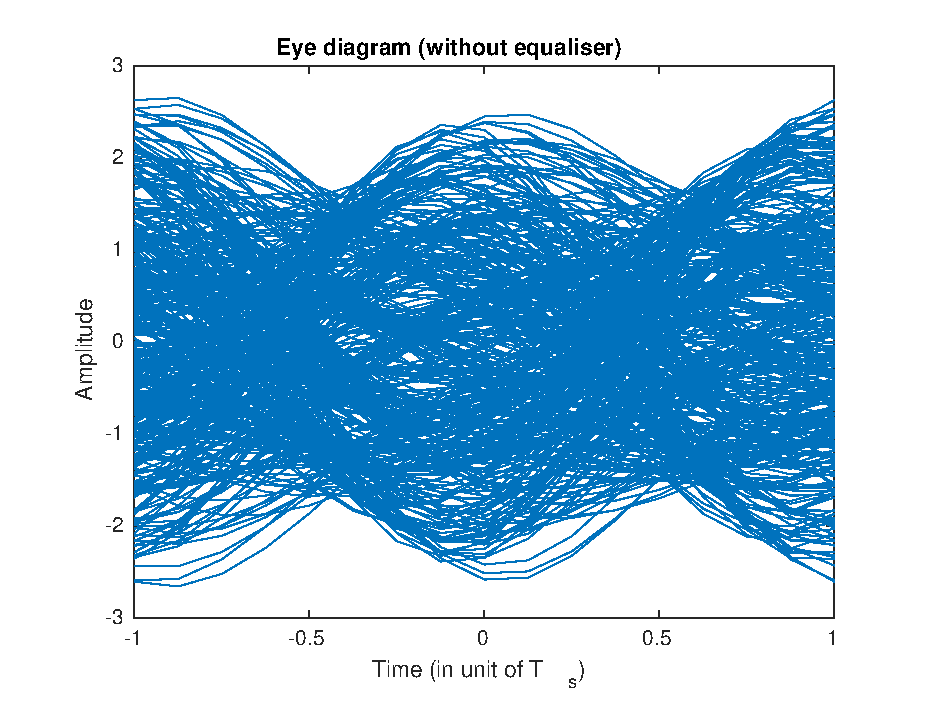
\includegraphics{Equaliser/eye}
    \end{center}
    \caption{Eye Diagram of a 4-PAM signal before equalisation}
    \label{fig:equ-eye}
\end{figure}

\begin{figure}[H]
    \begin{center}
        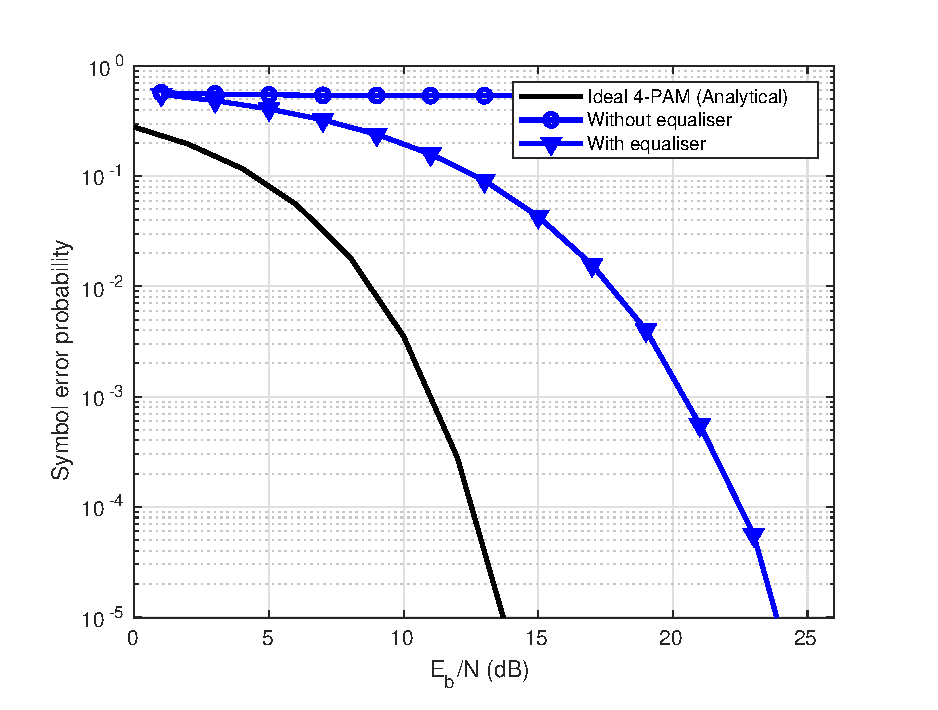
\includegraphics{Equaliser/ber}
    \end{center}
    \caption{SER comparison of a singal with and without equalisation}
    \label{fig:equ-ser}
\end{figure}

\begin{figure}[H]
    \begin{center}
        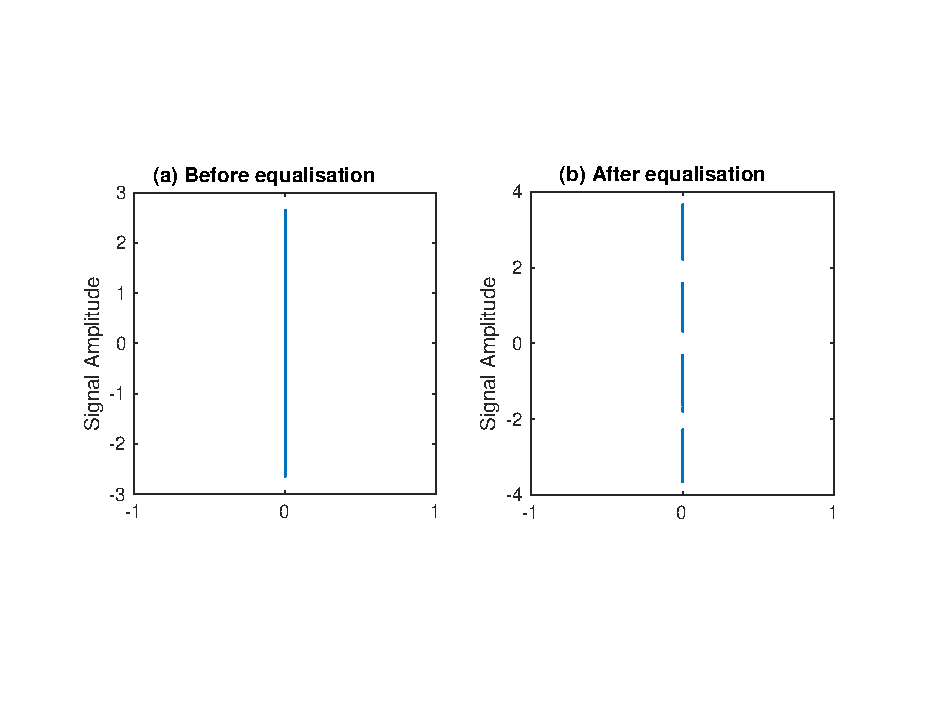
\includegraphics{Equaliser/scatter}
    \end{center}
    \caption{Before and after equalisation scatter plots showing the signal seperation after equalisation}
    \label{fig:equ-scatter}
\end{figure}

\subsection{Displaying a eye diagram with lab equipment}
To display an eye diagram on the ECE lab equipment the signal generator would have the clock output connected to the channel 1
input of the oscilloscope and the data output would be connected channel 2. The data generation on the signal generator would
be set to `RANDOM' this ensures a proper eye can be generated as it is not just the same data cycling. Next set an oscilloscope
trigger on the input to channel 1, this allows the oscilloscope to detect each period and know when to loop the signal on the screen.
Finally, the display persistance should be set to ininity to ensure that the past pulses are not removed from the screen so a proper
eye is formed.


\end{document}
